\documentclass[twoside]{book}

% Packages required by doxygen
\usepackage{fixltx2e}
\usepackage{calc}
\usepackage{doxygen}
\usepackage[export]{adjustbox} % also loads graphicx
\usepackage{graphicx}
\usepackage[utf8]{inputenc}
\usepackage{makeidx}
\usepackage{multicol}
\usepackage{multirow}
\PassOptionsToPackage{warn}{textcomp}
\usepackage{textcomp}
\usepackage[nointegrals]{wasysym}
\usepackage[table]{xcolor}

% NLS support packages
\usepackage[spanish]{babel}
% Font selection
\usepackage[T1]{fontenc}
\usepackage[scaled=.90]{helvet}
\usepackage{courier}
\usepackage{amssymb}
\usepackage{sectsty}
\renewcommand{\familydefault}{\sfdefault}
\allsectionsfont{%
  \fontseries{bc}\selectfont%
  \color{darkgray}%
}
\renewcommand{\DoxyLabelFont}{%
  \fontseries{bc}\selectfont%
  \color{darkgray}%
}
\newcommand{\+}{\discretionary{\mbox{\scriptsize$\hookleftarrow$}}{}{}}

% Page & text layout
\usepackage{geometry}
\geometry{%
  a4paper,%
  top=2.5cm,%
  bottom=2.5cm,%
  left=2.5cm,%
  right=2.5cm%
}
\tolerance=750
\hfuzz=15pt
\hbadness=750
\setlength{\emergencystretch}{15pt}
\setlength{\parindent}{0cm}
\setlength{\parskip}{0.2cm}
\makeatletter
\renewcommand{\paragraph}{%
  \@startsection{paragraph}{4}{0ex}{-1.0ex}{1.0ex}{%
    \normalfont\normalsize\bfseries\SS@parafont%
  }%
}
\renewcommand{\subparagraph}{%
  \@startsection{subparagraph}{5}{0ex}{-1.0ex}{1.0ex}{%
    \normalfont\normalsize\bfseries\SS@subparafont%
  }%
}
\makeatother

% Headers & footers
\usepackage{fancyhdr}
\pagestyle{fancyplain}
\fancyhead[LE]{\fancyplain{}{\bfseries\thepage}}
\fancyhead[CE]{\fancyplain{}{}}
\fancyhead[RE]{\fancyplain{}{\bfseries\leftmark}}
\fancyhead[LO]{\fancyplain{}{\bfseries\rightmark}}
\fancyhead[CO]{\fancyplain{}{}}
\fancyhead[RO]{\fancyplain{}{\bfseries\thepage}}
\fancyfoot[LE]{\fancyplain{}{}}
\fancyfoot[CE]{\fancyplain{}{}}
\fancyfoot[RE]{\fancyplain{}{\bfseries\scriptsize Generado el Lunes, 24 de Agosto de 2015 12\+:52\+:21 para Proyecto de Fin de Carrera por Doxygen }}
\fancyfoot[LO]{\fancyplain{}{\bfseries\scriptsize Generado el Lunes, 24 de Agosto de 2015 12\+:52\+:21 para Proyecto de Fin de Carrera por Doxygen }}
\fancyfoot[CO]{\fancyplain{}{}}
\fancyfoot[RO]{\fancyplain{}{}}
\renewcommand{\footrulewidth}{0.4pt}
\renewcommand{\chaptermark}[1]{%
  \markboth{#1}{}%
}
\renewcommand{\sectionmark}[1]{%
  \markright{\thesection\ #1}%
}

% Indices & bibliography
\usepackage{natbib}
\usepackage[titles]{tocloft}
\setcounter{tocdepth}{3}
\setcounter{secnumdepth}{5}
\makeindex

% Hyperlinks (required, but should be loaded last)
\usepackage{ifpdf}
\ifpdf
  \usepackage[pdftex,pagebackref=true]{hyperref}
\else
  \usepackage[ps2pdf,pagebackref=true]{hyperref}
\fi
\hypersetup{%
  colorlinks=true,%
  linkcolor=blue,%
  citecolor=blue,%
  unicode%
}

% Custom commands
\newcommand{\clearemptydoublepage}{%
  \newpage{\pagestyle{empty}\cleardoublepage}%
}


%===== C O N T E N T S =====

\begin{document}

% Titlepage & ToC
\hypersetup{pageanchor=false,
             bookmarks=true,
             bookmarksnumbered=true,
             pdfencoding=unicode
            }
\pagenumbering{roman}
\begin{titlepage}
\vspace*{7cm}
\begin{center}%
{\Large Proyecto de Fin de Carrera \\[1ex]\large 2.\+0 }\\
\vspace*{1cm}
{\large Generado por Doxygen 1.8.10}\\
\vspace*{0.5cm}
{\small Lunes, 24 de Agosto de 2015 12:52:21}\\
\end{center}
\end{titlepage}
\clearemptydoublepage
\tableofcontents
\clearemptydoublepage
\pagenumbering{arabic}
\hypersetup{pageanchor=true}

%--- Begin generated contents ---
\chapter{Índice de estructura de datos}
\section{Estructura de datos}
Lista de estructuras con una breve descripción\+:\begin{DoxyCompactList}
\item\contentsline{section}{\hyperlink{struct_m_d5___c_t_x}{M\+D5\+\_\+\+C\+T\+X} }{\pageref{struct_m_d5___c_t_x}}{}
\item\contentsline{section}{\hyperlink{struct_s_h_a256___c_t_x}{S\+H\+A256\+\_\+\+C\+T\+X} }{\pageref{struct_s_h_a256___c_t_x}}{}
\item\contentsline{section}{\hyperlink{struct_s_h_a256_context}{S\+H\+A256\+Context} }{\pageref{struct_s_h_a256_context}}{}
\item\contentsline{section}{\hyperlink{struct_s_t___c_n_t}{S\+T\+\_\+\+C\+N\+T} }{\pageref{struct_s_t___c_n_t}}{}
\item\contentsline{section}{\hyperlink{struct_s_t___m_o_d}{S\+T\+\_\+\+M\+O\+D} }{\pageref{struct_s_t___m_o_d}}{}
\item\contentsline{section}{\hyperlink{struct_s_t___p_i_l_a}{S\+T\+\_\+\+P\+I\+L\+A} }{\pageref{struct_s_t___p_i_l_a}}{}
\item\contentsline{section}{\hyperlink{struct_s_t___s_d_p}{S\+T\+\_\+\+S\+D\+P} }{\pageref{struct_s_t___s_d_p}}{}
\item\contentsline{section}{\hyperlink{struct_s_t___t_i_m_e_r}{S\+T\+\_\+\+T\+I\+M\+E\+R} }{\pageref{struct_s_t___t_i_m_e_r}}{}
\item\contentsline{section}{\hyperlink{struct_s_t___t_o_k_e_n}{S\+T\+\_\+\+T\+O\+K\+E\+N} }{\pageref{struct_s_t___t_o_k_e_n}}{}
\item\contentsline{section}{\hyperlink{structtag_m_q_a_i_r}{tag\+M\+Q\+A\+I\+R} }{\pageref{structtag_m_q_a_i_r}}{}
\item\contentsline{section}{\hyperlink{structtag_m_q_b_m_h_o}{tag\+M\+Q\+B\+M\+H\+O} }{\pageref{structtag_m_q_b_m_h_o}}{}
\item\contentsline{section}{\hyperlink{structtag_m_q_b_o}{tag\+M\+Q\+B\+O} }{\pageref{structtag_m_q_b_o}}{}
\item\contentsline{section}{\hyperlink{structtag_m_q_c_b_c}{tag\+M\+Q\+C\+B\+C} }{\pageref{structtag_m_q_c_b_c}}{}
\item\contentsline{section}{\hyperlink{structtag_m_q_c_b_d}{tag\+M\+Q\+C\+B\+D} }{\pageref{structtag_m_q_c_b_d}}{}
\item\contentsline{section}{\hyperlink{structtag_m_q_c_h_a_r_v}{tag\+M\+Q\+C\+H\+A\+R\+V} }{\pageref{structtag_m_q_c_h_a_r_v}}{}
\item\contentsline{section}{\hyperlink{structtag_m_q_c_i_h}{tag\+M\+Q\+C\+I\+H} }{\pageref{structtag_m_q_c_i_h}}{}
\item\contentsline{section}{\hyperlink{structtag_m_q_c_m_h_o}{tag\+M\+Q\+C\+M\+H\+O} }{\pageref{structtag_m_q_c_m_h_o}}{}
\item\contentsline{section}{\hyperlink{structtag_m_q_c_n_o}{tag\+M\+Q\+C\+N\+O} }{\pageref{structtag_m_q_c_n_o}}{}
\item\contentsline{section}{\hyperlink{structtag_m_q_c_s_p}{tag\+M\+Q\+C\+S\+P} }{\pageref{structtag_m_q_c_s_p}}{}
\item\contentsline{section}{\hyperlink{structtag_m_q_c_t_l_o}{tag\+M\+Q\+C\+T\+L\+O} }{\pageref{structtag_m_q_c_t_l_o}}{}
\item\contentsline{section}{\hyperlink{structtag_m_q_d_h}{tag\+M\+Q\+D\+H} }{\pageref{structtag_m_q_d_h}}{}
\item\contentsline{section}{\hyperlink{structtag_m_q_d_l_h}{tag\+M\+Q\+D\+L\+H} }{\pageref{structtag_m_q_d_l_h}}{}
\item\contentsline{section}{\hyperlink{structtag_m_q_d_m_h_o}{tag\+M\+Q\+D\+M\+H\+O} }{\pageref{structtag_m_q_d_m_h_o}}{}
\item\contentsline{section}{\hyperlink{structtag_m_q_d_m_p_o}{tag\+M\+Q\+D\+M\+P\+O} }{\pageref{structtag_m_q_d_m_p_o}}{}
\item\contentsline{section}{\hyperlink{structtag_m_q_g_m_o}{tag\+M\+Q\+G\+M\+O} }{\pageref{structtag_m_q_g_m_o}}{}
\item\contentsline{section}{\hyperlink{structtag_m_q_i_i_h}{tag\+M\+Q\+I\+I\+H} }{\pageref{structtag_m_q_i_i_h}}{}
\item\contentsline{section}{\hyperlink{structtag_m_q_i_m_p_o}{tag\+M\+Q\+I\+M\+P\+O} }{\pageref{structtag_m_q_i_m_p_o}}{}
\item\contentsline{section}{\hyperlink{structtag_m_q_m_d}{tag\+M\+Q\+M\+D} }{\pageref{structtag_m_q_m_d}}{}
\item\contentsline{section}{\hyperlink{structtag_m_q_m_d1}{tag\+M\+Q\+M\+D1} }{\pageref{structtag_m_q_m_d1}}{}
\item\contentsline{section}{\hyperlink{structtag_m_q_m_d2}{tag\+M\+Q\+M\+D2} }{\pageref{structtag_m_q_m_d2}}{}
\item\contentsline{section}{\hyperlink{structtag_m_q_m_d_e}{tag\+M\+Q\+M\+D\+E} }{\pageref{structtag_m_q_m_d_e}}{}
\item\contentsline{section}{\hyperlink{structtag_m_q_m_h_b_o}{tag\+M\+Q\+M\+H\+B\+O} }{\pageref{structtag_m_q_m_h_b_o}}{}
\item\contentsline{section}{\hyperlink{structtag_m_q_o_d}{tag\+M\+Q\+O\+D} }{\pageref{structtag_m_q_o_d}}{}
\item\contentsline{section}{\hyperlink{structtag_m_q_o_r}{tag\+M\+Q\+O\+R} }{\pageref{structtag_m_q_o_r}}{}
\item\contentsline{section}{\hyperlink{structtag_m_q_p_d}{tag\+M\+Q\+P\+D} }{\pageref{structtag_m_q_p_d}}{}
\item\contentsline{section}{\hyperlink{structtag_m_q_p_m_o}{tag\+M\+Q\+P\+M\+O} }{\pageref{structtag_m_q_p_m_o}}{}
\item\contentsline{section}{\hyperlink{structtag_m_q_r_f_h}{tag\+M\+Q\+R\+F\+H} }{\pageref{structtag_m_q_r_f_h}}{}
\item\contentsline{section}{\hyperlink{structtag_m_q_r_f_h2}{tag\+M\+Q\+R\+F\+H2} }{\pageref{structtag_m_q_r_f_h2}}{}
\item\contentsline{section}{\hyperlink{structtag_m_q_r_m_h}{tag\+M\+Q\+R\+M\+H} }{\pageref{structtag_m_q_r_m_h}}{}
\item\contentsline{section}{\hyperlink{structtag_m_q_r_r}{tag\+M\+Q\+R\+R} }{\pageref{structtag_m_q_r_r}}{}
\item\contentsline{section}{\hyperlink{structtag_m_q_s_c_o}{tag\+M\+Q\+S\+C\+O} }{\pageref{structtag_m_q_s_c_o}}{}
\item\contentsline{section}{\hyperlink{structtag_m_q_s_d}{tag\+M\+Q\+S\+D} }{\pageref{structtag_m_q_s_d}}{}
\item\contentsline{section}{\hyperlink{structtag_m_q_s_m_p_o}{tag\+M\+Q\+S\+M\+P\+O} }{\pageref{structtag_m_q_s_m_p_o}}{}
\item\contentsline{section}{\hyperlink{structtag_m_q_s_r_o}{tag\+M\+Q\+S\+R\+O} }{\pageref{structtag_m_q_s_r_o}}{}
\item\contentsline{section}{\hyperlink{structtag_m_q_s_t_s}{tag\+M\+Q\+S\+T\+S} }{\pageref{structtag_m_q_s_t_s}}{}
\item\contentsline{section}{\hyperlink{structtag_m_q_t_m}{tag\+M\+Q\+T\+M} }{\pageref{structtag_m_q_t_m}}{}
\item\contentsline{section}{\hyperlink{structtag_m_q_t_m_c2}{tag\+M\+Q\+T\+M\+C2} }{\pageref{structtag_m_q_t_m_c2}}{}
\item\contentsline{section}{\hyperlink{structtag_m_q_w_i_h}{tag\+M\+Q\+W\+I\+H} }{\pageref{structtag_m_q_w_i_h}}{}
\item\contentsline{section}{\hyperlink{structtag_m_q_x_q_h}{tag\+M\+Q\+X\+Q\+H} }{\pageref{structtag_m_q_x_q_h}}{}
\end{DoxyCompactList}

\chapter{Indice de archivos}
\section{Lista de archivos}
Lista de todos los archivos con descripciones breves\+:\begin{DoxyCompactList}
\item\contentsline{section}{include/\hyperlink{amqsdp_8h}{amqsdp.\+h} \\*Cliente Websphere M\+Q\+Series }{\pageref{amqsdp_8h}}{}
\item\contentsline{section}{include/\hyperlink{cmqc_8h}{cmqc.\+h} }{\pageref{cmqc_8h}}{}
\item\contentsline{section}{include/\hyperlink{cob2c_8h}{cob2c.\+h} \\*Fichero de cabecera para convertir la copy C\+O\+B\+O\+L en una estructura S\+D\+P }{\pageref{cob2c_8h}}{}
\item\contentsline{section}{include/\hyperlink{global_8h}{global.\+h} \\*Define las variables de uso global para todo el sistema }{\pageref{global_8h}}{}
\item\contentsline{section}{include/\hyperlink{jggsal_8h}{jggsal.\+h} \\*Software Abstraction Layer }{\pageref{jggsal_8h}}{}
\item\contentsline{section}{include/\hyperlink{md5_8h}{md5.\+h} \\*Fichero de cabecera para el calculo de la firma M\+D5 de un texto Modificado a partir del algoritmo desarrollado por\+: }{\pageref{md5_8h}}{}
\item\contentsline{section}{include/\hyperlink{md5__mit_8h}{md5\+\_\+mit.\+h} }{\pageref{md5__mit_8h}}{}
\item\contentsline{section}{include/\hyperlink{messages_8h}{messages.\+h} \\*Funciones de gestion del envio de mensajes al sistema de colas }{\pageref{messages_8h}}{}
\item\contentsline{section}{include/\hyperlink{modulos_8h}{modulos.\+h} \\*Funciones de gestion de los modulos activos en una sesion }{\pageref{modulos_8h}}{}
\item\contentsline{section}{include/\hyperlink{pila_8h}{pila.\+h} \\*Funciones de gestion de pilas abtracta }{\pageref{pila_8h}}{}
\item\contentsline{section}{include/\hyperlink{pilaptr_8h}{pilaptr.\+h} }{\pageref{pilaptr_8h}}{}
\item\contentsline{section}{include/\hyperlink{salw32_8h}{salw32.\+h} \\*Definicion de funciones especificas para sistemas Windows }{\pageref{salw32_8h}}{}
\item\contentsline{section}{include/\hyperlink{sdpconfig_8h}{sdpconfig.\+h} \\*Fichero de cabecera de configuracion del sistema Define las constantes y los valores globales de comportamiento }{\pageref{sdpconfig_8h}}{}
\item\contentsline{section}{include/\hyperlink{_s_d_p_t_r_a_p_8h}{S\+D\+P\+T\+R\+A\+P.\+h} \\*Fichero de cabecera con los ficheros de cabecera comunes }{\pageref{_s_d_p_t_r_a_p_8h}}{}
\item\contentsline{section}{include/\hyperlink{_s_d_p_t_r_a_p_b_8h}{S\+D\+P\+T\+R\+A\+P\+B.\+h} \\*Fichero de cabecera de la libreria S\+D\+P\+T\+R\+A\+P\+B Define las constantes y los valores globales de comportamiento }{\pageref{_s_d_p_t_r_a_p_b_8h}}{}
\item\contentsline{section}{include/\hyperlink{sdp_types_8h}{sdp\+Types.\+h} \\*Define las estructrus y tipos de datos usados en la libreria }{\pageref{sdp_types_8h}}{}
\item\contentsline{section}{include/\hyperlink{sha-private_8h}{sha-\/private.\+h} }{\pageref{sha-private_8h}}{}
\item\contentsline{section}{include/\hyperlink{sha256_8h}{sha256.\+h} }{\pageref{sha256_8h}}{}
\item\contentsline{section}{include/\hyperlink{sha256be_8h}{sha256be.\+h} }{\pageref{sha256be_8h}}{}
\item\contentsline{section}{include/\hyperlink{sha256le_8h}{sha256le.\+h} }{\pageref{sha256le_8h}}{}
\item\contentsline{section}{include/\hyperlink{timer_8h}{timer.\+h} \\*Fichero de cabecera para incluir los modulos de calculo de timers }{\pageref{timer_8h}}{}
\item\contentsline{section}{include/\hyperlink{timerlnx_8h}{timerlnx.\+h} \\*Funciones publicas del archivo timer\+Lnx Se incluye en la plataforma Linux }{\pageref{timerlnx_8h}}{}
\item\contentsline{section}{include/\hyperlink{timerwin_8h}{timerwin.\+h} \\*Funciones publicas del archivo timer\+Win Se incluye en la plataforma windows }{\pageref{timerwin_8h}}{}
\item\contentsline{section}{include/\hyperlink{token_8h}{token.\+h} }{\pageref{token_8h}}{}
\item\contentsline{section}{include/\hyperlink{trapcodes_8h}{trapcodes.\+h} }{\pageref{trapcodes_8h}}{}
\item\contentsline{section}{M\+D5/\+M\+D5/\hyperlink{_m_d5_8cpp}{M\+D5.\+cpp} }{\pageref{_m_d5_8cpp}}{}
\item\contentsline{section}{M\+D5/\+M\+D5/\hyperlink{_m_d5_2_m_d5_2stdafx_8cpp}{stdafx.\+cpp} }{\pageref{_m_d5_2_m_d5_2stdafx_8cpp}}{}
\item\contentsline{section}{M\+D5/\+M\+D5/\hyperlink{_m_d5_2_m_d5_2stdafx_8h}{stdafx.\+h} }{\pageref{_m_d5_2_m_d5_2stdafx_8h}}{}
\item\contentsline{section}{M\+D5/\+M\+D5/\hyperlink{_m_d5_2_m_d5_2targetver_8h}{targetver.\+h} }{\pageref{_m_d5_2_m_d5_2targetver_8h}}{}
\item\contentsline{section}{S\+D\+P\+T\+R\+A\+P\+B/\+S\+D\+P\+T\+R\+A\+P\+B/\hyperlink{dllmain_8cpp}{dllmain.\+cpp} }{\pageref{dllmain_8cpp}}{}
\item\contentsline{section}{S\+D\+P\+T\+R\+A\+P\+B/\+S\+D\+P\+T\+R\+A\+P\+B/\hyperlink{_s_d_p_t_r_a_p_b_8cpp}{S\+D\+P\+T\+R\+A\+P\+B.\+cpp} }{\pageref{_s_d_p_t_r_a_p_b_8cpp}}{}
\item\contentsline{section}{S\+D\+P\+T\+R\+A\+P\+B/\+S\+D\+P\+T\+R\+A\+P\+B/\hyperlink{_s_d_p_t_r_a_p_b_2_s_d_p_t_r_a_p_b_2stdafx_8cpp}{stdafx.\+cpp} }{\pageref{_s_d_p_t_r_a_p_b_2_s_d_p_t_r_a_p_b_2stdafx_8cpp}}{}
\item\contentsline{section}{S\+D\+P\+T\+R\+A\+P\+B/\+S\+D\+P\+T\+R\+A\+P\+B/\hyperlink{_s_d_p_t_r_a_p_b_2_s_d_p_t_r_a_p_b_2stdafx_8h}{stdafx.\+h} }{\pageref{_s_d_p_t_r_a_p_b_2_s_d_p_t_r_a_p_b_2stdafx_8h}}{}
\item\contentsline{section}{S\+D\+P\+T\+R\+A\+P\+B/\+S\+D\+P\+T\+R\+A\+P\+B/\hyperlink{_s_d_p_t_r_a_p_b_2_s_d_p_t_r_a_p_b_2targetver_8h}{targetver.\+h} }{\pageref{_s_d_p_t_r_a_p_b_2_s_d_p_t_r_a_p_b_2targetver_8h}}{}
\item\contentsline{section}{src/\hyperlink{amqsdp_8c}{amqsdp.\+c} \\*Cliente Websphere M\+Q\+Series }{\pageref{amqsdp_8c}}{}
\item\contentsline{section}{src/\hyperlink{cob2c_8c}{cob2c.\+c} \\*Utilidad para pasar los datos de la Copy C\+O\+B\+O\+L a la estructura C }{\pageref{cob2c_8c}}{}
\item\contentsline{section}{src/\hyperlink{md5_8c}{md5.\+c} \\*Implementacion de la firma digital segun R\+F\+C 1321 }{\pageref{md5_8c}}{}
\item\contentsline{section}{src/\hyperlink{messages_8c}{messages.\+c} \\*Gestiona la generacion de los diferentes mensajes que se deben enviar }{\pageref{messages_8c}}{}
\item\contentsline{section}{src/\hyperlink{modulos_8c}{modulos.\+c} \\*Mantiene la lista de modulos activos con sus I\+D }{\pageref{modulos_8c}}{}
\item\contentsline{section}{src/\hyperlink{pila_8c}{pila.\+c} \\*Gestor de pilas abstractas por copia o referencia }{\pageref{pila_8c}}{}
\item\contentsline{section}{src/\hyperlink{salw32_8c}{salw32.\+c} \\*System Abtraction Layer Version de funciones para Windows 32 }{\pageref{salw32_8c}}{}
\item\contentsline{section}{src/\hyperlink{_s_d_p_t_r_a_p_b_8c}{S\+D\+P\+T\+R\+A\+P\+B.\+c} \\*S\+D\+P\+T\+R\+A\+P\+B D\+L\+L de captura de datos de ejecucion del programa C\+O\+B\+O\+L Utiliza un unico punto de entrada\+: S\+D\+P\+T\+R\+A\+P }{\pageref{_s_d_p_t_r_a_p_b_8c}}{}
\item\contentsline{section}{src/\hyperlink{sha256_8c}{sha256.\+c} }{\pageref{sha256_8c}}{}
\item\contentsline{section}{src/\hyperlink{sha256be_8c}{sha256be.\+c} }{\pageref{sha256be_8c}}{}
\item\contentsline{section}{src/\hyperlink{sha256le_8c}{sha256le.\+c} }{\pageref{sha256le_8c}}{}
\item\contentsline{section}{src/\hyperlink{timer_lnx_8c}{timer\+Lnx.\+c} \\*Obtiene los tiempos del sistema en una estructura T\+I\+M\+E\+R Version Linux }{\pageref{timer_lnx_8c}}{}
\item\contentsline{section}{src/\hyperlink{timer_win_8c}{timer\+Win.\+c} \\*Obtiene los tiempos del sistema (C\+P\+U, System, etc) en sistemas Windows 32 bits }{\pageref{timer_win_8c}}{}
\item\contentsline{section}{T\+S\+T\+S\+D\+P\+T\+R\+A\+P\+B/tst\+S\+D\+P\+T\+R\+A\+P\+B/\hyperlink{_t_s_t_s_d_p_t_r_a_p_b_2tst_s_d_p_t_r_a_p_b_2stdafx_8cpp}{stdafx.\+cpp} }{\pageref{_t_s_t_s_d_p_t_r_a_p_b_2tst_s_d_p_t_r_a_p_b_2stdafx_8cpp}}{}
\item\contentsline{section}{T\+S\+T\+S\+D\+P\+T\+R\+A\+P\+B/tst\+S\+D\+P\+T\+R\+A\+P\+B/\hyperlink{_t_s_t_s_d_p_t_r_a_p_b_2tst_s_d_p_t_r_a_p_b_2stdafx_8h}{stdafx.\+h} }{\pageref{_t_s_t_s_d_p_t_r_a_p_b_2tst_s_d_p_t_r_a_p_b_2stdafx_8h}}{}
\item\contentsline{section}{T\+S\+T\+S\+D\+P\+T\+R\+A\+P\+B/tst\+S\+D\+P\+T\+R\+A\+P\+B/\hyperlink{_t_s_t_s_d_p_t_r_a_p_b_2tst_s_d_p_t_r_a_p_b_2targetver_8h}{targetver.\+h} }{\pageref{_t_s_t_s_d_p_t_r_a_p_b_2tst_s_d_p_t_r_a_p_b_2targetver_8h}}{}
\item\contentsline{section}{T\+S\+T\+S\+D\+P\+T\+R\+A\+P\+B/tst\+S\+D\+P\+T\+R\+A\+P\+B/\hyperlink{tst_s_d_p_t_r_a_p_b_8cpp}{tst\+S\+D\+P\+T\+R\+A\+P\+B.\+cpp} }{\pageref{tst_s_d_p_t_r_a_p_b_8cpp}}{}
\end{DoxyCompactList}

\chapter{Documentación de las estructuras de datos}
\hypertarget{struct_m_d5___c_t_x}{}\section{Referencia de la Estructura M\+D5\+\_\+\+C\+T\+X}
\label{struct_m_d5___c_t_x}\index{M\+D5\+\_\+\+C\+T\+X@{M\+D5\+\_\+\+C\+T\+X}}


{\ttfamily \#include $<$md5\+\_\+mit.\+h$>$}

\subsection*{Campos de datos}
\begin{DoxyCompactItemize}
\item 
\hyperlink{md5__mit_8h_acbcd3749ac28f52e756e22d22022cae5}{U\+I\+N\+T4} \hyperlink{struct_m_d5___c_t_x_aa94c7f6cf6c16dd45ecbf7be4af32f0c}{i} \mbox{[}2\mbox{]}
\item 
\hyperlink{md5__mit_8h_acbcd3749ac28f52e756e22d22022cae5}{U\+I\+N\+T4} \hyperlink{struct_m_d5___c_t_x_a7dc178b045dfbd504687dc9b0834d1d6}{buf} \mbox{[}4\mbox{]}
\item 
unsigned char \hyperlink{struct_m_d5___c_t_x_a3a40a33a5c6b34a5d53569057cbe8c4c}{in} \mbox{[}64\mbox{]}
\item 
unsigned char \hyperlink{struct_m_d5___c_t_x_a9c185c9970b81e602c4374ffe2c117e8}{digest} \mbox{[}16\mbox{]}
\item 
\hyperlink{md5_8c_ad854d8865ff7e0ce3717676b84926f54}{M\+D5\+\_\+u32plus} \hyperlink{struct_m_d5___c_t_x_ab6f070d5d937f16cddb2d666c32fdb8e}{lo}
\item 
\hyperlink{md5_8c_ad854d8865ff7e0ce3717676b84926f54}{M\+D5\+\_\+u32plus} \hyperlink{struct_m_d5___c_t_x_ad674a11709e105451f48b99b9fe54792}{hi}
\item 
\hyperlink{md5_8c_ad854d8865ff7e0ce3717676b84926f54}{M\+D5\+\_\+u32plus} \hyperlink{struct_m_d5___c_t_x_ac5629798efe5fb7cbd33911a77672275}{a}
\item 
\hyperlink{md5_8c_ad854d8865ff7e0ce3717676b84926f54}{M\+D5\+\_\+u32plus} \hyperlink{struct_m_d5___c_t_x_ae7735a3daa065dc9dfab9dd1a512d557}{b}
\item 
\hyperlink{md5_8c_ad854d8865ff7e0ce3717676b84926f54}{M\+D5\+\_\+u32plus} \hyperlink{struct_m_d5___c_t_x_a1f90d3ede1c4253a90685d1260482dfc}{c}
\item 
\hyperlink{md5_8c_ad854d8865ff7e0ce3717676b84926f54}{M\+D5\+\_\+u32plus} \hyperlink{struct_m_d5___c_t_x_a42be18d895cf7be9097073faf66734c1}{d}
\item 
unsigned char \hyperlink{struct_m_d5___c_t_x_a59e96eea04541ecd67c3faca41b13feb}{buffer} \mbox{[}64\mbox{]}
\item 
\hyperlink{md5_8c_ad854d8865ff7e0ce3717676b84926f54}{M\+D5\+\_\+u32plus} \hyperlink{struct_m_d5___c_t_x_ad8cb52dd70ac5316564b1e4b48b0ad7d}{block} \mbox{[}16\mbox{]}
\end{DoxyCompactItemize}


\subsection{Descripción detallada}


Definición en la línea 54 del archivo md5\+\_\+mit.\+h.



\subsection{Documentación de los campos}
\hypertarget{struct_m_d5___c_t_x_ac5629798efe5fb7cbd33911a77672275}{}\index{M\+D5\+\_\+\+C\+T\+X@{M\+D5\+\_\+\+C\+T\+X}!a@{a}}
\index{a@{a}!M\+D5\+\_\+\+C\+T\+X@{M\+D5\+\_\+\+C\+T\+X}}
\subsubsection[{a}]{\setlength{\rightskip}{0pt plus 5cm}{\bf M\+D5\+\_\+u32plus} a}\label{struct_m_d5___c_t_x_ac5629798efe5fb7cbd33911a77672275}


Definición en la línea 53 del archivo md5.\+c.

\hypertarget{struct_m_d5___c_t_x_ae7735a3daa065dc9dfab9dd1a512d557}{}\index{M\+D5\+\_\+\+C\+T\+X@{M\+D5\+\_\+\+C\+T\+X}!b@{b}}
\index{b@{b}!M\+D5\+\_\+\+C\+T\+X@{M\+D5\+\_\+\+C\+T\+X}}
\subsubsection[{b}]{\setlength{\rightskip}{0pt plus 5cm}{\bf M\+D5\+\_\+u32plus} b}\label{struct_m_d5___c_t_x_ae7735a3daa065dc9dfab9dd1a512d557}


Definición en la línea 53 del archivo md5.\+c.

\hypertarget{struct_m_d5___c_t_x_ad8cb52dd70ac5316564b1e4b48b0ad7d}{}\index{M\+D5\+\_\+\+C\+T\+X@{M\+D5\+\_\+\+C\+T\+X}!block@{block}}
\index{block@{block}!M\+D5\+\_\+\+C\+T\+X@{M\+D5\+\_\+\+C\+T\+X}}
\subsubsection[{block}]{\setlength{\rightskip}{0pt plus 5cm}{\bf M\+D5\+\_\+u32plus} block\mbox{[}16\mbox{]}}\label{struct_m_d5___c_t_x_ad8cb52dd70ac5316564b1e4b48b0ad7d}


Definición en la línea 55 del archivo md5.\+c.

\hypertarget{struct_m_d5___c_t_x_a7dc178b045dfbd504687dc9b0834d1d6}{}\index{M\+D5\+\_\+\+C\+T\+X@{M\+D5\+\_\+\+C\+T\+X}!buf@{buf}}
\index{buf@{buf}!M\+D5\+\_\+\+C\+T\+X@{M\+D5\+\_\+\+C\+T\+X}}
\subsubsection[{buf}]{\setlength{\rightskip}{0pt plus 5cm}{\bf U\+I\+N\+T4} buf\mbox{[}4\mbox{]}}\label{struct_m_d5___c_t_x_a7dc178b045dfbd504687dc9b0834d1d6}


Definición en la línea 56 del archivo md5\+\_\+mit.\+h.

\hypertarget{struct_m_d5___c_t_x_a59e96eea04541ecd67c3faca41b13feb}{}\index{M\+D5\+\_\+\+C\+T\+X@{M\+D5\+\_\+\+C\+T\+X}!buffer@{buffer}}
\index{buffer@{buffer}!M\+D5\+\_\+\+C\+T\+X@{M\+D5\+\_\+\+C\+T\+X}}
\subsubsection[{buffer}]{\setlength{\rightskip}{0pt plus 5cm}unsigned char buffer\mbox{[}64\mbox{]}}\label{struct_m_d5___c_t_x_a59e96eea04541ecd67c3faca41b13feb}


Definición en la línea 54 del archivo md5.\+c.

\hypertarget{struct_m_d5___c_t_x_a1f90d3ede1c4253a90685d1260482dfc}{}\index{M\+D5\+\_\+\+C\+T\+X@{M\+D5\+\_\+\+C\+T\+X}!c@{c}}
\index{c@{c}!M\+D5\+\_\+\+C\+T\+X@{M\+D5\+\_\+\+C\+T\+X}}
\subsubsection[{c}]{\setlength{\rightskip}{0pt plus 5cm}{\bf M\+D5\+\_\+u32plus} c}\label{struct_m_d5___c_t_x_a1f90d3ede1c4253a90685d1260482dfc}


Definición en la línea 53 del archivo md5.\+c.

\hypertarget{struct_m_d5___c_t_x_a42be18d895cf7be9097073faf66734c1}{}\index{M\+D5\+\_\+\+C\+T\+X@{M\+D5\+\_\+\+C\+T\+X}!d@{d}}
\index{d@{d}!M\+D5\+\_\+\+C\+T\+X@{M\+D5\+\_\+\+C\+T\+X}}
\subsubsection[{d}]{\setlength{\rightskip}{0pt plus 5cm}{\bf M\+D5\+\_\+u32plus} d}\label{struct_m_d5___c_t_x_a42be18d895cf7be9097073faf66734c1}


Definición en la línea 53 del archivo md5.\+c.

\hypertarget{struct_m_d5___c_t_x_a9c185c9970b81e602c4374ffe2c117e8}{}\index{M\+D5\+\_\+\+C\+T\+X@{M\+D5\+\_\+\+C\+T\+X}!digest@{digest}}
\index{digest@{digest}!M\+D5\+\_\+\+C\+T\+X@{M\+D5\+\_\+\+C\+T\+X}}
\subsubsection[{digest}]{\setlength{\rightskip}{0pt plus 5cm}unsigned char digest\mbox{[}16\mbox{]}}\label{struct_m_d5___c_t_x_a9c185c9970b81e602c4374ffe2c117e8}


Definición en la línea 58 del archivo md5\+\_\+mit.\+h.

\hypertarget{struct_m_d5___c_t_x_ad674a11709e105451f48b99b9fe54792}{}\index{M\+D5\+\_\+\+C\+T\+X@{M\+D5\+\_\+\+C\+T\+X}!hi@{hi}}
\index{hi@{hi}!M\+D5\+\_\+\+C\+T\+X@{M\+D5\+\_\+\+C\+T\+X}}
\subsubsection[{hi}]{\setlength{\rightskip}{0pt plus 5cm}{\bf M\+D5\+\_\+u32plus} hi}\label{struct_m_d5___c_t_x_ad674a11709e105451f48b99b9fe54792}


Definición en la línea 52 del archivo md5.\+c.

\hypertarget{struct_m_d5___c_t_x_aa94c7f6cf6c16dd45ecbf7be4af32f0c}{}\index{M\+D5\+\_\+\+C\+T\+X@{M\+D5\+\_\+\+C\+T\+X}!i@{i}}
\index{i@{i}!M\+D5\+\_\+\+C\+T\+X@{M\+D5\+\_\+\+C\+T\+X}}
\subsubsection[{i}]{\setlength{\rightskip}{0pt plus 5cm}{\bf U\+I\+N\+T4} i\mbox{[}2\mbox{]}}\label{struct_m_d5___c_t_x_aa94c7f6cf6c16dd45ecbf7be4af32f0c}


Definición en la línea 55 del archivo md5\+\_\+mit.\+h.

\hypertarget{struct_m_d5___c_t_x_a3a40a33a5c6b34a5d53569057cbe8c4c}{}\index{M\+D5\+\_\+\+C\+T\+X@{M\+D5\+\_\+\+C\+T\+X}!in@{in}}
\index{in@{in}!M\+D5\+\_\+\+C\+T\+X@{M\+D5\+\_\+\+C\+T\+X}}
\subsubsection[{in}]{\setlength{\rightskip}{0pt plus 5cm}unsigned char in\mbox{[}64\mbox{]}}\label{struct_m_d5___c_t_x_a3a40a33a5c6b34a5d53569057cbe8c4c}


Definición en la línea 57 del archivo md5\+\_\+mit.\+h.

\hypertarget{struct_m_d5___c_t_x_ab6f070d5d937f16cddb2d666c32fdb8e}{}\index{M\+D5\+\_\+\+C\+T\+X@{M\+D5\+\_\+\+C\+T\+X}!lo@{lo}}
\index{lo@{lo}!M\+D5\+\_\+\+C\+T\+X@{M\+D5\+\_\+\+C\+T\+X}}
\subsubsection[{lo}]{\setlength{\rightskip}{0pt plus 5cm}{\bf M\+D5\+\_\+u32plus} lo}\label{struct_m_d5___c_t_x_ab6f070d5d937f16cddb2d666c32fdb8e}


Definición en la línea 52 del archivo md5.\+c.



La documentación para esta estructura fue generada a partir de los siguientes ficheros\+:\begin{DoxyCompactItemize}
\item 
include/\hyperlink{md5__mit_8h}{md5\+\_\+mit.\+h}\item 
src/\hyperlink{md5_8c}{md5.\+c}\end{DoxyCompactItemize}

\hypertarget{struct_s_h_a256___c_t_x}{}\section{Referencia de la Estructura S\+H\+A256\+\_\+\+C\+T\+X}
\label{struct_s_h_a256___c_t_x}\index{S\+H\+A256\+\_\+\+C\+T\+X@{S\+H\+A256\+\_\+\+C\+T\+X}}


{\ttfamily \#include $<$sha256le.\+h$>$}

\subsection*{Campos de datos}
\begin{DoxyCompactItemize}
\item 
\hyperlink{sha256le_8h_a4ae1dab0fb4b072a66584546209e7d58}{B\+Y\+T\+E} \hyperlink{struct_s_h_a256___c_t_x_a8a17db6f40bbecb79cbb64aaeeaeba5e}{data} \mbox{[}64\mbox{]}
\item 
\hyperlink{sha256le_8h_ad2baa11c897721ff6f14b452b547f9bc}{W\+O\+R\+D} \hyperlink{struct_s_h_a256___c_t_x_ab94b143853886bff721a273cc7242171}{datalen}
\item 
unsigned long long \hyperlink{struct_s_h_a256___c_t_x_a9ef8c3daffe76c802a308b323158fc79}{bitlen}
\item 
\hyperlink{sha256le_8h_ad2baa11c897721ff6f14b452b547f9bc}{W\+O\+R\+D} \hyperlink{struct_s_h_a256___c_t_x_a6cde2322d13788f1d9740d1cae5d58a0}{state} \mbox{[}8\mbox{]}
\end{DoxyCompactItemize}


\subsection{Descripción detallada}


Definición en la línea 22 del archivo sha256le.\+h.



\subsection{Documentación de los campos}
\hypertarget{struct_s_h_a256___c_t_x_a9ef8c3daffe76c802a308b323158fc79}{}\index{S\+H\+A256\+\_\+\+C\+T\+X@{S\+H\+A256\+\_\+\+C\+T\+X}!bitlen@{bitlen}}
\index{bitlen@{bitlen}!S\+H\+A256\+\_\+\+C\+T\+X@{S\+H\+A256\+\_\+\+C\+T\+X}}
\subsubsection[{bitlen}]{\setlength{\rightskip}{0pt plus 5cm}unsigned long long bitlen}\label{struct_s_h_a256___c_t_x_a9ef8c3daffe76c802a308b323158fc79}


Definición en la línea 25 del archivo sha256le.\+h.

\hypertarget{struct_s_h_a256___c_t_x_a8a17db6f40bbecb79cbb64aaeeaeba5e}{}\index{S\+H\+A256\+\_\+\+C\+T\+X@{S\+H\+A256\+\_\+\+C\+T\+X}!data@{data}}
\index{data@{data}!S\+H\+A256\+\_\+\+C\+T\+X@{S\+H\+A256\+\_\+\+C\+T\+X}}
\subsubsection[{data}]{\setlength{\rightskip}{0pt plus 5cm}{\bf B\+Y\+T\+E} data\mbox{[}64\mbox{]}}\label{struct_s_h_a256___c_t_x_a8a17db6f40bbecb79cbb64aaeeaeba5e}


Definición en la línea 23 del archivo sha256le.\+h.

\hypertarget{struct_s_h_a256___c_t_x_ab94b143853886bff721a273cc7242171}{}\index{S\+H\+A256\+\_\+\+C\+T\+X@{S\+H\+A256\+\_\+\+C\+T\+X}!datalen@{datalen}}
\index{datalen@{datalen}!S\+H\+A256\+\_\+\+C\+T\+X@{S\+H\+A256\+\_\+\+C\+T\+X}}
\subsubsection[{datalen}]{\setlength{\rightskip}{0pt plus 5cm}{\bf W\+O\+R\+D} datalen}\label{struct_s_h_a256___c_t_x_ab94b143853886bff721a273cc7242171}


Definición en la línea 24 del archivo sha256le.\+h.

\hypertarget{struct_s_h_a256___c_t_x_a6cde2322d13788f1d9740d1cae5d58a0}{}\index{S\+H\+A256\+\_\+\+C\+T\+X@{S\+H\+A256\+\_\+\+C\+T\+X}!state@{state}}
\index{state@{state}!S\+H\+A256\+\_\+\+C\+T\+X@{S\+H\+A256\+\_\+\+C\+T\+X}}
\subsubsection[{state}]{\setlength{\rightskip}{0pt plus 5cm}{\bf W\+O\+R\+D} state\mbox{[}8\mbox{]}}\label{struct_s_h_a256___c_t_x_a6cde2322d13788f1d9740d1cae5d58a0}


Definición en la línea 26 del archivo sha256le.\+h.



La documentación para esta estructura fue generada a partir del siguiente fichero\+:\begin{DoxyCompactItemize}
\item 
include/\hyperlink{sha256le_8h}{sha256le.\+h}\end{DoxyCompactItemize}

\hypertarget{struct_s_h_a256_context}{}\section{Referencia de la Estructura S\+H\+A256\+Context}
\label{struct_s_h_a256_context}\index{S\+H\+A256\+Context@{S\+H\+A256\+Context}}


{\ttfamily \#include $<$sha256be.\+h$>$}

\subsection*{Campos de datos}
\begin{DoxyCompactItemize}
\item 
uint32\+\_\+t \hyperlink{struct_s_h_a256_context_a5d9aeb28e3a5c2f444066c1c9685ac91}{Intermediate\+\_\+\+Hash} \mbox{[}\hyperlink{sha256be_8h_adf764cbdea00d65edcd07bb9953ad2b7a3a8b66cf5d0bd8cc0e375a86a754ab28}{S\+H\+A256\+Hash\+Size}/4\mbox{]}
\item 
uint32\+\_\+t \hyperlink{struct_s_h_a256_context_a73f82f23d8acae6d67b249511811d654}{Length\+\_\+\+High}
\item 
uint32\+\_\+t \hyperlink{struct_s_h_a256_context_a188eef03938236a9a58c9382166aa002}{Length\+\_\+\+Low}
\item 
int\+\_\+least16\+\_\+t \hyperlink{struct_s_h_a256_context_ad7bf01bcc0244679564a37f2c25ffc8c}{Message\+\_\+\+Block\+\_\+\+Index}
\item 
uint8\+\_\+t \hyperlink{struct_s_h_a256_context_a84b3f788f46b63afe4b879ed78e73051}{Message\+\_\+\+Block} \mbox{[}\hyperlink{sha256be_8h_adf764cbdea00d65edcd07bb9953ad2b7af163926be4ff6a506a77f737295b6884}{S\+H\+A256\+\_\+\+Message\+\_\+\+Block\+\_\+\+Size}\mbox{]}
\item 
int \hyperlink{struct_s_h_a256_context_aeb5a7a168bb512db53299543094702aa}{Computed}
\item 
int \hyperlink{struct_s_h_a256_context_a4bc60740c300c7929a676f997d9484a9}{Corrupted}
\end{DoxyCompactItemize}


\subsection{Descripción detallada}


Definición en la línea 129 del archivo sha256be.\+h.



\subsection{Documentación de los campos}
\hypertarget{struct_s_h_a256_context_aeb5a7a168bb512db53299543094702aa}{}\index{S\+H\+A256\+Context@{S\+H\+A256\+Context}!Computed@{Computed}}
\index{Computed@{Computed}!S\+H\+A256\+Context@{S\+H\+A256\+Context}}
\subsubsection[{Computed}]{\setlength{\rightskip}{0pt plus 5cm}int Computed}\label{struct_s_h_a256_context_aeb5a7a168bb512db53299543094702aa}


Definición en la línea 138 del archivo sha256be.\+h.

\hypertarget{struct_s_h_a256_context_a4bc60740c300c7929a676f997d9484a9}{}\index{S\+H\+A256\+Context@{S\+H\+A256\+Context}!Corrupted@{Corrupted}}
\index{Corrupted@{Corrupted}!S\+H\+A256\+Context@{S\+H\+A256\+Context}}
\subsubsection[{Corrupted}]{\setlength{\rightskip}{0pt plus 5cm}int Corrupted}\label{struct_s_h_a256_context_a4bc60740c300c7929a676f997d9484a9}


Definición en la línea 139 del archivo sha256be.\+h.

\hypertarget{struct_s_h_a256_context_a5d9aeb28e3a5c2f444066c1c9685ac91}{}\index{S\+H\+A256\+Context@{S\+H\+A256\+Context}!Intermediate\+\_\+\+Hash@{Intermediate\+\_\+\+Hash}}
\index{Intermediate\+\_\+\+Hash@{Intermediate\+\_\+\+Hash}!S\+H\+A256\+Context@{S\+H\+A256\+Context}}
\subsubsection[{Intermediate\+\_\+\+Hash}]{\setlength{\rightskip}{0pt plus 5cm}uint32\+\_\+t Intermediate\+\_\+\+Hash\mbox{[}{\bf S\+H\+A256\+Hash\+Size}/4\mbox{]}}\label{struct_s_h_a256_context_a5d9aeb28e3a5c2f444066c1c9685ac91}


Definición en la línea 130 del archivo sha256be.\+h.

\hypertarget{struct_s_h_a256_context_a73f82f23d8acae6d67b249511811d654}{}\index{S\+H\+A256\+Context@{S\+H\+A256\+Context}!Length\+\_\+\+High@{Length\+\_\+\+High}}
\index{Length\+\_\+\+High@{Length\+\_\+\+High}!S\+H\+A256\+Context@{S\+H\+A256\+Context}}
\subsubsection[{Length\+\_\+\+High}]{\setlength{\rightskip}{0pt plus 5cm}uint32\+\_\+t Length\+\_\+\+High}\label{struct_s_h_a256_context_a73f82f23d8acae6d67b249511811d654}


Definición en la línea 132 del archivo sha256be.\+h.

\hypertarget{struct_s_h_a256_context_a188eef03938236a9a58c9382166aa002}{}\index{S\+H\+A256\+Context@{S\+H\+A256\+Context}!Length\+\_\+\+Low@{Length\+\_\+\+Low}}
\index{Length\+\_\+\+Low@{Length\+\_\+\+Low}!S\+H\+A256\+Context@{S\+H\+A256\+Context}}
\subsubsection[{Length\+\_\+\+Low}]{\setlength{\rightskip}{0pt plus 5cm}uint32\+\_\+t Length\+\_\+\+Low}\label{struct_s_h_a256_context_a188eef03938236a9a58c9382166aa002}


Definición en la línea 133 del archivo sha256be.\+h.

\hypertarget{struct_s_h_a256_context_a84b3f788f46b63afe4b879ed78e73051}{}\index{S\+H\+A256\+Context@{S\+H\+A256\+Context}!Message\+\_\+\+Block@{Message\+\_\+\+Block}}
\index{Message\+\_\+\+Block@{Message\+\_\+\+Block}!S\+H\+A256\+Context@{S\+H\+A256\+Context}}
\subsubsection[{Message\+\_\+\+Block}]{\setlength{\rightskip}{0pt plus 5cm}uint8\+\_\+t Message\+\_\+\+Block\mbox{[}{\bf S\+H\+A256\+\_\+\+Message\+\_\+\+Block\+\_\+\+Size}\mbox{]}}\label{struct_s_h_a256_context_a84b3f788f46b63afe4b879ed78e73051}


Definición en la línea 137 del archivo sha256be.\+h.

\hypertarget{struct_s_h_a256_context_ad7bf01bcc0244679564a37f2c25ffc8c}{}\index{S\+H\+A256\+Context@{S\+H\+A256\+Context}!Message\+\_\+\+Block\+\_\+\+Index@{Message\+\_\+\+Block\+\_\+\+Index}}
\index{Message\+\_\+\+Block\+\_\+\+Index@{Message\+\_\+\+Block\+\_\+\+Index}!S\+H\+A256\+Context@{S\+H\+A256\+Context}}
\subsubsection[{Message\+\_\+\+Block\+\_\+\+Index}]{\setlength{\rightskip}{0pt plus 5cm}int\+\_\+least16\+\_\+t Message\+\_\+\+Block\+\_\+\+Index}\label{struct_s_h_a256_context_ad7bf01bcc0244679564a37f2c25ffc8c}


Definición en la línea 135 del archivo sha256be.\+h.



La documentación para esta estructura fue generada a partir del siguiente fichero\+:\begin{DoxyCompactItemize}
\item 
include/\hyperlink{sha256be_8h}{sha256be.\+h}\end{DoxyCompactItemize}

\hypertarget{struct_s_t___c_n_t}{}\section{Referencia de la Estructura S\+T\+\_\+\+C\+N\+T}
\label{struct_s_t___c_n_t}\index{S\+T\+\_\+\+C\+N\+T@{S\+T\+\_\+\+C\+N\+T}}
\subsection*{Campos de datos}
\begin{DoxyCompactItemize}
\item 
\hyperlink{sdp_types_8h_af632da489ebc3708ec3ab6791ee53fa4}{U\+L\+O\+N\+G} \hyperlink{struct_s_t___c_n_t_a9ff17a87e2d5c2c20efd3883fc5e8afd}{system\+Time}
\item 
\hyperlink{sdp_types_8h_af632da489ebc3708ec3ab6791ee53fa4}{U\+L\+O\+N\+G} \hyperlink{struct_s_t___c_n_t_ae4c31cb2b4477be7ae2f947073b3d770}{cpu\+Time}
\item 
\hyperlink{sdp_types_8h_af632da489ebc3708ec3ab6791ee53fa4}{U\+L\+O\+N\+G} \hyperlink{struct_s_t___c_n_t_a8c0fad2befd4574e6a7fae46124d5339}{int\+System\+Time}
\item 
\hyperlink{sdp_types_8h_af632da489ebc3708ec3ab6791ee53fa4}{U\+L\+O\+N\+G} \hyperlink{struct_s_t___c_n_t_a61dff6fa53638f76ef2f5c004a58992b}{int\+Cpu\+Time}
\end{DoxyCompactItemize}


\subsection{Descripción detallada}


Definición en la línea 33 del archivo messages.\+c.



\subsection{Documentación de los campos}
\hypertarget{struct_s_t___c_n_t_ae4c31cb2b4477be7ae2f947073b3d770}{}\index{S\+T\+\_\+\+C\+N\+T@{S\+T\+\_\+\+C\+N\+T}!cpu\+Time@{cpu\+Time}}
\index{cpu\+Time@{cpu\+Time}!S\+T\+\_\+\+C\+N\+T@{S\+T\+\_\+\+C\+N\+T}}
\subsubsection[{cpu\+Time}]{\setlength{\rightskip}{0pt plus 5cm}{\bf U\+L\+O\+N\+G} cpu\+Time}\label{struct_s_t___c_n_t_ae4c31cb2b4477be7ae2f947073b3d770}
Tiempo de C\+P\+U consumido 

Definición en la línea 35 del archivo messages.\+c.

\hypertarget{struct_s_t___c_n_t_a61dff6fa53638f76ef2f5c004a58992b}{}\index{S\+T\+\_\+\+C\+N\+T@{S\+T\+\_\+\+C\+N\+T}!int\+Cpu\+Time@{int\+Cpu\+Time}}
\index{int\+Cpu\+Time@{int\+Cpu\+Time}!S\+T\+\_\+\+C\+N\+T@{S\+T\+\_\+\+C\+N\+T}}
\subsubsection[{int\+Cpu\+Time}]{\setlength{\rightskip}{0pt plus 5cm}{\bf U\+L\+O\+N\+G} int\+Cpu\+Time}\label{struct_s_t___c_n_t_a61dff6fa53638f76ef2f5c004a58992b}
Tiempo de C\+P\+U consumido 

Definición en la línea 37 del archivo messages.\+c.

\hypertarget{struct_s_t___c_n_t_a8c0fad2befd4574e6a7fae46124d5339}{}\index{S\+T\+\_\+\+C\+N\+T@{S\+T\+\_\+\+C\+N\+T}!int\+System\+Time@{int\+System\+Time}}
\index{int\+System\+Time@{int\+System\+Time}!S\+T\+\_\+\+C\+N\+T@{S\+T\+\_\+\+C\+N\+T}}
\subsubsection[{int\+System\+Time}]{\setlength{\rightskip}{0pt plus 5cm}{\bf U\+L\+O\+N\+G} int\+System\+Time}\label{struct_s_t___c_n_t_a8c0fad2befd4574e6a7fae46124d5339}
Tiempo del sistema 

Definición en la línea 36 del archivo messages.\+c.

\hypertarget{struct_s_t___c_n_t_a9ff17a87e2d5c2c20efd3883fc5e8afd}{}\index{S\+T\+\_\+\+C\+N\+T@{S\+T\+\_\+\+C\+N\+T}!system\+Time@{system\+Time}}
\index{system\+Time@{system\+Time}!S\+T\+\_\+\+C\+N\+T@{S\+T\+\_\+\+C\+N\+T}}
\subsubsection[{system\+Time}]{\setlength{\rightskip}{0pt plus 5cm}{\bf U\+L\+O\+N\+G} system\+Time}\label{struct_s_t___c_n_t_a9ff17a87e2d5c2c20efd3883fc5e8afd}
Tiempo del sistema 

Definición en la línea 34 del archivo messages.\+c.



La documentación para esta estructura fue generada a partir del siguiente fichero\+:\begin{DoxyCompactItemize}
\item 
src/\hyperlink{messages_8c}{messages.\+c}\end{DoxyCompactItemize}

\hypertarget{struct_s_t___m_o_d}{}\section{Referencia de la Estructura S\+T\+\_\+\+M\+O\+D}
\label{struct_s_t___m_o_d}\index{S\+T\+\_\+\+M\+O\+D@{S\+T\+\_\+\+M\+O\+D}}


{\ttfamily \#include $<$sdp\+Types.\+h$>$}



Diagrama de colaboración para S\+T\+\_\+\+M\+O\+D\+:\nopagebreak
\begin{figure}[H]
\begin{center}
\leavevmode
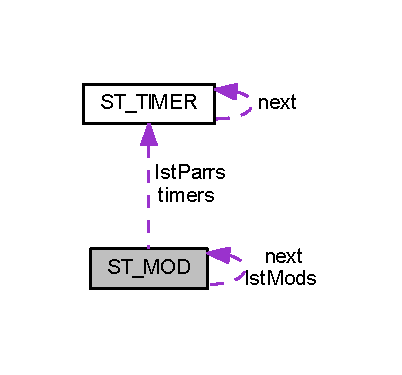
\includegraphics[width=193pt]{struct_s_t___m_o_d__coll__graph}
\end{center}
\end{figure}
\subsection*{Campos de datos}
\begin{DoxyCompactItemize}
\item 
char \hyperlink{struct_s_t___m_o_d_a59b9df3193b6f874922b75715fc1bc81}{nombre} \mbox{[}\hyperlink{sdpconfig_8h_a6611b3fba9de26203f14407743b750cc}{M\+A\+X\+\_\+\+M\+O\+D\+U\+L\+E}+1\mbox{]}
\item 
char \hyperlink{struct_s_t___m_o_d_a11de7bbb4add4ed0cf596ea7a05cb841}{firma} \mbox{[}\hyperlink{sdpconfig_8h_ad6074dd11ab3c97c8135c43aab03ae95}{H\+A\+S\+H\+\_\+\+S\+I\+Z\+E}+1\mbox{]}
\item 
char $\ast$ \hyperlink{struct_s_t___m_o_d_a512e0b2cea6bba7a1eaf1689e8000374}{cobertura}
\item 
char \hyperlink{struct_s_t___m_o_d_a41aafff34874651f2469d2d622a7d60d}{monitor}
\item 
unsigned int \hyperlink{struct_s_t___m_o_d_ab769f67b1f859e497d6476cf44f4e02d}{num\+Parrs}
\item 
unsigned long $\ast$ \hyperlink{struct_s_t___m_o_d_abc198cd7e81f42b66805a17af197de12}{parrs}
\item 
unsigned int \hyperlink{struct_s_t___m_o_d_a9dbd5dd0bbfa51a355303896a2f70f76}{num\+Files}
\item 
unsigned long $\ast$ \hyperlink{struct_s_t___m_o_d_a70ab4319156766461ca994c2e7550d7d}{files}
\item 
\hyperlink{sdp_types_8h_a94c0315eea22344f1e853cc7c90592bb}{T\+I\+M\+E\+R} \hyperlink{struct_s_t___m_o_d_a90cdafff165917e473b00614b8fb8c18}{timers}
\item 
\hyperlink{sdp_types_8h_a94c0315eea22344f1e853cc7c90592bb}{T\+I\+M\+E\+R} $\ast$ \hyperlink{struct_s_t___m_o_d_abab69541867571865a674d938141fcf9}{lst\+Parrs}
\item 
struct \hyperlink{struct_s_t___m_o_d}{S\+T\+\_\+\+M\+O\+D} $\ast$ \hyperlink{struct_s_t___m_o_d_a2f7d75b93f5c1884691f10a146c7bb43}{lst\+Mods}
\item 
struct \hyperlink{struct_s_t___m_o_d}{S\+T\+\_\+\+M\+O\+D} $\ast$ \hyperlink{struct_s_t___m_o_d_a45ca635407e332df9a3b7e72768eb926}{next}
\end{DoxyCompactItemize}


\subsection{Descripción detallada}


Definición en la línea 61 del archivo sdp\+Types.\+h.



\subsection{Documentación de los campos}
\hypertarget{struct_s_t___m_o_d_a512e0b2cea6bba7a1eaf1689e8000374}{}\index{S\+T\+\_\+\+M\+O\+D@{S\+T\+\_\+\+M\+O\+D}!cobertura@{cobertura}}
\index{cobertura@{cobertura}!S\+T\+\_\+\+M\+O\+D@{S\+T\+\_\+\+M\+O\+D}}
\subsubsection[{cobertura}]{\setlength{\rightskip}{0pt plus 5cm}char$\ast$ cobertura}\label{struct_s_t___m_o_d_a512e0b2cea6bba7a1eaf1689e8000374}
Cadena de cobertura 

Definición en la línea 64 del archivo sdp\+Types.\+h.

\hypertarget{struct_s_t___m_o_d_a70ab4319156766461ca994c2e7550d7d}{}\index{S\+T\+\_\+\+M\+O\+D@{S\+T\+\_\+\+M\+O\+D}!files@{files}}
\index{files@{files}!S\+T\+\_\+\+M\+O\+D@{S\+T\+\_\+\+M\+O\+D}}
\subsubsection[{files}]{\setlength{\rightskip}{0pt plus 5cm}unsigned long$\ast$ files}\label{struct_s_t___m_o_d_a70ab4319156766461ca994c2e7550d7d}
Lista de acceso a ficheros 

Definición en la línea 69 del archivo sdp\+Types.\+h.

\hypertarget{struct_s_t___m_o_d_a11de7bbb4add4ed0cf596ea7a05cb841}{}\index{S\+T\+\_\+\+M\+O\+D@{S\+T\+\_\+\+M\+O\+D}!firma@{firma}}
\index{firma@{firma}!S\+T\+\_\+\+M\+O\+D@{S\+T\+\_\+\+M\+O\+D}}
\subsubsection[{firma}]{\setlength{\rightskip}{0pt plus 5cm}char firma\mbox{[}{\bf H\+A\+S\+H\+\_\+\+S\+I\+Z\+E}+1\mbox{]}}\label{struct_s_t___m_o_d_a11de7bbb4add4ed0cf596ea7a05cb841}
Firma del modulo 

Definición en la línea 63 del archivo sdp\+Types.\+h.

\hypertarget{struct_s_t___m_o_d_a2f7d75b93f5c1884691f10a146c7bb43}{}\index{S\+T\+\_\+\+M\+O\+D@{S\+T\+\_\+\+M\+O\+D}!lst\+Mods@{lst\+Mods}}
\index{lst\+Mods@{lst\+Mods}!S\+T\+\_\+\+M\+O\+D@{S\+T\+\_\+\+M\+O\+D}}
\subsubsection[{lst\+Mods}]{\setlength{\rightskip}{0pt plus 5cm}struct {\bf S\+T\+\_\+\+M\+O\+D}$\ast$ lst\+Mods}\label{struct_s_t___m_o_d_a2f7d75b93f5c1884691f10a146c7bb43}
Lista de modulos llamados por el modulo 

Definición en la línea 72 del archivo sdp\+Types.\+h.

\hypertarget{struct_s_t___m_o_d_abab69541867571865a674d938141fcf9}{}\index{S\+T\+\_\+\+M\+O\+D@{S\+T\+\_\+\+M\+O\+D}!lst\+Parrs@{lst\+Parrs}}
\index{lst\+Parrs@{lst\+Parrs}!S\+T\+\_\+\+M\+O\+D@{S\+T\+\_\+\+M\+O\+D}}
\subsubsection[{lst\+Parrs}]{\setlength{\rightskip}{0pt plus 5cm}{\bf T\+I\+M\+E\+R}$\ast$ lst\+Parrs}\label{struct_s_t___m_o_d_abab69541867571865a674d938141fcf9}
Tabla de parrafos del modulo 

Definición en la línea 71 del archivo sdp\+Types.\+h.

\hypertarget{struct_s_t___m_o_d_a41aafff34874651f2469d2d622a7d60d}{}\index{S\+T\+\_\+\+M\+O\+D@{S\+T\+\_\+\+M\+O\+D}!monitor@{monitor}}
\index{monitor@{monitor}!S\+T\+\_\+\+M\+O\+D@{S\+T\+\_\+\+M\+O\+D}}
\subsubsection[{monitor}]{\setlength{\rightskip}{0pt plus 5cm}char monitor}\label{struct_s_t___m_o_d_a41aafff34874651f2469d2d622a7d60d}
Es un modulo monitorizado o no 

Definición en la línea 65 del archivo sdp\+Types.\+h.

\hypertarget{struct_s_t___m_o_d_a45ca635407e332df9a3b7e72768eb926}{}\index{S\+T\+\_\+\+M\+O\+D@{S\+T\+\_\+\+M\+O\+D}!next@{next}}
\index{next@{next}!S\+T\+\_\+\+M\+O\+D@{S\+T\+\_\+\+M\+O\+D}}
\subsubsection[{next}]{\setlength{\rightskip}{0pt plus 5cm}struct {\bf S\+T\+\_\+\+M\+O\+D}$\ast$ next}\label{struct_s_t___m_o_d_a45ca635407e332df9a3b7e72768eb926}


Definición en la línea 73 del archivo sdp\+Types.\+h.

\hypertarget{struct_s_t___m_o_d_a59b9df3193b6f874922b75715fc1bc81}{}\index{S\+T\+\_\+\+M\+O\+D@{S\+T\+\_\+\+M\+O\+D}!nombre@{nombre}}
\index{nombre@{nombre}!S\+T\+\_\+\+M\+O\+D@{S\+T\+\_\+\+M\+O\+D}}
\subsubsection[{nombre}]{\setlength{\rightskip}{0pt plus 5cm}char nombre\mbox{[}{\bf M\+A\+X\+\_\+\+M\+O\+D\+U\+L\+E}+1\mbox{]}}\label{struct_s_t___m_o_d_a59b9df3193b6f874922b75715fc1bc81}
Nombre del modulo 

Definición en la línea 62 del archivo sdp\+Types.\+h.

\hypertarget{struct_s_t___m_o_d_a9dbd5dd0bbfa51a355303896a2f70f76}{}\index{S\+T\+\_\+\+M\+O\+D@{S\+T\+\_\+\+M\+O\+D}!num\+Files@{num\+Files}}
\index{num\+Files@{num\+Files}!S\+T\+\_\+\+M\+O\+D@{S\+T\+\_\+\+M\+O\+D}}
\subsubsection[{num\+Files}]{\setlength{\rightskip}{0pt plus 5cm}unsigned int num\+Files}\label{struct_s_t___m_o_d_a9dbd5dd0bbfa51a355303896a2f70f76}
Numero de ficheros 

Definición en la línea 68 del archivo sdp\+Types.\+h.

\hypertarget{struct_s_t___m_o_d_ab769f67b1f859e497d6476cf44f4e02d}{}\index{S\+T\+\_\+\+M\+O\+D@{S\+T\+\_\+\+M\+O\+D}!num\+Parrs@{num\+Parrs}}
\index{num\+Parrs@{num\+Parrs}!S\+T\+\_\+\+M\+O\+D@{S\+T\+\_\+\+M\+O\+D}}
\subsubsection[{num\+Parrs}]{\setlength{\rightskip}{0pt plus 5cm}unsigned int num\+Parrs}\label{struct_s_t___m_o_d_ab769f67b1f859e497d6476cf44f4e02d}
Numero de parrafos 

Definición en la línea 66 del archivo sdp\+Types.\+h.

\hypertarget{struct_s_t___m_o_d_abc198cd7e81f42b66805a17af197de12}{}\index{S\+T\+\_\+\+M\+O\+D@{S\+T\+\_\+\+M\+O\+D}!parrs@{parrs}}
\index{parrs@{parrs}!S\+T\+\_\+\+M\+O\+D@{S\+T\+\_\+\+M\+O\+D}}
\subsubsection[{parrs}]{\setlength{\rightskip}{0pt plus 5cm}unsigned long$\ast$ parrs}\label{struct_s_t___m_o_d_abc198cd7e81f42b66805a17af197de12}
Lista de acceso a parrafos 

Definición en la línea 67 del archivo sdp\+Types.\+h.

\hypertarget{struct_s_t___m_o_d_a90cdafff165917e473b00614b8fb8c18}{}\index{S\+T\+\_\+\+M\+O\+D@{S\+T\+\_\+\+M\+O\+D}!timers@{timers}}
\index{timers@{timers}!S\+T\+\_\+\+M\+O\+D@{S\+T\+\_\+\+M\+O\+D}}
\subsubsection[{timers}]{\setlength{\rightskip}{0pt plus 5cm}{\bf T\+I\+M\+E\+R} timers}\label{struct_s_t___m_o_d_a90cdafff165917e473b00614b8fb8c18}
Timers del modulo 

Definición en la línea 70 del archivo sdp\+Types.\+h.



La documentación para esta estructura fue generada a partir del siguiente fichero\+:\begin{DoxyCompactItemize}
\item 
include/\hyperlink{sdp_types_8h}{sdp\+Types.\+h}\end{DoxyCompactItemize}

\hypertarget{struct_s_t___p_i_l_a}{}\section{Referencia de la Estructura S\+T\+\_\+\+P\+I\+L\+A}
\label{struct_s_t___p_i_l_a}\index{S\+T\+\_\+\+P\+I\+L\+A@{S\+T\+\_\+\+P\+I\+L\+A}}
\subsection*{Campos de datos}
\begin{DoxyCompactItemize}
\item 
int \hyperlink{struct_s_t___p_i_l_a_a439227feff9d7f55384e8780cfc2eb82}{size}
\item 
unsigned char \hyperlink{struct_s_t___p_i_l_a_ab0785544ba66016a8ee8f818ea08b1c2}{pointer}
\item 
int \hyperlink{struct_s_t___p_i_l_a_a1411ea3b26a34297217f0225315d9758}{num\+Items}
\item 
int \hyperlink{struct_s_t___p_i_l_a_ab042caa09e8430028d87252ad6646a52}{max\+Items}
\item 
void $\ast$$\ast$ \hyperlink{struct_s_t___p_i_l_a_a94977134c19c2c536550e6b13d69218d}{items}
\end{DoxyCompactItemize}


\subsection{Descripción detallada}


Definición en la línea 31 del archivo pila.\+c.



\subsection{Documentación de los campos}
\hypertarget{struct_s_t___p_i_l_a_a94977134c19c2c536550e6b13d69218d}{}\index{S\+T\+\_\+\+P\+I\+L\+A@{S\+T\+\_\+\+P\+I\+L\+A}!items@{items}}
\index{items@{items}!S\+T\+\_\+\+P\+I\+L\+A@{S\+T\+\_\+\+P\+I\+L\+A}}
\subsubsection[{items}]{\setlength{\rightskip}{0pt plus 5cm}void$\ast$$\ast$ items}\label{struct_s_t___p_i_l_a_a94977134c19c2c536550e6b13d69218d}


Definición en la línea 36 del archivo pila.\+c.

\hypertarget{struct_s_t___p_i_l_a_ab042caa09e8430028d87252ad6646a52}{}\index{S\+T\+\_\+\+P\+I\+L\+A@{S\+T\+\_\+\+P\+I\+L\+A}!max\+Items@{max\+Items}}
\index{max\+Items@{max\+Items}!S\+T\+\_\+\+P\+I\+L\+A@{S\+T\+\_\+\+P\+I\+L\+A}}
\subsubsection[{max\+Items}]{\setlength{\rightskip}{0pt plus 5cm}int max\+Items}\label{struct_s_t___p_i_l_a_ab042caa09e8430028d87252ad6646a52}


Definición en la línea 35 del archivo pila.\+c.

\hypertarget{struct_s_t___p_i_l_a_a1411ea3b26a34297217f0225315d9758}{}\index{S\+T\+\_\+\+P\+I\+L\+A@{S\+T\+\_\+\+P\+I\+L\+A}!num\+Items@{num\+Items}}
\index{num\+Items@{num\+Items}!S\+T\+\_\+\+P\+I\+L\+A@{S\+T\+\_\+\+P\+I\+L\+A}}
\subsubsection[{num\+Items}]{\setlength{\rightskip}{0pt plus 5cm}int num\+Items}\label{struct_s_t___p_i_l_a_a1411ea3b26a34297217f0225315d9758}


Definición en la línea 34 del archivo pila.\+c.

\hypertarget{struct_s_t___p_i_l_a_ab0785544ba66016a8ee8f818ea08b1c2}{}\index{S\+T\+\_\+\+P\+I\+L\+A@{S\+T\+\_\+\+P\+I\+L\+A}!pointer@{pointer}}
\index{pointer@{pointer}!S\+T\+\_\+\+P\+I\+L\+A@{S\+T\+\_\+\+P\+I\+L\+A}}
\subsubsection[{pointer}]{\setlength{\rightskip}{0pt plus 5cm}unsigned char pointer}\label{struct_s_t___p_i_l_a_ab0785544ba66016a8ee8f818ea08b1c2}


Definición en la línea 33 del archivo pila.\+c.

\hypertarget{struct_s_t___p_i_l_a_a439227feff9d7f55384e8780cfc2eb82}{}\index{S\+T\+\_\+\+P\+I\+L\+A@{S\+T\+\_\+\+P\+I\+L\+A}!size@{size}}
\index{size@{size}!S\+T\+\_\+\+P\+I\+L\+A@{S\+T\+\_\+\+P\+I\+L\+A}}
\subsubsection[{size}]{\setlength{\rightskip}{0pt plus 5cm}int size}\label{struct_s_t___p_i_l_a_a439227feff9d7f55384e8780cfc2eb82}


Definición en la línea 32 del archivo pila.\+c.



La documentación para esta estructura fue generada a partir del siguiente fichero\+:\begin{DoxyCompactItemize}
\item 
src/\hyperlink{pila_8c}{pila.\+c}\end{DoxyCompactItemize}

\hypertarget{struct_s_t___s_d_p}{}\section{Referencia de la Estructura S\+T\+\_\+\+S\+D\+P}
\label{struct_s_t___s_d_p}\index{S\+T\+\_\+\+S\+D\+P@{S\+T\+\_\+\+S\+D\+P}}


{\ttfamily \#include $<$sdp\+Types.\+h$>$}

\subsection*{Campos de datos}
\begin{DoxyCompactItemize}
\item 
char \hyperlink{struct_s_t___s_d_p_a59b9df3193b6f874922b75715fc1bc81}{nombre} \mbox{[}\hyperlink{sdpconfig_8h_a6611b3fba9de26203f14407743b750cc}{M\+A\+X\+\_\+\+M\+O\+D\+U\+L\+E}+1\mbox{]}
\item 
char \hyperlink{struct_s_t___s_d_p_a11de7bbb4add4ed0cf596ea7a05cb841}{firma} \mbox{[}\hyperlink{sdpconfig_8h_ad6074dd11ab3c97c8135c43aab03ae95}{H\+A\+S\+H\+\_\+\+S\+I\+Z\+E}+1\mbox{]}
\item 
char $\ast$ \hyperlink{struct_s_t___s_d_p_a88033942c6a9207d32af22c3f69cc31e}{coverage}
\item 
char \hyperlink{struct_s_t___s_d_p_aa62a205ca9e35b3b88632d2ec557a5a0}{label} \mbox{[}\hyperlink{sdpconfig_8h_ac084a897234f41c71f01eab1d39c3073}{M\+A\+X\+\_\+\+P\+A\+R\+R\+A\+F\+O}+1\mbox{]}
\item 
unsigned long \hyperlink{struct_s_t___s_d_p_a2524760e620af27370f7dbf1a45750a5}{bloques}
\item 
unsigned long \hyperlink{struct_s_t___s_d_p_a00d906c1e1a889fb8b6f26c73b188936}{parrafos}
\item 
unsigned long \hyperlink{struct_s_t___s_d_p_a256f4cda4f61488d2d766c867e813014}{persistencia}
\end{DoxyCompactItemize}


\subsection{Descripción detallada}


Definición en la línea 25 del archivo sdp\+Types.\+h.



\subsection{Documentación de los campos}
\hypertarget{struct_s_t___s_d_p_a2524760e620af27370f7dbf1a45750a5}{}\index{S\+T\+\_\+\+S\+D\+P@{S\+T\+\_\+\+S\+D\+P}!bloques@{bloques}}
\index{bloques@{bloques}!S\+T\+\_\+\+S\+D\+P@{S\+T\+\_\+\+S\+D\+P}}
\subsubsection[{bloques}]{\setlength{\rightskip}{0pt plus 5cm}unsigned long bloques}\label{struct_s_t___s_d_p_a2524760e620af27370f7dbf1a45750a5}
Numero de bloques 

Definición en la línea 30 del archivo sdp\+Types.\+h.

\hypertarget{struct_s_t___s_d_p_a88033942c6a9207d32af22c3f69cc31e}{}\index{S\+T\+\_\+\+S\+D\+P@{S\+T\+\_\+\+S\+D\+P}!coverage@{coverage}}
\index{coverage@{coverage}!S\+T\+\_\+\+S\+D\+P@{S\+T\+\_\+\+S\+D\+P}}
\subsubsection[{coverage}]{\setlength{\rightskip}{0pt plus 5cm}char$\ast$ coverage}\label{struct_s_t___s_d_p_a88033942c6a9207d32af22c3f69cc31e}
tabla de bloques asciiz 

Definición en la línea 28 del archivo sdp\+Types.\+h.

\hypertarget{struct_s_t___s_d_p_a11de7bbb4add4ed0cf596ea7a05cb841}{}\index{S\+T\+\_\+\+S\+D\+P@{S\+T\+\_\+\+S\+D\+P}!firma@{firma}}
\index{firma@{firma}!S\+T\+\_\+\+S\+D\+P@{S\+T\+\_\+\+S\+D\+P}}
\subsubsection[{firma}]{\setlength{\rightskip}{0pt plus 5cm}char firma\mbox{[}{\bf H\+A\+S\+H\+\_\+\+S\+I\+Z\+E}+1\mbox{]}}\label{struct_s_t___s_d_p_a11de7bbb4add4ed0cf596ea7a05cb841}
Firma del modulo 

Definición en la línea 27 del archivo sdp\+Types.\+h.

\hypertarget{struct_s_t___s_d_p_aa62a205ca9e35b3b88632d2ec557a5a0}{}\index{S\+T\+\_\+\+S\+D\+P@{S\+T\+\_\+\+S\+D\+P}!label@{label}}
\index{label@{label}!S\+T\+\_\+\+S\+D\+P@{S\+T\+\_\+\+S\+D\+P}}
\subsubsection[{label}]{\setlength{\rightskip}{0pt plus 5cm}char label\mbox{[}{\bf M\+A\+X\+\_\+\+P\+A\+R\+R\+A\+F\+O}+1\mbox{]}}\label{struct_s_t___s_d_p_aa62a205ca9e35b3b88632d2ec557a5a0}
Rutina o parrafo 

Definición en la línea 29 del archivo sdp\+Types.\+h.

\hypertarget{struct_s_t___s_d_p_a59b9df3193b6f874922b75715fc1bc81}{}\index{S\+T\+\_\+\+S\+D\+P@{S\+T\+\_\+\+S\+D\+P}!nombre@{nombre}}
\index{nombre@{nombre}!S\+T\+\_\+\+S\+D\+P@{S\+T\+\_\+\+S\+D\+P}}
\subsubsection[{nombre}]{\setlength{\rightskip}{0pt plus 5cm}char nombre\mbox{[}{\bf M\+A\+X\+\_\+\+M\+O\+D\+U\+L\+E}+1\mbox{]}}\label{struct_s_t___s_d_p_a59b9df3193b6f874922b75715fc1bc81}
Nombre del modulo asciiz 

Definición en la línea 26 del archivo sdp\+Types.\+h.

\hypertarget{struct_s_t___s_d_p_a00d906c1e1a889fb8b6f26c73b188936}{}\index{S\+T\+\_\+\+S\+D\+P@{S\+T\+\_\+\+S\+D\+P}!parrafos@{parrafos}}
\index{parrafos@{parrafos}!S\+T\+\_\+\+S\+D\+P@{S\+T\+\_\+\+S\+D\+P}}
\subsubsection[{parrafos}]{\setlength{\rightskip}{0pt plus 5cm}unsigned long parrafos}\label{struct_s_t___s_d_p_a00d906c1e1a889fb8b6f26c73b188936}
Numero de parrafos 

Definición en la línea 31 del archivo sdp\+Types.\+h.

\hypertarget{struct_s_t___s_d_p_a256f4cda4f61488d2d766c867e813014}{}\index{S\+T\+\_\+\+S\+D\+P@{S\+T\+\_\+\+S\+D\+P}!persistencia@{persistencia}}
\index{persistencia@{persistencia}!S\+T\+\_\+\+S\+D\+P@{S\+T\+\_\+\+S\+D\+P}}
\subsubsection[{persistencia}]{\setlength{\rightskip}{0pt plus 5cm}unsigned long persistencia}\label{struct_s_t___s_d_p_a256f4cda4f61488d2d766c867e813014}
Numero de ficheros 

Definición en la línea 32 del archivo sdp\+Types.\+h.



La documentación para esta estructura fue generada a partir del siguiente fichero\+:\begin{DoxyCompactItemize}
\item 
include/\hyperlink{sdp_types_8h}{sdp\+Types.\+h}\end{DoxyCompactItemize}

\hypertarget{struct_s_t___t_i_m_e_r}{}\section{Referencia de la Estructura S\+T\+\_\+\+T\+I\+M\+E\+R}
\label{struct_s_t___t_i_m_e_r}\index{S\+T\+\_\+\+T\+I\+M\+E\+R@{S\+T\+\_\+\+T\+I\+M\+E\+R}}


{\ttfamily \#include $<$sdp\+Types.\+h$>$}



Diagrama de colaboración para S\+T\+\_\+\+T\+I\+M\+E\+R\+:\nopagebreak
\begin{figure}[H]
\begin{center}
\leavevmode
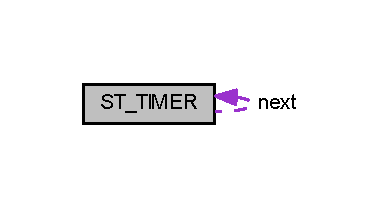
\includegraphics[width=183pt]{struct_s_t___t_i_m_e_r__coll__graph}
\end{center}
\end{figure}
\subsection*{Campos de datos}
\begin{DoxyCompactItemize}
\item 
int \hyperlink{struct_s_t___t_i_m_e_r_a913ffe6a1b92facf1adf87d5190445bc}{tipo}
\item 
char \hyperlink{struct_s_t___t_i_m_e_r_aa62a205ca9e35b3b88632d2ec557a5a0}{label} \mbox{[}\hyperlink{sdpconfig_8h_ac084a897234f41c71f01eab1d39c3073}{M\+A\+X\+\_\+\+P\+A\+R\+R\+A\+F\+O}+1\mbox{]}
\item 
\hyperlink{sdp_types_8h_af632da489ebc3708ec3ab6791ee53fa4}{U\+L\+O\+N\+G} \hyperlink{struct_s_t___t_i_m_e_r_a23a3531ed93eb7f069a5f33ee77d7ca8}{veces}
\item 
\hyperlink{sdp_types_8h_af632da489ebc3708ec3ab6791ee53fa4}{U\+L\+O\+N\+G} \hyperlink{struct_s_t___t_i_m_e_r_a9ff17a87e2d5c2c20efd3883fc5e8afd}{system\+Time}
\item 
\hyperlink{sdp_types_8h_af632da489ebc3708ec3ab6791ee53fa4}{U\+L\+O\+N\+G} \hyperlink{struct_s_t___t_i_m_e_r_ae4c31cb2b4477be7ae2f947073b3d770}{cpu\+Time}
\item 
\hyperlink{sdp_types_8h_af632da489ebc3708ec3ab6791ee53fa4}{U\+L\+O\+N\+G} \hyperlink{struct_s_t___t_i_m_e_r_a8c0fad2befd4574e6a7fae46124d5339}{int\+System\+Time}
\item 
\hyperlink{sdp_types_8h_af632da489ebc3708ec3ab6791ee53fa4}{U\+L\+O\+N\+G} \hyperlink{struct_s_t___t_i_m_e_r_a61dff6fa53638f76ef2f5c004a58992b}{int\+Cpu\+Time}
\item 
struct \hyperlink{struct_s_t___t_i_m_e_r}{S\+T\+\_\+\+T\+I\+M\+E\+R} $\ast$ \hyperlink{struct_s_t___t_i_m_e_r_ae1e8a4a6b208f964f72c50f97e978978}{next}
\item 
\hyperlink{token_8h_acb3d64ed2bb2e72ebb17ca4ef85ae6d3}{mlong} \hyperlink{struct_s_t___t_i_m_e_r_ab93a9231acb19c595671938b5b322772}{stime}
\item 
\hyperlink{token_8h_acb3d64ed2bb2e72ebb17ca4ef85ae6d3}{mlong} \hyperlink{struct_s_t___t_i_m_e_r_a74777a0ada04040a1c53c70c83a06a4e}{utime}
\item 
\hyperlink{token_8h_acb3d64ed2bb2e72ebb17ca4ef85ae6d3}{mlong} \hyperlink{struct_s_t___t_i_m_e_r_a4296c1722751cfeaf3d52cedf2bc212b}{ktime}
\end{DoxyCompactItemize}


\subsection{Descripción detallada}


Definición en la línea 43 del archivo sdp\+Types.\+h.



\subsection{Documentación de los campos}
\hypertarget{struct_s_t___t_i_m_e_r_ae4c31cb2b4477be7ae2f947073b3d770}{}\index{S\+T\+\_\+\+T\+I\+M\+E\+R@{S\+T\+\_\+\+T\+I\+M\+E\+R}!cpu\+Time@{cpu\+Time}}
\index{cpu\+Time@{cpu\+Time}!S\+T\+\_\+\+T\+I\+M\+E\+R@{S\+T\+\_\+\+T\+I\+M\+E\+R}}
\subsubsection[{cpu\+Time}]{\setlength{\rightskip}{0pt plus 5cm}{\bf U\+L\+O\+N\+G} cpu\+Time}\label{struct_s_t___t_i_m_e_r_ae4c31cb2b4477be7ae2f947073b3d770}
Tiempo de C\+P\+U consumido 

Definición en la línea 48 del archivo sdp\+Types.\+h.

\hypertarget{struct_s_t___t_i_m_e_r_a61dff6fa53638f76ef2f5c004a58992b}{}\index{S\+T\+\_\+\+T\+I\+M\+E\+R@{S\+T\+\_\+\+T\+I\+M\+E\+R}!int\+Cpu\+Time@{int\+Cpu\+Time}}
\index{int\+Cpu\+Time@{int\+Cpu\+Time}!S\+T\+\_\+\+T\+I\+M\+E\+R@{S\+T\+\_\+\+T\+I\+M\+E\+R}}
\subsubsection[{int\+Cpu\+Time}]{\setlength{\rightskip}{0pt plus 5cm}{\bf U\+L\+O\+N\+G} int\+Cpu\+Time}\label{struct_s_t___t_i_m_e_r_a61dff6fa53638f76ef2f5c004a58992b}
Tiempo de C\+P\+U consumido 

Definición en la línea 50 del archivo sdp\+Types.\+h.

\hypertarget{struct_s_t___t_i_m_e_r_a8c0fad2befd4574e6a7fae46124d5339}{}\index{S\+T\+\_\+\+T\+I\+M\+E\+R@{S\+T\+\_\+\+T\+I\+M\+E\+R}!int\+System\+Time@{int\+System\+Time}}
\index{int\+System\+Time@{int\+System\+Time}!S\+T\+\_\+\+T\+I\+M\+E\+R@{S\+T\+\_\+\+T\+I\+M\+E\+R}}
\subsubsection[{int\+System\+Time}]{\setlength{\rightskip}{0pt plus 5cm}{\bf U\+L\+O\+N\+G} int\+System\+Time}\label{struct_s_t___t_i_m_e_r_a8c0fad2befd4574e6a7fae46124d5339}
Tiempo del sistema 

Definición en la línea 49 del archivo sdp\+Types.\+h.

\hypertarget{struct_s_t___t_i_m_e_r_a4296c1722751cfeaf3d52cedf2bc212b}{}\index{S\+T\+\_\+\+T\+I\+M\+E\+R@{S\+T\+\_\+\+T\+I\+M\+E\+R}!ktime@{ktime}}
\index{ktime@{ktime}!S\+T\+\_\+\+T\+I\+M\+E\+R@{S\+T\+\_\+\+T\+I\+M\+E\+R}}
\subsubsection[{ktime}]{\setlength{\rightskip}{0pt plus 5cm}{\bf mlong} ktime}\label{struct_s_t___t_i_m_e_r_a4296c1722751cfeaf3d52cedf2bc212b}


Definición en la línea 21 del archivo token.\+h.

\hypertarget{struct_s_t___t_i_m_e_r_aa62a205ca9e35b3b88632d2ec557a5a0}{}\index{S\+T\+\_\+\+T\+I\+M\+E\+R@{S\+T\+\_\+\+T\+I\+M\+E\+R}!label@{label}}
\index{label@{label}!S\+T\+\_\+\+T\+I\+M\+E\+R@{S\+T\+\_\+\+T\+I\+M\+E\+R}}
\subsubsection[{label}]{\setlength{\rightskip}{0pt plus 5cm}char label\mbox{[}{\bf M\+A\+X\+\_\+\+P\+A\+R\+R\+A\+F\+O}+1\mbox{]}}\label{struct_s_t___t_i_m_e_r_aa62a205ca9e35b3b88632d2ec557a5a0}
Nombre 

Definición en la línea 45 del archivo sdp\+Types.\+h.

\hypertarget{struct_s_t___t_i_m_e_r_ae1e8a4a6b208f964f72c50f97e978978}{}\index{S\+T\+\_\+\+T\+I\+M\+E\+R@{S\+T\+\_\+\+T\+I\+M\+E\+R}!next@{next}}
\index{next@{next}!S\+T\+\_\+\+T\+I\+M\+E\+R@{S\+T\+\_\+\+T\+I\+M\+E\+R}}
\subsubsection[{next}]{\setlength{\rightskip}{0pt plus 5cm}struct {\bf S\+T\+\_\+\+T\+I\+M\+E\+R}$\ast$ next}\label{struct_s_t___t_i_m_e_r_ae1e8a4a6b208f964f72c50f97e978978}


Definición en la línea 51 del archivo sdp\+Types.\+h.

\hypertarget{struct_s_t___t_i_m_e_r_ab93a9231acb19c595671938b5b322772}{}\index{S\+T\+\_\+\+T\+I\+M\+E\+R@{S\+T\+\_\+\+T\+I\+M\+E\+R}!stime@{stime}}
\index{stime@{stime}!S\+T\+\_\+\+T\+I\+M\+E\+R@{S\+T\+\_\+\+T\+I\+M\+E\+R}}
\subsubsection[{stime}]{\setlength{\rightskip}{0pt plus 5cm}{\bf mlong} stime}\label{struct_s_t___t_i_m_e_r_ab93a9231acb19c595671938b5b322772}


Definición en la línea 19 del archivo token.\+h.

\hypertarget{struct_s_t___t_i_m_e_r_a9ff17a87e2d5c2c20efd3883fc5e8afd}{}\index{S\+T\+\_\+\+T\+I\+M\+E\+R@{S\+T\+\_\+\+T\+I\+M\+E\+R}!system\+Time@{system\+Time}}
\index{system\+Time@{system\+Time}!S\+T\+\_\+\+T\+I\+M\+E\+R@{S\+T\+\_\+\+T\+I\+M\+E\+R}}
\subsubsection[{system\+Time}]{\setlength{\rightskip}{0pt plus 5cm}{\bf U\+L\+O\+N\+G} system\+Time}\label{struct_s_t___t_i_m_e_r_a9ff17a87e2d5c2c20efd3883fc5e8afd}
Numero de veces que se ha utilizado Tiempo del sistema 

Definición en la línea 47 del archivo sdp\+Types.\+h.

\hypertarget{struct_s_t___t_i_m_e_r_a913ffe6a1b92facf1adf87d5190445bc}{}\index{S\+T\+\_\+\+T\+I\+M\+E\+R@{S\+T\+\_\+\+T\+I\+M\+E\+R}!tipo@{tipo}}
\index{tipo@{tipo}!S\+T\+\_\+\+T\+I\+M\+E\+R@{S\+T\+\_\+\+T\+I\+M\+E\+R}}
\subsubsection[{tipo}]{\setlength{\rightskip}{0pt plus 5cm}int tipo}\label{struct_s_t___t_i_m_e_r_a913ffe6a1b92facf1adf87d5190445bc}
Tipo del mensaje que genera el timer 

Definición en la línea 44 del archivo sdp\+Types.\+h.

\hypertarget{struct_s_t___t_i_m_e_r_a74777a0ada04040a1c53c70c83a06a4e}{}\index{S\+T\+\_\+\+T\+I\+M\+E\+R@{S\+T\+\_\+\+T\+I\+M\+E\+R}!utime@{utime}}
\index{utime@{utime}!S\+T\+\_\+\+T\+I\+M\+E\+R@{S\+T\+\_\+\+T\+I\+M\+E\+R}}
\subsubsection[{utime}]{\setlength{\rightskip}{0pt plus 5cm}{\bf mlong} utime}\label{struct_s_t___t_i_m_e_r_a74777a0ada04040a1c53c70c83a06a4e}


Definición en la línea 20 del archivo token.\+h.

\hypertarget{struct_s_t___t_i_m_e_r_a23a3531ed93eb7f069a5f33ee77d7ca8}{}\index{S\+T\+\_\+\+T\+I\+M\+E\+R@{S\+T\+\_\+\+T\+I\+M\+E\+R}!veces@{veces}}
\index{veces@{veces}!S\+T\+\_\+\+T\+I\+M\+E\+R@{S\+T\+\_\+\+T\+I\+M\+E\+R}}
\subsubsection[{veces}]{\setlength{\rightskip}{0pt plus 5cm}{\bf U\+L\+O\+N\+G} veces}\label{struct_s_t___t_i_m_e_r_a23a3531ed93eb7f069a5f33ee77d7ca8}


Definición en la línea 46 del archivo sdp\+Types.\+h.



La documentación para esta estructura fue generada a partir de los siguientes ficheros\+:\begin{DoxyCompactItemize}
\item 
include/\hyperlink{sdp_types_8h}{sdp\+Types.\+h}\item 
include/\hyperlink{token_8h}{token.\+h}\end{DoxyCompactItemize}

\hypertarget{struct_s_t___t_o_k_e_n}{}\section{Referencia de la Estructura S\+T\+\_\+\+T\+O\+K\+E\+N}
\label{struct_s_t___t_o_k_e_n}\index{S\+T\+\_\+\+T\+O\+K\+E\+N@{S\+T\+\_\+\+T\+O\+K\+E\+N}}


{\ttfamily \#include $<$token.\+h$>$}



Diagrama de colaboración para S\+T\+\_\+\+T\+O\+K\+E\+N\+:\nopagebreak
\begin{figure}[H]
\begin{center}
\leavevmode
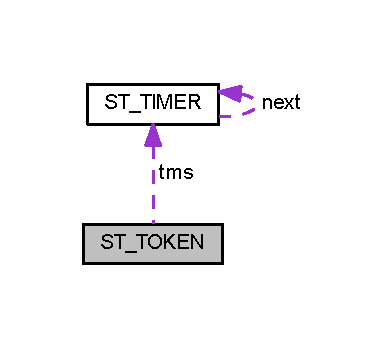
\includegraphics[width=185pt]{struct_s_t___t_o_k_e_n__coll__graph}
\end{center}
\end{figure}
\subsection*{Campos de datos}
\begin{DoxyCompactItemize}
\item 
char $\ast$ \hyperlink{struct_s_t___t_o_k_e_n_a5ac083a645d964373f022d03df4849c8}{name}
\item 
char $\ast$ \hyperlink{struct_s_t___t_o_k_e_n_aecb3b0d045ada529257a2fbf8f829599}{id}
\item 
\hyperlink{sdp_types_8h_a94c0315eea22344f1e853cc7c90592bb}{T\+I\+M\+E\+R} \hyperlink{struct_s_t___t_o_k_e_n_a7427db66ac10c39267f1981f54f0a91f}{tms}
\end{DoxyCompactItemize}


\subsection{Descripción detallada}


Definición en la línea 26 del archivo token.\+h.



\subsection{Documentación de los campos}
\hypertarget{struct_s_t___t_o_k_e_n_aecb3b0d045ada529257a2fbf8f829599}{}\index{S\+T\+\_\+\+T\+O\+K\+E\+N@{S\+T\+\_\+\+T\+O\+K\+E\+N}!id@{id}}
\index{id@{id}!S\+T\+\_\+\+T\+O\+K\+E\+N@{S\+T\+\_\+\+T\+O\+K\+E\+N}}
\subsubsection[{id}]{\setlength{\rightskip}{0pt plus 5cm}char$\ast$ id}\label{struct_s_t___t_o_k_e_n_aecb3b0d045ada529257a2fbf8f829599}


Definición en la línea 28 del archivo token.\+h.

\hypertarget{struct_s_t___t_o_k_e_n_a5ac083a645d964373f022d03df4849c8}{}\index{S\+T\+\_\+\+T\+O\+K\+E\+N@{S\+T\+\_\+\+T\+O\+K\+E\+N}!name@{name}}
\index{name@{name}!S\+T\+\_\+\+T\+O\+K\+E\+N@{S\+T\+\_\+\+T\+O\+K\+E\+N}}
\subsubsection[{name}]{\setlength{\rightskip}{0pt plus 5cm}char$\ast$ name}\label{struct_s_t___t_o_k_e_n_a5ac083a645d964373f022d03df4849c8}


Definición en la línea 27 del archivo token.\+h.

\hypertarget{struct_s_t___t_o_k_e_n_a7427db66ac10c39267f1981f54f0a91f}{}\index{S\+T\+\_\+\+T\+O\+K\+E\+N@{S\+T\+\_\+\+T\+O\+K\+E\+N}!tms@{tms}}
\index{tms@{tms}!S\+T\+\_\+\+T\+O\+K\+E\+N@{S\+T\+\_\+\+T\+O\+K\+E\+N}}
\subsubsection[{tms}]{\setlength{\rightskip}{0pt plus 5cm}{\bf T\+I\+M\+E\+R} tms}\label{struct_s_t___t_o_k_e_n_a7427db66ac10c39267f1981f54f0a91f}


Definición en la línea 29 del archivo token.\+h.



La documentación para esta estructura fue generada a partir del siguiente fichero\+:\begin{DoxyCompactItemize}
\item 
include/\hyperlink{token_8h}{token.\+h}\end{DoxyCompactItemize}

\hypertarget{structtag_m_q_a_i_r}{}\section{Referencia de la Estructura tag\+M\+Q\+A\+I\+R}
\label{structtag_m_q_a_i_r}\index{tag\+M\+Q\+A\+I\+R@{tag\+M\+Q\+A\+I\+R}}


{\ttfamily \#include $<$cmqc.\+h$>$}

\subsection*{Campos de datos}
\begin{DoxyCompactItemize}
\item 
\hyperlink{cmqc_8h_a12590e546ed66fda7cf21c1d5cefa31d}{M\+Q\+C\+H\+A\+R4} \hyperlink{structtag_m_q_a_i_r_a0530922ca944569b52601d74941f96e4}{Struc\+Id}
\item 
\hyperlink{cmqc_8h_a1fb8d28cbda3fa8766a9821230cdb6d5}{M\+Q\+L\+O\+N\+G} \hyperlink{structtag_m_q_a_i_r_a0656ef8f766b3907d394d88a35d7b7e9}{Version}
\item 
\hyperlink{cmqc_8h_a1fb8d28cbda3fa8766a9821230cdb6d5}{M\+Q\+L\+O\+N\+G} \hyperlink{structtag_m_q_a_i_r_ab6d5732a34c9e5537251a011b7c5cfd2}{Auth\+Info\+Type}
\item 
\hyperlink{cmqc_8h_aeb12bc7ba416a4eb603e2a74351418d2}{M\+Q\+C\+H\+A\+R} \hyperlink{structtag_m_q_a_i_r_ae500a619d5c7accb19d376cc8e90b542}{Auth\+Info\+Conn\+Name} \mbox{[}264\mbox{]}
\item 
\hyperlink{cmqc_8h_a6c7816c5bbcf1856a25a4558df856937}{P\+M\+Q\+C\+H\+A\+R} \hyperlink{structtag_m_q_a_i_r_afd5202d66986643207bde23232f8dfe6}{L\+D\+A\+P\+User\+Name\+Ptr}
\item 
\hyperlink{cmqc_8h_a1fb8d28cbda3fa8766a9821230cdb6d5}{M\+Q\+L\+O\+N\+G} \hyperlink{structtag_m_q_a_i_r_a09b5d1f5f57fa530f91d06550e1c1f2a}{L\+D\+A\+P\+User\+Name\+Offset}
\item 
\hyperlink{cmqc_8h_a1fb8d28cbda3fa8766a9821230cdb6d5}{M\+Q\+L\+O\+N\+G} \hyperlink{structtag_m_q_a_i_r_a849bc6c195d62939eafc7783284d4314}{L\+D\+A\+P\+User\+Name\+Length}
\item 
\hyperlink{cmqc_8h_a0b7dd696f0148465fe80f6eae57b38a2}{M\+Q\+C\+H\+A\+R32} \hyperlink{structtag_m_q_a_i_r_aeec928bfebc24320430fca7f05918450}{L\+D\+A\+P\+Password}
\item 
\hyperlink{cmqc_8h_ac492686cf8a90cc3dbc1c48143707ca7}{M\+Q\+C\+H\+A\+R256} \hyperlink{structtag_m_q_a_i_r_a8e3ec4c8973e460828f035270c03144c}{O\+C\+S\+P\+Responder\+U\+R\+L}
\end{DoxyCompactItemize}


\subsection{Descripción detallada}


Definición en la línea 3717 del archivo cmqc.\+h.



\subsection{Documentación de los campos}
\hypertarget{structtag_m_q_a_i_r_ae500a619d5c7accb19d376cc8e90b542}{}\index{tag\+M\+Q\+A\+I\+R@{tag\+M\+Q\+A\+I\+R}!Auth\+Info\+Conn\+Name@{Auth\+Info\+Conn\+Name}}
\index{Auth\+Info\+Conn\+Name@{Auth\+Info\+Conn\+Name}!tag\+M\+Q\+A\+I\+R@{tag\+M\+Q\+A\+I\+R}}
\subsubsection[{Auth\+Info\+Conn\+Name}]{\setlength{\rightskip}{0pt plus 5cm}{\bf M\+Q\+C\+H\+A\+R} Auth\+Info\+Conn\+Name\mbox{[}264\mbox{]}}\label{structtag_m_q_a_i_r_ae500a619d5c7accb19d376cc8e90b542}


Definición en la línea 3722 del archivo cmqc.\+h.

\hypertarget{structtag_m_q_a_i_r_ab6d5732a34c9e5537251a011b7c5cfd2}{}\index{tag\+M\+Q\+A\+I\+R@{tag\+M\+Q\+A\+I\+R}!Auth\+Info\+Type@{Auth\+Info\+Type}}
\index{Auth\+Info\+Type@{Auth\+Info\+Type}!tag\+M\+Q\+A\+I\+R@{tag\+M\+Q\+A\+I\+R}}
\subsubsection[{Auth\+Info\+Type}]{\setlength{\rightskip}{0pt plus 5cm}{\bf M\+Q\+L\+O\+N\+G} Auth\+Info\+Type}\label{structtag_m_q_a_i_r_ab6d5732a34c9e5537251a011b7c5cfd2}


Definición en la línea 3720 del archivo cmqc.\+h.

\hypertarget{structtag_m_q_a_i_r_aeec928bfebc24320430fca7f05918450}{}\index{tag\+M\+Q\+A\+I\+R@{tag\+M\+Q\+A\+I\+R}!L\+D\+A\+P\+Password@{L\+D\+A\+P\+Password}}
\index{L\+D\+A\+P\+Password@{L\+D\+A\+P\+Password}!tag\+M\+Q\+A\+I\+R@{tag\+M\+Q\+A\+I\+R}}
\subsubsection[{L\+D\+A\+P\+Password}]{\setlength{\rightskip}{0pt plus 5cm}{\bf M\+Q\+C\+H\+A\+R32} L\+D\+A\+P\+Password}\label{structtag_m_q_a_i_r_aeec928bfebc24320430fca7f05918450}


Definición en la línea 3729 del archivo cmqc.\+h.

\hypertarget{structtag_m_q_a_i_r_a849bc6c195d62939eafc7783284d4314}{}\index{tag\+M\+Q\+A\+I\+R@{tag\+M\+Q\+A\+I\+R}!L\+D\+A\+P\+User\+Name\+Length@{L\+D\+A\+P\+User\+Name\+Length}}
\index{L\+D\+A\+P\+User\+Name\+Length@{L\+D\+A\+P\+User\+Name\+Length}!tag\+M\+Q\+A\+I\+R@{tag\+M\+Q\+A\+I\+R}}
\subsubsection[{L\+D\+A\+P\+User\+Name\+Length}]{\setlength{\rightskip}{0pt plus 5cm}{\bf M\+Q\+L\+O\+N\+G} L\+D\+A\+P\+User\+Name\+Length}\label{structtag_m_q_a_i_r_a849bc6c195d62939eafc7783284d4314}


Definición en la línea 3728 del archivo cmqc.\+h.

\hypertarget{structtag_m_q_a_i_r_a09b5d1f5f57fa530f91d06550e1c1f2a}{}\index{tag\+M\+Q\+A\+I\+R@{tag\+M\+Q\+A\+I\+R}!L\+D\+A\+P\+User\+Name\+Offset@{L\+D\+A\+P\+User\+Name\+Offset}}
\index{L\+D\+A\+P\+User\+Name\+Offset@{L\+D\+A\+P\+User\+Name\+Offset}!tag\+M\+Q\+A\+I\+R@{tag\+M\+Q\+A\+I\+R}}
\subsubsection[{L\+D\+A\+P\+User\+Name\+Offset}]{\setlength{\rightskip}{0pt plus 5cm}{\bf M\+Q\+L\+O\+N\+G} L\+D\+A\+P\+User\+Name\+Offset}\label{structtag_m_q_a_i_r_a09b5d1f5f57fa530f91d06550e1c1f2a}


Definición en la línea 3725 del archivo cmqc.\+h.

\hypertarget{structtag_m_q_a_i_r_afd5202d66986643207bde23232f8dfe6}{}\index{tag\+M\+Q\+A\+I\+R@{tag\+M\+Q\+A\+I\+R}!L\+D\+A\+P\+User\+Name\+Ptr@{L\+D\+A\+P\+User\+Name\+Ptr}}
\index{L\+D\+A\+P\+User\+Name\+Ptr@{L\+D\+A\+P\+User\+Name\+Ptr}!tag\+M\+Q\+A\+I\+R@{tag\+M\+Q\+A\+I\+R}}
\subsubsection[{L\+D\+A\+P\+User\+Name\+Ptr}]{\setlength{\rightskip}{0pt plus 5cm}{\bf P\+M\+Q\+C\+H\+A\+R} L\+D\+A\+P\+User\+Name\+Ptr}\label{structtag_m_q_a_i_r_afd5202d66986643207bde23232f8dfe6}


Definición en la línea 3724 del archivo cmqc.\+h.

\hypertarget{structtag_m_q_a_i_r_a8e3ec4c8973e460828f035270c03144c}{}\index{tag\+M\+Q\+A\+I\+R@{tag\+M\+Q\+A\+I\+R}!O\+C\+S\+P\+Responder\+U\+R\+L@{O\+C\+S\+P\+Responder\+U\+R\+L}}
\index{O\+C\+S\+P\+Responder\+U\+R\+L@{O\+C\+S\+P\+Responder\+U\+R\+L}!tag\+M\+Q\+A\+I\+R@{tag\+M\+Q\+A\+I\+R}}
\subsubsection[{O\+C\+S\+P\+Responder\+U\+R\+L}]{\setlength{\rightskip}{0pt plus 5cm}{\bf M\+Q\+C\+H\+A\+R256} O\+C\+S\+P\+Responder\+U\+R\+L}\label{structtag_m_q_a_i_r_a8e3ec4c8973e460828f035270c03144c}


Definición en la línea 3732 del archivo cmqc.\+h.

\hypertarget{structtag_m_q_a_i_r_a0530922ca944569b52601d74941f96e4}{}\index{tag\+M\+Q\+A\+I\+R@{tag\+M\+Q\+A\+I\+R}!Struc\+Id@{Struc\+Id}}
\index{Struc\+Id@{Struc\+Id}!tag\+M\+Q\+A\+I\+R@{tag\+M\+Q\+A\+I\+R}}
\subsubsection[{Struc\+Id}]{\setlength{\rightskip}{0pt plus 5cm}{\bf M\+Q\+C\+H\+A\+R4} Struc\+Id}\label{structtag_m_q_a_i_r_a0530922ca944569b52601d74941f96e4}


Definición en la línea 3718 del archivo cmqc.\+h.

\hypertarget{structtag_m_q_a_i_r_a0656ef8f766b3907d394d88a35d7b7e9}{}\index{tag\+M\+Q\+A\+I\+R@{tag\+M\+Q\+A\+I\+R}!Version@{Version}}
\index{Version@{Version}!tag\+M\+Q\+A\+I\+R@{tag\+M\+Q\+A\+I\+R}}
\subsubsection[{Version}]{\setlength{\rightskip}{0pt plus 5cm}{\bf M\+Q\+L\+O\+N\+G} Version}\label{structtag_m_q_a_i_r_a0656ef8f766b3907d394d88a35d7b7e9}


Definición en la línea 3719 del archivo cmqc.\+h.



La documentación para esta estructura fue generada a partir del siguiente fichero\+:\begin{DoxyCompactItemize}
\item 
include/\hyperlink{cmqc_8h}{cmqc.\+h}\end{DoxyCompactItemize}

\hypertarget{structtag_m_q_b_m_h_o}{}\section{Referencia de la Estructura tag\+M\+Q\+B\+M\+H\+O}
\label{structtag_m_q_b_m_h_o}\index{tag\+M\+Q\+B\+M\+H\+O@{tag\+M\+Q\+B\+M\+H\+O}}


{\ttfamily \#include $<$cmqc.\+h$>$}

\subsection*{Campos de datos}
\begin{DoxyCompactItemize}
\item 
\hyperlink{cmqc_8h_a12590e546ed66fda7cf21c1d5cefa31d}{M\+Q\+C\+H\+A\+R4} \hyperlink{structtag_m_q_b_m_h_o_a0530922ca944569b52601d74941f96e4}{Struc\+Id}
\item 
\hyperlink{cmqc_8h_a1fb8d28cbda3fa8766a9821230cdb6d5}{M\+Q\+L\+O\+N\+G} \hyperlink{structtag_m_q_b_m_h_o_a0656ef8f766b3907d394d88a35d7b7e9}{Version}
\item 
\hyperlink{cmqc_8h_a1fb8d28cbda3fa8766a9821230cdb6d5}{M\+Q\+L\+O\+N\+G} \hyperlink{structtag_m_q_b_m_h_o_ad7aff2d6c6044809464380998d24ec5c}{Options}
\end{DoxyCompactItemize}


\subsection{Descripción detallada}


Definición en la línea 3755 del archivo cmqc.\+h.



\subsection{Documentación de los campos}
\hypertarget{structtag_m_q_b_m_h_o_ad7aff2d6c6044809464380998d24ec5c}{}\index{tag\+M\+Q\+B\+M\+H\+O@{tag\+M\+Q\+B\+M\+H\+O}!Options@{Options}}
\index{Options@{Options}!tag\+M\+Q\+B\+M\+H\+O@{tag\+M\+Q\+B\+M\+H\+O}}
\subsubsection[{Options}]{\setlength{\rightskip}{0pt plus 5cm}{\bf M\+Q\+L\+O\+N\+G} Options}\label{structtag_m_q_b_m_h_o_ad7aff2d6c6044809464380998d24ec5c}


Definición en la línea 3758 del archivo cmqc.\+h.

\hypertarget{structtag_m_q_b_m_h_o_a0530922ca944569b52601d74941f96e4}{}\index{tag\+M\+Q\+B\+M\+H\+O@{tag\+M\+Q\+B\+M\+H\+O}!Struc\+Id@{Struc\+Id}}
\index{Struc\+Id@{Struc\+Id}!tag\+M\+Q\+B\+M\+H\+O@{tag\+M\+Q\+B\+M\+H\+O}}
\subsubsection[{Struc\+Id}]{\setlength{\rightskip}{0pt plus 5cm}{\bf M\+Q\+C\+H\+A\+R4} Struc\+Id}\label{structtag_m_q_b_m_h_o_a0530922ca944569b52601d74941f96e4}


Definición en la línea 3756 del archivo cmqc.\+h.

\hypertarget{structtag_m_q_b_m_h_o_a0656ef8f766b3907d394d88a35d7b7e9}{}\index{tag\+M\+Q\+B\+M\+H\+O@{tag\+M\+Q\+B\+M\+H\+O}!Version@{Version}}
\index{Version@{Version}!tag\+M\+Q\+B\+M\+H\+O@{tag\+M\+Q\+B\+M\+H\+O}}
\subsubsection[{Version}]{\setlength{\rightskip}{0pt plus 5cm}{\bf M\+Q\+L\+O\+N\+G} Version}\label{structtag_m_q_b_m_h_o_a0656ef8f766b3907d394d88a35d7b7e9}


Definición en la línea 3757 del archivo cmqc.\+h.



La documentación para esta estructura fue generada a partir del siguiente fichero\+:\begin{DoxyCompactItemize}
\item 
include/\hyperlink{cmqc_8h}{cmqc.\+h}\end{DoxyCompactItemize}

\hypertarget{structtag_m_q_b_o}{}\section{Referencia de la Estructura tag\+M\+Q\+B\+O}
\label{structtag_m_q_b_o}\index{tag\+M\+Q\+B\+O@{tag\+M\+Q\+B\+O}}


{\ttfamily \#include $<$cmqc.\+h$>$}

\subsection*{Campos de datos}
\begin{DoxyCompactItemize}
\item 
\hyperlink{cmqc_8h_a12590e546ed66fda7cf21c1d5cefa31d}{M\+Q\+C\+H\+A\+R4} \hyperlink{structtag_m_q_b_o_a0530922ca944569b52601d74941f96e4}{Struc\+Id}
\item 
\hyperlink{cmqc_8h_a1fb8d28cbda3fa8766a9821230cdb6d5}{M\+Q\+L\+O\+N\+G} \hyperlink{structtag_m_q_b_o_a0656ef8f766b3907d394d88a35d7b7e9}{Version}
\item 
\hyperlink{cmqc_8h_a1fb8d28cbda3fa8766a9821230cdb6d5}{M\+Q\+L\+O\+N\+G} \hyperlink{structtag_m_q_b_o_ad7aff2d6c6044809464380998d24ec5c}{Options}
\end{DoxyCompactItemize}


\subsection{Descripción detallada}


Definición en la línea 3774 del archivo cmqc.\+h.



\subsection{Documentación de los campos}
\hypertarget{structtag_m_q_b_o_ad7aff2d6c6044809464380998d24ec5c}{}\index{tag\+M\+Q\+B\+O@{tag\+M\+Q\+B\+O}!Options@{Options}}
\index{Options@{Options}!tag\+M\+Q\+B\+O@{tag\+M\+Q\+B\+O}}
\subsubsection[{Options}]{\setlength{\rightskip}{0pt plus 5cm}{\bf M\+Q\+L\+O\+N\+G} Options}\label{structtag_m_q_b_o_ad7aff2d6c6044809464380998d24ec5c}


Definición en la línea 3777 del archivo cmqc.\+h.

\hypertarget{structtag_m_q_b_o_a0530922ca944569b52601d74941f96e4}{}\index{tag\+M\+Q\+B\+O@{tag\+M\+Q\+B\+O}!Struc\+Id@{Struc\+Id}}
\index{Struc\+Id@{Struc\+Id}!tag\+M\+Q\+B\+O@{tag\+M\+Q\+B\+O}}
\subsubsection[{Struc\+Id}]{\setlength{\rightskip}{0pt plus 5cm}{\bf M\+Q\+C\+H\+A\+R4} Struc\+Id}\label{structtag_m_q_b_o_a0530922ca944569b52601d74941f96e4}


Definición en la línea 3775 del archivo cmqc.\+h.

\hypertarget{structtag_m_q_b_o_a0656ef8f766b3907d394d88a35d7b7e9}{}\index{tag\+M\+Q\+B\+O@{tag\+M\+Q\+B\+O}!Version@{Version}}
\index{Version@{Version}!tag\+M\+Q\+B\+O@{tag\+M\+Q\+B\+O}}
\subsubsection[{Version}]{\setlength{\rightskip}{0pt plus 5cm}{\bf M\+Q\+L\+O\+N\+G} Version}\label{structtag_m_q_b_o_a0656ef8f766b3907d394d88a35d7b7e9}


Definición en la línea 3776 del archivo cmqc.\+h.



La documentación para esta estructura fue generada a partir del siguiente fichero\+:\begin{DoxyCompactItemize}
\item 
include/\hyperlink{cmqc_8h}{cmqc.\+h}\end{DoxyCompactItemize}

\hypertarget{structtag_m_q_c_b_c}{}\section{Referencia de la Estructura tag\+M\+Q\+C\+B\+C}
\label{structtag_m_q_c_b_c}\index{tag\+M\+Q\+C\+B\+C@{tag\+M\+Q\+C\+B\+C}}


{\ttfamily \#include $<$cmqc.\+h$>$}

\subsection*{Campos de datos}
\begin{DoxyCompactItemize}
\item 
\hyperlink{cmqc_8h_a12590e546ed66fda7cf21c1d5cefa31d}{M\+Q\+C\+H\+A\+R4} \hyperlink{structtag_m_q_c_b_c_a0530922ca944569b52601d74941f96e4}{Struc\+Id}
\item 
\hyperlink{cmqc_8h_a1fb8d28cbda3fa8766a9821230cdb6d5}{M\+Q\+L\+O\+N\+G} \hyperlink{structtag_m_q_c_b_c_a0656ef8f766b3907d394d88a35d7b7e9}{Version}
\item 
\hyperlink{cmqc_8h_a1fb8d28cbda3fa8766a9821230cdb6d5}{M\+Q\+L\+O\+N\+G} \hyperlink{structtag_m_q_c_b_c_a0b568439fe1c5ce8239604c1ec58a387}{Call\+Type}
\item 
\hyperlink{cmqc_8h_ac093f559f81163292e6016c68c947164}{M\+Q\+H\+O\+B\+J} \hyperlink{structtag_m_q_c_b_c_a9f8f179d9e85063e5a265231422a9bf2}{Hobj}
\item 
\hyperlink{cmqc_8h_a0b835d8e479d7c42242ed9c6b6572f5a}{M\+Q\+P\+T\+R} \hyperlink{structtag_m_q_c_b_c_aec315c62e18aa72c5d04cadada50f160}{Callback\+Area}
\item 
\hyperlink{cmqc_8h_a0b835d8e479d7c42242ed9c6b6572f5a}{M\+Q\+P\+T\+R} \hyperlink{structtag_m_q_c_b_c_a58c83e52e3187c1579e9aeb6c52ded13}{Connection\+Area}
\item 
\hyperlink{cmqc_8h_a1fb8d28cbda3fa8766a9821230cdb6d5}{M\+Q\+L\+O\+N\+G} \hyperlink{structtag_m_q_c_b_c_a3d53860a50c3834d3dad9f5b2e5b5234}{Comp\+Code}
\item 
\hyperlink{cmqc_8h_a1fb8d28cbda3fa8766a9821230cdb6d5}{M\+Q\+L\+O\+N\+G} \hyperlink{structtag_m_q_c_b_c_ac2f0378cb0c66c5f91625822e53d7bae}{Reason}
\item 
\hyperlink{cmqc_8h_a1fb8d28cbda3fa8766a9821230cdb6d5}{M\+Q\+L\+O\+N\+G} \hyperlink{structtag_m_q_c_b_c_a55c511c2682a9c979eeb93d1a2259f42}{State}
\item 
\hyperlink{cmqc_8h_a1fb8d28cbda3fa8766a9821230cdb6d5}{M\+Q\+L\+O\+N\+G} \hyperlink{structtag_m_q_c_b_c_a75a536f04bbb17c49970e5ebeaeecacf}{Data\+Length}
\item 
\hyperlink{cmqc_8h_a1fb8d28cbda3fa8766a9821230cdb6d5}{M\+Q\+L\+O\+N\+G} \hyperlink{structtag_m_q_c_b_c_a4c13f4abce01a1fd714fb33ca2491583}{Buffer\+Length}
\item 
\hyperlink{cmqc_8h_a1fb8d28cbda3fa8766a9821230cdb6d5}{M\+Q\+L\+O\+N\+G} \hyperlink{structtag_m_q_c_b_c_a8da770267273b200fa9c968fa2a0da57}{Flags}
\item 
\hyperlink{cmqc_8h_a1fb8d28cbda3fa8766a9821230cdb6d5}{M\+Q\+L\+O\+N\+G} \hyperlink{structtag_m_q_c_b_c_aebfaff32156463b0ead92d765681ff04}{Reconnect\+Delay}
\end{DoxyCompactItemize}


\subsection{Descripción detallada}


Definición en la línea 3793 del archivo cmqc.\+h.



\subsection{Documentación de los campos}
\hypertarget{structtag_m_q_c_b_c_a4c13f4abce01a1fd714fb33ca2491583}{}\index{tag\+M\+Q\+C\+B\+C@{tag\+M\+Q\+C\+B\+C}!Buffer\+Length@{Buffer\+Length}}
\index{Buffer\+Length@{Buffer\+Length}!tag\+M\+Q\+C\+B\+C@{tag\+M\+Q\+C\+B\+C}}
\subsubsection[{Buffer\+Length}]{\setlength{\rightskip}{0pt plus 5cm}{\bf M\+Q\+L\+O\+N\+G} Buffer\+Length}\label{structtag_m_q_c_b_c_a4c13f4abce01a1fd714fb33ca2491583}


Definición en la línea 3805 del archivo cmqc.\+h.

\hypertarget{structtag_m_q_c_b_c_aec315c62e18aa72c5d04cadada50f160}{}\index{tag\+M\+Q\+C\+B\+C@{tag\+M\+Q\+C\+B\+C}!Callback\+Area@{Callback\+Area}}
\index{Callback\+Area@{Callback\+Area}!tag\+M\+Q\+C\+B\+C@{tag\+M\+Q\+C\+B\+C}}
\subsubsection[{Callback\+Area}]{\setlength{\rightskip}{0pt plus 5cm}{\bf M\+Q\+P\+T\+R} Callback\+Area}\label{structtag_m_q_c_b_c_aec315c62e18aa72c5d04cadada50f160}


Definición en la línea 3798 del archivo cmqc.\+h.

\hypertarget{structtag_m_q_c_b_c_a0b568439fe1c5ce8239604c1ec58a387}{}\index{tag\+M\+Q\+C\+B\+C@{tag\+M\+Q\+C\+B\+C}!Call\+Type@{Call\+Type}}
\index{Call\+Type@{Call\+Type}!tag\+M\+Q\+C\+B\+C@{tag\+M\+Q\+C\+B\+C}}
\subsubsection[{Call\+Type}]{\setlength{\rightskip}{0pt plus 5cm}{\bf M\+Q\+L\+O\+N\+G} Call\+Type}\label{structtag_m_q_c_b_c_a0b568439fe1c5ce8239604c1ec58a387}


Definición en la línea 3796 del archivo cmqc.\+h.

\hypertarget{structtag_m_q_c_b_c_a3d53860a50c3834d3dad9f5b2e5b5234}{}\index{tag\+M\+Q\+C\+B\+C@{tag\+M\+Q\+C\+B\+C}!Comp\+Code@{Comp\+Code}}
\index{Comp\+Code@{Comp\+Code}!tag\+M\+Q\+C\+B\+C@{tag\+M\+Q\+C\+B\+C}}
\subsubsection[{Comp\+Code}]{\setlength{\rightskip}{0pt plus 5cm}{\bf M\+Q\+L\+O\+N\+G} Comp\+Code}\label{structtag_m_q_c_b_c_a3d53860a50c3834d3dad9f5b2e5b5234}


Definición en la línea 3801 del archivo cmqc.\+h.

\hypertarget{structtag_m_q_c_b_c_a58c83e52e3187c1579e9aeb6c52ded13}{}\index{tag\+M\+Q\+C\+B\+C@{tag\+M\+Q\+C\+B\+C}!Connection\+Area@{Connection\+Area}}
\index{Connection\+Area@{Connection\+Area}!tag\+M\+Q\+C\+B\+C@{tag\+M\+Q\+C\+B\+C}}
\subsubsection[{Connection\+Area}]{\setlength{\rightskip}{0pt plus 5cm}{\bf M\+Q\+P\+T\+R} Connection\+Area}\label{structtag_m_q_c_b_c_a58c83e52e3187c1579e9aeb6c52ded13}


Definición en la línea 3799 del archivo cmqc.\+h.

\hypertarget{structtag_m_q_c_b_c_a75a536f04bbb17c49970e5ebeaeecacf}{}\index{tag\+M\+Q\+C\+B\+C@{tag\+M\+Q\+C\+B\+C}!Data\+Length@{Data\+Length}}
\index{Data\+Length@{Data\+Length}!tag\+M\+Q\+C\+B\+C@{tag\+M\+Q\+C\+B\+C}}
\subsubsection[{Data\+Length}]{\setlength{\rightskip}{0pt plus 5cm}{\bf M\+Q\+L\+O\+N\+G} Data\+Length}\label{structtag_m_q_c_b_c_a75a536f04bbb17c49970e5ebeaeecacf}


Definición en la línea 3804 del archivo cmqc.\+h.

\hypertarget{structtag_m_q_c_b_c_a8da770267273b200fa9c968fa2a0da57}{}\index{tag\+M\+Q\+C\+B\+C@{tag\+M\+Q\+C\+B\+C}!Flags@{Flags}}
\index{Flags@{Flags}!tag\+M\+Q\+C\+B\+C@{tag\+M\+Q\+C\+B\+C}}
\subsubsection[{Flags}]{\setlength{\rightskip}{0pt plus 5cm}{\bf M\+Q\+L\+O\+N\+G} Flags}\label{structtag_m_q_c_b_c_a8da770267273b200fa9c968fa2a0da57}


Definición en la línea 3806 del archivo cmqc.\+h.

\hypertarget{structtag_m_q_c_b_c_a9f8f179d9e85063e5a265231422a9bf2}{}\index{tag\+M\+Q\+C\+B\+C@{tag\+M\+Q\+C\+B\+C}!Hobj@{Hobj}}
\index{Hobj@{Hobj}!tag\+M\+Q\+C\+B\+C@{tag\+M\+Q\+C\+B\+C}}
\subsubsection[{Hobj}]{\setlength{\rightskip}{0pt plus 5cm}{\bf M\+Q\+H\+O\+B\+J} Hobj}\label{structtag_m_q_c_b_c_a9f8f179d9e85063e5a265231422a9bf2}


Definición en la línea 3797 del archivo cmqc.\+h.

\hypertarget{structtag_m_q_c_b_c_ac2f0378cb0c66c5f91625822e53d7bae}{}\index{tag\+M\+Q\+C\+B\+C@{tag\+M\+Q\+C\+B\+C}!Reason@{Reason}}
\index{Reason@{Reason}!tag\+M\+Q\+C\+B\+C@{tag\+M\+Q\+C\+B\+C}}
\subsubsection[{Reason}]{\setlength{\rightskip}{0pt plus 5cm}{\bf M\+Q\+L\+O\+N\+G} Reason}\label{structtag_m_q_c_b_c_ac2f0378cb0c66c5f91625822e53d7bae}


Definición en la línea 3802 del archivo cmqc.\+h.

\hypertarget{structtag_m_q_c_b_c_aebfaff32156463b0ead92d765681ff04}{}\index{tag\+M\+Q\+C\+B\+C@{tag\+M\+Q\+C\+B\+C}!Reconnect\+Delay@{Reconnect\+Delay}}
\index{Reconnect\+Delay@{Reconnect\+Delay}!tag\+M\+Q\+C\+B\+C@{tag\+M\+Q\+C\+B\+C}}
\subsubsection[{Reconnect\+Delay}]{\setlength{\rightskip}{0pt plus 5cm}{\bf M\+Q\+L\+O\+N\+G} Reconnect\+Delay}\label{structtag_m_q_c_b_c_aebfaff32156463b0ead92d765681ff04}


Definición en la línea 3809 del archivo cmqc.\+h.

\hypertarget{structtag_m_q_c_b_c_a55c511c2682a9c979eeb93d1a2259f42}{}\index{tag\+M\+Q\+C\+B\+C@{tag\+M\+Q\+C\+B\+C}!State@{State}}
\index{State@{State}!tag\+M\+Q\+C\+B\+C@{tag\+M\+Q\+C\+B\+C}}
\subsubsection[{State}]{\setlength{\rightskip}{0pt plus 5cm}{\bf M\+Q\+L\+O\+N\+G} State}\label{structtag_m_q_c_b_c_a55c511c2682a9c979eeb93d1a2259f42}


Definición en la línea 3803 del archivo cmqc.\+h.

\hypertarget{structtag_m_q_c_b_c_a0530922ca944569b52601d74941f96e4}{}\index{tag\+M\+Q\+C\+B\+C@{tag\+M\+Q\+C\+B\+C}!Struc\+Id@{Struc\+Id}}
\index{Struc\+Id@{Struc\+Id}!tag\+M\+Q\+C\+B\+C@{tag\+M\+Q\+C\+B\+C}}
\subsubsection[{Struc\+Id}]{\setlength{\rightskip}{0pt plus 5cm}{\bf M\+Q\+C\+H\+A\+R4} Struc\+Id}\label{structtag_m_q_c_b_c_a0530922ca944569b52601d74941f96e4}


Definición en la línea 3794 del archivo cmqc.\+h.

\hypertarget{structtag_m_q_c_b_c_a0656ef8f766b3907d394d88a35d7b7e9}{}\index{tag\+M\+Q\+C\+B\+C@{tag\+M\+Q\+C\+B\+C}!Version@{Version}}
\index{Version@{Version}!tag\+M\+Q\+C\+B\+C@{tag\+M\+Q\+C\+B\+C}}
\subsubsection[{Version}]{\setlength{\rightskip}{0pt plus 5cm}{\bf M\+Q\+L\+O\+N\+G} Version}\label{structtag_m_q_c_b_c_a0656ef8f766b3907d394d88a35d7b7e9}


Definición en la línea 3795 del archivo cmqc.\+h.



La documentación para esta estructura fue generada a partir del siguiente fichero\+:\begin{DoxyCompactItemize}
\item 
include/\hyperlink{cmqc_8h}{cmqc.\+h}\end{DoxyCompactItemize}

\hypertarget{structtag_m_q_c_b_d}{}\section{Referencia de la Estructura tag\+M\+Q\+C\+B\+D}
\label{structtag_m_q_c_b_d}\index{tag\+M\+Q\+C\+B\+D@{tag\+M\+Q\+C\+B\+D}}


{\ttfamily \#include $<$cmqc.\+h$>$}

\subsection*{Campos de datos}
\begin{DoxyCompactItemize}
\item 
\hyperlink{cmqc_8h_a12590e546ed66fda7cf21c1d5cefa31d}{M\+Q\+C\+H\+A\+R4} \hyperlink{structtag_m_q_c_b_d_a0530922ca944569b52601d74941f96e4}{Struc\+Id}
\item 
\hyperlink{cmqc_8h_a1fb8d28cbda3fa8766a9821230cdb6d5}{M\+Q\+L\+O\+N\+G} \hyperlink{structtag_m_q_c_b_d_a0656ef8f766b3907d394d88a35d7b7e9}{Version}
\item 
\hyperlink{cmqc_8h_a1fb8d28cbda3fa8766a9821230cdb6d5}{M\+Q\+L\+O\+N\+G} \hyperlink{structtag_m_q_c_b_d_ae3bab36f44b94fe301ca31e17eb7a0e4}{Callback\+Type}
\item 
\hyperlink{cmqc_8h_a1fb8d28cbda3fa8766a9821230cdb6d5}{M\+Q\+L\+O\+N\+G} \hyperlink{structtag_m_q_c_b_d_ad7aff2d6c6044809464380998d24ec5c}{Options}
\item 
\hyperlink{cmqc_8h_a0b835d8e479d7c42242ed9c6b6572f5a}{M\+Q\+P\+T\+R} \hyperlink{structtag_m_q_c_b_d_aec315c62e18aa72c5d04cadada50f160}{Callback\+Area}
\item 
\hyperlink{cmqc_8h_a0b835d8e479d7c42242ed9c6b6572f5a}{M\+Q\+P\+T\+R} \hyperlink{structtag_m_q_c_b_d_aed9b3cdc59679c9be14dc5dc693f3ac0}{Callback\+Function}
\item 
\hyperlink{cmqc_8h_a7eddcc829f1a614d1a8d2aa5dc2e822d}{M\+Q\+C\+H\+A\+R128} \hyperlink{structtag_m_q_c_b_d_a912dafe7212efcbdb457883a53cf7010}{Callback\+Name}
\item 
\hyperlink{cmqc_8h_a1fb8d28cbda3fa8766a9821230cdb6d5}{M\+Q\+L\+O\+N\+G} \hyperlink{structtag_m_q_c_b_d_ae36dc482f00cf723ee5d9302dd75c620}{Max\+Msg\+Length}
\end{DoxyCompactItemize}


\subsection{Descripción detallada}


Definición en la línea 3823 del archivo cmqc.\+h.



\subsection{Documentación de los campos}
\hypertarget{structtag_m_q_c_b_d_aec315c62e18aa72c5d04cadada50f160}{}\index{tag\+M\+Q\+C\+B\+D@{tag\+M\+Q\+C\+B\+D}!Callback\+Area@{Callback\+Area}}
\index{Callback\+Area@{Callback\+Area}!tag\+M\+Q\+C\+B\+D@{tag\+M\+Q\+C\+B\+D}}
\subsubsection[{Callback\+Area}]{\setlength{\rightskip}{0pt plus 5cm}{\bf M\+Q\+P\+T\+R} Callback\+Area}\label{structtag_m_q_c_b_d_aec315c62e18aa72c5d04cadada50f160}


Definición en la línea 3829 del archivo cmqc.\+h.

\hypertarget{structtag_m_q_c_b_d_aed9b3cdc59679c9be14dc5dc693f3ac0}{}\index{tag\+M\+Q\+C\+B\+D@{tag\+M\+Q\+C\+B\+D}!Callback\+Function@{Callback\+Function}}
\index{Callback\+Function@{Callback\+Function}!tag\+M\+Q\+C\+B\+D@{tag\+M\+Q\+C\+B\+D}}
\subsubsection[{Callback\+Function}]{\setlength{\rightskip}{0pt plus 5cm}{\bf M\+Q\+P\+T\+R} Callback\+Function}\label{structtag_m_q_c_b_d_aed9b3cdc59679c9be14dc5dc693f3ac0}


Definición en la línea 3830 del archivo cmqc.\+h.

\hypertarget{structtag_m_q_c_b_d_a912dafe7212efcbdb457883a53cf7010}{}\index{tag\+M\+Q\+C\+B\+D@{tag\+M\+Q\+C\+B\+D}!Callback\+Name@{Callback\+Name}}
\index{Callback\+Name@{Callback\+Name}!tag\+M\+Q\+C\+B\+D@{tag\+M\+Q\+C\+B\+D}}
\subsubsection[{Callback\+Name}]{\setlength{\rightskip}{0pt plus 5cm}{\bf M\+Q\+C\+H\+A\+R128} Callback\+Name}\label{structtag_m_q_c_b_d_a912dafe7212efcbdb457883a53cf7010}


Definición en la línea 3831 del archivo cmqc.\+h.

\hypertarget{structtag_m_q_c_b_d_ae3bab36f44b94fe301ca31e17eb7a0e4}{}\index{tag\+M\+Q\+C\+B\+D@{tag\+M\+Q\+C\+B\+D}!Callback\+Type@{Callback\+Type}}
\index{Callback\+Type@{Callback\+Type}!tag\+M\+Q\+C\+B\+D@{tag\+M\+Q\+C\+B\+D}}
\subsubsection[{Callback\+Type}]{\setlength{\rightskip}{0pt plus 5cm}{\bf M\+Q\+L\+O\+N\+G} Callback\+Type}\label{structtag_m_q_c_b_d_ae3bab36f44b94fe301ca31e17eb7a0e4}


Definición en la línea 3826 del archivo cmqc.\+h.

\hypertarget{structtag_m_q_c_b_d_ae36dc482f00cf723ee5d9302dd75c620}{}\index{tag\+M\+Q\+C\+B\+D@{tag\+M\+Q\+C\+B\+D}!Max\+Msg\+Length@{Max\+Msg\+Length}}
\index{Max\+Msg\+Length@{Max\+Msg\+Length}!tag\+M\+Q\+C\+B\+D@{tag\+M\+Q\+C\+B\+D}}
\subsubsection[{Max\+Msg\+Length}]{\setlength{\rightskip}{0pt plus 5cm}{\bf M\+Q\+L\+O\+N\+G} Max\+Msg\+Length}\label{structtag_m_q_c_b_d_ae36dc482f00cf723ee5d9302dd75c620}


Definición en la línea 3832 del archivo cmqc.\+h.

\hypertarget{structtag_m_q_c_b_d_ad7aff2d6c6044809464380998d24ec5c}{}\index{tag\+M\+Q\+C\+B\+D@{tag\+M\+Q\+C\+B\+D}!Options@{Options}}
\index{Options@{Options}!tag\+M\+Q\+C\+B\+D@{tag\+M\+Q\+C\+B\+D}}
\subsubsection[{Options}]{\setlength{\rightskip}{0pt plus 5cm}{\bf M\+Q\+L\+O\+N\+G} Options}\label{structtag_m_q_c_b_d_ad7aff2d6c6044809464380998d24ec5c}


Definición en la línea 3827 del archivo cmqc.\+h.

\hypertarget{structtag_m_q_c_b_d_a0530922ca944569b52601d74941f96e4}{}\index{tag\+M\+Q\+C\+B\+D@{tag\+M\+Q\+C\+B\+D}!Struc\+Id@{Struc\+Id}}
\index{Struc\+Id@{Struc\+Id}!tag\+M\+Q\+C\+B\+D@{tag\+M\+Q\+C\+B\+D}}
\subsubsection[{Struc\+Id}]{\setlength{\rightskip}{0pt plus 5cm}{\bf M\+Q\+C\+H\+A\+R4} Struc\+Id}\label{structtag_m_q_c_b_d_a0530922ca944569b52601d74941f96e4}


Definición en la línea 3824 del archivo cmqc.\+h.

\hypertarget{structtag_m_q_c_b_d_a0656ef8f766b3907d394d88a35d7b7e9}{}\index{tag\+M\+Q\+C\+B\+D@{tag\+M\+Q\+C\+B\+D}!Version@{Version}}
\index{Version@{Version}!tag\+M\+Q\+C\+B\+D@{tag\+M\+Q\+C\+B\+D}}
\subsubsection[{Version}]{\setlength{\rightskip}{0pt plus 5cm}{\bf M\+Q\+L\+O\+N\+G} Version}\label{structtag_m_q_c_b_d_a0656ef8f766b3907d394d88a35d7b7e9}


Definición en la línea 3825 del archivo cmqc.\+h.



La documentación para esta estructura fue generada a partir del siguiente fichero\+:\begin{DoxyCompactItemize}
\item 
include/\hyperlink{cmqc_8h}{cmqc.\+h}\end{DoxyCompactItemize}

\hypertarget{structtag_m_q_c_h_a_r_v}{}\section{Referencia de la Estructura tag\+M\+Q\+C\+H\+A\+R\+V}
\label{structtag_m_q_c_h_a_r_v}\index{tag\+M\+Q\+C\+H\+A\+R\+V@{tag\+M\+Q\+C\+H\+A\+R\+V}}


{\ttfamily \#include $<$cmqc.\+h$>$}

\subsection*{Campos de datos}
\begin{DoxyCompactItemize}
\item 
\hyperlink{cmqc_8h_a0b835d8e479d7c42242ed9c6b6572f5a}{M\+Q\+P\+T\+R} \hyperlink{structtag_m_q_c_h_a_r_v_ae4adca62d509c0906d711f7c34e2b2f9}{V\+S\+Ptr}
\item 
\hyperlink{cmqc_8h_a1fb8d28cbda3fa8766a9821230cdb6d5}{M\+Q\+L\+O\+N\+G} \hyperlink{structtag_m_q_c_h_a_r_v_a2211c15f7346cc2cd5a153b70d55d051}{V\+S\+Offset}
\item 
\hyperlink{cmqc_8h_a1fb8d28cbda3fa8766a9821230cdb6d5}{M\+Q\+L\+O\+N\+G} \hyperlink{structtag_m_q_c_h_a_r_v_a0ecb35cb9ecf6eeab94b1c8b56160da5}{V\+S\+Buf\+Size}
\item 
\hyperlink{cmqc_8h_a1fb8d28cbda3fa8766a9821230cdb6d5}{M\+Q\+L\+O\+N\+G} \hyperlink{structtag_m_q_c_h_a_r_v_af59afd9bc843f5c5b554dfaad410233b}{V\+S\+Length}
\item 
\hyperlink{cmqc_8h_a1fb8d28cbda3fa8766a9821230cdb6d5}{M\+Q\+L\+O\+N\+G} \hyperlink{structtag_m_q_c_h_a_r_v_a48f906627aeadf5b2aaf1d4fc7cd03e0}{V\+S\+C\+C\+S\+I\+D}
\end{DoxyCompactItemize}


\subsection{Descripción detallada}


Definición en la línea 3852 del archivo cmqc.\+h.



\subsection{Documentación de los campos}
\hypertarget{structtag_m_q_c_h_a_r_v_a0ecb35cb9ecf6eeab94b1c8b56160da5}{}\index{tag\+M\+Q\+C\+H\+A\+R\+V@{tag\+M\+Q\+C\+H\+A\+R\+V}!V\+S\+Buf\+Size@{V\+S\+Buf\+Size}}
\index{V\+S\+Buf\+Size@{V\+S\+Buf\+Size}!tag\+M\+Q\+C\+H\+A\+R\+V@{tag\+M\+Q\+C\+H\+A\+R\+V}}
\subsubsection[{V\+S\+Buf\+Size}]{\setlength{\rightskip}{0pt plus 5cm}{\bf M\+Q\+L\+O\+N\+G} V\+S\+Buf\+Size}\label{structtag_m_q_c_h_a_r_v_a0ecb35cb9ecf6eeab94b1c8b56160da5}


Definición en la línea 3855 del archivo cmqc.\+h.

\hypertarget{structtag_m_q_c_h_a_r_v_a48f906627aeadf5b2aaf1d4fc7cd03e0}{}\index{tag\+M\+Q\+C\+H\+A\+R\+V@{tag\+M\+Q\+C\+H\+A\+R\+V}!V\+S\+C\+C\+S\+I\+D@{V\+S\+C\+C\+S\+I\+D}}
\index{V\+S\+C\+C\+S\+I\+D@{V\+S\+C\+C\+S\+I\+D}!tag\+M\+Q\+C\+H\+A\+R\+V@{tag\+M\+Q\+C\+H\+A\+R\+V}}
\subsubsection[{V\+S\+C\+C\+S\+I\+D}]{\setlength{\rightskip}{0pt plus 5cm}{\bf M\+Q\+L\+O\+N\+G} V\+S\+C\+C\+S\+I\+D}\label{structtag_m_q_c_h_a_r_v_a48f906627aeadf5b2aaf1d4fc7cd03e0}


Definición en la línea 3857 del archivo cmqc.\+h.

\hypertarget{structtag_m_q_c_h_a_r_v_af59afd9bc843f5c5b554dfaad410233b}{}\index{tag\+M\+Q\+C\+H\+A\+R\+V@{tag\+M\+Q\+C\+H\+A\+R\+V}!V\+S\+Length@{V\+S\+Length}}
\index{V\+S\+Length@{V\+S\+Length}!tag\+M\+Q\+C\+H\+A\+R\+V@{tag\+M\+Q\+C\+H\+A\+R\+V}}
\subsubsection[{V\+S\+Length}]{\setlength{\rightskip}{0pt plus 5cm}{\bf M\+Q\+L\+O\+N\+G} V\+S\+Length}\label{structtag_m_q_c_h_a_r_v_af59afd9bc843f5c5b554dfaad410233b}


Definición en la línea 3856 del archivo cmqc.\+h.

\hypertarget{structtag_m_q_c_h_a_r_v_a2211c15f7346cc2cd5a153b70d55d051}{}\index{tag\+M\+Q\+C\+H\+A\+R\+V@{tag\+M\+Q\+C\+H\+A\+R\+V}!V\+S\+Offset@{V\+S\+Offset}}
\index{V\+S\+Offset@{V\+S\+Offset}!tag\+M\+Q\+C\+H\+A\+R\+V@{tag\+M\+Q\+C\+H\+A\+R\+V}}
\subsubsection[{V\+S\+Offset}]{\setlength{\rightskip}{0pt plus 5cm}{\bf M\+Q\+L\+O\+N\+G} V\+S\+Offset}\label{structtag_m_q_c_h_a_r_v_a2211c15f7346cc2cd5a153b70d55d051}


Definición en la línea 3854 del archivo cmqc.\+h.

\hypertarget{structtag_m_q_c_h_a_r_v_ae4adca62d509c0906d711f7c34e2b2f9}{}\index{tag\+M\+Q\+C\+H\+A\+R\+V@{tag\+M\+Q\+C\+H\+A\+R\+V}!V\+S\+Ptr@{V\+S\+Ptr}}
\index{V\+S\+Ptr@{V\+S\+Ptr}!tag\+M\+Q\+C\+H\+A\+R\+V@{tag\+M\+Q\+C\+H\+A\+R\+V}}
\subsubsection[{V\+S\+Ptr}]{\setlength{\rightskip}{0pt plus 5cm}{\bf M\+Q\+P\+T\+R} V\+S\+Ptr}\label{structtag_m_q_c_h_a_r_v_ae4adca62d509c0906d711f7c34e2b2f9}


Definición en la línea 3853 del archivo cmqc.\+h.



La documentación para esta estructura fue generada a partir del siguiente fichero\+:\begin{DoxyCompactItemize}
\item 
include/\hyperlink{cmqc_8h}{cmqc.\+h}\end{DoxyCompactItemize}

\hypertarget{structtag_m_q_c_i_h}{}\section{Referencia de la Estructura tag\+M\+Q\+C\+I\+H}
\label{structtag_m_q_c_i_h}\index{tag\+M\+Q\+C\+I\+H@{tag\+M\+Q\+C\+I\+H}}


{\ttfamily \#include $<$cmqc.\+h$>$}

\subsection*{Campos de datos}
\begin{DoxyCompactItemize}
\item 
\hyperlink{cmqc_8h_a12590e546ed66fda7cf21c1d5cefa31d}{M\+Q\+C\+H\+A\+R4} \hyperlink{structtag_m_q_c_i_h_a0530922ca944569b52601d74941f96e4}{Struc\+Id}
\item 
\hyperlink{cmqc_8h_a1fb8d28cbda3fa8766a9821230cdb6d5}{M\+Q\+L\+O\+N\+G} \hyperlink{structtag_m_q_c_i_h_a0656ef8f766b3907d394d88a35d7b7e9}{Version}
\item 
\hyperlink{cmqc_8h_a1fb8d28cbda3fa8766a9821230cdb6d5}{M\+Q\+L\+O\+N\+G} \hyperlink{structtag_m_q_c_i_h_a830af9a4a08c015b9a4b2d39d4d3420a}{Struc\+Length}
\item 
\hyperlink{cmqc_8h_a1fb8d28cbda3fa8766a9821230cdb6d5}{M\+Q\+L\+O\+N\+G} \hyperlink{structtag_m_q_c_i_h_a30167bf454a49a60fd3fe4e9e586af34}{Encoding}
\item 
\hyperlink{cmqc_8h_a1fb8d28cbda3fa8766a9821230cdb6d5}{M\+Q\+L\+O\+N\+G} \hyperlink{structtag_m_q_c_i_h_a4d8d1961a991850d1355cdf9b4680b8e}{Coded\+Char\+Set\+Id}
\item 
\hyperlink{cmqc_8h_abddcedb8c41fa262f2bd05dfec3e60a5}{M\+Q\+C\+H\+A\+R8} \hyperlink{structtag_m_q_c_i_h_a435a478822008713f8aaff89f369ed63}{Format}
\item 
\hyperlink{cmqc_8h_a1fb8d28cbda3fa8766a9821230cdb6d5}{M\+Q\+L\+O\+N\+G} \hyperlink{structtag_m_q_c_i_h_a8da770267273b200fa9c968fa2a0da57}{Flags}
\item 
\hyperlink{cmqc_8h_a1fb8d28cbda3fa8766a9821230cdb6d5}{M\+Q\+L\+O\+N\+G} \hyperlink{structtag_m_q_c_i_h_ae571e9fa07717fe4448546095367c458}{Return\+Code}
\item 
\hyperlink{cmqc_8h_a1fb8d28cbda3fa8766a9821230cdb6d5}{M\+Q\+L\+O\+N\+G} \hyperlink{structtag_m_q_c_i_h_a3d53860a50c3834d3dad9f5b2e5b5234}{Comp\+Code}
\item 
\hyperlink{cmqc_8h_a1fb8d28cbda3fa8766a9821230cdb6d5}{M\+Q\+L\+O\+N\+G} \hyperlink{structtag_m_q_c_i_h_ac2f0378cb0c66c5f91625822e53d7bae}{Reason}
\item 
\hyperlink{cmqc_8h_a1fb8d28cbda3fa8766a9821230cdb6d5}{M\+Q\+L\+O\+N\+G} \hyperlink{structtag_m_q_c_i_h_ad721adaa57421010df92b056901c4420}{U\+O\+W\+Control}
\item 
\hyperlink{cmqc_8h_a1fb8d28cbda3fa8766a9821230cdb6d5}{M\+Q\+L\+O\+N\+G} \hyperlink{structtag_m_q_c_i_h_ae69ea53c11f44cb893f742fe41d67b9d}{Get\+Wait\+Interval}
\item 
\hyperlink{cmqc_8h_a1fb8d28cbda3fa8766a9821230cdb6d5}{M\+Q\+L\+O\+N\+G} \hyperlink{structtag_m_q_c_i_h_a7aeee4930e26b197d1c9710b2ec9283a}{Link\+Type}
\item 
\hyperlink{cmqc_8h_a1fb8d28cbda3fa8766a9821230cdb6d5}{M\+Q\+L\+O\+N\+G} \hyperlink{structtag_m_q_c_i_h_a1a9ce6919a7f70570ceb429273b9a1a7}{Output\+Data\+Length}
\item 
\hyperlink{cmqc_8h_a1fb8d28cbda3fa8766a9821230cdb6d5}{M\+Q\+L\+O\+N\+G} \hyperlink{structtag_m_q_c_i_h_ac8e9281c6d15b02751ada00a03bfd0ed}{Facility\+Keep\+Time}
\item 
\hyperlink{cmqc_8h_a1fb8d28cbda3fa8766a9821230cdb6d5}{M\+Q\+L\+O\+N\+G} \hyperlink{structtag_m_q_c_i_h_ac22565f1798202563c8f02aca8f2995b}{A\+D\+S\+Descriptor}
\item 
\hyperlink{cmqc_8h_a1fb8d28cbda3fa8766a9821230cdb6d5}{M\+Q\+L\+O\+N\+G} \hyperlink{structtag_m_q_c_i_h_a9b0ba04873b6525850fca56130f09d15}{Conversational\+Task}
\item 
\hyperlink{cmqc_8h_a1fb8d28cbda3fa8766a9821230cdb6d5}{M\+Q\+L\+O\+N\+G} \hyperlink{structtag_m_q_c_i_h_a1652e24048499b4f9f35349a49911eb0}{Task\+End\+Status}
\item 
\hyperlink{cmqc_8h_a2b336cfdd97257746e5e321bfb35fb9b}{M\+Q\+B\+Y\+T\+E8} \hyperlink{structtag_m_q_c_i_h_aafac78a4e33645493558724cf66dfec3}{Facility}
\item 
\hyperlink{cmqc_8h_a12590e546ed66fda7cf21c1d5cefa31d}{M\+Q\+C\+H\+A\+R4} \hyperlink{structtag_m_q_c_i_h_ac6036114cd0e0587d88b4b79e299bdf2}{Function}
\item 
\hyperlink{cmqc_8h_a12590e546ed66fda7cf21c1d5cefa31d}{M\+Q\+C\+H\+A\+R4} \hyperlink{structtag_m_q_c_i_h_a5148328a3de9924b38c87bd067cf53ff}{Abend\+Code}
\item 
\hyperlink{cmqc_8h_abddcedb8c41fa262f2bd05dfec3e60a5}{M\+Q\+C\+H\+A\+R8} \hyperlink{structtag_m_q_c_i_h_a17dd634a073ce3c302375cc231a4fcfa}{Authenticator}
\item 
\hyperlink{cmqc_8h_abddcedb8c41fa262f2bd05dfec3e60a5}{M\+Q\+C\+H\+A\+R8} \hyperlink{structtag_m_q_c_i_h_a60e1569f6f67f9059f37f75e08c80258}{Reserved1}
\item 
\hyperlink{cmqc_8h_abddcedb8c41fa262f2bd05dfec3e60a5}{M\+Q\+C\+H\+A\+R8} \hyperlink{structtag_m_q_c_i_h_aa0db77dc6a13de85785fa6cde04cb9ec}{Reply\+To\+Format}
\item 
\hyperlink{cmqc_8h_a12590e546ed66fda7cf21c1d5cefa31d}{M\+Q\+C\+H\+A\+R4} \hyperlink{structtag_m_q_c_i_h_aecfc9b97a776b55bf03d40b7ced6c964}{Remote\+Sys\+Id}
\item 
\hyperlink{cmqc_8h_a12590e546ed66fda7cf21c1d5cefa31d}{M\+Q\+C\+H\+A\+R4} \hyperlink{structtag_m_q_c_i_h_a5d99588c0aa86d2e42440b3bbd71564a}{Remote\+Trans\+Id}
\item 
\hyperlink{cmqc_8h_a12590e546ed66fda7cf21c1d5cefa31d}{M\+Q\+C\+H\+A\+R4} \hyperlink{structtag_m_q_c_i_h_ab2acc4f098793a1be4bd7c68e71067ab}{Transaction\+Id}
\item 
\hyperlink{cmqc_8h_a12590e546ed66fda7cf21c1d5cefa31d}{M\+Q\+C\+H\+A\+R4} \hyperlink{structtag_m_q_c_i_h_aebf0e763ed1e8b3d7e99e02db303534a}{Facility\+Like}
\item 
\hyperlink{cmqc_8h_a12590e546ed66fda7cf21c1d5cefa31d}{M\+Q\+C\+H\+A\+R4} \hyperlink{structtag_m_q_c_i_h_a3392a4463ba2f1390958365c4589cb4e}{Attention\+Id}
\item 
\hyperlink{cmqc_8h_a12590e546ed66fda7cf21c1d5cefa31d}{M\+Q\+C\+H\+A\+R4} \hyperlink{structtag_m_q_c_i_h_a66782f3645541671a5671df7c6570866}{Start\+Code}
\item 
\hyperlink{cmqc_8h_a12590e546ed66fda7cf21c1d5cefa31d}{M\+Q\+C\+H\+A\+R4} \hyperlink{structtag_m_q_c_i_h_a3fbb937db65250e95816614dab1abb4e}{Cancel\+Code}
\item 
\hyperlink{cmqc_8h_a12590e546ed66fda7cf21c1d5cefa31d}{M\+Q\+C\+H\+A\+R4} \hyperlink{structtag_m_q_c_i_h_aaf571f6f5251efbe08da4270afacdd8d}{Next\+Transaction\+Id}
\item 
\hyperlink{cmqc_8h_abddcedb8c41fa262f2bd05dfec3e60a5}{M\+Q\+C\+H\+A\+R8} \hyperlink{structtag_m_q_c_i_h_a5bd63300a918efb6afe00854d37ab810}{Reserved2}
\item 
\hyperlink{cmqc_8h_abddcedb8c41fa262f2bd05dfec3e60a5}{M\+Q\+C\+H\+A\+R8} \hyperlink{structtag_m_q_c_i_h_aac45decc307174b157b25f4dd7552071}{Reserved3}
\item 
\hyperlink{cmqc_8h_a1fb8d28cbda3fa8766a9821230cdb6d5}{M\+Q\+L\+O\+N\+G} \hyperlink{structtag_m_q_c_i_h_a15ad05af670b776138fd8276c3104af3}{Cursor\+Position}
\item 
\hyperlink{cmqc_8h_a1fb8d28cbda3fa8766a9821230cdb6d5}{M\+Q\+L\+O\+N\+G} \hyperlink{structtag_m_q_c_i_h_ab1e33f3c4d4f7bffa21cae8adbdf4c74}{Error\+Offset}
\item 
\hyperlink{cmqc_8h_a1fb8d28cbda3fa8766a9821230cdb6d5}{M\+Q\+L\+O\+N\+G} \hyperlink{structtag_m_q_c_i_h_a128f45cdb324e9a71685582323dd2ead}{Input\+Item}
\item 
\hyperlink{cmqc_8h_a1fb8d28cbda3fa8766a9821230cdb6d5}{M\+Q\+L\+O\+N\+G} \hyperlink{structtag_m_q_c_i_h_a60b048be704630a4075821f1b5e5eecc}{Reserved4}
\end{DoxyCompactItemize}


\subsection{Descripción detallada}


Definición en la línea 3874 del archivo cmqc.\+h.



\subsection{Documentación de los campos}
\hypertarget{structtag_m_q_c_i_h_a5148328a3de9924b38c87bd067cf53ff}{}\index{tag\+M\+Q\+C\+I\+H@{tag\+M\+Q\+C\+I\+H}!Abend\+Code@{Abend\+Code}}
\index{Abend\+Code@{Abend\+Code}!tag\+M\+Q\+C\+I\+H@{tag\+M\+Q\+C\+I\+H}}
\subsubsection[{Abend\+Code}]{\setlength{\rightskip}{0pt plus 5cm}{\bf M\+Q\+C\+H\+A\+R4} Abend\+Code}\label{structtag_m_q_c_i_h_a5148328a3de9924b38c87bd067cf53ff}


Definición en la línea 3901 del archivo cmqc.\+h.

\hypertarget{structtag_m_q_c_i_h_ac22565f1798202563c8f02aca8f2995b}{}\index{tag\+M\+Q\+C\+I\+H@{tag\+M\+Q\+C\+I\+H}!A\+D\+S\+Descriptor@{A\+D\+S\+Descriptor}}
\index{A\+D\+S\+Descriptor@{A\+D\+S\+Descriptor}!tag\+M\+Q\+C\+I\+H@{tag\+M\+Q\+C\+I\+H}}
\subsubsection[{A\+D\+S\+Descriptor}]{\setlength{\rightskip}{0pt plus 5cm}{\bf M\+Q\+L\+O\+N\+G} A\+D\+S\+Descriptor}\label{structtag_m_q_c_i_h_ac22565f1798202563c8f02aca8f2995b}


Definición en la línea 3894 del archivo cmqc.\+h.

\hypertarget{structtag_m_q_c_i_h_a3392a4463ba2f1390958365c4589cb4e}{}\index{tag\+M\+Q\+C\+I\+H@{tag\+M\+Q\+C\+I\+H}!Attention\+Id@{Attention\+Id}}
\index{Attention\+Id@{Attention\+Id}!tag\+M\+Q\+C\+I\+H@{tag\+M\+Q\+C\+I\+H}}
\subsubsection[{Attention\+Id}]{\setlength{\rightskip}{0pt plus 5cm}{\bf M\+Q\+C\+H\+A\+R4} Attention\+Id}\label{structtag_m_q_c_i_h_a3392a4463ba2f1390958365c4589cb4e}


Definición en la línea 3909 del archivo cmqc.\+h.

\hypertarget{structtag_m_q_c_i_h_a17dd634a073ce3c302375cc231a4fcfa}{}\index{tag\+M\+Q\+C\+I\+H@{tag\+M\+Q\+C\+I\+H}!Authenticator@{Authenticator}}
\index{Authenticator@{Authenticator}!tag\+M\+Q\+C\+I\+H@{tag\+M\+Q\+C\+I\+H}}
\subsubsection[{Authenticator}]{\setlength{\rightskip}{0pt plus 5cm}{\bf M\+Q\+C\+H\+A\+R8} Authenticator}\label{structtag_m_q_c_i_h_a17dd634a073ce3c302375cc231a4fcfa}


Definición en la línea 3902 del archivo cmqc.\+h.

\hypertarget{structtag_m_q_c_i_h_a3fbb937db65250e95816614dab1abb4e}{}\index{tag\+M\+Q\+C\+I\+H@{tag\+M\+Q\+C\+I\+H}!Cancel\+Code@{Cancel\+Code}}
\index{Cancel\+Code@{Cancel\+Code}!tag\+M\+Q\+C\+I\+H@{tag\+M\+Q\+C\+I\+H}}
\subsubsection[{Cancel\+Code}]{\setlength{\rightskip}{0pt plus 5cm}{\bf M\+Q\+C\+H\+A\+R4} Cancel\+Code}\label{structtag_m_q_c_i_h_a3fbb937db65250e95816614dab1abb4e}


Definición en la línea 3911 del archivo cmqc.\+h.

\hypertarget{structtag_m_q_c_i_h_a4d8d1961a991850d1355cdf9b4680b8e}{}\index{tag\+M\+Q\+C\+I\+H@{tag\+M\+Q\+C\+I\+H}!Coded\+Char\+Set\+Id@{Coded\+Char\+Set\+Id}}
\index{Coded\+Char\+Set\+Id@{Coded\+Char\+Set\+Id}!tag\+M\+Q\+C\+I\+H@{tag\+M\+Q\+C\+I\+H}}
\subsubsection[{Coded\+Char\+Set\+Id}]{\setlength{\rightskip}{0pt plus 5cm}{\bf M\+Q\+L\+O\+N\+G} Coded\+Char\+Set\+Id}\label{structtag_m_q_c_i_h_a4d8d1961a991850d1355cdf9b4680b8e}


Definición en la línea 3879 del archivo cmqc.\+h.

\hypertarget{structtag_m_q_c_i_h_a3d53860a50c3834d3dad9f5b2e5b5234}{}\index{tag\+M\+Q\+C\+I\+H@{tag\+M\+Q\+C\+I\+H}!Comp\+Code@{Comp\+Code}}
\index{Comp\+Code@{Comp\+Code}!tag\+M\+Q\+C\+I\+H@{tag\+M\+Q\+C\+I\+H}}
\subsubsection[{Comp\+Code}]{\setlength{\rightskip}{0pt plus 5cm}{\bf M\+Q\+L\+O\+N\+G} Comp\+Code}\label{structtag_m_q_c_i_h_a3d53860a50c3834d3dad9f5b2e5b5234}


Definición en la línea 3884 del archivo cmqc.\+h.

\hypertarget{structtag_m_q_c_i_h_a9b0ba04873b6525850fca56130f09d15}{}\index{tag\+M\+Q\+C\+I\+H@{tag\+M\+Q\+C\+I\+H}!Conversational\+Task@{Conversational\+Task}}
\index{Conversational\+Task@{Conversational\+Task}!tag\+M\+Q\+C\+I\+H@{tag\+M\+Q\+C\+I\+H}}
\subsubsection[{Conversational\+Task}]{\setlength{\rightskip}{0pt plus 5cm}{\bf M\+Q\+L\+O\+N\+G} Conversational\+Task}\label{structtag_m_q_c_i_h_a9b0ba04873b6525850fca56130f09d15}


Definición en la línea 3895 del archivo cmqc.\+h.

\hypertarget{structtag_m_q_c_i_h_a15ad05af670b776138fd8276c3104af3}{}\index{tag\+M\+Q\+C\+I\+H@{tag\+M\+Q\+C\+I\+H}!Cursor\+Position@{Cursor\+Position}}
\index{Cursor\+Position@{Cursor\+Position}!tag\+M\+Q\+C\+I\+H@{tag\+M\+Q\+C\+I\+H}}
\subsubsection[{Cursor\+Position}]{\setlength{\rightskip}{0pt plus 5cm}{\bf M\+Q\+L\+O\+N\+G} Cursor\+Position}\label{structtag_m_q_c_i_h_a15ad05af670b776138fd8276c3104af3}


Definición en la línea 3916 del archivo cmqc.\+h.

\hypertarget{structtag_m_q_c_i_h_a30167bf454a49a60fd3fe4e9e586af34}{}\index{tag\+M\+Q\+C\+I\+H@{tag\+M\+Q\+C\+I\+H}!Encoding@{Encoding}}
\index{Encoding@{Encoding}!tag\+M\+Q\+C\+I\+H@{tag\+M\+Q\+C\+I\+H}}
\subsubsection[{Encoding}]{\setlength{\rightskip}{0pt plus 5cm}{\bf M\+Q\+L\+O\+N\+G} Encoding}\label{structtag_m_q_c_i_h_a30167bf454a49a60fd3fe4e9e586af34}


Definición en la línea 3878 del archivo cmqc.\+h.

\hypertarget{structtag_m_q_c_i_h_ab1e33f3c4d4f7bffa21cae8adbdf4c74}{}\index{tag\+M\+Q\+C\+I\+H@{tag\+M\+Q\+C\+I\+H}!Error\+Offset@{Error\+Offset}}
\index{Error\+Offset@{Error\+Offset}!tag\+M\+Q\+C\+I\+H@{tag\+M\+Q\+C\+I\+H}}
\subsubsection[{Error\+Offset}]{\setlength{\rightskip}{0pt plus 5cm}{\bf M\+Q\+L\+O\+N\+G} Error\+Offset}\label{structtag_m_q_c_i_h_ab1e33f3c4d4f7bffa21cae8adbdf4c74}


Definición en la línea 3917 del archivo cmqc.\+h.

\hypertarget{structtag_m_q_c_i_h_aafac78a4e33645493558724cf66dfec3}{}\index{tag\+M\+Q\+C\+I\+H@{tag\+M\+Q\+C\+I\+H}!Facility@{Facility}}
\index{Facility@{Facility}!tag\+M\+Q\+C\+I\+H@{tag\+M\+Q\+C\+I\+H}}
\subsubsection[{Facility}]{\setlength{\rightskip}{0pt plus 5cm}{\bf M\+Q\+B\+Y\+T\+E8} Facility}\label{structtag_m_q_c_i_h_aafac78a4e33645493558724cf66dfec3}


Definición en la línea 3898 del archivo cmqc.\+h.

\hypertarget{structtag_m_q_c_i_h_ac8e9281c6d15b02751ada00a03bfd0ed}{}\index{tag\+M\+Q\+C\+I\+H@{tag\+M\+Q\+C\+I\+H}!Facility\+Keep\+Time@{Facility\+Keep\+Time}}
\index{Facility\+Keep\+Time@{Facility\+Keep\+Time}!tag\+M\+Q\+C\+I\+H@{tag\+M\+Q\+C\+I\+H}}
\subsubsection[{Facility\+Keep\+Time}]{\setlength{\rightskip}{0pt plus 5cm}{\bf M\+Q\+L\+O\+N\+G} Facility\+Keep\+Time}\label{structtag_m_q_c_i_h_ac8e9281c6d15b02751ada00a03bfd0ed}


Definición en la línea 3893 del archivo cmqc.\+h.

\hypertarget{structtag_m_q_c_i_h_aebf0e763ed1e8b3d7e99e02db303534a}{}\index{tag\+M\+Q\+C\+I\+H@{tag\+M\+Q\+C\+I\+H}!Facility\+Like@{Facility\+Like}}
\index{Facility\+Like@{Facility\+Like}!tag\+M\+Q\+C\+I\+H@{tag\+M\+Q\+C\+I\+H}}
\subsubsection[{Facility\+Like}]{\setlength{\rightskip}{0pt plus 5cm}{\bf M\+Q\+C\+H\+A\+R4} Facility\+Like}\label{structtag_m_q_c_i_h_aebf0e763ed1e8b3d7e99e02db303534a}


Definición en la línea 3908 del archivo cmqc.\+h.

\hypertarget{structtag_m_q_c_i_h_a8da770267273b200fa9c968fa2a0da57}{}\index{tag\+M\+Q\+C\+I\+H@{tag\+M\+Q\+C\+I\+H}!Flags@{Flags}}
\index{Flags@{Flags}!tag\+M\+Q\+C\+I\+H@{tag\+M\+Q\+C\+I\+H}}
\subsubsection[{Flags}]{\setlength{\rightskip}{0pt plus 5cm}{\bf M\+Q\+L\+O\+N\+G} Flags}\label{structtag_m_q_c_i_h_a8da770267273b200fa9c968fa2a0da57}


Definición en la línea 3882 del archivo cmqc.\+h.

\hypertarget{structtag_m_q_c_i_h_a435a478822008713f8aaff89f369ed63}{}\index{tag\+M\+Q\+C\+I\+H@{tag\+M\+Q\+C\+I\+H}!Format@{Format}}
\index{Format@{Format}!tag\+M\+Q\+C\+I\+H@{tag\+M\+Q\+C\+I\+H}}
\subsubsection[{Format}]{\setlength{\rightskip}{0pt plus 5cm}{\bf M\+Q\+C\+H\+A\+R8} Format}\label{structtag_m_q_c_i_h_a435a478822008713f8aaff89f369ed63}


Definición en la línea 3880 del archivo cmqc.\+h.

\hypertarget{structtag_m_q_c_i_h_ac6036114cd0e0587d88b4b79e299bdf2}{}\index{tag\+M\+Q\+C\+I\+H@{tag\+M\+Q\+C\+I\+H}!Function@{Function}}
\index{Function@{Function}!tag\+M\+Q\+C\+I\+H@{tag\+M\+Q\+C\+I\+H}}
\subsubsection[{Function}]{\setlength{\rightskip}{0pt plus 5cm}{\bf M\+Q\+C\+H\+A\+R4} Function}\label{structtag_m_q_c_i_h_ac6036114cd0e0587d88b4b79e299bdf2}


Definición en la línea 3899 del archivo cmqc.\+h.

\hypertarget{structtag_m_q_c_i_h_ae69ea53c11f44cb893f742fe41d67b9d}{}\index{tag\+M\+Q\+C\+I\+H@{tag\+M\+Q\+C\+I\+H}!Get\+Wait\+Interval@{Get\+Wait\+Interval}}
\index{Get\+Wait\+Interval@{Get\+Wait\+Interval}!tag\+M\+Q\+C\+I\+H@{tag\+M\+Q\+C\+I\+H}}
\subsubsection[{Get\+Wait\+Interval}]{\setlength{\rightskip}{0pt plus 5cm}{\bf M\+Q\+L\+O\+N\+G} Get\+Wait\+Interval}\label{structtag_m_q_c_i_h_ae69ea53c11f44cb893f742fe41d67b9d}


Definición en la línea 3889 del archivo cmqc.\+h.

\hypertarget{structtag_m_q_c_i_h_a128f45cdb324e9a71685582323dd2ead}{}\index{tag\+M\+Q\+C\+I\+H@{tag\+M\+Q\+C\+I\+H}!Input\+Item@{Input\+Item}}
\index{Input\+Item@{Input\+Item}!tag\+M\+Q\+C\+I\+H@{tag\+M\+Q\+C\+I\+H}}
\subsubsection[{Input\+Item}]{\setlength{\rightskip}{0pt plus 5cm}{\bf M\+Q\+L\+O\+N\+G} Input\+Item}\label{structtag_m_q_c_i_h_a128f45cdb324e9a71685582323dd2ead}


Definición en la línea 3918 del archivo cmqc.\+h.

\hypertarget{structtag_m_q_c_i_h_a7aeee4930e26b197d1c9710b2ec9283a}{}\index{tag\+M\+Q\+C\+I\+H@{tag\+M\+Q\+C\+I\+H}!Link\+Type@{Link\+Type}}
\index{Link\+Type@{Link\+Type}!tag\+M\+Q\+C\+I\+H@{tag\+M\+Q\+C\+I\+H}}
\subsubsection[{Link\+Type}]{\setlength{\rightskip}{0pt plus 5cm}{\bf M\+Q\+L\+O\+N\+G} Link\+Type}\label{structtag_m_q_c_i_h_a7aeee4930e26b197d1c9710b2ec9283a}


Definición en la línea 3891 del archivo cmqc.\+h.

\hypertarget{structtag_m_q_c_i_h_aaf571f6f5251efbe08da4270afacdd8d}{}\index{tag\+M\+Q\+C\+I\+H@{tag\+M\+Q\+C\+I\+H}!Next\+Transaction\+Id@{Next\+Transaction\+Id}}
\index{Next\+Transaction\+Id@{Next\+Transaction\+Id}!tag\+M\+Q\+C\+I\+H@{tag\+M\+Q\+C\+I\+H}}
\subsubsection[{Next\+Transaction\+Id}]{\setlength{\rightskip}{0pt plus 5cm}{\bf M\+Q\+C\+H\+A\+R4} Next\+Transaction\+Id}\label{structtag_m_q_c_i_h_aaf571f6f5251efbe08da4270afacdd8d}


Definición en la línea 3912 del archivo cmqc.\+h.

\hypertarget{structtag_m_q_c_i_h_a1a9ce6919a7f70570ceb429273b9a1a7}{}\index{tag\+M\+Q\+C\+I\+H@{tag\+M\+Q\+C\+I\+H}!Output\+Data\+Length@{Output\+Data\+Length}}
\index{Output\+Data\+Length@{Output\+Data\+Length}!tag\+M\+Q\+C\+I\+H@{tag\+M\+Q\+C\+I\+H}}
\subsubsection[{Output\+Data\+Length}]{\setlength{\rightskip}{0pt plus 5cm}{\bf M\+Q\+L\+O\+N\+G} Output\+Data\+Length}\label{structtag_m_q_c_i_h_a1a9ce6919a7f70570ceb429273b9a1a7}


Definición en la línea 3892 del archivo cmqc.\+h.

\hypertarget{structtag_m_q_c_i_h_ac2f0378cb0c66c5f91625822e53d7bae}{}\index{tag\+M\+Q\+C\+I\+H@{tag\+M\+Q\+C\+I\+H}!Reason@{Reason}}
\index{Reason@{Reason}!tag\+M\+Q\+C\+I\+H@{tag\+M\+Q\+C\+I\+H}}
\subsubsection[{Reason}]{\setlength{\rightskip}{0pt plus 5cm}{\bf M\+Q\+L\+O\+N\+G} Reason}\label{structtag_m_q_c_i_h_ac2f0378cb0c66c5f91625822e53d7bae}


Definición en la línea 3886 del archivo cmqc.\+h.

\hypertarget{structtag_m_q_c_i_h_aecfc9b97a776b55bf03d40b7ced6c964}{}\index{tag\+M\+Q\+C\+I\+H@{tag\+M\+Q\+C\+I\+H}!Remote\+Sys\+Id@{Remote\+Sys\+Id}}
\index{Remote\+Sys\+Id@{Remote\+Sys\+Id}!tag\+M\+Q\+C\+I\+H@{tag\+M\+Q\+C\+I\+H}}
\subsubsection[{Remote\+Sys\+Id}]{\setlength{\rightskip}{0pt plus 5cm}{\bf M\+Q\+C\+H\+A\+R4} Remote\+Sys\+Id}\label{structtag_m_q_c_i_h_aecfc9b97a776b55bf03d40b7ced6c964}


Definición en la línea 3905 del archivo cmqc.\+h.

\hypertarget{structtag_m_q_c_i_h_a5d99588c0aa86d2e42440b3bbd71564a}{}\index{tag\+M\+Q\+C\+I\+H@{tag\+M\+Q\+C\+I\+H}!Remote\+Trans\+Id@{Remote\+Trans\+Id}}
\index{Remote\+Trans\+Id@{Remote\+Trans\+Id}!tag\+M\+Q\+C\+I\+H@{tag\+M\+Q\+C\+I\+H}}
\subsubsection[{Remote\+Trans\+Id}]{\setlength{\rightskip}{0pt plus 5cm}{\bf M\+Q\+C\+H\+A\+R4} Remote\+Trans\+Id}\label{structtag_m_q_c_i_h_a5d99588c0aa86d2e42440b3bbd71564a}


Definición en la línea 3906 del archivo cmqc.\+h.

\hypertarget{structtag_m_q_c_i_h_aa0db77dc6a13de85785fa6cde04cb9ec}{}\index{tag\+M\+Q\+C\+I\+H@{tag\+M\+Q\+C\+I\+H}!Reply\+To\+Format@{Reply\+To\+Format}}
\index{Reply\+To\+Format@{Reply\+To\+Format}!tag\+M\+Q\+C\+I\+H@{tag\+M\+Q\+C\+I\+H}}
\subsubsection[{Reply\+To\+Format}]{\setlength{\rightskip}{0pt plus 5cm}{\bf M\+Q\+C\+H\+A\+R8} Reply\+To\+Format}\label{structtag_m_q_c_i_h_aa0db77dc6a13de85785fa6cde04cb9ec}


Definición en la línea 3904 del archivo cmqc.\+h.

\hypertarget{structtag_m_q_c_i_h_a60e1569f6f67f9059f37f75e08c80258}{}\index{tag\+M\+Q\+C\+I\+H@{tag\+M\+Q\+C\+I\+H}!Reserved1@{Reserved1}}
\index{Reserved1@{Reserved1}!tag\+M\+Q\+C\+I\+H@{tag\+M\+Q\+C\+I\+H}}
\subsubsection[{Reserved1}]{\setlength{\rightskip}{0pt plus 5cm}{\bf M\+Q\+C\+H\+A\+R8} Reserved1}\label{structtag_m_q_c_i_h_a60e1569f6f67f9059f37f75e08c80258}


Definición en la línea 3903 del archivo cmqc.\+h.

\hypertarget{structtag_m_q_c_i_h_a5bd63300a918efb6afe00854d37ab810}{}\index{tag\+M\+Q\+C\+I\+H@{tag\+M\+Q\+C\+I\+H}!Reserved2@{Reserved2}}
\index{Reserved2@{Reserved2}!tag\+M\+Q\+C\+I\+H@{tag\+M\+Q\+C\+I\+H}}
\subsubsection[{Reserved2}]{\setlength{\rightskip}{0pt plus 5cm}{\bf M\+Q\+C\+H\+A\+R8} Reserved2}\label{structtag_m_q_c_i_h_a5bd63300a918efb6afe00854d37ab810}


Definición en la línea 3913 del archivo cmqc.\+h.

\hypertarget{structtag_m_q_c_i_h_aac45decc307174b157b25f4dd7552071}{}\index{tag\+M\+Q\+C\+I\+H@{tag\+M\+Q\+C\+I\+H}!Reserved3@{Reserved3}}
\index{Reserved3@{Reserved3}!tag\+M\+Q\+C\+I\+H@{tag\+M\+Q\+C\+I\+H}}
\subsubsection[{Reserved3}]{\setlength{\rightskip}{0pt plus 5cm}{\bf M\+Q\+C\+H\+A\+R8} Reserved3}\label{structtag_m_q_c_i_h_aac45decc307174b157b25f4dd7552071}


Definición en la línea 3914 del archivo cmqc.\+h.

\hypertarget{structtag_m_q_c_i_h_a60b048be704630a4075821f1b5e5eecc}{}\index{tag\+M\+Q\+C\+I\+H@{tag\+M\+Q\+C\+I\+H}!Reserved4@{Reserved4}}
\index{Reserved4@{Reserved4}!tag\+M\+Q\+C\+I\+H@{tag\+M\+Q\+C\+I\+H}}
\subsubsection[{Reserved4}]{\setlength{\rightskip}{0pt plus 5cm}{\bf M\+Q\+L\+O\+N\+G} Reserved4}\label{structtag_m_q_c_i_h_a60b048be704630a4075821f1b5e5eecc}


Definición en la línea 3919 del archivo cmqc.\+h.

\hypertarget{structtag_m_q_c_i_h_ae571e9fa07717fe4448546095367c458}{}\index{tag\+M\+Q\+C\+I\+H@{tag\+M\+Q\+C\+I\+H}!Return\+Code@{Return\+Code}}
\index{Return\+Code@{Return\+Code}!tag\+M\+Q\+C\+I\+H@{tag\+M\+Q\+C\+I\+H}}
\subsubsection[{Return\+Code}]{\setlength{\rightskip}{0pt plus 5cm}{\bf M\+Q\+L\+O\+N\+G} Return\+Code}\label{structtag_m_q_c_i_h_ae571e9fa07717fe4448546095367c458}


Definición en la línea 3883 del archivo cmqc.\+h.

\hypertarget{structtag_m_q_c_i_h_a66782f3645541671a5671df7c6570866}{}\index{tag\+M\+Q\+C\+I\+H@{tag\+M\+Q\+C\+I\+H}!Start\+Code@{Start\+Code}}
\index{Start\+Code@{Start\+Code}!tag\+M\+Q\+C\+I\+H@{tag\+M\+Q\+C\+I\+H}}
\subsubsection[{Start\+Code}]{\setlength{\rightskip}{0pt plus 5cm}{\bf M\+Q\+C\+H\+A\+R4} Start\+Code}\label{structtag_m_q_c_i_h_a66782f3645541671a5671df7c6570866}


Definición en la línea 3910 del archivo cmqc.\+h.

\hypertarget{structtag_m_q_c_i_h_a0530922ca944569b52601d74941f96e4}{}\index{tag\+M\+Q\+C\+I\+H@{tag\+M\+Q\+C\+I\+H}!Struc\+Id@{Struc\+Id}}
\index{Struc\+Id@{Struc\+Id}!tag\+M\+Q\+C\+I\+H@{tag\+M\+Q\+C\+I\+H}}
\subsubsection[{Struc\+Id}]{\setlength{\rightskip}{0pt plus 5cm}{\bf M\+Q\+C\+H\+A\+R4} Struc\+Id}\label{structtag_m_q_c_i_h_a0530922ca944569b52601d74941f96e4}


Definición en la línea 3875 del archivo cmqc.\+h.

\hypertarget{structtag_m_q_c_i_h_a830af9a4a08c015b9a4b2d39d4d3420a}{}\index{tag\+M\+Q\+C\+I\+H@{tag\+M\+Q\+C\+I\+H}!Struc\+Length@{Struc\+Length}}
\index{Struc\+Length@{Struc\+Length}!tag\+M\+Q\+C\+I\+H@{tag\+M\+Q\+C\+I\+H}}
\subsubsection[{Struc\+Length}]{\setlength{\rightskip}{0pt plus 5cm}{\bf M\+Q\+L\+O\+N\+G} Struc\+Length}\label{structtag_m_q_c_i_h_a830af9a4a08c015b9a4b2d39d4d3420a}


Definición en la línea 3877 del archivo cmqc.\+h.

\hypertarget{structtag_m_q_c_i_h_a1652e24048499b4f9f35349a49911eb0}{}\index{tag\+M\+Q\+C\+I\+H@{tag\+M\+Q\+C\+I\+H}!Task\+End\+Status@{Task\+End\+Status}}
\index{Task\+End\+Status@{Task\+End\+Status}!tag\+M\+Q\+C\+I\+H@{tag\+M\+Q\+C\+I\+H}}
\subsubsection[{Task\+End\+Status}]{\setlength{\rightskip}{0pt plus 5cm}{\bf M\+Q\+L\+O\+N\+G} Task\+End\+Status}\label{structtag_m_q_c_i_h_a1652e24048499b4f9f35349a49911eb0}


Definición en la línea 3897 del archivo cmqc.\+h.

\hypertarget{structtag_m_q_c_i_h_ab2acc4f098793a1be4bd7c68e71067ab}{}\index{tag\+M\+Q\+C\+I\+H@{tag\+M\+Q\+C\+I\+H}!Transaction\+Id@{Transaction\+Id}}
\index{Transaction\+Id@{Transaction\+Id}!tag\+M\+Q\+C\+I\+H@{tag\+M\+Q\+C\+I\+H}}
\subsubsection[{Transaction\+Id}]{\setlength{\rightskip}{0pt plus 5cm}{\bf M\+Q\+C\+H\+A\+R4} Transaction\+Id}\label{structtag_m_q_c_i_h_ab2acc4f098793a1be4bd7c68e71067ab}


Definición en la línea 3907 del archivo cmqc.\+h.

\hypertarget{structtag_m_q_c_i_h_ad721adaa57421010df92b056901c4420}{}\index{tag\+M\+Q\+C\+I\+H@{tag\+M\+Q\+C\+I\+H}!U\+O\+W\+Control@{U\+O\+W\+Control}}
\index{U\+O\+W\+Control@{U\+O\+W\+Control}!tag\+M\+Q\+C\+I\+H@{tag\+M\+Q\+C\+I\+H}}
\subsubsection[{U\+O\+W\+Control}]{\setlength{\rightskip}{0pt plus 5cm}{\bf M\+Q\+L\+O\+N\+G} U\+O\+W\+Control}\label{structtag_m_q_c_i_h_ad721adaa57421010df92b056901c4420}


Definición en la línea 3888 del archivo cmqc.\+h.

\hypertarget{structtag_m_q_c_i_h_a0656ef8f766b3907d394d88a35d7b7e9}{}\index{tag\+M\+Q\+C\+I\+H@{tag\+M\+Q\+C\+I\+H}!Version@{Version}}
\index{Version@{Version}!tag\+M\+Q\+C\+I\+H@{tag\+M\+Q\+C\+I\+H}}
\subsubsection[{Version}]{\setlength{\rightskip}{0pt plus 5cm}{\bf M\+Q\+L\+O\+N\+G} Version}\label{structtag_m_q_c_i_h_a0656ef8f766b3907d394d88a35d7b7e9}


Definición en la línea 3876 del archivo cmqc.\+h.



La documentación para esta estructura fue generada a partir del siguiente fichero\+:\begin{DoxyCompactItemize}
\item 
include/\hyperlink{cmqc_8h}{cmqc.\+h}\end{DoxyCompactItemize}

\hypertarget{structtag_m_q_c_m_h_o}{}\section{Referencia de la Estructura tag\+M\+Q\+C\+M\+H\+O}
\label{structtag_m_q_c_m_h_o}\index{tag\+M\+Q\+C\+M\+H\+O@{tag\+M\+Q\+C\+M\+H\+O}}


{\ttfamily \#include $<$cmqc.\+h$>$}

\subsection*{Campos de datos}
\begin{DoxyCompactItemize}
\item 
\hyperlink{cmqc_8h_a12590e546ed66fda7cf21c1d5cefa31d}{M\+Q\+C\+H\+A\+R4} \hyperlink{structtag_m_q_c_m_h_o_a0530922ca944569b52601d74941f96e4}{Struc\+Id}
\item 
\hyperlink{cmqc_8h_a1fb8d28cbda3fa8766a9821230cdb6d5}{M\+Q\+L\+O\+N\+G} \hyperlink{structtag_m_q_c_m_h_o_a0656ef8f766b3907d394d88a35d7b7e9}{Version}
\item 
\hyperlink{cmqc_8h_a1fb8d28cbda3fa8766a9821230cdb6d5}{M\+Q\+L\+O\+N\+G} \hyperlink{structtag_m_q_c_m_h_o_ad7aff2d6c6044809464380998d24ec5c}{Options}
\end{DoxyCompactItemize}


\subsection{Descripción detallada}


Definición en la línea 3971 del archivo cmqc.\+h.



\subsection{Documentación de los campos}
\hypertarget{structtag_m_q_c_m_h_o_ad7aff2d6c6044809464380998d24ec5c}{}\index{tag\+M\+Q\+C\+M\+H\+O@{tag\+M\+Q\+C\+M\+H\+O}!Options@{Options}}
\index{Options@{Options}!tag\+M\+Q\+C\+M\+H\+O@{tag\+M\+Q\+C\+M\+H\+O}}
\subsubsection[{Options}]{\setlength{\rightskip}{0pt plus 5cm}{\bf M\+Q\+L\+O\+N\+G} Options}\label{structtag_m_q_c_m_h_o_ad7aff2d6c6044809464380998d24ec5c}


Definición en la línea 3974 del archivo cmqc.\+h.

\hypertarget{structtag_m_q_c_m_h_o_a0530922ca944569b52601d74941f96e4}{}\index{tag\+M\+Q\+C\+M\+H\+O@{tag\+M\+Q\+C\+M\+H\+O}!Struc\+Id@{Struc\+Id}}
\index{Struc\+Id@{Struc\+Id}!tag\+M\+Q\+C\+M\+H\+O@{tag\+M\+Q\+C\+M\+H\+O}}
\subsubsection[{Struc\+Id}]{\setlength{\rightskip}{0pt plus 5cm}{\bf M\+Q\+C\+H\+A\+R4} Struc\+Id}\label{structtag_m_q_c_m_h_o_a0530922ca944569b52601d74941f96e4}


Definición en la línea 3972 del archivo cmqc.\+h.

\hypertarget{structtag_m_q_c_m_h_o_a0656ef8f766b3907d394d88a35d7b7e9}{}\index{tag\+M\+Q\+C\+M\+H\+O@{tag\+M\+Q\+C\+M\+H\+O}!Version@{Version}}
\index{Version@{Version}!tag\+M\+Q\+C\+M\+H\+O@{tag\+M\+Q\+C\+M\+H\+O}}
\subsubsection[{Version}]{\setlength{\rightskip}{0pt plus 5cm}{\bf M\+Q\+L\+O\+N\+G} Version}\label{structtag_m_q_c_m_h_o_a0656ef8f766b3907d394d88a35d7b7e9}


Definición en la línea 3973 del archivo cmqc.\+h.



La documentación para esta estructura fue generada a partir del siguiente fichero\+:\begin{DoxyCompactItemize}
\item 
include/\hyperlink{cmqc_8h}{cmqc.\+h}\end{DoxyCompactItemize}

\hypertarget{structtag_m_q_c_n_o}{}\section{Referencia de la Estructura tag\+M\+Q\+C\+N\+O}
\label{structtag_m_q_c_n_o}\index{tag\+M\+Q\+C\+N\+O@{tag\+M\+Q\+C\+N\+O}}


{\ttfamily \#include $<$cmqc.\+h$>$}



Diagrama de colaboración para tag\+M\+Q\+C\+N\+O\+:\nopagebreak
\begin{figure}[H]
\begin{center}
\leavevmode
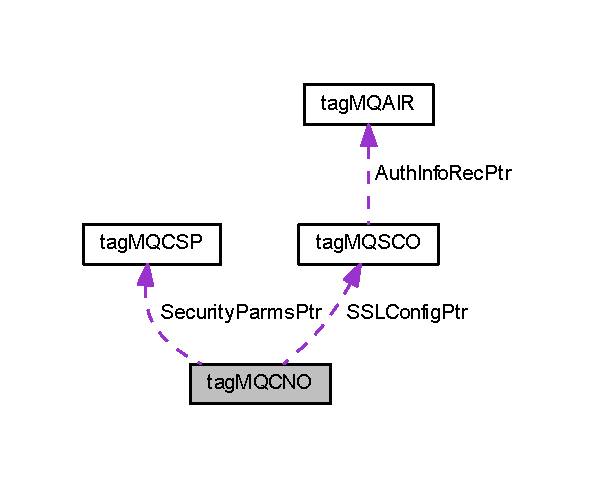
\includegraphics[width=286pt]{structtag_m_q_c_n_o__coll__graph}
\end{center}
\end{figure}
\subsection*{Campos de datos}
\begin{DoxyCompactItemize}
\item 
\hyperlink{cmqc_8h_a12590e546ed66fda7cf21c1d5cefa31d}{M\+Q\+C\+H\+A\+R4} \hyperlink{structtag_m_q_c_n_o_a0530922ca944569b52601d74941f96e4}{Struc\+Id}
\item 
\hyperlink{cmqc_8h_a1fb8d28cbda3fa8766a9821230cdb6d5}{M\+Q\+L\+O\+N\+G} \hyperlink{structtag_m_q_c_n_o_a0656ef8f766b3907d394d88a35d7b7e9}{Version}
\item 
\hyperlink{cmqc_8h_a1fb8d28cbda3fa8766a9821230cdb6d5}{M\+Q\+L\+O\+N\+G} \hyperlink{structtag_m_q_c_n_o_ad7aff2d6c6044809464380998d24ec5c}{Options}
\item 
\hyperlink{cmqc_8h_a1fb8d28cbda3fa8766a9821230cdb6d5}{M\+Q\+L\+O\+N\+G} \hyperlink{structtag_m_q_c_n_o_ab4e4fcacd66e164d2a244ebcb25fbb7c}{Client\+Conn\+Offset}
\item 
\hyperlink{cmqc_8h_a0b835d8e479d7c42242ed9c6b6572f5a}{M\+Q\+P\+T\+R} \hyperlink{structtag_m_q_c_n_o_a9e3caa54a09c6a065efeddfcb08449b3}{Client\+Conn\+Ptr}
\item 
\hyperlink{cmqc_8h_a116dfa79a3458b30fd6d5d0cc5da63cf}{M\+Q\+B\+Y\+T\+E128} \hyperlink{structtag_m_q_c_n_o_a5beb55e47cd784cb266d9744248886b5}{Conn\+Tag}
\item 
\hyperlink{cmqc_8h_ab266373c2d71646ed164310df16916c8}{P\+M\+Q\+S\+C\+O} \hyperlink{structtag_m_q_c_n_o_afd1588e665b4f8b035009e2a8ecec3cd}{S\+S\+L\+Config\+Ptr}
\item 
\hyperlink{cmqc_8h_a1fb8d28cbda3fa8766a9821230cdb6d5}{M\+Q\+L\+O\+N\+G} \hyperlink{structtag_m_q_c_n_o_a20bd6e5f8cb1b77946a9cdbd77e3eb03}{S\+S\+L\+Config\+Offset}
\item 
\hyperlink{cmqc_8h_a2866d93c0ef84cfcda34cab5fd22fc5a}{M\+Q\+B\+Y\+T\+E24} \hyperlink{structtag_m_q_c_n_o_a82a7b183d6b1a0a9f423a5194cef7577}{Connection\+Id}
\item 
\hyperlink{cmqc_8h_a1fb8d28cbda3fa8766a9821230cdb6d5}{M\+Q\+L\+O\+N\+G} \hyperlink{structtag_m_q_c_n_o_aa27268ebe318b338a6560bc161f973a1}{Security\+Parms\+Offset}
\item 
\hyperlink{cmqc_8h_ad9def548668b8b75e902d3729221bc94}{P\+M\+Q\+C\+S\+P} \hyperlink{structtag_m_q_c_n_o_a05cf93aa50d81a5d3f54afd5f2e0a35d}{Security\+Parms\+Ptr}
\end{DoxyCompactItemize}


\subsection{Descripción detallada}


Definición en la línea 4106 del archivo cmqc.\+h.



\subsection{Documentación de los campos}
\hypertarget{structtag_m_q_c_n_o_ab4e4fcacd66e164d2a244ebcb25fbb7c}{}\index{tag\+M\+Q\+C\+N\+O@{tag\+M\+Q\+C\+N\+O}!Client\+Conn\+Offset@{Client\+Conn\+Offset}}
\index{Client\+Conn\+Offset@{Client\+Conn\+Offset}!tag\+M\+Q\+C\+N\+O@{tag\+M\+Q\+C\+N\+O}}
\subsubsection[{Client\+Conn\+Offset}]{\setlength{\rightskip}{0pt plus 5cm}{\bf M\+Q\+L\+O\+N\+G} Client\+Conn\+Offset}\label{structtag_m_q_c_n_o_ab4e4fcacd66e164d2a244ebcb25fbb7c}


Definición en la línea 4112 del archivo cmqc.\+h.

\hypertarget{structtag_m_q_c_n_o_a9e3caa54a09c6a065efeddfcb08449b3}{}\index{tag\+M\+Q\+C\+N\+O@{tag\+M\+Q\+C\+N\+O}!Client\+Conn\+Ptr@{Client\+Conn\+Ptr}}
\index{Client\+Conn\+Ptr@{Client\+Conn\+Ptr}!tag\+M\+Q\+C\+N\+O@{tag\+M\+Q\+C\+N\+O}}
\subsubsection[{Client\+Conn\+Ptr}]{\setlength{\rightskip}{0pt plus 5cm}{\bf M\+Q\+P\+T\+R} Client\+Conn\+Ptr}\label{structtag_m_q_c_n_o_a9e3caa54a09c6a065efeddfcb08449b3}


Definición en la línea 4114 del archivo cmqc.\+h.

\hypertarget{structtag_m_q_c_n_o_a82a7b183d6b1a0a9f423a5194cef7577}{}\index{tag\+M\+Q\+C\+N\+O@{tag\+M\+Q\+C\+N\+O}!Connection\+Id@{Connection\+Id}}
\index{Connection\+Id@{Connection\+Id}!tag\+M\+Q\+C\+N\+O@{tag\+M\+Q\+C\+N\+O}}
\subsubsection[{Connection\+Id}]{\setlength{\rightskip}{0pt plus 5cm}{\bf M\+Q\+B\+Y\+T\+E24} Connection\+Id}\label{structtag_m_q_c_n_o_a82a7b183d6b1a0a9f423a5194cef7577}


Definición en la línea 4124 del archivo cmqc.\+h.

\hypertarget{structtag_m_q_c_n_o_a5beb55e47cd784cb266d9744248886b5}{}\index{tag\+M\+Q\+C\+N\+O@{tag\+M\+Q\+C\+N\+O}!Conn\+Tag@{Conn\+Tag}}
\index{Conn\+Tag@{Conn\+Tag}!tag\+M\+Q\+C\+N\+O@{tag\+M\+Q\+C\+N\+O}}
\subsubsection[{Conn\+Tag}]{\setlength{\rightskip}{0pt plus 5cm}{\bf M\+Q\+B\+Y\+T\+E128} Conn\+Tag}\label{structtag_m_q_c_n_o_a5beb55e47cd784cb266d9744248886b5}


Definición en la línea 4117 del archivo cmqc.\+h.

\hypertarget{structtag_m_q_c_n_o_ad7aff2d6c6044809464380998d24ec5c}{}\index{tag\+M\+Q\+C\+N\+O@{tag\+M\+Q\+C\+N\+O}!Options@{Options}}
\index{Options@{Options}!tag\+M\+Q\+C\+N\+O@{tag\+M\+Q\+C\+N\+O}}
\subsubsection[{Options}]{\setlength{\rightskip}{0pt plus 5cm}{\bf M\+Q\+L\+O\+N\+G} Options}\label{structtag_m_q_c_n_o_ad7aff2d6c6044809464380998d24ec5c}


Definición en la línea 4109 del archivo cmqc.\+h.

\hypertarget{structtag_m_q_c_n_o_aa27268ebe318b338a6560bc161f973a1}{}\index{tag\+M\+Q\+C\+N\+O@{tag\+M\+Q\+C\+N\+O}!Security\+Parms\+Offset@{Security\+Parms\+Offset}}
\index{Security\+Parms\+Offset@{Security\+Parms\+Offset}!tag\+M\+Q\+C\+N\+O@{tag\+M\+Q\+C\+N\+O}}
\subsubsection[{Security\+Parms\+Offset}]{\setlength{\rightskip}{0pt plus 5cm}{\bf M\+Q\+L\+O\+N\+G} Security\+Parms\+Offset}\label{structtag_m_q_c_n_o_aa27268ebe318b338a6560bc161f973a1}


Definición en la línea 4125 del archivo cmqc.\+h.

\hypertarget{structtag_m_q_c_n_o_a05cf93aa50d81a5d3f54afd5f2e0a35d}{}\index{tag\+M\+Q\+C\+N\+O@{tag\+M\+Q\+C\+N\+O}!Security\+Parms\+Ptr@{Security\+Parms\+Ptr}}
\index{Security\+Parms\+Ptr@{Security\+Parms\+Ptr}!tag\+M\+Q\+C\+N\+O@{tag\+M\+Q\+C\+N\+O}}
\subsubsection[{Security\+Parms\+Ptr}]{\setlength{\rightskip}{0pt plus 5cm}{\bf P\+M\+Q\+C\+S\+P} Security\+Parms\+Ptr}\label{structtag_m_q_c_n_o_a05cf93aa50d81a5d3f54afd5f2e0a35d}


Definición en la línea 4126 del archivo cmqc.\+h.

\hypertarget{structtag_m_q_c_n_o_a20bd6e5f8cb1b77946a9cdbd77e3eb03}{}\index{tag\+M\+Q\+C\+N\+O@{tag\+M\+Q\+C\+N\+O}!S\+S\+L\+Config\+Offset@{S\+S\+L\+Config\+Offset}}
\index{S\+S\+L\+Config\+Offset@{S\+S\+L\+Config\+Offset}!tag\+M\+Q\+C\+N\+O@{tag\+M\+Q\+C\+N\+O}}
\subsubsection[{S\+S\+L\+Config\+Offset}]{\setlength{\rightskip}{0pt plus 5cm}{\bf M\+Q\+L\+O\+N\+G} S\+S\+L\+Config\+Offset}\label{structtag_m_q_c_n_o_a20bd6e5f8cb1b77946a9cdbd77e3eb03}


Definición en la línea 4121 del archivo cmqc.\+h.

\hypertarget{structtag_m_q_c_n_o_afd1588e665b4f8b035009e2a8ecec3cd}{}\index{tag\+M\+Q\+C\+N\+O@{tag\+M\+Q\+C\+N\+O}!S\+S\+L\+Config\+Ptr@{S\+S\+L\+Config\+Ptr}}
\index{S\+S\+L\+Config\+Ptr@{S\+S\+L\+Config\+Ptr}!tag\+M\+Q\+C\+N\+O@{tag\+M\+Q\+C\+N\+O}}
\subsubsection[{S\+S\+L\+Config\+Ptr}]{\setlength{\rightskip}{0pt plus 5cm}{\bf P\+M\+Q\+S\+C\+O} S\+S\+L\+Config\+Ptr}\label{structtag_m_q_c_n_o_afd1588e665b4f8b035009e2a8ecec3cd}


Definición en la línea 4119 del archivo cmqc.\+h.

\hypertarget{structtag_m_q_c_n_o_a0530922ca944569b52601d74941f96e4}{}\index{tag\+M\+Q\+C\+N\+O@{tag\+M\+Q\+C\+N\+O}!Struc\+Id@{Struc\+Id}}
\index{Struc\+Id@{Struc\+Id}!tag\+M\+Q\+C\+N\+O@{tag\+M\+Q\+C\+N\+O}}
\subsubsection[{Struc\+Id}]{\setlength{\rightskip}{0pt plus 5cm}{\bf M\+Q\+C\+H\+A\+R4} Struc\+Id}\label{structtag_m_q_c_n_o_a0530922ca944569b52601d74941f96e4}


Definición en la línea 4107 del archivo cmqc.\+h.

\hypertarget{structtag_m_q_c_n_o_a0656ef8f766b3907d394d88a35d7b7e9}{}\index{tag\+M\+Q\+C\+N\+O@{tag\+M\+Q\+C\+N\+O}!Version@{Version}}
\index{Version@{Version}!tag\+M\+Q\+C\+N\+O@{tag\+M\+Q\+C\+N\+O}}
\subsubsection[{Version}]{\setlength{\rightskip}{0pt plus 5cm}{\bf M\+Q\+L\+O\+N\+G} Version}\label{structtag_m_q_c_n_o_a0656ef8f766b3907d394d88a35d7b7e9}


Definición en la línea 4108 del archivo cmqc.\+h.



La documentación para esta estructura fue generada a partir del siguiente fichero\+:\begin{DoxyCompactItemize}
\item 
include/\hyperlink{cmqc_8h}{cmqc.\+h}\end{DoxyCompactItemize}

\hypertarget{structtag_m_q_c_s_p}{}\section{Referencia de la Estructura tag\+M\+Q\+C\+S\+P}
\label{structtag_m_q_c_s_p}\index{tag\+M\+Q\+C\+S\+P@{tag\+M\+Q\+C\+S\+P}}


{\ttfamily \#include $<$cmqc.\+h$>$}

\subsection*{Campos de datos}
\begin{DoxyCompactItemize}
\item 
\hyperlink{cmqc_8h_a12590e546ed66fda7cf21c1d5cefa31d}{M\+Q\+C\+H\+A\+R4} \hyperlink{structtag_m_q_c_s_p_a0530922ca944569b52601d74941f96e4}{Struc\+Id}
\item 
\hyperlink{cmqc_8h_a1fb8d28cbda3fa8766a9821230cdb6d5}{M\+Q\+L\+O\+N\+G} \hyperlink{structtag_m_q_c_s_p_a0656ef8f766b3907d394d88a35d7b7e9}{Version}
\item 
\hyperlink{cmqc_8h_a1fb8d28cbda3fa8766a9821230cdb6d5}{M\+Q\+L\+O\+N\+G} \hyperlink{structtag_m_q_c_s_p_a93f1337530018caf4ee90bcd57f0b097}{Authentication\+Type}
\item 
\hyperlink{cmqc_8h_adf43961141ea57bdc167cfe3ee569cdc}{M\+Q\+B\+Y\+T\+E4} \hyperlink{structtag_m_q_c_s_p_a740233cdc4196cbb81a6891c320232cf}{Reserved1}
\item 
\hyperlink{cmqc_8h_a0b835d8e479d7c42242ed9c6b6572f5a}{M\+Q\+P\+T\+R} \hyperlink{structtag_m_q_c_s_p_aea9286fc5888c80fc6f7ee4788ac80bd}{C\+S\+P\+User\+Id\+Ptr}
\item 
\hyperlink{cmqc_8h_a1fb8d28cbda3fa8766a9821230cdb6d5}{M\+Q\+L\+O\+N\+G} \hyperlink{structtag_m_q_c_s_p_aff892208784ec4ceb7c6c33d3ca37547}{C\+S\+P\+User\+Id\+Offset}
\item 
\hyperlink{cmqc_8h_a1fb8d28cbda3fa8766a9821230cdb6d5}{M\+Q\+L\+O\+N\+G} \hyperlink{structtag_m_q_c_s_p_ab79103c753d41fbe5753501a33ab6994}{C\+S\+P\+User\+Id\+Length}
\item 
\hyperlink{cmqc_8h_a2b336cfdd97257746e5e321bfb35fb9b}{M\+Q\+B\+Y\+T\+E8} \hyperlink{structtag_m_q_c_s_p_a7aaec4816b30006552c1ee477716f64d}{Reserved2}
\item 
\hyperlink{cmqc_8h_a0b835d8e479d7c42242ed9c6b6572f5a}{M\+Q\+P\+T\+R} \hyperlink{structtag_m_q_c_s_p_a6bc99337133ec24b870061e19944c9f0}{C\+S\+P\+Password\+Ptr}
\item 
\hyperlink{cmqc_8h_a1fb8d28cbda3fa8766a9821230cdb6d5}{M\+Q\+L\+O\+N\+G} \hyperlink{structtag_m_q_c_s_p_a335e93bfba0a58a7fa4b505df5cd727f}{C\+S\+P\+Password\+Offset}
\item 
\hyperlink{cmqc_8h_a1fb8d28cbda3fa8766a9821230cdb6d5}{M\+Q\+L\+O\+N\+G} \hyperlink{structtag_m_q_c_s_p_a0693ca8dafce34e22d0462b1fd124474}{C\+S\+P\+Password\+Length}
\end{DoxyCompactItemize}


\subsection{Descripción detallada}


Definición en la línea 4071 del archivo cmqc.\+h.



\subsection{Documentación de los campos}
\hypertarget{structtag_m_q_c_s_p_a93f1337530018caf4ee90bcd57f0b097}{}\index{tag\+M\+Q\+C\+S\+P@{tag\+M\+Q\+C\+S\+P}!Authentication\+Type@{Authentication\+Type}}
\index{Authentication\+Type@{Authentication\+Type}!tag\+M\+Q\+C\+S\+P@{tag\+M\+Q\+C\+S\+P}}
\subsubsection[{Authentication\+Type}]{\setlength{\rightskip}{0pt plus 5cm}{\bf M\+Q\+L\+O\+N\+G} Authentication\+Type}\label{structtag_m_q_c_s_p_a93f1337530018caf4ee90bcd57f0b097}


Definición en la línea 4074 del archivo cmqc.\+h.

\hypertarget{structtag_m_q_c_s_p_a0693ca8dafce34e22d0462b1fd124474}{}\index{tag\+M\+Q\+C\+S\+P@{tag\+M\+Q\+C\+S\+P}!C\+S\+P\+Password\+Length@{C\+S\+P\+Password\+Length}}
\index{C\+S\+P\+Password\+Length@{C\+S\+P\+Password\+Length}!tag\+M\+Q\+C\+S\+P@{tag\+M\+Q\+C\+S\+P}}
\subsubsection[{C\+S\+P\+Password\+Length}]{\setlength{\rightskip}{0pt plus 5cm}{\bf M\+Q\+L\+O\+N\+G} C\+S\+P\+Password\+Length}\label{structtag_m_q_c_s_p_a0693ca8dafce34e22d0462b1fd124474}


Definición en la línea 4082 del archivo cmqc.\+h.

\hypertarget{structtag_m_q_c_s_p_a335e93bfba0a58a7fa4b505df5cd727f}{}\index{tag\+M\+Q\+C\+S\+P@{tag\+M\+Q\+C\+S\+P}!C\+S\+P\+Password\+Offset@{C\+S\+P\+Password\+Offset}}
\index{C\+S\+P\+Password\+Offset@{C\+S\+P\+Password\+Offset}!tag\+M\+Q\+C\+S\+P@{tag\+M\+Q\+C\+S\+P}}
\subsubsection[{C\+S\+P\+Password\+Offset}]{\setlength{\rightskip}{0pt plus 5cm}{\bf M\+Q\+L\+O\+N\+G} C\+S\+P\+Password\+Offset}\label{structtag_m_q_c_s_p_a335e93bfba0a58a7fa4b505df5cd727f}


Definición en la línea 4081 del archivo cmqc.\+h.

\hypertarget{structtag_m_q_c_s_p_a6bc99337133ec24b870061e19944c9f0}{}\index{tag\+M\+Q\+C\+S\+P@{tag\+M\+Q\+C\+S\+P}!C\+S\+P\+Password\+Ptr@{C\+S\+P\+Password\+Ptr}}
\index{C\+S\+P\+Password\+Ptr@{C\+S\+P\+Password\+Ptr}!tag\+M\+Q\+C\+S\+P@{tag\+M\+Q\+C\+S\+P}}
\subsubsection[{C\+S\+P\+Password\+Ptr}]{\setlength{\rightskip}{0pt plus 5cm}{\bf M\+Q\+P\+T\+R} C\+S\+P\+Password\+Ptr}\label{structtag_m_q_c_s_p_a6bc99337133ec24b870061e19944c9f0}


Definición en la línea 4080 del archivo cmqc.\+h.

\hypertarget{structtag_m_q_c_s_p_ab79103c753d41fbe5753501a33ab6994}{}\index{tag\+M\+Q\+C\+S\+P@{tag\+M\+Q\+C\+S\+P}!C\+S\+P\+User\+Id\+Length@{C\+S\+P\+User\+Id\+Length}}
\index{C\+S\+P\+User\+Id\+Length@{C\+S\+P\+User\+Id\+Length}!tag\+M\+Q\+C\+S\+P@{tag\+M\+Q\+C\+S\+P}}
\subsubsection[{C\+S\+P\+User\+Id\+Length}]{\setlength{\rightskip}{0pt plus 5cm}{\bf M\+Q\+L\+O\+N\+G} C\+S\+P\+User\+Id\+Length}\label{structtag_m_q_c_s_p_ab79103c753d41fbe5753501a33ab6994}


Definición en la línea 4078 del archivo cmqc.\+h.

\hypertarget{structtag_m_q_c_s_p_aff892208784ec4ceb7c6c33d3ca37547}{}\index{tag\+M\+Q\+C\+S\+P@{tag\+M\+Q\+C\+S\+P}!C\+S\+P\+User\+Id\+Offset@{C\+S\+P\+User\+Id\+Offset}}
\index{C\+S\+P\+User\+Id\+Offset@{C\+S\+P\+User\+Id\+Offset}!tag\+M\+Q\+C\+S\+P@{tag\+M\+Q\+C\+S\+P}}
\subsubsection[{C\+S\+P\+User\+Id\+Offset}]{\setlength{\rightskip}{0pt plus 5cm}{\bf M\+Q\+L\+O\+N\+G} C\+S\+P\+User\+Id\+Offset}\label{structtag_m_q_c_s_p_aff892208784ec4ceb7c6c33d3ca37547}


Definición en la línea 4077 del archivo cmqc.\+h.

\hypertarget{structtag_m_q_c_s_p_aea9286fc5888c80fc6f7ee4788ac80bd}{}\index{tag\+M\+Q\+C\+S\+P@{tag\+M\+Q\+C\+S\+P}!C\+S\+P\+User\+Id\+Ptr@{C\+S\+P\+User\+Id\+Ptr}}
\index{C\+S\+P\+User\+Id\+Ptr@{C\+S\+P\+User\+Id\+Ptr}!tag\+M\+Q\+C\+S\+P@{tag\+M\+Q\+C\+S\+P}}
\subsubsection[{C\+S\+P\+User\+Id\+Ptr}]{\setlength{\rightskip}{0pt plus 5cm}{\bf M\+Q\+P\+T\+R} C\+S\+P\+User\+Id\+Ptr}\label{structtag_m_q_c_s_p_aea9286fc5888c80fc6f7ee4788ac80bd}


Definición en la línea 4076 del archivo cmqc.\+h.

\hypertarget{structtag_m_q_c_s_p_a740233cdc4196cbb81a6891c320232cf}{}\index{tag\+M\+Q\+C\+S\+P@{tag\+M\+Q\+C\+S\+P}!Reserved1@{Reserved1}}
\index{Reserved1@{Reserved1}!tag\+M\+Q\+C\+S\+P@{tag\+M\+Q\+C\+S\+P}}
\subsubsection[{Reserved1}]{\setlength{\rightskip}{0pt plus 5cm}{\bf M\+Q\+B\+Y\+T\+E4} Reserved1}\label{structtag_m_q_c_s_p_a740233cdc4196cbb81a6891c320232cf}


Definición en la línea 4075 del archivo cmqc.\+h.

\hypertarget{structtag_m_q_c_s_p_a7aaec4816b30006552c1ee477716f64d}{}\index{tag\+M\+Q\+C\+S\+P@{tag\+M\+Q\+C\+S\+P}!Reserved2@{Reserved2}}
\index{Reserved2@{Reserved2}!tag\+M\+Q\+C\+S\+P@{tag\+M\+Q\+C\+S\+P}}
\subsubsection[{Reserved2}]{\setlength{\rightskip}{0pt plus 5cm}{\bf M\+Q\+B\+Y\+T\+E8} Reserved2}\label{structtag_m_q_c_s_p_a7aaec4816b30006552c1ee477716f64d}


Definición en la línea 4079 del archivo cmqc.\+h.

\hypertarget{structtag_m_q_c_s_p_a0530922ca944569b52601d74941f96e4}{}\index{tag\+M\+Q\+C\+S\+P@{tag\+M\+Q\+C\+S\+P}!Struc\+Id@{Struc\+Id}}
\index{Struc\+Id@{Struc\+Id}!tag\+M\+Q\+C\+S\+P@{tag\+M\+Q\+C\+S\+P}}
\subsubsection[{Struc\+Id}]{\setlength{\rightskip}{0pt plus 5cm}{\bf M\+Q\+C\+H\+A\+R4} Struc\+Id}\label{structtag_m_q_c_s_p_a0530922ca944569b52601d74941f96e4}


Definición en la línea 4072 del archivo cmqc.\+h.

\hypertarget{structtag_m_q_c_s_p_a0656ef8f766b3907d394d88a35d7b7e9}{}\index{tag\+M\+Q\+C\+S\+P@{tag\+M\+Q\+C\+S\+P}!Version@{Version}}
\index{Version@{Version}!tag\+M\+Q\+C\+S\+P@{tag\+M\+Q\+C\+S\+P}}
\subsubsection[{Version}]{\setlength{\rightskip}{0pt plus 5cm}{\bf M\+Q\+L\+O\+N\+G} Version}\label{structtag_m_q_c_s_p_a0656ef8f766b3907d394d88a35d7b7e9}


Definición en la línea 4073 del archivo cmqc.\+h.



La documentación para esta estructura fue generada a partir del siguiente fichero\+:\begin{DoxyCompactItemize}
\item 
include/\hyperlink{cmqc_8h}{cmqc.\+h}\end{DoxyCompactItemize}

\hypertarget{structtag_m_q_c_t_l_o}{}\section{Referencia de la Estructura tag\+M\+Q\+C\+T\+L\+O}
\label{structtag_m_q_c_t_l_o}\index{tag\+M\+Q\+C\+T\+L\+O@{tag\+M\+Q\+C\+T\+L\+O}}


{\ttfamily \#include $<$cmqc.\+h$>$}

\subsection*{Campos de datos}
\begin{DoxyCompactItemize}
\item 
\hyperlink{cmqc_8h_a12590e546ed66fda7cf21c1d5cefa31d}{M\+Q\+C\+H\+A\+R4} \hyperlink{structtag_m_q_c_t_l_o_a0530922ca944569b52601d74941f96e4}{Struc\+Id}
\item 
\hyperlink{cmqc_8h_a1fb8d28cbda3fa8766a9821230cdb6d5}{M\+Q\+L\+O\+N\+G} \hyperlink{structtag_m_q_c_t_l_o_a0656ef8f766b3907d394d88a35d7b7e9}{Version}
\item 
\hyperlink{cmqc_8h_a1fb8d28cbda3fa8766a9821230cdb6d5}{M\+Q\+L\+O\+N\+G} \hyperlink{structtag_m_q_c_t_l_o_ad7aff2d6c6044809464380998d24ec5c}{Options}
\item 
\hyperlink{cmqc_8h_a1fb8d28cbda3fa8766a9821230cdb6d5}{M\+Q\+L\+O\+N\+G} \hyperlink{structtag_m_q_c_t_l_o_a94dbfe0ea37eb47bd07d4d79d7104b2c}{Reserved}
\item 
\hyperlink{cmqc_8h_a0b835d8e479d7c42242ed9c6b6572f5a}{M\+Q\+P\+T\+R} \hyperlink{structtag_m_q_c_t_l_o_a58c83e52e3187c1579e9aeb6c52ded13}{Connection\+Area}
\end{DoxyCompactItemize}


\subsection{Descripción detallada}


Definición en la línea 3990 del archivo cmqc.\+h.



\subsection{Documentación de los campos}
\hypertarget{structtag_m_q_c_t_l_o_a58c83e52e3187c1579e9aeb6c52ded13}{}\index{tag\+M\+Q\+C\+T\+L\+O@{tag\+M\+Q\+C\+T\+L\+O}!Connection\+Area@{Connection\+Area}}
\index{Connection\+Area@{Connection\+Area}!tag\+M\+Q\+C\+T\+L\+O@{tag\+M\+Q\+C\+T\+L\+O}}
\subsubsection[{Connection\+Area}]{\setlength{\rightskip}{0pt plus 5cm}{\bf M\+Q\+P\+T\+R} Connection\+Area}\label{structtag_m_q_c_t_l_o_a58c83e52e3187c1579e9aeb6c52ded13}


Definición en la línea 3996 del archivo cmqc.\+h.

\hypertarget{structtag_m_q_c_t_l_o_ad7aff2d6c6044809464380998d24ec5c}{}\index{tag\+M\+Q\+C\+T\+L\+O@{tag\+M\+Q\+C\+T\+L\+O}!Options@{Options}}
\index{Options@{Options}!tag\+M\+Q\+C\+T\+L\+O@{tag\+M\+Q\+C\+T\+L\+O}}
\subsubsection[{Options}]{\setlength{\rightskip}{0pt plus 5cm}{\bf M\+Q\+L\+O\+N\+G} Options}\label{structtag_m_q_c_t_l_o_ad7aff2d6c6044809464380998d24ec5c}


Definición en la línea 3993 del archivo cmqc.\+h.

\hypertarget{structtag_m_q_c_t_l_o_a94dbfe0ea37eb47bd07d4d79d7104b2c}{}\index{tag\+M\+Q\+C\+T\+L\+O@{tag\+M\+Q\+C\+T\+L\+O}!Reserved@{Reserved}}
\index{Reserved@{Reserved}!tag\+M\+Q\+C\+T\+L\+O@{tag\+M\+Q\+C\+T\+L\+O}}
\subsubsection[{Reserved}]{\setlength{\rightskip}{0pt plus 5cm}{\bf M\+Q\+L\+O\+N\+G} Reserved}\label{structtag_m_q_c_t_l_o_a94dbfe0ea37eb47bd07d4d79d7104b2c}


Definición en la línea 3995 del archivo cmqc.\+h.

\hypertarget{structtag_m_q_c_t_l_o_a0530922ca944569b52601d74941f96e4}{}\index{tag\+M\+Q\+C\+T\+L\+O@{tag\+M\+Q\+C\+T\+L\+O}!Struc\+Id@{Struc\+Id}}
\index{Struc\+Id@{Struc\+Id}!tag\+M\+Q\+C\+T\+L\+O@{tag\+M\+Q\+C\+T\+L\+O}}
\subsubsection[{Struc\+Id}]{\setlength{\rightskip}{0pt plus 5cm}{\bf M\+Q\+C\+H\+A\+R4} Struc\+Id}\label{structtag_m_q_c_t_l_o_a0530922ca944569b52601d74941f96e4}


Definición en la línea 3991 del archivo cmqc.\+h.

\hypertarget{structtag_m_q_c_t_l_o_a0656ef8f766b3907d394d88a35d7b7e9}{}\index{tag\+M\+Q\+C\+T\+L\+O@{tag\+M\+Q\+C\+T\+L\+O}!Version@{Version}}
\index{Version@{Version}!tag\+M\+Q\+C\+T\+L\+O@{tag\+M\+Q\+C\+T\+L\+O}}
\subsubsection[{Version}]{\setlength{\rightskip}{0pt plus 5cm}{\bf M\+Q\+L\+O\+N\+G} Version}\label{structtag_m_q_c_t_l_o_a0656ef8f766b3907d394d88a35d7b7e9}


Definición en la línea 3992 del archivo cmqc.\+h.



La documentación para esta estructura fue generada a partir del siguiente fichero\+:\begin{DoxyCompactItemize}
\item 
include/\hyperlink{cmqc_8h}{cmqc.\+h}\end{DoxyCompactItemize}

\hypertarget{structtag_m_q_d_h}{}\section{Referencia de la Estructura tag\+M\+Q\+D\+H}
\label{structtag_m_q_d_h}\index{tag\+M\+Q\+D\+H@{tag\+M\+Q\+D\+H}}


{\ttfamily \#include $<$cmqc.\+h$>$}

\subsection*{Campos de datos}
\begin{DoxyCompactItemize}
\item 
\hyperlink{cmqc_8h_a12590e546ed66fda7cf21c1d5cefa31d}{M\+Q\+C\+H\+A\+R4} \hyperlink{structtag_m_q_d_h_a0530922ca944569b52601d74941f96e4}{Struc\+Id}
\item 
\hyperlink{cmqc_8h_a1fb8d28cbda3fa8766a9821230cdb6d5}{M\+Q\+L\+O\+N\+G} \hyperlink{structtag_m_q_d_h_a0656ef8f766b3907d394d88a35d7b7e9}{Version}
\item 
\hyperlink{cmqc_8h_a1fb8d28cbda3fa8766a9821230cdb6d5}{M\+Q\+L\+O\+N\+G} \hyperlink{structtag_m_q_d_h_a830af9a4a08c015b9a4b2d39d4d3420a}{Struc\+Length}
\item 
\hyperlink{cmqc_8h_a1fb8d28cbda3fa8766a9821230cdb6d5}{M\+Q\+L\+O\+N\+G} \hyperlink{structtag_m_q_d_h_a30167bf454a49a60fd3fe4e9e586af34}{Encoding}
\item 
\hyperlink{cmqc_8h_a1fb8d28cbda3fa8766a9821230cdb6d5}{M\+Q\+L\+O\+N\+G} \hyperlink{structtag_m_q_d_h_a4d8d1961a991850d1355cdf9b4680b8e}{Coded\+Char\+Set\+Id}
\item 
\hyperlink{cmqc_8h_abddcedb8c41fa262f2bd05dfec3e60a5}{M\+Q\+C\+H\+A\+R8} \hyperlink{structtag_m_q_d_h_a435a478822008713f8aaff89f369ed63}{Format}
\item 
\hyperlink{cmqc_8h_a1fb8d28cbda3fa8766a9821230cdb6d5}{M\+Q\+L\+O\+N\+G} \hyperlink{structtag_m_q_d_h_a8da770267273b200fa9c968fa2a0da57}{Flags}
\item 
\hyperlink{cmqc_8h_a1fb8d28cbda3fa8766a9821230cdb6d5}{M\+Q\+L\+O\+N\+G} \hyperlink{structtag_m_q_d_h_aea1b77e1a6f2b6f18526055315f8b175}{Put\+Msg\+Rec\+Fields}
\item 
\hyperlink{cmqc_8h_a1fb8d28cbda3fa8766a9821230cdb6d5}{M\+Q\+L\+O\+N\+G} \hyperlink{structtag_m_q_d_h_a7592da03e0f1c9bc79c9dd4e641dcf73}{Recs\+Present}
\item 
\hyperlink{cmqc_8h_a1fb8d28cbda3fa8766a9821230cdb6d5}{M\+Q\+L\+O\+N\+G} \hyperlink{structtag_m_q_d_h_a8ec0fdf14ab5b4d0f7caf7f333dfbeb4}{Object\+Rec\+Offset}
\item 
\hyperlink{cmqc_8h_a1fb8d28cbda3fa8766a9821230cdb6d5}{M\+Q\+L\+O\+N\+G} \hyperlink{structtag_m_q_d_h_a49f55d9686cdc9c051e09950fede2098}{Put\+Msg\+Rec\+Offset}
\end{DoxyCompactItemize}


\subsection{Descripción detallada}


Definición en la línea 4150 del archivo cmqc.\+h.



\subsection{Documentación de los campos}
\hypertarget{structtag_m_q_d_h_a4d8d1961a991850d1355cdf9b4680b8e}{}\index{tag\+M\+Q\+D\+H@{tag\+M\+Q\+D\+H}!Coded\+Char\+Set\+Id@{Coded\+Char\+Set\+Id}}
\index{Coded\+Char\+Set\+Id@{Coded\+Char\+Set\+Id}!tag\+M\+Q\+D\+H@{tag\+M\+Q\+D\+H}}
\subsubsection[{Coded\+Char\+Set\+Id}]{\setlength{\rightskip}{0pt plus 5cm}{\bf M\+Q\+L\+O\+N\+G} Coded\+Char\+Set\+Id}\label{structtag_m_q_d_h_a4d8d1961a991850d1355cdf9b4680b8e}


Definición en la línea 4157 del archivo cmqc.\+h.

\hypertarget{structtag_m_q_d_h_a30167bf454a49a60fd3fe4e9e586af34}{}\index{tag\+M\+Q\+D\+H@{tag\+M\+Q\+D\+H}!Encoding@{Encoding}}
\index{Encoding@{Encoding}!tag\+M\+Q\+D\+H@{tag\+M\+Q\+D\+H}}
\subsubsection[{Encoding}]{\setlength{\rightskip}{0pt plus 5cm}{\bf M\+Q\+L\+O\+N\+G} Encoding}\label{structtag_m_q_d_h_a30167bf454a49a60fd3fe4e9e586af34}


Definición en la línea 4155 del archivo cmqc.\+h.

\hypertarget{structtag_m_q_d_h_a8da770267273b200fa9c968fa2a0da57}{}\index{tag\+M\+Q\+D\+H@{tag\+M\+Q\+D\+H}!Flags@{Flags}}
\index{Flags@{Flags}!tag\+M\+Q\+D\+H@{tag\+M\+Q\+D\+H}}
\subsubsection[{Flags}]{\setlength{\rightskip}{0pt plus 5cm}{\bf M\+Q\+L\+O\+N\+G} Flags}\label{structtag_m_q_d_h_a8da770267273b200fa9c968fa2a0da57}


Definición en la línea 4162 del archivo cmqc.\+h.

\hypertarget{structtag_m_q_d_h_a435a478822008713f8aaff89f369ed63}{}\index{tag\+M\+Q\+D\+H@{tag\+M\+Q\+D\+H}!Format@{Format}}
\index{Format@{Format}!tag\+M\+Q\+D\+H@{tag\+M\+Q\+D\+H}}
\subsubsection[{Format}]{\setlength{\rightskip}{0pt plus 5cm}{\bf M\+Q\+C\+H\+A\+R8} Format}\label{structtag_m_q_d_h_a435a478822008713f8aaff89f369ed63}


Definición en la línea 4160 del archivo cmqc.\+h.

\hypertarget{structtag_m_q_d_h_a8ec0fdf14ab5b4d0f7caf7f333dfbeb4}{}\index{tag\+M\+Q\+D\+H@{tag\+M\+Q\+D\+H}!Object\+Rec\+Offset@{Object\+Rec\+Offset}}
\index{Object\+Rec\+Offset@{Object\+Rec\+Offset}!tag\+M\+Q\+D\+H@{tag\+M\+Q\+D\+H}}
\subsubsection[{Object\+Rec\+Offset}]{\setlength{\rightskip}{0pt plus 5cm}{\bf M\+Q\+L\+O\+N\+G} Object\+Rec\+Offset}\label{structtag_m_q_d_h_a8ec0fdf14ab5b4d0f7caf7f333dfbeb4}


Definición en la línea 4166 del archivo cmqc.\+h.

\hypertarget{structtag_m_q_d_h_aea1b77e1a6f2b6f18526055315f8b175}{}\index{tag\+M\+Q\+D\+H@{tag\+M\+Q\+D\+H}!Put\+Msg\+Rec\+Fields@{Put\+Msg\+Rec\+Fields}}
\index{Put\+Msg\+Rec\+Fields@{Put\+Msg\+Rec\+Fields}!tag\+M\+Q\+D\+H@{tag\+M\+Q\+D\+H}}
\subsubsection[{Put\+Msg\+Rec\+Fields}]{\setlength{\rightskip}{0pt plus 5cm}{\bf M\+Q\+L\+O\+N\+G} Put\+Msg\+Rec\+Fields}\label{structtag_m_q_d_h_aea1b77e1a6f2b6f18526055315f8b175}


Definición en la línea 4163 del archivo cmqc.\+h.

\hypertarget{structtag_m_q_d_h_a49f55d9686cdc9c051e09950fede2098}{}\index{tag\+M\+Q\+D\+H@{tag\+M\+Q\+D\+H}!Put\+Msg\+Rec\+Offset@{Put\+Msg\+Rec\+Offset}}
\index{Put\+Msg\+Rec\+Offset@{Put\+Msg\+Rec\+Offset}!tag\+M\+Q\+D\+H@{tag\+M\+Q\+D\+H}}
\subsubsection[{Put\+Msg\+Rec\+Offset}]{\setlength{\rightskip}{0pt plus 5cm}{\bf M\+Q\+L\+O\+N\+G} Put\+Msg\+Rec\+Offset}\label{structtag_m_q_d_h_a49f55d9686cdc9c051e09950fede2098}


Definición en la línea 4168 del archivo cmqc.\+h.

\hypertarget{structtag_m_q_d_h_a7592da03e0f1c9bc79c9dd4e641dcf73}{}\index{tag\+M\+Q\+D\+H@{tag\+M\+Q\+D\+H}!Recs\+Present@{Recs\+Present}}
\index{Recs\+Present@{Recs\+Present}!tag\+M\+Q\+D\+H@{tag\+M\+Q\+D\+H}}
\subsubsection[{Recs\+Present}]{\setlength{\rightskip}{0pt plus 5cm}{\bf M\+Q\+L\+O\+N\+G} Recs\+Present}\label{structtag_m_q_d_h_a7592da03e0f1c9bc79c9dd4e641dcf73}


Definición en la línea 4165 del archivo cmqc.\+h.

\hypertarget{structtag_m_q_d_h_a0530922ca944569b52601d74941f96e4}{}\index{tag\+M\+Q\+D\+H@{tag\+M\+Q\+D\+H}!Struc\+Id@{Struc\+Id}}
\index{Struc\+Id@{Struc\+Id}!tag\+M\+Q\+D\+H@{tag\+M\+Q\+D\+H}}
\subsubsection[{Struc\+Id}]{\setlength{\rightskip}{0pt plus 5cm}{\bf M\+Q\+C\+H\+A\+R4} Struc\+Id}\label{structtag_m_q_d_h_a0530922ca944569b52601d74941f96e4}


Definición en la línea 4151 del archivo cmqc.\+h.

\hypertarget{structtag_m_q_d_h_a830af9a4a08c015b9a4b2d39d4d3420a}{}\index{tag\+M\+Q\+D\+H@{tag\+M\+Q\+D\+H}!Struc\+Length@{Struc\+Length}}
\index{Struc\+Length@{Struc\+Length}!tag\+M\+Q\+D\+H@{tag\+M\+Q\+D\+H}}
\subsubsection[{Struc\+Length}]{\setlength{\rightskip}{0pt plus 5cm}{\bf M\+Q\+L\+O\+N\+G} Struc\+Length}\label{structtag_m_q_d_h_a830af9a4a08c015b9a4b2d39d4d3420a}


Definición en la línea 4153 del archivo cmqc.\+h.

\hypertarget{structtag_m_q_d_h_a0656ef8f766b3907d394d88a35d7b7e9}{}\index{tag\+M\+Q\+D\+H@{tag\+M\+Q\+D\+H}!Version@{Version}}
\index{Version@{Version}!tag\+M\+Q\+D\+H@{tag\+M\+Q\+D\+H}}
\subsubsection[{Version}]{\setlength{\rightskip}{0pt plus 5cm}{\bf M\+Q\+L\+O\+N\+G} Version}\label{structtag_m_q_d_h_a0656ef8f766b3907d394d88a35d7b7e9}


Definición en la línea 4152 del archivo cmqc.\+h.



La documentación para esta estructura fue generada a partir del siguiente fichero\+:\begin{DoxyCompactItemize}
\item 
include/\hyperlink{cmqc_8h}{cmqc.\+h}\end{DoxyCompactItemize}

\hypertarget{structtag_m_q_d_l_h}{}\section{Referencia de la Estructura tag\+M\+Q\+D\+L\+H}
\label{structtag_m_q_d_l_h}\index{tag\+M\+Q\+D\+L\+H@{tag\+M\+Q\+D\+L\+H}}


{\ttfamily \#include $<$cmqc.\+h$>$}

\subsection*{Campos de datos}
\begin{DoxyCompactItemize}
\item 
\hyperlink{cmqc_8h_a12590e546ed66fda7cf21c1d5cefa31d}{M\+Q\+C\+H\+A\+R4} \hyperlink{structtag_m_q_d_l_h_a0530922ca944569b52601d74941f96e4}{Struc\+Id}
\item 
\hyperlink{cmqc_8h_a1fb8d28cbda3fa8766a9821230cdb6d5}{M\+Q\+L\+O\+N\+G} \hyperlink{structtag_m_q_d_l_h_a0656ef8f766b3907d394d88a35d7b7e9}{Version}
\item 
\hyperlink{cmqc_8h_a1fb8d28cbda3fa8766a9821230cdb6d5}{M\+Q\+L\+O\+N\+G} \hyperlink{structtag_m_q_d_l_h_ac2f0378cb0c66c5f91625822e53d7bae}{Reason}
\item 
\hyperlink{cmqc_8h_a53b1a2836da03f19144836725ff77919}{M\+Q\+C\+H\+A\+R48} \hyperlink{structtag_m_q_d_l_h_a90aa2a325ec2520d431f1924f7cf5cf0}{Dest\+Q\+Name}
\item 
\hyperlink{cmqc_8h_a53b1a2836da03f19144836725ff77919}{M\+Q\+C\+H\+A\+R48} \hyperlink{structtag_m_q_d_l_h_a146f52cd7bae6a5b36ec1314f079ffb2}{Dest\+Q\+Mgr\+Name}
\item 
\hyperlink{cmqc_8h_a1fb8d28cbda3fa8766a9821230cdb6d5}{M\+Q\+L\+O\+N\+G} \hyperlink{structtag_m_q_d_l_h_a30167bf454a49a60fd3fe4e9e586af34}{Encoding}
\item 
\hyperlink{cmqc_8h_a1fb8d28cbda3fa8766a9821230cdb6d5}{M\+Q\+L\+O\+N\+G} \hyperlink{structtag_m_q_d_l_h_a4d8d1961a991850d1355cdf9b4680b8e}{Coded\+Char\+Set\+Id}
\item 
\hyperlink{cmqc_8h_abddcedb8c41fa262f2bd05dfec3e60a5}{M\+Q\+C\+H\+A\+R8} \hyperlink{structtag_m_q_d_l_h_a435a478822008713f8aaff89f369ed63}{Format}
\item 
\hyperlink{cmqc_8h_a1fb8d28cbda3fa8766a9821230cdb6d5}{M\+Q\+L\+O\+N\+G} \hyperlink{structtag_m_q_d_l_h_a6d9e0e0fe9075017c939213948c747dc}{Put\+Appl\+Type}
\item 
\hyperlink{cmqc_8h_a6139f35ea8f9711726daeb5df27ab593}{M\+Q\+C\+H\+A\+R28} \hyperlink{structtag_m_q_d_l_h_a7195390be27f384ef0ab0d0f9053d462}{Put\+Appl\+Name}
\item 
\hyperlink{cmqc_8h_abddcedb8c41fa262f2bd05dfec3e60a5}{M\+Q\+C\+H\+A\+R8} \hyperlink{structtag_m_q_d_l_h_add3e7fe139edfa323295d6c7bc764cc5}{Put\+Date}
\item 
\hyperlink{cmqc_8h_abddcedb8c41fa262f2bd05dfec3e60a5}{M\+Q\+C\+H\+A\+R8} \hyperlink{structtag_m_q_d_l_h_aec51e7b9face9480a893ae5d47781ee7}{Put\+Time}
\end{DoxyCompactItemize}


\subsection{Descripción detallada}


Definición en la línea 4192 del archivo cmqc.\+h.



\subsection{Documentación de los campos}
\hypertarget{structtag_m_q_d_l_h_a4d8d1961a991850d1355cdf9b4680b8e}{}\index{tag\+M\+Q\+D\+L\+H@{tag\+M\+Q\+D\+L\+H}!Coded\+Char\+Set\+Id@{Coded\+Char\+Set\+Id}}
\index{Coded\+Char\+Set\+Id@{Coded\+Char\+Set\+Id}!tag\+M\+Q\+D\+L\+H@{tag\+M\+Q\+D\+L\+H}}
\subsubsection[{Coded\+Char\+Set\+Id}]{\setlength{\rightskip}{0pt plus 5cm}{\bf M\+Q\+L\+O\+N\+G} Coded\+Char\+Set\+Id}\label{structtag_m_q_d_l_h_a4d8d1961a991850d1355cdf9b4680b8e}


Definición en la línea 4203 del archivo cmqc.\+h.

\hypertarget{structtag_m_q_d_l_h_a146f52cd7bae6a5b36ec1314f079ffb2}{}\index{tag\+M\+Q\+D\+L\+H@{tag\+M\+Q\+D\+L\+H}!Dest\+Q\+Mgr\+Name@{Dest\+Q\+Mgr\+Name}}
\index{Dest\+Q\+Mgr\+Name@{Dest\+Q\+Mgr\+Name}!tag\+M\+Q\+D\+L\+H@{tag\+M\+Q\+D\+L\+H}}
\subsubsection[{Dest\+Q\+Mgr\+Name}]{\setlength{\rightskip}{0pt plus 5cm}{\bf M\+Q\+C\+H\+A\+R48} Dest\+Q\+Mgr\+Name}\label{structtag_m_q_d_l_h_a146f52cd7bae6a5b36ec1314f079ffb2}


Definición en la línea 4199 del archivo cmqc.\+h.

\hypertarget{structtag_m_q_d_l_h_a90aa2a325ec2520d431f1924f7cf5cf0}{}\index{tag\+M\+Q\+D\+L\+H@{tag\+M\+Q\+D\+L\+H}!Dest\+Q\+Name@{Dest\+Q\+Name}}
\index{Dest\+Q\+Name@{Dest\+Q\+Name}!tag\+M\+Q\+D\+L\+H@{tag\+M\+Q\+D\+L\+H}}
\subsubsection[{Dest\+Q\+Name}]{\setlength{\rightskip}{0pt plus 5cm}{\bf M\+Q\+C\+H\+A\+R48} Dest\+Q\+Name}\label{structtag_m_q_d_l_h_a90aa2a325ec2520d431f1924f7cf5cf0}


Definición en la línea 4198 del archivo cmqc.\+h.

\hypertarget{structtag_m_q_d_l_h_a30167bf454a49a60fd3fe4e9e586af34}{}\index{tag\+M\+Q\+D\+L\+H@{tag\+M\+Q\+D\+L\+H}!Encoding@{Encoding}}
\index{Encoding@{Encoding}!tag\+M\+Q\+D\+L\+H@{tag\+M\+Q\+D\+L\+H}}
\subsubsection[{Encoding}]{\setlength{\rightskip}{0pt plus 5cm}{\bf M\+Q\+L\+O\+N\+G} Encoding}\label{structtag_m_q_d_l_h_a30167bf454a49a60fd3fe4e9e586af34}


Definición en la línea 4201 del archivo cmqc.\+h.

\hypertarget{structtag_m_q_d_l_h_a435a478822008713f8aaff89f369ed63}{}\index{tag\+M\+Q\+D\+L\+H@{tag\+M\+Q\+D\+L\+H}!Format@{Format}}
\index{Format@{Format}!tag\+M\+Q\+D\+L\+H@{tag\+M\+Q\+D\+L\+H}}
\subsubsection[{Format}]{\setlength{\rightskip}{0pt plus 5cm}{\bf M\+Q\+C\+H\+A\+R8} Format}\label{structtag_m_q_d_l_h_a435a478822008713f8aaff89f369ed63}


Definición en la línea 4205 del archivo cmqc.\+h.

\hypertarget{structtag_m_q_d_l_h_a7195390be27f384ef0ab0d0f9053d462}{}\index{tag\+M\+Q\+D\+L\+H@{tag\+M\+Q\+D\+L\+H}!Put\+Appl\+Name@{Put\+Appl\+Name}}
\index{Put\+Appl\+Name@{Put\+Appl\+Name}!tag\+M\+Q\+D\+L\+H@{tag\+M\+Q\+D\+L\+H}}
\subsubsection[{Put\+Appl\+Name}]{\setlength{\rightskip}{0pt plus 5cm}{\bf M\+Q\+C\+H\+A\+R28} Put\+Appl\+Name}\label{structtag_m_q_d_l_h_a7195390be27f384ef0ab0d0f9053d462}


Definición en la línea 4210 del archivo cmqc.\+h.

\hypertarget{structtag_m_q_d_l_h_a6d9e0e0fe9075017c939213948c747dc}{}\index{tag\+M\+Q\+D\+L\+H@{tag\+M\+Q\+D\+L\+H}!Put\+Appl\+Type@{Put\+Appl\+Type}}
\index{Put\+Appl\+Type@{Put\+Appl\+Type}!tag\+M\+Q\+D\+L\+H@{tag\+M\+Q\+D\+L\+H}}
\subsubsection[{Put\+Appl\+Type}]{\setlength{\rightskip}{0pt plus 5cm}{\bf M\+Q\+L\+O\+N\+G} Put\+Appl\+Type}\label{structtag_m_q_d_l_h_a6d9e0e0fe9075017c939213948c747dc}


Definición en la línea 4207 del archivo cmqc.\+h.

\hypertarget{structtag_m_q_d_l_h_add3e7fe139edfa323295d6c7bc764cc5}{}\index{tag\+M\+Q\+D\+L\+H@{tag\+M\+Q\+D\+L\+H}!Put\+Date@{Put\+Date}}
\index{Put\+Date@{Put\+Date}!tag\+M\+Q\+D\+L\+H@{tag\+M\+Q\+D\+L\+H}}
\subsubsection[{Put\+Date}]{\setlength{\rightskip}{0pt plus 5cm}{\bf M\+Q\+C\+H\+A\+R8} Put\+Date}\label{structtag_m_q_d_l_h_add3e7fe139edfa323295d6c7bc764cc5}


Definición en la línea 4213 del archivo cmqc.\+h.

\hypertarget{structtag_m_q_d_l_h_aec51e7b9face9480a893ae5d47781ee7}{}\index{tag\+M\+Q\+D\+L\+H@{tag\+M\+Q\+D\+L\+H}!Put\+Time@{Put\+Time}}
\index{Put\+Time@{Put\+Time}!tag\+M\+Q\+D\+L\+H@{tag\+M\+Q\+D\+L\+H}}
\subsubsection[{Put\+Time}]{\setlength{\rightskip}{0pt plus 5cm}{\bf M\+Q\+C\+H\+A\+R8} Put\+Time}\label{structtag_m_q_d_l_h_aec51e7b9face9480a893ae5d47781ee7}


Definición en la línea 4216 del archivo cmqc.\+h.

\hypertarget{structtag_m_q_d_l_h_ac2f0378cb0c66c5f91625822e53d7bae}{}\index{tag\+M\+Q\+D\+L\+H@{tag\+M\+Q\+D\+L\+H}!Reason@{Reason}}
\index{Reason@{Reason}!tag\+M\+Q\+D\+L\+H@{tag\+M\+Q\+D\+L\+H}}
\subsubsection[{Reason}]{\setlength{\rightskip}{0pt plus 5cm}{\bf M\+Q\+L\+O\+N\+G} Reason}\label{structtag_m_q_d_l_h_ac2f0378cb0c66c5f91625822e53d7bae}


Definición en la línea 4195 del archivo cmqc.\+h.

\hypertarget{structtag_m_q_d_l_h_a0530922ca944569b52601d74941f96e4}{}\index{tag\+M\+Q\+D\+L\+H@{tag\+M\+Q\+D\+L\+H}!Struc\+Id@{Struc\+Id}}
\index{Struc\+Id@{Struc\+Id}!tag\+M\+Q\+D\+L\+H@{tag\+M\+Q\+D\+L\+H}}
\subsubsection[{Struc\+Id}]{\setlength{\rightskip}{0pt plus 5cm}{\bf M\+Q\+C\+H\+A\+R4} Struc\+Id}\label{structtag_m_q_d_l_h_a0530922ca944569b52601d74941f96e4}


Definición en la línea 4193 del archivo cmqc.\+h.

\hypertarget{structtag_m_q_d_l_h_a0656ef8f766b3907d394d88a35d7b7e9}{}\index{tag\+M\+Q\+D\+L\+H@{tag\+M\+Q\+D\+L\+H}!Version@{Version}}
\index{Version@{Version}!tag\+M\+Q\+D\+L\+H@{tag\+M\+Q\+D\+L\+H}}
\subsubsection[{Version}]{\setlength{\rightskip}{0pt plus 5cm}{\bf M\+Q\+L\+O\+N\+G} Version}\label{structtag_m_q_d_l_h_a0656ef8f766b3907d394d88a35d7b7e9}


Definición en la línea 4194 del archivo cmqc.\+h.



La documentación para esta estructura fue generada a partir del siguiente fichero\+:\begin{DoxyCompactItemize}
\item 
include/\hyperlink{cmqc_8h}{cmqc.\+h}\end{DoxyCompactItemize}

\hypertarget{structtag_m_q_d_m_h_o}{}\section{Referencia de la Estructura tag\+M\+Q\+D\+M\+H\+O}
\label{structtag_m_q_d_m_h_o}\index{tag\+M\+Q\+D\+M\+H\+O@{tag\+M\+Q\+D\+M\+H\+O}}


{\ttfamily \#include $<$cmqc.\+h$>$}

\subsection*{Campos de datos}
\begin{DoxyCompactItemize}
\item 
\hyperlink{cmqc_8h_a12590e546ed66fda7cf21c1d5cefa31d}{M\+Q\+C\+H\+A\+R4} \hyperlink{structtag_m_q_d_m_h_o_a0530922ca944569b52601d74941f96e4}{Struc\+Id}
\item 
\hyperlink{cmqc_8h_a1fb8d28cbda3fa8766a9821230cdb6d5}{M\+Q\+L\+O\+N\+G} \hyperlink{structtag_m_q_d_m_h_o_a0656ef8f766b3907d394d88a35d7b7e9}{Version}
\item 
\hyperlink{cmqc_8h_a1fb8d28cbda3fa8766a9821230cdb6d5}{M\+Q\+L\+O\+N\+G} \hyperlink{structtag_m_q_d_m_h_o_ad7aff2d6c6044809464380998d24ec5c}{Options}
\end{DoxyCompactItemize}


\subsection{Descripción detallada}


Definición en la línea 4243 del archivo cmqc.\+h.



\subsection{Documentación de los campos}
\hypertarget{structtag_m_q_d_m_h_o_ad7aff2d6c6044809464380998d24ec5c}{}\index{tag\+M\+Q\+D\+M\+H\+O@{tag\+M\+Q\+D\+M\+H\+O}!Options@{Options}}
\index{Options@{Options}!tag\+M\+Q\+D\+M\+H\+O@{tag\+M\+Q\+D\+M\+H\+O}}
\subsubsection[{Options}]{\setlength{\rightskip}{0pt plus 5cm}{\bf M\+Q\+L\+O\+N\+G} Options}\label{structtag_m_q_d_m_h_o_ad7aff2d6c6044809464380998d24ec5c}


Definición en la línea 4246 del archivo cmqc.\+h.

\hypertarget{structtag_m_q_d_m_h_o_a0530922ca944569b52601d74941f96e4}{}\index{tag\+M\+Q\+D\+M\+H\+O@{tag\+M\+Q\+D\+M\+H\+O}!Struc\+Id@{Struc\+Id}}
\index{Struc\+Id@{Struc\+Id}!tag\+M\+Q\+D\+M\+H\+O@{tag\+M\+Q\+D\+M\+H\+O}}
\subsubsection[{Struc\+Id}]{\setlength{\rightskip}{0pt plus 5cm}{\bf M\+Q\+C\+H\+A\+R4} Struc\+Id}\label{structtag_m_q_d_m_h_o_a0530922ca944569b52601d74941f96e4}


Definición en la línea 4244 del archivo cmqc.\+h.

\hypertarget{structtag_m_q_d_m_h_o_a0656ef8f766b3907d394d88a35d7b7e9}{}\index{tag\+M\+Q\+D\+M\+H\+O@{tag\+M\+Q\+D\+M\+H\+O}!Version@{Version}}
\index{Version@{Version}!tag\+M\+Q\+D\+M\+H\+O@{tag\+M\+Q\+D\+M\+H\+O}}
\subsubsection[{Version}]{\setlength{\rightskip}{0pt plus 5cm}{\bf M\+Q\+L\+O\+N\+G} Version}\label{structtag_m_q_d_m_h_o_a0656ef8f766b3907d394d88a35d7b7e9}


Definición en la línea 4245 del archivo cmqc.\+h.



La documentación para esta estructura fue generada a partir del siguiente fichero\+:\begin{DoxyCompactItemize}
\item 
include/\hyperlink{cmqc_8h}{cmqc.\+h}\end{DoxyCompactItemize}

\hypertarget{structtag_m_q_d_m_p_o}{}\section{Referencia de la Estructura tag\+M\+Q\+D\+M\+P\+O}
\label{structtag_m_q_d_m_p_o}\index{tag\+M\+Q\+D\+M\+P\+O@{tag\+M\+Q\+D\+M\+P\+O}}


{\ttfamily \#include $<$cmqc.\+h$>$}

\subsection*{Campos de datos}
\begin{DoxyCompactItemize}
\item 
\hyperlink{cmqc_8h_a12590e546ed66fda7cf21c1d5cefa31d}{M\+Q\+C\+H\+A\+R4} \hyperlink{structtag_m_q_d_m_p_o_a0530922ca944569b52601d74941f96e4}{Struc\+Id}
\item 
\hyperlink{cmqc_8h_a1fb8d28cbda3fa8766a9821230cdb6d5}{M\+Q\+L\+O\+N\+G} \hyperlink{structtag_m_q_d_m_p_o_a0656ef8f766b3907d394d88a35d7b7e9}{Version}
\item 
\hyperlink{cmqc_8h_a1fb8d28cbda3fa8766a9821230cdb6d5}{M\+Q\+L\+O\+N\+G} \hyperlink{structtag_m_q_d_m_p_o_ad7aff2d6c6044809464380998d24ec5c}{Options}
\end{DoxyCompactItemize}


\subsection{Descripción detallada}


Definición en la línea 4262 del archivo cmqc.\+h.



\subsection{Documentación de los campos}
\hypertarget{structtag_m_q_d_m_p_o_ad7aff2d6c6044809464380998d24ec5c}{}\index{tag\+M\+Q\+D\+M\+P\+O@{tag\+M\+Q\+D\+M\+P\+O}!Options@{Options}}
\index{Options@{Options}!tag\+M\+Q\+D\+M\+P\+O@{tag\+M\+Q\+D\+M\+P\+O}}
\subsubsection[{Options}]{\setlength{\rightskip}{0pt plus 5cm}{\bf M\+Q\+L\+O\+N\+G} Options}\label{structtag_m_q_d_m_p_o_ad7aff2d6c6044809464380998d24ec5c}


Definición en la línea 4265 del archivo cmqc.\+h.

\hypertarget{structtag_m_q_d_m_p_o_a0530922ca944569b52601d74941f96e4}{}\index{tag\+M\+Q\+D\+M\+P\+O@{tag\+M\+Q\+D\+M\+P\+O}!Struc\+Id@{Struc\+Id}}
\index{Struc\+Id@{Struc\+Id}!tag\+M\+Q\+D\+M\+P\+O@{tag\+M\+Q\+D\+M\+P\+O}}
\subsubsection[{Struc\+Id}]{\setlength{\rightskip}{0pt plus 5cm}{\bf M\+Q\+C\+H\+A\+R4} Struc\+Id}\label{structtag_m_q_d_m_p_o_a0530922ca944569b52601d74941f96e4}


Definición en la línea 4263 del archivo cmqc.\+h.

\hypertarget{structtag_m_q_d_m_p_o_a0656ef8f766b3907d394d88a35d7b7e9}{}\index{tag\+M\+Q\+D\+M\+P\+O@{tag\+M\+Q\+D\+M\+P\+O}!Version@{Version}}
\index{Version@{Version}!tag\+M\+Q\+D\+M\+P\+O@{tag\+M\+Q\+D\+M\+P\+O}}
\subsubsection[{Version}]{\setlength{\rightskip}{0pt plus 5cm}{\bf M\+Q\+L\+O\+N\+G} Version}\label{structtag_m_q_d_m_p_o_a0656ef8f766b3907d394d88a35d7b7e9}


Definición en la línea 4264 del archivo cmqc.\+h.



La documentación para esta estructura fue generada a partir del siguiente fichero\+:\begin{DoxyCompactItemize}
\item 
include/\hyperlink{cmqc_8h}{cmqc.\+h}\end{DoxyCompactItemize}

\hypertarget{structtag_m_q_g_m_o}{}\section{Referencia de la Estructura tag\+M\+Q\+G\+M\+O}
\label{structtag_m_q_g_m_o}\index{tag\+M\+Q\+G\+M\+O@{tag\+M\+Q\+G\+M\+O}}


{\ttfamily \#include $<$cmqc.\+h$>$}

\subsection*{Campos de datos}
\begin{DoxyCompactItemize}
\item 
\hyperlink{cmqc_8h_a12590e546ed66fda7cf21c1d5cefa31d}{M\+Q\+C\+H\+A\+R4} \hyperlink{structtag_m_q_g_m_o_a0530922ca944569b52601d74941f96e4}{Struc\+Id}
\item 
\hyperlink{cmqc_8h_a1fb8d28cbda3fa8766a9821230cdb6d5}{M\+Q\+L\+O\+N\+G} \hyperlink{structtag_m_q_g_m_o_a0656ef8f766b3907d394d88a35d7b7e9}{Version}
\item 
\hyperlink{cmqc_8h_a1fb8d28cbda3fa8766a9821230cdb6d5}{M\+Q\+L\+O\+N\+G} \hyperlink{structtag_m_q_g_m_o_ad7aff2d6c6044809464380998d24ec5c}{Options}
\item 
\hyperlink{cmqc_8h_a1fb8d28cbda3fa8766a9821230cdb6d5}{M\+Q\+L\+O\+N\+G} \hyperlink{structtag_m_q_g_m_o_a6f3538bd01d237755fd6ab7dad5584d0}{Wait\+Interval}
\item 
\hyperlink{cmqc_8h_a1fb8d28cbda3fa8766a9821230cdb6d5}{M\+Q\+L\+O\+N\+G} \hyperlink{structtag_m_q_g_m_o_a07b74d87b8eed659f524ba2c5c7dcb09}{Signal1}
\item 
\hyperlink{cmqc_8h_a1fb8d28cbda3fa8766a9821230cdb6d5}{M\+Q\+L\+O\+N\+G} \hyperlink{structtag_m_q_g_m_o_afd4b361a08ee7dc496e720908aa9917a}{Signal2}
\item 
\hyperlink{cmqc_8h_a53b1a2836da03f19144836725ff77919}{M\+Q\+C\+H\+A\+R48} \hyperlink{structtag_m_q_g_m_o_aec4a06d696b4370f0c86b129d9f868ca}{Resolved\+Q\+Name}
\item 
\hyperlink{cmqc_8h_a1fb8d28cbda3fa8766a9821230cdb6d5}{M\+Q\+L\+O\+N\+G} \hyperlink{structtag_m_q_g_m_o_a64325fedf5fee7e9b76f1ad26dceac2b}{Match\+Options}
\item 
\hyperlink{cmqc_8h_aeb12bc7ba416a4eb603e2a74351418d2}{M\+Q\+C\+H\+A\+R} \hyperlink{structtag_m_q_g_m_o_a20c00b3295996b9ddbf0ed94ad5a2f57}{Group\+Status}
\item 
\hyperlink{cmqc_8h_aeb12bc7ba416a4eb603e2a74351418d2}{M\+Q\+C\+H\+A\+R} \hyperlink{structtag_m_q_g_m_o_a6184b6f6e6a01791ae04e35015fb3bd7}{Segment\+Status}
\item 
\hyperlink{cmqc_8h_aeb12bc7ba416a4eb603e2a74351418d2}{M\+Q\+C\+H\+A\+R} \hyperlink{structtag_m_q_g_m_o_a2fe04c63168add18793c3328bd6eb373}{Segmentation}
\item 
\hyperlink{cmqc_8h_aeb12bc7ba416a4eb603e2a74351418d2}{M\+Q\+C\+H\+A\+R} \hyperlink{structtag_m_q_g_m_o_a9a6d7674e570f3815495c51129f3828e}{Reserved1}
\item 
\hyperlink{cmqc_8h_afe5ed2c1b7363c2d8f3c068787be6c5d}{M\+Q\+B\+Y\+T\+E16} \hyperlink{structtag_m_q_g_m_o_a7a9f6d7dcb4ca77398c126fa4101733d}{Msg\+Token}
\item 
\hyperlink{cmqc_8h_a1fb8d28cbda3fa8766a9821230cdb6d5}{M\+Q\+L\+O\+N\+G} \hyperlink{structtag_m_q_g_m_o_a24c9ed4498ed0e5859f572f4c29392a4}{Returned\+Length}
\item 
\hyperlink{cmqc_8h_a1fb8d28cbda3fa8766a9821230cdb6d5}{M\+Q\+L\+O\+N\+G} \hyperlink{structtag_m_q_g_m_o_a13f52935f43840169890b9beeaf233d5}{Reserved2}
\item 
\hyperlink{cmqc_8h_a3d110c5d019358ed30e069abddd9525c}{M\+Q\+H\+M\+S\+G} \hyperlink{structtag_m_q_g_m_o_a510e3e3ff77ec3134832fe65c61fc250}{Msg\+Handle}
\end{DoxyCompactItemize}


\subsection{Descripción detallada}


Definición en la línea 4281 del archivo cmqc.\+h.



\subsection{Documentación de los campos}
\hypertarget{structtag_m_q_g_m_o_a20c00b3295996b9ddbf0ed94ad5a2f57}{}\index{tag\+M\+Q\+G\+M\+O@{tag\+M\+Q\+G\+M\+O}!Group\+Status@{Group\+Status}}
\index{Group\+Status@{Group\+Status}!tag\+M\+Q\+G\+M\+O@{tag\+M\+Q\+G\+M\+O}}
\subsubsection[{Group\+Status}]{\setlength{\rightskip}{0pt plus 5cm}{\bf M\+Q\+C\+H\+A\+R} Group\+Status}\label{structtag_m_q_g_m_o_a20c00b3295996b9ddbf0ed94ad5a2f57}


Definición en la línea 4293 del archivo cmqc.\+h.

\hypertarget{structtag_m_q_g_m_o_a64325fedf5fee7e9b76f1ad26dceac2b}{}\index{tag\+M\+Q\+G\+M\+O@{tag\+M\+Q\+G\+M\+O}!Match\+Options@{Match\+Options}}
\index{Match\+Options@{Match\+Options}!tag\+M\+Q\+G\+M\+O@{tag\+M\+Q\+G\+M\+O}}
\subsubsection[{Match\+Options}]{\setlength{\rightskip}{0pt plus 5cm}{\bf M\+Q\+L\+O\+N\+G} Match\+Options}\label{structtag_m_q_g_m_o_a64325fedf5fee7e9b76f1ad26dceac2b}


Definición en la línea 4291 del archivo cmqc.\+h.

\hypertarget{structtag_m_q_g_m_o_a510e3e3ff77ec3134832fe65c61fc250}{}\index{tag\+M\+Q\+G\+M\+O@{tag\+M\+Q\+G\+M\+O}!Msg\+Handle@{Msg\+Handle}}
\index{Msg\+Handle@{Msg\+Handle}!tag\+M\+Q\+G\+M\+O@{tag\+M\+Q\+G\+M\+O}}
\subsubsection[{Msg\+Handle}]{\setlength{\rightskip}{0pt plus 5cm}{\bf M\+Q\+H\+M\+S\+G} Msg\+Handle}\label{structtag_m_q_g_m_o_a510e3e3ff77ec3134832fe65c61fc250}


Definición en la línea 4308 del archivo cmqc.\+h.

\hypertarget{structtag_m_q_g_m_o_a7a9f6d7dcb4ca77398c126fa4101733d}{}\index{tag\+M\+Q\+G\+M\+O@{tag\+M\+Q\+G\+M\+O}!Msg\+Token@{Msg\+Token}}
\index{Msg\+Token@{Msg\+Token}!tag\+M\+Q\+G\+M\+O@{tag\+M\+Q\+G\+M\+O}}
\subsubsection[{Msg\+Token}]{\setlength{\rightskip}{0pt plus 5cm}{\bf M\+Q\+B\+Y\+T\+E16} Msg\+Token}\label{structtag_m_q_g_m_o_a7a9f6d7dcb4ca77398c126fa4101733d}


Definición en la línea 4303 del archivo cmqc.\+h.

\hypertarget{structtag_m_q_g_m_o_ad7aff2d6c6044809464380998d24ec5c}{}\index{tag\+M\+Q\+G\+M\+O@{tag\+M\+Q\+G\+M\+O}!Options@{Options}}
\index{Options@{Options}!tag\+M\+Q\+G\+M\+O@{tag\+M\+Q\+G\+M\+O}}
\subsubsection[{Options}]{\setlength{\rightskip}{0pt plus 5cm}{\bf M\+Q\+L\+O\+N\+G} Options}\label{structtag_m_q_g_m_o_ad7aff2d6c6044809464380998d24ec5c}


Definición en la línea 4284 del archivo cmqc.\+h.

\hypertarget{structtag_m_q_g_m_o_a9a6d7674e570f3815495c51129f3828e}{}\index{tag\+M\+Q\+G\+M\+O@{tag\+M\+Q\+G\+M\+O}!Reserved1@{Reserved1}}
\index{Reserved1@{Reserved1}!tag\+M\+Q\+G\+M\+O@{tag\+M\+Q\+G\+M\+O}}
\subsubsection[{Reserved1}]{\setlength{\rightskip}{0pt plus 5cm}{\bf M\+Q\+C\+H\+A\+R} Reserved1}\label{structtag_m_q_g_m_o_a9a6d7674e570f3815495c51129f3828e}


Definición en la línea 4301 del archivo cmqc.\+h.

\hypertarget{structtag_m_q_g_m_o_a13f52935f43840169890b9beeaf233d5}{}\index{tag\+M\+Q\+G\+M\+O@{tag\+M\+Q\+G\+M\+O}!Reserved2@{Reserved2}}
\index{Reserved2@{Reserved2}!tag\+M\+Q\+G\+M\+O@{tag\+M\+Q\+G\+M\+O}}
\subsubsection[{Reserved2}]{\setlength{\rightskip}{0pt plus 5cm}{\bf M\+Q\+L\+O\+N\+G} Reserved2}\label{structtag_m_q_g_m_o_a13f52935f43840169890b9beeaf233d5}


Definición en la línea 4307 del archivo cmqc.\+h.

\hypertarget{structtag_m_q_g_m_o_aec4a06d696b4370f0c86b129d9f868ca}{}\index{tag\+M\+Q\+G\+M\+O@{tag\+M\+Q\+G\+M\+O}!Resolved\+Q\+Name@{Resolved\+Q\+Name}}
\index{Resolved\+Q\+Name@{Resolved\+Q\+Name}!tag\+M\+Q\+G\+M\+O@{tag\+M\+Q\+G\+M\+O}}
\subsubsection[{Resolved\+Q\+Name}]{\setlength{\rightskip}{0pt plus 5cm}{\bf M\+Q\+C\+H\+A\+R48} Resolved\+Q\+Name}\label{structtag_m_q_g_m_o_aec4a06d696b4370f0c86b129d9f868ca}


Definición en la línea 4289 del archivo cmqc.\+h.

\hypertarget{structtag_m_q_g_m_o_a24c9ed4498ed0e5859f572f4c29392a4}{}\index{tag\+M\+Q\+G\+M\+O@{tag\+M\+Q\+G\+M\+O}!Returned\+Length@{Returned\+Length}}
\index{Returned\+Length@{Returned\+Length}!tag\+M\+Q\+G\+M\+O@{tag\+M\+Q\+G\+M\+O}}
\subsubsection[{Returned\+Length}]{\setlength{\rightskip}{0pt plus 5cm}{\bf M\+Q\+L\+O\+N\+G} Returned\+Length}\label{structtag_m_q_g_m_o_a24c9ed4498ed0e5859f572f4c29392a4}


Definición en la línea 4304 del archivo cmqc.\+h.

\hypertarget{structtag_m_q_g_m_o_a2fe04c63168add18793c3328bd6eb373}{}\index{tag\+M\+Q\+G\+M\+O@{tag\+M\+Q\+G\+M\+O}!Segmentation@{Segmentation}}
\index{Segmentation@{Segmentation}!tag\+M\+Q\+G\+M\+O@{tag\+M\+Q\+G\+M\+O}}
\subsubsection[{Segmentation}]{\setlength{\rightskip}{0pt plus 5cm}{\bf M\+Q\+C\+H\+A\+R} Segmentation}\label{structtag_m_q_g_m_o_a2fe04c63168add18793c3328bd6eb373}


Definición en la línea 4298 del archivo cmqc.\+h.

\hypertarget{structtag_m_q_g_m_o_a6184b6f6e6a01791ae04e35015fb3bd7}{}\index{tag\+M\+Q\+G\+M\+O@{tag\+M\+Q\+G\+M\+O}!Segment\+Status@{Segment\+Status}}
\index{Segment\+Status@{Segment\+Status}!tag\+M\+Q\+G\+M\+O@{tag\+M\+Q\+G\+M\+O}}
\subsubsection[{Segment\+Status}]{\setlength{\rightskip}{0pt plus 5cm}{\bf M\+Q\+C\+H\+A\+R} Segment\+Status}\label{structtag_m_q_g_m_o_a6184b6f6e6a01791ae04e35015fb3bd7}


Definición en la línea 4295 del archivo cmqc.\+h.

\hypertarget{structtag_m_q_g_m_o_a07b74d87b8eed659f524ba2c5c7dcb09}{}\index{tag\+M\+Q\+G\+M\+O@{tag\+M\+Q\+G\+M\+O}!Signal1@{Signal1}}
\index{Signal1@{Signal1}!tag\+M\+Q\+G\+M\+O@{tag\+M\+Q\+G\+M\+O}}
\subsubsection[{Signal1}]{\setlength{\rightskip}{0pt plus 5cm}{\bf M\+Q\+L\+O\+N\+G} Signal1}\label{structtag_m_q_g_m_o_a07b74d87b8eed659f524ba2c5c7dcb09}


Definición en la línea 4287 del archivo cmqc.\+h.

\hypertarget{structtag_m_q_g_m_o_afd4b361a08ee7dc496e720908aa9917a}{}\index{tag\+M\+Q\+G\+M\+O@{tag\+M\+Q\+G\+M\+O}!Signal2@{Signal2}}
\index{Signal2@{Signal2}!tag\+M\+Q\+G\+M\+O@{tag\+M\+Q\+G\+M\+O}}
\subsubsection[{Signal2}]{\setlength{\rightskip}{0pt plus 5cm}{\bf M\+Q\+L\+O\+N\+G} Signal2}\label{structtag_m_q_g_m_o_afd4b361a08ee7dc496e720908aa9917a}


Definición en la línea 4288 del archivo cmqc.\+h.

\hypertarget{structtag_m_q_g_m_o_a0530922ca944569b52601d74941f96e4}{}\index{tag\+M\+Q\+G\+M\+O@{tag\+M\+Q\+G\+M\+O}!Struc\+Id@{Struc\+Id}}
\index{Struc\+Id@{Struc\+Id}!tag\+M\+Q\+G\+M\+O@{tag\+M\+Q\+G\+M\+O}}
\subsubsection[{Struc\+Id}]{\setlength{\rightskip}{0pt plus 5cm}{\bf M\+Q\+C\+H\+A\+R4} Struc\+Id}\label{structtag_m_q_g_m_o_a0530922ca944569b52601d74941f96e4}


Definición en la línea 4282 del archivo cmqc.\+h.

\hypertarget{structtag_m_q_g_m_o_a0656ef8f766b3907d394d88a35d7b7e9}{}\index{tag\+M\+Q\+G\+M\+O@{tag\+M\+Q\+G\+M\+O}!Version@{Version}}
\index{Version@{Version}!tag\+M\+Q\+G\+M\+O@{tag\+M\+Q\+G\+M\+O}}
\subsubsection[{Version}]{\setlength{\rightskip}{0pt plus 5cm}{\bf M\+Q\+L\+O\+N\+G} Version}\label{structtag_m_q_g_m_o_a0656ef8f766b3907d394d88a35d7b7e9}


Definición en la línea 4283 del archivo cmqc.\+h.

\hypertarget{structtag_m_q_g_m_o_a6f3538bd01d237755fd6ab7dad5584d0}{}\index{tag\+M\+Q\+G\+M\+O@{tag\+M\+Q\+G\+M\+O}!Wait\+Interval@{Wait\+Interval}}
\index{Wait\+Interval@{Wait\+Interval}!tag\+M\+Q\+G\+M\+O@{tag\+M\+Q\+G\+M\+O}}
\subsubsection[{Wait\+Interval}]{\setlength{\rightskip}{0pt plus 5cm}{\bf M\+Q\+L\+O\+N\+G} Wait\+Interval}\label{structtag_m_q_g_m_o_a6f3538bd01d237755fd6ab7dad5584d0}


Definición en la línea 4286 del archivo cmqc.\+h.



La documentación para esta estructura fue generada a partir del siguiente fichero\+:\begin{DoxyCompactItemize}
\item 
include/\hyperlink{cmqc_8h}{cmqc.\+h}\end{DoxyCompactItemize}

\hypertarget{structtag_m_q_i_i_h}{}\section{Referencia de la Estructura tag\+M\+Q\+I\+I\+H}
\label{structtag_m_q_i_i_h}\index{tag\+M\+Q\+I\+I\+H@{tag\+M\+Q\+I\+I\+H}}


{\ttfamily \#include $<$cmqc.\+h$>$}

\subsection*{Campos de datos}
\begin{DoxyCompactItemize}
\item 
\hyperlink{cmqc_8h_a12590e546ed66fda7cf21c1d5cefa31d}{M\+Q\+C\+H\+A\+R4} \hyperlink{structtag_m_q_i_i_h_a0530922ca944569b52601d74941f96e4}{Struc\+Id}
\item 
\hyperlink{cmqc_8h_a1fb8d28cbda3fa8766a9821230cdb6d5}{M\+Q\+L\+O\+N\+G} \hyperlink{structtag_m_q_i_i_h_a0656ef8f766b3907d394d88a35d7b7e9}{Version}
\item 
\hyperlink{cmqc_8h_a1fb8d28cbda3fa8766a9821230cdb6d5}{M\+Q\+L\+O\+N\+G} \hyperlink{structtag_m_q_i_i_h_a830af9a4a08c015b9a4b2d39d4d3420a}{Struc\+Length}
\item 
\hyperlink{cmqc_8h_a1fb8d28cbda3fa8766a9821230cdb6d5}{M\+Q\+L\+O\+N\+G} \hyperlink{structtag_m_q_i_i_h_a30167bf454a49a60fd3fe4e9e586af34}{Encoding}
\item 
\hyperlink{cmqc_8h_a1fb8d28cbda3fa8766a9821230cdb6d5}{M\+Q\+L\+O\+N\+G} \hyperlink{structtag_m_q_i_i_h_a4d8d1961a991850d1355cdf9b4680b8e}{Coded\+Char\+Set\+Id}
\item 
\hyperlink{cmqc_8h_abddcedb8c41fa262f2bd05dfec3e60a5}{M\+Q\+C\+H\+A\+R8} \hyperlink{structtag_m_q_i_i_h_a435a478822008713f8aaff89f369ed63}{Format}
\item 
\hyperlink{cmqc_8h_a1fb8d28cbda3fa8766a9821230cdb6d5}{M\+Q\+L\+O\+N\+G} \hyperlink{structtag_m_q_i_i_h_a8da770267273b200fa9c968fa2a0da57}{Flags}
\item 
\hyperlink{cmqc_8h_abddcedb8c41fa262f2bd05dfec3e60a5}{M\+Q\+C\+H\+A\+R8} \hyperlink{structtag_m_q_i_i_h_a6234d3d27d3b6ffe0efc51f8bd845f79}{L\+Term\+Override}
\item 
\hyperlink{cmqc_8h_abddcedb8c41fa262f2bd05dfec3e60a5}{M\+Q\+C\+H\+A\+R8} \hyperlink{structtag_m_q_i_i_h_a1737f092f5f03c7344e8d83c8eace01b}{M\+F\+S\+Map\+Name}
\item 
\hyperlink{cmqc_8h_abddcedb8c41fa262f2bd05dfec3e60a5}{M\+Q\+C\+H\+A\+R8} \hyperlink{structtag_m_q_i_i_h_aa0db77dc6a13de85785fa6cde04cb9ec}{Reply\+To\+Format}
\item 
\hyperlink{cmqc_8h_abddcedb8c41fa262f2bd05dfec3e60a5}{M\+Q\+C\+H\+A\+R8} \hyperlink{structtag_m_q_i_i_h_a17dd634a073ce3c302375cc231a4fcfa}{Authenticator}
\item 
\hyperlink{cmqc_8h_afe5ed2c1b7363c2d8f3c068787be6c5d}{M\+Q\+B\+Y\+T\+E16} \hyperlink{structtag_m_q_i_i_h_aa6e8ee527bdecf4daf2b784caeebf996}{Tran\+Instance\+Id}
\item 
\hyperlink{cmqc_8h_aeb12bc7ba416a4eb603e2a74351418d2}{M\+Q\+C\+H\+A\+R} \hyperlink{structtag_m_q_i_i_h_ab37c3f1862147c56720563481605b360}{Tran\+State}
\item 
\hyperlink{cmqc_8h_aeb12bc7ba416a4eb603e2a74351418d2}{M\+Q\+C\+H\+A\+R} \hyperlink{structtag_m_q_i_i_h_a24abe6b52c8bd4d61e986bc4cbd21055}{Commit\+Mode}
\item 
\hyperlink{cmqc_8h_aeb12bc7ba416a4eb603e2a74351418d2}{M\+Q\+C\+H\+A\+R} \hyperlink{structtag_m_q_i_i_h_a13583ad1cfb9973369dff57b50da6918}{Security\+Scope}
\item 
\hyperlink{cmqc_8h_aeb12bc7ba416a4eb603e2a74351418d2}{M\+Q\+C\+H\+A\+R} \hyperlink{structtag_m_q_i_i_h_a46c61c67b777dd2428e34fa6f407bef3}{Reserved}
\end{DoxyCompactItemize}


\subsection{Descripción detallada}


Definición en la línea 4337 del archivo cmqc.\+h.



\subsection{Documentación de los campos}
\hypertarget{structtag_m_q_i_i_h_a17dd634a073ce3c302375cc231a4fcfa}{}\index{tag\+M\+Q\+I\+I\+H@{tag\+M\+Q\+I\+I\+H}!Authenticator@{Authenticator}}
\index{Authenticator@{Authenticator}!tag\+M\+Q\+I\+I\+H@{tag\+M\+Q\+I\+I\+H}}
\subsubsection[{Authenticator}]{\setlength{\rightskip}{0pt plus 5cm}{\bf M\+Q\+C\+H\+A\+R8} Authenticator}\label{structtag_m_q_i_i_h_a17dd634a073ce3c302375cc231a4fcfa}


Definición en la línea 4349 del archivo cmqc.\+h.

\hypertarget{structtag_m_q_i_i_h_a4d8d1961a991850d1355cdf9b4680b8e}{}\index{tag\+M\+Q\+I\+I\+H@{tag\+M\+Q\+I\+I\+H}!Coded\+Char\+Set\+Id@{Coded\+Char\+Set\+Id}}
\index{Coded\+Char\+Set\+Id@{Coded\+Char\+Set\+Id}!tag\+M\+Q\+I\+I\+H@{tag\+M\+Q\+I\+I\+H}}
\subsubsection[{Coded\+Char\+Set\+Id}]{\setlength{\rightskip}{0pt plus 5cm}{\bf M\+Q\+L\+O\+N\+G} Coded\+Char\+Set\+Id}\label{structtag_m_q_i_i_h_a4d8d1961a991850d1355cdf9b4680b8e}


Definición en la línea 4342 del archivo cmqc.\+h.

\hypertarget{structtag_m_q_i_i_h_a24abe6b52c8bd4d61e986bc4cbd21055}{}\index{tag\+M\+Q\+I\+I\+H@{tag\+M\+Q\+I\+I\+H}!Commit\+Mode@{Commit\+Mode}}
\index{Commit\+Mode@{Commit\+Mode}!tag\+M\+Q\+I\+I\+H@{tag\+M\+Q\+I\+I\+H}}
\subsubsection[{Commit\+Mode}]{\setlength{\rightskip}{0pt plus 5cm}{\bf M\+Q\+C\+H\+A\+R} Commit\+Mode}\label{structtag_m_q_i_i_h_a24abe6b52c8bd4d61e986bc4cbd21055}


Definición en la línea 4352 del archivo cmqc.\+h.

\hypertarget{structtag_m_q_i_i_h_a30167bf454a49a60fd3fe4e9e586af34}{}\index{tag\+M\+Q\+I\+I\+H@{tag\+M\+Q\+I\+I\+H}!Encoding@{Encoding}}
\index{Encoding@{Encoding}!tag\+M\+Q\+I\+I\+H@{tag\+M\+Q\+I\+I\+H}}
\subsubsection[{Encoding}]{\setlength{\rightskip}{0pt plus 5cm}{\bf M\+Q\+L\+O\+N\+G} Encoding}\label{structtag_m_q_i_i_h_a30167bf454a49a60fd3fe4e9e586af34}


Definición en la línea 4341 del archivo cmqc.\+h.

\hypertarget{structtag_m_q_i_i_h_a8da770267273b200fa9c968fa2a0da57}{}\index{tag\+M\+Q\+I\+I\+H@{tag\+M\+Q\+I\+I\+H}!Flags@{Flags}}
\index{Flags@{Flags}!tag\+M\+Q\+I\+I\+H@{tag\+M\+Q\+I\+I\+H}}
\subsubsection[{Flags}]{\setlength{\rightskip}{0pt plus 5cm}{\bf M\+Q\+L\+O\+N\+G} Flags}\label{structtag_m_q_i_i_h_a8da770267273b200fa9c968fa2a0da57}


Definición en la línea 4345 del archivo cmqc.\+h.

\hypertarget{structtag_m_q_i_i_h_a435a478822008713f8aaff89f369ed63}{}\index{tag\+M\+Q\+I\+I\+H@{tag\+M\+Q\+I\+I\+H}!Format@{Format}}
\index{Format@{Format}!tag\+M\+Q\+I\+I\+H@{tag\+M\+Q\+I\+I\+H}}
\subsubsection[{Format}]{\setlength{\rightskip}{0pt plus 5cm}{\bf M\+Q\+C\+H\+A\+R8} Format}\label{structtag_m_q_i_i_h_a435a478822008713f8aaff89f369ed63}


Definición en la línea 4343 del archivo cmqc.\+h.

\hypertarget{structtag_m_q_i_i_h_a6234d3d27d3b6ffe0efc51f8bd845f79}{}\index{tag\+M\+Q\+I\+I\+H@{tag\+M\+Q\+I\+I\+H}!L\+Term\+Override@{L\+Term\+Override}}
\index{L\+Term\+Override@{L\+Term\+Override}!tag\+M\+Q\+I\+I\+H@{tag\+M\+Q\+I\+I\+H}}
\subsubsection[{L\+Term\+Override}]{\setlength{\rightskip}{0pt plus 5cm}{\bf M\+Q\+C\+H\+A\+R8} L\+Term\+Override}\label{structtag_m_q_i_i_h_a6234d3d27d3b6ffe0efc51f8bd845f79}


Definición en la línea 4346 del archivo cmqc.\+h.

\hypertarget{structtag_m_q_i_i_h_a1737f092f5f03c7344e8d83c8eace01b}{}\index{tag\+M\+Q\+I\+I\+H@{tag\+M\+Q\+I\+I\+H}!M\+F\+S\+Map\+Name@{M\+F\+S\+Map\+Name}}
\index{M\+F\+S\+Map\+Name@{M\+F\+S\+Map\+Name}!tag\+M\+Q\+I\+I\+H@{tag\+M\+Q\+I\+I\+H}}
\subsubsection[{M\+F\+S\+Map\+Name}]{\setlength{\rightskip}{0pt plus 5cm}{\bf M\+Q\+C\+H\+A\+R8} M\+F\+S\+Map\+Name}\label{structtag_m_q_i_i_h_a1737f092f5f03c7344e8d83c8eace01b}


Definición en la línea 4347 del archivo cmqc.\+h.

\hypertarget{structtag_m_q_i_i_h_aa0db77dc6a13de85785fa6cde04cb9ec}{}\index{tag\+M\+Q\+I\+I\+H@{tag\+M\+Q\+I\+I\+H}!Reply\+To\+Format@{Reply\+To\+Format}}
\index{Reply\+To\+Format@{Reply\+To\+Format}!tag\+M\+Q\+I\+I\+H@{tag\+M\+Q\+I\+I\+H}}
\subsubsection[{Reply\+To\+Format}]{\setlength{\rightskip}{0pt plus 5cm}{\bf M\+Q\+C\+H\+A\+R8} Reply\+To\+Format}\label{structtag_m_q_i_i_h_aa0db77dc6a13de85785fa6cde04cb9ec}


Definición en la línea 4348 del archivo cmqc.\+h.

\hypertarget{structtag_m_q_i_i_h_a46c61c67b777dd2428e34fa6f407bef3}{}\index{tag\+M\+Q\+I\+I\+H@{tag\+M\+Q\+I\+I\+H}!Reserved@{Reserved}}
\index{Reserved@{Reserved}!tag\+M\+Q\+I\+I\+H@{tag\+M\+Q\+I\+I\+H}}
\subsubsection[{Reserved}]{\setlength{\rightskip}{0pt plus 5cm}{\bf M\+Q\+C\+H\+A\+R} Reserved}\label{structtag_m_q_i_i_h_a46c61c67b777dd2428e34fa6f407bef3}


Definición en la línea 4354 del archivo cmqc.\+h.

\hypertarget{structtag_m_q_i_i_h_a13583ad1cfb9973369dff57b50da6918}{}\index{tag\+M\+Q\+I\+I\+H@{tag\+M\+Q\+I\+I\+H}!Security\+Scope@{Security\+Scope}}
\index{Security\+Scope@{Security\+Scope}!tag\+M\+Q\+I\+I\+H@{tag\+M\+Q\+I\+I\+H}}
\subsubsection[{Security\+Scope}]{\setlength{\rightskip}{0pt plus 5cm}{\bf M\+Q\+C\+H\+A\+R} Security\+Scope}\label{structtag_m_q_i_i_h_a13583ad1cfb9973369dff57b50da6918}


Definición en la línea 4353 del archivo cmqc.\+h.

\hypertarget{structtag_m_q_i_i_h_a0530922ca944569b52601d74941f96e4}{}\index{tag\+M\+Q\+I\+I\+H@{tag\+M\+Q\+I\+I\+H}!Struc\+Id@{Struc\+Id}}
\index{Struc\+Id@{Struc\+Id}!tag\+M\+Q\+I\+I\+H@{tag\+M\+Q\+I\+I\+H}}
\subsubsection[{Struc\+Id}]{\setlength{\rightskip}{0pt plus 5cm}{\bf M\+Q\+C\+H\+A\+R4} Struc\+Id}\label{structtag_m_q_i_i_h_a0530922ca944569b52601d74941f96e4}


Definición en la línea 4338 del archivo cmqc.\+h.

\hypertarget{structtag_m_q_i_i_h_a830af9a4a08c015b9a4b2d39d4d3420a}{}\index{tag\+M\+Q\+I\+I\+H@{tag\+M\+Q\+I\+I\+H}!Struc\+Length@{Struc\+Length}}
\index{Struc\+Length@{Struc\+Length}!tag\+M\+Q\+I\+I\+H@{tag\+M\+Q\+I\+I\+H}}
\subsubsection[{Struc\+Length}]{\setlength{\rightskip}{0pt plus 5cm}{\bf M\+Q\+L\+O\+N\+G} Struc\+Length}\label{structtag_m_q_i_i_h_a830af9a4a08c015b9a4b2d39d4d3420a}


Definición en la línea 4340 del archivo cmqc.\+h.

\hypertarget{structtag_m_q_i_i_h_aa6e8ee527bdecf4daf2b784caeebf996}{}\index{tag\+M\+Q\+I\+I\+H@{tag\+M\+Q\+I\+I\+H}!Tran\+Instance\+Id@{Tran\+Instance\+Id}}
\index{Tran\+Instance\+Id@{Tran\+Instance\+Id}!tag\+M\+Q\+I\+I\+H@{tag\+M\+Q\+I\+I\+H}}
\subsubsection[{Tran\+Instance\+Id}]{\setlength{\rightskip}{0pt plus 5cm}{\bf M\+Q\+B\+Y\+T\+E16} Tran\+Instance\+Id}\label{structtag_m_q_i_i_h_aa6e8ee527bdecf4daf2b784caeebf996}


Definición en la línea 4350 del archivo cmqc.\+h.

\hypertarget{structtag_m_q_i_i_h_ab37c3f1862147c56720563481605b360}{}\index{tag\+M\+Q\+I\+I\+H@{tag\+M\+Q\+I\+I\+H}!Tran\+State@{Tran\+State}}
\index{Tran\+State@{Tran\+State}!tag\+M\+Q\+I\+I\+H@{tag\+M\+Q\+I\+I\+H}}
\subsubsection[{Tran\+State}]{\setlength{\rightskip}{0pt plus 5cm}{\bf M\+Q\+C\+H\+A\+R} Tran\+State}\label{structtag_m_q_i_i_h_ab37c3f1862147c56720563481605b360}


Definición en la línea 4351 del archivo cmqc.\+h.

\hypertarget{structtag_m_q_i_i_h_a0656ef8f766b3907d394d88a35d7b7e9}{}\index{tag\+M\+Q\+I\+I\+H@{tag\+M\+Q\+I\+I\+H}!Version@{Version}}
\index{Version@{Version}!tag\+M\+Q\+I\+I\+H@{tag\+M\+Q\+I\+I\+H}}
\subsubsection[{Version}]{\setlength{\rightskip}{0pt plus 5cm}{\bf M\+Q\+L\+O\+N\+G} Version}\label{structtag_m_q_i_i_h_a0656ef8f766b3907d394d88a35d7b7e9}


Definición en la línea 4339 del archivo cmqc.\+h.



La documentación para esta estructura fue generada a partir del siguiente fichero\+:\begin{DoxyCompactItemize}
\item 
include/\hyperlink{cmqc_8h}{cmqc.\+h}\end{DoxyCompactItemize}

\hypertarget{structtag_m_q_i_m_p_o}{}\section{Referencia de la Estructura tag\+M\+Q\+I\+M\+P\+O}
\label{structtag_m_q_i_m_p_o}\index{tag\+M\+Q\+I\+M\+P\+O@{tag\+M\+Q\+I\+M\+P\+O}}


{\ttfamily \#include $<$cmqc.\+h$>$}



Diagrama de colaboración para tag\+M\+Q\+I\+M\+P\+O\+:\nopagebreak
\begin{figure}[H]
\begin{center}
\leavevmode
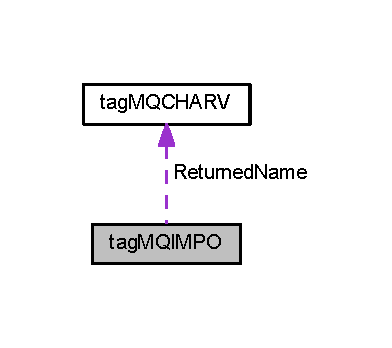
\includegraphics[width=188pt]{structtag_m_q_i_m_p_o__coll__graph}
\end{center}
\end{figure}
\subsection*{Campos de datos}
\begin{DoxyCompactItemize}
\item 
\hyperlink{cmqc_8h_a12590e546ed66fda7cf21c1d5cefa31d}{M\+Q\+C\+H\+A\+R4} \hyperlink{structtag_m_q_i_m_p_o_a0530922ca944569b52601d74941f96e4}{Struc\+Id}
\item 
\hyperlink{cmqc_8h_a1fb8d28cbda3fa8766a9821230cdb6d5}{M\+Q\+L\+O\+N\+G} \hyperlink{structtag_m_q_i_m_p_o_a0656ef8f766b3907d394d88a35d7b7e9}{Version}
\item 
\hyperlink{cmqc_8h_a1fb8d28cbda3fa8766a9821230cdb6d5}{M\+Q\+L\+O\+N\+G} \hyperlink{structtag_m_q_i_m_p_o_ad7aff2d6c6044809464380998d24ec5c}{Options}
\item 
\hyperlink{cmqc_8h_a1fb8d28cbda3fa8766a9821230cdb6d5}{M\+Q\+L\+O\+N\+G} \hyperlink{structtag_m_q_i_m_p_o_a3e0b97e59d454d52f8192b1f3924ffb2}{Requested\+Encoding}
\item 
\hyperlink{cmqc_8h_a1fb8d28cbda3fa8766a9821230cdb6d5}{M\+Q\+L\+O\+N\+G} \hyperlink{structtag_m_q_i_m_p_o_aeae366c610d7d1de844e33938f66209e}{Requested\+C\+C\+S\+I\+D}
\item 
\hyperlink{cmqc_8h_a1fb8d28cbda3fa8766a9821230cdb6d5}{M\+Q\+L\+O\+N\+G} \hyperlink{structtag_m_q_i_m_p_o_a6d25b830b8da987b7036e612b63cc493}{Returned\+Encoding}
\item 
\hyperlink{cmqc_8h_a1fb8d28cbda3fa8766a9821230cdb6d5}{M\+Q\+L\+O\+N\+G} \hyperlink{structtag_m_q_i_m_p_o_a1b119a33db820271cc96e8c9bb903878}{Returned\+C\+C\+S\+I\+D}
\item 
\hyperlink{cmqc_8h_a1fb8d28cbda3fa8766a9821230cdb6d5}{M\+Q\+L\+O\+N\+G} \hyperlink{structtag_m_q_i_m_p_o_a4559672a5bdaff57eb82aa03d163ed47}{Reserved1}
\item 
\hyperlink{cmqc_8h_a2a61029e155515c1360dfc809dab6747}{M\+Q\+C\+H\+A\+R\+V} \hyperlink{structtag_m_q_i_m_p_o_ac8906d395aadf10bc120ea24a3dab637}{Returned\+Name}
\item 
\hyperlink{cmqc_8h_abddcedb8c41fa262f2bd05dfec3e60a5}{M\+Q\+C\+H\+A\+R8} \hyperlink{structtag_m_q_i_m_p_o_a191c43a197f69fa0bdd2d9335960f6b0}{Type\+String}
\end{DoxyCompactItemize}


\subsection{Descripción detallada}


Definición en la línea 4383 del archivo cmqc.\+h.



\subsection{Documentación de los campos}
\hypertarget{structtag_m_q_i_m_p_o_ad7aff2d6c6044809464380998d24ec5c}{}\index{tag\+M\+Q\+I\+M\+P\+O@{tag\+M\+Q\+I\+M\+P\+O}!Options@{Options}}
\index{Options@{Options}!tag\+M\+Q\+I\+M\+P\+O@{tag\+M\+Q\+I\+M\+P\+O}}
\subsubsection[{Options}]{\setlength{\rightskip}{0pt plus 5cm}{\bf M\+Q\+L\+O\+N\+G} Options}\label{structtag_m_q_i_m_p_o_ad7aff2d6c6044809464380998d24ec5c}


Definición en la línea 4386 del archivo cmqc.\+h.

\hypertarget{structtag_m_q_i_m_p_o_aeae366c610d7d1de844e33938f66209e}{}\index{tag\+M\+Q\+I\+M\+P\+O@{tag\+M\+Q\+I\+M\+P\+O}!Requested\+C\+C\+S\+I\+D@{Requested\+C\+C\+S\+I\+D}}
\index{Requested\+C\+C\+S\+I\+D@{Requested\+C\+C\+S\+I\+D}!tag\+M\+Q\+I\+M\+P\+O@{tag\+M\+Q\+I\+M\+P\+O}}
\subsubsection[{Requested\+C\+C\+S\+I\+D}]{\setlength{\rightskip}{0pt plus 5cm}{\bf M\+Q\+L\+O\+N\+G} Requested\+C\+C\+S\+I\+D}\label{structtag_m_q_i_m_p_o_aeae366c610d7d1de844e33938f66209e}


Definición en la línea 4389 del archivo cmqc.\+h.

\hypertarget{structtag_m_q_i_m_p_o_a3e0b97e59d454d52f8192b1f3924ffb2}{}\index{tag\+M\+Q\+I\+M\+P\+O@{tag\+M\+Q\+I\+M\+P\+O}!Requested\+Encoding@{Requested\+Encoding}}
\index{Requested\+Encoding@{Requested\+Encoding}!tag\+M\+Q\+I\+M\+P\+O@{tag\+M\+Q\+I\+M\+P\+O}}
\subsubsection[{Requested\+Encoding}]{\setlength{\rightskip}{0pt plus 5cm}{\bf M\+Q\+L\+O\+N\+G} Requested\+Encoding}\label{structtag_m_q_i_m_p_o_a3e0b97e59d454d52f8192b1f3924ffb2}


Definición en la línea 4388 del archivo cmqc.\+h.

\hypertarget{structtag_m_q_i_m_p_o_a4559672a5bdaff57eb82aa03d163ed47}{}\index{tag\+M\+Q\+I\+M\+P\+O@{tag\+M\+Q\+I\+M\+P\+O}!Reserved1@{Reserved1}}
\index{Reserved1@{Reserved1}!tag\+M\+Q\+I\+M\+P\+O@{tag\+M\+Q\+I\+M\+P\+O}}
\subsubsection[{Reserved1}]{\setlength{\rightskip}{0pt plus 5cm}{\bf M\+Q\+L\+O\+N\+G} Reserved1}\label{structtag_m_q_i_m_p_o_a4559672a5bdaff57eb82aa03d163ed47}


Definición en la línea 4394 del archivo cmqc.\+h.

\hypertarget{structtag_m_q_i_m_p_o_a1b119a33db820271cc96e8c9bb903878}{}\index{tag\+M\+Q\+I\+M\+P\+O@{tag\+M\+Q\+I\+M\+P\+O}!Returned\+C\+C\+S\+I\+D@{Returned\+C\+C\+S\+I\+D}}
\index{Returned\+C\+C\+S\+I\+D@{Returned\+C\+C\+S\+I\+D}!tag\+M\+Q\+I\+M\+P\+O@{tag\+M\+Q\+I\+M\+P\+O}}
\subsubsection[{Returned\+C\+C\+S\+I\+D}]{\setlength{\rightskip}{0pt plus 5cm}{\bf M\+Q\+L\+O\+N\+G} Returned\+C\+C\+S\+I\+D}\label{structtag_m_q_i_m_p_o_a1b119a33db820271cc96e8c9bb903878}


Definición en la línea 4392 del archivo cmqc.\+h.

\hypertarget{structtag_m_q_i_m_p_o_a6d25b830b8da987b7036e612b63cc493}{}\index{tag\+M\+Q\+I\+M\+P\+O@{tag\+M\+Q\+I\+M\+P\+O}!Returned\+Encoding@{Returned\+Encoding}}
\index{Returned\+Encoding@{Returned\+Encoding}!tag\+M\+Q\+I\+M\+P\+O@{tag\+M\+Q\+I\+M\+P\+O}}
\subsubsection[{Returned\+Encoding}]{\setlength{\rightskip}{0pt plus 5cm}{\bf M\+Q\+L\+O\+N\+G} Returned\+Encoding}\label{structtag_m_q_i_m_p_o_a6d25b830b8da987b7036e612b63cc493}


Definición en la línea 4391 del archivo cmqc.\+h.

\hypertarget{structtag_m_q_i_m_p_o_ac8906d395aadf10bc120ea24a3dab637}{}\index{tag\+M\+Q\+I\+M\+P\+O@{tag\+M\+Q\+I\+M\+P\+O}!Returned\+Name@{Returned\+Name}}
\index{Returned\+Name@{Returned\+Name}!tag\+M\+Q\+I\+M\+P\+O@{tag\+M\+Q\+I\+M\+P\+O}}
\subsubsection[{Returned\+Name}]{\setlength{\rightskip}{0pt plus 5cm}{\bf M\+Q\+C\+H\+A\+R\+V} Returned\+Name}\label{structtag_m_q_i_m_p_o_ac8906d395aadf10bc120ea24a3dab637}


Definición en la línea 4395 del archivo cmqc.\+h.

\hypertarget{structtag_m_q_i_m_p_o_a0530922ca944569b52601d74941f96e4}{}\index{tag\+M\+Q\+I\+M\+P\+O@{tag\+M\+Q\+I\+M\+P\+O}!Struc\+Id@{Struc\+Id}}
\index{Struc\+Id@{Struc\+Id}!tag\+M\+Q\+I\+M\+P\+O@{tag\+M\+Q\+I\+M\+P\+O}}
\subsubsection[{Struc\+Id}]{\setlength{\rightskip}{0pt plus 5cm}{\bf M\+Q\+C\+H\+A\+R4} Struc\+Id}\label{structtag_m_q_i_m_p_o_a0530922ca944569b52601d74941f96e4}


Definición en la línea 4384 del archivo cmqc.\+h.

\hypertarget{structtag_m_q_i_m_p_o_a191c43a197f69fa0bdd2d9335960f6b0}{}\index{tag\+M\+Q\+I\+M\+P\+O@{tag\+M\+Q\+I\+M\+P\+O}!Type\+String@{Type\+String}}
\index{Type\+String@{Type\+String}!tag\+M\+Q\+I\+M\+P\+O@{tag\+M\+Q\+I\+M\+P\+O}}
\subsubsection[{Type\+String}]{\setlength{\rightskip}{0pt plus 5cm}{\bf M\+Q\+C\+H\+A\+R8} Type\+String}\label{structtag_m_q_i_m_p_o_a191c43a197f69fa0bdd2d9335960f6b0}


Definición en la línea 4396 del archivo cmqc.\+h.

\hypertarget{structtag_m_q_i_m_p_o_a0656ef8f766b3907d394d88a35d7b7e9}{}\index{tag\+M\+Q\+I\+M\+P\+O@{tag\+M\+Q\+I\+M\+P\+O}!Version@{Version}}
\index{Version@{Version}!tag\+M\+Q\+I\+M\+P\+O@{tag\+M\+Q\+I\+M\+P\+O}}
\subsubsection[{Version}]{\setlength{\rightskip}{0pt plus 5cm}{\bf M\+Q\+L\+O\+N\+G} Version}\label{structtag_m_q_i_m_p_o_a0656ef8f766b3907d394d88a35d7b7e9}


Definición en la línea 4385 del archivo cmqc.\+h.



La documentación para esta estructura fue generada a partir del siguiente fichero\+:\begin{DoxyCompactItemize}
\item 
include/\hyperlink{cmqc_8h}{cmqc.\+h}\end{DoxyCompactItemize}

\hypertarget{structtag_m_q_m_d}{}\section{Referencia de la Estructura tag\+M\+Q\+M\+D}
\label{structtag_m_q_m_d}\index{tag\+M\+Q\+M\+D@{tag\+M\+Q\+M\+D}}


{\ttfamily \#include $<$cmqc.\+h$>$}

\subsection*{Campos de datos}
\begin{DoxyCompactItemize}
\item 
\hyperlink{cmqc_8h_a12590e546ed66fda7cf21c1d5cefa31d}{M\+Q\+C\+H\+A\+R4} \hyperlink{structtag_m_q_m_d_a0530922ca944569b52601d74941f96e4}{Struc\+Id}
\item 
\hyperlink{cmqc_8h_a1fb8d28cbda3fa8766a9821230cdb6d5}{M\+Q\+L\+O\+N\+G} \hyperlink{structtag_m_q_m_d_a0656ef8f766b3907d394d88a35d7b7e9}{Version}
\item 
\hyperlink{cmqc_8h_a1fb8d28cbda3fa8766a9821230cdb6d5}{M\+Q\+L\+O\+N\+G} \hyperlink{structtag_m_q_m_d_a3e6ae3e2f087fe6fc26cc75004fbc790}{Report}
\item 
\hyperlink{cmqc_8h_a1fb8d28cbda3fa8766a9821230cdb6d5}{M\+Q\+L\+O\+N\+G} \hyperlink{structtag_m_q_m_d_a22732037d5385ab03eb3e9d9a5e60843}{Msg\+Type}
\item 
\hyperlink{cmqc_8h_a1fb8d28cbda3fa8766a9821230cdb6d5}{M\+Q\+L\+O\+N\+G} \hyperlink{structtag_m_q_m_d_a85cb54f2f2a97fe071fcad54d22a92a9}{Expiry}
\item 
\hyperlink{cmqc_8h_a1fb8d28cbda3fa8766a9821230cdb6d5}{M\+Q\+L\+O\+N\+G} \hyperlink{structtag_m_q_m_d_a9cb2f407eb097aa9cdc246dc18059987}{Feedback}
\item 
\hyperlink{cmqc_8h_a1fb8d28cbda3fa8766a9821230cdb6d5}{M\+Q\+L\+O\+N\+G} \hyperlink{structtag_m_q_m_d_a30167bf454a49a60fd3fe4e9e586af34}{Encoding}
\item 
\hyperlink{cmqc_8h_a1fb8d28cbda3fa8766a9821230cdb6d5}{M\+Q\+L\+O\+N\+G} \hyperlink{structtag_m_q_m_d_a4d8d1961a991850d1355cdf9b4680b8e}{Coded\+Char\+Set\+Id}
\item 
\hyperlink{cmqc_8h_abddcedb8c41fa262f2bd05dfec3e60a5}{M\+Q\+C\+H\+A\+R8} \hyperlink{structtag_m_q_m_d_a435a478822008713f8aaff89f369ed63}{Format}
\item 
\hyperlink{cmqc_8h_a1fb8d28cbda3fa8766a9821230cdb6d5}{M\+Q\+L\+O\+N\+G} \hyperlink{structtag_m_q_m_d_a72c542b9e2952a489df0cb84755c1fa6}{Priority}
\item 
\hyperlink{cmqc_8h_a1fb8d28cbda3fa8766a9821230cdb6d5}{M\+Q\+L\+O\+N\+G} \hyperlink{structtag_m_q_m_d_af0f253d60fa2dcbe2bda530c88661853}{Persistence}
\item 
\hyperlink{cmqc_8h_a2866d93c0ef84cfcda34cab5fd22fc5a}{M\+Q\+B\+Y\+T\+E24} \hyperlink{structtag_m_q_m_d_a075d401c83d67ca688e6165dda74a44c}{Msg\+Id}
\item 
\hyperlink{cmqc_8h_a2866d93c0ef84cfcda34cab5fd22fc5a}{M\+Q\+B\+Y\+T\+E24} \hyperlink{structtag_m_q_m_d_acac8d73138c2c618b41a274eb92e5f2a}{Correl\+Id}
\item 
\hyperlink{cmqc_8h_a1fb8d28cbda3fa8766a9821230cdb6d5}{M\+Q\+L\+O\+N\+G} \hyperlink{structtag_m_q_m_d_afd269725e61f1620f8182ccd914d8dae}{Backout\+Count}
\item 
\hyperlink{cmqc_8h_a53b1a2836da03f19144836725ff77919}{M\+Q\+C\+H\+A\+R48} \hyperlink{structtag_m_q_m_d_a7073875015f870e1d1a02e988ce698b3}{Reply\+To\+Q}
\item 
\hyperlink{cmqc_8h_a53b1a2836da03f19144836725ff77919}{M\+Q\+C\+H\+A\+R48} \hyperlink{structtag_m_q_m_d_a9364487d587c0a06d95c25d1ae05a0be}{Reply\+To\+Q\+Mgr}
\item 
\hyperlink{cmqc_8h_a996cbcfd8d7ef4774f29b158a22d55c0}{M\+Q\+C\+H\+A\+R12} \hyperlink{structtag_m_q_m_d_a46cc458e507d74cea87ed00b97695f65}{User\+Identifier}
\item 
\hyperlink{cmqc_8h_aaa021c16e95b8aaab0a28fa5c3756d9d}{M\+Q\+B\+Y\+T\+E32} \hyperlink{structtag_m_q_m_d_a1fe2835a002ec01b58d479509699dd2c}{Accounting\+Token}
\item 
\hyperlink{cmqc_8h_a0b7dd696f0148465fe80f6eae57b38a2}{M\+Q\+C\+H\+A\+R32} \hyperlink{structtag_m_q_m_d_a1f16948c5ba6adfbb92776400030700e}{Appl\+Identity\+Data}
\item 
\hyperlink{cmqc_8h_a1fb8d28cbda3fa8766a9821230cdb6d5}{M\+Q\+L\+O\+N\+G} \hyperlink{structtag_m_q_m_d_a6d9e0e0fe9075017c939213948c747dc}{Put\+Appl\+Type}
\item 
\hyperlink{cmqc_8h_a6139f35ea8f9711726daeb5df27ab593}{M\+Q\+C\+H\+A\+R28} \hyperlink{structtag_m_q_m_d_a7195390be27f384ef0ab0d0f9053d462}{Put\+Appl\+Name}
\item 
\hyperlink{cmqc_8h_abddcedb8c41fa262f2bd05dfec3e60a5}{M\+Q\+C\+H\+A\+R8} \hyperlink{structtag_m_q_m_d_add3e7fe139edfa323295d6c7bc764cc5}{Put\+Date}
\item 
\hyperlink{cmqc_8h_abddcedb8c41fa262f2bd05dfec3e60a5}{M\+Q\+C\+H\+A\+R8} \hyperlink{structtag_m_q_m_d_aec51e7b9face9480a893ae5d47781ee7}{Put\+Time}
\item 
\hyperlink{cmqc_8h_a12590e546ed66fda7cf21c1d5cefa31d}{M\+Q\+C\+H\+A\+R4} \hyperlink{structtag_m_q_m_d_aaf3c543f992b06c609193929872b998a}{Appl\+Origin\+Data}
\item 
\hyperlink{cmqc_8h_a2866d93c0ef84cfcda34cab5fd22fc5a}{M\+Q\+B\+Y\+T\+E24} \hyperlink{structtag_m_q_m_d_abcf7ab1abd1c768c0adb9acb3d09c6f1}{Group\+Id}
\item 
\hyperlink{cmqc_8h_a1fb8d28cbda3fa8766a9821230cdb6d5}{M\+Q\+L\+O\+N\+G} \hyperlink{structtag_m_q_m_d_a7c78a4f7c1bbda9f124f904e0d02a7a2}{Msg\+Seq\+Number}
\item 
\hyperlink{cmqc_8h_a1fb8d28cbda3fa8766a9821230cdb6d5}{M\+Q\+L\+O\+N\+G} \hyperlink{structtag_m_q_m_d_aac8433c970f16a602e3b79400e87d28b}{Offset}
\item 
\hyperlink{cmqc_8h_a1fb8d28cbda3fa8766a9821230cdb6d5}{M\+Q\+L\+O\+N\+G} \hyperlink{structtag_m_q_m_d_a10cb94bb1b2528f6ad936454455bb40a}{Msg\+Flags}
\item 
\hyperlink{cmqc_8h_a1fb8d28cbda3fa8766a9821230cdb6d5}{M\+Q\+L\+O\+N\+G} \hyperlink{structtag_m_q_m_d_acf39c0c6d2618f565cf8315c8775b5ae}{Original\+Length}
\end{DoxyCompactItemize}


\subsection{Descripción detallada}


Definición en la línea 4419 del archivo cmqc.\+h.



\subsection{Documentación de los campos}
\hypertarget{structtag_m_q_m_d_a1fe2835a002ec01b58d479509699dd2c}{}\index{tag\+M\+Q\+M\+D@{tag\+M\+Q\+M\+D}!Accounting\+Token@{Accounting\+Token}}
\index{Accounting\+Token@{Accounting\+Token}!tag\+M\+Q\+M\+D@{tag\+M\+Q\+M\+D}}
\subsubsection[{Accounting\+Token}]{\setlength{\rightskip}{0pt plus 5cm}{\bf M\+Q\+B\+Y\+T\+E32} Accounting\+Token}\label{structtag_m_q_m_d_a1fe2835a002ec01b58d479509699dd2c}


Definición en la línea 4438 del archivo cmqc.\+h.

\hypertarget{structtag_m_q_m_d_a1f16948c5ba6adfbb92776400030700e}{}\index{tag\+M\+Q\+M\+D@{tag\+M\+Q\+M\+D}!Appl\+Identity\+Data@{Appl\+Identity\+Data}}
\index{Appl\+Identity\+Data@{Appl\+Identity\+Data}!tag\+M\+Q\+M\+D@{tag\+M\+Q\+M\+D}}
\subsubsection[{Appl\+Identity\+Data}]{\setlength{\rightskip}{0pt plus 5cm}{\bf M\+Q\+C\+H\+A\+R32} Appl\+Identity\+Data}\label{structtag_m_q_m_d_a1f16948c5ba6adfbb92776400030700e}


Definición en la línea 4439 del archivo cmqc.\+h.

\hypertarget{structtag_m_q_m_d_aaf3c543f992b06c609193929872b998a}{}\index{tag\+M\+Q\+M\+D@{tag\+M\+Q\+M\+D}!Appl\+Origin\+Data@{Appl\+Origin\+Data}}
\index{Appl\+Origin\+Data@{Appl\+Origin\+Data}!tag\+M\+Q\+M\+D@{tag\+M\+Q\+M\+D}}
\subsubsection[{Appl\+Origin\+Data}]{\setlength{\rightskip}{0pt plus 5cm}{\bf M\+Q\+C\+H\+A\+R4} Appl\+Origin\+Data}\label{structtag_m_q_m_d_aaf3c543f992b06c609193929872b998a}


Definición en la línea 4447 del archivo cmqc.\+h.

\hypertarget{structtag_m_q_m_d_afd269725e61f1620f8182ccd914d8dae}{}\index{tag\+M\+Q\+M\+D@{tag\+M\+Q\+M\+D}!Backout\+Count@{Backout\+Count}}
\index{Backout\+Count@{Backout\+Count}!tag\+M\+Q\+M\+D@{tag\+M\+Q\+M\+D}}
\subsubsection[{Backout\+Count}]{\setlength{\rightskip}{0pt plus 5cm}{\bf M\+Q\+L\+O\+N\+G} Backout\+Count}\label{structtag_m_q_m_d_afd269725e61f1620f8182ccd914d8dae}


Definición en la línea 4434 del archivo cmqc.\+h.

\hypertarget{structtag_m_q_m_d_a4d8d1961a991850d1355cdf9b4680b8e}{}\index{tag\+M\+Q\+M\+D@{tag\+M\+Q\+M\+D}!Coded\+Char\+Set\+Id@{Coded\+Char\+Set\+Id}}
\index{Coded\+Char\+Set\+Id@{Coded\+Char\+Set\+Id}!tag\+M\+Q\+M\+D@{tag\+M\+Q\+M\+D}}
\subsubsection[{Coded\+Char\+Set\+Id}]{\setlength{\rightskip}{0pt plus 5cm}{\bf M\+Q\+L\+O\+N\+G} Coded\+Char\+Set\+Id}\label{structtag_m_q_m_d_a4d8d1961a991850d1355cdf9b4680b8e}


Definición en la línea 4427 del archivo cmqc.\+h.

\hypertarget{structtag_m_q_m_d_acac8d73138c2c618b41a274eb92e5f2a}{}\index{tag\+M\+Q\+M\+D@{tag\+M\+Q\+M\+D}!Correl\+Id@{Correl\+Id}}
\index{Correl\+Id@{Correl\+Id}!tag\+M\+Q\+M\+D@{tag\+M\+Q\+M\+D}}
\subsubsection[{Correl\+Id}]{\setlength{\rightskip}{0pt plus 5cm}{\bf M\+Q\+B\+Y\+T\+E24} Correl\+Id}\label{structtag_m_q_m_d_acac8d73138c2c618b41a274eb92e5f2a}


Definición en la línea 4433 del archivo cmqc.\+h.

\hypertarget{structtag_m_q_m_d_a30167bf454a49a60fd3fe4e9e586af34}{}\index{tag\+M\+Q\+M\+D@{tag\+M\+Q\+M\+D}!Encoding@{Encoding}}
\index{Encoding@{Encoding}!tag\+M\+Q\+M\+D@{tag\+M\+Q\+M\+D}}
\subsubsection[{Encoding}]{\setlength{\rightskip}{0pt plus 5cm}{\bf M\+Q\+L\+O\+N\+G} Encoding}\label{structtag_m_q_m_d_a30167bf454a49a60fd3fe4e9e586af34}


Definición en la línea 4426 del archivo cmqc.\+h.

\hypertarget{structtag_m_q_m_d_a85cb54f2f2a97fe071fcad54d22a92a9}{}\index{tag\+M\+Q\+M\+D@{tag\+M\+Q\+M\+D}!Expiry@{Expiry}}
\index{Expiry@{Expiry}!tag\+M\+Q\+M\+D@{tag\+M\+Q\+M\+D}}
\subsubsection[{Expiry}]{\setlength{\rightskip}{0pt plus 5cm}{\bf M\+Q\+L\+O\+N\+G} Expiry}\label{structtag_m_q_m_d_a85cb54f2f2a97fe071fcad54d22a92a9}


Definición en la línea 4424 del archivo cmqc.\+h.

\hypertarget{structtag_m_q_m_d_a9cb2f407eb097aa9cdc246dc18059987}{}\index{tag\+M\+Q\+M\+D@{tag\+M\+Q\+M\+D}!Feedback@{Feedback}}
\index{Feedback@{Feedback}!tag\+M\+Q\+M\+D@{tag\+M\+Q\+M\+D}}
\subsubsection[{Feedback}]{\setlength{\rightskip}{0pt plus 5cm}{\bf M\+Q\+L\+O\+N\+G} Feedback}\label{structtag_m_q_m_d_a9cb2f407eb097aa9cdc246dc18059987}


Definición en la línea 4425 del archivo cmqc.\+h.

\hypertarget{structtag_m_q_m_d_a435a478822008713f8aaff89f369ed63}{}\index{tag\+M\+Q\+M\+D@{tag\+M\+Q\+M\+D}!Format@{Format}}
\index{Format@{Format}!tag\+M\+Q\+M\+D@{tag\+M\+Q\+M\+D}}
\subsubsection[{Format}]{\setlength{\rightskip}{0pt plus 5cm}{\bf M\+Q\+C\+H\+A\+R8} Format}\label{structtag_m_q_m_d_a435a478822008713f8aaff89f369ed63}


Definición en la línea 4429 del archivo cmqc.\+h.

\hypertarget{structtag_m_q_m_d_abcf7ab1abd1c768c0adb9acb3d09c6f1}{}\index{tag\+M\+Q\+M\+D@{tag\+M\+Q\+M\+D}!Group\+Id@{Group\+Id}}
\index{Group\+Id@{Group\+Id}!tag\+M\+Q\+M\+D@{tag\+M\+Q\+M\+D}}
\subsubsection[{Group\+Id}]{\setlength{\rightskip}{0pt plus 5cm}{\bf M\+Q\+B\+Y\+T\+E24} Group\+Id}\label{structtag_m_q_m_d_abcf7ab1abd1c768c0adb9acb3d09c6f1}


Definición en la línea 4450 del archivo cmqc.\+h.

\hypertarget{structtag_m_q_m_d_a10cb94bb1b2528f6ad936454455bb40a}{}\index{tag\+M\+Q\+M\+D@{tag\+M\+Q\+M\+D}!Msg\+Flags@{Msg\+Flags}}
\index{Msg\+Flags@{Msg\+Flags}!tag\+M\+Q\+M\+D@{tag\+M\+Q\+M\+D}}
\subsubsection[{Msg\+Flags}]{\setlength{\rightskip}{0pt plus 5cm}{\bf M\+Q\+L\+O\+N\+G} Msg\+Flags}\label{structtag_m_q_m_d_a10cb94bb1b2528f6ad936454455bb40a}


Definición en la línea 4455 del archivo cmqc.\+h.

\hypertarget{structtag_m_q_m_d_a075d401c83d67ca688e6165dda74a44c}{}\index{tag\+M\+Q\+M\+D@{tag\+M\+Q\+M\+D}!Msg\+Id@{Msg\+Id}}
\index{Msg\+Id@{Msg\+Id}!tag\+M\+Q\+M\+D@{tag\+M\+Q\+M\+D}}
\subsubsection[{Msg\+Id}]{\setlength{\rightskip}{0pt plus 5cm}{\bf M\+Q\+B\+Y\+T\+E24} Msg\+Id}\label{structtag_m_q_m_d_a075d401c83d67ca688e6165dda74a44c}


Definición en la línea 4432 del archivo cmqc.\+h.

\hypertarget{structtag_m_q_m_d_a7c78a4f7c1bbda9f124f904e0d02a7a2}{}\index{tag\+M\+Q\+M\+D@{tag\+M\+Q\+M\+D}!Msg\+Seq\+Number@{Msg\+Seq\+Number}}
\index{Msg\+Seq\+Number@{Msg\+Seq\+Number}!tag\+M\+Q\+M\+D@{tag\+M\+Q\+M\+D}}
\subsubsection[{Msg\+Seq\+Number}]{\setlength{\rightskip}{0pt plus 5cm}{\bf M\+Q\+L\+O\+N\+G} Msg\+Seq\+Number}\label{structtag_m_q_m_d_a7c78a4f7c1bbda9f124f904e0d02a7a2}


Definición en la línea 4451 del archivo cmqc.\+h.

\hypertarget{structtag_m_q_m_d_a22732037d5385ab03eb3e9d9a5e60843}{}\index{tag\+M\+Q\+M\+D@{tag\+M\+Q\+M\+D}!Msg\+Type@{Msg\+Type}}
\index{Msg\+Type@{Msg\+Type}!tag\+M\+Q\+M\+D@{tag\+M\+Q\+M\+D}}
\subsubsection[{Msg\+Type}]{\setlength{\rightskip}{0pt plus 5cm}{\bf M\+Q\+L\+O\+N\+G} Msg\+Type}\label{structtag_m_q_m_d_a22732037d5385ab03eb3e9d9a5e60843}


Definición en la línea 4423 del archivo cmqc.\+h.

\hypertarget{structtag_m_q_m_d_aac8433c970f16a602e3b79400e87d28b}{}\index{tag\+M\+Q\+M\+D@{tag\+M\+Q\+M\+D}!Offset@{Offset}}
\index{Offset@{Offset}!tag\+M\+Q\+M\+D@{tag\+M\+Q\+M\+D}}
\subsubsection[{Offset}]{\setlength{\rightskip}{0pt plus 5cm}{\bf M\+Q\+L\+O\+N\+G} Offset}\label{structtag_m_q_m_d_aac8433c970f16a602e3b79400e87d28b}


Definición en la línea 4453 del archivo cmqc.\+h.

\hypertarget{structtag_m_q_m_d_acf39c0c6d2618f565cf8315c8775b5ae}{}\index{tag\+M\+Q\+M\+D@{tag\+M\+Q\+M\+D}!Original\+Length@{Original\+Length}}
\index{Original\+Length@{Original\+Length}!tag\+M\+Q\+M\+D@{tag\+M\+Q\+M\+D}}
\subsubsection[{Original\+Length}]{\setlength{\rightskip}{0pt plus 5cm}{\bf M\+Q\+L\+O\+N\+G} Original\+Length}\label{structtag_m_q_m_d_acf39c0c6d2618f565cf8315c8775b5ae}


Definición en la línea 4456 del archivo cmqc.\+h.

\hypertarget{structtag_m_q_m_d_af0f253d60fa2dcbe2bda530c88661853}{}\index{tag\+M\+Q\+M\+D@{tag\+M\+Q\+M\+D}!Persistence@{Persistence}}
\index{Persistence@{Persistence}!tag\+M\+Q\+M\+D@{tag\+M\+Q\+M\+D}}
\subsubsection[{Persistence}]{\setlength{\rightskip}{0pt plus 5cm}{\bf M\+Q\+L\+O\+N\+G} Persistence}\label{structtag_m_q_m_d_af0f253d60fa2dcbe2bda530c88661853}


Definición en la línea 4431 del archivo cmqc.\+h.

\hypertarget{structtag_m_q_m_d_a72c542b9e2952a489df0cb84755c1fa6}{}\index{tag\+M\+Q\+M\+D@{tag\+M\+Q\+M\+D}!Priority@{Priority}}
\index{Priority@{Priority}!tag\+M\+Q\+M\+D@{tag\+M\+Q\+M\+D}}
\subsubsection[{Priority}]{\setlength{\rightskip}{0pt plus 5cm}{\bf M\+Q\+L\+O\+N\+G} Priority}\label{structtag_m_q_m_d_a72c542b9e2952a489df0cb84755c1fa6}


Definición en la línea 4430 del archivo cmqc.\+h.

\hypertarget{structtag_m_q_m_d_a7195390be27f384ef0ab0d0f9053d462}{}\index{tag\+M\+Q\+M\+D@{tag\+M\+Q\+M\+D}!Put\+Appl\+Name@{Put\+Appl\+Name}}
\index{Put\+Appl\+Name@{Put\+Appl\+Name}!tag\+M\+Q\+M\+D@{tag\+M\+Q\+M\+D}}
\subsubsection[{Put\+Appl\+Name}]{\setlength{\rightskip}{0pt plus 5cm}{\bf M\+Q\+C\+H\+A\+R28} Put\+Appl\+Name}\label{structtag_m_q_m_d_a7195390be27f384ef0ab0d0f9053d462}


Definición en la línea 4443 del archivo cmqc.\+h.

\hypertarget{structtag_m_q_m_d_a6d9e0e0fe9075017c939213948c747dc}{}\index{tag\+M\+Q\+M\+D@{tag\+M\+Q\+M\+D}!Put\+Appl\+Type@{Put\+Appl\+Type}}
\index{Put\+Appl\+Type@{Put\+Appl\+Type}!tag\+M\+Q\+M\+D@{tag\+M\+Q\+M\+D}}
\subsubsection[{Put\+Appl\+Type}]{\setlength{\rightskip}{0pt plus 5cm}{\bf M\+Q\+L\+O\+N\+G} Put\+Appl\+Type}\label{structtag_m_q_m_d_a6d9e0e0fe9075017c939213948c747dc}


Definición en la línea 4441 del archivo cmqc.\+h.

\hypertarget{structtag_m_q_m_d_add3e7fe139edfa323295d6c7bc764cc5}{}\index{tag\+M\+Q\+M\+D@{tag\+M\+Q\+M\+D}!Put\+Date@{Put\+Date}}
\index{Put\+Date@{Put\+Date}!tag\+M\+Q\+M\+D@{tag\+M\+Q\+M\+D}}
\subsubsection[{Put\+Date}]{\setlength{\rightskip}{0pt plus 5cm}{\bf M\+Q\+C\+H\+A\+R8} Put\+Date}\label{structtag_m_q_m_d_add3e7fe139edfa323295d6c7bc764cc5}


Definición en la línea 4445 del archivo cmqc.\+h.

\hypertarget{structtag_m_q_m_d_aec51e7b9face9480a893ae5d47781ee7}{}\index{tag\+M\+Q\+M\+D@{tag\+M\+Q\+M\+D}!Put\+Time@{Put\+Time}}
\index{Put\+Time@{Put\+Time}!tag\+M\+Q\+M\+D@{tag\+M\+Q\+M\+D}}
\subsubsection[{Put\+Time}]{\setlength{\rightskip}{0pt plus 5cm}{\bf M\+Q\+C\+H\+A\+R8} Put\+Time}\label{structtag_m_q_m_d_aec51e7b9face9480a893ae5d47781ee7}


Definición en la línea 4446 del archivo cmqc.\+h.

\hypertarget{structtag_m_q_m_d_a7073875015f870e1d1a02e988ce698b3}{}\index{tag\+M\+Q\+M\+D@{tag\+M\+Q\+M\+D}!Reply\+To\+Q@{Reply\+To\+Q}}
\index{Reply\+To\+Q@{Reply\+To\+Q}!tag\+M\+Q\+M\+D@{tag\+M\+Q\+M\+D}}
\subsubsection[{Reply\+To\+Q}]{\setlength{\rightskip}{0pt plus 5cm}{\bf M\+Q\+C\+H\+A\+R48} Reply\+To\+Q}\label{structtag_m_q_m_d_a7073875015f870e1d1a02e988ce698b3}


Definición en la línea 4435 del archivo cmqc.\+h.

\hypertarget{structtag_m_q_m_d_a9364487d587c0a06d95c25d1ae05a0be}{}\index{tag\+M\+Q\+M\+D@{tag\+M\+Q\+M\+D}!Reply\+To\+Q\+Mgr@{Reply\+To\+Q\+Mgr}}
\index{Reply\+To\+Q\+Mgr@{Reply\+To\+Q\+Mgr}!tag\+M\+Q\+M\+D@{tag\+M\+Q\+M\+D}}
\subsubsection[{Reply\+To\+Q\+Mgr}]{\setlength{\rightskip}{0pt plus 5cm}{\bf M\+Q\+C\+H\+A\+R48} Reply\+To\+Q\+Mgr}\label{structtag_m_q_m_d_a9364487d587c0a06d95c25d1ae05a0be}


Definición en la línea 4436 del archivo cmqc.\+h.

\hypertarget{structtag_m_q_m_d_a3e6ae3e2f087fe6fc26cc75004fbc790}{}\index{tag\+M\+Q\+M\+D@{tag\+M\+Q\+M\+D}!Report@{Report}}
\index{Report@{Report}!tag\+M\+Q\+M\+D@{tag\+M\+Q\+M\+D}}
\subsubsection[{Report}]{\setlength{\rightskip}{0pt plus 5cm}{\bf M\+Q\+L\+O\+N\+G} Report}\label{structtag_m_q_m_d_a3e6ae3e2f087fe6fc26cc75004fbc790}


Definición en la línea 4422 del archivo cmqc.\+h.

\hypertarget{structtag_m_q_m_d_a0530922ca944569b52601d74941f96e4}{}\index{tag\+M\+Q\+M\+D@{tag\+M\+Q\+M\+D}!Struc\+Id@{Struc\+Id}}
\index{Struc\+Id@{Struc\+Id}!tag\+M\+Q\+M\+D@{tag\+M\+Q\+M\+D}}
\subsubsection[{Struc\+Id}]{\setlength{\rightskip}{0pt plus 5cm}{\bf M\+Q\+C\+H\+A\+R4} Struc\+Id}\label{structtag_m_q_m_d_a0530922ca944569b52601d74941f96e4}


Definición en la línea 4420 del archivo cmqc.\+h.

\hypertarget{structtag_m_q_m_d_a46cc458e507d74cea87ed00b97695f65}{}\index{tag\+M\+Q\+M\+D@{tag\+M\+Q\+M\+D}!User\+Identifier@{User\+Identifier}}
\index{User\+Identifier@{User\+Identifier}!tag\+M\+Q\+M\+D@{tag\+M\+Q\+M\+D}}
\subsubsection[{User\+Identifier}]{\setlength{\rightskip}{0pt plus 5cm}{\bf M\+Q\+C\+H\+A\+R12} User\+Identifier}\label{structtag_m_q_m_d_a46cc458e507d74cea87ed00b97695f65}


Definición en la línea 4437 del archivo cmqc.\+h.

\hypertarget{structtag_m_q_m_d_a0656ef8f766b3907d394d88a35d7b7e9}{}\index{tag\+M\+Q\+M\+D@{tag\+M\+Q\+M\+D}!Version@{Version}}
\index{Version@{Version}!tag\+M\+Q\+M\+D@{tag\+M\+Q\+M\+D}}
\subsubsection[{Version}]{\setlength{\rightskip}{0pt plus 5cm}{\bf M\+Q\+L\+O\+N\+G} Version}\label{structtag_m_q_m_d_a0656ef8f766b3907d394d88a35d7b7e9}


Definición en la línea 4421 del archivo cmqc.\+h.



La documentación para esta estructura fue generada a partir del siguiente fichero\+:\begin{DoxyCompactItemize}
\item 
include/\hyperlink{cmqc_8h}{cmqc.\+h}\end{DoxyCompactItemize}

\hypertarget{structtag_m_q_m_d1}{}\section{Referencia de la Estructura tag\+M\+Q\+M\+D1}
\label{structtag_m_q_m_d1}\index{tag\+M\+Q\+M\+D1@{tag\+M\+Q\+M\+D1}}


{\ttfamily \#include $<$cmqc.\+h$>$}

\subsection*{Campos de datos}
\begin{DoxyCompactItemize}
\item 
\hyperlink{cmqc_8h_a12590e546ed66fda7cf21c1d5cefa31d}{M\+Q\+C\+H\+A\+R4} \hyperlink{structtag_m_q_m_d1_a0530922ca944569b52601d74941f96e4}{Struc\+Id}
\item 
\hyperlink{cmqc_8h_a1fb8d28cbda3fa8766a9821230cdb6d5}{M\+Q\+L\+O\+N\+G} \hyperlink{structtag_m_q_m_d1_a0656ef8f766b3907d394d88a35d7b7e9}{Version}
\item 
\hyperlink{cmqc_8h_a1fb8d28cbda3fa8766a9821230cdb6d5}{M\+Q\+L\+O\+N\+G} \hyperlink{structtag_m_q_m_d1_a3e6ae3e2f087fe6fc26cc75004fbc790}{Report}
\item 
\hyperlink{cmqc_8h_a1fb8d28cbda3fa8766a9821230cdb6d5}{M\+Q\+L\+O\+N\+G} \hyperlink{structtag_m_q_m_d1_a22732037d5385ab03eb3e9d9a5e60843}{Msg\+Type}
\item 
\hyperlink{cmqc_8h_a1fb8d28cbda3fa8766a9821230cdb6d5}{M\+Q\+L\+O\+N\+G} \hyperlink{structtag_m_q_m_d1_a85cb54f2f2a97fe071fcad54d22a92a9}{Expiry}
\item 
\hyperlink{cmqc_8h_a1fb8d28cbda3fa8766a9821230cdb6d5}{M\+Q\+L\+O\+N\+G} \hyperlink{structtag_m_q_m_d1_a9cb2f407eb097aa9cdc246dc18059987}{Feedback}
\item 
\hyperlink{cmqc_8h_a1fb8d28cbda3fa8766a9821230cdb6d5}{M\+Q\+L\+O\+N\+G} \hyperlink{structtag_m_q_m_d1_a30167bf454a49a60fd3fe4e9e586af34}{Encoding}
\item 
\hyperlink{cmqc_8h_a1fb8d28cbda3fa8766a9821230cdb6d5}{M\+Q\+L\+O\+N\+G} \hyperlink{structtag_m_q_m_d1_a4d8d1961a991850d1355cdf9b4680b8e}{Coded\+Char\+Set\+Id}
\item 
\hyperlink{cmqc_8h_abddcedb8c41fa262f2bd05dfec3e60a5}{M\+Q\+C\+H\+A\+R8} \hyperlink{structtag_m_q_m_d1_a435a478822008713f8aaff89f369ed63}{Format}
\item 
\hyperlink{cmqc_8h_a1fb8d28cbda3fa8766a9821230cdb6d5}{M\+Q\+L\+O\+N\+G} \hyperlink{structtag_m_q_m_d1_a72c542b9e2952a489df0cb84755c1fa6}{Priority}
\item 
\hyperlink{cmqc_8h_a1fb8d28cbda3fa8766a9821230cdb6d5}{M\+Q\+L\+O\+N\+G} \hyperlink{structtag_m_q_m_d1_af0f253d60fa2dcbe2bda530c88661853}{Persistence}
\item 
\hyperlink{cmqc_8h_a2866d93c0ef84cfcda34cab5fd22fc5a}{M\+Q\+B\+Y\+T\+E24} \hyperlink{structtag_m_q_m_d1_a075d401c83d67ca688e6165dda74a44c}{Msg\+Id}
\item 
\hyperlink{cmqc_8h_a2866d93c0ef84cfcda34cab5fd22fc5a}{M\+Q\+B\+Y\+T\+E24} \hyperlink{structtag_m_q_m_d1_acac8d73138c2c618b41a274eb92e5f2a}{Correl\+Id}
\item 
\hyperlink{cmqc_8h_a1fb8d28cbda3fa8766a9821230cdb6d5}{M\+Q\+L\+O\+N\+G} \hyperlink{structtag_m_q_m_d1_afd269725e61f1620f8182ccd914d8dae}{Backout\+Count}
\item 
\hyperlink{cmqc_8h_a53b1a2836da03f19144836725ff77919}{M\+Q\+C\+H\+A\+R48} \hyperlink{structtag_m_q_m_d1_a7073875015f870e1d1a02e988ce698b3}{Reply\+To\+Q}
\item 
\hyperlink{cmqc_8h_a53b1a2836da03f19144836725ff77919}{M\+Q\+C\+H\+A\+R48} \hyperlink{structtag_m_q_m_d1_a9364487d587c0a06d95c25d1ae05a0be}{Reply\+To\+Q\+Mgr}
\item 
\hyperlink{cmqc_8h_a996cbcfd8d7ef4774f29b158a22d55c0}{M\+Q\+C\+H\+A\+R12} \hyperlink{structtag_m_q_m_d1_a46cc458e507d74cea87ed00b97695f65}{User\+Identifier}
\item 
\hyperlink{cmqc_8h_aaa021c16e95b8aaab0a28fa5c3756d9d}{M\+Q\+B\+Y\+T\+E32} \hyperlink{structtag_m_q_m_d1_a1fe2835a002ec01b58d479509699dd2c}{Accounting\+Token}
\item 
\hyperlink{cmqc_8h_a0b7dd696f0148465fe80f6eae57b38a2}{M\+Q\+C\+H\+A\+R32} \hyperlink{structtag_m_q_m_d1_a1f16948c5ba6adfbb92776400030700e}{Appl\+Identity\+Data}
\item 
\hyperlink{cmqc_8h_a1fb8d28cbda3fa8766a9821230cdb6d5}{M\+Q\+L\+O\+N\+G} \hyperlink{structtag_m_q_m_d1_a6d9e0e0fe9075017c939213948c747dc}{Put\+Appl\+Type}
\item 
\hyperlink{cmqc_8h_a6139f35ea8f9711726daeb5df27ab593}{M\+Q\+C\+H\+A\+R28} \hyperlink{structtag_m_q_m_d1_a7195390be27f384ef0ab0d0f9053d462}{Put\+Appl\+Name}
\item 
\hyperlink{cmqc_8h_abddcedb8c41fa262f2bd05dfec3e60a5}{M\+Q\+C\+H\+A\+R8} \hyperlink{structtag_m_q_m_d1_add3e7fe139edfa323295d6c7bc764cc5}{Put\+Date}
\item 
\hyperlink{cmqc_8h_abddcedb8c41fa262f2bd05dfec3e60a5}{M\+Q\+C\+H\+A\+R8} \hyperlink{structtag_m_q_m_d1_aec51e7b9face9480a893ae5d47781ee7}{Put\+Time}
\item 
\hyperlink{cmqc_8h_a12590e546ed66fda7cf21c1d5cefa31d}{M\+Q\+C\+H\+A\+R4} \hyperlink{structtag_m_q_m_d1_aaf3c543f992b06c609193929872b998a}{Appl\+Origin\+Data}
\end{DoxyCompactItemize}


\subsection{Descripción detallada}


Definición en la línea 4539 del archivo cmqc.\+h.



\subsection{Documentación de los campos}
\hypertarget{structtag_m_q_m_d1_a1fe2835a002ec01b58d479509699dd2c}{}\index{tag\+M\+Q\+M\+D1@{tag\+M\+Q\+M\+D1}!Accounting\+Token@{Accounting\+Token}}
\index{Accounting\+Token@{Accounting\+Token}!tag\+M\+Q\+M\+D1@{tag\+M\+Q\+M\+D1}}
\subsubsection[{Accounting\+Token}]{\setlength{\rightskip}{0pt plus 5cm}{\bf M\+Q\+B\+Y\+T\+E32} Accounting\+Token}\label{structtag_m_q_m_d1_a1fe2835a002ec01b58d479509699dd2c}


Definición en la línea 4558 del archivo cmqc.\+h.

\hypertarget{structtag_m_q_m_d1_a1f16948c5ba6adfbb92776400030700e}{}\index{tag\+M\+Q\+M\+D1@{tag\+M\+Q\+M\+D1}!Appl\+Identity\+Data@{Appl\+Identity\+Data}}
\index{Appl\+Identity\+Data@{Appl\+Identity\+Data}!tag\+M\+Q\+M\+D1@{tag\+M\+Q\+M\+D1}}
\subsubsection[{Appl\+Identity\+Data}]{\setlength{\rightskip}{0pt plus 5cm}{\bf M\+Q\+C\+H\+A\+R32} Appl\+Identity\+Data}\label{structtag_m_q_m_d1_a1f16948c5ba6adfbb92776400030700e}


Definición en la línea 4559 del archivo cmqc.\+h.

\hypertarget{structtag_m_q_m_d1_aaf3c543f992b06c609193929872b998a}{}\index{tag\+M\+Q\+M\+D1@{tag\+M\+Q\+M\+D1}!Appl\+Origin\+Data@{Appl\+Origin\+Data}}
\index{Appl\+Origin\+Data@{Appl\+Origin\+Data}!tag\+M\+Q\+M\+D1@{tag\+M\+Q\+M\+D1}}
\subsubsection[{Appl\+Origin\+Data}]{\setlength{\rightskip}{0pt plus 5cm}{\bf M\+Q\+C\+H\+A\+R4} Appl\+Origin\+Data}\label{structtag_m_q_m_d1_aaf3c543f992b06c609193929872b998a}


Definición en la línea 4567 del archivo cmqc.\+h.

\hypertarget{structtag_m_q_m_d1_afd269725e61f1620f8182ccd914d8dae}{}\index{tag\+M\+Q\+M\+D1@{tag\+M\+Q\+M\+D1}!Backout\+Count@{Backout\+Count}}
\index{Backout\+Count@{Backout\+Count}!tag\+M\+Q\+M\+D1@{tag\+M\+Q\+M\+D1}}
\subsubsection[{Backout\+Count}]{\setlength{\rightskip}{0pt plus 5cm}{\bf M\+Q\+L\+O\+N\+G} Backout\+Count}\label{structtag_m_q_m_d1_afd269725e61f1620f8182ccd914d8dae}


Definición en la línea 4554 del archivo cmqc.\+h.

\hypertarget{structtag_m_q_m_d1_a4d8d1961a991850d1355cdf9b4680b8e}{}\index{tag\+M\+Q\+M\+D1@{tag\+M\+Q\+M\+D1}!Coded\+Char\+Set\+Id@{Coded\+Char\+Set\+Id}}
\index{Coded\+Char\+Set\+Id@{Coded\+Char\+Set\+Id}!tag\+M\+Q\+M\+D1@{tag\+M\+Q\+M\+D1}}
\subsubsection[{Coded\+Char\+Set\+Id}]{\setlength{\rightskip}{0pt plus 5cm}{\bf M\+Q\+L\+O\+N\+G} Coded\+Char\+Set\+Id}\label{structtag_m_q_m_d1_a4d8d1961a991850d1355cdf9b4680b8e}


Definición en la línea 4547 del archivo cmqc.\+h.

\hypertarget{structtag_m_q_m_d1_acac8d73138c2c618b41a274eb92e5f2a}{}\index{tag\+M\+Q\+M\+D1@{tag\+M\+Q\+M\+D1}!Correl\+Id@{Correl\+Id}}
\index{Correl\+Id@{Correl\+Id}!tag\+M\+Q\+M\+D1@{tag\+M\+Q\+M\+D1}}
\subsubsection[{Correl\+Id}]{\setlength{\rightskip}{0pt plus 5cm}{\bf M\+Q\+B\+Y\+T\+E24} Correl\+Id}\label{structtag_m_q_m_d1_acac8d73138c2c618b41a274eb92e5f2a}


Definición en la línea 4553 del archivo cmqc.\+h.

\hypertarget{structtag_m_q_m_d1_a30167bf454a49a60fd3fe4e9e586af34}{}\index{tag\+M\+Q\+M\+D1@{tag\+M\+Q\+M\+D1}!Encoding@{Encoding}}
\index{Encoding@{Encoding}!tag\+M\+Q\+M\+D1@{tag\+M\+Q\+M\+D1}}
\subsubsection[{Encoding}]{\setlength{\rightskip}{0pt plus 5cm}{\bf M\+Q\+L\+O\+N\+G} Encoding}\label{structtag_m_q_m_d1_a30167bf454a49a60fd3fe4e9e586af34}


Definición en la línea 4546 del archivo cmqc.\+h.

\hypertarget{structtag_m_q_m_d1_a85cb54f2f2a97fe071fcad54d22a92a9}{}\index{tag\+M\+Q\+M\+D1@{tag\+M\+Q\+M\+D1}!Expiry@{Expiry}}
\index{Expiry@{Expiry}!tag\+M\+Q\+M\+D1@{tag\+M\+Q\+M\+D1}}
\subsubsection[{Expiry}]{\setlength{\rightskip}{0pt plus 5cm}{\bf M\+Q\+L\+O\+N\+G} Expiry}\label{structtag_m_q_m_d1_a85cb54f2f2a97fe071fcad54d22a92a9}


Definición en la línea 4544 del archivo cmqc.\+h.

\hypertarget{structtag_m_q_m_d1_a9cb2f407eb097aa9cdc246dc18059987}{}\index{tag\+M\+Q\+M\+D1@{tag\+M\+Q\+M\+D1}!Feedback@{Feedback}}
\index{Feedback@{Feedback}!tag\+M\+Q\+M\+D1@{tag\+M\+Q\+M\+D1}}
\subsubsection[{Feedback}]{\setlength{\rightskip}{0pt plus 5cm}{\bf M\+Q\+L\+O\+N\+G} Feedback}\label{structtag_m_q_m_d1_a9cb2f407eb097aa9cdc246dc18059987}


Definición en la línea 4545 del archivo cmqc.\+h.

\hypertarget{structtag_m_q_m_d1_a435a478822008713f8aaff89f369ed63}{}\index{tag\+M\+Q\+M\+D1@{tag\+M\+Q\+M\+D1}!Format@{Format}}
\index{Format@{Format}!tag\+M\+Q\+M\+D1@{tag\+M\+Q\+M\+D1}}
\subsubsection[{Format}]{\setlength{\rightskip}{0pt plus 5cm}{\bf M\+Q\+C\+H\+A\+R8} Format}\label{structtag_m_q_m_d1_a435a478822008713f8aaff89f369ed63}


Definición en la línea 4549 del archivo cmqc.\+h.

\hypertarget{structtag_m_q_m_d1_a075d401c83d67ca688e6165dda74a44c}{}\index{tag\+M\+Q\+M\+D1@{tag\+M\+Q\+M\+D1}!Msg\+Id@{Msg\+Id}}
\index{Msg\+Id@{Msg\+Id}!tag\+M\+Q\+M\+D1@{tag\+M\+Q\+M\+D1}}
\subsubsection[{Msg\+Id}]{\setlength{\rightskip}{0pt plus 5cm}{\bf M\+Q\+B\+Y\+T\+E24} Msg\+Id}\label{structtag_m_q_m_d1_a075d401c83d67ca688e6165dda74a44c}


Definición en la línea 4552 del archivo cmqc.\+h.

\hypertarget{structtag_m_q_m_d1_a22732037d5385ab03eb3e9d9a5e60843}{}\index{tag\+M\+Q\+M\+D1@{tag\+M\+Q\+M\+D1}!Msg\+Type@{Msg\+Type}}
\index{Msg\+Type@{Msg\+Type}!tag\+M\+Q\+M\+D1@{tag\+M\+Q\+M\+D1}}
\subsubsection[{Msg\+Type}]{\setlength{\rightskip}{0pt plus 5cm}{\bf M\+Q\+L\+O\+N\+G} Msg\+Type}\label{structtag_m_q_m_d1_a22732037d5385ab03eb3e9d9a5e60843}


Definición en la línea 4543 del archivo cmqc.\+h.

\hypertarget{structtag_m_q_m_d1_af0f253d60fa2dcbe2bda530c88661853}{}\index{tag\+M\+Q\+M\+D1@{tag\+M\+Q\+M\+D1}!Persistence@{Persistence}}
\index{Persistence@{Persistence}!tag\+M\+Q\+M\+D1@{tag\+M\+Q\+M\+D1}}
\subsubsection[{Persistence}]{\setlength{\rightskip}{0pt plus 5cm}{\bf M\+Q\+L\+O\+N\+G} Persistence}\label{structtag_m_q_m_d1_af0f253d60fa2dcbe2bda530c88661853}


Definición en la línea 4551 del archivo cmqc.\+h.

\hypertarget{structtag_m_q_m_d1_a72c542b9e2952a489df0cb84755c1fa6}{}\index{tag\+M\+Q\+M\+D1@{tag\+M\+Q\+M\+D1}!Priority@{Priority}}
\index{Priority@{Priority}!tag\+M\+Q\+M\+D1@{tag\+M\+Q\+M\+D1}}
\subsubsection[{Priority}]{\setlength{\rightskip}{0pt plus 5cm}{\bf M\+Q\+L\+O\+N\+G} Priority}\label{structtag_m_q_m_d1_a72c542b9e2952a489df0cb84755c1fa6}


Definición en la línea 4550 del archivo cmqc.\+h.

\hypertarget{structtag_m_q_m_d1_a7195390be27f384ef0ab0d0f9053d462}{}\index{tag\+M\+Q\+M\+D1@{tag\+M\+Q\+M\+D1}!Put\+Appl\+Name@{Put\+Appl\+Name}}
\index{Put\+Appl\+Name@{Put\+Appl\+Name}!tag\+M\+Q\+M\+D1@{tag\+M\+Q\+M\+D1}}
\subsubsection[{Put\+Appl\+Name}]{\setlength{\rightskip}{0pt plus 5cm}{\bf M\+Q\+C\+H\+A\+R28} Put\+Appl\+Name}\label{structtag_m_q_m_d1_a7195390be27f384ef0ab0d0f9053d462}


Definición en la línea 4563 del archivo cmqc.\+h.

\hypertarget{structtag_m_q_m_d1_a6d9e0e0fe9075017c939213948c747dc}{}\index{tag\+M\+Q\+M\+D1@{tag\+M\+Q\+M\+D1}!Put\+Appl\+Type@{Put\+Appl\+Type}}
\index{Put\+Appl\+Type@{Put\+Appl\+Type}!tag\+M\+Q\+M\+D1@{tag\+M\+Q\+M\+D1}}
\subsubsection[{Put\+Appl\+Type}]{\setlength{\rightskip}{0pt plus 5cm}{\bf M\+Q\+L\+O\+N\+G} Put\+Appl\+Type}\label{structtag_m_q_m_d1_a6d9e0e0fe9075017c939213948c747dc}


Definición en la línea 4561 del archivo cmqc.\+h.

\hypertarget{structtag_m_q_m_d1_add3e7fe139edfa323295d6c7bc764cc5}{}\index{tag\+M\+Q\+M\+D1@{tag\+M\+Q\+M\+D1}!Put\+Date@{Put\+Date}}
\index{Put\+Date@{Put\+Date}!tag\+M\+Q\+M\+D1@{tag\+M\+Q\+M\+D1}}
\subsubsection[{Put\+Date}]{\setlength{\rightskip}{0pt plus 5cm}{\bf M\+Q\+C\+H\+A\+R8} Put\+Date}\label{structtag_m_q_m_d1_add3e7fe139edfa323295d6c7bc764cc5}


Definición en la línea 4565 del archivo cmqc.\+h.

\hypertarget{structtag_m_q_m_d1_aec51e7b9face9480a893ae5d47781ee7}{}\index{tag\+M\+Q\+M\+D1@{tag\+M\+Q\+M\+D1}!Put\+Time@{Put\+Time}}
\index{Put\+Time@{Put\+Time}!tag\+M\+Q\+M\+D1@{tag\+M\+Q\+M\+D1}}
\subsubsection[{Put\+Time}]{\setlength{\rightskip}{0pt plus 5cm}{\bf M\+Q\+C\+H\+A\+R8} Put\+Time}\label{structtag_m_q_m_d1_aec51e7b9face9480a893ae5d47781ee7}


Definición en la línea 4566 del archivo cmqc.\+h.

\hypertarget{structtag_m_q_m_d1_a7073875015f870e1d1a02e988ce698b3}{}\index{tag\+M\+Q\+M\+D1@{tag\+M\+Q\+M\+D1}!Reply\+To\+Q@{Reply\+To\+Q}}
\index{Reply\+To\+Q@{Reply\+To\+Q}!tag\+M\+Q\+M\+D1@{tag\+M\+Q\+M\+D1}}
\subsubsection[{Reply\+To\+Q}]{\setlength{\rightskip}{0pt plus 5cm}{\bf M\+Q\+C\+H\+A\+R48} Reply\+To\+Q}\label{structtag_m_q_m_d1_a7073875015f870e1d1a02e988ce698b3}


Definición en la línea 4555 del archivo cmqc.\+h.

\hypertarget{structtag_m_q_m_d1_a9364487d587c0a06d95c25d1ae05a0be}{}\index{tag\+M\+Q\+M\+D1@{tag\+M\+Q\+M\+D1}!Reply\+To\+Q\+Mgr@{Reply\+To\+Q\+Mgr}}
\index{Reply\+To\+Q\+Mgr@{Reply\+To\+Q\+Mgr}!tag\+M\+Q\+M\+D1@{tag\+M\+Q\+M\+D1}}
\subsubsection[{Reply\+To\+Q\+Mgr}]{\setlength{\rightskip}{0pt plus 5cm}{\bf M\+Q\+C\+H\+A\+R48} Reply\+To\+Q\+Mgr}\label{structtag_m_q_m_d1_a9364487d587c0a06d95c25d1ae05a0be}


Definición en la línea 4556 del archivo cmqc.\+h.

\hypertarget{structtag_m_q_m_d1_a3e6ae3e2f087fe6fc26cc75004fbc790}{}\index{tag\+M\+Q\+M\+D1@{tag\+M\+Q\+M\+D1}!Report@{Report}}
\index{Report@{Report}!tag\+M\+Q\+M\+D1@{tag\+M\+Q\+M\+D1}}
\subsubsection[{Report}]{\setlength{\rightskip}{0pt plus 5cm}{\bf M\+Q\+L\+O\+N\+G} Report}\label{structtag_m_q_m_d1_a3e6ae3e2f087fe6fc26cc75004fbc790}


Definición en la línea 4542 del archivo cmqc.\+h.

\hypertarget{structtag_m_q_m_d1_a0530922ca944569b52601d74941f96e4}{}\index{tag\+M\+Q\+M\+D1@{tag\+M\+Q\+M\+D1}!Struc\+Id@{Struc\+Id}}
\index{Struc\+Id@{Struc\+Id}!tag\+M\+Q\+M\+D1@{tag\+M\+Q\+M\+D1}}
\subsubsection[{Struc\+Id}]{\setlength{\rightskip}{0pt plus 5cm}{\bf M\+Q\+C\+H\+A\+R4} Struc\+Id}\label{structtag_m_q_m_d1_a0530922ca944569b52601d74941f96e4}


Definición en la línea 4540 del archivo cmqc.\+h.

\hypertarget{structtag_m_q_m_d1_a46cc458e507d74cea87ed00b97695f65}{}\index{tag\+M\+Q\+M\+D1@{tag\+M\+Q\+M\+D1}!User\+Identifier@{User\+Identifier}}
\index{User\+Identifier@{User\+Identifier}!tag\+M\+Q\+M\+D1@{tag\+M\+Q\+M\+D1}}
\subsubsection[{User\+Identifier}]{\setlength{\rightskip}{0pt plus 5cm}{\bf M\+Q\+C\+H\+A\+R12} User\+Identifier}\label{structtag_m_q_m_d1_a46cc458e507d74cea87ed00b97695f65}


Definición en la línea 4557 del archivo cmqc.\+h.

\hypertarget{structtag_m_q_m_d1_a0656ef8f766b3907d394d88a35d7b7e9}{}\index{tag\+M\+Q\+M\+D1@{tag\+M\+Q\+M\+D1}!Version@{Version}}
\index{Version@{Version}!tag\+M\+Q\+M\+D1@{tag\+M\+Q\+M\+D1}}
\subsubsection[{Version}]{\setlength{\rightskip}{0pt plus 5cm}{\bf M\+Q\+L\+O\+N\+G} Version}\label{structtag_m_q_m_d1_a0656ef8f766b3907d394d88a35d7b7e9}


Definición en la línea 4541 del archivo cmqc.\+h.



La documentación para esta estructura fue generada a partir del siguiente fichero\+:\begin{DoxyCompactItemize}
\item 
include/\hyperlink{cmqc_8h}{cmqc.\+h}\end{DoxyCompactItemize}

\hypertarget{structtag_m_q_m_d2}{}\section{Referencia de la Estructura tag\+M\+Q\+M\+D2}
\label{structtag_m_q_m_d2}\index{tag\+M\+Q\+M\+D2@{tag\+M\+Q\+M\+D2}}


{\ttfamily \#include $<$cmqc.\+h$>$}

\subsection*{Campos de datos}
\begin{DoxyCompactItemize}
\item 
\hyperlink{cmqc_8h_a12590e546ed66fda7cf21c1d5cefa31d}{M\+Q\+C\+H\+A\+R4} \hyperlink{structtag_m_q_m_d2_a0530922ca944569b52601d74941f96e4}{Struc\+Id}
\item 
\hyperlink{cmqc_8h_a1fb8d28cbda3fa8766a9821230cdb6d5}{M\+Q\+L\+O\+N\+G} \hyperlink{structtag_m_q_m_d2_a0656ef8f766b3907d394d88a35d7b7e9}{Version}
\item 
\hyperlink{cmqc_8h_a1fb8d28cbda3fa8766a9821230cdb6d5}{M\+Q\+L\+O\+N\+G} \hyperlink{structtag_m_q_m_d2_a3e6ae3e2f087fe6fc26cc75004fbc790}{Report}
\item 
\hyperlink{cmqc_8h_a1fb8d28cbda3fa8766a9821230cdb6d5}{M\+Q\+L\+O\+N\+G} \hyperlink{structtag_m_q_m_d2_a22732037d5385ab03eb3e9d9a5e60843}{Msg\+Type}
\item 
\hyperlink{cmqc_8h_a1fb8d28cbda3fa8766a9821230cdb6d5}{M\+Q\+L\+O\+N\+G} \hyperlink{structtag_m_q_m_d2_a85cb54f2f2a97fe071fcad54d22a92a9}{Expiry}
\item 
\hyperlink{cmqc_8h_a1fb8d28cbda3fa8766a9821230cdb6d5}{M\+Q\+L\+O\+N\+G} \hyperlink{structtag_m_q_m_d2_a9cb2f407eb097aa9cdc246dc18059987}{Feedback}
\item 
\hyperlink{cmqc_8h_a1fb8d28cbda3fa8766a9821230cdb6d5}{M\+Q\+L\+O\+N\+G} \hyperlink{structtag_m_q_m_d2_a30167bf454a49a60fd3fe4e9e586af34}{Encoding}
\item 
\hyperlink{cmqc_8h_a1fb8d28cbda3fa8766a9821230cdb6d5}{M\+Q\+L\+O\+N\+G} \hyperlink{structtag_m_q_m_d2_a4d8d1961a991850d1355cdf9b4680b8e}{Coded\+Char\+Set\+Id}
\item 
\hyperlink{cmqc_8h_abddcedb8c41fa262f2bd05dfec3e60a5}{M\+Q\+C\+H\+A\+R8} \hyperlink{structtag_m_q_m_d2_a435a478822008713f8aaff89f369ed63}{Format}
\item 
\hyperlink{cmqc_8h_a1fb8d28cbda3fa8766a9821230cdb6d5}{M\+Q\+L\+O\+N\+G} \hyperlink{structtag_m_q_m_d2_a72c542b9e2952a489df0cb84755c1fa6}{Priority}
\item 
\hyperlink{cmqc_8h_a1fb8d28cbda3fa8766a9821230cdb6d5}{M\+Q\+L\+O\+N\+G} \hyperlink{structtag_m_q_m_d2_af0f253d60fa2dcbe2bda530c88661853}{Persistence}
\item 
\hyperlink{cmqc_8h_a2866d93c0ef84cfcda34cab5fd22fc5a}{M\+Q\+B\+Y\+T\+E24} \hyperlink{structtag_m_q_m_d2_a075d401c83d67ca688e6165dda74a44c}{Msg\+Id}
\item 
\hyperlink{cmqc_8h_a2866d93c0ef84cfcda34cab5fd22fc5a}{M\+Q\+B\+Y\+T\+E24} \hyperlink{structtag_m_q_m_d2_acac8d73138c2c618b41a274eb92e5f2a}{Correl\+Id}
\item 
\hyperlink{cmqc_8h_a1fb8d28cbda3fa8766a9821230cdb6d5}{M\+Q\+L\+O\+N\+G} \hyperlink{structtag_m_q_m_d2_afd269725e61f1620f8182ccd914d8dae}{Backout\+Count}
\item 
\hyperlink{cmqc_8h_a53b1a2836da03f19144836725ff77919}{M\+Q\+C\+H\+A\+R48} \hyperlink{structtag_m_q_m_d2_a7073875015f870e1d1a02e988ce698b3}{Reply\+To\+Q}
\item 
\hyperlink{cmqc_8h_a53b1a2836da03f19144836725ff77919}{M\+Q\+C\+H\+A\+R48} \hyperlink{structtag_m_q_m_d2_a9364487d587c0a06d95c25d1ae05a0be}{Reply\+To\+Q\+Mgr}
\item 
\hyperlink{cmqc_8h_a996cbcfd8d7ef4774f29b158a22d55c0}{M\+Q\+C\+H\+A\+R12} \hyperlink{structtag_m_q_m_d2_a46cc458e507d74cea87ed00b97695f65}{User\+Identifier}
\item 
\hyperlink{cmqc_8h_aaa021c16e95b8aaab0a28fa5c3756d9d}{M\+Q\+B\+Y\+T\+E32} \hyperlink{structtag_m_q_m_d2_a1fe2835a002ec01b58d479509699dd2c}{Accounting\+Token}
\item 
\hyperlink{cmqc_8h_a0b7dd696f0148465fe80f6eae57b38a2}{M\+Q\+C\+H\+A\+R32} \hyperlink{structtag_m_q_m_d2_a1f16948c5ba6adfbb92776400030700e}{Appl\+Identity\+Data}
\item 
\hyperlink{cmqc_8h_a1fb8d28cbda3fa8766a9821230cdb6d5}{M\+Q\+L\+O\+N\+G} \hyperlink{structtag_m_q_m_d2_a6d9e0e0fe9075017c939213948c747dc}{Put\+Appl\+Type}
\item 
\hyperlink{cmqc_8h_a6139f35ea8f9711726daeb5df27ab593}{M\+Q\+C\+H\+A\+R28} \hyperlink{structtag_m_q_m_d2_a7195390be27f384ef0ab0d0f9053d462}{Put\+Appl\+Name}
\item 
\hyperlink{cmqc_8h_abddcedb8c41fa262f2bd05dfec3e60a5}{M\+Q\+C\+H\+A\+R8} \hyperlink{structtag_m_q_m_d2_add3e7fe139edfa323295d6c7bc764cc5}{Put\+Date}
\item 
\hyperlink{cmqc_8h_abddcedb8c41fa262f2bd05dfec3e60a5}{M\+Q\+C\+H\+A\+R8} \hyperlink{structtag_m_q_m_d2_aec51e7b9face9480a893ae5d47781ee7}{Put\+Time}
\item 
\hyperlink{cmqc_8h_a12590e546ed66fda7cf21c1d5cefa31d}{M\+Q\+C\+H\+A\+R4} \hyperlink{structtag_m_q_m_d2_aaf3c543f992b06c609193929872b998a}{Appl\+Origin\+Data}
\item 
\hyperlink{cmqc_8h_a2866d93c0ef84cfcda34cab5fd22fc5a}{M\+Q\+B\+Y\+T\+E24} \hyperlink{structtag_m_q_m_d2_abcf7ab1abd1c768c0adb9acb3d09c6f1}{Group\+Id}
\item 
\hyperlink{cmqc_8h_a1fb8d28cbda3fa8766a9821230cdb6d5}{M\+Q\+L\+O\+N\+G} \hyperlink{structtag_m_q_m_d2_a7c78a4f7c1bbda9f124f904e0d02a7a2}{Msg\+Seq\+Number}
\item 
\hyperlink{cmqc_8h_a1fb8d28cbda3fa8766a9821230cdb6d5}{M\+Q\+L\+O\+N\+G} \hyperlink{structtag_m_q_m_d2_aac8433c970f16a602e3b79400e87d28b}{Offset}
\item 
\hyperlink{cmqc_8h_a1fb8d28cbda3fa8766a9821230cdb6d5}{M\+Q\+L\+O\+N\+G} \hyperlink{structtag_m_q_m_d2_a10cb94bb1b2528f6ad936454455bb40a}{Msg\+Flags}
\item 
\hyperlink{cmqc_8h_a1fb8d28cbda3fa8766a9821230cdb6d5}{M\+Q\+L\+O\+N\+G} \hyperlink{structtag_m_q_m_d2_acf39c0c6d2618f565cf8315c8775b5ae}{Original\+Length}
\end{DoxyCompactItemize}


\subsection{Descripción detallada}


Definición en la línea 4604 del archivo cmqc.\+h.



\subsection{Documentación de los campos}
\hypertarget{structtag_m_q_m_d2_a1fe2835a002ec01b58d479509699dd2c}{}\index{tag\+M\+Q\+M\+D2@{tag\+M\+Q\+M\+D2}!Accounting\+Token@{Accounting\+Token}}
\index{Accounting\+Token@{Accounting\+Token}!tag\+M\+Q\+M\+D2@{tag\+M\+Q\+M\+D2}}
\subsubsection[{Accounting\+Token}]{\setlength{\rightskip}{0pt plus 5cm}{\bf M\+Q\+B\+Y\+T\+E32} Accounting\+Token}\label{structtag_m_q_m_d2_a1fe2835a002ec01b58d479509699dd2c}


Definición en la línea 4623 del archivo cmqc.\+h.

\hypertarget{structtag_m_q_m_d2_a1f16948c5ba6adfbb92776400030700e}{}\index{tag\+M\+Q\+M\+D2@{tag\+M\+Q\+M\+D2}!Appl\+Identity\+Data@{Appl\+Identity\+Data}}
\index{Appl\+Identity\+Data@{Appl\+Identity\+Data}!tag\+M\+Q\+M\+D2@{tag\+M\+Q\+M\+D2}}
\subsubsection[{Appl\+Identity\+Data}]{\setlength{\rightskip}{0pt plus 5cm}{\bf M\+Q\+C\+H\+A\+R32} Appl\+Identity\+Data}\label{structtag_m_q_m_d2_a1f16948c5ba6adfbb92776400030700e}


Definición en la línea 4624 del archivo cmqc.\+h.

\hypertarget{structtag_m_q_m_d2_aaf3c543f992b06c609193929872b998a}{}\index{tag\+M\+Q\+M\+D2@{tag\+M\+Q\+M\+D2}!Appl\+Origin\+Data@{Appl\+Origin\+Data}}
\index{Appl\+Origin\+Data@{Appl\+Origin\+Data}!tag\+M\+Q\+M\+D2@{tag\+M\+Q\+M\+D2}}
\subsubsection[{Appl\+Origin\+Data}]{\setlength{\rightskip}{0pt plus 5cm}{\bf M\+Q\+C\+H\+A\+R4} Appl\+Origin\+Data}\label{structtag_m_q_m_d2_aaf3c543f992b06c609193929872b998a}


Definición en la línea 4632 del archivo cmqc.\+h.

\hypertarget{structtag_m_q_m_d2_afd269725e61f1620f8182ccd914d8dae}{}\index{tag\+M\+Q\+M\+D2@{tag\+M\+Q\+M\+D2}!Backout\+Count@{Backout\+Count}}
\index{Backout\+Count@{Backout\+Count}!tag\+M\+Q\+M\+D2@{tag\+M\+Q\+M\+D2}}
\subsubsection[{Backout\+Count}]{\setlength{\rightskip}{0pt plus 5cm}{\bf M\+Q\+L\+O\+N\+G} Backout\+Count}\label{structtag_m_q_m_d2_afd269725e61f1620f8182ccd914d8dae}


Definición en la línea 4619 del archivo cmqc.\+h.

\hypertarget{structtag_m_q_m_d2_a4d8d1961a991850d1355cdf9b4680b8e}{}\index{tag\+M\+Q\+M\+D2@{tag\+M\+Q\+M\+D2}!Coded\+Char\+Set\+Id@{Coded\+Char\+Set\+Id}}
\index{Coded\+Char\+Set\+Id@{Coded\+Char\+Set\+Id}!tag\+M\+Q\+M\+D2@{tag\+M\+Q\+M\+D2}}
\subsubsection[{Coded\+Char\+Set\+Id}]{\setlength{\rightskip}{0pt plus 5cm}{\bf M\+Q\+L\+O\+N\+G} Coded\+Char\+Set\+Id}\label{structtag_m_q_m_d2_a4d8d1961a991850d1355cdf9b4680b8e}


Definición en la línea 4612 del archivo cmqc.\+h.

\hypertarget{structtag_m_q_m_d2_acac8d73138c2c618b41a274eb92e5f2a}{}\index{tag\+M\+Q\+M\+D2@{tag\+M\+Q\+M\+D2}!Correl\+Id@{Correl\+Id}}
\index{Correl\+Id@{Correl\+Id}!tag\+M\+Q\+M\+D2@{tag\+M\+Q\+M\+D2}}
\subsubsection[{Correl\+Id}]{\setlength{\rightskip}{0pt plus 5cm}{\bf M\+Q\+B\+Y\+T\+E24} Correl\+Id}\label{structtag_m_q_m_d2_acac8d73138c2c618b41a274eb92e5f2a}


Definición en la línea 4618 del archivo cmqc.\+h.

\hypertarget{structtag_m_q_m_d2_a30167bf454a49a60fd3fe4e9e586af34}{}\index{tag\+M\+Q\+M\+D2@{tag\+M\+Q\+M\+D2}!Encoding@{Encoding}}
\index{Encoding@{Encoding}!tag\+M\+Q\+M\+D2@{tag\+M\+Q\+M\+D2}}
\subsubsection[{Encoding}]{\setlength{\rightskip}{0pt plus 5cm}{\bf M\+Q\+L\+O\+N\+G} Encoding}\label{structtag_m_q_m_d2_a30167bf454a49a60fd3fe4e9e586af34}


Definición en la línea 4611 del archivo cmqc.\+h.

\hypertarget{structtag_m_q_m_d2_a85cb54f2f2a97fe071fcad54d22a92a9}{}\index{tag\+M\+Q\+M\+D2@{tag\+M\+Q\+M\+D2}!Expiry@{Expiry}}
\index{Expiry@{Expiry}!tag\+M\+Q\+M\+D2@{tag\+M\+Q\+M\+D2}}
\subsubsection[{Expiry}]{\setlength{\rightskip}{0pt plus 5cm}{\bf M\+Q\+L\+O\+N\+G} Expiry}\label{structtag_m_q_m_d2_a85cb54f2f2a97fe071fcad54d22a92a9}


Definición en la línea 4609 del archivo cmqc.\+h.

\hypertarget{structtag_m_q_m_d2_a9cb2f407eb097aa9cdc246dc18059987}{}\index{tag\+M\+Q\+M\+D2@{tag\+M\+Q\+M\+D2}!Feedback@{Feedback}}
\index{Feedback@{Feedback}!tag\+M\+Q\+M\+D2@{tag\+M\+Q\+M\+D2}}
\subsubsection[{Feedback}]{\setlength{\rightskip}{0pt plus 5cm}{\bf M\+Q\+L\+O\+N\+G} Feedback}\label{structtag_m_q_m_d2_a9cb2f407eb097aa9cdc246dc18059987}


Definición en la línea 4610 del archivo cmqc.\+h.

\hypertarget{structtag_m_q_m_d2_a435a478822008713f8aaff89f369ed63}{}\index{tag\+M\+Q\+M\+D2@{tag\+M\+Q\+M\+D2}!Format@{Format}}
\index{Format@{Format}!tag\+M\+Q\+M\+D2@{tag\+M\+Q\+M\+D2}}
\subsubsection[{Format}]{\setlength{\rightskip}{0pt plus 5cm}{\bf M\+Q\+C\+H\+A\+R8} Format}\label{structtag_m_q_m_d2_a435a478822008713f8aaff89f369ed63}


Definición en la línea 4614 del archivo cmqc.\+h.

\hypertarget{structtag_m_q_m_d2_abcf7ab1abd1c768c0adb9acb3d09c6f1}{}\index{tag\+M\+Q\+M\+D2@{tag\+M\+Q\+M\+D2}!Group\+Id@{Group\+Id}}
\index{Group\+Id@{Group\+Id}!tag\+M\+Q\+M\+D2@{tag\+M\+Q\+M\+D2}}
\subsubsection[{Group\+Id}]{\setlength{\rightskip}{0pt plus 5cm}{\bf M\+Q\+B\+Y\+T\+E24} Group\+Id}\label{structtag_m_q_m_d2_abcf7ab1abd1c768c0adb9acb3d09c6f1}


Definición en la línea 4635 del archivo cmqc.\+h.

\hypertarget{structtag_m_q_m_d2_a10cb94bb1b2528f6ad936454455bb40a}{}\index{tag\+M\+Q\+M\+D2@{tag\+M\+Q\+M\+D2}!Msg\+Flags@{Msg\+Flags}}
\index{Msg\+Flags@{Msg\+Flags}!tag\+M\+Q\+M\+D2@{tag\+M\+Q\+M\+D2}}
\subsubsection[{Msg\+Flags}]{\setlength{\rightskip}{0pt plus 5cm}{\bf M\+Q\+L\+O\+N\+G} Msg\+Flags}\label{structtag_m_q_m_d2_a10cb94bb1b2528f6ad936454455bb40a}


Definición en la línea 4640 del archivo cmqc.\+h.

\hypertarget{structtag_m_q_m_d2_a075d401c83d67ca688e6165dda74a44c}{}\index{tag\+M\+Q\+M\+D2@{tag\+M\+Q\+M\+D2}!Msg\+Id@{Msg\+Id}}
\index{Msg\+Id@{Msg\+Id}!tag\+M\+Q\+M\+D2@{tag\+M\+Q\+M\+D2}}
\subsubsection[{Msg\+Id}]{\setlength{\rightskip}{0pt plus 5cm}{\bf M\+Q\+B\+Y\+T\+E24} Msg\+Id}\label{structtag_m_q_m_d2_a075d401c83d67ca688e6165dda74a44c}


Definición en la línea 4617 del archivo cmqc.\+h.

\hypertarget{structtag_m_q_m_d2_a7c78a4f7c1bbda9f124f904e0d02a7a2}{}\index{tag\+M\+Q\+M\+D2@{tag\+M\+Q\+M\+D2}!Msg\+Seq\+Number@{Msg\+Seq\+Number}}
\index{Msg\+Seq\+Number@{Msg\+Seq\+Number}!tag\+M\+Q\+M\+D2@{tag\+M\+Q\+M\+D2}}
\subsubsection[{Msg\+Seq\+Number}]{\setlength{\rightskip}{0pt plus 5cm}{\bf M\+Q\+L\+O\+N\+G} Msg\+Seq\+Number}\label{structtag_m_q_m_d2_a7c78a4f7c1bbda9f124f904e0d02a7a2}


Definición en la línea 4636 del archivo cmqc.\+h.

\hypertarget{structtag_m_q_m_d2_a22732037d5385ab03eb3e9d9a5e60843}{}\index{tag\+M\+Q\+M\+D2@{tag\+M\+Q\+M\+D2}!Msg\+Type@{Msg\+Type}}
\index{Msg\+Type@{Msg\+Type}!tag\+M\+Q\+M\+D2@{tag\+M\+Q\+M\+D2}}
\subsubsection[{Msg\+Type}]{\setlength{\rightskip}{0pt plus 5cm}{\bf M\+Q\+L\+O\+N\+G} Msg\+Type}\label{structtag_m_q_m_d2_a22732037d5385ab03eb3e9d9a5e60843}


Definición en la línea 4608 del archivo cmqc.\+h.

\hypertarget{structtag_m_q_m_d2_aac8433c970f16a602e3b79400e87d28b}{}\index{tag\+M\+Q\+M\+D2@{tag\+M\+Q\+M\+D2}!Offset@{Offset}}
\index{Offset@{Offset}!tag\+M\+Q\+M\+D2@{tag\+M\+Q\+M\+D2}}
\subsubsection[{Offset}]{\setlength{\rightskip}{0pt plus 5cm}{\bf M\+Q\+L\+O\+N\+G} Offset}\label{structtag_m_q_m_d2_aac8433c970f16a602e3b79400e87d28b}


Definición en la línea 4638 del archivo cmqc.\+h.

\hypertarget{structtag_m_q_m_d2_acf39c0c6d2618f565cf8315c8775b5ae}{}\index{tag\+M\+Q\+M\+D2@{tag\+M\+Q\+M\+D2}!Original\+Length@{Original\+Length}}
\index{Original\+Length@{Original\+Length}!tag\+M\+Q\+M\+D2@{tag\+M\+Q\+M\+D2}}
\subsubsection[{Original\+Length}]{\setlength{\rightskip}{0pt plus 5cm}{\bf M\+Q\+L\+O\+N\+G} Original\+Length}\label{structtag_m_q_m_d2_acf39c0c6d2618f565cf8315c8775b5ae}


Definición en la línea 4641 del archivo cmqc.\+h.

\hypertarget{structtag_m_q_m_d2_af0f253d60fa2dcbe2bda530c88661853}{}\index{tag\+M\+Q\+M\+D2@{tag\+M\+Q\+M\+D2}!Persistence@{Persistence}}
\index{Persistence@{Persistence}!tag\+M\+Q\+M\+D2@{tag\+M\+Q\+M\+D2}}
\subsubsection[{Persistence}]{\setlength{\rightskip}{0pt plus 5cm}{\bf M\+Q\+L\+O\+N\+G} Persistence}\label{structtag_m_q_m_d2_af0f253d60fa2dcbe2bda530c88661853}


Definición en la línea 4616 del archivo cmqc.\+h.

\hypertarget{structtag_m_q_m_d2_a72c542b9e2952a489df0cb84755c1fa6}{}\index{tag\+M\+Q\+M\+D2@{tag\+M\+Q\+M\+D2}!Priority@{Priority}}
\index{Priority@{Priority}!tag\+M\+Q\+M\+D2@{tag\+M\+Q\+M\+D2}}
\subsubsection[{Priority}]{\setlength{\rightskip}{0pt plus 5cm}{\bf M\+Q\+L\+O\+N\+G} Priority}\label{structtag_m_q_m_d2_a72c542b9e2952a489df0cb84755c1fa6}


Definición en la línea 4615 del archivo cmqc.\+h.

\hypertarget{structtag_m_q_m_d2_a7195390be27f384ef0ab0d0f9053d462}{}\index{tag\+M\+Q\+M\+D2@{tag\+M\+Q\+M\+D2}!Put\+Appl\+Name@{Put\+Appl\+Name}}
\index{Put\+Appl\+Name@{Put\+Appl\+Name}!tag\+M\+Q\+M\+D2@{tag\+M\+Q\+M\+D2}}
\subsubsection[{Put\+Appl\+Name}]{\setlength{\rightskip}{0pt plus 5cm}{\bf M\+Q\+C\+H\+A\+R28} Put\+Appl\+Name}\label{structtag_m_q_m_d2_a7195390be27f384ef0ab0d0f9053d462}


Definición en la línea 4628 del archivo cmqc.\+h.

\hypertarget{structtag_m_q_m_d2_a6d9e0e0fe9075017c939213948c747dc}{}\index{tag\+M\+Q\+M\+D2@{tag\+M\+Q\+M\+D2}!Put\+Appl\+Type@{Put\+Appl\+Type}}
\index{Put\+Appl\+Type@{Put\+Appl\+Type}!tag\+M\+Q\+M\+D2@{tag\+M\+Q\+M\+D2}}
\subsubsection[{Put\+Appl\+Type}]{\setlength{\rightskip}{0pt plus 5cm}{\bf M\+Q\+L\+O\+N\+G} Put\+Appl\+Type}\label{structtag_m_q_m_d2_a6d9e0e0fe9075017c939213948c747dc}


Definición en la línea 4626 del archivo cmqc.\+h.

\hypertarget{structtag_m_q_m_d2_add3e7fe139edfa323295d6c7bc764cc5}{}\index{tag\+M\+Q\+M\+D2@{tag\+M\+Q\+M\+D2}!Put\+Date@{Put\+Date}}
\index{Put\+Date@{Put\+Date}!tag\+M\+Q\+M\+D2@{tag\+M\+Q\+M\+D2}}
\subsubsection[{Put\+Date}]{\setlength{\rightskip}{0pt plus 5cm}{\bf M\+Q\+C\+H\+A\+R8} Put\+Date}\label{structtag_m_q_m_d2_add3e7fe139edfa323295d6c7bc764cc5}


Definición en la línea 4630 del archivo cmqc.\+h.

\hypertarget{structtag_m_q_m_d2_aec51e7b9face9480a893ae5d47781ee7}{}\index{tag\+M\+Q\+M\+D2@{tag\+M\+Q\+M\+D2}!Put\+Time@{Put\+Time}}
\index{Put\+Time@{Put\+Time}!tag\+M\+Q\+M\+D2@{tag\+M\+Q\+M\+D2}}
\subsubsection[{Put\+Time}]{\setlength{\rightskip}{0pt plus 5cm}{\bf M\+Q\+C\+H\+A\+R8} Put\+Time}\label{structtag_m_q_m_d2_aec51e7b9face9480a893ae5d47781ee7}


Definición en la línea 4631 del archivo cmqc.\+h.

\hypertarget{structtag_m_q_m_d2_a7073875015f870e1d1a02e988ce698b3}{}\index{tag\+M\+Q\+M\+D2@{tag\+M\+Q\+M\+D2}!Reply\+To\+Q@{Reply\+To\+Q}}
\index{Reply\+To\+Q@{Reply\+To\+Q}!tag\+M\+Q\+M\+D2@{tag\+M\+Q\+M\+D2}}
\subsubsection[{Reply\+To\+Q}]{\setlength{\rightskip}{0pt plus 5cm}{\bf M\+Q\+C\+H\+A\+R48} Reply\+To\+Q}\label{structtag_m_q_m_d2_a7073875015f870e1d1a02e988ce698b3}


Definición en la línea 4620 del archivo cmqc.\+h.

\hypertarget{structtag_m_q_m_d2_a9364487d587c0a06d95c25d1ae05a0be}{}\index{tag\+M\+Q\+M\+D2@{tag\+M\+Q\+M\+D2}!Reply\+To\+Q\+Mgr@{Reply\+To\+Q\+Mgr}}
\index{Reply\+To\+Q\+Mgr@{Reply\+To\+Q\+Mgr}!tag\+M\+Q\+M\+D2@{tag\+M\+Q\+M\+D2}}
\subsubsection[{Reply\+To\+Q\+Mgr}]{\setlength{\rightskip}{0pt plus 5cm}{\bf M\+Q\+C\+H\+A\+R48} Reply\+To\+Q\+Mgr}\label{structtag_m_q_m_d2_a9364487d587c0a06d95c25d1ae05a0be}


Definición en la línea 4621 del archivo cmqc.\+h.

\hypertarget{structtag_m_q_m_d2_a3e6ae3e2f087fe6fc26cc75004fbc790}{}\index{tag\+M\+Q\+M\+D2@{tag\+M\+Q\+M\+D2}!Report@{Report}}
\index{Report@{Report}!tag\+M\+Q\+M\+D2@{tag\+M\+Q\+M\+D2}}
\subsubsection[{Report}]{\setlength{\rightskip}{0pt plus 5cm}{\bf M\+Q\+L\+O\+N\+G} Report}\label{structtag_m_q_m_d2_a3e6ae3e2f087fe6fc26cc75004fbc790}


Definición en la línea 4607 del archivo cmqc.\+h.

\hypertarget{structtag_m_q_m_d2_a0530922ca944569b52601d74941f96e4}{}\index{tag\+M\+Q\+M\+D2@{tag\+M\+Q\+M\+D2}!Struc\+Id@{Struc\+Id}}
\index{Struc\+Id@{Struc\+Id}!tag\+M\+Q\+M\+D2@{tag\+M\+Q\+M\+D2}}
\subsubsection[{Struc\+Id}]{\setlength{\rightskip}{0pt plus 5cm}{\bf M\+Q\+C\+H\+A\+R4} Struc\+Id}\label{structtag_m_q_m_d2_a0530922ca944569b52601d74941f96e4}


Definición en la línea 4605 del archivo cmqc.\+h.

\hypertarget{structtag_m_q_m_d2_a46cc458e507d74cea87ed00b97695f65}{}\index{tag\+M\+Q\+M\+D2@{tag\+M\+Q\+M\+D2}!User\+Identifier@{User\+Identifier}}
\index{User\+Identifier@{User\+Identifier}!tag\+M\+Q\+M\+D2@{tag\+M\+Q\+M\+D2}}
\subsubsection[{User\+Identifier}]{\setlength{\rightskip}{0pt plus 5cm}{\bf M\+Q\+C\+H\+A\+R12} User\+Identifier}\label{structtag_m_q_m_d2_a46cc458e507d74cea87ed00b97695f65}


Definición en la línea 4622 del archivo cmqc.\+h.

\hypertarget{structtag_m_q_m_d2_a0656ef8f766b3907d394d88a35d7b7e9}{}\index{tag\+M\+Q\+M\+D2@{tag\+M\+Q\+M\+D2}!Version@{Version}}
\index{Version@{Version}!tag\+M\+Q\+M\+D2@{tag\+M\+Q\+M\+D2}}
\subsubsection[{Version}]{\setlength{\rightskip}{0pt plus 5cm}{\bf M\+Q\+L\+O\+N\+G} Version}\label{structtag_m_q_m_d2_a0656ef8f766b3907d394d88a35d7b7e9}


Definición en la línea 4606 del archivo cmqc.\+h.



La documentación para esta estructura fue generada a partir del siguiente fichero\+:\begin{DoxyCompactItemize}
\item 
include/\hyperlink{cmqc_8h}{cmqc.\+h}\end{DoxyCompactItemize}

\hypertarget{structtag_m_q_m_d_e}{}\section{Referencia de la Estructura tag\+M\+Q\+M\+D\+E}
\label{structtag_m_q_m_d_e}\index{tag\+M\+Q\+M\+D\+E@{tag\+M\+Q\+M\+D\+E}}


{\ttfamily \#include $<$cmqc.\+h$>$}

\subsection*{Campos de datos}
\begin{DoxyCompactItemize}
\item 
\hyperlink{cmqc_8h_a12590e546ed66fda7cf21c1d5cefa31d}{M\+Q\+C\+H\+A\+R4} \hyperlink{structtag_m_q_m_d_e_a0530922ca944569b52601d74941f96e4}{Struc\+Id}
\item 
\hyperlink{cmqc_8h_a1fb8d28cbda3fa8766a9821230cdb6d5}{M\+Q\+L\+O\+N\+G} \hyperlink{structtag_m_q_m_d_e_a0656ef8f766b3907d394d88a35d7b7e9}{Version}
\item 
\hyperlink{cmqc_8h_a1fb8d28cbda3fa8766a9821230cdb6d5}{M\+Q\+L\+O\+N\+G} \hyperlink{structtag_m_q_m_d_e_a830af9a4a08c015b9a4b2d39d4d3420a}{Struc\+Length}
\item 
\hyperlink{cmqc_8h_a1fb8d28cbda3fa8766a9821230cdb6d5}{M\+Q\+L\+O\+N\+G} \hyperlink{structtag_m_q_m_d_e_a30167bf454a49a60fd3fe4e9e586af34}{Encoding}
\item 
\hyperlink{cmqc_8h_a1fb8d28cbda3fa8766a9821230cdb6d5}{M\+Q\+L\+O\+N\+G} \hyperlink{structtag_m_q_m_d_e_a4d8d1961a991850d1355cdf9b4680b8e}{Coded\+Char\+Set\+Id}
\item 
\hyperlink{cmqc_8h_abddcedb8c41fa262f2bd05dfec3e60a5}{M\+Q\+C\+H\+A\+R8} \hyperlink{structtag_m_q_m_d_e_a435a478822008713f8aaff89f369ed63}{Format}
\item 
\hyperlink{cmqc_8h_a1fb8d28cbda3fa8766a9821230cdb6d5}{M\+Q\+L\+O\+N\+G} \hyperlink{structtag_m_q_m_d_e_a8da770267273b200fa9c968fa2a0da57}{Flags}
\item 
\hyperlink{cmqc_8h_a2866d93c0ef84cfcda34cab5fd22fc5a}{M\+Q\+B\+Y\+T\+E24} \hyperlink{structtag_m_q_m_d_e_abcf7ab1abd1c768c0adb9acb3d09c6f1}{Group\+Id}
\item 
\hyperlink{cmqc_8h_a1fb8d28cbda3fa8766a9821230cdb6d5}{M\+Q\+L\+O\+N\+G} \hyperlink{structtag_m_q_m_d_e_a7c78a4f7c1bbda9f124f904e0d02a7a2}{Msg\+Seq\+Number}
\item 
\hyperlink{cmqc_8h_a1fb8d28cbda3fa8766a9821230cdb6d5}{M\+Q\+L\+O\+N\+G} \hyperlink{structtag_m_q_m_d_e_aac8433c970f16a602e3b79400e87d28b}{Offset}
\item 
\hyperlink{cmqc_8h_a1fb8d28cbda3fa8766a9821230cdb6d5}{M\+Q\+L\+O\+N\+G} \hyperlink{structtag_m_q_m_d_e_a10cb94bb1b2528f6ad936454455bb40a}{Msg\+Flags}
\item 
\hyperlink{cmqc_8h_a1fb8d28cbda3fa8766a9821230cdb6d5}{M\+Q\+L\+O\+N\+G} \hyperlink{structtag_m_q_m_d_e_acf39c0c6d2618f565cf8315c8775b5ae}{Original\+Length}
\end{DoxyCompactItemize}


\subsection{Descripción detallada}


Definición en la línea 4498 del archivo cmqc.\+h.



\subsection{Documentación de los campos}
\hypertarget{structtag_m_q_m_d_e_a4d8d1961a991850d1355cdf9b4680b8e}{}\index{tag\+M\+Q\+M\+D\+E@{tag\+M\+Q\+M\+D\+E}!Coded\+Char\+Set\+Id@{Coded\+Char\+Set\+Id}}
\index{Coded\+Char\+Set\+Id@{Coded\+Char\+Set\+Id}!tag\+M\+Q\+M\+D\+E@{tag\+M\+Q\+M\+D\+E}}
\subsubsection[{Coded\+Char\+Set\+Id}]{\setlength{\rightskip}{0pt plus 5cm}{\bf M\+Q\+L\+O\+N\+G} Coded\+Char\+Set\+Id}\label{structtag_m_q_m_d_e_a4d8d1961a991850d1355cdf9b4680b8e}


Definición en la línea 4504 del archivo cmqc.\+h.

\hypertarget{structtag_m_q_m_d_e_a30167bf454a49a60fd3fe4e9e586af34}{}\index{tag\+M\+Q\+M\+D\+E@{tag\+M\+Q\+M\+D\+E}!Encoding@{Encoding}}
\index{Encoding@{Encoding}!tag\+M\+Q\+M\+D\+E@{tag\+M\+Q\+M\+D\+E}}
\subsubsection[{Encoding}]{\setlength{\rightskip}{0pt plus 5cm}{\bf M\+Q\+L\+O\+N\+G} Encoding}\label{structtag_m_q_m_d_e_a30167bf454a49a60fd3fe4e9e586af34}


Definición en la línea 4502 del archivo cmqc.\+h.

\hypertarget{structtag_m_q_m_d_e_a8da770267273b200fa9c968fa2a0da57}{}\index{tag\+M\+Q\+M\+D\+E@{tag\+M\+Q\+M\+D\+E}!Flags@{Flags}}
\index{Flags@{Flags}!tag\+M\+Q\+M\+D\+E@{tag\+M\+Q\+M\+D\+E}}
\subsubsection[{Flags}]{\setlength{\rightskip}{0pt plus 5cm}{\bf M\+Q\+L\+O\+N\+G} Flags}\label{structtag_m_q_m_d_e_a8da770267273b200fa9c968fa2a0da57}


Definición en la línea 4508 del archivo cmqc.\+h.

\hypertarget{structtag_m_q_m_d_e_a435a478822008713f8aaff89f369ed63}{}\index{tag\+M\+Q\+M\+D\+E@{tag\+M\+Q\+M\+D\+E}!Format@{Format}}
\index{Format@{Format}!tag\+M\+Q\+M\+D\+E@{tag\+M\+Q\+M\+D\+E}}
\subsubsection[{Format}]{\setlength{\rightskip}{0pt plus 5cm}{\bf M\+Q\+C\+H\+A\+R8} Format}\label{structtag_m_q_m_d_e_a435a478822008713f8aaff89f369ed63}


Definición en la línea 4506 del archivo cmqc.\+h.

\hypertarget{structtag_m_q_m_d_e_abcf7ab1abd1c768c0adb9acb3d09c6f1}{}\index{tag\+M\+Q\+M\+D\+E@{tag\+M\+Q\+M\+D\+E}!Group\+Id@{Group\+Id}}
\index{Group\+Id@{Group\+Id}!tag\+M\+Q\+M\+D\+E@{tag\+M\+Q\+M\+D\+E}}
\subsubsection[{Group\+Id}]{\setlength{\rightskip}{0pt plus 5cm}{\bf M\+Q\+B\+Y\+T\+E24} Group\+Id}\label{structtag_m_q_m_d_e_abcf7ab1abd1c768c0adb9acb3d09c6f1}


Definición en la línea 4509 del archivo cmqc.\+h.

\hypertarget{structtag_m_q_m_d_e_a10cb94bb1b2528f6ad936454455bb40a}{}\index{tag\+M\+Q\+M\+D\+E@{tag\+M\+Q\+M\+D\+E}!Msg\+Flags@{Msg\+Flags}}
\index{Msg\+Flags@{Msg\+Flags}!tag\+M\+Q\+M\+D\+E@{tag\+M\+Q\+M\+D\+E}}
\subsubsection[{Msg\+Flags}]{\setlength{\rightskip}{0pt plus 5cm}{\bf M\+Q\+L\+O\+N\+G} Msg\+Flags}\label{structtag_m_q_m_d_e_a10cb94bb1b2528f6ad936454455bb40a}


Definición en la línea 4514 del archivo cmqc.\+h.

\hypertarget{structtag_m_q_m_d_e_a7c78a4f7c1bbda9f124f904e0d02a7a2}{}\index{tag\+M\+Q\+M\+D\+E@{tag\+M\+Q\+M\+D\+E}!Msg\+Seq\+Number@{Msg\+Seq\+Number}}
\index{Msg\+Seq\+Number@{Msg\+Seq\+Number}!tag\+M\+Q\+M\+D\+E@{tag\+M\+Q\+M\+D\+E}}
\subsubsection[{Msg\+Seq\+Number}]{\setlength{\rightskip}{0pt plus 5cm}{\bf M\+Q\+L\+O\+N\+G} Msg\+Seq\+Number}\label{structtag_m_q_m_d_e_a7c78a4f7c1bbda9f124f904e0d02a7a2}


Definición en la línea 4510 del archivo cmqc.\+h.

\hypertarget{structtag_m_q_m_d_e_aac8433c970f16a602e3b79400e87d28b}{}\index{tag\+M\+Q\+M\+D\+E@{tag\+M\+Q\+M\+D\+E}!Offset@{Offset}}
\index{Offset@{Offset}!tag\+M\+Q\+M\+D\+E@{tag\+M\+Q\+M\+D\+E}}
\subsubsection[{Offset}]{\setlength{\rightskip}{0pt plus 5cm}{\bf M\+Q\+L\+O\+N\+G} Offset}\label{structtag_m_q_m_d_e_aac8433c970f16a602e3b79400e87d28b}


Definición en la línea 4512 del archivo cmqc.\+h.

\hypertarget{structtag_m_q_m_d_e_acf39c0c6d2618f565cf8315c8775b5ae}{}\index{tag\+M\+Q\+M\+D\+E@{tag\+M\+Q\+M\+D\+E}!Original\+Length@{Original\+Length}}
\index{Original\+Length@{Original\+Length}!tag\+M\+Q\+M\+D\+E@{tag\+M\+Q\+M\+D\+E}}
\subsubsection[{Original\+Length}]{\setlength{\rightskip}{0pt plus 5cm}{\bf M\+Q\+L\+O\+N\+G} Original\+Length}\label{structtag_m_q_m_d_e_acf39c0c6d2618f565cf8315c8775b5ae}


Definición en la línea 4515 del archivo cmqc.\+h.

\hypertarget{structtag_m_q_m_d_e_a0530922ca944569b52601d74941f96e4}{}\index{tag\+M\+Q\+M\+D\+E@{tag\+M\+Q\+M\+D\+E}!Struc\+Id@{Struc\+Id}}
\index{Struc\+Id@{Struc\+Id}!tag\+M\+Q\+M\+D\+E@{tag\+M\+Q\+M\+D\+E}}
\subsubsection[{Struc\+Id}]{\setlength{\rightskip}{0pt plus 5cm}{\bf M\+Q\+C\+H\+A\+R4} Struc\+Id}\label{structtag_m_q_m_d_e_a0530922ca944569b52601d74941f96e4}


Definición en la línea 4499 del archivo cmqc.\+h.

\hypertarget{structtag_m_q_m_d_e_a830af9a4a08c015b9a4b2d39d4d3420a}{}\index{tag\+M\+Q\+M\+D\+E@{tag\+M\+Q\+M\+D\+E}!Struc\+Length@{Struc\+Length}}
\index{Struc\+Length@{Struc\+Length}!tag\+M\+Q\+M\+D\+E@{tag\+M\+Q\+M\+D\+E}}
\subsubsection[{Struc\+Length}]{\setlength{\rightskip}{0pt plus 5cm}{\bf M\+Q\+L\+O\+N\+G} Struc\+Length}\label{structtag_m_q_m_d_e_a830af9a4a08c015b9a4b2d39d4d3420a}


Definición en la línea 4501 del archivo cmqc.\+h.

\hypertarget{structtag_m_q_m_d_e_a0656ef8f766b3907d394d88a35d7b7e9}{}\index{tag\+M\+Q\+M\+D\+E@{tag\+M\+Q\+M\+D\+E}!Version@{Version}}
\index{Version@{Version}!tag\+M\+Q\+M\+D\+E@{tag\+M\+Q\+M\+D\+E}}
\subsubsection[{Version}]{\setlength{\rightskip}{0pt plus 5cm}{\bf M\+Q\+L\+O\+N\+G} Version}\label{structtag_m_q_m_d_e_a0656ef8f766b3907d394d88a35d7b7e9}


Definición en la línea 4500 del archivo cmqc.\+h.



La documentación para esta estructura fue generada a partir del siguiente fichero\+:\begin{DoxyCompactItemize}
\item 
include/\hyperlink{cmqc_8h}{cmqc.\+h}\end{DoxyCompactItemize}

\hypertarget{structtag_m_q_m_h_b_o}{}\section{Referencia de la Estructura tag\+M\+Q\+M\+H\+B\+O}
\label{structtag_m_q_m_h_b_o}\index{tag\+M\+Q\+M\+H\+B\+O@{tag\+M\+Q\+M\+H\+B\+O}}


{\ttfamily \#include $<$cmqc.\+h$>$}

\subsection*{Campos de datos}
\begin{DoxyCompactItemize}
\item 
\hyperlink{cmqc_8h_a12590e546ed66fda7cf21c1d5cefa31d}{M\+Q\+C\+H\+A\+R4} \hyperlink{structtag_m_q_m_h_b_o_a0530922ca944569b52601d74941f96e4}{Struc\+Id}
\item 
\hyperlink{cmqc_8h_a1fb8d28cbda3fa8766a9821230cdb6d5}{M\+Q\+L\+O\+N\+G} \hyperlink{structtag_m_q_m_h_b_o_a0656ef8f766b3907d394d88a35d7b7e9}{Version}
\item 
\hyperlink{cmqc_8h_a1fb8d28cbda3fa8766a9821230cdb6d5}{M\+Q\+L\+O\+N\+G} \hyperlink{structtag_m_q_m_h_b_o_ad7aff2d6c6044809464380998d24ec5c}{Options}
\end{DoxyCompactItemize}


\subsection{Descripción detallada}


Definición en la línea 4684 del archivo cmqc.\+h.



\subsection{Documentación de los campos}
\hypertarget{structtag_m_q_m_h_b_o_ad7aff2d6c6044809464380998d24ec5c}{}\index{tag\+M\+Q\+M\+H\+B\+O@{tag\+M\+Q\+M\+H\+B\+O}!Options@{Options}}
\index{Options@{Options}!tag\+M\+Q\+M\+H\+B\+O@{tag\+M\+Q\+M\+H\+B\+O}}
\subsubsection[{Options}]{\setlength{\rightskip}{0pt plus 5cm}{\bf M\+Q\+L\+O\+N\+G} Options}\label{structtag_m_q_m_h_b_o_ad7aff2d6c6044809464380998d24ec5c}


Definición en la línea 4687 del archivo cmqc.\+h.

\hypertarget{structtag_m_q_m_h_b_o_a0530922ca944569b52601d74941f96e4}{}\index{tag\+M\+Q\+M\+H\+B\+O@{tag\+M\+Q\+M\+H\+B\+O}!Struc\+Id@{Struc\+Id}}
\index{Struc\+Id@{Struc\+Id}!tag\+M\+Q\+M\+H\+B\+O@{tag\+M\+Q\+M\+H\+B\+O}}
\subsubsection[{Struc\+Id}]{\setlength{\rightskip}{0pt plus 5cm}{\bf M\+Q\+C\+H\+A\+R4} Struc\+Id}\label{structtag_m_q_m_h_b_o_a0530922ca944569b52601d74941f96e4}


Definición en la línea 4685 del archivo cmqc.\+h.

\hypertarget{structtag_m_q_m_h_b_o_a0656ef8f766b3907d394d88a35d7b7e9}{}\index{tag\+M\+Q\+M\+H\+B\+O@{tag\+M\+Q\+M\+H\+B\+O}!Version@{Version}}
\index{Version@{Version}!tag\+M\+Q\+M\+H\+B\+O@{tag\+M\+Q\+M\+H\+B\+O}}
\subsubsection[{Version}]{\setlength{\rightskip}{0pt plus 5cm}{\bf M\+Q\+L\+O\+N\+G} Version}\label{structtag_m_q_m_h_b_o_a0656ef8f766b3907d394d88a35d7b7e9}


Definición en la línea 4686 del archivo cmqc.\+h.



La documentación para esta estructura fue generada a partir del siguiente fichero\+:\begin{DoxyCompactItemize}
\item 
include/\hyperlink{cmqc_8h}{cmqc.\+h}\end{DoxyCompactItemize}

\hypertarget{structtag_m_q_o_d}{}\section{Referencia de la Estructura tag\+M\+Q\+O\+D}
\label{structtag_m_q_o_d}\index{tag\+M\+Q\+O\+D@{tag\+M\+Q\+O\+D}}


{\ttfamily \#include $<$cmqc.\+h$>$}



Diagrama de colaboración para tag\+M\+Q\+O\+D\+:\nopagebreak
\begin{figure}[H]
\begin{center}
\leavevmode
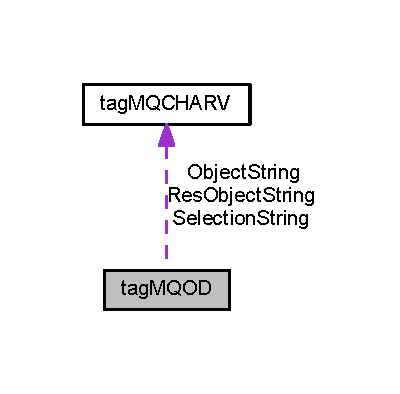
\includegraphics[width=192pt]{structtag_m_q_o_d__coll__graph}
\end{center}
\end{figure}
\subsection*{Campos de datos}
\begin{DoxyCompactItemize}
\item 
\hyperlink{cmqc_8h_a12590e546ed66fda7cf21c1d5cefa31d}{M\+Q\+C\+H\+A\+R4} \hyperlink{structtag_m_q_o_d_a0530922ca944569b52601d74941f96e4}{Struc\+Id}
\item 
\hyperlink{cmqc_8h_a1fb8d28cbda3fa8766a9821230cdb6d5}{M\+Q\+L\+O\+N\+G} \hyperlink{structtag_m_q_o_d_a0656ef8f766b3907d394d88a35d7b7e9}{Version}
\item 
\hyperlink{cmqc_8h_a1fb8d28cbda3fa8766a9821230cdb6d5}{M\+Q\+L\+O\+N\+G} \hyperlink{structtag_m_q_o_d_afe2238efcfc6d8a8de58f0622bb31caa}{Object\+Type}
\item 
\hyperlink{cmqc_8h_a53b1a2836da03f19144836725ff77919}{M\+Q\+C\+H\+A\+R48} \hyperlink{structtag_m_q_o_d_a2106fb125a9f7fc606340ba23c006bc0}{Object\+Name}
\item 
\hyperlink{cmqc_8h_a53b1a2836da03f19144836725ff77919}{M\+Q\+C\+H\+A\+R48} \hyperlink{structtag_m_q_o_d_ac72719d0cdc669269aa503462d5c7536}{Object\+Q\+Mgr\+Name}
\item 
\hyperlink{cmqc_8h_a53b1a2836da03f19144836725ff77919}{M\+Q\+C\+H\+A\+R48} \hyperlink{structtag_m_q_o_d_afc3f01c1aa256275bb086469bc1bae95}{Dynamic\+Q\+Name}
\item 
\hyperlink{cmqc_8h_a996cbcfd8d7ef4774f29b158a22d55c0}{M\+Q\+C\+H\+A\+R12} \hyperlink{structtag_m_q_o_d_aa4de0947b84fe1c303c8a5a419ef024a}{Alternate\+User\+Id}
\item 
\hyperlink{cmqc_8h_a1fb8d28cbda3fa8766a9821230cdb6d5}{M\+Q\+L\+O\+N\+G} \hyperlink{structtag_m_q_o_d_a7592da03e0f1c9bc79c9dd4e641dcf73}{Recs\+Present}
\item 
\hyperlink{cmqc_8h_a1fb8d28cbda3fa8766a9821230cdb6d5}{M\+Q\+L\+O\+N\+G} \hyperlink{structtag_m_q_o_d_ab63679527a2a808aa8c189eeca5d0712}{Known\+Dest\+Count}
\item 
\hyperlink{cmqc_8h_a1fb8d28cbda3fa8766a9821230cdb6d5}{M\+Q\+L\+O\+N\+G} \hyperlink{structtag_m_q_o_d_a6443c93f9930aa26f661e00e631a32ea}{Unknown\+Dest\+Count}
\item 
\hyperlink{cmqc_8h_a1fb8d28cbda3fa8766a9821230cdb6d5}{M\+Q\+L\+O\+N\+G} \hyperlink{structtag_m_q_o_d_af76c4c4a710793e086829eac1c995d36}{Invalid\+Dest\+Count}
\item 
\hyperlink{cmqc_8h_a1fb8d28cbda3fa8766a9821230cdb6d5}{M\+Q\+L\+O\+N\+G} \hyperlink{structtag_m_q_o_d_a8ec0fdf14ab5b4d0f7caf7f333dfbeb4}{Object\+Rec\+Offset}
\item 
\hyperlink{cmqc_8h_a1fb8d28cbda3fa8766a9821230cdb6d5}{M\+Q\+L\+O\+N\+G} \hyperlink{structtag_m_q_o_d_a944cab1325e5696fccf9202988c81066}{Response\+Rec\+Offset}
\item 
\hyperlink{cmqc_8h_a0b835d8e479d7c42242ed9c6b6572f5a}{M\+Q\+P\+T\+R} \hyperlink{structtag_m_q_o_d_aa46059ff8062713d03173a8847594a25}{Object\+Rec\+Ptr}
\item 
\hyperlink{cmqc_8h_a0b835d8e479d7c42242ed9c6b6572f5a}{M\+Q\+P\+T\+R} \hyperlink{structtag_m_q_o_d_a3f96e15a2299a7c139b78c4e1b8cb7cb}{Response\+Rec\+Ptr}
\item 
\hyperlink{cmqc_8h_a1674aecfb9c9ab107699326ec31c4944}{M\+Q\+B\+Y\+T\+E40} \hyperlink{structtag_m_q_o_d_adc1f3b4aa3c6e3f3187e75291146cae7}{Alternate\+Security\+Id}
\item 
\hyperlink{cmqc_8h_a53b1a2836da03f19144836725ff77919}{M\+Q\+C\+H\+A\+R48} \hyperlink{structtag_m_q_o_d_aec4a06d696b4370f0c86b129d9f868ca}{Resolved\+Q\+Name}
\item 
\hyperlink{cmqc_8h_a53b1a2836da03f19144836725ff77919}{M\+Q\+C\+H\+A\+R48} \hyperlink{structtag_m_q_o_d_af36c1b6e6f3f92e0c733c43da9fada3f}{Resolved\+Q\+Mgr\+Name}
\item 
\hyperlink{cmqc_8h_a2a61029e155515c1360dfc809dab6747}{M\+Q\+C\+H\+A\+R\+V} \hyperlink{structtag_m_q_o_d_a564791473371222ceb856cfaf02d6f91}{Object\+String}
\item 
\hyperlink{cmqc_8h_a2a61029e155515c1360dfc809dab6747}{M\+Q\+C\+H\+A\+R\+V} \hyperlink{structtag_m_q_o_d_ab3a91014a229bd897c17cbd04563bca2}{Selection\+String}
\item 
\hyperlink{cmqc_8h_a2a61029e155515c1360dfc809dab6747}{M\+Q\+C\+H\+A\+R\+V} \hyperlink{structtag_m_q_o_d_a8f35fe6f52369753de1259a9468437eb}{Res\+Object\+String}
\item 
\hyperlink{cmqc_8h_a1fb8d28cbda3fa8766a9821230cdb6d5}{M\+Q\+L\+O\+N\+G} \hyperlink{structtag_m_q_o_d_ab1523b449e77139034581b4e5f7c4201}{Resolved\+Type}
\end{DoxyCompactItemize}


\subsection{Descripción detallada}


Definición en la línea 4703 del archivo cmqc.\+h.



\subsection{Documentación de los campos}
\hypertarget{structtag_m_q_o_d_adc1f3b4aa3c6e3f3187e75291146cae7}{}\index{tag\+M\+Q\+O\+D@{tag\+M\+Q\+O\+D}!Alternate\+Security\+Id@{Alternate\+Security\+Id}}
\index{Alternate\+Security\+Id@{Alternate\+Security\+Id}!tag\+M\+Q\+O\+D@{tag\+M\+Q\+O\+D}}
\subsubsection[{Alternate\+Security\+Id}]{\setlength{\rightskip}{0pt plus 5cm}{\bf M\+Q\+B\+Y\+T\+E40} Alternate\+Security\+Id}\label{structtag_m_q_o_d_adc1f3b4aa3c6e3f3187e75291146cae7}


Definición en la línea 4727 del archivo cmqc.\+h.

\hypertarget{structtag_m_q_o_d_aa4de0947b84fe1c303c8a5a419ef024a}{}\index{tag\+M\+Q\+O\+D@{tag\+M\+Q\+O\+D}!Alternate\+User\+Id@{Alternate\+User\+Id}}
\index{Alternate\+User\+Id@{Alternate\+User\+Id}!tag\+M\+Q\+O\+D@{tag\+M\+Q\+O\+D}}
\subsubsection[{Alternate\+User\+Id}]{\setlength{\rightskip}{0pt plus 5cm}{\bf M\+Q\+C\+H\+A\+R12} Alternate\+User\+Id}\label{structtag_m_q_o_d_aa4de0947b84fe1c303c8a5a419ef024a}


Definición en la línea 4710 del archivo cmqc.\+h.

\hypertarget{structtag_m_q_o_d_afc3f01c1aa256275bb086469bc1bae95}{}\index{tag\+M\+Q\+O\+D@{tag\+M\+Q\+O\+D}!Dynamic\+Q\+Name@{Dynamic\+Q\+Name}}
\index{Dynamic\+Q\+Name@{Dynamic\+Q\+Name}!tag\+M\+Q\+O\+D@{tag\+M\+Q\+O\+D}}
\subsubsection[{Dynamic\+Q\+Name}]{\setlength{\rightskip}{0pt plus 5cm}{\bf M\+Q\+C\+H\+A\+R48} Dynamic\+Q\+Name}\label{structtag_m_q_o_d_afc3f01c1aa256275bb086469bc1bae95}


Definición en la línea 4709 del archivo cmqc.\+h.

\hypertarget{structtag_m_q_o_d_af76c4c4a710793e086829eac1c995d36}{}\index{tag\+M\+Q\+O\+D@{tag\+M\+Q\+O\+D}!Invalid\+Dest\+Count@{Invalid\+Dest\+Count}}
\index{Invalid\+Dest\+Count@{Invalid\+Dest\+Count}!tag\+M\+Q\+O\+D@{tag\+M\+Q\+O\+D}}
\subsubsection[{Invalid\+Dest\+Count}]{\setlength{\rightskip}{0pt plus 5cm}{\bf M\+Q\+L\+O\+N\+G} Invalid\+Dest\+Count}\label{structtag_m_q_o_d_af76c4c4a710793e086829eac1c995d36}


Definición en la línea 4717 del archivo cmqc.\+h.

\hypertarget{structtag_m_q_o_d_ab63679527a2a808aa8c189eeca5d0712}{}\index{tag\+M\+Q\+O\+D@{tag\+M\+Q\+O\+D}!Known\+Dest\+Count@{Known\+Dest\+Count}}
\index{Known\+Dest\+Count@{Known\+Dest\+Count}!tag\+M\+Q\+O\+D@{tag\+M\+Q\+O\+D}}
\subsubsection[{Known\+Dest\+Count}]{\setlength{\rightskip}{0pt plus 5cm}{\bf M\+Q\+L\+O\+N\+G} Known\+Dest\+Count}\label{structtag_m_q_o_d_ab63679527a2a808aa8c189eeca5d0712}


Definición en la línea 4714 del archivo cmqc.\+h.

\hypertarget{structtag_m_q_o_d_a2106fb125a9f7fc606340ba23c006bc0}{}\index{tag\+M\+Q\+O\+D@{tag\+M\+Q\+O\+D}!Object\+Name@{Object\+Name}}
\index{Object\+Name@{Object\+Name}!tag\+M\+Q\+O\+D@{tag\+M\+Q\+O\+D}}
\subsubsection[{Object\+Name}]{\setlength{\rightskip}{0pt plus 5cm}{\bf M\+Q\+C\+H\+A\+R48} Object\+Name}\label{structtag_m_q_o_d_a2106fb125a9f7fc606340ba23c006bc0}


Definición en la línea 4707 del archivo cmqc.\+h.

\hypertarget{structtag_m_q_o_d_ac72719d0cdc669269aa503462d5c7536}{}\index{tag\+M\+Q\+O\+D@{tag\+M\+Q\+O\+D}!Object\+Q\+Mgr\+Name@{Object\+Q\+Mgr\+Name}}
\index{Object\+Q\+Mgr\+Name@{Object\+Q\+Mgr\+Name}!tag\+M\+Q\+O\+D@{tag\+M\+Q\+O\+D}}
\subsubsection[{Object\+Q\+Mgr\+Name}]{\setlength{\rightskip}{0pt plus 5cm}{\bf M\+Q\+C\+H\+A\+R48} Object\+Q\+Mgr\+Name}\label{structtag_m_q_o_d_ac72719d0cdc669269aa503462d5c7536}


Definición en la línea 4708 del archivo cmqc.\+h.

\hypertarget{structtag_m_q_o_d_a8ec0fdf14ab5b4d0f7caf7f333dfbeb4}{}\index{tag\+M\+Q\+O\+D@{tag\+M\+Q\+O\+D}!Object\+Rec\+Offset@{Object\+Rec\+Offset}}
\index{Object\+Rec\+Offset@{Object\+Rec\+Offset}!tag\+M\+Q\+O\+D@{tag\+M\+Q\+O\+D}}
\subsubsection[{Object\+Rec\+Offset}]{\setlength{\rightskip}{0pt plus 5cm}{\bf M\+Q\+L\+O\+N\+G} Object\+Rec\+Offset}\label{structtag_m_q_o_d_a8ec0fdf14ab5b4d0f7caf7f333dfbeb4}


Definición en la línea 4719 del archivo cmqc.\+h.

\hypertarget{structtag_m_q_o_d_aa46059ff8062713d03173a8847594a25}{}\index{tag\+M\+Q\+O\+D@{tag\+M\+Q\+O\+D}!Object\+Rec\+Ptr@{Object\+Rec\+Ptr}}
\index{Object\+Rec\+Ptr@{Object\+Rec\+Ptr}!tag\+M\+Q\+O\+D@{tag\+M\+Q\+O\+D}}
\subsubsection[{Object\+Rec\+Ptr}]{\setlength{\rightskip}{0pt plus 5cm}{\bf M\+Q\+P\+T\+R} Object\+Rec\+Ptr}\label{structtag_m_q_o_d_aa46059ff8062713d03173a8847594a25}


Definición en la línea 4723 del archivo cmqc.\+h.

\hypertarget{structtag_m_q_o_d_a564791473371222ceb856cfaf02d6f91}{}\index{tag\+M\+Q\+O\+D@{tag\+M\+Q\+O\+D}!Object\+String@{Object\+String}}
\index{Object\+String@{Object\+String}!tag\+M\+Q\+O\+D@{tag\+M\+Q\+O\+D}}
\subsubsection[{Object\+String}]{\setlength{\rightskip}{0pt plus 5cm}{\bf M\+Q\+C\+H\+A\+R\+V} Object\+String}\label{structtag_m_q_o_d_a564791473371222ceb856cfaf02d6f91}


Definición en la línea 4731 del archivo cmqc.\+h.

\hypertarget{structtag_m_q_o_d_afe2238efcfc6d8a8de58f0622bb31caa}{}\index{tag\+M\+Q\+O\+D@{tag\+M\+Q\+O\+D}!Object\+Type@{Object\+Type}}
\index{Object\+Type@{Object\+Type}!tag\+M\+Q\+O\+D@{tag\+M\+Q\+O\+D}}
\subsubsection[{Object\+Type}]{\setlength{\rightskip}{0pt plus 5cm}{\bf M\+Q\+L\+O\+N\+G} Object\+Type}\label{structtag_m_q_o_d_afe2238efcfc6d8a8de58f0622bb31caa}


Definición en la línea 4706 del archivo cmqc.\+h.

\hypertarget{structtag_m_q_o_d_a7592da03e0f1c9bc79c9dd4e641dcf73}{}\index{tag\+M\+Q\+O\+D@{tag\+M\+Q\+O\+D}!Recs\+Present@{Recs\+Present}}
\index{Recs\+Present@{Recs\+Present}!tag\+M\+Q\+O\+D@{tag\+M\+Q\+O\+D}}
\subsubsection[{Recs\+Present}]{\setlength{\rightskip}{0pt plus 5cm}{\bf M\+Q\+L\+O\+N\+G} Recs\+Present}\label{structtag_m_q_o_d_a7592da03e0f1c9bc79c9dd4e641dcf73}


Definición en la línea 4712 del archivo cmqc.\+h.

\hypertarget{structtag_m_q_o_d_a8f35fe6f52369753de1259a9468437eb}{}\index{tag\+M\+Q\+O\+D@{tag\+M\+Q\+O\+D}!Res\+Object\+String@{Res\+Object\+String}}
\index{Res\+Object\+String@{Res\+Object\+String}!tag\+M\+Q\+O\+D@{tag\+M\+Q\+O\+D}}
\subsubsection[{Res\+Object\+String}]{\setlength{\rightskip}{0pt plus 5cm}{\bf M\+Q\+C\+H\+A\+R\+V} Res\+Object\+String}\label{structtag_m_q_o_d_a8f35fe6f52369753de1259a9468437eb}


Definición en la línea 4733 del archivo cmqc.\+h.

\hypertarget{structtag_m_q_o_d_af36c1b6e6f3f92e0c733c43da9fada3f}{}\index{tag\+M\+Q\+O\+D@{tag\+M\+Q\+O\+D}!Resolved\+Q\+Mgr\+Name@{Resolved\+Q\+Mgr\+Name}}
\index{Resolved\+Q\+Mgr\+Name@{Resolved\+Q\+Mgr\+Name}!tag\+M\+Q\+O\+D@{tag\+M\+Q\+O\+D}}
\subsubsection[{Resolved\+Q\+Mgr\+Name}]{\setlength{\rightskip}{0pt plus 5cm}{\bf M\+Q\+C\+H\+A\+R48} Resolved\+Q\+Mgr\+Name}\label{structtag_m_q_o_d_af36c1b6e6f3f92e0c733c43da9fada3f}


Definición en la línea 4729 del archivo cmqc.\+h.

\hypertarget{structtag_m_q_o_d_aec4a06d696b4370f0c86b129d9f868ca}{}\index{tag\+M\+Q\+O\+D@{tag\+M\+Q\+O\+D}!Resolved\+Q\+Name@{Resolved\+Q\+Name}}
\index{Resolved\+Q\+Name@{Resolved\+Q\+Name}!tag\+M\+Q\+O\+D@{tag\+M\+Q\+O\+D}}
\subsubsection[{Resolved\+Q\+Name}]{\setlength{\rightskip}{0pt plus 5cm}{\bf M\+Q\+C\+H\+A\+R48} Resolved\+Q\+Name}\label{structtag_m_q_o_d_aec4a06d696b4370f0c86b129d9f868ca}


Definición en la línea 4728 del archivo cmqc.\+h.

\hypertarget{structtag_m_q_o_d_ab1523b449e77139034581b4e5f7c4201}{}\index{tag\+M\+Q\+O\+D@{tag\+M\+Q\+O\+D}!Resolved\+Type@{Resolved\+Type}}
\index{Resolved\+Type@{Resolved\+Type}!tag\+M\+Q\+O\+D@{tag\+M\+Q\+O\+D}}
\subsubsection[{Resolved\+Type}]{\setlength{\rightskip}{0pt plus 5cm}{\bf M\+Q\+L\+O\+N\+G} Resolved\+Type}\label{structtag_m_q_o_d_ab1523b449e77139034581b4e5f7c4201}


Definición en la línea 4734 del archivo cmqc.\+h.

\hypertarget{structtag_m_q_o_d_a944cab1325e5696fccf9202988c81066}{}\index{tag\+M\+Q\+O\+D@{tag\+M\+Q\+O\+D}!Response\+Rec\+Offset@{Response\+Rec\+Offset}}
\index{Response\+Rec\+Offset@{Response\+Rec\+Offset}!tag\+M\+Q\+O\+D@{tag\+M\+Q\+O\+D}}
\subsubsection[{Response\+Rec\+Offset}]{\setlength{\rightskip}{0pt plus 5cm}{\bf M\+Q\+L\+O\+N\+G} Response\+Rec\+Offset}\label{structtag_m_q_o_d_a944cab1325e5696fccf9202988c81066}


Definición en la línea 4721 del archivo cmqc.\+h.

\hypertarget{structtag_m_q_o_d_a3f96e15a2299a7c139b78c4e1b8cb7cb}{}\index{tag\+M\+Q\+O\+D@{tag\+M\+Q\+O\+D}!Response\+Rec\+Ptr@{Response\+Rec\+Ptr}}
\index{Response\+Rec\+Ptr@{Response\+Rec\+Ptr}!tag\+M\+Q\+O\+D@{tag\+M\+Q\+O\+D}}
\subsubsection[{Response\+Rec\+Ptr}]{\setlength{\rightskip}{0pt plus 5cm}{\bf M\+Q\+P\+T\+R} Response\+Rec\+Ptr}\label{structtag_m_q_o_d_a3f96e15a2299a7c139b78c4e1b8cb7cb}


Definición en la línea 4724 del archivo cmqc.\+h.

\hypertarget{structtag_m_q_o_d_ab3a91014a229bd897c17cbd04563bca2}{}\index{tag\+M\+Q\+O\+D@{tag\+M\+Q\+O\+D}!Selection\+String@{Selection\+String}}
\index{Selection\+String@{Selection\+String}!tag\+M\+Q\+O\+D@{tag\+M\+Q\+O\+D}}
\subsubsection[{Selection\+String}]{\setlength{\rightskip}{0pt plus 5cm}{\bf M\+Q\+C\+H\+A\+R\+V} Selection\+String}\label{structtag_m_q_o_d_ab3a91014a229bd897c17cbd04563bca2}


Definición en la línea 4732 del archivo cmqc.\+h.

\hypertarget{structtag_m_q_o_d_a0530922ca944569b52601d74941f96e4}{}\index{tag\+M\+Q\+O\+D@{tag\+M\+Q\+O\+D}!Struc\+Id@{Struc\+Id}}
\index{Struc\+Id@{Struc\+Id}!tag\+M\+Q\+O\+D@{tag\+M\+Q\+O\+D}}
\subsubsection[{Struc\+Id}]{\setlength{\rightskip}{0pt plus 5cm}{\bf M\+Q\+C\+H\+A\+R4} Struc\+Id}\label{structtag_m_q_o_d_a0530922ca944569b52601d74941f96e4}


Definición en la línea 4704 del archivo cmqc.\+h.

\hypertarget{structtag_m_q_o_d_a6443c93f9930aa26f661e00e631a32ea}{}\index{tag\+M\+Q\+O\+D@{tag\+M\+Q\+O\+D}!Unknown\+Dest\+Count@{Unknown\+Dest\+Count}}
\index{Unknown\+Dest\+Count@{Unknown\+Dest\+Count}!tag\+M\+Q\+O\+D@{tag\+M\+Q\+O\+D}}
\subsubsection[{Unknown\+Dest\+Count}]{\setlength{\rightskip}{0pt plus 5cm}{\bf M\+Q\+L\+O\+N\+G} Unknown\+Dest\+Count}\label{structtag_m_q_o_d_a6443c93f9930aa26f661e00e631a32ea}


Definición en la línea 4716 del archivo cmqc.\+h.

\hypertarget{structtag_m_q_o_d_a0656ef8f766b3907d394d88a35d7b7e9}{}\index{tag\+M\+Q\+O\+D@{tag\+M\+Q\+O\+D}!Version@{Version}}
\index{Version@{Version}!tag\+M\+Q\+O\+D@{tag\+M\+Q\+O\+D}}
\subsubsection[{Version}]{\setlength{\rightskip}{0pt plus 5cm}{\bf M\+Q\+L\+O\+N\+G} Version}\label{structtag_m_q_o_d_a0656ef8f766b3907d394d88a35d7b7e9}


Definición en la línea 4705 del archivo cmqc.\+h.



La documentación para esta estructura fue generada a partir del siguiente fichero\+:\begin{DoxyCompactItemize}
\item 
include/\hyperlink{cmqc_8h}{cmqc.\+h}\end{DoxyCompactItemize}

\hypertarget{structtag_m_q_o_r}{}\section{Referencia de la Estructura tag\+M\+Q\+O\+R}
\label{structtag_m_q_o_r}\index{tag\+M\+Q\+O\+R@{tag\+M\+Q\+O\+R}}


{\ttfamily \#include $<$cmqc.\+h$>$}

\subsection*{Campos de datos}
\begin{DoxyCompactItemize}
\item 
\hyperlink{cmqc_8h_a53b1a2836da03f19144836725ff77919}{M\+Q\+C\+H\+A\+R48} \hyperlink{structtag_m_q_o_r_a2106fb125a9f7fc606340ba23c006bc0}{Object\+Name}
\item 
\hyperlink{cmqc_8h_a53b1a2836da03f19144836725ff77919}{M\+Q\+C\+H\+A\+R48} \hyperlink{structtag_m_q_o_r_ac72719d0cdc669269aa503462d5c7536}{Object\+Q\+Mgr\+Name}
\end{DoxyCompactItemize}


\subsection{Descripción detallada}


Definición en la línea 4770 del archivo cmqc.\+h.



\subsection{Documentación de los campos}
\hypertarget{structtag_m_q_o_r_a2106fb125a9f7fc606340ba23c006bc0}{}\index{tag\+M\+Q\+O\+R@{tag\+M\+Q\+O\+R}!Object\+Name@{Object\+Name}}
\index{Object\+Name@{Object\+Name}!tag\+M\+Q\+O\+R@{tag\+M\+Q\+O\+R}}
\subsubsection[{Object\+Name}]{\setlength{\rightskip}{0pt plus 5cm}{\bf M\+Q\+C\+H\+A\+R48} Object\+Name}\label{structtag_m_q_o_r_a2106fb125a9f7fc606340ba23c006bc0}


Definición en la línea 4771 del archivo cmqc.\+h.

\hypertarget{structtag_m_q_o_r_ac72719d0cdc669269aa503462d5c7536}{}\index{tag\+M\+Q\+O\+R@{tag\+M\+Q\+O\+R}!Object\+Q\+Mgr\+Name@{Object\+Q\+Mgr\+Name}}
\index{Object\+Q\+Mgr\+Name@{Object\+Q\+Mgr\+Name}!tag\+M\+Q\+O\+R@{tag\+M\+Q\+O\+R}}
\subsubsection[{Object\+Q\+Mgr\+Name}]{\setlength{\rightskip}{0pt plus 5cm}{\bf M\+Q\+C\+H\+A\+R48} Object\+Q\+Mgr\+Name}\label{structtag_m_q_o_r_ac72719d0cdc669269aa503462d5c7536}


Definición en la línea 4772 del archivo cmqc.\+h.



La documentación para esta estructura fue generada a partir del siguiente fichero\+:\begin{DoxyCompactItemize}
\item 
include/\hyperlink{cmqc_8h}{cmqc.\+h}\end{DoxyCompactItemize}

\hypertarget{structtag_m_q_p_d}{}\section{Referencia de la Estructura tag\+M\+Q\+P\+D}
\label{structtag_m_q_p_d}\index{tag\+M\+Q\+P\+D@{tag\+M\+Q\+P\+D}}


{\ttfamily \#include $<$cmqc.\+h$>$}

\subsection*{Campos de datos}
\begin{DoxyCompactItemize}
\item 
\hyperlink{cmqc_8h_a12590e546ed66fda7cf21c1d5cefa31d}{M\+Q\+C\+H\+A\+R4} \hyperlink{structtag_m_q_p_d_a0530922ca944569b52601d74941f96e4}{Struc\+Id}
\item 
\hyperlink{cmqc_8h_a1fb8d28cbda3fa8766a9821230cdb6d5}{M\+Q\+L\+O\+N\+G} \hyperlink{structtag_m_q_p_d_a0656ef8f766b3907d394d88a35d7b7e9}{Version}
\item 
\hyperlink{cmqc_8h_a1fb8d28cbda3fa8766a9821230cdb6d5}{M\+Q\+L\+O\+N\+G} \hyperlink{structtag_m_q_p_d_ad7aff2d6c6044809464380998d24ec5c}{Options}
\item 
\hyperlink{cmqc_8h_a1fb8d28cbda3fa8766a9821230cdb6d5}{M\+Q\+L\+O\+N\+G} \hyperlink{structtag_m_q_p_d_af5d5b2a40b10005006c5584e02c61796}{Support}
\item 
\hyperlink{cmqc_8h_a1fb8d28cbda3fa8766a9821230cdb6d5}{M\+Q\+L\+O\+N\+G} \hyperlink{structtag_m_q_p_d_ae02ee8a9bc114b5315e104f8b7d6249a}{Context}
\item 
\hyperlink{cmqc_8h_a1fb8d28cbda3fa8766a9821230cdb6d5}{M\+Q\+L\+O\+N\+G} \hyperlink{structtag_m_q_p_d_a64944f1782a83f9e73e9a7bdbd7b5544}{Copy\+Options}
\end{DoxyCompactItemize}


\subsection{Descripción detallada}


Definición en la línea 4786 del archivo cmqc.\+h.



\subsection{Documentación de los campos}
\hypertarget{structtag_m_q_p_d_ae02ee8a9bc114b5315e104f8b7d6249a}{}\index{tag\+M\+Q\+P\+D@{tag\+M\+Q\+P\+D}!Context@{Context}}
\index{Context@{Context}!tag\+M\+Q\+P\+D@{tag\+M\+Q\+P\+D}}
\subsubsection[{Context}]{\setlength{\rightskip}{0pt plus 5cm}{\bf M\+Q\+L\+O\+N\+G} Context}\label{structtag_m_q_p_d_ae02ee8a9bc114b5315e104f8b7d6249a}


Definición en la línea 4792 del archivo cmqc.\+h.

\hypertarget{structtag_m_q_p_d_a64944f1782a83f9e73e9a7bdbd7b5544}{}\index{tag\+M\+Q\+P\+D@{tag\+M\+Q\+P\+D}!Copy\+Options@{Copy\+Options}}
\index{Copy\+Options@{Copy\+Options}!tag\+M\+Q\+P\+D@{tag\+M\+Q\+P\+D}}
\subsubsection[{Copy\+Options}]{\setlength{\rightskip}{0pt plus 5cm}{\bf M\+Q\+L\+O\+N\+G} Copy\+Options}\label{structtag_m_q_p_d_a64944f1782a83f9e73e9a7bdbd7b5544}


Definición en la línea 4793 del archivo cmqc.\+h.

\hypertarget{structtag_m_q_p_d_ad7aff2d6c6044809464380998d24ec5c}{}\index{tag\+M\+Q\+P\+D@{tag\+M\+Q\+P\+D}!Options@{Options}}
\index{Options@{Options}!tag\+M\+Q\+P\+D@{tag\+M\+Q\+P\+D}}
\subsubsection[{Options}]{\setlength{\rightskip}{0pt plus 5cm}{\bf M\+Q\+L\+O\+N\+G} Options}\label{structtag_m_q_p_d_ad7aff2d6c6044809464380998d24ec5c}


Definición en la línea 4789 del archivo cmqc.\+h.

\hypertarget{structtag_m_q_p_d_a0530922ca944569b52601d74941f96e4}{}\index{tag\+M\+Q\+P\+D@{tag\+M\+Q\+P\+D}!Struc\+Id@{Struc\+Id}}
\index{Struc\+Id@{Struc\+Id}!tag\+M\+Q\+P\+D@{tag\+M\+Q\+P\+D}}
\subsubsection[{Struc\+Id}]{\setlength{\rightskip}{0pt plus 5cm}{\bf M\+Q\+C\+H\+A\+R4} Struc\+Id}\label{structtag_m_q_p_d_a0530922ca944569b52601d74941f96e4}


Definición en la línea 4787 del archivo cmqc.\+h.

\hypertarget{structtag_m_q_p_d_af5d5b2a40b10005006c5584e02c61796}{}\index{tag\+M\+Q\+P\+D@{tag\+M\+Q\+P\+D}!Support@{Support}}
\index{Support@{Support}!tag\+M\+Q\+P\+D@{tag\+M\+Q\+P\+D}}
\subsubsection[{Support}]{\setlength{\rightskip}{0pt plus 5cm}{\bf M\+Q\+L\+O\+N\+G} Support}\label{structtag_m_q_p_d_af5d5b2a40b10005006c5584e02c61796}


Definición en la línea 4791 del archivo cmqc.\+h.

\hypertarget{structtag_m_q_p_d_a0656ef8f766b3907d394d88a35d7b7e9}{}\index{tag\+M\+Q\+P\+D@{tag\+M\+Q\+P\+D}!Version@{Version}}
\index{Version@{Version}!tag\+M\+Q\+P\+D@{tag\+M\+Q\+P\+D}}
\subsubsection[{Version}]{\setlength{\rightskip}{0pt plus 5cm}{\bf M\+Q\+L\+O\+N\+G} Version}\label{structtag_m_q_p_d_a0656ef8f766b3907d394d88a35d7b7e9}


Definición en la línea 4788 del archivo cmqc.\+h.



La documentación para esta estructura fue generada a partir del siguiente fichero\+:\begin{DoxyCompactItemize}
\item 
include/\hyperlink{cmqc_8h}{cmqc.\+h}\end{DoxyCompactItemize}

\hypertarget{structtag_m_q_p_m_o}{}\section{Referencia de la Estructura tag\+M\+Q\+P\+M\+O}
\label{structtag_m_q_p_m_o}\index{tag\+M\+Q\+P\+M\+O@{tag\+M\+Q\+P\+M\+O}}


{\ttfamily \#include $<$cmqc.\+h$>$}

\subsection*{Campos de datos}
\begin{DoxyCompactItemize}
\item 
\hyperlink{cmqc_8h_a12590e546ed66fda7cf21c1d5cefa31d}{M\+Q\+C\+H\+A\+R4} \hyperlink{structtag_m_q_p_m_o_a0530922ca944569b52601d74941f96e4}{Struc\+Id}
\item 
\hyperlink{cmqc_8h_a1fb8d28cbda3fa8766a9821230cdb6d5}{M\+Q\+L\+O\+N\+G} \hyperlink{structtag_m_q_p_m_o_a0656ef8f766b3907d394d88a35d7b7e9}{Version}
\item 
\hyperlink{cmqc_8h_a1fb8d28cbda3fa8766a9821230cdb6d5}{M\+Q\+L\+O\+N\+G} \hyperlink{structtag_m_q_p_m_o_ad7aff2d6c6044809464380998d24ec5c}{Options}
\item 
\hyperlink{cmqc_8h_a1fb8d28cbda3fa8766a9821230cdb6d5}{M\+Q\+L\+O\+N\+G} \hyperlink{structtag_m_q_p_m_o_a9a46af4b5b34638a690924bb9709c5ba}{Timeout}
\item 
\hyperlink{cmqc_8h_ac093f559f81163292e6016c68c947164}{M\+Q\+H\+O\+B\+J} \hyperlink{structtag_m_q_p_m_o_aa4e5a2da2b7009e9a1cb3afa41140718}{Context}
\item 
\hyperlink{cmqc_8h_a1fb8d28cbda3fa8766a9821230cdb6d5}{M\+Q\+L\+O\+N\+G} \hyperlink{structtag_m_q_p_m_o_ab63679527a2a808aa8c189eeca5d0712}{Known\+Dest\+Count}
\item 
\hyperlink{cmqc_8h_a1fb8d28cbda3fa8766a9821230cdb6d5}{M\+Q\+L\+O\+N\+G} \hyperlink{structtag_m_q_p_m_o_a6443c93f9930aa26f661e00e631a32ea}{Unknown\+Dest\+Count}
\item 
\hyperlink{cmqc_8h_a1fb8d28cbda3fa8766a9821230cdb6d5}{M\+Q\+L\+O\+N\+G} \hyperlink{structtag_m_q_p_m_o_af76c4c4a710793e086829eac1c995d36}{Invalid\+Dest\+Count}
\item 
\hyperlink{cmqc_8h_a53b1a2836da03f19144836725ff77919}{M\+Q\+C\+H\+A\+R48} \hyperlink{structtag_m_q_p_m_o_aec4a06d696b4370f0c86b129d9f868ca}{Resolved\+Q\+Name}
\item 
\hyperlink{cmqc_8h_a53b1a2836da03f19144836725ff77919}{M\+Q\+C\+H\+A\+R48} \hyperlink{structtag_m_q_p_m_o_af36c1b6e6f3f92e0c733c43da9fada3f}{Resolved\+Q\+Mgr\+Name}
\item 
\hyperlink{cmqc_8h_a1fb8d28cbda3fa8766a9821230cdb6d5}{M\+Q\+L\+O\+N\+G} \hyperlink{structtag_m_q_p_m_o_a7592da03e0f1c9bc79c9dd4e641dcf73}{Recs\+Present}
\item 
\hyperlink{cmqc_8h_a1fb8d28cbda3fa8766a9821230cdb6d5}{M\+Q\+L\+O\+N\+G} \hyperlink{structtag_m_q_p_m_o_aea1b77e1a6f2b6f18526055315f8b175}{Put\+Msg\+Rec\+Fields}
\item 
\hyperlink{cmqc_8h_a1fb8d28cbda3fa8766a9821230cdb6d5}{M\+Q\+L\+O\+N\+G} \hyperlink{structtag_m_q_p_m_o_a49f55d9686cdc9c051e09950fede2098}{Put\+Msg\+Rec\+Offset}
\item 
\hyperlink{cmqc_8h_a1fb8d28cbda3fa8766a9821230cdb6d5}{M\+Q\+L\+O\+N\+G} \hyperlink{structtag_m_q_p_m_o_a944cab1325e5696fccf9202988c81066}{Response\+Rec\+Offset}
\item 
\hyperlink{cmqc_8h_a0b835d8e479d7c42242ed9c6b6572f5a}{M\+Q\+P\+T\+R} \hyperlink{structtag_m_q_p_m_o_a6721429432b0d4229bdc5477777f0937}{Put\+Msg\+Rec\+Ptr}
\item 
\hyperlink{cmqc_8h_a0b835d8e479d7c42242ed9c6b6572f5a}{M\+Q\+P\+T\+R} \hyperlink{structtag_m_q_p_m_o_a3f96e15a2299a7c139b78c4e1b8cb7cb}{Response\+Rec\+Ptr}
\item 
\hyperlink{cmqc_8h_a3d110c5d019358ed30e069abddd9525c}{M\+Q\+H\+M\+S\+G} \hyperlink{structtag_m_q_p_m_o_ae085f237b8d312cc17a08ee5b890698b}{Original\+Msg\+Handle}
\item 
\hyperlink{cmqc_8h_a3d110c5d019358ed30e069abddd9525c}{M\+Q\+H\+M\+S\+G} \hyperlink{structtag_m_q_p_m_o_a9daf07c64f152de0db1a09b8033a87d5}{New\+Msg\+Handle}
\item 
\hyperlink{cmqc_8h_a1fb8d28cbda3fa8766a9821230cdb6d5}{M\+Q\+L\+O\+N\+G} \hyperlink{structtag_m_q_p_m_o_ac3faa33ea60209cfd14ccd29ef325788}{Action}
\item 
\hyperlink{cmqc_8h_a1fb8d28cbda3fa8766a9821230cdb6d5}{M\+Q\+L\+O\+N\+G} \hyperlink{structtag_m_q_p_m_o_ab5df476923b8b98b937d42b572a20e07}{Pub\+Level}
\end{DoxyCompactItemize}


\subsection{Descripción detallada}


Definición en la línea 4812 del archivo cmqc.\+h.



\subsection{Documentación de los campos}
\hypertarget{structtag_m_q_p_m_o_ac3faa33ea60209cfd14ccd29ef325788}{}\index{tag\+M\+Q\+P\+M\+O@{tag\+M\+Q\+P\+M\+O}!Action@{Action}}
\index{Action@{Action}!tag\+M\+Q\+P\+M\+O@{tag\+M\+Q\+P\+M\+O}}
\subsubsection[{Action}]{\setlength{\rightskip}{0pt plus 5cm}{\bf M\+Q\+L\+O\+N\+G} Action}\label{structtag_m_q_p_m_o_ac3faa33ea60209cfd14ccd29ef325788}


Definición en la línea 4844 del archivo cmqc.\+h.

\hypertarget{structtag_m_q_p_m_o_aa4e5a2da2b7009e9a1cb3afa41140718}{}\index{tag\+M\+Q\+P\+M\+O@{tag\+M\+Q\+P\+M\+O}!Context@{Context}}
\index{Context@{Context}!tag\+M\+Q\+P\+M\+O@{tag\+M\+Q\+P\+M\+O}}
\subsubsection[{Context}]{\setlength{\rightskip}{0pt plus 5cm}{\bf M\+Q\+H\+O\+B\+J} Context}\label{structtag_m_q_p_m_o_aa4e5a2da2b7009e9a1cb3afa41140718}


Definición en la línea 4818 del archivo cmqc.\+h.

\hypertarget{structtag_m_q_p_m_o_af76c4c4a710793e086829eac1c995d36}{}\index{tag\+M\+Q\+P\+M\+O@{tag\+M\+Q\+P\+M\+O}!Invalid\+Dest\+Count@{Invalid\+Dest\+Count}}
\index{Invalid\+Dest\+Count@{Invalid\+Dest\+Count}!tag\+M\+Q\+P\+M\+O@{tag\+M\+Q\+P\+M\+O}}
\subsubsection[{Invalid\+Dest\+Count}]{\setlength{\rightskip}{0pt plus 5cm}{\bf M\+Q\+L\+O\+N\+G} Invalid\+Dest\+Count}\label{structtag_m_q_p_m_o_af76c4c4a710793e086829eac1c995d36}


Definición en la línea 4823 del archivo cmqc.\+h.

\hypertarget{structtag_m_q_p_m_o_ab63679527a2a808aa8c189eeca5d0712}{}\index{tag\+M\+Q\+P\+M\+O@{tag\+M\+Q\+P\+M\+O}!Known\+Dest\+Count@{Known\+Dest\+Count}}
\index{Known\+Dest\+Count@{Known\+Dest\+Count}!tag\+M\+Q\+P\+M\+O@{tag\+M\+Q\+P\+M\+O}}
\subsubsection[{Known\+Dest\+Count}]{\setlength{\rightskip}{0pt plus 5cm}{\bf M\+Q\+L\+O\+N\+G} Known\+Dest\+Count}\label{structtag_m_q_p_m_o_ab63679527a2a808aa8c189eeca5d0712}


Definición en la línea 4819 del archivo cmqc.\+h.

\hypertarget{structtag_m_q_p_m_o_a9daf07c64f152de0db1a09b8033a87d5}{}\index{tag\+M\+Q\+P\+M\+O@{tag\+M\+Q\+P\+M\+O}!New\+Msg\+Handle@{New\+Msg\+Handle}}
\index{New\+Msg\+Handle@{New\+Msg\+Handle}!tag\+M\+Q\+P\+M\+O@{tag\+M\+Q\+P\+M\+O}}
\subsubsection[{New\+Msg\+Handle}]{\setlength{\rightskip}{0pt plus 5cm}{\bf M\+Q\+H\+M\+S\+G} New\+Msg\+Handle}\label{structtag_m_q_p_m_o_a9daf07c64f152de0db1a09b8033a87d5}


Definición en la línea 4843 del archivo cmqc.\+h.

\hypertarget{structtag_m_q_p_m_o_ad7aff2d6c6044809464380998d24ec5c}{}\index{tag\+M\+Q\+P\+M\+O@{tag\+M\+Q\+P\+M\+O}!Options@{Options}}
\index{Options@{Options}!tag\+M\+Q\+P\+M\+O@{tag\+M\+Q\+P\+M\+O}}
\subsubsection[{Options}]{\setlength{\rightskip}{0pt plus 5cm}{\bf M\+Q\+L\+O\+N\+G} Options}\label{structtag_m_q_p_m_o_ad7aff2d6c6044809464380998d24ec5c}


Definición en la línea 4815 del archivo cmqc.\+h.

\hypertarget{structtag_m_q_p_m_o_ae085f237b8d312cc17a08ee5b890698b}{}\index{tag\+M\+Q\+P\+M\+O@{tag\+M\+Q\+P\+M\+O}!Original\+Msg\+Handle@{Original\+Msg\+Handle}}
\index{Original\+Msg\+Handle@{Original\+Msg\+Handle}!tag\+M\+Q\+P\+M\+O@{tag\+M\+Q\+P\+M\+O}}
\subsubsection[{Original\+Msg\+Handle}]{\setlength{\rightskip}{0pt plus 5cm}{\bf M\+Q\+H\+M\+S\+G} Original\+Msg\+Handle}\label{structtag_m_q_p_m_o_ae085f237b8d312cc17a08ee5b890698b}


Definición en la línea 4842 del archivo cmqc.\+h.

\hypertarget{structtag_m_q_p_m_o_ab5df476923b8b98b937d42b572a20e07}{}\index{tag\+M\+Q\+P\+M\+O@{tag\+M\+Q\+P\+M\+O}!Pub\+Level@{Pub\+Level}}
\index{Pub\+Level@{Pub\+Level}!tag\+M\+Q\+P\+M\+O@{tag\+M\+Q\+P\+M\+O}}
\subsubsection[{Pub\+Level}]{\setlength{\rightskip}{0pt plus 5cm}{\bf M\+Q\+L\+O\+N\+G} Pub\+Level}\label{structtag_m_q_p_m_o_ab5df476923b8b98b937d42b572a20e07}


Definición en la línea 4845 del archivo cmqc.\+h.

\hypertarget{structtag_m_q_p_m_o_aea1b77e1a6f2b6f18526055315f8b175}{}\index{tag\+M\+Q\+P\+M\+O@{tag\+M\+Q\+P\+M\+O}!Put\+Msg\+Rec\+Fields@{Put\+Msg\+Rec\+Fields}}
\index{Put\+Msg\+Rec\+Fields@{Put\+Msg\+Rec\+Fields}!tag\+M\+Q\+P\+M\+O@{tag\+M\+Q\+P\+M\+O}}
\subsubsection[{Put\+Msg\+Rec\+Fields}]{\setlength{\rightskip}{0pt plus 5cm}{\bf M\+Q\+L\+O\+N\+G} Put\+Msg\+Rec\+Fields}\label{structtag_m_q_p_m_o_aea1b77e1a6f2b6f18526055315f8b175}


Definición en la línea 4832 del archivo cmqc.\+h.

\hypertarget{structtag_m_q_p_m_o_a49f55d9686cdc9c051e09950fede2098}{}\index{tag\+M\+Q\+P\+M\+O@{tag\+M\+Q\+P\+M\+O}!Put\+Msg\+Rec\+Offset@{Put\+Msg\+Rec\+Offset}}
\index{Put\+Msg\+Rec\+Offset@{Put\+Msg\+Rec\+Offset}!tag\+M\+Q\+P\+M\+O@{tag\+M\+Q\+P\+M\+O}}
\subsubsection[{Put\+Msg\+Rec\+Offset}]{\setlength{\rightskip}{0pt plus 5cm}{\bf M\+Q\+L\+O\+N\+G} Put\+Msg\+Rec\+Offset}\label{structtag_m_q_p_m_o_a49f55d9686cdc9c051e09950fede2098}


Definición en la línea 4834 del archivo cmqc.\+h.

\hypertarget{structtag_m_q_p_m_o_a6721429432b0d4229bdc5477777f0937}{}\index{tag\+M\+Q\+P\+M\+O@{tag\+M\+Q\+P\+M\+O}!Put\+Msg\+Rec\+Ptr@{Put\+Msg\+Rec\+Ptr}}
\index{Put\+Msg\+Rec\+Ptr@{Put\+Msg\+Rec\+Ptr}!tag\+M\+Q\+P\+M\+O@{tag\+M\+Q\+P\+M\+O}}
\subsubsection[{Put\+Msg\+Rec\+Ptr}]{\setlength{\rightskip}{0pt plus 5cm}{\bf M\+Q\+P\+T\+R} Put\+Msg\+Rec\+Ptr}\label{structtag_m_q_p_m_o_a6721429432b0d4229bdc5477777f0937}


Definición en la línea 4838 del archivo cmqc.\+h.

\hypertarget{structtag_m_q_p_m_o_a7592da03e0f1c9bc79c9dd4e641dcf73}{}\index{tag\+M\+Q\+P\+M\+O@{tag\+M\+Q\+P\+M\+O}!Recs\+Present@{Recs\+Present}}
\index{Recs\+Present@{Recs\+Present}!tag\+M\+Q\+P\+M\+O@{tag\+M\+Q\+P\+M\+O}}
\subsubsection[{Recs\+Present}]{\setlength{\rightskip}{0pt plus 5cm}{\bf M\+Q\+L\+O\+N\+G} Recs\+Present}\label{structtag_m_q_p_m_o_a7592da03e0f1c9bc79c9dd4e641dcf73}


Definición en la línea 4830 del archivo cmqc.\+h.

\hypertarget{structtag_m_q_p_m_o_af36c1b6e6f3f92e0c733c43da9fada3f}{}\index{tag\+M\+Q\+P\+M\+O@{tag\+M\+Q\+P\+M\+O}!Resolved\+Q\+Mgr\+Name@{Resolved\+Q\+Mgr\+Name}}
\index{Resolved\+Q\+Mgr\+Name@{Resolved\+Q\+Mgr\+Name}!tag\+M\+Q\+P\+M\+O@{tag\+M\+Q\+P\+M\+O}}
\subsubsection[{Resolved\+Q\+Mgr\+Name}]{\setlength{\rightskip}{0pt plus 5cm}{\bf M\+Q\+C\+H\+A\+R48} Resolved\+Q\+Mgr\+Name}\label{structtag_m_q_p_m_o_af36c1b6e6f3f92e0c733c43da9fada3f}


Definición en la línea 4827 del archivo cmqc.\+h.

\hypertarget{structtag_m_q_p_m_o_aec4a06d696b4370f0c86b129d9f868ca}{}\index{tag\+M\+Q\+P\+M\+O@{tag\+M\+Q\+P\+M\+O}!Resolved\+Q\+Name@{Resolved\+Q\+Name}}
\index{Resolved\+Q\+Name@{Resolved\+Q\+Name}!tag\+M\+Q\+P\+M\+O@{tag\+M\+Q\+P\+M\+O}}
\subsubsection[{Resolved\+Q\+Name}]{\setlength{\rightskip}{0pt plus 5cm}{\bf M\+Q\+C\+H\+A\+R48} Resolved\+Q\+Name}\label{structtag_m_q_p_m_o_aec4a06d696b4370f0c86b129d9f868ca}


Definición en la línea 4825 del archivo cmqc.\+h.

\hypertarget{structtag_m_q_p_m_o_a944cab1325e5696fccf9202988c81066}{}\index{tag\+M\+Q\+P\+M\+O@{tag\+M\+Q\+P\+M\+O}!Response\+Rec\+Offset@{Response\+Rec\+Offset}}
\index{Response\+Rec\+Offset@{Response\+Rec\+Offset}!tag\+M\+Q\+P\+M\+O@{tag\+M\+Q\+P\+M\+O}}
\subsubsection[{Response\+Rec\+Offset}]{\setlength{\rightskip}{0pt plus 5cm}{\bf M\+Q\+L\+O\+N\+G} Response\+Rec\+Offset}\label{structtag_m_q_p_m_o_a944cab1325e5696fccf9202988c81066}


Definición en la línea 4836 del archivo cmqc.\+h.

\hypertarget{structtag_m_q_p_m_o_a3f96e15a2299a7c139b78c4e1b8cb7cb}{}\index{tag\+M\+Q\+P\+M\+O@{tag\+M\+Q\+P\+M\+O}!Response\+Rec\+Ptr@{Response\+Rec\+Ptr}}
\index{Response\+Rec\+Ptr@{Response\+Rec\+Ptr}!tag\+M\+Q\+P\+M\+O@{tag\+M\+Q\+P\+M\+O}}
\subsubsection[{Response\+Rec\+Ptr}]{\setlength{\rightskip}{0pt plus 5cm}{\bf M\+Q\+P\+T\+R} Response\+Rec\+Ptr}\label{structtag_m_q_p_m_o_a3f96e15a2299a7c139b78c4e1b8cb7cb}


Definición en la línea 4840 del archivo cmqc.\+h.

\hypertarget{structtag_m_q_p_m_o_a0530922ca944569b52601d74941f96e4}{}\index{tag\+M\+Q\+P\+M\+O@{tag\+M\+Q\+P\+M\+O}!Struc\+Id@{Struc\+Id}}
\index{Struc\+Id@{Struc\+Id}!tag\+M\+Q\+P\+M\+O@{tag\+M\+Q\+P\+M\+O}}
\subsubsection[{Struc\+Id}]{\setlength{\rightskip}{0pt plus 5cm}{\bf M\+Q\+C\+H\+A\+R4} Struc\+Id}\label{structtag_m_q_p_m_o_a0530922ca944569b52601d74941f96e4}


Definición en la línea 4813 del archivo cmqc.\+h.

\hypertarget{structtag_m_q_p_m_o_a9a46af4b5b34638a690924bb9709c5ba}{}\index{tag\+M\+Q\+P\+M\+O@{tag\+M\+Q\+P\+M\+O}!Timeout@{Timeout}}
\index{Timeout@{Timeout}!tag\+M\+Q\+P\+M\+O@{tag\+M\+Q\+P\+M\+O}}
\subsubsection[{Timeout}]{\setlength{\rightskip}{0pt plus 5cm}{\bf M\+Q\+L\+O\+N\+G} Timeout}\label{structtag_m_q_p_m_o_a9a46af4b5b34638a690924bb9709c5ba}


Definición en la línea 4817 del archivo cmqc.\+h.

\hypertarget{structtag_m_q_p_m_o_a6443c93f9930aa26f661e00e631a32ea}{}\index{tag\+M\+Q\+P\+M\+O@{tag\+M\+Q\+P\+M\+O}!Unknown\+Dest\+Count@{Unknown\+Dest\+Count}}
\index{Unknown\+Dest\+Count@{Unknown\+Dest\+Count}!tag\+M\+Q\+P\+M\+O@{tag\+M\+Q\+P\+M\+O}}
\subsubsection[{Unknown\+Dest\+Count}]{\setlength{\rightskip}{0pt plus 5cm}{\bf M\+Q\+L\+O\+N\+G} Unknown\+Dest\+Count}\label{structtag_m_q_p_m_o_a6443c93f9930aa26f661e00e631a32ea}


Definición en la línea 4821 del archivo cmqc.\+h.

\hypertarget{structtag_m_q_p_m_o_a0656ef8f766b3907d394d88a35d7b7e9}{}\index{tag\+M\+Q\+P\+M\+O@{tag\+M\+Q\+P\+M\+O}!Version@{Version}}
\index{Version@{Version}!tag\+M\+Q\+P\+M\+O@{tag\+M\+Q\+P\+M\+O}}
\subsubsection[{Version}]{\setlength{\rightskip}{0pt plus 5cm}{\bf M\+Q\+L\+O\+N\+G} Version}\label{structtag_m_q_p_m_o_a0656ef8f766b3907d394d88a35d7b7e9}


Definición en la línea 4814 del archivo cmqc.\+h.



La documentación para esta estructura fue generada a partir del siguiente fichero\+:\begin{DoxyCompactItemize}
\item 
include/\hyperlink{cmqc_8h}{cmqc.\+h}\end{DoxyCompactItemize}

\hypertarget{structtag_m_q_r_f_h}{}\section{Referencia de la Estructura tag\+M\+Q\+R\+F\+H}
\label{structtag_m_q_r_f_h}\index{tag\+M\+Q\+R\+F\+H@{tag\+M\+Q\+R\+F\+H}}


{\ttfamily \#include $<$cmqc.\+h$>$}

\subsection*{Campos de datos}
\begin{DoxyCompactItemize}
\item 
\hyperlink{cmqc_8h_a12590e546ed66fda7cf21c1d5cefa31d}{M\+Q\+C\+H\+A\+R4} \hyperlink{structtag_m_q_r_f_h_a0530922ca944569b52601d74941f96e4}{Struc\+Id}
\item 
\hyperlink{cmqc_8h_a1fb8d28cbda3fa8766a9821230cdb6d5}{M\+Q\+L\+O\+N\+G} \hyperlink{structtag_m_q_r_f_h_a0656ef8f766b3907d394d88a35d7b7e9}{Version}
\item 
\hyperlink{cmqc_8h_a1fb8d28cbda3fa8766a9821230cdb6d5}{M\+Q\+L\+O\+N\+G} \hyperlink{structtag_m_q_r_f_h_a830af9a4a08c015b9a4b2d39d4d3420a}{Struc\+Length}
\item 
\hyperlink{cmqc_8h_a1fb8d28cbda3fa8766a9821230cdb6d5}{M\+Q\+L\+O\+N\+G} \hyperlink{structtag_m_q_r_f_h_a30167bf454a49a60fd3fe4e9e586af34}{Encoding}
\item 
\hyperlink{cmqc_8h_a1fb8d28cbda3fa8766a9821230cdb6d5}{M\+Q\+L\+O\+N\+G} \hyperlink{structtag_m_q_r_f_h_a4d8d1961a991850d1355cdf9b4680b8e}{Coded\+Char\+Set\+Id}
\item 
\hyperlink{cmqc_8h_abddcedb8c41fa262f2bd05dfec3e60a5}{M\+Q\+C\+H\+A\+R8} \hyperlink{structtag_m_q_r_f_h_a435a478822008713f8aaff89f369ed63}{Format}
\item 
\hyperlink{cmqc_8h_a1fb8d28cbda3fa8766a9821230cdb6d5}{M\+Q\+L\+O\+N\+G} \hyperlink{structtag_m_q_r_f_h_a8da770267273b200fa9c968fa2a0da57}{Flags}
\end{DoxyCompactItemize}


\subsection{Descripción detallada}


Definición en la línea 4878 del archivo cmqc.\+h.



\subsection{Documentación de los campos}
\hypertarget{structtag_m_q_r_f_h_a4d8d1961a991850d1355cdf9b4680b8e}{}\index{tag\+M\+Q\+R\+F\+H@{tag\+M\+Q\+R\+F\+H}!Coded\+Char\+Set\+Id@{Coded\+Char\+Set\+Id}}
\index{Coded\+Char\+Set\+Id@{Coded\+Char\+Set\+Id}!tag\+M\+Q\+R\+F\+H@{tag\+M\+Q\+R\+F\+H}}
\subsubsection[{Coded\+Char\+Set\+Id}]{\setlength{\rightskip}{0pt plus 5cm}{\bf M\+Q\+L\+O\+N\+G} Coded\+Char\+Set\+Id}\label{structtag_m_q_r_f_h_a4d8d1961a991850d1355cdf9b4680b8e}


Definición en la línea 4885 del archivo cmqc.\+h.

\hypertarget{structtag_m_q_r_f_h_a30167bf454a49a60fd3fe4e9e586af34}{}\index{tag\+M\+Q\+R\+F\+H@{tag\+M\+Q\+R\+F\+H}!Encoding@{Encoding}}
\index{Encoding@{Encoding}!tag\+M\+Q\+R\+F\+H@{tag\+M\+Q\+R\+F\+H}}
\subsubsection[{Encoding}]{\setlength{\rightskip}{0pt plus 5cm}{\bf M\+Q\+L\+O\+N\+G} Encoding}\label{structtag_m_q_r_f_h_a30167bf454a49a60fd3fe4e9e586af34}


Definición en la línea 4883 del archivo cmqc.\+h.

\hypertarget{structtag_m_q_r_f_h_a8da770267273b200fa9c968fa2a0da57}{}\index{tag\+M\+Q\+R\+F\+H@{tag\+M\+Q\+R\+F\+H}!Flags@{Flags}}
\index{Flags@{Flags}!tag\+M\+Q\+R\+F\+H@{tag\+M\+Q\+R\+F\+H}}
\subsubsection[{Flags}]{\setlength{\rightskip}{0pt plus 5cm}{\bf M\+Q\+L\+O\+N\+G} Flags}\label{structtag_m_q_r_f_h_a8da770267273b200fa9c968fa2a0da57}


Definición en la línea 4889 del archivo cmqc.\+h.

\hypertarget{structtag_m_q_r_f_h_a435a478822008713f8aaff89f369ed63}{}\index{tag\+M\+Q\+R\+F\+H@{tag\+M\+Q\+R\+F\+H}!Format@{Format}}
\index{Format@{Format}!tag\+M\+Q\+R\+F\+H@{tag\+M\+Q\+R\+F\+H}}
\subsubsection[{Format}]{\setlength{\rightskip}{0pt plus 5cm}{\bf M\+Q\+C\+H\+A\+R8} Format}\label{structtag_m_q_r_f_h_a435a478822008713f8aaff89f369ed63}


Definición en la línea 4887 del archivo cmqc.\+h.

\hypertarget{structtag_m_q_r_f_h_a0530922ca944569b52601d74941f96e4}{}\index{tag\+M\+Q\+R\+F\+H@{tag\+M\+Q\+R\+F\+H}!Struc\+Id@{Struc\+Id}}
\index{Struc\+Id@{Struc\+Id}!tag\+M\+Q\+R\+F\+H@{tag\+M\+Q\+R\+F\+H}}
\subsubsection[{Struc\+Id}]{\setlength{\rightskip}{0pt plus 5cm}{\bf M\+Q\+C\+H\+A\+R4} Struc\+Id}\label{structtag_m_q_r_f_h_a0530922ca944569b52601d74941f96e4}


Definición en la línea 4879 del archivo cmqc.\+h.

\hypertarget{structtag_m_q_r_f_h_a830af9a4a08c015b9a4b2d39d4d3420a}{}\index{tag\+M\+Q\+R\+F\+H@{tag\+M\+Q\+R\+F\+H}!Struc\+Length@{Struc\+Length}}
\index{Struc\+Length@{Struc\+Length}!tag\+M\+Q\+R\+F\+H@{tag\+M\+Q\+R\+F\+H}}
\subsubsection[{Struc\+Length}]{\setlength{\rightskip}{0pt plus 5cm}{\bf M\+Q\+L\+O\+N\+G} Struc\+Length}\label{structtag_m_q_r_f_h_a830af9a4a08c015b9a4b2d39d4d3420a}


Definición en la línea 4881 del archivo cmqc.\+h.

\hypertarget{structtag_m_q_r_f_h_a0656ef8f766b3907d394d88a35d7b7e9}{}\index{tag\+M\+Q\+R\+F\+H@{tag\+M\+Q\+R\+F\+H}!Version@{Version}}
\index{Version@{Version}!tag\+M\+Q\+R\+F\+H@{tag\+M\+Q\+R\+F\+H}}
\subsubsection[{Version}]{\setlength{\rightskip}{0pt plus 5cm}{\bf M\+Q\+L\+O\+N\+G} Version}\label{structtag_m_q_r_f_h_a0656ef8f766b3907d394d88a35d7b7e9}


Definición en la línea 4880 del archivo cmqc.\+h.



La documentación para esta estructura fue generada a partir del siguiente fichero\+:\begin{DoxyCompactItemize}
\item 
include/\hyperlink{cmqc_8h}{cmqc.\+h}\end{DoxyCompactItemize}

\hypertarget{structtag_m_q_r_f_h2}{}\section{Referencia de la Estructura tag\+M\+Q\+R\+F\+H2}
\label{structtag_m_q_r_f_h2}\index{tag\+M\+Q\+R\+F\+H2@{tag\+M\+Q\+R\+F\+H2}}


{\ttfamily \#include $<$cmqc.\+h$>$}

\subsection*{Campos de datos}
\begin{DoxyCompactItemize}
\item 
\hyperlink{cmqc_8h_a12590e546ed66fda7cf21c1d5cefa31d}{M\+Q\+C\+H\+A\+R4} \hyperlink{structtag_m_q_r_f_h2_a0530922ca944569b52601d74941f96e4}{Struc\+Id}
\item 
\hyperlink{cmqc_8h_a1fb8d28cbda3fa8766a9821230cdb6d5}{M\+Q\+L\+O\+N\+G} \hyperlink{structtag_m_q_r_f_h2_a0656ef8f766b3907d394d88a35d7b7e9}{Version}
\item 
\hyperlink{cmqc_8h_a1fb8d28cbda3fa8766a9821230cdb6d5}{M\+Q\+L\+O\+N\+G} \hyperlink{structtag_m_q_r_f_h2_a830af9a4a08c015b9a4b2d39d4d3420a}{Struc\+Length}
\item 
\hyperlink{cmqc_8h_a1fb8d28cbda3fa8766a9821230cdb6d5}{M\+Q\+L\+O\+N\+G} \hyperlink{structtag_m_q_r_f_h2_a30167bf454a49a60fd3fe4e9e586af34}{Encoding}
\item 
\hyperlink{cmqc_8h_a1fb8d28cbda3fa8766a9821230cdb6d5}{M\+Q\+L\+O\+N\+G} \hyperlink{structtag_m_q_r_f_h2_a4d8d1961a991850d1355cdf9b4680b8e}{Coded\+Char\+Set\+Id}
\item 
\hyperlink{cmqc_8h_abddcedb8c41fa262f2bd05dfec3e60a5}{M\+Q\+C\+H\+A\+R8} \hyperlink{structtag_m_q_r_f_h2_a435a478822008713f8aaff89f369ed63}{Format}
\item 
\hyperlink{cmqc_8h_a1fb8d28cbda3fa8766a9821230cdb6d5}{M\+Q\+L\+O\+N\+G} \hyperlink{structtag_m_q_r_f_h2_a8da770267273b200fa9c968fa2a0da57}{Flags}
\item 
\hyperlink{cmqc_8h_a1fb8d28cbda3fa8766a9821230cdb6d5}{M\+Q\+L\+O\+N\+G} \hyperlink{structtag_m_q_r_f_h2_a9efebd4dde2b30d7bda80cc35bb3864b}{Name\+Value\+C\+C\+S\+I\+D}
\end{DoxyCompactItemize}


\subsection{Descripción detallada}


Definición en la línea 4908 del archivo cmqc.\+h.



\subsection{Documentación de los campos}
\hypertarget{structtag_m_q_r_f_h2_a4d8d1961a991850d1355cdf9b4680b8e}{}\index{tag\+M\+Q\+R\+F\+H2@{tag\+M\+Q\+R\+F\+H2}!Coded\+Char\+Set\+Id@{Coded\+Char\+Set\+Id}}
\index{Coded\+Char\+Set\+Id@{Coded\+Char\+Set\+Id}!tag\+M\+Q\+R\+F\+H2@{tag\+M\+Q\+R\+F\+H2}}
\subsubsection[{Coded\+Char\+Set\+Id}]{\setlength{\rightskip}{0pt plus 5cm}{\bf M\+Q\+L\+O\+N\+G} Coded\+Char\+Set\+Id}\label{structtag_m_q_r_f_h2_a4d8d1961a991850d1355cdf9b4680b8e}


Definición en la línea 4916 del archivo cmqc.\+h.

\hypertarget{structtag_m_q_r_f_h2_a30167bf454a49a60fd3fe4e9e586af34}{}\index{tag\+M\+Q\+R\+F\+H2@{tag\+M\+Q\+R\+F\+H2}!Encoding@{Encoding}}
\index{Encoding@{Encoding}!tag\+M\+Q\+R\+F\+H2@{tag\+M\+Q\+R\+F\+H2}}
\subsubsection[{Encoding}]{\setlength{\rightskip}{0pt plus 5cm}{\bf M\+Q\+L\+O\+N\+G} Encoding}\label{structtag_m_q_r_f_h2_a30167bf454a49a60fd3fe4e9e586af34}


Definición en la línea 4914 del archivo cmqc.\+h.

\hypertarget{structtag_m_q_r_f_h2_a8da770267273b200fa9c968fa2a0da57}{}\index{tag\+M\+Q\+R\+F\+H2@{tag\+M\+Q\+R\+F\+H2}!Flags@{Flags}}
\index{Flags@{Flags}!tag\+M\+Q\+R\+F\+H2@{tag\+M\+Q\+R\+F\+H2}}
\subsubsection[{Flags}]{\setlength{\rightskip}{0pt plus 5cm}{\bf M\+Q\+L\+O\+N\+G} Flags}\label{structtag_m_q_r_f_h2_a8da770267273b200fa9c968fa2a0da57}


Definición en la línea 4920 del archivo cmqc.\+h.

\hypertarget{structtag_m_q_r_f_h2_a435a478822008713f8aaff89f369ed63}{}\index{tag\+M\+Q\+R\+F\+H2@{tag\+M\+Q\+R\+F\+H2}!Format@{Format}}
\index{Format@{Format}!tag\+M\+Q\+R\+F\+H2@{tag\+M\+Q\+R\+F\+H2}}
\subsubsection[{Format}]{\setlength{\rightskip}{0pt plus 5cm}{\bf M\+Q\+C\+H\+A\+R8} Format}\label{structtag_m_q_r_f_h2_a435a478822008713f8aaff89f369ed63}


Definición en la línea 4918 del archivo cmqc.\+h.

\hypertarget{structtag_m_q_r_f_h2_a9efebd4dde2b30d7bda80cc35bb3864b}{}\index{tag\+M\+Q\+R\+F\+H2@{tag\+M\+Q\+R\+F\+H2}!Name\+Value\+C\+C\+S\+I\+D@{Name\+Value\+C\+C\+S\+I\+D}}
\index{Name\+Value\+C\+C\+S\+I\+D@{Name\+Value\+C\+C\+S\+I\+D}!tag\+M\+Q\+R\+F\+H2@{tag\+M\+Q\+R\+F\+H2}}
\subsubsection[{Name\+Value\+C\+C\+S\+I\+D}]{\setlength{\rightskip}{0pt plus 5cm}{\bf M\+Q\+L\+O\+N\+G} Name\+Value\+C\+C\+S\+I\+D}\label{structtag_m_q_r_f_h2_a9efebd4dde2b30d7bda80cc35bb3864b}


Definición en la línea 4921 del archivo cmqc.\+h.

\hypertarget{structtag_m_q_r_f_h2_a0530922ca944569b52601d74941f96e4}{}\index{tag\+M\+Q\+R\+F\+H2@{tag\+M\+Q\+R\+F\+H2}!Struc\+Id@{Struc\+Id}}
\index{Struc\+Id@{Struc\+Id}!tag\+M\+Q\+R\+F\+H2@{tag\+M\+Q\+R\+F\+H2}}
\subsubsection[{Struc\+Id}]{\setlength{\rightskip}{0pt plus 5cm}{\bf M\+Q\+C\+H\+A\+R4} Struc\+Id}\label{structtag_m_q_r_f_h2_a0530922ca944569b52601d74941f96e4}


Definición en la línea 4909 del archivo cmqc.\+h.

\hypertarget{structtag_m_q_r_f_h2_a830af9a4a08c015b9a4b2d39d4d3420a}{}\index{tag\+M\+Q\+R\+F\+H2@{tag\+M\+Q\+R\+F\+H2}!Struc\+Length@{Struc\+Length}}
\index{Struc\+Length@{Struc\+Length}!tag\+M\+Q\+R\+F\+H2@{tag\+M\+Q\+R\+F\+H2}}
\subsubsection[{Struc\+Length}]{\setlength{\rightskip}{0pt plus 5cm}{\bf M\+Q\+L\+O\+N\+G} Struc\+Length}\label{structtag_m_q_r_f_h2_a830af9a4a08c015b9a4b2d39d4d3420a}


Definición en la línea 4911 del archivo cmqc.\+h.

\hypertarget{structtag_m_q_r_f_h2_a0656ef8f766b3907d394d88a35d7b7e9}{}\index{tag\+M\+Q\+R\+F\+H2@{tag\+M\+Q\+R\+F\+H2}!Version@{Version}}
\index{Version@{Version}!tag\+M\+Q\+R\+F\+H2@{tag\+M\+Q\+R\+F\+H2}}
\subsubsection[{Version}]{\setlength{\rightskip}{0pt plus 5cm}{\bf M\+Q\+L\+O\+N\+G} Version}\label{structtag_m_q_r_f_h2_a0656ef8f766b3907d394d88a35d7b7e9}


Definición en la línea 4910 del archivo cmqc.\+h.



La documentación para esta estructura fue generada a partir del siguiente fichero\+:\begin{DoxyCompactItemize}
\item 
include/\hyperlink{cmqc_8h}{cmqc.\+h}\end{DoxyCompactItemize}

\hypertarget{structtag_m_q_r_m_h}{}\section{Referencia de la Estructura tag\+M\+Q\+R\+M\+H}
\label{structtag_m_q_r_m_h}\index{tag\+M\+Q\+R\+M\+H@{tag\+M\+Q\+R\+M\+H}}


{\ttfamily \#include $<$cmqc.\+h$>$}

\subsection*{Campos de datos}
\begin{DoxyCompactItemize}
\item 
\hyperlink{cmqc_8h_a12590e546ed66fda7cf21c1d5cefa31d}{M\+Q\+C\+H\+A\+R4} \hyperlink{structtag_m_q_r_m_h_a0530922ca944569b52601d74941f96e4}{Struc\+Id}
\item 
\hyperlink{cmqc_8h_a1fb8d28cbda3fa8766a9821230cdb6d5}{M\+Q\+L\+O\+N\+G} \hyperlink{structtag_m_q_r_m_h_a0656ef8f766b3907d394d88a35d7b7e9}{Version}
\item 
\hyperlink{cmqc_8h_a1fb8d28cbda3fa8766a9821230cdb6d5}{M\+Q\+L\+O\+N\+G} \hyperlink{structtag_m_q_r_m_h_a830af9a4a08c015b9a4b2d39d4d3420a}{Struc\+Length}
\item 
\hyperlink{cmqc_8h_a1fb8d28cbda3fa8766a9821230cdb6d5}{M\+Q\+L\+O\+N\+G} \hyperlink{structtag_m_q_r_m_h_a30167bf454a49a60fd3fe4e9e586af34}{Encoding}
\item 
\hyperlink{cmqc_8h_a1fb8d28cbda3fa8766a9821230cdb6d5}{M\+Q\+L\+O\+N\+G} \hyperlink{structtag_m_q_r_m_h_a4d8d1961a991850d1355cdf9b4680b8e}{Coded\+Char\+Set\+Id}
\item 
\hyperlink{cmqc_8h_abddcedb8c41fa262f2bd05dfec3e60a5}{M\+Q\+C\+H\+A\+R8} \hyperlink{structtag_m_q_r_m_h_a435a478822008713f8aaff89f369ed63}{Format}
\item 
\hyperlink{cmqc_8h_a1fb8d28cbda3fa8766a9821230cdb6d5}{M\+Q\+L\+O\+N\+G} \hyperlink{structtag_m_q_r_m_h_a8da770267273b200fa9c968fa2a0da57}{Flags}
\item 
\hyperlink{cmqc_8h_abddcedb8c41fa262f2bd05dfec3e60a5}{M\+Q\+C\+H\+A\+R8} \hyperlink{structtag_m_q_r_m_h_a1b4753b4825e88c34bdab97e9277176b}{Object\+Type}
\item 
\hyperlink{cmqc_8h_a2866d93c0ef84cfcda34cab5fd22fc5a}{M\+Q\+B\+Y\+T\+E24} \hyperlink{structtag_m_q_r_m_h_aed96c2686cc299fc94e1042a9f0c3920}{Object\+Instance\+Id}
\item 
\hyperlink{cmqc_8h_a1fb8d28cbda3fa8766a9821230cdb6d5}{M\+Q\+L\+O\+N\+G} \hyperlink{structtag_m_q_r_m_h_a286e0e177ce771ad66c635b688e91b6a}{Src\+Env\+Length}
\item 
\hyperlink{cmqc_8h_a1fb8d28cbda3fa8766a9821230cdb6d5}{M\+Q\+L\+O\+N\+G} \hyperlink{structtag_m_q_r_m_h_afd4fa1c8f37160669a03b8f52d2269a9}{Src\+Env\+Offset}
\item 
\hyperlink{cmqc_8h_a1fb8d28cbda3fa8766a9821230cdb6d5}{M\+Q\+L\+O\+N\+G} \hyperlink{structtag_m_q_r_m_h_abb6541ecffc934fffb2a1f23ac0fed0a}{Src\+Name\+Length}
\item 
\hyperlink{cmqc_8h_a1fb8d28cbda3fa8766a9821230cdb6d5}{M\+Q\+L\+O\+N\+G} \hyperlink{structtag_m_q_r_m_h_a253af24d5627cf285175bdaad83f1995}{Src\+Name\+Offset}
\item 
\hyperlink{cmqc_8h_a1fb8d28cbda3fa8766a9821230cdb6d5}{M\+Q\+L\+O\+N\+G} \hyperlink{structtag_m_q_r_m_h_ab43faacc2be6db1af47d25c6e0c365a7}{Dest\+Env\+Length}
\item 
\hyperlink{cmqc_8h_a1fb8d28cbda3fa8766a9821230cdb6d5}{M\+Q\+L\+O\+N\+G} \hyperlink{structtag_m_q_r_m_h_a6b713ca1696efb2b70717337d9bc1d7c}{Dest\+Env\+Offset}
\item 
\hyperlink{cmqc_8h_a1fb8d28cbda3fa8766a9821230cdb6d5}{M\+Q\+L\+O\+N\+G} \hyperlink{structtag_m_q_r_m_h_ab9282b708ae3f8c8d96f82b0c335f96e}{Dest\+Name\+Length}
\item 
\hyperlink{cmqc_8h_a1fb8d28cbda3fa8766a9821230cdb6d5}{M\+Q\+L\+O\+N\+G} \hyperlink{structtag_m_q_r_m_h_ac9da8d1599bd55a51b26688aaa866da7}{Dest\+Name\+Offset}
\item 
\hyperlink{cmqc_8h_a1fb8d28cbda3fa8766a9821230cdb6d5}{M\+Q\+L\+O\+N\+G} \hyperlink{structtag_m_q_r_m_h_ab41c53790818701e5dfd105ba91b581e}{Data\+Logical\+Length}
\item 
\hyperlink{cmqc_8h_a1fb8d28cbda3fa8766a9821230cdb6d5}{M\+Q\+L\+O\+N\+G} \hyperlink{structtag_m_q_r_m_h_af68e2a3064ab13d5cfbe861444bf9615}{Data\+Logical\+Offset}
\item 
\hyperlink{cmqc_8h_a1fb8d28cbda3fa8766a9821230cdb6d5}{M\+Q\+L\+O\+N\+G} \hyperlink{structtag_m_q_r_m_h_a99bf506b44a5386a018e2408a2a5f3f3}{Data\+Logical\+Offset2}
\end{DoxyCompactItemize}


\subsection{Descripción detallada}


Definición en la línea 4942 del archivo cmqc.\+h.



\subsection{Documentación de los campos}
\hypertarget{structtag_m_q_r_m_h_a4d8d1961a991850d1355cdf9b4680b8e}{}\index{tag\+M\+Q\+R\+M\+H@{tag\+M\+Q\+R\+M\+H}!Coded\+Char\+Set\+Id@{Coded\+Char\+Set\+Id}}
\index{Coded\+Char\+Set\+Id@{Coded\+Char\+Set\+Id}!tag\+M\+Q\+R\+M\+H@{tag\+M\+Q\+R\+M\+H}}
\subsubsection[{Coded\+Char\+Set\+Id}]{\setlength{\rightskip}{0pt plus 5cm}{\bf M\+Q\+L\+O\+N\+G} Coded\+Char\+Set\+Id}\label{structtag_m_q_r_m_h_a4d8d1961a991850d1355cdf9b4680b8e}


Definición en la línea 4949 del archivo cmqc.\+h.

\hypertarget{structtag_m_q_r_m_h_ab41c53790818701e5dfd105ba91b581e}{}\index{tag\+M\+Q\+R\+M\+H@{tag\+M\+Q\+R\+M\+H}!Data\+Logical\+Length@{Data\+Logical\+Length}}
\index{Data\+Logical\+Length@{Data\+Logical\+Length}!tag\+M\+Q\+R\+M\+H@{tag\+M\+Q\+R\+M\+H}}
\subsubsection[{Data\+Logical\+Length}]{\setlength{\rightskip}{0pt plus 5cm}{\bf M\+Q\+L\+O\+N\+G} Data\+Logical\+Length}\label{structtag_m_q_r_m_h_ab41c53790818701e5dfd105ba91b581e}


Definición en la línea 4969 del archivo cmqc.\+h.

\hypertarget{structtag_m_q_r_m_h_af68e2a3064ab13d5cfbe861444bf9615}{}\index{tag\+M\+Q\+R\+M\+H@{tag\+M\+Q\+R\+M\+H}!Data\+Logical\+Offset@{Data\+Logical\+Offset}}
\index{Data\+Logical\+Offset@{Data\+Logical\+Offset}!tag\+M\+Q\+R\+M\+H@{tag\+M\+Q\+R\+M\+H}}
\subsubsection[{Data\+Logical\+Offset}]{\setlength{\rightskip}{0pt plus 5cm}{\bf M\+Q\+L\+O\+N\+G} Data\+Logical\+Offset}\label{structtag_m_q_r_m_h_af68e2a3064ab13d5cfbe861444bf9615}


Definición en la línea 4970 del archivo cmqc.\+h.

\hypertarget{structtag_m_q_r_m_h_a99bf506b44a5386a018e2408a2a5f3f3}{}\index{tag\+M\+Q\+R\+M\+H@{tag\+M\+Q\+R\+M\+H}!Data\+Logical\+Offset2@{Data\+Logical\+Offset2}}
\index{Data\+Logical\+Offset2@{Data\+Logical\+Offset2}!tag\+M\+Q\+R\+M\+H@{tag\+M\+Q\+R\+M\+H}}
\subsubsection[{Data\+Logical\+Offset2}]{\setlength{\rightskip}{0pt plus 5cm}{\bf M\+Q\+L\+O\+N\+G} Data\+Logical\+Offset2}\label{structtag_m_q_r_m_h_a99bf506b44a5386a018e2408a2a5f3f3}


Definición en la línea 4971 del archivo cmqc.\+h.

\hypertarget{structtag_m_q_r_m_h_ab43faacc2be6db1af47d25c6e0c365a7}{}\index{tag\+M\+Q\+R\+M\+H@{tag\+M\+Q\+R\+M\+H}!Dest\+Env\+Length@{Dest\+Env\+Length}}
\index{Dest\+Env\+Length@{Dest\+Env\+Length}!tag\+M\+Q\+R\+M\+H@{tag\+M\+Q\+R\+M\+H}}
\subsubsection[{Dest\+Env\+Length}]{\setlength{\rightskip}{0pt plus 5cm}{\bf M\+Q\+L\+O\+N\+G} Dest\+Env\+Length}\label{structtag_m_q_r_m_h_ab43faacc2be6db1af47d25c6e0c365a7}


Definición en la línea 4961 del archivo cmqc.\+h.

\hypertarget{structtag_m_q_r_m_h_a6b713ca1696efb2b70717337d9bc1d7c}{}\index{tag\+M\+Q\+R\+M\+H@{tag\+M\+Q\+R\+M\+H}!Dest\+Env\+Offset@{Dest\+Env\+Offset}}
\index{Dest\+Env\+Offset@{Dest\+Env\+Offset}!tag\+M\+Q\+R\+M\+H@{tag\+M\+Q\+R\+M\+H}}
\subsubsection[{Dest\+Env\+Offset}]{\setlength{\rightskip}{0pt plus 5cm}{\bf M\+Q\+L\+O\+N\+G} Dest\+Env\+Offset}\label{structtag_m_q_r_m_h_a6b713ca1696efb2b70717337d9bc1d7c}


Definición en la línea 4963 del archivo cmqc.\+h.

\hypertarget{structtag_m_q_r_m_h_ab9282b708ae3f8c8d96f82b0c335f96e}{}\index{tag\+M\+Q\+R\+M\+H@{tag\+M\+Q\+R\+M\+H}!Dest\+Name\+Length@{Dest\+Name\+Length}}
\index{Dest\+Name\+Length@{Dest\+Name\+Length}!tag\+M\+Q\+R\+M\+H@{tag\+M\+Q\+R\+M\+H}}
\subsubsection[{Dest\+Name\+Length}]{\setlength{\rightskip}{0pt plus 5cm}{\bf M\+Q\+L\+O\+N\+G} Dest\+Name\+Length}\label{structtag_m_q_r_m_h_ab9282b708ae3f8c8d96f82b0c335f96e}


Definición en la línea 4965 del archivo cmqc.\+h.

\hypertarget{structtag_m_q_r_m_h_ac9da8d1599bd55a51b26688aaa866da7}{}\index{tag\+M\+Q\+R\+M\+H@{tag\+M\+Q\+R\+M\+H}!Dest\+Name\+Offset@{Dest\+Name\+Offset}}
\index{Dest\+Name\+Offset@{Dest\+Name\+Offset}!tag\+M\+Q\+R\+M\+H@{tag\+M\+Q\+R\+M\+H}}
\subsubsection[{Dest\+Name\+Offset}]{\setlength{\rightskip}{0pt plus 5cm}{\bf M\+Q\+L\+O\+N\+G} Dest\+Name\+Offset}\label{structtag_m_q_r_m_h_ac9da8d1599bd55a51b26688aaa866da7}


Definición en la línea 4967 del archivo cmqc.\+h.

\hypertarget{structtag_m_q_r_m_h_a30167bf454a49a60fd3fe4e9e586af34}{}\index{tag\+M\+Q\+R\+M\+H@{tag\+M\+Q\+R\+M\+H}!Encoding@{Encoding}}
\index{Encoding@{Encoding}!tag\+M\+Q\+R\+M\+H@{tag\+M\+Q\+R\+M\+H}}
\subsubsection[{Encoding}]{\setlength{\rightskip}{0pt plus 5cm}{\bf M\+Q\+L\+O\+N\+G} Encoding}\label{structtag_m_q_r_m_h_a30167bf454a49a60fd3fe4e9e586af34}


Definición en la línea 4948 del archivo cmqc.\+h.

\hypertarget{structtag_m_q_r_m_h_a8da770267273b200fa9c968fa2a0da57}{}\index{tag\+M\+Q\+R\+M\+H@{tag\+M\+Q\+R\+M\+H}!Flags@{Flags}}
\index{Flags@{Flags}!tag\+M\+Q\+R\+M\+H@{tag\+M\+Q\+R\+M\+H}}
\subsubsection[{Flags}]{\setlength{\rightskip}{0pt plus 5cm}{\bf M\+Q\+L\+O\+N\+G} Flags}\label{structtag_m_q_r_m_h_a8da770267273b200fa9c968fa2a0da57}


Definición en la línea 4952 del archivo cmqc.\+h.

\hypertarget{structtag_m_q_r_m_h_a435a478822008713f8aaff89f369ed63}{}\index{tag\+M\+Q\+R\+M\+H@{tag\+M\+Q\+R\+M\+H}!Format@{Format}}
\index{Format@{Format}!tag\+M\+Q\+R\+M\+H@{tag\+M\+Q\+R\+M\+H}}
\subsubsection[{Format}]{\setlength{\rightskip}{0pt plus 5cm}{\bf M\+Q\+C\+H\+A\+R8} Format}\label{structtag_m_q_r_m_h_a435a478822008713f8aaff89f369ed63}


Definición en la línea 4951 del archivo cmqc.\+h.

\hypertarget{structtag_m_q_r_m_h_aed96c2686cc299fc94e1042a9f0c3920}{}\index{tag\+M\+Q\+R\+M\+H@{tag\+M\+Q\+R\+M\+H}!Object\+Instance\+Id@{Object\+Instance\+Id}}
\index{Object\+Instance\+Id@{Object\+Instance\+Id}!tag\+M\+Q\+R\+M\+H@{tag\+M\+Q\+R\+M\+H}}
\subsubsection[{Object\+Instance\+Id}]{\setlength{\rightskip}{0pt plus 5cm}{\bf M\+Q\+B\+Y\+T\+E24} Object\+Instance\+Id}\label{structtag_m_q_r_m_h_aed96c2686cc299fc94e1042a9f0c3920}


Definición en la línea 4954 del archivo cmqc.\+h.

\hypertarget{structtag_m_q_r_m_h_a1b4753b4825e88c34bdab97e9277176b}{}\index{tag\+M\+Q\+R\+M\+H@{tag\+M\+Q\+R\+M\+H}!Object\+Type@{Object\+Type}}
\index{Object\+Type@{Object\+Type}!tag\+M\+Q\+R\+M\+H@{tag\+M\+Q\+R\+M\+H}}
\subsubsection[{Object\+Type}]{\setlength{\rightskip}{0pt plus 5cm}{\bf M\+Q\+C\+H\+A\+R8} Object\+Type}\label{structtag_m_q_r_m_h_a1b4753b4825e88c34bdab97e9277176b}


Definición en la línea 4953 del archivo cmqc.\+h.

\hypertarget{structtag_m_q_r_m_h_a286e0e177ce771ad66c635b688e91b6a}{}\index{tag\+M\+Q\+R\+M\+H@{tag\+M\+Q\+R\+M\+H}!Src\+Env\+Length@{Src\+Env\+Length}}
\index{Src\+Env\+Length@{Src\+Env\+Length}!tag\+M\+Q\+R\+M\+H@{tag\+M\+Q\+R\+M\+H}}
\subsubsection[{Src\+Env\+Length}]{\setlength{\rightskip}{0pt plus 5cm}{\bf M\+Q\+L\+O\+N\+G} Src\+Env\+Length}\label{structtag_m_q_r_m_h_a286e0e177ce771ad66c635b688e91b6a}


Definición en la línea 4955 del archivo cmqc.\+h.

\hypertarget{structtag_m_q_r_m_h_afd4fa1c8f37160669a03b8f52d2269a9}{}\index{tag\+M\+Q\+R\+M\+H@{tag\+M\+Q\+R\+M\+H}!Src\+Env\+Offset@{Src\+Env\+Offset}}
\index{Src\+Env\+Offset@{Src\+Env\+Offset}!tag\+M\+Q\+R\+M\+H@{tag\+M\+Q\+R\+M\+H}}
\subsubsection[{Src\+Env\+Offset}]{\setlength{\rightskip}{0pt plus 5cm}{\bf M\+Q\+L\+O\+N\+G} Src\+Env\+Offset}\label{structtag_m_q_r_m_h_afd4fa1c8f37160669a03b8f52d2269a9}


Definición en la línea 4957 del archivo cmqc.\+h.

\hypertarget{structtag_m_q_r_m_h_abb6541ecffc934fffb2a1f23ac0fed0a}{}\index{tag\+M\+Q\+R\+M\+H@{tag\+M\+Q\+R\+M\+H}!Src\+Name\+Length@{Src\+Name\+Length}}
\index{Src\+Name\+Length@{Src\+Name\+Length}!tag\+M\+Q\+R\+M\+H@{tag\+M\+Q\+R\+M\+H}}
\subsubsection[{Src\+Name\+Length}]{\setlength{\rightskip}{0pt plus 5cm}{\bf M\+Q\+L\+O\+N\+G} Src\+Name\+Length}\label{structtag_m_q_r_m_h_abb6541ecffc934fffb2a1f23ac0fed0a}


Definición en la línea 4959 del archivo cmqc.\+h.

\hypertarget{structtag_m_q_r_m_h_a253af24d5627cf285175bdaad83f1995}{}\index{tag\+M\+Q\+R\+M\+H@{tag\+M\+Q\+R\+M\+H}!Src\+Name\+Offset@{Src\+Name\+Offset}}
\index{Src\+Name\+Offset@{Src\+Name\+Offset}!tag\+M\+Q\+R\+M\+H@{tag\+M\+Q\+R\+M\+H}}
\subsubsection[{Src\+Name\+Offset}]{\setlength{\rightskip}{0pt plus 5cm}{\bf M\+Q\+L\+O\+N\+G} Src\+Name\+Offset}\label{structtag_m_q_r_m_h_a253af24d5627cf285175bdaad83f1995}


Definición en la línea 4960 del archivo cmqc.\+h.

\hypertarget{structtag_m_q_r_m_h_a0530922ca944569b52601d74941f96e4}{}\index{tag\+M\+Q\+R\+M\+H@{tag\+M\+Q\+R\+M\+H}!Struc\+Id@{Struc\+Id}}
\index{Struc\+Id@{Struc\+Id}!tag\+M\+Q\+R\+M\+H@{tag\+M\+Q\+R\+M\+H}}
\subsubsection[{Struc\+Id}]{\setlength{\rightskip}{0pt plus 5cm}{\bf M\+Q\+C\+H\+A\+R4} Struc\+Id}\label{structtag_m_q_r_m_h_a0530922ca944569b52601d74941f96e4}


Definición en la línea 4943 del archivo cmqc.\+h.

\hypertarget{structtag_m_q_r_m_h_a830af9a4a08c015b9a4b2d39d4d3420a}{}\index{tag\+M\+Q\+R\+M\+H@{tag\+M\+Q\+R\+M\+H}!Struc\+Length@{Struc\+Length}}
\index{Struc\+Length@{Struc\+Length}!tag\+M\+Q\+R\+M\+H@{tag\+M\+Q\+R\+M\+H}}
\subsubsection[{Struc\+Length}]{\setlength{\rightskip}{0pt plus 5cm}{\bf M\+Q\+L\+O\+N\+G} Struc\+Length}\label{structtag_m_q_r_m_h_a830af9a4a08c015b9a4b2d39d4d3420a}


Definición en la línea 4945 del archivo cmqc.\+h.

\hypertarget{structtag_m_q_r_m_h_a0656ef8f766b3907d394d88a35d7b7e9}{}\index{tag\+M\+Q\+R\+M\+H@{tag\+M\+Q\+R\+M\+H}!Version@{Version}}
\index{Version@{Version}!tag\+M\+Q\+R\+M\+H@{tag\+M\+Q\+R\+M\+H}}
\subsubsection[{Version}]{\setlength{\rightskip}{0pt plus 5cm}{\bf M\+Q\+L\+O\+N\+G} Version}\label{structtag_m_q_r_m_h_a0656ef8f766b3907d394d88a35d7b7e9}


Definición en la línea 4944 del archivo cmqc.\+h.



La documentación para esta estructura fue generada a partir del siguiente fichero\+:\begin{DoxyCompactItemize}
\item 
include/\hyperlink{cmqc_8h}{cmqc.\+h}\end{DoxyCompactItemize}

\hypertarget{structtag_m_q_r_r}{}\section{Referencia de la Estructura tag\+M\+Q\+R\+R}
\label{structtag_m_q_r_r}\index{tag\+M\+Q\+R\+R@{tag\+M\+Q\+R\+R}}


{\ttfamily \#include $<$cmqc.\+h$>$}

\subsection*{Campos de datos}
\begin{DoxyCompactItemize}
\item 
\hyperlink{cmqc_8h_a1fb8d28cbda3fa8766a9821230cdb6d5}{M\+Q\+L\+O\+N\+G} \hyperlink{structtag_m_q_r_r_a3d53860a50c3834d3dad9f5b2e5b5234}{Comp\+Code}
\item 
\hyperlink{cmqc_8h_a1fb8d28cbda3fa8766a9821230cdb6d5}{M\+Q\+L\+O\+N\+G} \hyperlink{structtag_m_q_r_r_ac2f0378cb0c66c5f91625822e53d7bae}{Reason}
\end{DoxyCompactItemize}


\subsection{Descripción detallada}


Definición en la línea 5003 del archivo cmqc.\+h.



\subsection{Documentación de los campos}
\hypertarget{structtag_m_q_r_r_a3d53860a50c3834d3dad9f5b2e5b5234}{}\index{tag\+M\+Q\+R\+R@{tag\+M\+Q\+R\+R}!Comp\+Code@{Comp\+Code}}
\index{Comp\+Code@{Comp\+Code}!tag\+M\+Q\+R\+R@{tag\+M\+Q\+R\+R}}
\subsubsection[{Comp\+Code}]{\setlength{\rightskip}{0pt plus 5cm}{\bf M\+Q\+L\+O\+N\+G} Comp\+Code}\label{structtag_m_q_r_r_a3d53860a50c3834d3dad9f5b2e5b5234}


Definición en la línea 5004 del archivo cmqc.\+h.

\hypertarget{structtag_m_q_r_r_ac2f0378cb0c66c5f91625822e53d7bae}{}\index{tag\+M\+Q\+R\+R@{tag\+M\+Q\+R\+R}!Reason@{Reason}}
\index{Reason@{Reason}!tag\+M\+Q\+R\+R@{tag\+M\+Q\+R\+R}}
\subsubsection[{Reason}]{\setlength{\rightskip}{0pt plus 5cm}{\bf M\+Q\+L\+O\+N\+G} Reason}\label{structtag_m_q_r_r_ac2f0378cb0c66c5f91625822e53d7bae}


Definición en la línea 5005 del archivo cmqc.\+h.



La documentación para esta estructura fue generada a partir del siguiente fichero\+:\begin{DoxyCompactItemize}
\item 
include/\hyperlink{cmqc_8h}{cmqc.\+h}\end{DoxyCompactItemize}

\hypertarget{structtag_m_q_s_c_o}{}\section{Referencia de la Estructura tag\+M\+Q\+S\+C\+O}
\label{structtag_m_q_s_c_o}\index{tag\+M\+Q\+S\+C\+O@{tag\+M\+Q\+S\+C\+O}}


{\ttfamily \#include $<$cmqc.\+h$>$}



Diagrama de colaboración para tag\+M\+Q\+S\+C\+O\+:\nopagebreak
\begin{figure}[H]
\begin{center}
\leavevmode
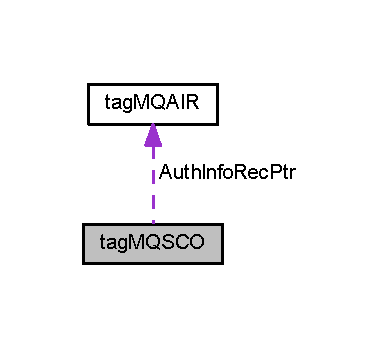
\includegraphics[width=183pt]{structtag_m_q_s_c_o__coll__graph}
\end{center}
\end{figure}
\subsection*{Campos de datos}
\begin{DoxyCompactItemize}
\item 
\hyperlink{cmqc_8h_a12590e546ed66fda7cf21c1d5cefa31d}{M\+Q\+C\+H\+A\+R4} \hyperlink{structtag_m_q_s_c_o_a0530922ca944569b52601d74941f96e4}{Struc\+Id}
\item 
\hyperlink{cmqc_8h_a1fb8d28cbda3fa8766a9821230cdb6d5}{M\+Q\+L\+O\+N\+G} \hyperlink{structtag_m_q_s_c_o_a0656ef8f766b3907d394d88a35d7b7e9}{Version}
\item 
\hyperlink{cmqc_8h_ac492686cf8a90cc3dbc1c48143707ca7}{M\+Q\+C\+H\+A\+R256} \hyperlink{structtag_m_q_s_c_o_a7efe10d0683c0ef04c475b7f498861e7}{Key\+Repository}
\item 
\hyperlink{cmqc_8h_ac492686cf8a90cc3dbc1c48143707ca7}{M\+Q\+C\+H\+A\+R256} \hyperlink{structtag_m_q_s_c_o_ab60dc878f45a601e6affe294fb8449be}{Crypto\+Hardware}
\item 
\hyperlink{cmqc_8h_a1fb8d28cbda3fa8766a9821230cdb6d5}{M\+Q\+L\+O\+N\+G} \hyperlink{structtag_m_q_s_c_o_a080c9c24770964482da6331fa087f9a3}{Auth\+Info\+Rec\+Count}
\item 
\hyperlink{cmqc_8h_a1fb8d28cbda3fa8766a9821230cdb6d5}{M\+Q\+L\+O\+N\+G} \hyperlink{structtag_m_q_s_c_o_ae39127aab29444bb9cb49734645fbc10}{Auth\+Info\+Rec\+Offset}
\item 
\hyperlink{cmqc_8h_a23750cd3b09db5b72684c3c454ba812d}{P\+M\+Q\+A\+I\+R} \hyperlink{structtag_m_q_s_c_o_abb6923732084392b1be222ef7fc53847}{Auth\+Info\+Rec\+Ptr}
\item 
\hyperlink{cmqc_8h_a1fb8d28cbda3fa8766a9821230cdb6d5}{M\+Q\+L\+O\+N\+G} \hyperlink{structtag_m_q_s_c_o_a085f44eefd3c01bef61fabf7094d8d53}{Key\+Reset\+Count}
\item 
\hyperlink{cmqc_8h_a1fb8d28cbda3fa8766a9821230cdb6d5}{M\+Q\+L\+O\+N\+G} \hyperlink{structtag_m_q_s_c_o_af3cd714ea40e052132d11b981918d067}{Fips\+Required}
\item 
\hyperlink{cmqc_8h_a1fb8d28cbda3fa8766a9821230cdb6d5}{M\+Q\+L\+O\+N\+G} \hyperlink{structtag_m_q_s_c_o_a378a4654eeaf97c72604634c2d393cdc}{Encryption\+Policy\+Suite\+B} \mbox{[}4\mbox{]}
\item 
\hyperlink{cmqc_8h_a1fb8d28cbda3fa8766a9821230cdb6d5}{M\+Q\+L\+O\+N\+G} \hyperlink{structtag_m_q_s_c_o_a12dddc77a203a3cb57e519a8764f0920}{Certificate\+Val\+Policy}
\item 
\hyperlink{cmqc_8h_a7be9506b7b722fe66291e424a85afa4a}{M\+Q\+C\+H\+A\+R64} \hyperlink{structtag_m_q_s_c_o_a32c958352dbbcc6efc75fff3db4164b1}{Certificate\+Label}
\end{DoxyCompactItemize}


\subsection{Descripción detallada}


Definición en la línea 4014 del archivo cmqc.\+h.



\subsection{Documentación de los campos}
\hypertarget{structtag_m_q_s_c_o_a080c9c24770964482da6331fa087f9a3}{}\index{tag\+M\+Q\+S\+C\+O@{tag\+M\+Q\+S\+C\+O}!Auth\+Info\+Rec\+Count@{Auth\+Info\+Rec\+Count}}
\index{Auth\+Info\+Rec\+Count@{Auth\+Info\+Rec\+Count}!tag\+M\+Q\+S\+C\+O@{tag\+M\+Q\+S\+C\+O}}
\subsubsection[{Auth\+Info\+Rec\+Count}]{\setlength{\rightskip}{0pt plus 5cm}{\bf M\+Q\+L\+O\+N\+G} Auth\+Info\+Rec\+Count}\label{structtag_m_q_s_c_o_a080c9c24770964482da6331fa087f9a3}


Definición en la línea 4021 del archivo cmqc.\+h.

\hypertarget{structtag_m_q_s_c_o_ae39127aab29444bb9cb49734645fbc10}{}\index{tag\+M\+Q\+S\+C\+O@{tag\+M\+Q\+S\+C\+O}!Auth\+Info\+Rec\+Offset@{Auth\+Info\+Rec\+Offset}}
\index{Auth\+Info\+Rec\+Offset@{Auth\+Info\+Rec\+Offset}!tag\+M\+Q\+S\+C\+O@{tag\+M\+Q\+S\+C\+O}}
\subsubsection[{Auth\+Info\+Rec\+Offset}]{\setlength{\rightskip}{0pt plus 5cm}{\bf M\+Q\+L\+O\+N\+G} Auth\+Info\+Rec\+Offset}\label{structtag_m_q_s_c_o_ae39127aab29444bb9cb49734645fbc10}


Definición en la línea 4023 del archivo cmqc.\+h.

\hypertarget{structtag_m_q_s_c_o_abb6923732084392b1be222ef7fc53847}{}\index{tag\+M\+Q\+S\+C\+O@{tag\+M\+Q\+S\+C\+O}!Auth\+Info\+Rec\+Ptr@{Auth\+Info\+Rec\+Ptr}}
\index{Auth\+Info\+Rec\+Ptr@{Auth\+Info\+Rec\+Ptr}!tag\+M\+Q\+S\+C\+O@{tag\+M\+Q\+S\+C\+O}}
\subsubsection[{Auth\+Info\+Rec\+Ptr}]{\setlength{\rightskip}{0pt plus 5cm}{\bf P\+M\+Q\+A\+I\+R} Auth\+Info\+Rec\+Ptr}\label{structtag_m_q_s_c_o_abb6923732084392b1be222ef7fc53847}


Definición en la línea 4026 del archivo cmqc.\+h.

\hypertarget{structtag_m_q_s_c_o_a32c958352dbbcc6efc75fff3db4164b1}{}\index{tag\+M\+Q\+S\+C\+O@{tag\+M\+Q\+S\+C\+O}!Certificate\+Label@{Certificate\+Label}}
\index{Certificate\+Label@{Certificate\+Label}!tag\+M\+Q\+S\+C\+O@{tag\+M\+Q\+S\+C\+O}}
\subsubsection[{Certificate\+Label}]{\setlength{\rightskip}{0pt plus 5cm}{\bf M\+Q\+C\+H\+A\+R64} Certificate\+Label}\label{structtag_m_q_s_c_o_a32c958352dbbcc6efc75fff3db4164b1}


Definición en la línea 4042 del archivo cmqc.\+h.

\hypertarget{structtag_m_q_s_c_o_a12dddc77a203a3cb57e519a8764f0920}{}\index{tag\+M\+Q\+S\+C\+O@{tag\+M\+Q\+S\+C\+O}!Certificate\+Val\+Policy@{Certificate\+Val\+Policy}}
\index{Certificate\+Val\+Policy@{Certificate\+Val\+Policy}!tag\+M\+Q\+S\+C\+O@{tag\+M\+Q\+S\+C\+O}}
\subsubsection[{Certificate\+Val\+Policy}]{\setlength{\rightskip}{0pt plus 5cm}{\bf M\+Q\+L\+O\+N\+G} Certificate\+Val\+Policy}\label{structtag_m_q_s_c_o_a12dddc77a203a3cb57e519a8764f0920}


Definición en la línea 4039 del archivo cmqc.\+h.

\hypertarget{structtag_m_q_s_c_o_ab60dc878f45a601e6affe294fb8449be}{}\index{tag\+M\+Q\+S\+C\+O@{tag\+M\+Q\+S\+C\+O}!Crypto\+Hardware@{Crypto\+Hardware}}
\index{Crypto\+Hardware@{Crypto\+Hardware}!tag\+M\+Q\+S\+C\+O@{tag\+M\+Q\+S\+C\+O}}
\subsubsection[{Crypto\+Hardware}]{\setlength{\rightskip}{0pt plus 5cm}{\bf M\+Q\+C\+H\+A\+R256} Crypto\+Hardware}\label{structtag_m_q_s_c_o_ab60dc878f45a601e6affe294fb8449be}


Definición en la línea 4019 del archivo cmqc.\+h.

\hypertarget{structtag_m_q_s_c_o_a378a4654eeaf97c72604634c2d393cdc}{}\index{tag\+M\+Q\+S\+C\+O@{tag\+M\+Q\+S\+C\+O}!Encryption\+Policy\+Suite\+B@{Encryption\+Policy\+Suite\+B}}
\index{Encryption\+Policy\+Suite\+B@{Encryption\+Policy\+Suite\+B}!tag\+M\+Q\+S\+C\+O@{tag\+M\+Q\+S\+C\+O}}
\subsubsection[{Encryption\+Policy\+Suite\+B}]{\setlength{\rightskip}{0pt plus 5cm}{\bf M\+Q\+L\+O\+N\+G} Encryption\+Policy\+Suite\+B\mbox{[}4\mbox{]}}\label{structtag_m_q_s_c_o_a378a4654eeaf97c72604634c2d393cdc}


Definición en la línea 4036 del archivo cmqc.\+h.

\hypertarget{structtag_m_q_s_c_o_af3cd714ea40e052132d11b981918d067}{}\index{tag\+M\+Q\+S\+C\+O@{tag\+M\+Q\+S\+C\+O}!Fips\+Required@{Fips\+Required}}
\index{Fips\+Required@{Fips\+Required}!tag\+M\+Q\+S\+C\+O@{tag\+M\+Q\+S\+C\+O}}
\subsubsection[{Fips\+Required}]{\setlength{\rightskip}{0pt plus 5cm}{\bf M\+Q\+L\+O\+N\+G} Fips\+Required}\label{structtag_m_q_s_c_o_af3cd714ea40e052132d11b981918d067}


Definición en la línea 4033 del archivo cmqc.\+h.

\hypertarget{structtag_m_q_s_c_o_a7efe10d0683c0ef04c475b7f498861e7}{}\index{tag\+M\+Q\+S\+C\+O@{tag\+M\+Q\+S\+C\+O}!Key\+Repository@{Key\+Repository}}
\index{Key\+Repository@{Key\+Repository}!tag\+M\+Q\+S\+C\+O@{tag\+M\+Q\+S\+C\+O}}
\subsubsection[{Key\+Repository}]{\setlength{\rightskip}{0pt plus 5cm}{\bf M\+Q\+C\+H\+A\+R256} Key\+Repository}\label{structtag_m_q_s_c_o_a7efe10d0683c0ef04c475b7f498861e7}


Definición en la línea 4017 del archivo cmqc.\+h.

\hypertarget{structtag_m_q_s_c_o_a085f44eefd3c01bef61fabf7094d8d53}{}\index{tag\+M\+Q\+S\+C\+O@{tag\+M\+Q\+S\+C\+O}!Key\+Reset\+Count@{Key\+Reset\+Count}}
\index{Key\+Reset\+Count@{Key\+Reset\+Count}!tag\+M\+Q\+S\+C\+O@{tag\+M\+Q\+S\+C\+O}}
\subsubsection[{Key\+Reset\+Count}]{\setlength{\rightskip}{0pt plus 5cm}{\bf M\+Q\+L\+O\+N\+G} Key\+Reset\+Count}\label{structtag_m_q_s_c_o_a085f44eefd3c01bef61fabf7094d8d53}


Definición en la línea 4029 del archivo cmqc.\+h.

\hypertarget{structtag_m_q_s_c_o_a0530922ca944569b52601d74941f96e4}{}\index{tag\+M\+Q\+S\+C\+O@{tag\+M\+Q\+S\+C\+O}!Struc\+Id@{Struc\+Id}}
\index{Struc\+Id@{Struc\+Id}!tag\+M\+Q\+S\+C\+O@{tag\+M\+Q\+S\+C\+O}}
\subsubsection[{Struc\+Id}]{\setlength{\rightskip}{0pt plus 5cm}{\bf M\+Q\+C\+H\+A\+R4} Struc\+Id}\label{structtag_m_q_s_c_o_a0530922ca944569b52601d74941f96e4}


Definición en la línea 4015 del archivo cmqc.\+h.

\hypertarget{structtag_m_q_s_c_o_a0656ef8f766b3907d394d88a35d7b7e9}{}\index{tag\+M\+Q\+S\+C\+O@{tag\+M\+Q\+S\+C\+O}!Version@{Version}}
\index{Version@{Version}!tag\+M\+Q\+S\+C\+O@{tag\+M\+Q\+S\+C\+O}}
\subsubsection[{Version}]{\setlength{\rightskip}{0pt plus 5cm}{\bf M\+Q\+L\+O\+N\+G} Version}\label{structtag_m_q_s_c_o_a0656ef8f766b3907d394d88a35d7b7e9}


Definición en la línea 4016 del archivo cmqc.\+h.



La documentación para esta estructura fue generada a partir del siguiente fichero\+:\begin{DoxyCompactItemize}
\item 
include/\hyperlink{cmqc_8h}{cmqc.\+h}\end{DoxyCompactItemize}

\hypertarget{structtag_m_q_s_d}{}\section{Referencia de la Estructura tag\+M\+Q\+S\+D}
\label{structtag_m_q_s_d}\index{tag\+M\+Q\+S\+D@{tag\+M\+Q\+S\+D}}


{\ttfamily \#include $<$cmqc.\+h$>$}



Diagrama de colaboración para tag\+M\+Q\+S\+D\+:\nopagebreak
\begin{figure}[H]
\begin{center}
\leavevmode
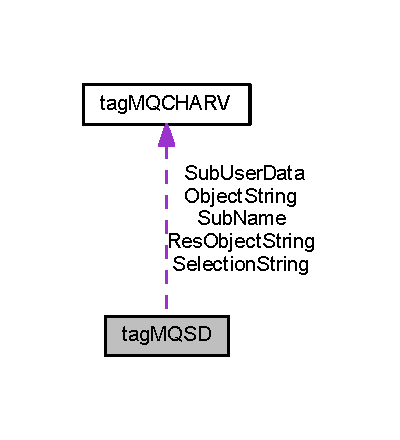
\includegraphics[width=192pt]{structtag_m_q_s_d__coll__graph}
\end{center}
\end{figure}
\subsection*{Campos de datos}
\begin{DoxyCompactItemize}
\item 
\hyperlink{cmqc_8h_a12590e546ed66fda7cf21c1d5cefa31d}{M\+Q\+C\+H\+A\+R4} \hyperlink{structtag_m_q_s_d_a0530922ca944569b52601d74941f96e4}{Struc\+Id}
\item 
\hyperlink{cmqc_8h_a1fb8d28cbda3fa8766a9821230cdb6d5}{M\+Q\+L\+O\+N\+G} \hyperlink{structtag_m_q_s_d_a0656ef8f766b3907d394d88a35d7b7e9}{Version}
\item 
\hyperlink{cmqc_8h_a1fb8d28cbda3fa8766a9821230cdb6d5}{M\+Q\+L\+O\+N\+G} \hyperlink{structtag_m_q_s_d_ad7aff2d6c6044809464380998d24ec5c}{Options}
\item 
\hyperlink{cmqc_8h_a53b1a2836da03f19144836725ff77919}{M\+Q\+C\+H\+A\+R48} \hyperlink{structtag_m_q_s_d_a2106fb125a9f7fc606340ba23c006bc0}{Object\+Name}
\item 
\hyperlink{cmqc_8h_a996cbcfd8d7ef4774f29b158a22d55c0}{M\+Q\+C\+H\+A\+R12} \hyperlink{structtag_m_q_s_d_aa4de0947b84fe1c303c8a5a419ef024a}{Alternate\+User\+Id}
\item 
\hyperlink{cmqc_8h_a1674aecfb9c9ab107699326ec31c4944}{M\+Q\+B\+Y\+T\+E40} \hyperlink{structtag_m_q_s_d_adc1f3b4aa3c6e3f3187e75291146cae7}{Alternate\+Security\+Id}
\item 
\hyperlink{cmqc_8h_a1fb8d28cbda3fa8766a9821230cdb6d5}{M\+Q\+L\+O\+N\+G} \hyperlink{structtag_m_q_s_d_a87aca8cd75818b045e3504060929eee5}{Sub\+Expiry}
\item 
\hyperlink{cmqc_8h_a2a61029e155515c1360dfc809dab6747}{M\+Q\+C\+H\+A\+R\+V} \hyperlink{structtag_m_q_s_d_a564791473371222ceb856cfaf02d6f91}{Object\+String}
\item 
\hyperlink{cmqc_8h_a2a61029e155515c1360dfc809dab6747}{M\+Q\+C\+H\+A\+R\+V} \hyperlink{structtag_m_q_s_d_a52ada97ac3869da3a2f04de08ed4c8d3}{Sub\+Name}
\item 
\hyperlink{cmqc_8h_a2a61029e155515c1360dfc809dab6747}{M\+Q\+C\+H\+A\+R\+V} \hyperlink{structtag_m_q_s_d_a90378e82138a08e732b9c34cc98479d1}{Sub\+User\+Data}
\item 
\hyperlink{cmqc_8h_a2866d93c0ef84cfcda34cab5fd22fc5a}{M\+Q\+B\+Y\+T\+E24} \hyperlink{structtag_m_q_s_d_a32dcf75a2ce80dd29ed6077b5683fbf5}{Sub\+Correl\+Id}
\item 
\hyperlink{cmqc_8h_a1fb8d28cbda3fa8766a9821230cdb6d5}{M\+Q\+L\+O\+N\+G} \hyperlink{structtag_m_q_s_d_a328df5a5108eba2a9bef42f51adb9a7c}{Pub\+Priority}
\item 
\hyperlink{cmqc_8h_aaa021c16e95b8aaab0a28fa5c3756d9d}{M\+Q\+B\+Y\+T\+E32} \hyperlink{structtag_m_q_s_d_af93c638cce691abfce1562bb498b1c38}{Pub\+Accounting\+Token}
\item 
\hyperlink{cmqc_8h_a0b7dd696f0148465fe80f6eae57b38a2}{M\+Q\+C\+H\+A\+R32} \hyperlink{structtag_m_q_s_d_aeae4d639ab8ac667cc227e3c6463cc74}{Pub\+Appl\+Identity\+Data}
\item 
\hyperlink{cmqc_8h_a2a61029e155515c1360dfc809dab6747}{M\+Q\+C\+H\+A\+R\+V} \hyperlink{structtag_m_q_s_d_ab3a91014a229bd897c17cbd04563bca2}{Selection\+String}
\item 
\hyperlink{cmqc_8h_a1fb8d28cbda3fa8766a9821230cdb6d5}{M\+Q\+L\+O\+N\+G} \hyperlink{structtag_m_q_s_d_a380ddfc450dd5ceb714a3d818f82c79b}{Sub\+Level}
\item 
\hyperlink{cmqc_8h_a2a61029e155515c1360dfc809dab6747}{M\+Q\+C\+H\+A\+R\+V} \hyperlink{structtag_m_q_s_d_a8f35fe6f52369753de1259a9468437eb}{Res\+Object\+String}
\end{DoxyCompactItemize}


\subsection{Descripción detallada}


Definición en la línea 5020 del archivo cmqc.\+h.



\subsection{Documentación de los campos}
\hypertarget{structtag_m_q_s_d_adc1f3b4aa3c6e3f3187e75291146cae7}{}\index{tag\+M\+Q\+S\+D@{tag\+M\+Q\+S\+D}!Alternate\+Security\+Id@{Alternate\+Security\+Id}}
\index{Alternate\+Security\+Id@{Alternate\+Security\+Id}!tag\+M\+Q\+S\+D@{tag\+M\+Q\+S\+D}}
\subsubsection[{Alternate\+Security\+Id}]{\setlength{\rightskip}{0pt plus 5cm}{\bf M\+Q\+B\+Y\+T\+E40} Alternate\+Security\+Id}\label{structtag_m_q_s_d_adc1f3b4aa3c6e3f3187e75291146cae7}


Definición en la línea 5027 del archivo cmqc.\+h.

\hypertarget{structtag_m_q_s_d_aa4de0947b84fe1c303c8a5a419ef024a}{}\index{tag\+M\+Q\+S\+D@{tag\+M\+Q\+S\+D}!Alternate\+User\+Id@{Alternate\+User\+Id}}
\index{Alternate\+User\+Id@{Alternate\+User\+Id}!tag\+M\+Q\+S\+D@{tag\+M\+Q\+S\+D}}
\subsubsection[{Alternate\+User\+Id}]{\setlength{\rightskip}{0pt plus 5cm}{\bf M\+Q\+C\+H\+A\+R12} Alternate\+User\+Id}\label{structtag_m_q_s_d_aa4de0947b84fe1c303c8a5a419ef024a}


Definición en la línea 5026 del archivo cmqc.\+h.

\hypertarget{structtag_m_q_s_d_a2106fb125a9f7fc606340ba23c006bc0}{}\index{tag\+M\+Q\+S\+D@{tag\+M\+Q\+S\+D}!Object\+Name@{Object\+Name}}
\index{Object\+Name@{Object\+Name}!tag\+M\+Q\+S\+D@{tag\+M\+Q\+S\+D}}
\subsubsection[{Object\+Name}]{\setlength{\rightskip}{0pt plus 5cm}{\bf M\+Q\+C\+H\+A\+R48} Object\+Name}\label{structtag_m_q_s_d_a2106fb125a9f7fc606340ba23c006bc0}


Definición en la línea 5025 del archivo cmqc.\+h.

\hypertarget{structtag_m_q_s_d_a564791473371222ceb856cfaf02d6f91}{}\index{tag\+M\+Q\+S\+D@{tag\+M\+Q\+S\+D}!Object\+String@{Object\+String}}
\index{Object\+String@{Object\+String}!tag\+M\+Q\+S\+D@{tag\+M\+Q\+S\+D}}
\subsubsection[{Object\+String}]{\setlength{\rightskip}{0pt plus 5cm}{\bf M\+Q\+C\+H\+A\+R\+V} Object\+String}\label{structtag_m_q_s_d_a564791473371222ceb856cfaf02d6f91}


Definición en la línea 5029 del archivo cmqc.\+h.

\hypertarget{structtag_m_q_s_d_ad7aff2d6c6044809464380998d24ec5c}{}\index{tag\+M\+Q\+S\+D@{tag\+M\+Q\+S\+D}!Options@{Options}}
\index{Options@{Options}!tag\+M\+Q\+S\+D@{tag\+M\+Q\+S\+D}}
\subsubsection[{Options}]{\setlength{\rightskip}{0pt plus 5cm}{\bf M\+Q\+L\+O\+N\+G} Options}\label{structtag_m_q_s_d_ad7aff2d6c6044809464380998d24ec5c}


Definición en la línea 5023 del archivo cmqc.\+h.

\hypertarget{structtag_m_q_s_d_af93c638cce691abfce1562bb498b1c38}{}\index{tag\+M\+Q\+S\+D@{tag\+M\+Q\+S\+D}!Pub\+Accounting\+Token@{Pub\+Accounting\+Token}}
\index{Pub\+Accounting\+Token@{Pub\+Accounting\+Token}!tag\+M\+Q\+S\+D@{tag\+M\+Q\+S\+D}}
\subsubsection[{Pub\+Accounting\+Token}]{\setlength{\rightskip}{0pt plus 5cm}{\bf M\+Q\+B\+Y\+T\+E32} Pub\+Accounting\+Token}\label{structtag_m_q_s_d_af93c638cce691abfce1562bb498b1c38}


Definición en la línea 5035 del archivo cmqc.\+h.

\hypertarget{structtag_m_q_s_d_aeae4d639ab8ac667cc227e3c6463cc74}{}\index{tag\+M\+Q\+S\+D@{tag\+M\+Q\+S\+D}!Pub\+Appl\+Identity\+Data@{Pub\+Appl\+Identity\+Data}}
\index{Pub\+Appl\+Identity\+Data@{Pub\+Appl\+Identity\+Data}!tag\+M\+Q\+S\+D@{tag\+M\+Q\+S\+D}}
\subsubsection[{Pub\+Appl\+Identity\+Data}]{\setlength{\rightskip}{0pt plus 5cm}{\bf M\+Q\+C\+H\+A\+R32} Pub\+Appl\+Identity\+Data}\label{structtag_m_q_s_d_aeae4d639ab8ac667cc227e3c6463cc74}


Definición en la línea 5037 del archivo cmqc.\+h.

\hypertarget{structtag_m_q_s_d_a328df5a5108eba2a9bef42f51adb9a7c}{}\index{tag\+M\+Q\+S\+D@{tag\+M\+Q\+S\+D}!Pub\+Priority@{Pub\+Priority}}
\index{Pub\+Priority@{Pub\+Priority}!tag\+M\+Q\+S\+D@{tag\+M\+Q\+S\+D}}
\subsubsection[{Pub\+Priority}]{\setlength{\rightskip}{0pt plus 5cm}{\bf M\+Q\+L\+O\+N\+G} Pub\+Priority}\label{structtag_m_q_s_d_a328df5a5108eba2a9bef42f51adb9a7c}


Definición en la línea 5034 del archivo cmqc.\+h.

\hypertarget{structtag_m_q_s_d_a8f35fe6f52369753de1259a9468437eb}{}\index{tag\+M\+Q\+S\+D@{tag\+M\+Q\+S\+D}!Res\+Object\+String@{Res\+Object\+String}}
\index{Res\+Object\+String@{Res\+Object\+String}!tag\+M\+Q\+S\+D@{tag\+M\+Q\+S\+D}}
\subsubsection[{Res\+Object\+String}]{\setlength{\rightskip}{0pt plus 5cm}{\bf M\+Q\+C\+H\+A\+R\+V} Res\+Object\+String}\label{structtag_m_q_s_d_a8f35fe6f52369753de1259a9468437eb}


Definición en la línea 5041 del archivo cmqc.\+h.

\hypertarget{structtag_m_q_s_d_ab3a91014a229bd897c17cbd04563bca2}{}\index{tag\+M\+Q\+S\+D@{tag\+M\+Q\+S\+D}!Selection\+String@{Selection\+String}}
\index{Selection\+String@{Selection\+String}!tag\+M\+Q\+S\+D@{tag\+M\+Q\+S\+D}}
\subsubsection[{Selection\+String}]{\setlength{\rightskip}{0pt plus 5cm}{\bf M\+Q\+C\+H\+A\+R\+V} Selection\+String}\label{structtag_m_q_s_d_ab3a91014a229bd897c17cbd04563bca2}


Definición en la línea 5039 del archivo cmqc.\+h.

\hypertarget{structtag_m_q_s_d_a0530922ca944569b52601d74941f96e4}{}\index{tag\+M\+Q\+S\+D@{tag\+M\+Q\+S\+D}!Struc\+Id@{Struc\+Id}}
\index{Struc\+Id@{Struc\+Id}!tag\+M\+Q\+S\+D@{tag\+M\+Q\+S\+D}}
\subsubsection[{Struc\+Id}]{\setlength{\rightskip}{0pt plus 5cm}{\bf M\+Q\+C\+H\+A\+R4} Struc\+Id}\label{structtag_m_q_s_d_a0530922ca944569b52601d74941f96e4}


Definición en la línea 5021 del archivo cmqc.\+h.

\hypertarget{structtag_m_q_s_d_a32dcf75a2ce80dd29ed6077b5683fbf5}{}\index{tag\+M\+Q\+S\+D@{tag\+M\+Q\+S\+D}!Sub\+Correl\+Id@{Sub\+Correl\+Id}}
\index{Sub\+Correl\+Id@{Sub\+Correl\+Id}!tag\+M\+Q\+S\+D@{tag\+M\+Q\+S\+D}}
\subsubsection[{Sub\+Correl\+Id}]{\setlength{\rightskip}{0pt plus 5cm}{\bf M\+Q\+B\+Y\+T\+E24} Sub\+Correl\+Id}\label{structtag_m_q_s_d_a32dcf75a2ce80dd29ed6077b5683fbf5}


Definición en la línea 5032 del archivo cmqc.\+h.

\hypertarget{structtag_m_q_s_d_a87aca8cd75818b045e3504060929eee5}{}\index{tag\+M\+Q\+S\+D@{tag\+M\+Q\+S\+D}!Sub\+Expiry@{Sub\+Expiry}}
\index{Sub\+Expiry@{Sub\+Expiry}!tag\+M\+Q\+S\+D@{tag\+M\+Q\+S\+D}}
\subsubsection[{Sub\+Expiry}]{\setlength{\rightskip}{0pt plus 5cm}{\bf M\+Q\+L\+O\+N\+G} Sub\+Expiry}\label{structtag_m_q_s_d_a87aca8cd75818b045e3504060929eee5}


Definición en la línea 5028 del archivo cmqc.\+h.

\hypertarget{structtag_m_q_s_d_a380ddfc450dd5ceb714a3d818f82c79b}{}\index{tag\+M\+Q\+S\+D@{tag\+M\+Q\+S\+D}!Sub\+Level@{Sub\+Level}}
\index{Sub\+Level@{Sub\+Level}!tag\+M\+Q\+S\+D@{tag\+M\+Q\+S\+D}}
\subsubsection[{Sub\+Level}]{\setlength{\rightskip}{0pt plus 5cm}{\bf M\+Q\+L\+O\+N\+G} Sub\+Level}\label{structtag_m_q_s_d_a380ddfc450dd5ceb714a3d818f82c79b}


Definición en la línea 5040 del archivo cmqc.\+h.

\hypertarget{structtag_m_q_s_d_a52ada97ac3869da3a2f04de08ed4c8d3}{}\index{tag\+M\+Q\+S\+D@{tag\+M\+Q\+S\+D}!Sub\+Name@{Sub\+Name}}
\index{Sub\+Name@{Sub\+Name}!tag\+M\+Q\+S\+D@{tag\+M\+Q\+S\+D}}
\subsubsection[{Sub\+Name}]{\setlength{\rightskip}{0pt plus 5cm}{\bf M\+Q\+C\+H\+A\+R\+V} Sub\+Name}\label{structtag_m_q_s_d_a52ada97ac3869da3a2f04de08ed4c8d3}


Definición en la línea 5030 del archivo cmqc.\+h.

\hypertarget{structtag_m_q_s_d_a90378e82138a08e732b9c34cc98479d1}{}\index{tag\+M\+Q\+S\+D@{tag\+M\+Q\+S\+D}!Sub\+User\+Data@{Sub\+User\+Data}}
\index{Sub\+User\+Data@{Sub\+User\+Data}!tag\+M\+Q\+S\+D@{tag\+M\+Q\+S\+D}}
\subsubsection[{Sub\+User\+Data}]{\setlength{\rightskip}{0pt plus 5cm}{\bf M\+Q\+C\+H\+A\+R\+V} Sub\+User\+Data}\label{structtag_m_q_s_d_a90378e82138a08e732b9c34cc98479d1}


Definición en la línea 5031 del archivo cmqc.\+h.

\hypertarget{structtag_m_q_s_d_a0656ef8f766b3907d394d88a35d7b7e9}{}\index{tag\+M\+Q\+S\+D@{tag\+M\+Q\+S\+D}!Version@{Version}}
\index{Version@{Version}!tag\+M\+Q\+S\+D@{tag\+M\+Q\+S\+D}}
\subsubsection[{Version}]{\setlength{\rightskip}{0pt plus 5cm}{\bf M\+Q\+L\+O\+N\+G} Version}\label{structtag_m_q_s_d_a0656ef8f766b3907d394d88a35d7b7e9}


Definición en la línea 5022 del archivo cmqc.\+h.



La documentación para esta estructura fue generada a partir del siguiente fichero\+:\begin{DoxyCompactItemize}
\item 
include/\hyperlink{cmqc_8h}{cmqc.\+h}\end{DoxyCompactItemize}

\hypertarget{structtag_m_q_s_m_p_o}{}\section{Referencia de la Estructura tag\+M\+Q\+S\+M\+P\+O}
\label{structtag_m_q_s_m_p_o}\index{tag\+M\+Q\+S\+M\+P\+O@{tag\+M\+Q\+S\+M\+P\+O}}


{\ttfamily \#include $<$cmqc.\+h$>$}

\subsection*{Campos de datos}
\begin{DoxyCompactItemize}
\item 
\hyperlink{cmqc_8h_a12590e546ed66fda7cf21c1d5cefa31d}{M\+Q\+C\+H\+A\+R4} \hyperlink{structtag_m_q_s_m_p_o_a0530922ca944569b52601d74941f96e4}{Struc\+Id}
\item 
\hyperlink{cmqc_8h_a1fb8d28cbda3fa8766a9821230cdb6d5}{M\+Q\+L\+O\+N\+G} \hyperlink{structtag_m_q_s_m_p_o_a0656ef8f766b3907d394d88a35d7b7e9}{Version}
\item 
\hyperlink{cmqc_8h_a1fb8d28cbda3fa8766a9821230cdb6d5}{M\+Q\+L\+O\+N\+G} \hyperlink{structtag_m_q_s_m_p_o_ad7aff2d6c6044809464380998d24ec5c}{Options}
\item 
\hyperlink{cmqc_8h_a1fb8d28cbda3fa8766a9821230cdb6d5}{M\+Q\+L\+O\+N\+G} \hyperlink{structtag_m_q_s_m_p_o_a490df67c11df1c06a7a55933584e844a}{Value\+Encoding}
\item 
\hyperlink{cmqc_8h_a1fb8d28cbda3fa8766a9821230cdb6d5}{M\+Q\+L\+O\+N\+G} \hyperlink{structtag_m_q_s_m_p_o_ac5d324f94c6c72d6e38cb236af37da93}{Value\+C\+C\+S\+I\+D}
\end{DoxyCompactItemize}


\subsection{Descripción detallada}


Definición en la línea 5071 del archivo cmqc.\+h.



\subsection{Documentación de los campos}
\hypertarget{structtag_m_q_s_m_p_o_ad7aff2d6c6044809464380998d24ec5c}{}\index{tag\+M\+Q\+S\+M\+P\+O@{tag\+M\+Q\+S\+M\+P\+O}!Options@{Options}}
\index{Options@{Options}!tag\+M\+Q\+S\+M\+P\+O@{tag\+M\+Q\+S\+M\+P\+O}}
\subsubsection[{Options}]{\setlength{\rightskip}{0pt plus 5cm}{\bf M\+Q\+L\+O\+N\+G} Options}\label{structtag_m_q_s_m_p_o_ad7aff2d6c6044809464380998d24ec5c}


Definición en la línea 5074 del archivo cmqc.\+h.

\hypertarget{structtag_m_q_s_m_p_o_a0530922ca944569b52601d74941f96e4}{}\index{tag\+M\+Q\+S\+M\+P\+O@{tag\+M\+Q\+S\+M\+P\+O}!Struc\+Id@{Struc\+Id}}
\index{Struc\+Id@{Struc\+Id}!tag\+M\+Q\+S\+M\+P\+O@{tag\+M\+Q\+S\+M\+P\+O}}
\subsubsection[{Struc\+Id}]{\setlength{\rightskip}{0pt plus 5cm}{\bf M\+Q\+C\+H\+A\+R4} Struc\+Id}\label{structtag_m_q_s_m_p_o_a0530922ca944569b52601d74941f96e4}


Definición en la línea 5072 del archivo cmqc.\+h.

\hypertarget{structtag_m_q_s_m_p_o_ac5d324f94c6c72d6e38cb236af37da93}{}\index{tag\+M\+Q\+S\+M\+P\+O@{tag\+M\+Q\+S\+M\+P\+O}!Value\+C\+C\+S\+I\+D@{Value\+C\+C\+S\+I\+D}}
\index{Value\+C\+C\+S\+I\+D@{Value\+C\+C\+S\+I\+D}!tag\+M\+Q\+S\+M\+P\+O@{tag\+M\+Q\+S\+M\+P\+O}}
\subsubsection[{Value\+C\+C\+S\+I\+D}]{\setlength{\rightskip}{0pt plus 5cm}{\bf M\+Q\+L\+O\+N\+G} Value\+C\+C\+S\+I\+D}\label{structtag_m_q_s_m_p_o_ac5d324f94c6c72d6e38cb236af37da93}


Definición en la línea 5077 del archivo cmqc.\+h.

\hypertarget{structtag_m_q_s_m_p_o_a490df67c11df1c06a7a55933584e844a}{}\index{tag\+M\+Q\+S\+M\+P\+O@{tag\+M\+Q\+S\+M\+P\+O}!Value\+Encoding@{Value\+Encoding}}
\index{Value\+Encoding@{Value\+Encoding}!tag\+M\+Q\+S\+M\+P\+O@{tag\+M\+Q\+S\+M\+P\+O}}
\subsubsection[{Value\+Encoding}]{\setlength{\rightskip}{0pt plus 5cm}{\bf M\+Q\+L\+O\+N\+G} Value\+Encoding}\label{structtag_m_q_s_m_p_o_a490df67c11df1c06a7a55933584e844a}


Definición en la línea 5076 del archivo cmqc.\+h.

\hypertarget{structtag_m_q_s_m_p_o_a0656ef8f766b3907d394d88a35d7b7e9}{}\index{tag\+M\+Q\+S\+M\+P\+O@{tag\+M\+Q\+S\+M\+P\+O}!Version@{Version}}
\index{Version@{Version}!tag\+M\+Q\+S\+M\+P\+O@{tag\+M\+Q\+S\+M\+P\+O}}
\subsubsection[{Version}]{\setlength{\rightskip}{0pt plus 5cm}{\bf M\+Q\+L\+O\+N\+G} Version}\label{structtag_m_q_s_m_p_o_a0656ef8f766b3907d394d88a35d7b7e9}


Definición en la línea 5073 del archivo cmqc.\+h.



La documentación para esta estructura fue generada a partir del siguiente fichero\+:\begin{DoxyCompactItemize}
\item 
include/\hyperlink{cmqc_8h}{cmqc.\+h}\end{DoxyCompactItemize}

\hypertarget{structtag_m_q_s_r_o}{}\section{Referencia de la Estructura tag\+M\+Q\+S\+R\+O}
\label{structtag_m_q_s_r_o}\index{tag\+M\+Q\+S\+R\+O@{tag\+M\+Q\+S\+R\+O}}


{\ttfamily \#include $<$cmqc.\+h$>$}

\subsection*{Campos de datos}
\begin{DoxyCompactItemize}
\item 
\hyperlink{cmqc_8h_a12590e546ed66fda7cf21c1d5cefa31d}{M\+Q\+C\+H\+A\+R4} \hyperlink{structtag_m_q_s_r_o_a0530922ca944569b52601d74941f96e4}{Struc\+Id}
\item 
\hyperlink{cmqc_8h_a1fb8d28cbda3fa8766a9821230cdb6d5}{M\+Q\+L\+O\+N\+G} \hyperlink{structtag_m_q_s_r_o_a0656ef8f766b3907d394d88a35d7b7e9}{Version}
\item 
\hyperlink{cmqc_8h_a1fb8d28cbda3fa8766a9821230cdb6d5}{M\+Q\+L\+O\+N\+G} \hyperlink{structtag_m_q_s_r_o_ad7aff2d6c6044809464380998d24ec5c}{Options}
\item 
\hyperlink{cmqc_8h_a1fb8d28cbda3fa8766a9821230cdb6d5}{M\+Q\+L\+O\+N\+G} \hyperlink{structtag_m_q_s_r_o_a250881f7ae348b691f4cc3e46b0a2aee}{Num\+Pubs}
\end{DoxyCompactItemize}


\subsection{Descripción detallada}


Definición en la línea 5095 del archivo cmqc.\+h.



\subsection{Documentación de los campos}
\hypertarget{structtag_m_q_s_r_o_a250881f7ae348b691f4cc3e46b0a2aee}{}\index{tag\+M\+Q\+S\+R\+O@{tag\+M\+Q\+S\+R\+O}!Num\+Pubs@{Num\+Pubs}}
\index{Num\+Pubs@{Num\+Pubs}!tag\+M\+Q\+S\+R\+O@{tag\+M\+Q\+S\+R\+O}}
\subsubsection[{Num\+Pubs}]{\setlength{\rightskip}{0pt plus 5cm}{\bf M\+Q\+L\+O\+N\+G} Num\+Pubs}\label{structtag_m_q_s_r_o_a250881f7ae348b691f4cc3e46b0a2aee}


Definición en la línea 5099 del archivo cmqc.\+h.

\hypertarget{structtag_m_q_s_r_o_ad7aff2d6c6044809464380998d24ec5c}{}\index{tag\+M\+Q\+S\+R\+O@{tag\+M\+Q\+S\+R\+O}!Options@{Options}}
\index{Options@{Options}!tag\+M\+Q\+S\+R\+O@{tag\+M\+Q\+S\+R\+O}}
\subsubsection[{Options}]{\setlength{\rightskip}{0pt plus 5cm}{\bf M\+Q\+L\+O\+N\+G} Options}\label{structtag_m_q_s_r_o_ad7aff2d6c6044809464380998d24ec5c}


Definición en la línea 5098 del archivo cmqc.\+h.

\hypertarget{structtag_m_q_s_r_o_a0530922ca944569b52601d74941f96e4}{}\index{tag\+M\+Q\+S\+R\+O@{tag\+M\+Q\+S\+R\+O}!Struc\+Id@{Struc\+Id}}
\index{Struc\+Id@{Struc\+Id}!tag\+M\+Q\+S\+R\+O@{tag\+M\+Q\+S\+R\+O}}
\subsubsection[{Struc\+Id}]{\setlength{\rightskip}{0pt plus 5cm}{\bf M\+Q\+C\+H\+A\+R4} Struc\+Id}\label{structtag_m_q_s_r_o_a0530922ca944569b52601d74941f96e4}


Definición en la línea 5096 del archivo cmqc.\+h.

\hypertarget{structtag_m_q_s_r_o_a0656ef8f766b3907d394d88a35d7b7e9}{}\index{tag\+M\+Q\+S\+R\+O@{tag\+M\+Q\+S\+R\+O}!Version@{Version}}
\index{Version@{Version}!tag\+M\+Q\+S\+R\+O@{tag\+M\+Q\+S\+R\+O}}
\subsubsection[{Version}]{\setlength{\rightskip}{0pt plus 5cm}{\bf M\+Q\+L\+O\+N\+G} Version}\label{structtag_m_q_s_r_o_a0656ef8f766b3907d394d88a35d7b7e9}


Definición en la línea 5097 del archivo cmqc.\+h.



La documentación para esta estructura fue generada a partir del siguiente fichero\+:\begin{DoxyCompactItemize}
\item 
include/\hyperlink{cmqc_8h}{cmqc.\+h}\end{DoxyCompactItemize}

\hypertarget{structtag_m_q_s_t_s}{}\section{Referencia de la Estructura tag\+M\+Q\+S\+T\+S}
\label{structtag_m_q_s_t_s}\index{tag\+M\+Q\+S\+T\+S@{tag\+M\+Q\+S\+T\+S}}


{\ttfamily \#include $<$cmqc.\+h$>$}



Diagrama de colaboración para tag\+M\+Q\+S\+T\+S\+:\nopagebreak
\begin{figure}[H]
\begin{center}
\leavevmode
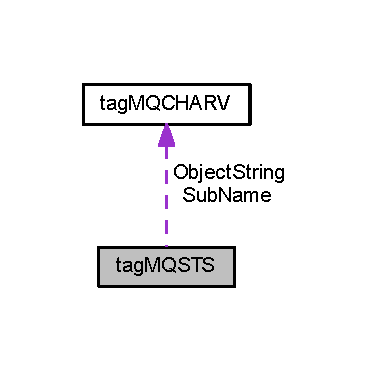
\includegraphics[width=178pt]{structtag_m_q_s_t_s__coll__graph}
\end{center}
\end{figure}
\subsection*{Campos de datos}
\begin{DoxyCompactItemize}
\item 
\hyperlink{cmqc_8h_a12590e546ed66fda7cf21c1d5cefa31d}{M\+Q\+C\+H\+A\+R4} \hyperlink{structtag_m_q_s_t_s_a0530922ca944569b52601d74941f96e4}{Struc\+Id}
\item 
\hyperlink{cmqc_8h_a1fb8d28cbda3fa8766a9821230cdb6d5}{M\+Q\+L\+O\+N\+G} \hyperlink{structtag_m_q_s_t_s_a0656ef8f766b3907d394d88a35d7b7e9}{Version}
\item 
\hyperlink{cmqc_8h_a1fb8d28cbda3fa8766a9821230cdb6d5}{M\+Q\+L\+O\+N\+G} \hyperlink{structtag_m_q_s_t_s_a3d53860a50c3834d3dad9f5b2e5b5234}{Comp\+Code}
\item 
\hyperlink{cmqc_8h_a1fb8d28cbda3fa8766a9821230cdb6d5}{M\+Q\+L\+O\+N\+G} \hyperlink{structtag_m_q_s_t_s_ac2f0378cb0c66c5f91625822e53d7bae}{Reason}
\item 
\hyperlink{cmqc_8h_a1fb8d28cbda3fa8766a9821230cdb6d5}{M\+Q\+L\+O\+N\+G} \hyperlink{structtag_m_q_s_t_s_a4577d49eab12e56cd487d84e5179beb9}{Put\+Success\+Count}
\item 
\hyperlink{cmqc_8h_a1fb8d28cbda3fa8766a9821230cdb6d5}{M\+Q\+L\+O\+N\+G} \hyperlink{structtag_m_q_s_t_s_a6a179f500b4a403e9609416d7c9cdcc0}{Put\+Warning\+Count}
\item 
\hyperlink{cmqc_8h_a1fb8d28cbda3fa8766a9821230cdb6d5}{M\+Q\+L\+O\+N\+G} \hyperlink{structtag_m_q_s_t_s_a7588d679d3d79c069fdf82aeae32fede}{Put\+Failure\+Count}
\item 
\hyperlink{cmqc_8h_a1fb8d28cbda3fa8766a9821230cdb6d5}{M\+Q\+L\+O\+N\+G} \hyperlink{structtag_m_q_s_t_s_afe2238efcfc6d8a8de58f0622bb31caa}{Object\+Type}
\item 
\hyperlink{cmqc_8h_a53b1a2836da03f19144836725ff77919}{M\+Q\+C\+H\+A\+R48} \hyperlink{structtag_m_q_s_t_s_a2106fb125a9f7fc606340ba23c006bc0}{Object\+Name}
\item 
\hyperlink{cmqc_8h_a53b1a2836da03f19144836725ff77919}{M\+Q\+C\+H\+A\+R48} \hyperlink{structtag_m_q_s_t_s_ac72719d0cdc669269aa503462d5c7536}{Object\+Q\+Mgr\+Name}
\item 
\hyperlink{cmqc_8h_a53b1a2836da03f19144836725ff77919}{M\+Q\+C\+H\+A\+R48} \hyperlink{structtag_m_q_s_t_s_a75cc42c205c810ff5e2d33b15568f940}{Resolved\+Object\+Name}
\item 
\hyperlink{cmqc_8h_a53b1a2836da03f19144836725ff77919}{M\+Q\+C\+H\+A\+R48} \hyperlink{structtag_m_q_s_t_s_af36c1b6e6f3f92e0c733c43da9fada3f}{Resolved\+Q\+Mgr\+Name}
\item 
\hyperlink{cmqc_8h_a2a61029e155515c1360dfc809dab6747}{M\+Q\+C\+H\+A\+R\+V} \hyperlink{structtag_m_q_s_t_s_a564791473371222ceb856cfaf02d6f91}{Object\+String}
\item 
\hyperlink{cmqc_8h_a2a61029e155515c1360dfc809dab6747}{M\+Q\+C\+H\+A\+R\+V} \hyperlink{structtag_m_q_s_t_s_a52ada97ac3869da3a2f04de08ed4c8d3}{Sub\+Name}
\item 
\hyperlink{cmqc_8h_a1fb8d28cbda3fa8766a9821230cdb6d5}{M\+Q\+L\+O\+N\+G} \hyperlink{structtag_m_q_s_t_s_aba7271572b7c49b5295b03e379f59686}{Open\+Options}
\item 
\hyperlink{cmqc_8h_a1fb8d28cbda3fa8766a9821230cdb6d5}{M\+Q\+L\+O\+N\+G} \hyperlink{structtag_m_q_s_t_s_a24b93fe1b9f7b2ddc533029552471ca4}{Sub\+Options}
\end{DoxyCompactItemize}


\subsection{Descripción detallada}


Definición en la línea 5116 del archivo cmqc.\+h.



\subsection{Documentación de los campos}
\hypertarget{structtag_m_q_s_t_s_a3d53860a50c3834d3dad9f5b2e5b5234}{}\index{tag\+M\+Q\+S\+T\+S@{tag\+M\+Q\+S\+T\+S}!Comp\+Code@{Comp\+Code}}
\index{Comp\+Code@{Comp\+Code}!tag\+M\+Q\+S\+T\+S@{tag\+M\+Q\+S\+T\+S}}
\subsubsection[{Comp\+Code}]{\setlength{\rightskip}{0pt plus 5cm}{\bf M\+Q\+L\+O\+N\+G} Comp\+Code}\label{structtag_m_q_s_t_s_a3d53860a50c3834d3dad9f5b2e5b5234}


Definición en la línea 5119 del archivo cmqc.\+h.

\hypertarget{structtag_m_q_s_t_s_a2106fb125a9f7fc606340ba23c006bc0}{}\index{tag\+M\+Q\+S\+T\+S@{tag\+M\+Q\+S\+T\+S}!Object\+Name@{Object\+Name}}
\index{Object\+Name@{Object\+Name}!tag\+M\+Q\+S\+T\+S@{tag\+M\+Q\+S\+T\+S}}
\subsubsection[{Object\+Name}]{\setlength{\rightskip}{0pt plus 5cm}{\bf M\+Q\+C\+H\+A\+R48} Object\+Name}\label{structtag_m_q_s_t_s_a2106fb125a9f7fc606340ba23c006bc0}


Definición en la línea 5128 del archivo cmqc.\+h.

\hypertarget{structtag_m_q_s_t_s_ac72719d0cdc669269aa503462d5c7536}{}\index{tag\+M\+Q\+S\+T\+S@{tag\+M\+Q\+S\+T\+S}!Object\+Q\+Mgr\+Name@{Object\+Q\+Mgr\+Name}}
\index{Object\+Q\+Mgr\+Name@{Object\+Q\+Mgr\+Name}!tag\+M\+Q\+S\+T\+S@{tag\+M\+Q\+S\+T\+S}}
\subsubsection[{Object\+Q\+Mgr\+Name}]{\setlength{\rightskip}{0pt plus 5cm}{\bf M\+Q\+C\+H\+A\+R48} Object\+Q\+Mgr\+Name}\label{structtag_m_q_s_t_s_ac72719d0cdc669269aa503462d5c7536}


Definición en la línea 5129 del archivo cmqc.\+h.

\hypertarget{structtag_m_q_s_t_s_a564791473371222ceb856cfaf02d6f91}{}\index{tag\+M\+Q\+S\+T\+S@{tag\+M\+Q\+S\+T\+S}!Object\+String@{Object\+String}}
\index{Object\+String@{Object\+String}!tag\+M\+Q\+S\+T\+S@{tag\+M\+Q\+S\+T\+S}}
\subsubsection[{Object\+String}]{\setlength{\rightskip}{0pt plus 5cm}{\bf M\+Q\+C\+H\+A\+R\+V} Object\+String}\label{structtag_m_q_s_t_s_a564791473371222ceb856cfaf02d6f91}


Definición en la línea 5135 del archivo cmqc.\+h.

\hypertarget{structtag_m_q_s_t_s_afe2238efcfc6d8a8de58f0622bb31caa}{}\index{tag\+M\+Q\+S\+T\+S@{tag\+M\+Q\+S\+T\+S}!Object\+Type@{Object\+Type}}
\index{Object\+Type@{Object\+Type}!tag\+M\+Q\+S\+T\+S@{tag\+M\+Q\+S\+T\+S}}
\subsubsection[{Object\+Type}]{\setlength{\rightskip}{0pt plus 5cm}{\bf M\+Q\+L\+O\+N\+G} Object\+Type}\label{structtag_m_q_s_t_s_afe2238efcfc6d8a8de58f0622bb31caa}


Definición en la línea 5127 del archivo cmqc.\+h.

\hypertarget{structtag_m_q_s_t_s_aba7271572b7c49b5295b03e379f59686}{}\index{tag\+M\+Q\+S\+T\+S@{tag\+M\+Q\+S\+T\+S}!Open\+Options@{Open\+Options}}
\index{Open\+Options@{Open\+Options}!tag\+M\+Q\+S\+T\+S@{tag\+M\+Q\+S\+T\+S}}
\subsubsection[{Open\+Options}]{\setlength{\rightskip}{0pt plus 5cm}{\bf M\+Q\+L\+O\+N\+G} Open\+Options}\label{structtag_m_q_s_t_s_aba7271572b7c49b5295b03e379f59686}


Definición en la línea 5137 del archivo cmqc.\+h.

\hypertarget{structtag_m_q_s_t_s_a7588d679d3d79c069fdf82aeae32fede}{}\index{tag\+M\+Q\+S\+T\+S@{tag\+M\+Q\+S\+T\+S}!Put\+Failure\+Count@{Put\+Failure\+Count}}
\index{Put\+Failure\+Count@{Put\+Failure\+Count}!tag\+M\+Q\+S\+T\+S@{tag\+M\+Q\+S\+T\+S}}
\subsubsection[{Put\+Failure\+Count}]{\setlength{\rightskip}{0pt plus 5cm}{\bf M\+Q\+L\+O\+N\+G} Put\+Failure\+Count}\label{structtag_m_q_s_t_s_a7588d679d3d79c069fdf82aeae32fede}


Definición en la línea 5125 del archivo cmqc.\+h.

\hypertarget{structtag_m_q_s_t_s_a4577d49eab12e56cd487d84e5179beb9}{}\index{tag\+M\+Q\+S\+T\+S@{tag\+M\+Q\+S\+T\+S}!Put\+Success\+Count@{Put\+Success\+Count}}
\index{Put\+Success\+Count@{Put\+Success\+Count}!tag\+M\+Q\+S\+T\+S@{tag\+M\+Q\+S\+T\+S}}
\subsubsection[{Put\+Success\+Count}]{\setlength{\rightskip}{0pt plus 5cm}{\bf M\+Q\+L\+O\+N\+G} Put\+Success\+Count}\label{structtag_m_q_s_t_s_a4577d49eab12e56cd487d84e5179beb9}


Definición en la línea 5121 del archivo cmqc.\+h.

\hypertarget{structtag_m_q_s_t_s_a6a179f500b4a403e9609416d7c9cdcc0}{}\index{tag\+M\+Q\+S\+T\+S@{tag\+M\+Q\+S\+T\+S}!Put\+Warning\+Count@{Put\+Warning\+Count}}
\index{Put\+Warning\+Count@{Put\+Warning\+Count}!tag\+M\+Q\+S\+T\+S@{tag\+M\+Q\+S\+T\+S}}
\subsubsection[{Put\+Warning\+Count}]{\setlength{\rightskip}{0pt plus 5cm}{\bf M\+Q\+L\+O\+N\+G} Put\+Warning\+Count}\label{structtag_m_q_s_t_s_a6a179f500b4a403e9609416d7c9cdcc0}


Definición en la línea 5123 del archivo cmqc.\+h.

\hypertarget{structtag_m_q_s_t_s_ac2f0378cb0c66c5f91625822e53d7bae}{}\index{tag\+M\+Q\+S\+T\+S@{tag\+M\+Q\+S\+T\+S}!Reason@{Reason}}
\index{Reason@{Reason}!tag\+M\+Q\+S\+T\+S@{tag\+M\+Q\+S\+T\+S}}
\subsubsection[{Reason}]{\setlength{\rightskip}{0pt plus 5cm}{\bf M\+Q\+L\+O\+N\+G} Reason}\label{structtag_m_q_s_t_s_ac2f0378cb0c66c5f91625822e53d7bae}


Definición en la línea 5120 del archivo cmqc.\+h.

\hypertarget{structtag_m_q_s_t_s_a75cc42c205c810ff5e2d33b15568f940}{}\index{tag\+M\+Q\+S\+T\+S@{tag\+M\+Q\+S\+T\+S}!Resolved\+Object\+Name@{Resolved\+Object\+Name}}
\index{Resolved\+Object\+Name@{Resolved\+Object\+Name}!tag\+M\+Q\+S\+T\+S@{tag\+M\+Q\+S\+T\+S}}
\subsubsection[{Resolved\+Object\+Name}]{\setlength{\rightskip}{0pt plus 5cm}{\bf M\+Q\+C\+H\+A\+R48} Resolved\+Object\+Name}\label{structtag_m_q_s_t_s_a75cc42c205c810ff5e2d33b15568f940}


Definición en la línea 5130 del archivo cmqc.\+h.

\hypertarget{structtag_m_q_s_t_s_af36c1b6e6f3f92e0c733c43da9fada3f}{}\index{tag\+M\+Q\+S\+T\+S@{tag\+M\+Q\+S\+T\+S}!Resolved\+Q\+Mgr\+Name@{Resolved\+Q\+Mgr\+Name}}
\index{Resolved\+Q\+Mgr\+Name@{Resolved\+Q\+Mgr\+Name}!tag\+M\+Q\+S\+T\+S@{tag\+M\+Q\+S\+T\+S}}
\subsubsection[{Resolved\+Q\+Mgr\+Name}]{\setlength{\rightskip}{0pt plus 5cm}{\bf M\+Q\+C\+H\+A\+R48} Resolved\+Q\+Mgr\+Name}\label{structtag_m_q_s_t_s_af36c1b6e6f3f92e0c733c43da9fada3f}


Definición en la línea 5132 del archivo cmqc.\+h.

\hypertarget{structtag_m_q_s_t_s_a0530922ca944569b52601d74941f96e4}{}\index{tag\+M\+Q\+S\+T\+S@{tag\+M\+Q\+S\+T\+S}!Struc\+Id@{Struc\+Id}}
\index{Struc\+Id@{Struc\+Id}!tag\+M\+Q\+S\+T\+S@{tag\+M\+Q\+S\+T\+S}}
\subsubsection[{Struc\+Id}]{\setlength{\rightskip}{0pt plus 5cm}{\bf M\+Q\+C\+H\+A\+R4} Struc\+Id}\label{structtag_m_q_s_t_s_a0530922ca944569b52601d74941f96e4}


Definición en la línea 5117 del archivo cmqc.\+h.

\hypertarget{structtag_m_q_s_t_s_a52ada97ac3869da3a2f04de08ed4c8d3}{}\index{tag\+M\+Q\+S\+T\+S@{tag\+M\+Q\+S\+T\+S}!Sub\+Name@{Sub\+Name}}
\index{Sub\+Name@{Sub\+Name}!tag\+M\+Q\+S\+T\+S@{tag\+M\+Q\+S\+T\+S}}
\subsubsection[{Sub\+Name}]{\setlength{\rightskip}{0pt plus 5cm}{\bf M\+Q\+C\+H\+A\+R\+V} Sub\+Name}\label{structtag_m_q_s_t_s_a52ada97ac3869da3a2f04de08ed4c8d3}


Definición en la línea 5136 del archivo cmqc.\+h.

\hypertarget{structtag_m_q_s_t_s_a24b93fe1b9f7b2ddc533029552471ca4}{}\index{tag\+M\+Q\+S\+T\+S@{tag\+M\+Q\+S\+T\+S}!Sub\+Options@{Sub\+Options}}
\index{Sub\+Options@{Sub\+Options}!tag\+M\+Q\+S\+T\+S@{tag\+M\+Q\+S\+T\+S}}
\subsubsection[{Sub\+Options}]{\setlength{\rightskip}{0pt plus 5cm}{\bf M\+Q\+L\+O\+N\+G} Sub\+Options}\label{structtag_m_q_s_t_s_a24b93fe1b9f7b2ddc533029552471ca4}


Definición en la línea 5138 del archivo cmqc.\+h.

\hypertarget{structtag_m_q_s_t_s_a0656ef8f766b3907d394d88a35d7b7e9}{}\index{tag\+M\+Q\+S\+T\+S@{tag\+M\+Q\+S\+T\+S}!Version@{Version}}
\index{Version@{Version}!tag\+M\+Q\+S\+T\+S@{tag\+M\+Q\+S\+T\+S}}
\subsubsection[{Version}]{\setlength{\rightskip}{0pt plus 5cm}{\bf M\+Q\+L\+O\+N\+G} Version}\label{structtag_m_q_s_t_s_a0656ef8f766b3907d394d88a35d7b7e9}


Definición en la línea 5118 del archivo cmqc.\+h.



La documentación para esta estructura fue generada a partir del siguiente fichero\+:\begin{DoxyCompactItemize}
\item 
include/\hyperlink{cmqc_8h}{cmqc.\+h}\end{DoxyCompactItemize}

\hypertarget{structtag_m_q_t_m}{}\section{Referencia de la Estructura tag\+M\+Q\+T\+M}
\label{structtag_m_q_t_m}\index{tag\+M\+Q\+T\+M@{tag\+M\+Q\+T\+M}}


{\ttfamily \#include $<$cmqc.\+h$>$}

\subsection*{Campos de datos}
\begin{DoxyCompactItemize}
\item 
\hyperlink{cmqc_8h_a12590e546ed66fda7cf21c1d5cefa31d}{M\+Q\+C\+H\+A\+R4} \hyperlink{structtag_m_q_t_m_a0530922ca944569b52601d74941f96e4}{Struc\+Id}
\item 
\hyperlink{cmqc_8h_a1fb8d28cbda3fa8766a9821230cdb6d5}{M\+Q\+L\+O\+N\+G} \hyperlink{structtag_m_q_t_m_a0656ef8f766b3907d394d88a35d7b7e9}{Version}
\item 
\hyperlink{cmqc_8h_a53b1a2836da03f19144836725ff77919}{M\+Q\+C\+H\+A\+R48} \hyperlink{structtag_m_q_t_m_adb95258c4248dc60e3647d2abab48a52}{Q\+Name}
\item 
\hyperlink{cmqc_8h_a53b1a2836da03f19144836725ff77919}{M\+Q\+C\+H\+A\+R48} \hyperlink{structtag_m_q_t_m_a45e2a82a9d94471dd5e7f07d814b4bfb}{Process\+Name}
\item 
\hyperlink{cmqc_8h_a7be9506b7b722fe66291e424a85afa4a}{M\+Q\+C\+H\+A\+R64} \hyperlink{structtag_m_q_t_m_a172805e57851aa511b91533dd357ab99}{Trigger\+Data}
\item 
\hyperlink{cmqc_8h_a1fb8d28cbda3fa8766a9821230cdb6d5}{M\+Q\+L\+O\+N\+G} \hyperlink{structtag_m_q_t_m_ac4a26a88d1b56f6de408154b461942b9}{Appl\+Type}
\item 
\hyperlink{cmqc_8h_ac492686cf8a90cc3dbc1c48143707ca7}{M\+Q\+C\+H\+A\+R256} \hyperlink{structtag_m_q_t_m_a85937497c4f82d120501b04deb4558a8}{Appl\+Id}
\item 
\hyperlink{cmqc_8h_a7eddcc829f1a614d1a8d2aa5dc2e822d}{M\+Q\+C\+H\+A\+R128} \hyperlink{structtag_m_q_t_m_a852305187782d8464d769e32f9267f12}{Env\+Data}
\item 
\hyperlink{cmqc_8h_a7eddcc829f1a614d1a8d2aa5dc2e822d}{M\+Q\+C\+H\+A\+R128} \hyperlink{structtag_m_q_t_m_a1a68f57af575a62cedaa18c391695747}{User\+Data}
\end{DoxyCompactItemize}


\subsection{Descripción detallada}


Definición en la línea 5167 del archivo cmqc.\+h.



\subsection{Documentación de los campos}
\hypertarget{structtag_m_q_t_m_a85937497c4f82d120501b04deb4558a8}{}\index{tag\+M\+Q\+T\+M@{tag\+M\+Q\+T\+M}!Appl\+Id@{Appl\+Id}}
\index{Appl\+Id@{Appl\+Id}!tag\+M\+Q\+T\+M@{tag\+M\+Q\+T\+M}}
\subsubsection[{Appl\+Id}]{\setlength{\rightskip}{0pt plus 5cm}{\bf M\+Q\+C\+H\+A\+R256} Appl\+Id}\label{structtag_m_q_t_m_a85937497c4f82d120501b04deb4558a8}


Definición en la línea 5174 del archivo cmqc.\+h.

\hypertarget{structtag_m_q_t_m_ac4a26a88d1b56f6de408154b461942b9}{}\index{tag\+M\+Q\+T\+M@{tag\+M\+Q\+T\+M}!Appl\+Type@{Appl\+Type}}
\index{Appl\+Type@{Appl\+Type}!tag\+M\+Q\+T\+M@{tag\+M\+Q\+T\+M}}
\subsubsection[{Appl\+Type}]{\setlength{\rightskip}{0pt plus 5cm}{\bf M\+Q\+L\+O\+N\+G} Appl\+Type}\label{structtag_m_q_t_m_ac4a26a88d1b56f6de408154b461942b9}


Definición en la línea 5173 del archivo cmqc.\+h.

\hypertarget{structtag_m_q_t_m_a852305187782d8464d769e32f9267f12}{}\index{tag\+M\+Q\+T\+M@{tag\+M\+Q\+T\+M}!Env\+Data@{Env\+Data}}
\index{Env\+Data@{Env\+Data}!tag\+M\+Q\+T\+M@{tag\+M\+Q\+T\+M}}
\subsubsection[{Env\+Data}]{\setlength{\rightskip}{0pt plus 5cm}{\bf M\+Q\+C\+H\+A\+R128} Env\+Data}\label{structtag_m_q_t_m_a852305187782d8464d769e32f9267f12}


Definición en la línea 5175 del archivo cmqc.\+h.

\hypertarget{structtag_m_q_t_m_a45e2a82a9d94471dd5e7f07d814b4bfb}{}\index{tag\+M\+Q\+T\+M@{tag\+M\+Q\+T\+M}!Process\+Name@{Process\+Name}}
\index{Process\+Name@{Process\+Name}!tag\+M\+Q\+T\+M@{tag\+M\+Q\+T\+M}}
\subsubsection[{Process\+Name}]{\setlength{\rightskip}{0pt plus 5cm}{\bf M\+Q\+C\+H\+A\+R48} Process\+Name}\label{structtag_m_q_t_m_a45e2a82a9d94471dd5e7f07d814b4bfb}


Definición en la línea 5171 del archivo cmqc.\+h.

\hypertarget{structtag_m_q_t_m_adb95258c4248dc60e3647d2abab48a52}{}\index{tag\+M\+Q\+T\+M@{tag\+M\+Q\+T\+M}!Q\+Name@{Q\+Name}}
\index{Q\+Name@{Q\+Name}!tag\+M\+Q\+T\+M@{tag\+M\+Q\+T\+M}}
\subsubsection[{Q\+Name}]{\setlength{\rightskip}{0pt plus 5cm}{\bf M\+Q\+C\+H\+A\+R48} Q\+Name}\label{structtag_m_q_t_m_adb95258c4248dc60e3647d2abab48a52}


Definición en la línea 5170 del archivo cmqc.\+h.

\hypertarget{structtag_m_q_t_m_a0530922ca944569b52601d74941f96e4}{}\index{tag\+M\+Q\+T\+M@{tag\+M\+Q\+T\+M}!Struc\+Id@{Struc\+Id}}
\index{Struc\+Id@{Struc\+Id}!tag\+M\+Q\+T\+M@{tag\+M\+Q\+T\+M}}
\subsubsection[{Struc\+Id}]{\setlength{\rightskip}{0pt plus 5cm}{\bf M\+Q\+C\+H\+A\+R4} Struc\+Id}\label{structtag_m_q_t_m_a0530922ca944569b52601d74941f96e4}


Definición en la línea 5168 del archivo cmqc.\+h.

\hypertarget{structtag_m_q_t_m_a172805e57851aa511b91533dd357ab99}{}\index{tag\+M\+Q\+T\+M@{tag\+M\+Q\+T\+M}!Trigger\+Data@{Trigger\+Data}}
\index{Trigger\+Data@{Trigger\+Data}!tag\+M\+Q\+T\+M@{tag\+M\+Q\+T\+M}}
\subsubsection[{Trigger\+Data}]{\setlength{\rightskip}{0pt plus 5cm}{\bf M\+Q\+C\+H\+A\+R64} Trigger\+Data}\label{structtag_m_q_t_m_a172805e57851aa511b91533dd357ab99}


Definición en la línea 5172 del archivo cmqc.\+h.

\hypertarget{structtag_m_q_t_m_a1a68f57af575a62cedaa18c391695747}{}\index{tag\+M\+Q\+T\+M@{tag\+M\+Q\+T\+M}!User\+Data@{User\+Data}}
\index{User\+Data@{User\+Data}!tag\+M\+Q\+T\+M@{tag\+M\+Q\+T\+M}}
\subsubsection[{User\+Data}]{\setlength{\rightskip}{0pt plus 5cm}{\bf M\+Q\+C\+H\+A\+R128} User\+Data}\label{structtag_m_q_t_m_a1a68f57af575a62cedaa18c391695747}


Definición en la línea 5176 del archivo cmqc.\+h.

\hypertarget{structtag_m_q_t_m_a0656ef8f766b3907d394d88a35d7b7e9}{}\index{tag\+M\+Q\+T\+M@{tag\+M\+Q\+T\+M}!Version@{Version}}
\index{Version@{Version}!tag\+M\+Q\+T\+M@{tag\+M\+Q\+T\+M}}
\subsubsection[{Version}]{\setlength{\rightskip}{0pt plus 5cm}{\bf M\+Q\+L\+O\+N\+G} Version}\label{structtag_m_q_t_m_a0656ef8f766b3907d394d88a35d7b7e9}


Definición en la línea 5169 del archivo cmqc.\+h.



La documentación para esta estructura fue generada a partir del siguiente fichero\+:\begin{DoxyCompactItemize}
\item 
include/\hyperlink{cmqc_8h}{cmqc.\+h}\end{DoxyCompactItemize}

\hypertarget{structtag_m_q_t_m_c2}{}\section{Referencia de la Estructura tag\+M\+Q\+T\+M\+C2}
\label{structtag_m_q_t_m_c2}\index{tag\+M\+Q\+T\+M\+C2@{tag\+M\+Q\+T\+M\+C2}}


{\ttfamily \#include $<$cmqc.\+h$>$}

\subsection*{Campos de datos}
\begin{DoxyCompactItemize}
\item 
\hyperlink{cmqc_8h_a12590e546ed66fda7cf21c1d5cefa31d}{M\+Q\+C\+H\+A\+R4} \hyperlink{structtag_m_q_t_m_c2_a0530922ca944569b52601d74941f96e4}{Struc\+Id}
\item 
\hyperlink{cmqc_8h_a12590e546ed66fda7cf21c1d5cefa31d}{M\+Q\+C\+H\+A\+R4} \hyperlink{structtag_m_q_t_m_c2_ab6f4749c2f2c759dc2c8cf3bd2de5533}{Version}
\item 
\hyperlink{cmqc_8h_a53b1a2836da03f19144836725ff77919}{M\+Q\+C\+H\+A\+R48} \hyperlink{structtag_m_q_t_m_c2_adb95258c4248dc60e3647d2abab48a52}{Q\+Name}
\item 
\hyperlink{cmqc_8h_a53b1a2836da03f19144836725ff77919}{M\+Q\+C\+H\+A\+R48} \hyperlink{structtag_m_q_t_m_c2_a45e2a82a9d94471dd5e7f07d814b4bfb}{Process\+Name}
\item 
\hyperlink{cmqc_8h_a7be9506b7b722fe66291e424a85afa4a}{M\+Q\+C\+H\+A\+R64} \hyperlink{structtag_m_q_t_m_c2_a172805e57851aa511b91533dd357ab99}{Trigger\+Data}
\item 
\hyperlink{cmqc_8h_a12590e546ed66fda7cf21c1d5cefa31d}{M\+Q\+C\+H\+A\+R4} \hyperlink{structtag_m_q_t_m_c2_ad1271c6b9978236d19f8c331815ba410}{Appl\+Type}
\item 
\hyperlink{cmqc_8h_ac492686cf8a90cc3dbc1c48143707ca7}{M\+Q\+C\+H\+A\+R256} \hyperlink{structtag_m_q_t_m_c2_a85937497c4f82d120501b04deb4558a8}{Appl\+Id}
\item 
\hyperlink{cmqc_8h_a7eddcc829f1a614d1a8d2aa5dc2e822d}{M\+Q\+C\+H\+A\+R128} \hyperlink{structtag_m_q_t_m_c2_a852305187782d8464d769e32f9267f12}{Env\+Data}
\item 
\hyperlink{cmqc_8h_a7eddcc829f1a614d1a8d2aa5dc2e822d}{M\+Q\+C\+H\+A\+R128} \hyperlink{structtag_m_q_t_m_c2_a1a68f57af575a62cedaa18c391695747}{User\+Data}
\item 
\hyperlink{cmqc_8h_a53b1a2836da03f19144836725ff77919}{M\+Q\+C\+H\+A\+R48} \hyperlink{structtag_m_q_t_m_c2_a9a487b826b5df3b56f6367613e000b28}{Q\+Mgr\+Name}
\end{DoxyCompactItemize}


\subsection{Descripción detallada}


Definición en la línea 5197 del archivo cmqc.\+h.



\subsection{Documentación de los campos}
\hypertarget{structtag_m_q_t_m_c2_a85937497c4f82d120501b04deb4558a8}{}\index{tag\+M\+Q\+T\+M\+C2@{tag\+M\+Q\+T\+M\+C2}!Appl\+Id@{Appl\+Id}}
\index{Appl\+Id@{Appl\+Id}!tag\+M\+Q\+T\+M\+C2@{tag\+M\+Q\+T\+M\+C2}}
\subsubsection[{Appl\+Id}]{\setlength{\rightskip}{0pt plus 5cm}{\bf M\+Q\+C\+H\+A\+R256} Appl\+Id}\label{structtag_m_q_t_m_c2_a85937497c4f82d120501b04deb4558a8}


Definición en la línea 5204 del archivo cmqc.\+h.

\hypertarget{structtag_m_q_t_m_c2_ad1271c6b9978236d19f8c331815ba410}{}\index{tag\+M\+Q\+T\+M\+C2@{tag\+M\+Q\+T\+M\+C2}!Appl\+Type@{Appl\+Type}}
\index{Appl\+Type@{Appl\+Type}!tag\+M\+Q\+T\+M\+C2@{tag\+M\+Q\+T\+M\+C2}}
\subsubsection[{Appl\+Type}]{\setlength{\rightskip}{0pt plus 5cm}{\bf M\+Q\+C\+H\+A\+R4} Appl\+Type}\label{structtag_m_q_t_m_c2_ad1271c6b9978236d19f8c331815ba410}


Definición en la línea 5203 del archivo cmqc.\+h.

\hypertarget{structtag_m_q_t_m_c2_a852305187782d8464d769e32f9267f12}{}\index{tag\+M\+Q\+T\+M\+C2@{tag\+M\+Q\+T\+M\+C2}!Env\+Data@{Env\+Data}}
\index{Env\+Data@{Env\+Data}!tag\+M\+Q\+T\+M\+C2@{tag\+M\+Q\+T\+M\+C2}}
\subsubsection[{Env\+Data}]{\setlength{\rightskip}{0pt plus 5cm}{\bf M\+Q\+C\+H\+A\+R128} Env\+Data}\label{structtag_m_q_t_m_c2_a852305187782d8464d769e32f9267f12}


Definición en la línea 5205 del archivo cmqc.\+h.

\hypertarget{structtag_m_q_t_m_c2_a45e2a82a9d94471dd5e7f07d814b4bfb}{}\index{tag\+M\+Q\+T\+M\+C2@{tag\+M\+Q\+T\+M\+C2}!Process\+Name@{Process\+Name}}
\index{Process\+Name@{Process\+Name}!tag\+M\+Q\+T\+M\+C2@{tag\+M\+Q\+T\+M\+C2}}
\subsubsection[{Process\+Name}]{\setlength{\rightskip}{0pt plus 5cm}{\bf M\+Q\+C\+H\+A\+R48} Process\+Name}\label{structtag_m_q_t_m_c2_a45e2a82a9d94471dd5e7f07d814b4bfb}


Definición en la línea 5201 del archivo cmqc.\+h.

\hypertarget{structtag_m_q_t_m_c2_a9a487b826b5df3b56f6367613e000b28}{}\index{tag\+M\+Q\+T\+M\+C2@{tag\+M\+Q\+T\+M\+C2}!Q\+Mgr\+Name@{Q\+Mgr\+Name}}
\index{Q\+Mgr\+Name@{Q\+Mgr\+Name}!tag\+M\+Q\+T\+M\+C2@{tag\+M\+Q\+T\+M\+C2}}
\subsubsection[{Q\+Mgr\+Name}]{\setlength{\rightskip}{0pt plus 5cm}{\bf M\+Q\+C\+H\+A\+R48} Q\+Mgr\+Name}\label{structtag_m_q_t_m_c2_a9a487b826b5df3b56f6367613e000b28}


Definición en la línea 5208 del archivo cmqc.\+h.

\hypertarget{structtag_m_q_t_m_c2_adb95258c4248dc60e3647d2abab48a52}{}\index{tag\+M\+Q\+T\+M\+C2@{tag\+M\+Q\+T\+M\+C2}!Q\+Name@{Q\+Name}}
\index{Q\+Name@{Q\+Name}!tag\+M\+Q\+T\+M\+C2@{tag\+M\+Q\+T\+M\+C2}}
\subsubsection[{Q\+Name}]{\setlength{\rightskip}{0pt plus 5cm}{\bf M\+Q\+C\+H\+A\+R48} Q\+Name}\label{structtag_m_q_t_m_c2_adb95258c4248dc60e3647d2abab48a52}


Definición en la línea 5200 del archivo cmqc.\+h.

\hypertarget{structtag_m_q_t_m_c2_a0530922ca944569b52601d74941f96e4}{}\index{tag\+M\+Q\+T\+M\+C2@{tag\+M\+Q\+T\+M\+C2}!Struc\+Id@{Struc\+Id}}
\index{Struc\+Id@{Struc\+Id}!tag\+M\+Q\+T\+M\+C2@{tag\+M\+Q\+T\+M\+C2}}
\subsubsection[{Struc\+Id}]{\setlength{\rightskip}{0pt plus 5cm}{\bf M\+Q\+C\+H\+A\+R4} Struc\+Id}\label{structtag_m_q_t_m_c2_a0530922ca944569b52601d74941f96e4}


Definición en la línea 5198 del archivo cmqc.\+h.

\hypertarget{structtag_m_q_t_m_c2_a172805e57851aa511b91533dd357ab99}{}\index{tag\+M\+Q\+T\+M\+C2@{tag\+M\+Q\+T\+M\+C2}!Trigger\+Data@{Trigger\+Data}}
\index{Trigger\+Data@{Trigger\+Data}!tag\+M\+Q\+T\+M\+C2@{tag\+M\+Q\+T\+M\+C2}}
\subsubsection[{Trigger\+Data}]{\setlength{\rightskip}{0pt plus 5cm}{\bf M\+Q\+C\+H\+A\+R64} Trigger\+Data}\label{structtag_m_q_t_m_c2_a172805e57851aa511b91533dd357ab99}


Definición en la línea 5202 del archivo cmqc.\+h.

\hypertarget{structtag_m_q_t_m_c2_a1a68f57af575a62cedaa18c391695747}{}\index{tag\+M\+Q\+T\+M\+C2@{tag\+M\+Q\+T\+M\+C2}!User\+Data@{User\+Data}}
\index{User\+Data@{User\+Data}!tag\+M\+Q\+T\+M\+C2@{tag\+M\+Q\+T\+M\+C2}}
\subsubsection[{User\+Data}]{\setlength{\rightskip}{0pt plus 5cm}{\bf M\+Q\+C\+H\+A\+R128} User\+Data}\label{structtag_m_q_t_m_c2_a1a68f57af575a62cedaa18c391695747}


Definición en la línea 5206 del archivo cmqc.\+h.

\hypertarget{structtag_m_q_t_m_c2_ab6f4749c2f2c759dc2c8cf3bd2de5533}{}\index{tag\+M\+Q\+T\+M\+C2@{tag\+M\+Q\+T\+M\+C2}!Version@{Version}}
\index{Version@{Version}!tag\+M\+Q\+T\+M\+C2@{tag\+M\+Q\+T\+M\+C2}}
\subsubsection[{Version}]{\setlength{\rightskip}{0pt plus 5cm}{\bf M\+Q\+C\+H\+A\+R4} Version}\label{structtag_m_q_t_m_c2_ab6f4749c2f2c759dc2c8cf3bd2de5533}


Definición en la línea 5199 del archivo cmqc.\+h.



La documentación para esta estructura fue generada a partir del siguiente fichero\+:\begin{DoxyCompactItemize}
\item 
include/\hyperlink{cmqc_8h}{cmqc.\+h}\end{DoxyCompactItemize}

\hypertarget{structtag_m_q_w_i_h}{}\section{Referencia de la Estructura tag\+M\+Q\+W\+I\+H}
\label{structtag_m_q_w_i_h}\index{tag\+M\+Q\+W\+I\+H@{tag\+M\+Q\+W\+I\+H}}


{\ttfamily \#include $<$cmqc.\+h$>$}

\subsection*{Campos de datos}
\begin{DoxyCompactItemize}
\item 
\hyperlink{cmqc_8h_a12590e546ed66fda7cf21c1d5cefa31d}{M\+Q\+C\+H\+A\+R4} \hyperlink{structtag_m_q_w_i_h_a0530922ca944569b52601d74941f96e4}{Struc\+Id}
\item 
\hyperlink{cmqc_8h_a1fb8d28cbda3fa8766a9821230cdb6d5}{M\+Q\+L\+O\+N\+G} \hyperlink{structtag_m_q_w_i_h_a0656ef8f766b3907d394d88a35d7b7e9}{Version}
\item 
\hyperlink{cmqc_8h_a1fb8d28cbda3fa8766a9821230cdb6d5}{M\+Q\+L\+O\+N\+G} \hyperlink{structtag_m_q_w_i_h_a830af9a4a08c015b9a4b2d39d4d3420a}{Struc\+Length}
\item 
\hyperlink{cmqc_8h_a1fb8d28cbda3fa8766a9821230cdb6d5}{M\+Q\+L\+O\+N\+G} \hyperlink{structtag_m_q_w_i_h_a30167bf454a49a60fd3fe4e9e586af34}{Encoding}
\item 
\hyperlink{cmqc_8h_a1fb8d28cbda3fa8766a9821230cdb6d5}{M\+Q\+L\+O\+N\+G} \hyperlink{structtag_m_q_w_i_h_a4d8d1961a991850d1355cdf9b4680b8e}{Coded\+Char\+Set\+Id}
\item 
\hyperlink{cmqc_8h_abddcedb8c41fa262f2bd05dfec3e60a5}{M\+Q\+C\+H\+A\+R8} \hyperlink{structtag_m_q_w_i_h_a435a478822008713f8aaff89f369ed63}{Format}
\item 
\hyperlink{cmqc_8h_a1fb8d28cbda3fa8766a9821230cdb6d5}{M\+Q\+L\+O\+N\+G} \hyperlink{structtag_m_q_w_i_h_a8da770267273b200fa9c968fa2a0da57}{Flags}
\item 
\hyperlink{cmqc_8h_a0b7dd696f0148465fe80f6eae57b38a2}{M\+Q\+C\+H\+A\+R32} \hyperlink{structtag_m_q_w_i_h_abb17f696a4e8c5d156821d23b0f50e84}{Service\+Name}
\item 
\hyperlink{cmqc_8h_abddcedb8c41fa262f2bd05dfec3e60a5}{M\+Q\+C\+H\+A\+R8} \hyperlink{structtag_m_q_w_i_h_a6374b5b4fad2f2a335b40c1eb8d523dc}{Service\+Step}
\item 
\hyperlink{cmqc_8h_afe5ed2c1b7363c2d8f3c068787be6c5d}{M\+Q\+B\+Y\+T\+E16} \hyperlink{structtag_m_q_w_i_h_a7a9f6d7dcb4ca77398c126fa4101733d}{Msg\+Token}
\item 
\hyperlink{cmqc_8h_a0b7dd696f0148465fe80f6eae57b38a2}{M\+Q\+C\+H\+A\+R32} \hyperlink{structtag_m_q_w_i_h_a0b58bef81b9a04641b8939833aaa81ae}{Reserved}
\end{DoxyCompactItemize}


\subsection{Descripción detallada}


Definición en la línea 5231 del archivo cmqc.\+h.



\subsection{Documentación de los campos}
\hypertarget{structtag_m_q_w_i_h_a4d8d1961a991850d1355cdf9b4680b8e}{}\index{tag\+M\+Q\+W\+I\+H@{tag\+M\+Q\+W\+I\+H}!Coded\+Char\+Set\+Id@{Coded\+Char\+Set\+Id}}
\index{Coded\+Char\+Set\+Id@{Coded\+Char\+Set\+Id}!tag\+M\+Q\+W\+I\+H@{tag\+M\+Q\+W\+I\+H}}
\subsubsection[{Coded\+Char\+Set\+Id}]{\setlength{\rightskip}{0pt plus 5cm}{\bf M\+Q\+L\+O\+N\+G} Coded\+Char\+Set\+Id}\label{structtag_m_q_w_i_h_a4d8d1961a991850d1355cdf9b4680b8e}


Definición en la línea 5237 del archivo cmqc.\+h.

\hypertarget{structtag_m_q_w_i_h_a30167bf454a49a60fd3fe4e9e586af34}{}\index{tag\+M\+Q\+W\+I\+H@{tag\+M\+Q\+W\+I\+H}!Encoding@{Encoding}}
\index{Encoding@{Encoding}!tag\+M\+Q\+W\+I\+H@{tag\+M\+Q\+W\+I\+H}}
\subsubsection[{Encoding}]{\setlength{\rightskip}{0pt plus 5cm}{\bf M\+Q\+L\+O\+N\+G} Encoding}\label{structtag_m_q_w_i_h_a30167bf454a49a60fd3fe4e9e586af34}


Definición en la línea 5235 del archivo cmqc.\+h.

\hypertarget{structtag_m_q_w_i_h_a8da770267273b200fa9c968fa2a0da57}{}\index{tag\+M\+Q\+W\+I\+H@{tag\+M\+Q\+W\+I\+H}!Flags@{Flags}}
\index{Flags@{Flags}!tag\+M\+Q\+W\+I\+H@{tag\+M\+Q\+W\+I\+H}}
\subsubsection[{Flags}]{\setlength{\rightskip}{0pt plus 5cm}{\bf M\+Q\+L\+O\+N\+G} Flags}\label{structtag_m_q_w_i_h_a8da770267273b200fa9c968fa2a0da57}


Definición en la línea 5241 del archivo cmqc.\+h.

\hypertarget{structtag_m_q_w_i_h_a435a478822008713f8aaff89f369ed63}{}\index{tag\+M\+Q\+W\+I\+H@{tag\+M\+Q\+W\+I\+H}!Format@{Format}}
\index{Format@{Format}!tag\+M\+Q\+W\+I\+H@{tag\+M\+Q\+W\+I\+H}}
\subsubsection[{Format}]{\setlength{\rightskip}{0pt plus 5cm}{\bf M\+Q\+C\+H\+A\+R8} Format}\label{structtag_m_q_w_i_h_a435a478822008713f8aaff89f369ed63}


Definición en la línea 5239 del archivo cmqc.\+h.

\hypertarget{structtag_m_q_w_i_h_a7a9f6d7dcb4ca77398c126fa4101733d}{}\index{tag\+M\+Q\+W\+I\+H@{tag\+M\+Q\+W\+I\+H}!Msg\+Token@{Msg\+Token}}
\index{Msg\+Token@{Msg\+Token}!tag\+M\+Q\+W\+I\+H@{tag\+M\+Q\+W\+I\+H}}
\subsubsection[{Msg\+Token}]{\setlength{\rightskip}{0pt plus 5cm}{\bf M\+Q\+B\+Y\+T\+E16} Msg\+Token}\label{structtag_m_q_w_i_h_a7a9f6d7dcb4ca77398c126fa4101733d}


Definición en la línea 5244 del archivo cmqc.\+h.

\hypertarget{structtag_m_q_w_i_h_a0b58bef81b9a04641b8939833aaa81ae}{}\index{tag\+M\+Q\+W\+I\+H@{tag\+M\+Q\+W\+I\+H}!Reserved@{Reserved}}
\index{Reserved@{Reserved}!tag\+M\+Q\+W\+I\+H@{tag\+M\+Q\+W\+I\+H}}
\subsubsection[{Reserved}]{\setlength{\rightskip}{0pt plus 5cm}{\bf M\+Q\+C\+H\+A\+R32} Reserved}\label{structtag_m_q_w_i_h_a0b58bef81b9a04641b8939833aaa81ae}


Definición en la línea 5245 del archivo cmqc.\+h.

\hypertarget{structtag_m_q_w_i_h_abb17f696a4e8c5d156821d23b0f50e84}{}\index{tag\+M\+Q\+W\+I\+H@{tag\+M\+Q\+W\+I\+H}!Service\+Name@{Service\+Name}}
\index{Service\+Name@{Service\+Name}!tag\+M\+Q\+W\+I\+H@{tag\+M\+Q\+W\+I\+H}}
\subsubsection[{Service\+Name}]{\setlength{\rightskip}{0pt plus 5cm}{\bf M\+Q\+C\+H\+A\+R32} Service\+Name}\label{structtag_m_q_w_i_h_abb17f696a4e8c5d156821d23b0f50e84}


Definición en la línea 5242 del archivo cmqc.\+h.

\hypertarget{structtag_m_q_w_i_h_a6374b5b4fad2f2a335b40c1eb8d523dc}{}\index{tag\+M\+Q\+W\+I\+H@{tag\+M\+Q\+W\+I\+H}!Service\+Step@{Service\+Step}}
\index{Service\+Step@{Service\+Step}!tag\+M\+Q\+W\+I\+H@{tag\+M\+Q\+W\+I\+H}}
\subsubsection[{Service\+Step}]{\setlength{\rightskip}{0pt plus 5cm}{\bf M\+Q\+C\+H\+A\+R8} Service\+Step}\label{structtag_m_q_w_i_h_a6374b5b4fad2f2a335b40c1eb8d523dc}


Definición en la línea 5243 del archivo cmqc.\+h.

\hypertarget{structtag_m_q_w_i_h_a0530922ca944569b52601d74941f96e4}{}\index{tag\+M\+Q\+W\+I\+H@{tag\+M\+Q\+W\+I\+H}!Struc\+Id@{Struc\+Id}}
\index{Struc\+Id@{Struc\+Id}!tag\+M\+Q\+W\+I\+H@{tag\+M\+Q\+W\+I\+H}}
\subsubsection[{Struc\+Id}]{\setlength{\rightskip}{0pt plus 5cm}{\bf M\+Q\+C\+H\+A\+R4} Struc\+Id}\label{structtag_m_q_w_i_h_a0530922ca944569b52601d74941f96e4}


Definición en la línea 5232 del archivo cmqc.\+h.

\hypertarget{structtag_m_q_w_i_h_a830af9a4a08c015b9a4b2d39d4d3420a}{}\index{tag\+M\+Q\+W\+I\+H@{tag\+M\+Q\+W\+I\+H}!Struc\+Length@{Struc\+Length}}
\index{Struc\+Length@{Struc\+Length}!tag\+M\+Q\+W\+I\+H@{tag\+M\+Q\+W\+I\+H}}
\subsubsection[{Struc\+Length}]{\setlength{\rightskip}{0pt plus 5cm}{\bf M\+Q\+L\+O\+N\+G} Struc\+Length}\label{structtag_m_q_w_i_h_a830af9a4a08c015b9a4b2d39d4d3420a}


Definición en la línea 5234 del archivo cmqc.\+h.

\hypertarget{structtag_m_q_w_i_h_a0656ef8f766b3907d394d88a35d7b7e9}{}\index{tag\+M\+Q\+W\+I\+H@{tag\+M\+Q\+W\+I\+H}!Version@{Version}}
\index{Version@{Version}!tag\+M\+Q\+W\+I\+H@{tag\+M\+Q\+W\+I\+H}}
\subsubsection[{Version}]{\setlength{\rightskip}{0pt plus 5cm}{\bf M\+Q\+L\+O\+N\+G} Version}\label{structtag_m_q_w_i_h_a0656ef8f766b3907d394d88a35d7b7e9}


Definición en la línea 5233 del archivo cmqc.\+h.



La documentación para esta estructura fue generada a partir del siguiente fichero\+:\begin{DoxyCompactItemize}
\item 
include/\hyperlink{cmqc_8h}{cmqc.\+h}\end{DoxyCompactItemize}

\hypertarget{structtag_m_q_x_q_h}{}\section{Referencia de la Estructura tag\+M\+Q\+X\+Q\+H}
\label{structtag_m_q_x_q_h}\index{tag\+M\+Q\+X\+Q\+H@{tag\+M\+Q\+X\+Q\+H}}


{\ttfamily \#include $<$cmqc.\+h$>$}



Diagrama de colaboración para tag\+M\+Q\+X\+Q\+H\+:\nopagebreak
\begin{figure}[H]
\begin{center}
\leavevmode
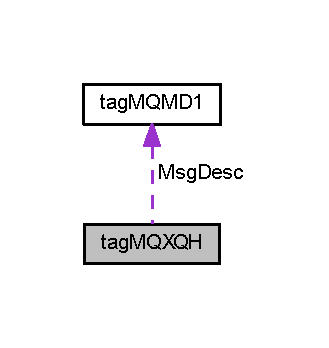
\includegraphics[width=158pt]{structtag_m_q_x_q_h__coll__graph}
\end{center}
\end{figure}
\subsection*{Campos de datos}
\begin{DoxyCompactItemize}
\item 
\hyperlink{cmqc_8h_a12590e546ed66fda7cf21c1d5cefa31d}{M\+Q\+C\+H\+A\+R4} \hyperlink{structtag_m_q_x_q_h_a0530922ca944569b52601d74941f96e4}{Struc\+Id}
\item 
\hyperlink{cmqc_8h_a1fb8d28cbda3fa8766a9821230cdb6d5}{M\+Q\+L\+O\+N\+G} \hyperlink{structtag_m_q_x_q_h_a0656ef8f766b3907d394d88a35d7b7e9}{Version}
\item 
\hyperlink{cmqc_8h_a53b1a2836da03f19144836725ff77919}{M\+Q\+C\+H\+A\+R48} \hyperlink{structtag_m_q_x_q_h_aeadc62f8e5e3d5887d599a5879458a92}{Remote\+Q\+Name}
\item 
\hyperlink{cmqc_8h_a53b1a2836da03f19144836725ff77919}{M\+Q\+C\+H\+A\+R48} \hyperlink{structtag_m_q_x_q_h_a78e0e0316b33b8ed1d4bddb56f5dabe8}{Remote\+Q\+Mgr\+Name}
\item 
\hyperlink{cmqc_8h_a0811cf41b58148bd91248820cff88517}{M\+Q\+M\+D1} \hyperlink{structtag_m_q_x_q_h_a93e5134b6847bf9a3ce68202e2c952e4}{Msg\+Desc}
\end{DoxyCompactItemize}


\subsection{Descripción detallada}


Definición en la línea 5274 del archivo cmqc.\+h.



\subsection{Documentación de los campos}
\hypertarget{structtag_m_q_x_q_h_a93e5134b6847bf9a3ce68202e2c952e4}{}\index{tag\+M\+Q\+X\+Q\+H@{tag\+M\+Q\+X\+Q\+H}!Msg\+Desc@{Msg\+Desc}}
\index{Msg\+Desc@{Msg\+Desc}!tag\+M\+Q\+X\+Q\+H@{tag\+M\+Q\+X\+Q\+H}}
\subsubsection[{Msg\+Desc}]{\setlength{\rightskip}{0pt plus 5cm}{\bf M\+Q\+M\+D1} Msg\+Desc}\label{structtag_m_q_x_q_h_a93e5134b6847bf9a3ce68202e2c952e4}


Definición en la línea 5279 del archivo cmqc.\+h.

\hypertarget{structtag_m_q_x_q_h_a78e0e0316b33b8ed1d4bddb56f5dabe8}{}\index{tag\+M\+Q\+X\+Q\+H@{tag\+M\+Q\+X\+Q\+H}!Remote\+Q\+Mgr\+Name@{Remote\+Q\+Mgr\+Name}}
\index{Remote\+Q\+Mgr\+Name@{Remote\+Q\+Mgr\+Name}!tag\+M\+Q\+X\+Q\+H@{tag\+M\+Q\+X\+Q\+H}}
\subsubsection[{Remote\+Q\+Mgr\+Name}]{\setlength{\rightskip}{0pt plus 5cm}{\bf M\+Q\+C\+H\+A\+R48} Remote\+Q\+Mgr\+Name}\label{structtag_m_q_x_q_h_a78e0e0316b33b8ed1d4bddb56f5dabe8}


Definición en la línea 5278 del archivo cmqc.\+h.

\hypertarget{structtag_m_q_x_q_h_aeadc62f8e5e3d5887d599a5879458a92}{}\index{tag\+M\+Q\+X\+Q\+H@{tag\+M\+Q\+X\+Q\+H}!Remote\+Q\+Name@{Remote\+Q\+Name}}
\index{Remote\+Q\+Name@{Remote\+Q\+Name}!tag\+M\+Q\+X\+Q\+H@{tag\+M\+Q\+X\+Q\+H}}
\subsubsection[{Remote\+Q\+Name}]{\setlength{\rightskip}{0pt plus 5cm}{\bf M\+Q\+C\+H\+A\+R48} Remote\+Q\+Name}\label{structtag_m_q_x_q_h_aeadc62f8e5e3d5887d599a5879458a92}


Definición en la línea 5277 del archivo cmqc.\+h.

\hypertarget{structtag_m_q_x_q_h_a0530922ca944569b52601d74941f96e4}{}\index{tag\+M\+Q\+X\+Q\+H@{tag\+M\+Q\+X\+Q\+H}!Struc\+Id@{Struc\+Id}}
\index{Struc\+Id@{Struc\+Id}!tag\+M\+Q\+X\+Q\+H@{tag\+M\+Q\+X\+Q\+H}}
\subsubsection[{Struc\+Id}]{\setlength{\rightskip}{0pt plus 5cm}{\bf M\+Q\+C\+H\+A\+R4} Struc\+Id}\label{structtag_m_q_x_q_h_a0530922ca944569b52601d74941f96e4}


Definición en la línea 5275 del archivo cmqc.\+h.

\hypertarget{structtag_m_q_x_q_h_a0656ef8f766b3907d394d88a35d7b7e9}{}\index{tag\+M\+Q\+X\+Q\+H@{tag\+M\+Q\+X\+Q\+H}!Version@{Version}}
\index{Version@{Version}!tag\+M\+Q\+X\+Q\+H@{tag\+M\+Q\+X\+Q\+H}}
\subsubsection[{Version}]{\setlength{\rightskip}{0pt plus 5cm}{\bf M\+Q\+L\+O\+N\+G} Version}\label{structtag_m_q_x_q_h_a0656ef8f766b3907d394d88a35d7b7e9}


Definición en la línea 5276 del archivo cmqc.\+h.



La documentación para esta estructura fue generada a partir del siguiente fichero\+:\begin{DoxyCompactItemize}
\item 
include/\hyperlink{cmqc_8h}{cmqc.\+h}\end{DoxyCompactItemize}

\chapter{Documentación de archivos}
\hypertarget{amqsdp_8h}{}\section{Referencia del Archivo include/amqsdp.h}
\label{amqsdp_8h}\index{include/amqsdp.\+h@{include/amqsdp.\+h}}


Cliente Websphere M\+Q\+Series.  


{\ttfamily \#include \char`\"{}jggsal.\+h\char`\"{}}\\*
Dependencia gráfica adjunta para amqsdp.\+h\+:\nopagebreak
\begin{figure}[H]
\begin{center}
\leavevmode
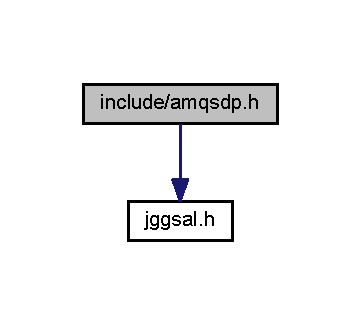
\includegraphics[width=173pt]{amqsdp_8h__incl}
\end{center}
\end{figure}
Gráfico de los archivos que directa o indirectamente incluyen a este archivo\+:\nopagebreak
\begin{figure}[H]
\begin{center}
\leavevmode
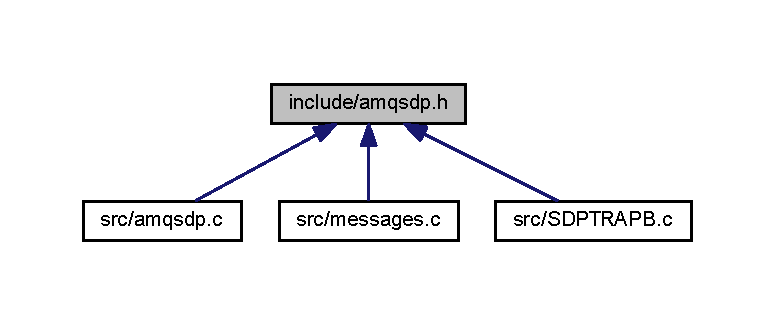
\includegraphics[width=350pt]{amqsdp_8h__dep__incl}
\end{center}
\end{figure}
\subsection*{\textquotesingle{}defines\textquotesingle{}}
\begin{DoxyCompactItemize}
\item 
\#define \hyperlink{amqsdp_8h_adfbc1051df776564281ac4220ba53a9e}{\+\_\+\+E\+X\+T\+\_\+}~extern
\end{DoxyCompactItemize}
\subsection*{Funciones}
\begin{DoxyCompactItemize}
\item 
\hyperlink{sha256le_8h_adfbc1051df776564281ac4220ba53a9e}{\+\_\+\+E\+X\+T\+\_\+} void \hyperlink{amqsdp_8h_a5b1c0890d82a1e4fd8201da9ece0c6ae}{init\+A\+M\+Q} (int dbg, F\+I\+L\+E $\ast$f)
\item 
\hyperlink{sha256le_8h_adfbc1051df776564281ac4220ba53a9e}{\+\_\+\+E\+X\+T\+\_\+} void \hyperlink{amqsdp_8h_a3c337f7b77e495f85489f862d4df359c}{set\+Buffer\+Size} ()
\item 
\hyperlink{sha256le_8h_adfbc1051df776564281ac4220ba53a9e}{\+\_\+\+E\+X\+T\+\_\+} void \hyperlink{amqsdp_8h_adba192fbf1af062214021fcb06229295}{unset\+Buffer\+Size} ()
\item 
\hyperlink{sha256le_8h_adfbc1051df776564281ac4220ba53a9e}{\+\_\+\+E\+X\+T\+\_\+} void \hyperlink{amqsdp_8h_ac2122a579c04414c93370c338601c492}{set\+Max\+Group} (int group)
\item 
\hyperlink{sha256le_8h_adfbc1051df776564281ac4220ba53a9e}{\+\_\+\+E\+X\+T\+\_\+} int \hyperlink{amqsdp_8h_ab05385469ff40b1b77e3c41846d1421f}{enviar} (char $\ast$\hyperlink{messages_8c_a1c07f3735e9c63f3130a615745887a20}{sz\+Msg}, unsigned char force)
\item 
\hyperlink{sha256le_8h_adfbc1051df776564281ac4220ba53a9e}{\+\_\+\+E\+X\+T\+\_\+} int \hyperlink{amqsdp_8h_acb3870940341d48437b3a835098fc53e}{M\+Q\+Connect} (void)
\item 
\hyperlink{sha256le_8h_adfbc1051df776564281ac4220ba53a9e}{\+\_\+\+E\+X\+T\+\_\+} void \hyperlink{amqsdp_8h_a49ea4971cfd64e5b120d9dd38050426e}{M\+Q\+Disconnect} (void)
\item 
\hyperlink{sha256le_8h_adfbc1051df776564281ac4220ba53a9e}{\+\_\+\+E\+X\+T\+\_\+} int \hyperlink{amqsdp_8h_a147a0974e48f9171a63535159f34585d}{M\+Q\+Open\+Output} (void)
\item 
\hyperlink{sha256le_8h_adfbc1051df776564281ac4220ba53a9e}{\+\_\+\+E\+X\+T\+\_\+} int \hyperlink{amqsdp_8h_abe88b1c5c1d0e93d6152f0b7bbc5eb44}{M\+Q\+Open\+Input} (void)
\item 
\hyperlink{sha256le_8h_adfbc1051df776564281ac4220ba53a9e}{\+\_\+\+E\+X\+T\+\_\+} long \hyperlink{amqsdp_8h_a9531d8185ec00f217beb2bcb561099d6}{M\+Q\+Put} (char $\ast$msg, long len)
\item 
\hyperlink{sha256le_8h_adfbc1051df776564281ac4220ba53a9e}{\+\_\+\+E\+X\+T\+\_\+} long \hyperlink{amqsdp_8h_a5b76a97fbc96b9cb87eb64ffe49630aa}{M\+Q\+Get} (char $\ast$msg, long len)
\end{DoxyCompactItemize}


\subsection{Descripción detallada}
Cliente Websphere M\+Q\+Series. 

La informacion relativa a Q\+Manager, Nombre de cola, etc se obtiene del entorno

\begin{DoxyAuthor}{Autor}
\+: Javier Gonzalez 
\end{DoxyAuthor}
\begin{DoxyDate}{Fecha}
\+: 01/03/15 
\end{DoxyDate}
\begin{DoxyVersion}{Versión}
\+: 2.\+0 
\end{DoxyVersion}


\subsection{Documentación de los \textquotesingle{}defines\textquotesingle{}}
\hypertarget{amqsdp_8h_adfbc1051df776564281ac4220ba53a9e}{}\index{amqsdp.\+h@{amqsdp.\+h}!\+\_\+\+E\+X\+T\+\_\+@{\+\_\+\+E\+X\+T\+\_\+}}
\index{\+\_\+\+E\+X\+T\+\_\+@{\+\_\+\+E\+X\+T\+\_\+}!amqsdp.\+h@{amqsdp.\+h}}
\subsubsection[{\+\_\+\+E\+X\+T\+\_\+}]{\setlength{\rightskip}{0pt plus 5cm}\#define \+\_\+\+E\+X\+T\+\_\+~extern}\label{amqsdp_8h_adfbc1051df776564281ac4220ba53a9e}


Definición en la línea 22 del archivo amqsdp.\+h.



\subsection{Documentación de las funciones}
\hypertarget{amqsdp_8h_ab05385469ff40b1b77e3c41846d1421f}{}\index{amqsdp.\+h@{amqsdp.\+h}!enviar@{enviar}}
\index{enviar@{enviar}!amqsdp.\+h@{amqsdp.\+h}}
\subsubsection[{enviar(char $\ast$sz\+Msg, unsigned char force)}]{\setlength{\rightskip}{0pt plus 5cm}{\bf \+\_\+\+E\+X\+T\+\_\+} int enviar (
\begin{DoxyParamCaption}
\item[{char $\ast$}]{sz\+Msg, }
\item[{unsigned char}]{force}
\end{DoxyParamCaption}
)}\label{amqsdp_8h_ab05385469ff40b1b77e3c41846d1421f}
Escribe el mensaje en la cola

Envia el mensaje si force = true o se han alcanzado el el numero de mensajes a agrupar

Si no lo almacena en el buffer para evitar envios masivos mensajes Se verifica si el mensaje cabe en el buffer alocado antes de alamacenarlo, seria el caso en el que el numero mensajes a agrupar es excesivo 

Definición en la línea 108 del archivo amqsdp.\+c.

\hypertarget{amqsdp_8h_a5b1c0890d82a1e4fd8201da9ece0c6ae}{}\index{amqsdp.\+h@{amqsdp.\+h}!init\+A\+M\+Q@{init\+A\+M\+Q}}
\index{init\+A\+M\+Q@{init\+A\+M\+Q}!amqsdp.\+h@{amqsdp.\+h}}
\subsubsection[{init\+A\+M\+Q(int dbg, F\+I\+L\+E $\ast$f)}]{\setlength{\rightskip}{0pt plus 5cm}{\bf \+\_\+\+E\+X\+T\+\_\+} void init\+A\+M\+Q (
\begin{DoxyParamCaption}
\item[{int}]{dbg, }
\item[{F\+I\+L\+E $\ast$}]{f}
\end{DoxyParamCaption}
)}\label{amqsdp_8h_a5b1c0890d82a1e4fd8201da9ece0c6ae}
Inicia el entorno M\+Q Para depuracion es necesario pasarlo el nivel de debug y el fichero a utilizar 

Definición en la línea 77 del archivo amqsdp.\+c.

\hypertarget{amqsdp_8h_acb3870940341d48437b3a835098fc53e}{}\index{amqsdp.\+h@{amqsdp.\+h}!M\+Q\+Connect@{M\+Q\+Connect}}
\index{M\+Q\+Connect@{M\+Q\+Connect}!amqsdp.\+h@{amqsdp.\+h}}
\subsubsection[{M\+Q\+Connect(void)}]{\setlength{\rightskip}{0pt plus 5cm}{\bf \+\_\+\+E\+X\+T\+\_\+} int M\+Q\+Connect (
\begin{DoxyParamCaption}
\item[{void}]{}
\end{DoxyParamCaption}
)}\label{amqsdp_8h_acb3870940341d48437b3a835098fc53e}
Establece la conexion con el gestor de colas 

Definición en la línea 134 del archivo amqsdp.\+c.

\hypertarget{amqsdp_8h_a49ea4971cfd64e5b120d9dd38050426e}{}\index{amqsdp.\+h@{amqsdp.\+h}!M\+Q\+Disconnect@{M\+Q\+Disconnect}}
\index{M\+Q\+Disconnect@{M\+Q\+Disconnect}!amqsdp.\+h@{amqsdp.\+h}}
\subsubsection[{M\+Q\+Disconnect(void)}]{\setlength{\rightskip}{0pt plus 5cm}{\bf \+\_\+\+E\+X\+T\+\_\+} void M\+Q\+Disconnect (
\begin{DoxyParamCaption}
\item[{void}]{}
\end{DoxyParamCaption}
)}\label{amqsdp_8h_a49ea4971cfd64e5b120d9dd38050426e}
Libera la conexion con el gestor de colas 

Definición en la línea 146 del archivo amqsdp.\+c.

\hypertarget{amqsdp_8h_a5b76a97fbc96b9cb87eb64ffe49630aa}{}\index{amqsdp.\+h@{amqsdp.\+h}!M\+Q\+Get@{M\+Q\+Get}}
\index{M\+Q\+Get@{M\+Q\+Get}!amqsdp.\+h@{amqsdp.\+h}}
\subsubsection[{M\+Q\+Get(char $\ast$msg, long len)}]{\setlength{\rightskip}{0pt plus 5cm}{\bf \+\_\+\+E\+X\+T\+\_\+} long M\+Q\+Get (
\begin{DoxyParamCaption}
\item[{char $\ast$}]{msg, }
\item[{long}]{len}
\end{DoxyParamCaption}
)}\label{amqsdp_8h_a5b76a97fbc96b9cb87eb64ffe49630aa}
Lee un mensaje de la cola 

Definición en la línea 175 del archivo amqsdp.\+c.

\hypertarget{amqsdp_8h_abe88b1c5c1d0e93d6152f0b7bbc5eb44}{}\index{amqsdp.\+h@{amqsdp.\+h}!M\+Q\+Open\+Input@{M\+Q\+Open\+Input}}
\index{M\+Q\+Open\+Input@{M\+Q\+Open\+Input}!amqsdp.\+h@{amqsdp.\+h}}
\subsubsection[{M\+Q\+Open\+Input(void)}]{\setlength{\rightskip}{0pt plus 5cm}{\bf \+\_\+\+E\+X\+T\+\_\+} int M\+Q\+Open\+Input (
\begin{DoxyParamCaption}
\item[{void}]{}
\end{DoxyParamCaption}
)}\label{amqsdp_8h_abe88b1c5c1d0e93d6152f0b7bbc5eb44}
Abre la cola de lectura 

Definición en la línea 231 del archivo amqsdp.\+c.

\hypertarget{amqsdp_8h_a147a0974e48f9171a63535159f34585d}{}\index{amqsdp.\+h@{amqsdp.\+h}!M\+Q\+Open\+Output@{M\+Q\+Open\+Output}}
\index{M\+Q\+Open\+Output@{M\+Q\+Open\+Output}!amqsdp.\+h@{amqsdp.\+h}}
\subsubsection[{M\+Q\+Open\+Output(void)}]{\setlength{\rightskip}{0pt plus 5cm}{\bf \+\_\+\+E\+X\+T\+\_\+} int M\+Q\+Open\+Output (
\begin{DoxyParamCaption}
\item[{void}]{}
\end{DoxyParamCaption}
)}\label{amqsdp_8h_a147a0974e48f9171a63535159f34585d}
Abre la cola de escritura 

Definición en la línea 223 del archivo amqsdp.\+c.

\hypertarget{amqsdp_8h_a9531d8185ec00f217beb2bcb561099d6}{}\index{amqsdp.\+h@{amqsdp.\+h}!M\+Q\+Put@{M\+Q\+Put}}
\index{M\+Q\+Put@{M\+Q\+Put}!amqsdp.\+h@{amqsdp.\+h}}
\subsubsection[{M\+Q\+Put(char $\ast$msg, long len)}]{\setlength{\rightskip}{0pt plus 5cm}{\bf \+\_\+\+E\+X\+T\+\_\+} long M\+Q\+Put (
\begin{DoxyParamCaption}
\item[{char $\ast$}]{msg, }
\item[{long}]{len}
\end{DoxyParamCaption}
)}\label{amqsdp_8h_a9531d8185ec00f217beb2bcb561099d6}
Escribe el mensaje en la cola 

Definición en la línea 152 del archivo amqsdp.\+c.

\hypertarget{amqsdp_8h_a3c337f7b77e495f85489f862d4df359c}{}\index{amqsdp.\+h@{amqsdp.\+h}!set\+Buffer\+Size@{set\+Buffer\+Size}}
\index{set\+Buffer\+Size@{set\+Buffer\+Size}!amqsdp.\+h@{amqsdp.\+h}}
\subsubsection[{set\+Buffer\+Size()}]{\setlength{\rightskip}{0pt plus 5cm}{\bf \+\_\+\+E\+X\+T\+\_\+} void set\+Buffer\+Size (
\begin{DoxyParamCaption}
{}
\end{DoxyParamCaption}
)}\label{amqsdp_8h_a3c337f7b77e495f85489f862d4df359c}
Crea el buffer de mensajes 

Definición en la línea 82 del archivo amqsdp.\+c.

\hypertarget{amqsdp_8h_ac2122a579c04414c93370c338601c492}{}\index{amqsdp.\+h@{amqsdp.\+h}!set\+Max\+Group@{set\+Max\+Group}}
\index{set\+Max\+Group@{set\+Max\+Group}!amqsdp.\+h@{amqsdp.\+h}}
\subsubsection[{set\+Max\+Group(int group)}]{\setlength{\rightskip}{0pt plus 5cm}{\bf \+\_\+\+E\+X\+T\+\_\+} void set\+Max\+Group (
\begin{DoxyParamCaption}
\item[{int}]{group}
\end{DoxyParamCaption}
)}\label{amqsdp_8h_ac2122a579c04414c93370c338601c492}
Establece el numero de mensajes que se enviaran en un unico mensaje de la cola 

Definición en la línea 93 del archivo amqsdp.\+c.

\hypertarget{amqsdp_8h_adba192fbf1af062214021fcb06229295}{}\index{amqsdp.\+h@{amqsdp.\+h}!unset\+Buffer\+Size@{unset\+Buffer\+Size}}
\index{unset\+Buffer\+Size@{unset\+Buffer\+Size}!amqsdp.\+h@{amqsdp.\+h}}
\subsubsection[{unset\+Buffer\+Size()}]{\setlength{\rightskip}{0pt plus 5cm}{\bf \+\_\+\+E\+X\+T\+\_\+} void unset\+Buffer\+Size (
\begin{DoxyParamCaption}
{}
\end{DoxyParamCaption}
)}\label{amqsdp_8h_adba192fbf1af062214021fcb06229295}
Libera el buffer de mensajes 

Definición en la línea 89 del archivo amqsdp.\+c.


\hypertarget{cmqc_8h}{}\section{Referencia del Archivo include/cmqc.h}
\label{cmqc_8h}\index{include/cmqc.\+h@{include/cmqc.\+h}}
Gráfico de los archivos que directa o indirectamente incluyen a este archivo\+:\nopagebreak
\begin{figure}[H]
\begin{center}
\leavevmode
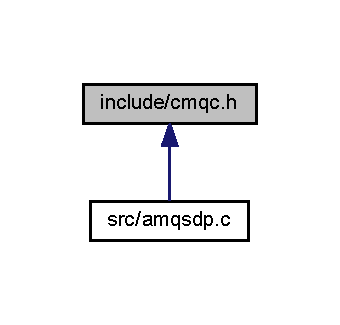
\includegraphics[width=163pt]{cmqc_8h__dep__incl}
\end{center}
\end{figure}
\subsection*{Estructuras de datos}
\begin{DoxyCompactItemize}
\item 
struct \hyperlink{structtag_m_q_a_i_r}{tag\+M\+Q\+A\+I\+R}
\item 
struct \hyperlink{structtag_m_q_b_m_h_o}{tag\+M\+Q\+B\+M\+H\+O}
\item 
struct \hyperlink{structtag_m_q_b_o}{tag\+M\+Q\+B\+O}
\item 
struct \hyperlink{structtag_m_q_c_b_c}{tag\+M\+Q\+C\+B\+C}
\item 
struct \hyperlink{structtag_m_q_c_b_d}{tag\+M\+Q\+C\+B\+D}
\item 
struct \hyperlink{structtag_m_q_c_h_a_r_v}{tag\+M\+Q\+C\+H\+A\+R\+V}
\item 
struct \hyperlink{structtag_m_q_c_i_h}{tag\+M\+Q\+C\+I\+H}
\item 
struct \hyperlink{structtag_m_q_c_m_h_o}{tag\+M\+Q\+C\+M\+H\+O}
\item 
struct \hyperlink{structtag_m_q_c_t_l_o}{tag\+M\+Q\+C\+T\+L\+O}
\item 
struct \hyperlink{structtag_m_q_s_c_o}{tag\+M\+Q\+S\+C\+O}
\item 
struct \hyperlink{structtag_m_q_c_s_p}{tag\+M\+Q\+C\+S\+P}
\item 
struct \hyperlink{structtag_m_q_c_n_o}{tag\+M\+Q\+C\+N\+O}
\item 
struct \hyperlink{structtag_m_q_d_h}{tag\+M\+Q\+D\+H}
\item 
struct \hyperlink{structtag_m_q_d_l_h}{tag\+M\+Q\+D\+L\+H}
\item 
struct \hyperlink{structtag_m_q_d_m_h_o}{tag\+M\+Q\+D\+M\+H\+O}
\item 
struct \hyperlink{structtag_m_q_d_m_p_o}{tag\+M\+Q\+D\+M\+P\+O}
\item 
struct \hyperlink{structtag_m_q_g_m_o}{tag\+M\+Q\+G\+M\+O}
\item 
struct \hyperlink{structtag_m_q_i_i_h}{tag\+M\+Q\+I\+I\+H}
\item 
struct \hyperlink{structtag_m_q_i_m_p_o}{tag\+M\+Q\+I\+M\+P\+O}
\item 
struct \hyperlink{structtag_m_q_m_d}{tag\+M\+Q\+M\+D}
\item 
struct \hyperlink{structtag_m_q_m_d_e}{tag\+M\+Q\+M\+D\+E}
\item 
struct \hyperlink{structtag_m_q_m_d1}{tag\+M\+Q\+M\+D1}
\item 
struct \hyperlink{structtag_m_q_m_d2}{tag\+M\+Q\+M\+D2}
\item 
struct \hyperlink{structtag_m_q_m_h_b_o}{tag\+M\+Q\+M\+H\+B\+O}
\item 
struct \hyperlink{structtag_m_q_o_d}{tag\+M\+Q\+O\+D}
\item 
struct \hyperlink{structtag_m_q_o_r}{tag\+M\+Q\+O\+R}
\item 
struct \hyperlink{structtag_m_q_p_d}{tag\+M\+Q\+P\+D}
\item 
struct \hyperlink{structtag_m_q_p_m_o}{tag\+M\+Q\+P\+M\+O}
\item 
struct \hyperlink{structtag_m_q_r_f_h}{tag\+M\+Q\+R\+F\+H}
\item 
struct \hyperlink{structtag_m_q_r_f_h2}{tag\+M\+Q\+R\+F\+H2}
\item 
struct \hyperlink{structtag_m_q_r_m_h}{tag\+M\+Q\+R\+M\+H}
\item 
struct \hyperlink{structtag_m_q_r_r}{tag\+M\+Q\+R\+R}
\item 
struct \hyperlink{structtag_m_q_s_d}{tag\+M\+Q\+S\+D}
\item 
struct \hyperlink{structtag_m_q_s_m_p_o}{tag\+M\+Q\+S\+M\+P\+O}
\item 
struct \hyperlink{structtag_m_q_s_r_o}{tag\+M\+Q\+S\+R\+O}
\item 
struct \hyperlink{structtag_m_q_s_t_s}{tag\+M\+Q\+S\+T\+S}
\item 
struct \hyperlink{structtag_m_q_t_m}{tag\+M\+Q\+T\+M}
\item 
struct \hyperlink{structtag_m_q_t_m_c2}{tag\+M\+Q\+T\+M\+C2}
\item 
struct \hyperlink{structtag_m_q_w_i_h}{tag\+M\+Q\+W\+I\+H}
\item 
struct \hyperlink{structtag_m_q_x_q_h}{tag\+M\+Q\+X\+Q\+H}
\end{DoxyCompactItemize}
\subsection*{\textquotesingle{}defines\textquotesingle{}}
\begin{DoxyCompactItemize}
\item 
\#define \hyperlink{cmqc_8h_a65a5579b9fc1e6f17bf3d12efa56516a}{M\+Q\+C\+\_\+\+I\+N\+C\+L\+U\+D\+E\+D}~/$\ast$ Show file now included $\ast$/
\item 
\#define \hyperlink{cmqc_8h_aeac89f1f1ee9c0162088670e7f1dd196}{M\+Q\+A\+I\+R\+\_\+\+S\+T\+R\+U\+C\+\_\+\+I\+D}~\char`\"{}A\+I\+R \char`\"{}
\item 
\#define \hyperlink{cmqc_8h_a9cd434eb54ce91d67b0e0ddd572dd5ca}{M\+Q\+A\+I\+R\+\_\+\+S\+T\+R\+U\+C\+\_\+\+I\+D\+\_\+\+A\+R\+R\+A\+Y}~\textquotesingle{}A\textquotesingle{},\textquotesingle{}\hyperlink{md5_8c_ac0eafdc9ee161b71e7af98af736952fd}{I}\textquotesingle{},\textquotesingle{}R\textquotesingle{},\textquotesingle{} \textquotesingle{}
\item 
\#define \hyperlink{cmqc_8h_abdb44c4886bb740e69d91f1dad691737}{M\+Q\+A\+I\+R\+\_\+\+V\+E\+R\+S\+I\+O\+N\+\_\+1}~1
\item 
\#define \hyperlink{cmqc_8h_a2a16f087f8f0c9148600d0f21b4f6334}{M\+Q\+A\+I\+R\+\_\+\+V\+E\+R\+S\+I\+O\+N\+\_\+2}~2
\item 
\#define \hyperlink{cmqc_8h_a57ce9a215cf5d3a43fca15f9e0c0eafe}{M\+Q\+A\+I\+R\+\_\+\+C\+U\+R\+R\+E\+N\+T\+\_\+\+V\+E\+R\+S\+I\+O\+N}~2
\item 
\#define \hyperlink{cmqc_8h_a2edf8aea2519fb9b47b8bcb80119ae33}{M\+Q\+A\+I\+R\+\_\+\+L\+E\+N\+G\+T\+H\+\_\+1}~320
\item 
\#define \hyperlink{cmqc_8h_a1a1466313676d7fa010fb18dfc4b5d7c}{M\+Q\+A\+I\+R\+\_\+\+L\+E\+N\+G\+T\+H\+\_\+2}~576
\item 
\#define \hyperlink{cmqc_8h_a8d374419f65e982118846a0e9fa14d48}{M\+Q\+A\+I\+R\+\_\+\+C\+U\+R\+R\+E\+N\+T\+\_\+\+L\+E\+N\+G\+T\+H}~576
\item 
\#define \hyperlink{cmqc_8h_aa8aa58f7c8c917c899463184da3ce544}{M\+Q\+A\+I\+T\+\_\+\+A\+L\+L}~0
\item 
\#define \hyperlink{cmqc_8h_a488b3ad32ba4873a464c0cd7d8cd6c0a}{M\+Q\+A\+I\+T\+\_\+\+C\+R\+L\+\_\+\+L\+D\+A\+P}~1
\item 
\#define \hyperlink{cmqc_8h_a939e7fb9834b1081af6220780b11175a}{M\+Q\+A\+I\+T\+\_\+\+O\+C\+S\+P}~2
\item 
\#define \hyperlink{cmqc_8h_ae0f9f3f73f421b16701bfbc817bcf394}{M\+Q\+A\+I\+T\+\_\+\+I\+D\+P\+W\+\_\+\+O\+S}~3
\item 
\#define \hyperlink{cmqc_8h_ae3feaf628f3392083d541a8908d26a74}{M\+Q\+A\+I\+T\+\_\+\+I\+D\+P\+W\+\_\+\+L\+D\+A\+P}~4
\item 
\#define \hyperlink{cmqc_8h_a2a8a7709a65262bd0a701690acacf5e8}{M\+Q\+B\+M\+H\+O\+\_\+\+S\+T\+R\+U\+C\+\_\+\+I\+D}~\char`\"{}B\+M\+H\+O\char`\"{}
\item 
\#define \hyperlink{cmqc_8h_a2f9624e55ae5596892ed7a3aa3d5a4fd}{M\+Q\+B\+M\+H\+O\+\_\+\+S\+T\+R\+U\+C\+\_\+\+I\+D\+\_\+\+A\+R\+R\+A\+Y}~\textquotesingle{}B\textquotesingle{},\textquotesingle{}M\textquotesingle{},\textquotesingle{}\hyperlink{md5_8c_ae42219072d798876e6b08e6b78614ff6}{H}\textquotesingle{},\textquotesingle{}O\textquotesingle{}
\item 
\#define \hyperlink{cmqc_8h_a962527f59786234c51f22a62b31c61ce}{M\+Q\+B\+M\+H\+O\+\_\+\+V\+E\+R\+S\+I\+O\+N\+\_\+1}~1
\item 
\#define \hyperlink{cmqc_8h_afc92521afc0e40d13925f203ac1c13c3}{M\+Q\+B\+M\+H\+O\+\_\+\+C\+U\+R\+R\+E\+N\+T\+\_\+\+V\+E\+R\+S\+I\+O\+N}~1
\item 
\#define \hyperlink{cmqc_8h_ad004b92c1719f135a7182151d444bc75}{M\+Q\+B\+M\+H\+O\+\_\+\+L\+E\+N\+G\+T\+H\+\_\+1}~12
\item 
\#define \hyperlink{cmqc_8h_a02e15b062c0a3259a4ce26a3142a8f9f}{M\+Q\+B\+M\+H\+O\+\_\+\+C\+U\+R\+R\+E\+N\+T\+\_\+\+L\+E\+N\+G\+T\+H}~12
\item 
\#define \hyperlink{cmqc_8h_abf2755d2541e72dacb4d9c05ba5f2338}{M\+Q\+B\+M\+H\+O\+\_\+\+N\+O\+N\+E}~0x00000000
\item 
\#define \hyperlink{cmqc_8h_a5db0323b2bf4ff04d38d2115ce57dadf}{M\+Q\+B\+M\+H\+O\+\_\+\+D\+E\+L\+E\+T\+E\+\_\+\+P\+R\+O\+P\+E\+R\+T\+I\+E\+S}~0x00000001
\item 
\#define \hyperlink{cmqc_8h_aa622a7fbb56b5abb37ab2fe4368ad0c8}{M\+Q\+B\+O\+\_\+\+S\+T\+R\+U\+C\+\_\+\+I\+D}~\char`\"{}B\+O  \char`\"{}
\item 
\#define \hyperlink{cmqc_8h_a12c2d45614c90c6d456631108140dc08}{M\+Q\+B\+O\+\_\+\+S\+T\+R\+U\+C\+\_\+\+I\+D\+\_\+\+A\+R\+R\+A\+Y}~\textquotesingle{}B\textquotesingle{},\textquotesingle{}O\textquotesingle{},\textquotesingle{} \textquotesingle{},\textquotesingle{} \textquotesingle{}
\item 
\#define \hyperlink{cmqc_8h_a341a888ac98770fc1427bcf2b8b2d0ea}{M\+Q\+B\+O\+\_\+\+V\+E\+R\+S\+I\+O\+N\+\_\+1}~1
\item 
\#define \hyperlink{cmqc_8h_a35a1cfbdf501e94c044fc29c86982f67}{M\+Q\+B\+O\+\_\+\+C\+U\+R\+R\+E\+N\+T\+\_\+\+V\+E\+R\+S\+I\+O\+N}~1
\item 
\#define \hyperlink{cmqc_8h_a73b0b251d5a49136ca689c3068e2478b}{M\+Q\+B\+O\+\_\+\+L\+E\+N\+G\+T\+H\+\_\+1}~12
\item 
\#define \hyperlink{cmqc_8h_aa3d3b272684eb01daa252710364e2b8c}{M\+Q\+B\+O\+\_\+\+C\+U\+R\+R\+E\+N\+T\+\_\+\+L\+E\+N\+G\+T\+H}~12
\item 
\#define \hyperlink{cmqc_8h_a1e50307211ee5f1e2ca0a93b06b6e67a}{M\+Q\+B\+O\+\_\+\+N\+O\+N\+E}~0x00000000
\item 
\#define \hyperlink{cmqc_8h_a1d5f54fba2d99a8db382574cf5dd184f}{M\+Q\+C\+B\+C\+\_\+\+S\+T\+R\+U\+C\+\_\+\+I\+D}~\char`\"{}C\+B\+C \char`\"{}
\item 
\#define \hyperlink{cmqc_8h_a8a0ce4c5ef4dca44a65638ba61037676}{M\+Q\+C\+B\+C\+\_\+\+S\+T\+R\+U\+C\+\_\+\+I\+D\+\_\+\+A\+R\+R\+A\+Y}~\textquotesingle{}C\textquotesingle{},\textquotesingle{}B\textquotesingle{},\textquotesingle{}C\textquotesingle{},\textquotesingle{} \textquotesingle{}
\item 
\#define \hyperlink{cmqc_8h_a2840638bddd1480853794ac0d83a2c84}{M\+Q\+C\+B\+C\+\_\+\+V\+E\+R\+S\+I\+O\+N\+\_\+1}~1
\item 
\#define \hyperlink{cmqc_8h_aa81d299d624eddd2e698228f743b9463}{M\+Q\+C\+B\+C\+\_\+\+V\+E\+R\+S\+I\+O\+N\+\_\+2}~2
\item 
\#define \hyperlink{cmqc_8h_ab81a2338c121ff196df3fd5ed14f2dd2}{M\+Q\+C\+B\+C\+\_\+\+C\+U\+R\+R\+E\+N\+T\+\_\+\+V\+E\+R\+S\+I\+O\+N}~2
\item 
\#define \hyperlink{cmqc_8h_ad5e4d33599a11505167379439f43fc5c}{M\+Q\+C\+B\+C\+\_\+\+L\+E\+N\+G\+T\+H\+\_\+1}~48
\item 
\#define \hyperlink{cmqc_8h_a80f555dff8c9d52f2cabe73675122c51}{M\+Q\+C\+B\+C\+\_\+\+L\+E\+N\+G\+T\+H\+\_\+2}~52
\item 
\#define \hyperlink{cmqc_8h_a55bd01bda215e6159c671be9965c0867}{M\+Q\+C\+B\+C\+\_\+\+C\+U\+R\+R\+E\+N\+T\+\_\+\+L\+E\+N\+G\+T\+H}~52
\item 
\#define \hyperlink{cmqc_8h_a0d3cea952b0267e2e6a0bda6c71d6180}{M\+Q\+C\+B\+C\+F\+\_\+\+N\+O\+N\+E}~0x00000000
\item 
\#define \hyperlink{cmqc_8h_a16defe7b8867b78ab18b4e75ff11354f}{M\+Q\+C\+B\+C\+F\+\_\+\+R\+E\+A\+D\+A\+\_\+\+B\+U\+F\+F\+E\+R\+\_\+\+E\+M\+P\+T\+Y}~0x00000001
\item 
\#define \hyperlink{cmqc_8h_a5b6d2772e98233105e346f4ad1c525d7}{M\+Q\+C\+B\+C\+T\+\_\+\+S\+T\+A\+R\+T\+\_\+\+C\+A\+L\+L}~1
\item 
\#define \hyperlink{cmqc_8h_a766c234d0152632ada9d0e7bf1ab79a6}{M\+Q\+C\+B\+C\+T\+\_\+\+S\+T\+O\+P\+\_\+\+C\+A\+L\+L}~2
\item 
\#define \hyperlink{cmqc_8h_a3670f8631ad95b11a5f61bdf8a097aa5}{M\+Q\+C\+B\+C\+T\+\_\+\+R\+E\+G\+I\+S\+T\+E\+R\+\_\+\+C\+A\+L\+L}~3
\item 
\#define \hyperlink{cmqc_8h_aa1f5aa1b722231d94467005b665a6769}{M\+Q\+C\+B\+C\+T\+\_\+\+D\+E\+R\+E\+G\+I\+S\+T\+E\+R\+\_\+\+C\+A\+L\+L}~4
\item 
\#define \hyperlink{cmqc_8h_abc30d1a9a3447a5e06ee67097a26d898}{M\+Q\+C\+B\+C\+T\+\_\+\+E\+V\+E\+N\+T\+\_\+\+C\+A\+L\+L}~5
\item 
\#define \hyperlink{cmqc_8h_a7261cbaa1c842dd4a1c516ab8509f2de}{M\+Q\+C\+B\+C\+T\+\_\+\+M\+S\+G\+\_\+\+R\+E\+M\+O\+V\+E\+D}~6
\item 
\#define \hyperlink{cmqc_8h_a1d57eda7bf30c6a15800b888b53bb6f0}{M\+Q\+C\+B\+C\+T\+\_\+\+M\+S\+G\+\_\+\+N\+O\+T\+\_\+\+R\+E\+M\+O\+V\+E\+D}~7
\item 
\#define \hyperlink{cmqc_8h_acc41dcaa621acdba22006bd06e2fadfc}{M\+Q\+C\+B\+C\+T\+\_\+\+M\+C\+\_\+\+E\+V\+E\+N\+T\+\_\+\+C\+A\+L\+L}~8
\item 
\#define \hyperlink{cmqc_8h_a01d70e84da20808d1f604b80a7c9ed21}{M\+Q\+C\+S\+\_\+\+N\+O\+N\+E}~0
\item 
\#define \hyperlink{cmqc_8h_a76e0add25f058ae3b5b05ab8904aab57}{M\+Q\+C\+S\+\_\+\+S\+U\+S\+P\+E\+N\+D\+E\+D\+\_\+\+T\+E\+M\+P\+O\+R\+A\+R\+Y}~1
\item 
\#define \hyperlink{cmqc_8h_aa626bc3451b1fbe243a614f9c394b628}{M\+Q\+C\+S\+\_\+\+S\+U\+S\+P\+E\+N\+D\+E\+D\+\_\+\+U\+S\+E\+R\+\_\+\+A\+C\+T\+I\+O\+N}~2
\item 
\#define \hyperlink{cmqc_8h_aed99307defbac46810cb9480c4fea968}{M\+Q\+C\+S\+\_\+\+S\+U\+S\+P\+E\+N\+D\+E\+D}~3
\item 
\#define \hyperlink{cmqc_8h_a541b2a55ae4886b358bbed815cfdbc5b}{M\+Q\+C\+S\+\_\+\+S\+T\+O\+P\+P\+E\+D}~4
\item 
\#define \hyperlink{cmqc_8h_a9803ddb1b6bbdf8a8f74633575483b18}{M\+Q\+R\+D\+\_\+\+N\+O\+\_\+\+R\+E\+C\+O\+N\+N\+E\+C\+T}~(-\/1)
\item 
\#define \hyperlink{cmqc_8h_affcccd621fb9498aea1cb41cbab0f27d}{M\+Q\+R\+D\+\_\+\+N\+O\+\_\+\+D\+E\+L\+A\+Y}~0
\item 
\#define \hyperlink{cmqc_8h_a7c57ef953423447254d0b1ed6782c2ce}{M\+Q\+C\+B\+D\+\_\+\+S\+T\+R\+U\+C\+\_\+\+I\+D}~\char`\"{}C\+B\+D \char`\"{}
\item 
\#define \hyperlink{cmqc_8h_ac9f25d862c1b8a8785e1625cdbdd8d25}{M\+Q\+C\+B\+D\+\_\+\+S\+T\+R\+U\+C\+\_\+\+I\+D\+\_\+\+A\+R\+R\+A\+Y}~\textquotesingle{}C\textquotesingle{},\textquotesingle{}B\textquotesingle{},\textquotesingle{}D\textquotesingle{},\textquotesingle{} \textquotesingle{}
\item 
\#define \hyperlink{cmqc_8h_af7719edd9f2ae38eec1b8a535b88592f}{M\+Q\+C\+B\+D\+\_\+\+V\+E\+R\+S\+I\+O\+N\+\_\+1}~1
\item 
\#define \hyperlink{cmqc_8h_a30cfc8966eeda7d5ae979c1dd5556a00}{M\+Q\+C\+B\+D\+\_\+\+C\+U\+R\+R\+E\+N\+T\+\_\+\+V\+E\+R\+S\+I\+O\+N}~1
\item 
\#define \hyperlink{cmqc_8h_ad698ff00a7855010bfd8fff97c5786e1}{M\+Q\+C\+B\+D\+\_\+\+L\+E\+N\+G\+T\+H\+\_\+1}~156
\item 
\#define \hyperlink{cmqc_8h_ad11c12474ac1703a8d8cd3fdd4adb2cd}{M\+Q\+C\+B\+D\+\_\+\+C\+U\+R\+R\+E\+N\+T\+\_\+\+L\+E\+N\+G\+T\+H}~156
\item 
\#define \hyperlink{cmqc_8h_a51909b046f8fca28aab50440744cb873}{M\+Q\+C\+B\+D\+O\+\_\+\+N\+O\+N\+E}~0x00000000
\item 
\#define \hyperlink{cmqc_8h_a4b99d3a6dccc316b654b6389b8276e1a}{M\+Q\+C\+B\+D\+O\+\_\+\+S\+T\+A\+R\+T\+\_\+\+C\+A\+L\+L}~0x00000001
\item 
\#define \hyperlink{cmqc_8h_a580086f1a0163c222c2df85d693f49a9}{M\+Q\+C\+B\+D\+O\+\_\+\+S\+T\+O\+P\+\_\+\+C\+A\+L\+L}~0x00000004
\item 
\#define \hyperlink{cmqc_8h_aff2ea26b6d185a3f2518e9753aa998ba}{M\+Q\+C\+B\+D\+O\+\_\+\+R\+E\+G\+I\+S\+T\+E\+R\+\_\+\+C\+A\+L\+L}~0x00000100
\item 
\#define \hyperlink{cmqc_8h_a5aa0bd9dc6a3190c572c60c2ce403671}{M\+Q\+C\+B\+D\+O\+\_\+\+D\+E\+R\+E\+G\+I\+S\+T\+E\+R\+\_\+\+C\+A\+L\+L}~0x00000200
\item 
\#define \hyperlink{cmqc_8h_a197df423c6e9f8d2fb3aa32025be51e1}{M\+Q\+C\+B\+D\+O\+\_\+\+F\+A\+I\+L\+\_\+\+I\+F\+\_\+\+Q\+U\+I\+E\+S\+C\+I\+N\+G}~0x00002000
\item 
\#define \hyperlink{cmqc_8h_ae79303400c495f9c27b33ae856b610e0}{M\+Q\+C\+B\+D\+O\+\_\+\+E\+V\+E\+N\+T\+\_\+\+C\+A\+L\+L}~0x00004000
\item 
\#define \hyperlink{cmqc_8h_a5615b78f56eec79654b9ad3d87faaae3}{M\+Q\+C\+B\+D\+O\+\_\+\+M\+C\+\_\+\+E\+V\+E\+N\+T\+\_\+\+C\+A\+L\+L}~0x00008000
\item 
\#define \hyperlink{cmqc_8h_a7aac3e492494c5365ad467f2984cb6b0}{M\+Q\+C\+B\+T\+\_\+\+M\+E\+S\+S\+A\+G\+E\+\_\+\+C\+O\+N\+S\+U\+M\+E\+R}~0x00000001
\item 
\#define \hyperlink{cmqc_8h_a7560ddd9adfb9e56152032aa00f60f43}{M\+Q\+C\+B\+T\+\_\+\+E\+V\+E\+N\+T\+\_\+\+H\+A\+N\+D\+L\+E\+R}~0x00000002
\item 
\#define \hyperlink{cmqc_8h_a44506aafdee371b26a9fd08fbe2523a6}{M\+Q\+C\+B\+D\+\_\+\+F\+U\+L\+L\+\_\+\+M\+S\+G\+\_\+\+L\+E\+N\+G\+T\+H}~(-\/1)
\item 
\#define \hyperlink{cmqc_8h_a45bd7f86a1fefc3f7a2c0f546a14daf4}{M\+Q\+V\+S\+\_\+\+N\+U\+L\+L\+\_\+\+T\+E\+R\+M\+I\+N\+A\+T\+E\+D}~(-\/1)
\item 
\#define \hyperlink{cmqc_8h_a746c6ec603a515165142d8502832444c}{M\+Q\+C\+I\+H\+\_\+\+S\+T\+R\+U\+C\+\_\+\+I\+D}~\char`\"{}C\+I\+H \char`\"{}
\item 
\#define \hyperlink{cmqc_8h_acfc18f38f88b874796c056ae21335884}{M\+Q\+C\+I\+H\+\_\+\+S\+T\+R\+U\+C\+\_\+\+I\+D\+\_\+\+A\+R\+R\+A\+Y}~\textquotesingle{}C\textquotesingle{},\textquotesingle{}\hyperlink{md5_8c_ac0eafdc9ee161b71e7af98af736952fd}{I}\textquotesingle{},\textquotesingle{}\hyperlink{md5_8c_ae42219072d798876e6b08e6b78614ff6}{H}\textquotesingle{},\textquotesingle{} \textquotesingle{}
\item 
\#define \hyperlink{cmqc_8h_a1a07026881e123b0842d5e6cd14f73be}{M\+Q\+C\+I\+H\+\_\+\+V\+E\+R\+S\+I\+O\+N\+\_\+1}~1
\item 
\#define \hyperlink{cmqc_8h_a4b07790bb61c87882b1e8fa44b635558}{M\+Q\+C\+I\+H\+\_\+\+V\+E\+R\+S\+I\+O\+N\+\_\+2}~2
\item 
\#define \hyperlink{cmqc_8h_a3907b67253d0ae119e423f731e22d24f}{M\+Q\+C\+I\+H\+\_\+\+C\+U\+R\+R\+E\+N\+T\+\_\+\+V\+E\+R\+S\+I\+O\+N}~2
\item 
\#define \hyperlink{cmqc_8h_abc46bd1c4e89d27308764933dee61592}{M\+Q\+C\+I\+H\+\_\+\+L\+E\+N\+G\+T\+H\+\_\+1}~164
\item 
\#define \hyperlink{cmqc_8h_a6457980420de6b2936624fed212080f8}{M\+Q\+C\+I\+H\+\_\+\+L\+E\+N\+G\+T\+H\+\_\+2}~180
\item 
\#define \hyperlink{cmqc_8h_a7c62cb66a7ddfa6e2a73166450e94c43}{M\+Q\+C\+I\+H\+\_\+\+C\+U\+R\+R\+E\+N\+T\+\_\+\+L\+E\+N\+G\+T\+H}~180
\item 
\#define \hyperlink{cmqc_8h_a890e76093d7a67d0b5acb372ca50e6cc}{M\+Q\+C\+I\+H\+\_\+\+N\+O\+N\+E}~0x00000000
\item 
\#define \hyperlink{cmqc_8h_ac94a5aedae6269b825298b0222ea65d3}{M\+Q\+C\+I\+H\+\_\+\+P\+A\+S\+S\+\_\+\+E\+X\+P\+I\+R\+A\+T\+I\+O\+N}~0x00000001
\item 
\#define \hyperlink{cmqc_8h_a751c90ed360b00267683289edeea5a37}{M\+Q\+C\+I\+H\+\_\+\+U\+N\+L\+I\+M\+I\+T\+E\+D\+\_\+\+E\+X\+P\+I\+R\+A\+T\+I\+O\+N}~0x00000000
\item 
\#define \hyperlink{cmqc_8h_a77d00caaad3001ba94a96207e15e071b}{M\+Q\+C\+I\+H\+\_\+\+R\+E\+P\+L\+Y\+\_\+\+W\+I\+T\+H\+O\+U\+T\+\_\+\+N\+U\+L\+L\+S}~0x00000002
\item 
\#define \hyperlink{cmqc_8h_abe269e1d682f64edc69668c5580533d5}{M\+Q\+C\+I\+H\+\_\+\+R\+E\+P\+L\+Y\+\_\+\+W\+I\+T\+H\+\_\+\+N\+U\+L\+L\+S}~0x00000000
\item 
\#define \hyperlink{cmqc_8h_ac06bac7c7110f5157bd6134b44236e5b}{M\+Q\+C\+I\+H\+\_\+\+S\+Y\+N\+C\+\_\+\+O\+N\+\_\+\+R\+E\+T\+U\+R\+N}~0x00000004
\item 
\#define \hyperlink{cmqc_8h_a02d9518fc5a078e2990e12e5fee6f935}{M\+Q\+C\+I\+H\+\_\+\+N\+O\+\_\+\+S\+Y\+N\+C\+\_\+\+O\+N\+\_\+\+R\+E\+T\+U\+R\+N}~0x00000000
\item 
\#define \hyperlink{cmqc_8h_af436ac3dd7f0ba814e26fc253045f56d}{M\+Q\+C\+R\+C\+\_\+\+O\+K}~0
\item 
\#define \hyperlink{cmqc_8h_ae98b455e6eee7acb5b539a123219ec0f}{M\+Q\+C\+R\+C\+\_\+\+C\+I\+C\+S\+\_\+\+E\+X\+E\+C\+\_\+\+E\+R\+R\+O\+R}~1
\item 
\#define \hyperlink{cmqc_8h_a7c428bc089c72bec7446623588ec4a7c}{M\+Q\+C\+R\+C\+\_\+\+M\+Q\+\_\+\+A\+P\+I\+\_\+\+E\+R\+R\+O\+R}~2
\item 
\#define \hyperlink{cmqc_8h_adf2152ed65ca9bfcb51e8ec8f076487a}{M\+Q\+C\+R\+C\+\_\+\+B\+R\+I\+D\+G\+E\+\_\+\+E\+R\+R\+O\+R}~3
\item 
\#define \hyperlink{cmqc_8h_aefe711b3345cd0ac64e4f5bdf230cbfa}{M\+Q\+C\+R\+C\+\_\+\+B\+R\+I\+D\+G\+E\+\_\+\+A\+B\+E\+N\+D}~4
\item 
\#define \hyperlink{cmqc_8h_a989c5fdd0e1870ae88dbe46b02e37904}{M\+Q\+C\+R\+C\+\_\+\+A\+P\+P\+L\+I\+C\+A\+T\+I\+O\+N\+\_\+\+A\+B\+E\+N\+D}~5
\item 
\#define \hyperlink{cmqc_8h_a3225c562cdd25c2677180eb7b3f56485}{M\+Q\+C\+R\+C\+\_\+\+S\+E\+C\+U\+R\+I\+T\+Y\+\_\+\+E\+R\+R\+O\+R}~6
\item 
\#define \hyperlink{cmqc_8h_a55130462a55cd2909bdc669b53b0e850}{M\+Q\+C\+R\+C\+\_\+\+P\+R\+O\+G\+R\+A\+M\+\_\+\+N\+O\+T\+\_\+\+A\+V\+A\+I\+L\+A\+B\+L\+E}~7
\item 
\#define \hyperlink{cmqc_8h_a277cadb9b874969385d1fafed627d9fb}{M\+Q\+C\+R\+C\+\_\+\+B\+R\+I\+D\+G\+E\+\_\+\+T\+I\+M\+E\+O\+U\+T}~8
\item 
\#define \hyperlink{cmqc_8h_a1a1b7efbcea5eda83b17687abe6d0376}{M\+Q\+C\+R\+C\+\_\+\+T\+R\+A\+N\+S\+I\+D\+\_\+\+N\+O\+T\+\_\+\+A\+V\+A\+I\+L\+A\+B\+L\+E}~9
\item 
\#define \hyperlink{cmqc_8h_a0238a71c1ec6347a8007cd2962533254}{M\+Q\+C\+U\+O\+W\+C\+\_\+\+O\+N\+L\+Y}~0x00000111
\item 
\#define \hyperlink{cmqc_8h_a83b5da9112a6be71b9434f65fe4f6c08}{M\+Q\+C\+U\+O\+W\+C\+\_\+\+C\+O\+N\+T\+I\+N\+U\+E}~0x00010000
\item 
\#define \hyperlink{cmqc_8h_af6aaba9abe6a91e719957212372792a1}{M\+Q\+C\+U\+O\+W\+C\+\_\+\+F\+I\+R\+S\+T}~0x00000011
\item 
\#define \hyperlink{cmqc_8h_a9c8644d44716d8cdbc2475bddfdf19cf}{M\+Q\+C\+U\+O\+W\+C\+\_\+\+M\+I\+D\+D\+L\+E}~0x00000010
\item 
\#define \hyperlink{cmqc_8h_abcc00e02d7f0b246778d7eb8443b8cd7}{M\+Q\+C\+U\+O\+W\+C\+\_\+\+L\+A\+S\+T}~0x00000110
\item 
\#define \hyperlink{cmqc_8h_aa2b3134f8adbdcdcf99e03bd785114c0}{M\+Q\+C\+U\+O\+W\+C\+\_\+\+C\+O\+M\+M\+I\+T}~0x00000100
\item 
\#define \hyperlink{cmqc_8h_af964ad7bc2d5af3de41c01ba4a2bd124}{M\+Q\+C\+U\+O\+W\+C\+\_\+\+B\+A\+C\+K\+O\+U\+T}~0x00001100
\item 
\#define \hyperlink{cmqc_8h_a3545b2d8466d551b4f163e43005f6aec}{M\+Q\+C\+G\+W\+I\+\_\+\+D\+E\+F\+A\+U\+L\+T}~(-\/2)
\item 
\#define \hyperlink{cmqc_8h_a59a581e10ec21b0cd71ccb7ee6276186}{M\+Q\+C\+L\+T\+\_\+\+P\+R\+O\+G\+R\+A\+M}~1
\item 
\#define \hyperlink{cmqc_8h_a4093135c4ba185c65793500860caa148}{M\+Q\+C\+L\+T\+\_\+\+T\+R\+A\+N\+S\+A\+C\+T\+I\+O\+N}~2
\item 
\#define \hyperlink{cmqc_8h_a97f06dadf66ec6bbeeff1ecdf6efd272}{M\+Q\+C\+O\+D\+L\+\_\+\+A\+S\+\_\+\+I\+N\+P\+U\+T}~(-\/1)
\item 
\#define \hyperlink{cmqc_8h_abe32dbba4c2658dd20120d51cd45255e}{M\+Q\+C\+A\+D\+S\+D\+\_\+\+N\+O\+N\+E}~0x00000000
\item 
\#define \hyperlink{cmqc_8h_a2d914eea5e6b2c7d7f7ef7429fd45b78}{M\+Q\+C\+A\+D\+S\+D\+\_\+\+S\+E\+N\+D}~0x00000001
\item 
\#define \hyperlink{cmqc_8h_a22f80066fea064ab29873e8959eb79e6}{M\+Q\+C\+A\+D\+S\+D\+\_\+\+R\+E\+C\+V}~0x00000010
\item 
\#define \hyperlink{cmqc_8h_a9cee9042f0e8d26f30ea677d563abbe3}{M\+Q\+C\+A\+D\+S\+D\+\_\+\+M\+S\+G\+F\+O\+R\+M\+A\+T}~0x00000100
\item 
\#define \hyperlink{cmqc_8h_adedf2e4eb3c1bcd57579ef977ff163f4}{M\+Q\+C\+C\+T\+\_\+\+Y\+E\+S}~0x00000001
\item 
\#define \hyperlink{cmqc_8h_abfa6b5ce73b91ee4e11827f04f1ab87d}{M\+Q\+C\+C\+T\+\_\+\+N\+O}~0x00000000
\item 
\#define \hyperlink{cmqc_8h_a1ac7a69b2830818607649b853f8ec883}{M\+Q\+C\+T\+E\+S\+\_\+\+N\+O\+S\+Y\+N\+C}~0x00000000
\item 
\#define \hyperlink{cmqc_8h_a4e2b6c6435ce65c0577711f62575a59a}{M\+Q\+C\+T\+E\+S\+\_\+\+C\+O\+M\+M\+I\+T}~0x00000100
\item 
\#define \hyperlink{cmqc_8h_a88fb605d742f3636747e265cb98b086b}{M\+Q\+C\+T\+E\+S\+\_\+\+B\+A\+C\+K\+O\+U\+T}~0x00001100
\item 
\#define \hyperlink{cmqc_8h_aa5054fcbadd7df6d5c8be34ad1727a42}{M\+Q\+C\+T\+E\+S\+\_\+\+E\+N\+D\+T\+A\+S\+K}~0x00010000
\item 
\#define \hyperlink{cmqc_8h_af9245b6661bcb6eb535cfde92c5d68f1}{M\+Q\+C\+F\+A\+C\+\_\+\+N\+O\+N\+E}~\char`\"{}\textbackslash{}0\textbackslash{}0\textbackslash{}0\textbackslash{}0\textbackslash{}0\textbackslash{}0\textbackslash{}0\textbackslash{}0\char`\"{}
\item 
\#define \hyperlink{cmqc_8h_a31f10b4ba3b7e5d91d3926a02e26d97b}{M\+Q\+C\+F\+A\+C\+\_\+\+N\+O\+N\+E\+\_\+\+A\+R\+R\+A\+Y}~\textquotesingle{}\textbackslash{}0\textquotesingle{},\textquotesingle{}\textbackslash{}0\textquotesingle{},\textquotesingle{}\textbackslash{}0\textquotesingle{},\textquotesingle{}\textbackslash{}0\textquotesingle{},\textquotesingle{}\textbackslash{}0\textquotesingle{},\textquotesingle{}\textbackslash{}0\textquotesingle{},\textquotesingle{}\textbackslash{}0\textquotesingle{},\textquotesingle{}\textbackslash{}0\textquotesingle{}
\item 
\#define \hyperlink{cmqc_8h_ad48e3701656c0d72cb66ec6962798f69}{M\+Q\+C\+F\+U\+N\+C\+\_\+\+M\+Q\+C\+O\+N\+N}~\char`\"{}C\+O\+N\+N\char`\"{}
\item 
\#define \hyperlink{cmqc_8h_a40baeb46b8ec04e3efb0124f5e89777a}{M\+Q\+C\+F\+U\+N\+C\+\_\+\+M\+Q\+G\+E\+T}~\char`\"{}G\+E\+T \char`\"{}
\item 
\#define \hyperlink{cmqc_8h_aef27139f4580fbbff1fd81d28cc09a55}{M\+Q\+C\+F\+U\+N\+C\+\_\+\+M\+Q\+I\+N\+Q}~\char`\"{}I\+N\+Q \char`\"{}
\item 
\#define \hyperlink{cmqc_8h_acc83ad81ac3cc9837f1cf0f1434d0a91}{M\+Q\+C\+F\+U\+N\+C\+\_\+\+M\+Q\+O\+P\+E\+N}~\char`\"{}O\+P\+E\+N\char`\"{}
\item 
\#define \hyperlink{cmqc_8h_a78e10475bd74f13c9edcfbef0aea8d00}{M\+Q\+C\+F\+U\+N\+C\+\_\+\+M\+Q\+P\+U\+T}~\char`\"{}P\+U\+T \char`\"{}
\item 
\#define \hyperlink{cmqc_8h_a39c9c47c10c15a0965915ecdf5547de7}{M\+Q\+C\+F\+U\+N\+C\+\_\+\+M\+Q\+P\+U\+T1}~\char`\"{}P\+U\+T1\char`\"{}
\item 
\#define \hyperlink{cmqc_8h_aec49b63ff3b6abf465d10b42f937bc76}{M\+Q\+C\+F\+U\+N\+C\+\_\+\+N\+O\+N\+E}~\char`\"{}    \char`\"{}
\item 
\#define \hyperlink{cmqc_8h_a0d7b857f3475f7f3f9ddfd51e5db8011}{M\+Q\+C\+F\+U\+N\+C\+\_\+\+M\+Q\+C\+O\+N\+N\+\_\+\+A\+R\+R\+A\+Y}~\textquotesingle{}C\textquotesingle{},\textquotesingle{}O\textquotesingle{},\textquotesingle{}N\textquotesingle{},\textquotesingle{}N\textquotesingle{}
\item 
\#define \hyperlink{cmqc_8h_a08a3271580d3a3629717a3dd3d8fdb00}{M\+Q\+C\+F\+U\+N\+C\+\_\+\+M\+Q\+G\+E\+T\+\_\+\+A\+R\+R\+A\+Y}~\textquotesingle{}\hyperlink{md5_8c_ad96b7cf3182ce2ba85e5a7a93b12c441}{G}\textquotesingle{},\textquotesingle{}E\textquotesingle{},\textquotesingle{}T\textquotesingle{},\textquotesingle{} \textquotesingle{}
\item 
\#define \hyperlink{cmqc_8h_a627afb041ab56fd3a038c7b5d5ecc6ff}{M\+Q\+C\+F\+U\+N\+C\+\_\+\+M\+Q\+I\+N\+Q\+\_\+\+A\+R\+R\+A\+Y}~\textquotesingle{}\hyperlink{md5_8c_ac0eafdc9ee161b71e7af98af736952fd}{I}\textquotesingle{},\textquotesingle{}N\textquotesingle{},\textquotesingle{}Q\textquotesingle{},\textquotesingle{} \textquotesingle{}
\item 
\#define \hyperlink{cmqc_8h_af5cb5e083ffbeb294730ecf237b70d1b}{M\+Q\+C\+F\+U\+N\+C\+\_\+\+M\+Q\+O\+P\+E\+N\+\_\+\+A\+R\+R\+A\+Y}~\textquotesingle{}O\textquotesingle{},\textquotesingle{}P\textquotesingle{},\textquotesingle{}E\textquotesingle{},\textquotesingle{}N\textquotesingle{}
\item 
\#define \hyperlink{cmqc_8h_a01d5babea039eda6c7a4eb808fc05821}{M\+Q\+C\+F\+U\+N\+C\+\_\+\+M\+Q\+P\+U\+T\+\_\+\+A\+R\+R\+A\+Y}~\textquotesingle{}P\textquotesingle{},\textquotesingle{}U\textquotesingle{},\textquotesingle{}T\textquotesingle{},\textquotesingle{} \textquotesingle{}
\item 
\#define \hyperlink{cmqc_8h_ae8e2632f9c2a84ac2572720cb124d485}{M\+Q\+C\+F\+U\+N\+C\+\_\+\+M\+Q\+P\+U\+T1\+\_\+\+A\+R\+R\+A\+Y}~\textquotesingle{}P\textquotesingle{},\textquotesingle{}U\textquotesingle{},\textquotesingle{}T\textquotesingle{},\textquotesingle{}1\textquotesingle{}
\item 
\#define \hyperlink{cmqc_8h_a5b6c7ba4fa8a2c3f61eb8828aab377e2}{M\+Q\+C\+F\+U\+N\+C\+\_\+\+N\+O\+N\+E\+\_\+\+A\+R\+R\+A\+Y}~\textquotesingle{} \textquotesingle{},\textquotesingle{} \textquotesingle{},\textquotesingle{} \textquotesingle{},\textquotesingle{} \textquotesingle{}
\item 
\#define \hyperlink{cmqc_8h_ad0c2a206fb436f1bcccd88cdaca975de}{M\+Q\+C\+S\+C\+\_\+\+S\+T\+A\+R\+T}~\char`\"{}S   \char`\"{}
\item 
\#define \hyperlink{cmqc_8h_a91327ed227408a28a0052d953b30e14b}{M\+Q\+C\+S\+C\+\_\+\+S\+T\+A\+R\+T\+D\+A\+T\+A}~\char`\"{}S\+D  \char`\"{}
\item 
\#define \hyperlink{cmqc_8h_a57f3fae36080ea7d608df7f03a889e7b}{M\+Q\+C\+S\+C\+\_\+\+T\+E\+R\+M\+I\+N\+P\+U\+T}~\char`\"{}T\+D  \char`\"{}
\item 
\#define \hyperlink{cmqc_8h_a633edd89fb3b0a6ea2eaa5ca208aa525}{M\+Q\+C\+S\+C\+\_\+\+N\+O\+N\+E}~\char`\"{}    \char`\"{}
\item 
\#define \hyperlink{cmqc_8h_a5236b012d90a3cf385c32bd51b2afa78}{M\+Q\+C\+S\+C\+\_\+\+S\+T\+A\+R\+T\+\_\+\+A\+R\+R\+A\+Y}~\textquotesingle{}S\textquotesingle{},\textquotesingle{} \textquotesingle{},\textquotesingle{} \textquotesingle{},\textquotesingle{} \textquotesingle{}
\item 
\#define \hyperlink{cmqc_8h_ab0d1bb3ce006b99c631da7fb661eb7d0}{M\+Q\+C\+S\+C\+\_\+\+S\+T\+A\+R\+T\+D\+A\+T\+A\+\_\+\+A\+R\+R\+A\+Y}~\textquotesingle{}S\textquotesingle{},\textquotesingle{}D\textquotesingle{},\textquotesingle{} \textquotesingle{},\textquotesingle{} \textquotesingle{}
\item 
\#define \hyperlink{cmqc_8h_a913e6d62cbadc3db9ddac1082ee18b41}{M\+Q\+C\+S\+C\+\_\+\+T\+E\+R\+M\+I\+N\+P\+U\+T\+\_\+\+A\+R\+R\+A\+Y}~\textquotesingle{}T\textquotesingle{},\textquotesingle{}D\textquotesingle{},\textquotesingle{} \textquotesingle{},\textquotesingle{} \textquotesingle{}
\item 
\#define \hyperlink{cmqc_8h_a9705cd69b36547df876d80c79fd4d30c}{M\+Q\+C\+S\+C\+\_\+\+N\+O\+N\+E\+\_\+\+A\+R\+R\+A\+Y}~\textquotesingle{} \textquotesingle{},\textquotesingle{} \textquotesingle{},\textquotesingle{} \textquotesingle{},\textquotesingle{} \textquotesingle{}
\item 
\#define \hyperlink{cmqc_8h_abc769fbd2558d733653714b216cf18b4}{M\+Q\+C\+M\+H\+O\+\_\+\+S\+T\+R\+U\+C\+\_\+\+I\+D}~\char`\"{}C\+M\+H\+O\char`\"{}
\item 
\#define \hyperlink{cmqc_8h_a471fe6163a0c00764095f58f6830f6b1}{M\+Q\+C\+M\+H\+O\+\_\+\+S\+T\+R\+U\+C\+\_\+\+I\+D\+\_\+\+A\+R\+R\+A\+Y}~\textquotesingle{}C\textquotesingle{},\textquotesingle{}M\textquotesingle{},\textquotesingle{}\hyperlink{md5_8c_ae42219072d798876e6b08e6b78614ff6}{H}\textquotesingle{},\textquotesingle{}O\textquotesingle{}
\item 
\#define \hyperlink{cmqc_8h_a6fc9953cab59916f703ab60b68ac8e60}{M\+Q\+C\+M\+H\+O\+\_\+\+V\+E\+R\+S\+I\+O\+N\+\_\+1}~1
\item 
\#define \hyperlink{cmqc_8h_ab78ad91400a681442ba1eb2621f18e18}{M\+Q\+C\+M\+H\+O\+\_\+\+C\+U\+R\+R\+E\+N\+T\+\_\+\+V\+E\+R\+S\+I\+O\+N}~1
\item 
\#define \hyperlink{cmqc_8h_ab514443dd21cb57c4e79f1997472d54f}{M\+Q\+C\+M\+H\+O\+\_\+\+L\+E\+N\+G\+T\+H\+\_\+1}~12
\item 
\#define \hyperlink{cmqc_8h_a68207e428272d5735e9781c1a18654e6}{M\+Q\+C\+M\+H\+O\+\_\+\+C\+U\+R\+R\+E\+N\+T\+\_\+\+L\+E\+N\+G\+T\+H}~12
\item 
\#define \hyperlink{cmqc_8h_abc2964cdae15b519da558f815d82a551}{M\+Q\+C\+M\+H\+O\+\_\+\+D\+E\+F\+A\+U\+L\+T\+\_\+\+V\+A\+L\+I\+D\+A\+T\+I\+O\+N}~0x00000000
\item 
\#define \hyperlink{cmqc_8h_a075266c895bf3c8aa03c4e68b0686237}{M\+Q\+C\+M\+H\+O\+\_\+\+N\+O\+\_\+\+V\+A\+L\+I\+D\+A\+T\+I\+O\+N}~0x00000001
\item 
\#define \hyperlink{cmqc_8h_a60d6f8726470d941dca7f86dd266f3e0}{M\+Q\+C\+M\+H\+O\+\_\+\+V\+A\+L\+I\+D\+A\+T\+E}~0x00000002
\item 
\#define \hyperlink{cmqc_8h_aed3ec60d9bac570d6d95b42e215b30bc}{M\+Q\+C\+M\+H\+O\+\_\+\+N\+O\+N\+E}~0x00000000
\item 
\#define \hyperlink{cmqc_8h_a3ca9992df63f7eca2812be14c7ad12cc}{M\+Q\+C\+T\+L\+O\+\_\+\+S\+T\+R\+U\+C\+\_\+\+I\+D}~\char`\"{}C\+T\+L\+O\char`\"{}
\item 
\#define \hyperlink{cmqc_8h_a682b413cb2af25ed435d1fe6f1226b8f}{M\+Q\+C\+T\+L\+O\+\_\+\+S\+T\+R\+U\+C\+\_\+\+I\+D\+\_\+\+A\+R\+R\+A\+Y}~\textquotesingle{}C\textquotesingle{},\textquotesingle{}T\textquotesingle{},\textquotesingle{}L\textquotesingle{},\textquotesingle{}O\textquotesingle{}
\item 
\#define \hyperlink{cmqc_8h_ae7c75d77175366f7b1be1eddb52e1c82}{M\+Q\+C\+T\+L\+O\+\_\+\+V\+E\+R\+S\+I\+O\+N\+\_\+1}~1
\item 
\#define \hyperlink{cmqc_8h_acba405b9fcb9b5fc4c91f83e3fa6709a}{M\+Q\+C\+T\+L\+O\+\_\+\+C\+U\+R\+R\+E\+N\+T\+\_\+\+V\+E\+R\+S\+I\+O\+N}~1
\item 
\#define \hyperlink{cmqc_8h_a1a4794c156e375de87b362e4f7782684}{M\+Q\+C\+T\+L\+O\+\_\+\+L\+E\+N\+G\+T\+H\+\_\+1}~20
\item 
\#define \hyperlink{cmqc_8h_a50b7d4f0cfd0d5cc87ac45c11a6d88fc}{M\+Q\+C\+T\+L\+O\+\_\+\+C\+U\+R\+R\+E\+N\+T\+\_\+\+L\+E\+N\+G\+T\+H}~20
\item 
\#define \hyperlink{cmqc_8h_ab1bd4d31f43fe31bfb025fd977470f1a}{M\+Q\+C\+T\+L\+O\+\_\+\+N\+O\+N\+E}~0x00000000
\item 
\#define \hyperlink{cmqc_8h_a355de3806407e196732a240cc7c47920}{M\+Q\+C\+T\+L\+O\+\_\+\+T\+H\+R\+E\+A\+D\+\_\+\+A\+F\+F\+I\+N\+I\+T\+Y}~0x00000001
\item 
\#define \hyperlink{cmqc_8h_a865876336250fb987baf5e5b77626c41}{M\+Q\+C\+T\+L\+O\+\_\+\+F\+A\+I\+L\+\_\+\+I\+F\+\_\+\+Q\+U\+I\+E\+S\+C\+I\+N\+G}~0x00002000
\item 
\#define \hyperlink{cmqc_8h_acc887d3c251c9ba4285e2abe9c793937}{M\+Q\+S\+C\+O\+\_\+\+S\+T\+R\+U\+C\+\_\+\+I\+D}~\char`\"{}S\+C\+O \char`\"{}
\item 
\#define \hyperlink{cmqc_8h_aa603f2ae51d36b4252ac3fd3e4f4a5cc}{M\+Q\+S\+C\+O\+\_\+\+S\+T\+R\+U\+C\+\_\+\+I\+D\+\_\+\+A\+R\+R\+A\+Y}~\textquotesingle{}S\textquotesingle{},\textquotesingle{}C\textquotesingle{},\textquotesingle{}O\textquotesingle{},\textquotesingle{} \textquotesingle{}
\item 
\#define \hyperlink{cmqc_8h_aded2f746161da66c007496bdcc1e3cd1}{M\+Q\+S\+C\+O\+\_\+\+V\+E\+R\+S\+I\+O\+N\+\_\+1}~1
\item 
\#define \hyperlink{cmqc_8h_ae77272320d926a10b17fdbd640ede0ef}{M\+Q\+S\+C\+O\+\_\+\+V\+E\+R\+S\+I\+O\+N\+\_\+2}~2
\item 
\#define \hyperlink{cmqc_8h_a6b3a5ec643b12c3e5dc5a56770977995}{M\+Q\+S\+C\+O\+\_\+\+V\+E\+R\+S\+I\+O\+N\+\_\+3}~3
\item 
\#define \hyperlink{cmqc_8h_ab1978cd7493d2daa2ee2c539e864afd5}{M\+Q\+S\+C\+O\+\_\+\+V\+E\+R\+S\+I\+O\+N\+\_\+4}~4
\item 
\#define \hyperlink{cmqc_8h_a8bb188b5a52ec470ebc219ac9a896786}{M\+Q\+S\+C\+O\+\_\+\+V\+E\+R\+S\+I\+O\+N\+\_\+5}~5
\item 
\#define \hyperlink{cmqc_8h_abdda574eb8a220e1ea1355ae3fe756b9}{M\+Q\+S\+C\+O\+\_\+\+C\+U\+R\+R\+E\+N\+T\+\_\+\+V\+E\+R\+S\+I\+O\+N}~5
\item 
\#define \hyperlink{cmqc_8h_a0b9240897860986a7e9407c2c340597c}{M\+Q\+S\+C\+O\+\_\+\+L\+E\+N\+G\+T\+H\+\_\+1}~532
\item 
\#define \hyperlink{cmqc_8h_a08821e013d9852f0f4e1997b9dd2fea8}{M\+Q\+S\+C\+O\+\_\+\+L\+E\+N\+G\+T\+H\+\_\+2}~540
\item 
\#define \hyperlink{cmqc_8h_a7b930153c744e1696295da5346184f8d}{M\+Q\+S\+C\+O\+\_\+\+L\+E\+N\+G\+T\+H\+\_\+3}~556
\item 
\#define \hyperlink{cmqc_8h_afebafaf110602b0ca9e7b1098ccf0c1c}{M\+Q\+S\+C\+O\+\_\+\+L\+E\+N\+G\+T\+H\+\_\+4}~560
\item 
\#define \hyperlink{cmqc_8h_aef3ee4b97cc5b936c36bbbae9690d620}{M\+Q\+S\+C\+O\+\_\+\+L\+E\+N\+G\+T\+H\+\_\+5}~624
\item 
\#define \hyperlink{cmqc_8h_ad04e381b82b4cd706e312646d5bb9d72}{M\+Q\+S\+C\+O\+\_\+\+C\+U\+R\+R\+E\+N\+T\+\_\+\+L\+E\+N\+G\+T\+H}~624
\item 
\#define \hyperlink{cmqc_8h_ad4ffe620dbd97bcc0524ff4a6d9513bc}{M\+Q\+\_\+\+S\+U\+I\+T\+E\+\_\+\+B\+\_\+\+N\+O\+T\+\_\+\+A\+V\+A\+I\+L\+A\+B\+L\+E}~0
\item 
\#define \hyperlink{cmqc_8h_a8117551c7529512e9f1aa2c19dfea92b}{M\+Q\+\_\+\+S\+U\+I\+T\+E\+\_\+\+B\+\_\+\+N\+O\+N\+E}~1
\item 
\#define \hyperlink{cmqc_8h_aae4839a478474c789d871de83c6d552a}{M\+Q\+\_\+\+S\+U\+I\+T\+E\+\_\+\+B\+\_\+128\+\_\+\+B\+I\+T}~2
\item 
\#define \hyperlink{cmqc_8h_ae52be375e4d82d3423cc7c2e022d377d}{M\+Q\+\_\+\+S\+U\+I\+T\+E\+\_\+\+B\+\_\+192\+\_\+\+B\+I\+T}~4
\item 
\#define \hyperlink{cmqc_8h_a53d42422321e8555a70680fe8fb445f7}{M\+Q\+S\+C\+O\+\_\+\+R\+E\+S\+E\+T\+\_\+\+C\+O\+U\+N\+T\+\_\+\+D\+E\+F\+A\+U\+L\+T}~0
\item 
\#define \hyperlink{cmqc_8h_a28ff2a602b1ee85201da9e5c03c25e5d}{M\+Q\+\_\+\+C\+E\+R\+T\+\_\+\+V\+A\+L\+\_\+\+P\+O\+L\+I\+C\+Y\+\_\+\+D\+E\+F\+A\+U\+L\+T}~0
\item 
\#define \hyperlink{cmqc_8h_aa191d142bd09b924084b0fde3bb0fa0a}{M\+Q\+\_\+\+C\+E\+R\+T\+\_\+\+V\+A\+L\+\_\+\+P\+O\+L\+I\+C\+Y\+\_\+\+A\+N\+Y}~0
\item 
\#define \hyperlink{cmqc_8h_ab72924922b19df0175ae91cfb9ad37d1}{M\+Q\+\_\+\+C\+E\+R\+T\+\_\+\+V\+A\+L\+\_\+\+P\+O\+L\+I\+C\+Y\+\_\+\+R\+F\+C5280}~1
\item 
\#define \hyperlink{cmqc_8h_a4d739995f6e9341e4b40f1456e395110}{M\+Q\+C\+S\+P\+\_\+\+S\+T\+R\+U\+C\+\_\+\+I\+D}~\char`\"{}C\+S\+P \char`\"{}
\item 
\#define \hyperlink{cmqc_8h_ae929bdf92511146e9944d5246f745d13}{M\+Q\+C\+S\+P\+\_\+\+S\+T\+R\+U\+C\+\_\+\+I\+D\+\_\+\+A\+R\+R\+A\+Y}~\textquotesingle{}C\textquotesingle{},\textquotesingle{}S\textquotesingle{},\textquotesingle{}P\textquotesingle{},\textquotesingle{} \textquotesingle{}
\item 
\#define \hyperlink{cmqc_8h_ac8467f58250f48c567bfe20de8e6d63e}{M\+Q\+C\+S\+P\+\_\+\+V\+E\+R\+S\+I\+O\+N\+\_\+1}~1
\item 
\#define \hyperlink{cmqc_8h_aa6b248fec9eaf649eb187e93c72b14c1}{M\+Q\+C\+S\+P\+\_\+\+C\+U\+R\+R\+E\+N\+T\+\_\+\+V\+E\+R\+S\+I\+O\+N}~1
\item 
\#define \hyperlink{cmqc_8h_a7c70596a85f71e56fd4a9a33b8fffaf3}{M\+Q\+C\+S\+P\+\_\+\+L\+E\+N\+G\+T\+H\+\_\+1}~48
\item 
\#define \hyperlink{cmqc_8h_a34d322917b53aaaf4ab582eea090e149}{M\+Q\+C\+S\+P\+\_\+\+C\+U\+R\+R\+E\+N\+T\+\_\+\+L\+E\+N\+G\+T\+H}~48
\item 
\#define \hyperlink{cmqc_8h_afdb8fcde55d5dff4043a4e8e77dfb623}{M\+Q\+C\+S\+P\+\_\+\+A\+U\+T\+H\+\_\+\+N\+O\+N\+E}~0
\item 
\#define \hyperlink{cmqc_8h_a67505b0c60ef6faf86bfc0f9c4c5efd9}{M\+Q\+C\+S\+P\+\_\+\+A\+U\+T\+H\+\_\+\+U\+S\+E\+R\+\_\+\+I\+D\+\_\+\+A\+N\+D\+\_\+\+P\+W\+D}~1
\item 
\#define \hyperlink{cmqc_8h_a06af9464fd019420128ba0576ab3dd29}{M\+Q\+C\+N\+O\+\_\+\+S\+T\+R\+U\+C\+\_\+\+I\+D}~\char`\"{}C\+N\+O \char`\"{}
\item 
\#define \hyperlink{cmqc_8h_a6b38186cdee3b5b4b1df67c5a82c37f2}{M\+Q\+C\+N\+O\+\_\+\+S\+T\+R\+U\+C\+\_\+\+I\+D\+\_\+\+A\+R\+R\+A\+Y}~\textquotesingle{}C\textquotesingle{},\textquotesingle{}N\textquotesingle{},\textquotesingle{}O\textquotesingle{},\textquotesingle{} \textquotesingle{}
\item 
\#define \hyperlink{cmqc_8h_af0c7395c55fa24dce7a41a61ac716b86}{M\+Q\+C\+N\+O\+\_\+\+V\+E\+R\+S\+I\+O\+N\+\_\+1}~1
\item 
\#define \hyperlink{cmqc_8h_ab4c91283a46cb98a13d7a400befcb0c4}{M\+Q\+C\+N\+O\+\_\+\+V\+E\+R\+S\+I\+O\+N\+\_\+2}~2
\item 
\#define \hyperlink{cmqc_8h_a8c7dfb6c35050faa636686144826bc28}{M\+Q\+C\+N\+O\+\_\+\+V\+E\+R\+S\+I\+O\+N\+\_\+3}~3
\item 
\#define \hyperlink{cmqc_8h_abe276c9d0449bdb5c7b569fbe1773172}{M\+Q\+C\+N\+O\+\_\+\+V\+E\+R\+S\+I\+O\+N\+\_\+4}~4
\item 
\#define \hyperlink{cmqc_8h_aa58e386ce26c10c0dc86f7cf41360db3}{M\+Q\+C\+N\+O\+\_\+\+V\+E\+R\+S\+I\+O\+N\+\_\+5}~5
\item 
\#define \hyperlink{cmqc_8h_a97336ef81cceefed7b4d00172d0a76ac}{M\+Q\+C\+N\+O\+\_\+\+C\+U\+R\+R\+E\+N\+T\+\_\+\+V\+E\+R\+S\+I\+O\+N}~5
\item 
\#define \hyperlink{cmqc_8h_aec74646b1a5caccc31dbe78c3ec51e6c}{M\+Q\+C\+N\+O\+\_\+\+L\+E\+N\+G\+T\+H\+\_\+1}~12
\item 
\#define \hyperlink{cmqc_8h_a804f7b0f04481a6b03338e04258c7b1c}{M\+Q\+C\+N\+O\+\_\+\+L\+E\+N\+G\+T\+H\+\_\+2}~20
\item 
\#define \hyperlink{cmqc_8h_afa52c107fd17a706735da5bcdc7af2d4}{M\+Q\+C\+N\+O\+\_\+\+L\+E\+N\+G\+T\+H\+\_\+3}~148
\item 
\#define \hyperlink{cmqc_8h_a38d6edb9be65a96ec16e385ccb783777}{M\+Q\+C\+N\+O\+\_\+\+L\+E\+N\+G\+T\+H\+\_\+4}~156
\item 
\#define \hyperlink{cmqc_8h_ae1517bca8ed55f7f6cbdf73f79851235}{M\+Q\+C\+N\+O\+\_\+\+L\+E\+N\+G\+T\+H\+\_\+5}~188
\item 
\#define \hyperlink{cmqc_8h_ae72b65ce0895df95d17130b229556253}{M\+Q\+C\+N\+O\+\_\+\+C\+U\+R\+R\+E\+N\+T\+\_\+\+L\+E\+N\+G\+T\+H}~188
\item 
\#define \hyperlink{cmqc_8h_a287169f08dc82763751a6dfceab5506e}{M\+Q\+C\+N\+O\+\_\+\+S\+T\+A\+N\+D\+A\+R\+D\+\_\+\+B\+I\+N\+D\+I\+N\+G}~0x00000000
\item 
\#define \hyperlink{cmqc_8h_aa858c3bfa8a75456fc3963b446e7ded5}{M\+Q\+C\+N\+O\+\_\+\+F\+A\+S\+T\+P\+A\+T\+H\+\_\+\+B\+I\+N\+D\+I\+N\+G}~0x00000001
\item 
\#define \hyperlink{cmqc_8h_a414b72a426bc9f27af36e55ba07bc436}{M\+Q\+C\+N\+O\+\_\+\+S\+E\+R\+I\+A\+L\+I\+Z\+E\+\_\+\+C\+O\+N\+N\+\_\+\+T\+A\+G\+\_\+\+Q\+\_\+\+M\+G\+R}~0x00000002
\item 
\#define \hyperlink{cmqc_8h_a5090407f5fe9739631f21d2de9afc7a8}{M\+Q\+C\+N\+O\+\_\+\+S\+E\+R\+I\+A\+L\+I\+Z\+E\+\_\+\+C\+O\+N\+N\+\_\+\+T\+A\+G\+\_\+\+Q\+S\+G}~0x00000004
\item 
\#define \hyperlink{cmqc_8h_a8ae169db39ff89f9eb7e9e2d3ab0b736}{M\+Q\+C\+N\+O\+\_\+\+R\+E\+S\+T\+R\+I\+C\+T\+\_\+\+C\+O\+N\+N\+\_\+\+T\+A\+G\+\_\+\+Q\+\_\+\+M\+G\+R}~0x00000008
\item 
\#define \hyperlink{cmqc_8h_a470159f851d25a261336c0ad5920e47a}{M\+Q\+C\+N\+O\+\_\+\+R\+E\+S\+T\+R\+I\+C\+T\+\_\+\+C\+O\+N\+N\+\_\+\+T\+A\+G\+\_\+\+Q\+S\+G}~0x00000010
\item 
\#define \hyperlink{cmqc_8h_a6172d41597c0d9d41d70e15c9f563e03}{M\+Q\+C\+N\+O\+\_\+\+H\+A\+N\+D\+L\+E\+\_\+\+S\+H\+A\+R\+E\+\_\+\+N\+O\+N\+E}~0x00000020
\item 
\#define \hyperlink{cmqc_8h_ab8200341dad524dfb545d17131522ccf}{M\+Q\+C\+N\+O\+\_\+\+H\+A\+N\+D\+L\+E\+\_\+\+S\+H\+A\+R\+E\+\_\+\+B\+L\+O\+C\+K}~0x00000040
\item 
\#define \hyperlink{cmqc_8h_a9a40d9416ebe6124cdd4670017b2b997}{M\+Q\+C\+N\+O\+\_\+\+H\+A\+N\+D\+L\+E\+\_\+\+S\+H\+A\+R\+E\+\_\+\+N\+O\+\_\+\+B\+L\+O\+C\+K}~0x00000080
\item 
\#define \hyperlink{cmqc_8h_a5216b68fe1f107de53685f70b208a47a}{M\+Q\+C\+N\+O\+\_\+\+S\+H\+A\+R\+E\+D\+\_\+\+B\+I\+N\+D\+I\+N\+G}~0x00000100
\item 
\#define \hyperlink{cmqc_8h_a1b0769001df370090475f1584c644136}{M\+Q\+C\+N\+O\+\_\+\+I\+S\+O\+L\+A\+T\+E\+D\+\_\+\+B\+I\+N\+D\+I\+N\+G}~0x00000200
\item 
\#define \hyperlink{cmqc_8h_a5744f73484d287e97c8b68c8bbef63b8}{M\+Q\+C\+N\+O\+\_\+\+L\+O\+C\+A\+L\+\_\+\+B\+I\+N\+D\+I\+N\+G}~0x00000400
\item 
\#define \hyperlink{cmqc_8h_ab39bd55a7eed856134622521f696232d}{M\+Q\+C\+N\+O\+\_\+\+C\+L\+I\+E\+N\+T\+\_\+\+B\+I\+N\+D\+I\+N\+G}~0x00000800
\item 
\#define \hyperlink{cmqc_8h_a39f0ed85203b00c0513889414e6fb577}{M\+Q\+C\+N\+O\+\_\+\+A\+C\+C\+O\+U\+N\+T\+I\+N\+G\+\_\+\+M\+Q\+I\+\_\+\+E\+N\+A\+B\+L\+E\+D}~0x00001000
\item 
\#define \hyperlink{cmqc_8h_aa5a27853badf50438d1bd756f8718728}{M\+Q\+C\+N\+O\+\_\+\+A\+C\+C\+O\+U\+N\+T\+I\+N\+G\+\_\+\+M\+Q\+I\+\_\+\+D\+I\+S\+A\+B\+L\+E\+D}~0x00002000
\item 
\#define \hyperlink{cmqc_8h_a70ba53f632bdb5aea139c98a326e52c4}{M\+Q\+C\+N\+O\+\_\+\+A\+C\+C\+O\+U\+N\+T\+I\+N\+G\+\_\+\+Q\+\_\+\+E\+N\+A\+B\+L\+E\+D}~0x00004000
\item 
\#define \hyperlink{cmqc_8h_a18b6c5308880e76b4f741406fbef0b8e}{M\+Q\+C\+N\+O\+\_\+\+A\+C\+C\+O\+U\+N\+T\+I\+N\+G\+\_\+\+Q\+\_\+\+D\+I\+S\+A\+B\+L\+E\+D}~0x00008000
\item 
\#define \hyperlink{cmqc_8h_af5e962d8ffa3c644da39b7548439a983}{M\+Q\+C\+N\+O\+\_\+\+N\+O\+\_\+\+C\+O\+N\+V\+\_\+\+S\+H\+A\+R\+I\+N\+G}~0x00010000
\item 
\#define \hyperlink{cmqc_8h_a6905dd27a7c30cb7a16c48e8a3fb3aa1}{M\+Q\+C\+N\+O\+\_\+\+A\+L\+L\+\_\+\+C\+O\+N\+V\+S\+\_\+\+S\+H\+A\+R\+E}~0x00040000
\item 
\#define \hyperlink{cmqc_8h_a5e833faf92089030707482a7a62fb270}{M\+Q\+C\+N\+O\+\_\+\+C\+D\+\_\+\+F\+O\+R\+\_\+\+O\+U\+T\+P\+U\+T\+\_\+\+O\+N\+L\+Y}~0x00080000
\item 
\#define \hyperlink{cmqc_8h_a4b5e5ba15a6d378bd8e1e43d2e0d1bf4}{M\+Q\+C\+N\+O\+\_\+\+U\+S\+E\+\_\+\+C\+D\+\_\+\+S\+E\+L\+E\+C\+T\+I\+O\+N}~0x00100000
\item 
\#define \hyperlink{cmqc_8h_aef0062c0a65f2440ce87701b2e7633ba}{M\+Q\+C\+N\+O\+\_\+\+R\+E\+C\+O\+N\+N\+E\+C\+T\+\_\+\+A\+S\+\_\+\+D\+E\+F}~0x00000000
\item 
\#define \hyperlink{cmqc_8h_a0e5f1a4c203297893d2212735b428580}{M\+Q\+C\+N\+O\+\_\+\+R\+E\+C\+O\+N\+N\+E\+C\+T}~0x01000000
\item 
\#define \hyperlink{cmqc_8h_ad014e7041640fca1220d3ddfbd4256d9}{M\+Q\+C\+N\+O\+\_\+\+R\+E\+C\+O\+N\+N\+E\+C\+T\+\_\+\+D\+I\+S\+A\+B\+L\+E\+D}~0x02000000
\item 
\#define \hyperlink{cmqc_8h_a18d4aae59e8cc97710b1a6c05cd1150b}{M\+Q\+C\+N\+O\+\_\+\+R\+E\+C\+O\+N\+N\+E\+C\+T\+\_\+\+Q\+\_\+\+M\+G\+R}~0x04000000
\item 
\#define \hyperlink{cmqc_8h_a6043fc79366143ddac7ebefd16d98c1c}{M\+Q\+C\+N\+O\+\_\+\+A\+C\+T\+I\+V\+I\+T\+Y\+\_\+\+T\+R\+A\+C\+E\+\_\+\+E\+N\+A\+B\+L\+E\+D}~0x08000000
\item 
\#define \hyperlink{cmqc_8h_a1a3365622fe0a44b34b6d8986590c767}{M\+Q\+C\+N\+O\+\_\+\+A\+C\+T\+I\+V\+I\+T\+Y\+\_\+\+T\+R\+A\+C\+E\+\_\+\+D\+I\+S\+A\+B\+L\+E\+D}~0x10000000
\item 
\#define \hyperlink{cmqc_8h_a06b62911c1a8b17f934d852789b86519}{M\+Q\+C\+N\+O\+\_\+\+N\+O\+N\+E}~0x00000000
\item 
\#define \hyperlink{cmqc_8h_abf23197577257f70b88301a52d63b4bd}{M\+Q\+C\+T\+\_\+\+N\+O\+N\+E}
\item 
\#define \hyperlink{cmqc_8h_a9028d97303b07b39b840db6356828822}{M\+Q\+C\+T\+\_\+\+N\+O\+N\+E\+\_\+\+A\+R\+R\+A\+Y}
\item 
\#define \hyperlink{cmqc_8h_aa0d55dbcb1394f81db3e00900350d8f7}{M\+Q\+C\+O\+N\+N\+I\+D\+\_\+\+N\+O\+N\+E}
\item 
\#define \hyperlink{cmqc_8h_a6fee05e541a1970af81d55d59acf90d5}{M\+Q\+C\+O\+N\+N\+I\+D\+\_\+\+N\+O\+N\+E\+\_\+\+A\+R\+R\+A\+Y}
\item 
\#define \hyperlink{cmqc_8h_af3c288fdad2deba4fb67f42f49f47f92}{M\+Q\+D\+H\+\_\+\+S\+T\+R\+U\+C\+\_\+\+I\+D}~\char`\"{}D\+H  \char`\"{}
\item 
\#define \hyperlink{cmqc_8h_a2ea50a9dd57805e6194066b2d2bdb402}{M\+Q\+D\+H\+\_\+\+S\+T\+R\+U\+C\+\_\+\+I\+D\+\_\+\+A\+R\+R\+A\+Y}~\textquotesingle{}D\textquotesingle{},\textquotesingle{}\hyperlink{md5_8c_ae42219072d798876e6b08e6b78614ff6}{H}\textquotesingle{},\textquotesingle{} \textquotesingle{},\textquotesingle{} \textquotesingle{}
\item 
\#define \hyperlink{cmqc_8h_a9fd7953cb67994d687ce4747e1ea312a}{M\+Q\+D\+H\+\_\+\+V\+E\+R\+S\+I\+O\+N\+\_\+1}~1
\item 
\#define \hyperlink{cmqc_8h_a2b3c1d5d513950dcadc488d3d381f188}{M\+Q\+D\+H\+\_\+\+C\+U\+R\+R\+E\+N\+T\+\_\+\+V\+E\+R\+S\+I\+O\+N}~1
\item 
\#define \hyperlink{cmqc_8h_a7b84eb010fa77a57c7beafdeec0b030c}{M\+Q\+D\+H\+\_\+\+L\+E\+N\+G\+T\+H\+\_\+1}~48
\item 
\#define \hyperlink{cmqc_8h_affdb64bf39e6b8134fe1b52625c5e4da}{M\+Q\+D\+H\+\_\+\+C\+U\+R\+R\+E\+N\+T\+\_\+\+L\+E\+N\+G\+T\+H}~48
\item 
\#define \hyperlink{cmqc_8h_a3cda40e54c9da03f75b813f2b85c1be4}{M\+Q\+D\+H\+F\+\_\+\+N\+E\+W\+\_\+\+M\+S\+G\+\_\+\+I\+D\+S}~0x00000001
\item 
\#define \hyperlink{cmqc_8h_ab64239e0c2ae3e82aa3044cc01c5297e}{M\+Q\+D\+H\+F\+\_\+\+N\+O\+N\+E}~0x00000000
\item 
\#define \hyperlink{cmqc_8h_afa77e0650280628e82161b6b3934bb84}{M\+Q\+D\+L\+H\+\_\+\+S\+T\+R\+U\+C\+\_\+\+I\+D}~\char`\"{}D\+L\+H \char`\"{}
\item 
\#define \hyperlink{cmqc_8h_a07d4ce1e3ca4389fdf1848e0f636a0b4}{M\+Q\+D\+L\+H\+\_\+\+S\+T\+R\+U\+C\+\_\+\+I\+D\+\_\+\+A\+R\+R\+A\+Y}~\textquotesingle{}D\textquotesingle{},\textquotesingle{}L\textquotesingle{},\textquotesingle{}\hyperlink{md5_8c_ae42219072d798876e6b08e6b78614ff6}{H}\textquotesingle{},\textquotesingle{} \textquotesingle{}
\item 
\#define \hyperlink{cmqc_8h_a01f91fd51bb0d81c88b602c92d22667e}{M\+Q\+D\+L\+H\+\_\+\+V\+E\+R\+S\+I\+O\+N\+\_\+1}~1
\item 
\#define \hyperlink{cmqc_8h_ac3ac225bc3de56b2def0d7122912d05e}{M\+Q\+D\+L\+H\+\_\+\+C\+U\+R\+R\+E\+N\+T\+\_\+\+V\+E\+R\+S\+I\+O\+N}~1
\item 
\#define \hyperlink{cmqc_8h_a73004e627ec794425374078f350d34cd}{M\+Q\+D\+L\+H\+\_\+\+L\+E\+N\+G\+T\+H\+\_\+1}~172
\item 
\#define \hyperlink{cmqc_8h_a804f841a5e52cbac770bde1f8f5b49dd}{M\+Q\+D\+L\+H\+\_\+\+C\+U\+R\+R\+E\+N\+T\+\_\+\+L\+E\+N\+G\+T\+H}~172
\item 
\#define \hyperlink{cmqc_8h_a1d5b62a8bcdd792712868aa8087ecaea}{M\+Q\+D\+M\+H\+O\+\_\+\+S\+T\+R\+U\+C\+\_\+\+I\+D}~\char`\"{}D\+M\+H\+O\char`\"{}
\item 
\#define \hyperlink{cmqc_8h_a5d1ec47d3aa01a2b9c6e24b576ba6e26}{M\+Q\+D\+M\+H\+O\+\_\+\+S\+T\+R\+U\+C\+\_\+\+I\+D\+\_\+\+A\+R\+R\+A\+Y}~\textquotesingle{}D\textquotesingle{},\textquotesingle{}M\textquotesingle{},\textquotesingle{}\hyperlink{md5_8c_ae42219072d798876e6b08e6b78614ff6}{H}\textquotesingle{},\textquotesingle{}O\textquotesingle{}
\item 
\#define \hyperlink{cmqc_8h_a782306d17f0975337b7119007499ef4e}{M\+Q\+D\+M\+H\+O\+\_\+\+V\+E\+R\+S\+I\+O\+N\+\_\+1}~1
\item 
\#define \hyperlink{cmqc_8h_a8dfcb21532b6721fb6b426564bdcc6fe}{M\+Q\+D\+M\+H\+O\+\_\+\+C\+U\+R\+R\+E\+N\+T\+\_\+\+V\+E\+R\+S\+I\+O\+N}~1
\item 
\#define \hyperlink{cmqc_8h_a70b07138c36267ad8971e8e2d020c370}{M\+Q\+D\+M\+H\+O\+\_\+\+L\+E\+N\+G\+T\+H\+\_\+1}~12
\item 
\#define \hyperlink{cmqc_8h_ac72e4e31642d6159462439ffaa2edb3e}{M\+Q\+D\+M\+H\+O\+\_\+\+C\+U\+R\+R\+E\+N\+T\+\_\+\+L\+E\+N\+G\+T\+H}~12
\item 
\#define \hyperlink{cmqc_8h_aff1a6f0d799b6144b6fd7ab60713cb69}{M\+Q\+D\+M\+H\+O\+\_\+\+N\+O\+N\+E}~0x00000000
\item 
\#define \hyperlink{cmqc_8h_af7a0a4bc8576ad63d518977db498a96c}{M\+Q\+D\+M\+P\+O\+\_\+\+S\+T\+R\+U\+C\+\_\+\+I\+D}~\char`\"{}D\+M\+P\+O\char`\"{}
\item 
\#define \hyperlink{cmqc_8h_ae51668573ae98f4eb6cf393e4e830265}{M\+Q\+D\+M\+P\+O\+\_\+\+S\+T\+R\+U\+C\+\_\+\+I\+D\+\_\+\+A\+R\+R\+A\+Y}~\textquotesingle{}D\textquotesingle{},\textquotesingle{}M\textquotesingle{},\textquotesingle{}P\textquotesingle{},\textquotesingle{}O\textquotesingle{}
\item 
\#define \hyperlink{cmqc_8h_a165768f290dda5ce9ec34b36abc491d8}{M\+Q\+D\+M\+P\+O\+\_\+\+V\+E\+R\+S\+I\+O\+N\+\_\+1}~1
\item 
\#define \hyperlink{cmqc_8h_af56a15174141fb4161c9a155fde4c1df}{M\+Q\+D\+M\+P\+O\+\_\+\+C\+U\+R\+R\+E\+N\+T\+\_\+\+V\+E\+R\+S\+I\+O\+N}~1
\item 
\#define \hyperlink{cmqc_8h_ae10660ac248208ca6a18faecdc8a72eb}{M\+Q\+D\+M\+P\+O\+\_\+\+L\+E\+N\+G\+T\+H\+\_\+1}~12
\item 
\#define \hyperlink{cmqc_8h_a792c39cf9901fe6311e2d44193c99f2a}{M\+Q\+D\+M\+P\+O\+\_\+\+C\+U\+R\+R\+E\+N\+T\+\_\+\+L\+E\+N\+G\+T\+H}~12
\item 
\#define \hyperlink{cmqc_8h_a2d598573f8a19cd5d50daed439726045}{M\+Q\+D\+M\+P\+O\+\_\+\+D\+E\+L\+\_\+\+F\+I\+R\+S\+T}~0x00000000
\item 
\#define \hyperlink{cmqc_8h_a1dcf8f2fcb4399b7de7736ba1f085a10}{M\+Q\+D\+M\+P\+O\+\_\+\+D\+E\+L\+\_\+\+P\+R\+O\+P\+\_\+\+U\+N\+D\+E\+R\+\_\+\+C\+U\+R\+S\+O\+R}~0x00000001
\item 
\#define \hyperlink{cmqc_8h_a852805c8b8fb4d3e3b4aba905baaf0d8}{M\+Q\+D\+M\+P\+O\+\_\+\+N\+O\+N\+E}~0x00000000
\item 
\#define \hyperlink{cmqc_8h_a339ebcbe5438c7181607e445d9effc7a}{M\+Q\+G\+M\+O\+\_\+\+S\+T\+R\+U\+C\+\_\+\+I\+D}~\char`\"{}G\+M\+O \char`\"{}
\item 
\#define \hyperlink{cmqc_8h_ab4e14f93e4308d7562d020d3cccf25af}{M\+Q\+G\+M\+O\+\_\+\+S\+T\+R\+U\+C\+\_\+\+I\+D\+\_\+\+A\+R\+R\+A\+Y}~\textquotesingle{}\hyperlink{md5_8c_ad96b7cf3182ce2ba85e5a7a93b12c441}{G}\textquotesingle{},\textquotesingle{}M\textquotesingle{},\textquotesingle{}O\textquotesingle{},\textquotesingle{} \textquotesingle{}
\item 
\#define \hyperlink{cmqc_8h_a6da5add15f34c06860ff9328f45d35c9}{M\+Q\+G\+M\+O\+\_\+\+V\+E\+R\+S\+I\+O\+N\+\_\+1}~1
\item 
\#define \hyperlink{cmqc_8h_ab9b52b63e75c13b5bd585373aa922af2}{M\+Q\+G\+M\+O\+\_\+\+V\+E\+R\+S\+I\+O\+N\+\_\+2}~2
\item 
\#define \hyperlink{cmqc_8h_a26e9c8917d6f419cc995eb38d97c9c26}{M\+Q\+G\+M\+O\+\_\+\+V\+E\+R\+S\+I\+O\+N\+\_\+3}~3
\item 
\#define \hyperlink{cmqc_8h_a32f9d7527c00f479f59c81bc49ac6d40}{M\+Q\+G\+M\+O\+\_\+\+V\+E\+R\+S\+I\+O\+N\+\_\+4}~4
\item 
\#define \hyperlink{cmqc_8h_aa5b1ae38332de02f58fc83d9c733a06a}{M\+Q\+G\+M\+O\+\_\+\+C\+U\+R\+R\+E\+N\+T\+\_\+\+V\+E\+R\+S\+I\+O\+N}~4
\item 
\#define \hyperlink{cmqc_8h_aecdbe077230da67db3a79b5ce24738e0}{M\+Q\+G\+M\+O\+\_\+\+L\+E\+N\+G\+T\+H\+\_\+1}~72
\item 
\#define \hyperlink{cmqc_8h_a7f55375e34f5daad5aa59e5abf247040}{M\+Q\+G\+M\+O\+\_\+\+L\+E\+N\+G\+T\+H\+\_\+2}~80
\item 
\#define \hyperlink{cmqc_8h_a39d1727b4629bdcbc3796138b875990a}{M\+Q\+G\+M\+O\+\_\+\+L\+E\+N\+G\+T\+H\+\_\+3}~100
\item 
\#define \hyperlink{cmqc_8h_aebad4efee2f775032685033f66edcd8e}{M\+Q\+G\+M\+O\+\_\+\+L\+E\+N\+G\+T\+H\+\_\+4}~112
\item 
\#define \hyperlink{cmqc_8h_a13fbe6fae4fb21671e82a898a95d7381}{M\+Q\+G\+M\+O\+\_\+\+C\+U\+R\+R\+E\+N\+T\+\_\+\+L\+E\+N\+G\+T\+H}~112
\item 
\#define \hyperlink{cmqc_8h_a6027a472bca212e1b954402c49181df1}{M\+Q\+G\+M\+O\+\_\+\+W\+A\+I\+T}~0x00000001
\item 
\#define \hyperlink{cmqc_8h_adb04aa125405845a10e6310492c581e2}{M\+Q\+G\+M\+O\+\_\+\+N\+O\+\_\+\+W\+A\+I\+T}~0x00000000
\item 
\#define \hyperlink{cmqc_8h_af63579d9d53845012c27fb025db6f560}{M\+Q\+G\+M\+O\+\_\+\+S\+E\+T\+\_\+\+S\+I\+G\+N\+A\+L}~0x00000008
\item 
\#define \hyperlink{cmqc_8h_ade807d2885c98021ac702ad03376f583}{M\+Q\+G\+M\+O\+\_\+\+F\+A\+I\+L\+\_\+\+I\+F\+\_\+\+Q\+U\+I\+E\+S\+C\+I\+N\+G}~0x00002000
\item 
\#define \hyperlink{cmqc_8h_a1ef7a7071fbfab5bda75ddc6a52e13c1}{M\+Q\+G\+M\+O\+\_\+\+S\+Y\+N\+C\+P\+O\+I\+N\+T}~0x00000002
\item 
\#define \hyperlink{cmqc_8h_a2577db6b785e6f5b00db84ba4065ce69}{M\+Q\+G\+M\+O\+\_\+\+S\+Y\+N\+C\+P\+O\+I\+N\+T\+\_\+\+I\+F\+\_\+\+P\+E\+R\+S\+I\+S\+T\+E\+N\+T}~0x00001000
\item 
\#define \hyperlink{cmqc_8h_a3c364888555afefd40c8632b289f5a48}{M\+Q\+G\+M\+O\+\_\+\+N\+O\+\_\+\+S\+Y\+N\+C\+P\+O\+I\+N\+T}~0x00000004
\item 
\#define \hyperlink{cmqc_8h_a0c353e4ee31450e5e6431bc2d5a2fcd4}{M\+Q\+G\+M\+O\+\_\+\+M\+A\+R\+K\+\_\+\+S\+K\+I\+P\+\_\+\+B\+A\+C\+K\+O\+U\+T}~0x00000080
\item 
\#define \hyperlink{cmqc_8h_a6f1b99a3653db05491171ce6136756fc}{M\+Q\+G\+M\+O\+\_\+\+B\+R\+O\+W\+S\+E\+\_\+\+F\+I\+R\+S\+T}~0x00000010
\item 
\#define \hyperlink{cmqc_8h_a5a26899eb64c392013fa8d7c4dcfd041}{M\+Q\+G\+M\+O\+\_\+\+B\+R\+O\+W\+S\+E\+\_\+\+N\+E\+X\+T}~0x00000020
\item 
\#define \hyperlink{cmqc_8h_a346e8d6a71406d4ae3018e7b148bb54b}{M\+Q\+G\+M\+O\+\_\+\+B\+R\+O\+W\+S\+E\+\_\+\+M\+S\+G\+\_\+\+U\+N\+D\+E\+R\+\_\+\+C\+U\+R\+S\+O\+R}~0x00000800
\item 
\#define \hyperlink{cmqc_8h_ae46e6654a707eda54f9a2af028538ada}{M\+Q\+G\+M\+O\+\_\+\+M\+S\+G\+\_\+\+U\+N\+D\+E\+R\+\_\+\+C\+U\+R\+S\+O\+R}~0x00000100
\item 
\#define \hyperlink{cmqc_8h_a1219ea1d07d6813f78f33d59944b3d51}{M\+Q\+G\+M\+O\+\_\+\+L\+O\+C\+K}~0x00000200
\item 
\#define \hyperlink{cmqc_8h_a469d509bf423ceb52220c6bc15a1c3ab}{M\+Q\+G\+M\+O\+\_\+\+U\+N\+L\+O\+C\+K}~0x00000400
\item 
\#define \hyperlink{cmqc_8h_af611c58ec79f6fbcca4c5c3e3da875d2}{M\+Q\+G\+M\+O\+\_\+\+A\+C\+C\+E\+P\+T\+\_\+\+T\+R\+U\+N\+C\+A\+T\+E\+D\+\_\+\+M\+S\+G}~0x00000040
\item 
\#define \hyperlink{cmqc_8h_a136b1082d6fea3ee917336b735fc0f0d}{M\+Q\+G\+M\+O\+\_\+\+C\+O\+N\+V\+E\+R\+T}~0x00004000
\item 
\#define \hyperlink{cmqc_8h_a506a2df317158ca07b4b3189653ccc21}{M\+Q\+G\+M\+O\+\_\+\+L\+O\+G\+I\+C\+A\+L\+\_\+\+O\+R\+D\+E\+R}~0x00008000
\item 
\#define \hyperlink{cmqc_8h_a19c2ba8c97033a16a1c55e01c28a7699}{M\+Q\+G\+M\+O\+\_\+\+C\+O\+M\+P\+L\+E\+T\+E\+\_\+\+M\+S\+G}~0x00010000
\item 
\#define \hyperlink{cmqc_8h_a96c12ca908ccba937beb1b6e75465330}{M\+Q\+G\+M\+O\+\_\+\+A\+L\+L\+\_\+\+M\+S\+G\+S\+\_\+\+A\+V\+A\+I\+L\+A\+B\+L\+E}~0x00020000
\item 
\#define \hyperlink{cmqc_8h_a7caf94d4553e6dd10dc51075db775222}{M\+Q\+G\+M\+O\+\_\+\+A\+L\+L\+\_\+\+S\+E\+G\+M\+E\+N\+T\+S\+\_\+\+A\+V\+A\+I\+L\+A\+B\+L\+E}~0x00040000
\item 
\#define \hyperlink{cmqc_8h_a49f9445a08c1e7fcf933854943433814}{M\+Q\+G\+M\+O\+\_\+\+M\+A\+R\+K\+\_\+\+B\+R\+O\+W\+S\+E\+\_\+\+H\+A\+N\+D\+L\+E}~0x00100000
\item 
\#define \hyperlink{cmqc_8h_adb78a827d31804fa25edb13f30a5b3af}{M\+Q\+G\+M\+O\+\_\+\+M\+A\+R\+K\+\_\+\+B\+R\+O\+W\+S\+E\+\_\+\+C\+O\+\_\+\+O\+P}~0x00200000
\item 
\#define \hyperlink{cmqc_8h_a5d053ff827472d020dcee57e056cbaab}{M\+Q\+G\+M\+O\+\_\+\+U\+N\+M\+A\+R\+K\+\_\+\+B\+R\+O\+W\+S\+E\+\_\+\+C\+O\+\_\+\+O\+P}~0x00400000
\item 
\#define \hyperlink{cmqc_8h_aad76d06a4781295776df94d63c689709}{M\+Q\+G\+M\+O\+\_\+\+U\+N\+M\+A\+R\+K\+\_\+\+B\+R\+O\+W\+S\+E\+\_\+\+H\+A\+N\+D\+L\+E}~0x00800000
\item 
\#define \hyperlink{cmqc_8h_a2bd1538a17b7b4e9b64ffdef20d82709}{M\+Q\+G\+M\+O\+\_\+\+U\+N\+M\+A\+R\+K\+E\+D\+\_\+\+B\+R\+O\+W\+S\+E\+\_\+\+M\+S\+G}~0x01000000
\item 
\#define \hyperlink{cmqc_8h_ae55e4c0c55b217208ec4ea33091273af}{M\+Q\+G\+M\+O\+\_\+\+P\+R\+O\+P\+E\+R\+T\+I\+E\+S\+\_\+\+F\+O\+R\+C\+E\+\_\+\+M\+Q\+R\+F\+H2}~0x02000000
\item 
\#define \hyperlink{cmqc_8h_a777f5f60e2a18486492a56fdce095279}{M\+Q\+G\+M\+O\+\_\+\+N\+O\+\_\+\+P\+R\+O\+P\+E\+R\+T\+I\+E\+S}~0x04000000
\item 
\#define \hyperlink{cmqc_8h_a69af15c806ce066287cc8fc29dd8b8ee}{M\+Q\+G\+M\+O\+\_\+\+P\+R\+O\+P\+E\+R\+T\+I\+E\+S\+\_\+\+I\+N\+\_\+\+H\+A\+N\+D\+L\+E}~0x08000000
\item 
\#define \hyperlink{cmqc_8h_aecf37aaa63356ee14fe1419b5a00b131}{M\+Q\+G\+M\+O\+\_\+\+P\+R\+O\+P\+E\+R\+T\+I\+E\+S\+\_\+\+C\+O\+M\+P\+A\+T\+I\+B\+I\+L\+I\+T\+Y}~0x10000000
\item 
\#define \hyperlink{cmqc_8h_abf8419394cb4ecf3359d4e35ef79fc2d}{M\+Q\+G\+M\+O\+\_\+\+P\+R\+O\+P\+E\+R\+T\+I\+E\+S\+\_\+\+A\+S\+\_\+\+Q\+\_\+\+D\+E\+F}~0x00000000
\item 
\#define \hyperlink{cmqc_8h_a091fc0938a4c27d32f7f5b7a6f6bdc22}{M\+Q\+G\+M\+O\+\_\+\+N\+O\+N\+E}~0x00000000
\item 
\#define \hyperlink{cmqc_8h_a6ba8b80378ef7352cb9f9f9b15f0dfd6}{M\+Q\+G\+M\+O\+\_\+\+B\+R\+O\+W\+S\+E\+\_\+\+H\+A\+N\+D\+L\+E}
\item 
\#define \hyperlink{cmqc_8h_ab922eb2f77fd0131c9aacc567bd4e1a9}{M\+Q\+G\+M\+O\+\_\+\+B\+R\+O\+W\+S\+E\+\_\+\+C\+O\+\_\+\+O\+P}
\item 
\#define \hyperlink{cmqc_8h_aff5d042a0e99a9e61c5eaf52a425c99e}{M\+Q\+W\+I\+\_\+\+U\+N\+L\+I\+M\+I\+T\+E\+D}~(-\/1)
\item 
\#define \hyperlink{cmqc_8h_a34bb24cdfc652378590394ad2c78f8c4}{M\+Q\+E\+C\+\_\+\+M\+S\+G\+\_\+\+A\+R\+R\+I\+V\+E\+D}~2
\item 
\#define \hyperlink{cmqc_8h_ae517e92899b0ce8f529146af770fa0dd}{M\+Q\+E\+C\+\_\+\+W\+A\+I\+T\+\_\+\+I\+N\+T\+E\+R\+V\+A\+L\+\_\+\+E\+X\+P\+I\+R\+E\+D}~3
\item 
\#define \hyperlink{cmqc_8h_a6a54c19f3cb6919f0efc733210c7fd38}{M\+Q\+E\+C\+\_\+\+W\+A\+I\+T\+\_\+\+C\+A\+N\+C\+E\+L\+E\+D}~4
\item 
\#define \hyperlink{cmqc_8h_ae6f57d507431ec0dd17b33f85e702640}{M\+Q\+E\+C\+\_\+\+Q\+\_\+\+M\+G\+R\+\_\+\+Q\+U\+I\+E\+S\+C\+I\+N\+G}~5
\item 
\#define \hyperlink{cmqc_8h_aeec9e0360504012a7a5fe72bb9e07f8b}{M\+Q\+E\+C\+\_\+\+C\+O\+N\+N\+E\+C\+T\+I\+O\+N\+\_\+\+Q\+U\+I\+E\+S\+C\+I\+N\+G}~6
\item 
\#define \hyperlink{cmqc_8h_a2de8d1871c366a3c236da3ab918a40f9}{M\+Q\+M\+O\+\_\+\+M\+A\+T\+C\+H\+\_\+\+M\+S\+G\+\_\+\+I\+D}~0x00000001
\item 
\#define \hyperlink{cmqc_8h_aa9a489bdecde9955fbb33397c890c289}{M\+Q\+M\+O\+\_\+\+M\+A\+T\+C\+H\+\_\+\+C\+O\+R\+R\+E\+L\+\_\+\+I\+D}~0x00000002
\item 
\#define \hyperlink{cmqc_8h_ae3221d6995a54669762ab9bd5330f14c}{M\+Q\+M\+O\+\_\+\+M\+A\+T\+C\+H\+\_\+\+G\+R\+O\+U\+P\+\_\+\+I\+D}~0x00000004
\item 
\#define \hyperlink{cmqc_8h_a5a757349518d5aecb74c6f5fe37e4d7c}{M\+Q\+M\+O\+\_\+\+M\+A\+T\+C\+H\+\_\+\+M\+S\+G\+\_\+\+S\+E\+Q\+\_\+\+N\+U\+M\+B\+E\+R}~0x00000008
\item 
\#define \hyperlink{cmqc_8h_a5b1b9ad61572fb3b4158c878f19aaf6c}{M\+Q\+M\+O\+\_\+\+M\+A\+T\+C\+H\+\_\+\+O\+F\+F\+S\+E\+T}~0x00000010
\item 
\#define \hyperlink{cmqc_8h_a680833633db5900014588d6a88755d98}{M\+Q\+M\+O\+\_\+\+M\+A\+T\+C\+H\+\_\+\+M\+S\+G\+\_\+\+T\+O\+K\+E\+N}~0x00000020
\item 
\#define \hyperlink{cmqc_8h_afd17002c8249739e21244dd2fc69c2f4}{M\+Q\+M\+O\+\_\+\+N\+O\+N\+E}~0x00000000
\item 
\#define \hyperlink{cmqc_8h_aecfd88a378dcaacf8537266df4d3d813}{M\+Q\+G\+S\+\_\+\+N\+O\+T\+\_\+\+I\+N\+\_\+\+G\+R\+O\+U\+P}~\textquotesingle{} \textquotesingle{}
\item 
\#define \hyperlink{cmqc_8h_a117030269772d23f3dd8fe76092b4e45}{M\+Q\+G\+S\+\_\+\+M\+S\+G\+\_\+\+I\+N\+\_\+\+G\+R\+O\+U\+P}~\textquotesingle{}\hyperlink{md5_8c_ad96b7cf3182ce2ba85e5a7a93b12c441}{G}\textquotesingle{}
\item 
\#define \hyperlink{cmqc_8h_a7ab192335e231c162a5f82da4279124f}{M\+Q\+G\+S\+\_\+\+L\+A\+S\+T\+\_\+\+M\+S\+G\+\_\+\+I\+N\+\_\+\+G\+R\+O\+U\+P}~\textquotesingle{}L\textquotesingle{}
\item 
\#define \hyperlink{cmqc_8h_a730a1fa8c16d497c07c5bbc7a06050b2}{M\+Q\+S\+S\+\_\+\+N\+O\+T\+\_\+\+A\+\_\+\+S\+E\+G\+M\+E\+N\+T}~\textquotesingle{} \textquotesingle{}
\item 
\#define \hyperlink{cmqc_8h_a88abfcc879dcc1091bcb27f337f91b54}{M\+Q\+S\+S\+\_\+\+S\+E\+G\+M\+E\+N\+T}~\textquotesingle{}S\textquotesingle{}
\item 
\#define \hyperlink{cmqc_8h_a73a9bd59dc0b2200344c74bce9c7980f}{M\+Q\+S\+S\+\_\+\+L\+A\+S\+T\+\_\+\+S\+E\+G\+M\+E\+N\+T}~\textquotesingle{}L\textquotesingle{}
\item 
\#define \hyperlink{cmqc_8h_a3613dc34074d34375c044ef321165923}{M\+Q\+S\+E\+G\+\_\+\+I\+N\+H\+I\+B\+I\+T\+E\+D}~\textquotesingle{} \textquotesingle{}
\item 
\#define \hyperlink{cmqc_8h_aa5648e117b748e9b632e95048f6cd30a}{M\+Q\+S\+E\+G\+\_\+\+A\+L\+L\+O\+W\+E\+D}~\textquotesingle{}A\textquotesingle{}
\item 
\#define \hyperlink{cmqc_8h_a279f69a72054d87e227723eea446447e}{M\+Q\+M\+T\+O\+K\+\_\+\+N\+O\+N\+E}~\char`\"{}\textbackslash{}0\textbackslash{}0\textbackslash{}0\textbackslash{}0\textbackslash{}0\textbackslash{}0\textbackslash{}0\textbackslash{}0\textbackslash{}0\textbackslash{}0\textbackslash{}0\textbackslash{}0\textbackslash{}0\textbackslash{}0\textbackslash{}0\textbackslash{}0\char`\"{}
\item 
\#define \hyperlink{cmqc_8h_a19a1a389af784f38a456993e7cd8ea88}{M\+Q\+M\+T\+O\+K\+\_\+\+N\+O\+N\+E\+\_\+\+A\+R\+R\+A\+Y}
\item 
\#define \hyperlink{cmqc_8h_a8e8c030e820310fb5630461a977b9ea6}{M\+Q\+R\+L\+\_\+\+U\+N\+D\+E\+F\+I\+N\+E\+D}~(-\/1)
\item 
\#define \hyperlink{cmqc_8h_acd366b34a9183eaf396557ef13f90636}{M\+Q\+I\+I\+H\+\_\+\+S\+T\+R\+U\+C\+\_\+\+I\+D}~\char`\"{}I\+I\+H \char`\"{}
\item 
\#define \hyperlink{cmqc_8h_ab5fd996d22a4d3aa70401c7d0646bf50}{M\+Q\+I\+I\+H\+\_\+\+S\+T\+R\+U\+C\+\_\+\+I\+D\+\_\+\+A\+R\+R\+A\+Y}~\textquotesingle{}\hyperlink{md5_8c_ac0eafdc9ee161b71e7af98af736952fd}{I}\textquotesingle{},\textquotesingle{}\hyperlink{md5_8c_ac0eafdc9ee161b71e7af98af736952fd}{I}\textquotesingle{},\textquotesingle{}\hyperlink{md5_8c_ae42219072d798876e6b08e6b78614ff6}{H}\textquotesingle{},\textquotesingle{} \textquotesingle{}
\item 
\#define \hyperlink{cmqc_8h_a1a13cf74d2d91c36862e07ec5c6df2e7}{M\+Q\+I\+I\+H\+\_\+\+V\+E\+R\+S\+I\+O\+N\+\_\+1}~1
\item 
\#define \hyperlink{cmqc_8h_a5366136ec047a294907e7898f917f73b}{M\+Q\+I\+I\+H\+\_\+\+C\+U\+R\+R\+E\+N\+T\+\_\+\+V\+E\+R\+S\+I\+O\+N}~1
\item 
\#define \hyperlink{cmqc_8h_a8e0184190f00f68e99f28e05b07baf4b}{M\+Q\+I\+I\+H\+\_\+\+L\+E\+N\+G\+T\+H\+\_\+1}~84
\item 
\#define \hyperlink{cmqc_8h_abd6d91e09e1ad37ec48644789223d0e0}{M\+Q\+I\+I\+H\+\_\+\+C\+U\+R\+R\+E\+N\+T\+\_\+\+L\+E\+N\+G\+T\+H}~84
\item 
\#define \hyperlink{cmqc_8h_a7272afbc69dafd9b1a2a36839ddfc892}{M\+Q\+I\+I\+H\+\_\+\+N\+O\+N\+E}~0x00000000
\item 
\#define \hyperlink{cmqc_8h_a5845b3846855d2c572ecda17689107ba}{M\+Q\+I\+I\+H\+\_\+\+P\+A\+S\+S\+\_\+\+E\+X\+P\+I\+R\+A\+T\+I\+O\+N}~0x00000001
\item 
\#define \hyperlink{cmqc_8h_ab87609bd264b2b508fa3323ab0ae06ff}{M\+Q\+I\+I\+H\+\_\+\+U\+N\+L\+I\+M\+I\+T\+E\+D\+\_\+\+E\+X\+P\+I\+R\+A\+T\+I\+O\+N}~0x00000000
\item 
\#define \hyperlink{cmqc_8h_abd595b082341394f339a7f75fb876da5}{M\+Q\+I\+I\+H\+\_\+\+R\+E\+P\+L\+Y\+\_\+\+F\+O\+R\+M\+A\+T\+\_\+\+N\+O\+N\+E}~0x00000008
\item 
\#define \hyperlink{cmqc_8h_af528352ff9e7a0424b6bd4ef43fbca47}{M\+Q\+I\+I\+H\+\_\+\+I\+G\+N\+O\+R\+E\+\_\+\+P\+U\+R\+G}~0x00000010
\item 
\#define \hyperlink{cmqc_8h_af4a03aae7ab92710aaedc6430bcb52ba}{M\+Q\+I\+I\+H\+\_\+\+C\+M0\+\_\+\+R\+E\+Q\+U\+E\+S\+T\+\_\+\+R\+E\+S\+P\+O\+N\+S\+E}~0x00000020
\item 
\#define \hyperlink{cmqc_8h_a92e1552c40afe1c777921c7c15c2866c}{M\+Q\+I\+A\+U\+T\+\_\+\+N\+O\+N\+E}~\char`\"{}        \char`\"{}
\item 
\#define \hyperlink{cmqc_8h_ac2c536f7d40c431ee0b76f5a3e41c45b}{M\+Q\+I\+A\+U\+T\+\_\+\+N\+O\+N\+E\+\_\+\+A\+R\+R\+A\+Y}~\textquotesingle{} \textquotesingle{},\textquotesingle{} \textquotesingle{},\textquotesingle{} \textquotesingle{},\textquotesingle{} \textquotesingle{},\textquotesingle{} \textquotesingle{},\textquotesingle{} \textquotesingle{},\textquotesingle{} \textquotesingle{},\textquotesingle{} \textquotesingle{}
\item 
\#define \hyperlink{cmqc_8h_a30e7115df7a4d1c6d2322c2dbad196d2}{M\+Q\+I\+T\+I\+I\+\_\+\+N\+O\+N\+E}~\char`\"{}\textbackslash{}0\textbackslash{}0\textbackslash{}0\textbackslash{}0\textbackslash{}0\textbackslash{}0\textbackslash{}0\textbackslash{}0\textbackslash{}0\textbackslash{}0\textbackslash{}0\textbackslash{}0\textbackslash{}0\textbackslash{}0\textbackslash{}0\textbackslash{}0\char`\"{}
\item 
\#define \hyperlink{cmqc_8h_a4b9ca725e1d5d157fbbc601381a66dee}{M\+Q\+I\+T\+I\+I\+\_\+\+N\+O\+N\+E\+\_\+\+A\+R\+R\+A\+Y}
\item 
\#define \hyperlink{cmqc_8h_aaccbbd8cdea0027123a9faded0310980}{M\+Q\+I\+T\+S\+\_\+\+I\+N\+\_\+\+C\+O\+N\+V\+E\+R\+S\+A\+T\+I\+O\+N}~\textquotesingle{}C\textquotesingle{}
\item 
\#define \hyperlink{cmqc_8h_a43bab96f1b8dcfe43585dd6f8aaf85f7}{M\+Q\+I\+T\+S\+\_\+\+N\+O\+T\+\_\+\+I\+N\+\_\+\+C\+O\+N\+V\+E\+R\+S\+A\+T\+I\+O\+N}~\textquotesingle{} \textquotesingle{}
\item 
\#define \hyperlink{cmqc_8h_aeaed18097e0e2c431e0daf5ab71f85b7}{M\+Q\+I\+T\+S\+\_\+\+A\+R\+C\+H\+I\+T\+E\+C\+T\+E\+D}~\textquotesingle{}A\textquotesingle{}
\item 
\#define \hyperlink{cmqc_8h_aa26a820d36087623099cae494f4fe673}{M\+Q\+I\+C\+M\+\_\+\+C\+O\+M\+M\+I\+T\+\_\+\+T\+H\+E\+N\+\_\+\+S\+E\+N\+D}~\textquotesingle{}0\textquotesingle{}
\item 
\#define \hyperlink{cmqc_8h_a95cd1e4fcf3b46d2024d54ddc986bbf7}{M\+Q\+I\+C\+M\+\_\+\+S\+E\+N\+D\+\_\+\+T\+H\+E\+N\+\_\+\+C\+O\+M\+M\+I\+T}~\textquotesingle{}1\textquotesingle{}
\item 
\#define \hyperlink{cmqc_8h_ae812884582fb1786538826cc1d3cbae1}{M\+Q\+I\+S\+S\+\_\+\+C\+H\+E\+C\+K}~\textquotesingle{}C\textquotesingle{}
\item 
\#define \hyperlink{cmqc_8h_af4e10d4631d7f4850454cc8c9cb54ed1}{M\+Q\+I\+S\+S\+\_\+\+F\+U\+L\+L}~\textquotesingle{}\hyperlink{md5_8c_a96d73bbd7af15cb1fc38c3f4a3bd82e9}{F}\textquotesingle{}
\item 
\#define \hyperlink{cmqc_8h_ac03ebb41557ccc70cbc079ac3827ae97}{M\+Q\+I\+M\+P\+O\+\_\+\+S\+T\+R\+U\+C\+\_\+\+I\+D}~\char`\"{}I\+M\+P\+O\char`\"{}
\item 
\#define \hyperlink{cmqc_8h_a2ab76cad17495a745fd28ed751c72e6d}{M\+Q\+I\+M\+P\+O\+\_\+\+S\+T\+R\+U\+C\+\_\+\+I\+D\+\_\+\+A\+R\+R\+A\+Y}~\textquotesingle{}\hyperlink{md5_8c_ac0eafdc9ee161b71e7af98af736952fd}{I}\textquotesingle{},\textquotesingle{}M\textquotesingle{},\textquotesingle{}P\textquotesingle{},\textquotesingle{}O\textquotesingle{}
\item 
\#define \hyperlink{cmqc_8h_aa178d7c747234927c569fbf7e044494c}{M\+Q\+I\+M\+P\+O\+\_\+\+V\+E\+R\+S\+I\+O\+N\+\_\+1}~1
\item 
\#define \hyperlink{cmqc_8h_a06021e586980233d82fbe4ca2b7422e5}{M\+Q\+I\+M\+P\+O\+\_\+\+C\+U\+R\+R\+E\+N\+T\+\_\+\+V\+E\+R\+S\+I\+O\+N}~1
\item 
\#define \hyperlink{cmqc_8h_a1ccac28658fbc86947d00d0fab0c8cf3}{M\+Q\+I\+M\+P\+O\+\_\+\+L\+E\+N\+G\+T\+H\+\_\+1}~60
\item 
\#define \hyperlink{cmqc_8h_a372c2322aeafb669487ca90442c7877b}{M\+Q\+I\+M\+P\+O\+\_\+\+C\+U\+R\+R\+E\+N\+T\+\_\+\+L\+E\+N\+G\+T\+H}~60
\item 
\#define \hyperlink{cmqc_8h_ab761479bddb9b1b3095bd87c12ee8377}{M\+Q\+I\+M\+P\+O\+\_\+\+C\+O\+N\+V\+E\+R\+T\+\_\+\+T\+Y\+P\+E}~0x00000002
\item 
\#define \hyperlink{cmqc_8h_a46523bbdefa7280bfe511953f4026a6e}{M\+Q\+I\+M\+P\+O\+\_\+\+Q\+U\+E\+R\+Y\+\_\+\+L\+E\+N\+G\+T\+H}~0x00000004
\item 
\#define \hyperlink{cmqc_8h_a0fb9e0bb864d1b6003acf611191d4186}{M\+Q\+I\+M\+P\+O\+\_\+\+I\+N\+Q\+\_\+\+F\+I\+R\+S\+T}~0x00000000
\item 
\#define \hyperlink{cmqc_8h_af758cfbffb7f9d8dd72edaf6625113c0}{M\+Q\+I\+M\+P\+O\+\_\+\+I\+N\+Q\+\_\+\+N\+E\+X\+T}~0x00000008
\item 
\#define \hyperlink{cmqc_8h_a8944ae896f792dff519b14c2df35941a}{M\+Q\+I\+M\+P\+O\+\_\+\+I\+N\+Q\+\_\+\+P\+R\+O\+P\+\_\+\+U\+N\+D\+E\+R\+\_\+\+C\+U\+R\+S\+O\+R}~0x00000010
\item 
\#define \hyperlink{cmqc_8h_abe5f6ca5cbaa44ca0f7c02711c6e0947}{M\+Q\+I\+M\+P\+O\+\_\+\+C\+O\+N\+V\+E\+R\+T\+\_\+\+V\+A\+L\+U\+E}~0x00000020
\item 
\#define \hyperlink{cmqc_8h_a9a54b70951c0627a6f11f75fdf6e5b45}{M\+Q\+I\+M\+P\+O\+\_\+\+N\+O\+N\+E}~0x00000000
\item 
\#define \hyperlink{cmqc_8h_ad3d8c3cda1db50b165c727b218ef8d46}{M\+Q\+M\+D\+\_\+\+S\+T\+R\+U\+C\+\_\+\+I\+D}~\char`\"{}M\+D  \char`\"{}
\item 
\#define \hyperlink{cmqc_8h_a39d53a31749d08ef33cc6e16b3a10f3f}{M\+Q\+M\+D\+\_\+\+S\+T\+R\+U\+C\+\_\+\+I\+D\+\_\+\+A\+R\+R\+A\+Y}~\textquotesingle{}M\textquotesingle{},\textquotesingle{}D\textquotesingle{},\textquotesingle{} \textquotesingle{},\textquotesingle{} \textquotesingle{}
\item 
\#define \hyperlink{cmqc_8h_a8e243277aa8dc3dfca44d58716d42e0d}{M\+Q\+M\+D\+\_\+\+V\+E\+R\+S\+I\+O\+N\+\_\+1}~1
\item 
\#define \hyperlink{cmqc_8h_a7a5b181292d1637fe036f7f816d47f02}{M\+Q\+M\+D\+\_\+\+V\+E\+R\+S\+I\+O\+N\+\_\+2}~2
\item 
\#define \hyperlink{cmqc_8h_adbb973aebba587e670d93ce655584a8b}{M\+Q\+M\+D\+\_\+\+C\+U\+R\+R\+E\+N\+T\+\_\+\+V\+E\+R\+S\+I\+O\+N}~2
\item 
\#define \hyperlink{cmqc_8h_a83cd68b6de4abd07844638bbc5df97b0}{M\+Q\+M\+D\+\_\+\+L\+E\+N\+G\+T\+H\+\_\+1}~324
\item 
\#define \hyperlink{cmqc_8h_ac18ba9445e5434867eef7a25f483735b}{M\+Q\+M\+D\+\_\+\+L\+E\+N\+G\+T\+H\+\_\+2}~364
\item 
\#define \hyperlink{cmqc_8h_ae6bfc82160fc3ed28b4c6344d18c9882}{M\+Q\+M\+D\+\_\+\+C\+U\+R\+R\+E\+N\+T\+\_\+\+L\+E\+N\+G\+T\+H}~364
\item 
\#define \hyperlink{cmqc_8h_af0201acf2b7bbd72c3aa0f47a3e860c2}{M\+Q\+R\+O\+\_\+\+E\+X\+C\+E\+P\+T\+I\+O\+N}~0x01000000
\item 
\#define \hyperlink{cmqc_8h_afa6ba81ef4d84ce2edfed47cd6c3392d}{M\+Q\+R\+O\+\_\+\+E\+X\+C\+E\+P\+T\+I\+O\+N\+\_\+\+W\+I\+T\+H\+\_\+\+D\+A\+T\+A}~0x03000000
\item 
\#define \hyperlink{cmqc_8h_aaf8b48d2ed614a4b267ac19b93537e05}{M\+Q\+R\+O\+\_\+\+E\+X\+C\+E\+P\+T\+I\+O\+N\+\_\+\+W\+I\+T\+H\+\_\+\+F\+U\+L\+L\+\_\+\+D\+A\+T\+A}~0x07000000
\item 
\#define \hyperlink{cmqc_8h_aead4414dfbb2d587ae1e2bf50c6a7803}{M\+Q\+R\+O\+\_\+\+E\+X\+P\+I\+R\+A\+T\+I\+O\+N}~0x00200000
\item 
\#define \hyperlink{cmqc_8h_a0297f176f34e628ff53b43044a272d4c}{M\+Q\+R\+O\+\_\+\+E\+X\+P\+I\+R\+A\+T\+I\+O\+N\+\_\+\+W\+I\+T\+H\+\_\+\+D\+A\+T\+A}~0x00600000
\item 
\#define \hyperlink{cmqc_8h_ab377cdebcf6d09c2bfcec84e442a24e4}{M\+Q\+R\+O\+\_\+\+E\+X\+P\+I\+R\+A\+T\+I\+O\+N\+\_\+\+W\+I\+T\+H\+\_\+\+F\+U\+L\+L\+\_\+\+D\+A\+T\+A}~0x00\+E00000
\item 
\#define \hyperlink{cmqc_8h_aa7afbb66baf2820f8115a680086c1024}{M\+Q\+R\+O\+\_\+\+C\+O\+A}~0x00000100
\item 
\#define \hyperlink{cmqc_8h_a752954ffd8ada14aa0c574d6259267a2}{M\+Q\+R\+O\+\_\+\+C\+O\+A\+\_\+\+W\+I\+T\+H\+\_\+\+D\+A\+T\+A}~0x00000300
\item 
\#define \hyperlink{cmqc_8h_a6ccde9ebaafe578e8a032c92381f1237}{M\+Q\+R\+O\+\_\+\+C\+O\+A\+\_\+\+W\+I\+T\+H\+\_\+\+F\+U\+L\+L\+\_\+\+D\+A\+T\+A}~0x00000700
\item 
\#define \hyperlink{cmqc_8h_a6cc9d91a2dec40cd685178710bce2c4c}{M\+Q\+R\+O\+\_\+\+C\+O\+D}~0x00000800
\item 
\#define \hyperlink{cmqc_8h_a699db19ea9c551d07ccfd4f645d40d1f}{M\+Q\+R\+O\+\_\+\+C\+O\+D\+\_\+\+W\+I\+T\+H\+\_\+\+D\+A\+T\+A}~0x00001800
\item 
\#define \hyperlink{cmqc_8h_a5ed37ca127e06ab33b10b09b54cebf84}{M\+Q\+R\+O\+\_\+\+C\+O\+D\+\_\+\+W\+I\+T\+H\+\_\+\+F\+U\+L\+L\+\_\+\+D\+A\+T\+A}~0x00003800
\item 
\#define \hyperlink{cmqc_8h_a340f1e278b660399c5a07205d655a85e}{M\+Q\+R\+O\+\_\+\+P\+A\+N}~0x00000001
\item 
\#define \hyperlink{cmqc_8h_a82e5f40a49193ce7ce9e01b22cbbb816}{M\+Q\+R\+O\+\_\+\+N\+A\+N}~0x00000002
\item 
\#define \hyperlink{cmqc_8h_a3df6ec00f32e45c5ad6ae107e9457b0b}{M\+Q\+R\+O\+\_\+\+A\+C\+T\+I\+V\+I\+T\+Y}~0x00000004
\item 
\#define \hyperlink{cmqc_8h_abf5fa05b1a4427bb6f6e937a8a074a5c}{M\+Q\+R\+O\+\_\+\+N\+E\+W\+\_\+\+M\+S\+G\+\_\+\+I\+D}~0x00000000
\item 
\#define \hyperlink{cmqc_8h_a44cbd86f606bcc7835652db9d589afd6}{M\+Q\+R\+O\+\_\+\+P\+A\+S\+S\+\_\+\+M\+S\+G\+\_\+\+I\+D}~0x00000080
\item 
\#define \hyperlink{cmqc_8h_ad36f54076f9bd6822da9e1d66c2a8f24}{M\+Q\+R\+O\+\_\+\+C\+O\+P\+Y\+\_\+\+M\+S\+G\+\_\+\+I\+D\+\_\+\+T\+O\+\_\+\+C\+O\+R\+R\+E\+L\+\_\+\+I\+D}~0x00000000
\item 
\#define \hyperlink{cmqc_8h_a3a851b881d724d97afad81b531ebcc67}{M\+Q\+R\+O\+\_\+\+P\+A\+S\+S\+\_\+\+C\+O\+R\+R\+E\+L\+\_\+\+I\+D}~0x00000040
\item 
\#define \hyperlink{cmqc_8h_a2a8ccd3ed3ac9a5b49301075022358b9}{M\+Q\+R\+O\+\_\+\+D\+E\+A\+D\+\_\+\+L\+E\+T\+T\+E\+R\+\_\+\+Q}~0x00000000
\item 
\#define \hyperlink{cmqc_8h_adb91b6a08812ad6d7b1a1d5d4e1edd93}{M\+Q\+R\+O\+\_\+\+D\+I\+S\+C\+A\+R\+D\+\_\+\+M\+S\+G}~0x08000000
\item 
\#define \hyperlink{cmqc_8h_a811bf03ddf4b811ea98946f7b65a2806}{M\+Q\+R\+O\+\_\+\+P\+A\+S\+S\+\_\+\+D\+I\+S\+C\+A\+R\+D\+\_\+\+A\+N\+D\+\_\+\+E\+X\+P\+I\+R\+Y}~0x00004000
\item 
\#define \hyperlink{cmqc_8h_aef28a8aa89503eb2d6fb8d50fa7c6a96}{M\+Q\+R\+O\+\_\+\+N\+O\+N\+E}~0x00000000
\item 
\#define \hyperlink{cmqc_8h_a80c2adc2e7ce68a31ef3119c31220ecf}{M\+Q\+R\+O\+\_\+\+R\+E\+J\+E\+C\+T\+\_\+\+U\+N\+S\+U\+P\+\_\+\+M\+A\+S\+K}~0x101\+C0000
\item 
\#define \hyperlink{cmqc_8h_a0bff0ff425d2978f42063bd7ded50ebc}{M\+Q\+R\+O\+\_\+\+A\+C\+C\+E\+P\+T\+\_\+\+U\+N\+S\+U\+P\+\_\+\+M\+A\+S\+K}~0x\+E\+F\+E000\+F\+F
\item 
\#define \hyperlink{cmqc_8h_ac338dbeeb0d1ef7f79e998f00dec095a}{M\+Q\+R\+O\+\_\+\+A\+C\+C\+E\+P\+T\+\_\+\+U\+N\+S\+U\+P\+\_\+\+I\+F\+\_\+\+X\+M\+I\+T\+\_\+\+M\+A\+S\+K}~0x0003\+F\+F00
\item 
\#define \hyperlink{cmqc_8h_aecaa0de37ec1ee54c76d7b38b1f99ff1}{M\+Q\+M\+T\+\_\+\+S\+Y\+S\+T\+E\+M\+\_\+\+F\+I\+R\+S\+T}~1
\item 
\#define \hyperlink{cmqc_8h_acccac96499be7334e4c49f3d5f710e67}{M\+Q\+M\+T\+\_\+\+R\+E\+Q\+U\+E\+S\+T}~1
\item 
\#define \hyperlink{cmqc_8h_abd0091787ac9a89818dfc10f21f2e4f8}{M\+Q\+M\+T\+\_\+\+R\+E\+P\+L\+Y}~2
\item 
\#define \hyperlink{cmqc_8h_ac65e87c38352135253ef29856b5a9e7f}{M\+Q\+M\+T\+\_\+\+D\+A\+T\+A\+G\+R\+A\+M}~8
\item 
\#define \hyperlink{cmqc_8h_a0a5ad381ec81bd64dba2ef713f7fbbe6}{M\+Q\+M\+T\+\_\+\+R\+E\+P\+O\+R\+T}~4
\item 
\#define \hyperlink{cmqc_8h_a686c9929ddf5b17ad4fb1340a472cf9f}{M\+Q\+M\+T\+\_\+\+M\+Q\+E\+\_\+\+F\+I\+E\+L\+D\+S\+\_\+\+F\+R\+O\+M\+\_\+\+M\+Q\+E}~112
\item 
\#define \hyperlink{cmqc_8h_ad313d5f70d963b00175faa5d0e7db0e7}{M\+Q\+M\+T\+\_\+\+M\+Q\+E\+\_\+\+F\+I\+E\+L\+D\+S}~113
\item 
\#define \hyperlink{cmqc_8h_a809e30334c447967bda95048e042c9bd}{M\+Q\+M\+T\+\_\+\+S\+Y\+S\+T\+E\+M\+\_\+\+L\+A\+S\+T}~65535
\item 
\#define \hyperlink{cmqc_8h_a03995c389c2c02a3f414228322343167}{M\+Q\+M\+T\+\_\+\+A\+P\+P\+L\+\_\+\+F\+I\+R\+S\+T}~65536
\item 
\#define \hyperlink{cmqc_8h_a758a9484ef1c2bde53fcdbac262a2995}{M\+Q\+M\+T\+\_\+\+A\+P\+P\+L\+\_\+\+L\+A\+S\+T}~999999999
\item 
\#define \hyperlink{cmqc_8h_a32fd597dc8b312bb8627e7dee34661c2}{M\+Q\+E\+I\+\_\+\+U\+N\+L\+I\+M\+I\+T\+E\+D}~(-\/1)
\item 
\#define \hyperlink{cmqc_8h_aba8fadc6ace15f6841a26468c24a664a}{M\+Q\+F\+B\+\_\+\+N\+O\+N\+E}~0
\item 
\#define \hyperlink{cmqc_8h_a83a95235268559390a025f18070ed4bd}{M\+Q\+F\+B\+\_\+\+S\+Y\+S\+T\+E\+M\+\_\+\+F\+I\+R\+S\+T}~1
\item 
\#define \hyperlink{cmqc_8h_aed2f63c20d95e6300e325921990e3fea}{M\+Q\+F\+B\+\_\+\+Q\+U\+I\+T}~256
\item 
\#define \hyperlink{cmqc_8h_af76428f3c7308eaf149f51e8f4854ef0}{M\+Q\+F\+B\+\_\+\+E\+X\+P\+I\+R\+A\+T\+I\+O\+N}~258
\item 
\#define \hyperlink{cmqc_8h_a752277641b4dc31f6a6befc85cc4ba30}{M\+Q\+F\+B\+\_\+\+C\+O\+A}~259
\item 
\#define \hyperlink{cmqc_8h_ac64e202f65f2d7475ea7a084beb4df7c}{M\+Q\+F\+B\+\_\+\+C\+O\+D}~260
\item 
\#define \hyperlink{cmqc_8h_a127f757cf10993313612be71891e1a1e}{M\+Q\+F\+B\+\_\+\+C\+H\+A\+N\+N\+E\+L\+\_\+\+C\+O\+M\+P\+L\+E\+T\+E\+D}~262
\item 
\#define \hyperlink{cmqc_8h_aeb667c2c4a3daf3b960b3ee22031e18a}{M\+Q\+F\+B\+\_\+\+C\+H\+A\+N\+N\+E\+L\+\_\+\+F\+A\+I\+L\+\_\+\+R\+E\+T\+R\+Y}~263
\item 
\#define \hyperlink{cmqc_8h_a3a97c340d1537cb0177bb5bb52076074}{M\+Q\+F\+B\+\_\+\+C\+H\+A\+N\+N\+E\+L\+\_\+\+F\+A\+I\+L}~264
\item 
\#define \hyperlink{cmqc_8h_ad9dbeaa9459654554eabb928dc71402f}{M\+Q\+F\+B\+\_\+\+A\+P\+P\+L\+\_\+\+C\+A\+N\+N\+O\+T\+\_\+\+B\+E\+\_\+\+S\+T\+A\+R\+T\+E\+D}~265
\item 
\#define \hyperlink{cmqc_8h_a784a87cb573e9278182aab3557821006}{M\+Q\+F\+B\+\_\+\+T\+M\+\_\+\+E\+R\+R\+O\+R}~266
\item 
\#define \hyperlink{cmqc_8h_ad3f1d7bcc266677fce3939620b959b7b}{M\+Q\+F\+B\+\_\+\+A\+P\+P\+L\+\_\+\+T\+Y\+P\+E\+\_\+\+E\+R\+R\+O\+R}~267
\item 
\#define \hyperlink{cmqc_8h_a44eb2939ed33b700f0344afde407d5d2}{M\+Q\+F\+B\+\_\+\+S\+T\+O\+P\+P\+E\+D\+\_\+\+B\+Y\+\_\+\+M\+S\+G\+\_\+\+E\+X\+I\+T}~268
\item 
\#define \hyperlink{cmqc_8h_a546108b933f0c6e246ef8d0fab155922}{M\+Q\+F\+B\+\_\+\+A\+C\+T\+I\+V\+I\+T\+Y}~269
\item 
\#define \hyperlink{cmqc_8h_a24351a0605923ace521d2bbe02bb4c5b}{M\+Q\+F\+B\+\_\+\+X\+M\+I\+T\+\_\+\+Q\+\_\+\+M\+S\+G\+\_\+\+E\+R\+R\+O\+R}~271
\item 
\#define \hyperlink{cmqc_8h_a932893098e61f82921adf0a1ef288244}{M\+Q\+F\+B\+\_\+\+P\+A\+N}~275
\item 
\#define \hyperlink{cmqc_8h_a6a22ae5d7eb2fd753e75b5a1facc9f74}{M\+Q\+F\+B\+\_\+\+N\+A\+N}~276
\item 
\#define \hyperlink{cmqc_8h_a22ac6ccbd6a6143d0eec5d6a5730bdee}{M\+Q\+F\+B\+\_\+\+S\+T\+O\+P\+P\+E\+D\+\_\+\+B\+Y\+\_\+\+C\+H\+A\+D\+\_\+\+E\+X\+I\+T}~277
\item 
\#define \hyperlink{cmqc_8h_a1fbb9296eb6ec49badce3d225d4d96bb}{M\+Q\+F\+B\+\_\+\+S\+T\+O\+P\+P\+E\+D\+\_\+\+B\+Y\+\_\+\+P\+U\+B\+S\+U\+B\+\_\+\+E\+X\+I\+T}~279
\item 
\#define \hyperlink{cmqc_8h_acdd965e0e86380ecec3ffcd7c26403de}{M\+Q\+F\+B\+\_\+\+N\+O\+T\+\_\+\+A\+\_\+\+R\+E\+P\+O\+S\+I\+T\+O\+R\+Y\+\_\+\+M\+S\+G}~280
\item 
\#define \hyperlink{cmqc_8h_a50eb2b81362fffa1fa46e4edffa203f6}{M\+Q\+F\+B\+\_\+\+B\+I\+N\+D\+\_\+\+O\+P\+E\+N\+\_\+\+C\+L\+U\+S\+R\+C\+V\+R\+\_\+\+D\+E\+L}~281
\item 
\#define \hyperlink{cmqc_8h_a5ab9d015f82b0b262e860fe970c9709e}{M\+Q\+F\+B\+\_\+\+M\+A\+X\+\_\+\+A\+C\+T\+I\+V\+I\+T\+I\+E\+S}~282
\item 
\#define \hyperlink{cmqc_8h_a4b2f207decd6577381f8dccd47a6210b}{M\+Q\+F\+B\+\_\+\+N\+O\+T\+\_\+\+F\+O\+R\+W\+A\+R\+D\+E\+D}~283
\item 
\#define \hyperlink{cmqc_8h_ae9a89cf5016945bf00813ddbdab4de4e}{M\+Q\+F\+B\+\_\+\+N\+O\+T\+\_\+\+D\+E\+L\+I\+V\+E\+R\+E\+D}~284
\item 
\#define \hyperlink{cmqc_8h_ade2e729169e528e55c947176fe9dda45}{M\+Q\+F\+B\+\_\+\+U\+N\+S\+U\+P\+P\+O\+R\+T\+E\+D\+\_\+\+F\+O\+R\+W\+A\+R\+D\+I\+N\+G}~285
\item 
\#define \hyperlink{cmqc_8h_a7d331670bdc1750060c8b76bf5fa2dd7}{M\+Q\+F\+B\+\_\+\+U\+N\+S\+U\+P\+P\+O\+R\+T\+E\+D\+\_\+\+D\+E\+L\+I\+V\+E\+R\+Y}~286
\item 
\#define \hyperlink{cmqc_8h_aa68cd240db79f274c94777b87dea4b24}{M\+Q\+F\+B\+\_\+\+D\+A\+T\+A\+\_\+\+L\+E\+N\+G\+T\+H\+\_\+\+Z\+E\+R\+O}~291
\item 
\#define \hyperlink{cmqc_8h_a3414043b4dbf1d58536ba7e35d6f092b}{M\+Q\+F\+B\+\_\+\+D\+A\+T\+A\+\_\+\+L\+E\+N\+G\+T\+H\+\_\+\+N\+E\+G\+A\+T\+I\+V\+E}~292
\item 
\#define \hyperlink{cmqc_8h_a542601be16974c0e3bdb2a52fba694c0}{M\+Q\+F\+B\+\_\+\+D\+A\+T\+A\+\_\+\+L\+E\+N\+G\+T\+H\+\_\+\+T\+O\+O\+\_\+\+B\+I\+G}~293
\item 
\#define \hyperlink{cmqc_8h_a0e4a95c8484babda7cdac80f6c526e8a}{M\+Q\+F\+B\+\_\+\+B\+U\+F\+F\+E\+R\+\_\+\+O\+V\+E\+R\+F\+L\+O\+W}~294
\item 
\#define \hyperlink{cmqc_8h_a33cb5312871dc4de06f8f150f708b474}{M\+Q\+F\+B\+\_\+\+L\+E\+N\+G\+T\+H\+\_\+\+O\+F\+F\+\_\+\+B\+Y\+\_\+\+O\+N\+E}~295
\item 
\#define \hyperlink{cmqc_8h_a1a5f7f61ec8b8829877b87f9dbbefe59}{M\+Q\+F\+B\+\_\+\+I\+I\+H\+\_\+\+E\+R\+R\+O\+R}~296
\item 
\#define \hyperlink{cmqc_8h_ab3c4c6071523779edbe2b5cd170309d8}{M\+Q\+F\+B\+\_\+\+N\+O\+T\+\_\+\+A\+U\+T\+H\+O\+R\+I\+Z\+E\+D\+\_\+\+F\+O\+R\+\_\+\+I\+M\+S}~298
\item 
\#define \hyperlink{cmqc_8h_af9f18d8b415c7e389ff3616ed98fbd30}{M\+Q\+F\+B\+\_\+\+I\+M\+S\+\_\+\+E\+R\+R\+O\+R}~300
\item 
\#define \hyperlink{cmqc_8h_ac2bcbc38cdca33f36933c7c6cabb463b}{M\+Q\+F\+B\+\_\+\+I\+M\+S\+\_\+\+F\+I\+R\+S\+T}~301
\item 
\#define \hyperlink{cmqc_8h_a1fe7861096b38b617b766b0585efd059}{M\+Q\+F\+B\+\_\+\+I\+M\+S\+\_\+\+L\+A\+S\+T}~399
\item 
\#define \hyperlink{cmqc_8h_a00b09aee8b39b0b057b186b578de71dc}{M\+Q\+F\+B\+\_\+\+C\+I\+C\+S\+\_\+\+I\+N\+T\+E\+R\+N\+A\+L\+\_\+\+E\+R\+R\+O\+R}~401
\item 
\#define \hyperlink{cmqc_8h_a3f350826bb4a4a763dbab8fa3a047ff3}{M\+Q\+F\+B\+\_\+\+C\+I\+C\+S\+\_\+\+N\+O\+T\+\_\+\+A\+U\+T\+H\+O\+R\+I\+Z\+E\+D}~402
\item 
\#define \hyperlink{cmqc_8h_a90f3f5b171d77e2d6377c4b7cb5b9120}{M\+Q\+F\+B\+\_\+\+C\+I\+C\+S\+\_\+\+B\+R\+I\+D\+G\+E\+\_\+\+F\+A\+I\+L\+U\+R\+E}~403
\item 
\#define \hyperlink{cmqc_8h_a7d3b53e582317a71e1c7891df4afa991}{M\+Q\+F\+B\+\_\+\+C\+I\+C\+S\+\_\+\+C\+O\+R\+R\+E\+L\+\_\+\+I\+D\+\_\+\+E\+R\+R\+O\+R}~404
\item 
\#define \hyperlink{cmqc_8h_aef01038c0f5deed2e43d1bc03152a164}{M\+Q\+F\+B\+\_\+\+C\+I\+C\+S\+\_\+\+C\+C\+S\+I\+D\+\_\+\+E\+R\+R\+O\+R}~405
\item 
\#define \hyperlink{cmqc_8h_ac377162bd5ad0af1530113f7bd4b0985}{M\+Q\+F\+B\+\_\+\+C\+I\+C\+S\+\_\+\+E\+N\+C\+O\+D\+I\+N\+G\+\_\+\+E\+R\+R\+O\+R}~406
\item 
\#define \hyperlink{cmqc_8h_ad442dc34f4c43f92f5450a9d60381438}{M\+Q\+F\+B\+\_\+\+C\+I\+C\+S\+\_\+\+C\+I\+H\+\_\+\+E\+R\+R\+O\+R}~407
\item 
\#define \hyperlink{cmqc_8h_ac117a93a5f422f9f4b4071d5d598a47f}{M\+Q\+F\+B\+\_\+\+C\+I\+C\+S\+\_\+\+U\+O\+W\+\_\+\+E\+R\+R\+O\+R}~408
\item 
\#define \hyperlink{cmqc_8h_aa62e10bc13c3b718ab2ae0d04f230dc4}{M\+Q\+F\+B\+\_\+\+C\+I\+C\+S\+\_\+\+C\+O\+M\+M\+A\+R\+E\+A\+\_\+\+E\+R\+R\+O\+R}~409
\item 
\#define \hyperlink{cmqc_8h_aaf4eea399281de4c98b76ac590f3ed53}{M\+Q\+F\+B\+\_\+\+C\+I\+C\+S\+\_\+\+A\+P\+P\+L\+\_\+\+N\+O\+T\+\_\+\+S\+T\+A\+R\+T\+E\+D}~410
\item 
\#define \hyperlink{cmqc_8h_a715380959ca588c525c2818627c39fea}{M\+Q\+F\+B\+\_\+\+C\+I\+C\+S\+\_\+\+A\+P\+P\+L\+\_\+\+A\+B\+E\+N\+D\+E\+D}~411
\item 
\#define \hyperlink{cmqc_8h_ae5eb580a5087768c2b0f101abb5b34f2}{M\+Q\+F\+B\+\_\+\+C\+I\+C\+S\+\_\+\+D\+L\+Q\+\_\+\+E\+R\+R\+O\+R}~412
\item 
\#define \hyperlink{cmqc_8h_ae49e5fe91d0b96caec20b08dff9bcce2}{M\+Q\+F\+B\+\_\+\+C\+I\+C\+S\+\_\+\+U\+O\+W\+\_\+\+B\+A\+C\+K\+E\+D\+\_\+\+O\+U\+T}~413
\item 
\#define \hyperlink{cmqc_8h_aff50d3c86b39f3f59b11c5a651342a03}{M\+Q\+F\+B\+\_\+\+P\+U\+B\+L\+I\+C\+A\+T\+I\+O\+N\+S\+\_\+\+O\+N\+\_\+\+R\+E\+Q\+U\+E\+S\+T}~501
\item 
\#define \hyperlink{cmqc_8h_abbd90e215ad248f0c060567f11b1757c}{M\+Q\+F\+B\+\_\+\+S\+U\+B\+S\+C\+R\+I\+B\+E\+R\+\_\+\+I\+S\+\_\+\+P\+U\+B\+L\+I\+S\+H\+E\+R}~502
\item 
\#define \hyperlink{cmqc_8h_acc68bd221046bcc81b68438cc6bd6dca}{M\+Q\+F\+B\+\_\+\+M\+S\+G\+\_\+\+S\+C\+O\+P\+E\+\_\+\+M\+I\+S\+M\+A\+T\+C\+H}~503
\item 
\#define \hyperlink{cmqc_8h_ae07cf2480b2a1d9a0c2a8f044e7a01ae}{M\+Q\+F\+B\+\_\+\+S\+E\+L\+E\+C\+T\+O\+R\+\_\+\+M\+I\+S\+M\+A\+T\+C\+H}~504
\item 
\#define \hyperlink{cmqc_8h_aa8fecb988662d5a0112b2c7ca965d45c}{M\+Q\+F\+B\+\_\+\+N\+O\+T\+\_\+\+A\+\_\+\+G\+R\+O\+U\+P\+U\+R\+\_\+\+M\+S\+G}~505
\item 
\#define \hyperlink{cmqc_8h_a58546d652e026b5157185de01dfd8ffa}{M\+Q\+F\+B\+\_\+\+I\+M\+S\+\_\+\+N\+A\+C\+K\+\_\+1\+A\+\_\+\+R\+E\+A\+S\+O\+N\+\_\+\+F\+I\+R\+S\+T}~600
\item 
\#define \hyperlink{cmqc_8h_ad151dfec206fbdb409f5b675ce68b1d7}{M\+Q\+F\+B\+\_\+\+I\+M\+S\+\_\+\+N\+A\+C\+K\+\_\+1\+A\+\_\+\+R\+E\+A\+S\+O\+N\+\_\+\+L\+A\+S\+T}~855
\item 
\#define \hyperlink{cmqc_8h_a9c2b182421c04ef351fa03c2130701cd}{M\+Q\+F\+B\+\_\+\+S\+Y\+S\+T\+E\+M\+\_\+\+L\+A\+S\+T}~65535
\item 
\#define \hyperlink{cmqc_8h_a68e769c2fb34ca735510e6e6a0af648e}{M\+Q\+F\+B\+\_\+\+A\+P\+P\+L\+\_\+\+F\+I\+R\+S\+T}~65536
\item 
\#define \hyperlink{cmqc_8h_ac76e125572252b0bce3b78f941c03da7}{M\+Q\+F\+B\+\_\+\+A\+P\+P\+L\+\_\+\+L\+A\+S\+T}~999999999
\item 
\#define \hyperlink{cmqc_8h_aa3be8a0fc464fc4226b741aa6aa591a2}{M\+Q\+E\+N\+C\+\_\+\+N\+A\+T\+I\+V\+E}~0x00000222
\item 
\#define \hyperlink{cmqc_8h_ad9b696b7f9819b704fdc9d3eb6ca8774}{M\+Q\+E\+N\+C\+\_\+\+I\+N\+T\+E\+G\+E\+R\+\_\+\+M\+A\+S\+K}~0x0000000\+F
\item 
\#define \hyperlink{cmqc_8h_a181edcc7b90992bee202ded556b57216}{M\+Q\+E\+N\+C\+\_\+\+D\+E\+C\+I\+M\+A\+L\+\_\+\+M\+A\+S\+K}~0x000000\+F0
\item 
\#define \hyperlink{cmqc_8h_aab5e8439c3607d462aba5603d3f11197}{M\+Q\+E\+N\+C\+\_\+\+F\+L\+O\+A\+T\+\_\+\+M\+A\+S\+K}~0x00000\+F00
\item 
\#define \hyperlink{cmqc_8h_ae4fb209afa3e8214e79ee440047eb7e3}{M\+Q\+E\+N\+C\+\_\+\+R\+E\+S\+E\+R\+V\+E\+D\+\_\+\+M\+A\+S\+K}~0x\+F\+F\+F\+F\+F000
\item 
\#define \hyperlink{cmqc_8h_aa6ae4a9a35158d72aa788b3bd3726de4}{M\+Q\+E\+N\+C\+\_\+\+I\+N\+T\+E\+G\+E\+R\+\_\+\+U\+N\+D\+E\+F\+I\+N\+E\+D}~0x00000000
\item 
\#define \hyperlink{cmqc_8h_a90f094b394c2149f7eec6d422c3cb2a0}{M\+Q\+E\+N\+C\+\_\+\+I\+N\+T\+E\+G\+E\+R\+\_\+\+N\+O\+R\+M\+A\+L}~0x00000001
\item 
\#define \hyperlink{cmqc_8h_a525c3ba4441cc382b9c87b7b2a09f6ba}{M\+Q\+E\+N\+C\+\_\+\+I\+N\+T\+E\+G\+E\+R\+\_\+\+R\+E\+V\+E\+R\+S\+E\+D}~0x00000002
\item 
\#define \hyperlink{cmqc_8h_a7bbc2ef82eaacab1f9f1cdbd0517d0d0}{M\+Q\+E\+N\+C\+\_\+\+D\+E\+C\+I\+M\+A\+L\+\_\+\+U\+N\+D\+E\+F\+I\+N\+E\+D}~0x00000000
\item 
\#define \hyperlink{cmqc_8h_a18055b57812df798fa345acc2c449a28}{M\+Q\+E\+N\+C\+\_\+\+D\+E\+C\+I\+M\+A\+L\+\_\+\+N\+O\+R\+M\+A\+L}~0x00000010
\item 
\#define \hyperlink{cmqc_8h_aac1de4b881b924474aa4fc7046ab1d97}{M\+Q\+E\+N\+C\+\_\+\+D\+E\+C\+I\+M\+A\+L\+\_\+\+R\+E\+V\+E\+R\+S\+E\+D}~0x00000020
\item 
\#define \hyperlink{cmqc_8h_a23cb77a33394f2e61891963dbeee0da9}{M\+Q\+E\+N\+C\+\_\+\+F\+L\+O\+A\+T\+\_\+\+U\+N\+D\+E\+F\+I\+N\+E\+D}~0x00000000
\item 
\#define \hyperlink{cmqc_8h_afa81ca45a9fe224e623b1bf1c2480022}{M\+Q\+E\+N\+C\+\_\+\+F\+L\+O\+A\+T\+\_\+\+I\+E\+E\+E\+\_\+\+N\+O\+R\+M\+A\+L}~0x00000100
\item 
\#define \hyperlink{cmqc_8h_a86a88a5873f0555710dc363d0da331d1}{M\+Q\+E\+N\+C\+\_\+\+F\+L\+O\+A\+T\+\_\+\+I\+E\+E\+E\+\_\+\+R\+E\+V\+E\+R\+S\+E\+D}~0x00000200
\item 
\#define \hyperlink{cmqc_8h_aba0c08ef240f59f3ee007b3ecc0db81b}{M\+Q\+E\+N\+C\+\_\+\+F\+L\+O\+A\+T\+\_\+\+S390}~0x00000300
\item 
\#define \hyperlink{cmqc_8h_af6e8da16b999129b6f59eae91bfdde87}{M\+Q\+E\+N\+C\+\_\+\+F\+L\+O\+A\+T\+\_\+\+T\+N\+S}~0x00000400
\item 
\#define \hyperlink{cmqc_8h_a2a294db8ba809938b4fb50db39cdb118}{M\+Q\+E\+N\+C\+\_\+\+N\+O\+R\+M\+A\+L}
\item 
\#define \hyperlink{cmqc_8h_a0b890e50b862e4789960e193135bac5b}{M\+Q\+E\+N\+C\+\_\+\+R\+E\+V\+E\+R\+S\+E\+D}
\item 
\#define \hyperlink{cmqc_8h_aaa17cda6f30e6f39d66fca3d890a02d9}{M\+Q\+E\+N\+C\+\_\+\+S390}
\item 
\#define \hyperlink{cmqc_8h_a1b11db6725791168f8cb33c5d4bd8a9c}{M\+Q\+E\+N\+C\+\_\+\+T\+N\+S}
\item 
\#define \hyperlink{cmqc_8h_a079ebd4af3acb8056ead349b9da79e85}{M\+Q\+E\+N\+C\+\_\+\+A\+S\+\_\+\+P\+U\+B\+L\+I\+S\+H\+E\+D}~(-\/1)
\item 
\#define \hyperlink{cmqc_8h_a06f121cf4fb090cecb5c77e8dabefe44}{M\+Q\+C\+C\+S\+I\+\_\+\+U\+N\+D\+E\+F\+I\+N\+E\+D}~0
\item 
\#define \hyperlink{cmqc_8h_aa7cff1b47fca3fde08dee833a9daaa5c}{M\+Q\+C\+C\+S\+I\+\_\+\+D\+E\+F\+A\+U\+L\+T}~0
\item 
\#define \hyperlink{cmqc_8h_a8eb85029674c000bb7b6a4ac0eef8223}{M\+Q\+C\+C\+S\+I\+\_\+\+Q\+\_\+\+M\+G\+R}~0
\item 
\#define \hyperlink{cmqc_8h_a665934c249ae89f3e03d5847d340208f}{M\+Q\+C\+C\+S\+I\+\_\+\+I\+N\+H\+E\+R\+I\+T}~(-\/2)
\item 
\#define \hyperlink{cmqc_8h_a65c3fc1df086ee5817f2828734358056}{M\+Q\+C\+C\+S\+I\+\_\+\+E\+M\+B\+E\+D\+D\+E\+D}~(-\/1)
\item 
\#define \hyperlink{cmqc_8h_a71a2f7b1ef51b64a10d02b2ba26b9ded}{M\+Q\+C\+C\+S\+I\+\_\+\+A\+P\+P\+L}~(-\/3)
\item 
\#define \hyperlink{cmqc_8h_afe5fdf8e52447144e74cc395da57ff67}{M\+Q\+C\+C\+S\+I\+\_\+\+A\+S\+\_\+\+P\+U\+B\+L\+I\+S\+H\+E\+D}~(-\/4)
\item 
\#define \hyperlink{cmqc_8h_a8e37ad745ba2d64a86ed64a73826be6c}{M\+Q\+F\+M\+T\+\_\+\+N\+O\+N\+E}~\char`\"{}        \char`\"{}
\item 
\#define \hyperlink{cmqc_8h_a95bebd4e360064977b1f9b2406295b80}{M\+Q\+F\+M\+T\+\_\+\+A\+D\+M\+I\+N}~\char`\"{}M\+Q\+A\+D\+M\+I\+N \char`\"{}
\item 
\#define \hyperlink{cmqc_8h_aa58afc7022ba3874541d0552a0c76b17}{M\+Q\+F\+M\+T\+\_\+\+A\+M\+Q\+P}~\char`\"{}M\+Q\+A\+M\+Q\+P  \char`\"{}
\item 
\#define \hyperlink{cmqc_8h_ab20d328ae0bc1ba90f0393b3fae75a24}{M\+Q\+F\+M\+T\+\_\+\+C\+H\+A\+N\+N\+E\+L\+\_\+\+C\+O\+M\+P\+L\+E\+T\+E\+D}~\char`\"{}M\+Q\+C\+H\+C\+O\+M \char`\"{}
\item 
\#define \hyperlink{cmqc_8h_a716120d1e2ff9ff7c373ee298f32920d}{M\+Q\+F\+M\+T\+\_\+\+C\+I\+C\+S}~\char`\"{}M\+Q\+C\+I\+C\+S  \char`\"{}
\item 
\#define \hyperlink{cmqc_8h_acc978c018b40b61a030d7f05a04233d7}{M\+Q\+F\+M\+T\+\_\+\+C\+O\+M\+M\+A\+N\+D\+\_\+1}~\char`\"{}M\+Q\+C\+M\+D1  \char`\"{}
\item 
\#define \hyperlink{cmqc_8h_a82ff80c7317843bef71ec4cacaabd19b}{M\+Q\+F\+M\+T\+\_\+\+C\+O\+M\+M\+A\+N\+D\+\_\+2}~\char`\"{}M\+Q\+C\+M\+D2  \char`\"{}
\item 
\#define \hyperlink{cmqc_8h_a44d15572dc742c6cadb83024cb9d0d6e}{M\+Q\+F\+M\+T\+\_\+\+D\+E\+A\+D\+\_\+\+L\+E\+T\+T\+E\+R\+\_\+\+H\+E\+A\+D\+E\+R}~\char`\"{}M\+Q\+D\+E\+A\+D  \char`\"{}
\item 
\#define \hyperlink{cmqc_8h_aec2360131346b1071f5b74c13f29a0ca}{M\+Q\+F\+M\+T\+\_\+\+D\+I\+S\+T\+\_\+\+H\+E\+A\+D\+E\+R}~\char`\"{}M\+Q\+H\+D\+I\+S\+T \char`\"{}
\item 
\#define \hyperlink{cmqc_8h_ab38b06f866d82af74d2be6c548c9d27d}{M\+Q\+F\+M\+T\+\_\+\+E\+M\+B\+E\+D\+D\+E\+D\+\_\+\+P\+C\+F}~\char`\"{}M\+Q\+H\+E\+P\+C\+F \char`\"{}
\item 
\#define \hyperlink{cmqc_8h_aab724649ab19f405eb06a90f1fcdf166}{M\+Q\+F\+M\+T\+\_\+\+E\+V\+E\+N\+T}~\char`\"{}M\+Q\+E\+V\+E\+N\+T \char`\"{}
\item 
\#define \hyperlink{cmqc_8h_a7403e348cc818e32f29bc60ea9fd795a}{M\+Q\+F\+M\+T\+\_\+\+I\+M\+S}~\char`\"{}M\+Q\+I\+M\+S   \char`\"{}
\item 
\#define \hyperlink{cmqc_8h_a4899e606d58f3c458ccacdfaac2ac97c}{M\+Q\+F\+M\+T\+\_\+\+I\+M\+S\+\_\+\+V\+A\+R\+\_\+\+S\+T\+R\+I\+N\+G}~\char`\"{}M\+Q\+I\+M\+S\+V\+S \char`\"{}
\item 
\#define \hyperlink{cmqc_8h_ae9e388108da327e3c324a3e6700458ee}{M\+Q\+F\+M\+T\+\_\+\+M\+D\+\_\+\+E\+X\+T\+E\+N\+S\+I\+O\+N}~\char`\"{}M\+Q\+H\+M\+D\+E  \char`\"{}
\item 
\#define \hyperlink{cmqc_8h_a4625cb9cca5897687f7958a76b1e77b2}{M\+Q\+F\+M\+T\+\_\+\+P\+C\+F}~\char`\"{}M\+Q\+P\+C\+F   \char`\"{}
\item 
\#define \hyperlink{cmqc_8h_ac5927597b0663180aab9fba708965ca4}{M\+Q\+F\+M\+T\+\_\+\+R\+E\+F\+\_\+\+M\+S\+G\+\_\+\+H\+E\+A\+D\+E\+R}~\char`\"{}M\+Q\+H\+R\+E\+F  \char`\"{}
\item 
\#define \hyperlink{cmqc_8h_a26f0a8187e6f3f746437217431b623aa}{M\+Q\+F\+M\+T\+\_\+\+R\+F\+\_\+\+H\+E\+A\+D\+E\+R}~\char`\"{}M\+Q\+H\+R\+F   \char`\"{}
\item 
\#define \hyperlink{cmqc_8h_a09ee3feb24c85b8824d918d251a9411a}{M\+Q\+F\+M\+T\+\_\+\+R\+F\+\_\+\+H\+E\+A\+D\+E\+R\+\_\+1}~\char`\"{}M\+Q\+H\+R\+F   \char`\"{}
\item 
\#define \hyperlink{cmqc_8h_ac015fa1c2ff79a8455bae37a303bd03b}{M\+Q\+F\+M\+T\+\_\+\+R\+F\+\_\+\+H\+E\+A\+D\+E\+R\+\_\+2}~\char`\"{}M\+Q\+H\+R\+F2  \char`\"{}
\item 
\#define \hyperlink{cmqc_8h_a972557a35dcad852e6666eae58efb3de}{M\+Q\+F\+M\+T\+\_\+\+S\+T\+R\+I\+N\+G}~\char`\"{}M\+Q\+S\+T\+R   \char`\"{}
\item 
\#define \hyperlink{cmqc_8h_a78401aecb87a33c921305142c0a768dd}{M\+Q\+F\+M\+T\+\_\+\+T\+R\+I\+G\+G\+E\+R}~\char`\"{}M\+Q\+T\+R\+I\+G  \char`\"{}
\item 
\#define \hyperlink{cmqc_8h_a613a3e67cc848fe6179362e14ecd0fc6}{M\+Q\+F\+M\+T\+\_\+\+W\+O\+R\+K\+\_\+\+I\+N\+F\+O\+\_\+\+H\+E\+A\+D\+E\+R}~\char`\"{}M\+Q\+H\+W\+I\+H  \char`\"{}
\item 
\#define \hyperlink{cmqc_8h_ab4f2370192888509e969fe92515c3634}{M\+Q\+F\+M\+T\+\_\+\+X\+M\+I\+T\+\_\+\+Q\+\_\+\+H\+E\+A\+D\+E\+R}~\char`\"{}M\+Q\+X\+M\+I\+T  \char`\"{}
\item 
\#define \hyperlink{cmqc_8h_ae0b4fb352d4b9fc8e2ca798a1eef0079}{M\+Q\+F\+M\+T\+\_\+\+N\+O\+N\+E\+\_\+\+A\+R\+R\+A\+Y}~\textquotesingle{} \textquotesingle{},\textquotesingle{} \textquotesingle{},\textquotesingle{} \textquotesingle{},\textquotesingle{} \textquotesingle{},\textquotesingle{} \textquotesingle{},\textquotesingle{} \textquotesingle{},\textquotesingle{} \textquotesingle{},\textquotesingle{} \textquotesingle{}
\item 
\#define \hyperlink{cmqc_8h_a335b80e78beece4d4f0c4ff7b887db58}{M\+Q\+F\+M\+T\+\_\+\+A\+D\+M\+I\+N\+\_\+\+A\+R\+R\+A\+Y}~\textquotesingle{}M\textquotesingle{},\textquotesingle{}Q\textquotesingle{},\textquotesingle{}A\textquotesingle{},\textquotesingle{}D\textquotesingle{},\textquotesingle{}M\textquotesingle{},\textquotesingle{}\hyperlink{md5_8c_ac0eafdc9ee161b71e7af98af736952fd}{I}\textquotesingle{},\textquotesingle{}N\textquotesingle{},\textquotesingle{} \textquotesingle{}
\item 
\#define \hyperlink{cmqc_8h_a664a4e5a1817bcd30f75f3a4a638b863}{M\+Q\+F\+M\+T\+\_\+\+A\+M\+Q\+P\+\_\+\+A\+R\+R\+A\+Y}~\textquotesingle{}M\textquotesingle{},\textquotesingle{}Q\textquotesingle{},\textquotesingle{}A\textquotesingle{},\textquotesingle{}M\textquotesingle{},\textquotesingle{}Q\textquotesingle{},\textquotesingle{}P\textquotesingle{},\textquotesingle{} \textquotesingle{},\textquotesingle{} \textquotesingle{}
\item 
\#define \hyperlink{cmqc_8h_ab247feb3e2b63fe3f386a48b003c108b}{M\+Q\+F\+M\+T\+\_\+\+C\+H\+A\+N\+N\+E\+L\+\_\+\+C\+O\+M\+P\+L\+E\+T\+E\+D\+\_\+\+A\+R\+R\+A\+Y}~\textquotesingle{}M\textquotesingle{},\textquotesingle{}Q\textquotesingle{},\textquotesingle{}C\textquotesingle{},\textquotesingle{}\hyperlink{md5_8c_ae42219072d798876e6b08e6b78614ff6}{H}\textquotesingle{},\textquotesingle{}C\textquotesingle{},\textquotesingle{}O\textquotesingle{},\textquotesingle{}M\textquotesingle{},\textquotesingle{} \textquotesingle{}
\item 
\#define \hyperlink{cmqc_8h_a091dc9c00db48877064f42e838a2562f}{M\+Q\+F\+M\+T\+\_\+\+C\+I\+C\+S\+\_\+\+A\+R\+R\+A\+Y}~\textquotesingle{}M\textquotesingle{},\textquotesingle{}Q\textquotesingle{},\textquotesingle{}C\textquotesingle{},\textquotesingle{}\hyperlink{md5_8c_ac0eafdc9ee161b71e7af98af736952fd}{I}\textquotesingle{},\textquotesingle{}C\textquotesingle{},\textquotesingle{}S\textquotesingle{},\textquotesingle{} \textquotesingle{},\textquotesingle{} \textquotesingle{}
\item 
\#define \hyperlink{cmqc_8h_a03eb6aea9695fcf36b9367954c4ef706}{M\+Q\+F\+M\+T\+\_\+\+C\+O\+M\+M\+A\+N\+D\+\_\+1\+\_\+\+A\+R\+R\+A\+Y}~\textquotesingle{}M\textquotesingle{},\textquotesingle{}Q\textquotesingle{},\textquotesingle{}C\textquotesingle{},\textquotesingle{}M\textquotesingle{},\textquotesingle{}D\textquotesingle{},\textquotesingle{}1\textquotesingle{},\textquotesingle{} \textquotesingle{},\textquotesingle{} \textquotesingle{}
\item 
\#define \hyperlink{cmqc_8h_a6bedce85192a9694843b8de181e69b87}{M\+Q\+F\+M\+T\+\_\+\+C\+O\+M\+M\+A\+N\+D\+\_\+2\+\_\+\+A\+R\+R\+A\+Y}~\textquotesingle{}M\textquotesingle{},\textquotesingle{}Q\textquotesingle{},\textquotesingle{}C\textquotesingle{},\textquotesingle{}M\textquotesingle{},\textquotesingle{}D\textquotesingle{},\textquotesingle{}2\textquotesingle{},\textquotesingle{} \textquotesingle{},\textquotesingle{} \textquotesingle{}
\item 
\#define \hyperlink{cmqc_8h_a59777529a72252fcffdb365adf42aa3b}{M\+Q\+F\+M\+T\+\_\+\+D\+E\+A\+D\+\_\+\+L\+E\+T\+T\+E\+R\+\_\+\+H\+E\+A\+D\+E\+R\+\_\+\+A\+R\+R\+A\+Y}~\textquotesingle{}M\textquotesingle{},\textquotesingle{}Q\textquotesingle{},\textquotesingle{}D\textquotesingle{},\textquotesingle{}E\textquotesingle{},\textquotesingle{}A\textquotesingle{},\textquotesingle{}D\textquotesingle{},\textquotesingle{} \textquotesingle{},\textquotesingle{} \textquotesingle{}
\item 
\#define \hyperlink{cmqc_8h_a0b730e3f023e13ef924fa1973a20052f}{M\+Q\+F\+M\+T\+\_\+\+D\+I\+S\+T\+\_\+\+H\+E\+A\+D\+E\+R\+\_\+\+A\+R\+R\+A\+Y}~\textquotesingle{}M\textquotesingle{},\textquotesingle{}Q\textquotesingle{},\textquotesingle{}\hyperlink{md5_8c_ae42219072d798876e6b08e6b78614ff6}{H}\textquotesingle{},\textquotesingle{}D\textquotesingle{},\textquotesingle{}\hyperlink{md5_8c_ac0eafdc9ee161b71e7af98af736952fd}{I}\textquotesingle{},\textquotesingle{}S\textquotesingle{},\textquotesingle{}T\textquotesingle{},\textquotesingle{} \textquotesingle{}
\item 
\#define \hyperlink{cmqc_8h_a0da40e5cf22768e3ca4aaf60594b3b7d}{M\+Q\+F\+M\+T\+\_\+\+E\+M\+B\+E\+D\+D\+E\+D\+\_\+\+P\+C\+F\+\_\+\+A\+R\+R\+A\+Y}~\textquotesingle{}M\textquotesingle{},\textquotesingle{}Q\textquotesingle{},\textquotesingle{}\hyperlink{md5_8c_ae42219072d798876e6b08e6b78614ff6}{H}\textquotesingle{},\textquotesingle{}E\textquotesingle{},\textquotesingle{}P\textquotesingle{},\textquotesingle{}C\textquotesingle{},\textquotesingle{}\hyperlink{md5_8c_a96d73bbd7af15cb1fc38c3f4a3bd82e9}{F}\textquotesingle{},\textquotesingle{} \textquotesingle{}
\item 
\#define \hyperlink{cmqc_8h_a909797752ea2eebb32a31b1b41b44912}{M\+Q\+F\+M\+T\+\_\+\+E\+V\+E\+N\+T\+\_\+\+A\+R\+R\+A\+Y}~\textquotesingle{}M\textquotesingle{},\textquotesingle{}Q\textquotesingle{},\textquotesingle{}E\textquotesingle{},\textquotesingle{}V\textquotesingle{},\textquotesingle{}E\textquotesingle{},\textquotesingle{}N\textquotesingle{},\textquotesingle{}T\textquotesingle{},\textquotesingle{} \textquotesingle{}
\item 
\#define \hyperlink{cmqc_8h_a37411a407d4cbe6693b675012c1db12d}{M\+Q\+F\+M\+T\+\_\+\+I\+M\+S\+\_\+\+A\+R\+R\+A\+Y}~\textquotesingle{}M\textquotesingle{},\textquotesingle{}Q\textquotesingle{},\textquotesingle{}\hyperlink{md5_8c_ac0eafdc9ee161b71e7af98af736952fd}{I}\textquotesingle{},\textquotesingle{}M\textquotesingle{},\textquotesingle{}S\textquotesingle{},\textquotesingle{} \textquotesingle{},\textquotesingle{} \textquotesingle{},\textquotesingle{} \textquotesingle{}
\item 
\#define \hyperlink{cmqc_8h_a68a58e0f8ea42cb4639a5d46c6bd5874}{M\+Q\+F\+M\+T\+\_\+\+I\+M\+S\+\_\+\+V\+A\+R\+\_\+\+S\+T\+R\+I\+N\+G\+\_\+\+A\+R\+R\+A\+Y}~\textquotesingle{}M\textquotesingle{},\textquotesingle{}Q\textquotesingle{},\textquotesingle{}\hyperlink{md5_8c_ac0eafdc9ee161b71e7af98af736952fd}{I}\textquotesingle{},\textquotesingle{}M\textquotesingle{},\textquotesingle{}S\textquotesingle{},\textquotesingle{}V\textquotesingle{},\textquotesingle{}S\textquotesingle{},\textquotesingle{} \textquotesingle{}
\item 
\#define \hyperlink{cmqc_8h_a1cac236e808f889a70502100dc4ca3e1}{M\+Q\+F\+M\+T\+\_\+\+M\+D\+\_\+\+E\+X\+T\+E\+N\+S\+I\+O\+N\+\_\+\+A\+R\+R\+A\+Y}~\textquotesingle{}M\textquotesingle{},\textquotesingle{}Q\textquotesingle{},\textquotesingle{}\hyperlink{md5_8c_ae42219072d798876e6b08e6b78614ff6}{H}\textquotesingle{},\textquotesingle{}M\textquotesingle{},\textquotesingle{}D\textquotesingle{},\textquotesingle{}E\textquotesingle{},\textquotesingle{} \textquotesingle{},\textquotesingle{} \textquotesingle{}
\item 
\#define \hyperlink{cmqc_8h_a78901897ebac4497bd4ad73745deaa59}{M\+Q\+F\+M\+T\+\_\+\+P\+C\+F\+\_\+\+A\+R\+R\+A\+Y}~\textquotesingle{}M\textquotesingle{},\textquotesingle{}Q\textquotesingle{},\textquotesingle{}P\textquotesingle{},\textquotesingle{}C\textquotesingle{},\textquotesingle{}\hyperlink{md5_8c_a96d73bbd7af15cb1fc38c3f4a3bd82e9}{F}\textquotesingle{},\textquotesingle{} \textquotesingle{},\textquotesingle{} \textquotesingle{},\textquotesingle{} \textquotesingle{}
\item 
\#define \hyperlink{cmqc_8h_acd55a0e350dcc5cd9989ef70e77caca4}{M\+Q\+F\+M\+T\+\_\+\+R\+E\+F\+\_\+\+M\+S\+G\+\_\+\+H\+E\+A\+D\+E\+R\+\_\+\+A\+R\+R\+A\+Y}~\textquotesingle{}M\textquotesingle{},\textquotesingle{}Q\textquotesingle{},\textquotesingle{}\hyperlink{md5_8c_ae42219072d798876e6b08e6b78614ff6}{H}\textquotesingle{},\textquotesingle{}R\textquotesingle{},\textquotesingle{}E\textquotesingle{},\textquotesingle{}\hyperlink{md5_8c_a96d73bbd7af15cb1fc38c3f4a3bd82e9}{F}\textquotesingle{},\textquotesingle{} \textquotesingle{},\textquotesingle{} \textquotesingle{}
\item 
\#define \hyperlink{cmqc_8h_a2b584171bd9660b7b7866017c9e8404d}{M\+Q\+F\+M\+T\+\_\+\+R\+F\+\_\+\+H\+E\+A\+D\+E\+R\+\_\+\+A\+R\+R\+A\+Y}~\textquotesingle{}M\textquotesingle{},\textquotesingle{}Q\textquotesingle{},\textquotesingle{}\hyperlink{md5_8c_ae42219072d798876e6b08e6b78614ff6}{H}\textquotesingle{},\textquotesingle{}R\textquotesingle{},\textquotesingle{}\hyperlink{md5_8c_a96d73bbd7af15cb1fc38c3f4a3bd82e9}{F}\textquotesingle{},\textquotesingle{} \textquotesingle{},\textquotesingle{} \textquotesingle{},\textquotesingle{} \textquotesingle{}
\item 
\#define \hyperlink{cmqc_8h_ac9ba5cba590019cafd5bae6350e697c1}{M\+Q\+F\+M\+T\+\_\+\+R\+F\+\_\+\+H\+E\+A\+D\+E\+R\+\_\+1\+\_\+\+A\+R\+R\+A\+Y}~\textquotesingle{}M\textquotesingle{},\textquotesingle{}Q\textquotesingle{},\textquotesingle{}\hyperlink{md5_8c_ae42219072d798876e6b08e6b78614ff6}{H}\textquotesingle{},\textquotesingle{}R\textquotesingle{},\textquotesingle{}\hyperlink{md5_8c_a96d73bbd7af15cb1fc38c3f4a3bd82e9}{F}\textquotesingle{},\textquotesingle{} \textquotesingle{},\textquotesingle{} \textquotesingle{},\textquotesingle{} \textquotesingle{}
\item 
\#define \hyperlink{cmqc_8h_a6a13e6f687694387d076f8d1fe5dc121}{M\+Q\+F\+M\+T\+\_\+\+R\+F\+\_\+\+H\+E\+A\+D\+E\+R\+\_\+2\+\_\+\+A\+R\+R\+A\+Y}~\textquotesingle{}M\textquotesingle{},\textquotesingle{}Q\textquotesingle{},\textquotesingle{}\hyperlink{md5_8c_ae42219072d798876e6b08e6b78614ff6}{H}\textquotesingle{},\textquotesingle{}R\textquotesingle{},\textquotesingle{}\hyperlink{md5_8c_a96d73bbd7af15cb1fc38c3f4a3bd82e9}{F}\textquotesingle{},\textquotesingle{}2\textquotesingle{},\textquotesingle{} \textquotesingle{},\textquotesingle{} \textquotesingle{}
\item 
\#define \hyperlink{cmqc_8h_af68893d970a99fd3d16c2012c3a7038e}{M\+Q\+F\+M\+T\+\_\+\+S\+T\+R\+I\+N\+G\+\_\+\+A\+R\+R\+A\+Y}~\textquotesingle{}M\textquotesingle{},\textquotesingle{}Q\textquotesingle{},\textquotesingle{}S\textquotesingle{},\textquotesingle{}T\textquotesingle{},\textquotesingle{}R\textquotesingle{},\textquotesingle{} \textquotesingle{},\textquotesingle{} \textquotesingle{},\textquotesingle{} \textquotesingle{}
\item 
\#define \hyperlink{cmqc_8h_af49f313acf7f1a5c29cb6f8c3d66677d}{M\+Q\+F\+M\+T\+\_\+\+T\+R\+I\+G\+G\+E\+R\+\_\+\+A\+R\+R\+A\+Y}~\textquotesingle{}M\textquotesingle{},\textquotesingle{}Q\textquotesingle{},\textquotesingle{}T\textquotesingle{},\textquotesingle{}R\textquotesingle{},\textquotesingle{}\hyperlink{md5_8c_ac0eafdc9ee161b71e7af98af736952fd}{I}\textquotesingle{},\textquotesingle{}\hyperlink{md5_8c_ad96b7cf3182ce2ba85e5a7a93b12c441}{G}\textquotesingle{},\textquotesingle{} \textquotesingle{},\textquotesingle{} \textquotesingle{}
\item 
\#define \hyperlink{cmqc_8h_ac1172c148dd41674321eefd3714fae5b}{M\+Q\+F\+M\+T\+\_\+\+W\+O\+R\+K\+\_\+\+I\+N\+F\+O\+\_\+\+H\+E\+A\+D\+E\+R\+\_\+\+A\+R\+R\+A\+Y}~\textquotesingle{}M\textquotesingle{},\textquotesingle{}Q\textquotesingle{},\textquotesingle{}\hyperlink{md5_8c_ae42219072d798876e6b08e6b78614ff6}{H}\textquotesingle{},\textquotesingle{}W\textquotesingle{},\textquotesingle{}\hyperlink{md5_8c_ac0eafdc9ee161b71e7af98af736952fd}{I}\textquotesingle{},\textquotesingle{}\hyperlink{md5_8c_ae42219072d798876e6b08e6b78614ff6}{H}\textquotesingle{},\textquotesingle{} \textquotesingle{},\textquotesingle{} \textquotesingle{}
\item 
\#define \hyperlink{cmqc_8h_af4095b4e81d343df87e71478b1b68948}{M\+Q\+F\+M\+T\+\_\+\+X\+M\+I\+T\+\_\+\+Q\+\_\+\+H\+E\+A\+D\+E\+R\+\_\+\+A\+R\+R\+A\+Y}~\textquotesingle{}M\textquotesingle{},\textquotesingle{}Q\textquotesingle{},\textquotesingle{}X\textquotesingle{},\textquotesingle{}M\textquotesingle{},\textquotesingle{}\hyperlink{md5_8c_ac0eafdc9ee161b71e7af98af736952fd}{I}\textquotesingle{},\textquotesingle{}T\textquotesingle{},\textquotesingle{} \textquotesingle{},\textquotesingle{} \textquotesingle{}
\item 
\#define \hyperlink{cmqc_8h_a57f6d6263c4677a5736d177857374f8a}{M\+Q\+P\+R\+I\+\_\+\+P\+R\+I\+O\+R\+I\+T\+Y\+\_\+\+A\+S\+\_\+\+Q\+\_\+\+D\+E\+F}~(-\/1)
\item 
\#define \hyperlink{cmqc_8h_ade0920f01a01d64a2bdd8b2d4d93839c}{M\+Q\+P\+R\+I\+\_\+\+P\+R\+I\+O\+R\+I\+T\+Y\+\_\+\+A\+S\+\_\+\+P\+A\+R\+E\+N\+T}~(-\/2)
\item 
\#define \hyperlink{cmqc_8h_a2e792b293e2165ae92b4e44681898f59}{M\+Q\+P\+R\+I\+\_\+\+P\+R\+I\+O\+R\+I\+T\+Y\+\_\+\+A\+S\+\_\+\+P\+U\+B\+L\+I\+S\+H\+E\+D}~(-\/3)
\item 
\#define \hyperlink{cmqc_8h_affdd6f41bbe3e11e3cb16bb49e4e9ddf}{M\+Q\+P\+R\+I\+\_\+\+P\+R\+I\+O\+R\+I\+T\+Y\+\_\+\+A\+S\+\_\+\+T\+O\+P\+I\+C\+\_\+\+D\+E\+F}~(-\/1)
\item 
\#define \hyperlink{cmqc_8h_a56cbdc15e676eb476c88718ccaf62c32}{M\+Q\+P\+E\+R\+\_\+\+P\+E\+R\+S\+I\+S\+T\+E\+N\+C\+E\+\_\+\+A\+S\+\_\+\+P\+A\+R\+E\+N\+T}~(-\/1)
\item 
\#define \hyperlink{cmqc_8h_ae043fdb0cf806a7367fb22203d776b9f}{M\+Q\+P\+E\+R\+\_\+\+N\+O\+T\+\_\+\+P\+E\+R\+S\+I\+S\+T\+E\+N\+T}~0
\item 
\#define \hyperlink{cmqc_8h_ac3f32355e14094185a53681169a3aa19}{M\+Q\+P\+E\+R\+\_\+\+P\+E\+R\+S\+I\+S\+T\+E\+N\+T}~1
\item 
\#define \hyperlink{cmqc_8h_af36eeab0cb2afd1cd61e60658c846872}{M\+Q\+P\+E\+R\+\_\+\+P\+E\+R\+S\+I\+S\+T\+E\+N\+C\+E\+\_\+\+A\+S\+\_\+\+Q\+\_\+\+D\+E\+F}~2
\item 
\#define \hyperlink{cmqc_8h_a6085cc343763ec5ae7d32b81f7a3a2e0}{M\+Q\+P\+E\+R\+\_\+\+P\+E\+R\+S\+I\+S\+T\+E\+N\+C\+E\+\_\+\+A\+S\+\_\+\+T\+O\+P\+I\+C\+\_\+\+D\+E\+F}~2
\item 
\#define \hyperlink{cmqc_8h_aa61f1c6b04d40330156239d627c7a07f}{M\+Q\+P\+R\+T\+\_\+\+R\+E\+S\+P\+O\+N\+S\+E\+\_\+\+A\+S\+\_\+\+P\+A\+R\+E\+N\+T}~0
\item 
\#define \hyperlink{cmqc_8h_af8c298f684e055d8bd05266ff9ec0d29}{M\+Q\+P\+R\+T\+\_\+\+S\+Y\+N\+C\+\_\+\+R\+E\+S\+P\+O\+N\+S\+E}~1
\item 
\#define \hyperlink{cmqc_8h_add5122aab45533060c5ab995dabc7c3c}{M\+Q\+P\+R\+T\+\_\+\+A\+S\+Y\+N\+C\+\_\+\+R\+E\+S\+P\+O\+N\+S\+E}~2
\item 
\#define \hyperlink{cmqc_8h_acfb32acee4ace511e30e4304cc5c94f1}{M\+Q\+M\+I\+\_\+\+N\+O\+N\+E}~\char`\"{}\textbackslash{}0\textbackslash{}0\textbackslash{}0\textbackslash{}0\textbackslash{}0\textbackslash{}0\textbackslash{}0\textbackslash{}0\textbackslash{}0\textbackslash{}0\textbackslash{}0\textbackslash{}0\textbackslash{}0\textbackslash{}0\textbackslash{}0\textbackslash{}0\textbackslash{}0\textbackslash{}0\textbackslash{}0\textbackslash{}0\textbackslash{}0\textbackslash{}0\textbackslash{}0\textbackslash{}0\char`\"{}
\item 
\#define \hyperlink{cmqc_8h_a5978e328106e4fc74fb0be1cdba64d0d}{M\+Q\+M\+I\+\_\+\+N\+O\+N\+E\+\_\+\+A\+R\+R\+A\+Y}
\item 
\#define \hyperlink{cmqc_8h_a66070cd63c2cee8d3240da4155c8a22d}{M\+Q\+C\+I\+\_\+\+N\+O\+N\+E}
\item 
\#define \hyperlink{cmqc_8h_a91ed41ca9485507a0f5b07be27383fff}{M\+Q\+C\+I\+\_\+\+N\+E\+W\+\_\+\+S\+E\+S\+S\+I\+O\+N}
\item 
\#define \hyperlink{cmqc_8h_ad89262fae3d15bea2cf4cef4377ac5a2}{M\+Q\+C\+I\+\_\+\+N\+O\+N\+E\+\_\+\+A\+R\+R\+A\+Y}
\item 
\#define \hyperlink{cmqc_8h_a3276fccff9bc3268c009ddb35525865c}{M\+Q\+C\+I\+\_\+\+N\+E\+W\+\_\+\+S\+E\+S\+S\+I\+O\+N\+\_\+\+A\+R\+R\+A\+Y}
\item 
\#define \hyperlink{cmqc_8h_abb6183d90ecc687b7deddff55114b9c9}{M\+Q\+A\+C\+T\+\_\+\+N\+O\+N\+E}
\item 
\#define \hyperlink{cmqc_8h_a9c29d1715360d0ad976b76300c9d86b0}{M\+Q\+A\+C\+T\+\_\+\+N\+O\+N\+E\+\_\+\+A\+R\+R\+A\+Y}
\item 
\#define \hyperlink{cmqc_8h_ab6d235368d2cf8448753c9a8b1cd003a}{M\+Q\+A\+C\+T\+T\+\_\+\+U\+N\+K\+N\+O\+W\+N}~\textquotesingle{}\textbackslash{}x00\textquotesingle{}
\item 
\#define \hyperlink{cmqc_8h_ad7237f1c3001bc48221bc5eb5751e018}{M\+Q\+A\+C\+T\+T\+\_\+\+C\+I\+C\+S\+\_\+\+L\+U\+O\+W\+\_\+\+I\+D}~\textquotesingle{}\textbackslash{}x01\textquotesingle{}
\item 
\#define \hyperlink{cmqc_8h_aff3aae127e5300c50ebffcc18e02afd9}{M\+Q\+A\+C\+T\+T\+\_\+\+O\+S2\+\_\+\+D\+E\+F\+A\+U\+L\+T}~\textquotesingle{}\textbackslash{}x04\textquotesingle{}
\item 
\#define \hyperlink{cmqc_8h_a91cdc9927bfdff4fcd9f3b4aae18b8f3}{M\+Q\+A\+C\+T\+T\+\_\+\+D\+O\+S\+\_\+\+D\+E\+F\+A\+U\+L\+T}~\textquotesingle{}\textbackslash{}x05\textquotesingle{}
\item 
\#define \hyperlink{cmqc_8h_ab37c2f4f1153454f0aaa6b6260f06afb}{M\+Q\+A\+C\+T\+T\+\_\+\+U\+N\+I\+X\+\_\+\+N\+U\+M\+E\+R\+I\+C\+\_\+\+I\+D}~\textquotesingle{}\textbackslash{}x06\textquotesingle{}
\item 
\#define \hyperlink{cmqc_8h_a3263f20d8724e97e1f265ad6543b7f58}{M\+Q\+A\+C\+T\+T\+\_\+\+O\+S400\+\_\+\+A\+C\+C\+O\+U\+N\+T\+\_\+\+T\+O\+K\+E\+N}~\textquotesingle{}\textbackslash{}x08\textquotesingle{}
\item 
\#define \hyperlink{cmqc_8h_a3f226e03698e1d613babb9728781341e}{M\+Q\+A\+C\+T\+T\+\_\+\+W\+I\+N\+D\+O\+W\+S\+\_\+\+D\+E\+F\+A\+U\+L\+T}~\textquotesingle{}\textbackslash{}x09\textquotesingle{}
\item 
\#define \hyperlink{cmqc_8h_a8a87c15efbb55c56c91224824e5ca87d}{M\+Q\+A\+C\+T\+T\+\_\+\+N\+T\+\_\+\+S\+E\+C\+U\+R\+I\+T\+Y\+\_\+\+I\+D}~\textquotesingle{}\textbackslash{}x0\+B\textquotesingle{}
\item 
\#define \hyperlink{cmqc_8h_abb3453458a83f3183d75c7cbccd1fbb8}{M\+Q\+A\+C\+T\+T\+\_\+\+U\+S\+E\+R}~\textquotesingle{}\textbackslash{}x19\textquotesingle{}
\item 
\#define \hyperlink{cmqc_8h_a88dfbc1bf91490a8e45e0031a8a4886c}{M\+Q\+A\+T\+\_\+\+U\+N\+K\+N\+O\+W\+N}~(-\/1)
\item 
\#define \hyperlink{cmqc_8h_a32ddf286077b453c076f28b76056bc68}{M\+Q\+A\+T\+\_\+\+N\+O\+\_\+\+C\+O\+N\+T\+E\+X\+T}~0
\item 
\#define \hyperlink{cmqc_8h_a920f43a53bca418f8e10cc0e9d3b92e7}{M\+Q\+A\+T\+\_\+\+C\+I\+C\+S}~1
\item 
\#define \hyperlink{cmqc_8h_a3e6757b4cb8d0160a224c90e96a38af3}{M\+Q\+A\+T\+\_\+\+M\+V\+S}~2
\item 
\#define \hyperlink{cmqc_8h_a7ba457d31502820840cd3155476ef54e}{M\+Q\+A\+T\+\_\+\+O\+S390}~2
\item 
\#define \hyperlink{cmqc_8h_a35f7d2ea50d27a8c9806c4d66eb246e3}{M\+Q\+A\+T\+\_\+\+Z\+O\+S}~2
\item 
\#define \hyperlink{cmqc_8h_a22e533c69041441e151ffd7d62524e77}{M\+Q\+A\+T\+\_\+\+I\+M\+S}~3
\item 
\#define \hyperlink{cmqc_8h_ae269a75d26554a5e050ce377307b7fd6}{M\+Q\+A\+T\+\_\+\+O\+S2}~4
\item 
\#define \hyperlink{cmqc_8h_ae0904b61a0dbfd3cc8a74d8ec0046825}{M\+Q\+A\+T\+\_\+\+D\+O\+S}~5
\item 
\#define \hyperlink{cmqc_8h_a17e5069232beda3feabdef57a63b5c5f}{M\+Q\+A\+T\+\_\+\+A\+I\+X}~6
\item 
\#define \hyperlink{cmqc_8h_a33036285e807a53fa00f01a21bcff7f1}{M\+Q\+A\+T\+\_\+\+U\+N\+I\+X}~6
\item 
\#define \hyperlink{cmqc_8h_a62165ff54888553ad0a7c8197b46e0f3}{M\+Q\+A\+T\+\_\+\+Q\+M\+G\+R}~7
\item 
\#define \hyperlink{cmqc_8h_aa7a2575c42b9634d421bf09b647ed2d7}{M\+Q\+A\+T\+\_\+\+O\+S400}~8
\item 
\#define \hyperlink{cmqc_8h_a995fa61b67726da0bf90ca849184881a}{M\+Q\+A\+T\+\_\+\+W\+I\+N\+D\+O\+W\+S}~9
\item 
\#define \hyperlink{cmqc_8h_a984a4bbca1602e59aa142673fa3e2ab9}{M\+Q\+A\+T\+\_\+\+C\+I\+C\+S\+\_\+\+V\+S\+E}~10
\item 
\#define \hyperlink{cmqc_8h_a60c907c5d80d9f3c5282457140e8e141}{M\+Q\+A\+T\+\_\+\+W\+I\+N\+D\+O\+W\+S\+\_\+\+N\+T}~11
\item 
\#define \hyperlink{cmqc_8h_a7a6f1ac1228f346e44452e8c2bced357}{M\+Q\+A\+T\+\_\+\+V\+M\+S}~12
\item 
\#define \hyperlink{cmqc_8h_a7542a4c9245106274763729fa38ef31f}{M\+Q\+A\+T\+\_\+\+G\+U\+A\+R\+D\+I\+A\+N}~13
\item 
\#define \hyperlink{cmqc_8h_a80f29822f21fdacbb5698172c165ed99}{M\+Q\+A\+T\+\_\+\+N\+S\+K}~13
\item 
\#define \hyperlink{cmqc_8h_ad8f39e975edd6602e8ba1695ba6e3c4a}{M\+Q\+A\+T\+\_\+\+V\+O\+S}~14
\item 
\#define \hyperlink{cmqc_8h_a44340ec45a1b563c51daa1cf65a429ac}{M\+Q\+A\+T\+\_\+\+O\+P\+E\+N\+\_\+\+T\+P1}~15
\item 
\#define \hyperlink{cmqc_8h_a99cba3919a5af819e43b1cb51f2fd5b4}{M\+Q\+A\+T\+\_\+\+V\+M}~18
\item 
\#define \hyperlink{cmqc_8h_ab2ff126b15baad25ab869d0de41e0d60}{M\+Q\+A\+T\+\_\+\+I\+M\+S\+\_\+\+B\+R\+I\+D\+G\+E}~19
\item 
\#define \hyperlink{cmqc_8h_a6e6874048fcae33beddaccc027ee1077}{M\+Q\+A\+T\+\_\+\+X\+C\+F}~20
\item 
\#define \hyperlink{cmqc_8h_aa16dfc3c427548691c2760235a67c575}{M\+Q\+A\+T\+\_\+\+C\+I\+C\+S\+\_\+\+B\+R\+I\+D\+G\+E}~21
\item 
\#define \hyperlink{cmqc_8h_a829f48c574f516093ac729f82cfa5bb4}{M\+Q\+A\+T\+\_\+\+N\+O\+T\+E\+S\+\_\+\+A\+G\+E\+N\+T}~22
\item 
\#define \hyperlink{cmqc_8h_a7c73917a31ebfc0dfbe163aaf844604c}{M\+Q\+A\+T\+\_\+\+T\+P\+F}~23
\item 
\#define \hyperlink{cmqc_8h_a7f99a1554dc2906b40607adfaae54425}{M\+Q\+A\+T\+\_\+\+U\+S\+E\+R}~25
\item 
\#define \hyperlink{cmqc_8h_a1b120bc8f457ef63716fcbb7a39c8a70}{M\+Q\+A\+T\+\_\+\+B\+R\+O\+K\+E\+R}~26
\item 
\#define \hyperlink{cmqc_8h_a3e514448e70deb9f870c417414414a4c}{M\+Q\+A\+T\+\_\+\+Q\+M\+G\+R\+\_\+\+P\+U\+B\+L\+I\+S\+H}~26
\item 
\#define \hyperlink{cmqc_8h_a2d114ce8ffd98c29ea454e174a90e13d}{M\+Q\+A\+T\+\_\+\+J\+A\+V\+A}~28
\item 
\#define \hyperlink{cmqc_8h_a8aa57d2d4cb1295663aaf53ea4fc6c9c}{M\+Q\+A\+T\+\_\+\+D\+Q\+M}~29
\item 
\#define \hyperlink{cmqc_8h_a86b4e5642e05df63d4d88e8ea87b415d}{M\+Q\+A\+T\+\_\+\+C\+H\+A\+N\+N\+E\+L\+\_\+\+I\+N\+I\+T\+I\+A\+T\+O\+R}~30
\item 
\#define \hyperlink{cmqc_8h_a3bfb16d1256f2e74b9430dda73d28c7d}{M\+Q\+A\+T\+\_\+\+W\+L\+M}~31
\item 
\#define \hyperlink{cmqc_8h_a39e5d4263700de1bd6b969ae462b35ef}{M\+Q\+A\+T\+\_\+\+B\+A\+T\+C\+H}~32
\item 
\#define \hyperlink{cmqc_8h_acaf9e257af07b8b95e66c994648047b7}{M\+Q\+A\+T\+\_\+\+R\+R\+S\+\_\+\+B\+A\+T\+C\+H}~33
\item 
\#define \hyperlink{cmqc_8h_af37aabcf6e886cfb0c2515a4239e5797}{M\+Q\+A\+T\+\_\+\+S\+I\+B}~34
\item 
\#define \hyperlink{cmqc_8h_a6b8a327f72e7ed92b8f8c8faa1d62bc2}{M\+Q\+A\+T\+\_\+\+S\+Y\+S\+T\+E\+M\+\_\+\+E\+X\+T\+E\+N\+S\+I\+O\+N}~35
\item 
\#define \hyperlink{cmqc_8h_a00b2bc54a99d849f1f19921527bf7727}{M\+Q\+A\+T\+\_\+\+M\+C\+A\+S\+T\+\_\+\+P\+U\+B\+L\+I\+S\+H}~36
\item 
\#define \hyperlink{cmqc_8h_ae72597becf1c0144b58a54c08a9a72e7}{M\+Q\+A\+T\+\_\+\+A\+M\+Q\+P}~37
\item 
\#define \hyperlink{cmqc_8h_a6a89b21418de5c2a03059315db81b02f}{M\+Q\+A\+T\+\_\+\+D\+E\+F\+A\+U\+L\+T}~11
\item 
\#define \hyperlink{cmqc_8h_ac2f8e2a0a379db425ed0d8a322ee93b4}{M\+Q\+A\+T\+\_\+\+U\+S\+E\+R\+\_\+\+F\+I\+R\+S\+T}~65536
\item 
\#define \hyperlink{cmqc_8h_af6c8bd79ca6ea678ca1041e2e118a093}{M\+Q\+A\+T\+\_\+\+U\+S\+E\+R\+\_\+\+L\+A\+S\+T}~999999999
\item 
\#define \hyperlink{cmqc_8h_a938d362ab70d1f3655dc292224da9d4a}{M\+Q\+G\+I\+\_\+\+N\+O\+N\+E}~\char`\"{}\textbackslash{}0\textbackslash{}0\textbackslash{}0\textbackslash{}0\textbackslash{}0\textbackslash{}0\textbackslash{}0\textbackslash{}0\textbackslash{}0\textbackslash{}0\textbackslash{}0\textbackslash{}0\textbackslash{}0\textbackslash{}0\textbackslash{}0\textbackslash{}0\textbackslash{}0\textbackslash{}0\textbackslash{}0\textbackslash{}0\textbackslash{}0\textbackslash{}0\textbackslash{}0\textbackslash{}0\char`\"{}
\item 
\#define \hyperlink{cmqc_8h_a75b6e69114f34c6f019a4878fd176293}{M\+Q\+G\+I\+\_\+\+N\+O\+N\+E\+\_\+\+A\+R\+R\+A\+Y}
\item 
\#define \hyperlink{cmqc_8h_afed2911f0d80f8cd54b682a590ab06be}{M\+Q\+M\+F\+\_\+\+S\+E\+G\+M\+E\+N\+T\+A\+T\+I\+O\+N\+\_\+\+I\+N\+H\+I\+B\+I\+T\+E\+D}~0x00000000
\item 
\#define \hyperlink{cmqc_8h_ab81787ee09a880994f8b5b3d2f97c6ae}{M\+Q\+M\+F\+\_\+\+S\+E\+G\+M\+E\+N\+T\+A\+T\+I\+O\+N\+\_\+\+A\+L\+L\+O\+W\+E\+D}~0x00000001
\item 
\#define \hyperlink{cmqc_8h_adbb2fa2f3a24d1d894b22d9214306aa3}{M\+Q\+M\+F\+\_\+\+M\+S\+G\+\_\+\+I\+N\+\_\+\+G\+R\+O\+U\+P}~0x00000008
\item 
\#define \hyperlink{cmqc_8h_a748914f5ec015239877e3a689d5e01dc}{M\+Q\+M\+F\+\_\+\+L\+A\+S\+T\+\_\+\+M\+S\+G\+\_\+\+I\+N\+\_\+\+G\+R\+O\+U\+P}~0x00000010
\item 
\#define \hyperlink{cmqc_8h_a63c056ea55a20c5569bbf474b4ba48c1}{M\+Q\+M\+F\+\_\+\+S\+E\+G\+M\+E\+N\+T}~0x00000002
\item 
\#define \hyperlink{cmqc_8h_ac503e6ed983da6d2c3b7c003e8e88421}{M\+Q\+M\+F\+\_\+\+L\+A\+S\+T\+\_\+\+S\+E\+G\+M\+E\+N\+T}~0x00000004
\item 
\#define \hyperlink{cmqc_8h_ac0a22d5a41917e89991d2f22cd31b055}{M\+Q\+M\+F\+\_\+\+N\+O\+N\+E}~0x00000000
\item 
\#define \hyperlink{cmqc_8h_a0e42c37780967de31d27f540c1b46b9f}{M\+Q\+M\+F\+\_\+\+R\+E\+J\+E\+C\+T\+\_\+\+U\+N\+S\+U\+P\+\_\+\+M\+A\+S\+K}~0x00000\+F\+F\+F
\item 
\#define \hyperlink{cmqc_8h_a8e0f7ca3e731081bc72d7f0ba3d01984}{M\+Q\+M\+F\+\_\+\+A\+C\+C\+E\+P\+T\+\_\+\+U\+N\+S\+U\+P\+\_\+\+M\+A\+S\+K}~0x\+F\+F\+F00000
\item 
\#define \hyperlink{cmqc_8h_ada947518893591ae27e6e9de89ba3646}{M\+Q\+M\+F\+\_\+\+A\+C\+C\+E\+P\+T\+\_\+\+U\+N\+S\+U\+P\+\_\+\+I\+F\+\_\+\+X\+M\+I\+T\+\_\+\+M\+A\+S\+K}~0x000\+F\+F000
\item 
\#define \hyperlink{cmqc_8h_a20d23bbe7f5de65b22b0069406357dc7}{M\+Q\+O\+L\+\_\+\+U\+N\+D\+E\+F\+I\+N\+E\+D}~(-\/1)
\item 
\#define \hyperlink{cmqc_8h_aad5e66e5f34bd20f41973c58b62d2e52}{M\+Q\+M\+D\+E\+\_\+\+S\+T\+R\+U\+C\+\_\+\+I\+D}~\char`\"{}M\+D\+E \char`\"{}
\item 
\#define \hyperlink{cmqc_8h_a723ea8a8fd17c7af051d1c8de2412ae8}{M\+Q\+M\+D\+E\+\_\+\+S\+T\+R\+U\+C\+\_\+\+I\+D\+\_\+\+A\+R\+R\+A\+Y}~\textquotesingle{}M\textquotesingle{},\textquotesingle{}D\textquotesingle{},\textquotesingle{}E\textquotesingle{},\textquotesingle{} \textquotesingle{}
\item 
\#define \hyperlink{cmqc_8h_ac8a240cfb179613e201d220a7209f05b}{M\+Q\+M\+D\+E\+\_\+\+V\+E\+R\+S\+I\+O\+N\+\_\+2}~2
\item 
\#define \hyperlink{cmqc_8h_afd89042f6868c3b9dbc1b4e755b9425d}{M\+Q\+M\+D\+E\+\_\+\+C\+U\+R\+R\+E\+N\+T\+\_\+\+V\+E\+R\+S\+I\+O\+N}~2
\item 
\#define \hyperlink{cmqc_8h_a41c1ed103ce6e53c17ccb06892d2664a}{M\+Q\+M\+D\+E\+\_\+\+L\+E\+N\+G\+T\+H\+\_\+2}~72
\item 
\#define \hyperlink{cmqc_8h_a42bc920bdd02cd7cb61544e0dc347e0a}{M\+Q\+M\+D\+E\+\_\+\+C\+U\+R\+R\+E\+N\+T\+\_\+\+L\+E\+N\+G\+T\+H}~72
\item 
\#define \hyperlink{cmqc_8h_af040d73f36d746b8ee8d500ce5643827}{M\+Q\+M\+D\+E\+F\+\_\+\+N\+O\+N\+E}~0x00000000
\item 
\#define \hyperlink{cmqc_8h_a8ba7c429af67e95f5f47c6ec60022539}{M\+Q\+M\+D1\+\_\+\+L\+E\+N\+G\+T\+H\+\_\+1}~324
\item 
\#define \hyperlink{cmqc_8h_a1716530c2505fc7b93efc3e4928c945c}{M\+Q\+M\+D1\+\_\+\+C\+U\+R\+R\+E\+N\+T\+\_\+\+L\+E\+N\+G\+T\+H}~324
\item 
\#define \hyperlink{cmqc_8h_acc8b587d43c8df4552c218d291f188d6}{M\+Q\+M\+D2\+\_\+\+L\+E\+N\+G\+T\+H\+\_\+1}~324
\item 
\#define \hyperlink{cmqc_8h_ab89b4d87473e47c2bcadea54e7611547}{M\+Q\+M\+D2\+\_\+\+L\+E\+N\+G\+T\+H\+\_\+2}~364
\item 
\#define \hyperlink{cmqc_8h_a7a822d12d2409f179832ec1bacba57aa}{M\+Q\+M\+D2\+\_\+\+C\+U\+R\+R\+E\+N\+T\+\_\+\+L\+E\+N\+G\+T\+H}~364
\item 
\#define \hyperlink{cmqc_8h_a964b9a2c0a33c5ff44cd1492f71fb178}{M\+Q\+M\+H\+B\+O\+\_\+\+S\+T\+R\+U\+C\+\_\+\+I\+D}~\char`\"{}M\+H\+B\+O\char`\"{}
\item 
\#define \hyperlink{cmqc_8h_a057a7c22c0ca88a38fd7605ed88debe1}{M\+Q\+M\+H\+B\+O\+\_\+\+S\+T\+R\+U\+C\+\_\+\+I\+D\+\_\+\+A\+R\+R\+A\+Y}~\textquotesingle{}M\textquotesingle{},\textquotesingle{}\hyperlink{md5_8c_ae42219072d798876e6b08e6b78614ff6}{H}\textquotesingle{},\textquotesingle{}B\textquotesingle{},\textquotesingle{}O\textquotesingle{}
\item 
\#define \hyperlink{cmqc_8h_a22848512aee58091dde97aa61e73aa87}{M\+Q\+M\+H\+B\+O\+\_\+\+V\+E\+R\+S\+I\+O\+N\+\_\+1}~1
\item 
\#define \hyperlink{cmqc_8h_a16cbdce0d527307e956a2cc3fd704618}{M\+Q\+M\+H\+B\+O\+\_\+\+C\+U\+R\+R\+E\+N\+T\+\_\+\+V\+E\+R\+S\+I\+O\+N}~1
\item 
\#define \hyperlink{cmqc_8h_ab4ebe8c70a0f378f9a57623a222f07e3}{M\+Q\+M\+H\+B\+O\+\_\+\+L\+E\+N\+G\+T\+H\+\_\+1}~12
\item 
\#define \hyperlink{cmqc_8h_ac0db451b463e564079840bf37ee76f8f}{M\+Q\+M\+H\+B\+O\+\_\+\+C\+U\+R\+R\+E\+N\+T\+\_\+\+L\+E\+N\+G\+T\+H}~12
\item 
\#define \hyperlink{cmqc_8h_abf5ea15b102d8a585ea465d976aa15ef}{M\+Q\+M\+H\+B\+O\+\_\+\+P\+R\+O\+P\+E\+R\+T\+I\+E\+S\+\_\+\+I\+N\+\_\+\+M\+Q\+R\+F\+H2}~0x00000001
\item 
\#define \hyperlink{cmqc_8h_aaa5518189441d43bd8465e4c63aa079b}{M\+Q\+M\+H\+B\+O\+\_\+\+D\+E\+L\+E\+T\+E\+\_\+\+P\+R\+O\+P\+E\+R\+T\+I\+E\+S}~0x00000002
\item 
\#define \hyperlink{cmqc_8h_afb449cc0b73601e0544b0fc728e76abe}{M\+Q\+M\+H\+B\+O\+\_\+\+N\+O\+N\+E}~0x00000000
\item 
\#define \hyperlink{cmqc_8h_acf5ca9299d171caa70ba2251e997648c}{M\+Q\+O\+D\+\_\+\+S\+T\+R\+U\+C\+\_\+\+I\+D}~\char`\"{}O\+D  \char`\"{}
\item 
\#define \hyperlink{cmqc_8h_ad16769adc58cdeaf6d340ecacb499078}{M\+Q\+O\+D\+\_\+\+S\+T\+R\+U\+C\+\_\+\+I\+D\+\_\+\+A\+R\+R\+A\+Y}~\textquotesingle{}O\textquotesingle{},\textquotesingle{}D\textquotesingle{},\textquotesingle{} \textquotesingle{},\textquotesingle{} \textquotesingle{}
\item 
\#define \hyperlink{cmqc_8h_a2408064ac0f656655b89e8ae798deb4c}{M\+Q\+O\+D\+\_\+\+V\+E\+R\+S\+I\+O\+N\+\_\+1}~1
\item 
\#define \hyperlink{cmqc_8h_a29f90026dd46c3adda8594bab7f9c9cd}{M\+Q\+O\+D\+\_\+\+V\+E\+R\+S\+I\+O\+N\+\_\+2}~2
\item 
\#define \hyperlink{cmqc_8h_a711b96c5a965c7ceb2227456a2b14455}{M\+Q\+O\+D\+\_\+\+V\+E\+R\+S\+I\+O\+N\+\_\+3}~3
\item 
\#define \hyperlink{cmqc_8h_a3400a9360a41fc3f2f7361f4bcae4985}{M\+Q\+O\+D\+\_\+\+V\+E\+R\+S\+I\+O\+N\+\_\+4}~4
\item 
\#define \hyperlink{cmqc_8h_ac8ff32fb878ceb2df8c047a3efed08e9}{M\+Q\+O\+D\+\_\+\+C\+U\+R\+R\+E\+N\+T\+\_\+\+V\+E\+R\+S\+I\+O\+N}~4
\item 
\#define \hyperlink{cmqc_8h_aa2dfa0c4506ed84ab96095900d4412e8}{M\+Q\+O\+D\+\_\+\+L\+E\+N\+G\+T\+H\+\_\+1}~168
\item 
\#define \hyperlink{cmqc_8h_a3050a57f489879ae3892a8501a9ffa6b}{M\+Q\+O\+D\+\_\+\+L\+E\+N\+G\+T\+H\+\_\+2}~200
\item 
\#define \hyperlink{cmqc_8h_a7a64dc9555d61213a9500e4aad8bed3c}{M\+Q\+O\+D\+\_\+\+L\+E\+N\+G\+T\+H\+\_\+3}~336
\item 
\#define \hyperlink{cmqc_8h_aa347e22374b808fe08bc9350ecfcf332}{M\+Q\+O\+D\+\_\+\+L\+E\+N\+G\+T\+H\+\_\+4}~400
\item 
\#define \hyperlink{cmqc_8h_a10c63efb5d12053a3520869512b930a7}{M\+Q\+O\+D\+\_\+\+C\+U\+R\+R\+E\+N\+T\+\_\+\+L\+E\+N\+G\+T\+H}~400
\item 
\#define \hyperlink{cmqc_8h_ac3403d22df9777d3e80909da0b47c815}{M\+Q\+O\+M\+\_\+\+N\+O}~0
\item 
\#define \hyperlink{cmqc_8h_a0a2e91cb4b236f114665aa167f337dc2}{M\+Q\+O\+M\+\_\+\+Y\+E\+S}~1
\item 
\#define \hyperlink{cmqc_8h_a34c939e4f352f4703d2f55c067c32086}{M\+Q\+O\+T\+\_\+\+N\+O\+N\+E}~0
\item 
\#define \hyperlink{cmqc_8h_a1c57a7d235a2171b317d22cd3a06746a}{M\+Q\+O\+T\+\_\+\+Q}~1
\item 
\#define \hyperlink{cmqc_8h_a580e1efa6e3165f267bbff8d83364e64}{M\+Q\+O\+T\+\_\+\+N\+A\+M\+E\+L\+I\+S\+T}~2
\item 
\#define \hyperlink{cmqc_8h_a810bebbd1bf1ce43bfbb4ec881a9d315}{M\+Q\+O\+T\+\_\+\+P\+R\+O\+C\+E\+S\+S}~3
\item 
\#define \hyperlink{cmqc_8h_ad8de66a061cfb7add3888f6cb174ebe1}{M\+Q\+O\+T\+\_\+\+S\+T\+O\+R\+A\+G\+E\+\_\+\+C\+L\+A\+S\+S}~4
\item 
\#define \hyperlink{cmqc_8h_afcc5ba909364ebf5d496a080f0439417}{M\+Q\+O\+T\+\_\+\+Q\+\_\+\+M\+G\+R}~5
\item 
\#define \hyperlink{cmqc_8h_a1b23d26ffa431dce42213ba407efd199}{M\+Q\+O\+T\+\_\+\+C\+H\+A\+N\+N\+E\+L}~6
\item 
\#define \hyperlink{cmqc_8h_a6cc67fb5d2d61af8aae52d060fdd9269}{M\+Q\+O\+T\+\_\+\+A\+U\+T\+H\+\_\+\+I\+N\+F\+O}~7
\item 
\#define \hyperlink{cmqc_8h_a6900586e56d55587d51a1505e2078b02}{M\+Q\+O\+T\+\_\+\+T\+O\+P\+I\+C}~8
\item 
\#define \hyperlink{cmqc_8h_acf7d29832a14d921660762891179e37e}{M\+Q\+O\+T\+\_\+\+C\+O\+M\+M\+\_\+\+I\+N\+F\+O}~9
\item 
\#define \hyperlink{cmqc_8h_aab8840468eba4072e18ed40158e14534}{M\+Q\+O\+T\+\_\+\+C\+F\+\_\+\+S\+T\+R\+U\+C}~10
\item 
\#define \hyperlink{cmqc_8h_acccb3b9f01697603b434072c2d87c7cb}{M\+Q\+O\+T\+\_\+\+L\+I\+S\+T\+E\+N\+E\+R}~11
\item 
\#define \hyperlink{cmqc_8h_a58baa7e294ecc083a4975658d4a5e5b0}{M\+Q\+O\+T\+\_\+\+S\+E\+R\+V\+I\+C\+E}~12
\item 
\#define \hyperlink{cmqc_8h_a16d41db81a7c9afb0e9b31b23139004d}{M\+Q\+O\+T\+\_\+\+R\+E\+S\+E\+R\+V\+E\+D\+\_\+1}~999
\item 
\#define \hyperlink{cmqc_8h_aa8182f4209408507d7c33de3418850ea}{M\+Q\+O\+T\+\_\+\+A\+L\+L}~1001
\item 
\#define \hyperlink{cmqc_8h_a6f7735b0952902d395cfb29078c0a8c9}{M\+Q\+O\+T\+\_\+\+A\+L\+I\+A\+S\+\_\+\+Q}~1002
\item 
\#define \hyperlink{cmqc_8h_ad9feb52381ffd3ec61ba9c1108560435}{M\+Q\+O\+T\+\_\+\+M\+O\+D\+E\+L\+\_\+\+Q}~1003
\item 
\#define \hyperlink{cmqc_8h_ae05be9aac27136814e7a93778150d582}{M\+Q\+O\+T\+\_\+\+L\+O\+C\+A\+L\+\_\+\+Q}~1004
\item 
\#define \hyperlink{cmqc_8h_afc99c9f0d67370b676e463000e8fd4c9}{M\+Q\+O\+T\+\_\+\+R\+E\+M\+O\+T\+E\+\_\+\+Q}~1005
\item 
\#define \hyperlink{cmqc_8h_a062a0c34636ba5590b789e797b68aaec}{M\+Q\+O\+T\+\_\+\+S\+E\+N\+D\+E\+R\+\_\+\+C\+H\+A\+N\+N\+E\+L}~1007
\item 
\#define \hyperlink{cmqc_8h_ad4b7406d0b0d0ba703627e16c0f511d8}{M\+Q\+O\+T\+\_\+\+S\+E\+R\+V\+E\+R\+\_\+\+C\+H\+A\+N\+N\+E\+L}~1008
\item 
\#define \hyperlink{cmqc_8h_afd40656866fbeed8ac4edb4ce6e4ccca}{M\+Q\+O\+T\+\_\+\+R\+E\+Q\+U\+E\+S\+T\+E\+R\+\_\+\+C\+H\+A\+N\+N\+E\+L}~1009
\item 
\#define \hyperlink{cmqc_8h_ad185ce3b0a1d16d3235422b765a40a38}{M\+Q\+O\+T\+\_\+\+R\+E\+C\+E\+I\+V\+E\+R\+\_\+\+C\+H\+A\+N\+N\+E\+L}~1010
\item 
\#define \hyperlink{cmqc_8h_af70b3b6cbf8a246eb9bf8b72cec2ba0d}{M\+Q\+O\+T\+\_\+\+C\+U\+R\+R\+E\+N\+T\+\_\+\+C\+H\+A\+N\+N\+E\+L}~1011
\item 
\#define \hyperlink{cmqc_8h_aadc6077a31d13251b92b5b75a05f95ff}{M\+Q\+O\+T\+\_\+\+S\+A\+V\+E\+D\+\_\+\+C\+H\+A\+N\+N\+E\+L}~1012
\item 
\#define \hyperlink{cmqc_8h_af0f79c467cd14f9225e482077b2a95d2}{M\+Q\+O\+T\+\_\+\+S\+V\+R\+C\+O\+N\+N\+\_\+\+C\+H\+A\+N\+N\+E\+L}~1013
\item 
\#define \hyperlink{cmqc_8h_ac8f060b2f1ea3394957ef4ef0a5b8bde}{M\+Q\+O\+T\+\_\+\+C\+L\+N\+T\+C\+O\+N\+N\+\_\+\+C\+H\+A\+N\+N\+E\+L}~1014
\item 
\#define \hyperlink{cmqc_8h_a3dc07e85c855618fb1100dd53d8a1f11}{M\+Q\+O\+T\+\_\+\+S\+H\+O\+R\+T\+\_\+\+C\+H\+A\+N\+N\+E\+L}~1015
\item 
\#define \hyperlink{cmqc_8h_a30edcd4fc0d93ca0a7afa908a1b44080}{M\+Q\+O\+T\+\_\+\+C\+H\+L\+A\+U\+T\+H}~1016
\item 
\#define \hyperlink{cmqc_8h_a797d0b5bd92cbe4e4b19980340e696e5}{M\+Q\+O\+T\+\_\+\+R\+E\+M\+O\+T\+E\+\_\+\+Q\+\_\+\+M\+G\+R\+\_\+\+N\+A\+M\+E}~1017
\item 
\#define \hyperlink{cmqc_8h_a52c36531fb00bd689309964d2771a7ce}{M\+Q\+O\+T\+\_\+\+P\+R\+O\+T\+\_\+\+P\+O\+L\+I\+C\+Y}~1019
\item 
\#define \hyperlink{cmqc_8h_af3466f99f81311ff58c24a8f43307415}{M\+Q\+O\+T\+\_\+\+T\+T\+\_\+\+C\+H\+A\+N\+N\+E\+L}~1020
\item 
\#define \hyperlink{cmqc_8h_adbee297fdbf242c8db230218ee9e6831}{M\+Q\+O\+T\+\_\+\+A\+M\+Q\+P\+\_\+\+C\+H\+A\+N\+N\+E\+L}~1021
\item 
\#define \hyperlink{cmqc_8h_ae799439bd97626973262e5316c19042c}{M\+Q\+P\+D\+\_\+\+S\+T\+R\+U\+C\+\_\+\+I\+D}~\char`\"{}P\+D  \char`\"{}
\item 
\#define \hyperlink{cmqc_8h_a7b43f15c2bedb014abdbcdebe35747e9}{M\+Q\+P\+D\+\_\+\+S\+T\+R\+U\+C\+\_\+\+I\+D\+\_\+\+A\+R\+R\+A\+Y}~\textquotesingle{}P\textquotesingle{},\textquotesingle{}D\textquotesingle{},\textquotesingle{} \textquotesingle{},\textquotesingle{} \textquotesingle{}
\item 
\#define \hyperlink{cmqc_8h_ab6da39f3cd63ea2e9090f105252b2bc2}{M\+Q\+P\+D\+\_\+\+V\+E\+R\+S\+I\+O\+N\+\_\+1}~1
\item 
\#define \hyperlink{cmqc_8h_a5b548935f732a1df0b9b2b9279bc2ba9}{M\+Q\+P\+D\+\_\+\+C\+U\+R\+R\+E\+N\+T\+\_\+\+V\+E\+R\+S\+I\+O\+N}~1
\item 
\#define \hyperlink{cmqc_8h_aae2f3a3dfd7acab3dd8ceab288868259}{M\+Q\+P\+D\+\_\+\+L\+E\+N\+G\+T\+H\+\_\+1}~24
\item 
\#define \hyperlink{cmqc_8h_a57081302ec5c5288b121ff3397837760}{M\+Q\+P\+D\+\_\+\+C\+U\+R\+R\+E\+N\+T\+\_\+\+L\+E\+N\+G\+T\+H}~24
\item 
\#define \hyperlink{cmqc_8h_a3a49510b08f96473f479a01421373362}{M\+Q\+P\+D\+\_\+\+N\+O\+N\+E}~0x00000000
\item 
\#define \hyperlink{cmqc_8h_a2093d2b9c85f588ad1778606fecc3c11}{M\+Q\+P\+D\+\_\+\+S\+U\+P\+P\+O\+R\+T\+\_\+\+O\+P\+T\+I\+O\+N\+A\+L}~0x00000001
\item 
\#define \hyperlink{cmqc_8h_aa6ef35c7e27411dd187487cdcbb3984a}{M\+Q\+P\+D\+\_\+\+S\+U\+P\+P\+O\+R\+T\+\_\+\+R\+E\+Q\+U\+I\+R\+E\+D}~0x00100000
\item 
\#define \hyperlink{cmqc_8h_aacdb301f537b206ea0194e542e2b6d4c}{M\+Q\+P\+D\+\_\+\+S\+U\+P\+P\+O\+R\+T\+\_\+\+R\+E\+Q\+U\+I\+R\+E\+D\+\_\+\+I\+F\+\_\+\+L\+O\+C\+A\+L}~0x00000400
\item 
\#define \hyperlink{cmqc_8h_a294da793b12af28053d91730677eb2e0}{M\+Q\+P\+D\+\_\+\+R\+E\+J\+E\+C\+T\+\_\+\+U\+N\+S\+U\+P\+\_\+\+M\+A\+S\+K}~0x\+F\+F\+F00000
\item 
\#define \hyperlink{cmqc_8h_a38e240e5d76920a588c1bf9657e19834}{M\+Q\+P\+D\+\_\+\+A\+C\+C\+E\+P\+T\+\_\+\+U\+N\+S\+U\+P\+\_\+\+I\+F\+\_\+\+X\+M\+I\+T\+\_\+\+M\+A\+S\+K}~0x000\+F\+F\+C00
\item 
\#define \hyperlink{cmqc_8h_a984a2a97feadbc8c3172632495565185}{M\+Q\+P\+D\+\_\+\+A\+C\+C\+E\+P\+T\+\_\+\+U\+N\+S\+U\+P\+\_\+\+M\+A\+S\+K}~0x000003\+F\+F
\item 
\#define \hyperlink{cmqc_8h_a3374e40667a98b13a3a93211054bfa45}{M\+Q\+P\+D\+\_\+\+N\+O\+\_\+\+C\+O\+N\+T\+E\+X\+T}~0x00000000
\item 
\#define \hyperlink{cmqc_8h_ae8bc05b774a324478ce5f151a9ad5191}{M\+Q\+P\+D\+\_\+\+U\+S\+E\+R\+\_\+\+C\+O\+N\+T\+E\+X\+T}~0x00000001
\item 
\#define \hyperlink{cmqc_8h_a42eabf007c61de5e8ec5fb283ccad0a0}{M\+Q\+C\+O\+P\+Y\+\_\+\+N\+O\+N\+E}~0x00000000
\item 
\#define \hyperlink{cmqc_8h_a382c8a4d07a73577ffd0eca9b2b9aee9}{M\+Q\+C\+O\+P\+Y\+\_\+\+A\+L\+L}~0x00000001
\item 
\#define \hyperlink{cmqc_8h_a83a1ce79cd1327477c3e702bd3ca4a78}{M\+Q\+C\+O\+P\+Y\+\_\+\+F\+O\+R\+W\+A\+R\+D}~0x00000002
\item 
\#define \hyperlink{cmqc_8h_ac099ba285f0d4276bb84bd3da9183ade}{M\+Q\+C\+O\+P\+Y\+\_\+\+P\+U\+B\+L\+I\+S\+H}~0x00000004
\item 
\#define \hyperlink{cmqc_8h_a4bf3c17c4d7551d5644bbf07ec7ef27c}{M\+Q\+C\+O\+P\+Y\+\_\+\+R\+E\+P\+L\+Y}~0x00000008
\item 
\#define \hyperlink{cmqc_8h_aa3f3c7d5a8ca1790352690e4342a4e3f}{M\+Q\+C\+O\+P\+Y\+\_\+\+R\+E\+P\+O\+R\+T}~0x00000010
\item 
\#define \hyperlink{cmqc_8h_a7a7dffb71e81ad4677672d73a73e0900}{M\+Q\+C\+O\+P\+Y\+\_\+\+D\+E\+F\+A\+U\+L\+T}~0x00000016
\item 
\#define \hyperlink{cmqc_8h_a18af553ae7d28698591fdddfa189448a}{M\+Q\+P\+M\+O\+\_\+\+S\+T\+R\+U\+C\+\_\+\+I\+D}~\char`\"{}P\+M\+O \char`\"{}
\item 
\#define \hyperlink{cmqc_8h_a96bb0efc023c921715fe0872cd565a27}{M\+Q\+P\+M\+O\+\_\+\+S\+T\+R\+U\+C\+\_\+\+I\+D\+\_\+\+A\+R\+R\+A\+Y}~\textquotesingle{}P\textquotesingle{},\textquotesingle{}M\textquotesingle{},\textquotesingle{}O\textquotesingle{},\textquotesingle{} \textquotesingle{}
\item 
\#define \hyperlink{cmqc_8h_ae18ed2127969ac47c8640abc000b2014}{M\+Q\+P\+M\+O\+\_\+\+V\+E\+R\+S\+I\+O\+N\+\_\+1}~1
\item 
\#define \hyperlink{cmqc_8h_aa8abff0dcd76bb1076a5991b84b2b98b}{M\+Q\+P\+M\+O\+\_\+\+V\+E\+R\+S\+I\+O\+N\+\_\+2}~2
\item 
\#define \hyperlink{cmqc_8h_a84aacf9c1e89630401a88fc57f6a8f01}{M\+Q\+P\+M\+O\+\_\+\+V\+E\+R\+S\+I\+O\+N\+\_\+3}~3
\item 
\#define \hyperlink{cmqc_8h_ac8406eeb4c286eafcb6aae9519c4c1bc}{M\+Q\+P\+M\+O\+\_\+\+C\+U\+R\+R\+E\+N\+T\+\_\+\+V\+E\+R\+S\+I\+O\+N}~3
\item 
\#define \hyperlink{cmqc_8h_aa30ff5ff0090517d9a7bb0b28c4e47aa}{M\+Q\+P\+M\+O\+\_\+\+L\+E\+N\+G\+T\+H\+\_\+1}~128
\item 
\#define \hyperlink{cmqc_8h_a1f8ce6d57530a1addf9e10bb46685e80}{M\+Q\+P\+M\+O\+\_\+\+L\+E\+N\+G\+T\+H\+\_\+2}~152
\item 
\#define \hyperlink{cmqc_8h_a3d6dd4d9cf2a75193eb38cbc06f89094}{M\+Q\+P\+M\+O\+\_\+\+L\+E\+N\+G\+T\+H\+\_\+3}~176
\item 
\#define \hyperlink{cmqc_8h_ae67c392722215f709d7397c88f8f7f37}{M\+Q\+P\+M\+O\+\_\+\+C\+U\+R\+R\+E\+N\+T\+\_\+\+L\+E\+N\+G\+T\+H}~176
\item 
\#define \hyperlink{cmqc_8h_af18004740a6dca6d2d2ba453ff9b6723}{M\+Q\+P\+M\+O\+\_\+\+S\+Y\+N\+C\+P\+O\+I\+N\+T}~0x00000002
\item 
\#define \hyperlink{cmqc_8h_a25a540d656a492f85dad54b6a3f19a80}{M\+Q\+P\+M\+O\+\_\+\+N\+O\+\_\+\+S\+Y\+N\+C\+P\+O\+I\+N\+T}~0x00000004
\item 
\#define \hyperlink{cmqc_8h_a87976ff098444bebd3b818f4f4b77f74}{M\+Q\+P\+M\+O\+\_\+\+D\+E\+F\+A\+U\+L\+T\+\_\+\+C\+O\+N\+T\+E\+X\+T}~0x00000020
\item 
\#define \hyperlink{cmqc_8h_aac297e99c12cccb3b66804353150d21e}{M\+Q\+P\+M\+O\+\_\+\+N\+E\+W\+\_\+\+M\+S\+G\+\_\+\+I\+D}~0x00000040
\item 
\#define \hyperlink{cmqc_8h_a92793868075238eeac60e3dfc3bb2908}{M\+Q\+P\+M\+O\+\_\+\+N\+E\+W\+\_\+\+C\+O\+R\+R\+E\+L\+\_\+\+I\+D}~0x00000080
\item 
\#define \hyperlink{cmqc_8h_afcf57396ed2afc32faa23a4b9ccd12e2}{M\+Q\+P\+M\+O\+\_\+\+P\+A\+S\+S\+\_\+\+I\+D\+E\+N\+T\+I\+T\+Y\+\_\+\+C\+O\+N\+T\+E\+X\+T}~0x00000100
\item 
\#define \hyperlink{cmqc_8h_a1c879d63e8fa1e5f0d43a827a5ca05a2}{M\+Q\+P\+M\+O\+\_\+\+P\+A\+S\+S\+\_\+\+A\+L\+L\+\_\+\+C\+O\+N\+T\+E\+X\+T}~0x00000200
\item 
\#define \hyperlink{cmqc_8h_acf7693b0d1103ac0c2175753fd49492a}{M\+Q\+P\+M\+O\+\_\+\+S\+E\+T\+\_\+\+I\+D\+E\+N\+T\+I\+T\+Y\+\_\+\+C\+O\+N\+T\+E\+X\+T}~0x00000400
\item 
\#define \hyperlink{cmqc_8h_a533758bdf3475641a93b8828d23d8902}{M\+Q\+P\+M\+O\+\_\+\+S\+E\+T\+\_\+\+A\+L\+L\+\_\+\+C\+O\+N\+T\+E\+X\+T}~0x00000800
\item 
\#define \hyperlink{cmqc_8h_a66ae06143581ae2df32a91a7f70ccec7}{M\+Q\+P\+M\+O\+\_\+\+A\+L\+T\+E\+R\+N\+A\+T\+E\+\_\+\+U\+S\+E\+R\+\_\+\+A\+U\+T\+H\+O\+R\+I\+T\+Y}~0x00001000
\item 
\#define \hyperlink{cmqc_8h_a48adae06f8fcd988f8a74017c0f31718}{M\+Q\+P\+M\+O\+\_\+\+F\+A\+I\+L\+\_\+\+I\+F\+\_\+\+Q\+U\+I\+E\+S\+C\+I\+N\+G}~0x00002000
\item 
\#define \hyperlink{cmqc_8h_a6289a635bcd5ea0babbfea04f44fab44}{M\+Q\+P\+M\+O\+\_\+\+N\+O\+\_\+\+C\+O\+N\+T\+E\+X\+T}~0x00004000
\item 
\#define \hyperlink{cmqc_8h_ae3d783881dc2a41740825d8d314ec231}{M\+Q\+P\+M\+O\+\_\+\+L\+O\+G\+I\+C\+A\+L\+\_\+\+O\+R\+D\+E\+R}~0x00008000
\item 
\#define \hyperlink{cmqc_8h_a904c857dd7dc9d7fc35e7bccd5d2b55c}{M\+Q\+P\+M\+O\+\_\+\+A\+S\+Y\+N\+C\+\_\+\+R\+E\+S\+P\+O\+N\+S\+E}~0x00010000
\item 
\#define \hyperlink{cmqc_8h_a3a75ca61d248e3bc502e59ffa6935959}{M\+Q\+P\+M\+O\+\_\+\+S\+Y\+N\+C\+\_\+\+R\+E\+S\+P\+O\+N\+S\+E}~0x00020000
\item 
\#define \hyperlink{cmqc_8h_aeade8bc20997d0512d82b30a37fa1ef7}{M\+Q\+P\+M\+O\+\_\+\+R\+E\+S\+O\+L\+V\+E\+\_\+\+L\+O\+C\+A\+L\+\_\+\+Q}~0x00040000
\item 
\#define \hyperlink{cmqc_8h_afd41c3879e60772ac36d4fa4ee9c0b73}{M\+Q\+P\+M\+O\+\_\+\+W\+A\+R\+N\+\_\+\+I\+F\+\_\+\+N\+O\+\_\+\+S\+U\+B\+S\+\_\+\+M\+A\+T\+C\+H\+E\+D}~0x00080000
\item 
\#define \hyperlink{cmqc_8h_afccb22b0c148b8d1ff9be22431dd5e9c}{M\+Q\+P\+M\+O\+\_\+\+R\+E\+T\+A\+I\+N}~0x00200000
\item 
\#define \hyperlink{cmqc_8h_ae4187a017a2a99e92fe7da51c5b20a41}{M\+Q\+P\+M\+O\+\_\+\+M\+D\+\_\+\+F\+O\+R\+\_\+\+O\+U\+T\+P\+U\+T\+\_\+\+O\+N\+L\+Y}~0x00800000
\item 
\#define \hyperlink{cmqc_8h_ae232678e632044ec8df59f37dfd97df9}{M\+Q\+P\+M\+O\+\_\+\+S\+C\+O\+P\+E\+\_\+\+Q\+M\+G\+R}~0x04000000
\item 
\#define \hyperlink{cmqc_8h_a680101c7d90d7d37119c456e46f0506b}{M\+Q\+P\+M\+O\+\_\+\+S\+U\+P\+P\+R\+E\+S\+S\+\_\+\+R\+E\+P\+L\+Y\+T\+O}~0x08000000
\item 
\#define \hyperlink{cmqc_8h_a059f388bd0ebb574a7169b73c4e55b3d}{M\+Q\+P\+M\+O\+\_\+\+N\+O\+T\+\_\+\+O\+W\+N\+\_\+\+S\+U\+B\+S}~0x10000000
\item 
\#define \hyperlink{cmqc_8h_a7cb7474beef86e36c3838af3caa37f12}{M\+Q\+P\+M\+O\+\_\+\+R\+E\+S\+P\+O\+N\+S\+E\+\_\+\+A\+S\+\_\+\+Q\+\_\+\+D\+E\+F}~0x00000000
\item 
\#define \hyperlink{cmqc_8h_ab51cb0cd6c2fe72440c030b03851769b}{M\+Q\+P\+M\+O\+\_\+\+R\+E\+S\+P\+O\+N\+S\+E\+\_\+\+A\+S\+\_\+\+T\+O\+P\+I\+C\+\_\+\+D\+E\+F}~0x00000000
\item 
\#define \hyperlink{cmqc_8h_a0b4a1e2cbad46dea92c8f2c29e6d376f}{M\+Q\+P\+M\+O\+\_\+\+N\+O\+N\+E}~0x00000000
\item 
\#define \hyperlink{cmqc_8h_a2d85858d46cee20afbd7347c6e982a23}{M\+Q\+P\+M\+O\+\_\+\+P\+U\+B\+\_\+\+O\+P\+T\+I\+O\+N\+S\+\_\+\+M\+A\+S\+K}~0x00200000
\item 
\#define \hyperlink{cmqc_8h_a2d6e809316e08bb6324d146b7e0814a2}{M\+Q\+P\+M\+R\+F\+\_\+\+M\+S\+G\+\_\+\+I\+D}~0x00000001
\item 
\#define \hyperlink{cmqc_8h_a7c6547f5921581c1efdd3df7a76125f6}{M\+Q\+P\+M\+R\+F\+\_\+\+C\+O\+R\+R\+E\+L\+\_\+\+I\+D}~0x00000002
\item 
\#define \hyperlink{cmqc_8h_ae15be2f42487d2d328c118285215c0c4}{M\+Q\+P\+M\+R\+F\+\_\+\+G\+R\+O\+U\+P\+\_\+\+I\+D}~0x00000004
\item 
\#define \hyperlink{cmqc_8h_a9c421edcb309918fe9f612cbcbad2e0b}{M\+Q\+P\+M\+R\+F\+\_\+\+F\+E\+E\+D\+B\+A\+C\+K}~0x00000008
\item 
\#define \hyperlink{cmqc_8h_ae1f54c777beb344deb4f3ab90c013b98}{M\+Q\+P\+M\+R\+F\+\_\+\+A\+C\+C\+O\+U\+N\+T\+I\+N\+G\+\_\+\+T\+O\+K\+E\+N}~0x00000010
\item 
\#define \hyperlink{cmqc_8h_a6394e24d10b8c3800ecd9313de393571}{M\+Q\+P\+M\+R\+F\+\_\+\+N\+O\+N\+E}~0x00000000
\item 
\#define \hyperlink{cmqc_8h_a7d7d0834d2f4aa64ef5575b552941c88}{M\+Q\+A\+C\+T\+P\+\_\+\+N\+E\+W}~0
\item 
\#define \hyperlink{cmqc_8h_a37a622ea229d742ef5a1e5be70a74bf6}{M\+Q\+A\+C\+T\+P\+\_\+\+F\+O\+R\+W\+A\+R\+D}~1
\item 
\#define \hyperlink{cmqc_8h_a711b30856215f3425a90f39d591ee49c}{M\+Q\+A\+C\+T\+P\+\_\+\+R\+E\+P\+L\+Y}~2
\item 
\#define \hyperlink{cmqc_8h_ab4fd953dcdcb516d452bbba649070c9f}{M\+Q\+A\+C\+T\+P\+\_\+\+R\+E\+P\+O\+R\+T}~3
\item 
\#define \hyperlink{cmqc_8h_a875b073d86101d1abb58da318af11ea9}{M\+Q\+R\+F\+H\+\_\+\+S\+T\+R\+U\+C\+\_\+\+I\+D}~\char`\"{}R\+F\+H \char`\"{}
\item 
\#define \hyperlink{cmqc_8h_af00bb41436af908227ad72171d336f89}{M\+Q\+R\+F\+H\+\_\+\+S\+T\+R\+U\+C\+\_\+\+I\+D\+\_\+\+A\+R\+R\+A\+Y}~\textquotesingle{}R\textquotesingle{},\textquotesingle{}\hyperlink{md5_8c_a96d73bbd7af15cb1fc38c3f4a3bd82e9}{F}\textquotesingle{},\textquotesingle{}\hyperlink{md5_8c_ae42219072d798876e6b08e6b78614ff6}{H}\textquotesingle{},\textquotesingle{} \textquotesingle{}
\item 
\#define \hyperlink{cmqc_8h_a1c98469675dc3e2b0238ed577ea63897}{M\+Q\+R\+F\+H\+\_\+\+V\+E\+R\+S\+I\+O\+N\+\_\+1}~1
\item 
\#define \hyperlink{cmqc_8h_a8c0516c0eb544bdf93a9c7cf0571ffd6}{M\+Q\+R\+F\+H\+\_\+\+V\+E\+R\+S\+I\+O\+N\+\_\+2}~2
\item 
\#define \hyperlink{cmqc_8h_aa5dbf93e1ba0f28534e22b85ea0dc00e}{M\+Q\+R\+F\+H\+\_\+\+S\+T\+R\+U\+C\+\_\+\+L\+E\+N\+G\+T\+H\+\_\+\+F\+I\+X\+E\+D}~32
\item 
\#define \hyperlink{cmqc_8h_a35c0ea90758d4c21841967b991273ef7}{M\+Q\+R\+F\+H\+\_\+\+S\+T\+R\+U\+C\+\_\+\+L\+E\+N\+G\+T\+H\+\_\+\+F\+I\+X\+E\+D\+\_\+2}~36
\item 
\#define \hyperlink{cmqc_8h_aad68e580538957e1218f3c017dcd89e4}{M\+Q\+R\+F\+H\+\_\+\+L\+E\+N\+G\+T\+H\+\_\+1}~32
\item 
\#define \hyperlink{cmqc_8h_a90b5cb7060b232276a92c17feeb7d751}{M\+Q\+R\+F\+H\+\_\+\+C\+U\+R\+R\+E\+N\+T\+\_\+\+L\+E\+N\+G\+T\+H}~32
\item 
\#define \hyperlink{cmqc_8h_af7ab4c7bdf0f8247b0454b1c6b817b9f}{M\+Q\+R\+F\+H\+\_\+\+N\+O\+N\+E}~0x00000000
\item 
\#define \hyperlink{cmqc_8h_a5c538bcf00cce1a488032ce2c305dfe6}{M\+Q\+R\+F\+H\+\_\+\+N\+O\+\_\+\+F\+L\+A\+G\+S}~0
\item 
\#define \hyperlink{cmqc_8h_adddbd5e2662dbf3ddf3b7d30ee7663cc}{M\+Q\+R\+F\+H\+\_\+\+F\+L\+A\+G\+S\+\_\+\+R\+E\+S\+T\+R\+I\+C\+T\+E\+D\+\_\+\+M\+A\+S\+K}~0x\+F\+F\+F\+F0000
\item 
\#define \hyperlink{cmqc_8h_add927daf52fd149ca26fa1f6ae161ae5}{M\+Q\+N\+V\+S\+\_\+\+A\+P\+P\+L\+\_\+\+T\+Y\+P\+E}~\char`\"{}O\+P\+T\+\_\+\+A\+P\+P\+\_\+\+G\+R\+P \char`\"{}
\item 
\#define \hyperlink{cmqc_8h_a69936922ca50a5f454311ed502a08613}{M\+Q\+N\+V\+S\+\_\+\+M\+S\+G\+\_\+\+T\+Y\+P\+E}~\char`\"{}O\+P\+T\+\_\+\+M\+S\+G\+\_\+\+T\+Y\+P\+E \char`\"{}
\item 
\#define \hyperlink{cmqc_8h_a768d121f02c9a7895af3f959fbac70e8}{M\+Q\+R\+F\+H2\+\_\+\+L\+E\+N\+G\+T\+H\+\_\+2}~36
\item 
\#define \hyperlink{cmqc_8h_aaae613106af9ab054baa16773d7f24fb}{M\+Q\+R\+F\+H2\+\_\+\+C\+U\+R\+R\+E\+N\+T\+\_\+\+L\+E\+N\+G\+T\+H}~36
\item 
\#define \hyperlink{cmqc_8h_af0bd78ec5ca62f5636e3ecc101431486}{M\+Q\+R\+M\+H\+\_\+\+S\+T\+R\+U\+C\+\_\+\+I\+D}~\char`\"{}R\+M\+H \char`\"{}
\item 
\#define \hyperlink{cmqc_8h_a2e2dd44f4d44a9be8c4f4b664d95beb5}{M\+Q\+R\+M\+H\+\_\+\+S\+T\+R\+U\+C\+\_\+\+I\+D\+\_\+\+A\+R\+R\+A\+Y}~\textquotesingle{}R\textquotesingle{},\textquotesingle{}M\textquotesingle{},\textquotesingle{}\hyperlink{md5_8c_ae42219072d798876e6b08e6b78614ff6}{H}\textquotesingle{},\textquotesingle{} \textquotesingle{}
\item 
\#define \hyperlink{cmqc_8h_a6aa925125a0ee54f5b7d9322ae5fbb12}{M\+Q\+R\+M\+H\+\_\+\+V\+E\+R\+S\+I\+O\+N\+\_\+1}~1
\item 
\#define \hyperlink{cmqc_8h_a27dd008f0996f2d39785c2952ab42578}{M\+Q\+R\+M\+H\+\_\+\+C\+U\+R\+R\+E\+N\+T\+\_\+\+V\+E\+R\+S\+I\+O\+N}~1
\item 
\#define \hyperlink{cmqc_8h_aa62b14d2ef864c63734de41e3d7daf5a}{M\+Q\+R\+M\+H\+\_\+\+L\+E\+N\+G\+T\+H\+\_\+1}~108
\item 
\#define \hyperlink{cmqc_8h_aee07f25db3312ef4666034a68e409274}{M\+Q\+R\+M\+H\+\_\+\+C\+U\+R\+R\+E\+N\+T\+\_\+\+L\+E\+N\+G\+T\+H}~108
\item 
\#define \hyperlink{cmqc_8h_a32af7db0b380889c341f328d1fc7c494}{M\+Q\+R\+M\+H\+F\+\_\+\+L\+A\+S\+T}~0x00000001
\item 
\#define \hyperlink{cmqc_8h_a5ff325b4f2bdb3d5e6c2997457d384ec}{M\+Q\+R\+M\+H\+F\+\_\+\+N\+O\+T\+\_\+\+L\+A\+S\+T}~0x00000000
\item 
\#define \hyperlink{cmqc_8h_a33407daccd54c8e95a2e4b54046cdc5d}{M\+Q\+O\+I\+I\+\_\+\+N\+O\+N\+E}~\char`\"{}\textbackslash{}0\textbackslash{}0\textbackslash{}0\textbackslash{}0\textbackslash{}0\textbackslash{}0\textbackslash{}0\textbackslash{}0\textbackslash{}0\textbackslash{}0\textbackslash{}0\textbackslash{}0\textbackslash{}0\textbackslash{}0\textbackslash{}0\textbackslash{}0\textbackslash{}0\textbackslash{}0\textbackslash{}0\textbackslash{}0\textbackslash{}0\textbackslash{}0\textbackslash{}0\textbackslash{}0\char`\"{}
\item 
\#define \hyperlink{cmqc_8h_a7fee9421bcce6baac22f1ada13a04ae4}{M\+Q\+O\+I\+I\+\_\+\+N\+O\+N\+E\+\_\+\+A\+R\+R\+A\+Y}
\item 
\#define \hyperlink{cmqc_8h_a1d935a56d9443f8a31d5f45b1b2f3086}{M\+Q\+S\+D\+\_\+\+S\+T\+R\+U\+C\+\_\+\+I\+D}~\char`\"{}S\+D  \char`\"{}
\item 
\#define \hyperlink{cmqc_8h_a8c3d9cc2fb972516f49ecbbe2549cab3}{M\+Q\+S\+D\+\_\+\+S\+T\+R\+U\+C\+\_\+\+I\+D\+\_\+\+A\+R\+R\+A\+Y}~\textquotesingle{}S\textquotesingle{},\textquotesingle{}D\textquotesingle{},\textquotesingle{} \textquotesingle{},\textquotesingle{} \textquotesingle{}
\item 
\#define \hyperlink{cmqc_8h_afabc59ca34e557a44f802b6d385f56cd}{M\+Q\+S\+D\+\_\+\+V\+E\+R\+S\+I\+O\+N\+\_\+1}~1
\item 
\#define \hyperlink{cmqc_8h_af9cb7863c44f8fdc391907e821a4e55d}{M\+Q\+S\+D\+\_\+\+C\+U\+R\+R\+E\+N\+T\+\_\+\+V\+E\+R\+S\+I\+O\+N}~1
\item 
\#define \hyperlink{cmqc_8h_a62d8c1a19fd746ad6dd4c4e86a88e9ee}{M\+Q\+S\+D\+\_\+\+L\+E\+N\+G\+T\+H\+\_\+1}~312
\item 
\#define \hyperlink{cmqc_8h_a59416f0f51f580f0def0cc0c50402868}{M\+Q\+S\+D\+\_\+\+C\+U\+R\+R\+E\+N\+T\+\_\+\+L\+E\+N\+G\+T\+H}~312
\item 
\#define \hyperlink{cmqc_8h_a43618bbefae430306fccde14038cc81a}{M\+Q\+S\+I\+D\+\_\+\+N\+O\+N\+E}
\item 
\#define \hyperlink{cmqc_8h_a3e66853d55b13da0236410cbe5f7e092}{M\+Q\+S\+I\+D\+\_\+\+N\+O\+N\+E\+\_\+\+A\+R\+R\+A\+Y}
\item 
\#define \hyperlink{cmqc_8h_a4f586e17d45b6ee0d2137e3c4b530f0b}{M\+Q\+S\+I\+D\+T\+\_\+\+N\+O\+N\+E}~\textquotesingle{}\textbackslash{}x00\textquotesingle{}
\item 
\#define \hyperlink{cmqc_8h_a01016b97bd4065ac0ca7aa6e4e954e06}{M\+Q\+S\+I\+D\+T\+\_\+\+N\+T\+\_\+\+S\+E\+C\+U\+R\+I\+T\+Y\+\_\+\+I\+D}~\textquotesingle{}\textbackslash{}x01\textquotesingle{}
\item 
\#define \hyperlink{cmqc_8h_a8fe7358668e237c3c4b0408b2006c45d}{M\+Q\+S\+I\+D\+T\+\_\+\+W\+A\+S\+\_\+\+S\+E\+C\+U\+R\+I\+T\+Y\+\_\+\+I\+D}~\textquotesingle{}\textbackslash{}x02\textquotesingle{}
\item 
\#define \hyperlink{cmqc_8h_a55f688fa14d2219a4a02b26d9b129b50}{M\+Q\+S\+M\+P\+O\+\_\+\+S\+T\+R\+U\+C\+\_\+\+I\+D}~\char`\"{}S\+M\+P\+O\char`\"{}
\item 
\#define \hyperlink{cmqc_8h_a59f701197bb34b37ebe1af8997bcbb2b}{M\+Q\+S\+M\+P\+O\+\_\+\+S\+T\+R\+U\+C\+\_\+\+I\+D\+\_\+\+A\+R\+R\+A\+Y}~\textquotesingle{}S\textquotesingle{},\textquotesingle{}M\textquotesingle{},\textquotesingle{}P\textquotesingle{},\textquotesingle{}O\textquotesingle{}
\item 
\#define \hyperlink{cmqc_8h_adb2209a5a266a84e3ec3e9a1f86f2d02}{M\+Q\+S\+M\+P\+O\+\_\+\+V\+E\+R\+S\+I\+O\+N\+\_\+1}~1
\item 
\#define \hyperlink{cmqc_8h_ad1983c30cb89050e830aa80084d73e0c}{M\+Q\+S\+M\+P\+O\+\_\+\+C\+U\+R\+R\+E\+N\+T\+\_\+\+V\+E\+R\+S\+I\+O\+N}~1
\item 
\#define \hyperlink{cmqc_8h_a86a1dfd4c52a361598602838c1b72c47}{M\+Q\+S\+M\+P\+O\+\_\+\+L\+E\+N\+G\+T\+H\+\_\+1}~20
\item 
\#define \hyperlink{cmqc_8h_a25e67540f0cf06fca5a8e9c0d10e6dcf}{M\+Q\+S\+M\+P\+O\+\_\+\+C\+U\+R\+R\+E\+N\+T\+\_\+\+L\+E\+N\+G\+T\+H}~20
\item 
\#define \hyperlink{cmqc_8h_acb0ee42ffb956a879c7490ee52622355}{M\+Q\+S\+M\+P\+O\+\_\+\+S\+E\+T\+\_\+\+F\+I\+R\+S\+T}~0x00000000
\item 
\#define \hyperlink{cmqc_8h_a18e6a99729b239c537651633094c2783}{M\+Q\+S\+M\+P\+O\+\_\+\+S\+E\+T\+\_\+\+P\+R\+O\+P\+\_\+\+U\+N\+D\+E\+R\+\_\+\+C\+U\+R\+S\+O\+R}~0x00000001
\item 
\#define \hyperlink{cmqc_8h_a3ebbee7db37fb16cbfdd9cdc03886912}{M\+Q\+S\+M\+P\+O\+\_\+\+S\+E\+T\+\_\+\+P\+R\+O\+P\+\_\+\+A\+F\+T\+E\+R\+\_\+\+C\+U\+R\+S\+O\+R}~0x00000002
\item 
\#define \hyperlink{cmqc_8h_af9066a5a70e6b29f28a517378ca38892}{M\+Q\+S\+M\+P\+O\+\_\+\+A\+P\+P\+E\+N\+D\+\_\+\+P\+R\+O\+P\+E\+R\+T\+Y}~0x00000004
\item 
\#define \hyperlink{cmqc_8h_ab4f5173411509396d952c1204b676d9f}{M\+Q\+S\+M\+P\+O\+\_\+\+S\+E\+T\+\_\+\+P\+R\+O\+P\+\_\+\+B\+E\+F\+O\+R\+E\+\_\+\+C\+U\+R\+S\+O\+R}~0x00000008
\item 
\#define \hyperlink{cmqc_8h_a7886c2cdca6ebf95199c2046e575ab7f}{M\+Q\+S\+M\+P\+O\+\_\+\+N\+O\+N\+E}~0x00000000
\item 
\#define \hyperlink{cmqc_8h_ad42a05bc7ba512e514226c846bfa018d}{M\+Q\+S\+R\+O\+\_\+\+S\+T\+R\+U\+C\+\_\+\+I\+D}~\char`\"{}S\+R\+O \char`\"{}
\item 
\#define \hyperlink{cmqc_8h_a51df23458b8eb2301269b970899a6599}{M\+Q\+S\+R\+O\+\_\+\+S\+T\+R\+U\+C\+\_\+\+I\+D\+\_\+\+A\+R\+R\+A\+Y}~\textquotesingle{}S\textquotesingle{},\textquotesingle{}R\textquotesingle{},\textquotesingle{}O\textquotesingle{},\textquotesingle{} \textquotesingle{}
\item 
\#define \hyperlink{cmqc_8h_aaace2d47b0bec52ff5665c959add5869}{M\+Q\+S\+R\+O\+\_\+\+V\+E\+R\+S\+I\+O\+N\+\_\+1}~1
\item 
\#define \hyperlink{cmqc_8h_a8bb1f8984439463f405e8acf2ab105a9}{M\+Q\+S\+R\+O\+\_\+\+C\+U\+R\+R\+E\+N\+T\+\_\+\+V\+E\+R\+S\+I\+O\+N}~1
\item 
\#define \hyperlink{cmqc_8h_a0ad9213d1b3d7f266b412e988ae7351c}{M\+Q\+S\+R\+O\+\_\+\+L\+E\+N\+G\+T\+H\+\_\+1}~16
\item 
\#define \hyperlink{cmqc_8h_a83fee03b0aa794193595b3939b81cab6}{M\+Q\+S\+R\+O\+\_\+\+C\+U\+R\+R\+E\+N\+T\+\_\+\+L\+E\+N\+G\+T\+H}~16
\item 
\#define \hyperlink{cmqc_8h_a8799f878bd1c73d82008f3aa31a2ce51}{M\+Q\+S\+R\+O\+\_\+\+N\+O\+N\+E}~0x00000000
\item 
\#define \hyperlink{cmqc_8h_ac3437da13a534e8118e0038c94889cfb}{M\+Q\+S\+R\+O\+\_\+\+F\+A\+I\+L\+\_\+\+I\+F\+\_\+\+Q\+U\+I\+E\+S\+C\+I\+N\+G}~0x00002000
\item 
\#define \hyperlink{cmqc_8h_ab4f6690efd8eddbf5ac76f2d8da366cb}{M\+Q\+S\+T\+S\+\_\+\+S\+T\+R\+U\+C\+\_\+\+I\+D}~\char`\"{}S\+T\+A\+T\char`\"{}
\item 
\#define \hyperlink{cmqc_8h_aef546108d8188aa738b073d7ddf42163}{M\+Q\+S\+T\+S\+\_\+\+S\+T\+R\+U\+C\+\_\+\+I\+D\+\_\+\+A\+R\+R\+A\+Y}~\textquotesingle{}S\textquotesingle{},\textquotesingle{}T\textquotesingle{},\textquotesingle{}A\textquotesingle{},\textquotesingle{}T\textquotesingle{}
\item 
\#define \hyperlink{cmqc_8h_a3b13c7c6bf46b85cd1c84514dd34159b}{M\+Q\+S\+T\+S\+\_\+\+V\+E\+R\+S\+I\+O\+N\+\_\+1}~1
\item 
\#define \hyperlink{cmqc_8h_a52ab9edb8d41ac69fc4ca39f5ae1923c}{M\+Q\+S\+T\+S\+\_\+\+V\+E\+R\+S\+I\+O\+N\+\_\+2}~2
\item 
\#define \hyperlink{cmqc_8h_a6074b09562838219491e4663eee7b87e}{M\+Q\+S\+T\+S\+\_\+\+C\+U\+R\+R\+E\+N\+T\+\_\+\+V\+E\+R\+S\+I\+O\+N}~2
\item 
\#define \hyperlink{cmqc_8h_a17c5390a7fad670455603c0942361ff8}{M\+Q\+S\+T\+S\+\_\+\+L\+E\+N\+G\+T\+H\+\_\+1}~224
\item 
\#define \hyperlink{cmqc_8h_a200dd176e7be3de0344724c354a191f6}{M\+Q\+S\+T\+S\+\_\+\+L\+E\+N\+G\+T\+H\+\_\+2}~272
\item 
\#define \hyperlink{cmqc_8h_a0984495d6e2cfc48f66aaffb997654ba}{M\+Q\+S\+T\+S\+\_\+\+C\+U\+R\+R\+E\+N\+T\+\_\+\+L\+E\+N\+G\+T\+H}~272
\item 
\#define \hyperlink{cmqc_8h_a96b1844cbf336651d34cd3cb10f43736}{M\+Q\+T\+M\+\_\+\+S\+T\+R\+U\+C\+\_\+\+I\+D}~\char`\"{}T\+M  \char`\"{}
\item 
\#define \hyperlink{cmqc_8h_a883a78ad6257a6717e6c5e6bb6daffca}{M\+Q\+T\+M\+\_\+\+S\+T\+R\+U\+C\+\_\+\+I\+D\+\_\+\+A\+R\+R\+A\+Y}~\textquotesingle{}T\textquotesingle{},\textquotesingle{}M\textquotesingle{},\textquotesingle{} \textquotesingle{},\textquotesingle{} \textquotesingle{}
\item 
\#define \hyperlink{cmqc_8h_aa2af6bfc10d447a3ef04732326d3d893}{M\+Q\+T\+M\+\_\+\+V\+E\+R\+S\+I\+O\+N\+\_\+1}~1
\item 
\#define \hyperlink{cmqc_8h_ab239879b825e76b302565b07f7590216}{M\+Q\+T\+M\+\_\+\+C\+U\+R\+R\+E\+N\+T\+\_\+\+V\+E\+R\+S\+I\+O\+N}~1
\item 
\#define \hyperlink{cmqc_8h_a4f0475635fd3ece4971c28e0bb46e8e7}{M\+Q\+T\+M\+\_\+\+L\+E\+N\+G\+T\+H\+\_\+1}~684
\item 
\#define \hyperlink{cmqc_8h_ab34ee9d6a0e8f59282061fbc2da5ac72}{M\+Q\+T\+M\+\_\+\+C\+U\+R\+R\+E\+N\+T\+\_\+\+L\+E\+N\+G\+T\+H}~684
\item 
\#define \hyperlink{cmqc_8h_aa1afe5afcae56b35f75a45cec965f2f0}{M\+Q\+T\+M\+C\+\_\+\+S\+T\+R\+U\+C\+\_\+\+I\+D}~\char`\"{}T\+M\+C \char`\"{}
\item 
\#define \hyperlink{cmqc_8h_a64819df6a3276934e432cc08fa5bb0c2}{M\+Q\+T\+M\+C2\+\_\+\+L\+E\+N\+G\+T\+H\+\_\+1}~684
\item 
\#define \hyperlink{cmqc_8h_acbcdbb953cc7ab5281e9277f23dce347}{M\+Q\+T\+M\+C2\+\_\+\+L\+E\+N\+G\+T\+H\+\_\+2}~732
\item 
\#define \hyperlink{cmqc_8h_a43e73a186284b6ae36244afe96834d05}{M\+Q\+T\+M\+C2\+\_\+\+C\+U\+R\+R\+E\+N\+T\+\_\+\+L\+E\+N\+G\+T\+H}~732
\item 
\#define \hyperlink{cmqc_8h_a5c1f8efdec7fd692ba33f25e33a82d55}{M\+Q\+T\+M\+C\+\_\+\+S\+T\+R\+U\+C\+\_\+\+I\+D\+\_\+\+A\+R\+R\+A\+Y}~\textquotesingle{}T\textquotesingle{},\textquotesingle{}M\textquotesingle{},\textquotesingle{}C\textquotesingle{},\textquotesingle{} \textquotesingle{}
\item 
\#define \hyperlink{cmqc_8h_a163ae5d83f8ec3680cc3a968b7a76827}{M\+Q\+T\+M\+C\+\_\+\+V\+E\+R\+S\+I\+O\+N\+\_\+1}~\char`\"{}   1\char`\"{}
\item 
\#define \hyperlink{cmqc_8h_a329ed38a43253241cc9c0f075a7139af}{M\+Q\+T\+M\+C\+\_\+\+V\+E\+R\+S\+I\+O\+N\+\_\+2}~\char`\"{}   2\char`\"{}
\item 
\#define \hyperlink{cmqc_8h_a139b3bf7c0b6628fce5a5c9d20c3d5e1}{M\+Q\+T\+M\+C\+\_\+\+C\+U\+R\+R\+E\+N\+T\+\_\+\+V\+E\+R\+S\+I\+O\+N}~\char`\"{}   2\char`\"{}
\item 
\#define \hyperlink{cmqc_8h_a144fe7a4b5f59919806382f2017120ce}{M\+Q\+T\+M\+C\+\_\+\+V\+E\+R\+S\+I\+O\+N\+\_\+1\+\_\+\+A\+R\+R\+A\+Y}~\textquotesingle{} \textquotesingle{},\textquotesingle{} \textquotesingle{},\textquotesingle{} \textquotesingle{},\textquotesingle{}1\textquotesingle{}
\item 
\#define \hyperlink{cmqc_8h_aa984f2b47860afd7b05678814dd53276}{M\+Q\+T\+M\+C\+\_\+\+V\+E\+R\+S\+I\+O\+N\+\_\+2\+\_\+\+A\+R\+R\+A\+Y}~\textquotesingle{} \textquotesingle{},\textquotesingle{} \textquotesingle{},\textquotesingle{} \textquotesingle{},\textquotesingle{}2\textquotesingle{}
\item 
\#define \hyperlink{cmqc_8h_a71fe76e3c6e99483f9a6c97769a936b2}{M\+Q\+T\+M\+C\+\_\+\+C\+U\+R\+R\+E\+N\+T\+\_\+\+V\+E\+R\+S\+I\+O\+N\+\_\+\+A\+R\+R\+A\+Y}~\textquotesingle{} \textquotesingle{},\textquotesingle{} \textquotesingle{},\textquotesingle{} \textquotesingle{},\textquotesingle{}2\textquotesingle{}
\item 
\#define \hyperlink{cmqc_8h_a7a7b2aa22135f97ad57e569c64284cc5}{M\+Q\+W\+I\+H\+\_\+\+S\+T\+R\+U\+C\+\_\+\+I\+D}~\char`\"{}W\+I\+H \char`\"{}
\item 
\#define \hyperlink{cmqc_8h_a9d9050afbbe01c75266b51d76a23eb63}{M\+Q\+W\+I\+H\+\_\+\+S\+T\+R\+U\+C\+\_\+\+I\+D\+\_\+\+A\+R\+R\+A\+Y}~\textquotesingle{}W\textquotesingle{},\textquotesingle{}\hyperlink{md5_8c_ac0eafdc9ee161b71e7af98af736952fd}{I}\textquotesingle{},\textquotesingle{}\hyperlink{md5_8c_ae42219072d798876e6b08e6b78614ff6}{H}\textquotesingle{},\textquotesingle{} \textquotesingle{}
\item 
\#define \hyperlink{cmqc_8h_a02d3508066c68352f904bae6a814cd48}{M\+Q\+W\+I\+H\+\_\+\+V\+E\+R\+S\+I\+O\+N\+\_\+1}~1
\item 
\#define \hyperlink{cmqc_8h_a6817f92bcf5fe208028d208eb2872e5d}{M\+Q\+W\+I\+H\+\_\+\+C\+U\+R\+R\+E\+N\+T\+\_\+\+V\+E\+R\+S\+I\+O\+N}~1
\item 
\#define \hyperlink{cmqc_8h_ad52d19f596d36266e7ee6caedd21b23b}{M\+Q\+W\+I\+H\+\_\+\+L\+E\+N\+G\+T\+H\+\_\+1}~120
\item 
\#define \hyperlink{cmqc_8h_a1b85159482946605001992366911a49e}{M\+Q\+W\+I\+H\+\_\+\+C\+U\+R\+R\+E\+N\+T\+\_\+\+L\+E\+N\+G\+T\+H}~120
\item 
\#define \hyperlink{cmqc_8h_ab26a43f28c89202b6e116bd81f7283a9}{M\+Q\+W\+I\+H\+\_\+\+N\+O\+N\+E}~0x00000000
\item 
\#define \hyperlink{cmqc_8h_aad299ed503d9063e437da7a5a0a88ff0}{M\+Q\+X\+Q\+H\+\_\+\+S\+T\+R\+U\+C\+\_\+\+I\+D}~\char`\"{}X\+Q\+H \char`\"{}
\item 
\#define \hyperlink{cmqc_8h_a2c705240fe2a0a7a2bf3188f71624fdf}{M\+Q\+X\+Q\+H\+\_\+\+S\+T\+R\+U\+C\+\_\+\+I\+D\+\_\+\+A\+R\+R\+A\+Y}~\textquotesingle{}X\textquotesingle{},\textquotesingle{}Q\textquotesingle{},\textquotesingle{}\hyperlink{md5_8c_ae42219072d798876e6b08e6b78614ff6}{H}\textquotesingle{},\textquotesingle{} \textquotesingle{}
\item 
\#define \hyperlink{cmqc_8h_a2a5478bf89334358f2ac8ae8c5f57f73}{M\+Q\+X\+Q\+H\+\_\+\+V\+E\+R\+S\+I\+O\+N\+\_\+1}~1
\item 
\#define \hyperlink{cmqc_8h_a97f4d90a19bab430ed8e2a3bf82c2046}{M\+Q\+X\+Q\+H\+\_\+\+C\+U\+R\+R\+E\+N\+T\+\_\+\+V\+E\+R\+S\+I\+O\+N}~1
\item 
\#define \hyperlink{cmqc_8h_a90d54e745b3f252a425121791db261f6}{M\+Q\+X\+Q\+H\+\_\+\+L\+E\+N\+G\+T\+H\+\_\+1}~428
\item 
\#define \hyperlink{cmqc_8h_a4dcceaa7fd67d8b2abfe357efc2b588e}{M\+Q\+X\+Q\+H\+\_\+\+C\+U\+R\+R\+E\+N\+T\+\_\+\+L\+E\+N\+G\+T\+H}~428
\item 
\#define \hyperlink{cmqc_8h_a7e5df27e8f87bcc329b6e2c72660ea7f}{M\+Q\+E\+N\+T\+R\+Y}~\+\_\+\+\_\+cdecl
\item 
\#define \hyperlink{cmqc_8h_ad17b3eea6523bda104c255f44ffb6469}{M\+Q\+P\+O\+I\+N\+T\+E\+R}~$\ast$
\item 
\#define \hyperlink{cmqc_8h_a0793846757fe1caa52a4d4d2bdbd73cd}{M\+Q\+H\+C\+\_\+\+D\+E\+F\+\_\+\+H\+C\+O\+N\+N}~0
\item 
\#define \hyperlink{cmqc_8h_a99ef4ceaffb916977d2f33d91d8a841f}{M\+Q\+H\+C\+\_\+\+U\+N\+U\+S\+A\+B\+L\+E\+\_\+\+H\+C\+O\+N\+N}~(-\/1)
\item 
\#define \hyperlink{cmqc_8h_a0ee0492c998548e42d4a7d263c5659f0}{M\+Q\+H\+C\+\_\+\+U\+N\+A\+S\+S\+O\+C\+I\+A\+T\+E\+D\+\_\+\+H\+C\+O\+N\+N}~(-\/3)
\item 
\#define \hyperlink{cmqc_8h_ac1e263969f663c37cc4b94293b144c7a}{M\+Q\+\_\+\+O\+P\+E\+R\+A\+T\+O\+R\+\_\+\+M\+E\+S\+S\+A\+G\+E\+\_\+\+L\+E\+N\+G\+T\+H}~4
\item 
\#define \hyperlink{cmqc_8h_aa298ac93afc5fdc626df626980bf88be}{M\+Q\+\_\+\+A\+B\+E\+N\+D\+\_\+\+C\+O\+D\+E\+\_\+\+L\+E\+N\+G\+T\+H}~4
\item 
\#define \hyperlink{cmqc_8h_ab92f6007cb944c1a2816146fae01f015}{M\+Q\+\_\+\+A\+C\+C\+O\+U\+N\+T\+I\+N\+G\+\_\+\+T\+O\+K\+E\+N\+\_\+\+L\+E\+N\+G\+T\+H}~32
\item 
\#define \hyperlink{cmqc_8h_a484780a2086d8847fe4dadd7efeb27ec}{M\+Q\+\_\+\+A\+P\+P\+L\+\_\+\+D\+E\+S\+C\+\_\+\+L\+E\+N\+G\+T\+H}~64
\item 
\#define \hyperlink{cmqc_8h_ab8a94eca2f5a8a8767af028f602128de}{M\+Q\+\_\+\+A\+P\+P\+L\+\_\+\+I\+D\+E\+N\+T\+I\+T\+Y\+\_\+\+D\+A\+T\+A\+\_\+\+L\+E\+N\+G\+T\+H}~32
\item 
\#define \hyperlink{cmqc_8h_a2662df9e9617ca293acf2229bb19e2f1}{M\+Q\+\_\+\+A\+P\+P\+L\+\_\+\+N\+A\+M\+E\+\_\+\+L\+E\+N\+G\+T\+H}~28
\item 
\#define \hyperlink{cmqc_8h_a14d664ee378c5cc8a26e344440552445}{M\+Q\+\_\+\+A\+P\+P\+L\+\_\+\+O\+R\+I\+G\+I\+N\+\_\+\+D\+A\+T\+A\+\_\+\+L\+E\+N\+G\+T\+H}~4
\item 
\#define \hyperlink{cmqc_8h_a3db0368ecfd5a9776bda8bc0eaed2bbe}{M\+Q\+\_\+\+A\+P\+P\+L\+\_\+\+T\+A\+G\+\_\+\+L\+E\+N\+G\+T\+H}~28
\item 
\#define \hyperlink{cmqc_8h_aee6293f80be64afd0085ad36923f2a61}{M\+Q\+\_\+\+A\+R\+M\+\_\+\+S\+U\+F\+F\+I\+X\+\_\+\+L\+E\+N\+G\+T\+H}~2
\item 
\#define \hyperlink{cmqc_8h_a49b4caa34900d79fb0c6653a1a5aaa10}{M\+Q\+\_\+\+A\+T\+T\+E\+N\+T\+I\+O\+N\+\_\+\+I\+D\+\_\+\+L\+E\+N\+G\+T\+H}~4
\item 
\#define \hyperlink{cmqc_8h_a9dbe745ccd0241a7fececd465c983966}{M\+Q\+\_\+\+A\+U\+T\+H\+\_\+\+I\+N\+F\+O\+\_\+\+C\+O\+N\+N\+\_\+\+N\+A\+M\+E\+\_\+\+L\+E\+N\+G\+T\+H}~264
\item 
\#define \hyperlink{cmqc_8h_af6628f02f05cd7764edebe7895dd825e}{M\+Q\+\_\+\+A\+U\+T\+H\+\_\+\+I\+N\+F\+O\+\_\+\+D\+E\+S\+C\+\_\+\+L\+E\+N\+G\+T\+H}~64
\item 
\#define \hyperlink{cmqc_8h_a5742bf503898f6e00ea797340138e7e8}{M\+Q\+\_\+\+A\+U\+T\+H\+\_\+\+I\+N\+F\+O\+\_\+\+N\+A\+M\+E\+\_\+\+L\+E\+N\+G\+T\+H}~48
\item 
\#define \hyperlink{cmqc_8h_a59664b2edc6ec5037441816211e266b1}{M\+Q\+\_\+\+A\+U\+T\+H\+\_\+\+I\+N\+F\+O\+\_\+\+O\+C\+S\+P\+\_\+\+U\+R\+L\+\_\+\+L\+E\+N\+G\+T\+H}~256
\item 
\#define \hyperlink{cmqc_8h_ae1b98468b8817bd7d57ca76ddff59168}{M\+Q\+\_\+\+A\+U\+T\+H\+E\+N\+T\+I\+C\+A\+T\+O\+R\+\_\+\+L\+E\+N\+G\+T\+H}~8
\item 
\#define \hyperlink{cmqc_8h_a4acc360ad35e2ff89c0d61b3c35ea893}{M\+Q\+\_\+\+A\+U\+T\+O\+\_\+\+R\+E\+O\+R\+G\+\_\+\+C\+A\+T\+A\+L\+O\+G\+\_\+\+L\+E\+N\+G\+T\+H}~44
\item 
\#define \hyperlink{cmqc_8h_a67352d10137217b3039e9daa32265c87}{M\+Q\+\_\+\+A\+U\+T\+O\+\_\+\+R\+E\+O\+R\+G\+\_\+\+T\+I\+M\+E\+\_\+\+L\+E\+N\+G\+T\+H}~4
\item 
\#define \hyperlink{cmqc_8h_ae7d00db376cb0ad6dce3ae75a0882fb8}{M\+Q\+\_\+\+B\+A\+T\+C\+H\+\_\+\+I\+N\+T\+E\+R\+F\+A\+C\+E\+\_\+\+I\+D\+\_\+\+L\+E\+N\+G\+T\+H}~8
\item 
\#define \hyperlink{cmqc_8h_a7d612051968eb31cd029d313da6b057a}{M\+Q\+\_\+\+B\+R\+I\+D\+G\+E\+\_\+\+N\+A\+M\+E\+\_\+\+L\+E\+N\+G\+T\+H}~24
\item 
\#define \hyperlink{cmqc_8h_a54ee204f107e046d876c80510cc0d829}{M\+Q\+\_\+\+C\+A\+N\+C\+E\+L\+\_\+\+C\+O\+D\+E\+\_\+\+L\+E\+N\+G\+T\+H}~4
\item 
\#define \hyperlink{cmqc_8h_a79290aca6dfeacfddaf4dfd1b2e63d11}{M\+Q\+\_\+\+C\+F\+\_\+\+S\+T\+R\+U\+C\+\_\+\+D\+E\+S\+C\+\_\+\+L\+E\+N\+G\+T\+H}~64
\item 
\#define \hyperlink{cmqc_8h_a76ffcb9e8a71f939060ee15dd98471b3}{M\+Q\+\_\+\+C\+F\+\_\+\+S\+T\+R\+U\+C\+\_\+\+N\+A\+M\+E\+\_\+\+L\+E\+N\+G\+T\+H}~12
\item 
\#define \hyperlink{cmqc_8h_a51ef019b24164789a11c0a827d51fdd0}{M\+Q\+\_\+\+C\+H\+A\+N\+N\+E\+L\+\_\+\+D\+A\+T\+E\+\_\+\+L\+E\+N\+G\+T\+H}~12
\item 
\#define \hyperlink{cmqc_8h_a1b39a2269a5e15699a6be71c7fbae89b}{M\+Q\+\_\+\+C\+H\+A\+N\+N\+E\+L\+\_\+\+D\+E\+S\+C\+\_\+\+L\+E\+N\+G\+T\+H}~64
\item 
\#define \hyperlink{cmqc_8h_a084dbcc1a9ea5f24be78566233b722cc}{M\+Q\+\_\+\+C\+H\+A\+N\+N\+E\+L\+\_\+\+N\+A\+M\+E\+\_\+\+L\+E\+N\+G\+T\+H}~20
\item 
\#define \hyperlink{cmqc_8h_aa37d821805988255982aebd50504b74d}{M\+Q\+\_\+\+C\+H\+A\+N\+N\+E\+L\+\_\+\+T\+I\+M\+E\+\_\+\+L\+E\+N\+G\+T\+H}~8
\item 
\#define \hyperlink{cmqc_8h_afb77717f5ecba701c177f874d8447038}{M\+Q\+\_\+\+C\+H\+I\+N\+I\+T\+\_\+\+S\+E\+R\+V\+I\+C\+E\+\_\+\+P\+A\+R\+M\+\_\+\+L\+E\+N\+G\+T\+H}~32
\item 
\#define \hyperlink{cmqc_8h_aa804bc99736d8addec634833887e37eb}{M\+Q\+\_\+\+C\+I\+C\+S\+\_\+\+F\+I\+L\+E\+\_\+\+N\+A\+M\+E\+\_\+\+L\+E\+N\+G\+T\+H}~8
\item 
\#define \hyperlink{cmqc_8h_a14dff4702666d3504cde60c9a4f81db9}{M\+Q\+\_\+\+A\+M\+Q\+P\+\_\+\+C\+L\+I\+E\+N\+T\+\_\+\+I\+D\+\_\+\+L\+E\+N\+G\+T\+H}~256
\item 
\#define \hyperlink{cmqc_8h_a149305f2290e01a7e339dcb443127353}{M\+Q\+\_\+\+C\+L\+I\+E\+N\+T\+\_\+\+I\+D\+\_\+\+L\+E\+N\+G\+T\+H}~23
\item 
\#define \hyperlink{cmqc_8h_a81a6f0a7b8b028c504114b42ba4627d7}{M\+Q\+\_\+\+C\+L\+I\+E\+N\+T\+\_\+\+U\+S\+E\+R\+\_\+\+I\+D\+\_\+\+L\+E\+N\+G\+T\+H}~1024
\item 
\#define \hyperlink{cmqc_8h_ac6d98813b994817df1dbaf8add150c01}{M\+Q\+\_\+\+C\+L\+U\+S\+T\+E\+R\+\_\+\+N\+A\+M\+E\+\_\+\+L\+E\+N\+G\+T\+H}~48
\item 
\#define \hyperlink{cmqc_8h_a6404fd34027c02d4bfbd158a6dc1bef2}{M\+Q\+\_\+\+C\+O\+M\+M\+\_\+\+I\+N\+F\+O\+\_\+\+D\+E\+S\+C\+\_\+\+L\+E\+N\+G\+T\+H}~64
\item 
\#define \hyperlink{cmqc_8h_ac0626dc9f0ac09030010c227d7067a85}{M\+Q\+\_\+\+C\+O\+M\+M\+\_\+\+I\+N\+F\+O\+\_\+\+N\+A\+M\+E\+\_\+\+L\+E\+N\+G\+T\+H}~48
\item 
\#define \hyperlink{cmqc_8h_a69f0e2548c9b7cf56912d9a12ef46518}{M\+Q\+\_\+\+C\+O\+N\+N\+\_\+\+N\+A\+M\+E\+\_\+\+L\+E\+N\+G\+T\+H}~264
\item 
\#define \hyperlink{cmqc_8h_aaa2aad0a88f466d6b7facd5054195924}{M\+Q\+\_\+\+C\+O\+N\+N\+\_\+\+T\+A\+G\+\_\+\+L\+E\+N\+G\+T\+H}~128
\item 
\#define \hyperlink{cmqc_8h_a99e139b7f0b2264bc9bccd93f9714735}{M\+Q\+\_\+\+C\+O\+N\+N\+E\+C\+T\+I\+O\+N\+\_\+\+I\+D\+\_\+\+L\+E\+N\+G\+T\+H}~24
\item 
\#define \hyperlink{cmqc_8h_a1ec1377823f20be1e42d8f412ef16268}{M\+Q\+\_\+\+C\+O\+R\+R\+E\+L\+\_\+\+I\+D\+\_\+\+L\+E\+N\+G\+T\+H}~24
\item 
\#define \hyperlink{cmqc_8h_a9f813d4632a25f3d178979cce7f758e5}{M\+Q\+\_\+\+C\+R\+E\+A\+T\+I\+O\+N\+\_\+\+D\+A\+T\+E\+\_\+\+L\+E\+N\+G\+T\+H}~12
\item 
\#define \hyperlink{cmqc_8h_aa761c31c6a3147b34f698891bb6a26b1}{M\+Q\+\_\+\+C\+R\+E\+A\+T\+I\+O\+N\+\_\+\+T\+I\+M\+E\+\_\+\+L\+E\+N\+G\+T\+H}~8
\item 
\#define \hyperlink{cmqc_8h_a1db349202b4854d2d87ba3637d4f5d2b}{M\+Q\+\_\+\+C\+S\+P\+\_\+\+P\+A\+S\+S\+W\+O\+R\+D\+\_\+\+L\+E\+N\+G\+T\+H}~256
\item 
\#define \hyperlink{cmqc_8h_adbc56208ccb9c32efaab82c2744d74d9}{M\+Q\+\_\+\+D\+A\+T\+E\+\_\+\+L\+E\+N\+G\+T\+H}~12
\item 
\#define \hyperlink{cmqc_8h_abaeac86b7048596b40562af210417f5d}{M\+Q\+\_\+\+D\+I\+S\+T\+I\+N\+G\+U\+I\+S\+H\+E\+D\+\_\+\+N\+A\+M\+E\+\_\+\+L\+E\+N\+G\+T\+H}~1024
\item 
\#define \hyperlink{cmqc_8h_ad5eced4093e0fa69376231f846f8a53a}{M\+Q\+\_\+\+D\+N\+S\+\_\+\+G\+R\+O\+U\+P\+\_\+\+N\+A\+M\+E\+\_\+\+L\+E\+N\+G\+T\+H}~18
\item 
\#define \hyperlink{cmqc_8h_a5b12b9a65d3b02fb6e6c08f485a0dc4b}{M\+Q\+\_\+\+E\+X\+I\+T\+\_\+\+D\+A\+T\+A\+\_\+\+L\+E\+N\+G\+T\+H}~32
\item 
\#define \hyperlink{cmqc_8h_abe4e3754529bd0e7a16403078ab6c499}{M\+Q\+\_\+\+E\+X\+I\+T\+\_\+\+I\+N\+F\+O\+\_\+\+N\+A\+M\+E\+\_\+\+L\+E\+N\+G\+T\+H}~48
\item 
\#define \hyperlink{cmqc_8h_ad891055aad89634e05788f54dece451c}{M\+Q\+\_\+\+E\+X\+I\+T\+\_\+\+N\+A\+M\+E\+\_\+\+L\+E\+N\+G\+T\+H}~128
\item 
\#define \hyperlink{cmqc_8h_a685b6d77455492dbc0434388a590b542}{M\+Q\+\_\+\+E\+X\+I\+T\+\_\+\+P\+D\+\_\+\+A\+R\+E\+A\+\_\+\+L\+E\+N\+G\+T\+H}~48
\item 
\#define \hyperlink{cmqc_8h_a525f5013c816a412d546e0840c046a06}{M\+Q\+\_\+\+E\+X\+I\+T\+\_\+\+U\+S\+E\+R\+\_\+\+A\+R\+E\+A\+\_\+\+L\+E\+N\+G\+T\+H}~16
\item 
\#define \hyperlink{cmqc_8h_ac9d9b4b5831323f97b71229710746112}{M\+Q\+\_\+\+F\+A\+C\+I\+L\+I\+T\+Y\+\_\+\+L\+E\+N\+G\+T\+H}~8
\item 
\#define \hyperlink{cmqc_8h_a10a50f8913d4faac149652319c78b785}{M\+Q\+\_\+\+F\+A\+C\+I\+L\+I\+T\+Y\+\_\+\+L\+I\+K\+E\+\_\+\+L\+E\+N\+G\+T\+H}~4
\item 
\#define \hyperlink{cmqc_8h_ae45053fb3915ca881dd6b96296868974}{M\+Q\+\_\+\+F\+O\+R\+M\+A\+T\+\_\+\+L\+E\+N\+G\+T\+H}~8
\item 
\#define \hyperlink{cmqc_8h_a237948d28f0099d30814ff7c32152a80}{M\+Q\+\_\+\+F\+U\+N\+C\+T\+I\+O\+N\+\_\+\+L\+E\+N\+G\+T\+H}~4
\item 
\#define \hyperlink{cmqc_8h_a656fabeaee4d6adf88ca1abfecb58d96}{M\+Q\+\_\+\+G\+R\+O\+U\+P\+\_\+\+I\+D\+\_\+\+L\+E\+N\+G\+T\+H}~24
\item 
\#define \hyperlink{cmqc_8h_a8df7a50c05d111a2ee02495817ceaf1d}{M\+Q\+\_\+\+A\+P\+P\+L\+\_\+\+F\+U\+N\+C\+T\+I\+O\+N\+\_\+\+N\+A\+M\+E\+\_\+\+L\+E\+N\+G\+T\+H}~10
\item 
\#define \hyperlink{cmqc_8h_ab0a3fc2013c677b268b40172882cb487}{M\+Q\+\_\+\+I\+N\+S\+T\+A\+L\+L\+A\+T\+I\+O\+N\+\_\+\+D\+E\+S\+C\+\_\+\+L\+E\+N\+G\+T\+H}~64
\item 
\#define \hyperlink{cmqc_8h_aabb67d447fa08402abafbacdde750da5}{M\+Q\+\_\+\+I\+N\+S\+T\+A\+L\+L\+A\+T\+I\+O\+N\+\_\+\+N\+A\+M\+E\+\_\+\+L\+E\+N\+G\+T\+H}~16
\item 
\#define \hyperlink{cmqc_8h_a89468a4f19f4cba132bdda64312e0384}{M\+Q\+\_\+\+I\+N\+S\+T\+A\+L\+L\+A\+T\+I\+O\+N\+\_\+\+P\+A\+T\+H\+\_\+\+L\+E\+N\+G\+T\+H}~256
\item 
\#define \hyperlink{cmqc_8h_ad49a919358a69359f36fc639315e568b}{M\+Q\+\_\+\+J\+A\+A\+S\+\_\+\+C\+O\+N\+F\+I\+G\+\_\+\+L\+E\+N\+G\+T\+H}~1024
\item 
\#define \hyperlink{cmqc_8h_a1b2dd4c8c59f2e73f16308e7dc3f5058}{M\+Q\+\_\+\+L\+D\+A\+P\+\_\+\+P\+A\+S\+S\+W\+O\+R\+D\+\_\+\+L\+E\+N\+G\+T\+H}~32
\item 
\#define \hyperlink{cmqc_8h_ab49c825bbba0f8dad2dc782c6d704781}{M\+Q\+\_\+\+L\+D\+A\+P\+\_\+\+B\+A\+S\+E\+\_\+\+D\+N\+\_\+\+L\+E\+N\+G\+T\+H}~1024
\item 
\#define \hyperlink{cmqc_8h_a30a5f91b5f62ac5b3482afc92230bfe5}{M\+Q\+\_\+\+L\+D\+A\+P\+\_\+\+F\+I\+E\+L\+D\+\_\+\+L\+E\+N\+G\+T\+H}~128
\item 
\#define \hyperlink{cmqc_8h_a8b6ce45b531d30190e128659ea2ce09c}{M\+Q\+\_\+\+L\+D\+A\+P\+\_\+\+C\+L\+A\+S\+S\+\_\+\+L\+E\+N\+G\+T\+H}~128
\item 
\#define \hyperlink{cmqc_8h_a583588778a3f753af0cc90c62354a1b9}{M\+Q\+\_\+\+L\+I\+S\+T\+E\+N\+E\+R\+\_\+\+N\+A\+M\+E\+\_\+\+L\+E\+N\+G\+T\+H}~48
\item 
\#define \hyperlink{cmqc_8h_ab8f0aecde720d500dfb4dfe97f493b41}{M\+Q\+\_\+\+L\+I\+S\+T\+E\+N\+E\+R\+\_\+\+D\+E\+S\+C\+\_\+\+L\+E\+N\+G\+T\+H}~64
\item 
\#define \hyperlink{cmqc_8h_a354830294ec6a5d1de5a2b1fc0bac748}{M\+Q\+\_\+\+L\+O\+C\+A\+L\+\_\+\+A\+D\+D\+R\+E\+S\+S\+\_\+\+L\+E\+N\+G\+T\+H}~48
\item 
\#define \hyperlink{cmqc_8h_a15f5a94483ac965bb1952a1a39d0547e}{M\+Q\+\_\+\+L\+T\+E\+R\+M\+\_\+\+O\+V\+E\+R\+R\+I\+D\+E\+\_\+\+L\+E\+N\+G\+T\+H}~8
\item 
\#define \hyperlink{cmqc_8h_ad545dfd17ccfdb348f41a653c0820328}{M\+Q\+\_\+\+L\+U\+\_\+\+N\+A\+M\+E\+\_\+\+L\+E\+N\+G\+T\+H}~8
\item 
\#define \hyperlink{cmqc_8h_ae2fd4cbb47c2ff867eeb6b884aa09758}{M\+Q\+\_\+\+L\+U\+W\+I\+D\+\_\+\+L\+E\+N\+G\+T\+H}~16
\item 
\#define \hyperlink{cmqc_8h_accf15ec1ae78f03802716d614b5680dd}{M\+Q\+\_\+\+M\+A\+X\+\_\+\+E\+X\+I\+T\+\_\+\+N\+A\+M\+E\+\_\+\+L\+E\+N\+G\+T\+H}~128
\item 
\#define \hyperlink{cmqc_8h_ac277b539a3ad2cb415825e2e11591754}{M\+Q\+\_\+\+M\+A\+X\+\_\+\+M\+C\+A\+\_\+\+U\+S\+E\+R\+\_\+\+I\+D\+\_\+\+L\+E\+N\+G\+T\+H}~64
\item 
\#define \hyperlink{cmqc_8h_a724ad18e7f822fde4d0a6740ef770a66}{M\+Q\+\_\+\+M\+A\+X\+\_\+\+L\+D\+A\+P\+\_\+\+M\+C\+A\+\_\+\+U\+S\+E\+R\+\_\+\+I\+D\+\_\+\+L\+E\+N\+G\+T\+H}~1024
\item 
\#define \hyperlink{cmqc_8h_a95fc523ad55c02db2c4eb7cd119d1909}{M\+Q\+\_\+\+M\+A\+X\+\_\+\+P\+R\+O\+P\+E\+R\+T\+Y\+\_\+\+N\+A\+M\+E\+\_\+\+L\+E\+N\+G\+T\+H}~4095
\item 
\#define \hyperlink{cmqc_8h_adb8808e9baef6e3a105a01cb9fa829fa}{M\+Q\+\_\+\+M\+A\+X\+\_\+\+U\+S\+E\+R\+\_\+\+I\+D\+\_\+\+L\+E\+N\+G\+T\+H}~64
\item 
\#define \hyperlink{cmqc_8h_a09a2a34a4e25a2dd6a6e5e1565d0648b}{M\+Q\+\_\+\+M\+C\+A\+\_\+\+J\+O\+B\+\_\+\+N\+A\+M\+E\+\_\+\+L\+E\+N\+G\+T\+H}~28
\item 
\#define \hyperlink{cmqc_8h_a4edd8d963fb57a76df62af952b277ab9}{M\+Q\+\_\+\+M\+C\+A\+\_\+\+N\+A\+M\+E\+\_\+\+L\+E\+N\+G\+T\+H}~20
\item 
\#define \hyperlink{cmqc_8h_a248abb45978656c8996d024cae9df0c9}{M\+Q\+\_\+\+M\+C\+A\+\_\+\+U\+S\+E\+R\+\_\+\+D\+A\+T\+A\+\_\+\+L\+E\+N\+G\+T\+H}~32
\item 
\#define \hyperlink{cmqc_8h_a716698b3cc71b5c6f302a6bd122a8599}{M\+Q\+\_\+\+M\+C\+A\+\_\+\+U\+S\+E\+R\+\_\+\+I\+D\+\_\+\+L\+E\+N\+G\+T\+H}~64
\item 
\#define \hyperlink{cmqc_8h_a383b84a2a64aa68b24766331fcd9ea45}{M\+Q\+\_\+\+L\+D\+A\+P\+\_\+\+M\+C\+A\+\_\+\+U\+S\+E\+R\+\_\+\+I\+D\+\_\+\+L\+E\+N\+G\+T\+H}~1024
\item 
\#define \hyperlink{cmqc_8h_a22c62b424ef67e99169dd5c27a16d2fe}{M\+Q\+\_\+\+M\+F\+S\+\_\+\+M\+A\+P\+\_\+\+N\+A\+M\+E\+\_\+\+L\+E\+N\+G\+T\+H}~8
\item 
\#define \hyperlink{cmqc_8h_ab01a5f7f3e9a6444f02b504d145a5e40}{M\+Q\+\_\+\+M\+O\+D\+E\+\_\+\+N\+A\+M\+E\+\_\+\+L\+E\+N\+G\+T\+H}~8
\item 
\#define \hyperlink{cmqc_8h_aa36b18d748f5663da495b7e816c280fd}{M\+Q\+\_\+\+M\+S\+G\+\_\+\+H\+E\+A\+D\+E\+R\+\_\+\+L\+E\+N\+G\+T\+H}~4000
\item 
\#define \hyperlink{cmqc_8h_a02c85ee517b6472bf92bb73b2a58b6f3}{M\+Q\+\_\+\+M\+S\+G\+\_\+\+I\+D\+\_\+\+L\+E\+N\+G\+T\+H}~24
\item 
\#define \hyperlink{cmqc_8h_a39a4a3bc630882ea9da41cb8e45462ad}{M\+Q\+\_\+\+M\+S\+G\+\_\+\+T\+O\+K\+E\+N\+\_\+\+L\+E\+N\+G\+T\+H}~16
\item 
\#define \hyperlink{cmqc_8h_ab41093f046fa1937cf04d3a4a27fabfa}{M\+Q\+\_\+\+N\+A\+M\+E\+L\+I\+S\+T\+\_\+\+D\+E\+S\+C\+\_\+\+L\+E\+N\+G\+T\+H}~64
\item 
\#define \hyperlink{cmqc_8h_a6753818b69cdeda6a25912e2f3212002}{M\+Q\+\_\+\+N\+A\+M\+E\+L\+I\+S\+T\+\_\+\+N\+A\+M\+E\+\_\+\+L\+E\+N\+G\+T\+H}~48
\item 
\#define \hyperlink{cmqc_8h_a4fb1e15cd2a30940c12c0594c894af51}{M\+Q\+\_\+\+O\+B\+J\+E\+C\+T\+\_\+\+I\+N\+S\+T\+A\+N\+C\+E\+\_\+\+I\+D\+\_\+\+L\+E\+N\+G\+T\+H}~24
\item 
\#define \hyperlink{cmqc_8h_a2c8fc09064f5f134bd098f4747ce1e68}{M\+Q\+\_\+\+O\+B\+J\+E\+C\+T\+\_\+\+N\+A\+M\+E\+\_\+\+L\+E\+N\+G\+T\+H}~48
\item 
\#define \hyperlink{cmqc_8h_a8e7125c787a900c4b907a35e218cb04e}{M\+Q\+\_\+\+P\+A\+S\+S\+\_\+\+T\+I\+C\+K\+E\+T\+\_\+\+A\+P\+P\+L\+\_\+\+L\+E\+N\+G\+T\+H}~8
\item 
\#define \hyperlink{cmqc_8h_ad9c1e630f8d36505a68eed9db81ac9a9}{M\+Q\+\_\+\+P\+A\+S\+S\+W\+O\+R\+D\+\_\+\+L\+E\+N\+G\+T\+H}~12
\item 
\#define \hyperlink{cmqc_8h_ab26290e454ba58f1e99b59338f708565}{M\+Q\+\_\+\+P\+R\+O\+C\+E\+S\+S\+\_\+\+A\+P\+P\+L\+\_\+\+I\+D\+\_\+\+L\+E\+N\+G\+T\+H}~256
\item 
\#define \hyperlink{cmqc_8h_ac8d4048eb241dd91e8cac891f1b50539}{M\+Q\+\_\+\+P\+R\+O\+C\+E\+S\+S\+\_\+\+D\+E\+S\+C\+\_\+\+L\+E\+N\+G\+T\+H}~64
\item 
\#define \hyperlink{cmqc_8h_a02d3fc83143107939c02e8e1de2f748a}{M\+Q\+\_\+\+P\+R\+O\+C\+E\+S\+S\+\_\+\+E\+N\+V\+\_\+\+D\+A\+T\+A\+\_\+\+L\+E\+N\+G\+T\+H}~128
\item 
\#define \hyperlink{cmqc_8h_a95f3d26dc745909145f5b6bb7c78e997}{M\+Q\+\_\+\+P\+R\+O\+C\+E\+S\+S\+\_\+\+N\+A\+M\+E\+\_\+\+L\+E\+N\+G\+T\+H}~48
\item 
\#define \hyperlink{cmqc_8h_a0fae1048f5af8ca26727765840b4ff38}{M\+Q\+\_\+\+P\+R\+O\+C\+E\+S\+S\+\_\+\+U\+S\+E\+R\+\_\+\+D\+A\+T\+A\+\_\+\+L\+E\+N\+G\+T\+H}~128
\item 
\#define \hyperlink{cmqc_8h_a68ca90b5f9208195c99182d1d24bfdfd}{M\+Q\+\_\+\+P\+R\+O\+G\+R\+A\+M\+\_\+\+N\+A\+M\+E\+\_\+\+L\+E\+N\+G\+T\+H}~20
\item 
\#define \hyperlink{cmqc_8h_ad97ad8ad3d72d0096bfe574e6f35b517}{M\+Q\+\_\+\+P\+U\+T\+\_\+\+A\+P\+P\+L\+\_\+\+N\+A\+M\+E\+\_\+\+L\+E\+N\+G\+T\+H}~28
\item 
\#define \hyperlink{cmqc_8h_a6d48a73226d11c9aaea3f24878076685}{M\+Q\+\_\+\+P\+U\+T\+\_\+\+D\+A\+T\+E\+\_\+\+L\+E\+N\+G\+T\+H}~8
\item 
\#define \hyperlink{cmqc_8h_aa79316f88fe34d6d202339646d75f88d}{M\+Q\+\_\+\+P\+U\+T\+\_\+\+T\+I\+M\+E\+\_\+\+L\+E\+N\+G\+T\+H}~8
\item 
\#define \hyperlink{cmqc_8h_a89d08c3ae518b24d6847bc2b72cf5364}{M\+Q\+\_\+\+Q\+\_\+\+D\+E\+S\+C\+\_\+\+L\+E\+N\+G\+T\+H}~64
\item 
\#define \hyperlink{cmqc_8h_a3851da604bb083d986364e8d7b9c8d3a}{M\+Q\+\_\+\+Q\+\_\+\+M\+G\+R\+\_\+\+D\+E\+S\+C\+\_\+\+L\+E\+N\+G\+T\+H}~64
\item 
\#define \hyperlink{cmqc_8h_a977936766fa550a9a42c110f802ff59f}{M\+Q\+\_\+\+Q\+\_\+\+M\+G\+R\+\_\+\+I\+D\+E\+N\+T\+I\+F\+I\+E\+R\+\_\+\+L\+E\+N\+G\+T\+H}~48
\item 
\#define \hyperlink{cmqc_8h_afbe27914f7f919dac03b5db7978980d7}{M\+Q\+\_\+\+Q\+\_\+\+M\+G\+R\+\_\+\+N\+A\+M\+E\+\_\+\+L\+E\+N\+G\+T\+H}~48
\item 
\#define \hyperlink{cmqc_8h_a8310150847a2007d10e2e2004448661f}{M\+Q\+\_\+\+Q\+\_\+\+N\+A\+M\+E\+\_\+\+L\+E\+N\+G\+T\+H}~48
\item 
\#define \hyperlink{cmqc_8h_a704f8f43ef119199485effafabf57113}{M\+Q\+\_\+\+Q\+S\+G\+\_\+\+N\+A\+M\+E\+\_\+\+L\+E\+N\+G\+T\+H}~4
\item 
\#define \hyperlink{cmqc_8h_af42e42df5790ba42f53c58a979ad8fc5}{M\+Q\+\_\+\+R\+E\+M\+O\+T\+E\+\_\+\+S\+Y\+S\+\_\+\+I\+D\+\_\+\+L\+E\+N\+G\+T\+H}~4
\item 
\#define \hyperlink{cmqc_8h_a55823455e6bd8d28e248be2371a3eadf}{M\+Q\+\_\+\+S\+E\+C\+U\+R\+I\+T\+Y\+\_\+\+I\+D\+\_\+\+L\+E\+N\+G\+T\+H}~40
\item 
\#define \hyperlink{cmqc_8h_ab9cf7dc24006e21aa51f0c7e8970c6c6}{M\+Q\+\_\+\+S\+E\+L\+E\+C\+T\+O\+R\+\_\+\+L\+E\+N\+G\+T\+H}~10240
\item 
\#define \hyperlink{cmqc_8h_a2452b16a1d987ba60d0570a1cf0b6fdd}{M\+Q\+\_\+\+S\+E\+R\+V\+I\+C\+E\+\_\+\+A\+R\+G\+S\+\_\+\+L\+E\+N\+G\+T\+H}~255
\item 
\#define \hyperlink{cmqc_8h_aab155746137aa0d472f552df750c159e}{M\+Q\+\_\+\+S\+E\+R\+V\+I\+C\+E\+\_\+\+C\+O\+M\+M\+A\+N\+D\+\_\+\+L\+E\+N\+G\+T\+H}~255
\item 
\#define \hyperlink{cmqc_8h_a95009cf8987ebe997a7aa83fa33e8a28}{M\+Q\+\_\+\+S\+E\+R\+V\+I\+C\+E\+\_\+\+D\+E\+S\+C\+\_\+\+L\+E\+N\+G\+T\+H}~64
\item 
\#define \hyperlink{cmqc_8h_a637d72b0a503bf48bff383b776ca051b}{M\+Q\+\_\+\+S\+E\+R\+V\+I\+C\+E\+\_\+\+N\+A\+M\+E\+\_\+\+L\+E\+N\+G\+T\+H}~32
\item 
\#define \hyperlink{cmqc_8h_a632747f8c7653f660cf978e0b36ea057}{M\+Q\+\_\+\+S\+E\+R\+V\+I\+C\+E\+\_\+\+P\+A\+T\+H\+\_\+\+L\+E\+N\+G\+T\+H}~255
\item 
\#define \hyperlink{cmqc_8h_af72de6323f093c312826e08016bcaf7f}{M\+Q\+\_\+\+S\+E\+R\+V\+I\+C\+E\+\_\+\+S\+T\+E\+P\+\_\+\+L\+E\+N\+G\+T\+H}~8
\item 
\#define \hyperlink{cmqc_8h_a00ba360bbbf8510eaaa1864f76fd8bfa}{M\+Q\+\_\+\+S\+H\+O\+R\+T\+\_\+\+C\+O\+N\+N\+\_\+\+N\+A\+M\+E\+\_\+\+L\+E\+N\+G\+T\+H}~20
\item 
\#define \hyperlink{cmqc_8h_a3b8ca7744284a5015f1119e704672265}{M\+Q\+\_\+\+S\+H\+O\+R\+T\+\_\+\+D\+N\+A\+M\+E\+\_\+\+L\+E\+N\+G\+T\+H}~256
\item 
\#define \hyperlink{cmqc_8h_a74dbd41492d10fb586291cbb8e7ffd36}{M\+Q\+\_\+\+S\+S\+L\+\_\+\+C\+I\+P\+H\+E\+R\+\_\+\+S\+P\+E\+C\+\_\+\+L\+E\+N\+G\+T\+H}~32
\item 
\#define \hyperlink{cmqc_8h_ad7a9d0c4bf498cde1c093c0c1a50ff64}{M\+Q\+\_\+\+S\+S\+L\+\_\+\+C\+I\+P\+H\+E\+R\+\_\+\+S\+U\+I\+T\+E\+\_\+\+L\+E\+N\+G\+T\+H}~32
\item 
\#define \hyperlink{cmqc_8h_aabe3630793193b6405ceffa4eb3beaa1}{M\+Q\+\_\+\+S\+S\+L\+\_\+\+C\+R\+Y\+P\+T\+O\+\_\+\+H\+A\+R\+D\+W\+A\+R\+E\+\_\+\+L\+E\+N\+G\+T\+H}~256
\item 
\#define \hyperlink{cmqc_8h_ad0209c2d2bbf2e99b064f7be8d8456ea}{M\+Q\+\_\+\+S\+S\+L\+\_\+\+H\+A\+N\+D\+S\+H\+A\+K\+E\+\_\+\+S\+T\+A\+G\+E\+\_\+\+L\+E\+N\+G\+T\+H}~32
\item 
\#define \hyperlink{cmqc_8h_a4fcf1e3d281b9e6faba8534c3e732dfe}{M\+Q\+\_\+\+S\+S\+L\+\_\+\+K\+E\+Y\+\_\+\+L\+I\+B\+R\+A\+R\+Y\+\_\+\+L\+E\+N\+G\+T\+H}~44
\item 
\#define \hyperlink{cmqc_8h_a077a87067cee34c7ae9b8dcccbfbc921}{M\+Q\+\_\+\+S\+S\+L\+\_\+\+K\+E\+Y\+\_\+\+M\+E\+M\+B\+E\+R\+\_\+\+L\+E\+N\+G\+T\+H}~8
\item 
\#define \hyperlink{cmqc_8h_aa19b76c86fd8e5753d05a532fdd6c773}{M\+Q\+\_\+\+S\+S\+L\+\_\+\+K\+E\+Y\+\_\+\+R\+E\+P\+O\+S\+I\+T\+O\+R\+Y\+\_\+\+L\+E\+N\+G\+T\+H}~256
\item 
\#define \hyperlink{cmqc_8h_a644ed0805957a9f254abe2d435b82fdd}{M\+Q\+\_\+\+S\+S\+L\+\_\+\+P\+E\+E\+R\+\_\+\+N\+A\+M\+E\+\_\+\+L\+E\+N\+G\+T\+H}~1024
\item 
\#define \hyperlink{cmqc_8h_ab6aab13659ef6a8db7009549d7644fbc}{M\+Q\+\_\+\+S\+S\+L\+\_\+\+S\+H\+O\+R\+T\+\_\+\+P\+E\+E\+R\+\_\+\+N\+A\+M\+E\+\_\+\+L\+E\+N\+G\+T\+H}~256
\item 
\#define \hyperlink{cmqc_8h_a3e7b628c870bdb36dcb259980e35d9c2}{M\+Q\+\_\+\+S\+T\+A\+R\+T\+\_\+\+C\+O\+D\+E\+\_\+\+L\+E\+N\+G\+T\+H}~4
\item 
\#define \hyperlink{cmqc_8h_aa2235683dda2687dab662421f589f1d7}{M\+Q\+\_\+\+S\+T\+O\+R\+A\+G\+E\+\_\+\+C\+L\+A\+S\+S\+\_\+\+D\+E\+S\+C\+\_\+\+L\+E\+N\+G\+T\+H}~64
\item 
\#define \hyperlink{cmqc_8h_ab524e28646f1b41286daf89424844e81}{M\+Q\+\_\+\+S\+T\+O\+R\+A\+G\+E\+\_\+\+C\+L\+A\+S\+S\+\_\+\+L\+E\+N\+G\+T\+H}~8
\item 
\#define \hyperlink{cmqc_8h_a1c545900a0a61fbd2633b169796f3092}{M\+Q\+\_\+\+S\+U\+B\+\_\+\+I\+D\+E\+N\+T\+I\+T\+Y\+\_\+\+L\+E\+N\+G\+T\+H}~128
\item 
\#define \hyperlink{cmqc_8h_a1f8b0a28d2937ae7530861b5a0343231}{M\+Q\+\_\+\+S\+U\+B\+\_\+\+P\+O\+I\+N\+T\+\_\+\+L\+E\+N\+G\+T\+H}~128
\item 
\#define \hyperlink{cmqc_8h_a10402fe342230836c8a0301323340959}{M\+Q\+\_\+\+T\+C\+P\+\_\+\+N\+A\+M\+E\+\_\+\+L\+E\+N\+G\+T\+H}~8
\item 
\#define \hyperlink{cmqc_8h_af495d3a954924ec95ce178e8fa1ef8c9}{M\+Q\+\_\+\+T\+I\+M\+E\+\_\+\+L\+E\+N\+G\+T\+H}~8
\item 
\#define \hyperlink{cmqc_8h_aa77a5426efcbb342eaae131c1507c092}{M\+Q\+\_\+\+T\+O\+P\+I\+C\+\_\+\+D\+E\+S\+C\+\_\+\+L\+E\+N\+G\+T\+H}~64
\item 
\#define \hyperlink{cmqc_8h_a22da61e58581883b34b140c80f6cffa8}{M\+Q\+\_\+\+T\+O\+P\+I\+C\+\_\+\+N\+A\+M\+E\+\_\+\+L\+E\+N\+G\+T\+H}~48
\item 
\#define \hyperlink{cmqc_8h_afad8e793c7a54db13fbd8654718bca15}{M\+Q\+\_\+\+T\+O\+P\+I\+C\+\_\+\+S\+T\+R\+\_\+\+L\+E\+N\+G\+T\+H}~10240
\item 
\#define \hyperlink{cmqc_8h_addc6b38cc8e14829d03ccfa0ea9d1645}{M\+Q\+\_\+\+T\+O\+T\+A\+L\+\_\+\+E\+X\+I\+T\+\_\+\+D\+A\+T\+A\+\_\+\+L\+E\+N\+G\+T\+H}~999
\item 
\#define \hyperlink{cmqc_8h_af66b95acc15b021148b2d4a90753ca1b}{M\+Q\+\_\+\+T\+O\+T\+A\+L\+\_\+\+E\+X\+I\+T\+\_\+\+N\+A\+M\+E\+\_\+\+L\+E\+N\+G\+T\+H}~999
\item 
\#define \hyperlink{cmqc_8h_a098c106edac403cfd3eef227575edc96}{M\+Q\+\_\+\+T\+P\+\_\+\+N\+A\+M\+E\+\_\+\+L\+E\+N\+G\+T\+H}~64
\item 
\#define \hyperlink{cmqc_8h_aabd367c560744652f7510087a8f3163c}{M\+Q\+\_\+\+T\+P\+I\+P\+E\+\_\+\+N\+A\+M\+E\+\_\+\+L\+E\+N\+G\+T\+H}~8
\item 
\#define \hyperlink{cmqc_8h_a9ec72f32a9f4fed1c1b4278f981de1db}{M\+Q\+\_\+\+T\+R\+A\+N\+\_\+\+I\+N\+S\+T\+A\+N\+C\+E\+\_\+\+I\+D\+\_\+\+L\+E\+N\+G\+T\+H}~16
\item 
\#define \hyperlink{cmqc_8h_a695d10d2b9090ac0ee84f12d7cc3ebcb}{M\+Q\+\_\+\+T\+R\+A\+N\+S\+A\+C\+T\+I\+O\+N\+\_\+\+I\+D\+\_\+\+L\+E\+N\+G\+T\+H}~4
\item 
\#define \hyperlink{cmqc_8h_a92d718d9a9a41d3eefddbf48d34aa46b}{M\+Q\+\_\+\+T\+R\+I\+G\+G\+E\+R\+\_\+\+D\+A\+T\+A\+\_\+\+L\+E\+N\+G\+T\+H}~64
\item 
\#define \hyperlink{cmqc_8h_ae99e1373cea497ed33fb2590a30452ed}{M\+Q\+\_\+\+T\+R\+I\+G\+G\+E\+R\+\_\+\+P\+R\+O\+G\+R\+A\+M\+\_\+\+N\+A\+M\+E\+\_\+\+L\+E\+N\+G\+T\+H}~8
\item 
\#define \hyperlink{cmqc_8h_a5a853b0436eb2a5789d8cdc18870bda0}{M\+Q\+\_\+\+T\+R\+I\+G\+G\+E\+R\+\_\+\+T\+E\+R\+M\+\_\+\+I\+D\+\_\+\+L\+E\+N\+G\+T\+H}~4
\item 
\#define \hyperlink{cmqc_8h_a76f67e29851cbb463560887c9beaac9c}{M\+Q\+\_\+\+T\+R\+I\+G\+G\+E\+R\+\_\+\+T\+R\+A\+N\+S\+\_\+\+I\+D\+\_\+\+L\+E\+N\+G\+T\+H}~4
\item 
\#define \hyperlink{cmqc_8h_a047ef849acb0be3f12ea585f900ef1eb}{M\+Q\+\_\+\+U\+S\+E\+R\+\_\+\+I\+D\+\_\+\+L\+E\+N\+G\+T\+H}~12
\item 
\#define \hyperlink{cmqc_8h_a96ec18134a4eeb484ecca495a32e0a89}{M\+Q\+\_\+\+V\+E\+R\+S\+I\+O\+N\+\_\+\+L\+E\+N\+G\+T\+H}~8
\item 
\#define \hyperlink{cmqc_8h_a9f7d78b83720a0357ca1bcff72c8202b}{M\+Q\+\_\+\+X\+C\+F\+\_\+\+G\+R\+O\+U\+P\+\_\+\+N\+A\+M\+E\+\_\+\+L\+E\+N\+G\+T\+H}~8
\item 
\#define \hyperlink{cmqc_8h_abb962eb21cbe8448573fff8a1e65bc48}{M\+Q\+\_\+\+X\+C\+F\+\_\+\+M\+E\+M\+B\+E\+R\+\_\+\+N\+A\+M\+E\+\_\+\+L\+E\+N\+G\+T\+H}~16
\item 
\#define \hyperlink{cmqc_8h_ae9c734f8652f5b9e09b20f286ea6afa1}{M\+Q\+\_\+\+S\+M\+D\+S\+\_\+\+N\+A\+M\+E\+\_\+\+L\+E\+N\+G\+T\+H}~4
\item 
\#define \hyperlink{cmqc_8h_a049876aa920b962cbed7280ee56d25c1}{M\+Q\+\_\+\+C\+H\+L\+A\+U\+T\+H\+\_\+\+D\+E\+S\+C\+\_\+\+L\+E\+N\+G\+T\+H}~64
\item 
\#define \hyperlink{cmqc_8h_a29a0a165293bb41a4a0fcba56708a8af}{M\+Q\+\_\+\+C\+U\+S\+T\+O\+M\+\_\+\+L\+E\+N\+G\+T\+H}~128
\item 
\#define \hyperlink{cmqc_8h_a0af2290fcc6ba4f5259b205b0361a9ca}{M\+Q\+\_\+\+S\+U\+I\+T\+E\+\_\+\+B\+\_\+\+S\+I\+Z\+E}~4
\item 
\#define \hyperlink{cmqc_8h_a8eb416605b30962e59cec1ad83cddd3f}{M\+Q\+\_\+\+C\+E\+R\+T\+\_\+\+L\+A\+B\+E\+L\+\_\+\+L\+E\+N\+G\+T\+H}~64
\item 
\#define \hyperlink{cmqc_8h_a2f863c74117846839401185d34f19a21}{M\+Q\+C\+C\+\_\+\+O\+K}~0
\item 
\#define \hyperlink{cmqc_8h_a30abe20e9e8eb1b8211e822e66db0c37}{M\+Q\+C\+C\+\_\+\+W\+A\+R\+N\+I\+N\+G}~1
\item 
\#define \hyperlink{cmqc_8h_a8752703e23e27ab346748a974a555763}{M\+Q\+C\+C\+\_\+\+F\+A\+I\+L\+E\+D}~2
\item 
\#define \hyperlink{cmqc_8h_a5fc4abd78d8acbb3cbc72dba43d481cc}{M\+Q\+C\+C\+\_\+\+U\+N\+K\+N\+O\+W\+N}~(-\/1)
\item 
\#define \hyperlink{cmqc_8h_aa9f39c3e72e330652f674317a19ca27d}{M\+Q\+R\+C\+\_\+\+N\+O\+N\+E}~0
\item 
\#define \hyperlink{cmqc_8h_ab173ed7c5acea71dc9fc49b90ccec823}{M\+Q\+R\+C\+\_\+\+A\+P\+P\+L\+\_\+\+F\+I\+R\+S\+T}~900
\item 
\#define \hyperlink{cmqc_8h_a30565a2be029249a33b4ec897ddbc594}{M\+Q\+R\+C\+\_\+\+A\+P\+P\+L\+\_\+\+L\+A\+S\+T}~999
\item 
\#define \hyperlink{cmqc_8h_a2c8f03815b74a67a7c69734a1461e4b6}{M\+Q\+R\+C\+\_\+\+A\+L\+I\+A\+S\+\_\+\+B\+A\+S\+E\+\_\+\+Q\+\_\+\+T\+Y\+P\+E\+\_\+\+E\+R\+R\+O\+R}~2001
\item 
\#define \hyperlink{cmqc_8h_aab8c7f853d1bcb1c0112239b4d5d36d3}{M\+Q\+R\+C\+\_\+\+A\+L\+R\+E\+A\+D\+Y\+\_\+\+C\+O\+N\+N\+E\+C\+T\+E\+D}~2002
\item 
\#define \hyperlink{cmqc_8h_a55a882a3606e06b42afb002bcb40fda9}{M\+Q\+R\+C\+\_\+\+B\+A\+C\+K\+E\+D\+\_\+\+O\+U\+T}~2003
\item 
\#define \hyperlink{cmqc_8h_aea614d92325aeae9cddf21149e87ce27}{M\+Q\+R\+C\+\_\+\+B\+U\+F\+F\+E\+R\+\_\+\+E\+R\+R\+O\+R}~2004
\item 
\#define \hyperlink{cmqc_8h_a93959764a80cccb5667639c4f908b3d6}{M\+Q\+R\+C\+\_\+\+B\+U\+F\+F\+E\+R\+\_\+\+L\+E\+N\+G\+T\+H\+\_\+\+E\+R\+R\+O\+R}~2005
\item 
\#define \hyperlink{cmqc_8h_a8193ddcb49a856592ea92d49815ef9a7}{M\+Q\+R\+C\+\_\+\+C\+H\+A\+R\+\_\+\+A\+T\+T\+R\+\_\+\+L\+E\+N\+G\+T\+H\+\_\+\+E\+R\+R\+O\+R}~2006
\item 
\#define \hyperlink{cmqc_8h_abdcaf18a83b71e2f59cfc1e6cf850db7}{M\+Q\+R\+C\+\_\+\+C\+H\+A\+R\+\_\+\+A\+T\+T\+R\+S\+\_\+\+E\+R\+R\+O\+R}~2007
\item 
\#define \hyperlink{cmqc_8h_ad96a044eafe56445336e2f91dd426835}{M\+Q\+R\+C\+\_\+\+C\+H\+A\+R\+\_\+\+A\+T\+T\+R\+S\+\_\+\+T\+O\+O\+\_\+\+S\+H\+O\+R\+T}~2008
\item 
\#define \hyperlink{cmqc_8h_a78b4f5e57fc4d386ec13b6489d80ae87}{M\+Q\+R\+C\+\_\+\+C\+O\+N\+N\+E\+C\+T\+I\+O\+N\+\_\+\+B\+R\+O\+K\+E\+N}~2009
\item 
\#define \hyperlink{cmqc_8h_a2f223f44bf9b60d50e8c3ffadae3c90f}{M\+Q\+R\+C\+\_\+\+D\+A\+T\+A\+\_\+\+L\+E\+N\+G\+T\+H\+\_\+\+E\+R\+R\+O\+R}~2010
\item 
\#define \hyperlink{cmqc_8h_ae6e3b3ae9453a03cbb1597133bbf2968}{M\+Q\+R\+C\+\_\+\+D\+Y\+N\+A\+M\+I\+C\+\_\+\+Q\+\_\+\+N\+A\+M\+E\+\_\+\+E\+R\+R\+O\+R}~2011
\item 
\#define \hyperlink{cmqc_8h_a4e6424d6a2e3317408bda7ee643414d5}{M\+Q\+R\+C\+\_\+\+E\+N\+V\+I\+R\+O\+N\+M\+E\+N\+T\+\_\+\+E\+R\+R\+O\+R}~2012
\item 
\#define \hyperlink{cmqc_8h_a7cc9ae730f8cc48cf5419db3770b0dfd}{M\+Q\+R\+C\+\_\+\+E\+X\+P\+I\+R\+Y\+\_\+\+E\+R\+R\+O\+R}~2013
\item 
\#define \hyperlink{cmqc_8h_ac488e532722dced149c0442730af4ed6}{M\+Q\+R\+C\+\_\+\+F\+E\+E\+D\+B\+A\+C\+K\+\_\+\+E\+R\+R\+O\+R}~2014
\item 
\#define \hyperlink{cmqc_8h_affea2dbd1c6e4f9a4b90dfa28cc7b971}{M\+Q\+R\+C\+\_\+\+G\+E\+T\+\_\+\+I\+N\+H\+I\+B\+I\+T\+E\+D}~2016
\item 
\#define \hyperlink{cmqc_8h_ac67991027f0b3e3938e927fe67f7109e}{M\+Q\+R\+C\+\_\+\+H\+A\+N\+D\+L\+E\+\_\+\+N\+O\+T\+\_\+\+A\+V\+A\+I\+L\+A\+B\+L\+E}~2017
\item 
\#define \hyperlink{cmqc_8h_ab4e308324c86fd62dd72db1f0d34ce86}{M\+Q\+R\+C\+\_\+\+H\+C\+O\+N\+N\+\_\+\+E\+R\+R\+O\+R}~2018
\item 
\#define \hyperlink{cmqc_8h_a1037b54922834700b7270ec410085059}{M\+Q\+R\+C\+\_\+\+H\+O\+B\+J\+\_\+\+E\+R\+R\+O\+R}~2019
\item 
\#define \hyperlink{cmqc_8h_a33aa7b4c718fc45e9ffa2bd5fb805a43}{M\+Q\+R\+C\+\_\+\+I\+N\+H\+I\+B\+I\+T\+\_\+\+V\+A\+L\+U\+E\+\_\+\+E\+R\+R\+O\+R}~2020
\item 
\#define \hyperlink{cmqc_8h_a3bd245aab12e56c52c2249971b7d2556}{M\+Q\+R\+C\+\_\+\+I\+N\+T\+\_\+\+A\+T\+T\+R\+\_\+\+C\+O\+U\+N\+T\+\_\+\+E\+R\+R\+O\+R}~2021
\item 
\#define \hyperlink{cmqc_8h_aa71a9ee84cd72130ac070da6f4997aca}{M\+Q\+R\+C\+\_\+\+I\+N\+T\+\_\+\+A\+T\+T\+R\+\_\+\+C\+O\+U\+N\+T\+\_\+\+T\+O\+O\+\_\+\+S\+M\+A\+L\+L}~2022
\item 
\#define \hyperlink{cmqc_8h_abd45acfe834a1daf02e76265d65b9b6f}{M\+Q\+R\+C\+\_\+\+I\+N\+T\+\_\+\+A\+T\+T\+R\+S\+\_\+\+A\+R\+R\+A\+Y\+\_\+\+E\+R\+R\+O\+R}~2023
\item 
\#define \hyperlink{cmqc_8h_ad56586c63301164eeeca38d7212c2e52}{M\+Q\+R\+C\+\_\+\+S\+Y\+N\+C\+P\+O\+I\+N\+T\+\_\+\+L\+I\+M\+I\+T\+\_\+\+R\+E\+A\+C\+H\+E\+D}~2024
\item 
\#define \hyperlink{cmqc_8h_ac5ef5d3ee76d9151f95873001e8e3e8d}{M\+Q\+R\+C\+\_\+\+M\+A\+X\+\_\+\+C\+O\+N\+N\+S\+\_\+\+L\+I\+M\+I\+T\+\_\+\+R\+E\+A\+C\+H\+E\+D}~2025
\item 
\#define \hyperlink{cmqc_8h_aa8f5149cbec229f5fdb61e9ad21e1ccc}{M\+Q\+R\+C\+\_\+\+M\+D\+\_\+\+E\+R\+R\+O\+R}~2026
\item 
\#define \hyperlink{cmqc_8h_ab7000632723e7ec0c04db8cfa63413b4}{M\+Q\+R\+C\+\_\+\+M\+I\+S\+S\+I\+N\+G\+\_\+\+R\+E\+P\+L\+Y\+\_\+\+T\+O\+\_\+\+Q}~2027
\item 
\#define \hyperlink{cmqc_8h_aaa951f9703763c8f0354f0f28bf7ecf7}{M\+Q\+R\+C\+\_\+\+M\+S\+G\+\_\+\+T\+Y\+P\+E\+\_\+\+E\+R\+R\+O\+R}~2029
\item 
\#define \hyperlink{cmqc_8h_ab41bb6360ca8d8ba9866f77035192e53}{M\+Q\+R\+C\+\_\+\+M\+S\+G\+\_\+\+T\+O\+O\+\_\+\+B\+I\+G\+\_\+\+F\+O\+R\+\_\+\+Q}~2030
\item 
\#define \hyperlink{cmqc_8h_a228f339a1222eb7ed4d9c4c5a7ed4c3c}{M\+Q\+R\+C\+\_\+\+M\+S\+G\+\_\+\+T\+O\+O\+\_\+\+B\+I\+G\+\_\+\+F\+O\+R\+\_\+\+Q\+\_\+\+M\+G\+R}~2031
\item 
\#define \hyperlink{cmqc_8h_a786243b1200cfac85b4fff9b4055e24a}{M\+Q\+R\+C\+\_\+\+N\+O\+\_\+\+M\+S\+G\+\_\+\+A\+V\+A\+I\+L\+A\+B\+L\+E}~2033
\item 
\#define \hyperlink{cmqc_8h_a99ce828aa7c3b2eeff84e65a93998164}{M\+Q\+R\+C\+\_\+\+N\+O\+\_\+\+M\+S\+G\+\_\+\+U\+N\+D\+E\+R\+\_\+\+C\+U\+R\+S\+O\+R}~2034
\item 
\#define \hyperlink{cmqc_8h_a4b7569431df096ad145439d67c727ff4}{M\+Q\+R\+C\+\_\+\+N\+O\+T\+\_\+\+A\+U\+T\+H\+O\+R\+I\+Z\+E\+D}~2035
\item 
\#define \hyperlink{cmqc_8h_af4ef8c89342bce78f656402636650b46}{M\+Q\+R\+C\+\_\+\+N\+O\+T\+\_\+\+O\+P\+E\+N\+\_\+\+F\+O\+R\+\_\+\+B\+R\+O\+W\+S\+E}~2036
\item 
\#define \hyperlink{cmqc_8h_a6a6eae9e502e272fe3e0a354ed916ebc}{M\+Q\+R\+C\+\_\+\+N\+O\+T\+\_\+\+O\+P\+E\+N\+\_\+\+F\+O\+R\+\_\+\+I\+N\+P\+U\+T}~2037
\item 
\#define \hyperlink{cmqc_8h_afa807ab876e4396a47a770e1a2411a08}{M\+Q\+R\+C\+\_\+\+N\+O\+T\+\_\+\+O\+P\+E\+N\+\_\+\+F\+O\+R\+\_\+\+I\+N\+Q\+U\+I\+R\+E}~2038
\item 
\#define \hyperlink{cmqc_8h_a8686c69e345a3bb0abef02b90ced8f38}{M\+Q\+R\+C\+\_\+\+N\+O\+T\+\_\+\+O\+P\+E\+N\+\_\+\+F\+O\+R\+\_\+\+O\+U\+T\+P\+U\+T}~2039
\item 
\#define \hyperlink{cmqc_8h_a4597a9f6300e64fdfc43b33e28e28aa7}{M\+Q\+R\+C\+\_\+\+N\+O\+T\+\_\+\+O\+P\+E\+N\+\_\+\+F\+O\+R\+\_\+\+S\+E\+T}~2040
\item 
\#define \hyperlink{cmqc_8h_a876fbd9843c6e53d7aad8ad8634419c7}{M\+Q\+R\+C\+\_\+\+O\+B\+J\+E\+C\+T\+\_\+\+C\+H\+A\+N\+G\+E\+D}~2041
\item 
\#define \hyperlink{cmqc_8h_a0d436d3b8e3c3f39ed203fd43d78a16b}{M\+Q\+R\+C\+\_\+\+O\+B\+J\+E\+C\+T\+\_\+\+I\+N\+\_\+\+U\+S\+E}~2042
\item 
\#define \hyperlink{cmqc_8h_a9d2482c49ee8866c69f44e5b96502930}{M\+Q\+R\+C\+\_\+\+O\+B\+J\+E\+C\+T\+\_\+\+T\+Y\+P\+E\+\_\+\+E\+R\+R\+O\+R}~2043
\item 
\#define \hyperlink{cmqc_8h_a939ec609c030308026d8e3d401e6e7c7}{M\+Q\+R\+C\+\_\+\+O\+D\+\_\+\+E\+R\+R\+O\+R}~2044
\item 
\#define \hyperlink{cmqc_8h_ac034777ebaef65739fa8daf6be159d97}{M\+Q\+R\+C\+\_\+\+O\+P\+T\+I\+O\+N\+\_\+\+N\+O\+T\+\_\+\+V\+A\+L\+I\+D\+\_\+\+F\+O\+R\+\_\+\+T\+Y\+P\+E}~2045
\item 
\#define \hyperlink{cmqc_8h_a22d4ade7d4c4261fc6f60190d0fee648}{M\+Q\+R\+C\+\_\+\+O\+P\+T\+I\+O\+N\+S\+\_\+\+E\+R\+R\+O\+R}~2046
\item 
\#define \hyperlink{cmqc_8h_aaf12be2734cec71b9823186a547f2c50}{M\+Q\+R\+C\+\_\+\+P\+E\+R\+S\+I\+S\+T\+E\+N\+C\+E\+\_\+\+E\+R\+R\+O\+R}~2047
\item 
\#define \hyperlink{cmqc_8h_abddbfb2c9e3b1497cbca481d40a3b172}{M\+Q\+R\+C\+\_\+\+P\+E\+R\+S\+I\+S\+T\+E\+N\+T\+\_\+\+N\+O\+T\+\_\+\+A\+L\+L\+O\+W\+E\+D}~2048
\item 
\#define \hyperlink{cmqc_8h_a9a093c37a58309ec061e2ae7334a653c}{M\+Q\+R\+C\+\_\+\+P\+R\+I\+O\+R\+I\+T\+Y\+\_\+\+E\+X\+C\+E\+E\+D\+S\+\_\+\+M\+A\+X\+I\+M\+U\+M}~2049
\item 
\#define \hyperlink{cmqc_8h_abae38bc5a8c5d0d1285c20843e9b44ab}{M\+Q\+R\+C\+\_\+\+P\+R\+I\+O\+R\+I\+T\+Y\+\_\+\+E\+R\+R\+O\+R}~2050
\item 
\#define \hyperlink{cmqc_8h_a9377f92ad9ede95d79b05ed35abd79fe}{M\+Q\+R\+C\+\_\+\+P\+U\+T\+\_\+\+I\+N\+H\+I\+B\+I\+T\+E\+D}~2051
\item 
\#define \hyperlink{cmqc_8h_ad6beb29e5354b9886444be84c4445728}{M\+Q\+R\+C\+\_\+\+Q\+\_\+\+D\+E\+L\+E\+T\+E\+D}~2052
\item 
\#define \hyperlink{cmqc_8h_af555e38be8573cb69f6edb1e4f85b5f1}{M\+Q\+R\+C\+\_\+\+Q\+\_\+\+F\+U\+L\+L}~2053
\item 
\#define \hyperlink{cmqc_8h_a3ce157d0514209b0b7afbf5876d14a48}{M\+Q\+R\+C\+\_\+\+Q\+\_\+\+N\+O\+T\+\_\+\+E\+M\+P\+T\+Y}~2055
\item 
\#define \hyperlink{cmqc_8h_a5ed663d5ce854ab3d6aa23872d72aba1}{M\+Q\+R\+C\+\_\+\+Q\+\_\+\+S\+P\+A\+C\+E\+\_\+\+N\+O\+T\+\_\+\+A\+V\+A\+I\+L\+A\+B\+L\+E}~2056
\item 
\#define \hyperlink{cmqc_8h_a209b19449decbc9f37d6442b41587414}{M\+Q\+R\+C\+\_\+\+Q\+\_\+\+T\+Y\+P\+E\+\_\+\+E\+R\+R\+O\+R}~2057
\item 
\#define \hyperlink{cmqc_8h_a22236a018e50b761a9be80944d700ced}{M\+Q\+R\+C\+\_\+\+Q\+\_\+\+M\+G\+R\+\_\+\+N\+A\+M\+E\+\_\+\+E\+R\+R\+O\+R}~2058
\item 
\#define \hyperlink{cmqc_8h_a61dd6eb917d17d1d0d9b7749c3b5bbe1}{M\+Q\+R\+C\+\_\+\+Q\+\_\+\+M\+G\+R\+\_\+\+N\+O\+T\+\_\+\+A\+V\+A\+I\+L\+A\+B\+L\+E}~2059
\item 
\#define \hyperlink{cmqc_8h_a9cb8fda93ed17b539dc2d83160c3842c}{M\+Q\+R\+C\+\_\+\+R\+E\+P\+O\+R\+T\+\_\+\+O\+P\+T\+I\+O\+N\+S\+\_\+\+E\+R\+R\+O\+R}~2061
\item 
\#define \hyperlink{cmqc_8h_a964ec9de5c7e2d338180451cf73db8b7}{M\+Q\+R\+C\+\_\+\+S\+E\+C\+O\+N\+D\+\_\+\+M\+A\+R\+K\+\_\+\+N\+O\+T\+\_\+\+A\+L\+L\+O\+W\+E\+D}~2062
\item 
\#define \hyperlink{cmqc_8h_a59a3f2b7c1a870a8b8bd96c7f1b5d354}{M\+Q\+R\+C\+\_\+\+S\+E\+C\+U\+R\+I\+T\+Y\+\_\+\+E\+R\+R\+O\+R}~2063
\item 
\#define \hyperlink{cmqc_8h_accde40b3aa7dea473fc344d3deed0038}{M\+Q\+R\+C\+\_\+\+S\+E\+L\+E\+C\+T\+O\+R\+\_\+\+C\+O\+U\+N\+T\+\_\+\+E\+R\+R\+O\+R}~2065
\item 
\#define \hyperlink{cmqc_8h_a024c6b75a6b28d4b35e704e34d4f7d61}{M\+Q\+R\+C\+\_\+\+S\+E\+L\+E\+C\+T\+O\+R\+\_\+\+L\+I\+M\+I\+T\+\_\+\+E\+X\+C\+E\+E\+D\+E\+D}~2066
\item 
\#define \hyperlink{cmqc_8h_aaa61d27ba54129ca23dd00b9314acb14}{M\+Q\+R\+C\+\_\+\+S\+E\+L\+E\+C\+T\+O\+R\+\_\+\+E\+R\+R\+O\+R}~2067
\item 
\#define \hyperlink{cmqc_8h_ad175fcac36dca2fd74cc1fe7bf14ab17}{M\+Q\+R\+C\+\_\+\+S\+E\+L\+E\+C\+T\+O\+R\+\_\+\+N\+O\+T\+\_\+\+F\+O\+R\+\_\+\+T\+Y\+P\+E}~2068
\item 
\#define \hyperlink{cmqc_8h_a1eac6097589f6bad127ee1b1ca35164e}{M\+Q\+R\+C\+\_\+\+S\+I\+G\+N\+A\+L\+\_\+\+O\+U\+T\+S\+T\+A\+N\+D\+I\+N\+G}~2069
\item 
\#define \hyperlink{cmqc_8h_a37cbdd9026105c680e9b6dd326175db8}{M\+Q\+R\+C\+\_\+\+S\+I\+G\+N\+A\+L\+\_\+\+R\+E\+Q\+U\+E\+S\+T\+\_\+\+A\+C\+C\+E\+P\+T\+E\+D}~2070
\item 
\#define \hyperlink{cmqc_8h_ac19f4c27cedc01a8a1b95bedd39bed54}{M\+Q\+R\+C\+\_\+\+S\+T\+O\+R\+A\+G\+E\+\_\+\+N\+O\+T\+\_\+\+A\+V\+A\+I\+L\+A\+B\+L\+E}~2071
\item 
\#define \hyperlink{cmqc_8h_ab0fc23c85dad2f320dfa91ed1d0edc16}{M\+Q\+R\+C\+\_\+\+S\+Y\+N\+C\+P\+O\+I\+N\+T\+\_\+\+N\+O\+T\+\_\+\+A\+V\+A\+I\+L\+A\+B\+L\+E}~2072
\item 
\#define \hyperlink{cmqc_8h_a27ee19d575dec92445d572a8a136d4e8}{M\+Q\+R\+C\+\_\+\+T\+R\+I\+G\+G\+E\+R\+\_\+\+C\+O\+N\+T\+R\+O\+L\+\_\+\+E\+R\+R\+O\+R}~2075
\item 
\#define \hyperlink{cmqc_8h_a83e510df31187c0935880aff78895f50}{M\+Q\+R\+C\+\_\+\+T\+R\+I\+G\+G\+E\+R\+\_\+\+D\+E\+P\+T\+H\+\_\+\+E\+R\+R\+O\+R}~2076
\item 
\#define \hyperlink{cmqc_8h_ac5d2810e750ba78297f5efeecad9ca81}{M\+Q\+R\+C\+\_\+\+T\+R\+I\+G\+G\+E\+R\+\_\+\+M\+S\+G\+\_\+\+P\+R\+I\+O\+R\+I\+T\+Y\+\_\+\+E\+R\+R}~2077
\item 
\#define \hyperlink{cmqc_8h_a160b6d00271f7c49483030478771f4dc}{M\+Q\+R\+C\+\_\+\+T\+R\+I\+G\+G\+E\+R\+\_\+\+T\+Y\+P\+E\+\_\+\+E\+R\+R\+O\+R}~2078
\item 
\#define \hyperlink{cmqc_8h_a3b7c6ed8df9f1a2935a47d7fc4caa0e2}{M\+Q\+R\+C\+\_\+\+T\+R\+U\+N\+C\+A\+T\+E\+D\+\_\+\+M\+S\+G\+\_\+\+A\+C\+C\+E\+P\+T\+E\+D}~2079
\item 
\#define \hyperlink{cmqc_8h_a963477670d3c892142403cb4eab7b677}{M\+Q\+R\+C\+\_\+\+T\+R\+U\+N\+C\+A\+T\+E\+D\+\_\+\+M\+S\+G\+\_\+\+F\+A\+I\+L\+E\+D}~2080
\item 
\#define \hyperlink{cmqc_8h_a8e21c926a502d6875bd4549d02aeb92e}{M\+Q\+R\+C\+\_\+\+U\+N\+K\+N\+O\+W\+N\+\_\+\+A\+L\+I\+A\+S\+\_\+\+B\+A\+S\+E\+\_\+\+Q}~2082
\item 
\#define \hyperlink{cmqc_8h_ae971704c4fcd186d946759936b7182c2}{M\+Q\+R\+C\+\_\+\+U\+N\+K\+N\+O\+W\+N\+\_\+\+O\+B\+J\+E\+C\+T\+\_\+\+N\+A\+M\+E}~2085
\item 
\#define \hyperlink{cmqc_8h_a5861d0eb8534928a5a87a503626b7226}{M\+Q\+R\+C\+\_\+\+U\+N\+K\+N\+O\+W\+N\+\_\+\+O\+B\+J\+E\+C\+T\+\_\+\+Q\+\_\+\+M\+G\+R}~2086
\item 
\#define \hyperlink{cmqc_8h_a02a42f67a1d24fcb55b84fe234623fd7}{M\+Q\+R\+C\+\_\+\+U\+N\+K\+N\+O\+W\+N\+\_\+\+R\+E\+M\+O\+T\+E\+\_\+\+Q\+\_\+\+M\+G\+R}~2087
\item 
\#define \hyperlink{cmqc_8h_a472dd5de0c27fd3c6bc6b56c11d0178d}{M\+Q\+R\+C\+\_\+\+W\+A\+I\+T\+\_\+\+I\+N\+T\+E\+R\+V\+A\+L\+\_\+\+E\+R\+R\+O\+R}~2090
\item 
\#define \hyperlink{cmqc_8h_a08cfae8058873c754b87e407af65756c}{M\+Q\+R\+C\+\_\+\+X\+M\+I\+T\+\_\+\+Q\+\_\+\+T\+Y\+P\+E\+\_\+\+E\+R\+R\+O\+R}~2091
\item 
\#define \hyperlink{cmqc_8h_a976634bd0cb010f5d06f4966c36afd6f}{M\+Q\+R\+C\+\_\+\+X\+M\+I\+T\+\_\+\+Q\+\_\+\+U\+S\+A\+G\+E\+\_\+\+E\+R\+R\+O\+R}~2092
\item 
\#define \hyperlink{cmqc_8h_a192b2db7b3afe1058fd16adcc79c3cd0}{M\+Q\+R\+C\+\_\+\+N\+O\+T\+\_\+\+O\+P\+E\+N\+\_\+\+F\+O\+R\+\_\+\+P\+A\+S\+S\+\_\+\+A\+L\+L}~2093
\item 
\#define \hyperlink{cmqc_8h_a7052c4d7e3bcda2efc5b98781bc32180}{M\+Q\+R\+C\+\_\+\+N\+O\+T\+\_\+\+O\+P\+E\+N\+\_\+\+F\+O\+R\+\_\+\+P\+A\+S\+S\+\_\+\+I\+D\+E\+N\+T}~2094
\item 
\#define \hyperlink{cmqc_8h_a176a28b749ed4b94cc58f6b51804792b}{M\+Q\+R\+C\+\_\+\+N\+O\+T\+\_\+\+O\+P\+E\+N\+\_\+\+F\+O\+R\+\_\+\+S\+E\+T\+\_\+\+A\+L\+L}~2095
\item 
\#define \hyperlink{cmqc_8h_a8aa45d09ef77a005127321523fa3d015}{M\+Q\+R\+C\+\_\+\+N\+O\+T\+\_\+\+O\+P\+E\+N\+\_\+\+F\+O\+R\+\_\+\+S\+E\+T\+\_\+\+I\+D\+E\+N\+T}~2096
\item 
\#define \hyperlink{cmqc_8h_ade611c2617f667082396ab19e1633454}{M\+Q\+R\+C\+\_\+\+C\+O\+N\+T\+E\+X\+T\+\_\+\+H\+A\+N\+D\+L\+E\+\_\+\+E\+R\+R\+O\+R}~2097
\item 
\#define \hyperlink{cmqc_8h_a518f6d082ddad15b75eafdca353875cc}{M\+Q\+R\+C\+\_\+\+C\+O\+N\+T\+E\+X\+T\+\_\+\+N\+O\+T\+\_\+\+A\+V\+A\+I\+L\+A\+B\+L\+E}~2098
\item 
\#define \hyperlink{cmqc_8h_a4c36ba43e8d86fab1e2cec0265a1dd0f}{M\+Q\+R\+C\+\_\+\+S\+I\+G\+N\+A\+L1\+\_\+\+E\+R\+R\+O\+R}~2099
\item 
\#define \hyperlink{cmqc_8h_ac0056a2d8fc7c71c426c7a7e58a3d350}{M\+Q\+R\+C\+\_\+\+O\+B\+J\+E\+C\+T\+\_\+\+A\+L\+R\+E\+A\+D\+Y\+\_\+\+E\+X\+I\+S\+T\+S}~2100
\item 
\#define \hyperlink{cmqc_8h_a172e406f8d69eb9bf23a373386fc5cc1}{M\+Q\+R\+C\+\_\+\+O\+B\+J\+E\+C\+T\+\_\+\+D\+A\+M\+A\+G\+E\+D}~2101
\item 
\#define \hyperlink{cmqc_8h_a2c2e97156e21d978929c6e74bf680b83}{M\+Q\+R\+C\+\_\+\+R\+E\+S\+O\+U\+R\+C\+E\+\_\+\+P\+R\+O\+B\+L\+E\+M}~2102
\item 
\#define \hyperlink{cmqc_8h_a73f1141cbd593789795eb0a86bee83d6}{M\+Q\+R\+C\+\_\+\+A\+N\+O\+T\+H\+E\+R\+\_\+\+Q\+\_\+\+M\+G\+R\+\_\+\+C\+O\+N\+N\+E\+C\+T\+E\+D}~2103
\item 
\#define \hyperlink{cmqc_8h_a1abc66fb08439b41be755e3340ce4741}{M\+Q\+R\+C\+\_\+\+U\+N\+K\+N\+O\+W\+N\+\_\+\+R\+E\+P\+O\+R\+T\+\_\+\+O\+P\+T\+I\+O\+N}~2104
\item 
\#define \hyperlink{cmqc_8h_af0505b2469f18659d27565bd9f519a30}{M\+Q\+R\+C\+\_\+\+S\+T\+O\+R\+A\+G\+E\+\_\+\+C\+L\+A\+S\+S\+\_\+\+E\+R\+R\+O\+R}~2105
\item 
\#define \hyperlink{cmqc_8h_a74a805d9bc2f132b009689288635f9a8}{M\+Q\+R\+C\+\_\+\+C\+O\+D\+\_\+\+N\+O\+T\+\_\+\+V\+A\+L\+I\+D\+\_\+\+F\+O\+R\+\_\+\+X\+C\+F\+\_\+\+Q}~2106
\item 
\#define \hyperlink{cmqc_8h_a79c01617a33c35c5f1650d2fae812225}{M\+Q\+R\+C\+\_\+\+X\+W\+A\+I\+T\+\_\+\+C\+A\+N\+C\+E\+L\+E\+D}~2107
\item 
\#define \hyperlink{cmqc_8h_a0926035ab93c4dc6372bda6fda2b896c}{M\+Q\+R\+C\+\_\+\+X\+W\+A\+I\+T\+\_\+\+E\+R\+R\+O\+R}~2108
\item 
\#define \hyperlink{cmqc_8h_ad9bb57de1757fd7f9dd4ced8620a0a53}{M\+Q\+R\+C\+\_\+\+S\+U\+P\+P\+R\+E\+S\+S\+E\+D\+\_\+\+B\+Y\+\_\+\+E\+X\+I\+T}~2109
\item 
\#define \hyperlink{cmqc_8h_a7acfee78ab6432beb4f8445d636a9775}{M\+Q\+R\+C\+\_\+\+F\+O\+R\+M\+A\+T\+\_\+\+E\+R\+R\+O\+R}~2110
\item 
\#define \hyperlink{cmqc_8h_aa9c89f69a04c0d94c445426cc5350845}{M\+Q\+R\+C\+\_\+\+S\+O\+U\+R\+C\+E\+\_\+\+C\+C\+S\+I\+D\+\_\+\+E\+R\+R\+O\+R}~2111
\item 
\#define \hyperlink{cmqc_8h_a725a48998a7e0915168e62e86a914ec5}{M\+Q\+R\+C\+\_\+\+S\+O\+U\+R\+C\+E\+\_\+\+I\+N\+T\+E\+G\+E\+R\+\_\+\+E\+N\+C\+\_\+\+E\+R\+R\+O\+R}~2112
\item 
\#define \hyperlink{cmqc_8h_aebe3e3ce3feec642be9c8bf7274023c1}{M\+Q\+R\+C\+\_\+\+S\+O\+U\+R\+C\+E\+\_\+\+D\+E\+C\+I\+M\+A\+L\+\_\+\+E\+N\+C\+\_\+\+E\+R\+R\+O\+R}~2113
\item 
\#define \hyperlink{cmqc_8h_adafae562b8beedb9faa7ff27d31dcef3}{M\+Q\+R\+C\+\_\+\+S\+O\+U\+R\+C\+E\+\_\+\+F\+L\+O\+A\+T\+\_\+\+E\+N\+C\+\_\+\+E\+R\+R\+O\+R}~2114
\item 
\#define \hyperlink{cmqc_8h_a2434cf3d1c218d72ebb099c174935385}{M\+Q\+R\+C\+\_\+\+T\+A\+R\+G\+E\+T\+\_\+\+C\+C\+S\+I\+D\+\_\+\+E\+R\+R\+O\+R}~2115
\item 
\#define \hyperlink{cmqc_8h_a032aa7cf9df9b0043fc01c61b3a59b9f}{M\+Q\+R\+C\+\_\+\+T\+A\+R\+G\+E\+T\+\_\+\+I\+N\+T\+E\+G\+E\+R\+\_\+\+E\+N\+C\+\_\+\+E\+R\+R\+O\+R}~2116
\item 
\#define \hyperlink{cmqc_8h_ac416487f9420d34ee3acc53b300eada8}{M\+Q\+R\+C\+\_\+\+T\+A\+R\+G\+E\+T\+\_\+\+D\+E\+C\+I\+M\+A\+L\+\_\+\+E\+N\+C\+\_\+\+E\+R\+R\+O\+R}~2117
\item 
\#define \hyperlink{cmqc_8h_acd4108ee01d8e2f87a160cd1f0996b41}{M\+Q\+R\+C\+\_\+\+T\+A\+R\+G\+E\+T\+\_\+\+F\+L\+O\+A\+T\+\_\+\+E\+N\+C\+\_\+\+E\+R\+R\+O\+R}~2118
\item 
\#define \hyperlink{cmqc_8h_a0fdf23851f7753d00529322392e21a4e}{M\+Q\+R\+C\+\_\+\+N\+O\+T\+\_\+\+C\+O\+N\+V\+E\+R\+T\+E\+D}~2119
\item 
\#define \hyperlink{cmqc_8h_aafbea0378c3ee2be1b3f94e401d1345c}{M\+Q\+R\+C\+\_\+\+C\+O\+N\+V\+E\+R\+T\+E\+D\+\_\+\+M\+S\+G\+\_\+\+T\+O\+O\+\_\+\+B\+I\+G}~2120
\item 
\#define \hyperlink{cmqc_8h_a0b19283c37ed46f20e1040b02e1b497e}{M\+Q\+R\+C\+\_\+\+T\+R\+U\+N\+C\+A\+T\+E\+D}~2120
\item 
\#define \hyperlink{cmqc_8h_ab0c64086c0debb61d7d6b0642b68eb7d}{M\+Q\+R\+C\+\_\+\+N\+O\+\_\+\+E\+X\+T\+E\+R\+N\+A\+L\+\_\+\+P\+A\+R\+T\+I\+C\+I\+P\+A\+N\+T\+S}~2121
\item 
\#define \hyperlink{cmqc_8h_a3f3729cd3eac5f68270ee67ad323abc0}{M\+Q\+R\+C\+\_\+\+P\+A\+R\+T\+I\+C\+I\+P\+A\+N\+T\+\_\+\+N\+O\+T\+\_\+\+A\+V\+A\+I\+L\+A\+B\+L\+E}~2122
\item 
\#define \hyperlink{cmqc_8h_a07c7e58605538b20c0aca2442d0871df}{M\+Q\+R\+C\+\_\+\+O\+U\+T\+C\+O\+M\+E\+\_\+\+M\+I\+X\+E\+D}~2123
\item 
\#define \hyperlink{cmqc_8h_a7402c60611c074b2d32b0e66e3975971}{M\+Q\+R\+C\+\_\+\+O\+U\+T\+C\+O\+M\+E\+\_\+\+P\+E\+N\+D\+I\+N\+G}~2124
\item 
\#define \hyperlink{cmqc_8h_a5ae37830b706a376d2bec12fd7bce0d7}{M\+Q\+R\+C\+\_\+\+B\+R\+I\+D\+G\+E\+\_\+\+S\+T\+A\+R\+T\+E\+D}~2125
\item 
\#define \hyperlink{cmqc_8h_a046c6e41e6e6ebb3db8e16e12217826a}{M\+Q\+R\+C\+\_\+\+B\+R\+I\+D\+G\+E\+\_\+\+S\+T\+O\+P\+P\+E\+D}~2126
\item 
\#define \hyperlink{cmqc_8h_a1ecd60df3ffd1b7007a30e8c6eadbe03}{M\+Q\+R\+C\+\_\+\+A\+D\+A\+P\+T\+E\+R\+\_\+\+S\+T\+O\+R\+A\+G\+E\+\_\+\+S\+H\+O\+R\+T\+A\+G\+E}~2127
\item 
\#define \hyperlink{cmqc_8h_a711c769d2c3a16ff2e9863808e4808eb}{M\+Q\+R\+C\+\_\+\+U\+O\+W\+\_\+\+I\+N\+\_\+\+P\+R\+O\+G\+R\+E\+S\+S}~2128
\item 
\#define \hyperlink{cmqc_8h_a0131db4647a1f2356eb9ce49913c9e5c}{M\+Q\+R\+C\+\_\+\+A\+D\+A\+P\+T\+E\+R\+\_\+\+C\+O\+N\+N\+\_\+\+L\+O\+A\+D\+\_\+\+E\+R\+R\+O\+R}~2129
\item 
\#define \hyperlink{cmqc_8h_aee0942fca2657ac30784e41ea690d827}{M\+Q\+R\+C\+\_\+\+A\+D\+A\+P\+T\+E\+R\+\_\+\+S\+E\+R\+V\+\_\+\+L\+O\+A\+D\+\_\+\+E\+R\+R\+O\+R}~2130
\item 
\#define \hyperlink{cmqc_8h_a7dfab6f91b80d9aa5805f8db7a20aea6}{M\+Q\+R\+C\+\_\+\+A\+D\+A\+P\+T\+E\+R\+\_\+\+D\+E\+F\+S\+\_\+\+E\+R\+R\+O\+R}~2131
\item 
\#define \hyperlink{cmqc_8h_afb95c4ce3f4599b71da963c00806a0ab}{M\+Q\+R\+C\+\_\+\+A\+D\+A\+P\+T\+E\+R\+\_\+\+D\+E\+F\+S\+\_\+\+L\+O\+A\+D\+\_\+\+E\+R\+R\+O\+R}~2132
\item 
\#define \hyperlink{cmqc_8h_a1c8374f43ca892de86c9bab51e3566c3}{M\+Q\+R\+C\+\_\+\+A\+D\+A\+P\+T\+E\+R\+\_\+\+C\+O\+N\+V\+\_\+\+L\+O\+A\+D\+\_\+\+E\+R\+R\+O\+R}~2133
\item 
\#define \hyperlink{cmqc_8h_ab5c1bc18a4e9d28a15fceafeab434793}{M\+Q\+R\+C\+\_\+\+B\+O\+\_\+\+E\+R\+R\+O\+R}~2134
\item 
\#define \hyperlink{cmqc_8h_ad14f026c4fefb560fffe38b675249d54}{M\+Q\+R\+C\+\_\+\+D\+H\+\_\+\+E\+R\+R\+O\+R}~2135
\item 
\#define \hyperlink{cmqc_8h_ad4e1478e46d051532a9837b3945291be}{M\+Q\+R\+C\+\_\+\+M\+U\+L\+T\+I\+P\+L\+E\+\_\+\+R\+E\+A\+S\+O\+N\+S}~2136
\item 
\#define \hyperlink{cmqc_8h_a8463ef0b3f56c483fc15ca3796ef3e19}{M\+Q\+R\+C\+\_\+\+O\+P\+E\+N\+\_\+\+F\+A\+I\+L\+E\+D}~2137
\item 
\#define \hyperlink{cmqc_8h_ad50dda45eefe83c9d5b7b0d20637b55e}{M\+Q\+R\+C\+\_\+\+A\+D\+A\+P\+T\+E\+R\+\_\+\+D\+I\+S\+C\+\_\+\+L\+O\+A\+D\+\_\+\+E\+R\+R\+O\+R}~2138
\item 
\#define \hyperlink{cmqc_8h_a4ac5e5ced0ac9f4136813cbef59f0cd7}{M\+Q\+R\+C\+\_\+\+C\+N\+O\+\_\+\+E\+R\+R\+O\+R}~2139
\item 
\#define \hyperlink{cmqc_8h_acad903886aa26f0d472cebba3ae80c16}{M\+Q\+R\+C\+\_\+\+C\+I\+C\+S\+\_\+\+W\+A\+I\+T\+\_\+\+F\+A\+I\+L\+E\+D}~2140
\item 
\#define \hyperlink{cmqc_8h_a55fc9c0c4d13f3351294918d1112bfbd}{M\+Q\+R\+C\+\_\+\+D\+L\+H\+\_\+\+E\+R\+R\+O\+R}~2141
\item 
\#define \hyperlink{cmqc_8h_ac7973dde8141e5da46f9e39087634f77}{M\+Q\+R\+C\+\_\+\+H\+E\+A\+D\+E\+R\+\_\+\+E\+R\+R\+O\+R}~2142
\item 
\#define \hyperlink{cmqc_8h_a8654a8f4df55310f5ad7a9587d08a7a4}{M\+Q\+R\+C\+\_\+\+S\+O\+U\+R\+C\+E\+\_\+\+L\+E\+N\+G\+T\+H\+\_\+\+E\+R\+R\+O\+R}~2143
\item 
\#define \hyperlink{cmqc_8h_a9017f4ed857354d2a1fb3cbbc095d939}{M\+Q\+R\+C\+\_\+\+T\+A\+R\+G\+E\+T\+\_\+\+L\+E\+N\+G\+T\+H\+\_\+\+E\+R\+R\+O\+R}~2144
\item 
\#define \hyperlink{cmqc_8h_ac7ba33262083413a5d9964e94e75dfd4}{M\+Q\+R\+C\+\_\+\+S\+O\+U\+R\+C\+E\+\_\+\+B\+U\+F\+F\+E\+R\+\_\+\+E\+R\+R\+O\+R}~2145
\item 
\#define \hyperlink{cmqc_8h_a4e094d0a9eb6b1e952df6577dbee9bab}{M\+Q\+R\+C\+\_\+\+T\+A\+R\+G\+E\+T\+\_\+\+B\+U\+F\+F\+E\+R\+\_\+\+E\+R\+R\+O\+R}~2146
\item 
\#define \hyperlink{cmqc_8h_af8c5c5672d52127826779434f5342ac0}{M\+Q\+R\+C\+\_\+\+I\+I\+H\+\_\+\+E\+R\+R\+O\+R}~2148
\item 
\#define \hyperlink{cmqc_8h_aafc03a4d185aa6037f0ee648e39f7a84}{M\+Q\+R\+C\+\_\+\+P\+C\+F\+\_\+\+E\+R\+R\+O\+R}~2149
\item 
\#define \hyperlink{cmqc_8h_a90da9d20a19f967567527dfcdf9f4b70}{M\+Q\+R\+C\+\_\+\+D\+B\+C\+S\+\_\+\+E\+R\+R\+O\+R}~2150
\item 
\#define \hyperlink{cmqc_8h_a60a8c891f4eaeae0571d5ff786dfea09}{M\+Q\+R\+C\+\_\+\+O\+B\+J\+E\+C\+T\+\_\+\+N\+A\+M\+E\+\_\+\+E\+R\+R\+O\+R}~2152
\item 
\#define \hyperlink{cmqc_8h_aebe8cd8d62059f1f73c6bfd9896c17e5}{M\+Q\+R\+C\+\_\+\+O\+B\+J\+E\+C\+T\+\_\+\+Q\+\_\+\+M\+G\+R\+\_\+\+N\+A\+M\+E\+\_\+\+E\+R\+R\+O\+R}~2153
\item 
\#define \hyperlink{cmqc_8h_aec236ce533d88b6894413e1a03428ea3}{M\+Q\+R\+C\+\_\+\+R\+E\+C\+S\+\_\+\+P\+R\+E\+S\+E\+N\+T\+\_\+\+E\+R\+R\+O\+R}~2154
\item 
\#define \hyperlink{cmqc_8h_ade303a6e2c28e4534ede551ddaba30d0}{M\+Q\+R\+C\+\_\+\+O\+B\+J\+E\+C\+T\+\_\+\+R\+E\+C\+O\+R\+D\+S\+\_\+\+E\+R\+R\+O\+R}~2155
\item 
\#define \hyperlink{cmqc_8h_aaceaf66a4165d825ad1718c4b4421222}{M\+Q\+R\+C\+\_\+\+R\+E\+S\+P\+O\+N\+S\+E\+\_\+\+R\+E\+C\+O\+R\+D\+S\+\_\+\+E\+R\+R\+O\+R}~2156
\item 
\#define \hyperlink{cmqc_8h_a30a5b2996f91c451a3f81af2c60a15d8}{M\+Q\+R\+C\+\_\+\+A\+S\+I\+D\+\_\+\+M\+I\+S\+M\+A\+T\+C\+H}~2157
\item 
\#define \hyperlink{cmqc_8h_adade91a3f6f8720cc15a9785bba317d7}{M\+Q\+R\+C\+\_\+\+P\+M\+O\+\_\+\+R\+E\+C\+O\+R\+D\+\_\+\+F\+L\+A\+G\+S\+\_\+\+E\+R\+R\+O\+R}~2158
\item 
\#define \hyperlink{cmqc_8h_a67d5acd8ed1a65ea93c67e6a6f21f0cc}{M\+Q\+R\+C\+\_\+\+P\+U\+T\+\_\+\+M\+S\+G\+\_\+\+R\+E\+C\+O\+R\+D\+S\+\_\+\+E\+R\+R\+O\+R}~2159
\item 
\#define \hyperlink{cmqc_8h_ab2fbb8b3aad45e0b4828efdf2100730c}{M\+Q\+R\+C\+\_\+\+C\+O\+N\+N\+\_\+\+I\+D\+\_\+\+I\+N\+\_\+\+U\+S\+E}~2160
\item 
\#define \hyperlink{cmqc_8h_a2c1361d606bf678cefbde741e70b163e}{M\+Q\+R\+C\+\_\+\+Q\+\_\+\+M\+G\+R\+\_\+\+Q\+U\+I\+E\+S\+C\+I\+N\+G}~2161
\item 
\#define \hyperlink{cmqc_8h_a95c6974c8c85bce0c8e24487e8b7ed02}{M\+Q\+R\+C\+\_\+\+Q\+\_\+\+M\+G\+R\+\_\+\+S\+T\+O\+P\+P\+I\+N\+G}~2162
\item 
\#define \hyperlink{cmqc_8h_acee87eba61681def82bcc90dadcdbc80}{M\+Q\+R\+C\+\_\+\+D\+U\+P\+L\+I\+C\+A\+T\+E\+\_\+\+R\+E\+C\+O\+V\+\_\+\+C\+O\+O\+R\+D}~2163
\item 
\#define \hyperlink{cmqc_8h_a3e7a6d2a99312575fc6520b318c2863b}{M\+Q\+R\+C\+\_\+\+P\+M\+O\+\_\+\+E\+R\+R\+O\+R}~2173
\item 
\#define \hyperlink{cmqc_8h_a1b819269a0853a9496750ab88577f7bf}{M\+Q\+R\+C\+\_\+\+A\+P\+I\+\_\+\+E\+X\+I\+T\+\_\+\+N\+O\+T\+\_\+\+F\+O\+U\+N\+D}~2182
\item 
\#define \hyperlink{cmqc_8h_aa36228b1f7ce149d2c80c82ac670c85c}{M\+Q\+R\+C\+\_\+\+A\+P\+I\+\_\+\+E\+X\+I\+T\+\_\+\+L\+O\+A\+D\+\_\+\+E\+R\+R\+O\+R}~2183
\item 
\#define \hyperlink{cmqc_8h_a842b275261b67cc7638c05e26c1a59d0}{M\+Q\+R\+C\+\_\+\+R\+E\+M\+O\+T\+E\+\_\+\+Q\+\_\+\+N\+A\+M\+E\+\_\+\+E\+R\+R\+O\+R}~2184
\item 
\#define \hyperlink{cmqc_8h_a7a77b623d09045711193681998fabe2e}{M\+Q\+R\+C\+\_\+\+I\+N\+C\+O\+N\+S\+I\+S\+T\+E\+N\+T\+\_\+\+P\+E\+R\+S\+I\+S\+T\+E\+N\+C\+E}~2185
\item 
\#define \hyperlink{cmqc_8h_a71f2cef5644954e0a974d6fdd2852c33}{M\+Q\+R\+C\+\_\+\+G\+M\+O\+\_\+\+E\+R\+R\+O\+R}~2186
\item 
\#define \hyperlink{cmqc_8h_af165a7c20a10dc51ec3c972ea06310d0}{M\+Q\+R\+C\+\_\+\+C\+I\+C\+S\+\_\+\+B\+R\+I\+D\+G\+E\+\_\+\+R\+E\+S\+T\+R\+I\+C\+T\+I\+O\+N}~2187
\item 
\#define \hyperlink{cmqc_8h_a92a7d515eec4d8dd4910b89cfeb26d0a}{M\+Q\+R\+C\+\_\+\+S\+T\+O\+P\+P\+E\+D\+\_\+\+B\+Y\+\_\+\+C\+L\+U\+S\+T\+E\+R\+\_\+\+E\+X\+I\+T}~2188
\item 
\#define \hyperlink{cmqc_8h_a6cf48fa69674a0e3a711e9b7c81dd4a2}{M\+Q\+R\+C\+\_\+\+C\+L\+U\+S\+T\+E\+R\+\_\+\+R\+E\+S\+O\+L\+U\+T\+I\+O\+N\+\_\+\+E\+R\+R\+O\+R}~2189
\item 
\#define \hyperlink{cmqc_8h_ae287b024116177e60d519f8d1253e8a5}{M\+Q\+R\+C\+\_\+\+C\+O\+N\+V\+E\+R\+T\+E\+D\+\_\+\+S\+T\+R\+I\+N\+G\+\_\+\+T\+O\+O\+\_\+\+B\+I\+G}~2190
\item 
\#define \hyperlink{cmqc_8h_ad46541a1e15084bceb001b1b689f5a60}{M\+Q\+R\+C\+\_\+\+T\+M\+C\+\_\+\+E\+R\+R\+O\+R}~2191
\item 
\#define \hyperlink{cmqc_8h_a7ce7882cc269fb5c4c04b76b9dbe6f46}{M\+Q\+R\+C\+\_\+\+P\+A\+G\+E\+S\+E\+T\+\_\+\+F\+U\+L\+L}~2192
\item 
\#define \hyperlink{cmqc_8h_ad7f8c6c4e99c8679d24481ccd56d6658}{M\+Q\+R\+C\+\_\+\+S\+T\+O\+R\+A\+G\+E\+\_\+\+M\+E\+D\+I\+U\+M\+\_\+\+F\+U\+L\+L}~2192
\item 
\#define \hyperlink{cmqc_8h_ad228e0f67632c0139f0b0e928554879d}{M\+Q\+R\+C\+\_\+\+P\+A\+G\+E\+S\+E\+T\+\_\+\+E\+R\+R\+O\+R}~2193
\item 
\#define \hyperlink{cmqc_8h_a0d00d067c7c7d4ad746e7b7e08b14cee}{M\+Q\+R\+C\+\_\+\+N\+A\+M\+E\+\_\+\+N\+O\+T\+\_\+\+V\+A\+L\+I\+D\+\_\+\+F\+O\+R\+\_\+\+T\+Y\+P\+E}~2194
\item 
\#define \hyperlink{cmqc_8h_ac233f7c9268ae31f9cff83e3ffbeecf6}{M\+Q\+R\+C\+\_\+\+U\+N\+E\+X\+P\+E\+C\+T\+E\+D\+\_\+\+E\+R\+R\+O\+R}~2195
\item 
\#define \hyperlink{cmqc_8h_aa5b88b3b6a1557b1d224e9a1140546ae}{M\+Q\+R\+C\+\_\+\+U\+N\+K\+N\+O\+W\+N\+\_\+\+X\+M\+I\+T\+\_\+\+Q}~2196
\item 
\#define \hyperlink{cmqc_8h_aee4870d4c815569efb1f9bf3f9fd8b2c}{M\+Q\+R\+C\+\_\+\+U\+N\+K\+N\+O\+W\+N\+\_\+\+D\+E\+F\+\_\+\+X\+M\+I\+T\+\_\+\+Q}~2197
\item 
\#define \hyperlink{cmqc_8h_a600c0e6d709a6b9b0976c50e9c751680}{M\+Q\+R\+C\+\_\+\+D\+E\+F\+\_\+\+X\+M\+I\+T\+\_\+\+Q\+\_\+\+T\+Y\+P\+E\+\_\+\+E\+R\+R\+O\+R}~2198
\item 
\#define \hyperlink{cmqc_8h_ac6c5e4a4dff7162ca149ab4073a64c30}{M\+Q\+R\+C\+\_\+\+D\+E\+F\+\_\+\+X\+M\+I\+T\+\_\+\+Q\+\_\+\+U\+S\+A\+G\+E\+\_\+\+E\+R\+R\+O\+R}~2199
\item 
\#define \hyperlink{cmqc_8h_a2eb3fb2e225d00f92162ba35f83281a8}{M\+Q\+R\+C\+\_\+\+M\+S\+G\+\_\+\+M\+A\+R\+K\+E\+D\+\_\+\+B\+R\+O\+W\+S\+E\+\_\+\+C\+O\+\_\+\+O\+P}~2200
\item 
\#define \hyperlink{cmqc_8h_ad8501913f8b9693cab2df5d6a1f1e533}{M\+Q\+R\+C\+\_\+\+N\+A\+M\+E\+\_\+\+I\+N\+\_\+\+U\+S\+E}~2201
\item 
\#define \hyperlink{cmqc_8h_a464674aadc0b42725aa7b108f3a78169}{M\+Q\+R\+C\+\_\+\+C\+O\+N\+N\+E\+C\+T\+I\+O\+N\+\_\+\+Q\+U\+I\+E\+S\+C\+I\+N\+G}~2202
\item 
\#define \hyperlink{cmqc_8h_a59ce7ea824a6f316d86666d8167fa4c9}{M\+Q\+R\+C\+\_\+\+C\+O\+N\+N\+E\+C\+T\+I\+O\+N\+\_\+\+S\+T\+O\+P\+P\+I\+N\+G}~2203
\item 
\#define \hyperlink{cmqc_8h_a7bbfb684b1bce9ca7ca385be3b117d13}{M\+Q\+R\+C\+\_\+\+A\+D\+A\+P\+T\+E\+R\+\_\+\+N\+O\+T\+\_\+\+A\+V\+A\+I\+L\+A\+B\+L\+E}~2204
\item 
\#define \hyperlink{cmqc_8h_a73fbb875fee61ef6754f74212dd42718}{M\+Q\+R\+C\+\_\+\+M\+S\+G\+\_\+\+I\+D\+\_\+\+E\+R\+R\+O\+R}~2206
\item 
\#define \hyperlink{cmqc_8h_ad6293d5e92a69297ffbc32e158bae39d}{M\+Q\+R\+C\+\_\+\+C\+O\+R\+R\+E\+L\+\_\+\+I\+D\+\_\+\+E\+R\+R\+O\+R}~2207
\item 
\#define \hyperlink{cmqc_8h_a5f74c6055f3f4aa41e7d4bed025703d5}{M\+Q\+R\+C\+\_\+\+F\+I\+L\+E\+\_\+\+S\+Y\+S\+T\+E\+M\+\_\+\+E\+R\+R\+O\+R}~2208
\item 
\#define \hyperlink{cmqc_8h_aa3bf43d326f0ee08cc47e157b4b013b0}{M\+Q\+R\+C\+\_\+\+N\+O\+\_\+\+M\+S\+G\+\_\+\+L\+O\+C\+K\+E\+D}~2209
\item 
\#define \hyperlink{cmqc_8h_a4316ebc71756287cb3b5b426342045bf}{M\+Q\+R\+C\+\_\+\+S\+O\+A\+P\+\_\+\+D\+O\+T\+N\+E\+T\+\_\+\+E\+R\+R\+O\+R}~2210
\item 
\#define \hyperlink{cmqc_8h_ac445600cb96bd2899e8bf219980cac68}{M\+Q\+R\+C\+\_\+\+S\+O\+A\+P\+\_\+\+A\+X\+I\+S\+\_\+\+E\+R\+R\+O\+R}~2211
\item 
\#define \hyperlink{cmqc_8h_a142e985ef56584d948de17f0d3ab06a6}{M\+Q\+R\+C\+\_\+\+S\+O\+A\+P\+\_\+\+U\+R\+L\+\_\+\+E\+R\+R\+O\+R}~2212
\item 
\#define \hyperlink{cmqc_8h_a2fb215948db392aaa0b2711150998f8c}{M\+Q\+R\+C\+\_\+\+F\+I\+L\+E\+\_\+\+N\+O\+T\+\_\+\+A\+U\+D\+I\+T\+E\+D}~2216
\item 
\#define \hyperlink{cmqc_8h_a5ce08723e6ad76f7bf92cb09ab0337a9}{M\+Q\+R\+C\+\_\+\+C\+O\+N\+N\+E\+C\+T\+I\+O\+N\+\_\+\+N\+O\+T\+\_\+\+A\+U\+T\+H\+O\+R\+I\+Z\+E\+D}~2217
\item 
\#define \hyperlink{cmqc_8h_a64e6d11af14273a2f18c202045f5d773}{M\+Q\+R\+C\+\_\+\+M\+S\+G\+\_\+\+T\+O\+O\+\_\+\+B\+I\+G\+\_\+\+F\+O\+R\+\_\+\+C\+H\+A\+N\+N\+E\+L}~2218
\item 
\#define \hyperlink{cmqc_8h_a166be7e61ecdf7c83b6b14852e2d5759}{M\+Q\+R\+C\+\_\+\+C\+A\+L\+L\+\_\+\+I\+N\+\_\+\+P\+R\+O\+G\+R\+E\+S\+S}~2219
\item 
\#define \hyperlink{cmqc_8h_a5485e3cd4ecc013b44a1be3067983afa}{M\+Q\+R\+C\+\_\+\+R\+M\+H\+\_\+\+E\+R\+R\+O\+R}~2220
\item 
\#define \hyperlink{cmqc_8h_a5becd6d17163a725ebe2883348d12852}{M\+Q\+R\+C\+\_\+\+Q\+\_\+\+M\+G\+R\+\_\+\+A\+C\+T\+I\+V\+E}~2222
\item 
\#define \hyperlink{cmqc_8h_a67853f306cf084c5c791474e66281ed0}{M\+Q\+R\+C\+\_\+\+Q\+\_\+\+M\+G\+R\+\_\+\+N\+O\+T\+\_\+\+A\+C\+T\+I\+V\+E}~2223
\item 
\#define \hyperlink{cmqc_8h_a7b8d56055b828645f7953ab20d896c71}{M\+Q\+R\+C\+\_\+\+Q\+\_\+\+D\+E\+P\+T\+H\+\_\+\+H\+I\+G\+H}~2224
\item 
\#define \hyperlink{cmqc_8h_a56e9137b276b8348d2a260195a32867b}{M\+Q\+R\+C\+\_\+\+Q\+\_\+\+D\+E\+P\+T\+H\+\_\+\+L\+O\+W}~2225
\item 
\#define \hyperlink{cmqc_8h_a8c764f845e29a28582a16a4a6b74cb57}{M\+Q\+R\+C\+\_\+\+Q\+\_\+\+S\+E\+R\+V\+I\+C\+E\+\_\+\+I\+N\+T\+E\+R\+V\+A\+L\+\_\+\+H\+I\+G\+H}~2226
\item 
\#define \hyperlink{cmqc_8h_ac881efdf912ec6af85a38b09e685c5b1}{M\+Q\+R\+C\+\_\+\+Q\+\_\+\+S\+E\+R\+V\+I\+C\+E\+\_\+\+I\+N\+T\+E\+R\+V\+A\+L\+\_\+\+O\+K}~2227
\item 
\#define \hyperlink{cmqc_8h_af2cdd1c4d37c4274efd8615250359cf1}{M\+Q\+R\+C\+\_\+\+R\+F\+H\+\_\+\+H\+E\+A\+D\+E\+R\+\_\+\+F\+I\+E\+L\+D\+\_\+\+E\+R\+R\+O\+R}~2228
\item 
\#define \hyperlink{cmqc_8h_a623d5ac6bfaa40f14e4d71e8efe0f157}{M\+Q\+R\+C\+\_\+\+R\+A\+S\+\_\+\+P\+R\+O\+P\+E\+R\+T\+Y\+\_\+\+E\+R\+R\+O\+R}~2229
\item 
\#define \hyperlink{cmqc_8h_a81df7550a0edd02cdb17394698999686}{M\+Q\+R\+C\+\_\+\+U\+N\+I\+T\+\_\+\+O\+F\+\_\+\+W\+O\+R\+K\+\_\+\+N\+O\+T\+\_\+\+S\+T\+A\+R\+T\+E\+D}~2232
\item 
\#define \hyperlink{cmqc_8h_a816034783fedcdfc94d5bda49cf61de5}{M\+Q\+R\+C\+\_\+\+C\+H\+A\+N\+N\+E\+L\+\_\+\+A\+U\+T\+O\+\_\+\+D\+E\+F\+\_\+\+O\+K}~2233
\item 
\#define \hyperlink{cmqc_8h_af3d82af686f9adadc28d555796f0298d}{M\+Q\+R\+C\+\_\+\+C\+H\+A\+N\+N\+E\+L\+\_\+\+A\+U\+T\+O\+\_\+\+D\+E\+F\+\_\+\+E\+R\+R\+O\+R}~2234
\item 
\#define \hyperlink{cmqc_8h_a9f7ebe3f3330f3e17717c77cc6de949c}{M\+Q\+R\+C\+\_\+\+C\+F\+H\+\_\+\+E\+R\+R\+O\+R}~2235
\item 
\#define \hyperlink{cmqc_8h_aaf482f8197b4cda866ab0b271c532e02}{M\+Q\+R\+C\+\_\+\+C\+F\+I\+L\+\_\+\+E\+R\+R\+O\+R}~2236
\item 
\#define \hyperlink{cmqc_8h_ad00fa3ff51d507035df11181c1092c2e}{M\+Q\+R\+C\+\_\+\+C\+F\+I\+N\+\_\+\+E\+R\+R\+O\+R}~2237
\item 
\#define \hyperlink{cmqc_8h_a56417619ddec392733555ec45a307f74}{M\+Q\+R\+C\+\_\+\+C\+F\+S\+L\+\_\+\+E\+R\+R\+O\+R}~2238
\item 
\#define \hyperlink{cmqc_8h_ab2be324770d4deb042b905516a8ccc95}{M\+Q\+R\+C\+\_\+\+C\+F\+S\+T\+\_\+\+E\+R\+R\+O\+R}~2239
\item 
\#define \hyperlink{cmqc_8h_a09050209663d2495914271f3c40d787c}{M\+Q\+R\+C\+\_\+\+I\+N\+C\+O\+M\+P\+L\+E\+T\+E\+\_\+\+G\+R\+O\+U\+P}~2241
\item 
\#define \hyperlink{cmqc_8h_a9a8351bfb4c1ac5ee87b22ae614c626e}{M\+Q\+R\+C\+\_\+\+I\+N\+C\+O\+M\+P\+L\+E\+T\+E\+\_\+\+M\+S\+G}~2242
\item 
\#define \hyperlink{cmqc_8h_a96cc6bdacff4326c62b05d38e53c02c0}{M\+Q\+R\+C\+\_\+\+I\+N\+C\+O\+N\+S\+I\+S\+T\+E\+N\+T\+\_\+\+C\+C\+S\+I\+D\+S}~2243
\item 
\#define \hyperlink{cmqc_8h_a1704e6800a663e322c6a22de125e451f}{M\+Q\+R\+C\+\_\+\+I\+N\+C\+O\+N\+S\+I\+S\+T\+E\+N\+T\+\_\+\+E\+N\+C\+O\+D\+I\+N\+G\+S}~2244
\item 
\#define \hyperlink{cmqc_8h_ade49015adaf8a232be0fc41735dde652}{M\+Q\+R\+C\+\_\+\+I\+N\+C\+O\+N\+S\+I\+S\+T\+E\+N\+T\+\_\+\+U\+O\+W}~2245
\item 
\#define \hyperlink{cmqc_8h_a196da35ba42381bdb71087fcb90cd9e9}{M\+Q\+R\+C\+\_\+\+I\+N\+V\+A\+L\+I\+D\+\_\+\+M\+S\+G\+\_\+\+U\+N\+D\+E\+R\+\_\+\+C\+U\+R\+S\+O\+R}~2246
\item 
\#define \hyperlink{cmqc_8h_ae101b4f072efaba2b311baaef0f4040a}{M\+Q\+R\+C\+\_\+\+M\+A\+T\+C\+H\+\_\+\+O\+P\+T\+I\+O\+N\+S\+\_\+\+E\+R\+R\+O\+R}~2247
\item 
\#define \hyperlink{cmqc_8h_ae56996ecf39ff6007dcee9d4a37f54a4}{M\+Q\+R\+C\+\_\+\+M\+D\+E\+\_\+\+E\+R\+R\+O\+R}~2248
\item 
\#define \hyperlink{cmqc_8h_a41c99d86839e6f0953662d4623380abe}{M\+Q\+R\+C\+\_\+\+M\+S\+G\+\_\+\+F\+L\+A\+G\+S\+\_\+\+E\+R\+R\+O\+R}~2249
\item 
\#define \hyperlink{cmqc_8h_a8e12b9b010ffc89738af5f324fbcb005}{M\+Q\+R\+C\+\_\+\+M\+S\+G\+\_\+\+S\+E\+Q\+\_\+\+N\+U\+M\+B\+E\+R\+\_\+\+E\+R\+R\+O\+R}~2250
\item 
\#define \hyperlink{cmqc_8h_a845c238244042edd51bd58833b4b468e}{M\+Q\+R\+C\+\_\+\+O\+F\+F\+S\+E\+T\+\_\+\+E\+R\+R\+O\+R}~2251
\item 
\#define \hyperlink{cmqc_8h_a115add5a4907cbeaa11424a0474518de}{M\+Q\+R\+C\+\_\+\+O\+R\+I\+G\+I\+N\+A\+L\+\_\+\+L\+E\+N\+G\+T\+H\+\_\+\+E\+R\+R\+O\+R}~2252
\item 
\#define \hyperlink{cmqc_8h_ae40fbe5007841ad94f153aebae5fcae1}{M\+Q\+R\+C\+\_\+\+S\+E\+G\+M\+E\+N\+T\+\_\+\+L\+E\+N\+G\+T\+H\+\_\+\+Z\+E\+R\+O}~2253
\item 
\#define \hyperlink{cmqc_8h_a3c06d959e8bfc07e743e54c433c3728f}{M\+Q\+R\+C\+\_\+\+U\+O\+W\+\_\+\+N\+O\+T\+\_\+\+A\+V\+A\+I\+L\+A\+B\+L\+E}~2255
\item 
\#define \hyperlink{cmqc_8h_ad4b5532f89a5f5d53e7704f34be311ca}{M\+Q\+R\+C\+\_\+\+W\+R\+O\+N\+G\+\_\+\+G\+M\+O\+\_\+\+V\+E\+R\+S\+I\+O\+N}~2256
\item 
\#define \hyperlink{cmqc_8h_af9ee23128214b553788f7b3f3d3acd4d}{M\+Q\+R\+C\+\_\+\+W\+R\+O\+N\+G\+\_\+\+M\+D\+\_\+\+V\+E\+R\+S\+I\+O\+N}~2257
\item 
\#define \hyperlink{cmqc_8h_aa2e0db2fed6bf61486568400e4bb678c}{M\+Q\+R\+C\+\_\+\+G\+R\+O\+U\+P\+\_\+\+I\+D\+\_\+\+E\+R\+R\+O\+R}~2258
\item 
\#define \hyperlink{cmqc_8h_acd2c2967d12ac7cbe6dd7786fc010c5e}{M\+Q\+R\+C\+\_\+\+I\+N\+C\+O\+N\+S\+I\+S\+T\+E\+N\+T\+\_\+\+B\+R\+O\+W\+S\+E}~2259
\item 
\#define \hyperlink{cmqc_8h_af3a5693f23df3ab4d5ec44ff1c639779}{M\+Q\+R\+C\+\_\+\+X\+Q\+H\+\_\+\+E\+R\+R\+O\+R}~2260
\item 
\#define \hyperlink{cmqc_8h_a62f23d40c7cf303530009ddd6ff0173a}{M\+Q\+R\+C\+\_\+\+S\+R\+C\+\_\+\+E\+N\+V\+\_\+\+E\+R\+R\+O\+R}~2261
\item 
\#define \hyperlink{cmqc_8h_adcd3732f41b663d7010583ba0d7eb005}{M\+Q\+R\+C\+\_\+\+S\+R\+C\+\_\+\+N\+A\+M\+E\+\_\+\+E\+R\+R\+O\+R}~2262
\item 
\#define \hyperlink{cmqc_8h_af33b2b13305250874f2361137e82be2a}{M\+Q\+R\+C\+\_\+\+D\+E\+S\+T\+\_\+\+E\+N\+V\+\_\+\+E\+R\+R\+O\+R}~2263
\item 
\#define \hyperlink{cmqc_8h_ae3ec28ee01552e550fabe5ab07065422}{M\+Q\+R\+C\+\_\+\+D\+E\+S\+T\+\_\+\+N\+A\+M\+E\+\_\+\+E\+R\+R\+O\+R}~2264
\item 
\#define \hyperlink{cmqc_8h_a01e4e89cee70f3d717e93be4a08888ce}{M\+Q\+R\+C\+\_\+\+T\+M\+\_\+\+E\+R\+R\+O\+R}~2265
\item 
\#define \hyperlink{cmqc_8h_aa5870e0e0cea9188db9e5aed5962415a}{M\+Q\+R\+C\+\_\+\+C\+L\+U\+S\+T\+E\+R\+\_\+\+E\+X\+I\+T\+\_\+\+E\+R\+R\+O\+R}~2266
\item 
\#define \hyperlink{cmqc_8h_a6136ecb97d4b0ddf3f1fe5a1601c81a3}{M\+Q\+R\+C\+\_\+\+C\+L\+U\+S\+T\+E\+R\+\_\+\+E\+X\+I\+T\+\_\+\+L\+O\+A\+D\+\_\+\+E\+R\+R\+O\+R}~2267
\item 
\#define \hyperlink{cmqc_8h_aed17ee64058109d106072ccf99cf7faa}{M\+Q\+R\+C\+\_\+\+C\+L\+U\+S\+T\+E\+R\+\_\+\+P\+U\+T\+\_\+\+I\+N\+H\+I\+B\+I\+T\+E\+D}~2268
\item 
\#define \hyperlink{cmqc_8h_ac7edfb79ef41c1719afd2eccbb7415a7}{M\+Q\+R\+C\+\_\+\+C\+L\+U\+S\+T\+E\+R\+\_\+\+R\+E\+S\+O\+U\+R\+C\+E\+\_\+\+E\+R\+R\+O\+R}~2269
\item 
\#define \hyperlink{cmqc_8h_a205bed9d70c46846d87802a4470c5305}{M\+Q\+R\+C\+\_\+\+N\+O\+\_\+\+D\+E\+S\+T\+I\+N\+A\+T\+I\+O\+N\+S\+\_\+\+A\+V\+A\+I\+L\+A\+B\+L\+E}~2270
\item 
\#define \hyperlink{cmqc_8h_ac57a21e43a23968a48e08f3f6efe121c}{M\+Q\+R\+C\+\_\+\+C\+O\+N\+N\+\_\+\+T\+A\+G\+\_\+\+I\+N\+\_\+\+U\+S\+E}~2271
\item 
\#define \hyperlink{cmqc_8h_a3f6bd67bc38b0e2bccdbdba10b4501d3}{M\+Q\+R\+C\+\_\+\+P\+A\+R\+T\+I\+A\+L\+L\+Y\+\_\+\+C\+O\+N\+V\+E\+R\+T\+E\+D}~2272
\item 
\#define \hyperlink{cmqc_8h_ab53a99b7c5d30e2733f340cea7c5552b}{M\+Q\+R\+C\+\_\+\+C\+O\+N\+N\+E\+C\+T\+I\+O\+N\+\_\+\+E\+R\+R\+O\+R}~2273
\item 
\#define \hyperlink{cmqc_8h_accd5aa4509feaf052fec05079458f4fa}{M\+Q\+R\+C\+\_\+\+O\+P\+T\+I\+O\+N\+\_\+\+E\+N\+V\+I\+R\+O\+N\+M\+E\+N\+T\+\_\+\+E\+R\+R\+O\+R}~2274
\item 
\#define \hyperlink{cmqc_8h_a08f46c35e78239db912289375dfdf6f4}{M\+Q\+R\+C\+\_\+\+C\+D\+\_\+\+E\+R\+R\+O\+R}~2277
\item 
\#define \hyperlink{cmqc_8h_a1ef1b1db4f969e6af80f722bfa46335d}{M\+Q\+R\+C\+\_\+\+C\+L\+I\+E\+N\+T\+\_\+\+C\+O\+N\+N\+\_\+\+E\+R\+R\+O\+R}~2278
\item 
\#define \hyperlink{cmqc_8h_aefb5fab0bcf6cfb33a202a63e1aded5e}{M\+Q\+R\+C\+\_\+\+C\+H\+A\+N\+N\+E\+L\+\_\+\+S\+T\+O\+P\+P\+E\+D\+\_\+\+B\+Y\+\_\+\+U\+S\+E\+R}~2279
\item 
\#define \hyperlink{cmqc_8h_aeec7cb6432bc826da6aefecb46a2e841}{M\+Q\+R\+C\+\_\+\+H\+C\+O\+N\+F\+I\+G\+\_\+\+E\+R\+R\+O\+R}~2280
\item 
\#define \hyperlink{cmqc_8h_af276fa13d53bc71df1ff6536f7967b23}{M\+Q\+R\+C\+\_\+\+F\+U\+N\+C\+T\+I\+O\+N\+\_\+\+E\+R\+R\+O\+R}~2281
\item 
\#define \hyperlink{cmqc_8h_af45561553a36662b8cd9542d14d73d5d}{M\+Q\+R\+C\+\_\+\+C\+H\+A\+N\+N\+E\+L\+\_\+\+S\+T\+A\+R\+T\+E\+D}~2282
\item 
\#define \hyperlink{cmqc_8h_aa2c9b075572856737096383e42bc5eea}{M\+Q\+R\+C\+\_\+\+C\+H\+A\+N\+N\+E\+L\+\_\+\+S\+T\+O\+P\+P\+E\+D}~2283
\item 
\#define \hyperlink{cmqc_8h_a2d5c3ae6d8dfce3160994c5fd872d229}{M\+Q\+R\+C\+\_\+\+C\+H\+A\+N\+N\+E\+L\+\_\+\+C\+O\+N\+V\+\_\+\+E\+R\+R\+O\+R}~2284
\item 
\#define \hyperlink{cmqc_8h_aec1fce12f6a160c58ede9a35a57ff623}{M\+Q\+R\+C\+\_\+\+S\+E\+R\+V\+I\+C\+E\+\_\+\+N\+O\+T\+\_\+\+A\+V\+A\+I\+L\+A\+B\+L\+E}~2285
\item 
\#define \hyperlink{cmqc_8h_aef496e52a227d30ef3080978bf7dc3ba}{M\+Q\+R\+C\+\_\+\+I\+N\+I\+T\+I\+A\+L\+I\+Z\+A\+T\+I\+O\+N\+\_\+\+F\+A\+I\+L\+E\+D}~2286
\item 
\#define \hyperlink{cmqc_8h_a266ef3f4f0d0a47371679264dc92d472}{M\+Q\+R\+C\+\_\+\+T\+E\+R\+M\+I\+N\+A\+T\+I\+O\+N\+\_\+\+F\+A\+I\+L\+E\+D}~2287
\item 
\#define \hyperlink{cmqc_8h_a78860b82117ad89a59e41ff140b82b5f}{M\+Q\+R\+C\+\_\+\+U\+N\+K\+N\+O\+W\+N\+\_\+\+Q\+\_\+\+N\+A\+M\+E}~2288
\item 
\#define \hyperlink{cmqc_8h_af7a3f0985611041613c3f5823cb7b296}{M\+Q\+R\+C\+\_\+\+S\+E\+R\+V\+I\+C\+E\+\_\+\+E\+R\+R\+O\+R}~2289
\item 
\#define \hyperlink{cmqc_8h_a4210f72fded658beb48d9a6c86d86ec6}{M\+Q\+R\+C\+\_\+\+Q\+\_\+\+A\+L\+R\+E\+A\+D\+Y\+\_\+\+E\+X\+I\+S\+T\+S}~2290
\item 
\#define \hyperlink{cmqc_8h_aaf7da2e013d1403215db81b8322b5af8}{M\+Q\+R\+C\+\_\+\+U\+S\+E\+R\+\_\+\+I\+D\+\_\+\+N\+O\+T\+\_\+\+A\+V\+A\+I\+L\+A\+B\+L\+E}~2291
\item 
\#define \hyperlink{cmqc_8h_ae38d617fc8c57c74d9f994ae14031387}{M\+Q\+R\+C\+\_\+\+U\+N\+K\+N\+O\+W\+N\+\_\+\+E\+N\+T\+I\+T\+Y}~2292
\item 
\#define \hyperlink{cmqc_8h_ad0002dd793d2940bb89a67e53a437a40}{M\+Q\+R\+C\+\_\+\+U\+N\+K\+N\+O\+W\+N\+\_\+\+A\+U\+T\+H\+\_\+\+E\+N\+T\+I\+T\+Y}~2293
\item 
\#define \hyperlink{cmqc_8h_a7180d52429ad9900cbd2e3c547fa084d}{M\+Q\+R\+C\+\_\+\+U\+N\+K\+N\+O\+W\+N\+\_\+\+R\+E\+F\+\_\+\+O\+B\+J\+E\+C\+T}~2294
\item 
\#define \hyperlink{cmqc_8h_aa71e55eb9e421651abce59fee790e7bc}{M\+Q\+R\+C\+\_\+\+C\+H\+A\+N\+N\+E\+L\+\_\+\+A\+C\+T\+I\+V\+A\+T\+E\+D}~2295
\item 
\#define \hyperlink{cmqc_8h_a918fd6627f607f2511812d14c604d763}{M\+Q\+R\+C\+\_\+\+C\+H\+A\+N\+N\+E\+L\+\_\+\+N\+O\+T\+\_\+\+A\+C\+T\+I\+V\+A\+T\+E\+D}~2296
\item 
\#define \hyperlink{cmqc_8h_a171068332a5dead2a318e9b59546a3b2}{M\+Q\+R\+C\+\_\+\+U\+O\+W\+\_\+\+C\+A\+N\+C\+E\+L\+E\+D}~2297
\item 
\#define \hyperlink{cmqc_8h_a4e028aa99b7d46401304d8dc20be74bf}{M\+Q\+R\+C\+\_\+\+F\+U\+N\+C\+T\+I\+O\+N\+\_\+\+N\+O\+T\+\_\+\+S\+U\+P\+P\+O\+R\+T\+E\+D}~2298
\item 
\#define \hyperlink{cmqc_8h_a31c438b93ccd52d565c0b65db3f7a1ef}{M\+Q\+R\+C\+\_\+\+S\+E\+L\+E\+C\+T\+O\+R\+\_\+\+T\+Y\+P\+E\+\_\+\+E\+R\+R\+O\+R}~2299
\item 
\#define \hyperlink{cmqc_8h_a5a07bd4dc768240bfaac90ab22cfc95b}{M\+Q\+R\+C\+\_\+\+C\+O\+M\+M\+A\+N\+D\+\_\+\+T\+Y\+P\+E\+\_\+\+E\+R\+R\+O\+R}~2300
\item 
\#define \hyperlink{cmqc_8h_ab715e51e2c2bc7df4fa5fe7765b6b684}{M\+Q\+R\+C\+\_\+\+M\+U\+L\+T\+I\+P\+L\+E\+\_\+\+I\+N\+S\+T\+A\+N\+C\+E\+\_\+\+E\+R\+R\+O\+R}~2301
\item 
\#define \hyperlink{cmqc_8h_a0bac0e4926f381a15cae0f813246471e}{M\+Q\+R\+C\+\_\+\+S\+Y\+S\+T\+E\+M\+\_\+\+I\+T\+E\+M\+\_\+\+N\+O\+T\+\_\+\+A\+L\+T\+E\+R\+A\+B\+L\+E}~2302
\item 
\#define \hyperlink{cmqc_8h_af3d417dda59fbfa29fe3dc0c54b01427}{M\+Q\+R\+C\+\_\+\+B\+A\+G\+\_\+\+C\+O\+N\+V\+E\+R\+S\+I\+O\+N\+\_\+\+E\+R\+R\+O\+R}~2303
\item 
\#define \hyperlink{cmqc_8h_a12de70f9d6070788ee04c54b5cdef2bc}{M\+Q\+R\+C\+\_\+\+S\+E\+L\+E\+C\+T\+O\+R\+\_\+\+O\+U\+T\+\_\+\+O\+F\+\_\+\+R\+A\+N\+G\+E}~2304
\item 
\#define \hyperlink{cmqc_8h_a8c8ce767a225c86f9b59196a972a2ce6}{M\+Q\+R\+C\+\_\+\+S\+E\+L\+E\+C\+T\+O\+R\+\_\+\+N\+O\+T\+\_\+\+U\+N\+I\+Q\+U\+E}~2305
\item 
\#define \hyperlink{cmqc_8h_a54b946dc2baa408e1305c2f07f63f217}{M\+Q\+R\+C\+\_\+\+I\+N\+D\+E\+X\+\_\+\+N\+O\+T\+\_\+\+P\+R\+E\+S\+E\+N\+T}~2306
\item 
\#define \hyperlink{cmqc_8h_a8d389614e0edbdc9a0be125884b9f1f2}{M\+Q\+R\+C\+\_\+\+S\+T\+R\+I\+N\+G\+\_\+\+E\+R\+R\+O\+R}~2307
\item 
\#define \hyperlink{cmqc_8h_ac8ad8c5cb5d6886a2a236f4f6b62c465}{M\+Q\+R\+C\+\_\+\+E\+N\+C\+O\+D\+I\+N\+G\+\_\+\+N\+O\+T\+\_\+\+S\+U\+P\+P\+O\+R\+T\+E\+D}~2308
\item 
\#define \hyperlink{cmqc_8h_a46346fedcb52ef829e375644f699898a}{M\+Q\+R\+C\+\_\+\+S\+E\+L\+E\+C\+T\+O\+R\+\_\+\+N\+O\+T\+\_\+\+P\+R\+E\+S\+E\+N\+T}~2309
\item 
\#define \hyperlink{cmqc_8h_a15041fe9b3953c200f76b01fe4674b2a}{M\+Q\+R\+C\+\_\+\+O\+U\+T\+\_\+\+S\+E\+L\+E\+C\+T\+O\+R\+\_\+\+E\+R\+R\+O\+R}~2310
\item 
\#define \hyperlink{cmqc_8h_a4ae83a42310b64f57604cbbc07116b1a}{M\+Q\+R\+C\+\_\+\+S\+T\+R\+I\+N\+G\+\_\+\+T\+R\+U\+N\+C\+A\+T\+E\+D}~2311
\item 
\#define \hyperlink{cmqc_8h_ac0c491907783fe7695d156931b350c83}{M\+Q\+R\+C\+\_\+\+S\+E\+L\+E\+C\+T\+O\+R\+\_\+\+W\+R\+O\+N\+G\+\_\+\+T\+Y\+P\+E}~2312
\item 
\#define \hyperlink{cmqc_8h_ab58079df597a46e23beedd8596742241}{M\+Q\+R\+C\+\_\+\+I\+N\+C\+O\+N\+S\+I\+S\+T\+E\+N\+T\+\_\+\+I\+T\+E\+M\+\_\+\+T\+Y\+P\+E}~2313
\item 
\#define \hyperlink{cmqc_8h_a05493d3e19f758a067fa93f9fa5f2c97}{M\+Q\+R\+C\+\_\+\+I\+N\+D\+E\+X\+\_\+\+E\+R\+R\+O\+R}~2314
\item 
\#define \hyperlink{cmqc_8h_a4bf3182886b877682937f36ede6367a2}{M\+Q\+R\+C\+\_\+\+S\+Y\+S\+T\+E\+M\+\_\+\+B\+A\+G\+\_\+\+N\+O\+T\+\_\+\+A\+L\+T\+E\+R\+A\+B\+L\+E}~2315
\item 
\#define \hyperlink{cmqc_8h_a90579fc309cf8fb7615f88493c9e0680}{M\+Q\+R\+C\+\_\+\+I\+T\+E\+M\+\_\+\+C\+O\+U\+N\+T\+\_\+\+E\+R\+R\+O\+R}~2316
\item 
\#define \hyperlink{cmqc_8h_ad467005d83710ba6c4124d5441a870e8}{M\+Q\+R\+C\+\_\+\+F\+O\+R\+M\+A\+T\+\_\+\+N\+O\+T\+\_\+\+S\+U\+P\+P\+O\+R\+T\+E\+D}~2317
\item 
\#define \hyperlink{cmqc_8h_ae3d4e00d6906a1f4445325f733bc8a69}{M\+Q\+R\+C\+\_\+\+S\+E\+L\+E\+C\+T\+O\+R\+\_\+\+N\+O\+T\+\_\+\+S\+U\+P\+P\+O\+R\+T\+E\+D}~2318
\item 
\#define \hyperlink{cmqc_8h_aa2b81700f70407e2b1657fab417c4b2e}{M\+Q\+R\+C\+\_\+\+I\+T\+E\+M\+\_\+\+V\+A\+L\+U\+E\+\_\+\+E\+R\+R\+O\+R}~2319
\item 
\#define \hyperlink{cmqc_8h_ab94c13f12ff89d5822cf175935f3c997}{M\+Q\+R\+C\+\_\+\+H\+B\+A\+G\+\_\+\+E\+R\+R\+O\+R}~2320
\item 
\#define \hyperlink{cmqc_8h_ad8d9a3737dbcd51bfdab9e24c79b70b6}{M\+Q\+R\+C\+\_\+\+P\+A\+R\+A\+M\+E\+T\+E\+R\+\_\+\+M\+I\+S\+S\+I\+N\+G}~2321
\item 
\#define \hyperlink{cmqc_8h_a20b24e535799bfcc00eb5d21650c5482}{M\+Q\+R\+C\+\_\+\+C\+M\+D\+\_\+\+S\+E\+R\+V\+E\+R\+\_\+\+N\+O\+T\+\_\+\+A\+V\+A\+I\+L\+A\+B\+L\+E}~2322
\item 
\#define \hyperlink{cmqc_8h_a4bf8a8617d36c7542167e43f81520977}{M\+Q\+R\+C\+\_\+\+S\+T\+R\+I\+N\+G\+\_\+\+L\+E\+N\+G\+T\+H\+\_\+\+E\+R\+R\+O\+R}~2323
\item 
\#define \hyperlink{cmqc_8h_abfd5bba0de8f7069141b09d449abb151}{M\+Q\+R\+C\+\_\+\+I\+N\+Q\+U\+I\+R\+Y\+\_\+\+C\+O\+M\+M\+A\+N\+D\+\_\+\+E\+R\+R\+O\+R}~2324
\item 
\#define \hyperlink{cmqc_8h_a04223c37ca2793201bf183672dbc22e9}{M\+Q\+R\+C\+\_\+\+N\+E\+S\+T\+E\+D\+\_\+\+B\+A\+G\+\_\+\+N\+O\+T\+\_\+\+S\+U\+P\+P\+O\+R\+T\+E\+D}~2325
\item 
\#define \hyperlink{cmqc_8h_a5a659fdca69b0c991b4add809eb8a6b2}{M\+Q\+R\+C\+\_\+\+B\+A\+G\+\_\+\+W\+R\+O\+N\+G\+\_\+\+T\+Y\+P\+E}~2326
\item 
\#define \hyperlink{cmqc_8h_ac5132d74a01815c1055a9b76c9a20427}{M\+Q\+R\+C\+\_\+\+I\+T\+E\+M\+\_\+\+T\+Y\+P\+E\+\_\+\+E\+R\+R\+O\+R}~2327
\item 
\#define \hyperlink{cmqc_8h_a7ebefe5b627acf892acbb2bac691b831}{M\+Q\+R\+C\+\_\+\+S\+Y\+S\+T\+E\+M\+\_\+\+B\+A\+G\+\_\+\+N\+O\+T\+\_\+\+D\+E\+L\+E\+T\+A\+B\+L\+E}~2328
\item 
\#define \hyperlink{cmqc_8h_acd2f6f4d9fef71a5e471ed6e978c953b}{M\+Q\+R\+C\+\_\+\+S\+Y\+S\+T\+E\+M\+\_\+\+I\+T\+E\+M\+\_\+\+N\+O\+T\+\_\+\+D\+E\+L\+E\+T\+A\+B\+L\+E}~2329
\item 
\#define \hyperlink{cmqc_8h_a686821ba7d64714f00b5e77be1e80324}{M\+Q\+R\+C\+\_\+\+C\+O\+D\+E\+D\+\_\+\+C\+H\+A\+R\+\_\+\+S\+E\+T\+\_\+\+I\+D\+\_\+\+E\+R\+R\+O\+R}~2330
\item 
\#define \hyperlink{cmqc_8h_a0524e5d3ae901f75b36d534ebbb9412e}{M\+Q\+R\+C\+\_\+\+M\+S\+G\+\_\+\+T\+O\+K\+E\+N\+\_\+\+E\+R\+R\+O\+R}~2331
\item 
\#define \hyperlink{cmqc_8h_a7f5472b5f4477c50d5271ffe4419daa9}{M\+Q\+R\+C\+\_\+\+M\+I\+S\+S\+I\+N\+G\+\_\+\+W\+I\+H}~2332
\item 
\#define \hyperlink{cmqc_8h_a95e3f82e3f3f0838e6688974b1d5aa99}{M\+Q\+R\+C\+\_\+\+W\+I\+H\+\_\+\+E\+R\+R\+O\+R}~2333
\item 
\#define \hyperlink{cmqc_8h_a5508214586e6663db8c1fff0524e7358}{M\+Q\+R\+C\+\_\+\+R\+F\+H\+\_\+\+E\+R\+R\+O\+R}~2334
\item 
\#define \hyperlink{cmqc_8h_a5bbdc5c7b1757fc63d3abcfde1a5b45e}{M\+Q\+R\+C\+\_\+\+R\+F\+H\+\_\+\+S\+T\+R\+I\+N\+G\+\_\+\+E\+R\+R\+O\+R}~2335
\item 
\#define \hyperlink{cmqc_8h_a190f51b1d793fe52fd2c2c11add4160d}{M\+Q\+R\+C\+\_\+\+R\+F\+H\+\_\+\+C\+O\+M\+M\+A\+N\+D\+\_\+\+E\+R\+R\+O\+R}~2336
\item 
\#define \hyperlink{cmqc_8h_a3fabc843627bb295c371137c79eb49ce}{M\+Q\+R\+C\+\_\+\+R\+F\+H\+\_\+\+P\+A\+R\+M\+\_\+\+E\+R\+R\+O\+R}~2337
\item 
\#define \hyperlink{cmqc_8h_a38562eb436816280ae2ea2396afdc48d}{M\+Q\+R\+C\+\_\+\+R\+F\+H\+\_\+\+D\+U\+P\+L\+I\+C\+A\+T\+E\+\_\+\+P\+A\+R\+M}~2338
\item 
\#define \hyperlink{cmqc_8h_a2e6943e88178f5410af942ed7844d72b}{M\+Q\+R\+C\+\_\+\+R\+F\+H\+\_\+\+P\+A\+R\+M\+\_\+\+M\+I\+S\+S\+I\+N\+G}~2339
\item 
\#define \hyperlink{cmqc_8h_abf4654262e63ec7d06fb7ff83b0952b9}{M\+Q\+R\+C\+\_\+\+C\+H\+A\+R\+\_\+\+C\+O\+N\+V\+E\+R\+S\+I\+O\+N\+\_\+\+E\+R\+R\+O\+R}~2340
\item 
\#define \hyperlink{cmqc_8h_ab8165a1932a463cfbf90d9475062b5ce}{M\+Q\+R\+C\+\_\+\+U\+C\+S2\+\_\+\+C\+O\+N\+V\+E\+R\+S\+I\+O\+N\+\_\+\+E\+R\+R\+O\+R}~2341
\item 
\#define \hyperlink{cmqc_8h_a1ac7f25dd4a9f76bcd5c794e473dbfea}{M\+Q\+R\+C\+\_\+\+D\+B2\+\_\+\+N\+O\+T\+\_\+\+A\+V\+A\+I\+L\+A\+B\+L\+E}~2342
\item 
\#define \hyperlink{cmqc_8h_a33d7fedc5a946ffad65e01ec794574b5}{M\+Q\+R\+C\+\_\+\+O\+B\+J\+E\+C\+T\+\_\+\+N\+O\+T\+\_\+\+U\+N\+I\+Q\+U\+E}~2343
\item 
\#define \hyperlink{cmqc_8h_a945de848681fb66f80855ec3fb282f4a}{M\+Q\+R\+C\+\_\+\+C\+O\+N\+N\+\_\+\+T\+A\+G\+\_\+\+N\+O\+T\+\_\+\+R\+E\+L\+E\+A\+S\+E\+D}~2344
\item 
\#define \hyperlink{cmqc_8h_ac0aa8b76d2c8a11c308e7f33e7655029}{M\+Q\+R\+C\+\_\+\+C\+F\+\_\+\+N\+O\+T\+\_\+\+A\+V\+A\+I\+L\+A\+B\+L\+E}~2345
\item 
\#define \hyperlink{cmqc_8h_a7985a88fa4e20676d9252675ba3e765c}{M\+Q\+R\+C\+\_\+\+C\+F\+\_\+\+S\+T\+R\+U\+C\+\_\+\+I\+N\+\_\+\+U\+S\+E}~2346
\item 
\#define \hyperlink{cmqc_8h_a2f420d268bc27306865813e91dabecea}{M\+Q\+R\+C\+\_\+\+C\+F\+\_\+\+S\+T\+R\+U\+C\+\_\+\+L\+I\+S\+T\+\_\+\+H\+D\+R\+\_\+\+I\+N\+\_\+\+U\+S\+E}~2347
\item 
\#define \hyperlink{cmqc_8h_aa65f867a367df2fbfb9ee637374b42d4}{M\+Q\+R\+C\+\_\+\+C\+F\+\_\+\+S\+T\+R\+U\+C\+\_\+\+A\+U\+T\+H\+\_\+\+F\+A\+I\+L\+E\+D}~2348
\item 
\#define \hyperlink{cmqc_8h_a3f0da76c1bd586d8f269e565757805b5}{M\+Q\+R\+C\+\_\+\+C\+F\+\_\+\+S\+T\+R\+U\+C\+\_\+\+E\+R\+R\+O\+R}~2349
\item 
\#define \hyperlink{cmqc_8h_a1163ae814e6b5f7bafcde87a1aa79db5}{M\+Q\+R\+C\+\_\+\+C\+O\+N\+N\+\_\+\+T\+A\+G\+\_\+\+N\+O\+T\+\_\+\+U\+S\+A\+B\+L\+E}~2350
\item 
\#define \hyperlink{cmqc_8h_a72a18549acd8524489b8ceef94e737c9}{M\+Q\+R\+C\+\_\+\+G\+L\+O\+B\+A\+L\+\_\+\+U\+O\+W\+\_\+\+C\+O\+N\+F\+L\+I\+C\+T}~2351
\item 
\#define \hyperlink{cmqc_8h_af908fb4c6a254c4a84ef397ecf7918b9}{M\+Q\+R\+C\+\_\+\+L\+O\+C\+A\+L\+\_\+\+U\+O\+W\+\_\+\+C\+O\+N\+F\+L\+I\+C\+T}~2352
\item 
\#define \hyperlink{cmqc_8h_af703ebb973b23744284b2ed621d7d1a0}{M\+Q\+R\+C\+\_\+\+H\+A\+N\+D\+L\+E\+\_\+\+I\+N\+\_\+\+U\+S\+E\+\_\+\+F\+O\+R\+\_\+\+U\+O\+W}~2353
\item 
\#define \hyperlink{cmqc_8h_ac6b285a2372c1551010bbf932639c422}{M\+Q\+R\+C\+\_\+\+U\+O\+W\+\_\+\+E\+N\+L\+I\+S\+T\+M\+E\+N\+T\+\_\+\+E\+R\+R\+O\+R}~2354
\item 
\#define \hyperlink{cmqc_8h_a44ede40ca80ef71f5b734829c6b8ace5}{M\+Q\+R\+C\+\_\+\+U\+O\+W\+\_\+\+M\+I\+X\+\_\+\+N\+O\+T\+\_\+\+S\+U\+P\+P\+O\+R\+T\+E\+D}~2355
\item 
\#define \hyperlink{cmqc_8h_a0e25e877616c9dd957d3bce83fa7575f}{M\+Q\+R\+C\+\_\+\+W\+X\+P\+\_\+\+E\+R\+R\+O\+R}~2356
\item 
\#define \hyperlink{cmqc_8h_a018cf9cfa1d024178511d0260613e0ca}{M\+Q\+R\+C\+\_\+\+C\+U\+R\+R\+E\+N\+T\+\_\+\+R\+E\+C\+O\+R\+D\+\_\+\+E\+R\+R\+O\+R}~2357
\item 
\#define \hyperlink{cmqc_8h_a17c0faee030eccaaa2d74177da7aa550}{M\+Q\+R\+C\+\_\+\+N\+E\+X\+T\+\_\+\+O\+F\+F\+S\+E\+T\+\_\+\+E\+R\+R\+O\+R}~2358
\item 
\#define \hyperlink{cmqc_8h_a254b62c113d4768f8c1d00e525b0a6e7}{M\+Q\+R\+C\+\_\+\+N\+O\+\_\+\+R\+E\+C\+O\+R\+D\+\_\+\+A\+V\+A\+I\+L\+A\+B\+L\+E}~2359
\item 
\#define \hyperlink{cmqc_8h_ace93c9becf17ef5b7db4c86f6a13c171}{M\+Q\+R\+C\+\_\+\+O\+B\+J\+E\+C\+T\+\_\+\+L\+E\+V\+E\+L\+\_\+\+I\+N\+C\+O\+M\+P\+A\+T\+I\+B\+L\+E}~2360
\item 
\#define \hyperlink{cmqc_8h_a76be837daef89b07904fb984d928e1f9}{M\+Q\+R\+C\+\_\+\+N\+E\+X\+T\+\_\+\+R\+E\+C\+O\+R\+D\+\_\+\+E\+R\+R\+O\+R}~2361
\item 
\#define \hyperlink{cmqc_8h_a3ee1d4c8c16c7a59c4c61d730c480fc9}{M\+Q\+R\+C\+\_\+\+B\+A\+C\+K\+O\+U\+T\+\_\+\+T\+H\+R\+E\+S\+H\+O\+L\+D\+\_\+\+R\+E\+A\+C\+H\+E\+D}~2362
\item 
\#define \hyperlink{cmqc_8h_af211db80c0c1e1246c152ec65ccd70d6}{M\+Q\+R\+C\+\_\+\+M\+S\+G\+\_\+\+N\+O\+T\+\_\+\+M\+A\+T\+C\+H\+E\+D}~2363
\item 
\#define \hyperlink{cmqc_8h_a98d742c6cd37dbaeb0d0e88137a1eb88}{M\+Q\+R\+C\+\_\+\+J\+M\+S\+\_\+\+F\+O\+R\+M\+A\+T\+\_\+\+E\+R\+R\+O\+R}~2364
\item 
\#define \hyperlink{cmqc_8h_a4828ab8750f70f20c801f85d549b1c2a}{M\+Q\+R\+C\+\_\+\+S\+E\+G\+M\+E\+N\+T\+S\+\_\+\+N\+O\+T\+\_\+\+S\+U\+P\+P\+O\+R\+T\+E\+D}~2365
\item 
\#define \hyperlink{cmqc_8h_a1e447ecba92ffcc450f951b58e677c9b}{M\+Q\+R\+C\+\_\+\+W\+R\+O\+N\+G\+\_\+\+C\+F\+\_\+\+L\+E\+V\+E\+L}~2366
\item 
\#define \hyperlink{cmqc_8h_a72718d2fe32172204e7f1e84f52d0dd1}{M\+Q\+R\+C\+\_\+\+C\+O\+N\+F\+I\+G\+\_\+\+C\+R\+E\+A\+T\+E\+\_\+\+O\+B\+J\+E\+C\+T}~2367
\item 
\#define \hyperlink{cmqc_8h_a753fa37f9fc8b8ca50d66451a921c7c7}{M\+Q\+R\+C\+\_\+\+C\+O\+N\+F\+I\+G\+\_\+\+C\+H\+A\+N\+G\+E\+\_\+\+O\+B\+J\+E\+C\+T}~2368
\item 
\#define \hyperlink{cmqc_8h_a89ffb6b304aa32321df35ef72baaced6}{M\+Q\+R\+C\+\_\+\+C\+O\+N\+F\+I\+G\+\_\+\+D\+E\+L\+E\+T\+E\+\_\+\+O\+B\+J\+E\+C\+T}~2369
\item 
\#define \hyperlink{cmqc_8h_a97ed96629d6160841de9872f50436148}{M\+Q\+R\+C\+\_\+\+C\+O\+N\+F\+I\+G\+\_\+\+R\+E\+F\+R\+E\+S\+H\+\_\+\+O\+B\+J\+E\+C\+T}~2370
\item 
\#define \hyperlink{cmqc_8h_a27373d148c1100fa4b1a55c0ea833ce7}{M\+Q\+R\+C\+\_\+\+C\+H\+A\+N\+N\+E\+L\+\_\+\+S\+S\+L\+\_\+\+E\+R\+R\+O\+R}~2371
\item 
\#define \hyperlink{cmqc_8h_a3dbe73a255fabf5263a3974d212213a9}{M\+Q\+R\+C\+\_\+\+P\+A\+R\+T\+I\+C\+I\+P\+A\+N\+T\+\_\+\+N\+O\+T\+\_\+\+D\+E\+F\+I\+N\+E\+D}~2372
\item 
\#define \hyperlink{cmqc_8h_ad0cbb935c1538a637b1d527a944503ba}{M\+Q\+R\+C\+\_\+\+C\+F\+\_\+\+S\+T\+R\+U\+C\+\_\+\+F\+A\+I\+L\+E\+D}~2373
\item 
\#define \hyperlink{cmqc_8h_af90af9733591fa2baa70fae3c1aa3609}{M\+Q\+R\+C\+\_\+\+A\+P\+I\+\_\+\+E\+X\+I\+T\+\_\+\+E\+R\+R\+O\+R}~2374
\item 
\#define \hyperlink{cmqc_8h_a22bcb0e970912c23262b586420fb3944}{M\+Q\+R\+C\+\_\+\+A\+P\+I\+\_\+\+E\+X\+I\+T\+\_\+\+I\+N\+I\+T\+\_\+\+E\+R\+R\+O\+R}~2375
\item 
\#define \hyperlink{cmqc_8h_ac9721e3ce66e749a30cc4cd4c5d2de74}{M\+Q\+R\+C\+\_\+\+A\+P\+I\+\_\+\+E\+X\+I\+T\+\_\+\+T\+E\+R\+M\+\_\+\+E\+R\+R\+O\+R}~2376
\item 
\#define \hyperlink{cmqc_8h_a5b9e58e6b3935058268dade72f2d6e2d}{M\+Q\+R\+C\+\_\+\+E\+X\+I\+T\+\_\+\+R\+E\+A\+S\+O\+N\+\_\+\+E\+R\+R\+O\+R}~2377
\item 
\#define \hyperlink{cmqc_8h_a14d3e1c008209b7fd7e281b0a520f96c}{M\+Q\+R\+C\+\_\+\+R\+E\+S\+E\+R\+V\+E\+D\+\_\+\+V\+A\+L\+U\+E\+\_\+\+E\+R\+R\+O\+R}~2378
\item 
\#define \hyperlink{cmqc_8h_a4ee12a99bc43a181e1343bbf7cba849f}{M\+Q\+R\+C\+\_\+\+N\+O\+\_\+\+D\+A\+T\+A\+\_\+\+A\+V\+A\+I\+L\+A\+B\+L\+E}~2379
\item 
\#define \hyperlink{cmqc_8h_ae0ce93354e0ad07bf352384d7740c8fe}{M\+Q\+R\+C\+\_\+\+S\+C\+O\+\_\+\+E\+R\+R\+O\+R}~2380
\item 
\#define \hyperlink{cmqc_8h_a2ded38f5cbd89932a90f2dc427270a51}{M\+Q\+R\+C\+\_\+\+K\+E\+Y\+\_\+\+R\+E\+P\+O\+S\+I\+T\+O\+R\+Y\+\_\+\+E\+R\+R\+O\+R}~2381
\item 
\#define \hyperlink{cmqc_8h_ac15250eba7ea729b8e6205f2440a8357}{M\+Q\+R\+C\+\_\+\+C\+R\+Y\+P\+T\+O\+\_\+\+H\+A\+R\+D\+W\+A\+R\+E\+\_\+\+E\+R\+R\+O\+R}~2382
\item 
\#define \hyperlink{cmqc_8h_ada6acc6fb5b23c0ef4870357aec1ddcd}{M\+Q\+R\+C\+\_\+\+A\+U\+T\+H\+\_\+\+I\+N\+F\+O\+\_\+\+R\+E\+C\+\_\+\+C\+O\+U\+N\+T\+\_\+\+E\+R\+R\+O\+R}~2383
\item 
\#define \hyperlink{cmqc_8h_af23f7cf28f6a52f425574672aa236c28}{M\+Q\+R\+C\+\_\+\+A\+U\+T\+H\+\_\+\+I\+N\+F\+O\+\_\+\+R\+E\+C\+\_\+\+E\+R\+R\+O\+R}~2384
\item 
\#define \hyperlink{cmqc_8h_a19f6bf978179d708bb3698cd8355077a}{M\+Q\+R\+C\+\_\+\+A\+I\+R\+\_\+\+E\+R\+R\+O\+R}~2385
\item 
\#define \hyperlink{cmqc_8h_a64aab22bed96864fd654a7025eec1ef4}{M\+Q\+R\+C\+\_\+\+A\+U\+T\+H\+\_\+\+I\+N\+F\+O\+\_\+\+T\+Y\+P\+E\+\_\+\+E\+R\+R\+O\+R}~2386
\item 
\#define \hyperlink{cmqc_8h_a2849a409bfee8378ab5b7e341785c6d0}{M\+Q\+R\+C\+\_\+\+A\+U\+T\+H\+\_\+\+I\+N\+F\+O\+\_\+\+C\+O\+N\+N\+\_\+\+N\+A\+M\+E\+\_\+\+E\+R\+R\+O\+R}~2387
\item 
\#define \hyperlink{cmqc_8h_a3b38d0ee5aece5de34c6fc0e68513a45}{M\+Q\+R\+C\+\_\+\+L\+D\+A\+P\+\_\+\+U\+S\+E\+R\+\_\+\+N\+A\+M\+E\+\_\+\+E\+R\+R\+O\+R}~2388
\item 
\#define \hyperlink{cmqc_8h_a6e03a99096a3fa22bb784f125b5aa657}{M\+Q\+R\+C\+\_\+\+L\+D\+A\+P\+\_\+\+U\+S\+E\+R\+\_\+\+N\+A\+M\+E\+\_\+\+L\+E\+N\+G\+T\+H\+\_\+\+E\+R\+R}~2389
\item 
\#define \hyperlink{cmqc_8h_ac1c43f899b9b78145e96d40cbac2e951}{M\+Q\+R\+C\+\_\+\+L\+D\+A\+P\+\_\+\+P\+A\+S\+S\+W\+O\+R\+D\+\_\+\+E\+R\+R\+O\+R}~2390
\item 
\#define \hyperlink{cmqc_8h_a422385b43b03d2e7e46dbcc8829d850d}{M\+Q\+R\+C\+\_\+\+S\+S\+L\+\_\+\+A\+L\+R\+E\+A\+D\+Y\+\_\+\+I\+N\+I\+T\+I\+A\+L\+I\+Z\+E\+D}~2391
\item 
\#define \hyperlink{cmqc_8h_a72612b8834a1490f7c53dfda8ae7ef1d}{M\+Q\+R\+C\+\_\+\+S\+S\+L\+\_\+\+C\+O\+N\+F\+I\+G\+\_\+\+E\+R\+R\+O\+R}~2392
\item 
\#define \hyperlink{cmqc_8h_a42f61a98df279db77f2acd9381c9910a}{M\+Q\+R\+C\+\_\+\+S\+S\+L\+\_\+\+I\+N\+I\+T\+I\+A\+L\+I\+Z\+A\+T\+I\+O\+N\+\_\+\+E\+R\+R\+O\+R}~2393
\item 
\#define \hyperlink{cmqc_8h_a60c85015156c16c19415c925feafaef8}{M\+Q\+R\+C\+\_\+\+Q\+\_\+\+I\+N\+D\+E\+X\+\_\+\+T\+Y\+P\+E\+\_\+\+E\+R\+R\+O\+R}~2394
\item 
\#define \hyperlink{cmqc_8h_a8d05e16a4cd6d56d944b70de2f1b47ba}{M\+Q\+R\+C\+\_\+\+C\+F\+B\+S\+\_\+\+E\+R\+R\+O\+R}~2395
\item 
\#define \hyperlink{cmqc_8h_aac7e7b0362b8e33132fefead82238ef1}{M\+Q\+R\+C\+\_\+\+S\+S\+L\+\_\+\+N\+O\+T\+\_\+\+A\+L\+L\+O\+W\+E\+D}~2396
\item 
\#define \hyperlink{cmqc_8h_acf2d4e72e7f6a3bdc25345df4726e8d0}{M\+Q\+R\+C\+\_\+\+J\+S\+S\+E\+\_\+\+E\+R\+R\+O\+R}~2397
\item 
\#define \hyperlink{cmqc_8h_ab2ad52c4fda440ba6040266f531aa0b7}{M\+Q\+R\+C\+\_\+\+S\+S\+L\+\_\+\+P\+E\+E\+R\+\_\+\+N\+A\+M\+E\+\_\+\+M\+I\+S\+M\+A\+T\+C\+H}~2398
\item 
\#define \hyperlink{cmqc_8h_a9adc676d540e51b7502a497628a80227}{M\+Q\+R\+C\+\_\+\+S\+S\+L\+\_\+\+P\+E\+E\+R\+\_\+\+N\+A\+M\+E\+\_\+\+E\+R\+R\+O\+R}~2399
\item 
\#define \hyperlink{cmqc_8h_a1dd6c71a2d612d2d9bbf5e2c477aef15}{M\+Q\+R\+C\+\_\+\+U\+N\+S\+U\+P\+P\+O\+R\+T\+E\+D\+\_\+\+C\+I\+P\+H\+E\+R\+\_\+\+S\+U\+I\+T\+E}~2400
\item 
\#define \hyperlink{cmqc_8h_a75ad6d4c35c837bc2db5f11c66b99f33}{M\+Q\+R\+C\+\_\+\+S\+S\+L\+\_\+\+C\+E\+R\+T\+I\+F\+I\+C\+A\+T\+E\+\_\+\+R\+E\+V\+O\+K\+E\+D}~2401
\item 
\#define \hyperlink{cmqc_8h_afda2bdae77d45edd76b867b8a9154340}{M\+Q\+R\+C\+\_\+\+S\+S\+L\+\_\+\+C\+E\+R\+T\+\_\+\+S\+T\+O\+R\+E\+\_\+\+E\+R\+R\+O\+R}~2402
\item 
\#define \hyperlink{cmqc_8h_a997de6b37f3b03b3924aaef26ed47f53}{M\+Q\+R\+C\+\_\+\+C\+L\+I\+E\+N\+T\+\_\+\+E\+X\+I\+T\+\_\+\+L\+O\+A\+D\+\_\+\+E\+R\+R\+O\+R}~2406
\item 
\#define \hyperlink{cmqc_8h_aa49b55300688da418dd7a745a8f7e031}{M\+Q\+R\+C\+\_\+\+C\+L\+I\+E\+N\+T\+\_\+\+E\+X\+I\+T\+\_\+\+E\+R\+R\+O\+R}~2407
\item 
\#define \hyperlink{cmqc_8h_a2516556d0a4878f32400d0c391aac4fa}{M\+Q\+R\+C\+\_\+\+U\+O\+W\+\_\+\+C\+O\+M\+M\+I\+T\+T\+E\+D}~2408
\item 
\#define \hyperlink{cmqc_8h_a3e49dab698f2b750a0627cd881f76dfb}{M\+Q\+R\+C\+\_\+\+S\+S\+L\+\_\+\+K\+E\+Y\+\_\+\+R\+E\+S\+E\+T\+\_\+\+E\+R\+R\+O\+R}~2409
\item 
\#define \hyperlink{cmqc_8h_a2902b3d0c6d121acdcd43fc5a0cf0b70}{M\+Q\+R\+C\+\_\+\+U\+N\+K\+N\+O\+W\+N\+\_\+\+C\+O\+M\+P\+O\+N\+E\+N\+T\+\_\+\+N\+A\+M\+E}~2410
\item 
\#define \hyperlink{cmqc_8h_aee5f17136222134d0fd3a87e6e04fd95}{M\+Q\+R\+C\+\_\+\+L\+O\+G\+G\+E\+R\+\_\+\+S\+T\+A\+T\+U\+S}~2411
\item 
\#define \hyperlink{cmqc_8h_a114c202971402c789d5eef998b3732c7}{M\+Q\+R\+C\+\_\+\+C\+O\+M\+M\+A\+N\+D\+\_\+\+M\+Q\+S\+C}~2412
\item 
\#define \hyperlink{cmqc_8h_a2f48ea0560a05b5c24354073cca48b9c}{M\+Q\+R\+C\+\_\+\+C\+O\+M\+M\+A\+N\+D\+\_\+\+P\+C\+F}~2413
\item 
\#define \hyperlink{cmqc_8h_ad57edb7677a3dd770dddada699310c75}{M\+Q\+R\+C\+\_\+\+C\+F\+I\+F\+\_\+\+E\+R\+R\+O\+R}~2414
\item 
\#define \hyperlink{cmqc_8h_ab77779268579c7efe4afbab5dba60d99}{M\+Q\+R\+C\+\_\+\+C\+F\+S\+F\+\_\+\+E\+R\+R\+O\+R}~2415
\item 
\#define \hyperlink{cmqc_8h_a6d2a8ed7fe7a28ed3d1c322657e6c52b}{M\+Q\+R\+C\+\_\+\+C\+F\+G\+R\+\_\+\+E\+R\+R\+O\+R}~2416
\item 
\#define \hyperlink{cmqc_8h_a6c4526f8dac00503d9257c023f557289}{M\+Q\+R\+C\+\_\+\+M\+S\+G\+\_\+\+N\+O\+T\+\_\+\+A\+L\+L\+O\+W\+E\+D\+\_\+\+I\+N\+\_\+\+G\+R\+O\+U\+P}~2417
\item 
\#define \hyperlink{cmqc_8h_ab037b203e78941ae22b6eed41df6deb3}{M\+Q\+R\+C\+\_\+\+F\+I\+L\+T\+E\+R\+\_\+\+O\+P\+E\+R\+A\+T\+O\+R\+\_\+\+E\+R\+R\+O\+R}~2418
\item 
\#define \hyperlink{cmqc_8h_a04db23093707b1291df2dabc429e694f}{M\+Q\+R\+C\+\_\+\+N\+E\+S\+T\+E\+D\+\_\+\+S\+E\+L\+E\+C\+T\+O\+R\+\_\+\+E\+R\+R\+O\+R}~2419
\item 
\#define \hyperlink{cmqc_8h_a458cdaf709efd671d9b4f78a42c8fc5f}{M\+Q\+R\+C\+\_\+\+E\+P\+H\+\_\+\+E\+R\+R\+O\+R}~2420
\item 
\#define \hyperlink{cmqc_8h_a9cf4fe163276bcbb4af13935746314ca}{M\+Q\+R\+C\+\_\+\+R\+F\+H\+\_\+\+F\+O\+R\+M\+A\+T\+\_\+\+E\+R\+R\+O\+R}~2421
\item 
\#define \hyperlink{cmqc_8h_a40c59cc6a8abdd9dee495157d9b5a740}{M\+Q\+R\+C\+\_\+\+C\+F\+B\+F\+\_\+\+E\+R\+R\+O\+R}~2422
\item 
\#define \hyperlink{cmqc_8h_a42319902e7118d048b8af248281bdc7a}{M\+Q\+R\+C\+\_\+\+C\+L\+I\+E\+N\+T\+\_\+\+C\+H\+A\+N\+N\+E\+L\+\_\+\+C\+O\+N\+F\+L\+I\+C\+T}~2423
\item 
\#define \hyperlink{cmqc_8h_a6c6b9eeca660a8d33f719be772740e89}{M\+Q\+R\+C\+\_\+\+S\+D\+\_\+\+E\+R\+R\+O\+R}~2424
\item 
\#define \hyperlink{cmqc_8h_a5013792910fbb3e24b8110858fcd7feb}{M\+Q\+R\+C\+\_\+\+T\+O\+P\+I\+C\+\_\+\+S\+T\+R\+I\+N\+G\+\_\+\+E\+R\+R\+O\+R}~2425
\item 
\#define \hyperlink{cmqc_8h_a265e6a0370d3f4e2fdccbf44588a6bc6}{M\+Q\+R\+C\+\_\+\+S\+T\+S\+\_\+\+E\+R\+R\+O\+R}~2426
\item 
\#define \hyperlink{cmqc_8h_a1b3e9a30fc62bbbc2ac8349514bf991d}{M\+Q\+R\+C\+\_\+\+N\+O\+\_\+\+S\+U\+B\+S\+C\+R\+I\+P\+T\+I\+O\+N}~2428
\item 
\#define \hyperlink{cmqc_8h_aea8873d42e78122889f3307dd0578d53}{M\+Q\+R\+C\+\_\+\+S\+U\+B\+S\+C\+R\+I\+P\+T\+I\+O\+N\+\_\+\+I\+N\+\_\+\+U\+S\+E}~2429
\item 
\#define \hyperlink{cmqc_8h_acb024fac4bb8e5ab834a1133ae9e7323}{M\+Q\+R\+C\+\_\+\+S\+T\+A\+T\+\_\+\+T\+Y\+P\+E\+\_\+\+E\+R\+R\+O\+R}~2430
\item 
\#define \hyperlink{cmqc_8h_ac040b64afe4d0311a55b6869cd5414ee}{M\+Q\+R\+C\+\_\+\+S\+U\+B\+\_\+\+U\+S\+E\+R\+\_\+\+D\+A\+T\+A\+\_\+\+E\+R\+R\+O\+R}~2431
\item 
\#define \hyperlink{cmqc_8h_a71608339248234b3c38d9b880ad48455}{M\+Q\+R\+C\+\_\+\+S\+U\+B\+\_\+\+A\+L\+R\+E\+A\+D\+Y\+\_\+\+E\+X\+I\+S\+T\+S}~2432
\item 
\#define \hyperlink{cmqc_8h_ad7a47c09da98e8386c59d38f52ff2906}{M\+Q\+R\+C\+\_\+\+I\+D\+E\+N\+T\+I\+T\+Y\+\_\+\+M\+I\+S\+M\+A\+T\+C\+H}~2434
\item 
\#define \hyperlink{cmqc_8h_a2f647cc62f4faf76d435cfdca57c3e5d}{M\+Q\+R\+C\+\_\+\+A\+L\+T\+E\+R\+\_\+\+S\+U\+B\+\_\+\+E\+R\+R\+O\+R}~2435
\item 
\#define \hyperlink{cmqc_8h_a98c5e2dae15259f795dbac56b9e70124}{M\+Q\+R\+C\+\_\+\+D\+U\+R\+A\+B\+I\+L\+I\+T\+Y\+\_\+\+N\+O\+T\+\_\+\+A\+L\+L\+O\+W\+E\+D}~2436
\item 
\#define \hyperlink{cmqc_8h_a130cabe798fe15814cc25b85791c3ed7}{M\+Q\+R\+C\+\_\+\+N\+O\+\_\+\+R\+E\+T\+A\+I\+N\+E\+D\+\_\+\+M\+S\+G}~2437
\item 
\#define \hyperlink{cmqc_8h_ab32bddf684e0ebab9291601872257a0b}{M\+Q\+R\+C\+\_\+\+S\+R\+O\+\_\+\+E\+R\+R\+O\+R}~2438
\item 
\#define \hyperlink{cmqc_8h_a756176e9e4d498af2b4b7813ae44d66c}{M\+Q\+R\+C\+\_\+\+S\+U\+B\+\_\+\+N\+A\+M\+E\+\_\+\+E\+R\+R\+O\+R}~2440
\item 
\#define \hyperlink{cmqc_8h_a651ecd18610a436d636812095f3906d0}{M\+Q\+R\+C\+\_\+\+O\+B\+J\+E\+C\+T\+\_\+\+S\+T\+R\+I\+N\+G\+\_\+\+E\+R\+R\+O\+R}~2441
\item 
\#define \hyperlink{cmqc_8h_ae07b8e8a0d7b0e1bc4103047661ea240}{M\+Q\+R\+C\+\_\+\+P\+R\+O\+P\+E\+R\+T\+Y\+\_\+\+N\+A\+M\+E\+\_\+\+E\+R\+R\+O\+R}~2442
\item 
\#define \hyperlink{cmqc_8h_a89ba4ee259622b971563841aea330004}{M\+Q\+R\+C\+\_\+\+S\+E\+G\+M\+E\+N\+T\+A\+T\+I\+O\+N\+\_\+\+N\+O\+T\+\_\+\+A\+L\+L\+O\+W\+E\+D}~2443
\item 
\#define \hyperlink{cmqc_8h_a2555160b1f5f64e0f670fc5f1aec5714}{M\+Q\+R\+C\+\_\+\+C\+B\+D\+\_\+\+E\+R\+R\+O\+R}~2444
\item 
\#define \hyperlink{cmqc_8h_a5b200903d636d7caabee541a2f0f9874}{M\+Q\+R\+C\+\_\+\+C\+T\+L\+O\+\_\+\+E\+R\+R\+O\+R}~2445
\item 
\#define \hyperlink{cmqc_8h_aa59e42b47c3824c9b967cf490a58c256}{M\+Q\+R\+C\+\_\+\+N\+O\+\_\+\+C\+A\+L\+L\+B\+A\+C\+K\+S\+\_\+\+A\+C\+T\+I\+V\+E}~2446
\item 
\#define \hyperlink{cmqc_8h_ab6d82fe94d81cb8139aa744504e5238b}{M\+Q\+R\+C\+\_\+\+C\+A\+L\+L\+B\+A\+C\+K\+\_\+\+N\+O\+T\+\_\+\+R\+E\+G\+I\+S\+T\+E\+R\+E\+D}~2448
\item 
\#define \hyperlink{cmqc_8h_aa3545522140389b94fc69c24eddbfedb}{M\+Q\+R\+C\+\_\+\+O\+P\+T\+I\+O\+N\+S\+\_\+\+C\+H\+A\+N\+G\+E\+D}~2457
\item 
\#define \hyperlink{cmqc_8h_a7c57d672c6f30ad86e52ca6b6d1287aa}{M\+Q\+R\+C\+\_\+\+R\+E\+A\+D\+\_\+\+A\+H\+E\+A\+D\+\_\+\+M\+S\+G\+S}~2458
\item 
\#define \hyperlink{cmqc_8h_a788a8e737d939b9a12edc9be2b5fe27e}{M\+Q\+R\+C\+\_\+\+S\+E\+L\+E\+C\+T\+O\+R\+\_\+\+S\+Y\+N\+T\+A\+X\+\_\+\+E\+R\+R\+O\+R}~2459
\item 
\#define \hyperlink{cmqc_8h_a6a439857049563a6517acc12e0e6ea60}{M\+Q\+R\+C\+\_\+\+H\+M\+S\+G\+\_\+\+E\+R\+R\+O\+R}~2460
\item 
\#define \hyperlink{cmqc_8h_ab9cba968a77d03b5e748e9939f495c46}{M\+Q\+R\+C\+\_\+\+C\+M\+H\+O\+\_\+\+E\+R\+R\+O\+R}~2461
\item 
\#define \hyperlink{cmqc_8h_adad3dca8653661d21a6622c1bc59d44f}{M\+Q\+R\+C\+\_\+\+D\+M\+H\+O\+\_\+\+E\+R\+R\+O\+R}~2462
\item 
\#define \hyperlink{cmqc_8h_aab76f5f8d1ead975b5e5ececdde694d3}{M\+Q\+R\+C\+\_\+\+S\+M\+P\+O\+\_\+\+E\+R\+R\+O\+R}~2463
\item 
\#define \hyperlink{cmqc_8h_a7248d26bed1b7e523cb15fc2cc8f3a21}{M\+Q\+R\+C\+\_\+\+I\+M\+P\+O\+\_\+\+E\+R\+R\+O\+R}~2464
\item 
\#define \hyperlink{cmqc_8h_a6a0e0e0f001cd9a2f3508fa2f4a86234}{M\+Q\+R\+C\+\_\+\+P\+R\+O\+P\+E\+R\+T\+Y\+\_\+\+N\+A\+M\+E\+\_\+\+T\+O\+O\+\_\+\+B\+I\+G}~2465
\item 
\#define \hyperlink{cmqc_8h_a124d919ebc31891149e0f2947c073ed4}{M\+Q\+R\+C\+\_\+\+P\+R\+O\+P\+\_\+\+V\+A\+L\+U\+E\+\_\+\+N\+O\+T\+\_\+\+C\+O\+N\+V\+E\+R\+T\+E\+D}~2466
\item 
\#define \hyperlink{cmqc_8h_acfb27e3aae11f144fe82faca88ea9e10}{M\+Q\+R\+C\+\_\+\+P\+R\+O\+P\+\_\+\+T\+Y\+P\+E\+\_\+\+N\+O\+T\+\_\+\+S\+U\+P\+P\+O\+R\+T\+E\+D}~2467
\item 
\#define \hyperlink{cmqc_8h_a513681dd463f31cc1a3539cccf981f42}{M\+Q\+R\+C\+\_\+\+P\+R\+O\+P\+E\+R\+T\+Y\+\_\+\+V\+A\+L\+U\+E\+\_\+\+T\+O\+O\+\_\+\+B\+I\+G}~2469
\item 
\#define \hyperlink{cmqc_8h_a17d0dc7a0fed7d4531b8385b58b4ad48}{M\+Q\+R\+C\+\_\+\+P\+R\+O\+P\+\_\+\+C\+O\+N\+V\+\_\+\+N\+O\+T\+\_\+\+S\+U\+P\+P\+O\+R\+T\+E\+D}~2470
\item 
\#define \hyperlink{cmqc_8h_a870dec4f7eb3f9f47c7a8a34c9f048d5}{M\+Q\+R\+C\+\_\+\+P\+R\+O\+P\+E\+R\+T\+Y\+\_\+\+N\+O\+T\+\_\+\+A\+V\+A\+I\+L\+A\+B\+L\+E}~2471
\item 
\#define \hyperlink{cmqc_8h_a374e25e93df755e51bae41b0b7f44954}{M\+Q\+R\+C\+\_\+\+P\+R\+O\+P\+\_\+\+N\+U\+M\+B\+E\+R\+\_\+\+F\+O\+R\+M\+A\+T\+\_\+\+E\+R\+R\+O\+R}~2472
\item 
\#define \hyperlink{cmqc_8h_ae6b1892563ec0b2aa52ee39d302fee76}{M\+Q\+R\+C\+\_\+\+P\+R\+O\+P\+E\+R\+T\+Y\+\_\+\+T\+Y\+P\+E\+\_\+\+E\+R\+R\+O\+R}~2473
\item 
\#define \hyperlink{cmqc_8h_a54f210c9bc10a0436c2a2faf22d709c0}{M\+Q\+R\+C\+\_\+\+P\+R\+O\+P\+E\+R\+T\+I\+E\+S\+\_\+\+T\+O\+O\+\_\+\+B\+I\+G}~2478
\item 
\#define \hyperlink{cmqc_8h_ac4bca52eb6a74fb090163578585caa3c}{M\+Q\+R\+C\+\_\+\+P\+U\+T\+\_\+\+N\+O\+T\+\_\+\+R\+E\+T\+A\+I\+N\+E\+D}~2479
\item 
\#define \hyperlink{cmqc_8h_ac45a84f5ff0d0af85ef3748f4587547a}{M\+Q\+R\+C\+\_\+\+A\+L\+I\+A\+S\+\_\+\+T\+A\+R\+G\+T\+Y\+P\+E\+\_\+\+C\+H\+A\+N\+G\+E\+D}~2480
\item 
\#define \hyperlink{cmqc_8h_aaff37a43cf93a3f3740ede0dbfd4bbad}{M\+Q\+R\+C\+\_\+\+D\+M\+P\+O\+\_\+\+E\+R\+R\+O\+R}~2481
\item 
\#define \hyperlink{cmqc_8h_adab1900246d067062fb982134a1c2d50}{M\+Q\+R\+C\+\_\+\+P\+D\+\_\+\+E\+R\+R\+O\+R}~2482
\item 
\#define \hyperlink{cmqc_8h_a476acdb12a82533835b0a97256d485ea}{M\+Q\+R\+C\+\_\+\+C\+A\+L\+L\+B\+A\+C\+K\+\_\+\+T\+Y\+P\+E\+\_\+\+E\+R\+R\+O\+R}~2483
\item 
\#define \hyperlink{cmqc_8h_a78332599b8f6da723a88c73102bc3266}{M\+Q\+R\+C\+\_\+\+C\+B\+D\+\_\+\+O\+P\+T\+I\+O\+N\+S\+\_\+\+E\+R\+R\+O\+R}~2484
\item 
\#define \hyperlink{cmqc_8h_a2a029974aafa1cde82c15f3e0835f25c}{M\+Q\+R\+C\+\_\+\+M\+A\+X\+\_\+\+M\+S\+G\+\_\+\+L\+E\+N\+G\+T\+H\+\_\+\+E\+R\+R\+O\+R}~2485
\item 
\#define \hyperlink{cmqc_8h_a1293d26a71d2a06bf979cf2b32b7f800}{M\+Q\+R\+C\+\_\+\+C\+A\+L\+L\+B\+A\+C\+K\+\_\+\+R\+O\+U\+T\+I\+N\+E\+\_\+\+E\+R\+R\+O\+R}~2486
\item 
\#define \hyperlink{cmqc_8h_a30e4da086c730095cefca60d4a46e843}{M\+Q\+R\+C\+\_\+\+C\+A\+L\+L\+B\+A\+C\+K\+\_\+\+L\+I\+N\+K\+\_\+\+E\+R\+R\+O\+R}~2487
\item 
\#define \hyperlink{cmqc_8h_ad5b5964bb4e2b499382b27ada6f188ca}{M\+Q\+R\+C\+\_\+\+O\+P\+E\+R\+A\+T\+I\+O\+N\+\_\+\+E\+R\+R\+O\+R}~2488
\item 
\#define \hyperlink{cmqc_8h_a80945e00e6481c0fb3e638ae0cf83fb8}{M\+Q\+R\+C\+\_\+\+B\+M\+H\+O\+\_\+\+E\+R\+R\+O\+R}~2489
\item 
\#define \hyperlink{cmqc_8h_aa2f7d8292a86f714345d2f9347f70ce1}{M\+Q\+R\+C\+\_\+\+U\+N\+S\+U\+P\+P\+O\+R\+T\+E\+D\+\_\+\+P\+R\+O\+P\+E\+R\+T\+Y}~2490
\item 
\#define \hyperlink{cmqc_8h_aad4a88e2e899b5f03281f3b981e4df4e}{M\+Q\+R\+C\+\_\+\+P\+R\+O\+P\+\_\+\+N\+A\+M\+E\+\_\+\+N\+O\+T\+\_\+\+C\+O\+N\+V\+E\+R\+T\+E\+D}~2492
\item 
\#define \hyperlink{cmqc_8h_a852334da220125d0404459390e4f6885}{M\+Q\+R\+C\+\_\+\+G\+E\+T\+\_\+\+E\+N\+A\+B\+L\+E\+D}~2494
\item 
\#define \hyperlink{cmqc_8h_a00899edfae3336f2991ce280494c6541}{M\+Q\+R\+C\+\_\+\+M\+O\+D\+U\+L\+E\+\_\+\+N\+O\+T\+\_\+\+F\+O\+U\+N\+D}~2495
\item 
\#define \hyperlink{cmqc_8h_ad8d050cdff650552b7c85455dcf456e1}{M\+Q\+R\+C\+\_\+\+M\+O\+D\+U\+L\+E\+\_\+\+I\+N\+V\+A\+L\+I\+D}~2496
\item 
\#define \hyperlink{cmqc_8h_a8bcf062d072485a64ac387b9597836d2}{M\+Q\+R\+C\+\_\+\+M\+O\+D\+U\+L\+E\+\_\+\+E\+N\+T\+R\+Y\+\_\+\+N\+O\+T\+\_\+\+F\+O\+U\+N\+D}~2497
\item 
\#define \hyperlink{cmqc_8h_a28021570d34a2565a1a8cf0ec2b632c8}{M\+Q\+R\+C\+\_\+\+M\+I\+X\+E\+D\+\_\+\+C\+O\+N\+T\+E\+N\+T\+\_\+\+N\+O\+T\+\_\+\+A\+L\+L\+O\+W\+E\+D}~2498
\item 
\#define \hyperlink{cmqc_8h_a9121a6a0b239954d46e5e5651d5e6ccc}{M\+Q\+R\+C\+\_\+\+M\+S\+G\+\_\+\+H\+A\+N\+D\+L\+E\+\_\+\+I\+N\+\_\+\+U\+S\+E}~2499
\item 
\#define \hyperlink{cmqc_8h_a6140874ecbf11282547944ed876240b5}{M\+Q\+R\+C\+\_\+\+H\+C\+O\+N\+N\+\_\+\+A\+S\+Y\+N\+C\+\_\+\+A\+C\+T\+I\+V\+E}~2500
\item 
\#define \hyperlink{cmqc_8h_aac1bf7b3663c9bcb34b71eb83db48c51}{M\+Q\+R\+C\+\_\+\+M\+H\+B\+O\+\_\+\+E\+R\+R\+O\+R}~2501
\item 
\#define \hyperlink{cmqc_8h_aac2103b582c710d057bbf21c3b7a3710}{M\+Q\+R\+C\+\_\+\+P\+U\+B\+L\+I\+C\+A\+T\+I\+O\+N\+\_\+\+F\+A\+I\+L\+U\+R\+E}~2502
\item 
\#define \hyperlink{cmqc_8h_a5efe49902a36d33838567716229eb44f}{M\+Q\+R\+C\+\_\+\+S\+U\+B\+\_\+\+I\+N\+H\+I\+B\+I\+T\+E\+D}~2503
\item 
\#define \hyperlink{cmqc_8h_a297e73f3c5dd3689960948d742e11d8a}{M\+Q\+R\+C\+\_\+\+S\+E\+L\+E\+C\+T\+O\+R\+\_\+\+A\+L\+W\+A\+Y\+S\+\_\+\+F\+A\+L\+S\+E}~2504
\item 
\#define \hyperlink{cmqc_8h_a450350810c72d623849b68cbd03d41af}{M\+Q\+R\+C\+\_\+\+X\+E\+P\+O\+\_\+\+E\+R\+R\+O\+R}~2507
\item 
\#define \hyperlink{cmqc_8h_a7574fb446a114176b8746abe4df68500}{M\+Q\+R\+C\+\_\+\+D\+U\+R\+A\+B\+I\+L\+I\+T\+Y\+\_\+\+N\+O\+T\+\_\+\+A\+L\+T\+E\+R\+A\+B\+L\+E}~2509
\item 
\#define \hyperlink{cmqc_8h_aebfecd270989e6f280cfef3322d2141f}{M\+Q\+R\+C\+\_\+\+T\+O\+P\+I\+C\+\_\+\+N\+O\+T\+\_\+\+A\+L\+T\+E\+R\+A\+B\+L\+E}~2510
\item 
\#define \hyperlink{cmqc_8h_aa9114caaf04f7a8feb1cf49e11250b31}{M\+Q\+R\+C\+\_\+\+S\+U\+B\+L\+E\+V\+E\+L\+\_\+\+N\+O\+T\+\_\+\+A\+L\+T\+E\+R\+A\+B\+L\+E}~2512
\item 
\#define \hyperlink{cmqc_8h_af1cee65d0ccc83b3f374a2552b8cf269}{M\+Q\+R\+C\+\_\+\+P\+R\+O\+P\+E\+R\+T\+Y\+\_\+\+N\+A\+M\+E\+\_\+\+L\+E\+N\+G\+T\+H\+\_\+\+E\+R\+R}~2513
\item 
\#define \hyperlink{cmqc_8h_a510aedd19cc206f7f3adc021aa59b631}{M\+Q\+R\+C\+\_\+\+D\+U\+P\+L\+I\+C\+A\+T\+E\+\_\+\+G\+R\+O\+U\+P\+\_\+\+S\+U\+B}~2514
\item 
\#define \hyperlink{cmqc_8h_a4329b2da2490e8f7a9b2c7a50c44b479}{M\+Q\+R\+C\+\_\+\+G\+R\+O\+U\+P\+I\+N\+G\+\_\+\+N\+O\+T\+\_\+\+A\+L\+T\+E\+R\+A\+B\+L\+E}~2515
\item 
\#define \hyperlink{cmqc_8h_a65b7b69b7cb1afcbf7598cf29003a4da}{M\+Q\+R\+C\+\_\+\+S\+E\+L\+E\+C\+T\+O\+R\+\_\+\+I\+N\+V\+A\+L\+I\+D\+\_\+\+F\+O\+R\+\_\+\+T\+Y\+P\+E}~2516
\item 
\#define \hyperlink{cmqc_8h_afbe3ed29a2492a53116dd60c9b3ce3e5}{M\+Q\+R\+C\+\_\+\+H\+O\+B\+J\+\_\+\+Q\+U\+I\+E\+S\+C\+E\+D}~2517
\item 
\#define \hyperlink{cmqc_8h_ade78750687ac87c177f066caee2c72b0}{M\+Q\+R\+C\+\_\+\+H\+O\+B\+J\+\_\+\+Q\+U\+I\+E\+S\+C\+E\+D\+\_\+\+N\+O\+\_\+\+M\+S\+G\+S}~2518
\item 
\#define \hyperlink{cmqc_8h_aba7399791ffc242c6bb4ccb7f746ae70}{M\+Q\+R\+C\+\_\+\+S\+E\+L\+E\+C\+T\+I\+O\+N\+\_\+\+S\+T\+R\+I\+N\+G\+\_\+\+E\+R\+R\+O\+R}~2519
\item 
\#define \hyperlink{cmqc_8h_ad9ba38a6379e762771405df88de545c0}{M\+Q\+R\+C\+\_\+\+R\+E\+S\+\_\+\+O\+B\+J\+E\+C\+T\+\_\+\+S\+T\+R\+I\+N\+G\+\_\+\+E\+R\+R\+O\+R}~2520
\item 
\#define \hyperlink{cmqc_8h_ac5f0e32c06178a77027216a550c02df0}{M\+Q\+R\+C\+\_\+\+C\+O\+N\+N\+E\+C\+T\+I\+O\+N\+\_\+\+S\+U\+S\+P\+E\+N\+D\+E\+D}~2521
\item 
\#define \hyperlink{cmqc_8h_af4e86ebb2bd888d9bfed227a1bfb0328}{M\+Q\+R\+C\+\_\+\+I\+N\+V\+A\+L\+I\+D\+\_\+\+D\+E\+S\+T\+I\+N\+A\+T\+I\+O\+N}~2522
\item 
\#define \hyperlink{cmqc_8h_acd9c570784f92e9fd3f7425173424345}{M\+Q\+R\+C\+\_\+\+I\+N\+V\+A\+L\+I\+D\+\_\+\+S\+U\+B\+S\+C\+R\+I\+P\+T\+I\+O\+N}~2523
\item 
\#define \hyperlink{cmqc_8h_abc174f7e2d689d95db6402ae51321bf5}{M\+Q\+R\+C\+\_\+\+S\+E\+L\+E\+C\+T\+O\+R\+\_\+\+N\+O\+T\+\_\+\+A\+L\+T\+E\+R\+A\+B\+L\+E}~2524
\item 
\#define \hyperlink{cmqc_8h_ad69fe8f9b948b9e453059abe3ea1a75c}{M\+Q\+R\+C\+\_\+\+R\+E\+T\+A\+I\+N\+E\+D\+\_\+\+M\+S\+G\+\_\+\+Q\+\_\+\+E\+R\+R\+O\+R}~2525
\item 
\#define \hyperlink{cmqc_8h_acf911654ec0ba31e10e037c96cc85bd4}{M\+Q\+R\+C\+\_\+\+R\+E\+T\+A\+I\+N\+E\+D\+\_\+\+N\+O\+T\+\_\+\+D\+E\+L\+I\+V\+E\+R\+E\+D}~2526
\item 
\#define \hyperlink{cmqc_8h_a6f3ef05a1085ab19d63f50b9045876fe}{M\+Q\+R\+C\+\_\+\+R\+F\+H\+\_\+\+R\+E\+S\+T\+R\+I\+C\+T\+E\+D\+\_\+\+F\+O\+R\+M\+A\+T\+\_\+\+E\+R\+R}~2527
\item 
\#define \hyperlink{cmqc_8h_a76da47eb009235428c5097cf7053fd66}{M\+Q\+R\+C\+\_\+\+C\+O\+N\+N\+E\+C\+T\+I\+O\+N\+\_\+\+S\+T\+O\+P\+P\+E\+D}~2528
\item 
\#define \hyperlink{cmqc_8h_a232cc2d34e67ae26f96eb6c5dd02d0fc}{M\+Q\+R\+C\+\_\+\+A\+S\+Y\+N\+C\+\_\+\+U\+O\+W\+\_\+\+C\+O\+N\+F\+L\+I\+C\+T}~2529
\item 
\#define \hyperlink{cmqc_8h_a75d24e6ebe2e48079df003ad6be15e7e}{M\+Q\+R\+C\+\_\+\+A\+S\+Y\+N\+C\+\_\+\+X\+A\+\_\+\+C\+O\+N\+F\+L\+I\+C\+T}~2530
\item 
\#define \hyperlink{cmqc_8h_a9be51066fe65e87edc6fee03e7b926a4}{M\+Q\+R\+C\+\_\+\+P\+U\+B\+S\+U\+B\+\_\+\+I\+N\+H\+I\+B\+I\+T\+E\+D}~2531
\item 
\#define \hyperlink{cmqc_8h_a783b5f051d192af7853b2a67c7a8488e}{M\+Q\+R\+C\+\_\+\+M\+S\+G\+\_\+\+H\+A\+N\+D\+L\+E\+\_\+\+C\+O\+P\+Y\+\_\+\+F\+A\+I\+L\+U\+R\+E}~2532
\item 
\#define \hyperlink{cmqc_8h_afee91674e18c78d9f237f404255e329f}{M\+Q\+R\+C\+\_\+\+D\+E\+S\+T\+\_\+\+C\+L\+A\+S\+S\+\_\+\+N\+O\+T\+\_\+\+A\+L\+T\+E\+R\+A\+B\+L\+E}~2533
\item 
\#define \hyperlink{cmqc_8h_a5d2a3c401611b9743c74c33a1193085c}{M\+Q\+R\+C\+\_\+\+O\+P\+E\+R\+A\+T\+I\+O\+N\+\_\+\+N\+O\+T\+\_\+\+A\+L\+L\+O\+W\+E\+D}~2534
\item 
\#define \hyperlink{cmqc_8h_a13365f805c2d2c78655f1ddb0d6fcb6b}{M\+Q\+R\+C\+\_\+\+A\+C\+T\+I\+O\+N\+\_\+\+E\+R\+R\+O\+R}~2535
\item 
\#define \hyperlink{cmqc_8h_acfbe0cd841d15250ed72839bcc5ae421}{M\+Q\+R\+C\+\_\+\+C\+H\+A\+N\+N\+E\+L\+\_\+\+N\+O\+T\+\_\+\+A\+V\+A\+I\+L\+A\+B\+L\+E}~2537
\item 
\#define \hyperlink{cmqc_8h_aba54df1a44e12a2189c961830fc45c14}{M\+Q\+R\+C\+\_\+\+H\+O\+S\+T\+\_\+\+N\+O\+T\+\_\+\+A\+V\+A\+I\+L\+A\+B\+L\+E}~2538
\item 
\#define \hyperlink{cmqc_8h_a61bdf608d28df7fa37952dab75e8adec}{M\+Q\+R\+C\+\_\+\+C\+H\+A\+N\+N\+E\+L\+\_\+\+C\+O\+N\+F\+I\+G\+\_\+\+E\+R\+R\+O\+R}~2539
\item 
\#define \hyperlink{cmqc_8h_a661227dc53d3336fa3237261c5987db9}{M\+Q\+R\+C\+\_\+\+U\+N\+K\+N\+O\+W\+N\+\_\+\+C\+H\+A\+N\+N\+E\+L\+\_\+\+N\+A\+M\+E}~2540
\item 
\#define \hyperlink{cmqc_8h_aa1cb6ce5d7c9157e258b0f2b094f7cbc}{M\+Q\+R\+C\+\_\+\+L\+O\+O\+P\+I\+N\+G\+\_\+\+P\+U\+B\+L\+I\+C\+A\+T\+I\+O\+N}~2541
\item 
\#define \hyperlink{cmqc_8h_a0b27230fae62276e4911f4a09a59c330}{M\+Q\+R\+C\+\_\+\+A\+L\+R\+E\+A\+D\+Y\+\_\+\+J\+O\+I\+N\+E\+D}~2542
\item 
\#define \hyperlink{cmqc_8h_ae937069b85529bf27ccd011ad12a6afb}{M\+Q\+R\+C\+\_\+\+S\+T\+A\+N\+D\+B\+Y\+\_\+\+Q\+\_\+\+M\+G\+R}~2543
\item 
\#define \hyperlink{cmqc_8h_a62eb5cc327ca10605cd97b4264a374c3}{M\+Q\+R\+C\+\_\+\+R\+E\+C\+O\+N\+N\+E\+C\+T\+I\+N\+G}~2544
\item 
\#define \hyperlink{cmqc_8h_ae840a0c3b55321f62be38e98e83f039f}{M\+Q\+R\+C\+\_\+\+R\+E\+C\+O\+N\+N\+E\+C\+T\+E\+D}~2545
\item 
\#define \hyperlink{cmqc_8h_af5c190e554b7a3f4655d354f10ab0532}{M\+Q\+R\+C\+\_\+\+R\+E\+C\+O\+N\+N\+E\+C\+T\+\_\+\+Q\+M\+I\+D\+\_\+\+M\+I\+S\+M\+A\+T\+C\+H}~2546
\item 
\#define \hyperlink{cmqc_8h_a84a41c39345c8e2ee515bd62e04747b6}{M\+Q\+R\+C\+\_\+\+R\+E\+C\+O\+N\+N\+E\+C\+T\+\_\+\+I\+N\+C\+O\+M\+P\+A\+T\+I\+B\+L\+E}~2547
\item 
\#define \hyperlink{cmqc_8h_a4dfc9fccb971b06c8c1c760df20aafcb}{M\+Q\+R\+C\+\_\+\+R\+E\+C\+O\+N\+N\+E\+C\+T\+\_\+\+F\+A\+I\+L\+E\+D}~2548
\item 
\#define \hyperlink{cmqc_8h_a42e8b0c4c46c8bb989ec7422eaa380d7}{M\+Q\+R\+C\+\_\+\+C\+A\+L\+L\+\_\+\+I\+N\+T\+E\+R\+R\+U\+P\+T\+E\+D}~2549
\item 
\#define \hyperlink{cmqc_8h_a3a600760aac41a17c47fdb7afef08cfc}{M\+Q\+R\+C\+\_\+\+N\+O\+\_\+\+S\+U\+B\+S\+\_\+\+M\+A\+T\+C\+H\+E\+D}~2550
\item 
\#define \hyperlink{cmqc_8h_a4fde9db3dbcac36c9d0373da6765a71e}{M\+Q\+R\+C\+\_\+\+S\+E\+L\+E\+C\+T\+I\+O\+N\+\_\+\+N\+O\+T\+\_\+\+A\+V\+A\+I\+L\+A\+B\+L\+E}~2551
\item 
\#define \hyperlink{cmqc_8h_af1b8e1eaa1506a34267ea41ab07321ef}{M\+Q\+R\+C\+\_\+\+C\+H\+A\+N\+N\+E\+L\+\_\+\+S\+S\+L\+\_\+\+W\+A\+R\+N\+I\+N\+G}~2552
\item 
\#define \hyperlink{cmqc_8h_a7dae9b843b217ab034f5e67acd3bf786}{M\+Q\+R\+C\+\_\+\+O\+C\+S\+P\+\_\+\+U\+R\+L\+\_\+\+E\+R\+R\+O\+R}~2553
\item 
\#define \hyperlink{cmqc_8h_a3e14772c9d0166a7ea649a41925b4d8e}{M\+Q\+R\+C\+\_\+\+C\+O\+N\+T\+E\+N\+T\+\_\+\+E\+R\+R\+O\+R}~2554
\item 
\#define \hyperlink{cmqc_8h_a21f21a6be7ce9db9bf4b73c53b427546}{M\+Q\+R\+C\+\_\+\+R\+E\+C\+O\+N\+N\+E\+C\+T\+\_\+\+Q\+\_\+\+M\+G\+R\+\_\+\+R\+E\+Q\+D}~2555
\item 
\#define \hyperlink{cmqc_8h_a4aa7baa2c0a552c03f7d16958dd44a44}{M\+Q\+R\+C\+\_\+\+R\+E\+C\+O\+N\+N\+E\+C\+T\+\_\+\+T\+I\+M\+E\+D\+\_\+\+O\+U\+T}~2556
\item 
\#define \hyperlink{cmqc_8h_aa287a9d912c8ff7342c2287d992a618b}{M\+Q\+R\+C\+\_\+\+P\+U\+B\+L\+I\+S\+H\+\_\+\+E\+X\+I\+T\+\_\+\+E\+R\+R\+O\+R}~2557
\item 
\#define \hyperlink{cmqc_8h_a163cff13ddf7907479480cbaf56d8801}{M\+Q\+R\+C\+\_\+\+C\+O\+M\+M\+I\+N\+F\+O\+\_\+\+E\+R\+R\+O\+R}~2558
\item 
\#define \hyperlink{cmqc_8h_acf0a575080f8cc9a719f92b8ef21f1b9}{M\+Q\+R\+C\+\_\+\+D\+E\+F\+\_\+\+S\+Y\+N\+C\+P\+O\+I\+N\+T\+\_\+\+I\+N\+H\+I\+B\+I\+T\+E\+D}~2559
\item 
\#define \hyperlink{cmqc_8h_ac81ff77ca586f3b4c8d9f40aaf4680c9}{M\+Q\+R\+C\+\_\+\+M\+U\+L\+T\+I\+C\+A\+S\+T\+\_\+\+O\+N\+L\+Y}~2560
\item 
\#define \hyperlink{cmqc_8h_adb2ddbb63addf894ad685fd49a9f2a29}{M\+Q\+R\+C\+\_\+\+D\+A\+T\+A\+\_\+\+S\+E\+T\+\_\+\+N\+O\+T\+\_\+\+A\+V\+A\+I\+L\+A\+B\+L\+E}~2561
\item 
\#define \hyperlink{cmqc_8h_aaa80994bcb3d8fd05faf132542721290}{M\+Q\+R\+C\+\_\+\+G\+R\+O\+U\+P\+I\+N\+G\+\_\+\+N\+O\+T\+\_\+\+A\+L\+L\+O\+W\+E\+D}~2562
\item 
\#define \hyperlink{cmqc_8h_a79b8917bb9c2b1f24e27a0dd14cbc07a}{M\+Q\+R\+C\+\_\+\+G\+R\+O\+U\+P\+\_\+\+A\+D\+D\+R\+E\+S\+S\+\_\+\+E\+R\+R\+O\+R}~2563
\item 
\#define \hyperlink{cmqc_8h_a64ad00d27e2026bbcd73ada9980ecdd5}{M\+Q\+R\+C\+\_\+\+M\+U\+L\+T\+I\+C\+A\+S\+T\+\_\+\+C\+O\+N\+F\+I\+G\+\_\+\+E\+R\+R\+O\+R}~2564
\item 
\#define \hyperlink{cmqc_8h_a9f74ef3107ceb5e78618fcdb38a44720}{M\+Q\+R\+C\+\_\+\+M\+U\+L\+T\+I\+C\+A\+S\+T\+\_\+\+I\+N\+T\+E\+R\+F\+A\+C\+E\+\_\+\+E\+R\+R\+O\+R}~2565
\item 
\#define \hyperlink{cmqc_8h_a7e17975c457d43db1b57bed93c7cfada}{M\+Q\+R\+C\+\_\+\+M\+U\+L\+T\+I\+C\+A\+S\+T\+\_\+\+S\+E\+N\+D\+\_\+\+E\+R\+R\+O\+R}~2566
\item 
\#define \hyperlink{cmqc_8h_ad9690bb08ca5245f635e0ebc1fa9a971}{M\+Q\+R\+C\+\_\+\+M\+U\+L\+T\+I\+C\+A\+S\+T\+\_\+\+I\+N\+T\+E\+R\+N\+A\+L\+\_\+\+E\+R\+R\+O\+R}~2567
\item 
\#define \hyperlink{cmqc_8h_aa500e2ed5350fc14dc083b3cd0fe9276}{M\+Q\+R\+C\+\_\+\+C\+O\+N\+N\+E\+C\+T\+I\+O\+N\+\_\+\+N\+O\+T\+\_\+\+A\+V\+A\+I\+L\+A\+B\+L\+E}~2568
\item 
\#define \hyperlink{cmqc_8h_a3ebe0c9bed6ecdbe136e52b8e09a4eab}{M\+Q\+R\+C\+\_\+\+S\+Y\+N\+C\+P\+O\+I\+N\+T\+\_\+\+N\+O\+T\+\_\+\+A\+L\+L\+O\+W\+E\+D}~2569
\item 
\#define \hyperlink{cmqc_8h_a250d6c4356456df2dda1baa49e59a3cb}{M\+Q\+R\+C\+\_\+\+S\+S\+L\+\_\+\+A\+L\+T\+\_\+\+P\+R\+O\+V\+I\+D\+E\+R\+\_\+\+R\+E\+Q\+U\+I\+R\+E\+D}~2570
\item 
\#define \hyperlink{cmqc_8h_ac834e09809329ec9744f222177ea74d6}{M\+Q\+R\+C\+\_\+\+M\+C\+A\+S\+T\+\_\+\+P\+U\+B\+\_\+\+S\+T\+A\+T\+U\+S}~2571
\item 
\#define \hyperlink{cmqc_8h_aea43e136bec51669480272fb1a9039d1}{M\+Q\+R\+C\+\_\+\+M\+C\+A\+S\+T\+\_\+\+S\+U\+B\+\_\+\+S\+T\+A\+T\+U\+S}~2572
\item 
\#define \hyperlink{cmqc_8h_a9a529ef0b807135be9ddd9dc030fab59}{M\+Q\+R\+C\+\_\+\+P\+R\+E\+C\+O\+N\+N\+\_\+\+E\+X\+I\+T\+\_\+\+L\+O\+A\+D\+\_\+\+E\+R\+R\+O\+R}~2573
\item 
\#define \hyperlink{cmqc_8h_af033bf8ffdc6ac2fe9d7885dfcfe32a8}{M\+Q\+R\+C\+\_\+\+P\+R\+E\+C\+O\+N\+N\+\_\+\+E\+X\+I\+T\+\_\+\+N\+O\+T\+\_\+\+F\+O\+U\+N\+D}~2574
\item 
\#define \hyperlink{cmqc_8h_ae38da55eed53e2fb1742531600796fef}{M\+Q\+R\+C\+\_\+\+P\+R\+E\+C\+O\+N\+N\+\_\+\+E\+X\+I\+T\+\_\+\+E\+R\+R\+O\+R}~2575
\item 
\#define \hyperlink{cmqc_8h_ab844eaeab706bf7acfb1e2a06f3e1819}{M\+Q\+R\+C\+\_\+\+C\+D\+\_\+\+A\+R\+R\+A\+Y\+\_\+\+E\+R\+R\+O\+R}~2576
\item 
\#define \hyperlink{cmqc_8h_aa8af8bb77ec54c0d3f97a9b120ec89cc}{M\+Q\+R\+C\+\_\+\+C\+H\+A\+N\+N\+E\+L\+\_\+\+B\+L\+O\+C\+K\+E\+D}~2577
\item 
\#define \hyperlink{cmqc_8h_afdb4abc5e7fadc7d1ab7b0d1d29da44e}{M\+Q\+R\+C\+\_\+\+C\+H\+A\+N\+N\+E\+L\+\_\+\+B\+L\+O\+C\+K\+E\+D\+\_\+\+W\+A\+R\+N\+I\+N\+G}~2578
\item 
\#define \hyperlink{cmqc_8h_a91154c46cccd645cececb8ae79af9d37}{M\+Q\+R\+C\+\_\+\+S\+U\+B\+S\+C\+R\+I\+P\+T\+I\+O\+N\+\_\+\+C\+R\+E\+A\+T\+E}~2579
\item 
\#define \hyperlink{cmqc_8h_a045fd7b8041e47442309ce98e44ce705}{M\+Q\+R\+C\+\_\+\+S\+U\+B\+S\+C\+R\+I\+P\+T\+I\+O\+N\+\_\+\+D\+E\+L\+E\+T\+E}~2580
\item 
\#define \hyperlink{cmqc_8h_ad0f012040e36eefe52c3cc4be9eb4724}{M\+Q\+R\+C\+\_\+\+S\+U\+B\+S\+C\+R\+I\+P\+T\+I\+O\+N\+\_\+\+C\+H\+A\+N\+G\+E}~2581
\item 
\#define \hyperlink{cmqc_8h_a291408c50e5caff0441065c3d6ea517e}{M\+Q\+R\+C\+\_\+\+S\+U\+B\+S\+C\+R\+I\+P\+T\+I\+O\+N\+\_\+\+R\+E\+F\+R\+E\+S\+H}~2582
\item 
\#define \hyperlink{cmqc_8h_a6ccd8034b8f0ad53ae25db02c9c6213f}{M\+Q\+R\+C\+\_\+\+I\+N\+S\+T\+A\+L\+L\+A\+T\+I\+O\+N\+\_\+\+M\+I\+S\+M\+A\+T\+C\+H}~2583
\item 
\#define \hyperlink{cmqc_8h_af82c823fd8c06e26e4ecb439c446e648}{M\+Q\+R\+C\+\_\+\+N\+O\+T\+\_\+\+P\+R\+I\+V\+I\+L\+E\+G\+E\+D}~2584
\item 
\#define \hyperlink{cmqc_8h_a897ff91987d5457218732434b89f142c}{M\+Q\+R\+C\+\_\+\+P\+R\+O\+P\+E\+R\+T\+I\+E\+S\+\_\+\+D\+I\+S\+A\+B\+L\+E\+D}~2586
\item 
\#define \hyperlink{cmqc_8h_afbbe021b2ef25b650a8ac713f4c75623}{M\+Q\+R\+C\+\_\+\+H\+M\+S\+G\+\_\+\+N\+O\+T\+\_\+\+A\+V\+A\+I\+L\+A\+B\+L\+E}~2587
\item 
\#define \hyperlink{cmqc_8h_aa852e787f5239bbf417f9e6568815b75}{M\+Q\+R\+C\+\_\+\+E\+X\+I\+T\+\_\+\+P\+R\+O\+P\+S\+\_\+\+N\+O\+T\+\_\+\+S\+U\+P\+P\+O\+R\+T\+E\+D}~2588
\item 
\#define \hyperlink{cmqc_8h_a8c184ad244337033404803e1fc8489f4}{M\+Q\+R\+C\+\_\+\+I\+N\+S\+T\+A\+L\+L\+A\+T\+I\+O\+N\+\_\+\+M\+I\+S\+S\+I\+N\+G}~2589
\item 
\#define \hyperlink{cmqc_8h_aba3983f98fb15cd2e424117f56e5364b}{M\+Q\+R\+C\+\_\+\+F\+A\+S\+T\+P\+A\+T\+H\+\_\+\+N\+O\+T\+\_\+\+A\+V\+A\+I\+L\+A\+B\+L\+E}~2590
\item 
\#define \hyperlink{cmqc_8h_ae6a421554079d7f88d4360da5baa7e24}{M\+Q\+R\+C\+\_\+\+C\+I\+P\+H\+E\+R\+\_\+\+S\+P\+E\+C\+\_\+\+N\+O\+T\+\_\+\+S\+U\+I\+T\+E\+\_\+\+B}~2591
\item 
\#define \hyperlink{cmqc_8h_a046762c42abb404b7f0138db09efa72e}{M\+Q\+R\+C\+\_\+\+S\+U\+I\+T\+E\+\_\+\+B\+\_\+\+E\+R\+R\+O\+R}~2592
\item 
\#define \hyperlink{cmqc_8h_adc6d897982ce5522f66d43728b0e3c81}{M\+Q\+R\+C\+\_\+\+C\+E\+R\+T\+\_\+\+V\+A\+L\+\_\+\+P\+O\+L\+I\+C\+Y\+\_\+\+E\+R\+R\+O\+R}~2593
\item 
\#define \hyperlink{cmqc_8h_a47c6bca396ae1a6fd456e8ae74549751}{M\+Q\+R\+C\+\_\+\+P\+A\+S\+S\+W\+O\+R\+D\+\_\+\+P\+R\+O\+T\+E\+C\+T\+I\+O\+N\+\_\+\+E\+R\+R\+O\+R}~2594
\item 
\#define \hyperlink{cmqc_8h_ab5dec6c1e7c90a335b37a059e52d834d}{M\+Q\+R\+C\+\_\+\+C\+S\+P\+\_\+\+E\+R\+R\+O\+R}~2595
\item 
\#define \hyperlink{cmqc_8h_a6a41daea658107df84bef9d89a80234a}{M\+Q\+R\+C\+\_\+\+C\+E\+R\+T\+\_\+\+L\+A\+B\+E\+L\+\_\+\+N\+O\+T\+\_\+\+A\+L\+L\+O\+W\+E\+D}~2596
\item 
\#define \hyperlink{cmqc_8h_ae141c47a7413d6bc2bc71ce3eacffd05}{M\+Q\+R\+C\+\_\+\+A\+D\+M\+I\+N\+\_\+\+T\+O\+P\+I\+C\+\_\+\+S\+T\+R\+I\+N\+G\+\_\+\+E\+R\+R\+O\+R}~2598
\item 
\#define \hyperlink{cmqc_8h_a5fa480f49b89672043014f805dce56bd}{M\+Q\+R\+C\+\_\+\+A\+M\+Q\+P\+\_\+\+N\+O\+T\+\_\+\+A\+V\+A\+I\+L\+A\+B\+L\+E}~2599
\item 
\#define \hyperlink{cmqc_8h_a5893eee27ef433cff45c4a07d604103d}{M\+Q\+R\+C\+\_\+\+R\+E\+O\+P\+E\+N\+\_\+\+E\+X\+C\+L\+\_\+\+I\+N\+P\+U\+T\+\_\+\+E\+R\+R\+O\+R}~6100
\item 
\#define \hyperlink{cmqc_8h_a94e689c89e60e1c4f6f36692c6bd5b01}{M\+Q\+R\+C\+\_\+\+R\+E\+O\+P\+E\+N\+\_\+\+I\+N\+Q\+U\+I\+R\+E\+\_\+\+E\+R\+R\+O\+R}~6101
\item 
\#define \hyperlink{cmqc_8h_ae3d900a68dcac7de7ca9030c9cb4d4ce}{M\+Q\+R\+C\+\_\+\+R\+E\+O\+P\+E\+N\+\_\+\+S\+A\+V\+E\+D\+\_\+\+C\+O\+N\+T\+E\+X\+T\+\_\+\+E\+R\+R}~6102
\item 
\#define \hyperlink{cmqc_8h_ae3eea1c9defe6aadab5ce4102b37d95d}{M\+Q\+R\+C\+\_\+\+R\+E\+O\+P\+E\+N\+\_\+\+T\+E\+M\+P\+O\+R\+A\+R\+Y\+\_\+\+Q\+\_\+\+E\+R\+R\+O\+R}~6103
\item 
\#define \hyperlink{cmqc_8h_afa6e5b2732921a7b960b596316641ca4}{M\+Q\+R\+C\+\_\+\+A\+T\+T\+R\+I\+B\+U\+T\+E\+\_\+\+L\+O\+C\+K\+E\+D}~6104
\item 
\#define \hyperlink{cmqc_8h_a6ac318cf74a4a819c02a0ad5807fff1e}{M\+Q\+R\+C\+\_\+\+C\+U\+R\+S\+O\+R\+\_\+\+N\+O\+T\+\_\+\+V\+A\+L\+I\+D}~6105
\item 
\#define \hyperlink{cmqc_8h_a1c512c93f8205cf534ee1d5438b4e546}{M\+Q\+R\+C\+\_\+\+E\+N\+C\+O\+D\+I\+N\+G\+\_\+\+E\+R\+R\+O\+R}~6106
\item 
\#define \hyperlink{cmqc_8h_a6bd5a3f1d8f55c4fc4ce5f491b055d61}{M\+Q\+R\+C\+\_\+\+S\+T\+R\+U\+C\+\_\+\+I\+D\+\_\+\+E\+R\+R\+O\+R}~6107
\item 
\#define \hyperlink{cmqc_8h_a289f8ef6db341758450db53d344ea407}{M\+Q\+R\+C\+\_\+\+N\+U\+L\+L\+\_\+\+P\+O\+I\+N\+T\+E\+R}~6108
\item 
\#define \hyperlink{cmqc_8h_a23503186dfde44599ad63f3483684a67}{M\+Q\+R\+C\+\_\+\+N\+O\+\_\+\+C\+O\+N\+N\+E\+C\+T\+I\+O\+N\+\_\+\+R\+E\+F\+E\+R\+E\+N\+C\+E}~6109
\item 
\#define \hyperlink{cmqc_8h_a597b4c864143ff46a799c7a16d8c9af3}{M\+Q\+R\+C\+\_\+\+N\+O\+\_\+\+B\+U\+F\+F\+E\+R}~6110
\item 
\#define \hyperlink{cmqc_8h_a905927185558f8c6bc61b379a9d13c1b}{M\+Q\+R\+C\+\_\+\+B\+I\+N\+A\+R\+Y\+\_\+\+D\+A\+T\+A\+\_\+\+L\+E\+N\+G\+T\+H\+\_\+\+E\+R\+R\+O\+R}~6111
\item 
\#define \hyperlink{cmqc_8h_ac976e0db2df04ecd58c7fd0ed0da3f4b}{M\+Q\+R\+C\+\_\+\+B\+U\+F\+F\+E\+R\+\_\+\+N\+O\+T\+\_\+\+A\+U\+T\+O\+M\+A\+T\+I\+C}~6112
\item 
\#define \hyperlink{cmqc_8h_a6a91fa1b9f10bff4c75e27cb13c9c83b}{M\+Q\+R\+C\+\_\+\+I\+N\+S\+U\+F\+F\+I\+C\+I\+E\+N\+T\+\_\+\+B\+U\+F\+F\+E\+R}~6113
\item 
\#define \hyperlink{cmqc_8h_a44c51f441f51585e9158b83f6db35c48}{M\+Q\+R\+C\+\_\+\+I\+N\+S\+U\+F\+F\+I\+C\+I\+E\+N\+T\+\_\+\+D\+A\+T\+A}~6114
\item 
\#define \hyperlink{cmqc_8h_a8905a53563e6a0bbf50f4f38db913547}{M\+Q\+R\+C\+\_\+\+D\+A\+T\+A\+\_\+\+T\+R\+U\+N\+C\+A\+T\+E\+D}~6115
\item 
\#define \hyperlink{cmqc_8h_a8b5553b22cc49cbb5867b03087b62720}{M\+Q\+R\+C\+\_\+\+Z\+E\+R\+O\+\_\+\+L\+E\+N\+G\+T\+H}~6116
\item 
\#define \hyperlink{cmqc_8h_a346344f852069cbcacff84ad8aeb84fc}{M\+Q\+R\+C\+\_\+\+N\+E\+G\+A\+T\+I\+V\+E\+\_\+\+L\+E\+N\+G\+T\+H}~6117
\item 
\#define \hyperlink{cmqc_8h_a76e9e2987c14e3582bf4c371ddb533c1}{M\+Q\+R\+C\+\_\+\+N\+E\+G\+A\+T\+I\+V\+E\+\_\+\+O\+F\+F\+S\+E\+T}~6118
\item 
\#define \hyperlink{cmqc_8h_a1bb8e1c5439dfc537c78b069e7bec31b}{M\+Q\+R\+C\+\_\+\+I\+N\+C\+O\+N\+S\+I\+S\+T\+E\+N\+T\+\_\+\+F\+O\+R\+M\+A\+T}~6119
\item 
\#define \hyperlink{cmqc_8h_a09604e0a9b7f412fb5de4e316ce40d90}{M\+Q\+R\+C\+\_\+\+I\+N\+C\+O\+N\+S\+I\+S\+T\+E\+N\+T\+\_\+\+O\+B\+J\+E\+C\+T\+\_\+\+S\+T\+A\+T\+E}~6120
\item 
\#define \hyperlink{cmqc_8h_aa1dd05f82365692ffc2b0e30a731bc27}{M\+Q\+R\+C\+\_\+\+C\+O\+N\+T\+E\+X\+T\+\_\+\+O\+B\+J\+E\+C\+T\+\_\+\+N\+O\+T\+\_\+\+V\+A\+L\+I\+D}~6121
\item 
\#define \hyperlink{cmqc_8h_a8afc35441ab30c8299939403c2fd04fd}{M\+Q\+R\+C\+\_\+\+C\+O\+N\+T\+E\+X\+T\+\_\+\+O\+P\+E\+N\+\_\+\+E\+R\+R\+O\+R}~6122
\item 
\#define \hyperlink{cmqc_8h_aacfebc20125e3053e947091d95b77c91}{M\+Q\+R\+C\+\_\+\+S\+T\+R\+U\+C\+\_\+\+L\+E\+N\+G\+T\+H\+\_\+\+E\+R\+R\+O\+R}~6123
\item 
\#define \hyperlink{cmqc_8h_ab9eeaf40fcd58f5e69ceacccbf3abcd2}{M\+Q\+R\+C\+\_\+\+N\+O\+T\+\_\+\+C\+O\+N\+N\+E\+C\+T\+E\+D}~6124
\item 
\#define \hyperlink{cmqc_8h_a9cac6577b2c6b8139b55b9e5da822e09}{M\+Q\+R\+C\+\_\+\+N\+O\+T\+\_\+\+O\+P\+E\+N}~6125
\item 
\#define \hyperlink{cmqc_8h_a845e8c6fedfde274233d2638d6b4e1b6}{M\+Q\+R\+C\+\_\+\+D\+I\+S\+T\+R\+I\+B\+U\+T\+I\+O\+N\+\_\+\+L\+I\+S\+T\+\_\+\+E\+M\+P\+T\+Y}~6126
\item 
\#define \hyperlink{cmqc_8h_a21868e160fbdb8454d66a88696d4e872}{M\+Q\+R\+C\+\_\+\+I\+N\+C\+O\+N\+S\+I\+S\+T\+E\+N\+T\+\_\+\+O\+P\+E\+N\+\_\+\+O\+P\+T\+I\+O\+N\+S}~6127
\item 
\#define \hyperlink{cmqc_8h_a92b094b79517fe6f2bad3292f28e4e27}{M\+Q\+R\+C\+\_\+\+W\+R\+O\+N\+G\+\_\+\+V\+E\+R\+S\+I\+O\+N}~6128
\item 
\#define \hyperlink{cmqc_8h_a3e1ce7a6a7d14459bf1f4fbd57a314d0}{M\+Q\+R\+C\+\_\+\+R\+E\+F\+E\+R\+E\+N\+C\+E\+\_\+\+E\+R\+R\+O\+R}~6129
\item 
\#define \hyperlink{cmqc_8h_a91927c2e2723ecebf6c9bc758882aa21}{M\+Q\+R\+C\+\_\+\+X\+R\+\_\+\+N\+O\+T\+\_\+\+A\+V\+A\+I\+L\+A\+B\+L\+E}~6130
\item 
\#define \hyperlink{cmqc_8h_a6702254f801a9896aa68ecded26e7aa6}{M\+Q\+Q\+T\+\_\+\+L\+O\+C\+A\+L}~1
\item 
\#define \hyperlink{cmqc_8h_a6087aab818d3215ea1d33c0c438e5000}{M\+Q\+Q\+T\+\_\+\+M\+O\+D\+E\+L}~2
\item 
\#define \hyperlink{cmqc_8h_a31bf0bb13bb124cd14db6e5468f758ef}{M\+Q\+Q\+T\+\_\+\+A\+L\+I\+A\+S}~3
\item 
\#define \hyperlink{cmqc_8h_a70b3a0a35c4e494514fbc9096746efa3}{M\+Q\+Q\+T\+\_\+\+R\+E\+M\+O\+T\+E}~6
\item 
\#define \hyperlink{cmqc_8h_a9cc7d8f10040ce07acddc4df21049670}{M\+Q\+Q\+T\+\_\+\+C\+L\+U\+S\+T\+E\+R}~7
\item 
\#define \hyperlink{cmqc_8h_aa3c01a696554842c6922b312bdbace23}{M\+Q\+C\+Q\+T\+\_\+\+L\+O\+C\+A\+L\+\_\+\+Q}~1
\item 
\#define \hyperlink{cmqc_8h_a69493636f583e68fbf488f9250980cc5}{M\+Q\+C\+Q\+T\+\_\+\+A\+L\+I\+A\+S\+\_\+\+Q}~2
\item 
\#define \hyperlink{cmqc_8h_a8d3e3f03fcff07a0bd407f17f8526953}{M\+Q\+C\+Q\+T\+\_\+\+R\+E\+M\+O\+T\+E\+\_\+\+Q}~3
\item 
\#define \hyperlink{cmqc_8h_aa1ab1f716430e1a3e010e1c91d130ed2}{M\+Q\+C\+Q\+T\+\_\+\+Q\+\_\+\+M\+G\+R\+\_\+\+A\+L\+I\+A\+S}~4
\item 
\#define \hyperlink{cmqc_8h_ae15d804172e8e64a006a5a4829a5aa4b}{M\+Q\+Q\+T\+\_\+\+A\+L\+L}~1001
\item 
\#define \hyperlink{cmqc_8h_a59185f42aa078ce20b822b02f0361732}{M\+Q\+Q\+D\+T\+\_\+\+P\+R\+E\+D\+E\+F\+I\+N\+E\+D}~1
\item 
\#define \hyperlink{cmqc_8h_a53b369e61123ae5fa6ac1d673b20a5fe}{M\+Q\+Q\+D\+T\+\_\+\+P\+E\+R\+M\+A\+N\+E\+N\+T\+\_\+\+D\+Y\+N\+A\+M\+I\+C}~2
\item 
\#define \hyperlink{cmqc_8h_a4c5f45b325cb0832255164f13171bc88}{M\+Q\+Q\+D\+T\+\_\+\+T\+E\+M\+P\+O\+R\+A\+R\+Y\+\_\+\+D\+Y\+N\+A\+M\+I\+C}~3
\item 
\#define \hyperlink{cmqc_8h_a3b0fe12546ff75488a763815785f1763}{M\+Q\+Q\+D\+T\+\_\+\+S\+H\+A\+R\+E\+D\+\_\+\+D\+Y\+N\+A\+M\+I\+C}~4
\item 
\#define \hyperlink{cmqc_8h_a220883bec871cd3c7f91d0a7b2cf87ad}{M\+Q\+Q\+A\+\_\+\+G\+E\+T\+\_\+\+I\+N\+H\+I\+B\+I\+T\+E\+D}~1
\item 
\#define \hyperlink{cmqc_8h_a716430ffebb313ce365c85791a282add}{M\+Q\+Q\+A\+\_\+\+G\+E\+T\+\_\+\+A\+L\+L\+O\+W\+E\+D}~0
\item 
\#define \hyperlink{cmqc_8h_a700c30d35dcc83ba33a6f6fcdc79197b}{M\+Q\+Q\+A\+\_\+\+P\+U\+T\+\_\+\+I\+N\+H\+I\+B\+I\+T\+E\+D}~1
\item 
\#define \hyperlink{cmqc_8h_a4f557943afe45c6faca1ccc80fd2c251}{M\+Q\+Q\+A\+\_\+\+P\+U\+T\+\_\+\+A\+L\+L\+O\+W\+E\+D}~0
\item 
\#define \hyperlink{cmqc_8h_a9c644cd6debc1597f59eba56c0360624}{M\+Q\+Q\+A\+\_\+\+S\+H\+A\+R\+E\+A\+B\+L\+E}~1
\item 
\#define \hyperlink{cmqc_8h_a9616a62b4e66a39e8fc820694e013e3e}{M\+Q\+Q\+A\+\_\+\+N\+O\+T\+\_\+\+S\+H\+A\+R\+E\+A\+B\+L\+E}~0
\item 
\#define \hyperlink{cmqc_8h_a66cf0aefdc3d17fdf1bb885207200eab}{M\+Q\+Q\+A\+\_\+\+B\+A\+C\+K\+O\+U\+T\+\_\+\+H\+A\+R\+D\+E\+N\+E\+D}~1
\item 
\#define \hyperlink{cmqc_8h_a266fe10721b913094594afc0fd091d6c}{M\+Q\+Q\+A\+\_\+\+B\+A\+C\+K\+O\+U\+T\+\_\+\+N\+O\+T\+\_\+\+H\+A\+R\+D\+E\+N\+E\+D}~0
\item 
\#define \hyperlink{cmqc_8h_a2ada59bc3ee56f7842dbaeb0288d8cd2}{M\+Q\+M\+D\+S\+\_\+\+P\+R\+I\+O\+R\+I\+T\+Y}~0
\item 
\#define \hyperlink{cmqc_8h_a9bcdc58d15672b7a0734751f38309ae8}{M\+Q\+M\+D\+S\+\_\+\+F\+I\+F\+O}~1
\item 
\#define \hyperlink{cmqc_8h_a556f8c78438159c4ebe86ea2c0cdf4e8}{M\+Q\+N\+P\+M\+\_\+\+C\+L\+A\+S\+S\+\_\+\+N\+O\+R\+M\+A\+L}~0
\item 
\#define \hyperlink{cmqc_8h_a5659116249dfa536d736ed4ec69f4c89}{M\+Q\+N\+P\+M\+\_\+\+C\+L\+A\+S\+S\+\_\+\+H\+I\+G\+H}~10
\item 
\#define \hyperlink{cmqc_8h_a0486a7327a52db9b8aeff2f8b84882b8}{M\+Q\+T\+C\+\_\+\+O\+F\+F}~0
\item 
\#define \hyperlink{cmqc_8h_ac91299bfcba5d33ea75faa47f9e6c153}{M\+Q\+T\+C\+\_\+\+O\+N}~1
\item 
\#define \hyperlink{cmqc_8h_affe8d4dbc4f551013633d35e34c7ebdd}{M\+Q\+T\+T\+\_\+\+N\+O\+N\+E}~0
\item 
\#define \hyperlink{cmqc_8h_aaadbc6e5e98a7dfcbc5c3ab7290cdcd4}{M\+Q\+T\+T\+\_\+\+F\+I\+R\+S\+T}~1
\item 
\#define \hyperlink{cmqc_8h_a360cd13990a6e0cb4e83b827efc50bcf}{M\+Q\+T\+T\+\_\+\+E\+V\+E\+R\+Y}~2
\item 
\#define \hyperlink{cmqc_8h_aed76556a0150874eb06111c2e9854f6d}{M\+Q\+T\+T\+\_\+\+D\+E\+P\+T\+H}~3
\item 
\#define \hyperlink{cmqc_8h_a2cd8bda887d1f2d310ea31587fd15edb}{M\+Q\+T\+R\+I\+G\+G\+E\+R\+\_\+\+R\+E\+S\+T\+A\+R\+T\+\_\+\+N\+O}~0
\item 
\#define \hyperlink{cmqc_8h_ae5a71796939d1bafa3ac8855ed38a404}{M\+Q\+T\+R\+I\+G\+G\+E\+R\+\_\+\+R\+E\+S\+T\+A\+R\+T\+\_\+\+Y\+E\+S}~1
\item 
\#define \hyperlink{cmqc_8h_a59163a363940b5a1b802c88cebb8a3ae}{M\+Q\+U\+S\+\_\+\+N\+O\+R\+M\+A\+L}~0
\item 
\#define \hyperlink{cmqc_8h_aeae5ae9892b8e0e23849130ce5b3bee0}{M\+Q\+U\+S\+\_\+\+T\+R\+A\+N\+S\+M\+I\+S\+S\+I\+O\+N}~1
\item 
\#define \hyperlink{cmqc_8h_a98bcdbaae05cb06be621dfcf10fdb689}{M\+Q\+D\+L\+\_\+\+S\+U\+P\+P\+O\+R\+T\+E\+D}~1
\item 
\#define \hyperlink{cmqc_8h_a37b2cb7ba287b2504e080be7297d2cf4}{M\+Q\+D\+L\+\_\+\+N\+O\+T\+\_\+\+S\+U\+P\+P\+O\+R\+T\+E\+D}~0
\item 
\#define \hyperlink{cmqc_8h_ac4416e578660811b83e052501c2fd2d4}{M\+Q\+I\+T\+\_\+\+N\+O\+N\+E}~0
\item 
\#define \hyperlink{cmqc_8h_a758a9e519fc3403239d4e70c2e748ca9}{M\+Q\+I\+T\+\_\+\+M\+S\+G\+\_\+\+I\+D}~1
\item 
\#define \hyperlink{cmqc_8h_a51593f50f38a207b149e057324b2e06c}{M\+Q\+I\+T\+\_\+\+C\+O\+R\+R\+E\+L\+\_\+\+I\+D}~2
\item 
\#define \hyperlink{cmqc_8h_ab193a32e68afa954046da9a58a11af8e}{M\+Q\+I\+T\+\_\+\+M\+S\+G\+\_\+\+T\+O\+K\+E\+N}~4
\item 
\#define \hyperlink{cmqc_8h_a03c3b9a05ee9cbdeae447178072a5ea1}{M\+Q\+I\+T\+\_\+\+G\+R\+O\+U\+P\+\_\+\+I\+D}~5
\item 
\#define \hyperlink{cmqc_8h_a3a4bf69488d290e9e2f7cc7cd39697b8}{M\+Q\+B\+N\+D\+\_\+\+B\+I\+N\+D\+\_\+\+O\+N\+\_\+\+O\+P\+E\+N}~0
\item 
\#define \hyperlink{cmqc_8h_ad93b545c340576228330b81343385118}{M\+Q\+B\+N\+D\+\_\+\+B\+I\+N\+D\+\_\+\+N\+O\+T\+\_\+\+F\+I\+X\+E\+D}~1
\item 
\#define \hyperlink{cmqc_8h_a453d7c373bdd5b504ae90b2a2a2c5168}{M\+Q\+B\+N\+D\+\_\+\+B\+I\+N\+D\+\_\+\+O\+N\+\_\+\+G\+R\+O\+U\+P}~2
\item 
\#define \hyperlink{cmqc_8h_af155c54710b7a95c06f6fd84b3d7a04e}{M\+Q\+Q\+S\+G\+D\+\_\+\+A\+L\+L}~(-\/1)
\item 
\#define \hyperlink{cmqc_8h_acace5055b3bca9b1fd748a864371a3f8}{M\+Q\+Q\+S\+G\+D\+\_\+\+Q\+\_\+\+M\+G\+R}~0
\item 
\#define \hyperlink{cmqc_8h_a350923baf6ae402f62aacee609b57399}{M\+Q\+Q\+S\+G\+D\+\_\+\+C\+O\+P\+Y}~1
\item 
\#define \hyperlink{cmqc_8h_a14e8eebe3f0a7827b569b40d213b6d0c}{M\+Q\+Q\+S\+G\+D\+\_\+\+S\+H\+A\+R\+E\+D}~2
\item 
\#define \hyperlink{cmqc_8h_aeaea392ee477021c7dbab1089c31e672}{M\+Q\+Q\+S\+G\+D\+\_\+\+G\+R\+O\+U\+P}~3
\item 
\#define \hyperlink{cmqc_8h_ad619225c244f65e87126961d77fca717}{M\+Q\+Q\+S\+G\+D\+\_\+\+P\+R\+I\+V\+A\+T\+E}~4
\item 
\#define \hyperlink{cmqc_8h_ab544eded37cec440b7c73bddce73f408}{M\+Q\+Q\+S\+G\+D\+\_\+\+L\+I\+V\+E}~6
\item 
\#define \hyperlink{cmqc_8h_a67870d12a54d8588a617ddab9df785e0}{M\+Q\+R\+E\+O\+R\+G\+\_\+\+D\+I\+S\+A\+B\+L\+E\+D}~0
\item 
\#define \hyperlink{cmqc_8h_afcb2bf49425db1dd278025a12742916c}{M\+Q\+R\+E\+O\+R\+G\+\_\+\+E\+N\+A\+B\+L\+E\+D}~1
\item 
\#define \hyperlink{cmqc_8h_ae92de9585d1866fd1af29013f1c51eef}{M\+Q\+R\+E\+A\+D\+A\+\_\+\+N\+O}~0
\item 
\#define \hyperlink{cmqc_8h_ada6f153602e59a1de3ee75efc2aeecf8}{M\+Q\+R\+E\+A\+D\+A\+\_\+\+Y\+E\+S}~1
\item 
\#define \hyperlink{cmqc_8h_ab86522f03468768d565df52857fa7bc6}{M\+Q\+R\+E\+A\+D\+A\+\_\+\+D\+I\+S\+A\+B\+L\+E\+D}~2
\item 
\#define \hyperlink{cmqc_8h_a7e96bce91cb567dc3c04559b6ce05ef4}{M\+Q\+R\+E\+A\+D\+A\+\_\+\+I\+N\+H\+I\+B\+I\+T\+E\+D}~3
\item 
\#define \hyperlink{cmqc_8h_a2e6b779aab80d4223b3a42aca4ba0c26}{M\+Q\+R\+E\+A\+D\+A\+\_\+\+B\+A\+C\+K\+L\+O\+G}~4
\item 
\#define \hyperlink{cmqc_8h_ae467de27965098e87b1a78ec76931c00}{M\+Q\+P\+R\+O\+P\+\_\+\+C\+O\+M\+P\+A\+T\+I\+B\+I\+L\+I\+T\+Y}~0
\item 
\#define \hyperlink{cmqc_8h_a68f44d62b313ae07750248ca97c1b480}{M\+Q\+P\+R\+O\+P\+\_\+\+N\+O\+N\+E}~1
\item 
\#define \hyperlink{cmqc_8h_aa6ef796dfbad0eb6a13cebad7c4ac74c}{M\+Q\+P\+R\+O\+P\+\_\+\+A\+L\+L}~2
\item 
\#define \hyperlink{cmqc_8h_a32f87aa9847f650df042a1d1c35eba6a}{M\+Q\+P\+R\+O\+P\+\_\+\+F\+O\+R\+C\+E\+\_\+\+M\+Q\+R\+F\+H2}~3
\item 
\#define \hyperlink{cmqc_8h_a4c28619be186e410a0f935f6f6d1b79d}{M\+Q\+P\+R\+O\+P\+\_\+\+V6\+C\+O\+M\+P\+A\+T}~4
\item 
\#define \hyperlink{cmqc_8h_a482c532c93619cc545ec0963cc2fc697}{M\+Q\+N\+C\+\_\+\+M\+A\+X\+\_\+\+N\+A\+M\+E\+L\+I\+S\+T\+\_\+\+N\+A\+M\+E\+\_\+\+C\+O\+U\+N\+T}~256
\item 
\#define \hyperlink{cmqc_8h_ae2c50fe611d4322543138a935188f151}{M\+Q\+N\+T\+\_\+\+N\+O\+N\+E}~0
\item 
\#define \hyperlink{cmqc_8h_a8a8d3208010a360e9ed327c197f41775}{M\+Q\+N\+T\+\_\+\+Q}~1
\item 
\#define \hyperlink{cmqc_8h_a1ac49ee17b57a298839e89e358912c79}{M\+Q\+N\+T\+\_\+\+C\+L\+U\+S\+T\+E\+R}~2
\item 
\#define \hyperlink{cmqc_8h_a7f6a5496dad599f31c375039f842bd70}{M\+Q\+N\+T\+\_\+\+A\+U\+T\+H\+\_\+\+I\+N\+F\+O}~4
\item 
\#define \hyperlink{cmqc_8h_adca1f3eb7982cf67a3a1b09280d01b88}{M\+Q\+N\+T\+\_\+\+A\+L\+L}~1001
\item 
\#define \hyperlink{cmqc_8h_a7274005be991fdc931cdf6e6415ad711}{M\+Q\+C\+F\+R\+\_\+\+Y\+E\+S}~1
\item 
\#define \hyperlink{cmqc_8h_aa5ac8e58d27bd3ece386c85d430a6d6e}{M\+Q\+C\+F\+R\+\_\+\+N\+O}~0
\item 
\#define \hyperlink{cmqc_8h_a5b8a5dab9e1460396786ba4eff51cc50}{M\+Q\+R\+E\+C\+A\+U\+T\+O\+\_\+\+N\+O}~0
\item 
\#define \hyperlink{cmqc_8h_a0cafc8d69d1121ef0b24af3e08f20d2a}{M\+Q\+R\+E\+C\+A\+U\+T\+O\+\_\+\+Y\+E\+S}~1
\item 
\#define \hyperlink{cmqc_8h_ac26bf71ecb60f16e46c3169d178a2891}{M\+Q\+C\+F\+C\+O\+N\+L\+O\+S\+\_\+\+T\+E\+R\+M\+I\+N\+A\+T\+E}~0
\item 
\#define \hyperlink{cmqc_8h_a7080c2e9ba4af9d79b0e8a5d50f523d2}{M\+Q\+C\+F\+C\+O\+N\+L\+O\+S\+\_\+\+T\+O\+L\+E\+R\+A\+T\+E}~1
\item 
\#define \hyperlink{cmqc_8h_a4fa43f5a10e8334222db4c7e590418ee}{M\+Q\+C\+F\+C\+O\+N\+L\+O\+S\+\_\+\+A\+S\+Q\+M\+G\+R}~2
\item 
\#define \hyperlink{cmqc_8h_abf0e6642057d2beac6c7a0304fe2ec67}{M\+Q\+S\+V\+C\+\_\+\+T\+Y\+P\+E\+\_\+\+C\+O\+M\+M\+A\+N\+D}~0
\item 
\#define \hyperlink{cmqc_8h_a487c20da5b71ad77a652d77df91d54bf}{M\+Q\+S\+V\+C\+\_\+\+T\+Y\+P\+E\+\_\+\+S\+E\+R\+V\+E\+R}~1
\item 
\#define \hyperlink{cmqc_8h_adf1e985fa19afe45641cba585e0df456}{M\+Q\+A\+D\+O\+P\+T\+\_\+\+C\+H\+E\+C\+K\+\_\+\+N\+O\+N\+E}~0
\item 
\#define \hyperlink{cmqc_8h_a267195a82a4456c60b507531b40e34b4}{M\+Q\+A\+D\+O\+P\+T\+\_\+\+C\+H\+E\+C\+K\+\_\+\+A\+L\+L}~1
\item 
\#define \hyperlink{cmqc_8h_a7b31a346f91f24c22e68599cfe03de7e}{M\+Q\+A\+D\+O\+P\+T\+\_\+\+C\+H\+E\+C\+K\+\_\+\+Q\+\_\+\+M\+G\+R\+\_\+\+N\+A\+M\+E}~2
\item 
\#define \hyperlink{cmqc_8h_a484fbc8b345c7b9b70cc6fa9d5790e22}{M\+Q\+A\+D\+O\+P\+T\+\_\+\+C\+H\+E\+C\+K\+\_\+\+N\+E\+T\+\_\+\+A\+D\+D\+R}~4
\item 
\#define \hyperlink{cmqc_8h_a1de65ffa7cf3041694b4a31b98466b7a}{M\+Q\+A\+D\+O\+P\+T\+\_\+\+T\+Y\+P\+E\+\_\+\+N\+O}~0
\item 
\#define \hyperlink{cmqc_8h_afa739dbe38c59b92306358ff76ba62c8}{M\+Q\+A\+D\+O\+P\+T\+\_\+\+T\+Y\+P\+E\+\_\+\+A\+L\+L}~1
\item 
\#define \hyperlink{cmqc_8h_a0d1710928aa585fe0e8b90b41860f6c9}{M\+Q\+A\+D\+O\+P\+T\+\_\+\+T\+Y\+P\+E\+\_\+\+S\+V\+R}~2
\item 
\#define \hyperlink{cmqc_8h_ae305f694da9e74e49f4aa064f33800d2}{M\+Q\+A\+D\+O\+P\+T\+\_\+\+T\+Y\+P\+E\+\_\+\+S\+D\+R}~4
\item 
\#define \hyperlink{cmqc_8h_a949d5b90efc4a400988d93b86e8df693}{M\+Q\+A\+D\+O\+P\+T\+\_\+\+T\+Y\+P\+E\+\_\+\+R\+C\+V\+R}~8
\item 
\#define \hyperlink{cmqc_8h_a59b49444daad658d2a4960a0858d647a}{M\+Q\+A\+D\+O\+P\+T\+\_\+\+T\+Y\+P\+E\+\_\+\+C\+L\+U\+S\+R\+C\+V\+R}~16
\item 
\#define \hyperlink{cmqc_8h_a4db5165d06964358d6273379cb275825}{M\+Q\+A\+U\+T\+O\+\_\+\+S\+T\+A\+R\+T\+\_\+\+N\+O}~0
\item 
\#define \hyperlink{cmqc_8h_a0c781500ec555542610aa5b3f3eb86c7}{M\+Q\+A\+U\+T\+O\+\_\+\+S\+T\+A\+R\+T\+\_\+\+Y\+E\+S}~1
\item 
\#define \hyperlink{cmqc_8h_ae9c714bf853bb0bb6e01f60c4f06b450}{M\+Q\+C\+H\+A\+D\+\_\+\+D\+I\+S\+A\+B\+L\+E\+D}~0
\item 
\#define \hyperlink{cmqc_8h_a77f12a873fe4749e18af1104eac71583}{M\+Q\+C\+H\+A\+D\+\_\+\+E\+N\+A\+B\+L\+E\+D}~1
\item 
\#define \hyperlink{cmqc_8h_a1e09f931613af2aac735b109d56138b4}{M\+Q\+C\+L\+W\+L\+\_\+\+U\+S\+E\+Q\+\_\+\+L\+O\+C\+A\+L}~0
\item 
\#define \hyperlink{cmqc_8h_af9f49ba59248d0f46a481de0baeeb424}{M\+Q\+C\+L\+W\+L\+\_\+\+U\+S\+E\+Q\+\_\+\+A\+N\+Y}~1
\item 
\#define \hyperlink{cmqc_8h_af0c33b176152077287e063d538ccae7f}{M\+Q\+C\+L\+W\+L\+\_\+\+U\+S\+E\+Q\+\_\+\+A\+S\+\_\+\+Q\+\_\+\+M\+G\+R}~(-\/3)
\item 
\#define \hyperlink{cmqc_8h_a53030532c327824e9c73570ca1aca815}{M\+Q\+C\+M\+D\+L\+\_\+\+L\+E\+V\+E\+L\+\_\+1}~100
\item 
\#define \hyperlink{cmqc_8h_a37e31e1675b61978a8a04e3fba0aa421}{M\+Q\+C\+M\+D\+L\+\_\+\+L\+E\+V\+E\+L\+\_\+101}~101
\item 
\#define \hyperlink{cmqc_8h_a06341f33c17235f2bb480dd51abb2bb6}{M\+Q\+C\+M\+D\+L\+\_\+\+L\+E\+V\+E\+L\+\_\+110}~110
\item 
\#define \hyperlink{cmqc_8h_abfb2c19d4a911a5065d3547c100ac293}{M\+Q\+C\+M\+D\+L\+\_\+\+L\+E\+V\+E\+L\+\_\+114}~114
\item 
\#define \hyperlink{cmqc_8h_a2088e7814c73a496f1067a791a20f56e}{M\+Q\+C\+M\+D\+L\+\_\+\+L\+E\+V\+E\+L\+\_\+120}~120
\item 
\#define \hyperlink{cmqc_8h_a8257d2ed5223a168860a957db6f61b16}{M\+Q\+C\+M\+D\+L\+\_\+\+L\+E\+V\+E\+L\+\_\+200}~200
\item 
\#define \hyperlink{cmqc_8h_a8fe7205acb9c35020343cda9bf3ae9a9}{M\+Q\+C\+M\+D\+L\+\_\+\+L\+E\+V\+E\+L\+\_\+201}~201
\item 
\#define \hyperlink{cmqc_8h_a9fa5506817299e909a17ff1b8068957b}{M\+Q\+C\+M\+D\+L\+\_\+\+L\+E\+V\+E\+L\+\_\+210}~210
\item 
\#define \hyperlink{cmqc_8h_a46fd99d8a4bdbc34df604c93cb42e06a}{M\+Q\+C\+M\+D\+L\+\_\+\+L\+E\+V\+E\+L\+\_\+211}~211
\item 
\#define \hyperlink{cmqc_8h_a38e992b27af87d12e48f13ad1764ca72}{M\+Q\+C\+M\+D\+L\+\_\+\+L\+E\+V\+E\+L\+\_\+220}~220
\item 
\#define \hyperlink{cmqc_8h_a53d8faca4125f98f6b2069521b0667b3}{M\+Q\+C\+M\+D\+L\+\_\+\+L\+E\+V\+E\+L\+\_\+221}~221
\item 
\#define \hyperlink{cmqc_8h_aea6e7144c83b7f069d736e842dd5973a}{M\+Q\+C\+M\+D\+L\+\_\+\+L\+E\+V\+E\+L\+\_\+230}~230
\item 
\#define \hyperlink{cmqc_8h_a5e25c1b6c7bc294fe0977a0c5dd1975a}{M\+Q\+C\+M\+D\+L\+\_\+\+L\+E\+V\+E\+L\+\_\+320}~320
\item 
\#define \hyperlink{cmqc_8h_ad44612ed644d58fbb77fc4505bcd50e9}{M\+Q\+C\+M\+D\+L\+\_\+\+L\+E\+V\+E\+L\+\_\+420}~420
\item 
\#define \hyperlink{cmqc_8h_aff0a1f5fd057ecc6134272aa4eeaf2e5}{M\+Q\+C\+M\+D\+L\+\_\+\+L\+E\+V\+E\+L\+\_\+500}~500
\item 
\#define \hyperlink{cmqc_8h_a531eef936b4cad75fe71aa8c4f272a74}{M\+Q\+C\+M\+D\+L\+\_\+\+L\+E\+V\+E\+L\+\_\+510}~510
\item 
\#define \hyperlink{cmqc_8h_a2dcd3ac869f76713e5870f6df66d4142}{M\+Q\+C\+M\+D\+L\+\_\+\+L\+E\+V\+E\+L\+\_\+520}~520
\item 
\#define \hyperlink{cmqc_8h_a233422e68f2703ed406b6649a0b27c80}{M\+Q\+C\+M\+D\+L\+\_\+\+L\+E\+V\+E\+L\+\_\+530}~530
\item 
\#define \hyperlink{cmqc_8h_aaee7f96fa623d733f8c5c830ba05c442}{M\+Q\+C\+M\+D\+L\+\_\+\+L\+E\+V\+E\+L\+\_\+531}~531
\item 
\#define \hyperlink{cmqc_8h_a396d87b86fe3cce4b814c6aba56ba315}{M\+Q\+C\+M\+D\+L\+\_\+\+L\+E\+V\+E\+L\+\_\+600}~600
\item 
\#define \hyperlink{cmqc_8h_a2255b863b9af9c6e4affce4c8491219b}{M\+Q\+C\+M\+D\+L\+\_\+\+L\+E\+V\+E\+L\+\_\+700}~700
\item 
\#define \hyperlink{cmqc_8h_ac34d93fa7432f0f73259ad35de455aa0}{M\+Q\+C\+M\+D\+L\+\_\+\+L\+E\+V\+E\+L\+\_\+701}~701
\item 
\#define \hyperlink{cmqc_8h_a4c272eefa7da42ad3e57beb67a47b3b9}{M\+Q\+C\+M\+D\+L\+\_\+\+L\+E\+V\+E\+L\+\_\+710}~710
\item 
\#define \hyperlink{cmqc_8h_a16a031549de32af7df1af5b2eeb8e882}{M\+Q\+C\+M\+D\+L\+\_\+\+L\+E\+V\+E\+L\+\_\+711}~711
\item 
\#define \hyperlink{cmqc_8h_a7d6d6059bab98e08103bcf499c5553f4}{M\+Q\+C\+M\+D\+L\+\_\+\+L\+E\+V\+E\+L\+\_\+750}~750
\item 
\#define \hyperlink{cmqc_8h_a778671c7f473d071e935ac794cad8876}{M\+Q\+C\+M\+D\+L\+\_\+\+L\+E\+V\+E\+L\+\_\+800}~800
\item 
\#define \hyperlink{cmqc_8h_a12d7abc8c975c3936d64923469bf90c4}{M\+Q\+C\+M\+D\+L\+\_\+\+L\+E\+V\+E\+L\+\_\+801}~801
\item 
\#define \hyperlink{cmqc_8h_ac5b4c70a6ce27cad202da0ae588bf681}{M\+Q\+C\+M\+D\+L\+\_\+\+C\+U\+R\+R\+E\+N\+T\+\_\+\+L\+E\+V\+E\+L}~801
\item 
\#define \hyperlink{cmqc_8h_a59f08464b889e31fd73bdb99cfd40901}{M\+Q\+C\+S\+R\+V\+\_\+\+C\+O\+N\+V\+E\+R\+T\+\_\+\+N\+O}~0
\item 
\#define \hyperlink{cmqc_8h_a69d2333031ba2dbec2c8faca96de2493}{M\+Q\+C\+S\+R\+V\+\_\+\+C\+O\+N\+V\+E\+R\+T\+\_\+\+Y\+E\+S}~1
\item 
\#define \hyperlink{cmqc_8h_a9509428072df439d43e4471d750e93c1}{M\+Q\+C\+S\+R\+V\+\_\+\+D\+L\+Q\+\_\+\+N\+O}~0
\item 
\#define \hyperlink{cmqc_8h_afd3f9ad0536f105dabff5454a6bab4c9}{M\+Q\+C\+S\+R\+V\+\_\+\+D\+L\+Q\+\_\+\+Y\+E\+S}~1
\item 
\#define \hyperlink{cmqc_8h_af38adbcf5391bf093bed28d1efcc0beb}{M\+Q\+D\+N\+S\+W\+L\+M\+\_\+\+N\+O}~0
\item 
\#define \hyperlink{cmqc_8h_a35f457b0799eea4b3a5d5b476ac9a6f3}{M\+Q\+D\+N\+S\+W\+L\+M\+\_\+\+Y\+E\+S}~1
\item 
\#define \hyperlink{cmqc_8h_aa1c17c621a0d49b41e260b15b1f9b0fd}{M\+Q\+E\+X\+P\+I\+\_\+\+O\+F\+F}~0
\item 
\#define \hyperlink{cmqc_8h_ae91d738f59a70aef761c60f9f229f347}{M\+Q\+I\+G\+Q\+\_\+\+D\+I\+S\+A\+B\+L\+E\+D}~0
\item 
\#define \hyperlink{cmqc_8h_aabbc38a0d45fe480d47c01d93ddbdd8e}{M\+Q\+I\+G\+Q\+\_\+\+E\+N\+A\+B\+L\+E\+D}~1
\item 
\#define \hyperlink{cmqc_8h_a1ee19148ee6b885f773d1292813a9422}{M\+Q\+I\+G\+Q\+P\+A\+\_\+\+D\+E\+F\+A\+U\+L\+T}~1
\item 
\#define \hyperlink{cmqc_8h_a44dc85fd93797c972ef40ce8e48683ea}{M\+Q\+I\+G\+Q\+P\+A\+\_\+\+C\+O\+N\+T\+E\+X\+T}~2
\item 
\#define \hyperlink{cmqc_8h_a319c37ac327b8b50a1c6cd4ee0732d23}{M\+Q\+I\+G\+Q\+P\+A\+\_\+\+O\+N\+L\+Y\+\_\+\+I\+G\+Q}~3
\item 
\#define \hyperlink{cmqc_8h_a0d067432445ce59ec76918722dc06401}{M\+Q\+I\+G\+Q\+P\+A\+\_\+\+A\+L\+T\+E\+R\+N\+A\+T\+E\+\_\+\+O\+R\+\_\+\+I\+G\+Q}~4
\item 
\#define \hyperlink{cmqc_8h_a157d74077564cac6e9b2eb8fec00b424}{M\+Q\+I\+P\+A\+D\+D\+R\+\_\+\+I\+P\+V4}~0
\item 
\#define \hyperlink{cmqc_8h_a785553fcad55ba3fee40965b85cb1578}{M\+Q\+I\+P\+A\+D\+D\+R\+\_\+\+I\+P\+V6}~1
\item 
\#define \hyperlink{cmqc_8h_aadff87524c003b69b352c95d6c917fa0}{M\+Q\+M\+M\+B\+I\+\_\+\+U\+N\+L\+I\+M\+I\+T\+E\+D}~(-\/1)
\item 
\#define \hyperlink{cmqc_8h_ae56ecf75dae231f4431873808d27af20}{M\+Q\+M\+O\+N\+\_\+\+N\+O\+T\+\_\+\+A\+V\+A\+I\+L\+A\+B\+L\+E}~(-\/1)
\item 
\#define \hyperlink{cmqc_8h_ab20ad58d5f7cc4d3d746ba63a0c9c0f8}{M\+Q\+M\+O\+N\+\_\+\+N\+O\+N\+E}~(-\/1)
\item 
\#define \hyperlink{cmqc_8h_a14bc3b24f56e70527cfd5f66a24b6839}{M\+Q\+M\+O\+N\+\_\+\+Q\+\_\+\+M\+G\+R}~(-\/3)
\item 
\#define \hyperlink{cmqc_8h_a43cfb77d432ca2481202bbb25cf1ec82}{M\+Q\+M\+O\+N\+\_\+\+O\+F\+F}~0
\item 
\#define \hyperlink{cmqc_8h_a95d09d51a07ed1e57192e37599ff51cd}{M\+Q\+M\+O\+N\+\_\+\+O\+N}~1
\item 
\#define \hyperlink{cmqc_8h_a3824b003f5f7a2c85885250c754a4d8e}{M\+Q\+M\+O\+N\+\_\+\+D\+I\+S\+A\+B\+L\+E\+D}~0
\item 
\#define \hyperlink{cmqc_8h_a436978a278c395af7b3570a5246245f7}{M\+Q\+M\+O\+N\+\_\+\+E\+N\+A\+B\+L\+E\+D}~1
\item 
\#define \hyperlink{cmqc_8h_a673b05ebacf20211731003e9673d4a48}{M\+Q\+M\+O\+N\+\_\+\+L\+O\+W}~17
\item 
\#define \hyperlink{cmqc_8h_a96d574536dc17f52e15fc5c2188b1ddb}{M\+Q\+M\+O\+N\+\_\+\+M\+E\+D\+I\+U\+M}~33
\item 
\#define \hyperlink{cmqc_8h_a2a36f98ee202b7d8a3f7dcb5c855536e}{M\+Q\+M\+O\+N\+\_\+\+H\+I\+G\+H}~65
\item 
\#define \hyperlink{cmqc_8h_a42acf271ece0ed41e3e086faa5a85dbd}{M\+Q\+F\+U\+N\+\_\+\+T\+Y\+P\+E\+\_\+\+U\+N\+K\+N\+O\+W\+N}~0
\item 
\#define \hyperlink{cmqc_8h_af02717db0f6000262060f8a7b38c29fa}{M\+Q\+F\+U\+N\+\_\+\+T\+Y\+P\+E\+\_\+\+J\+V\+M}~1
\item 
\#define \hyperlink{cmqc_8h_a0eed9175f2597a0abb39645e4413cc41}{M\+Q\+F\+U\+N\+\_\+\+T\+Y\+P\+E\+\_\+\+P\+R\+O\+G\+R\+A\+M}~2
\item 
\#define \hyperlink{cmqc_8h_a3772d599b19b4848b75e812fe506e175}{M\+Q\+F\+U\+N\+\_\+\+T\+Y\+P\+E\+\_\+\+P\+R\+O\+C\+E\+D\+U\+R\+E}~3
\item 
\#define \hyperlink{cmqc_8h_a2f4164423ffc9f8553c986beee409dc0}{M\+Q\+F\+U\+N\+\_\+\+T\+Y\+P\+E\+\_\+\+U\+S\+E\+R\+D\+E\+F}~4
\item 
\#define \hyperlink{cmqc_8h_aecbab5d35c0424f0b1de9bd79050a4d8}{M\+Q\+F\+U\+N\+\_\+\+T\+Y\+P\+E\+\_\+\+C\+O\+M\+M\+A\+N\+D}~5
\item 
\#define \hyperlink{cmqc_8h_a456cbf32fed1970938cd1159b17bf050}{M\+Q\+A\+C\+T\+V\+\_\+\+D\+E\+T\+A\+I\+L\+\_\+\+L\+O\+W}~1
\item 
\#define \hyperlink{cmqc_8h_a767f4f2cfdcabdc4a8e01552d4777659}{M\+Q\+A\+C\+T\+V\+\_\+\+D\+E\+T\+A\+I\+L\+\_\+\+M\+E\+D\+I\+U\+M}~2
\item 
\#define \hyperlink{cmqc_8h_a44c546eaeac695cb6f02a392e435eac9}{M\+Q\+A\+C\+T\+V\+\_\+\+D\+E\+T\+A\+I\+L\+\_\+\+H\+I\+G\+H}~3
\item 
\#define \hyperlink{cmqc_8h_a335cbe550dd3d826f20a2317abc4af48}{M\+Q\+P\+L\+\_\+\+M\+V\+S}~1
\item 
\#define \hyperlink{cmqc_8h_a61f9a88f2152a14ea7be5fd9c0cfbe35}{M\+Q\+P\+L\+\_\+\+O\+S390}~1
\item 
\#define \hyperlink{cmqc_8h_aa57d1826d4c10c1c6d503376927e1a8f}{M\+Q\+P\+L\+\_\+\+Z\+O\+S}~1
\item 
\#define \hyperlink{cmqc_8h_aac35cdec633a91add5cc32393f26dad7}{M\+Q\+P\+L\+\_\+\+O\+S2}~2
\item 
\#define \hyperlink{cmqc_8h_af3085aeac1e0de8217e51396a4c5d8c3}{M\+Q\+P\+L\+\_\+\+A\+I\+X}~3
\item 
\#define \hyperlink{cmqc_8h_a19fbff1d305ac9b26e57d350ddfd5784}{M\+Q\+P\+L\+\_\+\+U\+N\+I\+X}~3
\item 
\#define \hyperlink{cmqc_8h_a01bf1031bea12ca381246ea8b85f0372}{M\+Q\+P\+L\+\_\+\+O\+S400}~4
\item 
\#define \hyperlink{cmqc_8h_a3b09f10a80a5725b5e650a0048a4ff9a}{M\+Q\+P\+L\+\_\+\+W\+I\+N\+D\+O\+W\+S}~5
\item 
\#define \hyperlink{cmqc_8h_ab906a50de47401c80839e8df7ba396dc}{M\+Q\+P\+L\+\_\+\+W\+I\+N\+D\+O\+W\+S\+\_\+\+N\+T}~11
\item 
\#define \hyperlink{cmqc_8h_af72a6411b0e4cdcee9bf1720c66d79f1}{M\+Q\+P\+L\+\_\+\+V\+M\+S}~12
\item 
\#define \hyperlink{cmqc_8h_abc5c7e6babc1b55f9124d000f3bb4f48}{M\+Q\+P\+L\+\_\+\+N\+S\+K}~13
\item 
\#define \hyperlink{cmqc_8h_acad4d2084075ae45a395e414258b0188}{M\+Q\+P\+L\+\_\+\+N\+S\+S}~13
\item 
\#define \hyperlink{cmqc_8h_a11e9d6ab9163c4562389b9a50704b9b2}{M\+Q\+P\+L\+\_\+\+O\+P\+E\+N\+\_\+\+T\+P1}~15
\item 
\#define \hyperlink{cmqc_8h_a7ddf023c30eb62ef1a0385fe55ea5e2f}{M\+Q\+P\+L\+\_\+\+V\+M}~18
\item 
\#define \hyperlink{cmqc_8h_a42830a022c918515832faa9036b9e2ce}{M\+Q\+P\+L\+\_\+\+T\+P\+F}~23
\item 
\#define \hyperlink{cmqc_8h_a2487d03f2674742b3c9a72b3567b9920}{M\+Q\+P\+L\+\_\+\+V\+S\+E}~27
\item 
\#define \hyperlink{cmqc_8h_a85af026978a39c56d627798a90e7ecdd}{M\+Q\+P\+L\+\_\+\+A\+P\+P\+L\+I\+A\+N\+C\+E}~28
\item 
\#define \hyperlink{cmqc_8h_a3d84ca4a33a664854bb199e8e6cbfbe4}{M\+Q\+P\+L\+\_\+\+N\+A\+T\+I\+V\+E}~11
\item 
\#define \hyperlink{cmqc_8h_a3cece0760ab4097e1106730f4b9e0344}{M\+Q\+P\+R\+O\+P\+\_\+\+U\+N\+R\+E\+S\+T\+R\+I\+C\+T\+E\+D\+\_\+\+L\+E\+N\+G\+T\+H}~(-\/1)
\item 
\#define \hyperlink{cmqc_8h_a91b6333d27e9591fa792bf3c27749e7f}{M\+Q\+P\+S\+M\+\_\+\+D\+I\+S\+A\+B\+L\+E\+D}~0
\item 
\#define \hyperlink{cmqc_8h_a5f90151794851fa12f79a68b76a44058}{M\+Q\+P\+S\+M\+\_\+\+C\+O\+M\+P\+A\+T}~1
\item 
\#define \hyperlink{cmqc_8h_ac53ec3e518b4cf57290185b4a85c9193}{M\+Q\+P\+S\+M\+\_\+\+E\+N\+A\+B\+L\+E\+D}~2
\item 
\#define \hyperlink{cmqc_8h_a0d0ae6c140cc0de2cf9438321ff73feb}{M\+Q\+P\+S\+C\+L\+U\+S\+\_\+\+D\+I\+S\+A\+B\+L\+E\+D}~0
\item 
\#define \hyperlink{cmqc_8h_aeaf048724c05564ea1c2d62b94a5fcef}{M\+Q\+P\+S\+C\+L\+U\+S\+\_\+\+E\+N\+A\+B\+L\+E\+D}~1
\item 
\#define \hyperlink{cmqc_8h_abda0ec0fef87250859a52ec85e9a984f}{M\+Q\+Q\+M\+O\+P\+T\+\_\+\+D\+I\+S\+A\+B\+L\+E\+D}~0
\item 
\#define \hyperlink{cmqc_8h_a13cc75ec837d0c36023cc8ea9d0637b8}{M\+Q\+Q\+M\+O\+P\+T\+\_\+\+E\+N\+A\+B\+L\+E\+D}~1
\item 
\#define \hyperlink{cmqc_8h_a27c9f400dc1908b0583faad662810b3a}{M\+Q\+Q\+M\+O\+P\+T\+\_\+\+R\+E\+P\+L\+Y}~2
\item 
\#define \hyperlink{cmqc_8h_a20279ca04381049c3dec77080a1b6c16}{M\+Q\+R\+C\+V\+T\+I\+M\+E\+\_\+\+M\+U\+L\+T\+I\+P\+L\+Y}~0
\item 
\#define \hyperlink{cmqc_8h_ab17c9134bf46b4ab706032fc729c1491}{M\+Q\+R\+C\+V\+T\+I\+M\+E\+\_\+\+A\+D\+D}~1
\item 
\#define \hyperlink{cmqc_8h_ac65d771c51894458ed6bba6a604a7323}{M\+Q\+R\+C\+V\+T\+I\+M\+E\+\_\+\+E\+Q\+U\+A\+L}~2
\item 
\#define \hyperlink{cmqc_8h_a577fec669afde7ae60ce5ff54ebc3b28}{M\+Q\+R\+E\+C\+O\+R\+D\+I\+N\+G\+\_\+\+D\+I\+S\+A\+B\+L\+E\+D}~0
\item 
\#define \hyperlink{cmqc_8h_a67bebf753ed59398307c5c771292e51e}{M\+Q\+R\+E\+C\+O\+R\+D\+I\+N\+G\+\_\+\+Q}~1
\item 
\#define \hyperlink{cmqc_8h_a5f712a5eed048b86b50d24c74646b47f}{M\+Q\+R\+E\+C\+O\+R\+D\+I\+N\+G\+\_\+\+M\+S\+G}~2
\item 
\#define \hyperlink{cmqc_8h_ad3443e30bc236921e2da9f9ecad832f4}{M\+Q\+S\+C\+Y\+C\+\_\+\+U\+P\+P\+E\+R}~0
\item 
\#define \hyperlink{cmqc_8h_a2a5248783c21a196a312c21286d1f29f}{M\+Q\+S\+C\+Y\+C\+\_\+\+M\+I\+X\+E\+D}~1
\item 
\#define \hyperlink{cmqc_8h_a18f6040a4034ce529218ae53220eb2cc}{M\+Q\+S\+Q\+Q\+M\+\_\+\+U\+S\+E}~0
\item 
\#define \hyperlink{cmqc_8h_a3ac4cdb4fdc3665856093da89657302d}{M\+Q\+S\+Q\+Q\+M\+\_\+\+I\+G\+N\+O\+R\+E}~1
\item 
\#define \hyperlink{cmqc_8h_a978ad59ab5106b2b8ee23d6ca6ddd048}{M\+Q\+S\+S\+L\+\_\+\+F\+I\+P\+S\+\_\+\+N\+O}~0
\item 
\#define \hyperlink{cmqc_8h_a13a90ac302de478bfd2b1e57deda49be}{M\+Q\+S\+S\+L\+\_\+\+F\+I\+P\+S\+\_\+\+Y\+E\+S}~1
\item 
\#define \hyperlink{cmqc_8h_a12f651331d44143eb106074cf4b46a41}{M\+Q\+S\+P\+\_\+\+A\+V\+A\+I\+L\+A\+B\+L\+E}~1
\item 
\#define \hyperlink{cmqc_8h_ad8d62d3033024d0748634ce090a8608d}{M\+Q\+S\+P\+\_\+\+N\+O\+T\+\_\+\+A\+V\+A\+I\+L\+A\+B\+L\+E}~0
\item 
\#define \hyperlink{cmqc_8h_ac1f613a917ef3a9b5d29087b942d84ec}{M\+Q\+S\+V\+C\+\_\+\+C\+O\+N\+T\+R\+O\+L\+\_\+\+Q\+\_\+\+M\+G\+R}~0
\item 
\#define \hyperlink{cmqc_8h_aa606b9bc9b89b9ea31bc6aba7eb70794}{M\+Q\+S\+V\+C\+\_\+\+C\+O\+N\+T\+R\+O\+L\+\_\+\+Q\+\_\+\+M\+G\+R\+\_\+\+S\+T\+A\+R\+T}~1
\item 
\#define \hyperlink{cmqc_8h_adb0a717c9dfe15ac8c2e4a9ee4ab0876}{M\+Q\+S\+V\+C\+\_\+\+C\+O\+N\+T\+R\+O\+L\+\_\+\+M\+A\+N\+U\+A\+L}~2
\item 
\#define \hyperlink{cmqc_8h_a41105cd7a3851fa269f53a0b75614ee9}{M\+Q\+S\+V\+C\+\_\+\+S\+T\+A\+T\+U\+S\+\_\+\+S\+T\+O\+P\+P\+E\+D}~0
\item 
\#define \hyperlink{cmqc_8h_a8562cda75c1c211b694deb26f5456bcb}{M\+Q\+S\+V\+C\+\_\+\+S\+T\+A\+T\+U\+S\+\_\+\+S\+T\+A\+R\+T\+I\+N\+G}~1
\item 
\#define \hyperlink{cmqc_8h_a6dea43c801174d986fb65990271f11ec}{M\+Q\+S\+V\+C\+\_\+\+S\+T\+A\+T\+U\+S\+\_\+\+R\+U\+N\+N\+I\+N\+G}~2
\item 
\#define \hyperlink{cmqc_8h_ad01a3c64b63443c04e2b18d1874a53bf}{M\+Q\+S\+V\+C\+\_\+\+S\+T\+A\+T\+U\+S\+\_\+\+S\+T\+O\+P\+P\+I\+N\+G}~3
\item 
\#define \hyperlink{cmqc_8h_a9a163debd35072e3c9c3e11e296c3045}{M\+Q\+S\+V\+C\+\_\+\+S\+T\+A\+T\+U\+S\+\_\+\+R\+E\+T\+R\+Y\+I\+N\+G}~4
\item 
\#define \hyperlink{cmqc_8h_a5a68adccb33b80675a2b42b21891d7c1}{M\+Q\+T\+C\+P\+K\+E\+E\+P\+\_\+\+N\+O}~0
\item 
\#define \hyperlink{cmqc_8h_aa98684a78db4f56808ff1a194c900a56}{M\+Q\+T\+C\+P\+K\+E\+E\+P\+\_\+\+Y\+E\+S}~1
\item 
\#define \hyperlink{cmqc_8h_a1948842943a51b134899e121ab115d5a}{M\+Q\+T\+C\+P\+S\+T\+A\+C\+K\+\_\+\+S\+I\+N\+G\+L\+E}~0
\item 
\#define \hyperlink{cmqc_8h_a1af95f0475580d1df8f394fe80741cf9}{M\+Q\+T\+C\+P\+S\+T\+A\+C\+K\+\_\+\+M\+U\+L\+T\+I\+P\+L\+E}~1
\item 
\#define \hyperlink{cmqc_8h_ab7196e38a6cfd626799c7d84cdc7f937}{M\+Q\+T\+R\+A\+X\+S\+T\+R\+\_\+\+N\+O}~0
\item 
\#define \hyperlink{cmqc_8h_a84869b77d7f4f471ded4ae24c9e914b3}{M\+Q\+T\+R\+A\+X\+S\+T\+R\+\_\+\+Y\+E\+S}~1
\item 
\#define \hyperlink{cmqc_8h_a04f5416de923fdb9b577b24042bd4403}{M\+Q\+C\+A\+P\+\_\+\+N\+O\+T\+\_\+\+S\+U\+P\+P\+O\+R\+T\+E\+D}~0
\item 
\#define \hyperlink{cmqc_8h_a794ab637f1837d71ebda0cd618065602}{M\+Q\+C\+A\+P\+\_\+\+S\+U\+P\+P\+O\+R\+T\+E\+D}~1
\item 
\#define \hyperlink{cmqc_8h_a2fbfa022a57a946b44fc0f3ed8ed55f6}{M\+Q\+C\+A\+P\+\_\+\+E\+X\+P\+I\+R\+E\+D}~2
\item 
\#define \hyperlink{cmqc_8h_a8e3ce3b097d41073dff6d0c8d19b0b01}{M\+Q\+D\+L\+V\+\_\+\+A\+S\+\_\+\+P\+A\+R\+E\+N\+T}~0
\item 
\#define \hyperlink{cmqc_8h_a635987d1c063ed3f0cca6b7179bdf2aa}{M\+Q\+D\+L\+V\+\_\+\+A\+L\+L}~1
\item 
\#define \hyperlink{cmqc_8h_a6ff51146d99b13de81ffaabcfc36a707}{M\+Q\+D\+L\+V\+\_\+\+A\+L\+L\+\_\+\+D\+U\+R}~2
\item 
\#define \hyperlink{cmqc_8h_aad34c5c31a75428e39a5693fa3df3cc8}{M\+Q\+D\+L\+V\+\_\+\+A\+L\+L\+\_\+\+A\+V\+A\+I\+L}~3
\item 
\#define \hyperlink{cmqc_8h_ae1558213f3258ece60045233badb009f}{M\+Q\+M\+A\+S\+T\+E\+R\+\_\+\+N\+O}~0
\item 
\#define \hyperlink{cmqc_8h_a3941f2ef541ec8e2b52e4e7779c7b4ba}{M\+Q\+M\+A\+S\+T\+E\+R\+\_\+\+Y\+E\+S}~1
\item 
\#define \hyperlink{cmqc_8h_ab183548208bfcded4edbe325304041d4}{M\+Q\+S\+C\+O\+P\+E\+\_\+\+A\+L\+L}~0
\item 
\#define \hyperlink{cmqc_8h_a5337b60ff1695a97c83f2d5ed06f202b}{M\+Q\+S\+C\+O\+P\+E\+\_\+\+A\+S\+\_\+\+P\+A\+R\+E\+N\+T}~1
\item 
\#define \hyperlink{cmqc_8h_addbefc8bdd9384092eeea1a3f1386134}{M\+Q\+S\+C\+O\+P\+E\+\_\+\+Q\+M\+G\+R}~4
\item 
\#define \hyperlink{cmqc_8h_a0b4bc4219223a62eef77ba0a16918284}{M\+Q\+S\+U\+B\+\_\+\+D\+U\+R\+A\+B\+L\+E\+\_\+\+A\+S\+\_\+\+P\+A\+R\+E\+N\+T}~0
\item 
\#define \hyperlink{cmqc_8h_a651c3486e6b084f3877a792efc1d815d}{M\+Q\+S\+U\+B\+\_\+\+D\+U\+R\+A\+B\+L\+E\+\_\+\+A\+L\+L\+O\+W\+E\+D}~1
\item 
\#define \hyperlink{cmqc_8h_aaa993821ef9bd3d9937924ed69c8c9c9}{M\+Q\+S\+U\+B\+\_\+\+D\+U\+R\+A\+B\+L\+E\+\_\+\+I\+N\+H\+I\+B\+I\+T\+E\+D}~2
\item 
\#define \hyperlink{cmqc_8h_af3ec90b1e260705820ad1068d7540e7c}{M\+Q\+T\+A\+\_\+\+B\+L\+O\+C\+K}~1
\item 
\#define \hyperlink{cmqc_8h_ac611d1d146c2c60efb5751f5f3a2b730}{M\+Q\+T\+A\+\_\+\+P\+A\+S\+S\+T\+H\+R\+U}~2
\item 
\#define \hyperlink{cmqc_8h_a48343e0fc43a1a04f482d8acb4f0be1c}{M\+Q\+T\+A\+\_\+\+S\+U\+B\+\_\+\+A\+S\+\_\+\+P\+A\+R\+E\+N\+T}~0
\item 
\#define \hyperlink{cmqc_8h_a47364ecfb7ac615baa225a9e2cc12c0b}{M\+Q\+T\+A\+\_\+\+S\+U\+B\+\_\+\+I\+N\+H\+I\+B\+I\+T\+E\+D}~1
\item 
\#define \hyperlink{cmqc_8h_a9e164d6d410258df1c817a5ad2f3d504}{M\+Q\+T\+A\+\_\+\+S\+U\+B\+\_\+\+A\+L\+L\+O\+W\+E\+D}~2
\item 
\#define \hyperlink{cmqc_8h_a85b04cecd244eb4c10991c6fe7988c86}{M\+Q\+T\+A\+\_\+\+P\+R\+O\+X\+Y\+\_\+\+S\+U\+B\+\_\+\+F\+O\+R\+C\+E}~1
\item 
\#define \hyperlink{cmqc_8h_a202cfffbe51b0c08b98d83dda9f49206}{M\+Q\+T\+A\+\_\+\+P\+R\+O\+X\+Y\+\_\+\+S\+U\+B\+\_\+\+F\+I\+R\+S\+T\+U\+S\+E}~2
\item 
\#define \hyperlink{cmqc_8h_a1a3209f772a198779c8663e67866e59b}{M\+Q\+T\+A\+\_\+\+P\+U\+B\+\_\+\+A\+S\+\_\+\+P\+A\+R\+E\+N\+T}~0
\item 
\#define \hyperlink{cmqc_8h_ac2febb2fcb5f5e2fae22bfefc2c0f426}{M\+Q\+T\+A\+\_\+\+P\+U\+B\+\_\+\+I\+N\+H\+I\+B\+I\+T\+E\+D}~1
\item 
\#define \hyperlink{cmqc_8h_aa8e795ae9225b06ce310d9ad9aab6ecf}{M\+Q\+T\+A\+\_\+\+P\+U\+B\+\_\+\+A\+L\+L\+O\+W\+E\+D}~2
\item 
\#define \hyperlink{cmqc_8h_a97e4d1d682e0b98703cff018b34e5a0d}{M\+Q\+T\+O\+P\+T\+\_\+\+L\+O\+C\+A\+L}~0
\item 
\#define \hyperlink{cmqc_8h_a0b00d8f5793d60c3a3dd6ea4319a828b}{M\+Q\+T\+O\+P\+T\+\_\+\+C\+L\+U\+S\+T\+E\+R}~1
\item 
\#define \hyperlink{cmqc_8h_a17cbce3c1526643e0178db77f9e6963d}{M\+Q\+T\+O\+P\+T\+\_\+\+A\+L\+L}~2
\item 
\#define \hyperlink{cmqc_8h_aa2d0de9aefa6707675d1b26de2321dd0}{M\+Q\+M\+C\+\_\+\+A\+S\+\_\+\+P\+A\+R\+E\+N\+T}~0
\item 
\#define \hyperlink{cmqc_8h_abcc21ee3db2326172fa87096664bc723}{M\+Q\+M\+C\+\_\+\+E\+N\+A\+B\+L\+E\+D}~1
\item 
\#define \hyperlink{cmqc_8h_a066e8cc0923856aa88f6b1a91940b5ec}{M\+Q\+M\+C\+\_\+\+D\+I\+S\+A\+B\+L\+E\+D}~2
\item 
\#define \hyperlink{cmqc_8h_a403083d88cad91c60468cb22e6eec095}{M\+Q\+M\+C\+\_\+\+O\+N\+L\+Y}~3
\item 
\#define \hyperlink{cmqc_8h_a9b31fde03d3bc2ff388c55cb7a2e0398}{M\+Q\+C\+I\+T\+\_\+\+M\+U\+L\+T\+I\+C\+A\+S\+T}~1
\item 
\#define \hyperlink{cmqc_8h_ad781f0147b2af732e7d19fbd92784273}{M\+Q\+D\+C\+\_\+\+M\+A\+N\+A\+G\+E\+D}~1
\item 
\#define \hyperlink{cmqc_8h_a75c64b2144a5b1ea1dcb61e62674b4c1}{M\+Q\+D\+C\+\_\+\+P\+R\+O\+V\+I\+D\+E\+D}~2
\item 
\#define \hyperlink{cmqc_8h_a8e7df4075f7b0cc166a845fd0a9465ff}{M\+Q\+P\+S\+P\+R\+O\+P\+\_\+\+N\+O\+N\+E}~0
\item 
\#define \hyperlink{cmqc_8h_acd1e287856536d239d688fc5e497ac24}{M\+Q\+P\+S\+P\+R\+O\+P\+\_\+\+C\+O\+M\+P\+A\+T}~1
\item 
\#define \hyperlink{cmqc_8h_ad24974f13dfdec95d8f2c07c1f62a326}{M\+Q\+P\+S\+P\+R\+O\+P\+\_\+\+R\+F\+H2}~2
\item 
\#define \hyperlink{cmqc_8h_a97121c08c512165a4a338d81199a73c3}{M\+Q\+P\+S\+P\+R\+O\+P\+\_\+\+M\+S\+G\+P\+R\+O\+P}~3
\item 
\#define \hyperlink{cmqc_8h_a197c82735b5437b0e710f40546c3f0f5}{M\+Q\+R\+U\+\_\+\+P\+U\+B\+L\+I\+S\+H\+\_\+\+O\+N\+\_\+\+R\+E\+Q\+U\+E\+S\+T}~1
\item 
\#define \hyperlink{cmqc_8h_ada064748cab369a48d193b1b70c9e3bc}{M\+Q\+R\+U\+\_\+\+P\+U\+B\+L\+I\+S\+H\+\_\+\+A\+L\+L}~2
\item 
\#define \hyperlink{cmqc_8h_a7f606446c27d9370e644d67b583554de}{M\+Q\+S\+U\+B\+\_\+\+D\+U\+R\+A\+B\+L\+E\+\_\+\+A\+L\+L}~(-\/1)
\item 
\#define \hyperlink{cmqc_8h_a75390d244815d8de92e708e542ef9209}{M\+Q\+S\+U\+B\+\_\+\+D\+U\+R\+A\+B\+L\+E\+\_\+\+Y\+E\+S}~1
\item 
\#define \hyperlink{cmqc_8h_a4e8f111d0768e0502dd5bdd94bb59ca4}{M\+Q\+S\+U\+B\+\_\+\+D\+U\+R\+A\+B\+L\+E\+\_\+\+N\+O}~2
\item 
\#define \hyperlink{cmqc_8h_ae21222a81df8ceaafb32e6c2f95e7f00}{M\+Q\+T\+S\+C\+O\+P\+E\+\_\+\+Q\+M\+G\+R}~1
\item 
\#define \hyperlink{cmqc_8h_aefa64d5de4b0275f4186030d3ccd2305}{M\+Q\+T\+S\+C\+O\+P\+E\+\_\+\+A\+L\+L}~2
\item 
\#define \hyperlink{cmqc_8h_a9264e40776cb8350d4f91e43960eb049}{M\+Q\+V\+U\+\_\+\+F\+I\+X\+E\+D\+\_\+\+U\+S\+E\+R}~1
\item 
\#define \hyperlink{cmqc_8h_afd458f0dcfc54c0f2f80b52b7089dc8d}{M\+Q\+V\+U\+\_\+\+A\+N\+Y\+\_\+\+U\+S\+E\+R}~2
\item 
\#define \hyperlink{cmqc_8h_a77285c15462b99b0c9fcf20763a30d3e}{M\+Q\+W\+S\+\_\+\+D\+E\+F\+A\+U\+L\+T}~0
\item 
\#define \hyperlink{cmqc_8h_acd17f469d88454cf698ef55ad50c0f00}{M\+Q\+W\+S\+\_\+\+C\+H\+A\+R}~1
\item 
\#define \hyperlink{cmqc_8h_ade2c926b3eada091e433012ee600c897}{M\+Q\+W\+S\+\_\+\+T\+O\+P\+I\+C}~2
\item 
\#define \hyperlink{cmqc_8h_a1d504b7110454336d0baf44668ddb045}{M\+Q\+U\+S\+R\+C\+\_\+\+M\+A\+P}~0
\item 
\#define \hyperlink{cmqc_8h_a0eb2980d9c74d3c1f4bdafad3b3ef918}{M\+Q\+U\+S\+R\+C\+\_\+\+N\+O\+A\+C\+C\+E\+S\+S}~1
\item 
\#define \hyperlink{cmqc_8h_a7a454f006165b4c76fc4e08ac5e544b4}{M\+Q\+U\+S\+R\+C\+\_\+\+C\+H\+A\+N\+N\+E\+L}~2
\item 
\#define \hyperlink{cmqc_8h_a4365608723dc08282fa25a209fcfa751}{M\+Q\+W\+A\+R\+N\+\_\+\+Y\+E\+S}~1
\item 
\#define \hyperlink{cmqc_8h_aa097f5755d9a4a95625f2fdf9eb3715d}{M\+Q\+W\+A\+R\+N\+\_\+\+N\+O}~0
\item 
\#define \hyperlink{cmqc_8h_acd3b265aa738b2b4fca67b5154479187}{M\+Q\+D\+S\+B\+\_\+\+D\+E\+F\+A\+U\+L\+T}~0
\item 
\#define \hyperlink{cmqc_8h_abfe983eeb5cd33c6066646e313a8637a}{M\+Q\+D\+S\+B\+\_\+8\+K}~1
\item 
\#define \hyperlink{cmqc_8h_ae2582d10ea5307fa869711c58ce359a8}{M\+Q\+D\+S\+B\+\_\+16\+K}~2
\item 
\#define \hyperlink{cmqc_8h_ab5a3578e35df754d5f646864a054f36c}{M\+Q\+D\+S\+B\+\_\+32\+K}~3
\item 
\#define \hyperlink{cmqc_8h_a10bb7490e0d643f12da2ab6b85e52dd8}{M\+Q\+D\+S\+B\+\_\+64\+K}~4
\item 
\#define \hyperlink{cmqc_8h_ad87e85dc0fc29b0dd27c2b2b72ba8f7c}{M\+Q\+D\+S\+B\+\_\+128\+K}~5
\item 
\#define \hyperlink{cmqc_8h_a8224a8fdaa5c29cb1a5aadd0f58a3b8c}{M\+Q\+D\+S\+B\+\_\+256\+K}~6
\item 
\#define \hyperlink{cmqc_8h_a033730ef444803d6a3f68f6e14c3fb22}{M\+Q\+D\+S\+B\+\_\+512\+K}~7
\item 
\#define \hyperlink{cmqc_8h_a43fade2cc30ac530f30ed209ff1c3885}{M\+Q\+D\+S\+B\+\_\+1024\+K}~8
\item 
\#define \hyperlink{cmqc_8h_ad36b389f7bd273a0a8af323795c922e6}{M\+Q\+D\+S\+B\+\_\+1\+M}~8
\item 
\#define \hyperlink{cmqc_8h_a070c34879924b56b6ceae88773187933}{M\+Q\+D\+S\+E\+\_\+\+D\+E\+F\+A\+U\+L\+T}~0
\item 
\#define \hyperlink{cmqc_8h_a95a3bded9191132ada0c01911c842895}{M\+Q\+D\+S\+E\+\_\+\+Y\+E\+S}~1
\item 
\#define \hyperlink{cmqc_8h_a7913729667dd76711b3a0cbc8f28d39e}{M\+Q\+D\+S\+E\+\_\+\+N\+O}~2
\item 
\#define \hyperlink{cmqc_8h_abe509e2987f2e9a1e72f2757783984f4}{M\+Q\+C\+F\+O\+F\+F\+L\+D\+\_\+\+N\+O\+N\+E}~0
\item 
\#define \hyperlink{cmqc_8h_af535e78f92856a265c0b0745f0b8af9f}{M\+Q\+C\+F\+O\+F\+F\+L\+D\+\_\+\+S\+M\+D\+S}~1
\item 
\#define \hyperlink{cmqc_8h_ab3176c273e6f6b7da26ca977d8b10d18}{M\+Q\+C\+F\+O\+F\+F\+L\+D\+\_\+\+D\+B2}~2
\item 
\#define \hyperlink{cmqc_8h_a8045f35a4ee0995fae944ff174c2185c}{M\+Q\+C\+F\+O\+F\+F\+L\+D\+\_\+\+B\+O\+T\+H}~3
\item 
\#define \hyperlink{cmqc_8h_a4d2c0cdddebc6870d664c1f1bbada934}{M\+Q\+U\+S\+E\+D\+L\+Q\+\_\+\+A\+S\+\_\+\+P\+A\+R\+E\+N\+T}~0
\item 
\#define \hyperlink{cmqc_8h_afe21f487196262100d923813f16f7ee1}{M\+Q\+U\+S\+E\+D\+L\+Q\+\_\+\+N\+O}~1
\item 
\#define \hyperlink{cmqc_8h_a8d27e969e064b455b735e0e9e5e9ee98}{M\+Q\+U\+S\+E\+D\+L\+Q\+\_\+\+Y\+E\+S}~2
\item 
\#define \hyperlink{cmqc_8h_a25f654d9008eb78d13b2a4b3381c27a9}{M\+Q\+\_\+\+M\+Q\+T\+T\+\_\+\+M\+A\+X\+\_\+\+K\+E\+E\+P\+\_\+\+A\+L\+I\+V\+E}~65536
\item 
\#define \hyperlink{cmqc_8h_a80390b12e87bb21ad3c76db4d39eecf7}{M\+Q\+\_\+\+S\+S\+L\+\_\+\+K\+E\+Y\+\_\+\+P\+A\+S\+S\+P\+H\+R\+A\+S\+E\+\_\+\+L\+E\+N\+G\+T\+H}~1024
\item 
\#define \hyperlink{cmqc_8h_aa7bd2eb32c6073728b281adc622139d7}{M\+Q\+H\+O\+\_\+\+U\+N\+U\+S\+A\+B\+L\+E\+\_\+\+H\+O\+B\+J}~(-\/1)
\item 
\#define \hyperlink{cmqc_8h_a9879e31643aa4ec94dfac485b279447e}{M\+Q\+H\+O\+\_\+\+N\+O\+N\+E}~0
\item 
\#define \hyperlink{cmqc_8h_aef01c4e8e3f3575248259c0315d50375}{M\+Q\+C\+O\+\_\+\+I\+M\+M\+E\+D\+I\+A\+T\+E}~0x00000000
\item 
\#define \hyperlink{cmqc_8h_a6a7abd2cb1c8ab69aaaf8cec55a24182}{M\+Q\+C\+O\+\_\+\+N\+O\+N\+E}~0x00000000
\item 
\#define \hyperlink{cmqc_8h_aa98ac394ca73faddb7d33b7e19607fe0}{M\+Q\+C\+O\+\_\+\+D\+E\+L\+E\+T\+E}~0x00000001
\item 
\#define \hyperlink{cmqc_8h_a560199d6d8d6fa09f97338f358dc005e}{M\+Q\+C\+O\+\_\+\+D\+E\+L\+E\+T\+E\+\_\+\+P\+U\+R\+G\+E}~0x00000002
\item 
\#define \hyperlink{cmqc_8h_a84fa828c43e1dc4fe7a99af793b816f5}{M\+Q\+C\+O\+\_\+\+K\+E\+E\+P\+\_\+\+S\+U\+B}~0x00000004
\item 
\#define \hyperlink{cmqc_8h_a028c38b01cefa8fd00fd204dfee2a202}{M\+Q\+C\+O\+\_\+\+R\+E\+M\+O\+V\+E\+\_\+\+S\+U\+B}~0x00000008
\item 
\#define \hyperlink{cmqc_8h_af7e312f1686bc5d1f49193c4f43b547c}{M\+Q\+C\+O\+\_\+\+Q\+U\+I\+E\+S\+C\+E}~0x00000020
\item 
\#define \hyperlink{cmqc_8h_a33d4037b2d061427b3f409484039f7af}{M\+Q\+O\+P\+\_\+\+S\+T\+A\+R\+T}~0x00000001
\item 
\#define \hyperlink{cmqc_8h_a3243e2fa69fb325e3f126b1e0fc60ea0}{M\+Q\+O\+P\+\_\+\+S\+T\+A\+R\+T\+\_\+\+W\+A\+I\+T}~0x00000002
\item 
\#define \hyperlink{cmqc_8h_ae3456ca008e3d63ad463e9c1e44a6439}{M\+Q\+O\+P\+\_\+\+S\+T\+O\+P}~0x00000004
\item 
\#define \hyperlink{cmqc_8h_a9ebf12afb2a5a714bd013891f44bafa1}{M\+Q\+O\+P\+\_\+\+R\+E\+G\+I\+S\+T\+E\+R}~0x00000100
\item 
\#define \hyperlink{cmqc_8h_ae6941b2948c052c7e91db0def3f56197}{M\+Q\+O\+P\+\_\+\+D\+E\+R\+E\+G\+I\+S\+T\+E\+R}~0x00000200
\item 
\#define \hyperlink{cmqc_8h_ae87ebf6a7851253c66dca755144d074c}{M\+Q\+O\+P\+\_\+\+S\+U\+S\+P\+E\+N\+D}~0x00010000
\item 
\#define \hyperlink{cmqc_8h_a5deb6d9748574c0f51aba82f91bbb1b9}{M\+Q\+O\+P\+\_\+\+R\+E\+S\+U\+M\+E}~0x00020000
\item 
\#define \hyperlink{cmqc_8h_a8dfa63ec4a3c6f402eb4d85373f6e24e}{M\+Q\+H\+M\+\_\+\+U\+N\+U\+S\+A\+B\+L\+E\+\_\+\+H\+M\+S\+G}~(-\/1)
\item 
\#define \hyperlink{cmqc_8h_a212b3718520d3e78e906a6e9e877896a}{M\+Q\+H\+M\+\_\+\+N\+O\+N\+E}~0
\item 
\#define \hyperlink{cmqc_8h_a75419a5b3c01e34238253ba3e2c77879}{M\+Q\+B\+A\+\_\+\+F\+I\+R\+S\+T}~6001
\item 
\#define \hyperlink{cmqc_8h_ade9025438884f5ac6a829952429e2bd2}{M\+Q\+B\+A\+\_\+\+L\+A\+S\+T}~8000
\item 
\#define \hyperlink{cmqc_8h_a582311be60d1cd0c136f452cd1c36da3}{M\+Q\+C\+A\+\_\+\+A\+D\+M\+I\+N\+\_\+\+T\+O\+P\+I\+C\+\_\+\+N\+A\+M\+E}~2105
\item 
\#define \hyperlink{cmqc_8h_ade4c7d82c76a70f3a269645d18d390e8}{M\+Q\+C\+A\+\_\+\+A\+L\+T\+E\+R\+A\+T\+I\+O\+N\+\_\+\+D\+A\+T\+E}~2027
\item 
\#define \hyperlink{cmqc_8h_aee682d752c2b3586424ed6fa1c98f3b6}{M\+Q\+C\+A\+\_\+\+A\+L\+T\+E\+R\+A\+T\+I\+O\+N\+\_\+\+T\+I\+M\+E}~2028
\item 
\#define \hyperlink{cmqc_8h_adfac8762f4dfd396d36063202d30e207}{M\+Q\+C\+A\+\_\+\+A\+M\+Q\+P\+\_\+\+S\+S\+L\+\_\+\+C\+I\+P\+H\+E\+R\+\_\+\+S\+U\+I\+T\+E\+S}~2137
\item 
\#define \hyperlink{cmqc_8h_a0a55bc659885b1ea6d7aa701137c5ece}{M\+Q\+C\+A\+\_\+\+A\+M\+Q\+P\+\_\+\+V\+E\+R\+S\+I\+O\+N}~2136
\item 
\#define \hyperlink{cmqc_8h_a51d2d7377888cccd1b15232c9be0db66}{M\+Q\+C\+A\+\_\+\+A\+P\+P\+L\+\_\+\+I\+D}~2001
\item 
\#define \hyperlink{cmqc_8h_a742d9ed387d40905c0d9da93fc5277dd}{M\+Q\+C\+A\+\_\+\+A\+U\+T\+H\+\_\+\+I\+N\+F\+O\+\_\+\+C\+O\+N\+N\+\_\+\+N\+A\+M\+E}~2053
\item 
\#define \hyperlink{cmqc_8h_ae4608a23903935a0629900c1a7e22f2f}{M\+Q\+C\+A\+\_\+\+A\+U\+T\+H\+\_\+\+I\+N\+F\+O\+\_\+\+D\+E\+S\+C}~2046
\item 
\#define \hyperlink{cmqc_8h_a3cfe435d60d5a8201533f5551204e75c}{M\+Q\+C\+A\+\_\+\+A\+U\+T\+H\+\_\+\+I\+N\+F\+O\+\_\+\+N\+A\+M\+E}~2045
\item 
\#define \hyperlink{cmqc_8h_a8206b1705dd0e2ff0110af086653b192}{M\+Q\+C\+A\+\_\+\+A\+U\+T\+H\+\_\+\+I\+N\+F\+O\+\_\+\+O\+C\+S\+P\+\_\+\+U\+R\+L}~2109
\item 
\#define \hyperlink{cmqc_8h_a3a0acd8b6bbfaf22bd1edb70376b13c9}{M\+Q\+C\+A\+\_\+\+A\+U\+T\+O\+\_\+\+R\+E\+O\+R\+G\+\_\+\+C\+A\+T\+A\+L\+O\+G}~2091
\item 
\#define \hyperlink{cmqc_8h_ad22bbdf7d5342b9c8173ee9a35a62b57}{M\+Q\+C\+A\+\_\+\+A\+U\+T\+O\+\_\+\+R\+E\+O\+R\+G\+\_\+\+S\+T\+A\+R\+T\+\_\+\+T\+I\+M\+E}~2090
\item 
\#define \hyperlink{cmqc_8h_ad2186dd6d3a74844bb13da719e64e8f8}{M\+Q\+C\+A\+\_\+\+B\+A\+C\+K\+O\+U\+T\+\_\+\+R\+E\+Q\+\_\+\+Q\+\_\+\+N\+A\+M\+E}~2019
\item 
\#define \hyperlink{cmqc_8h_ab40442b6be97bce315e5cd847fa50d67}{M\+Q\+C\+A\+\_\+\+B\+A\+S\+E\+\_\+\+O\+B\+J\+E\+C\+T\+\_\+\+N\+A\+M\+E}~2002
\item 
\#define \hyperlink{cmqc_8h_a1c8fbae762463f25ddc16f2234754cb9}{M\+Q\+C\+A\+\_\+\+B\+A\+S\+E\+\_\+\+Q\+\_\+\+N\+A\+M\+E}~2002
\item 
\#define \hyperlink{cmqc_8h_a377b1c9d83da55ff1165670ca8422bbc}{M\+Q\+C\+A\+\_\+\+B\+A\+T\+C\+H\+\_\+\+I\+N\+T\+E\+R\+F\+A\+C\+E\+\_\+\+I\+D}~2068
\item 
\#define \hyperlink{cmqc_8h_ad6e10e01147bfcfd8b333753ca048e0c}{M\+Q\+C\+A\+\_\+\+C\+E\+R\+T\+\_\+\+L\+A\+B\+E\+L}~2121
\item 
\#define \hyperlink{cmqc_8h_a950b702b8628440233b13178432432a6}{M\+Q\+C\+A\+\_\+\+C\+F\+\_\+\+S\+T\+R\+U\+C\+\_\+\+D\+E\+S\+C}~2052
\item 
\#define \hyperlink{cmqc_8h_a2f9656265d026ac0fb3bb442814d713b}{M\+Q\+C\+A\+\_\+\+C\+F\+\_\+\+S\+T\+R\+U\+C\+\_\+\+N\+A\+M\+E}~2039
\item 
\#define \hyperlink{cmqc_8h_a0dd6c5123b2d2d3e10bd7f07d021cddd}{M\+Q\+C\+A\+\_\+\+C\+H\+A\+N\+N\+E\+L\+\_\+\+A\+U\+T\+O\+\_\+\+D\+E\+F\+\_\+\+E\+X\+I\+T}~2026
\item 
\#define \hyperlink{cmqc_8h_a646a6745fb6c9d2559676425f3ad1941}{M\+Q\+C\+A\+\_\+\+C\+H\+I\+L\+D}~2101
\item 
\#define \hyperlink{cmqc_8h_abbd47ae5918376b4ea99570e64fed313}{M\+Q\+C\+A\+\_\+\+C\+H\+I\+N\+I\+T\+\_\+\+S\+E\+R\+V\+I\+C\+E\+\_\+\+P\+A\+R\+M}~2076
\item 
\#define \hyperlink{cmqc_8h_a86b6167ab6f7d458002b11bb0e981459}{M\+Q\+C\+A\+\_\+\+C\+H\+L\+A\+U\+T\+H\+\_\+\+D\+E\+S\+C}~2118
\item 
\#define \hyperlink{cmqc_8h_a7e93f2facecf8d575078cf35264943d4}{M\+Q\+C\+A\+\_\+\+C\+I\+C\+S\+\_\+\+F\+I\+L\+E\+\_\+\+N\+A\+M\+E}~2060
\item 
\#define \hyperlink{cmqc_8h_a61e9e4bcc3bfb61f8850dfc67d928bdb}{M\+Q\+C\+A\+\_\+\+C\+L\+U\+S\+T\+E\+R\+\_\+\+D\+A\+T\+E}~2037
\item 
\#define \hyperlink{cmqc_8h_a591f18a7db387764d263d666d4f0b003}{M\+Q\+C\+A\+\_\+\+C\+L\+U\+S\+T\+E\+R\+\_\+\+N\+A\+M\+E}~2029
\item 
\#define \hyperlink{cmqc_8h_a27faa9abbd0a3c703b83928bb583017b}{M\+Q\+C\+A\+\_\+\+C\+L\+U\+S\+T\+E\+R\+\_\+\+N\+A\+M\+E\+L\+I\+S\+T}~2030
\item 
\#define \hyperlink{cmqc_8h_aa961dc846f824b098a146450cbb80696}{M\+Q\+C\+A\+\_\+\+C\+L\+U\+S\+T\+E\+R\+\_\+\+Q\+\_\+\+M\+G\+R\+\_\+\+N\+A\+M\+E}~2031
\item 
\#define \hyperlink{cmqc_8h_a16810b2d8bb27cd2fc531b91f69e210c}{M\+Q\+C\+A\+\_\+\+C\+L\+U\+S\+T\+E\+R\+\_\+\+T\+I\+M\+E}~2038
\item 
\#define \hyperlink{cmqc_8h_abcbd820bdb6df1da46514bdcdcfb1aeb}{M\+Q\+C\+A\+\_\+\+C\+L\+U\+S\+T\+E\+R\+\_\+\+W\+O\+R\+K\+L\+O\+A\+D\+\_\+\+D\+A\+T\+A}~2034
\item 
\#define \hyperlink{cmqc_8h_ada29449e70b7f4643611bc361c480153}{M\+Q\+C\+A\+\_\+\+C\+L\+U\+S\+T\+E\+R\+\_\+\+W\+O\+R\+K\+L\+O\+A\+D\+\_\+\+E\+X\+I\+T}~2033
\item 
\#define \hyperlink{cmqc_8h_a403d0c964bec1133a1f8f31f6b703e59}{M\+Q\+C\+A\+\_\+\+C\+L\+U\+S\+\_\+\+C\+H\+L\+\_\+\+N\+A\+M\+E}~2124
\item 
\#define \hyperlink{cmqc_8h_a1499dd56a5a36786f6ad5320cc427f26}{M\+Q\+C\+A\+\_\+\+C\+O\+M\+M\+A\+N\+D\+\_\+\+I\+N\+P\+U\+T\+\_\+\+Q\+\_\+\+N\+A\+M\+E}~2003
\item 
\#define \hyperlink{cmqc_8h_aaa0b77ba3cb9ea65c4e9c4a4f6f9d5bb}{M\+Q\+C\+A\+\_\+\+C\+O\+M\+M\+A\+N\+D\+\_\+\+R\+E\+P\+L\+Y\+\_\+\+Q\+\_\+\+N\+A\+M\+E}~2067
\item 
\#define \hyperlink{cmqc_8h_ad2a7634a387a122e84adeed7bac41570}{M\+Q\+C\+A\+\_\+\+C\+O\+M\+M\+\_\+\+I\+N\+F\+O\+\_\+\+D\+E\+S\+C}~2111
\item 
\#define \hyperlink{cmqc_8h_a914c197e307c273d3d91bb9c7598460c}{M\+Q\+C\+A\+\_\+\+C\+O\+M\+M\+\_\+\+I\+N\+F\+O\+\_\+\+N\+A\+M\+E}~2110
\item 
\#define \hyperlink{cmqc_8h_a12182341601c34fb95c058cb0de9e346}{M\+Q\+C\+A\+\_\+\+C\+O\+N\+N\+\_\+\+A\+U\+T\+H}~2125
\item 
\#define \hyperlink{cmqc_8h_af3615a3d157ccfaf377e6ffcc6576020}{M\+Q\+C\+A\+\_\+\+C\+R\+E\+A\+T\+I\+O\+N\+\_\+\+D\+A\+T\+E}~2004
\item 
\#define \hyperlink{cmqc_8h_a43a946fe7f9136a9fc868a776a9e33b5}{M\+Q\+C\+A\+\_\+\+C\+R\+E\+A\+T\+I\+O\+N\+\_\+\+T\+I\+M\+E}~2005
\item 
\#define \hyperlink{cmqc_8h_a21db78656a1e1ce7b749e4a1f67cf876}{M\+Q\+C\+A\+\_\+\+C\+U\+S\+T\+O\+M}~2119
\item 
\#define \hyperlink{cmqc_8h_a3acd224cfdd775d248305c9f0c0f4fc0}{M\+Q\+C\+A\+\_\+\+D\+E\+A\+D\+\_\+\+L\+E\+T\+T\+E\+R\+\_\+\+Q\+\_\+\+N\+A\+M\+E}~2006
\item 
\#define \hyperlink{cmqc_8h_a0c72586d3f5bfcf1f67dcf77749a0e18}{M\+Q\+C\+A\+\_\+\+D\+E\+F\+\_\+\+X\+M\+I\+T\+\_\+\+Q\+\_\+\+N\+A\+M\+E}~2025
\item 
\#define \hyperlink{cmqc_8h_a066b79acc88e281f8b5a6831695da234}{M\+Q\+C\+A\+\_\+\+D\+N\+S\+\_\+\+G\+R\+O\+U\+P}~2071
\item 
\#define \hyperlink{cmqc_8h_a7aac56a3bd580850816fd5f6feb3df91}{M\+Q\+C\+A\+\_\+\+E\+N\+V\+\_\+\+D\+A\+T\+A}~2007
\item 
\#define \hyperlink{cmqc_8h_a958bc7138056bc748c51ca12566799aa}{M\+Q\+C\+A\+\_\+\+F\+I\+R\+S\+T}~2001
\item 
\#define \hyperlink{cmqc_8h_a53ef74653a750b4946af3fce6d3f9a17}{M\+Q\+C\+A\+\_\+\+I\+G\+Q\+\_\+\+U\+S\+E\+R\+\_\+\+I\+D}~2041
\item 
\#define \hyperlink{cmqc_8h_aa1ec7f193b8d52526292d088dfca3470}{M\+Q\+C\+A\+\_\+\+I\+N\+I\+T\+I\+A\+T\+I\+O\+N\+\_\+\+Q\+\_\+\+N\+A\+M\+E}~2008
\item 
\#define \hyperlink{cmqc_8h_a6f4a45dec795cdce3d284f25f7cf592d}{M\+Q\+C\+A\+\_\+\+I\+N\+S\+T\+A\+L\+L\+A\+T\+I\+O\+N\+\_\+\+D\+E\+S\+C}~2115
\item 
\#define \hyperlink{cmqc_8h_aa6f5cae00bfbfa09ea3962ffae414d07}{M\+Q\+C\+A\+\_\+\+I\+N\+S\+T\+A\+L\+L\+A\+T\+I\+O\+N\+\_\+\+N\+A\+M\+E}~2116
\item 
\#define \hyperlink{cmqc_8h_aca71f4608efddda0c27ad070aa42d549}{M\+Q\+C\+A\+\_\+\+I\+N\+S\+T\+A\+L\+L\+A\+T\+I\+O\+N\+\_\+\+P\+A\+T\+H}~2117
\item 
\#define \hyperlink{cmqc_8h_a226e5847e1e9868f1f4836579b2eeca8}{M\+Q\+C\+A\+\_\+\+L\+A\+S\+T}~4000
\item 
\#define \hyperlink{cmqc_8h_a56620ce58a50dd356be843127e2c829e}{M\+Q\+C\+A\+\_\+\+L\+A\+S\+T\+\_\+\+U\+S\+E\+D}~2137
\item 
\#define \hyperlink{cmqc_8h_a7dca44cfe293d1132ab653019a503dbb}{M\+Q\+C\+A\+\_\+\+L\+D\+A\+P\+\_\+\+B\+A\+S\+E\+\_\+\+D\+N\+\_\+\+G\+R\+O\+U\+P\+S}~2132
\item 
\#define \hyperlink{cmqc_8h_ab3ccccb567864339270083002e0a6a8d}{M\+Q\+C\+A\+\_\+\+L\+D\+A\+P\+\_\+\+B\+A\+S\+E\+\_\+\+D\+N\+\_\+\+U\+S\+E\+R\+S}~2126
\item 
\#define \hyperlink{cmqc_8h_a7ec1c8d316f34daa2058aec313945eac}{M\+Q\+C\+A\+\_\+\+L\+D\+A\+P\+\_\+\+F\+I\+N\+D\+\_\+\+G\+R\+O\+U\+P\+\_\+\+F\+I\+E\+L\+D}~2135
\item 
\#define \hyperlink{cmqc_8h_ab660ab075cdbfbd001f91959e6bac270}{M\+Q\+C\+A\+\_\+\+L\+D\+A\+P\+\_\+\+G\+R\+O\+U\+P\+\_\+\+A\+T\+T\+R\+\_\+\+F\+I\+E\+L\+D}~2134
\item 
\#define \hyperlink{cmqc_8h_aec928a227c9f70f32e59074583df5a63}{M\+Q\+C\+A\+\_\+\+L\+D\+A\+P\+\_\+\+G\+R\+O\+U\+P\+\_\+\+O\+B\+J\+E\+C\+T\+\_\+\+C\+L\+A\+S\+S}~2133
\item 
\#define \hyperlink{cmqc_8h_ad7b2911a4cad42b38b66af1e0aec1669}{M\+Q\+C\+A\+\_\+\+L\+D\+A\+P\+\_\+\+P\+A\+S\+S\+W\+O\+R\+D}~2048
\item 
\#define \hyperlink{cmqc_8h_ad1bf6d7af2b8b23694831f6e1c926188}{M\+Q\+C\+A\+\_\+\+L\+D\+A\+P\+\_\+\+S\+H\+O\+R\+T\+\_\+\+U\+S\+E\+R\+\_\+\+F\+I\+E\+L\+D}~2127
\item 
\#define \hyperlink{cmqc_8h_ae1e1169938d66ffc3efb5fac6ad85941}{M\+Q\+C\+A\+\_\+\+L\+D\+A\+P\+\_\+\+U\+S\+E\+R\+\_\+\+A\+T\+T\+R\+\_\+\+F\+I\+E\+L\+D}~2129
\item 
\#define \hyperlink{cmqc_8h_a424db2ce31b80825e9dc647463535326}{M\+Q\+C\+A\+\_\+\+L\+D\+A\+P\+\_\+\+U\+S\+E\+R\+\_\+\+N\+A\+M\+E}~2047
\item 
\#define \hyperlink{cmqc_8h_a6213359edc7011494f9e0d7dc165f3a6}{M\+Q\+C\+A\+\_\+\+L\+D\+A\+P\+\_\+\+U\+S\+E\+R\+\_\+\+O\+B\+J\+E\+C\+T\+\_\+\+C\+L\+A\+S\+S}~2128
\item 
\#define \hyperlink{cmqc_8h_aab27db0055d3ad5a806c80448d88e0eb}{M\+Q\+C\+A\+\_\+\+L\+U62\+\_\+\+A\+R\+M\+\_\+\+S\+U\+F\+F\+I\+X}~2074
\item 
\#define \hyperlink{cmqc_8h_a6ae70bedc63e92153db381b5923666fc}{M\+Q\+C\+A\+\_\+\+L\+U\+\_\+\+G\+R\+O\+U\+P\+\_\+\+N\+A\+M\+E}~2072
\item 
\#define \hyperlink{cmqc_8h_a8939e0ee4a1551979bfb1e82ab46a668}{M\+Q\+C\+A\+\_\+\+L\+U\+\_\+\+N\+A\+M\+E}~2073
\item 
\#define \hyperlink{cmqc_8h_aff27765e39f2a8f1bd70c3d86dde8e2f}{M\+Q\+C\+A\+\_\+\+M\+O\+D\+E\+L\+\_\+\+D\+U\+R\+A\+B\+L\+E\+\_\+\+Q}~2096
\item 
\#define \hyperlink{cmqc_8h_ae6341489e35e8fcbd59cf95eda8ae9eb}{M\+Q\+C\+A\+\_\+\+M\+O\+D\+E\+L\+\_\+\+N\+O\+N\+\_\+\+D\+U\+R\+A\+B\+L\+E\+\_\+\+Q}~2097
\item 
\#define \hyperlink{cmqc_8h_ab0aaf04919c9bd92fe3457caa6a378e7}{M\+Q\+C\+A\+\_\+\+M\+O\+N\+I\+T\+O\+R\+\_\+\+Q\+\_\+\+N\+A\+M\+E}~2066
\item 
\#define \hyperlink{cmqc_8h_ac69f766f2fa499d2885fc99782e829ca}{M\+Q\+C\+A\+\_\+\+N\+A\+M\+E\+L\+I\+S\+T\+\_\+\+D\+E\+S\+C}~2009
\item 
\#define \hyperlink{cmqc_8h_acf57f7530c18efc6a4927cc7a8ec0af2}{M\+Q\+C\+A\+\_\+\+N\+A\+M\+E\+L\+I\+S\+T\+\_\+\+N\+A\+M\+E}~2010
\item 
\#define \hyperlink{cmqc_8h_a52569c2e9d35b4bb95aaaf67a260b7a4}{M\+Q\+C\+A\+\_\+\+N\+A\+M\+E\+S}~2020
\item 
\#define \hyperlink{cmqc_8h_af0289e06aacf853215a126ebaa9a8b01}{M\+Q\+C\+A\+\_\+\+P\+A\+R\+E\+N\+T}~2102
\item 
\#define \hyperlink{cmqc_8h_a7cb5a6b1026d320d85c80064ad2f6d24}{M\+Q\+C\+A\+\_\+\+P\+A\+S\+S\+\_\+\+T\+I\+C\+K\+E\+T\+\_\+\+A\+P\+P\+L}~2086
\item 
\#define \hyperlink{cmqc_8h_a8cda7d43fcd9b05113bdefc3a015a3e2}{M\+Q\+C\+A\+\_\+\+P\+O\+L\+I\+C\+Y\+\_\+\+N\+A\+M\+E}~2112
\item 
\#define \hyperlink{cmqc_8h_ab245037e4a57b5da58cd610de09f6680}{M\+Q\+C\+A\+\_\+\+P\+R\+O\+C\+E\+S\+S\+\_\+\+D\+E\+S\+C}~2011
\item 
\#define \hyperlink{cmqc_8h_aeba6069c3eb522eb85796be24b8b18e7}{M\+Q\+C\+A\+\_\+\+P\+R\+O\+C\+E\+S\+S\+\_\+\+N\+A\+M\+E}~2012
\item 
\#define \hyperlink{cmqc_8h_ab3408f2843eb4fd898b27cc7f1ff9c7f}{M\+Q\+C\+A\+\_\+\+Q\+S\+G\+\_\+\+C\+E\+R\+T\+\_\+\+L\+A\+B\+E\+L}~2131
\item 
\#define \hyperlink{cmqc_8h_ac44486a54bb228ab6449a4ad02a04e25}{M\+Q\+C\+A\+\_\+\+Q\+S\+G\+\_\+\+N\+A\+M\+E}~2040
\item 
\#define \hyperlink{cmqc_8h_a928cb146d3ee89d63215e23b5df10a49}{M\+Q\+C\+A\+\_\+\+Q\+\_\+\+D\+E\+S\+C}~2013
\item 
\#define \hyperlink{cmqc_8h_ac3be97923f271061e0b33a2f0f33c065}{M\+Q\+C\+A\+\_\+\+Q\+\_\+\+M\+G\+R\+\_\+\+D\+E\+S\+C}~2014
\item 
\#define \hyperlink{cmqc_8h_a1b35f18bc4947328ca33aad541d5dec5}{M\+Q\+C\+A\+\_\+\+Q\+\_\+\+M\+G\+R\+\_\+\+I\+D\+E\+N\+T\+I\+F\+I\+E\+R}~2032
\item 
\#define \hyperlink{cmqc_8h_aaac9e9fede13c23e3a7930d7fc734ce3}{M\+Q\+C\+A\+\_\+\+Q\+\_\+\+M\+G\+R\+\_\+\+N\+A\+M\+E}~2015
\item 
\#define \hyperlink{cmqc_8h_a3942c61f3c4d9e2e9d390f9a2043b871}{M\+Q\+C\+A\+\_\+\+Q\+\_\+\+N\+A\+M\+E}~2016
\item 
\#define \hyperlink{cmqc_8h_a215eeebe8d1ca769cafdf82a015b4d41}{M\+Q\+C\+A\+\_\+\+R\+E\+C\+I\+P\+I\+E\+N\+T\+\_\+\+D\+N}~2114
\item 
\#define \hyperlink{cmqc_8h_a9a4538cbf6df13df8b1293bcb89b4abc}{M\+Q\+C\+A\+\_\+\+R\+E\+M\+O\+T\+E\+\_\+\+Q\+\_\+\+M\+G\+R\+\_\+\+N\+A\+M\+E}~2017
\item 
\#define \hyperlink{cmqc_8h_a86b9ea1b8501edfa1977034dbaf6892b}{M\+Q\+C\+A\+\_\+\+R\+E\+M\+O\+T\+E\+\_\+\+Q\+\_\+\+N\+A\+M\+E}~2018
\item 
\#define \hyperlink{cmqc_8h_a3603cf60915bac538e7ec2f481f42246}{M\+Q\+C\+A\+\_\+\+R\+E\+P\+O\+S\+I\+T\+O\+R\+Y\+\_\+\+N\+A\+M\+E}~2035
\item 
\#define \hyperlink{cmqc_8h_ae452830bc7a4811b7754cc1fc9d4b3e3}{M\+Q\+C\+A\+\_\+\+R\+E\+P\+O\+S\+I\+T\+O\+R\+Y\+\_\+\+N\+A\+M\+E\+L\+I\+S\+T}~2036
\item 
\#define \hyperlink{cmqc_8h_abc6c7e4b7e9a12c2b06ecd2ac4ee5dbc}{M\+Q\+C\+A\+\_\+\+R\+E\+S\+U\+M\+E\+\_\+\+D\+A\+T\+E}~2098
\item 
\#define \hyperlink{cmqc_8h_a7b8d196866d3cc5cc4d9622fe8952676}{M\+Q\+C\+A\+\_\+\+R\+E\+S\+U\+M\+E\+\_\+\+T\+I\+M\+E}~2099
\item 
\#define \hyperlink{cmqc_8h_a2758e778bdbf4c8516164fbaa83f83e9}{M\+Q\+C\+A\+\_\+\+S\+E\+R\+V\+I\+C\+E\+\_\+\+D\+E\+S\+C}~2078
\item 
\#define \hyperlink{cmqc_8h_aa606a18427015859f1fb4a1383bb5a3a}{M\+Q\+C\+A\+\_\+\+S\+E\+R\+V\+I\+C\+E\+\_\+\+N\+A\+M\+E}~2077
\item 
\#define \hyperlink{cmqc_8h_a20b58ee3c0030a8981da2fad4c29b99b}{M\+Q\+C\+A\+\_\+\+S\+E\+R\+V\+I\+C\+E\+\_\+\+S\+T\+A\+R\+T\+\_\+\+A\+R\+G\+S}~2080
\item 
\#define \hyperlink{cmqc_8h_a986371cc7698ef9c19c9860508461612}{M\+Q\+C\+A\+\_\+\+S\+E\+R\+V\+I\+C\+E\+\_\+\+S\+T\+A\+R\+T\+\_\+\+C\+O\+M\+M\+A\+N\+D}~2079
\item 
\#define \hyperlink{cmqc_8h_a740c5f785c94c0388ea9b963446f2191}{M\+Q\+C\+A\+\_\+\+S\+E\+R\+V\+I\+C\+E\+\_\+\+S\+T\+O\+P\+\_\+\+A\+R\+G\+S}~2082
\item 
\#define \hyperlink{cmqc_8h_a5781d562b530199575858e17a7cd5574}{M\+Q\+C\+A\+\_\+\+S\+E\+R\+V\+I\+C\+E\+\_\+\+S\+T\+O\+P\+\_\+\+C\+O\+M\+M\+A\+N\+D}~2081
\item 
\#define \hyperlink{cmqc_8h_a124b131685a731e3abaf22a3d8e0da70}{M\+Q\+C\+A\+\_\+\+S\+I\+G\+N\+E\+R\+\_\+\+D\+N}~2113
\item 
\#define \hyperlink{cmqc_8h_ae684da68cb22660e9eaae3df86044f7b}{M\+Q\+C\+A\+\_\+\+S\+S\+L\+\_\+\+C\+E\+R\+T\+\_\+\+I\+S\+S\+U\+E\+R\+\_\+\+N\+A\+M\+E}~2130
\item 
\#define \hyperlink{cmqc_8h_a6140bddaec3a7edbc6bc76456a41d28a}{M\+Q\+C\+A\+\_\+\+S\+S\+L\+\_\+\+C\+R\+L\+\_\+\+N\+A\+M\+E\+L\+I\+S\+T}~2050
\item 
\#define \hyperlink{cmqc_8h_a20308ce3eb583039abd5b154ad9e5d41}{M\+Q\+C\+A\+\_\+\+S\+S\+L\+\_\+\+C\+R\+Y\+P\+T\+O\+\_\+\+H\+A\+R\+D\+W\+A\+R\+E}~2051
\item 
\#define \hyperlink{cmqc_8h_af10e186207ae813ec6f323ef37adc2e5}{M\+Q\+C\+A\+\_\+\+S\+S\+L\+\_\+\+K\+E\+Y\+\_\+\+L\+I\+B\+R\+A\+R\+Y}~2069
\item 
\#define \hyperlink{cmqc_8h_a931fda48879dbd32ed847f05c4fb8b59}{M\+Q\+C\+A\+\_\+\+S\+S\+L\+\_\+\+K\+E\+Y\+\_\+\+M\+E\+M\+B\+E\+R}~2070
\item 
\#define \hyperlink{cmqc_8h_af56b9512bc18f220893491b84982d41a}{M\+Q\+C\+A\+\_\+\+S\+S\+L\+\_\+\+K\+E\+Y\+\_\+\+R\+E\+P\+O\+S\+I\+T\+O\+R\+Y}~2049
\item 
\#define \hyperlink{cmqc_8h_a9bfb09793450c24e8bcf308dc3feed58}{M\+Q\+C\+A\+\_\+\+S\+T\+D\+E\+R\+R\+\_\+\+D\+E\+S\+T\+I\+N\+A\+T\+I\+O\+N}~2084
\item 
\#define \hyperlink{cmqc_8h_aa45c289e05d2fc27a41c998765bf6a97}{M\+Q\+C\+A\+\_\+\+S\+T\+D\+O\+U\+T\+\_\+\+D\+E\+S\+T\+I\+N\+A\+T\+I\+O\+N}~2083
\item 
\#define \hyperlink{cmqc_8h_aac426924dec1247ed82b24c398dbe9cc}{M\+Q\+C\+A\+\_\+\+S\+T\+O\+R\+A\+G\+E\+\_\+\+C\+L\+A\+S\+S}~2022
\item 
\#define \hyperlink{cmqc_8h_a9ae86cdb21a990297afc27272cd819d5}{M\+Q\+C\+A\+\_\+\+S\+T\+O\+R\+A\+G\+E\+\_\+\+C\+L\+A\+S\+S\+\_\+\+D\+E\+S\+C}~2042
\item 
\#define \hyperlink{cmqc_8h_a86e33da819f524e17f427a1dfbf54edf}{M\+Q\+C\+A\+\_\+\+S\+Y\+S\+T\+E\+M\+\_\+\+L\+O\+G\+\_\+\+Q\+\_\+\+N\+A\+M\+E}~2065
\item 
\#define \hyperlink{cmqc_8h_a7a467ff162ff66a8b2dab2346da291b2}{M\+Q\+C\+A\+\_\+\+T\+C\+P\+\_\+\+N\+A\+M\+E}~2075
\item 
\#define \hyperlink{cmqc_8h_ae0882f8db4e3af5f955d0bd901e9fa15}{M\+Q\+C\+A\+\_\+\+T\+O\+P\+I\+C\+\_\+\+D\+E\+S\+C}~2093
\item 
\#define \hyperlink{cmqc_8h_a0e97fc90bb8275fd52747a9420c9d525}{M\+Q\+C\+A\+\_\+\+T\+O\+P\+I\+C\+\_\+\+N\+A\+M\+E}~2092
\item 
\#define \hyperlink{cmqc_8h_a0740f55e9fba7071732717608da79892}{M\+Q\+C\+A\+\_\+\+T\+O\+P\+I\+C\+\_\+\+S\+T\+R\+I\+N\+G}~2094
\item 
\#define \hyperlink{cmqc_8h_a0b6e98fffdc0e304dd7beab1ebad4a6d}{M\+Q\+C\+A\+\_\+\+T\+O\+P\+I\+C\+\_\+\+S\+T\+R\+I\+N\+G\+\_\+\+F\+I\+L\+T\+E\+R}~2108
\item 
\#define \hyperlink{cmqc_8h_a252491855cb6e2bd514f6c03889540c7}{M\+Q\+C\+A\+\_\+\+T\+P\+I\+P\+E\+\_\+\+N\+A\+M\+E}~2085
\item 
\#define \hyperlink{cmqc_8h_a69892f01320c5409d71f23e3c62f5e95}{M\+Q\+C\+A\+\_\+\+T\+R\+I\+G\+G\+E\+R\+\_\+\+C\+H\+A\+N\+N\+E\+L\+\_\+\+N\+A\+M\+E}~2064
\item 
\#define \hyperlink{cmqc_8h_a0c1afcde851efbd0109703531f00eaf8}{M\+Q\+C\+A\+\_\+\+T\+R\+I\+G\+G\+E\+R\+\_\+\+D\+A\+T\+A}~2023
\item 
\#define \hyperlink{cmqc_8h_ac78138499976acd0a3144d005d27403e}{M\+Q\+C\+A\+\_\+\+T\+R\+I\+G\+G\+E\+R\+\_\+\+P\+R\+O\+G\+R\+A\+M\+\_\+\+N\+A\+M\+E}~2062
\item 
\#define \hyperlink{cmqc_8h_a00e8cf82a65f7596960fdff8d6a35bc2}{M\+Q\+C\+A\+\_\+\+T\+R\+I\+G\+G\+E\+R\+\_\+\+T\+E\+R\+M\+\_\+\+I\+D}~2063
\item 
\#define \hyperlink{cmqc_8h_a5fe49c9147e0b1be60bfa5b975bb8be0}{M\+Q\+C\+A\+\_\+\+T\+R\+I\+G\+G\+E\+R\+\_\+\+T\+R\+A\+N\+S\+\_\+\+I\+D}~2061
\item 
\#define \hyperlink{cmqc_8h_ad0855142dabbe8b72dcd3057a0a82c73}{M\+Q\+C\+A\+\_\+\+U\+S\+E\+R\+\_\+\+D\+A\+T\+A}~2021
\item 
\#define \hyperlink{cmqc_8h_a3e7e7ec5a02192163083c186d05290db}{M\+Q\+C\+A\+\_\+\+U\+S\+E\+R\+\_\+\+L\+I\+S\+T}~4000
\item 
\#define \hyperlink{cmqc_8h_a7dfe470f4f62a936ed6e3eec9a2ed5da}{M\+Q\+C\+A\+\_\+\+V\+E\+R\+S\+I\+O\+N}~2120
\item 
\#define \hyperlink{cmqc_8h_ab95fc8fadbc3d65975182735af366486}{M\+Q\+C\+A\+\_\+\+X\+C\+F\+\_\+\+G\+R\+O\+U\+P\+\_\+\+N\+A\+M\+E}~2043
\item 
\#define \hyperlink{cmqc_8h_a482c2c3f4022fd891b56b78fec1e7c74}{M\+Q\+C\+A\+\_\+\+X\+C\+F\+\_\+\+M\+E\+M\+B\+E\+R\+\_\+\+N\+A\+M\+E}~2044
\item 
\#define \hyperlink{cmqc_8h_a12d6cb14979257207922a8f6a98e72f1}{M\+Q\+C\+A\+\_\+\+X\+M\+I\+T\+\_\+\+Q\+\_\+\+N\+A\+M\+E}~2024
\item 
\#define \hyperlink{cmqc_8h_a00af732850a56aa3ea6ab73083bfea4d}{M\+Q\+C\+A\+\_\+\+X\+R\+\_\+\+S\+S\+L\+\_\+\+C\+I\+P\+H\+E\+R\+\_\+\+S\+U\+I\+T\+E\+S}~2123
\item 
\#define \hyperlink{cmqc_8h_a1b3ad0c7f010531962068e135b42f901}{M\+Q\+C\+A\+\_\+\+X\+R\+\_\+\+V\+E\+R\+S\+I\+O\+N}~2122
\item 
\#define \hyperlink{cmqc_8h_a2260e02e110449065f7f440b3cbaf000}{M\+Q\+I\+A\+\_\+\+A\+C\+C\+O\+U\+N\+T\+I\+N\+G\+\_\+\+C\+O\+N\+N\+\_\+\+O\+V\+E\+R\+R\+I\+D\+E}~136
\item 
\#define \hyperlink{cmqc_8h_aeb8f9602aa609deb354491eb022cfd7a}{M\+Q\+I\+A\+\_\+\+A\+C\+C\+O\+U\+N\+T\+I\+N\+G\+\_\+\+I\+N\+T\+E\+R\+V\+A\+L}~135
\item 
\#define \hyperlink{cmqc_8h_a7d2cd06cab57229e76f1453ce1d97b4e}{M\+Q\+I\+A\+\_\+\+A\+C\+C\+O\+U\+N\+T\+I\+N\+G\+\_\+\+M\+Q\+I}~133
\item 
\#define \hyperlink{cmqc_8h_a6896389a80f4ef3633b7546ecf45bcd6}{M\+Q\+I\+A\+\_\+\+A\+C\+C\+O\+U\+N\+T\+I\+N\+G\+\_\+\+Q}~134
\item 
\#define \hyperlink{cmqc_8h_a0137198b00d5ee4616ffa37b0f5f626f}{M\+Q\+I\+A\+\_\+\+A\+C\+T\+I\+V\+E\+\_\+\+C\+H\+A\+N\+N\+E\+L\+S}~100
\item 
\#define \hyperlink{cmqc_8h_a39c080d7383b9d4b470c1f5155520239}{M\+Q\+I\+A\+\_\+\+A\+C\+T\+I\+V\+I\+T\+Y\+\_\+\+C\+O\+N\+N\+\_\+\+O\+V\+E\+R\+R\+I\+D\+E}~239
\item 
\#define \hyperlink{cmqc_8h_a22b85ca70de5c94f603534b7b7ad757c}{M\+Q\+I\+A\+\_\+\+A\+C\+T\+I\+V\+I\+T\+Y\+\_\+\+R\+E\+C\+O\+R\+D\+I\+N\+G}~138
\item 
\#define \hyperlink{cmqc_8h_a769dc07d943609ea808597aa99d81174}{M\+Q\+I\+A\+\_\+\+A\+C\+T\+I\+V\+I\+T\+Y\+\_\+\+T\+R\+A\+C\+E}~240
\item 
\#define \hyperlink{cmqc_8h_af0c4cf2ca05cf7b35b707a5edffc5823}{M\+Q\+I\+A\+\_\+\+A\+D\+O\+P\+T\+N\+E\+W\+M\+C\+A\+\_\+\+C\+H\+E\+C\+K}~102
\item 
\#define \hyperlink{cmqc_8h_ac07f45be5c39b27e1f2b74fd37e69dbe}{M\+Q\+I\+A\+\_\+\+A\+D\+O\+P\+T\+N\+E\+W\+M\+C\+A\+\_\+\+I\+N\+T\+E\+R\+V\+A\+L}~104
\item 
\#define \hyperlink{cmqc_8h_ad3e476be870ab87ddf0858e9ace3d8fe}{M\+Q\+I\+A\+\_\+\+A\+D\+O\+P\+T\+N\+E\+W\+M\+C\+A\+\_\+\+T\+Y\+P\+E}~103
\item 
\#define \hyperlink{cmqc_8h_a11fe69203ce77aef1e665e922596a6fa}{M\+Q\+I\+A\+\_\+\+A\+D\+O\+P\+T\+\_\+\+C\+O\+N\+T\+E\+X\+T}~260
\item 
\#define \hyperlink{cmqc_8h_a543174bf1c454a8502e4698e323ccf63}{M\+Q\+I\+A\+\_\+\+A\+M\+Q\+P\+\_\+\+C\+A\+P\+A\+B\+I\+L\+I\+T\+Y}~265
\item 
\#define \hyperlink{cmqc_8h_a8cbd6709b0b69081e3928295d08e079f}{M\+Q\+I\+A\+\_\+\+A\+P\+P\+L\+\_\+\+T\+Y\+P\+E}~1
\item 
\#define \hyperlink{cmqc_8h_a7b421c06e1d77d099066ae21264a9df7}{M\+Q\+I\+A\+\_\+\+A\+R\+C\+H\+I\+V\+E}~60
\item 
\#define \hyperlink{cmqc_8h_a4befac38fdaed298d52615ce6ab65ad9}{M\+Q\+I\+A\+\_\+\+A\+U\+T\+H\+E\+N\+T\+I\+C\+A\+T\+I\+O\+N\+\_\+\+F\+A\+I\+L\+\_\+\+D\+E\+L\+A\+Y}~259
\item 
\#define \hyperlink{cmqc_8h_a7f2b3fcd77400b1f8c6245e4e4bcca11}{M\+Q\+I\+A\+\_\+\+A\+U\+T\+H\+O\+R\+I\+T\+Y\+\_\+\+E\+V\+E\+N\+T}~47
\item 
\#define \hyperlink{cmqc_8h_a8f68fc090d9d0dc023e899830b68058f}{M\+Q\+I\+A\+\_\+\+A\+U\+T\+H\+\_\+\+I\+N\+F\+O\+\_\+\+T\+Y\+P\+E}~66
\item 
\#define \hyperlink{cmqc_8h_a1808adb0d9f25d94dd21a3112feaeef1}{M\+Q\+I\+A\+\_\+\+A\+U\+T\+O\+\_\+\+R\+E\+O\+R\+G\+A\+N\+I\+Z\+A\+T\+I\+O\+N}~173
\item 
\#define \hyperlink{cmqc_8h_a15ee4ba663bbe0c734c7dc3cd4b19e4d}{M\+Q\+I\+A\+\_\+\+A\+U\+T\+O\+\_\+\+R\+E\+O\+R\+G\+\_\+\+I\+N\+T\+E\+R\+V\+A\+L}~174
\item 
\#define \hyperlink{cmqc_8h_a4128d374519154af81bee99c4dabf56c}{M\+Q\+I\+A\+\_\+\+B\+A\+C\+K\+O\+U\+T\+\_\+\+T\+H\+R\+E\+S\+H\+O\+L\+D}~22
\item 
\#define \hyperlink{cmqc_8h_a694f4be4b05a603e9c69d60d9d34642d}{M\+Q\+I\+A\+\_\+\+B\+A\+S\+E\+\_\+\+T\+Y\+P\+E}~193
\item 
\#define \hyperlink{cmqc_8h_a70a493aa640435e35aaa1b1d0ae791a4}{M\+Q\+I\+A\+\_\+\+B\+A\+T\+C\+H\+\_\+\+I\+N\+T\+E\+R\+F\+A\+C\+E\+\_\+\+A\+U\+T\+O}~86
\item 
\#define \hyperlink{cmqc_8h_a887abbe1dde0d3232d8c71212da11a74}{M\+Q\+I\+A\+\_\+\+B\+R\+I\+D\+G\+E\+\_\+\+E\+V\+E\+N\+T}~74
\item 
\#define \hyperlink{cmqc_8h_a51217101b1abdd66ab2cbe677f368777}{M\+Q\+I\+A\+\_\+\+C\+E\+R\+T\+\_\+\+V\+A\+L\+\_\+\+P\+O\+L\+I\+C\+Y}~252
\item 
\#define \hyperlink{cmqc_8h_a6cfa9630e532f6a28bb62b1103f4d1c8}{M\+Q\+I\+A\+\_\+\+C\+F\+\_\+\+C\+F\+C\+O\+N\+L\+O\+S}~246
\item 
\#define \hyperlink{cmqc_8h_a2b45ff0df6b10940d53838185a7dab37}{M\+Q\+I\+A\+\_\+\+C\+F\+\_\+\+L\+E\+V\+E\+L}~70
\item 
\#define \hyperlink{cmqc_8h_a617dc583a65e6b24d92c86d8671de088}{M\+Q\+I\+A\+\_\+\+C\+F\+\_\+\+O\+F\+F\+L\+D\+U\+S\+E}~229
\item 
\#define \hyperlink{cmqc_8h_aa129ec1ff02a9f1dd0229a79164c00de}{M\+Q\+I\+A\+\_\+\+C\+F\+\_\+\+O\+F\+F\+L\+O\+A\+D}~224
\item 
\#define \hyperlink{cmqc_8h_a23f634d6d3e1b10c488744419abfcad7}{M\+Q\+I\+A\+\_\+\+C\+F\+\_\+\+O\+F\+F\+L\+O\+A\+D\+\_\+\+T\+H\+R\+E\+S\+H\+O\+L\+D1}~225
\item 
\#define \hyperlink{cmqc_8h_ab99d91d8b67594898142037abef7a1d7}{M\+Q\+I\+A\+\_\+\+C\+F\+\_\+\+O\+F\+F\+L\+O\+A\+D\+\_\+\+T\+H\+R\+E\+S\+H\+O\+L\+D2}~226
\item 
\#define \hyperlink{cmqc_8h_af988deca9eb6e6d5e20a319662711142}{M\+Q\+I\+A\+\_\+\+C\+F\+\_\+\+O\+F\+F\+L\+O\+A\+D\+\_\+\+T\+H\+R\+E\+S\+H\+O\+L\+D3}~227
\item 
\#define \hyperlink{cmqc_8h_a689d105cea080c1bbb4528df2fab800e}{M\+Q\+I\+A\+\_\+\+C\+F\+\_\+\+R\+E\+C\+A\+U\+T\+O}~244
\item 
\#define \hyperlink{cmqc_8h_a15be727bf1492d503bf43831ad324ca5}{M\+Q\+I\+A\+\_\+\+C\+F\+\_\+\+R\+E\+C\+O\+V\+E\+R}~71
\item 
\#define \hyperlink{cmqc_8h_a05df14d308afdf04a2dece25d479083a}{M\+Q\+I\+A\+\_\+\+C\+F\+\_\+\+S\+M\+D\+S\+\_\+\+B\+U\+F\+F\+E\+R\+S}~228
\item 
\#define \hyperlink{cmqc_8h_a5d654611da42d2c06f666169d64749e3}{M\+Q\+I\+A\+\_\+\+C\+H\+A\+N\+N\+E\+L\+\_\+\+A\+U\+T\+O\+\_\+\+D\+E\+F}~55
\item 
\#define \hyperlink{cmqc_8h_af5031fead97ccc6e44d05b3bf82c1563}{M\+Q\+I\+A\+\_\+\+C\+H\+A\+N\+N\+E\+L\+\_\+\+A\+U\+T\+O\+\_\+\+D\+E\+F\+\_\+\+E\+V\+E\+N\+T}~56
\item 
\#define \hyperlink{cmqc_8h_a62966e013981f8c64b14d3c38228dab4}{M\+Q\+I\+A\+\_\+\+C\+H\+A\+N\+N\+E\+L\+\_\+\+E\+V\+E\+N\+T}~73
\item 
\#define \hyperlink{cmqc_8h_acc6691c5bbd1615fa2050549271e9051}{M\+Q\+I\+A\+\_\+\+C\+H\+E\+C\+K\+\_\+\+C\+L\+I\+E\+N\+T\+\_\+\+B\+I\+N\+D\+I\+N\+G}~258
\item 
\#define \hyperlink{cmqc_8h_a470b80b8a23c7e6376d6a60d84bee1ec}{M\+Q\+I\+A\+\_\+\+C\+H\+E\+C\+K\+\_\+\+L\+O\+C\+A\+L\+\_\+\+B\+I\+N\+D\+I\+N\+G}~257
\item 
\#define \hyperlink{cmqc_8h_a3388c8f1e6565d271b120ca81fb733ad}{M\+Q\+I\+A\+\_\+\+C\+H\+I\+N\+I\+T\+\_\+\+A\+D\+A\+P\+T\+E\+R\+S}~101
\item 
\#define \hyperlink{cmqc_8h_a86199dc8a21f870d3b4d073eba38daeb}{M\+Q\+I\+A\+\_\+\+C\+H\+I\+N\+I\+T\+\_\+\+C\+O\+N\+T\+R\+O\+L}~119
\item 
\#define \hyperlink{cmqc_8h_a7e4f0556ace47793c63a10a3a4466677}{M\+Q\+I\+A\+\_\+\+C\+H\+I\+N\+I\+T\+\_\+\+D\+I\+S\+P\+A\+T\+C\+H\+E\+R\+S}~105
\item 
\#define \hyperlink{cmqc_8h_a81ed442f74ae37a7a1c1ac4044531f76}{M\+Q\+I\+A\+\_\+\+C\+H\+I\+N\+I\+T\+\_\+\+T\+R\+A\+C\+E\+\_\+\+A\+U\+T\+O\+\_\+\+S\+T\+A\+R\+T}~117
\item 
\#define \hyperlink{cmqc_8h_ade653baf535707f693fcb5195a3f1418}{M\+Q\+I\+A\+\_\+\+C\+H\+I\+N\+I\+T\+\_\+\+T\+R\+A\+C\+E\+\_\+\+T\+A\+B\+L\+E\+\_\+\+S\+I\+Z\+E}~118
\item 
\#define \hyperlink{cmqc_8h_a6044f5eaa1bbfaf0fc3f9824123ee542}{M\+Q\+I\+A\+\_\+\+C\+H\+L\+A\+U\+T\+H\+\_\+\+R\+E\+C\+O\+R\+D\+S}~248
\item 
\#define \hyperlink{cmqc_8h_acc4a0f2ed84939af5d3591728bc4c937}{M\+Q\+I\+A\+\_\+\+C\+L\+U\+S\+T\+E\+R\+\_\+\+O\+B\+J\+E\+C\+T\+\_\+\+S\+T\+A\+T\+E}~256
\item 
\#define \hyperlink{cmqc_8h_ad1bac9cb03d38ec33f703d069d3a677f}{M\+Q\+I\+A\+\_\+\+C\+L\+U\+S\+T\+E\+R\+\_\+\+P\+U\+B\+\_\+\+R\+O\+U\+T\+E}~255
\item 
\#define \hyperlink{cmqc_8h_ae7eb2fc4768d40e4be2f7506dc4f467f}{M\+Q\+I\+A\+\_\+\+C\+L\+U\+S\+T\+E\+R\+\_\+\+Q\+\_\+\+T\+Y\+P\+E}~59
\item 
\#define \hyperlink{cmqc_8h_a32e979a49b39397a7661135614442c08}{M\+Q\+I\+A\+\_\+\+C\+L\+U\+S\+T\+E\+R\+\_\+\+W\+O\+R\+K\+L\+O\+A\+D\+\_\+\+L\+E\+N\+G\+T\+H}~58
\item 
\#define \hyperlink{cmqc_8h_a2823593cb2bc12fd2060de612df8574f}{M\+Q\+I\+A\+\_\+\+C\+L\+W\+L\+\_\+\+M\+R\+U\+\_\+\+C\+H\+A\+N\+N\+E\+L\+S}~97
\item 
\#define \hyperlink{cmqc_8h_aadedbca010b9970fb55d130e4a7ab311}{M\+Q\+I\+A\+\_\+\+C\+L\+W\+L\+\_\+\+Q\+\_\+\+P\+R\+I\+O\+R\+I\+T\+Y}~96
\item 
\#define \hyperlink{cmqc_8h_a75c011652ae48ab6de54c3fb5672218e}{M\+Q\+I\+A\+\_\+\+C\+L\+W\+L\+\_\+\+Q\+\_\+\+R\+A\+N\+K}~95
\item 
\#define \hyperlink{cmqc_8h_a2fa6a3abd806cd5e6f9a95e39ac49f19}{M\+Q\+I\+A\+\_\+\+C\+L\+W\+L\+\_\+\+U\+S\+E\+Q}~98
\item 
\#define \hyperlink{cmqc_8h_a863a54dd65882a4899d122a1f135fc32}{M\+Q\+I\+A\+\_\+\+C\+M\+D\+\_\+\+S\+E\+R\+V\+E\+R\+\_\+\+A\+U\+T\+O}~87
\item 
\#define \hyperlink{cmqc_8h_a0e41eda0b0b6986d79a1b5c953d5d3be}{M\+Q\+I\+A\+\_\+\+C\+M\+D\+\_\+\+S\+E\+R\+V\+E\+R\+\_\+\+C\+O\+N\+T\+R\+O\+L}~120
\item 
\#define \hyperlink{cmqc_8h_a2c1485e184b4176a5df0e50fb0a6b896}{M\+Q\+I\+A\+\_\+\+C\+M\+D\+\_\+\+S\+E\+R\+V\+E\+R\+\_\+\+C\+O\+N\+V\+E\+R\+T\+\_\+\+M\+S\+G}~88
\item 
\#define \hyperlink{cmqc_8h_a8ab3abe96a9fd5c36e88e9d4a9698bdd}{M\+Q\+I\+A\+\_\+\+C\+M\+D\+\_\+\+S\+E\+R\+V\+E\+R\+\_\+\+D\+L\+Q\+\_\+\+M\+S\+G}~89
\item 
\#define \hyperlink{cmqc_8h_a25550315d0fb4c1f6f22229ab0b1974c}{M\+Q\+I\+A\+\_\+\+C\+O\+D\+E\+D\+\_\+\+C\+H\+A\+R\+\_\+\+S\+E\+T\+\_\+\+I\+D}~2
\item 
\#define \hyperlink{cmqc_8h_aa06db72463459a257f1c0f80acba6890}{M\+Q\+I\+A\+\_\+\+C\+O\+M\+M\+A\+N\+D\+\_\+\+E\+V\+E\+N\+T}~99
\item 
\#define \hyperlink{cmqc_8h_ad2beab8b08a6e5ca1a67836391c5a8ce}{M\+Q\+I\+A\+\_\+\+C\+O\+M\+M\+A\+N\+D\+\_\+\+L\+E\+V\+E\+L}~31
\item 
\#define \hyperlink{cmqc_8h_a1385e213265dcea3eda9c2d49c72b10f}{M\+Q\+I\+A\+\_\+\+C\+O\+M\+M\+\_\+\+E\+V\+E\+N\+T}~232
\item 
\#define \hyperlink{cmqc_8h_aa5d8a32bc86d9ce65d8b228cd0882c3a}{M\+Q\+I\+A\+\_\+\+C\+O\+M\+M\+\_\+\+I\+N\+F\+O\+\_\+\+T\+Y\+P\+E}~223
\item 
\#define \hyperlink{cmqc_8h_a36003ca8edc856c80050c3917984d624}{M\+Q\+I\+A\+\_\+\+C\+O\+N\+F\+I\+G\+U\+R\+A\+T\+I\+O\+N\+\_\+\+E\+V\+E\+N\+T}~51
\item 
\#define \hyperlink{cmqc_8h_aaf674c49def5c188ea3bba4f527999db}{M\+Q\+I\+A\+\_\+\+C\+P\+I\+\_\+\+L\+E\+V\+E\+L}~27
\item 
\#define \hyperlink{cmqc_8h_a9c49502083d618819d1e4aaf6ab672ea}{M\+Q\+I\+A\+\_\+\+C\+U\+R\+R\+E\+N\+T\+\_\+\+Q\+\_\+\+D\+E\+P\+T\+H}~3
\item 
\#define \hyperlink{cmqc_8h_a6b3357311b20b7eacce8a1f5c6d06922}{M\+Q\+I\+A\+\_\+\+D\+E\+F\+I\+N\+I\+T\+I\+O\+N\+\_\+\+T\+Y\+P\+E}~7
\item 
\#define \hyperlink{cmqc_8h_a5b93b1bd4f93eb9867987bda43632558}{M\+Q\+I\+A\+\_\+\+D\+E\+F\+\_\+\+B\+I\+N\+D}~61
\item 
\#define \hyperlink{cmqc_8h_ac99d5a057d4d5273d5bcd2856d29912d}{M\+Q\+I\+A\+\_\+\+D\+E\+F\+\_\+\+C\+L\+U\+S\+T\+E\+R\+\_\+\+X\+M\+I\+T\+\_\+\+Q\+\_\+\+T\+Y\+P\+E}~250
\item 
\#define \hyperlink{cmqc_8h_a3b228457d5d93dd15ca68c59ce1491d9}{M\+Q\+I\+A\+\_\+\+D\+E\+F\+\_\+\+I\+N\+P\+U\+T\+\_\+\+O\+P\+E\+N\+\_\+\+O\+P\+T\+I\+O\+N}~4
\item 
\#define \hyperlink{cmqc_8h_acd1ba376fb1ba9e40804c6156d541299}{M\+Q\+I\+A\+\_\+\+D\+E\+F\+\_\+\+P\+E\+R\+S\+I\+S\+T\+E\+N\+C\+E}~5
\item 
\#define \hyperlink{cmqc_8h_ab8a0b5c7cee9f5009cdf3ec57558d3d8}{M\+Q\+I\+A\+\_\+\+D\+E\+F\+\_\+\+P\+R\+I\+O\+R\+I\+T\+Y}~6
\item 
\#define \hyperlink{cmqc_8h_a4f77389a3afc7210c3018802ed75624a}{M\+Q\+I\+A\+\_\+\+D\+E\+F\+\_\+\+P\+U\+T\+\_\+\+R\+E\+S\+P\+O\+N\+S\+E\+\_\+\+T\+Y\+P\+E}~184
\item 
\#define \hyperlink{cmqc_8h_a947608530fc346799192d401debf75dc}{M\+Q\+I\+A\+\_\+\+D\+E\+F\+\_\+\+R\+E\+A\+D\+\_\+\+A\+H\+E\+A\+D}~188
\item 
\#define \hyperlink{cmqc_8h_ace90acd5ac67e5e50b34332d82625dde}{M\+Q\+I\+A\+\_\+\+D\+I\+S\+P\+L\+A\+Y\+\_\+\+T\+Y\+P\+E}~262
\item 
\#define \hyperlink{cmqc_8h_ae1b7b7a5e033273feb73889d49a0c861}{M\+Q\+I\+A\+\_\+\+D\+I\+S\+T\+\_\+\+L\+I\+S\+T\+S}~34
\item 
\#define \hyperlink{cmqc_8h_affe71dc289e5e7e3896de0435fcb2fcb}{M\+Q\+I\+A\+\_\+\+D\+N\+S\+\_\+\+W\+L\+M}~106
\item 
\#define \hyperlink{cmqc_8h_ac5abd9a70fe923fe06f41df33aecefd2}{M\+Q\+I\+A\+\_\+\+D\+U\+R\+A\+B\+L\+E\+\_\+\+S\+U\+B}~175
\item 
\#define \hyperlink{cmqc_8h_a5bcf7abe648db3d5450f106c7661ae46}{M\+Q\+I\+A\+\_\+\+E\+N\+C\+R\+Y\+P\+T\+I\+O\+N\+\_\+\+A\+L\+G\+O\+R\+I\+T\+H\+M}~237
\item 
\#define \hyperlink{cmqc_8h_a4427ccf7b2bffe876675e6496922bda6}{M\+Q\+I\+A\+\_\+\+E\+X\+P\+I\+R\+Y\+\_\+\+I\+N\+T\+E\+R\+V\+A\+L}~39
\item 
\#define \hyperlink{cmqc_8h_ae0df4d0de7c6164cf6d5ef047568de42}{M\+Q\+I\+A\+\_\+\+F\+I\+R\+S\+T}~1
\item 
\#define \hyperlink{cmqc_8h_a3dce278d00b4145485794ecd216ba135}{M\+Q\+I\+A\+\_\+\+G\+R\+O\+U\+P\+\_\+\+U\+R}~221
\item 
\#define \hyperlink{cmqc_8h_a7b3787ae1662c29fb80c516d15d7800e}{M\+Q\+I\+A\+\_\+\+H\+A\+R\+D\+E\+N\+\_\+\+G\+E\+T\+\_\+\+B\+A\+C\+K\+O\+U\+T}~8
\item 
\#define \hyperlink{cmqc_8h_a6c693c205436e965ee2463b285511ae3}{M\+Q\+I\+A\+\_\+\+H\+I\+G\+H\+\_\+\+Q\+\_\+\+D\+E\+P\+T\+H}~36
\item 
\#define \hyperlink{cmqc_8h_a7279dc55afe7bee0d3919c929204009f}{M\+Q\+I\+A\+\_\+\+I\+G\+Q\+\_\+\+P\+U\+T\+\_\+\+A\+U\+T\+H\+O\+R\+I\+T\+Y}~65
\item 
\#define \hyperlink{cmqc_8h_a6d38cbfaa02b9e4bd0365f8287aa6308}{M\+Q\+I\+A\+\_\+\+I\+N\+D\+E\+X\+\_\+\+T\+Y\+P\+E}~57
\item 
\#define \hyperlink{cmqc_8h_a1d1c4ad33cfcb512f1cbbd66663d37a4}{M\+Q\+I\+A\+\_\+\+I\+N\+H\+I\+B\+I\+T\+\_\+\+E\+V\+E\+N\+T}~48
\item 
\#define \hyperlink{cmqc_8h_a5bbd44f80c75de09639e9a6f9ddd548f}{M\+Q\+I\+A\+\_\+\+I\+N\+H\+I\+B\+I\+T\+\_\+\+G\+E\+T}~9
\item 
\#define \hyperlink{cmqc_8h_ac3c8aed8d501231b7151e9b33e5ffc5f}{M\+Q\+I\+A\+\_\+\+I\+N\+H\+I\+B\+I\+T\+\_\+\+P\+U\+B}~181
\item 
\#define \hyperlink{cmqc_8h_a32decd1a55e107e15775118e1e9572bf}{M\+Q\+I\+A\+\_\+\+I\+N\+H\+I\+B\+I\+T\+\_\+\+P\+U\+T}~10
\item 
\#define \hyperlink{cmqc_8h_a751e1d698a34b483011edf009dabcd7e}{M\+Q\+I\+A\+\_\+\+I\+N\+H\+I\+B\+I\+T\+\_\+\+S\+U\+B}~182
\item 
\#define \hyperlink{cmqc_8h_a59082d596e68f20bea8c17cda98bf39f}{M\+Q\+I\+A\+\_\+\+I\+N\+T\+R\+A\+\_\+\+G\+R\+O\+U\+P\+\_\+\+Q\+U\+E\+U\+I\+N\+G}~64
\item 
\#define \hyperlink{cmqc_8h_a50384cc77d19f049c14f7ed58642fd50}{M\+Q\+I\+A\+\_\+\+I\+P\+\_\+\+A\+D\+D\+R\+E\+S\+S\+\_\+\+V\+E\+R\+S\+I\+O\+N}~93
\item 
\#define \hyperlink{cmqc_8h_a086347e59934fa49ad9e59c3d0379f41}{M\+Q\+I\+A\+\_\+\+L\+A\+S\+T}~2000
\item 
\#define \hyperlink{cmqc_8h_a1e15c1d06e4a67ec603c43af2e88a67b}{M\+Q\+I\+A\+\_\+\+L\+A\+S\+T\+\_\+\+U\+S\+E\+D}~265
\item 
\#define \hyperlink{cmqc_8h_a9dbd739545f8ffe034f029526fbcc8de}{M\+Q\+I\+A\+\_\+\+L\+D\+A\+P\+\_\+\+A\+U\+T\+H\+O\+R\+M\+D}~263
\item 
\#define \hyperlink{cmqc_8h_ac653c24e60dc271851136c8b9d04de72}{M\+Q\+I\+A\+\_\+\+L\+D\+A\+P\+\_\+\+N\+E\+S\+T\+G\+R\+P}~264
\item 
\#define \hyperlink{cmqc_8h_a55a40797f8be6df4258bfe71ed8a2b5c}{M\+Q\+I\+A\+\_\+\+L\+D\+A\+P\+\_\+\+S\+E\+C\+U\+R\+E\+\_\+\+C\+O\+M\+M}~261
\item 
\#define \hyperlink{cmqc_8h_ab14d32cea9d3d6a6cdcd932a99e6ff0b}{M\+Q\+I\+A\+\_\+\+L\+I\+S\+T\+E\+N\+E\+R\+\_\+\+P\+O\+R\+T\+\_\+\+N\+U\+M\+B\+E\+R}~85
\item 
\#define \hyperlink{cmqc_8h_ad50107770c6fd9981e923629dc44c00e}{M\+Q\+I\+A\+\_\+\+L\+I\+S\+T\+E\+N\+E\+R\+\_\+\+T\+I\+M\+E\+R}~107
\item 
\#define \hyperlink{cmqc_8h_a777e18730ebcc467fd710448e6c4648b}{M\+Q\+I\+A\+\_\+\+L\+O\+C\+A\+L\+\_\+\+E\+V\+E\+N\+T}~49
\item 
\#define \hyperlink{cmqc_8h_a51dd02f6fac1eb3c2a25f95e5327b226}{M\+Q\+I\+A\+\_\+\+L\+O\+G\+G\+E\+R\+\_\+\+E\+V\+E\+N\+T}~94
\item 
\#define \hyperlink{cmqc_8h_a34b70053ffa4eae62261b13cd21c2fd2}{M\+Q\+I\+A\+\_\+\+L\+U62\+\_\+\+C\+H\+A\+N\+N\+E\+L\+S}~108
\item 
\#define \hyperlink{cmqc_8h_a626da6c63997e1b5be4a0d2c70b67a30}{M\+Q\+I\+A\+\_\+\+M\+A\+S\+T\+E\+R\+\_\+\+A\+D\+M\+I\+N}~186
\item 
\#define \hyperlink{cmqc_8h_adc66132750958d22bffb0e6779dcf73a}{M\+Q\+I\+A\+\_\+\+M\+A\+X\+\_\+\+C\+H\+A\+N\+N\+E\+L\+S}~109
\item 
\#define \hyperlink{cmqc_8h_a8d78a739161d55ae58aec5a24d169f5f}{M\+Q\+I\+A\+\_\+\+M\+A\+X\+\_\+\+C\+L\+I\+E\+N\+T\+S}~172
\item 
\#define \hyperlink{cmqc_8h_a840513bafd34edd1f802b9149af2faa7}{M\+Q\+I\+A\+\_\+\+M\+A\+X\+\_\+\+G\+L\+O\+B\+A\+L\+\_\+\+L\+O\+C\+K\+S}~83
\item 
\#define \hyperlink{cmqc_8h_a5a6c33a62cd351f76f4ad8508ac8efc5}{M\+Q\+I\+A\+\_\+\+M\+A\+X\+\_\+\+H\+A\+N\+D\+L\+E\+S}~11
\item 
\#define \hyperlink{cmqc_8h_a9bfb1179330e00afa6d04b228d5dde36}{M\+Q\+I\+A\+\_\+\+M\+A\+X\+\_\+\+L\+O\+C\+A\+L\+\_\+\+L\+O\+C\+K\+S}~84
\item 
\#define \hyperlink{cmqc_8h_aecdbafccff3c413d06107ab52210b814}{M\+Q\+I\+A\+\_\+\+M\+A\+X\+\_\+\+M\+S\+G\+\_\+\+L\+E\+N\+G\+T\+H}~13
\item 
\#define \hyperlink{cmqc_8h_a9844636eda548e31cfcd849182865f17}{M\+Q\+I\+A\+\_\+\+M\+A\+X\+\_\+\+O\+P\+E\+N\+\_\+\+Q}~80
\item 
\#define \hyperlink{cmqc_8h_a62a7608d9cdc8e06647f729cb469a27a}{M\+Q\+I\+A\+\_\+\+M\+A\+X\+\_\+\+P\+R\+I\+O\+R\+I\+T\+Y}~14
\item 
\#define \hyperlink{cmqc_8h_aa32e2c3595059f42ebe6f4d07039e420}{M\+Q\+I\+A\+\_\+\+M\+A\+X\+\_\+\+P\+R\+O\+P\+E\+R\+T\+I\+E\+S\+\_\+\+L\+E\+N\+G\+T\+H}~192
\item 
\#define \hyperlink{cmqc_8h_a1985c7c4c4d5dbcbfec48c017de3a07e}{M\+Q\+I\+A\+\_\+\+M\+A\+X\+\_\+\+Q\+\_\+\+D\+E\+P\+T\+H}~15
\item 
\#define \hyperlink{cmqc_8h_a65f47c5081876a2adab880d1f107cde6}{M\+Q\+I\+A\+\_\+\+M\+A\+X\+\_\+\+Q\+\_\+\+T\+R\+I\+G\+G\+E\+R\+S}~90
\item 
\#define \hyperlink{cmqc_8h_a51a358633a15ad0384dce216df0d364e}{M\+Q\+I\+A\+\_\+\+M\+A\+X\+\_\+\+R\+E\+C\+O\+V\+E\+R\+Y\+\_\+\+T\+A\+S\+K\+S}~171
\item 
\#define \hyperlink{cmqc_8h_a1945483d7b61a451eb330ff744045767}{M\+Q\+I\+A\+\_\+\+M\+A\+X\+\_\+\+R\+E\+S\+P\+O\+N\+S\+E\+S}~230
\item 
\#define \hyperlink{cmqc_8h_a283e4d5673052a5d2085d66d2dfb9578}{M\+Q\+I\+A\+\_\+\+M\+A\+X\+\_\+\+U\+N\+C\+O\+M\+M\+I\+T\+T\+E\+D\+\_\+\+M\+S\+G\+S}~33
\item 
\#define \hyperlink{cmqc_8h_ace27a7a767daaf2ade8de5e7ee79b2d8}{M\+Q\+I\+A\+\_\+\+M\+C\+A\+S\+T\+\_\+\+B\+R\+I\+D\+G\+E}~233
\item 
\#define \hyperlink{cmqc_8h_a4c01faccc23f4593bb889a63a676be82}{M\+Q\+I\+A\+\_\+\+M\+O\+N\+I\+T\+O\+R\+I\+N\+G\+\_\+\+A\+U\+T\+O\+\_\+\+C\+L\+U\+S\+S\+D\+R}~124
\item 
\#define \hyperlink{cmqc_8h_a44f6e2db02ec061b8bc5097d8c893216}{M\+Q\+I\+A\+\_\+\+M\+O\+N\+I\+T\+O\+R\+I\+N\+G\+\_\+\+C\+H\+A\+N\+N\+E\+L}~122
\item 
\#define \hyperlink{cmqc_8h_a6a4d2e6c26281a853908ef568f3a38cd}{M\+Q\+I\+A\+\_\+\+M\+O\+N\+I\+T\+O\+R\+I\+N\+G\+\_\+\+Q}~123
\item 
\#define \hyperlink{cmqc_8h_aa7d6dd708cd73ef51297d1547f65f004}{M\+Q\+I\+A\+\_\+\+M\+O\+N\+I\+T\+O\+R\+\_\+\+I\+N\+T\+E\+R\+V\+A\+L}~81
\item 
\#define \hyperlink{cmqc_8h_acdce23e8dc726761caed2226b3e9b80f}{M\+Q\+I\+A\+\_\+\+M\+S\+G\+\_\+\+D\+E\+L\+I\+V\+E\+R\+Y\+\_\+\+S\+E\+Q\+U\+E\+N\+C\+E}~16
\item 
\#define \hyperlink{cmqc_8h_aa05c81065b9e9c2947b45236095ca9f4}{M\+Q\+I\+A\+\_\+\+M\+S\+G\+\_\+\+D\+E\+Q\+\_\+\+C\+O\+U\+N\+T}~38
\item 
\#define \hyperlink{cmqc_8h_ac58c40dc3e32fcafab9778e21731c732}{M\+Q\+I\+A\+\_\+\+M\+S\+G\+\_\+\+E\+N\+Q\+\_\+\+C\+O\+U\+N\+T}~37
\item 
\#define \hyperlink{cmqc_8h_aac9bcce7aabeb501aba690a6807b059f}{M\+Q\+I\+A\+\_\+\+M\+S\+G\+\_\+\+M\+A\+R\+K\+\_\+\+B\+R\+O\+W\+S\+E\+\_\+\+I\+N\+T\+E\+R\+V\+A\+L}~68
\item 
\#define \hyperlink{cmqc_8h_a5920da88005b511794c5f46d62aebadd}{M\+Q\+I\+A\+\_\+\+M\+U\+L\+T\+I\+C\+A\+S\+T}~176
\item 
\#define \hyperlink{cmqc_8h_adc8792ea07a20a2d0db7015a9b7ced32}{M\+Q\+I\+A\+\_\+\+N\+A\+M\+E\+L\+I\+S\+T\+\_\+\+T\+Y\+P\+E}~72
\item 
\#define \hyperlink{cmqc_8h_a39032df5e39e69d977cb2ed8a3a39566}{M\+Q\+I\+A\+\_\+\+N\+A\+M\+E\+\_\+\+C\+O\+U\+N\+T}~19
\item 
\#define \hyperlink{cmqc_8h_aef7712a0712b6ff9abc72916280f6e0c}{M\+Q\+I\+A\+\_\+\+N\+P\+M\+\_\+\+C\+L\+A\+S\+S}~78
\item 
\#define \hyperlink{cmqc_8h_acd0a9cef0630b0481f6d1fe6a464b652}{M\+Q\+I\+A\+\_\+\+N\+P\+M\+\_\+\+D\+E\+L\+I\+V\+E\+R\+Y}~196
\item 
\#define \hyperlink{cmqc_8h_ac2007ae2e9e8c3926e22cd96136f01be}{M\+Q\+I\+A\+\_\+\+O\+P\+E\+N\+\_\+\+I\+N\+P\+U\+T\+\_\+\+C\+O\+U\+N\+T}~17
\item 
\#define \hyperlink{cmqc_8h_a439ff5230895fcc512a506b5d4c89247}{M\+Q\+I\+A\+\_\+\+O\+P\+E\+N\+\_\+\+O\+U\+T\+P\+U\+T\+\_\+\+C\+O\+U\+N\+T}~18
\item 
\#define \hyperlink{cmqc_8h_a2a6ad437f4798931b62c46725b76a33a}{M\+Q\+I\+A\+\_\+\+O\+U\+T\+B\+O\+U\+N\+D\+\_\+\+P\+O\+R\+T\+\_\+\+M\+A\+X}~140
\item 
\#define \hyperlink{cmqc_8h_af6265eceb68908e50724cc356bc1ff46}{M\+Q\+I\+A\+\_\+\+O\+U\+T\+B\+O\+U\+N\+D\+\_\+\+P\+O\+R\+T\+\_\+\+M\+I\+N}~110
\item 
\#define \hyperlink{cmqc_8h_ab56229ccb98e103fb64c1821436e0243}{M\+Q\+I\+A\+\_\+\+P\+A\+G\+E\+S\+E\+T\+\_\+\+I\+D}~62
\item 
\#define \hyperlink{cmqc_8h_a52650aa5b458fdfd7a37c0a3c4850393}{M\+Q\+I\+A\+\_\+\+P\+E\+R\+F\+O\+R\+M\+A\+N\+C\+E\+\_\+\+E\+V\+E\+N\+T}~53
\item 
\#define \hyperlink{cmqc_8h_a26eb3352920102faec71e00f071f7463}{M\+Q\+I\+A\+\_\+\+P\+L\+A\+T\+F\+O\+R\+M}~32
\item 
\#define \hyperlink{cmqc_8h_a455842289fa8f49a7652fe66a7614732}{M\+Q\+I\+A\+\_\+\+P\+M\+\_\+\+D\+E\+L\+I\+V\+E\+R\+Y}~195
\item 
\#define \hyperlink{cmqc_8h_aa89af086ea9386bd656cf6116446521b}{M\+Q\+I\+A\+\_\+\+P\+O\+L\+I\+C\+Y\+\_\+\+V\+E\+R\+S\+I\+O\+N}~238
\item 
\#define \hyperlink{cmqc_8h_aeb25ef8a77510d38dcf1e2c7fd80ea5c}{M\+Q\+I\+A\+\_\+\+P\+R\+O\+P\+E\+R\+T\+Y\+\_\+\+C\+O\+N\+T\+R\+O\+L}~190
\item 
\#define \hyperlink{cmqc_8h_a040ba59e440db7bd2774d78d704defb6}{M\+Q\+I\+A\+\_\+\+P\+R\+O\+T\+\_\+\+P\+O\+L\+I\+C\+Y\+\_\+\+C\+A\+P\+A\+B\+I\+L\+I\+T\+Y}~251
\item 
\#define \hyperlink{cmqc_8h_aab2a120aab005645f9b1e2975fc32fd4}{M\+Q\+I\+A\+\_\+\+P\+R\+O\+X\+Y\+\_\+\+S\+U\+B}~199
\item 
\#define \hyperlink{cmqc_8h_af8c046ab90c8bcebb12d5145f3e66699}{M\+Q\+I\+A\+\_\+\+P\+U\+B\+S\+U\+B\+\_\+\+C\+L\+U\+S\+T\+E\+R}~249
\item 
\#define \hyperlink{cmqc_8h_acf718adebff2b3a6882d33605d7e8043}{M\+Q\+I\+A\+\_\+\+P\+U\+B\+S\+U\+B\+\_\+\+M\+A\+X\+M\+S\+G\+\_\+\+R\+E\+T\+R\+Y\+\_\+\+C\+O\+U\+N\+T}~206
\item 
\#define \hyperlink{cmqc_8h_a893f5fcdae0ad72991d7675669edd35e}{M\+Q\+I\+A\+\_\+\+P\+U\+B\+S\+U\+B\+\_\+\+M\+O\+D\+E}~187
\item 
\#define \hyperlink{cmqc_8h_a008d1373e0552a42b112345edb4f3c1f}{M\+Q\+I\+A\+\_\+\+P\+U\+B\+S\+U\+B\+\_\+\+N\+P\+\_\+\+M\+S\+G}~203
\item 
\#define \hyperlink{cmqc_8h_ae2e104eaaa02b76f810754d8ad0c2303}{M\+Q\+I\+A\+\_\+\+P\+U\+B\+S\+U\+B\+\_\+\+N\+P\+\_\+\+R\+E\+S\+P}~205
\item 
\#define \hyperlink{cmqc_8h_ae81713e5a4c98033d37e5b039bba63ab}{M\+Q\+I\+A\+\_\+\+P\+U\+B\+S\+U\+B\+\_\+\+S\+Y\+N\+C\+\_\+\+P\+T}~207
\item 
\#define \hyperlink{cmqc_8h_abe8b62a7dcdd397f70e4514ee945055e}{M\+Q\+I\+A\+\_\+\+P\+U\+B\+\_\+\+C\+O\+U\+N\+T}~215
\item 
\#define \hyperlink{cmqc_8h_a88c4964863b9c3e754fb12deff6e9758}{M\+Q\+I\+A\+\_\+\+P\+U\+B\+\_\+\+S\+C\+O\+P\+E}~219
\item 
\#define \hyperlink{cmqc_8h_a7ed9e4cae8aa22caa64e6ad195ce5584}{M\+Q\+I\+A\+\_\+\+Q\+M\+G\+R\+\_\+\+C\+F\+C\+O\+N\+L\+O\+S}~245
\item 
\#define \hyperlink{cmqc_8h_a9af2cc52f923f19eae54c81fde82a015}{M\+Q\+I\+A\+\_\+\+Q\+M\+O\+P\+T\+\_\+\+C\+O\+N\+S\+\_\+\+C\+O\+M\+M\+S\+\_\+\+M\+S\+G\+S}~155
\item 
\#define \hyperlink{cmqc_8h_afd2d62c3e02b494895177073c90c0592}{M\+Q\+I\+A\+\_\+\+Q\+M\+O\+P\+T\+\_\+\+C\+O\+N\+S\+\_\+\+C\+R\+I\+T\+I\+C\+A\+L\+\_\+\+M\+S\+G\+S}~154
\item 
\#define \hyperlink{cmqc_8h_aafd580b4bb1002b074c071e84e88412a}{M\+Q\+I\+A\+\_\+\+Q\+M\+O\+P\+T\+\_\+\+C\+O\+N\+S\+\_\+\+E\+R\+R\+O\+R\+\_\+\+M\+S\+G\+S}~153
\item 
\#define \hyperlink{cmqc_8h_a8af8814c42ad33b1f28e917af71aa0bf}{M\+Q\+I\+A\+\_\+\+Q\+M\+O\+P\+T\+\_\+\+C\+O\+N\+S\+\_\+\+I\+N\+F\+O\+\_\+\+M\+S\+G\+S}~151
\item 
\#define \hyperlink{cmqc_8h_a900a94a2e17b375f3acf52aae34811b5}{M\+Q\+I\+A\+\_\+\+Q\+M\+O\+P\+T\+\_\+\+C\+O\+N\+S\+\_\+\+R\+E\+O\+R\+G\+\_\+\+M\+S\+G\+S}~156
\item 
\#define \hyperlink{cmqc_8h_adb32e4004e5c386b7ff7d9d8fadd72cb}{M\+Q\+I\+A\+\_\+\+Q\+M\+O\+P\+T\+\_\+\+C\+O\+N\+S\+\_\+\+S\+Y\+S\+T\+E\+M\+\_\+\+M\+S\+G\+S}~157
\item 
\#define \hyperlink{cmqc_8h_a7e03f9757d16d34e1258eaf06055b44a}{M\+Q\+I\+A\+\_\+\+Q\+M\+O\+P\+T\+\_\+\+C\+O\+N\+S\+\_\+\+W\+A\+R\+N\+I\+N\+G\+\_\+\+M\+S\+G\+S}~152
\item 
\#define \hyperlink{cmqc_8h_add09e1b23a0b5e53163977117d8ad36b}{M\+Q\+I\+A\+\_\+\+Q\+M\+O\+P\+T\+\_\+\+C\+S\+M\+T\+\_\+\+O\+N\+\_\+\+E\+R\+R\+O\+R}~150
\item 
\#define \hyperlink{cmqc_8h_a31c01e4f07969546c543a53001a9b82a}{M\+Q\+I\+A\+\_\+\+Q\+M\+O\+P\+T\+\_\+\+I\+N\+T\+E\+R\+N\+A\+L\+\_\+\+D\+U\+M\+P}~170
\item 
\#define \hyperlink{cmqc_8h_a619c2446e0d562b5eaedb96eb3fdd35f}{M\+Q\+I\+A\+\_\+\+Q\+M\+O\+P\+T\+\_\+\+L\+O\+G\+\_\+\+C\+O\+M\+M\+S\+\_\+\+M\+S\+G\+S}~162
\item 
\#define \hyperlink{cmqc_8h_aa967a28a4acd20e625ab41ec787d48bc}{M\+Q\+I\+A\+\_\+\+Q\+M\+O\+P\+T\+\_\+\+L\+O\+G\+\_\+\+C\+R\+I\+T\+I\+C\+A\+L\+\_\+\+M\+S\+G\+S}~161
\item 
\#define \hyperlink{cmqc_8h_a87fe3fbf073ee3e1b60570151edc5ba5}{M\+Q\+I\+A\+\_\+\+Q\+M\+O\+P\+T\+\_\+\+L\+O\+G\+\_\+\+E\+R\+R\+O\+R\+\_\+\+M\+S\+G\+S}~160
\item 
\#define \hyperlink{cmqc_8h_aef2c97dcaa9123a0d70c8c1755704915}{M\+Q\+I\+A\+\_\+\+Q\+M\+O\+P\+T\+\_\+\+L\+O\+G\+\_\+\+I\+N\+F\+O\+\_\+\+M\+S\+G\+S}~158
\item 
\#define \hyperlink{cmqc_8h_ae1410543da59bd0ffe6e9baf0abdc18b}{M\+Q\+I\+A\+\_\+\+Q\+M\+O\+P\+T\+\_\+\+L\+O\+G\+\_\+\+R\+E\+O\+R\+G\+\_\+\+M\+S\+G\+S}~163
\item 
\#define \hyperlink{cmqc_8h_a86647a6535780d1130fa5c79b5967bc6}{M\+Q\+I\+A\+\_\+\+Q\+M\+O\+P\+T\+\_\+\+L\+O\+G\+\_\+\+S\+Y\+S\+T\+E\+M\+\_\+\+M\+S\+G\+S}~164
\item 
\#define \hyperlink{cmqc_8h_a4ae427cf220182f9f787a897400d6d42}{M\+Q\+I\+A\+\_\+\+Q\+M\+O\+P\+T\+\_\+\+L\+O\+G\+\_\+\+W\+A\+R\+N\+I\+N\+G\+\_\+\+M\+S\+G\+S}~159
\item 
\#define \hyperlink{cmqc_8h_ab51fb800ca9777fa41fbc424e89a6a16}{M\+Q\+I\+A\+\_\+\+Q\+M\+O\+P\+T\+\_\+\+T\+R\+A\+C\+E\+\_\+\+C\+O\+M\+M\+S}~166
\item 
\#define \hyperlink{cmqc_8h_a056c3a7b641ef525294121cbee3da2da}{M\+Q\+I\+A\+\_\+\+Q\+M\+O\+P\+T\+\_\+\+T\+R\+A\+C\+E\+\_\+\+C\+O\+N\+V\+E\+R\+S\+I\+O\+N}~168
\item 
\#define \hyperlink{cmqc_8h_aa5778e3e05bfef357ce449f214b1ce80}{M\+Q\+I\+A\+\_\+\+Q\+M\+O\+P\+T\+\_\+\+T\+R\+A\+C\+E\+\_\+\+M\+Q\+I\+\_\+\+C\+A\+L\+L\+S}~165
\item 
\#define \hyperlink{cmqc_8h_aec7dc74b24be72b80c7efb1f7a3df27a}{M\+Q\+I\+A\+\_\+\+Q\+M\+O\+P\+T\+\_\+\+T\+R\+A\+C\+E\+\_\+\+R\+E\+O\+R\+G}~167
\item 
\#define \hyperlink{cmqc_8h_a4b4b16a3a5e87af85db6d39c6bda45c9}{M\+Q\+I\+A\+\_\+\+Q\+M\+O\+P\+T\+\_\+\+T\+R\+A\+C\+E\+\_\+\+S\+Y\+S\+T\+E\+M}~169
\item 
\#define \hyperlink{cmqc_8h_a696a8210fa0efa53ed00a1f7bb8d2e4a}{M\+Q\+I\+A\+\_\+\+Q\+S\+G\+\_\+\+D\+I\+S\+P}~63
\item 
\#define \hyperlink{cmqc_8h_a9b42b8a6c8d72079013f94625cf9804d}{M\+Q\+I\+A\+\_\+\+Q\+\_\+\+D\+E\+P\+T\+H\+\_\+\+H\+I\+G\+H\+\_\+\+E\+V\+E\+N\+T}~43
\item 
\#define \hyperlink{cmqc_8h_ab26c6da41f57b0559b24fda9adbdc6a0}{M\+Q\+I\+A\+\_\+\+Q\+\_\+\+D\+E\+P\+T\+H\+\_\+\+H\+I\+G\+H\+\_\+\+L\+I\+M\+I\+T}~40
\item 
\#define \hyperlink{cmqc_8h_af4bacbac748977a0a38051e7ab58827e}{M\+Q\+I\+A\+\_\+\+Q\+\_\+\+D\+E\+P\+T\+H\+\_\+\+L\+O\+W\+\_\+\+E\+V\+E\+N\+T}~44
\item 
\#define \hyperlink{cmqc_8h_ad7bba8fbd059597dc04ddd7d1f800bb5}{M\+Q\+I\+A\+\_\+\+Q\+\_\+\+D\+E\+P\+T\+H\+\_\+\+L\+O\+W\+\_\+\+L\+I\+M\+I\+T}~41
\item 
\#define \hyperlink{cmqc_8h_ac75f7c2d7b2b7d56240eb8763078861c}{M\+Q\+I\+A\+\_\+\+Q\+\_\+\+D\+E\+P\+T\+H\+\_\+\+M\+A\+X\+\_\+\+E\+V\+E\+N\+T}~42
\item 
\#define \hyperlink{cmqc_8h_a067f9894b1ea0784b0f23d9903a7c37e}{M\+Q\+I\+A\+\_\+\+Q\+\_\+\+S\+E\+R\+V\+I\+C\+E\+\_\+\+I\+N\+T\+E\+R\+V\+A\+L}~54
\item 
\#define \hyperlink{cmqc_8h_a55f759270ae41bc1e967fcad5b564dee}{M\+Q\+I\+A\+\_\+\+Q\+\_\+\+S\+E\+R\+V\+I\+C\+E\+\_\+\+I\+N\+T\+E\+R\+V\+A\+L\+\_\+\+E\+V\+E\+N\+T}~46
\item 
\#define \hyperlink{cmqc_8h_ab77315a4b3643643f9e578ddd9bb4a45}{M\+Q\+I\+A\+\_\+\+Q\+\_\+\+T\+Y\+P\+E}~20
\item 
\#define \hyperlink{cmqc_8h_a9d0c457c72bbb2fce5cde079ace49b21}{M\+Q\+I\+A\+\_\+\+Q\+\_\+\+U\+S\+E\+R\+S}~82
\item 
\#define \hyperlink{cmqc_8h_afafb3aa8f23edb1045f967e4aa9e4c33}{M\+Q\+I\+A\+\_\+\+R\+E\+A\+D\+\_\+\+A\+H\+E\+A\+D}~189
\item 
\#define \hyperlink{cmqc_8h_a880e37e91c31802bd1197f529be92a9e}{M\+Q\+I\+A\+\_\+\+R\+E\+C\+E\+I\+V\+E\+\_\+\+T\+I\+M\+E\+O\+U\+T}~111
\item 
\#define \hyperlink{cmqc_8h_a11fd009d7db5323ddb69e76e910857f7}{M\+Q\+I\+A\+\_\+\+R\+E\+C\+E\+I\+V\+E\+\_\+\+T\+I\+M\+E\+O\+U\+T\+\_\+\+M\+I\+N}~113
\item 
\#define \hyperlink{cmqc_8h_a8fbac1742e2dfbb4b5bcd958378fdcfa}{M\+Q\+I\+A\+\_\+\+R\+E\+C\+E\+I\+V\+E\+\_\+\+T\+I\+M\+E\+O\+U\+T\+\_\+\+T\+Y\+P\+E}~112
\item 
\#define \hyperlink{cmqc_8h_a46d6ef68d8605a5339aa9497f3c3803e}{M\+Q\+I\+A\+\_\+\+R\+E\+M\+O\+T\+E\+\_\+\+E\+V\+E\+N\+T}~50
\item 
\#define \hyperlink{cmqc_8h_ae62cc1477c4d186a884aef2aea4b601d}{M\+Q\+I\+A\+\_\+\+R\+E\+S\+P\+O\+N\+S\+E\+\_\+\+R\+E\+S\+T\+A\+R\+T\+\_\+\+P\+O\+I\+N\+T}~231
\item 
\#define \hyperlink{cmqc_8h_ac49222777479c114c8adb99ff2d5dd54}{M\+Q\+I\+A\+\_\+\+R\+E\+T\+E\+N\+T\+I\+O\+N\+\_\+\+I\+N\+T\+E\+R\+V\+A\+L}~21
\item 
\#define \hyperlink{cmqc_8h_a56c17ef461f830165b8a1f7a7cb3fb38}{M\+Q\+I\+A\+\_\+\+R\+E\+V\+E\+R\+S\+E\+\_\+\+D\+N\+S\+\_\+\+L\+O\+O\+K\+U\+P}~254
\item 
\#define \hyperlink{cmqc_8h_a499f1553e143d2b171228922fe171236}{M\+Q\+I\+A\+\_\+\+S\+C\+O\+P\+E}~45
\item 
\#define \hyperlink{cmqc_8h_a5c2d02e9f16d3e72a4b73344d8474700}{M\+Q\+I\+A\+\_\+\+S\+E\+C\+U\+R\+I\+T\+Y\+\_\+\+C\+A\+S\+E}~141
\item 
\#define \hyperlink{cmqc_8h_a97816de464a37179909558ead74fd441}{M\+Q\+I\+A\+\_\+\+S\+E\+R\+V\+I\+C\+E\+\_\+\+C\+O\+N\+T\+R\+O\+L}~139
\item 
\#define \hyperlink{cmqc_8h_aabe3a683ed2c8e8ee9ad5abcd0054242}{M\+Q\+I\+A\+\_\+\+S\+E\+R\+V\+I\+C\+E\+\_\+\+T\+Y\+P\+E}~121
\item 
\#define \hyperlink{cmqc_8h_ac609813147f8f8e336c9703e4332c0a5}{M\+Q\+I\+A\+\_\+\+S\+H\+A\+R\+E\+A\+B\+I\+L\+I\+T\+Y}~23
\item 
\#define \hyperlink{cmqc_8h_af7917a09297ecb8112db6788f488f138}{M\+Q\+I\+A\+\_\+\+S\+H\+A\+R\+E\+D\+\_\+\+Q\+\_\+\+Q\+\_\+\+M\+G\+R\+\_\+\+N\+A\+M\+E}~77
\item 
\#define \hyperlink{cmqc_8h_aa9d1467cec955c26e98e19dd3657d552}{M\+Q\+I\+A\+\_\+\+S\+I\+G\+N\+A\+T\+U\+R\+E\+\_\+\+A\+L\+G\+O\+R\+I\+T\+H\+M}~236
\item 
\#define \hyperlink{cmqc_8h_afca94dc225e0e37996e12b6da72fa853}{M\+Q\+I\+A\+\_\+\+S\+S\+L\+\_\+\+E\+V\+E\+N\+T}~75
\item 
\#define \hyperlink{cmqc_8h_a9bb33068f2dde59d15dffdefd831ee8d}{M\+Q\+I\+A\+\_\+\+S\+S\+L\+\_\+\+F\+I\+P\+S\+\_\+\+R\+E\+Q\+U\+I\+R\+E\+D}~92
\item 
\#define \hyperlink{cmqc_8h_ab2c6d9b82a6011231d4fac027434378f}{M\+Q\+I\+A\+\_\+\+S\+S\+L\+\_\+\+R\+E\+S\+E\+T\+\_\+\+C\+O\+U\+N\+T}~76
\item 
\#define \hyperlink{cmqc_8h_a9c666bc834fa7004c3725b9280ba05bd}{M\+Q\+I\+A\+\_\+\+S\+S\+L\+\_\+\+T\+A\+S\+K\+S}~69
\item 
\#define \hyperlink{cmqc_8h_a84608afd8e6832667366f2868dfdd55b}{M\+Q\+I\+A\+\_\+\+S\+T\+A\+R\+T\+\_\+\+S\+T\+O\+P\+\_\+\+E\+V\+E\+N\+T}~52
\item 
\#define \hyperlink{cmqc_8h_a9fa7980976e24e2af4e5a961dc631d5d}{M\+Q\+I\+A\+\_\+\+S\+T\+A\+T\+I\+S\+T\+I\+C\+S\+\_\+\+A\+U\+T\+O\+\_\+\+C\+L\+U\+S\+S\+D\+R}~130
\item 
\#define \hyperlink{cmqc_8h_a7557da1d20905fee4376bbe5464476db}{M\+Q\+I\+A\+\_\+\+S\+T\+A\+T\+I\+S\+T\+I\+C\+S\+\_\+\+C\+H\+A\+N\+N\+E\+L}~129
\item 
\#define \hyperlink{cmqc_8h_a896795d115b498463f83dacc0b56df2b}{M\+Q\+I\+A\+\_\+\+S\+T\+A\+T\+I\+S\+T\+I\+C\+S\+\_\+\+I\+N\+T\+E\+R\+V\+A\+L}~131
\item 
\#define \hyperlink{cmqc_8h_a53e1e9aca635abd39d289715ecb74c23}{M\+Q\+I\+A\+\_\+\+S\+T\+A\+T\+I\+S\+T\+I\+C\+S\+\_\+\+M\+Q\+I}~127
\item 
\#define \hyperlink{cmqc_8h_aff136f268e2fb71ca0d3d1470ea14ac3}{M\+Q\+I\+A\+\_\+\+S\+T\+A\+T\+I\+S\+T\+I\+C\+S\+\_\+\+Q}~128
\item 
\#define \hyperlink{cmqc_8h_a18cea0c53d8a893530996d796930af94}{M\+Q\+I\+A\+\_\+\+S\+U\+B\+\_\+\+C\+O\+N\+F\+I\+G\+U\+R\+A\+T\+I\+O\+N\+\_\+\+E\+V\+E\+N\+T}~242
\item 
\#define \hyperlink{cmqc_8h_ab87c1df2449fa45486b3fd95b7133b7d}{M\+Q\+I\+A\+\_\+\+S\+U\+B\+\_\+\+C\+O\+U\+N\+T}~204
\item 
\#define \hyperlink{cmqc_8h_a0f042bc49e8b97e7a686f443dcbd9c48}{M\+Q\+I\+A\+\_\+\+S\+U\+B\+\_\+\+S\+C\+O\+P\+E}~218
\item 
\#define \hyperlink{cmqc_8h_a45c375a2faf661951ea90369b41878d0}{M\+Q\+I\+A\+\_\+\+S\+U\+I\+T\+E\+\_\+\+B\+\_\+\+S\+T\+R\+E\+N\+G\+T\+H}~247
\item 
\#define \hyperlink{cmqc_8h_a14a23b76b8249558eb89ac450666a162}{M\+Q\+I\+A\+\_\+\+S\+Y\+N\+C\+P\+O\+I\+N\+T}~30
\item 
\#define \hyperlink{cmqc_8h_a001dd634812c2416dc5f54768be08af6}{M\+Q\+I\+A\+\_\+\+T\+C\+P\+\_\+\+C\+H\+A\+N\+N\+E\+L\+S}~114
\item 
\#define \hyperlink{cmqc_8h_a37a5987511142ec556b64850602cb75d}{M\+Q\+I\+A\+\_\+\+T\+C\+P\+\_\+\+K\+E\+E\+P\+\_\+\+A\+L\+I\+V\+E}~115
\item 
\#define \hyperlink{cmqc_8h_a81347147af429911de6706de961c441f}{M\+Q\+I\+A\+\_\+\+T\+C\+P\+\_\+\+S\+T\+A\+C\+K\+\_\+\+T\+Y\+P\+E}~116
\item 
\#define \hyperlink{cmqc_8h_af59febf26c140a896604f4e83f5a3750}{M\+Q\+I\+A\+\_\+\+T\+I\+M\+E\+\_\+\+S\+I\+N\+C\+E\+\_\+\+R\+E\+S\+E\+T}~35
\item 
\#define \hyperlink{cmqc_8h_ad445d6c2bc221ed124529f1b97ae9f5c}{M\+Q\+I\+A\+\_\+\+T\+O\+L\+E\+R\+A\+T\+E\+\_\+\+U\+N\+P\+R\+O\+T\+E\+C\+T\+E\+D}~235
\item 
\#define \hyperlink{cmqc_8h_a2f8630b82a09ee34a2fce05eaa9051da}{M\+Q\+I\+A\+\_\+\+T\+O\+P\+I\+C\+\_\+\+D\+E\+F\+\_\+\+P\+E\+R\+S\+I\+S\+T\+E\+N\+C\+E}~185
\item 
\#define \hyperlink{cmqc_8h_a7a37918d826e13b0b74bee9ede9717c7}{M\+Q\+I\+A\+\_\+\+T\+O\+P\+I\+C\+\_\+\+N\+O\+D\+E\+\_\+\+C\+O\+U\+N\+T}~253
\item 
\#define \hyperlink{cmqc_8h_a381b763ca147e33f5122029d1418fddf}{M\+Q\+I\+A\+\_\+\+T\+O\+P\+I\+C\+\_\+\+T\+Y\+P\+E}~208
\item 
\#define \hyperlink{cmqc_8h_af510d8f16b305697bd87cc906cd577c4}{M\+Q\+I\+A\+\_\+\+T\+R\+A\+C\+E\+\_\+\+R\+O\+U\+T\+E\+\_\+\+R\+E\+C\+O\+R\+D\+I\+N\+G}~137
\item 
\#define \hyperlink{cmqc_8h_aae21530a6ea2f2f76897e2749b00c983}{M\+Q\+I\+A\+\_\+\+T\+R\+E\+E\+\_\+\+L\+I\+F\+E\+\_\+\+T\+I\+M\+E}~183
\item 
\#define \hyperlink{cmqc_8h_a1aced20013777b417a04c3adda919014}{M\+Q\+I\+A\+\_\+\+T\+R\+I\+G\+G\+E\+R\+\_\+\+C\+O\+N\+T\+R\+O\+L}~24
\item 
\#define \hyperlink{cmqc_8h_a25f5938f1cfaaa864e438085f8bc1094}{M\+Q\+I\+A\+\_\+\+T\+R\+I\+G\+G\+E\+R\+\_\+\+D\+E\+P\+T\+H}~29
\item 
\#define \hyperlink{cmqc_8h_a307bfccc01e5f081cb39a576e19f7c6e}{M\+Q\+I\+A\+\_\+\+T\+R\+I\+G\+G\+E\+R\+\_\+\+I\+N\+T\+E\+R\+V\+A\+L}~25
\item 
\#define \hyperlink{cmqc_8h_adbecb1759981152b9dd2924ff7bbfce0}{M\+Q\+I\+A\+\_\+\+T\+R\+I\+G\+G\+E\+R\+\_\+\+M\+S\+G\+\_\+\+P\+R\+I\+O\+R\+I\+T\+Y}~26
\item 
\#define \hyperlink{cmqc_8h_a0dbf9f0fa4be90ca9730e35344a37ad6}{M\+Q\+I\+A\+\_\+\+T\+R\+I\+G\+G\+E\+R\+\_\+\+R\+E\+S\+T\+A\+R\+T}~91
\item 
\#define \hyperlink{cmqc_8h_ad69a8f47eb4e2d5757c9eb2fdf08413a}{M\+Q\+I\+A\+\_\+\+T\+R\+I\+G\+G\+E\+R\+\_\+\+T\+Y\+P\+E}~28
\item 
\#define \hyperlink{cmqc_8h_a2be67411def905724307889ddd5679d3}{M\+Q\+I\+A\+\_\+\+U\+R\+\_\+\+D\+I\+S\+P}~222
\item 
\#define \hyperlink{cmqc_8h_a3a63c7d73c00e53fcfc03956312a753f}{M\+Q\+I\+A\+\_\+\+U\+S\+A\+G\+E}~12
\item 
\#define \hyperlink{cmqc_8h_a5b58ad2c4c7123f0e75b465c0aaf1c3b}{M\+Q\+I\+A\+\_\+\+U\+S\+E\+R\+\_\+\+L\+I\+S\+T}~2000
\item 
\#define \hyperlink{cmqc_8h_a187ad77209d245ce9b3817316ed944e0}{M\+Q\+I\+A\+\_\+\+U\+S\+E\+\_\+\+D\+E\+A\+D\+\_\+\+L\+E\+T\+T\+E\+R\+\_\+\+Q}~234
\item 
\#define \hyperlink{cmqc_8h_a8788f325b72913b50889680f65321f0c}{M\+Q\+I\+A\+\_\+\+W\+I\+L\+D\+C\+A\+R\+D\+\_\+\+O\+P\+E\+R\+A\+T\+I\+O\+N}~216
\item 
\#define \hyperlink{cmqc_8h_a70194b1a6972b557c2f53b6cc4405ae3}{M\+Q\+I\+A\+\_\+\+X\+R\+\_\+\+C\+A\+P\+A\+B\+I\+L\+I\+T\+Y}~243
\item 
\#define \hyperlink{cmqc_8h_a926dee3326e7580f54a16f04de695e36}{M\+Q\+I\+A\+V\+\_\+\+N\+O\+T\+\_\+\+A\+P\+P\+L\+I\+C\+A\+B\+L\+E}~(-\/1)
\item 
\#define \hyperlink{cmqc_8h_a264654e4baae946ea368e05bcfd8c5aa}{M\+Q\+I\+A\+V\+\_\+\+U\+N\+D\+E\+F\+I\+N\+E\+D}~(-\/2)
\item 
\#define \hyperlink{cmqc_8h_ae852ca3f231d411a4ee8467525e78b85}{M\+Q\+M\+C\+B\+\_\+\+D\+I\+S\+A\+B\+L\+E\+D}~0
\item 
\#define \hyperlink{cmqc_8h_af0524768311a36714d978f469cfb17e6}{M\+Q\+M\+C\+B\+\_\+\+E\+N\+A\+B\+L\+E\+D}~1
\item 
\#define \hyperlink{cmqc_8h_af77228296eebd3c52b0a62efe14e8755}{M\+Q\+G\+A\+\_\+\+F\+I\+R\+S\+T}~8001
\item 
\#define \hyperlink{cmqc_8h_a4074a56dd299246581b84c0927e8ee1a}{M\+Q\+G\+A\+\_\+\+L\+A\+S\+T}~9000
\item 
\#define \hyperlink{cmqc_8h_a02bf965f1fe880ae716b889439beee64}{M\+Q\+P\+R\+O\+P\+\_\+\+I\+N\+Q\+U\+I\+R\+E\+\_\+\+A\+L\+L}
\item 
\#define \hyperlink{cmqc_8h_a6cbfca40f8979025b7ff8b4bd1bfdcbe}{M\+Q\+P\+R\+O\+P\+\_\+\+I\+N\+Q\+U\+I\+R\+E\+\_\+\+A\+L\+L\+\_\+\+U\+S\+R}
\item 
\#define \hyperlink{cmqc_8h_aa0645e949bfa44cb1b70b372869e6e47}{M\+Q\+O\+O\+\_\+\+B\+I\+N\+D\+\_\+\+A\+S\+\_\+\+Q\+\_\+\+D\+E\+F}~0x00000000
\item 
\#define \hyperlink{cmqc_8h_acc45a8db5a4acc3b88f88d91e350cc72}{M\+Q\+O\+O\+\_\+\+R\+E\+A\+D\+\_\+\+A\+H\+E\+A\+D\+\_\+\+A\+S\+\_\+\+Q\+\_\+\+D\+E\+F}~0x00000000
\item 
\#define \hyperlink{cmqc_8h_a51f355ab9b2e3d7fe3ae9a4965cd6f48}{M\+Q\+O\+O\+\_\+\+I\+N\+P\+U\+T\+\_\+\+A\+S\+\_\+\+Q\+\_\+\+D\+E\+F}~0x00000001
\item 
\#define \hyperlink{cmqc_8h_a49000cdb6b78c80547a71db8b83a696a}{M\+Q\+O\+O\+\_\+\+I\+N\+P\+U\+T\+\_\+\+S\+H\+A\+R\+E\+D}~0x00000002
\item 
\#define \hyperlink{cmqc_8h_a38afebecb1c246950f345890518eb7ac}{M\+Q\+O\+O\+\_\+\+I\+N\+P\+U\+T\+\_\+\+E\+X\+C\+L\+U\+S\+I\+V\+E}~0x00000004
\item 
\#define \hyperlink{cmqc_8h_af258b326ebbad6adee83aa256f408129}{M\+Q\+O\+O\+\_\+\+B\+R\+O\+W\+S\+E}~0x00000008
\item 
\#define \hyperlink{cmqc_8h_ae0afea6a6919c47fbcca81d648a363ca}{M\+Q\+O\+O\+\_\+\+O\+U\+T\+P\+U\+T}~0x00000010
\item 
\#define \hyperlink{cmqc_8h_a0db18c25001a9bb300fe4f239eca5977}{M\+Q\+O\+O\+\_\+\+I\+N\+Q\+U\+I\+R\+E}~0x00000020
\item 
\#define \hyperlink{cmqc_8h_a22db32029ab3d0983cb620801d6b4059}{M\+Q\+O\+O\+\_\+\+S\+E\+T}~0x00000040
\item 
\#define \hyperlink{cmqc_8h_a52d59c4e4e370e27579bdb619e825393}{M\+Q\+O\+O\+\_\+\+S\+A\+V\+E\+\_\+\+A\+L\+L\+\_\+\+C\+O\+N\+T\+E\+X\+T}~0x00000080
\item 
\#define \hyperlink{cmqc_8h_ac67ee43cda79565cc240f1d5d15cea38}{M\+Q\+O\+O\+\_\+\+P\+A\+S\+S\+\_\+\+I\+D\+E\+N\+T\+I\+T\+Y\+\_\+\+C\+O\+N\+T\+E\+X\+T}~0x00000100
\item 
\#define \hyperlink{cmqc_8h_ae50b59d09388796542888eb600cead59}{M\+Q\+O\+O\+\_\+\+P\+A\+S\+S\+\_\+\+A\+L\+L\+\_\+\+C\+O\+N\+T\+E\+X\+T}~0x00000200
\item 
\#define \hyperlink{cmqc_8h_a2d47eb54da936d5f8a280f79875e8290}{M\+Q\+O\+O\+\_\+\+S\+E\+T\+\_\+\+I\+D\+E\+N\+T\+I\+T\+Y\+\_\+\+C\+O\+N\+T\+E\+X\+T}~0x00000400
\item 
\#define \hyperlink{cmqc_8h_a8e7358d4ce3414cf81a15498c0be23bb}{M\+Q\+O\+O\+\_\+\+S\+E\+T\+\_\+\+A\+L\+L\+\_\+\+C\+O\+N\+T\+E\+X\+T}~0x00000800
\item 
\#define \hyperlink{cmqc_8h_a6bef0f53557122b251c132715c1204aa}{M\+Q\+O\+O\+\_\+\+A\+L\+T\+E\+R\+N\+A\+T\+E\+\_\+\+U\+S\+E\+R\+\_\+\+A\+U\+T\+H\+O\+R\+I\+T\+Y}~0x00001000
\item 
\#define \hyperlink{cmqc_8h_af4d45982f16fe489b3878d05c4cf1374}{M\+Q\+O\+O\+\_\+\+F\+A\+I\+L\+\_\+\+I\+F\+\_\+\+Q\+U\+I\+E\+S\+C\+I\+N\+G}~0x00002000
\item 
\#define \hyperlink{cmqc_8h_a1ab897f5fc29901a205500d1d98eb469}{M\+Q\+O\+O\+\_\+\+B\+I\+N\+D\+\_\+\+O\+N\+\_\+\+O\+P\+E\+N}~0x00004000
\item 
\#define \hyperlink{cmqc_8h_ae55698335380f0334f31d28b0dd398a1}{M\+Q\+O\+O\+\_\+\+B\+I\+N\+D\+\_\+\+O\+N\+\_\+\+G\+R\+O\+U\+P}~0x00400000
\item 
\#define \hyperlink{cmqc_8h_af92d9f6a8508881cc164cd204a13c0cf}{M\+Q\+O\+O\+\_\+\+B\+I\+N\+D\+\_\+\+N\+O\+T\+\_\+\+F\+I\+X\+E\+D}~0x00008000
\item 
\#define \hyperlink{cmqc_8h_ab1963d4132a8ca2602db2619adb18224}{M\+Q\+O\+O\+\_\+\+C\+O\+\_\+\+O\+P}~0x00020000
\item 
\#define \hyperlink{cmqc_8h_a8b71ca6bc320ed58a1fffe9fb789c4a5}{M\+Q\+O\+O\+\_\+\+N\+O\+\_\+\+R\+E\+A\+D\+\_\+\+A\+H\+E\+A\+D}~0x00080000
\item 
\#define \hyperlink{cmqc_8h_af1973b2a531cc3add7bfba40c458d26a}{M\+Q\+O\+O\+\_\+\+R\+E\+A\+D\+\_\+\+A\+H\+E\+A\+D}~0x00100000
\item 
\#define \hyperlink{cmqc_8h_ad212bafcf7893d5962cf6c65acf64fb1}{M\+Q\+O\+O\+\_\+\+N\+O\+\_\+\+M\+U\+L\+T\+I\+C\+A\+S\+T}~0x00200000
\item 
\#define \hyperlink{cmqc_8h_aa95018e47bb96e223174e8cb664476af}{M\+Q\+O\+O\+\_\+\+R\+E\+S\+O\+L\+V\+E\+\_\+\+L\+O\+C\+A\+L\+\_\+\+Q}~0x00040000
\item 
\#define \hyperlink{cmqc_8h_aff099894535c5d0b19114c13b0920964}{M\+Q\+O\+O\+\_\+\+R\+E\+S\+O\+L\+V\+E\+\_\+\+L\+O\+C\+A\+L\+\_\+\+T\+O\+P\+I\+C}~0x00040000
\item 
\#define \hyperlink{cmqc_8h_a1c2999feecb9c9b0212b1f7d64577a1b}{M\+Q\+O\+O\+\_\+\+R\+E\+S\+O\+L\+V\+E\+\_\+\+N\+A\+M\+E\+S}~0x00010000
\item 
\#define \hyperlink{cmqc_8h_a9062fc74600e13565d85cfe6c38007e5}{M\+Q\+T\+Y\+P\+E\+\_\+\+A\+S\+\_\+\+S\+E\+T}~0x00000000
\item 
\#define \hyperlink{cmqc_8h_a8acf38c498ea65ab6a06e4fec4fa90dc}{M\+Q\+T\+Y\+P\+E\+\_\+\+N\+U\+L\+L}~0x00000002
\item 
\#define \hyperlink{cmqc_8h_a28091a24fc6da6f7b0f6307ee66e0e63}{M\+Q\+T\+Y\+P\+E\+\_\+\+B\+O\+O\+L\+E\+A\+N}~0x00000004
\item 
\#define \hyperlink{cmqc_8h_afeda7877de12de8b67dfff863f998420}{M\+Q\+T\+Y\+P\+E\+\_\+\+B\+Y\+T\+E\+\_\+\+S\+T\+R\+I\+N\+G}~0x00000008
\item 
\#define \hyperlink{cmqc_8h_afe6c02a3fb0be9c4722b0fc09b130193}{M\+Q\+T\+Y\+P\+E\+\_\+\+I\+N\+T8}~0x00000010
\item 
\#define \hyperlink{cmqc_8h_a28b3801e33bf3616e6f60221e683e42a}{M\+Q\+T\+Y\+P\+E\+\_\+\+I\+N\+T16}~0x00000020
\item 
\#define \hyperlink{cmqc_8h_ac69b69e862c2447c6f29db674eb123da}{M\+Q\+T\+Y\+P\+E\+\_\+\+I\+N\+T32}~0x00000040
\item 
\#define \hyperlink{cmqc_8h_a3fcee2827c6c05c5413d41385a0823dd}{M\+Q\+T\+Y\+P\+E\+\_\+\+L\+O\+N\+G}~0x00000040
\item 
\#define \hyperlink{cmqc_8h_ad1d7b5559339fe015a6fed4f4bbc11ab}{M\+Q\+T\+Y\+P\+E\+\_\+\+I\+N\+T64}~0x00000080
\item 
\#define \hyperlink{cmqc_8h_a8df34f546ebc3b41e29fb484538b34ef}{M\+Q\+T\+Y\+P\+E\+\_\+\+F\+L\+O\+A\+T32}~0x00000100
\item 
\#define \hyperlink{cmqc_8h_a568b3fa6465278ca1cf2929492cc8dbf}{M\+Q\+T\+Y\+P\+E\+\_\+\+F\+L\+O\+A\+T64}~0x00000200
\item 
\#define \hyperlink{cmqc_8h_a12a2b29f7e7cc28043dbeb52b3cfc132}{M\+Q\+T\+Y\+P\+E\+\_\+\+S\+T\+R\+I\+N\+G}~0x00000400
\item 
\#define \hyperlink{cmqc_8h_a491dad2f1e5c0d6bfe65f7c91ae21452}{M\+Q\+V\+L\+\_\+\+N\+U\+L\+L\+\_\+\+T\+E\+R\+M\+I\+N\+A\+T\+E\+D}~(-\/1)
\item 
\#define \hyperlink{cmqc_8h_ad5bc412c27bc000221b0b61bb765d480}{M\+Q\+V\+L\+\_\+\+E\+M\+P\+T\+Y\+\_\+\+S\+T\+R\+I\+N\+G}~0
\item 
\#define \hyperlink{cmqc_8h_a8fafc76fdf6ec1e6b35831a1a688ec9e}{M\+Q\+S\+T\+A\+T\+\_\+\+T\+Y\+P\+E\+\_\+\+A\+S\+Y\+N\+C\+\_\+\+E\+R\+R\+O\+R}~0
\item 
\#define \hyperlink{cmqc_8h_ab7d11e630d0e6dae840104e82a468e8e}{M\+Q\+S\+T\+A\+T\+\_\+\+T\+Y\+P\+E\+\_\+\+R\+E\+C\+O\+N\+N\+E\+C\+T\+I\+O\+N}~1
\item 
\#define \hyperlink{cmqc_8h_ac815512742ec14337a70d73a0b016b1c}{M\+Q\+S\+T\+A\+T\+\_\+\+T\+Y\+P\+E\+\_\+\+R\+E\+C\+O\+N\+N\+E\+C\+T\+I\+O\+N\+\_\+\+E\+R\+R\+O\+R}~2
\item 
\#define \hyperlink{cmqc_8h_ac059d448a6a1d1afa47de81b6ca4c1b2}{M\+Q\+S\+O\+\_\+\+N\+O\+N\+E}~0x00000000
\item 
\#define \hyperlink{cmqc_8h_a8f672207055b3e5c16389f0ed25a400c}{M\+Q\+S\+O\+\_\+\+N\+O\+N\+\_\+\+D\+U\+R\+A\+B\+L\+E}~0x00000000
\item 
\#define \hyperlink{cmqc_8h_a9c84b1e9d60601b21671e8784913a47b}{M\+Q\+S\+O\+\_\+\+R\+E\+A\+D\+\_\+\+A\+H\+E\+A\+D\+\_\+\+A\+S\+\_\+\+Q\+\_\+\+D\+E\+F}~0x00000000
\item 
\#define \hyperlink{cmqc_8h_acfef3f8b088b65bd4e14de0913b65dc6}{M\+Q\+S\+O\+\_\+\+A\+L\+T\+E\+R}~0x00000001
\item 
\#define \hyperlink{cmqc_8h_a192c583415f4d4f379b0c8444d0c440e}{M\+Q\+S\+O\+\_\+\+C\+R\+E\+A\+T\+E}~0x00000002
\item 
\#define \hyperlink{cmqc_8h_a6b38729d09a3f54070fc17e5fbf1d9fa}{M\+Q\+S\+O\+\_\+\+R\+E\+S\+U\+M\+E}~0x00000004
\item 
\#define \hyperlink{cmqc_8h_a1697e0974617406be3526171bf9271fd}{M\+Q\+S\+O\+\_\+\+D\+U\+R\+A\+B\+L\+E}~0x00000008
\item 
\#define \hyperlink{cmqc_8h_a11686d85510ecb4c0bda57123016707e}{M\+Q\+S\+O\+\_\+\+G\+R\+O\+U\+P\+\_\+\+S\+U\+B}~0x00000010
\item 
\#define \hyperlink{cmqc_8h_ace2e5a2f41da0fd6f14c43fc07a73ec0}{M\+Q\+S\+O\+\_\+\+M\+A\+N\+A\+G\+E\+D}~0x00000020
\item 
\#define \hyperlink{cmqc_8h_afc32d4b79705dd07ba5c0f5c2f42a221}{M\+Q\+S\+O\+\_\+\+S\+E\+T\+\_\+\+I\+D\+E\+N\+T\+I\+T\+Y\+\_\+\+C\+O\+N\+T\+E\+X\+T}~0x00000040
\item 
\#define \hyperlink{cmqc_8h_aa9bf61b16718ec361c1f874ca88dde88}{M\+Q\+S\+O\+\_\+\+N\+O\+\_\+\+M\+U\+L\+T\+I\+C\+A\+S\+T}~0x00000080
\item 
\#define \hyperlink{cmqc_8h_ad8f2f88eb48c9d9b3d529e9ba0d66368}{M\+Q\+S\+O\+\_\+\+F\+I\+X\+E\+D\+\_\+\+U\+S\+E\+R\+I\+D}~0x00000100
\item 
\#define \hyperlink{cmqc_8h_a67c956df22e8625ae224a3492cf19d9e}{M\+Q\+S\+O\+\_\+\+A\+N\+Y\+\_\+\+U\+S\+E\+R\+I\+D}~0x00000200
\item 
\#define \hyperlink{cmqc_8h_ac3740e598154e90c35933b141ee03167}{M\+Q\+S\+O\+\_\+\+P\+U\+B\+L\+I\+C\+A\+T\+I\+O\+N\+S\+\_\+\+O\+N\+\_\+\+R\+E\+Q\+U\+E\+S\+T}~0x00000800
\item 
\#define \hyperlink{cmqc_8h_af686cc2459fdddc4582a18042b1df4eb}{M\+Q\+S\+O\+\_\+\+N\+E\+W\+\_\+\+P\+U\+B\+L\+I\+C\+A\+T\+I\+O\+N\+S\+\_\+\+O\+N\+L\+Y}~0x00001000
\item 
\#define \hyperlink{cmqc_8h_a10166b79a046e6244410cf2b89802856}{M\+Q\+S\+O\+\_\+\+F\+A\+I\+L\+\_\+\+I\+F\+\_\+\+Q\+U\+I\+E\+S\+C\+I\+N\+G}~0x00002000
\item 
\#define \hyperlink{cmqc_8h_a1d5adc1aef6b59739e757b611143c6ab}{M\+Q\+S\+O\+\_\+\+A\+L\+T\+E\+R\+N\+A\+T\+E\+\_\+\+U\+S\+E\+R\+\_\+\+A\+U\+T\+H\+O\+R\+I\+T\+Y}~0x00040000
\item 
\#define \hyperlink{cmqc_8h_aacd1f78491cd8ea98f185cd0440ec213}{M\+Q\+S\+O\+\_\+\+W\+I\+L\+D\+C\+A\+R\+D\+\_\+\+C\+H\+A\+R}~0x00100000
\item 
\#define \hyperlink{cmqc_8h_ab48c731762f8a8745a628bab0c06d215}{M\+Q\+S\+O\+\_\+\+W\+I\+L\+D\+C\+A\+R\+D\+\_\+\+T\+O\+P\+I\+C}~0x00200000
\item 
\#define \hyperlink{cmqc_8h_ae4be1071785cee51515e01d53e3d2e2d}{M\+Q\+S\+O\+\_\+\+S\+E\+T\+\_\+\+C\+O\+R\+R\+E\+L\+\_\+\+I\+D}~0x00400000
\item 
\#define \hyperlink{cmqc_8h_ac96e585c939c85a55c89d51501cafa92}{M\+Q\+S\+O\+\_\+\+S\+C\+O\+P\+E\+\_\+\+Q\+M\+G\+R}~0x04000000
\item 
\#define \hyperlink{cmqc_8h_aeb8fb71068f6c85c62604247a8953a47}{M\+Q\+S\+O\+\_\+\+N\+O\+\_\+\+R\+E\+A\+D\+\_\+\+A\+H\+E\+A\+D}~0x08000000
\item 
\#define \hyperlink{cmqc_8h_a19fc6e148ed1d50f55afae7b3160cbd3}{M\+Q\+S\+O\+\_\+\+R\+E\+A\+D\+\_\+\+A\+H\+E\+A\+D}~0x10000000
\item 
\#define \hyperlink{cmqc_8h_afa5b364ae0b44f8bb121891b87f9acf7}{M\+Q\+S\+R\+\_\+\+A\+C\+T\+I\+O\+N\+\_\+\+P\+U\+B\+L\+I\+C\+A\+T\+I\+O\+N}~1
\item 
\#define \hyperlink{cmqc_8h_adfa16b5ff193fc52e35bdb7c586460e9}{M\+Q\+A\+I\+R\+\_\+\+D\+E\+F\+A\+U\+L\+T}
\item 
\#define \hyperlink{cmqc_8h_a6e9cf85586d1beccdff29cc555f584bc}{M\+Q\+B\+M\+H\+O\+\_\+\+D\+E\+F\+A\+U\+L\+T}
\item 
\#define \hyperlink{cmqc_8h_a3e3fafa40f071a13734f5a24ef144af8}{M\+Q\+B\+O\+\_\+\+D\+E\+F\+A\+U\+L\+T}
\item 
\#define \hyperlink{cmqc_8h_a413f3a73aad2dec2032eb3f58dd3c994}{M\+Q\+C\+B\+D\+\_\+\+D\+E\+F\+A\+U\+L\+T}
\item 
\#define \hyperlink{cmqc_8h_a34f1e8c59502663b31a22293b8546130}{M\+Q\+C\+H\+A\+R\+V\+\_\+\+D\+E\+F\+A\+U\+L\+T}
\item 
\#define \hyperlink{cmqc_8h_a0b9157d37b70af23aaa87604f755b584}{M\+Q\+C\+I\+H\+\_\+\+D\+E\+F\+A\+U\+L\+T}
\item 
\#define \hyperlink{cmqc_8h_abe187d653a49b4ba78315fcfb8a529b0}{M\+Q\+C\+M\+H\+O\+\_\+\+D\+E\+F\+A\+U\+L\+T}
\item 
\#define \hyperlink{cmqc_8h_a5e4b4339c72a39371ce547a2bfc0b6e7}{M\+Q\+C\+T\+L\+O\+\_\+\+D\+E\+F\+A\+U\+L\+T}
\item 
\#define \hyperlink{cmqc_8h_a002bbf2cf8ef46f0d9aeed875fa7f9a2}{M\+Q\+S\+C\+O\+\_\+\+D\+E\+F\+A\+U\+L\+T}
\item 
\#define \hyperlink{cmqc_8h_a087ea7addc51ee1b57b13d89b0852cc7}{M\+Q\+C\+S\+P\+\_\+\+D\+E\+F\+A\+U\+L\+T}
\item 
\#define \hyperlink{cmqc_8h_af9f6084a129db0fe30bbd58db99540e9}{M\+Q\+C\+N\+O\+\_\+\+D\+E\+F\+A\+U\+L\+T}
\item 
\#define \hyperlink{cmqc_8h_a180d88a2a491327d8e90ce58e03301d6}{M\+Q\+D\+H\+\_\+\+D\+E\+F\+A\+U\+L\+T}
\item 
\#define \hyperlink{cmqc_8h_aa9fa8c2223e0f5e68b9d2adb36627727}{M\+Q\+D\+L\+H\+\_\+\+D\+E\+F\+A\+U\+L\+T}
\item 
\#define \hyperlink{cmqc_8h_ac0f39e657ce30bc84709d6be18349bac}{M\+Q\+D\+M\+H\+O\+\_\+\+D\+E\+F\+A\+U\+L\+T}
\item 
\#define \hyperlink{cmqc_8h_adfdb6151d4b504bd10c359fb4d39b818}{M\+Q\+D\+M\+P\+O\+\_\+\+D\+E\+F\+A\+U\+L\+T}
\item 
\#define \hyperlink{cmqc_8h_a8ef83adde1ed136d889fecb5d9c0325a}{M\+Q\+G\+M\+O\+\_\+\+D\+E\+F\+A\+U\+L\+T}
\item 
\#define \hyperlink{cmqc_8h_a9521eb086d344b0b66a5f74ea48341aa}{M\+Q\+I\+I\+H\+\_\+\+D\+E\+F\+A\+U\+L\+T}
\item 
\#define \hyperlink{cmqc_8h_a67ce546cb63b2c55a3f08bd4e95ebde6}{M\+Q\+I\+M\+P\+O\+\_\+\+D\+E\+F\+A\+U\+L\+T}
\item 
\#define \hyperlink{cmqc_8h_a8886d85ef78d739f38beb8a302a0b3c0}{M\+Q\+M\+D\+\_\+\+D\+E\+F\+A\+U\+L\+T}
\item 
\#define \hyperlink{cmqc_8h_aa0f3977845eb84a5528b132af4852c9d}{M\+Q\+M\+D\+E\+\_\+\+D\+E\+F\+A\+U\+L\+T}
\item 
\#define \hyperlink{cmqc_8h_a7344b89d5e11874864c8b5ecdd6daeac}{M\+Q\+M\+D1\+\_\+\+D\+E\+F\+A\+U\+L\+T}
\item 
\#define \hyperlink{cmqc_8h_a6920a4687f311af2c81574fba852f69c}{M\+Q\+M\+D2\+\_\+\+D\+E\+F\+A\+U\+L\+T}
\item 
\#define \hyperlink{cmqc_8h_ac2b1fda353db361a4b53656168241fb8}{M\+Q\+M\+H\+B\+O\+\_\+\+D\+E\+F\+A\+U\+L\+T}
\item 
\#define \hyperlink{cmqc_8h_aaca8efdc3c3886d6f06d841e99b3824b}{M\+Q\+O\+D\+\_\+\+D\+E\+F\+A\+U\+L\+T}
\item 
\#define \hyperlink{cmqc_8h_a0f796a74bef8be8cf1ac802c8e013198}{M\+Q\+O\+R\+\_\+\+D\+E\+F\+A\+U\+L\+T}
\item 
\#define \hyperlink{cmqc_8h_ad32a1b310ca67f79efb0d6748a9fb6be}{M\+Q\+P\+D\+\_\+\+D\+E\+F\+A\+U\+L\+T}
\item 
\#define \hyperlink{cmqc_8h_a7b568f0009a2c3c452407a4f803fa87a}{M\+Q\+P\+M\+O\+\_\+\+D\+E\+F\+A\+U\+L\+T}
\item 
\#define \hyperlink{cmqc_8h_ab635beda37d54b8040619e517013c89e}{M\+Q\+R\+F\+H\+\_\+\+D\+E\+F\+A\+U\+L\+T}
\item 
\#define \hyperlink{cmqc_8h_a0569efc0520e2c139aefe1f20c05a18d}{M\+Q\+R\+F\+H2\+\_\+\+D\+E\+F\+A\+U\+L\+T}
\item 
\#define \hyperlink{cmqc_8h_aff8aaff09e41d4cb136e64c4b9e3286a}{M\+Q\+R\+M\+H\+\_\+\+D\+E\+F\+A\+U\+L\+T}
\item 
\#define \hyperlink{cmqc_8h_a845034b0b715645411a73e148c500974}{M\+Q\+R\+R\+\_\+\+D\+E\+F\+A\+U\+L\+T}
\item 
\#define \hyperlink{cmqc_8h_ad525557c5f67fcc594539fb26e6b872d}{M\+Q\+S\+D\+\_\+\+D\+E\+F\+A\+U\+L\+T}
\item 
\#define \hyperlink{cmqc_8h_afa27f58d13c81701d703c1208222dcc6}{M\+Q\+S\+M\+P\+O\+\_\+\+D\+E\+F\+A\+U\+L\+T}
\item 
\#define \hyperlink{cmqc_8h_aa877c723a5da5d381578188c6cd369b1}{M\+Q\+S\+R\+O\+\_\+\+D\+E\+F\+A\+U\+L\+T}
\item 
\#define \hyperlink{cmqc_8h_a4b302300c30335823abdad91e52ad201}{M\+Q\+S\+T\+S\+\_\+\+D\+E\+F\+A\+U\+L\+T}
\item 
\#define \hyperlink{cmqc_8h_a01dbcc2a845cd0ad6d031e49f9b7b656}{M\+Q\+T\+M\+\_\+\+D\+E\+F\+A\+U\+L\+T}
\item 
\#define \hyperlink{cmqc_8h_add6df390e0d2b345a9acbda2683a4798}{M\+Q\+T\+M\+C2\+\_\+\+D\+E\+F\+A\+U\+L\+T}
\item 
\#define \hyperlink{cmqc_8h_ac85f2037a79cd582ae34cacd0dcc0722}{M\+Q\+W\+I\+H\+\_\+\+D\+E\+F\+A\+U\+L\+T}
\item 
\#define \hyperlink{cmqc_8h_ac5579c9c5b05a28192c9ef25d82811f7}{M\+Q\+X\+Q\+H\+\_\+\+D\+E\+F\+A\+U\+L\+T}
\end{DoxyCompactItemize}
\subsection*{\textquotesingle{}typedefs\textquotesingle{}}
\begin{DoxyCompactItemize}
\item 
typedef unsigned char \hyperlink{cmqc_8h_a829c60ef9d29e82769b9af15cc045fd0}{M\+Q\+B\+Y\+T\+E}
\item 
typedef \hyperlink{cmqc_8h_a829c60ef9d29e82769b9af15cc045fd0}{M\+Q\+B\+Y\+T\+E} \hyperlink{cmqc_8h_ad17b3eea6523bda104c255f44ffb6469}{M\+Q\+P\+O\+I\+N\+T\+E\+R} \hyperlink{cmqc_8h_aa05f0d4542f0e3995c520d15d2e41bfa}{P\+M\+Q\+B\+Y\+T\+E}
\item 
typedef \hyperlink{cmqc_8h_aa05f0d4542f0e3995c520d15d2e41bfa}{P\+M\+Q\+B\+Y\+T\+E} \hyperlink{cmqc_8h_ad17b3eea6523bda104c255f44ffb6469}{M\+Q\+P\+O\+I\+N\+T\+E\+R} \hyperlink{cmqc_8h_a9e0bd202632b8d639e28cda58174c1fb}{P\+P\+M\+Q\+B\+Y\+T\+E}
\item 
typedef \hyperlink{cmqc_8h_a829c60ef9d29e82769b9af15cc045fd0}{M\+Q\+B\+Y\+T\+E} \hyperlink{cmqc_8h_adf43961141ea57bdc167cfe3ee569cdc}{M\+Q\+B\+Y\+T\+E4}\mbox{[}4\mbox{]}
\item 
typedef \hyperlink{cmqc_8h_adf43961141ea57bdc167cfe3ee569cdc}{M\+Q\+B\+Y\+T\+E4} \hyperlink{cmqc_8h_ad17b3eea6523bda104c255f44ffb6469}{M\+Q\+P\+O\+I\+N\+T\+E\+R} \hyperlink{cmqc_8h_ad8bebe161188f0487f2d096eb606f5ea}{P\+M\+Q\+B\+Y\+T\+E4}
\item 
typedef \hyperlink{cmqc_8h_a829c60ef9d29e82769b9af15cc045fd0}{M\+Q\+B\+Y\+T\+E} \hyperlink{cmqc_8h_a2b336cfdd97257746e5e321bfb35fb9b}{M\+Q\+B\+Y\+T\+E8}\mbox{[}8\mbox{]}
\item 
typedef \hyperlink{cmqc_8h_a2b336cfdd97257746e5e321bfb35fb9b}{M\+Q\+B\+Y\+T\+E8} \hyperlink{cmqc_8h_ad17b3eea6523bda104c255f44ffb6469}{M\+Q\+P\+O\+I\+N\+T\+E\+R} \hyperlink{cmqc_8h_aa4de8509a37b2f47d6b8e6ed129351d1}{P\+M\+Q\+B\+Y\+T\+E8}
\item 
typedef \hyperlink{cmqc_8h_a829c60ef9d29e82769b9af15cc045fd0}{M\+Q\+B\+Y\+T\+E} \hyperlink{cmqc_8h_afe5ed2c1b7363c2d8f3c068787be6c5d}{M\+Q\+B\+Y\+T\+E16}\mbox{[}16\mbox{]}
\item 
typedef \hyperlink{cmqc_8h_afe5ed2c1b7363c2d8f3c068787be6c5d}{M\+Q\+B\+Y\+T\+E16} \hyperlink{cmqc_8h_ad17b3eea6523bda104c255f44ffb6469}{M\+Q\+P\+O\+I\+N\+T\+E\+R} \hyperlink{cmqc_8h_a0c13548e7689c57b0d90e02d048d7fb0}{P\+M\+Q\+B\+Y\+T\+E16}
\item 
typedef \hyperlink{cmqc_8h_a829c60ef9d29e82769b9af15cc045fd0}{M\+Q\+B\+Y\+T\+E} \hyperlink{cmqc_8h_a2866d93c0ef84cfcda34cab5fd22fc5a}{M\+Q\+B\+Y\+T\+E24}\mbox{[}24\mbox{]}
\item 
typedef \hyperlink{cmqc_8h_a2866d93c0ef84cfcda34cab5fd22fc5a}{M\+Q\+B\+Y\+T\+E24} \hyperlink{cmqc_8h_ad17b3eea6523bda104c255f44ffb6469}{M\+Q\+P\+O\+I\+N\+T\+E\+R} \hyperlink{cmqc_8h_a1f43b58cdb8041639eba08fad645230e}{P\+M\+Q\+B\+Y\+T\+E24}
\item 
typedef \hyperlink{cmqc_8h_a829c60ef9d29e82769b9af15cc045fd0}{M\+Q\+B\+Y\+T\+E} \hyperlink{cmqc_8h_aaa021c16e95b8aaab0a28fa5c3756d9d}{M\+Q\+B\+Y\+T\+E32}\mbox{[}32\mbox{]}
\item 
typedef \hyperlink{cmqc_8h_aaa021c16e95b8aaab0a28fa5c3756d9d}{M\+Q\+B\+Y\+T\+E32} \hyperlink{cmqc_8h_ad17b3eea6523bda104c255f44ffb6469}{M\+Q\+P\+O\+I\+N\+T\+E\+R} \hyperlink{cmqc_8h_a201a637c6b6cc9b9adfb8b12aa85596a}{P\+M\+Q\+B\+Y\+T\+E32}
\item 
typedef \hyperlink{cmqc_8h_a829c60ef9d29e82769b9af15cc045fd0}{M\+Q\+B\+Y\+T\+E} \hyperlink{cmqc_8h_a1674aecfb9c9ab107699326ec31c4944}{M\+Q\+B\+Y\+T\+E40}\mbox{[}40\mbox{]}
\item 
typedef \hyperlink{cmqc_8h_a1674aecfb9c9ab107699326ec31c4944}{M\+Q\+B\+Y\+T\+E40} \hyperlink{cmqc_8h_ad17b3eea6523bda104c255f44ffb6469}{M\+Q\+P\+O\+I\+N\+T\+E\+R} \hyperlink{cmqc_8h_a385b25f663f26c43b3b9be60052d9bee}{P\+M\+Q\+B\+Y\+T\+E40}
\item 
typedef \hyperlink{cmqc_8h_a829c60ef9d29e82769b9af15cc045fd0}{M\+Q\+B\+Y\+T\+E} \hyperlink{cmqc_8h_a8cae7d7c97aa851f28d66d13eeddcc48}{M\+Q\+B\+Y\+T\+E48}\mbox{[}48\mbox{]}
\item 
typedef \hyperlink{cmqc_8h_a8cae7d7c97aa851f28d66d13eeddcc48}{M\+Q\+B\+Y\+T\+E48} \hyperlink{cmqc_8h_ad17b3eea6523bda104c255f44ffb6469}{M\+Q\+P\+O\+I\+N\+T\+E\+R} \hyperlink{cmqc_8h_a8e2294f957aa1f883e6c60e2e74f3f36}{P\+M\+Q\+B\+Y\+T\+E48}
\item 
typedef \hyperlink{cmqc_8h_a829c60ef9d29e82769b9af15cc045fd0}{M\+Q\+B\+Y\+T\+E} \hyperlink{cmqc_8h_a116dfa79a3458b30fd6d5d0cc5da63cf}{M\+Q\+B\+Y\+T\+E128}\mbox{[}128\mbox{]}
\item 
typedef \hyperlink{cmqc_8h_a116dfa79a3458b30fd6d5d0cc5da63cf}{M\+Q\+B\+Y\+T\+E128} \hyperlink{cmqc_8h_ad17b3eea6523bda104c255f44ffb6469}{M\+Q\+P\+O\+I\+N\+T\+E\+R} \hyperlink{cmqc_8h_ac5a9c7a9384dc5062df09c3e4ea4a4d6}{P\+M\+Q\+B\+Y\+T\+E128}
\item 
typedef char \hyperlink{cmqc_8h_aeb12bc7ba416a4eb603e2a74351418d2}{M\+Q\+C\+H\+A\+R}
\item 
typedef \hyperlink{cmqc_8h_aeb12bc7ba416a4eb603e2a74351418d2}{M\+Q\+C\+H\+A\+R} \hyperlink{cmqc_8h_ad17b3eea6523bda104c255f44ffb6469}{M\+Q\+P\+O\+I\+N\+T\+E\+R} \hyperlink{cmqc_8h_a6c7816c5bbcf1856a25a4558df856937}{P\+M\+Q\+C\+H\+A\+R}
\item 
typedef \hyperlink{cmqc_8h_a6c7816c5bbcf1856a25a4558df856937}{P\+M\+Q\+C\+H\+A\+R} \hyperlink{cmqc_8h_ad17b3eea6523bda104c255f44ffb6469}{M\+Q\+P\+O\+I\+N\+T\+E\+R} \hyperlink{cmqc_8h_a7ba797acfe8074812855cd293127f8c7}{P\+P\+M\+Q\+C\+H\+A\+R}
\item 
typedef \hyperlink{cmqc_8h_aeb12bc7ba416a4eb603e2a74351418d2}{M\+Q\+C\+H\+A\+R} \hyperlink{cmqc_8h_a12590e546ed66fda7cf21c1d5cefa31d}{M\+Q\+C\+H\+A\+R4}\mbox{[}4\mbox{]}
\item 
typedef \hyperlink{cmqc_8h_a12590e546ed66fda7cf21c1d5cefa31d}{M\+Q\+C\+H\+A\+R4} \hyperlink{cmqc_8h_ad17b3eea6523bda104c255f44ffb6469}{M\+Q\+P\+O\+I\+N\+T\+E\+R} \hyperlink{cmqc_8h_a17f3ded065babc5171582c1720422273}{P\+M\+Q\+C\+H\+A\+R4}
\item 
typedef \hyperlink{cmqc_8h_aeb12bc7ba416a4eb603e2a74351418d2}{M\+Q\+C\+H\+A\+R} \hyperlink{cmqc_8h_abddcedb8c41fa262f2bd05dfec3e60a5}{M\+Q\+C\+H\+A\+R8}\mbox{[}8\mbox{]}
\item 
typedef \hyperlink{cmqc_8h_abddcedb8c41fa262f2bd05dfec3e60a5}{M\+Q\+C\+H\+A\+R8} \hyperlink{cmqc_8h_ad17b3eea6523bda104c255f44ffb6469}{M\+Q\+P\+O\+I\+N\+T\+E\+R} \hyperlink{cmqc_8h_a593f19932abe2f80cfb81b7251f71a17}{P\+M\+Q\+C\+H\+A\+R8}
\item 
typedef \hyperlink{cmqc_8h_aeb12bc7ba416a4eb603e2a74351418d2}{M\+Q\+C\+H\+A\+R} \hyperlink{cmqc_8h_a996cbcfd8d7ef4774f29b158a22d55c0}{M\+Q\+C\+H\+A\+R12}\mbox{[}12\mbox{]}
\item 
typedef \hyperlink{cmqc_8h_a996cbcfd8d7ef4774f29b158a22d55c0}{M\+Q\+C\+H\+A\+R12} \hyperlink{cmqc_8h_ad17b3eea6523bda104c255f44ffb6469}{M\+Q\+P\+O\+I\+N\+T\+E\+R} \hyperlink{cmqc_8h_a1c7ca246ae1168f60e2f69feb6834597}{P\+M\+Q\+C\+H\+A\+R12}
\item 
typedef \hyperlink{cmqc_8h_aeb12bc7ba416a4eb603e2a74351418d2}{M\+Q\+C\+H\+A\+R} \hyperlink{cmqc_8h_af2c73ac3a242d4f2a68185a7a17c69d2}{M\+Q\+C\+H\+A\+R16}\mbox{[}16\mbox{]}
\item 
typedef \hyperlink{cmqc_8h_af2c73ac3a242d4f2a68185a7a17c69d2}{M\+Q\+C\+H\+A\+R16} \hyperlink{cmqc_8h_ad17b3eea6523bda104c255f44ffb6469}{M\+Q\+P\+O\+I\+N\+T\+E\+R} \hyperlink{cmqc_8h_a188db86767878ed7b74d5394151795e1}{P\+M\+Q\+C\+H\+A\+R16}
\item 
typedef \hyperlink{cmqc_8h_aeb12bc7ba416a4eb603e2a74351418d2}{M\+Q\+C\+H\+A\+R} \hyperlink{cmqc_8h_a351eb6b0ffc610dbc57218558626a3c0}{M\+Q\+C\+H\+A\+R20}\mbox{[}20\mbox{]}
\item 
typedef \hyperlink{cmqc_8h_a351eb6b0ffc610dbc57218558626a3c0}{M\+Q\+C\+H\+A\+R20} \hyperlink{cmqc_8h_ad17b3eea6523bda104c255f44ffb6469}{M\+Q\+P\+O\+I\+N\+T\+E\+R} \hyperlink{cmqc_8h_a8041b139741d16dc63e1d999c917f8c0}{P\+M\+Q\+C\+H\+A\+R20}
\item 
typedef \hyperlink{cmqc_8h_aeb12bc7ba416a4eb603e2a74351418d2}{M\+Q\+C\+H\+A\+R} \hyperlink{cmqc_8h_a6139f35ea8f9711726daeb5df27ab593}{M\+Q\+C\+H\+A\+R28}\mbox{[}28\mbox{]}
\item 
typedef \hyperlink{cmqc_8h_a6139f35ea8f9711726daeb5df27ab593}{M\+Q\+C\+H\+A\+R28} \hyperlink{cmqc_8h_ad17b3eea6523bda104c255f44ffb6469}{M\+Q\+P\+O\+I\+N\+T\+E\+R} \hyperlink{cmqc_8h_a2cf8dae39f8f10ffffed4d1ac8d45c45}{P\+M\+Q\+C\+H\+A\+R28}
\item 
typedef \hyperlink{cmqc_8h_aeb12bc7ba416a4eb603e2a74351418d2}{M\+Q\+C\+H\+A\+R} \hyperlink{cmqc_8h_a0b7dd696f0148465fe80f6eae57b38a2}{M\+Q\+C\+H\+A\+R32}\mbox{[}32\mbox{]}
\item 
typedef \hyperlink{cmqc_8h_a0b7dd696f0148465fe80f6eae57b38a2}{M\+Q\+C\+H\+A\+R32} \hyperlink{cmqc_8h_ad17b3eea6523bda104c255f44ffb6469}{M\+Q\+P\+O\+I\+N\+T\+E\+R} \hyperlink{cmqc_8h_aba259022fbdcf9f0973c0ed341f4c19e}{P\+M\+Q\+C\+H\+A\+R32}
\item 
typedef \hyperlink{cmqc_8h_aeb12bc7ba416a4eb603e2a74351418d2}{M\+Q\+C\+H\+A\+R} \hyperlink{cmqc_8h_a53b1a2836da03f19144836725ff77919}{M\+Q\+C\+H\+A\+R48}\mbox{[}48\mbox{]}
\item 
typedef \hyperlink{cmqc_8h_a53b1a2836da03f19144836725ff77919}{M\+Q\+C\+H\+A\+R48} \hyperlink{cmqc_8h_ad17b3eea6523bda104c255f44ffb6469}{M\+Q\+P\+O\+I\+N\+T\+E\+R} \hyperlink{cmqc_8h_a17acbcf86ecabbd90751d6024bd8b90e}{P\+M\+Q\+C\+H\+A\+R48}
\item 
typedef \hyperlink{cmqc_8h_aeb12bc7ba416a4eb603e2a74351418d2}{M\+Q\+C\+H\+A\+R} \hyperlink{cmqc_8h_a7be9506b7b722fe66291e424a85afa4a}{M\+Q\+C\+H\+A\+R64}\mbox{[}64\mbox{]}
\item 
typedef \hyperlink{cmqc_8h_a7be9506b7b722fe66291e424a85afa4a}{M\+Q\+C\+H\+A\+R64} \hyperlink{cmqc_8h_ad17b3eea6523bda104c255f44ffb6469}{M\+Q\+P\+O\+I\+N\+T\+E\+R} \hyperlink{cmqc_8h_ae3fc8742074b86b3038679a4cb8ebc46}{P\+M\+Q\+C\+H\+A\+R64}
\item 
typedef \hyperlink{cmqc_8h_aeb12bc7ba416a4eb603e2a74351418d2}{M\+Q\+C\+H\+A\+R} \hyperlink{cmqc_8h_a7eddcc829f1a614d1a8d2aa5dc2e822d}{M\+Q\+C\+H\+A\+R128}\mbox{[}128\mbox{]}
\item 
typedef \hyperlink{cmqc_8h_a7eddcc829f1a614d1a8d2aa5dc2e822d}{M\+Q\+C\+H\+A\+R128} \hyperlink{cmqc_8h_ad17b3eea6523bda104c255f44ffb6469}{M\+Q\+P\+O\+I\+N\+T\+E\+R} \hyperlink{cmqc_8h_ae22e272db612bc84c890d6bd2bea532b}{P\+M\+Q\+C\+H\+A\+R128}
\item 
typedef \hyperlink{cmqc_8h_aeb12bc7ba416a4eb603e2a74351418d2}{M\+Q\+C\+H\+A\+R} \hyperlink{cmqc_8h_ac492686cf8a90cc3dbc1c48143707ca7}{M\+Q\+C\+H\+A\+R256}\mbox{[}256\mbox{]}
\item 
typedef \hyperlink{cmqc_8h_ac492686cf8a90cc3dbc1c48143707ca7}{M\+Q\+C\+H\+A\+R256} \hyperlink{cmqc_8h_ad17b3eea6523bda104c255f44ffb6469}{M\+Q\+P\+O\+I\+N\+T\+E\+R} \hyperlink{cmqc_8h_ae5bac018b6cb0e9f46e50a78b68686b8}{P\+M\+Q\+C\+H\+A\+R256}
\item 
typedef \hyperlink{cmqc_8h_aeb12bc7ba416a4eb603e2a74351418d2}{M\+Q\+C\+H\+A\+R} \hyperlink{cmqc_8h_abad98baa028a0c6f8538a8782aeb2774}{M\+Q\+C\+H\+A\+R264}\mbox{[}264\mbox{]}
\item 
typedef \hyperlink{cmqc_8h_abad98baa028a0c6f8538a8782aeb2774}{M\+Q\+C\+H\+A\+R264} \hyperlink{cmqc_8h_ad17b3eea6523bda104c255f44ffb6469}{M\+Q\+P\+O\+I\+N\+T\+E\+R} \hyperlink{cmqc_8h_a9d8b9f7f60c0006c523d3ebae8afc8fc}{P\+M\+Q\+C\+H\+A\+R264}
\item 
typedef long \hyperlink{cmqc_8h_a1fb8d28cbda3fa8766a9821230cdb6d5}{M\+Q\+L\+O\+N\+G}
\item 
typedef unsigned long \hyperlink{cmqc_8h_ab5f09d496c20723a8a214127b756959a}{M\+Q\+U\+L\+O\+N\+G}
\item 
typedef long long \hyperlink{cmqc_8h_afa837703b0891017c69b2e150e7890ea}{M\+Q\+I\+N\+T64}
\item 
typedef unsigned long long \hyperlink{cmqc_8h_afe90d14c13d57e939c49b6126964057e}{M\+Q\+U\+I\+N\+T64}
\item 
typedef \hyperlink{cmqc_8h_a1fb8d28cbda3fa8766a9821230cdb6d5}{M\+Q\+L\+O\+N\+G} \hyperlink{cmqc_8h_ad17b3eea6523bda104c255f44ffb6469}{M\+Q\+P\+O\+I\+N\+T\+E\+R} \hyperlink{cmqc_8h_aae7f4c269c1d692b3aa05fd9ade707ed}{P\+M\+Q\+L\+O\+N\+G}
\item 
typedef \hyperlink{cmqc_8h_aae7f4c269c1d692b3aa05fd9ade707ed}{P\+M\+Q\+L\+O\+N\+G} \hyperlink{cmqc_8h_ad17b3eea6523bda104c255f44ffb6469}{M\+Q\+P\+O\+I\+N\+T\+E\+R} \hyperlink{cmqc_8h_a904bd54a0561267d31ea60096089b90a}{P\+P\+M\+Q\+L\+O\+N\+G}
\item 
typedef signed char \hyperlink{cmqc_8h_a3536998201e27a1f52c246142693f44f}{M\+Q\+I\+N\+T8}
\item 
typedef \hyperlink{cmqc_8h_a3536998201e27a1f52c246142693f44f}{M\+Q\+I\+N\+T8} \hyperlink{cmqc_8h_ad17b3eea6523bda104c255f44ffb6469}{M\+Q\+P\+O\+I\+N\+T\+E\+R} \hyperlink{cmqc_8h_a6129a49511bfeda075ca3738a130c308}{P\+M\+Q\+I\+N\+T8}
\item 
typedef \hyperlink{cmqc_8h_a6129a49511bfeda075ca3738a130c308}{P\+M\+Q\+I\+N\+T8} \hyperlink{cmqc_8h_ad17b3eea6523bda104c255f44ffb6469}{M\+Q\+P\+O\+I\+N\+T\+E\+R} \hyperlink{cmqc_8h_a9a34f269787cb747506cb92b91397a06}{P\+P\+M\+Q\+I\+N\+T8}
\item 
typedef unsigned char \hyperlink{cmqc_8h_ac0a052a0e39fce1d0d4cce7111ff57ee}{M\+Q\+U\+I\+N\+T8}
\item 
typedef \hyperlink{cmqc_8h_ac0a052a0e39fce1d0d4cce7111ff57ee}{M\+Q\+U\+I\+N\+T8} \hyperlink{cmqc_8h_ad17b3eea6523bda104c255f44ffb6469}{M\+Q\+P\+O\+I\+N\+T\+E\+R} \hyperlink{cmqc_8h_adcaafefe07f10b855e905c12ac7ba140}{P\+M\+Q\+U\+I\+N\+T8}
\item 
typedef \hyperlink{cmqc_8h_adcaafefe07f10b855e905c12ac7ba140}{P\+M\+Q\+U\+I\+N\+T8} \hyperlink{cmqc_8h_ad17b3eea6523bda104c255f44ffb6469}{M\+Q\+P\+O\+I\+N\+T\+E\+R} \hyperlink{cmqc_8h_a0bdee08e9614f7c2d94a5d5d18d80840}{P\+P\+M\+Q\+U\+I\+N\+T8}
\item 
typedef short \hyperlink{cmqc_8h_a55c7bdff4d0e6729bd77e172828d2d8a}{M\+Q\+I\+N\+T16}
\item 
typedef \hyperlink{cmqc_8h_a55c7bdff4d0e6729bd77e172828d2d8a}{M\+Q\+I\+N\+T16} \hyperlink{cmqc_8h_ad17b3eea6523bda104c255f44ffb6469}{M\+Q\+P\+O\+I\+N\+T\+E\+R} \hyperlink{cmqc_8h_ac8dd6a70c13d0692f9b9e677ab5a866b}{P\+M\+Q\+I\+N\+T16}
\item 
typedef \hyperlink{cmqc_8h_ac8dd6a70c13d0692f9b9e677ab5a866b}{P\+M\+Q\+I\+N\+T16} \hyperlink{cmqc_8h_ad17b3eea6523bda104c255f44ffb6469}{M\+Q\+P\+O\+I\+N\+T\+E\+R} \hyperlink{cmqc_8h_a7cd57f395233e3f340e4b02ea361a08b}{P\+P\+M\+Q\+I\+N\+T16}
\item 
typedef unsigned short \hyperlink{cmqc_8h_adfff44d755a6e4ca66f7aeeabcb1c218}{M\+Q\+U\+I\+N\+T16}
\item 
typedef \hyperlink{cmqc_8h_adfff44d755a6e4ca66f7aeeabcb1c218}{M\+Q\+U\+I\+N\+T16} \hyperlink{cmqc_8h_ad17b3eea6523bda104c255f44ffb6469}{M\+Q\+P\+O\+I\+N\+T\+E\+R} \hyperlink{cmqc_8h_a852d1b985631d217d9f93cc1a8a2b77c}{P\+M\+Q\+U\+I\+N\+T16}
\item 
typedef \hyperlink{cmqc_8h_a852d1b985631d217d9f93cc1a8a2b77c}{P\+M\+Q\+U\+I\+N\+T16} \hyperlink{cmqc_8h_ad17b3eea6523bda104c255f44ffb6469}{M\+Q\+P\+O\+I\+N\+T\+E\+R} \hyperlink{cmqc_8h_a286bfcc2a0f6d6aafe2b1c918febb3f0}{P\+P\+M\+Q\+U\+I\+N\+T16}
\item 
typedef \hyperlink{cmqc_8h_a1fb8d28cbda3fa8766a9821230cdb6d5}{M\+Q\+L\+O\+N\+G} \hyperlink{cmqc_8h_aa994bcbe183a2c58c08179bb75c4414b}{M\+Q\+I\+N\+T32}
\item 
typedef \hyperlink{cmqc_8h_aae7f4c269c1d692b3aa05fd9ade707ed}{P\+M\+Q\+L\+O\+N\+G} \hyperlink{cmqc_8h_a3bff95c761b4201c874bb9d64970b68c}{P\+M\+Q\+I\+N\+T32}
\item 
typedef \hyperlink{cmqc_8h_a904bd54a0561267d31ea60096089b90a}{P\+P\+M\+Q\+L\+O\+N\+G} \hyperlink{cmqc_8h_a310c7a30ab7ec2ebfbe5d6fbe31c0d93}{P\+P\+M\+Q\+I\+N\+T32}
\item 
typedef \hyperlink{cmqc_8h_afa837703b0891017c69b2e150e7890ea}{M\+Q\+I\+N\+T64} \hyperlink{cmqc_8h_ad17b3eea6523bda104c255f44ffb6469}{M\+Q\+P\+O\+I\+N\+T\+E\+R} \hyperlink{cmqc_8h_a818fd7b6d85c2211e9c8f1a7cf754aea}{P\+M\+Q\+I\+N\+T64}
\item 
typedef \hyperlink{cmqc_8h_a818fd7b6d85c2211e9c8f1a7cf754aea}{P\+M\+Q\+I\+N\+T64} \hyperlink{cmqc_8h_ad17b3eea6523bda104c255f44ffb6469}{M\+Q\+P\+O\+I\+N\+T\+E\+R} \hyperlink{cmqc_8h_aa7994dc69ca15f9273caed8c0ad6d62f}{P\+P\+M\+Q\+I\+N\+T64}
\item 
typedef \hyperlink{cmqc_8h_ab5f09d496c20723a8a214127b756959a}{M\+Q\+U\+L\+O\+N\+G} \hyperlink{cmqc_8h_ad17b3eea6523bda104c255f44ffb6469}{M\+Q\+P\+O\+I\+N\+T\+E\+R} \hyperlink{cmqc_8h_a03543a6b44a2112bd8a96e65244313f0}{P\+M\+Q\+U\+L\+O\+N\+G}
\item 
typedef \hyperlink{cmqc_8h_a03543a6b44a2112bd8a96e65244313f0}{P\+M\+Q\+U\+L\+O\+N\+G} \hyperlink{cmqc_8h_ad17b3eea6523bda104c255f44ffb6469}{M\+Q\+P\+O\+I\+N\+T\+E\+R} \hyperlink{cmqc_8h_ac0c1bebc5bb98344fbb007e3eab90657}{P\+P\+M\+Q\+U\+L\+O\+N\+G}
\item 
typedef \hyperlink{cmqc_8h_ab5f09d496c20723a8a214127b756959a}{M\+Q\+U\+L\+O\+N\+G} \hyperlink{cmqc_8h_a03ce860a6c84d80494a3308a553802f4}{M\+Q\+U\+I\+N\+T32}
\item 
typedef \hyperlink{cmqc_8h_a03543a6b44a2112bd8a96e65244313f0}{P\+M\+Q\+U\+L\+O\+N\+G} \hyperlink{cmqc_8h_aa68da046a90d0513a45c8e21060f7426}{P\+M\+Q\+U\+I\+N\+T32}
\item 
typedef \hyperlink{cmqc_8h_ac0c1bebc5bb98344fbb007e3eab90657}{P\+P\+M\+Q\+U\+L\+O\+N\+G} \hyperlink{cmqc_8h_aba5b72d3c83268b9d8df36cf7a7b13b9}{P\+P\+M\+Q\+U\+I\+N\+T32}
\item 
typedef \hyperlink{cmqc_8h_afe90d14c13d57e939c49b6126964057e}{M\+Q\+U\+I\+N\+T64} \hyperlink{cmqc_8h_ad17b3eea6523bda104c255f44ffb6469}{M\+Q\+P\+O\+I\+N\+T\+E\+R} \hyperlink{cmqc_8h_a357dac3431322fa7dcee5fe352b745ee}{P\+M\+Q\+U\+I\+N\+T64}
\item 
typedef \hyperlink{cmqc_8h_a357dac3431322fa7dcee5fe352b745ee}{P\+M\+Q\+U\+I\+N\+T64} \hyperlink{cmqc_8h_ad17b3eea6523bda104c255f44ffb6469}{M\+Q\+P\+O\+I\+N\+T\+E\+R} \hyperlink{cmqc_8h_a096328688b1d454db64da3569b385435}{P\+P\+M\+Q\+U\+I\+N\+T64}
\item 
typedef float \hyperlink{cmqc_8h_a79076694b1cade7465ea709e8deaddef}{M\+Q\+F\+L\+O\+A\+T32}
\item 
typedef \hyperlink{cmqc_8h_a79076694b1cade7465ea709e8deaddef}{M\+Q\+F\+L\+O\+A\+T32} \hyperlink{cmqc_8h_ad17b3eea6523bda104c255f44ffb6469}{M\+Q\+P\+O\+I\+N\+T\+E\+R} \hyperlink{cmqc_8h_aea8379cd635e943b929a8d9579ecff2e}{P\+M\+Q\+F\+L\+O\+A\+T32}
\item 
typedef \hyperlink{cmqc_8h_aea8379cd635e943b929a8d9579ecff2e}{P\+M\+Q\+F\+L\+O\+A\+T32} \hyperlink{cmqc_8h_ad17b3eea6523bda104c255f44ffb6469}{M\+Q\+P\+O\+I\+N\+T\+E\+R} \hyperlink{cmqc_8h_acc0c369e5115c49b66bfb051749e53ae}{P\+P\+M\+Q\+F\+L\+O\+A\+T32}
\item 
typedef double \hyperlink{cmqc_8h_ab8998e61081edf736b1520e4e84c86e0}{M\+Q\+F\+L\+O\+A\+T64}
\item 
typedef \hyperlink{cmqc_8h_ab8998e61081edf736b1520e4e84c86e0}{M\+Q\+F\+L\+O\+A\+T64} \hyperlink{cmqc_8h_ad17b3eea6523bda104c255f44ffb6469}{M\+Q\+P\+O\+I\+N\+T\+E\+R} \hyperlink{cmqc_8h_aa52395ab390bd70b0d9c8bad2c923d8b}{P\+M\+Q\+F\+L\+O\+A\+T64}
\item 
typedef \hyperlink{cmqc_8h_aa52395ab390bd70b0d9c8bad2c923d8b}{P\+M\+Q\+F\+L\+O\+A\+T64} \hyperlink{cmqc_8h_ad17b3eea6523bda104c255f44ffb6469}{M\+Q\+P\+O\+I\+N\+T\+E\+R} \hyperlink{cmqc_8h_a378d4a59bccd691747c6936b54b7e873}{P\+P\+M\+Q\+F\+L\+O\+A\+T64}
\item 
typedef struct tag\+M\+Q\+I\+E\+P \hyperlink{cmqc_8h_ad55841b0390233781d9348fe5f157405}{M\+Q\+I\+E\+P}
\item 
typedef \hyperlink{cmqc_8h_ad55841b0390233781d9348fe5f157405}{M\+Q\+I\+E\+P} \hyperlink{cmqc_8h_ad17b3eea6523bda104c255f44ffb6469}{M\+Q\+P\+O\+I\+N\+T\+E\+R} \hyperlink{cmqc_8h_a70375806081840f19cfe30b50436c565}{P\+M\+Q\+I\+E\+P}
\item 
typedef \hyperlink{cmqc_8h_a70375806081840f19cfe30b50436c565}{P\+M\+Q\+I\+E\+P} \hyperlink{cmqc_8h_ad17b3eea6523bda104c255f44ffb6469}{M\+Q\+P\+O\+I\+N\+T\+E\+R} \hyperlink{cmqc_8h_a6779367d8ebf32c254a63224541f9cb9}{P\+P\+M\+Q\+I\+E\+P}
\item 
typedef \hyperlink{cmqc_8h_a70375806081840f19cfe30b50436c565}{P\+M\+Q\+I\+E\+P} \hyperlink{cmqc_8h_a087915913528e2b4ca066eba658cf172}{M\+Q\+H\+C\+O\+N\+F\+I\+G}
\item 
typedef \hyperlink{cmqc_8h_a087915913528e2b4ca066eba658cf172}{M\+Q\+H\+C\+O\+N\+F\+I\+G} \hyperlink{cmqc_8h_ad17b3eea6523bda104c255f44ffb6469}{M\+Q\+P\+O\+I\+N\+T\+E\+R} \hyperlink{cmqc_8h_ab5a65c269516ed8b1ac0f50410cfd1be}{P\+M\+Q\+H\+C\+O\+N\+F\+I\+G}
\item 
typedef \hyperlink{cmqc_8h_a1fb8d28cbda3fa8766a9821230cdb6d5}{M\+Q\+L\+O\+N\+G} \hyperlink{cmqc_8h_a00170ac137e1beb55a3c34f07a39fcc4}{M\+Q\+H\+C\+O\+N\+N}
\item 
typedef \hyperlink{cmqc_8h_a00170ac137e1beb55a3c34f07a39fcc4}{M\+Q\+H\+C\+O\+N\+N} \hyperlink{cmqc_8h_ad17b3eea6523bda104c255f44ffb6469}{M\+Q\+P\+O\+I\+N\+T\+E\+R} \hyperlink{cmqc_8h_a104bbaf881286b4ab4c28a34d554b0d5}{P\+M\+Q\+H\+C\+O\+N\+N}
\item 
typedef \hyperlink{cmqc_8h_a104bbaf881286b4ab4c28a34d554b0d5}{P\+M\+Q\+H\+C\+O\+N\+N} \hyperlink{cmqc_8h_ad17b3eea6523bda104c255f44ffb6469}{M\+Q\+P\+O\+I\+N\+T\+E\+R} \hyperlink{cmqc_8h_a9fb9648fcae60105aebfd719b09e63c9}{P\+P\+M\+Q\+H\+C\+O\+N\+N}
\item 
typedef \hyperlink{cmqc_8h_a1fb8d28cbda3fa8766a9821230cdb6d5}{M\+Q\+L\+O\+N\+G} \hyperlink{cmqc_8h_ac093f559f81163292e6016c68c947164}{M\+Q\+H\+O\+B\+J}
\item 
typedef \hyperlink{cmqc_8h_ac093f559f81163292e6016c68c947164}{M\+Q\+H\+O\+B\+J} \hyperlink{cmqc_8h_ad17b3eea6523bda104c255f44ffb6469}{M\+Q\+P\+O\+I\+N\+T\+E\+R} \hyperlink{cmqc_8h_ad73aaaa5e33a0867d6a218be50047748}{P\+M\+Q\+H\+O\+B\+J}
\item 
typedef \hyperlink{cmqc_8h_ad73aaaa5e33a0867d6a218be50047748}{P\+M\+Q\+H\+O\+B\+J} \hyperlink{cmqc_8h_ad17b3eea6523bda104c255f44ffb6469}{M\+Q\+P\+O\+I\+N\+T\+E\+R} \hyperlink{cmqc_8h_ab1b91a27b7158fb28afaae0a9c53dfc7}{P\+P\+M\+Q\+H\+O\+B\+J}
\item 
typedef void \hyperlink{cmqc_8h_ad17b3eea6523bda104c255f44ffb6469}{M\+Q\+P\+O\+I\+N\+T\+E\+R} \hyperlink{cmqc_8h_a0b835d8e479d7c42242ed9c6b6572f5a}{M\+Q\+P\+T\+R}
\item 
typedef \hyperlink{cmqc_8h_a0b835d8e479d7c42242ed9c6b6572f5a}{M\+Q\+P\+T\+R} \hyperlink{cmqc_8h_ad17b3eea6523bda104c255f44ffb6469}{M\+Q\+P\+O\+I\+N\+T\+E\+R} \hyperlink{cmqc_8h_a1482cc1ea0adfafd3bf7215bf220d8e1}{P\+M\+Q\+P\+T\+R}
\item 
typedef void \hyperlink{cmqc_8h_ad17b3eea6523bda104c255f44ffb6469}{M\+Q\+P\+O\+I\+N\+T\+E\+R} \hyperlink{cmqc_8h_ac5a7c702e5c4d676d77613af7219828f}{P\+M\+Q\+F\+U\+N\+C}
\item 
typedef void \hyperlink{cmqc_8h_ad17b3eea6523bda104c255f44ffb6469}{M\+Q\+P\+O\+I\+N\+T\+E\+R} \hyperlink{cmqc_8h_aa72ab380b54f9b6520b20bfb63a0e591}{P\+M\+Q\+V\+O\+I\+D}
\item 
typedef \hyperlink{cmqc_8h_aa72ab380b54f9b6520b20bfb63a0e591}{P\+M\+Q\+V\+O\+I\+D} \hyperlink{cmqc_8h_ad17b3eea6523bda104c255f44ffb6469}{M\+Q\+P\+O\+I\+N\+T\+E\+R} \hyperlink{cmqc_8h_a3928345efae5f707781b7479a827ae5e}{P\+P\+M\+Q\+V\+O\+I\+D}
\item 
typedef \hyperlink{cmqc_8h_a1fb8d28cbda3fa8766a9821230cdb6d5}{M\+Q\+L\+O\+N\+G} \hyperlink{cmqc_8h_a4fb2745f0d7746fa4d60ace602bf7dbb}{M\+Q\+B\+O\+O\+L}
\item 
typedef \hyperlink{cmqc_8h_a4fb2745f0d7746fa4d60ace602bf7dbb}{M\+Q\+B\+O\+O\+L} \hyperlink{cmqc_8h_ad17b3eea6523bda104c255f44ffb6469}{M\+Q\+P\+O\+I\+N\+T\+E\+R} \hyperlink{cmqc_8h_ac0c97de1bfd76d2d47c50a81ab0a6e42}{P\+M\+Q\+B\+O\+O\+L}
\item 
typedef \hyperlink{cmqc_8h_ac0c97de1bfd76d2d47c50a81ab0a6e42}{P\+M\+Q\+B\+O\+O\+L} \hyperlink{cmqc_8h_ad17b3eea6523bda104c255f44ffb6469}{M\+Q\+P\+O\+I\+N\+T\+E\+R} \hyperlink{cmqc_8h_a61d3bf48b9a2029a975f8ed372897d02}{P\+P\+M\+Q\+B\+O\+O\+L}
\item 
typedef \hyperlink{cmqc_8h_afa837703b0891017c69b2e150e7890ea}{M\+Q\+I\+N\+T64} \hyperlink{cmqc_8h_a3d110c5d019358ed30e069abddd9525c}{M\+Q\+H\+M\+S\+G}
\item 
typedef \hyperlink{cmqc_8h_a3d110c5d019358ed30e069abddd9525c}{M\+Q\+H\+M\+S\+G} \hyperlink{cmqc_8h_ad17b3eea6523bda104c255f44ffb6469}{M\+Q\+P\+O\+I\+N\+T\+E\+R} \hyperlink{cmqc_8h_ae700c0c28aba9a47dd6f666d183de351}{P\+M\+Q\+H\+M\+S\+G}
\item 
typedef \hyperlink{cmqc_8h_ae700c0c28aba9a47dd6f666d183de351}{P\+M\+Q\+H\+M\+S\+G} \hyperlink{cmqc_8h_ad17b3eea6523bda104c255f44ffb6469}{M\+Q\+P\+O\+I\+N\+T\+E\+R} \hyperlink{cmqc_8h_a84228dc78c96074fc12e020390496c5e}{P\+P\+M\+Q\+H\+M\+S\+G}
\item 
typedef \hyperlink{cmqc_8h_a1fb8d28cbda3fa8766a9821230cdb6d5}{M\+Q\+L\+O\+N\+G} \hyperlink{cmqc_8h_a7a303e9c8d2d2b9c5d44c3c0546ead98}{M\+Q\+P\+I\+D}
\item 
typedef \hyperlink{cmqc_8h_a7a303e9c8d2d2b9c5d44c3c0546ead98}{M\+Q\+P\+I\+D} \hyperlink{cmqc_8h_ad17b3eea6523bda104c255f44ffb6469}{M\+Q\+P\+O\+I\+N\+T\+E\+R} \hyperlink{cmqc_8h_a1c559df1710eba06a04e132626125af9}{P\+M\+Q\+P\+I\+D}
\item 
typedef \hyperlink{cmqc_8h_a1fb8d28cbda3fa8766a9821230cdb6d5}{M\+Q\+L\+O\+N\+G} \hyperlink{cmqc_8h_ad2b53d0cc066a5fd7f90af0518e851d4}{M\+Q\+T\+I\+D}
\item 
typedef \hyperlink{cmqc_8h_ad2b53d0cc066a5fd7f90af0518e851d4}{M\+Q\+T\+I\+D} \hyperlink{cmqc_8h_ad17b3eea6523bda104c255f44ffb6469}{M\+Q\+P\+O\+I\+N\+T\+E\+R} \hyperlink{cmqc_8h_aa4bf5bc41c28b77f3f80f5bb46f07a28}{P\+M\+Q\+T\+I\+D}
\item 
typedef struct \hyperlink{structtag_m_q_a_i_r}{tag\+M\+Q\+A\+I\+R} \hyperlink{cmqc_8h_a41168e75d5acfa88357e281d3f11b0d0}{M\+Q\+A\+I\+R}
\item 
typedef \hyperlink{cmqc_8h_a41168e75d5acfa88357e281d3f11b0d0}{M\+Q\+A\+I\+R} \hyperlink{cmqc_8h_ad17b3eea6523bda104c255f44ffb6469}{M\+Q\+P\+O\+I\+N\+T\+E\+R} \hyperlink{cmqc_8h_a23750cd3b09db5b72684c3c454ba812d}{P\+M\+Q\+A\+I\+R}
\item 
typedef struct \hyperlink{structtag_m_q_b_m_h_o}{tag\+M\+Q\+B\+M\+H\+O} \hyperlink{cmqc_8h_a3a8a2634658fe4e89097a2ea29f148e4}{M\+Q\+B\+M\+H\+O}
\item 
typedef \hyperlink{cmqc_8h_a3a8a2634658fe4e89097a2ea29f148e4}{M\+Q\+B\+M\+H\+O} \hyperlink{cmqc_8h_ad17b3eea6523bda104c255f44ffb6469}{M\+Q\+P\+O\+I\+N\+T\+E\+R} \hyperlink{cmqc_8h_a90d2c0f15c81bd90c84a1311e5b406fd}{P\+M\+Q\+B\+M\+H\+O}
\item 
typedef \hyperlink{cmqc_8h_a90d2c0f15c81bd90c84a1311e5b406fd}{P\+M\+Q\+B\+M\+H\+O} \hyperlink{cmqc_8h_ad17b3eea6523bda104c255f44ffb6469}{M\+Q\+P\+O\+I\+N\+T\+E\+R} \hyperlink{cmqc_8h_a16df00418da2f1b99f8ae311e45d2e39}{P\+P\+M\+Q\+B\+M\+H\+O}
\item 
typedef struct \hyperlink{structtag_m_q_b_o}{tag\+M\+Q\+B\+O} \hyperlink{cmqc_8h_a329fb13ae842aa2c0ae75326444f6483}{M\+Q\+B\+O}
\item 
typedef \hyperlink{cmqc_8h_a329fb13ae842aa2c0ae75326444f6483}{M\+Q\+B\+O} \hyperlink{cmqc_8h_ad17b3eea6523bda104c255f44ffb6469}{M\+Q\+P\+O\+I\+N\+T\+E\+R} \hyperlink{cmqc_8h_ac2e25715898f0cb6685b521a98e95e8e}{P\+M\+Q\+B\+O}
\item 
typedef \hyperlink{cmqc_8h_ac2e25715898f0cb6685b521a98e95e8e}{P\+M\+Q\+B\+O} \hyperlink{cmqc_8h_ad17b3eea6523bda104c255f44ffb6469}{M\+Q\+P\+O\+I\+N\+T\+E\+R} \hyperlink{cmqc_8h_ac16907629a12f019946185a28370ffe4}{P\+P\+M\+Q\+B\+O}
\item 
typedef struct \hyperlink{structtag_m_q_c_b_c}{tag\+M\+Q\+C\+B\+C} \hyperlink{cmqc_8h_a67191c29847cc4d403ddce088ce6fa27}{M\+Q\+C\+B\+C}
\item 
typedef \hyperlink{cmqc_8h_a67191c29847cc4d403ddce088ce6fa27}{M\+Q\+C\+B\+C} \hyperlink{cmqc_8h_ad17b3eea6523bda104c255f44ffb6469}{M\+Q\+P\+O\+I\+N\+T\+E\+R} \hyperlink{cmqc_8h_a58b6156f5ed9da95435596628378c40d}{P\+M\+Q\+C\+B\+C}
\item 
typedef \hyperlink{cmqc_8h_a58b6156f5ed9da95435596628378c40d}{P\+M\+Q\+C\+B\+C} \hyperlink{cmqc_8h_ad17b3eea6523bda104c255f44ffb6469}{M\+Q\+P\+O\+I\+N\+T\+E\+R} \hyperlink{cmqc_8h_a6699367cfef1e43c980a96d493a9aaf7}{P\+P\+M\+Q\+C\+B\+C}
\item 
typedef struct \hyperlink{structtag_m_q_c_b_d}{tag\+M\+Q\+C\+B\+D} \hyperlink{cmqc_8h_a0559c4d7f03d219e1666f6589dc20e5a}{M\+Q\+C\+B\+D}
\item 
typedef \hyperlink{cmqc_8h_a0559c4d7f03d219e1666f6589dc20e5a}{M\+Q\+C\+B\+D} \hyperlink{cmqc_8h_ad17b3eea6523bda104c255f44ffb6469}{M\+Q\+P\+O\+I\+N\+T\+E\+R} \hyperlink{cmqc_8h_a621ce8792c0581e346c82b97597ac7a8}{P\+M\+Q\+C\+B\+D}
\item 
typedef \hyperlink{cmqc_8h_a621ce8792c0581e346c82b97597ac7a8}{P\+M\+Q\+C\+B\+D} \hyperlink{cmqc_8h_ad17b3eea6523bda104c255f44ffb6469}{M\+Q\+P\+O\+I\+N\+T\+E\+R} \hyperlink{cmqc_8h_a821828a2658c87232c5e0c610e06737c}{P\+P\+M\+Q\+C\+B\+D}
\item 
typedef struct \hyperlink{structtag_m_q_c_h_a_r_v}{tag\+M\+Q\+C\+H\+A\+R\+V} \hyperlink{cmqc_8h_a2a61029e155515c1360dfc809dab6747}{M\+Q\+C\+H\+A\+R\+V}
\item 
typedef \hyperlink{cmqc_8h_a2a61029e155515c1360dfc809dab6747}{M\+Q\+C\+H\+A\+R\+V} \hyperlink{cmqc_8h_ad17b3eea6523bda104c255f44ffb6469}{M\+Q\+P\+O\+I\+N\+T\+E\+R} \hyperlink{cmqc_8h_aa217c68b878ad08c9930f9206551fab5}{P\+M\+Q\+C\+H\+A\+R\+V}
\item 
typedef struct \hyperlink{structtag_m_q_c_i_h}{tag\+M\+Q\+C\+I\+H} \hyperlink{cmqc_8h_a7389b82b7195d56e6290c8e3b7a78a4c}{M\+Q\+C\+I\+H}
\item 
typedef \hyperlink{cmqc_8h_a7389b82b7195d56e6290c8e3b7a78a4c}{M\+Q\+C\+I\+H} \hyperlink{cmqc_8h_ad17b3eea6523bda104c255f44ffb6469}{M\+Q\+P\+O\+I\+N\+T\+E\+R} \hyperlink{cmqc_8h_a2dc2e5af43eda370b18696d4a9520e0e}{P\+M\+Q\+C\+I\+H}
\item 
typedef struct \hyperlink{structtag_m_q_c_m_h_o}{tag\+M\+Q\+C\+M\+H\+O} \hyperlink{cmqc_8h_a6f23732b584d8037eef29506e3092387}{M\+Q\+C\+M\+H\+O}
\item 
typedef \hyperlink{cmqc_8h_a6f23732b584d8037eef29506e3092387}{M\+Q\+C\+M\+H\+O} \hyperlink{cmqc_8h_ad17b3eea6523bda104c255f44ffb6469}{M\+Q\+P\+O\+I\+N\+T\+E\+R} \hyperlink{cmqc_8h_a6f753b7b31961531ec05af6d618ad163}{P\+M\+Q\+C\+M\+H\+O}
\item 
typedef \hyperlink{cmqc_8h_a6f753b7b31961531ec05af6d618ad163}{P\+M\+Q\+C\+M\+H\+O} \hyperlink{cmqc_8h_ad17b3eea6523bda104c255f44ffb6469}{M\+Q\+P\+O\+I\+N\+T\+E\+R} \hyperlink{cmqc_8h_aea8de5942e3dff80fa573bb512e1cf4b}{P\+P\+M\+Q\+C\+M\+H\+O}
\item 
typedef struct \hyperlink{structtag_m_q_c_t_l_o}{tag\+M\+Q\+C\+T\+L\+O} \hyperlink{cmqc_8h_a91c0bc986c4e2600737ee7d638f65e39}{M\+Q\+C\+T\+L\+O}
\item 
typedef \hyperlink{cmqc_8h_a91c0bc986c4e2600737ee7d638f65e39}{M\+Q\+C\+T\+L\+O} \hyperlink{cmqc_8h_ad17b3eea6523bda104c255f44ffb6469}{M\+Q\+P\+O\+I\+N\+T\+E\+R} \hyperlink{cmqc_8h_a9f57fac2bb0eab8445ca1b339291e0ae}{P\+M\+Q\+C\+T\+L\+O}
\item 
typedef \hyperlink{cmqc_8h_a9f57fac2bb0eab8445ca1b339291e0ae}{P\+M\+Q\+C\+T\+L\+O} \hyperlink{cmqc_8h_ad17b3eea6523bda104c255f44ffb6469}{M\+Q\+P\+O\+I\+N\+T\+E\+R} \hyperlink{cmqc_8h_a4c9a01e0ead4ee01ca6881d5a216e36b}{P\+P\+M\+Q\+C\+T\+L\+O}
\item 
typedef struct \hyperlink{structtag_m_q_s_c_o}{tag\+M\+Q\+S\+C\+O} \hyperlink{cmqc_8h_a1ec1356bc08c4fe3ac027ffaf4735a59}{M\+Q\+S\+C\+O}
\item 
typedef \hyperlink{cmqc_8h_a1ec1356bc08c4fe3ac027ffaf4735a59}{M\+Q\+S\+C\+O} \hyperlink{cmqc_8h_ad17b3eea6523bda104c255f44ffb6469}{M\+Q\+P\+O\+I\+N\+T\+E\+R} \hyperlink{cmqc_8h_ab266373c2d71646ed164310df16916c8}{P\+M\+Q\+S\+C\+O}
\item 
typedef struct \hyperlink{structtag_m_q_c_s_p}{tag\+M\+Q\+C\+S\+P} \hyperlink{cmqc_8h_aa7dbc005fadce97bd1410ffa38a86932}{M\+Q\+C\+S\+P}
\item 
typedef \hyperlink{cmqc_8h_aa7dbc005fadce97bd1410ffa38a86932}{M\+Q\+C\+S\+P} \hyperlink{cmqc_8h_ad17b3eea6523bda104c255f44ffb6469}{M\+Q\+P\+O\+I\+N\+T\+E\+R} \hyperlink{cmqc_8h_ad9def548668b8b75e902d3729221bc94}{P\+M\+Q\+C\+S\+P}
\item 
typedef struct \hyperlink{structtag_m_q_c_n_o}{tag\+M\+Q\+C\+N\+O} \hyperlink{cmqc_8h_afc714b4f20c35240b4136d7921a72d96}{M\+Q\+C\+N\+O}
\item 
typedef \hyperlink{cmqc_8h_afc714b4f20c35240b4136d7921a72d96}{M\+Q\+C\+N\+O} \hyperlink{cmqc_8h_ad17b3eea6523bda104c255f44ffb6469}{M\+Q\+P\+O\+I\+N\+T\+E\+R} \hyperlink{cmqc_8h_a0ab8bd11cdc86c1bfee91738b9d6c7b3}{P\+M\+Q\+C\+N\+O}
\item 
typedef \hyperlink{cmqc_8h_a0ab8bd11cdc86c1bfee91738b9d6c7b3}{P\+M\+Q\+C\+N\+O} \hyperlink{cmqc_8h_ad17b3eea6523bda104c255f44ffb6469}{M\+Q\+P\+O\+I\+N\+T\+E\+R} \hyperlink{cmqc_8h_a7047737542c00794c615bff4d19eb5dd}{P\+P\+M\+Q\+C\+N\+O}
\item 
typedef struct \hyperlink{structtag_m_q_d_h}{tag\+M\+Q\+D\+H} \hyperlink{cmqc_8h_a0391f48b8f1782fe0d5c134786adbe07}{M\+Q\+D\+H}
\item 
typedef \hyperlink{cmqc_8h_a0391f48b8f1782fe0d5c134786adbe07}{M\+Q\+D\+H} \hyperlink{cmqc_8h_ad17b3eea6523bda104c255f44ffb6469}{M\+Q\+P\+O\+I\+N\+T\+E\+R} \hyperlink{cmqc_8h_aa56163f0bcd1e1ae79066bc0f41208db}{P\+M\+Q\+D\+H}
\item 
typedef struct \hyperlink{structtag_m_q_d_l_h}{tag\+M\+Q\+D\+L\+H} \hyperlink{cmqc_8h_a19af1d0ff2ec7b61adfea9aab35e2621}{M\+Q\+D\+L\+H}
\item 
typedef \hyperlink{cmqc_8h_a19af1d0ff2ec7b61adfea9aab35e2621}{M\+Q\+D\+L\+H} \hyperlink{cmqc_8h_ad17b3eea6523bda104c255f44ffb6469}{M\+Q\+P\+O\+I\+N\+T\+E\+R} \hyperlink{cmqc_8h_a37ec3fdf1808552465a46e9b5a0d82a9}{P\+M\+Q\+D\+L\+H}
\item 
typedef struct \hyperlink{structtag_m_q_d_m_h_o}{tag\+M\+Q\+D\+M\+H\+O} \hyperlink{cmqc_8h_a6fcd1468d5804b1c9314365fbe946f47}{M\+Q\+D\+M\+H\+O}
\item 
typedef \hyperlink{cmqc_8h_a6fcd1468d5804b1c9314365fbe946f47}{M\+Q\+D\+M\+H\+O} \hyperlink{cmqc_8h_ad17b3eea6523bda104c255f44ffb6469}{M\+Q\+P\+O\+I\+N\+T\+E\+R} \hyperlink{cmqc_8h_aff31047c61f2e9ad2c41ed5c58f5bc37}{P\+M\+Q\+D\+M\+H\+O}
\item 
typedef \hyperlink{cmqc_8h_aff31047c61f2e9ad2c41ed5c58f5bc37}{P\+M\+Q\+D\+M\+H\+O} \hyperlink{cmqc_8h_ad17b3eea6523bda104c255f44ffb6469}{M\+Q\+P\+O\+I\+N\+T\+E\+R} \hyperlink{cmqc_8h_a2d85de5828f3f8d040dbc3c0e14411bb}{P\+P\+M\+Q\+D\+M\+H\+O}
\item 
typedef struct \hyperlink{structtag_m_q_d_m_p_o}{tag\+M\+Q\+D\+M\+P\+O} \hyperlink{cmqc_8h_a3d4f5edf314f4e7397a545e77864d5cd}{M\+Q\+D\+M\+P\+O}
\item 
typedef \hyperlink{cmqc_8h_a3d4f5edf314f4e7397a545e77864d5cd}{M\+Q\+D\+M\+P\+O} \hyperlink{cmqc_8h_ad17b3eea6523bda104c255f44ffb6469}{M\+Q\+P\+O\+I\+N\+T\+E\+R} \hyperlink{cmqc_8h_a55e6e3074a40b209c7bffa7150f3f638}{P\+M\+Q\+D\+M\+P\+O}
\item 
typedef \hyperlink{cmqc_8h_a55e6e3074a40b209c7bffa7150f3f638}{P\+M\+Q\+D\+M\+P\+O} \hyperlink{cmqc_8h_ad17b3eea6523bda104c255f44ffb6469}{M\+Q\+P\+O\+I\+N\+T\+E\+R} \hyperlink{cmqc_8h_adfa60174e72705834414a678037fa067}{P\+P\+M\+Q\+D\+M\+P\+O}
\item 
typedef struct \hyperlink{structtag_m_q_g_m_o}{tag\+M\+Q\+G\+M\+O} \hyperlink{cmqc_8h_a07b788bcf5fa0b16508fae4f2596fbcb}{M\+Q\+G\+M\+O}
\item 
typedef \hyperlink{cmqc_8h_a07b788bcf5fa0b16508fae4f2596fbcb}{M\+Q\+G\+M\+O} \hyperlink{cmqc_8h_ad17b3eea6523bda104c255f44ffb6469}{M\+Q\+P\+O\+I\+N\+T\+E\+R} \hyperlink{cmqc_8h_a5b40db6e41cda727b267a0f578d6e691}{P\+M\+Q\+G\+M\+O}
\item 
typedef \hyperlink{cmqc_8h_a5b40db6e41cda727b267a0f578d6e691}{P\+M\+Q\+G\+M\+O} \hyperlink{cmqc_8h_ad17b3eea6523bda104c255f44ffb6469}{M\+Q\+P\+O\+I\+N\+T\+E\+R} \hyperlink{cmqc_8h_a00cba93e8f1bdbfa2b42f7b1443bb975}{P\+P\+M\+Q\+G\+M\+O}
\item 
typedef struct \hyperlink{structtag_m_q_i_i_h}{tag\+M\+Q\+I\+I\+H} \hyperlink{cmqc_8h_aaf9b7b3db826a45c512d406c5ee5d1b4}{M\+Q\+I\+I\+H}
\item 
typedef \hyperlink{cmqc_8h_aaf9b7b3db826a45c512d406c5ee5d1b4}{M\+Q\+I\+I\+H} \hyperlink{cmqc_8h_ad17b3eea6523bda104c255f44ffb6469}{M\+Q\+P\+O\+I\+N\+T\+E\+R} \hyperlink{cmqc_8h_a78eca22fbf2ef3f98a864f0c727019b9}{P\+M\+Q\+I\+I\+H}
\item 
typedef struct \hyperlink{structtag_m_q_i_m_p_o}{tag\+M\+Q\+I\+M\+P\+O} \hyperlink{cmqc_8h_aefbd73b12010b9169771ebb1390e7d07}{M\+Q\+I\+M\+P\+O}
\item 
typedef \hyperlink{cmqc_8h_aefbd73b12010b9169771ebb1390e7d07}{M\+Q\+I\+M\+P\+O} \hyperlink{cmqc_8h_ad17b3eea6523bda104c255f44ffb6469}{M\+Q\+P\+O\+I\+N\+T\+E\+R} \hyperlink{cmqc_8h_aa357a31257121f95d9c6a581f0233ad5}{P\+M\+Q\+I\+M\+P\+O}
\item 
typedef \hyperlink{cmqc_8h_aa357a31257121f95d9c6a581f0233ad5}{P\+M\+Q\+I\+M\+P\+O} \hyperlink{cmqc_8h_ad17b3eea6523bda104c255f44ffb6469}{M\+Q\+P\+O\+I\+N\+T\+E\+R} \hyperlink{cmqc_8h_acfea4558863b4e3047ae02cc935cf12e}{P\+P\+M\+Q\+I\+M\+P\+O}
\item 
typedef struct \hyperlink{structtag_m_q_m_d}{tag\+M\+Q\+M\+D} \hyperlink{cmqc_8h_adba81d43f75836f834f8fa1c61d5517e}{M\+Q\+M\+D}
\item 
typedef \hyperlink{cmqc_8h_adba81d43f75836f834f8fa1c61d5517e}{M\+Q\+M\+D} \hyperlink{cmqc_8h_ad17b3eea6523bda104c255f44ffb6469}{M\+Q\+P\+O\+I\+N\+T\+E\+R} \hyperlink{cmqc_8h_a44a52313e91b5b0f54a0d5317af256d8}{P\+M\+Q\+M\+D}
\item 
typedef \hyperlink{cmqc_8h_a44a52313e91b5b0f54a0d5317af256d8}{P\+M\+Q\+M\+D} \hyperlink{cmqc_8h_ad17b3eea6523bda104c255f44ffb6469}{M\+Q\+P\+O\+I\+N\+T\+E\+R} \hyperlink{cmqc_8h_af059557d9fb7e2eb65a51d5eea667188}{P\+P\+M\+Q\+M\+D}
\item 
typedef struct \hyperlink{structtag_m_q_m_d_e}{tag\+M\+Q\+M\+D\+E} \hyperlink{cmqc_8h_ade6758d05876dd66954727ef962440b6}{M\+Q\+M\+D\+E}
\item 
typedef \hyperlink{cmqc_8h_ade6758d05876dd66954727ef962440b6}{M\+Q\+M\+D\+E} \hyperlink{cmqc_8h_ad17b3eea6523bda104c255f44ffb6469}{M\+Q\+P\+O\+I\+N\+T\+E\+R} \hyperlink{cmqc_8h_a3ecaa074ed3aaabc7aa674b3b9ca8e81}{P\+M\+Q\+M\+D\+E}
\item 
typedef struct \hyperlink{structtag_m_q_m_d1}{tag\+M\+Q\+M\+D1} \hyperlink{cmqc_8h_a0811cf41b58148bd91248820cff88517}{M\+Q\+M\+D1}
\item 
typedef \hyperlink{cmqc_8h_a0811cf41b58148bd91248820cff88517}{M\+Q\+M\+D1} \hyperlink{cmqc_8h_ad17b3eea6523bda104c255f44ffb6469}{M\+Q\+P\+O\+I\+N\+T\+E\+R} \hyperlink{cmqc_8h_a61c8336c3e22ce01201af6d26bea9ece}{P\+M\+Q\+M\+D1}
\item 
typedef struct \hyperlink{structtag_m_q_m_d2}{tag\+M\+Q\+M\+D2} \hyperlink{cmqc_8h_a863d8e656ce41b432c4d3d5adc02780c}{M\+Q\+M\+D2}
\item 
typedef \hyperlink{cmqc_8h_a863d8e656ce41b432c4d3d5adc02780c}{M\+Q\+M\+D2} \hyperlink{cmqc_8h_ad17b3eea6523bda104c255f44ffb6469}{M\+Q\+P\+O\+I\+N\+T\+E\+R} \hyperlink{cmqc_8h_a338d76bf49cbdf49571c52ff3fbe3665}{P\+M\+Q\+M\+D2}
\item 
typedef struct \hyperlink{structtag_m_q_m_h_b_o}{tag\+M\+Q\+M\+H\+B\+O} \hyperlink{cmqc_8h_a23c5142fe650ccbdbbe111704857c36a}{M\+Q\+M\+H\+B\+O}
\item 
typedef \hyperlink{cmqc_8h_a23c5142fe650ccbdbbe111704857c36a}{M\+Q\+M\+H\+B\+O} \hyperlink{cmqc_8h_ad17b3eea6523bda104c255f44ffb6469}{M\+Q\+P\+O\+I\+N\+T\+E\+R} \hyperlink{cmqc_8h_a2bff12471bb9b59f1d26a63bc041785d}{P\+M\+Q\+M\+H\+B\+O}
\item 
typedef \hyperlink{cmqc_8h_a2bff12471bb9b59f1d26a63bc041785d}{P\+M\+Q\+M\+H\+B\+O} \hyperlink{cmqc_8h_ad17b3eea6523bda104c255f44ffb6469}{M\+Q\+P\+O\+I\+N\+T\+E\+R} \hyperlink{cmqc_8h_adb7a5246c1a32da134b7fc00aa00998e}{P\+P\+M\+Q\+M\+H\+B\+O}
\item 
typedef struct \hyperlink{structtag_m_q_o_d}{tag\+M\+Q\+O\+D} \hyperlink{cmqc_8h_adc6ce41a36ea02c7128633fb49d2327b}{M\+Q\+O\+D}
\item 
typedef \hyperlink{cmqc_8h_adc6ce41a36ea02c7128633fb49d2327b}{M\+Q\+O\+D} \hyperlink{cmqc_8h_ad17b3eea6523bda104c255f44ffb6469}{M\+Q\+P\+O\+I\+N\+T\+E\+R} \hyperlink{cmqc_8h_a1ca369f1a62e1f6fc19a827b55d06add}{P\+M\+Q\+O\+D}
\item 
typedef \hyperlink{cmqc_8h_a1ca369f1a62e1f6fc19a827b55d06add}{P\+M\+Q\+O\+D} \hyperlink{cmqc_8h_ad17b3eea6523bda104c255f44ffb6469}{M\+Q\+P\+O\+I\+N\+T\+E\+R} \hyperlink{cmqc_8h_afb8406a3ace34db03dbb1791b6340032}{P\+P\+M\+Q\+O\+D}
\item 
typedef struct \hyperlink{structtag_m_q_o_r}{tag\+M\+Q\+O\+R} \hyperlink{cmqc_8h_a2346e9cef181c288cb13e4de7464ca2d}{M\+Q\+O\+R}
\item 
typedef \hyperlink{cmqc_8h_a2346e9cef181c288cb13e4de7464ca2d}{M\+Q\+O\+R} \hyperlink{cmqc_8h_ad17b3eea6523bda104c255f44ffb6469}{M\+Q\+P\+O\+I\+N\+T\+E\+R} \hyperlink{cmqc_8h_a76449052385446b4d86824305eae8bd2}{P\+M\+Q\+O\+R}
\item 
typedef struct \hyperlink{structtag_m_q_p_d}{tag\+M\+Q\+P\+D} \hyperlink{cmqc_8h_abc6824fcb59ac07ac9eeaf35deba871e}{M\+Q\+P\+D}
\item 
typedef \hyperlink{cmqc_8h_abc6824fcb59ac07ac9eeaf35deba871e}{M\+Q\+P\+D} \hyperlink{cmqc_8h_ad17b3eea6523bda104c255f44ffb6469}{M\+Q\+P\+O\+I\+N\+T\+E\+R} \hyperlink{cmqc_8h_a9af38f75d6b154d39d49d1845489a0e2}{P\+M\+Q\+P\+D}
\item 
typedef struct \hyperlink{structtag_m_q_p_m_o}{tag\+M\+Q\+P\+M\+O} \hyperlink{cmqc_8h_a3e6dadad27fbbca9ac41bfc9f1fb2755}{M\+Q\+P\+M\+O}
\item 
typedef \hyperlink{cmqc_8h_a3e6dadad27fbbca9ac41bfc9f1fb2755}{M\+Q\+P\+M\+O} \hyperlink{cmqc_8h_ad17b3eea6523bda104c255f44ffb6469}{M\+Q\+P\+O\+I\+N\+T\+E\+R} \hyperlink{cmqc_8h_a644e6a64f9d46dedb81f762de8737869}{P\+M\+Q\+P\+M\+O}
\item 
typedef \hyperlink{cmqc_8h_a644e6a64f9d46dedb81f762de8737869}{P\+M\+Q\+P\+M\+O} \hyperlink{cmqc_8h_ad17b3eea6523bda104c255f44ffb6469}{M\+Q\+P\+O\+I\+N\+T\+E\+R} \hyperlink{cmqc_8h_a423ab69be0948f03e9885583950eeb58}{P\+P\+M\+Q\+P\+M\+O}
\item 
typedef struct \hyperlink{structtag_m_q_r_f_h}{tag\+M\+Q\+R\+F\+H} \hyperlink{cmqc_8h_adbdabb998ec800240acfe211fd08dc26}{M\+Q\+R\+F\+H}
\item 
typedef \hyperlink{cmqc_8h_adbdabb998ec800240acfe211fd08dc26}{M\+Q\+R\+F\+H} \hyperlink{cmqc_8h_ad17b3eea6523bda104c255f44ffb6469}{M\+Q\+P\+O\+I\+N\+T\+E\+R} \hyperlink{cmqc_8h_a5f11d45efd3705a95f3b3fd854e033bb}{P\+M\+Q\+R\+F\+H}
\item 
typedef struct \hyperlink{structtag_m_q_r_f_h2}{tag\+M\+Q\+R\+F\+H2} \hyperlink{cmqc_8h_ab2232d179c020e4e10881d58c0761fd3}{M\+Q\+R\+F\+H2}
\item 
typedef \hyperlink{cmqc_8h_ab2232d179c020e4e10881d58c0761fd3}{M\+Q\+R\+F\+H2} \hyperlink{cmqc_8h_ad17b3eea6523bda104c255f44ffb6469}{M\+Q\+P\+O\+I\+N\+T\+E\+R} \hyperlink{cmqc_8h_a5375233124924678314a56cc16756093}{P\+M\+Q\+R\+F\+H2}
\item 
typedef struct \hyperlink{structtag_m_q_r_m_h}{tag\+M\+Q\+R\+M\+H} \hyperlink{cmqc_8h_ad037490eec6ef83abb053786adcab349}{M\+Q\+R\+M\+H}
\item 
typedef \hyperlink{cmqc_8h_ad037490eec6ef83abb053786adcab349}{M\+Q\+R\+M\+H} \hyperlink{cmqc_8h_ad17b3eea6523bda104c255f44ffb6469}{M\+Q\+P\+O\+I\+N\+T\+E\+R} \hyperlink{cmqc_8h_abc93cbf36e5e8a5f9706ba89b08abc8b}{P\+M\+Q\+R\+M\+H}
\item 
typedef struct \hyperlink{structtag_m_q_r_r}{tag\+M\+Q\+R\+R} \hyperlink{cmqc_8h_a201ad5b9d377d7831b45a82caac475e7}{M\+Q\+R\+R}
\item 
typedef \hyperlink{cmqc_8h_a201ad5b9d377d7831b45a82caac475e7}{M\+Q\+R\+R} \hyperlink{cmqc_8h_ad17b3eea6523bda104c255f44ffb6469}{M\+Q\+P\+O\+I\+N\+T\+E\+R} \hyperlink{cmqc_8h_a267f3d5e67f94403b1140b9f53605b85}{P\+M\+Q\+R\+R}
\item 
typedef struct \hyperlink{structtag_m_q_s_d}{tag\+M\+Q\+S\+D} \hyperlink{cmqc_8h_a70a4bbdab3b066c69e86da57c177a9b6}{M\+Q\+S\+D}
\item 
typedef \hyperlink{cmqc_8h_a70a4bbdab3b066c69e86da57c177a9b6}{M\+Q\+S\+D} \hyperlink{cmqc_8h_ad17b3eea6523bda104c255f44ffb6469}{M\+Q\+P\+O\+I\+N\+T\+E\+R} \hyperlink{cmqc_8h_a07e95457db56f71dfe168762f96d33b3}{P\+M\+Q\+S\+D}
\item 
typedef \hyperlink{cmqc_8h_a07e95457db56f71dfe168762f96d33b3}{P\+M\+Q\+S\+D} \hyperlink{cmqc_8h_ad17b3eea6523bda104c255f44ffb6469}{M\+Q\+P\+O\+I\+N\+T\+E\+R} \hyperlink{cmqc_8h_a491e8aa37f3d1922c0db266680e28fec}{P\+P\+M\+Q\+S\+D}
\item 
typedef struct \hyperlink{structtag_m_q_s_m_p_o}{tag\+M\+Q\+S\+M\+P\+O} \hyperlink{cmqc_8h_aa98230eba8846091bdce3f8daa361433}{M\+Q\+S\+M\+P\+O}
\item 
typedef \hyperlink{cmqc_8h_aa98230eba8846091bdce3f8daa361433}{M\+Q\+S\+M\+P\+O} \hyperlink{cmqc_8h_ad17b3eea6523bda104c255f44ffb6469}{M\+Q\+P\+O\+I\+N\+T\+E\+R} \hyperlink{cmqc_8h_aff30b4b4ea8418417c55949cd04b33d7}{P\+M\+Q\+S\+M\+P\+O}
\item 
typedef \hyperlink{cmqc_8h_aff30b4b4ea8418417c55949cd04b33d7}{P\+M\+Q\+S\+M\+P\+O} \hyperlink{cmqc_8h_ad17b3eea6523bda104c255f44ffb6469}{M\+Q\+P\+O\+I\+N\+T\+E\+R} \hyperlink{cmqc_8h_aa90d74f50d95796d2ed35a8003935b8e}{P\+P\+M\+Q\+S\+M\+P\+O}
\item 
typedef struct \hyperlink{structtag_m_q_s_r_o}{tag\+M\+Q\+S\+R\+O} \hyperlink{cmqc_8h_ae71595806f3cb75c23e25957091b7846}{M\+Q\+S\+R\+O}
\item 
typedef \hyperlink{cmqc_8h_ae71595806f3cb75c23e25957091b7846}{M\+Q\+S\+R\+O} \hyperlink{cmqc_8h_ad17b3eea6523bda104c255f44ffb6469}{M\+Q\+P\+O\+I\+N\+T\+E\+R} \hyperlink{cmqc_8h_a4227897765dc0d2c22478be865c1a049}{P\+M\+Q\+S\+R\+O}
\item 
typedef \hyperlink{cmqc_8h_a4227897765dc0d2c22478be865c1a049}{P\+M\+Q\+S\+R\+O} \hyperlink{cmqc_8h_ad17b3eea6523bda104c255f44ffb6469}{M\+Q\+P\+O\+I\+N\+T\+E\+R} \hyperlink{cmqc_8h_a7dd518ccf38a8b234a46da437e106693}{P\+P\+M\+Q\+S\+R\+O}
\item 
typedef struct \hyperlink{structtag_m_q_s_t_s}{tag\+M\+Q\+S\+T\+S} \hyperlink{cmqc_8h_a41ccea348e9671eed6891500b8fa8f61}{M\+Q\+S\+T\+S}
\item 
typedef \hyperlink{cmqc_8h_a41ccea348e9671eed6891500b8fa8f61}{M\+Q\+S\+T\+S} \hyperlink{cmqc_8h_ad17b3eea6523bda104c255f44ffb6469}{M\+Q\+P\+O\+I\+N\+T\+E\+R} \hyperlink{cmqc_8h_a4609e6812c7b380bbf2b265839cd0bef}{P\+M\+Q\+S\+T\+S}
\item 
typedef \hyperlink{cmqc_8h_a4609e6812c7b380bbf2b265839cd0bef}{P\+M\+Q\+S\+T\+S} \hyperlink{cmqc_8h_ad17b3eea6523bda104c255f44ffb6469}{M\+Q\+P\+O\+I\+N\+T\+E\+R} \hyperlink{cmqc_8h_a1463f33700d9a9cc22949c1846ee97dc}{P\+P\+M\+Q\+S\+T\+S}
\item 
typedef struct \hyperlink{structtag_m_q_t_m}{tag\+M\+Q\+T\+M} \hyperlink{cmqc_8h_a54b93ba349c0d3918511f79d5353ad14}{M\+Q\+T\+M}
\item 
typedef \hyperlink{cmqc_8h_a54b93ba349c0d3918511f79d5353ad14}{M\+Q\+T\+M} \hyperlink{cmqc_8h_ad17b3eea6523bda104c255f44ffb6469}{M\+Q\+P\+O\+I\+N\+T\+E\+R} \hyperlink{cmqc_8h_a0f1d6c1e5395aefc61a782a6ac1d7426}{P\+M\+Q\+T\+M}
\item 
typedef struct \hyperlink{structtag_m_q_t_m_c2}{tag\+M\+Q\+T\+M\+C2} \hyperlink{cmqc_8h_a7885255117daa68921643fadd38ad08f}{M\+Q\+T\+M\+C2}
\item 
typedef \hyperlink{cmqc_8h_a7885255117daa68921643fadd38ad08f}{M\+Q\+T\+M\+C2} \hyperlink{cmqc_8h_ad17b3eea6523bda104c255f44ffb6469}{M\+Q\+P\+O\+I\+N\+T\+E\+R} \hyperlink{cmqc_8h_a034fa68a755f65781d875c2546b4ef0d}{P\+M\+Q\+T\+M\+C2}
\item 
typedef struct \hyperlink{structtag_m_q_w_i_h}{tag\+M\+Q\+W\+I\+H} \hyperlink{cmqc_8h_a0e68d7b4fc97f4a5f132c139e4f03c9e}{M\+Q\+W\+I\+H}
\item 
typedef \hyperlink{cmqc_8h_a0e68d7b4fc97f4a5f132c139e4f03c9e}{M\+Q\+W\+I\+H} \hyperlink{cmqc_8h_ad17b3eea6523bda104c255f44ffb6469}{M\+Q\+P\+O\+I\+N\+T\+E\+R} \hyperlink{cmqc_8h_a53d487885818f02e646373c299ea6e18}{P\+M\+Q\+W\+I\+H}
\item 
typedef struct \hyperlink{structtag_m_q_x_q_h}{tag\+M\+Q\+X\+Q\+H} \hyperlink{cmqc_8h_a5b8e6e7b984fb77319ae8af44ac6101c}{M\+Q\+X\+Q\+H}
\item 
typedef \hyperlink{cmqc_8h_a5b8e6e7b984fb77319ae8af44ac6101c}{M\+Q\+X\+Q\+H} \hyperlink{cmqc_8h_ad17b3eea6523bda104c255f44ffb6469}{M\+Q\+P\+O\+I\+N\+T\+E\+R} \hyperlink{cmqc_8h_a18512e0c5ca8c5652138c9db32a93416}{P\+M\+Q\+X\+Q\+H}
\item 
typedef void \hyperlink{cmqc_8h_a7e5df27e8f87bcc329b6e2c72660ea7f}{M\+Q\+E\+N\+T\+R\+Y} \hyperlink{cmqc_8h_a3933e742df753c2a5d0d6734b7703ccb}{M\+Q\+\_\+\+B\+A\+C\+K\+\_\+\+C\+A\+L\+L}(\hyperlink{cmqc_8h_a00170ac137e1beb55a3c34f07a39fcc4}{M\+Q\+H\+C\+O\+N\+N} Hconn, \hyperlink{cmqc_8h_aae7f4c269c1d692b3aa05fd9ade707ed}{P\+M\+Q\+L\+O\+N\+G} p\+Comp\+Code, \hyperlink{cmqc_8h_aae7f4c269c1d692b3aa05fd9ade707ed}{P\+M\+Q\+L\+O\+N\+G} p\+Reason)
\item 
typedef \hyperlink{cmqc_8h_a3933e742df753c2a5d0d6734b7703ccb}{M\+Q\+\_\+\+B\+A\+C\+K\+\_\+\+C\+A\+L\+L} \hyperlink{cmqc_8h_ad17b3eea6523bda104c255f44ffb6469}{M\+Q\+P\+O\+I\+N\+T\+E\+R} \hyperlink{cmqc_8h_a382d0fd7d17012bb74baa94cf78adfa0}{P\+M\+Q\+\_\+\+B\+A\+C\+K\+\_\+\+C\+A\+L\+L}
\item 
typedef void \hyperlink{cmqc_8h_a7e5df27e8f87bcc329b6e2c72660ea7f}{M\+Q\+E\+N\+T\+R\+Y} \hyperlink{cmqc_8h_ac4a28a04addf7cac6ece9e8c79943ca7}{M\+Q\+\_\+\+B\+E\+G\+I\+N\+\_\+\+C\+A\+L\+L}(\hyperlink{cmqc_8h_a00170ac137e1beb55a3c34f07a39fcc4}{M\+Q\+H\+C\+O\+N\+N} Hconn, \hyperlink{cmqc_8h_aa72ab380b54f9b6520b20bfb63a0e591}{P\+M\+Q\+V\+O\+I\+D} p\+Begin\+Options,   \hyperlink{cmqc_8h_aae7f4c269c1d692b3aa05fd9ade707ed}{P\+M\+Q\+L\+O\+N\+G} p\+Comp\+Code, \hyperlink{cmqc_8h_aae7f4c269c1d692b3aa05fd9ade707ed}{P\+M\+Q\+L\+O\+N\+G} p\+Reason)
\item 
typedef \hyperlink{cmqc_8h_ac4a28a04addf7cac6ece9e8c79943ca7}{M\+Q\+\_\+\+B\+E\+G\+I\+N\+\_\+\+C\+A\+L\+L} \hyperlink{cmqc_8h_ad17b3eea6523bda104c255f44ffb6469}{M\+Q\+P\+O\+I\+N\+T\+E\+R} \hyperlink{cmqc_8h_ab5d7b8bba603475d7edcbe481b6cebf4}{P\+M\+Q\+\_\+\+B\+E\+G\+I\+N\+\_\+\+C\+A\+L\+L}
\item 
typedef void \hyperlink{cmqc_8h_a7e5df27e8f87bcc329b6e2c72660ea7f}{M\+Q\+E\+N\+T\+R\+Y} \hyperlink{cmqc_8h_ae48afafa62e8eacaa4dc1d09d4431ca4}{M\+Q\+\_\+\+B\+U\+F\+M\+H\+\_\+\+C\+A\+L\+L}(\hyperlink{cmqc_8h_a00170ac137e1beb55a3c34f07a39fcc4}{M\+Q\+H\+C\+O\+N\+N} Hconn, \hyperlink{cmqc_8h_a3d110c5d019358ed30e069abddd9525c}{M\+Q\+H\+M\+S\+G} Hmsg, \hyperlink{cmqc_8h_aa72ab380b54f9b6520b20bfb63a0e591}{P\+M\+Q\+V\+O\+I\+D} p\+Buf\+Msg\+H\+Opts,   \hyperlink{cmqc_8h_aa72ab380b54f9b6520b20bfb63a0e591}{P\+M\+Q\+V\+O\+I\+D} p\+Msg\+Desc, \hyperlink{cmqc_8h_a1fb8d28cbda3fa8766a9821230cdb6d5}{M\+Q\+L\+O\+N\+G} Buffer\+Length, \hyperlink{cmqc_8h_aa72ab380b54f9b6520b20bfb63a0e591}{P\+M\+Q\+V\+O\+I\+D} p\+Buffer, \hyperlink{cmqc_8h_aae7f4c269c1d692b3aa05fd9ade707ed}{P\+M\+Q\+L\+O\+N\+G} p\+Data\+Length, \hyperlink{cmqc_8h_aae7f4c269c1d692b3aa05fd9ade707ed}{P\+M\+Q\+L\+O\+N\+G} p\+Comp\+Code, \hyperlink{cmqc_8h_aae7f4c269c1d692b3aa05fd9ade707ed}{P\+M\+Q\+L\+O\+N\+G} p\+Reason)
\item 
typedef \hyperlink{cmqc_8h_ae48afafa62e8eacaa4dc1d09d4431ca4}{M\+Q\+\_\+\+B\+U\+F\+M\+H\+\_\+\+C\+A\+L\+L} \hyperlink{cmqc_8h_ad17b3eea6523bda104c255f44ffb6469}{M\+Q\+P\+O\+I\+N\+T\+E\+R} \hyperlink{cmqc_8h_a81492e3aca86a144d61f7d934c9a1242}{P\+M\+Q\+\_\+\+B\+U\+F\+M\+H\+\_\+\+C\+A\+L\+L}
\item 
typedef void \hyperlink{cmqc_8h_a7e5df27e8f87bcc329b6e2c72660ea7f}{M\+Q\+E\+N\+T\+R\+Y} \hyperlink{cmqc_8h_a7570474b5a557e327b7c2fea2d93ec22}{M\+Q\+\_\+\+C\+B\+\_\+\+C\+A\+L\+L}(\hyperlink{cmqc_8h_a00170ac137e1beb55a3c34f07a39fcc4}{M\+Q\+H\+C\+O\+N\+N} Hconn, \hyperlink{cmqc_8h_a1fb8d28cbda3fa8766a9821230cdb6d5}{M\+Q\+L\+O\+N\+G} Operation, \hyperlink{cmqc_8h_aa72ab380b54f9b6520b20bfb63a0e591}{P\+M\+Q\+V\+O\+I\+D} p\+Callback\+Desc, \hyperlink{cmqc_8h_ac093f559f81163292e6016c68c947164}{M\+Q\+H\+O\+B\+J} Hobj, \hyperlink{cmqc_8h_aa72ab380b54f9b6520b20bfb63a0e591}{P\+M\+Q\+V\+O\+I\+D} p\+Msg\+Desc, \hyperlink{cmqc_8h_aa72ab380b54f9b6520b20bfb63a0e591}{P\+M\+Q\+V\+O\+I\+D} p\+Get\+Msg\+Opts, \hyperlink{cmqc_8h_aae7f4c269c1d692b3aa05fd9ade707ed}{P\+M\+Q\+L\+O\+N\+G} p\+Comp\+Code, \hyperlink{cmqc_8h_aae7f4c269c1d692b3aa05fd9ade707ed}{P\+M\+Q\+L\+O\+N\+G} p\+Reason)
\item 
typedef \hyperlink{cmqc_8h_a7570474b5a557e327b7c2fea2d93ec22}{M\+Q\+\_\+\+C\+B\+\_\+\+C\+A\+L\+L} \hyperlink{cmqc_8h_ad17b3eea6523bda104c255f44ffb6469}{M\+Q\+P\+O\+I\+N\+T\+E\+R} \hyperlink{cmqc_8h_abf7b2e7d09a00cee590d2dd2aa3f953c}{P\+M\+Q\+\_\+\+C\+B\+\_\+\+C\+A\+L\+L}
\item 
typedef void \hyperlink{cmqc_8h_a7e5df27e8f87bcc329b6e2c72660ea7f}{M\+Q\+E\+N\+T\+R\+Y} \hyperlink{cmqc_8h_af90a1b9df2d47763a90711bb82b311f1}{M\+Q\+\_\+\+C\+L\+O\+S\+E\+\_\+\+C\+A\+L\+L}(\hyperlink{cmqc_8h_a00170ac137e1beb55a3c34f07a39fcc4}{M\+Q\+H\+C\+O\+N\+N} Hconn, \hyperlink{cmqc_8h_ad73aaaa5e33a0867d6a218be50047748}{P\+M\+Q\+H\+O\+B\+J} p\+Hobj, \hyperlink{cmqc_8h_a1fb8d28cbda3fa8766a9821230cdb6d5}{M\+Q\+L\+O\+N\+G} Options,   \hyperlink{cmqc_8h_aae7f4c269c1d692b3aa05fd9ade707ed}{P\+M\+Q\+L\+O\+N\+G} p\+Comp\+Code, \hyperlink{cmqc_8h_aae7f4c269c1d692b3aa05fd9ade707ed}{P\+M\+Q\+L\+O\+N\+G} p\+Reason)
\item 
typedef \hyperlink{cmqc_8h_af90a1b9df2d47763a90711bb82b311f1}{M\+Q\+\_\+\+C\+L\+O\+S\+E\+\_\+\+C\+A\+L\+L} \hyperlink{cmqc_8h_ad17b3eea6523bda104c255f44ffb6469}{M\+Q\+P\+O\+I\+N\+T\+E\+R} \hyperlink{cmqc_8h_a6beb5df38ded2d6cc48ed162271b6dd5}{P\+M\+Q\+\_\+\+C\+L\+O\+S\+E\+\_\+\+C\+A\+L\+L}
\item 
typedef void \hyperlink{cmqc_8h_a7e5df27e8f87bcc329b6e2c72660ea7f}{M\+Q\+E\+N\+T\+R\+Y} \hyperlink{cmqc_8h_a33d0cccea10618c3a2612f3241c7c47d}{M\+Q\+\_\+\+C\+M\+I\+T\+\_\+\+C\+A\+L\+L}(\hyperlink{cmqc_8h_a00170ac137e1beb55a3c34f07a39fcc4}{M\+Q\+H\+C\+O\+N\+N} Hconn, \hyperlink{cmqc_8h_aae7f4c269c1d692b3aa05fd9ade707ed}{P\+M\+Q\+L\+O\+N\+G} p\+Comp\+Code, \hyperlink{cmqc_8h_aae7f4c269c1d692b3aa05fd9ade707ed}{P\+M\+Q\+L\+O\+N\+G} p\+Reason)
\item 
typedef \hyperlink{cmqc_8h_a33d0cccea10618c3a2612f3241c7c47d}{M\+Q\+\_\+\+C\+M\+I\+T\+\_\+\+C\+A\+L\+L} \hyperlink{cmqc_8h_ad17b3eea6523bda104c255f44ffb6469}{M\+Q\+P\+O\+I\+N\+T\+E\+R} \hyperlink{cmqc_8h_a248bc91ca4d654698ff20eb04eb4d2ac}{P\+M\+Q\+\_\+\+C\+M\+I\+T\+\_\+\+C\+A\+L\+L}
\item 
typedef void \hyperlink{cmqc_8h_a7e5df27e8f87bcc329b6e2c72660ea7f}{M\+Q\+E\+N\+T\+R\+Y} \hyperlink{cmqc_8h_aaa5884eca911ac0dc23da4d2f6b8a941}{M\+Q\+\_\+\+C\+O\+N\+N\+\_\+\+C\+A\+L\+L}(\hyperlink{cmqc_8h_a6c7816c5bbcf1856a25a4558df856937}{P\+M\+Q\+C\+H\+A\+R} p\+Q\+Mgr\+Name, \hyperlink{cmqc_8h_a104bbaf881286b4ab4c28a34d554b0d5}{P\+M\+Q\+H\+C\+O\+N\+N} p\+Hconn, \hyperlink{cmqc_8h_aae7f4c269c1d692b3aa05fd9ade707ed}{P\+M\+Q\+L\+O\+N\+G} p\+Comp\+Code, \hyperlink{cmqc_8h_aae7f4c269c1d692b3aa05fd9ade707ed}{P\+M\+Q\+L\+O\+N\+G} p\+Reason)
\item 
typedef \hyperlink{cmqc_8h_aaa5884eca911ac0dc23da4d2f6b8a941}{M\+Q\+\_\+\+C\+O\+N\+N\+\_\+\+C\+A\+L\+L} \hyperlink{cmqc_8h_ad17b3eea6523bda104c255f44ffb6469}{M\+Q\+P\+O\+I\+N\+T\+E\+R} \hyperlink{cmqc_8h_a8a5a221554b8869081e72e115b1aa392}{P\+M\+Q\+\_\+\+C\+O\+N\+N\+\_\+\+C\+A\+L\+L}
\item 
typedef void \hyperlink{cmqc_8h_a7e5df27e8f87bcc329b6e2c72660ea7f}{M\+Q\+E\+N\+T\+R\+Y} \hyperlink{cmqc_8h_aa836ba852c084d44208112546b402ed4}{M\+Q\+\_\+\+C\+O\+N\+N\+X\+\_\+\+C\+A\+L\+L}(\hyperlink{cmqc_8h_a6c7816c5bbcf1856a25a4558df856937}{P\+M\+Q\+C\+H\+A\+R} p\+Q\+Mgr\+Name, \hyperlink{cmqc_8h_a0ab8bd11cdc86c1bfee91738b9d6c7b3}{P\+M\+Q\+C\+N\+O} p\+Connect\+Opts,   \hyperlink{cmqc_8h_a104bbaf881286b4ab4c28a34d554b0d5}{P\+M\+Q\+H\+C\+O\+N\+N} p\+Hconn, \hyperlink{cmqc_8h_aae7f4c269c1d692b3aa05fd9ade707ed}{P\+M\+Q\+L\+O\+N\+G} p\+Comp\+Code, \hyperlink{cmqc_8h_aae7f4c269c1d692b3aa05fd9ade707ed}{P\+M\+Q\+L\+O\+N\+G} p\+Reason)
\item 
typedef \hyperlink{cmqc_8h_aa836ba852c084d44208112546b402ed4}{M\+Q\+\_\+\+C\+O\+N\+N\+X\+\_\+\+C\+A\+L\+L} \hyperlink{cmqc_8h_ad17b3eea6523bda104c255f44ffb6469}{M\+Q\+P\+O\+I\+N\+T\+E\+R} \hyperlink{cmqc_8h_a07c9968360b4a3715cdbdbb0b3344364}{P\+M\+Q\+\_\+\+C\+O\+N\+N\+X\+\_\+\+C\+A\+L\+L}
\item 
typedef void \hyperlink{cmqc_8h_a7e5df27e8f87bcc329b6e2c72660ea7f}{M\+Q\+E\+N\+T\+R\+Y} \hyperlink{cmqc_8h_ac0eab6ca76f71ff6c5068b185ae4ccdd}{M\+Q\+\_\+\+C\+R\+T\+M\+H\+\_\+\+C\+A\+L\+L}(\hyperlink{cmqc_8h_a00170ac137e1beb55a3c34f07a39fcc4}{M\+Q\+H\+C\+O\+N\+N} Hconn, \hyperlink{cmqc_8h_aa72ab380b54f9b6520b20bfb63a0e591}{P\+M\+Q\+V\+O\+I\+D} p\+Crt\+Msg\+H\+Opts,   \hyperlink{cmqc_8h_ae700c0c28aba9a47dd6f666d183de351}{P\+M\+Q\+H\+M\+S\+G} p\+Hmsg, \hyperlink{cmqc_8h_aae7f4c269c1d692b3aa05fd9ade707ed}{P\+M\+Q\+L\+O\+N\+G} p\+Comp\+Code, \hyperlink{cmqc_8h_aae7f4c269c1d692b3aa05fd9ade707ed}{P\+M\+Q\+L\+O\+N\+G} p\+Reason)
\item 
typedef \hyperlink{cmqc_8h_ac0eab6ca76f71ff6c5068b185ae4ccdd}{M\+Q\+\_\+\+C\+R\+T\+M\+H\+\_\+\+C\+A\+L\+L} \hyperlink{cmqc_8h_ad17b3eea6523bda104c255f44ffb6469}{M\+Q\+P\+O\+I\+N\+T\+E\+R} \hyperlink{cmqc_8h_aaf946b08970a81f89b05ec263ae3fe85}{P\+M\+Q\+\_\+\+C\+R\+T\+M\+H\+\_\+\+C\+A\+L\+L}
\item 
typedef void \hyperlink{cmqc_8h_a7e5df27e8f87bcc329b6e2c72660ea7f}{M\+Q\+E\+N\+T\+R\+Y} \hyperlink{cmqc_8h_ab4c4ead7ab690bc0513771a8ed36cddc}{M\+Q\+\_\+\+C\+T\+L\+\_\+\+C\+A\+L\+L}(\hyperlink{cmqc_8h_a00170ac137e1beb55a3c34f07a39fcc4}{M\+Q\+H\+C\+O\+N\+N} Hconn, \hyperlink{cmqc_8h_a1fb8d28cbda3fa8766a9821230cdb6d5}{M\+Q\+L\+O\+N\+G} Operation, \hyperlink{cmqc_8h_aa72ab380b54f9b6520b20bfb63a0e591}{P\+M\+Q\+V\+O\+I\+D} p\+Control\+Opts, \hyperlink{cmqc_8h_aae7f4c269c1d692b3aa05fd9ade707ed}{P\+M\+Q\+L\+O\+N\+G} p\+Comp\+Code, \hyperlink{cmqc_8h_aae7f4c269c1d692b3aa05fd9ade707ed}{P\+M\+Q\+L\+O\+N\+G} p\+Reason)
\item 
typedef \hyperlink{cmqc_8h_ab4c4ead7ab690bc0513771a8ed36cddc}{M\+Q\+\_\+\+C\+T\+L\+\_\+\+C\+A\+L\+L} \hyperlink{cmqc_8h_ad17b3eea6523bda104c255f44ffb6469}{M\+Q\+P\+O\+I\+N\+T\+E\+R} \hyperlink{cmqc_8h_a26a1d07198ae389e13729fca4bf8daf0}{P\+M\+Q\+\_\+\+C\+T\+L\+\_\+\+C\+A\+L\+L}
\item 
typedef void \hyperlink{cmqc_8h_a7e5df27e8f87bcc329b6e2c72660ea7f}{M\+Q\+E\+N\+T\+R\+Y} \hyperlink{cmqc_8h_a8d43c070d3dffbf1f95a47f55b9b8556}{M\+Q\+\_\+\+D\+I\+S\+C\+\_\+\+C\+A\+L\+L}(\hyperlink{cmqc_8h_a104bbaf881286b4ab4c28a34d554b0d5}{P\+M\+Q\+H\+C\+O\+N\+N} p\+Hconn, \hyperlink{cmqc_8h_aae7f4c269c1d692b3aa05fd9ade707ed}{P\+M\+Q\+L\+O\+N\+G} p\+Comp\+Code, \hyperlink{cmqc_8h_aae7f4c269c1d692b3aa05fd9ade707ed}{P\+M\+Q\+L\+O\+N\+G} p\+Reason)
\item 
typedef \hyperlink{cmqc_8h_a8d43c070d3dffbf1f95a47f55b9b8556}{M\+Q\+\_\+\+D\+I\+S\+C\+\_\+\+C\+A\+L\+L} \hyperlink{cmqc_8h_ad17b3eea6523bda104c255f44ffb6469}{M\+Q\+P\+O\+I\+N\+T\+E\+R} \hyperlink{cmqc_8h_a2f53811fd3a2eca6982e42354020c61a}{P\+M\+Q\+\_\+\+D\+I\+S\+C\+\_\+\+C\+A\+L\+L}
\item 
typedef void \hyperlink{cmqc_8h_a7e5df27e8f87bcc329b6e2c72660ea7f}{M\+Q\+E\+N\+T\+R\+Y} \hyperlink{cmqc_8h_ae9aae10c00fcb5589bc8d63e22a061e2}{M\+Q\+\_\+\+D\+L\+T\+M\+H\+\_\+\+C\+A\+L\+L}(\hyperlink{cmqc_8h_a00170ac137e1beb55a3c34f07a39fcc4}{M\+Q\+H\+C\+O\+N\+N} Hconn, \hyperlink{cmqc_8h_ae700c0c28aba9a47dd6f666d183de351}{P\+M\+Q\+H\+M\+S\+G} p\+Hmsg, \hyperlink{cmqc_8h_aa72ab380b54f9b6520b20bfb63a0e591}{P\+M\+Q\+V\+O\+I\+D} p\+Dlt\+Msg\+H\+Opts,   \hyperlink{cmqc_8h_aae7f4c269c1d692b3aa05fd9ade707ed}{P\+M\+Q\+L\+O\+N\+G} p\+Comp\+Code, \hyperlink{cmqc_8h_aae7f4c269c1d692b3aa05fd9ade707ed}{P\+M\+Q\+L\+O\+N\+G} p\+Reason)
\item 
typedef \hyperlink{cmqc_8h_ae9aae10c00fcb5589bc8d63e22a061e2}{M\+Q\+\_\+\+D\+L\+T\+M\+H\+\_\+\+C\+A\+L\+L} \hyperlink{cmqc_8h_ad17b3eea6523bda104c255f44ffb6469}{M\+Q\+P\+O\+I\+N\+T\+E\+R} \hyperlink{cmqc_8h_add1c4c5fe2c3d115d7949716486b8e97}{P\+M\+Q\+\_\+\+D\+L\+T\+M\+H\+\_\+\+C\+A\+L\+L}
\item 
typedef void \hyperlink{cmqc_8h_a7e5df27e8f87bcc329b6e2c72660ea7f}{M\+Q\+E\+N\+T\+R\+Y} \hyperlink{cmqc_8h_af949d64305e2c5b542de8c152802ead5}{M\+Q\+\_\+\+D\+L\+T\+M\+P\+\_\+\+C\+A\+L\+L}(\hyperlink{cmqc_8h_a00170ac137e1beb55a3c34f07a39fcc4}{M\+Q\+H\+C\+O\+N\+N} Hconn, \hyperlink{cmqc_8h_a3d110c5d019358ed30e069abddd9525c}{M\+Q\+H\+M\+S\+G} Hmsg, \hyperlink{cmqc_8h_aa72ab380b54f9b6520b20bfb63a0e591}{P\+M\+Q\+V\+O\+I\+D} p\+Dlt\+Prop\+Opts,   \hyperlink{cmqc_8h_aa72ab380b54f9b6520b20bfb63a0e591}{P\+M\+Q\+V\+O\+I\+D} p\+Name, \hyperlink{cmqc_8h_aae7f4c269c1d692b3aa05fd9ade707ed}{P\+M\+Q\+L\+O\+N\+G} p\+Comp\+Code, \hyperlink{cmqc_8h_aae7f4c269c1d692b3aa05fd9ade707ed}{P\+M\+Q\+L\+O\+N\+G} p\+Reason)
\item 
typedef \hyperlink{cmqc_8h_af949d64305e2c5b542de8c152802ead5}{M\+Q\+\_\+\+D\+L\+T\+M\+P\+\_\+\+C\+A\+L\+L} \hyperlink{cmqc_8h_ad17b3eea6523bda104c255f44ffb6469}{M\+Q\+P\+O\+I\+N\+T\+E\+R} \hyperlink{cmqc_8h_a7c3e9fc10ba21cfff6c8801500eee07a}{P\+M\+Q\+\_\+\+D\+L\+T\+M\+P\+\_\+\+C\+A\+L\+L}
\item 
typedef void \hyperlink{cmqc_8h_a7e5df27e8f87bcc329b6e2c72660ea7f}{M\+Q\+E\+N\+T\+R\+Y} \hyperlink{cmqc_8h_a7b37e77b8b47683275f8c31830b2e31b}{M\+Q\+\_\+\+G\+E\+T\+\_\+\+C\+A\+L\+L}(\hyperlink{cmqc_8h_a00170ac137e1beb55a3c34f07a39fcc4}{M\+Q\+H\+C\+O\+N\+N} Hconn, \hyperlink{cmqc_8h_ac093f559f81163292e6016c68c947164}{M\+Q\+H\+O\+B\+J} Hobj, \hyperlink{cmqc_8h_aa72ab380b54f9b6520b20bfb63a0e591}{P\+M\+Q\+V\+O\+I\+D} p\+Msg\+Desc, \hyperlink{cmqc_8h_aa72ab380b54f9b6520b20bfb63a0e591}{P\+M\+Q\+V\+O\+I\+D} p\+Get\+Msg\+Opts,   \hyperlink{cmqc_8h_a1fb8d28cbda3fa8766a9821230cdb6d5}{M\+Q\+L\+O\+N\+G} Buffer\+Length, \hyperlink{cmqc_8h_aa72ab380b54f9b6520b20bfb63a0e591}{P\+M\+Q\+V\+O\+I\+D} p\+Buffer, \hyperlink{cmqc_8h_aae7f4c269c1d692b3aa05fd9ade707ed}{P\+M\+Q\+L\+O\+N\+G} p\+Data\+Length, \hyperlink{cmqc_8h_aae7f4c269c1d692b3aa05fd9ade707ed}{P\+M\+Q\+L\+O\+N\+G} p\+Comp\+Code, \hyperlink{cmqc_8h_aae7f4c269c1d692b3aa05fd9ade707ed}{P\+M\+Q\+L\+O\+N\+G} p\+Reason)
\item 
typedef \hyperlink{cmqc_8h_a7b37e77b8b47683275f8c31830b2e31b}{M\+Q\+\_\+\+G\+E\+T\+\_\+\+C\+A\+L\+L} \hyperlink{cmqc_8h_ad17b3eea6523bda104c255f44ffb6469}{M\+Q\+P\+O\+I\+N\+T\+E\+R} \hyperlink{cmqc_8h_acc86c2738d851aa5097fe64a5c19d4dd}{P\+M\+Q\+\_\+\+G\+E\+T\+\_\+\+C\+A\+L\+L}
\item 
typedef void \hyperlink{cmqc_8h_a7e5df27e8f87bcc329b6e2c72660ea7f}{M\+Q\+E\+N\+T\+R\+Y} \hyperlink{cmqc_8h_a9cfc0ef49de6c46696576e91397e977a}{M\+Q\+\_\+\+I\+N\+Q\+\_\+\+C\+A\+L\+L}(\hyperlink{cmqc_8h_a00170ac137e1beb55a3c34f07a39fcc4}{M\+Q\+H\+C\+O\+N\+N} Hconn, \hyperlink{cmqc_8h_ac093f559f81163292e6016c68c947164}{M\+Q\+H\+O\+B\+J} Hobj, \hyperlink{cmqc_8h_a1fb8d28cbda3fa8766a9821230cdb6d5}{M\+Q\+L\+O\+N\+G} Selector\+Count, \hyperlink{cmqc_8h_aae7f4c269c1d692b3aa05fd9ade707ed}{P\+M\+Q\+L\+O\+N\+G} p\+Selectors, \hyperlink{cmqc_8h_a1fb8d28cbda3fa8766a9821230cdb6d5}{M\+Q\+L\+O\+N\+G} Int\+Attr\+Count, \hyperlink{cmqc_8h_aae7f4c269c1d692b3aa05fd9ade707ed}{P\+M\+Q\+L\+O\+N\+G} p\+Int\+Attrs, \hyperlink{cmqc_8h_a1fb8d28cbda3fa8766a9821230cdb6d5}{M\+Q\+L\+O\+N\+G} Char\+Attr\+Length,   \hyperlink{cmqc_8h_a6c7816c5bbcf1856a25a4558df856937}{P\+M\+Q\+C\+H\+A\+R} p\+Char\+Attrs, \hyperlink{cmqc_8h_aae7f4c269c1d692b3aa05fd9ade707ed}{P\+M\+Q\+L\+O\+N\+G} p\+Comp\+Code, \hyperlink{cmqc_8h_aae7f4c269c1d692b3aa05fd9ade707ed}{P\+M\+Q\+L\+O\+N\+G} p\+Reason)
\item 
typedef \hyperlink{cmqc_8h_a9cfc0ef49de6c46696576e91397e977a}{M\+Q\+\_\+\+I\+N\+Q\+\_\+\+C\+A\+L\+L} \hyperlink{cmqc_8h_ad17b3eea6523bda104c255f44ffb6469}{M\+Q\+P\+O\+I\+N\+T\+E\+R} \hyperlink{cmqc_8h_aba6acd2253ad28a107183ea147551be1}{P\+M\+Q\+\_\+\+I\+N\+Q\+\_\+\+C\+A\+L\+L}
\item 
typedef void \hyperlink{cmqc_8h_a7e5df27e8f87bcc329b6e2c72660ea7f}{M\+Q\+E\+N\+T\+R\+Y} \hyperlink{cmqc_8h_a206d2a75216a2f1d440b7dcae407dd90}{M\+Q\+\_\+\+I\+N\+Q\+M\+P\+\_\+\+C\+A\+L\+L}(\hyperlink{cmqc_8h_a00170ac137e1beb55a3c34f07a39fcc4}{M\+Q\+H\+C\+O\+N\+N} Hconn, \hyperlink{cmqc_8h_a3d110c5d019358ed30e069abddd9525c}{M\+Q\+H\+M\+S\+G} Hmsg, \hyperlink{cmqc_8h_aa72ab380b54f9b6520b20bfb63a0e591}{P\+M\+Q\+V\+O\+I\+D} p\+Inq\+Prop\+Opts,   \hyperlink{cmqc_8h_aa72ab380b54f9b6520b20bfb63a0e591}{P\+M\+Q\+V\+O\+I\+D} p\+Name, \hyperlink{cmqc_8h_aa72ab380b54f9b6520b20bfb63a0e591}{P\+M\+Q\+V\+O\+I\+D} p\+Prop\+Desc, \hyperlink{cmqc_8h_aae7f4c269c1d692b3aa05fd9ade707ed}{P\+M\+Q\+L\+O\+N\+G} p\+Type, \hyperlink{cmqc_8h_a1fb8d28cbda3fa8766a9821230cdb6d5}{M\+Q\+L\+O\+N\+G} Value\+Length, \hyperlink{cmqc_8h_aa72ab380b54f9b6520b20bfb63a0e591}{P\+M\+Q\+V\+O\+I\+D} p\+Value, \hyperlink{cmqc_8h_aae7f4c269c1d692b3aa05fd9ade707ed}{P\+M\+Q\+L\+O\+N\+G} p\+Data\+Length, \hyperlink{cmqc_8h_aae7f4c269c1d692b3aa05fd9ade707ed}{P\+M\+Q\+L\+O\+N\+G} p\+Comp\+Code, \hyperlink{cmqc_8h_aae7f4c269c1d692b3aa05fd9ade707ed}{P\+M\+Q\+L\+O\+N\+G} p\+Reason)
\item 
typedef \hyperlink{cmqc_8h_a206d2a75216a2f1d440b7dcae407dd90}{M\+Q\+\_\+\+I\+N\+Q\+M\+P\+\_\+\+C\+A\+L\+L} \hyperlink{cmqc_8h_ad17b3eea6523bda104c255f44ffb6469}{M\+Q\+P\+O\+I\+N\+T\+E\+R} \hyperlink{cmqc_8h_a0bad6ec54a74a84facdd7f722878cdce}{P\+M\+Q\+\_\+\+I\+N\+Q\+M\+P\+\_\+\+C\+A\+L\+L}
\item 
typedef void \hyperlink{cmqc_8h_a7e5df27e8f87bcc329b6e2c72660ea7f}{M\+Q\+E\+N\+T\+R\+Y} \hyperlink{cmqc_8h_a0be51d4e331f5c39a5c1870b1113b767}{M\+Q\+\_\+\+M\+H\+B\+U\+F\+\_\+\+C\+A\+L\+L}(\hyperlink{cmqc_8h_a00170ac137e1beb55a3c34f07a39fcc4}{M\+Q\+H\+C\+O\+N\+N} Hconn, \hyperlink{cmqc_8h_a3d110c5d019358ed30e069abddd9525c}{M\+Q\+H\+M\+S\+G} Hmsg, \hyperlink{cmqc_8h_aa72ab380b54f9b6520b20bfb63a0e591}{P\+M\+Q\+V\+O\+I\+D} p\+Msg\+H\+Buf\+Opts,   \hyperlink{cmqc_8h_aa72ab380b54f9b6520b20bfb63a0e591}{P\+M\+Q\+V\+O\+I\+D} p\+Name, \hyperlink{cmqc_8h_aa72ab380b54f9b6520b20bfb63a0e591}{P\+M\+Q\+V\+O\+I\+D} p\+Msg\+Desc, \hyperlink{cmqc_8h_a1fb8d28cbda3fa8766a9821230cdb6d5}{M\+Q\+L\+O\+N\+G} Buffer\+Length, \hyperlink{cmqc_8h_aa72ab380b54f9b6520b20bfb63a0e591}{P\+M\+Q\+V\+O\+I\+D} p\+Buffer, \hyperlink{cmqc_8h_aae7f4c269c1d692b3aa05fd9ade707ed}{P\+M\+Q\+L\+O\+N\+G} p\+Data\+Length, \hyperlink{cmqc_8h_aae7f4c269c1d692b3aa05fd9ade707ed}{P\+M\+Q\+L\+O\+N\+G} p\+Comp\+Code, \hyperlink{cmqc_8h_aae7f4c269c1d692b3aa05fd9ade707ed}{P\+M\+Q\+L\+O\+N\+G} p\+Reason)
\item 
typedef \hyperlink{cmqc_8h_a0be51d4e331f5c39a5c1870b1113b767}{M\+Q\+\_\+\+M\+H\+B\+U\+F\+\_\+\+C\+A\+L\+L} \hyperlink{cmqc_8h_ad17b3eea6523bda104c255f44ffb6469}{M\+Q\+P\+O\+I\+N\+T\+E\+R} \hyperlink{cmqc_8h_a098f6ee7880a8e4f22707e2626ed73a9}{P\+M\+Q\+\_\+\+M\+H\+B\+U\+F\+\_\+\+C\+A\+L\+L}
\item 
typedef void \hyperlink{cmqc_8h_a7e5df27e8f87bcc329b6e2c72660ea7f}{M\+Q\+E\+N\+T\+R\+Y} \hyperlink{cmqc_8h_a0541824093887cd60295089b620a4cd9}{M\+Q\+\_\+\+O\+P\+E\+N\+\_\+\+C\+A\+L\+L}(\hyperlink{cmqc_8h_a00170ac137e1beb55a3c34f07a39fcc4}{M\+Q\+H\+C\+O\+N\+N} Hconn, \hyperlink{cmqc_8h_aa72ab380b54f9b6520b20bfb63a0e591}{P\+M\+Q\+V\+O\+I\+D} p\+Obj\+Desc, \hyperlink{cmqc_8h_a1fb8d28cbda3fa8766a9821230cdb6d5}{M\+Q\+L\+O\+N\+G} Options,   \hyperlink{cmqc_8h_ad73aaaa5e33a0867d6a218be50047748}{P\+M\+Q\+H\+O\+B\+J} p\+Hobj, \hyperlink{cmqc_8h_aae7f4c269c1d692b3aa05fd9ade707ed}{P\+M\+Q\+L\+O\+N\+G} p\+Comp\+Code, \hyperlink{cmqc_8h_aae7f4c269c1d692b3aa05fd9ade707ed}{P\+M\+Q\+L\+O\+N\+G} p\+Reason)
\item 
typedef \hyperlink{cmqc_8h_a0541824093887cd60295089b620a4cd9}{M\+Q\+\_\+\+O\+P\+E\+N\+\_\+\+C\+A\+L\+L} \hyperlink{cmqc_8h_ad17b3eea6523bda104c255f44ffb6469}{M\+Q\+P\+O\+I\+N\+T\+E\+R} \hyperlink{cmqc_8h_af5d9c691f29df2523015636f43fe3fae}{P\+M\+Q\+\_\+\+O\+P\+E\+N\+\_\+\+C\+A\+L\+L}
\item 
typedef void \hyperlink{cmqc_8h_a7e5df27e8f87bcc329b6e2c72660ea7f}{M\+Q\+E\+N\+T\+R\+Y} \hyperlink{cmqc_8h_aae11083235d94464a144ec6e09f4da9c}{M\+Q\+\_\+\+P\+U\+T\+\_\+\+C\+A\+L\+L}(\hyperlink{cmqc_8h_a00170ac137e1beb55a3c34f07a39fcc4}{M\+Q\+H\+C\+O\+N\+N} Hconn, \hyperlink{cmqc_8h_ac093f559f81163292e6016c68c947164}{M\+Q\+H\+O\+B\+J} Hobj, \hyperlink{cmqc_8h_aa72ab380b54f9b6520b20bfb63a0e591}{P\+M\+Q\+V\+O\+I\+D} p\+Msg\+Desc, \hyperlink{cmqc_8h_aa72ab380b54f9b6520b20bfb63a0e591}{P\+M\+Q\+V\+O\+I\+D} p\+Put\+Msg\+Opts,   \hyperlink{cmqc_8h_a1fb8d28cbda3fa8766a9821230cdb6d5}{M\+Q\+L\+O\+N\+G} Buffer\+Length, \hyperlink{cmqc_8h_aa72ab380b54f9b6520b20bfb63a0e591}{P\+M\+Q\+V\+O\+I\+D} p\+Buffer, \hyperlink{cmqc_8h_aae7f4c269c1d692b3aa05fd9ade707ed}{P\+M\+Q\+L\+O\+N\+G} p\+Comp\+Code, \hyperlink{cmqc_8h_aae7f4c269c1d692b3aa05fd9ade707ed}{P\+M\+Q\+L\+O\+N\+G} p\+Reason)
\item 
typedef \hyperlink{cmqc_8h_aae11083235d94464a144ec6e09f4da9c}{M\+Q\+\_\+\+P\+U\+T\+\_\+\+C\+A\+L\+L} \hyperlink{cmqc_8h_ad17b3eea6523bda104c255f44ffb6469}{M\+Q\+P\+O\+I\+N\+T\+E\+R} \hyperlink{cmqc_8h_a26ab4ab0c90d8e19b9a4d56796707225}{P\+M\+Q\+\_\+\+P\+U\+T\+\_\+\+C\+A\+L\+L}
\item 
typedef void \hyperlink{cmqc_8h_a7e5df27e8f87bcc329b6e2c72660ea7f}{M\+Q\+E\+N\+T\+R\+Y} \hyperlink{cmqc_8h_a3fd5ab7b142119f4ce05d15ebbd2b84c}{M\+Q\+\_\+\+P\+U\+T1\+\_\+\+C\+A\+L\+L}(\hyperlink{cmqc_8h_a00170ac137e1beb55a3c34f07a39fcc4}{M\+Q\+H\+C\+O\+N\+N} Hconn, \hyperlink{cmqc_8h_aa72ab380b54f9b6520b20bfb63a0e591}{P\+M\+Q\+V\+O\+I\+D} p\+Obj\+Desc, \hyperlink{cmqc_8h_aa72ab380b54f9b6520b20bfb63a0e591}{P\+M\+Q\+V\+O\+I\+D} p\+Msg\+Desc, \hyperlink{cmqc_8h_aa72ab380b54f9b6520b20bfb63a0e591}{P\+M\+Q\+V\+O\+I\+D} p\+Put\+Msg\+Opts,   \hyperlink{cmqc_8h_a1fb8d28cbda3fa8766a9821230cdb6d5}{M\+Q\+L\+O\+N\+G} Buffer\+Length, \hyperlink{cmqc_8h_aa72ab380b54f9b6520b20bfb63a0e591}{P\+M\+Q\+V\+O\+I\+D} p\+Buffer, \hyperlink{cmqc_8h_aae7f4c269c1d692b3aa05fd9ade707ed}{P\+M\+Q\+L\+O\+N\+G} p\+Comp\+Code, \hyperlink{cmqc_8h_aae7f4c269c1d692b3aa05fd9ade707ed}{P\+M\+Q\+L\+O\+N\+G} p\+Reason)
\item 
typedef \hyperlink{cmqc_8h_a3fd5ab7b142119f4ce05d15ebbd2b84c}{M\+Q\+\_\+\+P\+U\+T1\+\_\+\+C\+A\+L\+L} \hyperlink{cmqc_8h_ad17b3eea6523bda104c255f44ffb6469}{M\+Q\+P\+O\+I\+N\+T\+E\+R} \hyperlink{cmqc_8h_a07345f078ec970e309f94e4633048102}{P\+M\+Q\+\_\+\+P\+U\+T1\+\_\+\+C\+A\+L\+L}
\item 
typedef void \hyperlink{cmqc_8h_a7e5df27e8f87bcc329b6e2c72660ea7f}{M\+Q\+E\+N\+T\+R\+Y} \hyperlink{cmqc_8h_af94a220ef519ebcece55ac407ce5969f}{M\+Q\+\_\+\+S\+E\+T\+\_\+\+C\+A\+L\+L}(\hyperlink{cmqc_8h_a00170ac137e1beb55a3c34f07a39fcc4}{M\+Q\+H\+C\+O\+N\+N} Hconn, \hyperlink{cmqc_8h_ac093f559f81163292e6016c68c947164}{M\+Q\+H\+O\+B\+J} Hobj, \hyperlink{cmqc_8h_a1fb8d28cbda3fa8766a9821230cdb6d5}{M\+Q\+L\+O\+N\+G} Selector\+Count, \hyperlink{cmqc_8h_aae7f4c269c1d692b3aa05fd9ade707ed}{P\+M\+Q\+L\+O\+N\+G} p\+Selectors, \hyperlink{cmqc_8h_a1fb8d28cbda3fa8766a9821230cdb6d5}{M\+Q\+L\+O\+N\+G} Int\+Attr\+Count, \hyperlink{cmqc_8h_aae7f4c269c1d692b3aa05fd9ade707ed}{P\+M\+Q\+L\+O\+N\+G} p\+Int\+Attrs, \hyperlink{cmqc_8h_a1fb8d28cbda3fa8766a9821230cdb6d5}{M\+Q\+L\+O\+N\+G} Char\+Attr\+Length,   \hyperlink{cmqc_8h_a6c7816c5bbcf1856a25a4558df856937}{P\+M\+Q\+C\+H\+A\+R} p\+Char\+Attrs, \hyperlink{cmqc_8h_aae7f4c269c1d692b3aa05fd9ade707ed}{P\+M\+Q\+L\+O\+N\+G} p\+Comp\+Code, \hyperlink{cmqc_8h_aae7f4c269c1d692b3aa05fd9ade707ed}{P\+M\+Q\+L\+O\+N\+G} p\+Reason)
\item 
typedef \hyperlink{cmqc_8h_af94a220ef519ebcece55ac407ce5969f}{M\+Q\+\_\+\+S\+E\+T\+\_\+\+C\+A\+L\+L} \hyperlink{cmqc_8h_ad17b3eea6523bda104c255f44ffb6469}{M\+Q\+P\+O\+I\+N\+T\+E\+R} \hyperlink{cmqc_8h_a7ce31156a3dd0c09c0405132255edd65}{P\+M\+Q\+\_\+\+S\+E\+T\+\_\+\+C\+A\+L\+L}
\item 
typedef void \hyperlink{cmqc_8h_a7e5df27e8f87bcc329b6e2c72660ea7f}{M\+Q\+E\+N\+T\+R\+Y} \hyperlink{cmqc_8h_a3357e69a11353cdb15d61b5cd1c44508}{M\+Q\+\_\+\+S\+E\+T\+M\+P\+\_\+\+C\+A\+L\+L}(\hyperlink{cmqc_8h_a00170ac137e1beb55a3c34f07a39fcc4}{M\+Q\+H\+C\+O\+N\+N} Hconn, \hyperlink{cmqc_8h_a3d110c5d019358ed30e069abddd9525c}{M\+Q\+H\+M\+S\+G} Hmsg, \hyperlink{cmqc_8h_aa72ab380b54f9b6520b20bfb63a0e591}{P\+M\+Q\+V\+O\+I\+D} p\+Set\+Prop\+Opts,   \hyperlink{cmqc_8h_aa72ab380b54f9b6520b20bfb63a0e591}{P\+M\+Q\+V\+O\+I\+D} p\+Name, \hyperlink{cmqc_8h_aa72ab380b54f9b6520b20bfb63a0e591}{P\+M\+Q\+V\+O\+I\+D} p\+Prop\+Desc, \hyperlink{cmqc_8h_a1fb8d28cbda3fa8766a9821230cdb6d5}{M\+Q\+L\+O\+N\+G} Type, \hyperlink{cmqc_8h_a1fb8d28cbda3fa8766a9821230cdb6d5}{M\+Q\+L\+O\+N\+G} Value\+Length, \hyperlink{cmqc_8h_aa72ab380b54f9b6520b20bfb63a0e591}{P\+M\+Q\+V\+O\+I\+D} p\+Value, \hyperlink{cmqc_8h_aae7f4c269c1d692b3aa05fd9ade707ed}{P\+M\+Q\+L\+O\+N\+G} p\+Comp\+Code, \hyperlink{cmqc_8h_aae7f4c269c1d692b3aa05fd9ade707ed}{P\+M\+Q\+L\+O\+N\+G} p\+Reason)
\item 
typedef \hyperlink{cmqc_8h_a3357e69a11353cdb15d61b5cd1c44508}{M\+Q\+\_\+\+S\+E\+T\+M\+P\+\_\+\+C\+A\+L\+L} \hyperlink{cmqc_8h_ad17b3eea6523bda104c255f44ffb6469}{M\+Q\+P\+O\+I\+N\+T\+E\+R} \hyperlink{cmqc_8h_a57dae3bbb7d67eaef0d0c6807d40a02a}{P\+M\+Q\+\_\+\+S\+E\+T\+M\+P\+\_\+\+C\+A\+L\+L}
\item 
typedef void \hyperlink{cmqc_8h_a7e5df27e8f87bcc329b6e2c72660ea7f}{M\+Q\+E\+N\+T\+R\+Y} \hyperlink{cmqc_8h_aaa0e38107be7f8ee8bd2be9b108893eb}{M\+Q\+\_\+\+S\+T\+A\+T\+\_\+\+C\+A\+L\+L}(\hyperlink{cmqc_8h_a00170ac137e1beb55a3c34f07a39fcc4}{M\+Q\+H\+C\+O\+N\+N} Hconn, \hyperlink{cmqc_8h_a1fb8d28cbda3fa8766a9821230cdb6d5}{M\+Q\+L\+O\+N\+G} Type, \hyperlink{cmqc_8h_aa72ab380b54f9b6520b20bfb63a0e591}{P\+M\+Q\+V\+O\+I\+D} p\+Status, \hyperlink{cmqc_8h_aae7f4c269c1d692b3aa05fd9ade707ed}{P\+M\+Q\+L\+O\+N\+G} p\+Comp\+Code, \hyperlink{cmqc_8h_aae7f4c269c1d692b3aa05fd9ade707ed}{P\+M\+Q\+L\+O\+N\+G} p\+Reason)
\item 
typedef \hyperlink{cmqc_8h_aaa0e38107be7f8ee8bd2be9b108893eb}{M\+Q\+\_\+\+S\+T\+A\+T\+\_\+\+C\+A\+L\+L} \hyperlink{cmqc_8h_ad17b3eea6523bda104c255f44ffb6469}{M\+Q\+P\+O\+I\+N\+T\+E\+R} \hyperlink{cmqc_8h_a9d078c55bea26b42560cadf9760ec7f3}{P\+M\+Q\+\_\+\+S\+T\+A\+T\+\_\+\+C\+A\+L\+L}
\item 
typedef void \hyperlink{cmqc_8h_a7e5df27e8f87bcc329b6e2c72660ea7f}{M\+Q\+E\+N\+T\+R\+Y} \hyperlink{cmqc_8h_a8acc92364bba15eb93f8daa0cfed7103}{M\+Q\+\_\+\+S\+U\+B\+\_\+\+C\+A\+L\+L}(\hyperlink{cmqc_8h_a00170ac137e1beb55a3c34f07a39fcc4}{M\+Q\+H\+C\+O\+N\+N} Hconn, \hyperlink{cmqc_8h_aa72ab380b54f9b6520b20bfb63a0e591}{P\+M\+Q\+V\+O\+I\+D} p\+Sub\+Desc, \hyperlink{cmqc_8h_ad73aaaa5e33a0867d6a218be50047748}{P\+M\+Q\+H\+O\+B\+J} p\+Hobj, \hyperlink{cmqc_8h_ad73aaaa5e33a0867d6a218be50047748}{P\+M\+Q\+H\+O\+B\+J} p\+Hsub, \hyperlink{cmqc_8h_aae7f4c269c1d692b3aa05fd9ade707ed}{P\+M\+Q\+L\+O\+N\+G} p\+Comp\+Code, \hyperlink{cmqc_8h_aae7f4c269c1d692b3aa05fd9ade707ed}{P\+M\+Q\+L\+O\+N\+G} p\+Reason)
\item 
typedef \hyperlink{cmqc_8h_a8acc92364bba15eb93f8daa0cfed7103}{M\+Q\+\_\+\+S\+U\+B\+\_\+\+C\+A\+L\+L} \hyperlink{cmqc_8h_ad17b3eea6523bda104c255f44ffb6469}{M\+Q\+P\+O\+I\+N\+T\+E\+R} \hyperlink{cmqc_8h_a093e216232a83e402928c8ee831d6923}{P\+M\+Q\+\_\+\+S\+U\+B\+\_\+\+C\+A\+L\+L}
\item 
typedef void \hyperlink{cmqc_8h_a7e5df27e8f87bcc329b6e2c72660ea7f}{M\+Q\+E\+N\+T\+R\+Y} \hyperlink{cmqc_8h_a160358dc1a0a0151b5fd6d3a8a0166d9}{M\+Q\+\_\+\+S\+U\+B\+R\+Q\+\_\+\+C\+A\+L\+L}(\hyperlink{cmqc_8h_a00170ac137e1beb55a3c34f07a39fcc4}{M\+Q\+H\+C\+O\+N\+N} Hconn, \hyperlink{cmqc_8h_ac093f559f81163292e6016c68c947164}{M\+Q\+H\+O\+B\+J} Hsub, \hyperlink{cmqc_8h_a1fb8d28cbda3fa8766a9821230cdb6d5}{M\+Q\+L\+O\+N\+G} Action, \hyperlink{cmqc_8h_aa72ab380b54f9b6520b20bfb63a0e591}{P\+M\+Q\+V\+O\+I\+D} p\+Sub\+Rq\+Opts, \hyperlink{cmqc_8h_aae7f4c269c1d692b3aa05fd9ade707ed}{P\+M\+Q\+L\+O\+N\+G} p\+Comp\+Code, \hyperlink{cmqc_8h_aae7f4c269c1d692b3aa05fd9ade707ed}{P\+M\+Q\+L\+O\+N\+G} p\+Reason)
\item 
typedef \hyperlink{cmqc_8h_a160358dc1a0a0151b5fd6d3a8a0166d9}{M\+Q\+\_\+\+S\+U\+B\+R\+Q\+\_\+\+C\+A\+L\+L} \hyperlink{cmqc_8h_ad17b3eea6523bda104c255f44ffb6469}{M\+Q\+P\+O\+I\+N\+T\+E\+R} \hyperlink{cmqc_8h_aa5606c736256ed77773d713f1f1adf63}{P\+M\+Q\+\_\+\+S\+U\+B\+R\+Q\+\_\+\+C\+A\+L\+L}
\item 
typedef void \hyperlink{cmqc_8h_a7e5df27e8f87bcc329b6e2c72660ea7f}{M\+Q\+E\+N\+T\+R\+Y} \hyperlink{cmqc_8h_a8f66d2c6dfc0c8be1f2cdbd00ff2cce5}{M\+Q\+C\+B\+\_\+\+F\+U\+N\+C\+T\+I\+O\+N}(\hyperlink{cmqc_8h_a00170ac137e1beb55a3c34f07a39fcc4}{M\+Q\+H\+C\+O\+N\+N} Hconn, \hyperlink{cmqc_8h_aa72ab380b54f9b6520b20bfb63a0e591}{P\+M\+Q\+V\+O\+I\+D} p\+Msg\+Desc, \hyperlink{cmqc_8h_aa72ab380b54f9b6520b20bfb63a0e591}{P\+M\+Q\+V\+O\+I\+D} p\+Get\+Msg\+Opts, \hyperlink{cmqc_8h_aa72ab380b54f9b6520b20bfb63a0e591}{P\+M\+Q\+V\+O\+I\+D} p\+Buffer, \hyperlink{cmqc_8h_a58b6156f5ed9da95435596628378c40d}{P\+M\+Q\+C\+B\+C} p\+Context)
\item 
typedef \hyperlink{cmqc_8h_a8f66d2c6dfc0c8be1f2cdbd00ff2cce5}{M\+Q\+C\+B\+\_\+\+F\+U\+N\+C\+T\+I\+O\+N} \hyperlink{cmqc_8h_ad17b3eea6523bda104c255f44ffb6469}{M\+Q\+P\+O\+I\+N\+T\+E\+R} \hyperlink{cmqc_8h_a369b1cfb5a962c1e2105a8c23efdd25f}{P\+M\+Q\+C\+B\+\_\+\+F\+U\+N\+C\+T\+I\+O\+N}
\end{DoxyCompactItemize}
\subsection*{Funciones}
\begin{DoxyCompactItemize}
\item 
void \hyperlink{cmqc_8h_a7e5df27e8f87bcc329b6e2c72660ea7f}{M\+Q\+E\+N\+T\+R\+Y} \hyperlink{cmqc_8h_a00723c8ba23ca13c8c490fd9696d4ce6}{M\+Q\+B\+A\+C\+K} (\hyperlink{cmqc_8h_a00170ac137e1beb55a3c34f07a39fcc4}{M\+Q\+H\+C\+O\+N\+N} Hconn, \hyperlink{cmqc_8h_aae7f4c269c1d692b3aa05fd9ade707ed}{P\+M\+Q\+L\+O\+N\+G} p\+Comp\+Code, \hyperlink{cmqc_8h_aae7f4c269c1d692b3aa05fd9ade707ed}{P\+M\+Q\+L\+O\+N\+G} p\+Reason)
\item 
void \hyperlink{cmqc_8h_a7e5df27e8f87bcc329b6e2c72660ea7f}{M\+Q\+E\+N\+T\+R\+Y} \hyperlink{cmqc_8h_a74f95eb4f9ec619ba8fa0379364ba42b}{M\+Q\+B\+E\+G\+I\+N} (\hyperlink{cmqc_8h_a00170ac137e1beb55a3c34f07a39fcc4}{M\+Q\+H\+C\+O\+N\+N} Hconn, \hyperlink{cmqc_8h_aa72ab380b54f9b6520b20bfb63a0e591}{P\+M\+Q\+V\+O\+I\+D} p\+Begin\+Options,   \hyperlink{cmqc_8h_aae7f4c269c1d692b3aa05fd9ade707ed}{P\+M\+Q\+L\+O\+N\+G} p\+Comp\+Code, \hyperlink{cmqc_8h_aae7f4c269c1d692b3aa05fd9ade707ed}{P\+M\+Q\+L\+O\+N\+G} p\+Reason)
\item 
void \hyperlink{cmqc_8h_a7e5df27e8f87bcc329b6e2c72660ea7f}{M\+Q\+E\+N\+T\+R\+Y} \hyperlink{cmqc_8h_a962f10b0e9bab05a3a1f2372ac617d40}{M\+Q\+B\+U\+F\+M\+H} (\hyperlink{cmqc_8h_a00170ac137e1beb55a3c34f07a39fcc4}{M\+Q\+H\+C\+O\+N\+N} Hconn, \hyperlink{cmqc_8h_a3d110c5d019358ed30e069abddd9525c}{M\+Q\+H\+M\+S\+G} Hmsg, \hyperlink{cmqc_8h_aa72ab380b54f9b6520b20bfb63a0e591}{P\+M\+Q\+V\+O\+I\+D} p\+Buf\+Msg\+H\+Opts,   \hyperlink{cmqc_8h_aa72ab380b54f9b6520b20bfb63a0e591}{P\+M\+Q\+V\+O\+I\+D} p\+Msg\+Desc, \hyperlink{cmqc_8h_a1fb8d28cbda3fa8766a9821230cdb6d5}{M\+Q\+L\+O\+N\+G} Buffer\+Length, \hyperlink{cmqc_8h_aa72ab380b54f9b6520b20bfb63a0e591}{P\+M\+Q\+V\+O\+I\+D} p\+Buffer, \hyperlink{cmqc_8h_aae7f4c269c1d692b3aa05fd9ade707ed}{P\+M\+Q\+L\+O\+N\+G} p\+Data\+Length, \hyperlink{cmqc_8h_aae7f4c269c1d692b3aa05fd9ade707ed}{P\+M\+Q\+L\+O\+N\+G} p\+Comp\+Code, \hyperlink{cmqc_8h_aae7f4c269c1d692b3aa05fd9ade707ed}{P\+M\+Q\+L\+O\+N\+G} p\+Reason)
\item 
void \hyperlink{cmqc_8h_a7e5df27e8f87bcc329b6e2c72660ea7f}{M\+Q\+E\+N\+T\+R\+Y} \hyperlink{cmqc_8h_a40698c5c1f7b37bf73f46391edde4bc9}{M\+Q\+C\+B} (\hyperlink{cmqc_8h_a00170ac137e1beb55a3c34f07a39fcc4}{M\+Q\+H\+C\+O\+N\+N} Hconn, \hyperlink{cmqc_8h_a1fb8d28cbda3fa8766a9821230cdb6d5}{M\+Q\+L\+O\+N\+G} Operation, \hyperlink{cmqc_8h_aa72ab380b54f9b6520b20bfb63a0e591}{P\+M\+Q\+V\+O\+I\+D} p\+Callback\+Desc, \hyperlink{cmqc_8h_ac093f559f81163292e6016c68c947164}{M\+Q\+H\+O\+B\+J} Hobj, \hyperlink{cmqc_8h_aa72ab380b54f9b6520b20bfb63a0e591}{P\+M\+Q\+V\+O\+I\+D} p\+Msg\+Desc, \hyperlink{cmqc_8h_aa72ab380b54f9b6520b20bfb63a0e591}{P\+M\+Q\+V\+O\+I\+D} p\+Get\+Msg\+Opts, \hyperlink{cmqc_8h_aae7f4c269c1d692b3aa05fd9ade707ed}{P\+M\+Q\+L\+O\+N\+G} p\+Comp\+Code, \hyperlink{cmqc_8h_aae7f4c269c1d692b3aa05fd9ade707ed}{P\+M\+Q\+L\+O\+N\+G} p\+Reason)
\item 
void \hyperlink{cmqc_8h_a7e5df27e8f87bcc329b6e2c72660ea7f}{M\+Q\+E\+N\+T\+R\+Y} \hyperlink{cmqc_8h_a7f40e0e9b0e6436eae63d0630177eef0}{M\+Q\+C\+L\+O\+S\+E} (\hyperlink{cmqc_8h_a00170ac137e1beb55a3c34f07a39fcc4}{M\+Q\+H\+C\+O\+N\+N} Hconn, \hyperlink{cmqc_8h_ad73aaaa5e33a0867d6a218be50047748}{P\+M\+Q\+H\+O\+B\+J} p\+Hobj, \hyperlink{cmqc_8h_a1fb8d28cbda3fa8766a9821230cdb6d5}{M\+Q\+L\+O\+N\+G} Options,   \hyperlink{cmqc_8h_aae7f4c269c1d692b3aa05fd9ade707ed}{P\+M\+Q\+L\+O\+N\+G} p\+Comp\+Code, \hyperlink{cmqc_8h_aae7f4c269c1d692b3aa05fd9ade707ed}{P\+M\+Q\+L\+O\+N\+G} p\+Reason)
\item 
void \hyperlink{cmqc_8h_a7e5df27e8f87bcc329b6e2c72660ea7f}{M\+Q\+E\+N\+T\+R\+Y} \hyperlink{cmqc_8h_a0a2ef44548355b87ec122a5b44e18aad}{M\+Q\+C\+M\+I\+T} (\hyperlink{cmqc_8h_a00170ac137e1beb55a3c34f07a39fcc4}{M\+Q\+H\+C\+O\+N\+N} Hconn, \hyperlink{cmqc_8h_aae7f4c269c1d692b3aa05fd9ade707ed}{P\+M\+Q\+L\+O\+N\+G} p\+Comp\+Code, \hyperlink{cmqc_8h_aae7f4c269c1d692b3aa05fd9ade707ed}{P\+M\+Q\+L\+O\+N\+G} p\+Reason)
\item 
void \hyperlink{cmqc_8h_a7e5df27e8f87bcc329b6e2c72660ea7f}{M\+Q\+E\+N\+T\+R\+Y} \hyperlink{cmqc_8h_aee149f8ac81c39bc541672d7a7b079c6}{M\+Q\+C\+O\+N\+N} (\hyperlink{cmqc_8h_a6c7816c5bbcf1856a25a4558df856937}{P\+M\+Q\+C\+H\+A\+R} p\+Q\+Mgr\+Name, \hyperlink{cmqc_8h_a104bbaf881286b4ab4c28a34d554b0d5}{P\+M\+Q\+H\+C\+O\+N\+N} p\+Hconn, \hyperlink{cmqc_8h_aae7f4c269c1d692b3aa05fd9ade707ed}{P\+M\+Q\+L\+O\+N\+G} p\+Comp\+Code, \hyperlink{cmqc_8h_aae7f4c269c1d692b3aa05fd9ade707ed}{P\+M\+Q\+L\+O\+N\+G} p\+Reason)
\item 
void \hyperlink{cmqc_8h_a7e5df27e8f87bcc329b6e2c72660ea7f}{M\+Q\+E\+N\+T\+R\+Y} \hyperlink{cmqc_8h_a434a89bc6ea80d5436350fe499549bdf}{M\+Q\+C\+O\+N\+N\+X} (\hyperlink{cmqc_8h_a6c7816c5bbcf1856a25a4558df856937}{P\+M\+Q\+C\+H\+A\+R} p\+Q\+Mgr\+Name, \hyperlink{cmqc_8h_a0ab8bd11cdc86c1bfee91738b9d6c7b3}{P\+M\+Q\+C\+N\+O} p\+Connect\+Opts,   \hyperlink{cmqc_8h_a104bbaf881286b4ab4c28a34d554b0d5}{P\+M\+Q\+H\+C\+O\+N\+N} p\+Hconn, \hyperlink{cmqc_8h_aae7f4c269c1d692b3aa05fd9ade707ed}{P\+M\+Q\+L\+O\+N\+G} p\+Comp\+Code, \hyperlink{cmqc_8h_aae7f4c269c1d692b3aa05fd9ade707ed}{P\+M\+Q\+L\+O\+N\+G} p\+Reason)
\item 
void \hyperlink{cmqc_8h_a7e5df27e8f87bcc329b6e2c72660ea7f}{M\+Q\+E\+N\+T\+R\+Y} \hyperlink{cmqc_8h_aeeba669119e8df3594678834e16ef1df}{M\+Q\+C\+R\+T\+M\+H} (\hyperlink{cmqc_8h_a00170ac137e1beb55a3c34f07a39fcc4}{M\+Q\+H\+C\+O\+N\+N} Hconn, \hyperlink{cmqc_8h_aa72ab380b54f9b6520b20bfb63a0e591}{P\+M\+Q\+V\+O\+I\+D} p\+Crt\+Msg\+H\+Opts,   \hyperlink{cmqc_8h_ae700c0c28aba9a47dd6f666d183de351}{P\+M\+Q\+H\+M\+S\+G} p\+Hmsg, \hyperlink{cmqc_8h_aae7f4c269c1d692b3aa05fd9ade707ed}{P\+M\+Q\+L\+O\+N\+G} p\+Comp\+Code, \hyperlink{cmqc_8h_aae7f4c269c1d692b3aa05fd9ade707ed}{P\+M\+Q\+L\+O\+N\+G} p\+Reason)
\item 
void \hyperlink{cmqc_8h_a7e5df27e8f87bcc329b6e2c72660ea7f}{M\+Q\+E\+N\+T\+R\+Y} \hyperlink{cmqc_8h_ab860e1f93b8bebe63ac15f7bbc1d3709}{M\+Q\+C\+T\+L} (\hyperlink{cmqc_8h_a00170ac137e1beb55a3c34f07a39fcc4}{M\+Q\+H\+C\+O\+N\+N} Hconn, \hyperlink{cmqc_8h_a1fb8d28cbda3fa8766a9821230cdb6d5}{M\+Q\+L\+O\+N\+G} Operation, \hyperlink{cmqc_8h_aa72ab380b54f9b6520b20bfb63a0e591}{P\+M\+Q\+V\+O\+I\+D} p\+Control\+Opts, \hyperlink{cmqc_8h_aae7f4c269c1d692b3aa05fd9ade707ed}{P\+M\+Q\+L\+O\+N\+G} p\+Comp\+Code, \hyperlink{cmqc_8h_aae7f4c269c1d692b3aa05fd9ade707ed}{P\+M\+Q\+L\+O\+N\+G} p\+Reason)
\item 
void \hyperlink{cmqc_8h_a7e5df27e8f87bcc329b6e2c72660ea7f}{M\+Q\+E\+N\+T\+R\+Y} \hyperlink{cmqc_8h_a483b3c7417d9718e1d2bb6aa4fdb3427}{M\+Q\+D\+I\+S\+C} (\hyperlink{cmqc_8h_a104bbaf881286b4ab4c28a34d554b0d5}{P\+M\+Q\+H\+C\+O\+N\+N} p\+Hconn, \hyperlink{cmqc_8h_aae7f4c269c1d692b3aa05fd9ade707ed}{P\+M\+Q\+L\+O\+N\+G} p\+Comp\+Code, \hyperlink{cmqc_8h_aae7f4c269c1d692b3aa05fd9ade707ed}{P\+M\+Q\+L\+O\+N\+G} p\+Reason)
\item 
void \hyperlink{cmqc_8h_a7e5df27e8f87bcc329b6e2c72660ea7f}{M\+Q\+E\+N\+T\+R\+Y} \hyperlink{cmqc_8h_ad1e33a90b54a0104c7eb3cade6992e7c}{M\+Q\+D\+L\+T\+M\+H} (\hyperlink{cmqc_8h_a00170ac137e1beb55a3c34f07a39fcc4}{M\+Q\+H\+C\+O\+N\+N} Hconn, \hyperlink{cmqc_8h_ae700c0c28aba9a47dd6f666d183de351}{P\+M\+Q\+H\+M\+S\+G} p\+Hmsg, \hyperlink{cmqc_8h_aa72ab380b54f9b6520b20bfb63a0e591}{P\+M\+Q\+V\+O\+I\+D} p\+Dlt\+Msg\+H\+Opts,   \hyperlink{cmqc_8h_aae7f4c269c1d692b3aa05fd9ade707ed}{P\+M\+Q\+L\+O\+N\+G} p\+Comp\+Code, \hyperlink{cmqc_8h_aae7f4c269c1d692b3aa05fd9ade707ed}{P\+M\+Q\+L\+O\+N\+G} p\+Reason)
\item 
void \hyperlink{cmqc_8h_a7e5df27e8f87bcc329b6e2c72660ea7f}{M\+Q\+E\+N\+T\+R\+Y} \hyperlink{cmqc_8h_a376d5b8d76cf7629cee7037e6a93be41}{M\+Q\+D\+L\+T\+M\+P} (\hyperlink{cmqc_8h_a00170ac137e1beb55a3c34f07a39fcc4}{M\+Q\+H\+C\+O\+N\+N} Hconn, \hyperlink{cmqc_8h_a3d110c5d019358ed30e069abddd9525c}{M\+Q\+H\+M\+S\+G} Hmsg, \hyperlink{cmqc_8h_aa72ab380b54f9b6520b20bfb63a0e591}{P\+M\+Q\+V\+O\+I\+D} p\+Dlt\+Prop\+Opts,   \hyperlink{cmqc_8h_aa72ab380b54f9b6520b20bfb63a0e591}{P\+M\+Q\+V\+O\+I\+D} p\+Name, \hyperlink{cmqc_8h_aae7f4c269c1d692b3aa05fd9ade707ed}{P\+M\+Q\+L\+O\+N\+G} p\+Comp\+Code, \hyperlink{cmqc_8h_aae7f4c269c1d692b3aa05fd9ade707ed}{P\+M\+Q\+L\+O\+N\+G} p\+Reason)
\item 
void \hyperlink{cmqc_8h_a7e5df27e8f87bcc329b6e2c72660ea7f}{M\+Q\+E\+N\+T\+R\+Y} \hyperlink{cmqc_8h_acc062839a7eec1e5c00fc1a9dd25b4b9}{M\+Q\+G\+E\+T} (\hyperlink{cmqc_8h_a00170ac137e1beb55a3c34f07a39fcc4}{M\+Q\+H\+C\+O\+N\+N} Hconn, \hyperlink{cmqc_8h_ac093f559f81163292e6016c68c947164}{M\+Q\+H\+O\+B\+J} Hobj, \hyperlink{cmqc_8h_aa72ab380b54f9b6520b20bfb63a0e591}{P\+M\+Q\+V\+O\+I\+D} p\+Msg\+Desc, \hyperlink{cmqc_8h_aa72ab380b54f9b6520b20bfb63a0e591}{P\+M\+Q\+V\+O\+I\+D} p\+Get\+Msg\+Opts,   \hyperlink{cmqc_8h_a1fb8d28cbda3fa8766a9821230cdb6d5}{M\+Q\+L\+O\+N\+G} Buffer\+Length, \hyperlink{cmqc_8h_aa72ab380b54f9b6520b20bfb63a0e591}{P\+M\+Q\+V\+O\+I\+D} p\+Buffer, \hyperlink{cmqc_8h_aae7f4c269c1d692b3aa05fd9ade707ed}{P\+M\+Q\+L\+O\+N\+G} p\+Data\+Length, \hyperlink{cmqc_8h_aae7f4c269c1d692b3aa05fd9ade707ed}{P\+M\+Q\+L\+O\+N\+G} p\+Comp\+Code, \hyperlink{cmqc_8h_aae7f4c269c1d692b3aa05fd9ade707ed}{P\+M\+Q\+L\+O\+N\+G} p\+Reason)
\item 
void \hyperlink{cmqc_8h_a7e5df27e8f87bcc329b6e2c72660ea7f}{M\+Q\+E\+N\+T\+R\+Y} \hyperlink{cmqc_8h_aabbdf8758e7c4f265cf5ffc7a44a06ce}{M\+Q\+I\+N\+Q} (\hyperlink{cmqc_8h_a00170ac137e1beb55a3c34f07a39fcc4}{M\+Q\+H\+C\+O\+N\+N} Hconn, \hyperlink{cmqc_8h_ac093f559f81163292e6016c68c947164}{M\+Q\+H\+O\+B\+J} Hobj, \hyperlink{cmqc_8h_a1fb8d28cbda3fa8766a9821230cdb6d5}{M\+Q\+L\+O\+N\+G} Selector\+Count, \hyperlink{cmqc_8h_aae7f4c269c1d692b3aa05fd9ade707ed}{P\+M\+Q\+L\+O\+N\+G} p\+Selectors, \hyperlink{cmqc_8h_a1fb8d28cbda3fa8766a9821230cdb6d5}{M\+Q\+L\+O\+N\+G} Int\+Attr\+Count, \hyperlink{cmqc_8h_aae7f4c269c1d692b3aa05fd9ade707ed}{P\+M\+Q\+L\+O\+N\+G} p\+Int\+Attrs, \hyperlink{cmqc_8h_a1fb8d28cbda3fa8766a9821230cdb6d5}{M\+Q\+L\+O\+N\+G} Char\+Attr\+Length,   \hyperlink{cmqc_8h_a6c7816c5bbcf1856a25a4558df856937}{P\+M\+Q\+C\+H\+A\+R} p\+Char\+Attrs, \hyperlink{cmqc_8h_aae7f4c269c1d692b3aa05fd9ade707ed}{P\+M\+Q\+L\+O\+N\+G} p\+Comp\+Code, \hyperlink{cmqc_8h_aae7f4c269c1d692b3aa05fd9ade707ed}{P\+M\+Q\+L\+O\+N\+G} p\+Reason)
\item 
void \hyperlink{cmqc_8h_a7e5df27e8f87bcc329b6e2c72660ea7f}{M\+Q\+E\+N\+T\+R\+Y} \hyperlink{cmqc_8h_a64f32f3820404e44d4188ad12df6ebe2}{M\+Q\+I\+N\+Q\+M\+P} (\hyperlink{cmqc_8h_a00170ac137e1beb55a3c34f07a39fcc4}{M\+Q\+H\+C\+O\+N\+N} Hconn, \hyperlink{cmqc_8h_a3d110c5d019358ed30e069abddd9525c}{M\+Q\+H\+M\+S\+G} Hmsg, \hyperlink{cmqc_8h_aa72ab380b54f9b6520b20bfb63a0e591}{P\+M\+Q\+V\+O\+I\+D} p\+Inq\+Prop\+Opts,   \hyperlink{cmqc_8h_aa72ab380b54f9b6520b20bfb63a0e591}{P\+M\+Q\+V\+O\+I\+D} p\+Name, \hyperlink{cmqc_8h_aa72ab380b54f9b6520b20bfb63a0e591}{P\+M\+Q\+V\+O\+I\+D} p\+Prop\+Desc, \hyperlink{cmqc_8h_aae7f4c269c1d692b3aa05fd9ade707ed}{P\+M\+Q\+L\+O\+N\+G} p\+Type, \hyperlink{cmqc_8h_a1fb8d28cbda3fa8766a9821230cdb6d5}{M\+Q\+L\+O\+N\+G} Value\+Length, \hyperlink{cmqc_8h_aa72ab380b54f9b6520b20bfb63a0e591}{P\+M\+Q\+V\+O\+I\+D} p\+Value, \hyperlink{cmqc_8h_aae7f4c269c1d692b3aa05fd9ade707ed}{P\+M\+Q\+L\+O\+N\+G} p\+Data\+Length, \hyperlink{cmqc_8h_aae7f4c269c1d692b3aa05fd9ade707ed}{P\+M\+Q\+L\+O\+N\+G} p\+Comp\+Code, \hyperlink{cmqc_8h_aae7f4c269c1d692b3aa05fd9ade707ed}{P\+M\+Q\+L\+O\+N\+G} p\+Reason)
\item 
void \hyperlink{cmqc_8h_a7e5df27e8f87bcc329b6e2c72660ea7f}{M\+Q\+E\+N\+T\+R\+Y} \hyperlink{cmqc_8h_ab5e08a38c1ef49b819a47151f91e430c}{M\+Q\+M\+H\+B\+U\+F} (\hyperlink{cmqc_8h_a00170ac137e1beb55a3c34f07a39fcc4}{M\+Q\+H\+C\+O\+N\+N} Hconn, \hyperlink{cmqc_8h_a3d110c5d019358ed30e069abddd9525c}{M\+Q\+H\+M\+S\+G} Hmsg, \hyperlink{cmqc_8h_aa72ab380b54f9b6520b20bfb63a0e591}{P\+M\+Q\+V\+O\+I\+D} p\+Msg\+H\+Buf\+Opts,   \hyperlink{cmqc_8h_aa72ab380b54f9b6520b20bfb63a0e591}{P\+M\+Q\+V\+O\+I\+D} p\+Name, \hyperlink{cmqc_8h_aa72ab380b54f9b6520b20bfb63a0e591}{P\+M\+Q\+V\+O\+I\+D} p\+Msg\+Desc, \hyperlink{cmqc_8h_a1fb8d28cbda3fa8766a9821230cdb6d5}{M\+Q\+L\+O\+N\+G} Buffer\+Length, \hyperlink{cmqc_8h_aa72ab380b54f9b6520b20bfb63a0e591}{P\+M\+Q\+V\+O\+I\+D} p\+Buffer, \hyperlink{cmqc_8h_aae7f4c269c1d692b3aa05fd9ade707ed}{P\+M\+Q\+L\+O\+N\+G} p\+Data\+Length, \hyperlink{cmqc_8h_aae7f4c269c1d692b3aa05fd9ade707ed}{P\+M\+Q\+L\+O\+N\+G} p\+Comp\+Code, \hyperlink{cmqc_8h_aae7f4c269c1d692b3aa05fd9ade707ed}{P\+M\+Q\+L\+O\+N\+G} p\+Reason)
\item 
void \hyperlink{cmqc_8h_a7e5df27e8f87bcc329b6e2c72660ea7f}{M\+Q\+E\+N\+T\+R\+Y} \hyperlink{cmqc_8h_aedb09fd69f4258761b5414397e568424}{M\+Q\+O\+P\+E\+N} (\hyperlink{cmqc_8h_a00170ac137e1beb55a3c34f07a39fcc4}{M\+Q\+H\+C\+O\+N\+N} Hconn, \hyperlink{cmqc_8h_aa72ab380b54f9b6520b20bfb63a0e591}{P\+M\+Q\+V\+O\+I\+D} p\+Obj\+Desc, \hyperlink{cmqc_8h_a1fb8d28cbda3fa8766a9821230cdb6d5}{M\+Q\+L\+O\+N\+G} Options,   \hyperlink{cmqc_8h_ad73aaaa5e33a0867d6a218be50047748}{P\+M\+Q\+H\+O\+B\+J} p\+Hobj, \hyperlink{cmqc_8h_aae7f4c269c1d692b3aa05fd9ade707ed}{P\+M\+Q\+L\+O\+N\+G} p\+Comp\+Code, \hyperlink{cmqc_8h_aae7f4c269c1d692b3aa05fd9ade707ed}{P\+M\+Q\+L\+O\+N\+G} p\+Reason)
\item 
void \hyperlink{cmqc_8h_a7e5df27e8f87bcc329b6e2c72660ea7f}{M\+Q\+E\+N\+T\+R\+Y} \hyperlink{cmqc_8h_a3d3805a5804e898aeabd6aca18c9fe71}{M\+Q\+P\+U\+T} (\hyperlink{cmqc_8h_a00170ac137e1beb55a3c34f07a39fcc4}{M\+Q\+H\+C\+O\+N\+N} Hconn, \hyperlink{cmqc_8h_ac093f559f81163292e6016c68c947164}{M\+Q\+H\+O\+B\+J} Hobj, \hyperlink{cmqc_8h_aa72ab380b54f9b6520b20bfb63a0e591}{P\+M\+Q\+V\+O\+I\+D} p\+Msg\+Desc, \hyperlink{cmqc_8h_aa72ab380b54f9b6520b20bfb63a0e591}{P\+M\+Q\+V\+O\+I\+D} p\+Put\+Msg\+Opts,   \hyperlink{cmqc_8h_a1fb8d28cbda3fa8766a9821230cdb6d5}{M\+Q\+L\+O\+N\+G} Buffer\+Length, \hyperlink{cmqc_8h_aa72ab380b54f9b6520b20bfb63a0e591}{P\+M\+Q\+V\+O\+I\+D} p\+Buffer, \hyperlink{cmqc_8h_aae7f4c269c1d692b3aa05fd9ade707ed}{P\+M\+Q\+L\+O\+N\+G} p\+Comp\+Code, \hyperlink{cmqc_8h_aae7f4c269c1d692b3aa05fd9ade707ed}{P\+M\+Q\+L\+O\+N\+G} p\+Reason)
\item 
void \hyperlink{cmqc_8h_a7e5df27e8f87bcc329b6e2c72660ea7f}{M\+Q\+E\+N\+T\+R\+Y} \hyperlink{cmqc_8h_a52aae48815df32de6c8078906f1fa003}{M\+Q\+P\+U\+T1} (\hyperlink{cmqc_8h_a00170ac137e1beb55a3c34f07a39fcc4}{M\+Q\+H\+C\+O\+N\+N} Hconn, \hyperlink{cmqc_8h_aa72ab380b54f9b6520b20bfb63a0e591}{P\+M\+Q\+V\+O\+I\+D} p\+Obj\+Desc, \hyperlink{cmqc_8h_aa72ab380b54f9b6520b20bfb63a0e591}{P\+M\+Q\+V\+O\+I\+D} p\+Msg\+Desc, \hyperlink{cmqc_8h_aa72ab380b54f9b6520b20bfb63a0e591}{P\+M\+Q\+V\+O\+I\+D} p\+Put\+Msg\+Opts,   \hyperlink{cmqc_8h_a1fb8d28cbda3fa8766a9821230cdb6d5}{M\+Q\+L\+O\+N\+G} Buffer\+Length, \hyperlink{cmqc_8h_aa72ab380b54f9b6520b20bfb63a0e591}{P\+M\+Q\+V\+O\+I\+D} p\+Buffer, \hyperlink{cmqc_8h_aae7f4c269c1d692b3aa05fd9ade707ed}{P\+M\+Q\+L\+O\+N\+G} p\+Comp\+Code, \hyperlink{cmqc_8h_aae7f4c269c1d692b3aa05fd9ade707ed}{P\+M\+Q\+L\+O\+N\+G} p\+Reason)
\item 
void \hyperlink{cmqc_8h_a7e5df27e8f87bcc329b6e2c72660ea7f}{M\+Q\+E\+N\+T\+R\+Y} \hyperlink{cmqc_8h_a30ba44ea868ae55309889fd4465f3d99}{M\+Q\+S\+E\+T} (\hyperlink{cmqc_8h_a00170ac137e1beb55a3c34f07a39fcc4}{M\+Q\+H\+C\+O\+N\+N} Hconn, \hyperlink{cmqc_8h_ac093f559f81163292e6016c68c947164}{M\+Q\+H\+O\+B\+J} Hobj, \hyperlink{cmqc_8h_a1fb8d28cbda3fa8766a9821230cdb6d5}{M\+Q\+L\+O\+N\+G} Selector\+Count, \hyperlink{cmqc_8h_aae7f4c269c1d692b3aa05fd9ade707ed}{P\+M\+Q\+L\+O\+N\+G} p\+Selectors, \hyperlink{cmqc_8h_a1fb8d28cbda3fa8766a9821230cdb6d5}{M\+Q\+L\+O\+N\+G} Int\+Attr\+Count, \hyperlink{cmqc_8h_aae7f4c269c1d692b3aa05fd9ade707ed}{P\+M\+Q\+L\+O\+N\+G} p\+Int\+Attrs, \hyperlink{cmqc_8h_a1fb8d28cbda3fa8766a9821230cdb6d5}{M\+Q\+L\+O\+N\+G} Char\+Attr\+Length,   \hyperlink{cmqc_8h_a6c7816c5bbcf1856a25a4558df856937}{P\+M\+Q\+C\+H\+A\+R} p\+Char\+Attrs, \hyperlink{cmqc_8h_aae7f4c269c1d692b3aa05fd9ade707ed}{P\+M\+Q\+L\+O\+N\+G} p\+Comp\+Code, \hyperlink{cmqc_8h_aae7f4c269c1d692b3aa05fd9ade707ed}{P\+M\+Q\+L\+O\+N\+G} p\+Reason)
\item 
void \hyperlink{cmqc_8h_a7e5df27e8f87bcc329b6e2c72660ea7f}{M\+Q\+E\+N\+T\+R\+Y} \hyperlink{cmqc_8h_a8bc3d950c516c6d81cd6a4e84098c3aa}{M\+Q\+S\+E\+T\+M\+P} (\hyperlink{cmqc_8h_a00170ac137e1beb55a3c34f07a39fcc4}{M\+Q\+H\+C\+O\+N\+N} Hconn, \hyperlink{cmqc_8h_a3d110c5d019358ed30e069abddd9525c}{M\+Q\+H\+M\+S\+G} Hmsg, \hyperlink{cmqc_8h_aa72ab380b54f9b6520b20bfb63a0e591}{P\+M\+Q\+V\+O\+I\+D} p\+Set\+Prop\+Opts,   \hyperlink{cmqc_8h_aa72ab380b54f9b6520b20bfb63a0e591}{P\+M\+Q\+V\+O\+I\+D} p\+Name, \hyperlink{cmqc_8h_aa72ab380b54f9b6520b20bfb63a0e591}{P\+M\+Q\+V\+O\+I\+D} p\+Prop\+Desc, \hyperlink{cmqc_8h_a1fb8d28cbda3fa8766a9821230cdb6d5}{M\+Q\+L\+O\+N\+G} Type, \hyperlink{cmqc_8h_a1fb8d28cbda3fa8766a9821230cdb6d5}{M\+Q\+L\+O\+N\+G} Value\+Length, \hyperlink{cmqc_8h_aa72ab380b54f9b6520b20bfb63a0e591}{P\+M\+Q\+V\+O\+I\+D} p\+Value, \hyperlink{cmqc_8h_aae7f4c269c1d692b3aa05fd9ade707ed}{P\+M\+Q\+L\+O\+N\+G} p\+Comp\+Code, \hyperlink{cmqc_8h_aae7f4c269c1d692b3aa05fd9ade707ed}{P\+M\+Q\+L\+O\+N\+G} p\+Reason)
\item 
void \hyperlink{cmqc_8h_a7e5df27e8f87bcc329b6e2c72660ea7f}{M\+Q\+E\+N\+T\+R\+Y} \hyperlink{cmqc_8h_a341d694324e6b8c3019c85335207cc13}{M\+Q\+S\+T\+A\+T} (\hyperlink{cmqc_8h_a00170ac137e1beb55a3c34f07a39fcc4}{M\+Q\+H\+C\+O\+N\+N} Hconn, \hyperlink{cmqc_8h_a1fb8d28cbda3fa8766a9821230cdb6d5}{M\+Q\+L\+O\+N\+G} Type, \hyperlink{cmqc_8h_aa72ab380b54f9b6520b20bfb63a0e591}{P\+M\+Q\+V\+O\+I\+D} p\+Status, \hyperlink{cmqc_8h_aae7f4c269c1d692b3aa05fd9ade707ed}{P\+M\+Q\+L\+O\+N\+G} p\+Comp\+Code, \hyperlink{cmqc_8h_aae7f4c269c1d692b3aa05fd9ade707ed}{P\+M\+Q\+L\+O\+N\+G} p\+Reason)
\item 
void \hyperlink{cmqc_8h_a7e5df27e8f87bcc329b6e2c72660ea7f}{M\+Q\+E\+N\+T\+R\+Y} \hyperlink{cmqc_8h_a448e570fae6d7f602ae5d516bd0dfc9f}{M\+Q\+S\+U\+B} (\hyperlink{cmqc_8h_a00170ac137e1beb55a3c34f07a39fcc4}{M\+Q\+H\+C\+O\+N\+N} Hconn, \hyperlink{cmqc_8h_aa72ab380b54f9b6520b20bfb63a0e591}{P\+M\+Q\+V\+O\+I\+D} p\+Sub\+Desc, \hyperlink{cmqc_8h_ad73aaaa5e33a0867d6a218be50047748}{P\+M\+Q\+H\+O\+B\+J} p\+Hobj, \hyperlink{cmqc_8h_ad73aaaa5e33a0867d6a218be50047748}{P\+M\+Q\+H\+O\+B\+J} p\+Hsub, \hyperlink{cmqc_8h_aae7f4c269c1d692b3aa05fd9ade707ed}{P\+M\+Q\+L\+O\+N\+G} p\+Comp\+Code, \hyperlink{cmqc_8h_aae7f4c269c1d692b3aa05fd9ade707ed}{P\+M\+Q\+L\+O\+N\+G} p\+Reason)
\item 
void \hyperlink{cmqc_8h_a7e5df27e8f87bcc329b6e2c72660ea7f}{M\+Q\+E\+N\+T\+R\+Y} \hyperlink{cmqc_8h_aa57e760468dfb7c7d4338db8231abea9}{M\+Q\+S\+U\+B\+R\+Q} (\hyperlink{cmqc_8h_a00170ac137e1beb55a3c34f07a39fcc4}{M\+Q\+H\+C\+O\+N\+N} Hconn, \hyperlink{cmqc_8h_ac093f559f81163292e6016c68c947164}{M\+Q\+H\+O\+B\+J} Hsub, \hyperlink{cmqc_8h_a1fb8d28cbda3fa8766a9821230cdb6d5}{M\+Q\+L\+O\+N\+G} Action, \hyperlink{cmqc_8h_aa72ab380b54f9b6520b20bfb63a0e591}{P\+M\+Q\+V\+O\+I\+D} p\+Sub\+Rq\+Opts, \hyperlink{cmqc_8h_aae7f4c269c1d692b3aa05fd9ade707ed}{P\+M\+Q\+L\+O\+N\+G} p\+Comp\+Code, \hyperlink{cmqc_8h_aae7f4c269c1d692b3aa05fd9ade707ed}{P\+M\+Q\+L\+O\+N\+G} p\+Reason)
\end{DoxyCompactItemize}


\subsection{Documentación de los \textquotesingle{}defines\textquotesingle{}}
\hypertarget{cmqc_8h_aa298ac93afc5fdc626df626980bf88be}{}\index{cmqc.\+h@{cmqc.\+h}!M\+Q\+\_\+\+A\+B\+E\+N\+D\+\_\+\+C\+O\+D\+E\+\_\+\+L\+E\+N\+G\+T\+H@{M\+Q\+\_\+\+A\+B\+E\+N\+D\+\_\+\+C\+O\+D\+E\+\_\+\+L\+E\+N\+G\+T\+H}}
\index{M\+Q\+\_\+\+A\+B\+E\+N\+D\+\_\+\+C\+O\+D\+E\+\_\+\+L\+E\+N\+G\+T\+H@{M\+Q\+\_\+\+A\+B\+E\+N\+D\+\_\+\+C\+O\+D\+E\+\_\+\+L\+E\+N\+G\+T\+H}!cmqc.\+h@{cmqc.\+h}}
\subsubsection[{M\+Q\+\_\+\+A\+B\+E\+N\+D\+\_\+\+C\+O\+D\+E\+\_\+\+L\+E\+N\+G\+T\+H}]{\setlength{\rightskip}{0pt plus 5cm}\#define M\+Q\+\_\+\+A\+B\+E\+N\+D\+\_\+\+C\+O\+D\+E\+\_\+\+L\+E\+N\+G\+T\+H~4}\label{cmqc_8h_aa298ac93afc5fdc626df626980bf88be}


Definición en la línea 1812 del archivo cmqc.\+h.

\hypertarget{cmqc_8h_ab92f6007cb944c1a2816146fae01f015}{}\index{cmqc.\+h@{cmqc.\+h}!M\+Q\+\_\+\+A\+C\+C\+O\+U\+N\+T\+I\+N\+G\+\_\+\+T\+O\+K\+E\+N\+\_\+\+L\+E\+N\+G\+T\+H@{M\+Q\+\_\+\+A\+C\+C\+O\+U\+N\+T\+I\+N\+G\+\_\+\+T\+O\+K\+E\+N\+\_\+\+L\+E\+N\+G\+T\+H}}
\index{M\+Q\+\_\+\+A\+C\+C\+O\+U\+N\+T\+I\+N\+G\+\_\+\+T\+O\+K\+E\+N\+\_\+\+L\+E\+N\+G\+T\+H@{M\+Q\+\_\+\+A\+C\+C\+O\+U\+N\+T\+I\+N\+G\+\_\+\+T\+O\+K\+E\+N\+\_\+\+L\+E\+N\+G\+T\+H}!cmqc.\+h@{cmqc.\+h}}
\subsubsection[{M\+Q\+\_\+\+A\+C\+C\+O\+U\+N\+T\+I\+N\+G\+\_\+\+T\+O\+K\+E\+N\+\_\+\+L\+E\+N\+G\+T\+H}]{\setlength{\rightskip}{0pt plus 5cm}\#define M\+Q\+\_\+\+A\+C\+C\+O\+U\+N\+T\+I\+N\+G\+\_\+\+T\+O\+K\+E\+N\+\_\+\+L\+E\+N\+G\+T\+H~32}\label{cmqc_8h_ab92f6007cb944c1a2816146fae01f015}


Definición en la línea 1813 del archivo cmqc.\+h.

\hypertarget{cmqc_8h_a14dff4702666d3504cde60c9a4f81db9}{}\index{cmqc.\+h@{cmqc.\+h}!M\+Q\+\_\+\+A\+M\+Q\+P\+\_\+\+C\+L\+I\+E\+N\+T\+\_\+\+I\+D\+\_\+\+L\+E\+N\+G\+T\+H@{M\+Q\+\_\+\+A\+M\+Q\+P\+\_\+\+C\+L\+I\+E\+N\+T\+\_\+\+I\+D\+\_\+\+L\+E\+N\+G\+T\+H}}
\index{M\+Q\+\_\+\+A\+M\+Q\+P\+\_\+\+C\+L\+I\+E\+N\+T\+\_\+\+I\+D\+\_\+\+L\+E\+N\+G\+T\+H@{M\+Q\+\_\+\+A\+M\+Q\+P\+\_\+\+C\+L\+I\+E\+N\+T\+\_\+\+I\+D\+\_\+\+L\+E\+N\+G\+T\+H}!cmqc.\+h@{cmqc.\+h}}
\subsubsection[{M\+Q\+\_\+\+A\+M\+Q\+P\+\_\+\+C\+L\+I\+E\+N\+T\+\_\+\+I\+D\+\_\+\+L\+E\+N\+G\+T\+H}]{\setlength{\rightskip}{0pt plus 5cm}\#define M\+Q\+\_\+\+A\+M\+Q\+P\+\_\+\+C\+L\+I\+E\+N\+T\+\_\+\+I\+D\+\_\+\+L\+E\+N\+G\+T\+H~256}\label{cmqc_8h_a14dff4702666d3504cde60c9a4f81db9}


Definición en la línea 1839 del archivo cmqc.\+h.

\hypertarget{cmqc_8h_a484780a2086d8847fe4dadd7efeb27ec}{}\index{cmqc.\+h@{cmqc.\+h}!M\+Q\+\_\+\+A\+P\+P\+L\+\_\+\+D\+E\+S\+C\+\_\+\+L\+E\+N\+G\+T\+H@{M\+Q\+\_\+\+A\+P\+P\+L\+\_\+\+D\+E\+S\+C\+\_\+\+L\+E\+N\+G\+T\+H}}
\index{M\+Q\+\_\+\+A\+P\+P\+L\+\_\+\+D\+E\+S\+C\+\_\+\+L\+E\+N\+G\+T\+H@{M\+Q\+\_\+\+A\+P\+P\+L\+\_\+\+D\+E\+S\+C\+\_\+\+L\+E\+N\+G\+T\+H}!cmqc.\+h@{cmqc.\+h}}
\subsubsection[{M\+Q\+\_\+\+A\+P\+P\+L\+\_\+\+D\+E\+S\+C\+\_\+\+L\+E\+N\+G\+T\+H}]{\setlength{\rightskip}{0pt plus 5cm}\#define M\+Q\+\_\+\+A\+P\+P\+L\+\_\+\+D\+E\+S\+C\+\_\+\+L\+E\+N\+G\+T\+H~64}\label{cmqc_8h_a484780a2086d8847fe4dadd7efeb27ec}


Definición en la línea 1814 del archivo cmqc.\+h.

\hypertarget{cmqc_8h_a8df7a50c05d111a2ee02495817ceaf1d}{}\index{cmqc.\+h@{cmqc.\+h}!M\+Q\+\_\+\+A\+P\+P\+L\+\_\+\+F\+U\+N\+C\+T\+I\+O\+N\+\_\+\+N\+A\+M\+E\+\_\+\+L\+E\+N\+G\+T\+H@{M\+Q\+\_\+\+A\+P\+P\+L\+\_\+\+F\+U\+N\+C\+T\+I\+O\+N\+\_\+\+N\+A\+M\+E\+\_\+\+L\+E\+N\+G\+T\+H}}
\index{M\+Q\+\_\+\+A\+P\+P\+L\+\_\+\+F\+U\+N\+C\+T\+I\+O\+N\+\_\+\+N\+A\+M\+E\+\_\+\+L\+E\+N\+G\+T\+H@{M\+Q\+\_\+\+A\+P\+P\+L\+\_\+\+F\+U\+N\+C\+T\+I\+O\+N\+\_\+\+N\+A\+M\+E\+\_\+\+L\+E\+N\+G\+T\+H}!cmqc.\+h@{cmqc.\+h}}
\subsubsection[{M\+Q\+\_\+\+A\+P\+P\+L\+\_\+\+F\+U\+N\+C\+T\+I\+O\+N\+\_\+\+N\+A\+M\+E\+\_\+\+L\+E\+N\+G\+T\+H}]{\setlength{\rightskip}{0pt plus 5cm}\#define M\+Q\+\_\+\+A\+P\+P\+L\+\_\+\+F\+U\+N\+C\+T\+I\+O\+N\+\_\+\+N\+A\+M\+E\+\_\+\+L\+E\+N\+G\+T\+H~10}\label{cmqc_8h_a8df7a50c05d111a2ee02495817ceaf1d}


Definición en la línea 1865 del archivo cmqc.\+h.

\hypertarget{cmqc_8h_ab8a94eca2f5a8a8767af028f602128de}{}\index{cmqc.\+h@{cmqc.\+h}!M\+Q\+\_\+\+A\+P\+P\+L\+\_\+\+I\+D\+E\+N\+T\+I\+T\+Y\+\_\+\+D\+A\+T\+A\+\_\+\+L\+E\+N\+G\+T\+H@{M\+Q\+\_\+\+A\+P\+P\+L\+\_\+\+I\+D\+E\+N\+T\+I\+T\+Y\+\_\+\+D\+A\+T\+A\+\_\+\+L\+E\+N\+G\+T\+H}}
\index{M\+Q\+\_\+\+A\+P\+P\+L\+\_\+\+I\+D\+E\+N\+T\+I\+T\+Y\+\_\+\+D\+A\+T\+A\+\_\+\+L\+E\+N\+G\+T\+H@{M\+Q\+\_\+\+A\+P\+P\+L\+\_\+\+I\+D\+E\+N\+T\+I\+T\+Y\+\_\+\+D\+A\+T\+A\+\_\+\+L\+E\+N\+G\+T\+H}!cmqc.\+h@{cmqc.\+h}}
\subsubsection[{M\+Q\+\_\+\+A\+P\+P\+L\+\_\+\+I\+D\+E\+N\+T\+I\+T\+Y\+\_\+\+D\+A\+T\+A\+\_\+\+L\+E\+N\+G\+T\+H}]{\setlength{\rightskip}{0pt plus 5cm}\#define M\+Q\+\_\+\+A\+P\+P\+L\+\_\+\+I\+D\+E\+N\+T\+I\+T\+Y\+\_\+\+D\+A\+T\+A\+\_\+\+L\+E\+N\+G\+T\+H~32}\label{cmqc_8h_ab8a94eca2f5a8a8767af028f602128de}


Definición en la línea 1815 del archivo cmqc.\+h.

\hypertarget{cmqc_8h_a2662df9e9617ca293acf2229bb19e2f1}{}\index{cmqc.\+h@{cmqc.\+h}!M\+Q\+\_\+\+A\+P\+P\+L\+\_\+\+N\+A\+M\+E\+\_\+\+L\+E\+N\+G\+T\+H@{M\+Q\+\_\+\+A\+P\+P\+L\+\_\+\+N\+A\+M\+E\+\_\+\+L\+E\+N\+G\+T\+H}}
\index{M\+Q\+\_\+\+A\+P\+P\+L\+\_\+\+N\+A\+M\+E\+\_\+\+L\+E\+N\+G\+T\+H@{M\+Q\+\_\+\+A\+P\+P\+L\+\_\+\+N\+A\+M\+E\+\_\+\+L\+E\+N\+G\+T\+H}!cmqc.\+h@{cmqc.\+h}}
\subsubsection[{M\+Q\+\_\+\+A\+P\+P\+L\+\_\+\+N\+A\+M\+E\+\_\+\+L\+E\+N\+G\+T\+H}]{\setlength{\rightskip}{0pt plus 5cm}\#define M\+Q\+\_\+\+A\+P\+P\+L\+\_\+\+N\+A\+M\+E\+\_\+\+L\+E\+N\+G\+T\+H~28}\label{cmqc_8h_a2662df9e9617ca293acf2229bb19e2f1}


Definición en la línea 1816 del archivo cmqc.\+h.

\hypertarget{cmqc_8h_a14d664ee378c5cc8a26e344440552445}{}\index{cmqc.\+h@{cmqc.\+h}!M\+Q\+\_\+\+A\+P\+P\+L\+\_\+\+O\+R\+I\+G\+I\+N\+\_\+\+D\+A\+T\+A\+\_\+\+L\+E\+N\+G\+T\+H@{M\+Q\+\_\+\+A\+P\+P\+L\+\_\+\+O\+R\+I\+G\+I\+N\+\_\+\+D\+A\+T\+A\+\_\+\+L\+E\+N\+G\+T\+H}}
\index{M\+Q\+\_\+\+A\+P\+P\+L\+\_\+\+O\+R\+I\+G\+I\+N\+\_\+\+D\+A\+T\+A\+\_\+\+L\+E\+N\+G\+T\+H@{M\+Q\+\_\+\+A\+P\+P\+L\+\_\+\+O\+R\+I\+G\+I\+N\+\_\+\+D\+A\+T\+A\+\_\+\+L\+E\+N\+G\+T\+H}!cmqc.\+h@{cmqc.\+h}}
\subsubsection[{M\+Q\+\_\+\+A\+P\+P\+L\+\_\+\+O\+R\+I\+G\+I\+N\+\_\+\+D\+A\+T\+A\+\_\+\+L\+E\+N\+G\+T\+H}]{\setlength{\rightskip}{0pt plus 5cm}\#define M\+Q\+\_\+\+A\+P\+P\+L\+\_\+\+O\+R\+I\+G\+I\+N\+\_\+\+D\+A\+T\+A\+\_\+\+L\+E\+N\+G\+T\+H~4}\label{cmqc_8h_a14d664ee378c5cc8a26e344440552445}


Definición en la línea 1817 del archivo cmqc.\+h.

\hypertarget{cmqc_8h_a3db0368ecfd5a9776bda8bc0eaed2bbe}{}\index{cmqc.\+h@{cmqc.\+h}!M\+Q\+\_\+\+A\+P\+P\+L\+\_\+\+T\+A\+G\+\_\+\+L\+E\+N\+G\+T\+H@{M\+Q\+\_\+\+A\+P\+P\+L\+\_\+\+T\+A\+G\+\_\+\+L\+E\+N\+G\+T\+H}}
\index{M\+Q\+\_\+\+A\+P\+P\+L\+\_\+\+T\+A\+G\+\_\+\+L\+E\+N\+G\+T\+H@{M\+Q\+\_\+\+A\+P\+P\+L\+\_\+\+T\+A\+G\+\_\+\+L\+E\+N\+G\+T\+H}!cmqc.\+h@{cmqc.\+h}}
\subsubsection[{M\+Q\+\_\+\+A\+P\+P\+L\+\_\+\+T\+A\+G\+\_\+\+L\+E\+N\+G\+T\+H}]{\setlength{\rightskip}{0pt plus 5cm}\#define M\+Q\+\_\+\+A\+P\+P\+L\+\_\+\+T\+A\+G\+\_\+\+L\+E\+N\+G\+T\+H~28}\label{cmqc_8h_a3db0368ecfd5a9776bda8bc0eaed2bbe}


Definición en la línea 1818 del archivo cmqc.\+h.

\hypertarget{cmqc_8h_aee6293f80be64afd0085ad36923f2a61}{}\index{cmqc.\+h@{cmqc.\+h}!M\+Q\+\_\+\+A\+R\+M\+\_\+\+S\+U\+F\+F\+I\+X\+\_\+\+L\+E\+N\+G\+T\+H@{M\+Q\+\_\+\+A\+R\+M\+\_\+\+S\+U\+F\+F\+I\+X\+\_\+\+L\+E\+N\+G\+T\+H}}
\index{M\+Q\+\_\+\+A\+R\+M\+\_\+\+S\+U\+F\+F\+I\+X\+\_\+\+L\+E\+N\+G\+T\+H@{M\+Q\+\_\+\+A\+R\+M\+\_\+\+S\+U\+F\+F\+I\+X\+\_\+\+L\+E\+N\+G\+T\+H}!cmqc.\+h@{cmqc.\+h}}
\subsubsection[{M\+Q\+\_\+\+A\+R\+M\+\_\+\+S\+U\+F\+F\+I\+X\+\_\+\+L\+E\+N\+G\+T\+H}]{\setlength{\rightskip}{0pt plus 5cm}\#define M\+Q\+\_\+\+A\+R\+M\+\_\+\+S\+U\+F\+F\+I\+X\+\_\+\+L\+E\+N\+G\+T\+H~2}\label{cmqc_8h_aee6293f80be64afd0085ad36923f2a61}


Definición en la línea 1819 del archivo cmqc.\+h.

\hypertarget{cmqc_8h_a49b4caa34900d79fb0c6653a1a5aaa10}{}\index{cmqc.\+h@{cmqc.\+h}!M\+Q\+\_\+\+A\+T\+T\+E\+N\+T\+I\+O\+N\+\_\+\+I\+D\+\_\+\+L\+E\+N\+G\+T\+H@{M\+Q\+\_\+\+A\+T\+T\+E\+N\+T\+I\+O\+N\+\_\+\+I\+D\+\_\+\+L\+E\+N\+G\+T\+H}}
\index{M\+Q\+\_\+\+A\+T\+T\+E\+N\+T\+I\+O\+N\+\_\+\+I\+D\+\_\+\+L\+E\+N\+G\+T\+H@{M\+Q\+\_\+\+A\+T\+T\+E\+N\+T\+I\+O\+N\+\_\+\+I\+D\+\_\+\+L\+E\+N\+G\+T\+H}!cmqc.\+h@{cmqc.\+h}}
\subsubsection[{M\+Q\+\_\+\+A\+T\+T\+E\+N\+T\+I\+O\+N\+\_\+\+I\+D\+\_\+\+L\+E\+N\+G\+T\+H}]{\setlength{\rightskip}{0pt plus 5cm}\#define M\+Q\+\_\+\+A\+T\+T\+E\+N\+T\+I\+O\+N\+\_\+\+I\+D\+\_\+\+L\+E\+N\+G\+T\+H~4}\label{cmqc_8h_a49b4caa34900d79fb0c6653a1a5aaa10}


Definición en la línea 1820 del archivo cmqc.\+h.

\hypertarget{cmqc_8h_a9dbe745ccd0241a7fececd465c983966}{}\index{cmqc.\+h@{cmqc.\+h}!M\+Q\+\_\+\+A\+U\+T\+H\+\_\+\+I\+N\+F\+O\+\_\+\+C\+O\+N\+N\+\_\+\+N\+A\+M\+E\+\_\+\+L\+E\+N\+G\+T\+H@{M\+Q\+\_\+\+A\+U\+T\+H\+\_\+\+I\+N\+F\+O\+\_\+\+C\+O\+N\+N\+\_\+\+N\+A\+M\+E\+\_\+\+L\+E\+N\+G\+T\+H}}
\index{M\+Q\+\_\+\+A\+U\+T\+H\+\_\+\+I\+N\+F\+O\+\_\+\+C\+O\+N\+N\+\_\+\+N\+A\+M\+E\+\_\+\+L\+E\+N\+G\+T\+H@{M\+Q\+\_\+\+A\+U\+T\+H\+\_\+\+I\+N\+F\+O\+\_\+\+C\+O\+N\+N\+\_\+\+N\+A\+M\+E\+\_\+\+L\+E\+N\+G\+T\+H}!cmqc.\+h@{cmqc.\+h}}
\subsubsection[{M\+Q\+\_\+\+A\+U\+T\+H\+\_\+\+I\+N\+F\+O\+\_\+\+C\+O\+N\+N\+\_\+\+N\+A\+M\+E\+\_\+\+L\+E\+N\+G\+T\+H}]{\setlength{\rightskip}{0pt plus 5cm}\#define M\+Q\+\_\+\+A\+U\+T\+H\+\_\+\+I\+N\+F\+O\+\_\+\+C\+O\+N\+N\+\_\+\+N\+A\+M\+E\+\_\+\+L\+E\+N\+G\+T\+H~264}\label{cmqc_8h_a9dbe745ccd0241a7fececd465c983966}


Definición en la línea 1821 del archivo cmqc.\+h.

\hypertarget{cmqc_8h_af6628f02f05cd7764edebe7895dd825e}{}\index{cmqc.\+h@{cmqc.\+h}!M\+Q\+\_\+\+A\+U\+T\+H\+\_\+\+I\+N\+F\+O\+\_\+\+D\+E\+S\+C\+\_\+\+L\+E\+N\+G\+T\+H@{M\+Q\+\_\+\+A\+U\+T\+H\+\_\+\+I\+N\+F\+O\+\_\+\+D\+E\+S\+C\+\_\+\+L\+E\+N\+G\+T\+H}}
\index{M\+Q\+\_\+\+A\+U\+T\+H\+\_\+\+I\+N\+F\+O\+\_\+\+D\+E\+S\+C\+\_\+\+L\+E\+N\+G\+T\+H@{M\+Q\+\_\+\+A\+U\+T\+H\+\_\+\+I\+N\+F\+O\+\_\+\+D\+E\+S\+C\+\_\+\+L\+E\+N\+G\+T\+H}!cmqc.\+h@{cmqc.\+h}}
\subsubsection[{M\+Q\+\_\+\+A\+U\+T\+H\+\_\+\+I\+N\+F\+O\+\_\+\+D\+E\+S\+C\+\_\+\+L\+E\+N\+G\+T\+H}]{\setlength{\rightskip}{0pt plus 5cm}\#define M\+Q\+\_\+\+A\+U\+T\+H\+\_\+\+I\+N\+F\+O\+\_\+\+D\+E\+S\+C\+\_\+\+L\+E\+N\+G\+T\+H~64}\label{cmqc_8h_af6628f02f05cd7764edebe7895dd825e}


Definición en la línea 1822 del archivo cmqc.\+h.

\hypertarget{cmqc_8h_a5742bf503898f6e00ea797340138e7e8}{}\index{cmqc.\+h@{cmqc.\+h}!M\+Q\+\_\+\+A\+U\+T\+H\+\_\+\+I\+N\+F\+O\+\_\+\+N\+A\+M\+E\+\_\+\+L\+E\+N\+G\+T\+H@{M\+Q\+\_\+\+A\+U\+T\+H\+\_\+\+I\+N\+F\+O\+\_\+\+N\+A\+M\+E\+\_\+\+L\+E\+N\+G\+T\+H}}
\index{M\+Q\+\_\+\+A\+U\+T\+H\+\_\+\+I\+N\+F\+O\+\_\+\+N\+A\+M\+E\+\_\+\+L\+E\+N\+G\+T\+H@{M\+Q\+\_\+\+A\+U\+T\+H\+\_\+\+I\+N\+F\+O\+\_\+\+N\+A\+M\+E\+\_\+\+L\+E\+N\+G\+T\+H}!cmqc.\+h@{cmqc.\+h}}
\subsubsection[{M\+Q\+\_\+\+A\+U\+T\+H\+\_\+\+I\+N\+F\+O\+\_\+\+N\+A\+M\+E\+\_\+\+L\+E\+N\+G\+T\+H}]{\setlength{\rightskip}{0pt plus 5cm}\#define M\+Q\+\_\+\+A\+U\+T\+H\+\_\+\+I\+N\+F\+O\+\_\+\+N\+A\+M\+E\+\_\+\+L\+E\+N\+G\+T\+H~48}\label{cmqc_8h_a5742bf503898f6e00ea797340138e7e8}


Definición en la línea 1823 del archivo cmqc.\+h.

\hypertarget{cmqc_8h_a59664b2edc6ec5037441816211e266b1}{}\index{cmqc.\+h@{cmqc.\+h}!M\+Q\+\_\+\+A\+U\+T\+H\+\_\+\+I\+N\+F\+O\+\_\+\+O\+C\+S\+P\+\_\+\+U\+R\+L\+\_\+\+L\+E\+N\+G\+T\+H@{M\+Q\+\_\+\+A\+U\+T\+H\+\_\+\+I\+N\+F\+O\+\_\+\+O\+C\+S\+P\+\_\+\+U\+R\+L\+\_\+\+L\+E\+N\+G\+T\+H}}
\index{M\+Q\+\_\+\+A\+U\+T\+H\+\_\+\+I\+N\+F\+O\+\_\+\+O\+C\+S\+P\+\_\+\+U\+R\+L\+\_\+\+L\+E\+N\+G\+T\+H@{M\+Q\+\_\+\+A\+U\+T\+H\+\_\+\+I\+N\+F\+O\+\_\+\+O\+C\+S\+P\+\_\+\+U\+R\+L\+\_\+\+L\+E\+N\+G\+T\+H}!cmqc.\+h@{cmqc.\+h}}
\subsubsection[{M\+Q\+\_\+\+A\+U\+T\+H\+\_\+\+I\+N\+F\+O\+\_\+\+O\+C\+S\+P\+\_\+\+U\+R\+L\+\_\+\+L\+E\+N\+G\+T\+H}]{\setlength{\rightskip}{0pt plus 5cm}\#define M\+Q\+\_\+\+A\+U\+T\+H\+\_\+\+I\+N\+F\+O\+\_\+\+O\+C\+S\+P\+\_\+\+U\+R\+L\+\_\+\+L\+E\+N\+G\+T\+H~256}\label{cmqc_8h_a59664b2edc6ec5037441816211e266b1}


Definición en la línea 1824 del archivo cmqc.\+h.

\hypertarget{cmqc_8h_ae1b98468b8817bd7d57ca76ddff59168}{}\index{cmqc.\+h@{cmqc.\+h}!M\+Q\+\_\+\+A\+U\+T\+H\+E\+N\+T\+I\+C\+A\+T\+O\+R\+\_\+\+L\+E\+N\+G\+T\+H@{M\+Q\+\_\+\+A\+U\+T\+H\+E\+N\+T\+I\+C\+A\+T\+O\+R\+\_\+\+L\+E\+N\+G\+T\+H}}
\index{M\+Q\+\_\+\+A\+U\+T\+H\+E\+N\+T\+I\+C\+A\+T\+O\+R\+\_\+\+L\+E\+N\+G\+T\+H@{M\+Q\+\_\+\+A\+U\+T\+H\+E\+N\+T\+I\+C\+A\+T\+O\+R\+\_\+\+L\+E\+N\+G\+T\+H}!cmqc.\+h@{cmqc.\+h}}
\subsubsection[{M\+Q\+\_\+\+A\+U\+T\+H\+E\+N\+T\+I\+C\+A\+T\+O\+R\+\_\+\+L\+E\+N\+G\+T\+H}]{\setlength{\rightskip}{0pt plus 5cm}\#define M\+Q\+\_\+\+A\+U\+T\+H\+E\+N\+T\+I\+C\+A\+T\+O\+R\+\_\+\+L\+E\+N\+G\+T\+H~8}\label{cmqc_8h_ae1b98468b8817bd7d57ca76ddff59168}


Definición en la línea 1825 del archivo cmqc.\+h.

\hypertarget{cmqc_8h_a4acc360ad35e2ff89c0d61b3c35ea893}{}\index{cmqc.\+h@{cmqc.\+h}!M\+Q\+\_\+\+A\+U\+T\+O\+\_\+\+R\+E\+O\+R\+G\+\_\+\+C\+A\+T\+A\+L\+O\+G\+\_\+\+L\+E\+N\+G\+T\+H@{M\+Q\+\_\+\+A\+U\+T\+O\+\_\+\+R\+E\+O\+R\+G\+\_\+\+C\+A\+T\+A\+L\+O\+G\+\_\+\+L\+E\+N\+G\+T\+H}}
\index{M\+Q\+\_\+\+A\+U\+T\+O\+\_\+\+R\+E\+O\+R\+G\+\_\+\+C\+A\+T\+A\+L\+O\+G\+\_\+\+L\+E\+N\+G\+T\+H@{M\+Q\+\_\+\+A\+U\+T\+O\+\_\+\+R\+E\+O\+R\+G\+\_\+\+C\+A\+T\+A\+L\+O\+G\+\_\+\+L\+E\+N\+G\+T\+H}!cmqc.\+h@{cmqc.\+h}}
\subsubsection[{M\+Q\+\_\+\+A\+U\+T\+O\+\_\+\+R\+E\+O\+R\+G\+\_\+\+C\+A\+T\+A\+L\+O\+G\+\_\+\+L\+E\+N\+G\+T\+H}]{\setlength{\rightskip}{0pt plus 5cm}\#define M\+Q\+\_\+\+A\+U\+T\+O\+\_\+\+R\+E\+O\+R\+G\+\_\+\+C\+A\+T\+A\+L\+O\+G\+\_\+\+L\+E\+N\+G\+T\+H~44}\label{cmqc_8h_a4acc360ad35e2ff89c0d61b3c35ea893}


Definición en la línea 1826 del archivo cmqc.\+h.

\hypertarget{cmqc_8h_a67352d10137217b3039e9daa32265c87}{}\index{cmqc.\+h@{cmqc.\+h}!M\+Q\+\_\+\+A\+U\+T\+O\+\_\+\+R\+E\+O\+R\+G\+\_\+\+T\+I\+M\+E\+\_\+\+L\+E\+N\+G\+T\+H@{M\+Q\+\_\+\+A\+U\+T\+O\+\_\+\+R\+E\+O\+R\+G\+\_\+\+T\+I\+M\+E\+\_\+\+L\+E\+N\+G\+T\+H}}
\index{M\+Q\+\_\+\+A\+U\+T\+O\+\_\+\+R\+E\+O\+R\+G\+\_\+\+T\+I\+M\+E\+\_\+\+L\+E\+N\+G\+T\+H@{M\+Q\+\_\+\+A\+U\+T\+O\+\_\+\+R\+E\+O\+R\+G\+\_\+\+T\+I\+M\+E\+\_\+\+L\+E\+N\+G\+T\+H}!cmqc.\+h@{cmqc.\+h}}
\subsubsection[{M\+Q\+\_\+\+A\+U\+T\+O\+\_\+\+R\+E\+O\+R\+G\+\_\+\+T\+I\+M\+E\+\_\+\+L\+E\+N\+G\+T\+H}]{\setlength{\rightskip}{0pt plus 5cm}\#define M\+Q\+\_\+\+A\+U\+T\+O\+\_\+\+R\+E\+O\+R\+G\+\_\+\+T\+I\+M\+E\+\_\+\+L\+E\+N\+G\+T\+H~4}\label{cmqc_8h_a67352d10137217b3039e9daa32265c87}


Definición en la línea 1827 del archivo cmqc.\+h.

\hypertarget{cmqc_8h_ae7d00db376cb0ad6dce3ae75a0882fb8}{}\index{cmqc.\+h@{cmqc.\+h}!M\+Q\+\_\+\+B\+A\+T\+C\+H\+\_\+\+I\+N\+T\+E\+R\+F\+A\+C\+E\+\_\+\+I\+D\+\_\+\+L\+E\+N\+G\+T\+H@{M\+Q\+\_\+\+B\+A\+T\+C\+H\+\_\+\+I\+N\+T\+E\+R\+F\+A\+C\+E\+\_\+\+I\+D\+\_\+\+L\+E\+N\+G\+T\+H}}
\index{M\+Q\+\_\+\+B\+A\+T\+C\+H\+\_\+\+I\+N\+T\+E\+R\+F\+A\+C\+E\+\_\+\+I\+D\+\_\+\+L\+E\+N\+G\+T\+H@{M\+Q\+\_\+\+B\+A\+T\+C\+H\+\_\+\+I\+N\+T\+E\+R\+F\+A\+C\+E\+\_\+\+I\+D\+\_\+\+L\+E\+N\+G\+T\+H}!cmqc.\+h@{cmqc.\+h}}
\subsubsection[{M\+Q\+\_\+\+B\+A\+T\+C\+H\+\_\+\+I\+N\+T\+E\+R\+F\+A\+C\+E\+\_\+\+I\+D\+\_\+\+L\+E\+N\+G\+T\+H}]{\setlength{\rightskip}{0pt plus 5cm}\#define M\+Q\+\_\+\+B\+A\+T\+C\+H\+\_\+\+I\+N\+T\+E\+R\+F\+A\+C\+E\+\_\+\+I\+D\+\_\+\+L\+E\+N\+G\+T\+H~8}\label{cmqc_8h_ae7d00db376cb0ad6dce3ae75a0882fb8}


Definición en la línea 1828 del archivo cmqc.\+h.

\hypertarget{cmqc_8h_a7d612051968eb31cd029d313da6b057a}{}\index{cmqc.\+h@{cmqc.\+h}!M\+Q\+\_\+\+B\+R\+I\+D\+G\+E\+\_\+\+N\+A\+M\+E\+\_\+\+L\+E\+N\+G\+T\+H@{M\+Q\+\_\+\+B\+R\+I\+D\+G\+E\+\_\+\+N\+A\+M\+E\+\_\+\+L\+E\+N\+G\+T\+H}}
\index{M\+Q\+\_\+\+B\+R\+I\+D\+G\+E\+\_\+\+N\+A\+M\+E\+\_\+\+L\+E\+N\+G\+T\+H@{M\+Q\+\_\+\+B\+R\+I\+D\+G\+E\+\_\+\+N\+A\+M\+E\+\_\+\+L\+E\+N\+G\+T\+H}!cmqc.\+h@{cmqc.\+h}}
\subsubsection[{M\+Q\+\_\+\+B\+R\+I\+D\+G\+E\+\_\+\+N\+A\+M\+E\+\_\+\+L\+E\+N\+G\+T\+H}]{\setlength{\rightskip}{0pt plus 5cm}\#define M\+Q\+\_\+\+B\+R\+I\+D\+G\+E\+\_\+\+N\+A\+M\+E\+\_\+\+L\+E\+N\+G\+T\+H~24}\label{cmqc_8h_a7d612051968eb31cd029d313da6b057a}


Definición en la línea 1829 del archivo cmqc.\+h.

\hypertarget{cmqc_8h_a54ee204f107e046d876c80510cc0d829}{}\index{cmqc.\+h@{cmqc.\+h}!M\+Q\+\_\+\+C\+A\+N\+C\+E\+L\+\_\+\+C\+O\+D\+E\+\_\+\+L\+E\+N\+G\+T\+H@{M\+Q\+\_\+\+C\+A\+N\+C\+E\+L\+\_\+\+C\+O\+D\+E\+\_\+\+L\+E\+N\+G\+T\+H}}
\index{M\+Q\+\_\+\+C\+A\+N\+C\+E\+L\+\_\+\+C\+O\+D\+E\+\_\+\+L\+E\+N\+G\+T\+H@{M\+Q\+\_\+\+C\+A\+N\+C\+E\+L\+\_\+\+C\+O\+D\+E\+\_\+\+L\+E\+N\+G\+T\+H}!cmqc.\+h@{cmqc.\+h}}
\subsubsection[{M\+Q\+\_\+\+C\+A\+N\+C\+E\+L\+\_\+\+C\+O\+D\+E\+\_\+\+L\+E\+N\+G\+T\+H}]{\setlength{\rightskip}{0pt plus 5cm}\#define M\+Q\+\_\+\+C\+A\+N\+C\+E\+L\+\_\+\+C\+O\+D\+E\+\_\+\+L\+E\+N\+G\+T\+H~4}\label{cmqc_8h_a54ee204f107e046d876c80510cc0d829}


Definición en la línea 1830 del archivo cmqc.\+h.

\hypertarget{cmqc_8h_a8eb416605b30962e59cec1ad83cddd3f}{}\index{cmqc.\+h@{cmqc.\+h}!M\+Q\+\_\+\+C\+E\+R\+T\+\_\+\+L\+A\+B\+E\+L\+\_\+\+L\+E\+N\+G\+T\+H@{M\+Q\+\_\+\+C\+E\+R\+T\+\_\+\+L\+A\+B\+E\+L\+\_\+\+L\+E\+N\+G\+T\+H}}
\index{M\+Q\+\_\+\+C\+E\+R\+T\+\_\+\+L\+A\+B\+E\+L\+\_\+\+L\+E\+N\+G\+T\+H@{M\+Q\+\_\+\+C\+E\+R\+T\+\_\+\+L\+A\+B\+E\+L\+\_\+\+L\+E\+N\+G\+T\+H}!cmqc.\+h@{cmqc.\+h}}
\subsubsection[{M\+Q\+\_\+\+C\+E\+R\+T\+\_\+\+L\+A\+B\+E\+L\+\_\+\+L\+E\+N\+G\+T\+H}]{\setlength{\rightskip}{0pt plus 5cm}\#define M\+Q\+\_\+\+C\+E\+R\+T\+\_\+\+L\+A\+B\+E\+L\+\_\+\+L\+E\+N\+G\+T\+H~64}\label{cmqc_8h_a8eb416605b30962e59cec1ad83cddd3f}


Definición en la línea 1964 del archivo cmqc.\+h.

\hypertarget{cmqc_8h_aa191d142bd09b924084b0fde3bb0fa0a}{}\index{cmqc.\+h@{cmqc.\+h}!M\+Q\+\_\+\+C\+E\+R\+T\+\_\+\+V\+A\+L\+\_\+\+P\+O\+L\+I\+C\+Y\+\_\+\+A\+N\+Y@{M\+Q\+\_\+\+C\+E\+R\+T\+\_\+\+V\+A\+L\+\_\+\+P\+O\+L\+I\+C\+Y\+\_\+\+A\+N\+Y}}
\index{M\+Q\+\_\+\+C\+E\+R\+T\+\_\+\+V\+A\+L\+\_\+\+P\+O\+L\+I\+C\+Y\+\_\+\+A\+N\+Y@{M\+Q\+\_\+\+C\+E\+R\+T\+\_\+\+V\+A\+L\+\_\+\+P\+O\+L\+I\+C\+Y\+\_\+\+A\+N\+Y}!cmqc.\+h@{cmqc.\+h}}
\subsubsection[{M\+Q\+\_\+\+C\+E\+R\+T\+\_\+\+V\+A\+L\+\_\+\+P\+O\+L\+I\+C\+Y\+\_\+\+A\+N\+Y}]{\setlength{\rightskip}{0pt plus 5cm}\#define M\+Q\+\_\+\+C\+E\+R\+T\+\_\+\+V\+A\+L\+\_\+\+P\+O\+L\+I\+C\+Y\+\_\+\+A\+N\+Y~0}\label{cmqc_8h_aa191d142bd09b924084b0fde3bb0fa0a}


Definición en la línea 472 del archivo cmqc.\+h.

\hypertarget{cmqc_8h_a28ff2a602b1ee85201da9e5c03c25e5d}{}\index{cmqc.\+h@{cmqc.\+h}!M\+Q\+\_\+\+C\+E\+R\+T\+\_\+\+V\+A\+L\+\_\+\+P\+O\+L\+I\+C\+Y\+\_\+\+D\+E\+F\+A\+U\+L\+T@{M\+Q\+\_\+\+C\+E\+R\+T\+\_\+\+V\+A\+L\+\_\+\+P\+O\+L\+I\+C\+Y\+\_\+\+D\+E\+F\+A\+U\+L\+T}}
\index{M\+Q\+\_\+\+C\+E\+R\+T\+\_\+\+V\+A\+L\+\_\+\+P\+O\+L\+I\+C\+Y\+\_\+\+D\+E\+F\+A\+U\+L\+T@{M\+Q\+\_\+\+C\+E\+R\+T\+\_\+\+V\+A\+L\+\_\+\+P\+O\+L\+I\+C\+Y\+\_\+\+D\+E\+F\+A\+U\+L\+T}!cmqc.\+h@{cmqc.\+h}}
\subsubsection[{M\+Q\+\_\+\+C\+E\+R\+T\+\_\+\+V\+A\+L\+\_\+\+P\+O\+L\+I\+C\+Y\+\_\+\+D\+E\+F\+A\+U\+L\+T}]{\setlength{\rightskip}{0pt plus 5cm}\#define M\+Q\+\_\+\+C\+E\+R\+T\+\_\+\+V\+A\+L\+\_\+\+P\+O\+L\+I\+C\+Y\+\_\+\+D\+E\+F\+A\+U\+L\+T~0}\label{cmqc_8h_a28ff2a602b1ee85201da9e5c03c25e5d}


Definición en la línea 471 del archivo cmqc.\+h.

\hypertarget{cmqc_8h_ab72924922b19df0175ae91cfb9ad37d1}{}\index{cmqc.\+h@{cmqc.\+h}!M\+Q\+\_\+\+C\+E\+R\+T\+\_\+\+V\+A\+L\+\_\+\+P\+O\+L\+I\+C\+Y\+\_\+\+R\+F\+C5280@{M\+Q\+\_\+\+C\+E\+R\+T\+\_\+\+V\+A\+L\+\_\+\+P\+O\+L\+I\+C\+Y\+\_\+\+R\+F\+C5280}}
\index{M\+Q\+\_\+\+C\+E\+R\+T\+\_\+\+V\+A\+L\+\_\+\+P\+O\+L\+I\+C\+Y\+\_\+\+R\+F\+C5280@{M\+Q\+\_\+\+C\+E\+R\+T\+\_\+\+V\+A\+L\+\_\+\+P\+O\+L\+I\+C\+Y\+\_\+\+R\+F\+C5280}!cmqc.\+h@{cmqc.\+h}}
\subsubsection[{M\+Q\+\_\+\+C\+E\+R\+T\+\_\+\+V\+A\+L\+\_\+\+P\+O\+L\+I\+C\+Y\+\_\+\+R\+F\+C5280}]{\setlength{\rightskip}{0pt plus 5cm}\#define M\+Q\+\_\+\+C\+E\+R\+T\+\_\+\+V\+A\+L\+\_\+\+P\+O\+L\+I\+C\+Y\+\_\+\+R\+F\+C5280~1}\label{cmqc_8h_ab72924922b19df0175ae91cfb9ad37d1}


Definición en la línea 473 del archivo cmqc.\+h.

\hypertarget{cmqc_8h_a79290aca6dfeacfddaf4dfd1b2e63d11}{}\index{cmqc.\+h@{cmqc.\+h}!M\+Q\+\_\+\+C\+F\+\_\+\+S\+T\+R\+U\+C\+\_\+\+D\+E\+S\+C\+\_\+\+L\+E\+N\+G\+T\+H@{M\+Q\+\_\+\+C\+F\+\_\+\+S\+T\+R\+U\+C\+\_\+\+D\+E\+S\+C\+\_\+\+L\+E\+N\+G\+T\+H}}
\index{M\+Q\+\_\+\+C\+F\+\_\+\+S\+T\+R\+U\+C\+\_\+\+D\+E\+S\+C\+\_\+\+L\+E\+N\+G\+T\+H@{M\+Q\+\_\+\+C\+F\+\_\+\+S\+T\+R\+U\+C\+\_\+\+D\+E\+S\+C\+\_\+\+L\+E\+N\+G\+T\+H}!cmqc.\+h@{cmqc.\+h}}
\subsubsection[{M\+Q\+\_\+\+C\+F\+\_\+\+S\+T\+R\+U\+C\+\_\+\+D\+E\+S\+C\+\_\+\+L\+E\+N\+G\+T\+H}]{\setlength{\rightskip}{0pt plus 5cm}\#define M\+Q\+\_\+\+C\+F\+\_\+\+S\+T\+R\+U\+C\+\_\+\+D\+E\+S\+C\+\_\+\+L\+E\+N\+G\+T\+H~64}\label{cmqc_8h_a79290aca6dfeacfddaf4dfd1b2e63d11}


Definición en la línea 1831 del archivo cmqc.\+h.

\hypertarget{cmqc_8h_a76ffcb9e8a71f939060ee15dd98471b3}{}\index{cmqc.\+h@{cmqc.\+h}!M\+Q\+\_\+\+C\+F\+\_\+\+S\+T\+R\+U\+C\+\_\+\+N\+A\+M\+E\+\_\+\+L\+E\+N\+G\+T\+H@{M\+Q\+\_\+\+C\+F\+\_\+\+S\+T\+R\+U\+C\+\_\+\+N\+A\+M\+E\+\_\+\+L\+E\+N\+G\+T\+H}}
\index{M\+Q\+\_\+\+C\+F\+\_\+\+S\+T\+R\+U\+C\+\_\+\+N\+A\+M\+E\+\_\+\+L\+E\+N\+G\+T\+H@{M\+Q\+\_\+\+C\+F\+\_\+\+S\+T\+R\+U\+C\+\_\+\+N\+A\+M\+E\+\_\+\+L\+E\+N\+G\+T\+H}!cmqc.\+h@{cmqc.\+h}}
\subsubsection[{M\+Q\+\_\+\+C\+F\+\_\+\+S\+T\+R\+U\+C\+\_\+\+N\+A\+M\+E\+\_\+\+L\+E\+N\+G\+T\+H}]{\setlength{\rightskip}{0pt plus 5cm}\#define M\+Q\+\_\+\+C\+F\+\_\+\+S\+T\+R\+U\+C\+\_\+\+N\+A\+M\+E\+\_\+\+L\+E\+N\+G\+T\+H~12}\label{cmqc_8h_a76ffcb9e8a71f939060ee15dd98471b3}


Definición en la línea 1832 del archivo cmqc.\+h.

\hypertarget{cmqc_8h_a51ef019b24164789a11c0a827d51fdd0}{}\index{cmqc.\+h@{cmqc.\+h}!M\+Q\+\_\+\+C\+H\+A\+N\+N\+E\+L\+\_\+\+D\+A\+T\+E\+\_\+\+L\+E\+N\+G\+T\+H@{M\+Q\+\_\+\+C\+H\+A\+N\+N\+E\+L\+\_\+\+D\+A\+T\+E\+\_\+\+L\+E\+N\+G\+T\+H}}
\index{M\+Q\+\_\+\+C\+H\+A\+N\+N\+E\+L\+\_\+\+D\+A\+T\+E\+\_\+\+L\+E\+N\+G\+T\+H@{M\+Q\+\_\+\+C\+H\+A\+N\+N\+E\+L\+\_\+\+D\+A\+T\+E\+\_\+\+L\+E\+N\+G\+T\+H}!cmqc.\+h@{cmqc.\+h}}
\subsubsection[{M\+Q\+\_\+\+C\+H\+A\+N\+N\+E\+L\+\_\+\+D\+A\+T\+E\+\_\+\+L\+E\+N\+G\+T\+H}]{\setlength{\rightskip}{0pt plus 5cm}\#define M\+Q\+\_\+\+C\+H\+A\+N\+N\+E\+L\+\_\+\+D\+A\+T\+E\+\_\+\+L\+E\+N\+G\+T\+H~12}\label{cmqc_8h_a51ef019b24164789a11c0a827d51fdd0}


Definición en la línea 1833 del archivo cmqc.\+h.

\hypertarget{cmqc_8h_a1b39a2269a5e15699a6be71c7fbae89b}{}\index{cmqc.\+h@{cmqc.\+h}!M\+Q\+\_\+\+C\+H\+A\+N\+N\+E\+L\+\_\+\+D\+E\+S\+C\+\_\+\+L\+E\+N\+G\+T\+H@{M\+Q\+\_\+\+C\+H\+A\+N\+N\+E\+L\+\_\+\+D\+E\+S\+C\+\_\+\+L\+E\+N\+G\+T\+H}}
\index{M\+Q\+\_\+\+C\+H\+A\+N\+N\+E\+L\+\_\+\+D\+E\+S\+C\+\_\+\+L\+E\+N\+G\+T\+H@{M\+Q\+\_\+\+C\+H\+A\+N\+N\+E\+L\+\_\+\+D\+E\+S\+C\+\_\+\+L\+E\+N\+G\+T\+H}!cmqc.\+h@{cmqc.\+h}}
\subsubsection[{M\+Q\+\_\+\+C\+H\+A\+N\+N\+E\+L\+\_\+\+D\+E\+S\+C\+\_\+\+L\+E\+N\+G\+T\+H}]{\setlength{\rightskip}{0pt plus 5cm}\#define M\+Q\+\_\+\+C\+H\+A\+N\+N\+E\+L\+\_\+\+D\+E\+S\+C\+\_\+\+L\+E\+N\+G\+T\+H~64}\label{cmqc_8h_a1b39a2269a5e15699a6be71c7fbae89b}


Definición en la línea 1834 del archivo cmqc.\+h.

\hypertarget{cmqc_8h_a084dbcc1a9ea5f24be78566233b722cc}{}\index{cmqc.\+h@{cmqc.\+h}!M\+Q\+\_\+\+C\+H\+A\+N\+N\+E\+L\+\_\+\+N\+A\+M\+E\+\_\+\+L\+E\+N\+G\+T\+H@{M\+Q\+\_\+\+C\+H\+A\+N\+N\+E\+L\+\_\+\+N\+A\+M\+E\+\_\+\+L\+E\+N\+G\+T\+H}}
\index{M\+Q\+\_\+\+C\+H\+A\+N\+N\+E\+L\+\_\+\+N\+A\+M\+E\+\_\+\+L\+E\+N\+G\+T\+H@{M\+Q\+\_\+\+C\+H\+A\+N\+N\+E\+L\+\_\+\+N\+A\+M\+E\+\_\+\+L\+E\+N\+G\+T\+H}!cmqc.\+h@{cmqc.\+h}}
\subsubsection[{M\+Q\+\_\+\+C\+H\+A\+N\+N\+E\+L\+\_\+\+N\+A\+M\+E\+\_\+\+L\+E\+N\+G\+T\+H}]{\setlength{\rightskip}{0pt plus 5cm}\#define M\+Q\+\_\+\+C\+H\+A\+N\+N\+E\+L\+\_\+\+N\+A\+M\+E\+\_\+\+L\+E\+N\+G\+T\+H~20}\label{cmqc_8h_a084dbcc1a9ea5f24be78566233b722cc}


Definición en la línea 1835 del archivo cmqc.\+h.

\hypertarget{cmqc_8h_aa37d821805988255982aebd50504b74d}{}\index{cmqc.\+h@{cmqc.\+h}!M\+Q\+\_\+\+C\+H\+A\+N\+N\+E\+L\+\_\+\+T\+I\+M\+E\+\_\+\+L\+E\+N\+G\+T\+H@{M\+Q\+\_\+\+C\+H\+A\+N\+N\+E\+L\+\_\+\+T\+I\+M\+E\+\_\+\+L\+E\+N\+G\+T\+H}}
\index{M\+Q\+\_\+\+C\+H\+A\+N\+N\+E\+L\+\_\+\+T\+I\+M\+E\+\_\+\+L\+E\+N\+G\+T\+H@{M\+Q\+\_\+\+C\+H\+A\+N\+N\+E\+L\+\_\+\+T\+I\+M\+E\+\_\+\+L\+E\+N\+G\+T\+H}!cmqc.\+h@{cmqc.\+h}}
\subsubsection[{M\+Q\+\_\+\+C\+H\+A\+N\+N\+E\+L\+\_\+\+T\+I\+M\+E\+\_\+\+L\+E\+N\+G\+T\+H}]{\setlength{\rightskip}{0pt plus 5cm}\#define M\+Q\+\_\+\+C\+H\+A\+N\+N\+E\+L\+\_\+\+T\+I\+M\+E\+\_\+\+L\+E\+N\+G\+T\+H~8}\label{cmqc_8h_aa37d821805988255982aebd50504b74d}


Definición en la línea 1836 del archivo cmqc.\+h.

\hypertarget{cmqc_8h_afb77717f5ecba701c177f874d8447038}{}\index{cmqc.\+h@{cmqc.\+h}!M\+Q\+\_\+\+C\+H\+I\+N\+I\+T\+\_\+\+S\+E\+R\+V\+I\+C\+E\+\_\+\+P\+A\+R\+M\+\_\+\+L\+E\+N\+G\+T\+H@{M\+Q\+\_\+\+C\+H\+I\+N\+I\+T\+\_\+\+S\+E\+R\+V\+I\+C\+E\+\_\+\+P\+A\+R\+M\+\_\+\+L\+E\+N\+G\+T\+H}}
\index{M\+Q\+\_\+\+C\+H\+I\+N\+I\+T\+\_\+\+S\+E\+R\+V\+I\+C\+E\+\_\+\+P\+A\+R\+M\+\_\+\+L\+E\+N\+G\+T\+H@{M\+Q\+\_\+\+C\+H\+I\+N\+I\+T\+\_\+\+S\+E\+R\+V\+I\+C\+E\+\_\+\+P\+A\+R\+M\+\_\+\+L\+E\+N\+G\+T\+H}!cmqc.\+h@{cmqc.\+h}}
\subsubsection[{M\+Q\+\_\+\+C\+H\+I\+N\+I\+T\+\_\+\+S\+E\+R\+V\+I\+C\+E\+\_\+\+P\+A\+R\+M\+\_\+\+L\+E\+N\+G\+T\+H}]{\setlength{\rightskip}{0pt plus 5cm}\#define M\+Q\+\_\+\+C\+H\+I\+N\+I\+T\+\_\+\+S\+E\+R\+V\+I\+C\+E\+\_\+\+P\+A\+R\+M\+\_\+\+L\+E\+N\+G\+T\+H~32}\label{cmqc_8h_afb77717f5ecba701c177f874d8447038}


Definición en la línea 1837 del archivo cmqc.\+h.

\hypertarget{cmqc_8h_a049876aa920b962cbed7280ee56d25c1}{}\index{cmqc.\+h@{cmqc.\+h}!M\+Q\+\_\+\+C\+H\+L\+A\+U\+T\+H\+\_\+\+D\+E\+S\+C\+\_\+\+L\+E\+N\+G\+T\+H@{M\+Q\+\_\+\+C\+H\+L\+A\+U\+T\+H\+\_\+\+D\+E\+S\+C\+\_\+\+L\+E\+N\+G\+T\+H}}
\index{M\+Q\+\_\+\+C\+H\+L\+A\+U\+T\+H\+\_\+\+D\+E\+S\+C\+\_\+\+L\+E\+N\+G\+T\+H@{M\+Q\+\_\+\+C\+H\+L\+A\+U\+T\+H\+\_\+\+D\+E\+S\+C\+\_\+\+L\+E\+N\+G\+T\+H}!cmqc.\+h@{cmqc.\+h}}
\subsubsection[{M\+Q\+\_\+\+C\+H\+L\+A\+U\+T\+H\+\_\+\+D\+E\+S\+C\+\_\+\+L\+E\+N\+G\+T\+H}]{\setlength{\rightskip}{0pt plus 5cm}\#define M\+Q\+\_\+\+C\+H\+L\+A\+U\+T\+H\+\_\+\+D\+E\+S\+C\+\_\+\+L\+E\+N\+G\+T\+H~64}\label{cmqc_8h_a049876aa920b962cbed7280ee56d25c1}


Definición en la línea 1961 del archivo cmqc.\+h.

\hypertarget{cmqc_8h_aa804bc99736d8addec634833887e37eb}{}\index{cmqc.\+h@{cmqc.\+h}!M\+Q\+\_\+\+C\+I\+C\+S\+\_\+\+F\+I\+L\+E\+\_\+\+N\+A\+M\+E\+\_\+\+L\+E\+N\+G\+T\+H@{M\+Q\+\_\+\+C\+I\+C\+S\+\_\+\+F\+I\+L\+E\+\_\+\+N\+A\+M\+E\+\_\+\+L\+E\+N\+G\+T\+H}}
\index{M\+Q\+\_\+\+C\+I\+C\+S\+\_\+\+F\+I\+L\+E\+\_\+\+N\+A\+M\+E\+\_\+\+L\+E\+N\+G\+T\+H@{M\+Q\+\_\+\+C\+I\+C\+S\+\_\+\+F\+I\+L\+E\+\_\+\+N\+A\+M\+E\+\_\+\+L\+E\+N\+G\+T\+H}!cmqc.\+h@{cmqc.\+h}}
\subsubsection[{M\+Q\+\_\+\+C\+I\+C\+S\+\_\+\+F\+I\+L\+E\+\_\+\+N\+A\+M\+E\+\_\+\+L\+E\+N\+G\+T\+H}]{\setlength{\rightskip}{0pt plus 5cm}\#define M\+Q\+\_\+\+C\+I\+C\+S\+\_\+\+F\+I\+L\+E\+\_\+\+N\+A\+M\+E\+\_\+\+L\+E\+N\+G\+T\+H~8}\label{cmqc_8h_aa804bc99736d8addec634833887e37eb}


Definición en la línea 1838 del archivo cmqc.\+h.

\hypertarget{cmqc_8h_a149305f2290e01a7e339dcb443127353}{}\index{cmqc.\+h@{cmqc.\+h}!M\+Q\+\_\+\+C\+L\+I\+E\+N\+T\+\_\+\+I\+D\+\_\+\+L\+E\+N\+G\+T\+H@{M\+Q\+\_\+\+C\+L\+I\+E\+N\+T\+\_\+\+I\+D\+\_\+\+L\+E\+N\+G\+T\+H}}
\index{M\+Q\+\_\+\+C\+L\+I\+E\+N\+T\+\_\+\+I\+D\+\_\+\+L\+E\+N\+G\+T\+H@{M\+Q\+\_\+\+C\+L\+I\+E\+N\+T\+\_\+\+I\+D\+\_\+\+L\+E\+N\+G\+T\+H}!cmqc.\+h@{cmqc.\+h}}
\subsubsection[{M\+Q\+\_\+\+C\+L\+I\+E\+N\+T\+\_\+\+I\+D\+\_\+\+L\+E\+N\+G\+T\+H}]{\setlength{\rightskip}{0pt plus 5cm}\#define M\+Q\+\_\+\+C\+L\+I\+E\+N\+T\+\_\+\+I\+D\+\_\+\+L\+E\+N\+G\+T\+H~23}\label{cmqc_8h_a149305f2290e01a7e339dcb443127353}


Definición en la línea 1840 del archivo cmqc.\+h.

\hypertarget{cmqc_8h_a81a6f0a7b8b028c504114b42ba4627d7}{}\index{cmqc.\+h@{cmqc.\+h}!M\+Q\+\_\+\+C\+L\+I\+E\+N\+T\+\_\+\+U\+S\+E\+R\+\_\+\+I\+D\+\_\+\+L\+E\+N\+G\+T\+H@{M\+Q\+\_\+\+C\+L\+I\+E\+N\+T\+\_\+\+U\+S\+E\+R\+\_\+\+I\+D\+\_\+\+L\+E\+N\+G\+T\+H}}
\index{M\+Q\+\_\+\+C\+L\+I\+E\+N\+T\+\_\+\+U\+S\+E\+R\+\_\+\+I\+D\+\_\+\+L\+E\+N\+G\+T\+H@{M\+Q\+\_\+\+C\+L\+I\+E\+N\+T\+\_\+\+U\+S\+E\+R\+\_\+\+I\+D\+\_\+\+L\+E\+N\+G\+T\+H}!cmqc.\+h@{cmqc.\+h}}
\subsubsection[{M\+Q\+\_\+\+C\+L\+I\+E\+N\+T\+\_\+\+U\+S\+E\+R\+\_\+\+I\+D\+\_\+\+L\+E\+N\+G\+T\+H}]{\setlength{\rightskip}{0pt plus 5cm}\#define M\+Q\+\_\+\+C\+L\+I\+E\+N\+T\+\_\+\+U\+S\+E\+R\+\_\+\+I\+D\+\_\+\+L\+E\+N\+G\+T\+H~1024}\label{cmqc_8h_a81a6f0a7b8b028c504114b42ba4627d7}


Definición en la línea 1841 del archivo cmqc.\+h.

\hypertarget{cmqc_8h_ac6d98813b994817df1dbaf8add150c01}{}\index{cmqc.\+h@{cmqc.\+h}!M\+Q\+\_\+\+C\+L\+U\+S\+T\+E\+R\+\_\+\+N\+A\+M\+E\+\_\+\+L\+E\+N\+G\+T\+H@{M\+Q\+\_\+\+C\+L\+U\+S\+T\+E\+R\+\_\+\+N\+A\+M\+E\+\_\+\+L\+E\+N\+G\+T\+H}}
\index{M\+Q\+\_\+\+C\+L\+U\+S\+T\+E\+R\+\_\+\+N\+A\+M\+E\+\_\+\+L\+E\+N\+G\+T\+H@{M\+Q\+\_\+\+C\+L\+U\+S\+T\+E\+R\+\_\+\+N\+A\+M\+E\+\_\+\+L\+E\+N\+G\+T\+H}!cmqc.\+h@{cmqc.\+h}}
\subsubsection[{M\+Q\+\_\+\+C\+L\+U\+S\+T\+E\+R\+\_\+\+N\+A\+M\+E\+\_\+\+L\+E\+N\+G\+T\+H}]{\setlength{\rightskip}{0pt plus 5cm}\#define M\+Q\+\_\+\+C\+L\+U\+S\+T\+E\+R\+\_\+\+N\+A\+M\+E\+\_\+\+L\+E\+N\+G\+T\+H~48}\label{cmqc_8h_ac6d98813b994817df1dbaf8add150c01}


Definición en la línea 1842 del archivo cmqc.\+h.

\hypertarget{cmqc_8h_a6404fd34027c02d4bfbd158a6dc1bef2}{}\index{cmqc.\+h@{cmqc.\+h}!M\+Q\+\_\+\+C\+O\+M\+M\+\_\+\+I\+N\+F\+O\+\_\+\+D\+E\+S\+C\+\_\+\+L\+E\+N\+G\+T\+H@{M\+Q\+\_\+\+C\+O\+M\+M\+\_\+\+I\+N\+F\+O\+\_\+\+D\+E\+S\+C\+\_\+\+L\+E\+N\+G\+T\+H}}
\index{M\+Q\+\_\+\+C\+O\+M\+M\+\_\+\+I\+N\+F\+O\+\_\+\+D\+E\+S\+C\+\_\+\+L\+E\+N\+G\+T\+H@{M\+Q\+\_\+\+C\+O\+M\+M\+\_\+\+I\+N\+F\+O\+\_\+\+D\+E\+S\+C\+\_\+\+L\+E\+N\+G\+T\+H}!cmqc.\+h@{cmqc.\+h}}
\subsubsection[{M\+Q\+\_\+\+C\+O\+M\+M\+\_\+\+I\+N\+F\+O\+\_\+\+D\+E\+S\+C\+\_\+\+L\+E\+N\+G\+T\+H}]{\setlength{\rightskip}{0pt plus 5cm}\#define M\+Q\+\_\+\+C\+O\+M\+M\+\_\+\+I\+N\+F\+O\+\_\+\+D\+E\+S\+C\+\_\+\+L\+E\+N\+G\+T\+H~64}\label{cmqc_8h_a6404fd34027c02d4bfbd158a6dc1bef2}


Definición en la línea 1843 del archivo cmqc.\+h.

\hypertarget{cmqc_8h_ac0626dc9f0ac09030010c227d7067a85}{}\index{cmqc.\+h@{cmqc.\+h}!M\+Q\+\_\+\+C\+O\+M\+M\+\_\+\+I\+N\+F\+O\+\_\+\+N\+A\+M\+E\+\_\+\+L\+E\+N\+G\+T\+H@{M\+Q\+\_\+\+C\+O\+M\+M\+\_\+\+I\+N\+F\+O\+\_\+\+N\+A\+M\+E\+\_\+\+L\+E\+N\+G\+T\+H}}
\index{M\+Q\+\_\+\+C\+O\+M\+M\+\_\+\+I\+N\+F\+O\+\_\+\+N\+A\+M\+E\+\_\+\+L\+E\+N\+G\+T\+H@{M\+Q\+\_\+\+C\+O\+M\+M\+\_\+\+I\+N\+F\+O\+\_\+\+N\+A\+M\+E\+\_\+\+L\+E\+N\+G\+T\+H}!cmqc.\+h@{cmqc.\+h}}
\subsubsection[{M\+Q\+\_\+\+C\+O\+M\+M\+\_\+\+I\+N\+F\+O\+\_\+\+N\+A\+M\+E\+\_\+\+L\+E\+N\+G\+T\+H}]{\setlength{\rightskip}{0pt plus 5cm}\#define M\+Q\+\_\+\+C\+O\+M\+M\+\_\+\+I\+N\+F\+O\+\_\+\+N\+A\+M\+E\+\_\+\+L\+E\+N\+G\+T\+H~48}\label{cmqc_8h_ac0626dc9f0ac09030010c227d7067a85}


Definición en la línea 1844 del archivo cmqc.\+h.

\hypertarget{cmqc_8h_a69f0e2548c9b7cf56912d9a12ef46518}{}\index{cmqc.\+h@{cmqc.\+h}!M\+Q\+\_\+\+C\+O\+N\+N\+\_\+\+N\+A\+M\+E\+\_\+\+L\+E\+N\+G\+T\+H@{M\+Q\+\_\+\+C\+O\+N\+N\+\_\+\+N\+A\+M\+E\+\_\+\+L\+E\+N\+G\+T\+H}}
\index{M\+Q\+\_\+\+C\+O\+N\+N\+\_\+\+N\+A\+M\+E\+\_\+\+L\+E\+N\+G\+T\+H@{M\+Q\+\_\+\+C\+O\+N\+N\+\_\+\+N\+A\+M\+E\+\_\+\+L\+E\+N\+G\+T\+H}!cmqc.\+h@{cmqc.\+h}}
\subsubsection[{M\+Q\+\_\+\+C\+O\+N\+N\+\_\+\+N\+A\+M\+E\+\_\+\+L\+E\+N\+G\+T\+H}]{\setlength{\rightskip}{0pt plus 5cm}\#define M\+Q\+\_\+\+C\+O\+N\+N\+\_\+\+N\+A\+M\+E\+\_\+\+L\+E\+N\+G\+T\+H~264}\label{cmqc_8h_a69f0e2548c9b7cf56912d9a12ef46518}


Definición en la línea 1845 del archivo cmqc.\+h.

\hypertarget{cmqc_8h_aaa2aad0a88f466d6b7facd5054195924}{}\index{cmqc.\+h@{cmqc.\+h}!M\+Q\+\_\+\+C\+O\+N\+N\+\_\+\+T\+A\+G\+\_\+\+L\+E\+N\+G\+T\+H@{M\+Q\+\_\+\+C\+O\+N\+N\+\_\+\+T\+A\+G\+\_\+\+L\+E\+N\+G\+T\+H}}
\index{M\+Q\+\_\+\+C\+O\+N\+N\+\_\+\+T\+A\+G\+\_\+\+L\+E\+N\+G\+T\+H@{M\+Q\+\_\+\+C\+O\+N\+N\+\_\+\+T\+A\+G\+\_\+\+L\+E\+N\+G\+T\+H}!cmqc.\+h@{cmqc.\+h}}
\subsubsection[{M\+Q\+\_\+\+C\+O\+N\+N\+\_\+\+T\+A\+G\+\_\+\+L\+E\+N\+G\+T\+H}]{\setlength{\rightskip}{0pt plus 5cm}\#define M\+Q\+\_\+\+C\+O\+N\+N\+\_\+\+T\+A\+G\+\_\+\+L\+E\+N\+G\+T\+H~128}\label{cmqc_8h_aaa2aad0a88f466d6b7facd5054195924}


Definición en la línea 1846 del archivo cmqc.\+h.

\hypertarget{cmqc_8h_a99e139b7f0b2264bc9bccd93f9714735}{}\index{cmqc.\+h@{cmqc.\+h}!M\+Q\+\_\+\+C\+O\+N\+N\+E\+C\+T\+I\+O\+N\+\_\+\+I\+D\+\_\+\+L\+E\+N\+G\+T\+H@{M\+Q\+\_\+\+C\+O\+N\+N\+E\+C\+T\+I\+O\+N\+\_\+\+I\+D\+\_\+\+L\+E\+N\+G\+T\+H}}
\index{M\+Q\+\_\+\+C\+O\+N\+N\+E\+C\+T\+I\+O\+N\+\_\+\+I\+D\+\_\+\+L\+E\+N\+G\+T\+H@{M\+Q\+\_\+\+C\+O\+N\+N\+E\+C\+T\+I\+O\+N\+\_\+\+I\+D\+\_\+\+L\+E\+N\+G\+T\+H}!cmqc.\+h@{cmqc.\+h}}
\subsubsection[{M\+Q\+\_\+\+C\+O\+N\+N\+E\+C\+T\+I\+O\+N\+\_\+\+I\+D\+\_\+\+L\+E\+N\+G\+T\+H}]{\setlength{\rightskip}{0pt plus 5cm}\#define M\+Q\+\_\+\+C\+O\+N\+N\+E\+C\+T\+I\+O\+N\+\_\+\+I\+D\+\_\+\+L\+E\+N\+G\+T\+H~24}\label{cmqc_8h_a99e139b7f0b2264bc9bccd93f9714735}


Definición en la línea 1847 del archivo cmqc.\+h.

\hypertarget{cmqc_8h_a1ec1377823f20be1e42d8f412ef16268}{}\index{cmqc.\+h@{cmqc.\+h}!M\+Q\+\_\+\+C\+O\+R\+R\+E\+L\+\_\+\+I\+D\+\_\+\+L\+E\+N\+G\+T\+H@{M\+Q\+\_\+\+C\+O\+R\+R\+E\+L\+\_\+\+I\+D\+\_\+\+L\+E\+N\+G\+T\+H}}
\index{M\+Q\+\_\+\+C\+O\+R\+R\+E\+L\+\_\+\+I\+D\+\_\+\+L\+E\+N\+G\+T\+H@{M\+Q\+\_\+\+C\+O\+R\+R\+E\+L\+\_\+\+I\+D\+\_\+\+L\+E\+N\+G\+T\+H}!cmqc.\+h@{cmqc.\+h}}
\subsubsection[{M\+Q\+\_\+\+C\+O\+R\+R\+E\+L\+\_\+\+I\+D\+\_\+\+L\+E\+N\+G\+T\+H}]{\setlength{\rightskip}{0pt plus 5cm}\#define M\+Q\+\_\+\+C\+O\+R\+R\+E\+L\+\_\+\+I\+D\+\_\+\+L\+E\+N\+G\+T\+H~24}\label{cmqc_8h_a1ec1377823f20be1e42d8f412ef16268}


Definición en la línea 1848 del archivo cmqc.\+h.

\hypertarget{cmqc_8h_a9f813d4632a25f3d178979cce7f758e5}{}\index{cmqc.\+h@{cmqc.\+h}!M\+Q\+\_\+\+C\+R\+E\+A\+T\+I\+O\+N\+\_\+\+D\+A\+T\+E\+\_\+\+L\+E\+N\+G\+T\+H@{M\+Q\+\_\+\+C\+R\+E\+A\+T\+I\+O\+N\+\_\+\+D\+A\+T\+E\+\_\+\+L\+E\+N\+G\+T\+H}}
\index{M\+Q\+\_\+\+C\+R\+E\+A\+T\+I\+O\+N\+\_\+\+D\+A\+T\+E\+\_\+\+L\+E\+N\+G\+T\+H@{M\+Q\+\_\+\+C\+R\+E\+A\+T\+I\+O\+N\+\_\+\+D\+A\+T\+E\+\_\+\+L\+E\+N\+G\+T\+H}!cmqc.\+h@{cmqc.\+h}}
\subsubsection[{M\+Q\+\_\+\+C\+R\+E\+A\+T\+I\+O\+N\+\_\+\+D\+A\+T\+E\+\_\+\+L\+E\+N\+G\+T\+H}]{\setlength{\rightskip}{0pt plus 5cm}\#define M\+Q\+\_\+\+C\+R\+E\+A\+T\+I\+O\+N\+\_\+\+D\+A\+T\+E\+\_\+\+L\+E\+N\+G\+T\+H~12}\label{cmqc_8h_a9f813d4632a25f3d178979cce7f758e5}


Definición en la línea 1849 del archivo cmqc.\+h.

\hypertarget{cmqc_8h_aa761c31c6a3147b34f698891bb6a26b1}{}\index{cmqc.\+h@{cmqc.\+h}!M\+Q\+\_\+\+C\+R\+E\+A\+T\+I\+O\+N\+\_\+\+T\+I\+M\+E\+\_\+\+L\+E\+N\+G\+T\+H@{M\+Q\+\_\+\+C\+R\+E\+A\+T\+I\+O\+N\+\_\+\+T\+I\+M\+E\+\_\+\+L\+E\+N\+G\+T\+H}}
\index{M\+Q\+\_\+\+C\+R\+E\+A\+T\+I\+O\+N\+\_\+\+T\+I\+M\+E\+\_\+\+L\+E\+N\+G\+T\+H@{M\+Q\+\_\+\+C\+R\+E\+A\+T\+I\+O\+N\+\_\+\+T\+I\+M\+E\+\_\+\+L\+E\+N\+G\+T\+H}!cmqc.\+h@{cmqc.\+h}}
\subsubsection[{M\+Q\+\_\+\+C\+R\+E\+A\+T\+I\+O\+N\+\_\+\+T\+I\+M\+E\+\_\+\+L\+E\+N\+G\+T\+H}]{\setlength{\rightskip}{0pt plus 5cm}\#define M\+Q\+\_\+\+C\+R\+E\+A\+T\+I\+O\+N\+\_\+\+T\+I\+M\+E\+\_\+\+L\+E\+N\+G\+T\+H~8}\label{cmqc_8h_aa761c31c6a3147b34f698891bb6a26b1}


Definición en la línea 1850 del archivo cmqc.\+h.

\hypertarget{cmqc_8h_a1db349202b4854d2d87ba3637d4f5d2b}{}\index{cmqc.\+h@{cmqc.\+h}!M\+Q\+\_\+\+C\+S\+P\+\_\+\+P\+A\+S\+S\+W\+O\+R\+D\+\_\+\+L\+E\+N\+G\+T\+H@{M\+Q\+\_\+\+C\+S\+P\+\_\+\+P\+A\+S\+S\+W\+O\+R\+D\+\_\+\+L\+E\+N\+G\+T\+H}}
\index{M\+Q\+\_\+\+C\+S\+P\+\_\+\+P\+A\+S\+S\+W\+O\+R\+D\+\_\+\+L\+E\+N\+G\+T\+H@{M\+Q\+\_\+\+C\+S\+P\+\_\+\+P\+A\+S\+S\+W\+O\+R\+D\+\_\+\+L\+E\+N\+G\+T\+H}!cmqc.\+h@{cmqc.\+h}}
\subsubsection[{M\+Q\+\_\+\+C\+S\+P\+\_\+\+P\+A\+S\+S\+W\+O\+R\+D\+\_\+\+L\+E\+N\+G\+T\+H}]{\setlength{\rightskip}{0pt plus 5cm}\#define M\+Q\+\_\+\+C\+S\+P\+\_\+\+P\+A\+S\+S\+W\+O\+R\+D\+\_\+\+L\+E\+N\+G\+T\+H~256}\label{cmqc_8h_a1db349202b4854d2d87ba3637d4f5d2b}


Definición en la línea 1851 del archivo cmqc.\+h.

\hypertarget{cmqc_8h_a29a0a165293bb41a4a0fcba56708a8af}{}\index{cmqc.\+h@{cmqc.\+h}!M\+Q\+\_\+\+C\+U\+S\+T\+O\+M\+\_\+\+L\+E\+N\+G\+T\+H@{M\+Q\+\_\+\+C\+U\+S\+T\+O\+M\+\_\+\+L\+E\+N\+G\+T\+H}}
\index{M\+Q\+\_\+\+C\+U\+S\+T\+O\+M\+\_\+\+L\+E\+N\+G\+T\+H@{M\+Q\+\_\+\+C\+U\+S\+T\+O\+M\+\_\+\+L\+E\+N\+G\+T\+H}!cmqc.\+h@{cmqc.\+h}}
\subsubsection[{M\+Q\+\_\+\+C\+U\+S\+T\+O\+M\+\_\+\+L\+E\+N\+G\+T\+H}]{\setlength{\rightskip}{0pt plus 5cm}\#define M\+Q\+\_\+\+C\+U\+S\+T\+O\+M\+\_\+\+L\+E\+N\+G\+T\+H~128}\label{cmqc_8h_a29a0a165293bb41a4a0fcba56708a8af}


Definición en la línea 1962 del archivo cmqc.\+h.

\hypertarget{cmqc_8h_adbc56208ccb9c32efaab82c2744d74d9}{}\index{cmqc.\+h@{cmqc.\+h}!M\+Q\+\_\+\+D\+A\+T\+E\+\_\+\+L\+E\+N\+G\+T\+H@{M\+Q\+\_\+\+D\+A\+T\+E\+\_\+\+L\+E\+N\+G\+T\+H}}
\index{M\+Q\+\_\+\+D\+A\+T\+E\+\_\+\+L\+E\+N\+G\+T\+H@{M\+Q\+\_\+\+D\+A\+T\+E\+\_\+\+L\+E\+N\+G\+T\+H}!cmqc.\+h@{cmqc.\+h}}
\subsubsection[{M\+Q\+\_\+\+D\+A\+T\+E\+\_\+\+L\+E\+N\+G\+T\+H}]{\setlength{\rightskip}{0pt plus 5cm}\#define M\+Q\+\_\+\+D\+A\+T\+E\+\_\+\+L\+E\+N\+G\+T\+H~12}\label{cmqc_8h_adbc56208ccb9c32efaab82c2744d74d9}


Definición en la línea 1852 del archivo cmqc.\+h.

\hypertarget{cmqc_8h_abaeac86b7048596b40562af210417f5d}{}\index{cmqc.\+h@{cmqc.\+h}!M\+Q\+\_\+\+D\+I\+S\+T\+I\+N\+G\+U\+I\+S\+H\+E\+D\+\_\+\+N\+A\+M\+E\+\_\+\+L\+E\+N\+G\+T\+H@{M\+Q\+\_\+\+D\+I\+S\+T\+I\+N\+G\+U\+I\+S\+H\+E\+D\+\_\+\+N\+A\+M\+E\+\_\+\+L\+E\+N\+G\+T\+H}}
\index{M\+Q\+\_\+\+D\+I\+S\+T\+I\+N\+G\+U\+I\+S\+H\+E\+D\+\_\+\+N\+A\+M\+E\+\_\+\+L\+E\+N\+G\+T\+H@{M\+Q\+\_\+\+D\+I\+S\+T\+I\+N\+G\+U\+I\+S\+H\+E\+D\+\_\+\+N\+A\+M\+E\+\_\+\+L\+E\+N\+G\+T\+H}!cmqc.\+h@{cmqc.\+h}}
\subsubsection[{M\+Q\+\_\+\+D\+I\+S\+T\+I\+N\+G\+U\+I\+S\+H\+E\+D\+\_\+\+N\+A\+M\+E\+\_\+\+L\+E\+N\+G\+T\+H}]{\setlength{\rightskip}{0pt plus 5cm}\#define M\+Q\+\_\+\+D\+I\+S\+T\+I\+N\+G\+U\+I\+S\+H\+E\+D\+\_\+\+N\+A\+M\+E\+\_\+\+L\+E\+N\+G\+T\+H~1024}\label{cmqc_8h_abaeac86b7048596b40562af210417f5d}


Definición en la línea 1853 del archivo cmqc.\+h.

\hypertarget{cmqc_8h_ad5eced4093e0fa69376231f846f8a53a}{}\index{cmqc.\+h@{cmqc.\+h}!M\+Q\+\_\+\+D\+N\+S\+\_\+\+G\+R\+O\+U\+P\+\_\+\+N\+A\+M\+E\+\_\+\+L\+E\+N\+G\+T\+H@{M\+Q\+\_\+\+D\+N\+S\+\_\+\+G\+R\+O\+U\+P\+\_\+\+N\+A\+M\+E\+\_\+\+L\+E\+N\+G\+T\+H}}
\index{M\+Q\+\_\+\+D\+N\+S\+\_\+\+G\+R\+O\+U\+P\+\_\+\+N\+A\+M\+E\+\_\+\+L\+E\+N\+G\+T\+H@{M\+Q\+\_\+\+D\+N\+S\+\_\+\+G\+R\+O\+U\+P\+\_\+\+N\+A\+M\+E\+\_\+\+L\+E\+N\+G\+T\+H}!cmqc.\+h@{cmqc.\+h}}
\subsubsection[{M\+Q\+\_\+\+D\+N\+S\+\_\+\+G\+R\+O\+U\+P\+\_\+\+N\+A\+M\+E\+\_\+\+L\+E\+N\+G\+T\+H}]{\setlength{\rightskip}{0pt plus 5cm}\#define M\+Q\+\_\+\+D\+N\+S\+\_\+\+G\+R\+O\+U\+P\+\_\+\+N\+A\+M\+E\+\_\+\+L\+E\+N\+G\+T\+H~18}\label{cmqc_8h_ad5eced4093e0fa69376231f846f8a53a}


Definición en la línea 1854 del archivo cmqc.\+h.

\hypertarget{cmqc_8h_a5b12b9a65d3b02fb6e6c08f485a0dc4b}{}\index{cmqc.\+h@{cmqc.\+h}!M\+Q\+\_\+\+E\+X\+I\+T\+\_\+\+D\+A\+T\+A\+\_\+\+L\+E\+N\+G\+T\+H@{M\+Q\+\_\+\+E\+X\+I\+T\+\_\+\+D\+A\+T\+A\+\_\+\+L\+E\+N\+G\+T\+H}}
\index{M\+Q\+\_\+\+E\+X\+I\+T\+\_\+\+D\+A\+T\+A\+\_\+\+L\+E\+N\+G\+T\+H@{M\+Q\+\_\+\+E\+X\+I\+T\+\_\+\+D\+A\+T\+A\+\_\+\+L\+E\+N\+G\+T\+H}!cmqc.\+h@{cmqc.\+h}}
\subsubsection[{M\+Q\+\_\+\+E\+X\+I\+T\+\_\+\+D\+A\+T\+A\+\_\+\+L\+E\+N\+G\+T\+H}]{\setlength{\rightskip}{0pt plus 5cm}\#define M\+Q\+\_\+\+E\+X\+I\+T\+\_\+\+D\+A\+T\+A\+\_\+\+L\+E\+N\+G\+T\+H~32}\label{cmqc_8h_a5b12b9a65d3b02fb6e6c08f485a0dc4b}


Definición en la línea 1855 del archivo cmqc.\+h.

\hypertarget{cmqc_8h_abe4e3754529bd0e7a16403078ab6c499}{}\index{cmqc.\+h@{cmqc.\+h}!M\+Q\+\_\+\+E\+X\+I\+T\+\_\+\+I\+N\+F\+O\+\_\+\+N\+A\+M\+E\+\_\+\+L\+E\+N\+G\+T\+H@{M\+Q\+\_\+\+E\+X\+I\+T\+\_\+\+I\+N\+F\+O\+\_\+\+N\+A\+M\+E\+\_\+\+L\+E\+N\+G\+T\+H}}
\index{M\+Q\+\_\+\+E\+X\+I\+T\+\_\+\+I\+N\+F\+O\+\_\+\+N\+A\+M\+E\+\_\+\+L\+E\+N\+G\+T\+H@{M\+Q\+\_\+\+E\+X\+I\+T\+\_\+\+I\+N\+F\+O\+\_\+\+N\+A\+M\+E\+\_\+\+L\+E\+N\+G\+T\+H}!cmqc.\+h@{cmqc.\+h}}
\subsubsection[{M\+Q\+\_\+\+E\+X\+I\+T\+\_\+\+I\+N\+F\+O\+\_\+\+N\+A\+M\+E\+\_\+\+L\+E\+N\+G\+T\+H}]{\setlength{\rightskip}{0pt plus 5cm}\#define M\+Q\+\_\+\+E\+X\+I\+T\+\_\+\+I\+N\+F\+O\+\_\+\+N\+A\+M\+E\+\_\+\+L\+E\+N\+G\+T\+H~48}\label{cmqc_8h_abe4e3754529bd0e7a16403078ab6c499}


Definición en la línea 1856 del archivo cmqc.\+h.

\hypertarget{cmqc_8h_ad891055aad89634e05788f54dece451c}{}\index{cmqc.\+h@{cmqc.\+h}!M\+Q\+\_\+\+E\+X\+I\+T\+\_\+\+N\+A\+M\+E\+\_\+\+L\+E\+N\+G\+T\+H@{M\+Q\+\_\+\+E\+X\+I\+T\+\_\+\+N\+A\+M\+E\+\_\+\+L\+E\+N\+G\+T\+H}}
\index{M\+Q\+\_\+\+E\+X\+I\+T\+\_\+\+N\+A\+M\+E\+\_\+\+L\+E\+N\+G\+T\+H@{M\+Q\+\_\+\+E\+X\+I\+T\+\_\+\+N\+A\+M\+E\+\_\+\+L\+E\+N\+G\+T\+H}!cmqc.\+h@{cmqc.\+h}}
\subsubsection[{M\+Q\+\_\+\+E\+X\+I\+T\+\_\+\+N\+A\+M\+E\+\_\+\+L\+E\+N\+G\+T\+H}]{\setlength{\rightskip}{0pt plus 5cm}\#define M\+Q\+\_\+\+E\+X\+I\+T\+\_\+\+N\+A\+M\+E\+\_\+\+L\+E\+N\+G\+T\+H~128}\label{cmqc_8h_ad891055aad89634e05788f54dece451c}


Definición en la línea 1857 del archivo cmqc.\+h.

\hypertarget{cmqc_8h_a685b6d77455492dbc0434388a590b542}{}\index{cmqc.\+h@{cmqc.\+h}!M\+Q\+\_\+\+E\+X\+I\+T\+\_\+\+P\+D\+\_\+\+A\+R\+E\+A\+\_\+\+L\+E\+N\+G\+T\+H@{M\+Q\+\_\+\+E\+X\+I\+T\+\_\+\+P\+D\+\_\+\+A\+R\+E\+A\+\_\+\+L\+E\+N\+G\+T\+H}}
\index{M\+Q\+\_\+\+E\+X\+I\+T\+\_\+\+P\+D\+\_\+\+A\+R\+E\+A\+\_\+\+L\+E\+N\+G\+T\+H@{M\+Q\+\_\+\+E\+X\+I\+T\+\_\+\+P\+D\+\_\+\+A\+R\+E\+A\+\_\+\+L\+E\+N\+G\+T\+H}!cmqc.\+h@{cmqc.\+h}}
\subsubsection[{M\+Q\+\_\+\+E\+X\+I\+T\+\_\+\+P\+D\+\_\+\+A\+R\+E\+A\+\_\+\+L\+E\+N\+G\+T\+H}]{\setlength{\rightskip}{0pt plus 5cm}\#define M\+Q\+\_\+\+E\+X\+I\+T\+\_\+\+P\+D\+\_\+\+A\+R\+E\+A\+\_\+\+L\+E\+N\+G\+T\+H~48}\label{cmqc_8h_a685b6d77455492dbc0434388a590b542}


Definición en la línea 1858 del archivo cmqc.\+h.

\hypertarget{cmqc_8h_a525f5013c816a412d546e0840c046a06}{}\index{cmqc.\+h@{cmqc.\+h}!M\+Q\+\_\+\+E\+X\+I\+T\+\_\+\+U\+S\+E\+R\+\_\+\+A\+R\+E\+A\+\_\+\+L\+E\+N\+G\+T\+H@{M\+Q\+\_\+\+E\+X\+I\+T\+\_\+\+U\+S\+E\+R\+\_\+\+A\+R\+E\+A\+\_\+\+L\+E\+N\+G\+T\+H}}
\index{M\+Q\+\_\+\+E\+X\+I\+T\+\_\+\+U\+S\+E\+R\+\_\+\+A\+R\+E\+A\+\_\+\+L\+E\+N\+G\+T\+H@{M\+Q\+\_\+\+E\+X\+I\+T\+\_\+\+U\+S\+E\+R\+\_\+\+A\+R\+E\+A\+\_\+\+L\+E\+N\+G\+T\+H}!cmqc.\+h@{cmqc.\+h}}
\subsubsection[{M\+Q\+\_\+\+E\+X\+I\+T\+\_\+\+U\+S\+E\+R\+\_\+\+A\+R\+E\+A\+\_\+\+L\+E\+N\+G\+T\+H}]{\setlength{\rightskip}{0pt plus 5cm}\#define M\+Q\+\_\+\+E\+X\+I\+T\+\_\+\+U\+S\+E\+R\+\_\+\+A\+R\+E\+A\+\_\+\+L\+E\+N\+G\+T\+H~16}\label{cmqc_8h_a525f5013c816a412d546e0840c046a06}


Definición en la línea 1859 del archivo cmqc.\+h.

\hypertarget{cmqc_8h_ac9d9b4b5831323f97b71229710746112}{}\index{cmqc.\+h@{cmqc.\+h}!M\+Q\+\_\+\+F\+A\+C\+I\+L\+I\+T\+Y\+\_\+\+L\+E\+N\+G\+T\+H@{M\+Q\+\_\+\+F\+A\+C\+I\+L\+I\+T\+Y\+\_\+\+L\+E\+N\+G\+T\+H}}
\index{M\+Q\+\_\+\+F\+A\+C\+I\+L\+I\+T\+Y\+\_\+\+L\+E\+N\+G\+T\+H@{M\+Q\+\_\+\+F\+A\+C\+I\+L\+I\+T\+Y\+\_\+\+L\+E\+N\+G\+T\+H}!cmqc.\+h@{cmqc.\+h}}
\subsubsection[{M\+Q\+\_\+\+F\+A\+C\+I\+L\+I\+T\+Y\+\_\+\+L\+E\+N\+G\+T\+H}]{\setlength{\rightskip}{0pt plus 5cm}\#define M\+Q\+\_\+\+F\+A\+C\+I\+L\+I\+T\+Y\+\_\+\+L\+E\+N\+G\+T\+H~8}\label{cmqc_8h_ac9d9b4b5831323f97b71229710746112}


Definición en la línea 1860 del archivo cmqc.\+h.

\hypertarget{cmqc_8h_a10a50f8913d4faac149652319c78b785}{}\index{cmqc.\+h@{cmqc.\+h}!M\+Q\+\_\+\+F\+A\+C\+I\+L\+I\+T\+Y\+\_\+\+L\+I\+K\+E\+\_\+\+L\+E\+N\+G\+T\+H@{M\+Q\+\_\+\+F\+A\+C\+I\+L\+I\+T\+Y\+\_\+\+L\+I\+K\+E\+\_\+\+L\+E\+N\+G\+T\+H}}
\index{M\+Q\+\_\+\+F\+A\+C\+I\+L\+I\+T\+Y\+\_\+\+L\+I\+K\+E\+\_\+\+L\+E\+N\+G\+T\+H@{M\+Q\+\_\+\+F\+A\+C\+I\+L\+I\+T\+Y\+\_\+\+L\+I\+K\+E\+\_\+\+L\+E\+N\+G\+T\+H}!cmqc.\+h@{cmqc.\+h}}
\subsubsection[{M\+Q\+\_\+\+F\+A\+C\+I\+L\+I\+T\+Y\+\_\+\+L\+I\+K\+E\+\_\+\+L\+E\+N\+G\+T\+H}]{\setlength{\rightskip}{0pt plus 5cm}\#define M\+Q\+\_\+\+F\+A\+C\+I\+L\+I\+T\+Y\+\_\+\+L\+I\+K\+E\+\_\+\+L\+E\+N\+G\+T\+H~4}\label{cmqc_8h_a10a50f8913d4faac149652319c78b785}


Definición en la línea 1861 del archivo cmqc.\+h.

\hypertarget{cmqc_8h_ae45053fb3915ca881dd6b96296868974}{}\index{cmqc.\+h@{cmqc.\+h}!M\+Q\+\_\+\+F\+O\+R\+M\+A\+T\+\_\+\+L\+E\+N\+G\+T\+H@{M\+Q\+\_\+\+F\+O\+R\+M\+A\+T\+\_\+\+L\+E\+N\+G\+T\+H}}
\index{M\+Q\+\_\+\+F\+O\+R\+M\+A\+T\+\_\+\+L\+E\+N\+G\+T\+H@{M\+Q\+\_\+\+F\+O\+R\+M\+A\+T\+\_\+\+L\+E\+N\+G\+T\+H}!cmqc.\+h@{cmqc.\+h}}
\subsubsection[{M\+Q\+\_\+\+F\+O\+R\+M\+A\+T\+\_\+\+L\+E\+N\+G\+T\+H}]{\setlength{\rightskip}{0pt plus 5cm}\#define M\+Q\+\_\+\+F\+O\+R\+M\+A\+T\+\_\+\+L\+E\+N\+G\+T\+H~8}\label{cmqc_8h_ae45053fb3915ca881dd6b96296868974}


Definición en la línea 1862 del archivo cmqc.\+h.

\hypertarget{cmqc_8h_a237948d28f0099d30814ff7c32152a80}{}\index{cmqc.\+h@{cmqc.\+h}!M\+Q\+\_\+\+F\+U\+N\+C\+T\+I\+O\+N\+\_\+\+L\+E\+N\+G\+T\+H@{M\+Q\+\_\+\+F\+U\+N\+C\+T\+I\+O\+N\+\_\+\+L\+E\+N\+G\+T\+H}}
\index{M\+Q\+\_\+\+F\+U\+N\+C\+T\+I\+O\+N\+\_\+\+L\+E\+N\+G\+T\+H@{M\+Q\+\_\+\+F\+U\+N\+C\+T\+I\+O\+N\+\_\+\+L\+E\+N\+G\+T\+H}!cmqc.\+h@{cmqc.\+h}}
\subsubsection[{M\+Q\+\_\+\+F\+U\+N\+C\+T\+I\+O\+N\+\_\+\+L\+E\+N\+G\+T\+H}]{\setlength{\rightskip}{0pt plus 5cm}\#define M\+Q\+\_\+\+F\+U\+N\+C\+T\+I\+O\+N\+\_\+\+L\+E\+N\+G\+T\+H~4}\label{cmqc_8h_a237948d28f0099d30814ff7c32152a80}


Definición en la línea 1863 del archivo cmqc.\+h.

\hypertarget{cmqc_8h_a656fabeaee4d6adf88ca1abfecb58d96}{}\index{cmqc.\+h@{cmqc.\+h}!M\+Q\+\_\+\+G\+R\+O\+U\+P\+\_\+\+I\+D\+\_\+\+L\+E\+N\+G\+T\+H@{M\+Q\+\_\+\+G\+R\+O\+U\+P\+\_\+\+I\+D\+\_\+\+L\+E\+N\+G\+T\+H}}
\index{M\+Q\+\_\+\+G\+R\+O\+U\+P\+\_\+\+I\+D\+\_\+\+L\+E\+N\+G\+T\+H@{M\+Q\+\_\+\+G\+R\+O\+U\+P\+\_\+\+I\+D\+\_\+\+L\+E\+N\+G\+T\+H}!cmqc.\+h@{cmqc.\+h}}
\subsubsection[{M\+Q\+\_\+\+G\+R\+O\+U\+P\+\_\+\+I\+D\+\_\+\+L\+E\+N\+G\+T\+H}]{\setlength{\rightskip}{0pt plus 5cm}\#define M\+Q\+\_\+\+G\+R\+O\+U\+P\+\_\+\+I\+D\+\_\+\+L\+E\+N\+G\+T\+H~24}\label{cmqc_8h_a656fabeaee4d6adf88ca1abfecb58d96}


Definición en la línea 1864 del archivo cmqc.\+h.

\hypertarget{cmqc_8h_ab0a3fc2013c677b268b40172882cb487}{}\index{cmqc.\+h@{cmqc.\+h}!M\+Q\+\_\+\+I\+N\+S\+T\+A\+L\+L\+A\+T\+I\+O\+N\+\_\+\+D\+E\+S\+C\+\_\+\+L\+E\+N\+G\+T\+H@{M\+Q\+\_\+\+I\+N\+S\+T\+A\+L\+L\+A\+T\+I\+O\+N\+\_\+\+D\+E\+S\+C\+\_\+\+L\+E\+N\+G\+T\+H}}
\index{M\+Q\+\_\+\+I\+N\+S\+T\+A\+L\+L\+A\+T\+I\+O\+N\+\_\+\+D\+E\+S\+C\+\_\+\+L\+E\+N\+G\+T\+H@{M\+Q\+\_\+\+I\+N\+S\+T\+A\+L\+L\+A\+T\+I\+O\+N\+\_\+\+D\+E\+S\+C\+\_\+\+L\+E\+N\+G\+T\+H}!cmqc.\+h@{cmqc.\+h}}
\subsubsection[{M\+Q\+\_\+\+I\+N\+S\+T\+A\+L\+L\+A\+T\+I\+O\+N\+\_\+\+D\+E\+S\+C\+\_\+\+L\+E\+N\+G\+T\+H}]{\setlength{\rightskip}{0pt plus 5cm}\#define M\+Q\+\_\+\+I\+N\+S\+T\+A\+L\+L\+A\+T\+I\+O\+N\+\_\+\+D\+E\+S\+C\+\_\+\+L\+E\+N\+G\+T\+H~64}\label{cmqc_8h_ab0a3fc2013c677b268b40172882cb487}


Definición en la línea 1866 del archivo cmqc.\+h.

\hypertarget{cmqc_8h_aabb67d447fa08402abafbacdde750da5}{}\index{cmqc.\+h@{cmqc.\+h}!M\+Q\+\_\+\+I\+N\+S\+T\+A\+L\+L\+A\+T\+I\+O\+N\+\_\+\+N\+A\+M\+E\+\_\+\+L\+E\+N\+G\+T\+H@{M\+Q\+\_\+\+I\+N\+S\+T\+A\+L\+L\+A\+T\+I\+O\+N\+\_\+\+N\+A\+M\+E\+\_\+\+L\+E\+N\+G\+T\+H}}
\index{M\+Q\+\_\+\+I\+N\+S\+T\+A\+L\+L\+A\+T\+I\+O\+N\+\_\+\+N\+A\+M\+E\+\_\+\+L\+E\+N\+G\+T\+H@{M\+Q\+\_\+\+I\+N\+S\+T\+A\+L\+L\+A\+T\+I\+O\+N\+\_\+\+N\+A\+M\+E\+\_\+\+L\+E\+N\+G\+T\+H}!cmqc.\+h@{cmqc.\+h}}
\subsubsection[{M\+Q\+\_\+\+I\+N\+S\+T\+A\+L\+L\+A\+T\+I\+O\+N\+\_\+\+N\+A\+M\+E\+\_\+\+L\+E\+N\+G\+T\+H}]{\setlength{\rightskip}{0pt plus 5cm}\#define M\+Q\+\_\+\+I\+N\+S\+T\+A\+L\+L\+A\+T\+I\+O\+N\+\_\+\+N\+A\+M\+E\+\_\+\+L\+E\+N\+G\+T\+H~16}\label{cmqc_8h_aabb67d447fa08402abafbacdde750da5}


Definición en la línea 1867 del archivo cmqc.\+h.

\hypertarget{cmqc_8h_a89468a4f19f4cba132bdda64312e0384}{}\index{cmqc.\+h@{cmqc.\+h}!M\+Q\+\_\+\+I\+N\+S\+T\+A\+L\+L\+A\+T\+I\+O\+N\+\_\+\+P\+A\+T\+H\+\_\+\+L\+E\+N\+G\+T\+H@{M\+Q\+\_\+\+I\+N\+S\+T\+A\+L\+L\+A\+T\+I\+O\+N\+\_\+\+P\+A\+T\+H\+\_\+\+L\+E\+N\+G\+T\+H}}
\index{M\+Q\+\_\+\+I\+N\+S\+T\+A\+L\+L\+A\+T\+I\+O\+N\+\_\+\+P\+A\+T\+H\+\_\+\+L\+E\+N\+G\+T\+H@{M\+Q\+\_\+\+I\+N\+S\+T\+A\+L\+L\+A\+T\+I\+O\+N\+\_\+\+P\+A\+T\+H\+\_\+\+L\+E\+N\+G\+T\+H}!cmqc.\+h@{cmqc.\+h}}
\subsubsection[{M\+Q\+\_\+\+I\+N\+S\+T\+A\+L\+L\+A\+T\+I\+O\+N\+\_\+\+P\+A\+T\+H\+\_\+\+L\+E\+N\+G\+T\+H}]{\setlength{\rightskip}{0pt plus 5cm}\#define M\+Q\+\_\+\+I\+N\+S\+T\+A\+L\+L\+A\+T\+I\+O\+N\+\_\+\+P\+A\+T\+H\+\_\+\+L\+E\+N\+G\+T\+H~256}\label{cmqc_8h_a89468a4f19f4cba132bdda64312e0384}


Definición en la línea 1868 del archivo cmqc.\+h.

\hypertarget{cmqc_8h_ad49a919358a69359f36fc639315e568b}{}\index{cmqc.\+h@{cmqc.\+h}!M\+Q\+\_\+\+J\+A\+A\+S\+\_\+\+C\+O\+N\+F\+I\+G\+\_\+\+L\+E\+N\+G\+T\+H@{M\+Q\+\_\+\+J\+A\+A\+S\+\_\+\+C\+O\+N\+F\+I\+G\+\_\+\+L\+E\+N\+G\+T\+H}}
\index{M\+Q\+\_\+\+J\+A\+A\+S\+\_\+\+C\+O\+N\+F\+I\+G\+\_\+\+L\+E\+N\+G\+T\+H@{M\+Q\+\_\+\+J\+A\+A\+S\+\_\+\+C\+O\+N\+F\+I\+G\+\_\+\+L\+E\+N\+G\+T\+H}!cmqc.\+h@{cmqc.\+h}}
\subsubsection[{M\+Q\+\_\+\+J\+A\+A\+S\+\_\+\+C\+O\+N\+F\+I\+G\+\_\+\+L\+E\+N\+G\+T\+H}]{\setlength{\rightskip}{0pt plus 5cm}\#define M\+Q\+\_\+\+J\+A\+A\+S\+\_\+\+C\+O\+N\+F\+I\+G\+\_\+\+L\+E\+N\+G\+T\+H~1024}\label{cmqc_8h_ad49a919358a69359f36fc639315e568b}


Definición en la línea 1869 del archivo cmqc.\+h.

\hypertarget{cmqc_8h_ab49c825bbba0f8dad2dc782c6d704781}{}\index{cmqc.\+h@{cmqc.\+h}!M\+Q\+\_\+\+L\+D\+A\+P\+\_\+\+B\+A\+S\+E\+\_\+\+D\+N\+\_\+\+L\+E\+N\+G\+T\+H@{M\+Q\+\_\+\+L\+D\+A\+P\+\_\+\+B\+A\+S\+E\+\_\+\+D\+N\+\_\+\+L\+E\+N\+G\+T\+H}}
\index{M\+Q\+\_\+\+L\+D\+A\+P\+\_\+\+B\+A\+S\+E\+\_\+\+D\+N\+\_\+\+L\+E\+N\+G\+T\+H@{M\+Q\+\_\+\+L\+D\+A\+P\+\_\+\+B\+A\+S\+E\+\_\+\+D\+N\+\_\+\+L\+E\+N\+G\+T\+H}!cmqc.\+h@{cmqc.\+h}}
\subsubsection[{M\+Q\+\_\+\+L\+D\+A\+P\+\_\+\+B\+A\+S\+E\+\_\+\+D\+N\+\_\+\+L\+E\+N\+G\+T\+H}]{\setlength{\rightskip}{0pt plus 5cm}\#define M\+Q\+\_\+\+L\+D\+A\+P\+\_\+\+B\+A\+S\+E\+\_\+\+D\+N\+\_\+\+L\+E\+N\+G\+T\+H~1024}\label{cmqc_8h_ab49c825bbba0f8dad2dc782c6d704781}


Definición en la línea 1871 del archivo cmqc.\+h.

\hypertarget{cmqc_8h_a8b6ce45b531d30190e128659ea2ce09c}{}\index{cmqc.\+h@{cmqc.\+h}!M\+Q\+\_\+\+L\+D\+A\+P\+\_\+\+C\+L\+A\+S\+S\+\_\+\+L\+E\+N\+G\+T\+H@{M\+Q\+\_\+\+L\+D\+A\+P\+\_\+\+C\+L\+A\+S\+S\+\_\+\+L\+E\+N\+G\+T\+H}}
\index{M\+Q\+\_\+\+L\+D\+A\+P\+\_\+\+C\+L\+A\+S\+S\+\_\+\+L\+E\+N\+G\+T\+H@{M\+Q\+\_\+\+L\+D\+A\+P\+\_\+\+C\+L\+A\+S\+S\+\_\+\+L\+E\+N\+G\+T\+H}!cmqc.\+h@{cmqc.\+h}}
\subsubsection[{M\+Q\+\_\+\+L\+D\+A\+P\+\_\+\+C\+L\+A\+S\+S\+\_\+\+L\+E\+N\+G\+T\+H}]{\setlength{\rightskip}{0pt plus 5cm}\#define M\+Q\+\_\+\+L\+D\+A\+P\+\_\+\+C\+L\+A\+S\+S\+\_\+\+L\+E\+N\+G\+T\+H~128}\label{cmqc_8h_a8b6ce45b531d30190e128659ea2ce09c}


Definición en la línea 1873 del archivo cmqc.\+h.

\hypertarget{cmqc_8h_a30a5f91b5f62ac5b3482afc92230bfe5}{}\index{cmqc.\+h@{cmqc.\+h}!M\+Q\+\_\+\+L\+D\+A\+P\+\_\+\+F\+I\+E\+L\+D\+\_\+\+L\+E\+N\+G\+T\+H@{M\+Q\+\_\+\+L\+D\+A\+P\+\_\+\+F\+I\+E\+L\+D\+\_\+\+L\+E\+N\+G\+T\+H}}
\index{M\+Q\+\_\+\+L\+D\+A\+P\+\_\+\+F\+I\+E\+L\+D\+\_\+\+L\+E\+N\+G\+T\+H@{M\+Q\+\_\+\+L\+D\+A\+P\+\_\+\+F\+I\+E\+L\+D\+\_\+\+L\+E\+N\+G\+T\+H}!cmqc.\+h@{cmqc.\+h}}
\subsubsection[{M\+Q\+\_\+\+L\+D\+A\+P\+\_\+\+F\+I\+E\+L\+D\+\_\+\+L\+E\+N\+G\+T\+H}]{\setlength{\rightskip}{0pt plus 5cm}\#define M\+Q\+\_\+\+L\+D\+A\+P\+\_\+\+F\+I\+E\+L\+D\+\_\+\+L\+E\+N\+G\+T\+H~128}\label{cmqc_8h_a30a5f91b5f62ac5b3482afc92230bfe5}


Definición en la línea 1872 del archivo cmqc.\+h.

\hypertarget{cmqc_8h_a383b84a2a64aa68b24766331fcd9ea45}{}\index{cmqc.\+h@{cmqc.\+h}!M\+Q\+\_\+\+L\+D\+A\+P\+\_\+\+M\+C\+A\+\_\+\+U\+S\+E\+R\+\_\+\+I\+D\+\_\+\+L\+E\+N\+G\+T\+H@{M\+Q\+\_\+\+L\+D\+A\+P\+\_\+\+M\+C\+A\+\_\+\+U\+S\+E\+R\+\_\+\+I\+D\+\_\+\+L\+E\+N\+G\+T\+H}}
\index{M\+Q\+\_\+\+L\+D\+A\+P\+\_\+\+M\+C\+A\+\_\+\+U\+S\+E\+R\+\_\+\+I\+D\+\_\+\+L\+E\+N\+G\+T\+H@{M\+Q\+\_\+\+L\+D\+A\+P\+\_\+\+M\+C\+A\+\_\+\+U\+S\+E\+R\+\_\+\+I\+D\+\_\+\+L\+E\+N\+G\+T\+H}!cmqc.\+h@{cmqc.\+h}}
\subsubsection[{M\+Q\+\_\+\+L\+D\+A\+P\+\_\+\+M\+C\+A\+\_\+\+U\+S\+E\+R\+\_\+\+I\+D\+\_\+\+L\+E\+N\+G\+T\+H}]{\setlength{\rightskip}{0pt plus 5cm}\#define M\+Q\+\_\+\+L\+D\+A\+P\+\_\+\+M\+C\+A\+\_\+\+U\+S\+E\+R\+\_\+\+I\+D\+\_\+\+L\+E\+N\+G\+T\+H~1024}\label{cmqc_8h_a383b84a2a64aa68b24766331fcd9ea45}


Definición en la línea 1889 del archivo cmqc.\+h.

\hypertarget{cmqc_8h_a1b2dd4c8c59f2e73f16308e7dc3f5058}{}\index{cmqc.\+h@{cmqc.\+h}!M\+Q\+\_\+\+L\+D\+A\+P\+\_\+\+P\+A\+S\+S\+W\+O\+R\+D\+\_\+\+L\+E\+N\+G\+T\+H@{M\+Q\+\_\+\+L\+D\+A\+P\+\_\+\+P\+A\+S\+S\+W\+O\+R\+D\+\_\+\+L\+E\+N\+G\+T\+H}}
\index{M\+Q\+\_\+\+L\+D\+A\+P\+\_\+\+P\+A\+S\+S\+W\+O\+R\+D\+\_\+\+L\+E\+N\+G\+T\+H@{M\+Q\+\_\+\+L\+D\+A\+P\+\_\+\+P\+A\+S\+S\+W\+O\+R\+D\+\_\+\+L\+E\+N\+G\+T\+H}!cmqc.\+h@{cmqc.\+h}}
\subsubsection[{M\+Q\+\_\+\+L\+D\+A\+P\+\_\+\+P\+A\+S\+S\+W\+O\+R\+D\+\_\+\+L\+E\+N\+G\+T\+H}]{\setlength{\rightskip}{0pt plus 5cm}\#define M\+Q\+\_\+\+L\+D\+A\+P\+\_\+\+P\+A\+S\+S\+W\+O\+R\+D\+\_\+\+L\+E\+N\+G\+T\+H~32}\label{cmqc_8h_a1b2dd4c8c59f2e73f16308e7dc3f5058}


Definición en la línea 1870 del archivo cmqc.\+h.

\hypertarget{cmqc_8h_ab8f0aecde720d500dfb4dfe97f493b41}{}\index{cmqc.\+h@{cmqc.\+h}!M\+Q\+\_\+\+L\+I\+S\+T\+E\+N\+E\+R\+\_\+\+D\+E\+S\+C\+\_\+\+L\+E\+N\+G\+T\+H@{M\+Q\+\_\+\+L\+I\+S\+T\+E\+N\+E\+R\+\_\+\+D\+E\+S\+C\+\_\+\+L\+E\+N\+G\+T\+H}}
\index{M\+Q\+\_\+\+L\+I\+S\+T\+E\+N\+E\+R\+\_\+\+D\+E\+S\+C\+\_\+\+L\+E\+N\+G\+T\+H@{M\+Q\+\_\+\+L\+I\+S\+T\+E\+N\+E\+R\+\_\+\+D\+E\+S\+C\+\_\+\+L\+E\+N\+G\+T\+H}!cmqc.\+h@{cmqc.\+h}}
\subsubsection[{M\+Q\+\_\+\+L\+I\+S\+T\+E\+N\+E\+R\+\_\+\+D\+E\+S\+C\+\_\+\+L\+E\+N\+G\+T\+H}]{\setlength{\rightskip}{0pt plus 5cm}\#define M\+Q\+\_\+\+L\+I\+S\+T\+E\+N\+E\+R\+\_\+\+D\+E\+S\+C\+\_\+\+L\+E\+N\+G\+T\+H~64}\label{cmqc_8h_ab8f0aecde720d500dfb4dfe97f493b41}


Definición en la línea 1875 del archivo cmqc.\+h.

\hypertarget{cmqc_8h_a583588778a3f753af0cc90c62354a1b9}{}\index{cmqc.\+h@{cmqc.\+h}!M\+Q\+\_\+\+L\+I\+S\+T\+E\+N\+E\+R\+\_\+\+N\+A\+M\+E\+\_\+\+L\+E\+N\+G\+T\+H@{M\+Q\+\_\+\+L\+I\+S\+T\+E\+N\+E\+R\+\_\+\+N\+A\+M\+E\+\_\+\+L\+E\+N\+G\+T\+H}}
\index{M\+Q\+\_\+\+L\+I\+S\+T\+E\+N\+E\+R\+\_\+\+N\+A\+M\+E\+\_\+\+L\+E\+N\+G\+T\+H@{M\+Q\+\_\+\+L\+I\+S\+T\+E\+N\+E\+R\+\_\+\+N\+A\+M\+E\+\_\+\+L\+E\+N\+G\+T\+H}!cmqc.\+h@{cmqc.\+h}}
\subsubsection[{M\+Q\+\_\+\+L\+I\+S\+T\+E\+N\+E\+R\+\_\+\+N\+A\+M\+E\+\_\+\+L\+E\+N\+G\+T\+H}]{\setlength{\rightskip}{0pt plus 5cm}\#define M\+Q\+\_\+\+L\+I\+S\+T\+E\+N\+E\+R\+\_\+\+N\+A\+M\+E\+\_\+\+L\+E\+N\+G\+T\+H~48}\label{cmqc_8h_a583588778a3f753af0cc90c62354a1b9}


Definición en la línea 1874 del archivo cmqc.\+h.

\hypertarget{cmqc_8h_a354830294ec6a5d1de5a2b1fc0bac748}{}\index{cmqc.\+h@{cmqc.\+h}!M\+Q\+\_\+\+L\+O\+C\+A\+L\+\_\+\+A\+D\+D\+R\+E\+S\+S\+\_\+\+L\+E\+N\+G\+T\+H@{M\+Q\+\_\+\+L\+O\+C\+A\+L\+\_\+\+A\+D\+D\+R\+E\+S\+S\+\_\+\+L\+E\+N\+G\+T\+H}}
\index{M\+Q\+\_\+\+L\+O\+C\+A\+L\+\_\+\+A\+D\+D\+R\+E\+S\+S\+\_\+\+L\+E\+N\+G\+T\+H@{M\+Q\+\_\+\+L\+O\+C\+A\+L\+\_\+\+A\+D\+D\+R\+E\+S\+S\+\_\+\+L\+E\+N\+G\+T\+H}!cmqc.\+h@{cmqc.\+h}}
\subsubsection[{M\+Q\+\_\+\+L\+O\+C\+A\+L\+\_\+\+A\+D\+D\+R\+E\+S\+S\+\_\+\+L\+E\+N\+G\+T\+H}]{\setlength{\rightskip}{0pt plus 5cm}\#define M\+Q\+\_\+\+L\+O\+C\+A\+L\+\_\+\+A\+D\+D\+R\+E\+S\+S\+\_\+\+L\+E\+N\+G\+T\+H~48}\label{cmqc_8h_a354830294ec6a5d1de5a2b1fc0bac748}


Definición en la línea 1876 del archivo cmqc.\+h.

\hypertarget{cmqc_8h_a15f5a94483ac965bb1952a1a39d0547e}{}\index{cmqc.\+h@{cmqc.\+h}!M\+Q\+\_\+\+L\+T\+E\+R\+M\+\_\+\+O\+V\+E\+R\+R\+I\+D\+E\+\_\+\+L\+E\+N\+G\+T\+H@{M\+Q\+\_\+\+L\+T\+E\+R\+M\+\_\+\+O\+V\+E\+R\+R\+I\+D\+E\+\_\+\+L\+E\+N\+G\+T\+H}}
\index{M\+Q\+\_\+\+L\+T\+E\+R\+M\+\_\+\+O\+V\+E\+R\+R\+I\+D\+E\+\_\+\+L\+E\+N\+G\+T\+H@{M\+Q\+\_\+\+L\+T\+E\+R\+M\+\_\+\+O\+V\+E\+R\+R\+I\+D\+E\+\_\+\+L\+E\+N\+G\+T\+H}!cmqc.\+h@{cmqc.\+h}}
\subsubsection[{M\+Q\+\_\+\+L\+T\+E\+R\+M\+\_\+\+O\+V\+E\+R\+R\+I\+D\+E\+\_\+\+L\+E\+N\+G\+T\+H}]{\setlength{\rightskip}{0pt plus 5cm}\#define M\+Q\+\_\+\+L\+T\+E\+R\+M\+\_\+\+O\+V\+E\+R\+R\+I\+D\+E\+\_\+\+L\+E\+N\+G\+T\+H~8}\label{cmqc_8h_a15f5a94483ac965bb1952a1a39d0547e}


Definición en la línea 1877 del archivo cmqc.\+h.

\hypertarget{cmqc_8h_ad545dfd17ccfdb348f41a653c0820328}{}\index{cmqc.\+h@{cmqc.\+h}!M\+Q\+\_\+\+L\+U\+\_\+\+N\+A\+M\+E\+\_\+\+L\+E\+N\+G\+T\+H@{M\+Q\+\_\+\+L\+U\+\_\+\+N\+A\+M\+E\+\_\+\+L\+E\+N\+G\+T\+H}}
\index{M\+Q\+\_\+\+L\+U\+\_\+\+N\+A\+M\+E\+\_\+\+L\+E\+N\+G\+T\+H@{M\+Q\+\_\+\+L\+U\+\_\+\+N\+A\+M\+E\+\_\+\+L\+E\+N\+G\+T\+H}!cmqc.\+h@{cmqc.\+h}}
\subsubsection[{M\+Q\+\_\+\+L\+U\+\_\+\+N\+A\+M\+E\+\_\+\+L\+E\+N\+G\+T\+H}]{\setlength{\rightskip}{0pt plus 5cm}\#define M\+Q\+\_\+\+L\+U\+\_\+\+N\+A\+M\+E\+\_\+\+L\+E\+N\+G\+T\+H~8}\label{cmqc_8h_ad545dfd17ccfdb348f41a653c0820328}


Definición en la línea 1878 del archivo cmqc.\+h.

\hypertarget{cmqc_8h_ae2fd4cbb47c2ff867eeb6b884aa09758}{}\index{cmqc.\+h@{cmqc.\+h}!M\+Q\+\_\+\+L\+U\+W\+I\+D\+\_\+\+L\+E\+N\+G\+T\+H@{M\+Q\+\_\+\+L\+U\+W\+I\+D\+\_\+\+L\+E\+N\+G\+T\+H}}
\index{M\+Q\+\_\+\+L\+U\+W\+I\+D\+\_\+\+L\+E\+N\+G\+T\+H@{M\+Q\+\_\+\+L\+U\+W\+I\+D\+\_\+\+L\+E\+N\+G\+T\+H}!cmqc.\+h@{cmqc.\+h}}
\subsubsection[{M\+Q\+\_\+\+L\+U\+W\+I\+D\+\_\+\+L\+E\+N\+G\+T\+H}]{\setlength{\rightskip}{0pt plus 5cm}\#define M\+Q\+\_\+\+L\+U\+W\+I\+D\+\_\+\+L\+E\+N\+G\+T\+H~16}\label{cmqc_8h_ae2fd4cbb47c2ff867eeb6b884aa09758}


Definición en la línea 1879 del archivo cmqc.\+h.

\hypertarget{cmqc_8h_accf15ec1ae78f03802716d614b5680dd}{}\index{cmqc.\+h@{cmqc.\+h}!M\+Q\+\_\+\+M\+A\+X\+\_\+\+E\+X\+I\+T\+\_\+\+N\+A\+M\+E\+\_\+\+L\+E\+N\+G\+T\+H@{M\+Q\+\_\+\+M\+A\+X\+\_\+\+E\+X\+I\+T\+\_\+\+N\+A\+M\+E\+\_\+\+L\+E\+N\+G\+T\+H}}
\index{M\+Q\+\_\+\+M\+A\+X\+\_\+\+E\+X\+I\+T\+\_\+\+N\+A\+M\+E\+\_\+\+L\+E\+N\+G\+T\+H@{M\+Q\+\_\+\+M\+A\+X\+\_\+\+E\+X\+I\+T\+\_\+\+N\+A\+M\+E\+\_\+\+L\+E\+N\+G\+T\+H}!cmqc.\+h@{cmqc.\+h}}
\subsubsection[{M\+Q\+\_\+\+M\+A\+X\+\_\+\+E\+X\+I\+T\+\_\+\+N\+A\+M\+E\+\_\+\+L\+E\+N\+G\+T\+H}]{\setlength{\rightskip}{0pt plus 5cm}\#define M\+Q\+\_\+\+M\+A\+X\+\_\+\+E\+X\+I\+T\+\_\+\+N\+A\+M\+E\+\_\+\+L\+E\+N\+G\+T\+H~128}\label{cmqc_8h_accf15ec1ae78f03802716d614b5680dd}


Definición en la línea 1880 del archivo cmqc.\+h.

\hypertarget{cmqc_8h_a724ad18e7f822fde4d0a6740ef770a66}{}\index{cmqc.\+h@{cmqc.\+h}!M\+Q\+\_\+\+M\+A\+X\+\_\+\+L\+D\+A\+P\+\_\+\+M\+C\+A\+\_\+\+U\+S\+E\+R\+\_\+\+I\+D\+\_\+\+L\+E\+N\+G\+T\+H@{M\+Q\+\_\+\+M\+A\+X\+\_\+\+L\+D\+A\+P\+\_\+\+M\+C\+A\+\_\+\+U\+S\+E\+R\+\_\+\+I\+D\+\_\+\+L\+E\+N\+G\+T\+H}}
\index{M\+Q\+\_\+\+M\+A\+X\+\_\+\+L\+D\+A\+P\+\_\+\+M\+C\+A\+\_\+\+U\+S\+E\+R\+\_\+\+I\+D\+\_\+\+L\+E\+N\+G\+T\+H@{M\+Q\+\_\+\+M\+A\+X\+\_\+\+L\+D\+A\+P\+\_\+\+M\+C\+A\+\_\+\+U\+S\+E\+R\+\_\+\+I\+D\+\_\+\+L\+E\+N\+G\+T\+H}!cmqc.\+h@{cmqc.\+h}}
\subsubsection[{M\+Q\+\_\+\+M\+A\+X\+\_\+\+L\+D\+A\+P\+\_\+\+M\+C\+A\+\_\+\+U\+S\+E\+R\+\_\+\+I\+D\+\_\+\+L\+E\+N\+G\+T\+H}]{\setlength{\rightskip}{0pt plus 5cm}\#define M\+Q\+\_\+\+M\+A\+X\+\_\+\+L\+D\+A\+P\+\_\+\+M\+C\+A\+\_\+\+U\+S\+E\+R\+\_\+\+I\+D\+\_\+\+L\+E\+N\+G\+T\+H~1024}\label{cmqc_8h_a724ad18e7f822fde4d0a6740ef770a66}


Definición en la línea 1882 del archivo cmqc.\+h.

\hypertarget{cmqc_8h_ac277b539a3ad2cb415825e2e11591754}{}\index{cmqc.\+h@{cmqc.\+h}!M\+Q\+\_\+\+M\+A\+X\+\_\+\+M\+C\+A\+\_\+\+U\+S\+E\+R\+\_\+\+I\+D\+\_\+\+L\+E\+N\+G\+T\+H@{M\+Q\+\_\+\+M\+A\+X\+\_\+\+M\+C\+A\+\_\+\+U\+S\+E\+R\+\_\+\+I\+D\+\_\+\+L\+E\+N\+G\+T\+H}}
\index{M\+Q\+\_\+\+M\+A\+X\+\_\+\+M\+C\+A\+\_\+\+U\+S\+E\+R\+\_\+\+I\+D\+\_\+\+L\+E\+N\+G\+T\+H@{M\+Q\+\_\+\+M\+A\+X\+\_\+\+M\+C\+A\+\_\+\+U\+S\+E\+R\+\_\+\+I\+D\+\_\+\+L\+E\+N\+G\+T\+H}!cmqc.\+h@{cmqc.\+h}}
\subsubsection[{M\+Q\+\_\+\+M\+A\+X\+\_\+\+M\+C\+A\+\_\+\+U\+S\+E\+R\+\_\+\+I\+D\+\_\+\+L\+E\+N\+G\+T\+H}]{\setlength{\rightskip}{0pt plus 5cm}\#define M\+Q\+\_\+\+M\+A\+X\+\_\+\+M\+C\+A\+\_\+\+U\+S\+E\+R\+\_\+\+I\+D\+\_\+\+L\+E\+N\+G\+T\+H~64}\label{cmqc_8h_ac277b539a3ad2cb415825e2e11591754}


Definición en la línea 1881 del archivo cmqc.\+h.

\hypertarget{cmqc_8h_a95fc523ad55c02db2c4eb7cd119d1909}{}\index{cmqc.\+h@{cmqc.\+h}!M\+Q\+\_\+\+M\+A\+X\+\_\+\+P\+R\+O\+P\+E\+R\+T\+Y\+\_\+\+N\+A\+M\+E\+\_\+\+L\+E\+N\+G\+T\+H@{M\+Q\+\_\+\+M\+A\+X\+\_\+\+P\+R\+O\+P\+E\+R\+T\+Y\+\_\+\+N\+A\+M\+E\+\_\+\+L\+E\+N\+G\+T\+H}}
\index{M\+Q\+\_\+\+M\+A\+X\+\_\+\+P\+R\+O\+P\+E\+R\+T\+Y\+\_\+\+N\+A\+M\+E\+\_\+\+L\+E\+N\+G\+T\+H@{M\+Q\+\_\+\+M\+A\+X\+\_\+\+P\+R\+O\+P\+E\+R\+T\+Y\+\_\+\+N\+A\+M\+E\+\_\+\+L\+E\+N\+G\+T\+H}!cmqc.\+h@{cmqc.\+h}}
\subsubsection[{M\+Q\+\_\+\+M\+A\+X\+\_\+\+P\+R\+O\+P\+E\+R\+T\+Y\+\_\+\+N\+A\+M\+E\+\_\+\+L\+E\+N\+G\+T\+H}]{\setlength{\rightskip}{0pt plus 5cm}\#define M\+Q\+\_\+\+M\+A\+X\+\_\+\+P\+R\+O\+P\+E\+R\+T\+Y\+\_\+\+N\+A\+M\+E\+\_\+\+L\+E\+N\+G\+T\+H~4095}\label{cmqc_8h_a95fc523ad55c02db2c4eb7cd119d1909}


Definición en la línea 1883 del archivo cmqc.\+h.

\hypertarget{cmqc_8h_adb8808e9baef6e3a105a01cb9fa829fa}{}\index{cmqc.\+h@{cmqc.\+h}!M\+Q\+\_\+\+M\+A\+X\+\_\+\+U\+S\+E\+R\+\_\+\+I\+D\+\_\+\+L\+E\+N\+G\+T\+H@{M\+Q\+\_\+\+M\+A\+X\+\_\+\+U\+S\+E\+R\+\_\+\+I\+D\+\_\+\+L\+E\+N\+G\+T\+H}}
\index{M\+Q\+\_\+\+M\+A\+X\+\_\+\+U\+S\+E\+R\+\_\+\+I\+D\+\_\+\+L\+E\+N\+G\+T\+H@{M\+Q\+\_\+\+M\+A\+X\+\_\+\+U\+S\+E\+R\+\_\+\+I\+D\+\_\+\+L\+E\+N\+G\+T\+H}!cmqc.\+h@{cmqc.\+h}}
\subsubsection[{M\+Q\+\_\+\+M\+A\+X\+\_\+\+U\+S\+E\+R\+\_\+\+I\+D\+\_\+\+L\+E\+N\+G\+T\+H}]{\setlength{\rightskip}{0pt plus 5cm}\#define M\+Q\+\_\+\+M\+A\+X\+\_\+\+U\+S\+E\+R\+\_\+\+I\+D\+\_\+\+L\+E\+N\+G\+T\+H~64}\label{cmqc_8h_adb8808e9baef6e3a105a01cb9fa829fa}


Definición en la línea 1884 del archivo cmqc.\+h.

\hypertarget{cmqc_8h_a09a2a34a4e25a2dd6a6e5e1565d0648b}{}\index{cmqc.\+h@{cmqc.\+h}!M\+Q\+\_\+\+M\+C\+A\+\_\+\+J\+O\+B\+\_\+\+N\+A\+M\+E\+\_\+\+L\+E\+N\+G\+T\+H@{M\+Q\+\_\+\+M\+C\+A\+\_\+\+J\+O\+B\+\_\+\+N\+A\+M\+E\+\_\+\+L\+E\+N\+G\+T\+H}}
\index{M\+Q\+\_\+\+M\+C\+A\+\_\+\+J\+O\+B\+\_\+\+N\+A\+M\+E\+\_\+\+L\+E\+N\+G\+T\+H@{M\+Q\+\_\+\+M\+C\+A\+\_\+\+J\+O\+B\+\_\+\+N\+A\+M\+E\+\_\+\+L\+E\+N\+G\+T\+H}!cmqc.\+h@{cmqc.\+h}}
\subsubsection[{M\+Q\+\_\+\+M\+C\+A\+\_\+\+J\+O\+B\+\_\+\+N\+A\+M\+E\+\_\+\+L\+E\+N\+G\+T\+H}]{\setlength{\rightskip}{0pt plus 5cm}\#define M\+Q\+\_\+\+M\+C\+A\+\_\+\+J\+O\+B\+\_\+\+N\+A\+M\+E\+\_\+\+L\+E\+N\+G\+T\+H~28}\label{cmqc_8h_a09a2a34a4e25a2dd6a6e5e1565d0648b}


Definición en la línea 1885 del archivo cmqc.\+h.

\hypertarget{cmqc_8h_a4edd8d963fb57a76df62af952b277ab9}{}\index{cmqc.\+h@{cmqc.\+h}!M\+Q\+\_\+\+M\+C\+A\+\_\+\+N\+A\+M\+E\+\_\+\+L\+E\+N\+G\+T\+H@{M\+Q\+\_\+\+M\+C\+A\+\_\+\+N\+A\+M\+E\+\_\+\+L\+E\+N\+G\+T\+H}}
\index{M\+Q\+\_\+\+M\+C\+A\+\_\+\+N\+A\+M\+E\+\_\+\+L\+E\+N\+G\+T\+H@{M\+Q\+\_\+\+M\+C\+A\+\_\+\+N\+A\+M\+E\+\_\+\+L\+E\+N\+G\+T\+H}!cmqc.\+h@{cmqc.\+h}}
\subsubsection[{M\+Q\+\_\+\+M\+C\+A\+\_\+\+N\+A\+M\+E\+\_\+\+L\+E\+N\+G\+T\+H}]{\setlength{\rightskip}{0pt plus 5cm}\#define M\+Q\+\_\+\+M\+C\+A\+\_\+\+N\+A\+M\+E\+\_\+\+L\+E\+N\+G\+T\+H~20}\label{cmqc_8h_a4edd8d963fb57a76df62af952b277ab9}


Definición en la línea 1886 del archivo cmqc.\+h.

\hypertarget{cmqc_8h_a248abb45978656c8996d024cae9df0c9}{}\index{cmqc.\+h@{cmqc.\+h}!M\+Q\+\_\+\+M\+C\+A\+\_\+\+U\+S\+E\+R\+\_\+\+D\+A\+T\+A\+\_\+\+L\+E\+N\+G\+T\+H@{M\+Q\+\_\+\+M\+C\+A\+\_\+\+U\+S\+E\+R\+\_\+\+D\+A\+T\+A\+\_\+\+L\+E\+N\+G\+T\+H}}
\index{M\+Q\+\_\+\+M\+C\+A\+\_\+\+U\+S\+E\+R\+\_\+\+D\+A\+T\+A\+\_\+\+L\+E\+N\+G\+T\+H@{M\+Q\+\_\+\+M\+C\+A\+\_\+\+U\+S\+E\+R\+\_\+\+D\+A\+T\+A\+\_\+\+L\+E\+N\+G\+T\+H}!cmqc.\+h@{cmqc.\+h}}
\subsubsection[{M\+Q\+\_\+\+M\+C\+A\+\_\+\+U\+S\+E\+R\+\_\+\+D\+A\+T\+A\+\_\+\+L\+E\+N\+G\+T\+H}]{\setlength{\rightskip}{0pt plus 5cm}\#define M\+Q\+\_\+\+M\+C\+A\+\_\+\+U\+S\+E\+R\+\_\+\+D\+A\+T\+A\+\_\+\+L\+E\+N\+G\+T\+H~32}\label{cmqc_8h_a248abb45978656c8996d024cae9df0c9}


Definición en la línea 1887 del archivo cmqc.\+h.

\hypertarget{cmqc_8h_a716698b3cc71b5c6f302a6bd122a8599}{}\index{cmqc.\+h@{cmqc.\+h}!M\+Q\+\_\+\+M\+C\+A\+\_\+\+U\+S\+E\+R\+\_\+\+I\+D\+\_\+\+L\+E\+N\+G\+T\+H@{M\+Q\+\_\+\+M\+C\+A\+\_\+\+U\+S\+E\+R\+\_\+\+I\+D\+\_\+\+L\+E\+N\+G\+T\+H}}
\index{M\+Q\+\_\+\+M\+C\+A\+\_\+\+U\+S\+E\+R\+\_\+\+I\+D\+\_\+\+L\+E\+N\+G\+T\+H@{M\+Q\+\_\+\+M\+C\+A\+\_\+\+U\+S\+E\+R\+\_\+\+I\+D\+\_\+\+L\+E\+N\+G\+T\+H}!cmqc.\+h@{cmqc.\+h}}
\subsubsection[{M\+Q\+\_\+\+M\+C\+A\+\_\+\+U\+S\+E\+R\+\_\+\+I\+D\+\_\+\+L\+E\+N\+G\+T\+H}]{\setlength{\rightskip}{0pt plus 5cm}\#define M\+Q\+\_\+\+M\+C\+A\+\_\+\+U\+S\+E\+R\+\_\+\+I\+D\+\_\+\+L\+E\+N\+G\+T\+H~64}\label{cmqc_8h_a716698b3cc71b5c6f302a6bd122a8599}


Definición en la línea 1888 del archivo cmqc.\+h.

\hypertarget{cmqc_8h_a22c62b424ef67e99169dd5c27a16d2fe}{}\index{cmqc.\+h@{cmqc.\+h}!M\+Q\+\_\+\+M\+F\+S\+\_\+\+M\+A\+P\+\_\+\+N\+A\+M\+E\+\_\+\+L\+E\+N\+G\+T\+H@{M\+Q\+\_\+\+M\+F\+S\+\_\+\+M\+A\+P\+\_\+\+N\+A\+M\+E\+\_\+\+L\+E\+N\+G\+T\+H}}
\index{M\+Q\+\_\+\+M\+F\+S\+\_\+\+M\+A\+P\+\_\+\+N\+A\+M\+E\+\_\+\+L\+E\+N\+G\+T\+H@{M\+Q\+\_\+\+M\+F\+S\+\_\+\+M\+A\+P\+\_\+\+N\+A\+M\+E\+\_\+\+L\+E\+N\+G\+T\+H}!cmqc.\+h@{cmqc.\+h}}
\subsubsection[{M\+Q\+\_\+\+M\+F\+S\+\_\+\+M\+A\+P\+\_\+\+N\+A\+M\+E\+\_\+\+L\+E\+N\+G\+T\+H}]{\setlength{\rightskip}{0pt plus 5cm}\#define M\+Q\+\_\+\+M\+F\+S\+\_\+\+M\+A\+P\+\_\+\+N\+A\+M\+E\+\_\+\+L\+E\+N\+G\+T\+H~8}\label{cmqc_8h_a22c62b424ef67e99169dd5c27a16d2fe}


Definición en la línea 1890 del archivo cmqc.\+h.

\hypertarget{cmqc_8h_ab01a5f7f3e9a6444f02b504d145a5e40}{}\index{cmqc.\+h@{cmqc.\+h}!M\+Q\+\_\+\+M\+O\+D\+E\+\_\+\+N\+A\+M\+E\+\_\+\+L\+E\+N\+G\+T\+H@{M\+Q\+\_\+\+M\+O\+D\+E\+\_\+\+N\+A\+M\+E\+\_\+\+L\+E\+N\+G\+T\+H}}
\index{M\+Q\+\_\+\+M\+O\+D\+E\+\_\+\+N\+A\+M\+E\+\_\+\+L\+E\+N\+G\+T\+H@{M\+Q\+\_\+\+M\+O\+D\+E\+\_\+\+N\+A\+M\+E\+\_\+\+L\+E\+N\+G\+T\+H}!cmqc.\+h@{cmqc.\+h}}
\subsubsection[{M\+Q\+\_\+\+M\+O\+D\+E\+\_\+\+N\+A\+M\+E\+\_\+\+L\+E\+N\+G\+T\+H}]{\setlength{\rightskip}{0pt plus 5cm}\#define M\+Q\+\_\+\+M\+O\+D\+E\+\_\+\+N\+A\+M\+E\+\_\+\+L\+E\+N\+G\+T\+H~8}\label{cmqc_8h_ab01a5f7f3e9a6444f02b504d145a5e40}


Definición en la línea 1891 del archivo cmqc.\+h.

\hypertarget{cmqc_8h_a25f654d9008eb78d13b2a4b3381c27a9}{}\index{cmqc.\+h@{cmqc.\+h}!M\+Q\+\_\+\+M\+Q\+T\+T\+\_\+\+M\+A\+X\+\_\+\+K\+E\+E\+P\+\_\+\+A\+L\+I\+V\+E@{M\+Q\+\_\+\+M\+Q\+T\+T\+\_\+\+M\+A\+X\+\_\+\+K\+E\+E\+P\+\_\+\+A\+L\+I\+V\+E}}
\index{M\+Q\+\_\+\+M\+Q\+T\+T\+\_\+\+M\+A\+X\+\_\+\+K\+E\+E\+P\+\_\+\+A\+L\+I\+V\+E@{M\+Q\+\_\+\+M\+Q\+T\+T\+\_\+\+M\+A\+X\+\_\+\+K\+E\+E\+P\+\_\+\+A\+L\+I\+V\+E}!cmqc.\+h@{cmqc.\+h}}
\subsubsection[{M\+Q\+\_\+\+M\+Q\+T\+T\+\_\+\+M\+A\+X\+\_\+\+K\+E\+E\+P\+\_\+\+A\+L\+I\+V\+E}]{\setlength{\rightskip}{0pt plus 5cm}\#define M\+Q\+\_\+\+M\+Q\+T\+T\+\_\+\+M\+A\+X\+\_\+\+K\+E\+E\+P\+\_\+\+A\+L\+I\+V\+E~65536}\label{cmqc_8h_a25f654d9008eb78d13b2a4b3381c27a9}


Definición en la línea 3034 del archivo cmqc.\+h.

\hypertarget{cmqc_8h_aa36b18d748f5663da495b7e816c280fd}{}\index{cmqc.\+h@{cmqc.\+h}!M\+Q\+\_\+\+M\+S\+G\+\_\+\+H\+E\+A\+D\+E\+R\+\_\+\+L\+E\+N\+G\+T\+H@{M\+Q\+\_\+\+M\+S\+G\+\_\+\+H\+E\+A\+D\+E\+R\+\_\+\+L\+E\+N\+G\+T\+H}}
\index{M\+Q\+\_\+\+M\+S\+G\+\_\+\+H\+E\+A\+D\+E\+R\+\_\+\+L\+E\+N\+G\+T\+H@{M\+Q\+\_\+\+M\+S\+G\+\_\+\+H\+E\+A\+D\+E\+R\+\_\+\+L\+E\+N\+G\+T\+H}!cmqc.\+h@{cmqc.\+h}}
\subsubsection[{M\+Q\+\_\+\+M\+S\+G\+\_\+\+H\+E\+A\+D\+E\+R\+\_\+\+L\+E\+N\+G\+T\+H}]{\setlength{\rightskip}{0pt plus 5cm}\#define M\+Q\+\_\+\+M\+S\+G\+\_\+\+H\+E\+A\+D\+E\+R\+\_\+\+L\+E\+N\+G\+T\+H~4000}\label{cmqc_8h_aa36b18d748f5663da495b7e816c280fd}


Definición en la línea 1892 del archivo cmqc.\+h.

\hypertarget{cmqc_8h_a02c85ee517b6472bf92bb73b2a58b6f3}{}\index{cmqc.\+h@{cmqc.\+h}!M\+Q\+\_\+\+M\+S\+G\+\_\+\+I\+D\+\_\+\+L\+E\+N\+G\+T\+H@{M\+Q\+\_\+\+M\+S\+G\+\_\+\+I\+D\+\_\+\+L\+E\+N\+G\+T\+H}}
\index{M\+Q\+\_\+\+M\+S\+G\+\_\+\+I\+D\+\_\+\+L\+E\+N\+G\+T\+H@{M\+Q\+\_\+\+M\+S\+G\+\_\+\+I\+D\+\_\+\+L\+E\+N\+G\+T\+H}!cmqc.\+h@{cmqc.\+h}}
\subsubsection[{M\+Q\+\_\+\+M\+S\+G\+\_\+\+I\+D\+\_\+\+L\+E\+N\+G\+T\+H}]{\setlength{\rightskip}{0pt plus 5cm}\#define M\+Q\+\_\+\+M\+S\+G\+\_\+\+I\+D\+\_\+\+L\+E\+N\+G\+T\+H~24}\label{cmqc_8h_a02c85ee517b6472bf92bb73b2a58b6f3}


Definición en la línea 1893 del archivo cmqc.\+h.

\hypertarget{cmqc_8h_a39a4a3bc630882ea9da41cb8e45462ad}{}\index{cmqc.\+h@{cmqc.\+h}!M\+Q\+\_\+\+M\+S\+G\+\_\+\+T\+O\+K\+E\+N\+\_\+\+L\+E\+N\+G\+T\+H@{M\+Q\+\_\+\+M\+S\+G\+\_\+\+T\+O\+K\+E\+N\+\_\+\+L\+E\+N\+G\+T\+H}}
\index{M\+Q\+\_\+\+M\+S\+G\+\_\+\+T\+O\+K\+E\+N\+\_\+\+L\+E\+N\+G\+T\+H@{M\+Q\+\_\+\+M\+S\+G\+\_\+\+T\+O\+K\+E\+N\+\_\+\+L\+E\+N\+G\+T\+H}!cmqc.\+h@{cmqc.\+h}}
\subsubsection[{M\+Q\+\_\+\+M\+S\+G\+\_\+\+T\+O\+K\+E\+N\+\_\+\+L\+E\+N\+G\+T\+H}]{\setlength{\rightskip}{0pt plus 5cm}\#define M\+Q\+\_\+\+M\+S\+G\+\_\+\+T\+O\+K\+E\+N\+\_\+\+L\+E\+N\+G\+T\+H~16}\label{cmqc_8h_a39a4a3bc630882ea9da41cb8e45462ad}


Definición en la línea 1894 del archivo cmqc.\+h.

\hypertarget{cmqc_8h_ab41093f046fa1937cf04d3a4a27fabfa}{}\index{cmqc.\+h@{cmqc.\+h}!M\+Q\+\_\+\+N\+A\+M\+E\+L\+I\+S\+T\+\_\+\+D\+E\+S\+C\+\_\+\+L\+E\+N\+G\+T\+H@{M\+Q\+\_\+\+N\+A\+M\+E\+L\+I\+S\+T\+\_\+\+D\+E\+S\+C\+\_\+\+L\+E\+N\+G\+T\+H}}
\index{M\+Q\+\_\+\+N\+A\+M\+E\+L\+I\+S\+T\+\_\+\+D\+E\+S\+C\+\_\+\+L\+E\+N\+G\+T\+H@{M\+Q\+\_\+\+N\+A\+M\+E\+L\+I\+S\+T\+\_\+\+D\+E\+S\+C\+\_\+\+L\+E\+N\+G\+T\+H}!cmqc.\+h@{cmqc.\+h}}
\subsubsection[{M\+Q\+\_\+\+N\+A\+M\+E\+L\+I\+S\+T\+\_\+\+D\+E\+S\+C\+\_\+\+L\+E\+N\+G\+T\+H}]{\setlength{\rightskip}{0pt plus 5cm}\#define M\+Q\+\_\+\+N\+A\+M\+E\+L\+I\+S\+T\+\_\+\+D\+E\+S\+C\+\_\+\+L\+E\+N\+G\+T\+H~64}\label{cmqc_8h_ab41093f046fa1937cf04d3a4a27fabfa}


Definición en la línea 1895 del archivo cmqc.\+h.

\hypertarget{cmqc_8h_a6753818b69cdeda6a25912e2f3212002}{}\index{cmqc.\+h@{cmqc.\+h}!M\+Q\+\_\+\+N\+A\+M\+E\+L\+I\+S\+T\+\_\+\+N\+A\+M\+E\+\_\+\+L\+E\+N\+G\+T\+H@{M\+Q\+\_\+\+N\+A\+M\+E\+L\+I\+S\+T\+\_\+\+N\+A\+M\+E\+\_\+\+L\+E\+N\+G\+T\+H}}
\index{M\+Q\+\_\+\+N\+A\+M\+E\+L\+I\+S\+T\+\_\+\+N\+A\+M\+E\+\_\+\+L\+E\+N\+G\+T\+H@{M\+Q\+\_\+\+N\+A\+M\+E\+L\+I\+S\+T\+\_\+\+N\+A\+M\+E\+\_\+\+L\+E\+N\+G\+T\+H}!cmqc.\+h@{cmqc.\+h}}
\subsubsection[{M\+Q\+\_\+\+N\+A\+M\+E\+L\+I\+S\+T\+\_\+\+N\+A\+M\+E\+\_\+\+L\+E\+N\+G\+T\+H}]{\setlength{\rightskip}{0pt plus 5cm}\#define M\+Q\+\_\+\+N\+A\+M\+E\+L\+I\+S\+T\+\_\+\+N\+A\+M\+E\+\_\+\+L\+E\+N\+G\+T\+H~48}\label{cmqc_8h_a6753818b69cdeda6a25912e2f3212002}


Definición en la línea 1896 del archivo cmqc.\+h.

\hypertarget{cmqc_8h_a4fb1e15cd2a30940c12c0594c894af51}{}\index{cmqc.\+h@{cmqc.\+h}!M\+Q\+\_\+\+O\+B\+J\+E\+C\+T\+\_\+\+I\+N\+S\+T\+A\+N\+C\+E\+\_\+\+I\+D\+\_\+\+L\+E\+N\+G\+T\+H@{M\+Q\+\_\+\+O\+B\+J\+E\+C\+T\+\_\+\+I\+N\+S\+T\+A\+N\+C\+E\+\_\+\+I\+D\+\_\+\+L\+E\+N\+G\+T\+H}}
\index{M\+Q\+\_\+\+O\+B\+J\+E\+C\+T\+\_\+\+I\+N\+S\+T\+A\+N\+C\+E\+\_\+\+I\+D\+\_\+\+L\+E\+N\+G\+T\+H@{M\+Q\+\_\+\+O\+B\+J\+E\+C\+T\+\_\+\+I\+N\+S\+T\+A\+N\+C\+E\+\_\+\+I\+D\+\_\+\+L\+E\+N\+G\+T\+H}!cmqc.\+h@{cmqc.\+h}}
\subsubsection[{M\+Q\+\_\+\+O\+B\+J\+E\+C\+T\+\_\+\+I\+N\+S\+T\+A\+N\+C\+E\+\_\+\+I\+D\+\_\+\+L\+E\+N\+G\+T\+H}]{\setlength{\rightskip}{0pt plus 5cm}\#define M\+Q\+\_\+\+O\+B\+J\+E\+C\+T\+\_\+\+I\+N\+S\+T\+A\+N\+C\+E\+\_\+\+I\+D\+\_\+\+L\+E\+N\+G\+T\+H~24}\label{cmqc_8h_a4fb1e15cd2a30940c12c0594c894af51}


Definición en la línea 1897 del archivo cmqc.\+h.

\hypertarget{cmqc_8h_a2c8fc09064f5f134bd098f4747ce1e68}{}\index{cmqc.\+h@{cmqc.\+h}!M\+Q\+\_\+\+O\+B\+J\+E\+C\+T\+\_\+\+N\+A\+M\+E\+\_\+\+L\+E\+N\+G\+T\+H@{M\+Q\+\_\+\+O\+B\+J\+E\+C\+T\+\_\+\+N\+A\+M\+E\+\_\+\+L\+E\+N\+G\+T\+H}}
\index{M\+Q\+\_\+\+O\+B\+J\+E\+C\+T\+\_\+\+N\+A\+M\+E\+\_\+\+L\+E\+N\+G\+T\+H@{M\+Q\+\_\+\+O\+B\+J\+E\+C\+T\+\_\+\+N\+A\+M\+E\+\_\+\+L\+E\+N\+G\+T\+H}!cmqc.\+h@{cmqc.\+h}}
\subsubsection[{M\+Q\+\_\+\+O\+B\+J\+E\+C\+T\+\_\+\+N\+A\+M\+E\+\_\+\+L\+E\+N\+G\+T\+H}]{\setlength{\rightskip}{0pt plus 5cm}\#define M\+Q\+\_\+\+O\+B\+J\+E\+C\+T\+\_\+\+N\+A\+M\+E\+\_\+\+L\+E\+N\+G\+T\+H~48}\label{cmqc_8h_a2c8fc09064f5f134bd098f4747ce1e68}


Definición en la línea 1898 del archivo cmqc.\+h.

\hypertarget{cmqc_8h_ac1e263969f663c37cc4b94293b144c7a}{}\index{cmqc.\+h@{cmqc.\+h}!M\+Q\+\_\+\+O\+P\+E\+R\+A\+T\+O\+R\+\_\+\+M\+E\+S\+S\+A\+G\+E\+\_\+\+L\+E\+N\+G\+T\+H@{M\+Q\+\_\+\+O\+P\+E\+R\+A\+T\+O\+R\+\_\+\+M\+E\+S\+S\+A\+G\+E\+\_\+\+L\+E\+N\+G\+T\+H}}
\index{M\+Q\+\_\+\+O\+P\+E\+R\+A\+T\+O\+R\+\_\+\+M\+E\+S\+S\+A\+G\+E\+\_\+\+L\+E\+N\+G\+T\+H@{M\+Q\+\_\+\+O\+P\+E\+R\+A\+T\+O\+R\+\_\+\+M\+E\+S\+S\+A\+G\+E\+\_\+\+L\+E\+N\+G\+T\+H}!cmqc.\+h@{cmqc.\+h}}
\subsubsection[{M\+Q\+\_\+\+O\+P\+E\+R\+A\+T\+O\+R\+\_\+\+M\+E\+S\+S\+A\+G\+E\+\_\+\+L\+E\+N\+G\+T\+H}]{\setlength{\rightskip}{0pt plus 5cm}\#define M\+Q\+\_\+\+O\+P\+E\+R\+A\+T\+O\+R\+\_\+\+M\+E\+S\+S\+A\+G\+E\+\_\+\+L\+E\+N\+G\+T\+H~4}\label{cmqc_8h_ac1e263969f663c37cc4b94293b144c7a}


Definición en la línea 1811 del archivo cmqc.\+h.

\hypertarget{cmqc_8h_a8e7125c787a900c4b907a35e218cb04e}{}\index{cmqc.\+h@{cmqc.\+h}!M\+Q\+\_\+\+P\+A\+S\+S\+\_\+\+T\+I\+C\+K\+E\+T\+\_\+\+A\+P\+P\+L\+\_\+\+L\+E\+N\+G\+T\+H@{M\+Q\+\_\+\+P\+A\+S\+S\+\_\+\+T\+I\+C\+K\+E\+T\+\_\+\+A\+P\+P\+L\+\_\+\+L\+E\+N\+G\+T\+H}}
\index{M\+Q\+\_\+\+P\+A\+S\+S\+\_\+\+T\+I\+C\+K\+E\+T\+\_\+\+A\+P\+P\+L\+\_\+\+L\+E\+N\+G\+T\+H@{M\+Q\+\_\+\+P\+A\+S\+S\+\_\+\+T\+I\+C\+K\+E\+T\+\_\+\+A\+P\+P\+L\+\_\+\+L\+E\+N\+G\+T\+H}!cmqc.\+h@{cmqc.\+h}}
\subsubsection[{M\+Q\+\_\+\+P\+A\+S\+S\+\_\+\+T\+I\+C\+K\+E\+T\+\_\+\+A\+P\+P\+L\+\_\+\+L\+E\+N\+G\+T\+H}]{\setlength{\rightskip}{0pt plus 5cm}\#define M\+Q\+\_\+\+P\+A\+S\+S\+\_\+\+T\+I\+C\+K\+E\+T\+\_\+\+A\+P\+P\+L\+\_\+\+L\+E\+N\+G\+T\+H~8}\label{cmqc_8h_a8e7125c787a900c4b907a35e218cb04e}


Definición en la línea 1899 del archivo cmqc.\+h.

\hypertarget{cmqc_8h_ad9c1e630f8d36505a68eed9db81ac9a9}{}\index{cmqc.\+h@{cmqc.\+h}!M\+Q\+\_\+\+P\+A\+S\+S\+W\+O\+R\+D\+\_\+\+L\+E\+N\+G\+T\+H@{M\+Q\+\_\+\+P\+A\+S\+S\+W\+O\+R\+D\+\_\+\+L\+E\+N\+G\+T\+H}}
\index{M\+Q\+\_\+\+P\+A\+S\+S\+W\+O\+R\+D\+\_\+\+L\+E\+N\+G\+T\+H@{M\+Q\+\_\+\+P\+A\+S\+S\+W\+O\+R\+D\+\_\+\+L\+E\+N\+G\+T\+H}!cmqc.\+h@{cmqc.\+h}}
\subsubsection[{M\+Q\+\_\+\+P\+A\+S\+S\+W\+O\+R\+D\+\_\+\+L\+E\+N\+G\+T\+H}]{\setlength{\rightskip}{0pt plus 5cm}\#define M\+Q\+\_\+\+P\+A\+S\+S\+W\+O\+R\+D\+\_\+\+L\+E\+N\+G\+T\+H~12}\label{cmqc_8h_ad9c1e630f8d36505a68eed9db81ac9a9}


Definición en la línea 1900 del archivo cmqc.\+h.

\hypertarget{cmqc_8h_ab26290e454ba58f1e99b59338f708565}{}\index{cmqc.\+h@{cmqc.\+h}!M\+Q\+\_\+\+P\+R\+O\+C\+E\+S\+S\+\_\+\+A\+P\+P\+L\+\_\+\+I\+D\+\_\+\+L\+E\+N\+G\+T\+H@{M\+Q\+\_\+\+P\+R\+O\+C\+E\+S\+S\+\_\+\+A\+P\+P\+L\+\_\+\+I\+D\+\_\+\+L\+E\+N\+G\+T\+H}}
\index{M\+Q\+\_\+\+P\+R\+O\+C\+E\+S\+S\+\_\+\+A\+P\+P\+L\+\_\+\+I\+D\+\_\+\+L\+E\+N\+G\+T\+H@{M\+Q\+\_\+\+P\+R\+O\+C\+E\+S\+S\+\_\+\+A\+P\+P\+L\+\_\+\+I\+D\+\_\+\+L\+E\+N\+G\+T\+H}!cmqc.\+h@{cmqc.\+h}}
\subsubsection[{M\+Q\+\_\+\+P\+R\+O\+C\+E\+S\+S\+\_\+\+A\+P\+P\+L\+\_\+\+I\+D\+\_\+\+L\+E\+N\+G\+T\+H}]{\setlength{\rightskip}{0pt plus 5cm}\#define M\+Q\+\_\+\+P\+R\+O\+C\+E\+S\+S\+\_\+\+A\+P\+P\+L\+\_\+\+I\+D\+\_\+\+L\+E\+N\+G\+T\+H~256}\label{cmqc_8h_ab26290e454ba58f1e99b59338f708565}


Definición en la línea 1901 del archivo cmqc.\+h.

\hypertarget{cmqc_8h_ac8d4048eb241dd91e8cac891f1b50539}{}\index{cmqc.\+h@{cmqc.\+h}!M\+Q\+\_\+\+P\+R\+O\+C\+E\+S\+S\+\_\+\+D\+E\+S\+C\+\_\+\+L\+E\+N\+G\+T\+H@{M\+Q\+\_\+\+P\+R\+O\+C\+E\+S\+S\+\_\+\+D\+E\+S\+C\+\_\+\+L\+E\+N\+G\+T\+H}}
\index{M\+Q\+\_\+\+P\+R\+O\+C\+E\+S\+S\+\_\+\+D\+E\+S\+C\+\_\+\+L\+E\+N\+G\+T\+H@{M\+Q\+\_\+\+P\+R\+O\+C\+E\+S\+S\+\_\+\+D\+E\+S\+C\+\_\+\+L\+E\+N\+G\+T\+H}!cmqc.\+h@{cmqc.\+h}}
\subsubsection[{M\+Q\+\_\+\+P\+R\+O\+C\+E\+S\+S\+\_\+\+D\+E\+S\+C\+\_\+\+L\+E\+N\+G\+T\+H}]{\setlength{\rightskip}{0pt plus 5cm}\#define M\+Q\+\_\+\+P\+R\+O\+C\+E\+S\+S\+\_\+\+D\+E\+S\+C\+\_\+\+L\+E\+N\+G\+T\+H~64}\label{cmqc_8h_ac8d4048eb241dd91e8cac891f1b50539}


Definición en la línea 1902 del archivo cmqc.\+h.

\hypertarget{cmqc_8h_a02d3fc83143107939c02e8e1de2f748a}{}\index{cmqc.\+h@{cmqc.\+h}!M\+Q\+\_\+\+P\+R\+O\+C\+E\+S\+S\+\_\+\+E\+N\+V\+\_\+\+D\+A\+T\+A\+\_\+\+L\+E\+N\+G\+T\+H@{M\+Q\+\_\+\+P\+R\+O\+C\+E\+S\+S\+\_\+\+E\+N\+V\+\_\+\+D\+A\+T\+A\+\_\+\+L\+E\+N\+G\+T\+H}}
\index{M\+Q\+\_\+\+P\+R\+O\+C\+E\+S\+S\+\_\+\+E\+N\+V\+\_\+\+D\+A\+T\+A\+\_\+\+L\+E\+N\+G\+T\+H@{M\+Q\+\_\+\+P\+R\+O\+C\+E\+S\+S\+\_\+\+E\+N\+V\+\_\+\+D\+A\+T\+A\+\_\+\+L\+E\+N\+G\+T\+H}!cmqc.\+h@{cmqc.\+h}}
\subsubsection[{M\+Q\+\_\+\+P\+R\+O\+C\+E\+S\+S\+\_\+\+E\+N\+V\+\_\+\+D\+A\+T\+A\+\_\+\+L\+E\+N\+G\+T\+H}]{\setlength{\rightskip}{0pt plus 5cm}\#define M\+Q\+\_\+\+P\+R\+O\+C\+E\+S\+S\+\_\+\+E\+N\+V\+\_\+\+D\+A\+T\+A\+\_\+\+L\+E\+N\+G\+T\+H~128}\label{cmqc_8h_a02d3fc83143107939c02e8e1de2f748a}


Definición en la línea 1903 del archivo cmqc.\+h.

\hypertarget{cmqc_8h_a95f3d26dc745909145f5b6bb7c78e997}{}\index{cmqc.\+h@{cmqc.\+h}!M\+Q\+\_\+\+P\+R\+O\+C\+E\+S\+S\+\_\+\+N\+A\+M\+E\+\_\+\+L\+E\+N\+G\+T\+H@{M\+Q\+\_\+\+P\+R\+O\+C\+E\+S\+S\+\_\+\+N\+A\+M\+E\+\_\+\+L\+E\+N\+G\+T\+H}}
\index{M\+Q\+\_\+\+P\+R\+O\+C\+E\+S\+S\+\_\+\+N\+A\+M\+E\+\_\+\+L\+E\+N\+G\+T\+H@{M\+Q\+\_\+\+P\+R\+O\+C\+E\+S\+S\+\_\+\+N\+A\+M\+E\+\_\+\+L\+E\+N\+G\+T\+H}!cmqc.\+h@{cmqc.\+h}}
\subsubsection[{M\+Q\+\_\+\+P\+R\+O\+C\+E\+S\+S\+\_\+\+N\+A\+M\+E\+\_\+\+L\+E\+N\+G\+T\+H}]{\setlength{\rightskip}{0pt plus 5cm}\#define M\+Q\+\_\+\+P\+R\+O\+C\+E\+S\+S\+\_\+\+N\+A\+M\+E\+\_\+\+L\+E\+N\+G\+T\+H~48}\label{cmqc_8h_a95f3d26dc745909145f5b6bb7c78e997}


Definición en la línea 1904 del archivo cmqc.\+h.

\hypertarget{cmqc_8h_a0fae1048f5af8ca26727765840b4ff38}{}\index{cmqc.\+h@{cmqc.\+h}!M\+Q\+\_\+\+P\+R\+O\+C\+E\+S\+S\+\_\+\+U\+S\+E\+R\+\_\+\+D\+A\+T\+A\+\_\+\+L\+E\+N\+G\+T\+H@{M\+Q\+\_\+\+P\+R\+O\+C\+E\+S\+S\+\_\+\+U\+S\+E\+R\+\_\+\+D\+A\+T\+A\+\_\+\+L\+E\+N\+G\+T\+H}}
\index{M\+Q\+\_\+\+P\+R\+O\+C\+E\+S\+S\+\_\+\+U\+S\+E\+R\+\_\+\+D\+A\+T\+A\+\_\+\+L\+E\+N\+G\+T\+H@{M\+Q\+\_\+\+P\+R\+O\+C\+E\+S\+S\+\_\+\+U\+S\+E\+R\+\_\+\+D\+A\+T\+A\+\_\+\+L\+E\+N\+G\+T\+H}!cmqc.\+h@{cmqc.\+h}}
\subsubsection[{M\+Q\+\_\+\+P\+R\+O\+C\+E\+S\+S\+\_\+\+U\+S\+E\+R\+\_\+\+D\+A\+T\+A\+\_\+\+L\+E\+N\+G\+T\+H}]{\setlength{\rightskip}{0pt plus 5cm}\#define M\+Q\+\_\+\+P\+R\+O\+C\+E\+S\+S\+\_\+\+U\+S\+E\+R\+\_\+\+D\+A\+T\+A\+\_\+\+L\+E\+N\+G\+T\+H~128}\label{cmqc_8h_a0fae1048f5af8ca26727765840b4ff38}


Definición en la línea 1905 del archivo cmqc.\+h.

\hypertarget{cmqc_8h_a68ca90b5f9208195c99182d1d24bfdfd}{}\index{cmqc.\+h@{cmqc.\+h}!M\+Q\+\_\+\+P\+R\+O\+G\+R\+A\+M\+\_\+\+N\+A\+M\+E\+\_\+\+L\+E\+N\+G\+T\+H@{M\+Q\+\_\+\+P\+R\+O\+G\+R\+A\+M\+\_\+\+N\+A\+M\+E\+\_\+\+L\+E\+N\+G\+T\+H}}
\index{M\+Q\+\_\+\+P\+R\+O\+G\+R\+A\+M\+\_\+\+N\+A\+M\+E\+\_\+\+L\+E\+N\+G\+T\+H@{M\+Q\+\_\+\+P\+R\+O\+G\+R\+A\+M\+\_\+\+N\+A\+M\+E\+\_\+\+L\+E\+N\+G\+T\+H}!cmqc.\+h@{cmqc.\+h}}
\subsubsection[{M\+Q\+\_\+\+P\+R\+O\+G\+R\+A\+M\+\_\+\+N\+A\+M\+E\+\_\+\+L\+E\+N\+G\+T\+H}]{\setlength{\rightskip}{0pt plus 5cm}\#define M\+Q\+\_\+\+P\+R\+O\+G\+R\+A\+M\+\_\+\+N\+A\+M\+E\+\_\+\+L\+E\+N\+G\+T\+H~20}\label{cmqc_8h_a68ca90b5f9208195c99182d1d24bfdfd}


Definición en la línea 1906 del archivo cmqc.\+h.

\hypertarget{cmqc_8h_ad97ad8ad3d72d0096bfe574e6f35b517}{}\index{cmqc.\+h@{cmqc.\+h}!M\+Q\+\_\+\+P\+U\+T\+\_\+\+A\+P\+P\+L\+\_\+\+N\+A\+M\+E\+\_\+\+L\+E\+N\+G\+T\+H@{M\+Q\+\_\+\+P\+U\+T\+\_\+\+A\+P\+P\+L\+\_\+\+N\+A\+M\+E\+\_\+\+L\+E\+N\+G\+T\+H}}
\index{M\+Q\+\_\+\+P\+U\+T\+\_\+\+A\+P\+P\+L\+\_\+\+N\+A\+M\+E\+\_\+\+L\+E\+N\+G\+T\+H@{M\+Q\+\_\+\+P\+U\+T\+\_\+\+A\+P\+P\+L\+\_\+\+N\+A\+M\+E\+\_\+\+L\+E\+N\+G\+T\+H}!cmqc.\+h@{cmqc.\+h}}
\subsubsection[{M\+Q\+\_\+\+P\+U\+T\+\_\+\+A\+P\+P\+L\+\_\+\+N\+A\+M\+E\+\_\+\+L\+E\+N\+G\+T\+H}]{\setlength{\rightskip}{0pt plus 5cm}\#define M\+Q\+\_\+\+P\+U\+T\+\_\+\+A\+P\+P\+L\+\_\+\+N\+A\+M\+E\+\_\+\+L\+E\+N\+G\+T\+H~28}\label{cmqc_8h_ad97ad8ad3d72d0096bfe574e6f35b517}


Definición en la línea 1907 del archivo cmqc.\+h.

\hypertarget{cmqc_8h_a6d48a73226d11c9aaea3f24878076685}{}\index{cmqc.\+h@{cmqc.\+h}!M\+Q\+\_\+\+P\+U\+T\+\_\+\+D\+A\+T\+E\+\_\+\+L\+E\+N\+G\+T\+H@{M\+Q\+\_\+\+P\+U\+T\+\_\+\+D\+A\+T\+E\+\_\+\+L\+E\+N\+G\+T\+H}}
\index{M\+Q\+\_\+\+P\+U\+T\+\_\+\+D\+A\+T\+E\+\_\+\+L\+E\+N\+G\+T\+H@{M\+Q\+\_\+\+P\+U\+T\+\_\+\+D\+A\+T\+E\+\_\+\+L\+E\+N\+G\+T\+H}!cmqc.\+h@{cmqc.\+h}}
\subsubsection[{M\+Q\+\_\+\+P\+U\+T\+\_\+\+D\+A\+T\+E\+\_\+\+L\+E\+N\+G\+T\+H}]{\setlength{\rightskip}{0pt plus 5cm}\#define M\+Q\+\_\+\+P\+U\+T\+\_\+\+D\+A\+T\+E\+\_\+\+L\+E\+N\+G\+T\+H~8}\label{cmqc_8h_a6d48a73226d11c9aaea3f24878076685}


Definición en la línea 1908 del archivo cmqc.\+h.

\hypertarget{cmqc_8h_aa79316f88fe34d6d202339646d75f88d}{}\index{cmqc.\+h@{cmqc.\+h}!M\+Q\+\_\+\+P\+U\+T\+\_\+\+T\+I\+M\+E\+\_\+\+L\+E\+N\+G\+T\+H@{M\+Q\+\_\+\+P\+U\+T\+\_\+\+T\+I\+M\+E\+\_\+\+L\+E\+N\+G\+T\+H}}
\index{M\+Q\+\_\+\+P\+U\+T\+\_\+\+T\+I\+M\+E\+\_\+\+L\+E\+N\+G\+T\+H@{M\+Q\+\_\+\+P\+U\+T\+\_\+\+T\+I\+M\+E\+\_\+\+L\+E\+N\+G\+T\+H}!cmqc.\+h@{cmqc.\+h}}
\subsubsection[{M\+Q\+\_\+\+P\+U\+T\+\_\+\+T\+I\+M\+E\+\_\+\+L\+E\+N\+G\+T\+H}]{\setlength{\rightskip}{0pt plus 5cm}\#define M\+Q\+\_\+\+P\+U\+T\+\_\+\+T\+I\+M\+E\+\_\+\+L\+E\+N\+G\+T\+H~8}\label{cmqc_8h_aa79316f88fe34d6d202339646d75f88d}


Definición en la línea 1909 del archivo cmqc.\+h.

\hypertarget{cmqc_8h_a89d08c3ae518b24d6847bc2b72cf5364}{}\index{cmqc.\+h@{cmqc.\+h}!M\+Q\+\_\+\+Q\+\_\+\+D\+E\+S\+C\+\_\+\+L\+E\+N\+G\+T\+H@{M\+Q\+\_\+\+Q\+\_\+\+D\+E\+S\+C\+\_\+\+L\+E\+N\+G\+T\+H}}
\index{M\+Q\+\_\+\+Q\+\_\+\+D\+E\+S\+C\+\_\+\+L\+E\+N\+G\+T\+H@{M\+Q\+\_\+\+Q\+\_\+\+D\+E\+S\+C\+\_\+\+L\+E\+N\+G\+T\+H}!cmqc.\+h@{cmqc.\+h}}
\subsubsection[{M\+Q\+\_\+\+Q\+\_\+\+D\+E\+S\+C\+\_\+\+L\+E\+N\+G\+T\+H}]{\setlength{\rightskip}{0pt plus 5cm}\#define M\+Q\+\_\+\+Q\+\_\+\+D\+E\+S\+C\+\_\+\+L\+E\+N\+G\+T\+H~64}\label{cmqc_8h_a89d08c3ae518b24d6847bc2b72cf5364}


Definición en la línea 1910 del archivo cmqc.\+h.

\hypertarget{cmqc_8h_a3851da604bb083d986364e8d7b9c8d3a}{}\index{cmqc.\+h@{cmqc.\+h}!M\+Q\+\_\+\+Q\+\_\+\+M\+G\+R\+\_\+\+D\+E\+S\+C\+\_\+\+L\+E\+N\+G\+T\+H@{M\+Q\+\_\+\+Q\+\_\+\+M\+G\+R\+\_\+\+D\+E\+S\+C\+\_\+\+L\+E\+N\+G\+T\+H}}
\index{M\+Q\+\_\+\+Q\+\_\+\+M\+G\+R\+\_\+\+D\+E\+S\+C\+\_\+\+L\+E\+N\+G\+T\+H@{M\+Q\+\_\+\+Q\+\_\+\+M\+G\+R\+\_\+\+D\+E\+S\+C\+\_\+\+L\+E\+N\+G\+T\+H}!cmqc.\+h@{cmqc.\+h}}
\subsubsection[{M\+Q\+\_\+\+Q\+\_\+\+M\+G\+R\+\_\+\+D\+E\+S\+C\+\_\+\+L\+E\+N\+G\+T\+H}]{\setlength{\rightskip}{0pt plus 5cm}\#define M\+Q\+\_\+\+Q\+\_\+\+M\+G\+R\+\_\+\+D\+E\+S\+C\+\_\+\+L\+E\+N\+G\+T\+H~64}\label{cmqc_8h_a3851da604bb083d986364e8d7b9c8d3a}


Definición en la línea 1911 del archivo cmqc.\+h.

\hypertarget{cmqc_8h_a977936766fa550a9a42c110f802ff59f}{}\index{cmqc.\+h@{cmqc.\+h}!M\+Q\+\_\+\+Q\+\_\+\+M\+G\+R\+\_\+\+I\+D\+E\+N\+T\+I\+F\+I\+E\+R\+\_\+\+L\+E\+N\+G\+T\+H@{M\+Q\+\_\+\+Q\+\_\+\+M\+G\+R\+\_\+\+I\+D\+E\+N\+T\+I\+F\+I\+E\+R\+\_\+\+L\+E\+N\+G\+T\+H}}
\index{M\+Q\+\_\+\+Q\+\_\+\+M\+G\+R\+\_\+\+I\+D\+E\+N\+T\+I\+F\+I\+E\+R\+\_\+\+L\+E\+N\+G\+T\+H@{M\+Q\+\_\+\+Q\+\_\+\+M\+G\+R\+\_\+\+I\+D\+E\+N\+T\+I\+F\+I\+E\+R\+\_\+\+L\+E\+N\+G\+T\+H}!cmqc.\+h@{cmqc.\+h}}
\subsubsection[{M\+Q\+\_\+\+Q\+\_\+\+M\+G\+R\+\_\+\+I\+D\+E\+N\+T\+I\+F\+I\+E\+R\+\_\+\+L\+E\+N\+G\+T\+H}]{\setlength{\rightskip}{0pt plus 5cm}\#define M\+Q\+\_\+\+Q\+\_\+\+M\+G\+R\+\_\+\+I\+D\+E\+N\+T\+I\+F\+I\+E\+R\+\_\+\+L\+E\+N\+G\+T\+H~48}\label{cmqc_8h_a977936766fa550a9a42c110f802ff59f}


Definición en la línea 1912 del archivo cmqc.\+h.

\hypertarget{cmqc_8h_afbe27914f7f919dac03b5db7978980d7}{}\index{cmqc.\+h@{cmqc.\+h}!M\+Q\+\_\+\+Q\+\_\+\+M\+G\+R\+\_\+\+N\+A\+M\+E\+\_\+\+L\+E\+N\+G\+T\+H@{M\+Q\+\_\+\+Q\+\_\+\+M\+G\+R\+\_\+\+N\+A\+M\+E\+\_\+\+L\+E\+N\+G\+T\+H}}
\index{M\+Q\+\_\+\+Q\+\_\+\+M\+G\+R\+\_\+\+N\+A\+M\+E\+\_\+\+L\+E\+N\+G\+T\+H@{M\+Q\+\_\+\+Q\+\_\+\+M\+G\+R\+\_\+\+N\+A\+M\+E\+\_\+\+L\+E\+N\+G\+T\+H}!cmqc.\+h@{cmqc.\+h}}
\subsubsection[{M\+Q\+\_\+\+Q\+\_\+\+M\+G\+R\+\_\+\+N\+A\+M\+E\+\_\+\+L\+E\+N\+G\+T\+H}]{\setlength{\rightskip}{0pt plus 5cm}\#define M\+Q\+\_\+\+Q\+\_\+\+M\+G\+R\+\_\+\+N\+A\+M\+E\+\_\+\+L\+E\+N\+G\+T\+H~48}\label{cmqc_8h_afbe27914f7f919dac03b5db7978980d7}


Definición en la línea 1913 del archivo cmqc.\+h.

\hypertarget{cmqc_8h_a8310150847a2007d10e2e2004448661f}{}\index{cmqc.\+h@{cmqc.\+h}!M\+Q\+\_\+\+Q\+\_\+\+N\+A\+M\+E\+\_\+\+L\+E\+N\+G\+T\+H@{M\+Q\+\_\+\+Q\+\_\+\+N\+A\+M\+E\+\_\+\+L\+E\+N\+G\+T\+H}}
\index{M\+Q\+\_\+\+Q\+\_\+\+N\+A\+M\+E\+\_\+\+L\+E\+N\+G\+T\+H@{M\+Q\+\_\+\+Q\+\_\+\+N\+A\+M\+E\+\_\+\+L\+E\+N\+G\+T\+H}!cmqc.\+h@{cmqc.\+h}}
\subsubsection[{M\+Q\+\_\+\+Q\+\_\+\+N\+A\+M\+E\+\_\+\+L\+E\+N\+G\+T\+H}]{\setlength{\rightskip}{0pt plus 5cm}\#define M\+Q\+\_\+\+Q\+\_\+\+N\+A\+M\+E\+\_\+\+L\+E\+N\+G\+T\+H~48}\label{cmqc_8h_a8310150847a2007d10e2e2004448661f}


Definición en la línea 1914 del archivo cmqc.\+h.

\hypertarget{cmqc_8h_a704f8f43ef119199485effafabf57113}{}\index{cmqc.\+h@{cmqc.\+h}!M\+Q\+\_\+\+Q\+S\+G\+\_\+\+N\+A\+M\+E\+\_\+\+L\+E\+N\+G\+T\+H@{M\+Q\+\_\+\+Q\+S\+G\+\_\+\+N\+A\+M\+E\+\_\+\+L\+E\+N\+G\+T\+H}}
\index{M\+Q\+\_\+\+Q\+S\+G\+\_\+\+N\+A\+M\+E\+\_\+\+L\+E\+N\+G\+T\+H@{M\+Q\+\_\+\+Q\+S\+G\+\_\+\+N\+A\+M\+E\+\_\+\+L\+E\+N\+G\+T\+H}!cmqc.\+h@{cmqc.\+h}}
\subsubsection[{M\+Q\+\_\+\+Q\+S\+G\+\_\+\+N\+A\+M\+E\+\_\+\+L\+E\+N\+G\+T\+H}]{\setlength{\rightskip}{0pt plus 5cm}\#define M\+Q\+\_\+\+Q\+S\+G\+\_\+\+N\+A\+M\+E\+\_\+\+L\+E\+N\+G\+T\+H~4}\label{cmqc_8h_a704f8f43ef119199485effafabf57113}


Definición en la línea 1915 del archivo cmqc.\+h.

\hypertarget{cmqc_8h_af42e42df5790ba42f53c58a979ad8fc5}{}\index{cmqc.\+h@{cmqc.\+h}!M\+Q\+\_\+\+R\+E\+M\+O\+T\+E\+\_\+\+S\+Y\+S\+\_\+\+I\+D\+\_\+\+L\+E\+N\+G\+T\+H@{M\+Q\+\_\+\+R\+E\+M\+O\+T\+E\+\_\+\+S\+Y\+S\+\_\+\+I\+D\+\_\+\+L\+E\+N\+G\+T\+H}}
\index{M\+Q\+\_\+\+R\+E\+M\+O\+T\+E\+\_\+\+S\+Y\+S\+\_\+\+I\+D\+\_\+\+L\+E\+N\+G\+T\+H@{M\+Q\+\_\+\+R\+E\+M\+O\+T\+E\+\_\+\+S\+Y\+S\+\_\+\+I\+D\+\_\+\+L\+E\+N\+G\+T\+H}!cmqc.\+h@{cmqc.\+h}}
\subsubsection[{M\+Q\+\_\+\+R\+E\+M\+O\+T\+E\+\_\+\+S\+Y\+S\+\_\+\+I\+D\+\_\+\+L\+E\+N\+G\+T\+H}]{\setlength{\rightskip}{0pt plus 5cm}\#define M\+Q\+\_\+\+R\+E\+M\+O\+T\+E\+\_\+\+S\+Y\+S\+\_\+\+I\+D\+\_\+\+L\+E\+N\+G\+T\+H~4}\label{cmqc_8h_af42e42df5790ba42f53c58a979ad8fc5}


Definición en la línea 1916 del archivo cmqc.\+h.

\hypertarget{cmqc_8h_a55823455e6bd8d28e248be2371a3eadf}{}\index{cmqc.\+h@{cmqc.\+h}!M\+Q\+\_\+\+S\+E\+C\+U\+R\+I\+T\+Y\+\_\+\+I\+D\+\_\+\+L\+E\+N\+G\+T\+H@{M\+Q\+\_\+\+S\+E\+C\+U\+R\+I\+T\+Y\+\_\+\+I\+D\+\_\+\+L\+E\+N\+G\+T\+H}}
\index{M\+Q\+\_\+\+S\+E\+C\+U\+R\+I\+T\+Y\+\_\+\+I\+D\+\_\+\+L\+E\+N\+G\+T\+H@{M\+Q\+\_\+\+S\+E\+C\+U\+R\+I\+T\+Y\+\_\+\+I\+D\+\_\+\+L\+E\+N\+G\+T\+H}!cmqc.\+h@{cmqc.\+h}}
\subsubsection[{M\+Q\+\_\+\+S\+E\+C\+U\+R\+I\+T\+Y\+\_\+\+I\+D\+\_\+\+L\+E\+N\+G\+T\+H}]{\setlength{\rightskip}{0pt plus 5cm}\#define M\+Q\+\_\+\+S\+E\+C\+U\+R\+I\+T\+Y\+\_\+\+I\+D\+\_\+\+L\+E\+N\+G\+T\+H~40}\label{cmqc_8h_a55823455e6bd8d28e248be2371a3eadf}


Definición en la línea 1917 del archivo cmqc.\+h.

\hypertarget{cmqc_8h_ab9cf7dc24006e21aa51f0c7e8970c6c6}{}\index{cmqc.\+h@{cmqc.\+h}!M\+Q\+\_\+\+S\+E\+L\+E\+C\+T\+O\+R\+\_\+\+L\+E\+N\+G\+T\+H@{M\+Q\+\_\+\+S\+E\+L\+E\+C\+T\+O\+R\+\_\+\+L\+E\+N\+G\+T\+H}}
\index{M\+Q\+\_\+\+S\+E\+L\+E\+C\+T\+O\+R\+\_\+\+L\+E\+N\+G\+T\+H@{M\+Q\+\_\+\+S\+E\+L\+E\+C\+T\+O\+R\+\_\+\+L\+E\+N\+G\+T\+H}!cmqc.\+h@{cmqc.\+h}}
\subsubsection[{M\+Q\+\_\+\+S\+E\+L\+E\+C\+T\+O\+R\+\_\+\+L\+E\+N\+G\+T\+H}]{\setlength{\rightskip}{0pt plus 5cm}\#define M\+Q\+\_\+\+S\+E\+L\+E\+C\+T\+O\+R\+\_\+\+L\+E\+N\+G\+T\+H~10240}\label{cmqc_8h_ab9cf7dc24006e21aa51f0c7e8970c6c6}


Definición en la línea 1918 del archivo cmqc.\+h.

\hypertarget{cmqc_8h_a2452b16a1d987ba60d0570a1cf0b6fdd}{}\index{cmqc.\+h@{cmqc.\+h}!M\+Q\+\_\+\+S\+E\+R\+V\+I\+C\+E\+\_\+\+A\+R\+G\+S\+\_\+\+L\+E\+N\+G\+T\+H@{M\+Q\+\_\+\+S\+E\+R\+V\+I\+C\+E\+\_\+\+A\+R\+G\+S\+\_\+\+L\+E\+N\+G\+T\+H}}
\index{M\+Q\+\_\+\+S\+E\+R\+V\+I\+C\+E\+\_\+\+A\+R\+G\+S\+\_\+\+L\+E\+N\+G\+T\+H@{M\+Q\+\_\+\+S\+E\+R\+V\+I\+C\+E\+\_\+\+A\+R\+G\+S\+\_\+\+L\+E\+N\+G\+T\+H}!cmqc.\+h@{cmqc.\+h}}
\subsubsection[{M\+Q\+\_\+\+S\+E\+R\+V\+I\+C\+E\+\_\+\+A\+R\+G\+S\+\_\+\+L\+E\+N\+G\+T\+H}]{\setlength{\rightskip}{0pt plus 5cm}\#define M\+Q\+\_\+\+S\+E\+R\+V\+I\+C\+E\+\_\+\+A\+R\+G\+S\+\_\+\+L\+E\+N\+G\+T\+H~255}\label{cmqc_8h_a2452b16a1d987ba60d0570a1cf0b6fdd}


Definición en la línea 1919 del archivo cmqc.\+h.

\hypertarget{cmqc_8h_aab155746137aa0d472f552df750c159e}{}\index{cmqc.\+h@{cmqc.\+h}!M\+Q\+\_\+\+S\+E\+R\+V\+I\+C\+E\+\_\+\+C\+O\+M\+M\+A\+N\+D\+\_\+\+L\+E\+N\+G\+T\+H@{M\+Q\+\_\+\+S\+E\+R\+V\+I\+C\+E\+\_\+\+C\+O\+M\+M\+A\+N\+D\+\_\+\+L\+E\+N\+G\+T\+H}}
\index{M\+Q\+\_\+\+S\+E\+R\+V\+I\+C\+E\+\_\+\+C\+O\+M\+M\+A\+N\+D\+\_\+\+L\+E\+N\+G\+T\+H@{M\+Q\+\_\+\+S\+E\+R\+V\+I\+C\+E\+\_\+\+C\+O\+M\+M\+A\+N\+D\+\_\+\+L\+E\+N\+G\+T\+H}!cmqc.\+h@{cmqc.\+h}}
\subsubsection[{M\+Q\+\_\+\+S\+E\+R\+V\+I\+C\+E\+\_\+\+C\+O\+M\+M\+A\+N\+D\+\_\+\+L\+E\+N\+G\+T\+H}]{\setlength{\rightskip}{0pt plus 5cm}\#define M\+Q\+\_\+\+S\+E\+R\+V\+I\+C\+E\+\_\+\+C\+O\+M\+M\+A\+N\+D\+\_\+\+L\+E\+N\+G\+T\+H~255}\label{cmqc_8h_aab155746137aa0d472f552df750c159e}


Definición en la línea 1920 del archivo cmqc.\+h.

\hypertarget{cmqc_8h_a95009cf8987ebe997a7aa83fa33e8a28}{}\index{cmqc.\+h@{cmqc.\+h}!M\+Q\+\_\+\+S\+E\+R\+V\+I\+C\+E\+\_\+\+D\+E\+S\+C\+\_\+\+L\+E\+N\+G\+T\+H@{M\+Q\+\_\+\+S\+E\+R\+V\+I\+C\+E\+\_\+\+D\+E\+S\+C\+\_\+\+L\+E\+N\+G\+T\+H}}
\index{M\+Q\+\_\+\+S\+E\+R\+V\+I\+C\+E\+\_\+\+D\+E\+S\+C\+\_\+\+L\+E\+N\+G\+T\+H@{M\+Q\+\_\+\+S\+E\+R\+V\+I\+C\+E\+\_\+\+D\+E\+S\+C\+\_\+\+L\+E\+N\+G\+T\+H}!cmqc.\+h@{cmqc.\+h}}
\subsubsection[{M\+Q\+\_\+\+S\+E\+R\+V\+I\+C\+E\+\_\+\+D\+E\+S\+C\+\_\+\+L\+E\+N\+G\+T\+H}]{\setlength{\rightskip}{0pt plus 5cm}\#define M\+Q\+\_\+\+S\+E\+R\+V\+I\+C\+E\+\_\+\+D\+E\+S\+C\+\_\+\+L\+E\+N\+G\+T\+H~64}\label{cmqc_8h_a95009cf8987ebe997a7aa83fa33e8a28}


Definición en la línea 1921 del archivo cmqc.\+h.

\hypertarget{cmqc_8h_a637d72b0a503bf48bff383b776ca051b}{}\index{cmqc.\+h@{cmqc.\+h}!M\+Q\+\_\+\+S\+E\+R\+V\+I\+C\+E\+\_\+\+N\+A\+M\+E\+\_\+\+L\+E\+N\+G\+T\+H@{M\+Q\+\_\+\+S\+E\+R\+V\+I\+C\+E\+\_\+\+N\+A\+M\+E\+\_\+\+L\+E\+N\+G\+T\+H}}
\index{M\+Q\+\_\+\+S\+E\+R\+V\+I\+C\+E\+\_\+\+N\+A\+M\+E\+\_\+\+L\+E\+N\+G\+T\+H@{M\+Q\+\_\+\+S\+E\+R\+V\+I\+C\+E\+\_\+\+N\+A\+M\+E\+\_\+\+L\+E\+N\+G\+T\+H}!cmqc.\+h@{cmqc.\+h}}
\subsubsection[{M\+Q\+\_\+\+S\+E\+R\+V\+I\+C\+E\+\_\+\+N\+A\+M\+E\+\_\+\+L\+E\+N\+G\+T\+H}]{\setlength{\rightskip}{0pt plus 5cm}\#define M\+Q\+\_\+\+S\+E\+R\+V\+I\+C\+E\+\_\+\+N\+A\+M\+E\+\_\+\+L\+E\+N\+G\+T\+H~32}\label{cmqc_8h_a637d72b0a503bf48bff383b776ca051b}


Definición en la línea 1922 del archivo cmqc.\+h.

\hypertarget{cmqc_8h_a632747f8c7653f660cf978e0b36ea057}{}\index{cmqc.\+h@{cmqc.\+h}!M\+Q\+\_\+\+S\+E\+R\+V\+I\+C\+E\+\_\+\+P\+A\+T\+H\+\_\+\+L\+E\+N\+G\+T\+H@{M\+Q\+\_\+\+S\+E\+R\+V\+I\+C\+E\+\_\+\+P\+A\+T\+H\+\_\+\+L\+E\+N\+G\+T\+H}}
\index{M\+Q\+\_\+\+S\+E\+R\+V\+I\+C\+E\+\_\+\+P\+A\+T\+H\+\_\+\+L\+E\+N\+G\+T\+H@{M\+Q\+\_\+\+S\+E\+R\+V\+I\+C\+E\+\_\+\+P\+A\+T\+H\+\_\+\+L\+E\+N\+G\+T\+H}!cmqc.\+h@{cmqc.\+h}}
\subsubsection[{M\+Q\+\_\+\+S\+E\+R\+V\+I\+C\+E\+\_\+\+P\+A\+T\+H\+\_\+\+L\+E\+N\+G\+T\+H}]{\setlength{\rightskip}{0pt plus 5cm}\#define M\+Q\+\_\+\+S\+E\+R\+V\+I\+C\+E\+\_\+\+P\+A\+T\+H\+\_\+\+L\+E\+N\+G\+T\+H~255}\label{cmqc_8h_a632747f8c7653f660cf978e0b36ea057}


Definición en la línea 1923 del archivo cmqc.\+h.

\hypertarget{cmqc_8h_af72de6323f093c312826e08016bcaf7f}{}\index{cmqc.\+h@{cmqc.\+h}!M\+Q\+\_\+\+S\+E\+R\+V\+I\+C\+E\+\_\+\+S\+T\+E\+P\+\_\+\+L\+E\+N\+G\+T\+H@{M\+Q\+\_\+\+S\+E\+R\+V\+I\+C\+E\+\_\+\+S\+T\+E\+P\+\_\+\+L\+E\+N\+G\+T\+H}}
\index{M\+Q\+\_\+\+S\+E\+R\+V\+I\+C\+E\+\_\+\+S\+T\+E\+P\+\_\+\+L\+E\+N\+G\+T\+H@{M\+Q\+\_\+\+S\+E\+R\+V\+I\+C\+E\+\_\+\+S\+T\+E\+P\+\_\+\+L\+E\+N\+G\+T\+H}!cmqc.\+h@{cmqc.\+h}}
\subsubsection[{M\+Q\+\_\+\+S\+E\+R\+V\+I\+C\+E\+\_\+\+S\+T\+E\+P\+\_\+\+L\+E\+N\+G\+T\+H}]{\setlength{\rightskip}{0pt plus 5cm}\#define M\+Q\+\_\+\+S\+E\+R\+V\+I\+C\+E\+\_\+\+S\+T\+E\+P\+\_\+\+L\+E\+N\+G\+T\+H~8}\label{cmqc_8h_af72de6323f093c312826e08016bcaf7f}


Definición en la línea 1924 del archivo cmqc.\+h.

\hypertarget{cmqc_8h_a00ba360bbbf8510eaaa1864f76fd8bfa}{}\index{cmqc.\+h@{cmqc.\+h}!M\+Q\+\_\+\+S\+H\+O\+R\+T\+\_\+\+C\+O\+N\+N\+\_\+\+N\+A\+M\+E\+\_\+\+L\+E\+N\+G\+T\+H@{M\+Q\+\_\+\+S\+H\+O\+R\+T\+\_\+\+C\+O\+N\+N\+\_\+\+N\+A\+M\+E\+\_\+\+L\+E\+N\+G\+T\+H}}
\index{M\+Q\+\_\+\+S\+H\+O\+R\+T\+\_\+\+C\+O\+N\+N\+\_\+\+N\+A\+M\+E\+\_\+\+L\+E\+N\+G\+T\+H@{M\+Q\+\_\+\+S\+H\+O\+R\+T\+\_\+\+C\+O\+N\+N\+\_\+\+N\+A\+M\+E\+\_\+\+L\+E\+N\+G\+T\+H}!cmqc.\+h@{cmqc.\+h}}
\subsubsection[{M\+Q\+\_\+\+S\+H\+O\+R\+T\+\_\+\+C\+O\+N\+N\+\_\+\+N\+A\+M\+E\+\_\+\+L\+E\+N\+G\+T\+H}]{\setlength{\rightskip}{0pt plus 5cm}\#define M\+Q\+\_\+\+S\+H\+O\+R\+T\+\_\+\+C\+O\+N\+N\+\_\+\+N\+A\+M\+E\+\_\+\+L\+E\+N\+G\+T\+H~20}\label{cmqc_8h_a00ba360bbbf8510eaaa1864f76fd8bfa}


Definición en la línea 1925 del archivo cmqc.\+h.

\hypertarget{cmqc_8h_a3b8ca7744284a5015f1119e704672265}{}\index{cmqc.\+h@{cmqc.\+h}!M\+Q\+\_\+\+S\+H\+O\+R\+T\+\_\+\+D\+N\+A\+M\+E\+\_\+\+L\+E\+N\+G\+T\+H@{M\+Q\+\_\+\+S\+H\+O\+R\+T\+\_\+\+D\+N\+A\+M\+E\+\_\+\+L\+E\+N\+G\+T\+H}}
\index{M\+Q\+\_\+\+S\+H\+O\+R\+T\+\_\+\+D\+N\+A\+M\+E\+\_\+\+L\+E\+N\+G\+T\+H@{M\+Q\+\_\+\+S\+H\+O\+R\+T\+\_\+\+D\+N\+A\+M\+E\+\_\+\+L\+E\+N\+G\+T\+H}!cmqc.\+h@{cmqc.\+h}}
\subsubsection[{M\+Q\+\_\+\+S\+H\+O\+R\+T\+\_\+\+D\+N\+A\+M\+E\+\_\+\+L\+E\+N\+G\+T\+H}]{\setlength{\rightskip}{0pt plus 5cm}\#define M\+Q\+\_\+\+S\+H\+O\+R\+T\+\_\+\+D\+N\+A\+M\+E\+\_\+\+L\+E\+N\+G\+T\+H~256}\label{cmqc_8h_a3b8ca7744284a5015f1119e704672265}


Definición en la línea 1926 del archivo cmqc.\+h.

\hypertarget{cmqc_8h_ae9c734f8652f5b9e09b20f286ea6afa1}{}\index{cmqc.\+h@{cmqc.\+h}!M\+Q\+\_\+\+S\+M\+D\+S\+\_\+\+N\+A\+M\+E\+\_\+\+L\+E\+N\+G\+T\+H@{M\+Q\+\_\+\+S\+M\+D\+S\+\_\+\+N\+A\+M\+E\+\_\+\+L\+E\+N\+G\+T\+H}}
\index{M\+Q\+\_\+\+S\+M\+D\+S\+\_\+\+N\+A\+M\+E\+\_\+\+L\+E\+N\+G\+T\+H@{M\+Q\+\_\+\+S\+M\+D\+S\+\_\+\+N\+A\+M\+E\+\_\+\+L\+E\+N\+G\+T\+H}!cmqc.\+h@{cmqc.\+h}}
\subsubsection[{M\+Q\+\_\+\+S\+M\+D\+S\+\_\+\+N\+A\+M\+E\+\_\+\+L\+E\+N\+G\+T\+H}]{\setlength{\rightskip}{0pt plus 5cm}\#define M\+Q\+\_\+\+S\+M\+D\+S\+\_\+\+N\+A\+M\+E\+\_\+\+L\+E\+N\+G\+T\+H~4}\label{cmqc_8h_ae9c734f8652f5b9e09b20f286ea6afa1}


Definición en la línea 1960 del archivo cmqc.\+h.

\hypertarget{cmqc_8h_a74dbd41492d10fb586291cbb8e7ffd36}{}\index{cmqc.\+h@{cmqc.\+h}!M\+Q\+\_\+\+S\+S\+L\+\_\+\+C\+I\+P\+H\+E\+R\+\_\+\+S\+P\+E\+C\+\_\+\+L\+E\+N\+G\+T\+H@{M\+Q\+\_\+\+S\+S\+L\+\_\+\+C\+I\+P\+H\+E\+R\+\_\+\+S\+P\+E\+C\+\_\+\+L\+E\+N\+G\+T\+H}}
\index{M\+Q\+\_\+\+S\+S\+L\+\_\+\+C\+I\+P\+H\+E\+R\+\_\+\+S\+P\+E\+C\+\_\+\+L\+E\+N\+G\+T\+H@{M\+Q\+\_\+\+S\+S\+L\+\_\+\+C\+I\+P\+H\+E\+R\+\_\+\+S\+P\+E\+C\+\_\+\+L\+E\+N\+G\+T\+H}!cmqc.\+h@{cmqc.\+h}}
\subsubsection[{M\+Q\+\_\+\+S\+S\+L\+\_\+\+C\+I\+P\+H\+E\+R\+\_\+\+S\+P\+E\+C\+\_\+\+L\+E\+N\+G\+T\+H}]{\setlength{\rightskip}{0pt plus 5cm}\#define M\+Q\+\_\+\+S\+S\+L\+\_\+\+C\+I\+P\+H\+E\+R\+\_\+\+S\+P\+E\+C\+\_\+\+L\+E\+N\+G\+T\+H~32}\label{cmqc_8h_a74dbd41492d10fb586291cbb8e7ffd36}


Definición en la línea 1927 del archivo cmqc.\+h.

\hypertarget{cmqc_8h_ad7a9d0c4bf498cde1c093c0c1a50ff64}{}\index{cmqc.\+h@{cmqc.\+h}!M\+Q\+\_\+\+S\+S\+L\+\_\+\+C\+I\+P\+H\+E\+R\+\_\+\+S\+U\+I\+T\+E\+\_\+\+L\+E\+N\+G\+T\+H@{M\+Q\+\_\+\+S\+S\+L\+\_\+\+C\+I\+P\+H\+E\+R\+\_\+\+S\+U\+I\+T\+E\+\_\+\+L\+E\+N\+G\+T\+H}}
\index{M\+Q\+\_\+\+S\+S\+L\+\_\+\+C\+I\+P\+H\+E\+R\+\_\+\+S\+U\+I\+T\+E\+\_\+\+L\+E\+N\+G\+T\+H@{M\+Q\+\_\+\+S\+S\+L\+\_\+\+C\+I\+P\+H\+E\+R\+\_\+\+S\+U\+I\+T\+E\+\_\+\+L\+E\+N\+G\+T\+H}!cmqc.\+h@{cmqc.\+h}}
\subsubsection[{M\+Q\+\_\+\+S\+S\+L\+\_\+\+C\+I\+P\+H\+E\+R\+\_\+\+S\+U\+I\+T\+E\+\_\+\+L\+E\+N\+G\+T\+H}]{\setlength{\rightskip}{0pt plus 5cm}\#define M\+Q\+\_\+\+S\+S\+L\+\_\+\+C\+I\+P\+H\+E\+R\+\_\+\+S\+U\+I\+T\+E\+\_\+\+L\+E\+N\+G\+T\+H~32}\label{cmqc_8h_ad7a9d0c4bf498cde1c093c0c1a50ff64}


Definición en la línea 1928 del archivo cmqc.\+h.

\hypertarget{cmqc_8h_aabe3630793193b6405ceffa4eb3beaa1}{}\index{cmqc.\+h@{cmqc.\+h}!M\+Q\+\_\+\+S\+S\+L\+\_\+\+C\+R\+Y\+P\+T\+O\+\_\+\+H\+A\+R\+D\+W\+A\+R\+E\+\_\+\+L\+E\+N\+G\+T\+H@{M\+Q\+\_\+\+S\+S\+L\+\_\+\+C\+R\+Y\+P\+T\+O\+\_\+\+H\+A\+R\+D\+W\+A\+R\+E\+\_\+\+L\+E\+N\+G\+T\+H}}
\index{M\+Q\+\_\+\+S\+S\+L\+\_\+\+C\+R\+Y\+P\+T\+O\+\_\+\+H\+A\+R\+D\+W\+A\+R\+E\+\_\+\+L\+E\+N\+G\+T\+H@{M\+Q\+\_\+\+S\+S\+L\+\_\+\+C\+R\+Y\+P\+T\+O\+\_\+\+H\+A\+R\+D\+W\+A\+R\+E\+\_\+\+L\+E\+N\+G\+T\+H}!cmqc.\+h@{cmqc.\+h}}
\subsubsection[{M\+Q\+\_\+\+S\+S\+L\+\_\+\+C\+R\+Y\+P\+T\+O\+\_\+\+H\+A\+R\+D\+W\+A\+R\+E\+\_\+\+L\+E\+N\+G\+T\+H}]{\setlength{\rightskip}{0pt plus 5cm}\#define M\+Q\+\_\+\+S\+S\+L\+\_\+\+C\+R\+Y\+P\+T\+O\+\_\+\+H\+A\+R\+D\+W\+A\+R\+E\+\_\+\+L\+E\+N\+G\+T\+H~256}\label{cmqc_8h_aabe3630793193b6405ceffa4eb3beaa1}


Definición en la línea 1929 del archivo cmqc.\+h.

\hypertarget{cmqc_8h_ad0209c2d2bbf2e99b064f7be8d8456ea}{}\index{cmqc.\+h@{cmqc.\+h}!M\+Q\+\_\+\+S\+S\+L\+\_\+\+H\+A\+N\+D\+S\+H\+A\+K\+E\+\_\+\+S\+T\+A\+G\+E\+\_\+\+L\+E\+N\+G\+T\+H@{M\+Q\+\_\+\+S\+S\+L\+\_\+\+H\+A\+N\+D\+S\+H\+A\+K\+E\+\_\+\+S\+T\+A\+G\+E\+\_\+\+L\+E\+N\+G\+T\+H}}
\index{M\+Q\+\_\+\+S\+S\+L\+\_\+\+H\+A\+N\+D\+S\+H\+A\+K\+E\+\_\+\+S\+T\+A\+G\+E\+\_\+\+L\+E\+N\+G\+T\+H@{M\+Q\+\_\+\+S\+S\+L\+\_\+\+H\+A\+N\+D\+S\+H\+A\+K\+E\+\_\+\+S\+T\+A\+G\+E\+\_\+\+L\+E\+N\+G\+T\+H}!cmqc.\+h@{cmqc.\+h}}
\subsubsection[{M\+Q\+\_\+\+S\+S\+L\+\_\+\+H\+A\+N\+D\+S\+H\+A\+K\+E\+\_\+\+S\+T\+A\+G\+E\+\_\+\+L\+E\+N\+G\+T\+H}]{\setlength{\rightskip}{0pt plus 5cm}\#define M\+Q\+\_\+\+S\+S\+L\+\_\+\+H\+A\+N\+D\+S\+H\+A\+K\+E\+\_\+\+S\+T\+A\+G\+E\+\_\+\+L\+E\+N\+G\+T\+H~32}\label{cmqc_8h_ad0209c2d2bbf2e99b064f7be8d8456ea}


Definición en la línea 1930 del archivo cmqc.\+h.

\hypertarget{cmqc_8h_a4fcf1e3d281b9e6faba8534c3e732dfe}{}\index{cmqc.\+h@{cmqc.\+h}!M\+Q\+\_\+\+S\+S\+L\+\_\+\+K\+E\+Y\+\_\+\+L\+I\+B\+R\+A\+R\+Y\+\_\+\+L\+E\+N\+G\+T\+H@{M\+Q\+\_\+\+S\+S\+L\+\_\+\+K\+E\+Y\+\_\+\+L\+I\+B\+R\+A\+R\+Y\+\_\+\+L\+E\+N\+G\+T\+H}}
\index{M\+Q\+\_\+\+S\+S\+L\+\_\+\+K\+E\+Y\+\_\+\+L\+I\+B\+R\+A\+R\+Y\+\_\+\+L\+E\+N\+G\+T\+H@{M\+Q\+\_\+\+S\+S\+L\+\_\+\+K\+E\+Y\+\_\+\+L\+I\+B\+R\+A\+R\+Y\+\_\+\+L\+E\+N\+G\+T\+H}!cmqc.\+h@{cmqc.\+h}}
\subsubsection[{M\+Q\+\_\+\+S\+S\+L\+\_\+\+K\+E\+Y\+\_\+\+L\+I\+B\+R\+A\+R\+Y\+\_\+\+L\+E\+N\+G\+T\+H}]{\setlength{\rightskip}{0pt plus 5cm}\#define M\+Q\+\_\+\+S\+S\+L\+\_\+\+K\+E\+Y\+\_\+\+L\+I\+B\+R\+A\+R\+Y\+\_\+\+L\+E\+N\+G\+T\+H~44}\label{cmqc_8h_a4fcf1e3d281b9e6faba8534c3e732dfe}


Definición en la línea 1931 del archivo cmqc.\+h.

\hypertarget{cmqc_8h_a077a87067cee34c7ae9b8dcccbfbc921}{}\index{cmqc.\+h@{cmqc.\+h}!M\+Q\+\_\+\+S\+S\+L\+\_\+\+K\+E\+Y\+\_\+\+M\+E\+M\+B\+E\+R\+\_\+\+L\+E\+N\+G\+T\+H@{M\+Q\+\_\+\+S\+S\+L\+\_\+\+K\+E\+Y\+\_\+\+M\+E\+M\+B\+E\+R\+\_\+\+L\+E\+N\+G\+T\+H}}
\index{M\+Q\+\_\+\+S\+S\+L\+\_\+\+K\+E\+Y\+\_\+\+M\+E\+M\+B\+E\+R\+\_\+\+L\+E\+N\+G\+T\+H@{M\+Q\+\_\+\+S\+S\+L\+\_\+\+K\+E\+Y\+\_\+\+M\+E\+M\+B\+E\+R\+\_\+\+L\+E\+N\+G\+T\+H}!cmqc.\+h@{cmqc.\+h}}
\subsubsection[{M\+Q\+\_\+\+S\+S\+L\+\_\+\+K\+E\+Y\+\_\+\+M\+E\+M\+B\+E\+R\+\_\+\+L\+E\+N\+G\+T\+H}]{\setlength{\rightskip}{0pt plus 5cm}\#define M\+Q\+\_\+\+S\+S\+L\+\_\+\+K\+E\+Y\+\_\+\+M\+E\+M\+B\+E\+R\+\_\+\+L\+E\+N\+G\+T\+H~8}\label{cmqc_8h_a077a87067cee34c7ae9b8dcccbfbc921}


Definición en la línea 1932 del archivo cmqc.\+h.

\hypertarget{cmqc_8h_a80390b12e87bb21ad3c76db4d39eecf7}{}\index{cmqc.\+h@{cmqc.\+h}!M\+Q\+\_\+\+S\+S\+L\+\_\+\+K\+E\+Y\+\_\+\+P\+A\+S\+S\+P\+H\+R\+A\+S\+E\+\_\+\+L\+E\+N\+G\+T\+H@{M\+Q\+\_\+\+S\+S\+L\+\_\+\+K\+E\+Y\+\_\+\+P\+A\+S\+S\+P\+H\+R\+A\+S\+E\+\_\+\+L\+E\+N\+G\+T\+H}}
\index{M\+Q\+\_\+\+S\+S\+L\+\_\+\+K\+E\+Y\+\_\+\+P\+A\+S\+S\+P\+H\+R\+A\+S\+E\+\_\+\+L\+E\+N\+G\+T\+H@{M\+Q\+\_\+\+S\+S\+L\+\_\+\+K\+E\+Y\+\_\+\+P\+A\+S\+S\+P\+H\+R\+A\+S\+E\+\_\+\+L\+E\+N\+G\+T\+H}!cmqc.\+h@{cmqc.\+h}}
\subsubsection[{M\+Q\+\_\+\+S\+S\+L\+\_\+\+K\+E\+Y\+\_\+\+P\+A\+S\+S\+P\+H\+R\+A\+S\+E\+\_\+\+L\+E\+N\+G\+T\+H}]{\setlength{\rightskip}{0pt plus 5cm}\#define M\+Q\+\_\+\+S\+S\+L\+\_\+\+K\+E\+Y\+\_\+\+P\+A\+S\+S\+P\+H\+R\+A\+S\+E\+\_\+\+L\+E\+N\+G\+T\+H~1024}\label{cmqc_8h_a80390b12e87bb21ad3c76db4d39eecf7}


Definición en la línea 3035 del archivo cmqc.\+h.

\hypertarget{cmqc_8h_aa19b76c86fd8e5753d05a532fdd6c773}{}\index{cmqc.\+h@{cmqc.\+h}!M\+Q\+\_\+\+S\+S\+L\+\_\+\+K\+E\+Y\+\_\+\+R\+E\+P\+O\+S\+I\+T\+O\+R\+Y\+\_\+\+L\+E\+N\+G\+T\+H@{M\+Q\+\_\+\+S\+S\+L\+\_\+\+K\+E\+Y\+\_\+\+R\+E\+P\+O\+S\+I\+T\+O\+R\+Y\+\_\+\+L\+E\+N\+G\+T\+H}}
\index{M\+Q\+\_\+\+S\+S\+L\+\_\+\+K\+E\+Y\+\_\+\+R\+E\+P\+O\+S\+I\+T\+O\+R\+Y\+\_\+\+L\+E\+N\+G\+T\+H@{M\+Q\+\_\+\+S\+S\+L\+\_\+\+K\+E\+Y\+\_\+\+R\+E\+P\+O\+S\+I\+T\+O\+R\+Y\+\_\+\+L\+E\+N\+G\+T\+H}!cmqc.\+h@{cmqc.\+h}}
\subsubsection[{M\+Q\+\_\+\+S\+S\+L\+\_\+\+K\+E\+Y\+\_\+\+R\+E\+P\+O\+S\+I\+T\+O\+R\+Y\+\_\+\+L\+E\+N\+G\+T\+H}]{\setlength{\rightskip}{0pt plus 5cm}\#define M\+Q\+\_\+\+S\+S\+L\+\_\+\+K\+E\+Y\+\_\+\+R\+E\+P\+O\+S\+I\+T\+O\+R\+Y\+\_\+\+L\+E\+N\+G\+T\+H~256}\label{cmqc_8h_aa19b76c86fd8e5753d05a532fdd6c773}


Definición en la línea 1933 del archivo cmqc.\+h.

\hypertarget{cmqc_8h_a644ed0805957a9f254abe2d435b82fdd}{}\index{cmqc.\+h@{cmqc.\+h}!M\+Q\+\_\+\+S\+S\+L\+\_\+\+P\+E\+E\+R\+\_\+\+N\+A\+M\+E\+\_\+\+L\+E\+N\+G\+T\+H@{M\+Q\+\_\+\+S\+S\+L\+\_\+\+P\+E\+E\+R\+\_\+\+N\+A\+M\+E\+\_\+\+L\+E\+N\+G\+T\+H}}
\index{M\+Q\+\_\+\+S\+S\+L\+\_\+\+P\+E\+E\+R\+\_\+\+N\+A\+M\+E\+\_\+\+L\+E\+N\+G\+T\+H@{M\+Q\+\_\+\+S\+S\+L\+\_\+\+P\+E\+E\+R\+\_\+\+N\+A\+M\+E\+\_\+\+L\+E\+N\+G\+T\+H}!cmqc.\+h@{cmqc.\+h}}
\subsubsection[{M\+Q\+\_\+\+S\+S\+L\+\_\+\+P\+E\+E\+R\+\_\+\+N\+A\+M\+E\+\_\+\+L\+E\+N\+G\+T\+H}]{\setlength{\rightskip}{0pt plus 5cm}\#define M\+Q\+\_\+\+S\+S\+L\+\_\+\+P\+E\+E\+R\+\_\+\+N\+A\+M\+E\+\_\+\+L\+E\+N\+G\+T\+H~1024}\label{cmqc_8h_a644ed0805957a9f254abe2d435b82fdd}


Definición en la línea 1934 del archivo cmqc.\+h.

\hypertarget{cmqc_8h_ab6aab13659ef6a8db7009549d7644fbc}{}\index{cmqc.\+h@{cmqc.\+h}!M\+Q\+\_\+\+S\+S\+L\+\_\+\+S\+H\+O\+R\+T\+\_\+\+P\+E\+E\+R\+\_\+\+N\+A\+M\+E\+\_\+\+L\+E\+N\+G\+T\+H@{M\+Q\+\_\+\+S\+S\+L\+\_\+\+S\+H\+O\+R\+T\+\_\+\+P\+E\+E\+R\+\_\+\+N\+A\+M\+E\+\_\+\+L\+E\+N\+G\+T\+H}}
\index{M\+Q\+\_\+\+S\+S\+L\+\_\+\+S\+H\+O\+R\+T\+\_\+\+P\+E\+E\+R\+\_\+\+N\+A\+M\+E\+\_\+\+L\+E\+N\+G\+T\+H@{M\+Q\+\_\+\+S\+S\+L\+\_\+\+S\+H\+O\+R\+T\+\_\+\+P\+E\+E\+R\+\_\+\+N\+A\+M\+E\+\_\+\+L\+E\+N\+G\+T\+H}!cmqc.\+h@{cmqc.\+h}}
\subsubsection[{M\+Q\+\_\+\+S\+S\+L\+\_\+\+S\+H\+O\+R\+T\+\_\+\+P\+E\+E\+R\+\_\+\+N\+A\+M\+E\+\_\+\+L\+E\+N\+G\+T\+H}]{\setlength{\rightskip}{0pt plus 5cm}\#define M\+Q\+\_\+\+S\+S\+L\+\_\+\+S\+H\+O\+R\+T\+\_\+\+P\+E\+E\+R\+\_\+\+N\+A\+M\+E\+\_\+\+L\+E\+N\+G\+T\+H~256}\label{cmqc_8h_ab6aab13659ef6a8db7009549d7644fbc}


Definición en la línea 1935 del archivo cmqc.\+h.

\hypertarget{cmqc_8h_a3e7b628c870bdb36dcb259980e35d9c2}{}\index{cmqc.\+h@{cmqc.\+h}!M\+Q\+\_\+\+S\+T\+A\+R\+T\+\_\+\+C\+O\+D\+E\+\_\+\+L\+E\+N\+G\+T\+H@{M\+Q\+\_\+\+S\+T\+A\+R\+T\+\_\+\+C\+O\+D\+E\+\_\+\+L\+E\+N\+G\+T\+H}}
\index{M\+Q\+\_\+\+S\+T\+A\+R\+T\+\_\+\+C\+O\+D\+E\+\_\+\+L\+E\+N\+G\+T\+H@{M\+Q\+\_\+\+S\+T\+A\+R\+T\+\_\+\+C\+O\+D\+E\+\_\+\+L\+E\+N\+G\+T\+H}!cmqc.\+h@{cmqc.\+h}}
\subsubsection[{M\+Q\+\_\+\+S\+T\+A\+R\+T\+\_\+\+C\+O\+D\+E\+\_\+\+L\+E\+N\+G\+T\+H}]{\setlength{\rightskip}{0pt plus 5cm}\#define M\+Q\+\_\+\+S\+T\+A\+R\+T\+\_\+\+C\+O\+D\+E\+\_\+\+L\+E\+N\+G\+T\+H~4}\label{cmqc_8h_a3e7b628c870bdb36dcb259980e35d9c2}


Definición en la línea 1936 del archivo cmqc.\+h.

\hypertarget{cmqc_8h_aa2235683dda2687dab662421f589f1d7}{}\index{cmqc.\+h@{cmqc.\+h}!M\+Q\+\_\+\+S\+T\+O\+R\+A\+G\+E\+\_\+\+C\+L\+A\+S\+S\+\_\+\+D\+E\+S\+C\+\_\+\+L\+E\+N\+G\+T\+H@{M\+Q\+\_\+\+S\+T\+O\+R\+A\+G\+E\+\_\+\+C\+L\+A\+S\+S\+\_\+\+D\+E\+S\+C\+\_\+\+L\+E\+N\+G\+T\+H}}
\index{M\+Q\+\_\+\+S\+T\+O\+R\+A\+G\+E\+\_\+\+C\+L\+A\+S\+S\+\_\+\+D\+E\+S\+C\+\_\+\+L\+E\+N\+G\+T\+H@{M\+Q\+\_\+\+S\+T\+O\+R\+A\+G\+E\+\_\+\+C\+L\+A\+S\+S\+\_\+\+D\+E\+S\+C\+\_\+\+L\+E\+N\+G\+T\+H}!cmqc.\+h@{cmqc.\+h}}
\subsubsection[{M\+Q\+\_\+\+S\+T\+O\+R\+A\+G\+E\+\_\+\+C\+L\+A\+S\+S\+\_\+\+D\+E\+S\+C\+\_\+\+L\+E\+N\+G\+T\+H}]{\setlength{\rightskip}{0pt plus 5cm}\#define M\+Q\+\_\+\+S\+T\+O\+R\+A\+G\+E\+\_\+\+C\+L\+A\+S\+S\+\_\+\+D\+E\+S\+C\+\_\+\+L\+E\+N\+G\+T\+H~64}\label{cmqc_8h_aa2235683dda2687dab662421f589f1d7}


Definición en la línea 1937 del archivo cmqc.\+h.

\hypertarget{cmqc_8h_ab524e28646f1b41286daf89424844e81}{}\index{cmqc.\+h@{cmqc.\+h}!M\+Q\+\_\+\+S\+T\+O\+R\+A\+G\+E\+\_\+\+C\+L\+A\+S\+S\+\_\+\+L\+E\+N\+G\+T\+H@{M\+Q\+\_\+\+S\+T\+O\+R\+A\+G\+E\+\_\+\+C\+L\+A\+S\+S\+\_\+\+L\+E\+N\+G\+T\+H}}
\index{M\+Q\+\_\+\+S\+T\+O\+R\+A\+G\+E\+\_\+\+C\+L\+A\+S\+S\+\_\+\+L\+E\+N\+G\+T\+H@{M\+Q\+\_\+\+S\+T\+O\+R\+A\+G\+E\+\_\+\+C\+L\+A\+S\+S\+\_\+\+L\+E\+N\+G\+T\+H}!cmqc.\+h@{cmqc.\+h}}
\subsubsection[{M\+Q\+\_\+\+S\+T\+O\+R\+A\+G\+E\+\_\+\+C\+L\+A\+S\+S\+\_\+\+L\+E\+N\+G\+T\+H}]{\setlength{\rightskip}{0pt plus 5cm}\#define M\+Q\+\_\+\+S\+T\+O\+R\+A\+G\+E\+\_\+\+C\+L\+A\+S\+S\+\_\+\+L\+E\+N\+G\+T\+H~8}\label{cmqc_8h_ab524e28646f1b41286daf89424844e81}


Definición en la línea 1938 del archivo cmqc.\+h.

\hypertarget{cmqc_8h_a1c545900a0a61fbd2633b169796f3092}{}\index{cmqc.\+h@{cmqc.\+h}!M\+Q\+\_\+\+S\+U\+B\+\_\+\+I\+D\+E\+N\+T\+I\+T\+Y\+\_\+\+L\+E\+N\+G\+T\+H@{M\+Q\+\_\+\+S\+U\+B\+\_\+\+I\+D\+E\+N\+T\+I\+T\+Y\+\_\+\+L\+E\+N\+G\+T\+H}}
\index{M\+Q\+\_\+\+S\+U\+B\+\_\+\+I\+D\+E\+N\+T\+I\+T\+Y\+\_\+\+L\+E\+N\+G\+T\+H@{M\+Q\+\_\+\+S\+U\+B\+\_\+\+I\+D\+E\+N\+T\+I\+T\+Y\+\_\+\+L\+E\+N\+G\+T\+H}!cmqc.\+h@{cmqc.\+h}}
\subsubsection[{M\+Q\+\_\+\+S\+U\+B\+\_\+\+I\+D\+E\+N\+T\+I\+T\+Y\+\_\+\+L\+E\+N\+G\+T\+H}]{\setlength{\rightskip}{0pt plus 5cm}\#define M\+Q\+\_\+\+S\+U\+B\+\_\+\+I\+D\+E\+N\+T\+I\+T\+Y\+\_\+\+L\+E\+N\+G\+T\+H~128}\label{cmqc_8h_a1c545900a0a61fbd2633b169796f3092}


Definición en la línea 1939 del archivo cmqc.\+h.

\hypertarget{cmqc_8h_a1f8b0a28d2937ae7530861b5a0343231}{}\index{cmqc.\+h@{cmqc.\+h}!M\+Q\+\_\+\+S\+U\+B\+\_\+\+P\+O\+I\+N\+T\+\_\+\+L\+E\+N\+G\+T\+H@{M\+Q\+\_\+\+S\+U\+B\+\_\+\+P\+O\+I\+N\+T\+\_\+\+L\+E\+N\+G\+T\+H}}
\index{M\+Q\+\_\+\+S\+U\+B\+\_\+\+P\+O\+I\+N\+T\+\_\+\+L\+E\+N\+G\+T\+H@{M\+Q\+\_\+\+S\+U\+B\+\_\+\+P\+O\+I\+N\+T\+\_\+\+L\+E\+N\+G\+T\+H}!cmqc.\+h@{cmqc.\+h}}
\subsubsection[{M\+Q\+\_\+\+S\+U\+B\+\_\+\+P\+O\+I\+N\+T\+\_\+\+L\+E\+N\+G\+T\+H}]{\setlength{\rightskip}{0pt plus 5cm}\#define M\+Q\+\_\+\+S\+U\+B\+\_\+\+P\+O\+I\+N\+T\+\_\+\+L\+E\+N\+G\+T\+H~128}\label{cmqc_8h_a1f8b0a28d2937ae7530861b5a0343231}


Definición en la línea 1940 del archivo cmqc.\+h.

\hypertarget{cmqc_8h_aae4839a478474c789d871de83c6d552a}{}\index{cmqc.\+h@{cmqc.\+h}!M\+Q\+\_\+\+S\+U\+I\+T\+E\+\_\+\+B\+\_\+128\+\_\+\+B\+I\+T@{M\+Q\+\_\+\+S\+U\+I\+T\+E\+\_\+\+B\+\_\+128\+\_\+\+B\+I\+T}}
\index{M\+Q\+\_\+\+S\+U\+I\+T\+E\+\_\+\+B\+\_\+128\+\_\+\+B\+I\+T@{M\+Q\+\_\+\+S\+U\+I\+T\+E\+\_\+\+B\+\_\+128\+\_\+\+B\+I\+T}!cmqc.\+h@{cmqc.\+h}}
\subsubsection[{M\+Q\+\_\+\+S\+U\+I\+T\+E\+\_\+\+B\+\_\+128\+\_\+\+B\+I\+T}]{\setlength{\rightskip}{0pt plus 5cm}\#define M\+Q\+\_\+\+S\+U\+I\+T\+E\+\_\+\+B\+\_\+128\+\_\+\+B\+I\+T~2}\label{cmqc_8h_aae4839a478474c789d871de83c6d552a}


Definición en la línea 464 del archivo cmqc.\+h.

\hypertarget{cmqc_8h_ae52be375e4d82d3423cc7c2e022d377d}{}\index{cmqc.\+h@{cmqc.\+h}!M\+Q\+\_\+\+S\+U\+I\+T\+E\+\_\+\+B\+\_\+192\+\_\+\+B\+I\+T@{M\+Q\+\_\+\+S\+U\+I\+T\+E\+\_\+\+B\+\_\+192\+\_\+\+B\+I\+T}}
\index{M\+Q\+\_\+\+S\+U\+I\+T\+E\+\_\+\+B\+\_\+192\+\_\+\+B\+I\+T@{M\+Q\+\_\+\+S\+U\+I\+T\+E\+\_\+\+B\+\_\+192\+\_\+\+B\+I\+T}!cmqc.\+h@{cmqc.\+h}}
\subsubsection[{M\+Q\+\_\+\+S\+U\+I\+T\+E\+\_\+\+B\+\_\+192\+\_\+\+B\+I\+T}]{\setlength{\rightskip}{0pt plus 5cm}\#define M\+Q\+\_\+\+S\+U\+I\+T\+E\+\_\+\+B\+\_\+192\+\_\+\+B\+I\+T~4}\label{cmqc_8h_ae52be375e4d82d3423cc7c2e022d377d}


Definición en la línea 465 del archivo cmqc.\+h.

\hypertarget{cmqc_8h_a8117551c7529512e9f1aa2c19dfea92b}{}\index{cmqc.\+h@{cmqc.\+h}!M\+Q\+\_\+\+S\+U\+I\+T\+E\+\_\+\+B\+\_\+\+N\+O\+N\+E@{M\+Q\+\_\+\+S\+U\+I\+T\+E\+\_\+\+B\+\_\+\+N\+O\+N\+E}}
\index{M\+Q\+\_\+\+S\+U\+I\+T\+E\+\_\+\+B\+\_\+\+N\+O\+N\+E@{M\+Q\+\_\+\+S\+U\+I\+T\+E\+\_\+\+B\+\_\+\+N\+O\+N\+E}!cmqc.\+h@{cmqc.\+h}}
\subsubsection[{M\+Q\+\_\+\+S\+U\+I\+T\+E\+\_\+\+B\+\_\+\+N\+O\+N\+E}]{\setlength{\rightskip}{0pt plus 5cm}\#define M\+Q\+\_\+\+S\+U\+I\+T\+E\+\_\+\+B\+\_\+\+N\+O\+N\+E~1}\label{cmqc_8h_a8117551c7529512e9f1aa2c19dfea92b}


Definición en la línea 463 del archivo cmqc.\+h.

\hypertarget{cmqc_8h_ad4ffe620dbd97bcc0524ff4a6d9513bc}{}\index{cmqc.\+h@{cmqc.\+h}!M\+Q\+\_\+\+S\+U\+I\+T\+E\+\_\+\+B\+\_\+\+N\+O\+T\+\_\+\+A\+V\+A\+I\+L\+A\+B\+L\+E@{M\+Q\+\_\+\+S\+U\+I\+T\+E\+\_\+\+B\+\_\+\+N\+O\+T\+\_\+\+A\+V\+A\+I\+L\+A\+B\+L\+E}}
\index{M\+Q\+\_\+\+S\+U\+I\+T\+E\+\_\+\+B\+\_\+\+N\+O\+T\+\_\+\+A\+V\+A\+I\+L\+A\+B\+L\+E@{M\+Q\+\_\+\+S\+U\+I\+T\+E\+\_\+\+B\+\_\+\+N\+O\+T\+\_\+\+A\+V\+A\+I\+L\+A\+B\+L\+E}!cmqc.\+h@{cmqc.\+h}}
\subsubsection[{M\+Q\+\_\+\+S\+U\+I\+T\+E\+\_\+\+B\+\_\+\+N\+O\+T\+\_\+\+A\+V\+A\+I\+L\+A\+B\+L\+E}]{\setlength{\rightskip}{0pt plus 5cm}\#define M\+Q\+\_\+\+S\+U\+I\+T\+E\+\_\+\+B\+\_\+\+N\+O\+T\+\_\+\+A\+V\+A\+I\+L\+A\+B\+L\+E~0}\label{cmqc_8h_ad4ffe620dbd97bcc0524ff4a6d9513bc}


Definición en la línea 462 del archivo cmqc.\+h.

\hypertarget{cmqc_8h_a0af2290fcc6ba4f5259b205b0361a9ca}{}\index{cmqc.\+h@{cmqc.\+h}!M\+Q\+\_\+\+S\+U\+I\+T\+E\+\_\+\+B\+\_\+\+S\+I\+Z\+E@{M\+Q\+\_\+\+S\+U\+I\+T\+E\+\_\+\+B\+\_\+\+S\+I\+Z\+E}}
\index{M\+Q\+\_\+\+S\+U\+I\+T\+E\+\_\+\+B\+\_\+\+S\+I\+Z\+E@{M\+Q\+\_\+\+S\+U\+I\+T\+E\+\_\+\+B\+\_\+\+S\+I\+Z\+E}!cmqc.\+h@{cmqc.\+h}}
\subsubsection[{M\+Q\+\_\+\+S\+U\+I\+T\+E\+\_\+\+B\+\_\+\+S\+I\+Z\+E}]{\setlength{\rightskip}{0pt plus 5cm}\#define M\+Q\+\_\+\+S\+U\+I\+T\+E\+\_\+\+B\+\_\+\+S\+I\+Z\+E~4}\label{cmqc_8h_a0af2290fcc6ba4f5259b205b0361a9ca}


Definición en la línea 1963 del archivo cmqc.\+h.

\hypertarget{cmqc_8h_a10402fe342230836c8a0301323340959}{}\index{cmqc.\+h@{cmqc.\+h}!M\+Q\+\_\+\+T\+C\+P\+\_\+\+N\+A\+M\+E\+\_\+\+L\+E\+N\+G\+T\+H@{M\+Q\+\_\+\+T\+C\+P\+\_\+\+N\+A\+M\+E\+\_\+\+L\+E\+N\+G\+T\+H}}
\index{M\+Q\+\_\+\+T\+C\+P\+\_\+\+N\+A\+M\+E\+\_\+\+L\+E\+N\+G\+T\+H@{M\+Q\+\_\+\+T\+C\+P\+\_\+\+N\+A\+M\+E\+\_\+\+L\+E\+N\+G\+T\+H}!cmqc.\+h@{cmqc.\+h}}
\subsubsection[{M\+Q\+\_\+\+T\+C\+P\+\_\+\+N\+A\+M\+E\+\_\+\+L\+E\+N\+G\+T\+H}]{\setlength{\rightskip}{0pt plus 5cm}\#define M\+Q\+\_\+\+T\+C\+P\+\_\+\+N\+A\+M\+E\+\_\+\+L\+E\+N\+G\+T\+H~8}\label{cmqc_8h_a10402fe342230836c8a0301323340959}


Definición en la línea 1941 del archivo cmqc.\+h.

\hypertarget{cmqc_8h_af495d3a954924ec95ce178e8fa1ef8c9}{}\index{cmqc.\+h@{cmqc.\+h}!M\+Q\+\_\+\+T\+I\+M\+E\+\_\+\+L\+E\+N\+G\+T\+H@{M\+Q\+\_\+\+T\+I\+M\+E\+\_\+\+L\+E\+N\+G\+T\+H}}
\index{M\+Q\+\_\+\+T\+I\+M\+E\+\_\+\+L\+E\+N\+G\+T\+H@{M\+Q\+\_\+\+T\+I\+M\+E\+\_\+\+L\+E\+N\+G\+T\+H}!cmqc.\+h@{cmqc.\+h}}
\subsubsection[{M\+Q\+\_\+\+T\+I\+M\+E\+\_\+\+L\+E\+N\+G\+T\+H}]{\setlength{\rightskip}{0pt plus 5cm}\#define M\+Q\+\_\+\+T\+I\+M\+E\+\_\+\+L\+E\+N\+G\+T\+H~8}\label{cmqc_8h_af495d3a954924ec95ce178e8fa1ef8c9}


Definición en la línea 1942 del archivo cmqc.\+h.

\hypertarget{cmqc_8h_aa77a5426efcbb342eaae131c1507c092}{}\index{cmqc.\+h@{cmqc.\+h}!M\+Q\+\_\+\+T\+O\+P\+I\+C\+\_\+\+D\+E\+S\+C\+\_\+\+L\+E\+N\+G\+T\+H@{M\+Q\+\_\+\+T\+O\+P\+I\+C\+\_\+\+D\+E\+S\+C\+\_\+\+L\+E\+N\+G\+T\+H}}
\index{M\+Q\+\_\+\+T\+O\+P\+I\+C\+\_\+\+D\+E\+S\+C\+\_\+\+L\+E\+N\+G\+T\+H@{M\+Q\+\_\+\+T\+O\+P\+I\+C\+\_\+\+D\+E\+S\+C\+\_\+\+L\+E\+N\+G\+T\+H}!cmqc.\+h@{cmqc.\+h}}
\subsubsection[{M\+Q\+\_\+\+T\+O\+P\+I\+C\+\_\+\+D\+E\+S\+C\+\_\+\+L\+E\+N\+G\+T\+H}]{\setlength{\rightskip}{0pt plus 5cm}\#define M\+Q\+\_\+\+T\+O\+P\+I\+C\+\_\+\+D\+E\+S\+C\+\_\+\+L\+E\+N\+G\+T\+H~64}\label{cmqc_8h_aa77a5426efcbb342eaae131c1507c092}


Definición en la línea 1943 del archivo cmqc.\+h.

\hypertarget{cmqc_8h_a22da61e58581883b34b140c80f6cffa8}{}\index{cmqc.\+h@{cmqc.\+h}!M\+Q\+\_\+\+T\+O\+P\+I\+C\+\_\+\+N\+A\+M\+E\+\_\+\+L\+E\+N\+G\+T\+H@{M\+Q\+\_\+\+T\+O\+P\+I\+C\+\_\+\+N\+A\+M\+E\+\_\+\+L\+E\+N\+G\+T\+H}}
\index{M\+Q\+\_\+\+T\+O\+P\+I\+C\+\_\+\+N\+A\+M\+E\+\_\+\+L\+E\+N\+G\+T\+H@{M\+Q\+\_\+\+T\+O\+P\+I\+C\+\_\+\+N\+A\+M\+E\+\_\+\+L\+E\+N\+G\+T\+H}!cmqc.\+h@{cmqc.\+h}}
\subsubsection[{M\+Q\+\_\+\+T\+O\+P\+I\+C\+\_\+\+N\+A\+M\+E\+\_\+\+L\+E\+N\+G\+T\+H}]{\setlength{\rightskip}{0pt plus 5cm}\#define M\+Q\+\_\+\+T\+O\+P\+I\+C\+\_\+\+N\+A\+M\+E\+\_\+\+L\+E\+N\+G\+T\+H~48}\label{cmqc_8h_a22da61e58581883b34b140c80f6cffa8}


Definición en la línea 1944 del archivo cmqc.\+h.

\hypertarget{cmqc_8h_afad8e793c7a54db13fbd8654718bca15}{}\index{cmqc.\+h@{cmqc.\+h}!M\+Q\+\_\+\+T\+O\+P\+I\+C\+\_\+\+S\+T\+R\+\_\+\+L\+E\+N\+G\+T\+H@{M\+Q\+\_\+\+T\+O\+P\+I\+C\+\_\+\+S\+T\+R\+\_\+\+L\+E\+N\+G\+T\+H}}
\index{M\+Q\+\_\+\+T\+O\+P\+I\+C\+\_\+\+S\+T\+R\+\_\+\+L\+E\+N\+G\+T\+H@{M\+Q\+\_\+\+T\+O\+P\+I\+C\+\_\+\+S\+T\+R\+\_\+\+L\+E\+N\+G\+T\+H}!cmqc.\+h@{cmqc.\+h}}
\subsubsection[{M\+Q\+\_\+\+T\+O\+P\+I\+C\+\_\+\+S\+T\+R\+\_\+\+L\+E\+N\+G\+T\+H}]{\setlength{\rightskip}{0pt plus 5cm}\#define M\+Q\+\_\+\+T\+O\+P\+I\+C\+\_\+\+S\+T\+R\+\_\+\+L\+E\+N\+G\+T\+H~10240}\label{cmqc_8h_afad8e793c7a54db13fbd8654718bca15}


Definición en la línea 1945 del archivo cmqc.\+h.

\hypertarget{cmqc_8h_addc6b38cc8e14829d03ccfa0ea9d1645}{}\index{cmqc.\+h@{cmqc.\+h}!M\+Q\+\_\+\+T\+O\+T\+A\+L\+\_\+\+E\+X\+I\+T\+\_\+\+D\+A\+T\+A\+\_\+\+L\+E\+N\+G\+T\+H@{M\+Q\+\_\+\+T\+O\+T\+A\+L\+\_\+\+E\+X\+I\+T\+\_\+\+D\+A\+T\+A\+\_\+\+L\+E\+N\+G\+T\+H}}
\index{M\+Q\+\_\+\+T\+O\+T\+A\+L\+\_\+\+E\+X\+I\+T\+\_\+\+D\+A\+T\+A\+\_\+\+L\+E\+N\+G\+T\+H@{M\+Q\+\_\+\+T\+O\+T\+A\+L\+\_\+\+E\+X\+I\+T\+\_\+\+D\+A\+T\+A\+\_\+\+L\+E\+N\+G\+T\+H}!cmqc.\+h@{cmqc.\+h}}
\subsubsection[{M\+Q\+\_\+\+T\+O\+T\+A\+L\+\_\+\+E\+X\+I\+T\+\_\+\+D\+A\+T\+A\+\_\+\+L\+E\+N\+G\+T\+H}]{\setlength{\rightskip}{0pt plus 5cm}\#define M\+Q\+\_\+\+T\+O\+T\+A\+L\+\_\+\+E\+X\+I\+T\+\_\+\+D\+A\+T\+A\+\_\+\+L\+E\+N\+G\+T\+H~999}\label{cmqc_8h_addc6b38cc8e14829d03ccfa0ea9d1645}


Definición en la línea 1946 del archivo cmqc.\+h.

\hypertarget{cmqc_8h_af66b95acc15b021148b2d4a90753ca1b}{}\index{cmqc.\+h@{cmqc.\+h}!M\+Q\+\_\+\+T\+O\+T\+A\+L\+\_\+\+E\+X\+I\+T\+\_\+\+N\+A\+M\+E\+\_\+\+L\+E\+N\+G\+T\+H@{M\+Q\+\_\+\+T\+O\+T\+A\+L\+\_\+\+E\+X\+I\+T\+\_\+\+N\+A\+M\+E\+\_\+\+L\+E\+N\+G\+T\+H}}
\index{M\+Q\+\_\+\+T\+O\+T\+A\+L\+\_\+\+E\+X\+I\+T\+\_\+\+N\+A\+M\+E\+\_\+\+L\+E\+N\+G\+T\+H@{M\+Q\+\_\+\+T\+O\+T\+A\+L\+\_\+\+E\+X\+I\+T\+\_\+\+N\+A\+M\+E\+\_\+\+L\+E\+N\+G\+T\+H}!cmqc.\+h@{cmqc.\+h}}
\subsubsection[{M\+Q\+\_\+\+T\+O\+T\+A\+L\+\_\+\+E\+X\+I\+T\+\_\+\+N\+A\+M\+E\+\_\+\+L\+E\+N\+G\+T\+H}]{\setlength{\rightskip}{0pt plus 5cm}\#define M\+Q\+\_\+\+T\+O\+T\+A\+L\+\_\+\+E\+X\+I\+T\+\_\+\+N\+A\+M\+E\+\_\+\+L\+E\+N\+G\+T\+H~999}\label{cmqc_8h_af66b95acc15b021148b2d4a90753ca1b}


Definición en la línea 1947 del archivo cmqc.\+h.

\hypertarget{cmqc_8h_a098c106edac403cfd3eef227575edc96}{}\index{cmqc.\+h@{cmqc.\+h}!M\+Q\+\_\+\+T\+P\+\_\+\+N\+A\+M\+E\+\_\+\+L\+E\+N\+G\+T\+H@{M\+Q\+\_\+\+T\+P\+\_\+\+N\+A\+M\+E\+\_\+\+L\+E\+N\+G\+T\+H}}
\index{M\+Q\+\_\+\+T\+P\+\_\+\+N\+A\+M\+E\+\_\+\+L\+E\+N\+G\+T\+H@{M\+Q\+\_\+\+T\+P\+\_\+\+N\+A\+M\+E\+\_\+\+L\+E\+N\+G\+T\+H}!cmqc.\+h@{cmqc.\+h}}
\subsubsection[{M\+Q\+\_\+\+T\+P\+\_\+\+N\+A\+M\+E\+\_\+\+L\+E\+N\+G\+T\+H}]{\setlength{\rightskip}{0pt plus 5cm}\#define M\+Q\+\_\+\+T\+P\+\_\+\+N\+A\+M\+E\+\_\+\+L\+E\+N\+G\+T\+H~64}\label{cmqc_8h_a098c106edac403cfd3eef227575edc96}


Definición en la línea 1948 del archivo cmqc.\+h.

\hypertarget{cmqc_8h_aabd367c560744652f7510087a8f3163c}{}\index{cmqc.\+h@{cmqc.\+h}!M\+Q\+\_\+\+T\+P\+I\+P\+E\+\_\+\+N\+A\+M\+E\+\_\+\+L\+E\+N\+G\+T\+H@{M\+Q\+\_\+\+T\+P\+I\+P\+E\+\_\+\+N\+A\+M\+E\+\_\+\+L\+E\+N\+G\+T\+H}}
\index{M\+Q\+\_\+\+T\+P\+I\+P\+E\+\_\+\+N\+A\+M\+E\+\_\+\+L\+E\+N\+G\+T\+H@{M\+Q\+\_\+\+T\+P\+I\+P\+E\+\_\+\+N\+A\+M\+E\+\_\+\+L\+E\+N\+G\+T\+H}!cmqc.\+h@{cmqc.\+h}}
\subsubsection[{M\+Q\+\_\+\+T\+P\+I\+P\+E\+\_\+\+N\+A\+M\+E\+\_\+\+L\+E\+N\+G\+T\+H}]{\setlength{\rightskip}{0pt plus 5cm}\#define M\+Q\+\_\+\+T\+P\+I\+P\+E\+\_\+\+N\+A\+M\+E\+\_\+\+L\+E\+N\+G\+T\+H~8}\label{cmqc_8h_aabd367c560744652f7510087a8f3163c}


Definición en la línea 1949 del archivo cmqc.\+h.

\hypertarget{cmqc_8h_a9ec72f32a9f4fed1c1b4278f981de1db}{}\index{cmqc.\+h@{cmqc.\+h}!M\+Q\+\_\+\+T\+R\+A\+N\+\_\+\+I\+N\+S\+T\+A\+N\+C\+E\+\_\+\+I\+D\+\_\+\+L\+E\+N\+G\+T\+H@{M\+Q\+\_\+\+T\+R\+A\+N\+\_\+\+I\+N\+S\+T\+A\+N\+C\+E\+\_\+\+I\+D\+\_\+\+L\+E\+N\+G\+T\+H}}
\index{M\+Q\+\_\+\+T\+R\+A\+N\+\_\+\+I\+N\+S\+T\+A\+N\+C\+E\+\_\+\+I\+D\+\_\+\+L\+E\+N\+G\+T\+H@{M\+Q\+\_\+\+T\+R\+A\+N\+\_\+\+I\+N\+S\+T\+A\+N\+C\+E\+\_\+\+I\+D\+\_\+\+L\+E\+N\+G\+T\+H}!cmqc.\+h@{cmqc.\+h}}
\subsubsection[{M\+Q\+\_\+\+T\+R\+A\+N\+\_\+\+I\+N\+S\+T\+A\+N\+C\+E\+\_\+\+I\+D\+\_\+\+L\+E\+N\+G\+T\+H}]{\setlength{\rightskip}{0pt plus 5cm}\#define M\+Q\+\_\+\+T\+R\+A\+N\+\_\+\+I\+N\+S\+T\+A\+N\+C\+E\+\_\+\+I\+D\+\_\+\+L\+E\+N\+G\+T\+H~16}\label{cmqc_8h_a9ec72f32a9f4fed1c1b4278f981de1db}


Definición en la línea 1950 del archivo cmqc.\+h.

\hypertarget{cmqc_8h_a695d10d2b9090ac0ee84f12d7cc3ebcb}{}\index{cmqc.\+h@{cmqc.\+h}!M\+Q\+\_\+\+T\+R\+A\+N\+S\+A\+C\+T\+I\+O\+N\+\_\+\+I\+D\+\_\+\+L\+E\+N\+G\+T\+H@{M\+Q\+\_\+\+T\+R\+A\+N\+S\+A\+C\+T\+I\+O\+N\+\_\+\+I\+D\+\_\+\+L\+E\+N\+G\+T\+H}}
\index{M\+Q\+\_\+\+T\+R\+A\+N\+S\+A\+C\+T\+I\+O\+N\+\_\+\+I\+D\+\_\+\+L\+E\+N\+G\+T\+H@{M\+Q\+\_\+\+T\+R\+A\+N\+S\+A\+C\+T\+I\+O\+N\+\_\+\+I\+D\+\_\+\+L\+E\+N\+G\+T\+H}!cmqc.\+h@{cmqc.\+h}}
\subsubsection[{M\+Q\+\_\+\+T\+R\+A\+N\+S\+A\+C\+T\+I\+O\+N\+\_\+\+I\+D\+\_\+\+L\+E\+N\+G\+T\+H}]{\setlength{\rightskip}{0pt plus 5cm}\#define M\+Q\+\_\+\+T\+R\+A\+N\+S\+A\+C\+T\+I\+O\+N\+\_\+\+I\+D\+\_\+\+L\+E\+N\+G\+T\+H~4}\label{cmqc_8h_a695d10d2b9090ac0ee84f12d7cc3ebcb}


Definición en la línea 1951 del archivo cmqc.\+h.

\hypertarget{cmqc_8h_a92d718d9a9a41d3eefddbf48d34aa46b}{}\index{cmqc.\+h@{cmqc.\+h}!M\+Q\+\_\+\+T\+R\+I\+G\+G\+E\+R\+\_\+\+D\+A\+T\+A\+\_\+\+L\+E\+N\+G\+T\+H@{M\+Q\+\_\+\+T\+R\+I\+G\+G\+E\+R\+\_\+\+D\+A\+T\+A\+\_\+\+L\+E\+N\+G\+T\+H}}
\index{M\+Q\+\_\+\+T\+R\+I\+G\+G\+E\+R\+\_\+\+D\+A\+T\+A\+\_\+\+L\+E\+N\+G\+T\+H@{M\+Q\+\_\+\+T\+R\+I\+G\+G\+E\+R\+\_\+\+D\+A\+T\+A\+\_\+\+L\+E\+N\+G\+T\+H}!cmqc.\+h@{cmqc.\+h}}
\subsubsection[{M\+Q\+\_\+\+T\+R\+I\+G\+G\+E\+R\+\_\+\+D\+A\+T\+A\+\_\+\+L\+E\+N\+G\+T\+H}]{\setlength{\rightskip}{0pt plus 5cm}\#define M\+Q\+\_\+\+T\+R\+I\+G\+G\+E\+R\+\_\+\+D\+A\+T\+A\+\_\+\+L\+E\+N\+G\+T\+H~64}\label{cmqc_8h_a92d718d9a9a41d3eefddbf48d34aa46b}


Definición en la línea 1952 del archivo cmqc.\+h.

\hypertarget{cmqc_8h_ae99e1373cea497ed33fb2590a30452ed}{}\index{cmqc.\+h@{cmqc.\+h}!M\+Q\+\_\+\+T\+R\+I\+G\+G\+E\+R\+\_\+\+P\+R\+O\+G\+R\+A\+M\+\_\+\+N\+A\+M\+E\+\_\+\+L\+E\+N\+G\+T\+H@{M\+Q\+\_\+\+T\+R\+I\+G\+G\+E\+R\+\_\+\+P\+R\+O\+G\+R\+A\+M\+\_\+\+N\+A\+M\+E\+\_\+\+L\+E\+N\+G\+T\+H}}
\index{M\+Q\+\_\+\+T\+R\+I\+G\+G\+E\+R\+\_\+\+P\+R\+O\+G\+R\+A\+M\+\_\+\+N\+A\+M\+E\+\_\+\+L\+E\+N\+G\+T\+H@{M\+Q\+\_\+\+T\+R\+I\+G\+G\+E\+R\+\_\+\+P\+R\+O\+G\+R\+A\+M\+\_\+\+N\+A\+M\+E\+\_\+\+L\+E\+N\+G\+T\+H}!cmqc.\+h@{cmqc.\+h}}
\subsubsection[{M\+Q\+\_\+\+T\+R\+I\+G\+G\+E\+R\+\_\+\+P\+R\+O\+G\+R\+A\+M\+\_\+\+N\+A\+M\+E\+\_\+\+L\+E\+N\+G\+T\+H}]{\setlength{\rightskip}{0pt plus 5cm}\#define M\+Q\+\_\+\+T\+R\+I\+G\+G\+E\+R\+\_\+\+P\+R\+O\+G\+R\+A\+M\+\_\+\+N\+A\+M\+E\+\_\+\+L\+E\+N\+G\+T\+H~8}\label{cmqc_8h_ae99e1373cea497ed33fb2590a30452ed}


Definición en la línea 1953 del archivo cmqc.\+h.

\hypertarget{cmqc_8h_a5a853b0436eb2a5789d8cdc18870bda0}{}\index{cmqc.\+h@{cmqc.\+h}!M\+Q\+\_\+\+T\+R\+I\+G\+G\+E\+R\+\_\+\+T\+E\+R\+M\+\_\+\+I\+D\+\_\+\+L\+E\+N\+G\+T\+H@{M\+Q\+\_\+\+T\+R\+I\+G\+G\+E\+R\+\_\+\+T\+E\+R\+M\+\_\+\+I\+D\+\_\+\+L\+E\+N\+G\+T\+H}}
\index{M\+Q\+\_\+\+T\+R\+I\+G\+G\+E\+R\+\_\+\+T\+E\+R\+M\+\_\+\+I\+D\+\_\+\+L\+E\+N\+G\+T\+H@{M\+Q\+\_\+\+T\+R\+I\+G\+G\+E\+R\+\_\+\+T\+E\+R\+M\+\_\+\+I\+D\+\_\+\+L\+E\+N\+G\+T\+H}!cmqc.\+h@{cmqc.\+h}}
\subsubsection[{M\+Q\+\_\+\+T\+R\+I\+G\+G\+E\+R\+\_\+\+T\+E\+R\+M\+\_\+\+I\+D\+\_\+\+L\+E\+N\+G\+T\+H}]{\setlength{\rightskip}{0pt plus 5cm}\#define M\+Q\+\_\+\+T\+R\+I\+G\+G\+E\+R\+\_\+\+T\+E\+R\+M\+\_\+\+I\+D\+\_\+\+L\+E\+N\+G\+T\+H~4}\label{cmqc_8h_a5a853b0436eb2a5789d8cdc18870bda0}


Definición en la línea 1954 del archivo cmqc.\+h.

\hypertarget{cmqc_8h_a76f67e29851cbb463560887c9beaac9c}{}\index{cmqc.\+h@{cmqc.\+h}!M\+Q\+\_\+\+T\+R\+I\+G\+G\+E\+R\+\_\+\+T\+R\+A\+N\+S\+\_\+\+I\+D\+\_\+\+L\+E\+N\+G\+T\+H@{M\+Q\+\_\+\+T\+R\+I\+G\+G\+E\+R\+\_\+\+T\+R\+A\+N\+S\+\_\+\+I\+D\+\_\+\+L\+E\+N\+G\+T\+H}}
\index{M\+Q\+\_\+\+T\+R\+I\+G\+G\+E\+R\+\_\+\+T\+R\+A\+N\+S\+\_\+\+I\+D\+\_\+\+L\+E\+N\+G\+T\+H@{M\+Q\+\_\+\+T\+R\+I\+G\+G\+E\+R\+\_\+\+T\+R\+A\+N\+S\+\_\+\+I\+D\+\_\+\+L\+E\+N\+G\+T\+H}!cmqc.\+h@{cmqc.\+h}}
\subsubsection[{M\+Q\+\_\+\+T\+R\+I\+G\+G\+E\+R\+\_\+\+T\+R\+A\+N\+S\+\_\+\+I\+D\+\_\+\+L\+E\+N\+G\+T\+H}]{\setlength{\rightskip}{0pt plus 5cm}\#define M\+Q\+\_\+\+T\+R\+I\+G\+G\+E\+R\+\_\+\+T\+R\+A\+N\+S\+\_\+\+I\+D\+\_\+\+L\+E\+N\+G\+T\+H~4}\label{cmqc_8h_a76f67e29851cbb463560887c9beaac9c}


Definición en la línea 1955 del archivo cmqc.\+h.

\hypertarget{cmqc_8h_a047ef849acb0be3f12ea585f900ef1eb}{}\index{cmqc.\+h@{cmqc.\+h}!M\+Q\+\_\+\+U\+S\+E\+R\+\_\+\+I\+D\+\_\+\+L\+E\+N\+G\+T\+H@{M\+Q\+\_\+\+U\+S\+E\+R\+\_\+\+I\+D\+\_\+\+L\+E\+N\+G\+T\+H}}
\index{M\+Q\+\_\+\+U\+S\+E\+R\+\_\+\+I\+D\+\_\+\+L\+E\+N\+G\+T\+H@{M\+Q\+\_\+\+U\+S\+E\+R\+\_\+\+I\+D\+\_\+\+L\+E\+N\+G\+T\+H}!cmqc.\+h@{cmqc.\+h}}
\subsubsection[{M\+Q\+\_\+\+U\+S\+E\+R\+\_\+\+I\+D\+\_\+\+L\+E\+N\+G\+T\+H}]{\setlength{\rightskip}{0pt plus 5cm}\#define M\+Q\+\_\+\+U\+S\+E\+R\+\_\+\+I\+D\+\_\+\+L\+E\+N\+G\+T\+H~12}\label{cmqc_8h_a047ef849acb0be3f12ea585f900ef1eb}


Definición en la línea 1956 del archivo cmqc.\+h.

\hypertarget{cmqc_8h_a96ec18134a4eeb484ecca495a32e0a89}{}\index{cmqc.\+h@{cmqc.\+h}!M\+Q\+\_\+\+V\+E\+R\+S\+I\+O\+N\+\_\+\+L\+E\+N\+G\+T\+H@{M\+Q\+\_\+\+V\+E\+R\+S\+I\+O\+N\+\_\+\+L\+E\+N\+G\+T\+H}}
\index{M\+Q\+\_\+\+V\+E\+R\+S\+I\+O\+N\+\_\+\+L\+E\+N\+G\+T\+H@{M\+Q\+\_\+\+V\+E\+R\+S\+I\+O\+N\+\_\+\+L\+E\+N\+G\+T\+H}!cmqc.\+h@{cmqc.\+h}}
\subsubsection[{M\+Q\+\_\+\+V\+E\+R\+S\+I\+O\+N\+\_\+\+L\+E\+N\+G\+T\+H}]{\setlength{\rightskip}{0pt plus 5cm}\#define M\+Q\+\_\+\+V\+E\+R\+S\+I\+O\+N\+\_\+\+L\+E\+N\+G\+T\+H~8}\label{cmqc_8h_a96ec18134a4eeb484ecca495a32e0a89}


Definición en la línea 1957 del archivo cmqc.\+h.

\hypertarget{cmqc_8h_a9f7d78b83720a0357ca1bcff72c8202b}{}\index{cmqc.\+h@{cmqc.\+h}!M\+Q\+\_\+\+X\+C\+F\+\_\+\+G\+R\+O\+U\+P\+\_\+\+N\+A\+M\+E\+\_\+\+L\+E\+N\+G\+T\+H@{M\+Q\+\_\+\+X\+C\+F\+\_\+\+G\+R\+O\+U\+P\+\_\+\+N\+A\+M\+E\+\_\+\+L\+E\+N\+G\+T\+H}}
\index{M\+Q\+\_\+\+X\+C\+F\+\_\+\+G\+R\+O\+U\+P\+\_\+\+N\+A\+M\+E\+\_\+\+L\+E\+N\+G\+T\+H@{M\+Q\+\_\+\+X\+C\+F\+\_\+\+G\+R\+O\+U\+P\+\_\+\+N\+A\+M\+E\+\_\+\+L\+E\+N\+G\+T\+H}!cmqc.\+h@{cmqc.\+h}}
\subsubsection[{M\+Q\+\_\+\+X\+C\+F\+\_\+\+G\+R\+O\+U\+P\+\_\+\+N\+A\+M\+E\+\_\+\+L\+E\+N\+G\+T\+H}]{\setlength{\rightskip}{0pt plus 5cm}\#define M\+Q\+\_\+\+X\+C\+F\+\_\+\+G\+R\+O\+U\+P\+\_\+\+N\+A\+M\+E\+\_\+\+L\+E\+N\+G\+T\+H~8}\label{cmqc_8h_a9f7d78b83720a0357ca1bcff72c8202b}


Definición en la línea 1958 del archivo cmqc.\+h.

\hypertarget{cmqc_8h_abb962eb21cbe8448573fff8a1e65bc48}{}\index{cmqc.\+h@{cmqc.\+h}!M\+Q\+\_\+\+X\+C\+F\+\_\+\+M\+E\+M\+B\+E\+R\+\_\+\+N\+A\+M\+E\+\_\+\+L\+E\+N\+G\+T\+H@{M\+Q\+\_\+\+X\+C\+F\+\_\+\+M\+E\+M\+B\+E\+R\+\_\+\+N\+A\+M\+E\+\_\+\+L\+E\+N\+G\+T\+H}}
\index{M\+Q\+\_\+\+X\+C\+F\+\_\+\+M\+E\+M\+B\+E\+R\+\_\+\+N\+A\+M\+E\+\_\+\+L\+E\+N\+G\+T\+H@{M\+Q\+\_\+\+X\+C\+F\+\_\+\+M\+E\+M\+B\+E\+R\+\_\+\+N\+A\+M\+E\+\_\+\+L\+E\+N\+G\+T\+H}!cmqc.\+h@{cmqc.\+h}}
\subsubsection[{M\+Q\+\_\+\+X\+C\+F\+\_\+\+M\+E\+M\+B\+E\+R\+\_\+\+N\+A\+M\+E\+\_\+\+L\+E\+N\+G\+T\+H}]{\setlength{\rightskip}{0pt plus 5cm}\#define M\+Q\+\_\+\+X\+C\+F\+\_\+\+M\+E\+M\+B\+E\+R\+\_\+\+N\+A\+M\+E\+\_\+\+L\+E\+N\+G\+T\+H~16}\label{cmqc_8h_abb962eb21cbe8448573fff8a1e65bc48}


Definición en la línea 1959 del archivo cmqc.\+h.

\hypertarget{cmqc_8h_abb6183d90ecc687b7deddff55114b9c9}{}\index{cmqc.\+h@{cmqc.\+h}!M\+Q\+A\+C\+T\+\_\+\+N\+O\+N\+E@{M\+Q\+A\+C\+T\+\_\+\+N\+O\+N\+E}}
\index{M\+Q\+A\+C\+T\+\_\+\+N\+O\+N\+E@{M\+Q\+A\+C\+T\+\_\+\+N\+O\+N\+E}!cmqc.\+h@{cmqc.\+h}}
\subsubsection[{M\+Q\+A\+C\+T\+\_\+\+N\+O\+N\+E}]{\setlength{\rightskip}{0pt plus 5cm}\#define M\+Q\+A\+C\+T\+\_\+\+N\+O\+N\+E}\label{cmqc_8h_abb6183d90ecc687b7deddff55114b9c9}
{\bfseries Valor\+:}
\begin{DoxyCode}
\textcolor{stringliteral}{"\(\backslash\)0\(\backslash\)0\(\backslash\)0\(\backslash\)0\(\backslash\)0\(\backslash\)0\(\backslash\)0\(\backslash\)0\(\backslash\)0\(\backslash\)0\(\backslash\)0\(\backslash\)0\(\backslash\)0\(\backslash\)0\(\backslash\)0\(\backslash\)0"}\(\backslash\)
                                        \textcolor{stringliteral}{"\(\backslash\)0\(\backslash\)0\(\backslash\)0\(\backslash\)0\(\backslash\)0\(\backslash\)0\(\backslash\)0\(\backslash\)0\(\backslash\)0\(\backslash\)0\(\backslash\)0\(\backslash\)0\(\backslash\)0\(\backslash\)0\(\backslash\)0\(\backslash\)0"}
\end{DoxyCode}


Definición en la línea 1169 del archivo cmqc.\+h.

\hypertarget{cmqc_8h_a9c29d1715360d0ad976b76300c9d86b0}{}\index{cmqc.\+h@{cmqc.\+h}!M\+Q\+A\+C\+T\+\_\+\+N\+O\+N\+E\+\_\+\+A\+R\+R\+A\+Y@{M\+Q\+A\+C\+T\+\_\+\+N\+O\+N\+E\+\_\+\+A\+R\+R\+A\+Y}}
\index{M\+Q\+A\+C\+T\+\_\+\+N\+O\+N\+E\+\_\+\+A\+R\+R\+A\+Y@{M\+Q\+A\+C\+T\+\_\+\+N\+O\+N\+E\+\_\+\+A\+R\+R\+A\+Y}!cmqc.\+h@{cmqc.\+h}}
\subsubsection[{M\+Q\+A\+C\+T\+\_\+\+N\+O\+N\+E\+\_\+\+A\+R\+R\+A\+Y}]{\setlength{\rightskip}{0pt plus 5cm}\#define M\+Q\+A\+C\+T\+\_\+\+N\+O\+N\+E\+\_\+\+A\+R\+R\+A\+Y}\label{cmqc_8h_a9c29d1715360d0ad976b76300c9d86b0}
{\bfseries Valor\+:}
\begin{DoxyCode}
\textcolor{charliteral}{'\(\backslash\)0'},\textcolor{charliteral}{'\(\backslash\)0'},\textcolor{charliteral}{'\(\backslash\)0'},\textcolor{charliteral}{'\(\backslash\)0'},\textcolor{charliteral}{'\(\backslash\)0'},\textcolor{charliteral}{'\(\backslash\)0'},\textcolor{charliteral}{'\(\backslash\)0'},\textcolor{charliteral}{'\(\backslash\)0'},\(\backslash\)
                                        \textcolor{charliteral}{'\(\backslash\)0'},\textcolor{charliteral}{'\(\backslash\)0'},\textcolor{charliteral}{'\(\backslash\)0'},\textcolor{charliteral}{'\(\backslash\)0'},\textcolor{charliteral}{'\(\backslash\)0'},\textcolor{charliteral}{'\(\backslash\)0'},\textcolor{charliteral}{'\(\backslash\)0'},\textcolor{charliteral}{'\(\backslash\)0'},\(\backslash\)
                                        \textcolor{charliteral}{'\(\backslash\)0'},\textcolor{charliteral}{'\(\backslash\)0'},\textcolor{charliteral}{'\(\backslash\)0'},\textcolor{charliteral}{'\(\backslash\)0'},\textcolor{charliteral}{'\(\backslash\)0'},\textcolor{charliteral}{'\(\backslash\)0'},\textcolor{charliteral}{'\(\backslash\)0'},\textcolor{charliteral}{'\(\backslash\)0'},\(\backslash\)
                                        \textcolor{charliteral}{'\(\backslash\)0'},\textcolor{charliteral}{'\(\backslash\)0'},\textcolor{charliteral}{'\(\backslash\)0'},\textcolor{charliteral}{'\(\backslash\)0'},\textcolor{charliteral}{'\(\backslash\)0'},\textcolor{charliteral}{'\(\backslash\)0'},\textcolor{charliteral}{'\(\backslash\)0'},\textcolor{charliteral}{'\(\backslash\)0'}
\end{DoxyCode}


Definición en la línea 1173 del archivo cmqc.\+h.

\hypertarget{cmqc_8h_a37a622ea229d742ef5a1e5be70a74bf6}{}\index{cmqc.\+h@{cmqc.\+h}!M\+Q\+A\+C\+T\+P\+\_\+\+F\+O\+R\+W\+A\+R\+D@{M\+Q\+A\+C\+T\+P\+\_\+\+F\+O\+R\+W\+A\+R\+D}}
\index{M\+Q\+A\+C\+T\+P\+\_\+\+F\+O\+R\+W\+A\+R\+D@{M\+Q\+A\+C\+T\+P\+\_\+\+F\+O\+R\+W\+A\+R\+D}!cmqc.\+h@{cmqc.\+h}}
\subsubsection[{M\+Q\+A\+C\+T\+P\+\_\+\+F\+O\+R\+W\+A\+R\+D}]{\setlength{\rightskip}{0pt plus 5cm}\#define M\+Q\+A\+C\+T\+P\+\_\+\+F\+O\+R\+W\+A\+R\+D~1}\label{cmqc_8h_a37a622ea229d742ef5a1e5be70a74bf6}


Definición en la línea 1517 del archivo cmqc.\+h.

\hypertarget{cmqc_8h_a7d7d0834d2f4aa64ef5575b552941c88}{}\index{cmqc.\+h@{cmqc.\+h}!M\+Q\+A\+C\+T\+P\+\_\+\+N\+E\+W@{M\+Q\+A\+C\+T\+P\+\_\+\+N\+E\+W}}
\index{M\+Q\+A\+C\+T\+P\+\_\+\+N\+E\+W@{M\+Q\+A\+C\+T\+P\+\_\+\+N\+E\+W}!cmqc.\+h@{cmqc.\+h}}
\subsubsection[{M\+Q\+A\+C\+T\+P\+\_\+\+N\+E\+W}]{\setlength{\rightskip}{0pt plus 5cm}\#define M\+Q\+A\+C\+T\+P\+\_\+\+N\+E\+W~0}\label{cmqc_8h_a7d7d0834d2f4aa64ef5575b552941c88}


Definición en la línea 1516 del archivo cmqc.\+h.

\hypertarget{cmqc_8h_a711b30856215f3425a90f39d591ee49c}{}\index{cmqc.\+h@{cmqc.\+h}!M\+Q\+A\+C\+T\+P\+\_\+\+R\+E\+P\+L\+Y@{M\+Q\+A\+C\+T\+P\+\_\+\+R\+E\+P\+L\+Y}}
\index{M\+Q\+A\+C\+T\+P\+\_\+\+R\+E\+P\+L\+Y@{M\+Q\+A\+C\+T\+P\+\_\+\+R\+E\+P\+L\+Y}!cmqc.\+h@{cmqc.\+h}}
\subsubsection[{M\+Q\+A\+C\+T\+P\+\_\+\+R\+E\+P\+L\+Y}]{\setlength{\rightskip}{0pt plus 5cm}\#define M\+Q\+A\+C\+T\+P\+\_\+\+R\+E\+P\+L\+Y~2}\label{cmqc_8h_a711b30856215f3425a90f39d591ee49c}


Definición en la línea 1518 del archivo cmqc.\+h.

\hypertarget{cmqc_8h_ab4fd953dcdcb516d452bbba649070c9f}{}\index{cmqc.\+h@{cmqc.\+h}!M\+Q\+A\+C\+T\+P\+\_\+\+R\+E\+P\+O\+R\+T@{M\+Q\+A\+C\+T\+P\+\_\+\+R\+E\+P\+O\+R\+T}}
\index{M\+Q\+A\+C\+T\+P\+\_\+\+R\+E\+P\+O\+R\+T@{M\+Q\+A\+C\+T\+P\+\_\+\+R\+E\+P\+O\+R\+T}!cmqc.\+h@{cmqc.\+h}}
\subsubsection[{M\+Q\+A\+C\+T\+P\+\_\+\+R\+E\+P\+O\+R\+T}]{\setlength{\rightskip}{0pt plus 5cm}\#define M\+Q\+A\+C\+T\+P\+\_\+\+R\+E\+P\+O\+R\+T~3}\label{cmqc_8h_ab4fd953dcdcb516d452bbba649070c9f}


Definición en la línea 1519 del archivo cmqc.\+h.

\hypertarget{cmqc_8h_ad7237f1c3001bc48221bc5eb5751e018}{}\index{cmqc.\+h@{cmqc.\+h}!M\+Q\+A\+C\+T\+T\+\_\+\+C\+I\+C\+S\+\_\+\+L\+U\+O\+W\+\_\+\+I\+D@{M\+Q\+A\+C\+T\+T\+\_\+\+C\+I\+C\+S\+\_\+\+L\+U\+O\+W\+\_\+\+I\+D}}
\index{M\+Q\+A\+C\+T\+T\+\_\+\+C\+I\+C\+S\+\_\+\+L\+U\+O\+W\+\_\+\+I\+D@{M\+Q\+A\+C\+T\+T\+\_\+\+C\+I\+C\+S\+\_\+\+L\+U\+O\+W\+\_\+\+I\+D}!cmqc.\+h@{cmqc.\+h}}
\subsubsection[{M\+Q\+A\+C\+T\+T\+\_\+\+C\+I\+C\+S\+\_\+\+L\+U\+O\+W\+\_\+\+I\+D}]{\setlength{\rightskip}{0pt plus 5cm}\#define M\+Q\+A\+C\+T\+T\+\_\+\+C\+I\+C\+S\+\_\+\+L\+U\+O\+W\+\_\+\+I\+D~\textquotesingle{}\textbackslash{}x01\textquotesingle{}}\label{cmqc_8h_ad7237f1c3001bc48221bc5eb5751e018}


Definición en la línea 1180 del archivo cmqc.\+h.

\hypertarget{cmqc_8h_a91cdc9927bfdff4fcd9f3b4aae18b8f3}{}\index{cmqc.\+h@{cmqc.\+h}!M\+Q\+A\+C\+T\+T\+\_\+\+D\+O\+S\+\_\+\+D\+E\+F\+A\+U\+L\+T@{M\+Q\+A\+C\+T\+T\+\_\+\+D\+O\+S\+\_\+\+D\+E\+F\+A\+U\+L\+T}}
\index{M\+Q\+A\+C\+T\+T\+\_\+\+D\+O\+S\+\_\+\+D\+E\+F\+A\+U\+L\+T@{M\+Q\+A\+C\+T\+T\+\_\+\+D\+O\+S\+\_\+\+D\+E\+F\+A\+U\+L\+T}!cmqc.\+h@{cmqc.\+h}}
\subsubsection[{M\+Q\+A\+C\+T\+T\+\_\+\+D\+O\+S\+\_\+\+D\+E\+F\+A\+U\+L\+T}]{\setlength{\rightskip}{0pt plus 5cm}\#define M\+Q\+A\+C\+T\+T\+\_\+\+D\+O\+S\+\_\+\+D\+E\+F\+A\+U\+L\+T~\textquotesingle{}\textbackslash{}x05\textquotesingle{}}\label{cmqc_8h_a91cdc9927bfdff4fcd9f3b4aae18b8f3}


Definición en la línea 1182 del archivo cmqc.\+h.

\hypertarget{cmqc_8h_a8a87c15efbb55c56c91224824e5ca87d}{}\index{cmqc.\+h@{cmqc.\+h}!M\+Q\+A\+C\+T\+T\+\_\+\+N\+T\+\_\+\+S\+E\+C\+U\+R\+I\+T\+Y\+\_\+\+I\+D@{M\+Q\+A\+C\+T\+T\+\_\+\+N\+T\+\_\+\+S\+E\+C\+U\+R\+I\+T\+Y\+\_\+\+I\+D}}
\index{M\+Q\+A\+C\+T\+T\+\_\+\+N\+T\+\_\+\+S\+E\+C\+U\+R\+I\+T\+Y\+\_\+\+I\+D@{M\+Q\+A\+C\+T\+T\+\_\+\+N\+T\+\_\+\+S\+E\+C\+U\+R\+I\+T\+Y\+\_\+\+I\+D}!cmqc.\+h@{cmqc.\+h}}
\subsubsection[{M\+Q\+A\+C\+T\+T\+\_\+\+N\+T\+\_\+\+S\+E\+C\+U\+R\+I\+T\+Y\+\_\+\+I\+D}]{\setlength{\rightskip}{0pt plus 5cm}\#define M\+Q\+A\+C\+T\+T\+\_\+\+N\+T\+\_\+\+S\+E\+C\+U\+R\+I\+T\+Y\+\_\+\+I\+D~\textquotesingle{}\textbackslash{}x0\+B\textquotesingle{}}\label{cmqc_8h_a8a87c15efbb55c56c91224824e5ca87d}


Definición en la línea 1186 del archivo cmqc.\+h.

\hypertarget{cmqc_8h_aff3aae127e5300c50ebffcc18e02afd9}{}\index{cmqc.\+h@{cmqc.\+h}!M\+Q\+A\+C\+T\+T\+\_\+\+O\+S2\+\_\+\+D\+E\+F\+A\+U\+L\+T@{M\+Q\+A\+C\+T\+T\+\_\+\+O\+S2\+\_\+\+D\+E\+F\+A\+U\+L\+T}}
\index{M\+Q\+A\+C\+T\+T\+\_\+\+O\+S2\+\_\+\+D\+E\+F\+A\+U\+L\+T@{M\+Q\+A\+C\+T\+T\+\_\+\+O\+S2\+\_\+\+D\+E\+F\+A\+U\+L\+T}!cmqc.\+h@{cmqc.\+h}}
\subsubsection[{M\+Q\+A\+C\+T\+T\+\_\+\+O\+S2\+\_\+\+D\+E\+F\+A\+U\+L\+T}]{\setlength{\rightskip}{0pt plus 5cm}\#define M\+Q\+A\+C\+T\+T\+\_\+\+O\+S2\+\_\+\+D\+E\+F\+A\+U\+L\+T~\textquotesingle{}\textbackslash{}x04\textquotesingle{}}\label{cmqc_8h_aff3aae127e5300c50ebffcc18e02afd9}


Definición en la línea 1181 del archivo cmqc.\+h.

\hypertarget{cmqc_8h_a3263f20d8724e97e1f265ad6543b7f58}{}\index{cmqc.\+h@{cmqc.\+h}!M\+Q\+A\+C\+T\+T\+\_\+\+O\+S400\+\_\+\+A\+C\+C\+O\+U\+N\+T\+\_\+\+T\+O\+K\+E\+N@{M\+Q\+A\+C\+T\+T\+\_\+\+O\+S400\+\_\+\+A\+C\+C\+O\+U\+N\+T\+\_\+\+T\+O\+K\+E\+N}}
\index{M\+Q\+A\+C\+T\+T\+\_\+\+O\+S400\+\_\+\+A\+C\+C\+O\+U\+N\+T\+\_\+\+T\+O\+K\+E\+N@{M\+Q\+A\+C\+T\+T\+\_\+\+O\+S400\+\_\+\+A\+C\+C\+O\+U\+N\+T\+\_\+\+T\+O\+K\+E\+N}!cmqc.\+h@{cmqc.\+h}}
\subsubsection[{M\+Q\+A\+C\+T\+T\+\_\+\+O\+S400\+\_\+\+A\+C\+C\+O\+U\+N\+T\+\_\+\+T\+O\+K\+E\+N}]{\setlength{\rightskip}{0pt plus 5cm}\#define M\+Q\+A\+C\+T\+T\+\_\+\+O\+S400\+\_\+\+A\+C\+C\+O\+U\+N\+T\+\_\+\+T\+O\+K\+E\+N~\textquotesingle{}\textbackslash{}x08\textquotesingle{}}\label{cmqc_8h_a3263f20d8724e97e1f265ad6543b7f58}


Definición en la línea 1184 del archivo cmqc.\+h.

\hypertarget{cmqc_8h_ab37c2f4f1153454f0aaa6b6260f06afb}{}\index{cmqc.\+h@{cmqc.\+h}!M\+Q\+A\+C\+T\+T\+\_\+\+U\+N\+I\+X\+\_\+\+N\+U\+M\+E\+R\+I\+C\+\_\+\+I\+D@{M\+Q\+A\+C\+T\+T\+\_\+\+U\+N\+I\+X\+\_\+\+N\+U\+M\+E\+R\+I\+C\+\_\+\+I\+D}}
\index{M\+Q\+A\+C\+T\+T\+\_\+\+U\+N\+I\+X\+\_\+\+N\+U\+M\+E\+R\+I\+C\+\_\+\+I\+D@{M\+Q\+A\+C\+T\+T\+\_\+\+U\+N\+I\+X\+\_\+\+N\+U\+M\+E\+R\+I\+C\+\_\+\+I\+D}!cmqc.\+h@{cmqc.\+h}}
\subsubsection[{M\+Q\+A\+C\+T\+T\+\_\+\+U\+N\+I\+X\+\_\+\+N\+U\+M\+E\+R\+I\+C\+\_\+\+I\+D}]{\setlength{\rightskip}{0pt plus 5cm}\#define M\+Q\+A\+C\+T\+T\+\_\+\+U\+N\+I\+X\+\_\+\+N\+U\+M\+E\+R\+I\+C\+\_\+\+I\+D~\textquotesingle{}\textbackslash{}x06\textquotesingle{}}\label{cmqc_8h_ab37c2f4f1153454f0aaa6b6260f06afb}


Definición en la línea 1183 del archivo cmqc.\+h.

\hypertarget{cmqc_8h_ab6d235368d2cf8448753c9a8b1cd003a}{}\index{cmqc.\+h@{cmqc.\+h}!M\+Q\+A\+C\+T\+T\+\_\+\+U\+N\+K\+N\+O\+W\+N@{M\+Q\+A\+C\+T\+T\+\_\+\+U\+N\+K\+N\+O\+W\+N}}
\index{M\+Q\+A\+C\+T\+T\+\_\+\+U\+N\+K\+N\+O\+W\+N@{M\+Q\+A\+C\+T\+T\+\_\+\+U\+N\+K\+N\+O\+W\+N}!cmqc.\+h@{cmqc.\+h}}
\subsubsection[{M\+Q\+A\+C\+T\+T\+\_\+\+U\+N\+K\+N\+O\+W\+N}]{\setlength{\rightskip}{0pt plus 5cm}\#define M\+Q\+A\+C\+T\+T\+\_\+\+U\+N\+K\+N\+O\+W\+N~\textquotesingle{}\textbackslash{}x00\textquotesingle{}}\label{cmqc_8h_ab6d235368d2cf8448753c9a8b1cd003a}


Definición en la línea 1179 del archivo cmqc.\+h.

\hypertarget{cmqc_8h_abb3453458a83f3183d75c7cbccd1fbb8}{}\index{cmqc.\+h@{cmqc.\+h}!M\+Q\+A\+C\+T\+T\+\_\+\+U\+S\+E\+R@{M\+Q\+A\+C\+T\+T\+\_\+\+U\+S\+E\+R}}
\index{M\+Q\+A\+C\+T\+T\+\_\+\+U\+S\+E\+R@{M\+Q\+A\+C\+T\+T\+\_\+\+U\+S\+E\+R}!cmqc.\+h@{cmqc.\+h}}
\subsubsection[{M\+Q\+A\+C\+T\+T\+\_\+\+U\+S\+E\+R}]{\setlength{\rightskip}{0pt plus 5cm}\#define M\+Q\+A\+C\+T\+T\+\_\+\+U\+S\+E\+R~\textquotesingle{}\textbackslash{}x19\textquotesingle{}}\label{cmqc_8h_abb3453458a83f3183d75c7cbccd1fbb8}


Definición en la línea 1187 del archivo cmqc.\+h.

\hypertarget{cmqc_8h_a3f226e03698e1d613babb9728781341e}{}\index{cmqc.\+h@{cmqc.\+h}!M\+Q\+A\+C\+T\+T\+\_\+\+W\+I\+N\+D\+O\+W\+S\+\_\+\+D\+E\+F\+A\+U\+L\+T@{M\+Q\+A\+C\+T\+T\+\_\+\+W\+I\+N\+D\+O\+W\+S\+\_\+\+D\+E\+F\+A\+U\+L\+T}}
\index{M\+Q\+A\+C\+T\+T\+\_\+\+W\+I\+N\+D\+O\+W\+S\+\_\+\+D\+E\+F\+A\+U\+L\+T@{M\+Q\+A\+C\+T\+T\+\_\+\+W\+I\+N\+D\+O\+W\+S\+\_\+\+D\+E\+F\+A\+U\+L\+T}!cmqc.\+h@{cmqc.\+h}}
\subsubsection[{M\+Q\+A\+C\+T\+T\+\_\+\+W\+I\+N\+D\+O\+W\+S\+\_\+\+D\+E\+F\+A\+U\+L\+T}]{\setlength{\rightskip}{0pt plus 5cm}\#define M\+Q\+A\+C\+T\+T\+\_\+\+W\+I\+N\+D\+O\+W\+S\+\_\+\+D\+E\+F\+A\+U\+L\+T~\textquotesingle{}\textbackslash{}x09\textquotesingle{}}\label{cmqc_8h_a3f226e03698e1d613babb9728781341e}


Definición en la línea 1185 del archivo cmqc.\+h.

\hypertarget{cmqc_8h_a44c546eaeac695cb6f02a392e435eac9}{}\index{cmqc.\+h@{cmqc.\+h}!M\+Q\+A\+C\+T\+V\+\_\+\+D\+E\+T\+A\+I\+L\+\_\+\+H\+I\+G\+H@{M\+Q\+A\+C\+T\+V\+\_\+\+D\+E\+T\+A\+I\+L\+\_\+\+H\+I\+G\+H}}
\index{M\+Q\+A\+C\+T\+V\+\_\+\+D\+E\+T\+A\+I\+L\+\_\+\+H\+I\+G\+H@{M\+Q\+A\+C\+T\+V\+\_\+\+D\+E\+T\+A\+I\+L\+\_\+\+H\+I\+G\+H}!cmqc.\+h@{cmqc.\+h}}
\subsubsection[{M\+Q\+A\+C\+T\+V\+\_\+\+D\+E\+T\+A\+I\+L\+\_\+\+H\+I\+G\+H}]{\setlength{\rightskip}{0pt plus 5cm}\#define M\+Q\+A\+C\+T\+V\+\_\+\+D\+E\+T\+A\+I\+L\+\_\+\+H\+I\+G\+H~3}\label{cmqc_8h_a44c546eaeac695cb6f02a392e435eac9}


Definición en la línea 2801 del archivo cmqc.\+h.

\hypertarget{cmqc_8h_a456cbf32fed1970938cd1159b17bf050}{}\index{cmqc.\+h@{cmqc.\+h}!M\+Q\+A\+C\+T\+V\+\_\+\+D\+E\+T\+A\+I\+L\+\_\+\+L\+O\+W@{M\+Q\+A\+C\+T\+V\+\_\+\+D\+E\+T\+A\+I\+L\+\_\+\+L\+O\+W}}
\index{M\+Q\+A\+C\+T\+V\+\_\+\+D\+E\+T\+A\+I\+L\+\_\+\+L\+O\+W@{M\+Q\+A\+C\+T\+V\+\_\+\+D\+E\+T\+A\+I\+L\+\_\+\+L\+O\+W}!cmqc.\+h@{cmqc.\+h}}
\subsubsection[{M\+Q\+A\+C\+T\+V\+\_\+\+D\+E\+T\+A\+I\+L\+\_\+\+L\+O\+W}]{\setlength{\rightskip}{0pt plus 5cm}\#define M\+Q\+A\+C\+T\+V\+\_\+\+D\+E\+T\+A\+I\+L\+\_\+\+L\+O\+W~1}\label{cmqc_8h_a456cbf32fed1970938cd1159b17bf050}


Definición en la línea 2799 del archivo cmqc.\+h.

\hypertarget{cmqc_8h_a767f4f2cfdcabdc4a8e01552d4777659}{}\index{cmqc.\+h@{cmqc.\+h}!M\+Q\+A\+C\+T\+V\+\_\+\+D\+E\+T\+A\+I\+L\+\_\+\+M\+E\+D\+I\+U\+M@{M\+Q\+A\+C\+T\+V\+\_\+\+D\+E\+T\+A\+I\+L\+\_\+\+M\+E\+D\+I\+U\+M}}
\index{M\+Q\+A\+C\+T\+V\+\_\+\+D\+E\+T\+A\+I\+L\+\_\+\+M\+E\+D\+I\+U\+M@{M\+Q\+A\+C\+T\+V\+\_\+\+D\+E\+T\+A\+I\+L\+\_\+\+M\+E\+D\+I\+U\+M}!cmqc.\+h@{cmqc.\+h}}
\subsubsection[{M\+Q\+A\+C\+T\+V\+\_\+\+D\+E\+T\+A\+I\+L\+\_\+\+M\+E\+D\+I\+U\+M}]{\setlength{\rightskip}{0pt plus 5cm}\#define M\+Q\+A\+C\+T\+V\+\_\+\+D\+E\+T\+A\+I\+L\+\_\+\+M\+E\+D\+I\+U\+M~2}\label{cmqc_8h_a767f4f2cfdcabdc4a8e01552d4777659}


Definición en la línea 2800 del archivo cmqc.\+h.

\hypertarget{cmqc_8h_a267195a82a4456c60b507531b40e34b4}{}\index{cmqc.\+h@{cmqc.\+h}!M\+Q\+A\+D\+O\+P\+T\+\_\+\+C\+H\+E\+C\+K\+\_\+\+A\+L\+L@{M\+Q\+A\+D\+O\+P\+T\+\_\+\+C\+H\+E\+C\+K\+\_\+\+A\+L\+L}}
\index{M\+Q\+A\+D\+O\+P\+T\+\_\+\+C\+H\+E\+C\+K\+\_\+\+A\+L\+L@{M\+Q\+A\+D\+O\+P\+T\+\_\+\+C\+H\+E\+C\+K\+\_\+\+A\+L\+L}!cmqc.\+h@{cmqc.\+h}}
\subsubsection[{M\+Q\+A\+D\+O\+P\+T\+\_\+\+C\+H\+E\+C\+K\+\_\+\+A\+L\+L}]{\setlength{\rightskip}{0pt plus 5cm}\#define M\+Q\+A\+D\+O\+P\+T\+\_\+\+C\+H\+E\+C\+K\+\_\+\+A\+L\+L~1}\label{cmqc_8h_a267195a82a4456c60b507531b40e34b4}


Definición en la línea 2693 del archivo cmqc.\+h.

\hypertarget{cmqc_8h_a484fbc8b345c7b9b70cc6fa9d5790e22}{}\index{cmqc.\+h@{cmqc.\+h}!M\+Q\+A\+D\+O\+P\+T\+\_\+\+C\+H\+E\+C\+K\+\_\+\+N\+E\+T\+\_\+\+A\+D\+D\+R@{M\+Q\+A\+D\+O\+P\+T\+\_\+\+C\+H\+E\+C\+K\+\_\+\+N\+E\+T\+\_\+\+A\+D\+D\+R}}
\index{M\+Q\+A\+D\+O\+P\+T\+\_\+\+C\+H\+E\+C\+K\+\_\+\+N\+E\+T\+\_\+\+A\+D\+D\+R@{M\+Q\+A\+D\+O\+P\+T\+\_\+\+C\+H\+E\+C\+K\+\_\+\+N\+E\+T\+\_\+\+A\+D\+D\+R}!cmqc.\+h@{cmqc.\+h}}
\subsubsection[{M\+Q\+A\+D\+O\+P\+T\+\_\+\+C\+H\+E\+C\+K\+\_\+\+N\+E\+T\+\_\+\+A\+D\+D\+R}]{\setlength{\rightskip}{0pt plus 5cm}\#define M\+Q\+A\+D\+O\+P\+T\+\_\+\+C\+H\+E\+C\+K\+\_\+\+N\+E\+T\+\_\+\+A\+D\+D\+R~4}\label{cmqc_8h_a484fbc8b345c7b9b70cc6fa9d5790e22}


Definición en la línea 2695 del archivo cmqc.\+h.

\hypertarget{cmqc_8h_adf1e985fa19afe45641cba585e0df456}{}\index{cmqc.\+h@{cmqc.\+h}!M\+Q\+A\+D\+O\+P\+T\+\_\+\+C\+H\+E\+C\+K\+\_\+\+N\+O\+N\+E@{M\+Q\+A\+D\+O\+P\+T\+\_\+\+C\+H\+E\+C\+K\+\_\+\+N\+O\+N\+E}}
\index{M\+Q\+A\+D\+O\+P\+T\+\_\+\+C\+H\+E\+C\+K\+\_\+\+N\+O\+N\+E@{M\+Q\+A\+D\+O\+P\+T\+\_\+\+C\+H\+E\+C\+K\+\_\+\+N\+O\+N\+E}!cmqc.\+h@{cmqc.\+h}}
\subsubsection[{M\+Q\+A\+D\+O\+P\+T\+\_\+\+C\+H\+E\+C\+K\+\_\+\+N\+O\+N\+E}]{\setlength{\rightskip}{0pt plus 5cm}\#define M\+Q\+A\+D\+O\+P\+T\+\_\+\+C\+H\+E\+C\+K\+\_\+\+N\+O\+N\+E~0}\label{cmqc_8h_adf1e985fa19afe45641cba585e0df456}


Definición en la línea 2692 del archivo cmqc.\+h.

\hypertarget{cmqc_8h_a7b31a346f91f24c22e68599cfe03de7e}{}\index{cmqc.\+h@{cmqc.\+h}!M\+Q\+A\+D\+O\+P\+T\+\_\+\+C\+H\+E\+C\+K\+\_\+\+Q\+\_\+\+M\+G\+R\+\_\+\+N\+A\+M\+E@{M\+Q\+A\+D\+O\+P\+T\+\_\+\+C\+H\+E\+C\+K\+\_\+\+Q\+\_\+\+M\+G\+R\+\_\+\+N\+A\+M\+E}}
\index{M\+Q\+A\+D\+O\+P\+T\+\_\+\+C\+H\+E\+C\+K\+\_\+\+Q\+\_\+\+M\+G\+R\+\_\+\+N\+A\+M\+E@{M\+Q\+A\+D\+O\+P\+T\+\_\+\+C\+H\+E\+C\+K\+\_\+\+Q\+\_\+\+M\+G\+R\+\_\+\+N\+A\+M\+E}!cmqc.\+h@{cmqc.\+h}}
\subsubsection[{M\+Q\+A\+D\+O\+P\+T\+\_\+\+C\+H\+E\+C\+K\+\_\+\+Q\+\_\+\+M\+G\+R\+\_\+\+N\+A\+M\+E}]{\setlength{\rightskip}{0pt plus 5cm}\#define M\+Q\+A\+D\+O\+P\+T\+\_\+\+C\+H\+E\+C\+K\+\_\+\+Q\+\_\+\+M\+G\+R\+\_\+\+N\+A\+M\+E~2}\label{cmqc_8h_a7b31a346f91f24c22e68599cfe03de7e}


Definición en la línea 2694 del archivo cmqc.\+h.

\hypertarget{cmqc_8h_afa739dbe38c59b92306358ff76ba62c8}{}\index{cmqc.\+h@{cmqc.\+h}!M\+Q\+A\+D\+O\+P\+T\+\_\+\+T\+Y\+P\+E\+\_\+\+A\+L\+L@{M\+Q\+A\+D\+O\+P\+T\+\_\+\+T\+Y\+P\+E\+\_\+\+A\+L\+L}}
\index{M\+Q\+A\+D\+O\+P\+T\+\_\+\+T\+Y\+P\+E\+\_\+\+A\+L\+L@{M\+Q\+A\+D\+O\+P\+T\+\_\+\+T\+Y\+P\+E\+\_\+\+A\+L\+L}!cmqc.\+h@{cmqc.\+h}}
\subsubsection[{M\+Q\+A\+D\+O\+P\+T\+\_\+\+T\+Y\+P\+E\+\_\+\+A\+L\+L}]{\setlength{\rightskip}{0pt plus 5cm}\#define M\+Q\+A\+D\+O\+P\+T\+\_\+\+T\+Y\+P\+E\+\_\+\+A\+L\+L~1}\label{cmqc_8h_afa739dbe38c59b92306358ff76ba62c8}


Definición en la línea 2699 del archivo cmqc.\+h.

\hypertarget{cmqc_8h_a59b49444daad658d2a4960a0858d647a}{}\index{cmqc.\+h@{cmqc.\+h}!M\+Q\+A\+D\+O\+P\+T\+\_\+\+T\+Y\+P\+E\+\_\+\+C\+L\+U\+S\+R\+C\+V\+R@{M\+Q\+A\+D\+O\+P\+T\+\_\+\+T\+Y\+P\+E\+\_\+\+C\+L\+U\+S\+R\+C\+V\+R}}
\index{M\+Q\+A\+D\+O\+P\+T\+\_\+\+T\+Y\+P\+E\+\_\+\+C\+L\+U\+S\+R\+C\+V\+R@{M\+Q\+A\+D\+O\+P\+T\+\_\+\+T\+Y\+P\+E\+\_\+\+C\+L\+U\+S\+R\+C\+V\+R}!cmqc.\+h@{cmqc.\+h}}
\subsubsection[{M\+Q\+A\+D\+O\+P\+T\+\_\+\+T\+Y\+P\+E\+\_\+\+C\+L\+U\+S\+R\+C\+V\+R}]{\setlength{\rightskip}{0pt plus 5cm}\#define M\+Q\+A\+D\+O\+P\+T\+\_\+\+T\+Y\+P\+E\+\_\+\+C\+L\+U\+S\+R\+C\+V\+R~16}\label{cmqc_8h_a59b49444daad658d2a4960a0858d647a}


Definición en la línea 2703 del archivo cmqc.\+h.

\hypertarget{cmqc_8h_a1de65ffa7cf3041694b4a31b98466b7a}{}\index{cmqc.\+h@{cmqc.\+h}!M\+Q\+A\+D\+O\+P\+T\+\_\+\+T\+Y\+P\+E\+\_\+\+N\+O@{M\+Q\+A\+D\+O\+P\+T\+\_\+\+T\+Y\+P\+E\+\_\+\+N\+O}}
\index{M\+Q\+A\+D\+O\+P\+T\+\_\+\+T\+Y\+P\+E\+\_\+\+N\+O@{M\+Q\+A\+D\+O\+P\+T\+\_\+\+T\+Y\+P\+E\+\_\+\+N\+O}!cmqc.\+h@{cmqc.\+h}}
\subsubsection[{M\+Q\+A\+D\+O\+P\+T\+\_\+\+T\+Y\+P\+E\+\_\+\+N\+O}]{\setlength{\rightskip}{0pt plus 5cm}\#define M\+Q\+A\+D\+O\+P\+T\+\_\+\+T\+Y\+P\+E\+\_\+\+N\+O~0}\label{cmqc_8h_a1de65ffa7cf3041694b4a31b98466b7a}


Definición en la línea 2698 del archivo cmqc.\+h.

\hypertarget{cmqc_8h_a949d5b90efc4a400988d93b86e8df693}{}\index{cmqc.\+h@{cmqc.\+h}!M\+Q\+A\+D\+O\+P\+T\+\_\+\+T\+Y\+P\+E\+\_\+\+R\+C\+V\+R@{M\+Q\+A\+D\+O\+P\+T\+\_\+\+T\+Y\+P\+E\+\_\+\+R\+C\+V\+R}}
\index{M\+Q\+A\+D\+O\+P\+T\+\_\+\+T\+Y\+P\+E\+\_\+\+R\+C\+V\+R@{M\+Q\+A\+D\+O\+P\+T\+\_\+\+T\+Y\+P\+E\+\_\+\+R\+C\+V\+R}!cmqc.\+h@{cmqc.\+h}}
\subsubsection[{M\+Q\+A\+D\+O\+P\+T\+\_\+\+T\+Y\+P\+E\+\_\+\+R\+C\+V\+R}]{\setlength{\rightskip}{0pt plus 5cm}\#define M\+Q\+A\+D\+O\+P\+T\+\_\+\+T\+Y\+P\+E\+\_\+\+R\+C\+V\+R~8}\label{cmqc_8h_a949d5b90efc4a400988d93b86e8df693}


Definición en la línea 2702 del archivo cmqc.\+h.

\hypertarget{cmqc_8h_ae305f694da9e74e49f4aa064f33800d2}{}\index{cmqc.\+h@{cmqc.\+h}!M\+Q\+A\+D\+O\+P\+T\+\_\+\+T\+Y\+P\+E\+\_\+\+S\+D\+R@{M\+Q\+A\+D\+O\+P\+T\+\_\+\+T\+Y\+P\+E\+\_\+\+S\+D\+R}}
\index{M\+Q\+A\+D\+O\+P\+T\+\_\+\+T\+Y\+P\+E\+\_\+\+S\+D\+R@{M\+Q\+A\+D\+O\+P\+T\+\_\+\+T\+Y\+P\+E\+\_\+\+S\+D\+R}!cmqc.\+h@{cmqc.\+h}}
\subsubsection[{M\+Q\+A\+D\+O\+P\+T\+\_\+\+T\+Y\+P\+E\+\_\+\+S\+D\+R}]{\setlength{\rightskip}{0pt plus 5cm}\#define M\+Q\+A\+D\+O\+P\+T\+\_\+\+T\+Y\+P\+E\+\_\+\+S\+D\+R~4}\label{cmqc_8h_ae305f694da9e74e49f4aa064f33800d2}


Definición en la línea 2701 del archivo cmqc.\+h.

\hypertarget{cmqc_8h_a0d1710928aa585fe0e8b90b41860f6c9}{}\index{cmqc.\+h@{cmqc.\+h}!M\+Q\+A\+D\+O\+P\+T\+\_\+\+T\+Y\+P\+E\+\_\+\+S\+V\+R@{M\+Q\+A\+D\+O\+P\+T\+\_\+\+T\+Y\+P\+E\+\_\+\+S\+V\+R}}
\index{M\+Q\+A\+D\+O\+P\+T\+\_\+\+T\+Y\+P\+E\+\_\+\+S\+V\+R@{M\+Q\+A\+D\+O\+P\+T\+\_\+\+T\+Y\+P\+E\+\_\+\+S\+V\+R}!cmqc.\+h@{cmqc.\+h}}
\subsubsection[{M\+Q\+A\+D\+O\+P\+T\+\_\+\+T\+Y\+P\+E\+\_\+\+S\+V\+R}]{\setlength{\rightskip}{0pt plus 5cm}\#define M\+Q\+A\+D\+O\+P\+T\+\_\+\+T\+Y\+P\+E\+\_\+\+S\+V\+R~2}\label{cmqc_8h_a0d1710928aa585fe0e8b90b41860f6c9}


Definición en la línea 2700 del archivo cmqc.\+h.

\hypertarget{cmqc_8h_a8d374419f65e982118846a0e9fa14d48}{}\index{cmqc.\+h@{cmqc.\+h}!M\+Q\+A\+I\+R\+\_\+\+C\+U\+R\+R\+E\+N\+T\+\_\+\+L\+E\+N\+G\+T\+H@{M\+Q\+A\+I\+R\+\_\+\+C\+U\+R\+R\+E\+N\+T\+\_\+\+L\+E\+N\+G\+T\+H}}
\index{M\+Q\+A\+I\+R\+\_\+\+C\+U\+R\+R\+E\+N\+T\+\_\+\+L\+E\+N\+G\+T\+H@{M\+Q\+A\+I\+R\+\_\+\+C\+U\+R\+R\+E\+N\+T\+\_\+\+L\+E\+N\+G\+T\+H}!cmqc.\+h@{cmqc.\+h}}
\subsubsection[{M\+Q\+A\+I\+R\+\_\+\+C\+U\+R\+R\+E\+N\+T\+\_\+\+L\+E\+N\+G\+T\+H}]{\setlength{\rightskip}{0pt plus 5cm}\#define M\+Q\+A\+I\+R\+\_\+\+C\+U\+R\+R\+E\+N\+T\+\_\+\+L\+E\+N\+G\+T\+H~576}\label{cmqc_8h_a8d374419f65e982118846a0e9fa14d48}


Definición en la línea 84 del archivo cmqc.\+h.

\hypertarget{cmqc_8h_a57ce9a215cf5d3a43fca15f9e0c0eafe}{}\index{cmqc.\+h@{cmqc.\+h}!M\+Q\+A\+I\+R\+\_\+\+C\+U\+R\+R\+E\+N\+T\+\_\+\+V\+E\+R\+S\+I\+O\+N@{M\+Q\+A\+I\+R\+\_\+\+C\+U\+R\+R\+E\+N\+T\+\_\+\+V\+E\+R\+S\+I\+O\+N}}
\index{M\+Q\+A\+I\+R\+\_\+\+C\+U\+R\+R\+E\+N\+T\+\_\+\+V\+E\+R\+S\+I\+O\+N@{M\+Q\+A\+I\+R\+\_\+\+C\+U\+R\+R\+E\+N\+T\+\_\+\+V\+E\+R\+S\+I\+O\+N}!cmqc.\+h@{cmqc.\+h}}
\subsubsection[{M\+Q\+A\+I\+R\+\_\+\+C\+U\+R\+R\+E\+N\+T\+\_\+\+V\+E\+R\+S\+I\+O\+N}]{\setlength{\rightskip}{0pt plus 5cm}\#define M\+Q\+A\+I\+R\+\_\+\+C\+U\+R\+R\+E\+N\+T\+\_\+\+V\+E\+R\+S\+I\+O\+N~2}\label{cmqc_8h_a57ce9a215cf5d3a43fca15f9e0c0eafe}


Definición en la línea 68 del archivo cmqc.\+h.

\hypertarget{cmqc_8h_adfa16b5ff193fc52e35bdb7c586460e9}{}\index{cmqc.\+h@{cmqc.\+h}!M\+Q\+A\+I\+R\+\_\+\+D\+E\+F\+A\+U\+L\+T@{M\+Q\+A\+I\+R\+\_\+\+D\+E\+F\+A\+U\+L\+T}}
\index{M\+Q\+A\+I\+R\+\_\+\+D\+E\+F\+A\+U\+L\+T@{M\+Q\+A\+I\+R\+\_\+\+D\+E\+F\+A\+U\+L\+T}!cmqc.\+h@{cmqc.\+h}}
\subsubsection[{M\+Q\+A\+I\+R\+\_\+\+D\+E\+F\+A\+U\+L\+T}]{\setlength{\rightskip}{0pt plus 5cm}\#define M\+Q\+A\+I\+R\+\_\+\+D\+E\+F\+A\+U\+L\+T}\label{cmqc_8h_adfa16b5ff193fc52e35bdb7c586460e9}
{\bfseries Valor\+:}
\begin{DoxyCode}
\{\hyperlink{cmqc_8h_a9cd434eb54ce91d67b0e0ddd572dd5ca}{MQAIR\_STRUC\_ID\_ARRAY}\},\(\backslash\)
                       MQAIR\_VERSION\_1,\(\backslash\)
                       MQAIT\_CRL\_LDAP,\(\backslash\)
                       \{\textcolor{stringliteral}{""}\},\(\backslash\)
                       NULL,\(\backslash\)
                       0,\(\backslash\)
                       0,\(\backslash\)
                       \{\textcolor{stringliteral}{""}\},\(\backslash\)
                       \{\textcolor{stringliteral}{""}\}
\end{DoxyCode}


Definición en la línea 3736 del archivo cmqc.\+h.

\hypertarget{cmqc_8h_a2edf8aea2519fb9b47b8bcb80119ae33}{}\index{cmqc.\+h@{cmqc.\+h}!M\+Q\+A\+I\+R\+\_\+\+L\+E\+N\+G\+T\+H\+\_\+1@{M\+Q\+A\+I\+R\+\_\+\+L\+E\+N\+G\+T\+H\+\_\+1}}
\index{M\+Q\+A\+I\+R\+\_\+\+L\+E\+N\+G\+T\+H\+\_\+1@{M\+Q\+A\+I\+R\+\_\+\+L\+E\+N\+G\+T\+H\+\_\+1}!cmqc.\+h@{cmqc.\+h}}
\subsubsection[{M\+Q\+A\+I\+R\+\_\+\+L\+E\+N\+G\+T\+H\+\_\+1}]{\setlength{\rightskip}{0pt plus 5cm}\#define M\+Q\+A\+I\+R\+\_\+\+L\+E\+N\+G\+T\+H\+\_\+1~320}\label{cmqc_8h_a2edf8aea2519fb9b47b8bcb80119ae33}


Definición en la línea 74 del archivo cmqc.\+h.

\hypertarget{cmqc_8h_a1a1466313676d7fa010fb18dfc4b5d7c}{}\index{cmqc.\+h@{cmqc.\+h}!M\+Q\+A\+I\+R\+\_\+\+L\+E\+N\+G\+T\+H\+\_\+2@{M\+Q\+A\+I\+R\+\_\+\+L\+E\+N\+G\+T\+H\+\_\+2}}
\index{M\+Q\+A\+I\+R\+\_\+\+L\+E\+N\+G\+T\+H\+\_\+2@{M\+Q\+A\+I\+R\+\_\+\+L\+E\+N\+G\+T\+H\+\_\+2}!cmqc.\+h@{cmqc.\+h}}
\subsubsection[{M\+Q\+A\+I\+R\+\_\+\+L\+E\+N\+G\+T\+H\+\_\+2}]{\setlength{\rightskip}{0pt plus 5cm}\#define M\+Q\+A\+I\+R\+\_\+\+L\+E\+N\+G\+T\+H\+\_\+2~576}\label{cmqc_8h_a1a1466313676d7fa010fb18dfc4b5d7c}


Definición en la línea 79 del archivo cmqc.\+h.

\hypertarget{cmqc_8h_aeac89f1f1ee9c0162088670e7f1dd196}{}\index{cmqc.\+h@{cmqc.\+h}!M\+Q\+A\+I\+R\+\_\+\+S\+T\+R\+U\+C\+\_\+\+I\+D@{M\+Q\+A\+I\+R\+\_\+\+S\+T\+R\+U\+C\+\_\+\+I\+D}}
\index{M\+Q\+A\+I\+R\+\_\+\+S\+T\+R\+U\+C\+\_\+\+I\+D@{M\+Q\+A\+I\+R\+\_\+\+S\+T\+R\+U\+C\+\_\+\+I\+D}!cmqc.\+h@{cmqc.\+h}}
\subsubsection[{M\+Q\+A\+I\+R\+\_\+\+S\+T\+R\+U\+C\+\_\+\+I\+D}]{\setlength{\rightskip}{0pt plus 5cm}\#define M\+Q\+A\+I\+R\+\_\+\+S\+T\+R\+U\+C\+\_\+\+I\+D~\char`\"{}A\+I\+R \char`\"{}}\label{cmqc_8h_aeac89f1f1ee9c0162088670e7f1dd196}


Definición en la línea 60 del archivo cmqc.\+h.

\hypertarget{cmqc_8h_a9cd434eb54ce91d67b0e0ddd572dd5ca}{}\index{cmqc.\+h@{cmqc.\+h}!M\+Q\+A\+I\+R\+\_\+\+S\+T\+R\+U\+C\+\_\+\+I\+D\+\_\+\+A\+R\+R\+A\+Y@{M\+Q\+A\+I\+R\+\_\+\+S\+T\+R\+U\+C\+\_\+\+I\+D\+\_\+\+A\+R\+R\+A\+Y}}
\index{M\+Q\+A\+I\+R\+\_\+\+S\+T\+R\+U\+C\+\_\+\+I\+D\+\_\+\+A\+R\+R\+A\+Y@{M\+Q\+A\+I\+R\+\_\+\+S\+T\+R\+U\+C\+\_\+\+I\+D\+\_\+\+A\+R\+R\+A\+Y}!cmqc.\+h@{cmqc.\+h}}
\subsubsection[{M\+Q\+A\+I\+R\+\_\+\+S\+T\+R\+U\+C\+\_\+\+I\+D\+\_\+\+A\+R\+R\+A\+Y}]{\setlength{\rightskip}{0pt plus 5cm}\#define M\+Q\+A\+I\+R\+\_\+\+S\+T\+R\+U\+C\+\_\+\+I\+D\+\_\+\+A\+R\+R\+A\+Y~\textquotesingle{}A\textquotesingle{},\textquotesingle{}{\bf I}\textquotesingle{},\textquotesingle{}R\textquotesingle{},\textquotesingle{} \textquotesingle{}}\label{cmqc_8h_a9cd434eb54ce91d67b0e0ddd572dd5ca}


Definición en la línea 63 del archivo cmqc.\+h.

\hypertarget{cmqc_8h_abdb44c4886bb740e69d91f1dad691737}{}\index{cmqc.\+h@{cmqc.\+h}!M\+Q\+A\+I\+R\+\_\+\+V\+E\+R\+S\+I\+O\+N\+\_\+1@{M\+Q\+A\+I\+R\+\_\+\+V\+E\+R\+S\+I\+O\+N\+\_\+1}}
\index{M\+Q\+A\+I\+R\+\_\+\+V\+E\+R\+S\+I\+O\+N\+\_\+1@{M\+Q\+A\+I\+R\+\_\+\+V\+E\+R\+S\+I\+O\+N\+\_\+1}!cmqc.\+h@{cmqc.\+h}}
\subsubsection[{M\+Q\+A\+I\+R\+\_\+\+V\+E\+R\+S\+I\+O\+N\+\_\+1}]{\setlength{\rightskip}{0pt plus 5cm}\#define M\+Q\+A\+I\+R\+\_\+\+V\+E\+R\+S\+I\+O\+N\+\_\+1~1}\label{cmqc_8h_abdb44c4886bb740e69d91f1dad691737}


Definición en la línea 66 del archivo cmqc.\+h.

\hypertarget{cmqc_8h_a2a16f087f8f0c9148600d0f21b4f6334}{}\index{cmqc.\+h@{cmqc.\+h}!M\+Q\+A\+I\+R\+\_\+\+V\+E\+R\+S\+I\+O\+N\+\_\+2@{M\+Q\+A\+I\+R\+\_\+\+V\+E\+R\+S\+I\+O\+N\+\_\+2}}
\index{M\+Q\+A\+I\+R\+\_\+\+V\+E\+R\+S\+I\+O\+N\+\_\+2@{M\+Q\+A\+I\+R\+\_\+\+V\+E\+R\+S\+I\+O\+N\+\_\+2}!cmqc.\+h@{cmqc.\+h}}
\subsubsection[{M\+Q\+A\+I\+R\+\_\+\+V\+E\+R\+S\+I\+O\+N\+\_\+2}]{\setlength{\rightskip}{0pt plus 5cm}\#define M\+Q\+A\+I\+R\+\_\+\+V\+E\+R\+S\+I\+O\+N\+\_\+2~2}\label{cmqc_8h_a2a16f087f8f0c9148600d0f21b4f6334}


Definición en la línea 67 del archivo cmqc.\+h.

\hypertarget{cmqc_8h_aa8aa58f7c8c917c899463184da3ce544}{}\index{cmqc.\+h@{cmqc.\+h}!M\+Q\+A\+I\+T\+\_\+\+A\+L\+L@{M\+Q\+A\+I\+T\+\_\+\+A\+L\+L}}
\index{M\+Q\+A\+I\+T\+\_\+\+A\+L\+L@{M\+Q\+A\+I\+T\+\_\+\+A\+L\+L}!cmqc.\+h@{cmqc.\+h}}
\subsubsection[{M\+Q\+A\+I\+T\+\_\+\+A\+L\+L}]{\setlength{\rightskip}{0pt plus 5cm}\#define M\+Q\+A\+I\+T\+\_\+\+A\+L\+L~0}\label{cmqc_8h_aa8aa58f7c8c917c899463184da3ce544}


Definición en la línea 88 del archivo cmqc.\+h.

\hypertarget{cmqc_8h_a488b3ad32ba4873a464c0cd7d8cd6c0a}{}\index{cmqc.\+h@{cmqc.\+h}!M\+Q\+A\+I\+T\+\_\+\+C\+R\+L\+\_\+\+L\+D\+A\+P@{M\+Q\+A\+I\+T\+\_\+\+C\+R\+L\+\_\+\+L\+D\+A\+P}}
\index{M\+Q\+A\+I\+T\+\_\+\+C\+R\+L\+\_\+\+L\+D\+A\+P@{M\+Q\+A\+I\+T\+\_\+\+C\+R\+L\+\_\+\+L\+D\+A\+P}!cmqc.\+h@{cmqc.\+h}}
\subsubsection[{M\+Q\+A\+I\+T\+\_\+\+C\+R\+L\+\_\+\+L\+D\+A\+P}]{\setlength{\rightskip}{0pt plus 5cm}\#define M\+Q\+A\+I\+T\+\_\+\+C\+R\+L\+\_\+\+L\+D\+A\+P~1}\label{cmqc_8h_a488b3ad32ba4873a464c0cd7d8cd6c0a}


Definición en la línea 89 del archivo cmqc.\+h.

\hypertarget{cmqc_8h_ae3feaf628f3392083d541a8908d26a74}{}\index{cmqc.\+h@{cmqc.\+h}!M\+Q\+A\+I\+T\+\_\+\+I\+D\+P\+W\+\_\+\+L\+D\+A\+P@{M\+Q\+A\+I\+T\+\_\+\+I\+D\+P\+W\+\_\+\+L\+D\+A\+P}}
\index{M\+Q\+A\+I\+T\+\_\+\+I\+D\+P\+W\+\_\+\+L\+D\+A\+P@{M\+Q\+A\+I\+T\+\_\+\+I\+D\+P\+W\+\_\+\+L\+D\+A\+P}!cmqc.\+h@{cmqc.\+h}}
\subsubsection[{M\+Q\+A\+I\+T\+\_\+\+I\+D\+P\+W\+\_\+\+L\+D\+A\+P}]{\setlength{\rightskip}{0pt plus 5cm}\#define M\+Q\+A\+I\+T\+\_\+\+I\+D\+P\+W\+\_\+\+L\+D\+A\+P~4}\label{cmqc_8h_ae3feaf628f3392083d541a8908d26a74}


Definición en la línea 92 del archivo cmqc.\+h.

\hypertarget{cmqc_8h_ae0f9f3f73f421b16701bfbc817bcf394}{}\index{cmqc.\+h@{cmqc.\+h}!M\+Q\+A\+I\+T\+\_\+\+I\+D\+P\+W\+\_\+\+O\+S@{M\+Q\+A\+I\+T\+\_\+\+I\+D\+P\+W\+\_\+\+O\+S}}
\index{M\+Q\+A\+I\+T\+\_\+\+I\+D\+P\+W\+\_\+\+O\+S@{M\+Q\+A\+I\+T\+\_\+\+I\+D\+P\+W\+\_\+\+O\+S}!cmqc.\+h@{cmqc.\+h}}
\subsubsection[{M\+Q\+A\+I\+T\+\_\+\+I\+D\+P\+W\+\_\+\+O\+S}]{\setlength{\rightskip}{0pt plus 5cm}\#define M\+Q\+A\+I\+T\+\_\+\+I\+D\+P\+W\+\_\+\+O\+S~3}\label{cmqc_8h_ae0f9f3f73f421b16701bfbc817bcf394}


Definición en la línea 91 del archivo cmqc.\+h.

\hypertarget{cmqc_8h_a939e7fb9834b1081af6220780b11175a}{}\index{cmqc.\+h@{cmqc.\+h}!M\+Q\+A\+I\+T\+\_\+\+O\+C\+S\+P@{M\+Q\+A\+I\+T\+\_\+\+O\+C\+S\+P}}
\index{M\+Q\+A\+I\+T\+\_\+\+O\+C\+S\+P@{M\+Q\+A\+I\+T\+\_\+\+O\+C\+S\+P}!cmqc.\+h@{cmqc.\+h}}
\subsubsection[{M\+Q\+A\+I\+T\+\_\+\+O\+C\+S\+P}]{\setlength{\rightskip}{0pt plus 5cm}\#define M\+Q\+A\+I\+T\+\_\+\+O\+C\+S\+P~2}\label{cmqc_8h_a939e7fb9834b1081af6220780b11175a}


Definición en la línea 90 del archivo cmqc.\+h.

\hypertarget{cmqc_8h_a17e5069232beda3feabdef57a63b5c5f}{}\index{cmqc.\+h@{cmqc.\+h}!M\+Q\+A\+T\+\_\+\+A\+I\+X@{M\+Q\+A\+T\+\_\+\+A\+I\+X}}
\index{M\+Q\+A\+T\+\_\+\+A\+I\+X@{M\+Q\+A\+T\+\_\+\+A\+I\+X}!cmqc.\+h@{cmqc.\+h}}
\subsubsection[{M\+Q\+A\+T\+\_\+\+A\+I\+X}]{\setlength{\rightskip}{0pt plus 5cm}\#define M\+Q\+A\+T\+\_\+\+A\+I\+X~6}\label{cmqc_8h_a17e5069232beda3feabdef57a63b5c5f}


Definición en la línea 1199 del archivo cmqc.\+h.

\hypertarget{cmqc_8h_ae72597becf1c0144b58a54c08a9a72e7}{}\index{cmqc.\+h@{cmqc.\+h}!M\+Q\+A\+T\+\_\+\+A\+M\+Q\+P@{M\+Q\+A\+T\+\_\+\+A\+M\+Q\+P}}
\index{M\+Q\+A\+T\+\_\+\+A\+M\+Q\+P@{M\+Q\+A\+T\+\_\+\+A\+M\+Q\+P}!cmqc.\+h@{cmqc.\+h}}
\subsubsection[{M\+Q\+A\+T\+\_\+\+A\+M\+Q\+P}]{\setlength{\rightskip}{0pt plus 5cm}\#define M\+Q\+A\+T\+\_\+\+A\+M\+Q\+P~37}\label{cmqc_8h_ae72597becf1c0144b58a54c08a9a72e7}


Definición en la línea 1229 del archivo cmqc.\+h.

\hypertarget{cmqc_8h_a39e5d4263700de1bd6b969ae462b35ef}{}\index{cmqc.\+h@{cmqc.\+h}!M\+Q\+A\+T\+\_\+\+B\+A\+T\+C\+H@{M\+Q\+A\+T\+\_\+\+B\+A\+T\+C\+H}}
\index{M\+Q\+A\+T\+\_\+\+B\+A\+T\+C\+H@{M\+Q\+A\+T\+\_\+\+B\+A\+T\+C\+H}!cmqc.\+h@{cmqc.\+h}}
\subsubsection[{M\+Q\+A\+T\+\_\+\+B\+A\+T\+C\+H}]{\setlength{\rightskip}{0pt plus 5cm}\#define M\+Q\+A\+T\+\_\+\+B\+A\+T\+C\+H~32}\label{cmqc_8h_a39e5d4263700de1bd6b969ae462b35ef}


Definición en la línea 1224 del archivo cmqc.\+h.

\hypertarget{cmqc_8h_a1b120bc8f457ef63716fcbb7a39c8a70}{}\index{cmqc.\+h@{cmqc.\+h}!M\+Q\+A\+T\+\_\+\+B\+R\+O\+K\+E\+R@{M\+Q\+A\+T\+\_\+\+B\+R\+O\+K\+E\+R}}
\index{M\+Q\+A\+T\+\_\+\+B\+R\+O\+K\+E\+R@{M\+Q\+A\+T\+\_\+\+B\+R\+O\+K\+E\+R}!cmqc.\+h@{cmqc.\+h}}
\subsubsection[{M\+Q\+A\+T\+\_\+\+B\+R\+O\+K\+E\+R}]{\setlength{\rightskip}{0pt plus 5cm}\#define M\+Q\+A\+T\+\_\+\+B\+R\+O\+K\+E\+R~26}\label{cmqc_8h_a1b120bc8f457ef63716fcbb7a39c8a70}


Definición en la línea 1218 del archivo cmqc.\+h.

\hypertarget{cmqc_8h_a86b4e5642e05df63d4d88e8ea87b415d}{}\index{cmqc.\+h@{cmqc.\+h}!M\+Q\+A\+T\+\_\+\+C\+H\+A\+N\+N\+E\+L\+\_\+\+I\+N\+I\+T\+I\+A\+T\+O\+R@{M\+Q\+A\+T\+\_\+\+C\+H\+A\+N\+N\+E\+L\+\_\+\+I\+N\+I\+T\+I\+A\+T\+O\+R}}
\index{M\+Q\+A\+T\+\_\+\+C\+H\+A\+N\+N\+E\+L\+\_\+\+I\+N\+I\+T\+I\+A\+T\+O\+R@{M\+Q\+A\+T\+\_\+\+C\+H\+A\+N\+N\+E\+L\+\_\+\+I\+N\+I\+T\+I\+A\+T\+O\+R}!cmqc.\+h@{cmqc.\+h}}
\subsubsection[{M\+Q\+A\+T\+\_\+\+C\+H\+A\+N\+N\+E\+L\+\_\+\+I\+N\+I\+T\+I\+A\+T\+O\+R}]{\setlength{\rightskip}{0pt plus 5cm}\#define M\+Q\+A\+T\+\_\+\+C\+H\+A\+N\+N\+E\+L\+\_\+\+I\+N\+I\+T\+I\+A\+T\+O\+R~30}\label{cmqc_8h_a86b4e5642e05df63d4d88e8ea87b415d}


Definición en la línea 1222 del archivo cmqc.\+h.

\hypertarget{cmqc_8h_a920f43a53bca418f8e10cc0e9d3b92e7}{}\index{cmqc.\+h@{cmqc.\+h}!M\+Q\+A\+T\+\_\+\+C\+I\+C\+S@{M\+Q\+A\+T\+\_\+\+C\+I\+C\+S}}
\index{M\+Q\+A\+T\+\_\+\+C\+I\+C\+S@{M\+Q\+A\+T\+\_\+\+C\+I\+C\+S}!cmqc.\+h@{cmqc.\+h}}
\subsubsection[{M\+Q\+A\+T\+\_\+\+C\+I\+C\+S}]{\setlength{\rightskip}{0pt plus 5cm}\#define M\+Q\+A\+T\+\_\+\+C\+I\+C\+S~1}\label{cmqc_8h_a920f43a53bca418f8e10cc0e9d3b92e7}


Definición en la línea 1192 del archivo cmqc.\+h.

\hypertarget{cmqc_8h_aa16dfc3c427548691c2760235a67c575}{}\index{cmqc.\+h@{cmqc.\+h}!M\+Q\+A\+T\+\_\+\+C\+I\+C\+S\+\_\+\+B\+R\+I\+D\+G\+E@{M\+Q\+A\+T\+\_\+\+C\+I\+C\+S\+\_\+\+B\+R\+I\+D\+G\+E}}
\index{M\+Q\+A\+T\+\_\+\+C\+I\+C\+S\+\_\+\+B\+R\+I\+D\+G\+E@{M\+Q\+A\+T\+\_\+\+C\+I\+C\+S\+\_\+\+B\+R\+I\+D\+G\+E}!cmqc.\+h@{cmqc.\+h}}
\subsubsection[{M\+Q\+A\+T\+\_\+\+C\+I\+C\+S\+\_\+\+B\+R\+I\+D\+G\+E}]{\setlength{\rightskip}{0pt plus 5cm}\#define M\+Q\+A\+T\+\_\+\+C\+I\+C\+S\+\_\+\+B\+R\+I\+D\+G\+E~21}\label{cmqc_8h_aa16dfc3c427548691c2760235a67c575}


Definición en la línea 1214 del archivo cmqc.\+h.

\hypertarget{cmqc_8h_a984a4bbca1602e59aa142673fa3e2ab9}{}\index{cmqc.\+h@{cmqc.\+h}!M\+Q\+A\+T\+\_\+\+C\+I\+C\+S\+\_\+\+V\+S\+E@{M\+Q\+A\+T\+\_\+\+C\+I\+C\+S\+\_\+\+V\+S\+E}}
\index{M\+Q\+A\+T\+\_\+\+C\+I\+C\+S\+\_\+\+V\+S\+E@{M\+Q\+A\+T\+\_\+\+C\+I\+C\+S\+\_\+\+V\+S\+E}!cmqc.\+h@{cmqc.\+h}}
\subsubsection[{M\+Q\+A\+T\+\_\+\+C\+I\+C\+S\+\_\+\+V\+S\+E}]{\setlength{\rightskip}{0pt plus 5cm}\#define M\+Q\+A\+T\+\_\+\+C\+I\+C\+S\+\_\+\+V\+S\+E~10}\label{cmqc_8h_a984a4bbca1602e59aa142673fa3e2ab9}


Definición en la línea 1204 del archivo cmqc.\+h.

\hypertarget{cmqc_8h_a6a89b21418de5c2a03059315db81b02f}{}\index{cmqc.\+h@{cmqc.\+h}!M\+Q\+A\+T\+\_\+\+D\+E\+F\+A\+U\+L\+T@{M\+Q\+A\+T\+\_\+\+D\+E\+F\+A\+U\+L\+T}}
\index{M\+Q\+A\+T\+\_\+\+D\+E\+F\+A\+U\+L\+T@{M\+Q\+A\+T\+\_\+\+D\+E\+F\+A\+U\+L\+T}!cmqc.\+h@{cmqc.\+h}}
\subsubsection[{M\+Q\+A\+T\+\_\+\+D\+E\+F\+A\+U\+L\+T}]{\setlength{\rightskip}{0pt plus 5cm}\#define M\+Q\+A\+T\+\_\+\+D\+E\+F\+A\+U\+L\+T~11}\label{cmqc_8h_a6a89b21418de5c2a03059315db81b02f}


Definición en la línea 1230 del archivo cmqc.\+h.

\hypertarget{cmqc_8h_ae0904b61a0dbfd3cc8a74d8ec0046825}{}\index{cmqc.\+h@{cmqc.\+h}!M\+Q\+A\+T\+\_\+\+D\+O\+S@{M\+Q\+A\+T\+\_\+\+D\+O\+S}}
\index{M\+Q\+A\+T\+\_\+\+D\+O\+S@{M\+Q\+A\+T\+\_\+\+D\+O\+S}!cmqc.\+h@{cmqc.\+h}}
\subsubsection[{M\+Q\+A\+T\+\_\+\+D\+O\+S}]{\setlength{\rightskip}{0pt plus 5cm}\#define M\+Q\+A\+T\+\_\+\+D\+O\+S~5}\label{cmqc_8h_ae0904b61a0dbfd3cc8a74d8ec0046825}


Definición en la línea 1198 del archivo cmqc.\+h.

\hypertarget{cmqc_8h_a8aa57d2d4cb1295663aaf53ea4fc6c9c}{}\index{cmqc.\+h@{cmqc.\+h}!M\+Q\+A\+T\+\_\+\+D\+Q\+M@{M\+Q\+A\+T\+\_\+\+D\+Q\+M}}
\index{M\+Q\+A\+T\+\_\+\+D\+Q\+M@{M\+Q\+A\+T\+\_\+\+D\+Q\+M}!cmqc.\+h@{cmqc.\+h}}
\subsubsection[{M\+Q\+A\+T\+\_\+\+D\+Q\+M}]{\setlength{\rightskip}{0pt plus 5cm}\#define M\+Q\+A\+T\+\_\+\+D\+Q\+M~29}\label{cmqc_8h_a8aa57d2d4cb1295663aaf53ea4fc6c9c}


Definición en la línea 1221 del archivo cmqc.\+h.

\hypertarget{cmqc_8h_a7542a4c9245106274763729fa38ef31f}{}\index{cmqc.\+h@{cmqc.\+h}!M\+Q\+A\+T\+\_\+\+G\+U\+A\+R\+D\+I\+A\+N@{M\+Q\+A\+T\+\_\+\+G\+U\+A\+R\+D\+I\+A\+N}}
\index{M\+Q\+A\+T\+\_\+\+G\+U\+A\+R\+D\+I\+A\+N@{M\+Q\+A\+T\+\_\+\+G\+U\+A\+R\+D\+I\+A\+N}!cmqc.\+h@{cmqc.\+h}}
\subsubsection[{M\+Q\+A\+T\+\_\+\+G\+U\+A\+R\+D\+I\+A\+N}]{\setlength{\rightskip}{0pt plus 5cm}\#define M\+Q\+A\+T\+\_\+\+G\+U\+A\+R\+D\+I\+A\+N~13}\label{cmqc_8h_a7542a4c9245106274763729fa38ef31f}


Definición en la línea 1207 del archivo cmqc.\+h.

\hypertarget{cmqc_8h_a22e533c69041441e151ffd7d62524e77}{}\index{cmqc.\+h@{cmqc.\+h}!M\+Q\+A\+T\+\_\+\+I\+M\+S@{M\+Q\+A\+T\+\_\+\+I\+M\+S}}
\index{M\+Q\+A\+T\+\_\+\+I\+M\+S@{M\+Q\+A\+T\+\_\+\+I\+M\+S}!cmqc.\+h@{cmqc.\+h}}
\subsubsection[{M\+Q\+A\+T\+\_\+\+I\+M\+S}]{\setlength{\rightskip}{0pt plus 5cm}\#define M\+Q\+A\+T\+\_\+\+I\+M\+S~3}\label{cmqc_8h_a22e533c69041441e151ffd7d62524e77}


Definición en la línea 1196 del archivo cmqc.\+h.

\hypertarget{cmqc_8h_ab2ff126b15baad25ab869d0de41e0d60}{}\index{cmqc.\+h@{cmqc.\+h}!M\+Q\+A\+T\+\_\+\+I\+M\+S\+\_\+\+B\+R\+I\+D\+G\+E@{M\+Q\+A\+T\+\_\+\+I\+M\+S\+\_\+\+B\+R\+I\+D\+G\+E}}
\index{M\+Q\+A\+T\+\_\+\+I\+M\+S\+\_\+\+B\+R\+I\+D\+G\+E@{M\+Q\+A\+T\+\_\+\+I\+M\+S\+\_\+\+B\+R\+I\+D\+G\+E}!cmqc.\+h@{cmqc.\+h}}
\subsubsection[{M\+Q\+A\+T\+\_\+\+I\+M\+S\+\_\+\+B\+R\+I\+D\+G\+E}]{\setlength{\rightskip}{0pt plus 5cm}\#define M\+Q\+A\+T\+\_\+\+I\+M\+S\+\_\+\+B\+R\+I\+D\+G\+E~19}\label{cmqc_8h_ab2ff126b15baad25ab869d0de41e0d60}


Definición en la línea 1212 del archivo cmqc.\+h.

\hypertarget{cmqc_8h_a2d114ce8ffd98c29ea454e174a90e13d}{}\index{cmqc.\+h@{cmqc.\+h}!M\+Q\+A\+T\+\_\+\+J\+A\+V\+A@{M\+Q\+A\+T\+\_\+\+J\+A\+V\+A}}
\index{M\+Q\+A\+T\+\_\+\+J\+A\+V\+A@{M\+Q\+A\+T\+\_\+\+J\+A\+V\+A}!cmqc.\+h@{cmqc.\+h}}
\subsubsection[{M\+Q\+A\+T\+\_\+\+J\+A\+V\+A}]{\setlength{\rightskip}{0pt plus 5cm}\#define M\+Q\+A\+T\+\_\+\+J\+A\+V\+A~28}\label{cmqc_8h_a2d114ce8ffd98c29ea454e174a90e13d}


Definición en la línea 1220 del archivo cmqc.\+h.

\hypertarget{cmqc_8h_a00b2bc54a99d849f1f19921527bf7727}{}\index{cmqc.\+h@{cmqc.\+h}!M\+Q\+A\+T\+\_\+\+M\+C\+A\+S\+T\+\_\+\+P\+U\+B\+L\+I\+S\+H@{M\+Q\+A\+T\+\_\+\+M\+C\+A\+S\+T\+\_\+\+P\+U\+B\+L\+I\+S\+H}}
\index{M\+Q\+A\+T\+\_\+\+M\+C\+A\+S\+T\+\_\+\+P\+U\+B\+L\+I\+S\+H@{M\+Q\+A\+T\+\_\+\+M\+C\+A\+S\+T\+\_\+\+P\+U\+B\+L\+I\+S\+H}!cmqc.\+h@{cmqc.\+h}}
\subsubsection[{M\+Q\+A\+T\+\_\+\+M\+C\+A\+S\+T\+\_\+\+P\+U\+B\+L\+I\+S\+H}]{\setlength{\rightskip}{0pt plus 5cm}\#define M\+Q\+A\+T\+\_\+\+M\+C\+A\+S\+T\+\_\+\+P\+U\+B\+L\+I\+S\+H~36}\label{cmqc_8h_a00b2bc54a99d849f1f19921527bf7727}


Definición en la línea 1228 del archivo cmqc.\+h.

\hypertarget{cmqc_8h_a3e6757b4cb8d0160a224c90e96a38af3}{}\index{cmqc.\+h@{cmqc.\+h}!M\+Q\+A\+T\+\_\+\+M\+V\+S@{M\+Q\+A\+T\+\_\+\+M\+V\+S}}
\index{M\+Q\+A\+T\+\_\+\+M\+V\+S@{M\+Q\+A\+T\+\_\+\+M\+V\+S}!cmqc.\+h@{cmqc.\+h}}
\subsubsection[{M\+Q\+A\+T\+\_\+\+M\+V\+S}]{\setlength{\rightskip}{0pt plus 5cm}\#define M\+Q\+A\+T\+\_\+\+M\+V\+S~2}\label{cmqc_8h_a3e6757b4cb8d0160a224c90e96a38af3}


Definición en la línea 1193 del archivo cmqc.\+h.

\hypertarget{cmqc_8h_a32ddf286077b453c076f28b76056bc68}{}\index{cmqc.\+h@{cmqc.\+h}!M\+Q\+A\+T\+\_\+\+N\+O\+\_\+\+C\+O\+N\+T\+E\+X\+T@{M\+Q\+A\+T\+\_\+\+N\+O\+\_\+\+C\+O\+N\+T\+E\+X\+T}}
\index{M\+Q\+A\+T\+\_\+\+N\+O\+\_\+\+C\+O\+N\+T\+E\+X\+T@{M\+Q\+A\+T\+\_\+\+N\+O\+\_\+\+C\+O\+N\+T\+E\+X\+T}!cmqc.\+h@{cmqc.\+h}}
\subsubsection[{M\+Q\+A\+T\+\_\+\+N\+O\+\_\+\+C\+O\+N\+T\+E\+X\+T}]{\setlength{\rightskip}{0pt plus 5cm}\#define M\+Q\+A\+T\+\_\+\+N\+O\+\_\+\+C\+O\+N\+T\+E\+X\+T~0}\label{cmqc_8h_a32ddf286077b453c076f28b76056bc68}


Definición en la línea 1191 del archivo cmqc.\+h.

\hypertarget{cmqc_8h_a829f48c574f516093ac729f82cfa5bb4}{}\index{cmqc.\+h@{cmqc.\+h}!M\+Q\+A\+T\+\_\+\+N\+O\+T\+E\+S\+\_\+\+A\+G\+E\+N\+T@{M\+Q\+A\+T\+\_\+\+N\+O\+T\+E\+S\+\_\+\+A\+G\+E\+N\+T}}
\index{M\+Q\+A\+T\+\_\+\+N\+O\+T\+E\+S\+\_\+\+A\+G\+E\+N\+T@{M\+Q\+A\+T\+\_\+\+N\+O\+T\+E\+S\+\_\+\+A\+G\+E\+N\+T}!cmqc.\+h@{cmqc.\+h}}
\subsubsection[{M\+Q\+A\+T\+\_\+\+N\+O\+T\+E\+S\+\_\+\+A\+G\+E\+N\+T}]{\setlength{\rightskip}{0pt plus 5cm}\#define M\+Q\+A\+T\+\_\+\+N\+O\+T\+E\+S\+\_\+\+A\+G\+E\+N\+T~22}\label{cmqc_8h_a829f48c574f516093ac729f82cfa5bb4}


Definición en la línea 1215 del archivo cmqc.\+h.

\hypertarget{cmqc_8h_a80f29822f21fdacbb5698172c165ed99}{}\index{cmqc.\+h@{cmqc.\+h}!M\+Q\+A\+T\+\_\+\+N\+S\+K@{M\+Q\+A\+T\+\_\+\+N\+S\+K}}
\index{M\+Q\+A\+T\+\_\+\+N\+S\+K@{M\+Q\+A\+T\+\_\+\+N\+S\+K}!cmqc.\+h@{cmqc.\+h}}
\subsubsection[{M\+Q\+A\+T\+\_\+\+N\+S\+K}]{\setlength{\rightskip}{0pt plus 5cm}\#define M\+Q\+A\+T\+\_\+\+N\+S\+K~13}\label{cmqc_8h_a80f29822f21fdacbb5698172c165ed99}


Definición en la línea 1208 del archivo cmqc.\+h.

\hypertarget{cmqc_8h_a44340ec45a1b563c51daa1cf65a429ac}{}\index{cmqc.\+h@{cmqc.\+h}!M\+Q\+A\+T\+\_\+\+O\+P\+E\+N\+\_\+\+T\+P1@{M\+Q\+A\+T\+\_\+\+O\+P\+E\+N\+\_\+\+T\+P1}}
\index{M\+Q\+A\+T\+\_\+\+O\+P\+E\+N\+\_\+\+T\+P1@{M\+Q\+A\+T\+\_\+\+O\+P\+E\+N\+\_\+\+T\+P1}!cmqc.\+h@{cmqc.\+h}}
\subsubsection[{M\+Q\+A\+T\+\_\+\+O\+P\+E\+N\+\_\+\+T\+P1}]{\setlength{\rightskip}{0pt plus 5cm}\#define M\+Q\+A\+T\+\_\+\+O\+P\+E\+N\+\_\+\+T\+P1~15}\label{cmqc_8h_a44340ec45a1b563c51daa1cf65a429ac}


Definición en la línea 1210 del archivo cmqc.\+h.

\hypertarget{cmqc_8h_ae269a75d26554a5e050ce377307b7fd6}{}\index{cmqc.\+h@{cmqc.\+h}!M\+Q\+A\+T\+\_\+\+O\+S2@{M\+Q\+A\+T\+\_\+\+O\+S2}}
\index{M\+Q\+A\+T\+\_\+\+O\+S2@{M\+Q\+A\+T\+\_\+\+O\+S2}!cmqc.\+h@{cmqc.\+h}}
\subsubsection[{M\+Q\+A\+T\+\_\+\+O\+S2}]{\setlength{\rightskip}{0pt plus 5cm}\#define M\+Q\+A\+T\+\_\+\+O\+S2~4}\label{cmqc_8h_ae269a75d26554a5e050ce377307b7fd6}


Definición en la línea 1197 del archivo cmqc.\+h.

\hypertarget{cmqc_8h_a7ba457d31502820840cd3155476ef54e}{}\index{cmqc.\+h@{cmqc.\+h}!M\+Q\+A\+T\+\_\+\+O\+S390@{M\+Q\+A\+T\+\_\+\+O\+S390}}
\index{M\+Q\+A\+T\+\_\+\+O\+S390@{M\+Q\+A\+T\+\_\+\+O\+S390}!cmqc.\+h@{cmqc.\+h}}
\subsubsection[{M\+Q\+A\+T\+\_\+\+O\+S390}]{\setlength{\rightskip}{0pt plus 5cm}\#define M\+Q\+A\+T\+\_\+\+O\+S390~2}\label{cmqc_8h_a7ba457d31502820840cd3155476ef54e}


Definición en la línea 1194 del archivo cmqc.\+h.

\hypertarget{cmqc_8h_aa7a2575c42b9634d421bf09b647ed2d7}{}\index{cmqc.\+h@{cmqc.\+h}!M\+Q\+A\+T\+\_\+\+O\+S400@{M\+Q\+A\+T\+\_\+\+O\+S400}}
\index{M\+Q\+A\+T\+\_\+\+O\+S400@{M\+Q\+A\+T\+\_\+\+O\+S400}!cmqc.\+h@{cmqc.\+h}}
\subsubsection[{M\+Q\+A\+T\+\_\+\+O\+S400}]{\setlength{\rightskip}{0pt plus 5cm}\#define M\+Q\+A\+T\+\_\+\+O\+S400~8}\label{cmqc_8h_aa7a2575c42b9634d421bf09b647ed2d7}


Definición en la línea 1202 del archivo cmqc.\+h.

\hypertarget{cmqc_8h_a62165ff54888553ad0a7c8197b46e0f3}{}\index{cmqc.\+h@{cmqc.\+h}!M\+Q\+A\+T\+\_\+\+Q\+M\+G\+R@{M\+Q\+A\+T\+\_\+\+Q\+M\+G\+R}}
\index{M\+Q\+A\+T\+\_\+\+Q\+M\+G\+R@{M\+Q\+A\+T\+\_\+\+Q\+M\+G\+R}!cmqc.\+h@{cmqc.\+h}}
\subsubsection[{M\+Q\+A\+T\+\_\+\+Q\+M\+G\+R}]{\setlength{\rightskip}{0pt plus 5cm}\#define M\+Q\+A\+T\+\_\+\+Q\+M\+G\+R~7}\label{cmqc_8h_a62165ff54888553ad0a7c8197b46e0f3}


Definición en la línea 1201 del archivo cmqc.\+h.

\hypertarget{cmqc_8h_a3e514448e70deb9f870c417414414a4c}{}\index{cmqc.\+h@{cmqc.\+h}!M\+Q\+A\+T\+\_\+\+Q\+M\+G\+R\+\_\+\+P\+U\+B\+L\+I\+S\+H@{M\+Q\+A\+T\+\_\+\+Q\+M\+G\+R\+\_\+\+P\+U\+B\+L\+I\+S\+H}}
\index{M\+Q\+A\+T\+\_\+\+Q\+M\+G\+R\+\_\+\+P\+U\+B\+L\+I\+S\+H@{M\+Q\+A\+T\+\_\+\+Q\+M\+G\+R\+\_\+\+P\+U\+B\+L\+I\+S\+H}!cmqc.\+h@{cmqc.\+h}}
\subsubsection[{M\+Q\+A\+T\+\_\+\+Q\+M\+G\+R\+\_\+\+P\+U\+B\+L\+I\+S\+H}]{\setlength{\rightskip}{0pt plus 5cm}\#define M\+Q\+A\+T\+\_\+\+Q\+M\+G\+R\+\_\+\+P\+U\+B\+L\+I\+S\+H~26}\label{cmqc_8h_a3e514448e70deb9f870c417414414a4c}


Definición en la línea 1219 del archivo cmqc.\+h.

\hypertarget{cmqc_8h_acaf9e257af07b8b95e66c994648047b7}{}\index{cmqc.\+h@{cmqc.\+h}!M\+Q\+A\+T\+\_\+\+R\+R\+S\+\_\+\+B\+A\+T\+C\+H@{M\+Q\+A\+T\+\_\+\+R\+R\+S\+\_\+\+B\+A\+T\+C\+H}}
\index{M\+Q\+A\+T\+\_\+\+R\+R\+S\+\_\+\+B\+A\+T\+C\+H@{M\+Q\+A\+T\+\_\+\+R\+R\+S\+\_\+\+B\+A\+T\+C\+H}!cmqc.\+h@{cmqc.\+h}}
\subsubsection[{M\+Q\+A\+T\+\_\+\+R\+R\+S\+\_\+\+B\+A\+T\+C\+H}]{\setlength{\rightskip}{0pt plus 5cm}\#define M\+Q\+A\+T\+\_\+\+R\+R\+S\+\_\+\+B\+A\+T\+C\+H~33}\label{cmqc_8h_acaf9e257af07b8b95e66c994648047b7}


Definición en la línea 1225 del archivo cmqc.\+h.

\hypertarget{cmqc_8h_af37aabcf6e886cfb0c2515a4239e5797}{}\index{cmqc.\+h@{cmqc.\+h}!M\+Q\+A\+T\+\_\+\+S\+I\+B@{M\+Q\+A\+T\+\_\+\+S\+I\+B}}
\index{M\+Q\+A\+T\+\_\+\+S\+I\+B@{M\+Q\+A\+T\+\_\+\+S\+I\+B}!cmqc.\+h@{cmqc.\+h}}
\subsubsection[{M\+Q\+A\+T\+\_\+\+S\+I\+B}]{\setlength{\rightskip}{0pt plus 5cm}\#define M\+Q\+A\+T\+\_\+\+S\+I\+B~34}\label{cmqc_8h_af37aabcf6e886cfb0c2515a4239e5797}


Definición en la línea 1226 del archivo cmqc.\+h.

\hypertarget{cmqc_8h_a6b8a327f72e7ed92b8f8c8faa1d62bc2}{}\index{cmqc.\+h@{cmqc.\+h}!M\+Q\+A\+T\+\_\+\+S\+Y\+S\+T\+E\+M\+\_\+\+E\+X\+T\+E\+N\+S\+I\+O\+N@{M\+Q\+A\+T\+\_\+\+S\+Y\+S\+T\+E\+M\+\_\+\+E\+X\+T\+E\+N\+S\+I\+O\+N}}
\index{M\+Q\+A\+T\+\_\+\+S\+Y\+S\+T\+E\+M\+\_\+\+E\+X\+T\+E\+N\+S\+I\+O\+N@{M\+Q\+A\+T\+\_\+\+S\+Y\+S\+T\+E\+M\+\_\+\+E\+X\+T\+E\+N\+S\+I\+O\+N}!cmqc.\+h@{cmqc.\+h}}
\subsubsection[{M\+Q\+A\+T\+\_\+\+S\+Y\+S\+T\+E\+M\+\_\+\+E\+X\+T\+E\+N\+S\+I\+O\+N}]{\setlength{\rightskip}{0pt plus 5cm}\#define M\+Q\+A\+T\+\_\+\+S\+Y\+S\+T\+E\+M\+\_\+\+E\+X\+T\+E\+N\+S\+I\+O\+N~35}\label{cmqc_8h_a6b8a327f72e7ed92b8f8c8faa1d62bc2}


Definición en la línea 1227 del archivo cmqc.\+h.

\hypertarget{cmqc_8h_a7c73917a31ebfc0dfbe163aaf844604c}{}\index{cmqc.\+h@{cmqc.\+h}!M\+Q\+A\+T\+\_\+\+T\+P\+F@{M\+Q\+A\+T\+\_\+\+T\+P\+F}}
\index{M\+Q\+A\+T\+\_\+\+T\+P\+F@{M\+Q\+A\+T\+\_\+\+T\+P\+F}!cmqc.\+h@{cmqc.\+h}}
\subsubsection[{M\+Q\+A\+T\+\_\+\+T\+P\+F}]{\setlength{\rightskip}{0pt plus 5cm}\#define M\+Q\+A\+T\+\_\+\+T\+P\+F~23}\label{cmqc_8h_a7c73917a31ebfc0dfbe163aaf844604c}


Definición en la línea 1216 del archivo cmqc.\+h.

\hypertarget{cmqc_8h_a33036285e807a53fa00f01a21bcff7f1}{}\index{cmqc.\+h@{cmqc.\+h}!M\+Q\+A\+T\+\_\+\+U\+N\+I\+X@{M\+Q\+A\+T\+\_\+\+U\+N\+I\+X}}
\index{M\+Q\+A\+T\+\_\+\+U\+N\+I\+X@{M\+Q\+A\+T\+\_\+\+U\+N\+I\+X}!cmqc.\+h@{cmqc.\+h}}
\subsubsection[{M\+Q\+A\+T\+\_\+\+U\+N\+I\+X}]{\setlength{\rightskip}{0pt plus 5cm}\#define M\+Q\+A\+T\+\_\+\+U\+N\+I\+X~6}\label{cmqc_8h_a33036285e807a53fa00f01a21bcff7f1}


Definición en la línea 1200 del archivo cmqc.\+h.

\hypertarget{cmqc_8h_a88dfbc1bf91490a8e45e0031a8a4886c}{}\index{cmqc.\+h@{cmqc.\+h}!M\+Q\+A\+T\+\_\+\+U\+N\+K\+N\+O\+W\+N@{M\+Q\+A\+T\+\_\+\+U\+N\+K\+N\+O\+W\+N}}
\index{M\+Q\+A\+T\+\_\+\+U\+N\+K\+N\+O\+W\+N@{M\+Q\+A\+T\+\_\+\+U\+N\+K\+N\+O\+W\+N}!cmqc.\+h@{cmqc.\+h}}
\subsubsection[{M\+Q\+A\+T\+\_\+\+U\+N\+K\+N\+O\+W\+N}]{\setlength{\rightskip}{0pt plus 5cm}\#define M\+Q\+A\+T\+\_\+\+U\+N\+K\+N\+O\+W\+N~(-\/1)}\label{cmqc_8h_a88dfbc1bf91490a8e45e0031a8a4886c}


Definición en la línea 1190 del archivo cmqc.\+h.

\hypertarget{cmqc_8h_a7f99a1554dc2906b40607adfaae54425}{}\index{cmqc.\+h@{cmqc.\+h}!M\+Q\+A\+T\+\_\+\+U\+S\+E\+R@{M\+Q\+A\+T\+\_\+\+U\+S\+E\+R}}
\index{M\+Q\+A\+T\+\_\+\+U\+S\+E\+R@{M\+Q\+A\+T\+\_\+\+U\+S\+E\+R}!cmqc.\+h@{cmqc.\+h}}
\subsubsection[{M\+Q\+A\+T\+\_\+\+U\+S\+E\+R}]{\setlength{\rightskip}{0pt plus 5cm}\#define M\+Q\+A\+T\+\_\+\+U\+S\+E\+R~25}\label{cmqc_8h_a7f99a1554dc2906b40607adfaae54425}


Definición en la línea 1217 del archivo cmqc.\+h.

\hypertarget{cmqc_8h_ac2f8e2a0a379db425ed0d8a322ee93b4}{}\index{cmqc.\+h@{cmqc.\+h}!M\+Q\+A\+T\+\_\+\+U\+S\+E\+R\+\_\+\+F\+I\+R\+S\+T@{M\+Q\+A\+T\+\_\+\+U\+S\+E\+R\+\_\+\+F\+I\+R\+S\+T}}
\index{M\+Q\+A\+T\+\_\+\+U\+S\+E\+R\+\_\+\+F\+I\+R\+S\+T@{M\+Q\+A\+T\+\_\+\+U\+S\+E\+R\+\_\+\+F\+I\+R\+S\+T}!cmqc.\+h@{cmqc.\+h}}
\subsubsection[{M\+Q\+A\+T\+\_\+\+U\+S\+E\+R\+\_\+\+F\+I\+R\+S\+T}]{\setlength{\rightskip}{0pt plus 5cm}\#define M\+Q\+A\+T\+\_\+\+U\+S\+E\+R\+\_\+\+F\+I\+R\+S\+T~65536}\label{cmqc_8h_ac2f8e2a0a379db425ed0d8a322ee93b4}


Definición en la línea 1231 del archivo cmqc.\+h.

\hypertarget{cmqc_8h_af6c8bd79ca6ea678ca1041e2e118a093}{}\index{cmqc.\+h@{cmqc.\+h}!M\+Q\+A\+T\+\_\+\+U\+S\+E\+R\+\_\+\+L\+A\+S\+T@{M\+Q\+A\+T\+\_\+\+U\+S\+E\+R\+\_\+\+L\+A\+S\+T}}
\index{M\+Q\+A\+T\+\_\+\+U\+S\+E\+R\+\_\+\+L\+A\+S\+T@{M\+Q\+A\+T\+\_\+\+U\+S\+E\+R\+\_\+\+L\+A\+S\+T}!cmqc.\+h@{cmqc.\+h}}
\subsubsection[{M\+Q\+A\+T\+\_\+\+U\+S\+E\+R\+\_\+\+L\+A\+S\+T}]{\setlength{\rightskip}{0pt plus 5cm}\#define M\+Q\+A\+T\+\_\+\+U\+S\+E\+R\+\_\+\+L\+A\+S\+T~999999999}\label{cmqc_8h_af6c8bd79ca6ea678ca1041e2e118a093}


Definición en la línea 1232 del archivo cmqc.\+h.

\hypertarget{cmqc_8h_a99cba3919a5af819e43b1cb51f2fd5b4}{}\index{cmqc.\+h@{cmqc.\+h}!M\+Q\+A\+T\+\_\+\+V\+M@{M\+Q\+A\+T\+\_\+\+V\+M}}
\index{M\+Q\+A\+T\+\_\+\+V\+M@{M\+Q\+A\+T\+\_\+\+V\+M}!cmqc.\+h@{cmqc.\+h}}
\subsubsection[{M\+Q\+A\+T\+\_\+\+V\+M}]{\setlength{\rightskip}{0pt plus 5cm}\#define M\+Q\+A\+T\+\_\+\+V\+M~18}\label{cmqc_8h_a99cba3919a5af819e43b1cb51f2fd5b4}


Definición en la línea 1211 del archivo cmqc.\+h.

\hypertarget{cmqc_8h_a7a6f1ac1228f346e44452e8c2bced357}{}\index{cmqc.\+h@{cmqc.\+h}!M\+Q\+A\+T\+\_\+\+V\+M\+S@{M\+Q\+A\+T\+\_\+\+V\+M\+S}}
\index{M\+Q\+A\+T\+\_\+\+V\+M\+S@{M\+Q\+A\+T\+\_\+\+V\+M\+S}!cmqc.\+h@{cmqc.\+h}}
\subsubsection[{M\+Q\+A\+T\+\_\+\+V\+M\+S}]{\setlength{\rightskip}{0pt plus 5cm}\#define M\+Q\+A\+T\+\_\+\+V\+M\+S~12}\label{cmqc_8h_a7a6f1ac1228f346e44452e8c2bced357}


Definición en la línea 1206 del archivo cmqc.\+h.

\hypertarget{cmqc_8h_ad8f39e975edd6602e8ba1695ba6e3c4a}{}\index{cmqc.\+h@{cmqc.\+h}!M\+Q\+A\+T\+\_\+\+V\+O\+S@{M\+Q\+A\+T\+\_\+\+V\+O\+S}}
\index{M\+Q\+A\+T\+\_\+\+V\+O\+S@{M\+Q\+A\+T\+\_\+\+V\+O\+S}!cmqc.\+h@{cmqc.\+h}}
\subsubsection[{M\+Q\+A\+T\+\_\+\+V\+O\+S}]{\setlength{\rightskip}{0pt plus 5cm}\#define M\+Q\+A\+T\+\_\+\+V\+O\+S~14}\label{cmqc_8h_ad8f39e975edd6602e8ba1695ba6e3c4a}


Definición en la línea 1209 del archivo cmqc.\+h.

\hypertarget{cmqc_8h_a995fa61b67726da0bf90ca849184881a}{}\index{cmqc.\+h@{cmqc.\+h}!M\+Q\+A\+T\+\_\+\+W\+I\+N\+D\+O\+W\+S@{M\+Q\+A\+T\+\_\+\+W\+I\+N\+D\+O\+W\+S}}
\index{M\+Q\+A\+T\+\_\+\+W\+I\+N\+D\+O\+W\+S@{M\+Q\+A\+T\+\_\+\+W\+I\+N\+D\+O\+W\+S}!cmqc.\+h@{cmqc.\+h}}
\subsubsection[{M\+Q\+A\+T\+\_\+\+W\+I\+N\+D\+O\+W\+S}]{\setlength{\rightskip}{0pt plus 5cm}\#define M\+Q\+A\+T\+\_\+\+W\+I\+N\+D\+O\+W\+S~9}\label{cmqc_8h_a995fa61b67726da0bf90ca849184881a}


Definición en la línea 1203 del archivo cmqc.\+h.

\hypertarget{cmqc_8h_a60c907c5d80d9f3c5282457140e8e141}{}\index{cmqc.\+h@{cmqc.\+h}!M\+Q\+A\+T\+\_\+\+W\+I\+N\+D\+O\+W\+S\+\_\+\+N\+T@{M\+Q\+A\+T\+\_\+\+W\+I\+N\+D\+O\+W\+S\+\_\+\+N\+T}}
\index{M\+Q\+A\+T\+\_\+\+W\+I\+N\+D\+O\+W\+S\+\_\+\+N\+T@{M\+Q\+A\+T\+\_\+\+W\+I\+N\+D\+O\+W\+S\+\_\+\+N\+T}!cmqc.\+h@{cmqc.\+h}}
\subsubsection[{M\+Q\+A\+T\+\_\+\+W\+I\+N\+D\+O\+W\+S\+\_\+\+N\+T}]{\setlength{\rightskip}{0pt plus 5cm}\#define M\+Q\+A\+T\+\_\+\+W\+I\+N\+D\+O\+W\+S\+\_\+\+N\+T~11}\label{cmqc_8h_a60c907c5d80d9f3c5282457140e8e141}


Definición en la línea 1205 del archivo cmqc.\+h.

\hypertarget{cmqc_8h_a3bfb16d1256f2e74b9430dda73d28c7d}{}\index{cmqc.\+h@{cmqc.\+h}!M\+Q\+A\+T\+\_\+\+W\+L\+M@{M\+Q\+A\+T\+\_\+\+W\+L\+M}}
\index{M\+Q\+A\+T\+\_\+\+W\+L\+M@{M\+Q\+A\+T\+\_\+\+W\+L\+M}!cmqc.\+h@{cmqc.\+h}}
\subsubsection[{M\+Q\+A\+T\+\_\+\+W\+L\+M}]{\setlength{\rightskip}{0pt plus 5cm}\#define M\+Q\+A\+T\+\_\+\+W\+L\+M~31}\label{cmqc_8h_a3bfb16d1256f2e74b9430dda73d28c7d}


Definición en la línea 1223 del archivo cmqc.\+h.

\hypertarget{cmqc_8h_a6e6874048fcae33beddaccc027ee1077}{}\index{cmqc.\+h@{cmqc.\+h}!M\+Q\+A\+T\+\_\+\+X\+C\+F@{M\+Q\+A\+T\+\_\+\+X\+C\+F}}
\index{M\+Q\+A\+T\+\_\+\+X\+C\+F@{M\+Q\+A\+T\+\_\+\+X\+C\+F}!cmqc.\+h@{cmqc.\+h}}
\subsubsection[{M\+Q\+A\+T\+\_\+\+X\+C\+F}]{\setlength{\rightskip}{0pt plus 5cm}\#define M\+Q\+A\+T\+\_\+\+X\+C\+F~20}\label{cmqc_8h_a6e6874048fcae33beddaccc027ee1077}


Definición en la línea 1213 del archivo cmqc.\+h.

\hypertarget{cmqc_8h_a35f7d2ea50d27a8c9806c4d66eb246e3}{}\index{cmqc.\+h@{cmqc.\+h}!M\+Q\+A\+T\+\_\+\+Z\+O\+S@{M\+Q\+A\+T\+\_\+\+Z\+O\+S}}
\index{M\+Q\+A\+T\+\_\+\+Z\+O\+S@{M\+Q\+A\+T\+\_\+\+Z\+O\+S}!cmqc.\+h@{cmqc.\+h}}
\subsubsection[{M\+Q\+A\+T\+\_\+\+Z\+O\+S}]{\setlength{\rightskip}{0pt plus 5cm}\#define M\+Q\+A\+T\+\_\+\+Z\+O\+S~2}\label{cmqc_8h_a35f7d2ea50d27a8c9806c4d66eb246e3}


Definición en la línea 1195 del archivo cmqc.\+h.

\hypertarget{cmqc_8h_a4db5165d06964358d6273379cb275825}{}\index{cmqc.\+h@{cmqc.\+h}!M\+Q\+A\+U\+T\+O\+\_\+\+S\+T\+A\+R\+T\+\_\+\+N\+O@{M\+Q\+A\+U\+T\+O\+\_\+\+S\+T\+A\+R\+T\+\_\+\+N\+O}}
\index{M\+Q\+A\+U\+T\+O\+\_\+\+S\+T\+A\+R\+T\+\_\+\+N\+O@{M\+Q\+A\+U\+T\+O\+\_\+\+S\+T\+A\+R\+T\+\_\+\+N\+O}!cmqc.\+h@{cmqc.\+h}}
\subsubsection[{M\+Q\+A\+U\+T\+O\+\_\+\+S\+T\+A\+R\+T\+\_\+\+N\+O}]{\setlength{\rightskip}{0pt plus 5cm}\#define M\+Q\+A\+U\+T\+O\+\_\+\+S\+T\+A\+R\+T\+\_\+\+N\+O~0}\label{cmqc_8h_a4db5165d06964358d6273379cb275825}


Definición en la línea 2706 del archivo cmqc.\+h.

\hypertarget{cmqc_8h_a0c781500ec555542610aa5b3f3eb86c7}{}\index{cmqc.\+h@{cmqc.\+h}!M\+Q\+A\+U\+T\+O\+\_\+\+S\+T\+A\+R\+T\+\_\+\+Y\+E\+S@{M\+Q\+A\+U\+T\+O\+\_\+\+S\+T\+A\+R\+T\+\_\+\+Y\+E\+S}}
\index{M\+Q\+A\+U\+T\+O\+\_\+\+S\+T\+A\+R\+T\+\_\+\+Y\+E\+S@{M\+Q\+A\+U\+T\+O\+\_\+\+S\+T\+A\+R\+T\+\_\+\+Y\+E\+S}!cmqc.\+h@{cmqc.\+h}}
\subsubsection[{M\+Q\+A\+U\+T\+O\+\_\+\+S\+T\+A\+R\+T\+\_\+\+Y\+E\+S}]{\setlength{\rightskip}{0pt plus 5cm}\#define M\+Q\+A\+U\+T\+O\+\_\+\+S\+T\+A\+R\+T\+\_\+\+Y\+E\+S~1}\label{cmqc_8h_a0c781500ec555542610aa5b3f3eb86c7}


Definición en la línea 2707 del archivo cmqc.\+h.

\hypertarget{cmqc_8h_a75419a5b3c01e34238253ba3e2c77879}{}\index{cmqc.\+h@{cmqc.\+h}!M\+Q\+B\+A\+\_\+\+F\+I\+R\+S\+T@{M\+Q\+B\+A\+\_\+\+F\+I\+R\+S\+T}}
\index{M\+Q\+B\+A\+\_\+\+F\+I\+R\+S\+T@{M\+Q\+B\+A\+\_\+\+F\+I\+R\+S\+T}!cmqc.\+h@{cmqc.\+h}}
\subsubsection[{M\+Q\+B\+A\+\_\+\+F\+I\+R\+S\+T}]{\setlength{\rightskip}{0pt plus 5cm}\#define M\+Q\+B\+A\+\_\+\+F\+I\+R\+S\+T~6001}\label{cmqc_8h_a75419a5b3c01e34238253ba3e2c77879}


Definición en la línea 3084 del archivo cmqc.\+h.

\hypertarget{cmqc_8h_ade9025438884f5ac6a829952429e2bd2}{}\index{cmqc.\+h@{cmqc.\+h}!M\+Q\+B\+A\+\_\+\+L\+A\+S\+T@{M\+Q\+B\+A\+\_\+\+L\+A\+S\+T}}
\index{M\+Q\+B\+A\+\_\+\+L\+A\+S\+T@{M\+Q\+B\+A\+\_\+\+L\+A\+S\+T}!cmqc.\+h@{cmqc.\+h}}
\subsubsection[{M\+Q\+B\+A\+\_\+\+L\+A\+S\+T}]{\setlength{\rightskip}{0pt plus 5cm}\#define M\+Q\+B\+A\+\_\+\+L\+A\+S\+T~8000}\label{cmqc_8h_ade9025438884f5ac6a829952429e2bd2}


Definición en la línea 3085 del archivo cmqc.\+h.

\hypertarget{cmqc_8h_a02e15b062c0a3259a4ce26a3142a8f9f}{}\index{cmqc.\+h@{cmqc.\+h}!M\+Q\+B\+M\+H\+O\+\_\+\+C\+U\+R\+R\+E\+N\+T\+\_\+\+L\+E\+N\+G\+T\+H@{M\+Q\+B\+M\+H\+O\+\_\+\+C\+U\+R\+R\+E\+N\+T\+\_\+\+L\+E\+N\+G\+T\+H}}
\index{M\+Q\+B\+M\+H\+O\+\_\+\+C\+U\+R\+R\+E\+N\+T\+\_\+\+L\+E\+N\+G\+T\+H@{M\+Q\+B\+M\+H\+O\+\_\+\+C\+U\+R\+R\+E\+N\+T\+\_\+\+L\+E\+N\+G\+T\+H}!cmqc.\+h@{cmqc.\+h}}
\subsubsection[{M\+Q\+B\+M\+H\+O\+\_\+\+C\+U\+R\+R\+E\+N\+T\+\_\+\+L\+E\+N\+G\+T\+H}]{\setlength{\rightskip}{0pt plus 5cm}\#define M\+Q\+B\+M\+H\+O\+\_\+\+C\+U\+R\+R\+E\+N\+T\+\_\+\+L\+E\+N\+G\+T\+H~12}\label{cmqc_8h_a02e15b062c0a3259a4ce26a3142a8f9f}


Definición en la línea 110 del archivo cmqc.\+h.

\hypertarget{cmqc_8h_afc92521afc0e40d13925f203ac1c13c3}{}\index{cmqc.\+h@{cmqc.\+h}!M\+Q\+B\+M\+H\+O\+\_\+\+C\+U\+R\+R\+E\+N\+T\+\_\+\+V\+E\+R\+S\+I\+O\+N@{M\+Q\+B\+M\+H\+O\+\_\+\+C\+U\+R\+R\+E\+N\+T\+\_\+\+V\+E\+R\+S\+I\+O\+N}}
\index{M\+Q\+B\+M\+H\+O\+\_\+\+C\+U\+R\+R\+E\+N\+T\+\_\+\+V\+E\+R\+S\+I\+O\+N@{M\+Q\+B\+M\+H\+O\+\_\+\+C\+U\+R\+R\+E\+N\+T\+\_\+\+V\+E\+R\+S\+I\+O\+N}!cmqc.\+h@{cmqc.\+h}}
\subsubsection[{M\+Q\+B\+M\+H\+O\+\_\+\+C\+U\+R\+R\+E\+N\+T\+\_\+\+V\+E\+R\+S\+I\+O\+N}]{\setlength{\rightskip}{0pt plus 5cm}\#define M\+Q\+B\+M\+H\+O\+\_\+\+C\+U\+R\+R\+E\+N\+T\+\_\+\+V\+E\+R\+S\+I\+O\+N~1}\label{cmqc_8h_afc92521afc0e40d13925f203ac1c13c3}


Definición en la línea 106 del archivo cmqc.\+h.

\hypertarget{cmqc_8h_a6e9cf85586d1beccdff29cc555f584bc}{}\index{cmqc.\+h@{cmqc.\+h}!M\+Q\+B\+M\+H\+O\+\_\+\+D\+E\+F\+A\+U\+L\+T@{M\+Q\+B\+M\+H\+O\+\_\+\+D\+E\+F\+A\+U\+L\+T}}
\index{M\+Q\+B\+M\+H\+O\+\_\+\+D\+E\+F\+A\+U\+L\+T@{M\+Q\+B\+M\+H\+O\+\_\+\+D\+E\+F\+A\+U\+L\+T}!cmqc.\+h@{cmqc.\+h}}
\subsubsection[{M\+Q\+B\+M\+H\+O\+\_\+\+D\+E\+F\+A\+U\+L\+T}]{\setlength{\rightskip}{0pt plus 5cm}\#define M\+Q\+B\+M\+H\+O\+\_\+\+D\+E\+F\+A\+U\+L\+T}\label{cmqc_8h_a6e9cf85586d1beccdff29cc555f584bc}
{\bfseries Valor\+:}
\begin{DoxyCode}
\{\hyperlink{cmqc_8h_a2f9624e55ae5596892ed7a3aa3d5a4fd}{MQBMHO\_STRUC\_ID\_ARRAY}\},\(\backslash\)
                        MQBMHO\_VERSION\_1,\(\backslash\)
                        MQBMHO\_DELETE\_PROPERTIES
\end{DoxyCode}


Definición en la línea 3761 del archivo cmqc.\+h.

\hypertarget{cmqc_8h_a5db0323b2bf4ff04d38d2115ce57dadf}{}\index{cmqc.\+h@{cmqc.\+h}!M\+Q\+B\+M\+H\+O\+\_\+\+D\+E\+L\+E\+T\+E\+\_\+\+P\+R\+O\+P\+E\+R\+T\+I\+E\+S@{M\+Q\+B\+M\+H\+O\+\_\+\+D\+E\+L\+E\+T\+E\+\_\+\+P\+R\+O\+P\+E\+R\+T\+I\+E\+S}}
\index{M\+Q\+B\+M\+H\+O\+\_\+\+D\+E\+L\+E\+T\+E\+\_\+\+P\+R\+O\+P\+E\+R\+T\+I\+E\+S@{M\+Q\+B\+M\+H\+O\+\_\+\+D\+E\+L\+E\+T\+E\+\_\+\+P\+R\+O\+P\+E\+R\+T\+I\+E\+S}!cmqc.\+h@{cmqc.\+h}}
\subsubsection[{M\+Q\+B\+M\+H\+O\+\_\+\+D\+E\+L\+E\+T\+E\+\_\+\+P\+R\+O\+P\+E\+R\+T\+I\+E\+S}]{\setlength{\rightskip}{0pt plus 5cm}\#define M\+Q\+B\+M\+H\+O\+\_\+\+D\+E\+L\+E\+T\+E\+\_\+\+P\+R\+O\+P\+E\+R\+T\+I\+E\+S~0x00000001}\label{cmqc_8h_a5db0323b2bf4ff04d38d2115ce57dadf}


Definición en la línea 114 del archivo cmqc.\+h.

\hypertarget{cmqc_8h_ad004b92c1719f135a7182151d444bc75}{}\index{cmqc.\+h@{cmqc.\+h}!M\+Q\+B\+M\+H\+O\+\_\+\+L\+E\+N\+G\+T\+H\+\_\+1@{M\+Q\+B\+M\+H\+O\+\_\+\+L\+E\+N\+G\+T\+H\+\_\+1}}
\index{M\+Q\+B\+M\+H\+O\+\_\+\+L\+E\+N\+G\+T\+H\+\_\+1@{M\+Q\+B\+M\+H\+O\+\_\+\+L\+E\+N\+G\+T\+H\+\_\+1}!cmqc.\+h@{cmqc.\+h}}
\subsubsection[{M\+Q\+B\+M\+H\+O\+\_\+\+L\+E\+N\+G\+T\+H\+\_\+1}]{\setlength{\rightskip}{0pt plus 5cm}\#define M\+Q\+B\+M\+H\+O\+\_\+\+L\+E\+N\+G\+T\+H\+\_\+1~12}\label{cmqc_8h_ad004b92c1719f135a7182151d444bc75}


Definición en la línea 109 del archivo cmqc.\+h.

\hypertarget{cmqc_8h_abf2755d2541e72dacb4d9c05ba5f2338}{}\index{cmqc.\+h@{cmqc.\+h}!M\+Q\+B\+M\+H\+O\+\_\+\+N\+O\+N\+E@{M\+Q\+B\+M\+H\+O\+\_\+\+N\+O\+N\+E}}
\index{M\+Q\+B\+M\+H\+O\+\_\+\+N\+O\+N\+E@{M\+Q\+B\+M\+H\+O\+\_\+\+N\+O\+N\+E}!cmqc.\+h@{cmqc.\+h}}
\subsubsection[{M\+Q\+B\+M\+H\+O\+\_\+\+N\+O\+N\+E}]{\setlength{\rightskip}{0pt plus 5cm}\#define M\+Q\+B\+M\+H\+O\+\_\+\+N\+O\+N\+E~0x00000000}\label{cmqc_8h_abf2755d2541e72dacb4d9c05ba5f2338}


Definición en la línea 113 del archivo cmqc.\+h.

\hypertarget{cmqc_8h_a2a8a7709a65262bd0a701690acacf5e8}{}\index{cmqc.\+h@{cmqc.\+h}!M\+Q\+B\+M\+H\+O\+\_\+\+S\+T\+R\+U\+C\+\_\+\+I\+D@{M\+Q\+B\+M\+H\+O\+\_\+\+S\+T\+R\+U\+C\+\_\+\+I\+D}}
\index{M\+Q\+B\+M\+H\+O\+\_\+\+S\+T\+R\+U\+C\+\_\+\+I\+D@{M\+Q\+B\+M\+H\+O\+\_\+\+S\+T\+R\+U\+C\+\_\+\+I\+D}!cmqc.\+h@{cmqc.\+h}}
\subsubsection[{M\+Q\+B\+M\+H\+O\+\_\+\+S\+T\+R\+U\+C\+\_\+\+I\+D}]{\setlength{\rightskip}{0pt plus 5cm}\#define M\+Q\+B\+M\+H\+O\+\_\+\+S\+T\+R\+U\+C\+\_\+\+I\+D~\char`\"{}B\+M\+H\+O\char`\"{}}\label{cmqc_8h_a2a8a7709a65262bd0a701690acacf5e8}


Definición en la línea 99 del archivo cmqc.\+h.

\hypertarget{cmqc_8h_a2f9624e55ae5596892ed7a3aa3d5a4fd}{}\index{cmqc.\+h@{cmqc.\+h}!M\+Q\+B\+M\+H\+O\+\_\+\+S\+T\+R\+U\+C\+\_\+\+I\+D\+\_\+\+A\+R\+R\+A\+Y@{M\+Q\+B\+M\+H\+O\+\_\+\+S\+T\+R\+U\+C\+\_\+\+I\+D\+\_\+\+A\+R\+R\+A\+Y}}
\index{M\+Q\+B\+M\+H\+O\+\_\+\+S\+T\+R\+U\+C\+\_\+\+I\+D\+\_\+\+A\+R\+R\+A\+Y@{M\+Q\+B\+M\+H\+O\+\_\+\+S\+T\+R\+U\+C\+\_\+\+I\+D\+\_\+\+A\+R\+R\+A\+Y}!cmqc.\+h@{cmqc.\+h}}
\subsubsection[{M\+Q\+B\+M\+H\+O\+\_\+\+S\+T\+R\+U\+C\+\_\+\+I\+D\+\_\+\+A\+R\+R\+A\+Y}]{\setlength{\rightskip}{0pt plus 5cm}\#define M\+Q\+B\+M\+H\+O\+\_\+\+S\+T\+R\+U\+C\+\_\+\+I\+D\+\_\+\+A\+R\+R\+A\+Y~\textquotesingle{}B\textquotesingle{},\textquotesingle{}M\textquotesingle{},\textquotesingle{}{\bf H}\textquotesingle{},\textquotesingle{}O\textquotesingle{}}\label{cmqc_8h_a2f9624e55ae5596892ed7a3aa3d5a4fd}


Definición en la línea 102 del archivo cmqc.\+h.

\hypertarget{cmqc_8h_a962527f59786234c51f22a62b31c61ce}{}\index{cmqc.\+h@{cmqc.\+h}!M\+Q\+B\+M\+H\+O\+\_\+\+V\+E\+R\+S\+I\+O\+N\+\_\+1@{M\+Q\+B\+M\+H\+O\+\_\+\+V\+E\+R\+S\+I\+O\+N\+\_\+1}}
\index{M\+Q\+B\+M\+H\+O\+\_\+\+V\+E\+R\+S\+I\+O\+N\+\_\+1@{M\+Q\+B\+M\+H\+O\+\_\+\+V\+E\+R\+S\+I\+O\+N\+\_\+1}!cmqc.\+h@{cmqc.\+h}}
\subsubsection[{M\+Q\+B\+M\+H\+O\+\_\+\+V\+E\+R\+S\+I\+O\+N\+\_\+1}]{\setlength{\rightskip}{0pt plus 5cm}\#define M\+Q\+B\+M\+H\+O\+\_\+\+V\+E\+R\+S\+I\+O\+N\+\_\+1~1}\label{cmqc_8h_a962527f59786234c51f22a62b31c61ce}


Definición en la línea 105 del archivo cmqc.\+h.

\hypertarget{cmqc_8h_ad93b545c340576228330b81343385118}{}\index{cmqc.\+h@{cmqc.\+h}!M\+Q\+B\+N\+D\+\_\+\+B\+I\+N\+D\+\_\+\+N\+O\+T\+\_\+\+F\+I\+X\+E\+D@{M\+Q\+B\+N\+D\+\_\+\+B\+I\+N\+D\+\_\+\+N\+O\+T\+\_\+\+F\+I\+X\+E\+D}}
\index{M\+Q\+B\+N\+D\+\_\+\+B\+I\+N\+D\+\_\+\+N\+O\+T\+\_\+\+F\+I\+X\+E\+D@{M\+Q\+B\+N\+D\+\_\+\+B\+I\+N\+D\+\_\+\+N\+O\+T\+\_\+\+F\+I\+X\+E\+D}!cmqc.\+h@{cmqc.\+h}}
\subsubsection[{M\+Q\+B\+N\+D\+\_\+\+B\+I\+N\+D\+\_\+\+N\+O\+T\+\_\+\+F\+I\+X\+E\+D}]{\setlength{\rightskip}{0pt plus 5cm}\#define M\+Q\+B\+N\+D\+\_\+\+B\+I\+N\+D\+\_\+\+N\+O\+T\+\_\+\+F\+I\+X\+E\+D~1}\label{cmqc_8h_ad93b545c340576228330b81343385118}


Definición en la línea 2618 del archivo cmqc.\+h.

\hypertarget{cmqc_8h_a453d7c373bdd5b504ae90b2a2a2c5168}{}\index{cmqc.\+h@{cmqc.\+h}!M\+Q\+B\+N\+D\+\_\+\+B\+I\+N\+D\+\_\+\+O\+N\+\_\+\+G\+R\+O\+U\+P@{M\+Q\+B\+N\+D\+\_\+\+B\+I\+N\+D\+\_\+\+O\+N\+\_\+\+G\+R\+O\+U\+P}}
\index{M\+Q\+B\+N\+D\+\_\+\+B\+I\+N\+D\+\_\+\+O\+N\+\_\+\+G\+R\+O\+U\+P@{M\+Q\+B\+N\+D\+\_\+\+B\+I\+N\+D\+\_\+\+O\+N\+\_\+\+G\+R\+O\+U\+P}!cmqc.\+h@{cmqc.\+h}}
\subsubsection[{M\+Q\+B\+N\+D\+\_\+\+B\+I\+N\+D\+\_\+\+O\+N\+\_\+\+G\+R\+O\+U\+P}]{\setlength{\rightskip}{0pt plus 5cm}\#define M\+Q\+B\+N\+D\+\_\+\+B\+I\+N\+D\+\_\+\+O\+N\+\_\+\+G\+R\+O\+U\+P~2}\label{cmqc_8h_a453d7c373bdd5b504ae90b2a2a2c5168}


Definición en la línea 2619 del archivo cmqc.\+h.

\hypertarget{cmqc_8h_a3a4bf69488d290e9e2f7cc7cd39697b8}{}\index{cmqc.\+h@{cmqc.\+h}!M\+Q\+B\+N\+D\+\_\+\+B\+I\+N\+D\+\_\+\+O\+N\+\_\+\+O\+P\+E\+N@{M\+Q\+B\+N\+D\+\_\+\+B\+I\+N\+D\+\_\+\+O\+N\+\_\+\+O\+P\+E\+N}}
\index{M\+Q\+B\+N\+D\+\_\+\+B\+I\+N\+D\+\_\+\+O\+N\+\_\+\+O\+P\+E\+N@{M\+Q\+B\+N\+D\+\_\+\+B\+I\+N\+D\+\_\+\+O\+N\+\_\+\+O\+P\+E\+N}!cmqc.\+h@{cmqc.\+h}}
\subsubsection[{M\+Q\+B\+N\+D\+\_\+\+B\+I\+N\+D\+\_\+\+O\+N\+\_\+\+O\+P\+E\+N}]{\setlength{\rightskip}{0pt plus 5cm}\#define M\+Q\+B\+N\+D\+\_\+\+B\+I\+N\+D\+\_\+\+O\+N\+\_\+\+O\+P\+E\+N~0}\label{cmqc_8h_a3a4bf69488d290e9e2f7cc7cd39697b8}


Definición en la línea 2617 del archivo cmqc.\+h.

\hypertarget{cmqc_8h_aa3d3b272684eb01daa252710364e2b8c}{}\index{cmqc.\+h@{cmqc.\+h}!M\+Q\+B\+O\+\_\+\+C\+U\+R\+R\+E\+N\+T\+\_\+\+L\+E\+N\+G\+T\+H@{M\+Q\+B\+O\+\_\+\+C\+U\+R\+R\+E\+N\+T\+\_\+\+L\+E\+N\+G\+T\+H}}
\index{M\+Q\+B\+O\+\_\+\+C\+U\+R\+R\+E\+N\+T\+\_\+\+L\+E\+N\+G\+T\+H@{M\+Q\+B\+O\+\_\+\+C\+U\+R\+R\+E\+N\+T\+\_\+\+L\+E\+N\+G\+T\+H}!cmqc.\+h@{cmqc.\+h}}
\subsubsection[{M\+Q\+B\+O\+\_\+\+C\+U\+R\+R\+E\+N\+T\+\_\+\+L\+E\+N\+G\+T\+H}]{\setlength{\rightskip}{0pt plus 5cm}\#define M\+Q\+B\+O\+\_\+\+C\+U\+R\+R\+E\+N\+T\+\_\+\+L\+E\+N\+G\+T\+H~12}\label{cmqc_8h_aa3d3b272684eb01daa252710364e2b8c}


Definición en la línea 132 del archivo cmqc.\+h.

\hypertarget{cmqc_8h_a35a1cfbdf501e94c044fc29c86982f67}{}\index{cmqc.\+h@{cmqc.\+h}!M\+Q\+B\+O\+\_\+\+C\+U\+R\+R\+E\+N\+T\+\_\+\+V\+E\+R\+S\+I\+O\+N@{M\+Q\+B\+O\+\_\+\+C\+U\+R\+R\+E\+N\+T\+\_\+\+V\+E\+R\+S\+I\+O\+N}}
\index{M\+Q\+B\+O\+\_\+\+C\+U\+R\+R\+E\+N\+T\+\_\+\+V\+E\+R\+S\+I\+O\+N@{M\+Q\+B\+O\+\_\+\+C\+U\+R\+R\+E\+N\+T\+\_\+\+V\+E\+R\+S\+I\+O\+N}!cmqc.\+h@{cmqc.\+h}}
\subsubsection[{M\+Q\+B\+O\+\_\+\+C\+U\+R\+R\+E\+N\+T\+\_\+\+V\+E\+R\+S\+I\+O\+N}]{\setlength{\rightskip}{0pt plus 5cm}\#define M\+Q\+B\+O\+\_\+\+C\+U\+R\+R\+E\+N\+T\+\_\+\+V\+E\+R\+S\+I\+O\+N~1}\label{cmqc_8h_a35a1cfbdf501e94c044fc29c86982f67}


Definición en la línea 128 del archivo cmqc.\+h.

\hypertarget{cmqc_8h_a3e3fafa40f071a13734f5a24ef144af8}{}\index{cmqc.\+h@{cmqc.\+h}!M\+Q\+B\+O\+\_\+\+D\+E\+F\+A\+U\+L\+T@{M\+Q\+B\+O\+\_\+\+D\+E\+F\+A\+U\+L\+T}}
\index{M\+Q\+B\+O\+\_\+\+D\+E\+F\+A\+U\+L\+T@{M\+Q\+B\+O\+\_\+\+D\+E\+F\+A\+U\+L\+T}!cmqc.\+h@{cmqc.\+h}}
\subsubsection[{M\+Q\+B\+O\+\_\+\+D\+E\+F\+A\+U\+L\+T}]{\setlength{\rightskip}{0pt plus 5cm}\#define M\+Q\+B\+O\+\_\+\+D\+E\+F\+A\+U\+L\+T}\label{cmqc_8h_a3e3fafa40f071a13734f5a24ef144af8}
{\bfseries Valor\+:}
\begin{DoxyCode}
\{\hyperlink{cmqc_8h_a12c2d45614c90c6d456631108140dc08}{MQBO\_STRUC\_ID\_ARRAY}\},\(\backslash\)
                      MQBO\_VERSION\_1,\(\backslash\)
                      MQBO\_NONE
\end{DoxyCode}


Definición en la línea 3780 del archivo cmqc.\+h.

\hypertarget{cmqc_8h_a73b0b251d5a49136ca689c3068e2478b}{}\index{cmqc.\+h@{cmqc.\+h}!M\+Q\+B\+O\+\_\+\+L\+E\+N\+G\+T\+H\+\_\+1@{M\+Q\+B\+O\+\_\+\+L\+E\+N\+G\+T\+H\+\_\+1}}
\index{M\+Q\+B\+O\+\_\+\+L\+E\+N\+G\+T\+H\+\_\+1@{M\+Q\+B\+O\+\_\+\+L\+E\+N\+G\+T\+H\+\_\+1}!cmqc.\+h@{cmqc.\+h}}
\subsubsection[{M\+Q\+B\+O\+\_\+\+L\+E\+N\+G\+T\+H\+\_\+1}]{\setlength{\rightskip}{0pt plus 5cm}\#define M\+Q\+B\+O\+\_\+\+L\+E\+N\+G\+T\+H\+\_\+1~12}\label{cmqc_8h_a73b0b251d5a49136ca689c3068e2478b}


Definición en la línea 131 del archivo cmqc.\+h.

\hypertarget{cmqc_8h_a1e50307211ee5f1e2ca0a93b06b6e67a}{}\index{cmqc.\+h@{cmqc.\+h}!M\+Q\+B\+O\+\_\+\+N\+O\+N\+E@{M\+Q\+B\+O\+\_\+\+N\+O\+N\+E}}
\index{M\+Q\+B\+O\+\_\+\+N\+O\+N\+E@{M\+Q\+B\+O\+\_\+\+N\+O\+N\+E}!cmqc.\+h@{cmqc.\+h}}
\subsubsection[{M\+Q\+B\+O\+\_\+\+N\+O\+N\+E}]{\setlength{\rightskip}{0pt plus 5cm}\#define M\+Q\+B\+O\+\_\+\+N\+O\+N\+E~0x00000000}\label{cmqc_8h_a1e50307211ee5f1e2ca0a93b06b6e67a}


Definición en la línea 135 del archivo cmqc.\+h.

\hypertarget{cmqc_8h_aa622a7fbb56b5abb37ab2fe4368ad0c8}{}\index{cmqc.\+h@{cmqc.\+h}!M\+Q\+B\+O\+\_\+\+S\+T\+R\+U\+C\+\_\+\+I\+D@{M\+Q\+B\+O\+\_\+\+S\+T\+R\+U\+C\+\_\+\+I\+D}}
\index{M\+Q\+B\+O\+\_\+\+S\+T\+R\+U\+C\+\_\+\+I\+D@{M\+Q\+B\+O\+\_\+\+S\+T\+R\+U\+C\+\_\+\+I\+D}!cmqc.\+h@{cmqc.\+h}}
\subsubsection[{M\+Q\+B\+O\+\_\+\+S\+T\+R\+U\+C\+\_\+\+I\+D}]{\setlength{\rightskip}{0pt plus 5cm}\#define M\+Q\+B\+O\+\_\+\+S\+T\+R\+U\+C\+\_\+\+I\+D~\char`\"{}B\+O  \char`\"{}}\label{cmqc_8h_aa622a7fbb56b5abb37ab2fe4368ad0c8}


Definición en la línea 121 del archivo cmqc.\+h.

\hypertarget{cmqc_8h_a12c2d45614c90c6d456631108140dc08}{}\index{cmqc.\+h@{cmqc.\+h}!M\+Q\+B\+O\+\_\+\+S\+T\+R\+U\+C\+\_\+\+I\+D\+\_\+\+A\+R\+R\+A\+Y@{M\+Q\+B\+O\+\_\+\+S\+T\+R\+U\+C\+\_\+\+I\+D\+\_\+\+A\+R\+R\+A\+Y}}
\index{M\+Q\+B\+O\+\_\+\+S\+T\+R\+U\+C\+\_\+\+I\+D\+\_\+\+A\+R\+R\+A\+Y@{M\+Q\+B\+O\+\_\+\+S\+T\+R\+U\+C\+\_\+\+I\+D\+\_\+\+A\+R\+R\+A\+Y}!cmqc.\+h@{cmqc.\+h}}
\subsubsection[{M\+Q\+B\+O\+\_\+\+S\+T\+R\+U\+C\+\_\+\+I\+D\+\_\+\+A\+R\+R\+A\+Y}]{\setlength{\rightskip}{0pt plus 5cm}\#define M\+Q\+B\+O\+\_\+\+S\+T\+R\+U\+C\+\_\+\+I\+D\+\_\+\+A\+R\+R\+A\+Y~\textquotesingle{}B\textquotesingle{},\textquotesingle{}O\textquotesingle{},\textquotesingle{} \textquotesingle{},\textquotesingle{} \textquotesingle{}}\label{cmqc_8h_a12c2d45614c90c6d456631108140dc08}


Definición en la línea 124 del archivo cmqc.\+h.

\hypertarget{cmqc_8h_a341a888ac98770fc1427bcf2b8b2d0ea}{}\index{cmqc.\+h@{cmqc.\+h}!M\+Q\+B\+O\+\_\+\+V\+E\+R\+S\+I\+O\+N\+\_\+1@{M\+Q\+B\+O\+\_\+\+V\+E\+R\+S\+I\+O\+N\+\_\+1}}
\index{M\+Q\+B\+O\+\_\+\+V\+E\+R\+S\+I\+O\+N\+\_\+1@{M\+Q\+B\+O\+\_\+\+V\+E\+R\+S\+I\+O\+N\+\_\+1}!cmqc.\+h@{cmqc.\+h}}
\subsubsection[{M\+Q\+B\+O\+\_\+\+V\+E\+R\+S\+I\+O\+N\+\_\+1}]{\setlength{\rightskip}{0pt plus 5cm}\#define M\+Q\+B\+O\+\_\+\+V\+E\+R\+S\+I\+O\+N\+\_\+1~1}\label{cmqc_8h_a341a888ac98770fc1427bcf2b8b2d0ea}


Definición en la línea 127 del archivo cmqc.\+h.

\hypertarget{cmqc_8h_a65a5579b9fc1e6f17bf3d12efa56516a}{}\index{cmqc.\+h@{cmqc.\+h}!M\+Q\+C\+\_\+\+I\+N\+C\+L\+U\+D\+E\+D@{M\+Q\+C\+\_\+\+I\+N\+C\+L\+U\+D\+E\+D}}
\index{M\+Q\+C\+\_\+\+I\+N\+C\+L\+U\+D\+E\+D@{M\+Q\+C\+\_\+\+I\+N\+C\+L\+U\+D\+E\+D}!cmqc.\+h@{cmqc.\+h}}
\subsubsection[{M\+Q\+C\+\_\+\+I\+N\+C\+L\+U\+D\+E\+D}]{\setlength{\rightskip}{0pt plus 5cm}\#define M\+Q\+C\+\_\+\+I\+N\+C\+L\+U\+D\+E\+D~/$\ast$ Show file now included $\ast$/}\label{cmqc_8h_a65a5579b9fc1e6f17bf3d12efa56516a}


Definición en la línea 2 del archivo cmqc.\+h.

\hypertarget{cmqc_8h_a582311be60d1cd0c136f452cd1c36da3}{}\index{cmqc.\+h@{cmqc.\+h}!M\+Q\+C\+A\+\_\+\+A\+D\+M\+I\+N\+\_\+\+T\+O\+P\+I\+C\+\_\+\+N\+A\+M\+E@{M\+Q\+C\+A\+\_\+\+A\+D\+M\+I\+N\+\_\+\+T\+O\+P\+I\+C\+\_\+\+N\+A\+M\+E}}
\index{M\+Q\+C\+A\+\_\+\+A\+D\+M\+I\+N\+\_\+\+T\+O\+P\+I\+C\+\_\+\+N\+A\+M\+E@{M\+Q\+C\+A\+\_\+\+A\+D\+M\+I\+N\+\_\+\+T\+O\+P\+I\+C\+\_\+\+N\+A\+M\+E}!cmqc.\+h@{cmqc.\+h}}
\subsubsection[{M\+Q\+C\+A\+\_\+\+A\+D\+M\+I\+N\+\_\+\+T\+O\+P\+I\+C\+\_\+\+N\+A\+M\+E}]{\setlength{\rightskip}{0pt plus 5cm}\#define M\+Q\+C\+A\+\_\+\+A\+D\+M\+I\+N\+\_\+\+T\+O\+P\+I\+C\+\_\+\+N\+A\+M\+E~2105}\label{cmqc_8h_a582311be60d1cd0c136f452cd1c36da3}


Definición en la línea 3088 del archivo cmqc.\+h.

\hypertarget{cmqc_8h_ade4c7d82c76a70f3a269645d18d390e8}{}\index{cmqc.\+h@{cmqc.\+h}!M\+Q\+C\+A\+\_\+\+A\+L\+T\+E\+R\+A\+T\+I\+O\+N\+\_\+\+D\+A\+T\+E@{M\+Q\+C\+A\+\_\+\+A\+L\+T\+E\+R\+A\+T\+I\+O\+N\+\_\+\+D\+A\+T\+E}}
\index{M\+Q\+C\+A\+\_\+\+A\+L\+T\+E\+R\+A\+T\+I\+O\+N\+\_\+\+D\+A\+T\+E@{M\+Q\+C\+A\+\_\+\+A\+L\+T\+E\+R\+A\+T\+I\+O\+N\+\_\+\+D\+A\+T\+E}!cmqc.\+h@{cmqc.\+h}}
\subsubsection[{M\+Q\+C\+A\+\_\+\+A\+L\+T\+E\+R\+A\+T\+I\+O\+N\+\_\+\+D\+A\+T\+E}]{\setlength{\rightskip}{0pt plus 5cm}\#define M\+Q\+C\+A\+\_\+\+A\+L\+T\+E\+R\+A\+T\+I\+O\+N\+\_\+\+D\+A\+T\+E~2027}\label{cmqc_8h_ade4c7d82c76a70f3a269645d18d390e8}


Definición en la línea 3089 del archivo cmqc.\+h.

\hypertarget{cmqc_8h_aee682d752c2b3586424ed6fa1c98f3b6}{}\index{cmqc.\+h@{cmqc.\+h}!M\+Q\+C\+A\+\_\+\+A\+L\+T\+E\+R\+A\+T\+I\+O\+N\+\_\+\+T\+I\+M\+E@{M\+Q\+C\+A\+\_\+\+A\+L\+T\+E\+R\+A\+T\+I\+O\+N\+\_\+\+T\+I\+M\+E}}
\index{M\+Q\+C\+A\+\_\+\+A\+L\+T\+E\+R\+A\+T\+I\+O\+N\+\_\+\+T\+I\+M\+E@{M\+Q\+C\+A\+\_\+\+A\+L\+T\+E\+R\+A\+T\+I\+O\+N\+\_\+\+T\+I\+M\+E}!cmqc.\+h@{cmqc.\+h}}
\subsubsection[{M\+Q\+C\+A\+\_\+\+A\+L\+T\+E\+R\+A\+T\+I\+O\+N\+\_\+\+T\+I\+M\+E}]{\setlength{\rightskip}{0pt plus 5cm}\#define M\+Q\+C\+A\+\_\+\+A\+L\+T\+E\+R\+A\+T\+I\+O\+N\+\_\+\+T\+I\+M\+E~2028}\label{cmqc_8h_aee682d752c2b3586424ed6fa1c98f3b6}


Definición en la línea 3090 del archivo cmqc.\+h.

\hypertarget{cmqc_8h_adfac8762f4dfd396d36063202d30e207}{}\index{cmqc.\+h@{cmqc.\+h}!M\+Q\+C\+A\+\_\+\+A\+M\+Q\+P\+\_\+\+S\+S\+L\+\_\+\+C\+I\+P\+H\+E\+R\+\_\+\+S\+U\+I\+T\+E\+S@{M\+Q\+C\+A\+\_\+\+A\+M\+Q\+P\+\_\+\+S\+S\+L\+\_\+\+C\+I\+P\+H\+E\+R\+\_\+\+S\+U\+I\+T\+E\+S}}
\index{M\+Q\+C\+A\+\_\+\+A\+M\+Q\+P\+\_\+\+S\+S\+L\+\_\+\+C\+I\+P\+H\+E\+R\+\_\+\+S\+U\+I\+T\+E\+S@{M\+Q\+C\+A\+\_\+\+A\+M\+Q\+P\+\_\+\+S\+S\+L\+\_\+\+C\+I\+P\+H\+E\+R\+\_\+\+S\+U\+I\+T\+E\+S}!cmqc.\+h@{cmqc.\+h}}
\subsubsection[{M\+Q\+C\+A\+\_\+\+A\+M\+Q\+P\+\_\+\+S\+S\+L\+\_\+\+C\+I\+P\+H\+E\+R\+\_\+\+S\+U\+I\+T\+E\+S}]{\setlength{\rightskip}{0pt plus 5cm}\#define M\+Q\+C\+A\+\_\+\+A\+M\+Q\+P\+\_\+\+S\+S\+L\+\_\+\+C\+I\+P\+H\+E\+R\+\_\+\+S\+U\+I\+T\+E\+S~2137}\label{cmqc_8h_adfac8762f4dfd396d36063202d30e207}


Definición en la línea 3091 del archivo cmqc.\+h.

\hypertarget{cmqc_8h_a0a55bc659885b1ea6d7aa701137c5ece}{}\index{cmqc.\+h@{cmqc.\+h}!M\+Q\+C\+A\+\_\+\+A\+M\+Q\+P\+\_\+\+V\+E\+R\+S\+I\+O\+N@{M\+Q\+C\+A\+\_\+\+A\+M\+Q\+P\+\_\+\+V\+E\+R\+S\+I\+O\+N}}
\index{M\+Q\+C\+A\+\_\+\+A\+M\+Q\+P\+\_\+\+V\+E\+R\+S\+I\+O\+N@{M\+Q\+C\+A\+\_\+\+A\+M\+Q\+P\+\_\+\+V\+E\+R\+S\+I\+O\+N}!cmqc.\+h@{cmqc.\+h}}
\subsubsection[{M\+Q\+C\+A\+\_\+\+A\+M\+Q\+P\+\_\+\+V\+E\+R\+S\+I\+O\+N}]{\setlength{\rightskip}{0pt plus 5cm}\#define M\+Q\+C\+A\+\_\+\+A\+M\+Q\+P\+\_\+\+V\+E\+R\+S\+I\+O\+N~2136}\label{cmqc_8h_a0a55bc659885b1ea6d7aa701137c5ece}


Definición en la línea 3092 del archivo cmqc.\+h.

\hypertarget{cmqc_8h_a51d2d7377888cccd1b15232c9be0db66}{}\index{cmqc.\+h@{cmqc.\+h}!M\+Q\+C\+A\+\_\+\+A\+P\+P\+L\+\_\+\+I\+D@{M\+Q\+C\+A\+\_\+\+A\+P\+P\+L\+\_\+\+I\+D}}
\index{M\+Q\+C\+A\+\_\+\+A\+P\+P\+L\+\_\+\+I\+D@{M\+Q\+C\+A\+\_\+\+A\+P\+P\+L\+\_\+\+I\+D}!cmqc.\+h@{cmqc.\+h}}
\subsubsection[{M\+Q\+C\+A\+\_\+\+A\+P\+P\+L\+\_\+\+I\+D}]{\setlength{\rightskip}{0pt plus 5cm}\#define M\+Q\+C\+A\+\_\+\+A\+P\+P\+L\+\_\+\+I\+D~2001}\label{cmqc_8h_a51d2d7377888cccd1b15232c9be0db66}


Definición en la línea 3093 del archivo cmqc.\+h.

\hypertarget{cmqc_8h_a742d9ed387d40905c0d9da93fc5277dd}{}\index{cmqc.\+h@{cmqc.\+h}!M\+Q\+C\+A\+\_\+\+A\+U\+T\+H\+\_\+\+I\+N\+F\+O\+\_\+\+C\+O\+N\+N\+\_\+\+N\+A\+M\+E@{M\+Q\+C\+A\+\_\+\+A\+U\+T\+H\+\_\+\+I\+N\+F\+O\+\_\+\+C\+O\+N\+N\+\_\+\+N\+A\+M\+E}}
\index{M\+Q\+C\+A\+\_\+\+A\+U\+T\+H\+\_\+\+I\+N\+F\+O\+\_\+\+C\+O\+N\+N\+\_\+\+N\+A\+M\+E@{M\+Q\+C\+A\+\_\+\+A\+U\+T\+H\+\_\+\+I\+N\+F\+O\+\_\+\+C\+O\+N\+N\+\_\+\+N\+A\+M\+E}!cmqc.\+h@{cmqc.\+h}}
\subsubsection[{M\+Q\+C\+A\+\_\+\+A\+U\+T\+H\+\_\+\+I\+N\+F\+O\+\_\+\+C\+O\+N\+N\+\_\+\+N\+A\+M\+E}]{\setlength{\rightskip}{0pt plus 5cm}\#define M\+Q\+C\+A\+\_\+\+A\+U\+T\+H\+\_\+\+I\+N\+F\+O\+\_\+\+C\+O\+N\+N\+\_\+\+N\+A\+M\+E~2053}\label{cmqc_8h_a742d9ed387d40905c0d9da93fc5277dd}


Definición en la línea 3094 del archivo cmqc.\+h.

\hypertarget{cmqc_8h_ae4608a23903935a0629900c1a7e22f2f}{}\index{cmqc.\+h@{cmqc.\+h}!M\+Q\+C\+A\+\_\+\+A\+U\+T\+H\+\_\+\+I\+N\+F\+O\+\_\+\+D\+E\+S\+C@{M\+Q\+C\+A\+\_\+\+A\+U\+T\+H\+\_\+\+I\+N\+F\+O\+\_\+\+D\+E\+S\+C}}
\index{M\+Q\+C\+A\+\_\+\+A\+U\+T\+H\+\_\+\+I\+N\+F\+O\+\_\+\+D\+E\+S\+C@{M\+Q\+C\+A\+\_\+\+A\+U\+T\+H\+\_\+\+I\+N\+F\+O\+\_\+\+D\+E\+S\+C}!cmqc.\+h@{cmqc.\+h}}
\subsubsection[{M\+Q\+C\+A\+\_\+\+A\+U\+T\+H\+\_\+\+I\+N\+F\+O\+\_\+\+D\+E\+S\+C}]{\setlength{\rightskip}{0pt plus 5cm}\#define M\+Q\+C\+A\+\_\+\+A\+U\+T\+H\+\_\+\+I\+N\+F\+O\+\_\+\+D\+E\+S\+C~2046}\label{cmqc_8h_ae4608a23903935a0629900c1a7e22f2f}


Definición en la línea 3095 del archivo cmqc.\+h.

\hypertarget{cmqc_8h_a3cfe435d60d5a8201533f5551204e75c}{}\index{cmqc.\+h@{cmqc.\+h}!M\+Q\+C\+A\+\_\+\+A\+U\+T\+H\+\_\+\+I\+N\+F\+O\+\_\+\+N\+A\+M\+E@{M\+Q\+C\+A\+\_\+\+A\+U\+T\+H\+\_\+\+I\+N\+F\+O\+\_\+\+N\+A\+M\+E}}
\index{M\+Q\+C\+A\+\_\+\+A\+U\+T\+H\+\_\+\+I\+N\+F\+O\+\_\+\+N\+A\+M\+E@{M\+Q\+C\+A\+\_\+\+A\+U\+T\+H\+\_\+\+I\+N\+F\+O\+\_\+\+N\+A\+M\+E}!cmqc.\+h@{cmqc.\+h}}
\subsubsection[{M\+Q\+C\+A\+\_\+\+A\+U\+T\+H\+\_\+\+I\+N\+F\+O\+\_\+\+N\+A\+M\+E}]{\setlength{\rightskip}{0pt plus 5cm}\#define M\+Q\+C\+A\+\_\+\+A\+U\+T\+H\+\_\+\+I\+N\+F\+O\+\_\+\+N\+A\+M\+E~2045}\label{cmqc_8h_a3cfe435d60d5a8201533f5551204e75c}


Definición en la línea 3096 del archivo cmqc.\+h.

\hypertarget{cmqc_8h_a8206b1705dd0e2ff0110af086653b192}{}\index{cmqc.\+h@{cmqc.\+h}!M\+Q\+C\+A\+\_\+\+A\+U\+T\+H\+\_\+\+I\+N\+F\+O\+\_\+\+O\+C\+S\+P\+\_\+\+U\+R\+L@{M\+Q\+C\+A\+\_\+\+A\+U\+T\+H\+\_\+\+I\+N\+F\+O\+\_\+\+O\+C\+S\+P\+\_\+\+U\+R\+L}}
\index{M\+Q\+C\+A\+\_\+\+A\+U\+T\+H\+\_\+\+I\+N\+F\+O\+\_\+\+O\+C\+S\+P\+\_\+\+U\+R\+L@{M\+Q\+C\+A\+\_\+\+A\+U\+T\+H\+\_\+\+I\+N\+F\+O\+\_\+\+O\+C\+S\+P\+\_\+\+U\+R\+L}!cmqc.\+h@{cmqc.\+h}}
\subsubsection[{M\+Q\+C\+A\+\_\+\+A\+U\+T\+H\+\_\+\+I\+N\+F\+O\+\_\+\+O\+C\+S\+P\+\_\+\+U\+R\+L}]{\setlength{\rightskip}{0pt plus 5cm}\#define M\+Q\+C\+A\+\_\+\+A\+U\+T\+H\+\_\+\+I\+N\+F\+O\+\_\+\+O\+C\+S\+P\+\_\+\+U\+R\+L~2109}\label{cmqc_8h_a8206b1705dd0e2ff0110af086653b192}


Definición en la línea 3097 del archivo cmqc.\+h.

\hypertarget{cmqc_8h_a3a0acd8b6bbfaf22bd1edb70376b13c9}{}\index{cmqc.\+h@{cmqc.\+h}!M\+Q\+C\+A\+\_\+\+A\+U\+T\+O\+\_\+\+R\+E\+O\+R\+G\+\_\+\+C\+A\+T\+A\+L\+O\+G@{M\+Q\+C\+A\+\_\+\+A\+U\+T\+O\+\_\+\+R\+E\+O\+R\+G\+\_\+\+C\+A\+T\+A\+L\+O\+G}}
\index{M\+Q\+C\+A\+\_\+\+A\+U\+T\+O\+\_\+\+R\+E\+O\+R\+G\+\_\+\+C\+A\+T\+A\+L\+O\+G@{M\+Q\+C\+A\+\_\+\+A\+U\+T\+O\+\_\+\+R\+E\+O\+R\+G\+\_\+\+C\+A\+T\+A\+L\+O\+G}!cmqc.\+h@{cmqc.\+h}}
\subsubsection[{M\+Q\+C\+A\+\_\+\+A\+U\+T\+O\+\_\+\+R\+E\+O\+R\+G\+\_\+\+C\+A\+T\+A\+L\+O\+G}]{\setlength{\rightskip}{0pt plus 5cm}\#define M\+Q\+C\+A\+\_\+\+A\+U\+T\+O\+\_\+\+R\+E\+O\+R\+G\+\_\+\+C\+A\+T\+A\+L\+O\+G~2091}\label{cmqc_8h_a3a0acd8b6bbfaf22bd1edb70376b13c9}


Definición en la línea 3098 del archivo cmqc.\+h.

\hypertarget{cmqc_8h_ad22bbdf7d5342b9c8173ee9a35a62b57}{}\index{cmqc.\+h@{cmqc.\+h}!M\+Q\+C\+A\+\_\+\+A\+U\+T\+O\+\_\+\+R\+E\+O\+R\+G\+\_\+\+S\+T\+A\+R\+T\+\_\+\+T\+I\+M\+E@{M\+Q\+C\+A\+\_\+\+A\+U\+T\+O\+\_\+\+R\+E\+O\+R\+G\+\_\+\+S\+T\+A\+R\+T\+\_\+\+T\+I\+M\+E}}
\index{M\+Q\+C\+A\+\_\+\+A\+U\+T\+O\+\_\+\+R\+E\+O\+R\+G\+\_\+\+S\+T\+A\+R\+T\+\_\+\+T\+I\+M\+E@{M\+Q\+C\+A\+\_\+\+A\+U\+T\+O\+\_\+\+R\+E\+O\+R\+G\+\_\+\+S\+T\+A\+R\+T\+\_\+\+T\+I\+M\+E}!cmqc.\+h@{cmqc.\+h}}
\subsubsection[{M\+Q\+C\+A\+\_\+\+A\+U\+T\+O\+\_\+\+R\+E\+O\+R\+G\+\_\+\+S\+T\+A\+R\+T\+\_\+\+T\+I\+M\+E}]{\setlength{\rightskip}{0pt plus 5cm}\#define M\+Q\+C\+A\+\_\+\+A\+U\+T\+O\+\_\+\+R\+E\+O\+R\+G\+\_\+\+S\+T\+A\+R\+T\+\_\+\+T\+I\+M\+E~2090}\label{cmqc_8h_ad22bbdf7d5342b9c8173ee9a35a62b57}


Definición en la línea 3099 del archivo cmqc.\+h.

\hypertarget{cmqc_8h_ad2186dd6d3a74844bb13da719e64e8f8}{}\index{cmqc.\+h@{cmqc.\+h}!M\+Q\+C\+A\+\_\+\+B\+A\+C\+K\+O\+U\+T\+\_\+\+R\+E\+Q\+\_\+\+Q\+\_\+\+N\+A\+M\+E@{M\+Q\+C\+A\+\_\+\+B\+A\+C\+K\+O\+U\+T\+\_\+\+R\+E\+Q\+\_\+\+Q\+\_\+\+N\+A\+M\+E}}
\index{M\+Q\+C\+A\+\_\+\+B\+A\+C\+K\+O\+U\+T\+\_\+\+R\+E\+Q\+\_\+\+Q\+\_\+\+N\+A\+M\+E@{M\+Q\+C\+A\+\_\+\+B\+A\+C\+K\+O\+U\+T\+\_\+\+R\+E\+Q\+\_\+\+Q\+\_\+\+N\+A\+M\+E}!cmqc.\+h@{cmqc.\+h}}
\subsubsection[{M\+Q\+C\+A\+\_\+\+B\+A\+C\+K\+O\+U\+T\+\_\+\+R\+E\+Q\+\_\+\+Q\+\_\+\+N\+A\+M\+E}]{\setlength{\rightskip}{0pt plus 5cm}\#define M\+Q\+C\+A\+\_\+\+B\+A\+C\+K\+O\+U\+T\+\_\+\+R\+E\+Q\+\_\+\+Q\+\_\+\+N\+A\+M\+E~2019}\label{cmqc_8h_ad2186dd6d3a74844bb13da719e64e8f8}


Definición en la línea 3100 del archivo cmqc.\+h.

\hypertarget{cmqc_8h_ab40442b6be97bce315e5cd847fa50d67}{}\index{cmqc.\+h@{cmqc.\+h}!M\+Q\+C\+A\+\_\+\+B\+A\+S\+E\+\_\+\+O\+B\+J\+E\+C\+T\+\_\+\+N\+A\+M\+E@{M\+Q\+C\+A\+\_\+\+B\+A\+S\+E\+\_\+\+O\+B\+J\+E\+C\+T\+\_\+\+N\+A\+M\+E}}
\index{M\+Q\+C\+A\+\_\+\+B\+A\+S\+E\+\_\+\+O\+B\+J\+E\+C\+T\+\_\+\+N\+A\+M\+E@{M\+Q\+C\+A\+\_\+\+B\+A\+S\+E\+\_\+\+O\+B\+J\+E\+C\+T\+\_\+\+N\+A\+M\+E}!cmqc.\+h@{cmqc.\+h}}
\subsubsection[{M\+Q\+C\+A\+\_\+\+B\+A\+S\+E\+\_\+\+O\+B\+J\+E\+C\+T\+\_\+\+N\+A\+M\+E}]{\setlength{\rightskip}{0pt plus 5cm}\#define M\+Q\+C\+A\+\_\+\+B\+A\+S\+E\+\_\+\+O\+B\+J\+E\+C\+T\+\_\+\+N\+A\+M\+E~2002}\label{cmqc_8h_ab40442b6be97bce315e5cd847fa50d67}


Definición en la línea 3101 del archivo cmqc.\+h.

\hypertarget{cmqc_8h_a1c8fbae762463f25ddc16f2234754cb9}{}\index{cmqc.\+h@{cmqc.\+h}!M\+Q\+C\+A\+\_\+\+B\+A\+S\+E\+\_\+\+Q\+\_\+\+N\+A\+M\+E@{M\+Q\+C\+A\+\_\+\+B\+A\+S\+E\+\_\+\+Q\+\_\+\+N\+A\+M\+E}}
\index{M\+Q\+C\+A\+\_\+\+B\+A\+S\+E\+\_\+\+Q\+\_\+\+N\+A\+M\+E@{M\+Q\+C\+A\+\_\+\+B\+A\+S\+E\+\_\+\+Q\+\_\+\+N\+A\+M\+E}!cmqc.\+h@{cmqc.\+h}}
\subsubsection[{M\+Q\+C\+A\+\_\+\+B\+A\+S\+E\+\_\+\+Q\+\_\+\+N\+A\+M\+E}]{\setlength{\rightskip}{0pt plus 5cm}\#define M\+Q\+C\+A\+\_\+\+B\+A\+S\+E\+\_\+\+Q\+\_\+\+N\+A\+M\+E~2002}\label{cmqc_8h_a1c8fbae762463f25ddc16f2234754cb9}


Definición en la línea 3102 del archivo cmqc.\+h.

\hypertarget{cmqc_8h_a377b1c9d83da55ff1165670ca8422bbc}{}\index{cmqc.\+h@{cmqc.\+h}!M\+Q\+C\+A\+\_\+\+B\+A\+T\+C\+H\+\_\+\+I\+N\+T\+E\+R\+F\+A\+C\+E\+\_\+\+I\+D@{M\+Q\+C\+A\+\_\+\+B\+A\+T\+C\+H\+\_\+\+I\+N\+T\+E\+R\+F\+A\+C\+E\+\_\+\+I\+D}}
\index{M\+Q\+C\+A\+\_\+\+B\+A\+T\+C\+H\+\_\+\+I\+N\+T\+E\+R\+F\+A\+C\+E\+\_\+\+I\+D@{M\+Q\+C\+A\+\_\+\+B\+A\+T\+C\+H\+\_\+\+I\+N\+T\+E\+R\+F\+A\+C\+E\+\_\+\+I\+D}!cmqc.\+h@{cmqc.\+h}}
\subsubsection[{M\+Q\+C\+A\+\_\+\+B\+A\+T\+C\+H\+\_\+\+I\+N\+T\+E\+R\+F\+A\+C\+E\+\_\+\+I\+D}]{\setlength{\rightskip}{0pt plus 5cm}\#define M\+Q\+C\+A\+\_\+\+B\+A\+T\+C\+H\+\_\+\+I\+N\+T\+E\+R\+F\+A\+C\+E\+\_\+\+I\+D~2068}\label{cmqc_8h_a377b1c9d83da55ff1165670ca8422bbc}


Definición en la línea 3103 del archivo cmqc.\+h.

\hypertarget{cmqc_8h_ad6e10e01147bfcfd8b333753ca048e0c}{}\index{cmqc.\+h@{cmqc.\+h}!M\+Q\+C\+A\+\_\+\+C\+E\+R\+T\+\_\+\+L\+A\+B\+E\+L@{M\+Q\+C\+A\+\_\+\+C\+E\+R\+T\+\_\+\+L\+A\+B\+E\+L}}
\index{M\+Q\+C\+A\+\_\+\+C\+E\+R\+T\+\_\+\+L\+A\+B\+E\+L@{M\+Q\+C\+A\+\_\+\+C\+E\+R\+T\+\_\+\+L\+A\+B\+E\+L}!cmqc.\+h@{cmqc.\+h}}
\subsubsection[{M\+Q\+C\+A\+\_\+\+C\+E\+R\+T\+\_\+\+L\+A\+B\+E\+L}]{\setlength{\rightskip}{0pt plus 5cm}\#define M\+Q\+C\+A\+\_\+\+C\+E\+R\+T\+\_\+\+L\+A\+B\+E\+L~2121}\label{cmqc_8h_ad6e10e01147bfcfd8b333753ca048e0c}


Definición en la línea 3104 del archivo cmqc.\+h.

\hypertarget{cmqc_8h_a950b702b8628440233b13178432432a6}{}\index{cmqc.\+h@{cmqc.\+h}!M\+Q\+C\+A\+\_\+\+C\+F\+\_\+\+S\+T\+R\+U\+C\+\_\+\+D\+E\+S\+C@{M\+Q\+C\+A\+\_\+\+C\+F\+\_\+\+S\+T\+R\+U\+C\+\_\+\+D\+E\+S\+C}}
\index{M\+Q\+C\+A\+\_\+\+C\+F\+\_\+\+S\+T\+R\+U\+C\+\_\+\+D\+E\+S\+C@{M\+Q\+C\+A\+\_\+\+C\+F\+\_\+\+S\+T\+R\+U\+C\+\_\+\+D\+E\+S\+C}!cmqc.\+h@{cmqc.\+h}}
\subsubsection[{M\+Q\+C\+A\+\_\+\+C\+F\+\_\+\+S\+T\+R\+U\+C\+\_\+\+D\+E\+S\+C}]{\setlength{\rightskip}{0pt plus 5cm}\#define M\+Q\+C\+A\+\_\+\+C\+F\+\_\+\+S\+T\+R\+U\+C\+\_\+\+D\+E\+S\+C~2052}\label{cmqc_8h_a950b702b8628440233b13178432432a6}


Definición en la línea 3105 del archivo cmqc.\+h.

\hypertarget{cmqc_8h_a2f9656265d026ac0fb3bb442814d713b}{}\index{cmqc.\+h@{cmqc.\+h}!M\+Q\+C\+A\+\_\+\+C\+F\+\_\+\+S\+T\+R\+U\+C\+\_\+\+N\+A\+M\+E@{M\+Q\+C\+A\+\_\+\+C\+F\+\_\+\+S\+T\+R\+U\+C\+\_\+\+N\+A\+M\+E}}
\index{M\+Q\+C\+A\+\_\+\+C\+F\+\_\+\+S\+T\+R\+U\+C\+\_\+\+N\+A\+M\+E@{M\+Q\+C\+A\+\_\+\+C\+F\+\_\+\+S\+T\+R\+U\+C\+\_\+\+N\+A\+M\+E}!cmqc.\+h@{cmqc.\+h}}
\subsubsection[{M\+Q\+C\+A\+\_\+\+C\+F\+\_\+\+S\+T\+R\+U\+C\+\_\+\+N\+A\+M\+E}]{\setlength{\rightskip}{0pt plus 5cm}\#define M\+Q\+C\+A\+\_\+\+C\+F\+\_\+\+S\+T\+R\+U\+C\+\_\+\+N\+A\+M\+E~2039}\label{cmqc_8h_a2f9656265d026ac0fb3bb442814d713b}


Definición en la línea 3106 del archivo cmqc.\+h.

\hypertarget{cmqc_8h_a0dd6c5123b2d2d3e10bd7f07d021cddd}{}\index{cmqc.\+h@{cmqc.\+h}!M\+Q\+C\+A\+\_\+\+C\+H\+A\+N\+N\+E\+L\+\_\+\+A\+U\+T\+O\+\_\+\+D\+E\+F\+\_\+\+E\+X\+I\+T@{M\+Q\+C\+A\+\_\+\+C\+H\+A\+N\+N\+E\+L\+\_\+\+A\+U\+T\+O\+\_\+\+D\+E\+F\+\_\+\+E\+X\+I\+T}}
\index{M\+Q\+C\+A\+\_\+\+C\+H\+A\+N\+N\+E\+L\+\_\+\+A\+U\+T\+O\+\_\+\+D\+E\+F\+\_\+\+E\+X\+I\+T@{M\+Q\+C\+A\+\_\+\+C\+H\+A\+N\+N\+E\+L\+\_\+\+A\+U\+T\+O\+\_\+\+D\+E\+F\+\_\+\+E\+X\+I\+T}!cmqc.\+h@{cmqc.\+h}}
\subsubsection[{M\+Q\+C\+A\+\_\+\+C\+H\+A\+N\+N\+E\+L\+\_\+\+A\+U\+T\+O\+\_\+\+D\+E\+F\+\_\+\+E\+X\+I\+T}]{\setlength{\rightskip}{0pt plus 5cm}\#define M\+Q\+C\+A\+\_\+\+C\+H\+A\+N\+N\+E\+L\+\_\+\+A\+U\+T\+O\+\_\+\+D\+E\+F\+\_\+\+E\+X\+I\+T~2026}\label{cmqc_8h_a0dd6c5123b2d2d3e10bd7f07d021cddd}


Definición en la línea 3107 del archivo cmqc.\+h.

\hypertarget{cmqc_8h_a646a6745fb6c9d2559676425f3ad1941}{}\index{cmqc.\+h@{cmqc.\+h}!M\+Q\+C\+A\+\_\+\+C\+H\+I\+L\+D@{M\+Q\+C\+A\+\_\+\+C\+H\+I\+L\+D}}
\index{M\+Q\+C\+A\+\_\+\+C\+H\+I\+L\+D@{M\+Q\+C\+A\+\_\+\+C\+H\+I\+L\+D}!cmqc.\+h@{cmqc.\+h}}
\subsubsection[{M\+Q\+C\+A\+\_\+\+C\+H\+I\+L\+D}]{\setlength{\rightskip}{0pt plus 5cm}\#define M\+Q\+C\+A\+\_\+\+C\+H\+I\+L\+D~2101}\label{cmqc_8h_a646a6745fb6c9d2559676425f3ad1941}


Definición en la línea 3108 del archivo cmqc.\+h.

\hypertarget{cmqc_8h_abbd47ae5918376b4ea99570e64fed313}{}\index{cmqc.\+h@{cmqc.\+h}!M\+Q\+C\+A\+\_\+\+C\+H\+I\+N\+I\+T\+\_\+\+S\+E\+R\+V\+I\+C\+E\+\_\+\+P\+A\+R\+M@{M\+Q\+C\+A\+\_\+\+C\+H\+I\+N\+I\+T\+\_\+\+S\+E\+R\+V\+I\+C\+E\+\_\+\+P\+A\+R\+M}}
\index{M\+Q\+C\+A\+\_\+\+C\+H\+I\+N\+I\+T\+\_\+\+S\+E\+R\+V\+I\+C\+E\+\_\+\+P\+A\+R\+M@{M\+Q\+C\+A\+\_\+\+C\+H\+I\+N\+I\+T\+\_\+\+S\+E\+R\+V\+I\+C\+E\+\_\+\+P\+A\+R\+M}!cmqc.\+h@{cmqc.\+h}}
\subsubsection[{M\+Q\+C\+A\+\_\+\+C\+H\+I\+N\+I\+T\+\_\+\+S\+E\+R\+V\+I\+C\+E\+\_\+\+P\+A\+R\+M}]{\setlength{\rightskip}{0pt plus 5cm}\#define M\+Q\+C\+A\+\_\+\+C\+H\+I\+N\+I\+T\+\_\+\+S\+E\+R\+V\+I\+C\+E\+\_\+\+P\+A\+R\+M~2076}\label{cmqc_8h_abbd47ae5918376b4ea99570e64fed313}


Definición en la línea 3109 del archivo cmqc.\+h.

\hypertarget{cmqc_8h_a86b6167ab6f7d458002b11bb0e981459}{}\index{cmqc.\+h@{cmqc.\+h}!M\+Q\+C\+A\+\_\+\+C\+H\+L\+A\+U\+T\+H\+\_\+\+D\+E\+S\+C@{M\+Q\+C\+A\+\_\+\+C\+H\+L\+A\+U\+T\+H\+\_\+\+D\+E\+S\+C}}
\index{M\+Q\+C\+A\+\_\+\+C\+H\+L\+A\+U\+T\+H\+\_\+\+D\+E\+S\+C@{M\+Q\+C\+A\+\_\+\+C\+H\+L\+A\+U\+T\+H\+\_\+\+D\+E\+S\+C}!cmqc.\+h@{cmqc.\+h}}
\subsubsection[{M\+Q\+C\+A\+\_\+\+C\+H\+L\+A\+U\+T\+H\+\_\+\+D\+E\+S\+C}]{\setlength{\rightskip}{0pt plus 5cm}\#define M\+Q\+C\+A\+\_\+\+C\+H\+L\+A\+U\+T\+H\+\_\+\+D\+E\+S\+C~2118}\label{cmqc_8h_a86b6167ab6f7d458002b11bb0e981459}


Definición en la línea 3110 del archivo cmqc.\+h.

\hypertarget{cmqc_8h_a7e93f2facecf8d575078cf35264943d4}{}\index{cmqc.\+h@{cmqc.\+h}!M\+Q\+C\+A\+\_\+\+C\+I\+C\+S\+\_\+\+F\+I\+L\+E\+\_\+\+N\+A\+M\+E@{M\+Q\+C\+A\+\_\+\+C\+I\+C\+S\+\_\+\+F\+I\+L\+E\+\_\+\+N\+A\+M\+E}}
\index{M\+Q\+C\+A\+\_\+\+C\+I\+C\+S\+\_\+\+F\+I\+L\+E\+\_\+\+N\+A\+M\+E@{M\+Q\+C\+A\+\_\+\+C\+I\+C\+S\+\_\+\+F\+I\+L\+E\+\_\+\+N\+A\+M\+E}!cmqc.\+h@{cmqc.\+h}}
\subsubsection[{M\+Q\+C\+A\+\_\+\+C\+I\+C\+S\+\_\+\+F\+I\+L\+E\+\_\+\+N\+A\+M\+E}]{\setlength{\rightskip}{0pt plus 5cm}\#define M\+Q\+C\+A\+\_\+\+C\+I\+C\+S\+\_\+\+F\+I\+L\+E\+\_\+\+N\+A\+M\+E~2060}\label{cmqc_8h_a7e93f2facecf8d575078cf35264943d4}


Definición en la línea 3111 del archivo cmqc.\+h.

\hypertarget{cmqc_8h_a403d0c964bec1133a1f8f31f6b703e59}{}\index{cmqc.\+h@{cmqc.\+h}!M\+Q\+C\+A\+\_\+\+C\+L\+U\+S\+\_\+\+C\+H\+L\+\_\+\+N\+A\+M\+E@{M\+Q\+C\+A\+\_\+\+C\+L\+U\+S\+\_\+\+C\+H\+L\+\_\+\+N\+A\+M\+E}}
\index{M\+Q\+C\+A\+\_\+\+C\+L\+U\+S\+\_\+\+C\+H\+L\+\_\+\+N\+A\+M\+E@{M\+Q\+C\+A\+\_\+\+C\+L\+U\+S\+\_\+\+C\+H\+L\+\_\+\+N\+A\+M\+E}!cmqc.\+h@{cmqc.\+h}}
\subsubsection[{M\+Q\+C\+A\+\_\+\+C\+L\+U\+S\+\_\+\+C\+H\+L\+\_\+\+N\+A\+M\+E}]{\setlength{\rightskip}{0pt plus 5cm}\#define M\+Q\+C\+A\+\_\+\+C\+L\+U\+S\+\_\+\+C\+H\+L\+\_\+\+N\+A\+M\+E~2124}\label{cmqc_8h_a403d0c964bec1133a1f8f31f6b703e59}


Definición en la línea 3119 del archivo cmqc.\+h.

\hypertarget{cmqc_8h_a61e9e4bcc3bfb61f8850dfc67d928bdb}{}\index{cmqc.\+h@{cmqc.\+h}!M\+Q\+C\+A\+\_\+\+C\+L\+U\+S\+T\+E\+R\+\_\+\+D\+A\+T\+E@{M\+Q\+C\+A\+\_\+\+C\+L\+U\+S\+T\+E\+R\+\_\+\+D\+A\+T\+E}}
\index{M\+Q\+C\+A\+\_\+\+C\+L\+U\+S\+T\+E\+R\+\_\+\+D\+A\+T\+E@{M\+Q\+C\+A\+\_\+\+C\+L\+U\+S\+T\+E\+R\+\_\+\+D\+A\+T\+E}!cmqc.\+h@{cmqc.\+h}}
\subsubsection[{M\+Q\+C\+A\+\_\+\+C\+L\+U\+S\+T\+E\+R\+\_\+\+D\+A\+T\+E}]{\setlength{\rightskip}{0pt plus 5cm}\#define M\+Q\+C\+A\+\_\+\+C\+L\+U\+S\+T\+E\+R\+\_\+\+D\+A\+T\+E~2037}\label{cmqc_8h_a61e9e4bcc3bfb61f8850dfc67d928bdb}


Definición en la línea 3112 del archivo cmqc.\+h.

\hypertarget{cmqc_8h_a591f18a7db387764d263d666d4f0b003}{}\index{cmqc.\+h@{cmqc.\+h}!M\+Q\+C\+A\+\_\+\+C\+L\+U\+S\+T\+E\+R\+\_\+\+N\+A\+M\+E@{M\+Q\+C\+A\+\_\+\+C\+L\+U\+S\+T\+E\+R\+\_\+\+N\+A\+M\+E}}
\index{M\+Q\+C\+A\+\_\+\+C\+L\+U\+S\+T\+E\+R\+\_\+\+N\+A\+M\+E@{M\+Q\+C\+A\+\_\+\+C\+L\+U\+S\+T\+E\+R\+\_\+\+N\+A\+M\+E}!cmqc.\+h@{cmqc.\+h}}
\subsubsection[{M\+Q\+C\+A\+\_\+\+C\+L\+U\+S\+T\+E\+R\+\_\+\+N\+A\+M\+E}]{\setlength{\rightskip}{0pt plus 5cm}\#define M\+Q\+C\+A\+\_\+\+C\+L\+U\+S\+T\+E\+R\+\_\+\+N\+A\+M\+E~2029}\label{cmqc_8h_a591f18a7db387764d263d666d4f0b003}


Definición en la línea 3113 del archivo cmqc.\+h.

\hypertarget{cmqc_8h_a27faa9abbd0a3c703b83928bb583017b}{}\index{cmqc.\+h@{cmqc.\+h}!M\+Q\+C\+A\+\_\+\+C\+L\+U\+S\+T\+E\+R\+\_\+\+N\+A\+M\+E\+L\+I\+S\+T@{M\+Q\+C\+A\+\_\+\+C\+L\+U\+S\+T\+E\+R\+\_\+\+N\+A\+M\+E\+L\+I\+S\+T}}
\index{M\+Q\+C\+A\+\_\+\+C\+L\+U\+S\+T\+E\+R\+\_\+\+N\+A\+M\+E\+L\+I\+S\+T@{M\+Q\+C\+A\+\_\+\+C\+L\+U\+S\+T\+E\+R\+\_\+\+N\+A\+M\+E\+L\+I\+S\+T}!cmqc.\+h@{cmqc.\+h}}
\subsubsection[{M\+Q\+C\+A\+\_\+\+C\+L\+U\+S\+T\+E\+R\+\_\+\+N\+A\+M\+E\+L\+I\+S\+T}]{\setlength{\rightskip}{0pt plus 5cm}\#define M\+Q\+C\+A\+\_\+\+C\+L\+U\+S\+T\+E\+R\+\_\+\+N\+A\+M\+E\+L\+I\+S\+T~2030}\label{cmqc_8h_a27faa9abbd0a3c703b83928bb583017b}


Definición en la línea 3114 del archivo cmqc.\+h.

\hypertarget{cmqc_8h_aa961dc846f824b098a146450cbb80696}{}\index{cmqc.\+h@{cmqc.\+h}!M\+Q\+C\+A\+\_\+\+C\+L\+U\+S\+T\+E\+R\+\_\+\+Q\+\_\+\+M\+G\+R\+\_\+\+N\+A\+M\+E@{M\+Q\+C\+A\+\_\+\+C\+L\+U\+S\+T\+E\+R\+\_\+\+Q\+\_\+\+M\+G\+R\+\_\+\+N\+A\+M\+E}}
\index{M\+Q\+C\+A\+\_\+\+C\+L\+U\+S\+T\+E\+R\+\_\+\+Q\+\_\+\+M\+G\+R\+\_\+\+N\+A\+M\+E@{M\+Q\+C\+A\+\_\+\+C\+L\+U\+S\+T\+E\+R\+\_\+\+Q\+\_\+\+M\+G\+R\+\_\+\+N\+A\+M\+E}!cmqc.\+h@{cmqc.\+h}}
\subsubsection[{M\+Q\+C\+A\+\_\+\+C\+L\+U\+S\+T\+E\+R\+\_\+\+Q\+\_\+\+M\+G\+R\+\_\+\+N\+A\+M\+E}]{\setlength{\rightskip}{0pt plus 5cm}\#define M\+Q\+C\+A\+\_\+\+C\+L\+U\+S\+T\+E\+R\+\_\+\+Q\+\_\+\+M\+G\+R\+\_\+\+N\+A\+M\+E~2031}\label{cmqc_8h_aa961dc846f824b098a146450cbb80696}


Definición en la línea 3115 del archivo cmqc.\+h.

\hypertarget{cmqc_8h_a16810b2d8bb27cd2fc531b91f69e210c}{}\index{cmqc.\+h@{cmqc.\+h}!M\+Q\+C\+A\+\_\+\+C\+L\+U\+S\+T\+E\+R\+\_\+\+T\+I\+M\+E@{M\+Q\+C\+A\+\_\+\+C\+L\+U\+S\+T\+E\+R\+\_\+\+T\+I\+M\+E}}
\index{M\+Q\+C\+A\+\_\+\+C\+L\+U\+S\+T\+E\+R\+\_\+\+T\+I\+M\+E@{M\+Q\+C\+A\+\_\+\+C\+L\+U\+S\+T\+E\+R\+\_\+\+T\+I\+M\+E}!cmqc.\+h@{cmqc.\+h}}
\subsubsection[{M\+Q\+C\+A\+\_\+\+C\+L\+U\+S\+T\+E\+R\+\_\+\+T\+I\+M\+E}]{\setlength{\rightskip}{0pt plus 5cm}\#define M\+Q\+C\+A\+\_\+\+C\+L\+U\+S\+T\+E\+R\+\_\+\+T\+I\+M\+E~2038}\label{cmqc_8h_a16810b2d8bb27cd2fc531b91f69e210c}


Definición en la línea 3116 del archivo cmqc.\+h.

\hypertarget{cmqc_8h_abcbd820bdb6df1da46514bdcdcfb1aeb}{}\index{cmqc.\+h@{cmqc.\+h}!M\+Q\+C\+A\+\_\+\+C\+L\+U\+S\+T\+E\+R\+\_\+\+W\+O\+R\+K\+L\+O\+A\+D\+\_\+\+D\+A\+T\+A@{M\+Q\+C\+A\+\_\+\+C\+L\+U\+S\+T\+E\+R\+\_\+\+W\+O\+R\+K\+L\+O\+A\+D\+\_\+\+D\+A\+T\+A}}
\index{M\+Q\+C\+A\+\_\+\+C\+L\+U\+S\+T\+E\+R\+\_\+\+W\+O\+R\+K\+L\+O\+A\+D\+\_\+\+D\+A\+T\+A@{M\+Q\+C\+A\+\_\+\+C\+L\+U\+S\+T\+E\+R\+\_\+\+W\+O\+R\+K\+L\+O\+A\+D\+\_\+\+D\+A\+T\+A}!cmqc.\+h@{cmqc.\+h}}
\subsubsection[{M\+Q\+C\+A\+\_\+\+C\+L\+U\+S\+T\+E\+R\+\_\+\+W\+O\+R\+K\+L\+O\+A\+D\+\_\+\+D\+A\+T\+A}]{\setlength{\rightskip}{0pt plus 5cm}\#define M\+Q\+C\+A\+\_\+\+C\+L\+U\+S\+T\+E\+R\+\_\+\+W\+O\+R\+K\+L\+O\+A\+D\+\_\+\+D\+A\+T\+A~2034}\label{cmqc_8h_abcbd820bdb6df1da46514bdcdcfb1aeb}


Definición en la línea 3117 del archivo cmqc.\+h.

\hypertarget{cmqc_8h_ada29449e70b7f4643611bc361c480153}{}\index{cmqc.\+h@{cmqc.\+h}!M\+Q\+C\+A\+\_\+\+C\+L\+U\+S\+T\+E\+R\+\_\+\+W\+O\+R\+K\+L\+O\+A\+D\+\_\+\+E\+X\+I\+T@{M\+Q\+C\+A\+\_\+\+C\+L\+U\+S\+T\+E\+R\+\_\+\+W\+O\+R\+K\+L\+O\+A\+D\+\_\+\+E\+X\+I\+T}}
\index{M\+Q\+C\+A\+\_\+\+C\+L\+U\+S\+T\+E\+R\+\_\+\+W\+O\+R\+K\+L\+O\+A\+D\+\_\+\+E\+X\+I\+T@{M\+Q\+C\+A\+\_\+\+C\+L\+U\+S\+T\+E\+R\+\_\+\+W\+O\+R\+K\+L\+O\+A\+D\+\_\+\+E\+X\+I\+T}!cmqc.\+h@{cmqc.\+h}}
\subsubsection[{M\+Q\+C\+A\+\_\+\+C\+L\+U\+S\+T\+E\+R\+\_\+\+W\+O\+R\+K\+L\+O\+A\+D\+\_\+\+E\+X\+I\+T}]{\setlength{\rightskip}{0pt plus 5cm}\#define M\+Q\+C\+A\+\_\+\+C\+L\+U\+S\+T\+E\+R\+\_\+\+W\+O\+R\+K\+L\+O\+A\+D\+\_\+\+E\+X\+I\+T~2033}\label{cmqc_8h_ada29449e70b7f4643611bc361c480153}


Definición en la línea 3118 del archivo cmqc.\+h.

\hypertarget{cmqc_8h_ad2a7634a387a122e84adeed7bac41570}{}\index{cmqc.\+h@{cmqc.\+h}!M\+Q\+C\+A\+\_\+\+C\+O\+M\+M\+\_\+\+I\+N\+F\+O\+\_\+\+D\+E\+S\+C@{M\+Q\+C\+A\+\_\+\+C\+O\+M\+M\+\_\+\+I\+N\+F\+O\+\_\+\+D\+E\+S\+C}}
\index{M\+Q\+C\+A\+\_\+\+C\+O\+M\+M\+\_\+\+I\+N\+F\+O\+\_\+\+D\+E\+S\+C@{M\+Q\+C\+A\+\_\+\+C\+O\+M\+M\+\_\+\+I\+N\+F\+O\+\_\+\+D\+E\+S\+C}!cmqc.\+h@{cmqc.\+h}}
\subsubsection[{M\+Q\+C\+A\+\_\+\+C\+O\+M\+M\+\_\+\+I\+N\+F\+O\+\_\+\+D\+E\+S\+C}]{\setlength{\rightskip}{0pt plus 5cm}\#define M\+Q\+C\+A\+\_\+\+C\+O\+M\+M\+\_\+\+I\+N\+F\+O\+\_\+\+D\+E\+S\+C~2111}\label{cmqc_8h_ad2a7634a387a122e84adeed7bac41570}


Definición en la línea 3122 del archivo cmqc.\+h.

\hypertarget{cmqc_8h_a914c197e307c273d3d91bb9c7598460c}{}\index{cmqc.\+h@{cmqc.\+h}!M\+Q\+C\+A\+\_\+\+C\+O\+M\+M\+\_\+\+I\+N\+F\+O\+\_\+\+N\+A\+M\+E@{M\+Q\+C\+A\+\_\+\+C\+O\+M\+M\+\_\+\+I\+N\+F\+O\+\_\+\+N\+A\+M\+E}}
\index{M\+Q\+C\+A\+\_\+\+C\+O\+M\+M\+\_\+\+I\+N\+F\+O\+\_\+\+N\+A\+M\+E@{M\+Q\+C\+A\+\_\+\+C\+O\+M\+M\+\_\+\+I\+N\+F\+O\+\_\+\+N\+A\+M\+E}!cmqc.\+h@{cmqc.\+h}}
\subsubsection[{M\+Q\+C\+A\+\_\+\+C\+O\+M\+M\+\_\+\+I\+N\+F\+O\+\_\+\+N\+A\+M\+E}]{\setlength{\rightskip}{0pt plus 5cm}\#define M\+Q\+C\+A\+\_\+\+C\+O\+M\+M\+\_\+\+I\+N\+F\+O\+\_\+\+N\+A\+M\+E~2110}\label{cmqc_8h_a914c197e307c273d3d91bb9c7598460c}


Definición en la línea 3123 del archivo cmqc.\+h.

\hypertarget{cmqc_8h_a1499dd56a5a36786f6ad5320cc427f26}{}\index{cmqc.\+h@{cmqc.\+h}!M\+Q\+C\+A\+\_\+\+C\+O\+M\+M\+A\+N\+D\+\_\+\+I\+N\+P\+U\+T\+\_\+\+Q\+\_\+\+N\+A\+M\+E@{M\+Q\+C\+A\+\_\+\+C\+O\+M\+M\+A\+N\+D\+\_\+\+I\+N\+P\+U\+T\+\_\+\+Q\+\_\+\+N\+A\+M\+E}}
\index{M\+Q\+C\+A\+\_\+\+C\+O\+M\+M\+A\+N\+D\+\_\+\+I\+N\+P\+U\+T\+\_\+\+Q\+\_\+\+N\+A\+M\+E@{M\+Q\+C\+A\+\_\+\+C\+O\+M\+M\+A\+N\+D\+\_\+\+I\+N\+P\+U\+T\+\_\+\+Q\+\_\+\+N\+A\+M\+E}!cmqc.\+h@{cmqc.\+h}}
\subsubsection[{M\+Q\+C\+A\+\_\+\+C\+O\+M\+M\+A\+N\+D\+\_\+\+I\+N\+P\+U\+T\+\_\+\+Q\+\_\+\+N\+A\+M\+E}]{\setlength{\rightskip}{0pt plus 5cm}\#define M\+Q\+C\+A\+\_\+\+C\+O\+M\+M\+A\+N\+D\+\_\+\+I\+N\+P\+U\+T\+\_\+\+Q\+\_\+\+N\+A\+M\+E~2003}\label{cmqc_8h_a1499dd56a5a36786f6ad5320cc427f26}


Definición en la línea 3120 del archivo cmqc.\+h.

\hypertarget{cmqc_8h_aaa0b77ba3cb9ea65c4e9c4a4f6f9d5bb}{}\index{cmqc.\+h@{cmqc.\+h}!M\+Q\+C\+A\+\_\+\+C\+O\+M\+M\+A\+N\+D\+\_\+\+R\+E\+P\+L\+Y\+\_\+\+Q\+\_\+\+N\+A\+M\+E@{M\+Q\+C\+A\+\_\+\+C\+O\+M\+M\+A\+N\+D\+\_\+\+R\+E\+P\+L\+Y\+\_\+\+Q\+\_\+\+N\+A\+M\+E}}
\index{M\+Q\+C\+A\+\_\+\+C\+O\+M\+M\+A\+N\+D\+\_\+\+R\+E\+P\+L\+Y\+\_\+\+Q\+\_\+\+N\+A\+M\+E@{M\+Q\+C\+A\+\_\+\+C\+O\+M\+M\+A\+N\+D\+\_\+\+R\+E\+P\+L\+Y\+\_\+\+Q\+\_\+\+N\+A\+M\+E}!cmqc.\+h@{cmqc.\+h}}
\subsubsection[{M\+Q\+C\+A\+\_\+\+C\+O\+M\+M\+A\+N\+D\+\_\+\+R\+E\+P\+L\+Y\+\_\+\+Q\+\_\+\+N\+A\+M\+E}]{\setlength{\rightskip}{0pt plus 5cm}\#define M\+Q\+C\+A\+\_\+\+C\+O\+M\+M\+A\+N\+D\+\_\+\+R\+E\+P\+L\+Y\+\_\+\+Q\+\_\+\+N\+A\+M\+E~2067}\label{cmqc_8h_aaa0b77ba3cb9ea65c4e9c4a4f6f9d5bb}


Definición en la línea 3121 del archivo cmqc.\+h.

\hypertarget{cmqc_8h_a12182341601c34fb95c058cb0de9e346}{}\index{cmqc.\+h@{cmqc.\+h}!M\+Q\+C\+A\+\_\+\+C\+O\+N\+N\+\_\+\+A\+U\+T\+H@{M\+Q\+C\+A\+\_\+\+C\+O\+N\+N\+\_\+\+A\+U\+T\+H}}
\index{M\+Q\+C\+A\+\_\+\+C\+O\+N\+N\+\_\+\+A\+U\+T\+H@{M\+Q\+C\+A\+\_\+\+C\+O\+N\+N\+\_\+\+A\+U\+T\+H}!cmqc.\+h@{cmqc.\+h}}
\subsubsection[{M\+Q\+C\+A\+\_\+\+C\+O\+N\+N\+\_\+\+A\+U\+T\+H}]{\setlength{\rightskip}{0pt plus 5cm}\#define M\+Q\+C\+A\+\_\+\+C\+O\+N\+N\+\_\+\+A\+U\+T\+H~2125}\label{cmqc_8h_a12182341601c34fb95c058cb0de9e346}


Definición en la línea 3124 del archivo cmqc.\+h.

\hypertarget{cmqc_8h_af3615a3d157ccfaf377e6ffcc6576020}{}\index{cmqc.\+h@{cmqc.\+h}!M\+Q\+C\+A\+\_\+\+C\+R\+E\+A\+T\+I\+O\+N\+\_\+\+D\+A\+T\+E@{M\+Q\+C\+A\+\_\+\+C\+R\+E\+A\+T\+I\+O\+N\+\_\+\+D\+A\+T\+E}}
\index{M\+Q\+C\+A\+\_\+\+C\+R\+E\+A\+T\+I\+O\+N\+\_\+\+D\+A\+T\+E@{M\+Q\+C\+A\+\_\+\+C\+R\+E\+A\+T\+I\+O\+N\+\_\+\+D\+A\+T\+E}!cmqc.\+h@{cmqc.\+h}}
\subsubsection[{M\+Q\+C\+A\+\_\+\+C\+R\+E\+A\+T\+I\+O\+N\+\_\+\+D\+A\+T\+E}]{\setlength{\rightskip}{0pt plus 5cm}\#define M\+Q\+C\+A\+\_\+\+C\+R\+E\+A\+T\+I\+O\+N\+\_\+\+D\+A\+T\+E~2004}\label{cmqc_8h_af3615a3d157ccfaf377e6ffcc6576020}


Definición en la línea 3125 del archivo cmqc.\+h.

\hypertarget{cmqc_8h_a43a946fe7f9136a9fc868a776a9e33b5}{}\index{cmqc.\+h@{cmqc.\+h}!M\+Q\+C\+A\+\_\+\+C\+R\+E\+A\+T\+I\+O\+N\+\_\+\+T\+I\+M\+E@{M\+Q\+C\+A\+\_\+\+C\+R\+E\+A\+T\+I\+O\+N\+\_\+\+T\+I\+M\+E}}
\index{M\+Q\+C\+A\+\_\+\+C\+R\+E\+A\+T\+I\+O\+N\+\_\+\+T\+I\+M\+E@{M\+Q\+C\+A\+\_\+\+C\+R\+E\+A\+T\+I\+O\+N\+\_\+\+T\+I\+M\+E}!cmqc.\+h@{cmqc.\+h}}
\subsubsection[{M\+Q\+C\+A\+\_\+\+C\+R\+E\+A\+T\+I\+O\+N\+\_\+\+T\+I\+M\+E}]{\setlength{\rightskip}{0pt plus 5cm}\#define M\+Q\+C\+A\+\_\+\+C\+R\+E\+A\+T\+I\+O\+N\+\_\+\+T\+I\+M\+E~2005}\label{cmqc_8h_a43a946fe7f9136a9fc868a776a9e33b5}


Definición en la línea 3126 del archivo cmqc.\+h.

\hypertarget{cmqc_8h_a21db78656a1e1ce7b749e4a1f67cf876}{}\index{cmqc.\+h@{cmqc.\+h}!M\+Q\+C\+A\+\_\+\+C\+U\+S\+T\+O\+M@{M\+Q\+C\+A\+\_\+\+C\+U\+S\+T\+O\+M}}
\index{M\+Q\+C\+A\+\_\+\+C\+U\+S\+T\+O\+M@{M\+Q\+C\+A\+\_\+\+C\+U\+S\+T\+O\+M}!cmqc.\+h@{cmqc.\+h}}
\subsubsection[{M\+Q\+C\+A\+\_\+\+C\+U\+S\+T\+O\+M}]{\setlength{\rightskip}{0pt plus 5cm}\#define M\+Q\+C\+A\+\_\+\+C\+U\+S\+T\+O\+M~2119}\label{cmqc_8h_a21db78656a1e1ce7b749e4a1f67cf876}


Definición en la línea 3127 del archivo cmqc.\+h.

\hypertarget{cmqc_8h_a3acd224cfdd775d248305c9f0c0f4fc0}{}\index{cmqc.\+h@{cmqc.\+h}!M\+Q\+C\+A\+\_\+\+D\+E\+A\+D\+\_\+\+L\+E\+T\+T\+E\+R\+\_\+\+Q\+\_\+\+N\+A\+M\+E@{M\+Q\+C\+A\+\_\+\+D\+E\+A\+D\+\_\+\+L\+E\+T\+T\+E\+R\+\_\+\+Q\+\_\+\+N\+A\+M\+E}}
\index{M\+Q\+C\+A\+\_\+\+D\+E\+A\+D\+\_\+\+L\+E\+T\+T\+E\+R\+\_\+\+Q\+\_\+\+N\+A\+M\+E@{M\+Q\+C\+A\+\_\+\+D\+E\+A\+D\+\_\+\+L\+E\+T\+T\+E\+R\+\_\+\+Q\+\_\+\+N\+A\+M\+E}!cmqc.\+h@{cmqc.\+h}}
\subsubsection[{M\+Q\+C\+A\+\_\+\+D\+E\+A\+D\+\_\+\+L\+E\+T\+T\+E\+R\+\_\+\+Q\+\_\+\+N\+A\+M\+E}]{\setlength{\rightskip}{0pt plus 5cm}\#define M\+Q\+C\+A\+\_\+\+D\+E\+A\+D\+\_\+\+L\+E\+T\+T\+E\+R\+\_\+\+Q\+\_\+\+N\+A\+M\+E~2006}\label{cmqc_8h_a3acd224cfdd775d248305c9f0c0f4fc0}


Definición en la línea 3128 del archivo cmqc.\+h.

\hypertarget{cmqc_8h_a0c72586d3f5bfcf1f67dcf77749a0e18}{}\index{cmqc.\+h@{cmqc.\+h}!M\+Q\+C\+A\+\_\+\+D\+E\+F\+\_\+\+X\+M\+I\+T\+\_\+\+Q\+\_\+\+N\+A\+M\+E@{M\+Q\+C\+A\+\_\+\+D\+E\+F\+\_\+\+X\+M\+I\+T\+\_\+\+Q\+\_\+\+N\+A\+M\+E}}
\index{M\+Q\+C\+A\+\_\+\+D\+E\+F\+\_\+\+X\+M\+I\+T\+\_\+\+Q\+\_\+\+N\+A\+M\+E@{M\+Q\+C\+A\+\_\+\+D\+E\+F\+\_\+\+X\+M\+I\+T\+\_\+\+Q\+\_\+\+N\+A\+M\+E}!cmqc.\+h@{cmqc.\+h}}
\subsubsection[{M\+Q\+C\+A\+\_\+\+D\+E\+F\+\_\+\+X\+M\+I\+T\+\_\+\+Q\+\_\+\+N\+A\+M\+E}]{\setlength{\rightskip}{0pt plus 5cm}\#define M\+Q\+C\+A\+\_\+\+D\+E\+F\+\_\+\+X\+M\+I\+T\+\_\+\+Q\+\_\+\+N\+A\+M\+E~2025}\label{cmqc_8h_a0c72586d3f5bfcf1f67dcf77749a0e18}


Definición en la línea 3129 del archivo cmqc.\+h.

\hypertarget{cmqc_8h_a066b79acc88e281f8b5a6831695da234}{}\index{cmqc.\+h@{cmqc.\+h}!M\+Q\+C\+A\+\_\+\+D\+N\+S\+\_\+\+G\+R\+O\+U\+P@{M\+Q\+C\+A\+\_\+\+D\+N\+S\+\_\+\+G\+R\+O\+U\+P}}
\index{M\+Q\+C\+A\+\_\+\+D\+N\+S\+\_\+\+G\+R\+O\+U\+P@{M\+Q\+C\+A\+\_\+\+D\+N\+S\+\_\+\+G\+R\+O\+U\+P}!cmqc.\+h@{cmqc.\+h}}
\subsubsection[{M\+Q\+C\+A\+\_\+\+D\+N\+S\+\_\+\+G\+R\+O\+U\+P}]{\setlength{\rightskip}{0pt plus 5cm}\#define M\+Q\+C\+A\+\_\+\+D\+N\+S\+\_\+\+G\+R\+O\+U\+P~2071}\label{cmqc_8h_a066b79acc88e281f8b5a6831695da234}


Definición en la línea 3130 del archivo cmqc.\+h.

\hypertarget{cmqc_8h_a7aac56a3bd580850816fd5f6feb3df91}{}\index{cmqc.\+h@{cmqc.\+h}!M\+Q\+C\+A\+\_\+\+E\+N\+V\+\_\+\+D\+A\+T\+A@{M\+Q\+C\+A\+\_\+\+E\+N\+V\+\_\+\+D\+A\+T\+A}}
\index{M\+Q\+C\+A\+\_\+\+E\+N\+V\+\_\+\+D\+A\+T\+A@{M\+Q\+C\+A\+\_\+\+E\+N\+V\+\_\+\+D\+A\+T\+A}!cmqc.\+h@{cmqc.\+h}}
\subsubsection[{M\+Q\+C\+A\+\_\+\+E\+N\+V\+\_\+\+D\+A\+T\+A}]{\setlength{\rightskip}{0pt plus 5cm}\#define M\+Q\+C\+A\+\_\+\+E\+N\+V\+\_\+\+D\+A\+T\+A~2007}\label{cmqc_8h_a7aac56a3bd580850816fd5f6feb3df91}


Definición en la línea 3131 del archivo cmqc.\+h.

\hypertarget{cmqc_8h_a958bc7138056bc748c51ca12566799aa}{}\index{cmqc.\+h@{cmqc.\+h}!M\+Q\+C\+A\+\_\+\+F\+I\+R\+S\+T@{M\+Q\+C\+A\+\_\+\+F\+I\+R\+S\+T}}
\index{M\+Q\+C\+A\+\_\+\+F\+I\+R\+S\+T@{M\+Q\+C\+A\+\_\+\+F\+I\+R\+S\+T}!cmqc.\+h@{cmqc.\+h}}
\subsubsection[{M\+Q\+C\+A\+\_\+\+F\+I\+R\+S\+T}]{\setlength{\rightskip}{0pt plus 5cm}\#define M\+Q\+C\+A\+\_\+\+F\+I\+R\+S\+T~2001}\label{cmqc_8h_a958bc7138056bc748c51ca12566799aa}


Definición en la línea 3132 del archivo cmqc.\+h.

\hypertarget{cmqc_8h_a53ef74653a750b4946af3fce6d3f9a17}{}\index{cmqc.\+h@{cmqc.\+h}!M\+Q\+C\+A\+\_\+\+I\+G\+Q\+\_\+\+U\+S\+E\+R\+\_\+\+I\+D@{M\+Q\+C\+A\+\_\+\+I\+G\+Q\+\_\+\+U\+S\+E\+R\+\_\+\+I\+D}}
\index{M\+Q\+C\+A\+\_\+\+I\+G\+Q\+\_\+\+U\+S\+E\+R\+\_\+\+I\+D@{M\+Q\+C\+A\+\_\+\+I\+G\+Q\+\_\+\+U\+S\+E\+R\+\_\+\+I\+D}!cmqc.\+h@{cmqc.\+h}}
\subsubsection[{M\+Q\+C\+A\+\_\+\+I\+G\+Q\+\_\+\+U\+S\+E\+R\+\_\+\+I\+D}]{\setlength{\rightskip}{0pt plus 5cm}\#define M\+Q\+C\+A\+\_\+\+I\+G\+Q\+\_\+\+U\+S\+E\+R\+\_\+\+I\+D~2041}\label{cmqc_8h_a53ef74653a750b4946af3fce6d3f9a17}


Definición en la línea 3133 del archivo cmqc.\+h.

\hypertarget{cmqc_8h_aa1ec7f193b8d52526292d088dfca3470}{}\index{cmqc.\+h@{cmqc.\+h}!M\+Q\+C\+A\+\_\+\+I\+N\+I\+T\+I\+A\+T\+I\+O\+N\+\_\+\+Q\+\_\+\+N\+A\+M\+E@{M\+Q\+C\+A\+\_\+\+I\+N\+I\+T\+I\+A\+T\+I\+O\+N\+\_\+\+Q\+\_\+\+N\+A\+M\+E}}
\index{M\+Q\+C\+A\+\_\+\+I\+N\+I\+T\+I\+A\+T\+I\+O\+N\+\_\+\+Q\+\_\+\+N\+A\+M\+E@{M\+Q\+C\+A\+\_\+\+I\+N\+I\+T\+I\+A\+T\+I\+O\+N\+\_\+\+Q\+\_\+\+N\+A\+M\+E}!cmqc.\+h@{cmqc.\+h}}
\subsubsection[{M\+Q\+C\+A\+\_\+\+I\+N\+I\+T\+I\+A\+T\+I\+O\+N\+\_\+\+Q\+\_\+\+N\+A\+M\+E}]{\setlength{\rightskip}{0pt plus 5cm}\#define M\+Q\+C\+A\+\_\+\+I\+N\+I\+T\+I\+A\+T\+I\+O\+N\+\_\+\+Q\+\_\+\+N\+A\+M\+E~2008}\label{cmqc_8h_aa1ec7f193b8d52526292d088dfca3470}


Definición en la línea 3134 del archivo cmqc.\+h.

\hypertarget{cmqc_8h_a6f4a45dec795cdce3d284f25f7cf592d}{}\index{cmqc.\+h@{cmqc.\+h}!M\+Q\+C\+A\+\_\+\+I\+N\+S\+T\+A\+L\+L\+A\+T\+I\+O\+N\+\_\+\+D\+E\+S\+C@{M\+Q\+C\+A\+\_\+\+I\+N\+S\+T\+A\+L\+L\+A\+T\+I\+O\+N\+\_\+\+D\+E\+S\+C}}
\index{M\+Q\+C\+A\+\_\+\+I\+N\+S\+T\+A\+L\+L\+A\+T\+I\+O\+N\+\_\+\+D\+E\+S\+C@{M\+Q\+C\+A\+\_\+\+I\+N\+S\+T\+A\+L\+L\+A\+T\+I\+O\+N\+\_\+\+D\+E\+S\+C}!cmqc.\+h@{cmqc.\+h}}
\subsubsection[{M\+Q\+C\+A\+\_\+\+I\+N\+S\+T\+A\+L\+L\+A\+T\+I\+O\+N\+\_\+\+D\+E\+S\+C}]{\setlength{\rightskip}{0pt plus 5cm}\#define M\+Q\+C\+A\+\_\+\+I\+N\+S\+T\+A\+L\+L\+A\+T\+I\+O\+N\+\_\+\+D\+E\+S\+C~2115}\label{cmqc_8h_a6f4a45dec795cdce3d284f25f7cf592d}


Definición en la línea 3135 del archivo cmqc.\+h.

\hypertarget{cmqc_8h_aa6f5cae00bfbfa09ea3962ffae414d07}{}\index{cmqc.\+h@{cmqc.\+h}!M\+Q\+C\+A\+\_\+\+I\+N\+S\+T\+A\+L\+L\+A\+T\+I\+O\+N\+\_\+\+N\+A\+M\+E@{M\+Q\+C\+A\+\_\+\+I\+N\+S\+T\+A\+L\+L\+A\+T\+I\+O\+N\+\_\+\+N\+A\+M\+E}}
\index{M\+Q\+C\+A\+\_\+\+I\+N\+S\+T\+A\+L\+L\+A\+T\+I\+O\+N\+\_\+\+N\+A\+M\+E@{M\+Q\+C\+A\+\_\+\+I\+N\+S\+T\+A\+L\+L\+A\+T\+I\+O\+N\+\_\+\+N\+A\+M\+E}!cmqc.\+h@{cmqc.\+h}}
\subsubsection[{M\+Q\+C\+A\+\_\+\+I\+N\+S\+T\+A\+L\+L\+A\+T\+I\+O\+N\+\_\+\+N\+A\+M\+E}]{\setlength{\rightskip}{0pt plus 5cm}\#define M\+Q\+C\+A\+\_\+\+I\+N\+S\+T\+A\+L\+L\+A\+T\+I\+O\+N\+\_\+\+N\+A\+M\+E~2116}\label{cmqc_8h_aa6f5cae00bfbfa09ea3962ffae414d07}


Definición en la línea 3136 del archivo cmqc.\+h.

\hypertarget{cmqc_8h_aca71f4608efddda0c27ad070aa42d549}{}\index{cmqc.\+h@{cmqc.\+h}!M\+Q\+C\+A\+\_\+\+I\+N\+S\+T\+A\+L\+L\+A\+T\+I\+O\+N\+\_\+\+P\+A\+T\+H@{M\+Q\+C\+A\+\_\+\+I\+N\+S\+T\+A\+L\+L\+A\+T\+I\+O\+N\+\_\+\+P\+A\+T\+H}}
\index{M\+Q\+C\+A\+\_\+\+I\+N\+S\+T\+A\+L\+L\+A\+T\+I\+O\+N\+\_\+\+P\+A\+T\+H@{M\+Q\+C\+A\+\_\+\+I\+N\+S\+T\+A\+L\+L\+A\+T\+I\+O\+N\+\_\+\+P\+A\+T\+H}!cmqc.\+h@{cmqc.\+h}}
\subsubsection[{M\+Q\+C\+A\+\_\+\+I\+N\+S\+T\+A\+L\+L\+A\+T\+I\+O\+N\+\_\+\+P\+A\+T\+H}]{\setlength{\rightskip}{0pt plus 5cm}\#define M\+Q\+C\+A\+\_\+\+I\+N\+S\+T\+A\+L\+L\+A\+T\+I\+O\+N\+\_\+\+P\+A\+T\+H~2117}\label{cmqc_8h_aca71f4608efddda0c27ad070aa42d549}


Definición en la línea 3137 del archivo cmqc.\+h.

\hypertarget{cmqc_8h_a226e5847e1e9868f1f4836579b2eeca8}{}\index{cmqc.\+h@{cmqc.\+h}!M\+Q\+C\+A\+\_\+\+L\+A\+S\+T@{M\+Q\+C\+A\+\_\+\+L\+A\+S\+T}}
\index{M\+Q\+C\+A\+\_\+\+L\+A\+S\+T@{M\+Q\+C\+A\+\_\+\+L\+A\+S\+T}!cmqc.\+h@{cmqc.\+h}}
\subsubsection[{M\+Q\+C\+A\+\_\+\+L\+A\+S\+T}]{\setlength{\rightskip}{0pt plus 5cm}\#define M\+Q\+C\+A\+\_\+\+L\+A\+S\+T~4000}\label{cmqc_8h_a226e5847e1e9868f1f4836579b2eeca8}


Definición en la línea 3138 del archivo cmqc.\+h.

\hypertarget{cmqc_8h_a56620ce58a50dd356be843127e2c829e}{}\index{cmqc.\+h@{cmqc.\+h}!M\+Q\+C\+A\+\_\+\+L\+A\+S\+T\+\_\+\+U\+S\+E\+D@{M\+Q\+C\+A\+\_\+\+L\+A\+S\+T\+\_\+\+U\+S\+E\+D}}
\index{M\+Q\+C\+A\+\_\+\+L\+A\+S\+T\+\_\+\+U\+S\+E\+D@{M\+Q\+C\+A\+\_\+\+L\+A\+S\+T\+\_\+\+U\+S\+E\+D}!cmqc.\+h@{cmqc.\+h}}
\subsubsection[{M\+Q\+C\+A\+\_\+\+L\+A\+S\+T\+\_\+\+U\+S\+E\+D}]{\setlength{\rightskip}{0pt plus 5cm}\#define M\+Q\+C\+A\+\_\+\+L\+A\+S\+T\+\_\+\+U\+S\+E\+D~2137}\label{cmqc_8h_a56620ce58a50dd356be843127e2c829e}


Definición en la línea 3139 del archivo cmqc.\+h.

\hypertarget{cmqc_8h_a7dca44cfe293d1132ab653019a503dbb}{}\index{cmqc.\+h@{cmqc.\+h}!M\+Q\+C\+A\+\_\+\+L\+D\+A\+P\+\_\+\+B\+A\+S\+E\+\_\+\+D\+N\+\_\+\+G\+R\+O\+U\+P\+S@{M\+Q\+C\+A\+\_\+\+L\+D\+A\+P\+\_\+\+B\+A\+S\+E\+\_\+\+D\+N\+\_\+\+G\+R\+O\+U\+P\+S}}
\index{M\+Q\+C\+A\+\_\+\+L\+D\+A\+P\+\_\+\+B\+A\+S\+E\+\_\+\+D\+N\+\_\+\+G\+R\+O\+U\+P\+S@{M\+Q\+C\+A\+\_\+\+L\+D\+A\+P\+\_\+\+B\+A\+S\+E\+\_\+\+D\+N\+\_\+\+G\+R\+O\+U\+P\+S}!cmqc.\+h@{cmqc.\+h}}
\subsubsection[{M\+Q\+C\+A\+\_\+\+L\+D\+A\+P\+\_\+\+B\+A\+S\+E\+\_\+\+D\+N\+\_\+\+G\+R\+O\+U\+P\+S}]{\setlength{\rightskip}{0pt plus 5cm}\#define M\+Q\+C\+A\+\_\+\+L\+D\+A\+P\+\_\+\+B\+A\+S\+E\+\_\+\+D\+N\+\_\+\+G\+R\+O\+U\+P\+S~2132}\label{cmqc_8h_a7dca44cfe293d1132ab653019a503dbb}


Definición en la línea 3140 del archivo cmqc.\+h.

\hypertarget{cmqc_8h_ab3ccccb567864339270083002e0a6a8d}{}\index{cmqc.\+h@{cmqc.\+h}!M\+Q\+C\+A\+\_\+\+L\+D\+A\+P\+\_\+\+B\+A\+S\+E\+\_\+\+D\+N\+\_\+\+U\+S\+E\+R\+S@{M\+Q\+C\+A\+\_\+\+L\+D\+A\+P\+\_\+\+B\+A\+S\+E\+\_\+\+D\+N\+\_\+\+U\+S\+E\+R\+S}}
\index{M\+Q\+C\+A\+\_\+\+L\+D\+A\+P\+\_\+\+B\+A\+S\+E\+\_\+\+D\+N\+\_\+\+U\+S\+E\+R\+S@{M\+Q\+C\+A\+\_\+\+L\+D\+A\+P\+\_\+\+B\+A\+S\+E\+\_\+\+D\+N\+\_\+\+U\+S\+E\+R\+S}!cmqc.\+h@{cmqc.\+h}}
\subsubsection[{M\+Q\+C\+A\+\_\+\+L\+D\+A\+P\+\_\+\+B\+A\+S\+E\+\_\+\+D\+N\+\_\+\+U\+S\+E\+R\+S}]{\setlength{\rightskip}{0pt plus 5cm}\#define M\+Q\+C\+A\+\_\+\+L\+D\+A\+P\+\_\+\+B\+A\+S\+E\+\_\+\+D\+N\+\_\+\+U\+S\+E\+R\+S~2126}\label{cmqc_8h_ab3ccccb567864339270083002e0a6a8d}


Definición en la línea 3141 del archivo cmqc.\+h.

\hypertarget{cmqc_8h_a7ec1c8d316f34daa2058aec313945eac}{}\index{cmqc.\+h@{cmqc.\+h}!M\+Q\+C\+A\+\_\+\+L\+D\+A\+P\+\_\+\+F\+I\+N\+D\+\_\+\+G\+R\+O\+U\+P\+\_\+\+F\+I\+E\+L\+D@{M\+Q\+C\+A\+\_\+\+L\+D\+A\+P\+\_\+\+F\+I\+N\+D\+\_\+\+G\+R\+O\+U\+P\+\_\+\+F\+I\+E\+L\+D}}
\index{M\+Q\+C\+A\+\_\+\+L\+D\+A\+P\+\_\+\+F\+I\+N\+D\+\_\+\+G\+R\+O\+U\+P\+\_\+\+F\+I\+E\+L\+D@{M\+Q\+C\+A\+\_\+\+L\+D\+A\+P\+\_\+\+F\+I\+N\+D\+\_\+\+G\+R\+O\+U\+P\+\_\+\+F\+I\+E\+L\+D}!cmqc.\+h@{cmqc.\+h}}
\subsubsection[{M\+Q\+C\+A\+\_\+\+L\+D\+A\+P\+\_\+\+F\+I\+N\+D\+\_\+\+G\+R\+O\+U\+P\+\_\+\+F\+I\+E\+L\+D}]{\setlength{\rightskip}{0pt plus 5cm}\#define M\+Q\+C\+A\+\_\+\+L\+D\+A\+P\+\_\+\+F\+I\+N\+D\+\_\+\+G\+R\+O\+U\+P\+\_\+\+F\+I\+E\+L\+D~2135}\label{cmqc_8h_a7ec1c8d316f34daa2058aec313945eac}


Definición en la línea 3142 del archivo cmqc.\+h.

\hypertarget{cmqc_8h_ab660ab075cdbfbd001f91959e6bac270}{}\index{cmqc.\+h@{cmqc.\+h}!M\+Q\+C\+A\+\_\+\+L\+D\+A\+P\+\_\+\+G\+R\+O\+U\+P\+\_\+\+A\+T\+T\+R\+\_\+\+F\+I\+E\+L\+D@{M\+Q\+C\+A\+\_\+\+L\+D\+A\+P\+\_\+\+G\+R\+O\+U\+P\+\_\+\+A\+T\+T\+R\+\_\+\+F\+I\+E\+L\+D}}
\index{M\+Q\+C\+A\+\_\+\+L\+D\+A\+P\+\_\+\+G\+R\+O\+U\+P\+\_\+\+A\+T\+T\+R\+\_\+\+F\+I\+E\+L\+D@{M\+Q\+C\+A\+\_\+\+L\+D\+A\+P\+\_\+\+G\+R\+O\+U\+P\+\_\+\+A\+T\+T\+R\+\_\+\+F\+I\+E\+L\+D}!cmqc.\+h@{cmqc.\+h}}
\subsubsection[{M\+Q\+C\+A\+\_\+\+L\+D\+A\+P\+\_\+\+G\+R\+O\+U\+P\+\_\+\+A\+T\+T\+R\+\_\+\+F\+I\+E\+L\+D}]{\setlength{\rightskip}{0pt plus 5cm}\#define M\+Q\+C\+A\+\_\+\+L\+D\+A\+P\+\_\+\+G\+R\+O\+U\+P\+\_\+\+A\+T\+T\+R\+\_\+\+F\+I\+E\+L\+D~2134}\label{cmqc_8h_ab660ab075cdbfbd001f91959e6bac270}


Definición en la línea 3143 del archivo cmqc.\+h.

\hypertarget{cmqc_8h_aec928a227c9f70f32e59074583df5a63}{}\index{cmqc.\+h@{cmqc.\+h}!M\+Q\+C\+A\+\_\+\+L\+D\+A\+P\+\_\+\+G\+R\+O\+U\+P\+\_\+\+O\+B\+J\+E\+C\+T\+\_\+\+C\+L\+A\+S\+S@{M\+Q\+C\+A\+\_\+\+L\+D\+A\+P\+\_\+\+G\+R\+O\+U\+P\+\_\+\+O\+B\+J\+E\+C\+T\+\_\+\+C\+L\+A\+S\+S}}
\index{M\+Q\+C\+A\+\_\+\+L\+D\+A\+P\+\_\+\+G\+R\+O\+U\+P\+\_\+\+O\+B\+J\+E\+C\+T\+\_\+\+C\+L\+A\+S\+S@{M\+Q\+C\+A\+\_\+\+L\+D\+A\+P\+\_\+\+G\+R\+O\+U\+P\+\_\+\+O\+B\+J\+E\+C\+T\+\_\+\+C\+L\+A\+S\+S}!cmqc.\+h@{cmqc.\+h}}
\subsubsection[{M\+Q\+C\+A\+\_\+\+L\+D\+A\+P\+\_\+\+G\+R\+O\+U\+P\+\_\+\+O\+B\+J\+E\+C\+T\+\_\+\+C\+L\+A\+S\+S}]{\setlength{\rightskip}{0pt plus 5cm}\#define M\+Q\+C\+A\+\_\+\+L\+D\+A\+P\+\_\+\+G\+R\+O\+U\+P\+\_\+\+O\+B\+J\+E\+C\+T\+\_\+\+C\+L\+A\+S\+S~2133}\label{cmqc_8h_aec928a227c9f70f32e59074583df5a63}


Definición en la línea 3144 del archivo cmqc.\+h.

\hypertarget{cmqc_8h_ad7b2911a4cad42b38b66af1e0aec1669}{}\index{cmqc.\+h@{cmqc.\+h}!M\+Q\+C\+A\+\_\+\+L\+D\+A\+P\+\_\+\+P\+A\+S\+S\+W\+O\+R\+D@{M\+Q\+C\+A\+\_\+\+L\+D\+A\+P\+\_\+\+P\+A\+S\+S\+W\+O\+R\+D}}
\index{M\+Q\+C\+A\+\_\+\+L\+D\+A\+P\+\_\+\+P\+A\+S\+S\+W\+O\+R\+D@{M\+Q\+C\+A\+\_\+\+L\+D\+A\+P\+\_\+\+P\+A\+S\+S\+W\+O\+R\+D}!cmqc.\+h@{cmqc.\+h}}
\subsubsection[{M\+Q\+C\+A\+\_\+\+L\+D\+A\+P\+\_\+\+P\+A\+S\+S\+W\+O\+R\+D}]{\setlength{\rightskip}{0pt plus 5cm}\#define M\+Q\+C\+A\+\_\+\+L\+D\+A\+P\+\_\+\+P\+A\+S\+S\+W\+O\+R\+D~2048}\label{cmqc_8h_ad7b2911a4cad42b38b66af1e0aec1669}


Definición en la línea 3145 del archivo cmqc.\+h.

\hypertarget{cmqc_8h_ad1bf6d7af2b8b23694831f6e1c926188}{}\index{cmqc.\+h@{cmqc.\+h}!M\+Q\+C\+A\+\_\+\+L\+D\+A\+P\+\_\+\+S\+H\+O\+R\+T\+\_\+\+U\+S\+E\+R\+\_\+\+F\+I\+E\+L\+D@{M\+Q\+C\+A\+\_\+\+L\+D\+A\+P\+\_\+\+S\+H\+O\+R\+T\+\_\+\+U\+S\+E\+R\+\_\+\+F\+I\+E\+L\+D}}
\index{M\+Q\+C\+A\+\_\+\+L\+D\+A\+P\+\_\+\+S\+H\+O\+R\+T\+\_\+\+U\+S\+E\+R\+\_\+\+F\+I\+E\+L\+D@{M\+Q\+C\+A\+\_\+\+L\+D\+A\+P\+\_\+\+S\+H\+O\+R\+T\+\_\+\+U\+S\+E\+R\+\_\+\+F\+I\+E\+L\+D}!cmqc.\+h@{cmqc.\+h}}
\subsubsection[{M\+Q\+C\+A\+\_\+\+L\+D\+A\+P\+\_\+\+S\+H\+O\+R\+T\+\_\+\+U\+S\+E\+R\+\_\+\+F\+I\+E\+L\+D}]{\setlength{\rightskip}{0pt plus 5cm}\#define M\+Q\+C\+A\+\_\+\+L\+D\+A\+P\+\_\+\+S\+H\+O\+R\+T\+\_\+\+U\+S\+E\+R\+\_\+\+F\+I\+E\+L\+D~2127}\label{cmqc_8h_ad1bf6d7af2b8b23694831f6e1c926188}


Definición en la línea 3146 del archivo cmqc.\+h.

\hypertarget{cmqc_8h_ae1e1169938d66ffc3efb5fac6ad85941}{}\index{cmqc.\+h@{cmqc.\+h}!M\+Q\+C\+A\+\_\+\+L\+D\+A\+P\+\_\+\+U\+S\+E\+R\+\_\+\+A\+T\+T\+R\+\_\+\+F\+I\+E\+L\+D@{M\+Q\+C\+A\+\_\+\+L\+D\+A\+P\+\_\+\+U\+S\+E\+R\+\_\+\+A\+T\+T\+R\+\_\+\+F\+I\+E\+L\+D}}
\index{M\+Q\+C\+A\+\_\+\+L\+D\+A\+P\+\_\+\+U\+S\+E\+R\+\_\+\+A\+T\+T\+R\+\_\+\+F\+I\+E\+L\+D@{M\+Q\+C\+A\+\_\+\+L\+D\+A\+P\+\_\+\+U\+S\+E\+R\+\_\+\+A\+T\+T\+R\+\_\+\+F\+I\+E\+L\+D}!cmqc.\+h@{cmqc.\+h}}
\subsubsection[{M\+Q\+C\+A\+\_\+\+L\+D\+A\+P\+\_\+\+U\+S\+E\+R\+\_\+\+A\+T\+T\+R\+\_\+\+F\+I\+E\+L\+D}]{\setlength{\rightskip}{0pt plus 5cm}\#define M\+Q\+C\+A\+\_\+\+L\+D\+A\+P\+\_\+\+U\+S\+E\+R\+\_\+\+A\+T\+T\+R\+\_\+\+F\+I\+E\+L\+D~2129}\label{cmqc_8h_ae1e1169938d66ffc3efb5fac6ad85941}


Definición en la línea 3147 del archivo cmqc.\+h.

\hypertarget{cmqc_8h_a424db2ce31b80825e9dc647463535326}{}\index{cmqc.\+h@{cmqc.\+h}!M\+Q\+C\+A\+\_\+\+L\+D\+A\+P\+\_\+\+U\+S\+E\+R\+\_\+\+N\+A\+M\+E@{M\+Q\+C\+A\+\_\+\+L\+D\+A\+P\+\_\+\+U\+S\+E\+R\+\_\+\+N\+A\+M\+E}}
\index{M\+Q\+C\+A\+\_\+\+L\+D\+A\+P\+\_\+\+U\+S\+E\+R\+\_\+\+N\+A\+M\+E@{M\+Q\+C\+A\+\_\+\+L\+D\+A\+P\+\_\+\+U\+S\+E\+R\+\_\+\+N\+A\+M\+E}!cmqc.\+h@{cmqc.\+h}}
\subsubsection[{M\+Q\+C\+A\+\_\+\+L\+D\+A\+P\+\_\+\+U\+S\+E\+R\+\_\+\+N\+A\+M\+E}]{\setlength{\rightskip}{0pt plus 5cm}\#define M\+Q\+C\+A\+\_\+\+L\+D\+A\+P\+\_\+\+U\+S\+E\+R\+\_\+\+N\+A\+M\+E~2047}\label{cmqc_8h_a424db2ce31b80825e9dc647463535326}


Definición en la línea 3148 del archivo cmqc.\+h.

\hypertarget{cmqc_8h_a6213359edc7011494f9e0d7dc165f3a6}{}\index{cmqc.\+h@{cmqc.\+h}!M\+Q\+C\+A\+\_\+\+L\+D\+A\+P\+\_\+\+U\+S\+E\+R\+\_\+\+O\+B\+J\+E\+C\+T\+\_\+\+C\+L\+A\+S\+S@{M\+Q\+C\+A\+\_\+\+L\+D\+A\+P\+\_\+\+U\+S\+E\+R\+\_\+\+O\+B\+J\+E\+C\+T\+\_\+\+C\+L\+A\+S\+S}}
\index{M\+Q\+C\+A\+\_\+\+L\+D\+A\+P\+\_\+\+U\+S\+E\+R\+\_\+\+O\+B\+J\+E\+C\+T\+\_\+\+C\+L\+A\+S\+S@{M\+Q\+C\+A\+\_\+\+L\+D\+A\+P\+\_\+\+U\+S\+E\+R\+\_\+\+O\+B\+J\+E\+C\+T\+\_\+\+C\+L\+A\+S\+S}!cmqc.\+h@{cmqc.\+h}}
\subsubsection[{M\+Q\+C\+A\+\_\+\+L\+D\+A\+P\+\_\+\+U\+S\+E\+R\+\_\+\+O\+B\+J\+E\+C\+T\+\_\+\+C\+L\+A\+S\+S}]{\setlength{\rightskip}{0pt plus 5cm}\#define M\+Q\+C\+A\+\_\+\+L\+D\+A\+P\+\_\+\+U\+S\+E\+R\+\_\+\+O\+B\+J\+E\+C\+T\+\_\+\+C\+L\+A\+S\+S~2128}\label{cmqc_8h_a6213359edc7011494f9e0d7dc165f3a6}


Definición en la línea 3149 del archivo cmqc.\+h.

\hypertarget{cmqc_8h_aab27db0055d3ad5a806c80448d88e0eb}{}\index{cmqc.\+h@{cmqc.\+h}!M\+Q\+C\+A\+\_\+\+L\+U62\+\_\+\+A\+R\+M\+\_\+\+S\+U\+F\+F\+I\+X@{M\+Q\+C\+A\+\_\+\+L\+U62\+\_\+\+A\+R\+M\+\_\+\+S\+U\+F\+F\+I\+X}}
\index{M\+Q\+C\+A\+\_\+\+L\+U62\+\_\+\+A\+R\+M\+\_\+\+S\+U\+F\+F\+I\+X@{M\+Q\+C\+A\+\_\+\+L\+U62\+\_\+\+A\+R\+M\+\_\+\+S\+U\+F\+F\+I\+X}!cmqc.\+h@{cmqc.\+h}}
\subsubsection[{M\+Q\+C\+A\+\_\+\+L\+U62\+\_\+\+A\+R\+M\+\_\+\+S\+U\+F\+F\+I\+X}]{\setlength{\rightskip}{0pt plus 5cm}\#define M\+Q\+C\+A\+\_\+\+L\+U62\+\_\+\+A\+R\+M\+\_\+\+S\+U\+F\+F\+I\+X~2074}\label{cmqc_8h_aab27db0055d3ad5a806c80448d88e0eb}


Definición en la línea 3150 del archivo cmqc.\+h.

\hypertarget{cmqc_8h_a6ae70bedc63e92153db381b5923666fc}{}\index{cmqc.\+h@{cmqc.\+h}!M\+Q\+C\+A\+\_\+\+L\+U\+\_\+\+G\+R\+O\+U\+P\+\_\+\+N\+A\+M\+E@{M\+Q\+C\+A\+\_\+\+L\+U\+\_\+\+G\+R\+O\+U\+P\+\_\+\+N\+A\+M\+E}}
\index{M\+Q\+C\+A\+\_\+\+L\+U\+\_\+\+G\+R\+O\+U\+P\+\_\+\+N\+A\+M\+E@{M\+Q\+C\+A\+\_\+\+L\+U\+\_\+\+G\+R\+O\+U\+P\+\_\+\+N\+A\+M\+E}!cmqc.\+h@{cmqc.\+h}}
\subsubsection[{M\+Q\+C\+A\+\_\+\+L\+U\+\_\+\+G\+R\+O\+U\+P\+\_\+\+N\+A\+M\+E}]{\setlength{\rightskip}{0pt plus 5cm}\#define M\+Q\+C\+A\+\_\+\+L\+U\+\_\+\+G\+R\+O\+U\+P\+\_\+\+N\+A\+M\+E~2072}\label{cmqc_8h_a6ae70bedc63e92153db381b5923666fc}


Definición en la línea 3151 del archivo cmqc.\+h.

\hypertarget{cmqc_8h_a8939e0ee4a1551979bfb1e82ab46a668}{}\index{cmqc.\+h@{cmqc.\+h}!M\+Q\+C\+A\+\_\+\+L\+U\+\_\+\+N\+A\+M\+E@{M\+Q\+C\+A\+\_\+\+L\+U\+\_\+\+N\+A\+M\+E}}
\index{M\+Q\+C\+A\+\_\+\+L\+U\+\_\+\+N\+A\+M\+E@{M\+Q\+C\+A\+\_\+\+L\+U\+\_\+\+N\+A\+M\+E}!cmqc.\+h@{cmqc.\+h}}
\subsubsection[{M\+Q\+C\+A\+\_\+\+L\+U\+\_\+\+N\+A\+M\+E}]{\setlength{\rightskip}{0pt plus 5cm}\#define M\+Q\+C\+A\+\_\+\+L\+U\+\_\+\+N\+A\+M\+E~2073}\label{cmqc_8h_a8939e0ee4a1551979bfb1e82ab46a668}


Definición en la línea 3152 del archivo cmqc.\+h.

\hypertarget{cmqc_8h_aff27765e39f2a8f1bd70c3d86dde8e2f}{}\index{cmqc.\+h@{cmqc.\+h}!M\+Q\+C\+A\+\_\+\+M\+O\+D\+E\+L\+\_\+\+D\+U\+R\+A\+B\+L\+E\+\_\+\+Q@{M\+Q\+C\+A\+\_\+\+M\+O\+D\+E\+L\+\_\+\+D\+U\+R\+A\+B\+L\+E\+\_\+\+Q}}
\index{M\+Q\+C\+A\+\_\+\+M\+O\+D\+E\+L\+\_\+\+D\+U\+R\+A\+B\+L\+E\+\_\+\+Q@{M\+Q\+C\+A\+\_\+\+M\+O\+D\+E\+L\+\_\+\+D\+U\+R\+A\+B\+L\+E\+\_\+\+Q}!cmqc.\+h@{cmqc.\+h}}
\subsubsection[{M\+Q\+C\+A\+\_\+\+M\+O\+D\+E\+L\+\_\+\+D\+U\+R\+A\+B\+L\+E\+\_\+\+Q}]{\setlength{\rightskip}{0pt plus 5cm}\#define M\+Q\+C\+A\+\_\+\+M\+O\+D\+E\+L\+\_\+\+D\+U\+R\+A\+B\+L\+E\+\_\+\+Q~2096}\label{cmqc_8h_aff27765e39f2a8f1bd70c3d86dde8e2f}


Definición en la línea 3153 del archivo cmqc.\+h.

\hypertarget{cmqc_8h_ae6341489e35e8fcbd59cf95eda8ae9eb}{}\index{cmqc.\+h@{cmqc.\+h}!M\+Q\+C\+A\+\_\+\+M\+O\+D\+E\+L\+\_\+\+N\+O\+N\+\_\+\+D\+U\+R\+A\+B\+L\+E\+\_\+\+Q@{M\+Q\+C\+A\+\_\+\+M\+O\+D\+E\+L\+\_\+\+N\+O\+N\+\_\+\+D\+U\+R\+A\+B\+L\+E\+\_\+\+Q}}
\index{M\+Q\+C\+A\+\_\+\+M\+O\+D\+E\+L\+\_\+\+N\+O\+N\+\_\+\+D\+U\+R\+A\+B\+L\+E\+\_\+\+Q@{M\+Q\+C\+A\+\_\+\+M\+O\+D\+E\+L\+\_\+\+N\+O\+N\+\_\+\+D\+U\+R\+A\+B\+L\+E\+\_\+\+Q}!cmqc.\+h@{cmqc.\+h}}
\subsubsection[{M\+Q\+C\+A\+\_\+\+M\+O\+D\+E\+L\+\_\+\+N\+O\+N\+\_\+\+D\+U\+R\+A\+B\+L\+E\+\_\+\+Q}]{\setlength{\rightskip}{0pt plus 5cm}\#define M\+Q\+C\+A\+\_\+\+M\+O\+D\+E\+L\+\_\+\+N\+O\+N\+\_\+\+D\+U\+R\+A\+B\+L\+E\+\_\+\+Q~2097}\label{cmqc_8h_ae6341489e35e8fcbd59cf95eda8ae9eb}


Definición en la línea 3154 del archivo cmqc.\+h.

\hypertarget{cmqc_8h_ab0aaf04919c9bd92fe3457caa6a378e7}{}\index{cmqc.\+h@{cmqc.\+h}!M\+Q\+C\+A\+\_\+\+M\+O\+N\+I\+T\+O\+R\+\_\+\+Q\+\_\+\+N\+A\+M\+E@{M\+Q\+C\+A\+\_\+\+M\+O\+N\+I\+T\+O\+R\+\_\+\+Q\+\_\+\+N\+A\+M\+E}}
\index{M\+Q\+C\+A\+\_\+\+M\+O\+N\+I\+T\+O\+R\+\_\+\+Q\+\_\+\+N\+A\+M\+E@{M\+Q\+C\+A\+\_\+\+M\+O\+N\+I\+T\+O\+R\+\_\+\+Q\+\_\+\+N\+A\+M\+E}!cmqc.\+h@{cmqc.\+h}}
\subsubsection[{M\+Q\+C\+A\+\_\+\+M\+O\+N\+I\+T\+O\+R\+\_\+\+Q\+\_\+\+N\+A\+M\+E}]{\setlength{\rightskip}{0pt plus 5cm}\#define M\+Q\+C\+A\+\_\+\+M\+O\+N\+I\+T\+O\+R\+\_\+\+Q\+\_\+\+N\+A\+M\+E~2066}\label{cmqc_8h_ab0aaf04919c9bd92fe3457caa6a378e7}


Definición en la línea 3155 del archivo cmqc.\+h.

\hypertarget{cmqc_8h_ac69f766f2fa499d2885fc99782e829ca}{}\index{cmqc.\+h@{cmqc.\+h}!M\+Q\+C\+A\+\_\+\+N\+A\+M\+E\+L\+I\+S\+T\+\_\+\+D\+E\+S\+C@{M\+Q\+C\+A\+\_\+\+N\+A\+M\+E\+L\+I\+S\+T\+\_\+\+D\+E\+S\+C}}
\index{M\+Q\+C\+A\+\_\+\+N\+A\+M\+E\+L\+I\+S\+T\+\_\+\+D\+E\+S\+C@{M\+Q\+C\+A\+\_\+\+N\+A\+M\+E\+L\+I\+S\+T\+\_\+\+D\+E\+S\+C}!cmqc.\+h@{cmqc.\+h}}
\subsubsection[{M\+Q\+C\+A\+\_\+\+N\+A\+M\+E\+L\+I\+S\+T\+\_\+\+D\+E\+S\+C}]{\setlength{\rightskip}{0pt plus 5cm}\#define M\+Q\+C\+A\+\_\+\+N\+A\+M\+E\+L\+I\+S\+T\+\_\+\+D\+E\+S\+C~2009}\label{cmqc_8h_ac69f766f2fa499d2885fc99782e829ca}


Definición en la línea 3156 del archivo cmqc.\+h.

\hypertarget{cmqc_8h_acf57f7530c18efc6a4927cc7a8ec0af2}{}\index{cmqc.\+h@{cmqc.\+h}!M\+Q\+C\+A\+\_\+\+N\+A\+M\+E\+L\+I\+S\+T\+\_\+\+N\+A\+M\+E@{M\+Q\+C\+A\+\_\+\+N\+A\+M\+E\+L\+I\+S\+T\+\_\+\+N\+A\+M\+E}}
\index{M\+Q\+C\+A\+\_\+\+N\+A\+M\+E\+L\+I\+S\+T\+\_\+\+N\+A\+M\+E@{M\+Q\+C\+A\+\_\+\+N\+A\+M\+E\+L\+I\+S\+T\+\_\+\+N\+A\+M\+E}!cmqc.\+h@{cmqc.\+h}}
\subsubsection[{M\+Q\+C\+A\+\_\+\+N\+A\+M\+E\+L\+I\+S\+T\+\_\+\+N\+A\+M\+E}]{\setlength{\rightskip}{0pt plus 5cm}\#define M\+Q\+C\+A\+\_\+\+N\+A\+M\+E\+L\+I\+S\+T\+\_\+\+N\+A\+M\+E~2010}\label{cmqc_8h_acf57f7530c18efc6a4927cc7a8ec0af2}


Definición en la línea 3157 del archivo cmqc.\+h.

\hypertarget{cmqc_8h_a52569c2e9d35b4bb95aaaf67a260b7a4}{}\index{cmqc.\+h@{cmqc.\+h}!M\+Q\+C\+A\+\_\+\+N\+A\+M\+E\+S@{M\+Q\+C\+A\+\_\+\+N\+A\+M\+E\+S}}
\index{M\+Q\+C\+A\+\_\+\+N\+A\+M\+E\+S@{M\+Q\+C\+A\+\_\+\+N\+A\+M\+E\+S}!cmqc.\+h@{cmqc.\+h}}
\subsubsection[{M\+Q\+C\+A\+\_\+\+N\+A\+M\+E\+S}]{\setlength{\rightskip}{0pt plus 5cm}\#define M\+Q\+C\+A\+\_\+\+N\+A\+M\+E\+S~2020}\label{cmqc_8h_a52569c2e9d35b4bb95aaaf67a260b7a4}


Definición en la línea 3158 del archivo cmqc.\+h.

\hypertarget{cmqc_8h_af0289e06aacf853215a126ebaa9a8b01}{}\index{cmqc.\+h@{cmqc.\+h}!M\+Q\+C\+A\+\_\+\+P\+A\+R\+E\+N\+T@{M\+Q\+C\+A\+\_\+\+P\+A\+R\+E\+N\+T}}
\index{M\+Q\+C\+A\+\_\+\+P\+A\+R\+E\+N\+T@{M\+Q\+C\+A\+\_\+\+P\+A\+R\+E\+N\+T}!cmqc.\+h@{cmqc.\+h}}
\subsubsection[{M\+Q\+C\+A\+\_\+\+P\+A\+R\+E\+N\+T}]{\setlength{\rightskip}{0pt plus 5cm}\#define M\+Q\+C\+A\+\_\+\+P\+A\+R\+E\+N\+T~2102}\label{cmqc_8h_af0289e06aacf853215a126ebaa9a8b01}


Definición en la línea 3159 del archivo cmqc.\+h.

\hypertarget{cmqc_8h_a7cb5a6b1026d320d85c80064ad2f6d24}{}\index{cmqc.\+h@{cmqc.\+h}!M\+Q\+C\+A\+\_\+\+P\+A\+S\+S\+\_\+\+T\+I\+C\+K\+E\+T\+\_\+\+A\+P\+P\+L@{M\+Q\+C\+A\+\_\+\+P\+A\+S\+S\+\_\+\+T\+I\+C\+K\+E\+T\+\_\+\+A\+P\+P\+L}}
\index{M\+Q\+C\+A\+\_\+\+P\+A\+S\+S\+\_\+\+T\+I\+C\+K\+E\+T\+\_\+\+A\+P\+P\+L@{M\+Q\+C\+A\+\_\+\+P\+A\+S\+S\+\_\+\+T\+I\+C\+K\+E\+T\+\_\+\+A\+P\+P\+L}!cmqc.\+h@{cmqc.\+h}}
\subsubsection[{M\+Q\+C\+A\+\_\+\+P\+A\+S\+S\+\_\+\+T\+I\+C\+K\+E\+T\+\_\+\+A\+P\+P\+L}]{\setlength{\rightskip}{0pt plus 5cm}\#define M\+Q\+C\+A\+\_\+\+P\+A\+S\+S\+\_\+\+T\+I\+C\+K\+E\+T\+\_\+\+A\+P\+P\+L~2086}\label{cmqc_8h_a7cb5a6b1026d320d85c80064ad2f6d24}


Definición en la línea 3160 del archivo cmqc.\+h.

\hypertarget{cmqc_8h_a8cda7d43fcd9b05113bdefc3a015a3e2}{}\index{cmqc.\+h@{cmqc.\+h}!M\+Q\+C\+A\+\_\+\+P\+O\+L\+I\+C\+Y\+\_\+\+N\+A\+M\+E@{M\+Q\+C\+A\+\_\+\+P\+O\+L\+I\+C\+Y\+\_\+\+N\+A\+M\+E}}
\index{M\+Q\+C\+A\+\_\+\+P\+O\+L\+I\+C\+Y\+\_\+\+N\+A\+M\+E@{M\+Q\+C\+A\+\_\+\+P\+O\+L\+I\+C\+Y\+\_\+\+N\+A\+M\+E}!cmqc.\+h@{cmqc.\+h}}
\subsubsection[{M\+Q\+C\+A\+\_\+\+P\+O\+L\+I\+C\+Y\+\_\+\+N\+A\+M\+E}]{\setlength{\rightskip}{0pt plus 5cm}\#define M\+Q\+C\+A\+\_\+\+P\+O\+L\+I\+C\+Y\+\_\+\+N\+A\+M\+E~2112}\label{cmqc_8h_a8cda7d43fcd9b05113bdefc3a015a3e2}


Definición en la línea 3161 del archivo cmqc.\+h.

\hypertarget{cmqc_8h_ab245037e4a57b5da58cd610de09f6680}{}\index{cmqc.\+h@{cmqc.\+h}!M\+Q\+C\+A\+\_\+\+P\+R\+O\+C\+E\+S\+S\+\_\+\+D\+E\+S\+C@{M\+Q\+C\+A\+\_\+\+P\+R\+O\+C\+E\+S\+S\+\_\+\+D\+E\+S\+C}}
\index{M\+Q\+C\+A\+\_\+\+P\+R\+O\+C\+E\+S\+S\+\_\+\+D\+E\+S\+C@{M\+Q\+C\+A\+\_\+\+P\+R\+O\+C\+E\+S\+S\+\_\+\+D\+E\+S\+C}!cmqc.\+h@{cmqc.\+h}}
\subsubsection[{M\+Q\+C\+A\+\_\+\+P\+R\+O\+C\+E\+S\+S\+\_\+\+D\+E\+S\+C}]{\setlength{\rightskip}{0pt plus 5cm}\#define M\+Q\+C\+A\+\_\+\+P\+R\+O\+C\+E\+S\+S\+\_\+\+D\+E\+S\+C~2011}\label{cmqc_8h_ab245037e4a57b5da58cd610de09f6680}


Definición en la línea 3162 del archivo cmqc.\+h.

\hypertarget{cmqc_8h_aeba6069c3eb522eb85796be24b8b18e7}{}\index{cmqc.\+h@{cmqc.\+h}!M\+Q\+C\+A\+\_\+\+P\+R\+O\+C\+E\+S\+S\+\_\+\+N\+A\+M\+E@{M\+Q\+C\+A\+\_\+\+P\+R\+O\+C\+E\+S\+S\+\_\+\+N\+A\+M\+E}}
\index{M\+Q\+C\+A\+\_\+\+P\+R\+O\+C\+E\+S\+S\+\_\+\+N\+A\+M\+E@{M\+Q\+C\+A\+\_\+\+P\+R\+O\+C\+E\+S\+S\+\_\+\+N\+A\+M\+E}!cmqc.\+h@{cmqc.\+h}}
\subsubsection[{M\+Q\+C\+A\+\_\+\+P\+R\+O\+C\+E\+S\+S\+\_\+\+N\+A\+M\+E}]{\setlength{\rightskip}{0pt plus 5cm}\#define M\+Q\+C\+A\+\_\+\+P\+R\+O\+C\+E\+S\+S\+\_\+\+N\+A\+M\+E~2012}\label{cmqc_8h_aeba6069c3eb522eb85796be24b8b18e7}


Definición en la línea 3163 del archivo cmqc.\+h.

\hypertarget{cmqc_8h_a928cb146d3ee89d63215e23b5df10a49}{}\index{cmqc.\+h@{cmqc.\+h}!M\+Q\+C\+A\+\_\+\+Q\+\_\+\+D\+E\+S\+C@{M\+Q\+C\+A\+\_\+\+Q\+\_\+\+D\+E\+S\+C}}
\index{M\+Q\+C\+A\+\_\+\+Q\+\_\+\+D\+E\+S\+C@{M\+Q\+C\+A\+\_\+\+Q\+\_\+\+D\+E\+S\+C}!cmqc.\+h@{cmqc.\+h}}
\subsubsection[{M\+Q\+C\+A\+\_\+\+Q\+\_\+\+D\+E\+S\+C}]{\setlength{\rightskip}{0pt plus 5cm}\#define M\+Q\+C\+A\+\_\+\+Q\+\_\+\+D\+E\+S\+C~2013}\label{cmqc_8h_a928cb146d3ee89d63215e23b5df10a49}


Definición en la línea 3166 del archivo cmqc.\+h.

\hypertarget{cmqc_8h_ac3be97923f271061e0b33a2f0f33c065}{}\index{cmqc.\+h@{cmqc.\+h}!M\+Q\+C\+A\+\_\+\+Q\+\_\+\+M\+G\+R\+\_\+\+D\+E\+S\+C@{M\+Q\+C\+A\+\_\+\+Q\+\_\+\+M\+G\+R\+\_\+\+D\+E\+S\+C}}
\index{M\+Q\+C\+A\+\_\+\+Q\+\_\+\+M\+G\+R\+\_\+\+D\+E\+S\+C@{M\+Q\+C\+A\+\_\+\+Q\+\_\+\+M\+G\+R\+\_\+\+D\+E\+S\+C}!cmqc.\+h@{cmqc.\+h}}
\subsubsection[{M\+Q\+C\+A\+\_\+\+Q\+\_\+\+M\+G\+R\+\_\+\+D\+E\+S\+C}]{\setlength{\rightskip}{0pt plus 5cm}\#define M\+Q\+C\+A\+\_\+\+Q\+\_\+\+M\+G\+R\+\_\+\+D\+E\+S\+C~2014}\label{cmqc_8h_ac3be97923f271061e0b33a2f0f33c065}


Definición en la línea 3167 del archivo cmqc.\+h.

\hypertarget{cmqc_8h_a1b35f18bc4947328ca33aad541d5dec5}{}\index{cmqc.\+h@{cmqc.\+h}!M\+Q\+C\+A\+\_\+\+Q\+\_\+\+M\+G\+R\+\_\+\+I\+D\+E\+N\+T\+I\+F\+I\+E\+R@{M\+Q\+C\+A\+\_\+\+Q\+\_\+\+M\+G\+R\+\_\+\+I\+D\+E\+N\+T\+I\+F\+I\+E\+R}}
\index{M\+Q\+C\+A\+\_\+\+Q\+\_\+\+M\+G\+R\+\_\+\+I\+D\+E\+N\+T\+I\+F\+I\+E\+R@{M\+Q\+C\+A\+\_\+\+Q\+\_\+\+M\+G\+R\+\_\+\+I\+D\+E\+N\+T\+I\+F\+I\+E\+R}!cmqc.\+h@{cmqc.\+h}}
\subsubsection[{M\+Q\+C\+A\+\_\+\+Q\+\_\+\+M\+G\+R\+\_\+\+I\+D\+E\+N\+T\+I\+F\+I\+E\+R}]{\setlength{\rightskip}{0pt plus 5cm}\#define M\+Q\+C\+A\+\_\+\+Q\+\_\+\+M\+G\+R\+\_\+\+I\+D\+E\+N\+T\+I\+F\+I\+E\+R~2032}\label{cmqc_8h_a1b35f18bc4947328ca33aad541d5dec5}


Definición en la línea 3168 del archivo cmqc.\+h.

\hypertarget{cmqc_8h_aaac9e9fede13c23e3a7930d7fc734ce3}{}\index{cmqc.\+h@{cmqc.\+h}!M\+Q\+C\+A\+\_\+\+Q\+\_\+\+M\+G\+R\+\_\+\+N\+A\+M\+E@{M\+Q\+C\+A\+\_\+\+Q\+\_\+\+M\+G\+R\+\_\+\+N\+A\+M\+E}}
\index{M\+Q\+C\+A\+\_\+\+Q\+\_\+\+M\+G\+R\+\_\+\+N\+A\+M\+E@{M\+Q\+C\+A\+\_\+\+Q\+\_\+\+M\+G\+R\+\_\+\+N\+A\+M\+E}!cmqc.\+h@{cmqc.\+h}}
\subsubsection[{M\+Q\+C\+A\+\_\+\+Q\+\_\+\+M\+G\+R\+\_\+\+N\+A\+M\+E}]{\setlength{\rightskip}{0pt plus 5cm}\#define M\+Q\+C\+A\+\_\+\+Q\+\_\+\+M\+G\+R\+\_\+\+N\+A\+M\+E~2015}\label{cmqc_8h_aaac9e9fede13c23e3a7930d7fc734ce3}


Definición en la línea 3169 del archivo cmqc.\+h.

\hypertarget{cmqc_8h_a3942c61f3c4d9e2e9d390f9a2043b871}{}\index{cmqc.\+h@{cmqc.\+h}!M\+Q\+C\+A\+\_\+\+Q\+\_\+\+N\+A\+M\+E@{M\+Q\+C\+A\+\_\+\+Q\+\_\+\+N\+A\+M\+E}}
\index{M\+Q\+C\+A\+\_\+\+Q\+\_\+\+N\+A\+M\+E@{M\+Q\+C\+A\+\_\+\+Q\+\_\+\+N\+A\+M\+E}!cmqc.\+h@{cmqc.\+h}}
\subsubsection[{M\+Q\+C\+A\+\_\+\+Q\+\_\+\+N\+A\+M\+E}]{\setlength{\rightskip}{0pt plus 5cm}\#define M\+Q\+C\+A\+\_\+\+Q\+\_\+\+N\+A\+M\+E~2016}\label{cmqc_8h_a3942c61f3c4d9e2e9d390f9a2043b871}


Definición en la línea 3170 del archivo cmqc.\+h.

\hypertarget{cmqc_8h_ab3408f2843eb4fd898b27cc7f1ff9c7f}{}\index{cmqc.\+h@{cmqc.\+h}!M\+Q\+C\+A\+\_\+\+Q\+S\+G\+\_\+\+C\+E\+R\+T\+\_\+\+L\+A\+B\+E\+L@{M\+Q\+C\+A\+\_\+\+Q\+S\+G\+\_\+\+C\+E\+R\+T\+\_\+\+L\+A\+B\+E\+L}}
\index{M\+Q\+C\+A\+\_\+\+Q\+S\+G\+\_\+\+C\+E\+R\+T\+\_\+\+L\+A\+B\+E\+L@{M\+Q\+C\+A\+\_\+\+Q\+S\+G\+\_\+\+C\+E\+R\+T\+\_\+\+L\+A\+B\+E\+L}!cmqc.\+h@{cmqc.\+h}}
\subsubsection[{M\+Q\+C\+A\+\_\+\+Q\+S\+G\+\_\+\+C\+E\+R\+T\+\_\+\+L\+A\+B\+E\+L}]{\setlength{\rightskip}{0pt plus 5cm}\#define M\+Q\+C\+A\+\_\+\+Q\+S\+G\+\_\+\+C\+E\+R\+T\+\_\+\+L\+A\+B\+E\+L~2131}\label{cmqc_8h_ab3408f2843eb4fd898b27cc7f1ff9c7f}


Definición en la línea 3164 del archivo cmqc.\+h.

\hypertarget{cmqc_8h_ac44486a54bb228ab6449a4ad02a04e25}{}\index{cmqc.\+h@{cmqc.\+h}!M\+Q\+C\+A\+\_\+\+Q\+S\+G\+\_\+\+N\+A\+M\+E@{M\+Q\+C\+A\+\_\+\+Q\+S\+G\+\_\+\+N\+A\+M\+E}}
\index{M\+Q\+C\+A\+\_\+\+Q\+S\+G\+\_\+\+N\+A\+M\+E@{M\+Q\+C\+A\+\_\+\+Q\+S\+G\+\_\+\+N\+A\+M\+E}!cmqc.\+h@{cmqc.\+h}}
\subsubsection[{M\+Q\+C\+A\+\_\+\+Q\+S\+G\+\_\+\+N\+A\+M\+E}]{\setlength{\rightskip}{0pt plus 5cm}\#define M\+Q\+C\+A\+\_\+\+Q\+S\+G\+\_\+\+N\+A\+M\+E~2040}\label{cmqc_8h_ac44486a54bb228ab6449a4ad02a04e25}


Definición en la línea 3165 del archivo cmqc.\+h.

\hypertarget{cmqc_8h_a215eeebe8d1ca769cafdf82a015b4d41}{}\index{cmqc.\+h@{cmqc.\+h}!M\+Q\+C\+A\+\_\+\+R\+E\+C\+I\+P\+I\+E\+N\+T\+\_\+\+D\+N@{M\+Q\+C\+A\+\_\+\+R\+E\+C\+I\+P\+I\+E\+N\+T\+\_\+\+D\+N}}
\index{M\+Q\+C\+A\+\_\+\+R\+E\+C\+I\+P\+I\+E\+N\+T\+\_\+\+D\+N@{M\+Q\+C\+A\+\_\+\+R\+E\+C\+I\+P\+I\+E\+N\+T\+\_\+\+D\+N}!cmqc.\+h@{cmqc.\+h}}
\subsubsection[{M\+Q\+C\+A\+\_\+\+R\+E\+C\+I\+P\+I\+E\+N\+T\+\_\+\+D\+N}]{\setlength{\rightskip}{0pt plus 5cm}\#define M\+Q\+C\+A\+\_\+\+R\+E\+C\+I\+P\+I\+E\+N\+T\+\_\+\+D\+N~2114}\label{cmqc_8h_a215eeebe8d1ca769cafdf82a015b4d41}


Definición en la línea 3171 del archivo cmqc.\+h.

\hypertarget{cmqc_8h_a9a4538cbf6df13df8b1293bcb89b4abc}{}\index{cmqc.\+h@{cmqc.\+h}!M\+Q\+C\+A\+\_\+\+R\+E\+M\+O\+T\+E\+\_\+\+Q\+\_\+\+M\+G\+R\+\_\+\+N\+A\+M\+E@{M\+Q\+C\+A\+\_\+\+R\+E\+M\+O\+T\+E\+\_\+\+Q\+\_\+\+M\+G\+R\+\_\+\+N\+A\+M\+E}}
\index{M\+Q\+C\+A\+\_\+\+R\+E\+M\+O\+T\+E\+\_\+\+Q\+\_\+\+M\+G\+R\+\_\+\+N\+A\+M\+E@{M\+Q\+C\+A\+\_\+\+R\+E\+M\+O\+T\+E\+\_\+\+Q\+\_\+\+M\+G\+R\+\_\+\+N\+A\+M\+E}!cmqc.\+h@{cmqc.\+h}}
\subsubsection[{M\+Q\+C\+A\+\_\+\+R\+E\+M\+O\+T\+E\+\_\+\+Q\+\_\+\+M\+G\+R\+\_\+\+N\+A\+M\+E}]{\setlength{\rightskip}{0pt plus 5cm}\#define M\+Q\+C\+A\+\_\+\+R\+E\+M\+O\+T\+E\+\_\+\+Q\+\_\+\+M\+G\+R\+\_\+\+N\+A\+M\+E~2017}\label{cmqc_8h_a9a4538cbf6df13df8b1293bcb89b4abc}


Definición en la línea 3172 del archivo cmqc.\+h.

\hypertarget{cmqc_8h_a86b9ea1b8501edfa1977034dbaf6892b}{}\index{cmqc.\+h@{cmqc.\+h}!M\+Q\+C\+A\+\_\+\+R\+E\+M\+O\+T\+E\+\_\+\+Q\+\_\+\+N\+A\+M\+E@{M\+Q\+C\+A\+\_\+\+R\+E\+M\+O\+T\+E\+\_\+\+Q\+\_\+\+N\+A\+M\+E}}
\index{M\+Q\+C\+A\+\_\+\+R\+E\+M\+O\+T\+E\+\_\+\+Q\+\_\+\+N\+A\+M\+E@{M\+Q\+C\+A\+\_\+\+R\+E\+M\+O\+T\+E\+\_\+\+Q\+\_\+\+N\+A\+M\+E}!cmqc.\+h@{cmqc.\+h}}
\subsubsection[{M\+Q\+C\+A\+\_\+\+R\+E\+M\+O\+T\+E\+\_\+\+Q\+\_\+\+N\+A\+M\+E}]{\setlength{\rightskip}{0pt plus 5cm}\#define M\+Q\+C\+A\+\_\+\+R\+E\+M\+O\+T\+E\+\_\+\+Q\+\_\+\+N\+A\+M\+E~2018}\label{cmqc_8h_a86b9ea1b8501edfa1977034dbaf6892b}


Definición en la línea 3173 del archivo cmqc.\+h.

\hypertarget{cmqc_8h_a3603cf60915bac538e7ec2f481f42246}{}\index{cmqc.\+h@{cmqc.\+h}!M\+Q\+C\+A\+\_\+\+R\+E\+P\+O\+S\+I\+T\+O\+R\+Y\+\_\+\+N\+A\+M\+E@{M\+Q\+C\+A\+\_\+\+R\+E\+P\+O\+S\+I\+T\+O\+R\+Y\+\_\+\+N\+A\+M\+E}}
\index{M\+Q\+C\+A\+\_\+\+R\+E\+P\+O\+S\+I\+T\+O\+R\+Y\+\_\+\+N\+A\+M\+E@{M\+Q\+C\+A\+\_\+\+R\+E\+P\+O\+S\+I\+T\+O\+R\+Y\+\_\+\+N\+A\+M\+E}!cmqc.\+h@{cmqc.\+h}}
\subsubsection[{M\+Q\+C\+A\+\_\+\+R\+E\+P\+O\+S\+I\+T\+O\+R\+Y\+\_\+\+N\+A\+M\+E}]{\setlength{\rightskip}{0pt plus 5cm}\#define M\+Q\+C\+A\+\_\+\+R\+E\+P\+O\+S\+I\+T\+O\+R\+Y\+\_\+\+N\+A\+M\+E~2035}\label{cmqc_8h_a3603cf60915bac538e7ec2f481f42246}


Definición en la línea 3174 del archivo cmqc.\+h.

\hypertarget{cmqc_8h_ae452830bc7a4811b7754cc1fc9d4b3e3}{}\index{cmqc.\+h@{cmqc.\+h}!M\+Q\+C\+A\+\_\+\+R\+E\+P\+O\+S\+I\+T\+O\+R\+Y\+\_\+\+N\+A\+M\+E\+L\+I\+S\+T@{M\+Q\+C\+A\+\_\+\+R\+E\+P\+O\+S\+I\+T\+O\+R\+Y\+\_\+\+N\+A\+M\+E\+L\+I\+S\+T}}
\index{M\+Q\+C\+A\+\_\+\+R\+E\+P\+O\+S\+I\+T\+O\+R\+Y\+\_\+\+N\+A\+M\+E\+L\+I\+S\+T@{M\+Q\+C\+A\+\_\+\+R\+E\+P\+O\+S\+I\+T\+O\+R\+Y\+\_\+\+N\+A\+M\+E\+L\+I\+S\+T}!cmqc.\+h@{cmqc.\+h}}
\subsubsection[{M\+Q\+C\+A\+\_\+\+R\+E\+P\+O\+S\+I\+T\+O\+R\+Y\+\_\+\+N\+A\+M\+E\+L\+I\+S\+T}]{\setlength{\rightskip}{0pt plus 5cm}\#define M\+Q\+C\+A\+\_\+\+R\+E\+P\+O\+S\+I\+T\+O\+R\+Y\+\_\+\+N\+A\+M\+E\+L\+I\+S\+T~2036}\label{cmqc_8h_ae452830bc7a4811b7754cc1fc9d4b3e3}


Definición en la línea 3175 del archivo cmqc.\+h.

\hypertarget{cmqc_8h_abc6c7e4b7e9a12c2b06ecd2ac4ee5dbc}{}\index{cmqc.\+h@{cmqc.\+h}!M\+Q\+C\+A\+\_\+\+R\+E\+S\+U\+M\+E\+\_\+\+D\+A\+T\+E@{M\+Q\+C\+A\+\_\+\+R\+E\+S\+U\+M\+E\+\_\+\+D\+A\+T\+E}}
\index{M\+Q\+C\+A\+\_\+\+R\+E\+S\+U\+M\+E\+\_\+\+D\+A\+T\+E@{M\+Q\+C\+A\+\_\+\+R\+E\+S\+U\+M\+E\+\_\+\+D\+A\+T\+E}!cmqc.\+h@{cmqc.\+h}}
\subsubsection[{M\+Q\+C\+A\+\_\+\+R\+E\+S\+U\+M\+E\+\_\+\+D\+A\+T\+E}]{\setlength{\rightskip}{0pt plus 5cm}\#define M\+Q\+C\+A\+\_\+\+R\+E\+S\+U\+M\+E\+\_\+\+D\+A\+T\+E~2098}\label{cmqc_8h_abc6c7e4b7e9a12c2b06ecd2ac4ee5dbc}


Definición en la línea 3176 del archivo cmqc.\+h.

\hypertarget{cmqc_8h_a7b8d196866d3cc5cc4d9622fe8952676}{}\index{cmqc.\+h@{cmqc.\+h}!M\+Q\+C\+A\+\_\+\+R\+E\+S\+U\+M\+E\+\_\+\+T\+I\+M\+E@{M\+Q\+C\+A\+\_\+\+R\+E\+S\+U\+M\+E\+\_\+\+T\+I\+M\+E}}
\index{M\+Q\+C\+A\+\_\+\+R\+E\+S\+U\+M\+E\+\_\+\+T\+I\+M\+E@{M\+Q\+C\+A\+\_\+\+R\+E\+S\+U\+M\+E\+\_\+\+T\+I\+M\+E}!cmqc.\+h@{cmqc.\+h}}
\subsubsection[{M\+Q\+C\+A\+\_\+\+R\+E\+S\+U\+M\+E\+\_\+\+T\+I\+M\+E}]{\setlength{\rightskip}{0pt plus 5cm}\#define M\+Q\+C\+A\+\_\+\+R\+E\+S\+U\+M\+E\+\_\+\+T\+I\+M\+E~2099}\label{cmqc_8h_a7b8d196866d3cc5cc4d9622fe8952676}


Definición en la línea 3177 del archivo cmqc.\+h.

\hypertarget{cmqc_8h_a2758e778bdbf4c8516164fbaa83f83e9}{}\index{cmqc.\+h@{cmqc.\+h}!M\+Q\+C\+A\+\_\+\+S\+E\+R\+V\+I\+C\+E\+\_\+\+D\+E\+S\+C@{M\+Q\+C\+A\+\_\+\+S\+E\+R\+V\+I\+C\+E\+\_\+\+D\+E\+S\+C}}
\index{M\+Q\+C\+A\+\_\+\+S\+E\+R\+V\+I\+C\+E\+\_\+\+D\+E\+S\+C@{M\+Q\+C\+A\+\_\+\+S\+E\+R\+V\+I\+C\+E\+\_\+\+D\+E\+S\+C}!cmqc.\+h@{cmqc.\+h}}
\subsubsection[{M\+Q\+C\+A\+\_\+\+S\+E\+R\+V\+I\+C\+E\+\_\+\+D\+E\+S\+C}]{\setlength{\rightskip}{0pt plus 5cm}\#define M\+Q\+C\+A\+\_\+\+S\+E\+R\+V\+I\+C\+E\+\_\+\+D\+E\+S\+C~2078}\label{cmqc_8h_a2758e778bdbf4c8516164fbaa83f83e9}


Definición en la línea 3178 del archivo cmqc.\+h.

\hypertarget{cmqc_8h_aa606a18427015859f1fb4a1383bb5a3a}{}\index{cmqc.\+h@{cmqc.\+h}!M\+Q\+C\+A\+\_\+\+S\+E\+R\+V\+I\+C\+E\+\_\+\+N\+A\+M\+E@{M\+Q\+C\+A\+\_\+\+S\+E\+R\+V\+I\+C\+E\+\_\+\+N\+A\+M\+E}}
\index{M\+Q\+C\+A\+\_\+\+S\+E\+R\+V\+I\+C\+E\+\_\+\+N\+A\+M\+E@{M\+Q\+C\+A\+\_\+\+S\+E\+R\+V\+I\+C\+E\+\_\+\+N\+A\+M\+E}!cmqc.\+h@{cmqc.\+h}}
\subsubsection[{M\+Q\+C\+A\+\_\+\+S\+E\+R\+V\+I\+C\+E\+\_\+\+N\+A\+M\+E}]{\setlength{\rightskip}{0pt plus 5cm}\#define M\+Q\+C\+A\+\_\+\+S\+E\+R\+V\+I\+C\+E\+\_\+\+N\+A\+M\+E~2077}\label{cmqc_8h_aa606a18427015859f1fb4a1383bb5a3a}


Definición en la línea 3179 del archivo cmqc.\+h.

\hypertarget{cmqc_8h_a20b58ee3c0030a8981da2fad4c29b99b}{}\index{cmqc.\+h@{cmqc.\+h}!M\+Q\+C\+A\+\_\+\+S\+E\+R\+V\+I\+C\+E\+\_\+\+S\+T\+A\+R\+T\+\_\+\+A\+R\+G\+S@{M\+Q\+C\+A\+\_\+\+S\+E\+R\+V\+I\+C\+E\+\_\+\+S\+T\+A\+R\+T\+\_\+\+A\+R\+G\+S}}
\index{M\+Q\+C\+A\+\_\+\+S\+E\+R\+V\+I\+C\+E\+\_\+\+S\+T\+A\+R\+T\+\_\+\+A\+R\+G\+S@{M\+Q\+C\+A\+\_\+\+S\+E\+R\+V\+I\+C\+E\+\_\+\+S\+T\+A\+R\+T\+\_\+\+A\+R\+G\+S}!cmqc.\+h@{cmqc.\+h}}
\subsubsection[{M\+Q\+C\+A\+\_\+\+S\+E\+R\+V\+I\+C\+E\+\_\+\+S\+T\+A\+R\+T\+\_\+\+A\+R\+G\+S}]{\setlength{\rightskip}{0pt plus 5cm}\#define M\+Q\+C\+A\+\_\+\+S\+E\+R\+V\+I\+C\+E\+\_\+\+S\+T\+A\+R\+T\+\_\+\+A\+R\+G\+S~2080}\label{cmqc_8h_a20b58ee3c0030a8981da2fad4c29b99b}


Definición en la línea 3180 del archivo cmqc.\+h.

\hypertarget{cmqc_8h_a986371cc7698ef9c19c9860508461612}{}\index{cmqc.\+h@{cmqc.\+h}!M\+Q\+C\+A\+\_\+\+S\+E\+R\+V\+I\+C\+E\+\_\+\+S\+T\+A\+R\+T\+\_\+\+C\+O\+M\+M\+A\+N\+D@{M\+Q\+C\+A\+\_\+\+S\+E\+R\+V\+I\+C\+E\+\_\+\+S\+T\+A\+R\+T\+\_\+\+C\+O\+M\+M\+A\+N\+D}}
\index{M\+Q\+C\+A\+\_\+\+S\+E\+R\+V\+I\+C\+E\+\_\+\+S\+T\+A\+R\+T\+\_\+\+C\+O\+M\+M\+A\+N\+D@{M\+Q\+C\+A\+\_\+\+S\+E\+R\+V\+I\+C\+E\+\_\+\+S\+T\+A\+R\+T\+\_\+\+C\+O\+M\+M\+A\+N\+D}!cmqc.\+h@{cmqc.\+h}}
\subsubsection[{M\+Q\+C\+A\+\_\+\+S\+E\+R\+V\+I\+C\+E\+\_\+\+S\+T\+A\+R\+T\+\_\+\+C\+O\+M\+M\+A\+N\+D}]{\setlength{\rightskip}{0pt plus 5cm}\#define M\+Q\+C\+A\+\_\+\+S\+E\+R\+V\+I\+C\+E\+\_\+\+S\+T\+A\+R\+T\+\_\+\+C\+O\+M\+M\+A\+N\+D~2079}\label{cmqc_8h_a986371cc7698ef9c19c9860508461612}


Definición en la línea 3181 del archivo cmqc.\+h.

\hypertarget{cmqc_8h_a740c5f785c94c0388ea9b963446f2191}{}\index{cmqc.\+h@{cmqc.\+h}!M\+Q\+C\+A\+\_\+\+S\+E\+R\+V\+I\+C\+E\+\_\+\+S\+T\+O\+P\+\_\+\+A\+R\+G\+S@{M\+Q\+C\+A\+\_\+\+S\+E\+R\+V\+I\+C\+E\+\_\+\+S\+T\+O\+P\+\_\+\+A\+R\+G\+S}}
\index{M\+Q\+C\+A\+\_\+\+S\+E\+R\+V\+I\+C\+E\+\_\+\+S\+T\+O\+P\+\_\+\+A\+R\+G\+S@{M\+Q\+C\+A\+\_\+\+S\+E\+R\+V\+I\+C\+E\+\_\+\+S\+T\+O\+P\+\_\+\+A\+R\+G\+S}!cmqc.\+h@{cmqc.\+h}}
\subsubsection[{M\+Q\+C\+A\+\_\+\+S\+E\+R\+V\+I\+C\+E\+\_\+\+S\+T\+O\+P\+\_\+\+A\+R\+G\+S}]{\setlength{\rightskip}{0pt plus 5cm}\#define M\+Q\+C\+A\+\_\+\+S\+E\+R\+V\+I\+C\+E\+\_\+\+S\+T\+O\+P\+\_\+\+A\+R\+G\+S~2082}\label{cmqc_8h_a740c5f785c94c0388ea9b963446f2191}


Definición en la línea 3182 del archivo cmqc.\+h.

\hypertarget{cmqc_8h_a5781d562b530199575858e17a7cd5574}{}\index{cmqc.\+h@{cmqc.\+h}!M\+Q\+C\+A\+\_\+\+S\+E\+R\+V\+I\+C\+E\+\_\+\+S\+T\+O\+P\+\_\+\+C\+O\+M\+M\+A\+N\+D@{M\+Q\+C\+A\+\_\+\+S\+E\+R\+V\+I\+C\+E\+\_\+\+S\+T\+O\+P\+\_\+\+C\+O\+M\+M\+A\+N\+D}}
\index{M\+Q\+C\+A\+\_\+\+S\+E\+R\+V\+I\+C\+E\+\_\+\+S\+T\+O\+P\+\_\+\+C\+O\+M\+M\+A\+N\+D@{M\+Q\+C\+A\+\_\+\+S\+E\+R\+V\+I\+C\+E\+\_\+\+S\+T\+O\+P\+\_\+\+C\+O\+M\+M\+A\+N\+D}!cmqc.\+h@{cmqc.\+h}}
\subsubsection[{M\+Q\+C\+A\+\_\+\+S\+E\+R\+V\+I\+C\+E\+\_\+\+S\+T\+O\+P\+\_\+\+C\+O\+M\+M\+A\+N\+D}]{\setlength{\rightskip}{0pt plus 5cm}\#define M\+Q\+C\+A\+\_\+\+S\+E\+R\+V\+I\+C\+E\+\_\+\+S\+T\+O\+P\+\_\+\+C\+O\+M\+M\+A\+N\+D~2081}\label{cmqc_8h_a5781d562b530199575858e17a7cd5574}


Definición en la línea 3183 del archivo cmqc.\+h.

\hypertarget{cmqc_8h_a124b131685a731e3abaf22a3d8e0da70}{}\index{cmqc.\+h@{cmqc.\+h}!M\+Q\+C\+A\+\_\+\+S\+I\+G\+N\+E\+R\+\_\+\+D\+N@{M\+Q\+C\+A\+\_\+\+S\+I\+G\+N\+E\+R\+\_\+\+D\+N}}
\index{M\+Q\+C\+A\+\_\+\+S\+I\+G\+N\+E\+R\+\_\+\+D\+N@{M\+Q\+C\+A\+\_\+\+S\+I\+G\+N\+E\+R\+\_\+\+D\+N}!cmqc.\+h@{cmqc.\+h}}
\subsubsection[{M\+Q\+C\+A\+\_\+\+S\+I\+G\+N\+E\+R\+\_\+\+D\+N}]{\setlength{\rightskip}{0pt plus 5cm}\#define M\+Q\+C\+A\+\_\+\+S\+I\+G\+N\+E\+R\+\_\+\+D\+N~2113}\label{cmqc_8h_a124b131685a731e3abaf22a3d8e0da70}


Definición en la línea 3184 del archivo cmqc.\+h.

\hypertarget{cmqc_8h_ae684da68cb22660e9eaae3df86044f7b}{}\index{cmqc.\+h@{cmqc.\+h}!M\+Q\+C\+A\+\_\+\+S\+S\+L\+\_\+\+C\+E\+R\+T\+\_\+\+I\+S\+S\+U\+E\+R\+\_\+\+N\+A\+M\+E@{M\+Q\+C\+A\+\_\+\+S\+S\+L\+\_\+\+C\+E\+R\+T\+\_\+\+I\+S\+S\+U\+E\+R\+\_\+\+N\+A\+M\+E}}
\index{M\+Q\+C\+A\+\_\+\+S\+S\+L\+\_\+\+C\+E\+R\+T\+\_\+\+I\+S\+S\+U\+E\+R\+\_\+\+N\+A\+M\+E@{M\+Q\+C\+A\+\_\+\+S\+S\+L\+\_\+\+C\+E\+R\+T\+\_\+\+I\+S\+S\+U\+E\+R\+\_\+\+N\+A\+M\+E}!cmqc.\+h@{cmqc.\+h}}
\subsubsection[{M\+Q\+C\+A\+\_\+\+S\+S\+L\+\_\+\+C\+E\+R\+T\+\_\+\+I\+S\+S\+U\+E\+R\+\_\+\+N\+A\+M\+E}]{\setlength{\rightskip}{0pt plus 5cm}\#define M\+Q\+C\+A\+\_\+\+S\+S\+L\+\_\+\+C\+E\+R\+T\+\_\+\+I\+S\+S\+U\+E\+R\+\_\+\+N\+A\+M\+E~2130}\label{cmqc_8h_ae684da68cb22660e9eaae3df86044f7b}


Definición en la línea 3185 del archivo cmqc.\+h.

\hypertarget{cmqc_8h_a6140bddaec3a7edbc6bc76456a41d28a}{}\index{cmqc.\+h@{cmqc.\+h}!M\+Q\+C\+A\+\_\+\+S\+S\+L\+\_\+\+C\+R\+L\+\_\+\+N\+A\+M\+E\+L\+I\+S\+T@{M\+Q\+C\+A\+\_\+\+S\+S\+L\+\_\+\+C\+R\+L\+\_\+\+N\+A\+M\+E\+L\+I\+S\+T}}
\index{M\+Q\+C\+A\+\_\+\+S\+S\+L\+\_\+\+C\+R\+L\+\_\+\+N\+A\+M\+E\+L\+I\+S\+T@{M\+Q\+C\+A\+\_\+\+S\+S\+L\+\_\+\+C\+R\+L\+\_\+\+N\+A\+M\+E\+L\+I\+S\+T}!cmqc.\+h@{cmqc.\+h}}
\subsubsection[{M\+Q\+C\+A\+\_\+\+S\+S\+L\+\_\+\+C\+R\+L\+\_\+\+N\+A\+M\+E\+L\+I\+S\+T}]{\setlength{\rightskip}{0pt plus 5cm}\#define M\+Q\+C\+A\+\_\+\+S\+S\+L\+\_\+\+C\+R\+L\+\_\+\+N\+A\+M\+E\+L\+I\+S\+T~2050}\label{cmqc_8h_a6140bddaec3a7edbc6bc76456a41d28a}


Definición en la línea 3186 del archivo cmqc.\+h.

\hypertarget{cmqc_8h_a20308ce3eb583039abd5b154ad9e5d41}{}\index{cmqc.\+h@{cmqc.\+h}!M\+Q\+C\+A\+\_\+\+S\+S\+L\+\_\+\+C\+R\+Y\+P\+T\+O\+\_\+\+H\+A\+R\+D\+W\+A\+R\+E@{M\+Q\+C\+A\+\_\+\+S\+S\+L\+\_\+\+C\+R\+Y\+P\+T\+O\+\_\+\+H\+A\+R\+D\+W\+A\+R\+E}}
\index{M\+Q\+C\+A\+\_\+\+S\+S\+L\+\_\+\+C\+R\+Y\+P\+T\+O\+\_\+\+H\+A\+R\+D\+W\+A\+R\+E@{M\+Q\+C\+A\+\_\+\+S\+S\+L\+\_\+\+C\+R\+Y\+P\+T\+O\+\_\+\+H\+A\+R\+D\+W\+A\+R\+E}!cmqc.\+h@{cmqc.\+h}}
\subsubsection[{M\+Q\+C\+A\+\_\+\+S\+S\+L\+\_\+\+C\+R\+Y\+P\+T\+O\+\_\+\+H\+A\+R\+D\+W\+A\+R\+E}]{\setlength{\rightskip}{0pt plus 5cm}\#define M\+Q\+C\+A\+\_\+\+S\+S\+L\+\_\+\+C\+R\+Y\+P\+T\+O\+\_\+\+H\+A\+R\+D\+W\+A\+R\+E~2051}\label{cmqc_8h_a20308ce3eb583039abd5b154ad9e5d41}


Definición en la línea 3187 del archivo cmqc.\+h.

\hypertarget{cmqc_8h_af10e186207ae813ec6f323ef37adc2e5}{}\index{cmqc.\+h@{cmqc.\+h}!M\+Q\+C\+A\+\_\+\+S\+S\+L\+\_\+\+K\+E\+Y\+\_\+\+L\+I\+B\+R\+A\+R\+Y@{M\+Q\+C\+A\+\_\+\+S\+S\+L\+\_\+\+K\+E\+Y\+\_\+\+L\+I\+B\+R\+A\+R\+Y}}
\index{M\+Q\+C\+A\+\_\+\+S\+S\+L\+\_\+\+K\+E\+Y\+\_\+\+L\+I\+B\+R\+A\+R\+Y@{M\+Q\+C\+A\+\_\+\+S\+S\+L\+\_\+\+K\+E\+Y\+\_\+\+L\+I\+B\+R\+A\+R\+Y}!cmqc.\+h@{cmqc.\+h}}
\subsubsection[{M\+Q\+C\+A\+\_\+\+S\+S\+L\+\_\+\+K\+E\+Y\+\_\+\+L\+I\+B\+R\+A\+R\+Y}]{\setlength{\rightskip}{0pt plus 5cm}\#define M\+Q\+C\+A\+\_\+\+S\+S\+L\+\_\+\+K\+E\+Y\+\_\+\+L\+I\+B\+R\+A\+R\+Y~2069}\label{cmqc_8h_af10e186207ae813ec6f323ef37adc2e5}


Definición en la línea 3188 del archivo cmqc.\+h.

\hypertarget{cmqc_8h_a931fda48879dbd32ed847f05c4fb8b59}{}\index{cmqc.\+h@{cmqc.\+h}!M\+Q\+C\+A\+\_\+\+S\+S\+L\+\_\+\+K\+E\+Y\+\_\+\+M\+E\+M\+B\+E\+R@{M\+Q\+C\+A\+\_\+\+S\+S\+L\+\_\+\+K\+E\+Y\+\_\+\+M\+E\+M\+B\+E\+R}}
\index{M\+Q\+C\+A\+\_\+\+S\+S\+L\+\_\+\+K\+E\+Y\+\_\+\+M\+E\+M\+B\+E\+R@{M\+Q\+C\+A\+\_\+\+S\+S\+L\+\_\+\+K\+E\+Y\+\_\+\+M\+E\+M\+B\+E\+R}!cmqc.\+h@{cmqc.\+h}}
\subsubsection[{M\+Q\+C\+A\+\_\+\+S\+S\+L\+\_\+\+K\+E\+Y\+\_\+\+M\+E\+M\+B\+E\+R}]{\setlength{\rightskip}{0pt plus 5cm}\#define M\+Q\+C\+A\+\_\+\+S\+S\+L\+\_\+\+K\+E\+Y\+\_\+\+M\+E\+M\+B\+E\+R~2070}\label{cmqc_8h_a931fda48879dbd32ed847f05c4fb8b59}


Definición en la línea 3189 del archivo cmqc.\+h.

\hypertarget{cmqc_8h_af56b9512bc18f220893491b84982d41a}{}\index{cmqc.\+h@{cmqc.\+h}!M\+Q\+C\+A\+\_\+\+S\+S\+L\+\_\+\+K\+E\+Y\+\_\+\+R\+E\+P\+O\+S\+I\+T\+O\+R\+Y@{M\+Q\+C\+A\+\_\+\+S\+S\+L\+\_\+\+K\+E\+Y\+\_\+\+R\+E\+P\+O\+S\+I\+T\+O\+R\+Y}}
\index{M\+Q\+C\+A\+\_\+\+S\+S\+L\+\_\+\+K\+E\+Y\+\_\+\+R\+E\+P\+O\+S\+I\+T\+O\+R\+Y@{M\+Q\+C\+A\+\_\+\+S\+S\+L\+\_\+\+K\+E\+Y\+\_\+\+R\+E\+P\+O\+S\+I\+T\+O\+R\+Y}!cmqc.\+h@{cmqc.\+h}}
\subsubsection[{M\+Q\+C\+A\+\_\+\+S\+S\+L\+\_\+\+K\+E\+Y\+\_\+\+R\+E\+P\+O\+S\+I\+T\+O\+R\+Y}]{\setlength{\rightskip}{0pt plus 5cm}\#define M\+Q\+C\+A\+\_\+\+S\+S\+L\+\_\+\+K\+E\+Y\+\_\+\+R\+E\+P\+O\+S\+I\+T\+O\+R\+Y~2049}\label{cmqc_8h_af56b9512bc18f220893491b84982d41a}


Definición en la línea 3190 del archivo cmqc.\+h.

\hypertarget{cmqc_8h_a9bfb09793450c24e8bcf308dc3feed58}{}\index{cmqc.\+h@{cmqc.\+h}!M\+Q\+C\+A\+\_\+\+S\+T\+D\+E\+R\+R\+\_\+\+D\+E\+S\+T\+I\+N\+A\+T\+I\+O\+N@{M\+Q\+C\+A\+\_\+\+S\+T\+D\+E\+R\+R\+\_\+\+D\+E\+S\+T\+I\+N\+A\+T\+I\+O\+N}}
\index{M\+Q\+C\+A\+\_\+\+S\+T\+D\+E\+R\+R\+\_\+\+D\+E\+S\+T\+I\+N\+A\+T\+I\+O\+N@{M\+Q\+C\+A\+\_\+\+S\+T\+D\+E\+R\+R\+\_\+\+D\+E\+S\+T\+I\+N\+A\+T\+I\+O\+N}!cmqc.\+h@{cmqc.\+h}}
\subsubsection[{M\+Q\+C\+A\+\_\+\+S\+T\+D\+E\+R\+R\+\_\+\+D\+E\+S\+T\+I\+N\+A\+T\+I\+O\+N}]{\setlength{\rightskip}{0pt plus 5cm}\#define M\+Q\+C\+A\+\_\+\+S\+T\+D\+E\+R\+R\+\_\+\+D\+E\+S\+T\+I\+N\+A\+T\+I\+O\+N~2084}\label{cmqc_8h_a9bfb09793450c24e8bcf308dc3feed58}


Definición en la línea 3191 del archivo cmqc.\+h.

\hypertarget{cmqc_8h_aa45c289e05d2fc27a41c998765bf6a97}{}\index{cmqc.\+h@{cmqc.\+h}!M\+Q\+C\+A\+\_\+\+S\+T\+D\+O\+U\+T\+\_\+\+D\+E\+S\+T\+I\+N\+A\+T\+I\+O\+N@{M\+Q\+C\+A\+\_\+\+S\+T\+D\+O\+U\+T\+\_\+\+D\+E\+S\+T\+I\+N\+A\+T\+I\+O\+N}}
\index{M\+Q\+C\+A\+\_\+\+S\+T\+D\+O\+U\+T\+\_\+\+D\+E\+S\+T\+I\+N\+A\+T\+I\+O\+N@{M\+Q\+C\+A\+\_\+\+S\+T\+D\+O\+U\+T\+\_\+\+D\+E\+S\+T\+I\+N\+A\+T\+I\+O\+N}!cmqc.\+h@{cmqc.\+h}}
\subsubsection[{M\+Q\+C\+A\+\_\+\+S\+T\+D\+O\+U\+T\+\_\+\+D\+E\+S\+T\+I\+N\+A\+T\+I\+O\+N}]{\setlength{\rightskip}{0pt plus 5cm}\#define M\+Q\+C\+A\+\_\+\+S\+T\+D\+O\+U\+T\+\_\+\+D\+E\+S\+T\+I\+N\+A\+T\+I\+O\+N~2083}\label{cmqc_8h_aa45c289e05d2fc27a41c998765bf6a97}


Definición en la línea 3192 del archivo cmqc.\+h.

\hypertarget{cmqc_8h_aac426924dec1247ed82b24c398dbe9cc}{}\index{cmqc.\+h@{cmqc.\+h}!M\+Q\+C\+A\+\_\+\+S\+T\+O\+R\+A\+G\+E\+\_\+\+C\+L\+A\+S\+S@{M\+Q\+C\+A\+\_\+\+S\+T\+O\+R\+A\+G\+E\+\_\+\+C\+L\+A\+S\+S}}
\index{M\+Q\+C\+A\+\_\+\+S\+T\+O\+R\+A\+G\+E\+\_\+\+C\+L\+A\+S\+S@{M\+Q\+C\+A\+\_\+\+S\+T\+O\+R\+A\+G\+E\+\_\+\+C\+L\+A\+S\+S}!cmqc.\+h@{cmqc.\+h}}
\subsubsection[{M\+Q\+C\+A\+\_\+\+S\+T\+O\+R\+A\+G\+E\+\_\+\+C\+L\+A\+S\+S}]{\setlength{\rightskip}{0pt plus 5cm}\#define M\+Q\+C\+A\+\_\+\+S\+T\+O\+R\+A\+G\+E\+\_\+\+C\+L\+A\+S\+S~2022}\label{cmqc_8h_aac426924dec1247ed82b24c398dbe9cc}


Definición en la línea 3193 del archivo cmqc.\+h.

\hypertarget{cmqc_8h_a9ae86cdb21a990297afc27272cd819d5}{}\index{cmqc.\+h@{cmqc.\+h}!M\+Q\+C\+A\+\_\+\+S\+T\+O\+R\+A\+G\+E\+\_\+\+C\+L\+A\+S\+S\+\_\+\+D\+E\+S\+C@{M\+Q\+C\+A\+\_\+\+S\+T\+O\+R\+A\+G\+E\+\_\+\+C\+L\+A\+S\+S\+\_\+\+D\+E\+S\+C}}
\index{M\+Q\+C\+A\+\_\+\+S\+T\+O\+R\+A\+G\+E\+\_\+\+C\+L\+A\+S\+S\+\_\+\+D\+E\+S\+C@{M\+Q\+C\+A\+\_\+\+S\+T\+O\+R\+A\+G\+E\+\_\+\+C\+L\+A\+S\+S\+\_\+\+D\+E\+S\+C}!cmqc.\+h@{cmqc.\+h}}
\subsubsection[{M\+Q\+C\+A\+\_\+\+S\+T\+O\+R\+A\+G\+E\+\_\+\+C\+L\+A\+S\+S\+\_\+\+D\+E\+S\+C}]{\setlength{\rightskip}{0pt plus 5cm}\#define M\+Q\+C\+A\+\_\+\+S\+T\+O\+R\+A\+G\+E\+\_\+\+C\+L\+A\+S\+S\+\_\+\+D\+E\+S\+C~2042}\label{cmqc_8h_a9ae86cdb21a990297afc27272cd819d5}


Definición en la línea 3194 del archivo cmqc.\+h.

\hypertarget{cmqc_8h_a86e33da819f524e17f427a1dfbf54edf}{}\index{cmqc.\+h@{cmqc.\+h}!M\+Q\+C\+A\+\_\+\+S\+Y\+S\+T\+E\+M\+\_\+\+L\+O\+G\+\_\+\+Q\+\_\+\+N\+A\+M\+E@{M\+Q\+C\+A\+\_\+\+S\+Y\+S\+T\+E\+M\+\_\+\+L\+O\+G\+\_\+\+Q\+\_\+\+N\+A\+M\+E}}
\index{M\+Q\+C\+A\+\_\+\+S\+Y\+S\+T\+E\+M\+\_\+\+L\+O\+G\+\_\+\+Q\+\_\+\+N\+A\+M\+E@{M\+Q\+C\+A\+\_\+\+S\+Y\+S\+T\+E\+M\+\_\+\+L\+O\+G\+\_\+\+Q\+\_\+\+N\+A\+M\+E}!cmqc.\+h@{cmqc.\+h}}
\subsubsection[{M\+Q\+C\+A\+\_\+\+S\+Y\+S\+T\+E\+M\+\_\+\+L\+O\+G\+\_\+\+Q\+\_\+\+N\+A\+M\+E}]{\setlength{\rightskip}{0pt plus 5cm}\#define M\+Q\+C\+A\+\_\+\+S\+Y\+S\+T\+E\+M\+\_\+\+L\+O\+G\+\_\+\+Q\+\_\+\+N\+A\+M\+E~2065}\label{cmqc_8h_a86e33da819f524e17f427a1dfbf54edf}


Definición en la línea 3195 del archivo cmqc.\+h.

\hypertarget{cmqc_8h_a7a467ff162ff66a8b2dab2346da291b2}{}\index{cmqc.\+h@{cmqc.\+h}!M\+Q\+C\+A\+\_\+\+T\+C\+P\+\_\+\+N\+A\+M\+E@{M\+Q\+C\+A\+\_\+\+T\+C\+P\+\_\+\+N\+A\+M\+E}}
\index{M\+Q\+C\+A\+\_\+\+T\+C\+P\+\_\+\+N\+A\+M\+E@{M\+Q\+C\+A\+\_\+\+T\+C\+P\+\_\+\+N\+A\+M\+E}!cmqc.\+h@{cmqc.\+h}}
\subsubsection[{M\+Q\+C\+A\+\_\+\+T\+C\+P\+\_\+\+N\+A\+M\+E}]{\setlength{\rightskip}{0pt plus 5cm}\#define M\+Q\+C\+A\+\_\+\+T\+C\+P\+\_\+\+N\+A\+M\+E~2075}\label{cmqc_8h_a7a467ff162ff66a8b2dab2346da291b2}


Definición en la línea 3196 del archivo cmqc.\+h.

\hypertarget{cmqc_8h_ae0882f8db4e3af5f955d0bd901e9fa15}{}\index{cmqc.\+h@{cmqc.\+h}!M\+Q\+C\+A\+\_\+\+T\+O\+P\+I\+C\+\_\+\+D\+E\+S\+C@{M\+Q\+C\+A\+\_\+\+T\+O\+P\+I\+C\+\_\+\+D\+E\+S\+C}}
\index{M\+Q\+C\+A\+\_\+\+T\+O\+P\+I\+C\+\_\+\+D\+E\+S\+C@{M\+Q\+C\+A\+\_\+\+T\+O\+P\+I\+C\+\_\+\+D\+E\+S\+C}!cmqc.\+h@{cmqc.\+h}}
\subsubsection[{M\+Q\+C\+A\+\_\+\+T\+O\+P\+I\+C\+\_\+\+D\+E\+S\+C}]{\setlength{\rightskip}{0pt plus 5cm}\#define M\+Q\+C\+A\+\_\+\+T\+O\+P\+I\+C\+\_\+\+D\+E\+S\+C~2093}\label{cmqc_8h_ae0882f8db4e3af5f955d0bd901e9fa15}


Definición en la línea 3197 del archivo cmqc.\+h.

\hypertarget{cmqc_8h_a0e97fc90bb8275fd52747a9420c9d525}{}\index{cmqc.\+h@{cmqc.\+h}!M\+Q\+C\+A\+\_\+\+T\+O\+P\+I\+C\+\_\+\+N\+A\+M\+E@{M\+Q\+C\+A\+\_\+\+T\+O\+P\+I\+C\+\_\+\+N\+A\+M\+E}}
\index{M\+Q\+C\+A\+\_\+\+T\+O\+P\+I\+C\+\_\+\+N\+A\+M\+E@{M\+Q\+C\+A\+\_\+\+T\+O\+P\+I\+C\+\_\+\+N\+A\+M\+E}!cmqc.\+h@{cmqc.\+h}}
\subsubsection[{M\+Q\+C\+A\+\_\+\+T\+O\+P\+I\+C\+\_\+\+N\+A\+M\+E}]{\setlength{\rightskip}{0pt plus 5cm}\#define M\+Q\+C\+A\+\_\+\+T\+O\+P\+I\+C\+\_\+\+N\+A\+M\+E~2092}\label{cmqc_8h_a0e97fc90bb8275fd52747a9420c9d525}


Definición en la línea 3198 del archivo cmqc.\+h.

\hypertarget{cmqc_8h_a0740f55e9fba7071732717608da79892}{}\index{cmqc.\+h@{cmqc.\+h}!M\+Q\+C\+A\+\_\+\+T\+O\+P\+I\+C\+\_\+\+S\+T\+R\+I\+N\+G@{M\+Q\+C\+A\+\_\+\+T\+O\+P\+I\+C\+\_\+\+S\+T\+R\+I\+N\+G}}
\index{M\+Q\+C\+A\+\_\+\+T\+O\+P\+I\+C\+\_\+\+S\+T\+R\+I\+N\+G@{M\+Q\+C\+A\+\_\+\+T\+O\+P\+I\+C\+\_\+\+S\+T\+R\+I\+N\+G}!cmqc.\+h@{cmqc.\+h}}
\subsubsection[{M\+Q\+C\+A\+\_\+\+T\+O\+P\+I\+C\+\_\+\+S\+T\+R\+I\+N\+G}]{\setlength{\rightskip}{0pt plus 5cm}\#define M\+Q\+C\+A\+\_\+\+T\+O\+P\+I\+C\+\_\+\+S\+T\+R\+I\+N\+G~2094}\label{cmqc_8h_a0740f55e9fba7071732717608da79892}


Definición en la línea 3199 del archivo cmqc.\+h.

\hypertarget{cmqc_8h_a0b6e98fffdc0e304dd7beab1ebad4a6d}{}\index{cmqc.\+h@{cmqc.\+h}!M\+Q\+C\+A\+\_\+\+T\+O\+P\+I\+C\+\_\+\+S\+T\+R\+I\+N\+G\+\_\+\+F\+I\+L\+T\+E\+R@{M\+Q\+C\+A\+\_\+\+T\+O\+P\+I\+C\+\_\+\+S\+T\+R\+I\+N\+G\+\_\+\+F\+I\+L\+T\+E\+R}}
\index{M\+Q\+C\+A\+\_\+\+T\+O\+P\+I\+C\+\_\+\+S\+T\+R\+I\+N\+G\+\_\+\+F\+I\+L\+T\+E\+R@{M\+Q\+C\+A\+\_\+\+T\+O\+P\+I\+C\+\_\+\+S\+T\+R\+I\+N\+G\+\_\+\+F\+I\+L\+T\+E\+R}!cmqc.\+h@{cmqc.\+h}}
\subsubsection[{M\+Q\+C\+A\+\_\+\+T\+O\+P\+I\+C\+\_\+\+S\+T\+R\+I\+N\+G\+\_\+\+F\+I\+L\+T\+E\+R}]{\setlength{\rightskip}{0pt plus 5cm}\#define M\+Q\+C\+A\+\_\+\+T\+O\+P\+I\+C\+\_\+\+S\+T\+R\+I\+N\+G\+\_\+\+F\+I\+L\+T\+E\+R~2108}\label{cmqc_8h_a0b6e98fffdc0e304dd7beab1ebad4a6d}


Definición en la línea 3200 del archivo cmqc.\+h.

\hypertarget{cmqc_8h_a252491855cb6e2bd514f6c03889540c7}{}\index{cmqc.\+h@{cmqc.\+h}!M\+Q\+C\+A\+\_\+\+T\+P\+I\+P\+E\+\_\+\+N\+A\+M\+E@{M\+Q\+C\+A\+\_\+\+T\+P\+I\+P\+E\+\_\+\+N\+A\+M\+E}}
\index{M\+Q\+C\+A\+\_\+\+T\+P\+I\+P\+E\+\_\+\+N\+A\+M\+E@{M\+Q\+C\+A\+\_\+\+T\+P\+I\+P\+E\+\_\+\+N\+A\+M\+E}!cmqc.\+h@{cmqc.\+h}}
\subsubsection[{M\+Q\+C\+A\+\_\+\+T\+P\+I\+P\+E\+\_\+\+N\+A\+M\+E}]{\setlength{\rightskip}{0pt plus 5cm}\#define M\+Q\+C\+A\+\_\+\+T\+P\+I\+P\+E\+\_\+\+N\+A\+M\+E~2085}\label{cmqc_8h_a252491855cb6e2bd514f6c03889540c7}


Definición en la línea 3201 del archivo cmqc.\+h.

\hypertarget{cmqc_8h_a69892f01320c5409d71f23e3c62f5e95}{}\index{cmqc.\+h@{cmqc.\+h}!M\+Q\+C\+A\+\_\+\+T\+R\+I\+G\+G\+E\+R\+\_\+\+C\+H\+A\+N\+N\+E\+L\+\_\+\+N\+A\+M\+E@{M\+Q\+C\+A\+\_\+\+T\+R\+I\+G\+G\+E\+R\+\_\+\+C\+H\+A\+N\+N\+E\+L\+\_\+\+N\+A\+M\+E}}
\index{M\+Q\+C\+A\+\_\+\+T\+R\+I\+G\+G\+E\+R\+\_\+\+C\+H\+A\+N\+N\+E\+L\+\_\+\+N\+A\+M\+E@{M\+Q\+C\+A\+\_\+\+T\+R\+I\+G\+G\+E\+R\+\_\+\+C\+H\+A\+N\+N\+E\+L\+\_\+\+N\+A\+M\+E}!cmqc.\+h@{cmqc.\+h}}
\subsubsection[{M\+Q\+C\+A\+\_\+\+T\+R\+I\+G\+G\+E\+R\+\_\+\+C\+H\+A\+N\+N\+E\+L\+\_\+\+N\+A\+M\+E}]{\setlength{\rightskip}{0pt plus 5cm}\#define M\+Q\+C\+A\+\_\+\+T\+R\+I\+G\+G\+E\+R\+\_\+\+C\+H\+A\+N\+N\+E\+L\+\_\+\+N\+A\+M\+E~2064}\label{cmqc_8h_a69892f01320c5409d71f23e3c62f5e95}


Definición en la línea 3202 del archivo cmqc.\+h.

\hypertarget{cmqc_8h_a0c1afcde851efbd0109703531f00eaf8}{}\index{cmqc.\+h@{cmqc.\+h}!M\+Q\+C\+A\+\_\+\+T\+R\+I\+G\+G\+E\+R\+\_\+\+D\+A\+T\+A@{M\+Q\+C\+A\+\_\+\+T\+R\+I\+G\+G\+E\+R\+\_\+\+D\+A\+T\+A}}
\index{M\+Q\+C\+A\+\_\+\+T\+R\+I\+G\+G\+E\+R\+\_\+\+D\+A\+T\+A@{M\+Q\+C\+A\+\_\+\+T\+R\+I\+G\+G\+E\+R\+\_\+\+D\+A\+T\+A}!cmqc.\+h@{cmqc.\+h}}
\subsubsection[{M\+Q\+C\+A\+\_\+\+T\+R\+I\+G\+G\+E\+R\+\_\+\+D\+A\+T\+A}]{\setlength{\rightskip}{0pt plus 5cm}\#define M\+Q\+C\+A\+\_\+\+T\+R\+I\+G\+G\+E\+R\+\_\+\+D\+A\+T\+A~2023}\label{cmqc_8h_a0c1afcde851efbd0109703531f00eaf8}


Definición en la línea 3203 del archivo cmqc.\+h.

\hypertarget{cmqc_8h_ac78138499976acd0a3144d005d27403e}{}\index{cmqc.\+h@{cmqc.\+h}!M\+Q\+C\+A\+\_\+\+T\+R\+I\+G\+G\+E\+R\+\_\+\+P\+R\+O\+G\+R\+A\+M\+\_\+\+N\+A\+M\+E@{M\+Q\+C\+A\+\_\+\+T\+R\+I\+G\+G\+E\+R\+\_\+\+P\+R\+O\+G\+R\+A\+M\+\_\+\+N\+A\+M\+E}}
\index{M\+Q\+C\+A\+\_\+\+T\+R\+I\+G\+G\+E\+R\+\_\+\+P\+R\+O\+G\+R\+A\+M\+\_\+\+N\+A\+M\+E@{M\+Q\+C\+A\+\_\+\+T\+R\+I\+G\+G\+E\+R\+\_\+\+P\+R\+O\+G\+R\+A\+M\+\_\+\+N\+A\+M\+E}!cmqc.\+h@{cmqc.\+h}}
\subsubsection[{M\+Q\+C\+A\+\_\+\+T\+R\+I\+G\+G\+E\+R\+\_\+\+P\+R\+O\+G\+R\+A\+M\+\_\+\+N\+A\+M\+E}]{\setlength{\rightskip}{0pt plus 5cm}\#define M\+Q\+C\+A\+\_\+\+T\+R\+I\+G\+G\+E\+R\+\_\+\+P\+R\+O\+G\+R\+A\+M\+\_\+\+N\+A\+M\+E~2062}\label{cmqc_8h_ac78138499976acd0a3144d005d27403e}


Definición en la línea 3204 del archivo cmqc.\+h.

\hypertarget{cmqc_8h_a00e8cf82a65f7596960fdff8d6a35bc2}{}\index{cmqc.\+h@{cmqc.\+h}!M\+Q\+C\+A\+\_\+\+T\+R\+I\+G\+G\+E\+R\+\_\+\+T\+E\+R\+M\+\_\+\+I\+D@{M\+Q\+C\+A\+\_\+\+T\+R\+I\+G\+G\+E\+R\+\_\+\+T\+E\+R\+M\+\_\+\+I\+D}}
\index{M\+Q\+C\+A\+\_\+\+T\+R\+I\+G\+G\+E\+R\+\_\+\+T\+E\+R\+M\+\_\+\+I\+D@{M\+Q\+C\+A\+\_\+\+T\+R\+I\+G\+G\+E\+R\+\_\+\+T\+E\+R\+M\+\_\+\+I\+D}!cmqc.\+h@{cmqc.\+h}}
\subsubsection[{M\+Q\+C\+A\+\_\+\+T\+R\+I\+G\+G\+E\+R\+\_\+\+T\+E\+R\+M\+\_\+\+I\+D}]{\setlength{\rightskip}{0pt plus 5cm}\#define M\+Q\+C\+A\+\_\+\+T\+R\+I\+G\+G\+E\+R\+\_\+\+T\+E\+R\+M\+\_\+\+I\+D~2063}\label{cmqc_8h_a00e8cf82a65f7596960fdff8d6a35bc2}


Definición en la línea 3205 del archivo cmqc.\+h.

\hypertarget{cmqc_8h_a5fe49c9147e0b1be60bfa5b975bb8be0}{}\index{cmqc.\+h@{cmqc.\+h}!M\+Q\+C\+A\+\_\+\+T\+R\+I\+G\+G\+E\+R\+\_\+\+T\+R\+A\+N\+S\+\_\+\+I\+D@{M\+Q\+C\+A\+\_\+\+T\+R\+I\+G\+G\+E\+R\+\_\+\+T\+R\+A\+N\+S\+\_\+\+I\+D}}
\index{M\+Q\+C\+A\+\_\+\+T\+R\+I\+G\+G\+E\+R\+\_\+\+T\+R\+A\+N\+S\+\_\+\+I\+D@{M\+Q\+C\+A\+\_\+\+T\+R\+I\+G\+G\+E\+R\+\_\+\+T\+R\+A\+N\+S\+\_\+\+I\+D}!cmqc.\+h@{cmqc.\+h}}
\subsubsection[{M\+Q\+C\+A\+\_\+\+T\+R\+I\+G\+G\+E\+R\+\_\+\+T\+R\+A\+N\+S\+\_\+\+I\+D}]{\setlength{\rightskip}{0pt plus 5cm}\#define M\+Q\+C\+A\+\_\+\+T\+R\+I\+G\+G\+E\+R\+\_\+\+T\+R\+A\+N\+S\+\_\+\+I\+D~2061}\label{cmqc_8h_a5fe49c9147e0b1be60bfa5b975bb8be0}


Definición en la línea 3206 del archivo cmqc.\+h.

\hypertarget{cmqc_8h_ad0855142dabbe8b72dcd3057a0a82c73}{}\index{cmqc.\+h@{cmqc.\+h}!M\+Q\+C\+A\+\_\+\+U\+S\+E\+R\+\_\+\+D\+A\+T\+A@{M\+Q\+C\+A\+\_\+\+U\+S\+E\+R\+\_\+\+D\+A\+T\+A}}
\index{M\+Q\+C\+A\+\_\+\+U\+S\+E\+R\+\_\+\+D\+A\+T\+A@{M\+Q\+C\+A\+\_\+\+U\+S\+E\+R\+\_\+\+D\+A\+T\+A}!cmqc.\+h@{cmqc.\+h}}
\subsubsection[{M\+Q\+C\+A\+\_\+\+U\+S\+E\+R\+\_\+\+D\+A\+T\+A}]{\setlength{\rightskip}{0pt plus 5cm}\#define M\+Q\+C\+A\+\_\+\+U\+S\+E\+R\+\_\+\+D\+A\+T\+A~2021}\label{cmqc_8h_ad0855142dabbe8b72dcd3057a0a82c73}


Definición en la línea 3207 del archivo cmqc.\+h.

\hypertarget{cmqc_8h_a3e7e7ec5a02192163083c186d05290db}{}\index{cmqc.\+h@{cmqc.\+h}!M\+Q\+C\+A\+\_\+\+U\+S\+E\+R\+\_\+\+L\+I\+S\+T@{M\+Q\+C\+A\+\_\+\+U\+S\+E\+R\+\_\+\+L\+I\+S\+T}}
\index{M\+Q\+C\+A\+\_\+\+U\+S\+E\+R\+\_\+\+L\+I\+S\+T@{M\+Q\+C\+A\+\_\+\+U\+S\+E\+R\+\_\+\+L\+I\+S\+T}!cmqc.\+h@{cmqc.\+h}}
\subsubsection[{M\+Q\+C\+A\+\_\+\+U\+S\+E\+R\+\_\+\+L\+I\+S\+T}]{\setlength{\rightskip}{0pt plus 5cm}\#define M\+Q\+C\+A\+\_\+\+U\+S\+E\+R\+\_\+\+L\+I\+S\+T~4000}\label{cmqc_8h_a3e7e7ec5a02192163083c186d05290db}


Definición en la línea 3208 del archivo cmqc.\+h.

\hypertarget{cmqc_8h_a7dfe470f4f62a936ed6e3eec9a2ed5da}{}\index{cmqc.\+h@{cmqc.\+h}!M\+Q\+C\+A\+\_\+\+V\+E\+R\+S\+I\+O\+N@{M\+Q\+C\+A\+\_\+\+V\+E\+R\+S\+I\+O\+N}}
\index{M\+Q\+C\+A\+\_\+\+V\+E\+R\+S\+I\+O\+N@{M\+Q\+C\+A\+\_\+\+V\+E\+R\+S\+I\+O\+N}!cmqc.\+h@{cmqc.\+h}}
\subsubsection[{M\+Q\+C\+A\+\_\+\+V\+E\+R\+S\+I\+O\+N}]{\setlength{\rightskip}{0pt plus 5cm}\#define M\+Q\+C\+A\+\_\+\+V\+E\+R\+S\+I\+O\+N~2120}\label{cmqc_8h_a7dfe470f4f62a936ed6e3eec9a2ed5da}


Definición en la línea 3209 del archivo cmqc.\+h.

\hypertarget{cmqc_8h_ab95fc8fadbc3d65975182735af366486}{}\index{cmqc.\+h@{cmqc.\+h}!M\+Q\+C\+A\+\_\+\+X\+C\+F\+\_\+\+G\+R\+O\+U\+P\+\_\+\+N\+A\+M\+E@{M\+Q\+C\+A\+\_\+\+X\+C\+F\+\_\+\+G\+R\+O\+U\+P\+\_\+\+N\+A\+M\+E}}
\index{M\+Q\+C\+A\+\_\+\+X\+C\+F\+\_\+\+G\+R\+O\+U\+P\+\_\+\+N\+A\+M\+E@{M\+Q\+C\+A\+\_\+\+X\+C\+F\+\_\+\+G\+R\+O\+U\+P\+\_\+\+N\+A\+M\+E}!cmqc.\+h@{cmqc.\+h}}
\subsubsection[{M\+Q\+C\+A\+\_\+\+X\+C\+F\+\_\+\+G\+R\+O\+U\+P\+\_\+\+N\+A\+M\+E}]{\setlength{\rightskip}{0pt plus 5cm}\#define M\+Q\+C\+A\+\_\+\+X\+C\+F\+\_\+\+G\+R\+O\+U\+P\+\_\+\+N\+A\+M\+E~2043}\label{cmqc_8h_ab95fc8fadbc3d65975182735af366486}


Definición en la línea 3210 del archivo cmqc.\+h.

\hypertarget{cmqc_8h_a482c2c3f4022fd891b56b78fec1e7c74}{}\index{cmqc.\+h@{cmqc.\+h}!M\+Q\+C\+A\+\_\+\+X\+C\+F\+\_\+\+M\+E\+M\+B\+E\+R\+\_\+\+N\+A\+M\+E@{M\+Q\+C\+A\+\_\+\+X\+C\+F\+\_\+\+M\+E\+M\+B\+E\+R\+\_\+\+N\+A\+M\+E}}
\index{M\+Q\+C\+A\+\_\+\+X\+C\+F\+\_\+\+M\+E\+M\+B\+E\+R\+\_\+\+N\+A\+M\+E@{M\+Q\+C\+A\+\_\+\+X\+C\+F\+\_\+\+M\+E\+M\+B\+E\+R\+\_\+\+N\+A\+M\+E}!cmqc.\+h@{cmqc.\+h}}
\subsubsection[{M\+Q\+C\+A\+\_\+\+X\+C\+F\+\_\+\+M\+E\+M\+B\+E\+R\+\_\+\+N\+A\+M\+E}]{\setlength{\rightskip}{0pt plus 5cm}\#define M\+Q\+C\+A\+\_\+\+X\+C\+F\+\_\+\+M\+E\+M\+B\+E\+R\+\_\+\+N\+A\+M\+E~2044}\label{cmqc_8h_a482c2c3f4022fd891b56b78fec1e7c74}


Definición en la línea 3211 del archivo cmqc.\+h.

\hypertarget{cmqc_8h_a12d6cb14979257207922a8f6a98e72f1}{}\index{cmqc.\+h@{cmqc.\+h}!M\+Q\+C\+A\+\_\+\+X\+M\+I\+T\+\_\+\+Q\+\_\+\+N\+A\+M\+E@{M\+Q\+C\+A\+\_\+\+X\+M\+I\+T\+\_\+\+Q\+\_\+\+N\+A\+M\+E}}
\index{M\+Q\+C\+A\+\_\+\+X\+M\+I\+T\+\_\+\+Q\+\_\+\+N\+A\+M\+E@{M\+Q\+C\+A\+\_\+\+X\+M\+I\+T\+\_\+\+Q\+\_\+\+N\+A\+M\+E}!cmqc.\+h@{cmqc.\+h}}
\subsubsection[{M\+Q\+C\+A\+\_\+\+X\+M\+I\+T\+\_\+\+Q\+\_\+\+N\+A\+M\+E}]{\setlength{\rightskip}{0pt plus 5cm}\#define M\+Q\+C\+A\+\_\+\+X\+M\+I\+T\+\_\+\+Q\+\_\+\+N\+A\+M\+E~2024}\label{cmqc_8h_a12d6cb14979257207922a8f6a98e72f1}


Definición en la línea 3212 del archivo cmqc.\+h.

\hypertarget{cmqc_8h_a00af732850a56aa3ea6ab73083bfea4d}{}\index{cmqc.\+h@{cmqc.\+h}!M\+Q\+C\+A\+\_\+\+X\+R\+\_\+\+S\+S\+L\+\_\+\+C\+I\+P\+H\+E\+R\+\_\+\+S\+U\+I\+T\+E\+S@{M\+Q\+C\+A\+\_\+\+X\+R\+\_\+\+S\+S\+L\+\_\+\+C\+I\+P\+H\+E\+R\+\_\+\+S\+U\+I\+T\+E\+S}}
\index{M\+Q\+C\+A\+\_\+\+X\+R\+\_\+\+S\+S\+L\+\_\+\+C\+I\+P\+H\+E\+R\+\_\+\+S\+U\+I\+T\+E\+S@{M\+Q\+C\+A\+\_\+\+X\+R\+\_\+\+S\+S\+L\+\_\+\+C\+I\+P\+H\+E\+R\+\_\+\+S\+U\+I\+T\+E\+S}!cmqc.\+h@{cmqc.\+h}}
\subsubsection[{M\+Q\+C\+A\+\_\+\+X\+R\+\_\+\+S\+S\+L\+\_\+\+C\+I\+P\+H\+E\+R\+\_\+\+S\+U\+I\+T\+E\+S}]{\setlength{\rightskip}{0pt plus 5cm}\#define M\+Q\+C\+A\+\_\+\+X\+R\+\_\+\+S\+S\+L\+\_\+\+C\+I\+P\+H\+E\+R\+\_\+\+S\+U\+I\+T\+E\+S~2123}\label{cmqc_8h_a00af732850a56aa3ea6ab73083bfea4d}


Definición en la línea 3213 del archivo cmqc.\+h.

\hypertarget{cmqc_8h_a1b3ad0c7f010531962068e135b42f901}{}\index{cmqc.\+h@{cmqc.\+h}!M\+Q\+C\+A\+\_\+\+X\+R\+\_\+\+V\+E\+R\+S\+I\+O\+N@{M\+Q\+C\+A\+\_\+\+X\+R\+\_\+\+V\+E\+R\+S\+I\+O\+N}}
\index{M\+Q\+C\+A\+\_\+\+X\+R\+\_\+\+V\+E\+R\+S\+I\+O\+N@{M\+Q\+C\+A\+\_\+\+X\+R\+\_\+\+V\+E\+R\+S\+I\+O\+N}!cmqc.\+h@{cmqc.\+h}}
\subsubsection[{M\+Q\+C\+A\+\_\+\+X\+R\+\_\+\+V\+E\+R\+S\+I\+O\+N}]{\setlength{\rightskip}{0pt plus 5cm}\#define M\+Q\+C\+A\+\_\+\+X\+R\+\_\+\+V\+E\+R\+S\+I\+O\+N~2122}\label{cmqc_8h_a1b3ad0c7f010531962068e135b42f901}


Definición en la línea 3214 del archivo cmqc.\+h.

\hypertarget{cmqc_8h_a9cee9042f0e8d26f30ea677d563abbe3}{}\index{cmqc.\+h@{cmqc.\+h}!M\+Q\+C\+A\+D\+S\+D\+\_\+\+M\+S\+G\+F\+O\+R\+M\+A\+T@{M\+Q\+C\+A\+D\+S\+D\+\_\+\+M\+S\+G\+F\+O\+R\+M\+A\+T}}
\index{M\+Q\+C\+A\+D\+S\+D\+\_\+\+M\+S\+G\+F\+O\+R\+M\+A\+T@{M\+Q\+C\+A\+D\+S\+D\+\_\+\+M\+S\+G\+F\+O\+R\+M\+A\+T}!cmqc.\+h@{cmqc.\+h}}
\subsubsection[{M\+Q\+C\+A\+D\+S\+D\+\_\+\+M\+S\+G\+F\+O\+R\+M\+A\+T}]{\setlength{\rightskip}{0pt plus 5cm}\#define M\+Q\+C\+A\+D\+S\+D\+\_\+\+M\+S\+G\+F\+O\+R\+M\+A\+T~0x00000100}\label{cmqc_8h_a9cee9042f0e8d26f30ea677d563abbe3}


Definición en la línea 308 del archivo cmqc.\+h.

\hypertarget{cmqc_8h_abe32dbba4c2658dd20120d51cd45255e}{}\index{cmqc.\+h@{cmqc.\+h}!M\+Q\+C\+A\+D\+S\+D\+\_\+\+N\+O\+N\+E@{M\+Q\+C\+A\+D\+S\+D\+\_\+\+N\+O\+N\+E}}
\index{M\+Q\+C\+A\+D\+S\+D\+\_\+\+N\+O\+N\+E@{M\+Q\+C\+A\+D\+S\+D\+\_\+\+N\+O\+N\+E}!cmqc.\+h@{cmqc.\+h}}
\subsubsection[{M\+Q\+C\+A\+D\+S\+D\+\_\+\+N\+O\+N\+E}]{\setlength{\rightskip}{0pt plus 5cm}\#define M\+Q\+C\+A\+D\+S\+D\+\_\+\+N\+O\+N\+E~0x00000000}\label{cmqc_8h_abe32dbba4c2658dd20120d51cd45255e}


Definición en la línea 305 del archivo cmqc.\+h.

\hypertarget{cmqc_8h_a22f80066fea064ab29873e8959eb79e6}{}\index{cmqc.\+h@{cmqc.\+h}!M\+Q\+C\+A\+D\+S\+D\+\_\+\+R\+E\+C\+V@{M\+Q\+C\+A\+D\+S\+D\+\_\+\+R\+E\+C\+V}}
\index{M\+Q\+C\+A\+D\+S\+D\+\_\+\+R\+E\+C\+V@{M\+Q\+C\+A\+D\+S\+D\+\_\+\+R\+E\+C\+V}!cmqc.\+h@{cmqc.\+h}}
\subsubsection[{M\+Q\+C\+A\+D\+S\+D\+\_\+\+R\+E\+C\+V}]{\setlength{\rightskip}{0pt plus 5cm}\#define M\+Q\+C\+A\+D\+S\+D\+\_\+\+R\+E\+C\+V~0x00000010}\label{cmqc_8h_a22f80066fea064ab29873e8959eb79e6}


Definición en la línea 307 del archivo cmqc.\+h.

\hypertarget{cmqc_8h_a2d914eea5e6b2c7d7f7ef7429fd45b78}{}\index{cmqc.\+h@{cmqc.\+h}!M\+Q\+C\+A\+D\+S\+D\+\_\+\+S\+E\+N\+D@{M\+Q\+C\+A\+D\+S\+D\+\_\+\+S\+E\+N\+D}}
\index{M\+Q\+C\+A\+D\+S\+D\+\_\+\+S\+E\+N\+D@{M\+Q\+C\+A\+D\+S\+D\+\_\+\+S\+E\+N\+D}!cmqc.\+h@{cmqc.\+h}}
\subsubsection[{M\+Q\+C\+A\+D\+S\+D\+\_\+\+S\+E\+N\+D}]{\setlength{\rightskip}{0pt plus 5cm}\#define M\+Q\+C\+A\+D\+S\+D\+\_\+\+S\+E\+N\+D~0x00000001}\label{cmqc_8h_a2d914eea5e6b2c7d7f7ef7429fd45b78}


Definición en la línea 306 del archivo cmqc.\+h.

\hypertarget{cmqc_8h_a2fbfa022a57a946b44fc0f3ed8ed55f6}{}\index{cmqc.\+h@{cmqc.\+h}!M\+Q\+C\+A\+P\+\_\+\+E\+X\+P\+I\+R\+E\+D@{M\+Q\+C\+A\+P\+\_\+\+E\+X\+P\+I\+R\+E\+D}}
\index{M\+Q\+C\+A\+P\+\_\+\+E\+X\+P\+I\+R\+E\+D@{M\+Q\+C\+A\+P\+\_\+\+E\+X\+P\+I\+R\+E\+D}!cmqc.\+h@{cmqc.\+h}}
\subsubsection[{M\+Q\+C\+A\+P\+\_\+\+E\+X\+P\+I\+R\+E\+D}]{\setlength{\rightskip}{0pt plus 5cm}\#define M\+Q\+C\+A\+P\+\_\+\+E\+X\+P\+I\+R\+E\+D~2}\label{cmqc_8h_a2fbfa022a57a946b44fc0f3ed8ed55f6}


Definición en la línea 2894 del archivo cmqc.\+h.

\hypertarget{cmqc_8h_a04f5416de923fdb9b577b24042bd4403}{}\index{cmqc.\+h@{cmqc.\+h}!M\+Q\+C\+A\+P\+\_\+\+N\+O\+T\+\_\+\+S\+U\+P\+P\+O\+R\+T\+E\+D@{M\+Q\+C\+A\+P\+\_\+\+N\+O\+T\+\_\+\+S\+U\+P\+P\+O\+R\+T\+E\+D}}
\index{M\+Q\+C\+A\+P\+\_\+\+N\+O\+T\+\_\+\+S\+U\+P\+P\+O\+R\+T\+E\+D@{M\+Q\+C\+A\+P\+\_\+\+N\+O\+T\+\_\+\+S\+U\+P\+P\+O\+R\+T\+E\+D}!cmqc.\+h@{cmqc.\+h}}
\subsubsection[{M\+Q\+C\+A\+P\+\_\+\+N\+O\+T\+\_\+\+S\+U\+P\+P\+O\+R\+T\+E\+D}]{\setlength{\rightskip}{0pt plus 5cm}\#define M\+Q\+C\+A\+P\+\_\+\+N\+O\+T\+\_\+\+S\+U\+P\+P\+O\+R\+T\+E\+D~0}\label{cmqc_8h_a04f5416de923fdb9b577b24042bd4403}


Definición en la línea 2891 del archivo cmqc.\+h.

\hypertarget{cmqc_8h_a794ab637f1837d71ebda0cd618065602}{}\index{cmqc.\+h@{cmqc.\+h}!M\+Q\+C\+A\+P\+\_\+\+S\+U\+P\+P\+O\+R\+T\+E\+D@{M\+Q\+C\+A\+P\+\_\+\+S\+U\+P\+P\+O\+R\+T\+E\+D}}
\index{M\+Q\+C\+A\+P\+\_\+\+S\+U\+P\+P\+O\+R\+T\+E\+D@{M\+Q\+C\+A\+P\+\_\+\+S\+U\+P\+P\+O\+R\+T\+E\+D}!cmqc.\+h@{cmqc.\+h}}
\subsubsection[{M\+Q\+C\+A\+P\+\_\+\+S\+U\+P\+P\+O\+R\+T\+E\+D}]{\setlength{\rightskip}{0pt plus 5cm}\#define M\+Q\+C\+A\+P\+\_\+\+S\+U\+P\+P\+O\+R\+T\+E\+D~1}\label{cmqc_8h_a794ab637f1837d71ebda0cd618065602}


Definición en la línea 2892 del archivo cmqc.\+h.

\hypertarget{cmqc_8h_a55bd01bda215e6159c671be9965c0867}{}\index{cmqc.\+h@{cmqc.\+h}!M\+Q\+C\+B\+C\+\_\+\+C\+U\+R\+R\+E\+N\+T\+\_\+\+L\+E\+N\+G\+T\+H@{M\+Q\+C\+B\+C\+\_\+\+C\+U\+R\+R\+E\+N\+T\+\_\+\+L\+E\+N\+G\+T\+H}}
\index{M\+Q\+C\+B\+C\+\_\+\+C\+U\+R\+R\+E\+N\+T\+\_\+\+L\+E\+N\+G\+T\+H@{M\+Q\+C\+B\+C\+\_\+\+C\+U\+R\+R\+E\+N\+T\+\_\+\+L\+E\+N\+G\+T\+H}!cmqc.\+h@{cmqc.\+h}}
\subsubsection[{M\+Q\+C\+B\+C\+\_\+\+C\+U\+R\+R\+E\+N\+T\+\_\+\+L\+E\+N\+G\+T\+H}]{\setlength{\rightskip}{0pt plus 5cm}\#define M\+Q\+C\+B\+C\+\_\+\+C\+U\+R\+R\+E\+N\+T\+\_\+\+L\+E\+N\+G\+T\+H~52}\label{cmqc_8h_a55bd01bda215e6159c671be9965c0867}


Definición en la línea 166 del archivo cmqc.\+h.

\hypertarget{cmqc_8h_ab81a2338c121ff196df3fd5ed14f2dd2}{}\index{cmqc.\+h@{cmqc.\+h}!M\+Q\+C\+B\+C\+\_\+\+C\+U\+R\+R\+E\+N\+T\+\_\+\+V\+E\+R\+S\+I\+O\+N@{M\+Q\+C\+B\+C\+\_\+\+C\+U\+R\+R\+E\+N\+T\+\_\+\+V\+E\+R\+S\+I\+O\+N}}
\index{M\+Q\+C\+B\+C\+\_\+\+C\+U\+R\+R\+E\+N\+T\+\_\+\+V\+E\+R\+S\+I\+O\+N@{M\+Q\+C\+B\+C\+\_\+\+C\+U\+R\+R\+E\+N\+T\+\_\+\+V\+E\+R\+S\+I\+O\+N}!cmqc.\+h@{cmqc.\+h}}
\subsubsection[{M\+Q\+C\+B\+C\+\_\+\+C\+U\+R\+R\+E\+N\+T\+\_\+\+V\+E\+R\+S\+I\+O\+N}]{\setlength{\rightskip}{0pt plus 5cm}\#define M\+Q\+C\+B\+C\+\_\+\+C\+U\+R\+R\+E\+N\+T\+\_\+\+V\+E\+R\+S\+I\+O\+N~2}\label{cmqc_8h_ab81a2338c121ff196df3fd5ed14f2dd2}


Definición en la línea 150 del archivo cmqc.\+h.

\hypertarget{cmqc_8h_ad5e4d33599a11505167379439f43fc5c}{}\index{cmqc.\+h@{cmqc.\+h}!M\+Q\+C\+B\+C\+\_\+\+L\+E\+N\+G\+T\+H\+\_\+1@{M\+Q\+C\+B\+C\+\_\+\+L\+E\+N\+G\+T\+H\+\_\+1}}
\index{M\+Q\+C\+B\+C\+\_\+\+L\+E\+N\+G\+T\+H\+\_\+1@{M\+Q\+C\+B\+C\+\_\+\+L\+E\+N\+G\+T\+H\+\_\+1}!cmqc.\+h@{cmqc.\+h}}
\subsubsection[{M\+Q\+C\+B\+C\+\_\+\+L\+E\+N\+G\+T\+H\+\_\+1}]{\setlength{\rightskip}{0pt plus 5cm}\#define M\+Q\+C\+B\+C\+\_\+\+L\+E\+N\+G\+T\+H\+\_\+1~48}\label{cmqc_8h_ad5e4d33599a11505167379439f43fc5c}


Definición en la línea 156 del archivo cmqc.\+h.

\hypertarget{cmqc_8h_a80f555dff8c9d52f2cabe73675122c51}{}\index{cmqc.\+h@{cmqc.\+h}!M\+Q\+C\+B\+C\+\_\+\+L\+E\+N\+G\+T\+H\+\_\+2@{M\+Q\+C\+B\+C\+\_\+\+L\+E\+N\+G\+T\+H\+\_\+2}}
\index{M\+Q\+C\+B\+C\+\_\+\+L\+E\+N\+G\+T\+H\+\_\+2@{M\+Q\+C\+B\+C\+\_\+\+L\+E\+N\+G\+T\+H\+\_\+2}!cmqc.\+h@{cmqc.\+h}}
\subsubsection[{M\+Q\+C\+B\+C\+\_\+\+L\+E\+N\+G\+T\+H\+\_\+2}]{\setlength{\rightskip}{0pt plus 5cm}\#define M\+Q\+C\+B\+C\+\_\+\+L\+E\+N\+G\+T\+H\+\_\+2~52}\label{cmqc_8h_a80f555dff8c9d52f2cabe73675122c51}


Definición en la línea 161 del archivo cmqc.\+h.

\hypertarget{cmqc_8h_a1d5f54fba2d99a8db382574cf5dd184f}{}\index{cmqc.\+h@{cmqc.\+h}!M\+Q\+C\+B\+C\+\_\+\+S\+T\+R\+U\+C\+\_\+\+I\+D@{M\+Q\+C\+B\+C\+\_\+\+S\+T\+R\+U\+C\+\_\+\+I\+D}}
\index{M\+Q\+C\+B\+C\+\_\+\+S\+T\+R\+U\+C\+\_\+\+I\+D@{M\+Q\+C\+B\+C\+\_\+\+S\+T\+R\+U\+C\+\_\+\+I\+D}!cmqc.\+h@{cmqc.\+h}}
\subsubsection[{M\+Q\+C\+B\+C\+\_\+\+S\+T\+R\+U\+C\+\_\+\+I\+D}]{\setlength{\rightskip}{0pt plus 5cm}\#define M\+Q\+C\+B\+C\+\_\+\+S\+T\+R\+U\+C\+\_\+\+I\+D~\char`\"{}C\+B\+C \char`\"{}}\label{cmqc_8h_a1d5f54fba2d99a8db382574cf5dd184f}


Definición en la línea 142 del archivo cmqc.\+h.

\hypertarget{cmqc_8h_a8a0ce4c5ef4dca44a65638ba61037676}{}\index{cmqc.\+h@{cmqc.\+h}!M\+Q\+C\+B\+C\+\_\+\+S\+T\+R\+U\+C\+\_\+\+I\+D\+\_\+\+A\+R\+R\+A\+Y@{M\+Q\+C\+B\+C\+\_\+\+S\+T\+R\+U\+C\+\_\+\+I\+D\+\_\+\+A\+R\+R\+A\+Y}}
\index{M\+Q\+C\+B\+C\+\_\+\+S\+T\+R\+U\+C\+\_\+\+I\+D\+\_\+\+A\+R\+R\+A\+Y@{M\+Q\+C\+B\+C\+\_\+\+S\+T\+R\+U\+C\+\_\+\+I\+D\+\_\+\+A\+R\+R\+A\+Y}!cmqc.\+h@{cmqc.\+h}}
\subsubsection[{M\+Q\+C\+B\+C\+\_\+\+S\+T\+R\+U\+C\+\_\+\+I\+D\+\_\+\+A\+R\+R\+A\+Y}]{\setlength{\rightskip}{0pt plus 5cm}\#define M\+Q\+C\+B\+C\+\_\+\+S\+T\+R\+U\+C\+\_\+\+I\+D\+\_\+\+A\+R\+R\+A\+Y~\textquotesingle{}C\textquotesingle{},\textquotesingle{}B\textquotesingle{},\textquotesingle{}C\textquotesingle{},\textquotesingle{} \textquotesingle{}}\label{cmqc_8h_a8a0ce4c5ef4dca44a65638ba61037676}


Definición en la línea 145 del archivo cmqc.\+h.

\hypertarget{cmqc_8h_a2840638bddd1480853794ac0d83a2c84}{}\index{cmqc.\+h@{cmqc.\+h}!M\+Q\+C\+B\+C\+\_\+\+V\+E\+R\+S\+I\+O\+N\+\_\+1@{M\+Q\+C\+B\+C\+\_\+\+V\+E\+R\+S\+I\+O\+N\+\_\+1}}
\index{M\+Q\+C\+B\+C\+\_\+\+V\+E\+R\+S\+I\+O\+N\+\_\+1@{M\+Q\+C\+B\+C\+\_\+\+V\+E\+R\+S\+I\+O\+N\+\_\+1}!cmqc.\+h@{cmqc.\+h}}
\subsubsection[{M\+Q\+C\+B\+C\+\_\+\+V\+E\+R\+S\+I\+O\+N\+\_\+1}]{\setlength{\rightskip}{0pt plus 5cm}\#define M\+Q\+C\+B\+C\+\_\+\+V\+E\+R\+S\+I\+O\+N\+\_\+1~1}\label{cmqc_8h_a2840638bddd1480853794ac0d83a2c84}


Definición en la línea 148 del archivo cmqc.\+h.

\hypertarget{cmqc_8h_aa81d299d624eddd2e698228f743b9463}{}\index{cmqc.\+h@{cmqc.\+h}!M\+Q\+C\+B\+C\+\_\+\+V\+E\+R\+S\+I\+O\+N\+\_\+2@{M\+Q\+C\+B\+C\+\_\+\+V\+E\+R\+S\+I\+O\+N\+\_\+2}}
\index{M\+Q\+C\+B\+C\+\_\+\+V\+E\+R\+S\+I\+O\+N\+\_\+2@{M\+Q\+C\+B\+C\+\_\+\+V\+E\+R\+S\+I\+O\+N\+\_\+2}!cmqc.\+h@{cmqc.\+h}}
\subsubsection[{M\+Q\+C\+B\+C\+\_\+\+V\+E\+R\+S\+I\+O\+N\+\_\+2}]{\setlength{\rightskip}{0pt plus 5cm}\#define M\+Q\+C\+B\+C\+\_\+\+V\+E\+R\+S\+I\+O\+N\+\_\+2~2}\label{cmqc_8h_aa81d299d624eddd2e698228f743b9463}


Definición en la línea 149 del archivo cmqc.\+h.

\hypertarget{cmqc_8h_a0d3cea952b0267e2e6a0bda6c71d6180}{}\index{cmqc.\+h@{cmqc.\+h}!M\+Q\+C\+B\+C\+F\+\_\+\+N\+O\+N\+E@{M\+Q\+C\+B\+C\+F\+\_\+\+N\+O\+N\+E}}
\index{M\+Q\+C\+B\+C\+F\+\_\+\+N\+O\+N\+E@{M\+Q\+C\+B\+C\+F\+\_\+\+N\+O\+N\+E}!cmqc.\+h@{cmqc.\+h}}
\subsubsection[{M\+Q\+C\+B\+C\+F\+\_\+\+N\+O\+N\+E}]{\setlength{\rightskip}{0pt plus 5cm}\#define M\+Q\+C\+B\+C\+F\+\_\+\+N\+O\+N\+E~0x00000000}\label{cmqc_8h_a0d3cea952b0267e2e6a0bda6c71d6180}


Definición en la línea 170 del archivo cmqc.\+h.

\hypertarget{cmqc_8h_a16defe7b8867b78ab18b4e75ff11354f}{}\index{cmqc.\+h@{cmqc.\+h}!M\+Q\+C\+B\+C\+F\+\_\+\+R\+E\+A\+D\+A\+\_\+\+B\+U\+F\+F\+E\+R\+\_\+\+E\+M\+P\+T\+Y@{M\+Q\+C\+B\+C\+F\+\_\+\+R\+E\+A\+D\+A\+\_\+\+B\+U\+F\+F\+E\+R\+\_\+\+E\+M\+P\+T\+Y}}
\index{M\+Q\+C\+B\+C\+F\+\_\+\+R\+E\+A\+D\+A\+\_\+\+B\+U\+F\+F\+E\+R\+\_\+\+E\+M\+P\+T\+Y@{M\+Q\+C\+B\+C\+F\+\_\+\+R\+E\+A\+D\+A\+\_\+\+B\+U\+F\+F\+E\+R\+\_\+\+E\+M\+P\+T\+Y}!cmqc.\+h@{cmqc.\+h}}
\subsubsection[{M\+Q\+C\+B\+C\+F\+\_\+\+R\+E\+A\+D\+A\+\_\+\+B\+U\+F\+F\+E\+R\+\_\+\+E\+M\+P\+T\+Y}]{\setlength{\rightskip}{0pt plus 5cm}\#define M\+Q\+C\+B\+C\+F\+\_\+\+R\+E\+A\+D\+A\+\_\+\+B\+U\+F\+F\+E\+R\+\_\+\+E\+M\+P\+T\+Y~0x00000001}\label{cmqc_8h_a16defe7b8867b78ab18b4e75ff11354f}


Definición en la línea 171 del archivo cmqc.\+h.

\hypertarget{cmqc_8h_aa1f5aa1b722231d94467005b665a6769}{}\index{cmqc.\+h@{cmqc.\+h}!M\+Q\+C\+B\+C\+T\+\_\+\+D\+E\+R\+E\+G\+I\+S\+T\+E\+R\+\_\+\+C\+A\+L\+L@{M\+Q\+C\+B\+C\+T\+\_\+\+D\+E\+R\+E\+G\+I\+S\+T\+E\+R\+\_\+\+C\+A\+L\+L}}
\index{M\+Q\+C\+B\+C\+T\+\_\+\+D\+E\+R\+E\+G\+I\+S\+T\+E\+R\+\_\+\+C\+A\+L\+L@{M\+Q\+C\+B\+C\+T\+\_\+\+D\+E\+R\+E\+G\+I\+S\+T\+E\+R\+\_\+\+C\+A\+L\+L}!cmqc.\+h@{cmqc.\+h}}
\subsubsection[{M\+Q\+C\+B\+C\+T\+\_\+\+D\+E\+R\+E\+G\+I\+S\+T\+E\+R\+\_\+\+C\+A\+L\+L}]{\setlength{\rightskip}{0pt plus 5cm}\#define M\+Q\+C\+B\+C\+T\+\_\+\+D\+E\+R\+E\+G\+I\+S\+T\+E\+R\+\_\+\+C\+A\+L\+L~4}\label{cmqc_8h_aa1f5aa1b722231d94467005b665a6769}


Definición en la línea 177 del archivo cmqc.\+h.

\hypertarget{cmqc_8h_abc30d1a9a3447a5e06ee67097a26d898}{}\index{cmqc.\+h@{cmqc.\+h}!M\+Q\+C\+B\+C\+T\+\_\+\+E\+V\+E\+N\+T\+\_\+\+C\+A\+L\+L@{M\+Q\+C\+B\+C\+T\+\_\+\+E\+V\+E\+N\+T\+\_\+\+C\+A\+L\+L}}
\index{M\+Q\+C\+B\+C\+T\+\_\+\+E\+V\+E\+N\+T\+\_\+\+C\+A\+L\+L@{M\+Q\+C\+B\+C\+T\+\_\+\+E\+V\+E\+N\+T\+\_\+\+C\+A\+L\+L}!cmqc.\+h@{cmqc.\+h}}
\subsubsection[{M\+Q\+C\+B\+C\+T\+\_\+\+E\+V\+E\+N\+T\+\_\+\+C\+A\+L\+L}]{\setlength{\rightskip}{0pt plus 5cm}\#define M\+Q\+C\+B\+C\+T\+\_\+\+E\+V\+E\+N\+T\+\_\+\+C\+A\+L\+L~5}\label{cmqc_8h_abc30d1a9a3447a5e06ee67097a26d898}


Definición en la línea 178 del archivo cmqc.\+h.

\hypertarget{cmqc_8h_acc41dcaa621acdba22006bd06e2fadfc}{}\index{cmqc.\+h@{cmqc.\+h}!M\+Q\+C\+B\+C\+T\+\_\+\+M\+C\+\_\+\+E\+V\+E\+N\+T\+\_\+\+C\+A\+L\+L@{M\+Q\+C\+B\+C\+T\+\_\+\+M\+C\+\_\+\+E\+V\+E\+N\+T\+\_\+\+C\+A\+L\+L}}
\index{M\+Q\+C\+B\+C\+T\+\_\+\+M\+C\+\_\+\+E\+V\+E\+N\+T\+\_\+\+C\+A\+L\+L@{M\+Q\+C\+B\+C\+T\+\_\+\+M\+C\+\_\+\+E\+V\+E\+N\+T\+\_\+\+C\+A\+L\+L}!cmqc.\+h@{cmqc.\+h}}
\subsubsection[{M\+Q\+C\+B\+C\+T\+\_\+\+M\+C\+\_\+\+E\+V\+E\+N\+T\+\_\+\+C\+A\+L\+L}]{\setlength{\rightskip}{0pt plus 5cm}\#define M\+Q\+C\+B\+C\+T\+\_\+\+M\+C\+\_\+\+E\+V\+E\+N\+T\+\_\+\+C\+A\+L\+L~8}\label{cmqc_8h_acc41dcaa621acdba22006bd06e2fadfc}


Definición en la línea 181 del archivo cmqc.\+h.

\hypertarget{cmqc_8h_a1d57eda7bf30c6a15800b888b53bb6f0}{}\index{cmqc.\+h@{cmqc.\+h}!M\+Q\+C\+B\+C\+T\+\_\+\+M\+S\+G\+\_\+\+N\+O\+T\+\_\+\+R\+E\+M\+O\+V\+E\+D@{M\+Q\+C\+B\+C\+T\+\_\+\+M\+S\+G\+\_\+\+N\+O\+T\+\_\+\+R\+E\+M\+O\+V\+E\+D}}
\index{M\+Q\+C\+B\+C\+T\+\_\+\+M\+S\+G\+\_\+\+N\+O\+T\+\_\+\+R\+E\+M\+O\+V\+E\+D@{M\+Q\+C\+B\+C\+T\+\_\+\+M\+S\+G\+\_\+\+N\+O\+T\+\_\+\+R\+E\+M\+O\+V\+E\+D}!cmqc.\+h@{cmqc.\+h}}
\subsubsection[{M\+Q\+C\+B\+C\+T\+\_\+\+M\+S\+G\+\_\+\+N\+O\+T\+\_\+\+R\+E\+M\+O\+V\+E\+D}]{\setlength{\rightskip}{0pt plus 5cm}\#define M\+Q\+C\+B\+C\+T\+\_\+\+M\+S\+G\+\_\+\+N\+O\+T\+\_\+\+R\+E\+M\+O\+V\+E\+D~7}\label{cmqc_8h_a1d57eda7bf30c6a15800b888b53bb6f0}


Definición en la línea 180 del archivo cmqc.\+h.

\hypertarget{cmqc_8h_a7261cbaa1c842dd4a1c516ab8509f2de}{}\index{cmqc.\+h@{cmqc.\+h}!M\+Q\+C\+B\+C\+T\+\_\+\+M\+S\+G\+\_\+\+R\+E\+M\+O\+V\+E\+D@{M\+Q\+C\+B\+C\+T\+\_\+\+M\+S\+G\+\_\+\+R\+E\+M\+O\+V\+E\+D}}
\index{M\+Q\+C\+B\+C\+T\+\_\+\+M\+S\+G\+\_\+\+R\+E\+M\+O\+V\+E\+D@{M\+Q\+C\+B\+C\+T\+\_\+\+M\+S\+G\+\_\+\+R\+E\+M\+O\+V\+E\+D}!cmqc.\+h@{cmqc.\+h}}
\subsubsection[{M\+Q\+C\+B\+C\+T\+\_\+\+M\+S\+G\+\_\+\+R\+E\+M\+O\+V\+E\+D}]{\setlength{\rightskip}{0pt plus 5cm}\#define M\+Q\+C\+B\+C\+T\+\_\+\+M\+S\+G\+\_\+\+R\+E\+M\+O\+V\+E\+D~6}\label{cmqc_8h_a7261cbaa1c842dd4a1c516ab8509f2de}


Definición en la línea 179 del archivo cmqc.\+h.

\hypertarget{cmqc_8h_a3670f8631ad95b11a5f61bdf8a097aa5}{}\index{cmqc.\+h@{cmqc.\+h}!M\+Q\+C\+B\+C\+T\+\_\+\+R\+E\+G\+I\+S\+T\+E\+R\+\_\+\+C\+A\+L\+L@{M\+Q\+C\+B\+C\+T\+\_\+\+R\+E\+G\+I\+S\+T\+E\+R\+\_\+\+C\+A\+L\+L}}
\index{M\+Q\+C\+B\+C\+T\+\_\+\+R\+E\+G\+I\+S\+T\+E\+R\+\_\+\+C\+A\+L\+L@{M\+Q\+C\+B\+C\+T\+\_\+\+R\+E\+G\+I\+S\+T\+E\+R\+\_\+\+C\+A\+L\+L}!cmqc.\+h@{cmqc.\+h}}
\subsubsection[{M\+Q\+C\+B\+C\+T\+\_\+\+R\+E\+G\+I\+S\+T\+E\+R\+\_\+\+C\+A\+L\+L}]{\setlength{\rightskip}{0pt plus 5cm}\#define M\+Q\+C\+B\+C\+T\+\_\+\+R\+E\+G\+I\+S\+T\+E\+R\+\_\+\+C\+A\+L\+L~3}\label{cmqc_8h_a3670f8631ad95b11a5f61bdf8a097aa5}


Definición en la línea 176 del archivo cmqc.\+h.

\hypertarget{cmqc_8h_a5b6d2772e98233105e346f4ad1c525d7}{}\index{cmqc.\+h@{cmqc.\+h}!M\+Q\+C\+B\+C\+T\+\_\+\+S\+T\+A\+R\+T\+\_\+\+C\+A\+L\+L@{M\+Q\+C\+B\+C\+T\+\_\+\+S\+T\+A\+R\+T\+\_\+\+C\+A\+L\+L}}
\index{M\+Q\+C\+B\+C\+T\+\_\+\+S\+T\+A\+R\+T\+\_\+\+C\+A\+L\+L@{M\+Q\+C\+B\+C\+T\+\_\+\+S\+T\+A\+R\+T\+\_\+\+C\+A\+L\+L}!cmqc.\+h@{cmqc.\+h}}
\subsubsection[{M\+Q\+C\+B\+C\+T\+\_\+\+S\+T\+A\+R\+T\+\_\+\+C\+A\+L\+L}]{\setlength{\rightskip}{0pt plus 5cm}\#define M\+Q\+C\+B\+C\+T\+\_\+\+S\+T\+A\+R\+T\+\_\+\+C\+A\+L\+L~1}\label{cmqc_8h_a5b6d2772e98233105e346f4ad1c525d7}


Definición en la línea 174 del archivo cmqc.\+h.

\hypertarget{cmqc_8h_a766c234d0152632ada9d0e7bf1ab79a6}{}\index{cmqc.\+h@{cmqc.\+h}!M\+Q\+C\+B\+C\+T\+\_\+\+S\+T\+O\+P\+\_\+\+C\+A\+L\+L@{M\+Q\+C\+B\+C\+T\+\_\+\+S\+T\+O\+P\+\_\+\+C\+A\+L\+L}}
\index{M\+Q\+C\+B\+C\+T\+\_\+\+S\+T\+O\+P\+\_\+\+C\+A\+L\+L@{M\+Q\+C\+B\+C\+T\+\_\+\+S\+T\+O\+P\+\_\+\+C\+A\+L\+L}!cmqc.\+h@{cmqc.\+h}}
\subsubsection[{M\+Q\+C\+B\+C\+T\+\_\+\+S\+T\+O\+P\+\_\+\+C\+A\+L\+L}]{\setlength{\rightskip}{0pt plus 5cm}\#define M\+Q\+C\+B\+C\+T\+\_\+\+S\+T\+O\+P\+\_\+\+C\+A\+L\+L~2}\label{cmqc_8h_a766c234d0152632ada9d0e7bf1ab79a6}


Definición en la línea 175 del archivo cmqc.\+h.

\hypertarget{cmqc_8h_ad11c12474ac1703a8d8cd3fdd4adb2cd}{}\index{cmqc.\+h@{cmqc.\+h}!M\+Q\+C\+B\+D\+\_\+\+C\+U\+R\+R\+E\+N\+T\+\_\+\+L\+E\+N\+G\+T\+H@{M\+Q\+C\+B\+D\+\_\+\+C\+U\+R\+R\+E\+N\+T\+\_\+\+L\+E\+N\+G\+T\+H}}
\index{M\+Q\+C\+B\+D\+\_\+\+C\+U\+R\+R\+E\+N\+T\+\_\+\+L\+E\+N\+G\+T\+H@{M\+Q\+C\+B\+D\+\_\+\+C\+U\+R\+R\+E\+N\+T\+\_\+\+L\+E\+N\+G\+T\+H}!cmqc.\+h@{cmqc.\+h}}
\subsubsection[{M\+Q\+C\+B\+D\+\_\+\+C\+U\+R\+R\+E\+N\+T\+\_\+\+L\+E\+N\+G\+T\+H}]{\setlength{\rightskip}{0pt plus 5cm}\#define M\+Q\+C\+B\+D\+\_\+\+C\+U\+R\+R\+E\+N\+T\+\_\+\+L\+E\+N\+G\+T\+H~156}\label{cmqc_8h_ad11c12474ac1703a8d8cd3fdd4adb2cd}


Definición en la línea 217 del archivo cmqc.\+h.

\hypertarget{cmqc_8h_a30cfc8966eeda7d5ae979c1dd5556a00}{}\index{cmqc.\+h@{cmqc.\+h}!M\+Q\+C\+B\+D\+\_\+\+C\+U\+R\+R\+E\+N\+T\+\_\+\+V\+E\+R\+S\+I\+O\+N@{M\+Q\+C\+B\+D\+\_\+\+C\+U\+R\+R\+E\+N\+T\+\_\+\+V\+E\+R\+S\+I\+O\+N}}
\index{M\+Q\+C\+B\+D\+\_\+\+C\+U\+R\+R\+E\+N\+T\+\_\+\+V\+E\+R\+S\+I\+O\+N@{M\+Q\+C\+B\+D\+\_\+\+C\+U\+R\+R\+E\+N\+T\+\_\+\+V\+E\+R\+S\+I\+O\+N}!cmqc.\+h@{cmqc.\+h}}
\subsubsection[{M\+Q\+C\+B\+D\+\_\+\+C\+U\+R\+R\+E\+N\+T\+\_\+\+V\+E\+R\+S\+I\+O\+N}]{\setlength{\rightskip}{0pt plus 5cm}\#define M\+Q\+C\+B\+D\+\_\+\+C\+U\+R\+R\+E\+N\+T\+\_\+\+V\+E\+R\+S\+I\+O\+N~1}\label{cmqc_8h_a30cfc8966eeda7d5ae979c1dd5556a00}


Definición en la línea 206 del archivo cmqc.\+h.

\hypertarget{cmqc_8h_a413f3a73aad2dec2032eb3f58dd3c994}{}\index{cmqc.\+h@{cmqc.\+h}!M\+Q\+C\+B\+D\+\_\+\+D\+E\+F\+A\+U\+L\+T@{M\+Q\+C\+B\+D\+\_\+\+D\+E\+F\+A\+U\+L\+T}}
\index{M\+Q\+C\+B\+D\+\_\+\+D\+E\+F\+A\+U\+L\+T@{M\+Q\+C\+B\+D\+\_\+\+D\+E\+F\+A\+U\+L\+T}!cmqc.\+h@{cmqc.\+h}}
\subsubsection[{M\+Q\+C\+B\+D\+\_\+\+D\+E\+F\+A\+U\+L\+T}]{\setlength{\rightskip}{0pt plus 5cm}\#define M\+Q\+C\+B\+D\+\_\+\+D\+E\+F\+A\+U\+L\+T}\label{cmqc_8h_a413f3a73aad2dec2032eb3f58dd3c994}
{\bfseries Valor\+:}
\begin{DoxyCode}
\{\hyperlink{cmqc_8h_ac9f25d862c1b8a8785e1625cdbdd8d25}{MQCBD\_STRUC\_ID\_ARRAY}\},\(\backslash\)
                       MQCBD\_VERSION\_1,\(\backslash\)
                       MQCBT\_MESSAGE\_CONSUMER,\(\backslash\)
                       MQCBDO\_NONE,\(\backslash\)
                       NULL,\(\backslash\)
                       NULL,\(\backslash\)
                       \{\textcolor{stringliteral}{"\(\backslash\)0"}\},\(\backslash\)
                       MQCBD\_FULL\_MSG\_LENGTH
\end{DoxyCode}


Definición en la línea 3835 del archivo cmqc.\+h.

\hypertarget{cmqc_8h_a44506aafdee371b26a9fd08fbe2523a6}{}\index{cmqc.\+h@{cmqc.\+h}!M\+Q\+C\+B\+D\+\_\+\+F\+U\+L\+L\+\_\+\+M\+S\+G\+\_\+\+L\+E\+N\+G\+T\+H@{M\+Q\+C\+B\+D\+\_\+\+F\+U\+L\+L\+\_\+\+M\+S\+G\+\_\+\+L\+E\+N\+G\+T\+H}}
\index{M\+Q\+C\+B\+D\+\_\+\+F\+U\+L\+L\+\_\+\+M\+S\+G\+\_\+\+L\+E\+N\+G\+T\+H@{M\+Q\+C\+B\+D\+\_\+\+F\+U\+L\+L\+\_\+\+M\+S\+G\+\_\+\+L\+E\+N\+G\+T\+H}!cmqc.\+h@{cmqc.\+h}}
\subsubsection[{M\+Q\+C\+B\+D\+\_\+\+F\+U\+L\+L\+\_\+\+M\+S\+G\+\_\+\+L\+E\+N\+G\+T\+H}]{\setlength{\rightskip}{0pt plus 5cm}\#define M\+Q\+C\+B\+D\+\_\+\+F\+U\+L\+L\+\_\+\+M\+S\+G\+\_\+\+L\+E\+N\+G\+T\+H~(-\/1)}\label{cmqc_8h_a44506aafdee371b26a9fd08fbe2523a6}


Definición en la línea 235 del archivo cmqc.\+h.

\hypertarget{cmqc_8h_ad698ff00a7855010bfd8fff97c5786e1}{}\index{cmqc.\+h@{cmqc.\+h}!M\+Q\+C\+B\+D\+\_\+\+L\+E\+N\+G\+T\+H\+\_\+1@{M\+Q\+C\+B\+D\+\_\+\+L\+E\+N\+G\+T\+H\+\_\+1}}
\index{M\+Q\+C\+B\+D\+\_\+\+L\+E\+N\+G\+T\+H\+\_\+1@{M\+Q\+C\+B\+D\+\_\+\+L\+E\+N\+G\+T\+H\+\_\+1}!cmqc.\+h@{cmqc.\+h}}
\subsubsection[{M\+Q\+C\+B\+D\+\_\+\+L\+E\+N\+G\+T\+H\+\_\+1}]{\setlength{\rightskip}{0pt plus 5cm}\#define M\+Q\+C\+B\+D\+\_\+\+L\+E\+N\+G\+T\+H\+\_\+1~156}\label{cmqc_8h_ad698ff00a7855010bfd8fff97c5786e1}


Definición en la línea 212 del archivo cmqc.\+h.

\hypertarget{cmqc_8h_a7c57ef953423447254d0b1ed6782c2ce}{}\index{cmqc.\+h@{cmqc.\+h}!M\+Q\+C\+B\+D\+\_\+\+S\+T\+R\+U\+C\+\_\+\+I\+D@{M\+Q\+C\+B\+D\+\_\+\+S\+T\+R\+U\+C\+\_\+\+I\+D}}
\index{M\+Q\+C\+B\+D\+\_\+\+S\+T\+R\+U\+C\+\_\+\+I\+D@{M\+Q\+C\+B\+D\+\_\+\+S\+T\+R\+U\+C\+\_\+\+I\+D}!cmqc.\+h@{cmqc.\+h}}
\subsubsection[{M\+Q\+C\+B\+D\+\_\+\+S\+T\+R\+U\+C\+\_\+\+I\+D}]{\setlength{\rightskip}{0pt plus 5cm}\#define M\+Q\+C\+B\+D\+\_\+\+S\+T\+R\+U\+C\+\_\+\+I\+D~\char`\"{}C\+B\+D \char`\"{}}\label{cmqc_8h_a7c57ef953423447254d0b1ed6782c2ce}


Definición en la línea 199 del archivo cmqc.\+h.

\hypertarget{cmqc_8h_ac9f25d862c1b8a8785e1625cdbdd8d25}{}\index{cmqc.\+h@{cmqc.\+h}!M\+Q\+C\+B\+D\+\_\+\+S\+T\+R\+U\+C\+\_\+\+I\+D\+\_\+\+A\+R\+R\+A\+Y@{M\+Q\+C\+B\+D\+\_\+\+S\+T\+R\+U\+C\+\_\+\+I\+D\+\_\+\+A\+R\+R\+A\+Y}}
\index{M\+Q\+C\+B\+D\+\_\+\+S\+T\+R\+U\+C\+\_\+\+I\+D\+\_\+\+A\+R\+R\+A\+Y@{M\+Q\+C\+B\+D\+\_\+\+S\+T\+R\+U\+C\+\_\+\+I\+D\+\_\+\+A\+R\+R\+A\+Y}!cmqc.\+h@{cmqc.\+h}}
\subsubsection[{M\+Q\+C\+B\+D\+\_\+\+S\+T\+R\+U\+C\+\_\+\+I\+D\+\_\+\+A\+R\+R\+A\+Y}]{\setlength{\rightskip}{0pt plus 5cm}\#define M\+Q\+C\+B\+D\+\_\+\+S\+T\+R\+U\+C\+\_\+\+I\+D\+\_\+\+A\+R\+R\+A\+Y~\textquotesingle{}C\textquotesingle{},\textquotesingle{}B\textquotesingle{},\textquotesingle{}D\textquotesingle{},\textquotesingle{} \textquotesingle{}}\label{cmqc_8h_ac9f25d862c1b8a8785e1625cdbdd8d25}


Definición en la línea 202 del archivo cmqc.\+h.

\hypertarget{cmqc_8h_af7719edd9f2ae38eec1b8a535b88592f}{}\index{cmqc.\+h@{cmqc.\+h}!M\+Q\+C\+B\+D\+\_\+\+V\+E\+R\+S\+I\+O\+N\+\_\+1@{M\+Q\+C\+B\+D\+\_\+\+V\+E\+R\+S\+I\+O\+N\+\_\+1}}
\index{M\+Q\+C\+B\+D\+\_\+\+V\+E\+R\+S\+I\+O\+N\+\_\+1@{M\+Q\+C\+B\+D\+\_\+\+V\+E\+R\+S\+I\+O\+N\+\_\+1}!cmqc.\+h@{cmqc.\+h}}
\subsubsection[{M\+Q\+C\+B\+D\+\_\+\+V\+E\+R\+S\+I\+O\+N\+\_\+1}]{\setlength{\rightskip}{0pt plus 5cm}\#define M\+Q\+C\+B\+D\+\_\+\+V\+E\+R\+S\+I\+O\+N\+\_\+1~1}\label{cmqc_8h_af7719edd9f2ae38eec1b8a535b88592f}


Definición en la línea 205 del archivo cmqc.\+h.

\hypertarget{cmqc_8h_a5aa0bd9dc6a3190c572c60c2ce403671}{}\index{cmqc.\+h@{cmqc.\+h}!M\+Q\+C\+B\+D\+O\+\_\+\+D\+E\+R\+E\+G\+I\+S\+T\+E\+R\+\_\+\+C\+A\+L\+L@{M\+Q\+C\+B\+D\+O\+\_\+\+D\+E\+R\+E\+G\+I\+S\+T\+E\+R\+\_\+\+C\+A\+L\+L}}
\index{M\+Q\+C\+B\+D\+O\+\_\+\+D\+E\+R\+E\+G\+I\+S\+T\+E\+R\+\_\+\+C\+A\+L\+L@{M\+Q\+C\+B\+D\+O\+\_\+\+D\+E\+R\+E\+G\+I\+S\+T\+E\+R\+\_\+\+C\+A\+L\+L}!cmqc.\+h@{cmqc.\+h}}
\subsubsection[{M\+Q\+C\+B\+D\+O\+\_\+\+D\+E\+R\+E\+G\+I\+S\+T\+E\+R\+\_\+\+C\+A\+L\+L}]{\setlength{\rightskip}{0pt plus 5cm}\#define M\+Q\+C\+B\+D\+O\+\_\+\+D\+E\+R\+E\+G\+I\+S\+T\+E\+R\+\_\+\+C\+A\+L\+L~0x00000200}\label{cmqc_8h_a5aa0bd9dc6a3190c572c60c2ce403671}


Definición en la línea 225 del archivo cmqc.\+h.

\hypertarget{cmqc_8h_ae79303400c495f9c27b33ae856b610e0}{}\index{cmqc.\+h@{cmqc.\+h}!M\+Q\+C\+B\+D\+O\+\_\+\+E\+V\+E\+N\+T\+\_\+\+C\+A\+L\+L@{M\+Q\+C\+B\+D\+O\+\_\+\+E\+V\+E\+N\+T\+\_\+\+C\+A\+L\+L}}
\index{M\+Q\+C\+B\+D\+O\+\_\+\+E\+V\+E\+N\+T\+\_\+\+C\+A\+L\+L@{M\+Q\+C\+B\+D\+O\+\_\+\+E\+V\+E\+N\+T\+\_\+\+C\+A\+L\+L}!cmqc.\+h@{cmqc.\+h}}
\subsubsection[{M\+Q\+C\+B\+D\+O\+\_\+\+E\+V\+E\+N\+T\+\_\+\+C\+A\+L\+L}]{\setlength{\rightskip}{0pt plus 5cm}\#define M\+Q\+C\+B\+D\+O\+\_\+\+E\+V\+E\+N\+T\+\_\+\+C\+A\+L\+L~0x00004000}\label{cmqc_8h_ae79303400c495f9c27b33ae856b610e0}


Definición en la línea 227 del archivo cmqc.\+h.

\hypertarget{cmqc_8h_a197df423c6e9f8d2fb3aa32025be51e1}{}\index{cmqc.\+h@{cmqc.\+h}!M\+Q\+C\+B\+D\+O\+\_\+\+F\+A\+I\+L\+\_\+\+I\+F\+\_\+\+Q\+U\+I\+E\+S\+C\+I\+N\+G@{M\+Q\+C\+B\+D\+O\+\_\+\+F\+A\+I\+L\+\_\+\+I\+F\+\_\+\+Q\+U\+I\+E\+S\+C\+I\+N\+G}}
\index{M\+Q\+C\+B\+D\+O\+\_\+\+F\+A\+I\+L\+\_\+\+I\+F\+\_\+\+Q\+U\+I\+E\+S\+C\+I\+N\+G@{M\+Q\+C\+B\+D\+O\+\_\+\+F\+A\+I\+L\+\_\+\+I\+F\+\_\+\+Q\+U\+I\+E\+S\+C\+I\+N\+G}!cmqc.\+h@{cmqc.\+h}}
\subsubsection[{M\+Q\+C\+B\+D\+O\+\_\+\+F\+A\+I\+L\+\_\+\+I\+F\+\_\+\+Q\+U\+I\+E\+S\+C\+I\+N\+G}]{\setlength{\rightskip}{0pt plus 5cm}\#define M\+Q\+C\+B\+D\+O\+\_\+\+F\+A\+I\+L\+\_\+\+I\+F\+\_\+\+Q\+U\+I\+E\+S\+C\+I\+N\+G~0x00002000}\label{cmqc_8h_a197df423c6e9f8d2fb3aa32025be51e1}


Definición en la línea 226 del archivo cmqc.\+h.

\hypertarget{cmqc_8h_a5615b78f56eec79654b9ad3d87faaae3}{}\index{cmqc.\+h@{cmqc.\+h}!M\+Q\+C\+B\+D\+O\+\_\+\+M\+C\+\_\+\+E\+V\+E\+N\+T\+\_\+\+C\+A\+L\+L@{M\+Q\+C\+B\+D\+O\+\_\+\+M\+C\+\_\+\+E\+V\+E\+N\+T\+\_\+\+C\+A\+L\+L}}
\index{M\+Q\+C\+B\+D\+O\+\_\+\+M\+C\+\_\+\+E\+V\+E\+N\+T\+\_\+\+C\+A\+L\+L@{M\+Q\+C\+B\+D\+O\+\_\+\+M\+C\+\_\+\+E\+V\+E\+N\+T\+\_\+\+C\+A\+L\+L}!cmqc.\+h@{cmqc.\+h}}
\subsubsection[{M\+Q\+C\+B\+D\+O\+\_\+\+M\+C\+\_\+\+E\+V\+E\+N\+T\+\_\+\+C\+A\+L\+L}]{\setlength{\rightskip}{0pt plus 5cm}\#define M\+Q\+C\+B\+D\+O\+\_\+\+M\+C\+\_\+\+E\+V\+E\+N\+T\+\_\+\+C\+A\+L\+L~0x00008000}\label{cmqc_8h_a5615b78f56eec79654b9ad3d87faaae3}


Definición en la línea 228 del archivo cmqc.\+h.

\hypertarget{cmqc_8h_a51909b046f8fca28aab50440744cb873}{}\index{cmqc.\+h@{cmqc.\+h}!M\+Q\+C\+B\+D\+O\+\_\+\+N\+O\+N\+E@{M\+Q\+C\+B\+D\+O\+\_\+\+N\+O\+N\+E}}
\index{M\+Q\+C\+B\+D\+O\+\_\+\+N\+O\+N\+E@{M\+Q\+C\+B\+D\+O\+\_\+\+N\+O\+N\+E}!cmqc.\+h@{cmqc.\+h}}
\subsubsection[{M\+Q\+C\+B\+D\+O\+\_\+\+N\+O\+N\+E}]{\setlength{\rightskip}{0pt plus 5cm}\#define M\+Q\+C\+B\+D\+O\+\_\+\+N\+O\+N\+E~0x00000000}\label{cmqc_8h_a51909b046f8fca28aab50440744cb873}


Definición en la línea 221 del archivo cmqc.\+h.

\hypertarget{cmqc_8h_aff2ea26b6d185a3f2518e9753aa998ba}{}\index{cmqc.\+h@{cmqc.\+h}!M\+Q\+C\+B\+D\+O\+\_\+\+R\+E\+G\+I\+S\+T\+E\+R\+\_\+\+C\+A\+L\+L@{M\+Q\+C\+B\+D\+O\+\_\+\+R\+E\+G\+I\+S\+T\+E\+R\+\_\+\+C\+A\+L\+L}}
\index{M\+Q\+C\+B\+D\+O\+\_\+\+R\+E\+G\+I\+S\+T\+E\+R\+\_\+\+C\+A\+L\+L@{M\+Q\+C\+B\+D\+O\+\_\+\+R\+E\+G\+I\+S\+T\+E\+R\+\_\+\+C\+A\+L\+L}!cmqc.\+h@{cmqc.\+h}}
\subsubsection[{M\+Q\+C\+B\+D\+O\+\_\+\+R\+E\+G\+I\+S\+T\+E\+R\+\_\+\+C\+A\+L\+L}]{\setlength{\rightskip}{0pt plus 5cm}\#define M\+Q\+C\+B\+D\+O\+\_\+\+R\+E\+G\+I\+S\+T\+E\+R\+\_\+\+C\+A\+L\+L~0x00000100}\label{cmqc_8h_aff2ea26b6d185a3f2518e9753aa998ba}


Definición en la línea 224 del archivo cmqc.\+h.

\hypertarget{cmqc_8h_a4b99d3a6dccc316b654b6389b8276e1a}{}\index{cmqc.\+h@{cmqc.\+h}!M\+Q\+C\+B\+D\+O\+\_\+\+S\+T\+A\+R\+T\+\_\+\+C\+A\+L\+L@{M\+Q\+C\+B\+D\+O\+\_\+\+S\+T\+A\+R\+T\+\_\+\+C\+A\+L\+L}}
\index{M\+Q\+C\+B\+D\+O\+\_\+\+S\+T\+A\+R\+T\+\_\+\+C\+A\+L\+L@{M\+Q\+C\+B\+D\+O\+\_\+\+S\+T\+A\+R\+T\+\_\+\+C\+A\+L\+L}!cmqc.\+h@{cmqc.\+h}}
\subsubsection[{M\+Q\+C\+B\+D\+O\+\_\+\+S\+T\+A\+R\+T\+\_\+\+C\+A\+L\+L}]{\setlength{\rightskip}{0pt plus 5cm}\#define M\+Q\+C\+B\+D\+O\+\_\+\+S\+T\+A\+R\+T\+\_\+\+C\+A\+L\+L~0x00000001}\label{cmqc_8h_a4b99d3a6dccc316b654b6389b8276e1a}


Definición en la línea 222 del archivo cmqc.\+h.

\hypertarget{cmqc_8h_a580086f1a0163c222c2df85d693f49a9}{}\index{cmqc.\+h@{cmqc.\+h}!M\+Q\+C\+B\+D\+O\+\_\+\+S\+T\+O\+P\+\_\+\+C\+A\+L\+L@{M\+Q\+C\+B\+D\+O\+\_\+\+S\+T\+O\+P\+\_\+\+C\+A\+L\+L}}
\index{M\+Q\+C\+B\+D\+O\+\_\+\+S\+T\+O\+P\+\_\+\+C\+A\+L\+L@{M\+Q\+C\+B\+D\+O\+\_\+\+S\+T\+O\+P\+\_\+\+C\+A\+L\+L}!cmqc.\+h@{cmqc.\+h}}
\subsubsection[{M\+Q\+C\+B\+D\+O\+\_\+\+S\+T\+O\+P\+\_\+\+C\+A\+L\+L}]{\setlength{\rightskip}{0pt plus 5cm}\#define M\+Q\+C\+B\+D\+O\+\_\+\+S\+T\+O\+P\+\_\+\+C\+A\+L\+L~0x00000004}\label{cmqc_8h_a580086f1a0163c222c2df85d693f49a9}


Definición en la línea 223 del archivo cmqc.\+h.

\hypertarget{cmqc_8h_a7560ddd9adfb9e56152032aa00f60f43}{}\index{cmqc.\+h@{cmqc.\+h}!M\+Q\+C\+B\+T\+\_\+\+E\+V\+E\+N\+T\+\_\+\+H\+A\+N\+D\+L\+E\+R@{M\+Q\+C\+B\+T\+\_\+\+E\+V\+E\+N\+T\+\_\+\+H\+A\+N\+D\+L\+E\+R}}
\index{M\+Q\+C\+B\+T\+\_\+\+E\+V\+E\+N\+T\+\_\+\+H\+A\+N\+D\+L\+E\+R@{M\+Q\+C\+B\+T\+\_\+\+E\+V\+E\+N\+T\+\_\+\+H\+A\+N\+D\+L\+E\+R}!cmqc.\+h@{cmqc.\+h}}
\subsubsection[{M\+Q\+C\+B\+T\+\_\+\+E\+V\+E\+N\+T\+\_\+\+H\+A\+N\+D\+L\+E\+R}]{\setlength{\rightskip}{0pt plus 5cm}\#define M\+Q\+C\+B\+T\+\_\+\+E\+V\+E\+N\+T\+\_\+\+H\+A\+N\+D\+L\+E\+R~0x00000002}\label{cmqc_8h_a7560ddd9adfb9e56152032aa00f60f43}


Definición en la línea 232 del archivo cmqc.\+h.

\hypertarget{cmqc_8h_a7aac3e492494c5365ad467f2984cb6b0}{}\index{cmqc.\+h@{cmqc.\+h}!M\+Q\+C\+B\+T\+\_\+\+M\+E\+S\+S\+A\+G\+E\+\_\+\+C\+O\+N\+S\+U\+M\+E\+R@{M\+Q\+C\+B\+T\+\_\+\+M\+E\+S\+S\+A\+G\+E\+\_\+\+C\+O\+N\+S\+U\+M\+E\+R}}
\index{M\+Q\+C\+B\+T\+\_\+\+M\+E\+S\+S\+A\+G\+E\+\_\+\+C\+O\+N\+S\+U\+M\+E\+R@{M\+Q\+C\+B\+T\+\_\+\+M\+E\+S\+S\+A\+G\+E\+\_\+\+C\+O\+N\+S\+U\+M\+E\+R}!cmqc.\+h@{cmqc.\+h}}
\subsubsection[{M\+Q\+C\+B\+T\+\_\+\+M\+E\+S\+S\+A\+G\+E\+\_\+\+C\+O\+N\+S\+U\+M\+E\+R}]{\setlength{\rightskip}{0pt plus 5cm}\#define M\+Q\+C\+B\+T\+\_\+\+M\+E\+S\+S\+A\+G\+E\+\_\+\+C\+O\+N\+S\+U\+M\+E\+R~0x00000001}\label{cmqc_8h_a7aac3e492494c5365ad467f2984cb6b0}


Definición en la línea 231 del archivo cmqc.\+h.

\hypertarget{cmqc_8h_a8752703e23e27ab346748a974a555763}{}\index{cmqc.\+h@{cmqc.\+h}!M\+Q\+C\+C\+\_\+\+F\+A\+I\+L\+E\+D@{M\+Q\+C\+C\+\_\+\+F\+A\+I\+L\+E\+D}}
\index{M\+Q\+C\+C\+\_\+\+F\+A\+I\+L\+E\+D@{M\+Q\+C\+C\+\_\+\+F\+A\+I\+L\+E\+D}!cmqc.\+h@{cmqc.\+h}}
\subsubsection[{M\+Q\+C\+C\+\_\+\+F\+A\+I\+L\+E\+D}]{\setlength{\rightskip}{0pt plus 5cm}\#define M\+Q\+C\+C\+\_\+\+F\+A\+I\+L\+E\+D~2}\label{cmqc_8h_a8752703e23e27ab346748a974a555763}


Definición en la línea 1969 del archivo cmqc.\+h.

\hypertarget{cmqc_8h_a2f863c74117846839401185d34f19a21}{}\index{cmqc.\+h@{cmqc.\+h}!M\+Q\+C\+C\+\_\+\+O\+K@{M\+Q\+C\+C\+\_\+\+O\+K}}
\index{M\+Q\+C\+C\+\_\+\+O\+K@{M\+Q\+C\+C\+\_\+\+O\+K}!cmqc.\+h@{cmqc.\+h}}
\subsubsection[{M\+Q\+C\+C\+\_\+\+O\+K}]{\setlength{\rightskip}{0pt plus 5cm}\#define M\+Q\+C\+C\+\_\+\+O\+K~0}\label{cmqc_8h_a2f863c74117846839401185d34f19a21}


Definición en la línea 1967 del archivo cmqc.\+h.

\hypertarget{cmqc_8h_a5fc4abd78d8acbb3cbc72dba43d481cc}{}\index{cmqc.\+h@{cmqc.\+h}!M\+Q\+C\+C\+\_\+\+U\+N\+K\+N\+O\+W\+N@{M\+Q\+C\+C\+\_\+\+U\+N\+K\+N\+O\+W\+N}}
\index{M\+Q\+C\+C\+\_\+\+U\+N\+K\+N\+O\+W\+N@{M\+Q\+C\+C\+\_\+\+U\+N\+K\+N\+O\+W\+N}!cmqc.\+h@{cmqc.\+h}}
\subsubsection[{M\+Q\+C\+C\+\_\+\+U\+N\+K\+N\+O\+W\+N}]{\setlength{\rightskip}{0pt plus 5cm}\#define M\+Q\+C\+C\+\_\+\+U\+N\+K\+N\+O\+W\+N~(-\/1)}\label{cmqc_8h_a5fc4abd78d8acbb3cbc72dba43d481cc}


Definición en la línea 1970 del archivo cmqc.\+h.

\hypertarget{cmqc_8h_a30abe20e9e8eb1b8211e822e66db0c37}{}\index{cmqc.\+h@{cmqc.\+h}!M\+Q\+C\+C\+\_\+\+W\+A\+R\+N\+I\+N\+G@{M\+Q\+C\+C\+\_\+\+W\+A\+R\+N\+I\+N\+G}}
\index{M\+Q\+C\+C\+\_\+\+W\+A\+R\+N\+I\+N\+G@{M\+Q\+C\+C\+\_\+\+W\+A\+R\+N\+I\+N\+G}!cmqc.\+h@{cmqc.\+h}}
\subsubsection[{M\+Q\+C\+C\+\_\+\+W\+A\+R\+N\+I\+N\+G}]{\setlength{\rightskip}{0pt plus 5cm}\#define M\+Q\+C\+C\+\_\+\+W\+A\+R\+N\+I\+N\+G~1}\label{cmqc_8h_a30abe20e9e8eb1b8211e822e66db0c37}


Definición en la línea 1968 del archivo cmqc.\+h.

\hypertarget{cmqc_8h_a71a2f7b1ef51b64a10d02b2ba26b9ded}{}\index{cmqc.\+h@{cmqc.\+h}!M\+Q\+C\+C\+S\+I\+\_\+\+A\+P\+P\+L@{M\+Q\+C\+C\+S\+I\+\_\+\+A\+P\+P\+L}}
\index{M\+Q\+C\+C\+S\+I\+\_\+\+A\+P\+P\+L@{M\+Q\+C\+C\+S\+I\+\_\+\+A\+P\+P\+L}!cmqc.\+h@{cmqc.\+h}}
\subsubsection[{M\+Q\+C\+C\+S\+I\+\_\+\+A\+P\+P\+L}]{\setlength{\rightskip}{0pt plus 5cm}\#define M\+Q\+C\+C\+S\+I\+\_\+\+A\+P\+P\+L~(-\/3)}\label{cmqc_8h_a71a2f7b1ef51b64a10d02b2ba26b9ded}


Definición en la línea 1069 del archivo cmqc.\+h.

\hypertarget{cmqc_8h_afe5fdf8e52447144e74cc395da57ff67}{}\index{cmqc.\+h@{cmqc.\+h}!M\+Q\+C\+C\+S\+I\+\_\+\+A\+S\+\_\+\+P\+U\+B\+L\+I\+S\+H\+E\+D@{M\+Q\+C\+C\+S\+I\+\_\+\+A\+S\+\_\+\+P\+U\+B\+L\+I\+S\+H\+E\+D}}
\index{M\+Q\+C\+C\+S\+I\+\_\+\+A\+S\+\_\+\+P\+U\+B\+L\+I\+S\+H\+E\+D@{M\+Q\+C\+C\+S\+I\+\_\+\+A\+S\+\_\+\+P\+U\+B\+L\+I\+S\+H\+E\+D}!cmqc.\+h@{cmqc.\+h}}
\subsubsection[{M\+Q\+C\+C\+S\+I\+\_\+\+A\+S\+\_\+\+P\+U\+B\+L\+I\+S\+H\+E\+D}]{\setlength{\rightskip}{0pt plus 5cm}\#define M\+Q\+C\+C\+S\+I\+\_\+\+A\+S\+\_\+\+P\+U\+B\+L\+I\+S\+H\+E\+D~(-\/4)}\label{cmqc_8h_afe5fdf8e52447144e74cc395da57ff67}


Definición en la línea 1071 del archivo cmqc.\+h.

\hypertarget{cmqc_8h_aa7cff1b47fca3fde08dee833a9daaa5c}{}\index{cmqc.\+h@{cmqc.\+h}!M\+Q\+C\+C\+S\+I\+\_\+\+D\+E\+F\+A\+U\+L\+T@{M\+Q\+C\+C\+S\+I\+\_\+\+D\+E\+F\+A\+U\+L\+T}}
\index{M\+Q\+C\+C\+S\+I\+\_\+\+D\+E\+F\+A\+U\+L\+T@{M\+Q\+C\+C\+S\+I\+\_\+\+D\+E\+F\+A\+U\+L\+T}!cmqc.\+h@{cmqc.\+h}}
\subsubsection[{M\+Q\+C\+C\+S\+I\+\_\+\+D\+E\+F\+A\+U\+L\+T}]{\setlength{\rightskip}{0pt plus 5cm}\#define M\+Q\+C\+C\+S\+I\+\_\+\+D\+E\+F\+A\+U\+L\+T~0}\label{cmqc_8h_aa7cff1b47fca3fde08dee833a9daaa5c}


Definición en la línea 1064 del archivo cmqc.\+h.

\hypertarget{cmqc_8h_a65c3fc1df086ee5817f2828734358056}{}\index{cmqc.\+h@{cmqc.\+h}!M\+Q\+C\+C\+S\+I\+\_\+\+E\+M\+B\+E\+D\+D\+E\+D@{M\+Q\+C\+C\+S\+I\+\_\+\+E\+M\+B\+E\+D\+D\+E\+D}}
\index{M\+Q\+C\+C\+S\+I\+\_\+\+E\+M\+B\+E\+D\+D\+E\+D@{M\+Q\+C\+C\+S\+I\+\_\+\+E\+M\+B\+E\+D\+D\+E\+D}!cmqc.\+h@{cmqc.\+h}}
\subsubsection[{M\+Q\+C\+C\+S\+I\+\_\+\+E\+M\+B\+E\+D\+D\+E\+D}]{\setlength{\rightskip}{0pt plus 5cm}\#define M\+Q\+C\+C\+S\+I\+\_\+\+E\+M\+B\+E\+D\+D\+E\+D~(-\/1)}\label{cmqc_8h_a65c3fc1df086ee5817f2828734358056}


Definición en la línea 1067 del archivo cmqc.\+h.

\hypertarget{cmqc_8h_a665934c249ae89f3e03d5847d340208f}{}\index{cmqc.\+h@{cmqc.\+h}!M\+Q\+C\+C\+S\+I\+\_\+\+I\+N\+H\+E\+R\+I\+T@{M\+Q\+C\+C\+S\+I\+\_\+\+I\+N\+H\+E\+R\+I\+T}}
\index{M\+Q\+C\+C\+S\+I\+\_\+\+I\+N\+H\+E\+R\+I\+T@{M\+Q\+C\+C\+S\+I\+\_\+\+I\+N\+H\+E\+R\+I\+T}!cmqc.\+h@{cmqc.\+h}}
\subsubsection[{M\+Q\+C\+C\+S\+I\+\_\+\+I\+N\+H\+E\+R\+I\+T}]{\setlength{\rightskip}{0pt plus 5cm}\#define M\+Q\+C\+C\+S\+I\+\_\+\+I\+N\+H\+E\+R\+I\+T~(-\/2)}\label{cmqc_8h_a665934c249ae89f3e03d5847d340208f}


Definición en la línea 1066 del archivo cmqc.\+h.

\hypertarget{cmqc_8h_a8eb85029674c000bb7b6a4ac0eef8223}{}\index{cmqc.\+h@{cmqc.\+h}!M\+Q\+C\+C\+S\+I\+\_\+\+Q\+\_\+\+M\+G\+R@{M\+Q\+C\+C\+S\+I\+\_\+\+Q\+\_\+\+M\+G\+R}}
\index{M\+Q\+C\+C\+S\+I\+\_\+\+Q\+\_\+\+M\+G\+R@{M\+Q\+C\+C\+S\+I\+\_\+\+Q\+\_\+\+M\+G\+R}!cmqc.\+h@{cmqc.\+h}}
\subsubsection[{M\+Q\+C\+C\+S\+I\+\_\+\+Q\+\_\+\+M\+G\+R}]{\setlength{\rightskip}{0pt plus 5cm}\#define M\+Q\+C\+C\+S\+I\+\_\+\+Q\+\_\+\+M\+G\+R~0}\label{cmqc_8h_a8eb85029674c000bb7b6a4ac0eef8223}


Definición en la línea 1065 del archivo cmqc.\+h.

\hypertarget{cmqc_8h_a06f121cf4fb090cecb5c77e8dabefe44}{}\index{cmqc.\+h@{cmqc.\+h}!M\+Q\+C\+C\+S\+I\+\_\+\+U\+N\+D\+E\+F\+I\+N\+E\+D@{M\+Q\+C\+C\+S\+I\+\_\+\+U\+N\+D\+E\+F\+I\+N\+E\+D}}
\index{M\+Q\+C\+C\+S\+I\+\_\+\+U\+N\+D\+E\+F\+I\+N\+E\+D@{M\+Q\+C\+C\+S\+I\+\_\+\+U\+N\+D\+E\+F\+I\+N\+E\+D}!cmqc.\+h@{cmqc.\+h}}
\subsubsection[{M\+Q\+C\+C\+S\+I\+\_\+\+U\+N\+D\+E\+F\+I\+N\+E\+D}]{\setlength{\rightskip}{0pt plus 5cm}\#define M\+Q\+C\+C\+S\+I\+\_\+\+U\+N\+D\+E\+F\+I\+N\+E\+D~0}\label{cmqc_8h_a06f121cf4fb090cecb5c77e8dabefe44}


Definición en la línea 1063 del archivo cmqc.\+h.

\hypertarget{cmqc_8h_abfa6b5ce73b91ee4e11827f04f1ab87d}{}\index{cmqc.\+h@{cmqc.\+h}!M\+Q\+C\+C\+T\+\_\+\+N\+O@{M\+Q\+C\+C\+T\+\_\+\+N\+O}}
\index{M\+Q\+C\+C\+T\+\_\+\+N\+O@{M\+Q\+C\+C\+T\+\_\+\+N\+O}!cmqc.\+h@{cmqc.\+h}}
\subsubsection[{M\+Q\+C\+C\+T\+\_\+\+N\+O}]{\setlength{\rightskip}{0pt plus 5cm}\#define M\+Q\+C\+C\+T\+\_\+\+N\+O~0x00000000}\label{cmqc_8h_abfa6b5ce73b91ee4e11827f04f1ab87d}


Definición en la línea 312 del archivo cmqc.\+h.

\hypertarget{cmqc_8h_adedf2e4eb3c1bcd57579ef977ff163f4}{}\index{cmqc.\+h@{cmqc.\+h}!M\+Q\+C\+C\+T\+\_\+\+Y\+E\+S@{M\+Q\+C\+C\+T\+\_\+\+Y\+E\+S}}
\index{M\+Q\+C\+C\+T\+\_\+\+Y\+E\+S@{M\+Q\+C\+C\+T\+\_\+\+Y\+E\+S}!cmqc.\+h@{cmqc.\+h}}
\subsubsection[{M\+Q\+C\+C\+T\+\_\+\+Y\+E\+S}]{\setlength{\rightskip}{0pt plus 5cm}\#define M\+Q\+C\+C\+T\+\_\+\+Y\+E\+S~0x00000001}\label{cmqc_8h_adedf2e4eb3c1bcd57579ef977ff163f4}


Definición en la línea 311 del archivo cmqc.\+h.

\hypertarget{cmqc_8h_af9245b6661bcb6eb535cfde92c5d68f1}{}\index{cmqc.\+h@{cmqc.\+h}!M\+Q\+C\+F\+A\+C\+\_\+\+N\+O\+N\+E@{M\+Q\+C\+F\+A\+C\+\_\+\+N\+O\+N\+E}}
\index{M\+Q\+C\+F\+A\+C\+\_\+\+N\+O\+N\+E@{M\+Q\+C\+F\+A\+C\+\_\+\+N\+O\+N\+E}!cmqc.\+h@{cmqc.\+h}}
\subsubsection[{M\+Q\+C\+F\+A\+C\+\_\+\+N\+O\+N\+E}]{\setlength{\rightskip}{0pt plus 5cm}\#define M\+Q\+C\+F\+A\+C\+\_\+\+N\+O\+N\+E~\char`\"{}\textbackslash{}0\textbackslash{}0\textbackslash{}0\textbackslash{}0\textbackslash{}0\textbackslash{}0\textbackslash{}0\textbackslash{}0\char`\"{}}\label{cmqc_8h_af9245b6661bcb6eb535cfde92c5d68f1}


Definición en la línea 321 del archivo cmqc.\+h.

\hypertarget{cmqc_8h_a31f10b4ba3b7e5d91d3926a02e26d97b}{}\index{cmqc.\+h@{cmqc.\+h}!M\+Q\+C\+F\+A\+C\+\_\+\+N\+O\+N\+E\+\_\+\+A\+R\+R\+A\+Y@{M\+Q\+C\+F\+A\+C\+\_\+\+N\+O\+N\+E\+\_\+\+A\+R\+R\+A\+Y}}
\index{M\+Q\+C\+F\+A\+C\+\_\+\+N\+O\+N\+E\+\_\+\+A\+R\+R\+A\+Y@{M\+Q\+C\+F\+A\+C\+\_\+\+N\+O\+N\+E\+\_\+\+A\+R\+R\+A\+Y}!cmqc.\+h@{cmqc.\+h}}
\subsubsection[{M\+Q\+C\+F\+A\+C\+\_\+\+N\+O\+N\+E\+\_\+\+A\+R\+R\+A\+Y}]{\setlength{\rightskip}{0pt plus 5cm}\#define M\+Q\+C\+F\+A\+C\+\_\+\+N\+O\+N\+E\+\_\+\+A\+R\+R\+A\+Y~\textquotesingle{}\textbackslash{}0\textquotesingle{},\textquotesingle{}\textbackslash{}0\textquotesingle{},\textquotesingle{}\textbackslash{}0\textquotesingle{},\textquotesingle{}\textbackslash{}0\textquotesingle{},\textquotesingle{}\textbackslash{}0\textquotesingle{},\textquotesingle{}\textbackslash{}0\textquotesingle{},\textquotesingle{}\textbackslash{}0\textquotesingle{},\textquotesingle{}\textbackslash{}0\textquotesingle{}}\label{cmqc_8h_a31f10b4ba3b7e5d91d3926a02e26d97b}


Definición en la línea 324 del archivo cmqc.\+h.

\hypertarget{cmqc_8h_a4fa43f5a10e8334222db4c7e590418ee}{}\index{cmqc.\+h@{cmqc.\+h}!M\+Q\+C\+F\+C\+O\+N\+L\+O\+S\+\_\+\+A\+S\+Q\+M\+G\+R@{M\+Q\+C\+F\+C\+O\+N\+L\+O\+S\+\_\+\+A\+S\+Q\+M\+G\+R}}
\index{M\+Q\+C\+F\+C\+O\+N\+L\+O\+S\+\_\+\+A\+S\+Q\+M\+G\+R@{M\+Q\+C\+F\+C\+O\+N\+L\+O\+S\+\_\+\+A\+S\+Q\+M\+G\+R}!cmqc.\+h@{cmqc.\+h}}
\subsubsection[{M\+Q\+C\+F\+C\+O\+N\+L\+O\+S\+\_\+\+A\+S\+Q\+M\+G\+R}]{\setlength{\rightskip}{0pt plus 5cm}\#define M\+Q\+C\+F\+C\+O\+N\+L\+O\+S\+\_\+\+A\+S\+Q\+M\+G\+R~2}\label{cmqc_8h_a4fa43f5a10e8334222db4c7e590418ee}


Definición en la línea 2677 del archivo cmqc.\+h.

\hypertarget{cmqc_8h_ac26bf71ecb60f16e46c3169d178a2891}{}\index{cmqc.\+h@{cmqc.\+h}!M\+Q\+C\+F\+C\+O\+N\+L\+O\+S\+\_\+\+T\+E\+R\+M\+I\+N\+A\+T\+E@{M\+Q\+C\+F\+C\+O\+N\+L\+O\+S\+\_\+\+T\+E\+R\+M\+I\+N\+A\+T\+E}}
\index{M\+Q\+C\+F\+C\+O\+N\+L\+O\+S\+\_\+\+T\+E\+R\+M\+I\+N\+A\+T\+E@{M\+Q\+C\+F\+C\+O\+N\+L\+O\+S\+\_\+\+T\+E\+R\+M\+I\+N\+A\+T\+E}!cmqc.\+h@{cmqc.\+h}}
\subsubsection[{M\+Q\+C\+F\+C\+O\+N\+L\+O\+S\+\_\+\+T\+E\+R\+M\+I\+N\+A\+T\+E}]{\setlength{\rightskip}{0pt plus 5cm}\#define M\+Q\+C\+F\+C\+O\+N\+L\+O\+S\+\_\+\+T\+E\+R\+M\+I\+N\+A\+T\+E~0}\label{cmqc_8h_ac26bf71ecb60f16e46c3169d178a2891}


Definición en la línea 2675 del archivo cmqc.\+h.

\hypertarget{cmqc_8h_a7080c2e9ba4af9d79b0e8a5d50f523d2}{}\index{cmqc.\+h@{cmqc.\+h}!M\+Q\+C\+F\+C\+O\+N\+L\+O\+S\+\_\+\+T\+O\+L\+E\+R\+A\+T\+E@{M\+Q\+C\+F\+C\+O\+N\+L\+O\+S\+\_\+\+T\+O\+L\+E\+R\+A\+T\+E}}
\index{M\+Q\+C\+F\+C\+O\+N\+L\+O\+S\+\_\+\+T\+O\+L\+E\+R\+A\+T\+E@{M\+Q\+C\+F\+C\+O\+N\+L\+O\+S\+\_\+\+T\+O\+L\+E\+R\+A\+T\+E}!cmqc.\+h@{cmqc.\+h}}
\subsubsection[{M\+Q\+C\+F\+C\+O\+N\+L\+O\+S\+\_\+\+T\+O\+L\+E\+R\+A\+T\+E}]{\setlength{\rightskip}{0pt plus 5cm}\#define M\+Q\+C\+F\+C\+O\+N\+L\+O\+S\+\_\+\+T\+O\+L\+E\+R\+A\+T\+E~1}\label{cmqc_8h_a7080c2e9ba4af9d79b0e8a5d50f523d2}


Definición en la línea 2676 del archivo cmqc.\+h.

\hypertarget{cmqc_8h_a8045f35a4ee0995fae944ff174c2185c}{}\index{cmqc.\+h@{cmqc.\+h}!M\+Q\+C\+F\+O\+F\+F\+L\+D\+\_\+\+B\+O\+T\+H@{M\+Q\+C\+F\+O\+F\+F\+L\+D\+\_\+\+B\+O\+T\+H}}
\index{M\+Q\+C\+F\+O\+F\+F\+L\+D\+\_\+\+B\+O\+T\+H@{M\+Q\+C\+F\+O\+F\+F\+L\+D\+\_\+\+B\+O\+T\+H}!cmqc.\+h@{cmqc.\+h}}
\subsubsection[{M\+Q\+C\+F\+O\+F\+F\+L\+D\+\_\+\+B\+O\+T\+H}]{\setlength{\rightskip}{0pt plus 5cm}\#define M\+Q\+C\+F\+O\+F\+F\+L\+D\+\_\+\+B\+O\+T\+H~3}\label{cmqc_8h_a8045f35a4ee0995fae944ff174c2185c}


Definición en la línea 3022 del archivo cmqc.\+h.

\hypertarget{cmqc_8h_ab3176c273e6f6b7da26ca977d8b10d18}{}\index{cmqc.\+h@{cmqc.\+h}!M\+Q\+C\+F\+O\+F\+F\+L\+D\+\_\+\+D\+B2@{M\+Q\+C\+F\+O\+F\+F\+L\+D\+\_\+\+D\+B2}}
\index{M\+Q\+C\+F\+O\+F\+F\+L\+D\+\_\+\+D\+B2@{M\+Q\+C\+F\+O\+F\+F\+L\+D\+\_\+\+D\+B2}!cmqc.\+h@{cmqc.\+h}}
\subsubsection[{M\+Q\+C\+F\+O\+F\+F\+L\+D\+\_\+\+D\+B2}]{\setlength{\rightskip}{0pt plus 5cm}\#define M\+Q\+C\+F\+O\+F\+F\+L\+D\+\_\+\+D\+B2~2}\label{cmqc_8h_ab3176c273e6f6b7da26ca977d8b10d18}


Definición en la línea 3021 del archivo cmqc.\+h.

\hypertarget{cmqc_8h_abe509e2987f2e9a1e72f2757783984f4}{}\index{cmqc.\+h@{cmqc.\+h}!M\+Q\+C\+F\+O\+F\+F\+L\+D\+\_\+\+N\+O\+N\+E@{M\+Q\+C\+F\+O\+F\+F\+L\+D\+\_\+\+N\+O\+N\+E}}
\index{M\+Q\+C\+F\+O\+F\+F\+L\+D\+\_\+\+N\+O\+N\+E@{M\+Q\+C\+F\+O\+F\+F\+L\+D\+\_\+\+N\+O\+N\+E}!cmqc.\+h@{cmqc.\+h}}
\subsubsection[{M\+Q\+C\+F\+O\+F\+F\+L\+D\+\_\+\+N\+O\+N\+E}]{\setlength{\rightskip}{0pt plus 5cm}\#define M\+Q\+C\+F\+O\+F\+F\+L\+D\+\_\+\+N\+O\+N\+E~0}\label{cmqc_8h_abe509e2987f2e9a1e72f2757783984f4}


Definición en la línea 3019 del archivo cmqc.\+h.

\hypertarget{cmqc_8h_af535e78f92856a265c0b0745f0b8af9f}{}\index{cmqc.\+h@{cmqc.\+h}!M\+Q\+C\+F\+O\+F\+F\+L\+D\+\_\+\+S\+M\+D\+S@{M\+Q\+C\+F\+O\+F\+F\+L\+D\+\_\+\+S\+M\+D\+S}}
\index{M\+Q\+C\+F\+O\+F\+F\+L\+D\+\_\+\+S\+M\+D\+S@{M\+Q\+C\+F\+O\+F\+F\+L\+D\+\_\+\+S\+M\+D\+S}!cmqc.\+h@{cmqc.\+h}}
\subsubsection[{M\+Q\+C\+F\+O\+F\+F\+L\+D\+\_\+\+S\+M\+D\+S}]{\setlength{\rightskip}{0pt plus 5cm}\#define M\+Q\+C\+F\+O\+F\+F\+L\+D\+\_\+\+S\+M\+D\+S~1}\label{cmqc_8h_af535e78f92856a265c0b0745f0b8af9f}


Definición en la línea 3020 del archivo cmqc.\+h.

\hypertarget{cmqc_8h_aa5ac8e58d27bd3ece386c85d430a6d6e}{}\index{cmqc.\+h@{cmqc.\+h}!M\+Q\+C\+F\+R\+\_\+\+N\+O@{M\+Q\+C\+F\+R\+\_\+\+N\+O}}
\index{M\+Q\+C\+F\+R\+\_\+\+N\+O@{M\+Q\+C\+F\+R\+\_\+\+N\+O}!cmqc.\+h@{cmqc.\+h}}
\subsubsection[{M\+Q\+C\+F\+R\+\_\+\+N\+O}]{\setlength{\rightskip}{0pt plus 5cm}\#define M\+Q\+C\+F\+R\+\_\+\+N\+O~0}\label{cmqc_8h_aa5ac8e58d27bd3ece386c85d430a6d6e}


Definición en la línea 2668 del archivo cmqc.\+h.

\hypertarget{cmqc_8h_a7274005be991fdc931cdf6e6415ad711}{}\index{cmqc.\+h@{cmqc.\+h}!M\+Q\+C\+F\+R\+\_\+\+Y\+E\+S@{M\+Q\+C\+F\+R\+\_\+\+Y\+E\+S}}
\index{M\+Q\+C\+F\+R\+\_\+\+Y\+E\+S@{M\+Q\+C\+F\+R\+\_\+\+Y\+E\+S}!cmqc.\+h@{cmqc.\+h}}
\subsubsection[{M\+Q\+C\+F\+R\+\_\+\+Y\+E\+S}]{\setlength{\rightskip}{0pt plus 5cm}\#define M\+Q\+C\+F\+R\+\_\+\+Y\+E\+S~1}\label{cmqc_8h_a7274005be991fdc931cdf6e6415ad711}


Definición en la línea 2667 del archivo cmqc.\+h.

\hypertarget{cmqc_8h_ad48e3701656c0d72cb66ec6962798f69}{}\index{cmqc.\+h@{cmqc.\+h}!M\+Q\+C\+F\+U\+N\+C\+\_\+\+M\+Q\+C\+O\+N\+N@{M\+Q\+C\+F\+U\+N\+C\+\_\+\+M\+Q\+C\+O\+N\+N}}
\index{M\+Q\+C\+F\+U\+N\+C\+\_\+\+M\+Q\+C\+O\+N\+N@{M\+Q\+C\+F\+U\+N\+C\+\_\+\+M\+Q\+C\+O\+N\+N}!cmqc.\+h@{cmqc.\+h}}
\subsubsection[{M\+Q\+C\+F\+U\+N\+C\+\_\+\+M\+Q\+C\+O\+N\+N}]{\setlength{\rightskip}{0pt plus 5cm}\#define M\+Q\+C\+F\+U\+N\+C\+\_\+\+M\+Q\+C\+O\+N\+N~\char`\"{}C\+O\+N\+N\char`\"{}}\label{cmqc_8h_ad48e3701656c0d72cb66ec6962798f69}


Definición en la línea 327 del archivo cmqc.\+h.

\hypertarget{cmqc_8h_a0d7b857f3475f7f3f9ddfd51e5db8011}{}\index{cmqc.\+h@{cmqc.\+h}!M\+Q\+C\+F\+U\+N\+C\+\_\+\+M\+Q\+C\+O\+N\+N\+\_\+\+A\+R\+R\+A\+Y@{M\+Q\+C\+F\+U\+N\+C\+\_\+\+M\+Q\+C\+O\+N\+N\+\_\+\+A\+R\+R\+A\+Y}}
\index{M\+Q\+C\+F\+U\+N\+C\+\_\+\+M\+Q\+C\+O\+N\+N\+\_\+\+A\+R\+R\+A\+Y@{M\+Q\+C\+F\+U\+N\+C\+\_\+\+M\+Q\+C\+O\+N\+N\+\_\+\+A\+R\+R\+A\+Y}!cmqc.\+h@{cmqc.\+h}}
\subsubsection[{M\+Q\+C\+F\+U\+N\+C\+\_\+\+M\+Q\+C\+O\+N\+N\+\_\+\+A\+R\+R\+A\+Y}]{\setlength{\rightskip}{0pt plus 5cm}\#define M\+Q\+C\+F\+U\+N\+C\+\_\+\+M\+Q\+C\+O\+N\+N\+\_\+\+A\+R\+R\+A\+Y~\textquotesingle{}C\textquotesingle{},\textquotesingle{}O\textquotesingle{},\textquotesingle{}N\textquotesingle{},\textquotesingle{}N\textquotesingle{}}\label{cmqc_8h_a0d7b857f3475f7f3f9ddfd51e5db8011}


Definición en la línea 336 del archivo cmqc.\+h.

\hypertarget{cmqc_8h_a40baeb46b8ec04e3efb0124f5e89777a}{}\index{cmqc.\+h@{cmqc.\+h}!M\+Q\+C\+F\+U\+N\+C\+\_\+\+M\+Q\+G\+E\+T@{M\+Q\+C\+F\+U\+N\+C\+\_\+\+M\+Q\+G\+E\+T}}
\index{M\+Q\+C\+F\+U\+N\+C\+\_\+\+M\+Q\+G\+E\+T@{M\+Q\+C\+F\+U\+N\+C\+\_\+\+M\+Q\+G\+E\+T}!cmqc.\+h@{cmqc.\+h}}
\subsubsection[{M\+Q\+C\+F\+U\+N\+C\+\_\+\+M\+Q\+G\+E\+T}]{\setlength{\rightskip}{0pt plus 5cm}\#define M\+Q\+C\+F\+U\+N\+C\+\_\+\+M\+Q\+G\+E\+T~\char`\"{}G\+E\+T \char`\"{}}\label{cmqc_8h_a40baeb46b8ec04e3efb0124f5e89777a}


Definición en la línea 328 del archivo cmqc.\+h.

\hypertarget{cmqc_8h_a08a3271580d3a3629717a3dd3d8fdb00}{}\index{cmqc.\+h@{cmqc.\+h}!M\+Q\+C\+F\+U\+N\+C\+\_\+\+M\+Q\+G\+E\+T\+\_\+\+A\+R\+R\+A\+Y@{M\+Q\+C\+F\+U\+N\+C\+\_\+\+M\+Q\+G\+E\+T\+\_\+\+A\+R\+R\+A\+Y}}
\index{M\+Q\+C\+F\+U\+N\+C\+\_\+\+M\+Q\+G\+E\+T\+\_\+\+A\+R\+R\+A\+Y@{M\+Q\+C\+F\+U\+N\+C\+\_\+\+M\+Q\+G\+E\+T\+\_\+\+A\+R\+R\+A\+Y}!cmqc.\+h@{cmqc.\+h}}
\subsubsection[{M\+Q\+C\+F\+U\+N\+C\+\_\+\+M\+Q\+G\+E\+T\+\_\+\+A\+R\+R\+A\+Y}]{\setlength{\rightskip}{0pt plus 5cm}\#define M\+Q\+C\+F\+U\+N\+C\+\_\+\+M\+Q\+G\+E\+T\+\_\+\+A\+R\+R\+A\+Y~\textquotesingle{}{\bf G}\textquotesingle{},\textquotesingle{}E\textquotesingle{},\textquotesingle{}T\textquotesingle{},\textquotesingle{} \textquotesingle{}}\label{cmqc_8h_a08a3271580d3a3629717a3dd3d8fdb00}


Definición en la línea 337 del archivo cmqc.\+h.

\hypertarget{cmqc_8h_aef27139f4580fbbff1fd81d28cc09a55}{}\index{cmqc.\+h@{cmqc.\+h}!M\+Q\+C\+F\+U\+N\+C\+\_\+\+M\+Q\+I\+N\+Q@{M\+Q\+C\+F\+U\+N\+C\+\_\+\+M\+Q\+I\+N\+Q}}
\index{M\+Q\+C\+F\+U\+N\+C\+\_\+\+M\+Q\+I\+N\+Q@{M\+Q\+C\+F\+U\+N\+C\+\_\+\+M\+Q\+I\+N\+Q}!cmqc.\+h@{cmqc.\+h}}
\subsubsection[{M\+Q\+C\+F\+U\+N\+C\+\_\+\+M\+Q\+I\+N\+Q}]{\setlength{\rightskip}{0pt plus 5cm}\#define M\+Q\+C\+F\+U\+N\+C\+\_\+\+M\+Q\+I\+N\+Q~\char`\"{}I\+N\+Q \char`\"{}}\label{cmqc_8h_aef27139f4580fbbff1fd81d28cc09a55}


Definición en la línea 329 del archivo cmqc.\+h.

\hypertarget{cmqc_8h_a627afb041ab56fd3a038c7b5d5ecc6ff}{}\index{cmqc.\+h@{cmqc.\+h}!M\+Q\+C\+F\+U\+N\+C\+\_\+\+M\+Q\+I\+N\+Q\+\_\+\+A\+R\+R\+A\+Y@{M\+Q\+C\+F\+U\+N\+C\+\_\+\+M\+Q\+I\+N\+Q\+\_\+\+A\+R\+R\+A\+Y}}
\index{M\+Q\+C\+F\+U\+N\+C\+\_\+\+M\+Q\+I\+N\+Q\+\_\+\+A\+R\+R\+A\+Y@{M\+Q\+C\+F\+U\+N\+C\+\_\+\+M\+Q\+I\+N\+Q\+\_\+\+A\+R\+R\+A\+Y}!cmqc.\+h@{cmqc.\+h}}
\subsubsection[{M\+Q\+C\+F\+U\+N\+C\+\_\+\+M\+Q\+I\+N\+Q\+\_\+\+A\+R\+R\+A\+Y}]{\setlength{\rightskip}{0pt plus 5cm}\#define M\+Q\+C\+F\+U\+N\+C\+\_\+\+M\+Q\+I\+N\+Q\+\_\+\+A\+R\+R\+A\+Y~\textquotesingle{}{\bf I}\textquotesingle{},\textquotesingle{}N\textquotesingle{},\textquotesingle{}Q\textquotesingle{},\textquotesingle{} \textquotesingle{}}\label{cmqc_8h_a627afb041ab56fd3a038c7b5d5ecc6ff}


Definición en la línea 338 del archivo cmqc.\+h.

\hypertarget{cmqc_8h_acc83ad81ac3cc9837f1cf0f1434d0a91}{}\index{cmqc.\+h@{cmqc.\+h}!M\+Q\+C\+F\+U\+N\+C\+\_\+\+M\+Q\+O\+P\+E\+N@{M\+Q\+C\+F\+U\+N\+C\+\_\+\+M\+Q\+O\+P\+E\+N}}
\index{M\+Q\+C\+F\+U\+N\+C\+\_\+\+M\+Q\+O\+P\+E\+N@{M\+Q\+C\+F\+U\+N\+C\+\_\+\+M\+Q\+O\+P\+E\+N}!cmqc.\+h@{cmqc.\+h}}
\subsubsection[{M\+Q\+C\+F\+U\+N\+C\+\_\+\+M\+Q\+O\+P\+E\+N}]{\setlength{\rightskip}{0pt plus 5cm}\#define M\+Q\+C\+F\+U\+N\+C\+\_\+\+M\+Q\+O\+P\+E\+N~\char`\"{}O\+P\+E\+N\char`\"{}}\label{cmqc_8h_acc83ad81ac3cc9837f1cf0f1434d0a91}


Definición en la línea 330 del archivo cmqc.\+h.

\hypertarget{cmqc_8h_af5cb5e083ffbeb294730ecf237b70d1b}{}\index{cmqc.\+h@{cmqc.\+h}!M\+Q\+C\+F\+U\+N\+C\+\_\+\+M\+Q\+O\+P\+E\+N\+\_\+\+A\+R\+R\+A\+Y@{M\+Q\+C\+F\+U\+N\+C\+\_\+\+M\+Q\+O\+P\+E\+N\+\_\+\+A\+R\+R\+A\+Y}}
\index{M\+Q\+C\+F\+U\+N\+C\+\_\+\+M\+Q\+O\+P\+E\+N\+\_\+\+A\+R\+R\+A\+Y@{M\+Q\+C\+F\+U\+N\+C\+\_\+\+M\+Q\+O\+P\+E\+N\+\_\+\+A\+R\+R\+A\+Y}!cmqc.\+h@{cmqc.\+h}}
\subsubsection[{M\+Q\+C\+F\+U\+N\+C\+\_\+\+M\+Q\+O\+P\+E\+N\+\_\+\+A\+R\+R\+A\+Y}]{\setlength{\rightskip}{0pt plus 5cm}\#define M\+Q\+C\+F\+U\+N\+C\+\_\+\+M\+Q\+O\+P\+E\+N\+\_\+\+A\+R\+R\+A\+Y~\textquotesingle{}O\textquotesingle{},\textquotesingle{}P\textquotesingle{},\textquotesingle{}E\textquotesingle{},\textquotesingle{}N\textquotesingle{}}\label{cmqc_8h_af5cb5e083ffbeb294730ecf237b70d1b}


Definición en la línea 339 del archivo cmqc.\+h.

\hypertarget{cmqc_8h_a78e10475bd74f13c9edcfbef0aea8d00}{}\index{cmqc.\+h@{cmqc.\+h}!M\+Q\+C\+F\+U\+N\+C\+\_\+\+M\+Q\+P\+U\+T@{M\+Q\+C\+F\+U\+N\+C\+\_\+\+M\+Q\+P\+U\+T}}
\index{M\+Q\+C\+F\+U\+N\+C\+\_\+\+M\+Q\+P\+U\+T@{M\+Q\+C\+F\+U\+N\+C\+\_\+\+M\+Q\+P\+U\+T}!cmqc.\+h@{cmqc.\+h}}
\subsubsection[{M\+Q\+C\+F\+U\+N\+C\+\_\+\+M\+Q\+P\+U\+T}]{\setlength{\rightskip}{0pt plus 5cm}\#define M\+Q\+C\+F\+U\+N\+C\+\_\+\+M\+Q\+P\+U\+T~\char`\"{}P\+U\+T \char`\"{}}\label{cmqc_8h_a78e10475bd74f13c9edcfbef0aea8d00}


Definición en la línea 331 del archivo cmqc.\+h.

\hypertarget{cmqc_8h_a39c9c47c10c15a0965915ecdf5547de7}{}\index{cmqc.\+h@{cmqc.\+h}!M\+Q\+C\+F\+U\+N\+C\+\_\+\+M\+Q\+P\+U\+T1@{M\+Q\+C\+F\+U\+N\+C\+\_\+\+M\+Q\+P\+U\+T1}}
\index{M\+Q\+C\+F\+U\+N\+C\+\_\+\+M\+Q\+P\+U\+T1@{M\+Q\+C\+F\+U\+N\+C\+\_\+\+M\+Q\+P\+U\+T1}!cmqc.\+h@{cmqc.\+h}}
\subsubsection[{M\+Q\+C\+F\+U\+N\+C\+\_\+\+M\+Q\+P\+U\+T1}]{\setlength{\rightskip}{0pt plus 5cm}\#define M\+Q\+C\+F\+U\+N\+C\+\_\+\+M\+Q\+P\+U\+T1~\char`\"{}P\+U\+T1\char`\"{}}\label{cmqc_8h_a39c9c47c10c15a0965915ecdf5547de7}


Definición en la línea 332 del archivo cmqc.\+h.

\hypertarget{cmqc_8h_ae8e2632f9c2a84ac2572720cb124d485}{}\index{cmqc.\+h@{cmqc.\+h}!M\+Q\+C\+F\+U\+N\+C\+\_\+\+M\+Q\+P\+U\+T1\+\_\+\+A\+R\+R\+A\+Y@{M\+Q\+C\+F\+U\+N\+C\+\_\+\+M\+Q\+P\+U\+T1\+\_\+\+A\+R\+R\+A\+Y}}
\index{M\+Q\+C\+F\+U\+N\+C\+\_\+\+M\+Q\+P\+U\+T1\+\_\+\+A\+R\+R\+A\+Y@{M\+Q\+C\+F\+U\+N\+C\+\_\+\+M\+Q\+P\+U\+T1\+\_\+\+A\+R\+R\+A\+Y}!cmqc.\+h@{cmqc.\+h}}
\subsubsection[{M\+Q\+C\+F\+U\+N\+C\+\_\+\+M\+Q\+P\+U\+T1\+\_\+\+A\+R\+R\+A\+Y}]{\setlength{\rightskip}{0pt plus 5cm}\#define M\+Q\+C\+F\+U\+N\+C\+\_\+\+M\+Q\+P\+U\+T1\+\_\+\+A\+R\+R\+A\+Y~\textquotesingle{}P\textquotesingle{},\textquotesingle{}U\textquotesingle{},\textquotesingle{}T\textquotesingle{},\textquotesingle{}1\textquotesingle{}}\label{cmqc_8h_ae8e2632f9c2a84ac2572720cb124d485}


Definición en la línea 341 del archivo cmqc.\+h.

\hypertarget{cmqc_8h_a01d5babea039eda6c7a4eb808fc05821}{}\index{cmqc.\+h@{cmqc.\+h}!M\+Q\+C\+F\+U\+N\+C\+\_\+\+M\+Q\+P\+U\+T\+\_\+\+A\+R\+R\+A\+Y@{M\+Q\+C\+F\+U\+N\+C\+\_\+\+M\+Q\+P\+U\+T\+\_\+\+A\+R\+R\+A\+Y}}
\index{M\+Q\+C\+F\+U\+N\+C\+\_\+\+M\+Q\+P\+U\+T\+\_\+\+A\+R\+R\+A\+Y@{M\+Q\+C\+F\+U\+N\+C\+\_\+\+M\+Q\+P\+U\+T\+\_\+\+A\+R\+R\+A\+Y}!cmqc.\+h@{cmqc.\+h}}
\subsubsection[{M\+Q\+C\+F\+U\+N\+C\+\_\+\+M\+Q\+P\+U\+T\+\_\+\+A\+R\+R\+A\+Y}]{\setlength{\rightskip}{0pt plus 5cm}\#define M\+Q\+C\+F\+U\+N\+C\+\_\+\+M\+Q\+P\+U\+T\+\_\+\+A\+R\+R\+A\+Y~\textquotesingle{}P\textquotesingle{},\textquotesingle{}U\textquotesingle{},\textquotesingle{}T\textquotesingle{},\textquotesingle{} \textquotesingle{}}\label{cmqc_8h_a01d5babea039eda6c7a4eb808fc05821}


Definición en la línea 340 del archivo cmqc.\+h.

\hypertarget{cmqc_8h_aec49b63ff3b6abf465d10b42f937bc76}{}\index{cmqc.\+h@{cmqc.\+h}!M\+Q\+C\+F\+U\+N\+C\+\_\+\+N\+O\+N\+E@{M\+Q\+C\+F\+U\+N\+C\+\_\+\+N\+O\+N\+E}}
\index{M\+Q\+C\+F\+U\+N\+C\+\_\+\+N\+O\+N\+E@{M\+Q\+C\+F\+U\+N\+C\+\_\+\+N\+O\+N\+E}!cmqc.\+h@{cmqc.\+h}}
\subsubsection[{M\+Q\+C\+F\+U\+N\+C\+\_\+\+N\+O\+N\+E}]{\setlength{\rightskip}{0pt plus 5cm}\#define M\+Q\+C\+F\+U\+N\+C\+\_\+\+N\+O\+N\+E~\char`\"{}    \char`\"{}}\label{cmqc_8h_aec49b63ff3b6abf465d10b42f937bc76}


Definición en la línea 333 del archivo cmqc.\+h.

\hypertarget{cmqc_8h_a5b6c7ba4fa8a2c3f61eb8828aab377e2}{}\index{cmqc.\+h@{cmqc.\+h}!M\+Q\+C\+F\+U\+N\+C\+\_\+\+N\+O\+N\+E\+\_\+\+A\+R\+R\+A\+Y@{M\+Q\+C\+F\+U\+N\+C\+\_\+\+N\+O\+N\+E\+\_\+\+A\+R\+R\+A\+Y}}
\index{M\+Q\+C\+F\+U\+N\+C\+\_\+\+N\+O\+N\+E\+\_\+\+A\+R\+R\+A\+Y@{M\+Q\+C\+F\+U\+N\+C\+\_\+\+N\+O\+N\+E\+\_\+\+A\+R\+R\+A\+Y}!cmqc.\+h@{cmqc.\+h}}
\subsubsection[{M\+Q\+C\+F\+U\+N\+C\+\_\+\+N\+O\+N\+E\+\_\+\+A\+R\+R\+A\+Y}]{\setlength{\rightskip}{0pt plus 5cm}\#define M\+Q\+C\+F\+U\+N\+C\+\_\+\+N\+O\+N\+E\+\_\+\+A\+R\+R\+A\+Y~\textquotesingle{} \textquotesingle{},\textquotesingle{} \textquotesingle{},\textquotesingle{} \textquotesingle{},\textquotesingle{} \textquotesingle{}}\label{cmqc_8h_a5b6c7ba4fa8a2c3f61eb8828aab377e2}


Definición en la línea 342 del archivo cmqc.\+h.

\hypertarget{cmqc_8h_a3545b2d8466d551b4f163e43005f6aec}{}\index{cmqc.\+h@{cmqc.\+h}!M\+Q\+C\+G\+W\+I\+\_\+\+D\+E\+F\+A\+U\+L\+T@{M\+Q\+C\+G\+W\+I\+\_\+\+D\+E\+F\+A\+U\+L\+T}}
\index{M\+Q\+C\+G\+W\+I\+\_\+\+D\+E\+F\+A\+U\+L\+T@{M\+Q\+C\+G\+W\+I\+\_\+\+D\+E\+F\+A\+U\+L\+T}!cmqc.\+h@{cmqc.\+h}}
\subsubsection[{M\+Q\+C\+G\+W\+I\+\_\+\+D\+E\+F\+A\+U\+L\+T}]{\setlength{\rightskip}{0pt plus 5cm}\#define M\+Q\+C\+G\+W\+I\+\_\+\+D\+E\+F\+A\+U\+L\+T~(-\/2)}\label{cmqc_8h_a3545b2d8466d551b4f163e43005f6aec}


Definición en la línea 295 del archivo cmqc.\+h.

\hypertarget{cmqc_8h_ae9c714bf853bb0bb6e01f60c4f06b450}{}\index{cmqc.\+h@{cmqc.\+h}!M\+Q\+C\+H\+A\+D\+\_\+\+D\+I\+S\+A\+B\+L\+E\+D@{M\+Q\+C\+H\+A\+D\+\_\+\+D\+I\+S\+A\+B\+L\+E\+D}}
\index{M\+Q\+C\+H\+A\+D\+\_\+\+D\+I\+S\+A\+B\+L\+E\+D@{M\+Q\+C\+H\+A\+D\+\_\+\+D\+I\+S\+A\+B\+L\+E\+D}!cmqc.\+h@{cmqc.\+h}}
\subsubsection[{M\+Q\+C\+H\+A\+D\+\_\+\+D\+I\+S\+A\+B\+L\+E\+D}]{\setlength{\rightskip}{0pt plus 5cm}\#define M\+Q\+C\+H\+A\+D\+\_\+\+D\+I\+S\+A\+B\+L\+E\+D~0}\label{cmqc_8h_ae9c714bf853bb0bb6e01f60c4f06b450}


Definición en la línea 2710 del archivo cmqc.\+h.

\hypertarget{cmqc_8h_a77f12a873fe4749e18af1104eac71583}{}\index{cmqc.\+h@{cmqc.\+h}!M\+Q\+C\+H\+A\+D\+\_\+\+E\+N\+A\+B\+L\+E\+D@{M\+Q\+C\+H\+A\+D\+\_\+\+E\+N\+A\+B\+L\+E\+D}}
\index{M\+Q\+C\+H\+A\+D\+\_\+\+E\+N\+A\+B\+L\+E\+D@{M\+Q\+C\+H\+A\+D\+\_\+\+E\+N\+A\+B\+L\+E\+D}!cmqc.\+h@{cmqc.\+h}}
\subsubsection[{M\+Q\+C\+H\+A\+D\+\_\+\+E\+N\+A\+B\+L\+E\+D}]{\setlength{\rightskip}{0pt plus 5cm}\#define M\+Q\+C\+H\+A\+D\+\_\+\+E\+N\+A\+B\+L\+E\+D~1}\label{cmqc_8h_a77f12a873fe4749e18af1104eac71583}


Definición en la línea 2711 del archivo cmqc.\+h.

\hypertarget{cmqc_8h_a34f1e8c59502663b31a22293b8546130}{}\index{cmqc.\+h@{cmqc.\+h}!M\+Q\+C\+H\+A\+R\+V\+\_\+\+D\+E\+F\+A\+U\+L\+T@{M\+Q\+C\+H\+A\+R\+V\+\_\+\+D\+E\+F\+A\+U\+L\+T}}
\index{M\+Q\+C\+H\+A\+R\+V\+\_\+\+D\+E\+F\+A\+U\+L\+T@{M\+Q\+C\+H\+A\+R\+V\+\_\+\+D\+E\+F\+A\+U\+L\+T}!cmqc.\+h@{cmqc.\+h}}
\subsubsection[{M\+Q\+C\+H\+A\+R\+V\+\_\+\+D\+E\+F\+A\+U\+L\+T}]{\setlength{\rightskip}{0pt plus 5cm}\#define M\+Q\+C\+H\+A\+R\+V\+\_\+\+D\+E\+F\+A\+U\+L\+T}\label{cmqc_8h_a34f1e8c59502663b31a22293b8546130}
{\bfseries Valor\+:}
\begin{DoxyCode}
\hyperlink{sdpconfig_8h_a070d2ce7b6bb7e5c05602aa8c308d0c4}{NULL},\(\backslash\)
                         0,\(\backslash\)
                         0,\(\backslash\)
                         0,\(\backslash\)
                         MQCCSI\_APPL
\end{DoxyCode}


Definición en la línea 3860 del archivo cmqc.\+h.

\hypertarget{cmqc_8h_a91ed41ca9485507a0f5b07be27383fff}{}\index{cmqc.\+h@{cmqc.\+h}!M\+Q\+C\+I\+\_\+\+N\+E\+W\+\_\+\+S\+E\+S\+S\+I\+O\+N@{M\+Q\+C\+I\+\_\+\+N\+E\+W\+\_\+\+S\+E\+S\+S\+I\+O\+N}}
\index{M\+Q\+C\+I\+\_\+\+N\+E\+W\+\_\+\+S\+E\+S\+S\+I\+O\+N@{M\+Q\+C\+I\+\_\+\+N\+E\+W\+\_\+\+S\+E\+S\+S\+I\+O\+N}!cmqc.\+h@{cmqc.\+h}}
\subsubsection[{M\+Q\+C\+I\+\_\+\+N\+E\+W\+\_\+\+S\+E\+S\+S\+I\+O\+N}]{\setlength{\rightskip}{0pt plus 5cm}\#define M\+Q\+C\+I\+\_\+\+N\+E\+W\+\_\+\+S\+E\+S\+S\+I\+O\+N}\label{cmqc_8h_a91ed41ca9485507a0f5b07be27383fff}
{\bfseries Valor\+:}
\begin{DoxyCode}
\textcolor{stringliteral}{"\(\backslash\)x41\(\backslash\)x4D\(\backslash\)x51\(\backslash\)x21\(\backslash\)x4E\(\backslash\)x45\(\backslash\)x57\(\backslash\)x5F"}\(\backslash\)
                                        \textcolor{stringliteral}{"\(\backslash\)x53\(\backslash\)x45\(\backslash\)x53\(\backslash\)x53\(\backslash\)x49\(\backslash\)x4F\(\backslash\)x4E\(\backslash\)x5F"}\(\backslash\)
                                        \textcolor{stringliteral}{"\(\backslash\)x43\(\backslash\)x4F\(\backslash\)x52\(\backslash\)x52\(\backslash\)x45\(\backslash\)x4C\(\backslash\)x49\(\backslash\)x44"}
\end{DoxyCode}


Definición en la línea 1152 del archivo cmqc.\+h.

\hypertarget{cmqc_8h_a3276fccff9bc3268c009ddb35525865c}{}\index{cmqc.\+h@{cmqc.\+h}!M\+Q\+C\+I\+\_\+\+N\+E\+W\+\_\+\+S\+E\+S\+S\+I\+O\+N\+\_\+\+A\+R\+R\+A\+Y@{M\+Q\+C\+I\+\_\+\+N\+E\+W\+\_\+\+S\+E\+S\+S\+I\+O\+N\+\_\+\+A\+R\+R\+A\+Y}}
\index{M\+Q\+C\+I\+\_\+\+N\+E\+W\+\_\+\+S\+E\+S\+S\+I\+O\+N\+\_\+\+A\+R\+R\+A\+Y@{M\+Q\+C\+I\+\_\+\+N\+E\+W\+\_\+\+S\+E\+S\+S\+I\+O\+N\+\_\+\+A\+R\+R\+A\+Y}!cmqc.\+h@{cmqc.\+h}}
\subsubsection[{M\+Q\+C\+I\+\_\+\+N\+E\+W\+\_\+\+S\+E\+S\+S\+I\+O\+N\+\_\+\+A\+R\+R\+A\+Y}]{\setlength{\rightskip}{0pt plus 5cm}\#define M\+Q\+C\+I\+\_\+\+N\+E\+W\+\_\+\+S\+E\+S\+S\+I\+O\+N\+\_\+\+A\+R\+R\+A\+Y}\label{cmqc_8h_a3276fccff9bc3268c009ddb35525865c}
{\bfseries Valor\+:}
\begin{DoxyCode}
\textcolor{stringliteral}{'\(\backslash\)x41'},\textcolor{stringliteral}{'\(\backslash\)x4D'},\textcolor{stringliteral}{'\(\backslash\)x51'},\textcolor{stringliteral}{'\(\backslash\)x21'},\(\backslash\)
                                        \textcolor{stringliteral}{'\(\backslash\)x4E'},\textcolor{stringliteral}{'\(\backslash\)x45'},\textcolor{stringliteral}{'\(\backslash\)x57'},\textcolor{stringliteral}{'\(\backslash\)x5F'},\(\backslash\)
                                        \textcolor{stringliteral}{'\(\backslash\)x53'},\textcolor{stringliteral}{'\(\backslash\)x45'},\textcolor{stringliteral}{'\(\backslash\)x53'},\textcolor{stringliteral}{'\(\backslash\)x53'},\(\backslash\)
                                        \textcolor{stringliteral}{'\(\backslash\)x49'},\textcolor{stringliteral}{'\(\backslash\)x4F'},\textcolor{stringliteral}{'\(\backslash\)x4E'},\textcolor{stringliteral}{'\(\backslash\)x5F'},\(\backslash\)
                                        \textcolor{stringliteral}{'\(\backslash\)x43'},\textcolor{stringliteral}{'\(\backslash\)x4F'},\textcolor{stringliteral}{'\(\backslash\)x52'},\textcolor{stringliteral}{'\(\backslash\)x52'},\(\backslash\)
                                        \textcolor{stringliteral}{'\(\backslash\)x45'},\textcolor{stringliteral}{'\(\backslash\)x4C'},\textcolor{stringliteral}{'\(\backslash\)x49'},\textcolor{stringliteral}{'\(\backslash\)x44'}
\end{DoxyCode}


Definición en la línea 1161 del archivo cmqc.\+h.

\hypertarget{cmqc_8h_a66070cd63c2cee8d3240da4155c8a22d}{}\index{cmqc.\+h@{cmqc.\+h}!M\+Q\+C\+I\+\_\+\+N\+O\+N\+E@{M\+Q\+C\+I\+\_\+\+N\+O\+N\+E}}
\index{M\+Q\+C\+I\+\_\+\+N\+O\+N\+E@{M\+Q\+C\+I\+\_\+\+N\+O\+N\+E}!cmqc.\+h@{cmqc.\+h}}
\subsubsection[{M\+Q\+C\+I\+\_\+\+N\+O\+N\+E}]{\setlength{\rightskip}{0pt plus 5cm}\#define M\+Q\+C\+I\+\_\+\+N\+O\+N\+E}\label{cmqc_8h_a66070cd63c2cee8d3240da4155c8a22d}
{\bfseries Valor\+:}
\begin{DoxyCode}
\textcolor{stringliteral}{"\(\backslash\)0\(\backslash\)0\(\backslash\)0\(\backslash\)0\(\backslash\)0\(\backslash\)0\(\backslash\)0\(\backslash\)0\(\backslash\)0\(\backslash\)0\(\backslash\)0\(\backslash\)0"}\(\backslash\)
                                        \textcolor{stringliteral}{"\(\backslash\)0\(\backslash\)0\(\backslash\)0\(\backslash\)0\(\backslash\)0\(\backslash\)0\(\backslash\)0\(\backslash\)0\(\backslash\)0\(\backslash\)0\(\backslash\)0\(\backslash\)0"}
\end{DoxyCode}


Definición en la línea 1150 del archivo cmqc.\+h.

\hypertarget{cmqc_8h_ad89262fae3d15bea2cf4cef4377ac5a2}{}\index{cmqc.\+h@{cmqc.\+h}!M\+Q\+C\+I\+\_\+\+N\+O\+N\+E\+\_\+\+A\+R\+R\+A\+Y@{M\+Q\+C\+I\+\_\+\+N\+O\+N\+E\+\_\+\+A\+R\+R\+A\+Y}}
\index{M\+Q\+C\+I\+\_\+\+N\+O\+N\+E\+\_\+\+A\+R\+R\+A\+Y@{M\+Q\+C\+I\+\_\+\+N\+O\+N\+E\+\_\+\+A\+R\+R\+A\+Y}!cmqc.\+h@{cmqc.\+h}}
\subsubsection[{M\+Q\+C\+I\+\_\+\+N\+O\+N\+E\+\_\+\+A\+R\+R\+A\+Y}]{\setlength{\rightskip}{0pt plus 5cm}\#define M\+Q\+C\+I\+\_\+\+N\+O\+N\+E\+\_\+\+A\+R\+R\+A\+Y}\label{cmqc_8h_ad89262fae3d15bea2cf4cef4377ac5a2}
{\bfseries Valor\+:}
\begin{DoxyCode}
\textcolor{charliteral}{'\(\backslash\)0'},\textcolor{charliteral}{'\(\backslash\)0'},\textcolor{charliteral}{'\(\backslash\)0'},\textcolor{charliteral}{'\(\backslash\)0'},\textcolor{charliteral}{'\(\backslash\)0'},\textcolor{charliteral}{'\(\backslash\)0'},\(\backslash\)
                                        \textcolor{charliteral}{'\(\backslash\)0'},\textcolor{charliteral}{'\(\backslash\)0'},\textcolor{charliteral}{'\(\backslash\)0'},\textcolor{charliteral}{'\(\backslash\)0'},\textcolor{charliteral}{'\(\backslash\)0'},\textcolor{charliteral}{'\(\backslash\)0'},\(\backslash\)
                                        \textcolor{charliteral}{'\(\backslash\)0'},\textcolor{charliteral}{'\(\backslash\)0'},\textcolor{charliteral}{'\(\backslash\)0'},\textcolor{charliteral}{'\(\backslash\)0'},\textcolor{charliteral}{'\(\backslash\)0'},\textcolor{charliteral}{'\(\backslash\)0'},\(\backslash\)
                                        \textcolor{charliteral}{'\(\backslash\)0'},\textcolor{charliteral}{'\(\backslash\)0'},\textcolor{charliteral}{'\(\backslash\)0'},\textcolor{charliteral}{'\(\backslash\)0'},\textcolor{charliteral}{'\(\backslash\)0'},\textcolor{charliteral}{'\(\backslash\)0'}
\end{DoxyCode}


Definición en la línea 1157 del archivo cmqc.\+h.

\hypertarget{cmqc_8h_a7c62cb66a7ddfa6e2a73166450e94c43}{}\index{cmqc.\+h@{cmqc.\+h}!M\+Q\+C\+I\+H\+\_\+\+C\+U\+R\+R\+E\+N\+T\+\_\+\+L\+E\+N\+G\+T\+H@{M\+Q\+C\+I\+H\+\_\+\+C\+U\+R\+R\+E\+N\+T\+\_\+\+L\+E\+N\+G\+T\+H}}
\index{M\+Q\+C\+I\+H\+\_\+\+C\+U\+R\+R\+E\+N\+T\+\_\+\+L\+E\+N\+G\+T\+H@{M\+Q\+C\+I\+H\+\_\+\+C\+U\+R\+R\+E\+N\+T\+\_\+\+L\+E\+N\+G\+T\+H}!cmqc.\+h@{cmqc.\+h}}
\subsubsection[{M\+Q\+C\+I\+H\+\_\+\+C\+U\+R\+R\+E\+N\+T\+\_\+\+L\+E\+N\+G\+T\+H}]{\setlength{\rightskip}{0pt plus 5cm}\#define M\+Q\+C\+I\+H\+\_\+\+C\+U\+R\+R\+E\+N\+T\+\_\+\+L\+E\+N\+G\+T\+H~180}\label{cmqc_8h_a7c62cb66a7ddfa6e2a73166450e94c43}


Definición en la línea 262 del archivo cmqc.\+h.

\hypertarget{cmqc_8h_a3907b67253d0ae119e423f731e22d24f}{}\index{cmqc.\+h@{cmqc.\+h}!M\+Q\+C\+I\+H\+\_\+\+C\+U\+R\+R\+E\+N\+T\+\_\+\+V\+E\+R\+S\+I\+O\+N@{M\+Q\+C\+I\+H\+\_\+\+C\+U\+R\+R\+E\+N\+T\+\_\+\+V\+E\+R\+S\+I\+O\+N}}
\index{M\+Q\+C\+I\+H\+\_\+\+C\+U\+R\+R\+E\+N\+T\+\_\+\+V\+E\+R\+S\+I\+O\+N@{M\+Q\+C\+I\+H\+\_\+\+C\+U\+R\+R\+E\+N\+T\+\_\+\+V\+E\+R\+S\+I\+O\+N}!cmqc.\+h@{cmqc.\+h}}
\subsubsection[{M\+Q\+C\+I\+H\+\_\+\+C\+U\+R\+R\+E\+N\+T\+\_\+\+V\+E\+R\+S\+I\+O\+N}]{\setlength{\rightskip}{0pt plus 5cm}\#define M\+Q\+C\+I\+H\+\_\+\+C\+U\+R\+R\+E\+N\+T\+\_\+\+V\+E\+R\+S\+I\+O\+N~2}\label{cmqc_8h_a3907b67253d0ae119e423f731e22d24f}


Definición en la línea 257 del archivo cmqc.\+h.

\hypertarget{cmqc_8h_a0b9157d37b70af23aaa87604f755b584}{}\index{cmqc.\+h@{cmqc.\+h}!M\+Q\+C\+I\+H\+\_\+\+D\+E\+F\+A\+U\+L\+T@{M\+Q\+C\+I\+H\+\_\+\+D\+E\+F\+A\+U\+L\+T}}
\index{M\+Q\+C\+I\+H\+\_\+\+D\+E\+F\+A\+U\+L\+T@{M\+Q\+C\+I\+H\+\_\+\+D\+E\+F\+A\+U\+L\+T}!cmqc.\+h@{cmqc.\+h}}
\subsubsection[{M\+Q\+C\+I\+H\+\_\+\+D\+E\+F\+A\+U\+L\+T}]{\setlength{\rightskip}{0pt plus 5cm}\#define M\+Q\+C\+I\+H\+\_\+\+D\+E\+F\+A\+U\+L\+T}\label{cmqc_8h_a0b9157d37b70af23aaa87604f755b584}


Definición en la línea 3923 del archivo cmqc.\+h.

\hypertarget{cmqc_8h_abc46bd1c4e89d27308764933dee61592}{}\index{cmqc.\+h@{cmqc.\+h}!M\+Q\+C\+I\+H\+\_\+\+L\+E\+N\+G\+T\+H\+\_\+1@{M\+Q\+C\+I\+H\+\_\+\+L\+E\+N\+G\+T\+H\+\_\+1}}
\index{M\+Q\+C\+I\+H\+\_\+\+L\+E\+N\+G\+T\+H\+\_\+1@{M\+Q\+C\+I\+H\+\_\+\+L\+E\+N\+G\+T\+H\+\_\+1}!cmqc.\+h@{cmqc.\+h}}
\subsubsection[{M\+Q\+C\+I\+H\+\_\+\+L\+E\+N\+G\+T\+H\+\_\+1}]{\setlength{\rightskip}{0pt plus 5cm}\#define M\+Q\+C\+I\+H\+\_\+\+L\+E\+N\+G\+T\+H\+\_\+1~164}\label{cmqc_8h_abc46bd1c4e89d27308764933dee61592}


Definición en la línea 260 del archivo cmqc.\+h.

\hypertarget{cmqc_8h_a6457980420de6b2936624fed212080f8}{}\index{cmqc.\+h@{cmqc.\+h}!M\+Q\+C\+I\+H\+\_\+\+L\+E\+N\+G\+T\+H\+\_\+2@{M\+Q\+C\+I\+H\+\_\+\+L\+E\+N\+G\+T\+H\+\_\+2}}
\index{M\+Q\+C\+I\+H\+\_\+\+L\+E\+N\+G\+T\+H\+\_\+2@{M\+Q\+C\+I\+H\+\_\+\+L\+E\+N\+G\+T\+H\+\_\+2}!cmqc.\+h@{cmqc.\+h}}
\subsubsection[{M\+Q\+C\+I\+H\+\_\+\+L\+E\+N\+G\+T\+H\+\_\+2}]{\setlength{\rightskip}{0pt plus 5cm}\#define M\+Q\+C\+I\+H\+\_\+\+L\+E\+N\+G\+T\+H\+\_\+2~180}\label{cmqc_8h_a6457980420de6b2936624fed212080f8}


Definición en la línea 261 del archivo cmqc.\+h.

\hypertarget{cmqc_8h_a02d9518fc5a078e2990e12e5fee6f935}{}\index{cmqc.\+h@{cmqc.\+h}!M\+Q\+C\+I\+H\+\_\+\+N\+O\+\_\+\+S\+Y\+N\+C\+\_\+\+O\+N\+\_\+\+R\+E\+T\+U\+R\+N@{M\+Q\+C\+I\+H\+\_\+\+N\+O\+\_\+\+S\+Y\+N\+C\+\_\+\+O\+N\+\_\+\+R\+E\+T\+U\+R\+N}}
\index{M\+Q\+C\+I\+H\+\_\+\+N\+O\+\_\+\+S\+Y\+N\+C\+\_\+\+O\+N\+\_\+\+R\+E\+T\+U\+R\+N@{M\+Q\+C\+I\+H\+\_\+\+N\+O\+\_\+\+S\+Y\+N\+C\+\_\+\+O\+N\+\_\+\+R\+E\+T\+U\+R\+N}!cmqc.\+h@{cmqc.\+h}}
\subsubsection[{M\+Q\+C\+I\+H\+\_\+\+N\+O\+\_\+\+S\+Y\+N\+C\+\_\+\+O\+N\+\_\+\+R\+E\+T\+U\+R\+N}]{\setlength{\rightskip}{0pt plus 5cm}\#define M\+Q\+C\+I\+H\+\_\+\+N\+O\+\_\+\+S\+Y\+N\+C\+\_\+\+O\+N\+\_\+\+R\+E\+T\+U\+R\+N~0x00000000}\label{cmqc_8h_a02d9518fc5a078e2990e12e5fee6f935}


Definición en la línea 271 del archivo cmqc.\+h.

\hypertarget{cmqc_8h_a890e76093d7a67d0b5acb372ca50e6cc}{}\index{cmqc.\+h@{cmqc.\+h}!M\+Q\+C\+I\+H\+\_\+\+N\+O\+N\+E@{M\+Q\+C\+I\+H\+\_\+\+N\+O\+N\+E}}
\index{M\+Q\+C\+I\+H\+\_\+\+N\+O\+N\+E@{M\+Q\+C\+I\+H\+\_\+\+N\+O\+N\+E}!cmqc.\+h@{cmqc.\+h}}
\subsubsection[{M\+Q\+C\+I\+H\+\_\+\+N\+O\+N\+E}]{\setlength{\rightskip}{0pt plus 5cm}\#define M\+Q\+C\+I\+H\+\_\+\+N\+O\+N\+E~0x00000000}\label{cmqc_8h_a890e76093d7a67d0b5acb372ca50e6cc}


Definición en la línea 265 del archivo cmqc.\+h.

\hypertarget{cmqc_8h_ac94a5aedae6269b825298b0222ea65d3}{}\index{cmqc.\+h@{cmqc.\+h}!M\+Q\+C\+I\+H\+\_\+\+P\+A\+S\+S\+\_\+\+E\+X\+P\+I\+R\+A\+T\+I\+O\+N@{M\+Q\+C\+I\+H\+\_\+\+P\+A\+S\+S\+\_\+\+E\+X\+P\+I\+R\+A\+T\+I\+O\+N}}
\index{M\+Q\+C\+I\+H\+\_\+\+P\+A\+S\+S\+\_\+\+E\+X\+P\+I\+R\+A\+T\+I\+O\+N@{M\+Q\+C\+I\+H\+\_\+\+P\+A\+S\+S\+\_\+\+E\+X\+P\+I\+R\+A\+T\+I\+O\+N}!cmqc.\+h@{cmqc.\+h}}
\subsubsection[{M\+Q\+C\+I\+H\+\_\+\+P\+A\+S\+S\+\_\+\+E\+X\+P\+I\+R\+A\+T\+I\+O\+N}]{\setlength{\rightskip}{0pt plus 5cm}\#define M\+Q\+C\+I\+H\+\_\+\+P\+A\+S\+S\+\_\+\+E\+X\+P\+I\+R\+A\+T\+I\+O\+N~0x00000001}\label{cmqc_8h_ac94a5aedae6269b825298b0222ea65d3}


Definición en la línea 266 del archivo cmqc.\+h.

\hypertarget{cmqc_8h_abe269e1d682f64edc69668c5580533d5}{}\index{cmqc.\+h@{cmqc.\+h}!M\+Q\+C\+I\+H\+\_\+\+R\+E\+P\+L\+Y\+\_\+\+W\+I\+T\+H\+\_\+\+N\+U\+L\+L\+S@{M\+Q\+C\+I\+H\+\_\+\+R\+E\+P\+L\+Y\+\_\+\+W\+I\+T\+H\+\_\+\+N\+U\+L\+L\+S}}
\index{M\+Q\+C\+I\+H\+\_\+\+R\+E\+P\+L\+Y\+\_\+\+W\+I\+T\+H\+\_\+\+N\+U\+L\+L\+S@{M\+Q\+C\+I\+H\+\_\+\+R\+E\+P\+L\+Y\+\_\+\+W\+I\+T\+H\+\_\+\+N\+U\+L\+L\+S}!cmqc.\+h@{cmqc.\+h}}
\subsubsection[{M\+Q\+C\+I\+H\+\_\+\+R\+E\+P\+L\+Y\+\_\+\+W\+I\+T\+H\+\_\+\+N\+U\+L\+L\+S}]{\setlength{\rightskip}{0pt plus 5cm}\#define M\+Q\+C\+I\+H\+\_\+\+R\+E\+P\+L\+Y\+\_\+\+W\+I\+T\+H\+\_\+\+N\+U\+L\+L\+S~0x00000000}\label{cmqc_8h_abe269e1d682f64edc69668c5580533d5}


Definición en la línea 269 del archivo cmqc.\+h.

\hypertarget{cmqc_8h_a77d00caaad3001ba94a96207e15e071b}{}\index{cmqc.\+h@{cmqc.\+h}!M\+Q\+C\+I\+H\+\_\+\+R\+E\+P\+L\+Y\+\_\+\+W\+I\+T\+H\+O\+U\+T\+\_\+\+N\+U\+L\+L\+S@{M\+Q\+C\+I\+H\+\_\+\+R\+E\+P\+L\+Y\+\_\+\+W\+I\+T\+H\+O\+U\+T\+\_\+\+N\+U\+L\+L\+S}}
\index{M\+Q\+C\+I\+H\+\_\+\+R\+E\+P\+L\+Y\+\_\+\+W\+I\+T\+H\+O\+U\+T\+\_\+\+N\+U\+L\+L\+S@{M\+Q\+C\+I\+H\+\_\+\+R\+E\+P\+L\+Y\+\_\+\+W\+I\+T\+H\+O\+U\+T\+\_\+\+N\+U\+L\+L\+S}!cmqc.\+h@{cmqc.\+h}}
\subsubsection[{M\+Q\+C\+I\+H\+\_\+\+R\+E\+P\+L\+Y\+\_\+\+W\+I\+T\+H\+O\+U\+T\+\_\+\+N\+U\+L\+L\+S}]{\setlength{\rightskip}{0pt plus 5cm}\#define M\+Q\+C\+I\+H\+\_\+\+R\+E\+P\+L\+Y\+\_\+\+W\+I\+T\+H\+O\+U\+T\+\_\+\+N\+U\+L\+L\+S~0x00000002}\label{cmqc_8h_a77d00caaad3001ba94a96207e15e071b}


Definición en la línea 268 del archivo cmqc.\+h.

\hypertarget{cmqc_8h_a746c6ec603a515165142d8502832444c}{}\index{cmqc.\+h@{cmqc.\+h}!M\+Q\+C\+I\+H\+\_\+\+S\+T\+R\+U\+C\+\_\+\+I\+D@{M\+Q\+C\+I\+H\+\_\+\+S\+T\+R\+U\+C\+\_\+\+I\+D}}
\index{M\+Q\+C\+I\+H\+\_\+\+S\+T\+R\+U\+C\+\_\+\+I\+D@{M\+Q\+C\+I\+H\+\_\+\+S\+T\+R\+U\+C\+\_\+\+I\+D}!cmqc.\+h@{cmqc.\+h}}
\subsubsection[{M\+Q\+C\+I\+H\+\_\+\+S\+T\+R\+U\+C\+\_\+\+I\+D}]{\setlength{\rightskip}{0pt plus 5cm}\#define M\+Q\+C\+I\+H\+\_\+\+S\+T\+R\+U\+C\+\_\+\+I\+D~\char`\"{}C\+I\+H \char`\"{}}\label{cmqc_8h_a746c6ec603a515165142d8502832444c}


Definición en la línea 249 del archivo cmqc.\+h.

\hypertarget{cmqc_8h_acfc18f38f88b874796c056ae21335884}{}\index{cmqc.\+h@{cmqc.\+h}!M\+Q\+C\+I\+H\+\_\+\+S\+T\+R\+U\+C\+\_\+\+I\+D\+\_\+\+A\+R\+R\+A\+Y@{M\+Q\+C\+I\+H\+\_\+\+S\+T\+R\+U\+C\+\_\+\+I\+D\+\_\+\+A\+R\+R\+A\+Y}}
\index{M\+Q\+C\+I\+H\+\_\+\+S\+T\+R\+U\+C\+\_\+\+I\+D\+\_\+\+A\+R\+R\+A\+Y@{M\+Q\+C\+I\+H\+\_\+\+S\+T\+R\+U\+C\+\_\+\+I\+D\+\_\+\+A\+R\+R\+A\+Y}!cmqc.\+h@{cmqc.\+h}}
\subsubsection[{M\+Q\+C\+I\+H\+\_\+\+S\+T\+R\+U\+C\+\_\+\+I\+D\+\_\+\+A\+R\+R\+A\+Y}]{\setlength{\rightskip}{0pt plus 5cm}\#define M\+Q\+C\+I\+H\+\_\+\+S\+T\+R\+U\+C\+\_\+\+I\+D\+\_\+\+A\+R\+R\+A\+Y~\textquotesingle{}C\textquotesingle{},\textquotesingle{}{\bf I}\textquotesingle{},\textquotesingle{}{\bf H}\textquotesingle{},\textquotesingle{} \textquotesingle{}}\label{cmqc_8h_acfc18f38f88b874796c056ae21335884}


Definición en la línea 252 del archivo cmqc.\+h.

\hypertarget{cmqc_8h_ac06bac7c7110f5157bd6134b44236e5b}{}\index{cmqc.\+h@{cmqc.\+h}!M\+Q\+C\+I\+H\+\_\+\+S\+Y\+N\+C\+\_\+\+O\+N\+\_\+\+R\+E\+T\+U\+R\+N@{M\+Q\+C\+I\+H\+\_\+\+S\+Y\+N\+C\+\_\+\+O\+N\+\_\+\+R\+E\+T\+U\+R\+N}}
\index{M\+Q\+C\+I\+H\+\_\+\+S\+Y\+N\+C\+\_\+\+O\+N\+\_\+\+R\+E\+T\+U\+R\+N@{M\+Q\+C\+I\+H\+\_\+\+S\+Y\+N\+C\+\_\+\+O\+N\+\_\+\+R\+E\+T\+U\+R\+N}!cmqc.\+h@{cmqc.\+h}}
\subsubsection[{M\+Q\+C\+I\+H\+\_\+\+S\+Y\+N\+C\+\_\+\+O\+N\+\_\+\+R\+E\+T\+U\+R\+N}]{\setlength{\rightskip}{0pt plus 5cm}\#define M\+Q\+C\+I\+H\+\_\+\+S\+Y\+N\+C\+\_\+\+O\+N\+\_\+\+R\+E\+T\+U\+R\+N~0x00000004}\label{cmqc_8h_ac06bac7c7110f5157bd6134b44236e5b}


Definición en la línea 270 del archivo cmqc.\+h.

\hypertarget{cmqc_8h_a751c90ed360b00267683289edeea5a37}{}\index{cmqc.\+h@{cmqc.\+h}!M\+Q\+C\+I\+H\+\_\+\+U\+N\+L\+I\+M\+I\+T\+E\+D\+\_\+\+E\+X\+P\+I\+R\+A\+T\+I\+O\+N@{M\+Q\+C\+I\+H\+\_\+\+U\+N\+L\+I\+M\+I\+T\+E\+D\+\_\+\+E\+X\+P\+I\+R\+A\+T\+I\+O\+N}}
\index{M\+Q\+C\+I\+H\+\_\+\+U\+N\+L\+I\+M\+I\+T\+E\+D\+\_\+\+E\+X\+P\+I\+R\+A\+T\+I\+O\+N@{M\+Q\+C\+I\+H\+\_\+\+U\+N\+L\+I\+M\+I\+T\+E\+D\+\_\+\+E\+X\+P\+I\+R\+A\+T\+I\+O\+N}!cmqc.\+h@{cmqc.\+h}}
\subsubsection[{M\+Q\+C\+I\+H\+\_\+\+U\+N\+L\+I\+M\+I\+T\+E\+D\+\_\+\+E\+X\+P\+I\+R\+A\+T\+I\+O\+N}]{\setlength{\rightskip}{0pt plus 5cm}\#define M\+Q\+C\+I\+H\+\_\+\+U\+N\+L\+I\+M\+I\+T\+E\+D\+\_\+\+E\+X\+P\+I\+R\+A\+T\+I\+O\+N~0x00000000}\label{cmqc_8h_a751c90ed360b00267683289edeea5a37}


Definición en la línea 267 del archivo cmqc.\+h.

\hypertarget{cmqc_8h_a1a07026881e123b0842d5e6cd14f73be}{}\index{cmqc.\+h@{cmqc.\+h}!M\+Q\+C\+I\+H\+\_\+\+V\+E\+R\+S\+I\+O\+N\+\_\+1@{M\+Q\+C\+I\+H\+\_\+\+V\+E\+R\+S\+I\+O\+N\+\_\+1}}
\index{M\+Q\+C\+I\+H\+\_\+\+V\+E\+R\+S\+I\+O\+N\+\_\+1@{M\+Q\+C\+I\+H\+\_\+\+V\+E\+R\+S\+I\+O\+N\+\_\+1}!cmqc.\+h@{cmqc.\+h}}
\subsubsection[{M\+Q\+C\+I\+H\+\_\+\+V\+E\+R\+S\+I\+O\+N\+\_\+1}]{\setlength{\rightskip}{0pt plus 5cm}\#define M\+Q\+C\+I\+H\+\_\+\+V\+E\+R\+S\+I\+O\+N\+\_\+1~1}\label{cmqc_8h_a1a07026881e123b0842d5e6cd14f73be}


Definición en la línea 255 del archivo cmqc.\+h.

\hypertarget{cmqc_8h_a4b07790bb61c87882b1e8fa44b635558}{}\index{cmqc.\+h@{cmqc.\+h}!M\+Q\+C\+I\+H\+\_\+\+V\+E\+R\+S\+I\+O\+N\+\_\+2@{M\+Q\+C\+I\+H\+\_\+\+V\+E\+R\+S\+I\+O\+N\+\_\+2}}
\index{M\+Q\+C\+I\+H\+\_\+\+V\+E\+R\+S\+I\+O\+N\+\_\+2@{M\+Q\+C\+I\+H\+\_\+\+V\+E\+R\+S\+I\+O\+N\+\_\+2}!cmqc.\+h@{cmqc.\+h}}
\subsubsection[{M\+Q\+C\+I\+H\+\_\+\+V\+E\+R\+S\+I\+O\+N\+\_\+2}]{\setlength{\rightskip}{0pt plus 5cm}\#define M\+Q\+C\+I\+H\+\_\+\+V\+E\+R\+S\+I\+O\+N\+\_\+2~2}\label{cmqc_8h_a4b07790bb61c87882b1e8fa44b635558}


Definición en la línea 256 del archivo cmqc.\+h.

\hypertarget{cmqc_8h_a9b31fde03d3bc2ff388c55cb7a2e0398}{}\index{cmqc.\+h@{cmqc.\+h}!M\+Q\+C\+I\+T\+\_\+\+M\+U\+L\+T\+I\+C\+A\+S\+T@{M\+Q\+C\+I\+T\+\_\+\+M\+U\+L\+T\+I\+C\+A\+S\+T}}
\index{M\+Q\+C\+I\+T\+\_\+\+M\+U\+L\+T\+I\+C\+A\+S\+T@{M\+Q\+C\+I\+T\+\_\+\+M\+U\+L\+T\+I\+C\+A\+S\+T}!cmqc.\+h@{cmqc.\+h}}
\subsubsection[{M\+Q\+C\+I\+T\+\_\+\+M\+U\+L\+T\+I\+C\+A\+S\+T}]{\setlength{\rightskip}{0pt plus 5cm}\#define M\+Q\+C\+I\+T\+\_\+\+M\+U\+L\+T\+I\+C\+A\+S\+T~1}\label{cmqc_8h_a9b31fde03d3bc2ff388c55cb7a2e0398}


Definición en la línea 2949 del archivo cmqc.\+h.

\hypertarget{cmqc_8h_a59a581e10ec21b0cd71ccb7ee6276186}{}\index{cmqc.\+h@{cmqc.\+h}!M\+Q\+C\+L\+T\+\_\+\+P\+R\+O\+G\+R\+A\+M@{M\+Q\+C\+L\+T\+\_\+\+P\+R\+O\+G\+R\+A\+M}}
\index{M\+Q\+C\+L\+T\+\_\+\+P\+R\+O\+G\+R\+A\+M@{M\+Q\+C\+L\+T\+\_\+\+P\+R\+O\+G\+R\+A\+M}!cmqc.\+h@{cmqc.\+h}}
\subsubsection[{M\+Q\+C\+L\+T\+\_\+\+P\+R\+O\+G\+R\+A\+M}]{\setlength{\rightskip}{0pt plus 5cm}\#define M\+Q\+C\+L\+T\+\_\+\+P\+R\+O\+G\+R\+A\+M~1}\label{cmqc_8h_a59a581e10ec21b0cd71ccb7ee6276186}


Definición en la línea 298 del archivo cmqc.\+h.

\hypertarget{cmqc_8h_a4093135c4ba185c65793500860caa148}{}\index{cmqc.\+h@{cmqc.\+h}!M\+Q\+C\+L\+T\+\_\+\+T\+R\+A\+N\+S\+A\+C\+T\+I\+O\+N@{M\+Q\+C\+L\+T\+\_\+\+T\+R\+A\+N\+S\+A\+C\+T\+I\+O\+N}}
\index{M\+Q\+C\+L\+T\+\_\+\+T\+R\+A\+N\+S\+A\+C\+T\+I\+O\+N@{M\+Q\+C\+L\+T\+\_\+\+T\+R\+A\+N\+S\+A\+C\+T\+I\+O\+N}!cmqc.\+h@{cmqc.\+h}}
\subsubsection[{M\+Q\+C\+L\+T\+\_\+\+T\+R\+A\+N\+S\+A\+C\+T\+I\+O\+N}]{\setlength{\rightskip}{0pt plus 5cm}\#define M\+Q\+C\+L\+T\+\_\+\+T\+R\+A\+N\+S\+A\+C\+T\+I\+O\+N~2}\label{cmqc_8h_a4093135c4ba185c65793500860caa148}


Definición en la línea 299 del archivo cmqc.\+h.

\hypertarget{cmqc_8h_af9f49ba59248d0f46a481de0baeeb424}{}\index{cmqc.\+h@{cmqc.\+h}!M\+Q\+C\+L\+W\+L\+\_\+\+U\+S\+E\+Q\+\_\+\+A\+N\+Y@{M\+Q\+C\+L\+W\+L\+\_\+\+U\+S\+E\+Q\+\_\+\+A\+N\+Y}}
\index{M\+Q\+C\+L\+W\+L\+\_\+\+U\+S\+E\+Q\+\_\+\+A\+N\+Y@{M\+Q\+C\+L\+W\+L\+\_\+\+U\+S\+E\+Q\+\_\+\+A\+N\+Y}!cmqc.\+h@{cmqc.\+h}}
\subsubsection[{M\+Q\+C\+L\+W\+L\+\_\+\+U\+S\+E\+Q\+\_\+\+A\+N\+Y}]{\setlength{\rightskip}{0pt plus 5cm}\#define M\+Q\+C\+L\+W\+L\+\_\+\+U\+S\+E\+Q\+\_\+\+A\+N\+Y~1}\label{cmqc_8h_af9f49ba59248d0f46a481de0baeeb424}


Definición en la línea 2715 del archivo cmqc.\+h.

\hypertarget{cmqc_8h_af0c33b176152077287e063d538ccae7f}{}\index{cmqc.\+h@{cmqc.\+h}!M\+Q\+C\+L\+W\+L\+\_\+\+U\+S\+E\+Q\+\_\+\+A\+S\+\_\+\+Q\+\_\+\+M\+G\+R@{M\+Q\+C\+L\+W\+L\+\_\+\+U\+S\+E\+Q\+\_\+\+A\+S\+\_\+\+Q\+\_\+\+M\+G\+R}}
\index{M\+Q\+C\+L\+W\+L\+\_\+\+U\+S\+E\+Q\+\_\+\+A\+S\+\_\+\+Q\+\_\+\+M\+G\+R@{M\+Q\+C\+L\+W\+L\+\_\+\+U\+S\+E\+Q\+\_\+\+A\+S\+\_\+\+Q\+\_\+\+M\+G\+R}!cmqc.\+h@{cmqc.\+h}}
\subsubsection[{M\+Q\+C\+L\+W\+L\+\_\+\+U\+S\+E\+Q\+\_\+\+A\+S\+\_\+\+Q\+\_\+\+M\+G\+R}]{\setlength{\rightskip}{0pt plus 5cm}\#define M\+Q\+C\+L\+W\+L\+\_\+\+U\+S\+E\+Q\+\_\+\+A\+S\+\_\+\+Q\+\_\+\+M\+G\+R~(-\/3)}\label{cmqc_8h_af0c33b176152077287e063d538ccae7f}


Definición en la línea 2716 del archivo cmqc.\+h.

\hypertarget{cmqc_8h_a1e09f931613af2aac735b109d56138b4}{}\index{cmqc.\+h@{cmqc.\+h}!M\+Q\+C\+L\+W\+L\+\_\+\+U\+S\+E\+Q\+\_\+\+L\+O\+C\+A\+L@{M\+Q\+C\+L\+W\+L\+\_\+\+U\+S\+E\+Q\+\_\+\+L\+O\+C\+A\+L}}
\index{M\+Q\+C\+L\+W\+L\+\_\+\+U\+S\+E\+Q\+\_\+\+L\+O\+C\+A\+L@{M\+Q\+C\+L\+W\+L\+\_\+\+U\+S\+E\+Q\+\_\+\+L\+O\+C\+A\+L}!cmqc.\+h@{cmqc.\+h}}
\subsubsection[{M\+Q\+C\+L\+W\+L\+\_\+\+U\+S\+E\+Q\+\_\+\+L\+O\+C\+A\+L}]{\setlength{\rightskip}{0pt plus 5cm}\#define M\+Q\+C\+L\+W\+L\+\_\+\+U\+S\+E\+Q\+\_\+\+L\+O\+C\+A\+L~0}\label{cmqc_8h_a1e09f931613af2aac735b109d56138b4}


Definición en la línea 2714 del archivo cmqc.\+h.

\hypertarget{cmqc_8h_ac5b4c70a6ce27cad202da0ae588bf681}{}\index{cmqc.\+h@{cmqc.\+h}!M\+Q\+C\+M\+D\+L\+\_\+\+C\+U\+R\+R\+E\+N\+T\+\_\+\+L\+E\+V\+E\+L@{M\+Q\+C\+M\+D\+L\+\_\+\+C\+U\+R\+R\+E\+N\+T\+\_\+\+L\+E\+V\+E\+L}}
\index{M\+Q\+C\+M\+D\+L\+\_\+\+C\+U\+R\+R\+E\+N\+T\+\_\+\+L\+E\+V\+E\+L@{M\+Q\+C\+M\+D\+L\+\_\+\+C\+U\+R\+R\+E\+N\+T\+\_\+\+L\+E\+V\+E\+L}!cmqc.\+h@{cmqc.\+h}}
\subsubsection[{M\+Q\+C\+M\+D\+L\+\_\+\+C\+U\+R\+R\+E\+N\+T\+\_\+\+L\+E\+V\+E\+L}]{\setlength{\rightskip}{0pt plus 5cm}\#define M\+Q\+C\+M\+D\+L\+\_\+\+C\+U\+R\+R\+E\+N\+T\+\_\+\+L\+E\+V\+E\+L~801}\label{cmqc_8h_ac5b4c70a6ce27cad202da0ae588bf681}


Definición en la línea 2746 del archivo cmqc.\+h.

\hypertarget{cmqc_8h_a53030532c327824e9c73570ca1aca815}{}\index{cmqc.\+h@{cmqc.\+h}!M\+Q\+C\+M\+D\+L\+\_\+\+L\+E\+V\+E\+L\+\_\+1@{M\+Q\+C\+M\+D\+L\+\_\+\+L\+E\+V\+E\+L\+\_\+1}}
\index{M\+Q\+C\+M\+D\+L\+\_\+\+L\+E\+V\+E\+L\+\_\+1@{M\+Q\+C\+M\+D\+L\+\_\+\+L\+E\+V\+E\+L\+\_\+1}!cmqc.\+h@{cmqc.\+h}}
\subsubsection[{M\+Q\+C\+M\+D\+L\+\_\+\+L\+E\+V\+E\+L\+\_\+1}]{\setlength{\rightskip}{0pt plus 5cm}\#define M\+Q\+C\+M\+D\+L\+\_\+\+L\+E\+V\+E\+L\+\_\+1~100}\label{cmqc_8h_a53030532c327824e9c73570ca1aca815}


Definición en la línea 2719 del archivo cmqc.\+h.

\hypertarget{cmqc_8h_a37e31e1675b61978a8a04e3fba0aa421}{}\index{cmqc.\+h@{cmqc.\+h}!M\+Q\+C\+M\+D\+L\+\_\+\+L\+E\+V\+E\+L\+\_\+101@{M\+Q\+C\+M\+D\+L\+\_\+\+L\+E\+V\+E\+L\+\_\+101}}
\index{M\+Q\+C\+M\+D\+L\+\_\+\+L\+E\+V\+E\+L\+\_\+101@{M\+Q\+C\+M\+D\+L\+\_\+\+L\+E\+V\+E\+L\+\_\+101}!cmqc.\+h@{cmqc.\+h}}
\subsubsection[{M\+Q\+C\+M\+D\+L\+\_\+\+L\+E\+V\+E\+L\+\_\+101}]{\setlength{\rightskip}{0pt plus 5cm}\#define M\+Q\+C\+M\+D\+L\+\_\+\+L\+E\+V\+E\+L\+\_\+101~101}\label{cmqc_8h_a37e31e1675b61978a8a04e3fba0aa421}


Definición en la línea 2720 del archivo cmqc.\+h.

\hypertarget{cmqc_8h_a06341f33c17235f2bb480dd51abb2bb6}{}\index{cmqc.\+h@{cmqc.\+h}!M\+Q\+C\+M\+D\+L\+\_\+\+L\+E\+V\+E\+L\+\_\+110@{M\+Q\+C\+M\+D\+L\+\_\+\+L\+E\+V\+E\+L\+\_\+110}}
\index{M\+Q\+C\+M\+D\+L\+\_\+\+L\+E\+V\+E\+L\+\_\+110@{M\+Q\+C\+M\+D\+L\+\_\+\+L\+E\+V\+E\+L\+\_\+110}!cmqc.\+h@{cmqc.\+h}}
\subsubsection[{M\+Q\+C\+M\+D\+L\+\_\+\+L\+E\+V\+E\+L\+\_\+110}]{\setlength{\rightskip}{0pt plus 5cm}\#define M\+Q\+C\+M\+D\+L\+\_\+\+L\+E\+V\+E\+L\+\_\+110~110}\label{cmqc_8h_a06341f33c17235f2bb480dd51abb2bb6}


Definición en la línea 2721 del archivo cmqc.\+h.

\hypertarget{cmqc_8h_abfb2c19d4a911a5065d3547c100ac293}{}\index{cmqc.\+h@{cmqc.\+h}!M\+Q\+C\+M\+D\+L\+\_\+\+L\+E\+V\+E\+L\+\_\+114@{M\+Q\+C\+M\+D\+L\+\_\+\+L\+E\+V\+E\+L\+\_\+114}}
\index{M\+Q\+C\+M\+D\+L\+\_\+\+L\+E\+V\+E\+L\+\_\+114@{M\+Q\+C\+M\+D\+L\+\_\+\+L\+E\+V\+E\+L\+\_\+114}!cmqc.\+h@{cmqc.\+h}}
\subsubsection[{M\+Q\+C\+M\+D\+L\+\_\+\+L\+E\+V\+E\+L\+\_\+114}]{\setlength{\rightskip}{0pt plus 5cm}\#define M\+Q\+C\+M\+D\+L\+\_\+\+L\+E\+V\+E\+L\+\_\+114~114}\label{cmqc_8h_abfb2c19d4a911a5065d3547c100ac293}


Definición en la línea 2722 del archivo cmqc.\+h.

\hypertarget{cmqc_8h_a2088e7814c73a496f1067a791a20f56e}{}\index{cmqc.\+h@{cmqc.\+h}!M\+Q\+C\+M\+D\+L\+\_\+\+L\+E\+V\+E\+L\+\_\+120@{M\+Q\+C\+M\+D\+L\+\_\+\+L\+E\+V\+E\+L\+\_\+120}}
\index{M\+Q\+C\+M\+D\+L\+\_\+\+L\+E\+V\+E\+L\+\_\+120@{M\+Q\+C\+M\+D\+L\+\_\+\+L\+E\+V\+E\+L\+\_\+120}!cmqc.\+h@{cmqc.\+h}}
\subsubsection[{M\+Q\+C\+M\+D\+L\+\_\+\+L\+E\+V\+E\+L\+\_\+120}]{\setlength{\rightskip}{0pt plus 5cm}\#define M\+Q\+C\+M\+D\+L\+\_\+\+L\+E\+V\+E\+L\+\_\+120~120}\label{cmqc_8h_a2088e7814c73a496f1067a791a20f56e}


Definición en la línea 2723 del archivo cmqc.\+h.

\hypertarget{cmqc_8h_a8257d2ed5223a168860a957db6f61b16}{}\index{cmqc.\+h@{cmqc.\+h}!M\+Q\+C\+M\+D\+L\+\_\+\+L\+E\+V\+E\+L\+\_\+200@{M\+Q\+C\+M\+D\+L\+\_\+\+L\+E\+V\+E\+L\+\_\+200}}
\index{M\+Q\+C\+M\+D\+L\+\_\+\+L\+E\+V\+E\+L\+\_\+200@{M\+Q\+C\+M\+D\+L\+\_\+\+L\+E\+V\+E\+L\+\_\+200}!cmqc.\+h@{cmqc.\+h}}
\subsubsection[{M\+Q\+C\+M\+D\+L\+\_\+\+L\+E\+V\+E\+L\+\_\+200}]{\setlength{\rightskip}{0pt plus 5cm}\#define M\+Q\+C\+M\+D\+L\+\_\+\+L\+E\+V\+E\+L\+\_\+200~200}\label{cmqc_8h_a8257d2ed5223a168860a957db6f61b16}


Definición en la línea 2724 del archivo cmqc.\+h.

\hypertarget{cmqc_8h_a8fe7205acb9c35020343cda9bf3ae9a9}{}\index{cmqc.\+h@{cmqc.\+h}!M\+Q\+C\+M\+D\+L\+\_\+\+L\+E\+V\+E\+L\+\_\+201@{M\+Q\+C\+M\+D\+L\+\_\+\+L\+E\+V\+E\+L\+\_\+201}}
\index{M\+Q\+C\+M\+D\+L\+\_\+\+L\+E\+V\+E\+L\+\_\+201@{M\+Q\+C\+M\+D\+L\+\_\+\+L\+E\+V\+E\+L\+\_\+201}!cmqc.\+h@{cmqc.\+h}}
\subsubsection[{M\+Q\+C\+M\+D\+L\+\_\+\+L\+E\+V\+E\+L\+\_\+201}]{\setlength{\rightskip}{0pt plus 5cm}\#define M\+Q\+C\+M\+D\+L\+\_\+\+L\+E\+V\+E\+L\+\_\+201~201}\label{cmqc_8h_a8fe7205acb9c35020343cda9bf3ae9a9}


Definición en la línea 2725 del archivo cmqc.\+h.

\hypertarget{cmqc_8h_a9fa5506817299e909a17ff1b8068957b}{}\index{cmqc.\+h@{cmqc.\+h}!M\+Q\+C\+M\+D\+L\+\_\+\+L\+E\+V\+E\+L\+\_\+210@{M\+Q\+C\+M\+D\+L\+\_\+\+L\+E\+V\+E\+L\+\_\+210}}
\index{M\+Q\+C\+M\+D\+L\+\_\+\+L\+E\+V\+E\+L\+\_\+210@{M\+Q\+C\+M\+D\+L\+\_\+\+L\+E\+V\+E\+L\+\_\+210}!cmqc.\+h@{cmqc.\+h}}
\subsubsection[{M\+Q\+C\+M\+D\+L\+\_\+\+L\+E\+V\+E\+L\+\_\+210}]{\setlength{\rightskip}{0pt plus 5cm}\#define M\+Q\+C\+M\+D\+L\+\_\+\+L\+E\+V\+E\+L\+\_\+210~210}\label{cmqc_8h_a9fa5506817299e909a17ff1b8068957b}


Definición en la línea 2726 del archivo cmqc.\+h.

\hypertarget{cmqc_8h_a46fd99d8a4bdbc34df604c93cb42e06a}{}\index{cmqc.\+h@{cmqc.\+h}!M\+Q\+C\+M\+D\+L\+\_\+\+L\+E\+V\+E\+L\+\_\+211@{M\+Q\+C\+M\+D\+L\+\_\+\+L\+E\+V\+E\+L\+\_\+211}}
\index{M\+Q\+C\+M\+D\+L\+\_\+\+L\+E\+V\+E\+L\+\_\+211@{M\+Q\+C\+M\+D\+L\+\_\+\+L\+E\+V\+E\+L\+\_\+211}!cmqc.\+h@{cmqc.\+h}}
\subsubsection[{M\+Q\+C\+M\+D\+L\+\_\+\+L\+E\+V\+E\+L\+\_\+211}]{\setlength{\rightskip}{0pt plus 5cm}\#define M\+Q\+C\+M\+D\+L\+\_\+\+L\+E\+V\+E\+L\+\_\+211~211}\label{cmqc_8h_a46fd99d8a4bdbc34df604c93cb42e06a}


Definición en la línea 2727 del archivo cmqc.\+h.

\hypertarget{cmqc_8h_a38e992b27af87d12e48f13ad1764ca72}{}\index{cmqc.\+h@{cmqc.\+h}!M\+Q\+C\+M\+D\+L\+\_\+\+L\+E\+V\+E\+L\+\_\+220@{M\+Q\+C\+M\+D\+L\+\_\+\+L\+E\+V\+E\+L\+\_\+220}}
\index{M\+Q\+C\+M\+D\+L\+\_\+\+L\+E\+V\+E\+L\+\_\+220@{M\+Q\+C\+M\+D\+L\+\_\+\+L\+E\+V\+E\+L\+\_\+220}!cmqc.\+h@{cmqc.\+h}}
\subsubsection[{M\+Q\+C\+M\+D\+L\+\_\+\+L\+E\+V\+E\+L\+\_\+220}]{\setlength{\rightskip}{0pt plus 5cm}\#define M\+Q\+C\+M\+D\+L\+\_\+\+L\+E\+V\+E\+L\+\_\+220~220}\label{cmqc_8h_a38e992b27af87d12e48f13ad1764ca72}


Definición en la línea 2728 del archivo cmqc.\+h.

\hypertarget{cmqc_8h_a53d8faca4125f98f6b2069521b0667b3}{}\index{cmqc.\+h@{cmqc.\+h}!M\+Q\+C\+M\+D\+L\+\_\+\+L\+E\+V\+E\+L\+\_\+221@{M\+Q\+C\+M\+D\+L\+\_\+\+L\+E\+V\+E\+L\+\_\+221}}
\index{M\+Q\+C\+M\+D\+L\+\_\+\+L\+E\+V\+E\+L\+\_\+221@{M\+Q\+C\+M\+D\+L\+\_\+\+L\+E\+V\+E\+L\+\_\+221}!cmqc.\+h@{cmqc.\+h}}
\subsubsection[{M\+Q\+C\+M\+D\+L\+\_\+\+L\+E\+V\+E\+L\+\_\+221}]{\setlength{\rightskip}{0pt plus 5cm}\#define M\+Q\+C\+M\+D\+L\+\_\+\+L\+E\+V\+E\+L\+\_\+221~221}\label{cmqc_8h_a53d8faca4125f98f6b2069521b0667b3}


Definición en la línea 2729 del archivo cmqc.\+h.

\hypertarget{cmqc_8h_aea6e7144c83b7f069d736e842dd5973a}{}\index{cmqc.\+h@{cmqc.\+h}!M\+Q\+C\+M\+D\+L\+\_\+\+L\+E\+V\+E\+L\+\_\+230@{M\+Q\+C\+M\+D\+L\+\_\+\+L\+E\+V\+E\+L\+\_\+230}}
\index{M\+Q\+C\+M\+D\+L\+\_\+\+L\+E\+V\+E\+L\+\_\+230@{M\+Q\+C\+M\+D\+L\+\_\+\+L\+E\+V\+E\+L\+\_\+230}!cmqc.\+h@{cmqc.\+h}}
\subsubsection[{M\+Q\+C\+M\+D\+L\+\_\+\+L\+E\+V\+E\+L\+\_\+230}]{\setlength{\rightskip}{0pt plus 5cm}\#define M\+Q\+C\+M\+D\+L\+\_\+\+L\+E\+V\+E\+L\+\_\+230~230}\label{cmqc_8h_aea6e7144c83b7f069d736e842dd5973a}


Definición en la línea 2730 del archivo cmqc.\+h.

\hypertarget{cmqc_8h_a5e25c1b6c7bc294fe0977a0c5dd1975a}{}\index{cmqc.\+h@{cmqc.\+h}!M\+Q\+C\+M\+D\+L\+\_\+\+L\+E\+V\+E\+L\+\_\+320@{M\+Q\+C\+M\+D\+L\+\_\+\+L\+E\+V\+E\+L\+\_\+320}}
\index{M\+Q\+C\+M\+D\+L\+\_\+\+L\+E\+V\+E\+L\+\_\+320@{M\+Q\+C\+M\+D\+L\+\_\+\+L\+E\+V\+E\+L\+\_\+320}!cmqc.\+h@{cmqc.\+h}}
\subsubsection[{M\+Q\+C\+M\+D\+L\+\_\+\+L\+E\+V\+E\+L\+\_\+320}]{\setlength{\rightskip}{0pt plus 5cm}\#define M\+Q\+C\+M\+D\+L\+\_\+\+L\+E\+V\+E\+L\+\_\+320~320}\label{cmqc_8h_a5e25c1b6c7bc294fe0977a0c5dd1975a}


Definición en la línea 2731 del archivo cmqc.\+h.

\hypertarget{cmqc_8h_ad44612ed644d58fbb77fc4505bcd50e9}{}\index{cmqc.\+h@{cmqc.\+h}!M\+Q\+C\+M\+D\+L\+\_\+\+L\+E\+V\+E\+L\+\_\+420@{M\+Q\+C\+M\+D\+L\+\_\+\+L\+E\+V\+E\+L\+\_\+420}}
\index{M\+Q\+C\+M\+D\+L\+\_\+\+L\+E\+V\+E\+L\+\_\+420@{M\+Q\+C\+M\+D\+L\+\_\+\+L\+E\+V\+E\+L\+\_\+420}!cmqc.\+h@{cmqc.\+h}}
\subsubsection[{M\+Q\+C\+M\+D\+L\+\_\+\+L\+E\+V\+E\+L\+\_\+420}]{\setlength{\rightskip}{0pt plus 5cm}\#define M\+Q\+C\+M\+D\+L\+\_\+\+L\+E\+V\+E\+L\+\_\+420~420}\label{cmqc_8h_ad44612ed644d58fbb77fc4505bcd50e9}


Definición en la línea 2732 del archivo cmqc.\+h.

\hypertarget{cmqc_8h_aff0a1f5fd057ecc6134272aa4eeaf2e5}{}\index{cmqc.\+h@{cmqc.\+h}!M\+Q\+C\+M\+D\+L\+\_\+\+L\+E\+V\+E\+L\+\_\+500@{M\+Q\+C\+M\+D\+L\+\_\+\+L\+E\+V\+E\+L\+\_\+500}}
\index{M\+Q\+C\+M\+D\+L\+\_\+\+L\+E\+V\+E\+L\+\_\+500@{M\+Q\+C\+M\+D\+L\+\_\+\+L\+E\+V\+E\+L\+\_\+500}!cmqc.\+h@{cmqc.\+h}}
\subsubsection[{M\+Q\+C\+M\+D\+L\+\_\+\+L\+E\+V\+E\+L\+\_\+500}]{\setlength{\rightskip}{0pt plus 5cm}\#define M\+Q\+C\+M\+D\+L\+\_\+\+L\+E\+V\+E\+L\+\_\+500~500}\label{cmqc_8h_aff0a1f5fd057ecc6134272aa4eeaf2e5}


Definición en la línea 2733 del archivo cmqc.\+h.

\hypertarget{cmqc_8h_a531eef936b4cad75fe71aa8c4f272a74}{}\index{cmqc.\+h@{cmqc.\+h}!M\+Q\+C\+M\+D\+L\+\_\+\+L\+E\+V\+E\+L\+\_\+510@{M\+Q\+C\+M\+D\+L\+\_\+\+L\+E\+V\+E\+L\+\_\+510}}
\index{M\+Q\+C\+M\+D\+L\+\_\+\+L\+E\+V\+E\+L\+\_\+510@{M\+Q\+C\+M\+D\+L\+\_\+\+L\+E\+V\+E\+L\+\_\+510}!cmqc.\+h@{cmqc.\+h}}
\subsubsection[{M\+Q\+C\+M\+D\+L\+\_\+\+L\+E\+V\+E\+L\+\_\+510}]{\setlength{\rightskip}{0pt plus 5cm}\#define M\+Q\+C\+M\+D\+L\+\_\+\+L\+E\+V\+E\+L\+\_\+510~510}\label{cmqc_8h_a531eef936b4cad75fe71aa8c4f272a74}


Definición en la línea 2734 del archivo cmqc.\+h.

\hypertarget{cmqc_8h_a2dcd3ac869f76713e5870f6df66d4142}{}\index{cmqc.\+h@{cmqc.\+h}!M\+Q\+C\+M\+D\+L\+\_\+\+L\+E\+V\+E\+L\+\_\+520@{M\+Q\+C\+M\+D\+L\+\_\+\+L\+E\+V\+E\+L\+\_\+520}}
\index{M\+Q\+C\+M\+D\+L\+\_\+\+L\+E\+V\+E\+L\+\_\+520@{M\+Q\+C\+M\+D\+L\+\_\+\+L\+E\+V\+E\+L\+\_\+520}!cmqc.\+h@{cmqc.\+h}}
\subsubsection[{M\+Q\+C\+M\+D\+L\+\_\+\+L\+E\+V\+E\+L\+\_\+520}]{\setlength{\rightskip}{0pt plus 5cm}\#define M\+Q\+C\+M\+D\+L\+\_\+\+L\+E\+V\+E\+L\+\_\+520~520}\label{cmqc_8h_a2dcd3ac869f76713e5870f6df66d4142}


Definición en la línea 2735 del archivo cmqc.\+h.

\hypertarget{cmqc_8h_a233422e68f2703ed406b6649a0b27c80}{}\index{cmqc.\+h@{cmqc.\+h}!M\+Q\+C\+M\+D\+L\+\_\+\+L\+E\+V\+E\+L\+\_\+530@{M\+Q\+C\+M\+D\+L\+\_\+\+L\+E\+V\+E\+L\+\_\+530}}
\index{M\+Q\+C\+M\+D\+L\+\_\+\+L\+E\+V\+E\+L\+\_\+530@{M\+Q\+C\+M\+D\+L\+\_\+\+L\+E\+V\+E\+L\+\_\+530}!cmqc.\+h@{cmqc.\+h}}
\subsubsection[{M\+Q\+C\+M\+D\+L\+\_\+\+L\+E\+V\+E\+L\+\_\+530}]{\setlength{\rightskip}{0pt plus 5cm}\#define M\+Q\+C\+M\+D\+L\+\_\+\+L\+E\+V\+E\+L\+\_\+530~530}\label{cmqc_8h_a233422e68f2703ed406b6649a0b27c80}


Definición en la línea 2736 del archivo cmqc.\+h.

\hypertarget{cmqc_8h_aaee7f96fa623d733f8c5c830ba05c442}{}\index{cmqc.\+h@{cmqc.\+h}!M\+Q\+C\+M\+D\+L\+\_\+\+L\+E\+V\+E\+L\+\_\+531@{M\+Q\+C\+M\+D\+L\+\_\+\+L\+E\+V\+E\+L\+\_\+531}}
\index{M\+Q\+C\+M\+D\+L\+\_\+\+L\+E\+V\+E\+L\+\_\+531@{M\+Q\+C\+M\+D\+L\+\_\+\+L\+E\+V\+E\+L\+\_\+531}!cmqc.\+h@{cmqc.\+h}}
\subsubsection[{M\+Q\+C\+M\+D\+L\+\_\+\+L\+E\+V\+E\+L\+\_\+531}]{\setlength{\rightskip}{0pt plus 5cm}\#define M\+Q\+C\+M\+D\+L\+\_\+\+L\+E\+V\+E\+L\+\_\+531~531}\label{cmqc_8h_aaee7f96fa623d733f8c5c830ba05c442}


Definición en la línea 2737 del archivo cmqc.\+h.

\hypertarget{cmqc_8h_a396d87b86fe3cce4b814c6aba56ba315}{}\index{cmqc.\+h@{cmqc.\+h}!M\+Q\+C\+M\+D\+L\+\_\+\+L\+E\+V\+E\+L\+\_\+600@{M\+Q\+C\+M\+D\+L\+\_\+\+L\+E\+V\+E\+L\+\_\+600}}
\index{M\+Q\+C\+M\+D\+L\+\_\+\+L\+E\+V\+E\+L\+\_\+600@{M\+Q\+C\+M\+D\+L\+\_\+\+L\+E\+V\+E\+L\+\_\+600}!cmqc.\+h@{cmqc.\+h}}
\subsubsection[{M\+Q\+C\+M\+D\+L\+\_\+\+L\+E\+V\+E\+L\+\_\+600}]{\setlength{\rightskip}{0pt plus 5cm}\#define M\+Q\+C\+M\+D\+L\+\_\+\+L\+E\+V\+E\+L\+\_\+600~600}\label{cmqc_8h_a396d87b86fe3cce4b814c6aba56ba315}


Definición en la línea 2738 del archivo cmqc.\+h.

\hypertarget{cmqc_8h_a2255b863b9af9c6e4affce4c8491219b}{}\index{cmqc.\+h@{cmqc.\+h}!M\+Q\+C\+M\+D\+L\+\_\+\+L\+E\+V\+E\+L\+\_\+700@{M\+Q\+C\+M\+D\+L\+\_\+\+L\+E\+V\+E\+L\+\_\+700}}
\index{M\+Q\+C\+M\+D\+L\+\_\+\+L\+E\+V\+E\+L\+\_\+700@{M\+Q\+C\+M\+D\+L\+\_\+\+L\+E\+V\+E\+L\+\_\+700}!cmqc.\+h@{cmqc.\+h}}
\subsubsection[{M\+Q\+C\+M\+D\+L\+\_\+\+L\+E\+V\+E\+L\+\_\+700}]{\setlength{\rightskip}{0pt plus 5cm}\#define M\+Q\+C\+M\+D\+L\+\_\+\+L\+E\+V\+E\+L\+\_\+700~700}\label{cmqc_8h_a2255b863b9af9c6e4affce4c8491219b}


Definición en la línea 2739 del archivo cmqc.\+h.

\hypertarget{cmqc_8h_ac34d93fa7432f0f73259ad35de455aa0}{}\index{cmqc.\+h@{cmqc.\+h}!M\+Q\+C\+M\+D\+L\+\_\+\+L\+E\+V\+E\+L\+\_\+701@{M\+Q\+C\+M\+D\+L\+\_\+\+L\+E\+V\+E\+L\+\_\+701}}
\index{M\+Q\+C\+M\+D\+L\+\_\+\+L\+E\+V\+E\+L\+\_\+701@{M\+Q\+C\+M\+D\+L\+\_\+\+L\+E\+V\+E\+L\+\_\+701}!cmqc.\+h@{cmqc.\+h}}
\subsubsection[{M\+Q\+C\+M\+D\+L\+\_\+\+L\+E\+V\+E\+L\+\_\+701}]{\setlength{\rightskip}{0pt plus 5cm}\#define M\+Q\+C\+M\+D\+L\+\_\+\+L\+E\+V\+E\+L\+\_\+701~701}\label{cmqc_8h_ac34d93fa7432f0f73259ad35de455aa0}


Definición en la línea 2740 del archivo cmqc.\+h.

\hypertarget{cmqc_8h_a4c272eefa7da42ad3e57beb67a47b3b9}{}\index{cmqc.\+h@{cmqc.\+h}!M\+Q\+C\+M\+D\+L\+\_\+\+L\+E\+V\+E\+L\+\_\+710@{M\+Q\+C\+M\+D\+L\+\_\+\+L\+E\+V\+E\+L\+\_\+710}}
\index{M\+Q\+C\+M\+D\+L\+\_\+\+L\+E\+V\+E\+L\+\_\+710@{M\+Q\+C\+M\+D\+L\+\_\+\+L\+E\+V\+E\+L\+\_\+710}!cmqc.\+h@{cmqc.\+h}}
\subsubsection[{M\+Q\+C\+M\+D\+L\+\_\+\+L\+E\+V\+E\+L\+\_\+710}]{\setlength{\rightskip}{0pt plus 5cm}\#define M\+Q\+C\+M\+D\+L\+\_\+\+L\+E\+V\+E\+L\+\_\+710~710}\label{cmqc_8h_a4c272eefa7da42ad3e57beb67a47b3b9}


Definición en la línea 2741 del archivo cmqc.\+h.

\hypertarget{cmqc_8h_a16a031549de32af7df1af5b2eeb8e882}{}\index{cmqc.\+h@{cmqc.\+h}!M\+Q\+C\+M\+D\+L\+\_\+\+L\+E\+V\+E\+L\+\_\+711@{M\+Q\+C\+M\+D\+L\+\_\+\+L\+E\+V\+E\+L\+\_\+711}}
\index{M\+Q\+C\+M\+D\+L\+\_\+\+L\+E\+V\+E\+L\+\_\+711@{M\+Q\+C\+M\+D\+L\+\_\+\+L\+E\+V\+E\+L\+\_\+711}!cmqc.\+h@{cmqc.\+h}}
\subsubsection[{M\+Q\+C\+M\+D\+L\+\_\+\+L\+E\+V\+E\+L\+\_\+711}]{\setlength{\rightskip}{0pt plus 5cm}\#define M\+Q\+C\+M\+D\+L\+\_\+\+L\+E\+V\+E\+L\+\_\+711~711}\label{cmqc_8h_a16a031549de32af7df1af5b2eeb8e882}


Definición en la línea 2742 del archivo cmqc.\+h.

\hypertarget{cmqc_8h_a7d6d6059bab98e08103bcf499c5553f4}{}\index{cmqc.\+h@{cmqc.\+h}!M\+Q\+C\+M\+D\+L\+\_\+\+L\+E\+V\+E\+L\+\_\+750@{M\+Q\+C\+M\+D\+L\+\_\+\+L\+E\+V\+E\+L\+\_\+750}}
\index{M\+Q\+C\+M\+D\+L\+\_\+\+L\+E\+V\+E\+L\+\_\+750@{M\+Q\+C\+M\+D\+L\+\_\+\+L\+E\+V\+E\+L\+\_\+750}!cmqc.\+h@{cmqc.\+h}}
\subsubsection[{M\+Q\+C\+M\+D\+L\+\_\+\+L\+E\+V\+E\+L\+\_\+750}]{\setlength{\rightskip}{0pt plus 5cm}\#define M\+Q\+C\+M\+D\+L\+\_\+\+L\+E\+V\+E\+L\+\_\+750~750}\label{cmqc_8h_a7d6d6059bab98e08103bcf499c5553f4}


Definición en la línea 2743 del archivo cmqc.\+h.

\hypertarget{cmqc_8h_a778671c7f473d071e935ac794cad8876}{}\index{cmqc.\+h@{cmqc.\+h}!M\+Q\+C\+M\+D\+L\+\_\+\+L\+E\+V\+E\+L\+\_\+800@{M\+Q\+C\+M\+D\+L\+\_\+\+L\+E\+V\+E\+L\+\_\+800}}
\index{M\+Q\+C\+M\+D\+L\+\_\+\+L\+E\+V\+E\+L\+\_\+800@{M\+Q\+C\+M\+D\+L\+\_\+\+L\+E\+V\+E\+L\+\_\+800}!cmqc.\+h@{cmqc.\+h}}
\subsubsection[{M\+Q\+C\+M\+D\+L\+\_\+\+L\+E\+V\+E\+L\+\_\+800}]{\setlength{\rightskip}{0pt plus 5cm}\#define M\+Q\+C\+M\+D\+L\+\_\+\+L\+E\+V\+E\+L\+\_\+800~800}\label{cmqc_8h_a778671c7f473d071e935ac794cad8876}


Definición en la línea 2744 del archivo cmqc.\+h.

\hypertarget{cmqc_8h_a12d7abc8c975c3936d64923469bf90c4}{}\index{cmqc.\+h@{cmqc.\+h}!M\+Q\+C\+M\+D\+L\+\_\+\+L\+E\+V\+E\+L\+\_\+801@{M\+Q\+C\+M\+D\+L\+\_\+\+L\+E\+V\+E\+L\+\_\+801}}
\index{M\+Q\+C\+M\+D\+L\+\_\+\+L\+E\+V\+E\+L\+\_\+801@{M\+Q\+C\+M\+D\+L\+\_\+\+L\+E\+V\+E\+L\+\_\+801}!cmqc.\+h@{cmqc.\+h}}
\subsubsection[{M\+Q\+C\+M\+D\+L\+\_\+\+L\+E\+V\+E\+L\+\_\+801}]{\setlength{\rightskip}{0pt plus 5cm}\#define M\+Q\+C\+M\+D\+L\+\_\+\+L\+E\+V\+E\+L\+\_\+801~801}\label{cmqc_8h_a12d7abc8c975c3936d64923469bf90c4}


Definición en la línea 2745 del archivo cmqc.\+h.

\hypertarget{cmqc_8h_a68207e428272d5735e9781c1a18654e6}{}\index{cmqc.\+h@{cmqc.\+h}!M\+Q\+C\+M\+H\+O\+\_\+\+C\+U\+R\+R\+E\+N\+T\+\_\+\+L\+E\+N\+G\+T\+H@{M\+Q\+C\+M\+H\+O\+\_\+\+C\+U\+R\+R\+E\+N\+T\+\_\+\+L\+E\+N\+G\+T\+H}}
\index{M\+Q\+C\+M\+H\+O\+\_\+\+C\+U\+R\+R\+E\+N\+T\+\_\+\+L\+E\+N\+G\+T\+H@{M\+Q\+C\+M\+H\+O\+\_\+\+C\+U\+R\+R\+E\+N\+T\+\_\+\+L\+E\+N\+G\+T\+H}!cmqc.\+h@{cmqc.\+h}}
\subsubsection[{M\+Q\+C\+M\+H\+O\+\_\+\+C\+U\+R\+R\+E\+N\+T\+\_\+\+L\+E\+N\+G\+T\+H}]{\setlength{\rightskip}{0pt plus 5cm}\#define M\+Q\+C\+M\+H\+O\+\_\+\+C\+U\+R\+R\+E\+N\+T\+\_\+\+L\+E\+N\+G\+T\+H~12}\label{cmqc_8h_a68207e428272d5735e9781c1a18654e6}


Definición en la línea 372 del archivo cmqc.\+h.

\hypertarget{cmqc_8h_ab78ad91400a681442ba1eb2621f18e18}{}\index{cmqc.\+h@{cmqc.\+h}!M\+Q\+C\+M\+H\+O\+\_\+\+C\+U\+R\+R\+E\+N\+T\+\_\+\+V\+E\+R\+S\+I\+O\+N@{M\+Q\+C\+M\+H\+O\+\_\+\+C\+U\+R\+R\+E\+N\+T\+\_\+\+V\+E\+R\+S\+I\+O\+N}}
\index{M\+Q\+C\+M\+H\+O\+\_\+\+C\+U\+R\+R\+E\+N\+T\+\_\+\+V\+E\+R\+S\+I\+O\+N@{M\+Q\+C\+M\+H\+O\+\_\+\+C\+U\+R\+R\+E\+N\+T\+\_\+\+V\+E\+R\+S\+I\+O\+N}!cmqc.\+h@{cmqc.\+h}}
\subsubsection[{M\+Q\+C\+M\+H\+O\+\_\+\+C\+U\+R\+R\+E\+N\+T\+\_\+\+V\+E\+R\+S\+I\+O\+N}]{\setlength{\rightskip}{0pt plus 5cm}\#define M\+Q\+C\+M\+H\+O\+\_\+\+C\+U\+R\+R\+E\+N\+T\+\_\+\+V\+E\+R\+S\+I\+O\+N~1}\label{cmqc_8h_ab78ad91400a681442ba1eb2621f18e18}


Definición en la línea 368 del archivo cmqc.\+h.

\hypertarget{cmqc_8h_abe187d653a49b4ba78315fcfb8a529b0}{}\index{cmqc.\+h@{cmqc.\+h}!M\+Q\+C\+M\+H\+O\+\_\+\+D\+E\+F\+A\+U\+L\+T@{M\+Q\+C\+M\+H\+O\+\_\+\+D\+E\+F\+A\+U\+L\+T}}
\index{M\+Q\+C\+M\+H\+O\+\_\+\+D\+E\+F\+A\+U\+L\+T@{M\+Q\+C\+M\+H\+O\+\_\+\+D\+E\+F\+A\+U\+L\+T}!cmqc.\+h@{cmqc.\+h}}
\subsubsection[{M\+Q\+C\+M\+H\+O\+\_\+\+D\+E\+F\+A\+U\+L\+T}]{\setlength{\rightskip}{0pt plus 5cm}\#define M\+Q\+C\+M\+H\+O\+\_\+\+D\+E\+F\+A\+U\+L\+T}\label{cmqc_8h_abe187d653a49b4ba78315fcfb8a529b0}
{\bfseries Valor\+:}
\begin{DoxyCode}
\{\hyperlink{cmqc_8h_a471fe6163a0c00764095f58f6830f6b1}{MQCMHO\_STRUC\_ID\_ARRAY}\},\(\backslash\)
                        MQCMHO\_VERSION\_1,\(\backslash\)
                        MQCMHO\_DEFAULT\_VALIDATION
\end{DoxyCode}


Definición en la línea 3977 del archivo cmqc.\+h.

\hypertarget{cmqc_8h_abc2964cdae15b519da558f815d82a551}{}\index{cmqc.\+h@{cmqc.\+h}!M\+Q\+C\+M\+H\+O\+\_\+\+D\+E\+F\+A\+U\+L\+T\+\_\+\+V\+A\+L\+I\+D\+A\+T\+I\+O\+N@{M\+Q\+C\+M\+H\+O\+\_\+\+D\+E\+F\+A\+U\+L\+T\+\_\+\+V\+A\+L\+I\+D\+A\+T\+I\+O\+N}}
\index{M\+Q\+C\+M\+H\+O\+\_\+\+D\+E\+F\+A\+U\+L\+T\+\_\+\+V\+A\+L\+I\+D\+A\+T\+I\+O\+N@{M\+Q\+C\+M\+H\+O\+\_\+\+D\+E\+F\+A\+U\+L\+T\+\_\+\+V\+A\+L\+I\+D\+A\+T\+I\+O\+N}!cmqc.\+h@{cmqc.\+h}}
\subsubsection[{M\+Q\+C\+M\+H\+O\+\_\+\+D\+E\+F\+A\+U\+L\+T\+\_\+\+V\+A\+L\+I\+D\+A\+T\+I\+O\+N}]{\setlength{\rightskip}{0pt plus 5cm}\#define M\+Q\+C\+M\+H\+O\+\_\+\+D\+E\+F\+A\+U\+L\+T\+\_\+\+V\+A\+L\+I\+D\+A\+T\+I\+O\+N~0x00000000}\label{cmqc_8h_abc2964cdae15b519da558f815d82a551}


Definición en la línea 375 del archivo cmqc.\+h.

\hypertarget{cmqc_8h_ab514443dd21cb57c4e79f1997472d54f}{}\index{cmqc.\+h@{cmqc.\+h}!M\+Q\+C\+M\+H\+O\+\_\+\+L\+E\+N\+G\+T\+H\+\_\+1@{M\+Q\+C\+M\+H\+O\+\_\+\+L\+E\+N\+G\+T\+H\+\_\+1}}
\index{M\+Q\+C\+M\+H\+O\+\_\+\+L\+E\+N\+G\+T\+H\+\_\+1@{M\+Q\+C\+M\+H\+O\+\_\+\+L\+E\+N\+G\+T\+H\+\_\+1}!cmqc.\+h@{cmqc.\+h}}
\subsubsection[{M\+Q\+C\+M\+H\+O\+\_\+\+L\+E\+N\+G\+T\+H\+\_\+1}]{\setlength{\rightskip}{0pt plus 5cm}\#define M\+Q\+C\+M\+H\+O\+\_\+\+L\+E\+N\+G\+T\+H\+\_\+1~12}\label{cmqc_8h_ab514443dd21cb57c4e79f1997472d54f}


Definición en la línea 371 del archivo cmqc.\+h.

\hypertarget{cmqc_8h_a075266c895bf3c8aa03c4e68b0686237}{}\index{cmqc.\+h@{cmqc.\+h}!M\+Q\+C\+M\+H\+O\+\_\+\+N\+O\+\_\+\+V\+A\+L\+I\+D\+A\+T\+I\+O\+N@{M\+Q\+C\+M\+H\+O\+\_\+\+N\+O\+\_\+\+V\+A\+L\+I\+D\+A\+T\+I\+O\+N}}
\index{M\+Q\+C\+M\+H\+O\+\_\+\+N\+O\+\_\+\+V\+A\+L\+I\+D\+A\+T\+I\+O\+N@{M\+Q\+C\+M\+H\+O\+\_\+\+N\+O\+\_\+\+V\+A\+L\+I\+D\+A\+T\+I\+O\+N}!cmqc.\+h@{cmqc.\+h}}
\subsubsection[{M\+Q\+C\+M\+H\+O\+\_\+\+N\+O\+\_\+\+V\+A\+L\+I\+D\+A\+T\+I\+O\+N}]{\setlength{\rightskip}{0pt plus 5cm}\#define M\+Q\+C\+M\+H\+O\+\_\+\+N\+O\+\_\+\+V\+A\+L\+I\+D\+A\+T\+I\+O\+N~0x00000001}\label{cmqc_8h_a075266c895bf3c8aa03c4e68b0686237}


Definición en la línea 376 del archivo cmqc.\+h.

\hypertarget{cmqc_8h_aed3ec60d9bac570d6d95b42e215b30bc}{}\index{cmqc.\+h@{cmqc.\+h}!M\+Q\+C\+M\+H\+O\+\_\+\+N\+O\+N\+E@{M\+Q\+C\+M\+H\+O\+\_\+\+N\+O\+N\+E}}
\index{M\+Q\+C\+M\+H\+O\+\_\+\+N\+O\+N\+E@{M\+Q\+C\+M\+H\+O\+\_\+\+N\+O\+N\+E}!cmqc.\+h@{cmqc.\+h}}
\subsubsection[{M\+Q\+C\+M\+H\+O\+\_\+\+N\+O\+N\+E}]{\setlength{\rightskip}{0pt plus 5cm}\#define M\+Q\+C\+M\+H\+O\+\_\+\+N\+O\+N\+E~0x00000000}\label{cmqc_8h_aed3ec60d9bac570d6d95b42e215b30bc}


Definición en la línea 378 del archivo cmqc.\+h.

\hypertarget{cmqc_8h_abc769fbd2558d733653714b216cf18b4}{}\index{cmqc.\+h@{cmqc.\+h}!M\+Q\+C\+M\+H\+O\+\_\+\+S\+T\+R\+U\+C\+\_\+\+I\+D@{M\+Q\+C\+M\+H\+O\+\_\+\+S\+T\+R\+U\+C\+\_\+\+I\+D}}
\index{M\+Q\+C\+M\+H\+O\+\_\+\+S\+T\+R\+U\+C\+\_\+\+I\+D@{M\+Q\+C\+M\+H\+O\+\_\+\+S\+T\+R\+U\+C\+\_\+\+I\+D}!cmqc.\+h@{cmqc.\+h}}
\subsubsection[{M\+Q\+C\+M\+H\+O\+\_\+\+S\+T\+R\+U\+C\+\_\+\+I\+D}]{\setlength{\rightskip}{0pt plus 5cm}\#define M\+Q\+C\+M\+H\+O\+\_\+\+S\+T\+R\+U\+C\+\_\+\+I\+D~\char`\"{}C\+M\+H\+O\char`\"{}}\label{cmqc_8h_abc769fbd2558d733653714b216cf18b4}


Definición en la línea 361 del archivo cmqc.\+h.

\hypertarget{cmqc_8h_a471fe6163a0c00764095f58f6830f6b1}{}\index{cmqc.\+h@{cmqc.\+h}!M\+Q\+C\+M\+H\+O\+\_\+\+S\+T\+R\+U\+C\+\_\+\+I\+D\+\_\+\+A\+R\+R\+A\+Y@{M\+Q\+C\+M\+H\+O\+\_\+\+S\+T\+R\+U\+C\+\_\+\+I\+D\+\_\+\+A\+R\+R\+A\+Y}}
\index{M\+Q\+C\+M\+H\+O\+\_\+\+S\+T\+R\+U\+C\+\_\+\+I\+D\+\_\+\+A\+R\+R\+A\+Y@{M\+Q\+C\+M\+H\+O\+\_\+\+S\+T\+R\+U\+C\+\_\+\+I\+D\+\_\+\+A\+R\+R\+A\+Y}!cmqc.\+h@{cmqc.\+h}}
\subsubsection[{M\+Q\+C\+M\+H\+O\+\_\+\+S\+T\+R\+U\+C\+\_\+\+I\+D\+\_\+\+A\+R\+R\+A\+Y}]{\setlength{\rightskip}{0pt plus 5cm}\#define M\+Q\+C\+M\+H\+O\+\_\+\+S\+T\+R\+U\+C\+\_\+\+I\+D\+\_\+\+A\+R\+R\+A\+Y~\textquotesingle{}C\textquotesingle{},\textquotesingle{}M\textquotesingle{},\textquotesingle{}{\bf H}\textquotesingle{},\textquotesingle{}O\textquotesingle{}}\label{cmqc_8h_a471fe6163a0c00764095f58f6830f6b1}


Definición en la línea 364 del archivo cmqc.\+h.

\hypertarget{cmqc_8h_a60d6f8726470d941dca7f86dd266f3e0}{}\index{cmqc.\+h@{cmqc.\+h}!M\+Q\+C\+M\+H\+O\+\_\+\+V\+A\+L\+I\+D\+A\+T\+E@{M\+Q\+C\+M\+H\+O\+\_\+\+V\+A\+L\+I\+D\+A\+T\+E}}
\index{M\+Q\+C\+M\+H\+O\+\_\+\+V\+A\+L\+I\+D\+A\+T\+E@{M\+Q\+C\+M\+H\+O\+\_\+\+V\+A\+L\+I\+D\+A\+T\+E}!cmqc.\+h@{cmqc.\+h}}
\subsubsection[{M\+Q\+C\+M\+H\+O\+\_\+\+V\+A\+L\+I\+D\+A\+T\+E}]{\setlength{\rightskip}{0pt plus 5cm}\#define M\+Q\+C\+M\+H\+O\+\_\+\+V\+A\+L\+I\+D\+A\+T\+E~0x00000002}\label{cmqc_8h_a60d6f8726470d941dca7f86dd266f3e0}


Definición en la línea 377 del archivo cmqc.\+h.

\hypertarget{cmqc_8h_a6fc9953cab59916f703ab60b68ac8e60}{}\index{cmqc.\+h@{cmqc.\+h}!M\+Q\+C\+M\+H\+O\+\_\+\+V\+E\+R\+S\+I\+O\+N\+\_\+1@{M\+Q\+C\+M\+H\+O\+\_\+\+V\+E\+R\+S\+I\+O\+N\+\_\+1}}
\index{M\+Q\+C\+M\+H\+O\+\_\+\+V\+E\+R\+S\+I\+O\+N\+\_\+1@{M\+Q\+C\+M\+H\+O\+\_\+\+V\+E\+R\+S\+I\+O\+N\+\_\+1}!cmqc.\+h@{cmqc.\+h}}
\subsubsection[{M\+Q\+C\+M\+H\+O\+\_\+\+V\+E\+R\+S\+I\+O\+N\+\_\+1}]{\setlength{\rightskip}{0pt plus 5cm}\#define M\+Q\+C\+M\+H\+O\+\_\+\+V\+E\+R\+S\+I\+O\+N\+\_\+1~1}\label{cmqc_8h_a6fc9953cab59916f703ab60b68ac8e60}


Definición en la línea 367 del archivo cmqc.\+h.

\hypertarget{cmqc_8h_aa5a27853badf50438d1bd756f8718728}{}\index{cmqc.\+h@{cmqc.\+h}!M\+Q\+C\+N\+O\+\_\+\+A\+C\+C\+O\+U\+N\+T\+I\+N\+G\+\_\+\+M\+Q\+I\+\_\+\+D\+I\+S\+A\+B\+L\+E\+D@{M\+Q\+C\+N\+O\+\_\+\+A\+C\+C\+O\+U\+N\+T\+I\+N\+G\+\_\+\+M\+Q\+I\+\_\+\+D\+I\+S\+A\+B\+L\+E\+D}}
\index{M\+Q\+C\+N\+O\+\_\+\+A\+C\+C\+O\+U\+N\+T\+I\+N\+G\+\_\+\+M\+Q\+I\+\_\+\+D\+I\+S\+A\+B\+L\+E\+D@{M\+Q\+C\+N\+O\+\_\+\+A\+C\+C\+O\+U\+N\+T\+I\+N\+G\+\_\+\+M\+Q\+I\+\_\+\+D\+I\+S\+A\+B\+L\+E\+D}!cmqc.\+h@{cmqc.\+h}}
\subsubsection[{M\+Q\+C\+N\+O\+\_\+\+A\+C\+C\+O\+U\+N\+T\+I\+N\+G\+\_\+\+M\+Q\+I\+\_\+\+D\+I\+S\+A\+B\+L\+E\+D}]{\setlength{\rightskip}{0pt plus 5cm}\#define M\+Q\+C\+N\+O\+\_\+\+A\+C\+C\+O\+U\+N\+T\+I\+N\+G\+\_\+\+M\+Q\+I\+\_\+\+D\+I\+S\+A\+B\+L\+E\+D~0x00002000}\label{cmqc_8h_aa5a27853badf50438d1bd756f8718728}


Definición en la línea 566 del archivo cmqc.\+h.

\hypertarget{cmqc_8h_a39f0ed85203b00c0513889414e6fb577}{}\index{cmqc.\+h@{cmqc.\+h}!M\+Q\+C\+N\+O\+\_\+\+A\+C\+C\+O\+U\+N\+T\+I\+N\+G\+\_\+\+M\+Q\+I\+\_\+\+E\+N\+A\+B\+L\+E\+D@{M\+Q\+C\+N\+O\+\_\+\+A\+C\+C\+O\+U\+N\+T\+I\+N\+G\+\_\+\+M\+Q\+I\+\_\+\+E\+N\+A\+B\+L\+E\+D}}
\index{M\+Q\+C\+N\+O\+\_\+\+A\+C\+C\+O\+U\+N\+T\+I\+N\+G\+\_\+\+M\+Q\+I\+\_\+\+E\+N\+A\+B\+L\+E\+D@{M\+Q\+C\+N\+O\+\_\+\+A\+C\+C\+O\+U\+N\+T\+I\+N\+G\+\_\+\+M\+Q\+I\+\_\+\+E\+N\+A\+B\+L\+E\+D}!cmqc.\+h@{cmqc.\+h}}
\subsubsection[{M\+Q\+C\+N\+O\+\_\+\+A\+C\+C\+O\+U\+N\+T\+I\+N\+G\+\_\+\+M\+Q\+I\+\_\+\+E\+N\+A\+B\+L\+E\+D}]{\setlength{\rightskip}{0pt plus 5cm}\#define M\+Q\+C\+N\+O\+\_\+\+A\+C\+C\+O\+U\+N\+T\+I\+N\+G\+\_\+\+M\+Q\+I\+\_\+\+E\+N\+A\+B\+L\+E\+D~0x00001000}\label{cmqc_8h_a39f0ed85203b00c0513889414e6fb577}


Definición en la línea 565 del archivo cmqc.\+h.

\hypertarget{cmqc_8h_a18b6c5308880e76b4f741406fbef0b8e}{}\index{cmqc.\+h@{cmqc.\+h}!M\+Q\+C\+N\+O\+\_\+\+A\+C\+C\+O\+U\+N\+T\+I\+N\+G\+\_\+\+Q\+\_\+\+D\+I\+S\+A\+B\+L\+E\+D@{M\+Q\+C\+N\+O\+\_\+\+A\+C\+C\+O\+U\+N\+T\+I\+N\+G\+\_\+\+Q\+\_\+\+D\+I\+S\+A\+B\+L\+E\+D}}
\index{M\+Q\+C\+N\+O\+\_\+\+A\+C\+C\+O\+U\+N\+T\+I\+N\+G\+\_\+\+Q\+\_\+\+D\+I\+S\+A\+B\+L\+E\+D@{M\+Q\+C\+N\+O\+\_\+\+A\+C\+C\+O\+U\+N\+T\+I\+N\+G\+\_\+\+Q\+\_\+\+D\+I\+S\+A\+B\+L\+E\+D}!cmqc.\+h@{cmqc.\+h}}
\subsubsection[{M\+Q\+C\+N\+O\+\_\+\+A\+C\+C\+O\+U\+N\+T\+I\+N\+G\+\_\+\+Q\+\_\+\+D\+I\+S\+A\+B\+L\+E\+D}]{\setlength{\rightskip}{0pt plus 5cm}\#define M\+Q\+C\+N\+O\+\_\+\+A\+C\+C\+O\+U\+N\+T\+I\+N\+G\+\_\+\+Q\+\_\+\+D\+I\+S\+A\+B\+L\+E\+D~0x00008000}\label{cmqc_8h_a18b6c5308880e76b4f741406fbef0b8e}


Definición en la línea 568 del archivo cmqc.\+h.

\hypertarget{cmqc_8h_a70ba53f632bdb5aea139c98a326e52c4}{}\index{cmqc.\+h@{cmqc.\+h}!M\+Q\+C\+N\+O\+\_\+\+A\+C\+C\+O\+U\+N\+T\+I\+N\+G\+\_\+\+Q\+\_\+\+E\+N\+A\+B\+L\+E\+D@{M\+Q\+C\+N\+O\+\_\+\+A\+C\+C\+O\+U\+N\+T\+I\+N\+G\+\_\+\+Q\+\_\+\+E\+N\+A\+B\+L\+E\+D}}
\index{M\+Q\+C\+N\+O\+\_\+\+A\+C\+C\+O\+U\+N\+T\+I\+N\+G\+\_\+\+Q\+\_\+\+E\+N\+A\+B\+L\+E\+D@{M\+Q\+C\+N\+O\+\_\+\+A\+C\+C\+O\+U\+N\+T\+I\+N\+G\+\_\+\+Q\+\_\+\+E\+N\+A\+B\+L\+E\+D}!cmqc.\+h@{cmqc.\+h}}
\subsubsection[{M\+Q\+C\+N\+O\+\_\+\+A\+C\+C\+O\+U\+N\+T\+I\+N\+G\+\_\+\+Q\+\_\+\+E\+N\+A\+B\+L\+E\+D}]{\setlength{\rightskip}{0pt plus 5cm}\#define M\+Q\+C\+N\+O\+\_\+\+A\+C\+C\+O\+U\+N\+T\+I\+N\+G\+\_\+\+Q\+\_\+\+E\+N\+A\+B\+L\+E\+D~0x00004000}\label{cmqc_8h_a70ba53f632bdb5aea139c98a326e52c4}


Definición en la línea 567 del archivo cmqc.\+h.

\hypertarget{cmqc_8h_a1a3365622fe0a44b34b6d8986590c767}{}\index{cmqc.\+h@{cmqc.\+h}!M\+Q\+C\+N\+O\+\_\+\+A\+C\+T\+I\+V\+I\+T\+Y\+\_\+\+T\+R\+A\+C\+E\+\_\+\+D\+I\+S\+A\+B\+L\+E\+D@{M\+Q\+C\+N\+O\+\_\+\+A\+C\+T\+I\+V\+I\+T\+Y\+\_\+\+T\+R\+A\+C\+E\+\_\+\+D\+I\+S\+A\+B\+L\+E\+D}}
\index{M\+Q\+C\+N\+O\+\_\+\+A\+C\+T\+I\+V\+I\+T\+Y\+\_\+\+T\+R\+A\+C\+E\+\_\+\+D\+I\+S\+A\+B\+L\+E\+D@{M\+Q\+C\+N\+O\+\_\+\+A\+C\+T\+I\+V\+I\+T\+Y\+\_\+\+T\+R\+A\+C\+E\+\_\+\+D\+I\+S\+A\+B\+L\+E\+D}!cmqc.\+h@{cmqc.\+h}}
\subsubsection[{M\+Q\+C\+N\+O\+\_\+\+A\+C\+T\+I\+V\+I\+T\+Y\+\_\+\+T\+R\+A\+C\+E\+\_\+\+D\+I\+S\+A\+B\+L\+E\+D}]{\setlength{\rightskip}{0pt plus 5cm}\#define M\+Q\+C\+N\+O\+\_\+\+A\+C\+T\+I\+V\+I\+T\+Y\+\_\+\+T\+R\+A\+C\+E\+\_\+\+D\+I\+S\+A\+B\+L\+E\+D~0x10000000}\label{cmqc_8h_a1a3365622fe0a44b34b6d8986590c767}


Definición en la línea 578 del archivo cmqc.\+h.

\hypertarget{cmqc_8h_a6043fc79366143ddac7ebefd16d98c1c}{}\index{cmqc.\+h@{cmqc.\+h}!M\+Q\+C\+N\+O\+\_\+\+A\+C\+T\+I\+V\+I\+T\+Y\+\_\+\+T\+R\+A\+C\+E\+\_\+\+E\+N\+A\+B\+L\+E\+D@{M\+Q\+C\+N\+O\+\_\+\+A\+C\+T\+I\+V\+I\+T\+Y\+\_\+\+T\+R\+A\+C\+E\+\_\+\+E\+N\+A\+B\+L\+E\+D}}
\index{M\+Q\+C\+N\+O\+\_\+\+A\+C\+T\+I\+V\+I\+T\+Y\+\_\+\+T\+R\+A\+C\+E\+\_\+\+E\+N\+A\+B\+L\+E\+D@{M\+Q\+C\+N\+O\+\_\+\+A\+C\+T\+I\+V\+I\+T\+Y\+\_\+\+T\+R\+A\+C\+E\+\_\+\+E\+N\+A\+B\+L\+E\+D}!cmqc.\+h@{cmqc.\+h}}
\subsubsection[{M\+Q\+C\+N\+O\+\_\+\+A\+C\+T\+I\+V\+I\+T\+Y\+\_\+\+T\+R\+A\+C\+E\+\_\+\+E\+N\+A\+B\+L\+E\+D}]{\setlength{\rightskip}{0pt plus 5cm}\#define M\+Q\+C\+N\+O\+\_\+\+A\+C\+T\+I\+V\+I\+T\+Y\+\_\+\+T\+R\+A\+C\+E\+\_\+\+E\+N\+A\+B\+L\+E\+D~0x08000000}\label{cmqc_8h_a6043fc79366143ddac7ebefd16d98c1c}


Definición en la línea 577 del archivo cmqc.\+h.

\hypertarget{cmqc_8h_a6905dd27a7c30cb7a16c48e8a3fb3aa1}{}\index{cmqc.\+h@{cmqc.\+h}!M\+Q\+C\+N\+O\+\_\+\+A\+L\+L\+\_\+\+C\+O\+N\+V\+S\+\_\+\+S\+H\+A\+R\+E@{M\+Q\+C\+N\+O\+\_\+\+A\+L\+L\+\_\+\+C\+O\+N\+V\+S\+\_\+\+S\+H\+A\+R\+E}}
\index{M\+Q\+C\+N\+O\+\_\+\+A\+L\+L\+\_\+\+C\+O\+N\+V\+S\+\_\+\+S\+H\+A\+R\+E@{M\+Q\+C\+N\+O\+\_\+\+A\+L\+L\+\_\+\+C\+O\+N\+V\+S\+\_\+\+S\+H\+A\+R\+E}!cmqc.\+h@{cmqc.\+h}}
\subsubsection[{M\+Q\+C\+N\+O\+\_\+\+A\+L\+L\+\_\+\+C\+O\+N\+V\+S\+\_\+\+S\+H\+A\+R\+E}]{\setlength{\rightskip}{0pt plus 5cm}\#define M\+Q\+C\+N\+O\+\_\+\+A\+L\+L\+\_\+\+C\+O\+N\+V\+S\+\_\+\+S\+H\+A\+R\+E~0x00040000}\label{cmqc_8h_a6905dd27a7c30cb7a16c48e8a3fb3aa1}


Definición en la línea 570 del archivo cmqc.\+h.

\hypertarget{cmqc_8h_a5e833faf92089030707482a7a62fb270}{}\index{cmqc.\+h@{cmqc.\+h}!M\+Q\+C\+N\+O\+\_\+\+C\+D\+\_\+\+F\+O\+R\+\_\+\+O\+U\+T\+P\+U\+T\+\_\+\+O\+N\+L\+Y@{M\+Q\+C\+N\+O\+\_\+\+C\+D\+\_\+\+F\+O\+R\+\_\+\+O\+U\+T\+P\+U\+T\+\_\+\+O\+N\+L\+Y}}
\index{M\+Q\+C\+N\+O\+\_\+\+C\+D\+\_\+\+F\+O\+R\+\_\+\+O\+U\+T\+P\+U\+T\+\_\+\+O\+N\+L\+Y@{M\+Q\+C\+N\+O\+\_\+\+C\+D\+\_\+\+F\+O\+R\+\_\+\+O\+U\+T\+P\+U\+T\+\_\+\+O\+N\+L\+Y}!cmqc.\+h@{cmqc.\+h}}
\subsubsection[{M\+Q\+C\+N\+O\+\_\+\+C\+D\+\_\+\+F\+O\+R\+\_\+\+O\+U\+T\+P\+U\+T\+\_\+\+O\+N\+L\+Y}]{\setlength{\rightskip}{0pt plus 5cm}\#define M\+Q\+C\+N\+O\+\_\+\+C\+D\+\_\+\+F\+O\+R\+\_\+\+O\+U\+T\+P\+U\+T\+\_\+\+O\+N\+L\+Y~0x00080000}\label{cmqc_8h_a5e833faf92089030707482a7a62fb270}


Definición en la línea 571 del archivo cmqc.\+h.

\hypertarget{cmqc_8h_ab39bd55a7eed856134622521f696232d}{}\index{cmqc.\+h@{cmqc.\+h}!M\+Q\+C\+N\+O\+\_\+\+C\+L\+I\+E\+N\+T\+\_\+\+B\+I\+N\+D\+I\+N\+G@{M\+Q\+C\+N\+O\+\_\+\+C\+L\+I\+E\+N\+T\+\_\+\+B\+I\+N\+D\+I\+N\+G}}
\index{M\+Q\+C\+N\+O\+\_\+\+C\+L\+I\+E\+N\+T\+\_\+\+B\+I\+N\+D\+I\+N\+G@{M\+Q\+C\+N\+O\+\_\+\+C\+L\+I\+E\+N\+T\+\_\+\+B\+I\+N\+D\+I\+N\+G}!cmqc.\+h@{cmqc.\+h}}
\subsubsection[{M\+Q\+C\+N\+O\+\_\+\+C\+L\+I\+E\+N\+T\+\_\+\+B\+I\+N\+D\+I\+N\+G}]{\setlength{\rightskip}{0pt plus 5cm}\#define M\+Q\+C\+N\+O\+\_\+\+C\+L\+I\+E\+N\+T\+\_\+\+B\+I\+N\+D\+I\+N\+G~0x00000800}\label{cmqc_8h_ab39bd55a7eed856134622521f696232d}


Definición en la línea 564 del archivo cmqc.\+h.

\hypertarget{cmqc_8h_ae72b65ce0895df95d17130b229556253}{}\index{cmqc.\+h@{cmqc.\+h}!M\+Q\+C\+N\+O\+\_\+\+C\+U\+R\+R\+E\+N\+T\+\_\+\+L\+E\+N\+G\+T\+H@{M\+Q\+C\+N\+O\+\_\+\+C\+U\+R\+R\+E\+N\+T\+\_\+\+L\+E\+N\+G\+T\+H}}
\index{M\+Q\+C\+N\+O\+\_\+\+C\+U\+R\+R\+E\+N\+T\+\_\+\+L\+E\+N\+G\+T\+H@{M\+Q\+C\+N\+O\+\_\+\+C\+U\+R\+R\+E\+N\+T\+\_\+\+L\+E\+N\+G\+T\+H}!cmqc.\+h@{cmqc.\+h}}
\subsubsection[{M\+Q\+C\+N\+O\+\_\+\+C\+U\+R\+R\+E\+N\+T\+\_\+\+L\+E\+N\+G\+T\+H}]{\setlength{\rightskip}{0pt plus 5cm}\#define M\+Q\+C\+N\+O\+\_\+\+C\+U\+R\+R\+E\+N\+T\+\_\+\+L\+E\+N\+G\+T\+H~188}\label{cmqc_8h_ae72b65ce0895df95d17130b229556253}


Definición en la línea 548 del archivo cmqc.\+h.

\hypertarget{cmqc_8h_a97336ef81cceefed7b4d00172d0a76ac}{}\index{cmqc.\+h@{cmqc.\+h}!M\+Q\+C\+N\+O\+\_\+\+C\+U\+R\+R\+E\+N\+T\+\_\+\+V\+E\+R\+S\+I\+O\+N@{M\+Q\+C\+N\+O\+\_\+\+C\+U\+R\+R\+E\+N\+T\+\_\+\+V\+E\+R\+S\+I\+O\+N}}
\index{M\+Q\+C\+N\+O\+\_\+\+C\+U\+R\+R\+E\+N\+T\+\_\+\+V\+E\+R\+S\+I\+O\+N@{M\+Q\+C\+N\+O\+\_\+\+C\+U\+R\+R\+E\+N\+T\+\_\+\+V\+E\+R\+S\+I\+O\+N}!cmqc.\+h@{cmqc.\+h}}
\subsubsection[{M\+Q\+C\+N\+O\+\_\+\+C\+U\+R\+R\+E\+N\+T\+\_\+\+V\+E\+R\+S\+I\+O\+N}]{\setlength{\rightskip}{0pt plus 5cm}\#define M\+Q\+C\+N\+O\+\_\+\+C\+U\+R\+R\+E\+N\+T\+\_\+\+V\+E\+R\+S\+I\+O\+N~5}\label{cmqc_8h_a97336ef81cceefed7b4d00172d0a76ac}


Definición en la línea 521 del archivo cmqc.\+h.

\hypertarget{cmqc_8h_af9f6084a129db0fe30bbd58db99540e9}{}\index{cmqc.\+h@{cmqc.\+h}!M\+Q\+C\+N\+O\+\_\+\+D\+E\+F\+A\+U\+L\+T@{M\+Q\+C\+N\+O\+\_\+\+D\+E\+F\+A\+U\+L\+T}}
\index{M\+Q\+C\+N\+O\+\_\+\+D\+E\+F\+A\+U\+L\+T@{M\+Q\+C\+N\+O\+\_\+\+D\+E\+F\+A\+U\+L\+T}!cmqc.\+h@{cmqc.\+h}}
\subsubsection[{M\+Q\+C\+N\+O\+\_\+\+D\+E\+F\+A\+U\+L\+T}]{\setlength{\rightskip}{0pt plus 5cm}\#define M\+Q\+C\+N\+O\+\_\+\+D\+E\+F\+A\+U\+L\+T}\label{cmqc_8h_af9f6084a129db0fe30bbd58db99540e9}
{\bfseries Valor\+:}
\begin{DoxyCode}
\{\hyperlink{cmqc_8h_a6b38186cdee3b5b4b1df67c5a82c37f2}{MQCNO\_STRUC\_ID\_ARRAY}\},\(\backslash\)
                       MQCNO\_VERSION\_1,\(\backslash\)
                       MQCNO\_NONE,\(\backslash\)
                       0,\(\backslash\)
                       NULL,\(\backslash\)
                       \{\hyperlink{cmqc_8h_a9028d97303b07b39b840db6356828822}{MQCT\_NONE\_ARRAY}\},\(\backslash\)
                       NULL,\(\backslash\)
                       0,\(\backslash\)
                       \{\hyperlink{cmqc_8h_a6fee05e541a1970af81d55d59acf90d5}{MQCONNID\_NONE\_ARRAY}\},\(\backslash\)
                       0,\(\backslash\)
                       NULL
\end{DoxyCode}


Definición en la línea 4130 del archivo cmqc.\+h.

\hypertarget{cmqc_8h_aa858c3bfa8a75456fc3963b446e7ded5}{}\index{cmqc.\+h@{cmqc.\+h}!M\+Q\+C\+N\+O\+\_\+\+F\+A\+S\+T\+P\+A\+T\+H\+\_\+\+B\+I\+N\+D\+I\+N\+G@{M\+Q\+C\+N\+O\+\_\+\+F\+A\+S\+T\+P\+A\+T\+H\+\_\+\+B\+I\+N\+D\+I\+N\+G}}
\index{M\+Q\+C\+N\+O\+\_\+\+F\+A\+S\+T\+P\+A\+T\+H\+\_\+\+B\+I\+N\+D\+I\+N\+G@{M\+Q\+C\+N\+O\+\_\+\+F\+A\+S\+T\+P\+A\+T\+H\+\_\+\+B\+I\+N\+D\+I\+N\+G}!cmqc.\+h@{cmqc.\+h}}
\subsubsection[{M\+Q\+C\+N\+O\+\_\+\+F\+A\+S\+T\+P\+A\+T\+H\+\_\+\+B\+I\+N\+D\+I\+N\+G}]{\setlength{\rightskip}{0pt plus 5cm}\#define M\+Q\+C\+N\+O\+\_\+\+F\+A\+S\+T\+P\+A\+T\+H\+\_\+\+B\+I\+N\+D\+I\+N\+G~0x00000001}\label{cmqc_8h_aa858c3bfa8a75456fc3963b446e7ded5}


Definición en la línea 553 del archivo cmqc.\+h.

\hypertarget{cmqc_8h_ab8200341dad524dfb545d17131522ccf}{}\index{cmqc.\+h@{cmqc.\+h}!M\+Q\+C\+N\+O\+\_\+\+H\+A\+N\+D\+L\+E\+\_\+\+S\+H\+A\+R\+E\+\_\+\+B\+L\+O\+C\+K@{M\+Q\+C\+N\+O\+\_\+\+H\+A\+N\+D\+L\+E\+\_\+\+S\+H\+A\+R\+E\+\_\+\+B\+L\+O\+C\+K}}
\index{M\+Q\+C\+N\+O\+\_\+\+H\+A\+N\+D\+L\+E\+\_\+\+S\+H\+A\+R\+E\+\_\+\+B\+L\+O\+C\+K@{M\+Q\+C\+N\+O\+\_\+\+H\+A\+N\+D\+L\+E\+\_\+\+S\+H\+A\+R\+E\+\_\+\+B\+L\+O\+C\+K}!cmqc.\+h@{cmqc.\+h}}
\subsubsection[{M\+Q\+C\+N\+O\+\_\+\+H\+A\+N\+D\+L\+E\+\_\+\+S\+H\+A\+R\+E\+\_\+\+B\+L\+O\+C\+K}]{\setlength{\rightskip}{0pt plus 5cm}\#define M\+Q\+C\+N\+O\+\_\+\+H\+A\+N\+D\+L\+E\+\_\+\+S\+H\+A\+R\+E\+\_\+\+B\+L\+O\+C\+K~0x00000040}\label{cmqc_8h_ab8200341dad524dfb545d17131522ccf}


Definición en la línea 559 del archivo cmqc.\+h.

\hypertarget{cmqc_8h_a9a40d9416ebe6124cdd4670017b2b997}{}\index{cmqc.\+h@{cmqc.\+h}!M\+Q\+C\+N\+O\+\_\+\+H\+A\+N\+D\+L\+E\+\_\+\+S\+H\+A\+R\+E\+\_\+\+N\+O\+\_\+\+B\+L\+O\+C\+K@{M\+Q\+C\+N\+O\+\_\+\+H\+A\+N\+D\+L\+E\+\_\+\+S\+H\+A\+R\+E\+\_\+\+N\+O\+\_\+\+B\+L\+O\+C\+K}}
\index{M\+Q\+C\+N\+O\+\_\+\+H\+A\+N\+D\+L\+E\+\_\+\+S\+H\+A\+R\+E\+\_\+\+N\+O\+\_\+\+B\+L\+O\+C\+K@{M\+Q\+C\+N\+O\+\_\+\+H\+A\+N\+D\+L\+E\+\_\+\+S\+H\+A\+R\+E\+\_\+\+N\+O\+\_\+\+B\+L\+O\+C\+K}!cmqc.\+h@{cmqc.\+h}}
\subsubsection[{M\+Q\+C\+N\+O\+\_\+\+H\+A\+N\+D\+L\+E\+\_\+\+S\+H\+A\+R\+E\+\_\+\+N\+O\+\_\+\+B\+L\+O\+C\+K}]{\setlength{\rightskip}{0pt plus 5cm}\#define M\+Q\+C\+N\+O\+\_\+\+H\+A\+N\+D\+L\+E\+\_\+\+S\+H\+A\+R\+E\+\_\+\+N\+O\+\_\+\+B\+L\+O\+C\+K~0x00000080}\label{cmqc_8h_a9a40d9416ebe6124cdd4670017b2b997}


Definición en la línea 560 del archivo cmqc.\+h.

\hypertarget{cmqc_8h_a6172d41597c0d9d41d70e15c9f563e03}{}\index{cmqc.\+h@{cmqc.\+h}!M\+Q\+C\+N\+O\+\_\+\+H\+A\+N\+D\+L\+E\+\_\+\+S\+H\+A\+R\+E\+\_\+\+N\+O\+N\+E@{M\+Q\+C\+N\+O\+\_\+\+H\+A\+N\+D\+L\+E\+\_\+\+S\+H\+A\+R\+E\+\_\+\+N\+O\+N\+E}}
\index{M\+Q\+C\+N\+O\+\_\+\+H\+A\+N\+D\+L\+E\+\_\+\+S\+H\+A\+R\+E\+\_\+\+N\+O\+N\+E@{M\+Q\+C\+N\+O\+\_\+\+H\+A\+N\+D\+L\+E\+\_\+\+S\+H\+A\+R\+E\+\_\+\+N\+O\+N\+E}!cmqc.\+h@{cmqc.\+h}}
\subsubsection[{M\+Q\+C\+N\+O\+\_\+\+H\+A\+N\+D\+L\+E\+\_\+\+S\+H\+A\+R\+E\+\_\+\+N\+O\+N\+E}]{\setlength{\rightskip}{0pt plus 5cm}\#define M\+Q\+C\+N\+O\+\_\+\+H\+A\+N\+D\+L\+E\+\_\+\+S\+H\+A\+R\+E\+\_\+\+N\+O\+N\+E~0x00000020}\label{cmqc_8h_a6172d41597c0d9d41d70e15c9f563e03}


Definición en la línea 558 del archivo cmqc.\+h.

\hypertarget{cmqc_8h_a1b0769001df370090475f1584c644136}{}\index{cmqc.\+h@{cmqc.\+h}!M\+Q\+C\+N\+O\+\_\+\+I\+S\+O\+L\+A\+T\+E\+D\+\_\+\+B\+I\+N\+D\+I\+N\+G@{M\+Q\+C\+N\+O\+\_\+\+I\+S\+O\+L\+A\+T\+E\+D\+\_\+\+B\+I\+N\+D\+I\+N\+G}}
\index{M\+Q\+C\+N\+O\+\_\+\+I\+S\+O\+L\+A\+T\+E\+D\+\_\+\+B\+I\+N\+D\+I\+N\+G@{M\+Q\+C\+N\+O\+\_\+\+I\+S\+O\+L\+A\+T\+E\+D\+\_\+\+B\+I\+N\+D\+I\+N\+G}!cmqc.\+h@{cmqc.\+h}}
\subsubsection[{M\+Q\+C\+N\+O\+\_\+\+I\+S\+O\+L\+A\+T\+E\+D\+\_\+\+B\+I\+N\+D\+I\+N\+G}]{\setlength{\rightskip}{0pt plus 5cm}\#define M\+Q\+C\+N\+O\+\_\+\+I\+S\+O\+L\+A\+T\+E\+D\+\_\+\+B\+I\+N\+D\+I\+N\+G~0x00000200}\label{cmqc_8h_a1b0769001df370090475f1584c644136}


Definición en la línea 562 del archivo cmqc.\+h.

\hypertarget{cmqc_8h_aec74646b1a5caccc31dbe78c3ec51e6c}{}\index{cmqc.\+h@{cmqc.\+h}!M\+Q\+C\+N\+O\+\_\+\+L\+E\+N\+G\+T\+H\+\_\+1@{M\+Q\+C\+N\+O\+\_\+\+L\+E\+N\+G\+T\+H\+\_\+1}}
\index{M\+Q\+C\+N\+O\+\_\+\+L\+E\+N\+G\+T\+H\+\_\+1@{M\+Q\+C\+N\+O\+\_\+\+L\+E\+N\+G\+T\+H\+\_\+1}!cmqc.\+h@{cmqc.\+h}}
\subsubsection[{M\+Q\+C\+N\+O\+\_\+\+L\+E\+N\+G\+T\+H\+\_\+1}]{\setlength{\rightskip}{0pt plus 5cm}\#define M\+Q\+C\+N\+O\+\_\+\+L\+E\+N\+G\+T\+H\+\_\+1~12}\label{cmqc_8h_aec74646b1a5caccc31dbe78c3ec51e6c}


Definición en la línea 524 del archivo cmqc.\+h.

\hypertarget{cmqc_8h_a804f7b0f04481a6b03338e04258c7b1c}{}\index{cmqc.\+h@{cmqc.\+h}!M\+Q\+C\+N\+O\+\_\+\+L\+E\+N\+G\+T\+H\+\_\+2@{M\+Q\+C\+N\+O\+\_\+\+L\+E\+N\+G\+T\+H\+\_\+2}}
\index{M\+Q\+C\+N\+O\+\_\+\+L\+E\+N\+G\+T\+H\+\_\+2@{M\+Q\+C\+N\+O\+\_\+\+L\+E\+N\+G\+T\+H\+\_\+2}!cmqc.\+h@{cmqc.\+h}}
\subsubsection[{M\+Q\+C\+N\+O\+\_\+\+L\+E\+N\+G\+T\+H\+\_\+2}]{\setlength{\rightskip}{0pt plus 5cm}\#define M\+Q\+C\+N\+O\+\_\+\+L\+E\+N\+G\+T\+H\+\_\+2~20}\label{cmqc_8h_a804f7b0f04481a6b03338e04258c7b1c}


Definición en la línea 528 del archivo cmqc.\+h.

\hypertarget{cmqc_8h_afa52c107fd17a706735da5bcdc7af2d4}{}\index{cmqc.\+h@{cmqc.\+h}!M\+Q\+C\+N\+O\+\_\+\+L\+E\+N\+G\+T\+H\+\_\+3@{M\+Q\+C\+N\+O\+\_\+\+L\+E\+N\+G\+T\+H\+\_\+3}}
\index{M\+Q\+C\+N\+O\+\_\+\+L\+E\+N\+G\+T\+H\+\_\+3@{M\+Q\+C\+N\+O\+\_\+\+L\+E\+N\+G\+T\+H\+\_\+3}!cmqc.\+h@{cmqc.\+h}}
\subsubsection[{M\+Q\+C\+N\+O\+\_\+\+L\+E\+N\+G\+T\+H\+\_\+3}]{\setlength{\rightskip}{0pt plus 5cm}\#define M\+Q\+C\+N\+O\+\_\+\+L\+E\+N\+G\+T\+H\+\_\+3~148}\label{cmqc_8h_afa52c107fd17a706735da5bcdc7af2d4}


Definición en la línea 533 del archivo cmqc.\+h.

\hypertarget{cmqc_8h_a38d6edb9be65a96ec16e385ccb783777}{}\index{cmqc.\+h@{cmqc.\+h}!M\+Q\+C\+N\+O\+\_\+\+L\+E\+N\+G\+T\+H\+\_\+4@{M\+Q\+C\+N\+O\+\_\+\+L\+E\+N\+G\+T\+H\+\_\+4}}
\index{M\+Q\+C\+N\+O\+\_\+\+L\+E\+N\+G\+T\+H\+\_\+4@{M\+Q\+C\+N\+O\+\_\+\+L\+E\+N\+G\+T\+H\+\_\+4}!cmqc.\+h@{cmqc.\+h}}
\subsubsection[{M\+Q\+C\+N\+O\+\_\+\+L\+E\+N\+G\+T\+H\+\_\+4}]{\setlength{\rightskip}{0pt plus 5cm}\#define M\+Q\+C\+N\+O\+\_\+\+L\+E\+N\+G\+T\+H\+\_\+4~156}\label{cmqc_8h_a38d6edb9be65a96ec16e385ccb783777}


Definición en la línea 538 del archivo cmqc.\+h.

\hypertarget{cmqc_8h_ae1517bca8ed55f7f6cbdf73f79851235}{}\index{cmqc.\+h@{cmqc.\+h}!M\+Q\+C\+N\+O\+\_\+\+L\+E\+N\+G\+T\+H\+\_\+5@{M\+Q\+C\+N\+O\+\_\+\+L\+E\+N\+G\+T\+H\+\_\+5}}
\index{M\+Q\+C\+N\+O\+\_\+\+L\+E\+N\+G\+T\+H\+\_\+5@{M\+Q\+C\+N\+O\+\_\+\+L\+E\+N\+G\+T\+H\+\_\+5}!cmqc.\+h@{cmqc.\+h}}
\subsubsection[{M\+Q\+C\+N\+O\+\_\+\+L\+E\+N\+G\+T\+H\+\_\+5}]{\setlength{\rightskip}{0pt plus 5cm}\#define M\+Q\+C\+N\+O\+\_\+\+L\+E\+N\+G\+T\+H\+\_\+5~188}\label{cmqc_8h_ae1517bca8ed55f7f6cbdf73f79851235}


Definición en la línea 543 del archivo cmqc.\+h.

\hypertarget{cmqc_8h_a5744f73484d287e97c8b68c8bbef63b8}{}\index{cmqc.\+h@{cmqc.\+h}!M\+Q\+C\+N\+O\+\_\+\+L\+O\+C\+A\+L\+\_\+\+B\+I\+N\+D\+I\+N\+G@{M\+Q\+C\+N\+O\+\_\+\+L\+O\+C\+A\+L\+\_\+\+B\+I\+N\+D\+I\+N\+G}}
\index{M\+Q\+C\+N\+O\+\_\+\+L\+O\+C\+A\+L\+\_\+\+B\+I\+N\+D\+I\+N\+G@{M\+Q\+C\+N\+O\+\_\+\+L\+O\+C\+A\+L\+\_\+\+B\+I\+N\+D\+I\+N\+G}!cmqc.\+h@{cmqc.\+h}}
\subsubsection[{M\+Q\+C\+N\+O\+\_\+\+L\+O\+C\+A\+L\+\_\+\+B\+I\+N\+D\+I\+N\+G}]{\setlength{\rightskip}{0pt plus 5cm}\#define M\+Q\+C\+N\+O\+\_\+\+L\+O\+C\+A\+L\+\_\+\+B\+I\+N\+D\+I\+N\+G~0x00000400}\label{cmqc_8h_a5744f73484d287e97c8b68c8bbef63b8}


Definición en la línea 563 del archivo cmqc.\+h.

\hypertarget{cmqc_8h_af5e962d8ffa3c644da39b7548439a983}{}\index{cmqc.\+h@{cmqc.\+h}!M\+Q\+C\+N\+O\+\_\+\+N\+O\+\_\+\+C\+O\+N\+V\+\_\+\+S\+H\+A\+R\+I\+N\+G@{M\+Q\+C\+N\+O\+\_\+\+N\+O\+\_\+\+C\+O\+N\+V\+\_\+\+S\+H\+A\+R\+I\+N\+G}}
\index{M\+Q\+C\+N\+O\+\_\+\+N\+O\+\_\+\+C\+O\+N\+V\+\_\+\+S\+H\+A\+R\+I\+N\+G@{M\+Q\+C\+N\+O\+\_\+\+N\+O\+\_\+\+C\+O\+N\+V\+\_\+\+S\+H\+A\+R\+I\+N\+G}!cmqc.\+h@{cmqc.\+h}}
\subsubsection[{M\+Q\+C\+N\+O\+\_\+\+N\+O\+\_\+\+C\+O\+N\+V\+\_\+\+S\+H\+A\+R\+I\+N\+G}]{\setlength{\rightskip}{0pt plus 5cm}\#define M\+Q\+C\+N\+O\+\_\+\+N\+O\+\_\+\+C\+O\+N\+V\+\_\+\+S\+H\+A\+R\+I\+N\+G~0x00010000}\label{cmqc_8h_af5e962d8ffa3c644da39b7548439a983}


Definición en la línea 569 del archivo cmqc.\+h.

\hypertarget{cmqc_8h_a06b62911c1a8b17f934d852789b86519}{}\index{cmqc.\+h@{cmqc.\+h}!M\+Q\+C\+N\+O\+\_\+\+N\+O\+N\+E@{M\+Q\+C\+N\+O\+\_\+\+N\+O\+N\+E}}
\index{M\+Q\+C\+N\+O\+\_\+\+N\+O\+N\+E@{M\+Q\+C\+N\+O\+\_\+\+N\+O\+N\+E}!cmqc.\+h@{cmqc.\+h}}
\subsubsection[{M\+Q\+C\+N\+O\+\_\+\+N\+O\+N\+E}]{\setlength{\rightskip}{0pt plus 5cm}\#define M\+Q\+C\+N\+O\+\_\+\+N\+O\+N\+E~0x00000000}\label{cmqc_8h_a06b62911c1a8b17f934d852789b86519}


Definición en la línea 579 del archivo cmqc.\+h.

\hypertarget{cmqc_8h_a0e5f1a4c203297893d2212735b428580}{}\index{cmqc.\+h@{cmqc.\+h}!M\+Q\+C\+N\+O\+\_\+\+R\+E\+C\+O\+N\+N\+E\+C\+T@{M\+Q\+C\+N\+O\+\_\+\+R\+E\+C\+O\+N\+N\+E\+C\+T}}
\index{M\+Q\+C\+N\+O\+\_\+\+R\+E\+C\+O\+N\+N\+E\+C\+T@{M\+Q\+C\+N\+O\+\_\+\+R\+E\+C\+O\+N\+N\+E\+C\+T}!cmqc.\+h@{cmqc.\+h}}
\subsubsection[{M\+Q\+C\+N\+O\+\_\+\+R\+E\+C\+O\+N\+N\+E\+C\+T}]{\setlength{\rightskip}{0pt plus 5cm}\#define M\+Q\+C\+N\+O\+\_\+\+R\+E\+C\+O\+N\+N\+E\+C\+T~0x01000000}\label{cmqc_8h_a0e5f1a4c203297893d2212735b428580}


Definición en la línea 574 del archivo cmqc.\+h.

\hypertarget{cmqc_8h_aef0062c0a65f2440ce87701b2e7633ba}{}\index{cmqc.\+h@{cmqc.\+h}!M\+Q\+C\+N\+O\+\_\+\+R\+E\+C\+O\+N\+N\+E\+C\+T\+\_\+\+A\+S\+\_\+\+D\+E\+F@{M\+Q\+C\+N\+O\+\_\+\+R\+E\+C\+O\+N\+N\+E\+C\+T\+\_\+\+A\+S\+\_\+\+D\+E\+F}}
\index{M\+Q\+C\+N\+O\+\_\+\+R\+E\+C\+O\+N\+N\+E\+C\+T\+\_\+\+A\+S\+\_\+\+D\+E\+F@{M\+Q\+C\+N\+O\+\_\+\+R\+E\+C\+O\+N\+N\+E\+C\+T\+\_\+\+A\+S\+\_\+\+D\+E\+F}!cmqc.\+h@{cmqc.\+h}}
\subsubsection[{M\+Q\+C\+N\+O\+\_\+\+R\+E\+C\+O\+N\+N\+E\+C\+T\+\_\+\+A\+S\+\_\+\+D\+E\+F}]{\setlength{\rightskip}{0pt plus 5cm}\#define M\+Q\+C\+N\+O\+\_\+\+R\+E\+C\+O\+N\+N\+E\+C\+T\+\_\+\+A\+S\+\_\+\+D\+E\+F~0x00000000}\label{cmqc_8h_aef0062c0a65f2440ce87701b2e7633ba}


Definición en la línea 573 del archivo cmqc.\+h.

\hypertarget{cmqc_8h_ad014e7041640fca1220d3ddfbd4256d9}{}\index{cmqc.\+h@{cmqc.\+h}!M\+Q\+C\+N\+O\+\_\+\+R\+E\+C\+O\+N\+N\+E\+C\+T\+\_\+\+D\+I\+S\+A\+B\+L\+E\+D@{M\+Q\+C\+N\+O\+\_\+\+R\+E\+C\+O\+N\+N\+E\+C\+T\+\_\+\+D\+I\+S\+A\+B\+L\+E\+D}}
\index{M\+Q\+C\+N\+O\+\_\+\+R\+E\+C\+O\+N\+N\+E\+C\+T\+\_\+\+D\+I\+S\+A\+B\+L\+E\+D@{M\+Q\+C\+N\+O\+\_\+\+R\+E\+C\+O\+N\+N\+E\+C\+T\+\_\+\+D\+I\+S\+A\+B\+L\+E\+D}!cmqc.\+h@{cmqc.\+h}}
\subsubsection[{M\+Q\+C\+N\+O\+\_\+\+R\+E\+C\+O\+N\+N\+E\+C\+T\+\_\+\+D\+I\+S\+A\+B\+L\+E\+D}]{\setlength{\rightskip}{0pt plus 5cm}\#define M\+Q\+C\+N\+O\+\_\+\+R\+E\+C\+O\+N\+N\+E\+C\+T\+\_\+\+D\+I\+S\+A\+B\+L\+E\+D~0x02000000}\label{cmqc_8h_ad014e7041640fca1220d3ddfbd4256d9}


Definición en la línea 575 del archivo cmqc.\+h.

\hypertarget{cmqc_8h_a18d4aae59e8cc97710b1a6c05cd1150b}{}\index{cmqc.\+h@{cmqc.\+h}!M\+Q\+C\+N\+O\+\_\+\+R\+E\+C\+O\+N\+N\+E\+C\+T\+\_\+\+Q\+\_\+\+M\+G\+R@{M\+Q\+C\+N\+O\+\_\+\+R\+E\+C\+O\+N\+N\+E\+C\+T\+\_\+\+Q\+\_\+\+M\+G\+R}}
\index{M\+Q\+C\+N\+O\+\_\+\+R\+E\+C\+O\+N\+N\+E\+C\+T\+\_\+\+Q\+\_\+\+M\+G\+R@{M\+Q\+C\+N\+O\+\_\+\+R\+E\+C\+O\+N\+N\+E\+C\+T\+\_\+\+Q\+\_\+\+M\+G\+R}!cmqc.\+h@{cmqc.\+h}}
\subsubsection[{M\+Q\+C\+N\+O\+\_\+\+R\+E\+C\+O\+N\+N\+E\+C\+T\+\_\+\+Q\+\_\+\+M\+G\+R}]{\setlength{\rightskip}{0pt plus 5cm}\#define M\+Q\+C\+N\+O\+\_\+\+R\+E\+C\+O\+N\+N\+E\+C\+T\+\_\+\+Q\+\_\+\+M\+G\+R~0x04000000}\label{cmqc_8h_a18d4aae59e8cc97710b1a6c05cd1150b}


Definición en la línea 576 del archivo cmqc.\+h.

\hypertarget{cmqc_8h_a8ae169db39ff89f9eb7e9e2d3ab0b736}{}\index{cmqc.\+h@{cmqc.\+h}!M\+Q\+C\+N\+O\+\_\+\+R\+E\+S\+T\+R\+I\+C\+T\+\_\+\+C\+O\+N\+N\+\_\+\+T\+A\+G\+\_\+\+Q\+\_\+\+M\+G\+R@{M\+Q\+C\+N\+O\+\_\+\+R\+E\+S\+T\+R\+I\+C\+T\+\_\+\+C\+O\+N\+N\+\_\+\+T\+A\+G\+\_\+\+Q\+\_\+\+M\+G\+R}}
\index{M\+Q\+C\+N\+O\+\_\+\+R\+E\+S\+T\+R\+I\+C\+T\+\_\+\+C\+O\+N\+N\+\_\+\+T\+A\+G\+\_\+\+Q\+\_\+\+M\+G\+R@{M\+Q\+C\+N\+O\+\_\+\+R\+E\+S\+T\+R\+I\+C\+T\+\_\+\+C\+O\+N\+N\+\_\+\+T\+A\+G\+\_\+\+Q\+\_\+\+M\+G\+R}!cmqc.\+h@{cmqc.\+h}}
\subsubsection[{M\+Q\+C\+N\+O\+\_\+\+R\+E\+S\+T\+R\+I\+C\+T\+\_\+\+C\+O\+N\+N\+\_\+\+T\+A\+G\+\_\+\+Q\+\_\+\+M\+G\+R}]{\setlength{\rightskip}{0pt plus 5cm}\#define M\+Q\+C\+N\+O\+\_\+\+R\+E\+S\+T\+R\+I\+C\+T\+\_\+\+C\+O\+N\+N\+\_\+\+T\+A\+G\+\_\+\+Q\+\_\+\+M\+G\+R~0x00000008}\label{cmqc_8h_a8ae169db39ff89f9eb7e9e2d3ab0b736}


Definición en la línea 556 del archivo cmqc.\+h.

\hypertarget{cmqc_8h_a470159f851d25a261336c0ad5920e47a}{}\index{cmqc.\+h@{cmqc.\+h}!M\+Q\+C\+N\+O\+\_\+\+R\+E\+S\+T\+R\+I\+C\+T\+\_\+\+C\+O\+N\+N\+\_\+\+T\+A\+G\+\_\+\+Q\+S\+G@{M\+Q\+C\+N\+O\+\_\+\+R\+E\+S\+T\+R\+I\+C\+T\+\_\+\+C\+O\+N\+N\+\_\+\+T\+A\+G\+\_\+\+Q\+S\+G}}
\index{M\+Q\+C\+N\+O\+\_\+\+R\+E\+S\+T\+R\+I\+C\+T\+\_\+\+C\+O\+N\+N\+\_\+\+T\+A\+G\+\_\+\+Q\+S\+G@{M\+Q\+C\+N\+O\+\_\+\+R\+E\+S\+T\+R\+I\+C\+T\+\_\+\+C\+O\+N\+N\+\_\+\+T\+A\+G\+\_\+\+Q\+S\+G}!cmqc.\+h@{cmqc.\+h}}
\subsubsection[{M\+Q\+C\+N\+O\+\_\+\+R\+E\+S\+T\+R\+I\+C\+T\+\_\+\+C\+O\+N\+N\+\_\+\+T\+A\+G\+\_\+\+Q\+S\+G}]{\setlength{\rightskip}{0pt plus 5cm}\#define M\+Q\+C\+N\+O\+\_\+\+R\+E\+S\+T\+R\+I\+C\+T\+\_\+\+C\+O\+N\+N\+\_\+\+T\+A\+G\+\_\+\+Q\+S\+G~0x00000010}\label{cmqc_8h_a470159f851d25a261336c0ad5920e47a}


Definición en la línea 557 del archivo cmqc.\+h.

\hypertarget{cmqc_8h_a414b72a426bc9f27af36e55ba07bc436}{}\index{cmqc.\+h@{cmqc.\+h}!M\+Q\+C\+N\+O\+\_\+\+S\+E\+R\+I\+A\+L\+I\+Z\+E\+\_\+\+C\+O\+N\+N\+\_\+\+T\+A\+G\+\_\+\+Q\+\_\+\+M\+G\+R@{M\+Q\+C\+N\+O\+\_\+\+S\+E\+R\+I\+A\+L\+I\+Z\+E\+\_\+\+C\+O\+N\+N\+\_\+\+T\+A\+G\+\_\+\+Q\+\_\+\+M\+G\+R}}
\index{M\+Q\+C\+N\+O\+\_\+\+S\+E\+R\+I\+A\+L\+I\+Z\+E\+\_\+\+C\+O\+N\+N\+\_\+\+T\+A\+G\+\_\+\+Q\+\_\+\+M\+G\+R@{M\+Q\+C\+N\+O\+\_\+\+S\+E\+R\+I\+A\+L\+I\+Z\+E\+\_\+\+C\+O\+N\+N\+\_\+\+T\+A\+G\+\_\+\+Q\+\_\+\+M\+G\+R}!cmqc.\+h@{cmqc.\+h}}
\subsubsection[{M\+Q\+C\+N\+O\+\_\+\+S\+E\+R\+I\+A\+L\+I\+Z\+E\+\_\+\+C\+O\+N\+N\+\_\+\+T\+A\+G\+\_\+\+Q\+\_\+\+M\+G\+R}]{\setlength{\rightskip}{0pt plus 5cm}\#define M\+Q\+C\+N\+O\+\_\+\+S\+E\+R\+I\+A\+L\+I\+Z\+E\+\_\+\+C\+O\+N\+N\+\_\+\+T\+A\+G\+\_\+\+Q\+\_\+\+M\+G\+R~0x00000002}\label{cmqc_8h_a414b72a426bc9f27af36e55ba07bc436}


Definición en la línea 554 del archivo cmqc.\+h.

\hypertarget{cmqc_8h_a5090407f5fe9739631f21d2de9afc7a8}{}\index{cmqc.\+h@{cmqc.\+h}!M\+Q\+C\+N\+O\+\_\+\+S\+E\+R\+I\+A\+L\+I\+Z\+E\+\_\+\+C\+O\+N\+N\+\_\+\+T\+A\+G\+\_\+\+Q\+S\+G@{M\+Q\+C\+N\+O\+\_\+\+S\+E\+R\+I\+A\+L\+I\+Z\+E\+\_\+\+C\+O\+N\+N\+\_\+\+T\+A\+G\+\_\+\+Q\+S\+G}}
\index{M\+Q\+C\+N\+O\+\_\+\+S\+E\+R\+I\+A\+L\+I\+Z\+E\+\_\+\+C\+O\+N\+N\+\_\+\+T\+A\+G\+\_\+\+Q\+S\+G@{M\+Q\+C\+N\+O\+\_\+\+S\+E\+R\+I\+A\+L\+I\+Z\+E\+\_\+\+C\+O\+N\+N\+\_\+\+T\+A\+G\+\_\+\+Q\+S\+G}!cmqc.\+h@{cmqc.\+h}}
\subsubsection[{M\+Q\+C\+N\+O\+\_\+\+S\+E\+R\+I\+A\+L\+I\+Z\+E\+\_\+\+C\+O\+N\+N\+\_\+\+T\+A\+G\+\_\+\+Q\+S\+G}]{\setlength{\rightskip}{0pt plus 5cm}\#define M\+Q\+C\+N\+O\+\_\+\+S\+E\+R\+I\+A\+L\+I\+Z\+E\+\_\+\+C\+O\+N\+N\+\_\+\+T\+A\+G\+\_\+\+Q\+S\+G~0x00000004}\label{cmqc_8h_a5090407f5fe9739631f21d2de9afc7a8}


Definición en la línea 555 del archivo cmqc.\+h.

\hypertarget{cmqc_8h_a5216b68fe1f107de53685f70b208a47a}{}\index{cmqc.\+h@{cmqc.\+h}!M\+Q\+C\+N\+O\+\_\+\+S\+H\+A\+R\+E\+D\+\_\+\+B\+I\+N\+D\+I\+N\+G@{M\+Q\+C\+N\+O\+\_\+\+S\+H\+A\+R\+E\+D\+\_\+\+B\+I\+N\+D\+I\+N\+G}}
\index{M\+Q\+C\+N\+O\+\_\+\+S\+H\+A\+R\+E\+D\+\_\+\+B\+I\+N\+D\+I\+N\+G@{M\+Q\+C\+N\+O\+\_\+\+S\+H\+A\+R\+E\+D\+\_\+\+B\+I\+N\+D\+I\+N\+G}!cmqc.\+h@{cmqc.\+h}}
\subsubsection[{M\+Q\+C\+N\+O\+\_\+\+S\+H\+A\+R\+E\+D\+\_\+\+B\+I\+N\+D\+I\+N\+G}]{\setlength{\rightskip}{0pt plus 5cm}\#define M\+Q\+C\+N\+O\+\_\+\+S\+H\+A\+R\+E\+D\+\_\+\+B\+I\+N\+D\+I\+N\+G~0x00000100}\label{cmqc_8h_a5216b68fe1f107de53685f70b208a47a}


Definición en la línea 561 del archivo cmqc.\+h.

\hypertarget{cmqc_8h_a287169f08dc82763751a6dfceab5506e}{}\index{cmqc.\+h@{cmqc.\+h}!M\+Q\+C\+N\+O\+\_\+\+S\+T\+A\+N\+D\+A\+R\+D\+\_\+\+B\+I\+N\+D\+I\+N\+G@{M\+Q\+C\+N\+O\+\_\+\+S\+T\+A\+N\+D\+A\+R\+D\+\_\+\+B\+I\+N\+D\+I\+N\+G}}
\index{M\+Q\+C\+N\+O\+\_\+\+S\+T\+A\+N\+D\+A\+R\+D\+\_\+\+B\+I\+N\+D\+I\+N\+G@{M\+Q\+C\+N\+O\+\_\+\+S\+T\+A\+N\+D\+A\+R\+D\+\_\+\+B\+I\+N\+D\+I\+N\+G}!cmqc.\+h@{cmqc.\+h}}
\subsubsection[{M\+Q\+C\+N\+O\+\_\+\+S\+T\+A\+N\+D\+A\+R\+D\+\_\+\+B\+I\+N\+D\+I\+N\+G}]{\setlength{\rightskip}{0pt plus 5cm}\#define M\+Q\+C\+N\+O\+\_\+\+S\+T\+A\+N\+D\+A\+R\+D\+\_\+\+B\+I\+N\+D\+I\+N\+G~0x00000000}\label{cmqc_8h_a287169f08dc82763751a6dfceab5506e}


Definición en la línea 552 del archivo cmqc.\+h.

\hypertarget{cmqc_8h_a06af9464fd019420128ba0576ab3dd29}{}\index{cmqc.\+h@{cmqc.\+h}!M\+Q\+C\+N\+O\+\_\+\+S\+T\+R\+U\+C\+\_\+\+I\+D@{M\+Q\+C\+N\+O\+\_\+\+S\+T\+R\+U\+C\+\_\+\+I\+D}}
\index{M\+Q\+C\+N\+O\+\_\+\+S\+T\+R\+U\+C\+\_\+\+I\+D@{M\+Q\+C\+N\+O\+\_\+\+S\+T\+R\+U\+C\+\_\+\+I\+D}!cmqc.\+h@{cmqc.\+h}}
\subsubsection[{M\+Q\+C\+N\+O\+\_\+\+S\+T\+R\+U\+C\+\_\+\+I\+D}]{\setlength{\rightskip}{0pt plus 5cm}\#define M\+Q\+C\+N\+O\+\_\+\+S\+T\+R\+U\+C\+\_\+\+I\+D~\char`\"{}C\+N\+O \char`\"{}}\label{cmqc_8h_a06af9464fd019420128ba0576ab3dd29}


Definición en la línea 510 del archivo cmqc.\+h.

\hypertarget{cmqc_8h_a6b38186cdee3b5b4b1df67c5a82c37f2}{}\index{cmqc.\+h@{cmqc.\+h}!M\+Q\+C\+N\+O\+\_\+\+S\+T\+R\+U\+C\+\_\+\+I\+D\+\_\+\+A\+R\+R\+A\+Y@{M\+Q\+C\+N\+O\+\_\+\+S\+T\+R\+U\+C\+\_\+\+I\+D\+\_\+\+A\+R\+R\+A\+Y}}
\index{M\+Q\+C\+N\+O\+\_\+\+S\+T\+R\+U\+C\+\_\+\+I\+D\+\_\+\+A\+R\+R\+A\+Y@{M\+Q\+C\+N\+O\+\_\+\+S\+T\+R\+U\+C\+\_\+\+I\+D\+\_\+\+A\+R\+R\+A\+Y}!cmqc.\+h@{cmqc.\+h}}
\subsubsection[{M\+Q\+C\+N\+O\+\_\+\+S\+T\+R\+U\+C\+\_\+\+I\+D\+\_\+\+A\+R\+R\+A\+Y}]{\setlength{\rightskip}{0pt plus 5cm}\#define M\+Q\+C\+N\+O\+\_\+\+S\+T\+R\+U\+C\+\_\+\+I\+D\+\_\+\+A\+R\+R\+A\+Y~\textquotesingle{}C\textquotesingle{},\textquotesingle{}N\textquotesingle{},\textquotesingle{}O\textquotesingle{},\textquotesingle{} \textquotesingle{}}\label{cmqc_8h_a6b38186cdee3b5b4b1df67c5a82c37f2}


Definición en la línea 513 del archivo cmqc.\+h.

\hypertarget{cmqc_8h_a4b5e5ba15a6d378bd8e1e43d2e0d1bf4}{}\index{cmqc.\+h@{cmqc.\+h}!M\+Q\+C\+N\+O\+\_\+\+U\+S\+E\+\_\+\+C\+D\+\_\+\+S\+E\+L\+E\+C\+T\+I\+O\+N@{M\+Q\+C\+N\+O\+\_\+\+U\+S\+E\+\_\+\+C\+D\+\_\+\+S\+E\+L\+E\+C\+T\+I\+O\+N}}
\index{M\+Q\+C\+N\+O\+\_\+\+U\+S\+E\+\_\+\+C\+D\+\_\+\+S\+E\+L\+E\+C\+T\+I\+O\+N@{M\+Q\+C\+N\+O\+\_\+\+U\+S\+E\+\_\+\+C\+D\+\_\+\+S\+E\+L\+E\+C\+T\+I\+O\+N}!cmqc.\+h@{cmqc.\+h}}
\subsubsection[{M\+Q\+C\+N\+O\+\_\+\+U\+S\+E\+\_\+\+C\+D\+\_\+\+S\+E\+L\+E\+C\+T\+I\+O\+N}]{\setlength{\rightskip}{0pt plus 5cm}\#define M\+Q\+C\+N\+O\+\_\+\+U\+S\+E\+\_\+\+C\+D\+\_\+\+S\+E\+L\+E\+C\+T\+I\+O\+N~0x00100000}\label{cmqc_8h_a4b5e5ba15a6d378bd8e1e43d2e0d1bf4}


Definición en la línea 572 del archivo cmqc.\+h.

\hypertarget{cmqc_8h_af0c7395c55fa24dce7a41a61ac716b86}{}\index{cmqc.\+h@{cmqc.\+h}!M\+Q\+C\+N\+O\+\_\+\+V\+E\+R\+S\+I\+O\+N\+\_\+1@{M\+Q\+C\+N\+O\+\_\+\+V\+E\+R\+S\+I\+O\+N\+\_\+1}}
\index{M\+Q\+C\+N\+O\+\_\+\+V\+E\+R\+S\+I\+O\+N\+\_\+1@{M\+Q\+C\+N\+O\+\_\+\+V\+E\+R\+S\+I\+O\+N\+\_\+1}!cmqc.\+h@{cmqc.\+h}}
\subsubsection[{M\+Q\+C\+N\+O\+\_\+\+V\+E\+R\+S\+I\+O\+N\+\_\+1}]{\setlength{\rightskip}{0pt plus 5cm}\#define M\+Q\+C\+N\+O\+\_\+\+V\+E\+R\+S\+I\+O\+N\+\_\+1~1}\label{cmqc_8h_af0c7395c55fa24dce7a41a61ac716b86}


Definición en la línea 516 del archivo cmqc.\+h.

\hypertarget{cmqc_8h_ab4c91283a46cb98a13d7a400befcb0c4}{}\index{cmqc.\+h@{cmqc.\+h}!M\+Q\+C\+N\+O\+\_\+\+V\+E\+R\+S\+I\+O\+N\+\_\+2@{M\+Q\+C\+N\+O\+\_\+\+V\+E\+R\+S\+I\+O\+N\+\_\+2}}
\index{M\+Q\+C\+N\+O\+\_\+\+V\+E\+R\+S\+I\+O\+N\+\_\+2@{M\+Q\+C\+N\+O\+\_\+\+V\+E\+R\+S\+I\+O\+N\+\_\+2}!cmqc.\+h@{cmqc.\+h}}
\subsubsection[{M\+Q\+C\+N\+O\+\_\+\+V\+E\+R\+S\+I\+O\+N\+\_\+2}]{\setlength{\rightskip}{0pt plus 5cm}\#define M\+Q\+C\+N\+O\+\_\+\+V\+E\+R\+S\+I\+O\+N\+\_\+2~2}\label{cmqc_8h_ab4c91283a46cb98a13d7a400befcb0c4}


Definición en la línea 517 del archivo cmqc.\+h.

\hypertarget{cmqc_8h_a8c7dfb6c35050faa636686144826bc28}{}\index{cmqc.\+h@{cmqc.\+h}!M\+Q\+C\+N\+O\+\_\+\+V\+E\+R\+S\+I\+O\+N\+\_\+3@{M\+Q\+C\+N\+O\+\_\+\+V\+E\+R\+S\+I\+O\+N\+\_\+3}}
\index{M\+Q\+C\+N\+O\+\_\+\+V\+E\+R\+S\+I\+O\+N\+\_\+3@{M\+Q\+C\+N\+O\+\_\+\+V\+E\+R\+S\+I\+O\+N\+\_\+3}!cmqc.\+h@{cmqc.\+h}}
\subsubsection[{M\+Q\+C\+N\+O\+\_\+\+V\+E\+R\+S\+I\+O\+N\+\_\+3}]{\setlength{\rightskip}{0pt plus 5cm}\#define M\+Q\+C\+N\+O\+\_\+\+V\+E\+R\+S\+I\+O\+N\+\_\+3~3}\label{cmqc_8h_a8c7dfb6c35050faa636686144826bc28}


Definición en la línea 518 del archivo cmqc.\+h.

\hypertarget{cmqc_8h_abe276c9d0449bdb5c7b569fbe1773172}{}\index{cmqc.\+h@{cmqc.\+h}!M\+Q\+C\+N\+O\+\_\+\+V\+E\+R\+S\+I\+O\+N\+\_\+4@{M\+Q\+C\+N\+O\+\_\+\+V\+E\+R\+S\+I\+O\+N\+\_\+4}}
\index{M\+Q\+C\+N\+O\+\_\+\+V\+E\+R\+S\+I\+O\+N\+\_\+4@{M\+Q\+C\+N\+O\+\_\+\+V\+E\+R\+S\+I\+O\+N\+\_\+4}!cmqc.\+h@{cmqc.\+h}}
\subsubsection[{M\+Q\+C\+N\+O\+\_\+\+V\+E\+R\+S\+I\+O\+N\+\_\+4}]{\setlength{\rightskip}{0pt plus 5cm}\#define M\+Q\+C\+N\+O\+\_\+\+V\+E\+R\+S\+I\+O\+N\+\_\+4~4}\label{cmqc_8h_abe276c9d0449bdb5c7b569fbe1773172}


Definición en la línea 519 del archivo cmqc.\+h.

\hypertarget{cmqc_8h_aa58e386ce26c10c0dc86f7cf41360db3}{}\index{cmqc.\+h@{cmqc.\+h}!M\+Q\+C\+N\+O\+\_\+\+V\+E\+R\+S\+I\+O\+N\+\_\+5@{M\+Q\+C\+N\+O\+\_\+\+V\+E\+R\+S\+I\+O\+N\+\_\+5}}
\index{M\+Q\+C\+N\+O\+\_\+\+V\+E\+R\+S\+I\+O\+N\+\_\+5@{M\+Q\+C\+N\+O\+\_\+\+V\+E\+R\+S\+I\+O\+N\+\_\+5}!cmqc.\+h@{cmqc.\+h}}
\subsubsection[{M\+Q\+C\+N\+O\+\_\+\+V\+E\+R\+S\+I\+O\+N\+\_\+5}]{\setlength{\rightskip}{0pt plus 5cm}\#define M\+Q\+C\+N\+O\+\_\+\+V\+E\+R\+S\+I\+O\+N\+\_\+5~5}\label{cmqc_8h_aa58e386ce26c10c0dc86f7cf41360db3}


Definición en la línea 520 del archivo cmqc.\+h.

\hypertarget{cmqc_8h_aa98ac394ca73faddb7d33b7e19607fe0}{}\index{cmqc.\+h@{cmqc.\+h}!M\+Q\+C\+O\+\_\+\+D\+E\+L\+E\+T\+E@{M\+Q\+C\+O\+\_\+\+D\+E\+L\+E\+T\+E}}
\index{M\+Q\+C\+O\+\_\+\+D\+E\+L\+E\+T\+E@{M\+Q\+C\+O\+\_\+\+D\+E\+L\+E\+T\+E}!cmqc.\+h@{cmqc.\+h}}
\subsubsection[{M\+Q\+C\+O\+\_\+\+D\+E\+L\+E\+T\+E}]{\setlength{\rightskip}{0pt plus 5cm}\#define M\+Q\+C\+O\+\_\+\+D\+E\+L\+E\+T\+E~0x00000001}\label{cmqc_8h_aa98ac394ca73faddb7d33b7e19607fe0}


Definición en la línea 3048 del archivo cmqc.\+h.

\hypertarget{cmqc_8h_a560199d6d8d6fa09f97338f358dc005e}{}\index{cmqc.\+h@{cmqc.\+h}!M\+Q\+C\+O\+\_\+\+D\+E\+L\+E\+T\+E\+\_\+\+P\+U\+R\+G\+E@{M\+Q\+C\+O\+\_\+\+D\+E\+L\+E\+T\+E\+\_\+\+P\+U\+R\+G\+E}}
\index{M\+Q\+C\+O\+\_\+\+D\+E\+L\+E\+T\+E\+\_\+\+P\+U\+R\+G\+E@{M\+Q\+C\+O\+\_\+\+D\+E\+L\+E\+T\+E\+\_\+\+P\+U\+R\+G\+E}!cmqc.\+h@{cmqc.\+h}}
\subsubsection[{M\+Q\+C\+O\+\_\+\+D\+E\+L\+E\+T\+E\+\_\+\+P\+U\+R\+G\+E}]{\setlength{\rightskip}{0pt plus 5cm}\#define M\+Q\+C\+O\+\_\+\+D\+E\+L\+E\+T\+E\+\_\+\+P\+U\+R\+G\+E~0x00000002}\label{cmqc_8h_a560199d6d8d6fa09f97338f358dc005e}


Definición en la línea 3049 del archivo cmqc.\+h.

\hypertarget{cmqc_8h_aef01c4e8e3f3575248259c0315d50375}{}\index{cmqc.\+h@{cmqc.\+h}!M\+Q\+C\+O\+\_\+\+I\+M\+M\+E\+D\+I\+A\+T\+E@{M\+Q\+C\+O\+\_\+\+I\+M\+M\+E\+D\+I\+A\+T\+E}}
\index{M\+Q\+C\+O\+\_\+\+I\+M\+M\+E\+D\+I\+A\+T\+E@{M\+Q\+C\+O\+\_\+\+I\+M\+M\+E\+D\+I\+A\+T\+E}!cmqc.\+h@{cmqc.\+h}}
\subsubsection[{M\+Q\+C\+O\+\_\+\+I\+M\+M\+E\+D\+I\+A\+T\+E}]{\setlength{\rightskip}{0pt plus 5cm}\#define M\+Q\+C\+O\+\_\+\+I\+M\+M\+E\+D\+I\+A\+T\+E~0x00000000}\label{cmqc_8h_aef01c4e8e3f3575248259c0315d50375}


Definición en la línea 3046 del archivo cmqc.\+h.

\hypertarget{cmqc_8h_a84fa828c43e1dc4fe7a99af793b816f5}{}\index{cmqc.\+h@{cmqc.\+h}!M\+Q\+C\+O\+\_\+\+K\+E\+E\+P\+\_\+\+S\+U\+B@{M\+Q\+C\+O\+\_\+\+K\+E\+E\+P\+\_\+\+S\+U\+B}}
\index{M\+Q\+C\+O\+\_\+\+K\+E\+E\+P\+\_\+\+S\+U\+B@{M\+Q\+C\+O\+\_\+\+K\+E\+E\+P\+\_\+\+S\+U\+B}!cmqc.\+h@{cmqc.\+h}}
\subsubsection[{M\+Q\+C\+O\+\_\+\+K\+E\+E\+P\+\_\+\+S\+U\+B}]{\setlength{\rightskip}{0pt plus 5cm}\#define M\+Q\+C\+O\+\_\+\+K\+E\+E\+P\+\_\+\+S\+U\+B~0x00000004}\label{cmqc_8h_a84fa828c43e1dc4fe7a99af793b816f5}


Definición en la línea 3050 del archivo cmqc.\+h.

\hypertarget{cmqc_8h_a6a7abd2cb1c8ab69aaaf8cec55a24182}{}\index{cmqc.\+h@{cmqc.\+h}!M\+Q\+C\+O\+\_\+\+N\+O\+N\+E@{M\+Q\+C\+O\+\_\+\+N\+O\+N\+E}}
\index{M\+Q\+C\+O\+\_\+\+N\+O\+N\+E@{M\+Q\+C\+O\+\_\+\+N\+O\+N\+E}!cmqc.\+h@{cmqc.\+h}}
\subsubsection[{M\+Q\+C\+O\+\_\+\+N\+O\+N\+E}]{\setlength{\rightskip}{0pt plus 5cm}\#define M\+Q\+C\+O\+\_\+\+N\+O\+N\+E~0x00000000}\label{cmqc_8h_a6a7abd2cb1c8ab69aaaf8cec55a24182}


Definición en la línea 3047 del archivo cmqc.\+h.

\hypertarget{cmqc_8h_af7e312f1686bc5d1f49193c4f43b547c}{}\index{cmqc.\+h@{cmqc.\+h}!M\+Q\+C\+O\+\_\+\+Q\+U\+I\+E\+S\+C\+E@{M\+Q\+C\+O\+\_\+\+Q\+U\+I\+E\+S\+C\+E}}
\index{M\+Q\+C\+O\+\_\+\+Q\+U\+I\+E\+S\+C\+E@{M\+Q\+C\+O\+\_\+\+Q\+U\+I\+E\+S\+C\+E}!cmqc.\+h@{cmqc.\+h}}
\subsubsection[{M\+Q\+C\+O\+\_\+\+Q\+U\+I\+E\+S\+C\+E}]{\setlength{\rightskip}{0pt plus 5cm}\#define M\+Q\+C\+O\+\_\+\+Q\+U\+I\+E\+S\+C\+E~0x00000020}\label{cmqc_8h_af7e312f1686bc5d1f49193c4f43b547c}


Definición en la línea 3052 del archivo cmqc.\+h.

\hypertarget{cmqc_8h_a028c38b01cefa8fd00fd204dfee2a202}{}\index{cmqc.\+h@{cmqc.\+h}!M\+Q\+C\+O\+\_\+\+R\+E\+M\+O\+V\+E\+\_\+\+S\+U\+B@{M\+Q\+C\+O\+\_\+\+R\+E\+M\+O\+V\+E\+\_\+\+S\+U\+B}}
\index{M\+Q\+C\+O\+\_\+\+R\+E\+M\+O\+V\+E\+\_\+\+S\+U\+B@{M\+Q\+C\+O\+\_\+\+R\+E\+M\+O\+V\+E\+\_\+\+S\+U\+B}!cmqc.\+h@{cmqc.\+h}}
\subsubsection[{M\+Q\+C\+O\+\_\+\+R\+E\+M\+O\+V\+E\+\_\+\+S\+U\+B}]{\setlength{\rightskip}{0pt plus 5cm}\#define M\+Q\+C\+O\+\_\+\+R\+E\+M\+O\+V\+E\+\_\+\+S\+U\+B~0x00000008}\label{cmqc_8h_a028c38b01cefa8fd00fd204dfee2a202}


Definición en la línea 3051 del archivo cmqc.\+h.

\hypertarget{cmqc_8h_a97f06dadf66ec6bbeeff1ecdf6efd272}{}\index{cmqc.\+h@{cmqc.\+h}!M\+Q\+C\+O\+D\+L\+\_\+\+A\+S\+\_\+\+I\+N\+P\+U\+T@{M\+Q\+C\+O\+D\+L\+\_\+\+A\+S\+\_\+\+I\+N\+P\+U\+T}}
\index{M\+Q\+C\+O\+D\+L\+\_\+\+A\+S\+\_\+\+I\+N\+P\+U\+T@{M\+Q\+C\+O\+D\+L\+\_\+\+A\+S\+\_\+\+I\+N\+P\+U\+T}!cmqc.\+h@{cmqc.\+h}}
\subsubsection[{M\+Q\+C\+O\+D\+L\+\_\+\+A\+S\+\_\+\+I\+N\+P\+U\+T}]{\setlength{\rightskip}{0pt plus 5cm}\#define M\+Q\+C\+O\+D\+L\+\_\+\+A\+S\+\_\+\+I\+N\+P\+U\+T~(-\/1)}\label{cmqc_8h_a97f06dadf66ec6bbeeff1ecdf6efd272}


Definición en la línea 302 del archivo cmqc.\+h.

\hypertarget{cmqc_8h_aa0d55dbcb1394f81db3e00900350d8f7}{}\index{cmqc.\+h@{cmqc.\+h}!M\+Q\+C\+O\+N\+N\+I\+D\+\_\+\+N\+O\+N\+E@{M\+Q\+C\+O\+N\+N\+I\+D\+\_\+\+N\+O\+N\+E}}
\index{M\+Q\+C\+O\+N\+N\+I\+D\+\_\+\+N\+O\+N\+E@{M\+Q\+C\+O\+N\+N\+I\+D\+\_\+\+N\+O\+N\+E}!cmqc.\+h@{cmqc.\+h}}
\subsubsection[{M\+Q\+C\+O\+N\+N\+I\+D\+\_\+\+N\+O\+N\+E}]{\setlength{\rightskip}{0pt plus 5cm}\#define M\+Q\+C\+O\+N\+N\+I\+D\+\_\+\+N\+O\+N\+E}\label{cmqc_8h_aa0d55dbcb1394f81db3e00900350d8f7}
{\bfseries Valor\+:}
\begin{DoxyCode}
\textcolor{stringliteral}{"\(\backslash\)0\(\backslash\)0\(\backslash\)0\(\backslash\)0\(\backslash\)0\(\backslash\)0\(\backslash\)0\(\backslash\)0\(\backslash\)0\(\backslash\)0\(\backslash\)0\(\backslash\)0"}\(\backslash\)
                                        \textcolor{stringliteral}{"\(\backslash\)0\(\backslash\)0\(\backslash\)0\(\backslash\)0\(\backslash\)0\(\backslash\)0\(\backslash\)0\(\backslash\)0\(\backslash\)0\(\backslash\)0\(\backslash\)0\(\backslash\)0"}
\end{DoxyCode}


Definición en la línea 610 del archivo cmqc.\+h.

\hypertarget{cmqc_8h_a6fee05e541a1970af81d55d59acf90d5}{}\index{cmqc.\+h@{cmqc.\+h}!M\+Q\+C\+O\+N\+N\+I\+D\+\_\+\+N\+O\+N\+E\+\_\+\+A\+R\+R\+A\+Y@{M\+Q\+C\+O\+N\+N\+I\+D\+\_\+\+N\+O\+N\+E\+\_\+\+A\+R\+R\+A\+Y}}
\index{M\+Q\+C\+O\+N\+N\+I\+D\+\_\+\+N\+O\+N\+E\+\_\+\+A\+R\+R\+A\+Y@{M\+Q\+C\+O\+N\+N\+I\+D\+\_\+\+N\+O\+N\+E\+\_\+\+A\+R\+R\+A\+Y}!cmqc.\+h@{cmqc.\+h}}
\subsubsection[{M\+Q\+C\+O\+N\+N\+I\+D\+\_\+\+N\+O\+N\+E\+\_\+\+A\+R\+R\+A\+Y}]{\setlength{\rightskip}{0pt plus 5cm}\#define M\+Q\+C\+O\+N\+N\+I\+D\+\_\+\+N\+O\+N\+E\+\_\+\+A\+R\+R\+A\+Y}\label{cmqc_8h_a6fee05e541a1970af81d55d59acf90d5}
{\bfseries Valor\+:}
\begin{DoxyCode}
\textcolor{charliteral}{'\(\backslash\)0'},\textcolor{charliteral}{'\(\backslash\)0'},\textcolor{charliteral}{'\(\backslash\)0'},\textcolor{charliteral}{'\(\backslash\)0'},\textcolor{charliteral}{'\(\backslash\)0'},\textcolor{charliteral}{'\(\backslash\)0'},\textcolor{charliteral}{'\(\backslash\)0'},\textcolor{charliteral}{'\(\backslash\)0'},\(\backslash\)
                                        \textcolor{charliteral}{'\(\backslash\)0'},\textcolor{charliteral}{'\(\backslash\)0'},\textcolor{charliteral}{'\(\backslash\)0'},\textcolor{charliteral}{'\(\backslash\)0'},\textcolor{charliteral}{'\(\backslash\)0'},\textcolor{charliteral}{'\(\backslash\)0'},\textcolor{charliteral}{'\(\backslash\)0'},\textcolor{charliteral}{'\(\backslash\)0'},\(\backslash\)
                                        \textcolor{charliteral}{'\(\backslash\)0'},\textcolor{charliteral}{'\(\backslash\)0'},\textcolor{charliteral}{'\(\backslash\)0'},\textcolor{charliteral}{'\(\backslash\)0'},\textcolor{charliteral}{'\(\backslash\)0'},\textcolor{charliteral}{'\(\backslash\)0'},\textcolor{charliteral}{'\(\backslash\)0'},\textcolor{charliteral}{'\(\backslash\)0'}
\end{DoxyCode}


Definición en la línea 614 del archivo cmqc.\+h.

\hypertarget{cmqc_8h_a382c8a4d07a73577ffd0eca9b2b9aee9}{}\index{cmqc.\+h@{cmqc.\+h}!M\+Q\+C\+O\+P\+Y\+\_\+\+A\+L\+L@{M\+Q\+C\+O\+P\+Y\+\_\+\+A\+L\+L}}
\index{M\+Q\+C\+O\+P\+Y\+\_\+\+A\+L\+L@{M\+Q\+C\+O\+P\+Y\+\_\+\+A\+L\+L}!cmqc.\+h@{cmqc.\+h}}
\subsubsection[{M\+Q\+C\+O\+P\+Y\+\_\+\+A\+L\+L}]{\setlength{\rightskip}{0pt plus 5cm}\#define M\+Q\+C\+O\+P\+Y\+\_\+\+A\+L\+L~0x00000001}\label{cmqc_8h_a382c8a4d07a73577ffd0eca9b2b9aee9}


Definición en la línea 1436 del archivo cmqc.\+h.

\hypertarget{cmqc_8h_a7a7dffb71e81ad4677672d73a73e0900}{}\index{cmqc.\+h@{cmqc.\+h}!M\+Q\+C\+O\+P\+Y\+\_\+\+D\+E\+F\+A\+U\+L\+T@{M\+Q\+C\+O\+P\+Y\+\_\+\+D\+E\+F\+A\+U\+L\+T}}
\index{M\+Q\+C\+O\+P\+Y\+\_\+\+D\+E\+F\+A\+U\+L\+T@{M\+Q\+C\+O\+P\+Y\+\_\+\+D\+E\+F\+A\+U\+L\+T}!cmqc.\+h@{cmqc.\+h}}
\subsubsection[{M\+Q\+C\+O\+P\+Y\+\_\+\+D\+E\+F\+A\+U\+L\+T}]{\setlength{\rightskip}{0pt plus 5cm}\#define M\+Q\+C\+O\+P\+Y\+\_\+\+D\+E\+F\+A\+U\+L\+T~0x00000016}\label{cmqc_8h_a7a7dffb71e81ad4677672d73a73e0900}


Definición en la línea 1441 del archivo cmqc.\+h.

\hypertarget{cmqc_8h_a83a1ce79cd1327477c3e702bd3ca4a78}{}\index{cmqc.\+h@{cmqc.\+h}!M\+Q\+C\+O\+P\+Y\+\_\+\+F\+O\+R\+W\+A\+R\+D@{M\+Q\+C\+O\+P\+Y\+\_\+\+F\+O\+R\+W\+A\+R\+D}}
\index{M\+Q\+C\+O\+P\+Y\+\_\+\+F\+O\+R\+W\+A\+R\+D@{M\+Q\+C\+O\+P\+Y\+\_\+\+F\+O\+R\+W\+A\+R\+D}!cmqc.\+h@{cmqc.\+h}}
\subsubsection[{M\+Q\+C\+O\+P\+Y\+\_\+\+F\+O\+R\+W\+A\+R\+D}]{\setlength{\rightskip}{0pt plus 5cm}\#define M\+Q\+C\+O\+P\+Y\+\_\+\+F\+O\+R\+W\+A\+R\+D~0x00000002}\label{cmqc_8h_a83a1ce79cd1327477c3e702bd3ca4a78}


Definición en la línea 1437 del archivo cmqc.\+h.

\hypertarget{cmqc_8h_a42eabf007c61de5e8ec5fb283ccad0a0}{}\index{cmqc.\+h@{cmqc.\+h}!M\+Q\+C\+O\+P\+Y\+\_\+\+N\+O\+N\+E@{M\+Q\+C\+O\+P\+Y\+\_\+\+N\+O\+N\+E}}
\index{M\+Q\+C\+O\+P\+Y\+\_\+\+N\+O\+N\+E@{M\+Q\+C\+O\+P\+Y\+\_\+\+N\+O\+N\+E}!cmqc.\+h@{cmqc.\+h}}
\subsubsection[{M\+Q\+C\+O\+P\+Y\+\_\+\+N\+O\+N\+E}]{\setlength{\rightskip}{0pt plus 5cm}\#define M\+Q\+C\+O\+P\+Y\+\_\+\+N\+O\+N\+E~0x00000000}\label{cmqc_8h_a42eabf007c61de5e8ec5fb283ccad0a0}


Definición en la línea 1435 del archivo cmqc.\+h.

\hypertarget{cmqc_8h_ac099ba285f0d4276bb84bd3da9183ade}{}\index{cmqc.\+h@{cmqc.\+h}!M\+Q\+C\+O\+P\+Y\+\_\+\+P\+U\+B\+L\+I\+S\+H@{M\+Q\+C\+O\+P\+Y\+\_\+\+P\+U\+B\+L\+I\+S\+H}}
\index{M\+Q\+C\+O\+P\+Y\+\_\+\+P\+U\+B\+L\+I\+S\+H@{M\+Q\+C\+O\+P\+Y\+\_\+\+P\+U\+B\+L\+I\+S\+H}!cmqc.\+h@{cmqc.\+h}}
\subsubsection[{M\+Q\+C\+O\+P\+Y\+\_\+\+P\+U\+B\+L\+I\+S\+H}]{\setlength{\rightskip}{0pt plus 5cm}\#define M\+Q\+C\+O\+P\+Y\+\_\+\+P\+U\+B\+L\+I\+S\+H~0x00000004}\label{cmqc_8h_ac099ba285f0d4276bb84bd3da9183ade}


Definición en la línea 1438 del archivo cmqc.\+h.

\hypertarget{cmqc_8h_a4bf3c17c4d7551d5644bbf07ec7ef27c}{}\index{cmqc.\+h@{cmqc.\+h}!M\+Q\+C\+O\+P\+Y\+\_\+\+R\+E\+P\+L\+Y@{M\+Q\+C\+O\+P\+Y\+\_\+\+R\+E\+P\+L\+Y}}
\index{M\+Q\+C\+O\+P\+Y\+\_\+\+R\+E\+P\+L\+Y@{M\+Q\+C\+O\+P\+Y\+\_\+\+R\+E\+P\+L\+Y}!cmqc.\+h@{cmqc.\+h}}
\subsubsection[{M\+Q\+C\+O\+P\+Y\+\_\+\+R\+E\+P\+L\+Y}]{\setlength{\rightskip}{0pt plus 5cm}\#define M\+Q\+C\+O\+P\+Y\+\_\+\+R\+E\+P\+L\+Y~0x00000008}\label{cmqc_8h_a4bf3c17c4d7551d5644bbf07ec7ef27c}


Definición en la línea 1439 del archivo cmqc.\+h.

\hypertarget{cmqc_8h_aa3f3c7d5a8ca1790352690e4342a4e3f}{}\index{cmqc.\+h@{cmqc.\+h}!M\+Q\+C\+O\+P\+Y\+\_\+\+R\+E\+P\+O\+R\+T@{M\+Q\+C\+O\+P\+Y\+\_\+\+R\+E\+P\+O\+R\+T}}
\index{M\+Q\+C\+O\+P\+Y\+\_\+\+R\+E\+P\+O\+R\+T@{M\+Q\+C\+O\+P\+Y\+\_\+\+R\+E\+P\+O\+R\+T}!cmqc.\+h@{cmqc.\+h}}
\subsubsection[{M\+Q\+C\+O\+P\+Y\+\_\+\+R\+E\+P\+O\+R\+T}]{\setlength{\rightskip}{0pt plus 5cm}\#define M\+Q\+C\+O\+P\+Y\+\_\+\+R\+E\+P\+O\+R\+T~0x00000010}\label{cmqc_8h_aa3f3c7d5a8ca1790352690e4342a4e3f}


Definición en la línea 1440 del archivo cmqc.\+h.

\hypertarget{cmqc_8h_a69493636f583e68fbf488f9250980cc5}{}\index{cmqc.\+h@{cmqc.\+h}!M\+Q\+C\+Q\+T\+\_\+\+A\+L\+I\+A\+S\+\_\+\+Q@{M\+Q\+C\+Q\+T\+\_\+\+A\+L\+I\+A\+S\+\_\+\+Q}}
\index{M\+Q\+C\+Q\+T\+\_\+\+A\+L\+I\+A\+S\+\_\+\+Q@{M\+Q\+C\+Q\+T\+\_\+\+A\+L\+I\+A\+S\+\_\+\+Q}!cmqc.\+h@{cmqc.\+h}}
\subsubsection[{M\+Q\+C\+Q\+T\+\_\+\+A\+L\+I\+A\+S\+\_\+\+Q}]{\setlength{\rightskip}{0pt plus 5cm}\#define M\+Q\+C\+Q\+T\+\_\+\+A\+L\+I\+A\+S\+\_\+\+Q~2}\label{cmqc_8h_a69493636f583e68fbf488f9250980cc5}


Definición en la línea 2550 del archivo cmqc.\+h.

\hypertarget{cmqc_8h_aa3c01a696554842c6922b312bdbace23}{}\index{cmqc.\+h@{cmqc.\+h}!M\+Q\+C\+Q\+T\+\_\+\+L\+O\+C\+A\+L\+\_\+\+Q@{M\+Q\+C\+Q\+T\+\_\+\+L\+O\+C\+A\+L\+\_\+\+Q}}
\index{M\+Q\+C\+Q\+T\+\_\+\+L\+O\+C\+A\+L\+\_\+\+Q@{M\+Q\+C\+Q\+T\+\_\+\+L\+O\+C\+A\+L\+\_\+\+Q}!cmqc.\+h@{cmqc.\+h}}
\subsubsection[{M\+Q\+C\+Q\+T\+\_\+\+L\+O\+C\+A\+L\+\_\+\+Q}]{\setlength{\rightskip}{0pt plus 5cm}\#define M\+Q\+C\+Q\+T\+\_\+\+L\+O\+C\+A\+L\+\_\+\+Q~1}\label{cmqc_8h_aa3c01a696554842c6922b312bdbace23}


Definición en la línea 2549 del archivo cmqc.\+h.

\hypertarget{cmqc_8h_aa1ab1f716430e1a3e010e1c91d130ed2}{}\index{cmqc.\+h@{cmqc.\+h}!M\+Q\+C\+Q\+T\+\_\+\+Q\+\_\+\+M\+G\+R\+\_\+\+A\+L\+I\+A\+S@{M\+Q\+C\+Q\+T\+\_\+\+Q\+\_\+\+M\+G\+R\+\_\+\+A\+L\+I\+A\+S}}
\index{M\+Q\+C\+Q\+T\+\_\+\+Q\+\_\+\+M\+G\+R\+\_\+\+A\+L\+I\+A\+S@{M\+Q\+C\+Q\+T\+\_\+\+Q\+\_\+\+M\+G\+R\+\_\+\+A\+L\+I\+A\+S}!cmqc.\+h@{cmqc.\+h}}
\subsubsection[{M\+Q\+C\+Q\+T\+\_\+\+Q\+\_\+\+M\+G\+R\+\_\+\+A\+L\+I\+A\+S}]{\setlength{\rightskip}{0pt plus 5cm}\#define M\+Q\+C\+Q\+T\+\_\+\+Q\+\_\+\+M\+G\+R\+\_\+\+A\+L\+I\+A\+S~4}\label{cmqc_8h_aa1ab1f716430e1a3e010e1c91d130ed2}


Definición en la línea 2552 del archivo cmqc.\+h.

\hypertarget{cmqc_8h_a8d3e3f03fcff07a0bd407f17f8526953}{}\index{cmqc.\+h@{cmqc.\+h}!M\+Q\+C\+Q\+T\+\_\+\+R\+E\+M\+O\+T\+E\+\_\+\+Q@{M\+Q\+C\+Q\+T\+\_\+\+R\+E\+M\+O\+T\+E\+\_\+\+Q}}
\index{M\+Q\+C\+Q\+T\+\_\+\+R\+E\+M\+O\+T\+E\+\_\+\+Q@{M\+Q\+C\+Q\+T\+\_\+\+R\+E\+M\+O\+T\+E\+\_\+\+Q}!cmqc.\+h@{cmqc.\+h}}
\subsubsection[{M\+Q\+C\+Q\+T\+\_\+\+R\+E\+M\+O\+T\+E\+\_\+\+Q}]{\setlength{\rightskip}{0pt plus 5cm}\#define M\+Q\+C\+Q\+T\+\_\+\+R\+E\+M\+O\+T\+E\+\_\+\+Q~3}\label{cmqc_8h_a8d3e3f03fcff07a0bd407f17f8526953}


Definición en la línea 2551 del archivo cmqc.\+h.

\hypertarget{cmqc_8h_a989c5fdd0e1870ae88dbe46b02e37904}{}\index{cmqc.\+h@{cmqc.\+h}!M\+Q\+C\+R\+C\+\_\+\+A\+P\+P\+L\+I\+C\+A\+T\+I\+O\+N\+\_\+\+A\+B\+E\+N\+D@{M\+Q\+C\+R\+C\+\_\+\+A\+P\+P\+L\+I\+C\+A\+T\+I\+O\+N\+\_\+\+A\+B\+E\+N\+D}}
\index{M\+Q\+C\+R\+C\+\_\+\+A\+P\+P\+L\+I\+C\+A\+T\+I\+O\+N\+\_\+\+A\+B\+E\+N\+D@{M\+Q\+C\+R\+C\+\_\+\+A\+P\+P\+L\+I\+C\+A\+T\+I\+O\+N\+\_\+\+A\+B\+E\+N\+D}!cmqc.\+h@{cmqc.\+h}}
\subsubsection[{M\+Q\+C\+R\+C\+\_\+\+A\+P\+P\+L\+I\+C\+A\+T\+I\+O\+N\+\_\+\+A\+B\+E\+N\+D}]{\setlength{\rightskip}{0pt plus 5cm}\#define M\+Q\+C\+R\+C\+\_\+\+A\+P\+P\+L\+I\+C\+A\+T\+I\+O\+N\+\_\+\+A\+B\+E\+N\+D~5}\label{cmqc_8h_a989c5fdd0e1870ae88dbe46b02e37904}


Definición en la línea 279 del archivo cmqc.\+h.

\hypertarget{cmqc_8h_aefe711b3345cd0ac64e4f5bdf230cbfa}{}\index{cmqc.\+h@{cmqc.\+h}!M\+Q\+C\+R\+C\+\_\+\+B\+R\+I\+D\+G\+E\+\_\+\+A\+B\+E\+N\+D@{M\+Q\+C\+R\+C\+\_\+\+B\+R\+I\+D\+G\+E\+\_\+\+A\+B\+E\+N\+D}}
\index{M\+Q\+C\+R\+C\+\_\+\+B\+R\+I\+D\+G\+E\+\_\+\+A\+B\+E\+N\+D@{M\+Q\+C\+R\+C\+\_\+\+B\+R\+I\+D\+G\+E\+\_\+\+A\+B\+E\+N\+D}!cmqc.\+h@{cmqc.\+h}}
\subsubsection[{M\+Q\+C\+R\+C\+\_\+\+B\+R\+I\+D\+G\+E\+\_\+\+A\+B\+E\+N\+D}]{\setlength{\rightskip}{0pt plus 5cm}\#define M\+Q\+C\+R\+C\+\_\+\+B\+R\+I\+D\+G\+E\+\_\+\+A\+B\+E\+N\+D~4}\label{cmqc_8h_aefe711b3345cd0ac64e4f5bdf230cbfa}


Definición en la línea 278 del archivo cmqc.\+h.

\hypertarget{cmqc_8h_adf2152ed65ca9bfcb51e8ec8f076487a}{}\index{cmqc.\+h@{cmqc.\+h}!M\+Q\+C\+R\+C\+\_\+\+B\+R\+I\+D\+G\+E\+\_\+\+E\+R\+R\+O\+R@{M\+Q\+C\+R\+C\+\_\+\+B\+R\+I\+D\+G\+E\+\_\+\+E\+R\+R\+O\+R}}
\index{M\+Q\+C\+R\+C\+\_\+\+B\+R\+I\+D\+G\+E\+\_\+\+E\+R\+R\+O\+R@{M\+Q\+C\+R\+C\+\_\+\+B\+R\+I\+D\+G\+E\+\_\+\+E\+R\+R\+O\+R}!cmqc.\+h@{cmqc.\+h}}
\subsubsection[{M\+Q\+C\+R\+C\+\_\+\+B\+R\+I\+D\+G\+E\+\_\+\+E\+R\+R\+O\+R}]{\setlength{\rightskip}{0pt plus 5cm}\#define M\+Q\+C\+R\+C\+\_\+\+B\+R\+I\+D\+G\+E\+\_\+\+E\+R\+R\+O\+R~3}\label{cmqc_8h_adf2152ed65ca9bfcb51e8ec8f076487a}


Definición en la línea 277 del archivo cmqc.\+h.

\hypertarget{cmqc_8h_a277cadb9b874969385d1fafed627d9fb}{}\index{cmqc.\+h@{cmqc.\+h}!M\+Q\+C\+R\+C\+\_\+\+B\+R\+I\+D\+G\+E\+\_\+\+T\+I\+M\+E\+O\+U\+T@{M\+Q\+C\+R\+C\+\_\+\+B\+R\+I\+D\+G\+E\+\_\+\+T\+I\+M\+E\+O\+U\+T}}
\index{M\+Q\+C\+R\+C\+\_\+\+B\+R\+I\+D\+G\+E\+\_\+\+T\+I\+M\+E\+O\+U\+T@{M\+Q\+C\+R\+C\+\_\+\+B\+R\+I\+D\+G\+E\+\_\+\+T\+I\+M\+E\+O\+U\+T}!cmqc.\+h@{cmqc.\+h}}
\subsubsection[{M\+Q\+C\+R\+C\+\_\+\+B\+R\+I\+D\+G\+E\+\_\+\+T\+I\+M\+E\+O\+U\+T}]{\setlength{\rightskip}{0pt plus 5cm}\#define M\+Q\+C\+R\+C\+\_\+\+B\+R\+I\+D\+G\+E\+\_\+\+T\+I\+M\+E\+O\+U\+T~8}\label{cmqc_8h_a277cadb9b874969385d1fafed627d9fb}


Definición en la línea 282 del archivo cmqc.\+h.

\hypertarget{cmqc_8h_ae98b455e6eee7acb5b539a123219ec0f}{}\index{cmqc.\+h@{cmqc.\+h}!M\+Q\+C\+R\+C\+\_\+\+C\+I\+C\+S\+\_\+\+E\+X\+E\+C\+\_\+\+E\+R\+R\+O\+R@{M\+Q\+C\+R\+C\+\_\+\+C\+I\+C\+S\+\_\+\+E\+X\+E\+C\+\_\+\+E\+R\+R\+O\+R}}
\index{M\+Q\+C\+R\+C\+\_\+\+C\+I\+C\+S\+\_\+\+E\+X\+E\+C\+\_\+\+E\+R\+R\+O\+R@{M\+Q\+C\+R\+C\+\_\+\+C\+I\+C\+S\+\_\+\+E\+X\+E\+C\+\_\+\+E\+R\+R\+O\+R}!cmqc.\+h@{cmqc.\+h}}
\subsubsection[{M\+Q\+C\+R\+C\+\_\+\+C\+I\+C\+S\+\_\+\+E\+X\+E\+C\+\_\+\+E\+R\+R\+O\+R}]{\setlength{\rightskip}{0pt plus 5cm}\#define M\+Q\+C\+R\+C\+\_\+\+C\+I\+C\+S\+\_\+\+E\+X\+E\+C\+\_\+\+E\+R\+R\+O\+R~1}\label{cmqc_8h_ae98b455e6eee7acb5b539a123219ec0f}


Definición en la línea 275 del archivo cmqc.\+h.

\hypertarget{cmqc_8h_a7c428bc089c72bec7446623588ec4a7c}{}\index{cmqc.\+h@{cmqc.\+h}!M\+Q\+C\+R\+C\+\_\+\+M\+Q\+\_\+\+A\+P\+I\+\_\+\+E\+R\+R\+O\+R@{M\+Q\+C\+R\+C\+\_\+\+M\+Q\+\_\+\+A\+P\+I\+\_\+\+E\+R\+R\+O\+R}}
\index{M\+Q\+C\+R\+C\+\_\+\+M\+Q\+\_\+\+A\+P\+I\+\_\+\+E\+R\+R\+O\+R@{M\+Q\+C\+R\+C\+\_\+\+M\+Q\+\_\+\+A\+P\+I\+\_\+\+E\+R\+R\+O\+R}!cmqc.\+h@{cmqc.\+h}}
\subsubsection[{M\+Q\+C\+R\+C\+\_\+\+M\+Q\+\_\+\+A\+P\+I\+\_\+\+E\+R\+R\+O\+R}]{\setlength{\rightskip}{0pt plus 5cm}\#define M\+Q\+C\+R\+C\+\_\+\+M\+Q\+\_\+\+A\+P\+I\+\_\+\+E\+R\+R\+O\+R~2}\label{cmqc_8h_a7c428bc089c72bec7446623588ec4a7c}


Definición en la línea 276 del archivo cmqc.\+h.

\hypertarget{cmqc_8h_af436ac3dd7f0ba814e26fc253045f56d}{}\index{cmqc.\+h@{cmqc.\+h}!M\+Q\+C\+R\+C\+\_\+\+O\+K@{M\+Q\+C\+R\+C\+\_\+\+O\+K}}
\index{M\+Q\+C\+R\+C\+\_\+\+O\+K@{M\+Q\+C\+R\+C\+\_\+\+O\+K}!cmqc.\+h@{cmqc.\+h}}
\subsubsection[{M\+Q\+C\+R\+C\+\_\+\+O\+K}]{\setlength{\rightskip}{0pt plus 5cm}\#define M\+Q\+C\+R\+C\+\_\+\+O\+K~0}\label{cmqc_8h_af436ac3dd7f0ba814e26fc253045f56d}


Definición en la línea 274 del archivo cmqc.\+h.

\hypertarget{cmqc_8h_a55130462a55cd2909bdc669b53b0e850}{}\index{cmqc.\+h@{cmqc.\+h}!M\+Q\+C\+R\+C\+\_\+\+P\+R\+O\+G\+R\+A\+M\+\_\+\+N\+O\+T\+\_\+\+A\+V\+A\+I\+L\+A\+B\+L\+E@{M\+Q\+C\+R\+C\+\_\+\+P\+R\+O\+G\+R\+A\+M\+\_\+\+N\+O\+T\+\_\+\+A\+V\+A\+I\+L\+A\+B\+L\+E}}
\index{M\+Q\+C\+R\+C\+\_\+\+P\+R\+O\+G\+R\+A\+M\+\_\+\+N\+O\+T\+\_\+\+A\+V\+A\+I\+L\+A\+B\+L\+E@{M\+Q\+C\+R\+C\+\_\+\+P\+R\+O\+G\+R\+A\+M\+\_\+\+N\+O\+T\+\_\+\+A\+V\+A\+I\+L\+A\+B\+L\+E}!cmqc.\+h@{cmqc.\+h}}
\subsubsection[{M\+Q\+C\+R\+C\+\_\+\+P\+R\+O\+G\+R\+A\+M\+\_\+\+N\+O\+T\+\_\+\+A\+V\+A\+I\+L\+A\+B\+L\+E}]{\setlength{\rightskip}{0pt plus 5cm}\#define M\+Q\+C\+R\+C\+\_\+\+P\+R\+O\+G\+R\+A\+M\+\_\+\+N\+O\+T\+\_\+\+A\+V\+A\+I\+L\+A\+B\+L\+E~7}\label{cmqc_8h_a55130462a55cd2909bdc669b53b0e850}


Definición en la línea 281 del archivo cmqc.\+h.

\hypertarget{cmqc_8h_a3225c562cdd25c2677180eb7b3f56485}{}\index{cmqc.\+h@{cmqc.\+h}!M\+Q\+C\+R\+C\+\_\+\+S\+E\+C\+U\+R\+I\+T\+Y\+\_\+\+E\+R\+R\+O\+R@{M\+Q\+C\+R\+C\+\_\+\+S\+E\+C\+U\+R\+I\+T\+Y\+\_\+\+E\+R\+R\+O\+R}}
\index{M\+Q\+C\+R\+C\+\_\+\+S\+E\+C\+U\+R\+I\+T\+Y\+\_\+\+E\+R\+R\+O\+R@{M\+Q\+C\+R\+C\+\_\+\+S\+E\+C\+U\+R\+I\+T\+Y\+\_\+\+E\+R\+R\+O\+R}!cmqc.\+h@{cmqc.\+h}}
\subsubsection[{M\+Q\+C\+R\+C\+\_\+\+S\+E\+C\+U\+R\+I\+T\+Y\+\_\+\+E\+R\+R\+O\+R}]{\setlength{\rightskip}{0pt plus 5cm}\#define M\+Q\+C\+R\+C\+\_\+\+S\+E\+C\+U\+R\+I\+T\+Y\+\_\+\+E\+R\+R\+O\+R~6}\label{cmqc_8h_a3225c562cdd25c2677180eb7b3f56485}


Definición en la línea 280 del archivo cmqc.\+h.

\hypertarget{cmqc_8h_a1a1b7efbcea5eda83b17687abe6d0376}{}\index{cmqc.\+h@{cmqc.\+h}!M\+Q\+C\+R\+C\+\_\+\+T\+R\+A\+N\+S\+I\+D\+\_\+\+N\+O\+T\+\_\+\+A\+V\+A\+I\+L\+A\+B\+L\+E@{M\+Q\+C\+R\+C\+\_\+\+T\+R\+A\+N\+S\+I\+D\+\_\+\+N\+O\+T\+\_\+\+A\+V\+A\+I\+L\+A\+B\+L\+E}}
\index{M\+Q\+C\+R\+C\+\_\+\+T\+R\+A\+N\+S\+I\+D\+\_\+\+N\+O\+T\+\_\+\+A\+V\+A\+I\+L\+A\+B\+L\+E@{M\+Q\+C\+R\+C\+\_\+\+T\+R\+A\+N\+S\+I\+D\+\_\+\+N\+O\+T\+\_\+\+A\+V\+A\+I\+L\+A\+B\+L\+E}!cmqc.\+h@{cmqc.\+h}}
\subsubsection[{M\+Q\+C\+R\+C\+\_\+\+T\+R\+A\+N\+S\+I\+D\+\_\+\+N\+O\+T\+\_\+\+A\+V\+A\+I\+L\+A\+B\+L\+E}]{\setlength{\rightskip}{0pt plus 5cm}\#define M\+Q\+C\+R\+C\+\_\+\+T\+R\+A\+N\+S\+I\+D\+\_\+\+N\+O\+T\+\_\+\+A\+V\+A\+I\+L\+A\+B\+L\+E~9}\label{cmqc_8h_a1a1b7efbcea5eda83b17687abe6d0376}


Definición en la línea 283 del archivo cmqc.\+h.

\hypertarget{cmqc_8h_a01d70e84da20808d1f604b80a7c9ed21}{}\index{cmqc.\+h@{cmqc.\+h}!M\+Q\+C\+S\+\_\+\+N\+O\+N\+E@{M\+Q\+C\+S\+\_\+\+N\+O\+N\+E}}
\index{M\+Q\+C\+S\+\_\+\+N\+O\+N\+E@{M\+Q\+C\+S\+\_\+\+N\+O\+N\+E}!cmqc.\+h@{cmqc.\+h}}
\subsubsection[{M\+Q\+C\+S\+\_\+\+N\+O\+N\+E}]{\setlength{\rightskip}{0pt plus 5cm}\#define M\+Q\+C\+S\+\_\+\+N\+O\+N\+E~0}\label{cmqc_8h_a01d70e84da20808d1f604b80a7c9ed21}


Definición en la línea 184 del archivo cmqc.\+h.

\hypertarget{cmqc_8h_a541b2a55ae4886b358bbed815cfdbc5b}{}\index{cmqc.\+h@{cmqc.\+h}!M\+Q\+C\+S\+\_\+\+S\+T\+O\+P\+P\+E\+D@{M\+Q\+C\+S\+\_\+\+S\+T\+O\+P\+P\+E\+D}}
\index{M\+Q\+C\+S\+\_\+\+S\+T\+O\+P\+P\+E\+D@{M\+Q\+C\+S\+\_\+\+S\+T\+O\+P\+P\+E\+D}!cmqc.\+h@{cmqc.\+h}}
\subsubsection[{M\+Q\+C\+S\+\_\+\+S\+T\+O\+P\+P\+E\+D}]{\setlength{\rightskip}{0pt plus 5cm}\#define M\+Q\+C\+S\+\_\+\+S\+T\+O\+P\+P\+E\+D~4}\label{cmqc_8h_a541b2a55ae4886b358bbed815cfdbc5b}


Definición en la línea 188 del archivo cmqc.\+h.

\hypertarget{cmqc_8h_aed99307defbac46810cb9480c4fea968}{}\index{cmqc.\+h@{cmqc.\+h}!M\+Q\+C\+S\+\_\+\+S\+U\+S\+P\+E\+N\+D\+E\+D@{M\+Q\+C\+S\+\_\+\+S\+U\+S\+P\+E\+N\+D\+E\+D}}
\index{M\+Q\+C\+S\+\_\+\+S\+U\+S\+P\+E\+N\+D\+E\+D@{M\+Q\+C\+S\+\_\+\+S\+U\+S\+P\+E\+N\+D\+E\+D}!cmqc.\+h@{cmqc.\+h}}
\subsubsection[{M\+Q\+C\+S\+\_\+\+S\+U\+S\+P\+E\+N\+D\+E\+D}]{\setlength{\rightskip}{0pt plus 5cm}\#define M\+Q\+C\+S\+\_\+\+S\+U\+S\+P\+E\+N\+D\+E\+D~3}\label{cmqc_8h_aed99307defbac46810cb9480c4fea968}


Definición en la línea 187 del archivo cmqc.\+h.

\hypertarget{cmqc_8h_a76e0add25f058ae3b5b05ab8904aab57}{}\index{cmqc.\+h@{cmqc.\+h}!M\+Q\+C\+S\+\_\+\+S\+U\+S\+P\+E\+N\+D\+E\+D\+\_\+\+T\+E\+M\+P\+O\+R\+A\+R\+Y@{M\+Q\+C\+S\+\_\+\+S\+U\+S\+P\+E\+N\+D\+E\+D\+\_\+\+T\+E\+M\+P\+O\+R\+A\+R\+Y}}
\index{M\+Q\+C\+S\+\_\+\+S\+U\+S\+P\+E\+N\+D\+E\+D\+\_\+\+T\+E\+M\+P\+O\+R\+A\+R\+Y@{M\+Q\+C\+S\+\_\+\+S\+U\+S\+P\+E\+N\+D\+E\+D\+\_\+\+T\+E\+M\+P\+O\+R\+A\+R\+Y}!cmqc.\+h@{cmqc.\+h}}
\subsubsection[{M\+Q\+C\+S\+\_\+\+S\+U\+S\+P\+E\+N\+D\+E\+D\+\_\+\+T\+E\+M\+P\+O\+R\+A\+R\+Y}]{\setlength{\rightskip}{0pt plus 5cm}\#define M\+Q\+C\+S\+\_\+\+S\+U\+S\+P\+E\+N\+D\+E\+D\+\_\+\+T\+E\+M\+P\+O\+R\+A\+R\+Y~1}\label{cmqc_8h_a76e0add25f058ae3b5b05ab8904aab57}


Definición en la línea 185 del archivo cmqc.\+h.

\hypertarget{cmqc_8h_aa626bc3451b1fbe243a614f9c394b628}{}\index{cmqc.\+h@{cmqc.\+h}!M\+Q\+C\+S\+\_\+\+S\+U\+S\+P\+E\+N\+D\+E\+D\+\_\+\+U\+S\+E\+R\+\_\+\+A\+C\+T\+I\+O\+N@{M\+Q\+C\+S\+\_\+\+S\+U\+S\+P\+E\+N\+D\+E\+D\+\_\+\+U\+S\+E\+R\+\_\+\+A\+C\+T\+I\+O\+N}}
\index{M\+Q\+C\+S\+\_\+\+S\+U\+S\+P\+E\+N\+D\+E\+D\+\_\+\+U\+S\+E\+R\+\_\+\+A\+C\+T\+I\+O\+N@{M\+Q\+C\+S\+\_\+\+S\+U\+S\+P\+E\+N\+D\+E\+D\+\_\+\+U\+S\+E\+R\+\_\+\+A\+C\+T\+I\+O\+N}!cmqc.\+h@{cmqc.\+h}}
\subsubsection[{M\+Q\+C\+S\+\_\+\+S\+U\+S\+P\+E\+N\+D\+E\+D\+\_\+\+U\+S\+E\+R\+\_\+\+A\+C\+T\+I\+O\+N}]{\setlength{\rightskip}{0pt plus 5cm}\#define M\+Q\+C\+S\+\_\+\+S\+U\+S\+P\+E\+N\+D\+E\+D\+\_\+\+U\+S\+E\+R\+\_\+\+A\+C\+T\+I\+O\+N~2}\label{cmqc_8h_aa626bc3451b1fbe243a614f9c394b628}


Definición en la línea 186 del archivo cmqc.\+h.

\hypertarget{cmqc_8h_a633edd89fb3b0a6ea2eaa5ca208aa525}{}\index{cmqc.\+h@{cmqc.\+h}!M\+Q\+C\+S\+C\+\_\+\+N\+O\+N\+E@{M\+Q\+C\+S\+C\+\_\+\+N\+O\+N\+E}}
\index{M\+Q\+C\+S\+C\+\_\+\+N\+O\+N\+E@{M\+Q\+C\+S\+C\+\_\+\+N\+O\+N\+E}!cmqc.\+h@{cmqc.\+h}}
\subsubsection[{M\+Q\+C\+S\+C\+\_\+\+N\+O\+N\+E}]{\setlength{\rightskip}{0pt plus 5cm}\#define M\+Q\+C\+S\+C\+\_\+\+N\+O\+N\+E~\char`\"{}    \char`\"{}}\label{cmqc_8h_a633edd89fb3b0a6ea2eaa5ca208aa525}


Definición en la línea 348 del archivo cmqc.\+h.

\hypertarget{cmqc_8h_a9705cd69b36547df876d80c79fd4d30c}{}\index{cmqc.\+h@{cmqc.\+h}!M\+Q\+C\+S\+C\+\_\+\+N\+O\+N\+E\+\_\+\+A\+R\+R\+A\+Y@{M\+Q\+C\+S\+C\+\_\+\+N\+O\+N\+E\+\_\+\+A\+R\+R\+A\+Y}}
\index{M\+Q\+C\+S\+C\+\_\+\+N\+O\+N\+E\+\_\+\+A\+R\+R\+A\+Y@{M\+Q\+C\+S\+C\+\_\+\+N\+O\+N\+E\+\_\+\+A\+R\+R\+A\+Y}!cmqc.\+h@{cmqc.\+h}}
\subsubsection[{M\+Q\+C\+S\+C\+\_\+\+N\+O\+N\+E\+\_\+\+A\+R\+R\+A\+Y}]{\setlength{\rightskip}{0pt plus 5cm}\#define M\+Q\+C\+S\+C\+\_\+\+N\+O\+N\+E\+\_\+\+A\+R\+R\+A\+Y~\textquotesingle{} \textquotesingle{},\textquotesingle{} \textquotesingle{},\textquotesingle{} \textquotesingle{},\textquotesingle{} \textquotesingle{}}\label{cmqc_8h_a9705cd69b36547df876d80c79fd4d30c}


Definición en la línea 354 del archivo cmqc.\+h.

\hypertarget{cmqc_8h_ad0c2a206fb436f1bcccd88cdaca975de}{}\index{cmqc.\+h@{cmqc.\+h}!M\+Q\+C\+S\+C\+\_\+\+S\+T\+A\+R\+T@{M\+Q\+C\+S\+C\+\_\+\+S\+T\+A\+R\+T}}
\index{M\+Q\+C\+S\+C\+\_\+\+S\+T\+A\+R\+T@{M\+Q\+C\+S\+C\+\_\+\+S\+T\+A\+R\+T}!cmqc.\+h@{cmqc.\+h}}
\subsubsection[{M\+Q\+C\+S\+C\+\_\+\+S\+T\+A\+R\+T}]{\setlength{\rightskip}{0pt plus 5cm}\#define M\+Q\+C\+S\+C\+\_\+\+S\+T\+A\+R\+T~\char`\"{}S   \char`\"{}}\label{cmqc_8h_ad0c2a206fb436f1bcccd88cdaca975de}


Definición en la línea 345 del archivo cmqc.\+h.

\hypertarget{cmqc_8h_a5236b012d90a3cf385c32bd51b2afa78}{}\index{cmqc.\+h@{cmqc.\+h}!M\+Q\+C\+S\+C\+\_\+\+S\+T\+A\+R\+T\+\_\+\+A\+R\+R\+A\+Y@{M\+Q\+C\+S\+C\+\_\+\+S\+T\+A\+R\+T\+\_\+\+A\+R\+R\+A\+Y}}
\index{M\+Q\+C\+S\+C\+\_\+\+S\+T\+A\+R\+T\+\_\+\+A\+R\+R\+A\+Y@{M\+Q\+C\+S\+C\+\_\+\+S\+T\+A\+R\+T\+\_\+\+A\+R\+R\+A\+Y}!cmqc.\+h@{cmqc.\+h}}
\subsubsection[{M\+Q\+C\+S\+C\+\_\+\+S\+T\+A\+R\+T\+\_\+\+A\+R\+R\+A\+Y}]{\setlength{\rightskip}{0pt plus 5cm}\#define M\+Q\+C\+S\+C\+\_\+\+S\+T\+A\+R\+T\+\_\+\+A\+R\+R\+A\+Y~\textquotesingle{}S\textquotesingle{},\textquotesingle{} \textquotesingle{},\textquotesingle{} \textquotesingle{},\textquotesingle{} \textquotesingle{}}\label{cmqc_8h_a5236b012d90a3cf385c32bd51b2afa78}


Definición en la línea 351 del archivo cmqc.\+h.

\hypertarget{cmqc_8h_a91327ed227408a28a0052d953b30e14b}{}\index{cmqc.\+h@{cmqc.\+h}!M\+Q\+C\+S\+C\+\_\+\+S\+T\+A\+R\+T\+D\+A\+T\+A@{M\+Q\+C\+S\+C\+\_\+\+S\+T\+A\+R\+T\+D\+A\+T\+A}}
\index{M\+Q\+C\+S\+C\+\_\+\+S\+T\+A\+R\+T\+D\+A\+T\+A@{M\+Q\+C\+S\+C\+\_\+\+S\+T\+A\+R\+T\+D\+A\+T\+A}!cmqc.\+h@{cmqc.\+h}}
\subsubsection[{M\+Q\+C\+S\+C\+\_\+\+S\+T\+A\+R\+T\+D\+A\+T\+A}]{\setlength{\rightskip}{0pt plus 5cm}\#define M\+Q\+C\+S\+C\+\_\+\+S\+T\+A\+R\+T\+D\+A\+T\+A~\char`\"{}S\+D  \char`\"{}}\label{cmqc_8h_a91327ed227408a28a0052d953b30e14b}


Definición en la línea 346 del archivo cmqc.\+h.

\hypertarget{cmqc_8h_ab0d1bb3ce006b99c631da7fb661eb7d0}{}\index{cmqc.\+h@{cmqc.\+h}!M\+Q\+C\+S\+C\+\_\+\+S\+T\+A\+R\+T\+D\+A\+T\+A\+\_\+\+A\+R\+R\+A\+Y@{M\+Q\+C\+S\+C\+\_\+\+S\+T\+A\+R\+T\+D\+A\+T\+A\+\_\+\+A\+R\+R\+A\+Y}}
\index{M\+Q\+C\+S\+C\+\_\+\+S\+T\+A\+R\+T\+D\+A\+T\+A\+\_\+\+A\+R\+R\+A\+Y@{M\+Q\+C\+S\+C\+\_\+\+S\+T\+A\+R\+T\+D\+A\+T\+A\+\_\+\+A\+R\+R\+A\+Y}!cmqc.\+h@{cmqc.\+h}}
\subsubsection[{M\+Q\+C\+S\+C\+\_\+\+S\+T\+A\+R\+T\+D\+A\+T\+A\+\_\+\+A\+R\+R\+A\+Y}]{\setlength{\rightskip}{0pt plus 5cm}\#define M\+Q\+C\+S\+C\+\_\+\+S\+T\+A\+R\+T\+D\+A\+T\+A\+\_\+\+A\+R\+R\+A\+Y~\textquotesingle{}S\textquotesingle{},\textquotesingle{}D\textquotesingle{},\textquotesingle{} \textquotesingle{},\textquotesingle{} \textquotesingle{}}\label{cmqc_8h_ab0d1bb3ce006b99c631da7fb661eb7d0}


Definición en la línea 352 del archivo cmqc.\+h.

\hypertarget{cmqc_8h_a57f3fae36080ea7d608df7f03a889e7b}{}\index{cmqc.\+h@{cmqc.\+h}!M\+Q\+C\+S\+C\+\_\+\+T\+E\+R\+M\+I\+N\+P\+U\+T@{M\+Q\+C\+S\+C\+\_\+\+T\+E\+R\+M\+I\+N\+P\+U\+T}}
\index{M\+Q\+C\+S\+C\+\_\+\+T\+E\+R\+M\+I\+N\+P\+U\+T@{M\+Q\+C\+S\+C\+\_\+\+T\+E\+R\+M\+I\+N\+P\+U\+T}!cmqc.\+h@{cmqc.\+h}}
\subsubsection[{M\+Q\+C\+S\+C\+\_\+\+T\+E\+R\+M\+I\+N\+P\+U\+T}]{\setlength{\rightskip}{0pt plus 5cm}\#define M\+Q\+C\+S\+C\+\_\+\+T\+E\+R\+M\+I\+N\+P\+U\+T~\char`\"{}T\+D  \char`\"{}}\label{cmqc_8h_a57f3fae36080ea7d608df7f03a889e7b}


Definición en la línea 347 del archivo cmqc.\+h.

\hypertarget{cmqc_8h_a913e6d62cbadc3db9ddac1082ee18b41}{}\index{cmqc.\+h@{cmqc.\+h}!M\+Q\+C\+S\+C\+\_\+\+T\+E\+R\+M\+I\+N\+P\+U\+T\+\_\+\+A\+R\+R\+A\+Y@{M\+Q\+C\+S\+C\+\_\+\+T\+E\+R\+M\+I\+N\+P\+U\+T\+\_\+\+A\+R\+R\+A\+Y}}
\index{M\+Q\+C\+S\+C\+\_\+\+T\+E\+R\+M\+I\+N\+P\+U\+T\+\_\+\+A\+R\+R\+A\+Y@{M\+Q\+C\+S\+C\+\_\+\+T\+E\+R\+M\+I\+N\+P\+U\+T\+\_\+\+A\+R\+R\+A\+Y}!cmqc.\+h@{cmqc.\+h}}
\subsubsection[{M\+Q\+C\+S\+C\+\_\+\+T\+E\+R\+M\+I\+N\+P\+U\+T\+\_\+\+A\+R\+R\+A\+Y}]{\setlength{\rightskip}{0pt plus 5cm}\#define M\+Q\+C\+S\+C\+\_\+\+T\+E\+R\+M\+I\+N\+P\+U\+T\+\_\+\+A\+R\+R\+A\+Y~\textquotesingle{}T\textquotesingle{},\textquotesingle{}D\textquotesingle{},\textquotesingle{} \textquotesingle{},\textquotesingle{} \textquotesingle{}}\label{cmqc_8h_a913e6d62cbadc3db9ddac1082ee18b41}


Definición en la línea 353 del archivo cmqc.\+h.

\hypertarget{cmqc_8h_afdb8fcde55d5dff4043a4e8e77dfb623}{}\index{cmqc.\+h@{cmqc.\+h}!M\+Q\+C\+S\+P\+\_\+\+A\+U\+T\+H\+\_\+\+N\+O\+N\+E@{M\+Q\+C\+S\+P\+\_\+\+A\+U\+T\+H\+\_\+\+N\+O\+N\+E}}
\index{M\+Q\+C\+S\+P\+\_\+\+A\+U\+T\+H\+\_\+\+N\+O\+N\+E@{M\+Q\+C\+S\+P\+\_\+\+A\+U\+T\+H\+\_\+\+N\+O\+N\+E}!cmqc.\+h@{cmqc.\+h}}
\subsubsection[{M\+Q\+C\+S\+P\+\_\+\+A\+U\+T\+H\+\_\+\+N\+O\+N\+E}]{\setlength{\rightskip}{0pt plus 5cm}\#define M\+Q\+C\+S\+P\+\_\+\+A\+U\+T\+H\+\_\+\+N\+O\+N\+E~0}\label{cmqc_8h_afdb8fcde55d5dff4043a4e8e77dfb623}


Definición en la línea 502 del archivo cmqc.\+h.

\hypertarget{cmqc_8h_a67505b0c60ef6faf86bfc0f9c4c5efd9}{}\index{cmqc.\+h@{cmqc.\+h}!M\+Q\+C\+S\+P\+\_\+\+A\+U\+T\+H\+\_\+\+U\+S\+E\+R\+\_\+\+I\+D\+\_\+\+A\+N\+D\+\_\+\+P\+W\+D@{M\+Q\+C\+S\+P\+\_\+\+A\+U\+T\+H\+\_\+\+U\+S\+E\+R\+\_\+\+I\+D\+\_\+\+A\+N\+D\+\_\+\+P\+W\+D}}
\index{M\+Q\+C\+S\+P\+\_\+\+A\+U\+T\+H\+\_\+\+U\+S\+E\+R\+\_\+\+I\+D\+\_\+\+A\+N\+D\+\_\+\+P\+W\+D@{M\+Q\+C\+S\+P\+\_\+\+A\+U\+T\+H\+\_\+\+U\+S\+E\+R\+\_\+\+I\+D\+\_\+\+A\+N\+D\+\_\+\+P\+W\+D}!cmqc.\+h@{cmqc.\+h}}
\subsubsection[{M\+Q\+C\+S\+P\+\_\+\+A\+U\+T\+H\+\_\+\+U\+S\+E\+R\+\_\+\+I\+D\+\_\+\+A\+N\+D\+\_\+\+P\+W\+D}]{\setlength{\rightskip}{0pt plus 5cm}\#define M\+Q\+C\+S\+P\+\_\+\+A\+U\+T\+H\+\_\+\+U\+S\+E\+R\+\_\+\+I\+D\+\_\+\+A\+N\+D\+\_\+\+P\+W\+D~1}\label{cmqc_8h_a67505b0c60ef6faf86bfc0f9c4c5efd9}


Definición en la línea 503 del archivo cmqc.\+h.

\hypertarget{cmqc_8h_a34d322917b53aaaf4ab582eea090e149}{}\index{cmqc.\+h@{cmqc.\+h}!M\+Q\+C\+S\+P\+\_\+\+C\+U\+R\+R\+E\+N\+T\+\_\+\+L\+E\+N\+G\+T\+H@{M\+Q\+C\+S\+P\+\_\+\+C\+U\+R\+R\+E\+N\+T\+\_\+\+L\+E\+N\+G\+T\+H}}
\index{M\+Q\+C\+S\+P\+\_\+\+C\+U\+R\+R\+E\+N\+T\+\_\+\+L\+E\+N\+G\+T\+H@{M\+Q\+C\+S\+P\+\_\+\+C\+U\+R\+R\+E\+N\+T\+\_\+\+L\+E\+N\+G\+T\+H}!cmqc.\+h@{cmqc.\+h}}
\subsubsection[{M\+Q\+C\+S\+P\+\_\+\+C\+U\+R\+R\+E\+N\+T\+\_\+\+L\+E\+N\+G\+T\+H}]{\setlength{\rightskip}{0pt plus 5cm}\#define M\+Q\+C\+S\+P\+\_\+\+C\+U\+R\+R\+E\+N\+T\+\_\+\+L\+E\+N\+G\+T\+H~48}\label{cmqc_8h_a34d322917b53aaaf4ab582eea090e149}


Definición en la línea 498 del archivo cmqc.\+h.

\hypertarget{cmqc_8h_aa6b248fec9eaf649eb187e93c72b14c1}{}\index{cmqc.\+h@{cmqc.\+h}!M\+Q\+C\+S\+P\+\_\+\+C\+U\+R\+R\+E\+N\+T\+\_\+\+V\+E\+R\+S\+I\+O\+N@{M\+Q\+C\+S\+P\+\_\+\+C\+U\+R\+R\+E\+N\+T\+\_\+\+V\+E\+R\+S\+I\+O\+N}}
\index{M\+Q\+C\+S\+P\+\_\+\+C\+U\+R\+R\+E\+N\+T\+\_\+\+V\+E\+R\+S\+I\+O\+N@{M\+Q\+C\+S\+P\+\_\+\+C\+U\+R\+R\+E\+N\+T\+\_\+\+V\+E\+R\+S\+I\+O\+N}!cmqc.\+h@{cmqc.\+h}}
\subsubsection[{M\+Q\+C\+S\+P\+\_\+\+C\+U\+R\+R\+E\+N\+T\+\_\+\+V\+E\+R\+S\+I\+O\+N}]{\setlength{\rightskip}{0pt plus 5cm}\#define M\+Q\+C\+S\+P\+\_\+\+C\+U\+R\+R\+E\+N\+T\+\_\+\+V\+E\+R\+S\+I\+O\+N~1}\label{cmqc_8h_aa6b248fec9eaf649eb187e93c72b14c1}


Definición en la línea 487 del archivo cmqc.\+h.

\hypertarget{cmqc_8h_a087ea7addc51ee1b57b13d89b0852cc7}{}\index{cmqc.\+h@{cmqc.\+h}!M\+Q\+C\+S\+P\+\_\+\+D\+E\+F\+A\+U\+L\+T@{M\+Q\+C\+S\+P\+\_\+\+D\+E\+F\+A\+U\+L\+T}}
\index{M\+Q\+C\+S\+P\+\_\+\+D\+E\+F\+A\+U\+L\+T@{M\+Q\+C\+S\+P\+\_\+\+D\+E\+F\+A\+U\+L\+T}!cmqc.\+h@{cmqc.\+h}}
\subsubsection[{M\+Q\+C\+S\+P\+\_\+\+D\+E\+F\+A\+U\+L\+T}]{\setlength{\rightskip}{0pt plus 5cm}\#define M\+Q\+C\+S\+P\+\_\+\+D\+E\+F\+A\+U\+L\+T}\label{cmqc_8h_a087ea7addc51ee1b57b13d89b0852cc7}
{\bfseries Valor\+:}
\begin{DoxyCode}
\{\hyperlink{cmqc_8h_ae929bdf92511146e9944d5246f745d13}{MQCSP\_STRUC\_ID\_ARRAY}\},\(\backslash\)
                       MQCSP\_VERSION\_1,\(\backslash\)
                       MQCSP\_AUTH\_NONE,\(\backslash\)
                       \{\textcolor{charliteral}{'\(\backslash\)0'},\textcolor{charliteral}{'\(\backslash\)0'},\textcolor{charliteral}{'\(\backslash\)0'},\textcolor{charliteral}{'\(\backslash\)0'}\},\(\backslash\)
                       NULL,\(\backslash\)
                       0,\(\backslash\)
                       0,\(\backslash\)
                       \{\textcolor{charliteral}{'\(\backslash\)0'},\textcolor{charliteral}{'\(\backslash\)0'},\textcolor{charliteral}{'\(\backslash\)0'},\textcolor{charliteral}{'\(\backslash\)0'},\textcolor{charliteral}{'\(\backslash\)0'},\textcolor{charliteral}{'\(\backslash\)0'},\textcolor{charliteral}{'\(\backslash\)0'},\textcolor{charliteral}{'\(\backslash\)0'}\},\(\backslash\)
                       NULL,\(\backslash\)
                       0,\(\backslash\)
                       0
\end{DoxyCode}


Definición en la línea 4085 del archivo cmqc.\+h.

\hypertarget{cmqc_8h_a7c70596a85f71e56fd4a9a33b8fffaf3}{}\index{cmqc.\+h@{cmqc.\+h}!M\+Q\+C\+S\+P\+\_\+\+L\+E\+N\+G\+T\+H\+\_\+1@{M\+Q\+C\+S\+P\+\_\+\+L\+E\+N\+G\+T\+H\+\_\+1}}
\index{M\+Q\+C\+S\+P\+\_\+\+L\+E\+N\+G\+T\+H\+\_\+1@{M\+Q\+C\+S\+P\+\_\+\+L\+E\+N\+G\+T\+H\+\_\+1}!cmqc.\+h@{cmqc.\+h}}
\subsubsection[{M\+Q\+C\+S\+P\+\_\+\+L\+E\+N\+G\+T\+H\+\_\+1}]{\setlength{\rightskip}{0pt plus 5cm}\#define M\+Q\+C\+S\+P\+\_\+\+L\+E\+N\+G\+T\+H\+\_\+1~48}\label{cmqc_8h_a7c70596a85f71e56fd4a9a33b8fffaf3}


Definición en la línea 493 del archivo cmqc.\+h.

\hypertarget{cmqc_8h_a4d739995f6e9341e4b40f1456e395110}{}\index{cmqc.\+h@{cmqc.\+h}!M\+Q\+C\+S\+P\+\_\+\+S\+T\+R\+U\+C\+\_\+\+I\+D@{M\+Q\+C\+S\+P\+\_\+\+S\+T\+R\+U\+C\+\_\+\+I\+D}}
\index{M\+Q\+C\+S\+P\+\_\+\+S\+T\+R\+U\+C\+\_\+\+I\+D@{M\+Q\+C\+S\+P\+\_\+\+S\+T\+R\+U\+C\+\_\+\+I\+D}!cmqc.\+h@{cmqc.\+h}}
\subsubsection[{M\+Q\+C\+S\+P\+\_\+\+S\+T\+R\+U\+C\+\_\+\+I\+D}]{\setlength{\rightskip}{0pt plus 5cm}\#define M\+Q\+C\+S\+P\+\_\+\+S\+T\+R\+U\+C\+\_\+\+I\+D~\char`\"{}C\+S\+P \char`\"{}}\label{cmqc_8h_a4d739995f6e9341e4b40f1456e395110}


Definición en la línea 480 del archivo cmqc.\+h.

\hypertarget{cmqc_8h_ae929bdf92511146e9944d5246f745d13}{}\index{cmqc.\+h@{cmqc.\+h}!M\+Q\+C\+S\+P\+\_\+\+S\+T\+R\+U\+C\+\_\+\+I\+D\+\_\+\+A\+R\+R\+A\+Y@{M\+Q\+C\+S\+P\+\_\+\+S\+T\+R\+U\+C\+\_\+\+I\+D\+\_\+\+A\+R\+R\+A\+Y}}
\index{M\+Q\+C\+S\+P\+\_\+\+S\+T\+R\+U\+C\+\_\+\+I\+D\+\_\+\+A\+R\+R\+A\+Y@{M\+Q\+C\+S\+P\+\_\+\+S\+T\+R\+U\+C\+\_\+\+I\+D\+\_\+\+A\+R\+R\+A\+Y}!cmqc.\+h@{cmqc.\+h}}
\subsubsection[{M\+Q\+C\+S\+P\+\_\+\+S\+T\+R\+U\+C\+\_\+\+I\+D\+\_\+\+A\+R\+R\+A\+Y}]{\setlength{\rightskip}{0pt plus 5cm}\#define M\+Q\+C\+S\+P\+\_\+\+S\+T\+R\+U\+C\+\_\+\+I\+D\+\_\+\+A\+R\+R\+A\+Y~\textquotesingle{}C\textquotesingle{},\textquotesingle{}S\textquotesingle{},\textquotesingle{}P\textquotesingle{},\textquotesingle{} \textquotesingle{}}\label{cmqc_8h_ae929bdf92511146e9944d5246f745d13}


Definición en la línea 483 del archivo cmqc.\+h.

\hypertarget{cmqc_8h_ac8467f58250f48c567bfe20de8e6d63e}{}\index{cmqc.\+h@{cmqc.\+h}!M\+Q\+C\+S\+P\+\_\+\+V\+E\+R\+S\+I\+O\+N\+\_\+1@{M\+Q\+C\+S\+P\+\_\+\+V\+E\+R\+S\+I\+O\+N\+\_\+1}}
\index{M\+Q\+C\+S\+P\+\_\+\+V\+E\+R\+S\+I\+O\+N\+\_\+1@{M\+Q\+C\+S\+P\+\_\+\+V\+E\+R\+S\+I\+O\+N\+\_\+1}!cmqc.\+h@{cmqc.\+h}}
\subsubsection[{M\+Q\+C\+S\+P\+\_\+\+V\+E\+R\+S\+I\+O\+N\+\_\+1}]{\setlength{\rightskip}{0pt plus 5cm}\#define M\+Q\+C\+S\+P\+\_\+\+V\+E\+R\+S\+I\+O\+N\+\_\+1~1}\label{cmqc_8h_ac8467f58250f48c567bfe20de8e6d63e}


Definición en la línea 486 del archivo cmqc.\+h.

\hypertarget{cmqc_8h_a59f08464b889e31fd73bdb99cfd40901}{}\index{cmqc.\+h@{cmqc.\+h}!M\+Q\+C\+S\+R\+V\+\_\+\+C\+O\+N\+V\+E\+R\+T\+\_\+\+N\+O@{M\+Q\+C\+S\+R\+V\+\_\+\+C\+O\+N\+V\+E\+R\+T\+\_\+\+N\+O}}
\index{M\+Q\+C\+S\+R\+V\+\_\+\+C\+O\+N\+V\+E\+R\+T\+\_\+\+N\+O@{M\+Q\+C\+S\+R\+V\+\_\+\+C\+O\+N\+V\+E\+R\+T\+\_\+\+N\+O}!cmqc.\+h@{cmqc.\+h}}
\subsubsection[{M\+Q\+C\+S\+R\+V\+\_\+\+C\+O\+N\+V\+E\+R\+T\+\_\+\+N\+O}]{\setlength{\rightskip}{0pt plus 5cm}\#define M\+Q\+C\+S\+R\+V\+\_\+\+C\+O\+N\+V\+E\+R\+T\+\_\+\+N\+O~0}\label{cmqc_8h_a59f08464b889e31fd73bdb99cfd40901}


Definición en la línea 2749 del archivo cmqc.\+h.

\hypertarget{cmqc_8h_a69d2333031ba2dbec2c8faca96de2493}{}\index{cmqc.\+h@{cmqc.\+h}!M\+Q\+C\+S\+R\+V\+\_\+\+C\+O\+N\+V\+E\+R\+T\+\_\+\+Y\+E\+S@{M\+Q\+C\+S\+R\+V\+\_\+\+C\+O\+N\+V\+E\+R\+T\+\_\+\+Y\+E\+S}}
\index{M\+Q\+C\+S\+R\+V\+\_\+\+C\+O\+N\+V\+E\+R\+T\+\_\+\+Y\+E\+S@{M\+Q\+C\+S\+R\+V\+\_\+\+C\+O\+N\+V\+E\+R\+T\+\_\+\+Y\+E\+S}!cmqc.\+h@{cmqc.\+h}}
\subsubsection[{M\+Q\+C\+S\+R\+V\+\_\+\+C\+O\+N\+V\+E\+R\+T\+\_\+\+Y\+E\+S}]{\setlength{\rightskip}{0pt plus 5cm}\#define M\+Q\+C\+S\+R\+V\+\_\+\+C\+O\+N\+V\+E\+R\+T\+\_\+\+Y\+E\+S~1}\label{cmqc_8h_a69d2333031ba2dbec2c8faca96de2493}


Definición en la línea 2750 del archivo cmqc.\+h.

\hypertarget{cmqc_8h_a9509428072df439d43e4471d750e93c1}{}\index{cmqc.\+h@{cmqc.\+h}!M\+Q\+C\+S\+R\+V\+\_\+\+D\+L\+Q\+\_\+\+N\+O@{M\+Q\+C\+S\+R\+V\+\_\+\+D\+L\+Q\+\_\+\+N\+O}}
\index{M\+Q\+C\+S\+R\+V\+\_\+\+D\+L\+Q\+\_\+\+N\+O@{M\+Q\+C\+S\+R\+V\+\_\+\+D\+L\+Q\+\_\+\+N\+O}!cmqc.\+h@{cmqc.\+h}}
\subsubsection[{M\+Q\+C\+S\+R\+V\+\_\+\+D\+L\+Q\+\_\+\+N\+O}]{\setlength{\rightskip}{0pt plus 5cm}\#define M\+Q\+C\+S\+R\+V\+\_\+\+D\+L\+Q\+\_\+\+N\+O~0}\label{cmqc_8h_a9509428072df439d43e4471d750e93c1}


Definición en la línea 2751 del archivo cmqc.\+h.

\hypertarget{cmqc_8h_afd3f9ad0536f105dabff5454a6bab4c9}{}\index{cmqc.\+h@{cmqc.\+h}!M\+Q\+C\+S\+R\+V\+\_\+\+D\+L\+Q\+\_\+\+Y\+E\+S@{M\+Q\+C\+S\+R\+V\+\_\+\+D\+L\+Q\+\_\+\+Y\+E\+S}}
\index{M\+Q\+C\+S\+R\+V\+\_\+\+D\+L\+Q\+\_\+\+Y\+E\+S@{M\+Q\+C\+S\+R\+V\+\_\+\+D\+L\+Q\+\_\+\+Y\+E\+S}!cmqc.\+h@{cmqc.\+h}}
\subsubsection[{M\+Q\+C\+S\+R\+V\+\_\+\+D\+L\+Q\+\_\+\+Y\+E\+S}]{\setlength{\rightskip}{0pt plus 5cm}\#define M\+Q\+C\+S\+R\+V\+\_\+\+D\+L\+Q\+\_\+\+Y\+E\+S~1}\label{cmqc_8h_afd3f9ad0536f105dabff5454a6bab4c9}


Definición en la línea 2752 del archivo cmqc.\+h.

\hypertarget{cmqc_8h_abf23197577257f70b88301a52d63b4bd}{}\index{cmqc.\+h@{cmqc.\+h}!M\+Q\+C\+T\+\_\+\+N\+O\+N\+E@{M\+Q\+C\+T\+\_\+\+N\+O\+N\+E}}
\index{M\+Q\+C\+T\+\_\+\+N\+O\+N\+E@{M\+Q\+C\+T\+\_\+\+N\+O\+N\+E}!cmqc.\+h@{cmqc.\+h}}
\subsubsection[{M\+Q\+C\+T\+\_\+\+N\+O\+N\+E}]{\setlength{\rightskip}{0pt plus 5cm}\#define M\+Q\+C\+T\+\_\+\+N\+O\+N\+E}\label{cmqc_8h_abf23197577257f70b88301a52d63b4bd}
{\bfseries Valor\+:}
\begin{DoxyCode}
\textcolor{stringliteral}{"\(\backslash\)0\(\backslash\)0\(\backslash\)0\(\backslash\)0\(\backslash\)0\(\backslash\)0\(\backslash\)0\(\backslash\)0\(\backslash\)0\(\backslash\)0\(\backslash\)0\(\backslash\)0\(\backslash\)0\(\backslash\)0\(\backslash\)0\(\backslash\)0"}\(\backslash\)
                                        \textcolor{stringliteral}{"\(\backslash\)0\(\backslash\)0\(\backslash\)0\(\backslash\)0\(\backslash\)0\(\backslash\)0\(\backslash\)0\(\backslash\)0\(\backslash\)0\(\backslash\)0\(\backslash\)0\(\backslash\)0\(\backslash\)0\(\backslash\)0\(\backslash\)0\(\backslash\)0"}\(\backslash\)
                                        \textcolor{stringliteral}{"\(\backslash\)0\(\backslash\)0\(\backslash\)0\(\backslash\)0\(\backslash\)0\(\backslash\)0\(\backslash\)0\(\backslash\)0\(\backslash\)0\(\backslash\)0\(\backslash\)0\(\backslash\)0\(\backslash\)0\(\backslash\)0\(\backslash\)0\(\backslash\)0"}\(\backslash\)
                                        \textcolor{stringliteral}{"\(\backslash\)0\(\backslash\)0\(\backslash\)0\(\backslash\)0\(\backslash\)0\(\backslash\)0\(\backslash\)0\(\backslash\)0\(\backslash\)0\(\backslash\)0\(\backslash\)0\(\backslash\)0\(\backslash\)0\(\backslash\)0\(\backslash\)0\(\backslash\)0"}\(\backslash\)
                                        \textcolor{stringliteral}{"\(\backslash\)0\(\backslash\)0\(\backslash\)0\(\backslash\)0\(\backslash\)0\(\backslash\)0\(\backslash\)0\(\backslash\)0\(\backslash\)0\(\backslash\)0\(\backslash\)0\(\backslash\)0\(\backslash\)0\(\backslash\)0\(\backslash\)0\(\backslash\)0"}\(\backslash\)
                                        \textcolor{stringliteral}{"\(\backslash\)0\(\backslash\)0\(\backslash\)0\(\backslash\)0\(\backslash\)0\(\backslash\)0\(\backslash\)0\(\backslash\)0\(\backslash\)0\(\backslash\)0\(\backslash\)0\(\backslash\)0\(\backslash\)0\(\backslash\)0\(\backslash\)0\(\backslash\)0"}\(\backslash\)
                                        \textcolor{stringliteral}{"\(\backslash\)0\(\backslash\)0\(\backslash\)0\(\backslash\)0\(\backslash\)0\(\backslash\)0\(\backslash\)0\(\backslash\)0\(\backslash\)0\(\backslash\)0\(\backslash\)0\(\backslash\)0\(\backslash\)0\(\backslash\)0\(\backslash\)0\(\backslash\)0"}\(\backslash\)
                                        \textcolor{stringliteral}{"\(\backslash\)0\(\backslash\)0\(\backslash\)0\(\backslash\)0\(\backslash\)0\(\backslash\)0\(\backslash\)0\(\backslash\)0\(\backslash\)0\(\backslash\)0\(\backslash\)0\(\backslash\)0\(\backslash\)0\(\backslash\)0\(\backslash\)0\(\backslash\)0"}
\end{DoxyCode}


Definición en la línea 582 del archivo cmqc.\+h.

\hypertarget{cmqc_8h_a9028d97303b07b39b840db6356828822}{}\index{cmqc.\+h@{cmqc.\+h}!M\+Q\+C\+T\+\_\+\+N\+O\+N\+E\+\_\+\+A\+R\+R\+A\+Y@{M\+Q\+C\+T\+\_\+\+N\+O\+N\+E\+\_\+\+A\+R\+R\+A\+Y}}
\index{M\+Q\+C\+T\+\_\+\+N\+O\+N\+E\+\_\+\+A\+R\+R\+A\+Y@{M\+Q\+C\+T\+\_\+\+N\+O\+N\+E\+\_\+\+A\+R\+R\+A\+Y}!cmqc.\+h@{cmqc.\+h}}
\subsubsection[{M\+Q\+C\+T\+\_\+\+N\+O\+N\+E\+\_\+\+A\+R\+R\+A\+Y}]{\setlength{\rightskip}{0pt plus 5cm}\#define M\+Q\+C\+T\+\_\+\+N\+O\+N\+E\+\_\+\+A\+R\+R\+A\+Y}\label{cmqc_8h_a9028d97303b07b39b840db6356828822}
{\bfseries Valor\+:}
\begin{DoxyCode}
\textcolor{charliteral}{'\(\backslash\)0'},\textcolor{charliteral}{'\(\backslash\)0'},\textcolor{charliteral}{'\(\backslash\)0'},\textcolor{charliteral}{'\(\backslash\)0'},\textcolor{charliteral}{'\(\backslash\)0'},\textcolor{charliteral}{'\(\backslash\)0'},\textcolor{charliteral}{'\(\backslash\)0'},\textcolor{charliteral}{'\(\backslash\)0'},\(\backslash\)
                                        \textcolor{charliteral}{'\(\backslash\)0'},\textcolor{charliteral}{'\(\backslash\)0'},\textcolor{charliteral}{'\(\backslash\)0'},\textcolor{charliteral}{'\(\backslash\)0'},\textcolor{charliteral}{'\(\backslash\)0'},\textcolor{charliteral}{'\(\backslash\)0'},\textcolor{charliteral}{'\(\backslash\)0'},\textcolor{charliteral}{'\(\backslash\)0'},\(\backslash\)
                                        \textcolor{charliteral}{'\(\backslash\)0'},\textcolor{charliteral}{'\(\backslash\)0'},\textcolor{charliteral}{'\(\backslash\)0'},\textcolor{charliteral}{'\(\backslash\)0'},\textcolor{charliteral}{'\(\backslash\)0'},\textcolor{charliteral}{'\(\backslash\)0'},\textcolor{charliteral}{'\(\backslash\)0'},\textcolor{charliteral}{'\(\backslash\)0'},\(\backslash\)
                                        \textcolor{charliteral}{'\(\backslash\)0'},\textcolor{charliteral}{'\(\backslash\)0'},\textcolor{charliteral}{'\(\backslash\)0'},\textcolor{charliteral}{'\(\backslash\)0'},\textcolor{charliteral}{'\(\backslash\)0'},\textcolor{charliteral}{'\(\backslash\)0'},\textcolor{charliteral}{'\(\backslash\)0'},\textcolor{charliteral}{'\(\backslash\)0'},\(\backslash\)
                                        \textcolor{charliteral}{'\(\backslash\)0'},\textcolor{charliteral}{'\(\backslash\)0'},\textcolor{charliteral}{'\(\backslash\)0'},\textcolor{charliteral}{'\(\backslash\)0'},\textcolor{charliteral}{'\(\backslash\)0'},\textcolor{charliteral}{'\(\backslash\)0'},\textcolor{charliteral}{'\(\backslash\)0'},\textcolor{charliteral}{'\(\backslash\)0'},\(\backslash\)
                                        \textcolor{charliteral}{'\(\backslash\)0'},\textcolor{charliteral}{'\(\backslash\)0'},\textcolor{charliteral}{'\(\backslash\)0'},\textcolor{charliteral}{'\(\backslash\)0'},\textcolor{charliteral}{'\(\backslash\)0'},\textcolor{charliteral}{'\(\backslash\)0'},\textcolor{charliteral}{'\(\backslash\)0'},\textcolor{charliteral}{'\(\backslash\)0'},\(\backslash\)
                                        \textcolor{charliteral}{'\(\backslash\)0'},\textcolor{charliteral}{'\(\backslash\)0'},\textcolor{charliteral}{'\(\backslash\)0'},\textcolor{charliteral}{'\(\backslash\)0'},\textcolor{charliteral}{'\(\backslash\)0'},\textcolor{charliteral}{'\(\backslash\)0'},\textcolor{charliteral}{'\(\backslash\)0'},\textcolor{charliteral}{'\(\backslash\)0'},\(\backslash\)
                                        \textcolor{charliteral}{'\(\backslash\)0'},\textcolor{charliteral}{'\(\backslash\)0'},\textcolor{charliteral}{'\(\backslash\)0'},\textcolor{charliteral}{'\(\backslash\)0'},\textcolor{charliteral}{'\(\backslash\)0'},\textcolor{charliteral}{'\(\backslash\)0'},\textcolor{charliteral}{'\(\backslash\)0'},\textcolor{charliteral}{'\(\backslash\)0'},\(\backslash\)
                                        \textcolor{charliteral}{'\(\backslash\)0'},\textcolor{charliteral}{'\(\backslash\)0'},\textcolor{charliteral}{'\(\backslash\)0'},\textcolor{charliteral}{'\(\backslash\)0'},\textcolor{charliteral}{'\(\backslash\)0'},\textcolor{charliteral}{'\(\backslash\)0'},\textcolor{charliteral}{'\(\backslash\)0'},\textcolor{charliteral}{'\(\backslash\)0'},\(\backslash\)
                                        \textcolor{charliteral}{'\(\backslash\)0'},\textcolor{charliteral}{'\(\backslash\)0'},\textcolor{charliteral}{'\(\backslash\)0'},\textcolor{charliteral}{'\(\backslash\)0'},\textcolor{charliteral}{'\(\backslash\)0'},\textcolor{charliteral}{'\(\backslash\)0'},\textcolor{charliteral}{'\(\backslash\)0'},\textcolor{charliteral}{'\(\backslash\)0'},\(\backslash\)
                                        \textcolor{charliteral}{'\(\backslash\)0'},\textcolor{charliteral}{'\(\backslash\)0'},\textcolor{charliteral}{'\(\backslash\)0'},\textcolor{charliteral}{'\(\backslash\)0'},\textcolor{charliteral}{'\(\backslash\)0'},\textcolor{charliteral}{'\(\backslash\)0'},\textcolor{charliteral}{'\(\backslash\)0'},\textcolor{charliteral}{'\(\backslash\)0'},\(\backslash\)
                                        \textcolor{charliteral}{'\(\backslash\)0'},\textcolor{charliteral}{'\(\backslash\)0'},\textcolor{charliteral}{'\(\backslash\)0'},\textcolor{charliteral}{'\(\backslash\)0'},\textcolor{charliteral}{'\(\backslash\)0'},\textcolor{charliteral}{'\(\backslash\)0'},\textcolor{charliteral}{'\(\backslash\)0'},\textcolor{charliteral}{'\(\backslash\)0'},\(\backslash\)
                                        \textcolor{charliteral}{'\(\backslash\)0'},\textcolor{charliteral}{'\(\backslash\)0'},\textcolor{charliteral}{'\(\backslash\)0'},\textcolor{charliteral}{'\(\backslash\)0'},\textcolor{charliteral}{'\(\backslash\)0'},\textcolor{charliteral}{'\(\backslash\)0'},\textcolor{charliteral}{'\(\backslash\)0'},\textcolor{charliteral}{'\(\backslash\)0'},\(\backslash\)
                                        \textcolor{charliteral}{'\(\backslash\)0'},\textcolor{charliteral}{'\(\backslash\)0'},\textcolor{charliteral}{'\(\backslash\)0'},\textcolor{charliteral}{'\(\backslash\)0'},\textcolor{charliteral}{'\(\backslash\)0'},\textcolor{charliteral}{'\(\backslash\)0'},\textcolor{charliteral}{'\(\backslash\)0'},\textcolor{charliteral}{'\(\backslash\)0'},\(\backslash\)
                                        \textcolor{charliteral}{'\(\backslash\)0'},\textcolor{charliteral}{'\(\backslash\)0'},\textcolor{charliteral}{'\(\backslash\)0'},\textcolor{charliteral}{'\(\backslash\)0'},\textcolor{charliteral}{'\(\backslash\)0'},\textcolor{charliteral}{'\(\backslash\)0'},\textcolor{charliteral}{'\(\backslash\)0'},\textcolor{charliteral}{'\(\backslash\)0'},\(\backslash\)
                                        \textcolor{charliteral}{'\(\backslash\)0'},\textcolor{charliteral}{'\(\backslash\)0'},\textcolor{charliteral}{'\(\backslash\)0'},\textcolor{charliteral}{'\(\backslash\)0'},\textcolor{charliteral}{'\(\backslash\)0'},\textcolor{charliteral}{'\(\backslash\)0'},\textcolor{charliteral}{'\(\backslash\)0'},\textcolor{charliteral}{'\(\backslash\)0'}
\end{DoxyCode}


Definición en la línea 592 del archivo cmqc.\+h.

\hypertarget{cmqc_8h_a88fb605d742f3636747e265cb98b086b}{}\index{cmqc.\+h@{cmqc.\+h}!M\+Q\+C\+T\+E\+S\+\_\+\+B\+A\+C\+K\+O\+U\+T@{M\+Q\+C\+T\+E\+S\+\_\+\+B\+A\+C\+K\+O\+U\+T}}
\index{M\+Q\+C\+T\+E\+S\+\_\+\+B\+A\+C\+K\+O\+U\+T@{M\+Q\+C\+T\+E\+S\+\_\+\+B\+A\+C\+K\+O\+U\+T}!cmqc.\+h@{cmqc.\+h}}
\subsubsection[{M\+Q\+C\+T\+E\+S\+\_\+\+B\+A\+C\+K\+O\+U\+T}]{\setlength{\rightskip}{0pt plus 5cm}\#define M\+Q\+C\+T\+E\+S\+\_\+\+B\+A\+C\+K\+O\+U\+T~0x00001100}\label{cmqc_8h_a88fb605d742f3636747e265cb98b086b}


Definición en la línea 317 del archivo cmqc.\+h.

\hypertarget{cmqc_8h_a4e2b6c6435ce65c0577711f62575a59a}{}\index{cmqc.\+h@{cmqc.\+h}!M\+Q\+C\+T\+E\+S\+\_\+\+C\+O\+M\+M\+I\+T@{M\+Q\+C\+T\+E\+S\+\_\+\+C\+O\+M\+M\+I\+T}}
\index{M\+Q\+C\+T\+E\+S\+\_\+\+C\+O\+M\+M\+I\+T@{M\+Q\+C\+T\+E\+S\+\_\+\+C\+O\+M\+M\+I\+T}!cmqc.\+h@{cmqc.\+h}}
\subsubsection[{M\+Q\+C\+T\+E\+S\+\_\+\+C\+O\+M\+M\+I\+T}]{\setlength{\rightskip}{0pt plus 5cm}\#define M\+Q\+C\+T\+E\+S\+\_\+\+C\+O\+M\+M\+I\+T~0x00000100}\label{cmqc_8h_a4e2b6c6435ce65c0577711f62575a59a}


Definición en la línea 316 del archivo cmqc.\+h.

\hypertarget{cmqc_8h_aa5054fcbadd7df6d5c8be34ad1727a42}{}\index{cmqc.\+h@{cmqc.\+h}!M\+Q\+C\+T\+E\+S\+\_\+\+E\+N\+D\+T\+A\+S\+K@{M\+Q\+C\+T\+E\+S\+\_\+\+E\+N\+D\+T\+A\+S\+K}}
\index{M\+Q\+C\+T\+E\+S\+\_\+\+E\+N\+D\+T\+A\+S\+K@{M\+Q\+C\+T\+E\+S\+\_\+\+E\+N\+D\+T\+A\+S\+K}!cmqc.\+h@{cmqc.\+h}}
\subsubsection[{M\+Q\+C\+T\+E\+S\+\_\+\+E\+N\+D\+T\+A\+S\+K}]{\setlength{\rightskip}{0pt plus 5cm}\#define M\+Q\+C\+T\+E\+S\+\_\+\+E\+N\+D\+T\+A\+S\+K~0x00010000}\label{cmqc_8h_aa5054fcbadd7df6d5c8be34ad1727a42}


Definición en la línea 318 del archivo cmqc.\+h.

\hypertarget{cmqc_8h_a1ac7a69b2830818607649b853f8ec883}{}\index{cmqc.\+h@{cmqc.\+h}!M\+Q\+C\+T\+E\+S\+\_\+\+N\+O\+S\+Y\+N\+C@{M\+Q\+C\+T\+E\+S\+\_\+\+N\+O\+S\+Y\+N\+C}}
\index{M\+Q\+C\+T\+E\+S\+\_\+\+N\+O\+S\+Y\+N\+C@{M\+Q\+C\+T\+E\+S\+\_\+\+N\+O\+S\+Y\+N\+C}!cmqc.\+h@{cmqc.\+h}}
\subsubsection[{M\+Q\+C\+T\+E\+S\+\_\+\+N\+O\+S\+Y\+N\+C}]{\setlength{\rightskip}{0pt plus 5cm}\#define M\+Q\+C\+T\+E\+S\+\_\+\+N\+O\+S\+Y\+N\+C~0x00000000}\label{cmqc_8h_a1ac7a69b2830818607649b853f8ec883}


Definición en la línea 315 del archivo cmqc.\+h.

\hypertarget{cmqc_8h_a50b7d4f0cfd0d5cc87ac45c11a6d88fc}{}\index{cmqc.\+h@{cmqc.\+h}!M\+Q\+C\+T\+L\+O\+\_\+\+C\+U\+R\+R\+E\+N\+T\+\_\+\+L\+E\+N\+G\+T\+H@{M\+Q\+C\+T\+L\+O\+\_\+\+C\+U\+R\+R\+E\+N\+T\+\_\+\+L\+E\+N\+G\+T\+H}}
\index{M\+Q\+C\+T\+L\+O\+\_\+\+C\+U\+R\+R\+E\+N\+T\+\_\+\+L\+E\+N\+G\+T\+H@{M\+Q\+C\+T\+L\+O\+\_\+\+C\+U\+R\+R\+E\+N\+T\+\_\+\+L\+E\+N\+G\+T\+H}!cmqc.\+h@{cmqc.\+h}}
\subsubsection[{M\+Q\+C\+T\+L\+O\+\_\+\+C\+U\+R\+R\+E\+N\+T\+\_\+\+L\+E\+N\+G\+T\+H}]{\setlength{\rightskip}{0pt plus 5cm}\#define M\+Q\+C\+T\+L\+O\+\_\+\+C\+U\+R\+R\+E\+N\+T\+\_\+\+L\+E\+N\+G\+T\+H~20}\label{cmqc_8h_a50b7d4f0cfd0d5cc87ac45c11a6d88fc}


Definición en la línea 403 del archivo cmqc.\+h.

\hypertarget{cmqc_8h_acba405b9fcb9b5fc4c91f83e3fa6709a}{}\index{cmqc.\+h@{cmqc.\+h}!M\+Q\+C\+T\+L\+O\+\_\+\+C\+U\+R\+R\+E\+N\+T\+\_\+\+V\+E\+R\+S\+I\+O\+N@{M\+Q\+C\+T\+L\+O\+\_\+\+C\+U\+R\+R\+E\+N\+T\+\_\+\+V\+E\+R\+S\+I\+O\+N}}
\index{M\+Q\+C\+T\+L\+O\+\_\+\+C\+U\+R\+R\+E\+N\+T\+\_\+\+V\+E\+R\+S\+I\+O\+N@{M\+Q\+C\+T\+L\+O\+\_\+\+C\+U\+R\+R\+E\+N\+T\+\_\+\+V\+E\+R\+S\+I\+O\+N}!cmqc.\+h@{cmqc.\+h}}
\subsubsection[{M\+Q\+C\+T\+L\+O\+\_\+\+C\+U\+R\+R\+E\+N\+T\+\_\+\+V\+E\+R\+S\+I\+O\+N}]{\setlength{\rightskip}{0pt plus 5cm}\#define M\+Q\+C\+T\+L\+O\+\_\+\+C\+U\+R\+R\+E\+N\+T\+\_\+\+V\+E\+R\+S\+I\+O\+N~1}\label{cmqc_8h_acba405b9fcb9b5fc4c91f83e3fa6709a}


Definición en la línea 392 del archivo cmqc.\+h.

\hypertarget{cmqc_8h_a5e4b4339c72a39371ce547a2bfc0b6e7}{}\index{cmqc.\+h@{cmqc.\+h}!M\+Q\+C\+T\+L\+O\+\_\+\+D\+E\+F\+A\+U\+L\+T@{M\+Q\+C\+T\+L\+O\+\_\+\+D\+E\+F\+A\+U\+L\+T}}
\index{M\+Q\+C\+T\+L\+O\+\_\+\+D\+E\+F\+A\+U\+L\+T@{M\+Q\+C\+T\+L\+O\+\_\+\+D\+E\+F\+A\+U\+L\+T}!cmqc.\+h@{cmqc.\+h}}
\subsubsection[{M\+Q\+C\+T\+L\+O\+\_\+\+D\+E\+F\+A\+U\+L\+T}]{\setlength{\rightskip}{0pt plus 5cm}\#define M\+Q\+C\+T\+L\+O\+\_\+\+D\+E\+F\+A\+U\+L\+T}\label{cmqc_8h_a5e4b4339c72a39371ce547a2bfc0b6e7}
{\bfseries Valor\+:}
\begin{DoxyCode}
\{\hyperlink{cmqc_8h_a682b413cb2af25ed435d1fe6f1226b8f}{MQCTLO\_STRUC\_ID\_ARRAY}\},\(\backslash\)
                        MQCTLO\_VERSION\_1,\(\backslash\)
                        MQCTLO\_NONE,\(\backslash\)
                        MQWI\_UNLIMITED,\(\backslash\)
                        NULL
\end{DoxyCode}


Definición en la línea 4000 del archivo cmqc.\+h.

\hypertarget{cmqc_8h_a865876336250fb987baf5e5b77626c41}{}\index{cmqc.\+h@{cmqc.\+h}!M\+Q\+C\+T\+L\+O\+\_\+\+F\+A\+I\+L\+\_\+\+I\+F\+\_\+\+Q\+U\+I\+E\+S\+C\+I\+N\+G@{M\+Q\+C\+T\+L\+O\+\_\+\+F\+A\+I\+L\+\_\+\+I\+F\+\_\+\+Q\+U\+I\+E\+S\+C\+I\+N\+G}}
\index{M\+Q\+C\+T\+L\+O\+\_\+\+F\+A\+I\+L\+\_\+\+I\+F\+\_\+\+Q\+U\+I\+E\+S\+C\+I\+N\+G@{M\+Q\+C\+T\+L\+O\+\_\+\+F\+A\+I\+L\+\_\+\+I\+F\+\_\+\+Q\+U\+I\+E\+S\+C\+I\+N\+G}!cmqc.\+h@{cmqc.\+h}}
\subsubsection[{M\+Q\+C\+T\+L\+O\+\_\+\+F\+A\+I\+L\+\_\+\+I\+F\+\_\+\+Q\+U\+I\+E\+S\+C\+I\+N\+G}]{\setlength{\rightskip}{0pt plus 5cm}\#define M\+Q\+C\+T\+L\+O\+\_\+\+F\+A\+I\+L\+\_\+\+I\+F\+\_\+\+Q\+U\+I\+E\+S\+C\+I\+N\+G~0x00002000}\label{cmqc_8h_a865876336250fb987baf5e5b77626c41}


Definición en la línea 409 del archivo cmqc.\+h.

\hypertarget{cmqc_8h_a1a4794c156e375de87b362e4f7782684}{}\index{cmqc.\+h@{cmqc.\+h}!M\+Q\+C\+T\+L\+O\+\_\+\+L\+E\+N\+G\+T\+H\+\_\+1@{M\+Q\+C\+T\+L\+O\+\_\+\+L\+E\+N\+G\+T\+H\+\_\+1}}
\index{M\+Q\+C\+T\+L\+O\+\_\+\+L\+E\+N\+G\+T\+H\+\_\+1@{M\+Q\+C\+T\+L\+O\+\_\+\+L\+E\+N\+G\+T\+H\+\_\+1}!cmqc.\+h@{cmqc.\+h}}
\subsubsection[{M\+Q\+C\+T\+L\+O\+\_\+\+L\+E\+N\+G\+T\+H\+\_\+1}]{\setlength{\rightskip}{0pt plus 5cm}\#define M\+Q\+C\+T\+L\+O\+\_\+\+L\+E\+N\+G\+T\+H\+\_\+1~20}\label{cmqc_8h_a1a4794c156e375de87b362e4f7782684}


Definición en la línea 398 del archivo cmqc.\+h.

\hypertarget{cmqc_8h_ab1bd4d31f43fe31bfb025fd977470f1a}{}\index{cmqc.\+h@{cmqc.\+h}!M\+Q\+C\+T\+L\+O\+\_\+\+N\+O\+N\+E@{M\+Q\+C\+T\+L\+O\+\_\+\+N\+O\+N\+E}}
\index{M\+Q\+C\+T\+L\+O\+\_\+\+N\+O\+N\+E@{M\+Q\+C\+T\+L\+O\+\_\+\+N\+O\+N\+E}!cmqc.\+h@{cmqc.\+h}}
\subsubsection[{M\+Q\+C\+T\+L\+O\+\_\+\+N\+O\+N\+E}]{\setlength{\rightskip}{0pt plus 5cm}\#define M\+Q\+C\+T\+L\+O\+\_\+\+N\+O\+N\+E~0x00000000}\label{cmqc_8h_ab1bd4d31f43fe31bfb025fd977470f1a}


Definición en la línea 407 del archivo cmqc.\+h.

\hypertarget{cmqc_8h_a3ca9992df63f7eca2812be14c7ad12cc}{}\index{cmqc.\+h@{cmqc.\+h}!M\+Q\+C\+T\+L\+O\+\_\+\+S\+T\+R\+U\+C\+\_\+\+I\+D@{M\+Q\+C\+T\+L\+O\+\_\+\+S\+T\+R\+U\+C\+\_\+\+I\+D}}
\index{M\+Q\+C\+T\+L\+O\+\_\+\+S\+T\+R\+U\+C\+\_\+\+I\+D@{M\+Q\+C\+T\+L\+O\+\_\+\+S\+T\+R\+U\+C\+\_\+\+I\+D}!cmqc.\+h@{cmqc.\+h}}
\subsubsection[{M\+Q\+C\+T\+L\+O\+\_\+\+S\+T\+R\+U\+C\+\_\+\+I\+D}]{\setlength{\rightskip}{0pt plus 5cm}\#define M\+Q\+C\+T\+L\+O\+\_\+\+S\+T\+R\+U\+C\+\_\+\+I\+D~\char`\"{}C\+T\+L\+O\char`\"{}}\label{cmqc_8h_a3ca9992df63f7eca2812be14c7ad12cc}


Definición en la línea 385 del archivo cmqc.\+h.

\hypertarget{cmqc_8h_a682b413cb2af25ed435d1fe6f1226b8f}{}\index{cmqc.\+h@{cmqc.\+h}!M\+Q\+C\+T\+L\+O\+\_\+\+S\+T\+R\+U\+C\+\_\+\+I\+D\+\_\+\+A\+R\+R\+A\+Y@{M\+Q\+C\+T\+L\+O\+\_\+\+S\+T\+R\+U\+C\+\_\+\+I\+D\+\_\+\+A\+R\+R\+A\+Y}}
\index{M\+Q\+C\+T\+L\+O\+\_\+\+S\+T\+R\+U\+C\+\_\+\+I\+D\+\_\+\+A\+R\+R\+A\+Y@{M\+Q\+C\+T\+L\+O\+\_\+\+S\+T\+R\+U\+C\+\_\+\+I\+D\+\_\+\+A\+R\+R\+A\+Y}!cmqc.\+h@{cmqc.\+h}}
\subsubsection[{M\+Q\+C\+T\+L\+O\+\_\+\+S\+T\+R\+U\+C\+\_\+\+I\+D\+\_\+\+A\+R\+R\+A\+Y}]{\setlength{\rightskip}{0pt plus 5cm}\#define M\+Q\+C\+T\+L\+O\+\_\+\+S\+T\+R\+U\+C\+\_\+\+I\+D\+\_\+\+A\+R\+R\+A\+Y~\textquotesingle{}C\textquotesingle{},\textquotesingle{}T\textquotesingle{},\textquotesingle{}L\textquotesingle{},\textquotesingle{}O\textquotesingle{}}\label{cmqc_8h_a682b413cb2af25ed435d1fe6f1226b8f}


Definición en la línea 388 del archivo cmqc.\+h.

\hypertarget{cmqc_8h_a355de3806407e196732a240cc7c47920}{}\index{cmqc.\+h@{cmqc.\+h}!M\+Q\+C\+T\+L\+O\+\_\+\+T\+H\+R\+E\+A\+D\+\_\+\+A\+F\+F\+I\+N\+I\+T\+Y@{M\+Q\+C\+T\+L\+O\+\_\+\+T\+H\+R\+E\+A\+D\+\_\+\+A\+F\+F\+I\+N\+I\+T\+Y}}
\index{M\+Q\+C\+T\+L\+O\+\_\+\+T\+H\+R\+E\+A\+D\+\_\+\+A\+F\+F\+I\+N\+I\+T\+Y@{M\+Q\+C\+T\+L\+O\+\_\+\+T\+H\+R\+E\+A\+D\+\_\+\+A\+F\+F\+I\+N\+I\+T\+Y}!cmqc.\+h@{cmqc.\+h}}
\subsubsection[{M\+Q\+C\+T\+L\+O\+\_\+\+T\+H\+R\+E\+A\+D\+\_\+\+A\+F\+F\+I\+N\+I\+T\+Y}]{\setlength{\rightskip}{0pt plus 5cm}\#define M\+Q\+C\+T\+L\+O\+\_\+\+T\+H\+R\+E\+A\+D\+\_\+\+A\+F\+F\+I\+N\+I\+T\+Y~0x00000001}\label{cmqc_8h_a355de3806407e196732a240cc7c47920}


Definición en la línea 408 del archivo cmqc.\+h.

\hypertarget{cmqc_8h_ae7c75d77175366f7b1be1eddb52e1c82}{}\index{cmqc.\+h@{cmqc.\+h}!M\+Q\+C\+T\+L\+O\+\_\+\+V\+E\+R\+S\+I\+O\+N\+\_\+1@{M\+Q\+C\+T\+L\+O\+\_\+\+V\+E\+R\+S\+I\+O\+N\+\_\+1}}
\index{M\+Q\+C\+T\+L\+O\+\_\+\+V\+E\+R\+S\+I\+O\+N\+\_\+1@{M\+Q\+C\+T\+L\+O\+\_\+\+V\+E\+R\+S\+I\+O\+N\+\_\+1}!cmqc.\+h@{cmqc.\+h}}
\subsubsection[{M\+Q\+C\+T\+L\+O\+\_\+\+V\+E\+R\+S\+I\+O\+N\+\_\+1}]{\setlength{\rightskip}{0pt plus 5cm}\#define M\+Q\+C\+T\+L\+O\+\_\+\+V\+E\+R\+S\+I\+O\+N\+\_\+1~1}\label{cmqc_8h_ae7c75d77175366f7b1be1eddb52e1c82}


Definición en la línea 391 del archivo cmqc.\+h.

\hypertarget{cmqc_8h_af964ad7bc2d5af3de41c01ba4a2bd124}{}\index{cmqc.\+h@{cmqc.\+h}!M\+Q\+C\+U\+O\+W\+C\+\_\+\+B\+A\+C\+K\+O\+U\+T@{M\+Q\+C\+U\+O\+W\+C\+\_\+\+B\+A\+C\+K\+O\+U\+T}}
\index{M\+Q\+C\+U\+O\+W\+C\+\_\+\+B\+A\+C\+K\+O\+U\+T@{M\+Q\+C\+U\+O\+W\+C\+\_\+\+B\+A\+C\+K\+O\+U\+T}!cmqc.\+h@{cmqc.\+h}}
\subsubsection[{M\+Q\+C\+U\+O\+W\+C\+\_\+\+B\+A\+C\+K\+O\+U\+T}]{\setlength{\rightskip}{0pt plus 5cm}\#define M\+Q\+C\+U\+O\+W\+C\+\_\+\+B\+A\+C\+K\+O\+U\+T~0x00001100}\label{cmqc_8h_af964ad7bc2d5af3de41c01ba4a2bd124}


Definición en la línea 292 del archivo cmqc.\+h.

\hypertarget{cmqc_8h_aa2b3134f8adbdcdcf99e03bd785114c0}{}\index{cmqc.\+h@{cmqc.\+h}!M\+Q\+C\+U\+O\+W\+C\+\_\+\+C\+O\+M\+M\+I\+T@{M\+Q\+C\+U\+O\+W\+C\+\_\+\+C\+O\+M\+M\+I\+T}}
\index{M\+Q\+C\+U\+O\+W\+C\+\_\+\+C\+O\+M\+M\+I\+T@{M\+Q\+C\+U\+O\+W\+C\+\_\+\+C\+O\+M\+M\+I\+T}!cmqc.\+h@{cmqc.\+h}}
\subsubsection[{M\+Q\+C\+U\+O\+W\+C\+\_\+\+C\+O\+M\+M\+I\+T}]{\setlength{\rightskip}{0pt plus 5cm}\#define M\+Q\+C\+U\+O\+W\+C\+\_\+\+C\+O\+M\+M\+I\+T~0x00000100}\label{cmqc_8h_aa2b3134f8adbdcdcf99e03bd785114c0}


Definición en la línea 291 del archivo cmqc.\+h.

\hypertarget{cmqc_8h_a83b5da9112a6be71b9434f65fe4f6c08}{}\index{cmqc.\+h@{cmqc.\+h}!M\+Q\+C\+U\+O\+W\+C\+\_\+\+C\+O\+N\+T\+I\+N\+U\+E@{M\+Q\+C\+U\+O\+W\+C\+\_\+\+C\+O\+N\+T\+I\+N\+U\+E}}
\index{M\+Q\+C\+U\+O\+W\+C\+\_\+\+C\+O\+N\+T\+I\+N\+U\+E@{M\+Q\+C\+U\+O\+W\+C\+\_\+\+C\+O\+N\+T\+I\+N\+U\+E}!cmqc.\+h@{cmqc.\+h}}
\subsubsection[{M\+Q\+C\+U\+O\+W\+C\+\_\+\+C\+O\+N\+T\+I\+N\+U\+E}]{\setlength{\rightskip}{0pt plus 5cm}\#define M\+Q\+C\+U\+O\+W\+C\+\_\+\+C\+O\+N\+T\+I\+N\+U\+E~0x00010000}\label{cmqc_8h_a83b5da9112a6be71b9434f65fe4f6c08}


Definición en la línea 287 del archivo cmqc.\+h.

\hypertarget{cmqc_8h_af6aaba9abe6a91e719957212372792a1}{}\index{cmqc.\+h@{cmqc.\+h}!M\+Q\+C\+U\+O\+W\+C\+\_\+\+F\+I\+R\+S\+T@{M\+Q\+C\+U\+O\+W\+C\+\_\+\+F\+I\+R\+S\+T}}
\index{M\+Q\+C\+U\+O\+W\+C\+\_\+\+F\+I\+R\+S\+T@{M\+Q\+C\+U\+O\+W\+C\+\_\+\+F\+I\+R\+S\+T}!cmqc.\+h@{cmqc.\+h}}
\subsubsection[{M\+Q\+C\+U\+O\+W\+C\+\_\+\+F\+I\+R\+S\+T}]{\setlength{\rightskip}{0pt plus 5cm}\#define M\+Q\+C\+U\+O\+W\+C\+\_\+\+F\+I\+R\+S\+T~0x00000011}\label{cmqc_8h_af6aaba9abe6a91e719957212372792a1}


Definición en la línea 288 del archivo cmqc.\+h.

\hypertarget{cmqc_8h_abcc00e02d7f0b246778d7eb8443b8cd7}{}\index{cmqc.\+h@{cmqc.\+h}!M\+Q\+C\+U\+O\+W\+C\+\_\+\+L\+A\+S\+T@{M\+Q\+C\+U\+O\+W\+C\+\_\+\+L\+A\+S\+T}}
\index{M\+Q\+C\+U\+O\+W\+C\+\_\+\+L\+A\+S\+T@{M\+Q\+C\+U\+O\+W\+C\+\_\+\+L\+A\+S\+T}!cmqc.\+h@{cmqc.\+h}}
\subsubsection[{M\+Q\+C\+U\+O\+W\+C\+\_\+\+L\+A\+S\+T}]{\setlength{\rightskip}{0pt plus 5cm}\#define M\+Q\+C\+U\+O\+W\+C\+\_\+\+L\+A\+S\+T~0x00000110}\label{cmqc_8h_abcc00e02d7f0b246778d7eb8443b8cd7}


Definición en la línea 290 del archivo cmqc.\+h.

\hypertarget{cmqc_8h_a9c8644d44716d8cdbc2475bddfdf19cf}{}\index{cmqc.\+h@{cmqc.\+h}!M\+Q\+C\+U\+O\+W\+C\+\_\+\+M\+I\+D\+D\+L\+E@{M\+Q\+C\+U\+O\+W\+C\+\_\+\+M\+I\+D\+D\+L\+E}}
\index{M\+Q\+C\+U\+O\+W\+C\+\_\+\+M\+I\+D\+D\+L\+E@{M\+Q\+C\+U\+O\+W\+C\+\_\+\+M\+I\+D\+D\+L\+E}!cmqc.\+h@{cmqc.\+h}}
\subsubsection[{M\+Q\+C\+U\+O\+W\+C\+\_\+\+M\+I\+D\+D\+L\+E}]{\setlength{\rightskip}{0pt plus 5cm}\#define M\+Q\+C\+U\+O\+W\+C\+\_\+\+M\+I\+D\+D\+L\+E~0x00000010}\label{cmqc_8h_a9c8644d44716d8cdbc2475bddfdf19cf}


Definición en la línea 289 del archivo cmqc.\+h.

\hypertarget{cmqc_8h_a0238a71c1ec6347a8007cd2962533254}{}\index{cmqc.\+h@{cmqc.\+h}!M\+Q\+C\+U\+O\+W\+C\+\_\+\+O\+N\+L\+Y@{M\+Q\+C\+U\+O\+W\+C\+\_\+\+O\+N\+L\+Y}}
\index{M\+Q\+C\+U\+O\+W\+C\+\_\+\+O\+N\+L\+Y@{M\+Q\+C\+U\+O\+W\+C\+\_\+\+O\+N\+L\+Y}!cmqc.\+h@{cmqc.\+h}}
\subsubsection[{M\+Q\+C\+U\+O\+W\+C\+\_\+\+O\+N\+L\+Y}]{\setlength{\rightskip}{0pt plus 5cm}\#define M\+Q\+C\+U\+O\+W\+C\+\_\+\+O\+N\+L\+Y~0x00000111}\label{cmqc_8h_a0238a71c1ec6347a8007cd2962533254}


Definición en la línea 286 del archivo cmqc.\+h.

\hypertarget{cmqc_8h_ad781f0147b2af732e7d19fbd92784273}{}\index{cmqc.\+h@{cmqc.\+h}!M\+Q\+D\+C\+\_\+\+M\+A\+N\+A\+G\+E\+D@{M\+Q\+D\+C\+\_\+\+M\+A\+N\+A\+G\+E\+D}}
\index{M\+Q\+D\+C\+\_\+\+M\+A\+N\+A\+G\+E\+D@{M\+Q\+D\+C\+\_\+\+M\+A\+N\+A\+G\+E\+D}!cmqc.\+h@{cmqc.\+h}}
\subsubsection[{M\+Q\+D\+C\+\_\+\+M\+A\+N\+A\+G\+E\+D}]{\setlength{\rightskip}{0pt plus 5cm}\#define M\+Q\+D\+C\+\_\+\+M\+A\+N\+A\+G\+E\+D~1}\label{cmqc_8h_ad781f0147b2af732e7d19fbd92784273}


Definición en la línea 2956 del archivo cmqc.\+h.

\hypertarget{cmqc_8h_a75c64b2144a5b1ea1dcb61e62674b4c1}{}\index{cmqc.\+h@{cmqc.\+h}!M\+Q\+D\+C\+\_\+\+P\+R\+O\+V\+I\+D\+E\+D@{M\+Q\+D\+C\+\_\+\+P\+R\+O\+V\+I\+D\+E\+D}}
\index{M\+Q\+D\+C\+\_\+\+P\+R\+O\+V\+I\+D\+E\+D@{M\+Q\+D\+C\+\_\+\+P\+R\+O\+V\+I\+D\+E\+D}!cmqc.\+h@{cmqc.\+h}}
\subsubsection[{M\+Q\+D\+C\+\_\+\+P\+R\+O\+V\+I\+D\+E\+D}]{\setlength{\rightskip}{0pt plus 5cm}\#define M\+Q\+D\+C\+\_\+\+P\+R\+O\+V\+I\+D\+E\+D~2}\label{cmqc_8h_a75c64b2144a5b1ea1dcb61e62674b4c1}


Definición en la línea 2957 del archivo cmqc.\+h.

\hypertarget{cmqc_8h_affdb64bf39e6b8134fe1b52625c5e4da}{}\index{cmqc.\+h@{cmqc.\+h}!M\+Q\+D\+H\+\_\+\+C\+U\+R\+R\+E\+N\+T\+\_\+\+L\+E\+N\+G\+T\+H@{M\+Q\+D\+H\+\_\+\+C\+U\+R\+R\+E\+N\+T\+\_\+\+L\+E\+N\+G\+T\+H}}
\index{M\+Q\+D\+H\+\_\+\+C\+U\+R\+R\+E\+N\+T\+\_\+\+L\+E\+N\+G\+T\+H@{M\+Q\+D\+H\+\_\+\+C\+U\+R\+R\+E\+N\+T\+\_\+\+L\+E\+N\+G\+T\+H}!cmqc.\+h@{cmqc.\+h}}
\subsubsection[{M\+Q\+D\+H\+\_\+\+C\+U\+R\+R\+E\+N\+T\+\_\+\+L\+E\+N\+G\+T\+H}]{\setlength{\rightskip}{0pt plus 5cm}\#define M\+Q\+D\+H\+\_\+\+C\+U\+R\+R\+E\+N\+T\+\_\+\+L\+E\+N\+G\+T\+H~48}\label{cmqc_8h_affdb64bf39e6b8134fe1b52625c5e4da}


Definición en la línea 634 del archivo cmqc.\+h.

\hypertarget{cmqc_8h_a2b3c1d5d513950dcadc488d3d381f188}{}\index{cmqc.\+h@{cmqc.\+h}!M\+Q\+D\+H\+\_\+\+C\+U\+R\+R\+E\+N\+T\+\_\+\+V\+E\+R\+S\+I\+O\+N@{M\+Q\+D\+H\+\_\+\+C\+U\+R\+R\+E\+N\+T\+\_\+\+V\+E\+R\+S\+I\+O\+N}}
\index{M\+Q\+D\+H\+\_\+\+C\+U\+R\+R\+E\+N\+T\+\_\+\+V\+E\+R\+S\+I\+O\+N@{M\+Q\+D\+H\+\_\+\+C\+U\+R\+R\+E\+N\+T\+\_\+\+V\+E\+R\+S\+I\+O\+N}!cmqc.\+h@{cmqc.\+h}}
\subsubsection[{M\+Q\+D\+H\+\_\+\+C\+U\+R\+R\+E\+N\+T\+\_\+\+V\+E\+R\+S\+I\+O\+N}]{\setlength{\rightskip}{0pt plus 5cm}\#define M\+Q\+D\+H\+\_\+\+C\+U\+R\+R\+E\+N\+T\+\_\+\+V\+E\+R\+S\+I\+O\+N~1}\label{cmqc_8h_a2b3c1d5d513950dcadc488d3d381f188}


Definición en la línea 630 del archivo cmqc.\+h.

\hypertarget{cmqc_8h_a180d88a2a491327d8e90ce58e03301d6}{}\index{cmqc.\+h@{cmqc.\+h}!M\+Q\+D\+H\+\_\+\+D\+E\+F\+A\+U\+L\+T@{M\+Q\+D\+H\+\_\+\+D\+E\+F\+A\+U\+L\+T}}
\index{M\+Q\+D\+H\+\_\+\+D\+E\+F\+A\+U\+L\+T@{M\+Q\+D\+H\+\_\+\+D\+E\+F\+A\+U\+L\+T}!cmqc.\+h@{cmqc.\+h}}
\subsubsection[{M\+Q\+D\+H\+\_\+\+D\+E\+F\+A\+U\+L\+T}]{\setlength{\rightskip}{0pt plus 5cm}\#define M\+Q\+D\+H\+\_\+\+D\+E\+F\+A\+U\+L\+T}\label{cmqc_8h_a180d88a2a491327d8e90ce58e03301d6}
{\bfseries Valor\+:}
\begin{DoxyCode}
\{\hyperlink{cmqc_8h_a2ea50a9dd57805e6194066b2d2bdb402}{MQDH\_STRUC\_ID\_ARRAY}\},\(\backslash\)
                      MQDH\_VERSION\_1,\(\backslash\)
                      0,\(\backslash\)
                      0,\(\backslash\)
                      MQCCSI\_UNDEFINED,\(\backslash\)
                      \{\hyperlink{cmqc_8h_ae0b4fb352d4b9fc8e2ca798a1eef0079}{MQFMT\_NONE\_ARRAY}\},\(\backslash\)
                      MQDHF\_NONE,\(\backslash\)
                      MQPMRF\_NONE,\(\backslash\)
                      0,\(\backslash\)
                      0,\(\backslash\)
                      0
\end{DoxyCode}


Definición en la línea 4172 del archivo cmqc.\+h.

\hypertarget{cmqc_8h_a7b84eb010fa77a57c7beafdeec0b030c}{}\index{cmqc.\+h@{cmqc.\+h}!M\+Q\+D\+H\+\_\+\+L\+E\+N\+G\+T\+H\+\_\+1@{M\+Q\+D\+H\+\_\+\+L\+E\+N\+G\+T\+H\+\_\+1}}
\index{M\+Q\+D\+H\+\_\+\+L\+E\+N\+G\+T\+H\+\_\+1@{M\+Q\+D\+H\+\_\+\+L\+E\+N\+G\+T\+H\+\_\+1}!cmqc.\+h@{cmqc.\+h}}
\subsubsection[{M\+Q\+D\+H\+\_\+\+L\+E\+N\+G\+T\+H\+\_\+1}]{\setlength{\rightskip}{0pt plus 5cm}\#define M\+Q\+D\+H\+\_\+\+L\+E\+N\+G\+T\+H\+\_\+1~48}\label{cmqc_8h_a7b84eb010fa77a57c7beafdeec0b030c}


Definición en la línea 633 del archivo cmqc.\+h.

\hypertarget{cmqc_8h_af3c288fdad2deba4fb67f42f49f47f92}{}\index{cmqc.\+h@{cmqc.\+h}!M\+Q\+D\+H\+\_\+\+S\+T\+R\+U\+C\+\_\+\+I\+D@{M\+Q\+D\+H\+\_\+\+S\+T\+R\+U\+C\+\_\+\+I\+D}}
\index{M\+Q\+D\+H\+\_\+\+S\+T\+R\+U\+C\+\_\+\+I\+D@{M\+Q\+D\+H\+\_\+\+S\+T\+R\+U\+C\+\_\+\+I\+D}!cmqc.\+h@{cmqc.\+h}}
\subsubsection[{M\+Q\+D\+H\+\_\+\+S\+T\+R\+U\+C\+\_\+\+I\+D}]{\setlength{\rightskip}{0pt plus 5cm}\#define M\+Q\+D\+H\+\_\+\+S\+T\+R\+U\+C\+\_\+\+I\+D~\char`\"{}D\+H  \char`\"{}}\label{cmqc_8h_af3c288fdad2deba4fb67f42f49f47f92}


Definición en la línea 623 del archivo cmqc.\+h.

\hypertarget{cmqc_8h_a2ea50a9dd57805e6194066b2d2bdb402}{}\index{cmqc.\+h@{cmqc.\+h}!M\+Q\+D\+H\+\_\+\+S\+T\+R\+U\+C\+\_\+\+I\+D\+\_\+\+A\+R\+R\+A\+Y@{M\+Q\+D\+H\+\_\+\+S\+T\+R\+U\+C\+\_\+\+I\+D\+\_\+\+A\+R\+R\+A\+Y}}
\index{M\+Q\+D\+H\+\_\+\+S\+T\+R\+U\+C\+\_\+\+I\+D\+\_\+\+A\+R\+R\+A\+Y@{M\+Q\+D\+H\+\_\+\+S\+T\+R\+U\+C\+\_\+\+I\+D\+\_\+\+A\+R\+R\+A\+Y}!cmqc.\+h@{cmqc.\+h}}
\subsubsection[{M\+Q\+D\+H\+\_\+\+S\+T\+R\+U\+C\+\_\+\+I\+D\+\_\+\+A\+R\+R\+A\+Y}]{\setlength{\rightskip}{0pt plus 5cm}\#define M\+Q\+D\+H\+\_\+\+S\+T\+R\+U\+C\+\_\+\+I\+D\+\_\+\+A\+R\+R\+A\+Y~\textquotesingle{}D\textquotesingle{},\textquotesingle{}{\bf H}\textquotesingle{},\textquotesingle{} \textquotesingle{},\textquotesingle{} \textquotesingle{}}\label{cmqc_8h_a2ea50a9dd57805e6194066b2d2bdb402}


Definición en la línea 626 del archivo cmqc.\+h.

\hypertarget{cmqc_8h_a9fd7953cb67994d687ce4747e1ea312a}{}\index{cmqc.\+h@{cmqc.\+h}!M\+Q\+D\+H\+\_\+\+V\+E\+R\+S\+I\+O\+N\+\_\+1@{M\+Q\+D\+H\+\_\+\+V\+E\+R\+S\+I\+O\+N\+\_\+1}}
\index{M\+Q\+D\+H\+\_\+\+V\+E\+R\+S\+I\+O\+N\+\_\+1@{M\+Q\+D\+H\+\_\+\+V\+E\+R\+S\+I\+O\+N\+\_\+1}!cmqc.\+h@{cmqc.\+h}}
\subsubsection[{M\+Q\+D\+H\+\_\+\+V\+E\+R\+S\+I\+O\+N\+\_\+1}]{\setlength{\rightskip}{0pt plus 5cm}\#define M\+Q\+D\+H\+\_\+\+V\+E\+R\+S\+I\+O\+N\+\_\+1~1}\label{cmqc_8h_a9fd7953cb67994d687ce4747e1ea312a}


Definición en la línea 629 del archivo cmqc.\+h.

\hypertarget{cmqc_8h_a3cda40e54c9da03f75b813f2b85c1be4}{}\index{cmqc.\+h@{cmqc.\+h}!M\+Q\+D\+H\+F\+\_\+\+N\+E\+W\+\_\+\+M\+S\+G\+\_\+\+I\+D\+S@{M\+Q\+D\+H\+F\+\_\+\+N\+E\+W\+\_\+\+M\+S\+G\+\_\+\+I\+D\+S}}
\index{M\+Q\+D\+H\+F\+\_\+\+N\+E\+W\+\_\+\+M\+S\+G\+\_\+\+I\+D\+S@{M\+Q\+D\+H\+F\+\_\+\+N\+E\+W\+\_\+\+M\+S\+G\+\_\+\+I\+D\+S}!cmqc.\+h@{cmqc.\+h}}
\subsubsection[{M\+Q\+D\+H\+F\+\_\+\+N\+E\+W\+\_\+\+M\+S\+G\+\_\+\+I\+D\+S}]{\setlength{\rightskip}{0pt plus 5cm}\#define M\+Q\+D\+H\+F\+\_\+\+N\+E\+W\+\_\+\+M\+S\+G\+\_\+\+I\+D\+S~0x00000001}\label{cmqc_8h_a3cda40e54c9da03f75b813f2b85c1be4}


Definición en la línea 637 del archivo cmqc.\+h.

\hypertarget{cmqc_8h_ab64239e0c2ae3e82aa3044cc01c5297e}{}\index{cmqc.\+h@{cmqc.\+h}!M\+Q\+D\+H\+F\+\_\+\+N\+O\+N\+E@{M\+Q\+D\+H\+F\+\_\+\+N\+O\+N\+E}}
\index{M\+Q\+D\+H\+F\+\_\+\+N\+O\+N\+E@{M\+Q\+D\+H\+F\+\_\+\+N\+O\+N\+E}!cmqc.\+h@{cmqc.\+h}}
\subsubsection[{M\+Q\+D\+H\+F\+\_\+\+N\+O\+N\+E}]{\setlength{\rightskip}{0pt plus 5cm}\#define M\+Q\+D\+H\+F\+\_\+\+N\+O\+N\+E~0x00000000}\label{cmqc_8h_ab64239e0c2ae3e82aa3044cc01c5297e}


Definición en la línea 638 del archivo cmqc.\+h.

\hypertarget{cmqc_8h_a37b2cb7ba287b2504e080be7297d2cf4}{}\index{cmqc.\+h@{cmqc.\+h}!M\+Q\+D\+L\+\_\+\+N\+O\+T\+\_\+\+S\+U\+P\+P\+O\+R\+T\+E\+D@{M\+Q\+D\+L\+\_\+\+N\+O\+T\+\_\+\+S\+U\+P\+P\+O\+R\+T\+E\+D}}
\index{M\+Q\+D\+L\+\_\+\+N\+O\+T\+\_\+\+S\+U\+P\+P\+O\+R\+T\+E\+D@{M\+Q\+D\+L\+\_\+\+N\+O\+T\+\_\+\+S\+U\+P\+P\+O\+R\+T\+E\+D}!cmqc.\+h@{cmqc.\+h}}
\subsubsection[{M\+Q\+D\+L\+\_\+\+N\+O\+T\+\_\+\+S\+U\+P\+P\+O\+R\+T\+E\+D}]{\setlength{\rightskip}{0pt plus 5cm}\#define M\+Q\+D\+L\+\_\+\+N\+O\+T\+\_\+\+S\+U\+P\+P\+O\+R\+T\+E\+D~0}\label{cmqc_8h_a37b2cb7ba287b2504e080be7297d2cf4}


Definición en la línea 2607 del archivo cmqc.\+h.

\hypertarget{cmqc_8h_a98bcdbaae05cb06be621dfcf10fdb689}{}\index{cmqc.\+h@{cmqc.\+h}!M\+Q\+D\+L\+\_\+\+S\+U\+P\+P\+O\+R\+T\+E\+D@{M\+Q\+D\+L\+\_\+\+S\+U\+P\+P\+O\+R\+T\+E\+D}}
\index{M\+Q\+D\+L\+\_\+\+S\+U\+P\+P\+O\+R\+T\+E\+D@{M\+Q\+D\+L\+\_\+\+S\+U\+P\+P\+O\+R\+T\+E\+D}!cmqc.\+h@{cmqc.\+h}}
\subsubsection[{M\+Q\+D\+L\+\_\+\+S\+U\+P\+P\+O\+R\+T\+E\+D}]{\setlength{\rightskip}{0pt plus 5cm}\#define M\+Q\+D\+L\+\_\+\+S\+U\+P\+P\+O\+R\+T\+E\+D~1}\label{cmqc_8h_a98bcdbaae05cb06be621dfcf10fdb689}


Definición en la línea 2606 del archivo cmqc.\+h.

\hypertarget{cmqc_8h_a804f841a5e52cbac770bde1f8f5b49dd}{}\index{cmqc.\+h@{cmqc.\+h}!M\+Q\+D\+L\+H\+\_\+\+C\+U\+R\+R\+E\+N\+T\+\_\+\+L\+E\+N\+G\+T\+H@{M\+Q\+D\+L\+H\+\_\+\+C\+U\+R\+R\+E\+N\+T\+\_\+\+L\+E\+N\+G\+T\+H}}
\index{M\+Q\+D\+L\+H\+\_\+\+C\+U\+R\+R\+E\+N\+T\+\_\+\+L\+E\+N\+G\+T\+H@{M\+Q\+D\+L\+H\+\_\+\+C\+U\+R\+R\+E\+N\+T\+\_\+\+L\+E\+N\+G\+T\+H}!cmqc.\+h@{cmqc.\+h}}
\subsubsection[{M\+Q\+D\+L\+H\+\_\+\+C\+U\+R\+R\+E\+N\+T\+\_\+\+L\+E\+N\+G\+T\+H}]{\setlength{\rightskip}{0pt plus 5cm}\#define M\+Q\+D\+L\+H\+\_\+\+C\+U\+R\+R\+E\+N\+T\+\_\+\+L\+E\+N\+G\+T\+H~172}\label{cmqc_8h_a804f841a5e52cbac770bde1f8f5b49dd}


Definición en la línea 656 del archivo cmqc.\+h.

\hypertarget{cmqc_8h_ac3ac225bc3de56b2def0d7122912d05e}{}\index{cmqc.\+h@{cmqc.\+h}!M\+Q\+D\+L\+H\+\_\+\+C\+U\+R\+R\+E\+N\+T\+\_\+\+V\+E\+R\+S\+I\+O\+N@{M\+Q\+D\+L\+H\+\_\+\+C\+U\+R\+R\+E\+N\+T\+\_\+\+V\+E\+R\+S\+I\+O\+N}}
\index{M\+Q\+D\+L\+H\+\_\+\+C\+U\+R\+R\+E\+N\+T\+\_\+\+V\+E\+R\+S\+I\+O\+N@{M\+Q\+D\+L\+H\+\_\+\+C\+U\+R\+R\+E\+N\+T\+\_\+\+V\+E\+R\+S\+I\+O\+N}!cmqc.\+h@{cmqc.\+h}}
\subsubsection[{M\+Q\+D\+L\+H\+\_\+\+C\+U\+R\+R\+E\+N\+T\+\_\+\+V\+E\+R\+S\+I\+O\+N}]{\setlength{\rightskip}{0pt plus 5cm}\#define M\+Q\+D\+L\+H\+\_\+\+C\+U\+R\+R\+E\+N\+T\+\_\+\+V\+E\+R\+S\+I\+O\+N~1}\label{cmqc_8h_ac3ac225bc3de56b2def0d7122912d05e}


Definición en la línea 652 del archivo cmqc.\+h.

\hypertarget{cmqc_8h_aa9fa8c2223e0f5e68b9d2adb36627727}{}\index{cmqc.\+h@{cmqc.\+h}!M\+Q\+D\+L\+H\+\_\+\+D\+E\+F\+A\+U\+L\+T@{M\+Q\+D\+L\+H\+\_\+\+D\+E\+F\+A\+U\+L\+T}}
\index{M\+Q\+D\+L\+H\+\_\+\+D\+E\+F\+A\+U\+L\+T@{M\+Q\+D\+L\+H\+\_\+\+D\+E\+F\+A\+U\+L\+T}!cmqc.\+h@{cmqc.\+h}}
\subsubsection[{M\+Q\+D\+L\+H\+\_\+\+D\+E\+F\+A\+U\+L\+T}]{\setlength{\rightskip}{0pt plus 5cm}\#define M\+Q\+D\+L\+H\+\_\+\+D\+E\+F\+A\+U\+L\+T}\label{cmqc_8h_aa9fa8c2223e0f5e68b9d2adb36627727}
{\bfseries Valor\+:}
\begin{DoxyCode}
\{\hyperlink{cmqc_8h_a07d4ce1e3ca4389fdf1848e0f636a0b4}{MQDLH\_STRUC\_ID\_ARRAY}\},\(\backslash\)
                       MQDLH\_VERSION\_1,\(\backslash\)
                       MQRC\_NONE,\(\backslash\)
                       \{\textcolor{stringliteral}{""}\},\(\backslash\)
                       \{\textcolor{stringliteral}{""}\},\(\backslash\)
                       0,\(\backslash\)
                       MQCCSI\_UNDEFINED,\(\backslash\)
                       \{\hyperlink{cmqc_8h_ae0b4fb352d4b9fc8e2ca798a1eef0079}{MQFMT\_NONE\_ARRAY}\},\(\backslash\)
                       0,\(\backslash\)
                       \{\textcolor{stringliteral}{""}\},\(\backslash\)
                       \{\textcolor{stringliteral}{""}\},\(\backslash\)
                       \{\textcolor{stringliteral}{""}\}
\end{DoxyCode}


Definición en la línea 4221 del archivo cmqc.\+h.

\hypertarget{cmqc_8h_a73004e627ec794425374078f350d34cd}{}\index{cmqc.\+h@{cmqc.\+h}!M\+Q\+D\+L\+H\+\_\+\+L\+E\+N\+G\+T\+H\+\_\+1@{M\+Q\+D\+L\+H\+\_\+\+L\+E\+N\+G\+T\+H\+\_\+1}}
\index{M\+Q\+D\+L\+H\+\_\+\+L\+E\+N\+G\+T\+H\+\_\+1@{M\+Q\+D\+L\+H\+\_\+\+L\+E\+N\+G\+T\+H\+\_\+1}!cmqc.\+h@{cmqc.\+h}}
\subsubsection[{M\+Q\+D\+L\+H\+\_\+\+L\+E\+N\+G\+T\+H\+\_\+1}]{\setlength{\rightskip}{0pt plus 5cm}\#define M\+Q\+D\+L\+H\+\_\+\+L\+E\+N\+G\+T\+H\+\_\+1~172}\label{cmqc_8h_a73004e627ec794425374078f350d34cd}


Definición en la línea 655 del archivo cmqc.\+h.

\hypertarget{cmqc_8h_afa77e0650280628e82161b6b3934bb84}{}\index{cmqc.\+h@{cmqc.\+h}!M\+Q\+D\+L\+H\+\_\+\+S\+T\+R\+U\+C\+\_\+\+I\+D@{M\+Q\+D\+L\+H\+\_\+\+S\+T\+R\+U\+C\+\_\+\+I\+D}}
\index{M\+Q\+D\+L\+H\+\_\+\+S\+T\+R\+U\+C\+\_\+\+I\+D@{M\+Q\+D\+L\+H\+\_\+\+S\+T\+R\+U\+C\+\_\+\+I\+D}!cmqc.\+h@{cmqc.\+h}}
\subsubsection[{M\+Q\+D\+L\+H\+\_\+\+S\+T\+R\+U\+C\+\_\+\+I\+D}]{\setlength{\rightskip}{0pt plus 5cm}\#define M\+Q\+D\+L\+H\+\_\+\+S\+T\+R\+U\+C\+\_\+\+I\+D~\char`\"{}D\+L\+H \char`\"{}}\label{cmqc_8h_afa77e0650280628e82161b6b3934bb84}


Definición en la línea 645 del archivo cmqc.\+h.

\hypertarget{cmqc_8h_a07d4ce1e3ca4389fdf1848e0f636a0b4}{}\index{cmqc.\+h@{cmqc.\+h}!M\+Q\+D\+L\+H\+\_\+\+S\+T\+R\+U\+C\+\_\+\+I\+D\+\_\+\+A\+R\+R\+A\+Y@{M\+Q\+D\+L\+H\+\_\+\+S\+T\+R\+U\+C\+\_\+\+I\+D\+\_\+\+A\+R\+R\+A\+Y}}
\index{M\+Q\+D\+L\+H\+\_\+\+S\+T\+R\+U\+C\+\_\+\+I\+D\+\_\+\+A\+R\+R\+A\+Y@{M\+Q\+D\+L\+H\+\_\+\+S\+T\+R\+U\+C\+\_\+\+I\+D\+\_\+\+A\+R\+R\+A\+Y}!cmqc.\+h@{cmqc.\+h}}
\subsubsection[{M\+Q\+D\+L\+H\+\_\+\+S\+T\+R\+U\+C\+\_\+\+I\+D\+\_\+\+A\+R\+R\+A\+Y}]{\setlength{\rightskip}{0pt plus 5cm}\#define M\+Q\+D\+L\+H\+\_\+\+S\+T\+R\+U\+C\+\_\+\+I\+D\+\_\+\+A\+R\+R\+A\+Y~\textquotesingle{}D\textquotesingle{},\textquotesingle{}L\textquotesingle{},\textquotesingle{}{\bf H}\textquotesingle{},\textquotesingle{} \textquotesingle{}}\label{cmqc_8h_a07d4ce1e3ca4389fdf1848e0f636a0b4}


Definición en la línea 648 del archivo cmqc.\+h.

\hypertarget{cmqc_8h_a01f91fd51bb0d81c88b602c92d22667e}{}\index{cmqc.\+h@{cmqc.\+h}!M\+Q\+D\+L\+H\+\_\+\+V\+E\+R\+S\+I\+O\+N\+\_\+1@{M\+Q\+D\+L\+H\+\_\+\+V\+E\+R\+S\+I\+O\+N\+\_\+1}}
\index{M\+Q\+D\+L\+H\+\_\+\+V\+E\+R\+S\+I\+O\+N\+\_\+1@{M\+Q\+D\+L\+H\+\_\+\+V\+E\+R\+S\+I\+O\+N\+\_\+1}!cmqc.\+h@{cmqc.\+h}}
\subsubsection[{M\+Q\+D\+L\+H\+\_\+\+V\+E\+R\+S\+I\+O\+N\+\_\+1}]{\setlength{\rightskip}{0pt plus 5cm}\#define M\+Q\+D\+L\+H\+\_\+\+V\+E\+R\+S\+I\+O\+N\+\_\+1~1}\label{cmqc_8h_a01f91fd51bb0d81c88b602c92d22667e}


Definición en la línea 651 del archivo cmqc.\+h.

\hypertarget{cmqc_8h_a635987d1c063ed3f0cca6b7179bdf2aa}{}\index{cmqc.\+h@{cmqc.\+h}!M\+Q\+D\+L\+V\+\_\+\+A\+L\+L@{M\+Q\+D\+L\+V\+\_\+\+A\+L\+L}}
\index{M\+Q\+D\+L\+V\+\_\+\+A\+L\+L@{M\+Q\+D\+L\+V\+\_\+\+A\+L\+L}!cmqc.\+h@{cmqc.\+h}}
\subsubsection[{M\+Q\+D\+L\+V\+\_\+\+A\+L\+L}]{\setlength{\rightskip}{0pt plus 5cm}\#define M\+Q\+D\+L\+V\+\_\+\+A\+L\+L~1}\label{cmqc_8h_a635987d1c063ed3f0cca6b7179bdf2aa}


Definición en la línea 2901 del archivo cmqc.\+h.

\hypertarget{cmqc_8h_aad34c5c31a75428e39a5693fa3df3cc8}{}\index{cmqc.\+h@{cmqc.\+h}!M\+Q\+D\+L\+V\+\_\+\+A\+L\+L\+\_\+\+A\+V\+A\+I\+L@{M\+Q\+D\+L\+V\+\_\+\+A\+L\+L\+\_\+\+A\+V\+A\+I\+L}}
\index{M\+Q\+D\+L\+V\+\_\+\+A\+L\+L\+\_\+\+A\+V\+A\+I\+L@{M\+Q\+D\+L\+V\+\_\+\+A\+L\+L\+\_\+\+A\+V\+A\+I\+L}!cmqc.\+h@{cmqc.\+h}}
\subsubsection[{M\+Q\+D\+L\+V\+\_\+\+A\+L\+L\+\_\+\+A\+V\+A\+I\+L}]{\setlength{\rightskip}{0pt plus 5cm}\#define M\+Q\+D\+L\+V\+\_\+\+A\+L\+L\+\_\+\+A\+V\+A\+I\+L~3}\label{cmqc_8h_aad34c5c31a75428e39a5693fa3df3cc8}


Definición en la línea 2903 del archivo cmqc.\+h.

\hypertarget{cmqc_8h_a6ff51146d99b13de81ffaabcfc36a707}{}\index{cmqc.\+h@{cmqc.\+h}!M\+Q\+D\+L\+V\+\_\+\+A\+L\+L\+\_\+\+D\+U\+R@{M\+Q\+D\+L\+V\+\_\+\+A\+L\+L\+\_\+\+D\+U\+R}}
\index{M\+Q\+D\+L\+V\+\_\+\+A\+L\+L\+\_\+\+D\+U\+R@{M\+Q\+D\+L\+V\+\_\+\+A\+L\+L\+\_\+\+D\+U\+R}!cmqc.\+h@{cmqc.\+h}}
\subsubsection[{M\+Q\+D\+L\+V\+\_\+\+A\+L\+L\+\_\+\+D\+U\+R}]{\setlength{\rightskip}{0pt plus 5cm}\#define M\+Q\+D\+L\+V\+\_\+\+A\+L\+L\+\_\+\+D\+U\+R~2}\label{cmqc_8h_a6ff51146d99b13de81ffaabcfc36a707}


Definición en la línea 2902 del archivo cmqc.\+h.

\hypertarget{cmqc_8h_a8e3ce3b097d41073dff6d0c8d19b0b01}{}\index{cmqc.\+h@{cmqc.\+h}!M\+Q\+D\+L\+V\+\_\+\+A\+S\+\_\+\+P\+A\+R\+E\+N\+T@{M\+Q\+D\+L\+V\+\_\+\+A\+S\+\_\+\+P\+A\+R\+E\+N\+T}}
\index{M\+Q\+D\+L\+V\+\_\+\+A\+S\+\_\+\+P\+A\+R\+E\+N\+T@{M\+Q\+D\+L\+V\+\_\+\+A\+S\+\_\+\+P\+A\+R\+E\+N\+T}!cmqc.\+h@{cmqc.\+h}}
\subsubsection[{M\+Q\+D\+L\+V\+\_\+\+A\+S\+\_\+\+P\+A\+R\+E\+N\+T}]{\setlength{\rightskip}{0pt plus 5cm}\#define M\+Q\+D\+L\+V\+\_\+\+A\+S\+\_\+\+P\+A\+R\+E\+N\+T~0}\label{cmqc_8h_a8e3ce3b097d41073dff6d0c8d19b0b01}


Definición en la línea 2900 del archivo cmqc.\+h.

\hypertarget{cmqc_8h_ac72e4e31642d6159462439ffaa2edb3e}{}\index{cmqc.\+h@{cmqc.\+h}!M\+Q\+D\+M\+H\+O\+\_\+\+C\+U\+R\+R\+E\+N\+T\+\_\+\+L\+E\+N\+G\+T\+H@{M\+Q\+D\+M\+H\+O\+\_\+\+C\+U\+R\+R\+E\+N\+T\+\_\+\+L\+E\+N\+G\+T\+H}}
\index{M\+Q\+D\+M\+H\+O\+\_\+\+C\+U\+R\+R\+E\+N\+T\+\_\+\+L\+E\+N\+G\+T\+H@{M\+Q\+D\+M\+H\+O\+\_\+\+C\+U\+R\+R\+E\+N\+T\+\_\+\+L\+E\+N\+G\+T\+H}!cmqc.\+h@{cmqc.\+h}}
\subsubsection[{M\+Q\+D\+M\+H\+O\+\_\+\+C\+U\+R\+R\+E\+N\+T\+\_\+\+L\+E\+N\+G\+T\+H}]{\setlength{\rightskip}{0pt plus 5cm}\#define M\+Q\+D\+M\+H\+O\+\_\+\+C\+U\+R\+R\+E\+N\+T\+\_\+\+L\+E\+N\+G\+T\+H~12}\label{cmqc_8h_ac72e4e31642d6159462439ffaa2edb3e}


Definición en la línea 674 del archivo cmqc.\+h.

\hypertarget{cmqc_8h_a8dfcb21532b6721fb6b426564bdcc6fe}{}\index{cmqc.\+h@{cmqc.\+h}!M\+Q\+D\+M\+H\+O\+\_\+\+C\+U\+R\+R\+E\+N\+T\+\_\+\+V\+E\+R\+S\+I\+O\+N@{M\+Q\+D\+M\+H\+O\+\_\+\+C\+U\+R\+R\+E\+N\+T\+\_\+\+V\+E\+R\+S\+I\+O\+N}}
\index{M\+Q\+D\+M\+H\+O\+\_\+\+C\+U\+R\+R\+E\+N\+T\+\_\+\+V\+E\+R\+S\+I\+O\+N@{M\+Q\+D\+M\+H\+O\+\_\+\+C\+U\+R\+R\+E\+N\+T\+\_\+\+V\+E\+R\+S\+I\+O\+N}!cmqc.\+h@{cmqc.\+h}}
\subsubsection[{M\+Q\+D\+M\+H\+O\+\_\+\+C\+U\+R\+R\+E\+N\+T\+\_\+\+V\+E\+R\+S\+I\+O\+N}]{\setlength{\rightskip}{0pt plus 5cm}\#define M\+Q\+D\+M\+H\+O\+\_\+\+C\+U\+R\+R\+E\+N\+T\+\_\+\+V\+E\+R\+S\+I\+O\+N~1}\label{cmqc_8h_a8dfcb21532b6721fb6b426564bdcc6fe}


Definición en la línea 670 del archivo cmqc.\+h.

\hypertarget{cmqc_8h_ac0f39e657ce30bc84709d6be18349bac}{}\index{cmqc.\+h@{cmqc.\+h}!M\+Q\+D\+M\+H\+O\+\_\+\+D\+E\+F\+A\+U\+L\+T@{M\+Q\+D\+M\+H\+O\+\_\+\+D\+E\+F\+A\+U\+L\+T}}
\index{M\+Q\+D\+M\+H\+O\+\_\+\+D\+E\+F\+A\+U\+L\+T@{M\+Q\+D\+M\+H\+O\+\_\+\+D\+E\+F\+A\+U\+L\+T}!cmqc.\+h@{cmqc.\+h}}
\subsubsection[{M\+Q\+D\+M\+H\+O\+\_\+\+D\+E\+F\+A\+U\+L\+T}]{\setlength{\rightskip}{0pt plus 5cm}\#define M\+Q\+D\+M\+H\+O\+\_\+\+D\+E\+F\+A\+U\+L\+T}\label{cmqc_8h_ac0f39e657ce30bc84709d6be18349bac}
{\bfseries Valor\+:}
\begin{DoxyCode}
\{\hyperlink{cmqc_8h_a5d1ec47d3aa01a2b9c6e24b576ba6e26}{MQDMHO\_STRUC\_ID\_ARRAY}\},\(\backslash\)
                        MQDMHO\_VERSION\_1,\(\backslash\)
                        MQDMHO\_NONE
\end{DoxyCode}


Definición en la línea 4249 del archivo cmqc.\+h.

\hypertarget{cmqc_8h_a70b07138c36267ad8971e8e2d020c370}{}\index{cmqc.\+h@{cmqc.\+h}!M\+Q\+D\+M\+H\+O\+\_\+\+L\+E\+N\+G\+T\+H\+\_\+1@{M\+Q\+D\+M\+H\+O\+\_\+\+L\+E\+N\+G\+T\+H\+\_\+1}}
\index{M\+Q\+D\+M\+H\+O\+\_\+\+L\+E\+N\+G\+T\+H\+\_\+1@{M\+Q\+D\+M\+H\+O\+\_\+\+L\+E\+N\+G\+T\+H\+\_\+1}!cmqc.\+h@{cmqc.\+h}}
\subsubsection[{M\+Q\+D\+M\+H\+O\+\_\+\+L\+E\+N\+G\+T\+H\+\_\+1}]{\setlength{\rightskip}{0pt plus 5cm}\#define M\+Q\+D\+M\+H\+O\+\_\+\+L\+E\+N\+G\+T\+H\+\_\+1~12}\label{cmqc_8h_a70b07138c36267ad8971e8e2d020c370}


Definición en la línea 673 del archivo cmqc.\+h.

\hypertarget{cmqc_8h_aff1a6f0d799b6144b6fd7ab60713cb69}{}\index{cmqc.\+h@{cmqc.\+h}!M\+Q\+D\+M\+H\+O\+\_\+\+N\+O\+N\+E@{M\+Q\+D\+M\+H\+O\+\_\+\+N\+O\+N\+E}}
\index{M\+Q\+D\+M\+H\+O\+\_\+\+N\+O\+N\+E@{M\+Q\+D\+M\+H\+O\+\_\+\+N\+O\+N\+E}!cmqc.\+h@{cmqc.\+h}}
\subsubsection[{M\+Q\+D\+M\+H\+O\+\_\+\+N\+O\+N\+E}]{\setlength{\rightskip}{0pt plus 5cm}\#define M\+Q\+D\+M\+H\+O\+\_\+\+N\+O\+N\+E~0x00000000}\label{cmqc_8h_aff1a6f0d799b6144b6fd7ab60713cb69}


Definición en la línea 677 del archivo cmqc.\+h.

\hypertarget{cmqc_8h_a1d5b62a8bcdd792712868aa8087ecaea}{}\index{cmqc.\+h@{cmqc.\+h}!M\+Q\+D\+M\+H\+O\+\_\+\+S\+T\+R\+U\+C\+\_\+\+I\+D@{M\+Q\+D\+M\+H\+O\+\_\+\+S\+T\+R\+U\+C\+\_\+\+I\+D}}
\index{M\+Q\+D\+M\+H\+O\+\_\+\+S\+T\+R\+U\+C\+\_\+\+I\+D@{M\+Q\+D\+M\+H\+O\+\_\+\+S\+T\+R\+U\+C\+\_\+\+I\+D}!cmqc.\+h@{cmqc.\+h}}
\subsubsection[{M\+Q\+D\+M\+H\+O\+\_\+\+S\+T\+R\+U\+C\+\_\+\+I\+D}]{\setlength{\rightskip}{0pt plus 5cm}\#define M\+Q\+D\+M\+H\+O\+\_\+\+S\+T\+R\+U\+C\+\_\+\+I\+D~\char`\"{}D\+M\+H\+O\char`\"{}}\label{cmqc_8h_a1d5b62a8bcdd792712868aa8087ecaea}


Definición en la línea 663 del archivo cmqc.\+h.

\hypertarget{cmqc_8h_a5d1ec47d3aa01a2b9c6e24b576ba6e26}{}\index{cmqc.\+h@{cmqc.\+h}!M\+Q\+D\+M\+H\+O\+\_\+\+S\+T\+R\+U\+C\+\_\+\+I\+D\+\_\+\+A\+R\+R\+A\+Y@{M\+Q\+D\+M\+H\+O\+\_\+\+S\+T\+R\+U\+C\+\_\+\+I\+D\+\_\+\+A\+R\+R\+A\+Y}}
\index{M\+Q\+D\+M\+H\+O\+\_\+\+S\+T\+R\+U\+C\+\_\+\+I\+D\+\_\+\+A\+R\+R\+A\+Y@{M\+Q\+D\+M\+H\+O\+\_\+\+S\+T\+R\+U\+C\+\_\+\+I\+D\+\_\+\+A\+R\+R\+A\+Y}!cmqc.\+h@{cmqc.\+h}}
\subsubsection[{M\+Q\+D\+M\+H\+O\+\_\+\+S\+T\+R\+U\+C\+\_\+\+I\+D\+\_\+\+A\+R\+R\+A\+Y}]{\setlength{\rightskip}{0pt plus 5cm}\#define M\+Q\+D\+M\+H\+O\+\_\+\+S\+T\+R\+U\+C\+\_\+\+I\+D\+\_\+\+A\+R\+R\+A\+Y~\textquotesingle{}D\textquotesingle{},\textquotesingle{}M\textquotesingle{},\textquotesingle{}{\bf H}\textquotesingle{},\textquotesingle{}O\textquotesingle{}}\label{cmqc_8h_a5d1ec47d3aa01a2b9c6e24b576ba6e26}


Definición en la línea 666 del archivo cmqc.\+h.

\hypertarget{cmqc_8h_a782306d17f0975337b7119007499ef4e}{}\index{cmqc.\+h@{cmqc.\+h}!M\+Q\+D\+M\+H\+O\+\_\+\+V\+E\+R\+S\+I\+O\+N\+\_\+1@{M\+Q\+D\+M\+H\+O\+\_\+\+V\+E\+R\+S\+I\+O\+N\+\_\+1}}
\index{M\+Q\+D\+M\+H\+O\+\_\+\+V\+E\+R\+S\+I\+O\+N\+\_\+1@{M\+Q\+D\+M\+H\+O\+\_\+\+V\+E\+R\+S\+I\+O\+N\+\_\+1}!cmqc.\+h@{cmqc.\+h}}
\subsubsection[{M\+Q\+D\+M\+H\+O\+\_\+\+V\+E\+R\+S\+I\+O\+N\+\_\+1}]{\setlength{\rightskip}{0pt plus 5cm}\#define M\+Q\+D\+M\+H\+O\+\_\+\+V\+E\+R\+S\+I\+O\+N\+\_\+1~1}\label{cmqc_8h_a782306d17f0975337b7119007499ef4e}


Definición en la línea 669 del archivo cmqc.\+h.

\hypertarget{cmqc_8h_a792c39cf9901fe6311e2d44193c99f2a}{}\index{cmqc.\+h@{cmqc.\+h}!M\+Q\+D\+M\+P\+O\+\_\+\+C\+U\+R\+R\+E\+N\+T\+\_\+\+L\+E\+N\+G\+T\+H@{M\+Q\+D\+M\+P\+O\+\_\+\+C\+U\+R\+R\+E\+N\+T\+\_\+\+L\+E\+N\+G\+T\+H}}
\index{M\+Q\+D\+M\+P\+O\+\_\+\+C\+U\+R\+R\+E\+N\+T\+\_\+\+L\+E\+N\+G\+T\+H@{M\+Q\+D\+M\+P\+O\+\_\+\+C\+U\+R\+R\+E\+N\+T\+\_\+\+L\+E\+N\+G\+T\+H}!cmqc.\+h@{cmqc.\+h}}
\subsubsection[{M\+Q\+D\+M\+P\+O\+\_\+\+C\+U\+R\+R\+E\+N\+T\+\_\+\+L\+E\+N\+G\+T\+H}]{\setlength{\rightskip}{0pt plus 5cm}\#define M\+Q\+D\+M\+P\+O\+\_\+\+C\+U\+R\+R\+E\+N\+T\+\_\+\+L\+E\+N\+G\+T\+H~12}\label{cmqc_8h_a792c39cf9901fe6311e2d44193c99f2a}


Definición en la línea 695 del archivo cmqc.\+h.

\hypertarget{cmqc_8h_af56a15174141fb4161c9a155fde4c1df}{}\index{cmqc.\+h@{cmqc.\+h}!M\+Q\+D\+M\+P\+O\+\_\+\+C\+U\+R\+R\+E\+N\+T\+\_\+\+V\+E\+R\+S\+I\+O\+N@{M\+Q\+D\+M\+P\+O\+\_\+\+C\+U\+R\+R\+E\+N\+T\+\_\+\+V\+E\+R\+S\+I\+O\+N}}
\index{M\+Q\+D\+M\+P\+O\+\_\+\+C\+U\+R\+R\+E\+N\+T\+\_\+\+V\+E\+R\+S\+I\+O\+N@{M\+Q\+D\+M\+P\+O\+\_\+\+C\+U\+R\+R\+E\+N\+T\+\_\+\+V\+E\+R\+S\+I\+O\+N}!cmqc.\+h@{cmqc.\+h}}
\subsubsection[{M\+Q\+D\+M\+P\+O\+\_\+\+C\+U\+R\+R\+E\+N\+T\+\_\+\+V\+E\+R\+S\+I\+O\+N}]{\setlength{\rightskip}{0pt plus 5cm}\#define M\+Q\+D\+M\+P\+O\+\_\+\+C\+U\+R\+R\+E\+N\+T\+\_\+\+V\+E\+R\+S\+I\+O\+N~1}\label{cmqc_8h_af56a15174141fb4161c9a155fde4c1df}


Definición en la línea 691 del archivo cmqc.\+h.

\hypertarget{cmqc_8h_adfdb6151d4b504bd10c359fb4d39b818}{}\index{cmqc.\+h@{cmqc.\+h}!M\+Q\+D\+M\+P\+O\+\_\+\+D\+E\+F\+A\+U\+L\+T@{M\+Q\+D\+M\+P\+O\+\_\+\+D\+E\+F\+A\+U\+L\+T}}
\index{M\+Q\+D\+M\+P\+O\+\_\+\+D\+E\+F\+A\+U\+L\+T@{M\+Q\+D\+M\+P\+O\+\_\+\+D\+E\+F\+A\+U\+L\+T}!cmqc.\+h@{cmqc.\+h}}
\subsubsection[{M\+Q\+D\+M\+P\+O\+\_\+\+D\+E\+F\+A\+U\+L\+T}]{\setlength{\rightskip}{0pt plus 5cm}\#define M\+Q\+D\+M\+P\+O\+\_\+\+D\+E\+F\+A\+U\+L\+T}\label{cmqc_8h_adfdb6151d4b504bd10c359fb4d39b818}
{\bfseries Valor\+:}
\begin{DoxyCode}
\{\hyperlink{cmqc_8h_ae51668573ae98f4eb6cf393e4e830265}{MQDMPO\_STRUC\_ID\_ARRAY}\},\(\backslash\)
                        MQDMPO\_VERSION\_1,\(\backslash\)
                        MQDMPO\_DEL\_FIRST
\end{DoxyCode}


Definición en la línea 4268 del archivo cmqc.\+h.

\hypertarget{cmqc_8h_a2d598573f8a19cd5d50daed439726045}{}\index{cmqc.\+h@{cmqc.\+h}!M\+Q\+D\+M\+P\+O\+\_\+\+D\+E\+L\+\_\+\+F\+I\+R\+S\+T@{M\+Q\+D\+M\+P\+O\+\_\+\+D\+E\+L\+\_\+\+F\+I\+R\+S\+T}}
\index{M\+Q\+D\+M\+P\+O\+\_\+\+D\+E\+L\+\_\+\+F\+I\+R\+S\+T@{M\+Q\+D\+M\+P\+O\+\_\+\+D\+E\+L\+\_\+\+F\+I\+R\+S\+T}!cmqc.\+h@{cmqc.\+h}}
\subsubsection[{M\+Q\+D\+M\+P\+O\+\_\+\+D\+E\+L\+\_\+\+F\+I\+R\+S\+T}]{\setlength{\rightskip}{0pt plus 5cm}\#define M\+Q\+D\+M\+P\+O\+\_\+\+D\+E\+L\+\_\+\+F\+I\+R\+S\+T~0x00000000}\label{cmqc_8h_a2d598573f8a19cd5d50daed439726045}


Definición en la línea 698 del archivo cmqc.\+h.

\hypertarget{cmqc_8h_a1dcf8f2fcb4399b7de7736ba1f085a10}{}\index{cmqc.\+h@{cmqc.\+h}!M\+Q\+D\+M\+P\+O\+\_\+\+D\+E\+L\+\_\+\+P\+R\+O\+P\+\_\+\+U\+N\+D\+E\+R\+\_\+\+C\+U\+R\+S\+O\+R@{M\+Q\+D\+M\+P\+O\+\_\+\+D\+E\+L\+\_\+\+P\+R\+O\+P\+\_\+\+U\+N\+D\+E\+R\+\_\+\+C\+U\+R\+S\+O\+R}}
\index{M\+Q\+D\+M\+P\+O\+\_\+\+D\+E\+L\+\_\+\+P\+R\+O\+P\+\_\+\+U\+N\+D\+E\+R\+\_\+\+C\+U\+R\+S\+O\+R@{M\+Q\+D\+M\+P\+O\+\_\+\+D\+E\+L\+\_\+\+P\+R\+O\+P\+\_\+\+U\+N\+D\+E\+R\+\_\+\+C\+U\+R\+S\+O\+R}!cmqc.\+h@{cmqc.\+h}}
\subsubsection[{M\+Q\+D\+M\+P\+O\+\_\+\+D\+E\+L\+\_\+\+P\+R\+O\+P\+\_\+\+U\+N\+D\+E\+R\+\_\+\+C\+U\+R\+S\+O\+R}]{\setlength{\rightskip}{0pt plus 5cm}\#define M\+Q\+D\+M\+P\+O\+\_\+\+D\+E\+L\+\_\+\+P\+R\+O\+P\+\_\+\+U\+N\+D\+E\+R\+\_\+\+C\+U\+R\+S\+O\+R~0x00000001}\label{cmqc_8h_a1dcf8f2fcb4399b7de7736ba1f085a10}


Definición en la línea 699 del archivo cmqc.\+h.

\hypertarget{cmqc_8h_ae10660ac248208ca6a18faecdc8a72eb}{}\index{cmqc.\+h@{cmqc.\+h}!M\+Q\+D\+M\+P\+O\+\_\+\+L\+E\+N\+G\+T\+H\+\_\+1@{M\+Q\+D\+M\+P\+O\+\_\+\+L\+E\+N\+G\+T\+H\+\_\+1}}
\index{M\+Q\+D\+M\+P\+O\+\_\+\+L\+E\+N\+G\+T\+H\+\_\+1@{M\+Q\+D\+M\+P\+O\+\_\+\+L\+E\+N\+G\+T\+H\+\_\+1}!cmqc.\+h@{cmqc.\+h}}
\subsubsection[{M\+Q\+D\+M\+P\+O\+\_\+\+L\+E\+N\+G\+T\+H\+\_\+1}]{\setlength{\rightskip}{0pt plus 5cm}\#define M\+Q\+D\+M\+P\+O\+\_\+\+L\+E\+N\+G\+T\+H\+\_\+1~12}\label{cmqc_8h_ae10660ac248208ca6a18faecdc8a72eb}


Definición en la línea 694 del archivo cmqc.\+h.

\hypertarget{cmqc_8h_a852805c8b8fb4d3e3b4aba905baaf0d8}{}\index{cmqc.\+h@{cmqc.\+h}!M\+Q\+D\+M\+P\+O\+\_\+\+N\+O\+N\+E@{M\+Q\+D\+M\+P\+O\+\_\+\+N\+O\+N\+E}}
\index{M\+Q\+D\+M\+P\+O\+\_\+\+N\+O\+N\+E@{M\+Q\+D\+M\+P\+O\+\_\+\+N\+O\+N\+E}!cmqc.\+h@{cmqc.\+h}}
\subsubsection[{M\+Q\+D\+M\+P\+O\+\_\+\+N\+O\+N\+E}]{\setlength{\rightskip}{0pt plus 5cm}\#define M\+Q\+D\+M\+P\+O\+\_\+\+N\+O\+N\+E~0x00000000}\label{cmqc_8h_a852805c8b8fb4d3e3b4aba905baaf0d8}


Definición en la línea 700 del archivo cmqc.\+h.

\hypertarget{cmqc_8h_af7a0a4bc8576ad63d518977db498a96c}{}\index{cmqc.\+h@{cmqc.\+h}!M\+Q\+D\+M\+P\+O\+\_\+\+S\+T\+R\+U\+C\+\_\+\+I\+D@{M\+Q\+D\+M\+P\+O\+\_\+\+S\+T\+R\+U\+C\+\_\+\+I\+D}}
\index{M\+Q\+D\+M\+P\+O\+\_\+\+S\+T\+R\+U\+C\+\_\+\+I\+D@{M\+Q\+D\+M\+P\+O\+\_\+\+S\+T\+R\+U\+C\+\_\+\+I\+D}!cmqc.\+h@{cmqc.\+h}}
\subsubsection[{M\+Q\+D\+M\+P\+O\+\_\+\+S\+T\+R\+U\+C\+\_\+\+I\+D}]{\setlength{\rightskip}{0pt plus 5cm}\#define M\+Q\+D\+M\+P\+O\+\_\+\+S\+T\+R\+U\+C\+\_\+\+I\+D~\char`\"{}D\+M\+P\+O\char`\"{}}\label{cmqc_8h_af7a0a4bc8576ad63d518977db498a96c}


Definición en la línea 684 del archivo cmqc.\+h.

\hypertarget{cmqc_8h_ae51668573ae98f4eb6cf393e4e830265}{}\index{cmqc.\+h@{cmqc.\+h}!M\+Q\+D\+M\+P\+O\+\_\+\+S\+T\+R\+U\+C\+\_\+\+I\+D\+\_\+\+A\+R\+R\+A\+Y@{M\+Q\+D\+M\+P\+O\+\_\+\+S\+T\+R\+U\+C\+\_\+\+I\+D\+\_\+\+A\+R\+R\+A\+Y}}
\index{M\+Q\+D\+M\+P\+O\+\_\+\+S\+T\+R\+U\+C\+\_\+\+I\+D\+\_\+\+A\+R\+R\+A\+Y@{M\+Q\+D\+M\+P\+O\+\_\+\+S\+T\+R\+U\+C\+\_\+\+I\+D\+\_\+\+A\+R\+R\+A\+Y}!cmqc.\+h@{cmqc.\+h}}
\subsubsection[{M\+Q\+D\+M\+P\+O\+\_\+\+S\+T\+R\+U\+C\+\_\+\+I\+D\+\_\+\+A\+R\+R\+A\+Y}]{\setlength{\rightskip}{0pt plus 5cm}\#define M\+Q\+D\+M\+P\+O\+\_\+\+S\+T\+R\+U\+C\+\_\+\+I\+D\+\_\+\+A\+R\+R\+A\+Y~\textquotesingle{}D\textquotesingle{},\textquotesingle{}M\textquotesingle{},\textquotesingle{}P\textquotesingle{},\textquotesingle{}O\textquotesingle{}}\label{cmqc_8h_ae51668573ae98f4eb6cf393e4e830265}


Definición en la línea 687 del archivo cmqc.\+h.

\hypertarget{cmqc_8h_a165768f290dda5ce9ec34b36abc491d8}{}\index{cmqc.\+h@{cmqc.\+h}!M\+Q\+D\+M\+P\+O\+\_\+\+V\+E\+R\+S\+I\+O\+N\+\_\+1@{M\+Q\+D\+M\+P\+O\+\_\+\+V\+E\+R\+S\+I\+O\+N\+\_\+1}}
\index{M\+Q\+D\+M\+P\+O\+\_\+\+V\+E\+R\+S\+I\+O\+N\+\_\+1@{M\+Q\+D\+M\+P\+O\+\_\+\+V\+E\+R\+S\+I\+O\+N\+\_\+1}!cmqc.\+h@{cmqc.\+h}}
\subsubsection[{M\+Q\+D\+M\+P\+O\+\_\+\+V\+E\+R\+S\+I\+O\+N\+\_\+1}]{\setlength{\rightskip}{0pt plus 5cm}\#define M\+Q\+D\+M\+P\+O\+\_\+\+V\+E\+R\+S\+I\+O\+N\+\_\+1~1}\label{cmqc_8h_a165768f290dda5ce9ec34b36abc491d8}


Definición en la línea 690 del archivo cmqc.\+h.

\hypertarget{cmqc_8h_af38adbcf5391bf093bed28d1efcc0beb}{}\index{cmqc.\+h@{cmqc.\+h}!M\+Q\+D\+N\+S\+W\+L\+M\+\_\+\+N\+O@{M\+Q\+D\+N\+S\+W\+L\+M\+\_\+\+N\+O}}
\index{M\+Q\+D\+N\+S\+W\+L\+M\+\_\+\+N\+O@{M\+Q\+D\+N\+S\+W\+L\+M\+\_\+\+N\+O}!cmqc.\+h@{cmqc.\+h}}
\subsubsection[{M\+Q\+D\+N\+S\+W\+L\+M\+\_\+\+N\+O}]{\setlength{\rightskip}{0pt plus 5cm}\#define M\+Q\+D\+N\+S\+W\+L\+M\+\_\+\+N\+O~0}\label{cmqc_8h_af38adbcf5391bf093bed28d1efcc0beb}


Definición en la línea 2755 del archivo cmqc.\+h.

\hypertarget{cmqc_8h_a35f457b0799eea4b3a5d5b476ac9a6f3}{}\index{cmqc.\+h@{cmqc.\+h}!M\+Q\+D\+N\+S\+W\+L\+M\+\_\+\+Y\+E\+S@{M\+Q\+D\+N\+S\+W\+L\+M\+\_\+\+Y\+E\+S}}
\index{M\+Q\+D\+N\+S\+W\+L\+M\+\_\+\+Y\+E\+S@{M\+Q\+D\+N\+S\+W\+L\+M\+\_\+\+Y\+E\+S}!cmqc.\+h@{cmqc.\+h}}
\subsubsection[{M\+Q\+D\+N\+S\+W\+L\+M\+\_\+\+Y\+E\+S}]{\setlength{\rightskip}{0pt plus 5cm}\#define M\+Q\+D\+N\+S\+W\+L\+M\+\_\+\+Y\+E\+S~1}\label{cmqc_8h_a35f457b0799eea4b3a5d5b476ac9a6f3}


Definición en la línea 2756 del archivo cmqc.\+h.

\hypertarget{cmqc_8h_a43fade2cc30ac530f30ed209ff1c3885}{}\index{cmqc.\+h@{cmqc.\+h}!M\+Q\+D\+S\+B\+\_\+1024\+K@{M\+Q\+D\+S\+B\+\_\+1024\+K}}
\index{M\+Q\+D\+S\+B\+\_\+1024\+K@{M\+Q\+D\+S\+B\+\_\+1024\+K}!cmqc.\+h@{cmqc.\+h}}
\subsubsection[{M\+Q\+D\+S\+B\+\_\+1024\+K}]{\setlength{\rightskip}{0pt plus 5cm}\#define M\+Q\+D\+S\+B\+\_\+1024\+K~8}\label{cmqc_8h_a43fade2cc30ac530f30ed209ff1c3885}


Definición en la línea 3010 del archivo cmqc.\+h.

\hypertarget{cmqc_8h_ad87e85dc0fc29b0dd27c2b2b72ba8f7c}{}\index{cmqc.\+h@{cmqc.\+h}!M\+Q\+D\+S\+B\+\_\+128\+K@{M\+Q\+D\+S\+B\+\_\+128\+K}}
\index{M\+Q\+D\+S\+B\+\_\+128\+K@{M\+Q\+D\+S\+B\+\_\+128\+K}!cmqc.\+h@{cmqc.\+h}}
\subsubsection[{M\+Q\+D\+S\+B\+\_\+128\+K}]{\setlength{\rightskip}{0pt plus 5cm}\#define M\+Q\+D\+S\+B\+\_\+128\+K~5}\label{cmqc_8h_ad87e85dc0fc29b0dd27c2b2b72ba8f7c}


Definición en la línea 3007 del archivo cmqc.\+h.

\hypertarget{cmqc_8h_ae2582d10ea5307fa869711c58ce359a8}{}\index{cmqc.\+h@{cmqc.\+h}!M\+Q\+D\+S\+B\+\_\+16\+K@{M\+Q\+D\+S\+B\+\_\+16\+K}}
\index{M\+Q\+D\+S\+B\+\_\+16\+K@{M\+Q\+D\+S\+B\+\_\+16\+K}!cmqc.\+h@{cmqc.\+h}}
\subsubsection[{M\+Q\+D\+S\+B\+\_\+16\+K}]{\setlength{\rightskip}{0pt plus 5cm}\#define M\+Q\+D\+S\+B\+\_\+16\+K~2}\label{cmqc_8h_ae2582d10ea5307fa869711c58ce359a8}


Definición en la línea 3004 del archivo cmqc.\+h.

\hypertarget{cmqc_8h_ad36b389f7bd273a0a8af323795c922e6}{}\index{cmqc.\+h@{cmqc.\+h}!M\+Q\+D\+S\+B\+\_\+1\+M@{M\+Q\+D\+S\+B\+\_\+1\+M}}
\index{M\+Q\+D\+S\+B\+\_\+1\+M@{M\+Q\+D\+S\+B\+\_\+1\+M}!cmqc.\+h@{cmqc.\+h}}
\subsubsection[{M\+Q\+D\+S\+B\+\_\+1\+M}]{\setlength{\rightskip}{0pt plus 5cm}\#define M\+Q\+D\+S\+B\+\_\+1\+M~8}\label{cmqc_8h_ad36b389f7bd273a0a8af323795c922e6}


Definición en la línea 3011 del archivo cmqc.\+h.

\hypertarget{cmqc_8h_a8224a8fdaa5c29cb1a5aadd0f58a3b8c}{}\index{cmqc.\+h@{cmqc.\+h}!M\+Q\+D\+S\+B\+\_\+256\+K@{M\+Q\+D\+S\+B\+\_\+256\+K}}
\index{M\+Q\+D\+S\+B\+\_\+256\+K@{M\+Q\+D\+S\+B\+\_\+256\+K}!cmqc.\+h@{cmqc.\+h}}
\subsubsection[{M\+Q\+D\+S\+B\+\_\+256\+K}]{\setlength{\rightskip}{0pt plus 5cm}\#define M\+Q\+D\+S\+B\+\_\+256\+K~6}\label{cmqc_8h_a8224a8fdaa5c29cb1a5aadd0f58a3b8c}


Definición en la línea 3008 del archivo cmqc.\+h.

\hypertarget{cmqc_8h_ab5a3578e35df754d5f646864a054f36c}{}\index{cmqc.\+h@{cmqc.\+h}!M\+Q\+D\+S\+B\+\_\+32\+K@{M\+Q\+D\+S\+B\+\_\+32\+K}}
\index{M\+Q\+D\+S\+B\+\_\+32\+K@{M\+Q\+D\+S\+B\+\_\+32\+K}!cmqc.\+h@{cmqc.\+h}}
\subsubsection[{M\+Q\+D\+S\+B\+\_\+32\+K}]{\setlength{\rightskip}{0pt plus 5cm}\#define M\+Q\+D\+S\+B\+\_\+32\+K~3}\label{cmqc_8h_ab5a3578e35df754d5f646864a054f36c}


Definición en la línea 3005 del archivo cmqc.\+h.

\hypertarget{cmqc_8h_a033730ef444803d6a3f68f6e14c3fb22}{}\index{cmqc.\+h@{cmqc.\+h}!M\+Q\+D\+S\+B\+\_\+512\+K@{M\+Q\+D\+S\+B\+\_\+512\+K}}
\index{M\+Q\+D\+S\+B\+\_\+512\+K@{M\+Q\+D\+S\+B\+\_\+512\+K}!cmqc.\+h@{cmqc.\+h}}
\subsubsection[{M\+Q\+D\+S\+B\+\_\+512\+K}]{\setlength{\rightskip}{0pt plus 5cm}\#define M\+Q\+D\+S\+B\+\_\+512\+K~7}\label{cmqc_8h_a033730ef444803d6a3f68f6e14c3fb22}


Definición en la línea 3009 del archivo cmqc.\+h.

\hypertarget{cmqc_8h_a10bb7490e0d643f12da2ab6b85e52dd8}{}\index{cmqc.\+h@{cmqc.\+h}!M\+Q\+D\+S\+B\+\_\+64\+K@{M\+Q\+D\+S\+B\+\_\+64\+K}}
\index{M\+Q\+D\+S\+B\+\_\+64\+K@{M\+Q\+D\+S\+B\+\_\+64\+K}!cmqc.\+h@{cmqc.\+h}}
\subsubsection[{M\+Q\+D\+S\+B\+\_\+64\+K}]{\setlength{\rightskip}{0pt plus 5cm}\#define M\+Q\+D\+S\+B\+\_\+64\+K~4}\label{cmqc_8h_a10bb7490e0d643f12da2ab6b85e52dd8}


Definición en la línea 3006 del archivo cmqc.\+h.

\hypertarget{cmqc_8h_abfe983eeb5cd33c6066646e313a8637a}{}\index{cmqc.\+h@{cmqc.\+h}!M\+Q\+D\+S\+B\+\_\+8\+K@{M\+Q\+D\+S\+B\+\_\+8\+K}}
\index{M\+Q\+D\+S\+B\+\_\+8\+K@{M\+Q\+D\+S\+B\+\_\+8\+K}!cmqc.\+h@{cmqc.\+h}}
\subsubsection[{M\+Q\+D\+S\+B\+\_\+8\+K}]{\setlength{\rightskip}{0pt plus 5cm}\#define M\+Q\+D\+S\+B\+\_\+8\+K~1}\label{cmqc_8h_abfe983eeb5cd33c6066646e313a8637a}


Definición en la línea 3003 del archivo cmqc.\+h.

\hypertarget{cmqc_8h_acd3b265aa738b2b4fca67b5154479187}{}\index{cmqc.\+h@{cmqc.\+h}!M\+Q\+D\+S\+B\+\_\+\+D\+E\+F\+A\+U\+L\+T@{M\+Q\+D\+S\+B\+\_\+\+D\+E\+F\+A\+U\+L\+T}}
\index{M\+Q\+D\+S\+B\+\_\+\+D\+E\+F\+A\+U\+L\+T@{M\+Q\+D\+S\+B\+\_\+\+D\+E\+F\+A\+U\+L\+T}!cmqc.\+h@{cmqc.\+h}}
\subsubsection[{M\+Q\+D\+S\+B\+\_\+\+D\+E\+F\+A\+U\+L\+T}]{\setlength{\rightskip}{0pt plus 5cm}\#define M\+Q\+D\+S\+B\+\_\+\+D\+E\+F\+A\+U\+L\+T~0}\label{cmqc_8h_acd3b265aa738b2b4fca67b5154479187}


Definición en la línea 3002 del archivo cmqc.\+h.

\hypertarget{cmqc_8h_a070c34879924b56b6ceae88773187933}{}\index{cmqc.\+h@{cmqc.\+h}!M\+Q\+D\+S\+E\+\_\+\+D\+E\+F\+A\+U\+L\+T@{M\+Q\+D\+S\+E\+\_\+\+D\+E\+F\+A\+U\+L\+T}}
\index{M\+Q\+D\+S\+E\+\_\+\+D\+E\+F\+A\+U\+L\+T@{M\+Q\+D\+S\+E\+\_\+\+D\+E\+F\+A\+U\+L\+T}!cmqc.\+h@{cmqc.\+h}}
\subsubsection[{M\+Q\+D\+S\+E\+\_\+\+D\+E\+F\+A\+U\+L\+T}]{\setlength{\rightskip}{0pt plus 5cm}\#define M\+Q\+D\+S\+E\+\_\+\+D\+E\+F\+A\+U\+L\+T~0}\label{cmqc_8h_a070c34879924b56b6ceae88773187933}


Definición en la línea 3014 del archivo cmqc.\+h.

\hypertarget{cmqc_8h_a7913729667dd76711b3a0cbc8f28d39e}{}\index{cmqc.\+h@{cmqc.\+h}!M\+Q\+D\+S\+E\+\_\+\+N\+O@{M\+Q\+D\+S\+E\+\_\+\+N\+O}}
\index{M\+Q\+D\+S\+E\+\_\+\+N\+O@{M\+Q\+D\+S\+E\+\_\+\+N\+O}!cmqc.\+h@{cmqc.\+h}}
\subsubsection[{M\+Q\+D\+S\+E\+\_\+\+N\+O}]{\setlength{\rightskip}{0pt plus 5cm}\#define M\+Q\+D\+S\+E\+\_\+\+N\+O~2}\label{cmqc_8h_a7913729667dd76711b3a0cbc8f28d39e}


Definición en la línea 3016 del archivo cmqc.\+h.

\hypertarget{cmqc_8h_a95a3bded9191132ada0c01911c842895}{}\index{cmqc.\+h@{cmqc.\+h}!M\+Q\+D\+S\+E\+\_\+\+Y\+E\+S@{M\+Q\+D\+S\+E\+\_\+\+Y\+E\+S}}
\index{M\+Q\+D\+S\+E\+\_\+\+Y\+E\+S@{M\+Q\+D\+S\+E\+\_\+\+Y\+E\+S}!cmqc.\+h@{cmqc.\+h}}
\subsubsection[{M\+Q\+D\+S\+E\+\_\+\+Y\+E\+S}]{\setlength{\rightskip}{0pt plus 5cm}\#define M\+Q\+D\+S\+E\+\_\+\+Y\+E\+S~1}\label{cmqc_8h_a95a3bded9191132ada0c01911c842895}


Definición en la línea 3015 del archivo cmqc.\+h.

\hypertarget{cmqc_8h_aeec9e0360504012a7a5fe72bb9e07f8b}{}\index{cmqc.\+h@{cmqc.\+h}!M\+Q\+E\+C\+\_\+\+C\+O\+N\+N\+E\+C\+T\+I\+O\+N\+\_\+\+Q\+U\+I\+E\+S\+C\+I\+N\+G@{M\+Q\+E\+C\+\_\+\+C\+O\+N\+N\+E\+C\+T\+I\+O\+N\+\_\+\+Q\+U\+I\+E\+S\+C\+I\+N\+G}}
\index{M\+Q\+E\+C\+\_\+\+C\+O\+N\+N\+E\+C\+T\+I\+O\+N\+\_\+\+Q\+U\+I\+E\+S\+C\+I\+N\+G@{M\+Q\+E\+C\+\_\+\+C\+O\+N\+N\+E\+C\+T\+I\+O\+N\+\_\+\+Q\+U\+I\+E\+S\+C\+I\+N\+G}!cmqc.\+h@{cmqc.\+h}}
\subsubsection[{M\+Q\+E\+C\+\_\+\+C\+O\+N\+N\+E\+C\+T\+I\+O\+N\+\_\+\+Q\+U\+I\+E\+S\+C\+I\+N\+G}]{\setlength{\rightskip}{0pt plus 5cm}\#define M\+Q\+E\+C\+\_\+\+C\+O\+N\+N\+E\+C\+T\+I\+O\+N\+\_\+\+Q\+U\+I\+E\+S\+C\+I\+N\+G~6}\label{cmqc_8h_aeec9e0360504012a7a5fe72bb9e07f8b}


Definición en la línea 773 del archivo cmqc.\+h.

\hypertarget{cmqc_8h_a34bb24cdfc652378590394ad2c78f8c4}{}\index{cmqc.\+h@{cmqc.\+h}!M\+Q\+E\+C\+\_\+\+M\+S\+G\+\_\+\+A\+R\+R\+I\+V\+E\+D@{M\+Q\+E\+C\+\_\+\+M\+S\+G\+\_\+\+A\+R\+R\+I\+V\+E\+D}}
\index{M\+Q\+E\+C\+\_\+\+M\+S\+G\+\_\+\+A\+R\+R\+I\+V\+E\+D@{M\+Q\+E\+C\+\_\+\+M\+S\+G\+\_\+\+A\+R\+R\+I\+V\+E\+D}!cmqc.\+h@{cmqc.\+h}}
\subsubsection[{M\+Q\+E\+C\+\_\+\+M\+S\+G\+\_\+\+A\+R\+R\+I\+V\+E\+D}]{\setlength{\rightskip}{0pt plus 5cm}\#define M\+Q\+E\+C\+\_\+\+M\+S\+G\+\_\+\+A\+R\+R\+I\+V\+E\+D~2}\label{cmqc_8h_a34bb24cdfc652378590394ad2c78f8c4}


Definición en la línea 769 del archivo cmqc.\+h.

\hypertarget{cmqc_8h_ae6f57d507431ec0dd17b33f85e702640}{}\index{cmqc.\+h@{cmqc.\+h}!M\+Q\+E\+C\+\_\+\+Q\+\_\+\+M\+G\+R\+\_\+\+Q\+U\+I\+E\+S\+C\+I\+N\+G@{M\+Q\+E\+C\+\_\+\+Q\+\_\+\+M\+G\+R\+\_\+\+Q\+U\+I\+E\+S\+C\+I\+N\+G}}
\index{M\+Q\+E\+C\+\_\+\+Q\+\_\+\+M\+G\+R\+\_\+\+Q\+U\+I\+E\+S\+C\+I\+N\+G@{M\+Q\+E\+C\+\_\+\+Q\+\_\+\+M\+G\+R\+\_\+\+Q\+U\+I\+E\+S\+C\+I\+N\+G}!cmqc.\+h@{cmqc.\+h}}
\subsubsection[{M\+Q\+E\+C\+\_\+\+Q\+\_\+\+M\+G\+R\+\_\+\+Q\+U\+I\+E\+S\+C\+I\+N\+G}]{\setlength{\rightskip}{0pt plus 5cm}\#define M\+Q\+E\+C\+\_\+\+Q\+\_\+\+M\+G\+R\+\_\+\+Q\+U\+I\+E\+S\+C\+I\+N\+G~5}\label{cmqc_8h_ae6f57d507431ec0dd17b33f85e702640}


Definición en la línea 772 del archivo cmqc.\+h.

\hypertarget{cmqc_8h_a6a54c19f3cb6919f0efc733210c7fd38}{}\index{cmqc.\+h@{cmqc.\+h}!M\+Q\+E\+C\+\_\+\+W\+A\+I\+T\+\_\+\+C\+A\+N\+C\+E\+L\+E\+D@{M\+Q\+E\+C\+\_\+\+W\+A\+I\+T\+\_\+\+C\+A\+N\+C\+E\+L\+E\+D}}
\index{M\+Q\+E\+C\+\_\+\+W\+A\+I\+T\+\_\+\+C\+A\+N\+C\+E\+L\+E\+D@{M\+Q\+E\+C\+\_\+\+W\+A\+I\+T\+\_\+\+C\+A\+N\+C\+E\+L\+E\+D}!cmqc.\+h@{cmqc.\+h}}
\subsubsection[{M\+Q\+E\+C\+\_\+\+W\+A\+I\+T\+\_\+\+C\+A\+N\+C\+E\+L\+E\+D}]{\setlength{\rightskip}{0pt plus 5cm}\#define M\+Q\+E\+C\+\_\+\+W\+A\+I\+T\+\_\+\+C\+A\+N\+C\+E\+L\+E\+D~4}\label{cmqc_8h_a6a54c19f3cb6919f0efc733210c7fd38}


Definición en la línea 771 del archivo cmqc.\+h.

\hypertarget{cmqc_8h_ae517e92899b0ce8f529146af770fa0dd}{}\index{cmqc.\+h@{cmqc.\+h}!M\+Q\+E\+C\+\_\+\+W\+A\+I\+T\+\_\+\+I\+N\+T\+E\+R\+V\+A\+L\+\_\+\+E\+X\+P\+I\+R\+E\+D@{M\+Q\+E\+C\+\_\+\+W\+A\+I\+T\+\_\+\+I\+N\+T\+E\+R\+V\+A\+L\+\_\+\+E\+X\+P\+I\+R\+E\+D}}
\index{M\+Q\+E\+C\+\_\+\+W\+A\+I\+T\+\_\+\+I\+N\+T\+E\+R\+V\+A\+L\+\_\+\+E\+X\+P\+I\+R\+E\+D@{M\+Q\+E\+C\+\_\+\+W\+A\+I\+T\+\_\+\+I\+N\+T\+E\+R\+V\+A\+L\+\_\+\+E\+X\+P\+I\+R\+E\+D}!cmqc.\+h@{cmqc.\+h}}
\subsubsection[{M\+Q\+E\+C\+\_\+\+W\+A\+I\+T\+\_\+\+I\+N\+T\+E\+R\+V\+A\+L\+\_\+\+E\+X\+P\+I\+R\+E\+D}]{\setlength{\rightskip}{0pt plus 5cm}\#define M\+Q\+E\+C\+\_\+\+W\+A\+I\+T\+\_\+\+I\+N\+T\+E\+R\+V\+A\+L\+\_\+\+E\+X\+P\+I\+R\+E\+D~3}\label{cmqc_8h_ae517e92899b0ce8f529146af770fa0dd}


Definición en la línea 770 del archivo cmqc.\+h.

\hypertarget{cmqc_8h_a32fd597dc8b312bb8627e7dee34661c2}{}\index{cmqc.\+h@{cmqc.\+h}!M\+Q\+E\+I\+\_\+\+U\+N\+L\+I\+M\+I\+T\+E\+D@{M\+Q\+E\+I\+\_\+\+U\+N\+L\+I\+M\+I\+T\+E\+D}}
\index{M\+Q\+E\+I\+\_\+\+U\+N\+L\+I\+M\+I\+T\+E\+D@{M\+Q\+E\+I\+\_\+\+U\+N\+L\+I\+M\+I\+T\+E\+D}!cmqc.\+h@{cmqc.\+h}}
\subsubsection[{M\+Q\+E\+I\+\_\+\+U\+N\+L\+I\+M\+I\+T\+E\+D}]{\setlength{\rightskip}{0pt plus 5cm}\#define M\+Q\+E\+I\+\_\+\+U\+N\+L\+I\+M\+I\+T\+E\+D~(-\/1)}\label{cmqc_8h_a32fd597dc8b312bb8627e7dee34661c2}


Definición en la línea 958 del archivo cmqc.\+h.

\hypertarget{cmqc_8h_a079ebd4af3acb8056ead349b9da79e85}{}\index{cmqc.\+h@{cmqc.\+h}!M\+Q\+E\+N\+C\+\_\+\+A\+S\+\_\+\+P\+U\+B\+L\+I\+S\+H\+E\+D@{M\+Q\+E\+N\+C\+\_\+\+A\+S\+\_\+\+P\+U\+B\+L\+I\+S\+H\+E\+D}}
\index{M\+Q\+E\+N\+C\+\_\+\+A\+S\+\_\+\+P\+U\+B\+L\+I\+S\+H\+E\+D@{M\+Q\+E\+N\+C\+\_\+\+A\+S\+\_\+\+P\+U\+B\+L\+I\+S\+H\+E\+D}!cmqc.\+h@{cmqc.\+h}}
\subsubsection[{M\+Q\+E\+N\+C\+\_\+\+A\+S\+\_\+\+P\+U\+B\+L\+I\+S\+H\+E\+D}]{\setlength{\rightskip}{0pt plus 5cm}\#define M\+Q\+E\+N\+C\+\_\+\+A\+S\+\_\+\+P\+U\+B\+L\+I\+S\+H\+E\+D~(-\/1)}\label{cmqc_8h_a079ebd4af3acb8056ead349b9da79e85}


Definición en la línea 1060 del archivo cmqc.\+h.

\hypertarget{cmqc_8h_a181edcc7b90992bee202ded556b57216}{}\index{cmqc.\+h@{cmqc.\+h}!M\+Q\+E\+N\+C\+\_\+\+D\+E\+C\+I\+M\+A\+L\+\_\+\+M\+A\+S\+K@{M\+Q\+E\+N\+C\+\_\+\+D\+E\+C\+I\+M\+A\+L\+\_\+\+M\+A\+S\+K}}
\index{M\+Q\+E\+N\+C\+\_\+\+D\+E\+C\+I\+M\+A\+L\+\_\+\+M\+A\+S\+K@{M\+Q\+E\+N\+C\+\_\+\+D\+E\+C\+I\+M\+A\+L\+\_\+\+M\+A\+S\+K}!cmqc.\+h@{cmqc.\+h}}
\subsubsection[{M\+Q\+E\+N\+C\+\_\+\+D\+E\+C\+I\+M\+A\+L\+\_\+\+M\+A\+S\+K}]{\setlength{\rightskip}{0pt plus 5cm}\#define M\+Q\+E\+N\+C\+\_\+\+D\+E\+C\+I\+M\+A\+L\+\_\+\+M\+A\+S\+K~0x000000\+F0}\label{cmqc_8h_a181edcc7b90992bee202ded556b57216}


Definición en la línea 1026 del archivo cmqc.\+h.

\hypertarget{cmqc_8h_a18055b57812df798fa345acc2c449a28}{}\index{cmqc.\+h@{cmqc.\+h}!M\+Q\+E\+N\+C\+\_\+\+D\+E\+C\+I\+M\+A\+L\+\_\+\+N\+O\+R\+M\+A\+L@{M\+Q\+E\+N\+C\+\_\+\+D\+E\+C\+I\+M\+A\+L\+\_\+\+N\+O\+R\+M\+A\+L}}
\index{M\+Q\+E\+N\+C\+\_\+\+D\+E\+C\+I\+M\+A\+L\+\_\+\+N\+O\+R\+M\+A\+L@{M\+Q\+E\+N\+C\+\_\+\+D\+E\+C\+I\+M\+A\+L\+\_\+\+N\+O\+R\+M\+A\+L}!cmqc.\+h@{cmqc.\+h}}
\subsubsection[{M\+Q\+E\+N\+C\+\_\+\+D\+E\+C\+I\+M\+A\+L\+\_\+\+N\+O\+R\+M\+A\+L}]{\setlength{\rightskip}{0pt plus 5cm}\#define M\+Q\+E\+N\+C\+\_\+\+D\+E\+C\+I\+M\+A\+L\+\_\+\+N\+O\+R\+M\+A\+L~0x00000010}\label{cmqc_8h_a18055b57812df798fa345acc2c449a28}


Definición en la línea 1037 del archivo cmqc.\+h.

\hypertarget{cmqc_8h_aac1de4b881b924474aa4fc7046ab1d97}{}\index{cmqc.\+h@{cmqc.\+h}!M\+Q\+E\+N\+C\+\_\+\+D\+E\+C\+I\+M\+A\+L\+\_\+\+R\+E\+V\+E\+R\+S\+E\+D@{M\+Q\+E\+N\+C\+\_\+\+D\+E\+C\+I\+M\+A\+L\+\_\+\+R\+E\+V\+E\+R\+S\+E\+D}}
\index{M\+Q\+E\+N\+C\+\_\+\+D\+E\+C\+I\+M\+A\+L\+\_\+\+R\+E\+V\+E\+R\+S\+E\+D@{M\+Q\+E\+N\+C\+\_\+\+D\+E\+C\+I\+M\+A\+L\+\_\+\+R\+E\+V\+E\+R\+S\+E\+D}!cmqc.\+h@{cmqc.\+h}}
\subsubsection[{M\+Q\+E\+N\+C\+\_\+\+D\+E\+C\+I\+M\+A\+L\+\_\+\+R\+E\+V\+E\+R\+S\+E\+D}]{\setlength{\rightskip}{0pt plus 5cm}\#define M\+Q\+E\+N\+C\+\_\+\+D\+E\+C\+I\+M\+A\+L\+\_\+\+R\+E\+V\+E\+R\+S\+E\+D~0x00000020}\label{cmqc_8h_aac1de4b881b924474aa4fc7046ab1d97}


Definición en la línea 1038 del archivo cmqc.\+h.

\hypertarget{cmqc_8h_a7bbc2ef82eaacab1f9f1cdbd0517d0d0}{}\index{cmqc.\+h@{cmqc.\+h}!M\+Q\+E\+N\+C\+\_\+\+D\+E\+C\+I\+M\+A\+L\+\_\+\+U\+N\+D\+E\+F\+I\+N\+E\+D@{M\+Q\+E\+N\+C\+\_\+\+D\+E\+C\+I\+M\+A\+L\+\_\+\+U\+N\+D\+E\+F\+I\+N\+E\+D}}
\index{M\+Q\+E\+N\+C\+\_\+\+D\+E\+C\+I\+M\+A\+L\+\_\+\+U\+N\+D\+E\+F\+I\+N\+E\+D@{M\+Q\+E\+N\+C\+\_\+\+D\+E\+C\+I\+M\+A\+L\+\_\+\+U\+N\+D\+E\+F\+I\+N\+E\+D}!cmqc.\+h@{cmqc.\+h}}
\subsubsection[{M\+Q\+E\+N\+C\+\_\+\+D\+E\+C\+I\+M\+A\+L\+\_\+\+U\+N\+D\+E\+F\+I\+N\+E\+D}]{\setlength{\rightskip}{0pt plus 5cm}\#define M\+Q\+E\+N\+C\+\_\+\+D\+E\+C\+I\+M\+A\+L\+\_\+\+U\+N\+D\+E\+F\+I\+N\+E\+D~0x00000000}\label{cmqc_8h_a7bbc2ef82eaacab1f9f1cdbd0517d0d0}


Definición en la línea 1036 del archivo cmqc.\+h.

\hypertarget{cmqc_8h_afa81ca45a9fe224e623b1bf1c2480022}{}\index{cmqc.\+h@{cmqc.\+h}!M\+Q\+E\+N\+C\+\_\+\+F\+L\+O\+A\+T\+\_\+\+I\+E\+E\+E\+\_\+\+N\+O\+R\+M\+A\+L@{M\+Q\+E\+N\+C\+\_\+\+F\+L\+O\+A\+T\+\_\+\+I\+E\+E\+E\+\_\+\+N\+O\+R\+M\+A\+L}}
\index{M\+Q\+E\+N\+C\+\_\+\+F\+L\+O\+A\+T\+\_\+\+I\+E\+E\+E\+\_\+\+N\+O\+R\+M\+A\+L@{M\+Q\+E\+N\+C\+\_\+\+F\+L\+O\+A\+T\+\_\+\+I\+E\+E\+E\+\_\+\+N\+O\+R\+M\+A\+L}!cmqc.\+h@{cmqc.\+h}}
\subsubsection[{M\+Q\+E\+N\+C\+\_\+\+F\+L\+O\+A\+T\+\_\+\+I\+E\+E\+E\+\_\+\+N\+O\+R\+M\+A\+L}]{\setlength{\rightskip}{0pt plus 5cm}\#define M\+Q\+E\+N\+C\+\_\+\+F\+L\+O\+A\+T\+\_\+\+I\+E\+E\+E\+\_\+\+N\+O\+R\+M\+A\+L~0x00000100}\label{cmqc_8h_afa81ca45a9fe224e623b1bf1c2480022}


Definición en la línea 1042 del archivo cmqc.\+h.

\hypertarget{cmqc_8h_a86a88a5873f0555710dc363d0da331d1}{}\index{cmqc.\+h@{cmqc.\+h}!M\+Q\+E\+N\+C\+\_\+\+F\+L\+O\+A\+T\+\_\+\+I\+E\+E\+E\+\_\+\+R\+E\+V\+E\+R\+S\+E\+D@{M\+Q\+E\+N\+C\+\_\+\+F\+L\+O\+A\+T\+\_\+\+I\+E\+E\+E\+\_\+\+R\+E\+V\+E\+R\+S\+E\+D}}
\index{M\+Q\+E\+N\+C\+\_\+\+F\+L\+O\+A\+T\+\_\+\+I\+E\+E\+E\+\_\+\+R\+E\+V\+E\+R\+S\+E\+D@{M\+Q\+E\+N\+C\+\_\+\+F\+L\+O\+A\+T\+\_\+\+I\+E\+E\+E\+\_\+\+R\+E\+V\+E\+R\+S\+E\+D}!cmqc.\+h@{cmqc.\+h}}
\subsubsection[{M\+Q\+E\+N\+C\+\_\+\+F\+L\+O\+A\+T\+\_\+\+I\+E\+E\+E\+\_\+\+R\+E\+V\+E\+R\+S\+E\+D}]{\setlength{\rightskip}{0pt plus 5cm}\#define M\+Q\+E\+N\+C\+\_\+\+F\+L\+O\+A\+T\+\_\+\+I\+E\+E\+E\+\_\+\+R\+E\+V\+E\+R\+S\+E\+D~0x00000200}\label{cmqc_8h_a86a88a5873f0555710dc363d0da331d1}


Definición en la línea 1043 del archivo cmqc.\+h.

\hypertarget{cmqc_8h_aab5e8439c3607d462aba5603d3f11197}{}\index{cmqc.\+h@{cmqc.\+h}!M\+Q\+E\+N\+C\+\_\+\+F\+L\+O\+A\+T\+\_\+\+M\+A\+S\+K@{M\+Q\+E\+N\+C\+\_\+\+F\+L\+O\+A\+T\+\_\+\+M\+A\+S\+K}}
\index{M\+Q\+E\+N\+C\+\_\+\+F\+L\+O\+A\+T\+\_\+\+M\+A\+S\+K@{M\+Q\+E\+N\+C\+\_\+\+F\+L\+O\+A\+T\+\_\+\+M\+A\+S\+K}!cmqc.\+h@{cmqc.\+h}}
\subsubsection[{M\+Q\+E\+N\+C\+\_\+\+F\+L\+O\+A\+T\+\_\+\+M\+A\+S\+K}]{\setlength{\rightskip}{0pt plus 5cm}\#define M\+Q\+E\+N\+C\+\_\+\+F\+L\+O\+A\+T\+\_\+\+M\+A\+S\+K~0x00000\+F00}\label{cmqc_8h_aab5e8439c3607d462aba5603d3f11197}


Definición en la línea 1027 del archivo cmqc.\+h.

\hypertarget{cmqc_8h_aba0c08ef240f59f3ee007b3ecc0db81b}{}\index{cmqc.\+h@{cmqc.\+h}!M\+Q\+E\+N\+C\+\_\+\+F\+L\+O\+A\+T\+\_\+\+S390@{M\+Q\+E\+N\+C\+\_\+\+F\+L\+O\+A\+T\+\_\+\+S390}}
\index{M\+Q\+E\+N\+C\+\_\+\+F\+L\+O\+A\+T\+\_\+\+S390@{M\+Q\+E\+N\+C\+\_\+\+F\+L\+O\+A\+T\+\_\+\+S390}!cmqc.\+h@{cmqc.\+h}}
\subsubsection[{M\+Q\+E\+N\+C\+\_\+\+F\+L\+O\+A\+T\+\_\+\+S390}]{\setlength{\rightskip}{0pt plus 5cm}\#define M\+Q\+E\+N\+C\+\_\+\+F\+L\+O\+A\+T\+\_\+\+S390~0x00000300}\label{cmqc_8h_aba0c08ef240f59f3ee007b3ecc0db81b}


Definición en la línea 1044 del archivo cmqc.\+h.

\hypertarget{cmqc_8h_af6e8da16b999129b6f59eae91bfdde87}{}\index{cmqc.\+h@{cmqc.\+h}!M\+Q\+E\+N\+C\+\_\+\+F\+L\+O\+A\+T\+\_\+\+T\+N\+S@{M\+Q\+E\+N\+C\+\_\+\+F\+L\+O\+A\+T\+\_\+\+T\+N\+S}}
\index{M\+Q\+E\+N\+C\+\_\+\+F\+L\+O\+A\+T\+\_\+\+T\+N\+S@{M\+Q\+E\+N\+C\+\_\+\+F\+L\+O\+A\+T\+\_\+\+T\+N\+S}!cmqc.\+h@{cmqc.\+h}}
\subsubsection[{M\+Q\+E\+N\+C\+\_\+\+F\+L\+O\+A\+T\+\_\+\+T\+N\+S}]{\setlength{\rightskip}{0pt plus 5cm}\#define M\+Q\+E\+N\+C\+\_\+\+F\+L\+O\+A\+T\+\_\+\+T\+N\+S~0x00000400}\label{cmqc_8h_af6e8da16b999129b6f59eae91bfdde87}


Definición en la línea 1045 del archivo cmqc.\+h.

\hypertarget{cmqc_8h_a23cb77a33394f2e61891963dbeee0da9}{}\index{cmqc.\+h@{cmqc.\+h}!M\+Q\+E\+N\+C\+\_\+\+F\+L\+O\+A\+T\+\_\+\+U\+N\+D\+E\+F\+I\+N\+E\+D@{M\+Q\+E\+N\+C\+\_\+\+F\+L\+O\+A\+T\+\_\+\+U\+N\+D\+E\+F\+I\+N\+E\+D}}
\index{M\+Q\+E\+N\+C\+\_\+\+F\+L\+O\+A\+T\+\_\+\+U\+N\+D\+E\+F\+I\+N\+E\+D@{M\+Q\+E\+N\+C\+\_\+\+F\+L\+O\+A\+T\+\_\+\+U\+N\+D\+E\+F\+I\+N\+E\+D}!cmqc.\+h@{cmqc.\+h}}
\subsubsection[{M\+Q\+E\+N\+C\+\_\+\+F\+L\+O\+A\+T\+\_\+\+U\+N\+D\+E\+F\+I\+N\+E\+D}]{\setlength{\rightskip}{0pt plus 5cm}\#define M\+Q\+E\+N\+C\+\_\+\+F\+L\+O\+A\+T\+\_\+\+U\+N\+D\+E\+F\+I\+N\+E\+D~0x00000000}\label{cmqc_8h_a23cb77a33394f2e61891963dbeee0da9}


Definición en la línea 1041 del archivo cmqc.\+h.

\hypertarget{cmqc_8h_ad9b696b7f9819b704fdc9d3eb6ca8774}{}\index{cmqc.\+h@{cmqc.\+h}!M\+Q\+E\+N\+C\+\_\+\+I\+N\+T\+E\+G\+E\+R\+\_\+\+M\+A\+S\+K@{M\+Q\+E\+N\+C\+\_\+\+I\+N\+T\+E\+G\+E\+R\+\_\+\+M\+A\+S\+K}}
\index{M\+Q\+E\+N\+C\+\_\+\+I\+N\+T\+E\+G\+E\+R\+\_\+\+M\+A\+S\+K@{M\+Q\+E\+N\+C\+\_\+\+I\+N\+T\+E\+G\+E\+R\+\_\+\+M\+A\+S\+K}!cmqc.\+h@{cmqc.\+h}}
\subsubsection[{M\+Q\+E\+N\+C\+\_\+\+I\+N\+T\+E\+G\+E\+R\+\_\+\+M\+A\+S\+K}]{\setlength{\rightskip}{0pt plus 5cm}\#define M\+Q\+E\+N\+C\+\_\+\+I\+N\+T\+E\+G\+E\+R\+\_\+\+M\+A\+S\+K~0x0000000\+F}\label{cmqc_8h_ad9b696b7f9819b704fdc9d3eb6ca8774}


Definición en la línea 1025 del archivo cmqc.\+h.

\hypertarget{cmqc_8h_a90f094b394c2149f7eec6d422c3cb2a0}{}\index{cmqc.\+h@{cmqc.\+h}!M\+Q\+E\+N\+C\+\_\+\+I\+N\+T\+E\+G\+E\+R\+\_\+\+N\+O\+R\+M\+A\+L@{M\+Q\+E\+N\+C\+\_\+\+I\+N\+T\+E\+G\+E\+R\+\_\+\+N\+O\+R\+M\+A\+L}}
\index{M\+Q\+E\+N\+C\+\_\+\+I\+N\+T\+E\+G\+E\+R\+\_\+\+N\+O\+R\+M\+A\+L@{M\+Q\+E\+N\+C\+\_\+\+I\+N\+T\+E\+G\+E\+R\+\_\+\+N\+O\+R\+M\+A\+L}!cmqc.\+h@{cmqc.\+h}}
\subsubsection[{M\+Q\+E\+N\+C\+\_\+\+I\+N\+T\+E\+G\+E\+R\+\_\+\+N\+O\+R\+M\+A\+L}]{\setlength{\rightskip}{0pt plus 5cm}\#define M\+Q\+E\+N\+C\+\_\+\+I\+N\+T\+E\+G\+E\+R\+\_\+\+N\+O\+R\+M\+A\+L~0x00000001}\label{cmqc_8h_a90f094b394c2149f7eec6d422c3cb2a0}


Definición en la línea 1032 del archivo cmqc.\+h.

\hypertarget{cmqc_8h_a525c3ba4441cc382b9c87b7b2a09f6ba}{}\index{cmqc.\+h@{cmqc.\+h}!M\+Q\+E\+N\+C\+\_\+\+I\+N\+T\+E\+G\+E\+R\+\_\+\+R\+E\+V\+E\+R\+S\+E\+D@{M\+Q\+E\+N\+C\+\_\+\+I\+N\+T\+E\+G\+E\+R\+\_\+\+R\+E\+V\+E\+R\+S\+E\+D}}
\index{M\+Q\+E\+N\+C\+\_\+\+I\+N\+T\+E\+G\+E\+R\+\_\+\+R\+E\+V\+E\+R\+S\+E\+D@{M\+Q\+E\+N\+C\+\_\+\+I\+N\+T\+E\+G\+E\+R\+\_\+\+R\+E\+V\+E\+R\+S\+E\+D}!cmqc.\+h@{cmqc.\+h}}
\subsubsection[{M\+Q\+E\+N\+C\+\_\+\+I\+N\+T\+E\+G\+E\+R\+\_\+\+R\+E\+V\+E\+R\+S\+E\+D}]{\setlength{\rightskip}{0pt plus 5cm}\#define M\+Q\+E\+N\+C\+\_\+\+I\+N\+T\+E\+G\+E\+R\+\_\+\+R\+E\+V\+E\+R\+S\+E\+D~0x00000002}\label{cmqc_8h_a525c3ba4441cc382b9c87b7b2a09f6ba}


Definición en la línea 1033 del archivo cmqc.\+h.

\hypertarget{cmqc_8h_aa6ae4a9a35158d72aa788b3bd3726de4}{}\index{cmqc.\+h@{cmqc.\+h}!M\+Q\+E\+N\+C\+\_\+\+I\+N\+T\+E\+G\+E\+R\+\_\+\+U\+N\+D\+E\+F\+I\+N\+E\+D@{M\+Q\+E\+N\+C\+\_\+\+I\+N\+T\+E\+G\+E\+R\+\_\+\+U\+N\+D\+E\+F\+I\+N\+E\+D}}
\index{M\+Q\+E\+N\+C\+\_\+\+I\+N\+T\+E\+G\+E\+R\+\_\+\+U\+N\+D\+E\+F\+I\+N\+E\+D@{M\+Q\+E\+N\+C\+\_\+\+I\+N\+T\+E\+G\+E\+R\+\_\+\+U\+N\+D\+E\+F\+I\+N\+E\+D}!cmqc.\+h@{cmqc.\+h}}
\subsubsection[{M\+Q\+E\+N\+C\+\_\+\+I\+N\+T\+E\+G\+E\+R\+\_\+\+U\+N\+D\+E\+F\+I\+N\+E\+D}]{\setlength{\rightskip}{0pt plus 5cm}\#define M\+Q\+E\+N\+C\+\_\+\+I\+N\+T\+E\+G\+E\+R\+\_\+\+U\+N\+D\+E\+F\+I\+N\+E\+D~0x00000000}\label{cmqc_8h_aa6ae4a9a35158d72aa788b3bd3726de4}


Definición en la línea 1031 del archivo cmqc.\+h.

\hypertarget{cmqc_8h_aa3be8a0fc464fc4226b741aa6aa591a2}{}\index{cmqc.\+h@{cmqc.\+h}!M\+Q\+E\+N\+C\+\_\+\+N\+A\+T\+I\+V\+E@{M\+Q\+E\+N\+C\+\_\+\+N\+A\+T\+I\+V\+E}}
\index{M\+Q\+E\+N\+C\+\_\+\+N\+A\+T\+I\+V\+E@{M\+Q\+E\+N\+C\+\_\+\+N\+A\+T\+I\+V\+E}!cmqc.\+h@{cmqc.\+h}}
\subsubsection[{M\+Q\+E\+N\+C\+\_\+\+N\+A\+T\+I\+V\+E}]{\setlength{\rightskip}{0pt plus 5cm}\#define M\+Q\+E\+N\+C\+\_\+\+N\+A\+T\+I\+V\+E~0x00000222}\label{cmqc_8h_aa3be8a0fc464fc4226b741aa6aa591a2}


Definición en la línea 1022 del archivo cmqc.\+h.

\hypertarget{cmqc_8h_a2a294db8ba809938b4fb50db39cdb118}{}\index{cmqc.\+h@{cmqc.\+h}!M\+Q\+E\+N\+C\+\_\+\+N\+O\+R\+M\+A\+L@{M\+Q\+E\+N\+C\+\_\+\+N\+O\+R\+M\+A\+L}}
\index{M\+Q\+E\+N\+C\+\_\+\+N\+O\+R\+M\+A\+L@{M\+Q\+E\+N\+C\+\_\+\+N\+O\+R\+M\+A\+L}!cmqc.\+h@{cmqc.\+h}}
\subsubsection[{M\+Q\+E\+N\+C\+\_\+\+N\+O\+R\+M\+A\+L}]{\setlength{\rightskip}{0pt plus 5cm}\#define M\+Q\+E\+N\+C\+\_\+\+N\+O\+R\+M\+A\+L}\label{cmqc_8h_a2a294db8ba809938b4fb50db39cdb118}
{\bfseries Valor\+:}
\begin{DoxyCode}
( \hyperlink{cmqc_8h_afa81ca45a9fe224e623b1bf1c2480022}{MQENC\_FLOAT\_IEEE\_NORMAL} \(\backslash\)
                                        | \hyperlink{cmqc_8h_a18055b57812df798fa345acc2c449a28}{MQENC\_DECIMAL\_NORMAL} \(\backslash\)
                                        | \hyperlink{cmqc_8h_a90f094b394c2149f7eec6d422c3cb2a0}{MQENC\_INTEGER\_NORMAL} )
\end{DoxyCode}


Definición en la línea 1048 del archivo cmqc.\+h.

\hypertarget{cmqc_8h_ae4fb209afa3e8214e79ee440047eb7e3}{}\index{cmqc.\+h@{cmqc.\+h}!M\+Q\+E\+N\+C\+\_\+\+R\+E\+S\+E\+R\+V\+E\+D\+\_\+\+M\+A\+S\+K@{M\+Q\+E\+N\+C\+\_\+\+R\+E\+S\+E\+R\+V\+E\+D\+\_\+\+M\+A\+S\+K}}
\index{M\+Q\+E\+N\+C\+\_\+\+R\+E\+S\+E\+R\+V\+E\+D\+\_\+\+M\+A\+S\+K@{M\+Q\+E\+N\+C\+\_\+\+R\+E\+S\+E\+R\+V\+E\+D\+\_\+\+M\+A\+S\+K}!cmqc.\+h@{cmqc.\+h}}
\subsubsection[{M\+Q\+E\+N\+C\+\_\+\+R\+E\+S\+E\+R\+V\+E\+D\+\_\+\+M\+A\+S\+K}]{\setlength{\rightskip}{0pt plus 5cm}\#define M\+Q\+E\+N\+C\+\_\+\+R\+E\+S\+E\+R\+V\+E\+D\+\_\+\+M\+A\+S\+K~0x\+F\+F\+F\+F\+F000}\label{cmqc_8h_ae4fb209afa3e8214e79ee440047eb7e3}


Definición en la línea 1028 del archivo cmqc.\+h.

\hypertarget{cmqc_8h_a0b890e50b862e4789960e193135bac5b}{}\index{cmqc.\+h@{cmqc.\+h}!M\+Q\+E\+N\+C\+\_\+\+R\+E\+V\+E\+R\+S\+E\+D@{M\+Q\+E\+N\+C\+\_\+\+R\+E\+V\+E\+R\+S\+E\+D}}
\index{M\+Q\+E\+N\+C\+\_\+\+R\+E\+V\+E\+R\+S\+E\+D@{M\+Q\+E\+N\+C\+\_\+\+R\+E\+V\+E\+R\+S\+E\+D}!cmqc.\+h@{cmqc.\+h}}
\subsubsection[{M\+Q\+E\+N\+C\+\_\+\+R\+E\+V\+E\+R\+S\+E\+D}]{\setlength{\rightskip}{0pt plus 5cm}\#define M\+Q\+E\+N\+C\+\_\+\+R\+E\+V\+E\+R\+S\+E\+D}\label{cmqc_8h_a0b890e50b862e4789960e193135bac5b}
{\bfseries Valor\+:}
\begin{DoxyCode}
( \hyperlink{cmqc_8h_a86a88a5873f0555710dc363d0da331d1}{MQENC\_FLOAT\_IEEE\_REVERSED} \(\backslash\)
                                        | \hyperlink{cmqc_8h_aac1de4b881b924474aa4fc7046ab1d97}{MQENC\_DECIMAL\_REVERSED} \(\backslash\)
                                        | \hyperlink{cmqc_8h_a525c3ba4441cc382b9c87b7b2a09f6ba}{MQENC\_INTEGER\_REVERSED} )
\end{DoxyCode}


Definición en la línea 1051 del archivo cmqc.\+h.

\hypertarget{cmqc_8h_aaa17cda6f30e6f39d66fca3d890a02d9}{}\index{cmqc.\+h@{cmqc.\+h}!M\+Q\+E\+N\+C\+\_\+\+S390@{M\+Q\+E\+N\+C\+\_\+\+S390}}
\index{M\+Q\+E\+N\+C\+\_\+\+S390@{M\+Q\+E\+N\+C\+\_\+\+S390}!cmqc.\+h@{cmqc.\+h}}
\subsubsection[{M\+Q\+E\+N\+C\+\_\+\+S390}]{\setlength{\rightskip}{0pt plus 5cm}\#define M\+Q\+E\+N\+C\+\_\+\+S390}\label{cmqc_8h_aaa17cda6f30e6f39d66fca3d890a02d9}
{\bfseries Valor\+:}
\begin{DoxyCode}
( \hyperlink{cmqc_8h_aba0c08ef240f59f3ee007b3ecc0db81b}{MQENC\_FLOAT\_S390} \(\backslash\)
                                        | \hyperlink{cmqc_8h_a18055b57812df798fa345acc2c449a28}{MQENC\_DECIMAL\_NORMAL} \(\backslash\)
                                        | \hyperlink{cmqc_8h_a90f094b394c2149f7eec6d422c3cb2a0}{MQENC\_INTEGER\_NORMAL} )
\end{DoxyCode}


Definición en la línea 1054 del archivo cmqc.\+h.

\hypertarget{cmqc_8h_a1b11db6725791168f8cb33c5d4bd8a9c}{}\index{cmqc.\+h@{cmqc.\+h}!M\+Q\+E\+N\+C\+\_\+\+T\+N\+S@{M\+Q\+E\+N\+C\+\_\+\+T\+N\+S}}
\index{M\+Q\+E\+N\+C\+\_\+\+T\+N\+S@{M\+Q\+E\+N\+C\+\_\+\+T\+N\+S}!cmqc.\+h@{cmqc.\+h}}
\subsubsection[{M\+Q\+E\+N\+C\+\_\+\+T\+N\+S}]{\setlength{\rightskip}{0pt plus 5cm}\#define M\+Q\+E\+N\+C\+\_\+\+T\+N\+S}\label{cmqc_8h_a1b11db6725791168f8cb33c5d4bd8a9c}
{\bfseries Valor\+:}
\begin{DoxyCode}
( \hyperlink{cmqc_8h_af6e8da16b999129b6f59eae91bfdde87}{MQENC\_FLOAT\_TNS} \(\backslash\)
                                        | \hyperlink{cmqc_8h_a18055b57812df798fa345acc2c449a28}{MQENC\_DECIMAL\_NORMAL} \(\backslash\)
                                        | \hyperlink{cmqc_8h_a90f094b394c2149f7eec6d422c3cb2a0}{MQENC\_INTEGER\_NORMAL} )
\end{DoxyCode}


Definición en la línea 1057 del archivo cmqc.\+h.

\hypertarget{cmqc_8h_a7e5df27e8f87bcc329b6e2c72660ea7f}{}\index{cmqc.\+h@{cmqc.\+h}!M\+Q\+E\+N\+T\+R\+Y@{M\+Q\+E\+N\+T\+R\+Y}}
\index{M\+Q\+E\+N\+T\+R\+Y@{M\+Q\+E\+N\+T\+R\+Y}!cmqc.\+h@{cmqc.\+h}}
\subsubsection[{M\+Q\+E\+N\+T\+R\+Y}]{\setlength{\rightskip}{0pt plus 5cm}\#define M\+Q\+E\+N\+T\+R\+Y~\+\_\+\+\_\+cdecl}\label{cmqc_8h_a7e5df27e8f87bcc329b6e2c72660ea7f}


Definición en la línea 1801 del archivo cmqc.\+h.

\hypertarget{cmqc_8h_aa1c17c621a0d49b41e260b15b1f9b0fd}{}\index{cmqc.\+h@{cmqc.\+h}!M\+Q\+E\+X\+P\+I\+\_\+\+O\+F\+F@{M\+Q\+E\+X\+P\+I\+\_\+\+O\+F\+F}}
\index{M\+Q\+E\+X\+P\+I\+\_\+\+O\+F\+F@{M\+Q\+E\+X\+P\+I\+\_\+\+O\+F\+F}!cmqc.\+h@{cmqc.\+h}}
\subsubsection[{M\+Q\+E\+X\+P\+I\+\_\+\+O\+F\+F}]{\setlength{\rightskip}{0pt plus 5cm}\#define M\+Q\+E\+X\+P\+I\+\_\+\+O\+F\+F~0}\label{cmqc_8h_aa1c17c621a0d49b41e260b15b1f9b0fd}


Definición en la línea 2759 del archivo cmqc.\+h.

\hypertarget{cmqc_8h_a546108b933f0c6e246ef8d0fab155922}{}\index{cmqc.\+h@{cmqc.\+h}!M\+Q\+F\+B\+\_\+\+A\+C\+T\+I\+V\+I\+T\+Y@{M\+Q\+F\+B\+\_\+\+A\+C\+T\+I\+V\+I\+T\+Y}}
\index{M\+Q\+F\+B\+\_\+\+A\+C\+T\+I\+V\+I\+T\+Y@{M\+Q\+F\+B\+\_\+\+A\+C\+T\+I\+V\+I\+T\+Y}!cmqc.\+h@{cmqc.\+h}}
\subsubsection[{M\+Q\+F\+B\+\_\+\+A\+C\+T\+I\+V\+I\+T\+Y}]{\setlength{\rightskip}{0pt plus 5cm}\#define M\+Q\+F\+B\+\_\+\+A\+C\+T\+I\+V\+I\+T\+Y~269}\label{cmqc_8h_a546108b933f0c6e246ef8d0fab155922}


Definición en la línea 974 del archivo cmqc.\+h.

\hypertarget{cmqc_8h_ad9dbeaa9459654554eabb928dc71402f}{}\index{cmqc.\+h@{cmqc.\+h}!M\+Q\+F\+B\+\_\+\+A\+P\+P\+L\+\_\+\+C\+A\+N\+N\+O\+T\+\_\+\+B\+E\+\_\+\+S\+T\+A\+R\+T\+E\+D@{M\+Q\+F\+B\+\_\+\+A\+P\+P\+L\+\_\+\+C\+A\+N\+N\+O\+T\+\_\+\+B\+E\+\_\+\+S\+T\+A\+R\+T\+E\+D}}
\index{M\+Q\+F\+B\+\_\+\+A\+P\+P\+L\+\_\+\+C\+A\+N\+N\+O\+T\+\_\+\+B\+E\+\_\+\+S\+T\+A\+R\+T\+E\+D@{M\+Q\+F\+B\+\_\+\+A\+P\+P\+L\+\_\+\+C\+A\+N\+N\+O\+T\+\_\+\+B\+E\+\_\+\+S\+T\+A\+R\+T\+E\+D}!cmqc.\+h@{cmqc.\+h}}
\subsubsection[{M\+Q\+F\+B\+\_\+\+A\+P\+P\+L\+\_\+\+C\+A\+N\+N\+O\+T\+\_\+\+B\+E\+\_\+\+S\+T\+A\+R\+T\+E\+D}]{\setlength{\rightskip}{0pt plus 5cm}\#define M\+Q\+F\+B\+\_\+\+A\+P\+P\+L\+\_\+\+C\+A\+N\+N\+O\+T\+\_\+\+B\+E\+\_\+\+S\+T\+A\+R\+T\+E\+D~265}\label{cmqc_8h_ad9dbeaa9459654554eabb928dc71402f}


Definición en la línea 970 del archivo cmqc.\+h.

\hypertarget{cmqc_8h_a68e769c2fb34ca735510e6e6a0af648e}{}\index{cmqc.\+h@{cmqc.\+h}!M\+Q\+F\+B\+\_\+\+A\+P\+P\+L\+\_\+\+F\+I\+R\+S\+T@{M\+Q\+F\+B\+\_\+\+A\+P\+P\+L\+\_\+\+F\+I\+R\+S\+T}}
\index{M\+Q\+F\+B\+\_\+\+A\+P\+P\+L\+\_\+\+F\+I\+R\+S\+T@{M\+Q\+F\+B\+\_\+\+A\+P\+P\+L\+\_\+\+F\+I\+R\+S\+T}!cmqc.\+h@{cmqc.\+h}}
\subsubsection[{M\+Q\+F\+B\+\_\+\+A\+P\+P\+L\+\_\+\+F\+I\+R\+S\+T}]{\setlength{\rightskip}{0pt plus 5cm}\#define M\+Q\+F\+B\+\_\+\+A\+P\+P\+L\+\_\+\+F\+I\+R\+S\+T~65536}\label{cmqc_8h_a68e769c2fb34ca735510e6e6a0af648e}


Definición en la línea 1018 del archivo cmqc.\+h.

\hypertarget{cmqc_8h_ac76e125572252b0bce3b78f941c03da7}{}\index{cmqc.\+h@{cmqc.\+h}!M\+Q\+F\+B\+\_\+\+A\+P\+P\+L\+\_\+\+L\+A\+S\+T@{M\+Q\+F\+B\+\_\+\+A\+P\+P\+L\+\_\+\+L\+A\+S\+T}}
\index{M\+Q\+F\+B\+\_\+\+A\+P\+P\+L\+\_\+\+L\+A\+S\+T@{M\+Q\+F\+B\+\_\+\+A\+P\+P\+L\+\_\+\+L\+A\+S\+T}!cmqc.\+h@{cmqc.\+h}}
\subsubsection[{M\+Q\+F\+B\+\_\+\+A\+P\+P\+L\+\_\+\+L\+A\+S\+T}]{\setlength{\rightskip}{0pt plus 5cm}\#define M\+Q\+F\+B\+\_\+\+A\+P\+P\+L\+\_\+\+L\+A\+S\+T~999999999}\label{cmqc_8h_ac76e125572252b0bce3b78f941c03da7}


Definición en la línea 1019 del archivo cmqc.\+h.

\hypertarget{cmqc_8h_ad3f1d7bcc266677fce3939620b959b7b}{}\index{cmqc.\+h@{cmqc.\+h}!M\+Q\+F\+B\+\_\+\+A\+P\+P\+L\+\_\+\+T\+Y\+P\+E\+\_\+\+E\+R\+R\+O\+R@{M\+Q\+F\+B\+\_\+\+A\+P\+P\+L\+\_\+\+T\+Y\+P\+E\+\_\+\+E\+R\+R\+O\+R}}
\index{M\+Q\+F\+B\+\_\+\+A\+P\+P\+L\+\_\+\+T\+Y\+P\+E\+\_\+\+E\+R\+R\+O\+R@{M\+Q\+F\+B\+\_\+\+A\+P\+P\+L\+\_\+\+T\+Y\+P\+E\+\_\+\+E\+R\+R\+O\+R}!cmqc.\+h@{cmqc.\+h}}
\subsubsection[{M\+Q\+F\+B\+\_\+\+A\+P\+P\+L\+\_\+\+T\+Y\+P\+E\+\_\+\+E\+R\+R\+O\+R}]{\setlength{\rightskip}{0pt plus 5cm}\#define M\+Q\+F\+B\+\_\+\+A\+P\+P\+L\+\_\+\+T\+Y\+P\+E\+\_\+\+E\+R\+R\+O\+R~267}\label{cmqc_8h_ad3f1d7bcc266677fce3939620b959b7b}


Definición en la línea 972 del archivo cmqc.\+h.

\hypertarget{cmqc_8h_a50eb2b81362fffa1fa46e4edffa203f6}{}\index{cmqc.\+h@{cmqc.\+h}!M\+Q\+F\+B\+\_\+\+B\+I\+N\+D\+\_\+\+O\+P\+E\+N\+\_\+\+C\+L\+U\+S\+R\+C\+V\+R\+\_\+\+D\+E\+L@{M\+Q\+F\+B\+\_\+\+B\+I\+N\+D\+\_\+\+O\+P\+E\+N\+\_\+\+C\+L\+U\+S\+R\+C\+V\+R\+\_\+\+D\+E\+L}}
\index{M\+Q\+F\+B\+\_\+\+B\+I\+N\+D\+\_\+\+O\+P\+E\+N\+\_\+\+C\+L\+U\+S\+R\+C\+V\+R\+\_\+\+D\+E\+L@{M\+Q\+F\+B\+\_\+\+B\+I\+N\+D\+\_\+\+O\+P\+E\+N\+\_\+\+C\+L\+U\+S\+R\+C\+V\+R\+\_\+\+D\+E\+L}!cmqc.\+h@{cmqc.\+h}}
\subsubsection[{M\+Q\+F\+B\+\_\+\+B\+I\+N\+D\+\_\+\+O\+P\+E\+N\+\_\+\+C\+L\+U\+S\+R\+C\+V\+R\+\_\+\+D\+E\+L}]{\setlength{\rightskip}{0pt plus 5cm}\#define M\+Q\+F\+B\+\_\+\+B\+I\+N\+D\+\_\+\+O\+P\+E\+N\+\_\+\+C\+L\+U\+S\+R\+C\+V\+R\+\_\+\+D\+E\+L~281}\label{cmqc_8h_a50eb2b81362fffa1fa46e4edffa203f6}


Definición en la línea 981 del archivo cmqc.\+h.

\hypertarget{cmqc_8h_a0e4a95c8484babda7cdac80f6c526e8a}{}\index{cmqc.\+h@{cmqc.\+h}!M\+Q\+F\+B\+\_\+\+B\+U\+F\+F\+E\+R\+\_\+\+O\+V\+E\+R\+F\+L\+O\+W@{M\+Q\+F\+B\+\_\+\+B\+U\+F\+F\+E\+R\+\_\+\+O\+V\+E\+R\+F\+L\+O\+W}}
\index{M\+Q\+F\+B\+\_\+\+B\+U\+F\+F\+E\+R\+\_\+\+O\+V\+E\+R\+F\+L\+O\+W@{M\+Q\+F\+B\+\_\+\+B\+U\+F\+F\+E\+R\+\_\+\+O\+V\+E\+R\+F\+L\+O\+W}!cmqc.\+h@{cmqc.\+h}}
\subsubsection[{M\+Q\+F\+B\+\_\+\+B\+U\+F\+F\+E\+R\+\_\+\+O\+V\+E\+R\+F\+L\+O\+W}]{\setlength{\rightskip}{0pt plus 5cm}\#define M\+Q\+F\+B\+\_\+\+B\+U\+F\+F\+E\+R\+\_\+\+O\+V\+E\+R\+F\+L\+O\+W~294}\label{cmqc_8h_a0e4a95c8484babda7cdac80f6c526e8a}


Definición en la línea 990 del archivo cmqc.\+h.

\hypertarget{cmqc_8h_a127f757cf10993313612be71891e1a1e}{}\index{cmqc.\+h@{cmqc.\+h}!M\+Q\+F\+B\+\_\+\+C\+H\+A\+N\+N\+E\+L\+\_\+\+C\+O\+M\+P\+L\+E\+T\+E\+D@{M\+Q\+F\+B\+\_\+\+C\+H\+A\+N\+N\+E\+L\+\_\+\+C\+O\+M\+P\+L\+E\+T\+E\+D}}
\index{M\+Q\+F\+B\+\_\+\+C\+H\+A\+N\+N\+E\+L\+\_\+\+C\+O\+M\+P\+L\+E\+T\+E\+D@{M\+Q\+F\+B\+\_\+\+C\+H\+A\+N\+N\+E\+L\+\_\+\+C\+O\+M\+P\+L\+E\+T\+E\+D}!cmqc.\+h@{cmqc.\+h}}
\subsubsection[{M\+Q\+F\+B\+\_\+\+C\+H\+A\+N\+N\+E\+L\+\_\+\+C\+O\+M\+P\+L\+E\+T\+E\+D}]{\setlength{\rightskip}{0pt plus 5cm}\#define M\+Q\+F\+B\+\_\+\+C\+H\+A\+N\+N\+E\+L\+\_\+\+C\+O\+M\+P\+L\+E\+T\+E\+D~262}\label{cmqc_8h_a127f757cf10993313612be71891e1a1e}


Definición en la línea 967 del archivo cmqc.\+h.

\hypertarget{cmqc_8h_a3a97c340d1537cb0177bb5bb52076074}{}\index{cmqc.\+h@{cmqc.\+h}!M\+Q\+F\+B\+\_\+\+C\+H\+A\+N\+N\+E\+L\+\_\+\+F\+A\+I\+L@{M\+Q\+F\+B\+\_\+\+C\+H\+A\+N\+N\+E\+L\+\_\+\+F\+A\+I\+L}}
\index{M\+Q\+F\+B\+\_\+\+C\+H\+A\+N\+N\+E\+L\+\_\+\+F\+A\+I\+L@{M\+Q\+F\+B\+\_\+\+C\+H\+A\+N\+N\+E\+L\+\_\+\+F\+A\+I\+L}!cmqc.\+h@{cmqc.\+h}}
\subsubsection[{M\+Q\+F\+B\+\_\+\+C\+H\+A\+N\+N\+E\+L\+\_\+\+F\+A\+I\+L}]{\setlength{\rightskip}{0pt plus 5cm}\#define M\+Q\+F\+B\+\_\+\+C\+H\+A\+N\+N\+E\+L\+\_\+\+F\+A\+I\+L~264}\label{cmqc_8h_a3a97c340d1537cb0177bb5bb52076074}


Definición en la línea 969 del archivo cmqc.\+h.

\hypertarget{cmqc_8h_aeb667c2c4a3daf3b960b3ee22031e18a}{}\index{cmqc.\+h@{cmqc.\+h}!M\+Q\+F\+B\+\_\+\+C\+H\+A\+N\+N\+E\+L\+\_\+\+F\+A\+I\+L\+\_\+\+R\+E\+T\+R\+Y@{M\+Q\+F\+B\+\_\+\+C\+H\+A\+N\+N\+E\+L\+\_\+\+F\+A\+I\+L\+\_\+\+R\+E\+T\+R\+Y}}
\index{M\+Q\+F\+B\+\_\+\+C\+H\+A\+N\+N\+E\+L\+\_\+\+F\+A\+I\+L\+\_\+\+R\+E\+T\+R\+Y@{M\+Q\+F\+B\+\_\+\+C\+H\+A\+N\+N\+E\+L\+\_\+\+F\+A\+I\+L\+\_\+\+R\+E\+T\+R\+Y}!cmqc.\+h@{cmqc.\+h}}
\subsubsection[{M\+Q\+F\+B\+\_\+\+C\+H\+A\+N\+N\+E\+L\+\_\+\+F\+A\+I\+L\+\_\+\+R\+E\+T\+R\+Y}]{\setlength{\rightskip}{0pt plus 5cm}\#define M\+Q\+F\+B\+\_\+\+C\+H\+A\+N\+N\+E\+L\+\_\+\+F\+A\+I\+L\+\_\+\+R\+E\+T\+R\+Y~263}\label{cmqc_8h_aeb667c2c4a3daf3b960b3ee22031e18a}


Definición en la línea 968 del archivo cmqc.\+h.

\hypertarget{cmqc_8h_a715380959ca588c525c2818627c39fea}{}\index{cmqc.\+h@{cmqc.\+h}!M\+Q\+F\+B\+\_\+\+C\+I\+C\+S\+\_\+\+A\+P\+P\+L\+\_\+\+A\+B\+E\+N\+D\+E\+D@{M\+Q\+F\+B\+\_\+\+C\+I\+C\+S\+\_\+\+A\+P\+P\+L\+\_\+\+A\+B\+E\+N\+D\+E\+D}}
\index{M\+Q\+F\+B\+\_\+\+C\+I\+C\+S\+\_\+\+A\+P\+P\+L\+\_\+\+A\+B\+E\+N\+D\+E\+D@{M\+Q\+F\+B\+\_\+\+C\+I\+C\+S\+\_\+\+A\+P\+P\+L\+\_\+\+A\+B\+E\+N\+D\+E\+D}!cmqc.\+h@{cmqc.\+h}}
\subsubsection[{M\+Q\+F\+B\+\_\+\+C\+I\+C\+S\+\_\+\+A\+P\+P\+L\+\_\+\+A\+B\+E\+N\+D\+E\+D}]{\setlength{\rightskip}{0pt plus 5cm}\#define M\+Q\+F\+B\+\_\+\+C\+I\+C\+S\+\_\+\+A\+P\+P\+L\+\_\+\+A\+B\+E\+N\+D\+E\+D~411}\label{cmqc_8h_a715380959ca588c525c2818627c39fea}


Definición en la línea 1007 del archivo cmqc.\+h.

\hypertarget{cmqc_8h_aaf4eea399281de4c98b76ac590f3ed53}{}\index{cmqc.\+h@{cmqc.\+h}!M\+Q\+F\+B\+\_\+\+C\+I\+C\+S\+\_\+\+A\+P\+P\+L\+\_\+\+N\+O\+T\+\_\+\+S\+T\+A\+R\+T\+E\+D@{M\+Q\+F\+B\+\_\+\+C\+I\+C\+S\+\_\+\+A\+P\+P\+L\+\_\+\+N\+O\+T\+\_\+\+S\+T\+A\+R\+T\+E\+D}}
\index{M\+Q\+F\+B\+\_\+\+C\+I\+C\+S\+\_\+\+A\+P\+P\+L\+\_\+\+N\+O\+T\+\_\+\+S\+T\+A\+R\+T\+E\+D@{M\+Q\+F\+B\+\_\+\+C\+I\+C\+S\+\_\+\+A\+P\+P\+L\+\_\+\+N\+O\+T\+\_\+\+S\+T\+A\+R\+T\+E\+D}!cmqc.\+h@{cmqc.\+h}}
\subsubsection[{M\+Q\+F\+B\+\_\+\+C\+I\+C\+S\+\_\+\+A\+P\+P\+L\+\_\+\+N\+O\+T\+\_\+\+S\+T\+A\+R\+T\+E\+D}]{\setlength{\rightskip}{0pt plus 5cm}\#define M\+Q\+F\+B\+\_\+\+C\+I\+C\+S\+\_\+\+A\+P\+P\+L\+\_\+\+N\+O\+T\+\_\+\+S\+T\+A\+R\+T\+E\+D~410}\label{cmqc_8h_aaf4eea399281de4c98b76ac590f3ed53}


Definición en la línea 1006 del archivo cmqc.\+h.

\hypertarget{cmqc_8h_a90f3f5b171d77e2d6377c4b7cb5b9120}{}\index{cmqc.\+h@{cmqc.\+h}!M\+Q\+F\+B\+\_\+\+C\+I\+C\+S\+\_\+\+B\+R\+I\+D\+G\+E\+\_\+\+F\+A\+I\+L\+U\+R\+E@{M\+Q\+F\+B\+\_\+\+C\+I\+C\+S\+\_\+\+B\+R\+I\+D\+G\+E\+\_\+\+F\+A\+I\+L\+U\+R\+E}}
\index{M\+Q\+F\+B\+\_\+\+C\+I\+C\+S\+\_\+\+B\+R\+I\+D\+G\+E\+\_\+\+F\+A\+I\+L\+U\+R\+E@{M\+Q\+F\+B\+\_\+\+C\+I\+C\+S\+\_\+\+B\+R\+I\+D\+G\+E\+\_\+\+F\+A\+I\+L\+U\+R\+E}!cmqc.\+h@{cmqc.\+h}}
\subsubsection[{M\+Q\+F\+B\+\_\+\+C\+I\+C\+S\+\_\+\+B\+R\+I\+D\+G\+E\+\_\+\+F\+A\+I\+L\+U\+R\+E}]{\setlength{\rightskip}{0pt plus 5cm}\#define M\+Q\+F\+B\+\_\+\+C\+I\+C\+S\+\_\+\+B\+R\+I\+D\+G\+E\+\_\+\+F\+A\+I\+L\+U\+R\+E~403}\label{cmqc_8h_a90f3f5b171d77e2d6377c4b7cb5b9120}


Definición en la línea 999 del archivo cmqc.\+h.

\hypertarget{cmqc_8h_aef01038c0f5deed2e43d1bc03152a164}{}\index{cmqc.\+h@{cmqc.\+h}!M\+Q\+F\+B\+\_\+\+C\+I\+C\+S\+\_\+\+C\+C\+S\+I\+D\+\_\+\+E\+R\+R\+O\+R@{M\+Q\+F\+B\+\_\+\+C\+I\+C\+S\+\_\+\+C\+C\+S\+I\+D\+\_\+\+E\+R\+R\+O\+R}}
\index{M\+Q\+F\+B\+\_\+\+C\+I\+C\+S\+\_\+\+C\+C\+S\+I\+D\+\_\+\+E\+R\+R\+O\+R@{M\+Q\+F\+B\+\_\+\+C\+I\+C\+S\+\_\+\+C\+C\+S\+I\+D\+\_\+\+E\+R\+R\+O\+R}!cmqc.\+h@{cmqc.\+h}}
\subsubsection[{M\+Q\+F\+B\+\_\+\+C\+I\+C\+S\+\_\+\+C\+C\+S\+I\+D\+\_\+\+E\+R\+R\+O\+R}]{\setlength{\rightskip}{0pt plus 5cm}\#define M\+Q\+F\+B\+\_\+\+C\+I\+C\+S\+\_\+\+C\+C\+S\+I\+D\+\_\+\+E\+R\+R\+O\+R~405}\label{cmqc_8h_aef01038c0f5deed2e43d1bc03152a164}


Definición en la línea 1001 del archivo cmqc.\+h.

\hypertarget{cmqc_8h_ad442dc34f4c43f92f5450a9d60381438}{}\index{cmqc.\+h@{cmqc.\+h}!M\+Q\+F\+B\+\_\+\+C\+I\+C\+S\+\_\+\+C\+I\+H\+\_\+\+E\+R\+R\+O\+R@{M\+Q\+F\+B\+\_\+\+C\+I\+C\+S\+\_\+\+C\+I\+H\+\_\+\+E\+R\+R\+O\+R}}
\index{M\+Q\+F\+B\+\_\+\+C\+I\+C\+S\+\_\+\+C\+I\+H\+\_\+\+E\+R\+R\+O\+R@{M\+Q\+F\+B\+\_\+\+C\+I\+C\+S\+\_\+\+C\+I\+H\+\_\+\+E\+R\+R\+O\+R}!cmqc.\+h@{cmqc.\+h}}
\subsubsection[{M\+Q\+F\+B\+\_\+\+C\+I\+C\+S\+\_\+\+C\+I\+H\+\_\+\+E\+R\+R\+O\+R}]{\setlength{\rightskip}{0pt plus 5cm}\#define M\+Q\+F\+B\+\_\+\+C\+I\+C\+S\+\_\+\+C\+I\+H\+\_\+\+E\+R\+R\+O\+R~407}\label{cmqc_8h_ad442dc34f4c43f92f5450a9d60381438}


Definición en la línea 1003 del archivo cmqc.\+h.

\hypertarget{cmqc_8h_aa62e10bc13c3b718ab2ae0d04f230dc4}{}\index{cmqc.\+h@{cmqc.\+h}!M\+Q\+F\+B\+\_\+\+C\+I\+C\+S\+\_\+\+C\+O\+M\+M\+A\+R\+E\+A\+\_\+\+E\+R\+R\+O\+R@{M\+Q\+F\+B\+\_\+\+C\+I\+C\+S\+\_\+\+C\+O\+M\+M\+A\+R\+E\+A\+\_\+\+E\+R\+R\+O\+R}}
\index{M\+Q\+F\+B\+\_\+\+C\+I\+C\+S\+\_\+\+C\+O\+M\+M\+A\+R\+E\+A\+\_\+\+E\+R\+R\+O\+R@{M\+Q\+F\+B\+\_\+\+C\+I\+C\+S\+\_\+\+C\+O\+M\+M\+A\+R\+E\+A\+\_\+\+E\+R\+R\+O\+R}!cmqc.\+h@{cmqc.\+h}}
\subsubsection[{M\+Q\+F\+B\+\_\+\+C\+I\+C\+S\+\_\+\+C\+O\+M\+M\+A\+R\+E\+A\+\_\+\+E\+R\+R\+O\+R}]{\setlength{\rightskip}{0pt plus 5cm}\#define M\+Q\+F\+B\+\_\+\+C\+I\+C\+S\+\_\+\+C\+O\+M\+M\+A\+R\+E\+A\+\_\+\+E\+R\+R\+O\+R~409}\label{cmqc_8h_aa62e10bc13c3b718ab2ae0d04f230dc4}


Definición en la línea 1005 del archivo cmqc.\+h.

\hypertarget{cmqc_8h_a7d3b53e582317a71e1c7891df4afa991}{}\index{cmqc.\+h@{cmqc.\+h}!M\+Q\+F\+B\+\_\+\+C\+I\+C\+S\+\_\+\+C\+O\+R\+R\+E\+L\+\_\+\+I\+D\+\_\+\+E\+R\+R\+O\+R@{M\+Q\+F\+B\+\_\+\+C\+I\+C\+S\+\_\+\+C\+O\+R\+R\+E\+L\+\_\+\+I\+D\+\_\+\+E\+R\+R\+O\+R}}
\index{M\+Q\+F\+B\+\_\+\+C\+I\+C\+S\+\_\+\+C\+O\+R\+R\+E\+L\+\_\+\+I\+D\+\_\+\+E\+R\+R\+O\+R@{M\+Q\+F\+B\+\_\+\+C\+I\+C\+S\+\_\+\+C\+O\+R\+R\+E\+L\+\_\+\+I\+D\+\_\+\+E\+R\+R\+O\+R}!cmqc.\+h@{cmqc.\+h}}
\subsubsection[{M\+Q\+F\+B\+\_\+\+C\+I\+C\+S\+\_\+\+C\+O\+R\+R\+E\+L\+\_\+\+I\+D\+\_\+\+E\+R\+R\+O\+R}]{\setlength{\rightskip}{0pt plus 5cm}\#define M\+Q\+F\+B\+\_\+\+C\+I\+C\+S\+\_\+\+C\+O\+R\+R\+E\+L\+\_\+\+I\+D\+\_\+\+E\+R\+R\+O\+R~404}\label{cmqc_8h_a7d3b53e582317a71e1c7891df4afa991}


Definición en la línea 1000 del archivo cmqc.\+h.

\hypertarget{cmqc_8h_ae5eb580a5087768c2b0f101abb5b34f2}{}\index{cmqc.\+h@{cmqc.\+h}!M\+Q\+F\+B\+\_\+\+C\+I\+C\+S\+\_\+\+D\+L\+Q\+\_\+\+E\+R\+R\+O\+R@{M\+Q\+F\+B\+\_\+\+C\+I\+C\+S\+\_\+\+D\+L\+Q\+\_\+\+E\+R\+R\+O\+R}}
\index{M\+Q\+F\+B\+\_\+\+C\+I\+C\+S\+\_\+\+D\+L\+Q\+\_\+\+E\+R\+R\+O\+R@{M\+Q\+F\+B\+\_\+\+C\+I\+C\+S\+\_\+\+D\+L\+Q\+\_\+\+E\+R\+R\+O\+R}!cmqc.\+h@{cmqc.\+h}}
\subsubsection[{M\+Q\+F\+B\+\_\+\+C\+I\+C\+S\+\_\+\+D\+L\+Q\+\_\+\+E\+R\+R\+O\+R}]{\setlength{\rightskip}{0pt plus 5cm}\#define M\+Q\+F\+B\+\_\+\+C\+I\+C\+S\+\_\+\+D\+L\+Q\+\_\+\+E\+R\+R\+O\+R~412}\label{cmqc_8h_ae5eb580a5087768c2b0f101abb5b34f2}


Definición en la línea 1008 del archivo cmqc.\+h.

\hypertarget{cmqc_8h_ac377162bd5ad0af1530113f7bd4b0985}{}\index{cmqc.\+h@{cmqc.\+h}!M\+Q\+F\+B\+\_\+\+C\+I\+C\+S\+\_\+\+E\+N\+C\+O\+D\+I\+N\+G\+\_\+\+E\+R\+R\+O\+R@{M\+Q\+F\+B\+\_\+\+C\+I\+C\+S\+\_\+\+E\+N\+C\+O\+D\+I\+N\+G\+\_\+\+E\+R\+R\+O\+R}}
\index{M\+Q\+F\+B\+\_\+\+C\+I\+C\+S\+\_\+\+E\+N\+C\+O\+D\+I\+N\+G\+\_\+\+E\+R\+R\+O\+R@{M\+Q\+F\+B\+\_\+\+C\+I\+C\+S\+\_\+\+E\+N\+C\+O\+D\+I\+N\+G\+\_\+\+E\+R\+R\+O\+R}!cmqc.\+h@{cmqc.\+h}}
\subsubsection[{M\+Q\+F\+B\+\_\+\+C\+I\+C\+S\+\_\+\+E\+N\+C\+O\+D\+I\+N\+G\+\_\+\+E\+R\+R\+O\+R}]{\setlength{\rightskip}{0pt plus 5cm}\#define M\+Q\+F\+B\+\_\+\+C\+I\+C\+S\+\_\+\+E\+N\+C\+O\+D\+I\+N\+G\+\_\+\+E\+R\+R\+O\+R~406}\label{cmqc_8h_ac377162bd5ad0af1530113f7bd4b0985}


Definición en la línea 1002 del archivo cmqc.\+h.

\hypertarget{cmqc_8h_a00b09aee8b39b0b057b186b578de71dc}{}\index{cmqc.\+h@{cmqc.\+h}!M\+Q\+F\+B\+\_\+\+C\+I\+C\+S\+\_\+\+I\+N\+T\+E\+R\+N\+A\+L\+\_\+\+E\+R\+R\+O\+R@{M\+Q\+F\+B\+\_\+\+C\+I\+C\+S\+\_\+\+I\+N\+T\+E\+R\+N\+A\+L\+\_\+\+E\+R\+R\+O\+R}}
\index{M\+Q\+F\+B\+\_\+\+C\+I\+C\+S\+\_\+\+I\+N\+T\+E\+R\+N\+A\+L\+\_\+\+E\+R\+R\+O\+R@{M\+Q\+F\+B\+\_\+\+C\+I\+C\+S\+\_\+\+I\+N\+T\+E\+R\+N\+A\+L\+\_\+\+E\+R\+R\+O\+R}!cmqc.\+h@{cmqc.\+h}}
\subsubsection[{M\+Q\+F\+B\+\_\+\+C\+I\+C\+S\+\_\+\+I\+N\+T\+E\+R\+N\+A\+L\+\_\+\+E\+R\+R\+O\+R}]{\setlength{\rightskip}{0pt plus 5cm}\#define M\+Q\+F\+B\+\_\+\+C\+I\+C\+S\+\_\+\+I\+N\+T\+E\+R\+N\+A\+L\+\_\+\+E\+R\+R\+O\+R~401}\label{cmqc_8h_a00b09aee8b39b0b057b186b578de71dc}


Definición en la línea 997 del archivo cmqc.\+h.

\hypertarget{cmqc_8h_a3f350826bb4a4a763dbab8fa3a047ff3}{}\index{cmqc.\+h@{cmqc.\+h}!M\+Q\+F\+B\+\_\+\+C\+I\+C\+S\+\_\+\+N\+O\+T\+\_\+\+A\+U\+T\+H\+O\+R\+I\+Z\+E\+D@{M\+Q\+F\+B\+\_\+\+C\+I\+C\+S\+\_\+\+N\+O\+T\+\_\+\+A\+U\+T\+H\+O\+R\+I\+Z\+E\+D}}
\index{M\+Q\+F\+B\+\_\+\+C\+I\+C\+S\+\_\+\+N\+O\+T\+\_\+\+A\+U\+T\+H\+O\+R\+I\+Z\+E\+D@{M\+Q\+F\+B\+\_\+\+C\+I\+C\+S\+\_\+\+N\+O\+T\+\_\+\+A\+U\+T\+H\+O\+R\+I\+Z\+E\+D}!cmqc.\+h@{cmqc.\+h}}
\subsubsection[{M\+Q\+F\+B\+\_\+\+C\+I\+C\+S\+\_\+\+N\+O\+T\+\_\+\+A\+U\+T\+H\+O\+R\+I\+Z\+E\+D}]{\setlength{\rightskip}{0pt plus 5cm}\#define M\+Q\+F\+B\+\_\+\+C\+I\+C\+S\+\_\+\+N\+O\+T\+\_\+\+A\+U\+T\+H\+O\+R\+I\+Z\+E\+D~402}\label{cmqc_8h_a3f350826bb4a4a763dbab8fa3a047ff3}


Definición en la línea 998 del archivo cmqc.\+h.

\hypertarget{cmqc_8h_ae49e5fe91d0b96caec20b08dff9bcce2}{}\index{cmqc.\+h@{cmqc.\+h}!M\+Q\+F\+B\+\_\+\+C\+I\+C\+S\+\_\+\+U\+O\+W\+\_\+\+B\+A\+C\+K\+E\+D\+\_\+\+O\+U\+T@{M\+Q\+F\+B\+\_\+\+C\+I\+C\+S\+\_\+\+U\+O\+W\+\_\+\+B\+A\+C\+K\+E\+D\+\_\+\+O\+U\+T}}
\index{M\+Q\+F\+B\+\_\+\+C\+I\+C\+S\+\_\+\+U\+O\+W\+\_\+\+B\+A\+C\+K\+E\+D\+\_\+\+O\+U\+T@{M\+Q\+F\+B\+\_\+\+C\+I\+C\+S\+\_\+\+U\+O\+W\+\_\+\+B\+A\+C\+K\+E\+D\+\_\+\+O\+U\+T}!cmqc.\+h@{cmqc.\+h}}
\subsubsection[{M\+Q\+F\+B\+\_\+\+C\+I\+C\+S\+\_\+\+U\+O\+W\+\_\+\+B\+A\+C\+K\+E\+D\+\_\+\+O\+U\+T}]{\setlength{\rightskip}{0pt plus 5cm}\#define M\+Q\+F\+B\+\_\+\+C\+I\+C\+S\+\_\+\+U\+O\+W\+\_\+\+B\+A\+C\+K\+E\+D\+\_\+\+O\+U\+T~413}\label{cmqc_8h_ae49e5fe91d0b96caec20b08dff9bcce2}


Definición en la línea 1009 del archivo cmqc.\+h.

\hypertarget{cmqc_8h_ac117a93a5f422f9f4b4071d5d598a47f}{}\index{cmqc.\+h@{cmqc.\+h}!M\+Q\+F\+B\+\_\+\+C\+I\+C\+S\+\_\+\+U\+O\+W\+\_\+\+E\+R\+R\+O\+R@{M\+Q\+F\+B\+\_\+\+C\+I\+C\+S\+\_\+\+U\+O\+W\+\_\+\+E\+R\+R\+O\+R}}
\index{M\+Q\+F\+B\+\_\+\+C\+I\+C\+S\+\_\+\+U\+O\+W\+\_\+\+E\+R\+R\+O\+R@{M\+Q\+F\+B\+\_\+\+C\+I\+C\+S\+\_\+\+U\+O\+W\+\_\+\+E\+R\+R\+O\+R}!cmqc.\+h@{cmqc.\+h}}
\subsubsection[{M\+Q\+F\+B\+\_\+\+C\+I\+C\+S\+\_\+\+U\+O\+W\+\_\+\+E\+R\+R\+O\+R}]{\setlength{\rightskip}{0pt plus 5cm}\#define M\+Q\+F\+B\+\_\+\+C\+I\+C\+S\+\_\+\+U\+O\+W\+\_\+\+E\+R\+R\+O\+R~408}\label{cmqc_8h_ac117a93a5f422f9f4b4071d5d598a47f}


Definición en la línea 1004 del archivo cmqc.\+h.

\hypertarget{cmqc_8h_a752277641b4dc31f6a6befc85cc4ba30}{}\index{cmqc.\+h@{cmqc.\+h}!M\+Q\+F\+B\+\_\+\+C\+O\+A@{M\+Q\+F\+B\+\_\+\+C\+O\+A}}
\index{M\+Q\+F\+B\+\_\+\+C\+O\+A@{M\+Q\+F\+B\+\_\+\+C\+O\+A}!cmqc.\+h@{cmqc.\+h}}
\subsubsection[{M\+Q\+F\+B\+\_\+\+C\+O\+A}]{\setlength{\rightskip}{0pt plus 5cm}\#define M\+Q\+F\+B\+\_\+\+C\+O\+A~259}\label{cmqc_8h_a752277641b4dc31f6a6befc85cc4ba30}


Definición en la línea 965 del archivo cmqc.\+h.

\hypertarget{cmqc_8h_ac64e202f65f2d7475ea7a084beb4df7c}{}\index{cmqc.\+h@{cmqc.\+h}!M\+Q\+F\+B\+\_\+\+C\+O\+D@{M\+Q\+F\+B\+\_\+\+C\+O\+D}}
\index{M\+Q\+F\+B\+\_\+\+C\+O\+D@{M\+Q\+F\+B\+\_\+\+C\+O\+D}!cmqc.\+h@{cmqc.\+h}}
\subsubsection[{M\+Q\+F\+B\+\_\+\+C\+O\+D}]{\setlength{\rightskip}{0pt plus 5cm}\#define M\+Q\+F\+B\+\_\+\+C\+O\+D~260}\label{cmqc_8h_ac64e202f65f2d7475ea7a084beb4df7c}


Definición en la línea 966 del archivo cmqc.\+h.

\hypertarget{cmqc_8h_a3414043b4dbf1d58536ba7e35d6f092b}{}\index{cmqc.\+h@{cmqc.\+h}!M\+Q\+F\+B\+\_\+\+D\+A\+T\+A\+\_\+\+L\+E\+N\+G\+T\+H\+\_\+\+N\+E\+G\+A\+T\+I\+V\+E@{M\+Q\+F\+B\+\_\+\+D\+A\+T\+A\+\_\+\+L\+E\+N\+G\+T\+H\+\_\+\+N\+E\+G\+A\+T\+I\+V\+E}}
\index{M\+Q\+F\+B\+\_\+\+D\+A\+T\+A\+\_\+\+L\+E\+N\+G\+T\+H\+\_\+\+N\+E\+G\+A\+T\+I\+V\+E@{M\+Q\+F\+B\+\_\+\+D\+A\+T\+A\+\_\+\+L\+E\+N\+G\+T\+H\+\_\+\+N\+E\+G\+A\+T\+I\+V\+E}!cmqc.\+h@{cmqc.\+h}}
\subsubsection[{M\+Q\+F\+B\+\_\+\+D\+A\+T\+A\+\_\+\+L\+E\+N\+G\+T\+H\+\_\+\+N\+E\+G\+A\+T\+I\+V\+E}]{\setlength{\rightskip}{0pt plus 5cm}\#define M\+Q\+F\+B\+\_\+\+D\+A\+T\+A\+\_\+\+L\+E\+N\+G\+T\+H\+\_\+\+N\+E\+G\+A\+T\+I\+V\+E~292}\label{cmqc_8h_a3414043b4dbf1d58536ba7e35d6f092b}


Definición en la línea 988 del archivo cmqc.\+h.

\hypertarget{cmqc_8h_a542601be16974c0e3bdb2a52fba694c0}{}\index{cmqc.\+h@{cmqc.\+h}!M\+Q\+F\+B\+\_\+\+D\+A\+T\+A\+\_\+\+L\+E\+N\+G\+T\+H\+\_\+\+T\+O\+O\+\_\+\+B\+I\+G@{M\+Q\+F\+B\+\_\+\+D\+A\+T\+A\+\_\+\+L\+E\+N\+G\+T\+H\+\_\+\+T\+O\+O\+\_\+\+B\+I\+G}}
\index{M\+Q\+F\+B\+\_\+\+D\+A\+T\+A\+\_\+\+L\+E\+N\+G\+T\+H\+\_\+\+T\+O\+O\+\_\+\+B\+I\+G@{M\+Q\+F\+B\+\_\+\+D\+A\+T\+A\+\_\+\+L\+E\+N\+G\+T\+H\+\_\+\+T\+O\+O\+\_\+\+B\+I\+G}!cmqc.\+h@{cmqc.\+h}}
\subsubsection[{M\+Q\+F\+B\+\_\+\+D\+A\+T\+A\+\_\+\+L\+E\+N\+G\+T\+H\+\_\+\+T\+O\+O\+\_\+\+B\+I\+G}]{\setlength{\rightskip}{0pt plus 5cm}\#define M\+Q\+F\+B\+\_\+\+D\+A\+T\+A\+\_\+\+L\+E\+N\+G\+T\+H\+\_\+\+T\+O\+O\+\_\+\+B\+I\+G~293}\label{cmqc_8h_a542601be16974c0e3bdb2a52fba694c0}


Definición en la línea 989 del archivo cmqc.\+h.

\hypertarget{cmqc_8h_aa68cd240db79f274c94777b87dea4b24}{}\index{cmqc.\+h@{cmqc.\+h}!M\+Q\+F\+B\+\_\+\+D\+A\+T\+A\+\_\+\+L\+E\+N\+G\+T\+H\+\_\+\+Z\+E\+R\+O@{M\+Q\+F\+B\+\_\+\+D\+A\+T\+A\+\_\+\+L\+E\+N\+G\+T\+H\+\_\+\+Z\+E\+R\+O}}
\index{M\+Q\+F\+B\+\_\+\+D\+A\+T\+A\+\_\+\+L\+E\+N\+G\+T\+H\+\_\+\+Z\+E\+R\+O@{M\+Q\+F\+B\+\_\+\+D\+A\+T\+A\+\_\+\+L\+E\+N\+G\+T\+H\+\_\+\+Z\+E\+R\+O}!cmqc.\+h@{cmqc.\+h}}
\subsubsection[{M\+Q\+F\+B\+\_\+\+D\+A\+T\+A\+\_\+\+L\+E\+N\+G\+T\+H\+\_\+\+Z\+E\+R\+O}]{\setlength{\rightskip}{0pt plus 5cm}\#define M\+Q\+F\+B\+\_\+\+D\+A\+T\+A\+\_\+\+L\+E\+N\+G\+T\+H\+\_\+\+Z\+E\+R\+O~291}\label{cmqc_8h_aa68cd240db79f274c94777b87dea4b24}


Definición en la línea 987 del archivo cmqc.\+h.

\hypertarget{cmqc_8h_af76428f3c7308eaf149f51e8f4854ef0}{}\index{cmqc.\+h@{cmqc.\+h}!M\+Q\+F\+B\+\_\+\+E\+X\+P\+I\+R\+A\+T\+I\+O\+N@{M\+Q\+F\+B\+\_\+\+E\+X\+P\+I\+R\+A\+T\+I\+O\+N}}
\index{M\+Q\+F\+B\+\_\+\+E\+X\+P\+I\+R\+A\+T\+I\+O\+N@{M\+Q\+F\+B\+\_\+\+E\+X\+P\+I\+R\+A\+T\+I\+O\+N}!cmqc.\+h@{cmqc.\+h}}
\subsubsection[{M\+Q\+F\+B\+\_\+\+E\+X\+P\+I\+R\+A\+T\+I\+O\+N}]{\setlength{\rightskip}{0pt plus 5cm}\#define M\+Q\+F\+B\+\_\+\+E\+X\+P\+I\+R\+A\+T\+I\+O\+N~258}\label{cmqc_8h_af76428f3c7308eaf149f51e8f4854ef0}


Definición en la línea 964 del archivo cmqc.\+h.

\hypertarget{cmqc_8h_a1a5f7f61ec8b8829877b87f9dbbefe59}{}\index{cmqc.\+h@{cmqc.\+h}!M\+Q\+F\+B\+\_\+\+I\+I\+H\+\_\+\+E\+R\+R\+O\+R@{M\+Q\+F\+B\+\_\+\+I\+I\+H\+\_\+\+E\+R\+R\+O\+R}}
\index{M\+Q\+F\+B\+\_\+\+I\+I\+H\+\_\+\+E\+R\+R\+O\+R@{M\+Q\+F\+B\+\_\+\+I\+I\+H\+\_\+\+E\+R\+R\+O\+R}!cmqc.\+h@{cmqc.\+h}}
\subsubsection[{M\+Q\+F\+B\+\_\+\+I\+I\+H\+\_\+\+E\+R\+R\+O\+R}]{\setlength{\rightskip}{0pt plus 5cm}\#define M\+Q\+F\+B\+\_\+\+I\+I\+H\+\_\+\+E\+R\+R\+O\+R~296}\label{cmqc_8h_a1a5f7f61ec8b8829877b87f9dbbefe59}


Definición en la línea 992 del archivo cmqc.\+h.

\hypertarget{cmqc_8h_af9f18d8b415c7e389ff3616ed98fbd30}{}\index{cmqc.\+h@{cmqc.\+h}!M\+Q\+F\+B\+\_\+\+I\+M\+S\+\_\+\+E\+R\+R\+O\+R@{M\+Q\+F\+B\+\_\+\+I\+M\+S\+\_\+\+E\+R\+R\+O\+R}}
\index{M\+Q\+F\+B\+\_\+\+I\+M\+S\+\_\+\+E\+R\+R\+O\+R@{M\+Q\+F\+B\+\_\+\+I\+M\+S\+\_\+\+E\+R\+R\+O\+R}!cmqc.\+h@{cmqc.\+h}}
\subsubsection[{M\+Q\+F\+B\+\_\+\+I\+M\+S\+\_\+\+E\+R\+R\+O\+R}]{\setlength{\rightskip}{0pt plus 5cm}\#define M\+Q\+F\+B\+\_\+\+I\+M\+S\+\_\+\+E\+R\+R\+O\+R~300}\label{cmqc_8h_af9f18d8b415c7e389ff3616ed98fbd30}


Definición en la línea 994 del archivo cmqc.\+h.

\hypertarget{cmqc_8h_ac2bcbc38cdca33f36933c7c6cabb463b}{}\index{cmqc.\+h@{cmqc.\+h}!M\+Q\+F\+B\+\_\+\+I\+M\+S\+\_\+\+F\+I\+R\+S\+T@{M\+Q\+F\+B\+\_\+\+I\+M\+S\+\_\+\+F\+I\+R\+S\+T}}
\index{M\+Q\+F\+B\+\_\+\+I\+M\+S\+\_\+\+F\+I\+R\+S\+T@{M\+Q\+F\+B\+\_\+\+I\+M\+S\+\_\+\+F\+I\+R\+S\+T}!cmqc.\+h@{cmqc.\+h}}
\subsubsection[{M\+Q\+F\+B\+\_\+\+I\+M\+S\+\_\+\+F\+I\+R\+S\+T}]{\setlength{\rightskip}{0pt plus 5cm}\#define M\+Q\+F\+B\+\_\+\+I\+M\+S\+\_\+\+F\+I\+R\+S\+T~301}\label{cmqc_8h_ac2bcbc38cdca33f36933c7c6cabb463b}


Definición en la línea 995 del archivo cmqc.\+h.

\hypertarget{cmqc_8h_a1fe7861096b38b617b766b0585efd059}{}\index{cmqc.\+h@{cmqc.\+h}!M\+Q\+F\+B\+\_\+\+I\+M\+S\+\_\+\+L\+A\+S\+T@{M\+Q\+F\+B\+\_\+\+I\+M\+S\+\_\+\+L\+A\+S\+T}}
\index{M\+Q\+F\+B\+\_\+\+I\+M\+S\+\_\+\+L\+A\+S\+T@{M\+Q\+F\+B\+\_\+\+I\+M\+S\+\_\+\+L\+A\+S\+T}!cmqc.\+h@{cmqc.\+h}}
\subsubsection[{M\+Q\+F\+B\+\_\+\+I\+M\+S\+\_\+\+L\+A\+S\+T}]{\setlength{\rightskip}{0pt plus 5cm}\#define M\+Q\+F\+B\+\_\+\+I\+M\+S\+\_\+\+L\+A\+S\+T~399}\label{cmqc_8h_a1fe7861096b38b617b766b0585efd059}


Definición en la línea 996 del archivo cmqc.\+h.

\hypertarget{cmqc_8h_a58546d652e026b5157185de01dfd8ffa}{}\index{cmqc.\+h@{cmqc.\+h}!M\+Q\+F\+B\+\_\+\+I\+M\+S\+\_\+\+N\+A\+C\+K\+\_\+1\+A\+\_\+\+R\+E\+A\+S\+O\+N\+\_\+\+F\+I\+R\+S\+T@{M\+Q\+F\+B\+\_\+\+I\+M\+S\+\_\+\+N\+A\+C\+K\+\_\+1\+A\+\_\+\+R\+E\+A\+S\+O\+N\+\_\+\+F\+I\+R\+S\+T}}
\index{M\+Q\+F\+B\+\_\+\+I\+M\+S\+\_\+\+N\+A\+C\+K\+\_\+1\+A\+\_\+\+R\+E\+A\+S\+O\+N\+\_\+\+F\+I\+R\+S\+T@{M\+Q\+F\+B\+\_\+\+I\+M\+S\+\_\+\+N\+A\+C\+K\+\_\+1\+A\+\_\+\+R\+E\+A\+S\+O\+N\+\_\+\+F\+I\+R\+S\+T}!cmqc.\+h@{cmqc.\+h}}
\subsubsection[{M\+Q\+F\+B\+\_\+\+I\+M\+S\+\_\+\+N\+A\+C\+K\+\_\+1\+A\+\_\+\+R\+E\+A\+S\+O\+N\+\_\+\+F\+I\+R\+S\+T}]{\setlength{\rightskip}{0pt plus 5cm}\#define M\+Q\+F\+B\+\_\+\+I\+M\+S\+\_\+\+N\+A\+C\+K\+\_\+1\+A\+\_\+\+R\+E\+A\+S\+O\+N\+\_\+\+F\+I\+R\+S\+T~600}\label{cmqc_8h_a58546d652e026b5157185de01dfd8ffa}


Definición en la línea 1015 del archivo cmqc.\+h.

\hypertarget{cmqc_8h_ad151dfec206fbdb409f5b675ce68b1d7}{}\index{cmqc.\+h@{cmqc.\+h}!M\+Q\+F\+B\+\_\+\+I\+M\+S\+\_\+\+N\+A\+C\+K\+\_\+1\+A\+\_\+\+R\+E\+A\+S\+O\+N\+\_\+\+L\+A\+S\+T@{M\+Q\+F\+B\+\_\+\+I\+M\+S\+\_\+\+N\+A\+C\+K\+\_\+1\+A\+\_\+\+R\+E\+A\+S\+O\+N\+\_\+\+L\+A\+S\+T}}
\index{M\+Q\+F\+B\+\_\+\+I\+M\+S\+\_\+\+N\+A\+C\+K\+\_\+1\+A\+\_\+\+R\+E\+A\+S\+O\+N\+\_\+\+L\+A\+S\+T@{M\+Q\+F\+B\+\_\+\+I\+M\+S\+\_\+\+N\+A\+C\+K\+\_\+1\+A\+\_\+\+R\+E\+A\+S\+O\+N\+\_\+\+L\+A\+S\+T}!cmqc.\+h@{cmqc.\+h}}
\subsubsection[{M\+Q\+F\+B\+\_\+\+I\+M\+S\+\_\+\+N\+A\+C\+K\+\_\+1\+A\+\_\+\+R\+E\+A\+S\+O\+N\+\_\+\+L\+A\+S\+T}]{\setlength{\rightskip}{0pt plus 5cm}\#define M\+Q\+F\+B\+\_\+\+I\+M\+S\+\_\+\+N\+A\+C\+K\+\_\+1\+A\+\_\+\+R\+E\+A\+S\+O\+N\+\_\+\+L\+A\+S\+T~855}\label{cmqc_8h_ad151dfec206fbdb409f5b675ce68b1d7}


Definición en la línea 1016 del archivo cmqc.\+h.

\hypertarget{cmqc_8h_a33cb5312871dc4de06f8f150f708b474}{}\index{cmqc.\+h@{cmqc.\+h}!M\+Q\+F\+B\+\_\+\+L\+E\+N\+G\+T\+H\+\_\+\+O\+F\+F\+\_\+\+B\+Y\+\_\+\+O\+N\+E@{M\+Q\+F\+B\+\_\+\+L\+E\+N\+G\+T\+H\+\_\+\+O\+F\+F\+\_\+\+B\+Y\+\_\+\+O\+N\+E}}
\index{M\+Q\+F\+B\+\_\+\+L\+E\+N\+G\+T\+H\+\_\+\+O\+F\+F\+\_\+\+B\+Y\+\_\+\+O\+N\+E@{M\+Q\+F\+B\+\_\+\+L\+E\+N\+G\+T\+H\+\_\+\+O\+F\+F\+\_\+\+B\+Y\+\_\+\+O\+N\+E}!cmqc.\+h@{cmqc.\+h}}
\subsubsection[{M\+Q\+F\+B\+\_\+\+L\+E\+N\+G\+T\+H\+\_\+\+O\+F\+F\+\_\+\+B\+Y\+\_\+\+O\+N\+E}]{\setlength{\rightskip}{0pt plus 5cm}\#define M\+Q\+F\+B\+\_\+\+L\+E\+N\+G\+T\+H\+\_\+\+O\+F\+F\+\_\+\+B\+Y\+\_\+\+O\+N\+E~295}\label{cmqc_8h_a33cb5312871dc4de06f8f150f708b474}


Definición en la línea 991 del archivo cmqc.\+h.

\hypertarget{cmqc_8h_a5ab9d015f82b0b262e860fe970c9709e}{}\index{cmqc.\+h@{cmqc.\+h}!M\+Q\+F\+B\+\_\+\+M\+A\+X\+\_\+\+A\+C\+T\+I\+V\+I\+T\+I\+E\+S@{M\+Q\+F\+B\+\_\+\+M\+A\+X\+\_\+\+A\+C\+T\+I\+V\+I\+T\+I\+E\+S}}
\index{M\+Q\+F\+B\+\_\+\+M\+A\+X\+\_\+\+A\+C\+T\+I\+V\+I\+T\+I\+E\+S@{M\+Q\+F\+B\+\_\+\+M\+A\+X\+\_\+\+A\+C\+T\+I\+V\+I\+T\+I\+E\+S}!cmqc.\+h@{cmqc.\+h}}
\subsubsection[{M\+Q\+F\+B\+\_\+\+M\+A\+X\+\_\+\+A\+C\+T\+I\+V\+I\+T\+I\+E\+S}]{\setlength{\rightskip}{0pt plus 5cm}\#define M\+Q\+F\+B\+\_\+\+M\+A\+X\+\_\+\+A\+C\+T\+I\+V\+I\+T\+I\+E\+S~282}\label{cmqc_8h_a5ab9d015f82b0b262e860fe970c9709e}


Definición en la línea 982 del archivo cmqc.\+h.

\hypertarget{cmqc_8h_acc68bd221046bcc81b68438cc6bd6dca}{}\index{cmqc.\+h@{cmqc.\+h}!M\+Q\+F\+B\+\_\+\+M\+S\+G\+\_\+\+S\+C\+O\+P\+E\+\_\+\+M\+I\+S\+M\+A\+T\+C\+H@{M\+Q\+F\+B\+\_\+\+M\+S\+G\+\_\+\+S\+C\+O\+P\+E\+\_\+\+M\+I\+S\+M\+A\+T\+C\+H}}
\index{M\+Q\+F\+B\+\_\+\+M\+S\+G\+\_\+\+S\+C\+O\+P\+E\+\_\+\+M\+I\+S\+M\+A\+T\+C\+H@{M\+Q\+F\+B\+\_\+\+M\+S\+G\+\_\+\+S\+C\+O\+P\+E\+\_\+\+M\+I\+S\+M\+A\+T\+C\+H}!cmqc.\+h@{cmqc.\+h}}
\subsubsection[{M\+Q\+F\+B\+\_\+\+M\+S\+G\+\_\+\+S\+C\+O\+P\+E\+\_\+\+M\+I\+S\+M\+A\+T\+C\+H}]{\setlength{\rightskip}{0pt plus 5cm}\#define M\+Q\+F\+B\+\_\+\+M\+S\+G\+\_\+\+S\+C\+O\+P\+E\+\_\+\+M\+I\+S\+M\+A\+T\+C\+H~503}\label{cmqc_8h_acc68bd221046bcc81b68438cc6bd6dca}


Definición en la línea 1012 del archivo cmqc.\+h.

\hypertarget{cmqc_8h_a6a22ae5d7eb2fd753e75b5a1facc9f74}{}\index{cmqc.\+h@{cmqc.\+h}!M\+Q\+F\+B\+\_\+\+N\+A\+N@{M\+Q\+F\+B\+\_\+\+N\+A\+N}}
\index{M\+Q\+F\+B\+\_\+\+N\+A\+N@{M\+Q\+F\+B\+\_\+\+N\+A\+N}!cmqc.\+h@{cmqc.\+h}}
\subsubsection[{M\+Q\+F\+B\+\_\+\+N\+A\+N}]{\setlength{\rightskip}{0pt plus 5cm}\#define M\+Q\+F\+B\+\_\+\+N\+A\+N~276}\label{cmqc_8h_a6a22ae5d7eb2fd753e75b5a1facc9f74}


Definición en la línea 977 del archivo cmqc.\+h.

\hypertarget{cmqc_8h_aba8fadc6ace15f6841a26468c24a664a}{}\index{cmqc.\+h@{cmqc.\+h}!M\+Q\+F\+B\+\_\+\+N\+O\+N\+E@{M\+Q\+F\+B\+\_\+\+N\+O\+N\+E}}
\index{M\+Q\+F\+B\+\_\+\+N\+O\+N\+E@{M\+Q\+F\+B\+\_\+\+N\+O\+N\+E}!cmqc.\+h@{cmqc.\+h}}
\subsubsection[{M\+Q\+F\+B\+\_\+\+N\+O\+N\+E}]{\setlength{\rightskip}{0pt plus 5cm}\#define M\+Q\+F\+B\+\_\+\+N\+O\+N\+E~0}\label{cmqc_8h_aba8fadc6ace15f6841a26468c24a664a}


Definición en la línea 961 del archivo cmqc.\+h.

\hypertarget{cmqc_8h_aa8fecb988662d5a0112b2c7ca965d45c}{}\index{cmqc.\+h@{cmqc.\+h}!M\+Q\+F\+B\+\_\+\+N\+O\+T\+\_\+\+A\+\_\+\+G\+R\+O\+U\+P\+U\+R\+\_\+\+M\+S\+G@{M\+Q\+F\+B\+\_\+\+N\+O\+T\+\_\+\+A\+\_\+\+G\+R\+O\+U\+P\+U\+R\+\_\+\+M\+S\+G}}
\index{M\+Q\+F\+B\+\_\+\+N\+O\+T\+\_\+\+A\+\_\+\+G\+R\+O\+U\+P\+U\+R\+\_\+\+M\+S\+G@{M\+Q\+F\+B\+\_\+\+N\+O\+T\+\_\+\+A\+\_\+\+G\+R\+O\+U\+P\+U\+R\+\_\+\+M\+S\+G}!cmqc.\+h@{cmqc.\+h}}
\subsubsection[{M\+Q\+F\+B\+\_\+\+N\+O\+T\+\_\+\+A\+\_\+\+G\+R\+O\+U\+P\+U\+R\+\_\+\+M\+S\+G}]{\setlength{\rightskip}{0pt plus 5cm}\#define M\+Q\+F\+B\+\_\+\+N\+O\+T\+\_\+\+A\+\_\+\+G\+R\+O\+U\+P\+U\+R\+\_\+\+M\+S\+G~505}\label{cmqc_8h_aa8fecb988662d5a0112b2c7ca965d45c}


Definición en la línea 1014 del archivo cmqc.\+h.

\hypertarget{cmqc_8h_acdd965e0e86380ecec3ffcd7c26403de}{}\index{cmqc.\+h@{cmqc.\+h}!M\+Q\+F\+B\+\_\+\+N\+O\+T\+\_\+\+A\+\_\+\+R\+E\+P\+O\+S\+I\+T\+O\+R\+Y\+\_\+\+M\+S\+G@{M\+Q\+F\+B\+\_\+\+N\+O\+T\+\_\+\+A\+\_\+\+R\+E\+P\+O\+S\+I\+T\+O\+R\+Y\+\_\+\+M\+S\+G}}
\index{M\+Q\+F\+B\+\_\+\+N\+O\+T\+\_\+\+A\+\_\+\+R\+E\+P\+O\+S\+I\+T\+O\+R\+Y\+\_\+\+M\+S\+G@{M\+Q\+F\+B\+\_\+\+N\+O\+T\+\_\+\+A\+\_\+\+R\+E\+P\+O\+S\+I\+T\+O\+R\+Y\+\_\+\+M\+S\+G}!cmqc.\+h@{cmqc.\+h}}
\subsubsection[{M\+Q\+F\+B\+\_\+\+N\+O\+T\+\_\+\+A\+\_\+\+R\+E\+P\+O\+S\+I\+T\+O\+R\+Y\+\_\+\+M\+S\+G}]{\setlength{\rightskip}{0pt plus 5cm}\#define M\+Q\+F\+B\+\_\+\+N\+O\+T\+\_\+\+A\+\_\+\+R\+E\+P\+O\+S\+I\+T\+O\+R\+Y\+\_\+\+M\+S\+G~280}\label{cmqc_8h_acdd965e0e86380ecec3ffcd7c26403de}


Definición en la línea 980 del archivo cmqc.\+h.

\hypertarget{cmqc_8h_ab3c4c6071523779edbe2b5cd170309d8}{}\index{cmqc.\+h@{cmqc.\+h}!M\+Q\+F\+B\+\_\+\+N\+O\+T\+\_\+\+A\+U\+T\+H\+O\+R\+I\+Z\+E\+D\+\_\+\+F\+O\+R\+\_\+\+I\+M\+S@{M\+Q\+F\+B\+\_\+\+N\+O\+T\+\_\+\+A\+U\+T\+H\+O\+R\+I\+Z\+E\+D\+\_\+\+F\+O\+R\+\_\+\+I\+M\+S}}
\index{M\+Q\+F\+B\+\_\+\+N\+O\+T\+\_\+\+A\+U\+T\+H\+O\+R\+I\+Z\+E\+D\+\_\+\+F\+O\+R\+\_\+\+I\+M\+S@{M\+Q\+F\+B\+\_\+\+N\+O\+T\+\_\+\+A\+U\+T\+H\+O\+R\+I\+Z\+E\+D\+\_\+\+F\+O\+R\+\_\+\+I\+M\+S}!cmqc.\+h@{cmqc.\+h}}
\subsubsection[{M\+Q\+F\+B\+\_\+\+N\+O\+T\+\_\+\+A\+U\+T\+H\+O\+R\+I\+Z\+E\+D\+\_\+\+F\+O\+R\+\_\+\+I\+M\+S}]{\setlength{\rightskip}{0pt plus 5cm}\#define M\+Q\+F\+B\+\_\+\+N\+O\+T\+\_\+\+A\+U\+T\+H\+O\+R\+I\+Z\+E\+D\+\_\+\+F\+O\+R\+\_\+\+I\+M\+S~298}\label{cmqc_8h_ab3c4c6071523779edbe2b5cd170309d8}


Definición en la línea 993 del archivo cmqc.\+h.

\hypertarget{cmqc_8h_ae9a89cf5016945bf00813ddbdab4de4e}{}\index{cmqc.\+h@{cmqc.\+h}!M\+Q\+F\+B\+\_\+\+N\+O\+T\+\_\+\+D\+E\+L\+I\+V\+E\+R\+E\+D@{M\+Q\+F\+B\+\_\+\+N\+O\+T\+\_\+\+D\+E\+L\+I\+V\+E\+R\+E\+D}}
\index{M\+Q\+F\+B\+\_\+\+N\+O\+T\+\_\+\+D\+E\+L\+I\+V\+E\+R\+E\+D@{M\+Q\+F\+B\+\_\+\+N\+O\+T\+\_\+\+D\+E\+L\+I\+V\+E\+R\+E\+D}!cmqc.\+h@{cmqc.\+h}}
\subsubsection[{M\+Q\+F\+B\+\_\+\+N\+O\+T\+\_\+\+D\+E\+L\+I\+V\+E\+R\+E\+D}]{\setlength{\rightskip}{0pt plus 5cm}\#define M\+Q\+F\+B\+\_\+\+N\+O\+T\+\_\+\+D\+E\+L\+I\+V\+E\+R\+E\+D~284}\label{cmqc_8h_ae9a89cf5016945bf00813ddbdab4de4e}


Definición en la línea 984 del archivo cmqc.\+h.

\hypertarget{cmqc_8h_a4b2f207decd6577381f8dccd47a6210b}{}\index{cmqc.\+h@{cmqc.\+h}!M\+Q\+F\+B\+\_\+\+N\+O\+T\+\_\+\+F\+O\+R\+W\+A\+R\+D\+E\+D@{M\+Q\+F\+B\+\_\+\+N\+O\+T\+\_\+\+F\+O\+R\+W\+A\+R\+D\+E\+D}}
\index{M\+Q\+F\+B\+\_\+\+N\+O\+T\+\_\+\+F\+O\+R\+W\+A\+R\+D\+E\+D@{M\+Q\+F\+B\+\_\+\+N\+O\+T\+\_\+\+F\+O\+R\+W\+A\+R\+D\+E\+D}!cmqc.\+h@{cmqc.\+h}}
\subsubsection[{M\+Q\+F\+B\+\_\+\+N\+O\+T\+\_\+\+F\+O\+R\+W\+A\+R\+D\+E\+D}]{\setlength{\rightskip}{0pt plus 5cm}\#define M\+Q\+F\+B\+\_\+\+N\+O\+T\+\_\+\+F\+O\+R\+W\+A\+R\+D\+E\+D~283}\label{cmqc_8h_a4b2f207decd6577381f8dccd47a6210b}


Definición en la línea 983 del archivo cmqc.\+h.

\hypertarget{cmqc_8h_a932893098e61f82921adf0a1ef288244}{}\index{cmqc.\+h@{cmqc.\+h}!M\+Q\+F\+B\+\_\+\+P\+A\+N@{M\+Q\+F\+B\+\_\+\+P\+A\+N}}
\index{M\+Q\+F\+B\+\_\+\+P\+A\+N@{M\+Q\+F\+B\+\_\+\+P\+A\+N}!cmqc.\+h@{cmqc.\+h}}
\subsubsection[{M\+Q\+F\+B\+\_\+\+P\+A\+N}]{\setlength{\rightskip}{0pt plus 5cm}\#define M\+Q\+F\+B\+\_\+\+P\+A\+N~275}\label{cmqc_8h_a932893098e61f82921adf0a1ef288244}


Definición en la línea 976 del archivo cmqc.\+h.

\hypertarget{cmqc_8h_aff50d3c86b39f3f59b11c5a651342a03}{}\index{cmqc.\+h@{cmqc.\+h}!M\+Q\+F\+B\+\_\+\+P\+U\+B\+L\+I\+C\+A\+T\+I\+O\+N\+S\+\_\+\+O\+N\+\_\+\+R\+E\+Q\+U\+E\+S\+T@{M\+Q\+F\+B\+\_\+\+P\+U\+B\+L\+I\+C\+A\+T\+I\+O\+N\+S\+\_\+\+O\+N\+\_\+\+R\+E\+Q\+U\+E\+S\+T}}
\index{M\+Q\+F\+B\+\_\+\+P\+U\+B\+L\+I\+C\+A\+T\+I\+O\+N\+S\+\_\+\+O\+N\+\_\+\+R\+E\+Q\+U\+E\+S\+T@{M\+Q\+F\+B\+\_\+\+P\+U\+B\+L\+I\+C\+A\+T\+I\+O\+N\+S\+\_\+\+O\+N\+\_\+\+R\+E\+Q\+U\+E\+S\+T}!cmqc.\+h@{cmqc.\+h}}
\subsubsection[{M\+Q\+F\+B\+\_\+\+P\+U\+B\+L\+I\+C\+A\+T\+I\+O\+N\+S\+\_\+\+O\+N\+\_\+\+R\+E\+Q\+U\+E\+S\+T}]{\setlength{\rightskip}{0pt plus 5cm}\#define M\+Q\+F\+B\+\_\+\+P\+U\+B\+L\+I\+C\+A\+T\+I\+O\+N\+S\+\_\+\+O\+N\+\_\+\+R\+E\+Q\+U\+E\+S\+T~501}\label{cmqc_8h_aff50d3c86b39f3f59b11c5a651342a03}


Definición en la línea 1010 del archivo cmqc.\+h.

\hypertarget{cmqc_8h_aed2f63c20d95e6300e325921990e3fea}{}\index{cmqc.\+h@{cmqc.\+h}!M\+Q\+F\+B\+\_\+\+Q\+U\+I\+T@{M\+Q\+F\+B\+\_\+\+Q\+U\+I\+T}}
\index{M\+Q\+F\+B\+\_\+\+Q\+U\+I\+T@{M\+Q\+F\+B\+\_\+\+Q\+U\+I\+T}!cmqc.\+h@{cmqc.\+h}}
\subsubsection[{M\+Q\+F\+B\+\_\+\+Q\+U\+I\+T}]{\setlength{\rightskip}{0pt plus 5cm}\#define M\+Q\+F\+B\+\_\+\+Q\+U\+I\+T~256}\label{cmqc_8h_aed2f63c20d95e6300e325921990e3fea}


Definición en la línea 963 del archivo cmqc.\+h.

\hypertarget{cmqc_8h_ae07cf2480b2a1d9a0c2a8f044e7a01ae}{}\index{cmqc.\+h@{cmqc.\+h}!M\+Q\+F\+B\+\_\+\+S\+E\+L\+E\+C\+T\+O\+R\+\_\+\+M\+I\+S\+M\+A\+T\+C\+H@{M\+Q\+F\+B\+\_\+\+S\+E\+L\+E\+C\+T\+O\+R\+\_\+\+M\+I\+S\+M\+A\+T\+C\+H}}
\index{M\+Q\+F\+B\+\_\+\+S\+E\+L\+E\+C\+T\+O\+R\+\_\+\+M\+I\+S\+M\+A\+T\+C\+H@{M\+Q\+F\+B\+\_\+\+S\+E\+L\+E\+C\+T\+O\+R\+\_\+\+M\+I\+S\+M\+A\+T\+C\+H}!cmqc.\+h@{cmqc.\+h}}
\subsubsection[{M\+Q\+F\+B\+\_\+\+S\+E\+L\+E\+C\+T\+O\+R\+\_\+\+M\+I\+S\+M\+A\+T\+C\+H}]{\setlength{\rightskip}{0pt plus 5cm}\#define M\+Q\+F\+B\+\_\+\+S\+E\+L\+E\+C\+T\+O\+R\+\_\+\+M\+I\+S\+M\+A\+T\+C\+H~504}\label{cmqc_8h_ae07cf2480b2a1d9a0c2a8f044e7a01ae}


Definición en la línea 1013 del archivo cmqc.\+h.

\hypertarget{cmqc_8h_a22ac6ccbd6a6143d0eec5d6a5730bdee}{}\index{cmqc.\+h@{cmqc.\+h}!M\+Q\+F\+B\+\_\+\+S\+T\+O\+P\+P\+E\+D\+\_\+\+B\+Y\+\_\+\+C\+H\+A\+D\+\_\+\+E\+X\+I\+T@{M\+Q\+F\+B\+\_\+\+S\+T\+O\+P\+P\+E\+D\+\_\+\+B\+Y\+\_\+\+C\+H\+A\+D\+\_\+\+E\+X\+I\+T}}
\index{M\+Q\+F\+B\+\_\+\+S\+T\+O\+P\+P\+E\+D\+\_\+\+B\+Y\+\_\+\+C\+H\+A\+D\+\_\+\+E\+X\+I\+T@{M\+Q\+F\+B\+\_\+\+S\+T\+O\+P\+P\+E\+D\+\_\+\+B\+Y\+\_\+\+C\+H\+A\+D\+\_\+\+E\+X\+I\+T}!cmqc.\+h@{cmqc.\+h}}
\subsubsection[{M\+Q\+F\+B\+\_\+\+S\+T\+O\+P\+P\+E\+D\+\_\+\+B\+Y\+\_\+\+C\+H\+A\+D\+\_\+\+E\+X\+I\+T}]{\setlength{\rightskip}{0pt plus 5cm}\#define M\+Q\+F\+B\+\_\+\+S\+T\+O\+P\+P\+E\+D\+\_\+\+B\+Y\+\_\+\+C\+H\+A\+D\+\_\+\+E\+X\+I\+T~277}\label{cmqc_8h_a22ac6ccbd6a6143d0eec5d6a5730bdee}


Definición en la línea 978 del archivo cmqc.\+h.

\hypertarget{cmqc_8h_a44eb2939ed33b700f0344afde407d5d2}{}\index{cmqc.\+h@{cmqc.\+h}!M\+Q\+F\+B\+\_\+\+S\+T\+O\+P\+P\+E\+D\+\_\+\+B\+Y\+\_\+\+M\+S\+G\+\_\+\+E\+X\+I\+T@{M\+Q\+F\+B\+\_\+\+S\+T\+O\+P\+P\+E\+D\+\_\+\+B\+Y\+\_\+\+M\+S\+G\+\_\+\+E\+X\+I\+T}}
\index{M\+Q\+F\+B\+\_\+\+S\+T\+O\+P\+P\+E\+D\+\_\+\+B\+Y\+\_\+\+M\+S\+G\+\_\+\+E\+X\+I\+T@{M\+Q\+F\+B\+\_\+\+S\+T\+O\+P\+P\+E\+D\+\_\+\+B\+Y\+\_\+\+M\+S\+G\+\_\+\+E\+X\+I\+T}!cmqc.\+h@{cmqc.\+h}}
\subsubsection[{M\+Q\+F\+B\+\_\+\+S\+T\+O\+P\+P\+E\+D\+\_\+\+B\+Y\+\_\+\+M\+S\+G\+\_\+\+E\+X\+I\+T}]{\setlength{\rightskip}{0pt plus 5cm}\#define M\+Q\+F\+B\+\_\+\+S\+T\+O\+P\+P\+E\+D\+\_\+\+B\+Y\+\_\+\+M\+S\+G\+\_\+\+E\+X\+I\+T~268}\label{cmqc_8h_a44eb2939ed33b700f0344afde407d5d2}


Definición en la línea 973 del archivo cmqc.\+h.

\hypertarget{cmqc_8h_a1fbb9296eb6ec49badce3d225d4d96bb}{}\index{cmqc.\+h@{cmqc.\+h}!M\+Q\+F\+B\+\_\+\+S\+T\+O\+P\+P\+E\+D\+\_\+\+B\+Y\+\_\+\+P\+U\+B\+S\+U\+B\+\_\+\+E\+X\+I\+T@{M\+Q\+F\+B\+\_\+\+S\+T\+O\+P\+P\+E\+D\+\_\+\+B\+Y\+\_\+\+P\+U\+B\+S\+U\+B\+\_\+\+E\+X\+I\+T}}
\index{M\+Q\+F\+B\+\_\+\+S\+T\+O\+P\+P\+E\+D\+\_\+\+B\+Y\+\_\+\+P\+U\+B\+S\+U\+B\+\_\+\+E\+X\+I\+T@{M\+Q\+F\+B\+\_\+\+S\+T\+O\+P\+P\+E\+D\+\_\+\+B\+Y\+\_\+\+P\+U\+B\+S\+U\+B\+\_\+\+E\+X\+I\+T}!cmqc.\+h@{cmqc.\+h}}
\subsubsection[{M\+Q\+F\+B\+\_\+\+S\+T\+O\+P\+P\+E\+D\+\_\+\+B\+Y\+\_\+\+P\+U\+B\+S\+U\+B\+\_\+\+E\+X\+I\+T}]{\setlength{\rightskip}{0pt plus 5cm}\#define M\+Q\+F\+B\+\_\+\+S\+T\+O\+P\+P\+E\+D\+\_\+\+B\+Y\+\_\+\+P\+U\+B\+S\+U\+B\+\_\+\+E\+X\+I\+T~279}\label{cmqc_8h_a1fbb9296eb6ec49badce3d225d4d96bb}


Definición en la línea 979 del archivo cmqc.\+h.

\hypertarget{cmqc_8h_abbd90e215ad248f0c060567f11b1757c}{}\index{cmqc.\+h@{cmqc.\+h}!M\+Q\+F\+B\+\_\+\+S\+U\+B\+S\+C\+R\+I\+B\+E\+R\+\_\+\+I\+S\+\_\+\+P\+U\+B\+L\+I\+S\+H\+E\+R@{M\+Q\+F\+B\+\_\+\+S\+U\+B\+S\+C\+R\+I\+B\+E\+R\+\_\+\+I\+S\+\_\+\+P\+U\+B\+L\+I\+S\+H\+E\+R}}
\index{M\+Q\+F\+B\+\_\+\+S\+U\+B\+S\+C\+R\+I\+B\+E\+R\+\_\+\+I\+S\+\_\+\+P\+U\+B\+L\+I\+S\+H\+E\+R@{M\+Q\+F\+B\+\_\+\+S\+U\+B\+S\+C\+R\+I\+B\+E\+R\+\_\+\+I\+S\+\_\+\+P\+U\+B\+L\+I\+S\+H\+E\+R}!cmqc.\+h@{cmqc.\+h}}
\subsubsection[{M\+Q\+F\+B\+\_\+\+S\+U\+B\+S\+C\+R\+I\+B\+E\+R\+\_\+\+I\+S\+\_\+\+P\+U\+B\+L\+I\+S\+H\+E\+R}]{\setlength{\rightskip}{0pt plus 5cm}\#define M\+Q\+F\+B\+\_\+\+S\+U\+B\+S\+C\+R\+I\+B\+E\+R\+\_\+\+I\+S\+\_\+\+P\+U\+B\+L\+I\+S\+H\+E\+R~502}\label{cmqc_8h_abbd90e215ad248f0c060567f11b1757c}


Definición en la línea 1011 del archivo cmqc.\+h.

\hypertarget{cmqc_8h_a83a95235268559390a025f18070ed4bd}{}\index{cmqc.\+h@{cmqc.\+h}!M\+Q\+F\+B\+\_\+\+S\+Y\+S\+T\+E\+M\+\_\+\+F\+I\+R\+S\+T@{M\+Q\+F\+B\+\_\+\+S\+Y\+S\+T\+E\+M\+\_\+\+F\+I\+R\+S\+T}}
\index{M\+Q\+F\+B\+\_\+\+S\+Y\+S\+T\+E\+M\+\_\+\+F\+I\+R\+S\+T@{M\+Q\+F\+B\+\_\+\+S\+Y\+S\+T\+E\+M\+\_\+\+F\+I\+R\+S\+T}!cmqc.\+h@{cmqc.\+h}}
\subsubsection[{M\+Q\+F\+B\+\_\+\+S\+Y\+S\+T\+E\+M\+\_\+\+F\+I\+R\+S\+T}]{\setlength{\rightskip}{0pt plus 5cm}\#define M\+Q\+F\+B\+\_\+\+S\+Y\+S\+T\+E\+M\+\_\+\+F\+I\+R\+S\+T~1}\label{cmqc_8h_a83a95235268559390a025f18070ed4bd}


Definición en la línea 962 del archivo cmqc.\+h.

\hypertarget{cmqc_8h_a9c2b182421c04ef351fa03c2130701cd}{}\index{cmqc.\+h@{cmqc.\+h}!M\+Q\+F\+B\+\_\+\+S\+Y\+S\+T\+E\+M\+\_\+\+L\+A\+S\+T@{M\+Q\+F\+B\+\_\+\+S\+Y\+S\+T\+E\+M\+\_\+\+L\+A\+S\+T}}
\index{M\+Q\+F\+B\+\_\+\+S\+Y\+S\+T\+E\+M\+\_\+\+L\+A\+S\+T@{M\+Q\+F\+B\+\_\+\+S\+Y\+S\+T\+E\+M\+\_\+\+L\+A\+S\+T}!cmqc.\+h@{cmqc.\+h}}
\subsubsection[{M\+Q\+F\+B\+\_\+\+S\+Y\+S\+T\+E\+M\+\_\+\+L\+A\+S\+T}]{\setlength{\rightskip}{0pt plus 5cm}\#define M\+Q\+F\+B\+\_\+\+S\+Y\+S\+T\+E\+M\+\_\+\+L\+A\+S\+T~65535}\label{cmqc_8h_a9c2b182421c04ef351fa03c2130701cd}


Definición en la línea 1017 del archivo cmqc.\+h.

\hypertarget{cmqc_8h_a784a87cb573e9278182aab3557821006}{}\index{cmqc.\+h@{cmqc.\+h}!M\+Q\+F\+B\+\_\+\+T\+M\+\_\+\+E\+R\+R\+O\+R@{M\+Q\+F\+B\+\_\+\+T\+M\+\_\+\+E\+R\+R\+O\+R}}
\index{M\+Q\+F\+B\+\_\+\+T\+M\+\_\+\+E\+R\+R\+O\+R@{M\+Q\+F\+B\+\_\+\+T\+M\+\_\+\+E\+R\+R\+O\+R}!cmqc.\+h@{cmqc.\+h}}
\subsubsection[{M\+Q\+F\+B\+\_\+\+T\+M\+\_\+\+E\+R\+R\+O\+R}]{\setlength{\rightskip}{0pt plus 5cm}\#define M\+Q\+F\+B\+\_\+\+T\+M\+\_\+\+E\+R\+R\+O\+R~266}\label{cmqc_8h_a784a87cb573e9278182aab3557821006}


Definición en la línea 971 del archivo cmqc.\+h.

\hypertarget{cmqc_8h_a7d331670bdc1750060c8b76bf5fa2dd7}{}\index{cmqc.\+h@{cmqc.\+h}!M\+Q\+F\+B\+\_\+\+U\+N\+S\+U\+P\+P\+O\+R\+T\+E\+D\+\_\+\+D\+E\+L\+I\+V\+E\+R\+Y@{M\+Q\+F\+B\+\_\+\+U\+N\+S\+U\+P\+P\+O\+R\+T\+E\+D\+\_\+\+D\+E\+L\+I\+V\+E\+R\+Y}}
\index{M\+Q\+F\+B\+\_\+\+U\+N\+S\+U\+P\+P\+O\+R\+T\+E\+D\+\_\+\+D\+E\+L\+I\+V\+E\+R\+Y@{M\+Q\+F\+B\+\_\+\+U\+N\+S\+U\+P\+P\+O\+R\+T\+E\+D\+\_\+\+D\+E\+L\+I\+V\+E\+R\+Y}!cmqc.\+h@{cmqc.\+h}}
\subsubsection[{M\+Q\+F\+B\+\_\+\+U\+N\+S\+U\+P\+P\+O\+R\+T\+E\+D\+\_\+\+D\+E\+L\+I\+V\+E\+R\+Y}]{\setlength{\rightskip}{0pt plus 5cm}\#define M\+Q\+F\+B\+\_\+\+U\+N\+S\+U\+P\+P\+O\+R\+T\+E\+D\+\_\+\+D\+E\+L\+I\+V\+E\+R\+Y~286}\label{cmqc_8h_a7d331670bdc1750060c8b76bf5fa2dd7}


Definición en la línea 986 del archivo cmqc.\+h.

\hypertarget{cmqc_8h_ade2e729169e528e55c947176fe9dda45}{}\index{cmqc.\+h@{cmqc.\+h}!M\+Q\+F\+B\+\_\+\+U\+N\+S\+U\+P\+P\+O\+R\+T\+E\+D\+\_\+\+F\+O\+R\+W\+A\+R\+D\+I\+N\+G@{M\+Q\+F\+B\+\_\+\+U\+N\+S\+U\+P\+P\+O\+R\+T\+E\+D\+\_\+\+F\+O\+R\+W\+A\+R\+D\+I\+N\+G}}
\index{M\+Q\+F\+B\+\_\+\+U\+N\+S\+U\+P\+P\+O\+R\+T\+E\+D\+\_\+\+F\+O\+R\+W\+A\+R\+D\+I\+N\+G@{M\+Q\+F\+B\+\_\+\+U\+N\+S\+U\+P\+P\+O\+R\+T\+E\+D\+\_\+\+F\+O\+R\+W\+A\+R\+D\+I\+N\+G}!cmqc.\+h@{cmqc.\+h}}
\subsubsection[{M\+Q\+F\+B\+\_\+\+U\+N\+S\+U\+P\+P\+O\+R\+T\+E\+D\+\_\+\+F\+O\+R\+W\+A\+R\+D\+I\+N\+G}]{\setlength{\rightskip}{0pt plus 5cm}\#define M\+Q\+F\+B\+\_\+\+U\+N\+S\+U\+P\+P\+O\+R\+T\+E\+D\+\_\+\+F\+O\+R\+W\+A\+R\+D\+I\+N\+G~285}\label{cmqc_8h_ade2e729169e528e55c947176fe9dda45}


Definición en la línea 985 del archivo cmqc.\+h.

\hypertarget{cmqc_8h_a24351a0605923ace521d2bbe02bb4c5b}{}\index{cmqc.\+h@{cmqc.\+h}!M\+Q\+F\+B\+\_\+\+X\+M\+I\+T\+\_\+\+Q\+\_\+\+M\+S\+G\+\_\+\+E\+R\+R\+O\+R@{M\+Q\+F\+B\+\_\+\+X\+M\+I\+T\+\_\+\+Q\+\_\+\+M\+S\+G\+\_\+\+E\+R\+R\+O\+R}}
\index{M\+Q\+F\+B\+\_\+\+X\+M\+I\+T\+\_\+\+Q\+\_\+\+M\+S\+G\+\_\+\+E\+R\+R\+O\+R@{M\+Q\+F\+B\+\_\+\+X\+M\+I\+T\+\_\+\+Q\+\_\+\+M\+S\+G\+\_\+\+E\+R\+R\+O\+R}!cmqc.\+h@{cmqc.\+h}}
\subsubsection[{M\+Q\+F\+B\+\_\+\+X\+M\+I\+T\+\_\+\+Q\+\_\+\+M\+S\+G\+\_\+\+E\+R\+R\+O\+R}]{\setlength{\rightskip}{0pt plus 5cm}\#define M\+Q\+F\+B\+\_\+\+X\+M\+I\+T\+\_\+\+Q\+\_\+\+M\+S\+G\+\_\+\+E\+R\+R\+O\+R~271}\label{cmqc_8h_a24351a0605923ace521d2bbe02bb4c5b}


Definición en la línea 975 del archivo cmqc.\+h.

\hypertarget{cmqc_8h_a95bebd4e360064977b1f9b2406295b80}{}\index{cmqc.\+h@{cmqc.\+h}!M\+Q\+F\+M\+T\+\_\+\+A\+D\+M\+I\+N@{M\+Q\+F\+M\+T\+\_\+\+A\+D\+M\+I\+N}}
\index{M\+Q\+F\+M\+T\+\_\+\+A\+D\+M\+I\+N@{M\+Q\+F\+M\+T\+\_\+\+A\+D\+M\+I\+N}!cmqc.\+h@{cmqc.\+h}}
\subsubsection[{M\+Q\+F\+M\+T\+\_\+\+A\+D\+M\+I\+N}]{\setlength{\rightskip}{0pt plus 5cm}\#define M\+Q\+F\+M\+T\+\_\+\+A\+D\+M\+I\+N~\char`\"{}M\+Q\+A\+D\+M\+I\+N \char`\"{}}\label{cmqc_8h_a95bebd4e360064977b1f9b2406295b80}


Definición en la línea 1075 del archivo cmqc.\+h.

\hypertarget{cmqc_8h_a335b80e78beece4d4f0c4ff7b887db58}{}\index{cmqc.\+h@{cmqc.\+h}!M\+Q\+F\+M\+T\+\_\+\+A\+D\+M\+I\+N\+\_\+\+A\+R\+R\+A\+Y@{M\+Q\+F\+M\+T\+\_\+\+A\+D\+M\+I\+N\+\_\+\+A\+R\+R\+A\+Y}}
\index{M\+Q\+F\+M\+T\+\_\+\+A\+D\+M\+I\+N\+\_\+\+A\+R\+R\+A\+Y@{M\+Q\+F\+M\+T\+\_\+\+A\+D\+M\+I\+N\+\_\+\+A\+R\+R\+A\+Y}!cmqc.\+h@{cmqc.\+h}}
\subsubsection[{M\+Q\+F\+M\+T\+\_\+\+A\+D\+M\+I\+N\+\_\+\+A\+R\+R\+A\+Y}]{\setlength{\rightskip}{0pt plus 5cm}\#define M\+Q\+F\+M\+T\+\_\+\+A\+D\+M\+I\+N\+\_\+\+A\+R\+R\+A\+Y~\textquotesingle{}M\textquotesingle{},\textquotesingle{}Q\textquotesingle{},\textquotesingle{}A\textquotesingle{},\textquotesingle{}D\textquotesingle{},\textquotesingle{}M\textquotesingle{},\textquotesingle{}{\bf I}\textquotesingle{},\textquotesingle{}N\textquotesingle{},\textquotesingle{} \textquotesingle{}}\label{cmqc_8h_a335b80e78beece4d4f0c4ff7b887db58}


Definición en la línea 1100 del archivo cmqc.\+h.

\hypertarget{cmqc_8h_aa58afc7022ba3874541d0552a0c76b17}{}\index{cmqc.\+h@{cmqc.\+h}!M\+Q\+F\+M\+T\+\_\+\+A\+M\+Q\+P@{M\+Q\+F\+M\+T\+\_\+\+A\+M\+Q\+P}}
\index{M\+Q\+F\+M\+T\+\_\+\+A\+M\+Q\+P@{M\+Q\+F\+M\+T\+\_\+\+A\+M\+Q\+P}!cmqc.\+h@{cmqc.\+h}}
\subsubsection[{M\+Q\+F\+M\+T\+\_\+\+A\+M\+Q\+P}]{\setlength{\rightskip}{0pt plus 5cm}\#define M\+Q\+F\+M\+T\+\_\+\+A\+M\+Q\+P~\char`\"{}M\+Q\+A\+M\+Q\+P  \char`\"{}}\label{cmqc_8h_aa58afc7022ba3874541d0552a0c76b17}


Definición en la línea 1076 del archivo cmqc.\+h.

\hypertarget{cmqc_8h_a664a4e5a1817bcd30f75f3a4a638b863}{}\index{cmqc.\+h@{cmqc.\+h}!M\+Q\+F\+M\+T\+\_\+\+A\+M\+Q\+P\+\_\+\+A\+R\+R\+A\+Y@{M\+Q\+F\+M\+T\+\_\+\+A\+M\+Q\+P\+\_\+\+A\+R\+R\+A\+Y}}
\index{M\+Q\+F\+M\+T\+\_\+\+A\+M\+Q\+P\+\_\+\+A\+R\+R\+A\+Y@{M\+Q\+F\+M\+T\+\_\+\+A\+M\+Q\+P\+\_\+\+A\+R\+R\+A\+Y}!cmqc.\+h@{cmqc.\+h}}
\subsubsection[{M\+Q\+F\+M\+T\+\_\+\+A\+M\+Q\+P\+\_\+\+A\+R\+R\+A\+Y}]{\setlength{\rightskip}{0pt plus 5cm}\#define M\+Q\+F\+M\+T\+\_\+\+A\+M\+Q\+P\+\_\+\+A\+R\+R\+A\+Y~\textquotesingle{}M\textquotesingle{},\textquotesingle{}Q\textquotesingle{},\textquotesingle{}A\textquotesingle{},\textquotesingle{}M\textquotesingle{},\textquotesingle{}Q\textquotesingle{},\textquotesingle{}P\textquotesingle{},\textquotesingle{} \textquotesingle{},\textquotesingle{} \textquotesingle{}}\label{cmqc_8h_a664a4e5a1817bcd30f75f3a4a638b863}


Definición en la línea 1101 del archivo cmqc.\+h.

\hypertarget{cmqc_8h_ab20d328ae0bc1ba90f0393b3fae75a24}{}\index{cmqc.\+h@{cmqc.\+h}!M\+Q\+F\+M\+T\+\_\+\+C\+H\+A\+N\+N\+E\+L\+\_\+\+C\+O\+M\+P\+L\+E\+T\+E\+D@{M\+Q\+F\+M\+T\+\_\+\+C\+H\+A\+N\+N\+E\+L\+\_\+\+C\+O\+M\+P\+L\+E\+T\+E\+D}}
\index{M\+Q\+F\+M\+T\+\_\+\+C\+H\+A\+N\+N\+E\+L\+\_\+\+C\+O\+M\+P\+L\+E\+T\+E\+D@{M\+Q\+F\+M\+T\+\_\+\+C\+H\+A\+N\+N\+E\+L\+\_\+\+C\+O\+M\+P\+L\+E\+T\+E\+D}!cmqc.\+h@{cmqc.\+h}}
\subsubsection[{M\+Q\+F\+M\+T\+\_\+\+C\+H\+A\+N\+N\+E\+L\+\_\+\+C\+O\+M\+P\+L\+E\+T\+E\+D}]{\setlength{\rightskip}{0pt plus 5cm}\#define M\+Q\+F\+M\+T\+\_\+\+C\+H\+A\+N\+N\+E\+L\+\_\+\+C\+O\+M\+P\+L\+E\+T\+E\+D~\char`\"{}M\+Q\+C\+H\+C\+O\+M \char`\"{}}\label{cmqc_8h_ab20d328ae0bc1ba90f0393b3fae75a24}


Definición en la línea 1077 del archivo cmqc.\+h.

\hypertarget{cmqc_8h_ab247feb3e2b63fe3f386a48b003c108b}{}\index{cmqc.\+h@{cmqc.\+h}!M\+Q\+F\+M\+T\+\_\+\+C\+H\+A\+N\+N\+E\+L\+\_\+\+C\+O\+M\+P\+L\+E\+T\+E\+D\+\_\+\+A\+R\+R\+A\+Y@{M\+Q\+F\+M\+T\+\_\+\+C\+H\+A\+N\+N\+E\+L\+\_\+\+C\+O\+M\+P\+L\+E\+T\+E\+D\+\_\+\+A\+R\+R\+A\+Y}}
\index{M\+Q\+F\+M\+T\+\_\+\+C\+H\+A\+N\+N\+E\+L\+\_\+\+C\+O\+M\+P\+L\+E\+T\+E\+D\+\_\+\+A\+R\+R\+A\+Y@{M\+Q\+F\+M\+T\+\_\+\+C\+H\+A\+N\+N\+E\+L\+\_\+\+C\+O\+M\+P\+L\+E\+T\+E\+D\+\_\+\+A\+R\+R\+A\+Y}!cmqc.\+h@{cmqc.\+h}}
\subsubsection[{M\+Q\+F\+M\+T\+\_\+\+C\+H\+A\+N\+N\+E\+L\+\_\+\+C\+O\+M\+P\+L\+E\+T\+E\+D\+\_\+\+A\+R\+R\+A\+Y}]{\setlength{\rightskip}{0pt plus 5cm}\#define M\+Q\+F\+M\+T\+\_\+\+C\+H\+A\+N\+N\+E\+L\+\_\+\+C\+O\+M\+P\+L\+E\+T\+E\+D\+\_\+\+A\+R\+R\+A\+Y~\textquotesingle{}M\textquotesingle{},\textquotesingle{}Q\textquotesingle{},\textquotesingle{}C\textquotesingle{},\textquotesingle{}{\bf H}\textquotesingle{},\textquotesingle{}C\textquotesingle{},\textquotesingle{}O\textquotesingle{},\textquotesingle{}M\textquotesingle{},\textquotesingle{} \textquotesingle{}}\label{cmqc_8h_ab247feb3e2b63fe3f386a48b003c108b}


Definición en la línea 1102 del archivo cmqc.\+h.

\hypertarget{cmqc_8h_a716120d1e2ff9ff7c373ee298f32920d}{}\index{cmqc.\+h@{cmqc.\+h}!M\+Q\+F\+M\+T\+\_\+\+C\+I\+C\+S@{M\+Q\+F\+M\+T\+\_\+\+C\+I\+C\+S}}
\index{M\+Q\+F\+M\+T\+\_\+\+C\+I\+C\+S@{M\+Q\+F\+M\+T\+\_\+\+C\+I\+C\+S}!cmqc.\+h@{cmqc.\+h}}
\subsubsection[{M\+Q\+F\+M\+T\+\_\+\+C\+I\+C\+S}]{\setlength{\rightskip}{0pt plus 5cm}\#define M\+Q\+F\+M\+T\+\_\+\+C\+I\+C\+S~\char`\"{}M\+Q\+C\+I\+C\+S  \char`\"{}}\label{cmqc_8h_a716120d1e2ff9ff7c373ee298f32920d}


Definición en la línea 1078 del archivo cmqc.\+h.

\hypertarget{cmqc_8h_a091dc9c00db48877064f42e838a2562f}{}\index{cmqc.\+h@{cmqc.\+h}!M\+Q\+F\+M\+T\+\_\+\+C\+I\+C\+S\+\_\+\+A\+R\+R\+A\+Y@{M\+Q\+F\+M\+T\+\_\+\+C\+I\+C\+S\+\_\+\+A\+R\+R\+A\+Y}}
\index{M\+Q\+F\+M\+T\+\_\+\+C\+I\+C\+S\+\_\+\+A\+R\+R\+A\+Y@{M\+Q\+F\+M\+T\+\_\+\+C\+I\+C\+S\+\_\+\+A\+R\+R\+A\+Y}!cmqc.\+h@{cmqc.\+h}}
\subsubsection[{M\+Q\+F\+M\+T\+\_\+\+C\+I\+C\+S\+\_\+\+A\+R\+R\+A\+Y}]{\setlength{\rightskip}{0pt plus 5cm}\#define M\+Q\+F\+M\+T\+\_\+\+C\+I\+C\+S\+\_\+\+A\+R\+R\+A\+Y~\textquotesingle{}M\textquotesingle{},\textquotesingle{}Q\textquotesingle{},\textquotesingle{}C\textquotesingle{},\textquotesingle{}{\bf I}\textquotesingle{},\textquotesingle{}C\textquotesingle{},\textquotesingle{}S\textquotesingle{},\textquotesingle{} \textquotesingle{},\textquotesingle{} \textquotesingle{}}\label{cmqc_8h_a091dc9c00db48877064f42e838a2562f}


Definición en la línea 1103 del archivo cmqc.\+h.

\hypertarget{cmqc_8h_acc978c018b40b61a030d7f05a04233d7}{}\index{cmqc.\+h@{cmqc.\+h}!M\+Q\+F\+M\+T\+\_\+\+C\+O\+M\+M\+A\+N\+D\+\_\+1@{M\+Q\+F\+M\+T\+\_\+\+C\+O\+M\+M\+A\+N\+D\+\_\+1}}
\index{M\+Q\+F\+M\+T\+\_\+\+C\+O\+M\+M\+A\+N\+D\+\_\+1@{M\+Q\+F\+M\+T\+\_\+\+C\+O\+M\+M\+A\+N\+D\+\_\+1}!cmqc.\+h@{cmqc.\+h}}
\subsubsection[{M\+Q\+F\+M\+T\+\_\+\+C\+O\+M\+M\+A\+N\+D\+\_\+1}]{\setlength{\rightskip}{0pt plus 5cm}\#define M\+Q\+F\+M\+T\+\_\+\+C\+O\+M\+M\+A\+N\+D\+\_\+1~\char`\"{}M\+Q\+C\+M\+D1  \char`\"{}}\label{cmqc_8h_acc978c018b40b61a030d7f05a04233d7}


Definición en la línea 1079 del archivo cmqc.\+h.

\hypertarget{cmqc_8h_a03eb6aea9695fcf36b9367954c4ef706}{}\index{cmqc.\+h@{cmqc.\+h}!M\+Q\+F\+M\+T\+\_\+\+C\+O\+M\+M\+A\+N\+D\+\_\+1\+\_\+\+A\+R\+R\+A\+Y@{M\+Q\+F\+M\+T\+\_\+\+C\+O\+M\+M\+A\+N\+D\+\_\+1\+\_\+\+A\+R\+R\+A\+Y}}
\index{M\+Q\+F\+M\+T\+\_\+\+C\+O\+M\+M\+A\+N\+D\+\_\+1\+\_\+\+A\+R\+R\+A\+Y@{M\+Q\+F\+M\+T\+\_\+\+C\+O\+M\+M\+A\+N\+D\+\_\+1\+\_\+\+A\+R\+R\+A\+Y}!cmqc.\+h@{cmqc.\+h}}
\subsubsection[{M\+Q\+F\+M\+T\+\_\+\+C\+O\+M\+M\+A\+N\+D\+\_\+1\+\_\+\+A\+R\+R\+A\+Y}]{\setlength{\rightskip}{0pt plus 5cm}\#define M\+Q\+F\+M\+T\+\_\+\+C\+O\+M\+M\+A\+N\+D\+\_\+1\+\_\+\+A\+R\+R\+A\+Y~\textquotesingle{}M\textquotesingle{},\textquotesingle{}Q\textquotesingle{},\textquotesingle{}C\textquotesingle{},\textquotesingle{}M\textquotesingle{},\textquotesingle{}D\textquotesingle{},\textquotesingle{}1\textquotesingle{},\textquotesingle{} \textquotesingle{},\textquotesingle{} \textquotesingle{}}\label{cmqc_8h_a03eb6aea9695fcf36b9367954c4ef706}


Definición en la línea 1104 del archivo cmqc.\+h.

\hypertarget{cmqc_8h_a82ff80c7317843bef71ec4cacaabd19b}{}\index{cmqc.\+h@{cmqc.\+h}!M\+Q\+F\+M\+T\+\_\+\+C\+O\+M\+M\+A\+N\+D\+\_\+2@{M\+Q\+F\+M\+T\+\_\+\+C\+O\+M\+M\+A\+N\+D\+\_\+2}}
\index{M\+Q\+F\+M\+T\+\_\+\+C\+O\+M\+M\+A\+N\+D\+\_\+2@{M\+Q\+F\+M\+T\+\_\+\+C\+O\+M\+M\+A\+N\+D\+\_\+2}!cmqc.\+h@{cmqc.\+h}}
\subsubsection[{M\+Q\+F\+M\+T\+\_\+\+C\+O\+M\+M\+A\+N\+D\+\_\+2}]{\setlength{\rightskip}{0pt plus 5cm}\#define M\+Q\+F\+M\+T\+\_\+\+C\+O\+M\+M\+A\+N\+D\+\_\+2~\char`\"{}M\+Q\+C\+M\+D2  \char`\"{}}\label{cmqc_8h_a82ff80c7317843bef71ec4cacaabd19b}


Definición en la línea 1080 del archivo cmqc.\+h.

\hypertarget{cmqc_8h_a6bedce85192a9694843b8de181e69b87}{}\index{cmqc.\+h@{cmqc.\+h}!M\+Q\+F\+M\+T\+\_\+\+C\+O\+M\+M\+A\+N\+D\+\_\+2\+\_\+\+A\+R\+R\+A\+Y@{M\+Q\+F\+M\+T\+\_\+\+C\+O\+M\+M\+A\+N\+D\+\_\+2\+\_\+\+A\+R\+R\+A\+Y}}
\index{M\+Q\+F\+M\+T\+\_\+\+C\+O\+M\+M\+A\+N\+D\+\_\+2\+\_\+\+A\+R\+R\+A\+Y@{M\+Q\+F\+M\+T\+\_\+\+C\+O\+M\+M\+A\+N\+D\+\_\+2\+\_\+\+A\+R\+R\+A\+Y}!cmqc.\+h@{cmqc.\+h}}
\subsubsection[{M\+Q\+F\+M\+T\+\_\+\+C\+O\+M\+M\+A\+N\+D\+\_\+2\+\_\+\+A\+R\+R\+A\+Y}]{\setlength{\rightskip}{0pt plus 5cm}\#define M\+Q\+F\+M\+T\+\_\+\+C\+O\+M\+M\+A\+N\+D\+\_\+2\+\_\+\+A\+R\+R\+A\+Y~\textquotesingle{}M\textquotesingle{},\textquotesingle{}Q\textquotesingle{},\textquotesingle{}C\textquotesingle{},\textquotesingle{}M\textquotesingle{},\textquotesingle{}D\textquotesingle{},\textquotesingle{}2\textquotesingle{},\textquotesingle{} \textquotesingle{},\textquotesingle{} \textquotesingle{}}\label{cmqc_8h_a6bedce85192a9694843b8de181e69b87}


Definición en la línea 1105 del archivo cmqc.\+h.

\hypertarget{cmqc_8h_a44d15572dc742c6cadb83024cb9d0d6e}{}\index{cmqc.\+h@{cmqc.\+h}!M\+Q\+F\+M\+T\+\_\+\+D\+E\+A\+D\+\_\+\+L\+E\+T\+T\+E\+R\+\_\+\+H\+E\+A\+D\+E\+R@{M\+Q\+F\+M\+T\+\_\+\+D\+E\+A\+D\+\_\+\+L\+E\+T\+T\+E\+R\+\_\+\+H\+E\+A\+D\+E\+R}}
\index{M\+Q\+F\+M\+T\+\_\+\+D\+E\+A\+D\+\_\+\+L\+E\+T\+T\+E\+R\+\_\+\+H\+E\+A\+D\+E\+R@{M\+Q\+F\+M\+T\+\_\+\+D\+E\+A\+D\+\_\+\+L\+E\+T\+T\+E\+R\+\_\+\+H\+E\+A\+D\+E\+R}!cmqc.\+h@{cmqc.\+h}}
\subsubsection[{M\+Q\+F\+M\+T\+\_\+\+D\+E\+A\+D\+\_\+\+L\+E\+T\+T\+E\+R\+\_\+\+H\+E\+A\+D\+E\+R}]{\setlength{\rightskip}{0pt plus 5cm}\#define M\+Q\+F\+M\+T\+\_\+\+D\+E\+A\+D\+\_\+\+L\+E\+T\+T\+E\+R\+\_\+\+H\+E\+A\+D\+E\+R~\char`\"{}M\+Q\+D\+E\+A\+D  \char`\"{}}\label{cmqc_8h_a44d15572dc742c6cadb83024cb9d0d6e}


Definición en la línea 1081 del archivo cmqc.\+h.

\hypertarget{cmqc_8h_a59777529a72252fcffdb365adf42aa3b}{}\index{cmqc.\+h@{cmqc.\+h}!M\+Q\+F\+M\+T\+\_\+\+D\+E\+A\+D\+\_\+\+L\+E\+T\+T\+E\+R\+\_\+\+H\+E\+A\+D\+E\+R\+\_\+\+A\+R\+R\+A\+Y@{M\+Q\+F\+M\+T\+\_\+\+D\+E\+A\+D\+\_\+\+L\+E\+T\+T\+E\+R\+\_\+\+H\+E\+A\+D\+E\+R\+\_\+\+A\+R\+R\+A\+Y}}
\index{M\+Q\+F\+M\+T\+\_\+\+D\+E\+A\+D\+\_\+\+L\+E\+T\+T\+E\+R\+\_\+\+H\+E\+A\+D\+E\+R\+\_\+\+A\+R\+R\+A\+Y@{M\+Q\+F\+M\+T\+\_\+\+D\+E\+A\+D\+\_\+\+L\+E\+T\+T\+E\+R\+\_\+\+H\+E\+A\+D\+E\+R\+\_\+\+A\+R\+R\+A\+Y}!cmqc.\+h@{cmqc.\+h}}
\subsubsection[{M\+Q\+F\+M\+T\+\_\+\+D\+E\+A\+D\+\_\+\+L\+E\+T\+T\+E\+R\+\_\+\+H\+E\+A\+D\+E\+R\+\_\+\+A\+R\+R\+A\+Y}]{\setlength{\rightskip}{0pt plus 5cm}\#define M\+Q\+F\+M\+T\+\_\+\+D\+E\+A\+D\+\_\+\+L\+E\+T\+T\+E\+R\+\_\+\+H\+E\+A\+D\+E\+R\+\_\+\+A\+R\+R\+A\+Y~\textquotesingle{}M\textquotesingle{},\textquotesingle{}Q\textquotesingle{},\textquotesingle{}D\textquotesingle{},\textquotesingle{}E\textquotesingle{},\textquotesingle{}A\textquotesingle{},\textquotesingle{}D\textquotesingle{},\textquotesingle{} \textquotesingle{},\textquotesingle{} \textquotesingle{}}\label{cmqc_8h_a59777529a72252fcffdb365adf42aa3b}


Definición en la línea 1106 del archivo cmqc.\+h.

\hypertarget{cmqc_8h_aec2360131346b1071f5b74c13f29a0ca}{}\index{cmqc.\+h@{cmqc.\+h}!M\+Q\+F\+M\+T\+\_\+\+D\+I\+S\+T\+\_\+\+H\+E\+A\+D\+E\+R@{M\+Q\+F\+M\+T\+\_\+\+D\+I\+S\+T\+\_\+\+H\+E\+A\+D\+E\+R}}
\index{M\+Q\+F\+M\+T\+\_\+\+D\+I\+S\+T\+\_\+\+H\+E\+A\+D\+E\+R@{M\+Q\+F\+M\+T\+\_\+\+D\+I\+S\+T\+\_\+\+H\+E\+A\+D\+E\+R}!cmqc.\+h@{cmqc.\+h}}
\subsubsection[{M\+Q\+F\+M\+T\+\_\+\+D\+I\+S\+T\+\_\+\+H\+E\+A\+D\+E\+R}]{\setlength{\rightskip}{0pt plus 5cm}\#define M\+Q\+F\+M\+T\+\_\+\+D\+I\+S\+T\+\_\+\+H\+E\+A\+D\+E\+R~\char`\"{}M\+Q\+H\+D\+I\+S\+T \char`\"{}}\label{cmqc_8h_aec2360131346b1071f5b74c13f29a0ca}


Definición en la línea 1082 del archivo cmqc.\+h.

\hypertarget{cmqc_8h_a0b730e3f023e13ef924fa1973a20052f}{}\index{cmqc.\+h@{cmqc.\+h}!M\+Q\+F\+M\+T\+\_\+\+D\+I\+S\+T\+\_\+\+H\+E\+A\+D\+E\+R\+\_\+\+A\+R\+R\+A\+Y@{M\+Q\+F\+M\+T\+\_\+\+D\+I\+S\+T\+\_\+\+H\+E\+A\+D\+E\+R\+\_\+\+A\+R\+R\+A\+Y}}
\index{M\+Q\+F\+M\+T\+\_\+\+D\+I\+S\+T\+\_\+\+H\+E\+A\+D\+E\+R\+\_\+\+A\+R\+R\+A\+Y@{M\+Q\+F\+M\+T\+\_\+\+D\+I\+S\+T\+\_\+\+H\+E\+A\+D\+E\+R\+\_\+\+A\+R\+R\+A\+Y}!cmqc.\+h@{cmqc.\+h}}
\subsubsection[{M\+Q\+F\+M\+T\+\_\+\+D\+I\+S\+T\+\_\+\+H\+E\+A\+D\+E\+R\+\_\+\+A\+R\+R\+A\+Y}]{\setlength{\rightskip}{0pt plus 5cm}\#define M\+Q\+F\+M\+T\+\_\+\+D\+I\+S\+T\+\_\+\+H\+E\+A\+D\+E\+R\+\_\+\+A\+R\+R\+A\+Y~\textquotesingle{}M\textquotesingle{},\textquotesingle{}Q\textquotesingle{},\textquotesingle{}{\bf H}\textquotesingle{},\textquotesingle{}D\textquotesingle{},\textquotesingle{}{\bf I}\textquotesingle{},\textquotesingle{}S\textquotesingle{},\textquotesingle{}T\textquotesingle{},\textquotesingle{} \textquotesingle{}}\label{cmqc_8h_a0b730e3f023e13ef924fa1973a20052f}


Definición en la línea 1107 del archivo cmqc.\+h.

\hypertarget{cmqc_8h_ab38b06f866d82af74d2be6c548c9d27d}{}\index{cmqc.\+h@{cmqc.\+h}!M\+Q\+F\+M\+T\+\_\+\+E\+M\+B\+E\+D\+D\+E\+D\+\_\+\+P\+C\+F@{M\+Q\+F\+M\+T\+\_\+\+E\+M\+B\+E\+D\+D\+E\+D\+\_\+\+P\+C\+F}}
\index{M\+Q\+F\+M\+T\+\_\+\+E\+M\+B\+E\+D\+D\+E\+D\+\_\+\+P\+C\+F@{M\+Q\+F\+M\+T\+\_\+\+E\+M\+B\+E\+D\+D\+E\+D\+\_\+\+P\+C\+F}!cmqc.\+h@{cmqc.\+h}}
\subsubsection[{M\+Q\+F\+M\+T\+\_\+\+E\+M\+B\+E\+D\+D\+E\+D\+\_\+\+P\+C\+F}]{\setlength{\rightskip}{0pt plus 5cm}\#define M\+Q\+F\+M\+T\+\_\+\+E\+M\+B\+E\+D\+D\+E\+D\+\_\+\+P\+C\+F~\char`\"{}M\+Q\+H\+E\+P\+C\+F \char`\"{}}\label{cmqc_8h_ab38b06f866d82af74d2be6c548c9d27d}


Definición en la línea 1083 del archivo cmqc.\+h.

\hypertarget{cmqc_8h_a0da40e5cf22768e3ca4aaf60594b3b7d}{}\index{cmqc.\+h@{cmqc.\+h}!M\+Q\+F\+M\+T\+\_\+\+E\+M\+B\+E\+D\+D\+E\+D\+\_\+\+P\+C\+F\+\_\+\+A\+R\+R\+A\+Y@{M\+Q\+F\+M\+T\+\_\+\+E\+M\+B\+E\+D\+D\+E\+D\+\_\+\+P\+C\+F\+\_\+\+A\+R\+R\+A\+Y}}
\index{M\+Q\+F\+M\+T\+\_\+\+E\+M\+B\+E\+D\+D\+E\+D\+\_\+\+P\+C\+F\+\_\+\+A\+R\+R\+A\+Y@{M\+Q\+F\+M\+T\+\_\+\+E\+M\+B\+E\+D\+D\+E\+D\+\_\+\+P\+C\+F\+\_\+\+A\+R\+R\+A\+Y}!cmqc.\+h@{cmqc.\+h}}
\subsubsection[{M\+Q\+F\+M\+T\+\_\+\+E\+M\+B\+E\+D\+D\+E\+D\+\_\+\+P\+C\+F\+\_\+\+A\+R\+R\+A\+Y}]{\setlength{\rightskip}{0pt plus 5cm}\#define M\+Q\+F\+M\+T\+\_\+\+E\+M\+B\+E\+D\+D\+E\+D\+\_\+\+P\+C\+F\+\_\+\+A\+R\+R\+A\+Y~\textquotesingle{}M\textquotesingle{},\textquotesingle{}Q\textquotesingle{},\textquotesingle{}{\bf H}\textquotesingle{},\textquotesingle{}E\textquotesingle{},\textquotesingle{}P\textquotesingle{},\textquotesingle{}C\textquotesingle{},\textquotesingle{}{\bf F}\textquotesingle{},\textquotesingle{} \textquotesingle{}}\label{cmqc_8h_a0da40e5cf22768e3ca4aaf60594b3b7d}


Definición en la línea 1108 del archivo cmqc.\+h.

\hypertarget{cmqc_8h_aab724649ab19f405eb06a90f1fcdf166}{}\index{cmqc.\+h@{cmqc.\+h}!M\+Q\+F\+M\+T\+\_\+\+E\+V\+E\+N\+T@{M\+Q\+F\+M\+T\+\_\+\+E\+V\+E\+N\+T}}
\index{M\+Q\+F\+M\+T\+\_\+\+E\+V\+E\+N\+T@{M\+Q\+F\+M\+T\+\_\+\+E\+V\+E\+N\+T}!cmqc.\+h@{cmqc.\+h}}
\subsubsection[{M\+Q\+F\+M\+T\+\_\+\+E\+V\+E\+N\+T}]{\setlength{\rightskip}{0pt plus 5cm}\#define M\+Q\+F\+M\+T\+\_\+\+E\+V\+E\+N\+T~\char`\"{}M\+Q\+E\+V\+E\+N\+T \char`\"{}}\label{cmqc_8h_aab724649ab19f405eb06a90f1fcdf166}


Definición en la línea 1084 del archivo cmqc.\+h.

\hypertarget{cmqc_8h_a909797752ea2eebb32a31b1b41b44912}{}\index{cmqc.\+h@{cmqc.\+h}!M\+Q\+F\+M\+T\+\_\+\+E\+V\+E\+N\+T\+\_\+\+A\+R\+R\+A\+Y@{M\+Q\+F\+M\+T\+\_\+\+E\+V\+E\+N\+T\+\_\+\+A\+R\+R\+A\+Y}}
\index{M\+Q\+F\+M\+T\+\_\+\+E\+V\+E\+N\+T\+\_\+\+A\+R\+R\+A\+Y@{M\+Q\+F\+M\+T\+\_\+\+E\+V\+E\+N\+T\+\_\+\+A\+R\+R\+A\+Y}!cmqc.\+h@{cmqc.\+h}}
\subsubsection[{M\+Q\+F\+M\+T\+\_\+\+E\+V\+E\+N\+T\+\_\+\+A\+R\+R\+A\+Y}]{\setlength{\rightskip}{0pt plus 5cm}\#define M\+Q\+F\+M\+T\+\_\+\+E\+V\+E\+N\+T\+\_\+\+A\+R\+R\+A\+Y~\textquotesingle{}M\textquotesingle{},\textquotesingle{}Q\textquotesingle{},\textquotesingle{}E\textquotesingle{},\textquotesingle{}V\textquotesingle{},\textquotesingle{}E\textquotesingle{},\textquotesingle{}N\textquotesingle{},\textquotesingle{}T\textquotesingle{},\textquotesingle{} \textquotesingle{}}\label{cmqc_8h_a909797752ea2eebb32a31b1b41b44912}


Definición en la línea 1109 del archivo cmqc.\+h.

\hypertarget{cmqc_8h_a7403e348cc818e32f29bc60ea9fd795a}{}\index{cmqc.\+h@{cmqc.\+h}!M\+Q\+F\+M\+T\+\_\+\+I\+M\+S@{M\+Q\+F\+M\+T\+\_\+\+I\+M\+S}}
\index{M\+Q\+F\+M\+T\+\_\+\+I\+M\+S@{M\+Q\+F\+M\+T\+\_\+\+I\+M\+S}!cmqc.\+h@{cmqc.\+h}}
\subsubsection[{M\+Q\+F\+M\+T\+\_\+\+I\+M\+S}]{\setlength{\rightskip}{0pt plus 5cm}\#define M\+Q\+F\+M\+T\+\_\+\+I\+M\+S~\char`\"{}M\+Q\+I\+M\+S   \char`\"{}}\label{cmqc_8h_a7403e348cc818e32f29bc60ea9fd795a}


Definición en la línea 1085 del archivo cmqc.\+h.

\hypertarget{cmqc_8h_a37411a407d4cbe6693b675012c1db12d}{}\index{cmqc.\+h@{cmqc.\+h}!M\+Q\+F\+M\+T\+\_\+\+I\+M\+S\+\_\+\+A\+R\+R\+A\+Y@{M\+Q\+F\+M\+T\+\_\+\+I\+M\+S\+\_\+\+A\+R\+R\+A\+Y}}
\index{M\+Q\+F\+M\+T\+\_\+\+I\+M\+S\+\_\+\+A\+R\+R\+A\+Y@{M\+Q\+F\+M\+T\+\_\+\+I\+M\+S\+\_\+\+A\+R\+R\+A\+Y}!cmqc.\+h@{cmqc.\+h}}
\subsubsection[{M\+Q\+F\+M\+T\+\_\+\+I\+M\+S\+\_\+\+A\+R\+R\+A\+Y}]{\setlength{\rightskip}{0pt plus 5cm}\#define M\+Q\+F\+M\+T\+\_\+\+I\+M\+S\+\_\+\+A\+R\+R\+A\+Y~\textquotesingle{}M\textquotesingle{},\textquotesingle{}Q\textquotesingle{},\textquotesingle{}{\bf I}\textquotesingle{},\textquotesingle{}M\textquotesingle{},\textquotesingle{}S\textquotesingle{},\textquotesingle{} \textquotesingle{},\textquotesingle{} \textquotesingle{},\textquotesingle{} \textquotesingle{}}\label{cmqc_8h_a37411a407d4cbe6693b675012c1db12d}


Definición en la línea 1110 del archivo cmqc.\+h.

\hypertarget{cmqc_8h_a4899e606d58f3c458ccacdfaac2ac97c}{}\index{cmqc.\+h@{cmqc.\+h}!M\+Q\+F\+M\+T\+\_\+\+I\+M\+S\+\_\+\+V\+A\+R\+\_\+\+S\+T\+R\+I\+N\+G@{M\+Q\+F\+M\+T\+\_\+\+I\+M\+S\+\_\+\+V\+A\+R\+\_\+\+S\+T\+R\+I\+N\+G}}
\index{M\+Q\+F\+M\+T\+\_\+\+I\+M\+S\+\_\+\+V\+A\+R\+\_\+\+S\+T\+R\+I\+N\+G@{M\+Q\+F\+M\+T\+\_\+\+I\+M\+S\+\_\+\+V\+A\+R\+\_\+\+S\+T\+R\+I\+N\+G}!cmqc.\+h@{cmqc.\+h}}
\subsubsection[{M\+Q\+F\+M\+T\+\_\+\+I\+M\+S\+\_\+\+V\+A\+R\+\_\+\+S\+T\+R\+I\+N\+G}]{\setlength{\rightskip}{0pt plus 5cm}\#define M\+Q\+F\+M\+T\+\_\+\+I\+M\+S\+\_\+\+V\+A\+R\+\_\+\+S\+T\+R\+I\+N\+G~\char`\"{}M\+Q\+I\+M\+S\+V\+S \char`\"{}}\label{cmqc_8h_a4899e606d58f3c458ccacdfaac2ac97c}


Definición en la línea 1086 del archivo cmqc.\+h.

\hypertarget{cmqc_8h_a68a58e0f8ea42cb4639a5d46c6bd5874}{}\index{cmqc.\+h@{cmqc.\+h}!M\+Q\+F\+M\+T\+\_\+\+I\+M\+S\+\_\+\+V\+A\+R\+\_\+\+S\+T\+R\+I\+N\+G\+\_\+\+A\+R\+R\+A\+Y@{M\+Q\+F\+M\+T\+\_\+\+I\+M\+S\+\_\+\+V\+A\+R\+\_\+\+S\+T\+R\+I\+N\+G\+\_\+\+A\+R\+R\+A\+Y}}
\index{M\+Q\+F\+M\+T\+\_\+\+I\+M\+S\+\_\+\+V\+A\+R\+\_\+\+S\+T\+R\+I\+N\+G\+\_\+\+A\+R\+R\+A\+Y@{M\+Q\+F\+M\+T\+\_\+\+I\+M\+S\+\_\+\+V\+A\+R\+\_\+\+S\+T\+R\+I\+N\+G\+\_\+\+A\+R\+R\+A\+Y}!cmqc.\+h@{cmqc.\+h}}
\subsubsection[{M\+Q\+F\+M\+T\+\_\+\+I\+M\+S\+\_\+\+V\+A\+R\+\_\+\+S\+T\+R\+I\+N\+G\+\_\+\+A\+R\+R\+A\+Y}]{\setlength{\rightskip}{0pt plus 5cm}\#define M\+Q\+F\+M\+T\+\_\+\+I\+M\+S\+\_\+\+V\+A\+R\+\_\+\+S\+T\+R\+I\+N\+G\+\_\+\+A\+R\+R\+A\+Y~\textquotesingle{}M\textquotesingle{},\textquotesingle{}Q\textquotesingle{},\textquotesingle{}{\bf I}\textquotesingle{},\textquotesingle{}M\textquotesingle{},\textquotesingle{}S\textquotesingle{},\textquotesingle{}V\textquotesingle{},\textquotesingle{}S\textquotesingle{},\textquotesingle{} \textquotesingle{}}\label{cmqc_8h_a68a58e0f8ea42cb4639a5d46c6bd5874}


Definición en la línea 1111 del archivo cmqc.\+h.

\hypertarget{cmqc_8h_ae9e388108da327e3c324a3e6700458ee}{}\index{cmqc.\+h@{cmqc.\+h}!M\+Q\+F\+M\+T\+\_\+\+M\+D\+\_\+\+E\+X\+T\+E\+N\+S\+I\+O\+N@{M\+Q\+F\+M\+T\+\_\+\+M\+D\+\_\+\+E\+X\+T\+E\+N\+S\+I\+O\+N}}
\index{M\+Q\+F\+M\+T\+\_\+\+M\+D\+\_\+\+E\+X\+T\+E\+N\+S\+I\+O\+N@{M\+Q\+F\+M\+T\+\_\+\+M\+D\+\_\+\+E\+X\+T\+E\+N\+S\+I\+O\+N}!cmqc.\+h@{cmqc.\+h}}
\subsubsection[{M\+Q\+F\+M\+T\+\_\+\+M\+D\+\_\+\+E\+X\+T\+E\+N\+S\+I\+O\+N}]{\setlength{\rightskip}{0pt plus 5cm}\#define M\+Q\+F\+M\+T\+\_\+\+M\+D\+\_\+\+E\+X\+T\+E\+N\+S\+I\+O\+N~\char`\"{}M\+Q\+H\+M\+D\+E  \char`\"{}}\label{cmqc_8h_ae9e388108da327e3c324a3e6700458ee}


Definición en la línea 1087 del archivo cmqc.\+h.

\hypertarget{cmqc_8h_a1cac236e808f889a70502100dc4ca3e1}{}\index{cmqc.\+h@{cmqc.\+h}!M\+Q\+F\+M\+T\+\_\+\+M\+D\+\_\+\+E\+X\+T\+E\+N\+S\+I\+O\+N\+\_\+\+A\+R\+R\+A\+Y@{M\+Q\+F\+M\+T\+\_\+\+M\+D\+\_\+\+E\+X\+T\+E\+N\+S\+I\+O\+N\+\_\+\+A\+R\+R\+A\+Y}}
\index{M\+Q\+F\+M\+T\+\_\+\+M\+D\+\_\+\+E\+X\+T\+E\+N\+S\+I\+O\+N\+\_\+\+A\+R\+R\+A\+Y@{M\+Q\+F\+M\+T\+\_\+\+M\+D\+\_\+\+E\+X\+T\+E\+N\+S\+I\+O\+N\+\_\+\+A\+R\+R\+A\+Y}!cmqc.\+h@{cmqc.\+h}}
\subsubsection[{M\+Q\+F\+M\+T\+\_\+\+M\+D\+\_\+\+E\+X\+T\+E\+N\+S\+I\+O\+N\+\_\+\+A\+R\+R\+A\+Y}]{\setlength{\rightskip}{0pt plus 5cm}\#define M\+Q\+F\+M\+T\+\_\+\+M\+D\+\_\+\+E\+X\+T\+E\+N\+S\+I\+O\+N\+\_\+\+A\+R\+R\+A\+Y~\textquotesingle{}M\textquotesingle{},\textquotesingle{}Q\textquotesingle{},\textquotesingle{}{\bf H}\textquotesingle{},\textquotesingle{}M\textquotesingle{},\textquotesingle{}D\textquotesingle{},\textquotesingle{}E\textquotesingle{},\textquotesingle{} \textquotesingle{},\textquotesingle{} \textquotesingle{}}\label{cmqc_8h_a1cac236e808f889a70502100dc4ca3e1}


Definición en la línea 1112 del archivo cmqc.\+h.

\hypertarget{cmqc_8h_a8e37ad745ba2d64a86ed64a73826be6c}{}\index{cmqc.\+h@{cmqc.\+h}!M\+Q\+F\+M\+T\+\_\+\+N\+O\+N\+E@{M\+Q\+F\+M\+T\+\_\+\+N\+O\+N\+E}}
\index{M\+Q\+F\+M\+T\+\_\+\+N\+O\+N\+E@{M\+Q\+F\+M\+T\+\_\+\+N\+O\+N\+E}!cmqc.\+h@{cmqc.\+h}}
\subsubsection[{M\+Q\+F\+M\+T\+\_\+\+N\+O\+N\+E}]{\setlength{\rightskip}{0pt plus 5cm}\#define M\+Q\+F\+M\+T\+\_\+\+N\+O\+N\+E~\char`\"{}        \char`\"{}}\label{cmqc_8h_a8e37ad745ba2d64a86ed64a73826be6c}


Definición en la línea 1074 del archivo cmqc.\+h.

\hypertarget{cmqc_8h_ae0b4fb352d4b9fc8e2ca798a1eef0079}{}\index{cmqc.\+h@{cmqc.\+h}!M\+Q\+F\+M\+T\+\_\+\+N\+O\+N\+E\+\_\+\+A\+R\+R\+A\+Y@{M\+Q\+F\+M\+T\+\_\+\+N\+O\+N\+E\+\_\+\+A\+R\+R\+A\+Y}}
\index{M\+Q\+F\+M\+T\+\_\+\+N\+O\+N\+E\+\_\+\+A\+R\+R\+A\+Y@{M\+Q\+F\+M\+T\+\_\+\+N\+O\+N\+E\+\_\+\+A\+R\+R\+A\+Y}!cmqc.\+h@{cmqc.\+h}}
\subsubsection[{M\+Q\+F\+M\+T\+\_\+\+N\+O\+N\+E\+\_\+\+A\+R\+R\+A\+Y}]{\setlength{\rightskip}{0pt plus 5cm}\#define M\+Q\+F\+M\+T\+\_\+\+N\+O\+N\+E\+\_\+\+A\+R\+R\+A\+Y~\textquotesingle{} \textquotesingle{},\textquotesingle{} \textquotesingle{},\textquotesingle{} \textquotesingle{},\textquotesingle{} \textquotesingle{},\textquotesingle{} \textquotesingle{},\textquotesingle{} \textquotesingle{},\textquotesingle{} \textquotesingle{},\textquotesingle{} \textquotesingle{}}\label{cmqc_8h_ae0b4fb352d4b9fc8e2ca798a1eef0079}


Definición en la línea 1099 del archivo cmqc.\+h.

\hypertarget{cmqc_8h_a4625cb9cca5897687f7958a76b1e77b2}{}\index{cmqc.\+h@{cmqc.\+h}!M\+Q\+F\+M\+T\+\_\+\+P\+C\+F@{M\+Q\+F\+M\+T\+\_\+\+P\+C\+F}}
\index{M\+Q\+F\+M\+T\+\_\+\+P\+C\+F@{M\+Q\+F\+M\+T\+\_\+\+P\+C\+F}!cmqc.\+h@{cmqc.\+h}}
\subsubsection[{M\+Q\+F\+M\+T\+\_\+\+P\+C\+F}]{\setlength{\rightskip}{0pt plus 5cm}\#define M\+Q\+F\+M\+T\+\_\+\+P\+C\+F~\char`\"{}M\+Q\+P\+C\+F   \char`\"{}}\label{cmqc_8h_a4625cb9cca5897687f7958a76b1e77b2}


Definición en la línea 1088 del archivo cmqc.\+h.

\hypertarget{cmqc_8h_a78901897ebac4497bd4ad73745deaa59}{}\index{cmqc.\+h@{cmqc.\+h}!M\+Q\+F\+M\+T\+\_\+\+P\+C\+F\+\_\+\+A\+R\+R\+A\+Y@{M\+Q\+F\+M\+T\+\_\+\+P\+C\+F\+\_\+\+A\+R\+R\+A\+Y}}
\index{M\+Q\+F\+M\+T\+\_\+\+P\+C\+F\+\_\+\+A\+R\+R\+A\+Y@{M\+Q\+F\+M\+T\+\_\+\+P\+C\+F\+\_\+\+A\+R\+R\+A\+Y}!cmqc.\+h@{cmqc.\+h}}
\subsubsection[{M\+Q\+F\+M\+T\+\_\+\+P\+C\+F\+\_\+\+A\+R\+R\+A\+Y}]{\setlength{\rightskip}{0pt plus 5cm}\#define M\+Q\+F\+M\+T\+\_\+\+P\+C\+F\+\_\+\+A\+R\+R\+A\+Y~\textquotesingle{}M\textquotesingle{},\textquotesingle{}Q\textquotesingle{},\textquotesingle{}P\textquotesingle{},\textquotesingle{}C\textquotesingle{},\textquotesingle{}{\bf F}\textquotesingle{},\textquotesingle{} \textquotesingle{},\textquotesingle{} \textquotesingle{},\textquotesingle{} \textquotesingle{}}\label{cmqc_8h_a78901897ebac4497bd4ad73745deaa59}


Definición en la línea 1113 del archivo cmqc.\+h.

\hypertarget{cmqc_8h_ac5927597b0663180aab9fba708965ca4}{}\index{cmqc.\+h@{cmqc.\+h}!M\+Q\+F\+M\+T\+\_\+\+R\+E\+F\+\_\+\+M\+S\+G\+\_\+\+H\+E\+A\+D\+E\+R@{M\+Q\+F\+M\+T\+\_\+\+R\+E\+F\+\_\+\+M\+S\+G\+\_\+\+H\+E\+A\+D\+E\+R}}
\index{M\+Q\+F\+M\+T\+\_\+\+R\+E\+F\+\_\+\+M\+S\+G\+\_\+\+H\+E\+A\+D\+E\+R@{M\+Q\+F\+M\+T\+\_\+\+R\+E\+F\+\_\+\+M\+S\+G\+\_\+\+H\+E\+A\+D\+E\+R}!cmqc.\+h@{cmqc.\+h}}
\subsubsection[{M\+Q\+F\+M\+T\+\_\+\+R\+E\+F\+\_\+\+M\+S\+G\+\_\+\+H\+E\+A\+D\+E\+R}]{\setlength{\rightskip}{0pt plus 5cm}\#define M\+Q\+F\+M\+T\+\_\+\+R\+E\+F\+\_\+\+M\+S\+G\+\_\+\+H\+E\+A\+D\+E\+R~\char`\"{}M\+Q\+H\+R\+E\+F  \char`\"{}}\label{cmqc_8h_ac5927597b0663180aab9fba708965ca4}


Definición en la línea 1089 del archivo cmqc.\+h.

\hypertarget{cmqc_8h_acd55a0e350dcc5cd9989ef70e77caca4}{}\index{cmqc.\+h@{cmqc.\+h}!M\+Q\+F\+M\+T\+\_\+\+R\+E\+F\+\_\+\+M\+S\+G\+\_\+\+H\+E\+A\+D\+E\+R\+\_\+\+A\+R\+R\+A\+Y@{M\+Q\+F\+M\+T\+\_\+\+R\+E\+F\+\_\+\+M\+S\+G\+\_\+\+H\+E\+A\+D\+E\+R\+\_\+\+A\+R\+R\+A\+Y}}
\index{M\+Q\+F\+M\+T\+\_\+\+R\+E\+F\+\_\+\+M\+S\+G\+\_\+\+H\+E\+A\+D\+E\+R\+\_\+\+A\+R\+R\+A\+Y@{M\+Q\+F\+M\+T\+\_\+\+R\+E\+F\+\_\+\+M\+S\+G\+\_\+\+H\+E\+A\+D\+E\+R\+\_\+\+A\+R\+R\+A\+Y}!cmqc.\+h@{cmqc.\+h}}
\subsubsection[{M\+Q\+F\+M\+T\+\_\+\+R\+E\+F\+\_\+\+M\+S\+G\+\_\+\+H\+E\+A\+D\+E\+R\+\_\+\+A\+R\+R\+A\+Y}]{\setlength{\rightskip}{0pt plus 5cm}\#define M\+Q\+F\+M\+T\+\_\+\+R\+E\+F\+\_\+\+M\+S\+G\+\_\+\+H\+E\+A\+D\+E\+R\+\_\+\+A\+R\+R\+A\+Y~\textquotesingle{}M\textquotesingle{},\textquotesingle{}Q\textquotesingle{},\textquotesingle{}{\bf H}\textquotesingle{},\textquotesingle{}R\textquotesingle{},\textquotesingle{}E\textquotesingle{},\textquotesingle{}{\bf F}\textquotesingle{},\textquotesingle{} \textquotesingle{},\textquotesingle{} \textquotesingle{}}\label{cmqc_8h_acd55a0e350dcc5cd9989ef70e77caca4}


Definición en la línea 1114 del archivo cmqc.\+h.

\hypertarget{cmqc_8h_a26f0a8187e6f3f746437217431b623aa}{}\index{cmqc.\+h@{cmqc.\+h}!M\+Q\+F\+M\+T\+\_\+\+R\+F\+\_\+\+H\+E\+A\+D\+E\+R@{M\+Q\+F\+M\+T\+\_\+\+R\+F\+\_\+\+H\+E\+A\+D\+E\+R}}
\index{M\+Q\+F\+M\+T\+\_\+\+R\+F\+\_\+\+H\+E\+A\+D\+E\+R@{M\+Q\+F\+M\+T\+\_\+\+R\+F\+\_\+\+H\+E\+A\+D\+E\+R}!cmqc.\+h@{cmqc.\+h}}
\subsubsection[{M\+Q\+F\+M\+T\+\_\+\+R\+F\+\_\+\+H\+E\+A\+D\+E\+R}]{\setlength{\rightskip}{0pt plus 5cm}\#define M\+Q\+F\+M\+T\+\_\+\+R\+F\+\_\+\+H\+E\+A\+D\+E\+R~\char`\"{}M\+Q\+H\+R\+F   \char`\"{}}\label{cmqc_8h_a26f0a8187e6f3f746437217431b623aa}


Definición en la línea 1090 del archivo cmqc.\+h.

\hypertarget{cmqc_8h_a09ee3feb24c85b8824d918d251a9411a}{}\index{cmqc.\+h@{cmqc.\+h}!M\+Q\+F\+M\+T\+\_\+\+R\+F\+\_\+\+H\+E\+A\+D\+E\+R\+\_\+1@{M\+Q\+F\+M\+T\+\_\+\+R\+F\+\_\+\+H\+E\+A\+D\+E\+R\+\_\+1}}
\index{M\+Q\+F\+M\+T\+\_\+\+R\+F\+\_\+\+H\+E\+A\+D\+E\+R\+\_\+1@{M\+Q\+F\+M\+T\+\_\+\+R\+F\+\_\+\+H\+E\+A\+D\+E\+R\+\_\+1}!cmqc.\+h@{cmqc.\+h}}
\subsubsection[{M\+Q\+F\+M\+T\+\_\+\+R\+F\+\_\+\+H\+E\+A\+D\+E\+R\+\_\+1}]{\setlength{\rightskip}{0pt plus 5cm}\#define M\+Q\+F\+M\+T\+\_\+\+R\+F\+\_\+\+H\+E\+A\+D\+E\+R\+\_\+1~\char`\"{}M\+Q\+H\+R\+F   \char`\"{}}\label{cmqc_8h_a09ee3feb24c85b8824d918d251a9411a}


Definición en la línea 1091 del archivo cmqc.\+h.

\hypertarget{cmqc_8h_ac9ba5cba590019cafd5bae6350e697c1}{}\index{cmqc.\+h@{cmqc.\+h}!M\+Q\+F\+M\+T\+\_\+\+R\+F\+\_\+\+H\+E\+A\+D\+E\+R\+\_\+1\+\_\+\+A\+R\+R\+A\+Y@{M\+Q\+F\+M\+T\+\_\+\+R\+F\+\_\+\+H\+E\+A\+D\+E\+R\+\_\+1\+\_\+\+A\+R\+R\+A\+Y}}
\index{M\+Q\+F\+M\+T\+\_\+\+R\+F\+\_\+\+H\+E\+A\+D\+E\+R\+\_\+1\+\_\+\+A\+R\+R\+A\+Y@{M\+Q\+F\+M\+T\+\_\+\+R\+F\+\_\+\+H\+E\+A\+D\+E\+R\+\_\+1\+\_\+\+A\+R\+R\+A\+Y}!cmqc.\+h@{cmqc.\+h}}
\subsubsection[{M\+Q\+F\+M\+T\+\_\+\+R\+F\+\_\+\+H\+E\+A\+D\+E\+R\+\_\+1\+\_\+\+A\+R\+R\+A\+Y}]{\setlength{\rightskip}{0pt plus 5cm}\#define M\+Q\+F\+M\+T\+\_\+\+R\+F\+\_\+\+H\+E\+A\+D\+E\+R\+\_\+1\+\_\+\+A\+R\+R\+A\+Y~\textquotesingle{}M\textquotesingle{},\textquotesingle{}Q\textquotesingle{},\textquotesingle{}{\bf H}\textquotesingle{},\textquotesingle{}R\textquotesingle{},\textquotesingle{}{\bf F}\textquotesingle{},\textquotesingle{} \textquotesingle{},\textquotesingle{} \textquotesingle{},\textquotesingle{} \textquotesingle{}}\label{cmqc_8h_ac9ba5cba590019cafd5bae6350e697c1}


Definición en la línea 1116 del archivo cmqc.\+h.

\hypertarget{cmqc_8h_ac015fa1c2ff79a8455bae37a303bd03b}{}\index{cmqc.\+h@{cmqc.\+h}!M\+Q\+F\+M\+T\+\_\+\+R\+F\+\_\+\+H\+E\+A\+D\+E\+R\+\_\+2@{M\+Q\+F\+M\+T\+\_\+\+R\+F\+\_\+\+H\+E\+A\+D\+E\+R\+\_\+2}}
\index{M\+Q\+F\+M\+T\+\_\+\+R\+F\+\_\+\+H\+E\+A\+D\+E\+R\+\_\+2@{M\+Q\+F\+M\+T\+\_\+\+R\+F\+\_\+\+H\+E\+A\+D\+E\+R\+\_\+2}!cmqc.\+h@{cmqc.\+h}}
\subsubsection[{M\+Q\+F\+M\+T\+\_\+\+R\+F\+\_\+\+H\+E\+A\+D\+E\+R\+\_\+2}]{\setlength{\rightskip}{0pt plus 5cm}\#define M\+Q\+F\+M\+T\+\_\+\+R\+F\+\_\+\+H\+E\+A\+D\+E\+R\+\_\+2~\char`\"{}M\+Q\+H\+R\+F2  \char`\"{}}\label{cmqc_8h_ac015fa1c2ff79a8455bae37a303bd03b}


Definición en la línea 1092 del archivo cmqc.\+h.

\hypertarget{cmqc_8h_a6a13e6f687694387d076f8d1fe5dc121}{}\index{cmqc.\+h@{cmqc.\+h}!M\+Q\+F\+M\+T\+\_\+\+R\+F\+\_\+\+H\+E\+A\+D\+E\+R\+\_\+2\+\_\+\+A\+R\+R\+A\+Y@{M\+Q\+F\+M\+T\+\_\+\+R\+F\+\_\+\+H\+E\+A\+D\+E\+R\+\_\+2\+\_\+\+A\+R\+R\+A\+Y}}
\index{M\+Q\+F\+M\+T\+\_\+\+R\+F\+\_\+\+H\+E\+A\+D\+E\+R\+\_\+2\+\_\+\+A\+R\+R\+A\+Y@{M\+Q\+F\+M\+T\+\_\+\+R\+F\+\_\+\+H\+E\+A\+D\+E\+R\+\_\+2\+\_\+\+A\+R\+R\+A\+Y}!cmqc.\+h@{cmqc.\+h}}
\subsubsection[{M\+Q\+F\+M\+T\+\_\+\+R\+F\+\_\+\+H\+E\+A\+D\+E\+R\+\_\+2\+\_\+\+A\+R\+R\+A\+Y}]{\setlength{\rightskip}{0pt plus 5cm}\#define M\+Q\+F\+M\+T\+\_\+\+R\+F\+\_\+\+H\+E\+A\+D\+E\+R\+\_\+2\+\_\+\+A\+R\+R\+A\+Y~\textquotesingle{}M\textquotesingle{},\textquotesingle{}Q\textquotesingle{},\textquotesingle{}{\bf H}\textquotesingle{},\textquotesingle{}R\textquotesingle{},\textquotesingle{}{\bf F}\textquotesingle{},\textquotesingle{}2\textquotesingle{},\textquotesingle{} \textquotesingle{},\textquotesingle{} \textquotesingle{}}\label{cmqc_8h_a6a13e6f687694387d076f8d1fe5dc121}


Definición en la línea 1117 del archivo cmqc.\+h.

\hypertarget{cmqc_8h_a2b584171bd9660b7b7866017c9e8404d}{}\index{cmqc.\+h@{cmqc.\+h}!M\+Q\+F\+M\+T\+\_\+\+R\+F\+\_\+\+H\+E\+A\+D\+E\+R\+\_\+\+A\+R\+R\+A\+Y@{M\+Q\+F\+M\+T\+\_\+\+R\+F\+\_\+\+H\+E\+A\+D\+E\+R\+\_\+\+A\+R\+R\+A\+Y}}
\index{M\+Q\+F\+M\+T\+\_\+\+R\+F\+\_\+\+H\+E\+A\+D\+E\+R\+\_\+\+A\+R\+R\+A\+Y@{M\+Q\+F\+M\+T\+\_\+\+R\+F\+\_\+\+H\+E\+A\+D\+E\+R\+\_\+\+A\+R\+R\+A\+Y}!cmqc.\+h@{cmqc.\+h}}
\subsubsection[{M\+Q\+F\+M\+T\+\_\+\+R\+F\+\_\+\+H\+E\+A\+D\+E\+R\+\_\+\+A\+R\+R\+A\+Y}]{\setlength{\rightskip}{0pt plus 5cm}\#define M\+Q\+F\+M\+T\+\_\+\+R\+F\+\_\+\+H\+E\+A\+D\+E\+R\+\_\+\+A\+R\+R\+A\+Y~\textquotesingle{}M\textquotesingle{},\textquotesingle{}Q\textquotesingle{},\textquotesingle{}{\bf H}\textquotesingle{},\textquotesingle{}R\textquotesingle{},\textquotesingle{}{\bf F}\textquotesingle{},\textquotesingle{} \textquotesingle{},\textquotesingle{} \textquotesingle{},\textquotesingle{} \textquotesingle{}}\label{cmqc_8h_a2b584171bd9660b7b7866017c9e8404d}


Definición en la línea 1115 del archivo cmqc.\+h.

\hypertarget{cmqc_8h_a972557a35dcad852e6666eae58efb3de}{}\index{cmqc.\+h@{cmqc.\+h}!M\+Q\+F\+M\+T\+\_\+\+S\+T\+R\+I\+N\+G@{M\+Q\+F\+M\+T\+\_\+\+S\+T\+R\+I\+N\+G}}
\index{M\+Q\+F\+M\+T\+\_\+\+S\+T\+R\+I\+N\+G@{M\+Q\+F\+M\+T\+\_\+\+S\+T\+R\+I\+N\+G}!cmqc.\+h@{cmqc.\+h}}
\subsubsection[{M\+Q\+F\+M\+T\+\_\+\+S\+T\+R\+I\+N\+G}]{\setlength{\rightskip}{0pt plus 5cm}\#define M\+Q\+F\+M\+T\+\_\+\+S\+T\+R\+I\+N\+G~\char`\"{}M\+Q\+S\+T\+R   \char`\"{}}\label{cmqc_8h_a972557a35dcad852e6666eae58efb3de}


Definición en la línea 1093 del archivo cmqc.\+h.

\hypertarget{cmqc_8h_af68893d970a99fd3d16c2012c3a7038e}{}\index{cmqc.\+h@{cmqc.\+h}!M\+Q\+F\+M\+T\+\_\+\+S\+T\+R\+I\+N\+G\+\_\+\+A\+R\+R\+A\+Y@{M\+Q\+F\+M\+T\+\_\+\+S\+T\+R\+I\+N\+G\+\_\+\+A\+R\+R\+A\+Y}}
\index{M\+Q\+F\+M\+T\+\_\+\+S\+T\+R\+I\+N\+G\+\_\+\+A\+R\+R\+A\+Y@{M\+Q\+F\+M\+T\+\_\+\+S\+T\+R\+I\+N\+G\+\_\+\+A\+R\+R\+A\+Y}!cmqc.\+h@{cmqc.\+h}}
\subsubsection[{M\+Q\+F\+M\+T\+\_\+\+S\+T\+R\+I\+N\+G\+\_\+\+A\+R\+R\+A\+Y}]{\setlength{\rightskip}{0pt plus 5cm}\#define M\+Q\+F\+M\+T\+\_\+\+S\+T\+R\+I\+N\+G\+\_\+\+A\+R\+R\+A\+Y~\textquotesingle{}M\textquotesingle{},\textquotesingle{}Q\textquotesingle{},\textquotesingle{}S\textquotesingle{},\textquotesingle{}T\textquotesingle{},\textquotesingle{}R\textquotesingle{},\textquotesingle{} \textquotesingle{},\textquotesingle{} \textquotesingle{},\textquotesingle{} \textquotesingle{}}\label{cmqc_8h_af68893d970a99fd3d16c2012c3a7038e}


Definición en la línea 1118 del archivo cmqc.\+h.

\hypertarget{cmqc_8h_a78401aecb87a33c921305142c0a768dd}{}\index{cmqc.\+h@{cmqc.\+h}!M\+Q\+F\+M\+T\+\_\+\+T\+R\+I\+G\+G\+E\+R@{M\+Q\+F\+M\+T\+\_\+\+T\+R\+I\+G\+G\+E\+R}}
\index{M\+Q\+F\+M\+T\+\_\+\+T\+R\+I\+G\+G\+E\+R@{M\+Q\+F\+M\+T\+\_\+\+T\+R\+I\+G\+G\+E\+R}!cmqc.\+h@{cmqc.\+h}}
\subsubsection[{M\+Q\+F\+M\+T\+\_\+\+T\+R\+I\+G\+G\+E\+R}]{\setlength{\rightskip}{0pt plus 5cm}\#define M\+Q\+F\+M\+T\+\_\+\+T\+R\+I\+G\+G\+E\+R~\char`\"{}M\+Q\+T\+R\+I\+G  \char`\"{}}\label{cmqc_8h_a78401aecb87a33c921305142c0a768dd}


Definición en la línea 1094 del archivo cmqc.\+h.

\hypertarget{cmqc_8h_af49f313acf7f1a5c29cb6f8c3d66677d}{}\index{cmqc.\+h@{cmqc.\+h}!M\+Q\+F\+M\+T\+\_\+\+T\+R\+I\+G\+G\+E\+R\+\_\+\+A\+R\+R\+A\+Y@{M\+Q\+F\+M\+T\+\_\+\+T\+R\+I\+G\+G\+E\+R\+\_\+\+A\+R\+R\+A\+Y}}
\index{M\+Q\+F\+M\+T\+\_\+\+T\+R\+I\+G\+G\+E\+R\+\_\+\+A\+R\+R\+A\+Y@{M\+Q\+F\+M\+T\+\_\+\+T\+R\+I\+G\+G\+E\+R\+\_\+\+A\+R\+R\+A\+Y}!cmqc.\+h@{cmqc.\+h}}
\subsubsection[{M\+Q\+F\+M\+T\+\_\+\+T\+R\+I\+G\+G\+E\+R\+\_\+\+A\+R\+R\+A\+Y}]{\setlength{\rightskip}{0pt plus 5cm}\#define M\+Q\+F\+M\+T\+\_\+\+T\+R\+I\+G\+G\+E\+R\+\_\+\+A\+R\+R\+A\+Y~\textquotesingle{}M\textquotesingle{},\textquotesingle{}Q\textquotesingle{},\textquotesingle{}T\textquotesingle{},\textquotesingle{}R\textquotesingle{},\textquotesingle{}{\bf I}\textquotesingle{},\textquotesingle{}{\bf G}\textquotesingle{},\textquotesingle{} \textquotesingle{},\textquotesingle{} \textquotesingle{}}\label{cmqc_8h_af49f313acf7f1a5c29cb6f8c3d66677d}


Definición en la línea 1119 del archivo cmqc.\+h.

\hypertarget{cmqc_8h_a613a3e67cc848fe6179362e14ecd0fc6}{}\index{cmqc.\+h@{cmqc.\+h}!M\+Q\+F\+M\+T\+\_\+\+W\+O\+R\+K\+\_\+\+I\+N\+F\+O\+\_\+\+H\+E\+A\+D\+E\+R@{M\+Q\+F\+M\+T\+\_\+\+W\+O\+R\+K\+\_\+\+I\+N\+F\+O\+\_\+\+H\+E\+A\+D\+E\+R}}
\index{M\+Q\+F\+M\+T\+\_\+\+W\+O\+R\+K\+\_\+\+I\+N\+F\+O\+\_\+\+H\+E\+A\+D\+E\+R@{M\+Q\+F\+M\+T\+\_\+\+W\+O\+R\+K\+\_\+\+I\+N\+F\+O\+\_\+\+H\+E\+A\+D\+E\+R}!cmqc.\+h@{cmqc.\+h}}
\subsubsection[{M\+Q\+F\+M\+T\+\_\+\+W\+O\+R\+K\+\_\+\+I\+N\+F\+O\+\_\+\+H\+E\+A\+D\+E\+R}]{\setlength{\rightskip}{0pt plus 5cm}\#define M\+Q\+F\+M\+T\+\_\+\+W\+O\+R\+K\+\_\+\+I\+N\+F\+O\+\_\+\+H\+E\+A\+D\+E\+R~\char`\"{}M\+Q\+H\+W\+I\+H  \char`\"{}}\label{cmqc_8h_a613a3e67cc848fe6179362e14ecd0fc6}


Definición en la línea 1095 del archivo cmqc.\+h.

\hypertarget{cmqc_8h_ac1172c148dd41674321eefd3714fae5b}{}\index{cmqc.\+h@{cmqc.\+h}!M\+Q\+F\+M\+T\+\_\+\+W\+O\+R\+K\+\_\+\+I\+N\+F\+O\+\_\+\+H\+E\+A\+D\+E\+R\+\_\+\+A\+R\+R\+A\+Y@{M\+Q\+F\+M\+T\+\_\+\+W\+O\+R\+K\+\_\+\+I\+N\+F\+O\+\_\+\+H\+E\+A\+D\+E\+R\+\_\+\+A\+R\+R\+A\+Y}}
\index{M\+Q\+F\+M\+T\+\_\+\+W\+O\+R\+K\+\_\+\+I\+N\+F\+O\+\_\+\+H\+E\+A\+D\+E\+R\+\_\+\+A\+R\+R\+A\+Y@{M\+Q\+F\+M\+T\+\_\+\+W\+O\+R\+K\+\_\+\+I\+N\+F\+O\+\_\+\+H\+E\+A\+D\+E\+R\+\_\+\+A\+R\+R\+A\+Y}!cmqc.\+h@{cmqc.\+h}}
\subsubsection[{M\+Q\+F\+M\+T\+\_\+\+W\+O\+R\+K\+\_\+\+I\+N\+F\+O\+\_\+\+H\+E\+A\+D\+E\+R\+\_\+\+A\+R\+R\+A\+Y}]{\setlength{\rightskip}{0pt plus 5cm}\#define M\+Q\+F\+M\+T\+\_\+\+W\+O\+R\+K\+\_\+\+I\+N\+F\+O\+\_\+\+H\+E\+A\+D\+E\+R\+\_\+\+A\+R\+R\+A\+Y~\textquotesingle{}M\textquotesingle{},\textquotesingle{}Q\textquotesingle{},\textquotesingle{}{\bf H}\textquotesingle{},\textquotesingle{}W\textquotesingle{},\textquotesingle{}{\bf I}\textquotesingle{},\textquotesingle{}{\bf H}\textquotesingle{},\textquotesingle{} \textquotesingle{},\textquotesingle{} \textquotesingle{}}\label{cmqc_8h_ac1172c148dd41674321eefd3714fae5b}


Definición en la línea 1120 del archivo cmqc.\+h.

\hypertarget{cmqc_8h_ab4f2370192888509e969fe92515c3634}{}\index{cmqc.\+h@{cmqc.\+h}!M\+Q\+F\+M\+T\+\_\+\+X\+M\+I\+T\+\_\+\+Q\+\_\+\+H\+E\+A\+D\+E\+R@{M\+Q\+F\+M\+T\+\_\+\+X\+M\+I\+T\+\_\+\+Q\+\_\+\+H\+E\+A\+D\+E\+R}}
\index{M\+Q\+F\+M\+T\+\_\+\+X\+M\+I\+T\+\_\+\+Q\+\_\+\+H\+E\+A\+D\+E\+R@{M\+Q\+F\+M\+T\+\_\+\+X\+M\+I\+T\+\_\+\+Q\+\_\+\+H\+E\+A\+D\+E\+R}!cmqc.\+h@{cmqc.\+h}}
\subsubsection[{M\+Q\+F\+M\+T\+\_\+\+X\+M\+I\+T\+\_\+\+Q\+\_\+\+H\+E\+A\+D\+E\+R}]{\setlength{\rightskip}{0pt plus 5cm}\#define M\+Q\+F\+M\+T\+\_\+\+X\+M\+I\+T\+\_\+\+Q\+\_\+\+H\+E\+A\+D\+E\+R~\char`\"{}M\+Q\+X\+M\+I\+T  \char`\"{}}\label{cmqc_8h_ab4f2370192888509e969fe92515c3634}


Definición en la línea 1096 del archivo cmqc.\+h.

\hypertarget{cmqc_8h_af4095b4e81d343df87e71478b1b68948}{}\index{cmqc.\+h@{cmqc.\+h}!M\+Q\+F\+M\+T\+\_\+\+X\+M\+I\+T\+\_\+\+Q\+\_\+\+H\+E\+A\+D\+E\+R\+\_\+\+A\+R\+R\+A\+Y@{M\+Q\+F\+M\+T\+\_\+\+X\+M\+I\+T\+\_\+\+Q\+\_\+\+H\+E\+A\+D\+E\+R\+\_\+\+A\+R\+R\+A\+Y}}
\index{M\+Q\+F\+M\+T\+\_\+\+X\+M\+I\+T\+\_\+\+Q\+\_\+\+H\+E\+A\+D\+E\+R\+\_\+\+A\+R\+R\+A\+Y@{M\+Q\+F\+M\+T\+\_\+\+X\+M\+I\+T\+\_\+\+Q\+\_\+\+H\+E\+A\+D\+E\+R\+\_\+\+A\+R\+R\+A\+Y}!cmqc.\+h@{cmqc.\+h}}
\subsubsection[{M\+Q\+F\+M\+T\+\_\+\+X\+M\+I\+T\+\_\+\+Q\+\_\+\+H\+E\+A\+D\+E\+R\+\_\+\+A\+R\+R\+A\+Y}]{\setlength{\rightskip}{0pt plus 5cm}\#define M\+Q\+F\+M\+T\+\_\+\+X\+M\+I\+T\+\_\+\+Q\+\_\+\+H\+E\+A\+D\+E\+R\+\_\+\+A\+R\+R\+A\+Y~\textquotesingle{}M\textquotesingle{},\textquotesingle{}Q\textquotesingle{},\textquotesingle{}X\textquotesingle{},\textquotesingle{}M\textquotesingle{},\textquotesingle{}{\bf I}\textquotesingle{},\textquotesingle{}T\textquotesingle{},\textquotesingle{} \textquotesingle{},\textquotesingle{} \textquotesingle{}}\label{cmqc_8h_af4095b4e81d343df87e71478b1b68948}


Definición en la línea 1121 del archivo cmqc.\+h.

\hypertarget{cmqc_8h_aecbab5d35c0424f0b1de9bd79050a4d8}{}\index{cmqc.\+h@{cmqc.\+h}!M\+Q\+F\+U\+N\+\_\+\+T\+Y\+P\+E\+\_\+\+C\+O\+M\+M\+A\+N\+D@{M\+Q\+F\+U\+N\+\_\+\+T\+Y\+P\+E\+\_\+\+C\+O\+M\+M\+A\+N\+D}}
\index{M\+Q\+F\+U\+N\+\_\+\+T\+Y\+P\+E\+\_\+\+C\+O\+M\+M\+A\+N\+D@{M\+Q\+F\+U\+N\+\_\+\+T\+Y\+P\+E\+\_\+\+C\+O\+M\+M\+A\+N\+D}!cmqc.\+h@{cmqc.\+h}}
\subsubsection[{M\+Q\+F\+U\+N\+\_\+\+T\+Y\+P\+E\+\_\+\+C\+O\+M\+M\+A\+N\+D}]{\setlength{\rightskip}{0pt plus 5cm}\#define M\+Q\+F\+U\+N\+\_\+\+T\+Y\+P\+E\+\_\+\+C\+O\+M\+M\+A\+N\+D~5}\label{cmqc_8h_aecbab5d35c0424f0b1de9bd79050a4d8}


Definición en la línea 2796 del archivo cmqc.\+h.

\hypertarget{cmqc_8h_af02717db0f6000262060f8a7b38c29fa}{}\index{cmqc.\+h@{cmqc.\+h}!M\+Q\+F\+U\+N\+\_\+\+T\+Y\+P\+E\+\_\+\+J\+V\+M@{M\+Q\+F\+U\+N\+\_\+\+T\+Y\+P\+E\+\_\+\+J\+V\+M}}
\index{M\+Q\+F\+U\+N\+\_\+\+T\+Y\+P\+E\+\_\+\+J\+V\+M@{M\+Q\+F\+U\+N\+\_\+\+T\+Y\+P\+E\+\_\+\+J\+V\+M}!cmqc.\+h@{cmqc.\+h}}
\subsubsection[{M\+Q\+F\+U\+N\+\_\+\+T\+Y\+P\+E\+\_\+\+J\+V\+M}]{\setlength{\rightskip}{0pt plus 5cm}\#define M\+Q\+F\+U\+N\+\_\+\+T\+Y\+P\+E\+\_\+\+J\+V\+M~1}\label{cmqc_8h_af02717db0f6000262060f8a7b38c29fa}


Definición en la línea 2792 del archivo cmqc.\+h.

\hypertarget{cmqc_8h_a3772d599b19b4848b75e812fe506e175}{}\index{cmqc.\+h@{cmqc.\+h}!M\+Q\+F\+U\+N\+\_\+\+T\+Y\+P\+E\+\_\+\+P\+R\+O\+C\+E\+D\+U\+R\+E@{M\+Q\+F\+U\+N\+\_\+\+T\+Y\+P\+E\+\_\+\+P\+R\+O\+C\+E\+D\+U\+R\+E}}
\index{M\+Q\+F\+U\+N\+\_\+\+T\+Y\+P\+E\+\_\+\+P\+R\+O\+C\+E\+D\+U\+R\+E@{M\+Q\+F\+U\+N\+\_\+\+T\+Y\+P\+E\+\_\+\+P\+R\+O\+C\+E\+D\+U\+R\+E}!cmqc.\+h@{cmqc.\+h}}
\subsubsection[{M\+Q\+F\+U\+N\+\_\+\+T\+Y\+P\+E\+\_\+\+P\+R\+O\+C\+E\+D\+U\+R\+E}]{\setlength{\rightskip}{0pt plus 5cm}\#define M\+Q\+F\+U\+N\+\_\+\+T\+Y\+P\+E\+\_\+\+P\+R\+O\+C\+E\+D\+U\+R\+E~3}\label{cmqc_8h_a3772d599b19b4848b75e812fe506e175}


Definición en la línea 2794 del archivo cmqc.\+h.

\hypertarget{cmqc_8h_a0eed9175f2597a0abb39645e4413cc41}{}\index{cmqc.\+h@{cmqc.\+h}!M\+Q\+F\+U\+N\+\_\+\+T\+Y\+P\+E\+\_\+\+P\+R\+O\+G\+R\+A\+M@{M\+Q\+F\+U\+N\+\_\+\+T\+Y\+P\+E\+\_\+\+P\+R\+O\+G\+R\+A\+M}}
\index{M\+Q\+F\+U\+N\+\_\+\+T\+Y\+P\+E\+\_\+\+P\+R\+O\+G\+R\+A\+M@{M\+Q\+F\+U\+N\+\_\+\+T\+Y\+P\+E\+\_\+\+P\+R\+O\+G\+R\+A\+M}!cmqc.\+h@{cmqc.\+h}}
\subsubsection[{M\+Q\+F\+U\+N\+\_\+\+T\+Y\+P\+E\+\_\+\+P\+R\+O\+G\+R\+A\+M}]{\setlength{\rightskip}{0pt plus 5cm}\#define M\+Q\+F\+U\+N\+\_\+\+T\+Y\+P\+E\+\_\+\+P\+R\+O\+G\+R\+A\+M~2}\label{cmqc_8h_a0eed9175f2597a0abb39645e4413cc41}


Definición en la línea 2793 del archivo cmqc.\+h.

\hypertarget{cmqc_8h_a42acf271ece0ed41e3e086faa5a85dbd}{}\index{cmqc.\+h@{cmqc.\+h}!M\+Q\+F\+U\+N\+\_\+\+T\+Y\+P\+E\+\_\+\+U\+N\+K\+N\+O\+W\+N@{M\+Q\+F\+U\+N\+\_\+\+T\+Y\+P\+E\+\_\+\+U\+N\+K\+N\+O\+W\+N}}
\index{M\+Q\+F\+U\+N\+\_\+\+T\+Y\+P\+E\+\_\+\+U\+N\+K\+N\+O\+W\+N@{M\+Q\+F\+U\+N\+\_\+\+T\+Y\+P\+E\+\_\+\+U\+N\+K\+N\+O\+W\+N}!cmqc.\+h@{cmqc.\+h}}
\subsubsection[{M\+Q\+F\+U\+N\+\_\+\+T\+Y\+P\+E\+\_\+\+U\+N\+K\+N\+O\+W\+N}]{\setlength{\rightskip}{0pt plus 5cm}\#define M\+Q\+F\+U\+N\+\_\+\+T\+Y\+P\+E\+\_\+\+U\+N\+K\+N\+O\+W\+N~0}\label{cmqc_8h_a42acf271ece0ed41e3e086faa5a85dbd}


Definición en la línea 2791 del archivo cmqc.\+h.

\hypertarget{cmqc_8h_a2f4164423ffc9f8553c986beee409dc0}{}\index{cmqc.\+h@{cmqc.\+h}!M\+Q\+F\+U\+N\+\_\+\+T\+Y\+P\+E\+\_\+\+U\+S\+E\+R\+D\+E\+F@{M\+Q\+F\+U\+N\+\_\+\+T\+Y\+P\+E\+\_\+\+U\+S\+E\+R\+D\+E\+F}}
\index{M\+Q\+F\+U\+N\+\_\+\+T\+Y\+P\+E\+\_\+\+U\+S\+E\+R\+D\+E\+F@{M\+Q\+F\+U\+N\+\_\+\+T\+Y\+P\+E\+\_\+\+U\+S\+E\+R\+D\+E\+F}!cmqc.\+h@{cmqc.\+h}}
\subsubsection[{M\+Q\+F\+U\+N\+\_\+\+T\+Y\+P\+E\+\_\+\+U\+S\+E\+R\+D\+E\+F}]{\setlength{\rightskip}{0pt plus 5cm}\#define M\+Q\+F\+U\+N\+\_\+\+T\+Y\+P\+E\+\_\+\+U\+S\+E\+R\+D\+E\+F~4}\label{cmqc_8h_a2f4164423ffc9f8553c986beee409dc0}


Definición en la línea 2795 del archivo cmqc.\+h.

\hypertarget{cmqc_8h_af77228296eebd3c52b0a62efe14e8755}{}\index{cmqc.\+h@{cmqc.\+h}!M\+Q\+G\+A\+\_\+\+F\+I\+R\+S\+T@{M\+Q\+G\+A\+\_\+\+F\+I\+R\+S\+T}}
\index{M\+Q\+G\+A\+\_\+\+F\+I\+R\+S\+T@{M\+Q\+G\+A\+\_\+\+F\+I\+R\+S\+T}!cmqc.\+h@{cmqc.\+h}}
\subsubsection[{M\+Q\+G\+A\+\_\+\+F\+I\+R\+S\+T}]{\setlength{\rightskip}{0pt plus 5cm}\#define M\+Q\+G\+A\+\_\+\+F\+I\+R\+S\+T~8001}\label{cmqc_8h_af77228296eebd3c52b0a62efe14e8755}


Definición en la línea 3463 del archivo cmqc.\+h.

\hypertarget{cmqc_8h_a4074a56dd299246581b84c0927e8ee1a}{}\index{cmqc.\+h@{cmqc.\+h}!M\+Q\+G\+A\+\_\+\+L\+A\+S\+T@{M\+Q\+G\+A\+\_\+\+L\+A\+S\+T}}
\index{M\+Q\+G\+A\+\_\+\+L\+A\+S\+T@{M\+Q\+G\+A\+\_\+\+L\+A\+S\+T}!cmqc.\+h@{cmqc.\+h}}
\subsubsection[{M\+Q\+G\+A\+\_\+\+L\+A\+S\+T}]{\setlength{\rightskip}{0pt plus 5cm}\#define M\+Q\+G\+A\+\_\+\+L\+A\+S\+T~9000}\label{cmqc_8h_a4074a56dd299246581b84c0927e8ee1a}


Definición en la línea 3464 del archivo cmqc.\+h.

\hypertarget{cmqc_8h_a938d362ab70d1f3655dc292224da9d4a}{}\index{cmqc.\+h@{cmqc.\+h}!M\+Q\+G\+I\+\_\+\+N\+O\+N\+E@{M\+Q\+G\+I\+\_\+\+N\+O\+N\+E}}
\index{M\+Q\+G\+I\+\_\+\+N\+O\+N\+E@{M\+Q\+G\+I\+\_\+\+N\+O\+N\+E}!cmqc.\+h@{cmqc.\+h}}
\subsubsection[{M\+Q\+G\+I\+\_\+\+N\+O\+N\+E}]{\setlength{\rightskip}{0pt plus 5cm}\#define M\+Q\+G\+I\+\_\+\+N\+O\+N\+E~\char`\"{}\textbackslash{}0\textbackslash{}0\textbackslash{}0\textbackslash{}0\textbackslash{}0\textbackslash{}0\textbackslash{}0\textbackslash{}0\textbackslash{}0\textbackslash{}0\textbackslash{}0\textbackslash{}0\textbackslash{}0\textbackslash{}0\textbackslash{}0\textbackslash{}0\textbackslash{}0\textbackslash{}0\textbackslash{}0\textbackslash{}0\textbackslash{}0\textbackslash{}0\textbackslash{}0\textbackslash{}0\char`\"{}}\label{cmqc_8h_a938d362ab70d1f3655dc292224da9d4a}


Definición en la línea 1235 del archivo cmqc.\+h.

\hypertarget{cmqc_8h_a75b6e69114f34c6f019a4878fd176293}{}\index{cmqc.\+h@{cmqc.\+h}!M\+Q\+G\+I\+\_\+\+N\+O\+N\+E\+\_\+\+A\+R\+R\+A\+Y@{M\+Q\+G\+I\+\_\+\+N\+O\+N\+E\+\_\+\+A\+R\+R\+A\+Y}}
\index{M\+Q\+G\+I\+\_\+\+N\+O\+N\+E\+\_\+\+A\+R\+R\+A\+Y@{M\+Q\+G\+I\+\_\+\+N\+O\+N\+E\+\_\+\+A\+R\+R\+A\+Y}!cmqc.\+h@{cmqc.\+h}}
\subsubsection[{M\+Q\+G\+I\+\_\+\+N\+O\+N\+E\+\_\+\+A\+R\+R\+A\+Y}]{\setlength{\rightskip}{0pt plus 5cm}\#define M\+Q\+G\+I\+\_\+\+N\+O\+N\+E\+\_\+\+A\+R\+R\+A\+Y}\label{cmqc_8h_a75b6e69114f34c6f019a4878fd176293}
{\bfseries Valor\+:}
\begin{DoxyCode}
\textcolor{charliteral}{'\(\backslash\)0'},\textcolor{charliteral}{'\(\backslash\)0'},\textcolor{charliteral}{'\(\backslash\)0'},\textcolor{charliteral}{'\(\backslash\)0'},\textcolor{charliteral}{'\(\backslash\)0'},\textcolor{charliteral}{'\(\backslash\)0'},\textcolor{charliteral}{'\(\backslash\)0'},\textcolor{charliteral}{'\(\backslash\)0'},\(\backslash\)
                                        \textcolor{charliteral}{'\(\backslash\)0'},\textcolor{charliteral}{'\(\backslash\)0'},\textcolor{charliteral}{'\(\backslash\)0'},\textcolor{charliteral}{'\(\backslash\)0'},\textcolor{charliteral}{'\(\backslash\)0'},\textcolor{charliteral}{'\(\backslash\)0'},\textcolor{charliteral}{'\(\backslash\)0'},\textcolor{charliteral}{'\(\backslash\)0'},\(\backslash\)
                                        \textcolor{charliteral}{'\(\backslash\)0'},\textcolor{charliteral}{'\(\backslash\)0'},\textcolor{charliteral}{'\(\backslash\)0'},\textcolor{charliteral}{'\(\backslash\)0'},\textcolor{charliteral}{'\(\backslash\)0'},\textcolor{charliteral}{'\(\backslash\)0'},\textcolor{charliteral}{'\(\backslash\)0'},\textcolor{charliteral}{'\(\backslash\)0'}
\end{DoxyCode}


Definición en la línea 1238 del archivo cmqc.\+h.

\hypertarget{cmqc_8h_af611c58ec79f6fbcca4c5c3e3da875d2}{}\index{cmqc.\+h@{cmqc.\+h}!M\+Q\+G\+M\+O\+\_\+\+A\+C\+C\+E\+P\+T\+\_\+\+T\+R\+U\+N\+C\+A\+T\+E\+D\+\_\+\+M\+S\+G@{M\+Q\+G\+M\+O\+\_\+\+A\+C\+C\+E\+P\+T\+\_\+\+T\+R\+U\+N\+C\+A\+T\+E\+D\+\_\+\+M\+S\+G}}
\index{M\+Q\+G\+M\+O\+\_\+\+A\+C\+C\+E\+P\+T\+\_\+\+T\+R\+U\+N\+C\+A\+T\+E\+D\+\_\+\+M\+S\+G@{M\+Q\+G\+M\+O\+\_\+\+A\+C\+C\+E\+P\+T\+\_\+\+T\+R\+U\+N\+C\+A\+T\+E\+D\+\_\+\+M\+S\+G}!cmqc.\+h@{cmqc.\+h}}
\subsubsection[{M\+Q\+G\+M\+O\+\_\+\+A\+C\+C\+E\+P\+T\+\_\+\+T\+R\+U\+N\+C\+A\+T\+E\+D\+\_\+\+M\+S\+G}]{\setlength{\rightskip}{0pt plus 5cm}\#define M\+Q\+G\+M\+O\+\_\+\+A\+C\+C\+E\+P\+T\+\_\+\+T\+R\+U\+N\+C\+A\+T\+E\+D\+\_\+\+M\+S\+G~0x00000040}\label{cmqc_8h_af611c58ec79f6fbcca4c5c3e3da875d2}


Definición en la línea 741 del archivo cmqc.\+h.

\hypertarget{cmqc_8h_a96c12ca908ccba937beb1b6e75465330}{}\index{cmqc.\+h@{cmqc.\+h}!M\+Q\+G\+M\+O\+\_\+\+A\+L\+L\+\_\+\+M\+S\+G\+S\+\_\+\+A\+V\+A\+I\+L\+A\+B\+L\+E@{M\+Q\+G\+M\+O\+\_\+\+A\+L\+L\+\_\+\+M\+S\+G\+S\+\_\+\+A\+V\+A\+I\+L\+A\+B\+L\+E}}
\index{M\+Q\+G\+M\+O\+\_\+\+A\+L\+L\+\_\+\+M\+S\+G\+S\+\_\+\+A\+V\+A\+I\+L\+A\+B\+L\+E@{M\+Q\+G\+M\+O\+\_\+\+A\+L\+L\+\_\+\+M\+S\+G\+S\+\_\+\+A\+V\+A\+I\+L\+A\+B\+L\+E}!cmqc.\+h@{cmqc.\+h}}
\subsubsection[{M\+Q\+G\+M\+O\+\_\+\+A\+L\+L\+\_\+\+M\+S\+G\+S\+\_\+\+A\+V\+A\+I\+L\+A\+B\+L\+E}]{\setlength{\rightskip}{0pt plus 5cm}\#define M\+Q\+G\+M\+O\+\_\+\+A\+L\+L\+\_\+\+M\+S\+G\+S\+\_\+\+A\+V\+A\+I\+L\+A\+B\+L\+E~0x00020000}\label{cmqc_8h_a96c12ca908ccba937beb1b6e75465330}


Definición en la línea 745 del archivo cmqc.\+h.

\hypertarget{cmqc_8h_a7caf94d4553e6dd10dc51075db775222}{}\index{cmqc.\+h@{cmqc.\+h}!M\+Q\+G\+M\+O\+\_\+\+A\+L\+L\+\_\+\+S\+E\+G\+M\+E\+N\+T\+S\+\_\+\+A\+V\+A\+I\+L\+A\+B\+L\+E@{M\+Q\+G\+M\+O\+\_\+\+A\+L\+L\+\_\+\+S\+E\+G\+M\+E\+N\+T\+S\+\_\+\+A\+V\+A\+I\+L\+A\+B\+L\+E}}
\index{M\+Q\+G\+M\+O\+\_\+\+A\+L\+L\+\_\+\+S\+E\+G\+M\+E\+N\+T\+S\+\_\+\+A\+V\+A\+I\+L\+A\+B\+L\+E@{M\+Q\+G\+M\+O\+\_\+\+A\+L\+L\+\_\+\+S\+E\+G\+M\+E\+N\+T\+S\+\_\+\+A\+V\+A\+I\+L\+A\+B\+L\+E}!cmqc.\+h@{cmqc.\+h}}
\subsubsection[{M\+Q\+G\+M\+O\+\_\+\+A\+L\+L\+\_\+\+S\+E\+G\+M\+E\+N\+T\+S\+\_\+\+A\+V\+A\+I\+L\+A\+B\+L\+E}]{\setlength{\rightskip}{0pt plus 5cm}\#define M\+Q\+G\+M\+O\+\_\+\+A\+L\+L\+\_\+\+S\+E\+G\+M\+E\+N\+T\+S\+\_\+\+A\+V\+A\+I\+L\+A\+B\+L\+E~0x00040000}\label{cmqc_8h_a7caf94d4553e6dd10dc51075db775222}


Definición en la línea 746 del archivo cmqc.\+h.

\hypertarget{cmqc_8h_ab922eb2f77fd0131c9aacc567bd4e1a9}{}\index{cmqc.\+h@{cmqc.\+h}!M\+Q\+G\+M\+O\+\_\+\+B\+R\+O\+W\+S\+E\+\_\+\+C\+O\+\_\+\+O\+P@{M\+Q\+G\+M\+O\+\_\+\+B\+R\+O\+W\+S\+E\+\_\+\+C\+O\+\_\+\+O\+P}}
\index{M\+Q\+G\+M\+O\+\_\+\+B\+R\+O\+W\+S\+E\+\_\+\+C\+O\+\_\+\+O\+P@{M\+Q\+G\+M\+O\+\_\+\+B\+R\+O\+W\+S\+E\+\_\+\+C\+O\+\_\+\+O\+P}!cmqc.\+h@{cmqc.\+h}}
\subsubsection[{M\+Q\+G\+M\+O\+\_\+\+B\+R\+O\+W\+S\+E\+\_\+\+C\+O\+\_\+\+O\+P}]{\setlength{\rightskip}{0pt plus 5cm}\#define M\+Q\+G\+M\+O\+\_\+\+B\+R\+O\+W\+S\+E\+\_\+\+C\+O\+\_\+\+O\+P}\label{cmqc_8h_ab922eb2f77fd0131c9aacc567bd4e1a9}
{\bfseries Valor\+:}
\begin{DoxyCode}
( \hyperlink{cmqc_8h_a6f1b99a3653db05491171ce6136756fc}{MQGMO\_BROWSE\_FIRST} \(\backslash\)
                                        | \hyperlink{cmqc_8h_a2bd1538a17b7b4e9b64ffdef20d82709}{MQGMO\_UNMARKED\_BROWSE\_MSG} \(\backslash\)
                                        | \hyperlink{cmqc_8h_adb78a827d31804fa25edb13f30a5b3af}{MQGMO\_MARK\_BROWSE\_CO\_OP} )
\end{DoxyCode}


Definición en la línea 761 del archivo cmqc.\+h.

\hypertarget{cmqc_8h_a6f1b99a3653db05491171ce6136756fc}{}\index{cmqc.\+h@{cmqc.\+h}!M\+Q\+G\+M\+O\+\_\+\+B\+R\+O\+W\+S\+E\+\_\+\+F\+I\+R\+S\+T@{M\+Q\+G\+M\+O\+\_\+\+B\+R\+O\+W\+S\+E\+\_\+\+F\+I\+R\+S\+T}}
\index{M\+Q\+G\+M\+O\+\_\+\+B\+R\+O\+W\+S\+E\+\_\+\+F\+I\+R\+S\+T@{M\+Q\+G\+M\+O\+\_\+\+B\+R\+O\+W\+S\+E\+\_\+\+F\+I\+R\+S\+T}!cmqc.\+h@{cmqc.\+h}}
\subsubsection[{M\+Q\+G\+M\+O\+\_\+\+B\+R\+O\+W\+S\+E\+\_\+\+F\+I\+R\+S\+T}]{\setlength{\rightskip}{0pt plus 5cm}\#define M\+Q\+G\+M\+O\+\_\+\+B\+R\+O\+W\+S\+E\+\_\+\+F\+I\+R\+S\+T~0x00000010}\label{cmqc_8h_a6f1b99a3653db05491171ce6136756fc}


Definición en la línea 735 del archivo cmqc.\+h.

\hypertarget{cmqc_8h_a6ba8b80378ef7352cb9f9f9b15f0dfd6}{}\index{cmqc.\+h@{cmqc.\+h}!M\+Q\+G\+M\+O\+\_\+\+B\+R\+O\+W\+S\+E\+\_\+\+H\+A\+N\+D\+L\+E@{M\+Q\+G\+M\+O\+\_\+\+B\+R\+O\+W\+S\+E\+\_\+\+H\+A\+N\+D\+L\+E}}
\index{M\+Q\+G\+M\+O\+\_\+\+B\+R\+O\+W\+S\+E\+\_\+\+H\+A\+N\+D\+L\+E@{M\+Q\+G\+M\+O\+\_\+\+B\+R\+O\+W\+S\+E\+\_\+\+H\+A\+N\+D\+L\+E}!cmqc.\+h@{cmqc.\+h}}
\subsubsection[{M\+Q\+G\+M\+O\+\_\+\+B\+R\+O\+W\+S\+E\+\_\+\+H\+A\+N\+D\+L\+E}]{\setlength{\rightskip}{0pt plus 5cm}\#define M\+Q\+G\+M\+O\+\_\+\+B\+R\+O\+W\+S\+E\+\_\+\+H\+A\+N\+D\+L\+E}\label{cmqc_8h_a6ba8b80378ef7352cb9f9f9b15f0dfd6}
{\bfseries Valor\+:}
\begin{DoxyCode}
( \hyperlink{cmqc_8h_a6f1b99a3653db05491171ce6136756fc}{MQGMO\_BROWSE\_FIRST} \(\backslash\)
                                        | \hyperlink{cmqc_8h_a2bd1538a17b7b4e9b64ffdef20d82709}{MQGMO\_UNMARKED\_BROWSE\_MSG} \(\backslash\)
                                        | \hyperlink{cmqc_8h_a49f9445a08c1e7fcf933854943433814}{MQGMO\_MARK\_BROWSE\_HANDLE} )
\end{DoxyCode}


Definición en la línea 758 del archivo cmqc.\+h.

\hypertarget{cmqc_8h_a346e8d6a71406d4ae3018e7b148bb54b}{}\index{cmqc.\+h@{cmqc.\+h}!M\+Q\+G\+M\+O\+\_\+\+B\+R\+O\+W\+S\+E\+\_\+\+M\+S\+G\+\_\+\+U\+N\+D\+E\+R\+\_\+\+C\+U\+R\+S\+O\+R@{M\+Q\+G\+M\+O\+\_\+\+B\+R\+O\+W\+S\+E\+\_\+\+M\+S\+G\+\_\+\+U\+N\+D\+E\+R\+\_\+\+C\+U\+R\+S\+O\+R}}
\index{M\+Q\+G\+M\+O\+\_\+\+B\+R\+O\+W\+S\+E\+\_\+\+M\+S\+G\+\_\+\+U\+N\+D\+E\+R\+\_\+\+C\+U\+R\+S\+O\+R@{M\+Q\+G\+M\+O\+\_\+\+B\+R\+O\+W\+S\+E\+\_\+\+M\+S\+G\+\_\+\+U\+N\+D\+E\+R\+\_\+\+C\+U\+R\+S\+O\+R}!cmqc.\+h@{cmqc.\+h}}
\subsubsection[{M\+Q\+G\+M\+O\+\_\+\+B\+R\+O\+W\+S\+E\+\_\+\+M\+S\+G\+\_\+\+U\+N\+D\+E\+R\+\_\+\+C\+U\+R\+S\+O\+R}]{\setlength{\rightskip}{0pt plus 5cm}\#define M\+Q\+G\+M\+O\+\_\+\+B\+R\+O\+W\+S\+E\+\_\+\+M\+S\+G\+\_\+\+U\+N\+D\+E\+R\+\_\+\+C\+U\+R\+S\+O\+R~0x00000800}\label{cmqc_8h_a346e8d6a71406d4ae3018e7b148bb54b}


Definición en la línea 737 del archivo cmqc.\+h.

\hypertarget{cmqc_8h_a5a26899eb64c392013fa8d7c4dcfd041}{}\index{cmqc.\+h@{cmqc.\+h}!M\+Q\+G\+M\+O\+\_\+\+B\+R\+O\+W\+S\+E\+\_\+\+N\+E\+X\+T@{M\+Q\+G\+M\+O\+\_\+\+B\+R\+O\+W\+S\+E\+\_\+\+N\+E\+X\+T}}
\index{M\+Q\+G\+M\+O\+\_\+\+B\+R\+O\+W\+S\+E\+\_\+\+N\+E\+X\+T@{M\+Q\+G\+M\+O\+\_\+\+B\+R\+O\+W\+S\+E\+\_\+\+N\+E\+X\+T}!cmqc.\+h@{cmqc.\+h}}
\subsubsection[{M\+Q\+G\+M\+O\+\_\+\+B\+R\+O\+W\+S\+E\+\_\+\+N\+E\+X\+T}]{\setlength{\rightskip}{0pt plus 5cm}\#define M\+Q\+G\+M\+O\+\_\+\+B\+R\+O\+W\+S\+E\+\_\+\+N\+E\+X\+T~0x00000020}\label{cmqc_8h_a5a26899eb64c392013fa8d7c4dcfd041}


Definición en la línea 736 del archivo cmqc.\+h.

\hypertarget{cmqc_8h_a19c2ba8c97033a16a1c55e01c28a7699}{}\index{cmqc.\+h@{cmqc.\+h}!M\+Q\+G\+M\+O\+\_\+\+C\+O\+M\+P\+L\+E\+T\+E\+\_\+\+M\+S\+G@{M\+Q\+G\+M\+O\+\_\+\+C\+O\+M\+P\+L\+E\+T\+E\+\_\+\+M\+S\+G}}
\index{M\+Q\+G\+M\+O\+\_\+\+C\+O\+M\+P\+L\+E\+T\+E\+\_\+\+M\+S\+G@{M\+Q\+G\+M\+O\+\_\+\+C\+O\+M\+P\+L\+E\+T\+E\+\_\+\+M\+S\+G}!cmqc.\+h@{cmqc.\+h}}
\subsubsection[{M\+Q\+G\+M\+O\+\_\+\+C\+O\+M\+P\+L\+E\+T\+E\+\_\+\+M\+S\+G}]{\setlength{\rightskip}{0pt plus 5cm}\#define M\+Q\+G\+M\+O\+\_\+\+C\+O\+M\+P\+L\+E\+T\+E\+\_\+\+M\+S\+G~0x00010000}\label{cmqc_8h_a19c2ba8c97033a16a1c55e01c28a7699}


Definición en la línea 744 del archivo cmqc.\+h.

\hypertarget{cmqc_8h_a136b1082d6fea3ee917336b735fc0f0d}{}\index{cmqc.\+h@{cmqc.\+h}!M\+Q\+G\+M\+O\+\_\+\+C\+O\+N\+V\+E\+R\+T@{M\+Q\+G\+M\+O\+\_\+\+C\+O\+N\+V\+E\+R\+T}}
\index{M\+Q\+G\+M\+O\+\_\+\+C\+O\+N\+V\+E\+R\+T@{M\+Q\+G\+M\+O\+\_\+\+C\+O\+N\+V\+E\+R\+T}!cmqc.\+h@{cmqc.\+h}}
\subsubsection[{M\+Q\+G\+M\+O\+\_\+\+C\+O\+N\+V\+E\+R\+T}]{\setlength{\rightskip}{0pt plus 5cm}\#define M\+Q\+G\+M\+O\+\_\+\+C\+O\+N\+V\+E\+R\+T~0x00004000}\label{cmqc_8h_a136b1082d6fea3ee917336b735fc0f0d}


Definición en la línea 742 del archivo cmqc.\+h.

\hypertarget{cmqc_8h_a13fbe6fae4fb21671e82a898a95d7381}{}\index{cmqc.\+h@{cmqc.\+h}!M\+Q\+G\+M\+O\+\_\+\+C\+U\+R\+R\+E\+N\+T\+\_\+\+L\+E\+N\+G\+T\+H@{M\+Q\+G\+M\+O\+\_\+\+C\+U\+R\+R\+E\+N\+T\+\_\+\+L\+E\+N\+G\+T\+H}}
\index{M\+Q\+G\+M\+O\+\_\+\+C\+U\+R\+R\+E\+N\+T\+\_\+\+L\+E\+N\+G\+T\+H@{M\+Q\+G\+M\+O\+\_\+\+C\+U\+R\+R\+E\+N\+T\+\_\+\+L\+E\+N\+G\+T\+H}!cmqc.\+h@{cmqc.\+h}}
\subsubsection[{M\+Q\+G\+M\+O\+\_\+\+C\+U\+R\+R\+E\+N\+T\+\_\+\+L\+E\+N\+G\+T\+H}]{\setlength{\rightskip}{0pt plus 5cm}\#define M\+Q\+G\+M\+O\+\_\+\+C\+U\+R\+R\+E\+N\+T\+\_\+\+L\+E\+N\+G\+T\+H~112}\label{cmqc_8h_a13fbe6fae4fb21671e82a898a95d7381}


Definición en la línea 724 del archivo cmqc.\+h.

\hypertarget{cmqc_8h_aa5b1ae38332de02f58fc83d9c733a06a}{}\index{cmqc.\+h@{cmqc.\+h}!M\+Q\+G\+M\+O\+\_\+\+C\+U\+R\+R\+E\+N\+T\+\_\+\+V\+E\+R\+S\+I\+O\+N@{M\+Q\+G\+M\+O\+\_\+\+C\+U\+R\+R\+E\+N\+T\+\_\+\+V\+E\+R\+S\+I\+O\+N}}
\index{M\+Q\+G\+M\+O\+\_\+\+C\+U\+R\+R\+E\+N\+T\+\_\+\+V\+E\+R\+S\+I\+O\+N@{M\+Q\+G\+M\+O\+\_\+\+C\+U\+R\+R\+E\+N\+T\+\_\+\+V\+E\+R\+S\+I\+O\+N}!cmqc.\+h@{cmqc.\+h}}
\subsubsection[{M\+Q\+G\+M\+O\+\_\+\+C\+U\+R\+R\+E\+N\+T\+\_\+\+V\+E\+R\+S\+I\+O\+N}]{\setlength{\rightskip}{0pt plus 5cm}\#define M\+Q\+G\+M\+O\+\_\+\+C\+U\+R\+R\+E\+N\+T\+\_\+\+V\+E\+R\+S\+I\+O\+N~4}\label{cmqc_8h_aa5b1ae38332de02f58fc83d9c733a06a}


Definición en la línea 717 del archivo cmqc.\+h.

\hypertarget{cmqc_8h_a8ef83adde1ed136d889fecb5d9c0325a}{}\index{cmqc.\+h@{cmqc.\+h}!M\+Q\+G\+M\+O\+\_\+\+D\+E\+F\+A\+U\+L\+T@{M\+Q\+G\+M\+O\+\_\+\+D\+E\+F\+A\+U\+L\+T}}
\index{M\+Q\+G\+M\+O\+\_\+\+D\+E\+F\+A\+U\+L\+T@{M\+Q\+G\+M\+O\+\_\+\+D\+E\+F\+A\+U\+L\+T}!cmqc.\+h@{cmqc.\+h}}
\subsubsection[{M\+Q\+G\+M\+O\+\_\+\+D\+E\+F\+A\+U\+L\+T}]{\setlength{\rightskip}{0pt plus 5cm}\#define M\+Q\+G\+M\+O\+\_\+\+D\+E\+F\+A\+U\+L\+T}\label{cmqc_8h_a8ef83adde1ed136d889fecb5d9c0325a}
{\bfseries Valor\+:}
\begin{DoxyCode}
\{\hyperlink{cmqc_8h_ab4e14f93e4308d7562d020d3cccf25af}{MQGMO\_STRUC\_ID\_ARRAY}\},\(\backslash\)
                       MQGMO\_VERSION\_1,\(\backslash\)
                       (\hyperlink{cmqc_8h_adb04aa125405845a10e6310492c581e2}{MQGMO\_NO\_WAIT}+\hyperlink{cmqc_8h_abf8419394cb4ecf3359d4e35ef79fc2d}{MQGMO\_PROPERTIES\_AS\_Q\_DEF}),\(\backslash\)
                       0,\(\backslash\)
                       0,\(\backslash\)
                       0,\(\backslash\)
                       \{\textcolor{stringliteral}{""}\},\(\backslash\)
                       (\hyperlink{cmqc_8h_a2de8d1871c366a3c236da3ab918a40f9}{MQMO\_MATCH\_MSG\_ID}+\hyperlink{cmqc_8h_aa9a489bdecde9955fbb33397c890c289}{MQMO\_MATCH\_CORREL\_ID}),\(\backslash\)
                       \hyperlink{cmqc_8h_aecfd88a378dcaacf8537266df4d3d813}{MQGS\_NOT\_IN\_GROUP},\(\backslash\)
                       \hyperlink{cmqc_8h_a730a1fa8c16d497c07c5bbc7a06050b2}{MQSS\_NOT\_A\_SEGMENT},\(\backslash\)
                       \hyperlink{cmqc_8h_a3613dc34074d34375c044ef321165923}{MQSEG\_INHIBITED},\(\backslash\)
                       \textcolor{charliteral}{' '},\(\backslash\)
                       \{\hyperlink{cmqc_8h_a19a1a389af784f38a456993e7cd8ea88}{MQMTOK\_NONE\_ARRAY}\},\(\backslash\)
                       MQRL\_UNDEFINED,\(\backslash\)
                       0,\(\backslash\)
                       MQHM\_NONE
\end{DoxyCode}


Definición en la línea 4312 del archivo cmqc.\+h.

\hypertarget{cmqc_8h_ade807d2885c98021ac702ad03376f583}{}\index{cmqc.\+h@{cmqc.\+h}!M\+Q\+G\+M\+O\+\_\+\+F\+A\+I\+L\+\_\+\+I\+F\+\_\+\+Q\+U\+I\+E\+S\+C\+I\+N\+G@{M\+Q\+G\+M\+O\+\_\+\+F\+A\+I\+L\+\_\+\+I\+F\+\_\+\+Q\+U\+I\+E\+S\+C\+I\+N\+G}}
\index{M\+Q\+G\+M\+O\+\_\+\+F\+A\+I\+L\+\_\+\+I\+F\+\_\+\+Q\+U\+I\+E\+S\+C\+I\+N\+G@{M\+Q\+G\+M\+O\+\_\+\+F\+A\+I\+L\+\_\+\+I\+F\+\_\+\+Q\+U\+I\+E\+S\+C\+I\+N\+G}!cmqc.\+h@{cmqc.\+h}}
\subsubsection[{M\+Q\+G\+M\+O\+\_\+\+F\+A\+I\+L\+\_\+\+I\+F\+\_\+\+Q\+U\+I\+E\+S\+C\+I\+N\+G}]{\setlength{\rightskip}{0pt plus 5cm}\#define M\+Q\+G\+M\+O\+\_\+\+F\+A\+I\+L\+\_\+\+I\+F\+\_\+\+Q\+U\+I\+E\+S\+C\+I\+N\+G~0x00002000}\label{cmqc_8h_ade807d2885c98021ac702ad03376f583}


Definición en la línea 730 del archivo cmqc.\+h.

\hypertarget{cmqc_8h_aecdbe077230da67db3a79b5ce24738e0}{}\index{cmqc.\+h@{cmqc.\+h}!M\+Q\+G\+M\+O\+\_\+\+L\+E\+N\+G\+T\+H\+\_\+1@{M\+Q\+G\+M\+O\+\_\+\+L\+E\+N\+G\+T\+H\+\_\+1}}
\index{M\+Q\+G\+M\+O\+\_\+\+L\+E\+N\+G\+T\+H\+\_\+1@{M\+Q\+G\+M\+O\+\_\+\+L\+E\+N\+G\+T\+H\+\_\+1}!cmqc.\+h@{cmqc.\+h}}
\subsubsection[{M\+Q\+G\+M\+O\+\_\+\+L\+E\+N\+G\+T\+H\+\_\+1}]{\setlength{\rightskip}{0pt plus 5cm}\#define M\+Q\+G\+M\+O\+\_\+\+L\+E\+N\+G\+T\+H\+\_\+1~72}\label{cmqc_8h_aecdbe077230da67db3a79b5ce24738e0}


Definición en la línea 720 del archivo cmqc.\+h.

\hypertarget{cmqc_8h_a7f55375e34f5daad5aa59e5abf247040}{}\index{cmqc.\+h@{cmqc.\+h}!M\+Q\+G\+M\+O\+\_\+\+L\+E\+N\+G\+T\+H\+\_\+2@{M\+Q\+G\+M\+O\+\_\+\+L\+E\+N\+G\+T\+H\+\_\+2}}
\index{M\+Q\+G\+M\+O\+\_\+\+L\+E\+N\+G\+T\+H\+\_\+2@{M\+Q\+G\+M\+O\+\_\+\+L\+E\+N\+G\+T\+H\+\_\+2}!cmqc.\+h@{cmqc.\+h}}
\subsubsection[{M\+Q\+G\+M\+O\+\_\+\+L\+E\+N\+G\+T\+H\+\_\+2}]{\setlength{\rightskip}{0pt plus 5cm}\#define M\+Q\+G\+M\+O\+\_\+\+L\+E\+N\+G\+T\+H\+\_\+2~80}\label{cmqc_8h_a7f55375e34f5daad5aa59e5abf247040}


Definición en la línea 721 del archivo cmqc.\+h.

\hypertarget{cmqc_8h_a39d1727b4629bdcbc3796138b875990a}{}\index{cmqc.\+h@{cmqc.\+h}!M\+Q\+G\+M\+O\+\_\+\+L\+E\+N\+G\+T\+H\+\_\+3@{M\+Q\+G\+M\+O\+\_\+\+L\+E\+N\+G\+T\+H\+\_\+3}}
\index{M\+Q\+G\+M\+O\+\_\+\+L\+E\+N\+G\+T\+H\+\_\+3@{M\+Q\+G\+M\+O\+\_\+\+L\+E\+N\+G\+T\+H\+\_\+3}!cmqc.\+h@{cmqc.\+h}}
\subsubsection[{M\+Q\+G\+M\+O\+\_\+\+L\+E\+N\+G\+T\+H\+\_\+3}]{\setlength{\rightskip}{0pt plus 5cm}\#define M\+Q\+G\+M\+O\+\_\+\+L\+E\+N\+G\+T\+H\+\_\+3~100}\label{cmqc_8h_a39d1727b4629bdcbc3796138b875990a}


Definición en la línea 722 del archivo cmqc.\+h.

\hypertarget{cmqc_8h_aebad4efee2f775032685033f66edcd8e}{}\index{cmqc.\+h@{cmqc.\+h}!M\+Q\+G\+M\+O\+\_\+\+L\+E\+N\+G\+T\+H\+\_\+4@{M\+Q\+G\+M\+O\+\_\+\+L\+E\+N\+G\+T\+H\+\_\+4}}
\index{M\+Q\+G\+M\+O\+\_\+\+L\+E\+N\+G\+T\+H\+\_\+4@{M\+Q\+G\+M\+O\+\_\+\+L\+E\+N\+G\+T\+H\+\_\+4}!cmqc.\+h@{cmqc.\+h}}
\subsubsection[{M\+Q\+G\+M\+O\+\_\+\+L\+E\+N\+G\+T\+H\+\_\+4}]{\setlength{\rightskip}{0pt plus 5cm}\#define M\+Q\+G\+M\+O\+\_\+\+L\+E\+N\+G\+T\+H\+\_\+4~112}\label{cmqc_8h_aebad4efee2f775032685033f66edcd8e}


Definición en la línea 723 del archivo cmqc.\+h.

\hypertarget{cmqc_8h_a1219ea1d07d6813f78f33d59944b3d51}{}\index{cmqc.\+h@{cmqc.\+h}!M\+Q\+G\+M\+O\+\_\+\+L\+O\+C\+K@{M\+Q\+G\+M\+O\+\_\+\+L\+O\+C\+K}}
\index{M\+Q\+G\+M\+O\+\_\+\+L\+O\+C\+K@{M\+Q\+G\+M\+O\+\_\+\+L\+O\+C\+K}!cmqc.\+h@{cmqc.\+h}}
\subsubsection[{M\+Q\+G\+M\+O\+\_\+\+L\+O\+C\+K}]{\setlength{\rightskip}{0pt plus 5cm}\#define M\+Q\+G\+M\+O\+\_\+\+L\+O\+C\+K~0x00000200}\label{cmqc_8h_a1219ea1d07d6813f78f33d59944b3d51}


Definición en la línea 739 del archivo cmqc.\+h.

\hypertarget{cmqc_8h_a506a2df317158ca07b4b3189653ccc21}{}\index{cmqc.\+h@{cmqc.\+h}!M\+Q\+G\+M\+O\+\_\+\+L\+O\+G\+I\+C\+A\+L\+\_\+\+O\+R\+D\+E\+R@{M\+Q\+G\+M\+O\+\_\+\+L\+O\+G\+I\+C\+A\+L\+\_\+\+O\+R\+D\+E\+R}}
\index{M\+Q\+G\+M\+O\+\_\+\+L\+O\+G\+I\+C\+A\+L\+\_\+\+O\+R\+D\+E\+R@{M\+Q\+G\+M\+O\+\_\+\+L\+O\+G\+I\+C\+A\+L\+\_\+\+O\+R\+D\+E\+R}!cmqc.\+h@{cmqc.\+h}}
\subsubsection[{M\+Q\+G\+M\+O\+\_\+\+L\+O\+G\+I\+C\+A\+L\+\_\+\+O\+R\+D\+E\+R}]{\setlength{\rightskip}{0pt plus 5cm}\#define M\+Q\+G\+M\+O\+\_\+\+L\+O\+G\+I\+C\+A\+L\+\_\+\+O\+R\+D\+E\+R~0x00008000}\label{cmqc_8h_a506a2df317158ca07b4b3189653ccc21}


Definición en la línea 743 del archivo cmqc.\+h.

\hypertarget{cmqc_8h_adb78a827d31804fa25edb13f30a5b3af}{}\index{cmqc.\+h@{cmqc.\+h}!M\+Q\+G\+M\+O\+\_\+\+M\+A\+R\+K\+\_\+\+B\+R\+O\+W\+S\+E\+\_\+\+C\+O\+\_\+\+O\+P@{M\+Q\+G\+M\+O\+\_\+\+M\+A\+R\+K\+\_\+\+B\+R\+O\+W\+S\+E\+\_\+\+C\+O\+\_\+\+O\+P}}
\index{M\+Q\+G\+M\+O\+\_\+\+M\+A\+R\+K\+\_\+\+B\+R\+O\+W\+S\+E\+\_\+\+C\+O\+\_\+\+O\+P@{M\+Q\+G\+M\+O\+\_\+\+M\+A\+R\+K\+\_\+\+B\+R\+O\+W\+S\+E\+\_\+\+C\+O\+\_\+\+O\+P}!cmqc.\+h@{cmqc.\+h}}
\subsubsection[{M\+Q\+G\+M\+O\+\_\+\+M\+A\+R\+K\+\_\+\+B\+R\+O\+W\+S\+E\+\_\+\+C\+O\+\_\+\+O\+P}]{\setlength{\rightskip}{0pt plus 5cm}\#define M\+Q\+G\+M\+O\+\_\+\+M\+A\+R\+K\+\_\+\+B\+R\+O\+W\+S\+E\+\_\+\+C\+O\+\_\+\+O\+P~0x00200000}\label{cmqc_8h_adb78a827d31804fa25edb13f30a5b3af}


Definición en la línea 748 del archivo cmqc.\+h.

\hypertarget{cmqc_8h_a49f9445a08c1e7fcf933854943433814}{}\index{cmqc.\+h@{cmqc.\+h}!M\+Q\+G\+M\+O\+\_\+\+M\+A\+R\+K\+\_\+\+B\+R\+O\+W\+S\+E\+\_\+\+H\+A\+N\+D\+L\+E@{M\+Q\+G\+M\+O\+\_\+\+M\+A\+R\+K\+\_\+\+B\+R\+O\+W\+S\+E\+\_\+\+H\+A\+N\+D\+L\+E}}
\index{M\+Q\+G\+M\+O\+\_\+\+M\+A\+R\+K\+\_\+\+B\+R\+O\+W\+S\+E\+\_\+\+H\+A\+N\+D\+L\+E@{M\+Q\+G\+M\+O\+\_\+\+M\+A\+R\+K\+\_\+\+B\+R\+O\+W\+S\+E\+\_\+\+H\+A\+N\+D\+L\+E}!cmqc.\+h@{cmqc.\+h}}
\subsubsection[{M\+Q\+G\+M\+O\+\_\+\+M\+A\+R\+K\+\_\+\+B\+R\+O\+W\+S\+E\+\_\+\+H\+A\+N\+D\+L\+E}]{\setlength{\rightskip}{0pt plus 5cm}\#define M\+Q\+G\+M\+O\+\_\+\+M\+A\+R\+K\+\_\+\+B\+R\+O\+W\+S\+E\+\_\+\+H\+A\+N\+D\+L\+E~0x00100000}\label{cmqc_8h_a49f9445a08c1e7fcf933854943433814}


Definición en la línea 747 del archivo cmqc.\+h.

\hypertarget{cmqc_8h_a0c353e4ee31450e5e6431bc2d5a2fcd4}{}\index{cmqc.\+h@{cmqc.\+h}!M\+Q\+G\+M\+O\+\_\+\+M\+A\+R\+K\+\_\+\+S\+K\+I\+P\+\_\+\+B\+A\+C\+K\+O\+U\+T@{M\+Q\+G\+M\+O\+\_\+\+M\+A\+R\+K\+\_\+\+S\+K\+I\+P\+\_\+\+B\+A\+C\+K\+O\+U\+T}}
\index{M\+Q\+G\+M\+O\+\_\+\+M\+A\+R\+K\+\_\+\+S\+K\+I\+P\+\_\+\+B\+A\+C\+K\+O\+U\+T@{M\+Q\+G\+M\+O\+\_\+\+M\+A\+R\+K\+\_\+\+S\+K\+I\+P\+\_\+\+B\+A\+C\+K\+O\+U\+T}!cmqc.\+h@{cmqc.\+h}}
\subsubsection[{M\+Q\+G\+M\+O\+\_\+\+M\+A\+R\+K\+\_\+\+S\+K\+I\+P\+\_\+\+B\+A\+C\+K\+O\+U\+T}]{\setlength{\rightskip}{0pt plus 5cm}\#define M\+Q\+G\+M\+O\+\_\+\+M\+A\+R\+K\+\_\+\+S\+K\+I\+P\+\_\+\+B\+A\+C\+K\+O\+U\+T~0x00000080}\label{cmqc_8h_a0c353e4ee31450e5e6431bc2d5a2fcd4}


Definición en la línea 734 del archivo cmqc.\+h.

\hypertarget{cmqc_8h_ae46e6654a707eda54f9a2af028538ada}{}\index{cmqc.\+h@{cmqc.\+h}!M\+Q\+G\+M\+O\+\_\+\+M\+S\+G\+\_\+\+U\+N\+D\+E\+R\+\_\+\+C\+U\+R\+S\+O\+R@{M\+Q\+G\+M\+O\+\_\+\+M\+S\+G\+\_\+\+U\+N\+D\+E\+R\+\_\+\+C\+U\+R\+S\+O\+R}}
\index{M\+Q\+G\+M\+O\+\_\+\+M\+S\+G\+\_\+\+U\+N\+D\+E\+R\+\_\+\+C\+U\+R\+S\+O\+R@{M\+Q\+G\+M\+O\+\_\+\+M\+S\+G\+\_\+\+U\+N\+D\+E\+R\+\_\+\+C\+U\+R\+S\+O\+R}!cmqc.\+h@{cmqc.\+h}}
\subsubsection[{M\+Q\+G\+M\+O\+\_\+\+M\+S\+G\+\_\+\+U\+N\+D\+E\+R\+\_\+\+C\+U\+R\+S\+O\+R}]{\setlength{\rightskip}{0pt plus 5cm}\#define M\+Q\+G\+M\+O\+\_\+\+M\+S\+G\+\_\+\+U\+N\+D\+E\+R\+\_\+\+C\+U\+R\+S\+O\+R~0x00000100}\label{cmqc_8h_ae46e6654a707eda54f9a2af028538ada}


Definición en la línea 738 del archivo cmqc.\+h.

\hypertarget{cmqc_8h_a777f5f60e2a18486492a56fdce095279}{}\index{cmqc.\+h@{cmqc.\+h}!M\+Q\+G\+M\+O\+\_\+\+N\+O\+\_\+\+P\+R\+O\+P\+E\+R\+T\+I\+E\+S@{M\+Q\+G\+M\+O\+\_\+\+N\+O\+\_\+\+P\+R\+O\+P\+E\+R\+T\+I\+E\+S}}
\index{M\+Q\+G\+M\+O\+\_\+\+N\+O\+\_\+\+P\+R\+O\+P\+E\+R\+T\+I\+E\+S@{M\+Q\+G\+M\+O\+\_\+\+N\+O\+\_\+\+P\+R\+O\+P\+E\+R\+T\+I\+E\+S}!cmqc.\+h@{cmqc.\+h}}
\subsubsection[{M\+Q\+G\+M\+O\+\_\+\+N\+O\+\_\+\+P\+R\+O\+P\+E\+R\+T\+I\+E\+S}]{\setlength{\rightskip}{0pt plus 5cm}\#define M\+Q\+G\+M\+O\+\_\+\+N\+O\+\_\+\+P\+R\+O\+P\+E\+R\+T\+I\+E\+S~0x04000000}\label{cmqc_8h_a777f5f60e2a18486492a56fdce095279}


Definición en la línea 753 del archivo cmqc.\+h.

\hypertarget{cmqc_8h_a3c364888555afefd40c8632b289f5a48}{}\index{cmqc.\+h@{cmqc.\+h}!M\+Q\+G\+M\+O\+\_\+\+N\+O\+\_\+\+S\+Y\+N\+C\+P\+O\+I\+N\+T@{M\+Q\+G\+M\+O\+\_\+\+N\+O\+\_\+\+S\+Y\+N\+C\+P\+O\+I\+N\+T}}
\index{M\+Q\+G\+M\+O\+\_\+\+N\+O\+\_\+\+S\+Y\+N\+C\+P\+O\+I\+N\+T@{M\+Q\+G\+M\+O\+\_\+\+N\+O\+\_\+\+S\+Y\+N\+C\+P\+O\+I\+N\+T}!cmqc.\+h@{cmqc.\+h}}
\subsubsection[{M\+Q\+G\+M\+O\+\_\+\+N\+O\+\_\+\+S\+Y\+N\+C\+P\+O\+I\+N\+T}]{\setlength{\rightskip}{0pt plus 5cm}\#define M\+Q\+G\+M\+O\+\_\+\+N\+O\+\_\+\+S\+Y\+N\+C\+P\+O\+I\+N\+T~0x00000004}\label{cmqc_8h_a3c364888555afefd40c8632b289f5a48}


Definición en la línea 733 del archivo cmqc.\+h.

\hypertarget{cmqc_8h_adb04aa125405845a10e6310492c581e2}{}\index{cmqc.\+h@{cmqc.\+h}!M\+Q\+G\+M\+O\+\_\+\+N\+O\+\_\+\+W\+A\+I\+T@{M\+Q\+G\+M\+O\+\_\+\+N\+O\+\_\+\+W\+A\+I\+T}}
\index{M\+Q\+G\+M\+O\+\_\+\+N\+O\+\_\+\+W\+A\+I\+T@{M\+Q\+G\+M\+O\+\_\+\+N\+O\+\_\+\+W\+A\+I\+T}!cmqc.\+h@{cmqc.\+h}}
\subsubsection[{M\+Q\+G\+M\+O\+\_\+\+N\+O\+\_\+\+W\+A\+I\+T}]{\setlength{\rightskip}{0pt plus 5cm}\#define M\+Q\+G\+M\+O\+\_\+\+N\+O\+\_\+\+W\+A\+I\+T~0x00000000}\label{cmqc_8h_adb04aa125405845a10e6310492c581e2}


Definición en la línea 728 del archivo cmqc.\+h.

\hypertarget{cmqc_8h_a091fc0938a4c27d32f7f5b7a6f6bdc22}{}\index{cmqc.\+h@{cmqc.\+h}!M\+Q\+G\+M\+O\+\_\+\+N\+O\+N\+E@{M\+Q\+G\+M\+O\+\_\+\+N\+O\+N\+E}}
\index{M\+Q\+G\+M\+O\+\_\+\+N\+O\+N\+E@{M\+Q\+G\+M\+O\+\_\+\+N\+O\+N\+E}!cmqc.\+h@{cmqc.\+h}}
\subsubsection[{M\+Q\+G\+M\+O\+\_\+\+N\+O\+N\+E}]{\setlength{\rightskip}{0pt plus 5cm}\#define M\+Q\+G\+M\+O\+\_\+\+N\+O\+N\+E~0x00000000}\label{cmqc_8h_a091fc0938a4c27d32f7f5b7a6f6bdc22}


Definición en la línea 757 del archivo cmqc.\+h.

\hypertarget{cmqc_8h_abf8419394cb4ecf3359d4e35ef79fc2d}{}\index{cmqc.\+h@{cmqc.\+h}!M\+Q\+G\+M\+O\+\_\+\+P\+R\+O\+P\+E\+R\+T\+I\+E\+S\+\_\+\+A\+S\+\_\+\+Q\+\_\+\+D\+E\+F@{M\+Q\+G\+M\+O\+\_\+\+P\+R\+O\+P\+E\+R\+T\+I\+E\+S\+\_\+\+A\+S\+\_\+\+Q\+\_\+\+D\+E\+F}}
\index{M\+Q\+G\+M\+O\+\_\+\+P\+R\+O\+P\+E\+R\+T\+I\+E\+S\+\_\+\+A\+S\+\_\+\+Q\+\_\+\+D\+E\+F@{M\+Q\+G\+M\+O\+\_\+\+P\+R\+O\+P\+E\+R\+T\+I\+E\+S\+\_\+\+A\+S\+\_\+\+Q\+\_\+\+D\+E\+F}!cmqc.\+h@{cmqc.\+h}}
\subsubsection[{M\+Q\+G\+M\+O\+\_\+\+P\+R\+O\+P\+E\+R\+T\+I\+E\+S\+\_\+\+A\+S\+\_\+\+Q\+\_\+\+D\+E\+F}]{\setlength{\rightskip}{0pt plus 5cm}\#define M\+Q\+G\+M\+O\+\_\+\+P\+R\+O\+P\+E\+R\+T\+I\+E\+S\+\_\+\+A\+S\+\_\+\+Q\+\_\+\+D\+E\+F~0x00000000}\label{cmqc_8h_abf8419394cb4ecf3359d4e35ef79fc2d}


Definición en la línea 756 del archivo cmqc.\+h.

\hypertarget{cmqc_8h_aecf37aaa63356ee14fe1419b5a00b131}{}\index{cmqc.\+h@{cmqc.\+h}!M\+Q\+G\+M\+O\+\_\+\+P\+R\+O\+P\+E\+R\+T\+I\+E\+S\+\_\+\+C\+O\+M\+P\+A\+T\+I\+B\+I\+L\+I\+T\+Y@{M\+Q\+G\+M\+O\+\_\+\+P\+R\+O\+P\+E\+R\+T\+I\+E\+S\+\_\+\+C\+O\+M\+P\+A\+T\+I\+B\+I\+L\+I\+T\+Y}}
\index{M\+Q\+G\+M\+O\+\_\+\+P\+R\+O\+P\+E\+R\+T\+I\+E\+S\+\_\+\+C\+O\+M\+P\+A\+T\+I\+B\+I\+L\+I\+T\+Y@{M\+Q\+G\+M\+O\+\_\+\+P\+R\+O\+P\+E\+R\+T\+I\+E\+S\+\_\+\+C\+O\+M\+P\+A\+T\+I\+B\+I\+L\+I\+T\+Y}!cmqc.\+h@{cmqc.\+h}}
\subsubsection[{M\+Q\+G\+M\+O\+\_\+\+P\+R\+O\+P\+E\+R\+T\+I\+E\+S\+\_\+\+C\+O\+M\+P\+A\+T\+I\+B\+I\+L\+I\+T\+Y}]{\setlength{\rightskip}{0pt plus 5cm}\#define M\+Q\+G\+M\+O\+\_\+\+P\+R\+O\+P\+E\+R\+T\+I\+E\+S\+\_\+\+C\+O\+M\+P\+A\+T\+I\+B\+I\+L\+I\+T\+Y~0x10000000}\label{cmqc_8h_aecf37aaa63356ee14fe1419b5a00b131}


Definición en la línea 755 del archivo cmqc.\+h.

\hypertarget{cmqc_8h_ae55e4c0c55b217208ec4ea33091273af}{}\index{cmqc.\+h@{cmqc.\+h}!M\+Q\+G\+M\+O\+\_\+\+P\+R\+O\+P\+E\+R\+T\+I\+E\+S\+\_\+\+F\+O\+R\+C\+E\+\_\+\+M\+Q\+R\+F\+H2@{M\+Q\+G\+M\+O\+\_\+\+P\+R\+O\+P\+E\+R\+T\+I\+E\+S\+\_\+\+F\+O\+R\+C\+E\+\_\+\+M\+Q\+R\+F\+H2}}
\index{M\+Q\+G\+M\+O\+\_\+\+P\+R\+O\+P\+E\+R\+T\+I\+E\+S\+\_\+\+F\+O\+R\+C\+E\+\_\+\+M\+Q\+R\+F\+H2@{M\+Q\+G\+M\+O\+\_\+\+P\+R\+O\+P\+E\+R\+T\+I\+E\+S\+\_\+\+F\+O\+R\+C\+E\+\_\+\+M\+Q\+R\+F\+H2}!cmqc.\+h@{cmqc.\+h}}
\subsubsection[{M\+Q\+G\+M\+O\+\_\+\+P\+R\+O\+P\+E\+R\+T\+I\+E\+S\+\_\+\+F\+O\+R\+C\+E\+\_\+\+M\+Q\+R\+F\+H2}]{\setlength{\rightskip}{0pt plus 5cm}\#define M\+Q\+G\+M\+O\+\_\+\+P\+R\+O\+P\+E\+R\+T\+I\+E\+S\+\_\+\+F\+O\+R\+C\+E\+\_\+\+M\+Q\+R\+F\+H2~0x02000000}\label{cmqc_8h_ae55e4c0c55b217208ec4ea33091273af}


Definición en la línea 752 del archivo cmqc.\+h.

\hypertarget{cmqc_8h_a69af15c806ce066287cc8fc29dd8b8ee}{}\index{cmqc.\+h@{cmqc.\+h}!M\+Q\+G\+M\+O\+\_\+\+P\+R\+O\+P\+E\+R\+T\+I\+E\+S\+\_\+\+I\+N\+\_\+\+H\+A\+N\+D\+L\+E@{M\+Q\+G\+M\+O\+\_\+\+P\+R\+O\+P\+E\+R\+T\+I\+E\+S\+\_\+\+I\+N\+\_\+\+H\+A\+N\+D\+L\+E}}
\index{M\+Q\+G\+M\+O\+\_\+\+P\+R\+O\+P\+E\+R\+T\+I\+E\+S\+\_\+\+I\+N\+\_\+\+H\+A\+N\+D\+L\+E@{M\+Q\+G\+M\+O\+\_\+\+P\+R\+O\+P\+E\+R\+T\+I\+E\+S\+\_\+\+I\+N\+\_\+\+H\+A\+N\+D\+L\+E}!cmqc.\+h@{cmqc.\+h}}
\subsubsection[{M\+Q\+G\+M\+O\+\_\+\+P\+R\+O\+P\+E\+R\+T\+I\+E\+S\+\_\+\+I\+N\+\_\+\+H\+A\+N\+D\+L\+E}]{\setlength{\rightskip}{0pt plus 5cm}\#define M\+Q\+G\+M\+O\+\_\+\+P\+R\+O\+P\+E\+R\+T\+I\+E\+S\+\_\+\+I\+N\+\_\+\+H\+A\+N\+D\+L\+E~0x08000000}\label{cmqc_8h_a69af15c806ce066287cc8fc29dd8b8ee}


Definición en la línea 754 del archivo cmqc.\+h.

\hypertarget{cmqc_8h_af63579d9d53845012c27fb025db6f560}{}\index{cmqc.\+h@{cmqc.\+h}!M\+Q\+G\+M\+O\+\_\+\+S\+E\+T\+\_\+\+S\+I\+G\+N\+A\+L@{M\+Q\+G\+M\+O\+\_\+\+S\+E\+T\+\_\+\+S\+I\+G\+N\+A\+L}}
\index{M\+Q\+G\+M\+O\+\_\+\+S\+E\+T\+\_\+\+S\+I\+G\+N\+A\+L@{M\+Q\+G\+M\+O\+\_\+\+S\+E\+T\+\_\+\+S\+I\+G\+N\+A\+L}!cmqc.\+h@{cmqc.\+h}}
\subsubsection[{M\+Q\+G\+M\+O\+\_\+\+S\+E\+T\+\_\+\+S\+I\+G\+N\+A\+L}]{\setlength{\rightskip}{0pt plus 5cm}\#define M\+Q\+G\+M\+O\+\_\+\+S\+E\+T\+\_\+\+S\+I\+G\+N\+A\+L~0x00000008}\label{cmqc_8h_af63579d9d53845012c27fb025db6f560}


Definición en la línea 729 del archivo cmqc.\+h.

\hypertarget{cmqc_8h_a339ebcbe5438c7181607e445d9effc7a}{}\index{cmqc.\+h@{cmqc.\+h}!M\+Q\+G\+M\+O\+\_\+\+S\+T\+R\+U\+C\+\_\+\+I\+D@{M\+Q\+G\+M\+O\+\_\+\+S\+T\+R\+U\+C\+\_\+\+I\+D}}
\index{M\+Q\+G\+M\+O\+\_\+\+S\+T\+R\+U\+C\+\_\+\+I\+D@{M\+Q\+G\+M\+O\+\_\+\+S\+T\+R\+U\+C\+\_\+\+I\+D}!cmqc.\+h@{cmqc.\+h}}
\subsubsection[{M\+Q\+G\+M\+O\+\_\+\+S\+T\+R\+U\+C\+\_\+\+I\+D}]{\setlength{\rightskip}{0pt plus 5cm}\#define M\+Q\+G\+M\+O\+\_\+\+S\+T\+R\+U\+C\+\_\+\+I\+D~\char`\"{}G\+M\+O \char`\"{}}\label{cmqc_8h_a339ebcbe5438c7181607e445d9effc7a}


Definición en la línea 707 del archivo cmqc.\+h.

\hypertarget{cmqc_8h_ab4e14f93e4308d7562d020d3cccf25af}{}\index{cmqc.\+h@{cmqc.\+h}!M\+Q\+G\+M\+O\+\_\+\+S\+T\+R\+U\+C\+\_\+\+I\+D\+\_\+\+A\+R\+R\+A\+Y@{M\+Q\+G\+M\+O\+\_\+\+S\+T\+R\+U\+C\+\_\+\+I\+D\+\_\+\+A\+R\+R\+A\+Y}}
\index{M\+Q\+G\+M\+O\+\_\+\+S\+T\+R\+U\+C\+\_\+\+I\+D\+\_\+\+A\+R\+R\+A\+Y@{M\+Q\+G\+M\+O\+\_\+\+S\+T\+R\+U\+C\+\_\+\+I\+D\+\_\+\+A\+R\+R\+A\+Y}!cmqc.\+h@{cmqc.\+h}}
\subsubsection[{M\+Q\+G\+M\+O\+\_\+\+S\+T\+R\+U\+C\+\_\+\+I\+D\+\_\+\+A\+R\+R\+A\+Y}]{\setlength{\rightskip}{0pt plus 5cm}\#define M\+Q\+G\+M\+O\+\_\+\+S\+T\+R\+U\+C\+\_\+\+I\+D\+\_\+\+A\+R\+R\+A\+Y~\textquotesingle{}{\bf G}\textquotesingle{},\textquotesingle{}M\textquotesingle{},\textquotesingle{}O\textquotesingle{},\textquotesingle{} \textquotesingle{}}\label{cmqc_8h_ab4e14f93e4308d7562d020d3cccf25af}


Definición en la línea 710 del archivo cmqc.\+h.

\hypertarget{cmqc_8h_a1ef7a7071fbfab5bda75ddc6a52e13c1}{}\index{cmqc.\+h@{cmqc.\+h}!M\+Q\+G\+M\+O\+\_\+\+S\+Y\+N\+C\+P\+O\+I\+N\+T@{M\+Q\+G\+M\+O\+\_\+\+S\+Y\+N\+C\+P\+O\+I\+N\+T}}
\index{M\+Q\+G\+M\+O\+\_\+\+S\+Y\+N\+C\+P\+O\+I\+N\+T@{M\+Q\+G\+M\+O\+\_\+\+S\+Y\+N\+C\+P\+O\+I\+N\+T}!cmqc.\+h@{cmqc.\+h}}
\subsubsection[{M\+Q\+G\+M\+O\+\_\+\+S\+Y\+N\+C\+P\+O\+I\+N\+T}]{\setlength{\rightskip}{0pt plus 5cm}\#define M\+Q\+G\+M\+O\+\_\+\+S\+Y\+N\+C\+P\+O\+I\+N\+T~0x00000002}\label{cmqc_8h_a1ef7a7071fbfab5bda75ddc6a52e13c1}


Definición en la línea 731 del archivo cmqc.\+h.

\hypertarget{cmqc_8h_a2577db6b785e6f5b00db84ba4065ce69}{}\index{cmqc.\+h@{cmqc.\+h}!M\+Q\+G\+M\+O\+\_\+\+S\+Y\+N\+C\+P\+O\+I\+N\+T\+\_\+\+I\+F\+\_\+\+P\+E\+R\+S\+I\+S\+T\+E\+N\+T@{M\+Q\+G\+M\+O\+\_\+\+S\+Y\+N\+C\+P\+O\+I\+N\+T\+\_\+\+I\+F\+\_\+\+P\+E\+R\+S\+I\+S\+T\+E\+N\+T}}
\index{M\+Q\+G\+M\+O\+\_\+\+S\+Y\+N\+C\+P\+O\+I\+N\+T\+\_\+\+I\+F\+\_\+\+P\+E\+R\+S\+I\+S\+T\+E\+N\+T@{M\+Q\+G\+M\+O\+\_\+\+S\+Y\+N\+C\+P\+O\+I\+N\+T\+\_\+\+I\+F\+\_\+\+P\+E\+R\+S\+I\+S\+T\+E\+N\+T}!cmqc.\+h@{cmqc.\+h}}
\subsubsection[{M\+Q\+G\+M\+O\+\_\+\+S\+Y\+N\+C\+P\+O\+I\+N\+T\+\_\+\+I\+F\+\_\+\+P\+E\+R\+S\+I\+S\+T\+E\+N\+T}]{\setlength{\rightskip}{0pt plus 5cm}\#define M\+Q\+G\+M\+O\+\_\+\+S\+Y\+N\+C\+P\+O\+I\+N\+T\+\_\+\+I\+F\+\_\+\+P\+E\+R\+S\+I\+S\+T\+E\+N\+T~0x00001000}\label{cmqc_8h_a2577db6b785e6f5b00db84ba4065ce69}


Definición en la línea 732 del archivo cmqc.\+h.

\hypertarget{cmqc_8h_a469d509bf423ceb52220c6bc15a1c3ab}{}\index{cmqc.\+h@{cmqc.\+h}!M\+Q\+G\+M\+O\+\_\+\+U\+N\+L\+O\+C\+K@{M\+Q\+G\+M\+O\+\_\+\+U\+N\+L\+O\+C\+K}}
\index{M\+Q\+G\+M\+O\+\_\+\+U\+N\+L\+O\+C\+K@{M\+Q\+G\+M\+O\+\_\+\+U\+N\+L\+O\+C\+K}!cmqc.\+h@{cmqc.\+h}}
\subsubsection[{M\+Q\+G\+M\+O\+\_\+\+U\+N\+L\+O\+C\+K}]{\setlength{\rightskip}{0pt plus 5cm}\#define M\+Q\+G\+M\+O\+\_\+\+U\+N\+L\+O\+C\+K~0x00000400}\label{cmqc_8h_a469d509bf423ceb52220c6bc15a1c3ab}


Definición en la línea 740 del archivo cmqc.\+h.

\hypertarget{cmqc_8h_a5d053ff827472d020dcee57e056cbaab}{}\index{cmqc.\+h@{cmqc.\+h}!M\+Q\+G\+M\+O\+\_\+\+U\+N\+M\+A\+R\+K\+\_\+\+B\+R\+O\+W\+S\+E\+\_\+\+C\+O\+\_\+\+O\+P@{M\+Q\+G\+M\+O\+\_\+\+U\+N\+M\+A\+R\+K\+\_\+\+B\+R\+O\+W\+S\+E\+\_\+\+C\+O\+\_\+\+O\+P}}
\index{M\+Q\+G\+M\+O\+\_\+\+U\+N\+M\+A\+R\+K\+\_\+\+B\+R\+O\+W\+S\+E\+\_\+\+C\+O\+\_\+\+O\+P@{M\+Q\+G\+M\+O\+\_\+\+U\+N\+M\+A\+R\+K\+\_\+\+B\+R\+O\+W\+S\+E\+\_\+\+C\+O\+\_\+\+O\+P}!cmqc.\+h@{cmqc.\+h}}
\subsubsection[{M\+Q\+G\+M\+O\+\_\+\+U\+N\+M\+A\+R\+K\+\_\+\+B\+R\+O\+W\+S\+E\+\_\+\+C\+O\+\_\+\+O\+P}]{\setlength{\rightskip}{0pt plus 5cm}\#define M\+Q\+G\+M\+O\+\_\+\+U\+N\+M\+A\+R\+K\+\_\+\+B\+R\+O\+W\+S\+E\+\_\+\+C\+O\+\_\+\+O\+P~0x00400000}\label{cmqc_8h_a5d053ff827472d020dcee57e056cbaab}


Definición en la línea 749 del archivo cmqc.\+h.

\hypertarget{cmqc_8h_aad76d06a4781295776df94d63c689709}{}\index{cmqc.\+h@{cmqc.\+h}!M\+Q\+G\+M\+O\+\_\+\+U\+N\+M\+A\+R\+K\+\_\+\+B\+R\+O\+W\+S\+E\+\_\+\+H\+A\+N\+D\+L\+E@{M\+Q\+G\+M\+O\+\_\+\+U\+N\+M\+A\+R\+K\+\_\+\+B\+R\+O\+W\+S\+E\+\_\+\+H\+A\+N\+D\+L\+E}}
\index{M\+Q\+G\+M\+O\+\_\+\+U\+N\+M\+A\+R\+K\+\_\+\+B\+R\+O\+W\+S\+E\+\_\+\+H\+A\+N\+D\+L\+E@{M\+Q\+G\+M\+O\+\_\+\+U\+N\+M\+A\+R\+K\+\_\+\+B\+R\+O\+W\+S\+E\+\_\+\+H\+A\+N\+D\+L\+E}!cmqc.\+h@{cmqc.\+h}}
\subsubsection[{M\+Q\+G\+M\+O\+\_\+\+U\+N\+M\+A\+R\+K\+\_\+\+B\+R\+O\+W\+S\+E\+\_\+\+H\+A\+N\+D\+L\+E}]{\setlength{\rightskip}{0pt plus 5cm}\#define M\+Q\+G\+M\+O\+\_\+\+U\+N\+M\+A\+R\+K\+\_\+\+B\+R\+O\+W\+S\+E\+\_\+\+H\+A\+N\+D\+L\+E~0x00800000}\label{cmqc_8h_aad76d06a4781295776df94d63c689709}


Definición en la línea 750 del archivo cmqc.\+h.

\hypertarget{cmqc_8h_a2bd1538a17b7b4e9b64ffdef20d82709}{}\index{cmqc.\+h@{cmqc.\+h}!M\+Q\+G\+M\+O\+\_\+\+U\+N\+M\+A\+R\+K\+E\+D\+\_\+\+B\+R\+O\+W\+S\+E\+\_\+\+M\+S\+G@{M\+Q\+G\+M\+O\+\_\+\+U\+N\+M\+A\+R\+K\+E\+D\+\_\+\+B\+R\+O\+W\+S\+E\+\_\+\+M\+S\+G}}
\index{M\+Q\+G\+M\+O\+\_\+\+U\+N\+M\+A\+R\+K\+E\+D\+\_\+\+B\+R\+O\+W\+S\+E\+\_\+\+M\+S\+G@{M\+Q\+G\+M\+O\+\_\+\+U\+N\+M\+A\+R\+K\+E\+D\+\_\+\+B\+R\+O\+W\+S\+E\+\_\+\+M\+S\+G}!cmqc.\+h@{cmqc.\+h}}
\subsubsection[{M\+Q\+G\+M\+O\+\_\+\+U\+N\+M\+A\+R\+K\+E\+D\+\_\+\+B\+R\+O\+W\+S\+E\+\_\+\+M\+S\+G}]{\setlength{\rightskip}{0pt plus 5cm}\#define M\+Q\+G\+M\+O\+\_\+\+U\+N\+M\+A\+R\+K\+E\+D\+\_\+\+B\+R\+O\+W\+S\+E\+\_\+\+M\+S\+G~0x01000000}\label{cmqc_8h_a2bd1538a17b7b4e9b64ffdef20d82709}


Definición en la línea 751 del archivo cmqc.\+h.

\hypertarget{cmqc_8h_a6da5add15f34c06860ff9328f45d35c9}{}\index{cmqc.\+h@{cmqc.\+h}!M\+Q\+G\+M\+O\+\_\+\+V\+E\+R\+S\+I\+O\+N\+\_\+1@{M\+Q\+G\+M\+O\+\_\+\+V\+E\+R\+S\+I\+O\+N\+\_\+1}}
\index{M\+Q\+G\+M\+O\+\_\+\+V\+E\+R\+S\+I\+O\+N\+\_\+1@{M\+Q\+G\+M\+O\+\_\+\+V\+E\+R\+S\+I\+O\+N\+\_\+1}!cmqc.\+h@{cmqc.\+h}}
\subsubsection[{M\+Q\+G\+M\+O\+\_\+\+V\+E\+R\+S\+I\+O\+N\+\_\+1}]{\setlength{\rightskip}{0pt plus 5cm}\#define M\+Q\+G\+M\+O\+\_\+\+V\+E\+R\+S\+I\+O\+N\+\_\+1~1}\label{cmqc_8h_a6da5add15f34c06860ff9328f45d35c9}


Definición en la línea 713 del archivo cmqc.\+h.

\hypertarget{cmqc_8h_ab9b52b63e75c13b5bd585373aa922af2}{}\index{cmqc.\+h@{cmqc.\+h}!M\+Q\+G\+M\+O\+\_\+\+V\+E\+R\+S\+I\+O\+N\+\_\+2@{M\+Q\+G\+M\+O\+\_\+\+V\+E\+R\+S\+I\+O\+N\+\_\+2}}
\index{M\+Q\+G\+M\+O\+\_\+\+V\+E\+R\+S\+I\+O\+N\+\_\+2@{M\+Q\+G\+M\+O\+\_\+\+V\+E\+R\+S\+I\+O\+N\+\_\+2}!cmqc.\+h@{cmqc.\+h}}
\subsubsection[{M\+Q\+G\+M\+O\+\_\+\+V\+E\+R\+S\+I\+O\+N\+\_\+2}]{\setlength{\rightskip}{0pt plus 5cm}\#define M\+Q\+G\+M\+O\+\_\+\+V\+E\+R\+S\+I\+O\+N\+\_\+2~2}\label{cmqc_8h_ab9b52b63e75c13b5bd585373aa922af2}


Definición en la línea 714 del archivo cmqc.\+h.

\hypertarget{cmqc_8h_a26e9c8917d6f419cc995eb38d97c9c26}{}\index{cmqc.\+h@{cmqc.\+h}!M\+Q\+G\+M\+O\+\_\+\+V\+E\+R\+S\+I\+O\+N\+\_\+3@{M\+Q\+G\+M\+O\+\_\+\+V\+E\+R\+S\+I\+O\+N\+\_\+3}}
\index{M\+Q\+G\+M\+O\+\_\+\+V\+E\+R\+S\+I\+O\+N\+\_\+3@{M\+Q\+G\+M\+O\+\_\+\+V\+E\+R\+S\+I\+O\+N\+\_\+3}!cmqc.\+h@{cmqc.\+h}}
\subsubsection[{M\+Q\+G\+M\+O\+\_\+\+V\+E\+R\+S\+I\+O\+N\+\_\+3}]{\setlength{\rightskip}{0pt plus 5cm}\#define M\+Q\+G\+M\+O\+\_\+\+V\+E\+R\+S\+I\+O\+N\+\_\+3~3}\label{cmqc_8h_a26e9c8917d6f419cc995eb38d97c9c26}


Definición en la línea 715 del archivo cmqc.\+h.

\hypertarget{cmqc_8h_a32f9d7527c00f479f59c81bc49ac6d40}{}\index{cmqc.\+h@{cmqc.\+h}!M\+Q\+G\+M\+O\+\_\+\+V\+E\+R\+S\+I\+O\+N\+\_\+4@{M\+Q\+G\+M\+O\+\_\+\+V\+E\+R\+S\+I\+O\+N\+\_\+4}}
\index{M\+Q\+G\+M\+O\+\_\+\+V\+E\+R\+S\+I\+O\+N\+\_\+4@{M\+Q\+G\+M\+O\+\_\+\+V\+E\+R\+S\+I\+O\+N\+\_\+4}!cmqc.\+h@{cmqc.\+h}}
\subsubsection[{M\+Q\+G\+M\+O\+\_\+\+V\+E\+R\+S\+I\+O\+N\+\_\+4}]{\setlength{\rightskip}{0pt plus 5cm}\#define M\+Q\+G\+M\+O\+\_\+\+V\+E\+R\+S\+I\+O\+N\+\_\+4~4}\label{cmqc_8h_a32f9d7527c00f479f59c81bc49ac6d40}


Definición en la línea 716 del archivo cmqc.\+h.

\hypertarget{cmqc_8h_a6027a472bca212e1b954402c49181df1}{}\index{cmqc.\+h@{cmqc.\+h}!M\+Q\+G\+M\+O\+\_\+\+W\+A\+I\+T@{M\+Q\+G\+M\+O\+\_\+\+W\+A\+I\+T}}
\index{M\+Q\+G\+M\+O\+\_\+\+W\+A\+I\+T@{M\+Q\+G\+M\+O\+\_\+\+W\+A\+I\+T}!cmqc.\+h@{cmqc.\+h}}
\subsubsection[{M\+Q\+G\+M\+O\+\_\+\+W\+A\+I\+T}]{\setlength{\rightskip}{0pt plus 5cm}\#define M\+Q\+G\+M\+O\+\_\+\+W\+A\+I\+T~0x00000001}\label{cmqc_8h_a6027a472bca212e1b954402c49181df1}


Definición en la línea 727 del archivo cmqc.\+h.

\hypertarget{cmqc_8h_a7ab192335e231c162a5f82da4279124f}{}\index{cmqc.\+h@{cmqc.\+h}!M\+Q\+G\+S\+\_\+\+L\+A\+S\+T\+\_\+\+M\+S\+G\+\_\+\+I\+N\+\_\+\+G\+R\+O\+U\+P@{M\+Q\+G\+S\+\_\+\+L\+A\+S\+T\+\_\+\+M\+S\+G\+\_\+\+I\+N\+\_\+\+G\+R\+O\+U\+P}}
\index{M\+Q\+G\+S\+\_\+\+L\+A\+S\+T\+\_\+\+M\+S\+G\+\_\+\+I\+N\+\_\+\+G\+R\+O\+U\+P@{M\+Q\+G\+S\+\_\+\+L\+A\+S\+T\+\_\+\+M\+S\+G\+\_\+\+I\+N\+\_\+\+G\+R\+O\+U\+P}!cmqc.\+h@{cmqc.\+h}}
\subsubsection[{M\+Q\+G\+S\+\_\+\+L\+A\+S\+T\+\_\+\+M\+S\+G\+\_\+\+I\+N\+\_\+\+G\+R\+O\+U\+P}]{\setlength{\rightskip}{0pt plus 5cm}\#define M\+Q\+G\+S\+\_\+\+L\+A\+S\+T\+\_\+\+M\+S\+G\+\_\+\+I\+N\+\_\+\+G\+R\+O\+U\+P~\textquotesingle{}L\textquotesingle{}}\label{cmqc_8h_a7ab192335e231c162a5f82da4279124f}


Definición en la línea 787 del archivo cmqc.\+h.

\hypertarget{cmqc_8h_a117030269772d23f3dd8fe76092b4e45}{}\index{cmqc.\+h@{cmqc.\+h}!M\+Q\+G\+S\+\_\+\+M\+S\+G\+\_\+\+I\+N\+\_\+\+G\+R\+O\+U\+P@{M\+Q\+G\+S\+\_\+\+M\+S\+G\+\_\+\+I\+N\+\_\+\+G\+R\+O\+U\+P}}
\index{M\+Q\+G\+S\+\_\+\+M\+S\+G\+\_\+\+I\+N\+\_\+\+G\+R\+O\+U\+P@{M\+Q\+G\+S\+\_\+\+M\+S\+G\+\_\+\+I\+N\+\_\+\+G\+R\+O\+U\+P}!cmqc.\+h@{cmqc.\+h}}
\subsubsection[{M\+Q\+G\+S\+\_\+\+M\+S\+G\+\_\+\+I\+N\+\_\+\+G\+R\+O\+U\+P}]{\setlength{\rightskip}{0pt plus 5cm}\#define M\+Q\+G\+S\+\_\+\+M\+S\+G\+\_\+\+I\+N\+\_\+\+G\+R\+O\+U\+P~\textquotesingle{}{\bf G}\textquotesingle{}}\label{cmqc_8h_a117030269772d23f3dd8fe76092b4e45}


Definición en la línea 786 del archivo cmqc.\+h.

\hypertarget{cmqc_8h_aecfd88a378dcaacf8537266df4d3d813}{}\index{cmqc.\+h@{cmqc.\+h}!M\+Q\+G\+S\+\_\+\+N\+O\+T\+\_\+\+I\+N\+\_\+\+G\+R\+O\+U\+P@{M\+Q\+G\+S\+\_\+\+N\+O\+T\+\_\+\+I\+N\+\_\+\+G\+R\+O\+U\+P}}
\index{M\+Q\+G\+S\+\_\+\+N\+O\+T\+\_\+\+I\+N\+\_\+\+G\+R\+O\+U\+P@{M\+Q\+G\+S\+\_\+\+N\+O\+T\+\_\+\+I\+N\+\_\+\+G\+R\+O\+U\+P}!cmqc.\+h@{cmqc.\+h}}
\subsubsection[{M\+Q\+G\+S\+\_\+\+N\+O\+T\+\_\+\+I\+N\+\_\+\+G\+R\+O\+U\+P}]{\setlength{\rightskip}{0pt plus 5cm}\#define M\+Q\+G\+S\+\_\+\+N\+O\+T\+\_\+\+I\+N\+\_\+\+G\+R\+O\+U\+P~\textquotesingle{} \textquotesingle{}}\label{cmqc_8h_aecfd88a378dcaacf8537266df4d3d813}


Definición en la línea 785 del archivo cmqc.\+h.

\hypertarget{cmqc_8h_a0793846757fe1caa52a4d4d2bdbd73cd}{}\index{cmqc.\+h@{cmqc.\+h}!M\+Q\+H\+C\+\_\+\+D\+E\+F\+\_\+\+H\+C\+O\+N\+N@{M\+Q\+H\+C\+\_\+\+D\+E\+F\+\_\+\+H\+C\+O\+N\+N}}
\index{M\+Q\+H\+C\+\_\+\+D\+E\+F\+\_\+\+H\+C\+O\+N\+N@{M\+Q\+H\+C\+\_\+\+D\+E\+F\+\_\+\+H\+C\+O\+N\+N}!cmqc.\+h@{cmqc.\+h}}
\subsubsection[{M\+Q\+H\+C\+\_\+\+D\+E\+F\+\_\+\+H\+C\+O\+N\+N}]{\setlength{\rightskip}{0pt plus 5cm}\#define M\+Q\+H\+C\+\_\+\+D\+E\+F\+\_\+\+H\+C\+O\+N\+N~0}\label{cmqc_8h_a0793846757fe1caa52a4d4d2bdbd73cd}


Definición en la línea 1806 del archivo cmqc.\+h.

\hypertarget{cmqc_8h_a0ee0492c998548e42d4a7d263c5659f0}{}\index{cmqc.\+h@{cmqc.\+h}!M\+Q\+H\+C\+\_\+\+U\+N\+A\+S\+S\+O\+C\+I\+A\+T\+E\+D\+\_\+\+H\+C\+O\+N\+N@{M\+Q\+H\+C\+\_\+\+U\+N\+A\+S\+S\+O\+C\+I\+A\+T\+E\+D\+\_\+\+H\+C\+O\+N\+N}}
\index{M\+Q\+H\+C\+\_\+\+U\+N\+A\+S\+S\+O\+C\+I\+A\+T\+E\+D\+\_\+\+H\+C\+O\+N\+N@{M\+Q\+H\+C\+\_\+\+U\+N\+A\+S\+S\+O\+C\+I\+A\+T\+E\+D\+\_\+\+H\+C\+O\+N\+N}!cmqc.\+h@{cmqc.\+h}}
\subsubsection[{M\+Q\+H\+C\+\_\+\+U\+N\+A\+S\+S\+O\+C\+I\+A\+T\+E\+D\+\_\+\+H\+C\+O\+N\+N}]{\setlength{\rightskip}{0pt plus 5cm}\#define M\+Q\+H\+C\+\_\+\+U\+N\+A\+S\+S\+O\+C\+I\+A\+T\+E\+D\+\_\+\+H\+C\+O\+N\+N~(-\/3)}\label{cmqc_8h_a0ee0492c998548e42d4a7d263c5659f0}


Definición en la línea 1808 del archivo cmqc.\+h.

\hypertarget{cmqc_8h_a99ef4ceaffb916977d2f33d91d8a841f}{}\index{cmqc.\+h@{cmqc.\+h}!M\+Q\+H\+C\+\_\+\+U\+N\+U\+S\+A\+B\+L\+E\+\_\+\+H\+C\+O\+N\+N@{M\+Q\+H\+C\+\_\+\+U\+N\+U\+S\+A\+B\+L\+E\+\_\+\+H\+C\+O\+N\+N}}
\index{M\+Q\+H\+C\+\_\+\+U\+N\+U\+S\+A\+B\+L\+E\+\_\+\+H\+C\+O\+N\+N@{M\+Q\+H\+C\+\_\+\+U\+N\+U\+S\+A\+B\+L\+E\+\_\+\+H\+C\+O\+N\+N}!cmqc.\+h@{cmqc.\+h}}
\subsubsection[{M\+Q\+H\+C\+\_\+\+U\+N\+U\+S\+A\+B\+L\+E\+\_\+\+H\+C\+O\+N\+N}]{\setlength{\rightskip}{0pt plus 5cm}\#define M\+Q\+H\+C\+\_\+\+U\+N\+U\+S\+A\+B\+L\+E\+\_\+\+H\+C\+O\+N\+N~(-\/1)}\label{cmqc_8h_a99ef4ceaffb916977d2f33d91d8a841f}


Definición en la línea 1807 del archivo cmqc.\+h.

\hypertarget{cmqc_8h_a212b3718520d3e78e906a6e9e877896a}{}\index{cmqc.\+h@{cmqc.\+h}!M\+Q\+H\+M\+\_\+\+N\+O\+N\+E@{M\+Q\+H\+M\+\_\+\+N\+O\+N\+E}}
\index{M\+Q\+H\+M\+\_\+\+N\+O\+N\+E@{M\+Q\+H\+M\+\_\+\+N\+O\+N\+E}!cmqc.\+h@{cmqc.\+h}}
\subsubsection[{M\+Q\+H\+M\+\_\+\+N\+O\+N\+E}]{\setlength{\rightskip}{0pt plus 5cm}\#define M\+Q\+H\+M\+\_\+\+N\+O\+N\+E~0}\label{cmqc_8h_a212b3718520d3e78e906a6e9e877896a}


Definición en la línea 3077 del archivo cmqc.\+h.

\hypertarget{cmqc_8h_a8dfa63ec4a3c6f402eb4d85373f6e24e}{}\index{cmqc.\+h@{cmqc.\+h}!M\+Q\+H\+M\+\_\+\+U\+N\+U\+S\+A\+B\+L\+E\+\_\+\+H\+M\+S\+G@{M\+Q\+H\+M\+\_\+\+U\+N\+U\+S\+A\+B\+L\+E\+\_\+\+H\+M\+S\+G}}
\index{M\+Q\+H\+M\+\_\+\+U\+N\+U\+S\+A\+B\+L\+E\+\_\+\+H\+M\+S\+G@{M\+Q\+H\+M\+\_\+\+U\+N\+U\+S\+A\+B\+L\+E\+\_\+\+H\+M\+S\+G}!cmqc.\+h@{cmqc.\+h}}
\subsubsection[{M\+Q\+H\+M\+\_\+\+U\+N\+U\+S\+A\+B\+L\+E\+\_\+\+H\+M\+S\+G}]{\setlength{\rightskip}{0pt plus 5cm}\#define M\+Q\+H\+M\+\_\+\+U\+N\+U\+S\+A\+B\+L\+E\+\_\+\+H\+M\+S\+G~(-\/1)}\label{cmqc_8h_a8dfa63ec4a3c6f402eb4d85373f6e24e}


Definición en la línea 3076 del archivo cmqc.\+h.

\hypertarget{cmqc_8h_a9879e31643aa4ec94dfac485b279447e}{}\index{cmqc.\+h@{cmqc.\+h}!M\+Q\+H\+O\+\_\+\+N\+O\+N\+E@{M\+Q\+H\+O\+\_\+\+N\+O\+N\+E}}
\index{M\+Q\+H\+O\+\_\+\+N\+O\+N\+E@{M\+Q\+H\+O\+\_\+\+N\+O\+N\+E}!cmqc.\+h@{cmqc.\+h}}
\subsubsection[{M\+Q\+H\+O\+\_\+\+N\+O\+N\+E}]{\setlength{\rightskip}{0pt plus 5cm}\#define M\+Q\+H\+O\+\_\+\+N\+O\+N\+E~0}\label{cmqc_8h_a9879e31643aa4ec94dfac485b279447e}


Definición en la línea 3043 del archivo cmqc.\+h.

\hypertarget{cmqc_8h_aa7bd2eb32c6073728b281adc622139d7}{}\index{cmqc.\+h@{cmqc.\+h}!M\+Q\+H\+O\+\_\+\+U\+N\+U\+S\+A\+B\+L\+E\+\_\+\+H\+O\+B\+J@{M\+Q\+H\+O\+\_\+\+U\+N\+U\+S\+A\+B\+L\+E\+\_\+\+H\+O\+B\+J}}
\index{M\+Q\+H\+O\+\_\+\+U\+N\+U\+S\+A\+B\+L\+E\+\_\+\+H\+O\+B\+J@{M\+Q\+H\+O\+\_\+\+U\+N\+U\+S\+A\+B\+L\+E\+\_\+\+H\+O\+B\+J}!cmqc.\+h@{cmqc.\+h}}
\subsubsection[{M\+Q\+H\+O\+\_\+\+U\+N\+U\+S\+A\+B\+L\+E\+\_\+\+H\+O\+B\+J}]{\setlength{\rightskip}{0pt plus 5cm}\#define M\+Q\+H\+O\+\_\+\+U\+N\+U\+S\+A\+B\+L\+E\+\_\+\+H\+O\+B\+J~(-\/1)}\label{cmqc_8h_aa7bd2eb32c6073728b281adc622139d7}


Definición en la línea 3042 del archivo cmqc.\+h.

\hypertarget{cmqc_8h_a2260e02e110449065f7f440b3cbaf000}{}\index{cmqc.\+h@{cmqc.\+h}!M\+Q\+I\+A\+\_\+\+A\+C\+C\+O\+U\+N\+T\+I\+N\+G\+\_\+\+C\+O\+N\+N\+\_\+\+O\+V\+E\+R\+R\+I\+D\+E@{M\+Q\+I\+A\+\_\+\+A\+C\+C\+O\+U\+N\+T\+I\+N\+G\+\_\+\+C\+O\+N\+N\+\_\+\+O\+V\+E\+R\+R\+I\+D\+E}}
\index{M\+Q\+I\+A\+\_\+\+A\+C\+C\+O\+U\+N\+T\+I\+N\+G\+\_\+\+C\+O\+N\+N\+\_\+\+O\+V\+E\+R\+R\+I\+D\+E@{M\+Q\+I\+A\+\_\+\+A\+C\+C\+O\+U\+N\+T\+I\+N\+G\+\_\+\+C\+O\+N\+N\+\_\+\+O\+V\+E\+R\+R\+I\+D\+E}!cmqc.\+h@{cmqc.\+h}}
\subsubsection[{M\+Q\+I\+A\+\_\+\+A\+C\+C\+O\+U\+N\+T\+I\+N\+G\+\_\+\+C\+O\+N\+N\+\_\+\+O\+V\+E\+R\+R\+I\+D\+E}]{\setlength{\rightskip}{0pt plus 5cm}\#define M\+Q\+I\+A\+\_\+\+A\+C\+C\+O\+U\+N\+T\+I\+N\+G\+\_\+\+C\+O\+N\+N\+\_\+\+O\+V\+E\+R\+R\+I\+D\+E~136}\label{cmqc_8h_a2260e02e110449065f7f440b3cbaf000}


Definición en la línea 3217 del archivo cmqc.\+h.

\hypertarget{cmqc_8h_aeb8f9602aa609deb354491eb022cfd7a}{}\index{cmqc.\+h@{cmqc.\+h}!M\+Q\+I\+A\+\_\+\+A\+C\+C\+O\+U\+N\+T\+I\+N\+G\+\_\+\+I\+N\+T\+E\+R\+V\+A\+L@{M\+Q\+I\+A\+\_\+\+A\+C\+C\+O\+U\+N\+T\+I\+N\+G\+\_\+\+I\+N\+T\+E\+R\+V\+A\+L}}
\index{M\+Q\+I\+A\+\_\+\+A\+C\+C\+O\+U\+N\+T\+I\+N\+G\+\_\+\+I\+N\+T\+E\+R\+V\+A\+L@{M\+Q\+I\+A\+\_\+\+A\+C\+C\+O\+U\+N\+T\+I\+N\+G\+\_\+\+I\+N\+T\+E\+R\+V\+A\+L}!cmqc.\+h@{cmqc.\+h}}
\subsubsection[{M\+Q\+I\+A\+\_\+\+A\+C\+C\+O\+U\+N\+T\+I\+N\+G\+\_\+\+I\+N\+T\+E\+R\+V\+A\+L}]{\setlength{\rightskip}{0pt plus 5cm}\#define M\+Q\+I\+A\+\_\+\+A\+C\+C\+O\+U\+N\+T\+I\+N\+G\+\_\+\+I\+N\+T\+E\+R\+V\+A\+L~135}\label{cmqc_8h_aeb8f9602aa609deb354491eb022cfd7a}


Definición en la línea 3218 del archivo cmqc.\+h.

\hypertarget{cmqc_8h_a7d2cd06cab57229e76f1453ce1d97b4e}{}\index{cmqc.\+h@{cmqc.\+h}!M\+Q\+I\+A\+\_\+\+A\+C\+C\+O\+U\+N\+T\+I\+N\+G\+\_\+\+M\+Q\+I@{M\+Q\+I\+A\+\_\+\+A\+C\+C\+O\+U\+N\+T\+I\+N\+G\+\_\+\+M\+Q\+I}}
\index{M\+Q\+I\+A\+\_\+\+A\+C\+C\+O\+U\+N\+T\+I\+N\+G\+\_\+\+M\+Q\+I@{M\+Q\+I\+A\+\_\+\+A\+C\+C\+O\+U\+N\+T\+I\+N\+G\+\_\+\+M\+Q\+I}!cmqc.\+h@{cmqc.\+h}}
\subsubsection[{M\+Q\+I\+A\+\_\+\+A\+C\+C\+O\+U\+N\+T\+I\+N\+G\+\_\+\+M\+Q\+I}]{\setlength{\rightskip}{0pt plus 5cm}\#define M\+Q\+I\+A\+\_\+\+A\+C\+C\+O\+U\+N\+T\+I\+N\+G\+\_\+\+M\+Q\+I~133}\label{cmqc_8h_a7d2cd06cab57229e76f1453ce1d97b4e}


Definición en la línea 3219 del archivo cmqc.\+h.

\hypertarget{cmqc_8h_a6896389a80f4ef3633b7546ecf45bcd6}{}\index{cmqc.\+h@{cmqc.\+h}!M\+Q\+I\+A\+\_\+\+A\+C\+C\+O\+U\+N\+T\+I\+N\+G\+\_\+\+Q@{M\+Q\+I\+A\+\_\+\+A\+C\+C\+O\+U\+N\+T\+I\+N\+G\+\_\+\+Q}}
\index{M\+Q\+I\+A\+\_\+\+A\+C\+C\+O\+U\+N\+T\+I\+N\+G\+\_\+\+Q@{M\+Q\+I\+A\+\_\+\+A\+C\+C\+O\+U\+N\+T\+I\+N\+G\+\_\+\+Q}!cmqc.\+h@{cmqc.\+h}}
\subsubsection[{M\+Q\+I\+A\+\_\+\+A\+C\+C\+O\+U\+N\+T\+I\+N\+G\+\_\+\+Q}]{\setlength{\rightskip}{0pt plus 5cm}\#define M\+Q\+I\+A\+\_\+\+A\+C\+C\+O\+U\+N\+T\+I\+N\+G\+\_\+\+Q~134}\label{cmqc_8h_a6896389a80f4ef3633b7546ecf45bcd6}


Definición en la línea 3220 del archivo cmqc.\+h.

\hypertarget{cmqc_8h_a0137198b00d5ee4616ffa37b0f5f626f}{}\index{cmqc.\+h@{cmqc.\+h}!M\+Q\+I\+A\+\_\+\+A\+C\+T\+I\+V\+E\+\_\+\+C\+H\+A\+N\+N\+E\+L\+S@{M\+Q\+I\+A\+\_\+\+A\+C\+T\+I\+V\+E\+\_\+\+C\+H\+A\+N\+N\+E\+L\+S}}
\index{M\+Q\+I\+A\+\_\+\+A\+C\+T\+I\+V\+E\+\_\+\+C\+H\+A\+N\+N\+E\+L\+S@{M\+Q\+I\+A\+\_\+\+A\+C\+T\+I\+V\+E\+\_\+\+C\+H\+A\+N\+N\+E\+L\+S}!cmqc.\+h@{cmqc.\+h}}
\subsubsection[{M\+Q\+I\+A\+\_\+\+A\+C\+T\+I\+V\+E\+\_\+\+C\+H\+A\+N\+N\+E\+L\+S}]{\setlength{\rightskip}{0pt plus 5cm}\#define M\+Q\+I\+A\+\_\+\+A\+C\+T\+I\+V\+E\+\_\+\+C\+H\+A\+N\+N\+E\+L\+S~100}\label{cmqc_8h_a0137198b00d5ee4616ffa37b0f5f626f}


Definición en la línea 3221 del archivo cmqc.\+h.

\hypertarget{cmqc_8h_a39c080d7383b9d4b470c1f5155520239}{}\index{cmqc.\+h@{cmqc.\+h}!M\+Q\+I\+A\+\_\+\+A\+C\+T\+I\+V\+I\+T\+Y\+\_\+\+C\+O\+N\+N\+\_\+\+O\+V\+E\+R\+R\+I\+D\+E@{M\+Q\+I\+A\+\_\+\+A\+C\+T\+I\+V\+I\+T\+Y\+\_\+\+C\+O\+N\+N\+\_\+\+O\+V\+E\+R\+R\+I\+D\+E}}
\index{M\+Q\+I\+A\+\_\+\+A\+C\+T\+I\+V\+I\+T\+Y\+\_\+\+C\+O\+N\+N\+\_\+\+O\+V\+E\+R\+R\+I\+D\+E@{M\+Q\+I\+A\+\_\+\+A\+C\+T\+I\+V\+I\+T\+Y\+\_\+\+C\+O\+N\+N\+\_\+\+O\+V\+E\+R\+R\+I\+D\+E}!cmqc.\+h@{cmqc.\+h}}
\subsubsection[{M\+Q\+I\+A\+\_\+\+A\+C\+T\+I\+V\+I\+T\+Y\+\_\+\+C\+O\+N\+N\+\_\+\+O\+V\+E\+R\+R\+I\+D\+E}]{\setlength{\rightskip}{0pt plus 5cm}\#define M\+Q\+I\+A\+\_\+\+A\+C\+T\+I\+V\+I\+T\+Y\+\_\+\+C\+O\+N\+N\+\_\+\+O\+V\+E\+R\+R\+I\+D\+E~239}\label{cmqc_8h_a39c080d7383b9d4b470c1f5155520239}


Definición en la línea 3222 del archivo cmqc.\+h.

\hypertarget{cmqc_8h_a22b85ca70de5c94f603534b7b7ad757c}{}\index{cmqc.\+h@{cmqc.\+h}!M\+Q\+I\+A\+\_\+\+A\+C\+T\+I\+V\+I\+T\+Y\+\_\+\+R\+E\+C\+O\+R\+D\+I\+N\+G@{M\+Q\+I\+A\+\_\+\+A\+C\+T\+I\+V\+I\+T\+Y\+\_\+\+R\+E\+C\+O\+R\+D\+I\+N\+G}}
\index{M\+Q\+I\+A\+\_\+\+A\+C\+T\+I\+V\+I\+T\+Y\+\_\+\+R\+E\+C\+O\+R\+D\+I\+N\+G@{M\+Q\+I\+A\+\_\+\+A\+C\+T\+I\+V\+I\+T\+Y\+\_\+\+R\+E\+C\+O\+R\+D\+I\+N\+G}!cmqc.\+h@{cmqc.\+h}}
\subsubsection[{M\+Q\+I\+A\+\_\+\+A\+C\+T\+I\+V\+I\+T\+Y\+\_\+\+R\+E\+C\+O\+R\+D\+I\+N\+G}]{\setlength{\rightskip}{0pt plus 5cm}\#define M\+Q\+I\+A\+\_\+\+A\+C\+T\+I\+V\+I\+T\+Y\+\_\+\+R\+E\+C\+O\+R\+D\+I\+N\+G~138}\label{cmqc_8h_a22b85ca70de5c94f603534b7b7ad757c}


Definición en la línea 3223 del archivo cmqc.\+h.

\hypertarget{cmqc_8h_a769dc07d943609ea808597aa99d81174}{}\index{cmqc.\+h@{cmqc.\+h}!M\+Q\+I\+A\+\_\+\+A\+C\+T\+I\+V\+I\+T\+Y\+\_\+\+T\+R\+A\+C\+E@{M\+Q\+I\+A\+\_\+\+A\+C\+T\+I\+V\+I\+T\+Y\+\_\+\+T\+R\+A\+C\+E}}
\index{M\+Q\+I\+A\+\_\+\+A\+C\+T\+I\+V\+I\+T\+Y\+\_\+\+T\+R\+A\+C\+E@{M\+Q\+I\+A\+\_\+\+A\+C\+T\+I\+V\+I\+T\+Y\+\_\+\+T\+R\+A\+C\+E}!cmqc.\+h@{cmqc.\+h}}
\subsubsection[{M\+Q\+I\+A\+\_\+\+A\+C\+T\+I\+V\+I\+T\+Y\+\_\+\+T\+R\+A\+C\+E}]{\setlength{\rightskip}{0pt plus 5cm}\#define M\+Q\+I\+A\+\_\+\+A\+C\+T\+I\+V\+I\+T\+Y\+\_\+\+T\+R\+A\+C\+E~240}\label{cmqc_8h_a769dc07d943609ea808597aa99d81174}


Definición en la línea 3224 del archivo cmqc.\+h.

\hypertarget{cmqc_8h_a11fe69203ce77aef1e665e922596a6fa}{}\index{cmqc.\+h@{cmqc.\+h}!M\+Q\+I\+A\+\_\+\+A\+D\+O\+P\+T\+\_\+\+C\+O\+N\+T\+E\+X\+T@{M\+Q\+I\+A\+\_\+\+A\+D\+O\+P\+T\+\_\+\+C\+O\+N\+T\+E\+X\+T}}
\index{M\+Q\+I\+A\+\_\+\+A\+D\+O\+P\+T\+\_\+\+C\+O\+N\+T\+E\+X\+T@{M\+Q\+I\+A\+\_\+\+A\+D\+O\+P\+T\+\_\+\+C\+O\+N\+T\+E\+X\+T}!cmqc.\+h@{cmqc.\+h}}
\subsubsection[{M\+Q\+I\+A\+\_\+\+A\+D\+O\+P\+T\+\_\+\+C\+O\+N\+T\+E\+X\+T}]{\setlength{\rightskip}{0pt plus 5cm}\#define M\+Q\+I\+A\+\_\+\+A\+D\+O\+P\+T\+\_\+\+C\+O\+N\+T\+E\+X\+T~260}\label{cmqc_8h_a11fe69203ce77aef1e665e922596a6fa}


Definición en la línea 3228 del archivo cmqc.\+h.

\hypertarget{cmqc_8h_af0c4cf2ca05cf7b35b707a5edffc5823}{}\index{cmqc.\+h@{cmqc.\+h}!M\+Q\+I\+A\+\_\+\+A\+D\+O\+P\+T\+N\+E\+W\+M\+C\+A\+\_\+\+C\+H\+E\+C\+K@{M\+Q\+I\+A\+\_\+\+A\+D\+O\+P\+T\+N\+E\+W\+M\+C\+A\+\_\+\+C\+H\+E\+C\+K}}
\index{M\+Q\+I\+A\+\_\+\+A\+D\+O\+P\+T\+N\+E\+W\+M\+C\+A\+\_\+\+C\+H\+E\+C\+K@{M\+Q\+I\+A\+\_\+\+A\+D\+O\+P\+T\+N\+E\+W\+M\+C\+A\+\_\+\+C\+H\+E\+C\+K}!cmqc.\+h@{cmqc.\+h}}
\subsubsection[{M\+Q\+I\+A\+\_\+\+A\+D\+O\+P\+T\+N\+E\+W\+M\+C\+A\+\_\+\+C\+H\+E\+C\+K}]{\setlength{\rightskip}{0pt plus 5cm}\#define M\+Q\+I\+A\+\_\+\+A\+D\+O\+P\+T\+N\+E\+W\+M\+C\+A\+\_\+\+C\+H\+E\+C\+K~102}\label{cmqc_8h_af0c4cf2ca05cf7b35b707a5edffc5823}


Definición en la línea 3225 del archivo cmqc.\+h.

\hypertarget{cmqc_8h_ac07f45be5c39b27e1f2b74fd37e69dbe}{}\index{cmqc.\+h@{cmqc.\+h}!M\+Q\+I\+A\+\_\+\+A\+D\+O\+P\+T\+N\+E\+W\+M\+C\+A\+\_\+\+I\+N\+T\+E\+R\+V\+A\+L@{M\+Q\+I\+A\+\_\+\+A\+D\+O\+P\+T\+N\+E\+W\+M\+C\+A\+\_\+\+I\+N\+T\+E\+R\+V\+A\+L}}
\index{M\+Q\+I\+A\+\_\+\+A\+D\+O\+P\+T\+N\+E\+W\+M\+C\+A\+\_\+\+I\+N\+T\+E\+R\+V\+A\+L@{M\+Q\+I\+A\+\_\+\+A\+D\+O\+P\+T\+N\+E\+W\+M\+C\+A\+\_\+\+I\+N\+T\+E\+R\+V\+A\+L}!cmqc.\+h@{cmqc.\+h}}
\subsubsection[{M\+Q\+I\+A\+\_\+\+A\+D\+O\+P\+T\+N\+E\+W\+M\+C\+A\+\_\+\+I\+N\+T\+E\+R\+V\+A\+L}]{\setlength{\rightskip}{0pt plus 5cm}\#define M\+Q\+I\+A\+\_\+\+A\+D\+O\+P\+T\+N\+E\+W\+M\+C\+A\+\_\+\+I\+N\+T\+E\+R\+V\+A\+L~104}\label{cmqc_8h_ac07f45be5c39b27e1f2b74fd37e69dbe}


Definición en la línea 3226 del archivo cmqc.\+h.

\hypertarget{cmqc_8h_ad3e476be870ab87ddf0858e9ace3d8fe}{}\index{cmqc.\+h@{cmqc.\+h}!M\+Q\+I\+A\+\_\+\+A\+D\+O\+P\+T\+N\+E\+W\+M\+C\+A\+\_\+\+T\+Y\+P\+E@{M\+Q\+I\+A\+\_\+\+A\+D\+O\+P\+T\+N\+E\+W\+M\+C\+A\+\_\+\+T\+Y\+P\+E}}
\index{M\+Q\+I\+A\+\_\+\+A\+D\+O\+P\+T\+N\+E\+W\+M\+C\+A\+\_\+\+T\+Y\+P\+E@{M\+Q\+I\+A\+\_\+\+A\+D\+O\+P\+T\+N\+E\+W\+M\+C\+A\+\_\+\+T\+Y\+P\+E}!cmqc.\+h@{cmqc.\+h}}
\subsubsection[{M\+Q\+I\+A\+\_\+\+A\+D\+O\+P\+T\+N\+E\+W\+M\+C\+A\+\_\+\+T\+Y\+P\+E}]{\setlength{\rightskip}{0pt plus 5cm}\#define M\+Q\+I\+A\+\_\+\+A\+D\+O\+P\+T\+N\+E\+W\+M\+C\+A\+\_\+\+T\+Y\+P\+E~103}\label{cmqc_8h_ad3e476be870ab87ddf0858e9ace3d8fe}


Definición en la línea 3227 del archivo cmqc.\+h.

\hypertarget{cmqc_8h_a543174bf1c454a8502e4698e323ccf63}{}\index{cmqc.\+h@{cmqc.\+h}!M\+Q\+I\+A\+\_\+\+A\+M\+Q\+P\+\_\+\+C\+A\+P\+A\+B\+I\+L\+I\+T\+Y@{M\+Q\+I\+A\+\_\+\+A\+M\+Q\+P\+\_\+\+C\+A\+P\+A\+B\+I\+L\+I\+T\+Y}}
\index{M\+Q\+I\+A\+\_\+\+A\+M\+Q\+P\+\_\+\+C\+A\+P\+A\+B\+I\+L\+I\+T\+Y@{M\+Q\+I\+A\+\_\+\+A\+M\+Q\+P\+\_\+\+C\+A\+P\+A\+B\+I\+L\+I\+T\+Y}!cmqc.\+h@{cmqc.\+h}}
\subsubsection[{M\+Q\+I\+A\+\_\+\+A\+M\+Q\+P\+\_\+\+C\+A\+P\+A\+B\+I\+L\+I\+T\+Y}]{\setlength{\rightskip}{0pt plus 5cm}\#define M\+Q\+I\+A\+\_\+\+A\+M\+Q\+P\+\_\+\+C\+A\+P\+A\+B\+I\+L\+I\+T\+Y~265}\label{cmqc_8h_a543174bf1c454a8502e4698e323ccf63}


Definición en la línea 3229 del archivo cmqc.\+h.

\hypertarget{cmqc_8h_a8cbd6709b0b69081e3928295d08e079f}{}\index{cmqc.\+h@{cmqc.\+h}!M\+Q\+I\+A\+\_\+\+A\+P\+P\+L\+\_\+\+T\+Y\+P\+E@{M\+Q\+I\+A\+\_\+\+A\+P\+P\+L\+\_\+\+T\+Y\+P\+E}}
\index{M\+Q\+I\+A\+\_\+\+A\+P\+P\+L\+\_\+\+T\+Y\+P\+E@{M\+Q\+I\+A\+\_\+\+A\+P\+P\+L\+\_\+\+T\+Y\+P\+E}!cmqc.\+h@{cmqc.\+h}}
\subsubsection[{M\+Q\+I\+A\+\_\+\+A\+P\+P\+L\+\_\+\+T\+Y\+P\+E}]{\setlength{\rightskip}{0pt plus 5cm}\#define M\+Q\+I\+A\+\_\+\+A\+P\+P\+L\+\_\+\+T\+Y\+P\+E~1}\label{cmqc_8h_a8cbd6709b0b69081e3928295d08e079f}


Definición en la línea 3230 del archivo cmqc.\+h.

\hypertarget{cmqc_8h_a7b421c06e1d77d099066ae21264a9df7}{}\index{cmqc.\+h@{cmqc.\+h}!M\+Q\+I\+A\+\_\+\+A\+R\+C\+H\+I\+V\+E@{M\+Q\+I\+A\+\_\+\+A\+R\+C\+H\+I\+V\+E}}
\index{M\+Q\+I\+A\+\_\+\+A\+R\+C\+H\+I\+V\+E@{M\+Q\+I\+A\+\_\+\+A\+R\+C\+H\+I\+V\+E}!cmqc.\+h@{cmqc.\+h}}
\subsubsection[{M\+Q\+I\+A\+\_\+\+A\+R\+C\+H\+I\+V\+E}]{\setlength{\rightskip}{0pt plus 5cm}\#define M\+Q\+I\+A\+\_\+\+A\+R\+C\+H\+I\+V\+E~60}\label{cmqc_8h_a7b421c06e1d77d099066ae21264a9df7}


Definición en la línea 3231 del archivo cmqc.\+h.

\hypertarget{cmqc_8h_a8f68fc090d9d0dc023e899830b68058f}{}\index{cmqc.\+h@{cmqc.\+h}!M\+Q\+I\+A\+\_\+\+A\+U\+T\+H\+\_\+\+I\+N\+F\+O\+\_\+\+T\+Y\+P\+E@{M\+Q\+I\+A\+\_\+\+A\+U\+T\+H\+\_\+\+I\+N\+F\+O\+\_\+\+T\+Y\+P\+E}}
\index{M\+Q\+I\+A\+\_\+\+A\+U\+T\+H\+\_\+\+I\+N\+F\+O\+\_\+\+T\+Y\+P\+E@{M\+Q\+I\+A\+\_\+\+A\+U\+T\+H\+\_\+\+I\+N\+F\+O\+\_\+\+T\+Y\+P\+E}!cmqc.\+h@{cmqc.\+h}}
\subsubsection[{M\+Q\+I\+A\+\_\+\+A\+U\+T\+H\+\_\+\+I\+N\+F\+O\+\_\+\+T\+Y\+P\+E}]{\setlength{\rightskip}{0pt plus 5cm}\#define M\+Q\+I\+A\+\_\+\+A\+U\+T\+H\+\_\+\+I\+N\+F\+O\+\_\+\+T\+Y\+P\+E~66}\label{cmqc_8h_a8f68fc090d9d0dc023e899830b68058f}


Definición en la línea 3234 del archivo cmqc.\+h.

\hypertarget{cmqc_8h_a4befac38fdaed298d52615ce6ab65ad9}{}\index{cmqc.\+h@{cmqc.\+h}!M\+Q\+I\+A\+\_\+\+A\+U\+T\+H\+E\+N\+T\+I\+C\+A\+T\+I\+O\+N\+\_\+\+F\+A\+I\+L\+\_\+\+D\+E\+L\+A\+Y@{M\+Q\+I\+A\+\_\+\+A\+U\+T\+H\+E\+N\+T\+I\+C\+A\+T\+I\+O\+N\+\_\+\+F\+A\+I\+L\+\_\+\+D\+E\+L\+A\+Y}}
\index{M\+Q\+I\+A\+\_\+\+A\+U\+T\+H\+E\+N\+T\+I\+C\+A\+T\+I\+O\+N\+\_\+\+F\+A\+I\+L\+\_\+\+D\+E\+L\+A\+Y@{M\+Q\+I\+A\+\_\+\+A\+U\+T\+H\+E\+N\+T\+I\+C\+A\+T\+I\+O\+N\+\_\+\+F\+A\+I\+L\+\_\+\+D\+E\+L\+A\+Y}!cmqc.\+h@{cmqc.\+h}}
\subsubsection[{M\+Q\+I\+A\+\_\+\+A\+U\+T\+H\+E\+N\+T\+I\+C\+A\+T\+I\+O\+N\+\_\+\+F\+A\+I\+L\+\_\+\+D\+E\+L\+A\+Y}]{\setlength{\rightskip}{0pt plus 5cm}\#define M\+Q\+I\+A\+\_\+\+A\+U\+T\+H\+E\+N\+T\+I\+C\+A\+T\+I\+O\+N\+\_\+\+F\+A\+I\+L\+\_\+\+D\+E\+L\+A\+Y~259}\label{cmqc_8h_a4befac38fdaed298d52615ce6ab65ad9}


Definición en la línea 3232 del archivo cmqc.\+h.

\hypertarget{cmqc_8h_a7f2b3fcd77400b1f8c6245e4e4bcca11}{}\index{cmqc.\+h@{cmqc.\+h}!M\+Q\+I\+A\+\_\+\+A\+U\+T\+H\+O\+R\+I\+T\+Y\+\_\+\+E\+V\+E\+N\+T@{M\+Q\+I\+A\+\_\+\+A\+U\+T\+H\+O\+R\+I\+T\+Y\+\_\+\+E\+V\+E\+N\+T}}
\index{M\+Q\+I\+A\+\_\+\+A\+U\+T\+H\+O\+R\+I\+T\+Y\+\_\+\+E\+V\+E\+N\+T@{M\+Q\+I\+A\+\_\+\+A\+U\+T\+H\+O\+R\+I\+T\+Y\+\_\+\+E\+V\+E\+N\+T}!cmqc.\+h@{cmqc.\+h}}
\subsubsection[{M\+Q\+I\+A\+\_\+\+A\+U\+T\+H\+O\+R\+I\+T\+Y\+\_\+\+E\+V\+E\+N\+T}]{\setlength{\rightskip}{0pt plus 5cm}\#define M\+Q\+I\+A\+\_\+\+A\+U\+T\+H\+O\+R\+I\+T\+Y\+\_\+\+E\+V\+E\+N\+T~47}\label{cmqc_8h_a7f2b3fcd77400b1f8c6245e4e4bcca11}


Definición en la línea 3233 del archivo cmqc.\+h.

\hypertarget{cmqc_8h_a15ee4ba663bbe0c734c7dc3cd4b19e4d}{}\index{cmqc.\+h@{cmqc.\+h}!M\+Q\+I\+A\+\_\+\+A\+U\+T\+O\+\_\+\+R\+E\+O\+R\+G\+\_\+\+I\+N\+T\+E\+R\+V\+A\+L@{M\+Q\+I\+A\+\_\+\+A\+U\+T\+O\+\_\+\+R\+E\+O\+R\+G\+\_\+\+I\+N\+T\+E\+R\+V\+A\+L}}
\index{M\+Q\+I\+A\+\_\+\+A\+U\+T\+O\+\_\+\+R\+E\+O\+R\+G\+\_\+\+I\+N\+T\+E\+R\+V\+A\+L@{M\+Q\+I\+A\+\_\+\+A\+U\+T\+O\+\_\+\+R\+E\+O\+R\+G\+\_\+\+I\+N\+T\+E\+R\+V\+A\+L}!cmqc.\+h@{cmqc.\+h}}
\subsubsection[{M\+Q\+I\+A\+\_\+\+A\+U\+T\+O\+\_\+\+R\+E\+O\+R\+G\+\_\+\+I\+N\+T\+E\+R\+V\+A\+L}]{\setlength{\rightskip}{0pt plus 5cm}\#define M\+Q\+I\+A\+\_\+\+A\+U\+T\+O\+\_\+\+R\+E\+O\+R\+G\+\_\+\+I\+N\+T\+E\+R\+V\+A\+L~174}\label{cmqc_8h_a15ee4ba663bbe0c734c7dc3cd4b19e4d}


Definición en la línea 3236 del archivo cmqc.\+h.

\hypertarget{cmqc_8h_a1808adb0d9f25d94dd21a3112feaeef1}{}\index{cmqc.\+h@{cmqc.\+h}!M\+Q\+I\+A\+\_\+\+A\+U\+T\+O\+\_\+\+R\+E\+O\+R\+G\+A\+N\+I\+Z\+A\+T\+I\+O\+N@{M\+Q\+I\+A\+\_\+\+A\+U\+T\+O\+\_\+\+R\+E\+O\+R\+G\+A\+N\+I\+Z\+A\+T\+I\+O\+N}}
\index{M\+Q\+I\+A\+\_\+\+A\+U\+T\+O\+\_\+\+R\+E\+O\+R\+G\+A\+N\+I\+Z\+A\+T\+I\+O\+N@{M\+Q\+I\+A\+\_\+\+A\+U\+T\+O\+\_\+\+R\+E\+O\+R\+G\+A\+N\+I\+Z\+A\+T\+I\+O\+N}!cmqc.\+h@{cmqc.\+h}}
\subsubsection[{M\+Q\+I\+A\+\_\+\+A\+U\+T\+O\+\_\+\+R\+E\+O\+R\+G\+A\+N\+I\+Z\+A\+T\+I\+O\+N}]{\setlength{\rightskip}{0pt plus 5cm}\#define M\+Q\+I\+A\+\_\+\+A\+U\+T\+O\+\_\+\+R\+E\+O\+R\+G\+A\+N\+I\+Z\+A\+T\+I\+O\+N~173}\label{cmqc_8h_a1808adb0d9f25d94dd21a3112feaeef1}


Definición en la línea 3235 del archivo cmqc.\+h.

\hypertarget{cmqc_8h_a4128d374519154af81bee99c4dabf56c}{}\index{cmqc.\+h@{cmqc.\+h}!M\+Q\+I\+A\+\_\+\+B\+A\+C\+K\+O\+U\+T\+\_\+\+T\+H\+R\+E\+S\+H\+O\+L\+D@{M\+Q\+I\+A\+\_\+\+B\+A\+C\+K\+O\+U\+T\+\_\+\+T\+H\+R\+E\+S\+H\+O\+L\+D}}
\index{M\+Q\+I\+A\+\_\+\+B\+A\+C\+K\+O\+U\+T\+\_\+\+T\+H\+R\+E\+S\+H\+O\+L\+D@{M\+Q\+I\+A\+\_\+\+B\+A\+C\+K\+O\+U\+T\+\_\+\+T\+H\+R\+E\+S\+H\+O\+L\+D}!cmqc.\+h@{cmqc.\+h}}
\subsubsection[{M\+Q\+I\+A\+\_\+\+B\+A\+C\+K\+O\+U\+T\+\_\+\+T\+H\+R\+E\+S\+H\+O\+L\+D}]{\setlength{\rightskip}{0pt plus 5cm}\#define M\+Q\+I\+A\+\_\+\+B\+A\+C\+K\+O\+U\+T\+\_\+\+T\+H\+R\+E\+S\+H\+O\+L\+D~22}\label{cmqc_8h_a4128d374519154af81bee99c4dabf56c}


Definición en la línea 3237 del archivo cmqc.\+h.

\hypertarget{cmqc_8h_a694f4be4b05a603e9c69d60d9d34642d}{}\index{cmqc.\+h@{cmqc.\+h}!M\+Q\+I\+A\+\_\+\+B\+A\+S\+E\+\_\+\+T\+Y\+P\+E@{M\+Q\+I\+A\+\_\+\+B\+A\+S\+E\+\_\+\+T\+Y\+P\+E}}
\index{M\+Q\+I\+A\+\_\+\+B\+A\+S\+E\+\_\+\+T\+Y\+P\+E@{M\+Q\+I\+A\+\_\+\+B\+A\+S\+E\+\_\+\+T\+Y\+P\+E}!cmqc.\+h@{cmqc.\+h}}
\subsubsection[{M\+Q\+I\+A\+\_\+\+B\+A\+S\+E\+\_\+\+T\+Y\+P\+E}]{\setlength{\rightskip}{0pt plus 5cm}\#define M\+Q\+I\+A\+\_\+\+B\+A\+S\+E\+\_\+\+T\+Y\+P\+E~193}\label{cmqc_8h_a694f4be4b05a603e9c69d60d9d34642d}


Definición en la línea 3238 del archivo cmqc.\+h.

\hypertarget{cmqc_8h_a70a493aa640435e35aaa1b1d0ae791a4}{}\index{cmqc.\+h@{cmqc.\+h}!M\+Q\+I\+A\+\_\+\+B\+A\+T\+C\+H\+\_\+\+I\+N\+T\+E\+R\+F\+A\+C\+E\+\_\+\+A\+U\+T\+O@{M\+Q\+I\+A\+\_\+\+B\+A\+T\+C\+H\+\_\+\+I\+N\+T\+E\+R\+F\+A\+C\+E\+\_\+\+A\+U\+T\+O}}
\index{M\+Q\+I\+A\+\_\+\+B\+A\+T\+C\+H\+\_\+\+I\+N\+T\+E\+R\+F\+A\+C\+E\+\_\+\+A\+U\+T\+O@{M\+Q\+I\+A\+\_\+\+B\+A\+T\+C\+H\+\_\+\+I\+N\+T\+E\+R\+F\+A\+C\+E\+\_\+\+A\+U\+T\+O}!cmqc.\+h@{cmqc.\+h}}
\subsubsection[{M\+Q\+I\+A\+\_\+\+B\+A\+T\+C\+H\+\_\+\+I\+N\+T\+E\+R\+F\+A\+C\+E\+\_\+\+A\+U\+T\+O}]{\setlength{\rightskip}{0pt plus 5cm}\#define M\+Q\+I\+A\+\_\+\+B\+A\+T\+C\+H\+\_\+\+I\+N\+T\+E\+R\+F\+A\+C\+E\+\_\+\+A\+U\+T\+O~86}\label{cmqc_8h_a70a493aa640435e35aaa1b1d0ae791a4}


Definición en la línea 3239 del archivo cmqc.\+h.

\hypertarget{cmqc_8h_a887abbe1dde0d3232d8c71212da11a74}{}\index{cmqc.\+h@{cmqc.\+h}!M\+Q\+I\+A\+\_\+\+B\+R\+I\+D\+G\+E\+\_\+\+E\+V\+E\+N\+T@{M\+Q\+I\+A\+\_\+\+B\+R\+I\+D\+G\+E\+\_\+\+E\+V\+E\+N\+T}}
\index{M\+Q\+I\+A\+\_\+\+B\+R\+I\+D\+G\+E\+\_\+\+E\+V\+E\+N\+T@{M\+Q\+I\+A\+\_\+\+B\+R\+I\+D\+G\+E\+\_\+\+E\+V\+E\+N\+T}!cmqc.\+h@{cmqc.\+h}}
\subsubsection[{M\+Q\+I\+A\+\_\+\+B\+R\+I\+D\+G\+E\+\_\+\+E\+V\+E\+N\+T}]{\setlength{\rightskip}{0pt plus 5cm}\#define M\+Q\+I\+A\+\_\+\+B\+R\+I\+D\+G\+E\+\_\+\+E\+V\+E\+N\+T~74}\label{cmqc_8h_a887abbe1dde0d3232d8c71212da11a74}


Definición en la línea 3240 del archivo cmqc.\+h.

\hypertarget{cmqc_8h_a51217101b1abdd66ab2cbe677f368777}{}\index{cmqc.\+h@{cmqc.\+h}!M\+Q\+I\+A\+\_\+\+C\+E\+R\+T\+\_\+\+V\+A\+L\+\_\+\+P\+O\+L\+I\+C\+Y@{M\+Q\+I\+A\+\_\+\+C\+E\+R\+T\+\_\+\+V\+A\+L\+\_\+\+P\+O\+L\+I\+C\+Y}}
\index{M\+Q\+I\+A\+\_\+\+C\+E\+R\+T\+\_\+\+V\+A\+L\+\_\+\+P\+O\+L\+I\+C\+Y@{M\+Q\+I\+A\+\_\+\+C\+E\+R\+T\+\_\+\+V\+A\+L\+\_\+\+P\+O\+L\+I\+C\+Y}!cmqc.\+h@{cmqc.\+h}}
\subsubsection[{M\+Q\+I\+A\+\_\+\+C\+E\+R\+T\+\_\+\+V\+A\+L\+\_\+\+P\+O\+L\+I\+C\+Y}]{\setlength{\rightskip}{0pt plus 5cm}\#define M\+Q\+I\+A\+\_\+\+C\+E\+R\+T\+\_\+\+V\+A\+L\+\_\+\+P\+O\+L\+I\+C\+Y~252}\label{cmqc_8h_a51217101b1abdd66ab2cbe677f368777}


Definición en la línea 3241 del archivo cmqc.\+h.

\hypertarget{cmqc_8h_a6cfa9630e532f6a28bb62b1103f4d1c8}{}\index{cmqc.\+h@{cmqc.\+h}!M\+Q\+I\+A\+\_\+\+C\+F\+\_\+\+C\+F\+C\+O\+N\+L\+O\+S@{M\+Q\+I\+A\+\_\+\+C\+F\+\_\+\+C\+F\+C\+O\+N\+L\+O\+S}}
\index{M\+Q\+I\+A\+\_\+\+C\+F\+\_\+\+C\+F\+C\+O\+N\+L\+O\+S@{M\+Q\+I\+A\+\_\+\+C\+F\+\_\+\+C\+F\+C\+O\+N\+L\+O\+S}!cmqc.\+h@{cmqc.\+h}}
\subsubsection[{M\+Q\+I\+A\+\_\+\+C\+F\+\_\+\+C\+F\+C\+O\+N\+L\+O\+S}]{\setlength{\rightskip}{0pt plus 5cm}\#define M\+Q\+I\+A\+\_\+\+C\+F\+\_\+\+C\+F\+C\+O\+N\+L\+O\+S~246}\label{cmqc_8h_a6cfa9630e532f6a28bb62b1103f4d1c8}


Definición en la línea 3242 del archivo cmqc.\+h.

\hypertarget{cmqc_8h_a2b45ff0df6b10940d53838185a7dab37}{}\index{cmqc.\+h@{cmqc.\+h}!M\+Q\+I\+A\+\_\+\+C\+F\+\_\+\+L\+E\+V\+E\+L@{M\+Q\+I\+A\+\_\+\+C\+F\+\_\+\+L\+E\+V\+E\+L}}
\index{M\+Q\+I\+A\+\_\+\+C\+F\+\_\+\+L\+E\+V\+E\+L@{M\+Q\+I\+A\+\_\+\+C\+F\+\_\+\+L\+E\+V\+E\+L}!cmqc.\+h@{cmqc.\+h}}
\subsubsection[{M\+Q\+I\+A\+\_\+\+C\+F\+\_\+\+L\+E\+V\+E\+L}]{\setlength{\rightskip}{0pt plus 5cm}\#define M\+Q\+I\+A\+\_\+\+C\+F\+\_\+\+L\+E\+V\+E\+L~70}\label{cmqc_8h_a2b45ff0df6b10940d53838185a7dab37}


Definición en la línea 3243 del archivo cmqc.\+h.

\hypertarget{cmqc_8h_a617dc583a65e6b24d92c86d8671de088}{}\index{cmqc.\+h@{cmqc.\+h}!M\+Q\+I\+A\+\_\+\+C\+F\+\_\+\+O\+F\+F\+L\+D\+U\+S\+E@{M\+Q\+I\+A\+\_\+\+C\+F\+\_\+\+O\+F\+F\+L\+D\+U\+S\+E}}
\index{M\+Q\+I\+A\+\_\+\+C\+F\+\_\+\+O\+F\+F\+L\+D\+U\+S\+E@{M\+Q\+I\+A\+\_\+\+C\+F\+\_\+\+O\+F\+F\+L\+D\+U\+S\+E}!cmqc.\+h@{cmqc.\+h}}
\subsubsection[{M\+Q\+I\+A\+\_\+\+C\+F\+\_\+\+O\+F\+F\+L\+D\+U\+S\+E}]{\setlength{\rightskip}{0pt plus 5cm}\#define M\+Q\+I\+A\+\_\+\+C\+F\+\_\+\+O\+F\+F\+L\+D\+U\+S\+E~229}\label{cmqc_8h_a617dc583a65e6b24d92c86d8671de088}


Definición en la línea 3244 del archivo cmqc.\+h.

\hypertarget{cmqc_8h_aa129ec1ff02a9f1dd0229a79164c00de}{}\index{cmqc.\+h@{cmqc.\+h}!M\+Q\+I\+A\+\_\+\+C\+F\+\_\+\+O\+F\+F\+L\+O\+A\+D@{M\+Q\+I\+A\+\_\+\+C\+F\+\_\+\+O\+F\+F\+L\+O\+A\+D}}
\index{M\+Q\+I\+A\+\_\+\+C\+F\+\_\+\+O\+F\+F\+L\+O\+A\+D@{M\+Q\+I\+A\+\_\+\+C\+F\+\_\+\+O\+F\+F\+L\+O\+A\+D}!cmqc.\+h@{cmqc.\+h}}
\subsubsection[{M\+Q\+I\+A\+\_\+\+C\+F\+\_\+\+O\+F\+F\+L\+O\+A\+D}]{\setlength{\rightskip}{0pt plus 5cm}\#define M\+Q\+I\+A\+\_\+\+C\+F\+\_\+\+O\+F\+F\+L\+O\+A\+D~224}\label{cmqc_8h_aa129ec1ff02a9f1dd0229a79164c00de}


Definición en la línea 3245 del archivo cmqc.\+h.

\hypertarget{cmqc_8h_a23f634d6d3e1b10c488744419abfcad7}{}\index{cmqc.\+h@{cmqc.\+h}!M\+Q\+I\+A\+\_\+\+C\+F\+\_\+\+O\+F\+F\+L\+O\+A\+D\+\_\+\+T\+H\+R\+E\+S\+H\+O\+L\+D1@{M\+Q\+I\+A\+\_\+\+C\+F\+\_\+\+O\+F\+F\+L\+O\+A\+D\+\_\+\+T\+H\+R\+E\+S\+H\+O\+L\+D1}}
\index{M\+Q\+I\+A\+\_\+\+C\+F\+\_\+\+O\+F\+F\+L\+O\+A\+D\+\_\+\+T\+H\+R\+E\+S\+H\+O\+L\+D1@{M\+Q\+I\+A\+\_\+\+C\+F\+\_\+\+O\+F\+F\+L\+O\+A\+D\+\_\+\+T\+H\+R\+E\+S\+H\+O\+L\+D1}!cmqc.\+h@{cmqc.\+h}}
\subsubsection[{M\+Q\+I\+A\+\_\+\+C\+F\+\_\+\+O\+F\+F\+L\+O\+A\+D\+\_\+\+T\+H\+R\+E\+S\+H\+O\+L\+D1}]{\setlength{\rightskip}{0pt plus 5cm}\#define M\+Q\+I\+A\+\_\+\+C\+F\+\_\+\+O\+F\+F\+L\+O\+A\+D\+\_\+\+T\+H\+R\+E\+S\+H\+O\+L\+D1~225}\label{cmqc_8h_a23f634d6d3e1b10c488744419abfcad7}


Definición en la línea 3246 del archivo cmqc.\+h.

\hypertarget{cmqc_8h_ab99d91d8b67594898142037abef7a1d7}{}\index{cmqc.\+h@{cmqc.\+h}!M\+Q\+I\+A\+\_\+\+C\+F\+\_\+\+O\+F\+F\+L\+O\+A\+D\+\_\+\+T\+H\+R\+E\+S\+H\+O\+L\+D2@{M\+Q\+I\+A\+\_\+\+C\+F\+\_\+\+O\+F\+F\+L\+O\+A\+D\+\_\+\+T\+H\+R\+E\+S\+H\+O\+L\+D2}}
\index{M\+Q\+I\+A\+\_\+\+C\+F\+\_\+\+O\+F\+F\+L\+O\+A\+D\+\_\+\+T\+H\+R\+E\+S\+H\+O\+L\+D2@{M\+Q\+I\+A\+\_\+\+C\+F\+\_\+\+O\+F\+F\+L\+O\+A\+D\+\_\+\+T\+H\+R\+E\+S\+H\+O\+L\+D2}!cmqc.\+h@{cmqc.\+h}}
\subsubsection[{M\+Q\+I\+A\+\_\+\+C\+F\+\_\+\+O\+F\+F\+L\+O\+A\+D\+\_\+\+T\+H\+R\+E\+S\+H\+O\+L\+D2}]{\setlength{\rightskip}{0pt plus 5cm}\#define M\+Q\+I\+A\+\_\+\+C\+F\+\_\+\+O\+F\+F\+L\+O\+A\+D\+\_\+\+T\+H\+R\+E\+S\+H\+O\+L\+D2~226}\label{cmqc_8h_ab99d91d8b67594898142037abef7a1d7}


Definición en la línea 3247 del archivo cmqc.\+h.

\hypertarget{cmqc_8h_af988deca9eb6e6d5e20a319662711142}{}\index{cmqc.\+h@{cmqc.\+h}!M\+Q\+I\+A\+\_\+\+C\+F\+\_\+\+O\+F\+F\+L\+O\+A\+D\+\_\+\+T\+H\+R\+E\+S\+H\+O\+L\+D3@{M\+Q\+I\+A\+\_\+\+C\+F\+\_\+\+O\+F\+F\+L\+O\+A\+D\+\_\+\+T\+H\+R\+E\+S\+H\+O\+L\+D3}}
\index{M\+Q\+I\+A\+\_\+\+C\+F\+\_\+\+O\+F\+F\+L\+O\+A\+D\+\_\+\+T\+H\+R\+E\+S\+H\+O\+L\+D3@{M\+Q\+I\+A\+\_\+\+C\+F\+\_\+\+O\+F\+F\+L\+O\+A\+D\+\_\+\+T\+H\+R\+E\+S\+H\+O\+L\+D3}!cmqc.\+h@{cmqc.\+h}}
\subsubsection[{M\+Q\+I\+A\+\_\+\+C\+F\+\_\+\+O\+F\+F\+L\+O\+A\+D\+\_\+\+T\+H\+R\+E\+S\+H\+O\+L\+D3}]{\setlength{\rightskip}{0pt plus 5cm}\#define M\+Q\+I\+A\+\_\+\+C\+F\+\_\+\+O\+F\+F\+L\+O\+A\+D\+\_\+\+T\+H\+R\+E\+S\+H\+O\+L\+D3~227}\label{cmqc_8h_af988deca9eb6e6d5e20a319662711142}


Definición en la línea 3248 del archivo cmqc.\+h.

\hypertarget{cmqc_8h_a689d105cea080c1bbb4528df2fab800e}{}\index{cmqc.\+h@{cmqc.\+h}!M\+Q\+I\+A\+\_\+\+C\+F\+\_\+\+R\+E\+C\+A\+U\+T\+O@{M\+Q\+I\+A\+\_\+\+C\+F\+\_\+\+R\+E\+C\+A\+U\+T\+O}}
\index{M\+Q\+I\+A\+\_\+\+C\+F\+\_\+\+R\+E\+C\+A\+U\+T\+O@{M\+Q\+I\+A\+\_\+\+C\+F\+\_\+\+R\+E\+C\+A\+U\+T\+O}!cmqc.\+h@{cmqc.\+h}}
\subsubsection[{M\+Q\+I\+A\+\_\+\+C\+F\+\_\+\+R\+E\+C\+A\+U\+T\+O}]{\setlength{\rightskip}{0pt plus 5cm}\#define M\+Q\+I\+A\+\_\+\+C\+F\+\_\+\+R\+E\+C\+A\+U\+T\+O~244}\label{cmqc_8h_a689d105cea080c1bbb4528df2fab800e}


Definición en la línea 3249 del archivo cmqc.\+h.

\hypertarget{cmqc_8h_a15be727bf1492d503bf43831ad324ca5}{}\index{cmqc.\+h@{cmqc.\+h}!M\+Q\+I\+A\+\_\+\+C\+F\+\_\+\+R\+E\+C\+O\+V\+E\+R@{M\+Q\+I\+A\+\_\+\+C\+F\+\_\+\+R\+E\+C\+O\+V\+E\+R}}
\index{M\+Q\+I\+A\+\_\+\+C\+F\+\_\+\+R\+E\+C\+O\+V\+E\+R@{M\+Q\+I\+A\+\_\+\+C\+F\+\_\+\+R\+E\+C\+O\+V\+E\+R}!cmqc.\+h@{cmqc.\+h}}
\subsubsection[{M\+Q\+I\+A\+\_\+\+C\+F\+\_\+\+R\+E\+C\+O\+V\+E\+R}]{\setlength{\rightskip}{0pt plus 5cm}\#define M\+Q\+I\+A\+\_\+\+C\+F\+\_\+\+R\+E\+C\+O\+V\+E\+R~71}\label{cmqc_8h_a15be727bf1492d503bf43831ad324ca5}


Definición en la línea 3250 del archivo cmqc.\+h.

\hypertarget{cmqc_8h_a05df14d308afdf04a2dece25d479083a}{}\index{cmqc.\+h@{cmqc.\+h}!M\+Q\+I\+A\+\_\+\+C\+F\+\_\+\+S\+M\+D\+S\+\_\+\+B\+U\+F\+F\+E\+R\+S@{M\+Q\+I\+A\+\_\+\+C\+F\+\_\+\+S\+M\+D\+S\+\_\+\+B\+U\+F\+F\+E\+R\+S}}
\index{M\+Q\+I\+A\+\_\+\+C\+F\+\_\+\+S\+M\+D\+S\+\_\+\+B\+U\+F\+F\+E\+R\+S@{M\+Q\+I\+A\+\_\+\+C\+F\+\_\+\+S\+M\+D\+S\+\_\+\+B\+U\+F\+F\+E\+R\+S}!cmqc.\+h@{cmqc.\+h}}
\subsubsection[{M\+Q\+I\+A\+\_\+\+C\+F\+\_\+\+S\+M\+D\+S\+\_\+\+B\+U\+F\+F\+E\+R\+S}]{\setlength{\rightskip}{0pt plus 5cm}\#define M\+Q\+I\+A\+\_\+\+C\+F\+\_\+\+S\+M\+D\+S\+\_\+\+B\+U\+F\+F\+E\+R\+S~228}\label{cmqc_8h_a05df14d308afdf04a2dece25d479083a}


Definición en la línea 3251 del archivo cmqc.\+h.

\hypertarget{cmqc_8h_a5d654611da42d2c06f666169d64749e3}{}\index{cmqc.\+h@{cmqc.\+h}!M\+Q\+I\+A\+\_\+\+C\+H\+A\+N\+N\+E\+L\+\_\+\+A\+U\+T\+O\+\_\+\+D\+E\+F@{M\+Q\+I\+A\+\_\+\+C\+H\+A\+N\+N\+E\+L\+\_\+\+A\+U\+T\+O\+\_\+\+D\+E\+F}}
\index{M\+Q\+I\+A\+\_\+\+C\+H\+A\+N\+N\+E\+L\+\_\+\+A\+U\+T\+O\+\_\+\+D\+E\+F@{M\+Q\+I\+A\+\_\+\+C\+H\+A\+N\+N\+E\+L\+\_\+\+A\+U\+T\+O\+\_\+\+D\+E\+F}!cmqc.\+h@{cmqc.\+h}}
\subsubsection[{M\+Q\+I\+A\+\_\+\+C\+H\+A\+N\+N\+E\+L\+\_\+\+A\+U\+T\+O\+\_\+\+D\+E\+F}]{\setlength{\rightskip}{0pt plus 5cm}\#define M\+Q\+I\+A\+\_\+\+C\+H\+A\+N\+N\+E\+L\+\_\+\+A\+U\+T\+O\+\_\+\+D\+E\+F~55}\label{cmqc_8h_a5d654611da42d2c06f666169d64749e3}


Definición en la línea 3252 del archivo cmqc.\+h.

\hypertarget{cmqc_8h_af5031fead97ccc6e44d05b3bf82c1563}{}\index{cmqc.\+h@{cmqc.\+h}!M\+Q\+I\+A\+\_\+\+C\+H\+A\+N\+N\+E\+L\+\_\+\+A\+U\+T\+O\+\_\+\+D\+E\+F\+\_\+\+E\+V\+E\+N\+T@{M\+Q\+I\+A\+\_\+\+C\+H\+A\+N\+N\+E\+L\+\_\+\+A\+U\+T\+O\+\_\+\+D\+E\+F\+\_\+\+E\+V\+E\+N\+T}}
\index{M\+Q\+I\+A\+\_\+\+C\+H\+A\+N\+N\+E\+L\+\_\+\+A\+U\+T\+O\+\_\+\+D\+E\+F\+\_\+\+E\+V\+E\+N\+T@{M\+Q\+I\+A\+\_\+\+C\+H\+A\+N\+N\+E\+L\+\_\+\+A\+U\+T\+O\+\_\+\+D\+E\+F\+\_\+\+E\+V\+E\+N\+T}!cmqc.\+h@{cmqc.\+h}}
\subsubsection[{M\+Q\+I\+A\+\_\+\+C\+H\+A\+N\+N\+E\+L\+\_\+\+A\+U\+T\+O\+\_\+\+D\+E\+F\+\_\+\+E\+V\+E\+N\+T}]{\setlength{\rightskip}{0pt plus 5cm}\#define M\+Q\+I\+A\+\_\+\+C\+H\+A\+N\+N\+E\+L\+\_\+\+A\+U\+T\+O\+\_\+\+D\+E\+F\+\_\+\+E\+V\+E\+N\+T~56}\label{cmqc_8h_af5031fead97ccc6e44d05b3bf82c1563}


Definición en la línea 3253 del archivo cmqc.\+h.

\hypertarget{cmqc_8h_a62966e013981f8c64b14d3c38228dab4}{}\index{cmqc.\+h@{cmqc.\+h}!M\+Q\+I\+A\+\_\+\+C\+H\+A\+N\+N\+E\+L\+\_\+\+E\+V\+E\+N\+T@{M\+Q\+I\+A\+\_\+\+C\+H\+A\+N\+N\+E\+L\+\_\+\+E\+V\+E\+N\+T}}
\index{M\+Q\+I\+A\+\_\+\+C\+H\+A\+N\+N\+E\+L\+\_\+\+E\+V\+E\+N\+T@{M\+Q\+I\+A\+\_\+\+C\+H\+A\+N\+N\+E\+L\+\_\+\+E\+V\+E\+N\+T}!cmqc.\+h@{cmqc.\+h}}
\subsubsection[{M\+Q\+I\+A\+\_\+\+C\+H\+A\+N\+N\+E\+L\+\_\+\+E\+V\+E\+N\+T}]{\setlength{\rightskip}{0pt plus 5cm}\#define M\+Q\+I\+A\+\_\+\+C\+H\+A\+N\+N\+E\+L\+\_\+\+E\+V\+E\+N\+T~73}\label{cmqc_8h_a62966e013981f8c64b14d3c38228dab4}


Definición en la línea 3254 del archivo cmqc.\+h.

\hypertarget{cmqc_8h_acc6691c5bbd1615fa2050549271e9051}{}\index{cmqc.\+h@{cmqc.\+h}!M\+Q\+I\+A\+\_\+\+C\+H\+E\+C\+K\+\_\+\+C\+L\+I\+E\+N\+T\+\_\+\+B\+I\+N\+D\+I\+N\+G@{M\+Q\+I\+A\+\_\+\+C\+H\+E\+C\+K\+\_\+\+C\+L\+I\+E\+N\+T\+\_\+\+B\+I\+N\+D\+I\+N\+G}}
\index{M\+Q\+I\+A\+\_\+\+C\+H\+E\+C\+K\+\_\+\+C\+L\+I\+E\+N\+T\+\_\+\+B\+I\+N\+D\+I\+N\+G@{M\+Q\+I\+A\+\_\+\+C\+H\+E\+C\+K\+\_\+\+C\+L\+I\+E\+N\+T\+\_\+\+B\+I\+N\+D\+I\+N\+G}!cmqc.\+h@{cmqc.\+h}}
\subsubsection[{M\+Q\+I\+A\+\_\+\+C\+H\+E\+C\+K\+\_\+\+C\+L\+I\+E\+N\+T\+\_\+\+B\+I\+N\+D\+I\+N\+G}]{\setlength{\rightskip}{0pt plus 5cm}\#define M\+Q\+I\+A\+\_\+\+C\+H\+E\+C\+K\+\_\+\+C\+L\+I\+E\+N\+T\+\_\+\+B\+I\+N\+D\+I\+N\+G~258}\label{cmqc_8h_acc6691c5bbd1615fa2050549271e9051}


Definición en la línea 3255 del archivo cmqc.\+h.

\hypertarget{cmqc_8h_a470b80b8a23c7e6376d6a60d84bee1ec}{}\index{cmqc.\+h@{cmqc.\+h}!M\+Q\+I\+A\+\_\+\+C\+H\+E\+C\+K\+\_\+\+L\+O\+C\+A\+L\+\_\+\+B\+I\+N\+D\+I\+N\+G@{M\+Q\+I\+A\+\_\+\+C\+H\+E\+C\+K\+\_\+\+L\+O\+C\+A\+L\+\_\+\+B\+I\+N\+D\+I\+N\+G}}
\index{M\+Q\+I\+A\+\_\+\+C\+H\+E\+C\+K\+\_\+\+L\+O\+C\+A\+L\+\_\+\+B\+I\+N\+D\+I\+N\+G@{M\+Q\+I\+A\+\_\+\+C\+H\+E\+C\+K\+\_\+\+L\+O\+C\+A\+L\+\_\+\+B\+I\+N\+D\+I\+N\+G}!cmqc.\+h@{cmqc.\+h}}
\subsubsection[{M\+Q\+I\+A\+\_\+\+C\+H\+E\+C\+K\+\_\+\+L\+O\+C\+A\+L\+\_\+\+B\+I\+N\+D\+I\+N\+G}]{\setlength{\rightskip}{0pt plus 5cm}\#define M\+Q\+I\+A\+\_\+\+C\+H\+E\+C\+K\+\_\+\+L\+O\+C\+A\+L\+\_\+\+B\+I\+N\+D\+I\+N\+G~257}\label{cmqc_8h_a470b80b8a23c7e6376d6a60d84bee1ec}


Definición en la línea 3256 del archivo cmqc.\+h.

\hypertarget{cmqc_8h_a3388c8f1e6565d271b120ca81fb733ad}{}\index{cmqc.\+h@{cmqc.\+h}!M\+Q\+I\+A\+\_\+\+C\+H\+I\+N\+I\+T\+\_\+\+A\+D\+A\+P\+T\+E\+R\+S@{M\+Q\+I\+A\+\_\+\+C\+H\+I\+N\+I\+T\+\_\+\+A\+D\+A\+P\+T\+E\+R\+S}}
\index{M\+Q\+I\+A\+\_\+\+C\+H\+I\+N\+I\+T\+\_\+\+A\+D\+A\+P\+T\+E\+R\+S@{M\+Q\+I\+A\+\_\+\+C\+H\+I\+N\+I\+T\+\_\+\+A\+D\+A\+P\+T\+E\+R\+S}!cmqc.\+h@{cmqc.\+h}}
\subsubsection[{M\+Q\+I\+A\+\_\+\+C\+H\+I\+N\+I\+T\+\_\+\+A\+D\+A\+P\+T\+E\+R\+S}]{\setlength{\rightskip}{0pt plus 5cm}\#define M\+Q\+I\+A\+\_\+\+C\+H\+I\+N\+I\+T\+\_\+\+A\+D\+A\+P\+T\+E\+R\+S~101}\label{cmqc_8h_a3388c8f1e6565d271b120ca81fb733ad}


Definición en la línea 3257 del archivo cmqc.\+h.

\hypertarget{cmqc_8h_a86199dc8a21f870d3b4d073eba38daeb}{}\index{cmqc.\+h@{cmqc.\+h}!M\+Q\+I\+A\+\_\+\+C\+H\+I\+N\+I\+T\+\_\+\+C\+O\+N\+T\+R\+O\+L@{M\+Q\+I\+A\+\_\+\+C\+H\+I\+N\+I\+T\+\_\+\+C\+O\+N\+T\+R\+O\+L}}
\index{M\+Q\+I\+A\+\_\+\+C\+H\+I\+N\+I\+T\+\_\+\+C\+O\+N\+T\+R\+O\+L@{M\+Q\+I\+A\+\_\+\+C\+H\+I\+N\+I\+T\+\_\+\+C\+O\+N\+T\+R\+O\+L}!cmqc.\+h@{cmqc.\+h}}
\subsubsection[{M\+Q\+I\+A\+\_\+\+C\+H\+I\+N\+I\+T\+\_\+\+C\+O\+N\+T\+R\+O\+L}]{\setlength{\rightskip}{0pt plus 5cm}\#define M\+Q\+I\+A\+\_\+\+C\+H\+I\+N\+I\+T\+\_\+\+C\+O\+N\+T\+R\+O\+L~119}\label{cmqc_8h_a86199dc8a21f870d3b4d073eba38daeb}


Definición en la línea 3258 del archivo cmqc.\+h.

\hypertarget{cmqc_8h_a7e4f0556ace47793c63a10a3a4466677}{}\index{cmqc.\+h@{cmqc.\+h}!M\+Q\+I\+A\+\_\+\+C\+H\+I\+N\+I\+T\+\_\+\+D\+I\+S\+P\+A\+T\+C\+H\+E\+R\+S@{M\+Q\+I\+A\+\_\+\+C\+H\+I\+N\+I\+T\+\_\+\+D\+I\+S\+P\+A\+T\+C\+H\+E\+R\+S}}
\index{M\+Q\+I\+A\+\_\+\+C\+H\+I\+N\+I\+T\+\_\+\+D\+I\+S\+P\+A\+T\+C\+H\+E\+R\+S@{M\+Q\+I\+A\+\_\+\+C\+H\+I\+N\+I\+T\+\_\+\+D\+I\+S\+P\+A\+T\+C\+H\+E\+R\+S}!cmqc.\+h@{cmqc.\+h}}
\subsubsection[{M\+Q\+I\+A\+\_\+\+C\+H\+I\+N\+I\+T\+\_\+\+D\+I\+S\+P\+A\+T\+C\+H\+E\+R\+S}]{\setlength{\rightskip}{0pt plus 5cm}\#define M\+Q\+I\+A\+\_\+\+C\+H\+I\+N\+I\+T\+\_\+\+D\+I\+S\+P\+A\+T\+C\+H\+E\+R\+S~105}\label{cmqc_8h_a7e4f0556ace47793c63a10a3a4466677}


Definición en la línea 3259 del archivo cmqc.\+h.

\hypertarget{cmqc_8h_a81ed442f74ae37a7a1c1ac4044531f76}{}\index{cmqc.\+h@{cmqc.\+h}!M\+Q\+I\+A\+\_\+\+C\+H\+I\+N\+I\+T\+\_\+\+T\+R\+A\+C\+E\+\_\+\+A\+U\+T\+O\+\_\+\+S\+T\+A\+R\+T@{M\+Q\+I\+A\+\_\+\+C\+H\+I\+N\+I\+T\+\_\+\+T\+R\+A\+C\+E\+\_\+\+A\+U\+T\+O\+\_\+\+S\+T\+A\+R\+T}}
\index{M\+Q\+I\+A\+\_\+\+C\+H\+I\+N\+I\+T\+\_\+\+T\+R\+A\+C\+E\+\_\+\+A\+U\+T\+O\+\_\+\+S\+T\+A\+R\+T@{M\+Q\+I\+A\+\_\+\+C\+H\+I\+N\+I\+T\+\_\+\+T\+R\+A\+C\+E\+\_\+\+A\+U\+T\+O\+\_\+\+S\+T\+A\+R\+T}!cmqc.\+h@{cmqc.\+h}}
\subsubsection[{M\+Q\+I\+A\+\_\+\+C\+H\+I\+N\+I\+T\+\_\+\+T\+R\+A\+C\+E\+\_\+\+A\+U\+T\+O\+\_\+\+S\+T\+A\+R\+T}]{\setlength{\rightskip}{0pt plus 5cm}\#define M\+Q\+I\+A\+\_\+\+C\+H\+I\+N\+I\+T\+\_\+\+T\+R\+A\+C\+E\+\_\+\+A\+U\+T\+O\+\_\+\+S\+T\+A\+R\+T~117}\label{cmqc_8h_a81ed442f74ae37a7a1c1ac4044531f76}


Definición en la línea 3260 del archivo cmqc.\+h.

\hypertarget{cmqc_8h_ade653baf535707f693fcb5195a3f1418}{}\index{cmqc.\+h@{cmqc.\+h}!M\+Q\+I\+A\+\_\+\+C\+H\+I\+N\+I\+T\+\_\+\+T\+R\+A\+C\+E\+\_\+\+T\+A\+B\+L\+E\+\_\+\+S\+I\+Z\+E@{M\+Q\+I\+A\+\_\+\+C\+H\+I\+N\+I\+T\+\_\+\+T\+R\+A\+C\+E\+\_\+\+T\+A\+B\+L\+E\+\_\+\+S\+I\+Z\+E}}
\index{M\+Q\+I\+A\+\_\+\+C\+H\+I\+N\+I\+T\+\_\+\+T\+R\+A\+C\+E\+\_\+\+T\+A\+B\+L\+E\+\_\+\+S\+I\+Z\+E@{M\+Q\+I\+A\+\_\+\+C\+H\+I\+N\+I\+T\+\_\+\+T\+R\+A\+C\+E\+\_\+\+T\+A\+B\+L\+E\+\_\+\+S\+I\+Z\+E}!cmqc.\+h@{cmqc.\+h}}
\subsubsection[{M\+Q\+I\+A\+\_\+\+C\+H\+I\+N\+I\+T\+\_\+\+T\+R\+A\+C\+E\+\_\+\+T\+A\+B\+L\+E\+\_\+\+S\+I\+Z\+E}]{\setlength{\rightskip}{0pt plus 5cm}\#define M\+Q\+I\+A\+\_\+\+C\+H\+I\+N\+I\+T\+\_\+\+T\+R\+A\+C\+E\+\_\+\+T\+A\+B\+L\+E\+\_\+\+S\+I\+Z\+E~118}\label{cmqc_8h_ade653baf535707f693fcb5195a3f1418}


Definición en la línea 3261 del archivo cmqc.\+h.

\hypertarget{cmqc_8h_a6044f5eaa1bbfaf0fc3f9824123ee542}{}\index{cmqc.\+h@{cmqc.\+h}!M\+Q\+I\+A\+\_\+\+C\+H\+L\+A\+U\+T\+H\+\_\+\+R\+E\+C\+O\+R\+D\+S@{M\+Q\+I\+A\+\_\+\+C\+H\+L\+A\+U\+T\+H\+\_\+\+R\+E\+C\+O\+R\+D\+S}}
\index{M\+Q\+I\+A\+\_\+\+C\+H\+L\+A\+U\+T\+H\+\_\+\+R\+E\+C\+O\+R\+D\+S@{M\+Q\+I\+A\+\_\+\+C\+H\+L\+A\+U\+T\+H\+\_\+\+R\+E\+C\+O\+R\+D\+S}!cmqc.\+h@{cmqc.\+h}}
\subsubsection[{M\+Q\+I\+A\+\_\+\+C\+H\+L\+A\+U\+T\+H\+\_\+\+R\+E\+C\+O\+R\+D\+S}]{\setlength{\rightskip}{0pt plus 5cm}\#define M\+Q\+I\+A\+\_\+\+C\+H\+L\+A\+U\+T\+H\+\_\+\+R\+E\+C\+O\+R\+D\+S~248}\label{cmqc_8h_a6044f5eaa1bbfaf0fc3f9824123ee542}


Definición en la línea 3262 del archivo cmqc.\+h.

\hypertarget{cmqc_8h_acc4a0f2ed84939af5d3591728bc4c937}{}\index{cmqc.\+h@{cmqc.\+h}!M\+Q\+I\+A\+\_\+\+C\+L\+U\+S\+T\+E\+R\+\_\+\+O\+B\+J\+E\+C\+T\+\_\+\+S\+T\+A\+T\+E@{M\+Q\+I\+A\+\_\+\+C\+L\+U\+S\+T\+E\+R\+\_\+\+O\+B\+J\+E\+C\+T\+\_\+\+S\+T\+A\+T\+E}}
\index{M\+Q\+I\+A\+\_\+\+C\+L\+U\+S\+T\+E\+R\+\_\+\+O\+B\+J\+E\+C\+T\+\_\+\+S\+T\+A\+T\+E@{M\+Q\+I\+A\+\_\+\+C\+L\+U\+S\+T\+E\+R\+\_\+\+O\+B\+J\+E\+C\+T\+\_\+\+S\+T\+A\+T\+E}!cmqc.\+h@{cmqc.\+h}}
\subsubsection[{M\+Q\+I\+A\+\_\+\+C\+L\+U\+S\+T\+E\+R\+\_\+\+O\+B\+J\+E\+C\+T\+\_\+\+S\+T\+A\+T\+E}]{\setlength{\rightskip}{0pt plus 5cm}\#define M\+Q\+I\+A\+\_\+\+C\+L\+U\+S\+T\+E\+R\+\_\+\+O\+B\+J\+E\+C\+T\+\_\+\+S\+T\+A\+T\+E~256}\label{cmqc_8h_acc4a0f2ed84939af5d3591728bc4c937}


Definición en la línea 3263 del archivo cmqc.\+h.

\hypertarget{cmqc_8h_ad1bac9cb03d38ec33f703d069d3a677f}{}\index{cmqc.\+h@{cmqc.\+h}!M\+Q\+I\+A\+\_\+\+C\+L\+U\+S\+T\+E\+R\+\_\+\+P\+U\+B\+\_\+\+R\+O\+U\+T\+E@{M\+Q\+I\+A\+\_\+\+C\+L\+U\+S\+T\+E\+R\+\_\+\+P\+U\+B\+\_\+\+R\+O\+U\+T\+E}}
\index{M\+Q\+I\+A\+\_\+\+C\+L\+U\+S\+T\+E\+R\+\_\+\+P\+U\+B\+\_\+\+R\+O\+U\+T\+E@{M\+Q\+I\+A\+\_\+\+C\+L\+U\+S\+T\+E\+R\+\_\+\+P\+U\+B\+\_\+\+R\+O\+U\+T\+E}!cmqc.\+h@{cmqc.\+h}}
\subsubsection[{M\+Q\+I\+A\+\_\+\+C\+L\+U\+S\+T\+E\+R\+\_\+\+P\+U\+B\+\_\+\+R\+O\+U\+T\+E}]{\setlength{\rightskip}{0pt plus 5cm}\#define M\+Q\+I\+A\+\_\+\+C\+L\+U\+S\+T\+E\+R\+\_\+\+P\+U\+B\+\_\+\+R\+O\+U\+T\+E~255}\label{cmqc_8h_ad1bac9cb03d38ec33f703d069d3a677f}


Definición en la línea 3264 del archivo cmqc.\+h.

\hypertarget{cmqc_8h_ae7eb2fc4768d40e4be2f7506dc4f467f}{}\index{cmqc.\+h@{cmqc.\+h}!M\+Q\+I\+A\+\_\+\+C\+L\+U\+S\+T\+E\+R\+\_\+\+Q\+\_\+\+T\+Y\+P\+E@{M\+Q\+I\+A\+\_\+\+C\+L\+U\+S\+T\+E\+R\+\_\+\+Q\+\_\+\+T\+Y\+P\+E}}
\index{M\+Q\+I\+A\+\_\+\+C\+L\+U\+S\+T\+E\+R\+\_\+\+Q\+\_\+\+T\+Y\+P\+E@{M\+Q\+I\+A\+\_\+\+C\+L\+U\+S\+T\+E\+R\+\_\+\+Q\+\_\+\+T\+Y\+P\+E}!cmqc.\+h@{cmqc.\+h}}
\subsubsection[{M\+Q\+I\+A\+\_\+\+C\+L\+U\+S\+T\+E\+R\+\_\+\+Q\+\_\+\+T\+Y\+P\+E}]{\setlength{\rightskip}{0pt plus 5cm}\#define M\+Q\+I\+A\+\_\+\+C\+L\+U\+S\+T\+E\+R\+\_\+\+Q\+\_\+\+T\+Y\+P\+E~59}\label{cmqc_8h_ae7eb2fc4768d40e4be2f7506dc4f467f}


Definición en la línea 3265 del archivo cmqc.\+h.

\hypertarget{cmqc_8h_a32e979a49b39397a7661135614442c08}{}\index{cmqc.\+h@{cmqc.\+h}!M\+Q\+I\+A\+\_\+\+C\+L\+U\+S\+T\+E\+R\+\_\+\+W\+O\+R\+K\+L\+O\+A\+D\+\_\+\+L\+E\+N\+G\+T\+H@{M\+Q\+I\+A\+\_\+\+C\+L\+U\+S\+T\+E\+R\+\_\+\+W\+O\+R\+K\+L\+O\+A\+D\+\_\+\+L\+E\+N\+G\+T\+H}}
\index{M\+Q\+I\+A\+\_\+\+C\+L\+U\+S\+T\+E\+R\+\_\+\+W\+O\+R\+K\+L\+O\+A\+D\+\_\+\+L\+E\+N\+G\+T\+H@{M\+Q\+I\+A\+\_\+\+C\+L\+U\+S\+T\+E\+R\+\_\+\+W\+O\+R\+K\+L\+O\+A\+D\+\_\+\+L\+E\+N\+G\+T\+H}!cmqc.\+h@{cmqc.\+h}}
\subsubsection[{M\+Q\+I\+A\+\_\+\+C\+L\+U\+S\+T\+E\+R\+\_\+\+W\+O\+R\+K\+L\+O\+A\+D\+\_\+\+L\+E\+N\+G\+T\+H}]{\setlength{\rightskip}{0pt plus 5cm}\#define M\+Q\+I\+A\+\_\+\+C\+L\+U\+S\+T\+E\+R\+\_\+\+W\+O\+R\+K\+L\+O\+A\+D\+\_\+\+L\+E\+N\+G\+T\+H~58}\label{cmqc_8h_a32e979a49b39397a7661135614442c08}


Definición en la línea 3266 del archivo cmqc.\+h.

\hypertarget{cmqc_8h_a2823593cb2bc12fd2060de612df8574f}{}\index{cmqc.\+h@{cmqc.\+h}!M\+Q\+I\+A\+\_\+\+C\+L\+W\+L\+\_\+\+M\+R\+U\+\_\+\+C\+H\+A\+N\+N\+E\+L\+S@{M\+Q\+I\+A\+\_\+\+C\+L\+W\+L\+\_\+\+M\+R\+U\+\_\+\+C\+H\+A\+N\+N\+E\+L\+S}}
\index{M\+Q\+I\+A\+\_\+\+C\+L\+W\+L\+\_\+\+M\+R\+U\+\_\+\+C\+H\+A\+N\+N\+E\+L\+S@{M\+Q\+I\+A\+\_\+\+C\+L\+W\+L\+\_\+\+M\+R\+U\+\_\+\+C\+H\+A\+N\+N\+E\+L\+S}!cmqc.\+h@{cmqc.\+h}}
\subsubsection[{M\+Q\+I\+A\+\_\+\+C\+L\+W\+L\+\_\+\+M\+R\+U\+\_\+\+C\+H\+A\+N\+N\+E\+L\+S}]{\setlength{\rightskip}{0pt plus 5cm}\#define M\+Q\+I\+A\+\_\+\+C\+L\+W\+L\+\_\+\+M\+R\+U\+\_\+\+C\+H\+A\+N\+N\+E\+L\+S~97}\label{cmqc_8h_a2823593cb2bc12fd2060de612df8574f}


Definición en la línea 3267 del archivo cmqc.\+h.

\hypertarget{cmqc_8h_aadedbca010b9970fb55d130e4a7ab311}{}\index{cmqc.\+h@{cmqc.\+h}!M\+Q\+I\+A\+\_\+\+C\+L\+W\+L\+\_\+\+Q\+\_\+\+P\+R\+I\+O\+R\+I\+T\+Y@{M\+Q\+I\+A\+\_\+\+C\+L\+W\+L\+\_\+\+Q\+\_\+\+P\+R\+I\+O\+R\+I\+T\+Y}}
\index{M\+Q\+I\+A\+\_\+\+C\+L\+W\+L\+\_\+\+Q\+\_\+\+P\+R\+I\+O\+R\+I\+T\+Y@{M\+Q\+I\+A\+\_\+\+C\+L\+W\+L\+\_\+\+Q\+\_\+\+P\+R\+I\+O\+R\+I\+T\+Y}!cmqc.\+h@{cmqc.\+h}}
\subsubsection[{M\+Q\+I\+A\+\_\+\+C\+L\+W\+L\+\_\+\+Q\+\_\+\+P\+R\+I\+O\+R\+I\+T\+Y}]{\setlength{\rightskip}{0pt plus 5cm}\#define M\+Q\+I\+A\+\_\+\+C\+L\+W\+L\+\_\+\+Q\+\_\+\+P\+R\+I\+O\+R\+I\+T\+Y~96}\label{cmqc_8h_aadedbca010b9970fb55d130e4a7ab311}


Definición en la línea 3268 del archivo cmqc.\+h.

\hypertarget{cmqc_8h_a75c011652ae48ab6de54c3fb5672218e}{}\index{cmqc.\+h@{cmqc.\+h}!M\+Q\+I\+A\+\_\+\+C\+L\+W\+L\+\_\+\+Q\+\_\+\+R\+A\+N\+K@{M\+Q\+I\+A\+\_\+\+C\+L\+W\+L\+\_\+\+Q\+\_\+\+R\+A\+N\+K}}
\index{M\+Q\+I\+A\+\_\+\+C\+L\+W\+L\+\_\+\+Q\+\_\+\+R\+A\+N\+K@{M\+Q\+I\+A\+\_\+\+C\+L\+W\+L\+\_\+\+Q\+\_\+\+R\+A\+N\+K}!cmqc.\+h@{cmqc.\+h}}
\subsubsection[{M\+Q\+I\+A\+\_\+\+C\+L\+W\+L\+\_\+\+Q\+\_\+\+R\+A\+N\+K}]{\setlength{\rightskip}{0pt plus 5cm}\#define M\+Q\+I\+A\+\_\+\+C\+L\+W\+L\+\_\+\+Q\+\_\+\+R\+A\+N\+K~95}\label{cmqc_8h_a75c011652ae48ab6de54c3fb5672218e}


Definición en la línea 3269 del archivo cmqc.\+h.

\hypertarget{cmqc_8h_a2fa6a3abd806cd5e6f9a95e39ac49f19}{}\index{cmqc.\+h@{cmqc.\+h}!M\+Q\+I\+A\+\_\+\+C\+L\+W\+L\+\_\+\+U\+S\+E\+Q@{M\+Q\+I\+A\+\_\+\+C\+L\+W\+L\+\_\+\+U\+S\+E\+Q}}
\index{M\+Q\+I\+A\+\_\+\+C\+L\+W\+L\+\_\+\+U\+S\+E\+Q@{M\+Q\+I\+A\+\_\+\+C\+L\+W\+L\+\_\+\+U\+S\+E\+Q}!cmqc.\+h@{cmqc.\+h}}
\subsubsection[{M\+Q\+I\+A\+\_\+\+C\+L\+W\+L\+\_\+\+U\+S\+E\+Q}]{\setlength{\rightskip}{0pt plus 5cm}\#define M\+Q\+I\+A\+\_\+\+C\+L\+W\+L\+\_\+\+U\+S\+E\+Q~98}\label{cmqc_8h_a2fa6a3abd806cd5e6f9a95e39ac49f19}


Definición en la línea 3270 del archivo cmqc.\+h.

\hypertarget{cmqc_8h_a863a54dd65882a4899d122a1f135fc32}{}\index{cmqc.\+h@{cmqc.\+h}!M\+Q\+I\+A\+\_\+\+C\+M\+D\+\_\+\+S\+E\+R\+V\+E\+R\+\_\+\+A\+U\+T\+O@{M\+Q\+I\+A\+\_\+\+C\+M\+D\+\_\+\+S\+E\+R\+V\+E\+R\+\_\+\+A\+U\+T\+O}}
\index{M\+Q\+I\+A\+\_\+\+C\+M\+D\+\_\+\+S\+E\+R\+V\+E\+R\+\_\+\+A\+U\+T\+O@{M\+Q\+I\+A\+\_\+\+C\+M\+D\+\_\+\+S\+E\+R\+V\+E\+R\+\_\+\+A\+U\+T\+O}!cmqc.\+h@{cmqc.\+h}}
\subsubsection[{M\+Q\+I\+A\+\_\+\+C\+M\+D\+\_\+\+S\+E\+R\+V\+E\+R\+\_\+\+A\+U\+T\+O}]{\setlength{\rightskip}{0pt plus 5cm}\#define M\+Q\+I\+A\+\_\+\+C\+M\+D\+\_\+\+S\+E\+R\+V\+E\+R\+\_\+\+A\+U\+T\+O~87}\label{cmqc_8h_a863a54dd65882a4899d122a1f135fc32}


Definición en la línea 3271 del archivo cmqc.\+h.

\hypertarget{cmqc_8h_a0e41eda0b0b6986d79a1b5c953d5d3be}{}\index{cmqc.\+h@{cmqc.\+h}!M\+Q\+I\+A\+\_\+\+C\+M\+D\+\_\+\+S\+E\+R\+V\+E\+R\+\_\+\+C\+O\+N\+T\+R\+O\+L@{M\+Q\+I\+A\+\_\+\+C\+M\+D\+\_\+\+S\+E\+R\+V\+E\+R\+\_\+\+C\+O\+N\+T\+R\+O\+L}}
\index{M\+Q\+I\+A\+\_\+\+C\+M\+D\+\_\+\+S\+E\+R\+V\+E\+R\+\_\+\+C\+O\+N\+T\+R\+O\+L@{M\+Q\+I\+A\+\_\+\+C\+M\+D\+\_\+\+S\+E\+R\+V\+E\+R\+\_\+\+C\+O\+N\+T\+R\+O\+L}!cmqc.\+h@{cmqc.\+h}}
\subsubsection[{M\+Q\+I\+A\+\_\+\+C\+M\+D\+\_\+\+S\+E\+R\+V\+E\+R\+\_\+\+C\+O\+N\+T\+R\+O\+L}]{\setlength{\rightskip}{0pt plus 5cm}\#define M\+Q\+I\+A\+\_\+\+C\+M\+D\+\_\+\+S\+E\+R\+V\+E\+R\+\_\+\+C\+O\+N\+T\+R\+O\+L~120}\label{cmqc_8h_a0e41eda0b0b6986d79a1b5c953d5d3be}


Definición en la línea 3272 del archivo cmqc.\+h.

\hypertarget{cmqc_8h_a2c1485e184b4176a5df0e50fb0a6b896}{}\index{cmqc.\+h@{cmqc.\+h}!M\+Q\+I\+A\+\_\+\+C\+M\+D\+\_\+\+S\+E\+R\+V\+E\+R\+\_\+\+C\+O\+N\+V\+E\+R\+T\+\_\+\+M\+S\+G@{M\+Q\+I\+A\+\_\+\+C\+M\+D\+\_\+\+S\+E\+R\+V\+E\+R\+\_\+\+C\+O\+N\+V\+E\+R\+T\+\_\+\+M\+S\+G}}
\index{M\+Q\+I\+A\+\_\+\+C\+M\+D\+\_\+\+S\+E\+R\+V\+E\+R\+\_\+\+C\+O\+N\+V\+E\+R\+T\+\_\+\+M\+S\+G@{M\+Q\+I\+A\+\_\+\+C\+M\+D\+\_\+\+S\+E\+R\+V\+E\+R\+\_\+\+C\+O\+N\+V\+E\+R\+T\+\_\+\+M\+S\+G}!cmqc.\+h@{cmqc.\+h}}
\subsubsection[{M\+Q\+I\+A\+\_\+\+C\+M\+D\+\_\+\+S\+E\+R\+V\+E\+R\+\_\+\+C\+O\+N\+V\+E\+R\+T\+\_\+\+M\+S\+G}]{\setlength{\rightskip}{0pt plus 5cm}\#define M\+Q\+I\+A\+\_\+\+C\+M\+D\+\_\+\+S\+E\+R\+V\+E\+R\+\_\+\+C\+O\+N\+V\+E\+R\+T\+\_\+\+M\+S\+G~88}\label{cmqc_8h_a2c1485e184b4176a5df0e50fb0a6b896}


Definición en la línea 3273 del archivo cmqc.\+h.

\hypertarget{cmqc_8h_a8ab3abe96a9fd5c36e88e9d4a9698bdd}{}\index{cmqc.\+h@{cmqc.\+h}!M\+Q\+I\+A\+\_\+\+C\+M\+D\+\_\+\+S\+E\+R\+V\+E\+R\+\_\+\+D\+L\+Q\+\_\+\+M\+S\+G@{M\+Q\+I\+A\+\_\+\+C\+M\+D\+\_\+\+S\+E\+R\+V\+E\+R\+\_\+\+D\+L\+Q\+\_\+\+M\+S\+G}}
\index{M\+Q\+I\+A\+\_\+\+C\+M\+D\+\_\+\+S\+E\+R\+V\+E\+R\+\_\+\+D\+L\+Q\+\_\+\+M\+S\+G@{M\+Q\+I\+A\+\_\+\+C\+M\+D\+\_\+\+S\+E\+R\+V\+E\+R\+\_\+\+D\+L\+Q\+\_\+\+M\+S\+G}!cmqc.\+h@{cmqc.\+h}}
\subsubsection[{M\+Q\+I\+A\+\_\+\+C\+M\+D\+\_\+\+S\+E\+R\+V\+E\+R\+\_\+\+D\+L\+Q\+\_\+\+M\+S\+G}]{\setlength{\rightskip}{0pt plus 5cm}\#define M\+Q\+I\+A\+\_\+\+C\+M\+D\+\_\+\+S\+E\+R\+V\+E\+R\+\_\+\+D\+L\+Q\+\_\+\+M\+S\+G~89}\label{cmqc_8h_a8ab3abe96a9fd5c36e88e9d4a9698bdd}


Definición en la línea 3274 del archivo cmqc.\+h.

\hypertarget{cmqc_8h_a25550315d0fb4c1f6f22229ab0b1974c}{}\index{cmqc.\+h@{cmqc.\+h}!M\+Q\+I\+A\+\_\+\+C\+O\+D\+E\+D\+\_\+\+C\+H\+A\+R\+\_\+\+S\+E\+T\+\_\+\+I\+D@{M\+Q\+I\+A\+\_\+\+C\+O\+D\+E\+D\+\_\+\+C\+H\+A\+R\+\_\+\+S\+E\+T\+\_\+\+I\+D}}
\index{M\+Q\+I\+A\+\_\+\+C\+O\+D\+E\+D\+\_\+\+C\+H\+A\+R\+\_\+\+S\+E\+T\+\_\+\+I\+D@{M\+Q\+I\+A\+\_\+\+C\+O\+D\+E\+D\+\_\+\+C\+H\+A\+R\+\_\+\+S\+E\+T\+\_\+\+I\+D}!cmqc.\+h@{cmqc.\+h}}
\subsubsection[{M\+Q\+I\+A\+\_\+\+C\+O\+D\+E\+D\+\_\+\+C\+H\+A\+R\+\_\+\+S\+E\+T\+\_\+\+I\+D}]{\setlength{\rightskip}{0pt plus 5cm}\#define M\+Q\+I\+A\+\_\+\+C\+O\+D\+E\+D\+\_\+\+C\+H\+A\+R\+\_\+\+S\+E\+T\+\_\+\+I\+D~2}\label{cmqc_8h_a25550315d0fb4c1f6f22229ab0b1974c}


Definición en la línea 3275 del archivo cmqc.\+h.

\hypertarget{cmqc_8h_a1385e213265dcea3eda9c2d49c72b10f}{}\index{cmqc.\+h@{cmqc.\+h}!M\+Q\+I\+A\+\_\+\+C\+O\+M\+M\+\_\+\+E\+V\+E\+N\+T@{M\+Q\+I\+A\+\_\+\+C\+O\+M\+M\+\_\+\+E\+V\+E\+N\+T}}
\index{M\+Q\+I\+A\+\_\+\+C\+O\+M\+M\+\_\+\+E\+V\+E\+N\+T@{M\+Q\+I\+A\+\_\+\+C\+O\+M\+M\+\_\+\+E\+V\+E\+N\+T}!cmqc.\+h@{cmqc.\+h}}
\subsubsection[{M\+Q\+I\+A\+\_\+\+C\+O\+M\+M\+\_\+\+E\+V\+E\+N\+T}]{\setlength{\rightskip}{0pt plus 5cm}\#define M\+Q\+I\+A\+\_\+\+C\+O\+M\+M\+\_\+\+E\+V\+E\+N\+T~232}\label{cmqc_8h_a1385e213265dcea3eda9c2d49c72b10f}


Definición en la línea 3278 del archivo cmqc.\+h.

\hypertarget{cmqc_8h_aa5d8a32bc86d9ce65d8b228cd0882c3a}{}\index{cmqc.\+h@{cmqc.\+h}!M\+Q\+I\+A\+\_\+\+C\+O\+M\+M\+\_\+\+I\+N\+F\+O\+\_\+\+T\+Y\+P\+E@{M\+Q\+I\+A\+\_\+\+C\+O\+M\+M\+\_\+\+I\+N\+F\+O\+\_\+\+T\+Y\+P\+E}}
\index{M\+Q\+I\+A\+\_\+\+C\+O\+M\+M\+\_\+\+I\+N\+F\+O\+\_\+\+T\+Y\+P\+E@{M\+Q\+I\+A\+\_\+\+C\+O\+M\+M\+\_\+\+I\+N\+F\+O\+\_\+\+T\+Y\+P\+E}!cmqc.\+h@{cmqc.\+h}}
\subsubsection[{M\+Q\+I\+A\+\_\+\+C\+O\+M\+M\+\_\+\+I\+N\+F\+O\+\_\+\+T\+Y\+P\+E}]{\setlength{\rightskip}{0pt plus 5cm}\#define M\+Q\+I\+A\+\_\+\+C\+O\+M\+M\+\_\+\+I\+N\+F\+O\+\_\+\+T\+Y\+P\+E~223}\label{cmqc_8h_aa5d8a32bc86d9ce65d8b228cd0882c3a}


Definición en la línea 3279 del archivo cmqc.\+h.

\hypertarget{cmqc_8h_aa06db72463459a257f1c0f80acba6890}{}\index{cmqc.\+h@{cmqc.\+h}!M\+Q\+I\+A\+\_\+\+C\+O\+M\+M\+A\+N\+D\+\_\+\+E\+V\+E\+N\+T@{M\+Q\+I\+A\+\_\+\+C\+O\+M\+M\+A\+N\+D\+\_\+\+E\+V\+E\+N\+T}}
\index{M\+Q\+I\+A\+\_\+\+C\+O\+M\+M\+A\+N\+D\+\_\+\+E\+V\+E\+N\+T@{M\+Q\+I\+A\+\_\+\+C\+O\+M\+M\+A\+N\+D\+\_\+\+E\+V\+E\+N\+T}!cmqc.\+h@{cmqc.\+h}}
\subsubsection[{M\+Q\+I\+A\+\_\+\+C\+O\+M\+M\+A\+N\+D\+\_\+\+E\+V\+E\+N\+T}]{\setlength{\rightskip}{0pt plus 5cm}\#define M\+Q\+I\+A\+\_\+\+C\+O\+M\+M\+A\+N\+D\+\_\+\+E\+V\+E\+N\+T~99}\label{cmqc_8h_aa06db72463459a257f1c0f80acba6890}


Definición en la línea 3276 del archivo cmqc.\+h.

\hypertarget{cmqc_8h_ad2beab8b08a6e5ca1a67836391c5a8ce}{}\index{cmqc.\+h@{cmqc.\+h}!M\+Q\+I\+A\+\_\+\+C\+O\+M\+M\+A\+N\+D\+\_\+\+L\+E\+V\+E\+L@{M\+Q\+I\+A\+\_\+\+C\+O\+M\+M\+A\+N\+D\+\_\+\+L\+E\+V\+E\+L}}
\index{M\+Q\+I\+A\+\_\+\+C\+O\+M\+M\+A\+N\+D\+\_\+\+L\+E\+V\+E\+L@{M\+Q\+I\+A\+\_\+\+C\+O\+M\+M\+A\+N\+D\+\_\+\+L\+E\+V\+E\+L}!cmqc.\+h@{cmqc.\+h}}
\subsubsection[{M\+Q\+I\+A\+\_\+\+C\+O\+M\+M\+A\+N\+D\+\_\+\+L\+E\+V\+E\+L}]{\setlength{\rightskip}{0pt plus 5cm}\#define M\+Q\+I\+A\+\_\+\+C\+O\+M\+M\+A\+N\+D\+\_\+\+L\+E\+V\+E\+L~31}\label{cmqc_8h_ad2beab8b08a6e5ca1a67836391c5a8ce}


Definición en la línea 3277 del archivo cmqc.\+h.

\hypertarget{cmqc_8h_a36003ca8edc856c80050c3917984d624}{}\index{cmqc.\+h@{cmqc.\+h}!M\+Q\+I\+A\+\_\+\+C\+O\+N\+F\+I\+G\+U\+R\+A\+T\+I\+O\+N\+\_\+\+E\+V\+E\+N\+T@{M\+Q\+I\+A\+\_\+\+C\+O\+N\+F\+I\+G\+U\+R\+A\+T\+I\+O\+N\+\_\+\+E\+V\+E\+N\+T}}
\index{M\+Q\+I\+A\+\_\+\+C\+O\+N\+F\+I\+G\+U\+R\+A\+T\+I\+O\+N\+\_\+\+E\+V\+E\+N\+T@{M\+Q\+I\+A\+\_\+\+C\+O\+N\+F\+I\+G\+U\+R\+A\+T\+I\+O\+N\+\_\+\+E\+V\+E\+N\+T}!cmqc.\+h@{cmqc.\+h}}
\subsubsection[{M\+Q\+I\+A\+\_\+\+C\+O\+N\+F\+I\+G\+U\+R\+A\+T\+I\+O\+N\+\_\+\+E\+V\+E\+N\+T}]{\setlength{\rightskip}{0pt plus 5cm}\#define M\+Q\+I\+A\+\_\+\+C\+O\+N\+F\+I\+G\+U\+R\+A\+T\+I\+O\+N\+\_\+\+E\+V\+E\+N\+T~51}\label{cmqc_8h_a36003ca8edc856c80050c3917984d624}


Definición en la línea 3280 del archivo cmqc.\+h.

\hypertarget{cmqc_8h_aaf674c49def5c188ea3bba4f527999db}{}\index{cmqc.\+h@{cmqc.\+h}!M\+Q\+I\+A\+\_\+\+C\+P\+I\+\_\+\+L\+E\+V\+E\+L@{M\+Q\+I\+A\+\_\+\+C\+P\+I\+\_\+\+L\+E\+V\+E\+L}}
\index{M\+Q\+I\+A\+\_\+\+C\+P\+I\+\_\+\+L\+E\+V\+E\+L@{M\+Q\+I\+A\+\_\+\+C\+P\+I\+\_\+\+L\+E\+V\+E\+L}!cmqc.\+h@{cmqc.\+h}}
\subsubsection[{M\+Q\+I\+A\+\_\+\+C\+P\+I\+\_\+\+L\+E\+V\+E\+L}]{\setlength{\rightskip}{0pt plus 5cm}\#define M\+Q\+I\+A\+\_\+\+C\+P\+I\+\_\+\+L\+E\+V\+E\+L~27}\label{cmqc_8h_aaf674c49def5c188ea3bba4f527999db}


Definición en la línea 3281 del archivo cmqc.\+h.

\hypertarget{cmqc_8h_a9c49502083d618819d1e4aaf6ab672ea}{}\index{cmqc.\+h@{cmqc.\+h}!M\+Q\+I\+A\+\_\+\+C\+U\+R\+R\+E\+N\+T\+\_\+\+Q\+\_\+\+D\+E\+P\+T\+H@{M\+Q\+I\+A\+\_\+\+C\+U\+R\+R\+E\+N\+T\+\_\+\+Q\+\_\+\+D\+E\+P\+T\+H}}
\index{M\+Q\+I\+A\+\_\+\+C\+U\+R\+R\+E\+N\+T\+\_\+\+Q\+\_\+\+D\+E\+P\+T\+H@{M\+Q\+I\+A\+\_\+\+C\+U\+R\+R\+E\+N\+T\+\_\+\+Q\+\_\+\+D\+E\+P\+T\+H}!cmqc.\+h@{cmqc.\+h}}
\subsubsection[{M\+Q\+I\+A\+\_\+\+C\+U\+R\+R\+E\+N\+T\+\_\+\+Q\+\_\+\+D\+E\+P\+T\+H}]{\setlength{\rightskip}{0pt plus 5cm}\#define M\+Q\+I\+A\+\_\+\+C\+U\+R\+R\+E\+N\+T\+\_\+\+Q\+\_\+\+D\+E\+P\+T\+H~3}\label{cmqc_8h_a9c49502083d618819d1e4aaf6ab672ea}


Definición en la línea 3282 del archivo cmqc.\+h.

\hypertarget{cmqc_8h_a5b93b1bd4f93eb9867987bda43632558}{}\index{cmqc.\+h@{cmqc.\+h}!M\+Q\+I\+A\+\_\+\+D\+E\+F\+\_\+\+B\+I\+N\+D@{M\+Q\+I\+A\+\_\+\+D\+E\+F\+\_\+\+B\+I\+N\+D}}
\index{M\+Q\+I\+A\+\_\+\+D\+E\+F\+\_\+\+B\+I\+N\+D@{M\+Q\+I\+A\+\_\+\+D\+E\+F\+\_\+\+B\+I\+N\+D}!cmqc.\+h@{cmqc.\+h}}
\subsubsection[{M\+Q\+I\+A\+\_\+\+D\+E\+F\+\_\+\+B\+I\+N\+D}]{\setlength{\rightskip}{0pt plus 5cm}\#define M\+Q\+I\+A\+\_\+\+D\+E\+F\+\_\+\+B\+I\+N\+D~61}\label{cmqc_8h_a5b93b1bd4f93eb9867987bda43632558}


Definición en la línea 3284 del archivo cmqc.\+h.

\hypertarget{cmqc_8h_ac99d5a057d4d5273d5bcd2856d29912d}{}\index{cmqc.\+h@{cmqc.\+h}!M\+Q\+I\+A\+\_\+\+D\+E\+F\+\_\+\+C\+L\+U\+S\+T\+E\+R\+\_\+\+X\+M\+I\+T\+\_\+\+Q\+\_\+\+T\+Y\+P\+E@{M\+Q\+I\+A\+\_\+\+D\+E\+F\+\_\+\+C\+L\+U\+S\+T\+E\+R\+\_\+\+X\+M\+I\+T\+\_\+\+Q\+\_\+\+T\+Y\+P\+E}}
\index{M\+Q\+I\+A\+\_\+\+D\+E\+F\+\_\+\+C\+L\+U\+S\+T\+E\+R\+\_\+\+X\+M\+I\+T\+\_\+\+Q\+\_\+\+T\+Y\+P\+E@{M\+Q\+I\+A\+\_\+\+D\+E\+F\+\_\+\+C\+L\+U\+S\+T\+E\+R\+\_\+\+X\+M\+I\+T\+\_\+\+Q\+\_\+\+T\+Y\+P\+E}!cmqc.\+h@{cmqc.\+h}}
\subsubsection[{M\+Q\+I\+A\+\_\+\+D\+E\+F\+\_\+\+C\+L\+U\+S\+T\+E\+R\+\_\+\+X\+M\+I\+T\+\_\+\+Q\+\_\+\+T\+Y\+P\+E}]{\setlength{\rightskip}{0pt plus 5cm}\#define M\+Q\+I\+A\+\_\+\+D\+E\+F\+\_\+\+C\+L\+U\+S\+T\+E\+R\+\_\+\+X\+M\+I\+T\+\_\+\+Q\+\_\+\+T\+Y\+P\+E~250}\label{cmqc_8h_ac99d5a057d4d5273d5bcd2856d29912d}


Definición en la línea 3285 del archivo cmqc.\+h.

\hypertarget{cmqc_8h_a3b228457d5d93dd15ca68c59ce1491d9}{}\index{cmqc.\+h@{cmqc.\+h}!M\+Q\+I\+A\+\_\+\+D\+E\+F\+\_\+\+I\+N\+P\+U\+T\+\_\+\+O\+P\+E\+N\+\_\+\+O\+P\+T\+I\+O\+N@{M\+Q\+I\+A\+\_\+\+D\+E\+F\+\_\+\+I\+N\+P\+U\+T\+\_\+\+O\+P\+E\+N\+\_\+\+O\+P\+T\+I\+O\+N}}
\index{M\+Q\+I\+A\+\_\+\+D\+E\+F\+\_\+\+I\+N\+P\+U\+T\+\_\+\+O\+P\+E\+N\+\_\+\+O\+P\+T\+I\+O\+N@{M\+Q\+I\+A\+\_\+\+D\+E\+F\+\_\+\+I\+N\+P\+U\+T\+\_\+\+O\+P\+E\+N\+\_\+\+O\+P\+T\+I\+O\+N}!cmqc.\+h@{cmqc.\+h}}
\subsubsection[{M\+Q\+I\+A\+\_\+\+D\+E\+F\+\_\+\+I\+N\+P\+U\+T\+\_\+\+O\+P\+E\+N\+\_\+\+O\+P\+T\+I\+O\+N}]{\setlength{\rightskip}{0pt plus 5cm}\#define M\+Q\+I\+A\+\_\+\+D\+E\+F\+\_\+\+I\+N\+P\+U\+T\+\_\+\+O\+P\+E\+N\+\_\+\+O\+P\+T\+I\+O\+N~4}\label{cmqc_8h_a3b228457d5d93dd15ca68c59ce1491d9}


Definición en la línea 3286 del archivo cmqc.\+h.

\hypertarget{cmqc_8h_acd1ba376fb1ba9e40804c6156d541299}{}\index{cmqc.\+h@{cmqc.\+h}!M\+Q\+I\+A\+\_\+\+D\+E\+F\+\_\+\+P\+E\+R\+S\+I\+S\+T\+E\+N\+C\+E@{M\+Q\+I\+A\+\_\+\+D\+E\+F\+\_\+\+P\+E\+R\+S\+I\+S\+T\+E\+N\+C\+E}}
\index{M\+Q\+I\+A\+\_\+\+D\+E\+F\+\_\+\+P\+E\+R\+S\+I\+S\+T\+E\+N\+C\+E@{M\+Q\+I\+A\+\_\+\+D\+E\+F\+\_\+\+P\+E\+R\+S\+I\+S\+T\+E\+N\+C\+E}!cmqc.\+h@{cmqc.\+h}}
\subsubsection[{M\+Q\+I\+A\+\_\+\+D\+E\+F\+\_\+\+P\+E\+R\+S\+I\+S\+T\+E\+N\+C\+E}]{\setlength{\rightskip}{0pt plus 5cm}\#define M\+Q\+I\+A\+\_\+\+D\+E\+F\+\_\+\+P\+E\+R\+S\+I\+S\+T\+E\+N\+C\+E~5}\label{cmqc_8h_acd1ba376fb1ba9e40804c6156d541299}


Definición en la línea 3287 del archivo cmqc.\+h.

\hypertarget{cmqc_8h_ab8a0b5c7cee9f5009cdf3ec57558d3d8}{}\index{cmqc.\+h@{cmqc.\+h}!M\+Q\+I\+A\+\_\+\+D\+E\+F\+\_\+\+P\+R\+I\+O\+R\+I\+T\+Y@{M\+Q\+I\+A\+\_\+\+D\+E\+F\+\_\+\+P\+R\+I\+O\+R\+I\+T\+Y}}
\index{M\+Q\+I\+A\+\_\+\+D\+E\+F\+\_\+\+P\+R\+I\+O\+R\+I\+T\+Y@{M\+Q\+I\+A\+\_\+\+D\+E\+F\+\_\+\+P\+R\+I\+O\+R\+I\+T\+Y}!cmqc.\+h@{cmqc.\+h}}
\subsubsection[{M\+Q\+I\+A\+\_\+\+D\+E\+F\+\_\+\+P\+R\+I\+O\+R\+I\+T\+Y}]{\setlength{\rightskip}{0pt plus 5cm}\#define M\+Q\+I\+A\+\_\+\+D\+E\+F\+\_\+\+P\+R\+I\+O\+R\+I\+T\+Y~6}\label{cmqc_8h_ab8a0b5c7cee9f5009cdf3ec57558d3d8}


Definición en la línea 3288 del archivo cmqc.\+h.

\hypertarget{cmqc_8h_a4f77389a3afc7210c3018802ed75624a}{}\index{cmqc.\+h@{cmqc.\+h}!M\+Q\+I\+A\+\_\+\+D\+E\+F\+\_\+\+P\+U\+T\+\_\+\+R\+E\+S\+P\+O\+N\+S\+E\+\_\+\+T\+Y\+P\+E@{M\+Q\+I\+A\+\_\+\+D\+E\+F\+\_\+\+P\+U\+T\+\_\+\+R\+E\+S\+P\+O\+N\+S\+E\+\_\+\+T\+Y\+P\+E}}
\index{M\+Q\+I\+A\+\_\+\+D\+E\+F\+\_\+\+P\+U\+T\+\_\+\+R\+E\+S\+P\+O\+N\+S\+E\+\_\+\+T\+Y\+P\+E@{M\+Q\+I\+A\+\_\+\+D\+E\+F\+\_\+\+P\+U\+T\+\_\+\+R\+E\+S\+P\+O\+N\+S\+E\+\_\+\+T\+Y\+P\+E}!cmqc.\+h@{cmqc.\+h}}
\subsubsection[{M\+Q\+I\+A\+\_\+\+D\+E\+F\+\_\+\+P\+U\+T\+\_\+\+R\+E\+S\+P\+O\+N\+S\+E\+\_\+\+T\+Y\+P\+E}]{\setlength{\rightskip}{0pt plus 5cm}\#define M\+Q\+I\+A\+\_\+\+D\+E\+F\+\_\+\+P\+U\+T\+\_\+\+R\+E\+S\+P\+O\+N\+S\+E\+\_\+\+T\+Y\+P\+E~184}\label{cmqc_8h_a4f77389a3afc7210c3018802ed75624a}


Definición en la línea 3289 del archivo cmqc.\+h.

\hypertarget{cmqc_8h_a947608530fc346799192d401debf75dc}{}\index{cmqc.\+h@{cmqc.\+h}!M\+Q\+I\+A\+\_\+\+D\+E\+F\+\_\+\+R\+E\+A\+D\+\_\+\+A\+H\+E\+A\+D@{M\+Q\+I\+A\+\_\+\+D\+E\+F\+\_\+\+R\+E\+A\+D\+\_\+\+A\+H\+E\+A\+D}}
\index{M\+Q\+I\+A\+\_\+\+D\+E\+F\+\_\+\+R\+E\+A\+D\+\_\+\+A\+H\+E\+A\+D@{M\+Q\+I\+A\+\_\+\+D\+E\+F\+\_\+\+R\+E\+A\+D\+\_\+\+A\+H\+E\+A\+D}!cmqc.\+h@{cmqc.\+h}}
\subsubsection[{M\+Q\+I\+A\+\_\+\+D\+E\+F\+\_\+\+R\+E\+A\+D\+\_\+\+A\+H\+E\+A\+D}]{\setlength{\rightskip}{0pt plus 5cm}\#define M\+Q\+I\+A\+\_\+\+D\+E\+F\+\_\+\+R\+E\+A\+D\+\_\+\+A\+H\+E\+A\+D~188}\label{cmqc_8h_a947608530fc346799192d401debf75dc}


Definición en la línea 3290 del archivo cmqc.\+h.

\hypertarget{cmqc_8h_a6b3357311b20b7eacce8a1f5c6d06922}{}\index{cmqc.\+h@{cmqc.\+h}!M\+Q\+I\+A\+\_\+\+D\+E\+F\+I\+N\+I\+T\+I\+O\+N\+\_\+\+T\+Y\+P\+E@{M\+Q\+I\+A\+\_\+\+D\+E\+F\+I\+N\+I\+T\+I\+O\+N\+\_\+\+T\+Y\+P\+E}}
\index{M\+Q\+I\+A\+\_\+\+D\+E\+F\+I\+N\+I\+T\+I\+O\+N\+\_\+\+T\+Y\+P\+E@{M\+Q\+I\+A\+\_\+\+D\+E\+F\+I\+N\+I\+T\+I\+O\+N\+\_\+\+T\+Y\+P\+E}!cmqc.\+h@{cmqc.\+h}}
\subsubsection[{M\+Q\+I\+A\+\_\+\+D\+E\+F\+I\+N\+I\+T\+I\+O\+N\+\_\+\+T\+Y\+P\+E}]{\setlength{\rightskip}{0pt plus 5cm}\#define M\+Q\+I\+A\+\_\+\+D\+E\+F\+I\+N\+I\+T\+I\+O\+N\+\_\+\+T\+Y\+P\+E~7}\label{cmqc_8h_a6b3357311b20b7eacce8a1f5c6d06922}


Definición en la línea 3283 del archivo cmqc.\+h.

\hypertarget{cmqc_8h_ace90acd5ac67e5e50b34332d82625dde}{}\index{cmqc.\+h@{cmqc.\+h}!M\+Q\+I\+A\+\_\+\+D\+I\+S\+P\+L\+A\+Y\+\_\+\+T\+Y\+P\+E@{M\+Q\+I\+A\+\_\+\+D\+I\+S\+P\+L\+A\+Y\+\_\+\+T\+Y\+P\+E}}
\index{M\+Q\+I\+A\+\_\+\+D\+I\+S\+P\+L\+A\+Y\+\_\+\+T\+Y\+P\+E@{M\+Q\+I\+A\+\_\+\+D\+I\+S\+P\+L\+A\+Y\+\_\+\+T\+Y\+P\+E}!cmqc.\+h@{cmqc.\+h}}
\subsubsection[{M\+Q\+I\+A\+\_\+\+D\+I\+S\+P\+L\+A\+Y\+\_\+\+T\+Y\+P\+E}]{\setlength{\rightskip}{0pt plus 5cm}\#define M\+Q\+I\+A\+\_\+\+D\+I\+S\+P\+L\+A\+Y\+\_\+\+T\+Y\+P\+E~262}\label{cmqc_8h_ace90acd5ac67e5e50b34332d82625dde}


Definición en la línea 3291 del archivo cmqc.\+h.

\hypertarget{cmqc_8h_ae1b7b7a5e033273feb73889d49a0c861}{}\index{cmqc.\+h@{cmqc.\+h}!M\+Q\+I\+A\+\_\+\+D\+I\+S\+T\+\_\+\+L\+I\+S\+T\+S@{M\+Q\+I\+A\+\_\+\+D\+I\+S\+T\+\_\+\+L\+I\+S\+T\+S}}
\index{M\+Q\+I\+A\+\_\+\+D\+I\+S\+T\+\_\+\+L\+I\+S\+T\+S@{M\+Q\+I\+A\+\_\+\+D\+I\+S\+T\+\_\+\+L\+I\+S\+T\+S}!cmqc.\+h@{cmqc.\+h}}
\subsubsection[{M\+Q\+I\+A\+\_\+\+D\+I\+S\+T\+\_\+\+L\+I\+S\+T\+S}]{\setlength{\rightskip}{0pt plus 5cm}\#define M\+Q\+I\+A\+\_\+\+D\+I\+S\+T\+\_\+\+L\+I\+S\+T\+S~34}\label{cmqc_8h_ae1b7b7a5e033273feb73889d49a0c861}


Definición en la línea 3292 del archivo cmqc.\+h.

\hypertarget{cmqc_8h_affe71dc289e5e7e3896de0435fcb2fcb}{}\index{cmqc.\+h@{cmqc.\+h}!M\+Q\+I\+A\+\_\+\+D\+N\+S\+\_\+\+W\+L\+M@{M\+Q\+I\+A\+\_\+\+D\+N\+S\+\_\+\+W\+L\+M}}
\index{M\+Q\+I\+A\+\_\+\+D\+N\+S\+\_\+\+W\+L\+M@{M\+Q\+I\+A\+\_\+\+D\+N\+S\+\_\+\+W\+L\+M}!cmqc.\+h@{cmqc.\+h}}
\subsubsection[{M\+Q\+I\+A\+\_\+\+D\+N\+S\+\_\+\+W\+L\+M}]{\setlength{\rightskip}{0pt plus 5cm}\#define M\+Q\+I\+A\+\_\+\+D\+N\+S\+\_\+\+W\+L\+M~106}\label{cmqc_8h_affe71dc289e5e7e3896de0435fcb2fcb}


Definición en la línea 3293 del archivo cmqc.\+h.

\hypertarget{cmqc_8h_ac5abd9a70fe923fe06f41df33aecefd2}{}\index{cmqc.\+h@{cmqc.\+h}!M\+Q\+I\+A\+\_\+\+D\+U\+R\+A\+B\+L\+E\+\_\+\+S\+U\+B@{M\+Q\+I\+A\+\_\+\+D\+U\+R\+A\+B\+L\+E\+\_\+\+S\+U\+B}}
\index{M\+Q\+I\+A\+\_\+\+D\+U\+R\+A\+B\+L\+E\+\_\+\+S\+U\+B@{M\+Q\+I\+A\+\_\+\+D\+U\+R\+A\+B\+L\+E\+\_\+\+S\+U\+B}!cmqc.\+h@{cmqc.\+h}}
\subsubsection[{M\+Q\+I\+A\+\_\+\+D\+U\+R\+A\+B\+L\+E\+\_\+\+S\+U\+B}]{\setlength{\rightskip}{0pt plus 5cm}\#define M\+Q\+I\+A\+\_\+\+D\+U\+R\+A\+B\+L\+E\+\_\+\+S\+U\+B~175}\label{cmqc_8h_ac5abd9a70fe923fe06f41df33aecefd2}


Definición en la línea 3294 del archivo cmqc.\+h.

\hypertarget{cmqc_8h_a5bcf7abe648db3d5450f106c7661ae46}{}\index{cmqc.\+h@{cmqc.\+h}!M\+Q\+I\+A\+\_\+\+E\+N\+C\+R\+Y\+P\+T\+I\+O\+N\+\_\+\+A\+L\+G\+O\+R\+I\+T\+H\+M@{M\+Q\+I\+A\+\_\+\+E\+N\+C\+R\+Y\+P\+T\+I\+O\+N\+\_\+\+A\+L\+G\+O\+R\+I\+T\+H\+M}}
\index{M\+Q\+I\+A\+\_\+\+E\+N\+C\+R\+Y\+P\+T\+I\+O\+N\+\_\+\+A\+L\+G\+O\+R\+I\+T\+H\+M@{M\+Q\+I\+A\+\_\+\+E\+N\+C\+R\+Y\+P\+T\+I\+O\+N\+\_\+\+A\+L\+G\+O\+R\+I\+T\+H\+M}!cmqc.\+h@{cmqc.\+h}}
\subsubsection[{M\+Q\+I\+A\+\_\+\+E\+N\+C\+R\+Y\+P\+T\+I\+O\+N\+\_\+\+A\+L\+G\+O\+R\+I\+T\+H\+M}]{\setlength{\rightskip}{0pt plus 5cm}\#define M\+Q\+I\+A\+\_\+\+E\+N\+C\+R\+Y\+P\+T\+I\+O\+N\+\_\+\+A\+L\+G\+O\+R\+I\+T\+H\+M~237}\label{cmqc_8h_a5bcf7abe648db3d5450f106c7661ae46}


Definición en la línea 3295 del archivo cmqc.\+h.

\hypertarget{cmqc_8h_a4427ccf7b2bffe876675e6496922bda6}{}\index{cmqc.\+h@{cmqc.\+h}!M\+Q\+I\+A\+\_\+\+E\+X\+P\+I\+R\+Y\+\_\+\+I\+N\+T\+E\+R\+V\+A\+L@{M\+Q\+I\+A\+\_\+\+E\+X\+P\+I\+R\+Y\+\_\+\+I\+N\+T\+E\+R\+V\+A\+L}}
\index{M\+Q\+I\+A\+\_\+\+E\+X\+P\+I\+R\+Y\+\_\+\+I\+N\+T\+E\+R\+V\+A\+L@{M\+Q\+I\+A\+\_\+\+E\+X\+P\+I\+R\+Y\+\_\+\+I\+N\+T\+E\+R\+V\+A\+L}!cmqc.\+h@{cmqc.\+h}}
\subsubsection[{M\+Q\+I\+A\+\_\+\+E\+X\+P\+I\+R\+Y\+\_\+\+I\+N\+T\+E\+R\+V\+A\+L}]{\setlength{\rightskip}{0pt plus 5cm}\#define M\+Q\+I\+A\+\_\+\+E\+X\+P\+I\+R\+Y\+\_\+\+I\+N\+T\+E\+R\+V\+A\+L~39}\label{cmqc_8h_a4427ccf7b2bffe876675e6496922bda6}


Definición en la línea 3296 del archivo cmqc.\+h.

\hypertarget{cmqc_8h_ae0df4d0de7c6164cf6d5ef047568de42}{}\index{cmqc.\+h@{cmqc.\+h}!M\+Q\+I\+A\+\_\+\+F\+I\+R\+S\+T@{M\+Q\+I\+A\+\_\+\+F\+I\+R\+S\+T}}
\index{M\+Q\+I\+A\+\_\+\+F\+I\+R\+S\+T@{M\+Q\+I\+A\+\_\+\+F\+I\+R\+S\+T}!cmqc.\+h@{cmqc.\+h}}
\subsubsection[{M\+Q\+I\+A\+\_\+\+F\+I\+R\+S\+T}]{\setlength{\rightskip}{0pt plus 5cm}\#define M\+Q\+I\+A\+\_\+\+F\+I\+R\+S\+T~1}\label{cmqc_8h_ae0df4d0de7c6164cf6d5ef047568de42}


Definición en la línea 3297 del archivo cmqc.\+h.

\hypertarget{cmqc_8h_a3dce278d00b4145485794ecd216ba135}{}\index{cmqc.\+h@{cmqc.\+h}!M\+Q\+I\+A\+\_\+\+G\+R\+O\+U\+P\+\_\+\+U\+R@{M\+Q\+I\+A\+\_\+\+G\+R\+O\+U\+P\+\_\+\+U\+R}}
\index{M\+Q\+I\+A\+\_\+\+G\+R\+O\+U\+P\+\_\+\+U\+R@{M\+Q\+I\+A\+\_\+\+G\+R\+O\+U\+P\+\_\+\+U\+R}!cmqc.\+h@{cmqc.\+h}}
\subsubsection[{M\+Q\+I\+A\+\_\+\+G\+R\+O\+U\+P\+\_\+\+U\+R}]{\setlength{\rightskip}{0pt plus 5cm}\#define M\+Q\+I\+A\+\_\+\+G\+R\+O\+U\+P\+\_\+\+U\+R~221}\label{cmqc_8h_a3dce278d00b4145485794ecd216ba135}


Definición en la línea 3298 del archivo cmqc.\+h.

\hypertarget{cmqc_8h_a7b3787ae1662c29fb80c516d15d7800e}{}\index{cmqc.\+h@{cmqc.\+h}!M\+Q\+I\+A\+\_\+\+H\+A\+R\+D\+E\+N\+\_\+\+G\+E\+T\+\_\+\+B\+A\+C\+K\+O\+U\+T@{M\+Q\+I\+A\+\_\+\+H\+A\+R\+D\+E\+N\+\_\+\+G\+E\+T\+\_\+\+B\+A\+C\+K\+O\+U\+T}}
\index{M\+Q\+I\+A\+\_\+\+H\+A\+R\+D\+E\+N\+\_\+\+G\+E\+T\+\_\+\+B\+A\+C\+K\+O\+U\+T@{M\+Q\+I\+A\+\_\+\+H\+A\+R\+D\+E\+N\+\_\+\+G\+E\+T\+\_\+\+B\+A\+C\+K\+O\+U\+T}!cmqc.\+h@{cmqc.\+h}}
\subsubsection[{M\+Q\+I\+A\+\_\+\+H\+A\+R\+D\+E\+N\+\_\+\+G\+E\+T\+\_\+\+B\+A\+C\+K\+O\+U\+T}]{\setlength{\rightskip}{0pt plus 5cm}\#define M\+Q\+I\+A\+\_\+\+H\+A\+R\+D\+E\+N\+\_\+\+G\+E\+T\+\_\+\+B\+A\+C\+K\+O\+U\+T~8}\label{cmqc_8h_a7b3787ae1662c29fb80c516d15d7800e}


Definición en la línea 3299 del archivo cmqc.\+h.

\hypertarget{cmqc_8h_a6c693c205436e965ee2463b285511ae3}{}\index{cmqc.\+h@{cmqc.\+h}!M\+Q\+I\+A\+\_\+\+H\+I\+G\+H\+\_\+\+Q\+\_\+\+D\+E\+P\+T\+H@{M\+Q\+I\+A\+\_\+\+H\+I\+G\+H\+\_\+\+Q\+\_\+\+D\+E\+P\+T\+H}}
\index{M\+Q\+I\+A\+\_\+\+H\+I\+G\+H\+\_\+\+Q\+\_\+\+D\+E\+P\+T\+H@{M\+Q\+I\+A\+\_\+\+H\+I\+G\+H\+\_\+\+Q\+\_\+\+D\+E\+P\+T\+H}!cmqc.\+h@{cmqc.\+h}}
\subsubsection[{M\+Q\+I\+A\+\_\+\+H\+I\+G\+H\+\_\+\+Q\+\_\+\+D\+E\+P\+T\+H}]{\setlength{\rightskip}{0pt plus 5cm}\#define M\+Q\+I\+A\+\_\+\+H\+I\+G\+H\+\_\+\+Q\+\_\+\+D\+E\+P\+T\+H~36}\label{cmqc_8h_a6c693c205436e965ee2463b285511ae3}


Definición en la línea 3300 del archivo cmqc.\+h.

\hypertarget{cmqc_8h_a7279dc55afe7bee0d3919c929204009f}{}\index{cmqc.\+h@{cmqc.\+h}!M\+Q\+I\+A\+\_\+\+I\+G\+Q\+\_\+\+P\+U\+T\+\_\+\+A\+U\+T\+H\+O\+R\+I\+T\+Y@{M\+Q\+I\+A\+\_\+\+I\+G\+Q\+\_\+\+P\+U\+T\+\_\+\+A\+U\+T\+H\+O\+R\+I\+T\+Y}}
\index{M\+Q\+I\+A\+\_\+\+I\+G\+Q\+\_\+\+P\+U\+T\+\_\+\+A\+U\+T\+H\+O\+R\+I\+T\+Y@{M\+Q\+I\+A\+\_\+\+I\+G\+Q\+\_\+\+P\+U\+T\+\_\+\+A\+U\+T\+H\+O\+R\+I\+T\+Y}!cmqc.\+h@{cmqc.\+h}}
\subsubsection[{M\+Q\+I\+A\+\_\+\+I\+G\+Q\+\_\+\+P\+U\+T\+\_\+\+A\+U\+T\+H\+O\+R\+I\+T\+Y}]{\setlength{\rightskip}{0pt plus 5cm}\#define M\+Q\+I\+A\+\_\+\+I\+G\+Q\+\_\+\+P\+U\+T\+\_\+\+A\+U\+T\+H\+O\+R\+I\+T\+Y~65}\label{cmqc_8h_a7279dc55afe7bee0d3919c929204009f}


Definición en la línea 3301 del archivo cmqc.\+h.

\hypertarget{cmqc_8h_a6d38cbfaa02b9e4bd0365f8287aa6308}{}\index{cmqc.\+h@{cmqc.\+h}!M\+Q\+I\+A\+\_\+\+I\+N\+D\+E\+X\+\_\+\+T\+Y\+P\+E@{M\+Q\+I\+A\+\_\+\+I\+N\+D\+E\+X\+\_\+\+T\+Y\+P\+E}}
\index{M\+Q\+I\+A\+\_\+\+I\+N\+D\+E\+X\+\_\+\+T\+Y\+P\+E@{M\+Q\+I\+A\+\_\+\+I\+N\+D\+E\+X\+\_\+\+T\+Y\+P\+E}!cmqc.\+h@{cmqc.\+h}}
\subsubsection[{M\+Q\+I\+A\+\_\+\+I\+N\+D\+E\+X\+\_\+\+T\+Y\+P\+E}]{\setlength{\rightskip}{0pt plus 5cm}\#define M\+Q\+I\+A\+\_\+\+I\+N\+D\+E\+X\+\_\+\+T\+Y\+P\+E~57}\label{cmqc_8h_a6d38cbfaa02b9e4bd0365f8287aa6308}


Definición en la línea 3302 del archivo cmqc.\+h.

\hypertarget{cmqc_8h_a1d1c4ad33cfcb512f1cbbd66663d37a4}{}\index{cmqc.\+h@{cmqc.\+h}!M\+Q\+I\+A\+\_\+\+I\+N\+H\+I\+B\+I\+T\+\_\+\+E\+V\+E\+N\+T@{M\+Q\+I\+A\+\_\+\+I\+N\+H\+I\+B\+I\+T\+\_\+\+E\+V\+E\+N\+T}}
\index{M\+Q\+I\+A\+\_\+\+I\+N\+H\+I\+B\+I\+T\+\_\+\+E\+V\+E\+N\+T@{M\+Q\+I\+A\+\_\+\+I\+N\+H\+I\+B\+I\+T\+\_\+\+E\+V\+E\+N\+T}!cmqc.\+h@{cmqc.\+h}}
\subsubsection[{M\+Q\+I\+A\+\_\+\+I\+N\+H\+I\+B\+I\+T\+\_\+\+E\+V\+E\+N\+T}]{\setlength{\rightskip}{0pt plus 5cm}\#define M\+Q\+I\+A\+\_\+\+I\+N\+H\+I\+B\+I\+T\+\_\+\+E\+V\+E\+N\+T~48}\label{cmqc_8h_a1d1c4ad33cfcb512f1cbbd66663d37a4}


Definición en la línea 3303 del archivo cmqc.\+h.

\hypertarget{cmqc_8h_a5bbd44f80c75de09639e9a6f9ddd548f}{}\index{cmqc.\+h@{cmqc.\+h}!M\+Q\+I\+A\+\_\+\+I\+N\+H\+I\+B\+I\+T\+\_\+\+G\+E\+T@{M\+Q\+I\+A\+\_\+\+I\+N\+H\+I\+B\+I\+T\+\_\+\+G\+E\+T}}
\index{M\+Q\+I\+A\+\_\+\+I\+N\+H\+I\+B\+I\+T\+\_\+\+G\+E\+T@{M\+Q\+I\+A\+\_\+\+I\+N\+H\+I\+B\+I\+T\+\_\+\+G\+E\+T}!cmqc.\+h@{cmqc.\+h}}
\subsubsection[{M\+Q\+I\+A\+\_\+\+I\+N\+H\+I\+B\+I\+T\+\_\+\+G\+E\+T}]{\setlength{\rightskip}{0pt plus 5cm}\#define M\+Q\+I\+A\+\_\+\+I\+N\+H\+I\+B\+I\+T\+\_\+\+G\+E\+T~9}\label{cmqc_8h_a5bbd44f80c75de09639e9a6f9ddd548f}


Definición en la línea 3304 del archivo cmqc.\+h.

\hypertarget{cmqc_8h_ac3c8aed8d501231b7151e9b33e5ffc5f}{}\index{cmqc.\+h@{cmqc.\+h}!M\+Q\+I\+A\+\_\+\+I\+N\+H\+I\+B\+I\+T\+\_\+\+P\+U\+B@{M\+Q\+I\+A\+\_\+\+I\+N\+H\+I\+B\+I\+T\+\_\+\+P\+U\+B}}
\index{M\+Q\+I\+A\+\_\+\+I\+N\+H\+I\+B\+I\+T\+\_\+\+P\+U\+B@{M\+Q\+I\+A\+\_\+\+I\+N\+H\+I\+B\+I\+T\+\_\+\+P\+U\+B}!cmqc.\+h@{cmqc.\+h}}
\subsubsection[{M\+Q\+I\+A\+\_\+\+I\+N\+H\+I\+B\+I\+T\+\_\+\+P\+U\+B}]{\setlength{\rightskip}{0pt plus 5cm}\#define M\+Q\+I\+A\+\_\+\+I\+N\+H\+I\+B\+I\+T\+\_\+\+P\+U\+B~181}\label{cmqc_8h_ac3c8aed8d501231b7151e9b33e5ffc5f}


Definición en la línea 3305 del archivo cmqc.\+h.

\hypertarget{cmqc_8h_a32decd1a55e107e15775118e1e9572bf}{}\index{cmqc.\+h@{cmqc.\+h}!M\+Q\+I\+A\+\_\+\+I\+N\+H\+I\+B\+I\+T\+\_\+\+P\+U\+T@{M\+Q\+I\+A\+\_\+\+I\+N\+H\+I\+B\+I\+T\+\_\+\+P\+U\+T}}
\index{M\+Q\+I\+A\+\_\+\+I\+N\+H\+I\+B\+I\+T\+\_\+\+P\+U\+T@{M\+Q\+I\+A\+\_\+\+I\+N\+H\+I\+B\+I\+T\+\_\+\+P\+U\+T}!cmqc.\+h@{cmqc.\+h}}
\subsubsection[{M\+Q\+I\+A\+\_\+\+I\+N\+H\+I\+B\+I\+T\+\_\+\+P\+U\+T}]{\setlength{\rightskip}{0pt plus 5cm}\#define M\+Q\+I\+A\+\_\+\+I\+N\+H\+I\+B\+I\+T\+\_\+\+P\+U\+T~10}\label{cmqc_8h_a32decd1a55e107e15775118e1e9572bf}


Definición en la línea 3306 del archivo cmqc.\+h.

\hypertarget{cmqc_8h_a751e1d698a34b483011edf009dabcd7e}{}\index{cmqc.\+h@{cmqc.\+h}!M\+Q\+I\+A\+\_\+\+I\+N\+H\+I\+B\+I\+T\+\_\+\+S\+U\+B@{M\+Q\+I\+A\+\_\+\+I\+N\+H\+I\+B\+I\+T\+\_\+\+S\+U\+B}}
\index{M\+Q\+I\+A\+\_\+\+I\+N\+H\+I\+B\+I\+T\+\_\+\+S\+U\+B@{M\+Q\+I\+A\+\_\+\+I\+N\+H\+I\+B\+I\+T\+\_\+\+S\+U\+B}!cmqc.\+h@{cmqc.\+h}}
\subsubsection[{M\+Q\+I\+A\+\_\+\+I\+N\+H\+I\+B\+I\+T\+\_\+\+S\+U\+B}]{\setlength{\rightskip}{0pt plus 5cm}\#define M\+Q\+I\+A\+\_\+\+I\+N\+H\+I\+B\+I\+T\+\_\+\+S\+U\+B~182}\label{cmqc_8h_a751e1d698a34b483011edf009dabcd7e}


Definición en la línea 3307 del archivo cmqc.\+h.

\hypertarget{cmqc_8h_a59082d596e68f20bea8c17cda98bf39f}{}\index{cmqc.\+h@{cmqc.\+h}!M\+Q\+I\+A\+\_\+\+I\+N\+T\+R\+A\+\_\+\+G\+R\+O\+U\+P\+\_\+\+Q\+U\+E\+U\+I\+N\+G@{M\+Q\+I\+A\+\_\+\+I\+N\+T\+R\+A\+\_\+\+G\+R\+O\+U\+P\+\_\+\+Q\+U\+E\+U\+I\+N\+G}}
\index{M\+Q\+I\+A\+\_\+\+I\+N\+T\+R\+A\+\_\+\+G\+R\+O\+U\+P\+\_\+\+Q\+U\+E\+U\+I\+N\+G@{M\+Q\+I\+A\+\_\+\+I\+N\+T\+R\+A\+\_\+\+G\+R\+O\+U\+P\+\_\+\+Q\+U\+E\+U\+I\+N\+G}!cmqc.\+h@{cmqc.\+h}}
\subsubsection[{M\+Q\+I\+A\+\_\+\+I\+N\+T\+R\+A\+\_\+\+G\+R\+O\+U\+P\+\_\+\+Q\+U\+E\+U\+I\+N\+G}]{\setlength{\rightskip}{0pt plus 5cm}\#define M\+Q\+I\+A\+\_\+\+I\+N\+T\+R\+A\+\_\+\+G\+R\+O\+U\+P\+\_\+\+Q\+U\+E\+U\+I\+N\+G~64}\label{cmqc_8h_a59082d596e68f20bea8c17cda98bf39f}


Definición en la línea 3308 del archivo cmqc.\+h.

\hypertarget{cmqc_8h_a50384cc77d19f049c14f7ed58642fd50}{}\index{cmqc.\+h@{cmqc.\+h}!M\+Q\+I\+A\+\_\+\+I\+P\+\_\+\+A\+D\+D\+R\+E\+S\+S\+\_\+\+V\+E\+R\+S\+I\+O\+N@{M\+Q\+I\+A\+\_\+\+I\+P\+\_\+\+A\+D\+D\+R\+E\+S\+S\+\_\+\+V\+E\+R\+S\+I\+O\+N}}
\index{M\+Q\+I\+A\+\_\+\+I\+P\+\_\+\+A\+D\+D\+R\+E\+S\+S\+\_\+\+V\+E\+R\+S\+I\+O\+N@{M\+Q\+I\+A\+\_\+\+I\+P\+\_\+\+A\+D\+D\+R\+E\+S\+S\+\_\+\+V\+E\+R\+S\+I\+O\+N}!cmqc.\+h@{cmqc.\+h}}
\subsubsection[{M\+Q\+I\+A\+\_\+\+I\+P\+\_\+\+A\+D\+D\+R\+E\+S\+S\+\_\+\+V\+E\+R\+S\+I\+O\+N}]{\setlength{\rightskip}{0pt plus 5cm}\#define M\+Q\+I\+A\+\_\+\+I\+P\+\_\+\+A\+D\+D\+R\+E\+S\+S\+\_\+\+V\+E\+R\+S\+I\+O\+N~93}\label{cmqc_8h_a50384cc77d19f049c14f7ed58642fd50}


Definición en la línea 3309 del archivo cmqc.\+h.

\hypertarget{cmqc_8h_a086347e59934fa49ad9e59c3d0379f41}{}\index{cmqc.\+h@{cmqc.\+h}!M\+Q\+I\+A\+\_\+\+L\+A\+S\+T@{M\+Q\+I\+A\+\_\+\+L\+A\+S\+T}}
\index{M\+Q\+I\+A\+\_\+\+L\+A\+S\+T@{M\+Q\+I\+A\+\_\+\+L\+A\+S\+T}!cmqc.\+h@{cmqc.\+h}}
\subsubsection[{M\+Q\+I\+A\+\_\+\+L\+A\+S\+T}]{\setlength{\rightskip}{0pt plus 5cm}\#define M\+Q\+I\+A\+\_\+\+L\+A\+S\+T~2000}\label{cmqc_8h_a086347e59934fa49ad9e59c3d0379f41}


Definición en la línea 3310 del archivo cmqc.\+h.

\hypertarget{cmqc_8h_a1e15c1d06e4a67ec603c43af2e88a67b}{}\index{cmqc.\+h@{cmqc.\+h}!M\+Q\+I\+A\+\_\+\+L\+A\+S\+T\+\_\+\+U\+S\+E\+D@{M\+Q\+I\+A\+\_\+\+L\+A\+S\+T\+\_\+\+U\+S\+E\+D}}
\index{M\+Q\+I\+A\+\_\+\+L\+A\+S\+T\+\_\+\+U\+S\+E\+D@{M\+Q\+I\+A\+\_\+\+L\+A\+S\+T\+\_\+\+U\+S\+E\+D}!cmqc.\+h@{cmqc.\+h}}
\subsubsection[{M\+Q\+I\+A\+\_\+\+L\+A\+S\+T\+\_\+\+U\+S\+E\+D}]{\setlength{\rightskip}{0pt plus 5cm}\#define M\+Q\+I\+A\+\_\+\+L\+A\+S\+T\+\_\+\+U\+S\+E\+D~265}\label{cmqc_8h_a1e15c1d06e4a67ec603c43af2e88a67b}


Definición en la línea 3311 del archivo cmqc.\+h.

\hypertarget{cmqc_8h_a9dbd739545f8ffe034f029526fbcc8de}{}\index{cmqc.\+h@{cmqc.\+h}!M\+Q\+I\+A\+\_\+\+L\+D\+A\+P\+\_\+\+A\+U\+T\+H\+O\+R\+M\+D@{M\+Q\+I\+A\+\_\+\+L\+D\+A\+P\+\_\+\+A\+U\+T\+H\+O\+R\+M\+D}}
\index{M\+Q\+I\+A\+\_\+\+L\+D\+A\+P\+\_\+\+A\+U\+T\+H\+O\+R\+M\+D@{M\+Q\+I\+A\+\_\+\+L\+D\+A\+P\+\_\+\+A\+U\+T\+H\+O\+R\+M\+D}!cmqc.\+h@{cmqc.\+h}}
\subsubsection[{M\+Q\+I\+A\+\_\+\+L\+D\+A\+P\+\_\+\+A\+U\+T\+H\+O\+R\+M\+D}]{\setlength{\rightskip}{0pt plus 5cm}\#define M\+Q\+I\+A\+\_\+\+L\+D\+A\+P\+\_\+\+A\+U\+T\+H\+O\+R\+M\+D~263}\label{cmqc_8h_a9dbd739545f8ffe034f029526fbcc8de}


Definición en la línea 3312 del archivo cmqc.\+h.

\hypertarget{cmqc_8h_ac653c24e60dc271851136c8b9d04de72}{}\index{cmqc.\+h@{cmqc.\+h}!M\+Q\+I\+A\+\_\+\+L\+D\+A\+P\+\_\+\+N\+E\+S\+T\+G\+R\+P@{M\+Q\+I\+A\+\_\+\+L\+D\+A\+P\+\_\+\+N\+E\+S\+T\+G\+R\+P}}
\index{M\+Q\+I\+A\+\_\+\+L\+D\+A\+P\+\_\+\+N\+E\+S\+T\+G\+R\+P@{M\+Q\+I\+A\+\_\+\+L\+D\+A\+P\+\_\+\+N\+E\+S\+T\+G\+R\+P}!cmqc.\+h@{cmqc.\+h}}
\subsubsection[{M\+Q\+I\+A\+\_\+\+L\+D\+A\+P\+\_\+\+N\+E\+S\+T\+G\+R\+P}]{\setlength{\rightskip}{0pt plus 5cm}\#define M\+Q\+I\+A\+\_\+\+L\+D\+A\+P\+\_\+\+N\+E\+S\+T\+G\+R\+P~264}\label{cmqc_8h_ac653c24e60dc271851136c8b9d04de72}


Definición en la línea 3313 del archivo cmqc.\+h.

\hypertarget{cmqc_8h_a55a40797f8be6df4258bfe71ed8a2b5c}{}\index{cmqc.\+h@{cmqc.\+h}!M\+Q\+I\+A\+\_\+\+L\+D\+A\+P\+\_\+\+S\+E\+C\+U\+R\+E\+\_\+\+C\+O\+M\+M@{M\+Q\+I\+A\+\_\+\+L\+D\+A\+P\+\_\+\+S\+E\+C\+U\+R\+E\+\_\+\+C\+O\+M\+M}}
\index{M\+Q\+I\+A\+\_\+\+L\+D\+A\+P\+\_\+\+S\+E\+C\+U\+R\+E\+\_\+\+C\+O\+M\+M@{M\+Q\+I\+A\+\_\+\+L\+D\+A\+P\+\_\+\+S\+E\+C\+U\+R\+E\+\_\+\+C\+O\+M\+M}!cmqc.\+h@{cmqc.\+h}}
\subsubsection[{M\+Q\+I\+A\+\_\+\+L\+D\+A\+P\+\_\+\+S\+E\+C\+U\+R\+E\+\_\+\+C\+O\+M\+M}]{\setlength{\rightskip}{0pt plus 5cm}\#define M\+Q\+I\+A\+\_\+\+L\+D\+A\+P\+\_\+\+S\+E\+C\+U\+R\+E\+\_\+\+C\+O\+M\+M~261}\label{cmqc_8h_a55a40797f8be6df4258bfe71ed8a2b5c}


Definición en la línea 3314 del archivo cmqc.\+h.

\hypertarget{cmqc_8h_ab14d32cea9d3d6a6cdcd932a99e6ff0b}{}\index{cmqc.\+h@{cmqc.\+h}!M\+Q\+I\+A\+\_\+\+L\+I\+S\+T\+E\+N\+E\+R\+\_\+\+P\+O\+R\+T\+\_\+\+N\+U\+M\+B\+E\+R@{M\+Q\+I\+A\+\_\+\+L\+I\+S\+T\+E\+N\+E\+R\+\_\+\+P\+O\+R\+T\+\_\+\+N\+U\+M\+B\+E\+R}}
\index{M\+Q\+I\+A\+\_\+\+L\+I\+S\+T\+E\+N\+E\+R\+\_\+\+P\+O\+R\+T\+\_\+\+N\+U\+M\+B\+E\+R@{M\+Q\+I\+A\+\_\+\+L\+I\+S\+T\+E\+N\+E\+R\+\_\+\+P\+O\+R\+T\+\_\+\+N\+U\+M\+B\+E\+R}!cmqc.\+h@{cmqc.\+h}}
\subsubsection[{M\+Q\+I\+A\+\_\+\+L\+I\+S\+T\+E\+N\+E\+R\+\_\+\+P\+O\+R\+T\+\_\+\+N\+U\+M\+B\+E\+R}]{\setlength{\rightskip}{0pt plus 5cm}\#define M\+Q\+I\+A\+\_\+\+L\+I\+S\+T\+E\+N\+E\+R\+\_\+\+P\+O\+R\+T\+\_\+\+N\+U\+M\+B\+E\+R~85}\label{cmqc_8h_ab14d32cea9d3d6a6cdcd932a99e6ff0b}


Definición en la línea 3315 del archivo cmqc.\+h.

\hypertarget{cmqc_8h_ad50107770c6fd9981e923629dc44c00e}{}\index{cmqc.\+h@{cmqc.\+h}!M\+Q\+I\+A\+\_\+\+L\+I\+S\+T\+E\+N\+E\+R\+\_\+\+T\+I\+M\+E\+R@{M\+Q\+I\+A\+\_\+\+L\+I\+S\+T\+E\+N\+E\+R\+\_\+\+T\+I\+M\+E\+R}}
\index{M\+Q\+I\+A\+\_\+\+L\+I\+S\+T\+E\+N\+E\+R\+\_\+\+T\+I\+M\+E\+R@{M\+Q\+I\+A\+\_\+\+L\+I\+S\+T\+E\+N\+E\+R\+\_\+\+T\+I\+M\+E\+R}!cmqc.\+h@{cmqc.\+h}}
\subsubsection[{M\+Q\+I\+A\+\_\+\+L\+I\+S\+T\+E\+N\+E\+R\+\_\+\+T\+I\+M\+E\+R}]{\setlength{\rightskip}{0pt plus 5cm}\#define M\+Q\+I\+A\+\_\+\+L\+I\+S\+T\+E\+N\+E\+R\+\_\+\+T\+I\+M\+E\+R~107}\label{cmqc_8h_ad50107770c6fd9981e923629dc44c00e}


Definición en la línea 3316 del archivo cmqc.\+h.

\hypertarget{cmqc_8h_a777e18730ebcc467fd710448e6c4648b}{}\index{cmqc.\+h@{cmqc.\+h}!M\+Q\+I\+A\+\_\+\+L\+O\+C\+A\+L\+\_\+\+E\+V\+E\+N\+T@{M\+Q\+I\+A\+\_\+\+L\+O\+C\+A\+L\+\_\+\+E\+V\+E\+N\+T}}
\index{M\+Q\+I\+A\+\_\+\+L\+O\+C\+A\+L\+\_\+\+E\+V\+E\+N\+T@{M\+Q\+I\+A\+\_\+\+L\+O\+C\+A\+L\+\_\+\+E\+V\+E\+N\+T}!cmqc.\+h@{cmqc.\+h}}
\subsubsection[{M\+Q\+I\+A\+\_\+\+L\+O\+C\+A\+L\+\_\+\+E\+V\+E\+N\+T}]{\setlength{\rightskip}{0pt plus 5cm}\#define M\+Q\+I\+A\+\_\+\+L\+O\+C\+A\+L\+\_\+\+E\+V\+E\+N\+T~49}\label{cmqc_8h_a777e18730ebcc467fd710448e6c4648b}


Definición en la línea 3317 del archivo cmqc.\+h.

\hypertarget{cmqc_8h_a51dd02f6fac1eb3c2a25f95e5327b226}{}\index{cmqc.\+h@{cmqc.\+h}!M\+Q\+I\+A\+\_\+\+L\+O\+G\+G\+E\+R\+\_\+\+E\+V\+E\+N\+T@{M\+Q\+I\+A\+\_\+\+L\+O\+G\+G\+E\+R\+\_\+\+E\+V\+E\+N\+T}}
\index{M\+Q\+I\+A\+\_\+\+L\+O\+G\+G\+E\+R\+\_\+\+E\+V\+E\+N\+T@{M\+Q\+I\+A\+\_\+\+L\+O\+G\+G\+E\+R\+\_\+\+E\+V\+E\+N\+T}!cmqc.\+h@{cmqc.\+h}}
\subsubsection[{M\+Q\+I\+A\+\_\+\+L\+O\+G\+G\+E\+R\+\_\+\+E\+V\+E\+N\+T}]{\setlength{\rightskip}{0pt plus 5cm}\#define M\+Q\+I\+A\+\_\+\+L\+O\+G\+G\+E\+R\+\_\+\+E\+V\+E\+N\+T~94}\label{cmqc_8h_a51dd02f6fac1eb3c2a25f95e5327b226}


Definición en la línea 3318 del archivo cmqc.\+h.

\hypertarget{cmqc_8h_a34b70053ffa4eae62261b13cd21c2fd2}{}\index{cmqc.\+h@{cmqc.\+h}!M\+Q\+I\+A\+\_\+\+L\+U62\+\_\+\+C\+H\+A\+N\+N\+E\+L\+S@{M\+Q\+I\+A\+\_\+\+L\+U62\+\_\+\+C\+H\+A\+N\+N\+E\+L\+S}}
\index{M\+Q\+I\+A\+\_\+\+L\+U62\+\_\+\+C\+H\+A\+N\+N\+E\+L\+S@{M\+Q\+I\+A\+\_\+\+L\+U62\+\_\+\+C\+H\+A\+N\+N\+E\+L\+S}!cmqc.\+h@{cmqc.\+h}}
\subsubsection[{M\+Q\+I\+A\+\_\+\+L\+U62\+\_\+\+C\+H\+A\+N\+N\+E\+L\+S}]{\setlength{\rightskip}{0pt plus 5cm}\#define M\+Q\+I\+A\+\_\+\+L\+U62\+\_\+\+C\+H\+A\+N\+N\+E\+L\+S~108}\label{cmqc_8h_a34b70053ffa4eae62261b13cd21c2fd2}


Definición en la línea 3319 del archivo cmqc.\+h.

\hypertarget{cmqc_8h_a626da6c63997e1b5be4a0d2c70b67a30}{}\index{cmqc.\+h@{cmqc.\+h}!M\+Q\+I\+A\+\_\+\+M\+A\+S\+T\+E\+R\+\_\+\+A\+D\+M\+I\+N@{M\+Q\+I\+A\+\_\+\+M\+A\+S\+T\+E\+R\+\_\+\+A\+D\+M\+I\+N}}
\index{M\+Q\+I\+A\+\_\+\+M\+A\+S\+T\+E\+R\+\_\+\+A\+D\+M\+I\+N@{M\+Q\+I\+A\+\_\+\+M\+A\+S\+T\+E\+R\+\_\+\+A\+D\+M\+I\+N}!cmqc.\+h@{cmqc.\+h}}
\subsubsection[{M\+Q\+I\+A\+\_\+\+M\+A\+S\+T\+E\+R\+\_\+\+A\+D\+M\+I\+N}]{\setlength{\rightskip}{0pt plus 5cm}\#define M\+Q\+I\+A\+\_\+\+M\+A\+S\+T\+E\+R\+\_\+\+A\+D\+M\+I\+N~186}\label{cmqc_8h_a626da6c63997e1b5be4a0d2c70b67a30}


Definición en la línea 3320 del archivo cmqc.\+h.

\hypertarget{cmqc_8h_adc66132750958d22bffb0e6779dcf73a}{}\index{cmqc.\+h@{cmqc.\+h}!M\+Q\+I\+A\+\_\+\+M\+A\+X\+\_\+\+C\+H\+A\+N\+N\+E\+L\+S@{M\+Q\+I\+A\+\_\+\+M\+A\+X\+\_\+\+C\+H\+A\+N\+N\+E\+L\+S}}
\index{M\+Q\+I\+A\+\_\+\+M\+A\+X\+\_\+\+C\+H\+A\+N\+N\+E\+L\+S@{M\+Q\+I\+A\+\_\+\+M\+A\+X\+\_\+\+C\+H\+A\+N\+N\+E\+L\+S}!cmqc.\+h@{cmqc.\+h}}
\subsubsection[{M\+Q\+I\+A\+\_\+\+M\+A\+X\+\_\+\+C\+H\+A\+N\+N\+E\+L\+S}]{\setlength{\rightskip}{0pt plus 5cm}\#define M\+Q\+I\+A\+\_\+\+M\+A\+X\+\_\+\+C\+H\+A\+N\+N\+E\+L\+S~109}\label{cmqc_8h_adc66132750958d22bffb0e6779dcf73a}


Definición en la línea 3321 del archivo cmqc.\+h.

\hypertarget{cmqc_8h_a8d78a739161d55ae58aec5a24d169f5f}{}\index{cmqc.\+h@{cmqc.\+h}!M\+Q\+I\+A\+\_\+\+M\+A\+X\+\_\+\+C\+L\+I\+E\+N\+T\+S@{M\+Q\+I\+A\+\_\+\+M\+A\+X\+\_\+\+C\+L\+I\+E\+N\+T\+S}}
\index{M\+Q\+I\+A\+\_\+\+M\+A\+X\+\_\+\+C\+L\+I\+E\+N\+T\+S@{M\+Q\+I\+A\+\_\+\+M\+A\+X\+\_\+\+C\+L\+I\+E\+N\+T\+S}!cmqc.\+h@{cmqc.\+h}}
\subsubsection[{M\+Q\+I\+A\+\_\+\+M\+A\+X\+\_\+\+C\+L\+I\+E\+N\+T\+S}]{\setlength{\rightskip}{0pt plus 5cm}\#define M\+Q\+I\+A\+\_\+\+M\+A\+X\+\_\+\+C\+L\+I\+E\+N\+T\+S~172}\label{cmqc_8h_a8d78a739161d55ae58aec5a24d169f5f}


Definición en la línea 3322 del archivo cmqc.\+h.

\hypertarget{cmqc_8h_a840513bafd34edd1f802b9149af2faa7}{}\index{cmqc.\+h@{cmqc.\+h}!M\+Q\+I\+A\+\_\+\+M\+A\+X\+\_\+\+G\+L\+O\+B\+A\+L\+\_\+\+L\+O\+C\+K\+S@{M\+Q\+I\+A\+\_\+\+M\+A\+X\+\_\+\+G\+L\+O\+B\+A\+L\+\_\+\+L\+O\+C\+K\+S}}
\index{M\+Q\+I\+A\+\_\+\+M\+A\+X\+\_\+\+G\+L\+O\+B\+A\+L\+\_\+\+L\+O\+C\+K\+S@{M\+Q\+I\+A\+\_\+\+M\+A\+X\+\_\+\+G\+L\+O\+B\+A\+L\+\_\+\+L\+O\+C\+K\+S}!cmqc.\+h@{cmqc.\+h}}
\subsubsection[{M\+Q\+I\+A\+\_\+\+M\+A\+X\+\_\+\+G\+L\+O\+B\+A\+L\+\_\+\+L\+O\+C\+K\+S}]{\setlength{\rightskip}{0pt plus 5cm}\#define M\+Q\+I\+A\+\_\+\+M\+A\+X\+\_\+\+G\+L\+O\+B\+A\+L\+\_\+\+L\+O\+C\+K\+S~83}\label{cmqc_8h_a840513bafd34edd1f802b9149af2faa7}


Definición en la línea 3323 del archivo cmqc.\+h.

\hypertarget{cmqc_8h_a5a6c33a62cd351f76f4ad8508ac8efc5}{}\index{cmqc.\+h@{cmqc.\+h}!M\+Q\+I\+A\+\_\+\+M\+A\+X\+\_\+\+H\+A\+N\+D\+L\+E\+S@{M\+Q\+I\+A\+\_\+\+M\+A\+X\+\_\+\+H\+A\+N\+D\+L\+E\+S}}
\index{M\+Q\+I\+A\+\_\+\+M\+A\+X\+\_\+\+H\+A\+N\+D\+L\+E\+S@{M\+Q\+I\+A\+\_\+\+M\+A\+X\+\_\+\+H\+A\+N\+D\+L\+E\+S}!cmqc.\+h@{cmqc.\+h}}
\subsubsection[{M\+Q\+I\+A\+\_\+\+M\+A\+X\+\_\+\+H\+A\+N\+D\+L\+E\+S}]{\setlength{\rightskip}{0pt plus 5cm}\#define M\+Q\+I\+A\+\_\+\+M\+A\+X\+\_\+\+H\+A\+N\+D\+L\+E\+S~11}\label{cmqc_8h_a5a6c33a62cd351f76f4ad8508ac8efc5}


Definición en la línea 3324 del archivo cmqc.\+h.

\hypertarget{cmqc_8h_a9bfb1179330e00afa6d04b228d5dde36}{}\index{cmqc.\+h@{cmqc.\+h}!M\+Q\+I\+A\+\_\+\+M\+A\+X\+\_\+\+L\+O\+C\+A\+L\+\_\+\+L\+O\+C\+K\+S@{M\+Q\+I\+A\+\_\+\+M\+A\+X\+\_\+\+L\+O\+C\+A\+L\+\_\+\+L\+O\+C\+K\+S}}
\index{M\+Q\+I\+A\+\_\+\+M\+A\+X\+\_\+\+L\+O\+C\+A\+L\+\_\+\+L\+O\+C\+K\+S@{M\+Q\+I\+A\+\_\+\+M\+A\+X\+\_\+\+L\+O\+C\+A\+L\+\_\+\+L\+O\+C\+K\+S}!cmqc.\+h@{cmqc.\+h}}
\subsubsection[{M\+Q\+I\+A\+\_\+\+M\+A\+X\+\_\+\+L\+O\+C\+A\+L\+\_\+\+L\+O\+C\+K\+S}]{\setlength{\rightskip}{0pt plus 5cm}\#define M\+Q\+I\+A\+\_\+\+M\+A\+X\+\_\+\+L\+O\+C\+A\+L\+\_\+\+L\+O\+C\+K\+S~84}\label{cmqc_8h_a9bfb1179330e00afa6d04b228d5dde36}


Definición en la línea 3325 del archivo cmqc.\+h.

\hypertarget{cmqc_8h_aecdbafccff3c413d06107ab52210b814}{}\index{cmqc.\+h@{cmqc.\+h}!M\+Q\+I\+A\+\_\+\+M\+A\+X\+\_\+\+M\+S\+G\+\_\+\+L\+E\+N\+G\+T\+H@{M\+Q\+I\+A\+\_\+\+M\+A\+X\+\_\+\+M\+S\+G\+\_\+\+L\+E\+N\+G\+T\+H}}
\index{M\+Q\+I\+A\+\_\+\+M\+A\+X\+\_\+\+M\+S\+G\+\_\+\+L\+E\+N\+G\+T\+H@{M\+Q\+I\+A\+\_\+\+M\+A\+X\+\_\+\+M\+S\+G\+\_\+\+L\+E\+N\+G\+T\+H}!cmqc.\+h@{cmqc.\+h}}
\subsubsection[{M\+Q\+I\+A\+\_\+\+M\+A\+X\+\_\+\+M\+S\+G\+\_\+\+L\+E\+N\+G\+T\+H}]{\setlength{\rightskip}{0pt plus 5cm}\#define M\+Q\+I\+A\+\_\+\+M\+A\+X\+\_\+\+M\+S\+G\+\_\+\+L\+E\+N\+G\+T\+H~13}\label{cmqc_8h_aecdbafccff3c413d06107ab52210b814}


Definición en la línea 3326 del archivo cmqc.\+h.

\hypertarget{cmqc_8h_a9844636eda548e31cfcd849182865f17}{}\index{cmqc.\+h@{cmqc.\+h}!M\+Q\+I\+A\+\_\+\+M\+A\+X\+\_\+\+O\+P\+E\+N\+\_\+\+Q@{M\+Q\+I\+A\+\_\+\+M\+A\+X\+\_\+\+O\+P\+E\+N\+\_\+\+Q}}
\index{M\+Q\+I\+A\+\_\+\+M\+A\+X\+\_\+\+O\+P\+E\+N\+\_\+\+Q@{M\+Q\+I\+A\+\_\+\+M\+A\+X\+\_\+\+O\+P\+E\+N\+\_\+\+Q}!cmqc.\+h@{cmqc.\+h}}
\subsubsection[{M\+Q\+I\+A\+\_\+\+M\+A\+X\+\_\+\+O\+P\+E\+N\+\_\+\+Q}]{\setlength{\rightskip}{0pt plus 5cm}\#define M\+Q\+I\+A\+\_\+\+M\+A\+X\+\_\+\+O\+P\+E\+N\+\_\+\+Q~80}\label{cmqc_8h_a9844636eda548e31cfcd849182865f17}


Definición en la línea 3327 del archivo cmqc.\+h.

\hypertarget{cmqc_8h_a62a7608d9cdc8e06647f729cb469a27a}{}\index{cmqc.\+h@{cmqc.\+h}!M\+Q\+I\+A\+\_\+\+M\+A\+X\+\_\+\+P\+R\+I\+O\+R\+I\+T\+Y@{M\+Q\+I\+A\+\_\+\+M\+A\+X\+\_\+\+P\+R\+I\+O\+R\+I\+T\+Y}}
\index{M\+Q\+I\+A\+\_\+\+M\+A\+X\+\_\+\+P\+R\+I\+O\+R\+I\+T\+Y@{M\+Q\+I\+A\+\_\+\+M\+A\+X\+\_\+\+P\+R\+I\+O\+R\+I\+T\+Y}!cmqc.\+h@{cmqc.\+h}}
\subsubsection[{M\+Q\+I\+A\+\_\+\+M\+A\+X\+\_\+\+P\+R\+I\+O\+R\+I\+T\+Y}]{\setlength{\rightskip}{0pt plus 5cm}\#define M\+Q\+I\+A\+\_\+\+M\+A\+X\+\_\+\+P\+R\+I\+O\+R\+I\+T\+Y~14}\label{cmqc_8h_a62a7608d9cdc8e06647f729cb469a27a}


Definición en la línea 3328 del archivo cmqc.\+h.

\hypertarget{cmqc_8h_aa32e2c3595059f42ebe6f4d07039e420}{}\index{cmqc.\+h@{cmqc.\+h}!M\+Q\+I\+A\+\_\+\+M\+A\+X\+\_\+\+P\+R\+O\+P\+E\+R\+T\+I\+E\+S\+\_\+\+L\+E\+N\+G\+T\+H@{M\+Q\+I\+A\+\_\+\+M\+A\+X\+\_\+\+P\+R\+O\+P\+E\+R\+T\+I\+E\+S\+\_\+\+L\+E\+N\+G\+T\+H}}
\index{M\+Q\+I\+A\+\_\+\+M\+A\+X\+\_\+\+P\+R\+O\+P\+E\+R\+T\+I\+E\+S\+\_\+\+L\+E\+N\+G\+T\+H@{M\+Q\+I\+A\+\_\+\+M\+A\+X\+\_\+\+P\+R\+O\+P\+E\+R\+T\+I\+E\+S\+\_\+\+L\+E\+N\+G\+T\+H}!cmqc.\+h@{cmqc.\+h}}
\subsubsection[{M\+Q\+I\+A\+\_\+\+M\+A\+X\+\_\+\+P\+R\+O\+P\+E\+R\+T\+I\+E\+S\+\_\+\+L\+E\+N\+G\+T\+H}]{\setlength{\rightskip}{0pt plus 5cm}\#define M\+Q\+I\+A\+\_\+\+M\+A\+X\+\_\+\+P\+R\+O\+P\+E\+R\+T\+I\+E\+S\+\_\+\+L\+E\+N\+G\+T\+H~192}\label{cmqc_8h_aa32e2c3595059f42ebe6f4d07039e420}


Definición en la línea 3329 del archivo cmqc.\+h.

\hypertarget{cmqc_8h_a1985c7c4c4d5dbcbfec48c017de3a07e}{}\index{cmqc.\+h@{cmqc.\+h}!M\+Q\+I\+A\+\_\+\+M\+A\+X\+\_\+\+Q\+\_\+\+D\+E\+P\+T\+H@{M\+Q\+I\+A\+\_\+\+M\+A\+X\+\_\+\+Q\+\_\+\+D\+E\+P\+T\+H}}
\index{M\+Q\+I\+A\+\_\+\+M\+A\+X\+\_\+\+Q\+\_\+\+D\+E\+P\+T\+H@{M\+Q\+I\+A\+\_\+\+M\+A\+X\+\_\+\+Q\+\_\+\+D\+E\+P\+T\+H}!cmqc.\+h@{cmqc.\+h}}
\subsubsection[{M\+Q\+I\+A\+\_\+\+M\+A\+X\+\_\+\+Q\+\_\+\+D\+E\+P\+T\+H}]{\setlength{\rightskip}{0pt plus 5cm}\#define M\+Q\+I\+A\+\_\+\+M\+A\+X\+\_\+\+Q\+\_\+\+D\+E\+P\+T\+H~15}\label{cmqc_8h_a1985c7c4c4d5dbcbfec48c017de3a07e}


Definición en la línea 3330 del archivo cmqc.\+h.

\hypertarget{cmqc_8h_a65f47c5081876a2adab880d1f107cde6}{}\index{cmqc.\+h@{cmqc.\+h}!M\+Q\+I\+A\+\_\+\+M\+A\+X\+\_\+\+Q\+\_\+\+T\+R\+I\+G\+G\+E\+R\+S@{M\+Q\+I\+A\+\_\+\+M\+A\+X\+\_\+\+Q\+\_\+\+T\+R\+I\+G\+G\+E\+R\+S}}
\index{M\+Q\+I\+A\+\_\+\+M\+A\+X\+\_\+\+Q\+\_\+\+T\+R\+I\+G\+G\+E\+R\+S@{M\+Q\+I\+A\+\_\+\+M\+A\+X\+\_\+\+Q\+\_\+\+T\+R\+I\+G\+G\+E\+R\+S}!cmqc.\+h@{cmqc.\+h}}
\subsubsection[{M\+Q\+I\+A\+\_\+\+M\+A\+X\+\_\+\+Q\+\_\+\+T\+R\+I\+G\+G\+E\+R\+S}]{\setlength{\rightskip}{0pt plus 5cm}\#define M\+Q\+I\+A\+\_\+\+M\+A\+X\+\_\+\+Q\+\_\+\+T\+R\+I\+G\+G\+E\+R\+S~90}\label{cmqc_8h_a65f47c5081876a2adab880d1f107cde6}


Definición en la línea 3331 del archivo cmqc.\+h.

\hypertarget{cmqc_8h_a51a358633a15ad0384dce216df0d364e}{}\index{cmqc.\+h@{cmqc.\+h}!M\+Q\+I\+A\+\_\+\+M\+A\+X\+\_\+\+R\+E\+C\+O\+V\+E\+R\+Y\+\_\+\+T\+A\+S\+K\+S@{M\+Q\+I\+A\+\_\+\+M\+A\+X\+\_\+\+R\+E\+C\+O\+V\+E\+R\+Y\+\_\+\+T\+A\+S\+K\+S}}
\index{M\+Q\+I\+A\+\_\+\+M\+A\+X\+\_\+\+R\+E\+C\+O\+V\+E\+R\+Y\+\_\+\+T\+A\+S\+K\+S@{M\+Q\+I\+A\+\_\+\+M\+A\+X\+\_\+\+R\+E\+C\+O\+V\+E\+R\+Y\+\_\+\+T\+A\+S\+K\+S}!cmqc.\+h@{cmqc.\+h}}
\subsubsection[{M\+Q\+I\+A\+\_\+\+M\+A\+X\+\_\+\+R\+E\+C\+O\+V\+E\+R\+Y\+\_\+\+T\+A\+S\+K\+S}]{\setlength{\rightskip}{0pt plus 5cm}\#define M\+Q\+I\+A\+\_\+\+M\+A\+X\+\_\+\+R\+E\+C\+O\+V\+E\+R\+Y\+\_\+\+T\+A\+S\+K\+S~171}\label{cmqc_8h_a51a358633a15ad0384dce216df0d364e}


Definición en la línea 3332 del archivo cmqc.\+h.

\hypertarget{cmqc_8h_a1945483d7b61a451eb330ff744045767}{}\index{cmqc.\+h@{cmqc.\+h}!M\+Q\+I\+A\+\_\+\+M\+A\+X\+\_\+\+R\+E\+S\+P\+O\+N\+S\+E\+S@{M\+Q\+I\+A\+\_\+\+M\+A\+X\+\_\+\+R\+E\+S\+P\+O\+N\+S\+E\+S}}
\index{M\+Q\+I\+A\+\_\+\+M\+A\+X\+\_\+\+R\+E\+S\+P\+O\+N\+S\+E\+S@{M\+Q\+I\+A\+\_\+\+M\+A\+X\+\_\+\+R\+E\+S\+P\+O\+N\+S\+E\+S}!cmqc.\+h@{cmqc.\+h}}
\subsubsection[{M\+Q\+I\+A\+\_\+\+M\+A\+X\+\_\+\+R\+E\+S\+P\+O\+N\+S\+E\+S}]{\setlength{\rightskip}{0pt plus 5cm}\#define M\+Q\+I\+A\+\_\+\+M\+A\+X\+\_\+\+R\+E\+S\+P\+O\+N\+S\+E\+S~230}\label{cmqc_8h_a1945483d7b61a451eb330ff744045767}


Definición en la línea 3333 del archivo cmqc.\+h.

\hypertarget{cmqc_8h_a283e4d5673052a5d2085d66d2dfb9578}{}\index{cmqc.\+h@{cmqc.\+h}!M\+Q\+I\+A\+\_\+\+M\+A\+X\+\_\+\+U\+N\+C\+O\+M\+M\+I\+T\+T\+E\+D\+\_\+\+M\+S\+G\+S@{M\+Q\+I\+A\+\_\+\+M\+A\+X\+\_\+\+U\+N\+C\+O\+M\+M\+I\+T\+T\+E\+D\+\_\+\+M\+S\+G\+S}}
\index{M\+Q\+I\+A\+\_\+\+M\+A\+X\+\_\+\+U\+N\+C\+O\+M\+M\+I\+T\+T\+E\+D\+\_\+\+M\+S\+G\+S@{M\+Q\+I\+A\+\_\+\+M\+A\+X\+\_\+\+U\+N\+C\+O\+M\+M\+I\+T\+T\+E\+D\+\_\+\+M\+S\+G\+S}!cmqc.\+h@{cmqc.\+h}}
\subsubsection[{M\+Q\+I\+A\+\_\+\+M\+A\+X\+\_\+\+U\+N\+C\+O\+M\+M\+I\+T\+T\+E\+D\+\_\+\+M\+S\+G\+S}]{\setlength{\rightskip}{0pt plus 5cm}\#define M\+Q\+I\+A\+\_\+\+M\+A\+X\+\_\+\+U\+N\+C\+O\+M\+M\+I\+T\+T\+E\+D\+\_\+\+M\+S\+G\+S~33}\label{cmqc_8h_a283e4d5673052a5d2085d66d2dfb9578}


Definición en la línea 3334 del archivo cmqc.\+h.

\hypertarget{cmqc_8h_ace27a7a767daaf2ade8de5e7ee79b2d8}{}\index{cmqc.\+h@{cmqc.\+h}!M\+Q\+I\+A\+\_\+\+M\+C\+A\+S\+T\+\_\+\+B\+R\+I\+D\+G\+E@{M\+Q\+I\+A\+\_\+\+M\+C\+A\+S\+T\+\_\+\+B\+R\+I\+D\+G\+E}}
\index{M\+Q\+I\+A\+\_\+\+M\+C\+A\+S\+T\+\_\+\+B\+R\+I\+D\+G\+E@{M\+Q\+I\+A\+\_\+\+M\+C\+A\+S\+T\+\_\+\+B\+R\+I\+D\+G\+E}!cmqc.\+h@{cmqc.\+h}}
\subsubsection[{M\+Q\+I\+A\+\_\+\+M\+C\+A\+S\+T\+\_\+\+B\+R\+I\+D\+G\+E}]{\setlength{\rightskip}{0pt plus 5cm}\#define M\+Q\+I\+A\+\_\+\+M\+C\+A\+S\+T\+\_\+\+B\+R\+I\+D\+G\+E~233}\label{cmqc_8h_ace27a7a767daaf2ade8de5e7ee79b2d8}


Definición en la línea 3335 del archivo cmqc.\+h.

\hypertarget{cmqc_8h_aa7d6dd708cd73ef51297d1547f65f004}{}\index{cmqc.\+h@{cmqc.\+h}!M\+Q\+I\+A\+\_\+\+M\+O\+N\+I\+T\+O\+R\+\_\+\+I\+N\+T\+E\+R\+V\+A\+L@{M\+Q\+I\+A\+\_\+\+M\+O\+N\+I\+T\+O\+R\+\_\+\+I\+N\+T\+E\+R\+V\+A\+L}}
\index{M\+Q\+I\+A\+\_\+\+M\+O\+N\+I\+T\+O\+R\+\_\+\+I\+N\+T\+E\+R\+V\+A\+L@{M\+Q\+I\+A\+\_\+\+M\+O\+N\+I\+T\+O\+R\+\_\+\+I\+N\+T\+E\+R\+V\+A\+L}!cmqc.\+h@{cmqc.\+h}}
\subsubsection[{M\+Q\+I\+A\+\_\+\+M\+O\+N\+I\+T\+O\+R\+\_\+\+I\+N\+T\+E\+R\+V\+A\+L}]{\setlength{\rightskip}{0pt plus 5cm}\#define M\+Q\+I\+A\+\_\+\+M\+O\+N\+I\+T\+O\+R\+\_\+\+I\+N\+T\+E\+R\+V\+A\+L~81}\label{cmqc_8h_aa7d6dd708cd73ef51297d1547f65f004}


Definición en la línea 3339 del archivo cmqc.\+h.

\hypertarget{cmqc_8h_a4c01faccc23f4593bb889a63a676be82}{}\index{cmqc.\+h@{cmqc.\+h}!M\+Q\+I\+A\+\_\+\+M\+O\+N\+I\+T\+O\+R\+I\+N\+G\+\_\+\+A\+U\+T\+O\+\_\+\+C\+L\+U\+S\+S\+D\+R@{M\+Q\+I\+A\+\_\+\+M\+O\+N\+I\+T\+O\+R\+I\+N\+G\+\_\+\+A\+U\+T\+O\+\_\+\+C\+L\+U\+S\+S\+D\+R}}
\index{M\+Q\+I\+A\+\_\+\+M\+O\+N\+I\+T\+O\+R\+I\+N\+G\+\_\+\+A\+U\+T\+O\+\_\+\+C\+L\+U\+S\+S\+D\+R@{M\+Q\+I\+A\+\_\+\+M\+O\+N\+I\+T\+O\+R\+I\+N\+G\+\_\+\+A\+U\+T\+O\+\_\+\+C\+L\+U\+S\+S\+D\+R}!cmqc.\+h@{cmqc.\+h}}
\subsubsection[{M\+Q\+I\+A\+\_\+\+M\+O\+N\+I\+T\+O\+R\+I\+N\+G\+\_\+\+A\+U\+T\+O\+\_\+\+C\+L\+U\+S\+S\+D\+R}]{\setlength{\rightskip}{0pt plus 5cm}\#define M\+Q\+I\+A\+\_\+\+M\+O\+N\+I\+T\+O\+R\+I\+N\+G\+\_\+\+A\+U\+T\+O\+\_\+\+C\+L\+U\+S\+S\+D\+R~124}\label{cmqc_8h_a4c01faccc23f4593bb889a63a676be82}


Definición en la línea 3336 del archivo cmqc.\+h.

\hypertarget{cmqc_8h_a44f6e2db02ec061b8bc5097d8c893216}{}\index{cmqc.\+h@{cmqc.\+h}!M\+Q\+I\+A\+\_\+\+M\+O\+N\+I\+T\+O\+R\+I\+N\+G\+\_\+\+C\+H\+A\+N\+N\+E\+L@{M\+Q\+I\+A\+\_\+\+M\+O\+N\+I\+T\+O\+R\+I\+N\+G\+\_\+\+C\+H\+A\+N\+N\+E\+L}}
\index{M\+Q\+I\+A\+\_\+\+M\+O\+N\+I\+T\+O\+R\+I\+N\+G\+\_\+\+C\+H\+A\+N\+N\+E\+L@{M\+Q\+I\+A\+\_\+\+M\+O\+N\+I\+T\+O\+R\+I\+N\+G\+\_\+\+C\+H\+A\+N\+N\+E\+L}!cmqc.\+h@{cmqc.\+h}}
\subsubsection[{M\+Q\+I\+A\+\_\+\+M\+O\+N\+I\+T\+O\+R\+I\+N\+G\+\_\+\+C\+H\+A\+N\+N\+E\+L}]{\setlength{\rightskip}{0pt plus 5cm}\#define M\+Q\+I\+A\+\_\+\+M\+O\+N\+I\+T\+O\+R\+I\+N\+G\+\_\+\+C\+H\+A\+N\+N\+E\+L~122}\label{cmqc_8h_a44f6e2db02ec061b8bc5097d8c893216}


Definición en la línea 3337 del archivo cmqc.\+h.

\hypertarget{cmqc_8h_a6a4d2e6c26281a853908ef568f3a38cd}{}\index{cmqc.\+h@{cmqc.\+h}!M\+Q\+I\+A\+\_\+\+M\+O\+N\+I\+T\+O\+R\+I\+N\+G\+\_\+\+Q@{M\+Q\+I\+A\+\_\+\+M\+O\+N\+I\+T\+O\+R\+I\+N\+G\+\_\+\+Q}}
\index{M\+Q\+I\+A\+\_\+\+M\+O\+N\+I\+T\+O\+R\+I\+N\+G\+\_\+\+Q@{M\+Q\+I\+A\+\_\+\+M\+O\+N\+I\+T\+O\+R\+I\+N\+G\+\_\+\+Q}!cmqc.\+h@{cmqc.\+h}}
\subsubsection[{M\+Q\+I\+A\+\_\+\+M\+O\+N\+I\+T\+O\+R\+I\+N\+G\+\_\+\+Q}]{\setlength{\rightskip}{0pt plus 5cm}\#define M\+Q\+I\+A\+\_\+\+M\+O\+N\+I\+T\+O\+R\+I\+N\+G\+\_\+\+Q~123}\label{cmqc_8h_a6a4d2e6c26281a853908ef568f3a38cd}


Definición en la línea 3338 del archivo cmqc.\+h.

\hypertarget{cmqc_8h_acdce23e8dc726761caed2226b3e9b80f}{}\index{cmqc.\+h@{cmqc.\+h}!M\+Q\+I\+A\+\_\+\+M\+S\+G\+\_\+\+D\+E\+L\+I\+V\+E\+R\+Y\+\_\+\+S\+E\+Q\+U\+E\+N\+C\+E@{M\+Q\+I\+A\+\_\+\+M\+S\+G\+\_\+\+D\+E\+L\+I\+V\+E\+R\+Y\+\_\+\+S\+E\+Q\+U\+E\+N\+C\+E}}
\index{M\+Q\+I\+A\+\_\+\+M\+S\+G\+\_\+\+D\+E\+L\+I\+V\+E\+R\+Y\+\_\+\+S\+E\+Q\+U\+E\+N\+C\+E@{M\+Q\+I\+A\+\_\+\+M\+S\+G\+\_\+\+D\+E\+L\+I\+V\+E\+R\+Y\+\_\+\+S\+E\+Q\+U\+E\+N\+C\+E}!cmqc.\+h@{cmqc.\+h}}
\subsubsection[{M\+Q\+I\+A\+\_\+\+M\+S\+G\+\_\+\+D\+E\+L\+I\+V\+E\+R\+Y\+\_\+\+S\+E\+Q\+U\+E\+N\+C\+E}]{\setlength{\rightskip}{0pt plus 5cm}\#define M\+Q\+I\+A\+\_\+\+M\+S\+G\+\_\+\+D\+E\+L\+I\+V\+E\+R\+Y\+\_\+\+S\+E\+Q\+U\+E\+N\+C\+E~16}\label{cmqc_8h_acdce23e8dc726761caed2226b3e9b80f}


Definición en la línea 3340 del archivo cmqc.\+h.

\hypertarget{cmqc_8h_aa05c81065b9e9c2947b45236095ca9f4}{}\index{cmqc.\+h@{cmqc.\+h}!M\+Q\+I\+A\+\_\+\+M\+S\+G\+\_\+\+D\+E\+Q\+\_\+\+C\+O\+U\+N\+T@{M\+Q\+I\+A\+\_\+\+M\+S\+G\+\_\+\+D\+E\+Q\+\_\+\+C\+O\+U\+N\+T}}
\index{M\+Q\+I\+A\+\_\+\+M\+S\+G\+\_\+\+D\+E\+Q\+\_\+\+C\+O\+U\+N\+T@{M\+Q\+I\+A\+\_\+\+M\+S\+G\+\_\+\+D\+E\+Q\+\_\+\+C\+O\+U\+N\+T}!cmqc.\+h@{cmqc.\+h}}
\subsubsection[{M\+Q\+I\+A\+\_\+\+M\+S\+G\+\_\+\+D\+E\+Q\+\_\+\+C\+O\+U\+N\+T}]{\setlength{\rightskip}{0pt plus 5cm}\#define M\+Q\+I\+A\+\_\+\+M\+S\+G\+\_\+\+D\+E\+Q\+\_\+\+C\+O\+U\+N\+T~38}\label{cmqc_8h_aa05c81065b9e9c2947b45236095ca9f4}


Definición en la línea 3341 del archivo cmqc.\+h.

\hypertarget{cmqc_8h_ac58c40dc3e32fcafab9778e21731c732}{}\index{cmqc.\+h@{cmqc.\+h}!M\+Q\+I\+A\+\_\+\+M\+S\+G\+\_\+\+E\+N\+Q\+\_\+\+C\+O\+U\+N\+T@{M\+Q\+I\+A\+\_\+\+M\+S\+G\+\_\+\+E\+N\+Q\+\_\+\+C\+O\+U\+N\+T}}
\index{M\+Q\+I\+A\+\_\+\+M\+S\+G\+\_\+\+E\+N\+Q\+\_\+\+C\+O\+U\+N\+T@{M\+Q\+I\+A\+\_\+\+M\+S\+G\+\_\+\+E\+N\+Q\+\_\+\+C\+O\+U\+N\+T}!cmqc.\+h@{cmqc.\+h}}
\subsubsection[{M\+Q\+I\+A\+\_\+\+M\+S\+G\+\_\+\+E\+N\+Q\+\_\+\+C\+O\+U\+N\+T}]{\setlength{\rightskip}{0pt plus 5cm}\#define M\+Q\+I\+A\+\_\+\+M\+S\+G\+\_\+\+E\+N\+Q\+\_\+\+C\+O\+U\+N\+T~37}\label{cmqc_8h_ac58c40dc3e32fcafab9778e21731c732}


Definición en la línea 3342 del archivo cmqc.\+h.

\hypertarget{cmqc_8h_aac9bcce7aabeb501aba690a6807b059f}{}\index{cmqc.\+h@{cmqc.\+h}!M\+Q\+I\+A\+\_\+\+M\+S\+G\+\_\+\+M\+A\+R\+K\+\_\+\+B\+R\+O\+W\+S\+E\+\_\+\+I\+N\+T\+E\+R\+V\+A\+L@{M\+Q\+I\+A\+\_\+\+M\+S\+G\+\_\+\+M\+A\+R\+K\+\_\+\+B\+R\+O\+W\+S\+E\+\_\+\+I\+N\+T\+E\+R\+V\+A\+L}}
\index{M\+Q\+I\+A\+\_\+\+M\+S\+G\+\_\+\+M\+A\+R\+K\+\_\+\+B\+R\+O\+W\+S\+E\+\_\+\+I\+N\+T\+E\+R\+V\+A\+L@{M\+Q\+I\+A\+\_\+\+M\+S\+G\+\_\+\+M\+A\+R\+K\+\_\+\+B\+R\+O\+W\+S\+E\+\_\+\+I\+N\+T\+E\+R\+V\+A\+L}!cmqc.\+h@{cmqc.\+h}}
\subsubsection[{M\+Q\+I\+A\+\_\+\+M\+S\+G\+\_\+\+M\+A\+R\+K\+\_\+\+B\+R\+O\+W\+S\+E\+\_\+\+I\+N\+T\+E\+R\+V\+A\+L}]{\setlength{\rightskip}{0pt plus 5cm}\#define M\+Q\+I\+A\+\_\+\+M\+S\+G\+\_\+\+M\+A\+R\+K\+\_\+\+B\+R\+O\+W\+S\+E\+\_\+\+I\+N\+T\+E\+R\+V\+A\+L~68}\label{cmqc_8h_aac9bcce7aabeb501aba690a6807b059f}


Definición en la línea 3343 del archivo cmqc.\+h.

\hypertarget{cmqc_8h_a5920da88005b511794c5f46d62aebadd}{}\index{cmqc.\+h@{cmqc.\+h}!M\+Q\+I\+A\+\_\+\+M\+U\+L\+T\+I\+C\+A\+S\+T@{M\+Q\+I\+A\+\_\+\+M\+U\+L\+T\+I\+C\+A\+S\+T}}
\index{M\+Q\+I\+A\+\_\+\+M\+U\+L\+T\+I\+C\+A\+S\+T@{M\+Q\+I\+A\+\_\+\+M\+U\+L\+T\+I\+C\+A\+S\+T}!cmqc.\+h@{cmqc.\+h}}
\subsubsection[{M\+Q\+I\+A\+\_\+\+M\+U\+L\+T\+I\+C\+A\+S\+T}]{\setlength{\rightskip}{0pt plus 5cm}\#define M\+Q\+I\+A\+\_\+\+M\+U\+L\+T\+I\+C\+A\+S\+T~176}\label{cmqc_8h_a5920da88005b511794c5f46d62aebadd}


Definición en la línea 3344 del archivo cmqc.\+h.

\hypertarget{cmqc_8h_a39032df5e39e69d977cb2ed8a3a39566}{}\index{cmqc.\+h@{cmqc.\+h}!M\+Q\+I\+A\+\_\+\+N\+A\+M\+E\+\_\+\+C\+O\+U\+N\+T@{M\+Q\+I\+A\+\_\+\+N\+A\+M\+E\+\_\+\+C\+O\+U\+N\+T}}
\index{M\+Q\+I\+A\+\_\+\+N\+A\+M\+E\+\_\+\+C\+O\+U\+N\+T@{M\+Q\+I\+A\+\_\+\+N\+A\+M\+E\+\_\+\+C\+O\+U\+N\+T}!cmqc.\+h@{cmqc.\+h}}
\subsubsection[{M\+Q\+I\+A\+\_\+\+N\+A\+M\+E\+\_\+\+C\+O\+U\+N\+T}]{\setlength{\rightskip}{0pt plus 5cm}\#define M\+Q\+I\+A\+\_\+\+N\+A\+M\+E\+\_\+\+C\+O\+U\+N\+T~19}\label{cmqc_8h_a39032df5e39e69d977cb2ed8a3a39566}


Definición en la línea 3346 del archivo cmqc.\+h.

\hypertarget{cmqc_8h_adc8792ea07a20a2d0db7015a9b7ced32}{}\index{cmqc.\+h@{cmqc.\+h}!M\+Q\+I\+A\+\_\+\+N\+A\+M\+E\+L\+I\+S\+T\+\_\+\+T\+Y\+P\+E@{M\+Q\+I\+A\+\_\+\+N\+A\+M\+E\+L\+I\+S\+T\+\_\+\+T\+Y\+P\+E}}
\index{M\+Q\+I\+A\+\_\+\+N\+A\+M\+E\+L\+I\+S\+T\+\_\+\+T\+Y\+P\+E@{M\+Q\+I\+A\+\_\+\+N\+A\+M\+E\+L\+I\+S\+T\+\_\+\+T\+Y\+P\+E}!cmqc.\+h@{cmqc.\+h}}
\subsubsection[{M\+Q\+I\+A\+\_\+\+N\+A\+M\+E\+L\+I\+S\+T\+\_\+\+T\+Y\+P\+E}]{\setlength{\rightskip}{0pt plus 5cm}\#define M\+Q\+I\+A\+\_\+\+N\+A\+M\+E\+L\+I\+S\+T\+\_\+\+T\+Y\+P\+E~72}\label{cmqc_8h_adc8792ea07a20a2d0db7015a9b7ced32}


Definición en la línea 3345 del archivo cmqc.\+h.

\hypertarget{cmqc_8h_aef7712a0712b6ff9abc72916280f6e0c}{}\index{cmqc.\+h@{cmqc.\+h}!M\+Q\+I\+A\+\_\+\+N\+P\+M\+\_\+\+C\+L\+A\+S\+S@{M\+Q\+I\+A\+\_\+\+N\+P\+M\+\_\+\+C\+L\+A\+S\+S}}
\index{M\+Q\+I\+A\+\_\+\+N\+P\+M\+\_\+\+C\+L\+A\+S\+S@{M\+Q\+I\+A\+\_\+\+N\+P\+M\+\_\+\+C\+L\+A\+S\+S}!cmqc.\+h@{cmqc.\+h}}
\subsubsection[{M\+Q\+I\+A\+\_\+\+N\+P\+M\+\_\+\+C\+L\+A\+S\+S}]{\setlength{\rightskip}{0pt plus 5cm}\#define M\+Q\+I\+A\+\_\+\+N\+P\+M\+\_\+\+C\+L\+A\+S\+S~78}\label{cmqc_8h_aef7712a0712b6ff9abc72916280f6e0c}


Definición en la línea 3347 del archivo cmqc.\+h.

\hypertarget{cmqc_8h_acd0a9cef0630b0481f6d1fe6a464b652}{}\index{cmqc.\+h@{cmqc.\+h}!M\+Q\+I\+A\+\_\+\+N\+P\+M\+\_\+\+D\+E\+L\+I\+V\+E\+R\+Y@{M\+Q\+I\+A\+\_\+\+N\+P\+M\+\_\+\+D\+E\+L\+I\+V\+E\+R\+Y}}
\index{M\+Q\+I\+A\+\_\+\+N\+P\+M\+\_\+\+D\+E\+L\+I\+V\+E\+R\+Y@{M\+Q\+I\+A\+\_\+\+N\+P\+M\+\_\+\+D\+E\+L\+I\+V\+E\+R\+Y}!cmqc.\+h@{cmqc.\+h}}
\subsubsection[{M\+Q\+I\+A\+\_\+\+N\+P\+M\+\_\+\+D\+E\+L\+I\+V\+E\+R\+Y}]{\setlength{\rightskip}{0pt plus 5cm}\#define M\+Q\+I\+A\+\_\+\+N\+P\+M\+\_\+\+D\+E\+L\+I\+V\+E\+R\+Y~196}\label{cmqc_8h_acd0a9cef0630b0481f6d1fe6a464b652}


Definición en la línea 3348 del archivo cmqc.\+h.

\hypertarget{cmqc_8h_ac2007ae2e9e8c3926e22cd96136f01be}{}\index{cmqc.\+h@{cmqc.\+h}!M\+Q\+I\+A\+\_\+\+O\+P\+E\+N\+\_\+\+I\+N\+P\+U\+T\+\_\+\+C\+O\+U\+N\+T@{M\+Q\+I\+A\+\_\+\+O\+P\+E\+N\+\_\+\+I\+N\+P\+U\+T\+\_\+\+C\+O\+U\+N\+T}}
\index{M\+Q\+I\+A\+\_\+\+O\+P\+E\+N\+\_\+\+I\+N\+P\+U\+T\+\_\+\+C\+O\+U\+N\+T@{M\+Q\+I\+A\+\_\+\+O\+P\+E\+N\+\_\+\+I\+N\+P\+U\+T\+\_\+\+C\+O\+U\+N\+T}!cmqc.\+h@{cmqc.\+h}}
\subsubsection[{M\+Q\+I\+A\+\_\+\+O\+P\+E\+N\+\_\+\+I\+N\+P\+U\+T\+\_\+\+C\+O\+U\+N\+T}]{\setlength{\rightskip}{0pt plus 5cm}\#define M\+Q\+I\+A\+\_\+\+O\+P\+E\+N\+\_\+\+I\+N\+P\+U\+T\+\_\+\+C\+O\+U\+N\+T~17}\label{cmqc_8h_ac2007ae2e9e8c3926e22cd96136f01be}


Definición en la línea 3349 del archivo cmqc.\+h.

\hypertarget{cmqc_8h_a439ff5230895fcc512a506b5d4c89247}{}\index{cmqc.\+h@{cmqc.\+h}!M\+Q\+I\+A\+\_\+\+O\+P\+E\+N\+\_\+\+O\+U\+T\+P\+U\+T\+\_\+\+C\+O\+U\+N\+T@{M\+Q\+I\+A\+\_\+\+O\+P\+E\+N\+\_\+\+O\+U\+T\+P\+U\+T\+\_\+\+C\+O\+U\+N\+T}}
\index{M\+Q\+I\+A\+\_\+\+O\+P\+E\+N\+\_\+\+O\+U\+T\+P\+U\+T\+\_\+\+C\+O\+U\+N\+T@{M\+Q\+I\+A\+\_\+\+O\+P\+E\+N\+\_\+\+O\+U\+T\+P\+U\+T\+\_\+\+C\+O\+U\+N\+T}!cmqc.\+h@{cmqc.\+h}}
\subsubsection[{M\+Q\+I\+A\+\_\+\+O\+P\+E\+N\+\_\+\+O\+U\+T\+P\+U\+T\+\_\+\+C\+O\+U\+N\+T}]{\setlength{\rightskip}{0pt plus 5cm}\#define M\+Q\+I\+A\+\_\+\+O\+P\+E\+N\+\_\+\+O\+U\+T\+P\+U\+T\+\_\+\+C\+O\+U\+N\+T~18}\label{cmqc_8h_a439ff5230895fcc512a506b5d4c89247}


Definición en la línea 3350 del archivo cmqc.\+h.

\hypertarget{cmqc_8h_a2a6ad437f4798931b62c46725b76a33a}{}\index{cmqc.\+h@{cmqc.\+h}!M\+Q\+I\+A\+\_\+\+O\+U\+T\+B\+O\+U\+N\+D\+\_\+\+P\+O\+R\+T\+\_\+\+M\+A\+X@{M\+Q\+I\+A\+\_\+\+O\+U\+T\+B\+O\+U\+N\+D\+\_\+\+P\+O\+R\+T\+\_\+\+M\+A\+X}}
\index{M\+Q\+I\+A\+\_\+\+O\+U\+T\+B\+O\+U\+N\+D\+\_\+\+P\+O\+R\+T\+\_\+\+M\+A\+X@{M\+Q\+I\+A\+\_\+\+O\+U\+T\+B\+O\+U\+N\+D\+\_\+\+P\+O\+R\+T\+\_\+\+M\+A\+X}!cmqc.\+h@{cmqc.\+h}}
\subsubsection[{M\+Q\+I\+A\+\_\+\+O\+U\+T\+B\+O\+U\+N\+D\+\_\+\+P\+O\+R\+T\+\_\+\+M\+A\+X}]{\setlength{\rightskip}{0pt plus 5cm}\#define M\+Q\+I\+A\+\_\+\+O\+U\+T\+B\+O\+U\+N\+D\+\_\+\+P\+O\+R\+T\+\_\+\+M\+A\+X~140}\label{cmqc_8h_a2a6ad437f4798931b62c46725b76a33a}


Definición en la línea 3351 del archivo cmqc.\+h.

\hypertarget{cmqc_8h_af6265eceb68908e50724cc356bc1ff46}{}\index{cmqc.\+h@{cmqc.\+h}!M\+Q\+I\+A\+\_\+\+O\+U\+T\+B\+O\+U\+N\+D\+\_\+\+P\+O\+R\+T\+\_\+\+M\+I\+N@{M\+Q\+I\+A\+\_\+\+O\+U\+T\+B\+O\+U\+N\+D\+\_\+\+P\+O\+R\+T\+\_\+\+M\+I\+N}}
\index{M\+Q\+I\+A\+\_\+\+O\+U\+T\+B\+O\+U\+N\+D\+\_\+\+P\+O\+R\+T\+\_\+\+M\+I\+N@{M\+Q\+I\+A\+\_\+\+O\+U\+T\+B\+O\+U\+N\+D\+\_\+\+P\+O\+R\+T\+\_\+\+M\+I\+N}!cmqc.\+h@{cmqc.\+h}}
\subsubsection[{M\+Q\+I\+A\+\_\+\+O\+U\+T\+B\+O\+U\+N\+D\+\_\+\+P\+O\+R\+T\+\_\+\+M\+I\+N}]{\setlength{\rightskip}{0pt plus 5cm}\#define M\+Q\+I\+A\+\_\+\+O\+U\+T\+B\+O\+U\+N\+D\+\_\+\+P\+O\+R\+T\+\_\+\+M\+I\+N~110}\label{cmqc_8h_af6265eceb68908e50724cc356bc1ff46}


Definición en la línea 3352 del archivo cmqc.\+h.

\hypertarget{cmqc_8h_ab56229ccb98e103fb64c1821436e0243}{}\index{cmqc.\+h@{cmqc.\+h}!M\+Q\+I\+A\+\_\+\+P\+A\+G\+E\+S\+E\+T\+\_\+\+I\+D@{M\+Q\+I\+A\+\_\+\+P\+A\+G\+E\+S\+E\+T\+\_\+\+I\+D}}
\index{M\+Q\+I\+A\+\_\+\+P\+A\+G\+E\+S\+E\+T\+\_\+\+I\+D@{M\+Q\+I\+A\+\_\+\+P\+A\+G\+E\+S\+E\+T\+\_\+\+I\+D}!cmqc.\+h@{cmqc.\+h}}
\subsubsection[{M\+Q\+I\+A\+\_\+\+P\+A\+G\+E\+S\+E\+T\+\_\+\+I\+D}]{\setlength{\rightskip}{0pt plus 5cm}\#define M\+Q\+I\+A\+\_\+\+P\+A\+G\+E\+S\+E\+T\+\_\+\+I\+D~62}\label{cmqc_8h_ab56229ccb98e103fb64c1821436e0243}


Definición en la línea 3353 del archivo cmqc.\+h.

\hypertarget{cmqc_8h_a52650aa5b458fdfd7a37c0a3c4850393}{}\index{cmqc.\+h@{cmqc.\+h}!M\+Q\+I\+A\+\_\+\+P\+E\+R\+F\+O\+R\+M\+A\+N\+C\+E\+\_\+\+E\+V\+E\+N\+T@{M\+Q\+I\+A\+\_\+\+P\+E\+R\+F\+O\+R\+M\+A\+N\+C\+E\+\_\+\+E\+V\+E\+N\+T}}
\index{M\+Q\+I\+A\+\_\+\+P\+E\+R\+F\+O\+R\+M\+A\+N\+C\+E\+\_\+\+E\+V\+E\+N\+T@{M\+Q\+I\+A\+\_\+\+P\+E\+R\+F\+O\+R\+M\+A\+N\+C\+E\+\_\+\+E\+V\+E\+N\+T}!cmqc.\+h@{cmqc.\+h}}
\subsubsection[{M\+Q\+I\+A\+\_\+\+P\+E\+R\+F\+O\+R\+M\+A\+N\+C\+E\+\_\+\+E\+V\+E\+N\+T}]{\setlength{\rightskip}{0pt plus 5cm}\#define M\+Q\+I\+A\+\_\+\+P\+E\+R\+F\+O\+R\+M\+A\+N\+C\+E\+\_\+\+E\+V\+E\+N\+T~53}\label{cmqc_8h_a52650aa5b458fdfd7a37c0a3c4850393}


Definición en la línea 3354 del archivo cmqc.\+h.

\hypertarget{cmqc_8h_a26eb3352920102faec71e00f071f7463}{}\index{cmqc.\+h@{cmqc.\+h}!M\+Q\+I\+A\+\_\+\+P\+L\+A\+T\+F\+O\+R\+M@{M\+Q\+I\+A\+\_\+\+P\+L\+A\+T\+F\+O\+R\+M}}
\index{M\+Q\+I\+A\+\_\+\+P\+L\+A\+T\+F\+O\+R\+M@{M\+Q\+I\+A\+\_\+\+P\+L\+A\+T\+F\+O\+R\+M}!cmqc.\+h@{cmqc.\+h}}
\subsubsection[{M\+Q\+I\+A\+\_\+\+P\+L\+A\+T\+F\+O\+R\+M}]{\setlength{\rightskip}{0pt plus 5cm}\#define M\+Q\+I\+A\+\_\+\+P\+L\+A\+T\+F\+O\+R\+M~32}\label{cmqc_8h_a26eb3352920102faec71e00f071f7463}


Definición en la línea 3355 del archivo cmqc.\+h.

\hypertarget{cmqc_8h_a455842289fa8f49a7652fe66a7614732}{}\index{cmqc.\+h@{cmqc.\+h}!M\+Q\+I\+A\+\_\+\+P\+M\+\_\+\+D\+E\+L\+I\+V\+E\+R\+Y@{M\+Q\+I\+A\+\_\+\+P\+M\+\_\+\+D\+E\+L\+I\+V\+E\+R\+Y}}
\index{M\+Q\+I\+A\+\_\+\+P\+M\+\_\+\+D\+E\+L\+I\+V\+E\+R\+Y@{M\+Q\+I\+A\+\_\+\+P\+M\+\_\+\+D\+E\+L\+I\+V\+E\+R\+Y}!cmqc.\+h@{cmqc.\+h}}
\subsubsection[{M\+Q\+I\+A\+\_\+\+P\+M\+\_\+\+D\+E\+L\+I\+V\+E\+R\+Y}]{\setlength{\rightskip}{0pt plus 5cm}\#define M\+Q\+I\+A\+\_\+\+P\+M\+\_\+\+D\+E\+L\+I\+V\+E\+R\+Y~195}\label{cmqc_8h_a455842289fa8f49a7652fe66a7614732}


Definición en la línea 3356 del archivo cmqc.\+h.

\hypertarget{cmqc_8h_aa89af086ea9386bd656cf6116446521b}{}\index{cmqc.\+h@{cmqc.\+h}!M\+Q\+I\+A\+\_\+\+P\+O\+L\+I\+C\+Y\+\_\+\+V\+E\+R\+S\+I\+O\+N@{M\+Q\+I\+A\+\_\+\+P\+O\+L\+I\+C\+Y\+\_\+\+V\+E\+R\+S\+I\+O\+N}}
\index{M\+Q\+I\+A\+\_\+\+P\+O\+L\+I\+C\+Y\+\_\+\+V\+E\+R\+S\+I\+O\+N@{M\+Q\+I\+A\+\_\+\+P\+O\+L\+I\+C\+Y\+\_\+\+V\+E\+R\+S\+I\+O\+N}!cmqc.\+h@{cmqc.\+h}}
\subsubsection[{M\+Q\+I\+A\+\_\+\+P\+O\+L\+I\+C\+Y\+\_\+\+V\+E\+R\+S\+I\+O\+N}]{\setlength{\rightskip}{0pt plus 5cm}\#define M\+Q\+I\+A\+\_\+\+P\+O\+L\+I\+C\+Y\+\_\+\+V\+E\+R\+S\+I\+O\+N~238}\label{cmqc_8h_aa89af086ea9386bd656cf6116446521b}


Definición en la línea 3357 del archivo cmqc.\+h.

\hypertarget{cmqc_8h_aeb25ef8a77510d38dcf1e2c7fd80ea5c}{}\index{cmqc.\+h@{cmqc.\+h}!M\+Q\+I\+A\+\_\+\+P\+R\+O\+P\+E\+R\+T\+Y\+\_\+\+C\+O\+N\+T\+R\+O\+L@{M\+Q\+I\+A\+\_\+\+P\+R\+O\+P\+E\+R\+T\+Y\+\_\+\+C\+O\+N\+T\+R\+O\+L}}
\index{M\+Q\+I\+A\+\_\+\+P\+R\+O\+P\+E\+R\+T\+Y\+\_\+\+C\+O\+N\+T\+R\+O\+L@{M\+Q\+I\+A\+\_\+\+P\+R\+O\+P\+E\+R\+T\+Y\+\_\+\+C\+O\+N\+T\+R\+O\+L}!cmqc.\+h@{cmqc.\+h}}
\subsubsection[{M\+Q\+I\+A\+\_\+\+P\+R\+O\+P\+E\+R\+T\+Y\+\_\+\+C\+O\+N\+T\+R\+O\+L}]{\setlength{\rightskip}{0pt plus 5cm}\#define M\+Q\+I\+A\+\_\+\+P\+R\+O\+P\+E\+R\+T\+Y\+\_\+\+C\+O\+N\+T\+R\+O\+L~190}\label{cmqc_8h_aeb25ef8a77510d38dcf1e2c7fd80ea5c}


Definición en la línea 3358 del archivo cmqc.\+h.

\hypertarget{cmqc_8h_a040ba59e440db7bd2774d78d704defb6}{}\index{cmqc.\+h@{cmqc.\+h}!M\+Q\+I\+A\+\_\+\+P\+R\+O\+T\+\_\+\+P\+O\+L\+I\+C\+Y\+\_\+\+C\+A\+P\+A\+B\+I\+L\+I\+T\+Y@{M\+Q\+I\+A\+\_\+\+P\+R\+O\+T\+\_\+\+P\+O\+L\+I\+C\+Y\+\_\+\+C\+A\+P\+A\+B\+I\+L\+I\+T\+Y}}
\index{M\+Q\+I\+A\+\_\+\+P\+R\+O\+T\+\_\+\+P\+O\+L\+I\+C\+Y\+\_\+\+C\+A\+P\+A\+B\+I\+L\+I\+T\+Y@{M\+Q\+I\+A\+\_\+\+P\+R\+O\+T\+\_\+\+P\+O\+L\+I\+C\+Y\+\_\+\+C\+A\+P\+A\+B\+I\+L\+I\+T\+Y}!cmqc.\+h@{cmqc.\+h}}
\subsubsection[{M\+Q\+I\+A\+\_\+\+P\+R\+O\+T\+\_\+\+P\+O\+L\+I\+C\+Y\+\_\+\+C\+A\+P\+A\+B\+I\+L\+I\+T\+Y}]{\setlength{\rightskip}{0pt plus 5cm}\#define M\+Q\+I\+A\+\_\+\+P\+R\+O\+T\+\_\+\+P\+O\+L\+I\+C\+Y\+\_\+\+C\+A\+P\+A\+B\+I\+L\+I\+T\+Y~251}\label{cmqc_8h_a040ba59e440db7bd2774d78d704defb6}


Definición en la línea 3359 del archivo cmqc.\+h.

\hypertarget{cmqc_8h_aab2a120aab005645f9b1e2975fc32fd4}{}\index{cmqc.\+h@{cmqc.\+h}!M\+Q\+I\+A\+\_\+\+P\+R\+O\+X\+Y\+\_\+\+S\+U\+B@{M\+Q\+I\+A\+\_\+\+P\+R\+O\+X\+Y\+\_\+\+S\+U\+B}}
\index{M\+Q\+I\+A\+\_\+\+P\+R\+O\+X\+Y\+\_\+\+S\+U\+B@{M\+Q\+I\+A\+\_\+\+P\+R\+O\+X\+Y\+\_\+\+S\+U\+B}!cmqc.\+h@{cmqc.\+h}}
\subsubsection[{M\+Q\+I\+A\+\_\+\+P\+R\+O\+X\+Y\+\_\+\+S\+U\+B}]{\setlength{\rightskip}{0pt plus 5cm}\#define M\+Q\+I\+A\+\_\+\+P\+R\+O\+X\+Y\+\_\+\+S\+U\+B~199}\label{cmqc_8h_aab2a120aab005645f9b1e2975fc32fd4}


Definición en la línea 3360 del archivo cmqc.\+h.

\hypertarget{cmqc_8h_abe8b62a7dcdd397f70e4514ee945055e}{}\index{cmqc.\+h@{cmqc.\+h}!M\+Q\+I\+A\+\_\+\+P\+U\+B\+\_\+\+C\+O\+U\+N\+T@{M\+Q\+I\+A\+\_\+\+P\+U\+B\+\_\+\+C\+O\+U\+N\+T}}
\index{M\+Q\+I\+A\+\_\+\+P\+U\+B\+\_\+\+C\+O\+U\+N\+T@{M\+Q\+I\+A\+\_\+\+P\+U\+B\+\_\+\+C\+O\+U\+N\+T}!cmqc.\+h@{cmqc.\+h}}
\subsubsection[{M\+Q\+I\+A\+\_\+\+P\+U\+B\+\_\+\+C\+O\+U\+N\+T}]{\setlength{\rightskip}{0pt plus 5cm}\#define M\+Q\+I\+A\+\_\+\+P\+U\+B\+\_\+\+C\+O\+U\+N\+T~215}\label{cmqc_8h_abe8b62a7dcdd397f70e4514ee945055e}


Definición en la línea 3367 del archivo cmqc.\+h.

\hypertarget{cmqc_8h_a88c4964863b9c3e754fb12deff6e9758}{}\index{cmqc.\+h@{cmqc.\+h}!M\+Q\+I\+A\+\_\+\+P\+U\+B\+\_\+\+S\+C\+O\+P\+E@{M\+Q\+I\+A\+\_\+\+P\+U\+B\+\_\+\+S\+C\+O\+P\+E}}
\index{M\+Q\+I\+A\+\_\+\+P\+U\+B\+\_\+\+S\+C\+O\+P\+E@{M\+Q\+I\+A\+\_\+\+P\+U\+B\+\_\+\+S\+C\+O\+P\+E}!cmqc.\+h@{cmqc.\+h}}
\subsubsection[{M\+Q\+I\+A\+\_\+\+P\+U\+B\+\_\+\+S\+C\+O\+P\+E}]{\setlength{\rightskip}{0pt plus 5cm}\#define M\+Q\+I\+A\+\_\+\+P\+U\+B\+\_\+\+S\+C\+O\+P\+E~219}\label{cmqc_8h_a88c4964863b9c3e754fb12deff6e9758}


Definición en la línea 3368 del archivo cmqc.\+h.

\hypertarget{cmqc_8h_af8c046ab90c8bcebb12d5145f3e66699}{}\index{cmqc.\+h@{cmqc.\+h}!M\+Q\+I\+A\+\_\+\+P\+U\+B\+S\+U\+B\+\_\+\+C\+L\+U\+S\+T\+E\+R@{M\+Q\+I\+A\+\_\+\+P\+U\+B\+S\+U\+B\+\_\+\+C\+L\+U\+S\+T\+E\+R}}
\index{M\+Q\+I\+A\+\_\+\+P\+U\+B\+S\+U\+B\+\_\+\+C\+L\+U\+S\+T\+E\+R@{M\+Q\+I\+A\+\_\+\+P\+U\+B\+S\+U\+B\+\_\+\+C\+L\+U\+S\+T\+E\+R}!cmqc.\+h@{cmqc.\+h}}
\subsubsection[{M\+Q\+I\+A\+\_\+\+P\+U\+B\+S\+U\+B\+\_\+\+C\+L\+U\+S\+T\+E\+R}]{\setlength{\rightskip}{0pt plus 5cm}\#define M\+Q\+I\+A\+\_\+\+P\+U\+B\+S\+U\+B\+\_\+\+C\+L\+U\+S\+T\+E\+R~249}\label{cmqc_8h_af8c046ab90c8bcebb12d5145f3e66699}


Definición en la línea 3361 del archivo cmqc.\+h.

\hypertarget{cmqc_8h_acf718adebff2b3a6882d33605d7e8043}{}\index{cmqc.\+h@{cmqc.\+h}!M\+Q\+I\+A\+\_\+\+P\+U\+B\+S\+U\+B\+\_\+\+M\+A\+X\+M\+S\+G\+\_\+\+R\+E\+T\+R\+Y\+\_\+\+C\+O\+U\+N\+T@{M\+Q\+I\+A\+\_\+\+P\+U\+B\+S\+U\+B\+\_\+\+M\+A\+X\+M\+S\+G\+\_\+\+R\+E\+T\+R\+Y\+\_\+\+C\+O\+U\+N\+T}}
\index{M\+Q\+I\+A\+\_\+\+P\+U\+B\+S\+U\+B\+\_\+\+M\+A\+X\+M\+S\+G\+\_\+\+R\+E\+T\+R\+Y\+\_\+\+C\+O\+U\+N\+T@{M\+Q\+I\+A\+\_\+\+P\+U\+B\+S\+U\+B\+\_\+\+M\+A\+X\+M\+S\+G\+\_\+\+R\+E\+T\+R\+Y\+\_\+\+C\+O\+U\+N\+T}!cmqc.\+h@{cmqc.\+h}}
\subsubsection[{M\+Q\+I\+A\+\_\+\+P\+U\+B\+S\+U\+B\+\_\+\+M\+A\+X\+M\+S\+G\+\_\+\+R\+E\+T\+R\+Y\+\_\+\+C\+O\+U\+N\+T}]{\setlength{\rightskip}{0pt plus 5cm}\#define M\+Q\+I\+A\+\_\+\+P\+U\+B\+S\+U\+B\+\_\+\+M\+A\+X\+M\+S\+G\+\_\+\+R\+E\+T\+R\+Y\+\_\+\+C\+O\+U\+N\+T~206}\label{cmqc_8h_acf718adebff2b3a6882d33605d7e8043}


Definición en la línea 3362 del archivo cmqc.\+h.

\hypertarget{cmqc_8h_a893f5fcdae0ad72991d7675669edd35e}{}\index{cmqc.\+h@{cmqc.\+h}!M\+Q\+I\+A\+\_\+\+P\+U\+B\+S\+U\+B\+\_\+\+M\+O\+D\+E@{M\+Q\+I\+A\+\_\+\+P\+U\+B\+S\+U\+B\+\_\+\+M\+O\+D\+E}}
\index{M\+Q\+I\+A\+\_\+\+P\+U\+B\+S\+U\+B\+\_\+\+M\+O\+D\+E@{M\+Q\+I\+A\+\_\+\+P\+U\+B\+S\+U\+B\+\_\+\+M\+O\+D\+E}!cmqc.\+h@{cmqc.\+h}}
\subsubsection[{M\+Q\+I\+A\+\_\+\+P\+U\+B\+S\+U\+B\+\_\+\+M\+O\+D\+E}]{\setlength{\rightskip}{0pt plus 5cm}\#define M\+Q\+I\+A\+\_\+\+P\+U\+B\+S\+U\+B\+\_\+\+M\+O\+D\+E~187}\label{cmqc_8h_a893f5fcdae0ad72991d7675669edd35e}


Definición en la línea 3363 del archivo cmqc.\+h.

\hypertarget{cmqc_8h_a008d1373e0552a42b112345edb4f3c1f}{}\index{cmqc.\+h@{cmqc.\+h}!M\+Q\+I\+A\+\_\+\+P\+U\+B\+S\+U\+B\+\_\+\+N\+P\+\_\+\+M\+S\+G@{M\+Q\+I\+A\+\_\+\+P\+U\+B\+S\+U\+B\+\_\+\+N\+P\+\_\+\+M\+S\+G}}
\index{M\+Q\+I\+A\+\_\+\+P\+U\+B\+S\+U\+B\+\_\+\+N\+P\+\_\+\+M\+S\+G@{M\+Q\+I\+A\+\_\+\+P\+U\+B\+S\+U\+B\+\_\+\+N\+P\+\_\+\+M\+S\+G}!cmqc.\+h@{cmqc.\+h}}
\subsubsection[{M\+Q\+I\+A\+\_\+\+P\+U\+B\+S\+U\+B\+\_\+\+N\+P\+\_\+\+M\+S\+G}]{\setlength{\rightskip}{0pt plus 5cm}\#define M\+Q\+I\+A\+\_\+\+P\+U\+B\+S\+U\+B\+\_\+\+N\+P\+\_\+\+M\+S\+G~203}\label{cmqc_8h_a008d1373e0552a42b112345edb4f3c1f}


Definición en la línea 3364 del archivo cmqc.\+h.

\hypertarget{cmqc_8h_ae2e104eaaa02b76f810754d8ad0c2303}{}\index{cmqc.\+h@{cmqc.\+h}!M\+Q\+I\+A\+\_\+\+P\+U\+B\+S\+U\+B\+\_\+\+N\+P\+\_\+\+R\+E\+S\+P@{M\+Q\+I\+A\+\_\+\+P\+U\+B\+S\+U\+B\+\_\+\+N\+P\+\_\+\+R\+E\+S\+P}}
\index{M\+Q\+I\+A\+\_\+\+P\+U\+B\+S\+U\+B\+\_\+\+N\+P\+\_\+\+R\+E\+S\+P@{M\+Q\+I\+A\+\_\+\+P\+U\+B\+S\+U\+B\+\_\+\+N\+P\+\_\+\+R\+E\+S\+P}!cmqc.\+h@{cmqc.\+h}}
\subsubsection[{M\+Q\+I\+A\+\_\+\+P\+U\+B\+S\+U\+B\+\_\+\+N\+P\+\_\+\+R\+E\+S\+P}]{\setlength{\rightskip}{0pt plus 5cm}\#define M\+Q\+I\+A\+\_\+\+P\+U\+B\+S\+U\+B\+\_\+\+N\+P\+\_\+\+R\+E\+S\+P~205}\label{cmqc_8h_ae2e104eaaa02b76f810754d8ad0c2303}


Definición en la línea 3365 del archivo cmqc.\+h.

\hypertarget{cmqc_8h_ae81713e5a4c98033d37e5b039bba63ab}{}\index{cmqc.\+h@{cmqc.\+h}!M\+Q\+I\+A\+\_\+\+P\+U\+B\+S\+U\+B\+\_\+\+S\+Y\+N\+C\+\_\+\+P\+T@{M\+Q\+I\+A\+\_\+\+P\+U\+B\+S\+U\+B\+\_\+\+S\+Y\+N\+C\+\_\+\+P\+T}}
\index{M\+Q\+I\+A\+\_\+\+P\+U\+B\+S\+U\+B\+\_\+\+S\+Y\+N\+C\+\_\+\+P\+T@{M\+Q\+I\+A\+\_\+\+P\+U\+B\+S\+U\+B\+\_\+\+S\+Y\+N\+C\+\_\+\+P\+T}!cmqc.\+h@{cmqc.\+h}}
\subsubsection[{M\+Q\+I\+A\+\_\+\+P\+U\+B\+S\+U\+B\+\_\+\+S\+Y\+N\+C\+\_\+\+P\+T}]{\setlength{\rightskip}{0pt plus 5cm}\#define M\+Q\+I\+A\+\_\+\+P\+U\+B\+S\+U\+B\+\_\+\+S\+Y\+N\+C\+\_\+\+P\+T~207}\label{cmqc_8h_ae81713e5a4c98033d37e5b039bba63ab}


Definición en la línea 3366 del archivo cmqc.\+h.

\hypertarget{cmqc_8h_a9b42b8a6c8d72079013f94625cf9804d}{}\index{cmqc.\+h@{cmqc.\+h}!M\+Q\+I\+A\+\_\+\+Q\+\_\+\+D\+E\+P\+T\+H\+\_\+\+H\+I\+G\+H\+\_\+\+E\+V\+E\+N\+T@{M\+Q\+I\+A\+\_\+\+Q\+\_\+\+D\+E\+P\+T\+H\+\_\+\+H\+I\+G\+H\+\_\+\+E\+V\+E\+N\+T}}
\index{M\+Q\+I\+A\+\_\+\+Q\+\_\+\+D\+E\+P\+T\+H\+\_\+\+H\+I\+G\+H\+\_\+\+E\+V\+E\+N\+T@{M\+Q\+I\+A\+\_\+\+Q\+\_\+\+D\+E\+P\+T\+H\+\_\+\+H\+I\+G\+H\+\_\+\+E\+V\+E\+N\+T}!cmqc.\+h@{cmqc.\+h}}
\subsubsection[{M\+Q\+I\+A\+\_\+\+Q\+\_\+\+D\+E\+P\+T\+H\+\_\+\+H\+I\+G\+H\+\_\+\+E\+V\+E\+N\+T}]{\setlength{\rightskip}{0pt plus 5cm}\#define M\+Q\+I\+A\+\_\+\+Q\+\_\+\+D\+E\+P\+T\+H\+\_\+\+H\+I\+G\+H\+\_\+\+E\+V\+E\+N\+T~43}\label{cmqc_8h_a9b42b8a6c8d72079013f94625cf9804d}


Definición en la línea 3392 del archivo cmqc.\+h.

\hypertarget{cmqc_8h_ab26c6da41f57b0559b24fda9adbdc6a0}{}\index{cmqc.\+h@{cmqc.\+h}!M\+Q\+I\+A\+\_\+\+Q\+\_\+\+D\+E\+P\+T\+H\+\_\+\+H\+I\+G\+H\+\_\+\+L\+I\+M\+I\+T@{M\+Q\+I\+A\+\_\+\+Q\+\_\+\+D\+E\+P\+T\+H\+\_\+\+H\+I\+G\+H\+\_\+\+L\+I\+M\+I\+T}}
\index{M\+Q\+I\+A\+\_\+\+Q\+\_\+\+D\+E\+P\+T\+H\+\_\+\+H\+I\+G\+H\+\_\+\+L\+I\+M\+I\+T@{M\+Q\+I\+A\+\_\+\+Q\+\_\+\+D\+E\+P\+T\+H\+\_\+\+H\+I\+G\+H\+\_\+\+L\+I\+M\+I\+T}!cmqc.\+h@{cmqc.\+h}}
\subsubsection[{M\+Q\+I\+A\+\_\+\+Q\+\_\+\+D\+E\+P\+T\+H\+\_\+\+H\+I\+G\+H\+\_\+\+L\+I\+M\+I\+T}]{\setlength{\rightskip}{0pt plus 5cm}\#define M\+Q\+I\+A\+\_\+\+Q\+\_\+\+D\+E\+P\+T\+H\+\_\+\+H\+I\+G\+H\+\_\+\+L\+I\+M\+I\+T~40}\label{cmqc_8h_ab26c6da41f57b0559b24fda9adbdc6a0}


Definición en la línea 3393 del archivo cmqc.\+h.

\hypertarget{cmqc_8h_af4bacbac748977a0a38051e7ab58827e}{}\index{cmqc.\+h@{cmqc.\+h}!M\+Q\+I\+A\+\_\+\+Q\+\_\+\+D\+E\+P\+T\+H\+\_\+\+L\+O\+W\+\_\+\+E\+V\+E\+N\+T@{M\+Q\+I\+A\+\_\+\+Q\+\_\+\+D\+E\+P\+T\+H\+\_\+\+L\+O\+W\+\_\+\+E\+V\+E\+N\+T}}
\index{M\+Q\+I\+A\+\_\+\+Q\+\_\+\+D\+E\+P\+T\+H\+\_\+\+L\+O\+W\+\_\+\+E\+V\+E\+N\+T@{M\+Q\+I\+A\+\_\+\+Q\+\_\+\+D\+E\+P\+T\+H\+\_\+\+L\+O\+W\+\_\+\+E\+V\+E\+N\+T}!cmqc.\+h@{cmqc.\+h}}
\subsubsection[{M\+Q\+I\+A\+\_\+\+Q\+\_\+\+D\+E\+P\+T\+H\+\_\+\+L\+O\+W\+\_\+\+E\+V\+E\+N\+T}]{\setlength{\rightskip}{0pt plus 5cm}\#define M\+Q\+I\+A\+\_\+\+Q\+\_\+\+D\+E\+P\+T\+H\+\_\+\+L\+O\+W\+\_\+\+E\+V\+E\+N\+T~44}\label{cmqc_8h_af4bacbac748977a0a38051e7ab58827e}


Definición en la línea 3394 del archivo cmqc.\+h.

\hypertarget{cmqc_8h_ad7bba8fbd059597dc04ddd7d1f800bb5}{}\index{cmqc.\+h@{cmqc.\+h}!M\+Q\+I\+A\+\_\+\+Q\+\_\+\+D\+E\+P\+T\+H\+\_\+\+L\+O\+W\+\_\+\+L\+I\+M\+I\+T@{M\+Q\+I\+A\+\_\+\+Q\+\_\+\+D\+E\+P\+T\+H\+\_\+\+L\+O\+W\+\_\+\+L\+I\+M\+I\+T}}
\index{M\+Q\+I\+A\+\_\+\+Q\+\_\+\+D\+E\+P\+T\+H\+\_\+\+L\+O\+W\+\_\+\+L\+I\+M\+I\+T@{M\+Q\+I\+A\+\_\+\+Q\+\_\+\+D\+E\+P\+T\+H\+\_\+\+L\+O\+W\+\_\+\+L\+I\+M\+I\+T}!cmqc.\+h@{cmqc.\+h}}
\subsubsection[{M\+Q\+I\+A\+\_\+\+Q\+\_\+\+D\+E\+P\+T\+H\+\_\+\+L\+O\+W\+\_\+\+L\+I\+M\+I\+T}]{\setlength{\rightskip}{0pt plus 5cm}\#define M\+Q\+I\+A\+\_\+\+Q\+\_\+\+D\+E\+P\+T\+H\+\_\+\+L\+O\+W\+\_\+\+L\+I\+M\+I\+T~41}\label{cmqc_8h_ad7bba8fbd059597dc04ddd7d1f800bb5}


Definición en la línea 3395 del archivo cmqc.\+h.

\hypertarget{cmqc_8h_ac75f7c2d7b2b7d56240eb8763078861c}{}\index{cmqc.\+h@{cmqc.\+h}!M\+Q\+I\+A\+\_\+\+Q\+\_\+\+D\+E\+P\+T\+H\+\_\+\+M\+A\+X\+\_\+\+E\+V\+E\+N\+T@{M\+Q\+I\+A\+\_\+\+Q\+\_\+\+D\+E\+P\+T\+H\+\_\+\+M\+A\+X\+\_\+\+E\+V\+E\+N\+T}}
\index{M\+Q\+I\+A\+\_\+\+Q\+\_\+\+D\+E\+P\+T\+H\+\_\+\+M\+A\+X\+\_\+\+E\+V\+E\+N\+T@{M\+Q\+I\+A\+\_\+\+Q\+\_\+\+D\+E\+P\+T\+H\+\_\+\+M\+A\+X\+\_\+\+E\+V\+E\+N\+T}!cmqc.\+h@{cmqc.\+h}}
\subsubsection[{M\+Q\+I\+A\+\_\+\+Q\+\_\+\+D\+E\+P\+T\+H\+\_\+\+M\+A\+X\+\_\+\+E\+V\+E\+N\+T}]{\setlength{\rightskip}{0pt plus 5cm}\#define M\+Q\+I\+A\+\_\+\+Q\+\_\+\+D\+E\+P\+T\+H\+\_\+\+M\+A\+X\+\_\+\+E\+V\+E\+N\+T~42}\label{cmqc_8h_ac75f7c2d7b2b7d56240eb8763078861c}


Definición en la línea 3396 del archivo cmqc.\+h.

\hypertarget{cmqc_8h_a067f9894b1ea0784b0f23d9903a7c37e}{}\index{cmqc.\+h@{cmqc.\+h}!M\+Q\+I\+A\+\_\+\+Q\+\_\+\+S\+E\+R\+V\+I\+C\+E\+\_\+\+I\+N\+T\+E\+R\+V\+A\+L@{M\+Q\+I\+A\+\_\+\+Q\+\_\+\+S\+E\+R\+V\+I\+C\+E\+\_\+\+I\+N\+T\+E\+R\+V\+A\+L}}
\index{M\+Q\+I\+A\+\_\+\+Q\+\_\+\+S\+E\+R\+V\+I\+C\+E\+\_\+\+I\+N\+T\+E\+R\+V\+A\+L@{M\+Q\+I\+A\+\_\+\+Q\+\_\+\+S\+E\+R\+V\+I\+C\+E\+\_\+\+I\+N\+T\+E\+R\+V\+A\+L}!cmqc.\+h@{cmqc.\+h}}
\subsubsection[{M\+Q\+I\+A\+\_\+\+Q\+\_\+\+S\+E\+R\+V\+I\+C\+E\+\_\+\+I\+N\+T\+E\+R\+V\+A\+L}]{\setlength{\rightskip}{0pt plus 5cm}\#define M\+Q\+I\+A\+\_\+\+Q\+\_\+\+S\+E\+R\+V\+I\+C\+E\+\_\+\+I\+N\+T\+E\+R\+V\+A\+L~54}\label{cmqc_8h_a067f9894b1ea0784b0f23d9903a7c37e}


Definición en la línea 3397 del archivo cmqc.\+h.

\hypertarget{cmqc_8h_a55f759270ae41bc1e967fcad5b564dee}{}\index{cmqc.\+h@{cmqc.\+h}!M\+Q\+I\+A\+\_\+\+Q\+\_\+\+S\+E\+R\+V\+I\+C\+E\+\_\+\+I\+N\+T\+E\+R\+V\+A\+L\+\_\+\+E\+V\+E\+N\+T@{M\+Q\+I\+A\+\_\+\+Q\+\_\+\+S\+E\+R\+V\+I\+C\+E\+\_\+\+I\+N\+T\+E\+R\+V\+A\+L\+\_\+\+E\+V\+E\+N\+T}}
\index{M\+Q\+I\+A\+\_\+\+Q\+\_\+\+S\+E\+R\+V\+I\+C\+E\+\_\+\+I\+N\+T\+E\+R\+V\+A\+L\+\_\+\+E\+V\+E\+N\+T@{M\+Q\+I\+A\+\_\+\+Q\+\_\+\+S\+E\+R\+V\+I\+C\+E\+\_\+\+I\+N\+T\+E\+R\+V\+A\+L\+\_\+\+E\+V\+E\+N\+T}!cmqc.\+h@{cmqc.\+h}}
\subsubsection[{M\+Q\+I\+A\+\_\+\+Q\+\_\+\+S\+E\+R\+V\+I\+C\+E\+\_\+\+I\+N\+T\+E\+R\+V\+A\+L\+\_\+\+E\+V\+E\+N\+T}]{\setlength{\rightskip}{0pt plus 5cm}\#define M\+Q\+I\+A\+\_\+\+Q\+\_\+\+S\+E\+R\+V\+I\+C\+E\+\_\+\+I\+N\+T\+E\+R\+V\+A\+L\+\_\+\+E\+V\+E\+N\+T~46}\label{cmqc_8h_a55f759270ae41bc1e967fcad5b564dee}


Definición en la línea 3398 del archivo cmqc.\+h.

\hypertarget{cmqc_8h_ab77315a4b3643643f9e578ddd9bb4a45}{}\index{cmqc.\+h@{cmqc.\+h}!M\+Q\+I\+A\+\_\+\+Q\+\_\+\+T\+Y\+P\+E@{M\+Q\+I\+A\+\_\+\+Q\+\_\+\+T\+Y\+P\+E}}
\index{M\+Q\+I\+A\+\_\+\+Q\+\_\+\+T\+Y\+P\+E@{M\+Q\+I\+A\+\_\+\+Q\+\_\+\+T\+Y\+P\+E}!cmqc.\+h@{cmqc.\+h}}
\subsubsection[{M\+Q\+I\+A\+\_\+\+Q\+\_\+\+T\+Y\+P\+E}]{\setlength{\rightskip}{0pt plus 5cm}\#define M\+Q\+I\+A\+\_\+\+Q\+\_\+\+T\+Y\+P\+E~20}\label{cmqc_8h_ab77315a4b3643643f9e578ddd9bb4a45}


Definición en la línea 3399 del archivo cmqc.\+h.

\hypertarget{cmqc_8h_a9d0c457c72bbb2fce5cde079ace49b21}{}\index{cmqc.\+h@{cmqc.\+h}!M\+Q\+I\+A\+\_\+\+Q\+\_\+\+U\+S\+E\+R\+S@{M\+Q\+I\+A\+\_\+\+Q\+\_\+\+U\+S\+E\+R\+S}}
\index{M\+Q\+I\+A\+\_\+\+Q\+\_\+\+U\+S\+E\+R\+S@{M\+Q\+I\+A\+\_\+\+Q\+\_\+\+U\+S\+E\+R\+S}!cmqc.\+h@{cmqc.\+h}}
\subsubsection[{M\+Q\+I\+A\+\_\+\+Q\+\_\+\+U\+S\+E\+R\+S}]{\setlength{\rightskip}{0pt plus 5cm}\#define M\+Q\+I\+A\+\_\+\+Q\+\_\+\+U\+S\+E\+R\+S~82}\label{cmqc_8h_a9d0c457c72bbb2fce5cde079ace49b21}


Definición en la línea 3400 del archivo cmqc.\+h.

\hypertarget{cmqc_8h_a7ed9e4cae8aa22caa64e6ad195ce5584}{}\index{cmqc.\+h@{cmqc.\+h}!M\+Q\+I\+A\+\_\+\+Q\+M\+G\+R\+\_\+\+C\+F\+C\+O\+N\+L\+O\+S@{M\+Q\+I\+A\+\_\+\+Q\+M\+G\+R\+\_\+\+C\+F\+C\+O\+N\+L\+O\+S}}
\index{M\+Q\+I\+A\+\_\+\+Q\+M\+G\+R\+\_\+\+C\+F\+C\+O\+N\+L\+O\+S@{M\+Q\+I\+A\+\_\+\+Q\+M\+G\+R\+\_\+\+C\+F\+C\+O\+N\+L\+O\+S}!cmqc.\+h@{cmqc.\+h}}
\subsubsection[{M\+Q\+I\+A\+\_\+\+Q\+M\+G\+R\+\_\+\+C\+F\+C\+O\+N\+L\+O\+S}]{\setlength{\rightskip}{0pt plus 5cm}\#define M\+Q\+I\+A\+\_\+\+Q\+M\+G\+R\+\_\+\+C\+F\+C\+O\+N\+L\+O\+S~245}\label{cmqc_8h_a7ed9e4cae8aa22caa64e6ad195ce5584}


Definición en la línea 3369 del archivo cmqc.\+h.

\hypertarget{cmqc_8h_a9af2cc52f923f19eae54c81fde82a015}{}\index{cmqc.\+h@{cmqc.\+h}!M\+Q\+I\+A\+\_\+\+Q\+M\+O\+P\+T\+\_\+\+C\+O\+N\+S\+\_\+\+C\+O\+M\+M\+S\+\_\+\+M\+S\+G\+S@{M\+Q\+I\+A\+\_\+\+Q\+M\+O\+P\+T\+\_\+\+C\+O\+N\+S\+\_\+\+C\+O\+M\+M\+S\+\_\+\+M\+S\+G\+S}}
\index{M\+Q\+I\+A\+\_\+\+Q\+M\+O\+P\+T\+\_\+\+C\+O\+N\+S\+\_\+\+C\+O\+M\+M\+S\+\_\+\+M\+S\+G\+S@{M\+Q\+I\+A\+\_\+\+Q\+M\+O\+P\+T\+\_\+\+C\+O\+N\+S\+\_\+\+C\+O\+M\+M\+S\+\_\+\+M\+S\+G\+S}!cmqc.\+h@{cmqc.\+h}}
\subsubsection[{M\+Q\+I\+A\+\_\+\+Q\+M\+O\+P\+T\+\_\+\+C\+O\+N\+S\+\_\+\+C\+O\+M\+M\+S\+\_\+\+M\+S\+G\+S}]{\setlength{\rightskip}{0pt plus 5cm}\#define M\+Q\+I\+A\+\_\+\+Q\+M\+O\+P\+T\+\_\+\+C\+O\+N\+S\+\_\+\+C\+O\+M\+M\+S\+\_\+\+M\+S\+G\+S~155}\label{cmqc_8h_a9af2cc52f923f19eae54c81fde82a015}


Definición en la línea 3370 del archivo cmqc.\+h.

\hypertarget{cmqc_8h_afd2d62c3e02b494895177073c90c0592}{}\index{cmqc.\+h@{cmqc.\+h}!M\+Q\+I\+A\+\_\+\+Q\+M\+O\+P\+T\+\_\+\+C\+O\+N\+S\+\_\+\+C\+R\+I\+T\+I\+C\+A\+L\+\_\+\+M\+S\+G\+S@{M\+Q\+I\+A\+\_\+\+Q\+M\+O\+P\+T\+\_\+\+C\+O\+N\+S\+\_\+\+C\+R\+I\+T\+I\+C\+A\+L\+\_\+\+M\+S\+G\+S}}
\index{M\+Q\+I\+A\+\_\+\+Q\+M\+O\+P\+T\+\_\+\+C\+O\+N\+S\+\_\+\+C\+R\+I\+T\+I\+C\+A\+L\+\_\+\+M\+S\+G\+S@{M\+Q\+I\+A\+\_\+\+Q\+M\+O\+P\+T\+\_\+\+C\+O\+N\+S\+\_\+\+C\+R\+I\+T\+I\+C\+A\+L\+\_\+\+M\+S\+G\+S}!cmqc.\+h@{cmqc.\+h}}
\subsubsection[{M\+Q\+I\+A\+\_\+\+Q\+M\+O\+P\+T\+\_\+\+C\+O\+N\+S\+\_\+\+C\+R\+I\+T\+I\+C\+A\+L\+\_\+\+M\+S\+G\+S}]{\setlength{\rightskip}{0pt plus 5cm}\#define M\+Q\+I\+A\+\_\+\+Q\+M\+O\+P\+T\+\_\+\+C\+O\+N\+S\+\_\+\+C\+R\+I\+T\+I\+C\+A\+L\+\_\+\+M\+S\+G\+S~154}\label{cmqc_8h_afd2d62c3e02b494895177073c90c0592}


Definición en la línea 3371 del archivo cmqc.\+h.

\hypertarget{cmqc_8h_aafd580b4bb1002b074c071e84e88412a}{}\index{cmqc.\+h@{cmqc.\+h}!M\+Q\+I\+A\+\_\+\+Q\+M\+O\+P\+T\+\_\+\+C\+O\+N\+S\+\_\+\+E\+R\+R\+O\+R\+\_\+\+M\+S\+G\+S@{M\+Q\+I\+A\+\_\+\+Q\+M\+O\+P\+T\+\_\+\+C\+O\+N\+S\+\_\+\+E\+R\+R\+O\+R\+\_\+\+M\+S\+G\+S}}
\index{M\+Q\+I\+A\+\_\+\+Q\+M\+O\+P\+T\+\_\+\+C\+O\+N\+S\+\_\+\+E\+R\+R\+O\+R\+\_\+\+M\+S\+G\+S@{M\+Q\+I\+A\+\_\+\+Q\+M\+O\+P\+T\+\_\+\+C\+O\+N\+S\+\_\+\+E\+R\+R\+O\+R\+\_\+\+M\+S\+G\+S}!cmqc.\+h@{cmqc.\+h}}
\subsubsection[{M\+Q\+I\+A\+\_\+\+Q\+M\+O\+P\+T\+\_\+\+C\+O\+N\+S\+\_\+\+E\+R\+R\+O\+R\+\_\+\+M\+S\+G\+S}]{\setlength{\rightskip}{0pt plus 5cm}\#define M\+Q\+I\+A\+\_\+\+Q\+M\+O\+P\+T\+\_\+\+C\+O\+N\+S\+\_\+\+E\+R\+R\+O\+R\+\_\+\+M\+S\+G\+S~153}\label{cmqc_8h_aafd580b4bb1002b074c071e84e88412a}


Definición en la línea 3372 del archivo cmqc.\+h.

\hypertarget{cmqc_8h_a8af8814c42ad33b1f28e917af71aa0bf}{}\index{cmqc.\+h@{cmqc.\+h}!M\+Q\+I\+A\+\_\+\+Q\+M\+O\+P\+T\+\_\+\+C\+O\+N\+S\+\_\+\+I\+N\+F\+O\+\_\+\+M\+S\+G\+S@{M\+Q\+I\+A\+\_\+\+Q\+M\+O\+P\+T\+\_\+\+C\+O\+N\+S\+\_\+\+I\+N\+F\+O\+\_\+\+M\+S\+G\+S}}
\index{M\+Q\+I\+A\+\_\+\+Q\+M\+O\+P\+T\+\_\+\+C\+O\+N\+S\+\_\+\+I\+N\+F\+O\+\_\+\+M\+S\+G\+S@{M\+Q\+I\+A\+\_\+\+Q\+M\+O\+P\+T\+\_\+\+C\+O\+N\+S\+\_\+\+I\+N\+F\+O\+\_\+\+M\+S\+G\+S}!cmqc.\+h@{cmqc.\+h}}
\subsubsection[{M\+Q\+I\+A\+\_\+\+Q\+M\+O\+P\+T\+\_\+\+C\+O\+N\+S\+\_\+\+I\+N\+F\+O\+\_\+\+M\+S\+G\+S}]{\setlength{\rightskip}{0pt plus 5cm}\#define M\+Q\+I\+A\+\_\+\+Q\+M\+O\+P\+T\+\_\+\+C\+O\+N\+S\+\_\+\+I\+N\+F\+O\+\_\+\+M\+S\+G\+S~151}\label{cmqc_8h_a8af8814c42ad33b1f28e917af71aa0bf}


Definición en la línea 3373 del archivo cmqc.\+h.

\hypertarget{cmqc_8h_a900a94a2e17b375f3acf52aae34811b5}{}\index{cmqc.\+h@{cmqc.\+h}!M\+Q\+I\+A\+\_\+\+Q\+M\+O\+P\+T\+\_\+\+C\+O\+N\+S\+\_\+\+R\+E\+O\+R\+G\+\_\+\+M\+S\+G\+S@{M\+Q\+I\+A\+\_\+\+Q\+M\+O\+P\+T\+\_\+\+C\+O\+N\+S\+\_\+\+R\+E\+O\+R\+G\+\_\+\+M\+S\+G\+S}}
\index{M\+Q\+I\+A\+\_\+\+Q\+M\+O\+P\+T\+\_\+\+C\+O\+N\+S\+\_\+\+R\+E\+O\+R\+G\+\_\+\+M\+S\+G\+S@{M\+Q\+I\+A\+\_\+\+Q\+M\+O\+P\+T\+\_\+\+C\+O\+N\+S\+\_\+\+R\+E\+O\+R\+G\+\_\+\+M\+S\+G\+S}!cmqc.\+h@{cmqc.\+h}}
\subsubsection[{M\+Q\+I\+A\+\_\+\+Q\+M\+O\+P\+T\+\_\+\+C\+O\+N\+S\+\_\+\+R\+E\+O\+R\+G\+\_\+\+M\+S\+G\+S}]{\setlength{\rightskip}{0pt plus 5cm}\#define M\+Q\+I\+A\+\_\+\+Q\+M\+O\+P\+T\+\_\+\+C\+O\+N\+S\+\_\+\+R\+E\+O\+R\+G\+\_\+\+M\+S\+G\+S~156}\label{cmqc_8h_a900a94a2e17b375f3acf52aae34811b5}


Definición en la línea 3374 del archivo cmqc.\+h.

\hypertarget{cmqc_8h_adb32e4004e5c386b7ff7d9d8fadd72cb}{}\index{cmqc.\+h@{cmqc.\+h}!M\+Q\+I\+A\+\_\+\+Q\+M\+O\+P\+T\+\_\+\+C\+O\+N\+S\+\_\+\+S\+Y\+S\+T\+E\+M\+\_\+\+M\+S\+G\+S@{M\+Q\+I\+A\+\_\+\+Q\+M\+O\+P\+T\+\_\+\+C\+O\+N\+S\+\_\+\+S\+Y\+S\+T\+E\+M\+\_\+\+M\+S\+G\+S}}
\index{M\+Q\+I\+A\+\_\+\+Q\+M\+O\+P\+T\+\_\+\+C\+O\+N\+S\+\_\+\+S\+Y\+S\+T\+E\+M\+\_\+\+M\+S\+G\+S@{M\+Q\+I\+A\+\_\+\+Q\+M\+O\+P\+T\+\_\+\+C\+O\+N\+S\+\_\+\+S\+Y\+S\+T\+E\+M\+\_\+\+M\+S\+G\+S}!cmqc.\+h@{cmqc.\+h}}
\subsubsection[{M\+Q\+I\+A\+\_\+\+Q\+M\+O\+P\+T\+\_\+\+C\+O\+N\+S\+\_\+\+S\+Y\+S\+T\+E\+M\+\_\+\+M\+S\+G\+S}]{\setlength{\rightskip}{0pt plus 5cm}\#define M\+Q\+I\+A\+\_\+\+Q\+M\+O\+P\+T\+\_\+\+C\+O\+N\+S\+\_\+\+S\+Y\+S\+T\+E\+M\+\_\+\+M\+S\+G\+S~157}\label{cmqc_8h_adb32e4004e5c386b7ff7d9d8fadd72cb}


Definición en la línea 3375 del archivo cmqc.\+h.

\hypertarget{cmqc_8h_a7e03f9757d16d34e1258eaf06055b44a}{}\index{cmqc.\+h@{cmqc.\+h}!M\+Q\+I\+A\+\_\+\+Q\+M\+O\+P\+T\+\_\+\+C\+O\+N\+S\+\_\+\+W\+A\+R\+N\+I\+N\+G\+\_\+\+M\+S\+G\+S@{M\+Q\+I\+A\+\_\+\+Q\+M\+O\+P\+T\+\_\+\+C\+O\+N\+S\+\_\+\+W\+A\+R\+N\+I\+N\+G\+\_\+\+M\+S\+G\+S}}
\index{M\+Q\+I\+A\+\_\+\+Q\+M\+O\+P\+T\+\_\+\+C\+O\+N\+S\+\_\+\+W\+A\+R\+N\+I\+N\+G\+\_\+\+M\+S\+G\+S@{M\+Q\+I\+A\+\_\+\+Q\+M\+O\+P\+T\+\_\+\+C\+O\+N\+S\+\_\+\+W\+A\+R\+N\+I\+N\+G\+\_\+\+M\+S\+G\+S}!cmqc.\+h@{cmqc.\+h}}
\subsubsection[{M\+Q\+I\+A\+\_\+\+Q\+M\+O\+P\+T\+\_\+\+C\+O\+N\+S\+\_\+\+W\+A\+R\+N\+I\+N\+G\+\_\+\+M\+S\+G\+S}]{\setlength{\rightskip}{0pt plus 5cm}\#define M\+Q\+I\+A\+\_\+\+Q\+M\+O\+P\+T\+\_\+\+C\+O\+N\+S\+\_\+\+W\+A\+R\+N\+I\+N\+G\+\_\+\+M\+S\+G\+S~152}\label{cmqc_8h_a7e03f9757d16d34e1258eaf06055b44a}


Definición en la línea 3376 del archivo cmqc.\+h.

\hypertarget{cmqc_8h_add09e1b23a0b5e53163977117d8ad36b}{}\index{cmqc.\+h@{cmqc.\+h}!M\+Q\+I\+A\+\_\+\+Q\+M\+O\+P\+T\+\_\+\+C\+S\+M\+T\+\_\+\+O\+N\+\_\+\+E\+R\+R\+O\+R@{M\+Q\+I\+A\+\_\+\+Q\+M\+O\+P\+T\+\_\+\+C\+S\+M\+T\+\_\+\+O\+N\+\_\+\+E\+R\+R\+O\+R}}
\index{M\+Q\+I\+A\+\_\+\+Q\+M\+O\+P\+T\+\_\+\+C\+S\+M\+T\+\_\+\+O\+N\+\_\+\+E\+R\+R\+O\+R@{M\+Q\+I\+A\+\_\+\+Q\+M\+O\+P\+T\+\_\+\+C\+S\+M\+T\+\_\+\+O\+N\+\_\+\+E\+R\+R\+O\+R}!cmqc.\+h@{cmqc.\+h}}
\subsubsection[{M\+Q\+I\+A\+\_\+\+Q\+M\+O\+P\+T\+\_\+\+C\+S\+M\+T\+\_\+\+O\+N\+\_\+\+E\+R\+R\+O\+R}]{\setlength{\rightskip}{0pt plus 5cm}\#define M\+Q\+I\+A\+\_\+\+Q\+M\+O\+P\+T\+\_\+\+C\+S\+M\+T\+\_\+\+O\+N\+\_\+\+E\+R\+R\+O\+R~150}\label{cmqc_8h_add09e1b23a0b5e53163977117d8ad36b}


Definición en la línea 3377 del archivo cmqc.\+h.

\hypertarget{cmqc_8h_a31c01e4f07969546c543a53001a9b82a}{}\index{cmqc.\+h@{cmqc.\+h}!M\+Q\+I\+A\+\_\+\+Q\+M\+O\+P\+T\+\_\+\+I\+N\+T\+E\+R\+N\+A\+L\+\_\+\+D\+U\+M\+P@{M\+Q\+I\+A\+\_\+\+Q\+M\+O\+P\+T\+\_\+\+I\+N\+T\+E\+R\+N\+A\+L\+\_\+\+D\+U\+M\+P}}
\index{M\+Q\+I\+A\+\_\+\+Q\+M\+O\+P\+T\+\_\+\+I\+N\+T\+E\+R\+N\+A\+L\+\_\+\+D\+U\+M\+P@{M\+Q\+I\+A\+\_\+\+Q\+M\+O\+P\+T\+\_\+\+I\+N\+T\+E\+R\+N\+A\+L\+\_\+\+D\+U\+M\+P}!cmqc.\+h@{cmqc.\+h}}
\subsubsection[{M\+Q\+I\+A\+\_\+\+Q\+M\+O\+P\+T\+\_\+\+I\+N\+T\+E\+R\+N\+A\+L\+\_\+\+D\+U\+M\+P}]{\setlength{\rightskip}{0pt plus 5cm}\#define M\+Q\+I\+A\+\_\+\+Q\+M\+O\+P\+T\+\_\+\+I\+N\+T\+E\+R\+N\+A\+L\+\_\+\+D\+U\+M\+P~170}\label{cmqc_8h_a31c01e4f07969546c543a53001a9b82a}


Definición en la línea 3378 del archivo cmqc.\+h.

\hypertarget{cmqc_8h_a619c2446e0d562b5eaedb96eb3fdd35f}{}\index{cmqc.\+h@{cmqc.\+h}!M\+Q\+I\+A\+\_\+\+Q\+M\+O\+P\+T\+\_\+\+L\+O\+G\+\_\+\+C\+O\+M\+M\+S\+\_\+\+M\+S\+G\+S@{M\+Q\+I\+A\+\_\+\+Q\+M\+O\+P\+T\+\_\+\+L\+O\+G\+\_\+\+C\+O\+M\+M\+S\+\_\+\+M\+S\+G\+S}}
\index{M\+Q\+I\+A\+\_\+\+Q\+M\+O\+P\+T\+\_\+\+L\+O\+G\+\_\+\+C\+O\+M\+M\+S\+\_\+\+M\+S\+G\+S@{M\+Q\+I\+A\+\_\+\+Q\+M\+O\+P\+T\+\_\+\+L\+O\+G\+\_\+\+C\+O\+M\+M\+S\+\_\+\+M\+S\+G\+S}!cmqc.\+h@{cmqc.\+h}}
\subsubsection[{M\+Q\+I\+A\+\_\+\+Q\+M\+O\+P\+T\+\_\+\+L\+O\+G\+\_\+\+C\+O\+M\+M\+S\+\_\+\+M\+S\+G\+S}]{\setlength{\rightskip}{0pt plus 5cm}\#define M\+Q\+I\+A\+\_\+\+Q\+M\+O\+P\+T\+\_\+\+L\+O\+G\+\_\+\+C\+O\+M\+M\+S\+\_\+\+M\+S\+G\+S~162}\label{cmqc_8h_a619c2446e0d562b5eaedb96eb3fdd35f}


Definición en la línea 3379 del archivo cmqc.\+h.

\hypertarget{cmqc_8h_aa967a28a4acd20e625ab41ec787d48bc}{}\index{cmqc.\+h@{cmqc.\+h}!M\+Q\+I\+A\+\_\+\+Q\+M\+O\+P\+T\+\_\+\+L\+O\+G\+\_\+\+C\+R\+I\+T\+I\+C\+A\+L\+\_\+\+M\+S\+G\+S@{M\+Q\+I\+A\+\_\+\+Q\+M\+O\+P\+T\+\_\+\+L\+O\+G\+\_\+\+C\+R\+I\+T\+I\+C\+A\+L\+\_\+\+M\+S\+G\+S}}
\index{M\+Q\+I\+A\+\_\+\+Q\+M\+O\+P\+T\+\_\+\+L\+O\+G\+\_\+\+C\+R\+I\+T\+I\+C\+A\+L\+\_\+\+M\+S\+G\+S@{M\+Q\+I\+A\+\_\+\+Q\+M\+O\+P\+T\+\_\+\+L\+O\+G\+\_\+\+C\+R\+I\+T\+I\+C\+A\+L\+\_\+\+M\+S\+G\+S}!cmqc.\+h@{cmqc.\+h}}
\subsubsection[{M\+Q\+I\+A\+\_\+\+Q\+M\+O\+P\+T\+\_\+\+L\+O\+G\+\_\+\+C\+R\+I\+T\+I\+C\+A\+L\+\_\+\+M\+S\+G\+S}]{\setlength{\rightskip}{0pt plus 5cm}\#define M\+Q\+I\+A\+\_\+\+Q\+M\+O\+P\+T\+\_\+\+L\+O\+G\+\_\+\+C\+R\+I\+T\+I\+C\+A\+L\+\_\+\+M\+S\+G\+S~161}\label{cmqc_8h_aa967a28a4acd20e625ab41ec787d48bc}


Definición en la línea 3380 del archivo cmqc.\+h.

\hypertarget{cmqc_8h_a87fe3fbf073ee3e1b60570151edc5ba5}{}\index{cmqc.\+h@{cmqc.\+h}!M\+Q\+I\+A\+\_\+\+Q\+M\+O\+P\+T\+\_\+\+L\+O\+G\+\_\+\+E\+R\+R\+O\+R\+\_\+\+M\+S\+G\+S@{M\+Q\+I\+A\+\_\+\+Q\+M\+O\+P\+T\+\_\+\+L\+O\+G\+\_\+\+E\+R\+R\+O\+R\+\_\+\+M\+S\+G\+S}}
\index{M\+Q\+I\+A\+\_\+\+Q\+M\+O\+P\+T\+\_\+\+L\+O\+G\+\_\+\+E\+R\+R\+O\+R\+\_\+\+M\+S\+G\+S@{M\+Q\+I\+A\+\_\+\+Q\+M\+O\+P\+T\+\_\+\+L\+O\+G\+\_\+\+E\+R\+R\+O\+R\+\_\+\+M\+S\+G\+S}!cmqc.\+h@{cmqc.\+h}}
\subsubsection[{M\+Q\+I\+A\+\_\+\+Q\+M\+O\+P\+T\+\_\+\+L\+O\+G\+\_\+\+E\+R\+R\+O\+R\+\_\+\+M\+S\+G\+S}]{\setlength{\rightskip}{0pt plus 5cm}\#define M\+Q\+I\+A\+\_\+\+Q\+M\+O\+P\+T\+\_\+\+L\+O\+G\+\_\+\+E\+R\+R\+O\+R\+\_\+\+M\+S\+G\+S~160}\label{cmqc_8h_a87fe3fbf073ee3e1b60570151edc5ba5}


Definición en la línea 3381 del archivo cmqc.\+h.

\hypertarget{cmqc_8h_aef2c97dcaa9123a0d70c8c1755704915}{}\index{cmqc.\+h@{cmqc.\+h}!M\+Q\+I\+A\+\_\+\+Q\+M\+O\+P\+T\+\_\+\+L\+O\+G\+\_\+\+I\+N\+F\+O\+\_\+\+M\+S\+G\+S@{M\+Q\+I\+A\+\_\+\+Q\+M\+O\+P\+T\+\_\+\+L\+O\+G\+\_\+\+I\+N\+F\+O\+\_\+\+M\+S\+G\+S}}
\index{M\+Q\+I\+A\+\_\+\+Q\+M\+O\+P\+T\+\_\+\+L\+O\+G\+\_\+\+I\+N\+F\+O\+\_\+\+M\+S\+G\+S@{M\+Q\+I\+A\+\_\+\+Q\+M\+O\+P\+T\+\_\+\+L\+O\+G\+\_\+\+I\+N\+F\+O\+\_\+\+M\+S\+G\+S}!cmqc.\+h@{cmqc.\+h}}
\subsubsection[{M\+Q\+I\+A\+\_\+\+Q\+M\+O\+P\+T\+\_\+\+L\+O\+G\+\_\+\+I\+N\+F\+O\+\_\+\+M\+S\+G\+S}]{\setlength{\rightskip}{0pt plus 5cm}\#define M\+Q\+I\+A\+\_\+\+Q\+M\+O\+P\+T\+\_\+\+L\+O\+G\+\_\+\+I\+N\+F\+O\+\_\+\+M\+S\+G\+S~158}\label{cmqc_8h_aef2c97dcaa9123a0d70c8c1755704915}


Definición en la línea 3382 del archivo cmqc.\+h.

\hypertarget{cmqc_8h_ae1410543da59bd0ffe6e9baf0abdc18b}{}\index{cmqc.\+h@{cmqc.\+h}!M\+Q\+I\+A\+\_\+\+Q\+M\+O\+P\+T\+\_\+\+L\+O\+G\+\_\+\+R\+E\+O\+R\+G\+\_\+\+M\+S\+G\+S@{M\+Q\+I\+A\+\_\+\+Q\+M\+O\+P\+T\+\_\+\+L\+O\+G\+\_\+\+R\+E\+O\+R\+G\+\_\+\+M\+S\+G\+S}}
\index{M\+Q\+I\+A\+\_\+\+Q\+M\+O\+P\+T\+\_\+\+L\+O\+G\+\_\+\+R\+E\+O\+R\+G\+\_\+\+M\+S\+G\+S@{M\+Q\+I\+A\+\_\+\+Q\+M\+O\+P\+T\+\_\+\+L\+O\+G\+\_\+\+R\+E\+O\+R\+G\+\_\+\+M\+S\+G\+S}!cmqc.\+h@{cmqc.\+h}}
\subsubsection[{M\+Q\+I\+A\+\_\+\+Q\+M\+O\+P\+T\+\_\+\+L\+O\+G\+\_\+\+R\+E\+O\+R\+G\+\_\+\+M\+S\+G\+S}]{\setlength{\rightskip}{0pt plus 5cm}\#define M\+Q\+I\+A\+\_\+\+Q\+M\+O\+P\+T\+\_\+\+L\+O\+G\+\_\+\+R\+E\+O\+R\+G\+\_\+\+M\+S\+G\+S~163}\label{cmqc_8h_ae1410543da59bd0ffe6e9baf0abdc18b}


Definición en la línea 3383 del archivo cmqc.\+h.

\hypertarget{cmqc_8h_a86647a6535780d1130fa5c79b5967bc6}{}\index{cmqc.\+h@{cmqc.\+h}!M\+Q\+I\+A\+\_\+\+Q\+M\+O\+P\+T\+\_\+\+L\+O\+G\+\_\+\+S\+Y\+S\+T\+E\+M\+\_\+\+M\+S\+G\+S@{M\+Q\+I\+A\+\_\+\+Q\+M\+O\+P\+T\+\_\+\+L\+O\+G\+\_\+\+S\+Y\+S\+T\+E\+M\+\_\+\+M\+S\+G\+S}}
\index{M\+Q\+I\+A\+\_\+\+Q\+M\+O\+P\+T\+\_\+\+L\+O\+G\+\_\+\+S\+Y\+S\+T\+E\+M\+\_\+\+M\+S\+G\+S@{M\+Q\+I\+A\+\_\+\+Q\+M\+O\+P\+T\+\_\+\+L\+O\+G\+\_\+\+S\+Y\+S\+T\+E\+M\+\_\+\+M\+S\+G\+S}!cmqc.\+h@{cmqc.\+h}}
\subsubsection[{M\+Q\+I\+A\+\_\+\+Q\+M\+O\+P\+T\+\_\+\+L\+O\+G\+\_\+\+S\+Y\+S\+T\+E\+M\+\_\+\+M\+S\+G\+S}]{\setlength{\rightskip}{0pt plus 5cm}\#define M\+Q\+I\+A\+\_\+\+Q\+M\+O\+P\+T\+\_\+\+L\+O\+G\+\_\+\+S\+Y\+S\+T\+E\+M\+\_\+\+M\+S\+G\+S~164}\label{cmqc_8h_a86647a6535780d1130fa5c79b5967bc6}


Definición en la línea 3384 del archivo cmqc.\+h.

\hypertarget{cmqc_8h_a4ae427cf220182f9f787a897400d6d42}{}\index{cmqc.\+h@{cmqc.\+h}!M\+Q\+I\+A\+\_\+\+Q\+M\+O\+P\+T\+\_\+\+L\+O\+G\+\_\+\+W\+A\+R\+N\+I\+N\+G\+\_\+\+M\+S\+G\+S@{M\+Q\+I\+A\+\_\+\+Q\+M\+O\+P\+T\+\_\+\+L\+O\+G\+\_\+\+W\+A\+R\+N\+I\+N\+G\+\_\+\+M\+S\+G\+S}}
\index{M\+Q\+I\+A\+\_\+\+Q\+M\+O\+P\+T\+\_\+\+L\+O\+G\+\_\+\+W\+A\+R\+N\+I\+N\+G\+\_\+\+M\+S\+G\+S@{M\+Q\+I\+A\+\_\+\+Q\+M\+O\+P\+T\+\_\+\+L\+O\+G\+\_\+\+W\+A\+R\+N\+I\+N\+G\+\_\+\+M\+S\+G\+S}!cmqc.\+h@{cmqc.\+h}}
\subsubsection[{M\+Q\+I\+A\+\_\+\+Q\+M\+O\+P\+T\+\_\+\+L\+O\+G\+\_\+\+W\+A\+R\+N\+I\+N\+G\+\_\+\+M\+S\+G\+S}]{\setlength{\rightskip}{0pt plus 5cm}\#define M\+Q\+I\+A\+\_\+\+Q\+M\+O\+P\+T\+\_\+\+L\+O\+G\+\_\+\+W\+A\+R\+N\+I\+N\+G\+\_\+\+M\+S\+G\+S~159}\label{cmqc_8h_a4ae427cf220182f9f787a897400d6d42}


Definición en la línea 3385 del archivo cmqc.\+h.

\hypertarget{cmqc_8h_ab51fb800ca9777fa41fbc424e89a6a16}{}\index{cmqc.\+h@{cmqc.\+h}!M\+Q\+I\+A\+\_\+\+Q\+M\+O\+P\+T\+\_\+\+T\+R\+A\+C\+E\+\_\+\+C\+O\+M\+M\+S@{M\+Q\+I\+A\+\_\+\+Q\+M\+O\+P\+T\+\_\+\+T\+R\+A\+C\+E\+\_\+\+C\+O\+M\+M\+S}}
\index{M\+Q\+I\+A\+\_\+\+Q\+M\+O\+P\+T\+\_\+\+T\+R\+A\+C\+E\+\_\+\+C\+O\+M\+M\+S@{M\+Q\+I\+A\+\_\+\+Q\+M\+O\+P\+T\+\_\+\+T\+R\+A\+C\+E\+\_\+\+C\+O\+M\+M\+S}!cmqc.\+h@{cmqc.\+h}}
\subsubsection[{M\+Q\+I\+A\+\_\+\+Q\+M\+O\+P\+T\+\_\+\+T\+R\+A\+C\+E\+\_\+\+C\+O\+M\+M\+S}]{\setlength{\rightskip}{0pt plus 5cm}\#define M\+Q\+I\+A\+\_\+\+Q\+M\+O\+P\+T\+\_\+\+T\+R\+A\+C\+E\+\_\+\+C\+O\+M\+M\+S~166}\label{cmqc_8h_ab51fb800ca9777fa41fbc424e89a6a16}


Definición en la línea 3386 del archivo cmqc.\+h.

\hypertarget{cmqc_8h_a056c3a7b641ef525294121cbee3da2da}{}\index{cmqc.\+h@{cmqc.\+h}!M\+Q\+I\+A\+\_\+\+Q\+M\+O\+P\+T\+\_\+\+T\+R\+A\+C\+E\+\_\+\+C\+O\+N\+V\+E\+R\+S\+I\+O\+N@{M\+Q\+I\+A\+\_\+\+Q\+M\+O\+P\+T\+\_\+\+T\+R\+A\+C\+E\+\_\+\+C\+O\+N\+V\+E\+R\+S\+I\+O\+N}}
\index{M\+Q\+I\+A\+\_\+\+Q\+M\+O\+P\+T\+\_\+\+T\+R\+A\+C\+E\+\_\+\+C\+O\+N\+V\+E\+R\+S\+I\+O\+N@{M\+Q\+I\+A\+\_\+\+Q\+M\+O\+P\+T\+\_\+\+T\+R\+A\+C\+E\+\_\+\+C\+O\+N\+V\+E\+R\+S\+I\+O\+N}!cmqc.\+h@{cmqc.\+h}}
\subsubsection[{M\+Q\+I\+A\+\_\+\+Q\+M\+O\+P\+T\+\_\+\+T\+R\+A\+C\+E\+\_\+\+C\+O\+N\+V\+E\+R\+S\+I\+O\+N}]{\setlength{\rightskip}{0pt plus 5cm}\#define M\+Q\+I\+A\+\_\+\+Q\+M\+O\+P\+T\+\_\+\+T\+R\+A\+C\+E\+\_\+\+C\+O\+N\+V\+E\+R\+S\+I\+O\+N~168}\label{cmqc_8h_a056c3a7b641ef525294121cbee3da2da}


Definición en la línea 3387 del archivo cmqc.\+h.

\hypertarget{cmqc_8h_aa5778e3e05bfef357ce449f214b1ce80}{}\index{cmqc.\+h@{cmqc.\+h}!M\+Q\+I\+A\+\_\+\+Q\+M\+O\+P\+T\+\_\+\+T\+R\+A\+C\+E\+\_\+\+M\+Q\+I\+\_\+\+C\+A\+L\+L\+S@{M\+Q\+I\+A\+\_\+\+Q\+M\+O\+P\+T\+\_\+\+T\+R\+A\+C\+E\+\_\+\+M\+Q\+I\+\_\+\+C\+A\+L\+L\+S}}
\index{M\+Q\+I\+A\+\_\+\+Q\+M\+O\+P\+T\+\_\+\+T\+R\+A\+C\+E\+\_\+\+M\+Q\+I\+\_\+\+C\+A\+L\+L\+S@{M\+Q\+I\+A\+\_\+\+Q\+M\+O\+P\+T\+\_\+\+T\+R\+A\+C\+E\+\_\+\+M\+Q\+I\+\_\+\+C\+A\+L\+L\+S}!cmqc.\+h@{cmqc.\+h}}
\subsubsection[{M\+Q\+I\+A\+\_\+\+Q\+M\+O\+P\+T\+\_\+\+T\+R\+A\+C\+E\+\_\+\+M\+Q\+I\+\_\+\+C\+A\+L\+L\+S}]{\setlength{\rightskip}{0pt plus 5cm}\#define M\+Q\+I\+A\+\_\+\+Q\+M\+O\+P\+T\+\_\+\+T\+R\+A\+C\+E\+\_\+\+M\+Q\+I\+\_\+\+C\+A\+L\+L\+S~165}\label{cmqc_8h_aa5778e3e05bfef357ce449f214b1ce80}


Definición en la línea 3388 del archivo cmqc.\+h.

\hypertarget{cmqc_8h_aec7dc74b24be72b80c7efb1f7a3df27a}{}\index{cmqc.\+h@{cmqc.\+h}!M\+Q\+I\+A\+\_\+\+Q\+M\+O\+P\+T\+\_\+\+T\+R\+A\+C\+E\+\_\+\+R\+E\+O\+R\+G@{M\+Q\+I\+A\+\_\+\+Q\+M\+O\+P\+T\+\_\+\+T\+R\+A\+C\+E\+\_\+\+R\+E\+O\+R\+G}}
\index{M\+Q\+I\+A\+\_\+\+Q\+M\+O\+P\+T\+\_\+\+T\+R\+A\+C\+E\+\_\+\+R\+E\+O\+R\+G@{M\+Q\+I\+A\+\_\+\+Q\+M\+O\+P\+T\+\_\+\+T\+R\+A\+C\+E\+\_\+\+R\+E\+O\+R\+G}!cmqc.\+h@{cmqc.\+h}}
\subsubsection[{M\+Q\+I\+A\+\_\+\+Q\+M\+O\+P\+T\+\_\+\+T\+R\+A\+C\+E\+\_\+\+R\+E\+O\+R\+G}]{\setlength{\rightskip}{0pt plus 5cm}\#define M\+Q\+I\+A\+\_\+\+Q\+M\+O\+P\+T\+\_\+\+T\+R\+A\+C\+E\+\_\+\+R\+E\+O\+R\+G~167}\label{cmqc_8h_aec7dc74b24be72b80c7efb1f7a3df27a}


Definición en la línea 3389 del archivo cmqc.\+h.

\hypertarget{cmqc_8h_a4b4b16a3a5e87af85db6d39c6bda45c9}{}\index{cmqc.\+h@{cmqc.\+h}!M\+Q\+I\+A\+\_\+\+Q\+M\+O\+P\+T\+\_\+\+T\+R\+A\+C\+E\+\_\+\+S\+Y\+S\+T\+E\+M@{M\+Q\+I\+A\+\_\+\+Q\+M\+O\+P\+T\+\_\+\+T\+R\+A\+C\+E\+\_\+\+S\+Y\+S\+T\+E\+M}}
\index{M\+Q\+I\+A\+\_\+\+Q\+M\+O\+P\+T\+\_\+\+T\+R\+A\+C\+E\+\_\+\+S\+Y\+S\+T\+E\+M@{M\+Q\+I\+A\+\_\+\+Q\+M\+O\+P\+T\+\_\+\+T\+R\+A\+C\+E\+\_\+\+S\+Y\+S\+T\+E\+M}!cmqc.\+h@{cmqc.\+h}}
\subsubsection[{M\+Q\+I\+A\+\_\+\+Q\+M\+O\+P\+T\+\_\+\+T\+R\+A\+C\+E\+\_\+\+S\+Y\+S\+T\+E\+M}]{\setlength{\rightskip}{0pt plus 5cm}\#define M\+Q\+I\+A\+\_\+\+Q\+M\+O\+P\+T\+\_\+\+T\+R\+A\+C\+E\+\_\+\+S\+Y\+S\+T\+E\+M~169}\label{cmqc_8h_a4b4b16a3a5e87af85db6d39c6bda45c9}


Definición en la línea 3390 del archivo cmqc.\+h.

\hypertarget{cmqc_8h_a696a8210fa0efa53ed00a1f7bb8d2e4a}{}\index{cmqc.\+h@{cmqc.\+h}!M\+Q\+I\+A\+\_\+\+Q\+S\+G\+\_\+\+D\+I\+S\+P@{M\+Q\+I\+A\+\_\+\+Q\+S\+G\+\_\+\+D\+I\+S\+P}}
\index{M\+Q\+I\+A\+\_\+\+Q\+S\+G\+\_\+\+D\+I\+S\+P@{M\+Q\+I\+A\+\_\+\+Q\+S\+G\+\_\+\+D\+I\+S\+P}!cmqc.\+h@{cmqc.\+h}}
\subsubsection[{M\+Q\+I\+A\+\_\+\+Q\+S\+G\+\_\+\+D\+I\+S\+P}]{\setlength{\rightskip}{0pt plus 5cm}\#define M\+Q\+I\+A\+\_\+\+Q\+S\+G\+\_\+\+D\+I\+S\+P~63}\label{cmqc_8h_a696a8210fa0efa53ed00a1f7bb8d2e4a}


Definición en la línea 3391 del archivo cmqc.\+h.

\hypertarget{cmqc_8h_afafb3aa8f23edb1045f967e4aa9e4c33}{}\index{cmqc.\+h@{cmqc.\+h}!M\+Q\+I\+A\+\_\+\+R\+E\+A\+D\+\_\+\+A\+H\+E\+A\+D@{M\+Q\+I\+A\+\_\+\+R\+E\+A\+D\+\_\+\+A\+H\+E\+A\+D}}
\index{M\+Q\+I\+A\+\_\+\+R\+E\+A\+D\+\_\+\+A\+H\+E\+A\+D@{M\+Q\+I\+A\+\_\+\+R\+E\+A\+D\+\_\+\+A\+H\+E\+A\+D}!cmqc.\+h@{cmqc.\+h}}
\subsubsection[{M\+Q\+I\+A\+\_\+\+R\+E\+A\+D\+\_\+\+A\+H\+E\+A\+D}]{\setlength{\rightskip}{0pt plus 5cm}\#define M\+Q\+I\+A\+\_\+\+R\+E\+A\+D\+\_\+\+A\+H\+E\+A\+D~189}\label{cmqc_8h_afafb3aa8f23edb1045f967e4aa9e4c33}


Definición en la línea 3401 del archivo cmqc.\+h.

\hypertarget{cmqc_8h_a880e37e91c31802bd1197f529be92a9e}{}\index{cmqc.\+h@{cmqc.\+h}!M\+Q\+I\+A\+\_\+\+R\+E\+C\+E\+I\+V\+E\+\_\+\+T\+I\+M\+E\+O\+U\+T@{M\+Q\+I\+A\+\_\+\+R\+E\+C\+E\+I\+V\+E\+\_\+\+T\+I\+M\+E\+O\+U\+T}}
\index{M\+Q\+I\+A\+\_\+\+R\+E\+C\+E\+I\+V\+E\+\_\+\+T\+I\+M\+E\+O\+U\+T@{M\+Q\+I\+A\+\_\+\+R\+E\+C\+E\+I\+V\+E\+\_\+\+T\+I\+M\+E\+O\+U\+T}!cmqc.\+h@{cmqc.\+h}}
\subsubsection[{M\+Q\+I\+A\+\_\+\+R\+E\+C\+E\+I\+V\+E\+\_\+\+T\+I\+M\+E\+O\+U\+T}]{\setlength{\rightskip}{0pt plus 5cm}\#define M\+Q\+I\+A\+\_\+\+R\+E\+C\+E\+I\+V\+E\+\_\+\+T\+I\+M\+E\+O\+U\+T~111}\label{cmqc_8h_a880e37e91c31802bd1197f529be92a9e}


Definición en la línea 3402 del archivo cmqc.\+h.

\hypertarget{cmqc_8h_a11fd009d7db5323ddb69e76e910857f7}{}\index{cmqc.\+h@{cmqc.\+h}!M\+Q\+I\+A\+\_\+\+R\+E\+C\+E\+I\+V\+E\+\_\+\+T\+I\+M\+E\+O\+U\+T\+\_\+\+M\+I\+N@{M\+Q\+I\+A\+\_\+\+R\+E\+C\+E\+I\+V\+E\+\_\+\+T\+I\+M\+E\+O\+U\+T\+\_\+\+M\+I\+N}}
\index{M\+Q\+I\+A\+\_\+\+R\+E\+C\+E\+I\+V\+E\+\_\+\+T\+I\+M\+E\+O\+U\+T\+\_\+\+M\+I\+N@{M\+Q\+I\+A\+\_\+\+R\+E\+C\+E\+I\+V\+E\+\_\+\+T\+I\+M\+E\+O\+U\+T\+\_\+\+M\+I\+N}!cmqc.\+h@{cmqc.\+h}}
\subsubsection[{M\+Q\+I\+A\+\_\+\+R\+E\+C\+E\+I\+V\+E\+\_\+\+T\+I\+M\+E\+O\+U\+T\+\_\+\+M\+I\+N}]{\setlength{\rightskip}{0pt plus 5cm}\#define M\+Q\+I\+A\+\_\+\+R\+E\+C\+E\+I\+V\+E\+\_\+\+T\+I\+M\+E\+O\+U\+T\+\_\+\+M\+I\+N~113}\label{cmqc_8h_a11fd009d7db5323ddb69e76e910857f7}


Definición en la línea 3403 del archivo cmqc.\+h.

\hypertarget{cmqc_8h_a8fbac1742e2dfbb4b5bcd958378fdcfa}{}\index{cmqc.\+h@{cmqc.\+h}!M\+Q\+I\+A\+\_\+\+R\+E\+C\+E\+I\+V\+E\+\_\+\+T\+I\+M\+E\+O\+U\+T\+\_\+\+T\+Y\+P\+E@{M\+Q\+I\+A\+\_\+\+R\+E\+C\+E\+I\+V\+E\+\_\+\+T\+I\+M\+E\+O\+U\+T\+\_\+\+T\+Y\+P\+E}}
\index{M\+Q\+I\+A\+\_\+\+R\+E\+C\+E\+I\+V\+E\+\_\+\+T\+I\+M\+E\+O\+U\+T\+\_\+\+T\+Y\+P\+E@{M\+Q\+I\+A\+\_\+\+R\+E\+C\+E\+I\+V\+E\+\_\+\+T\+I\+M\+E\+O\+U\+T\+\_\+\+T\+Y\+P\+E}!cmqc.\+h@{cmqc.\+h}}
\subsubsection[{M\+Q\+I\+A\+\_\+\+R\+E\+C\+E\+I\+V\+E\+\_\+\+T\+I\+M\+E\+O\+U\+T\+\_\+\+T\+Y\+P\+E}]{\setlength{\rightskip}{0pt plus 5cm}\#define M\+Q\+I\+A\+\_\+\+R\+E\+C\+E\+I\+V\+E\+\_\+\+T\+I\+M\+E\+O\+U\+T\+\_\+\+T\+Y\+P\+E~112}\label{cmqc_8h_a8fbac1742e2dfbb4b5bcd958378fdcfa}


Definición en la línea 3404 del archivo cmqc.\+h.

\hypertarget{cmqc_8h_a46d6ef68d8605a5339aa9497f3c3803e}{}\index{cmqc.\+h@{cmqc.\+h}!M\+Q\+I\+A\+\_\+\+R\+E\+M\+O\+T\+E\+\_\+\+E\+V\+E\+N\+T@{M\+Q\+I\+A\+\_\+\+R\+E\+M\+O\+T\+E\+\_\+\+E\+V\+E\+N\+T}}
\index{M\+Q\+I\+A\+\_\+\+R\+E\+M\+O\+T\+E\+\_\+\+E\+V\+E\+N\+T@{M\+Q\+I\+A\+\_\+\+R\+E\+M\+O\+T\+E\+\_\+\+E\+V\+E\+N\+T}!cmqc.\+h@{cmqc.\+h}}
\subsubsection[{M\+Q\+I\+A\+\_\+\+R\+E\+M\+O\+T\+E\+\_\+\+E\+V\+E\+N\+T}]{\setlength{\rightskip}{0pt plus 5cm}\#define M\+Q\+I\+A\+\_\+\+R\+E\+M\+O\+T\+E\+\_\+\+E\+V\+E\+N\+T~50}\label{cmqc_8h_a46d6ef68d8605a5339aa9497f3c3803e}


Definición en la línea 3405 del archivo cmqc.\+h.

\hypertarget{cmqc_8h_ae62cc1477c4d186a884aef2aea4b601d}{}\index{cmqc.\+h@{cmqc.\+h}!M\+Q\+I\+A\+\_\+\+R\+E\+S\+P\+O\+N\+S\+E\+\_\+\+R\+E\+S\+T\+A\+R\+T\+\_\+\+P\+O\+I\+N\+T@{M\+Q\+I\+A\+\_\+\+R\+E\+S\+P\+O\+N\+S\+E\+\_\+\+R\+E\+S\+T\+A\+R\+T\+\_\+\+P\+O\+I\+N\+T}}
\index{M\+Q\+I\+A\+\_\+\+R\+E\+S\+P\+O\+N\+S\+E\+\_\+\+R\+E\+S\+T\+A\+R\+T\+\_\+\+P\+O\+I\+N\+T@{M\+Q\+I\+A\+\_\+\+R\+E\+S\+P\+O\+N\+S\+E\+\_\+\+R\+E\+S\+T\+A\+R\+T\+\_\+\+P\+O\+I\+N\+T}!cmqc.\+h@{cmqc.\+h}}
\subsubsection[{M\+Q\+I\+A\+\_\+\+R\+E\+S\+P\+O\+N\+S\+E\+\_\+\+R\+E\+S\+T\+A\+R\+T\+\_\+\+P\+O\+I\+N\+T}]{\setlength{\rightskip}{0pt plus 5cm}\#define M\+Q\+I\+A\+\_\+\+R\+E\+S\+P\+O\+N\+S\+E\+\_\+\+R\+E\+S\+T\+A\+R\+T\+\_\+\+P\+O\+I\+N\+T~231}\label{cmqc_8h_ae62cc1477c4d186a884aef2aea4b601d}


Definición en la línea 3406 del archivo cmqc.\+h.

\hypertarget{cmqc_8h_ac49222777479c114c8adb99ff2d5dd54}{}\index{cmqc.\+h@{cmqc.\+h}!M\+Q\+I\+A\+\_\+\+R\+E\+T\+E\+N\+T\+I\+O\+N\+\_\+\+I\+N\+T\+E\+R\+V\+A\+L@{M\+Q\+I\+A\+\_\+\+R\+E\+T\+E\+N\+T\+I\+O\+N\+\_\+\+I\+N\+T\+E\+R\+V\+A\+L}}
\index{M\+Q\+I\+A\+\_\+\+R\+E\+T\+E\+N\+T\+I\+O\+N\+\_\+\+I\+N\+T\+E\+R\+V\+A\+L@{M\+Q\+I\+A\+\_\+\+R\+E\+T\+E\+N\+T\+I\+O\+N\+\_\+\+I\+N\+T\+E\+R\+V\+A\+L}!cmqc.\+h@{cmqc.\+h}}
\subsubsection[{M\+Q\+I\+A\+\_\+\+R\+E\+T\+E\+N\+T\+I\+O\+N\+\_\+\+I\+N\+T\+E\+R\+V\+A\+L}]{\setlength{\rightskip}{0pt plus 5cm}\#define M\+Q\+I\+A\+\_\+\+R\+E\+T\+E\+N\+T\+I\+O\+N\+\_\+\+I\+N\+T\+E\+R\+V\+A\+L~21}\label{cmqc_8h_ac49222777479c114c8adb99ff2d5dd54}


Definición en la línea 3407 del archivo cmqc.\+h.

\hypertarget{cmqc_8h_a56c17ef461f830165b8a1f7a7cb3fb38}{}\index{cmqc.\+h@{cmqc.\+h}!M\+Q\+I\+A\+\_\+\+R\+E\+V\+E\+R\+S\+E\+\_\+\+D\+N\+S\+\_\+\+L\+O\+O\+K\+U\+P@{M\+Q\+I\+A\+\_\+\+R\+E\+V\+E\+R\+S\+E\+\_\+\+D\+N\+S\+\_\+\+L\+O\+O\+K\+U\+P}}
\index{M\+Q\+I\+A\+\_\+\+R\+E\+V\+E\+R\+S\+E\+\_\+\+D\+N\+S\+\_\+\+L\+O\+O\+K\+U\+P@{M\+Q\+I\+A\+\_\+\+R\+E\+V\+E\+R\+S\+E\+\_\+\+D\+N\+S\+\_\+\+L\+O\+O\+K\+U\+P}!cmqc.\+h@{cmqc.\+h}}
\subsubsection[{M\+Q\+I\+A\+\_\+\+R\+E\+V\+E\+R\+S\+E\+\_\+\+D\+N\+S\+\_\+\+L\+O\+O\+K\+U\+P}]{\setlength{\rightskip}{0pt plus 5cm}\#define M\+Q\+I\+A\+\_\+\+R\+E\+V\+E\+R\+S\+E\+\_\+\+D\+N\+S\+\_\+\+L\+O\+O\+K\+U\+P~254}\label{cmqc_8h_a56c17ef461f830165b8a1f7a7cb3fb38}


Definición en la línea 3408 del archivo cmqc.\+h.

\hypertarget{cmqc_8h_a499f1553e143d2b171228922fe171236}{}\index{cmqc.\+h@{cmqc.\+h}!M\+Q\+I\+A\+\_\+\+S\+C\+O\+P\+E@{M\+Q\+I\+A\+\_\+\+S\+C\+O\+P\+E}}
\index{M\+Q\+I\+A\+\_\+\+S\+C\+O\+P\+E@{M\+Q\+I\+A\+\_\+\+S\+C\+O\+P\+E}!cmqc.\+h@{cmqc.\+h}}
\subsubsection[{M\+Q\+I\+A\+\_\+\+S\+C\+O\+P\+E}]{\setlength{\rightskip}{0pt plus 5cm}\#define M\+Q\+I\+A\+\_\+\+S\+C\+O\+P\+E~45}\label{cmqc_8h_a499f1553e143d2b171228922fe171236}


Definición en la línea 3409 del archivo cmqc.\+h.

\hypertarget{cmqc_8h_a5c2d02e9f16d3e72a4b73344d8474700}{}\index{cmqc.\+h@{cmqc.\+h}!M\+Q\+I\+A\+\_\+\+S\+E\+C\+U\+R\+I\+T\+Y\+\_\+\+C\+A\+S\+E@{M\+Q\+I\+A\+\_\+\+S\+E\+C\+U\+R\+I\+T\+Y\+\_\+\+C\+A\+S\+E}}
\index{M\+Q\+I\+A\+\_\+\+S\+E\+C\+U\+R\+I\+T\+Y\+\_\+\+C\+A\+S\+E@{M\+Q\+I\+A\+\_\+\+S\+E\+C\+U\+R\+I\+T\+Y\+\_\+\+C\+A\+S\+E}!cmqc.\+h@{cmqc.\+h}}
\subsubsection[{M\+Q\+I\+A\+\_\+\+S\+E\+C\+U\+R\+I\+T\+Y\+\_\+\+C\+A\+S\+E}]{\setlength{\rightskip}{0pt plus 5cm}\#define M\+Q\+I\+A\+\_\+\+S\+E\+C\+U\+R\+I\+T\+Y\+\_\+\+C\+A\+S\+E~141}\label{cmqc_8h_a5c2d02e9f16d3e72a4b73344d8474700}


Definición en la línea 3410 del archivo cmqc.\+h.

\hypertarget{cmqc_8h_a97816de464a37179909558ead74fd441}{}\index{cmqc.\+h@{cmqc.\+h}!M\+Q\+I\+A\+\_\+\+S\+E\+R\+V\+I\+C\+E\+\_\+\+C\+O\+N\+T\+R\+O\+L@{M\+Q\+I\+A\+\_\+\+S\+E\+R\+V\+I\+C\+E\+\_\+\+C\+O\+N\+T\+R\+O\+L}}
\index{M\+Q\+I\+A\+\_\+\+S\+E\+R\+V\+I\+C\+E\+\_\+\+C\+O\+N\+T\+R\+O\+L@{M\+Q\+I\+A\+\_\+\+S\+E\+R\+V\+I\+C\+E\+\_\+\+C\+O\+N\+T\+R\+O\+L}!cmqc.\+h@{cmqc.\+h}}
\subsubsection[{M\+Q\+I\+A\+\_\+\+S\+E\+R\+V\+I\+C\+E\+\_\+\+C\+O\+N\+T\+R\+O\+L}]{\setlength{\rightskip}{0pt plus 5cm}\#define M\+Q\+I\+A\+\_\+\+S\+E\+R\+V\+I\+C\+E\+\_\+\+C\+O\+N\+T\+R\+O\+L~139}\label{cmqc_8h_a97816de464a37179909558ead74fd441}


Definición en la línea 3411 del archivo cmqc.\+h.

\hypertarget{cmqc_8h_aabe3a683ed2c8e8ee9ad5abcd0054242}{}\index{cmqc.\+h@{cmqc.\+h}!M\+Q\+I\+A\+\_\+\+S\+E\+R\+V\+I\+C\+E\+\_\+\+T\+Y\+P\+E@{M\+Q\+I\+A\+\_\+\+S\+E\+R\+V\+I\+C\+E\+\_\+\+T\+Y\+P\+E}}
\index{M\+Q\+I\+A\+\_\+\+S\+E\+R\+V\+I\+C\+E\+\_\+\+T\+Y\+P\+E@{M\+Q\+I\+A\+\_\+\+S\+E\+R\+V\+I\+C\+E\+\_\+\+T\+Y\+P\+E}!cmqc.\+h@{cmqc.\+h}}
\subsubsection[{M\+Q\+I\+A\+\_\+\+S\+E\+R\+V\+I\+C\+E\+\_\+\+T\+Y\+P\+E}]{\setlength{\rightskip}{0pt plus 5cm}\#define M\+Q\+I\+A\+\_\+\+S\+E\+R\+V\+I\+C\+E\+\_\+\+T\+Y\+P\+E~121}\label{cmqc_8h_aabe3a683ed2c8e8ee9ad5abcd0054242}


Definición en la línea 3412 del archivo cmqc.\+h.

\hypertarget{cmqc_8h_ac609813147f8f8e336c9703e4332c0a5}{}\index{cmqc.\+h@{cmqc.\+h}!M\+Q\+I\+A\+\_\+\+S\+H\+A\+R\+E\+A\+B\+I\+L\+I\+T\+Y@{M\+Q\+I\+A\+\_\+\+S\+H\+A\+R\+E\+A\+B\+I\+L\+I\+T\+Y}}
\index{M\+Q\+I\+A\+\_\+\+S\+H\+A\+R\+E\+A\+B\+I\+L\+I\+T\+Y@{M\+Q\+I\+A\+\_\+\+S\+H\+A\+R\+E\+A\+B\+I\+L\+I\+T\+Y}!cmqc.\+h@{cmqc.\+h}}
\subsubsection[{M\+Q\+I\+A\+\_\+\+S\+H\+A\+R\+E\+A\+B\+I\+L\+I\+T\+Y}]{\setlength{\rightskip}{0pt plus 5cm}\#define M\+Q\+I\+A\+\_\+\+S\+H\+A\+R\+E\+A\+B\+I\+L\+I\+T\+Y~23}\label{cmqc_8h_ac609813147f8f8e336c9703e4332c0a5}


Definición en la línea 3413 del archivo cmqc.\+h.

\hypertarget{cmqc_8h_af7917a09297ecb8112db6788f488f138}{}\index{cmqc.\+h@{cmqc.\+h}!M\+Q\+I\+A\+\_\+\+S\+H\+A\+R\+E\+D\+\_\+\+Q\+\_\+\+Q\+\_\+\+M\+G\+R\+\_\+\+N\+A\+M\+E@{M\+Q\+I\+A\+\_\+\+S\+H\+A\+R\+E\+D\+\_\+\+Q\+\_\+\+Q\+\_\+\+M\+G\+R\+\_\+\+N\+A\+M\+E}}
\index{M\+Q\+I\+A\+\_\+\+S\+H\+A\+R\+E\+D\+\_\+\+Q\+\_\+\+Q\+\_\+\+M\+G\+R\+\_\+\+N\+A\+M\+E@{M\+Q\+I\+A\+\_\+\+S\+H\+A\+R\+E\+D\+\_\+\+Q\+\_\+\+Q\+\_\+\+M\+G\+R\+\_\+\+N\+A\+M\+E}!cmqc.\+h@{cmqc.\+h}}
\subsubsection[{M\+Q\+I\+A\+\_\+\+S\+H\+A\+R\+E\+D\+\_\+\+Q\+\_\+\+Q\+\_\+\+M\+G\+R\+\_\+\+N\+A\+M\+E}]{\setlength{\rightskip}{0pt plus 5cm}\#define M\+Q\+I\+A\+\_\+\+S\+H\+A\+R\+E\+D\+\_\+\+Q\+\_\+\+Q\+\_\+\+M\+G\+R\+\_\+\+N\+A\+M\+E~77}\label{cmqc_8h_af7917a09297ecb8112db6788f488f138}


Definición en la línea 3414 del archivo cmqc.\+h.

\hypertarget{cmqc_8h_aa9d1467cec955c26e98e19dd3657d552}{}\index{cmqc.\+h@{cmqc.\+h}!M\+Q\+I\+A\+\_\+\+S\+I\+G\+N\+A\+T\+U\+R\+E\+\_\+\+A\+L\+G\+O\+R\+I\+T\+H\+M@{M\+Q\+I\+A\+\_\+\+S\+I\+G\+N\+A\+T\+U\+R\+E\+\_\+\+A\+L\+G\+O\+R\+I\+T\+H\+M}}
\index{M\+Q\+I\+A\+\_\+\+S\+I\+G\+N\+A\+T\+U\+R\+E\+\_\+\+A\+L\+G\+O\+R\+I\+T\+H\+M@{M\+Q\+I\+A\+\_\+\+S\+I\+G\+N\+A\+T\+U\+R\+E\+\_\+\+A\+L\+G\+O\+R\+I\+T\+H\+M}!cmqc.\+h@{cmqc.\+h}}
\subsubsection[{M\+Q\+I\+A\+\_\+\+S\+I\+G\+N\+A\+T\+U\+R\+E\+\_\+\+A\+L\+G\+O\+R\+I\+T\+H\+M}]{\setlength{\rightskip}{0pt plus 5cm}\#define M\+Q\+I\+A\+\_\+\+S\+I\+G\+N\+A\+T\+U\+R\+E\+\_\+\+A\+L\+G\+O\+R\+I\+T\+H\+M~236}\label{cmqc_8h_aa9d1467cec955c26e98e19dd3657d552}


Definición en la línea 3415 del archivo cmqc.\+h.

\hypertarget{cmqc_8h_afca94dc225e0e37996e12b6da72fa853}{}\index{cmqc.\+h@{cmqc.\+h}!M\+Q\+I\+A\+\_\+\+S\+S\+L\+\_\+\+E\+V\+E\+N\+T@{M\+Q\+I\+A\+\_\+\+S\+S\+L\+\_\+\+E\+V\+E\+N\+T}}
\index{M\+Q\+I\+A\+\_\+\+S\+S\+L\+\_\+\+E\+V\+E\+N\+T@{M\+Q\+I\+A\+\_\+\+S\+S\+L\+\_\+\+E\+V\+E\+N\+T}!cmqc.\+h@{cmqc.\+h}}
\subsubsection[{M\+Q\+I\+A\+\_\+\+S\+S\+L\+\_\+\+E\+V\+E\+N\+T}]{\setlength{\rightskip}{0pt plus 5cm}\#define M\+Q\+I\+A\+\_\+\+S\+S\+L\+\_\+\+E\+V\+E\+N\+T~75}\label{cmqc_8h_afca94dc225e0e37996e12b6da72fa853}


Definición en la línea 3416 del archivo cmqc.\+h.

\hypertarget{cmqc_8h_a9bb33068f2dde59d15dffdefd831ee8d}{}\index{cmqc.\+h@{cmqc.\+h}!M\+Q\+I\+A\+\_\+\+S\+S\+L\+\_\+\+F\+I\+P\+S\+\_\+\+R\+E\+Q\+U\+I\+R\+E\+D@{M\+Q\+I\+A\+\_\+\+S\+S\+L\+\_\+\+F\+I\+P\+S\+\_\+\+R\+E\+Q\+U\+I\+R\+E\+D}}
\index{M\+Q\+I\+A\+\_\+\+S\+S\+L\+\_\+\+F\+I\+P\+S\+\_\+\+R\+E\+Q\+U\+I\+R\+E\+D@{M\+Q\+I\+A\+\_\+\+S\+S\+L\+\_\+\+F\+I\+P\+S\+\_\+\+R\+E\+Q\+U\+I\+R\+E\+D}!cmqc.\+h@{cmqc.\+h}}
\subsubsection[{M\+Q\+I\+A\+\_\+\+S\+S\+L\+\_\+\+F\+I\+P\+S\+\_\+\+R\+E\+Q\+U\+I\+R\+E\+D}]{\setlength{\rightskip}{0pt plus 5cm}\#define M\+Q\+I\+A\+\_\+\+S\+S\+L\+\_\+\+F\+I\+P\+S\+\_\+\+R\+E\+Q\+U\+I\+R\+E\+D~92}\label{cmqc_8h_a9bb33068f2dde59d15dffdefd831ee8d}


Definición en la línea 3417 del archivo cmqc.\+h.

\hypertarget{cmqc_8h_ab2c6d9b82a6011231d4fac027434378f}{}\index{cmqc.\+h@{cmqc.\+h}!M\+Q\+I\+A\+\_\+\+S\+S\+L\+\_\+\+R\+E\+S\+E\+T\+\_\+\+C\+O\+U\+N\+T@{M\+Q\+I\+A\+\_\+\+S\+S\+L\+\_\+\+R\+E\+S\+E\+T\+\_\+\+C\+O\+U\+N\+T}}
\index{M\+Q\+I\+A\+\_\+\+S\+S\+L\+\_\+\+R\+E\+S\+E\+T\+\_\+\+C\+O\+U\+N\+T@{M\+Q\+I\+A\+\_\+\+S\+S\+L\+\_\+\+R\+E\+S\+E\+T\+\_\+\+C\+O\+U\+N\+T}!cmqc.\+h@{cmqc.\+h}}
\subsubsection[{M\+Q\+I\+A\+\_\+\+S\+S\+L\+\_\+\+R\+E\+S\+E\+T\+\_\+\+C\+O\+U\+N\+T}]{\setlength{\rightskip}{0pt plus 5cm}\#define M\+Q\+I\+A\+\_\+\+S\+S\+L\+\_\+\+R\+E\+S\+E\+T\+\_\+\+C\+O\+U\+N\+T~76}\label{cmqc_8h_ab2c6d9b82a6011231d4fac027434378f}


Definición en la línea 3418 del archivo cmqc.\+h.

\hypertarget{cmqc_8h_a9c666bc834fa7004c3725b9280ba05bd}{}\index{cmqc.\+h@{cmqc.\+h}!M\+Q\+I\+A\+\_\+\+S\+S\+L\+\_\+\+T\+A\+S\+K\+S@{M\+Q\+I\+A\+\_\+\+S\+S\+L\+\_\+\+T\+A\+S\+K\+S}}
\index{M\+Q\+I\+A\+\_\+\+S\+S\+L\+\_\+\+T\+A\+S\+K\+S@{M\+Q\+I\+A\+\_\+\+S\+S\+L\+\_\+\+T\+A\+S\+K\+S}!cmqc.\+h@{cmqc.\+h}}
\subsubsection[{M\+Q\+I\+A\+\_\+\+S\+S\+L\+\_\+\+T\+A\+S\+K\+S}]{\setlength{\rightskip}{0pt plus 5cm}\#define M\+Q\+I\+A\+\_\+\+S\+S\+L\+\_\+\+T\+A\+S\+K\+S~69}\label{cmqc_8h_a9c666bc834fa7004c3725b9280ba05bd}


Definición en la línea 3419 del archivo cmqc.\+h.

\hypertarget{cmqc_8h_a84608afd8e6832667366f2868dfdd55b}{}\index{cmqc.\+h@{cmqc.\+h}!M\+Q\+I\+A\+\_\+\+S\+T\+A\+R\+T\+\_\+\+S\+T\+O\+P\+\_\+\+E\+V\+E\+N\+T@{M\+Q\+I\+A\+\_\+\+S\+T\+A\+R\+T\+\_\+\+S\+T\+O\+P\+\_\+\+E\+V\+E\+N\+T}}
\index{M\+Q\+I\+A\+\_\+\+S\+T\+A\+R\+T\+\_\+\+S\+T\+O\+P\+\_\+\+E\+V\+E\+N\+T@{M\+Q\+I\+A\+\_\+\+S\+T\+A\+R\+T\+\_\+\+S\+T\+O\+P\+\_\+\+E\+V\+E\+N\+T}!cmqc.\+h@{cmqc.\+h}}
\subsubsection[{M\+Q\+I\+A\+\_\+\+S\+T\+A\+R\+T\+\_\+\+S\+T\+O\+P\+\_\+\+E\+V\+E\+N\+T}]{\setlength{\rightskip}{0pt plus 5cm}\#define M\+Q\+I\+A\+\_\+\+S\+T\+A\+R\+T\+\_\+\+S\+T\+O\+P\+\_\+\+E\+V\+E\+N\+T~52}\label{cmqc_8h_a84608afd8e6832667366f2868dfdd55b}


Definición en la línea 3420 del archivo cmqc.\+h.

\hypertarget{cmqc_8h_a9fa7980976e24e2af4e5a961dc631d5d}{}\index{cmqc.\+h@{cmqc.\+h}!M\+Q\+I\+A\+\_\+\+S\+T\+A\+T\+I\+S\+T\+I\+C\+S\+\_\+\+A\+U\+T\+O\+\_\+\+C\+L\+U\+S\+S\+D\+R@{M\+Q\+I\+A\+\_\+\+S\+T\+A\+T\+I\+S\+T\+I\+C\+S\+\_\+\+A\+U\+T\+O\+\_\+\+C\+L\+U\+S\+S\+D\+R}}
\index{M\+Q\+I\+A\+\_\+\+S\+T\+A\+T\+I\+S\+T\+I\+C\+S\+\_\+\+A\+U\+T\+O\+\_\+\+C\+L\+U\+S\+S\+D\+R@{M\+Q\+I\+A\+\_\+\+S\+T\+A\+T\+I\+S\+T\+I\+C\+S\+\_\+\+A\+U\+T\+O\+\_\+\+C\+L\+U\+S\+S\+D\+R}!cmqc.\+h@{cmqc.\+h}}
\subsubsection[{M\+Q\+I\+A\+\_\+\+S\+T\+A\+T\+I\+S\+T\+I\+C\+S\+\_\+\+A\+U\+T\+O\+\_\+\+C\+L\+U\+S\+S\+D\+R}]{\setlength{\rightskip}{0pt plus 5cm}\#define M\+Q\+I\+A\+\_\+\+S\+T\+A\+T\+I\+S\+T\+I\+C\+S\+\_\+\+A\+U\+T\+O\+\_\+\+C\+L\+U\+S\+S\+D\+R~130}\label{cmqc_8h_a9fa7980976e24e2af4e5a961dc631d5d}


Definición en la línea 3421 del archivo cmqc.\+h.

\hypertarget{cmqc_8h_a7557da1d20905fee4376bbe5464476db}{}\index{cmqc.\+h@{cmqc.\+h}!M\+Q\+I\+A\+\_\+\+S\+T\+A\+T\+I\+S\+T\+I\+C\+S\+\_\+\+C\+H\+A\+N\+N\+E\+L@{M\+Q\+I\+A\+\_\+\+S\+T\+A\+T\+I\+S\+T\+I\+C\+S\+\_\+\+C\+H\+A\+N\+N\+E\+L}}
\index{M\+Q\+I\+A\+\_\+\+S\+T\+A\+T\+I\+S\+T\+I\+C\+S\+\_\+\+C\+H\+A\+N\+N\+E\+L@{M\+Q\+I\+A\+\_\+\+S\+T\+A\+T\+I\+S\+T\+I\+C\+S\+\_\+\+C\+H\+A\+N\+N\+E\+L}!cmqc.\+h@{cmqc.\+h}}
\subsubsection[{M\+Q\+I\+A\+\_\+\+S\+T\+A\+T\+I\+S\+T\+I\+C\+S\+\_\+\+C\+H\+A\+N\+N\+E\+L}]{\setlength{\rightskip}{0pt plus 5cm}\#define M\+Q\+I\+A\+\_\+\+S\+T\+A\+T\+I\+S\+T\+I\+C\+S\+\_\+\+C\+H\+A\+N\+N\+E\+L~129}\label{cmqc_8h_a7557da1d20905fee4376bbe5464476db}


Definición en la línea 3422 del archivo cmqc.\+h.

\hypertarget{cmqc_8h_a896795d115b498463f83dacc0b56df2b}{}\index{cmqc.\+h@{cmqc.\+h}!M\+Q\+I\+A\+\_\+\+S\+T\+A\+T\+I\+S\+T\+I\+C\+S\+\_\+\+I\+N\+T\+E\+R\+V\+A\+L@{M\+Q\+I\+A\+\_\+\+S\+T\+A\+T\+I\+S\+T\+I\+C\+S\+\_\+\+I\+N\+T\+E\+R\+V\+A\+L}}
\index{M\+Q\+I\+A\+\_\+\+S\+T\+A\+T\+I\+S\+T\+I\+C\+S\+\_\+\+I\+N\+T\+E\+R\+V\+A\+L@{M\+Q\+I\+A\+\_\+\+S\+T\+A\+T\+I\+S\+T\+I\+C\+S\+\_\+\+I\+N\+T\+E\+R\+V\+A\+L}!cmqc.\+h@{cmqc.\+h}}
\subsubsection[{M\+Q\+I\+A\+\_\+\+S\+T\+A\+T\+I\+S\+T\+I\+C\+S\+\_\+\+I\+N\+T\+E\+R\+V\+A\+L}]{\setlength{\rightskip}{0pt plus 5cm}\#define M\+Q\+I\+A\+\_\+\+S\+T\+A\+T\+I\+S\+T\+I\+C\+S\+\_\+\+I\+N\+T\+E\+R\+V\+A\+L~131}\label{cmqc_8h_a896795d115b498463f83dacc0b56df2b}


Definición en la línea 3423 del archivo cmqc.\+h.

\hypertarget{cmqc_8h_a53e1e9aca635abd39d289715ecb74c23}{}\index{cmqc.\+h@{cmqc.\+h}!M\+Q\+I\+A\+\_\+\+S\+T\+A\+T\+I\+S\+T\+I\+C\+S\+\_\+\+M\+Q\+I@{M\+Q\+I\+A\+\_\+\+S\+T\+A\+T\+I\+S\+T\+I\+C\+S\+\_\+\+M\+Q\+I}}
\index{M\+Q\+I\+A\+\_\+\+S\+T\+A\+T\+I\+S\+T\+I\+C\+S\+\_\+\+M\+Q\+I@{M\+Q\+I\+A\+\_\+\+S\+T\+A\+T\+I\+S\+T\+I\+C\+S\+\_\+\+M\+Q\+I}!cmqc.\+h@{cmqc.\+h}}
\subsubsection[{M\+Q\+I\+A\+\_\+\+S\+T\+A\+T\+I\+S\+T\+I\+C\+S\+\_\+\+M\+Q\+I}]{\setlength{\rightskip}{0pt plus 5cm}\#define M\+Q\+I\+A\+\_\+\+S\+T\+A\+T\+I\+S\+T\+I\+C\+S\+\_\+\+M\+Q\+I~127}\label{cmqc_8h_a53e1e9aca635abd39d289715ecb74c23}


Definición en la línea 3424 del archivo cmqc.\+h.

\hypertarget{cmqc_8h_aff136f268e2fb71ca0d3d1470ea14ac3}{}\index{cmqc.\+h@{cmqc.\+h}!M\+Q\+I\+A\+\_\+\+S\+T\+A\+T\+I\+S\+T\+I\+C\+S\+\_\+\+Q@{M\+Q\+I\+A\+\_\+\+S\+T\+A\+T\+I\+S\+T\+I\+C\+S\+\_\+\+Q}}
\index{M\+Q\+I\+A\+\_\+\+S\+T\+A\+T\+I\+S\+T\+I\+C\+S\+\_\+\+Q@{M\+Q\+I\+A\+\_\+\+S\+T\+A\+T\+I\+S\+T\+I\+C\+S\+\_\+\+Q}!cmqc.\+h@{cmqc.\+h}}
\subsubsection[{M\+Q\+I\+A\+\_\+\+S\+T\+A\+T\+I\+S\+T\+I\+C\+S\+\_\+\+Q}]{\setlength{\rightskip}{0pt plus 5cm}\#define M\+Q\+I\+A\+\_\+\+S\+T\+A\+T\+I\+S\+T\+I\+C\+S\+\_\+\+Q~128}\label{cmqc_8h_aff136f268e2fb71ca0d3d1470ea14ac3}


Definición en la línea 3425 del archivo cmqc.\+h.

\hypertarget{cmqc_8h_a18cea0c53d8a893530996d796930af94}{}\index{cmqc.\+h@{cmqc.\+h}!M\+Q\+I\+A\+\_\+\+S\+U\+B\+\_\+\+C\+O\+N\+F\+I\+G\+U\+R\+A\+T\+I\+O\+N\+\_\+\+E\+V\+E\+N\+T@{M\+Q\+I\+A\+\_\+\+S\+U\+B\+\_\+\+C\+O\+N\+F\+I\+G\+U\+R\+A\+T\+I\+O\+N\+\_\+\+E\+V\+E\+N\+T}}
\index{M\+Q\+I\+A\+\_\+\+S\+U\+B\+\_\+\+C\+O\+N\+F\+I\+G\+U\+R\+A\+T\+I\+O\+N\+\_\+\+E\+V\+E\+N\+T@{M\+Q\+I\+A\+\_\+\+S\+U\+B\+\_\+\+C\+O\+N\+F\+I\+G\+U\+R\+A\+T\+I\+O\+N\+\_\+\+E\+V\+E\+N\+T}!cmqc.\+h@{cmqc.\+h}}
\subsubsection[{M\+Q\+I\+A\+\_\+\+S\+U\+B\+\_\+\+C\+O\+N\+F\+I\+G\+U\+R\+A\+T\+I\+O\+N\+\_\+\+E\+V\+E\+N\+T}]{\setlength{\rightskip}{0pt plus 5cm}\#define M\+Q\+I\+A\+\_\+\+S\+U\+B\+\_\+\+C\+O\+N\+F\+I\+G\+U\+R\+A\+T\+I\+O\+N\+\_\+\+E\+V\+E\+N\+T~242}\label{cmqc_8h_a18cea0c53d8a893530996d796930af94}


Definición en la línea 3426 del archivo cmqc.\+h.

\hypertarget{cmqc_8h_ab87c1df2449fa45486b3fd95b7133b7d}{}\index{cmqc.\+h@{cmqc.\+h}!M\+Q\+I\+A\+\_\+\+S\+U\+B\+\_\+\+C\+O\+U\+N\+T@{M\+Q\+I\+A\+\_\+\+S\+U\+B\+\_\+\+C\+O\+U\+N\+T}}
\index{M\+Q\+I\+A\+\_\+\+S\+U\+B\+\_\+\+C\+O\+U\+N\+T@{M\+Q\+I\+A\+\_\+\+S\+U\+B\+\_\+\+C\+O\+U\+N\+T}!cmqc.\+h@{cmqc.\+h}}
\subsubsection[{M\+Q\+I\+A\+\_\+\+S\+U\+B\+\_\+\+C\+O\+U\+N\+T}]{\setlength{\rightskip}{0pt plus 5cm}\#define M\+Q\+I\+A\+\_\+\+S\+U\+B\+\_\+\+C\+O\+U\+N\+T~204}\label{cmqc_8h_ab87c1df2449fa45486b3fd95b7133b7d}


Definición en la línea 3427 del archivo cmqc.\+h.

\hypertarget{cmqc_8h_a0f042bc49e8b97e7a686f443dcbd9c48}{}\index{cmqc.\+h@{cmqc.\+h}!M\+Q\+I\+A\+\_\+\+S\+U\+B\+\_\+\+S\+C\+O\+P\+E@{M\+Q\+I\+A\+\_\+\+S\+U\+B\+\_\+\+S\+C\+O\+P\+E}}
\index{M\+Q\+I\+A\+\_\+\+S\+U\+B\+\_\+\+S\+C\+O\+P\+E@{M\+Q\+I\+A\+\_\+\+S\+U\+B\+\_\+\+S\+C\+O\+P\+E}!cmqc.\+h@{cmqc.\+h}}
\subsubsection[{M\+Q\+I\+A\+\_\+\+S\+U\+B\+\_\+\+S\+C\+O\+P\+E}]{\setlength{\rightskip}{0pt plus 5cm}\#define M\+Q\+I\+A\+\_\+\+S\+U\+B\+\_\+\+S\+C\+O\+P\+E~218}\label{cmqc_8h_a0f042bc49e8b97e7a686f443dcbd9c48}


Definición en la línea 3428 del archivo cmqc.\+h.

\hypertarget{cmqc_8h_a45c375a2faf661951ea90369b41878d0}{}\index{cmqc.\+h@{cmqc.\+h}!M\+Q\+I\+A\+\_\+\+S\+U\+I\+T\+E\+\_\+\+B\+\_\+\+S\+T\+R\+E\+N\+G\+T\+H@{M\+Q\+I\+A\+\_\+\+S\+U\+I\+T\+E\+\_\+\+B\+\_\+\+S\+T\+R\+E\+N\+G\+T\+H}}
\index{M\+Q\+I\+A\+\_\+\+S\+U\+I\+T\+E\+\_\+\+B\+\_\+\+S\+T\+R\+E\+N\+G\+T\+H@{M\+Q\+I\+A\+\_\+\+S\+U\+I\+T\+E\+\_\+\+B\+\_\+\+S\+T\+R\+E\+N\+G\+T\+H}!cmqc.\+h@{cmqc.\+h}}
\subsubsection[{M\+Q\+I\+A\+\_\+\+S\+U\+I\+T\+E\+\_\+\+B\+\_\+\+S\+T\+R\+E\+N\+G\+T\+H}]{\setlength{\rightskip}{0pt plus 5cm}\#define M\+Q\+I\+A\+\_\+\+S\+U\+I\+T\+E\+\_\+\+B\+\_\+\+S\+T\+R\+E\+N\+G\+T\+H~247}\label{cmqc_8h_a45c375a2faf661951ea90369b41878d0}


Definición en la línea 3429 del archivo cmqc.\+h.

\hypertarget{cmqc_8h_a14a23b76b8249558eb89ac450666a162}{}\index{cmqc.\+h@{cmqc.\+h}!M\+Q\+I\+A\+\_\+\+S\+Y\+N\+C\+P\+O\+I\+N\+T@{M\+Q\+I\+A\+\_\+\+S\+Y\+N\+C\+P\+O\+I\+N\+T}}
\index{M\+Q\+I\+A\+\_\+\+S\+Y\+N\+C\+P\+O\+I\+N\+T@{M\+Q\+I\+A\+\_\+\+S\+Y\+N\+C\+P\+O\+I\+N\+T}!cmqc.\+h@{cmqc.\+h}}
\subsubsection[{M\+Q\+I\+A\+\_\+\+S\+Y\+N\+C\+P\+O\+I\+N\+T}]{\setlength{\rightskip}{0pt plus 5cm}\#define M\+Q\+I\+A\+\_\+\+S\+Y\+N\+C\+P\+O\+I\+N\+T~30}\label{cmqc_8h_a14a23b76b8249558eb89ac450666a162}


Definición en la línea 3430 del archivo cmqc.\+h.

\hypertarget{cmqc_8h_a001dd634812c2416dc5f54768be08af6}{}\index{cmqc.\+h@{cmqc.\+h}!M\+Q\+I\+A\+\_\+\+T\+C\+P\+\_\+\+C\+H\+A\+N\+N\+E\+L\+S@{M\+Q\+I\+A\+\_\+\+T\+C\+P\+\_\+\+C\+H\+A\+N\+N\+E\+L\+S}}
\index{M\+Q\+I\+A\+\_\+\+T\+C\+P\+\_\+\+C\+H\+A\+N\+N\+E\+L\+S@{M\+Q\+I\+A\+\_\+\+T\+C\+P\+\_\+\+C\+H\+A\+N\+N\+E\+L\+S}!cmqc.\+h@{cmqc.\+h}}
\subsubsection[{M\+Q\+I\+A\+\_\+\+T\+C\+P\+\_\+\+C\+H\+A\+N\+N\+E\+L\+S}]{\setlength{\rightskip}{0pt plus 5cm}\#define M\+Q\+I\+A\+\_\+\+T\+C\+P\+\_\+\+C\+H\+A\+N\+N\+E\+L\+S~114}\label{cmqc_8h_a001dd634812c2416dc5f54768be08af6}


Definición en la línea 3431 del archivo cmqc.\+h.

\hypertarget{cmqc_8h_a37a5987511142ec556b64850602cb75d}{}\index{cmqc.\+h@{cmqc.\+h}!M\+Q\+I\+A\+\_\+\+T\+C\+P\+\_\+\+K\+E\+E\+P\+\_\+\+A\+L\+I\+V\+E@{M\+Q\+I\+A\+\_\+\+T\+C\+P\+\_\+\+K\+E\+E\+P\+\_\+\+A\+L\+I\+V\+E}}
\index{M\+Q\+I\+A\+\_\+\+T\+C\+P\+\_\+\+K\+E\+E\+P\+\_\+\+A\+L\+I\+V\+E@{M\+Q\+I\+A\+\_\+\+T\+C\+P\+\_\+\+K\+E\+E\+P\+\_\+\+A\+L\+I\+V\+E}!cmqc.\+h@{cmqc.\+h}}
\subsubsection[{M\+Q\+I\+A\+\_\+\+T\+C\+P\+\_\+\+K\+E\+E\+P\+\_\+\+A\+L\+I\+V\+E}]{\setlength{\rightskip}{0pt plus 5cm}\#define M\+Q\+I\+A\+\_\+\+T\+C\+P\+\_\+\+K\+E\+E\+P\+\_\+\+A\+L\+I\+V\+E~115}\label{cmqc_8h_a37a5987511142ec556b64850602cb75d}


Definición en la línea 3432 del archivo cmqc.\+h.

\hypertarget{cmqc_8h_a81347147af429911de6706de961c441f}{}\index{cmqc.\+h@{cmqc.\+h}!M\+Q\+I\+A\+\_\+\+T\+C\+P\+\_\+\+S\+T\+A\+C\+K\+\_\+\+T\+Y\+P\+E@{M\+Q\+I\+A\+\_\+\+T\+C\+P\+\_\+\+S\+T\+A\+C\+K\+\_\+\+T\+Y\+P\+E}}
\index{M\+Q\+I\+A\+\_\+\+T\+C\+P\+\_\+\+S\+T\+A\+C\+K\+\_\+\+T\+Y\+P\+E@{M\+Q\+I\+A\+\_\+\+T\+C\+P\+\_\+\+S\+T\+A\+C\+K\+\_\+\+T\+Y\+P\+E}!cmqc.\+h@{cmqc.\+h}}
\subsubsection[{M\+Q\+I\+A\+\_\+\+T\+C\+P\+\_\+\+S\+T\+A\+C\+K\+\_\+\+T\+Y\+P\+E}]{\setlength{\rightskip}{0pt plus 5cm}\#define M\+Q\+I\+A\+\_\+\+T\+C\+P\+\_\+\+S\+T\+A\+C\+K\+\_\+\+T\+Y\+P\+E~116}\label{cmqc_8h_a81347147af429911de6706de961c441f}


Definición en la línea 3433 del archivo cmqc.\+h.

\hypertarget{cmqc_8h_af59febf26c140a896604f4e83f5a3750}{}\index{cmqc.\+h@{cmqc.\+h}!M\+Q\+I\+A\+\_\+\+T\+I\+M\+E\+\_\+\+S\+I\+N\+C\+E\+\_\+\+R\+E\+S\+E\+T@{M\+Q\+I\+A\+\_\+\+T\+I\+M\+E\+\_\+\+S\+I\+N\+C\+E\+\_\+\+R\+E\+S\+E\+T}}
\index{M\+Q\+I\+A\+\_\+\+T\+I\+M\+E\+\_\+\+S\+I\+N\+C\+E\+\_\+\+R\+E\+S\+E\+T@{M\+Q\+I\+A\+\_\+\+T\+I\+M\+E\+\_\+\+S\+I\+N\+C\+E\+\_\+\+R\+E\+S\+E\+T}!cmqc.\+h@{cmqc.\+h}}
\subsubsection[{M\+Q\+I\+A\+\_\+\+T\+I\+M\+E\+\_\+\+S\+I\+N\+C\+E\+\_\+\+R\+E\+S\+E\+T}]{\setlength{\rightskip}{0pt plus 5cm}\#define M\+Q\+I\+A\+\_\+\+T\+I\+M\+E\+\_\+\+S\+I\+N\+C\+E\+\_\+\+R\+E\+S\+E\+T~35}\label{cmqc_8h_af59febf26c140a896604f4e83f5a3750}


Definición en la línea 3434 del archivo cmqc.\+h.

\hypertarget{cmqc_8h_ad445d6c2bc221ed124529f1b97ae9f5c}{}\index{cmqc.\+h@{cmqc.\+h}!M\+Q\+I\+A\+\_\+\+T\+O\+L\+E\+R\+A\+T\+E\+\_\+\+U\+N\+P\+R\+O\+T\+E\+C\+T\+E\+D@{M\+Q\+I\+A\+\_\+\+T\+O\+L\+E\+R\+A\+T\+E\+\_\+\+U\+N\+P\+R\+O\+T\+E\+C\+T\+E\+D}}
\index{M\+Q\+I\+A\+\_\+\+T\+O\+L\+E\+R\+A\+T\+E\+\_\+\+U\+N\+P\+R\+O\+T\+E\+C\+T\+E\+D@{M\+Q\+I\+A\+\_\+\+T\+O\+L\+E\+R\+A\+T\+E\+\_\+\+U\+N\+P\+R\+O\+T\+E\+C\+T\+E\+D}!cmqc.\+h@{cmqc.\+h}}
\subsubsection[{M\+Q\+I\+A\+\_\+\+T\+O\+L\+E\+R\+A\+T\+E\+\_\+\+U\+N\+P\+R\+O\+T\+E\+C\+T\+E\+D}]{\setlength{\rightskip}{0pt plus 5cm}\#define M\+Q\+I\+A\+\_\+\+T\+O\+L\+E\+R\+A\+T\+E\+\_\+\+U\+N\+P\+R\+O\+T\+E\+C\+T\+E\+D~235}\label{cmqc_8h_ad445d6c2bc221ed124529f1b97ae9f5c}


Definición en la línea 3435 del archivo cmqc.\+h.

\hypertarget{cmqc_8h_a2f8630b82a09ee34a2fce05eaa9051da}{}\index{cmqc.\+h@{cmqc.\+h}!M\+Q\+I\+A\+\_\+\+T\+O\+P\+I\+C\+\_\+\+D\+E\+F\+\_\+\+P\+E\+R\+S\+I\+S\+T\+E\+N\+C\+E@{M\+Q\+I\+A\+\_\+\+T\+O\+P\+I\+C\+\_\+\+D\+E\+F\+\_\+\+P\+E\+R\+S\+I\+S\+T\+E\+N\+C\+E}}
\index{M\+Q\+I\+A\+\_\+\+T\+O\+P\+I\+C\+\_\+\+D\+E\+F\+\_\+\+P\+E\+R\+S\+I\+S\+T\+E\+N\+C\+E@{M\+Q\+I\+A\+\_\+\+T\+O\+P\+I\+C\+\_\+\+D\+E\+F\+\_\+\+P\+E\+R\+S\+I\+S\+T\+E\+N\+C\+E}!cmqc.\+h@{cmqc.\+h}}
\subsubsection[{M\+Q\+I\+A\+\_\+\+T\+O\+P\+I\+C\+\_\+\+D\+E\+F\+\_\+\+P\+E\+R\+S\+I\+S\+T\+E\+N\+C\+E}]{\setlength{\rightskip}{0pt plus 5cm}\#define M\+Q\+I\+A\+\_\+\+T\+O\+P\+I\+C\+\_\+\+D\+E\+F\+\_\+\+P\+E\+R\+S\+I\+S\+T\+E\+N\+C\+E~185}\label{cmqc_8h_a2f8630b82a09ee34a2fce05eaa9051da}


Definición en la línea 3436 del archivo cmqc.\+h.

\hypertarget{cmqc_8h_a7a37918d826e13b0b74bee9ede9717c7}{}\index{cmqc.\+h@{cmqc.\+h}!M\+Q\+I\+A\+\_\+\+T\+O\+P\+I\+C\+\_\+\+N\+O\+D\+E\+\_\+\+C\+O\+U\+N\+T@{M\+Q\+I\+A\+\_\+\+T\+O\+P\+I\+C\+\_\+\+N\+O\+D\+E\+\_\+\+C\+O\+U\+N\+T}}
\index{M\+Q\+I\+A\+\_\+\+T\+O\+P\+I\+C\+\_\+\+N\+O\+D\+E\+\_\+\+C\+O\+U\+N\+T@{M\+Q\+I\+A\+\_\+\+T\+O\+P\+I\+C\+\_\+\+N\+O\+D\+E\+\_\+\+C\+O\+U\+N\+T}!cmqc.\+h@{cmqc.\+h}}
\subsubsection[{M\+Q\+I\+A\+\_\+\+T\+O\+P\+I\+C\+\_\+\+N\+O\+D\+E\+\_\+\+C\+O\+U\+N\+T}]{\setlength{\rightskip}{0pt plus 5cm}\#define M\+Q\+I\+A\+\_\+\+T\+O\+P\+I\+C\+\_\+\+N\+O\+D\+E\+\_\+\+C\+O\+U\+N\+T~253}\label{cmqc_8h_a7a37918d826e13b0b74bee9ede9717c7}


Definición en la línea 3437 del archivo cmqc.\+h.

\hypertarget{cmqc_8h_a381b763ca147e33f5122029d1418fddf}{}\index{cmqc.\+h@{cmqc.\+h}!M\+Q\+I\+A\+\_\+\+T\+O\+P\+I\+C\+\_\+\+T\+Y\+P\+E@{M\+Q\+I\+A\+\_\+\+T\+O\+P\+I\+C\+\_\+\+T\+Y\+P\+E}}
\index{M\+Q\+I\+A\+\_\+\+T\+O\+P\+I\+C\+\_\+\+T\+Y\+P\+E@{M\+Q\+I\+A\+\_\+\+T\+O\+P\+I\+C\+\_\+\+T\+Y\+P\+E}!cmqc.\+h@{cmqc.\+h}}
\subsubsection[{M\+Q\+I\+A\+\_\+\+T\+O\+P\+I\+C\+\_\+\+T\+Y\+P\+E}]{\setlength{\rightskip}{0pt plus 5cm}\#define M\+Q\+I\+A\+\_\+\+T\+O\+P\+I\+C\+\_\+\+T\+Y\+P\+E~208}\label{cmqc_8h_a381b763ca147e33f5122029d1418fddf}


Definición en la línea 3438 del archivo cmqc.\+h.

\hypertarget{cmqc_8h_af510d8f16b305697bd87cc906cd577c4}{}\index{cmqc.\+h@{cmqc.\+h}!M\+Q\+I\+A\+\_\+\+T\+R\+A\+C\+E\+\_\+\+R\+O\+U\+T\+E\+\_\+\+R\+E\+C\+O\+R\+D\+I\+N\+G@{M\+Q\+I\+A\+\_\+\+T\+R\+A\+C\+E\+\_\+\+R\+O\+U\+T\+E\+\_\+\+R\+E\+C\+O\+R\+D\+I\+N\+G}}
\index{M\+Q\+I\+A\+\_\+\+T\+R\+A\+C\+E\+\_\+\+R\+O\+U\+T\+E\+\_\+\+R\+E\+C\+O\+R\+D\+I\+N\+G@{M\+Q\+I\+A\+\_\+\+T\+R\+A\+C\+E\+\_\+\+R\+O\+U\+T\+E\+\_\+\+R\+E\+C\+O\+R\+D\+I\+N\+G}!cmqc.\+h@{cmqc.\+h}}
\subsubsection[{M\+Q\+I\+A\+\_\+\+T\+R\+A\+C\+E\+\_\+\+R\+O\+U\+T\+E\+\_\+\+R\+E\+C\+O\+R\+D\+I\+N\+G}]{\setlength{\rightskip}{0pt plus 5cm}\#define M\+Q\+I\+A\+\_\+\+T\+R\+A\+C\+E\+\_\+\+R\+O\+U\+T\+E\+\_\+\+R\+E\+C\+O\+R\+D\+I\+N\+G~137}\label{cmqc_8h_af510d8f16b305697bd87cc906cd577c4}


Definición en la línea 3439 del archivo cmqc.\+h.

\hypertarget{cmqc_8h_aae21530a6ea2f2f76897e2749b00c983}{}\index{cmqc.\+h@{cmqc.\+h}!M\+Q\+I\+A\+\_\+\+T\+R\+E\+E\+\_\+\+L\+I\+F\+E\+\_\+\+T\+I\+M\+E@{M\+Q\+I\+A\+\_\+\+T\+R\+E\+E\+\_\+\+L\+I\+F\+E\+\_\+\+T\+I\+M\+E}}
\index{M\+Q\+I\+A\+\_\+\+T\+R\+E\+E\+\_\+\+L\+I\+F\+E\+\_\+\+T\+I\+M\+E@{M\+Q\+I\+A\+\_\+\+T\+R\+E\+E\+\_\+\+L\+I\+F\+E\+\_\+\+T\+I\+M\+E}!cmqc.\+h@{cmqc.\+h}}
\subsubsection[{M\+Q\+I\+A\+\_\+\+T\+R\+E\+E\+\_\+\+L\+I\+F\+E\+\_\+\+T\+I\+M\+E}]{\setlength{\rightskip}{0pt plus 5cm}\#define M\+Q\+I\+A\+\_\+\+T\+R\+E\+E\+\_\+\+L\+I\+F\+E\+\_\+\+T\+I\+M\+E~183}\label{cmqc_8h_aae21530a6ea2f2f76897e2749b00c983}


Definición en la línea 3440 del archivo cmqc.\+h.

\hypertarget{cmqc_8h_a1aced20013777b417a04c3adda919014}{}\index{cmqc.\+h@{cmqc.\+h}!M\+Q\+I\+A\+\_\+\+T\+R\+I\+G\+G\+E\+R\+\_\+\+C\+O\+N\+T\+R\+O\+L@{M\+Q\+I\+A\+\_\+\+T\+R\+I\+G\+G\+E\+R\+\_\+\+C\+O\+N\+T\+R\+O\+L}}
\index{M\+Q\+I\+A\+\_\+\+T\+R\+I\+G\+G\+E\+R\+\_\+\+C\+O\+N\+T\+R\+O\+L@{M\+Q\+I\+A\+\_\+\+T\+R\+I\+G\+G\+E\+R\+\_\+\+C\+O\+N\+T\+R\+O\+L}!cmqc.\+h@{cmqc.\+h}}
\subsubsection[{M\+Q\+I\+A\+\_\+\+T\+R\+I\+G\+G\+E\+R\+\_\+\+C\+O\+N\+T\+R\+O\+L}]{\setlength{\rightskip}{0pt plus 5cm}\#define M\+Q\+I\+A\+\_\+\+T\+R\+I\+G\+G\+E\+R\+\_\+\+C\+O\+N\+T\+R\+O\+L~24}\label{cmqc_8h_a1aced20013777b417a04c3adda919014}


Definición en la línea 3441 del archivo cmqc.\+h.

\hypertarget{cmqc_8h_a25f5938f1cfaaa864e438085f8bc1094}{}\index{cmqc.\+h@{cmqc.\+h}!M\+Q\+I\+A\+\_\+\+T\+R\+I\+G\+G\+E\+R\+\_\+\+D\+E\+P\+T\+H@{M\+Q\+I\+A\+\_\+\+T\+R\+I\+G\+G\+E\+R\+\_\+\+D\+E\+P\+T\+H}}
\index{M\+Q\+I\+A\+\_\+\+T\+R\+I\+G\+G\+E\+R\+\_\+\+D\+E\+P\+T\+H@{M\+Q\+I\+A\+\_\+\+T\+R\+I\+G\+G\+E\+R\+\_\+\+D\+E\+P\+T\+H}!cmqc.\+h@{cmqc.\+h}}
\subsubsection[{M\+Q\+I\+A\+\_\+\+T\+R\+I\+G\+G\+E\+R\+\_\+\+D\+E\+P\+T\+H}]{\setlength{\rightskip}{0pt plus 5cm}\#define M\+Q\+I\+A\+\_\+\+T\+R\+I\+G\+G\+E\+R\+\_\+\+D\+E\+P\+T\+H~29}\label{cmqc_8h_a25f5938f1cfaaa864e438085f8bc1094}


Definición en la línea 3442 del archivo cmqc.\+h.

\hypertarget{cmqc_8h_a307bfccc01e5f081cb39a576e19f7c6e}{}\index{cmqc.\+h@{cmqc.\+h}!M\+Q\+I\+A\+\_\+\+T\+R\+I\+G\+G\+E\+R\+\_\+\+I\+N\+T\+E\+R\+V\+A\+L@{M\+Q\+I\+A\+\_\+\+T\+R\+I\+G\+G\+E\+R\+\_\+\+I\+N\+T\+E\+R\+V\+A\+L}}
\index{M\+Q\+I\+A\+\_\+\+T\+R\+I\+G\+G\+E\+R\+\_\+\+I\+N\+T\+E\+R\+V\+A\+L@{M\+Q\+I\+A\+\_\+\+T\+R\+I\+G\+G\+E\+R\+\_\+\+I\+N\+T\+E\+R\+V\+A\+L}!cmqc.\+h@{cmqc.\+h}}
\subsubsection[{M\+Q\+I\+A\+\_\+\+T\+R\+I\+G\+G\+E\+R\+\_\+\+I\+N\+T\+E\+R\+V\+A\+L}]{\setlength{\rightskip}{0pt plus 5cm}\#define M\+Q\+I\+A\+\_\+\+T\+R\+I\+G\+G\+E\+R\+\_\+\+I\+N\+T\+E\+R\+V\+A\+L~25}\label{cmqc_8h_a307bfccc01e5f081cb39a576e19f7c6e}


Definición en la línea 3443 del archivo cmqc.\+h.

\hypertarget{cmqc_8h_adbecb1759981152b9dd2924ff7bbfce0}{}\index{cmqc.\+h@{cmqc.\+h}!M\+Q\+I\+A\+\_\+\+T\+R\+I\+G\+G\+E\+R\+\_\+\+M\+S\+G\+\_\+\+P\+R\+I\+O\+R\+I\+T\+Y@{M\+Q\+I\+A\+\_\+\+T\+R\+I\+G\+G\+E\+R\+\_\+\+M\+S\+G\+\_\+\+P\+R\+I\+O\+R\+I\+T\+Y}}
\index{M\+Q\+I\+A\+\_\+\+T\+R\+I\+G\+G\+E\+R\+\_\+\+M\+S\+G\+\_\+\+P\+R\+I\+O\+R\+I\+T\+Y@{M\+Q\+I\+A\+\_\+\+T\+R\+I\+G\+G\+E\+R\+\_\+\+M\+S\+G\+\_\+\+P\+R\+I\+O\+R\+I\+T\+Y}!cmqc.\+h@{cmqc.\+h}}
\subsubsection[{M\+Q\+I\+A\+\_\+\+T\+R\+I\+G\+G\+E\+R\+\_\+\+M\+S\+G\+\_\+\+P\+R\+I\+O\+R\+I\+T\+Y}]{\setlength{\rightskip}{0pt plus 5cm}\#define M\+Q\+I\+A\+\_\+\+T\+R\+I\+G\+G\+E\+R\+\_\+\+M\+S\+G\+\_\+\+P\+R\+I\+O\+R\+I\+T\+Y~26}\label{cmqc_8h_adbecb1759981152b9dd2924ff7bbfce0}


Definición en la línea 3444 del archivo cmqc.\+h.

\hypertarget{cmqc_8h_a0dbf9f0fa4be90ca9730e35344a37ad6}{}\index{cmqc.\+h@{cmqc.\+h}!M\+Q\+I\+A\+\_\+\+T\+R\+I\+G\+G\+E\+R\+\_\+\+R\+E\+S\+T\+A\+R\+T@{M\+Q\+I\+A\+\_\+\+T\+R\+I\+G\+G\+E\+R\+\_\+\+R\+E\+S\+T\+A\+R\+T}}
\index{M\+Q\+I\+A\+\_\+\+T\+R\+I\+G\+G\+E\+R\+\_\+\+R\+E\+S\+T\+A\+R\+T@{M\+Q\+I\+A\+\_\+\+T\+R\+I\+G\+G\+E\+R\+\_\+\+R\+E\+S\+T\+A\+R\+T}!cmqc.\+h@{cmqc.\+h}}
\subsubsection[{M\+Q\+I\+A\+\_\+\+T\+R\+I\+G\+G\+E\+R\+\_\+\+R\+E\+S\+T\+A\+R\+T}]{\setlength{\rightskip}{0pt plus 5cm}\#define M\+Q\+I\+A\+\_\+\+T\+R\+I\+G\+G\+E\+R\+\_\+\+R\+E\+S\+T\+A\+R\+T~91}\label{cmqc_8h_a0dbf9f0fa4be90ca9730e35344a37ad6}


Definición en la línea 3445 del archivo cmqc.\+h.

\hypertarget{cmqc_8h_ad69a8f47eb4e2d5757c9eb2fdf08413a}{}\index{cmqc.\+h@{cmqc.\+h}!M\+Q\+I\+A\+\_\+\+T\+R\+I\+G\+G\+E\+R\+\_\+\+T\+Y\+P\+E@{M\+Q\+I\+A\+\_\+\+T\+R\+I\+G\+G\+E\+R\+\_\+\+T\+Y\+P\+E}}
\index{M\+Q\+I\+A\+\_\+\+T\+R\+I\+G\+G\+E\+R\+\_\+\+T\+Y\+P\+E@{M\+Q\+I\+A\+\_\+\+T\+R\+I\+G\+G\+E\+R\+\_\+\+T\+Y\+P\+E}!cmqc.\+h@{cmqc.\+h}}
\subsubsection[{M\+Q\+I\+A\+\_\+\+T\+R\+I\+G\+G\+E\+R\+\_\+\+T\+Y\+P\+E}]{\setlength{\rightskip}{0pt plus 5cm}\#define M\+Q\+I\+A\+\_\+\+T\+R\+I\+G\+G\+E\+R\+\_\+\+T\+Y\+P\+E~28}\label{cmqc_8h_ad69a8f47eb4e2d5757c9eb2fdf08413a}


Definición en la línea 3446 del archivo cmqc.\+h.

\hypertarget{cmqc_8h_a2be67411def905724307889ddd5679d3}{}\index{cmqc.\+h@{cmqc.\+h}!M\+Q\+I\+A\+\_\+\+U\+R\+\_\+\+D\+I\+S\+P@{M\+Q\+I\+A\+\_\+\+U\+R\+\_\+\+D\+I\+S\+P}}
\index{M\+Q\+I\+A\+\_\+\+U\+R\+\_\+\+D\+I\+S\+P@{M\+Q\+I\+A\+\_\+\+U\+R\+\_\+\+D\+I\+S\+P}!cmqc.\+h@{cmqc.\+h}}
\subsubsection[{M\+Q\+I\+A\+\_\+\+U\+R\+\_\+\+D\+I\+S\+P}]{\setlength{\rightskip}{0pt plus 5cm}\#define M\+Q\+I\+A\+\_\+\+U\+R\+\_\+\+D\+I\+S\+P~222}\label{cmqc_8h_a2be67411def905724307889ddd5679d3}


Definición en la línea 3447 del archivo cmqc.\+h.

\hypertarget{cmqc_8h_a3a63c7d73c00e53fcfc03956312a753f}{}\index{cmqc.\+h@{cmqc.\+h}!M\+Q\+I\+A\+\_\+\+U\+S\+A\+G\+E@{M\+Q\+I\+A\+\_\+\+U\+S\+A\+G\+E}}
\index{M\+Q\+I\+A\+\_\+\+U\+S\+A\+G\+E@{M\+Q\+I\+A\+\_\+\+U\+S\+A\+G\+E}!cmqc.\+h@{cmqc.\+h}}
\subsubsection[{M\+Q\+I\+A\+\_\+\+U\+S\+A\+G\+E}]{\setlength{\rightskip}{0pt plus 5cm}\#define M\+Q\+I\+A\+\_\+\+U\+S\+A\+G\+E~12}\label{cmqc_8h_a3a63c7d73c00e53fcfc03956312a753f}


Definición en la línea 3448 del archivo cmqc.\+h.

\hypertarget{cmqc_8h_a187ad77209d245ce9b3817316ed944e0}{}\index{cmqc.\+h@{cmqc.\+h}!M\+Q\+I\+A\+\_\+\+U\+S\+E\+\_\+\+D\+E\+A\+D\+\_\+\+L\+E\+T\+T\+E\+R\+\_\+\+Q@{M\+Q\+I\+A\+\_\+\+U\+S\+E\+\_\+\+D\+E\+A\+D\+\_\+\+L\+E\+T\+T\+E\+R\+\_\+\+Q}}
\index{M\+Q\+I\+A\+\_\+\+U\+S\+E\+\_\+\+D\+E\+A\+D\+\_\+\+L\+E\+T\+T\+E\+R\+\_\+\+Q@{M\+Q\+I\+A\+\_\+\+U\+S\+E\+\_\+\+D\+E\+A\+D\+\_\+\+L\+E\+T\+T\+E\+R\+\_\+\+Q}!cmqc.\+h@{cmqc.\+h}}
\subsubsection[{M\+Q\+I\+A\+\_\+\+U\+S\+E\+\_\+\+D\+E\+A\+D\+\_\+\+L\+E\+T\+T\+E\+R\+\_\+\+Q}]{\setlength{\rightskip}{0pt plus 5cm}\#define M\+Q\+I\+A\+\_\+\+U\+S\+E\+\_\+\+D\+E\+A\+D\+\_\+\+L\+E\+T\+T\+E\+R\+\_\+\+Q~234}\label{cmqc_8h_a187ad77209d245ce9b3817316ed944e0}


Definición en la línea 3450 del archivo cmqc.\+h.

\hypertarget{cmqc_8h_a5b58ad2c4c7123f0e75b465c0aaf1c3b}{}\index{cmqc.\+h@{cmqc.\+h}!M\+Q\+I\+A\+\_\+\+U\+S\+E\+R\+\_\+\+L\+I\+S\+T@{M\+Q\+I\+A\+\_\+\+U\+S\+E\+R\+\_\+\+L\+I\+S\+T}}
\index{M\+Q\+I\+A\+\_\+\+U\+S\+E\+R\+\_\+\+L\+I\+S\+T@{M\+Q\+I\+A\+\_\+\+U\+S\+E\+R\+\_\+\+L\+I\+S\+T}!cmqc.\+h@{cmqc.\+h}}
\subsubsection[{M\+Q\+I\+A\+\_\+\+U\+S\+E\+R\+\_\+\+L\+I\+S\+T}]{\setlength{\rightskip}{0pt plus 5cm}\#define M\+Q\+I\+A\+\_\+\+U\+S\+E\+R\+\_\+\+L\+I\+S\+T~2000}\label{cmqc_8h_a5b58ad2c4c7123f0e75b465c0aaf1c3b}


Definición en la línea 3449 del archivo cmqc.\+h.

\hypertarget{cmqc_8h_a8788f325b72913b50889680f65321f0c}{}\index{cmqc.\+h@{cmqc.\+h}!M\+Q\+I\+A\+\_\+\+W\+I\+L\+D\+C\+A\+R\+D\+\_\+\+O\+P\+E\+R\+A\+T\+I\+O\+N@{M\+Q\+I\+A\+\_\+\+W\+I\+L\+D\+C\+A\+R\+D\+\_\+\+O\+P\+E\+R\+A\+T\+I\+O\+N}}
\index{M\+Q\+I\+A\+\_\+\+W\+I\+L\+D\+C\+A\+R\+D\+\_\+\+O\+P\+E\+R\+A\+T\+I\+O\+N@{M\+Q\+I\+A\+\_\+\+W\+I\+L\+D\+C\+A\+R\+D\+\_\+\+O\+P\+E\+R\+A\+T\+I\+O\+N}!cmqc.\+h@{cmqc.\+h}}
\subsubsection[{M\+Q\+I\+A\+\_\+\+W\+I\+L\+D\+C\+A\+R\+D\+\_\+\+O\+P\+E\+R\+A\+T\+I\+O\+N}]{\setlength{\rightskip}{0pt plus 5cm}\#define M\+Q\+I\+A\+\_\+\+W\+I\+L\+D\+C\+A\+R\+D\+\_\+\+O\+P\+E\+R\+A\+T\+I\+O\+N~216}\label{cmqc_8h_a8788f325b72913b50889680f65321f0c}


Definición en la línea 3451 del archivo cmqc.\+h.

\hypertarget{cmqc_8h_a70194b1a6972b557c2f53b6cc4405ae3}{}\index{cmqc.\+h@{cmqc.\+h}!M\+Q\+I\+A\+\_\+\+X\+R\+\_\+\+C\+A\+P\+A\+B\+I\+L\+I\+T\+Y@{M\+Q\+I\+A\+\_\+\+X\+R\+\_\+\+C\+A\+P\+A\+B\+I\+L\+I\+T\+Y}}
\index{M\+Q\+I\+A\+\_\+\+X\+R\+\_\+\+C\+A\+P\+A\+B\+I\+L\+I\+T\+Y@{M\+Q\+I\+A\+\_\+\+X\+R\+\_\+\+C\+A\+P\+A\+B\+I\+L\+I\+T\+Y}!cmqc.\+h@{cmqc.\+h}}
\subsubsection[{M\+Q\+I\+A\+\_\+\+X\+R\+\_\+\+C\+A\+P\+A\+B\+I\+L\+I\+T\+Y}]{\setlength{\rightskip}{0pt plus 5cm}\#define M\+Q\+I\+A\+\_\+\+X\+R\+\_\+\+C\+A\+P\+A\+B\+I\+L\+I\+T\+Y~243}\label{cmqc_8h_a70194b1a6972b557c2f53b6cc4405ae3}


Definición en la línea 3452 del archivo cmqc.\+h.

\hypertarget{cmqc_8h_a92e1552c40afe1c777921c7c15c2866c}{}\index{cmqc.\+h@{cmqc.\+h}!M\+Q\+I\+A\+U\+T\+\_\+\+N\+O\+N\+E@{M\+Q\+I\+A\+U\+T\+\_\+\+N\+O\+N\+E}}
\index{M\+Q\+I\+A\+U\+T\+\_\+\+N\+O\+N\+E@{M\+Q\+I\+A\+U\+T\+\_\+\+N\+O\+N\+E}!cmqc.\+h@{cmqc.\+h}}
\subsubsection[{M\+Q\+I\+A\+U\+T\+\_\+\+N\+O\+N\+E}]{\setlength{\rightskip}{0pt plus 5cm}\#define M\+Q\+I\+A\+U\+T\+\_\+\+N\+O\+N\+E~\char`\"{}        \char`\"{}}\label{cmqc_8h_a92e1552c40afe1c777921c7c15c2866c}


Definición en la línea 835 del archivo cmqc.\+h.

\hypertarget{cmqc_8h_ac2c536f7d40c431ee0b76f5a3e41c45b}{}\index{cmqc.\+h@{cmqc.\+h}!M\+Q\+I\+A\+U\+T\+\_\+\+N\+O\+N\+E\+\_\+\+A\+R\+R\+A\+Y@{M\+Q\+I\+A\+U\+T\+\_\+\+N\+O\+N\+E\+\_\+\+A\+R\+R\+A\+Y}}
\index{M\+Q\+I\+A\+U\+T\+\_\+\+N\+O\+N\+E\+\_\+\+A\+R\+R\+A\+Y@{M\+Q\+I\+A\+U\+T\+\_\+\+N\+O\+N\+E\+\_\+\+A\+R\+R\+A\+Y}!cmqc.\+h@{cmqc.\+h}}
\subsubsection[{M\+Q\+I\+A\+U\+T\+\_\+\+N\+O\+N\+E\+\_\+\+A\+R\+R\+A\+Y}]{\setlength{\rightskip}{0pt plus 5cm}\#define M\+Q\+I\+A\+U\+T\+\_\+\+N\+O\+N\+E\+\_\+\+A\+R\+R\+A\+Y~\textquotesingle{} \textquotesingle{},\textquotesingle{} \textquotesingle{},\textquotesingle{} \textquotesingle{},\textquotesingle{} \textquotesingle{},\textquotesingle{} \textquotesingle{},\textquotesingle{} \textquotesingle{},\textquotesingle{} \textquotesingle{},\textquotesingle{} \textquotesingle{}}\label{cmqc_8h_ac2c536f7d40c431ee0b76f5a3e41c45b}


Definición en la línea 838 del archivo cmqc.\+h.

\hypertarget{cmqc_8h_a926dee3326e7580f54a16f04de695e36}{}\index{cmqc.\+h@{cmqc.\+h}!M\+Q\+I\+A\+V\+\_\+\+N\+O\+T\+\_\+\+A\+P\+P\+L\+I\+C\+A\+B\+L\+E@{M\+Q\+I\+A\+V\+\_\+\+N\+O\+T\+\_\+\+A\+P\+P\+L\+I\+C\+A\+B\+L\+E}}
\index{M\+Q\+I\+A\+V\+\_\+\+N\+O\+T\+\_\+\+A\+P\+P\+L\+I\+C\+A\+B\+L\+E@{M\+Q\+I\+A\+V\+\_\+\+N\+O\+T\+\_\+\+A\+P\+P\+L\+I\+C\+A\+B\+L\+E}!cmqc.\+h@{cmqc.\+h}}
\subsubsection[{M\+Q\+I\+A\+V\+\_\+\+N\+O\+T\+\_\+\+A\+P\+P\+L\+I\+C\+A\+B\+L\+E}]{\setlength{\rightskip}{0pt plus 5cm}\#define M\+Q\+I\+A\+V\+\_\+\+N\+O\+T\+\_\+\+A\+P\+P\+L\+I\+C\+A\+B\+L\+E~(-\/1)}\label{cmqc_8h_a926dee3326e7580f54a16f04de695e36}


Definición en la línea 3455 del archivo cmqc.\+h.

\hypertarget{cmqc_8h_a264654e4baae946ea368e05bcfd8c5aa}{}\index{cmqc.\+h@{cmqc.\+h}!M\+Q\+I\+A\+V\+\_\+\+U\+N\+D\+E\+F\+I\+N\+E\+D@{M\+Q\+I\+A\+V\+\_\+\+U\+N\+D\+E\+F\+I\+N\+E\+D}}
\index{M\+Q\+I\+A\+V\+\_\+\+U\+N\+D\+E\+F\+I\+N\+E\+D@{M\+Q\+I\+A\+V\+\_\+\+U\+N\+D\+E\+F\+I\+N\+E\+D}!cmqc.\+h@{cmqc.\+h}}
\subsubsection[{M\+Q\+I\+A\+V\+\_\+\+U\+N\+D\+E\+F\+I\+N\+E\+D}]{\setlength{\rightskip}{0pt plus 5cm}\#define M\+Q\+I\+A\+V\+\_\+\+U\+N\+D\+E\+F\+I\+N\+E\+D~(-\/2)}\label{cmqc_8h_a264654e4baae946ea368e05bcfd8c5aa}


Definición en la línea 3456 del archivo cmqc.\+h.

\hypertarget{cmqc_8h_aa26a820d36087623099cae494f4fe673}{}\index{cmqc.\+h@{cmqc.\+h}!M\+Q\+I\+C\+M\+\_\+\+C\+O\+M\+M\+I\+T\+\_\+\+T\+H\+E\+N\+\_\+\+S\+E\+N\+D@{M\+Q\+I\+C\+M\+\_\+\+C\+O\+M\+M\+I\+T\+\_\+\+T\+H\+E\+N\+\_\+\+S\+E\+N\+D}}
\index{M\+Q\+I\+C\+M\+\_\+\+C\+O\+M\+M\+I\+T\+\_\+\+T\+H\+E\+N\+\_\+\+S\+E\+N\+D@{M\+Q\+I\+C\+M\+\_\+\+C\+O\+M\+M\+I\+T\+\_\+\+T\+H\+E\+N\+\_\+\+S\+E\+N\+D}!cmqc.\+h@{cmqc.\+h}}
\subsubsection[{M\+Q\+I\+C\+M\+\_\+\+C\+O\+M\+M\+I\+T\+\_\+\+T\+H\+E\+N\+\_\+\+S\+E\+N\+D}]{\setlength{\rightskip}{0pt plus 5cm}\#define M\+Q\+I\+C\+M\+\_\+\+C\+O\+M\+M\+I\+T\+\_\+\+T\+H\+E\+N\+\_\+\+S\+E\+N\+D~\textquotesingle{}0\textquotesingle{}}\label{cmqc_8h_aa26a820d36087623099cae494f4fe673}


Definición en la línea 853 del archivo cmqc.\+h.

\hypertarget{cmqc_8h_a95cd1e4fcf3b46d2024d54ddc986bbf7}{}\index{cmqc.\+h@{cmqc.\+h}!M\+Q\+I\+C\+M\+\_\+\+S\+E\+N\+D\+\_\+\+T\+H\+E\+N\+\_\+\+C\+O\+M\+M\+I\+T@{M\+Q\+I\+C\+M\+\_\+\+S\+E\+N\+D\+\_\+\+T\+H\+E\+N\+\_\+\+C\+O\+M\+M\+I\+T}}
\index{M\+Q\+I\+C\+M\+\_\+\+S\+E\+N\+D\+\_\+\+T\+H\+E\+N\+\_\+\+C\+O\+M\+M\+I\+T@{M\+Q\+I\+C\+M\+\_\+\+S\+E\+N\+D\+\_\+\+T\+H\+E\+N\+\_\+\+C\+O\+M\+M\+I\+T}!cmqc.\+h@{cmqc.\+h}}
\subsubsection[{M\+Q\+I\+C\+M\+\_\+\+S\+E\+N\+D\+\_\+\+T\+H\+E\+N\+\_\+\+C\+O\+M\+M\+I\+T}]{\setlength{\rightskip}{0pt plus 5cm}\#define M\+Q\+I\+C\+M\+\_\+\+S\+E\+N\+D\+\_\+\+T\+H\+E\+N\+\_\+\+C\+O\+M\+M\+I\+T~\textquotesingle{}1\textquotesingle{}}\label{cmqc_8h_a95cd1e4fcf3b46d2024d54ddc986bbf7}


Definición en la línea 854 del archivo cmqc.\+h.

\hypertarget{cmqc_8h_ae91d738f59a70aef761c60f9f229f347}{}\index{cmqc.\+h@{cmqc.\+h}!M\+Q\+I\+G\+Q\+\_\+\+D\+I\+S\+A\+B\+L\+E\+D@{M\+Q\+I\+G\+Q\+\_\+\+D\+I\+S\+A\+B\+L\+E\+D}}
\index{M\+Q\+I\+G\+Q\+\_\+\+D\+I\+S\+A\+B\+L\+E\+D@{M\+Q\+I\+G\+Q\+\_\+\+D\+I\+S\+A\+B\+L\+E\+D}!cmqc.\+h@{cmqc.\+h}}
\subsubsection[{M\+Q\+I\+G\+Q\+\_\+\+D\+I\+S\+A\+B\+L\+E\+D}]{\setlength{\rightskip}{0pt plus 5cm}\#define M\+Q\+I\+G\+Q\+\_\+\+D\+I\+S\+A\+B\+L\+E\+D~0}\label{cmqc_8h_ae91d738f59a70aef761c60f9f229f347}


Definición en la línea 2762 del archivo cmqc.\+h.

\hypertarget{cmqc_8h_aabbc38a0d45fe480d47c01d93ddbdd8e}{}\index{cmqc.\+h@{cmqc.\+h}!M\+Q\+I\+G\+Q\+\_\+\+E\+N\+A\+B\+L\+E\+D@{M\+Q\+I\+G\+Q\+\_\+\+E\+N\+A\+B\+L\+E\+D}}
\index{M\+Q\+I\+G\+Q\+\_\+\+E\+N\+A\+B\+L\+E\+D@{M\+Q\+I\+G\+Q\+\_\+\+E\+N\+A\+B\+L\+E\+D}!cmqc.\+h@{cmqc.\+h}}
\subsubsection[{M\+Q\+I\+G\+Q\+\_\+\+E\+N\+A\+B\+L\+E\+D}]{\setlength{\rightskip}{0pt plus 5cm}\#define M\+Q\+I\+G\+Q\+\_\+\+E\+N\+A\+B\+L\+E\+D~1}\label{cmqc_8h_aabbc38a0d45fe480d47c01d93ddbdd8e}


Definición en la línea 2763 del archivo cmqc.\+h.

\hypertarget{cmqc_8h_a0d067432445ce59ec76918722dc06401}{}\index{cmqc.\+h@{cmqc.\+h}!M\+Q\+I\+G\+Q\+P\+A\+\_\+\+A\+L\+T\+E\+R\+N\+A\+T\+E\+\_\+\+O\+R\+\_\+\+I\+G\+Q@{M\+Q\+I\+G\+Q\+P\+A\+\_\+\+A\+L\+T\+E\+R\+N\+A\+T\+E\+\_\+\+O\+R\+\_\+\+I\+G\+Q}}
\index{M\+Q\+I\+G\+Q\+P\+A\+\_\+\+A\+L\+T\+E\+R\+N\+A\+T\+E\+\_\+\+O\+R\+\_\+\+I\+G\+Q@{M\+Q\+I\+G\+Q\+P\+A\+\_\+\+A\+L\+T\+E\+R\+N\+A\+T\+E\+\_\+\+O\+R\+\_\+\+I\+G\+Q}!cmqc.\+h@{cmqc.\+h}}
\subsubsection[{M\+Q\+I\+G\+Q\+P\+A\+\_\+\+A\+L\+T\+E\+R\+N\+A\+T\+E\+\_\+\+O\+R\+\_\+\+I\+G\+Q}]{\setlength{\rightskip}{0pt plus 5cm}\#define M\+Q\+I\+G\+Q\+P\+A\+\_\+\+A\+L\+T\+E\+R\+N\+A\+T\+E\+\_\+\+O\+R\+\_\+\+I\+G\+Q~4}\label{cmqc_8h_a0d067432445ce59ec76918722dc06401}


Definición en la línea 2769 del archivo cmqc.\+h.

\hypertarget{cmqc_8h_a44dc85fd93797c972ef40ce8e48683ea}{}\index{cmqc.\+h@{cmqc.\+h}!M\+Q\+I\+G\+Q\+P\+A\+\_\+\+C\+O\+N\+T\+E\+X\+T@{M\+Q\+I\+G\+Q\+P\+A\+\_\+\+C\+O\+N\+T\+E\+X\+T}}
\index{M\+Q\+I\+G\+Q\+P\+A\+\_\+\+C\+O\+N\+T\+E\+X\+T@{M\+Q\+I\+G\+Q\+P\+A\+\_\+\+C\+O\+N\+T\+E\+X\+T}!cmqc.\+h@{cmqc.\+h}}
\subsubsection[{M\+Q\+I\+G\+Q\+P\+A\+\_\+\+C\+O\+N\+T\+E\+X\+T}]{\setlength{\rightskip}{0pt plus 5cm}\#define M\+Q\+I\+G\+Q\+P\+A\+\_\+\+C\+O\+N\+T\+E\+X\+T~2}\label{cmqc_8h_a44dc85fd93797c972ef40ce8e48683ea}


Definición en la línea 2767 del archivo cmqc.\+h.

\hypertarget{cmqc_8h_a1ee19148ee6b885f773d1292813a9422}{}\index{cmqc.\+h@{cmqc.\+h}!M\+Q\+I\+G\+Q\+P\+A\+\_\+\+D\+E\+F\+A\+U\+L\+T@{M\+Q\+I\+G\+Q\+P\+A\+\_\+\+D\+E\+F\+A\+U\+L\+T}}
\index{M\+Q\+I\+G\+Q\+P\+A\+\_\+\+D\+E\+F\+A\+U\+L\+T@{M\+Q\+I\+G\+Q\+P\+A\+\_\+\+D\+E\+F\+A\+U\+L\+T}!cmqc.\+h@{cmqc.\+h}}
\subsubsection[{M\+Q\+I\+G\+Q\+P\+A\+\_\+\+D\+E\+F\+A\+U\+L\+T}]{\setlength{\rightskip}{0pt plus 5cm}\#define M\+Q\+I\+G\+Q\+P\+A\+\_\+\+D\+E\+F\+A\+U\+L\+T~1}\label{cmqc_8h_a1ee19148ee6b885f773d1292813a9422}


Definición en la línea 2766 del archivo cmqc.\+h.

\hypertarget{cmqc_8h_a319c37ac327b8b50a1c6cd4ee0732d23}{}\index{cmqc.\+h@{cmqc.\+h}!M\+Q\+I\+G\+Q\+P\+A\+\_\+\+O\+N\+L\+Y\+\_\+\+I\+G\+Q@{M\+Q\+I\+G\+Q\+P\+A\+\_\+\+O\+N\+L\+Y\+\_\+\+I\+G\+Q}}
\index{M\+Q\+I\+G\+Q\+P\+A\+\_\+\+O\+N\+L\+Y\+\_\+\+I\+G\+Q@{M\+Q\+I\+G\+Q\+P\+A\+\_\+\+O\+N\+L\+Y\+\_\+\+I\+G\+Q}!cmqc.\+h@{cmqc.\+h}}
\subsubsection[{M\+Q\+I\+G\+Q\+P\+A\+\_\+\+O\+N\+L\+Y\+\_\+\+I\+G\+Q}]{\setlength{\rightskip}{0pt plus 5cm}\#define M\+Q\+I\+G\+Q\+P\+A\+\_\+\+O\+N\+L\+Y\+\_\+\+I\+G\+Q~3}\label{cmqc_8h_a319c37ac327b8b50a1c6cd4ee0732d23}


Definición en la línea 2768 del archivo cmqc.\+h.

\hypertarget{cmqc_8h_af4a03aae7ab92710aaedc6430bcb52ba}{}\index{cmqc.\+h@{cmqc.\+h}!M\+Q\+I\+I\+H\+\_\+\+C\+M0\+\_\+\+R\+E\+Q\+U\+E\+S\+T\+\_\+\+R\+E\+S\+P\+O\+N\+S\+E@{M\+Q\+I\+I\+H\+\_\+\+C\+M0\+\_\+\+R\+E\+Q\+U\+E\+S\+T\+\_\+\+R\+E\+S\+P\+O\+N\+S\+E}}
\index{M\+Q\+I\+I\+H\+\_\+\+C\+M0\+\_\+\+R\+E\+Q\+U\+E\+S\+T\+\_\+\+R\+E\+S\+P\+O\+N\+S\+E@{M\+Q\+I\+I\+H\+\_\+\+C\+M0\+\_\+\+R\+E\+Q\+U\+E\+S\+T\+\_\+\+R\+E\+S\+P\+O\+N\+S\+E}!cmqc.\+h@{cmqc.\+h}}
\subsubsection[{M\+Q\+I\+I\+H\+\_\+\+C\+M0\+\_\+\+R\+E\+Q\+U\+E\+S\+T\+\_\+\+R\+E\+S\+P\+O\+N\+S\+E}]{\setlength{\rightskip}{0pt plus 5cm}\#define M\+Q\+I\+I\+H\+\_\+\+C\+M0\+\_\+\+R\+E\+Q\+U\+E\+S\+T\+\_\+\+R\+E\+S\+P\+O\+N\+S\+E~0x00000020}\label{cmqc_8h_af4a03aae7ab92710aaedc6430bcb52ba}


Definición en la línea 832 del archivo cmqc.\+h.

\hypertarget{cmqc_8h_abd6d91e09e1ad37ec48644789223d0e0}{}\index{cmqc.\+h@{cmqc.\+h}!M\+Q\+I\+I\+H\+\_\+\+C\+U\+R\+R\+E\+N\+T\+\_\+\+L\+E\+N\+G\+T\+H@{M\+Q\+I\+I\+H\+\_\+\+C\+U\+R\+R\+E\+N\+T\+\_\+\+L\+E\+N\+G\+T\+H}}
\index{M\+Q\+I\+I\+H\+\_\+\+C\+U\+R\+R\+E\+N\+T\+\_\+\+L\+E\+N\+G\+T\+H@{M\+Q\+I\+I\+H\+\_\+\+C\+U\+R\+R\+E\+N\+T\+\_\+\+L\+E\+N\+G\+T\+H}!cmqc.\+h@{cmqc.\+h}}
\subsubsection[{M\+Q\+I\+I\+H\+\_\+\+C\+U\+R\+R\+E\+N\+T\+\_\+\+L\+E\+N\+G\+T\+H}]{\setlength{\rightskip}{0pt plus 5cm}\#define M\+Q\+I\+I\+H\+\_\+\+C\+U\+R\+R\+E\+N\+T\+\_\+\+L\+E\+N\+G\+T\+H~84}\label{cmqc_8h_abd6d91e09e1ad37ec48644789223d0e0}


Definición en la línea 824 del archivo cmqc.\+h.

\hypertarget{cmqc_8h_a5366136ec047a294907e7898f917f73b}{}\index{cmqc.\+h@{cmqc.\+h}!M\+Q\+I\+I\+H\+\_\+\+C\+U\+R\+R\+E\+N\+T\+\_\+\+V\+E\+R\+S\+I\+O\+N@{M\+Q\+I\+I\+H\+\_\+\+C\+U\+R\+R\+E\+N\+T\+\_\+\+V\+E\+R\+S\+I\+O\+N}}
\index{M\+Q\+I\+I\+H\+\_\+\+C\+U\+R\+R\+E\+N\+T\+\_\+\+V\+E\+R\+S\+I\+O\+N@{M\+Q\+I\+I\+H\+\_\+\+C\+U\+R\+R\+E\+N\+T\+\_\+\+V\+E\+R\+S\+I\+O\+N}!cmqc.\+h@{cmqc.\+h}}
\subsubsection[{M\+Q\+I\+I\+H\+\_\+\+C\+U\+R\+R\+E\+N\+T\+\_\+\+V\+E\+R\+S\+I\+O\+N}]{\setlength{\rightskip}{0pt plus 5cm}\#define M\+Q\+I\+I\+H\+\_\+\+C\+U\+R\+R\+E\+N\+T\+\_\+\+V\+E\+R\+S\+I\+O\+N~1}\label{cmqc_8h_a5366136ec047a294907e7898f917f73b}


Definición en la línea 820 del archivo cmqc.\+h.

\hypertarget{cmqc_8h_a9521eb086d344b0b66a5f74ea48341aa}{}\index{cmqc.\+h@{cmqc.\+h}!M\+Q\+I\+I\+H\+\_\+\+D\+E\+F\+A\+U\+L\+T@{M\+Q\+I\+I\+H\+\_\+\+D\+E\+F\+A\+U\+L\+T}}
\index{M\+Q\+I\+I\+H\+\_\+\+D\+E\+F\+A\+U\+L\+T@{M\+Q\+I\+I\+H\+\_\+\+D\+E\+F\+A\+U\+L\+T}!cmqc.\+h@{cmqc.\+h}}
\subsubsection[{M\+Q\+I\+I\+H\+\_\+\+D\+E\+F\+A\+U\+L\+T}]{\setlength{\rightskip}{0pt plus 5cm}\#define M\+Q\+I\+I\+H\+\_\+\+D\+E\+F\+A\+U\+L\+T}\label{cmqc_8h_a9521eb086d344b0b66a5f74ea48341aa}
{\bfseries Valor\+:}
\begin{DoxyCode}
\{\hyperlink{cmqc_8h_ab5fd996d22a4d3aa70401c7d0646bf50}{MQIIH\_STRUC\_ID\_ARRAY}\},\(\backslash\)
                       MQIIH\_VERSION\_1,\(\backslash\)
                       MQIIH\_LENGTH\_1,\(\backslash\)
                       0,\(\backslash\)
                       0,\(\backslash\)
                       \{\hyperlink{cmqc_8h_ae0b4fb352d4b9fc8e2ca798a1eef0079}{MQFMT\_NONE\_ARRAY}\},\(\backslash\)
                       MQIIH\_NONE,\(\backslash\)
                       \{\textcolor{charliteral}{' '},\textcolor{charliteral}{' '},\textcolor{charliteral}{' '},\textcolor{charliteral}{' '},\textcolor{charliteral}{' '},\textcolor{charliteral}{' '},\textcolor{charliteral}{' '},\textcolor{charliteral}{' '}\},\(\backslash\)
                       \{\textcolor{charliteral}{' '},\textcolor{charliteral}{' '},\textcolor{charliteral}{' '},\textcolor{charliteral}{' '},\textcolor{charliteral}{' '},\textcolor{charliteral}{' '},\textcolor{charliteral}{' '},\textcolor{charliteral}{' '}\},\(\backslash\)
                       \{\hyperlink{cmqc_8h_ae0b4fb352d4b9fc8e2ca798a1eef0079}{MQFMT\_NONE\_ARRAY}\},\(\backslash\)
                       \{\hyperlink{cmqc_8h_ac2c536f7d40c431ee0b76f5a3e41c45b}{MQIAUT\_NONE\_ARRAY}\},\(\backslash\)
                       \{\hyperlink{cmqc_8h_a4b9ca725e1d5d157fbbc601381a66dee}{MQITII\_NONE\_ARRAY}\},\(\backslash\)
                       MQITS\_NOT\_IN\_CONVERSATION,\(\backslash\)
                       MQICM\_COMMIT\_THEN\_SEND,\(\backslash\)
                       MQISS\_CHECK,\(\backslash\)
                       \textcolor{charliteral}{' '}
\end{DoxyCode}


Definición en la línea 4357 del archivo cmqc.\+h.

\hypertarget{cmqc_8h_af528352ff9e7a0424b6bd4ef43fbca47}{}\index{cmqc.\+h@{cmqc.\+h}!M\+Q\+I\+I\+H\+\_\+\+I\+G\+N\+O\+R\+E\+\_\+\+P\+U\+R\+G@{M\+Q\+I\+I\+H\+\_\+\+I\+G\+N\+O\+R\+E\+\_\+\+P\+U\+R\+G}}
\index{M\+Q\+I\+I\+H\+\_\+\+I\+G\+N\+O\+R\+E\+\_\+\+P\+U\+R\+G@{M\+Q\+I\+I\+H\+\_\+\+I\+G\+N\+O\+R\+E\+\_\+\+P\+U\+R\+G}!cmqc.\+h@{cmqc.\+h}}
\subsubsection[{M\+Q\+I\+I\+H\+\_\+\+I\+G\+N\+O\+R\+E\+\_\+\+P\+U\+R\+G}]{\setlength{\rightskip}{0pt plus 5cm}\#define M\+Q\+I\+I\+H\+\_\+\+I\+G\+N\+O\+R\+E\+\_\+\+P\+U\+R\+G~0x00000010}\label{cmqc_8h_af528352ff9e7a0424b6bd4ef43fbca47}


Definición en la línea 831 del archivo cmqc.\+h.

\hypertarget{cmqc_8h_a8e0184190f00f68e99f28e05b07baf4b}{}\index{cmqc.\+h@{cmqc.\+h}!M\+Q\+I\+I\+H\+\_\+\+L\+E\+N\+G\+T\+H\+\_\+1@{M\+Q\+I\+I\+H\+\_\+\+L\+E\+N\+G\+T\+H\+\_\+1}}
\index{M\+Q\+I\+I\+H\+\_\+\+L\+E\+N\+G\+T\+H\+\_\+1@{M\+Q\+I\+I\+H\+\_\+\+L\+E\+N\+G\+T\+H\+\_\+1}!cmqc.\+h@{cmqc.\+h}}
\subsubsection[{M\+Q\+I\+I\+H\+\_\+\+L\+E\+N\+G\+T\+H\+\_\+1}]{\setlength{\rightskip}{0pt plus 5cm}\#define M\+Q\+I\+I\+H\+\_\+\+L\+E\+N\+G\+T\+H\+\_\+1~84}\label{cmqc_8h_a8e0184190f00f68e99f28e05b07baf4b}


Definición en la línea 823 del archivo cmqc.\+h.

\hypertarget{cmqc_8h_a7272afbc69dafd9b1a2a36839ddfc892}{}\index{cmqc.\+h@{cmqc.\+h}!M\+Q\+I\+I\+H\+\_\+\+N\+O\+N\+E@{M\+Q\+I\+I\+H\+\_\+\+N\+O\+N\+E}}
\index{M\+Q\+I\+I\+H\+\_\+\+N\+O\+N\+E@{M\+Q\+I\+I\+H\+\_\+\+N\+O\+N\+E}!cmqc.\+h@{cmqc.\+h}}
\subsubsection[{M\+Q\+I\+I\+H\+\_\+\+N\+O\+N\+E}]{\setlength{\rightskip}{0pt plus 5cm}\#define M\+Q\+I\+I\+H\+\_\+\+N\+O\+N\+E~0x00000000}\label{cmqc_8h_a7272afbc69dafd9b1a2a36839ddfc892}


Definición en la línea 827 del archivo cmqc.\+h.

\hypertarget{cmqc_8h_a5845b3846855d2c572ecda17689107ba}{}\index{cmqc.\+h@{cmqc.\+h}!M\+Q\+I\+I\+H\+\_\+\+P\+A\+S\+S\+\_\+\+E\+X\+P\+I\+R\+A\+T\+I\+O\+N@{M\+Q\+I\+I\+H\+\_\+\+P\+A\+S\+S\+\_\+\+E\+X\+P\+I\+R\+A\+T\+I\+O\+N}}
\index{M\+Q\+I\+I\+H\+\_\+\+P\+A\+S\+S\+\_\+\+E\+X\+P\+I\+R\+A\+T\+I\+O\+N@{M\+Q\+I\+I\+H\+\_\+\+P\+A\+S\+S\+\_\+\+E\+X\+P\+I\+R\+A\+T\+I\+O\+N}!cmqc.\+h@{cmqc.\+h}}
\subsubsection[{M\+Q\+I\+I\+H\+\_\+\+P\+A\+S\+S\+\_\+\+E\+X\+P\+I\+R\+A\+T\+I\+O\+N}]{\setlength{\rightskip}{0pt plus 5cm}\#define M\+Q\+I\+I\+H\+\_\+\+P\+A\+S\+S\+\_\+\+E\+X\+P\+I\+R\+A\+T\+I\+O\+N~0x00000001}\label{cmqc_8h_a5845b3846855d2c572ecda17689107ba}


Definición en la línea 828 del archivo cmqc.\+h.

\hypertarget{cmqc_8h_abd595b082341394f339a7f75fb876da5}{}\index{cmqc.\+h@{cmqc.\+h}!M\+Q\+I\+I\+H\+\_\+\+R\+E\+P\+L\+Y\+\_\+\+F\+O\+R\+M\+A\+T\+\_\+\+N\+O\+N\+E@{M\+Q\+I\+I\+H\+\_\+\+R\+E\+P\+L\+Y\+\_\+\+F\+O\+R\+M\+A\+T\+\_\+\+N\+O\+N\+E}}
\index{M\+Q\+I\+I\+H\+\_\+\+R\+E\+P\+L\+Y\+\_\+\+F\+O\+R\+M\+A\+T\+\_\+\+N\+O\+N\+E@{M\+Q\+I\+I\+H\+\_\+\+R\+E\+P\+L\+Y\+\_\+\+F\+O\+R\+M\+A\+T\+\_\+\+N\+O\+N\+E}!cmqc.\+h@{cmqc.\+h}}
\subsubsection[{M\+Q\+I\+I\+H\+\_\+\+R\+E\+P\+L\+Y\+\_\+\+F\+O\+R\+M\+A\+T\+\_\+\+N\+O\+N\+E}]{\setlength{\rightskip}{0pt plus 5cm}\#define M\+Q\+I\+I\+H\+\_\+\+R\+E\+P\+L\+Y\+\_\+\+F\+O\+R\+M\+A\+T\+\_\+\+N\+O\+N\+E~0x00000008}\label{cmqc_8h_abd595b082341394f339a7f75fb876da5}


Definición en la línea 830 del archivo cmqc.\+h.

\hypertarget{cmqc_8h_acd366b34a9183eaf396557ef13f90636}{}\index{cmqc.\+h@{cmqc.\+h}!M\+Q\+I\+I\+H\+\_\+\+S\+T\+R\+U\+C\+\_\+\+I\+D@{M\+Q\+I\+I\+H\+\_\+\+S\+T\+R\+U\+C\+\_\+\+I\+D}}
\index{M\+Q\+I\+I\+H\+\_\+\+S\+T\+R\+U\+C\+\_\+\+I\+D@{M\+Q\+I\+I\+H\+\_\+\+S\+T\+R\+U\+C\+\_\+\+I\+D}!cmqc.\+h@{cmqc.\+h}}
\subsubsection[{M\+Q\+I\+I\+H\+\_\+\+S\+T\+R\+U\+C\+\_\+\+I\+D}]{\setlength{\rightskip}{0pt plus 5cm}\#define M\+Q\+I\+I\+H\+\_\+\+S\+T\+R\+U\+C\+\_\+\+I\+D~\char`\"{}I\+I\+H \char`\"{}}\label{cmqc_8h_acd366b34a9183eaf396557ef13f90636}


Definición en la línea 813 del archivo cmqc.\+h.

\hypertarget{cmqc_8h_ab5fd996d22a4d3aa70401c7d0646bf50}{}\index{cmqc.\+h@{cmqc.\+h}!M\+Q\+I\+I\+H\+\_\+\+S\+T\+R\+U\+C\+\_\+\+I\+D\+\_\+\+A\+R\+R\+A\+Y@{M\+Q\+I\+I\+H\+\_\+\+S\+T\+R\+U\+C\+\_\+\+I\+D\+\_\+\+A\+R\+R\+A\+Y}}
\index{M\+Q\+I\+I\+H\+\_\+\+S\+T\+R\+U\+C\+\_\+\+I\+D\+\_\+\+A\+R\+R\+A\+Y@{M\+Q\+I\+I\+H\+\_\+\+S\+T\+R\+U\+C\+\_\+\+I\+D\+\_\+\+A\+R\+R\+A\+Y}!cmqc.\+h@{cmqc.\+h}}
\subsubsection[{M\+Q\+I\+I\+H\+\_\+\+S\+T\+R\+U\+C\+\_\+\+I\+D\+\_\+\+A\+R\+R\+A\+Y}]{\setlength{\rightskip}{0pt plus 5cm}\#define M\+Q\+I\+I\+H\+\_\+\+S\+T\+R\+U\+C\+\_\+\+I\+D\+\_\+\+A\+R\+R\+A\+Y~\textquotesingle{}{\bf I}\textquotesingle{},\textquotesingle{}{\bf I}\textquotesingle{},\textquotesingle{}{\bf H}\textquotesingle{},\textquotesingle{} \textquotesingle{}}\label{cmqc_8h_ab5fd996d22a4d3aa70401c7d0646bf50}


Definición en la línea 816 del archivo cmqc.\+h.

\hypertarget{cmqc_8h_ab87609bd264b2b508fa3323ab0ae06ff}{}\index{cmqc.\+h@{cmqc.\+h}!M\+Q\+I\+I\+H\+\_\+\+U\+N\+L\+I\+M\+I\+T\+E\+D\+\_\+\+E\+X\+P\+I\+R\+A\+T\+I\+O\+N@{M\+Q\+I\+I\+H\+\_\+\+U\+N\+L\+I\+M\+I\+T\+E\+D\+\_\+\+E\+X\+P\+I\+R\+A\+T\+I\+O\+N}}
\index{M\+Q\+I\+I\+H\+\_\+\+U\+N\+L\+I\+M\+I\+T\+E\+D\+\_\+\+E\+X\+P\+I\+R\+A\+T\+I\+O\+N@{M\+Q\+I\+I\+H\+\_\+\+U\+N\+L\+I\+M\+I\+T\+E\+D\+\_\+\+E\+X\+P\+I\+R\+A\+T\+I\+O\+N}!cmqc.\+h@{cmqc.\+h}}
\subsubsection[{M\+Q\+I\+I\+H\+\_\+\+U\+N\+L\+I\+M\+I\+T\+E\+D\+\_\+\+E\+X\+P\+I\+R\+A\+T\+I\+O\+N}]{\setlength{\rightskip}{0pt plus 5cm}\#define M\+Q\+I\+I\+H\+\_\+\+U\+N\+L\+I\+M\+I\+T\+E\+D\+\_\+\+E\+X\+P\+I\+R\+A\+T\+I\+O\+N~0x00000000}\label{cmqc_8h_ab87609bd264b2b508fa3323ab0ae06ff}


Definición en la línea 829 del archivo cmqc.\+h.

\hypertarget{cmqc_8h_a1a13cf74d2d91c36862e07ec5c6df2e7}{}\index{cmqc.\+h@{cmqc.\+h}!M\+Q\+I\+I\+H\+\_\+\+V\+E\+R\+S\+I\+O\+N\+\_\+1@{M\+Q\+I\+I\+H\+\_\+\+V\+E\+R\+S\+I\+O\+N\+\_\+1}}
\index{M\+Q\+I\+I\+H\+\_\+\+V\+E\+R\+S\+I\+O\+N\+\_\+1@{M\+Q\+I\+I\+H\+\_\+\+V\+E\+R\+S\+I\+O\+N\+\_\+1}!cmqc.\+h@{cmqc.\+h}}
\subsubsection[{M\+Q\+I\+I\+H\+\_\+\+V\+E\+R\+S\+I\+O\+N\+\_\+1}]{\setlength{\rightskip}{0pt plus 5cm}\#define M\+Q\+I\+I\+H\+\_\+\+V\+E\+R\+S\+I\+O\+N\+\_\+1~1}\label{cmqc_8h_a1a13cf74d2d91c36862e07ec5c6df2e7}


Definición en la línea 819 del archivo cmqc.\+h.

\hypertarget{cmqc_8h_ab761479bddb9b1b3095bd87c12ee8377}{}\index{cmqc.\+h@{cmqc.\+h}!M\+Q\+I\+M\+P\+O\+\_\+\+C\+O\+N\+V\+E\+R\+T\+\_\+\+T\+Y\+P\+E@{M\+Q\+I\+M\+P\+O\+\_\+\+C\+O\+N\+V\+E\+R\+T\+\_\+\+T\+Y\+P\+E}}
\index{M\+Q\+I\+M\+P\+O\+\_\+\+C\+O\+N\+V\+E\+R\+T\+\_\+\+T\+Y\+P\+E@{M\+Q\+I\+M\+P\+O\+\_\+\+C\+O\+N\+V\+E\+R\+T\+\_\+\+T\+Y\+P\+E}!cmqc.\+h@{cmqc.\+h}}
\subsubsection[{M\+Q\+I\+M\+P\+O\+\_\+\+C\+O\+N\+V\+E\+R\+T\+\_\+\+T\+Y\+P\+E}]{\setlength{\rightskip}{0pt plus 5cm}\#define M\+Q\+I\+M\+P\+O\+\_\+\+C\+O\+N\+V\+E\+R\+T\+\_\+\+T\+Y\+P\+E~0x00000002}\label{cmqc_8h_ab761479bddb9b1b3095bd87c12ee8377}


Definición en la línea 887 del archivo cmqc.\+h.

\hypertarget{cmqc_8h_abe5f6ca5cbaa44ca0f7c02711c6e0947}{}\index{cmqc.\+h@{cmqc.\+h}!M\+Q\+I\+M\+P\+O\+\_\+\+C\+O\+N\+V\+E\+R\+T\+\_\+\+V\+A\+L\+U\+E@{M\+Q\+I\+M\+P\+O\+\_\+\+C\+O\+N\+V\+E\+R\+T\+\_\+\+V\+A\+L\+U\+E}}
\index{M\+Q\+I\+M\+P\+O\+\_\+\+C\+O\+N\+V\+E\+R\+T\+\_\+\+V\+A\+L\+U\+E@{M\+Q\+I\+M\+P\+O\+\_\+\+C\+O\+N\+V\+E\+R\+T\+\_\+\+V\+A\+L\+U\+E}!cmqc.\+h@{cmqc.\+h}}
\subsubsection[{M\+Q\+I\+M\+P\+O\+\_\+\+C\+O\+N\+V\+E\+R\+T\+\_\+\+V\+A\+L\+U\+E}]{\setlength{\rightskip}{0pt plus 5cm}\#define M\+Q\+I\+M\+P\+O\+\_\+\+C\+O\+N\+V\+E\+R\+T\+\_\+\+V\+A\+L\+U\+E~0x00000020}\label{cmqc_8h_abe5f6ca5cbaa44ca0f7c02711c6e0947}


Definición en la línea 892 del archivo cmqc.\+h.

\hypertarget{cmqc_8h_a372c2322aeafb669487ca90442c7877b}{}\index{cmqc.\+h@{cmqc.\+h}!M\+Q\+I\+M\+P\+O\+\_\+\+C\+U\+R\+R\+E\+N\+T\+\_\+\+L\+E\+N\+G\+T\+H@{M\+Q\+I\+M\+P\+O\+\_\+\+C\+U\+R\+R\+E\+N\+T\+\_\+\+L\+E\+N\+G\+T\+H}}
\index{M\+Q\+I\+M\+P\+O\+\_\+\+C\+U\+R\+R\+E\+N\+T\+\_\+\+L\+E\+N\+G\+T\+H@{M\+Q\+I\+M\+P\+O\+\_\+\+C\+U\+R\+R\+E\+N\+T\+\_\+\+L\+E\+N\+G\+T\+H}!cmqc.\+h@{cmqc.\+h}}
\subsubsection[{M\+Q\+I\+M\+P\+O\+\_\+\+C\+U\+R\+R\+E\+N\+T\+\_\+\+L\+E\+N\+G\+T\+H}]{\setlength{\rightskip}{0pt plus 5cm}\#define M\+Q\+I\+M\+P\+O\+\_\+\+C\+U\+R\+R\+E\+N\+T\+\_\+\+L\+E\+N\+G\+T\+H~60}\label{cmqc_8h_a372c2322aeafb669487ca90442c7877b}


Definición en la línea 883 del archivo cmqc.\+h.

\hypertarget{cmqc_8h_a06021e586980233d82fbe4ca2b7422e5}{}\index{cmqc.\+h@{cmqc.\+h}!M\+Q\+I\+M\+P\+O\+\_\+\+C\+U\+R\+R\+E\+N\+T\+\_\+\+V\+E\+R\+S\+I\+O\+N@{M\+Q\+I\+M\+P\+O\+\_\+\+C\+U\+R\+R\+E\+N\+T\+\_\+\+V\+E\+R\+S\+I\+O\+N}}
\index{M\+Q\+I\+M\+P\+O\+\_\+\+C\+U\+R\+R\+E\+N\+T\+\_\+\+V\+E\+R\+S\+I\+O\+N@{M\+Q\+I\+M\+P\+O\+\_\+\+C\+U\+R\+R\+E\+N\+T\+\_\+\+V\+E\+R\+S\+I\+O\+N}!cmqc.\+h@{cmqc.\+h}}
\subsubsection[{M\+Q\+I\+M\+P\+O\+\_\+\+C\+U\+R\+R\+E\+N\+T\+\_\+\+V\+E\+R\+S\+I\+O\+N}]{\setlength{\rightskip}{0pt plus 5cm}\#define M\+Q\+I\+M\+P\+O\+\_\+\+C\+U\+R\+R\+E\+N\+T\+\_\+\+V\+E\+R\+S\+I\+O\+N~1}\label{cmqc_8h_a06021e586980233d82fbe4ca2b7422e5}


Definición en la línea 872 del archivo cmqc.\+h.

\hypertarget{cmqc_8h_a67ce546cb63b2c55a3f08bd4e95ebde6}{}\index{cmqc.\+h@{cmqc.\+h}!M\+Q\+I\+M\+P\+O\+\_\+\+D\+E\+F\+A\+U\+L\+T@{M\+Q\+I\+M\+P\+O\+\_\+\+D\+E\+F\+A\+U\+L\+T}}
\index{M\+Q\+I\+M\+P\+O\+\_\+\+D\+E\+F\+A\+U\+L\+T@{M\+Q\+I\+M\+P\+O\+\_\+\+D\+E\+F\+A\+U\+L\+T}!cmqc.\+h@{cmqc.\+h}}
\subsubsection[{M\+Q\+I\+M\+P\+O\+\_\+\+D\+E\+F\+A\+U\+L\+T}]{\setlength{\rightskip}{0pt plus 5cm}\#define M\+Q\+I\+M\+P\+O\+\_\+\+D\+E\+F\+A\+U\+L\+T}\label{cmqc_8h_a67ce546cb63b2c55a3f08bd4e95ebde6}
{\bfseries Valor\+:}
\begin{DoxyCode}
\{\hyperlink{cmqc_8h_a2ab76cad17495a745fd28ed751c72e6d}{MQIMPO\_STRUC\_ID\_ARRAY}\},\(\backslash\)
                        MQIMPO\_VERSION\_1,\(\backslash\)
                        MQIMPO\_INQ\_FIRST,\(\backslash\)
                        MQENC\_NATIVE,\(\backslash\)
                        MQCCSI\_APPL,\(\backslash\)
                        MQENC\_NATIVE,\(\backslash\)
                        0,\(\backslash\)
                        0,\(\backslash\)
                        \{\hyperlink{cmqc_8h_a34f1e8c59502663b31a22293b8546130}{MQCHARV\_DEFAULT}\},\(\backslash\)
                        \{\textcolor{stringliteral}{""}\}
\end{DoxyCode}


Definición en la línea 4399 del archivo cmqc.\+h.

\hypertarget{cmqc_8h_a0fb9e0bb864d1b6003acf611191d4186}{}\index{cmqc.\+h@{cmqc.\+h}!M\+Q\+I\+M\+P\+O\+\_\+\+I\+N\+Q\+\_\+\+F\+I\+R\+S\+T@{M\+Q\+I\+M\+P\+O\+\_\+\+I\+N\+Q\+\_\+\+F\+I\+R\+S\+T}}
\index{M\+Q\+I\+M\+P\+O\+\_\+\+I\+N\+Q\+\_\+\+F\+I\+R\+S\+T@{M\+Q\+I\+M\+P\+O\+\_\+\+I\+N\+Q\+\_\+\+F\+I\+R\+S\+T}!cmqc.\+h@{cmqc.\+h}}
\subsubsection[{M\+Q\+I\+M\+P\+O\+\_\+\+I\+N\+Q\+\_\+\+F\+I\+R\+S\+T}]{\setlength{\rightskip}{0pt plus 5cm}\#define M\+Q\+I\+M\+P\+O\+\_\+\+I\+N\+Q\+\_\+\+F\+I\+R\+S\+T~0x00000000}\label{cmqc_8h_a0fb9e0bb864d1b6003acf611191d4186}


Definición en la línea 889 del archivo cmqc.\+h.

\hypertarget{cmqc_8h_af758cfbffb7f9d8dd72edaf6625113c0}{}\index{cmqc.\+h@{cmqc.\+h}!M\+Q\+I\+M\+P\+O\+\_\+\+I\+N\+Q\+\_\+\+N\+E\+X\+T@{M\+Q\+I\+M\+P\+O\+\_\+\+I\+N\+Q\+\_\+\+N\+E\+X\+T}}
\index{M\+Q\+I\+M\+P\+O\+\_\+\+I\+N\+Q\+\_\+\+N\+E\+X\+T@{M\+Q\+I\+M\+P\+O\+\_\+\+I\+N\+Q\+\_\+\+N\+E\+X\+T}!cmqc.\+h@{cmqc.\+h}}
\subsubsection[{M\+Q\+I\+M\+P\+O\+\_\+\+I\+N\+Q\+\_\+\+N\+E\+X\+T}]{\setlength{\rightskip}{0pt plus 5cm}\#define M\+Q\+I\+M\+P\+O\+\_\+\+I\+N\+Q\+\_\+\+N\+E\+X\+T~0x00000008}\label{cmqc_8h_af758cfbffb7f9d8dd72edaf6625113c0}


Definición en la línea 890 del archivo cmqc.\+h.

\hypertarget{cmqc_8h_a8944ae896f792dff519b14c2df35941a}{}\index{cmqc.\+h@{cmqc.\+h}!M\+Q\+I\+M\+P\+O\+\_\+\+I\+N\+Q\+\_\+\+P\+R\+O\+P\+\_\+\+U\+N\+D\+E\+R\+\_\+\+C\+U\+R\+S\+O\+R@{M\+Q\+I\+M\+P\+O\+\_\+\+I\+N\+Q\+\_\+\+P\+R\+O\+P\+\_\+\+U\+N\+D\+E\+R\+\_\+\+C\+U\+R\+S\+O\+R}}
\index{M\+Q\+I\+M\+P\+O\+\_\+\+I\+N\+Q\+\_\+\+P\+R\+O\+P\+\_\+\+U\+N\+D\+E\+R\+\_\+\+C\+U\+R\+S\+O\+R@{M\+Q\+I\+M\+P\+O\+\_\+\+I\+N\+Q\+\_\+\+P\+R\+O\+P\+\_\+\+U\+N\+D\+E\+R\+\_\+\+C\+U\+R\+S\+O\+R}!cmqc.\+h@{cmqc.\+h}}
\subsubsection[{M\+Q\+I\+M\+P\+O\+\_\+\+I\+N\+Q\+\_\+\+P\+R\+O\+P\+\_\+\+U\+N\+D\+E\+R\+\_\+\+C\+U\+R\+S\+O\+R}]{\setlength{\rightskip}{0pt plus 5cm}\#define M\+Q\+I\+M\+P\+O\+\_\+\+I\+N\+Q\+\_\+\+P\+R\+O\+P\+\_\+\+U\+N\+D\+E\+R\+\_\+\+C\+U\+R\+S\+O\+R~0x00000010}\label{cmqc_8h_a8944ae896f792dff519b14c2df35941a}


Definición en la línea 891 del archivo cmqc.\+h.

\hypertarget{cmqc_8h_a1ccac28658fbc86947d00d0fab0c8cf3}{}\index{cmqc.\+h@{cmqc.\+h}!M\+Q\+I\+M\+P\+O\+\_\+\+L\+E\+N\+G\+T\+H\+\_\+1@{M\+Q\+I\+M\+P\+O\+\_\+\+L\+E\+N\+G\+T\+H\+\_\+1}}
\index{M\+Q\+I\+M\+P\+O\+\_\+\+L\+E\+N\+G\+T\+H\+\_\+1@{M\+Q\+I\+M\+P\+O\+\_\+\+L\+E\+N\+G\+T\+H\+\_\+1}!cmqc.\+h@{cmqc.\+h}}
\subsubsection[{M\+Q\+I\+M\+P\+O\+\_\+\+L\+E\+N\+G\+T\+H\+\_\+1}]{\setlength{\rightskip}{0pt plus 5cm}\#define M\+Q\+I\+M\+P\+O\+\_\+\+L\+E\+N\+G\+T\+H\+\_\+1~60}\label{cmqc_8h_a1ccac28658fbc86947d00d0fab0c8cf3}


Definición en la línea 878 del archivo cmqc.\+h.

\hypertarget{cmqc_8h_a9a54b70951c0627a6f11f75fdf6e5b45}{}\index{cmqc.\+h@{cmqc.\+h}!M\+Q\+I\+M\+P\+O\+\_\+\+N\+O\+N\+E@{M\+Q\+I\+M\+P\+O\+\_\+\+N\+O\+N\+E}}
\index{M\+Q\+I\+M\+P\+O\+\_\+\+N\+O\+N\+E@{M\+Q\+I\+M\+P\+O\+\_\+\+N\+O\+N\+E}!cmqc.\+h@{cmqc.\+h}}
\subsubsection[{M\+Q\+I\+M\+P\+O\+\_\+\+N\+O\+N\+E}]{\setlength{\rightskip}{0pt plus 5cm}\#define M\+Q\+I\+M\+P\+O\+\_\+\+N\+O\+N\+E~0x00000000}\label{cmqc_8h_a9a54b70951c0627a6f11f75fdf6e5b45}


Definición en la línea 893 del archivo cmqc.\+h.

\hypertarget{cmqc_8h_a46523bbdefa7280bfe511953f4026a6e}{}\index{cmqc.\+h@{cmqc.\+h}!M\+Q\+I\+M\+P\+O\+\_\+\+Q\+U\+E\+R\+Y\+\_\+\+L\+E\+N\+G\+T\+H@{M\+Q\+I\+M\+P\+O\+\_\+\+Q\+U\+E\+R\+Y\+\_\+\+L\+E\+N\+G\+T\+H}}
\index{M\+Q\+I\+M\+P\+O\+\_\+\+Q\+U\+E\+R\+Y\+\_\+\+L\+E\+N\+G\+T\+H@{M\+Q\+I\+M\+P\+O\+\_\+\+Q\+U\+E\+R\+Y\+\_\+\+L\+E\+N\+G\+T\+H}!cmqc.\+h@{cmqc.\+h}}
\subsubsection[{M\+Q\+I\+M\+P\+O\+\_\+\+Q\+U\+E\+R\+Y\+\_\+\+L\+E\+N\+G\+T\+H}]{\setlength{\rightskip}{0pt plus 5cm}\#define M\+Q\+I\+M\+P\+O\+\_\+\+Q\+U\+E\+R\+Y\+\_\+\+L\+E\+N\+G\+T\+H~0x00000004}\label{cmqc_8h_a46523bbdefa7280bfe511953f4026a6e}


Definición en la línea 888 del archivo cmqc.\+h.

\hypertarget{cmqc_8h_ac03ebb41557ccc70cbc079ac3827ae97}{}\index{cmqc.\+h@{cmqc.\+h}!M\+Q\+I\+M\+P\+O\+\_\+\+S\+T\+R\+U\+C\+\_\+\+I\+D@{M\+Q\+I\+M\+P\+O\+\_\+\+S\+T\+R\+U\+C\+\_\+\+I\+D}}
\index{M\+Q\+I\+M\+P\+O\+\_\+\+S\+T\+R\+U\+C\+\_\+\+I\+D@{M\+Q\+I\+M\+P\+O\+\_\+\+S\+T\+R\+U\+C\+\_\+\+I\+D}!cmqc.\+h@{cmqc.\+h}}
\subsubsection[{M\+Q\+I\+M\+P\+O\+\_\+\+S\+T\+R\+U\+C\+\_\+\+I\+D}]{\setlength{\rightskip}{0pt plus 5cm}\#define M\+Q\+I\+M\+P\+O\+\_\+\+S\+T\+R\+U\+C\+\_\+\+I\+D~\char`\"{}I\+M\+P\+O\char`\"{}}\label{cmqc_8h_ac03ebb41557ccc70cbc079ac3827ae97}


Definición en la línea 865 del archivo cmqc.\+h.

\hypertarget{cmqc_8h_a2ab76cad17495a745fd28ed751c72e6d}{}\index{cmqc.\+h@{cmqc.\+h}!M\+Q\+I\+M\+P\+O\+\_\+\+S\+T\+R\+U\+C\+\_\+\+I\+D\+\_\+\+A\+R\+R\+A\+Y@{M\+Q\+I\+M\+P\+O\+\_\+\+S\+T\+R\+U\+C\+\_\+\+I\+D\+\_\+\+A\+R\+R\+A\+Y}}
\index{M\+Q\+I\+M\+P\+O\+\_\+\+S\+T\+R\+U\+C\+\_\+\+I\+D\+\_\+\+A\+R\+R\+A\+Y@{M\+Q\+I\+M\+P\+O\+\_\+\+S\+T\+R\+U\+C\+\_\+\+I\+D\+\_\+\+A\+R\+R\+A\+Y}!cmqc.\+h@{cmqc.\+h}}
\subsubsection[{M\+Q\+I\+M\+P\+O\+\_\+\+S\+T\+R\+U\+C\+\_\+\+I\+D\+\_\+\+A\+R\+R\+A\+Y}]{\setlength{\rightskip}{0pt plus 5cm}\#define M\+Q\+I\+M\+P\+O\+\_\+\+S\+T\+R\+U\+C\+\_\+\+I\+D\+\_\+\+A\+R\+R\+A\+Y~\textquotesingle{}{\bf I}\textquotesingle{},\textquotesingle{}M\textquotesingle{},\textquotesingle{}P\textquotesingle{},\textquotesingle{}O\textquotesingle{}}\label{cmqc_8h_a2ab76cad17495a745fd28ed751c72e6d}


Definición en la línea 868 del archivo cmqc.\+h.

\hypertarget{cmqc_8h_aa178d7c747234927c569fbf7e044494c}{}\index{cmqc.\+h@{cmqc.\+h}!M\+Q\+I\+M\+P\+O\+\_\+\+V\+E\+R\+S\+I\+O\+N\+\_\+1@{M\+Q\+I\+M\+P\+O\+\_\+\+V\+E\+R\+S\+I\+O\+N\+\_\+1}}
\index{M\+Q\+I\+M\+P\+O\+\_\+\+V\+E\+R\+S\+I\+O\+N\+\_\+1@{M\+Q\+I\+M\+P\+O\+\_\+\+V\+E\+R\+S\+I\+O\+N\+\_\+1}!cmqc.\+h@{cmqc.\+h}}
\subsubsection[{M\+Q\+I\+M\+P\+O\+\_\+\+V\+E\+R\+S\+I\+O\+N\+\_\+1}]{\setlength{\rightskip}{0pt plus 5cm}\#define M\+Q\+I\+M\+P\+O\+\_\+\+V\+E\+R\+S\+I\+O\+N\+\_\+1~1}\label{cmqc_8h_aa178d7c747234927c569fbf7e044494c}


Definición en la línea 871 del archivo cmqc.\+h.

\hypertarget{cmqc_8h_a157d74077564cac6e9b2eb8fec00b424}{}\index{cmqc.\+h@{cmqc.\+h}!M\+Q\+I\+P\+A\+D\+D\+R\+\_\+\+I\+P\+V4@{M\+Q\+I\+P\+A\+D\+D\+R\+\_\+\+I\+P\+V4}}
\index{M\+Q\+I\+P\+A\+D\+D\+R\+\_\+\+I\+P\+V4@{M\+Q\+I\+P\+A\+D\+D\+R\+\_\+\+I\+P\+V4}!cmqc.\+h@{cmqc.\+h}}
\subsubsection[{M\+Q\+I\+P\+A\+D\+D\+R\+\_\+\+I\+P\+V4}]{\setlength{\rightskip}{0pt plus 5cm}\#define M\+Q\+I\+P\+A\+D\+D\+R\+\_\+\+I\+P\+V4~0}\label{cmqc_8h_a157d74077564cac6e9b2eb8fec00b424}


Definición en la línea 2772 del archivo cmqc.\+h.

\hypertarget{cmqc_8h_a785553fcad55ba3fee40965b85cb1578}{}\index{cmqc.\+h@{cmqc.\+h}!M\+Q\+I\+P\+A\+D\+D\+R\+\_\+\+I\+P\+V6@{M\+Q\+I\+P\+A\+D\+D\+R\+\_\+\+I\+P\+V6}}
\index{M\+Q\+I\+P\+A\+D\+D\+R\+\_\+\+I\+P\+V6@{M\+Q\+I\+P\+A\+D\+D\+R\+\_\+\+I\+P\+V6}!cmqc.\+h@{cmqc.\+h}}
\subsubsection[{M\+Q\+I\+P\+A\+D\+D\+R\+\_\+\+I\+P\+V6}]{\setlength{\rightskip}{0pt plus 5cm}\#define M\+Q\+I\+P\+A\+D\+D\+R\+\_\+\+I\+P\+V6~1}\label{cmqc_8h_a785553fcad55ba3fee40965b85cb1578}


Definición en la línea 2773 del archivo cmqc.\+h.

\hypertarget{cmqc_8h_ae812884582fb1786538826cc1d3cbae1}{}\index{cmqc.\+h@{cmqc.\+h}!M\+Q\+I\+S\+S\+\_\+\+C\+H\+E\+C\+K@{M\+Q\+I\+S\+S\+\_\+\+C\+H\+E\+C\+K}}
\index{M\+Q\+I\+S\+S\+\_\+\+C\+H\+E\+C\+K@{M\+Q\+I\+S\+S\+\_\+\+C\+H\+E\+C\+K}!cmqc.\+h@{cmqc.\+h}}
\subsubsection[{M\+Q\+I\+S\+S\+\_\+\+C\+H\+E\+C\+K}]{\setlength{\rightskip}{0pt plus 5cm}\#define M\+Q\+I\+S\+S\+\_\+\+C\+H\+E\+C\+K~\textquotesingle{}C\textquotesingle{}}\label{cmqc_8h_ae812884582fb1786538826cc1d3cbae1}


Definición en la línea 857 del archivo cmqc.\+h.

\hypertarget{cmqc_8h_af4e10d4631d7f4850454cc8c9cb54ed1}{}\index{cmqc.\+h@{cmqc.\+h}!M\+Q\+I\+S\+S\+\_\+\+F\+U\+L\+L@{M\+Q\+I\+S\+S\+\_\+\+F\+U\+L\+L}}
\index{M\+Q\+I\+S\+S\+\_\+\+F\+U\+L\+L@{M\+Q\+I\+S\+S\+\_\+\+F\+U\+L\+L}!cmqc.\+h@{cmqc.\+h}}
\subsubsection[{M\+Q\+I\+S\+S\+\_\+\+F\+U\+L\+L}]{\setlength{\rightskip}{0pt plus 5cm}\#define M\+Q\+I\+S\+S\+\_\+\+F\+U\+L\+L~\textquotesingle{}{\bf F}\textquotesingle{}}\label{cmqc_8h_af4e10d4631d7f4850454cc8c9cb54ed1}


Definición en la línea 858 del archivo cmqc.\+h.

\hypertarget{cmqc_8h_a51593f50f38a207b149e057324b2e06c}{}\index{cmqc.\+h@{cmqc.\+h}!M\+Q\+I\+T\+\_\+\+C\+O\+R\+R\+E\+L\+\_\+\+I\+D@{M\+Q\+I\+T\+\_\+\+C\+O\+R\+R\+E\+L\+\_\+\+I\+D}}
\index{M\+Q\+I\+T\+\_\+\+C\+O\+R\+R\+E\+L\+\_\+\+I\+D@{M\+Q\+I\+T\+\_\+\+C\+O\+R\+R\+E\+L\+\_\+\+I\+D}!cmqc.\+h@{cmqc.\+h}}
\subsubsection[{M\+Q\+I\+T\+\_\+\+C\+O\+R\+R\+E\+L\+\_\+\+I\+D}]{\setlength{\rightskip}{0pt plus 5cm}\#define M\+Q\+I\+T\+\_\+\+C\+O\+R\+R\+E\+L\+\_\+\+I\+D~2}\label{cmqc_8h_a51593f50f38a207b149e057324b2e06c}


Definición en la línea 2612 del archivo cmqc.\+h.

\hypertarget{cmqc_8h_a03c3b9a05ee9cbdeae447178072a5ea1}{}\index{cmqc.\+h@{cmqc.\+h}!M\+Q\+I\+T\+\_\+\+G\+R\+O\+U\+P\+\_\+\+I\+D@{M\+Q\+I\+T\+\_\+\+G\+R\+O\+U\+P\+\_\+\+I\+D}}
\index{M\+Q\+I\+T\+\_\+\+G\+R\+O\+U\+P\+\_\+\+I\+D@{M\+Q\+I\+T\+\_\+\+G\+R\+O\+U\+P\+\_\+\+I\+D}!cmqc.\+h@{cmqc.\+h}}
\subsubsection[{M\+Q\+I\+T\+\_\+\+G\+R\+O\+U\+P\+\_\+\+I\+D}]{\setlength{\rightskip}{0pt plus 5cm}\#define M\+Q\+I\+T\+\_\+\+G\+R\+O\+U\+P\+\_\+\+I\+D~5}\label{cmqc_8h_a03c3b9a05ee9cbdeae447178072a5ea1}


Definición en la línea 2614 del archivo cmqc.\+h.

\hypertarget{cmqc_8h_a758a9e519fc3403239d4e70c2e748ca9}{}\index{cmqc.\+h@{cmqc.\+h}!M\+Q\+I\+T\+\_\+\+M\+S\+G\+\_\+\+I\+D@{M\+Q\+I\+T\+\_\+\+M\+S\+G\+\_\+\+I\+D}}
\index{M\+Q\+I\+T\+\_\+\+M\+S\+G\+\_\+\+I\+D@{M\+Q\+I\+T\+\_\+\+M\+S\+G\+\_\+\+I\+D}!cmqc.\+h@{cmqc.\+h}}
\subsubsection[{M\+Q\+I\+T\+\_\+\+M\+S\+G\+\_\+\+I\+D}]{\setlength{\rightskip}{0pt plus 5cm}\#define M\+Q\+I\+T\+\_\+\+M\+S\+G\+\_\+\+I\+D~1}\label{cmqc_8h_a758a9e519fc3403239d4e70c2e748ca9}


Definición en la línea 2611 del archivo cmqc.\+h.

\hypertarget{cmqc_8h_ab193a32e68afa954046da9a58a11af8e}{}\index{cmqc.\+h@{cmqc.\+h}!M\+Q\+I\+T\+\_\+\+M\+S\+G\+\_\+\+T\+O\+K\+E\+N@{M\+Q\+I\+T\+\_\+\+M\+S\+G\+\_\+\+T\+O\+K\+E\+N}}
\index{M\+Q\+I\+T\+\_\+\+M\+S\+G\+\_\+\+T\+O\+K\+E\+N@{M\+Q\+I\+T\+\_\+\+M\+S\+G\+\_\+\+T\+O\+K\+E\+N}!cmqc.\+h@{cmqc.\+h}}
\subsubsection[{M\+Q\+I\+T\+\_\+\+M\+S\+G\+\_\+\+T\+O\+K\+E\+N}]{\setlength{\rightskip}{0pt plus 5cm}\#define M\+Q\+I\+T\+\_\+\+M\+S\+G\+\_\+\+T\+O\+K\+E\+N~4}\label{cmqc_8h_ab193a32e68afa954046da9a58a11af8e}


Definición en la línea 2613 del archivo cmqc.\+h.

\hypertarget{cmqc_8h_ac4416e578660811b83e052501c2fd2d4}{}\index{cmqc.\+h@{cmqc.\+h}!M\+Q\+I\+T\+\_\+\+N\+O\+N\+E@{M\+Q\+I\+T\+\_\+\+N\+O\+N\+E}}
\index{M\+Q\+I\+T\+\_\+\+N\+O\+N\+E@{M\+Q\+I\+T\+\_\+\+N\+O\+N\+E}!cmqc.\+h@{cmqc.\+h}}
\subsubsection[{M\+Q\+I\+T\+\_\+\+N\+O\+N\+E}]{\setlength{\rightskip}{0pt plus 5cm}\#define M\+Q\+I\+T\+\_\+\+N\+O\+N\+E~0}\label{cmqc_8h_ac4416e578660811b83e052501c2fd2d4}


Definición en la línea 2610 del archivo cmqc.\+h.

\hypertarget{cmqc_8h_a30e7115df7a4d1c6d2322c2dbad196d2}{}\index{cmqc.\+h@{cmqc.\+h}!M\+Q\+I\+T\+I\+I\+\_\+\+N\+O\+N\+E@{M\+Q\+I\+T\+I\+I\+\_\+\+N\+O\+N\+E}}
\index{M\+Q\+I\+T\+I\+I\+\_\+\+N\+O\+N\+E@{M\+Q\+I\+T\+I\+I\+\_\+\+N\+O\+N\+E}!cmqc.\+h@{cmqc.\+h}}
\subsubsection[{M\+Q\+I\+T\+I\+I\+\_\+\+N\+O\+N\+E}]{\setlength{\rightskip}{0pt plus 5cm}\#define M\+Q\+I\+T\+I\+I\+\_\+\+N\+O\+N\+E~\char`\"{}\textbackslash{}0\textbackslash{}0\textbackslash{}0\textbackslash{}0\textbackslash{}0\textbackslash{}0\textbackslash{}0\textbackslash{}0\textbackslash{}0\textbackslash{}0\textbackslash{}0\textbackslash{}0\textbackslash{}0\textbackslash{}0\textbackslash{}0\textbackslash{}0\char`\"{}}\label{cmqc_8h_a30e7115df7a4d1c6d2322c2dbad196d2}


Definición en la línea 841 del archivo cmqc.\+h.

\hypertarget{cmqc_8h_a4b9ca725e1d5d157fbbc601381a66dee}{}\index{cmqc.\+h@{cmqc.\+h}!M\+Q\+I\+T\+I\+I\+\_\+\+N\+O\+N\+E\+\_\+\+A\+R\+R\+A\+Y@{M\+Q\+I\+T\+I\+I\+\_\+\+N\+O\+N\+E\+\_\+\+A\+R\+R\+A\+Y}}
\index{M\+Q\+I\+T\+I\+I\+\_\+\+N\+O\+N\+E\+\_\+\+A\+R\+R\+A\+Y@{M\+Q\+I\+T\+I\+I\+\_\+\+N\+O\+N\+E\+\_\+\+A\+R\+R\+A\+Y}!cmqc.\+h@{cmqc.\+h}}
\subsubsection[{M\+Q\+I\+T\+I\+I\+\_\+\+N\+O\+N\+E\+\_\+\+A\+R\+R\+A\+Y}]{\setlength{\rightskip}{0pt plus 5cm}\#define M\+Q\+I\+T\+I\+I\+\_\+\+N\+O\+N\+E\+\_\+\+A\+R\+R\+A\+Y}\label{cmqc_8h_a4b9ca725e1d5d157fbbc601381a66dee}
{\bfseries Valor\+:}
\begin{DoxyCode}
\textcolor{charliteral}{'\(\backslash\)0'},\textcolor{charliteral}{'\(\backslash\)0'},\textcolor{charliteral}{'\(\backslash\)0'},\textcolor{charliteral}{'\(\backslash\)0'},\textcolor{charliteral}{'\(\backslash\)0'},\textcolor{charliteral}{'\(\backslash\)0'},\textcolor{charliteral}{'\(\backslash\)0'},\textcolor{charliteral}{'\(\backslash\)0'},\(\backslash\)
                                        \textcolor{charliteral}{'\(\backslash\)0'},\textcolor{charliteral}{'\(\backslash\)0'},\textcolor{charliteral}{'\(\backslash\)0'},\textcolor{charliteral}{'\(\backslash\)0'},\textcolor{charliteral}{'\(\backslash\)0'},\textcolor{charliteral}{'\(\backslash\)0'},\textcolor{charliteral}{'\(\backslash\)0'},\textcolor{charliteral}{'\(\backslash\)0'}
\end{DoxyCode}


Definición en la línea 844 del archivo cmqc.\+h.

\hypertarget{cmqc_8h_aeaed18097e0e2c431e0daf5ab71f85b7}{}\index{cmqc.\+h@{cmqc.\+h}!M\+Q\+I\+T\+S\+\_\+\+A\+R\+C\+H\+I\+T\+E\+C\+T\+E\+D@{M\+Q\+I\+T\+S\+\_\+\+A\+R\+C\+H\+I\+T\+E\+C\+T\+E\+D}}
\index{M\+Q\+I\+T\+S\+\_\+\+A\+R\+C\+H\+I\+T\+E\+C\+T\+E\+D@{M\+Q\+I\+T\+S\+\_\+\+A\+R\+C\+H\+I\+T\+E\+C\+T\+E\+D}!cmqc.\+h@{cmqc.\+h}}
\subsubsection[{M\+Q\+I\+T\+S\+\_\+\+A\+R\+C\+H\+I\+T\+E\+C\+T\+E\+D}]{\setlength{\rightskip}{0pt plus 5cm}\#define M\+Q\+I\+T\+S\+\_\+\+A\+R\+C\+H\+I\+T\+E\+C\+T\+E\+D~\textquotesingle{}A\textquotesingle{}}\label{cmqc_8h_aeaed18097e0e2c431e0daf5ab71f85b7}


Definición en la línea 850 del archivo cmqc.\+h.

\hypertarget{cmqc_8h_aaccbbd8cdea0027123a9faded0310980}{}\index{cmqc.\+h@{cmqc.\+h}!M\+Q\+I\+T\+S\+\_\+\+I\+N\+\_\+\+C\+O\+N\+V\+E\+R\+S\+A\+T\+I\+O\+N@{M\+Q\+I\+T\+S\+\_\+\+I\+N\+\_\+\+C\+O\+N\+V\+E\+R\+S\+A\+T\+I\+O\+N}}
\index{M\+Q\+I\+T\+S\+\_\+\+I\+N\+\_\+\+C\+O\+N\+V\+E\+R\+S\+A\+T\+I\+O\+N@{M\+Q\+I\+T\+S\+\_\+\+I\+N\+\_\+\+C\+O\+N\+V\+E\+R\+S\+A\+T\+I\+O\+N}!cmqc.\+h@{cmqc.\+h}}
\subsubsection[{M\+Q\+I\+T\+S\+\_\+\+I\+N\+\_\+\+C\+O\+N\+V\+E\+R\+S\+A\+T\+I\+O\+N}]{\setlength{\rightskip}{0pt plus 5cm}\#define M\+Q\+I\+T\+S\+\_\+\+I\+N\+\_\+\+C\+O\+N\+V\+E\+R\+S\+A\+T\+I\+O\+N~\textquotesingle{}C\textquotesingle{}}\label{cmqc_8h_aaccbbd8cdea0027123a9faded0310980}


Definición en la línea 848 del archivo cmqc.\+h.

\hypertarget{cmqc_8h_a43bab96f1b8dcfe43585dd6f8aaf85f7}{}\index{cmqc.\+h@{cmqc.\+h}!M\+Q\+I\+T\+S\+\_\+\+N\+O\+T\+\_\+\+I\+N\+\_\+\+C\+O\+N\+V\+E\+R\+S\+A\+T\+I\+O\+N@{M\+Q\+I\+T\+S\+\_\+\+N\+O\+T\+\_\+\+I\+N\+\_\+\+C\+O\+N\+V\+E\+R\+S\+A\+T\+I\+O\+N}}
\index{M\+Q\+I\+T\+S\+\_\+\+N\+O\+T\+\_\+\+I\+N\+\_\+\+C\+O\+N\+V\+E\+R\+S\+A\+T\+I\+O\+N@{M\+Q\+I\+T\+S\+\_\+\+N\+O\+T\+\_\+\+I\+N\+\_\+\+C\+O\+N\+V\+E\+R\+S\+A\+T\+I\+O\+N}!cmqc.\+h@{cmqc.\+h}}
\subsubsection[{M\+Q\+I\+T\+S\+\_\+\+N\+O\+T\+\_\+\+I\+N\+\_\+\+C\+O\+N\+V\+E\+R\+S\+A\+T\+I\+O\+N}]{\setlength{\rightskip}{0pt plus 5cm}\#define M\+Q\+I\+T\+S\+\_\+\+N\+O\+T\+\_\+\+I\+N\+\_\+\+C\+O\+N\+V\+E\+R\+S\+A\+T\+I\+O\+N~\textquotesingle{} \textquotesingle{}}\label{cmqc_8h_a43bab96f1b8dcfe43585dd6f8aaf85f7}


Definición en la línea 849 del archivo cmqc.\+h.

\hypertarget{cmqc_8h_ae1558213f3258ece60045233badb009f}{}\index{cmqc.\+h@{cmqc.\+h}!M\+Q\+M\+A\+S\+T\+E\+R\+\_\+\+N\+O@{M\+Q\+M\+A\+S\+T\+E\+R\+\_\+\+N\+O}}
\index{M\+Q\+M\+A\+S\+T\+E\+R\+\_\+\+N\+O@{M\+Q\+M\+A\+S\+T\+E\+R\+\_\+\+N\+O}!cmqc.\+h@{cmqc.\+h}}
\subsubsection[{M\+Q\+M\+A\+S\+T\+E\+R\+\_\+\+N\+O}]{\setlength{\rightskip}{0pt plus 5cm}\#define M\+Q\+M\+A\+S\+T\+E\+R\+\_\+\+N\+O~0}\label{cmqc_8h_ae1558213f3258ece60045233badb009f}


Definición en la línea 2906 del archivo cmqc.\+h.

\hypertarget{cmqc_8h_a3941f2ef541ec8e2b52e4e7779c7b4ba}{}\index{cmqc.\+h@{cmqc.\+h}!M\+Q\+M\+A\+S\+T\+E\+R\+\_\+\+Y\+E\+S@{M\+Q\+M\+A\+S\+T\+E\+R\+\_\+\+Y\+E\+S}}
\index{M\+Q\+M\+A\+S\+T\+E\+R\+\_\+\+Y\+E\+S@{M\+Q\+M\+A\+S\+T\+E\+R\+\_\+\+Y\+E\+S}!cmqc.\+h@{cmqc.\+h}}
\subsubsection[{M\+Q\+M\+A\+S\+T\+E\+R\+\_\+\+Y\+E\+S}]{\setlength{\rightskip}{0pt plus 5cm}\#define M\+Q\+M\+A\+S\+T\+E\+R\+\_\+\+Y\+E\+S~1}\label{cmqc_8h_a3941f2ef541ec8e2b52e4e7779c7b4ba}


Definición en la línea 2907 del archivo cmqc.\+h.

\hypertarget{cmqc_8h_aa2d0de9aefa6707675d1b26de2321dd0}{}\index{cmqc.\+h@{cmqc.\+h}!M\+Q\+M\+C\+\_\+\+A\+S\+\_\+\+P\+A\+R\+E\+N\+T@{M\+Q\+M\+C\+\_\+\+A\+S\+\_\+\+P\+A\+R\+E\+N\+T}}
\index{M\+Q\+M\+C\+\_\+\+A\+S\+\_\+\+P\+A\+R\+E\+N\+T@{M\+Q\+M\+C\+\_\+\+A\+S\+\_\+\+P\+A\+R\+E\+N\+T}!cmqc.\+h@{cmqc.\+h}}
\subsubsection[{M\+Q\+M\+C\+\_\+\+A\+S\+\_\+\+P\+A\+R\+E\+N\+T}]{\setlength{\rightskip}{0pt plus 5cm}\#define M\+Q\+M\+C\+\_\+\+A\+S\+\_\+\+P\+A\+R\+E\+N\+T~0}\label{cmqc_8h_aa2d0de9aefa6707675d1b26de2321dd0}


Definición en la línea 2943 del archivo cmqc.\+h.

\hypertarget{cmqc_8h_a066e8cc0923856aa88f6b1a91940b5ec}{}\index{cmqc.\+h@{cmqc.\+h}!M\+Q\+M\+C\+\_\+\+D\+I\+S\+A\+B\+L\+E\+D@{M\+Q\+M\+C\+\_\+\+D\+I\+S\+A\+B\+L\+E\+D}}
\index{M\+Q\+M\+C\+\_\+\+D\+I\+S\+A\+B\+L\+E\+D@{M\+Q\+M\+C\+\_\+\+D\+I\+S\+A\+B\+L\+E\+D}!cmqc.\+h@{cmqc.\+h}}
\subsubsection[{M\+Q\+M\+C\+\_\+\+D\+I\+S\+A\+B\+L\+E\+D}]{\setlength{\rightskip}{0pt plus 5cm}\#define M\+Q\+M\+C\+\_\+\+D\+I\+S\+A\+B\+L\+E\+D~2}\label{cmqc_8h_a066e8cc0923856aa88f6b1a91940b5ec}


Definición en la línea 2945 del archivo cmqc.\+h.

\hypertarget{cmqc_8h_abcc21ee3db2326172fa87096664bc723}{}\index{cmqc.\+h@{cmqc.\+h}!M\+Q\+M\+C\+\_\+\+E\+N\+A\+B\+L\+E\+D@{M\+Q\+M\+C\+\_\+\+E\+N\+A\+B\+L\+E\+D}}
\index{M\+Q\+M\+C\+\_\+\+E\+N\+A\+B\+L\+E\+D@{M\+Q\+M\+C\+\_\+\+E\+N\+A\+B\+L\+E\+D}!cmqc.\+h@{cmqc.\+h}}
\subsubsection[{M\+Q\+M\+C\+\_\+\+E\+N\+A\+B\+L\+E\+D}]{\setlength{\rightskip}{0pt plus 5cm}\#define M\+Q\+M\+C\+\_\+\+E\+N\+A\+B\+L\+E\+D~1}\label{cmqc_8h_abcc21ee3db2326172fa87096664bc723}


Definición en la línea 2944 del archivo cmqc.\+h.

\hypertarget{cmqc_8h_a403083d88cad91c60468cb22e6eec095}{}\index{cmqc.\+h@{cmqc.\+h}!M\+Q\+M\+C\+\_\+\+O\+N\+L\+Y@{M\+Q\+M\+C\+\_\+\+O\+N\+L\+Y}}
\index{M\+Q\+M\+C\+\_\+\+O\+N\+L\+Y@{M\+Q\+M\+C\+\_\+\+O\+N\+L\+Y}!cmqc.\+h@{cmqc.\+h}}
\subsubsection[{M\+Q\+M\+C\+\_\+\+O\+N\+L\+Y}]{\setlength{\rightskip}{0pt plus 5cm}\#define M\+Q\+M\+C\+\_\+\+O\+N\+L\+Y~3}\label{cmqc_8h_a403083d88cad91c60468cb22e6eec095}


Definición en la línea 2946 del archivo cmqc.\+h.

\hypertarget{cmqc_8h_ae852ca3f231d411a4ee8467525e78b85}{}\index{cmqc.\+h@{cmqc.\+h}!M\+Q\+M\+C\+B\+\_\+\+D\+I\+S\+A\+B\+L\+E\+D@{M\+Q\+M\+C\+B\+\_\+\+D\+I\+S\+A\+B\+L\+E\+D}}
\index{M\+Q\+M\+C\+B\+\_\+\+D\+I\+S\+A\+B\+L\+E\+D@{M\+Q\+M\+C\+B\+\_\+\+D\+I\+S\+A\+B\+L\+E\+D}!cmqc.\+h@{cmqc.\+h}}
\subsubsection[{M\+Q\+M\+C\+B\+\_\+\+D\+I\+S\+A\+B\+L\+E\+D}]{\setlength{\rightskip}{0pt plus 5cm}\#define M\+Q\+M\+C\+B\+\_\+\+D\+I\+S\+A\+B\+L\+E\+D~0}\label{cmqc_8h_ae852ca3f231d411a4ee8467525e78b85}


Definición en la línea 3459 del archivo cmqc.\+h.

\hypertarget{cmqc_8h_af0524768311a36714d978f469cfb17e6}{}\index{cmqc.\+h@{cmqc.\+h}!M\+Q\+M\+C\+B\+\_\+\+E\+N\+A\+B\+L\+E\+D@{M\+Q\+M\+C\+B\+\_\+\+E\+N\+A\+B\+L\+E\+D}}
\index{M\+Q\+M\+C\+B\+\_\+\+E\+N\+A\+B\+L\+E\+D@{M\+Q\+M\+C\+B\+\_\+\+E\+N\+A\+B\+L\+E\+D}!cmqc.\+h@{cmqc.\+h}}
\subsubsection[{M\+Q\+M\+C\+B\+\_\+\+E\+N\+A\+B\+L\+E\+D}]{\setlength{\rightskip}{0pt plus 5cm}\#define M\+Q\+M\+C\+B\+\_\+\+E\+N\+A\+B\+L\+E\+D~1}\label{cmqc_8h_af0524768311a36714d978f469cfb17e6}


Definición en la línea 3460 del archivo cmqc.\+h.

\hypertarget{cmqc_8h_a1716530c2505fc7b93efc3e4928c945c}{}\index{cmqc.\+h@{cmqc.\+h}!M\+Q\+M\+D1\+\_\+\+C\+U\+R\+R\+E\+N\+T\+\_\+\+L\+E\+N\+G\+T\+H@{M\+Q\+M\+D1\+\_\+\+C\+U\+R\+R\+E\+N\+T\+\_\+\+L\+E\+N\+G\+T\+H}}
\index{M\+Q\+M\+D1\+\_\+\+C\+U\+R\+R\+E\+N\+T\+\_\+\+L\+E\+N\+G\+T\+H@{M\+Q\+M\+D1\+\_\+\+C\+U\+R\+R\+E\+N\+T\+\_\+\+L\+E\+N\+G\+T\+H}!cmqc.\+h@{cmqc.\+h}}
\subsubsection[{M\+Q\+M\+D1\+\_\+\+C\+U\+R\+R\+E\+N\+T\+\_\+\+L\+E\+N\+G\+T\+H}]{\setlength{\rightskip}{0pt plus 5cm}\#define M\+Q\+M\+D1\+\_\+\+C\+U\+R\+R\+E\+N\+T\+\_\+\+L\+E\+N\+G\+T\+H~324}\label{cmqc_8h_a1716530c2505fc7b93efc3e4928c945c}


Definición en la línea 1286 del archivo cmqc.\+h.

\hypertarget{cmqc_8h_a7344b89d5e11874864c8b5ecdd6daeac}{}\index{cmqc.\+h@{cmqc.\+h}!M\+Q\+M\+D1\+\_\+\+D\+E\+F\+A\+U\+L\+T@{M\+Q\+M\+D1\+\_\+\+D\+E\+F\+A\+U\+L\+T}}
\index{M\+Q\+M\+D1\+\_\+\+D\+E\+F\+A\+U\+L\+T@{M\+Q\+M\+D1\+\_\+\+D\+E\+F\+A\+U\+L\+T}!cmqc.\+h@{cmqc.\+h}}
\subsubsection[{M\+Q\+M\+D1\+\_\+\+D\+E\+F\+A\+U\+L\+T}]{\setlength{\rightskip}{0pt plus 5cm}\#define M\+Q\+M\+D1\+\_\+\+D\+E\+F\+A\+U\+L\+T}\label{cmqc_8h_a7344b89d5e11874864c8b5ecdd6daeac}
{\bfseries Valor\+:}
\begin{DoxyCode}
\{\hyperlink{cmqc_8h_a39d53a31749d08ef33cc6e16b3a10f3f}{MQMD\_STRUC\_ID\_ARRAY}\},\(\backslash\)
                       MQMD\_VERSION\_1,\(\backslash\)
                       MQRO\_NONE,\(\backslash\)
                       MQMT\_DATAGRAM,\(\backslash\)
                       MQEI\_UNLIMITED,\(\backslash\)
                       MQFB\_NONE,\(\backslash\)
                       MQENC\_NATIVE,\(\backslash\)
                       MQCCSI\_Q\_MGR,\(\backslash\)
                       \{\hyperlink{cmqc_8h_ae0b4fb352d4b9fc8e2ca798a1eef0079}{MQFMT\_NONE\_ARRAY}\},\(\backslash\)
                       MQPRI\_PRIORITY\_AS\_Q\_DEF,\(\backslash\)
                       MQPER\_PERSISTENCE\_AS\_Q\_DEF,\(\backslash\)
                       \{\hyperlink{cmqc_8h_a5978e328106e4fc74fb0be1cdba64d0d}{MQMI\_NONE\_ARRAY}\},\(\backslash\)
                       \{\hyperlink{cmqc_8h_ad89262fae3d15bea2cf4cef4377ac5a2}{MQCI\_NONE\_ARRAY}\},\(\backslash\)
                       0,\(\backslash\)
                       \{\textcolor{stringliteral}{""}\},\(\backslash\)
                       \{\textcolor{stringliteral}{""}\},\(\backslash\)
                       \{\textcolor{stringliteral}{""}\},\(\backslash\)
                       \{\hyperlink{cmqc_8h_a9c29d1715360d0ad976b76300c9d86b0}{MQACT\_NONE\_ARRAY}\},\(\backslash\)
                       \{\textcolor{stringliteral}{""}\},\(\backslash\)
                       MQAT\_NO\_CONTEXT,\(\backslash\)
                       \{\textcolor{stringliteral}{""}\},\(\backslash\)
                       \{\textcolor{stringliteral}{""}\},\(\backslash\)
                       \{\textcolor{stringliteral}{""}\},\(\backslash\)
                       \{\textcolor{stringliteral}{""}\}
\end{DoxyCode}


Definición en la línea 4571 del archivo cmqc.\+h.

\hypertarget{cmqc_8h_a8ba7c429af67e95f5f47c6ec60022539}{}\index{cmqc.\+h@{cmqc.\+h}!M\+Q\+M\+D1\+\_\+\+L\+E\+N\+G\+T\+H\+\_\+1@{M\+Q\+M\+D1\+\_\+\+L\+E\+N\+G\+T\+H\+\_\+1}}
\index{M\+Q\+M\+D1\+\_\+\+L\+E\+N\+G\+T\+H\+\_\+1@{M\+Q\+M\+D1\+\_\+\+L\+E\+N\+G\+T\+H\+\_\+1}!cmqc.\+h@{cmqc.\+h}}
\subsubsection[{M\+Q\+M\+D1\+\_\+\+L\+E\+N\+G\+T\+H\+\_\+1}]{\setlength{\rightskip}{0pt plus 5cm}\#define M\+Q\+M\+D1\+\_\+\+L\+E\+N\+G\+T\+H\+\_\+1~324}\label{cmqc_8h_a8ba7c429af67e95f5f47c6ec60022539}


Definición en la línea 1285 del archivo cmqc.\+h.

\hypertarget{cmqc_8h_a7a822d12d2409f179832ec1bacba57aa}{}\index{cmqc.\+h@{cmqc.\+h}!M\+Q\+M\+D2\+\_\+\+C\+U\+R\+R\+E\+N\+T\+\_\+\+L\+E\+N\+G\+T\+H@{M\+Q\+M\+D2\+\_\+\+C\+U\+R\+R\+E\+N\+T\+\_\+\+L\+E\+N\+G\+T\+H}}
\index{M\+Q\+M\+D2\+\_\+\+C\+U\+R\+R\+E\+N\+T\+\_\+\+L\+E\+N\+G\+T\+H@{M\+Q\+M\+D2\+\_\+\+C\+U\+R\+R\+E\+N\+T\+\_\+\+L\+E\+N\+G\+T\+H}!cmqc.\+h@{cmqc.\+h}}
\subsubsection[{M\+Q\+M\+D2\+\_\+\+C\+U\+R\+R\+E\+N\+T\+\_\+\+L\+E\+N\+G\+T\+H}]{\setlength{\rightskip}{0pt plus 5cm}\#define M\+Q\+M\+D2\+\_\+\+C\+U\+R\+R\+E\+N\+T\+\_\+\+L\+E\+N\+G\+T\+H~364}\label{cmqc_8h_a7a822d12d2409f179832ec1bacba57aa}


Definición en la línea 1295 del archivo cmqc.\+h.

\hypertarget{cmqc_8h_a6920a4687f311af2c81574fba852f69c}{}\index{cmqc.\+h@{cmqc.\+h}!M\+Q\+M\+D2\+\_\+\+D\+E\+F\+A\+U\+L\+T@{M\+Q\+M\+D2\+\_\+\+D\+E\+F\+A\+U\+L\+T}}
\index{M\+Q\+M\+D2\+\_\+\+D\+E\+F\+A\+U\+L\+T@{M\+Q\+M\+D2\+\_\+\+D\+E\+F\+A\+U\+L\+T}!cmqc.\+h@{cmqc.\+h}}
\subsubsection[{M\+Q\+M\+D2\+\_\+\+D\+E\+F\+A\+U\+L\+T}]{\setlength{\rightskip}{0pt plus 5cm}\#define M\+Q\+M\+D2\+\_\+\+D\+E\+F\+A\+U\+L\+T}\label{cmqc_8h_a6920a4687f311af2c81574fba852f69c}
{\bfseries Valor\+:}
\begin{DoxyCode}
\{\hyperlink{cmqc_8h_a39d53a31749d08ef33cc6e16b3a10f3f}{MQMD\_STRUC\_ID\_ARRAY}\},\(\backslash\)
                       MQMD\_VERSION\_2,\(\backslash\)
                       MQRO\_NONE,\(\backslash\)
                       MQMT\_DATAGRAM,\(\backslash\)
                       MQEI\_UNLIMITED,\(\backslash\)
                       MQFB\_NONE,\(\backslash\)
                       MQENC\_NATIVE,\(\backslash\)
                       MQCCSI\_Q\_MGR,\(\backslash\)
                       \{\hyperlink{cmqc_8h_ae0b4fb352d4b9fc8e2ca798a1eef0079}{MQFMT\_NONE\_ARRAY}\},\(\backslash\)
                       MQPRI\_PRIORITY\_AS\_Q\_DEF,\(\backslash\)
                       MQPER\_PERSISTENCE\_AS\_Q\_DEF,\(\backslash\)
                       \{\hyperlink{cmqc_8h_a5978e328106e4fc74fb0be1cdba64d0d}{MQMI\_NONE\_ARRAY}\},\(\backslash\)
                       \{\hyperlink{cmqc_8h_ad89262fae3d15bea2cf4cef4377ac5a2}{MQCI\_NONE\_ARRAY}\},\(\backslash\)
                       0,\(\backslash\)
                       \{\textcolor{stringliteral}{""}\},\(\backslash\)
                       \{\textcolor{stringliteral}{""}\},\(\backslash\)
                       \{\textcolor{stringliteral}{""}\},\(\backslash\)
                       \{\hyperlink{cmqc_8h_a9c29d1715360d0ad976b76300c9d86b0}{MQACT\_NONE\_ARRAY}\},\(\backslash\)
                       \{\textcolor{stringliteral}{""}\},\(\backslash\)
                       MQAT\_NO\_CONTEXT,\(\backslash\)
                       \{\textcolor{stringliteral}{""}\},\(\backslash\)
                       \{\textcolor{stringliteral}{""}\},\(\backslash\)
                       \{\textcolor{stringliteral}{""}\},\(\backslash\)
                       \{\textcolor{stringliteral}{""}\},\(\backslash\)
                       \{\hyperlink{cmqc_8h_a75b6e69114f34c6f019a4878fd176293}{MQGI\_NONE\_ARRAY}\},\(\backslash\)
                       1,\(\backslash\)
                       0,\(\backslash\)
                       MQMF\_NONE,\(\backslash\)
                       MQOL\_UNDEFINED
\end{DoxyCode}


Definición en la línea 4645 del archivo cmqc.\+h.

\hypertarget{cmqc_8h_acc8b587d43c8df4552c218d291f188d6}{}\index{cmqc.\+h@{cmqc.\+h}!M\+Q\+M\+D2\+\_\+\+L\+E\+N\+G\+T\+H\+\_\+1@{M\+Q\+M\+D2\+\_\+\+L\+E\+N\+G\+T\+H\+\_\+1}}
\index{M\+Q\+M\+D2\+\_\+\+L\+E\+N\+G\+T\+H\+\_\+1@{M\+Q\+M\+D2\+\_\+\+L\+E\+N\+G\+T\+H\+\_\+1}!cmqc.\+h@{cmqc.\+h}}
\subsubsection[{M\+Q\+M\+D2\+\_\+\+L\+E\+N\+G\+T\+H\+\_\+1}]{\setlength{\rightskip}{0pt plus 5cm}\#define M\+Q\+M\+D2\+\_\+\+L\+E\+N\+G\+T\+H\+\_\+1~324}\label{cmqc_8h_acc8b587d43c8df4552c218d291f188d6}


Definición en la línea 1293 del archivo cmqc.\+h.

\hypertarget{cmqc_8h_ab89b4d87473e47c2bcadea54e7611547}{}\index{cmqc.\+h@{cmqc.\+h}!M\+Q\+M\+D2\+\_\+\+L\+E\+N\+G\+T\+H\+\_\+2@{M\+Q\+M\+D2\+\_\+\+L\+E\+N\+G\+T\+H\+\_\+2}}
\index{M\+Q\+M\+D2\+\_\+\+L\+E\+N\+G\+T\+H\+\_\+2@{M\+Q\+M\+D2\+\_\+\+L\+E\+N\+G\+T\+H\+\_\+2}!cmqc.\+h@{cmqc.\+h}}
\subsubsection[{M\+Q\+M\+D2\+\_\+\+L\+E\+N\+G\+T\+H\+\_\+2}]{\setlength{\rightskip}{0pt plus 5cm}\#define M\+Q\+M\+D2\+\_\+\+L\+E\+N\+G\+T\+H\+\_\+2~364}\label{cmqc_8h_ab89b4d87473e47c2bcadea54e7611547}


Definición en la línea 1294 del archivo cmqc.\+h.

\hypertarget{cmqc_8h_ae6bfc82160fc3ed28b4c6344d18c9882}{}\index{cmqc.\+h@{cmqc.\+h}!M\+Q\+M\+D\+\_\+\+C\+U\+R\+R\+E\+N\+T\+\_\+\+L\+E\+N\+G\+T\+H@{M\+Q\+M\+D\+\_\+\+C\+U\+R\+R\+E\+N\+T\+\_\+\+L\+E\+N\+G\+T\+H}}
\index{M\+Q\+M\+D\+\_\+\+C\+U\+R\+R\+E\+N\+T\+\_\+\+L\+E\+N\+G\+T\+H@{M\+Q\+M\+D\+\_\+\+C\+U\+R\+R\+E\+N\+T\+\_\+\+L\+E\+N\+G\+T\+H}!cmqc.\+h@{cmqc.\+h}}
\subsubsection[{M\+Q\+M\+D\+\_\+\+C\+U\+R\+R\+E\+N\+T\+\_\+\+L\+E\+N\+G\+T\+H}]{\setlength{\rightskip}{0pt plus 5cm}\#define M\+Q\+M\+D\+\_\+\+C\+U\+R\+R\+E\+N\+T\+\_\+\+L\+E\+N\+G\+T\+H~364}\label{cmqc_8h_ae6bfc82160fc3ed28b4c6344d18c9882}


Definición en la línea 913 del archivo cmqc.\+h.

\hypertarget{cmqc_8h_adbb973aebba587e670d93ce655584a8b}{}\index{cmqc.\+h@{cmqc.\+h}!M\+Q\+M\+D\+\_\+\+C\+U\+R\+R\+E\+N\+T\+\_\+\+V\+E\+R\+S\+I\+O\+N@{M\+Q\+M\+D\+\_\+\+C\+U\+R\+R\+E\+N\+T\+\_\+\+V\+E\+R\+S\+I\+O\+N}}
\index{M\+Q\+M\+D\+\_\+\+C\+U\+R\+R\+E\+N\+T\+\_\+\+V\+E\+R\+S\+I\+O\+N@{M\+Q\+M\+D\+\_\+\+C\+U\+R\+R\+E\+N\+T\+\_\+\+V\+E\+R\+S\+I\+O\+N}!cmqc.\+h@{cmqc.\+h}}
\subsubsection[{M\+Q\+M\+D\+\_\+\+C\+U\+R\+R\+E\+N\+T\+\_\+\+V\+E\+R\+S\+I\+O\+N}]{\setlength{\rightskip}{0pt plus 5cm}\#define M\+Q\+M\+D\+\_\+\+C\+U\+R\+R\+E\+N\+T\+\_\+\+V\+E\+R\+S\+I\+O\+N~2}\label{cmqc_8h_adbb973aebba587e670d93ce655584a8b}


Definición en la línea 908 del archivo cmqc.\+h.

\hypertarget{cmqc_8h_a8886d85ef78d739f38beb8a302a0b3c0}{}\index{cmqc.\+h@{cmqc.\+h}!M\+Q\+M\+D\+\_\+\+D\+E\+F\+A\+U\+L\+T@{M\+Q\+M\+D\+\_\+\+D\+E\+F\+A\+U\+L\+T}}
\index{M\+Q\+M\+D\+\_\+\+D\+E\+F\+A\+U\+L\+T@{M\+Q\+M\+D\+\_\+\+D\+E\+F\+A\+U\+L\+T}!cmqc.\+h@{cmqc.\+h}}
\subsubsection[{M\+Q\+M\+D\+\_\+\+D\+E\+F\+A\+U\+L\+T}]{\setlength{\rightskip}{0pt plus 5cm}\#define M\+Q\+M\+D\+\_\+\+D\+E\+F\+A\+U\+L\+T}\label{cmqc_8h_a8886d85ef78d739f38beb8a302a0b3c0}
{\bfseries Valor\+:}
\begin{DoxyCode}
\{\hyperlink{cmqc_8h_a39d53a31749d08ef33cc6e16b3a10f3f}{MQMD\_STRUC\_ID\_ARRAY}\},\(\backslash\)
                      MQMD\_VERSION\_1,\(\backslash\)
                      MQRO\_NONE,\(\backslash\)
                      MQMT\_DATAGRAM,\(\backslash\)
                      MQEI\_UNLIMITED,\(\backslash\)
                      MQFB\_NONE,\(\backslash\)
                      MQENC\_NATIVE,\(\backslash\)
                      MQCCSI\_Q\_MGR,\(\backslash\)
                      \{\hyperlink{cmqc_8h_ae0b4fb352d4b9fc8e2ca798a1eef0079}{MQFMT\_NONE\_ARRAY}\},\(\backslash\)
                      MQPRI\_PRIORITY\_AS\_Q\_DEF,\(\backslash\)
                      MQPER\_PERSISTENCE\_AS\_Q\_DEF,\(\backslash\)
                      \{\hyperlink{cmqc_8h_a5978e328106e4fc74fb0be1cdba64d0d}{MQMI\_NONE\_ARRAY}\},\(\backslash\)
                      \{\hyperlink{cmqc_8h_ad89262fae3d15bea2cf4cef4377ac5a2}{MQCI\_NONE\_ARRAY}\},\(\backslash\)
                      0,\(\backslash\)
                      \{\textcolor{stringliteral}{""}\},\(\backslash\)
                      \{\textcolor{stringliteral}{""}\},\(\backslash\)
                      \{\textcolor{stringliteral}{""}\},\(\backslash\)
                      \{\hyperlink{cmqc_8h_a9c29d1715360d0ad976b76300c9d86b0}{MQACT\_NONE\_ARRAY}\},\(\backslash\)
                      \{\textcolor{stringliteral}{""}\},\(\backslash\)
                      MQAT\_NO\_CONTEXT,\(\backslash\)
                      \{\textcolor{stringliteral}{""}\},\(\backslash\)
                      \{\textcolor{stringliteral}{""}\},\(\backslash\)
                      \{\textcolor{stringliteral}{""}\},\(\backslash\)
                      \{\textcolor{stringliteral}{""}\},\(\backslash\)
                      \{\hyperlink{cmqc_8h_a75b6e69114f34c6f019a4878fd176293}{MQGI\_NONE\_ARRAY}\},\(\backslash\)
                      1,\(\backslash\)
                      0,\(\backslash\)
                      MQMF\_NONE,\(\backslash\)
                      MQOL\_UNDEFINED
\end{DoxyCode}


Definición en la línea 4460 del archivo cmqc.\+h.

\hypertarget{cmqc_8h_a83cd68b6de4abd07844638bbc5df97b0}{}\index{cmqc.\+h@{cmqc.\+h}!M\+Q\+M\+D\+\_\+\+L\+E\+N\+G\+T\+H\+\_\+1@{M\+Q\+M\+D\+\_\+\+L\+E\+N\+G\+T\+H\+\_\+1}}
\index{M\+Q\+M\+D\+\_\+\+L\+E\+N\+G\+T\+H\+\_\+1@{M\+Q\+M\+D\+\_\+\+L\+E\+N\+G\+T\+H\+\_\+1}!cmqc.\+h@{cmqc.\+h}}
\subsubsection[{M\+Q\+M\+D\+\_\+\+L\+E\+N\+G\+T\+H\+\_\+1}]{\setlength{\rightskip}{0pt plus 5cm}\#define M\+Q\+M\+D\+\_\+\+L\+E\+N\+G\+T\+H\+\_\+1~324}\label{cmqc_8h_a83cd68b6de4abd07844638bbc5df97b0}


Definición en la línea 911 del archivo cmqc.\+h.

\hypertarget{cmqc_8h_ac18ba9445e5434867eef7a25f483735b}{}\index{cmqc.\+h@{cmqc.\+h}!M\+Q\+M\+D\+\_\+\+L\+E\+N\+G\+T\+H\+\_\+2@{M\+Q\+M\+D\+\_\+\+L\+E\+N\+G\+T\+H\+\_\+2}}
\index{M\+Q\+M\+D\+\_\+\+L\+E\+N\+G\+T\+H\+\_\+2@{M\+Q\+M\+D\+\_\+\+L\+E\+N\+G\+T\+H\+\_\+2}!cmqc.\+h@{cmqc.\+h}}
\subsubsection[{M\+Q\+M\+D\+\_\+\+L\+E\+N\+G\+T\+H\+\_\+2}]{\setlength{\rightskip}{0pt plus 5cm}\#define M\+Q\+M\+D\+\_\+\+L\+E\+N\+G\+T\+H\+\_\+2~364}\label{cmqc_8h_ac18ba9445e5434867eef7a25f483735b}


Definición en la línea 912 del archivo cmqc.\+h.

\hypertarget{cmqc_8h_ad3d8c3cda1db50b165c727b218ef8d46}{}\index{cmqc.\+h@{cmqc.\+h}!M\+Q\+M\+D\+\_\+\+S\+T\+R\+U\+C\+\_\+\+I\+D@{M\+Q\+M\+D\+\_\+\+S\+T\+R\+U\+C\+\_\+\+I\+D}}
\index{M\+Q\+M\+D\+\_\+\+S\+T\+R\+U\+C\+\_\+\+I\+D@{M\+Q\+M\+D\+\_\+\+S\+T\+R\+U\+C\+\_\+\+I\+D}!cmqc.\+h@{cmqc.\+h}}
\subsubsection[{M\+Q\+M\+D\+\_\+\+S\+T\+R\+U\+C\+\_\+\+I\+D}]{\setlength{\rightskip}{0pt plus 5cm}\#define M\+Q\+M\+D\+\_\+\+S\+T\+R\+U\+C\+\_\+\+I\+D~\char`\"{}M\+D  \char`\"{}}\label{cmqc_8h_ad3d8c3cda1db50b165c727b218ef8d46}


Definición en la línea 900 del archivo cmqc.\+h.

\hypertarget{cmqc_8h_a39d53a31749d08ef33cc6e16b3a10f3f}{}\index{cmqc.\+h@{cmqc.\+h}!M\+Q\+M\+D\+\_\+\+S\+T\+R\+U\+C\+\_\+\+I\+D\+\_\+\+A\+R\+R\+A\+Y@{M\+Q\+M\+D\+\_\+\+S\+T\+R\+U\+C\+\_\+\+I\+D\+\_\+\+A\+R\+R\+A\+Y}}
\index{M\+Q\+M\+D\+\_\+\+S\+T\+R\+U\+C\+\_\+\+I\+D\+\_\+\+A\+R\+R\+A\+Y@{M\+Q\+M\+D\+\_\+\+S\+T\+R\+U\+C\+\_\+\+I\+D\+\_\+\+A\+R\+R\+A\+Y}!cmqc.\+h@{cmqc.\+h}}
\subsubsection[{M\+Q\+M\+D\+\_\+\+S\+T\+R\+U\+C\+\_\+\+I\+D\+\_\+\+A\+R\+R\+A\+Y}]{\setlength{\rightskip}{0pt plus 5cm}\#define M\+Q\+M\+D\+\_\+\+S\+T\+R\+U\+C\+\_\+\+I\+D\+\_\+\+A\+R\+R\+A\+Y~\textquotesingle{}M\textquotesingle{},\textquotesingle{}D\textquotesingle{},\textquotesingle{} \textquotesingle{},\textquotesingle{} \textquotesingle{}}\label{cmqc_8h_a39d53a31749d08ef33cc6e16b3a10f3f}


Definición en la línea 903 del archivo cmqc.\+h.

\hypertarget{cmqc_8h_a8e243277aa8dc3dfca44d58716d42e0d}{}\index{cmqc.\+h@{cmqc.\+h}!M\+Q\+M\+D\+\_\+\+V\+E\+R\+S\+I\+O\+N\+\_\+1@{M\+Q\+M\+D\+\_\+\+V\+E\+R\+S\+I\+O\+N\+\_\+1}}
\index{M\+Q\+M\+D\+\_\+\+V\+E\+R\+S\+I\+O\+N\+\_\+1@{M\+Q\+M\+D\+\_\+\+V\+E\+R\+S\+I\+O\+N\+\_\+1}!cmqc.\+h@{cmqc.\+h}}
\subsubsection[{M\+Q\+M\+D\+\_\+\+V\+E\+R\+S\+I\+O\+N\+\_\+1}]{\setlength{\rightskip}{0pt plus 5cm}\#define M\+Q\+M\+D\+\_\+\+V\+E\+R\+S\+I\+O\+N\+\_\+1~1}\label{cmqc_8h_a8e243277aa8dc3dfca44d58716d42e0d}


Definición en la línea 906 del archivo cmqc.\+h.

\hypertarget{cmqc_8h_a7a5b181292d1637fe036f7f816d47f02}{}\index{cmqc.\+h@{cmqc.\+h}!M\+Q\+M\+D\+\_\+\+V\+E\+R\+S\+I\+O\+N\+\_\+2@{M\+Q\+M\+D\+\_\+\+V\+E\+R\+S\+I\+O\+N\+\_\+2}}
\index{M\+Q\+M\+D\+\_\+\+V\+E\+R\+S\+I\+O\+N\+\_\+2@{M\+Q\+M\+D\+\_\+\+V\+E\+R\+S\+I\+O\+N\+\_\+2}!cmqc.\+h@{cmqc.\+h}}
\subsubsection[{M\+Q\+M\+D\+\_\+\+V\+E\+R\+S\+I\+O\+N\+\_\+2}]{\setlength{\rightskip}{0pt plus 5cm}\#define M\+Q\+M\+D\+\_\+\+V\+E\+R\+S\+I\+O\+N\+\_\+2~2}\label{cmqc_8h_a7a5b181292d1637fe036f7f816d47f02}


Definición en la línea 907 del archivo cmqc.\+h.

\hypertarget{cmqc_8h_a42bc920bdd02cd7cb61544e0dc347e0a}{}\index{cmqc.\+h@{cmqc.\+h}!M\+Q\+M\+D\+E\+\_\+\+C\+U\+R\+R\+E\+N\+T\+\_\+\+L\+E\+N\+G\+T\+H@{M\+Q\+M\+D\+E\+\_\+\+C\+U\+R\+R\+E\+N\+T\+\_\+\+L\+E\+N\+G\+T\+H}}
\index{M\+Q\+M\+D\+E\+\_\+\+C\+U\+R\+R\+E\+N\+T\+\_\+\+L\+E\+N\+G\+T\+H@{M\+Q\+M\+D\+E\+\_\+\+C\+U\+R\+R\+E\+N\+T\+\_\+\+L\+E\+N\+G\+T\+H}!cmqc.\+h@{cmqc.\+h}}
\subsubsection[{M\+Q\+M\+D\+E\+\_\+\+C\+U\+R\+R\+E\+N\+T\+\_\+\+L\+E\+N\+G\+T\+H}]{\setlength{\rightskip}{0pt plus 5cm}\#define M\+Q\+M\+D\+E\+\_\+\+C\+U\+R\+R\+E\+N\+T\+\_\+\+L\+E\+N\+G\+T\+H~72}\label{cmqc_8h_a42bc920bdd02cd7cb61544e0dc347e0a}


Definición en la línea 1275 del archivo cmqc.\+h.

\hypertarget{cmqc_8h_afd89042f6868c3b9dbc1b4e755b9425d}{}\index{cmqc.\+h@{cmqc.\+h}!M\+Q\+M\+D\+E\+\_\+\+C\+U\+R\+R\+E\+N\+T\+\_\+\+V\+E\+R\+S\+I\+O\+N@{M\+Q\+M\+D\+E\+\_\+\+C\+U\+R\+R\+E\+N\+T\+\_\+\+V\+E\+R\+S\+I\+O\+N}}
\index{M\+Q\+M\+D\+E\+\_\+\+C\+U\+R\+R\+E\+N\+T\+\_\+\+V\+E\+R\+S\+I\+O\+N@{M\+Q\+M\+D\+E\+\_\+\+C\+U\+R\+R\+E\+N\+T\+\_\+\+V\+E\+R\+S\+I\+O\+N}!cmqc.\+h@{cmqc.\+h}}
\subsubsection[{M\+Q\+M\+D\+E\+\_\+\+C\+U\+R\+R\+E\+N\+T\+\_\+\+V\+E\+R\+S\+I\+O\+N}]{\setlength{\rightskip}{0pt plus 5cm}\#define M\+Q\+M\+D\+E\+\_\+\+C\+U\+R\+R\+E\+N\+T\+\_\+\+V\+E\+R\+S\+I\+O\+N~2}\label{cmqc_8h_afd89042f6868c3b9dbc1b4e755b9425d}


Definición en la línea 1271 del archivo cmqc.\+h.

\hypertarget{cmqc_8h_aa0f3977845eb84a5528b132af4852c9d}{}\index{cmqc.\+h@{cmqc.\+h}!M\+Q\+M\+D\+E\+\_\+\+D\+E\+F\+A\+U\+L\+T@{M\+Q\+M\+D\+E\+\_\+\+D\+E\+F\+A\+U\+L\+T}}
\index{M\+Q\+M\+D\+E\+\_\+\+D\+E\+F\+A\+U\+L\+T@{M\+Q\+M\+D\+E\+\_\+\+D\+E\+F\+A\+U\+L\+T}!cmqc.\+h@{cmqc.\+h}}
\subsubsection[{M\+Q\+M\+D\+E\+\_\+\+D\+E\+F\+A\+U\+L\+T}]{\setlength{\rightskip}{0pt plus 5cm}\#define M\+Q\+M\+D\+E\+\_\+\+D\+E\+F\+A\+U\+L\+T}\label{cmqc_8h_aa0f3977845eb84a5528b132af4852c9d}
{\bfseries Valor\+:}
\begin{DoxyCode}
\{\hyperlink{cmqc_8h_a723ea8a8fd17c7af051d1c8de2412ae8}{MQMDE\_STRUC\_ID\_ARRAY}\},\(\backslash\)
                       MQMDE\_VERSION\_2,\(\backslash\)
                       MQMDE\_LENGTH\_2,\(\backslash\)
                       MQENC\_NATIVE,\(\backslash\)
                       MQCCSI\_UNDEFINED,\(\backslash\)
                       \{\hyperlink{cmqc_8h_ae0b4fb352d4b9fc8e2ca798a1eef0079}{MQFMT\_NONE\_ARRAY}\},\(\backslash\)
                       MQMDEF\_NONE,\(\backslash\)
                       \{\hyperlink{cmqc_8h_a75b6e69114f34c6f019a4878fd176293}{MQGI\_NONE\_ARRAY}\},\(\backslash\)
                       1,\(\backslash\)
                       0,\(\backslash\)
                       MQMF\_NONE,\(\backslash\)
                       MQOL\_UNDEFINED
\end{DoxyCode}


Definición en la línea 4518 del archivo cmqc.\+h.

\hypertarget{cmqc_8h_a41c1ed103ce6e53c17ccb06892d2664a}{}\index{cmqc.\+h@{cmqc.\+h}!M\+Q\+M\+D\+E\+\_\+\+L\+E\+N\+G\+T\+H\+\_\+2@{M\+Q\+M\+D\+E\+\_\+\+L\+E\+N\+G\+T\+H\+\_\+2}}
\index{M\+Q\+M\+D\+E\+\_\+\+L\+E\+N\+G\+T\+H\+\_\+2@{M\+Q\+M\+D\+E\+\_\+\+L\+E\+N\+G\+T\+H\+\_\+2}!cmqc.\+h@{cmqc.\+h}}
\subsubsection[{M\+Q\+M\+D\+E\+\_\+\+L\+E\+N\+G\+T\+H\+\_\+2}]{\setlength{\rightskip}{0pt plus 5cm}\#define M\+Q\+M\+D\+E\+\_\+\+L\+E\+N\+G\+T\+H\+\_\+2~72}\label{cmqc_8h_a41c1ed103ce6e53c17ccb06892d2664a}


Definición en la línea 1274 del archivo cmqc.\+h.

\hypertarget{cmqc_8h_aad5e66e5f34bd20f41973c58b62d2e52}{}\index{cmqc.\+h@{cmqc.\+h}!M\+Q\+M\+D\+E\+\_\+\+S\+T\+R\+U\+C\+\_\+\+I\+D@{M\+Q\+M\+D\+E\+\_\+\+S\+T\+R\+U\+C\+\_\+\+I\+D}}
\index{M\+Q\+M\+D\+E\+\_\+\+S\+T\+R\+U\+C\+\_\+\+I\+D@{M\+Q\+M\+D\+E\+\_\+\+S\+T\+R\+U\+C\+\_\+\+I\+D}!cmqc.\+h@{cmqc.\+h}}
\subsubsection[{M\+Q\+M\+D\+E\+\_\+\+S\+T\+R\+U\+C\+\_\+\+I\+D}]{\setlength{\rightskip}{0pt plus 5cm}\#define M\+Q\+M\+D\+E\+\_\+\+S\+T\+R\+U\+C\+\_\+\+I\+D~\char`\"{}M\+D\+E \char`\"{}}\label{cmqc_8h_aad5e66e5f34bd20f41973c58b62d2e52}


Definición en la línea 1264 del archivo cmqc.\+h.

\hypertarget{cmqc_8h_a723ea8a8fd17c7af051d1c8de2412ae8}{}\index{cmqc.\+h@{cmqc.\+h}!M\+Q\+M\+D\+E\+\_\+\+S\+T\+R\+U\+C\+\_\+\+I\+D\+\_\+\+A\+R\+R\+A\+Y@{M\+Q\+M\+D\+E\+\_\+\+S\+T\+R\+U\+C\+\_\+\+I\+D\+\_\+\+A\+R\+R\+A\+Y}}
\index{M\+Q\+M\+D\+E\+\_\+\+S\+T\+R\+U\+C\+\_\+\+I\+D\+\_\+\+A\+R\+R\+A\+Y@{M\+Q\+M\+D\+E\+\_\+\+S\+T\+R\+U\+C\+\_\+\+I\+D\+\_\+\+A\+R\+R\+A\+Y}!cmqc.\+h@{cmqc.\+h}}
\subsubsection[{M\+Q\+M\+D\+E\+\_\+\+S\+T\+R\+U\+C\+\_\+\+I\+D\+\_\+\+A\+R\+R\+A\+Y}]{\setlength{\rightskip}{0pt plus 5cm}\#define M\+Q\+M\+D\+E\+\_\+\+S\+T\+R\+U\+C\+\_\+\+I\+D\+\_\+\+A\+R\+R\+A\+Y~\textquotesingle{}M\textquotesingle{},\textquotesingle{}D\textquotesingle{},\textquotesingle{}E\textquotesingle{},\textquotesingle{} \textquotesingle{}}\label{cmqc_8h_a723ea8a8fd17c7af051d1c8de2412ae8}


Definición en la línea 1267 del archivo cmqc.\+h.

\hypertarget{cmqc_8h_ac8a240cfb179613e201d220a7209f05b}{}\index{cmqc.\+h@{cmqc.\+h}!M\+Q\+M\+D\+E\+\_\+\+V\+E\+R\+S\+I\+O\+N\+\_\+2@{M\+Q\+M\+D\+E\+\_\+\+V\+E\+R\+S\+I\+O\+N\+\_\+2}}
\index{M\+Q\+M\+D\+E\+\_\+\+V\+E\+R\+S\+I\+O\+N\+\_\+2@{M\+Q\+M\+D\+E\+\_\+\+V\+E\+R\+S\+I\+O\+N\+\_\+2}!cmqc.\+h@{cmqc.\+h}}
\subsubsection[{M\+Q\+M\+D\+E\+\_\+\+V\+E\+R\+S\+I\+O\+N\+\_\+2}]{\setlength{\rightskip}{0pt plus 5cm}\#define M\+Q\+M\+D\+E\+\_\+\+V\+E\+R\+S\+I\+O\+N\+\_\+2~2}\label{cmqc_8h_ac8a240cfb179613e201d220a7209f05b}


Definición en la línea 1270 del archivo cmqc.\+h.

\hypertarget{cmqc_8h_af040d73f36d746b8ee8d500ce5643827}{}\index{cmqc.\+h@{cmqc.\+h}!M\+Q\+M\+D\+E\+F\+\_\+\+N\+O\+N\+E@{M\+Q\+M\+D\+E\+F\+\_\+\+N\+O\+N\+E}}
\index{M\+Q\+M\+D\+E\+F\+\_\+\+N\+O\+N\+E@{M\+Q\+M\+D\+E\+F\+\_\+\+N\+O\+N\+E}!cmqc.\+h@{cmqc.\+h}}
\subsubsection[{M\+Q\+M\+D\+E\+F\+\_\+\+N\+O\+N\+E}]{\setlength{\rightskip}{0pt plus 5cm}\#define M\+Q\+M\+D\+E\+F\+\_\+\+N\+O\+N\+E~0x00000000}\label{cmqc_8h_af040d73f36d746b8ee8d500ce5643827}


Definición en la línea 1278 del archivo cmqc.\+h.

\hypertarget{cmqc_8h_a9bcdc58d15672b7a0734751f38309ae8}{}\index{cmqc.\+h@{cmqc.\+h}!M\+Q\+M\+D\+S\+\_\+\+F\+I\+F\+O@{M\+Q\+M\+D\+S\+\_\+\+F\+I\+F\+O}}
\index{M\+Q\+M\+D\+S\+\_\+\+F\+I\+F\+O@{M\+Q\+M\+D\+S\+\_\+\+F\+I\+F\+O}!cmqc.\+h@{cmqc.\+h}}
\subsubsection[{M\+Q\+M\+D\+S\+\_\+\+F\+I\+F\+O}]{\setlength{\rightskip}{0pt plus 5cm}\#define M\+Q\+M\+D\+S\+\_\+\+F\+I\+F\+O~1}\label{cmqc_8h_a9bcdc58d15672b7a0734751f38309ae8}


Definición en la línea 2581 del archivo cmqc.\+h.

\hypertarget{cmqc_8h_a2ada59bc3ee56f7842dbaeb0288d8cd2}{}\index{cmqc.\+h@{cmqc.\+h}!M\+Q\+M\+D\+S\+\_\+\+P\+R\+I\+O\+R\+I\+T\+Y@{M\+Q\+M\+D\+S\+\_\+\+P\+R\+I\+O\+R\+I\+T\+Y}}
\index{M\+Q\+M\+D\+S\+\_\+\+P\+R\+I\+O\+R\+I\+T\+Y@{M\+Q\+M\+D\+S\+\_\+\+P\+R\+I\+O\+R\+I\+T\+Y}!cmqc.\+h@{cmqc.\+h}}
\subsubsection[{M\+Q\+M\+D\+S\+\_\+\+P\+R\+I\+O\+R\+I\+T\+Y}]{\setlength{\rightskip}{0pt plus 5cm}\#define M\+Q\+M\+D\+S\+\_\+\+P\+R\+I\+O\+R\+I\+T\+Y~0}\label{cmqc_8h_a2ada59bc3ee56f7842dbaeb0288d8cd2}


Definición en la línea 2580 del archivo cmqc.\+h.

\hypertarget{cmqc_8h_ada947518893591ae27e6e9de89ba3646}{}\index{cmqc.\+h@{cmqc.\+h}!M\+Q\+M\+F\+\_\+\+A\+C\+C\+E\+P\+T\+\_\+\+U\+N\+S\+U\+P\+\_\+\+I\+F\+\_\+\+X\+M\+I\+T\+\_\+\+M\+A\+S\+K@{M\+Q\+M\+F\+\_\+\+A\+C\+C\+E\+P\+T\+\_\+\+U\+N\+S\+U\+P\+\_\+\+I\+F\+\_\+\+X\+M\+I\+T\+\_\+\+M\+A\+S\+K}}
\index{M\+Q\+M\+F\+\_\+\+A\+C\+C\+E\+P\+T\+\_\+\+U\+N\+S\+U\+P\+\_\+\+I\+F\+\_\+\+X\+M\+I\+T\+\_\+\+M\+A\+S\+K@{M\+Q\+M\+F\+\_\+\+A\+C\+C\+E\+P\+T\+\_\+\+U\+N\+S\+U\+P\+\_\+\+I\+F\+\_\+\+X\+M\+I\+T\+\_\+\+M\+A\+S\+K}!cmqc.\+h@{cmqc.\+h}}
\subsubsection[{M\+Q\+M\+F\+\_\+\+A\+C\+C\+E\+P\+T\+\_\+\+U\+N\+S\+U\+P\+\_\+\+I\+F\+\_\+\+X\+M\+I\+T\+\_\+\+M\+A\+S\+K}]{\setlength{\rightskip}{0pt plus 5cm}\#define M\+Q\+M\+F\+\_\+\+A\+C\+C\+E\+P\+T\+\_\+\+U\+N\+S\+U\+P\+\_\+\+I\+F\+\_\+\+X\+M\+I\+T\+\_\+\+M\+A\+S\+K~0x000\+F\+F000}\label{cmqc_8h_ada947518893591ae27e6e9de89ba3646}


Definición en la línea 1254 del archivo cmqc.\+h.

\hypertarget{cmqc_8h_a8e0f7ca3e731081bc72d7f0ba3d01984}{}\index{cmqc.\+h@{cmqc.\+h}!M\+Q\+M\+F\+\_\+\+A\+C\+C\+E\+P\+T\+\_\+\+U\+N\+S\+U\+P\+\_\+\+M\+A\+S\+K@{M\+Q\+M\+F\+\_\+\+A\+C\+C\+E\+P\+T\+\_\+\+U\+N\+S\+U\+P\+\_\+\+M\+A\+S\+K}}
\index{M\+Q\+M\+F\+\_\+\+A\+C\+C\+E\+P\+T\+\_\+\+U\+N\+S\+U\+P\+\_\+\+M\+A\+S\+K@{M\+Q\+M\+F\+\_\+\+A\+C\+C\+E\+P\+T\+\_\+\+U\+N\+S\+U\+P\+\_\+\+M\+A\+S\+K}!cmqc.\+h@{cmqc.\+h}}
\subsubsection[{M\+Q\+M\+F\+\_\+\+A\+C\+C\+E\+P\+T\+\_\+\+U\+N\+S\+U\+P\+\_\+\+M\+A\+S\+K}]{\setlength{\rightskip}{0pt plus 5cm}\#define M\+Q\+M\+F\+\_\+\+A\+C\+C\+E\+P\+T\+\_\+\+U\+N\+S\+U\+P\+\_\+\+M\+A\+S\+K~0x\+F\+F\+F00000}\label{cmqc_8h_a8e0f7ca3e731081bc72d7f0ba3d01984}


Definición en la línea 1253 del archivo cmqc.\+h.

\hypertarget{cmqc_8h_a748914f5ec015239877e3a689d5e01dc}{}\index{cmqc.\+h@{cmqc.\+h}!M\+Q\+M\+F\+\_\+\+L\+A\+S\+T\+\_\+\+M\+S\+G\+\_\+\+I\+N\+\_\+\+G\+R\+O\+U\+P@{M\+Q\+M\+F\+\_\+\+L\+A\+S\+T\+\_\+\+M\+S\+G\+\_\+\+I\+N\+\_\+\+G\+R\+O\+U\+P}}
\index{M\+Q\+M\+F\+\_\+\+L\+A\+S\+T\+\_\+\+M\+S\+G\+\_\+\+I\+N\+\_\+\+G\+R\+O\+U\+P@{M\+Q\+M\+F\+\_\+\+L\+A\+S\+T\+\_\+\+M\+S\+G\+\_\+\+I\+N\+\_\+\+G\+R\+O\+U\+P}!cmqc.\+h@{cmqc.\+h}}
\subsubsection[{M\+Q\+M\+F\+\_\+\+L\+A\+S\+T\+\_\+\+M\+S\+G\+\_\+\+I\+N\+\_\+\+G\+R\+O\+U\+P}]{\setlength{\rightskip}{0pt plus 5cm}\#define M\+Q\+M\+F\+\_\+\+L\+A\+S\+T\+\_\+\+M\+S\+G\+\_\+\+I\+N\+\_\+\+G\+R\+O\+U\+P~0x00000010}\label{cmqc_8h_a748914f5ec015239877e3a689d5e01dc}


Definición en la línea 1246 del archivo cmqc.\+h.

\hypertarget{cmqc_8h_ac503e6ed983da6d2c3b7c003e8e88421}{}\index{cmqc.\+h@{cmqc.\+h}!M\+Q\+M\+F\+\_\+\+L\+A\+S\+T\+\_\+\+S\+E\+G\+M\+E\+N\+T@{M\+Q\+M\+F\+\_\+\+L\+A\+S\+T\+\_\+\+S\+E\+G\+M\+E\+N\+T}}
\index{M\+Q\+M\+F\+\_\+\+L\+A\+S\+T\+\_\+\+S\+E\+G\+M\+E\+N\+T@{M\+Q\+M\+F\+\_\+\+L\+A\+S\+T\+\_\+\+S\+E\+G\+M\+E\+N\+T}!cmqc.\+h@{cmqc.\+h}}
\subsubsection[{M\+Q\+M\+F\+\_\+\+L\+A\+S\+T\+\_\+\+S\+E\+G\+M\+E\+N\+T}]{\setlength{\rightskip}{0pt plus 5cm}\#define M\+Q\+M\+F\+\_\+\+L\+A\+S\+T\+\_\+\+S\+E\+G\+M\+E\+N\+T~0x00000004}\label{cmqc_8h_ac503e6ed983da6d2c3b7c003e8e88421}


Definición en la línea 1248 del archivo cmqc.\+h.

\hypertarget{cmqc_8h_adbb2fa2f3a24d1d894b22d9214306aa3}{}\index{cmqc.\+h@{cmqc.\+h}!M\+Q\+M\+F\+\_\+\+M\+S\+G\+\_\+\+I\+N\+\_\+\+G\+R\+O\+U\+P@{M\+Q\+M\+F\+\_\+\+M\+S\+G\+\_\+\+I\+N\+\_\+\+G\+R\+O\+U\+P}}
\index{M\+Q\+M\+F\+\_\+\+M\+S\+G\+\_\+\+I\+N\+\_\+\+G\+R\+O\+U\+P@{M\+Q\+M\+F\+\_\+\+M\+S\+G\+\_\+\+I\+N\+\_\+\+G\+R\+O\+U\+P}!cmqc.\+h@{cmqc.\+h}}
\subsubsection[{M\+Q\+M\+F\+\_\+\+M\+S\+G\+\_\+\+I\+N\+\_\+\+G\+R\+O\+U\+P}]{\setlength{\rightskip}{0pt plus 5cm}\#define M\+Q\+M\+F\+\_\+\+M\+S\+G\+\_\+\+I\+N\+\_\+\+G\+R\+O\+U\+P~0x00000008}\label{cmqc_8h_adbb2fa2f3a24d1d894b22d9214306aa3}


Definición en la línea 1245 del archivo cmqc.\+h.

\hypertarget{cmqc_8h_ac0a22d5a41917e89991d2f22cd31b055}{}\index{cmqc.\+h@{cmqc.\+h}!M\+Q\+M\+F\+\_\+\+N\+O\+N\+E@{M\+Q\+M\+F\+\_\+\+N\+O\+N\+E}}
\index{M\+Q\+M\+F\+\_\+\+N\+O\+N\+E@{M\+Q\+M\+F\+\_\+\+N\+O\+N\+E}!cmqc.\+h@{cmqc.\+h}}
\subsubsection[{M\+Q\+M\+F\+\_\+\+N\+O\+N\+E}]{\setlength{\rightskip}{0pt plus 5cm}\#define M\+Q\+M\+F\+\_\+\+N\+O\+N\+E~0x00000000}\label{cmqc_8h_ac0a22d5a41917e89991d2f22cd31b055}


Definición en la línea 1249 del archivo cmqc.\+h.

\hypertarget{cmqc_8h_a0e42c37780967de31d27f540c1b46b9f}{}\index{cmqc.\+h@{cmqc.\+h}!M\+Q\+M\+F\+\_\+\+R\+E\+J\+E\+C\+T\+\_\+\+U\+N\+S\+U\+P\+\_\+\+M\+A\+S\+K@{M\+Q\+M\+F\+\_\+\+R\+E\+J\+E\+C\+T\+\_\+\+U\+N\+S\+U\+P\+\_\+\+M\+A\+S\+K}}
\index{M\+Q\+M\+F\+\_\+\+R\+E\+J\+E\+C\+T\+\_\+\+U\+N\+S\+U\+P\+\_\+\+M\+A\+S\+K@{M\+Q\+M\+F\+\_\+\+R\+E\+J\+E\+C\+T\+\_\+\+U\+N\+S\+U\+P\+\_\+\+M\+A\+S\+K}!cmqc.\+h@{cmqc.\+h}}
\subsubsection[{M\+Q\+M\+F\+\_\+\+R\+E\+J\+E\+C\+T\+\_\+\+U\+N\+S\+U\+P\+\_\+\+M\+A\+S\+K}]{\setlength{\rightskip}{0pt plus 5cm}\#define M\+Q\+M\+F\+\_\+\+R\+E\+J\+E\+C\+T\+\_\+\+U\+N\+S\+U\+P\+\_\+\+M\+A\+S\+K~0x00000\+F\+F\+F}\label{cmqc_8h_a0e42c37780967de31d27f540c1b46b9f}


Definición en la línea 1252 del archivo cmqc.\+h.

\hypertarget{cmqc_8h_a63c056ea55a20c5569bbf474b4ba48c1}{}\index{cmqc.\+h@{cmqc.\+h}!M\+Q\+M\+F\+\_\+\+S\+E\+G\+M\+E\+N\+T@{M\+Q\+M\+F\+\_\+\+S\+E\+G\+M\+E\+N\+T}}
\index{M\+Q\+M\+F\+\_\+\+S\+E\+G\+M\+E\+N\+T@{M\+Q\+M\+F\+\_\+\+S\+E\+G\+M\+E\+N\+T}!cmqc.\+h@{cmqc.\+h}}
\subsubsection[{M\+Q\+M\+F\+\_\+\+S\+E\+G\+M\+E\+N\+T}]{\setlength{\rightskip}{0pt plus 5cm}\#define M\+Q\+M\+F\+\_\+\+S\+E\+G\+M\+E\+N\+T~0x00000002}\label{cmqc_8h_a63c056ea55a20c5569bbf474b4ba48c1}


Definición en la línea 1247 del archivo cmqc.\+h.

\hypertarget{cmqc_8h_ab81787ee09a880994f8b5b3d2f97c6ae}{}\index{cmqc.\+h@{cmqc.\+h}!M\+Q\+M\+F\+\_\+\+S\+E\+G\+M\+E\+N\+T\+A\+T\+I\+O\+N\+\_\+\+A\+L\+L\+O\+W\+E\+D@{M\+Q\+M\+F\+\_\+\+S\+E\+G\+M\+E\+N\+T\+A\+T\+I\+O\+N\+\_\+\+A\+L\+L\+O\+W\+E\+D}}
\index{M\+Q\+M\+F\+\_\+\+S\+E\+G\+M\+E\+N\+T\+A\+T\+I\+O\+N\+\_\+\+A\+L\+L\+O\+W\+E\+D@{M\+Q\+M\+F\+\_\+\+S\+E\+G\+M\+E\+N\+T\+A\+T\+I\+O\+N\+\_\+\+A\+L\+L\+O\+W\+E\+D}!cmqc.\+h@{cmqc.\+h}}
\subsubsection[{M\+Q\+M\+F\+\_\+\+S\+E\+G\+M\+E\+N\+T\+A\+T\+I\+O\+N\+\_\+\+A\+L\+L\+O\+W\+E\+D}]{\setlength{\rightskip}{0pt plus 5cm}\#define M\+Q\+M\+F\+\_\+\+S\+E\+G\+M\+E\+N\+T\+A\+T\+I\+O\+N\+\_\+\+A\+L\+L\+O\+W\+E\+D~0x00000001}\label{cmqc_8h_ab81787ee09a880994f8b5b3d2f97c6ae}


Definición en la línea 1244 del archivo cmqc.\+h.

\hypertarget{cmqc_8h_afed2911f0d80f8cd54b682a590ab06be}{}\index{cmqc.\+h@{cmqc.\+h}!M\+Q\+M\+F\+\_\+\+S\+E\+G\+M\+E\+N\+T\+A\+T\+I\+O\+N\+\_\+\+I\+N\+H\+I\+B\+I\+T\+E\+D@{M\+Q\+M\+F\+\_\+\+S\+E\+G\+M\+E\+N\+T\+A\+T\+I\+O\+N\+\_\+\+I\+N\+H\+I\+B\+I\+T\+E\+D}}
\index{M\+Q\+M\+F\+\_\+\+S\+E\+G\+M\+E\+N\+T\+A\+T\+I\+O\+N\+\_\+\+I\+N\+H\+I\+B\+I\+T\+E\+D@{M\+Q\+M\+F\+\_\+\+S\+E\+G\+M\+E\+N\+T\+A\+T\+I\+O\+N\+\_\+\+I\+N\+H\+I\+B\+I\+T\+E\+D}!cmqc.\+h@{cmqc.\+h}}
\subsubsection[{M\+Q\+M\+F\+\_\+\+S\+E\+G\+M\+E\+N\+T\+A\+T\+I\+O\+N\+\_\+\+I\+N\+H\+I\+B\+I\+T\+E\+D}]{\setlength{\rightskip}{0pt plus 5cm}\#define M\+Q\+M\+F\+\_\+\+S\+E\+G\+M\+E\+N\+T\+A\+T\+I\+O\+N\+\_\+\+I\+N\+H\+I\+B\+I\+T\+E\+D~0x00000000}\label{cmqc_8h_afed2911f0d80f8cd54b682a590ab06be}


Definición en la línea 1243 del archivo cmqc.\+h.

\hypertarget{cmqc_8h_ac0db451b463e564079840bf37ee76f8f}{}\index{cmqc.\+h@{cmqc.\+h}!M\+Q\+M\+H\+B\+O\+\_\+\+C\+U\+R\+R\+E\+N\+T\+\_\+\+L\+E\+N\+G\+T\+H@{M\+Q\+M\+H\+B\+O\+\_\+\+C\+U\+R\+R\+E\+N\+T\+\_\+\+L\+E\+N\+G\+T\+H}}
\index{M\+Q\+M\+H\+B\+O\+\_\+\+C\+U\+R\+R\+E\+N\+T\+\_\+\+L\+E\+N\+G\+T\+H@{M\+Q\+M\+H\+B\+O\+\_\+\+C\+U\+R\+R\+E\+N\+T\+\_\+\+L\+E\+N\+G\+T\+H}!cmqc.\+h@{cmqc.\+h}}
\subsubsection[{M\+Q\+M\+H\+B\+O\+\_\+\+C\+U\+R\+R\+E\+N\+T\+\_\+\+L\+E\+N\+G\+T\+H}]{\setlength{\rightskip}{0pt plus 5cm}\#define M\+Q\+M\+H\+B\+O\+\_\+\+C\+U\+R\+R\+E\+N\+T\+\_\+\+L\+E\+N\+G\+T\+H~12}\label{cmqc_8h_ac0db451b463e564079840bf37ee76f8f}


Definición en la línea 1313 del archivo cmqc.\+h.

\hypertarget{cmqc_8h_a16cbdce0d527307e956a2cc3fd704618}{}\index{cmqc.\+h@{cmqc.\+h}!M\+Q\+M\+H\+B\+O\+\_\+\+C\+U\+R\+R\+E\+N\+T\+\_\+\+V\+E\+R\+S\+I\+O\+N@{M\+Q\+M\+H\+B\+O\+\_\+\+C\+U\+R\+R\+E\+N\+T\+\_\+\+V\+E\+R\+S\+I\+O\+N}}
\index{M\+Q\+M\+H\+B\+O\+\_\+\+C\+U\+R\+R\+E\+N\+T\+\_\+\+V\+E\+R\+S\+I\+O\+N@{M\+Q\+M\+H\+B\+O\+\_\+\+C\+U\+R\+R\+E\+N\+T\+\_\+\+V\+E\+R\+S\+I\+O\+N}!cmqc.\+h@{cmqc.\+h}}
\subsubsection[{M\+Q\+M\+H\+B\+O\+\_\+\+C\+U\+R\+R\+E\+N\+T\+\_\+\+V\+E\+R\+S\+I\+O\+N}]{\setlength{\rightskip}{0pt plus 5cm}\#define M\+Q\+M\+H\+B\+O\+\_\+\+C\+U\+R\+R\+E\+N\+T\+\_\+\+V\+E\+R\+S\+I\+O\+N~1}\label{cmqc_8h_a16cbdce0d527307e956a2cc3fd704618}


Definición en la línea 1309 del archivo cmqc.\+h.

\hypertarget{cmqc_8h_ac2b1fda353db361a4b53656168241fb8}{}\index{cmqc.\+h@{cmqc.\+h}!M\+Q\+M\+H\+B\+O\+\_\+\+D\+E\+F\+A\+U\+L\+T@{M\+Q\+M\+H\+B\+O\+\_\+\+D\+E\+F\+A\+U\+L\+T}}
\index{M\+Q\+M\+H\+B\+O\+\_\+\+D\+E\+F\+A\+U\+L\+T@{M\+Q\+M\+H\+B\+O\+\_\+\+D\+E\+F\+A\+U\+L\+T}!cmqc.\+h@{cmqc.\+h}}
\subsubsection[{M\+Q\+M\+H\+B\+O\+\_\+\+D\+E\+F\+A\+U\+L\+T}]{\setlength{\rightskip}{0pt plus 5cm}\#define M\+Q\+M\+H\+B\+O\+\_\+\+D\+E\+F\+A\+U\+L\+T}\label{cmqc_8h_ac2b1fda353db361a4b53656168241fb8}
{\bfseries Valor\+:}
\begin{DoxyCode}
\{\hyperlink{cmqc_8h_a057a7c22c0ca88a38fd7605ed88debe1}{MQMHBO\_STRUC\_ID\_ARRAY}\},\(\backslash\)
                        MQMHBO\_VERSION\_1,\(\backslash\)
                        MQMHBO\_PROPERTIES\_IN\_MQRFH2
\end{DoxyCode}


Definición en la línea 4690 del archivo cmqc.\+h.

\hypertarget{cmqc_8h_aaa5518189441d43bd8465e4c63aa079b}{}\index{cmqc.\+h@{cmqc.\+h}!M\+Q\+M\+H\+B\+O\+\_\+\+D\+E\+L\+E\+T\+E\+\_\+\+P\+R\+O\+P\+E\+R\+T\+I\+E\+S@{M\+Q\+M\+H\+B\+O\+\_\+\+D\+E\+L\+E\+T\+E\+\_\+\+P\+R\+O\+P\+E\+R\+T\+I\+E\+S}}
\index{M\+Q\+M\+H\+B\+O\+\_\+\+D\+E\+L\+E\+T\+E\+\_\+\+P\+R\+O\+P\+E\+R\+T\+I\+E\+S@{M\+Q\+M\+H\+B\+O\+\_\+\+D\+E\+L\+E\+T\+E\+\_\+\+P\+R\+O\+P\+E\+R\+T\+I\+E\+S}!cmqc.\+h@{cmqc.\+h}}
\subsubsection[{M\+Q\+M\+H\+B\+O\+\_\+\+D\+E\+L\+E\+T\+E\+\_\+\+P\+R\+O\+P\+E\+R\+T\+I\+E\+S}]{\setlength{\rightskip}{0pt plus 5cm}\#define M\+Q\+M\+H\+B\+O\+\_\+\+D\+E\+L\+E\+T\+E\+\_\+\+P\+R\+O\+P\+E\+R\+T\+I\+E\+S~0x00000002}\label{cmqc_8h_aaa5518189441d43bd8465e4c63aa079b}


Definición en la línea 1317 del archivo cmqc.\+h.

\hypertarget{cmqc_8h_ab4ebe8c70a0f378f9a57623a222f07e3}{}\index{cmqc.\+h@{cmqc.\+h}!M\+Q\+M\+H\+B\+O\+\_\+\+L\+E\+N\+G\+T\+H\+\_\+1@{M\+Q\+M\+H\+B\+O\+\_\+\+L\+E\+N\+G\+T\+H\+\_\+1}}
\index{M\+Q\+M\+H\+B\+O\+\_\+\+L\+E\+N\+G\+T\+H\+\_\+1@{M\+Q\+M\+H\+B\+O\+\_\+\+L\+E\+N\+G\+T\+H\+\_\+1}!cmqc.\+h@{cmqc.\+h}}
\subsubsection[{M\+Q\+M\+H\+B\+O\+\_\+\+L\+E\+N\+G\+T\+H\+\_\+1}]{\setlength{\rightskip}{0pt plus 5cm}\#define M\+Q\+M\+H\+B\+O\+\_\+\+L\+E\+N\+G\+T\+H\+\_\+1~12}\label{cmqc_8h_ab4ebe8c70a0f378f9a57623a222f07e3}


Definición en la línea 1312 del archivo cmqc.\+h.

\hypertarget{cmqc_8h_afb449cc0b73601e0544b0fc728e76abe}{}\index{cmqc.\+h@{cmqc.\+h}!M\+Q\+M\+H\+B\+O\+\_\+\+N\+O\+N\+E@{M\+Q\+M\+H\+B\+O\+\_\+\+N\+O\+N\+E}}
\index{M\+Q\+M\+H\+B\+O\+\_\+\+N\+O\+N\+E@{M\+Q\+M\+H\+B\+O\+\_\+\+N\+O\+N\+E}!cmqc.\+h@{cmqc.\+h}}
\subsubsection[{M\+Q\+M\+H\+B\+O\+\_\+\+N\+O\+N\+E}]{\setlength{\rightskip}{0pt plus 5cm}\#define M\+Q\+M\+H\+B\+O\+\_\+\+N\+O\+N\+E~0x00000000}\label{cmqc_8h_afb449cc0b73601e0544b0fc728e76abe}


Definición en la línea 1318 del archivo cmqc.\+h.

\hypertarget{cmqc_8h_abf5ea15b102d8a585ea465d976aa15ef}{}\index{cmqc.\+h@{cmqc.\+h}!M\+Q\+M\+H\+B\+O\+\_\+\+P\+R\+O\+P\+E\+R\+T\+I\+E\+S\+\_\+\+I\+N\+\_\+\+M\+Q\+R\+F\+H2@{M\+Q\+M\+H\+B\+O\+\_\+\+P\+R\+O\+P\+E\+R\+T\+I\+E\+S\+\_\+\+I\+N\+\_\+\+M\+Q\+R\+F\+H2}}
\index{M\+Q\+M\+H\+B\+O\+\_\+\+P\+R\+O\+P\+E\+R\+T\+I\+E\+S\+\_\+\+I\+N\+\_\+\+M\+Q\+R\+F\+H2@{M\+Q\+M\+H\+B\+O\+\_\+\+P\+R\+O\+P\+E\+R\+T\+I\+E\+S\+\_\+\+I\+N\+\_\+\+M\+Q\+R\+F\+H2}!cmqc.\+h@{cmqc.\+h}}
\subsubsection[{M\+Q\+M\+H\+B\+O\+\_\+\+P\+R\+O\+P\+E\+R\+T\+I\+E\+S\+\_\+\+I\+N\+\_\+\+M\+Q\+R\+F\+H2}]{\setlength{\rightskip}{0pt plus 5cm}\#define M\+Q\+M\+H\+B\+O\+\_\+\+P\+R\+O\+P\+E\+R\+T\+I\+E\+S\+\_\+\+I\+N\+\_\+\+M\+Q\+R\+F\+H2~0x00000001}\label{cmqc_8h_abf5ea15b102d8a585ea465d976aa15ef}


Definición en la línea 1316 del archivo cmqc.\+h.

\hypertarget{cmqc_8h_a964b9a2c0a33c5ff44cd1492f71fb178}{}\index{cmqc.\+h@{cmqc.\+h}!M\+Q\+M\+H\+B\+O\+\_\+\+S\+T\+R\+U\+C\+\_\+\+I\+D@{M\+Q\+M\+H\+B\+O\+\_\+\+S\+T\+R\+U\+C\+\_\+\+I\+D}}
\index{M\+Q\+M\+H\+B\+O\+\_\+\+S\+T\+R\+U\+C\+\_\+\+I\+D@{M\+Q\+M\+H\+B\+O\+\_\+\+S\+T\+R\+U\+C\+\_\+\+I\+D}!cmqc.\+h@{cmqc.\+h}}
\subsubsection[{M\+Q\+M\+H\+B\+O\+\_\+\+S\+T\+R\+U\+C\+\_\+\+I\+D}]{\setlength{\rightskip}{0pt plus 5cm}\#define M\+Q\+M\+H\+B\+O\+\_\+\+S\+T\+R\+U\+C\+\_\+\+I\+D~\char`\"{}M\+H\+B\+O\char`\"{}}\label{cmqc_8h_a964b9a2c0a33c5ff44cd1492f71fb178}


Definición en la línea 1302 del archivo cmqc.\+h.

\hypertarget{cmqc_8h_a057a7c22c0ca88a38fd7605ed88debe1}{}\index{cmqc.\+h@{cmqc.\+h}!M\+Q\+M\+H\+B\+O\+\_\+\+S\+T\+R\+U\+C\+\_\+\+I\+D\+\_\+\+A\+R\+R\+A\+Y@{M\+Q\+M\+H\+B\+O\+\_\+\+S\+T\+R\+U\+C\+\_\+\+I\+D\+\_\+\+A\+R\+R\+A\+Y}}
\index{M\+Q\+M\+H\+B\+O\+\_\+\+S\+T\+R\+U\+C\+\_\+\+I\+D\+\_\+\+A\+R\+R\+A\+Y@{M\+Q\+M\+H\+B\+O\+\_\+\+S\+T\+R\+U\+C\+\_\+\+I\+D\+\_\+\+A\+R\+R\+A\+Y}!cmqc.\+h@{cmqc.\+h}}
\subsubsection[{M\+Q\+M\+H\+B\+O\+\_\+\+S\+T\+R\+U\+C\+\_\+\+I\+D\+\_\+\+A\+R\+R\+A\+Y}]{\setlength{\rightskip}{0pt plus 5cm}\#define M\+Q\+M\+H\+B\+O\+\_\+\+S\+T\+R\+U\+C\+\_\+\+I\+D\+\_\+\+A\+R\+R\+A\+Y~\textquotesingle{}M\textquotesingle{},\textquotesingle{}{\bf H}\textquotesingle{},\textquotesingle{}B\textquotesingle{},\textquotesingle{}O\textquotesingle{}}\label{cmqc_8h_a057a7c22c0ca88a38fd7605ed88debe1}


Definición en la línea 1305 del archivo cmqc.\+h.

\hypertarget{cmqc_8h_a22848512aee58091dde97aa61e73aa87}{}\index{cmqc.\+h@{cmqc.\+h}!M\+Q\+M\+H\+B\+O\+\_\+\+V\+E\+R\+S\+I\+O\+N\+\_\+1@{M\+Q\+M\+H\+B\+O\+\_\+\+V\+E\+R\+S\+I\+O\+N\+\_\+1}}
\index{M\+Q\+M\+H\+B\+O\+\_\+\+V\+E\+R\+S\+I\+O\+N\+\_\+1@{M\+Q\+M\+H\+B\+O\+\_\+\+V\+E\+R\+S\+I\+O\+N\+\_\+1}!cmqc.\+h@{cmqc.\+h}}
\subsubsection[{M\+Q\+M\+H\+B\+O\+\_\+\+V\+E\+R\+S\+I\+O\+N\+\_\+1}]{\setlength{\rightskip}{0pt plus 5cm}\#define M\+Q\+M\+H\+B\+O\+\_\+\+V\+E\+R\+S\+I\+O\+N\+\_\+1~1}\label{cmqc_8h_a22848512aee58091dde97aa61e73aa87}


Definición en la línea 1308 del archivo cmqc.\+h.

\hypertarget{cmqc_8h_acfb32acee4ace511e30e4304cc5c94f1}{}\index{cmqc.\+h@{cmqc.\+h}!M\+Q\+M\+I\+\_\+\+N\+O\+N\+E@{M\+Q\+M\+I\+\_\+\+N\+O\+N\+E}}
\index{M\+Q\+M\+I\+\_\+\+N\+O\+N\+E@{M\+Q\+M\+I\+\_\+\+N\+O\+N\+E}!cmqc.\+h@{cmqc.\+h}}
\subsubsection[{M\+Q\+M\+I\+\_\+\+N\+O\+N\+E}]{\setlength{\rightskip}{0pt plus 5cm}\#define M\+Q\+M\+I\+\_\+\+N\+O\+N\+E~\char`\"{}\textbackslash{}0\textbackslash{}0\textbackslash{}0\textbackslash{}0\textbackslash{}0\textbackslash{}0\textbackslash{}0\textbackslash{}0\textbackslash{}0\textbackslash{}0\textbackslash{}0\textbackslash{}0\textbackslash{}0\textbackslash{}0\textbackslash{}0\textbackslash{}0\textbackslash{}0\textbackslash{}0\textbackslash{}0\textbackslash{}0\textbackslash{}0\textbackslash{}0\textbackslash{}0\textbackslash{}0\char`\"{}}\label{cmqc_8h_acfb32acee4ace511e30e4304cc5c94f1}


Definición en la línea 1142 del archivo cmqc.\+h.

\hypertarget{cmqc_8h_a5978e328106e4fc74fb0be1cdba64d0d}{}\index{cmqc.\+h@{cmqc.\+h}!M\+Q\+M\+I\+\_\+\+N\+O\+N\+E\+\_\+\+A\+R\+R\+A\+Y@{M\+Q\+M\+I\+\_\+\+N\+O\+N\+E\+\_\+\+A\+R\+R\+A\+Y}}
\index{M\+Q\+M\+I\+\_\+\+N\+O\+N\+E\+\_\+\+A\+R\+R\+A\+Y@{M\+Q\+M\+I\+\_\+\+N\+O\+N\+E\+\_\+\+A\+R\+R\+A\+Y}!cmqc.\+h@{cmqc.\+h}}
\subsubsection[{M\+Q\+M\+I\+\_\+\+N\+O\+N\+E\+\_\+\+A\+R\+R\+A\+Y}]{\setlength{\rightskip}{0pt plus 5cm}\#define M\+Q\+M\+I\+\_\+\+N\+O\+N\+E\+\_\+\+A\+R\+R\+A\+Y}\label{cmqc_8h_a5978e328106e4fc74fb0be1cdba64d0d}
{\bfseries Valor\+:}
\begin{DoxyCode}
\textcolor{charliteral}{'\(\backslash\)0'},\textcolor{charliteral}{'\(\backslash\)0'},\textcolor{charliteral}{'\(\backslash\)0'},\textcolor{charliteral}{'\(\backslash\)0'},\textcolor{charliteral}{'\(\backslash\)0'},\textcolor{charliteral}{'\(\backslash\)0'},\textcolor{charliteral}{'\(\backslash\)0'},\textcolor{charliteral}{'\(\backslash\)0'},\(\backslash\)
                                        \textcolor{charliteral}{'\(\backslash\)0'},\textcolor{charliteral}{'\(\backslash\)0'},\textcolor{charliteral}{'\(\backslash\)0'},\textcolor{charliteral}{'\(\backslash\)0'},\textcolor{charliteral}{'\(\backslash\)0'},\textcolor{charliteral}{'\(\backslash\)0'},\textcolor{charliteral}{'\(\backslash\)0'},\textcolor{charliteral}{'\(\backslash\)0'},\(\backslash\)
                                        \textcolor{charliteral}{'\(\backslash\)0'},\textcolor{charliteral}{'\(\backslash\)0'},\textcolor{charliteral}{'\(\backslash\)0'},\textcolor{charliteral}{'\(\backslash\)0'},\textcolor{charliteral}{'\(\backslash\)0'},\textcolor{charliteral}{'\(\backslash\)0'},\textcolor{charliteral}{'\(\backslash\)0'},\textcolor{charliteral}{'\(\backslash\)0'}
\end{DoxyCode}


Definición en la línea 1145 del archivo cmqc.\+h.

\hypertarget{cmqc_8h_aadff87524c003b69b352c95d6c917fa0}{}\index{cmqc.\+h@{cmqc.\+h}!M\+Q\+M\+M\+B\+I\+\_\+\+U\+N\+L\+I\+M\+I\+T\+E\+D@{M\+Q\+M\+M\+B\+I\+\_\+\+U\+N\+L\+I\+M\+I\+T\+E\+D}}
\index{M\+Q\+M\+M\+B\+I\+\_\+\+U\+N\+L\+I\+M\+I\+T\+E\+D@{M\+Q\+M\+M\+B\+I\+\_\+\+U\+N\+L\+I\+M\+I\+T\+E\+D}!cmqc.\+h@{cmqc.\+h}}
\subsubsection[{M\+Q\+M\+M\+B\+I\+\_\+\+U\+N\+L\+I\+M\+I\+T\+E\+D}]{\setlength{\rightskip}{0pt plus 5cm}\#define M\+Q\+M\+M\+B\+I\+\_\+\+U\+N\+L\+I\+M\+I\+T\+E\+D~(-\/1)}\label{cmqc_8h_aadff87524c003b69b352c95d6c917fa0}


Definición en la línea 2776 del archivo cmqc.\+h.

\hypertarget{cmqc_8h_aa9a489bdecde9955fbb33397c890c289}{}\index{cmqc.\+h@{cmqc.\+h}!M\+Q\+M\+O\+\_\+\+M\+A\+T\+C\+H\+\_\+\+C\+O\+R\+R\+E\+L\+\_\+\+I\+D@{M\+Q\+M\+O\+\_\+\+M\+A\+T\+C\+H\+\_\+\+C\+O\+R\+R\+E\+L\+\_\+\+I\+D}}
\index{M\+Q\+M\+O\+\_\+\+M\+A\+T\+C\+H\+\_\+\+C\+O\+R\+R\+E\+L\+\_\+\+I\+D@{M\+Q\+M\+O\+\_\+\+M\+A\+T\+C\+H\+\_\+\+C\+O\+R\+R\+E\+L\+\_\+\+I\+D}!cmqc.\+h@{cmqc.\+h}}
\subsubsection[{M\+Q\+M\+O\+\_\+\+M\+A\+T\+C\+H\+\_\+\+C\+O\+R\+R\+E\+L\+\_\+\+I\+D}]{\setlength{\rightskip}{0pt plus 5cm}\#define M\+Q\+M\+O\+\_\+\+M\+A\+T\+C\+H\+\_\+\+C\+O\+R\+R\+E\+L\+\_\+\+I\+D~0x00000002}\label{cmqc_8h_aa9a489bdecde9955fbb33397c890c289}


Definición en la línea 777 del archivo cmqc.\+h.

\hypertarget{cmqc_8h_ae3221d6995a54669762ab9bd5330f14c}{}\index{cmqc.\+h@{cmqc.\+h}!M\+Q\+M\+O\+\_\+\+M\+A\+T\+C\+H\+\_\+\+G\+R\+O\+U\+P\+\_\+\+I\+D@{M\+Q\+M\+O\+\_\+\+M\+A\+T\+C\+H\+\_\+\+G\+R\+O\+U\+P\+\_\+\+I\+D}}
\index{M\+Q\+M\+O\+\_\+\+M\+A\+T\+C\+H\+\_\+\+G\+R\+O\+U\+P\+\_\+\+I\+D@{M\+Q\+M\+O\+\_\+\+M\+A\+T\+C\+H\+\_\+\+G\+R\+O\+U\+P\+\_\+\+I\+D}!cmqc.\+h@{cmqc.\+h}}
\subsubsection[{M\+Q\+M\+O\+\_\+\+M\+A\+T\+C\+H\+\_\+\+G\+R\+O\+U\+P\+\_\+\+I\+D}]{\setlength{\rightskip}{0pt plus 5cm}\#define M\+Q\+M\+O\+\_\+\+M\+A\+T\+C\+H\+\_\+\+G\+R\+O\+U\+P\+\_\+\+I\+D~0x00000004}\label{cmqc_8h_ae3221d6995a54669762ab9bd5330f14c}


Definición en la línea 778 del archivo cmqc.\+h.

\hypertarget{cmqc_8h_a2de8d1871c366a3c236da3ab918a40f9}{}\index{cmqc.\+h@{cmqc.\+h}!M\+Q\+M\+O\+\_\+\+M\+A\+T\+C\+H\+\_\+\+M\+S\+G\+\_\+\+I\+D@{M\+Q\+M\+O\+\_\+\+M\+A\+T\+C\+H\+\_\+\+M\+S\+G\+\_\+\+I\+D}}
\index{M\+Q\+M\+O\+\_\+\+M\+A\+T\+C\+H\+\_\+\+M\+S\+G\+\_\+\+I\+D@{M\+Q\+M\+O\+\_\+\+M\+A\+T\+C\+H\+\_\+\+M\+S\+G\+\_\+\+I\+D}!cmqc.\+h@{cmqc.\+h}}
\subsubsection[{M\+Q\+M\+O\+\_\+\+M\+A\+T\+C\+H\+\_\+\+M\+S\+G\+\_\+\+I\+D}]{\setlength{\rightskip}{0pt plus 5cm}\#define M\+Q\+M\+O\+\_\+\+M\+A\+T\+C\+H\+\_\+\+M\+S\+G\+\_\+\+I\+D~0x00000001}\label{cmqc_8h_a2de8d1871c366a3c236da3ab918a40f9}


Definición en la línea 776 del archivo cmqc.\+h.

\hypertarget{cmqc_8h_a5a757349518d5aecb74c6f5fe37e4d7c}{}\index{cmqc.\+h@{cmqc.\+h}!M\+Q\+M\+O\+\_\+\+M\+A\+T\+C\+H\+\_\+\+M\+S\+G\+\_\+\+S\+E\+Q\+\_\+\+N\+U\+M\+B\+E\+R@{M\+Q\+M\+O\+\_\+\+M\+A\+T\+C\+H\+\_\+\+M\+S\+G\+\_\+\+S\+E\+Q\+\_\+\+N\+U\+M\+B\+E\+R}}
\index{M\+Q\+M\+O\+\_\+\+M\+A\+T\+C\+H\+\_\+\+M\+S\+G\+\_\+\+S\+E\+Q\+\_\+\+N\+U\+M\+B\+E\+R@{M\+Q\+M\+O\+\_\+\+M\+A\+T\+C\+H\+\_\+\+M\+S\+G\+\_\+\+S\+E\+Q\+\_\+\+N\+U\+M\+B\+E\+R}!cmqc.\+h@{cmqc.\+h}}
\subsubsection[{M\+Q\+M\+O\+\_\+\+M\+A\+T\+C\+H\+\_\+\+M\+S\+G\+\_\+\+S\+E\+Q\+\_\+\+N\+U\+M\+B\+E\+R}]{\setlength{\rightskip}{0pt plus 5cm}\#define M\+Q\+M\+O\+\_\+\+M\+A\+T\+C\+H\+\_\+\+M\+S\+G\+\_\+\+S\+E\+Q\+\_\+\+N\+U\+M\+B\+E\+R~0x00000008}\label{cmqc_8h_a5a757349518d5aecb74c6f5fe37e4d7c}


Definición en la línea 779 del archivo cmqc.\+h.

\hypertarget{cmqc_8h_a680833633db5900014588d6a88755d98}{}\index{cmqc.\+h@{cmqc.\+h}!M\+Q\+M\+O\+\_\+\+M\+A\+T\+C\+H\+\_\+\+M\+S\+G\+\_\+\+T\+O\+K\+E\+N@{M\+Q\+M\+O\+\_\+\+M\+A\+T\+C\+H\+\_\+\+M\+S\+G\+\_\+\+T\+O\+K\+E\+N}}
\index{M\+Q\+M\+O\+\_\+\+M\+A\+T\+C\+H\+\_\+\+M\+S\+G\+\_\+\+T\+O\+K\+E\+N@{M\+Q\+M\+O\+\_\+\+M\+A\+T\+C\+H\+\_\+\+M\+S\+G\+\_\+\+T\+O\+K\+E\+N}!cmqc.\+h@{cmqc.\+h}}
\subsubsection[{M\+Q\+M\+O\+\_\+\+M\+A\+T\+C\+H\+\_\+\+M\+S\+G\+\_\+\+T\+O\+K\+E\+N}]{\setlength{\rightskip}{0pt plus 5cm}\#define M\+Q\+M\+O\+\_\+\+M\+A\+T\+C\+H\+\_\+\+M\+S\+G\+\_\+\+T\+O\+K\+E\+N~0x00000020}\label{cmqc_8h_a680833633db5900014588d6a88755d98}


Definición en la línea 781 del archivo cmqc.\+h.

\hypertarget{cmqc_8h_a5b1b9ad61572fb3b4158c878f19aaf6c}{}\index{cmqc.\+h@{cmqc.\+h}!M\+Q\+M\+O\+\_\+\+M\+A\+T\+C\+H\+\_\+\+O\+F\+F\+S\+E\+T@{M\+Q\+M\+O\+\_\+\+M\+A\+T\+C\+H\+\_\+\+O\+F\+F\+S\+E\+T}}
\index{M\+Q\+M\+O\+\_\+\+M\+A\+T\+C\+H\+\_\+\+O\+F\+F\+S\+E\+T@{M\+Q\+M\+O\+\_\+\+M\+A\+T\+C\+H\+\_\+\+O\+F\+F\+S\+E\+T}!cmqc.\+h@{cmqc.\+h}}
\subsubsection[{M\+Q\+M\+O\+\_\+\+M\+A\+T\+C\+H\+\_\+\+O\+F\+F\+S\+E\+T}]{\setlength{\rightskip}{0pt plus 5cm}\#define M\+Q\+M\+O\+\_\+\+M\+A\+T\+C\+H\+\_\+\+O\+F\+F\+S\+E\+T~0x00000010}\label{cmqc_8h_a5b1b9ad61572fb3b4158c878f19aaf6c}


Definición en la línea 780 del archivo cmqc.\+h.

\hypertarget{cmqc_8h_afd17002c8249739e21244dd2fc69c2f4}{}\index{cmqc.\+h@{cmqc.\+h}!M\+Q\+M\+O\+\_\+\+N\+O\+N\+E@{M\+Q\+M\+O\+\_\+\+N\+O\+N\+E}}
\index{M\+Q\+M\+O\+\_\+\+N\+O\+N\+E@{M\+Q\+M\+O\+\_\+\+N\+O\+N\+E}!cmqc.\+h@{cmqc.\+h}}
\subsubsection[{M\+Q\+M\+O\+\_\+\+N\+O\+N\+E}]{\setlength{\rightskip}{0pt plus 5cm}\#define M\+Q\+M\+O\+\_\+\+N\+O\+N\+E~0x00000000}\label{cmqc_8h_afd17002c8249739e21244dd2fc69c2f4}


Definición en la línea 782 del archivo cmqc.\+h.

\hypertarget{cmqc_8h_a3824b003f5f7a2c85885250c754a4d8e}{}\index{cmqc.\+h@{cmqc.\+h}!M\+Q\+M\+O\+N\+\_\+\+D\+I\+S\+A\+B\+L\+E\+D@{M\+Q\+M\+O\+N\+\_\+\+D\+I\+S\+A\+B\+L\+E\+D}}
\index{M\+Q\+M\+O\+N\+\_\+\+D\+I\+S\+A\+B\+L\+E\+D@{M\+Q\+M\+O\+N\+\_\+\+D\+I\+S\+A\+B\+L\+E\+D}!cmqc.\+h@{cmqc.\+h}}
\subsubsection[{M\+Q\+M\+O\+N\+\_\+\+D\+I\+S\+A\+B\+L\+E\+D}]{\setlength{\rightskip}{0pt plus 5cm}\#define M\+Q\+M\+O\+N\+\_\+\+D\+I\+S\+A\+B\+L\+E\+D~0}\label{cmqc_8h_a3824b003f5f7a2c85885250c754a4d8e}


Definición en la línea 2784 del archivo cmqc.\+h.

\hypertarget{cmqc_8h_a436978a278c395af7b3570a5246245f7}{}\index{cmqc.\+h@{cmqc.\+h}!M\+Q\+M\+O\+N\+\_\+\+E\+N\+A\+B\+L\+E\+D@{M\+Q\+M\+O\+N\+\_\+\+E\+N\+A\+B\+L\+E\+D}}
\index{M\+Q\+M\+O\+N\+\_\+\+E\+N\+A\+B\+L\+E\+D@{M\+Q\+M\+O\+N\+\_\+\+E\+N\+A\+B\+L\+E\+D}!cmqc.\+h@{cmqc.\+h}}
\subsubsection[{M\+Q\+M\+O\+N\+\_\+\+E\+N\+A\+B\+L\+E\+D}]{\setlength{\rightskip}{0pt plus 5cm}\#define M\+Q\+M\+O\+N\+\_\+\+E\+N\+A\+B\+L\+E\+D~1}\label{cmqc_8h_a436978a278c395af7b3570a5246245f7}


Definición en la línea 2785 del archivo cmqc.\+h.

\hypertarget{cmqc_8h_a2a36f98ee202b7d8a3f7dcb5c855536e}{}\index{cmqc.\+h@{cmqc.\+h}!M\+Q\+M\+O\+N\+\_\+\+H\+I\+G\+H@{M\+Q\+M\+O\+N\+\_\+\+H\+I\+G\+H}}
\index{M\+Q\+M\+O\+N\+\_\+\+H\+I\+G\+H@{M\+Q\+M\+O\+N\+\_\+\+H\+I\+G\+H}!cmqc.\+h@{cmqc.\+h}}
\subsubsection[{M\+Q\+M\+O\+N\+\_\+\+H\+I\+G\+H}]{\setlength{\rightskip}{0pt plus 5cm}\#define M\+Q\+M\+O\+N\+\_\+\+H\+I\+G\+H~65}\label{cmqc_8h_a2a36f98ee202b7d8a3f7dcb5c855536e}


Definición en la línea 2788 del archivo cmqc.\+h.

\hypertarget{cmqc_8h_a673b05ebacf20211731003e9673d4a48}{}\index{cmqc.\+h@{cmqc.\+h}!M\+Q\+M\+O\+N\+\_\+\+L\+O\+W@{M\+Q\+M\+O\+N\+\_\+\+L\+O\+W}}
\index{M\+Q\+M\+O\+N\+\_\+\+L\+O\+W@{M\+Q\+M\+O\+N\+\_\+\+L\+O\+W}!cmqc.\+h@{cmqc.\+h}}
\subsubsection[{M\+Q\+M\+O\+N\+\_\+\+L\+O\+W}]{\setlength{\rightskip}{0pt plus 5cm}\#define M\+Q\+M\+O\+N\+\_\+\+L\+O\+W~17}\label{cmqc_8h_a673b05ebacf20211731003e9673d4a48}


Definición en la línea 2786 del archivo cmqc.\+h.

\hypertarget{cmqc_8h_a96d574536dc17f52e15fc5c2188b1ddb}{}\index{cmqc.\+h@{cmqc.\+h}!M\+Q\+M\+O\+N\+\_\+\+M\+E\+D\+I\+U\+M@{M\+Q\+M\+O\+N\+\_\+\+M\+E\+D\+I\+U\+M}}
\index{M\+Q\+M\+O\+N\+\_\+\+M\+E\+D\+I\+U\+M@{M\+Q\+M\+O\+N\+\_\+\+M\+E\+D\+I\+U\+M}!cmqc.\+h@{cmqc.\+h}}
\subsubsection[{M\+Q\+M\+O\+N\+\_\+\+M\+E\+D\+I\+U\+M}]{\setlength{\rightskip}{0pt plus 5cm}\#define M\+Q\+M\+O\+N\+\_\+\+M\+E\+D\+I\+U\+M~33}\label{cmqc_8h_a96d574536dc17f52e15fc5c2188b1ddb}


Definición en la línea 2787 del archivo cmqc.\+h.

\hypertarget{cmqc_8h_ab20ad58d5f7cc4d3d746ba63a0c9c0f8}{}\index{cmqc.\+h@{cmqc.\+h}!M\+Q\+M\+O\+N\+\_\+\+N\+O\+N\+E@{M\+Q\+M\+O\+N\+\_\+\+N\+O\+N\+E}}
\index{M\+Q\+M\+O\+N\+\_\+\+N\+O\+N\+E@{M\+Q\+M\+O\+N\+\_\+\+N\+O\+N\+E}!cmqc.\+h@{cmqc.\+h}}
\subsubsection[{M\+Q\+M\+O\+N\+\_\+\+N\+O\+N\+E}]{\setlength{\rightskip}{0pt plus 5cm}\#define M\+Q\+M\+O\+N\+\_\+\+N\+O\+N\+E~(-\/1)}\label{cmqc_8h_ab20ad58d5f7cc4d3d746ba63a0c9c0f8}


Definición en la línea 2780 del archivo cmqc.\+h.

\hypertarget{cmqc_8h_ae56ecf75dae231f4431873808d27af20}{}\index{cmqc.\+h@{cmqc.\+h}!M\+Q\+M\+O\+N\+\_\+\+N\+O\+T\+\_\+\+A\+V\+A\+I\+L\+A\+B\+L\+E@{M\+Q\+M\+O\+N\+\_\+\+N\+O\+T\+\_\+\+A\+V\+A\+I\+L\+A\+B\+L\+E}}
\index{M\+Q\+M\+O\+N\+\_\+\+N\+O\+T\+\_\+\+A\+V\+A\+I\+L\+A\+B\+L\+E@{M\+Q\+M\+O\+N\+\_\+\+N\+O\+T\+\_\+\+A\+V\+A\+I\+L\+A\+B\+L\+E}!cmqc.\+h@{cmqc.\+h}}
\subsubsection[{M\+Q\+M\+O\+N\+\_\+\+N\+O\+T\+\_\+\+A\+V\+A\+I\+L\+A\+B\+L\+E}]{\setlength{\rightskip}{0pt plus 5cm}\#define M\+Q\+M\+O\+N\+\_\+\+N\+O\+T\+\_\+\+A\+V\+A\+I\+L\+A\+B\+L\+E~(-\/1)}\label{cmqc_8h_ae56ecf75dae231f4431873808d27af20}


Definición en la línea 2779 del archivo cmqc.\+h.

\hypertarget{cmqc_8h_a43cfb77d432ca2481202bbb25cf1ec82}{}\index{cmqc.\+h@{cmqc.\+h}!M\+Q\+M\+O\+N\+\_\+\+O\+F\+F@{M\+Q\+M\+O\+N\+\_\+\+O\+F\+F}}
\index{M\+Q\+M\+O\+N\+\_\+\+O\+F\+F@{M\+Q\+M\+O\+N\+\_\+\+O\+F\+F}!cmqc.\+h@{cmqc.\+h}}
\subsubsection[{M\+Q\+M\+O\+N\+\_\+\+O\+F\+F}]{\setlength{\rightskip}{0pt plus 5cm}\#define M\+Q\+M\+O\+N\+\_\+\+O\+F\+F~0}\label{cmqc_8h_a43cfb77d432ca2481202bbb25cf1ec82}


Definición en la línea 2782 del archivo cmqc.\+h.

\hypertarget{cmqc_8h_a95d09d51a07ed1e57192e37599ff51cd}{}\index{cmqc.\+h@{cmqc.\+h}!M\+Q\+M\+O\+N\+\_\+\+O\+N@{M\+Q\+M\+O\+N\+\_\+\+O\+N}}
\index{M\+Q\+M\+O\+N\+\_\+\+O\+N@{M\+Q\+M\+O\+N\+\_\+\+O\+N}!cmqc.\+h@{cmqc.\+h}}
\subsubsection[{M\+Q\+M\+O\+N\+\_\+\+O\+N}]{\setlength{\rightskip}{0pt plus 5cm}\#define M\+Q\+M\+O\+N\+\_\+\+O\+N~1}\label{cmqc_8h_a95d09d51a07ed1e57192e37599ff51cd}


Definición en la línea 2783 del archivo cmqc.\+h.

\hypertarget{cmqc_8h_a14bc3b24f56e70527cfd5f66a24b6839}{}\index{cmqc.\+h@{cmqc.\+h}!M\+Q\+M\+O\+N\+\_\+\+Q\+\_\+\+M\+G\+R@{M\+Q\+M\+O\+N\+\_\+\+Q\+\_\+\+M\+G\+R}}
\index{M\+Q\+M\+O\+N\+\_\+\+Q\+\_\+\+M\+G\+R@{M\+Q\+M\+O\+N\+\_\+\+Q\+\_\+\+M\+G\+R}!cmqc.\+h@{cmqc.\+h}}
\subsubsection[{M\+Q\+M\+O\+N\+\_\+\+Q\+\_\+\+M\+G\+R}]{\setlength{\rightskip}{0pt plus 5cm}\#define M\+Q\+M\+O\+N\+\_\+\+Q\+\_\+\+M\+G\+R~(-\/3)}\label{cmqc_8h_a14bc3b24f56e70527cfd5f66a24b6839}


Definición en la línea 2781 del archivo cmqc.\+h.

\hypertarget{cmqc_8h_a03995c389c2c02a3f414228322343167}{}\index{cmqc.\+h@{cmqc.\+h}!M\+Q\+M\+T\+\_\+\+A\+P\+P\+L\+\_\+\+F\+I\+R\+S\+T@{M\+Q\+M\+T\+\_\+\+A\+P\+P\+L\+\_\+\+F\+I\+R\+S\+T}}
\index{M\+Q\+M\+T\+\_\+\+A\+P\+P\+L\+\_\+\+F\+I\+R\+S\+T@{M\+Q\+M\+T\+\_\+\+A\+P\+P\+L\+\_\+\+F\+I\+R\+S\+T}!cmqc.\+h@{cmqc.\+h}}
\subsubsection[{M\+Q\+M\+T\+\_\+\+A\+P\+P\+L\+\_\+\+F\+I\+R\+S\+T}]{\setlength{\rightskip}{0pt plus 5cm}\#define M\+Q\+M\+T\+\_\+\+A\+P\+P\+L\+\_\+\+F\+I\+R\+S\+T~65536}\label{cmqc_8h_a03995c389c2c02a3f414228322343167}


Definición en la línea 954 del archivo cmqc.\+h.

\hypertarget{cmqc_8h_a758a9484ef1c2bde53fcdbac262a2995}{}\index{cmqc.\+h@{cmqc.\+h}!M\+Q\+M\+T\+\_\+\+A\+P\+P\+L\+\_\+\+L\+A\+S\+T@{M\+Q\+M\+T\+\_\+\+A\+P\+P\+L\+\_\+\+L\+A\+S\+T}}
\index{M\+Q\+M\+T\+\_\+\+A\+P\+P\+L\+\_\+\+L\+A\+S\+T@{M\+Q\+M\+T\+\_\+\+A\+P\+P\+L\+\_\+\+L\+A\+S\+T}!cmqc.\+h@{cmqc.\+h}}
\subsubsection[{M\+Q\+M\+T\+\_\+\+A\+P\+P\+L\+\_\+\+L\+A\+S\+T}]{\setlength{\rightskip}{0pt plus 5cm}\#define M\+Q\+M\+T\+\_\+\+A\+P\+P\+L\+\_\+\+L\+A\+S\+T~999999999}\label{cmqc_8h_a758a9484ef1c2bde53fcdbac262a2995}


Definición en la línea 955 del archivo cmqc.\+h.

\hypertarget{cmqc_8h_ac65e87c38352135253ef29856b5a9e7f}{}\index{cmqc.\+h@{cmqc.\+h}!M\+Q\+M\+T\+\_\+\+D\+A\+T\+A\+G\+R\+A\+M@{M\+Q\+M\+T\+\_\+\+D\+A\+T\+A\+G\+R\+A\+M}}
\index{M\+Q\+M\+T\+\_\+\+D\+A\+T\+A\+G\+R\+A\+M@{M\+Q\+M\+T\+\_\+\+D\+A\+T\+A\+G\+R\+A\+M}!cmqc.\+h@{cmqc.\+h}}
\subsubsection[{M\+Q\+M\+T\+\_\+\+D\+A\+T\+A\+G\+R\+A\+M}]{\setlength{\rightskip}{0pt plus 5cm}\#define M\+Q\+M\+T\+\_\+\+D\+A\+T\+A\+G\+R\+A\+M~8}\label{cmqc_8h_ac65e87c38352135253ef29856b5a9e7f}


Definición en la línea 949 del archivo cmqc.\+h.

\hypertarget{cmqc_8h_ad313d5f70d963b00175faa5d0e7db0e7}{}\index{cmqc.\+h@{cmqc.\+h}!M\+Q\+M\+T\+\_\+\+M\+Q\+E\+\_\+\+F\+I\+E\+L\+D\+S@{M\+Q\+M\+T\+\_\+\+M\+Q\+E\+\_\+\+F\+I\+E\+L\+D\+S}}
\index{M\+Q\+M\+T\+\_\+\+M\+Q\+E\+\_\+\+F\+I\+E\+L\+D\+S@{M\+Q\+M\+T\+\_\+\+M\+Q\+E\+\_\+\+F\+I\+E\+L\+D\+S}!cmqc.\+h@{cmqc.\+h}}
\subsubsection[{M\+Q\+M\+T\+\_\+\+M\+Q\+E\+\_\+\+F\+I\+E\+L\+D\+S}]{\setlength{\rightskip}{0pt plus 5cm}\#define M\+Q\+M\+T\+\_\+\+M\+Q\+E\+\_\+\+F\+I\+E\+L\+D\+S~113}\label{cmqc_8h_ad313d5f70d963b00175faa5d0e7db0e7}


Definición en la línea 952 del archivo cmqc.\+h.

\hypertarget{cmqc_8h_a686c9929ddf5b17ad4fb1340a472cf9f}{}\index{cmqc.\+h@{cmqc.\+h}!M\+Q\+M\+T\+\_\+\+M\+Q\+E\+\_\+\+F\+I\+E\+L\+D\+S\+\_\+\+F\+R\+O\+M\+\_\+\+M\+Q\+E@{M\+Q\+M\+T\+\_\+\+M\+Q\+E\+\_\+\+F\+I\+E\+L\+D\+S\+\_\+\+F\+R\+O\+M\+\_\+\+M\+Q\+E}}
\index{M\+Q\+M\+T\+\_\+\+M\+Q\+E\+\_\+\+F\+I\+E\+L\+D\+S\+\_\+\+F\+R\+O\+M\+\_\+\+M\+Q\+E@{M\+Q\+M\+T\+\_\+\+M\+Q\+E\+\_\+\+F\+I\+E\+L\+D\+S\+\_\+\+F\+R\+O\+M\+\_\+\+M\+Q\+E}!cmqc.\+h@{cmqc.\+h}}
\subsubsection[{M\+Q\+M\+T\+\_\+\+M\+Q\+E\+\_\+\+F\+I\+E\+L\+D\+S\+\_\+\+F\+R\+O\+M\+\_\+\+M\+Q\+E}]{\setlength{\rightskip}{0pt plus 5cm}\#define M\+Q\+M\+T\+\_\+\+M\+Q\+E\+\_\+\+F\+I\+E\+L\+D\+S\+\_\+\+F\+R\+O\+M\+\_\+\+M\+Q\+E~112}\label{cmqc_8h_a686c9929ddf5b17ad4fb1340a472cf9f}


Definición en la línea 951 del archivo cmqc.\+h.

\hypertarget{cmqc_8h_abd0091787ac9a89818dfc10f21f2e4f8}{}\index{cmqc.\+h@{cmqc.\+h}!M\+Q\+M\+T\+\_\+\+R\+E\+P\+L\+Y@{M\+Q\+M\+T\+\_\+\+R\+E\+P\+L\+Y}}
\index{M\+Q\+M\+T\+\_\+\+R\+E\+P\+L\+Y@{M\+Q\+M\+T\+\_\+\+R\+E\+P\+L\+Y}!cmqc.\+h@{cmqc.\+h}}
\subsubsection[{M\+Q\+M\+T\+\_\+\+R\+E\+P\+L\+Y}]{\setlength{\rightskip}{0pt plus 5cm}\#define M\+Q\+M\+T\+\_\+\+R\+E\+P\+L\+Y~2}\label{cmqc_8h_abd0091787ac9a89818dfc10f21f2e4f8}


Definición en la línea 948 del archivo cmqc.\+h.

\hypertarget{cmqc_8h_a0a5ad381ec81bd64dba2ef713f7fbbe6}{}\index{cmqc.\+h@{cmqc.\+h}!M\+Q\+M\+T\+\_\+\+R\+E\+P\+O\+R\+T@{M\+Q\+M\+T\+\_\+\+R\+E\+P\+O\+R\+T}}
\index{M\+Q\+M\+T\+\_\+\+R\+E\+P\+O\+R\+T@{M\+Q\+M\+T\+\_\+\+R\+E\+P\+O\+R\+T}!cmqc.\+h@{cmqc.\+h}}
\subsubsection[{M\+Q\+M\+T\+\_\+\+R\+E\+P\+O\+R\+T}]{\setlength{\rightskip}{0pt plus 5cm}\#define M\+Q\+M\+T\+\_\+\+R\+E\+P\+O\+R\+T~4}\label{cmqc_8h_a0a5ad381ec81bd64dba2ef713f7fbbe6}


Definición en la línea 950 del archivo cmqc.\+h.

\hypertarget{cmqc_8h_acccac96499be7334e4c49f3d5f710e67}{}\index{cmqc.\+h@{cmqc.\+h}!M\+Q\+M\+T\+\_\+\+R\+E\+Q\+U\+E\+S\+T@{M\+Q\+M\+T\+\_\+\+R\+E\+Q\+U\+E\+S\+T}}
\index{M\+Q\+M\+T\+\_\+\+R\+E\+Q\+U\+E\+S\+T@{M\+Q\+M\+T\+\_\+\+R\+E\+Q\+U\+E\+S\+T}!cmqc.\+h@{cmqc.\+h}}
\subsubsection[{M\+Q\+M\+T\+\_\+\+R\+E\+Q\+U\+E\+S\+T}]{\setlength{\rightskip}{0pt plus 5cm}\#define M\+Q\+M\+T\+\_\+\+R\+E\+Q\+U\+E\+S\+T~1}\label{cmqc_8h_acccac96499be7334e4c49f3d5f710e67}


Definición en la línea 947 del archivo cmqc.\+h.

\hypertarget{cmqc_8h_aecaa0de37ec1ee54c76d7b38b1f99ff1}{}\index{cmqc.\+h@{cmqc.\+h}!M\+Q\+M\+T\+\_\+\+S\+Y\+S\+T\+E\+M\+\_\+\+F\+I\+R\+S\+T@{M\+Q\+M\+T\+\_\+\+S\+Y\+S\+T\+E\+M\+\_\+\+F\+I\+R\+S\+T}}
\index{M\+Q\+M\+T\+\_\+\+S\+Y\+S\+T\+E\+M\+\_\+\+F\+I\+R\+S\+T@{M\+Q\+M\+T\+\_\+\+S\+Y\+S\+T\+E\+M\+\_\+\+F\+I\+R\+S\+T}!cmqc.\+h@{cmqc.\+h}}
\subsubsection[{M\+Q\+M\+T\+\_\+\+S\+Y\+S\+T\+E\+M\+\_\+\+F\+I\+R\+S\+T}]{\setlength{\rightskip}{0pt plus 5cm}\#define M\+Q\+M\+T\+\_\+\+S\+Y\+S\+T\+E\+M\+\_\+\+F\+I\+R\+S\+T~1}\label{cmqc_8h_aecaa0de37ec1ee54c76d7b38b1f99ff1}


Definición en la línea 946 del archivo cmqc.\+h.

\hypertarget{cmqc_8h_a809e30334c447967bda95048e042c9bd}{}\index{cmqc.\+h@{cmqc.\+h}!M\+Q\+M\+T\+\_\+\+S\+Y\+S\+T\+E\+M\+\_\+\+L\+A\+S\+T@{M\+Q\+M\+T\+\_\+\+S\+Y\+S\+T\+E\+M\+\_\+\+L\+A\+S\+T}}
\index{M\+Q\+M\+T\+\_\+\+S\+Y\+S\+T\+E\+M\+\_\+\+L\+A\+S\+T@{M\+Q\+M\+T\+\_\+\+S\+Y\+S\+T\+E\+M\+\_\+\+L\+A\+S\+T}!cmqc.\+h@{cmqc.\+h}}
\subsubsection[{M\+Q\+M\+T\+\_\+\+S\+Y\+S\+T\+E\+M\+\_\+\+L\+A\+S\+T}]{\setlength{\rightskip}{0pt plus 5cm}\#define M\+Q\+M\+T\+\_\+\+S\+Y\+S\+T\+E\+M\+\_\+\+L\+A\+S\+T~65535}\label{cmqc_8h_a809e30334c447967bda95048e042c9bd}


Definición en la línea 953 del archivo cmqc.\+h.

\hypertarget{cmqc_8h_a279f69a72054d87e227723eea446447e}{}\index{cmqc.\+h@{cmqc.\+h}!M\+Q\+M\+T\+O\+K\+\_\+\+N\+O\+N\+E@{M\+Q\+M\+T\+O\+K\+\_\+\+N\+O\+N\+E}}
\index{M\+Q\+M\+T\+O\+K\+\_\+\+N\+O\+N\+E@{M\+Q\+M\+T\+O\+K\+\_\+\+N\+O\+N\+E}!cmqc.\+h@{cmqc.\+h}}
\subsubsection[{M\+Q\+M\+T\+O\+K\+\_\+\+N\+O\+N\+E}]{\setlength{\rightskip}{0pt plus 5cm}\#define M\+Q\+M\+T\+O\+K\+\_\+\+N\+O\+N\+E~\char`\"{}\textbackslash{}0\textbackslash{}0\textbackslash{}0\textbackslash{}0\textbackslash{}0\textbackslash{}0\textbackslash{}0\textbackslash{}0\textbackslash{}0\textbackslash{}0\textbackslash{}0\textbackslash{}0\textbackslash{}0\textbackslash{}0\textbackslash{}0\textbackslash{}0\char`\"{}}\label{cmqc_8h_a279f69a72054d87e227723eea446447e}


Definición en la línea 799 del archivo cmqc.\+h.

\hypertarget{cmqc_8h_a19a1a389af784f38a456993e7cd8ea88}{}\index{cmqc.\+h@{cmqc.\+h}!M\+Q\+M\+T\+O\+K\+\_\+\+N\+O\+N\+E\+\_\+\+A\+R\+R\+A\+Y@{M\+Q\+M\+T\+O\+K\+\_\+\+N\+O\+N\+E\+\_\+\+A\+R\+R\+A\+Y}}
\index{M\+Q\+M\+T\+O\+K\+\_\+\+N\+O\+N\+E\+\_\+\+A\+R\+R\+A\+Y@{M\+Q\+M\+T\+O\+K\+\_\+\+N\+O\+N\+E\+\_\+\+A\+R\+R\+A\+Y}!cmqc.\+h@{cmqc.\+h}}
\subsubsection[{M\+Q\+M\+T\+O\+K\+\_\+\+N\+O\+N\+E\+\_\+\+A\+R\+R\+A\+Y}]{\setlength{\rightskip}{0pt plus 5cm}\#define M\+Q\+M\+T\+O\+K\+\_\+\+N\+O\+N\+E\+\_\+\+A\+R\+R\+A\+Y}\label{cmqc_8h_a19a1a389af784f38a456993e7cd8ea88}
{\bfseries Valor\+:}
\begin{DoxyCode}
\textcolor{charliteral}{'\(\backslash\)0'},\textcolor{charliteral}{'\(\backslash\)0'},\textcolor{charliteral}{'\(\backslash\)0'},\textcolor{charliteral}{'\(\backslash\)0'},\textcolor{charliteral}{'\(\backslash\)0'},\textcolor{charliteral}{'\(\backslash\)0'},\textcolor{charliteral}{'\(\backslash\)0'},\textcolor{charliteral}{'\(\backslash\)0'},\(\backslash\)
                                        \textcolor{charliteral}{'\(\backslash\)0'},\textcolor{charliteral}{'\(\backslash\)0'},\textcolor{charliteral}{'\(\backslash\)0'},\textcolor{charliteral}{'\(\backslash\)0'},\textcolor{charliteral}{'\(\backslash\)0'},\textcolor{charliteral}{'\(\backslash\)0'},\textcolor{charliteral}{'\(\backslash\)0'},\textcolor{charliteral}{'\(\backslash\)0'}
\end{DoxyCode}


Definición en la línea 802 del archivo cmqc.\+h.

\hypertarget{cmqc_8h_a482c532c93619cc545ec0963cc2fc697}{}\index{cmqc.\+h@{cmqc.\+h}!M\+Q\+N\+C\+\_\+\+M\+A\+X\+\_\+\+N\+A\+M\+E\+L\+I\+S\+T\+\_\+\+N\+A\+M\+E\+\_\+\+C\+O\+U\+N\+T@{M\+Q\+N\+C\+\_\+\+M\+A\+X\+\_\+\+N\+A\+M\+E\+L\+I\+S\+T\+\_\+\+N\+A\+M\+E\+\_\+\+C\+O\+U\+N\+T}}
\index{M\+Q\+N\+C\+\_\+\+M\+A\+X\+\_\+\+N\+A\+M\+E\+L\+I\+S\+T\+\_\+\+N\+A\+M\+E\+\_\+\+C\+O\+U\+N\+T@{M\+Q\+N\+C\+\_\+\+M\+A\+X\+\_\+\+N\+A\+M\+E\+L\+I\+S\+T\+\_\+\+N\+A\+M\+E\+\_\+\+C\+O\+U\+N\+T}!cmqc.\+h@{cmqc.\+h}}
\subsubsection[{M\+Q\+N\+C\+\_\+\+M\+A\+X\+\_\+\+N\+A\+M\+E\+L\+I\+S\+T\+\_\+\+N\+A\+M\+E\+\_\+\+C\+O\+U\+N\+T}]{\setlength{\rightskip}{0pt plus 5cm}\#define M\+Q\+N\+C\+\_\+\+M\+A\+X\+\_\+\+N\+A\+M\+E\+L\+I\+S\+T\+\_\+\+N\+A\+M\+E\+\_\+\+C\+O\+U\+N\+T~256}\label{cmqc_8h_a482c532c93619cc545ec0963cc2fc697}


Definición en la línea 2653 del archivo cmqc.\+h.

\hypertarget{cmqc_8h_a5659116249dfa536d736ed4ec69f4c89}{}\index{cmqc.\+h@{cmqc.\+h}!M\+Q\+N\+P\+M\+\_\+\+C\+L\+A\+S\+S\+\_\+\+H\+I\+G\+H@{M\+Q\+N\+P\+M\+\_\+\+C\+L\+A\+S\+S\+\_\+\+H\+I\+G\+H}}
\index{M\+Q\+N\+P\+M\+\_\+\+C\+L\+A\+S\+S\+\_\+\+H\+I\+G\+H@{M\+Q\+N\+P\+M\+\_\+\+C\+L\+A\+S\+S\+\_\+\+H\+I\+G\+H}!cmqc.\+h@{cmqc.\+h}}
\subsubsection[{M\+Q\+N\+P\+M\+\_\+\+C\+L\+A\+S\+S\+\_\+\+H\+I\+G\+H}]{\setlength{\rightskip}{0pt plus 5cm}\#define M\+Q\+N\+P\+M\+\_\+\+C\+L\+A\+S\+S\+\_\+\+H\+I\+G\+H~10}\label{cmqc_8h_a5659116249dfa536d736ed4ec69f4c89}


Definición en la línea 2585 del archivo cmqc.\+h.

\hypertarget{cmqc_8h_a556f8c78438159c4ebe86ea2c0cdf4e8}{}\index{cmqc.\+h@{cmqc.\+h}!M\+Q\+N\+P\+M\+\_\+\+C\+L\+A\+S\+S\+\_\+\+N\+O\+R\+M\+A\+L@{M\+Q\+N\+P\+M\+\_\+\+C\+L\+A\+S\+S\+\_\+\+N\+O\+R\+M\+A\+L}}
\index{M\+Q\+N\+P\+M\+\_\+\+C\+L\+A\+S\+S\+\_\+\+N\+O\+R\+M\+A\+L@{M\+Q\+N\+P\+M\+\_\+\+C\+L\+A\+S\+S\+\_\+\+N\+O\+R\+M\+A\+L}!cmqc.\+h@{cmqc.\+h}}
\subsubsection[{M\+Q\+N\+P\+M\+\_\+\+C\+L\+A\+S\+S\+\_\+\+N\+O\+R\+M\+A\+L}]{\setlength{\rightskip}{0pt plus 5cm}\#define M\+Q\+N\+P\+M\+\_\+\+C\+L\+A\+S\+S\+\_\+\+N\+O\+R\+M\+A\+L~0}\label{cmqc_8h_a556f8c78438159c4ebe86ea2c0cdf4e8}


Definición en la línea 2584 del archivo cmqc.\+h.

\hypertarget{cmqc_8h_adca1f3eb7982cf67a3a1b09280d01b88}{}\index{cmqc.\+h@{cmqc.\+h}!M\+Q\+N\+T\+\_\+\+A\+L\+L@{M\+Q\+N\+T\+\_\+\+A\+L\+L}}
\index{M\+Q\+N\+T\+\_\+\+A\+L\+L@{M\+Q\+N\+T\+\_\+\+A\+L\+L}!cmqc.\+h@{cmqc.\+h}}
\subsubsection[{M\+Q\+N\+T\+\_\+\+A\+L\+L}]{\setlength{\rightskip}{0pt plus 5cm}\#define M\+Q\+N\+T\+\_\+\+A\+L\+L~1001}\label{cmqc_8h_adca1f3eb7982cf67a3a1b09280d01b88}


Definición en la línea 2660 del archivo cmqc.\+h.

\hypertarget{cmqc_8h_a7f6a5496dad599f31c375039f842bd70}{}\index{cmqc.\+h@{cmqc.\+h}!M\+Q\+N\+T\+\_\+\+A\+U\+T\+H\+\_\+\+I\+N\+F\+O@{M\+Q\+N\+T\+\_\+\+A\+U\+T\+H\+\_\+\+I\+N\+F\+O}}
\index{M\+Q\+N\+T\+\_\+\+A\+U\+T\+H\+\_\+\+I\+N\+F\+O@{M\+Q\+N\+T\+\_\+\+A\+U\+T\+H\+\_\+\+I\+N\+F\+O}!cmqc.\+h@{cmqc.\+h}}
\subsubsection[{M\+Q\+N\+T\+\_\+\+A\+U\+T\+H\+\_\+\+I\+N\+F\+O}]{\setlength{\rightskip}{0pt plus 5cm}\#define M\+Q\+N\+T\+\_\+\+A\+U\+T\+H\+\_\+\+I\+N\+F\+O~4}\label{cmqc_8h_a7f6a5496dad599f31c375039f842bd70}


Definición en la línea 2659 del archivo cmqc.\+h.

\hypertarget{cmqc_8h_a1ac49ee17b57a298839e89e358912c79}{}\index{cmqc.\+h@{cmqc.\+h}!M\+Q\+N\+T\+\_\+\+C\+L\+U\+S\+T\+E\+R@{M\+Q\+N\+T\+\_\+\+C\+L\+U\+S\+T\+E\+R}}
\index{M\+Q\+N\+T\+\_\+\+C\+L\+U\+S\+T\+E\+R@{M\+Q\+N\+T\+\_\+\+C\+L\+U\+S\+T\+E\+R}!cmqc.\+h@{cmqc.\+h}}
\subsubsection[{M\+Q\+N\+T\+\_\+\+C\+L\+U\+S\+T\+E\+R}]{\setlength{\rightskip}{0pt plus 5cm}\#define M\+Q\+N\+T\+\_\+\+C\+L\+U\+S\+T\+E\+R~2}\label{cmqc_8h_a1ac49ee17b57a298839e89e358912c79}


Definición en la línea 2658 del archivo cmqc.\+h.

\hypertarget{cmqc_8h_ae2c50fe611d4322543138a935188f151}{}\index{cmqc.\+h@{cmqc.\+h}!M\+Q\+N\+T\+\_\+\+N\+O\+N\+E@{M\+Q\+N\+T\+\_\+\+N\+O\+N\+E}}
\index{M\+Q\+N\+T\+\_\+\+N\+O\+N\+E@{M\+Q\+N\+T\+\_\+\+N\+O\+N\+E}!cmqc.\+h@{cmqc.\+h}}
\subsubsection[{M\+Q\+N\+T\+\_\+\+N\+O\+N\+E}]{\setlength{\rightskip}{0pt plus 5cm}\#define M\+Q\+N\+T\+\_\+\+N\+O\+N\+E~0}\label{cmqc_8h_ae2c50fe611d4322543138a935188f151}


Definición en la línea 2656 del archivo cmqc.\+h.

\hypertarget{cmqc_8h_a8a8d3208010a360e9ed327c197f41775}{}\index{cmqc.\+h@{cmqc.\+h}!M\+Q\+N\+T\+\_\+\+Q@{M\+Q\+N\+T\+\_\+\+Q}}
\index{M\+Q\+N\+T\+\_\+\+Q@{M\+Q\+N\+T\+\_\+\+Q}!cmqc.\+h@{cmqc.\+h}}
\subsubsection[{M\+Q\+N\+T\+\_\+\+Q}]{\setlength{\rightskip}{0pt plus 5cm}\#define M\+Q\+N\+T\+\_\+\+Q~1}\label{cmqc_8h_a8a8d3208010a360e9ed327c197f41775}


Definición en la línea 2657 del archivo cmqc.\+h.

\hypertarget{cmqc_8h_add927daf52fd149ca26fa1f6ae161ae5}{}\index{cmqc.\+h@{cmqc.\+h}!M\+Q\+N\+V\+S\+\_\+\+A\+P\+P\+L\+\_\+\+T\+Y\+P\+E@{M\+Q\+N\+V\+S\+\_\+\+A\+P\+P\+L\+\_\+\+T\+Y\+P\+E}}
\index{M\+Q\+N\+V\+S\+\_\+\+A\+P\+P\+L\+\_\+\+T\+Y\+P\+E@{M\+Q\+N\+V\+S\+\_\+\+A\+P\+P\+L\+\_\+\+T\+Y\+P\+E}!cmqc.\+h@{cmqc.\+h}}
\subsubsection[{M\+Q\+N\+V\+S\+\_\+\+A\+P\+P\+L\+\_\+\+T\+Y\+P\+E}]{\setlength{\rightskip}{0pt plus 5cm}\#define M\+Q\+N\+V\+S\+\_\+\+A\+P\+P\+L\+\_\+\+T\+Y\+P\+E~\char`\"{}O\+P\+T\+\_\+\+A\+P\+P\+\_\+\+G\+R\+P \char`\"{}}\label{cmqc_8h_add927daf52fd149ca26fa1f6ae161ae5}


Definición en la línea 1552 del archivo cmqc.\+h.

\hypertarget{cmqc_8h_a69936922ca50a5f454311ed502a08613}{}\index{cmqc.\+h@{cmqc.\+h}!M\+Q\+N\+V\+S\+\_\+\+M\+S\+G\+\_\+\+T\+Y\+P\+E@{M\+Q\+N\+V\+S\+\_\+\+M\+S\+G\+\_\+\+T\+Y\+P\+E}}
\index{M\+Q\+N\+V\+S\+\_\+\+M\+S\+G\+\_\+\+T\+Y\+P\+E@{M\+Q\+N\+V\+S\+\_\+\+M\+S\+G\+\_\+\+T\+Y\+P\+E}!cmqc.\+h@{cmqc.\+h}}
\subsubsection[{M\+Q\+N\+V\+S\+\_\+\+M\+S\+G\+\_\+\+T\+Y\+P\+E}]{\setlength{\rightskip}{0pt plus 5cm}\#define M\+Q\+N\+V\+S\+\_\+\+M\+S\+G\+\_\+\+T\+Y\+P\+E~\char`\"{}O\+P\+T\+\_\+\+M\+S\+G\+\_\+\+T\+Y\+P\+E \char`\"{}}\label{cmqc_8h_a69936922ca50a5f454311ed502a08613}


Definición en la línea 1553 del archivo cmqc.\+h.

\hypertarget{cmqc_8h_a10c63efb5d12053a3520869512b930a7}{}\index{cmqc.\+h@{cmqc.\+h}!M\+Q\+O\+D\+\_\+\+C\+U\+R\+R\+E\+N\+T\+\_\+\+L\+E\+N\+G\+T\+H@{M\+Q\+O\+D\+\_\+\+C\+U\+R\+R\+E\+N\+T\+\_\+\+L\+E\+N\+G\+T\+H}}
\index{M\+Q\+O\+D\+\_\+\+C\+U\+R\+R\+E\+N\+T\+\_\+\+L\+E\+N\+G\+T\+H@{M\+Q\+O\+D\+\_\+\+C\+U\+R\+R\+E\+N\+T\+\_\+\+L\+E\+N\+G\+T\+H}!cmqc.\+h@{cmqc.\+h}}
\subsubsection[{M\+Q\+O\+D\+\_\+\+C\+U\+R\+R\+E\+N\+T\+\_\+\+L\+E\+N\+G\+T\+H}]{\setlength{\rightskip}{0pt plus 5cm}\#define M\+Q\+O\+D\+\_\+\+C\+U\+R\+R\+E\+N\+T\+\_\+\+L\+E\+N\+G\+T\+H~400}\label{cmqc_8h_a10c63efb5d12053a3520869512b930a7}


Definición en la línea 1357 del archivo cmqc.\+h.

\hypertarget{cmqc_8h_ac8ff32fb878ceb2df8c047a3efed08e9}{}\index{cmqc.\+h@{cmqc.\+h}!M\+Q\+O\+D\+\_\+\+C\+U\+R\+R\+E\+N\+T\+\_\+\+V\+E\+R\+S\+I\+O\+N@{M\+Q\+O\+D\+\_\+\+C\+U\+R\+R\+E\+N\+T\+\_\+\+V\+E\+R\+S\+I\+O\+N}}
\index{M\+Q\+O\+D\+\_\+\+C\+U\+R\+R\+E\+N\+T\+\_\+\+V\+E\+R\+S\+I\+O\+N@{M\+Q\+O\+D\+\_\+\+C\+U\+R\+R\+E\+N\+T\+\_\+\+V\+E\+R\+S\+I\+O\+N}!cmqc.\+h@{cmqc.\+h}}
\subsubsection[{M\+Q\+O\+D\+\_\+\+C\+U\+R\+R\+E\+N\+T\+\_\+\+V\+E\+R\+S\+I\+O\+N}]{\setlength{\rightskip}{0pt plus 5cm}\#define M\+Q\+O\+D\+\_\+\+C\+U\+R\+R\+E\+N\+T\+\_\+\+V\+E\+R\+S\+I\+O\+N~4}\label{cmqc_8h_ac8ff32fb878ceb2df8c047a3efed08e9}


Definición en la línea 1335 del archivo cmqc.\+h.

\hypertarget{cmqc_8h_aaca8efdc3c3886d6f06d841e99b3824b}{}\index{cmqc.\+h@{cmqc.\+h}!M\+Q\+O\+D\+\_\+\+D\+E\+F\+A\+U\+L\+T@{M\+Q\+O\+D\+\_\+\+D\+E\+F\+A\+U\+L\+T}}
\index{M\+Q\+O\+D\+\_\+\+D\+E\+F\+A\+U\+L\+T@{M\+Q\+O\+D\+\_\+\+D\+E\+F\+A\+U\+L\+T}!cmqc.\+h@{cmqc.\+h}}
\subsubsection[{M\+Q\+O\+D\+\_\+\+D\+E\+F\+A\+U\+L\+T}]{\setlength{\rightskip}{0pt plus 5cm}\#define M\+Q\+O\+D\+\_\+\+D\+E\+F\+A\+U\+L\+T}\label{cmqc_8h_aaca8efdc3c3886d6f06d841e99b3824b}
{\bfseries Valor\+:}
\begin{DoxyCode}
\{\hyperlink{cmqc_8h_ad16769adc58cdeaf6d340ecacb499078}{MQOD\_STRUC\_ID\_ARRAY}\},\(\backslash\)
                      MQOD\_VERSION\_1,\(\backslash\)
                      MQOT\_Q,\(\backslash\)
                      \{\textcolor{stringliteral}{""}\},\(\backslash\)
                      \{\textcolor{stringliteral}{""}\},\(\backslash\)
                      \{\textcolor{stringliteral}{"AMQ.*"}\},\(\backslash\)
                      \{\textcolor{stringliteral}{""}\},\(\backslash\)
                      0,\(\backslash\)
                      0,\(\backslash\)
                      0,\(\backslash\)
                      0,\(\backslash\)
                      0,\(\backslash\)
                      0,\(\backslash\)
                      NULL,\(\backslash\)
                      NULL,\(\backslash\)
                      \{\hyperlink{cmqc_8h_a3e66853d55b13da0236410cbe5f7e092}{MQSID\_NONE\_ARRAY}\},\(\backslash\)
                      \{\textcolor{stringliteral}{""}\},\(\backslash\)
                      \{\textcolor{stringliteral}{""}\},\(\backslash\)
                      \{\hyperlink{cmqc_8h_a34f1e8c59502663b31a22293b8546130}{MQCHARV\_DEFAULT}\},\(\backslash\)
                      \{\hyperlink{cmqc_8h_a34f1e8c59502663b31a22293b8546130}{MQCHARV\_DEFAULT}\},\(\backslash\)
                      \{\hyperlink{cmqc_8h_a34f1e8c59502663b31a22293b8546130}{MQCHARV\_DEFAULT}\},\(\backslash\)
                      MQOT\_NONE
\end{DoxyCode}


Definición en la línea 4739 del archivo cmqc.\+h.

\hypertarget{cmqc_8h_aa2dfa0c4506ed84ab96095900d4412e8}{}\index{cmqc.\+h@{cmqc.\+h}!M\+Q\+O\+D\+\_\+\+L\+E\+N\+G\+T\+H\+\_\+1@{M\+Q\+O\+D\+\_\+\+L\+E\+N\+G\+T\+H\+\_\+1}}
\index{M\+Q\+O\+D\+\_\+\+L\+E\+N\+G\+T\+H\+\_\+1@{M\+Q\+O\+D\+\_\+\+L\+E\+N\+G\+T\+H\+\_\+1}!cmqc.\+h@{cmqc.\+h}}
\subsubsection[{M\+Q\+O\+D\+\_\+\+L\+E\+N\+G\+T\+H\+\_\+1}]{\setlength{\rightskip}{0pt plus 5cm}\#define M\+Q\+O\+D\+\_\+\+L\+E\+N\+G\+T\+H\+\_\+1~168}\label{cmqc_8h_aa2dfa0c4506ed84ab96095900d4412e8}


Definición en la línea 1338 del archivo cmqc.\+h.

\hypertarget{cmqc_8h_a3050a57f489879ae3892a8501a9ffa6b}{}\index{cmqc.\+h@{cmqc.\+h}!M\+Q\+O\+D\+\_\+\+L\+E\+N\+G\+T\+H\+\_\+2@{M\+Q\+O\+D\+\_\+\+L\+E\+N\+G\+T\+H\+\_\+2}}
\index{M\+Q\+O\+D\+\_\+\+L\+E\+N\+G\+T\+H\+\_\+2@{M\+Q\+O\+D\+\_\+\+L\+E\+N\+G\+T\+H\+\_\+2}!cmqc.\+h@{cmqc.\+h}}
\subsubsection[{M\+Q\+O\+D\+\_\+\+L\+E\+N\+G\+T\+H\+\_\+2}]{\setlength{\rightskip}{0pt plus 5cm}\#define M\+Q\+O\+D\+\_\+\+L\+E\+N\+G\+T\+H\+\_\+2~200}\label{cmqc_8h_a3050a57f489879ae3892a8501a9ffa6b}


Definición en la línea 1342 del archivo cmqc.\+h.

\hypertarget{cmqc_8h_a7a64dc9555d61213a9500e4aad8bed3c}{}\index{cmqc.\+h@{cmqc.\+h}!M\+Q\+O\+D\+\_\+\+L\+E\+N\+G\+T\+H\+\_\+3@{M\+Q\+O\+D\+\_\+\+L\+E\+N\+G\+T\+H\+\_\+3}}
\index{M\+Q\+O\+D\+\_\+\+L\+E\+N\+G\+T\+H\+\_\+3@{M\+Q\+O\+D\+\_\+\+L\+E\+N\+G\+T\+H\+\_\+3}!cmqc.\+h@{cmqc.\+h}}
\subsubsection[{M\+Q\+O\+D\+\_\+\+L\+E\+N\+G\+T\+H\+\_\+3}]{\setlength{\rightskip}{0pt plus 5cm}\#define M\+Q\+O\+D\+\_\+\+L\+E\+N\+G\+T\+H\+\_\+3~336}\label{cmqc_8h_a7a64dc9555d61213a9500e4aad8bed3c}


Definición en la línea 1347 del archivo cmqc.\+h.

\hypertarget{cmqc_8h_aa347e22374b808fe08bc9350ecfcf332}{}\index{cmqc.\+h@{cmqc.\+h}!M\+Q\+O\+D\+\_\+\+L\+E\+N\+G\+T\+H\+\_\+4@{M\+Q\+O\+D\+\_\+\+L\+E\+N\+G\+T\+H\+\_\+4}}
\index{M\+Q\+O\+D\+\_\+\+L\+E\+N\+G\+T\+H\+\_\+4@{M\+Q\+O\+D\+\_\+\+L\+E\+N\+G\+T\+H\+\_\+4}!cmqc.\+h@{cmqc.\+h}}
\subsubsection[{M\+Q\+O\+D\+\_\+\+L\+E\+N\+G\+T\+H\+\_\+4}]{\setlength{\rightskip}{0pt plus 5cm}\#define M\+Q\+O\+D\+\_\+\+L\+E\+N\+G\+T\+H\+\_\+4~400}\label{cmqc_8h_aa347e22374b808fe08bc9350ecfcf332}


Definición en la línea 1352 del archivo cmqc.\+h.

\hypertarget{cmqc_8h_acf5ca9299d171caa70ba2251e997648c}{}\index{cmqc.\+h@{cmqc.\+h}!M\+Q\+O\+D\+\_\+\+S\+T\+R\+U\+C\+\_\+\+I\+D@{M\+Q\+O\+D\+\_\+\+S\+T\+R\+U\+C\+\_\+\+I\+D}}
\index{M\+Q\+O\+D\+\_\+\+S\+T\+R\+U\+C\+\_\+\+I\+D@{M\+Q\+O\+D\+\_\+\+S\+T\+R\+U\+C\+\_\+\+I\+D}!cmqc.\+h@{cmqc.\+h}}
\subsubsection[{M\+Q\+O\+D\+\_\+\+S\+T\+R\+U\+C\+\_\+\+I\+D}]{\setlength{\rightskip}{0pt plus 5cm}\#define M\+Q\+O\+D\+\_\+\+S\+T\+R\+U\+C\+\_\+\+I\+D~\char`\"{}O\+D  \char`\"{}}\label{cmqc_8h_acf5ca9299d171caa70ba2251e997648c}


Definición en la línea 1325 del archivo cmqc.\+h.

\hypertarget{cmqc_8h_ad16769adc58cdeaf6d340ecacb499078}{}\index{cmqc.\+h@{cmqc.\+h}!M\+Q\+O\+D\+\_\+\+S\+T\+R\+U\+C\+\_\+\+I\+D\+\_\+\+A\+R\+R\+A\+Y@{M\+Q\+O\+D\+\_\+\+S\+T\+R\+U\+C\+\_\+\+I\+D\+\_\+\+A\+R\+R\+A\+Y}}
\index{M\+Q\+O\+D\+\_\+\+S\+T\+R\+U\+C\+\_\+\+I\+D\+\_\+\+A\+R\+R\+A\+Y@{M\+Q\+O\+D\+\_\+\+S\+T\+R\+U\+C\+\_\+\+I\+D\+\_\+\+A\+R\+R\+A\+Y}!cmqc.\+h@{cmqc.\+h}}
\subsubsection[{M\+Q\+O\+D\+\_\+\+S\+T\+R\+U\+C\+\_\+\+I\+D\+\_\+\+A\+R\+R\+A\+Y}]{\setlength{\rightskip}{0pt plus 5cm}\#define M\+Q\+O\+D\+\_\+\+S\+T\+R\+U\+C\+\_\+\+I\+D\+\_\+\+A\+R\+R\+A\+Y~\textquotesingle{}O\textquotesingle{},\textquotesingle{}D\textquotesingle{},\textquotesingle{} \textquotesingle{},\textquotesingle{} \textquotesingle{}}\label{cmqc_8h_ad16769adc58cdeaf6d340ecacb499078}


Definición en la línea 1328 del archivo cmqc.\+h.

\hypertarget{cmqc_8h_a2408064ac0f656655b89e8ae798deb4c}{}\index{cmqc.\+h@{cmqc.\+h}!M\+Q\+O\+D\+\_\+\+V\+E\+R\+S\+I\+O\+N\+\_\+1@{M\+Q\+O\+D\+\_\+\+V\+E\+R\+S\+I\+O\+N\+\_\+1}}
\index{M\+Q\+O\+D\+\_\+\+V\+E\+R\+S\+I\+O\+N\+\_\+1@{M\+Q\+O\+D\+\_\+\+V\+E\+R\+S\+I\+O\+N\+\_\+1}!cmqc.\+h@{cmqc.\+h}}
\subsubsection[{M\+Q\+O\+D\+\_\+\+V\+E\+R\+S\+I\+O\+N\+\_\+1}]{\setlength{\rightskip}{0pt plus 5cm}\#define M\+Q\+O\+D\+\_\+\+V\+E\+R\+S\+I\+O\+N\+\_\+1~1}\label{cmqc_8h_a2408064ac0f656655b89e8ae798deb4c}


Definición en la línea 1331 del archivo cmqc.\+h.

\hypertarget{cmqc_8h_a29f90026dd46c3adda8594bab7f9c9cd}{}\index{cmqc.\+h@{cmqc.\+h}!M\+Q\+O\+D\+\_\+\+V\+E\+R\+S\+I\+O\+N\+\_\+2@{M\+Q\+O\+D\+\_\+\+V\+E\+R\+S\+I\+O\+N\+\_\+2}}
\index{M\+Q\+O\+D\+\_\+\+V\+E\+R\+S\+I\+O\+N\+\_\+2@{M\+Q\+O\+D\+\_\+\+V\+E\+R\+S\+I\+O\+N\+\_\+2}!cmqc.\+h@{cmqc.\+h}}
\subsubsection[{M\+Q\+O\+D\+\_\+\+V\+E\+R\+S\+I\+O\+N\+\_\+2}]{\setlength{\rightskip}{0pt plus 5cm}\#define M\+Q\+O\+D\+\_\+\+V\+E\+R\+S\+I\+O\+N\+\_\+2~2}\label{cmqc_8h_a29f90026dd46c3adda8594bab7f9c9cd}


Definición en la línea 1332 del archivo cmqc.\+h.

\hypertarget{cmqc_8h_a711b96c5a965c7ceb2227456a2b14455}{}\index{cmqc.\+h@{cmqc.\+h}!M\+Q\+O\+D\+\_\+\+V\+E\+R\+S\+I\+O\+N\+\_\+3@{M\+Q\+O\+D\+\_\+\+V\+E\+R\+S\+I\+O\+N\+\_\+3}}
\index{M\+Q\+O\+D\+\_\+\+V\+E\+R\+S\+I\+O\+N\+\_\+3@{M\+Q\+O\+D\+\_\+\+V\+E\+R\+S\+I\+O\+N\+\_\+3}!cmqc.\+h@{cmqc.\+h}}
\subsubsection[{M\+Q\+O\+D\+\_\+\+V\+E\+R\+S\+I\+O\+N\+\_\+3}]{\setlength{\rightskip}{0pt plus 5cm}\#define M\+Q\+O\+D\+\_\+\+V\+E\+R\+S\+I\+O\+N\+\_\+3~3}\label{cmqc_8h_a711b96c5a965c7ceb2227456a2b14455}


Definición en la línea 1333 del archivo cmqc.\+h.

\hypertarget{cmqc_8h_a3400a9360a41fc3f2f7361f4bcae4985}{}\index{cmqc.\+h@{cmqc.\+h}!M\+Q\+O\+D\+\_\+\+V\+E\+R\+S\+I\+O\+N\+\_\+4@{M\+Q\+O\+D\+\_\+\+V\+E\+R\+S\+I\+O\+N\+\_\+4}}
\index{M\+Q\+O\+D\+\_\+\+V\+E\+R\+S\+I\+O\+N\+\_\+4@{M\+Q\+O\+D\+\_\+\+V\+E\+R\+S\+I\+O\+N\+\_\+4}!cmqc.\+h@{cmqc.\+h}}
\subsubsection[{M\+Q\+O\+D\+\_\+\+V\+E\+R\+S\+I\+O\+N\+\_\+4}]{\setlength{\rightskip}{0pt plus 5cm}\#define M\+Q\+O\+D\+\_\+\+V\+E\+R\+S\+I\+O\+N\+\_\+4~4}\label{cmqc_8h_a3400a9360a41fc3f2f7361f4bcae4985}


Definición en la línea 1334 del archivo cmqc.\+h.

\hypertarget{cmqc_8h_a33407daccd54c8e95a2e4b54046cdc5d}{}\index{cmqc.\+h@{cmqc.\+h}!M\+Q\+O\+I\+I\+\_\+\+N\+O\+N\+E@{M\+Q\+O\+I\+I\+\_\+\+N\+O\+N\+E}}
\index{M\+Q\+O\+I\+I\+\_\+\+N\+O\+N\+E@{M\+Q\+O\+I\+I\+\_\+\+N\+O\+N\+E}!cmqc.\+h@{cmqc.\+h}}
\subsubsection[{M\+Q\+O\+I\+I\+\_\+\+N\+O\+N\+E}]{\setlength{\rightskip}{0pt plus 5cm}\#define M\+Q\+O\+I\+I\+\_\+\+N\+O\+N\+E~\char`\"{}\textbackslash{}0\textbackslash{}0\textbackslash{}0\textbackslash{}0\textbackslash{}0\textbackslash{}0\textbackslash{}0\textbackslash{}0\textbackslash{}0\textbackslash{}0\textbackslash{}0\textbackslash{}0\textbackslash{}0\textbackslash{}0\textbackslash{}0\textbackslash{}0\textbackslash{}0\textbackslash{}0\textbackslash{}0\textbackslash{}0\textbackslash{}0\textbackslash{}0\textbackslash{}0\textbackslash{}0\char`\"{}}\label{cmqc_8h_a33407daccd54c8e95a2e4b54046cdc5d}


Definición en la línea 1586 del archivo cmqc.\+h.

\hypertarget{cmqc_8h_a7fee9421bcce6baac22f1ada13a04ae4}{}\index{cmqc.\+h@{cmqc.\+h}!M\+Q\+O\+I\+I\+\_\+\+N\+O\+N\+E\+\_\+\+A\+R\+R\+A\+Y@{M\+Q\+O\+I\+I\+\_\+\+N\+O\+N\+E\+\_\+\+A\+R\+R\+A\+Y}}
\index{M\+Q\+O\+I\+I\+\_\+\+N\+O\+N\+E\+\_\+\+A\+R\+R\+A\+Y@{M\+Q\+O\+I\+I\+\_\+\+N\+O\+N\+E\+\_\+\+A\+R\+R\+A\+Y}!cmqc.\+h@{cmqc.\+h}}
\subsubsection[{M\+Q\+O\+I\+I\+\_\+\+N\+O\+N\+E\+\_\+\+A\+R\+R\+A\+Y}]{\setlength{\rightskip}{0pt plus 5cm}\#define M\+Q\+O\+I\+I\+\_\+\+N\+O\+N\+E\+\_\+\+A\+R\+R\+A\+Y}\label{cmqc_8h_a7fee9421bcce6baac22f1ada13a04ae4}
{\bfseries Valor\+:}
\begin{DoxyCode}
\textcolor{charliteral}{'\(\backslash\)0'},\textcolor{charliteral}{'\(\backslash\)0'},\textcolor{charliteral}{'\(\backslash\)0'},\textcolor{charliteral}{'\(\backslash\)0'},\textcolor{charliteral}{'\(\backslash\)0'},\textcolor{charliteral}{'\(\backslash\)0'},\textcolor{charliteral}{'\(\backslash\)0'},\textcolor{charliteral}{'\(\backslash\)0'},\(\backslash\)
                                        \textcolor{charliteral}{'\(\backslash\)0'},\textcolor{charliteral}{'\(\backslash\)0'},\textcolor{charliteral}{'\(\backslash\)0'},\textcolor{charliteral}{'\(\backslash\)0'},\textcolor{charliteral}{'\(\backslash\)0'},\textcolor{charliteral}{'\(\backslash\)0'},\textcolor{charliteral}{'\(\backslash\)0'},\textcolor{charliteral}{'\(\backslash\)0'},\(\backslash\)
                                        \textcolor{charliteral}{'\(\backslash\)0'},\textcolor{charliteral}{'\(\backslash\)0'},\textcolor{charliteral}{'\(\backslash\)0'},\textcolor{charliteral}{'\(\backslash\)0'},\textcolor{charliteral}{'\(\backslash\)0'},\textcolor{charliteral}{'\(\backslash\)0'},\textcolor{charliteral}{'\(\backslash\)0'},\textcolor{charliteral}{'\(\backslash\)0'}
\end{DoxyCode}


Definición en la línea 1589 del archivo cmqc.\+h.

\hypertarget{cmqc_8h_a20d23bbe7f5de65b22b0069406357dc7}{}\index{cmqc.\+h@{cmqc.\+h}!M\+Q\+O\+L\+\_\+\+U\+N\+D\+E\+F\+I\+N\+E\+D@{M\+Q\+O\+L\+\_\+\+U\+N\+D\+E\+F\+I\+N\+E\+D}}
\index{M\+Q\+O\+L\+\_\+\+U\+N\+D\+E\+F\+I\+N\+E\+D@{M\+Q\+O\+L\+\_\+\+U\+N\+D\+E\+F\+I\+N\+E\+D}!cmqc.\+h@{cmqc.\+h}}
\subsubsection[{M\+Q\+O\+L\+\_\+\+U\+N\+D\+E\+F\+I\+N\+E\+D}]{\setlength{\rightskip}{0pt plus 5cm}\#define M\+Q\+O\+L\+\_\+\+U\+N\+D\+E\+F\+I\+N\+E\+D~(-\/1)}\label{cmqc_8h_a20d23bbe7f5de65b22b0069406357dc7}


Definición en la línea 1257 del archivo cmqc.\+h.

\hypertarget{cmqc_8h_ac3403d22df9777d3e80909da0b47c815}{}\index{cmqc.\+h@{cmqc.\+h}!M\+Q\+O\+M\+\_\+\+N\+O@{M\+Q\+O\+M\+\_\+\+N\+O}}
\index{M\+Q\+O\+M\+\_\+\+N\+O@{M\+Q\+O\+M\+\_\+\+N\+O}!cmqc.\+h@{cmqc.\+h}}
\subsubsection[{M\+Q\+O\+M\+\_\+\+N\+O}]{\setlength{\rightskip}{0pt plus 5cm}\#define M\+Q\+O\+M\+\_\+\+N\+O~0}\label{cmqc_8h_ac3403d22df9777d3e80909da0b47c815}


Definición en la línea 1361 del archivo cmqc.\+h.

\hypertarget{cmqc_8h_a0a2e91cb4b236f114665aa167f337dc2}{}\index{cmqc.\+h@{cmqc.\+h}!M\+Q\+O\+M\+\_\+\+Y\+E\+S@{M\+Q\+O\+M\+\_\+\+Y\+E\+S}}
\index{M\+Q\+O\+M\+\_\+\+Y\+E\+S@{M\+Q\+O\+M\+\_\+\+Y\+E\+S}!cmqc.\+h@{cmqc.\+h}}
\subsubsection[{M\+Q\+O\+M\+\_\+\+Y\+E\+S}]{\setlength{\rightskip}{0pt plus 5cm}\#define M\+Q\+O\+M\+\_\+\+Y\+E\+S~1}\label{cmqc_8h_a0a2e91cb4b236f114665aa167f337dc2}


Definición en la línea 1362 del archivo cmqc.\+h.

\hypertarget{cmqc_8h_a6bef0f53557122b251c132715c1204aa}{}\index{cmqc.\+h@{cmqc.\+h}!M\+Q\+O\+O\+\_\+\+A\+L\+T\+E\+R\+N\+A\+T\+E\+\_\+\+U\+S\+E\+R\+\_\+\+A\+U\+T\+H\+O\+R\+I\+T\+Y@{M\+Q\+O\+O\+\_\+\+A\+L\+T\+E\+R\+N\+A\+T\+E\+\_\+\+U\+S\+E\+R\+\_\+\+A\+U\+T\+H\+O\+R\+I\+T\+Y}}
\index{M\+Q\+O\+O\+\_\+\+A\+L\+T\+E\+R\+N\+A\+T\+E\+\_\+\+U\+S\+E\+R\+\_\+\+A\+U\+T\+H\+O\+R\+I\+T\+Y@{M\+Q\+O\+O\+\_\+\+A\+L\+T\+E\+R\+N\+A\+T\+E\+\_\+\+U\+S\+E\+R\+\_\+\+A\+U\+T\+H\+O\+R\+I\+T\+Y}!cmqc.\+h@{cmqc.\+h}}
\subsubsection[{M\+Q\+O\+O\+\_\+\+A\+L\+T\+E\+R\+N\+A\+T\+E\+\_\+\+U\+S\+E\+R\+\_\+\+A\+U\+T\+H\+O\+R\+I\+T\+Y}]{\setlength{\rightskip}{0pt plus 5cm}\#define M\+Q\+O\+O\+\_\+\+A\+L\+T\+E\+R\+N\+A\+T\+E\+\_\+\+U\+S\+E\+R\+\_\+\+A\+U\+T\+H\+O\+R\+I\+T\+Y~0x00001000}\label{cmqc_8h_a6bef0f53557122b251c132715c1204aa}


Definición en la línea 3503 del archivo cmqc.\+h.

\hypertarget{cmqc_8h_aa0645e949bfa44cb1b70b372869e6e47}{}\index{cmqc.\+h@{cmqc.\+h}!M\+Q\+O\+O\+\_\+\+B\+I\+N\+D\+\_\+\+A\+S\+\_\+\+Q\+\_\+\+D\+E\+F@{M\+Q\+O\+O\+\_\+\+B\+I\+N\+D\+\_\+\+A\+S\+\_\+\+Q\+\_\+\+D\+E\+F}}
\index{M\+Q\+O\+O\+\_\+\+B\+I\+N\+D\+\_\+\+A\+S\+\_\+\+Q\+\_\+\+D\+E\+F@{M\+Q\+O\+O\+\_\+\+B\+I\+N\+D\+\_\+\+A\+S\+\_\+\+Q\+\_\+\+D\+E\+F}!cmqc.\+h@{cmqc.\+h}}
\subsubsection[{M\+Q\+O\+O\+\_\+\+B\+I\+N\+D\+\_\+\+A\+S\+\_\+\+Q\+\_\+\+D\+E\+F}]{\setlength{\rightskip}{0pt plus 5cm}\#define M\+Q\+O\+O\+\_\+\+B\+I\+N\+D\+\_\+\+A\+S\+\_\+\+Q\+\_\+\+D\+E\+F~0x00000000}\label{cmqc_8h_aa0645e949bfa44cb1b70b372869e6e47}


Definición en la línea 3489 del archivo cmqc.\+h.

\hypertarget{cmqc_8h_af92d9f6a8508881cc164cd204a13c0cf}{}\index{cmqc.\+h@{cmqc.\+h}!M\+Q\+O\+O\+\_\+\+B\+I\+N\+D\+\_\+\+N\+O\+T\+\_\+\+F\+I\+X\+E\+D@{M\+Q\+O\+O\+\_\+\+B\+I\+N\+D\+\_\+\+N\+O\+T\+\_\+\+F\+I\+X\+E\+D}}
\index{M\+Q\+O\+O\+\_\+\+B\+I\+N\+D\+\_\+\+N\+O\+T\+\_\+\+F\+I\+X\+E\+D@{M\+Q\+O\+O\+\_\+\+B\+I\+N\+D\+\_\+\+N\+O\+T\+\_\+\+F\+I\+X\+E\+D}!cmqc.\+h@{cmqc.\+h}}
\subsubsection[{M\+Q\+O\+O\+\_\+\+B\+I\+N\+D\+\_\+\+N\+O\+T\+\_\+\+F\+I\+X\+E\+D}]{\setlength{\rightskip}{0pt plus 5cm}\#define M\+Q\+O\+O\+\_\+\+B\+I\+N\+D\+\_\+\+N\+O\+T\+\_\+\+F\+I\+X\+E\+D~0x00008000}\label{cmqc_8h_af92d9f6a8508881cc164cd204a13c0cf}


Definición en la línea 3507 del archivo cmqc.\+h.

\hypertarget{cmqc_8h_ae55698335380f0334f31d28b0dd398a1}{}\index{cmqc.\+h@{cmqc.\+h}!M\+Q\+O\+O\+\_\+\+B\+I\+N\+D\+\_\+\+O\+N\+\_\+\+G\+R\+O\+U\+P@{M\+Q\+O\+O\+\_\+\+B\+I\+N\+D\+\_\+\+O\+N\+\_\+\+G\+R\+O\+U\+P}}
\index{M\+Q\+O\+O\+\_\+\+B\+I\+N\+D\+\_\+\+O\+N\+\_\+\+G\+R\+O\+U\+P@{M\+Q\+O\+O\+\_\+\+B\+I\+N\+D\+\_\+\+O\+N\+\_\+\+G\+R\+O\+U\+P}!cmqc.\+h@{cmqc.\+h}}
\subsubsection[{M\+Q\+O\+O\+\_\+\+B\+I\+N\+D\+\_\+\+O\+N\+\_\+\+G\+R\+O\+U\+P}]{\setlength{\rightskip}{0pt plus 5cm}\#define M\+Q\+O\+O\+\_\+\+B\+I\+N\+D\+\_\+\+O\+N\+\_\+\+G\+R\+O\+U\+P~0x00400000}\label{cmqc_8h_ae55698335380f0334f31d28b0dd398a1}


Definición en la línea 3506 del archivo cmqc.\+h.

\hypertarget{cmqc_8h_a1ab897f5fc29901a205500d1d98eb469}{}\index{cmqc.\+h@{cmqc.\+h}!M\+Q\+O\+O\+\_\+\+B\+I\+N\+D\+\_\+\+O\+N\+\_\+\+O\+P\+E\+N@{M\+Q\+O\+O\+\_\+\+B\+I\+N\+D\+\_\+\+O\+N\+\_\+\+O\+P\+E\+N}}
\index{M\+Q\+O\+O\+\_\+\+B\+I\+N\+D\+\_\+\+O\+N\+\_\+\+O\+P\+E\+N@{M\+Q\+O\+O\+\_\+\+B\+I\+N\+D\+\_\+\+O\+N\+\_\+\+O\+P\+E\+N}!cmqc.\+h@{cmqc.\+h}}
\subsubsection[{M\+Q\+O\+O\+\_\+\+B\+I\+N\+D\+\_\+\+O\+N\+\_\+\+O\+P\+E\+N}]{\setlength{\rightskip}{0pt plus 5cm}\#define M\+Q\+O\+O\+\_\+\+B\+I\+N\+D\+\_\+\+O\+N\+\_\+\+O\+P\+E\+N~0x00004000}\label{cmqc_8h_a1ab897f5fc29901a205500d1d98eb469}


Definición en la línea 3505 del archivo cmqc.\+h.

\hypertarget{cmqc_8h_af258b326ebbad6adee83aa256f408129}{}\index{cmqc.\+h@{cmqc.\+h}!M\+Q\+O\+O\+\_\+\+B\+R\+O\+W\+S\+E@{M\+Q\+O\+O\+\_\+\+B\+R\+O\+W\+S\+E}}
\index{M\+Q\+O\+O\+\_\+\+B\+R\+O\+W\+S\+E@{M\+Q\+O\+O\+\_\+\+B\+R\+O\+W\+S\+E}!cmqc.\+h@{cmqc.\+h}}
\subsubsection[{M\+Q\+O\+O\+\_\+\+B\+R\+O\+W\+S\+E}]{\setlength{\rightskip}{0pt plus 5cm}\#define M\+Q\+O\+O\+\_\+\+B\+R\+O\+W\+S\+E~0x00000008}\label{cmqc_8h_af258b326ebbad6adee83aa256f408129}


Definición en la línea 3494 del archivo cmqc.\+h.

\hypertarget{cmqc_8h_ab1963d4132a8ca2602db2619adb18224}{}\index{cmqc.\+h@{cmqc.\+h}!M\+Q\+O\+O\+\_\+\+C\+O\+\_\+\+O\+P@{M\+Q\+O\+O\+\_\+\+C\+O\+\_\+\+O\+P}}
\index{M\+Q\+O\+O\+\_\+\+C\+O\+\_\+\+O\+P@{M\+Q\+O\+O\+\_\+\+C\+O\+\_\+\+O\+P}!cmqc.\+h@{cmqc.\+h}}
\subsubsection[{M\+Q\+O\+O\+\_\+\+C\+O\+\_\+\+O\+P}]{\setlength{\rightskip}{0pt plus 5cm}\#define M\+Q\+O\+O\+\_\+\+C\+O\+\_\+\+O\+P~0x00020000}\label{cmqc_8h_ab1963d4132a8ca2602db2619adb18224}


Definición en la línea 3508 del archivo cmqc.\+h.

\hypertarget{cmqc_8h_af4d45982f16fe489b3878d05c4cf1374}{}\index{cmqc.\+h@{cmqc.\+h}!M\+Q\+O\+O\+\_\+\+F\+A\+I\+L\+\_\+\+I\+F\+\_\+\+Q\+U\+I\+E\+S\+C\+I\+N\+G@{M\+Q\+O\+O\+\_\+\+F\+A\+I\+L\+\_\+\+I\+F\+\_\+\+Q\+U\+I\+E\+S\+C\+I\+N\+G}}
\index{M\+Q\+O\+O\+\_\+\+F\+A\+I\+L\+\_\+\+I\+F\+\_\+\+Q\+U\+I\+E\+S\+C\+I\+N\+G@{M\+Q\+O\+O\+\_\+\+F\+A\+I\+L\+\_\+\+I\+F\+\_\+\+Q\+U\+I\+E\+S\+C\+I\+N\+G}!cmqc.\+h@{cmqc.\+h}}
\subsubsection[{M\+Q\+O\+O\+\_\+\+F\+A\+I\+L\+\_\+\+I\+F\+\_\+\+Q\+U\+I\+E\+S\+C\+I\+N\+G}]{\setlength{\rightskip}{0pt plus 5cm}\#define M\+Q\+O\+O\+\_\+\+F\+A\+I\+L\+\_\+\+I\+F\+\_\+\+Q\+U\+I\+E\+S\+C\+I\+N\+G~0x00002000}\label{cmqc_8h_af4d45982f16fe489b3878d05c4cf1374}


Definición en la línea 3504 del archivo cmqc.\+h.

\hypertarget{cmqc_8h_a51f355ab9b2e3d7fe3ae9a4965cd6f48}{}\index{cmqc.\+h@{cmqc.\+h}!M\+Q\+O\+O\+\_\+\+I\+N\+P\+U\+T\+\_\+\+A\+S\+\_\+\+Q\+\_\+\+D\+E\+F@{M\+Q\+O\+O\+\_\+\+I\+N\+P\+U\+T\+\_\+\+A\+S\+\_\+\+Q\+\_\+\+D\+E\+F}}
\index{M\+Q\+O\+O\+\_\+\+I\+N\+P\+U\+T\+\_\+\+A\+S\+\_\+\+Q\+\_\+\+D\+E\+F@{M\+Q\+O\+O\+\_\+\+I\+N\+P\+U\+T\+\_\+\+A\+S\+\_\+\+Q\+\_\+\+D\+E\+F}!cmqc.\+h@{cmqc.\+h}}
\subsubsection[{M\+Q\+O\+O\+\_\+\+I\+N\+P\+U\+T\+\_\+\+A\+S\+\_\+\+Q\+\_\+\+D\+E\+F}]{\setlength{\rightskip}{0pt plus 5cm}\#define M\+Q\+O\+O\+\_\+\+I\+N\+P\+U\+T\+\_\+\+A\+S\+\_\+\+Q\+\_\+\+D\+E\+F~0x00000001}\label{cmqc_8h_a51f355ab9b2e3d7fe3ae9a4965cd6f48}


Definición en la línea 3491 del archivo cmqc.\+h.

\hypertarget{cmqc_8h_a38afebecb1c246950f345890518eb7ac}{}\index{cmqc.\+h@{cmqc.\+h}!M\+Q\+O\+O\+\_\+\+I\+N\+P\+U\+T\+\_\+\+E\+X\+C\+L\+U\+S\+I\+V\+E@{M\+Q\+O\+O\+\_\+\+I\+N\+P\+U\+T\+\_\+\+E\+X\+C\+L\+U\+S\+I\+V\+E}}
\index{M\+Q\+O\+O\+\_\+\+I\+N\+P\+U\+T\+\_\+\+E\+X\+C\+L\+U\+S\+I\+V\+E@{M\+Q\+O\+O\+\_\+\+I\+N\+P\+U\+T\+\_\+\+E\+X\+C\+L\+U\+S\+I\+V\+E}!cmqc.\+h@{cmqc.\+h}}
\subsubsection[{M\+Q\+O\+O\+\_\+\+I\+N\+P\+U\+T\+\_\+\+E\+X\+C\+L\+U\+S\+I\+V\+E}]{\setlength{\rightskip}{0pt plus 5cm}\#define M\+Q\+O\+O\+\_\+\+I\+N\+P\+U\+T\+\_\+\+E\+X\+C\+L\+U\+S\+I\+V\+E~0x00000004}\label{cmqc_8h_a38afebecb1c246950f345890518eb7ac}


Definición en la línea 3493 del archivo cmqc.\+h.

\hypertarget{cmqc_8h_a49000cdb6b78c80547a71db8b83a696a}{}\index{cmqc.\+h@{cmqc.\+h}!M\+Q\+O\+O\+\_\+\+I\+N\+P\+U\+T\+\_\+\+S\+H\+A\+R\+E\+D@{M\+Q\+O\+O\+\_\+\+I\+N\+P\+U\+T\+\_\+\+S\+H\+A\+R\+E\+D}}
\index{M\+Q\+O\+O\+\_\+\+I\+N\+P\+U\+T\+\_\+\+S\+H\+A\+R\+E\+D@{M\+Q\+O\+O\+\_\+\+I\+N\+P\+U\+T\+\_\+\+S\+H\+A\+R\+E\+D}!cmqc.\+h@{cmqc.\+h}}
\subsubsection[{M\+Q\+O\+O\+\_\+\+I\+N\+P\+U\+T\+\_\+\+S\+H\+A\+R\+E\+D}]{\setlength{\rightskip}{0pt plus 5cm}\#define M\+Q\+O\+O\+\_\+\+I\+N\+P\+U\+T\+\_\+\+S\+H\+A\+R\+E\+D~0x00000002}\label{cmqc_8h_a49000cdb6b78c80547a71db8b83a696a}


Definición en la línea 3492 del archivo cmqc.\+h.

\hypertarget{cmqc_8h_a0db18c25001a9bb300fe4f239eca5977}{}\index{cmqc.\+h@{cmqc.\+h}!M\+Q\+O\+O\+\_\+\+I\+N\+Q\+U\+I\+R\+E@{M\+Q\+O\+O\+\_\+\+I\+N\+Q\+U\+I\+R\+E}}
\index{M\+Q\+O\+O\+\_\+\+I\+N\+Q\+U\+I\+R\+E@{M\+Q\+O\+O\+\_\+\+I\+N\+Q\+U\+I\+R\+E}!cmqc.\+h@{cmqc.\+h}}
\subsubsection[{M\+Q\+O\+O\+\_\+\+I\+N\+Q\+U\+I\+R\+E}]{\setlength{\rightskip}{0pt plus 5cm}\#define M\+Q\+O\+O\+\_\+\+I\+N\+Q\+U\+I\+R\+E~0x00000020}\label{cmqc_8h_a0db18c25001a9bb300fe4f239eca5977}


Definición en la línea 3496 del archivo cmqc.\+h.

\hypertarget{cmqc_8h_ad212bafcf7893d5962cf6c65acf64fb1}{}\index{cmqc.\+h@{cmqc.\+h}!M\+Q\+O\+O\+\_\+\+N\+O\+\_\+\+M\+U\+L\+T\+I\+C\+A\+S\+T@{M\+Q\+O\+O\+\_\+\+N\+O\+\_\+\+M\+U\+L\+T\+I\+C\+A\+S\+T}}
\index{M\+Q\+O\+O\+\_\+\+N\+O\+\_\+\+M\+U\+L\+T\+I\+C\+A\+S\+T@{M\+Q\+O\+O\+\_\+\+N\+O\+\_\+\+M\+U\+L\+T\+I\+C\+A\+S\+T}!cmqc.\+h@{cmqc.\+h}}
\subsubsection[{M\+Q\+O\+O\+\_\+\+N\+O\+\_\+\+M\+U\+L\+T\+I\+C\+A\+S\+T}]{\setlength{\rightskip}{0pt plus 5cm}\#define M\+Q\+O\+O\+\_\+\+N\+O\+\_\+\+M\+U\+L\+T\+I\+C\+A\+S\+T~0x00200000}\label{cmqc_8h_ad212bafcf7893d5962cf6c65acf64fb1}


Definición en la línea 3511 del archivo cmqc.\+h.

\hypertarget{cmqc_8h_a8b71ca6bc320ed58a1fffe9fb789c4a5}{}\index{cmqc.\+h@{cmqc.\+h}!M\+Q\+O\+O\+\_\+\+N\+O\+\_\+\+R\+E\+A\+D\+\_\+\+A\+H\+E\+A\+D@{M\+Q\+O\+O\+\_\+\+N\+O\+\_\+\+R\+E\+A\+D\+\_\+\+A\+H\+E\+A\+D}}
\index{M\+Q\+O\+O\+\_\+\+N\+O\+\_\+\+R\+E\+A\+D\+\_\+\+A\+H\+E\+A\+D@{M\+Q\+O\+O\+\_\+\+N\+O\+\_\+\+R\+E\+A\+D\+\_\+\+A\+H\+E\+A\+D}!cmqc.\+h@{cmqc.\+h}}
\subsubsection[{M\+Q\+O\+O\+\_\+\+N\+O\+\_\+\+R\+E\+A\+D\+\_\+\+A\+H\+E\+A\+D}]{\setlength{\rightskip}{0pt plus 5cm}\#define M\+Q\+O\+O\+\_\+\+N\+O\+\_\+\+R\+E\+A\+D\+\_\+\+A\+H\+E\+A\+D~0x00080000}\label{cmqc_8h_a8b71ca6bc320ed58a1fffe9fb789c4a5}


Definición en la línea 3509 del archivo cmqc.\+h.

\hypertarget{cmqc_8h_ae0afea6a6919c47fbcca81d648a363ca}{}\index{cmqc.\+h@{cmqc.\+h}!M\+Q\+O\+O\+\_\+\+O\+U\+T\+P\+U\+T@{M\+Q\+O\+O\+\_\+\+O\+U\+T\+P\+U\+T}}
\index{M\+Q\+O\+O\+\_\+\+O\+U\+T\+P\+U\+T@{M\+Q\+O\+O\+\_\+\+O\+U\+T\+P\+U\+T}!cmqc.\+h@{cmqc.\+h}}
\subsubsection[{M\+Q\+O\+O\+\_\+\+O\+U\+T\+P\+U\+T}]{\setlength{\rightskip}{0pt plus 5cm}\#define M\+Q\+O\+O\+\_\+\+O\+U\+T\+P\+U\+T~0x00000010}\label{cmqc_8h_ae0afea6a6919c47fbcca81d648a363ca}


Definición en la línea 3495 del archivo cmqc.\+h.

\hypertarget{cmqc_8h_ae50b59d09388796542888eb600cead59}{}\index{cmqc.\+h@{cmqc.\+h}!M\+Q\+O\+O\+\_\+\+P\+A\+S\+S\+\_\+\+A\+L\+L\+\_\+\+C\+O\+N\+T\+E\+X\+T@{M\+Q\+O\+O\+\_\+\+P\+A\+S\+S\+\_\+\+A\+L\+L\+\_\+\+C\+O\+N\+T\+E\+X\+T}}
\index{M\+Q\+O\+O\+\_\+\+P\+A\+S\+S\+\_\+\+A\+L\+L\+\_\+\+C\+O\+N\+T\+E\+X\+T@{M\+Q\+O\+O\+\_\+\+P\+A\+S\+S\+\_\+\+A\+L\+L\+\_\+\+C\+O\+N\+T\+E\+X\+T}!cmqc.\+h@{cmqc.\+h}}
\subsubsection[{M\+Q\+O\+O\+\_\+\+P\+A\+S\+S\+\_\+\+A\+L\+L\+\_\+\+C\+O\+N\+T\+E\+X\+T}]{\setlength{\rightskip}{0pt plus 5cm}\#define M\+Q\+O\+O\+\_\+\+P\+A\+S\+S\+\_\+\+A\+L\+L\+\_\+\+C\+O\+N\+T\+E\+X\+T~0x00000200}\label{cmqc_8h_ae50b59d09388796542888eb600cead59}


Definición en la línea 3500 del archivo cmqc.\+h.

\hypertarget{cmqc_8h_ac67ee43cda79565cc240f1d5d15cea38}{}\index{cmqc.\+h@{cmqc.\+h}!M\+Q\+O\+O\+\_\+\+P\+A\+S\+S\+\_\+\+I\+D\+E\+N\+T\+I\+T\+Y\+\_\+\+C\+O\+N\+T\+E\+X\+T@{M\+Q\+O\+O\+\_\+\+P\+A\+S\+S\+\_\+\+I\+D\+E\+N\+T\+I\+T\+Y\+\_\+\+C\+O\+N\+T\+E\+X\+T}}
\index{M\+Q\+O\+O\+\_\+\+P\+A\+S\+S\+\_\+\+I\+D\+E\+N\+T\+I\+T\+Y\+\_\+\+C\+O\+N\+T\+E\+X\+T@{M\+Q\+O\+O\+\_\+\+P\+A\+S\+S\+\_\+\+I\+D\+E\+N\+T\+I\+T\+Y\+\_\+\+C\+O\+N\+T\+E\+X\+T}!cmqc.\+h@{cmqc.\+h}}
\subsubsection[{M\+Q\+O\+O\+\_\+\+P\+A\+S\+S\+\_\+\+I\+D\+E\+N\+T\+I\+T\+Y\+\_\+\+C\+O\+N\+T\+E\+X\+T}]{\setlength{\rightskip}{0pt plus 5cm}\#define M\+Q\+O\+O\+\_\+\+P\+A\+S\+S\+\_\+\+I\+D\+E\+N\+T\+I\+T\+Y\+\_\+\+C\+O\+N\+T\+E\+X\+T~0x00000100}\label{cmqc_8h_ac67ee43cda79565cc240f1d5d15cea38}


Definición en la línea 3499 del archivo cmqc.\+h.

\hypertarget{cmqc_8h_af1973b2a531cc3add7bfba40c458d26a}{}\index{cmqc.\+h@{cmqc.\+h}!M\+Q\+O\+O\+\_\+\+R\+E\+A\+D\+\_\+\+A\+H\+E\+A\+D@{M\+Q\+O\+O\+\_\+\+R\+E\+A\+D\+\_\+\+A\+H\+E\+A\+D}}
\index{M\+Q\+O\+O\+\_\+\+R\+E\+A\+D\+\_\+\+A\+H\+E\+A\+D@{M\+Q\+O\+O\+\_\+\+R\+E\+A\+D\+\_\+\+A\+H\+E\+A\+D}!cmqc.\+h@{cmqc.\+h}}
\subsubsection[{M\+Q\+O\+O\+\_\+\+R\+E\+A\+D\+\_\+\+A\+H\+E\+A\+D}]{\setlength{\rightskip}{0pt plus 5cm}\#define M\+Q\+O\+O\+\_\+\+R\+E\+A\+D\+\_\+\+A\+H\+E\+A\+D~0x00100000}\label{cmqc_8h_af1973b2a531cc3add7bfba40c458d26a}


Definición en la línea 3510 del archivo cmqc.\+h.

\hypertarget{cmqc_8h_acc45a8db5a4acc3b88f88d91e350cc72}{}\index{cmqc.\+h@{cmqc.\+h}!M\+Q\+O\+O\+\_\+\+R\+E\+A\+D\+\_\+\+A\+H\+E\+A\+D\+\_\+\+A\+S\+\_\+\+Q\+\_\+\+D\+E\+F@{M\+Q\+O\+O\+\_\+\+R\+E\+A\+D\+\_\+\+A\+H\+E\+A\+D\+\_\+\+A\+S\+\_\+\+Q\+\_\+\+D\+E\+F}}
\index{M\+Q\+O\+O\+\_\+\+R\+E\+A\+D\+\_\+\+A\+H\+E\+A\+D\+\_\+\+A\+S\+\_\+\+Q\+\_\+\+D\+E\+F@{M\+Q\+O\+O\+\_\+\+R\+E\+A\+D\+\_\+\+A\+H\+E\+A\+D\+\_\+\+A\+S\+\_\+\+Q\+\_\+\+D\+E\+F}!cmqc.\+h@{cmqc.\+h}}
\subsubsection[{M\+Q\+O\+O\+\_\+\+R\+E\+A\+D\+\_\+\+A\+H\+E\+A\+D\+\_\+\+A\+S\+\_\+\+Q\+\_\+\+D\+E\+F}]{\setlength{\rightskip}{0pt plus 5cm}\#define M\+Q\+O\+O\+\_\+\+R\+E\+A\+D\+\_\+\+A\+H\+E\+A\+D\+\_\+\+A\+S\+\_\+\+Q\+\_\+\+D\+E\+F~0x00000000}\label{cmqc_8h_acc45a8db5a4acc3b88f88d91e350cc72}


Definición en la línea 3490 del archivo cmqc.\+h.

\hypertarget{cmqc_8h_aa95018e47bb96e223174e8cb664476af}{}\index{cmqc.\+h@{cmqc.\+h}!M\+Q\+O\+O\+\_\+\+R\+E\+S\+O\+L\+V\+E\+\_\+\+L\+O\+C\+A\+L\+\_\+\+Q@{M\+Q\+O\+O\+\_\+\+R\+E\+S\+O\+L\+V\+E\+\_\+\+L\+O\+C\+A\+L\+\_\+\+Q}}
\index{M\+Q\+O\+O\+\_\+\+R\+E\+S\+O\+L\+V\+E\+\_\+\+L\+O\+C\+A\+L\+\_\+\+Q@{M\+Q\+O\+O\+\_\+\+R\+E\+S\+O\+L\+V\+E\+\_\+\+L\+O\+C\+A\+L\+\_\+\+Q}!cmqc.\+h@{cmqc.\+h}}
\subsubsection[{M\+Q\+O\+O\+\_\+\+R\+E\+S\+O\+L\+V\+E\+\_\+\+L\+O\+C\+A\+L\+\_\+\+Q}]{\setlength{\rightskip}{0pt plus 5cm}\#define M\+Q\+O\+O\+\_\+\+R\+E\+S\+O\+L\+V\+E\+\_\+\+L\+O\+C\+A\+L\+\_\+\+Q~0x00040000}\label{cmqc_8h_aa95018e47bb96e223174e8cb664476af}


Definición en la línea 3512 del archivo cmqc.\+h.

\hypertarget{cmqc_8h_aff099894535c5d0b19114c13b0920964}{}\index{cmqc.\+h@{cmqc.\+h}!M\+Q\+O\+O\+\_\+\+R\+E\+S\+O\+L\+V\+E\+\_\+\+L\+O\+C\+A\+L\+\_\+\+T\+O\+P\+I\+C@{M\+Q\+O\+O\+\_\+\+R\+E\+S\+O\+L\+V\+E\+\_\+\+L\+O\+C\+A\+L\+\_\+\+T\+O\+P\+I\+C}}
\index{M\+Q\+O\+O\+\_\+\+R\+E\+S\+O\+L\+V\+E\+\_\+\+L\+O\+C\+A\+L\+\_\+\+T\+O\+P\+I\+C@{M\+Q\+O\+O\+\_\+\+R\+E\+S\+O\+L\+V\+E\+\_\+\+L\+O\+C\+A\+L\+\_\+\+T\+O\+P\+I\+C}!cmqc.\+h@{cmqc.\+h}}
\subsubsection[{M\+Q\+O\+O\+\_\+\+R\+E\+S\+O\+L\+V\+E\+\_\+\+L\+O\+C\+A\+L\+\_\+\+T\+O\+P\+I\+C}]{\setlength{\rightskip}{0pt plus 5cm}\#define M\+Q\+O\+O\+\_\+\+R\+E\+S\+O\+L\+V\+E\+\_\+\+L\+O\+C\+A\+L\+\_\+\+T\+O\+P\+I\+C~0x00040000}\label{cmqc_8h_aff099894535c5d0b19114c13b0920964}


Definición en la línea 3513 del archivo cmqc.\+h.

\hypertarget{cmqc_8h_a1c2999feecb9c9b0212b1f7d64577a1b}{}\index{cmqc.\+h@{cmqc.\+h}!M\+Q\+O\+O\+\_\+\+R\+E\+S\+O\+L\+V\+E\+\_\+\+N\+A\+M\+E\+S@{M\+Q\+O\+O\+\_\+\+R\+E\+S\+O\+L\+V\+E\+\_\+\+N\+A\+M\+E\+S}}
\index{M\+Q\+O\+O\+\_\+\+R\+E\+S\+O\+L\+V\+E\+\_\+\+N\+A\+M\+E\+S@{M\+Q\+O\+O\+\_\+\+R\+E\+S\+O\+L\+V\+E\+\_\+\+N\+A\+M\+E\+S}!cmqc.\+h@{cmqc.\+h}}
\subsubsection[{M\+Q\+O\+O\+\_\+\+R\+E\+S\+O\+L\+V\+E\+\_\+\+N\+A\+M\+E\+S}]{\setlength{\rightskip}{0pt plus 5cm}\#define M\+Q\+O\+O\+\_\+\+R\+E\+S\+O\+L\+V\+E\+\_\+\+N\+A\+M\+E\+S~0x00010000}\label{cmqc_8h_a1c2999feecb9c9b0212b1f7d64577a1b}


Definición en la línea 3516 del archivo cmqc.\+h.

\hypertarget{cmqc_8h_a52d59c4e4e370e27579bdb619e825393}{}\index{cmqc.\+h@{cmqc.\+h}!M\+Q\+O\+O\+\_\+\+S\+A\+V\+E\+\_\+\+A\+L\+L\+\_\+\+C\+O\+N\+T\+E\+X\+T@{M\+Q\+O\+O\+\_\+\+S\+A\+V\+E\+\_\+\+A\+L\+L\+\_\+\+C\+O\+N\+T\+E\+X\+T}}
\index{M\+Q\+O\+O\+\_\+\+S\+A\+V\+E\+\_\+\+A\+L\+L\+\_\+\+C\+O\+N\+T\+E\+X\+T@{M\+Q\+O\+O\+\_\+\+S\+A\+V\+E\+\_\+\+A\+L\+L\+\_\+\+C\+O\+N\+T\+E\+X\+T}!cmqc.\+h@{cmqc.\+h}}
\subsubsection[{M\+Q\+O\+O\+\_\+\+S\+A\+V\+E\+\_\+\+A\+L\+L\+\_\+\+C\+O\+N\+T\+E\+X\+T}]{\setlength{\rightskip}{0pt plus 5cm}\#define M\+Q\+O\+O\+\_\+\+S\+A\+V\+E\+\_\+\+A\+L\+L\+\_\+\+C\+O\+N\+T\+E\+X\+T~0x00000080}\label{cmqc_8h_a52d59c4e4e370e27579bdb619e825393}


Definición en la línea 3498 del archivo cmqc.\+h.

\hypertarget{cmqc_8h_a22db32029ab3d0983cb620801d6b4059}{}\index{cmqc.\+h@{cmqc.\+h}!M\+Q\+O\+O\+\_\+\+S\+E\+T@{M\+Q\+O\+O\+\_\+\+S\+E\+T}}
\index{M\+Q\+O\+O\+\_\+\+S\+E\+T@{M\+Q\+O\+O\+\_\+\+S\+E\+T}!cmqc.\+h@{cmqc.\+h}}
\subsubsection[{M\+Q\+O\+O\+\_\+\+S\+E\+T}]{\setlength{\rightskip}{0pt plus 5cm}\#define M\+Q\+O\+O\+\_\+\+S\+E\+T~0x00000040}\label{cmqc_8h_a22db32029ab3d0983cb620801d6b4059}


Definición en la línea 3497 del archivo cmqc.\+h.

\hypertarget{cmqc_8h_a8e7358d4ce3414cf81a15498c0be23bb}{}\index{cmqc.\+h@{cmqc.\+h}!M\+Q\+O\+O\+\_\+\+S\+E\+T\+\_\+\+A\+L\+L\+\_\+\+C\+O\+N\+T\+E\+X\+T@{M\+Q\+O\+O\+\_\+\+S\+E\+T\+\_\+\+A\+L\+L\+\_\+\+C\+O\+N\+T\+E\+X\+T}}
\index{M\+Q\+O\+O\+\_\+\+S\+E\+T\+\_\+\+A\+L\+L\+\_\+\+C\+O\+N\+T\+E\+X\+T@{M\+Q\+O\+O\+\_\+\+S\+E\+T\+\_\+\+A\+L\+L\+\_\+\+C\+O\+N\+T\+E\+X\+T}!cmqc.\+h@{cmqc.\+h}}
\subsubsection[{M\+Q\+O\+O\+\_\+\+S\+E\+T\+\_\+\+A\+L\+L\+\_\+\+C\+O\+N\+T\+E\+X\+T}]{\setlength{\rightskip}{0pt plus 5cm}\#define M\+Q\+O\+O\+\_\+\+S\+E\+T\+\_\+\+A\+L\+L\+\_\+\+C\+O\+N\+T\+E\+X\+T~0x00000800}\label{cmqc_8h_a8e7358d4ce3414cf81a15498c0be23bb}


Definición en la línea 3502 del archivo cmqc.\+h.

\hypertarget{cmqc_8h_a2d47eb54da936d5f8a280f79875e8290}{}\index{cmqc.\+h@{cmqc.\+h}!M\+Q\+O\+O\+\_\+\+S\+E\+T\+\_\+\+I\+D\+E\+N\+T\+I\+T\+Y\+\_\+\+C\+O\+N\+T\+E\+X\+T@{M\+Q\+O\+O\+\_\+\+S\+E\+T\+\_\+\+I\+D\+E\+N\+T\+I\+T\+Y\+\_\+\+C\+O\+N\+T\+E\+X\+T}}
\index{M\+Q\+O\+O\+\_\+\+S\+E\+T\+\_\+\+I\+D\+E\+N\+T\+I\+T\+Y\+\_\+\+C\+O\+N\+T\+E\+X\+T@{M\+Q\+O\+O\+\_\+\+S\+E\+T\+\_\+\+I\+D\+E\+N\+T\+I\+T\+Y\+\_\+\+C\+O\+N\+T\+E\+X\+T}!cmqc.\+h@{cmqc.\+h}}
\subsubsection[{M\+Q\+O\+O\+\_\+\+S\+E\+T\+\_\+\+I\+D\+E\+N\+T\+I\+T\+Y\+\_\+\+C\+O\+N\+T\+E\+X\+T}]{\setlength{\rightskip}{0pt plus 5cm}\#define M\+Q\+O\+O\+\_\+\+S\+E\+T\+\_\+\+I\+D\+E\+N\+T\+I\+T\+Y\+\_\+\+C\+O\+N\+T\+E\+X\+T~0x00000400}\label{cmqc_8h_a2d47eb54da936d5f8a280f79875e8290}


Definición en la línea 3501 del archivo cmqc.\+h.

\hypertarget{cmqc_8h_ae6941b2948c052c7e91db0def3f56197}{}\index{cmqc.\+h@{cmqc.\+h}!M\+Q\+O\+P\+\_\+\+D\+E\+R\+E\+G\+I\+S\+T\+E\+R@{M\+Q\+O\+P\+\_\+\+D\+E\+R\+E\+G\+I\+S\+T\+E\+R}}
\index{M\+Q\+O\+P\+\_\+\+D\+E\+R\+E\+G\+I\+S\+T\+E\+R@{M\+Q\+O\+P\+\_\+\+D\+E\+R\+E\+G\+I\+S\+T\+E\+R}!cmqc.\+h@{cmqc.\+h}}
\subsubsection[{M\+Q\+O\+P\+\_\+\+D\+E\+R\+E\+G\+I\+S\+T\+E\+R}]{\setlength{\rightskip}{0pt plus 5cm}\#define M\+Q\+O\+P\+\_\+\+D\+E\+R\+E\+G\+I\+S\+T\+E\+R~0x00000200}\label{cmqc_8h_ae6941b2948c052c7e91db0def3f56197}


Definición en la línea 3065 del archivo cmqc.\+h.

\hypertarget{cmqc_8h_a9ebf12afb2a5a714bd013891f44bafa1}{}\index{cmqc.\+h@{cmqc.\+h}!M\+Q\+O\+P\+\_\+\+R\+E\+G\+I\+S\+T\+E\+R@{M\+Q\+O\+P\+\_\+\+R\+E\+G\+I\+S\+T\+E\+R}}
\index{M\+Q\+O\+P\+\_\+\+R\+E\+G\+I\+S\+T\+E\+R@{M\+Q\+O\+P\+\_\+\+R\+E\+G\+I\+S\+T\+E\+R}!cmqc.\+h@{cmqc.\+h}}
\subsubsection[{M\+Q\+O\+P\+\_\+\+R\+E\+G\+I\+S\+T\+E\+R}]{\setlength{\rightskip}{0pt plus 5cm}\#define M\+Q\+O\+P\+\_\+\+R\+E\+G\+I\+S\+T\+E\+R~0x00000100}\label{cmqc_8h_a9ebf12afb2a5a714bd013891f44bafa1}


Definición en la línea 3064 del archivo cmqc.\+h.

\hypertarget{cmqc_8h_a5deb6d9748574c0f51aba82f91bbb1b9}{}\index{cmqc.\+h@{cmqc.\+h}!M\+Q\+O\+P\+\_\+\+R\+E\+S\+U\+M\+E@{M\+Q\+O\+P\+\_\+\+R\+E\+S\+U\+M\+E}}
\index{M\+Q\+O\+P\+\_\+\+R\+E\+S\+U\+M\+E@{M\+Q\+O\+P\+\_\+\+R\+E\+S\+U\+M\+E}!cmqc.\+h@{cmqc.\+h}}
\subsubsection[{M\+Q\+O\+P\+\_\+\+R\+E\+S\+U\+M\+E}]{\setlength{\rightskip}{0pt plus 5cm}\#define M\+Q\+O\+P\+\_\+\+R\+E\+S\+U\+M\+E~0x00020000}\label{cmqc_8h_a5deb6d9748574c0f51aba82f91bbb1b9}


Definición en la línea 3069 del archivo cmqc.\+h.

\hypertarget{cmqc_8h_a33d4037b2d061427b3f409484039f7af}{}\index{cmqc.\+h@{cmqc.\+h}!M\+Q\+O\+P\+\_\+\+S\+T\+A\+R\+T@{M\+Q\+O\+P\+\_\+\+S\+T\+A\+R\+T}}
\index{M\+Q\+O\+P\+\_\+\+S\+T\+A\+R\+T@{M\+Q\+O\+P\+\_\+\+S\+T\+A\+R\+T}!cmqc.\+h@{cmqc.\+h}}
\subsubsection[{M\+Q\+O\+P\+\_\+\+S\+T\+A\+R\+T}]{\setlength{\rightskip}{0pt plus 5cm}\#define M\+Q\+O\+P\+\_\+\+S\+T\+A\+R\+T~0x00000001}\label{cmqc_8h_a33d4037b2d061427b3f409484039f7af}


Definición en la línea 3059 del archivo cmqc.\+h.

\hypertarget{cmqc_8h_a3243e2fa69fb325e3f126b1e0fc60ea0}{}\index{cmqc.\+h@{cmqc.\+h}!M\+Q\+O\+P\+\_\+\+S\+T\+A\+R\+T\+\_\+\+W\+A\+I\+T@{M\+Q\+O\+P\+\_\+\+S\+T\+A\+R\+T\+\_\+\+W\+A\+I\+T}}
\index{M\+Q\+O\+P\+\_\+\+S\+T\+A\+R\+T\+\_\+\+W\+A\+I\+T@{M\+Q\+O\+P\+\_\+\+S\+T\+A\+R\+T\+\_\+\+W\+A\+I\+T}!cmqc.\+h@{cmqc.\+h}}
\subsubsection[{M\+Q\+O\+P\+\_\+\+S\+T\+A\+R\+T\+\_\+\+W\+A\+I\+T}]{\setlength{\rightskip}{0pt plus 5cm}\#define M\+Q\+O\+P\+\_\+\+S\+T\+A\+R\+T\+\_\+\+W\+A\+I\+T~0x00000002}\label{cmqc_8h_a3243e2fa69fb325e3f126b1e0fc60ea0}


Definición en la línea 3060 del archivo cmqc.\+h.

\hypertarget{cmqc_8h_ae3456ca008e3d63ad463e9c1e44a6439}{}\index{cmqc.\+h@{cmqc.\+h}!M\+Q\+O\+P\+\_\+\+S\+T\+O\+P@{M\+Q\+O\+P\+\_\+\+S\+T\+O\+P}}
\index{M\+Q\+O\+P\+\_\+\+S\+T\+O\+P@{M\+Q\+O\+P\+\_\+\+S\+T\+O\+P}!cmqc.\+h@{cmqc.\+h}}
\subsubsection[{M\+Q\+O\+P\+\_\+\+S\+T\+O\+P}]{\setlength{\rightskip}{0pt plus 5cm}\#define M\+Q\+O\+P\+\_\+\+S\+T\+O\+P~0x00000004}\label{cmqc_8h_ae3456ca008e3d63ad463e9c1e44a6439}


Definición en la línea 3061 del archivo cmqc.\+h.

\hypertarget{cmqc_8h_ae87ebf6a7851253c66dca755144d074c}{}\index{cmqc.\+h@{cmqc.\+h}!M\+Q\+O\+P\+\_\+\+S\+U\+S\+P\+E\+N\+D@{M\+Q\+O\+P\+\_\+\+S\+U\+S\+P\+E\+N\+D}}
\index{M\+Q\+O\+P\+\_\+\+S\+U\+S\+P\+E\+N\+D@{M\+Q\+O\+P\+\_\+\+S\+U\+S\+P\+E\+N\+D}!cmqc.\+h@{cmqc.\+h}}
\subsubsection[{M\+Q\+O\+P\+\_\+\+S\+U\+S\+P\+E\+N\+D}]{\setlength{\rightskip}{0pt plus 5cm}\#define M\+Q\+O\+P\+\_\+\+S\+U\+S\+P\+E\+N\+D~0x00010000}\label{cmqc_8h_ae87ebf6a7851253c66dca755144d074c}


Definición en la línea 3068 del archivo cmqc.\+h.

\hypertarget{cmqc_8h_a0f796a74bef8be8cf1ac802c8e013198}{}\index{cmqc.\+h@{cmqc.\+h}!M\+Q\+O\+R\+\_\+\+D\+E\+F\+A\+U\+L\+T@{M\+Q\+O\+R\+\_\+\+D\+E\+F\+A\+U\+L\+T}}
\index{M\+Q\+O\+R\+\_\+\+D\+E\+F\+A\+U\+L\+T@{M\+Q\+O\+R\+\_\+\+D\+E\+F\+A\+U\+L\+T}!cmqc.\+h@{cmqc.\+h}}
\subsubsection[{M\+Q\+O\+R\+\_\+\+D\+E\+F\+A\+U\+L\+T}]{\setlength{\rightskip}{0pt plus 5cm}\#define M\+Q\+O\+R\+\_\+\+D\+E\+F\+A\+U\+L\+T}\label{cmqc_8h_a0f796a74bef8be8cf1ac802c8e013198}
{\bfseries Valor\+:}
\begin{DoxyCode}
\{\textcolor{stringliteral}{""}\},\(\backslash\)
                      \{\textcolor{stringliteral}{""}\}
\end{DoxyCode}


Definición en la línea 4775 del archivo cmqc.\+h.

\hypertarget{cmqc_8h_a6f7735b0952902d395cfb29078c0a8c9}{}\index{cmqc.\+h@{cmqc.\+h}!M\+Q\+O\+T\+\_\+\+A\+L\+I\+A\+S\+\_\+\+Q@{M\+Q\+O\+T\+\_\+\+A\+L\+I\+A\+S\+\_\+\+Q}}
\index{M\+Q\+O\+T\+\_\+\+A\+L\+I\+A\+S\+\_\+\+Q@{M\+Q\+O\+T\+\_\+\+A\+L\+I\+A\+S\+\_\+\+Q}!cmqc.\+h@{cmqc.\+h}}
\subsubsection[{M\+Q\+O\+T\+\_\+\+A\+L\+I\+A\+S\+\_\+\+Q}]{\setlength{\rightskip}{0pt plus 5cm}\#define M\+Q\+O\+T\+\_\+\+A\+L\+I\+A\+S\+\_\+\+Q~1002}\label{cmqc_8h_a6f7735b0952902d395cfb29078c0a8c9}


Definición en la línea 1382 del archivo cmqc.\+h.

\hypertarget{cmqc_8h_aa8182f4209408507d7c33de3418850ea}{}\index{cmqc.\+h@{cmqc.\+h}!M\+Q\+O\+T\+\_\+\+A\+L\+L@{M\+Q\+O\+T\+\_\+\+A\+L\+L}}
\index{M\+Q\+O\+T\+\_\+\+A\+L\+L@{M\+Q\+O\+T\+\_\+\+A\+L\+L}!cmqc.\+h@{cmqc.\+h}}
\subsubsection[{M\+Q\+O\+T\+\_\+\+A\+L\+L}]{\setlength{\rightskip}{0pt plus 5cm}\#define M\+Q\+O\+T\+\_\+\+A\+L\+L~1001}\label{cmqc_8h_aa8182f4209408507d7c33de3418850ea}


Definición en la línea 1381 del archivo cmqc.\+h.

\hypertarget{cmqc_8h_adbee297fdbf242c8db230218ee9e6831}{}\index{cmqc.\+h@{cmqc.\+h}!M\+Q\+O\+T\+\_\+\+A\+M\+Q\+P\+\_\+\+C\+H\+A\+N\+N\+E\+L@{M\+Q\+O\+T\+\_\+\+A\+M\+Q\+P\+\_\+\+C\+H\+A\+N\+N\+E\+L}}
\index{M\+Q\+O\+T\+\_\+\+A\+M\+Q\+P\+\_\+\+C\+H\+A\+N\+N\+E\+L@{M\+Q\+O\+T\+\_\+\+A\+M\+Q\+P\+\_\+\+C\+H\+A\+N\+N\+E\+L}!cmqc.\+h@{cmqc.\+h}}
\subsubsection[{M\+Q\+O\+T\+\_\+\+A\+M\+Q\+P\+\_\+\+C\+H\+A\+N\+N\+E\+L}]{\setlength{\rightskip}{0pt plus 5cm}\#define M\+Q\+O\+T\+\_\+\+A\+M\+Q\+P\+\_\+\+C\+H\+A\+N\+N\+E\+L~1021}\label{cmqc_8h_adbee297fdbf242c8db230218ee9e6831}


Definición en la línea 1399 del archivo cmqc.\+h.

\hypertarget{cmqc_8h_a6cc67fb5d2d61af8aae52d060fdd9269}{}\index{cmqc.\+h@{cmqc.\+h}!M\+Q\+O\+T\+\_\+\+A\+U\+T\+H\+\_\+\+I\+N\+F\+O@{M\+Q\+O\+T\+\_\+\+A\+U\+T\+H\+\_\+\+I\+N\+F\+O}}
\index{M\+Q\+O\+T\+\_\+\+A\+U\+T\+H\+\_\+\+I\+N\+F\+O@{M\+Q\+O\+T\+\_\+\+A\+U\+T\+H\+\_\+\+I\+N\+F\+O}!cmqc.\+h@{cmqc.\+h}}
\subsubsection[{M\+Q\+O\+T\+\_\+\+A\+U\+T\+H\+\_\+\+I\+N\+F\+O}]{\setlength{\rightskip}{0pt plus 5cm}\#define M\+Q\+O\+T\+\_\+\+A\+U\+T\+H\+\_\+\+I\+N\+F\+O~7}\label{cmqc_8h_a6cc67fb5d2d61af8aae52d060fdd9269}


Definición en la línea 1372 del archivo cmqc.\+h.

\hypertarget{cmqc_8h_aab8840468eba4072e18ed40158e14534}{}\index{cmqc.\+h@{cmqc.\+h}!M\+Q\+O\+T\+\_\+\+C\+F\+\_\+\+S\+T\+R\+U\+C@{M\+Q\+O\+T\+\_\+\+C\+F\+\_\+\+S\+T\+R\+U\+C}}
\index{M\+Q\+O\+T\+\_\+\+C\+F\+\_\+\+S\+T\+R\+U\+C@{M\+Q\+O\+T\+\_\+\+C\+F\+\_\+\+S\+T\+R\+U\+C}!cmqc.\+h@{cmqc.\+h}}
\subsubsection[{M\+Q\+O\+T\+\_\+\+C\+F\+\_\+\+S\+T\+R\+U\+C}]{\setlength{\rightskip}{0pt plus 5cm}\#define M\+Q\+O\+T\+\_\+\+C\+F\+\_\+\+S\+T\+R\+U\+C~10}\label{cmqc_8h_aab8840468eba4072e18ed40158e14534}


Definición en la línea 1375 del archivo cmqc.\+h.

\hypertarget{cmqc_8h_a1b23d26ffa431dce42213ba407efd199}{}\index{cmqc.\+h@{cmqc.\+h}!M\+Q\+O\+T\+\_\+\+C\+H\+A\+N\+N\+E\+L@{M\+Q\+O\+T\+\_\+\+C\+H\+A\+N\+N\+E\+L}}
\index{M\+Q\+O\+T\+\_\+\+C\+H\+A\+N\+N\+E\+L@{M\+Q\+O\+T\+\_\+\+C\+H\+A\+N\+N\+E\+L}!cmqc.\+h@{cmqc.\+h}}
\subsubsection[{M\+Q\+O\+T\+\_\+\+C\+H\+A\+N\+N\+E\+L}]{\setlength{\rightskip}{0pt plus 5cm}\#define M\+Q\+O\+T\+\_\+\+C\+H\+A\+N\+N\+E\+L~6}\label{cmqc_8h_a1b23d26ffa431dce42213ba407efd199}


Definición en la línea 1371 del archivo cmqc.\+h.

\hypertarget{cmqc_8h_a30edcd4fc0d93ca0a7afa908a1b44080}{}\index{cmqc.\+h@{cmqc.\+h}!M\+Q\+O\+T\+\_\+\+C\+H\+L\+A\+U\+T\+H@{M\+Q\+O\+T\+\_\+\+C\+H\+L\+A\+U\+T\+H}}
\index{M\+Q\+O\+T\+\_\+\+C\+H\+L\+A\+U\+T\+H@{M\+Q\+O\+T\+\_\+\+C\+H\+L\+A\+U\+T\+H}!cmqc.\+h@{cmqc.\+h}}
\subsubsection[{M\+Q\+O\+T\+\_\+\+C\+H\+L\+A\+U\+T\+H}]{\setlength{\rightskip}{0pt plus 5cm}\#define M\+Q\+O\+T\+\_\+\+C\+H\+L\+A\+U\+T\+H~1016}\label{cmqc_8h_a30edcd4fc0d93ca0a7afa908a1b44080}


Definición en la línea 1395 del archivo cmqc.\+h.

\hypertarget{cmqc_8h_ac8f060b2f1ea3394957ef4ef0a5b8bde}{}\index{cmqc.\+h@{cmqc.\+h}!M\+Q\+O\+T\+\_\+\+C\+L\+N\+T\+C\+O\+N\+N\+\_\+\+C\+H\+A\+N\+N\+E\+L@{M\+Q\+O\+T\+\_\+\+C\+L\+N\+T\+C\+O\+N\+N\+\_\+\+C\+H\+A\+N\+N\+E\+L}}
\index{M\+Q\+O\+T\+\_\+\+C\+L\+N\+T\+C\+O\+N\+N\+\_\+\+C\+H\+A\+N\+N\+E\+L@{M\+Q\+O\+T\+\_\+\+C\+L\+N\+T\+C\+O\+N\+N\+\_\+\+C\+H\+A\+N\+N\+E\+L}!cmqc.\+h@{cmqc.\+h}}
\subsubsection[{M\+Q\+O\+T\+\_\+\+C\+L\+N\+T\+C\+O\+N\+N\+\_\+\+C\+H\+A\+N\+N\+E\+L}]{\setlength{\rightskip}{0pt plus 5cm}\#define M\+Q\+O\+T\+\_\+\+C\+L\+N\+T\+C\+O\+N\+N\+\_\+\+C\+H\+A\+N\+N\+E\+L~1014}\label{cmqc_8h_ac8f060b2f1ea3394957ef4ef0a5b8bde}


Definición en la línea 1393 del archivo cmqc.\+h.

\hypertarget{cmqc_8h_acf7d29832a14d921660762891179e37e}{}\index{cmqc.\+h@{cmqc.\+h}!M\+Q\+O\+T\+\_\+\+C\+O\+M\+M\+\_\+\+I\+N\+F\+O@{M\+Q\+O\+T\+\_\+\+C\+O\+M\+M\+\_\+\+I\+N\+F\+O}}
\index{M\+Q\+O\+T\+\_\+\+C\+O\+M\+M\+\_\+\+I\+N\+F\+O@{M\+Q\+O\+T\+\_\+\+C\+O\+M\+M\+\_\+\+I\+N\+F\+O}!cmqc.\+h@{cmqc.\+h}}
\subsubsection[{M\+Q\+O\+T\+\_\+\+C\+O\+M\+M\+\_\+\+I\+N\+F\+O}]{\setlength{\rightskip}{0pt plus 5cm}\#define M\+Q\+O\+T\+\_\+\+C\+O\+M\+M\+\_\+\+I\+N\+F\+O~9}\label{cmqc_8h_acf7d29832a14d921660762891179e37e}


Definición en la línea 1374 del archivo cmqc.\+h.

\hypertarget{cmqc_8h_af70b3b6cbf8a246eb9bf8b72cec2ba0d}{}\index{cmqc.\+h@{cmqc.\+h}!M\+Q\+O\+T\+\_\+\+C\+U\+R\+R\+E\+N\+T\+\_\+\+C\+H\+A\+N\+N\+E\+L@{M\+Q\+O\+T\+\_\+\+C\+U\+R\+R\+E\+N\+T\+\_\+\+C\+H\+A\+N\+N\+E\+L}}
\index{M\+Q\+O\+T\+\_\+\+C\+U\+R\+R\+E\+N\+T\+\_\+\+C\+H\+A\+N\+N\+E\+L@{M\+Q\+O\+T\+\_\+\+C\+U\+R\+R\+E\+N\+T\+\_\+\+C\+H\+A\+N\+N\+E\+L}!cmqc.\+h@{cmqc.\+h}}
\subsubsection[{M\+Q\+O\+T\+\_\+\+C\+U\+R\+R\+E\+N\+T\+\_\+\+C\+H\+A\+N\+N\+E\+L}]{\setlength{\rightskip}{0pt plus 5cm}\#define M\+Q\+O\+T\+\_\+\+C\+U\+R\+R\+E\+N\+T\+\_\+\+C\+H\+A\+N\+N\+E\+L~1011}\label{cmqc_8h_af70b3b6cbf8a246eb9bf8b72cec2ba0d}


Definición en la línea 1390 del archivo cmqc.\+h.

\hypertarget{cmqc_8h_acccb3b9f01697603b434072c2d87c7cb}{}\index{cmqc.\+h@{cmqc.\+h}!M\+Q\+O\+T\+\_\+\+L\+I\+S\+T\+E\+N\+E\+R@{M\+Q\+O\+T\+\_\+\+L\+I\+S\+T\+E\+N\+E\+R}}
\index{M\+Q\+O\+T\+\_\+\+L\+I\+S\+T\+E\+N\+E\+R@{M\+Q\+O\+T\+\_\+\+L\+I\+S\+T\+E\+N\+E\+R}!cmqc.\+h@{cmqc.\+h}}
\subsubsection[{M\+Q\+O\+T\+\_\+\+L\+I\+S\+T\+E\+N\+E\+R}]{\setlength{\rightskip}{0pt plus 5cm}\#define M\+Q\+O\+T\+\_\+\+L\+I\+S\+T\+E\+N\+E\+R~11}\label{cmqc_8h_acccb3b9f01697603b434072c2d87c7cb}


Definición en la línea 1376 del archivo cmqc.\+h.

\hypertarget{cmqc_8h_ae05be9aac27136814e7a93778150d582}{}\index{cmqc.\+h@{cmqc.\+h}!M\+Q\+O\+T\+\_\+\+L\+O\+C\+A\+L\+\_\+\+Q@{M\+Q\+O\+T\+\_\+\+L\+O\+C\+A\+L\+\_\+\+Q}}
\index{M\+Q\+O\+T\+\_\+\+L\+O\+C\+A\+L\+\_\+\+Q@{M\+Q\+O\+T\+\_\+\+L\+O\+C\+A\+L\+\_\+\+Q}!cmqc.\+h@{cmqc.\+h}}
\subsubsection[{M\+Q\+O\+T\+\_\+\+L\+O\+C\+A\+L\+\_\+\+Q}]{\setlength{\rightskip}{0pt plus 5cm}\#define M\+Q\+O\+T\+\_\+\+L\+O\+C\+A\+L\+\_\+\+Q~1004}\label{cmqc_8h_ae05be9aac27136814e7a93778150d582}


Definición en la línea 1384 del archivo cmqc.\+h.

\hypertarget{cmqc_8h_ad9feb52381ffd3ec61ba9c1108560435}{}\index{cmqc.\+h@{cmqc.\+h}!M\+Q\+O\+T\+\_\+\+M\+O\+D\+E\+L\+\_\+\+Q@{M\+Q\+O\+T\+\_\+\+M\+O\+D\+E\+L\+\_\+\+Q}}
\index{M\+Q\+O\+T\+\_\+\+M\+O\+D\+E\+L\+\_\+\+Q@{M\+Q\+O\+T\+\_\+\+M\+O\+D\+E\+L\+\_\+\+Q}!cmqc.\+h@{cmqc.\+h}}
\subsubsection[{M\+Q\+O\+T\+\_\+\+M\+O\+D\+E\+L\+\_\+\+Q}]{\setlength{\rightskip}{0pt plus 5cm}\#define M\+Q\+O\+T\+\_\+\+M\+O\+D\+E\+L\+\_\+\+Q~1003}\label{cmqc_8h_ad9feb52381ffd3ec61ba9c1108560435}


Definición en la línea 1383 del archivo cmqc.\+h.

\hypertarget{cmqc_8h_a580e1efa6e3165f267bbff8d83364e64}{}\index{cmqc.\+h@{cmqc.\+h}!M\+Q\+O\+T\+\_\+\+N\+A\+M\+E\+L\+I\+S\+T@{M\+Q\+O\+T\+\_\+\+N\+A\+M\+E\+L\+I\+S\+T}}
\index{M\+Q\+O\+T\+\_\+\+N\+A\+M\+E\+L\+I\+S\+T@{M\+Q\+O\+T\+\_\+\+N\+A\+M\+E\+L\+I\+S\+T}!cmqc.\+h@{cmqc.\+h}}
\subsubsection[{M\+Q\+O\+T\+\_\+\+N\+A\+M\+E\+L\+I\+S\+T}]{\setlength{\rightskip}{0pt plus 5cm}\#define M\+Q\+O\+T\+\_\+\+N\+A\+M\+E\+L\+I\+S\+T~2}\label{cmqc_8h_a580e1efa6e3165f267bbff8d83364e64}


Definición en la línea 1367 del archivo cmqc.\+h.

\hypertarget{cmqc_8h_a34c939e4f352f4703d2f55c067c32086}{}\index{cmqc.\+h@{cmqc.\+h}!M\+Q\+O\+T\+\_\+\+N\+O\+N\+E@{M\+Q\+O\+T\+\_\+\+N\+O\+N\+E}}
\index{M\+Q\+O\+T\+\_\+\+N\+O\+N\+E@{M\+Q\+O\+T\+\_\+\+N\+O\+N\+E}!cmqc.\+h@{cmqc.\+h}}
\subsubsection[{M\+Q\+O\+T\+\_\+\+N\+O\+N\+E}]{\setlength{\rightskip}{0pt plus 5cm}\#define M\+Q\+O\+T\+\_\+\+N\+O\+N\+E~0}\label{cmqc_8h_a34c939e4f352f4703d2f55c067c32086}


Definición en la línea 1365 del archivo cmqc.\+h.

\hypertarget{cmqc_8h_a810bebbd1bf1ce43bfbb4ec881a9d315}{}\index{cmqc.\+h@{cmqc.\+h}!M\+Q\+O\+T\+\_\+\+P\+R\+O\+C\+E\+S\+S@{M\+Q\+O\+T\+\_\+\+P\+R\+O\+C\+E\+S\+S}}
\index{M\+Q\+O\+T\+\_\+\+P\+R\+O\+C\+E\+S\+S@{M\+Q\+O\+T\+\_\+\+P\+R\+O\+C\+E\+S\+S}!cmqc.\+h@{cmqc.\+h}}
\subsubsection[{M\+Q\+O\+T\+\_\+\+P\+R\+O\+C\+E\+S\+S}]{\setlength{\rightskip}{0pt plus 5cm}\#define M\+Q\+O\+T\+\_\+\+P\+R\+O\+C\+E\+S\+S~3}\label{cmqc_8h_a810bebbd1bf1ce43bfbb4ec881a9d315}


Definición en la línea 1368 del archivo cmqc.\+h.

\hypertarget{cmqc_8h_a52c36531fb00bd689309964d2771a7ce}{}\index{cmqc.\+h@{cmqc.\+h}!M\+Q\+O\+T\+\_\+\+P\+R\+O\+T\+\_\+\+P\+O\+L\+I\+C\+Y@{M\+Q\+O\+T\+\_\+\+P\+R\+O\+T\+\_\+\+P\+O\+L\+I\+C\+Y}}
\index{M\+Q\+O\+T\+\_\+\+P\+R\+O\+T\+\_\+\+P\+O\+L\+I\+C\+Y@{M\+Q\+O\+T\+\_\+\+P\+R\+O\+T\+\_\+\+P\+O\+L\+I\+C\+Y}!cmqc.\+h@{cmqc.\+h}}
\subsubsection[{M\+Q\+O\+T\+\_\+\+P\+R\+O\+T\+\_\+\+P\+O\+L\+I\+C\+Y}]{\setlength{\rightskip}{0pt plus 5cm}\#define M\+Q\+O\+T\+\_\+\+P\+R\+O\+T\+\_\+\+P\+O\+L\+I\+C\+Y~1019}\label{cmqc_8h_a52c36531fb00bd689309964d2771a7ce}


Definición en la línea 1397 del archivo cmqc.\+h.

\hypertarget{cmqc_8h_a1c57a7d235a2171b317d22cd3a06746a}{}\index{cmqc.\+h@{cmqc.\+h}!M\+Q\+O\+T\+\_\+\+Q@{M\+Q\+O\+T\+\_\+\+Q}}
\index{M\+Q\+O\+T\+\_\+\+Q@{M\+Q\+O\+T\+\_\+\+Q}!cmqc.\+h@{cmqc.\+h}}
\subsubsection[{M\+Q\+O\+T\+\_\+\+Q}]{\setlength{\rightskip}{0pt plus 5cm}\#define M\+Q\+O\+T\+\_\+\+Q~1}\label{cmqc_8h_a1c57a7d235a2171b317d22cd3a06746a}


Definición en la línea 1366 del archivo cmqc.\+h.

\hypertarget{cmqc_8h_afcc5ba909364ebf5d496a080f0439417}{}\index{cmqc.\+h@{cmqc.\+h}!M\+Q\+O\+T\+\_\+\+Q\+\_\+\+M\+G\+R@{M\+Q\+O\+T\+\_\+\+Q\+\_\+\+M\+G\+R}}
\index{M\+Q\+O\+T\+\_\+\+Q\+\_\+\+M\+G\+R@{M\+Q\+O\+T\+\_\+\+Q\+\_\+\+M\+G\+R}!cmqc.\+h@{cmqc.\+h}}
\subsubsection[{M\+Q\+O\+T\+\_\+\+Q\+\_\+\+M\+G\+R}]{\setlength{\rightskip}{0pt plus 5cm}\#define M\+Q\+O\+T\+\_\+\+Q\+\_\+\+M\+G\+R~5}\label{cmqc_8h_afcc5ba909364ebf5d496a080f0439417}


Definición en la línea 1370 del archivo cmqc.\+h.

\hypertarget{cmqc_8h_ad185ce3b0a1d16d3235422b765a40a38}{}\index{cmqc.\+h@{cmqc.\+h}!M\+Q\+O\+T\+\_\+\+R\+E\+C\+E\+I\+V\+E\+R\+\_\+\+C\+H\+A\+N\+N\+E\+L@{M\+Q\+O\+T\+\_\+\+R\+E\+C\+E\+I\+V\+E\+R\+\_\+\+C\+H\+A\+N\+N\+E\+L}}
\index{M\+Q\+O\+T\+\_\+\+R\+E\+C\+E\+I\+V\+E\+R\+\_\+\+C\+H\+A\+N\+N\+E\+L@{M\+Q\+O\+T\+\_\+\+R\+E\+C\+E\+I\+V\+E\+R\+\_\+\+C\+H\+A\+N\+N\+E\+L}!cmqc.\+h@{cmqc.\+h}}
\subsubsection[{M\+Q\+O\+T\+\_\+\+R\+E\+C\+E\+I\+V\+E\+R\+\_\+\+C\+H\+A\+N\+N\+E\+L}]{\setlength{\rightskip}{0pt plus 5cm}\#define M\+Q\+O\+T\+\_\+\+R\+E\+C\+E\+I\+V\+E\+R\+\_\+\+C\+H\+A\+N\+N\+E\+L~1010}\label{cmqc_8h_ad185ce3b0a1d16d3235422b765a40a38}


Definición en la línea 1389 del archivo cmqc.\+h.

\hypertarget{cmqc_8h_afc99c9f0d67370b676e463000e8fd4c9}{}\index{cmqc.\+h@{cmqc.\+h}!M\+Q\+O\+T\+\_\+\+R\+E\+M\+O\+T\+E\+\_\+\+Q@{M\+Q\+O\+T\+\_\+\+R\+E\+M\+O\+T\+E\+\_\+\+Q}}
\index{M\+Q\+O\+T\+\_\+\+R\+E\+M\+O\+T\+E\+\_\+\+Q@{M\+Q\+O\+T\+\_\+\+R\+E\+M\+O\+T\+E\+\_\+\+Q}!cmqc.\+h@{cmqc.\+h}}
\subsubsection[{M\+Q\+O\+T\+\_\+\+R\+E\+M\+O\+T\+E\+\_\+\+Q}]{\setlength{\rightskip}{0pt plus 5cm}\#define M\+Q\+O\+T\+\_\+\+R\+E\+M\+O\+T\+E\+\_\+\+Q~1005}\label{cmqc_8h_afc99c9f0d67370b676e463000e8fd4c9}


Definición en la línea 1385 del archivo cmqc.\+h.

\hypertarget{cmqc_8h_a797d0b5bd92cbe4e4b19980340e696e5}{}\index{cmqc.\+h@{cmqc.\+h}!M\+Q\+O\+T\+\_\+\+R\+E\+M\+O\+T\+E\+\_\+\+Q\+\_\+\+M\+G\+R\+\_\+\+N\+A\+M\+E@{M\+Q\+O\+T\+\_\+\+R\+E\+M\+O\+T\+E\+\_\+\+Q\+\_\+\+M\+G\+R\+\_\+\+N\+A\+M\+E}}
\index{M\+Q\+O\+T\+\_\+\+R\+E\+M\+O\+T\+E\+\_\+\+Q\+\_\+\+M\+G\+R\+\_\+\+N\+A\+M\+E@{M\+Q\+O\+T\+\_\+\+R\+E\+M\+O\+T\+E\+\_\+\+Q\+\_\+\+M\+G\+R\+\_\+\+N\+A\+M\+E}!cmqc.\+h@{cmqc.\+h}}
\subsubsection[{M\+Q\+O\+T\+\_\+\+R\+E\+M\+O\+T\+E\+\_\+\+Q\+\_\+\+M\+G\+R\+\_\+\+N\+A\+M\+E}]{\setlength{\rightskip}{0pt plus 5cm}\#define M\+Q\+O\+T\+\_\+\+R\+E\+M\+O\+T\+E\+\_\+\+Q\+\_\+\+M\+G\+R\+\_\+\+N\+A\+M\+E~1017}\label{cmqc_8h_a797d0b5bd92cbe4e4b19980340e696e5}


Definición en la línea 1396 del archivo cmqc.\+h.

\hypertarget{cmqc_8h_afd40656866fbeed8ac4edb4ce6e4ccca}{}\index{cmqc.\+h@{cmqc.\+h}!M\+Q\+O\+T\+\_\+\+R\+E\+Q\+U\+E\+S\+T\+E\+R\+\_\+\+C\+H\+A\+N\+N\+E\+L@{M\+Q\+O\+T\+\_\+\+R\+E\+Q\+U\+E\+S\+T\+E\+R\+\_\+\+C\+H\+A\+N\+N\+E\+L}}
\index{M\+Q\+O\+T\+\_\+\+R\+E\+Q\+U\+E\+S\+T\+E\+R\+\_\+\+C\+H\+A\+N\+N\+E\+L@{M\+Q\+O\+T\+\_\+\+R\+E\+Q\+U\+E\+S\+T\+E\+R\+\_\+\+C\+H\+A\+N\+N\+E\+L}!cmqc.\+h@{cmqc.\+h}}
\subsubsection[{M\+Q\+O\+T\+\_\+\+R\+E\+Q\+U\+E\+S\+T\+E\+R\+\_\+\+C\+H\+A\+N\+N\+E\+L}]{\setlength{\rightskip}{0pt plus 5cm}\#define M\+Q\+O\+T\+\_\+\+R\+E\+Q\+U\+E\+S\+T\+E\+R\+\_\+\+C\+H\+A\+N\+N\+E\+L~1009}\label{cmqc_8h_afd40656866fbeed8ac4edb4ce6e4ccca}


Definición en la línea 1388 del archivo cmqc.\+h.

\hypertarget{cmqc_8h_a16d41db81a7c9afb0e9b31b23139004d}{}\index{cmqc.\+h@{cmqc.\+h}!M\+Q\+O\+T\+\_\+\+R\+E\+S\+E\+R\+V\+E\+D\+\_\+1@{M\+Q\+O\+T\+\_\+\+R\+E\+S\+E\+R\+V\+E\+D\+\_\+1}}
\index{M\+Q\+O\+T\+\_\+\+R\+E\+S\+E\+R\+V\+E\+D\+\_\+1@{M\+Q\+O\+T\+\_\+\+R\+E\+S\+E\+R\+V\+E\+D\+\_\+1}!cmqc.\+h@{cmqc.\+h}}
\subsubsection[{M\+Q\+O\+T\+\_\+\+R\+E\+S\+E\+R\+V\+E\+D\+\_\+1}]{\setlength{\rightskip}{0pt plus 5cm}\#define M\+Q\+O\+T\+\_\+\+R\+E\+S\+E\+R\+V\+E\+D\+\_\+1~999}\label{cmqc_8h_a16d41db81a7c9afb0e9b31b23139004d}


Definición en la línea 1378 del archivo cmqc.\+h.

\hypertarget{cmqc_8h_aadc6077a31d13251b92b5b75a05f95ff}{}\index{cmqc.\+h@{cmqc.\+h}!M\+Q\+O\+T\+\_\+\+S\+A\+V\+E\+D\+\_\+\+C\+H\+A\+N\+N\+E\+L@{M\+Q\+O\+T\+\_\+\+S\+A\+V\+E\+D\+\_\+\+C\+H\+A\+N\+N\+E\+L}}
\index{M\+Q\+O\+T\+\_\+\+S\+A\+V\+E\+D\+\_\+\+C\+H\+A\+N\+N\+E\+L@{M\+Q\+O\+T\+\_\+\+S\+A\+V\+E\+D\+\_\+\+C\+H\+A\+N\+N\+E\+L}!cmqc.\+h@{cmqc.\+h}}
\subsubsection[{M\+Q\+O\+T\+\_\+\+S\+A\+V\+E\+D\+\_\+\+C\+H\+A\+N\+N\+E\+L}]{\setlength{\rightskip}{0pt plus 5cm}\#define M\+Q\+O\+T\+\_\+\+S\+A\+V\+E\+D\+\_\+\+C\+H\+A\+N\+N\+E\+L~1012}\label{cmqc_8h_aadc6077a31d13251b92b5b75a05f95ff}


Definición en la línea 1391 del archivo cmqc.\+h.

\hypertarget{cmqc_8h_a062a0c34636ba5590b789e797b68aaec}{}\index{cmqc.\+h@{cmqc.\+h}!M\+Q\+O\+T\+\_\+\+S\+E\+N\+D\+E\+R\+\_\+\+C\+H\+A\+N\+N\+E\+L@{M\+Q\+O\+T\+\_\+\+S\+E\+N\+D\+E\+R\+\_\+\+C\+H\+A\+N\+N\+E\+L}}
\index{M\+Q\+O\+T\+\_\+\+S\+E\+N\+D\+E\+R\+\_\+\+C\+H\+A\+N\+N\+E\+L@{M\+Q\+O\+T\+\_\+\+S\+E\+N\+D\+E\+R\+\_\+\+C\+H\+A\+N\+N\+E\+L}!cmqc.\+h@{cmqc.\+h}}
\subsubsection[{M\+Q\+O\+T\+\_\+\+S\+E\+N\+D\+E\+R\+\_\+\+C\+H\+A\+N\+N\+E\+L}]{\setlength{\rightskip}{0pt plus 5cm}\#define M\+Q\+O\+T\+\_\+\+S\+E\+N\+D\+E\+R\+\_\+\+C\+H\+A\+N\+N\+E\+L~1007}\label{cmqc_8h_a062a0c34636ba5590b789e797b68aaec}


Definición en la línea 1386 del archivo cmqc.\+h.

\hypertarget{cmqc_8h_ad4b7406d0b0d0ba703627e16c0f511d8}{}\index{cmqc.\+h@{cmqc.\+h}!M\+Q\+O\+T\+\_\+\+S\+E\+R\+V\+E\+R\+\_\+\+C\+H\+A\+N\+N\+E\+L@{M\+Q\+O\+T\+\_\+\+S\+E\+R\+V\+E\+R\+\_\+\+C\+H\+A\+N\+N\+E\+L}}
\index{M\+Q\+O\+T\+\_\+\+S\+E\+R\+V\+E\+R\+\_\+\+C\+H\+A\+N\+N\+E\+L@{M\+Q\+O\+T\+\_\+\+S\+E\+R\+V\+E\+R\+\_\+\+C\+H\+A\+N\+N\+E\+L}!cmqc.\+h@{cmqc.\+h}}
\subsubsection[{M\+Q\+O\+T\+\_\+\+S\+E\+R\+V\+E\+R\+\_\+\+C\+H\+A\+N\+N\+E\+L}]{\setlength{\rightskip}{0pt plus 5cm}\#define M\+Q\+O\+T\+\_\+\+S\+E\+R\+V\+E\+R\+\_\+\+C\+H\+A\+N\+N\+E\+L~1008}\label{cmqc_8h_ad4b7406d0b0d0ba703627e16c0f511d8}


Definición en la línea 1387 del archivo cmqc.\+h.

\hypertarget{cmqc_8h_a58baa7e294ecc083a4975658d4a5e5b0}{}\index{cmqc.\+h@{cmqc.\+h}!M\+Q\+O\+T\+\_\+\+S\+E\+R\+V\+I\+C\+E@{M\+Q\+O\+T\+\_\+\+S\+E\+R\+V\+I\+C\+E}}
\index{M\+Q\+O\+T\+\_\+\+S\+E\+R\+V\+I\+C\+E@{M\+Q\+O\+T\+\_\+\+S\+E\+R\+V\+I\+C\+E}!cmqc.\+h@{cmqc.\+h}}
\subsubsection[{M\+Q\+O\+T\+\_\+\+S\+E\+R\+V\+I\+C\+E}]{\setlength{\rightskip}{0pt plus 5cm}\#define M\+Q\+O\+T\+\_\+\+S\+E\+R\+V\+I\+C\+E~12}\label{cmqc_8h_a58baa7e294ecc083a4975658d4a5e5b0}


Definición en la línea 1377 del archivo cmqc.\+h.

\hypertarget{cmqc_8h_a3dc07e85c855618fb1100dd53d8a1f11}{}\index{cmqc.\+h@{cmqc.\+h}!M\+Q\+O\+T\+\_\+\+S\+H\+O\+R\+T\+\_\+\+C\+H\+A\+N\+N\+E\+L@{M\+Q\+O\+T\+\_\+\+S\+H\+O\+R\+T\+\_\+\+C\+H\+A\+N\+N\+E\+L}}
\index{M\+Q\+O\+T\+\_\+\+S\+H\+O\+R\+T\+\_\+\+C\+H\+A\+N\+N\+E\+L@{M\+Q\+O\+T\+\_\+\+S\+H\+O\+R\+T\+\_\+\+C\+H\+A\+N\+N\+E\+L}!cmqc.\+h@{cmqc.\+h}}
\subsubsection[{M\+Q\+O\+T\+\_\+\+S\+H\+O\+R\+T\+\_\+\+C\+H\+A\+N\+N\+E\+L}]{\setlength{\rightskip}{0pt plus 5cm}\#define M\+Q\+O\+T\+\_\+\+S\+H\+O\+R\+T\+\_\+\+C\+H\+A\+N\+N\+E\+L~1015}\label{cmqc_8h_a3dc07e85c855618fb1100dd53d8a1f11}


Definición en la línea 1394 del archivo cmqc.\+h.

\hypertarget{cmqc_8h_ad8de66a061cfb7add3888f6cb174ebe1}{}\index{cmqc.\+h@{cmqc.\+h}!M\+Q\+O\+T\+\_\+\+S\+T\+O\+R\+A\+G\+E\+\_\+\+C\+L\+A\+S\+S@{M\+Q\+O\+T\+\_\+\+S\+T\+O\+R\+A\+G\+E\+\_\+\+C\+L\+A\+S\+S}}
\index{M\+Q\+O\+T\+\_\+\+S\+T\+O\+R\+A\+G\+E\+\_\+\+C\+L\+A\+S\+S@{M\+Q\+O\+T\+\_\+\+S\+T\+O\+R\+A\+G\+E\+\_\+\+C\+L\+A\+S\+S}!cmqc.\+h@{cmqc.\+h}}
\subsubsection[{M\+Q\+O\+T\+\_\+\+S\+T\+O\+R\+A\+G\+E\+\_\+\+C\+L\+A\+S\+S}]{\setlength{\rightskip}{0pt plus 5cm}\#define M\+Q\+O\+T\+\_\+\+S\+T\+O\+R\+A\+G\+E\+\_\+\+C\+L\+A\+S\+S~4}\label{cmqc_8h_ad8de66a061cfb7add3888f6cb174ebe1}


Definición en la línea 1369 del archivo cmqc.\+h.

\hypertarget{cmqc_8h_af0f79c467cd14f9225e482077b2a95d2}{}\index{cmqc.\+h@{cmqc.\+h}!M\+Q\+O\+T\+\_\+\+S\+V\+R\+C\+O\+N\+N\+\_\+\+C\+H\+A\+N\+N\+E\+L@{M\+Q\+O\+T\+\_\+\+S\+V\+R\+C\+O\+N\+N\+\_\+\+C\+H\+A\+N\+N\+E\+L}}
\index{M\+Q\+O\+T\+\_\+\+S\+V\+R\+C\+O\+N\+N\+\_\+\+C\+H\+A\+N\+N\+E\+L@{M\+Q\+O\+T\+\_\+\+S\+V\+R\+C\+O\+N\+N\+\_\+\+C\+H\+A\+N\+N\+E\+L}!cmqc.\+h@{cmqc.\+h}}
\subsubsection[{M\+Q\+O\+T\+\_\+\+S\+V\+R\+C\+O\+N\+N\+\_\+\+C\+H\+A\+N\+N\+E\+L}]{\setlength{\rightskip}{0pt plus 5cm}\#define M\+Q\+O\+T\+\_\+\+S\+V\+R\+C\+O\+N\+N\+\_\+\+C\+H\+A\+N\+N\+E\+L~1013}\label{cmqc_8h_af0f79c467cd14f9225e482077b2a95d2}


Definición en la línea 1392 del archivo cmqc.\+h.

\hypertarget{cmqc_8h_a6900586e56d55587d51a1505e2078b02}{}\index{cmqc.\+h@{cmqc.\+h}!M\+Q\+O\+T\+\_\+\+T\+O\+P\+I\+C@{M\+Q\+O\+T\+\_\+\+T\+O\+P\+I\+C}}
\index{M\+Q\+O\+T\+\_\+\+T\+O\+P\+I\+C@{M\+Q\+O\+T\+\_\+\+T\+O\+P\+I\+C}!cmqc.\+h@{cmqc.\+h}}
\subsubsection[{M\+Q\+O\+T\+\_\+\+T\+O\+P\+I\+C}]{\setlength{\rightskip}{0pt plus 5cm}\#define M\+Q\+O\+T\+\_\+\+T\+O\+P\+I\+C~8}\label{cmqc_8h_a6900586e56d55587d51a1505e2078b02}


Definición en la línea 1373 del archivo cmqc.\+h.

\hypertarget{cmqc_8h_af3466f99f81311ff58c24a8f43307415}{}\index{cmqc.\+h@{cmqc.\+h}!M\+Q\+O\+T\+\_\+\+T\+T\+\_\+\+C\+H\+A\+N\+N\+E\+L@{M\+Q\+O\+T\+\_\+\+T\+T\+\_\+\+C\+H\+A\+N\+N\+E\+L}}
\index{M\+Q\+O\+T\+\_\+\+T\+T\+\_\+\+C\+H\+A\+N\+N\+E\+L@{M\+Q\+O\+T\+\_\+\+T\+T\+\_\+\+C\+H\+A\+N\+N\+E\+L}!cmqc.\+h@{cmqc.\+h}}
\subsubsection[{M\+Q\+O\+T\+\_\+\+T\+T\+\_\+\+C\+H\+A\+N\+N\+E\+L}]{\setlength{\rightskip}{0pt plus 5cm}\#define M\+Q\+O\+T\+\_\+\+T\+T\+\_\+\+C\+H\+A\+N\+N\+E\+L~1020}\label{cmqc_8h_af3466f99f81311ff58c24a8f43307415}


Definición en la línea 1398 del archivo cmqc.\+h.

\hypertarget{cmqc_8h_a38e240e5d76920a588c1bf9657e19834}{}\index{cmqc.\+h@{cmqc.\+h}!M\+Q\+P\+D\+\_\+\+A\+C\+C\+E\+P\+T\+\_\+\+U\+N\+S\+U\+P\+\_\+\+I\+F\+\_\+\+X\+M\+I\+T\+\_\+\+M\+A\+S\+K@{M\+Q\+P\+D\+\_\+\+A\+C\+C\+E\+P\+T\+\_\+\+U\+N\+S\+U\+P\+\_\+\+I\+F\+\_\+\+X\+M\+I\+T\+\_\+\+M\+A\+S\+K}}
\index{M\+Q\+P\+D\+\_\+\+A\+C\+C\+E\+P\+T\+\_\+\+U\+N\+S\+U\+P\+\_\+\+I\+F\+\_\+\+X\+M\+I\+T\+\_\+\+M\+A\+S\+K@{M\+Q\+P\+D\+\_\+\+A\+C\+C\+E\+P\+T\+\_\+\+U\+N\+S\+U\+P\+\_\+\+I\+F\+\_\+\+X\+M\+I\+T\+\_\+\+M\+A\+S\+K}!cmqc.\+h@{cmqc.\+h}}
\subsubsection[{M\+Q\+P\+D\+\_\+\+A\+C\+C\+E\+P\+T\+\_\+\+U\+N\+S\+U\+P\+\_\+\+I\+F\+\_\+\+X\+M\+I\+T\+\_\+\+M\+A\+S\+K}]{\setlength{\rightskip}{0pt plus 5cm}\#define M\+Q\+P\+D\+\_\+\+A\+C\+C\+E\+P\+T\+\_\+\+U\+N\+S\+U\+P\+\_\+\+I\+F\+\_\+\+X\+M\+I\+T\+\_\+\+M\+A\+S\+K~0x000\+F\+F\+C00}\label{cmqc_8h_a38e240e5d76920a588c1bf9657e19834}


Definición en la línea 1427 del archivo cmqc.\+h.

\hypertarget{cmqc_8h_a984a2a97feadbc8c3172632495565185}{}\index{cmqc.\+h@{cmqc.\+h}!M\+Q\+P\+D\+\_\+\+A\+C\+C\+E\+P\+T\+\_\+\+U\+N\+S\+U\+P\+\_\+\+M\+A\+S\+K@{M\+Q\+P\+D\+\_\+\+A\+C\+C\+E\+P\+T\+\_\+\+U\+N\+S\+U\+P\+\_\+\+M\+A\+S\+K}}
\index{M\+Q\+P\+D\+\_\+\+A\+C\+C\+E\+P\+T\+\_\+\+U\+N\+S\+U\+P\+\_\+\+M\+A\+S\+K@{M\+Q\+P\+D\+\_\+\+A\+C\+C\+E\+P\+T\+\_\+\+U\+N\+S\+U\+P\+\_\+\+M\+A\+S\+K}!cmqc.\+h@{cmqc.\+h}}
\subsubsection[{M\+Q\+P\+D\+\_\+\+A\+C\+C\+E\+P\+T\+\_\+\+U\+N\+S\+U\+P\+\_\+\+M\+A\+S\+K}]{\setlength{\rightskip}{0pt plus 5cm}\#define M\+Q\+P\+D\+\_\+\+A\+C\+C\+E\+P\+T\+\_\+\+U\+N\+S\+U\+P\+\_\+\+M\+A\+S\+K~0x000003\+F\+F}\label{cmqc_8h_a984a2a97feadbc8c3172632495565185}


Definición en la línea 1428 del archivo cmqc.\+h.

\hypertarget{cmqc_8h_a57081302ec5c5288b121ff3397837760}{}\index{cmqc.\+h@{cmqc.\+h}!M\+Q\+P\+D\+\_\+\+C\+U\+R\+R\+E\+N\+T\+\_\+\+L\+E\+N\+G\+T\+H@{M\+Q\+P\+D\+\_\+\+C\+U\+R\+R\+E\+N\+T\+\_\+\+L\+E\+N\+G\+T\+H}}
\index{M\+Q\+P\+D\+\_\+\+C\+U\+R\+R\+E\+N\+T\+\_\+\+L\+E\+N\+G\+T\+H@{M\+Q\+P\+D\+\_\+\+C\+U\+R\+R\+E\+N\+T\+\_\+\+L\+E\+N\+G\+T\+H}!cmqc.\+h@{cmqc.\+h}}
\subsubsection[{M\+Q\+P\+D\+\_\+\+C\+U\+R\+R\+E\+N\+T\+\_\+\+L\+E\+N\+G\+T\+H}]{\setlength{\rightskip}{0pt plus 5cm}\#define M\+Q\+P\+D\+\_\+\+C\+U\+R\+R\+E\+N\+T\+\_\+\+L\+E\+N\+G\+T\+H~24}\label{cmqc_8h_a57081302ec5c5288b121ff3397837760}


Definición en la línea 1417 del archivo cmqc.\+h.

\hypertarget{cmqc_8h_a5b548935f732a1df0b9b2b9279bc2ba9}{}\index{cmqc.\+h@{cmqc.\+h}!M\+Q\+P\+D\+\_\+\+C\+U\+R\+R\+E\+N\+T\+\_\+\+V\+E\+R\+S\+I\+O\+N@{M\+Q\+P\+D\+\_\+\+C\+U\+R\+R\+E\+N\+T\+\_\+\+V\+E\+R\+S\+I\+O\+N}}
\index{M\+Q\+P\+D\+\_\+\+C\+U\+R\+R\+E\+N\+T\+\_\+\+V\+E\+R\+S\+I\+O\+N@{M\+Q\+P\+D\+\_\+\+C\+U\+R\+R\+E\+N\+T\+\_\+\+V\+E\+R\+S\+I\+O\+N}!cmqc.\+h@{cmqc.\+h}}
\subsubsection[{M\+Q\+P\+D\+\_\+\+C\+U\+R\+R\+E\+N\+T\+\_\+\+V\+E\+R\+S\+I\+O\+N}]{\setlength{\rightskip}{0pt plus 5cm}\#define M\+Q\+P\+D\+\_\+\+C\+U\+R\+R\+E\+N\+T\+\_\+\+V\+E\+R\+S\+I\+O\+N~1}\label{cmqc_8h_a5b548935f732a1df0b9b2b9279bc2ba9}


Definición en la línea 1413 del archivo cmqc.\+h.

\hypertarget{cmqc_8h_ad32a1b310ca67f79efb0d6748a9fb6be}{}\index{cmqc.\+h@{cmqc.\+h}!M\+Q\+P\+D\+\_\+\+D\+E\+F\+A\+U\+L\+T@{M\+Q\+P\+D\+\_\+\+D\+E\+F\+A\+U\+L\+T}}
\index{M\+Q\+P\+D\+\_\+\+D\+E\+F\+A\+U\+L\+T@{M\+Q\+P\+D\+\_\+\+D\+E\+F\+A\+U\+L\+T}!cmqc.\+h@{cmqc.\+h}}
\subsubsection[{M\+Q\+P\+D\+\_\+\+D\+E\+F\+A\+U\+L\+T}]{\setlength{\rightskip}{0pt plus 5cm}\#define M\+Q\+P\+D\+\_\+\+D\+E\+F\+A\+U\+L\+T}\label{cmqc_8h_ad32a1b310ca67f79efb0d6748a9fb6be}
{\bfseries Valor\+:}
\begin{DoxyCode}
\{\hyperlink{cmqc_8h_a7b43f15c2bedb014abdbcdebe35747e9}{MQPD\_STRUC\_ID\_ARRAY}\},\(\backslash\)
                      MQPD\_VERSION\_1,\(\backslash\)
                      MQPD\_NONE,\(\backslash\)
                      MQPD\_SUPPORT\_OPTIONAL,\(\backslash\)
                      MQPD\_NO\_CONTEXT,\(\backslash\)
                      MQCOPY\_DEFAULT
\end{DoxyCode}


Definición en la línea 4796 del archivo cmqc.\+h.

\hypertarget{cmqc_8h_aae2f3a3dfd7acab3dd8ceab288868259}{}\index{cmqc.\+h@{cmqc.\+h}!M\+Q\+P\+D\+\_\+\+L\+E\+N\+G\+T\+H\+\_\+1@{M\+Q\+P\+D\+\_\+\+L\+E\+N\+G\+T\+H\+\_\+1}}
\index{M\+Q\+P\+D\+\_\+\+L\+E\+N\+G\+T\+H\+\_\+1@{M\+Q\+P\+D\+\_\+\+L\+E\+N\+G\+T\+H\+\_\+1}!cmqc.\+h@{cmqc.\+h}}
\subsubsection[{M\+Q\+P\+D\+\_\+\+L\+E\+N\+G\+T\+H\+\_\+1}]{\setlength{\rightskip}{0pt plus 5cm}\#define M\+Q\+P\+D\+\_\+\+L\+E\+N\+G\+T\+H\+\_\+1~24}\label{cmqc_8h_aae2f3a3dfd7acab3dd8ceab288868259}


Definición en la línea 1416 del archivo cmqc.\+h.

\hypertarget{cmqc_8h_a3374e40667a98b13a3a93211054bfa45}{}\index{cmqc.\+h@{cmqc.\+h}!M\+Q\+P\+D\+\_\+\+N\+O\+\_\+\+C\+O\+N\+T\+E\+X\+T@{M\+Q\+P\+D\+\_\+\+N\+O\+\_\+\+C\+O\+N\+T\+E\+X\+T}}
\index{M\+Q\+P\+D\+\_\+\+N\+O\+\_\+\+C\+O\+N\+T\+E\+X\+T@{M\+Q\+P\+D\+\_\+\+N\+O\+\_\+\+C\+O\+N\+T\+E\+X\+T}!cmqc.\+h@{cmqc.\+h}}
\subsubsection[{M\+Q\+P\+D\+\_\+\+N\+O\+\_\+\+C\+O\+N\+T\+E\+X\+T}]{\setlength{\rightskip}{0pt plus 5cm}\#define M\+Q\+P\+D\+\_\+\+N\+O\+\_\+\+C\+O\+N\+T\+E\+X\+T~0x00000000}\label{cmqc_8h_a3374e40667a98b13a3a93211054bfa45}


Definición en la línea 1431 del archivo cmqc.\+h.

\hypertarget{cmqc_8h_a3a49510b08f96473f479a01421373362}{}\index{cmqc.\+h@{cmqc.\+h}!M\+Q\+P\+D\+\_\+\+N\+O\+N\+E@{M\+Q\+P\+D\+\_\+\+N\+O\+N\+E}}
\index{M\+Q\+P\+D\+\_\+\+N\+O\+N\+E@{M\+Q\+P\+D\+\_\+\+N\+O\+N\+E}!cmqc.\+h@{cmqc.\+h}}
\subsubsection[{M\+Q\+P\+D\+\_\+\+N\+O\+N\+E}]{\setlength{\rightskip}{0pt plus 5cm}\#define M\+Q\+P\+D\+\_\+\+N\+O\+N\+E~0x00000000}\label{cmqc_8h_a3a49510b08f96473f479a01421373362}


Definición en la línea 1420 del archivo cmqc.\+h.

\hypertarget{cmqc_8h_a294da793b12af28053d91730677eb2e0}{}\index{cmqc.\+h@{cmqc.\+h}!M\+Q\+P\+D\+\_\+\+R\+E\+J\+E\+C\+T\+\_\+\+U\+N\+S\+U\+P\+\_\+\+M\+A\+S\+K@{M\+Q\+P\+D\+\_\+\+R\+E\+J\+E\+C\+T\+\_\+\+U\+N\+S\+U\+P\+\_\+\+M\+A\+S\+K}}
\index{M\+Q\+P\+D\+\_\+\+R\+E\+J\+E\+C\+T\+\_\+\+U\+N\+S\+U\+P\+\_\+\+M\+A\+S\+K@{M\+Q\+P\+D\+\_\+\+R\+E\+J\+E\+C\+T\+\_\+\+U\+N\+S\+U\+P\+\_\+\+M\+A\+S\+K}!cmqc.\+h@{cmqc.\+h}}
\subsubsection[{M\+Q\+P\+D\+\_\+\+R\+E\+J\+E\+C\+T\+\_\+\+U\+N\+S\+U\+P\+\_\+\+M\+A\+S\+K}]{\setlength{\rightskip}{0pt plus 5cm}\#define M\+Q\+P\+D\+\_\+\+R\+E\+J\+E\+C\+T\+\_\+\+U\+N\+S\+U\+P\+\_\+\+M\+A\+S\+K~0x\+F\+F\+F00000}\label{cmqc_8h_a294da793b12af28053d91730677eb2e0}


Definición en la línea 1426 del archivo cmqc.\+h.

\hypertarget{cmqc_8h_ae799439bd97626973262e5316c19042c}{}\index{cmqc.\+h@{cmqc.\+h}!M\+Q\+P\+D\+\_\+\+S\+T\+R\+U\+C\+\_\+\+I\+D@{M\+Q\+P\+D\+\_\+\+S\+T\+R\+U\+C\+\_\+\+I\+D}}
\index{M\+Q\+P\+D\+\_\+\+S\+T\+R\+U\+C\+\_\+\+I\+D@{M\+Q\+P\+D\+\_\+\+S\+T\+R\+U\+C\+\_\+\+I\+D}!cmqc.\+h@{cmqc.\+h}}
\subsubsection[{M\+Q\+P\+D\+\_\+\+S\+T\+R\+U\+C\+\_\+\+I\+D}]{\setlength{\rightskip}{0pt plus 5cm}\#define M\+Q\+P\+D\+\_\+\+S\+T\+R\+U\+C\+\_\+\+I\+D~\char`\"{}P\+D  \char`\"{}}\label{cmqc_8h_ae799439bd97626973262e5316c19042c}


Definición en la línea 1406 del archivo cmqc.\+h.

\hypertarget{cmqc_8h_a7b43f15c2bedb014abdbcdebe35747e9}{}\index{cmqc.\+h@{cmqc.\+h}!M\+Q\+P\+D\+\_\+\+S\+T\+R\+U\+C\+\_\+\+I\+D\+\_\+\+A\+R\+R\+A\+Y@{M\+Q\+P\+D\+\_\+\+S\+T\+R\+U\+C\+\_\+\+I\+D\+\_\+\+A\+R\+R\+A\+Y}}
\index{M\+Q\+P\+D\+\_\+\+S\+T\+R\+U\+C\+\_\+\+I\+D\+\_\+\+A\+R\+R\+A\+Y@{M\+Q\+P\+D\+\_\+\+S\+T\+R\+U\+C\+\_\+\+I\+D\+\_\+\+A\+R\+R\+A\+Y}!cmqc.\+h@{cmqc.\+h}}
\subsubsection[{M\+Q\+P\+D\+\_\+\+S\+T\+R\+U\+C\+\_\+\+I\+D\+\_\+\+A\+R\+R\+A\+Y}]{\setlength{\rightskip}{0pt plus 5cm}\#define M\+Q\+P\+D\+\_\+\+S\+T\+R\+U\+C\+\_\+\+I\+D\+\_\+\+A\+R\+R\+A\+Y~\textquotesingle{}P\textquotesingle{},\textquotesingle{}D\textquotesingle{},\textquotesingle{} \textquotesingle{},\textquotesingle{} \textquotesingle{}}\label{cmqc_8h_a7b43f15c2bedb014abdbcdebe35747e9}


Definición en la línea 1409 del archivo cmqc.\+h.

\hypertarget{cmqc_8h_a2093d2b9c85f588ad1778606fecc3c11}{}\index{cmqc.\+h@{cmqc.\+h}!M\+Q\+P\+D\+\_\+\+S\+U\+P\+P\+O\+R\+T\+\_\+\+O\+P\+T\+I\+O\+N\+A\+L@{M\+Q\+P\+D\+\_\+\+S\+U\+P\+P\+O\+R\+T\+\_\+\+O\+P\+T\+I\+O\+N\+A\+L}}
\index{M\+Q\+P\+D\+\_\+\+S\+U\+P\+P\+O\+R\+T\+\_\+\+O\+P\+T\+I\+O\+N\+A\+L@{M\+Q\+P\+D\+\_\+\+S\+U\+P\+P\+O\+R\+T\+\_\+\+O\+P\+T\+I\+O\+N\+A\+L}!cmqc.\+h@{cmqc.\+h}}
\subsubsection[{M\+Q\+P\+D\+\_\+\+S\+U\+P\+P\+O\+R\+T\+\_\+\+O\+P\+T\+I\+O\+N\+A\+L}]{\setlength{\rightskip}{0pt plus 5cm}\#define M\+Q\+P\+D\+\_\+\+S\+U\+P\+P\+O\+R\+T\+\_\+\+O\+P\+T\+I\+O\+N\+A\+L~0x00000001}\label{cmqc_8h_a2093d2b9c85f588ad1778606fecc3c11}


Definición en la línea 1423 del archivo cmqc.\+h.

\hypertarget{cmqc_8h_aa6ef35c7e27411dd187487cdcbb3984a}{}\index{cmqc.\+h@{cmqc.\+h}!M\+Q\+P\+D\+\_\+\+S\+U\+P\+P\+O\+R\+T\+\_\+\+R\+E\+Q\+U\+I\+R\+E\+D@{M\+Q\+P\+D\+\_\+\+S\+U\+P\+P\+O\+R\+T\+\_\+\+R\+E\+Q\+U\+I\+R\+E\+D}}
\index{M\+Q\+P\+D\+\_\+\+S\+U\+P\+P\+O\+R\+T\+\_\+\+R\+E\+Q\+U\+I\+R\+E\+D@{M\+Q\+P\+D\+\_\+\+S\+U\+P\+P\+O\+R\+T\+\_\+\+R\+E\+Q\+U\+I\+R\+E\+D}!cmqc.\+h@{cmqc.\+h}}
\subsubsection[{M\+Q\+P\+D\+\_\+\+S\+U\+P\+P\+O\+R\+T\+\_\+\+R\+E\+Q\+U\+I\+R\+E\+D}]{\setlength{\rightskip}{0pt plus 5cm}\#define M\+Q\+P\+D\+\_\+\+S\+U\+P\+P\+O\+R\+T\+\_\+\+R\+E\+Q\+U\+I\+R\+E\+D~0x00100000}\label{cmqc_8h_aa6ef35c7e27411dd187487cdcbb3984a}


Definición en la línea 1424 del archivo cmqc.\+h.

\hypertarget{cmqc_8h_aacdb301f537b206ea0194e542e2b6d4c}{}\index{cmqc.\+h@{cmqc.\+h}!M\+Q\+P\+D\+\_\+\+S\+U\+P\+P\+O\+R\+T\+\_\+\+R\+E\+Q\+U\+I\+R\+E\+D\+\_\+\+I\+F\+\_\+\+L\+O\+C\+A\+L@{M\+Q\+P\+D\+\_\+\+S\+U\+P\+P\+O\+R\+T\+\_\+\+R\+E\+Q\+U\+I\+R\+E\+D\+\_\+\+I\+F\+\_\+\+L\+O\+C\+A\+L}}
\index{M\+Q\+P\+D\+\_\+\+S\+U\+P\+P\+O\+R\+T\+\_\+\+R\+E\+Q\+U\+I\+R\+E\+D\+\_\+\+I\+F\+\_\+\+L\+O\+C\+A\+L@{M\+Q\+P\+D\+\_\+\+S\+U\+P\+P\+O\+R\+T\+\_\+\+R\+E\+Q\+U\+I\+R\+E\+D\+\_\+\+I\+F\+\_\+\+L\+O\+C\+A\+L}!cmqc.\+h@{cmqc.\+h}}
\subsubsection[{M\+Q\+P\+D\+\_\+\+S\+U\+P\+P\+O\+R\+T\+\_\+\+R\+E\+Q\+U\+I\+R\+E\+D\+\_\+\+I\+F\+\_\+\+L\+O\+C\+A\+L}]{\setlength{\rightskip}{0pt plus 5cm}\#define M\+Q\+P\+D\+\_\+\+S\+U\+P\+P\+O\+R\+T\+\_\+\+R\+E\+Q\+U\+I\+R\+E\+D\+\_\+\+I\+F\+\_\+\+L\+O\+C\+A\+L~0x00000400}\label{cmqc_8h_aacdb301f537b206ea0194e542e2b6d4c}


Definición en la línea 1425 del archivo cmqc.\+h.

\hypertarget{cmqc_8h_ae8bc05b774a324478ce5f151a9ad5191}{}\index{cmqc.\+h@{cmqc.\+h}!M\+Q\+P\+D\+\_\+\+U\+S\+E\+R\+\_\+\+C\+O\+N\+T\+E\+X\+T@{M\+Q\+P\+D\+\_\+\+U\+S\+E\+R\+\_\+\+C\+O\+N\+T\+E\+X\+T}}
\index{M\+Q\+P\+D\+\_\+\+U\+S\+E\+R\+\_\+\+C\+O\+N\+T\+E\+X\+T@{M\+Q\+P\+D\+\_\+\+U\+S\+E\+R\+\_\+\+C\+O\+N\+T\+E\+X\+T}!cmqc.\+h@{cmqc.\+h}}
\subsubsection[{M\+Q\+P\+D\+\_\+\+U\+S\+E\+R\+\_\+\+C\+O\+N\+T\+E\+X\+T}]{\setlength{\rightskip}{0pt plus 5cm}\#define M\+Q\+P\+D\+\_\+\+U\+S\+E\+R\+\_\+\+C\+O\+N\+T\+E\+X\+T~0x00000001}\label{cmqc_8h_ae8bc05b774a324478ce5f151a9ad5191}


Definición en la línea 1432 del archivo cmqc.\+h.

\hypertarget{cmqc_8h_ab6da39f3cd63ea2e9090f105252b2bc2}{}\index{cmqc.\+h@{cmqc.\+h}!M\+Q\+P\+D\+\_\+\+V\+E\+R\+S\+I\+O\+N\+\_\+1@{M\+Q\+P\+D\+\_\+\+V\+E\+R\+S\+I\+O\+N\+\_\+1}}
\index{M\+Q\+P\+D\+\_\+\+V\+E\+R\+S\+I\+O\+N\+\_\+1@{M\+Q\+P\+D\+\_\+\+V\+E\+R\+S\+I\+O\+N\+\_\+1}!cmqc.\+h@{cmqc.\+h}}
\subsubsection[{M\+Q\+P\+D\+\_\+\+V\+E\+R\+S\+I\+O\+N\+\_\+1}]{\setlength{\rightskip}{0pt plus 5cm}\#define M\+Q\+P\+D\+\_\+\+V\+E\+R\+S\+I\+O\+N\+\_\+1~1}\label{cmqc_8h_ab6da39f3cd63ea2e9090f105252b2bc2}


Definición en la línea 1412 del archivo cmqc.\+h.

\hypertarget{cmqc_8h_ae043fdb0cf806a7367fb22203d776b9f}{}\index{cmqc.\+h@{cmqc.\+h}!M\+Q\+P\+E\+R\+\_\+\+N\+O\+T\+\_\+\+P\+E\+R\+S\+I\+S\+T\+E\+N\+T@{M\+Q\+P\+E\+R\+\_\+\+N\+O\+T\+\_\+\+P\+E\+R\+S\+I\+S\+T\+E\+N\+T}}
\index{M\+Q\+P\+E\+R\+\_\+\+N\+O\+T\+\_\+\+P\+E\+R\+S\+I\+S\+T\+E\+N\+T@{M\+Q\+P\+E\+R\+\_\+\+N\+O\+T\+\_\+\+P\+E\+R\+S\+I\+S\+T\+E\+N\+T}!cmqc.\+h@{cmqc.\+h}}
\subsubsection[{M\+Q\+P\+E\+R\+\_\+\+N\+O\+T\+\_\+\+P\+E\+R\+S\+I\+S\+T\+E\+N\+T}]{\setlength{\rightskip}{0pt plus 5cm}\#define M\+Q\+P\+E\+R\+\_\+\+N\+O\+T\+\_\+\+P\+E\+R\+S\+I\+S\+T\+E\+N\+T~0}\label{cmqc_8h_ae043fdb0cf806a7367fb22203d776b9f}


Definición en la línea 1131 del archivo cmqc.\+h.

\hypertarget{cmqc_8h_a56cbdc15e676eb476c88718ccaf62c32}{}\index{cmqc.\+h@{cmqc.\+h}!M\+Q\+P\+E\+R\+\_\+\+P\+E\+R\+S\+I\+S\+T\+E\+N\+C\+E\+\_\+\+A\+S\+\_\+\+P\+A\+R\+E\+N\+T@{M\+Q\+P\+E\+R\+\_\+\+P\+E\+R\+S\+I\+S\+T\+E\+N\+C\+E\+\_\+\+A\+S\+\_\+\+P\+A\+R\+E\+N\+T}}
\index{M\+Q\+P\+E\+R\+\_\+\+P\+E\+R\+S\+I\+S\+T\+E\+N\+C\+E\+\_\+\+A\+S\+\_\+\+P\+A\+R\+E\+N\+T@{M\+Q\+P\+E\+R\+\_\+\+P\+E\+R\+S\+I\+S\+T\+E\+N\+C\+E\+\_\+\+A\+S\+\_\+\+P\+A\+R\+E\+N\+T}!cmqc.\+h@{cmqc.\+h}}
\subsubsection[{M\+Q\+P\+E\+R\+\_\+\+P\+E\+R\+S\+I\+S\+T\+E\+N\+C\+E\+\_\+\+A\+S\+\_\+\+P\+A\+R\+E\+N\+T}]{\setlength{\rightskip}{0pt plus 5cm}\#define M\+Q\+P\+E\+R\+\_\+\+P\+E\+R\+S\+I\+S\+T\+E\+N\+C\+E\+\_\+\+A\+S\+\_\+\+P\+A\+R\+E\+N\+T~(-\/1)}\label{cmqc_8h_a56cbdc15e676eb476c88718ccaf62c32}


Definición en la línea 1130 del archivo cmqc.\+h.

\hypertarget{cmqc_8h_af36eeab0cb2afd1cd61e60658c846872}{}\index{cmqc.\+h@{cmqc.\+h}!M\+Q\+P\+E\+R\+\_\+\+P\+E\+R\+S\+I\+S\+T\+E\+N\+C\+E\+\_\+\+A\+S\+\_\+\+Q\+\_\+\+D\+E\+F@{M\+Q\+P\+E\+R\+\_\+\+P\+E\+R\+S\+I\+S\+T\+E\+N\+C\+E\+\_\+\+A\+S\+\_\+\+Q\+\_\+\+D\+E\+F}}
\index{M\+Q\+P\+E\+R\+\_\+\+P\+E\+R\+S\+I\+S\+T\+E\+N\+C\+E\+\_\+\+A\+S\+\_\+\+Q\+\_\+\+D\+E\+F@{M\+Q\+P\+E\+R\+\_\+\+P\+E\+R\+S\+I\+S\+T\+E\+N\+C\+E\+\_\+\+A\+S\+\_\+\+Q\+\_\+\+D\+E\+F}!cmqc.\+h@{cmqc.\+h}}
\subsubsection[{M\+Q\+P\+E\+R\+\_\+\+P\+E\+R\+S\+I\+S\+T\+E\+N\+C\+E\+\_\+\+A\+S\+\_\+\+Q\+\_\+\+D\+E\+F}]{\setlength{\rightskip}{0pt plus 5cm}\#define M\+Q\+P\+E\+R\+\_\+\+P\+E\+R\+S\+I\+S\+T\+E\+N\+C\+E\+\_\+\+A\+S\+\_\+\+Q\+\_\+\+D\+E\+F~2}\label{cmqc_8h_af36eeab0cb2afd1cd61e60658c846872}


Definición en la línea 1133 del archivo cmqc.\+h.

\hypertarget{cmqc_8h_a6085cc343763ec5ae7d32b81f7a3a2e0}{}\index{cmqc.\+h@{cmqc.\+h}!M\+Q\+P\+E\+R\+\_\+\+P\+E\+R\+S\+I\+S\+T\+E\+N\+C\+E\+\_\+\+A\+S\+\_\+\+T\+O\+P\+I\+C\+\_\+\+D\+E\+F@{M\+Q\+P\+E\+R\+\_\+\+P\+E\+R\+S\+I\+S\+T\+E\+N\+C\+E\+\_\+\+A\+S\+\_\+\+T\+O\+P\+I\+C\+\_\+\+D\+E\+F}}
\index{M\+Q\+P\+E\+R\+\_\+\+P\+E\+R\+S\+I\+S\+T\+E\+N\+C\+E\+\_\+\+A\+S\+\_\+\+T\+O\+P\+I\+C\+\_\+\+D\+E\+F@{M\+Q\+P\+E\+R\+\_\+\+P\+E\+R\+S\+I\+S\+T\+E\+N\+C\+E\+\_\+\+A\+S\+\_\+\+T\+O\+P\+I\+C\+\_\+\+D\+E\+F}!cmqc.\+h@{cmqc.\+h}}
\subsubsection[{M\+Q\+P\+E\+R\+\_\+\+P\+E\+R\+S\+I\+S\+T\+E\+N\+C\+E\+\_\+\+A\+S\+\_\+\+T\+O\+P\+I\+C\+\_\+\+D\+E\+F}]{\setlength{\rightskip}{0pt plus 5cm}\#define M\+Q\+P\+E\+R\+\_\+\+P\+E\+R\+S\+I\+S\+T\+E\+N\+C\+E\+\_\+\+A\+S\+\_\+\+T\+O\+P\+I\+C\+\_\+\+D\+E\+F~2}\label{cmqc_8h_a6085cc343763ec5ae7d32b81f7a3a2e0}


Definición en la línea 1134 del archivo cmqc.\+h.

\hypertarget{cmqc_8h_ac3f32355e14094185a53681169a3aa19}{}\index{cmqc.\+h@{cmqc.\+h}!M\+Q\+P\+E\+R\+\_\+\+P\+E\+R\+S\+I\+S\+T\+E\+N\+T@{M\+Q\+P\+E\+R\+\_\+\+P\+E\+R\+S\+I\+S\+T\+E\+N\+T}}
\index{M\+Q\+P\+E\+R\+\_\+\+P\+E\+R\+S\+I\+S\+T\+E\+N\+T@{M\+Q\+P\+E\+R\+\_\+\+P\+E\+R\+S\+I\+S\+T\+E\+N\+T}!cmqc.\+h@{cmqc.\+h}}
\subsubsection[{M\+Q\+P\+E\+R\+\_\+\+P\+E\+R\+S\+I\+S\+T\+E\+N\+T}]{\setlength{\rightskip}{0pt plus 5cm}\#define M\+Q\+P\+E\+R\+\_\+\+P\+E\+R\+S\+I\+S\+T\+E\+N\+T~1}\label{cmqc_8h_ac3f32355e14094185a53681169a3aa19}


Definición en la línea 1132 del archivo cmqc.\+h.

\hypertarget{cmqc_8h_af3085aeac1e0de8217e51396a4c5d8c3}{}\index{cmqc.\+h@{cmqc.\+h}!M\+Q\+P\+L\+\_\+\+A\+I\+X@{M\+Q\+P\+L\+\_\+\+A\+I\+X}}
\index{M\+Q\+P\+L\+\_\+\+A\+I\+X@{M\+Q\+P\+L\+\_\+\+A\+I\+X}!cmqc.\+h@{cmqc.\+h}}
\subsubsection[{M\+Q\+P\+L\+\_\+\+A\+I\+X}]{\setlength{\rightskip}{0pt plus 5cm}\#define M\+Q\+P\+L\+\_\+\+A\+I\+X~3}\label{cmqc_8h_af3085aeac1e0de8217e51396a4c5d8c3}


Definición en la línea 2808 del archivo cmqc.\+h.

\hypertarget{cmqc_8h_a85af026978a39c56d627798a90e7ecdd}{}\index{cmqc.\+h@{cmqc.\+h}!M\+Q\+P\+L\+\_\+\+A\+P\+P\+L\+I\+A\+N\+C\+E@{M\+Q\+P\+L\+\_\+\+A\+P\+P\+L\+I\+A\+N\+C\+E}}
\index{M\+Q\+P\+L\+\_\+\+A\+P\+P\+L\+I\+A\+N\+C\+E@{M\+Q\+P\+L\+\_\+\+A\+P\+P\+L\+I\+A\+N\+C\+E}!cmqc.\+h@{cmqc.\+h}}
\subsubsection[{M\+Q\+P\+L\+\_\+\+A\+P\+P\+L\+I\+A\+N\+C\+E}]{\setlength{\rightskip}{0pt plus 5cm}\#define M\+Q\+P\+L\+\_\+\+A\+P\+P\+L\+I\+A\+N\+C\+E~28}\label{cmqc_8h_a85af026978a39c56d627798a90e7ecdd}


Definición en la línea 2820 del archivo cmqc.\+h.

\hypertarget{cmqc_8h_a335cbe550dd3d826f20a2317abc4af48}{}\index{cmqc.\+h@{cmqc.\+h}!M\+Q\+P\+L\+\_\+\+M\+V\+S@{M\+Q\+P\+L\+\_\+\+M\+V\+S}}
\index{M\+Q\+P\+L\+\_\+\+M\+V\+S@{M\+Q\+P\+L\+\_\+\+M\+V\+S}!cmqc.\+h@{cmqc.\+h}}
\subsubsection[{M\+Q\+P\+L\+\_\+\+M\+V\+S}]{\setlength{\rightskip}{0pt plus 5cm}\#define M\+Q\+P\+L\+\_\+\+M\+V\+S~1}\label{cmqc_8h_a335cbe550dd3d826f20a2317abc4af48}


Definición en la línea 2804 del archivo cmqc.\+h.

\hypertarget{cmqc_8h_a3d84ca4a33a664854bb199e8e6cbfbe4}{}\index{cmqc.\+h@{cmqc.\+h}!M\+Q\+P\+L\+\_\+\+N\+A\+T\+I\+V\+E@{M\+Q\+P\+L\+\_\+\+N\+A\+T\+I\+V\+E}}
\index{M\+Q\+P\+L\+\_\+\+N\+A\+T\+I\+V\+E@{M\+Q\+P\+L\+\_\+\+N\+A\+T\+I\+V\+E}!cmqc.\+h@{cmqc.\+h}}
\subsubsection[{M\+Q\+P\+L\+\_\+\+N\+A\+T\+I\+V\+E}]{\setlength{\rightskip}{0pt plus 5cm}\#define M\+Q\+P\+L\+\_\+\+N\+A\+T\+I\+V\+E~11}\label{cmqc_8h_a3d84ca4a33a664854bb199e8e6cbfbe4}


Definición en la línea 2821 del archivo cmqc.\+h.

\hypertarget{cmqc_8h_abc5c7e6babc1b55f9124d000f3bb4f48}{}\index{cmqc.\+h@{cmqc.\+h}!M\+Q\+P\+L\+\_\+\+N\+S\+K@{M\+Q\+P\+L\+\_\+\+N\+S\+K}}
\index{M\+Q\+P\+L\+\_\+\+N\+S\+K@{M\+Q\+P\+L\+\_\+\+N\+S\+K}!cmqc.\+h@{cmqc.\+h}}
\subsubsection[{M\+Q\+P\+L\+\_\+\+N\+S\+K}]{\setlength{\rightskip}{0pt plus 5cm}\#define M\+Q\+P\+L\+\_\+\+N\+S\+K~13}\label{cmqc_8h_abc5c7e6babc1b55f9124d000f3bb4f48}


Definición en la línea 2814 del archivo cmqc.\+h.

\hypertarget{cmqc_8h_acad4d2084075ae45a395e414258b0188}{}\index{cmqc.\+h@{cmqc.\+h}!M\+Q\+P\+L\+\_\+\+N\+S\+S@{M\+Q\+P\+L\+\_\+\+N\+S\+S}}
\index{M\+Q\+P\+L\+\_\+\+N\+S\+S@{M\+Q\+P\+L\+\_\+\+N\+S\+S}!cmqc.\+h@{cmqc.\+h}}
\subsubsection[{M\+Q\+P\+L\+\_\+\+N\+S\+S}]{\setlength{\rightskip}{0pt plus 5cm}\#define M\+Q\+P\+L\+\_\+\+N\+S\+S~13}\label{cmqc_8h_acad4d2084075ae45a395e414258b0188}


Definición en la línea 2815 del archivo cmqc.\+h.

\hypertarget{cmqc_8h_a11e9d6ab9163c4562389b9a50704b9b2}{}\index{cmqc.\+h@{cmqc.\+h}!M\+Q\+P\+L\+\_\+\+O\+P\+E\+N\+\_\+\+T\+P1@{M\+Q\+P\+L\+\_\+\+O\+P\+E\+N\+\_\+\+T\+P1}}
\index{M\+Q\+P\+L\+\_\+\+O\+P\+E\+N\+\_\+\+T\+P1@{M\+Q\+P\+L\+\_\+\+O\+P\+E\+N\+\_\+\+T\+P1}!cmqc.\+h@{cmqc.\+h}}
\subsubsection[{M\+Q\+P\+L\+\_\+\+O\+P\+E\+N\+\_\+\+T\+P1}]{\setlength{\rightskip}{0pt plus 5cm}\#define M\+Q\+P\+L\+\_\+\+O\+P\+E\+N\+\_\+\+T\+P1~15}\label{cmqc_8h_a11e9d6ab9163c4562389b9a50704b9b2}


Definición en la línea 2816 del archivo cmqc.\+h.

\hypertarget{cmqc_8h_aac35cdec633a91add5cc32393f26dad7}{}\index{cmqc.\+h@{cmqc.\+h}!M\+Q\+P\+L\+\_\+\+O\+S2@{M\+Q\+P\+L\+\_\+\+O\+S2}}
\index{M\+Q\+P\+L\+\_\+\+O\+S2@{M\+Q\+P\+L\+\_\+\+O\+S2}!cmqc.\+h@{cmqc.\+h}}
\subsubsection[{M\+Q\+P\+L\+\_\+\+O\+S2}]{\setlength{\rightskip}{0pt plus 5cm}\#define M\+Q\+P\+L\+\_\+\+O\+S2~2}\label{cmqc_8h_aac35cdec633a91add5cc32393f26dad7}


Definición en la línea 2807 del archivo cmqc.\+h.

\hypertarget{cmqc_8h_a61f9a88f2152a14ea7be5fd9c0cfbe35}{}\index{cmqc.\+h@{cmqc.\+h}!M\+Q\+P\+L\+\_\+\+O\+S390@{M\+Q\+P\+L\+\_\+\+O\+S390}}
\index{M\+Q\+P\+L\+\_\+\+O\+S390@{M\+Q\+P\+L\+\_\+\+O\+S390}!cmqc.\+h@{cmqc.\+h}}
\subsubsection[{M\+Q\+P\+L\+\_\+\+O\+S390}]{\setlength{\rightskip}{0pt plus 5cm}\#define M\+Q\+P\+L\+\_\+\+O\+S390~1}\label{cmqc_8h_a61f9a88f2152a14ea7be5fd9c0cfbe35}


Definición en la línea 2805 del archivo cmqc.\+h.

\hypertarget{cmqc_8h_a01bf1031bea12ca381246ea8b85f0372}{}\index{cmqc.\+h@{cmqc.\+h}!M\+Q\+P\+L\+\_\+\+O\+S400@{M\+Q\+P\+L\+\_\+\+O\+S400}}
\index{M\+Q\+P\+L\+\_\+\+O\+S400@{M\+Q\+P\+L\+\_\+\+O\+S400}!cmqc.\+h@{cmqc.\+h}}
\subsubsection[{M\+Q\+P\+L\+\_\+\+O\+S400}]{\setlength{\rightskip}{0pt plus 5cm}\#define M\+Q\+P\+L\+\_\+\+O\+S400~4}\label{cmqc_8h_a01bf1031bea12ca381246ea8b85f0372}


Definición en la línea 2810 del archivo cmqc.\+h.

\hypertarget{cmqc_8h_a42830a022c918515832faa9036b9e2ce}{}\index{cmqc.\+h@{cmqc.\+h}!M\+Q\+P\+L\+\_\+\+T\+P\+F@{M\+Q\+P\+L\+\_\+\+T\+P\+F}}
\index{M\+Q\+P\+L\+\_\+\+T\+P\+F@{M\+Q\+P\+L\+\_\+\+T\+P\+F}!cmqc.\+h@{cmqc.\+h}}
\subsubsection[{M\+Q\+P\+L\+\_\+\+T\+P\+F}]{\setlength{\rightskip}{0pt plus 5cm}\#define M\+Q\+P\+L\+\_\+\+T\+P\+F~23}\label{cmqc_8h_a42830a022c918515832faa9036b9e2ce}


Definición en la línea 2818 del archivo cmqc.\+h.

\hypertarget{cmqc_8h_a19fbff1d305ac9b26e57d350ddfd5784}{}\index{cmqc.\+h@{cmqc.\+h}!M\+Q\+P\+L\+\_\+\+U\+N\+I\+X@{M\+Q\+P\+L\+\_\+\+U\+N\+I\+X}}
\index{M\+Q\+P\+L\+\_\+\+U\+N\+I\+X@{M\+Q\+P\+L\+\_\+\+U\+N\+I\+X}!cmqc.\+h@{cmqc.\+h}}
\subsubsection[{M\+Q\+P\+L\+\_\+\+U\+N\+I\+X}]{\setlength{\rightskip}{0pt plus 5cm}\#define M\+Q\+P\+L\+\_\+\+U\+N\+I\+X~3}\label{cmqc_8h_a19fbff1d305ac9b26e57d350ddfd5784}


Definición en la línea 2809 del archivo cmqc.\+h.

\hypertarget{cmqc_8h_a7ddf023c30eb62ef1a0385fe55ea5e2f}{}\index{cmqc.\+h@{cmqc.\+h}!M\+Q\+P\+L\+\_\+\+V\+M@{M\+Q\+P\+L\+\_\+\+V\+M}}
\index{M\+Q\+P\+L\+\_\+\+V\+M@{M\+Q\+P\+L\+\_\+\+V\+M}!cmqc.\+h@{cmqc.\+h}}
\subsubsection[{M\+Q\+P\+L\+\_\+\+V\+M}]{\setlength{\rightskip}{0pt plus 5cm}\#define M\+Q\+P\+L\+\_\+\+V\+M~18}\label{cmqc_8h_a7ddf023c30eb62ef1a0385fe55ea5e2f}


Definición en la línea 2817 del archivo cmqc.\+h.

\hypertarget{cmqc_8h_af72a6411b0e4cdcee9bf1720c66d79f1}{}\index{cmqc.\+h@{cmqc.\+h}!M\+Q\+P\+L\+\_\+\+V\+M\+S@{M\+Q\+P\+L\+\_\+\+V\+M\+S}}
\index{M\+Q\+P\+L\+\_\+\+V\+M\+S@{M\+Q\+P\+L\+\_\+\+V\+M\+S}!cmqc.\+h@{cmqc.\+h}}
\subsubsection[{M\+Q\+P\+L\+\_\+\+V\+M\+S}]{\setlength{\rightskip}{0pt plus 5cm}\#define M\+Q\+P\+L\+\_\+\+V\+M\+S~12}\label{cmqc_8h_af72a6411b0e4cdcee9bf1720c66d79f1}


Definición en la línea 2813 del archivo cmqc.\+h.

\hypertarget{cmqc_8h_a2487d03f2674742b3c9a72b3567b9920}{}\index{cmqc.\+h@{cmqc.\+h}!M\+Q\+P\+L\+\_\+\+V\+S\+E@{M\+Q\+P\+L\+\_\+\+V\+S\+E}}
\index{M\+Q\+P\+L\+\_\+\+V\+S\+E@{M\+Q\+P\+L\+\_\+\+V\+S\+E}!cmqc.\+h@{cmqc.\+h}}
\subsubsection[{M\+Q\+P\+L\+\_\+\+V\+S\+E}]{\setlength{\rightskip}{0pt plus 5cm}\#define M\+Q\+P\+L\+\_\+\+V\+S\+E~27}\label{cmqc_8h_a2487d03f2674742b3c9a72b3567b9920}


Definición en la línea 2819 del archivo cmqc.\+h.

\hypertarget{cmqc_8h_a3b09f10a80a5725b5e650a0048a4ff9a}{}\index{cmqc.\+h@{cmqc.\+h}!M\+Q\+P\+L\+\_\+\+W\+I\+N\+D\+O\+W\+S@{M\+Q\+P\+L\+\_\+\+W\+I\+N\+D\+O\+W\+S}}
\index{M\+Q\+P\+L\+\_\+\+W\+I\+N\+D\+O\+W\+S@{M\+Q\+P\+L\+\_\+\+W\+I\+N\+D\+O\+W\+S}!cmqc.\+h@{cmqc.\+h}}
\subsubsection[{M\+Q\+P\+L\+\_\+\+W\+I\+N\+D\+O\+W\+S}]{\setlength{\rightskip}{0pt plus 5cm}\#define M\+Q\+P\+L\+\_\+\+W\+I\+N\+D\+O\+W\+S~5}\label{cmqc_8h_a3b09f10a80a5725b5e650a0048a4ff9a}


Definición en la línea 2811 del archivo cmqc.\+h.

\hypertarget{cmqc_8h_ab906a50de47401c80839e8df7ba396dc}{}\index{cmqc.\+h@{cmqc.\+h}!M\+Q\+P\+L\+\_\+\+W\+I\+N\+D\+O\+W\+S\+\_\+\+N\+T@{M\+Q\+P\+L\+\_\+\+W\+I\+N\+D\+O\+W\+S\+\_\+\+N\+T}}
\index{M\+Q\+P\+L\+\_\+\+W\+I\+N\+D\+O\+W\+S\+\_\+\+N\+T@{M\+Q\+P\+L\+\_\+\+W\+I\+N\+D\+O\+W\+S\+\_\+\+N\+T}!cmqc.\+h@{cmqc.\+h}}
\subsubsection[{M\+Q\+P\+L\+\_\+\+W\+I\+N\+D\+O\+W\+S\+\_\+\+N\+T}]{\setlength{\rightskip}{0pt plus 5cm}\#define M\+Q\+P\+L\+\_\+\+W\+I\+N\+D\+O\+W\+S\+\_\+\+N\+T~11}\label{cmqc_8h_ab906a50de47401c80839e8df7ba396dc}


Definición en la línea 2812 del archivo cmqc.\+h.

\hypertarget{cmqc_8h_aa57d1826d4c10c1c6d503376927e1a8f}{}\index{cmqc.\+h@{cmqc.\+h}!M\+Q\+P\+L\+\_\+\+Z\+O\+S@{M\+Q\+P\+L\+\_\+\+Z\+O\+S}}
\index{M\+Q\+P\+L\+\_\+\+Z\+O\+S@{M\+Q\+P\+L\+\_\+\+Z\+O\+S}!cmqc.\+h@{cmqc.\+h}}
\subsubsection[{M\+Q\+P\+L\+\_\+\+Z\+O\+S}]{\setlength{\rightskip}{0pt plus 5cm}\#define M\+Q\+P\+L\+\_\+\+Z\+O\+S~1}\label{cmqc_8h_aa57d1826d4c10c1c6d503376927e1a8f}


Definición en la línea 2806 del archivo cmqc.\+h.

\hypertarget{cmqc_8h_a66ae06143581ae2df32a91a7f70ccec7}{}\index{cmqc.\+h@{cmqc.\+h}!M\+Q\+P\+M\+O\+\_\+\+A\+L\+T\+E\+R\+N\+A\+T\+E\+\_\+\+U\+S\+E\+R\+\_\+\+A\+U\+T\+H\+O\+R\+I\+T\+Y@{M\+Q\+P\+M\+O\+\_\+\+A\+L\+T\+E\+R\+N\+A\+T\+E\+\_\+\+U\+S\+E\+R\+\_\+\+A\+U\+T\+H\+O\+R\+I\+T\+Y}}
\index{M\+Q\+P\+M\+O\+\_\+\+A\+L\+T\+E\+R\+N\+A\+T\+E\+\_\+\+U\+S\+E\+R\+\_\+\+A\+U\+T\+H\+O\+R\+I\+T\+Y@{M\+Q\+P\+M\+O\+\_\+\+A\+L\+T\+E\+R\+N\+A\+T\+E\+\_\+\+U\+S\+E\+R\+\_\+\+A\+U\+T\+H\+O\+R\+I\+T\+Y}!cmqc.\+h@{cmqc.\+h}}
\subsubsection[{M\+Q\+P\+M\+O\+\_\+\+A\+L\+T\+E\+R\+N\+A\+T\+E\+\_\+\+U\+S\+E\+R\+\_\+\+A\+U\+T\+H\+O\+R\+I\+T\+Y}]{\setlength{\rightskip}{0pt plus 5cm}\#define M\+Q\+P\+M\+O\+\_\+\+A\+L\+T\+E\+R\+N\+A\+T\+E\+\_\+\+U\+S\+E\+R\+\_\+\+A\+U\+T\+H\+O\+R\+I\+T\+Y~0x00001000}\label{cmqc_8h_a66ae06143581ae2df32a91a7f70ccec7}


Definición en la línea 1487 del archivo cmqc.\+h.

\hypertarget{cmqc_8h_a904c857dd7dc9d7fc35e7bccd5d2b55c}{}\index{cmqc.\+h@{cmqc.\+h}!M\+Q\+P\+M\+O\+\_\+\+A\+S\+Y\+N\+C\+\_\+\+R\+E\+S\+P\+O\+N\+S\+E@{M\+Q\+P\+M\+O\+\_\+\+A\+S\+Y\+N\+C\+\_\+\+R\+E\+S\+P\+O\+N\+S\+E}}
\index{M\+Q\+P\+M\+O\+\_\+\+A\+S\+Y\+N\+C\+\_\+\+R\+E\+S\+P\+O\+N\+S\+E@{M\+Q\+P\+M\+O\+\_\+\+A\+S\+Y\+N\+C\+\_\+\+R\+E\+S\+P\+O\+N\+S\+E}!cmqc.\+h@{cmqc.\+h}}
\subsubsection[{M\+Q\+P\+M\+O\+\_\+\+A\+S\+Y\+N\+C\+\_\+\+R\+E\+S\+P\+O\+N\+S\+E}]{\setlength{\rightskip}{0pt plus 5cm}\#define M\+Q\+P\+M\+O\+\_\+\+A\+S\+Y\+N\+C\+\_\+\+R\+E\+S\+P\+O\+N\+S\+E~0x00010000}\label{cmqc_8h_a904c857dd7dc9d7fc35e7bccd5d2b55c}


Definición en la línea 1491 del archivo cmqc.\+h.

\hypertarget{cmqc_8h_ae67c392722215f709d7397c88f8f7f37}{}\index{cmqc.\+h@{cmqc.\+h}!M\+Q\+P\+M\+O\+\_\+\+C\+U\+R\+R\+E\+N\+T\+\_\+\+L\+E\+N\+G\+T\+H@{M\+Q\+P\+M\+O\+\_\+\+C\+U\+R\+R\+E\+N\+T\+\_\+\+L\+E\+N\+G\+T\+H}}
\index{M\+Q\+P\+M\+O\+\_\+\+C\+U\+R\+R\+E\+N\+T\+\_\+\+L\+E\+N\+G\+T\+H@{M\+Q\+P\+M\+O\+\_\+\+C\+U\+R\+R\+E\+N\+T\+\_\+\+L\+E\+N\+G\+T\+H}!cmqc.\+h@{cmqc.\+h}}
\subsubsection[{M\+Q\+P\+M\+O\+\_\+\+C\+U\+R\+R\+E\+N\+T\+\_\+\+L\+E\+N\+G\+T\+H}]{\setlength{\rightskip}{0pt plus 5cm}\#define M\+Q\+P\+M\+O\+\_\+\+C\+U\+R\+R\+E\+N\+T\+\_\+\+L\+E\+N\+G\+T\+H~176}\label{cmqc_8h_ae67c392722215f709d7397c88f8f7f37}


Definición en la línea 1474 del archivo cmqc.\+h.

\hypertarget{cmqc_8h_ac8406eeb4c286eafcb6aae9519c4c1bc}{}\index{cmqc.\+h@{cmqc.\+h}!M\+Q\+P\+M\+O\+\_\+\+C\+U\+R\+R\+E\+N\+T\+\_\+\+V\+E\+R\+S\+I\+O\+N@{M\+Q\+P\+M\+O\+\_\+\+C\+U\+R\+R\+E\+N\+T\+\_\+\+V\+E\+R\+S\+I\+O\+N}}
\index{M\+Q\+P\+M\+O\+\_\+\+C\+U\+R\+R\+E\+N\+T\+\_\+\+V\+E\+R\+S\+I\+O\+N@{M\+Q\+P\+M\+O\+\_\+\+C\+U\+R\+R\+E\+N\+T\+\_\+\+V\+E\+R\+S\+I\+O\+N}!cmqc.\+h@{cmqc.\+h}}
\subsubsection[{M\+Q\+P\+M\+O\+\_\+\+C\+U\+R\+R\+E\+N\+T\+\_\+\+V\+E\+R\+S\+I\+O\+N}]{\setlength{\rightskip}{0pt plus 5cm}\#define M\+Q\+P\+M\+O\+\_\+\+C\+U\+R\+R\+E\+N\+T\+\_\+\+V\+E\+R\+S\+I\+O\+N~3}\label{cmqc_8h_ac8406eeb4c286eafcb6aae9519c4c1bc}


Definición en la línea 1457 del archivo cmqc.\+h.

\hypertarget{cmqc_8h_a7b568f0009a2c3c452407a4f803fa87a}{}\index{cmqc.\+h@{cmqc.\+h}!M\+Q\+P\+M\+O\+\_\+\+D\+E\+F\+A\+U\+L\+T@{M\+Q\+P\+M\+O\+\_\+\+D\+E\+F\+A\+U\+L\+T}}
\index{M\+Q\+P\+M\+O\+\_\+\+D\+E\+F\+A\+U\+L\+T@{M\+Q\+P\+M\+O\+\_\+\+D\+E\+F\+A\+U\+L\+T}!cmqc.\+h@{cmqc.\+h}}
\subsubsection[{M\+Q\+P\+M\+O\+\_\+\+D\+E\+F\+A\+U\+L\+T}]{\setlength{\rightskip}{0pt plus 5cm}\#define M\+Q\+P\+M\+O\+\_\+\+D\+E\+F\+A\+U\+L\+T}\label{cmqc_8h_a7b568f0009a2c3c452407a4f803fa87a}
{\bfseries Valor\+:}
\begin{DoxyCode}
\{\hyperlink{cmqc_8h_a96bb0efc023c921715fe0872cd565a27}{MQPMO\_STRUC\_ID\_ARRAY}\},\(\backslash\)
                       MQPMO\_VERSION\_1,\(\backslash\)
                       MQPMO\_NONE,\(\backslash\)
                       (-1),\(\backslash\)
                       0,\(\backslash\)
                       0,\(\backslash\)
                       0,\(\backslash\)
                       0,\(\backslash\)
                       \{\textcolor{stringliteral}{""}\},\(\backslash\)
                       \{\textcolor{stringliteral}{""}\},\(\backslash\)
                       0,\(\backslash\)
                       MQPMRF\_NONE,\(\backslash\)
                       0,\(\backslash\)
                       0,\(\backslash\)
                       NULL,\(\backslash\)
                       NULL,\(\backslash\)
                       MQHM\_NONE,\(\backslash\)
                       MQHM\_NONE,\(\backslash\)
                       MQACTP\_NEW,\(\backslash\)
                       9
\end{DoxyCode}


Definición en la línea 4849 del archivo cmqc.\+h.

\hypertarget{cmqc_8h_a87976ff098444bebd3b818f4f4b77f74}{}\index{cmqc.\+h@{cmqc.\+h}!M\+Q\+P\+M\+O\+\_\+\+D\+E\+F\+A\+U\+L\+T\+\_\+\+C\+O\+N\+T\+E\+X\+T@{M\+Q\+P\+M\+O\+\_\+\+D\+E\+F\+A\+U\+L\+T\+\_\+\+C\+O\+N\+T\+E\+X\+T}}
\index{M\+Q\+P\+M\+O\+\_\+\+D\+E\+F\+A\+U\+L\+T\+\_\+\+C\+O\+N\+T\+E\+X\+T@{M\+Q\+P\+M\+O\+\_\+\+D\+E\+F\+A\+U\+L\+T\+\_\+\+C\+O\+N\+T\+E\+X\+T}!cmqc.\+h@{cmqc.\+h}}
\subsubsection[{M\+Q\+P\+M\+O\+\_\+\+D\+E\+F\+A\+U\+L\+T\+\_\+\+C\+O\+N\+T\+E\+X\+T}]{\setlength{\rightskip}{0pt plus 5cm}\#define M\+Q\+P\+M\+O\+\_\+\+D\+E\+F\+A\+U\+L\+T\+\_\+\+C\+O\+N\+T\+E\+X\+T~0x00000020}\label{cmqc_8h_a87976ff098444bebd3b818f4f4b77f74}


Definición en la línea 1480 del archivo cmqc.\+h.

\hypertarget{cmqc_8h_a48adae06f8fcd988f8a74017c0f31718}{}\index{cmqc.\+h@{cmqc.\+h}!M\+Q\+P\+M\+O\+\_\+\+F\+A\+I\+L\+\_\+\+I\+F\+\_\+\+Q\+U\+I\+E\+S\+C\+I\+N\+G@{M\+Q\+P\+M\+O\+\_\+\+F\+A\+I\+L\+\_\+\+I\+F\+\_\+\+Q\+U\+I\+E\+S\+C\+I\+N\+G}}
\index{M\+Q\+P\+M\+O\+\_\+\+F\+A\+I\+L\+\_\+\+I\+F\+\_\+\+Q\+U\+I\+E\+S\+C\+I\+N\+G@{M\+Q\+P\+M\+O\+\_\+\+F\+A\+I\+L\+\_\+\+I\+F\+\_\+\+Q\+U\+I\+E\+S\+C\+I\+N\+G}!cmqc.\+h@{cmqc.\+h}}
\subsubsection[{M\+Q\+P\+M\+O\+\_\+\+F\+A\+I\+L\+\_\+\+I\+F\+\_\+\+Q\+U\+I\+E\+S\+C\+I\+N\+G}]{\setlength{\rightskip}{0pt plus 5cm}\#define M\+Q\+P\+M\+O\+\_\+\+F\+A\+I\+L\+\_\+\+I\+F\+\_\+\+Q\+U\+I\+E\+S\+C\+I\+N\+G~0x00002000}\label{cmqc_8h_a48adae06f8fcd988f8a74017c0f31718}


Definición en la línea 1488 del archivo cmqc.\+h.

\hypertarget{cmqc_8h_aa30ff5ff0090517d9a7bb0b28c4e47aa}{}\index{cmqc.\+h@{cmqc.\+h}!M\+Q\+P\+M\+O\+\_\+\+L\+E\+N\+G\+T\+H\+\_\+1@{M\+Q\+P\+M\+O\+\_\+\+L\+E\+N\+G\+T\+H\+\_\+1}}
\index{M\+Q\+P\+M\+O\+\_\+\+L\+E\+N\+G\+T\+H\+\_\+1@{M\+Q\+P\+M\+O\+\_\+\+L\+E\+N\+G\+T\+H\+\_\+1}!cmqc.\+h@{cmqc.\+h}}
\subsubsection[{M\+Q\+P\+M\+O\+\_\+\+L\+E\+N\+G\+T\+H\+\_\+1}]{\setlength{\rightskip}{0pt plus 5cm}\#define M\+Q\+P\+M\+O\+\_\+\+L\+E\+N\+G\+T\+H\+\_\+1~128}\label{cmqc_8h_aa30ff5ff0090517d9a7bb0b28c4e47aa}


Definición en la línea 1460 del archivo cmqc.\+h.

\hypertarget{cmqc_8h_a1f8ce6d57530a1addf9e10bb46685e80}{}\index{cmqc.\+h@{cmqc.\+h}!M\+Q\+P\+M\+O\+\_\+\+L\+E\+N\+G\+T\+H\+\_\+2@{M\+Q\+P\+M\+O\+\_\+\+L\+E\+N\+G\+T\+H\+\_\+2}}
\index{M\+Q\+P\+M\+O\+\_\+\+L\+E\+N\+G\+T\+H\+\_\+2@{M\+Q\+P\+M\+O\+\_\+\+L\+E\+N\+G\+T\+H\+\_\+2}!cmqc.\+h@{cmqc.\+h}}
\subsubsection[{M\+Q\+P\+M\+O\+\_\+\+L\+E\+N\+G\+T\+H\+\_\+2}]{\setlength{\rightskip}{0pt plus 5cm}\#define M\+Q\+P\+M\+O\+\_\+\+L\+E\+N\+G\+T\+H\+\_\+2~152}\label{cmqc_8h_a1f8ce6d57530a1addf9e10bb46685e80}


Definición en la línea 1464 del archivo cmqc.\+h.

\hypertarget{cmqc_8h_a3d6dd4d9cf2a75193eb38cbc06f89094}{}\index{cmqc.\+h@{cmqc.\+h}!M\+Q\+P\+M\+O\+\_\+\+L\+E\+N\+G\+T\+H\+\_\+3@{M\+Q\+P\+M\+O\+\_\+\+L\+E\+N\+G\+T\+H\+\_\+3}}
\index{M\+Q\+P\+M\+O\+\_\+\+L\+E\+N\+G\+T\+H\+\_\+3@{M\+Q\+P\+M\+O\+\_\+\+L\+E\+N\+G\+T\+H\+\_\+3}!cmqc.\+h@{cmqc.\+h}}
\subsubsection[{M\+Q\+P\+M\+O\+\_\+\+L\+E\+N\+G\+T\+H\+\_\+3}]{\setlength{\rightskip}{0pt plus 5cm}\#define M\+Q\+P\+M\+O\+\_\+\+L\+E\+N\+G\+T\+H\+\_\+3~176}\label{cmqc_8h_a3d6dd4d9cf2a75193eb38cbc06f89094}


Definición en la línea 1469 del archivo cmqc.\+h.

\hypertarget{cmqc_8h_ae3d783881dc2a41740825d8d314ec231}{}\index{cmqc.\+h@{cmqc.\+h}!M\+Q\+P\+M\+O\+\_\+\+L\+O\+G\+I\+C\+A\+L\+\_\+\+O\+R\+D\+E\+R@{M\+Q\+P\+M\+O\+\_\+\+L\+O\+G\+I\+C\+A\+L\+\_\+\+O\+R\+D\+E\+R}}
\index{M\+Q\+P\+M\+O\+\_\+\+L\+O\+G\+I\+C\+A\+L\+\_\+\+O\+R\+D\+E\+R@{M\+Q\+P\+M\+O\+\_\+\+L\+O\+G\+I\+C\+A\+L\+\_\+\+O\+R\+D\+E\+R}!cmqc.\+h@{cmqc.\+h}}
\subsubsection[{M\+Q\+P\+M\+O\+\_\+\+L\+O\+G\+I\+C\+A\+L\+\_\+\+O\+R\+D\+E\+R}]{\setlength{\rightskip}{0pt plus 5cm}\#define M\+Q\+P\+M\+O\+\_\+\+L\+O\+G\+I\+C\+A\+L\+\_\+\+O\+R\+D\+E\+R~0x00008000}\label{cmqc_8h_ae3d783881dc2a41740825d8d314ec231}


Definición en la línea 1490 del archivo cmqc.\+h.

\hypertarget{cmqc_8h_ae4187a017a2a99e92fe7da51c5b20a41}{}\index{cmqc.\+h@{cmqc.\+h}!M\+Q\+P\+M\+O\+\_\+\+M\+D\+\_\+\+F\+O\+R\+\_\+\+O\+U\+T\+P\+U\+T\+\_\+\+O\+N\+L\+Y@{M\+Q\+P\+M\+O\+\_\+\+M\+D\+\_\+\+F\+O\+R\+\_\+\+O\+U\+T\+P\+U\+T\+\_\+\+O\+N\+L\+Y}}
\index{M\+Q\+P\+M\+O\+\_\+\+M\+D\+\_\+\+F\+O\+R\+\_\+\+O\+U\+T\+P\+U\+T\+\_\+\+O\+N\+L\+Y@{M\+Q\+P\+M\+O\+\_\+\+M\+D\+\_\+\+F\+O\+R\+\_\+\+O\+U\+T\+P\+U\+T\+\_\+\+O\+N\+L\+Y}!cmqc.\+h@{cmqc.\+h}}
\subsubsection[{M\+Q\+P\+M\+O\+\_\+\+M\+D\+\_\+\+F\+O\+R\+\_\+\+O\+U\+T\+P\+U\+T\+\_\+\+O\+N\+L\+Y}]{\setlength{\rightskip}{0pt plus 5cm}\#define M\+Q\+P\+M\+O\+\_\+\+M\+D\+\_\+\+F\+O\+R\+\_\+\+O\+U\+T\+P\+U\+T\+\_\+\+O\+N\+L\+Y~0x00800000}\label{cmqc_8h_ae4187a017a2a99e92fe7da51c5b20a41}


Definición en la línea 1496 del archivo cmqc.\+h.

\hypertarget{cmqc_8h_a92793868075238eeac60e3dfc3bb2908}{}\index{cmqc.\+h@{cmqc.\+h}!M\+Q\+P\+M\+O\+\_\+\+N\+E\+W\+\_\+\+C\+O\+R\+R\+E\+L\+\_\+\+I\+D@{M\+Q\+P\+M\+O\+\_\+\+N\+E\+W\+\_\+\+C\+O\+R\+R\+E\+L\+\_\+\+I\+D}}
\index{M\+Q\+P\+M\+O\+\_\+\+N\+E\+W\+\_\+\+C\+O\+R\+R\+E\+L\+\_\+\+I\+D@{M\+Q\+P\+M\+O\+\_\+\+N\+E\+W\+\_\+\+C\+O\+R\+R\+E\+L\+\_\+\+I\+D}!cmqc.\+h@{cmqc.\+h}}
\subsubsection[{M\+Q\+P\+M\+O\+\_\+\+N\+E\+W\+\_\+\+C\+O\+R\+R\+E\+L\+\_\+\+I\+D}]{\setlength{\rightskip}{0pt plus 5cm}\#define M\+Q\+P\+M\+O\+\_\+\+N\+E\+W\+\_\+\+C\+O\+R\+R\+E\+L\+\_\+\+I\+D~0x00000080}\label{cmqc_8h_a92793868075238eeac60e3dfc3bb2908}


Definición en la línea 1482 del archivo cmqc.\+h.

\hypertarget{cmqc_8h_aac297e99c12cccb3b66804353150d21e}{}\index{cmqc.\+h@{cmqc.\+h}!M\+Q\+P\+M\+O\+\_\+\+N\+E\+W\+\_\+\+M\+S\+G\+\_\+\+I\+D@{M\+Q\+P\+M\+O\+\_\+\+N\+E\+W\+\_\+\+M\+S\+G\+\_\+\+I\+D}}
\index{M\+Q\+P\+M\+O\+\_\+\+N\+E\+W\+\_\+\+M\+S\+G\+\_\+\+I\+D@{M\+Q\+P\+M\+O\+\_\+\+N\+E\+W\+\_\+\+M\+S\+G\+\_\+\+I\+D}!cmqc.\+h@{cmqc.\+h}}
\subsubsection[{M\+Q\+P\+M\+O\+\_\+\+N\+E\+W\+\_\+\+M\+S\+G\+\_\+\+I\+D}]{\setlength{\rightskip}{0pt plus 5cm}\#define M\+Q\+P\+M\+O\+\_\+\+N\+E\+W\+\_\+\+M\+S\+G\+\_\+\+I\+D~0x00000040}\label{cmqc_8h_aac297e99c12cccb3b66804353150d21e}


Definición en la línea 1481 del archivo cmqc.\+h.

\hypertarget{cmqc_8h_a6289a635bcd5ea0babbfea04f44fab44}{}\index{cmqc.\+h@{cmqc.\+h}!M\+Q\+P\+M\+O\+\_\+\+N\+O\+\_\+\+C\+O\+N\+T\+E\+X\+T@{M\+Q\+P\+M\+O\+\_\+\+N\+O\+\_\+\+C\+O\+N\+T\+E\+X\+T}}
\index{M\+Q\+P\+M\+O\+\_\+\+N\+O\+\_\+\+C\+O\+N\+T\+E\+X\+T@{M\+Q\+P\+M\+O\+\_\+\+N\+O\+\_\+\+C\+O\+N\+T\+E\+X\+T}!cmqc.\+h@{cmqc.\+h}}
\subsubsection[{M\+Q\+P\+M\+O\+\_\+\+N\+O\+\_\+\+C\+O\+N\+T\+E\+X\+T}]{\setlength{\rightskip}{0pt plus 5cm}\#define M\+Q\+P\+M\+O\+\_\+\+N\+O\+\_\+\+C\+O\+N\+T\+E\+X\+T~0x00004000}\label{cmqc_8h_a6289a635bcd5ea0babbfea04f44fab44}


Definición en la línea 1489 del archivo cmqc.\+h.

\hypertarget{cmqc_8h_a25a540d656a492f85dad54b6a3f19a80}{}\index{cmqc.\+h@{cmqc.\+h}!M\+Q\+P\+M\+O\+\_\+\+N\+O\+\_\+\+S\+Y\+N\+C\+P\+O\+I\+N\+T@{M\+Q\+P\+M\+O\+\_\+\+N\+O\+\_\+\+S\+Y\+N\+C\+P\+O\+I\+N\+T}}
\index{M\+Q\+P\+M\+O\+\_\+\+N\+O\+\_\+\+S\+Y\+N\+C\+P\+O\+I\+N\+T@{M\+Q\+P\+M\+O\+\_\+\+N\+O\+\_\+\+S\+Y\+N\+C\+P\+O\+I\+N\+T}!cmqc.\+h@{cmqc.\+h}}
\subsubsection[{M\+Q\+P\+M\+O\+\_\+\+N\+O\+\_\+\+S\+Y\+N\+C\+P\+O\+I\+N\+T}]{\setlength{\rightskip}{0pt plus 5cm}\#define M\+Q\+P\+M\+O\+\_\+\+N\+O\+\_\+\+S\+Y\+N\+C\+P\+O\+I\+N\+T~0x00000004}\label{cmqc_8h_a25a540d656a492f85dad54b6a3f19a80}


Definición en la línea 1479 del archivo cmqc.\+h.

\hypertarget{cmqc_8h_a0b4a1e2cbad46dea92c8f2c29e6d376f}{}\index{cmqc.\+h@{cmqc.\+h}!M\+Q\+P\+M\+O\+\_\+\+N\+O\+N\+E@{M\+Q\+P\+M\+O\+\_\+\+N\+O\+N\+E}}
\index{M\+Q\+P\+M\+O\+\_\+\+N\+O\+N\+E@{M\+Q\+P\+M\+O\+\_\+\+N\+O\+N\+E}!cmqc.\+h@{cmqc.\+h}}
\subsubsection[{M\+Q\+P\+M\+O\+\_\+\+N\+O\+N\+E}]{\setlength{\rightskip}{0pt plus 5cm}\#define M\+Q\+P\+M\+O\+\_\+\+N\+O\+N\+E~0x00000000}\label{cmqc_8h_a0b4a1e2cbad46dea92c8f2c29e6d376f}


Definición en la línea 1502 del archivo cmqc.\+h.

\hypertarget{cmqc_8h_a059f388bd0ebb574a7169b73c4e55b3d}{}\index{cmqc.\+h@{cmqc.\+h}!M\+Q\+P\+M\+O\+\_\+\+N\+O\+T\+\_\+\+O\+W\+N\+\_\+\+S\+U\+B\+S@{M\+Q\+P\+M\+O\+\_\+\+N\+O\+T\+\_\+\+O\+W\+N\+\_\+\+S\+U\+B\+S}}
\index{M\+Q\+P\+M\+O\+\_\+\+N\+O\+T\+\_\+\+O\+W\+N\+\_\+\+S\+U\+B\+S@{M\+Q\+P\+M\+O\+\_\+\+N\+O\+T\+\_\+\+O\+W\+N\+\_\+\+S\+U\+B\+S}!cmqc.\+h@{cmqc.\+h}}
\subsubsection[{M\+Q\+P\+M\+O\+\_\+\+N\+O\+T\+\_\+\+O\+W\+N\+\_\+\+S\+U\+B\+S}]{\setlength{\rightskip}{0pt plus 5cm}\#define M\+Q\+P\+M\+O\+\_\+\+N\+O\+T\+\_\+\+O\+W\+N\+\_\+\+S\+U\+B\+S~0x10000000}\label{cmqc_8h_a059f388bd0ebb574a7169b73c4e55b3d}


Definición en la línea 1499 del archivo cmqc.\+h.

\hypertarget{cmqc_8h_a1c879d63e8fa1e5f0d43a827a5ca05a2}{}\index{cmqc.\+h@{cmqc.\+h}!M\+Q\+P\+M\+O\+\_\+\+P\+A\+S\+S\+\_\+\+A\+L\+L\+\_\+\+C\+O\+N\+T\+E\+X\+T@{M\+Q\+P\+M\+O\+\_\+\+P\+A\+S\+S\+\_\+\+A\+L\+L\+\_\+\+C\+O\+N\+T\+E\+X\+T}}
\index{M\+Q\+P\+M\+O\+\_\+\+P\+A\+S\+S\+\_\+\+A\+L\+L\+\_\+\+C\+O\+N\+T\+E\+X\+T@{M\+Q\+P\+M\+O\+\_\+\+P\+A\+S\+S\+\_\+\+A\+L\+L\+\_\+\+C\+O\+N\+T\+E\+X\+T}!cmqc.\+h@{cmqc.\+h}}
\subsubsection[{M\+Q\+P\+M\+O\+\_\+\+P\+A\+S\+S\+\_\+\+A\+L\+L\+\_\+\+C\+O\+N\+T\+E\+X\+T}]{\setlength{\rightskip}{0pt plus 5cm}\#define M\+Q\+P\+M\+O\+\_\+\+P\+A\+S\+S\+\_\+\+A\+L\+L\+\_\+\+C\+O\+N\+T\+E\+X\+T~0x00000200}\label{cmqc_8h_a1c879d63e8fa1e5f0d43a827a5ca05a2}


Definición en la línea 1484 del archivo cmqc.\+h.

\hypertarget{cmqc_8h_afcf57396ed2afc32faa23a4b9ccd12e2}{}\index{cmqc.\+h@{cmqc.\+h}!M\+Q\+P\+M\+O\+\_\+\+P\+A\+S\+S\+\_\+\+I\+D\+E\+N\+T\+I\+T\+Y\+\_\+\+C\+O\+N\+T\+E\+X\+T@{M\+Q\+P\+M\+O\+\_\+\+P\+A\+S\+S\+\_\+\+I\+D\+E\+N\+T\+I\+T\+Y\+\_\+\+C\+O\+N\+T\+E\+X\+T}}
\index{M\+Q\+P\+M\+O\+\_\+\+P\+A\+S\+S\+\_\+\+I\+D\+E\+N\+T\+I\+T\+Y\+\_\+\+C\+O\+N\+T\+E\+X\+T@{M\+Q\+P\+M\+O\+\_\+\+P\+A\+S\+S\+\_\+\+I\+D\+E\+N\+T\+I\+T\+Y\+\_\+\+C\+O\+N\+T\+E\+X\+T}!cmqc.\+h@{cmqc.\+h}}
\subsubsection[{M\+Q\+P\+M\+O\+\_\+\+P\+A\+S\+S\+\_\+\+I\+D\+E\+N\+T\+I\+T\+Y\+\_\+\+C\+O\+N\+T\+E\+X\+T}]{\setlength{\rightskip}{0pt plus 5cm}\#define M\+Q\+P\+M\+O\+\_\+\+P\+A\+S\+S\+\_\+\+I\+D\+E\+N\+T\+I\+T\+Y\+\_\+\+C\+O\+N\+T\+E\+X\+T~0x00000100}\label{cmqc_8h_afcf57396ed2afc32faa23a4b9ccd12e2}


Definición en la línea 1483 del archivo cmqc.\+h.

\hypertarget{cmqc_8h_a2d85858d46cee20afbd7347c6e982a23}{}\index{cmqc.\+h@{cmqc.\+h}!M\+Q\+P\+M\+O\+\_\+\+P\+U\+B\+\_\+\+O\+P\+T\+I\+O\+N\+S\+\_\+\+M\+A\+S\+K@{M\+Q\+P\+M\+O\+\_\+\+P\+U\+B\+\_\+\+O\+P\+T\+I\+O\+N\+S\+\_\+\+M\+A\+S\+K}}
\index{M\+Q\+P\+M\+O\+\_\+\+P\+U\+B\+\_\+\+O\+P\+T\+I\+O\+N\+S\+\_\+\+M\+A\+S\+K@{M\+Q\+P\+M\+O\+\_\+\+P\+U\+B\+\_\+\+O\+P\+T\+I\+O\+N\+S\+\_\+\+M\+A\+S\+K}!cmqc.\+h@{cmqc.\+h}}
\subsubsection[{M\+Q\+P\+M\+O\+\_\+\+P\+U\+B\+\_\+\+O\+P\+T\+I\+O\+N\+S\+\_\+\+M\+A\+S\+K}]{\setlength{\rightskip}{0pt plus 5cm}\#define M\+Q\+P\+M\+O\+\_\+\+P\+U\+B\+\_\+\+O\+P\+T\+I\+O\+N\+S\+\_\+\+M\+A\+S\+K~0x00200000}\label{cmqc_8h_a2d85858d46cee20afbd7347c6e982a23}


Definición en la línea 1505 del archivo cmqc.\+h.

\hypertarget{cmqc_8h_aeade8bc20997d0512d82b30a37fa1ef7}{}\index{cmqc.\+h@{cmqc.\+h}!M\+Q\+P\+M\+O\+\_\+\+R\+E\+S\+O\+L\+V\+E\+\_\+\+L\+O\+C\+A\+L\+\_\+\+Q@{M\+Q\+P\+M\+O\+\_\+\+R\+E\+S\+O\+L\+V\+E\+\_\+\+L\+O\+C\+A\+L\+\_\+\+Q}}
\index{M\+Q\+P\+M\+O\+\_\+\+R\+E\+S\+O\+L\+V\+E\+\_\+\+L\+O\+C\+A\+L\+\_\+\+Q@{M\+Q\+P\+M\+O\+\_\+\+R\+E\+S\+O\+L\+V\+E\+\_\+\+L\+O\+C\+A\+L\+\_\+\+Q}!cmqc.\+h@{cmqc.\+h}}
\subsubsection[{M\+Q\+P\+M\+O\+\_\+\+R\+E\+S\+O\+L\+V\+E\+\_\+\+L\+O\+C\+A\+L\+\_\+\+Q}]{\setlength{\rightskip}{0pt plus 5cm}\#define M\+Q\+P\+M\+O\+\_\+\+R\+E\+S\+O\+L\+V\+E\+\_\+\+L\+O\+C\+A\+L\+\_\+\+Q~0x00040000}\label{cmqc_8h_aeade8bc20997d0512d82b30a37fa1ef7}


Definición en la línea 1493 del archivo cmqc.\+h.

\hypertarget{cmqc_8h_a7cb7474beef86e36c3838af3caa37f12}{}\index{cmqc.\+h@{cmqc.\+h}!M\+Q\+P\+M\+O\+\_\+\+R\+E\+S\+P\+O\+N\+S\+E\+\_\+\+A\+S\+\_\+\+Q\+\_\+\+D\+E\+F@{M\+Q\+P\+M\+O\+\_\+\+R\+E\+S\+P\+O\+N\+S\+E\+\_\+\+A\+S\+\_\+\+Q\+\_\+\+D\+E\+F}}
\index{M\+Q\+P\+M\+O\+\_\+\+R\+E\+S\+P\+O\+N\+S\+E\+\_\+\+A\+S\+\_\+\+Q\+\_\+\+D\+E\+F@{M\+Q\+P\+M\+O\+\_\+\+R\+E\+S\+P\+O\+N\+S\+E\+\_\+\+A\+S\+\_\+\+Q\+\_\+\+D\+E\+F}!cmqc.\+h@{cmqc.\+h}}
\subsubsection[{M\+Q\+P\+M\+O\+\_\+\+R\+E\+S\+P\+O\+N\+S\+E\+\_\+\+A\+S\+\_\+\+Q\+\_\+\+D\+E\+F}]{\setlength{\rightskip}{0pt plus 5cm}\#define M\+Q\+P\+M\+O\+\_\+\+R\+E\+S\+P\+O\+N\+S\+E\+\_\+\+A\+S\+\_\+\+Q\+\_\+\+D\+E\+F~0x00000000}\label{cmqc_8h_a7cb7474beef86e36c3838af3caa37f12}


Definición en la línea 1500 del archivo cmqc.\+h.

\hypertarget{cmqc_8h_ab51cb0cd6c2fe72440c030b03851769b}{}\index{cmqc.\+h@{cmqc.\+h}!M\+Q\+P\+M\+O\+\_\+\+R\+E\+S\+P\+O\+N\+S\+E\+\_\+\+A\+S\+\_\+\+T\+O\+P\+I\+C\+\_\+\+D\+E\+F@{M\+Q\+P\+M\+O\+\_\+\+R\+E\+S\+P\+O\+N\+S\+E\+\_\+\+A\+S\+\_\+\+T\+O\+P\+I\+C\+\_\+\+D\+E\+F}}
\index{M\+Q\+P\+M\+O\+\_\+\+R\+E\+S\+P\+O\+N\+S\+E\+\_\+\+A\+S\+\_\+\+T\+O\+P\+I\+C\+\_\+\+D\+E\+F@{M\+Q\+P\+M\+O\+\_\+\+R\+E\+S\+P\+O\+N\+S\+E\+\_\+\+A\+S\+\_\+\+T\+O\+P\+I\+C\+\_\+\+D\+E\+F}!cmqc.\+h@{cmqc.\+h}}
\subsubsection[{M\+Q\+P\+M\+O\+\_\+\+R\+E\+S\+P\+O\+N\+S\+E\+\_\+\+A\+S\+\_\+\+T\+O\+P\+I\+C\+\_\+\+D\+E\+F}]{\setlength{\rightskip}{0pt plus 5cm}\#define M\+Q\+P\+M\+O\+\_\+\+R\+E\+S\+P\+O\+N\+S\+E\+\_\+\+A\+S\+\_\+\+T\+O\+P\+I\+C\+\_\+\+D\+E\+F~0x00000000}\label{cmqc_8h_ab51cb0cd6c2fe72440c030b03851769b}


Definición en la línea 1501 del archivo cmqc.\+h.

\hypertarget{cmqc_8h_afccb22b0c148b8d1ff9be22431dd5e9c}{}\index{cmqc.\+h@{cmqc.\+h}!M\+Q\+P\+M\+O\+\_\+\+R\+E\+T\+A\+I\+N@{M\+Q\+P\+M\+O\+\_\+\+R\+E\+T\+A\+I\+N}}
\index{M\+Q\+P\+M\+O\+\_\+\+R\+E\+T\+A\+I\+N@{M\+Q\+P\+M\+O\+\_\+\+R\+E\+T\+A\+I\+N}!cmqc.\+h@{cmqc.\+h}}
\subsubsection[{M\+Q\+P\+M\+O\+\_\+\+R\+E\+T\+A\+I\+N}]{\setlength{\rightskip}{0pt plus 5cm}\#define M\+Q\+P\+M\+O\+\_\+\+R\+E\+T\+A\+I\+N~0x00200000}\label{cmqc_8h_afccb22b0c148b8d1ff9be22431dd5e9c}


Definición en la línea 1495 del archivo cmqc.\+h.

\hypertarget{cmqc_8h_ae232678e632044ec8df59f37dfd97df9}{}\index{cmqc.\+h@{cmqc.\+h}!M\+Q\+P\+M\+O\+\_\+\+S\+C\+O\+P\+E\+\_\+\+Q\+M\+G\+R@{M\+Q\+P\+M\+O\+\_\+\+S\+C\+O\+P\+E\+\_\+\+Q\+M\+G\+R}}
\index{M\+Q\+P\+M\+O\+\_\+\+S\+C\+O\+P\+E\+\_\+\+Q\+M\+G\+R@{M\+Q\+P\+M\+O\+\_\+\+S\+C\+O\+P\+E\+\_\+\+Q\+M\+G\+R}!cmqc.\+h@{cmqc.\+h}}
\subsubsection[{M\+Q\+P\+M\+O\+\_\+\+S\+C\+O\+P\+E\+\_\+\+Q\+M\+G\+R}]{\setlength{\rightskip}{0pt plus 5cm}\#define M\+Q\+P\+M\+O\+\_\+\+S\+C\+O\+P\+E\+\_\+\+Q\+M\+G\+R~0x04000000}\label{cmqc_8h_ae232678e632044ec8df59f37dfd97df9}


Definición en la línea 1497 del archivo cmqc.\+h.

\hypertarget{cmqc_8h_a533758bdf3475641a93b8828d23d8902}{}\index{cmqc.\+h@{cmqc.\+h}!M\+Q\+P\+M\+O\+\_\+\+S\+E\+T\+\_\+\+A\+L\+L\+\_\+\+C\+O\+N\+T\+E\+X\+T@{M\+Q\+P\+M\+O\+\_\+\+S\+E\+T\+\_\+\+A\+L\+L\+\_\+\+C\+O\+N\+T\+E\+X\+T}}
\index{M\+Q\+P\+M\+O\+\_\+\+S\+E\+T\+\_\+\+A\+L\+L\+\_\+\+C\+O\+N\+T\+E\+X\+T@{M\+Q\+P\+M\+O\+\_\+\+S\+E\+T\+\_\+\+A\+L\+L\+\_\+\+C\+O\+N\+T\+E\+X\+T}!cmqc.\+h@{cmqc.\+h}}
\subsubsection[{M\+Q\+P\+M\+O\+\_\+\+S\+E\+T\+\_\+\+A\+L\+L\+\_\+\+C\+O\+N\+T\+E\+X\+T}]{\setlength{\rightskip}{0pt plus 5cm}\#define M\+Q\+P\+M\+O\+\_\+\+S\+E\+T\+\_\+\+A\+L\+L\+\_\+\+C\+O\+N\+T\+E\+X\+T~0x00000800}\label{cmqc_8h_a533758bdf3475641a93b8828d23d8902}


Definición en la línea 1486 del archivo cmqc.\+h.

\hypertarget{cmqc_8h_acf7693b0d1103ac0c2175753fd49492a}{}\index{cmqc.\+h@{cmqc.\+h}!M\+Q\+P\+M\+O\+\_\+\+S\+E\+T\+\_\+\+I\+D\+E\+N\+T\+I\+T\+Y\+\_\+\+C\+O\+N\+T\+E\+X\+T@{M\+Q\+P\+M\+O\+\_\+\+S\+E\+T\+\_\+\+I\+D\+E\+N\+T\+I\+T\+Y\+\_\+\+C\+O\+N\+T\+E\+X\+T}}
\index{M\+Q\+P\+M\+O\+\_\+\+S\+E\+T\+\_\+\+I\+D\+E\+N\+T\+I\+T\+Y\+\_\+\+C\+O\+N\+T\+E\+X\+T@{M\+Q\+P\+M\+O\+\_\+\+S\+E\+T\+\_\+\+I\+D\+E\+N\+T\+I\+T\+Y\+\_\+\+C\+O\+N\+T\+E\+X\+T}!cmqc.\+h@{cmqc.\+h}}
\subsubsection[{M\+Q\+P\+M\+O\+\_\+\+S\+E\+T\+\_\+\+I\+D\+E\+N\+T\+I\+T\+Y\+\_\+\+C\+O\+N\+T\+E\+X\+T}]{\setlength{\rightskip}{0pt plus 5cm}\#define M\+Q\+P\+M\+O\+\_\+\+S\+E\+T\+\_\+\+I\+D\+E\+N\+T\+I\+T\+Y\+\_\+\+C\+O\+N\+T\+E\+X\+T~0x00000400}\label{cmqc_8h_acf7693b0d1103ac0c2175753fd49492a}


Definición en la línea 1485 del archivo cmqc.\+h.

\hypertarget{cmqc_8h_a18af553ae7d28698591fdddfa189448a}{}\index{cmqc.\+h@{cmqc.\+h}!M\+Q\+P\+M\+O\+\_\+\+S\+T\+R\+U\+C\+\_\+\+I\+D@{M\+Q\+P\+M\+O\+\_\+\+S\+T\+R\+U\+C\+\_\+\+I\+D}}
\index{M\+Q\+P\+M\+O\+\_\+\+S\+T\+R\+U\+C\+\_\+\+I\+D@{M\+Q\+P\+M\+O\+\_\+\+S\+T\+R\+U\+C\+\_\+\+I\+D}!cmqc.\+h@{cmqc.\+h}}
\subsubsection[{M\+Q\+P\+M\+O\+\_\+\+S\+T\+R\+U\+C\+\_\+\+I\+D}]{\setlength{\rightskip}{0pt plus 5cm}\#define M\+Q\+P\+M\+O\+\_\+\+S\+T\+R\+U\+C\+\_\+\+I\+D~\char`\"{}P\+M\+O \char`\"{}}\label{cmqc_8h_a18af553ae7d28698591fdddfa189448a}


Definición en la línea 1448 del archivo cmqc.\+h.

\hypertarget{cmqc_8h_a96bb0efc023c921715fe0872cd565a27}{}\index{cmqc.\+h@{cmqc.\+h}!M\+Q\+P\+M\+O\+\_\+\+S\+T\+R\+U\+C\+\_\+\+I\+D\+\_\+\+A\+R\+R\+A\+Y@{M\+Q\+P\+M\+O\+\_\+\+S\+T\+R\+U\+C\+\_\+\+I\+D\+\_\+\+A\+R\+R\+A\+Y}}
\index{M\+Q\+P\+M\+O\+\_\+\+S\+T\+R\+U\+C\+\_\+\+I\+D\+\_\+\+A\+R\+R\+A\+Y@{M\+Q\+P\+M\+O\+\_\+\+S\+T\+R\+U\+C\+\_\+\+I\+D\+\_\+\+A\+R\+R\+A\+Y}!cmqc.\+h@{cmqc.\+h}}
\subsubsection[{M\+Q\+P\+M\+O\+\_\+\+S\+T\+R\+U\+C\+\_\+\+I\+D\+\_\+\+A\+R\+R\+A\+Y}]{\setlength{\rightskip}{0pt plus 5cm}\#define M\+Q\+P\+M\+O\+\_\+\+S\+T\+R\+U\+C\+\_\+\+I\+D\+\_\+\+A\+R\+R\+A\+Y~\textquotesingle{}P\textquotesingle{},\textquotesingle{}M\textquotesingle{},\textquotesingle{}O\textquotesingle{},\textquotesingle{} \textquotesingle{}}\label{cmqc_8h_a96bb0efc023c921715fe0872cd565a27}


Definición en la línea 1451 del archivo cmqc.\+h.

\hypertarget{cmqc_8h_a680101c7d90d7d37119c456e46f0506b}{}\index{cmqc.\+h@{cmqc.\+h}!M\+Q\+P\+M\+O\+\_\+\+S\+U\+P\+P\+R\+E\+S\+S\+\_\+\+R\+E\+P\+L\+Y\+T\+O@{M\+Q\+P\+M\+O\+\_\+\+S\+U\+P\+P\+R\+E\+S\+S\+\_\+\+R\+E\+P\+L\+Y\+T\+O}}
\index{M\+Q\+P\+M\+O\+\_\+\+S\+U\+P\+P\+R\+E\+S\+S\+\_\+\+R\+E\+P\+L\+Y\+T\+O@{M\+Q\+P\+M\+O\+\_\+\+S\+U\+P\+P\+R\+E\+S\+S\+\_\+\+R\+E\+P\+L\+Y\+T\+O}!cmqc.\+h@{cmqc.\+h}}
\subsubsection[{M\+Q\+P\+M\+O\+\_\+\+S\+U\+P\+P\+R\+E\+S\+S\+\_\+\+R\+E\+P\+L\+Y\+T\+O}]{\setlength{\rightskip}{0pt plus 5cm}\#define M\+Q\+P\+M\+O\+\_\+\+S\+U\+P\+P\+R\+E\+S\+S\+\_\+\+R\+E\+P\+L\+Y\+T\+O~0x08000000}\label{cmqc_8h_a680101c7d90d7d37119c456e46f0506b}


Definición en la línea 1498 del archivo cmqc.\+h.

\hypertarget{cmqc_8h_a3a75ca61d248e3bc502e59ffa6935959}{}\index{cmqc.\+h@{cmqc.\+h}!M\+Q\+P\+M\+O\+\_\+\+S\+Y\+N\+C\+\_\+\+R\+E\+S\+P\+O\+N\+S\+E@{M\+Q\+P\+M\+O\+\_\+\+S\+Y\+N\+C\+\_\+\+R\+E\+S\+P\+O\+N\+S\+E}}
\index{M\+Q\+P\+M\+O\+\_\+\+S\+Y\+N\+C\+\_\+\+R\+E\+S\+P\+O\+N\+S\+E@{M\+Q\+P\+M\+O\+\_\+\+S\+Y\+N\+C\+\_\+\+R\+E\+S\+P\+O\+N\+S\+E}!cmqc.\+h@{cmqc.\+h}}
\subsubsection[{M\+Q\+P\+M\+O\+\_\+\+S\+Y\+N\+C\+\_\+\+R\+E\+S\+P\+O\+N\+S\+E}]{\setlength{\rightskip}{0pt plus 5cm}\#define M\+Q\+P\+M\+O\+\_\+\+S\+Y\+N\+C\+\_\+\+R\+E\+S\+P\+O\+N\+S\+E~0x00020000}\label{cmqc_8h_a3a75ca61d248e3bc502e59ffa6935959}


Definición en la línea 1492 del archivo cmqc.\+h.

\hypertarget{cmqc_8h_af18004740a6dca6d2d2ba453ff9b6723}{}\index{cmqc.\+h@{cmqc.\+h}!M\+Q\+P\+M\+O\+\_\+\+S\+Y\+N\+C\+P\+O\+I\+N\+T@{M\+Q\+P\+M\+O\+\_\+\+S\+Y\+N\+C\+P\+O\+I\+N\+T}}
\index{M\+Q\+P\+M\+O\+\_\+\+S\+Y\+N\+C\+P\+O\+I\+N\+T@{M\+Q\+P\+M\+O\+\_\+\+S\+Y\+N\+C\+P\+O\+I\+N\+T}!cmqc.\+h@{cmqc.\+h}}
\subsubsection[{M\+Q\+P\+M\+O\+\_\+\+S\+Y\+N\+C\+P\+O\+I\+N\+T}]{\setlength{\rightskip}{0pt plus 5cm}\#define M\+Q\+P\+M\+O\+\_\+\+S\+Y\+N\+C\+P\+O\+I\+N\+T~0x00000002}\label{cmqc_8h_af18004740a6dca6d2d2ba453ff9b6723}


Definición en la línea 1478 del archivo cmqc.\+h.

\hypertarget{cmqc_8h_ae18ed2127969ac47c8640abc000b2014}{}\index{cmqc.\+h@{cmqc.\+h}!M\+Q\+P\+M\+O\+\_\+\+V\+E\+R\+S\+I\+O\+N\+\_\+1@{M\+Q\+P\+M\+O\+\_\+\+V\+E\+R\+S\+I\+O\+N\+\_\+1}}
\index{M\+Q\+P\+M\+O\+\_\+\+V\+E\+R\+S\+I\+O\+N\+\_\+1@{M\+Q\+P\+M\+O\+\_\+\+V\+E\+R\+S\+I\+O\+N\+\_\+1}!cmqc.\+h@{cmqc.\+h}}
\subsubsection[{M\+Q\+P\+M\+O\+\_\+\+V\+E\+R\+S\+I\+O\+N\+\_\+1}]{\setlength{\rightskip}{0pt plus 5cm}\#define M\+Q\+P\+M\+O\+\_\+\+V\+E\+R\+S\+I\+O\+N\+\_\+1~1}\label{cmqc_8h_ae18ed2127969ac47c8640abc000b2014}


Definición en la línea 1454 del archivo cmqc.\+h.

\hypertarget{cmqc_8h_aa8abff0dcd76bb1076a5991b84b2b98b}{}\index{cmqc.\+h@{cmqc.\+h}!M\+Q\+P\+M\+O\+\_\+\+V\+E\+R\+S\+I\+O\+N\+\_\+2@{M\+Q\+P\+M\+O\+\_\+\+V\+E\+R\+S\+I\+O\+N\+\_\+2}}
\index{M\+Q\+P\+M\+O\+\_\+\+V\+E\+R\+S\+I\+O\+N\+\_\+2@{M\+Q\+P\+M\+O\+\_\+\+V\+E\+R\+S\+I\+O\+N\+\_\+2}!cmqc.\+h@{cmqc.\+h}}
\subsubsection[{M\+Q\+P\+M\+O\+\_\+\+V\+E\+R\+S\+I\+O\+N\+\_\+2}]{\setlength{\rightskip}{0pt plus 5cm}\#define M\+Q\+P\+M\+O\+\_\+\+V\+E\+R\+S\+I\+O\+N\+\_\+2~2}\label{cmqc_8h_aa8abff0dcd76bb1076a5991b84b2b98b}


Definición en la línea 1455 del archivo cmqc.\+h.

\hypertarget{cmqc_8h_a84aacf9c1e89630401a88fc57f6a8f01}{}\index{cmqc.\+h@{cmqc.\+h}!M\+Q\+P\+M\+O\+\_\+\+V\+E\+R\+S\+I\+O\+N\+\_\+3@{M\+Q\+P\+M\+O\+\_\+\+V\+E\+R\+S\+I\+O\+N\+\_\+3}}
\index{M\+Q\+P\+M\+O\+\_\+\+V\+E\+R\+S\+I\+O\+N\+\_\+3@{M\+Q\+P\+M\+O\+\_\+\+V\+E\+R\+S\+I\+O\+N\+\_\+3}!cmqc.\+h@{cmqc.\+h}}
\subsubsection[{M\+Q\+P\+M\+O\+\_\+\+V\+E\+R\+S\+I\+O\+N\+\_\+3}]{\setlength{\rightskip}{0pt plus 5cm}\#define M\+Q\+P\+M\+O\+\_\+\+V\+E\+R\+S\+I\+O\+N\+\_\+3~3}\label{cmqc_8h_a84aacf9c1e89630401a88fc57f6a8f01}


Definición en la línea 1456 del archivo cmqc.\+h.

\hypertarget{cmqc_8h_afd41c3879e60772ac36d4fa4ee9c0b73}{}\index{cmqc.\+h@{cmqc.\+h}!M\+Q\+P\+M\+O\+\_\+\+W\+A\+R\+N\+\_\+\+I\+F\+\_\+\+N\+O\+\_\+\+S\+U\+B\+S\+\_\+\+M\+A\+T\+C\+H\+E\+D@{M\+Q\+P\+M\+O\+\_\+\+W\+A\+R\+N\+\_\+\+I\+F\+\_\+\+N\+O\+\_\+\+S\+U\+B\+S\+\_\+\+M\+A\+T\+C\+H\+E\+D}}
\index{M\+Q\+P\+M\+O\+\_\+\+W\+A\+R\+N\+\_\+\+I\+F\+\_\+\+N\+O\+\_\+\+S\+U\+B\+S\+\_\+\+M\+A\+T\+C\+H\+E\+D@{M\+Q\+P\+M\+O\+\_\+\+W\+A\+R\+N\+\_\+\+I\+F\+\_\+\+N\+O\+\_\+\+S\+U\+B\+S\+\_\+\+M\+A\+T\+C\+H\+E\+D}!cmqc.\+h@{cmqc.\+h}}
\subsubsection[{M\+Q\+P\+M\+O\+\_\+\+W\+A\+R\+N\+\_\+\+I\+F\+\_\+\+N\+O\+\_\+\+S\+U\+B\+S\+\_\+\+M\+A\+T\+C\+H\+E\+D}]{\setlength{\rightskip}{0pt plus 5cm}\#define M\+Q\+P\+M\+O\+\_\+\+W\+A\+R\+N\+\_\+\+I\+F\+\_\+\+N\+O\+\_\+\+S\+U\+B\+S\+\_\+\+M\+A\+T\+C\+H\+E\+D~0x00080000}\label{cmqc_8h_afd41c3879e60772ac36d4fa4ee9c0b73}


Definición en la línea 1494 del archivo cmqc.\+h.

\hypertarget{cmqc_8h_ae1f54c777beb344deb4f3ab90c013b98}{}\index{cmqc.\+h@{cmqc.\+h}!M\+Q\+P\+M\+R\+F\+\_\+\+A\+C\+C\+O\+U\+N\+T\+I\+N\+G\+\_\+\+T\+O\+K\+E\+N@{M\+Q\+P\+M\+R\+F\+\_\+\+A\+C\+C\+O\+U\+N\+T\+I\+N\+G\+\_\+\+T\+O\+K\+E\+N}}
\index{M\+Q\+P\+M\+R\+F\+\_\+\+A\+C\+C\+O\+U\+N\+T\+I\+N\+G\+\_\+\+T\+O\+K\+E\+N@{M\+Q\+P\+M\+R\+F\+\_\+\+A\+C\+C\+O\+U\+N\+T\+I\+N\+G\+\_\+\+T\+O\+K\+E\+N}!cmqc.\+h@{cmqc.\+h}}
\subsubsection[{M\+Q\+P\+M\+R\+F\+\_\+\+A\+C\+C\+O\+U\+N\+T\+I\+N\+G\+\_\+\+T\+O\+K\+E\+N}]{\setlength{\rightskip}{0pt plus 5cm}\#define M\+Q\+P\+M\+R\+F\+\_\+\+A\+C\+C\+O\+U\+N\+T\+I\+N\+G\+\_\+\+T\+O\+K\+E\+N~0x00000010}\label{cmqc_8h_ae1f54c777beb344deb4f3ab90c013b98}


Definición en la línea 1512 del archivo cmqc.\+h.

\hypertarget{cmqc_8h_a7c6547f5921581c1efdd3df7a76125f6}{}\index{cmqc.\+h@{cmqc.\+h}!M\+Q\+P\+M\+R\+F\+\_\+\+C\+O\+R\+R\+E\+L\+\_\+\+I\+D@{M\+Q\+P\+M\+R\+F\+\_\+\+C\+O\+R\+R\+E\+L\+\_\+\+I\+D}}
\index{M\+Q\+P\+M\+R\+F\+\_\+\+C\+O\+R\+R\+E\+L\+\_\+\+I\+D@{M\+Q\+P\+M\+R\+F\+\_\+\+C\+O\+R\+R\+E\+L\+\_\+\+I\+D}!cmqc.\+h@{cmqc.\+h}}
\subsubsection[{M\+Q\+P\+M\+R\+F\+\_\+\+C\+O\+R\+R\+E\+L\+\_\+\+I\+D}]{\setlength{\rightskip}{0pt plus 5cm}\#define M\+Q\+P\+M\+R\+F\+\_\+\+C\+O\+R\+R\+E\+L\+\_\+\+I\+D~0x00000002}\label{cmqc_8h_a7c6547f5921581c1efdd3df7a76125f6}


Definición en la línea 1509 del archivo cmqc.\+h.

\hypertarget{cmqc_8h_a9c421edcb309918fe9f612cbcbad2e0b}{}\index{cmqc.\+h@{cmqc.\+h}!M\+Q\+P\+M\+R\+F\+\_\+\+F\+E\+E\+D\+B\+A\+C\+K@{M\+Q\+P\+M\+R\+F\+\_\+\+F\+E\+E\+D\+B\+A\+C\+K}}
\index{M\+Q\+P\+M\+R\+F\+\_\+\+F\+E\+E\+D\+B\+A\+C\+K@{M\+Q\+P\+M\+R\+F\+\_\+\+F\+E\+E\+D\+B\+A\+C\+K}!cmqc.\+h@{cmqc.\+h}}
\subsubsection[{M\+Q\+P\+M\+R\+F\+\_\+\+F\+E\+E\+D\+B\+A\+C\+K}]{\setlength{\rightskip}{0pt plus 5cm}\#define M\+Q\+P\+M\+R\+F\+\_\+\+F\+E\+E\+D\+B\+A\+C\+K~0x00000008}\label{cmqc_8h_a9c421edcb309918fe9f612cbcbad2e0b}


Definición en la línea 1511 del archivo cmqc.\+h.

\hypertarget{cmqc_8h_ae15be2f42487d2d328c118285215c0c4}{}\index{cmqc.\+h@{cmqc.\+h}!M\+Q\+P\+M\+R\+F\+\_\+\+G\+R\+O\+U\+P\+\_\+\+I\+D@{M\+Q\+P\+M\+R\+F\+\_\+\+G\+R\+O\+U\+P\+\_\+\+I\+D}}
\index{M\+Q\+P\+M\+R\+F\+\_\+\+G\+R\+O\+U\+P\+\_\+\+I\+D@{M\+Q\+P\+M\+R\+F\+\_\+\+G\+R\+O\+U\+P\+\_\+\+I\+D}!cmqc.\+h@{cmqc.\+h}}
\subsubsection[{M\+Q\+P\+M\+R\+F\+\_\+\+G\+R\+O\+U\+P\+\_\+\+I\+D}]{\setlength{\rightskip}{0pt plus 5cm}\#define M\+Q\+P\+M\+R\+F\+\_\+\+G\+R\+O\+U\+P\+\_\+\+I\+D~0x00000004}\label{cmqc_8h_ae15be2f42487d2d328c118285215c0c4}


Definición en la línea 1510 del archivo cmqc.\+h.

\hypertarget{cmqc_8h_a2d6e809316e08bb6324d146b7e0814a2}{}\index{cmqc.\+h@{cmqc.\+h}!M\+Q\+P\+M\+R\+F\+\_\+\+M\+S\+G\+\_\+\+I\+D@{M\+Q\+P\+M\+R\+F\+\_\+\+M\+S\+G\+\_\+\+I\+D}}
\index{M\+Q\+P\+M\+R\+F\+\_\+\+M\+S\+G\+\_\+\+I\+D@{M\+Q\+P\+M\+R\+F\+\_\+\+M\+S\+G\+\_\+\+I\+D}!cmqc.\+h@{cmqc.\+h}}
\subsubsection[{M\+Q\+P\+M\+R\+F\+\_\+\+M\+S\+G\+\_\+\+I\+D}]{\setlength{\rightskip}{0pt plus 5cm}\#define M\+Q\+P\+M\+R\+F\+\_\+\+M\+S\+G\+\_\+\+I\+D~0x00000001}\label{cmqc_8h_a2d6e809316e08bb6324d146b7e0814a2}


Definición en la línea 1508 del archivo cmqc.\+h.

\hypertarget{cmqc_8h_a6394e24d10b8c3800ecd9313de393571}{}\index{cmqc.\+h@{cmqc.\+h}!M\+Q\+P\+M\+R\+F\+\_\+\+N\+O\+N\+E@{M\+Q\+P\+M\+R\+F\+\_\+\+N\+O\+N\+E}}
\index{M\+Q\+P\+M\+R\+F\+\_\+\+N\+O\+N\+E@{M\+Q\+P\+M\+R\+F\+\_\+\+N\+O\+N\+E}!cmqc.\+h@{cmqc.\+h}}
\subsubsection[{M\+Q\+P\+M\+R\+F\+\_\+\+N\+O\+N\+E}]{\setlength{\rightskip}{0pt plus 5cm}\#define M\+Q\+P\+M\+R\+F\+\_\+\+N\+O\+N\+E~0x00000000}\label{cmqc_8h_a6394e24d10b8c3800ecd9313de393571}


Definición en la línea 1513 del archivo cmqc.\+h.

\hypertarget{cmqc_8h_ad17b3eea6523bda104c255f44ffb6469}{}\index{cmqc.\+h@{cmqc.\+h}!M\+Q\+P\+O\+I\+N\+T\+E\+R@{M\+Q\+P\+O\+I\+N\+T\+E\+R}}
\index{M\+Q\+P\+O\+I\+N\+T\+E\+R@{M\+Q\+P\+O\+I\+N\+T\+E\+R}!cmqc.\+h@{cmqc.\+h}}
\subsubsection[{M\+Q\+P\+O\+I\+N\+T\+E\+R}]{\setlength{\rightskip}{0pt plus 5cm}\#define M\+Q\+P\+O\+I\+N\+T\+E\+R~$\ast$}\label{cmqc_8h_ad17b3eea6523bda104c255f44ffb6469}


Definición en la línea 1803 del archivo cmqc.\+h.

\hypertarget{cmqc_8h_ade0920f01a01d64a2bdd8b2d4d93839c}{}\index{cmqc.\+h@{cmqc.\+h}!M\+Q\+P\+R\+I\+\_\+\+P\+R\+I\+O\+R\+I\+T\+Y\+\_\+\+A\+S\+\_\+\+P\+A\+R\+E\+N\+T@{M\+Q\+P\+R\+I\+\_\+\+P\+R\+I\+O\+R\+I\+T\+Y\+\_\+\+A\+S\+\_\+\+P\+A\+R\+E\+N\+T}}
\index{M\+Q\+P\+R\+I\+\_\+\+P\+R\+I\+O\+R\+I\+T\+Y\+\_\+\+A\+S\+\_\+\+P\+A\+R\+E\+N\+T@{M\+Q\+P\+R\+I\+\_\+\+P\+R\+I\+O\+R\+I\+T\+Y\+\_\+\+A\+S\+\_\+\+P\+A\+R\+E\+N\+T}!cmqc.\+h@{cmqc.\+h}}
\subsubsection[{M\+Q\+P\+R\+I\+\_\+\+P\+R\+I\+O\+R\+I\+T\+Y\+\_\+\+A\+S\+\_\+\+P\+A\+R\+E\+N\+T}]{\setlength{\rightskip}{0pt plus 5cm}\#define M\+Q\+P\+R\+I\+\_\+\+P\+R\+I\+O\+R\+I\+T\+Y\+\_\+\+A\+S\+\_\+\+P\+A\+R\+E\+N\+T~(-\/2)}\label{cmqc_8h_ade0920f01a01d64a2bdd8b2d4d93839c}


Definición en la línea 1125 del archivo cmqc.\+h.

\hypertarget{cmqc_8h_a2e792b293e2165ae92b4e44681898f59}{}\index{cmqc.\+h@{cmqc.\+h}!M\+Q\+P\+R\+I\+\_\+\+P\+R\+I\+O\+R\+I\+T\+Y\+\_\+\+A\+S\+\_\+\+P\+U\+B\+L\+I\+S\+H\+E\+D@{M\+Q\+P\+R\+I\+\_\+\+P\+R\+I\+O\+R\+I\+T\+Y\+\_\+\+A\+S\+\_\+\+P\+U\+B\+L\+I\+S\+H\+E\+D}}
\index{M\+Q\+P\+R\+I\+\_\+\+P\+R\+I\+O\+R\+I\+T\+Y\+\_\+\+A\+S\+\_\+\+P\+U\+B\+L\+I\+S\+H\+E\+D@{M\+Q\+P\+R\+I\+\_\+\+P\+R\+I\+O\+R\+I\+T\+Y\+\_\+\+A\+S\+\_\+\+P\+U\+B\+L\+I\+S\+H\+E\+D}!cmqc.\+h@{cmqc.\+h}}
\subsubsection[{M\+Q\+P\+R\+I\+\_\+\+P\+R\+I\+O\+R\+I\+T\+Y\+\_\+\+A\+S\+\_\+\+P\+U\+B\+L\+I\+S\+H\+E\+D}]{\setlength{\rightskip}{0pt plus 5cm}\#define M\+Q\+P\+R\+I\+\_\+\+P\+R\+I\+O\+R\+I\+T\+Y\+\_\+\+A\+S\+\_\+\+P\+U\+B\+L\+I\+S\+H\+E\+D~(-\/3)}\label{cmqc_8h_a2e792b293e2165ae92b4e44681898f59}


Definición en la línea 1126 del archivo cmqc.\+h.

\hypertarget{cmqc_8h_a57f6d6263c4677a5736d177857374f8a}{}\index{cmqc.\+h@{cmqc.\+h}!M\+Q\+P\+R\+I\+\_\+\+P\+R\+I\+O\+R\+I\+T\+Y\+\_\+\+A\+S\+\_\+\+Q\+\_\+\+D\+E\+F@{M\+Q\+P\+R\+I\+\_\+\+P\+R\+I\+O\+R\+I\+T\+Y\+\_\+\+A\+S\+\_\+\+Q\+\_\+\+D\+E\+F}}
\index{M\+Q\+P\+R\+I\+\_\+\+P\+R\+I\+O\+R\+I\+T\+Y\+\_\+\+A\+S\+\_\+\+Q\+\_\+\+D\+E\+F@{M\+Q\+P\+R\+I\+\_\+\+P\+R\+I\+O\+R\+I\+T\+Y\+\_\+\+A\+S\+\_\+\+Q\+\_\+\+D\+E\+F}!cmqc.\+h@{cmqc.\+h}}
\subsubsection[{M\+Q\+P\+R\+I\+\_\+\+P\+R\+I\+O\+R\+I\+T\+Y\+\_\+\+A\+S\+\_\+\+Q\+\_\+\+D\+E\+F}]{\setlength{\rightskip}{0pt plus 5cm}\#define M\+Q\+P\+R\+I\+\_\+\+P\+R\+I\+O\+R\+I\+T\+Y\+\_\+\+A\+S\+\_\+\+Q\+\_\+\+D\+E\+F~(-\/1)}\label{cmqc_8h_a57f6d6263c4677a5736d177857374f8a}


Definición en la línea 1124 del archivo cmqc.\+h.

\hypertarget{cmqc_8h_affdd6f41bbe3e11e3cb16bb49e4e9ddf}{}\index{cmqc.\+h@{cmqc.\+h}!M\+Q\+P\+R\+I\+\_\+\+P\+R\+I\+O\+R\+I\+T\+Y\+\_\+\+A\+S\+\_\+\+T\+O\+P\+I\+C\+\_\+\+D\+E\+F@{M\+Q\+P\+R\+I\+\_\+\+P\+R\+I\+O\+R\+I\+T\+Y\+\_\+\+A\+S\+\_\+\+T\+O\+P\+I\+C\+\_\+\+D\+E\+F}}
\index{M\+Q\+P\+R\+I\+\_\+\+P\+R\+I\+O\+R\+I\+T\+Y\+\_\+\+A\+S\+\_\+\+T\+O\+P\+I\+C\+\_\+\+D\+E\+F@{M\+Q\+P\+R\+I\+\_\+\+P\+R\+I\+O\+R\+I\+T\+Y\+\_\+\+A\+S\+\_\+\+T\+O\+P\+I\+C\+\_\+\+D\+E\+F}!cmqc.\+h@{cmqc.\+h}}
\subsubsection[{M\+Q\+P\+R\+I\+\_\+\+P\+R\+I\+O\+R\+I\+T\+Y\+\_\+\+A\+S\+\_\+\+T\+O\+P\+I\+C\+\_\+\+D\+E\+F}]{\setlength{\rightskip}{0pt plus 5cm}\#define M\+Q\+P\+R\+I\+\_\+\+P\+R\+I\+O\+R\+I\+T\+Y\+\_\+\+A\+S\+\_\+\+T\+O\+P\+I\+C\+\_\+\+D\+E\+F~(-\/1)}\label{cmqc_8h_affdd6f41bbe3e11e3cb16bb49e4e9ddf}


Definición en la línea 1127 del archivo cmqc.\+h.

\hypertarget{cmqc_8h_aa6ef796dfbad0eb6a13cebad7c4ac74c}{}\index{cmqc.\+h@{cmqc.\+h}!M\+Q\+P\+R\+O\+P\+\_\+\+A\+L\+L@{M\+Q\+P\+R\+O\+P\+\_\+\+A\+L\+L}}
\index{M\+Q\+P\+R\+O\+P\+\_\+\+A\+L\+L@{M\+Q\+P\+R\+O\+P\+\_\+\+A\+L\+L}!cmqc.\+h@{cmqc.\+h}}
\subsubsection[{M\+Q\+P\+R\+O\+P\+\_\+\+A\+L\+L}]{\setlength{\rightskip}{0pt plus 5cm}\#define M\+Q\+P\+R\+O\+P\+\_\+\+A\+L\+L~2}\label{cmqc_8h_aa6ef796dfbad0eb6a13cebad7c4ac74c}


Definición en la línea 2644 del archivo cmqc.\+h.

\hypertarget{cmqc_8h_ae467de27965098e87b1a78ec76931c00}{}\index{cmqc.\+h@{cmqc.\+h}!M\+Q\+P\+R\+O\+P\+\_\+\+C\+O\+M\+P\+A\+T\+I\+B\+I\+L\+I\+T\+Y@{M\+Q\+P\+R\+O\+P\+\_\+\+C\+O\+M\+P\+A\+T\+I\+B\+I\+L\+I\+T\+Y}}
\index{M\+Q\+P\+R\+O\+P\+\_\+\+C\+O\+M\+P\+A\+T\+I\+B\+I\+L\+I\+T\+Y@{M\+Q\+P\+R\+O\+P\+\_\+\+C\+O\+M\+P\+A\+T\+I\+B\+I\+L\+I\+T\+Y}!cmqc.\+h@{cmqc.\+h}}
\subsubsection[{M\+Q\+P\+R\+O\+P\+\_\+\+C\+O\+M\+P\+A\+T\+I\+B\+I\+L\+I\+T\+Y}]{\setlength{\rightskip}{0pt plus 5cm}\#define M\+Q\+P\+R\+O\+P\+\_\+\+C\+O\+M\+P\+A\+T\+I\+B\+I\+L\+I\+T\+Y~0}\label{cmqc_8h_ae467de27965098e87b1a78ec76931c00}


Definición en la línea 2642 del archivo cmqc.\+h.

\hypertarget{cmqc_8h_a32f87aa9847f650df042a1d1c35eba6a}{}\index{cmqc.\+h@{cmqc.\+h}!M\+Q\+P\+R\+O\+P\+\_\+\+F\+O\+R\+C\+E\+\_\+\+M\+Q\+R\+F\+H2@{M\+Q\+P\+R\+O\+P\+\_\+\+F\+O\+R\+C\+E\+\_\+\+M\+Q\+R\+F\+H2}}
\index{M\+Q\+P\+R\+O\+P\+\_\+\+F\+O\+R\+C\+E\+\_\+\+M\+Q\+R\+F\+H2@{M\+Q\+P\+R\+O\+P\+\_\+\+F\+O\+R\+C\+E\+\_\+\+M\+Q\+R\+F\+H2}!cmqc.\+h@{cmqc.\+h}}
\subsubsection[{M\+Q\+P\+R\+O\+P\+\_\+\+F\+O\+R\+C\+E\+\_\+\+M\+Q\+R\+F\+H2}]{\setlength{\rightskip}{0pt plus 5cm}\#define M\+Q\+P\+R\+O\+P\+\_\+\+F\+O\+R\+C\+E\+\_\+\+M\+Q\+R\+F\+H2~3}\label{cmqc_8h_a32f87aa9847f650df042a1d1c35eba6a}


Definición en la línea 2645 del archivo cmqc.\+h.

\hypertarget{cmqc_8h_a02bf965f1fe880ae716b889439beee64}{}\index{cmqc.\+h@{cmqc.\+h}!M\+Q\+P\+R\+O\+P\+\_\+\+I\+N\+Q\+U\+I\+R\+E\+\_\+\+A\+L\+L@{M\+Q\+P\+R\+O\+P\+\_\+\+I\+N\+Q\+U\+I\+R\+E\+\_\+\+A\+L\+L}}
\index{M\+Q\+P\+R\+O\+P\+\_\+\+I\+N\+Q\+U\+I\+R\+E\+\_\+\+A\+L\+L@{M\+Q\+P\+R\+O\+P\+\_\+\+I\+N\+Q\+U\+I\+R\+E\+\_\+\+A\+L\+L}!cmqc.\+h@{cmqc.\+h}}
\subsubsection[{M\+Q\+P\+R\+O\+P\+\_\+\+I\+N\+Q\+U\+I\+R\+E\+\_\+\+A\+L\+L}]{\setlength{\rightskip}{0pt plus 5cm}\#define M\+Q\+P\+R\+O\+P\+\_\+\+I\+N\+Q\+U\+I\+R\+E\+\_\+\+A\+L\+L}\label{cmqc_8h_a02bf965f1fe880ae716b889439beee64}
{\bfseries Valor\+:}
\begin{DoxyCode}
(\hyperlink{cmqc_8h_a0b835d8e479d7c42242ed9c6b6572f5a}{MQPTR})(\textcolor{keywordtype}{char}*)\textcolor{stringliteral}{"%"},\(\backslash\)
                                 0,\(\backslash\)
                                 0,\(\backslash\)
                                 1,\(\backslash\)
                                 MQCCSI\_APPL
\end{DoxyCode}


Definición en la línea 3471 del archivo cmqc.\+h.

\hypertarget{cmqc_8h_a6cbfca40f8979025b7ff8b4bd1bfdcbe}{}\index{cmqc.\+h@{cmqc.\+h}!M\+Q\+P\+R\+O\+P\+\_\+\+I\+N\+Q\+U\+I\+R\+E\+\_\+\+A\+L\+L\+\_\+\+U\+S\+R@{M\+Q\+P\+R\+O\+P\+\_\+\+I\+N\+Q\+U\+I\+R\+E\+\_\+\+A\+L\+L\+\_\+\+U\+S\+R}}
\index{M\+Q\+P\+R\+O\+P\+\_\+\+I\+N\+Q\+U\+I\+R\+E\+\_\+\+A\+L\+L\+\_\+\+U\+S\+R@{M\+Q\+P\+R\+O\+P\+\_\+\+I\+N\+Q\+U\+I\+R\+E\+\_\+\+A\+L\+L\+\_\+\+U\+S\+R}!cmqc.\+h@{cmqc.\+h}}
\subsubsection[{M\+Q\+P\+R\+O\+P\+\_\+\+I\+N\+Q\+U\+I\+R\+E\+\_\+\+A\+L\+L\+\_\+\+U\+S\+R}]{\setlength{\rightskip}{0pt plus 5cm}\#define M\+Q\+P\+R\+O\+P\+\_\+\+I\+N\+Q\+U\+I\+R\+E\+\_\+\+A\+L\+L\+\_\+\+U\+S\+R}\label{cmqc_8h_a6cbfca40f8979025b7ff8b4bd1bfdcbe}
{\bfseries Valor\+:}
\begin{DoxyCode}
(\hyperlink{cmqc_8h_a0b835d8e479d7c42242ed9c6b6572f5a}{MQPTR})(\textcolor{keywordtype}{char}*)\textcolor{stringliteral}{"usr.%"},\(\backslash\)
                                 0,\(\backslash\)
                                 0,\(\backslash\)
                                 5,\(\backslash\)
                                 MQCCSI\_APPL
\end{DoxyCode}


Definición en la línea 3478 del archivo cmqc.\+h.

\hypertarget{cmqc_8h_a68f44d62b313ae07750248ca97c1b480}{}\index{cmqc.\+h@{cmqc.\+h}!M\+Q\+P\+R\+O\+P\+\_\+\+N\+O\+N\+E@{M\+Q\+P\+R\+O\+P\+\_\+\+N\+O\+N\+E}}
\index{M\+Q\+P\+R\+O\+P\+\_\+\+N\+O\+N\+E@{M\+Q\+P\+R\+O\+P\+\_\+\+N\+O\+N\+E}!cmqc.\+h@{cmqc.\+h}}
\subsubsection[{M\+Q\+P\+R\+O\+P\+\_\+\+N\+O\+N\+E}]{\setlength{\rightskip}{0pt plus 5cm}\#define M\+Q\+P\+R\+O\+P\+\_\+\+N\+O\+N\+E~1}\label{cmqc_8h_a68f44d62b313ae07750248ca97c1b480}


Definición en la línea 2643 del archivo cmqc.\+h.

\hypertarget{cmqc_8h_a3cece0760ab4097e1106730f4b9e0344}{}\index{cmqc.\+h@{cmqc.\+h}!M\+Q\+P\+R\+O\+P\+\_\+\+U\+N\+R\+E\+S\+T\+R\+I\+C\+T\+E\+D\+\_\+\+L\+E\+N\+G\+T\+H@{M\+Q\+P\+R\+O\+P\+\_\+\+U\+N\+R\+E\+S\+T\+R\+I\+C\+T\+E\+D\+\_\+\+L\+E\+N\+G\+T\+H}}
\index{M\+Q\+P\+R\+O\+P\+\_\+\+U\+N\+R\+E\+S\+T\+R\+I\+C\+T\+E\+D\+\_\+\+L\+E\+N\+G\+T\+H@{M\+Q\+P\+R\+O\+P\+\_\+\+U\+N\+R\+E\+S\+T\+R\+I\+C\+T\+E\+D\+\_\+\+L\+E\+N\+G\+T\+H}!cmqc.\+h@{cmqc.\+h}}
\subsubsection[{M\+Q\+P\+R\+O\+P\+\_\+\+U\+N\+R\+E\+S\+T\+R\+I\+C\+T\+E\+D\+\_\+\+L\+E\+N\+G\+T\+H}]{\setlength{\rightskip}{0pt plus 5cm}\#define M\+Q\+P\+R\+O\+P\+\_\+\+U\+N\+R\+E\+S\+T\+R\+I\+C\+T\+E\+D\+\_\+\+L\+E\+N\+G\+T\+H~(-\/1)}\label{cmqc_8h_a3cece0760ab4097e1106730f4b9e0344}


Definición en la línea 2824 del archivo cmqc.\+h.

\hypertarget{cmqc_8h_a4c28619be186e410a0f935f6f6d1b79d}{}\index{cmqc.\+h@{cmqc.\+h}!M\+Q\+P\+R\+O\+P\+\_\+\+V6\+C\+O\+M\+P\+A\+T@{M\+Q\+P\+R\+O\+P\+\_\+\+V6\+C\+O\+M\+P\+A\+T}}
\index{M\+Q\+P\+R\+O\+P\+\_\+\+V6\+C\+O\+M\+P\+A\+T@{M\+Q\+P\+R\+O\+P\+\_\+\+V6\+C\+O\+M\+P\+A\+T}!cmqc.\+h@{cmqc.\+h}}
\subsubsection[{M\+Q\+P\+R\+O\+P\+\_\+\+V6\+C\+O\+M\+P\+A\+T}]{\setlength{\rightskip}{0pt plus 5cm}\#define M\+Q\+P\+R\+O\+P\+\_\+\+V6\+C\+O\+M\+P\+A\+T~4}\label{cmqc_8h_a4c28619be186e410a0f935f6f6d1b79d}


Definición en la línea 2646 del archivo cmqc.\+h.

\hypertarget{cmqc_8h_add5122aab45533060c5ab995dabc7c3c}{}\index{cmqc.\+h@{cmqc.\+h}!M\+Q\+P\+R\+T\+\_\+\+A\+S\+Y\+N\+C\+\_\+\+R\+E\+S\+P\+O\+N\+S\+E@{M\+Q\+P\+R\+T\+\_\+\+A\+S\+Y\+N\+C\+\_\+\+R\+E\+S\+P\+O\+N\+S\+E}}
\index{M\+Q\+P\+R\+T\+\_\+\+A\+S\+Y\+N\+C\+\_\+\+R\+E\+S\+P\+O\+N\+S\+E@{M\+Q\+P\+R\+T\+\_\+\+A\+S\+Y\+N\+C\+\_\+\+R\+E\+S\+P\+O\+N\+S\+E}!cmqc.\+h@{cmqc.\+h}}
\subsubsection[{M\+Q\+P\+R\+T\+\_\+\+A\+S\+Y\+N\+C\+\_\+\+R\+E\+S\+P\+O\+N\+S\+E}]{\setlength{\rightskip}{0pt plus 5cm}\#define M\+Q\+P\+R\+T\+\_\+\+A\+S\+Y\+N\+C\+\_\+\+R\+E\+S\+P\+O\+N\+S\+E~2}\label{cmqc_8h_add5122aab45533060c5ab995dabc7c3c}


Definición en la línea 1139 del archivo cmqc.\+h.

\hypertarget{cmqc_8h_aa61f1c6b04d40330156239d627c7a07f}{}\index{cmqc.\+h@{cmqc.\+h}!M\+Q\+P\+R\+T\+\_\+\+R\+E\+S\+P\+O\+N\+S\+E\+\_\+\+A\+S\+\_\+\+P\+A\+R\+E\+N\+T@{M\+Q\+P\+R\+T\+\_\+\+R\+E\+S\+P\+O\+N\+S\+E\+\_\+\+A\+S\+\_\+\+P\+A\+R\+E\+N\+T}}
\index{M\+Q\+P\+R\+T\+\_\+\+R\+E\+S\+P\+O\+N\+S\+E\+\_\+\+A\+S\+\_\+\+P\+A\+R\+E\+N\+T@{M\+Q\+P\+R\+T\+\_\+\+R\+E\+S\+P\+O\+N\+S\+E\+\_\+\+A\+S\+\_\+\+P\+A\+R\+E\+N\+T}!cmqc.\+h@{cmqc.\+h}}
\subsubsection[{M\+Q\+P\+R\+T\+\_\+\+R\+E\+S\+P\+O\+N\+S\+E\+\_\+\+A\+S\+\_\+\+P\+A\+R\+E\+N\+T}]{\setlength{\rightskip}{0pt plus 5cm}\#define M\+Q\+P\+R\+T\+\_\+\+R\+E\+S\+P\+O\+N\+S\+E\+\_\+\+A\+S\+\_\+\+P\+A\+R\+E\+N\+T~0}\label{cmqc_8h_aa61f1c6b04d40330156239d627c7a07f}


Definición en la línea 1137 del archivo cmqc.\+h.

\hypertarget{cmqc_8h_af8c298f684e055d8bd05266ff9ec0d29}{}\index{cmqc.\+h@{cmqc.\+h}!M\+Q\+P\+R\+T\+\_\+\+S\+Y\+N\+C\+\_\+\+R\+E\+S\+P\+O\+N\+S\+E@{M\+Q\+P\+R\+T\+\_\+\+S\+Y\+N\+C\+\_\+\+R\+E\+S\+P\+O\+N\+S\+E}}
\index{M\+Q\+P\+R\+T\+\_\+\+S\+Y\+N\+C\+\_\+\+R\+E\+S\+P\+O\+N\+S\+E@{M\+Q\+P\+R\+T\+\_\+\+S\+Y\+N\+C\+\_\+\+R\+E\+S\+P\+O\+N\+S\+E}!cmqc.\+h@{cmqc.\+h}}
\subsubsection[{M\+Q\+P\+R\+T\+\_\+\+S\+Y\+N\+C\+\_\+\+R\+E\+S\+P\+O\+N\+S\+E}]{\setlength{\rightskip}{0pt plus 5cm}\#define M\+Q\+P\+R\+T\+\_\+\+S\+Y\+N\+C\+\_\+\+R\+E\+S\+P\+O\+N\+S\+E~1}\label{cmqc_8h_af8c298f684e055d8bd05266ff9ec0d29}


Definición en la línea 1138 del archivo cmqc.\+h.

\hypertarget{cmqc_8h_a0d0ae6c140cc0de2cf9438321ff73feb}{}\index{cmqc.\+h@{cmqc.\+h}!M\+Q\+P\+S\+C\+L\+U\+S\+\_\+\+D\+I\+S\+A\+B\+L\+E\+D@{M\+Q\+P\+S\+C\+L\+U\+S\+\_\+\+D\+I\+S\+A\+B\+L\+E\+D}}
\index{M\+Q\+P\+S\+C\+L\+U\+S\+\_\+\+D\+I\+S\+A\+B\+L\+E\+D@{M\+Q\+P\+S\+C\+L\+U\+S\+\_\+\+D\+I\+S\+A\+B\+L\+E\+D}!cmqc.\+h@{cmqc.\+h}}
\subsubsection[{M\+Q\+P\+S\+C\+L\+U\+S\+\_\+\+D\+I\+S\+A\+B\+L\+E\+D}]{\setlength{\rightskip}{0pt plus 5cm}\#define M\+Q\+P\+S\+C\+L\+U\+S\+\_\+\+D\+I\+S\+A\+B\+L\+E\+D~0}\label{cmqc_8h_a0d0ae6c140cc0de2cf9438321ff73feb}


Definición en la línea 2832 del archivo cmqc.\+h.

\hypertarget{cmqc_8h_aeaf048724c05564ea1c2d62b94a5fcef}{}\index{cmqc.\+h@{cmqc.\+h}!M\+Q\+P\+S\+C\+L\+U\+S\+\_\+\+E\+N\+A\+B\+L\+E\+D@{M\+Q\+P\+S\+C\+L\+U\+S\+\_\+\+E\+N\+A\+B\+L\+E\+D}}
\index{M\+Q\+P\+S\+C\+L\+U\+S\+\_\+\+E\+N\+A\+B\+L\+E\+D@{M\+Q\+P\+S\+C\+L\+U\+S\+\_\+\+E\+N\+A\+B\+L\+E\+D}!cmqc.\+h@{cmqc.\+h}}
\subsubsection[{M\+Q\+P\+S\+C\+L\+U\+S\+\_\+\+E\+N\+A\+B\+L\+E\+D}]{\setlength{\rightskip}{0pt plus 5cm}\#define M\+Q\+P\+S\+C\+L\+U\+S\+\_\+\+E\+N\+A\+B\+L\+E\+D~1}\label{cmqc_8h_aeaf048724c05564ea1c2d62b94a5fcef}


Definición en la línea 2833 del archivo cmqc.\+h.

\hypertarget{cmqc_8h_a5f90151794851fa12f79a68b76a44058}{}\index{cmqc.\+h@{cmqc.\+h}!M\+Q\+P\+S\+M\+\_\+\+C\+O\+M\+P\+A\+T@{M\+Q\+P\+S\+M\+\_\+\+C\+O\+M\+P\+A\+T}}
\index{M\+Q\+P\+S\+M\+\_\+\+C\+O\+M\+P\+A\+T@{M\+Q\+P\+S\+M\+\_\+\+C\+O\+M\+P\+A\+T}!cmqc.\+h@{cmqc.\+h}}
\subsubsection[{M\+Q\+P\+S\+M\+\_\+\+C\+O\+M\+P\+A\+T}]{\setlength{\rightskip}{0pt plus 5cm}\#define M\+Q\+P\+S\+M\+\_\+\+C\+O\+M\+P\+A\+T~1}\label{cmqc_8h_a5f90151794851fa12f79a68b76a44058}


Definición en la línea 2828 del archivo cmqc.\+h.

\hypertarget{cmqc_8h_a91b6333d27e9591fa792bf3c27749e7f}{}\index{cmqc.\+h@{cmqc.\+h}!M\+Q\+P\+S\+M\+\_\+\+D\+I\+S\+A\+B\+L\+E\+D@{M\+Q\+P\+S\+M\+\_\+\+D\+I\+S\+A\+B\+L\+E\+D}}
\index{M\+Q\+P\+S\+M\+\_\+\+D\+I\+S\+A\+B\+L\+E\+D@{M\+Q\+P\+S\+M\+\_\+\+D\+I\+S\+A\+B\+L\+E\+D}!cmqc.\+h@{cmqc.\+h}}
\subsubsection[{M\+Q\+P\+S\+M\+\_\+\+D\+I\+S\+A\+B\+L\+E\+D}]{\setlength{\rightskip}{0pt plus 5cm}\#define M\+Q\+P\+S\+M\+\_\+\+D\+I\+S\+A\+B\+L\+E\+D~0}\label{cmqc_8h_a91b6333d27e9591fa792bf3c27749e7f}


Definición en la línea 2827 del archivo cmqc.\+h.

\hypertarget{cmqc_8h_ac53ec3e518b4cf57290185b4a85c9193}{}\index{cmqc.\+h@{cmqc.\+h}!M\+Q\+P\+S\+M\+\_\+\+E\+N\+A\+B\+L\+E\+D@{M\+Q\+P\+S\+M\+\_\+\+E\+N\+A\+B\+L\+E\+D}}
\index{M\+Q\+P\+S\+M\+\_\+\+E\+N\+A\+B\+L\+E\+D@{M\+Q\+P\+S\+M\+\_\+\+E\+N\+A\+B\+L\+E\+D}!cmqc.\+h@{cmqc.\+h}}
\subsubsection[{M\+Q\+P\+S\+M\+\_\+\+E\+N\+A\+B\+L\+E\+D}]{\setlength{\rightskip}{0pt plus 5cm}\#define M\+Q\+P\+S\+M\+\_\+\+E\+N\+A\+B\+L\+E\+D~2}\label{cmqc_8h_ac53ec3e518b4cf57290185b4a85c9193}


Definición en la línea 2829 del archivo cmqc.\+h.

\hypertarget{cmqc_8h_acd1e287856536d239d688fc5e497ac24}{}\index{cmqc.\+h@{cmqc.\+h}!M\+Q\+P\+S\+P\+R\+O\+P\+\_\+\+C\+O\+M\+P\+A\+T@{M\+Q\+P\+S\+P\+R\+O\+P\+\_\+\+C\+O\+M\+P\+A\+T}}
\index{M\+Q\+P\+S\+P\+R\+O\+P\+\_\+\+C\+O\+M\+P\+A\+T@{M\+Q\+P\+S\+P\+R\+O\+P\+\_\+\+C\+O\+M\+P\+A\+T}!cmqc.\+h@{cmqc.\+h}}
\subsubsection[{M\+Q\+P\+S\+P\+R\+O\+P\+\_\+\+C\+O\+M\+P\+A\+T}]{\setlength{\rightskip}{0pt plus 5cm}\#define M\+Q\+P\+S\+P\+R\+O\+P\+\_\+\+C\+O\+M\+P\+A\+T~1}\label{cmqc_8h_acd1e287856536d239d688fc5e497ac24}


Definición en la línea 2961 del archivo cmqc.\+h.

\hypertarget{cmqc_8h_a97121c08c512165a4a338d81199a73c3}{}\index{cmqc.\+h@{cmqc.\+h}!M\+Q\+P\+S\+P\+R\+O\+P\+\_\+\+M\+S\+G\+P\+R\+O\+P@{M\+Q\+P\+S\+P\+R\+O\+P\+\_\+\+M\+S\+G\+P\+R\+O\+P}}
\index{M\+Q\+P\+S\+P\+R\+O\+P\+\_\+\+M\+S\+G\+P\+R\+O\+P@{M\+Q\+P\+S\+P\+R\+O\+P\+\_\+\+M\+S\+G\+P\+R\+O\+P}!cmqc.\+h@{cmqc.\+h}}
\subsubsection[{M\+Q\+P\+S\+P\+R\+O\+P\+\_\+\+M\+S\+G\+P\+R\+O\+P}]{\setlength{\rightskip}{0pt plus 5cm}\#define M\+Q\+P\+S\+P\+R\+O\+P\+\_\+\+M\+S\+G\+P\+R\+O\+P~3}\label{cmqc_8h_a97121c08c512165a4a338d81199a73c3}


Definición en la línea 2963 del archivo cmqc.\+h.

\hypertarget{cmqc_8h_a8e7df4075f7b0cc166a845fd0a9465ff}{}\index{cmqc.\+h@{cmqc.\+h}!M\+Q\+P\+S\+P\+R\+O\+P\+\_\+\+N\+O\+N\+E@{M\+Q\+P\+S\+P\+R\+O\+P\+\_\+\+N\+O\+N\+E}}
\index{M\+Q\+P\+S\+P\+R\+O\+P\+\_\+\+N\+O\+N\+E@{M\+Q\+P\+S\+P\+R\+O\+P\+\_\+\+N\+O\+N\+E}!cmqc.\+h@{cmqc.\+h}}
\subsubsection[{M\+Q\+P\+S\+P\+R\+O\+P\+\_\+\+N\+O\+N\+E}]{\setlength{\rightskip}{0pt plus 5cm}\#define M\+Q\+P\+S\+P\+R\+O\+P\+\_\+\+N\+O\+N\+E~0}\label{cmqc_8h_a8e7df4075f7b0cc166a845fd0a9465ff}


Definición en la línea 2960 del archivo cmqc.\+h.

\hypertarget{cmqc_8h_ad24974f13dfdec95d8f2c07c1f62a326}{}\index{cmqc.\+h@{cmqc.\+h}!M\+Q\+P\+S\+P\+R\+O\+P\+\_\+\+R\+F\+H2@{M\+Q\+P\+S\+P\+R\+O\+P\+\_\+\+R\+F\+H2}}
\index{M\+Q\+P\+S\+P\+R\+O\+P\+\_\+\+R\+F\+H2@{M\+Q\+P\+S\+P\+R\+O\+P\+\_\+\+R\+F\+H2}!cmqc.\+h@{cmqc.\+h}}
\subsubsection[{M\+Q\+P\+S\+P\+R\+O\+P\+\_\+\+R\+F\+H2}]{\setlength{\rightskip}{0pt plus 5cm}\#define M\+Q\+P\+S\+P\+R\+O\+P\+\_\+\+R\+F\+H2~2}\label{cmqc_8h_ad24974f13dfdec95d8f2c07c1f62a326}


Definición en la línea 2962 del archivo cmqc.\+h.

\hypertarget{cmqc_8h_a66cf0aefdc3d17fdf1bb885207200eab}{}\index{cmqc.\+h@{cmqc.\+h}!M\+Q\+Q\+A\+\_\+\+B\+A\+C\+K\+O\+U\+T\+\_\+\+H\+A\+R\+D\+E\+N\+E\+D@{M\+Q\+Q\+A\+\_\+\+B\+A\+C\+K\+O\+U\+T\+\_\+\+H\+A\+R\+D\+E\+N\+E\+D}}
\index{M\+Q\+Q\+A\+\_\+\+B\+A\+C\+K\+O\+U\+T\+\_\+\+H\+A\+R\+D\+E\+N\+E\+D@{M\+Q\+Q\+A\+\_\+\+B\+A\+C\+K\+O\+U\+T\+\_\+\+H\+A\+R\+D\+E\+N\+E\+D}!cmqc.\+h@{cmqc.\+h}}
\subsubsection[{M\+Q\+Q\+A\+\_\+\+B\+A\+C\+K\+O\+U\+T\+\_\+\+H\+A\+R\+D\+E\+N\+E\+D}]{\setlength{\rightskip}{0pt plus 5cm}\#define M\+Q\+Q\+A\+\_\+\+B\+A\+C\+K\+O\+U\+T\+\_\+\+H\+A\+R\+D\+E\+N\+E\+D~1}\label{cmqc_8h_a66cf0aefdc3d17fdf1bb885207200eab}


Definición en la línea 2576 del archivo cmqc.\+h.

\hypertarget{cmqc_8h_a266fe10721b913094594afc0fd091d6c}{}\index{cmqc.\+h@{cmqc.\+h}!M\+Q\+Q\+A\+\_\+\+B\+A\+C\+K\+O\+U\+T\+\_\+\+N\+O\+T\+\_\+\+H\+A\+R\+D\+E\+N\+E\+D@{M\+Q\+Q\+A\+\_\+\+B\+A\+C\+K\+O\+U\+T\+\_\+\+N\+O\+T\+\_\+\+H\+A\+R\+D\+E\+N\+E\+D}}
\index{M\+Q\+Q\+A\+\_\+\+B\+A\+C\+K\+O\+U\+T\+\_\+\+N\+O\+T\+\_\+\+H\+A\+R\+D\+E\+N\+E\+D@{M\+Q\+Q\+A\+\_\+\+B\+A\+C\+K\+O\+U\+T\+\_\+\+N\+O\+T\+\_\+\+H\+A\+R\+D\+E\+N\+E\+D}!cmqc.\+h@{cmqc.\+h}}
\subsubsection[{M\+Q\+Q\+A\+\_\+\+B\+A\+C\+K\+O\+U\+T\+\_\+\+N\+O\+T\+\_\+\+H\+A\+R\+D\+E\+N\+E\+D}]{\setlength{\rightskip}{0pt plus 5cm}\#define M\+Q\+Q\+A\+\_\+\+B\+A\+C\+K\+O\+U\+T\+\_\+\+N\+O\+T\+\_\+\+H\+A\+R\+D\+E\+N\+E\+D~0}\label{cmqc_8h_a266fe10721b913094594afc0fd091d6c}


Definición en la línea 2577 del archivo cmqc.\+h.

\hypertarget{cmqc_8h_a716430ffebb313ce365c85791a282add}{}\index{cmqc.\+h@{cmqc.\+h}!M\+Q\+Q\+A\+\_\+\+G\+E\+T\+\_\+\+A\+L\+L\+O\+W\+E\+D@{M\+Q\+Q\+A\+\_\+\+G\+E\+T\+\_\+\+A\+L\+L\+O\+W\+E\+D}}
\index{M\+Q\+Q\+A\+\_\+\+G\+E\+T\+\_\+\+A\+L\+L\+O\+W\+E\+D@{M\+Q\+Q\+A\+\_\+\+G\+E\+T\+\_\+\+A\+L\+L\+O\+W\+E\+D}!cmqc.\+h@{cmqc.\+h}}
\subsubsection[{M\+Q\+Q\+A\+\_\+\+G\+E\+T\+\_\+\+A\+L\+L\+O\+W\+E\+D}]{\setlength{\rightskip}{0pt plus 5cm}\#define M\+Q\+Q\+A\+\_\+\+G\+E\+T\+\_\+\+A\+L\+L\+O\+W\+E\+D~0}\label{cmqc_8h_a716430ffebb313ce365c85791a282add}


Definición en la línea 2565 del archivo cmqc.\+h.

\hypertarget{cmqc_8h_a220883bec871cd3c7f91d0a7b2cf87ad}{}\index{cmqc.\+h@{cmqc.\+h}!M\+Q\+Q\+A\+\_\+\+G\+E\+T\+\_\+\+I\+N\+H\+I\+B\+I\+T\+E\+D@{M\+Q\+Q\+A\+\_\+\+G\+E\+T\+\_\+\+I\+N\+H\+I\+B\+I\+T\+E\+D}}
\index{M\+Q\+Q\+A\+\_\+\+G\+E\+T\+\_\+\+I\+N\+H\+I\+B\+I\+T\+E\+D@{M\+Q\+Q\+A\+\_\+\+G\+E\+T\+\_\+\+I\+N\+H\+I\+B\+I\+T\+E\+D}!cmqc.\+h@{cmqc.\+h}}
\subsubsection[{M\+Q\+Q\+A\+\_\+\+G\+E\+T\+\_\+\+I\+N\+H\+I\+B\+I\+T\+E\+D}]{\setlength{\rightskip}{0pt plus 5cm}\#define M\+Q\+Q\+A\+\_\+\+G\+E\+T\+\_\+\+I\+N\+H\+I\+B\+I\+T\+E\+D~1}\label{cmqc_8h_a220883bec871cd3c7f91d0a7b2cf87ad}


Definición en la línea 2564 del archivo cmqc.\+h.

\hypertarget{cmqc_8h_a9616a62b4e66a39e8fc820694e013e3e}{}\index{cmqc.\+h@{cmqc.\+h}!M\+Q\+Q\+A\+\_\+\+N\+O\+T\+\_\+\+S\+H\+A\+R\+E\+A\+B\+L\+E@{M\+Q\+Q\+A\+\_\+\+N\+O\+T\+\_\+\+S\+H\+A\+R\+E\+A\+B\+L\+E}}
\index{M\+Q\+Q\+A\+\_\+\+N\+O\+T\+\_\+\+S\+H\+A\+R\+E\+A\+B\+L\+E@{M\+Q\+Q\+A\+\_\+\+N\+O\+T\+\_\+\+S\+H\+A\+R\+E\+A\+B\+L\+E}!cmqc.\+h@{cmqc.\+h}}
\subsubsection[{M\+Q\+Q\+A\+\_\+\+N\+O\+T\+\_\+\+S\+H\+A\+R\+E\+A\+B\+L\+E}]{\setlength{\rightskip}{0pt plus 5cm}\#define M\+Q\+Q\+A\+\_\+\+N\+O\+T\+\_\+\+S\+H\+A\+R\+E\+A\+B\+L\+E~0}\label{cmqc_8h_a9616a62b4e66a39e8fc820694e013e3e}


Definición en la línea 2573 del archivo cmqc.\+h.

\hypertarget{cmqc_8h_a4f557943afe45c6faca1ccc80fd2c251}{}\index{cmqc.\+h@{cmqc.\+h}!M\+Q\+Q\+A\+\_\+\+P\+U\+T\+\_\+\+A\+L\+L\+O\+W\+E\+D@{M\+Q\+Q\+A\+\_\+\+P\+U\+T\+\_\+\+A\+L\+L\+O\+W\+E\+D}}
\index{M\+Q\+Q\+A\+\_\+\+P\+U\+T\+\_\+\+A\+L\+L\+O\+W\+E\+D@{M\+Q\+Q\+A\+\_\+\+P\+U\+T\+\_\+\+A\+L\+L\+O\+W\+E\+D}!cmqc.\+h@{cmqc.\+h}}
\subsubsection[{M\+Q\+Q\+A\+\_\+\+P\+U\+T\+\_\+\+A\+L\+L\+O\+W\+E\+D}]{\setlength{\rightskip}{0pt plus 5cm}\#define M\+Q\+Q\+A\+\_\+\+P\+U\+T\+\_\+\+A\+L\+L\+O\+W\+E\+D~0}\label{cmqc_8h_a4f557943afe45c6faca1ccc80fd2c251}


Definición en la línea 2569 del archivo cmqc.\+h.

\hypertarget{cmqc_8h_a700c30d35dcc83ba33a6f6fcdc79197b}{}\index{cmqc.\+h@{cmqc.\+h}!M\+Q\+Q\+A\+\_\+\+P\+U\+T\+\_\+\+I\+N\+H\+I\+B\+I\+T\+E\+D@{M\+Q\+Q\+A\+\_\+\+P\+U\+T\+\_\+\+I\+N\+H\+I\+B\+I\+T\+E\+D}}
\index{M\+Q\+Q\+A\+\_\+\+P\+U\+T\+\_\+\+I\+N\+H\+I\+B\+I\+T\+E\+D@{M\+Q\+Q\+A\+\_\+\+P\+U\+T\+\_\+\+I\+N\+H\+I\+B\+I\+T\+E\+D}!cmqc.\+h@{cmqc.\+h}}
\subsubsection[{M\+Q\+Q\+A\+\_\+\+P\+U\+T\+\_\+\+I\+N\+H\+I\+B\+I\+T\+E\+D}]{\setlength{\rightskip}{0pt plus 5cm}\#define M\+Q\+Q\+A\+\_\+\+P\+U\+T\+\_\+\+I\+N\+H\+I\+B\+I\+T\+E\+D~1}\label{cmqc_8h_a700c30d35dcc83ba33a6f6fcdc79197b}


Definición en la línea 2568 del archivo cmqc.\+h.

\hypertarget{cmqc_8h_a9c644cd6debc1597f59eba56c0360624}{}\index{cmqc.\+h@{cmqc.\+h}!M\+Q\+Q\+A\+\_\+\+S\+H\+A\+R\+E\+A\+B\+L\+E@{M\+Q\+Q\+A\+\_\+\+S\+H\+A\+R\+E\+A\+B\+L\+E}}
\index{M\+Q\+Q\+A\+\_\+\+S\+H\+A\+R\+E\+A\+B\+L\+E@{M\+Q\+Q\+A\+\_\+\+S\+H\+A\+R\+E\+A\+B\+L\+E}!cmqc.\+h@{cmqc.\+h}}
\subsubsection[{M\+Q\+Q\+A\+\_\+\+S\+H\+A\+R\+E\+A\+B\+L\+E}]{\setlength{\rightskip}{0pt plus 5cm}\#define M\+Q\+Q\+A\+\_\+\+S\+H\+A\+R\+E\+A\+B\+L\+E~1}\label{cmqc_8h_a9c644cd6debc1597f59eba56c0360624}


Definición en la línea 2572 del archivo cmqc.\+h.

\hypertarget{cmqc_8h_a53b369e61123ae5fa6ac1d673b20a5fe}{}\index{cmqc.\+h@{cmqc.\+h}!M\+Q\+Q\+D\+T\+\_\+\+P\+E\+R\+M\+A\+N\+E\+N\+T\+\_\+\+D\+Y\+N\+A\+M\+I\+C@{M\+Q\+Q\+D\+T\+\_\+\+P\+E\+R\+M\+A\+N\+E\+N\+T\+\_\+\+D\+Y\+N\+A\+M\+I\+C}}
\index{M\+Q\+Q\+D\+T\+\_\+\+P\+E\+R\+M\+A\+N\+E\+N\+T\+\_\+\+D\+Y\+N\+A\+M\+I\+C@{M\+Q\+Q\+D\+T\+\_\+\+P\+E\+R\+M\+A\+N\+E\+N\+T\+\_\+\+D\+Y\+N\+A\+M\+I\+C}!cmqc.\+h@{cmqc.\+h}}
\subsubsection[{M\+Q\+Q\+D\+T\+\_\+\+P\+E\+R\+M\+A\+N\+E\+N\+T\+\_\+\+D\+Y\+N\+A\+M\+I\+C}]{\setlength{\rightskip}{0pt plus 5cm}\#define M\+Q\+Q\+D\+T\+\_\+\+P\+E\+R\+M\+A\+N\+E\+N\+T\+\_\+\+D\+Y\+N\+A\+M\+I\+C~2}\label{cmqc_8h_a53b369e61123ae5fa6ac1d673b20a5fe}


Definición en la línea 2559 del archivo cmqc.\+h.

\hypertarget{cmqc_8h_a59185f42aa078ce20b822b02f0361732}{}\index{cmqc.\+h@{cmqc.\+h}!M\+Q\+Q\+D\+T\+\_\+\+P\+R\+E\+D\+E\+F\+I\+N\+E\+D@{M\+Q\+Q\+D\+T\+\_\+\+P\+R\+E\+D\+E\+F\+I\+N\+E\+D}}
\index{M\+Q\+Q\+D\+T\+\_\+\+P\+R\+E\+D\+E\+F\+I\+N\+E\+D@{M\+Q\+Q\+D\+T\+\_\+\+P\+R\+E\+D\+E\+F\+I\+N\+E\+D}!cmqc.\+h@{cmqc.\+h}}
\subsubsection[{M\+Q\+Q\+D\+T\+\_\+\+P\+R\+E\+D\+E\+F\+I\+N\+E\+D}]{\setlength{\rightskip}{0pt plus 5cm}\#define M\+Q\+Q\+D\+T\+\_\+\+P\+R\+E\+D\+E\+F\+I\+N\+E\+D~1}\label{cmqc_8h_a59185f42aa078ce20b822b02f0361732}


Definición en la línea 2558 del archivo cmqc.\+h.

\hypertarget{cmqc_8h_a3b0fe12546ff75488a763815785f1763}{}\index{cmqc.\+h@{cmqc.\+h}!M\+Q\+Q\+D\+T\+\_\+\+S\+H\+A\+R\+E\+D\+\_\+\+D\+Y\+N\+A\+M\+I\+C@{M\+Q\+Q\+D\+T\+\_\+\+S\+H\+A\+R\+E\+D\+\_\+\+D\+Y\+N\+A\+M\+I\+C}}
\index{M\+Q\+Q\+D\+T\+\_\+\+S\+H\+A\+R\+E\+D\+\_\+\+D\+Y\+N\+A\+M\+I\+C@{M\+Q\+Q\+D\+T\+\_\+\+S\+H\+A\+R\+E\+D\+\_\+\+D\+Y\+N\+A\+M\+I\+C}!cmqc.\+h@{cmqc.\+h}}
\subsubsection[{M\+Q\+Q\+D\+T\+\_\+\+S\+H\+A\+R\+E\+D\+\_\+\+D\+Y\+N\+A\+M\+I\+C}]{\setlength{\rightskip}{0pt plus 5cm}\#define M\+Q\+Q\+D\+T\+\_\+\+S\+H\+A\+R\+E\+D\+\_\+\+D\+Y\+N\+A\+M\+I\+C~4}\label{cmqc_8h_a3b0fe12546ff75488a763815785f1763}


Definición en la línea 2561 del archivo cmqc.\+h.

\hypertarget{cmqc_8h_a4c5f45b325cb0832255164f13171bc88}{}\index{cmqc.\+h@{cmqc.\+h}!M\+Q\+Q\+D\+T\+\_\+\+T\+E\+M\+P\+O\+R\+A\+R\+Y\+\_\+\+D\+Y\+N\+A\+M\+I\+C@{M\+Q\+Q\+D\+T\+\_\+\+T\+E\+M\+P\+O\+R\+A\+R\+Y\+\_\+\+D\+Y\+N\+A\+M\+I\+C}}
\index{M\+Q\+Q\+D\+T\+\_\+\+T\+E\+M\+P\+O\+R\+A\+R\+Y\+\_\+\+D\+Y\+N\+A\+M\+I\+C@{M\+Q\+Q\+D\+T\+\_\+\+T\+E\+M\+P\+O\+R\+A\+R\+Y\+\_\+\+D\+Y\+N\+A\+M\+I\+C}!cmqc.\+h@{cmqc.\+h}}
\subsubsection[{M\+Q\+Q\+D\+T\+\_\+\+T\+E\+M\+P\+O\+R\+A\+R\+Y\+\_\+\+D\+Y\+N\+A\+M\+I\+C}]{\setlength{\rightskip}{0pt plus 5cm}\#define M\+Q\+Q\+D\+T\+\_\+\+T\+E\+M\+P\+O\+R\+A\+R\+Y\+\_\+\+D\+Y\+N\+A\+M\+I\+C~3}\label{cmqc_8h_a4c5f45b325cb0832255164f13171bc88}


Definición en la línea 2560 del archivo cmqc.\+h.

\hypertarget{cmqc_8h_abda0ec0fef87250859a52ec85e9a984f}{}\index{cmqc.\+h@{cmqc.\+h}!M\+Q\+Q\+M\+O\+P\+T\+\_\+\+D\+I\+S\+A\+B\+L\+E\+D@{M\+Q\+Q\+M\+O\+P\+T\+\_\+\+D\+I\+S\+A\+B\+L\+E\+D}}
\index{M\+Q\+Q\+M\+O\+P\+T\+\_\+\+D\+I\+S\+A\+B\+L\+E\+D@{M\+Q\+Q\+M\+O\+P\+T\+\_\+\+D\+I\+S\+A\+B\+L\+E\+D}!cmqc.\+h@{cmqc.\+h}}
\subsubsection[{M\+Q\+Q\+M\+O\+P\+T\+\_\+\+D\+I\+S\+A\+B\+L\+E\+D}]{\setlength{\rightskip}{0pt plus 5cm}\#define M\+Q\+Q\+M\+O\+P\+T\+\_\+\+D\+I\+S\+A\+B\+L\+E\+D~0}\label{cmqc_8h_abda0ec0fef87250859a52ec85e9a984f}


Definición en la línea 2836 del archivo cmqc.\+h.

\hypertarget{cmqc_8h_a13cc75ec837d0c36023cc8ea9d0637b8}{}\index{cmqc.\+h@{cmqc.\+h}!M\+Q\+Q\+M\+O\+P\+T\+\_\+\+E\+N\+A\+B\+L\+E\+D@{M\+Q\+Q\+M\+O\+P\+T\+\_\+\+E\+N\+A\+B\+L\+E\+D}}
\index{M\+Q\+Q\+M\+O\+P\+T\+\_\+\+E\+N\+A\+B\+L\+E\+D@{M\+Q\+Q\+M\+O\+P\+T\+\_\+\+E\+N\+A\+B\+L\+E\+D}!cmqc.\+h@{cmqc.\+h}}
\subsubsection[{M\+Q\+Q\+M\+O\+P\+T\+\_\+\+E\+N\+A\+B\+L\+E\+D}]{\setlength{\rightskip}{0pt plus 5cm}\#define M\+Q\+Q\+M\+O\+P\+T\+\_\+\+E\+N\+A\+B\+L\+E\+D~1}\label{cmqc_8h_a13cc75ec837d0c36023cc8ea9d0637b8}


Definición en la línea 2837 del archivo cmqc.\+h.

\hypertarget{cmqc_8h_a27c9f400dc1908b0583faad662810b3a}{}\index{cmqc.\+h@{cmqc.\+h}!M\+Q\+Q\+M\+O\+P\+T\+\_\+\+R\+E\+P\+L\+Y@{M\+Q\+Q\+M\+O\+P\+T\+\_\+\+R\+E\+P\+L\+Y}}
\index{M\+Q\+Q\+M\+O\+P\+T\+\_\+\+R\+E\+P\+L\+Y@{M\+Q\+Q\+M\+O\+P\+T\+\_\+\+R\+E\+P\+L\+Y}!cmqc.\+h@{cmqc.\+h}}
\subsubsection[{M\+Q\+Q\+M\+O\+P\+T\+\_\+\+R\+E\+P\+L\+Y}]{\setlength{\rightskip}{0pt plus 5cm}\#define M\+Q\+Q\+M\+O\+P\+T\+\_\+\+R\+E\+P\+L\+Y~2}\label{cmqc_8h_a27c9f400dc1908b0583faad662810b3a}


Definición en la línea 2838 del archivo cmqc.\+h.

\hypertarget{cmqc_8h_af155c54710b7a95c06f6fd84b3d7a04e}{}\index{cmqc.\+h@{cmqc.\+h}!M\+Q\+Q\+S\+G\+D\+\_\+\+A\+L\+L@{M\+Q\+Q\+S\+G\+D\+\_\+\+A\+L\+L}}
\index{M\+Q\+Q\+S\+G\+D\+\_\+\+A\+L\+L@{M\+Q\+Q\+S\+G\+D\+\_\+\+A\+L\+L}!cmqc.\+h@{cmqc.\+h}}
\subsubsection[{M\+Q\+Q\+S\+G\+D\+\_\+\+A\+L\+L}]{\setlength{\rightskip}{0pt plus 5cm}\#define M\+Q\+Q\+S\+G\+D\+\_\+\+A\+L\+L~(-\/1)}\label{cmqc_8h_af155c54710b7a95c06f6fd84b3d7a04e}


Definición en la línea 2622 del archivo cmqc.\+h.

\hypertarget{cmqc_8h_a350923baf6ae402f62aacee609b57399}{}\index{cmqc.\+h@{cmqc.\+h}!M\+Q\+Q\+S\+G\+D\+\_\+\+C\+O\+P\+Y@{M\+Q\+Q\+S\+G\+D\+\_\+\+C\+O\+P\+Y}}
\index{M\+Q\+Q\+S\+G\+D\+\_\+\+C\+O\+P\+Y@{M\+Q\+Q\+S\+G\+D\+\_\+\+C\+O\+P\+Y}!cmqc.\+h@{cmqc.\+h}}
\subsubsection[{M\+Q\+Q\+S\+G\+D\+\_\+\+C\+O\+P\+Y}]{\setlength{\rightskip}{0pt plus 5cm}\#define M\+Q\+Q\+S\+G\+D\+\_\+\+C\+O\+P\+Y~1}\label{cmqc_8h_a350923baf6ae402f62aacee609b57399}


Definición en la línea 2624 del archivo cmqc.\+h.

\hypertarget{cmqc_8h_aeaea392ee477021c7dbab1089c31e672}{}\index{cmqc.\+h@{cmqc.\+h}!M\+Q\+Q\+S\+G\+D\+\_\+\+G\+R\+O\+U\+P@{M\+Q\+Q\+S\+G\+D\+\_\+\+G\+R\+O\+U\+P}}
\index{M\+Q\+Q\+S\+G\+D\+\_\+\+G\+R\+O\+U\+P@{M\+Q\+Q\+S\+G\+D\+\_\+\+G\+R\+O\+U\+P}!cmqc.\+h@{cmqc.\+h}}
\subsubsection[{M\+Q\+Q\+S\+G\+D\+\_\+\+G\+R\+O\+U\+P}]{\setlength{\rightskip}{0pt plus 5cm}\#define M\+Q\+Q\+S\+G\+D\+\_\+\+G\+R\+O\+U\+P~3}\label{cmqc_8h_aeaea392ee477021c7dbab1089c31e672}


Definición en la línea 2626 del archivo cmqc.\+h.

\hypertarget{cmqc_8h_ab544eded37cec440b7c73bddce73f408}{}\index{cmqc.\+h@{cmqc.\+h}!M\+Q\+Q\+S\+G\+D\+\_\+\+L\+I\+V\+E@{M\+Q\+Q\+S\+G\+D\+\_\+\+L\+I\+V\+E}}
\index{M\+Q\+Q\+S\+G\+D\+\_\+\+L\+I\+V\+E@{M\+Q\+Q\+S\+G\+D\+\_\+\+L\+I\+V\+E}!cmqc.\+h@{cmqc.\+h}}
\subsubsection[{M\+Q\+Q\+S\+G\+D\+\_\+\+L\+I\+V\+E}]{\setlength{\rightskip}{0pt plus 5cm}\#define M\+Q\+Q\+S\+G\+D\+\_\+\+L\+I\+V\+E~6}\label{cmqc_8h_ab544eded37cec440b7c73bddce73f408}


Definición en la línea 2628 del archivo cmqc.\+h.

\hypertarget{cmqc_8h_ad619225c244f65e87126961d77fca717}{}\index{cmqc.\+h@{cmqc.\+h}!M\+Q\+Q\+S\+G\+D\+\_\+\+P\+R\+I\+V\+A\+T\+E@{M\+Q\+Q\+S\+G\+D\+\_\+\+P\+R\+I\+V\+A\+T\+E}}
\index{M\+Q\+Q\+S\+G\+D\+\_\+\+P\+R\+I\+V\+A\+T\+E@{M\+Q\+Q\+S\+G\+D\+\_\+\+P\+R\+I\+V\+A\+T\+E}!cmqc.\+h@{cmqc.\+h}}
\subsubsection[{M\+Q\+Q\+S\+G\+D\+\_\+\+P\+R\+I\+V\+A\+T\+E}]{\setlength{\rightskip}{0pt plus 5cm}\#define M\+Q\+Q\+S\+G\+D\+\_\+\+P\+R\+I\+V\+A\+T\+E~4}\label{cmqc_8h_ad619225c244f65e87126961d77fca717}


Definición en la línea 2627 del archivo cmqc.\+h.

\hypertarget{cmqc_8h_acace5055b3bca9b1fd748a864371a3f8}{}\index{cmqc.\+h@{cmqc.\+h}!M\+Q\+Q\+S\+G\+D\+\_\+\+Q\+\_\+\+M\+G\+R@{M\+Q\+Q\+S\+G\+D\+\_\+\+Q\+\_\+\+M\+G\+R}}
\index{M\+Q\+Q\+S\+G\+D\+\_\+\+Q\+\_\+\+M\+G\+R@{M\+Q\+Q\+S\+G\+D\+\_\+\+Q\+\_\+\+M\+G\+R}!cmqc.\+h@{cmqc.\+h}}
\subsubsection[{M\+Q\+Q\+S\+G\+D\+\_\+\+Q\+\_\+\+M\+G\+R}]{\setlength{\rightskip}{0pt plus 5cm}\#define M\+Q\+Q\+S\+G\+D\+\_\+\+Q\+\_\+\+M\+G\+R~0}\label{cmqc_8h_acace5055b3bca9b1fd748a864371a3f8}


Definición en la línea 2623 del archivo cmqc.\+h.

\hypertarget{cmqc_8h_a14e8eebe3f0a7827b569b40d213b6d0c}{}\index{cmqc.\+h@{cmqc.\+h}!M\+Q\+Q\+S\+G\+D\+\_\+\+S\+H\+A\+R\+E\+D@{M\+Q\+Q\+S\+G\+D\+\_\+\+S\+H\+A\+R\+E\+D}}
\index{M\+Q\+Q\+S\+G\+D\+\_\+\+S\+H\+A\+R\+E\+D@{M\+Q\+Q\+S\+G\+D\+\_\+\+S\+H\+A\+R\+E\+D}!cmqc.\+h@{cmqc.\+h}}
\subsubsection[{M\+Q\+Q\+S\+G\+D\+\_\+\+S\+H\+A\+R\+E\+D}]{\setlength{\rightskip}{0pt plus 5cm}\#define M\+Q\+Q\+S\+G\+D\+\_\+\+S\+H\+A\+R\+E\+D~2}\label{cmqc_8h_a14e8eebe3f0a7827b569b40d213b6d0c}


Definición en la línea 2625 del archivo cmqc.\+h.

\hypertarget{cmqc_8h_a31bf0bb13bb124cd14db6e5468f758ef}{}\index{cmqc.\+h@{cmqc.\+h}!M\+Q\+Q\+T\+\_\+\+A\+L\+I\+A\+S@{M\+Q\+Q\+T\+\_\+\+A\+L\+I\+A\+S}}
\index{M\+Q\+Q\+T\+\_\+\+A\+L\+I\+A\+S@{M\+Q\+Q\+T\+\_\+\+A\+L\+I\+A\+S}!cmqc.\+h@{cmqc.\+h}}
\subsubsection[{M\+Q\+Q\+T\+\_\+\+A\+L\+I\+A\+S}]{\setlength{\rightskip}{0pt plus 5cm}\#define M\+Q\+Q\+T\+\_\+\+A\+L\+I\+A\+S~3}\label{cmqc_8h_a31bf0bb13bb124cd14db6e5468f758ef}


Definición en la línea 2544 del archivo cmqc.\+h.

\hypertarget{cmqc_8h_ae15d804172e8e64a006a5a4829a5aa4b}{}\index{cmqc.\+h@{cmqc.\+h}!M\+Q\+Q\+T\+\_\+\+A\+L\+L@{M\+Q\+Q\+T\+\_\+\+A\+L\+L}}
\index{M\+Q\+Q\+T\+\_\+\+A\+L\+L@{M\+Q\+Q\+T\+\_\+\+A\+L\+L}!cmqc.\+h@{cmqc.\+h}}
\subsubsection[{M\+Q\+Q\+T\+\_\+\+A\+L\+L}]{\setlength{\rightskip}{0pt plus 5cm}\#define M\+Q\+Q\+T\+\_\+\+A\+L\+L~1001}\label{cmqc_8h_ae15d804172e8e64a006a5a4829a5aa4b}


Definición en la línea 2555 del archivo cmqc.\+h.

\hypertarget{cmqc_8h_a9cc7d8f10040ce07acddc4df21049670}{}\index{cmqc.\+h@{cmqc.\+h}!M\+Q\+Q\+T\+\_\+\+C\+L\+U\+S\+T\+E\+R@{M\+Q\+Q\+T\+\_\+\+C\+L\+U\+S\+T\+E\+R}}
\index{M\+Q\+Q\+T\+\_\+\+C\+L\+U\+S\+T\+E\+R@{M\+Q\+Q\+T\+\_\+\+C\+L\+U\+S\+T\+E\+R}!cmqc.\+h@{cmqc.\+h}}
\subsubsection[{M\+Q\+Q\+T\+\_\+\+C\+L\+U\+S\+T\+E\+R}]{\setlength{\rightskip}{0pt plus 5cm}\#define M\+Q\+Q\+T\+\_\+\+C\+L\+U\+S\+T\+E\+R~7}\label{cmqc_8h_a9cc7d8f10040ce07acddc4df21049670}


Definición en la línea 2546 del archivo cmqc.\+h.

\hypertarget{cmqc_8h_a6702254f801a9896aa68ecded26e7aa6}{}\index{cmqc.\+h@{cmqc.\+h}!M\+Q\+Q\+T\+\_\+\+L\+O\+C\+A\+L@{M\+Q\+Q\+T\+\_\+\+L\+O\+C\+A\+L}}
\index{M\+Q\+Q\+T\+\_\+\+L\+O\+C\+A\+L@{M\+Q\+Q\+T\+\_\+\+L\+O\+C\+A\+L}!cmqc.\+h@{cmqc.\+h}}
\subsubsection[{M\+Q\+Q\+T\+\_\+\+L\+O\+C\+A\+L}]{\setlength{\rightskip}{0pt plus 5cm}\#define M\+Q\+Q\+T\+\_\+\+L\+O\+C\+A\+L~1}\label{cmqc_8h_a6702254f801a9896aa68ecded26e7aa6}


Definición en la línea 2542 del archivo cmqc.\+h.

\hypertarget{cmqc_8h_a6087aab818d3215ea1d33c0c438e5000}{}\index{cmqc.\+h@{cmqc.\+h}!M\+Q\+Q\+T\+\_\+\+M\+O\+D\+E\+L@{M\+Q\+Q\+T\+\_\+\+M\+O\+D\+E\+L}}
\index{M\+Q\+Q\+T\+\_\+\+M\+O\+D\+E\+L@{M\+Q\+Q\+T\+\_\+\+M\+O\+D\+E\+L}!cmqc.\+h@{cmqc.\+h}}
\subsubsection[{M\+Q\+Q\+T\+\_\+\+M\+O\+D\+E\+L}]{\setlength{\rightskip}{0pt plus 5cm}\#define M\+Q\+Q\+T\+\_\+\+M\+O\+D\+E\+L~2}\label{cmqc_8h_a6087aab818d3215ea1d33c0c438e5000}


Definición en la línea 2543 del archivo cmqc.\+h.

\hypertarget{cmqc_8h_a70b3a0a35c4e494514fbc9096746efa3}{}\index{cmqc.\+h@{cmqc.\+h}!M\+Q\+Q\+T\+\_\+\+R\+E\+M\+O\+T\+E@{M\+Q\+Q\+T\+\_\+\+R\+E\+M\+O\+T\+E}}
\index{M\+Q\+Q\+T\+\_\+\+R\+E\+M\+O\+T\+E@{M\+Q\+Q\+T\+\_\+\+R\+E\+M\+O\+T\+E}!cmqc.\+h@{cmqc.\+h}}
\subsubsection[{M\+Q\+Q\+T\+\_\+\+R\+E\+M\+O\+T\+E}]{\setlength{\rightskip}{0pt plus 5cm}\#define M\+Q\+Q\+T\+\_\+\+R\+E\+M\+O\+T\+E~6}\label{cmqc_8h_a70b3a0a35c4e494514fbc9096746efa3}


Definición en la línea 2545 del archivo cmqc.\+h.

\hypertarget{cmqc_8h_a13365f805c2d2c78655f1ddb0d6fcb6b}{}\index{cmqc.\+h@{cmqc.\+h}!M\+Q\+R\+C\+\_\+\+A\+C\+T\+I\+O\+N\+\_\+\+E\+R\+R\+O\+R@{M\+Q\+R\+C\+\_\+\+A\+C\+T\+I\+O\+N\+\_\+\+E\+R\+R\+O\+R}}
\index{M\+Q\+R\+C\+\_\+\+A\+C\+T\+I\+O\+N\+\_\+\+E\+R\+R\+O\+R@{M\+Q\+R\+C\+\_\+\+A\+C\+T\+I\+O\+N\+\_\+\+E\+R\+R\+O\+R}!cmqc.\+h@{cmqc.\+h}}
\subsubsection[{M\+Q\+R\+C\+\_\+\+A\+C\+T\+I\+O\+N\+\_\+\+E\+R\+R\+O\+R}]{\setlength{\rightskip}{0pt plus 5cm}\#define M\+Q\+R\+C\+\_\+\+A\+C\+T\+I\+O\+N\+\_\+\+E\+R\+R\+O\+R~2535}\label{cmqc_8h_a13365f805c2d2c78655f1ddb0d6fcb6b}


Definición en la línea 2443 del archivo cmqc.\+h.

\hypertarget{cmqc_8h_a0131db4647a1f2356eb9ce49913c9e5c}{}\index{cmqc.\+h@{cmqc.\+h}!M\+Q\+R\+C\+\_\+\+A\+D\+A\+P\+T\+E\+R\+\_\+\+C\+O\+N\+N\+\_\+\+L\+O\+A\+D\+\_\+\+E\+R\+R\+O\+R@{M\+Q\+R\+C\+\_\+\+A\+D\+A\+P\+T\+E\+R\+\_\+\+C\+O\+N\+N\+\_\+\+L\+O\+A\+D\+\_\+\+E\+R\+R\+O\+R}}
\index{M\+Q\+R\+C\+\_\+\+A\+D\+A\+P\+T\+E\+R\+\_\+\+C\+O\+N\+N\+\_\+\+L\+O\+A\+D\+\_\+\+E\+R\+R\+O\+R@{M\+Q\+R\+C\+\_\+\+A\+D\+A\+P\+T\+E\+R\+\_\+\+C\+O\+N\+N\+\_\+\+L\+O\+A\+D\+\_\+\+E\+R\+R\+O\+R}!cmqc.\+h@{cmqc.\+h}}
\subsubsection[{M\+Q\+R\+C\+\_\+\+A\+D\+A\+P\+T\+E\+R\+\_\+\+C\+O\+N\+N\+\_\+\+L\+O\+A\+D\+\_\+\+E\+R\+R\+O\+R}]{\setlength{\rightskip}{0pt plus 5cm}\#define M\+Q\+R\+C\+\_\+\+A\+D\+A\+P\+T\+E\+R\+\_\+\+C\+O\+N\+N\+\_\+\+L\+O\+A\+D\+\_\+\+E\+R\+R\+O\+R~2129}\label{cmqc_8h_a0131db4647a1f2356eb9ce49913c9e5c}


Definición en la línea 2092 del archivo cmqc.\+h.

\hypertarget{cmqc_8h_a1c8374f43ca892de86c9bab51e3566c3}{}\index{cmqc.\+h@{cmqc.\+h}!M\+Q\+R\+C\+\_\+\+A\+D\+A\+P\+T\+E\+R\+\_\+\+C\+O\+N\+V\+\_\+\+L\+O\+A\+D\+\_\+\+E\+R\+R\+O\+R@{M\+Q\+R\+C\+\_\+\+A\+D\+A\+P\+T\+E\+R\+\_\+\+C\+O\+N\+V\+\_\+\+L\+O\+A\+D\+\_\+\+E\+R\+R\+O\+R}}
\index{M\+Q\+R\+C\+\_\+\+A\+D\+A\+P\+T\+E\+R\+\_\+\+C\+O\+N\+V\+\_\+\+L\+O\+A\+D\+\_\+\+E\+R\+R\+O\+R@{M\+Q\+R\+C\+\_\+\+A\+D\+A\+P\+T\+E\+R\+\_\+\+C\+O\+N\+V\+\_\+\+L\+O\+A\+D\+\_\+\+E\+R\+R\+O\+R}!cmqc.\+h@{cmqc.\+h}}
\subsubsection[{M\+Q\+R\+C\+\_\+\+A\+D\+A\+P\+T\+E\+R\+\_\+\+C\+O\+N\+V\+\_\+\+L\+O\+A\+D\+\_\+\+E\+R\+R\+O\+R}]{\setlength{\rightskip}{0pt plus 5cm}\#define M\+Q\+R\+C\+\_\+\+A\+D\+A\+P\+T\+E\+R\+\_\+\+C\+O\+N\+V\+\_\+\+L\+O\+A\+D\+\_\+\+E\+R\+R\+O\+R~2133}\label{cmqc_8h_a1c8374f43ca892de86c9bab51e3566c3}


Definición en la línea 2096 del archivo cmqc.\+h.

\hypertarget{cmqc_8h_a7dfab6f91b80d9aa5805f8db7a20aea6}{}\index{cmqc.\+h@{cmqc.\+h}!M\+Q\+R\+C\+\_\+\+A\+D\+A\+P\+T\+E\+R\+\_\+\+D\+E\+F\+S\+\_\+\+E\+R\+R\+O\+R@{M\+Q\+R\+C\+\_\+\+A\+D\+A\+P\+T\+E\+R\+\_\+\+D\+E\+F\+S\+\_\+\+E\+R\+R\+O\+R}}
\index{M\+Q\+R\+C\+\_\+\+A\+D\+A\+P\+T\+E\+R\+\_\+\+D\+E\+F\+S\+\_\+\+E\+R\+R\+O\+R@{M\+Q\+R\+C\+\_\+\+A\+D\+A\+P\+T\+E\+R\+\_\+\+D\+E\+F\+S\+\_\+\+E\+R\+R\+O\+R}!cmqc.\+h@{cmqc.\+h}}
\subsubsection[{M\+Q\+R\+C\+\_\+\+A\+D\+A\+P\+T\+E\+R\+\_\+\+D\+E\+F\+S\+\_\+\+E\+R\+R\+O\+R}]{\setlength{\rightskip}{0pt plus 5cm}\#define M\+Q\+R\+C\+\_\+\+A\+D\+A\+P\+T\+E\+R\+\_\+\+D\+E\+F\+S\+\_\+\+E\+R\+R\+O\+R~2131}\label{cmqc_8h_a7dfab6f91b80d9aa5805f8db7a20aea6}


Definición en la línea 2094 del archivo cmqc.\+h.

\hypertarget{cmqc_8h_afb95c4ce3f4599b71da963c00806a0ab}{}\index{cmqc.\+h@{cmqc.\+h}!M\+Q\+R\+C\+\_\+\+A\+D\+A\+P\+T\+E\+R\+\_\+\+D\+E\+F\+S\+\_\+\+L\+O\+A\+D\+\_\+\+E\+R\+R\+O\+R@{M\+Q\+R\+C\+\_\+\+A\+D\+A\+P\+T\+E\+R\+\_\+\+D\+E\+F\+S\+\_\+\+L\+O\+A\+D\+\_\+\+E\+R\+R\+O\+R}}
\index{M\+Q\+R\+C\+\_\+\+A\+D\+A\+P\+T\+E\+R\+\_\+\+D\+E\+F\+S\+\_\+\+L\+O\+A\+D\+\_\+\+E\+R\+R\+O\+R@{M\+Q\+R\+C\+\_\+\+A\+D\+A\+P\+T\+E\+R\+\_\+\+D\+E\+F\+S\+\_\+\+L\+O\+A\+D\+\_\+\+E\+R\+R\+O\+R}!cmqc.\+h@{cmqc.\+h}}
\subsubsection[{M\+Q\+R\+C\+\_\+\+A\+D\+A\+P\+T\+E\+R\+\_\+\+D\+E\+F\+S\+\_\+\+L\+O\+A\+D\+\_\+\+E\+R\+R\+O\+R}]{\setlength{\rightskip}{0pt plus 5cm}\#define M\+Q\+R\+C\+\_\+\+A\+D\+A\+P\+T\+E\+R\+\_\+\+D\+E\+F\+S\+\_\+\+L\+O\+A\+D\+\_\+\+E\+R\+R\+O\+R~2132}\label{cmqc_8h_afb95c4ce3f4599b71da963c00806a0ab}


Definición en la línea 2095 del archivo cmqc.\+h.

\hypertarget{cmqc_8h_ad50dda45eefe83c9d5b7b0d20637b55e}{}\index{cmqc.\+h@{cmqc.\+h}!M\+Q\+R\+C\+\_\+\+A\+D\+A\+P\+T\+E\+R\+\_\+\+D\+I\+S\+C\+\_\+\+L\+O\+A\+D\+\_\+\+E\+R\+R\+O\+R@{M\+Q\+R\+C\+\_\+\+A\+D\+A\+P\+T\+E\+R\+\_\+\+D\+I\+S\+C\+\_\+\+L\+O\+A\+D\+\_\+\+E\+R\+R\+O\+R}}
\index{M\+Q\+R\+C\+\_\+\+A\+D\+A\+P\+T\+E\+R\+\_\+\+D\+I\+S\+C\+\_\+\+L\+O\+A\+D\+\_\+\+E\+R\+R\+O\+R@{M\+Q\+R\+C\+\_\+\+A\+D\+A\+P\+T\+E\+R\+\_\+\+D\+I\+S\+C\+\_\+\+L\+O\+A\+D\+\_\+\+E\+R\+R\+O\+R}!cmqc.\+h@{cmqc.\+h}}
\subsubsection[{M\+Q\+R\+C\+\_\+\+A\+D\+A\+P\+T\+E\+R\+\_\+\+D\+I\+S\+C\+\_\+\+L\+O\+A\+D\+\_\+\+E\+R\+R\+O\+R}]{\setlength{\rightskip}{0pt plus 5cm}\#define M\+Q\+R\+C\+\_\+\+A\+D\+A\+P\+T\+E\+R\+\_\+\+D\+I\+S\+C\+\_\+\+L\+O\+A\+D\+\_\+\+E\+R\+R\+O\+R~2138}\label{cmqc_8h_ad50dda45eefe83c9d5b7b0d20637b55e}


Definición en la línea 2101 del archivo cmqc.\+h.

\hypertarget{cmqc_8h_a7bbfb684b1bce9ca7ca385be3b117d13}{}\index{cmqc.\+h@{cmqc.\+h}!M\+Q\+R\+C\+\_\+\+A\+D\+A\+P\+T\+E\+R\+\_\+\+N\+O\+T\+\_\+\+A\+V\+A\+I\+L\+A\+B\+L\+E@{M\+Q\+R\+C\+\_\+\+A\+D\+A\+P\+T\+E\+R\+\_\+\+N\+O\+T\+\_\+\+A\+V\+A\+I\+L\+A\+B\+L\+E}}
\index{M\+Q\+R\+C\+\_\+\+A\+D\+A\+P\+T\+E\+R\+\_\+\+N\+O\+T\+\_\+\+A\+V\+A\+I\+L\+A\+B\+L\+E@{M\+Q\+R\+C\+\_\+\+A\+D\+A\+P\+T\+E\+R\+\_\+\+N\+O\+T\+\_\+\+A\+V\+A\+I\+L\+A\+B\+L\+E}!cmqc.\+h@{cmqc.\+h}}
\subsubsection[{M\+Q\+R\+C\+\_\+\+A\+D\+A\+P\+T\+E\+R\+\_\+\+N\+O\+T\+\_\+\+A\+V\+A\+I\+L\+A\+B\+L\+E}]{\setlength{\rightskip}{0pt plus 5cm}\#define M\+Q\+R\+C\+\_\+\+A\+D\+A\+P\+T\+E\+R\+\_\+\+N\+O\+T\+\_\+\+A\+V\+A\+I\+L\+A\+B\+L\+E~2204}\label{cmqc_8h_a7bbfb684b1bce9ca7ca385be3b117d13}


Definición en la línea 2149 del archivo cmqc.\+h.

\hypertarget{cmqc_8h_aee0942fca2657ac30784e41ea690d827}{}\index{cmqc.\+h@{cmqc.\+h}!M\+Q\+R\+C\+\_\+\+A\+D\+A\+P\+T\+E\+R\+\_\+\+S\+E\+R\+V\+\_\+\+L\+O\+A\+D\+\_\+\+E\+R\+R\+O\+R@{M\+Q\+R\+C\+\_\+\+A\+D\+A\+P\+T\+E\+R\+\_\+\+S\+E\+R\+V\+\_\+\+L\+O\+A\+D\+\_\+\+E\+R\+R\+O\+R}}
\index{M\+Q\+R\+C\+\_\+\+A\+D\+A\+P\+T\+E\+R\+\_\+\+S\+E\+R\+V\+\_\+\+L\+O\+A\+D\+\_\+\+E\+R\+R\+O\+R@{M\+Q\+R\+C\+\_\+\+A\+D\+A\+P\+T\+E\+R\+\_\+\+S\+E\+R\+V\+\_\+\+L\+O\+A\+D\+\_\+\+E\+R\+R\+O\+R}!cmqc.\+h@{cmqc.\+h}}
\subsubsection[{M\+Q\+R\+C\+\_\+\+A\+D\+A\+P\+T\+E\+R\+\_\+\+S\+E\+R\+V\+\_\+\+L\+O\+A\+D\+\_\+\+E\+R\+R\+O\+R}]{\setlength{\rightskip}{0pt plus 5cm}\#define M\+Q\+R\+C\+\_\+\+A\+D\+A\+P\+T\+E\+R\+\_\+\+S\+E\+R\+V\+\_\+\+L\+O\+A\+D\+\_\+\+E\+R\+R\+O\+R~2130}\label{cmqc_8h_aee0942fca2657ac30784e41ea690d827}


Definición en la línea 2093 del archivo cmqc.\+h.

\hypertarget{cmqc_8h_a1ecd60df3ffd1b7007a30e8c6eadbe03}{}\index{cmqc.\+h@{cmqc.\+h}!M\+Q\+R\+C\+\_\+\+A\+D\+A\+P\+T\+E\+R\+\_\+\+S\+T\+O\+R\+A\+G\+E\+\_\+\+S\+H\+O\+R\+T\+A\+G\+E@{M\+Q\+R\+C\+\_\+\+A\+D\+A\+P\+T\+E\+R\+\_\+\+S\+T\+O\+R\+A\+G\+E\+\_\+\+S\+H\+O\+R\+T\+A\+G\+E}}
\index{M\+Q\+R\+C\+\_\+\+A\+D\+A\+P\+T\+E\+R\+\_\+\+S\+T\+O\+R\+A\+G\+E\+\_\+\+S\+H\+O\+R\+T\+A\+G\+E@{M\+Q\+R\+C\+\_\+\+A\+D\+A\+P\+T\+E\+R\+\_\+\+S\+T\+O\+R\+A\+G\+E\+\_\+\+S\+H\+O\+R\+T\+A\+G\+E}!cmqc.\+h@{cmqc.\+h}}
\subsubsection[{M\+Q\+R\+C\+\_\+\+A\+D\+A\+P\+T\+E\+R\+\_\+\+S\+T\+O\+R\+A\+G\+E\+\_\+\+S\+H\+O\+R\+T\+A\+G\+E}]{\setlength{\rightskip}{0pt plus 5cm}\#define M\+Q\+R\+C\+\_\+\+A\+D\+A\+P\+T\+E\+R\+\_\+\+S\+T\+O\+R\+A\+G\+E\+\_\+\+S\+H\+O\+R\+T\+A\+G\+E~2127}\label{cmqc_8h_a1ecd60df3ffd1b7007a30e8c6eadbe03}


Definición en la línea 2090 del archivo cmqc.\+h.

\hypertarget{cmqc_8h_ae141c47a7413d6bc2bc71ce3eacffd05}{}\index{cmqc.\+h@{cmqc.\+h}!M\+Q\+R\+C\+\_\+\+A\+D\+M\+I\+N\+\_\+\+T\+O\+P\+I\+C\+\_\+\+S\+T\+R\+I\+N\+G\+\_\+\+E\+R\+R\+O\+R@{M\+Q\+R\+C\+\_\+\+A\+D\+M\+I\+N\+\_\+\+T\+O\+P\+I\+C\+\_\+\+S\+T\+R\+I\+N\+G\+\_\+\+E\+R\+R\+O\+R}}
\index{M\+Q\+R\+C\+\_\+\+A\+D\+M\+I\+N\+\_\+\+T\+O\+P\+I\+C\+\_\+\+S\+T\+R\+I\+N\+G\+\_\+\+E\+R\+R\+O\+R@{M\+Q\+R\+C\+\_\+\+A\+D\+M\+I\+N\+\_\+\+T\+O\+P\+I\+C\+\_\+\+S\+T\+R\+I\+N\+G\+\_\+\+E\+R\+R\+O\+R}!cmqc.\+h@{cmqc.\+h}}
\subsubsection[{M\+Q\+R\+C\+\_\+\+A\+D\+M\+I\+N\+\_\+\+T\+O\+P\+I\+C\+\_\+\+S\+T\+R\+I\+N\+G\+\_\+\+E\+R\+R\+O\+R}]{\setlength{\rightskip}{0pt plus 5cm}\#define M\+Q\+R\+C\+\_\+\+A\+D\+M\+I\+N\+\_\+\+T\+O\+P\+I\+C\+\_\+\+S\+T\+R\+I\+N\+G\+\_\+\+E\+R\+R\+O\+R~2598}\label{cmqc_8h_ae141c47a7413d6bc2bc71ce3eacffd05}


Definición en la línea 2503 del archivo cmqc.\+h.

\hypertarget{cmqc_8h_a19f6bf978179d708bb3698cd8355077a}{}\index{cmqc.\+h@{cmqc.\+h}!M\+Q\+R\+C\+\_\+\+A\+I\+R\+\_\+\+E\+R\+R\+O\+R@{M\+Q\+R\+C\+\_\+\+A\+I\+R\+\_\+\+E\+R\+R\+O\+R}}
\index{M\+Q\+R\+C\+\_\+\+A\+I\+R\+\_\+\+E\+R\+R\+O\+R@{M\+Q\+R\+C\+\_\+\+A\+I\+R\+\_\+\+E\+R\+R\+O\+R}!cmqc.\+h@{cmqc.\+h}}
\subsubsection[{M\+Q\+R\+C\+\_\+\+A\+I\+R\+\_\+\+E\+R\+R\+O\+R}]{\setlength{\rightskip}{0pt plus 5cm}\#define M\+Q\+R\+C\+\_\+\+A\+I\+R\+\_\+\+E\+R\+R\+O\+R~2385}\label{cmqc_8h_a19f6bf978179d708bb3698cd8355077a}


Definición en la línea 2319 del archivo cmqc.\+h.

\hypertarget{cmqc_8h_a2c8f03815b74a67a7c69734a1461e4b6}{}\index{cmqc.\+h@{cmqc.\+h}!M\+Q\+R\+C\+\_\+\+A\+L\+I\+A\+S\+\_\+\+B\+A\+S\+E\+\_\+\+Q\+\_\+\+T\+Y\+P\+E\+\_\+\+E\+R\+R\+O\+R@{M\+Q\+R\+C\+\_\+\+A\+L\+I\+A\+S\+\_\+\+B\+A\+S\+E\+\_\+\+Q\+\_\+\+T\+Y\+P\+E\+\_\+\+E\+R\+R\+O\+R}}
\index{M\+Q\+R\+C\+\_\+\+A\+L\+I\+A\+S\+\_\+\+B\+A\+S\+E\+\_\+\+Q\+\_\+\+T\+Y\+P\+E\+\_\+\+E\+R\+R\+O\+R@{M\+Q\+R\+C\+\_\+\+A\+L\+I\+A\+S\+\_\+\+B\+A\+S\+E\+\_\+\+Q\+\_\+\+T\+Y\+P\+E\+\_\+\+E\+R\+R\+O\+R}!cmqc.\+h@{cmqc.\+h}}
\subsubsection[{M\+Q\+R\+C\+\_\+\+A\+L\+I\+A\+S\+\_\+\+B\+A\+S\+E\+\_\+\+Q\+\_\+\+T\+Y\+P\+E\+\_\+\+E\+R\+R\+O\+R}]{\setlength{\rightskip}{0pt plus 5cm}\#define M\+Q\+R\+C\+\_\+\+A\+L\+I\+A\+S\+\_\+\+B\+A\+S\+E\+\_\+\+Q\+\_\+\+T\+Y\+P\+E\+\_\+\+E\+R\+R\+O\+R~2001}\label{cmqc_8h_a2c8f03815b74a67a7c69734a1461e4b6}


Definición en la línea 1976 del archivo cmqc.\+h.

\hypertarget{cmqc_8h_ac45a84f5ff0d0af85ef3748f4587547a}{}\index{cmqc.\+h@{cmqc.\+h}!M\+Q\+R\+C\+\_\+\+A\+L\+I\+A\+S\+\_\+\+T\+A\+R\+G\+T\+Y\+P\+E\+\_\+\+C\+H\+A\+N\+G\+E\+D@{M\+Q\+R\+C\+\_\+\+A\+L\+I\+A\+S\+\_\+\+T\+A\+R\+G\+T\+Y\+P\+E\+\_\+\+C\+H\+A\+N\+G\+E\+D}}
\index{M\+Q\+R\+C\+\_\+\+A\+L\+I\+A\+S\+\_\+\+T\+A\+R\+G\+T\+Y\+P\+E\+\_\+\+C\+H\+A\+N\+G\+E\+D@{M\+Q\+R\+C\+\_\+\+A\+L\+I\+A\+S\+\_\+\+T\+A\+R\+G\+T\+Y\+P\+E\+\_\+\+C\+H\+A\+N\+G\+E\+D}!cmqc.\+h@{cmqc.\+h}}
\subsubsection[{M\+Q\+R\+C\+\_\+\+A\+L\+I\+A\+S\+\_\+\+T\+A\+R\+G\+T\+Y\+P\+E\+\_\+\+C\+H\+A\+N\+G\+E\+D}]{\setlength{\rightskip}{0pt plus 5cm}\#define M\+Q\+R\+C\+\_\+\+A\+L\+I\+A\+S\+\_\+\+T\+A\+R\+G\+T\+Y\+P\+E\+\_\+\+C\+H\+A\+N\+G\+E\+D~2480}\label{cmqc_8h_ac45a84f5ff0d0af85ef3748f4587547a}


Definición en la línea 2394 del archivo cmqc.\+h.

\hypertarget{cmqc_8h_aab8c7f853d1bcb1c0112239b4d5d36d3}{}\index{cmqc.\+h@{cmqc.\+h}!M\+Q\+R\+C\+\_\+\+A\+L\+R\+E\+A\+D\+Y\+\_\+\+C\+O\+N\+N\+E\+C\+T\+E\+D@{M\+Q\+R\+C\+\_\+\+A\+L\+R\+E\+A\+D\+Y\+\_\+\+C\+O\+N\+N\+E\+C\+T\+E\+D}}
\index{M\+Q\+R\+C\+\_\+\+A\+L\+R\+E\+A\+D\+Y\+\_\+\+C\+O\+N\+N\+E\+C\+T\+E\+D@{M\+Q\+R\+C\+\_\+\+A\+L\+R\+E\+A\+D\+Y\+\_\+\+C\+O\+N\+N\+E\+C\+T\+E\+D}!cmqc.\+h@{cmqc.\+h}}
\subsubsection[{M\+Q\+R\+C\+\_\+\+A\+L\+R\+E\+A\+D\+Y\+\_\+\+C\+O\+N\+N\+E\+C\+T\+E\+D}]{\setlength{\rightskip}{0pt plus 5cm}\#define M\+Q\+R\+C\+\_\+\+A\+L\+R\+E\+A\+D\+Y\+\_\+\+C\+O\+N\+N\+E\+C\+T\+E\+D~2002}\label{cmqc_8h_aab8c7f853d1bcb1c0112239b4d5d36d3}


Definición en la línea 1977 del archivo cmqc.\+h.

\hypertarget{cmqc_8h_a0b27230fae62276e4911f4a09a59c330}{}\index{cmqc.\+h@{cmqc.\+h}!M\+Q\+R\+C\+\_\+\+A\+L\+R\+E\+A\+D\+Y\+\_\+\+J\+O\+I\+N\+E\+D@{M\+Q\+R\+C\+\_\+\+A\+L\+R\+E\+A\+D\+Y\+\_\+\+J\+O\+I\+N\+E\+D}}
\index{M\+Q\+R\+C\+\_\+\+A\+L\+R\+E\+A\+D\+Y\+\_\+\+J\+O\+I\+N\+E\+D@{M\+Q\+R\+C\+\_\+\+A\+L\+R\+E\+A\+D\+Y\+\_\+\+J\+O\+I\+N\+E\+D}!cmqc.\+h@{cmqc.\+h}}
\subsubsection[{M\+Q\+R\+C\+\_\+\+A\+L\+R\+E\+A\+D\+Y\+\_\+\+J\+O\+I\+N\+E\+D}]{\setlength{\rightskip}{0pt plus 5cm}\#define M\+Q\+R\+C\+\_\+\+A\+L\+R\+E\+A\+D\+Y\+\_\+\+J\+O\+I\+N\+E\+D~2542}\label{cmqc_8h_a0b27230fae62276e4911f4a09a59c330}


Definición en la línea 2449 del archivo cmqc.\+h.

\hypertarget{cmqc_8h_a2f647cc62f4faf76d435cfdca57c3e5d}{}\index{cmqc.\+h@{cmqc.\+h}!M\+Q\+R\+C\+\_\+\+A\+L\+T\+E\+R\+\_\+\+S\+U\+B\+\_\+\+E\+R\+R\+O\+R@{M\+Q\+R\+C\+\_\+\+A\+L\+T\+E\+R\+\_\+\+S\+U\+B\+\_\+\+E\+R\+R\+O\+R}}
\index{M\+Q\+R\+C\+\_\+\+A\+L\+T\+E\+R\+\_\+\+S\+U\+B\+\_\+\+E\+R\+R\+O\+R@{M\+Q\+R\+C\+\_\+\+A\+L\+T\+E\+R\+\_\+\+S\+U\+B\+\_\+\+E\+R\+R\+O\+R}!cmqc.\+h@{cmqc.\+h}}
\subsubsection[{M\+Q\+R\+C\+\_\+\+A\+L\+T\+E\+R\+\_\+\+S\+U\+B\+\_\+\+E\+R\+R\+O\+R}]{\setlength{\rightskip}{0pt plus 5cm}\#define M\+Q\+R\+C\+\_\+\+A\+L\+T\+E\+R\+\_\+\+S\+U\+B\+\_\+\+E\+R\+R\+O\+R~2435}\label{cmqc_8h_a2f647cc62f4faf76d435cfdca57c3e5d}


Definición en la línea 2364 del archivo cmqc.\+h.

\hypertarget{cmqc_8h_a5fa480f49b89672043014f805dce56bd}{}\index{cmqc.\+h@{cmqc.\+h}!M\+Q\+R\+C\+\_\+\+A\+M\+Q\+P\+\_\+\+N\+O\+T\+\_\+\+A\+V\+A\+I\+L\+A\+B\+L\+E@{M\+Q\+R\+C\+\_\+\+A\+M\+Q\+P\+\_\+\+N\+O\+T\+\_\+\+A\+V\+A\+I\+L\+A\+B\+L\+E}}
\index{M\+Q\+R\+C\+\_\+\+A\+M\+Q\+P\+\_\+\+N\+O\+T\+\_\+\+A\+V\+A\+I\+L\+A\+B\+L\+E@{M\+Q\+R\+C\+\_\+\+A\+M\+Q\+P\+\_\+\+N\+O\+T\+\_\+\+A\+V\+A\+I\+L\+A\+B\+L\+E}!cmqc.\+h@{cmqc.\+h}}
\subsubsection[{M\+Q\+R\+C\+\_\+\+A\+M\+Q\+P\+\_\+\+N\+O\+T\+\_\+\+A\+V\+A\+I\+L\+A\+B\+L\+E}]{\setlength{\rightskip}{0pt plus 5cm}\#define M\+Q\+R\+C\+\_\+\+A\+M\+Q\+P\+\_\+\+N\+O\+T\+\_\+\+A\+V\+A\+I\+L\+A\+B\+L\+E~2599}\label{cmqc_8h_a5fa480f49b89672043014f805dce56bd}


Definición en la línea 2504 del archivo cmqc.\+h.

\hypertarget{cmqc_8h_a73f1141cbd593789795eb0a86bee83d6}{}\index{cmqc.\+h@{cmqc.\+h}!M\+Q\+R\+C\+\_\+\+A\+N\+O\+T\+H\+E\+R\+\_\+\+Q\+\_\+\+M\+G\+R\+\_\+\+C\+O\+N\+N\+E\+C\+T\+E\+D@{M\+Q\+R\+C\+\_\+\+A\+N\+O\+T\+H\+E\+R\+\_\+\+Q\+\_\+\+M\+G\+R\+\_\+\+C\+O\+N\+N\+E\+C\+T\+E\+D}}
\index{M\+Q\+R\+C\+\_\+\+A\+N\+O\+T\+H\+E\+R\+\_\+\+Q\+\_\+\+M\+G\+R\+\_\+\+C\+O\+N\+N\+E\+C\+T\+E\+D@{M\+Q\+R\+C\+\_\+\+A\+N\+O\+T\+H\+E\+R\+\_\+\+Q\+\_\+\+M\+G\+R\+\_\+\+C\+O\+N\+N\+E\+C\+T\+E\+D}!cmqc.\+h@{cmqc.\+h}}
\subsubsection[{M\+Q\+R\+C\+\_\+\+A\+N\+O\+T\+H\+E\+R\+\_\+\+Q\+\_\+\+M\+G\+R\+\_\+\+C\+O\+N\+N\+E\+C\+T\+E\+D}]{\setlength{\rightskip}{0pt plus 5cm}\#define M\+Q\+R\+C\+\_\+\+A\+N\+O\+T\+H\+E\+R\+\_\+\+Q\+\_\+\+M\+G\+R\+\_\+\+C\+O\+N\+N\+E\+C\+T\+E\+D~2103}\label{cmqc_8h_a73f1141cbd593789795eb0a86bee83d6}


Definición en la línea 2065 del archivo cmqc.\+h.

\hypertarget{cmqc_8h_af90af9733591fa2baa70fae3c1aa3609}{}\index{cmqc.\+h@{cmqc.\+h}!M\+Q\+R\+C\+\_\+\+A\+P\+I\+\_\+\+E\+X\+I\+T\+\_\+\+E\+R\+R\+O\+R@{M\+Q\+R\+C\+\_\+\+A\+P\+I\+\_\+\+E\+X\+I\+T\+\_\+\+E\+R\+R\+O\+R}}
\index{M\+Q\+R\+C\+\_\+\+A\+P\+I\+\_\+\+E\+X\+I\+T\+\_\+\+E\+R\+R\+O\+R@{M\+Q\+R\+C\+\_\+\+A\+P\+I\+\_\+\+E\+X\+I\+T\+\_\+\+E\+R\+R\+O\+R}!cmqc.\+h@{cmqc.\+h}}
\subsubsection[{M\+Q\+R\+C\+\_\+\+A\+P\+I\+\_\+\+E\+X\+I\+T\+\_\+\+E\+R\+R\+O\+R}]{\setlength{\rightskip}{0pt plus 5cm}\#define M\+Q\+R\+C\+\_\+\+A\+P\+I\+\_\+\+E\+X\+I\+T\+\_\+\+E\+R\+R\+O\+R~2374}\label{cmqc_8h_af90af9733591fa2baa70fae3c1aa3609}


Definición en la línea 2308 del archivo cmqc.\+h.

\hypertarget{cmqc_8h_a22bcb0e970912c23262b586420fb3944}{}\index{cmqc.\+h@{cmqc.\+h}!M\+Q\+R\+C\+\_\+\+A\+P\+I\+\_\+\+E\+X\+I\+T\+\_\+\+I\+N\+I\+T\+\_\+\+E\+R\+R\+O\+R@{M\+Q\+R\+C\+\_\+\+A\+P\+I\+\_\+\+E\+X\+I\+T\+\_\+\+I\+N\+I\+T\+\_\+\+E\+R\+R\+O\+R}}
\index{M\+Q\+R\+C\+\_\+\+A\+P\+I\+\_\+\+E\+X\+I\+T\+\_\+\+I\+N\+I\+T\+\_\+\+E\+R\+R\+O\+R@{M\+Q\+R\+C\+\_\+\+A\+P\+I\+\_\+\+E\+X\+I\+T\+\_\+\+I\+N\+I\+T\+\_\+\+E\+R\+R\+O\+R}!cmqc.\+h@{cmqc.\+h}}
\subsubsection[{M\+Q\+R\+C\+\_\+\+A\+P\+I\+\_\+\+E\+X\+I\+T\+\_\+\+I\+N\+I\+T\+\_\+\+E\+R\+R\+O\+R}]{\setlength{\rightskip}{0pt plus 5cm}\#define M\+Q\+R\+C\+\_\+\+A\+P\+I\+\_\+\+E\+X\+I\+T\+\_\+\+I\+N\+I\+T\+\_\+\+E\+R\+R\+O\+R~2375}\label{cmqc_8h_a22bcb0e970912c23262b586420fb3944}


Definición en la línea 2309 del archivo cmqc.\+h.

\hypertarget{cmqc_8h_aa36228b1f7ce149d2c80c82ac670c85c}{}\index{cmqc.\+h@{cmqc.\+h}!M\+Q\+R\+C\+\_\+\+A\+P\+I\+\_\+\+E\+X\+I\+T\+\_\+\+L\+O\+A\+D\+\_\+\+E\+R\+R\+O\+R@{M\+Q\+R\+C\+\_\+\+A\+P\+I\+\_\+\+E\+X\+I\+T\+\_\+\+L\+O\+A\+D\+\_\+\+E\+R\+R\+O\+R}}
\index{M\+Q\+R\+C\+\_\+\+A\+P\+I\+\_\+\+E\+X\+I\+T\+\_\+\+L\+O\+A\+D\+\_\+\+E\+R\+R\+O\+R@{M\+Q\+R\+C\+\_\+\+A\+P\+I\+\_\+\+E\+X\+I\+T\+\_\+\+L\+O\+A\+D\+\_\+\+E\+R\+R\+O\+R}!cmqc.\+h@{cmqc.\+h}}
\subsubsection[{M\+Q\+R\+C\+\_\+\+A\+P\+I\+\_\+\+E\+X\+I\+T\+\_\+\+L\+O\+A\+D\+\_\+\+E\+R\+R\+O\+R}]{\setlength{\rightskip}{0pt plus 5cm}\#define M\+Q\+R\+C\+\_\+\+A\+P\+I\+\_\+\+E\+X\+I\+T\+\_\+\+L\+O\+A\+D\+\_\+\+E\+R\+R\+O\+R~2183}\label{cmqc_8h_aa36228b1f7ce149d2c80c82ac670c85c}


Definición en la línea 2127 del archivo cmqc.\+h.

\hypertarget{cmqc_8h_a1b819269a0853a9496750ab88577f7bf}{}\index{cmqc.\+h@{cmqc.\+h}!M\+Q\+R\+C\+\_\+\+A\+P\+I\+\_\+\+E\+X\+I\+T\+\_\+\+N\+O\+T\+\_\+\+F\+O\+U\+N\+D@{M\+Q\+R\+C\+\_\+\+A\+P\+I\+\_\+\+E\+X\+I\+T\+\_\+\+N\+O\+T\+\_\+\+F\+O\+U\+N\+D}}
\index{M\+Q\+R\+C\+\_\+\+A\+P\+I\+\_\+\+E\+X\+I\+T\+\_\+\+N\+O\+T\+\_\+\+F\+O\+U\+N\+D@{M\+Q\+R\+C\+\_\+\+A\+P\+I\+\_\+\+E\+X\+I\+T\+\_\+\+N\+O\+T\+\_\+\+F\+O\+U\+N\+D}!cmqc.\+h@{cmqc.\+h}}
\subsubsection[{M\+Q\+R\+C\+\_\+\+A\+P\+I\+\_\+\+E\+X\+I\+T\+\_\+\+N\+O\+T\+\_\+\+F\+O\+U\+N\+D}]{\setlength{\rightskip}{0pt plus 5cm}\#define M\+Q\+R\+C\+\_\+\+A\+P\+I\+\_\+\+E\+X\+I\+T\+\_\+\+N\+O\+T\+\_\+\+F\+O\+U\+N\+D~2182}\label{cmqc_8h_a1b819269a0853a9496750ab88577f7bf}


Definición en la línea 2126 del archivo cmqc.\+h.

\hypertarget{cmqc_8h_ac9721e3ce66e749a30cc4cd4c5d2de74}{}\index{cmqc.\+h@{cmqc.\+h}!M\+Q\+R\+C\+\_\+\+A\+P\+I\+\_\+\+E\+X\+I\+T\+\_\+\+T\+E\+R\+M\+\_\+\+E\+R\+R\+O\+R@{M\+Q\+R\+C\+\_\+\+A\+P\+I\+\_\+\+E\+X\+I\+T\+\_\+\+T\+E\+R\+M\+\_\+\+E\+R\+R\+O\+R}}
\index{M\+Q\+R\+C\+\_\+\+A\+P\+I\+\_\+\+E\+X\+I\+T\+\_\+\+T\+E\+R\+M\+\_\+\+E\+R\+R\+O\+R@{M\+Q\+R\+C\+\_\+\+A\+P\+I\+\_\+\+E\+X\+I\+T\+\_\+\+T\+E\+R\+M\+\_\+\+E\+R\+R\+O\+R}!cmqc.\+h@{cmqc.\+h}}
\subsubsection[{M\+Q\+R\+C\+\_\+\+A\+P\+I\+\_\+\+E\+X\+I\+T\+\_\+\+T\+E\+R\+M\+\_\+\+E\+R\+R\+O\+R}]{\setlength{\rightskip}{0pt plus 5cm}\#define M\+Q\+R\+C\+\_\+\+A\+P\+I\+\_\+\+E\+X\+I\+T\+\_\+\+T\+E\+R\+M\+\_\+\+E\+R\+R\+O\+R~2376}\label{cmqc_8h_ac9721e3ce66e749a30cc4cd4c5d2de74}


Definición en la línea 2310 del archivo cmqc.\+h.

\hypertarget{cmqc_8h_ab173ed7c5acea71dc9fc49b90ccec823}{}\index{cmqc.\+h@{cmqc.\+h}!M\+Q\+R\+C\+\_\+\+A\+P\+P\+L\+\_\+\+F\+I\+R\+S\+T@{M\+Q\+R\+C\+\_\+\+A\+P\+P\+L\+\_\+\+F\+I\+R\+S\+T}}
\index{M\+Q\+R\+C\+\_\+\+A\+P\+P\+L\+\_\+\+F\+I\+R\+S\+T@{M\+Q\+R\+C\+\_\+\+A\+P\+P\+L\+\_\+\+F\+I\+R\+S\+T}!cmqc.\+h@{cmqc.\+h}}
\subsubsection[{M\+Q\+R\+C\+\_\+\+A\+P\+P\+L\+\_\+\+F\+I\+R\+S\+T}]{\setlength{\rightskip}{0pt plus 5cm}\#define M\+Q\+R\+C\+\_\+\+A\+P\+P\+L\+\_\+\+F\+I\+R\+S\+T~900}\label{cmqc_8h_ab173ed7c5acea71dc9fc49b90ccec823}


Definición en la línea 1974 del archivo cmqc.\+h.

\hypertarget{cmqc_8h_a30565a2be029249a33b4ec897ddbc594}{}\index{cmqc.\+h@{cmqc.\+h}!M\+Q\+R\+C\+\_\+\+A\+P\+P\+L\+\_\+\+L\+A\+S\+T@{M\+Q\+R\+C\+\_\+\+A\+P\+P\+L\+\_\+\+L\+A\+S\+T}}
\index{M\+Q\+R\+C\+\_\+\+A\+P\+P\+L\+\_\+\+L\+A\+S\+T@{M\+Q\+R\+C\+\_\+\+A\+P\+P\+L\+\_\+\+L\+A\+S\+T}!cmqc.\+h@{cmqc.\+h}}
\subsubsection[{M\+Q\+R\+C\+\_\+\+A\+P\+P\+L\+\_\+\+L\+A\+S\+T}]{\setlength{\rightskip}{0pt plus 5cm}\#define M\+Q\+R\+C\+\_\+\+A\+P\+P\+L\+\_\+\+L\+A\+S\+T~999}\label{cmqc_8h_a30565a2be029249a33b4ec897ddbc594}


Definición en la línea 1975 del archivo cmqc.\+h.

\hypertarget{cmqc_8h_a30a5b2996f91c451a3f81af2c60a15d8}{}\index{cmqc.\+h@{cmqc.\+h}!M\+Q\+R\+C\+\_\+\+A\+S\+I\+D\+\_\+\+M\+I\+S\+M\+A\+T\+C\+H@{M\+Q\+R\+C\+\_\+\+A\+S\+I\+D\+\_\+\+M\+I\+S\+M\+A\+T\+C\+H}}
\index{M\+Q\+R\+C\+\_\+\+A\+S\+I\+D\+\_\+\+M\+I\+S\+M\+A\+T\+C\+H@{M\+Q\+R\+C\+\_\+\+A\+S\+I\+D\+\_\+\+M\+I\+S\+M\+A\+T\+C\+H}!cmqc.\+h@{cmqc.\+h}}
\subsubsection[{M\+Q\+R\+C\+\_\+\+A\+S\+I\+D\+\_\+\+M\+I\+S\+M\+A\+T\+C\+H}]{\setlength{\rightskip}{0pt plus 5cm}\#define M\+Q\+R\+C\+\_\+\+A\+S\+I\+D\+\_\+\+M\+I\+S\+M\+A\+T\+C\+H~2157}\label{cmqc_8h_a30a5b2996f91c451a3f81af2c60a15d8}


Definición en la línea 2118 del archivo cmqc.\+h.

\hypertarget{cmqc_8h_a232cc2d34e67ae26f96eb6c5dd02d0fc}{}\index{cmqc.\+h@{cmqc.\+h}!M\+Q\+R\+C\+\_\+\+A\+S\+Y\+N\+C\+\_\+\+U\+O\+W\+\_\+\+C\+O\+N\+F\+L\+I\+C\+T@{M\+Q\+R\+C\+\_\+\+A\+S\+Y\+N\+C\+\_\+\+U\+O\+W\+\_\+\+C\+O\+N\+F\+L\+I\+C\+T}}
\index{M\+Q\+R\+C\+\_\+\+A\+S\+Y\+N\+C\+\_\+\+U\+O\+W\+\_\+\+C\+O\+N\+F\+L\+I\+C\+T@{M\+Q\+R\+C\+\_\+\+A\+S\+Y\+N\+C\+\_\+\+U\+O\+W\+\_\+\+C\+O\+N\+F\+L\+I\+C\+T}!cmqc.\+h@{cmqc.\+h}}
\subsubsection[{M\+Q\+R\+C\+\_\+\+A\+S\+Y\+N\+C\+\_\+\+U\+O\+W\+\_\+\+C\+O\+N\+F\+L\+I\+C\+T}]{\setlength{\rightskip}{0pt plus 5cm}\#define M\+Q\+R\+C\+\_\+\+A\+S\+Y\+N\+C\+\_\+\+U\+O\+W\+\_\+\+C\+O\+N\+F\+L\+I\+C\+T~2529}\label{cmqc_8h_a232cc2d34e67ae26f96eb6c5dd02d0fc}


Definición en la línea 2437 del archivo cmqc.\+h.

\hypertarget{cmqc_8h_a75d24e6ebe2e48079df003ad6be15e7e}{}\index{cmqc.\+h@{cmqc.\+h}!M\+Q\+R\+C\+\_\+\+A\+S\+Y\+N\+C\+\_\+\+X\+A\+\_\+\+C\+O\+N\+F\+L\+I\+C\+T@{M\+Q\+R\+C\+\_\+\+A\+S\+Y\+N\+C\+\_\+\+X\+A\+\_\+\+C\+O\+N\+F\+L\+I\+C\+T}}
\index{M\+Q\+R\+C\+\_\+\+A\+S\+Y\+N\+C\+\_\+\+X\+A\+\_\+\+C\+O\+N\+F\+L\+I\+C\+T@{M\+Q\+R\+C\+\_\+\+A\+S\+Y\+N\+C\+\_\+\+X\+A\+\_\+\+C\+O\+N\+F\+L\+I\+C\+T}!cmqc.\+h@{cmqc.\+h}}
\subsubsection[{M\+Q\+R\+C\+\_\+\+A\+S\+Y\+N\+C\+\_\+\+X\+A\+\_\+\+C\+O\+N\+F\+L\+I\+C\+T}]{\setlength{\rightskip}{0pt plus 5cm}\#define M\+Q\+R\+C\+\_\+\+A\+S\+Y\+N\+C\+\_\+\+X\+A\+\_\+\+C\+O\+N\+F\+L\+I\+C\+T~2530}\label{cmqc_8h_a75d24e6ebe2e48079df003ad6be15e7e}


Definición en la línea 2438 del archivo cmqc.\+h.

\hypertarget{cmqc_8h_afa6e5b2732921a7b960b596316641ca4}{}\index{cmqc.\+h@{cmqc.\+h}!M\+Q\+R\+C\+\_\+\+A\+T\+T\+R\+I\+B\+U\+T\+E\+\_\+\+L\+O\+C\+K\+E\+D@{M\+Q\+R\+C\+\_\+\+A\+T\+T\+R\+I\+B\+U\+T\+E\+\_\+\+L\+O\+C\+K\+E\+D}}
\index{M\+Q\+R\+C\+\_\+\+A\+T\+T\+R\+I\+B\+U\+T\+E\+\_\+\+L\+O\+C\+K\+E\+D@{M\+Q\+R\+C\+\_\+\+A\+T\+T\+R\+I\+B\+U\+T\+E\+\_\+\+L\+O\+C\+K\+E\+D}!cmqc.\+h@{cmqc.\+h}}
\subsubsection[{M\+Q\+R\+C\+\_\+\+A\+T\+T\+R\+I\+B\+U\+T\+E\+\_\+\+L\+O\+C\+K\+E\+D}]{\setlength{\rightskip}{0pt plus 5cm}\#define M\+Q\+R\+C\+\_\+\+A\+T\+T\+R\+I\+B\+U\+T\+E\+\_\+\+L\+O\+C\+K\+E\+D~6104}\label{cmqc_8h_afa6e5b2732921a7b960b596316641ca4}


Definición en la línea 2509 del archivo cmqc.\+h.

\hypertarget{cmqc_8h_a2849a409bfee8378ab5b7e341785c6d0}{}\index{cmqc.\+h@{cmqc.\+h}!M\+Q\+R\+C\+\_\+\+A\+U\+T\+H\+\_\+\+I\+N\+F\+O\+\_\+\+C\+O\+N\+N\+\_\+\+N\+A\+M\+E\+\_\+\+E\+R\+R\+O\+R@{M\+Q\+R\+C\+\_\+\+A\+U\+T\+H\+\_\+\+I\+N\+F\+O\+\_\+\+C\+O\+N\+N\+\_\+\+N\+A\+M\+E\+\_\+\+E\+R\+R\+O\+R}}
\index{M\+Q\+R\+C\+\_\+\+A\+U\+T\+H\+\_\+\+I\+N\+F\+O\+\_\+\+C\+O\+N\+N\+\_\+\+N\+A\+M\+E\+\_\+\+E\+R\+R\+O\+R@{M\+Q\+R\+C\+\_\+\+A\+U\+T\+H\+\_\+\+I\+N\+F\+O\+\_\+\+C\+O\+N\+N\+\_\+\+N\+A\+M\+E\+\_\+\+E\+R\+R\+O\+R}!cmqc.\+h@{cmqc.\+h}}
\subsubsection[{M\+Q\+R\+C\+\_\+\+A\+U\+T\+H\+\_\+\+I\+N\+F\+O\+\_\+\+C\+O\+N\+N\+\_\+\+N\+A\+M\+E\+\_\+\+E\+R\+R\+O\+R}]{\setlength{\rightskip}{0pt plus 5cm}\#define M\+Q\+R\+C\+\_\+\+A\+U\+T\+H\+\_\+\+I\+N\+F\+O\+\_\+\+C\+O\+N\+N\+\_\+\+N\+A\+M\+E\+\_\+\+E\+R\+R\+O\+R~2387}\label{cmqc_8h_a2849a409bfee8378ab5b7e341785c6d0}


Definición en la línea 2321 del archivo cmqc.\+h.

\hypertarget{cmqc_8h_ada6acc6fb5b23c0ef4870357aec1ddcd}{}\index{cmqc.\+h@{cmqc.\+h}!M\+Q\+R\+C\+\_\+\+A\+U\+T\+H\+\_\+\+I\+N\+F\+O\+\_\+\+R\+E\+C\+\_\+\+C\+O\+U\+N\+T\+\_\+\+E\+R\+R\+O\+R@{M\+Q\+R\+C\+\_\+\+A\+U\+T\+H\+\_\+\+I\+N\+F\+O\+\_\+\+R\+E\+C\+\_\+\+C\+O\+U\+N\+T\+\_\+\+E\+R\+R\+O\+R}}
\index{M\+Q\+R\+C\+\_\+\+A\+U\+T\+H\+\_\+\+I\+N\+F\+O\+\_\+\+R\+E\+C\+\_\+\+C\+O\+U\+N\+T\+\_\+\+E\+R\+R\+O\+R@{M\+Q\+R\+C\+\_\+\+A\+U\+T\+H\+\_\+\+I\+N\+F\+O\+\_\+\+R\+E\+C\+\_\+\+C\+O\+U\+N\+T\+\_\+\+E\+R\+R\+O\+R}!cmqc.\+h@{cmqc.\+h}}
\subsubsection[{M\+Q\+R\+C\+\_\+\+A\+U\+T\+H\+\_\+\+I\+N\+F\+O\+\_\+\+R\+E\+C\+\_\+\+C\+O\+U\+N\+T\+\_\+\+E\+R\+R\+O\+R}]{\setlength{\rightskip}{0pt plus 5cm}\#define M\+Q\+R\+C\+\_\+\+A\+U\+T\+H\+\_\+\+I\+N\+F\+O\+\_\+\+R\+E\+C\+\_\+\+C\+O\+U\+N\+T\+\_\+\+E\+R\+R\+O\+R~2383}\label{cmqc_8h_ada6acc6fb5b23c0ef4870357aec1ddcd}


Definición en la línea 2317 del archivo cmqc.\+h.

\hypertarget{cmqc_8h_af23f7cf28f6a52f425574672aa236c28}{}\index{cmqc.\+h@{cmqc.\+h}!M\+Q\+R\+C\+\_\+\+A\+U\+T\+H\+\_\+\+I\+N\+F\+O\+\_\+\+R\+E\+C\+\_\+\+E\+R\+R\+O\+R@{M\+Q\+R\+C\+\_\+\+A\+U\+T\+H\+\_\+\+I\+N\+F\+O\+\_\+\+R\+E\+C\+\_\+\+E\+R\+R\+O\+R}}
\index{M\+Q\+R\+C\+\_\+\+A\+U\+T\+H\+\_\+\+I\+N\+F\+O\+\_\+\+R\+E\+C\+\_\+\+E\+R\+R\+O\+R@{M\+Q\+R\+C\+\_\+\+A\+U\+T\+H\+\_\+\+I\+N\+F\+O\+\_\+\+R\+E\+C\+\_\+\+E\+R\+R\+O\+R}!cmqc.\+h@{cmqc.\+h}}
\subsubsection[{M\+Q\+R\+C\+\_\+\+A\+U\+T\+H\+\_\+\+I\+N\+F\+O\+\_\+\+R\+E\+C\+\_\+\+E\+R\+R\+O\+R}]{\setlength{\rightskip}{0pt plus 5cm}\#define M\+Q\+R\+C\+\_\+\+A\+U\+T\+H\+\_\+\+I\+N\+F\+O\+\_\+\+R\+E\+C\+\_\+\+E\+R\+R\+O\+R~2384}\label{cmqc_8h_af23f7cf28f6a52f425574672aa236c28}


Definición en la línea 2318 del archivo cmqc.\+h.

\hypertarget{cmqc_8h_a64aab22bed96864fd654a7025eec1ef4}{}\index{cmqc.\+h@{cmqc.\+h}!M\+Q\+R\+C\+\_\+\+A\+U\+T\+H\+\_\+\+I\+N\+F\+O\+\_\+\+T\+Y\+P\+E\+\_\+\+E\+R\+R\+O\+R@{M\+Q\+R\+C\+\_\+\+A\+U\+T\+H\+\_\+\+I\+N\+F\+O\+\_\+\+T\+Y\+P\+E\+\_\+\+E\+R\+R\+O\+R}}
\index{M\+Q\+R\+C\+\_\+\+A\+U\+T\+H\+\_\+\+I\+N\+F\+O\+\_\+\+T\+Y\+P\+E\+\_\+\+E\+R\+R\+O\+R@{M\+Q\+R\+C\+\_\+\+A\+U\+T\+H\+\_\+\+I\+N\+F\+O\+\_\+\+T\+Y\+P\+E\+\_\+\+E\+R\+R\+O\+R}!cmqc.\+h@{cmqc.\+h}}
\subsubsection[{M\+Q\+R\+C\+\_\+\+A\+U\+T\+H\+\_\+\+I\+N\+F\+O\+\_\+\+T\+Y\+P\+E\+\_\+\+E\+R\+R\+O\+R}]{\setlength{\rightskip}{0pt plus 5cm}\#define M\+Q\+R\+C\+\_\+\+A\+U\+T\+H\+\_\+\+I\+N\+F\+O\+\_\+\+T\+Y\+P\+E\+\_\+\+E\+R\+R\+O\+R~2386}\label{cmqc_8h_a64aab22bed96864fd654a7025eec1ef4}


Definición en la línea 2320 del archivo cmqc.\+h.

\hypertarget{cmqc_8h_a55a882a3606e06b42afb002bcb40fda9}{}\index{cmqc.\+h@{cmqc.\+h}!M\+Q\+R\+C\+\_\+\+B\+A\+C\+K\+E\+D\+\_\+\+O\+U\+T@{M\+Q\+R\+C\+\_\+\+B\+A\+C\+K\+E\+D\+\_\+\+O\+U\+T}}
\index{M\+Q\+R\+C\+\_\+\+B\+A\+C\+K\+E\+D\+\_\+\+O\+U\+T@{M\+Q\+R\+C\+\_\+\+B\+A\+C\+K\+E\+D\+\_\+\+O\+U\+T}!cmqc.\+h@{cmqc.\+h}}
\subsubsection[{M\+Q\+R\+C\+\_\+\+B\+A\+C\+K\+E\+D\+\_\+\+O\+U\+T}]{\setlength{\rightskip}{0pt plus 5cm}\#define M\+Q\+R\+C\+\_\+\+B\+A\+C\+K\+E\+D\+\_\+\+O\+U\+T~2003}\label{cmqc_8h_a55a882a3606e06b42afb002bcb40fda9}


Definición en la línea 1978 del archivo cmqc.\+h.

\hypertarget{cmqc_8h_a3ee1d4c8c16c7a59c4c61d730c480fc9}{}\index{cmqc.\+h@{cmqc.\+h}!M\+Q\+R\+C\+\_\+\+B\+A\+C\+K\+O\+U\+T\+\_\+\+T\+H\+R\+E\+S\+H\+O\+L\+D\+\_\+\+R\+E\+A\+C\+H\+E\+D@{M\+Q\+R\+C\+\_\+\+B\+A\+C\+K\+O\+U\+T\+\_\+\+T\+H\+R\+E\+S\+H\+O\+L\+D\+\_\+\+R\+E\+A\+C\+H\+E\+D}}
\index{M\+Q\+R\+C\+\_\+\+B\+A\+C\+K\+O\+U\+T\+\_\+\+T\+H\+R\+E\+S\+H\+O\+L\+D\+\_\+\+R\+E\+A\+C\+H\+E\+D@{M\+Q\+R\+C\+\_\+\+B\+A\+C\+K\+O\+U\+T\+\_\+\+T\+H\+R\+E\+S\+H\+O\+L\+D\+\_\+\+R\+E\+A\+C\+H\+E\+D}!cmqc.\+h@{cmqc.\+h}}
\subsubsection[{M\+Q\+R\+C\+\_\+\+B\+A\+C\+K\+O\+U\+T\+\_\+\+T\+H\+R\+E\+S\+H\+O\+L\+D\+\_\+\+R\+E\+A\+C\+H\+E\+D}]{\setlength{\rightskip}{0pt plus 5cm}\#define M\+Q\+R\+C\+\_\+\+B\+A\+C\+K\+O\+U\+T\+\_\+\+T\+H\+R\+E\+S\+H\+O\+L\+D\+\_\+\+R\+E\+A\+C\+H\+E\+D~2362}\label{cmqc_8h_a3ee1d4c8c16c7a59c4c61d730c480fc9}


Definición en la línea 2296 del archivo cmqc.\+h.

\hypertarget{cmqc_8h_af3d417dda59fbfa29fe3dc0c54b01427}{}\index{cmqc.\+h@{cmqc.\+h}!M\+Q\+R\+C\+\_\+\+B\+A\+G\+\_\+\+C\+O\+N\+V\+E\+R\+S\+I\+O\+N\+\_\+\+E\+R\+R\+O\+R@{M\+Q\+R\+C\+\_\+\+B\+A\+G\+\_\+\+C\+O\+N\+V\+E\+R\+S\+I\+O\+N\+\_\+\+E\+R\+R\+O\+R}}
\index{M\+Q\+R\+C\+\_\+\+B\+A\+G\+\_\+\+C\+O\+N\+V\+E\+R\+S\+I\+O\+N\+\_\+\+E\+R\+R\+O\+R@{M\+Q\+R\+C\+\_\+\+B\+A\+G\+\_\+\+C\+O\+N\+V\+E\+R\+S\+I\+O\+N\+\_\+\+E\+R\+R\+O\+R}!cmqc.\+h@{cmqc.\+h}}
\subsubsection[{M\+Q\+R\+C\+\_\+\+B\+A\+G\+\_\+\+C\+O\+N\+V\+E\+R\+S\+I\+O\+N\+\_\+\+E\+R\+R\+O\+R}]{\setlength{\rightskip}{0pt plus 5cm}\#define M\+Q\+R\+C\+\_\+\+B\+A\+G\+\_\+\+C\+O\+N\+V\+E\+R\+S\+I\+O\+N\+\_\+\+E\+R\+R\+O\+R~2303}\label{cmqc_8h_af3d417dda59fbfa29fe3dc0c54b01427}


Definición en la línea 2237 del archivo cmqc.\+h.

\hypertarget{cmqc_8h_a5a659fdca69b0c991b4add809eb8a6b2}{}\index{cmqc.\+h@{cmqc.\+h}!M\+Q\+R\+C\+\_\+\+B\+A\+G\+\_\+\+W\+R\+O\+N\+G\+\_\+\+T\+Y\+P\+E@{M\+Q\+R\+C\+\_\+\+B\+A\+G\+\_\+\+W\+R\+O\+N\+G\+\_\+\+T\+Y\+P\+E}}
\index{M\+Q\+R\+C\+\_\+\+B\+A\+G\+\_\+\+W\+R\+O\+N\+G\+\_\+\+T\+Y\+P\+E@{M\+Q\+R\+C\+\_\+\+B\+A\+G\+\_\+\+W\+R\+O\+N\+G\+\_\+\+T\+Y\+P\+E}!cmqc.\+h@{cmqc.\+h}}
\subsubsection[{M\+Q\+R\+C\+\_\+\+B\+A\+G\+\_\+\+W\+R\+O\+N\+G\+\_\+\+T\+Y\+P\+E}]{\setlength{\rightskip}{0pt plus 5cm}\#define M\+Q\+R\+C\+\_\+\+B\+A\+G\+\_\+\+W\+R\+O\+N\+G\+\_\+\+T\+Y\+P\+E~2326}\label{cmqc_8h_a5a659fdca69b0c991b4add809eb8a6b2}


Definición en la línea 2260 del archivo cmqc.\+h.

\hypertarget{cmqc_8h_a905927185558f8c6bc61b379a9d13c1b}{}\index{cmqc.\+h@{cmqc.\+h}!M\+Q\+R\+C\+\_\+\+B\+I\+N\+A\+R\+Y\+\_\+\+D\+A\+T\+A\+\_\+\+L\+E\+N\+G\+T\+H\+\_\+\+E\+R\+R\+O\+R@{M\+Q\+R\+C\+\_\+\+B\+I\+N\+A\+R\+Y\+\_\+\+D\+A\+T\+A\+\_\+\+L\+E\+N\+G\+T\+H\+\_\+\+E\+R\+R\+O\+R}}
\index{M\+Q\+R\+C\+\_\+\+B\+I\+N\+A\+R\+Y\+\_\+\+D\+A\+T\+A\+\_\+\+L\+E\+N\+G\+T\+H\+\_\+\+E\+R\+R\+O\+R@{M\+Q\+R\+C\+\_\+\+B\+I\+N\+A\+R\+Y\+\_\+\+D\+A\+T\+A\+\_\+\+L\+E\+N\+G\+T\+H\+\_\+\+E\+R\+R\+O\+R}!cmqc.\+h@{cmqc.\+h}}
\subsubsection[{M\+Q\+R\+C\+\_\+\+B\+I\+N\+A\+R\+Y\+\_\+\+D\+A\+T\+A\+\_\+\+L\+E\+N\+G\+T\+H\+\_\+\+E\+R\+R\+O\+R}]{\setlength{\rightskip}{0pt plus 5cm}\#define M\+Q\+R\+C\+\_\+\+B\+I\+N\+A\+R\+Y\+\_\+\+D\+A\+T\+A\+\_\+\+L\+E\+N\+G\+T\+H\+\_\+\+E\+R\+R\+O\+R~6111}\label{cmqc_8h_a905927185558f8c6bc61b379a9d13c1b}


Definición en la línea 2516 del archivo cmqc.\+h.

\hypertarget{cmqc_8h_a80945e00e6481c0fb3e638ae0cf83fb8}{}\index{cmqc.\+h@{cmqc.\+h}!M\+Q\+R\+C\+\_\+\+B\+M\+H\+O\+\_\+\+E\+R\+R\+O\+R@{M\+Q\+R\+C\+\_\+\+B\+M\+H\+O\+\_\+\+E\+R\+R\+O\+R}}
\index{M\+Q\+R\+C\+\_\+\+B\+M\+H\+O\+\_\+\+E\+R\+R\+O\+R@{M\+Q\+R\+C\+\_\+\+B\+M\+H\+O\+\_\+\+E\+R\+R\+O\+R}!cmqc.\+h@{cmqc.\+h}}
\subsubsection[{M\+Q\+R\+C\+\_\+\+B\+M\+H\+O\+\_\+\+E\+R\+R\+O\+R}]{\setlength{\rightskip}{0pt plus 5cm}\#define M\+Q\+R\+C\+\_\+\+B\+M\+H\+O\+\_\+\+E\+R\+R\+O\+R~2489}\label{cmqc_8h_a80945e00e6481c0fb3e638ae0cf83fb8}


Definición en la línea 2403 del archivo cmqc.\+h.

\hypertarget{cmqc_8h_ab5c1bc18a4e9d28a15fceafeab434793}{}\index{cmqc.\+h@{cmqc.\+h}!M\+Q\+R\+C\+\_\+\+B\+O\+\_\+\+E\+R\+R\+O\+R@{M\+Q\+R\+C\+\_\+\+B\+O\+\_\+\+E\+R\+R\+O\+R}}
\index{M\+Q\+R\+C\+\_\+\+B\+O\+\_\+\+E\+R\+R\+O\+R@{M\+Q\+R\+C\+\_\+\+B\+O\+\_\+\+E\+R\+R\+O\+R}!cmqc.\+h@{cmqc.\+h}}
\subsubsection[{M\+Q\+R\+C\+\_\+\+B\+O\+\_\+\+E\+R\+R\+O\+R}]{\setlength{\rightskip}{0pt plus 5cm}\#define M\+Q\+R\+C\+\_\+\+B\+O\+\_\+\+E\+R\+R\+O\+R~2134}\label{cmqc_8h_ab5c1bc18a4e9d28a15fceafeab434793}


Definición en la línea 2097 del archivo cmqc.\+h.

\hypertarget{cmqc_8h_a5ae37830b706a376d2bec12fd7bce0d7}{}\index{cmqc.\+h@{cmqc.\+h}!M\+Q\+R\+C\+\_\+\+B\+R\+I\+D\+G\+E\+\_\+\+S\+T\+A\+R\+T\+E\+D@{M\+Q\+R\+C\+\_\+\+B\+R\+I\+D\+G\+E\+\_\+\+S\+T\+A\+R\+T\+E\+D}}
\index{M\+Q\+R\+C\+\_\+\+B\+R\+I\+D\+G\+E\+\_\+\+S\+T\+A\+R\+T\+E\+D@{M\+Q\+R\+C\+\_\+\+B\+R\+I\+D\+G\+E\+\_\+\+S\+T\+A\+R\+T\+E\+D}!cmqc.\+h@{cmqc.\+h}}
\subsubsection[{M\+Q\+R\+C\+\_\+\+B\+R\+I\+D\+G\+E\+\_\+\+S\+T\+A\+R\+T\+E\+D}]{\setlength{\rightskip}{0pt plus 5cm}\#define M\+Q\+R\+C\+\_\+\+B\+R\+I\+D\+G\+E\+\_\+\+S\+T\+A\+R\+T\+E\+D~2125}\label{cmqc_8h_a5ae37830b706a376d2bec12fd7bce0d7}


Definición en la línea 2088 del archivo cmqc.\+h.

\hypertarget{cmqc_8h_a046c6e41e6e6ebb3db8e16e12217826a}{}\index{cmqc.\+h@{cmqc.\+h}!M\+Q\+R\+C\+\_\+\+B\+R\+I\+D\+G\+E\+\_\+\+S\+T\+O\+P\+P\+E\+D@{M\+Q\+R\+C\+\_\+\+B\+R\+I\+D\+G\+E\+\_\+\+S\+T\+O\+P\+P\+E\+D}}
\index{M\+Q\+R\+C\+\_\+\+B\+R\+I\+D\+G\+E\+\_\+\+S\+T\+O\+P\+P\+E\+D@{M\+Q\+R\+C\+\_\+\+B\+R\+I\+D\+G\+E\+\_\+\+S\+T\+O\+P\+P\+E\+D}!cmqc.\+h@{cmqc.\+h}}
\subsubsection[{M\+Q\+R\+C\+\_\+\+B\+R\+I\+D\+G\+E\+\_\+\+S\+T\+O\+P\+P\+E\+D}]{\setlength{\rightskip}{0pt plus 5cm}\#define M\+Q\+R\+C\+\_\+\+B\+R\+I\+D\+G\+E\+\_\+\+S\+T\+O\+P\+P\+E\+D~2126}\label{cmqc_8h_a046c6e41e6e6ebb3db8e16e12217826a}


Definición en la línea 2089 del archivo cmqc.\+h.

\hypertarget{cmqc_8h_aea614d92325aeae9cddf21149e87ce27}{}\index{cmqc.\+h@{cmqc.\+h}!M\+Q\+R\+C\+\_\+\+B\+U\+F\+F\+E\+R\+\_\+\+E\+R\+R\+O\+R@{M\+Q\+R\+C\+\_\+\+B\+U\+F\+F\+E\+R\+\_\+\+E\+R\+R\+O\+R}}
\index{M\+Q\+R\+C\+\_\+\+B\+U\+F\+F\+E\+R\+\_\+\+E\+R\+R\+O\+R@{M\+Q\+R\+C\+\_\+\+B\+U\+F\+F\+E\+R\+\_\+\+E\+R\+R\+O\+R}!cmqc.\+h@{cmqc.\+h}}
\subsubsection[{M\+Q\+R\+C\+\_\+\+B\+U\+F\+F\+E\+R\+\_\+\+E\+R\+R\+O\+R}]{\setlength{\rightskip}{0pt plus 5cm}\#define M\+Q\+R\+C\+\_\+\+B\+U\+F\+F\+E\+R\+\_\+\+E\+R\+R\+O\+R~2004}\label{cmqc_8h_aea614d92325aeae9cddf21149e87ce27}


Definición en la línea 1979 del archivo cmqc.\+h.

\hypertarget{cmqc_8h_a93959764a80cccb5667639c4f908b3d6}{}\index{cmqc.\+h@{cmqc.\+h}!M\+Q\+R\+C\+\_\+\+B\+U\+F\+F\+E\+R\+\_\+\+L\+E\+N\+G\+T\+H\+\_\+\+E\+R\+R\+O\+R@{M\+Q\+R\+C\+\_\+\+B\+U\+F\+F\+E\+R\+\_\+\+L\+E\+N\+G\+T\+H\+\_\+\+E\+R\+R\+O\+R}}
\index{M\+Q\+R\+C\+\_\+\+B\+U\+F\+F\+E\+R\+\_\+\+L\+E\+N\+G\+T\+H\+\_\+\+E\+R\+R\+O\+R@{M\+Q\+R\+C\+\_\+\+B\+U\+F\+F\+E\+R\+\_\+\+L\+E\+N\+G\+T\+H\+\_\+\+E\+R\+R\+O\+R}!cmqc.\+h@{cmqc.\+h}}
\subsubsection[{M\+Q\+R\+C\+\_\+\+B\+U\+F\+F\+E\+R\+\_\+\+L\+E\+N\+G\+T\+H\+\_\+\+E\+R\+R\+O\+R}]{\setlength{\rightskip}{0pt plus 5cm}\#define M\+Q\+R\+C\+\_\+\+B\+U\+F\+F\+E\+R\+\_\+\+L\+E\+N\+G\+T\+H\+\_\+\+E\+R\+R\+O\+R~2005}\label{cmqc_8h_a93959764a80cccb5667639c4f908b3d6}


Definición en la línea 1980 del archivo cmqc.\+h.

\hypertarget{cmqc_8h_ac976e0db2df04ecd58c7fd0ed0da3f4b}{}\index{cmqc.\+h@{cmqc.\+h}!M\+Q\+R\+C\+\_\+\+B\+U\+F\+F\+E\+R\+\_\+\+N\+O\+T\+\_\+\+A\+U\+T\+O\+M\+A\+T\+I\+C@{M\+Q\+R\+C\+\_\+\+B\+U\+F\+F\+E\+R\+\_\+\+N\+O\+T\+\_\+\+A\+U\+T\+O\+M\+A\+T\+I\+C}}
\index{M\+Q\+R\+C\+\_\+\+B\+U\+F\+F\+E\+R\+\_\+\+N\+O\+T\+\_\+\+A\+U\+T\+O\+M\+A\+T\+I\+C@{M\+Q\+R\+C\+\_\+\+B\+U\+F\+F\+E\+R\+\_\+\+N\+O\+T\+\_\+\+A\+U\+T\+O\+M\+A\+T\+I\+C}!cmqc.\+h@{cmqc.\+h}}
\subsubsection[{M\+Q\+R\+C\+\_\+\+B\+U\+F\+F\+E\+R\+\_\+\+N\+O\+T\+\_\+\+A\+U\+T\+O\+M\+A\+T\+I\+C}]{\setlength{\rightskip}{0pt plus 5cm}\#define M\+Q\+R\+C\+\_\+\+B\+U\+F\+F\+E\+R\+\_\+\+N\+O\+T\+\_\+\+A\+U\+T\+O\+M\+A\+T\+I\+C~6112}\label{cmqc_8h_ac976e0db2df04ecd58c7fd0ed0da3f4b}


Definición en la línea 2517 del archivo cmqc.\+h.

\hypertarget{cmqc_8h_a166be7e61ecdf7c83b6b14852e2d5759}{}\index{cmqc.\+h@{cmqc.\+h}!M\+Q\+R\+C\+\_\+\+C\+A\+L\+L\+\_\+\+I\+N\+\_\+\+P\+R\+O\+G\+R\+E\+S\+S@{M\+Q\+R\+C\+\_\+\+C\+A\+L\+L\+\_\+\+I\+N\+\_\+\+P\+R\+O\+G\+R\+E\+S\+S}}
\index{M\+Q\+R\+C\+\_\+\+C\+A\+L\+L\+\_\+\+I\+N\+\_\+\+P\+R\+O\+G\+R\+E\+S\+S@{M\+Q\+R\+C\+\_\+\+C\+A\+L\+L\+\_\+\+I\+N\+\_\+\+P\+R\+O\+G\+R\+E\+S\+S}!cmqc.\+h@{cmqc.\+h}}
\subsubsection[{M\+Q\+R\+C\+\_\+\+C\+A\+L\+L\+\_\+\+I\+N\+\_\+\+P\+R\+O\+G\+R\+E\+S\+S}]{\setlength{\rightskip}{0pt plus 5cm}\#define M\+Q\+R\+C\+\_\+\+C\+A\+L\+L\+\_\+\+I\+N\+\_\+\+P\+R\+O\+G\+R\+E\+S\+S~2219}\label{cmqc_8h_a166be7e61ecdf7c83b6b14852e2d5759}


Definición en la línea 2160 del archivo cmqc.\+h.

\hypertarget{cmqc_8h_a42e8b0c4c46c8bb989ec7422eaa380d7}{}\index{cmqc.\+h@{cmqc.\+h}!M\+Q\+R\+C\+\_\+\+C\+A\+L\+L\+\_\+\+I\+N\+T\+E\+R\+R\+U\+P\+T\+E\+D@{M\+Q\+R\+C\+\_\+\+C\+A\+L\+L\+\_\+\+I\+N\+T\+E\+R\+R\+U\+P\+T\+E\+D}}
\index{M\+Q\+R\+C\+\_\+\+C\+A\+L\+L\+\_\+\+I\+N\+T\+E\+R\+R\+U\+P\+T\+E\+D@{M\+Q\+R\+C\+\_\+\+C\+A\+L\+L\+\_\+\+I\+N\+T\+E\+R\+R\+U\+P\+T\+E\+D}!cmqc.\+h@{cmqc.\+h}}
\subsubsection[{M\+Q\+R\+C\+\_\+\+C\+A\+L\+L\+\_\+\+I\+N\+T\+E\+R\+R\+U\+P\+T\+E\+D}]{\setlength{\rightskip}{0pt plus 5cm}\#define M\+Q\+R\+C\+\_\+\+C\+A\+L\+L\+\_\+\+I\+N\+T\+E\+R\+R\+U\+P\+T\+E\+D~2549}\label{cmqc_8h_a42e8b0c4c46c8bb989ec7422eaa380d7}


Definición en la línea 2456 del archivo cmqc.\+h.

\hypertarget{cmqc_8h_a30e4da086c730095cefca60d4a46e843}{}\index{cmqc.\+h@{cmqc.\+h}!M\+Q\+R\+C\+\_\+\+C\+A\+L\+L\+B\+A\+C\+K\+\_\+\+L\+I\+N\+K\+\_\+\+E\+R\+R\+O\+R@{M\+Q\+R\+C\+\_\+\+C\+A\+L\+L\+B\+A\+C\+K\+\_\+\+L\+I\+N\+K\+\_\+\+E\+R\+R\+O\+R}}
\index{M\+Q\+R\+C\+\_\+\+C\+A\+L\+L\+B\+A\+C\+K\+\_\+\+L\+I\+N\+K\+\_\+\+E\+R\+R\+O\+R@{M\+Q\+R\+C\+\_\+\+C\+A\+L\+L\+B\+A\+C\+K\+\_\+\+L\+I\+N\+K\+\_\+\+E\+R\+R\+O\+R}!cmqc.\+h@{cmqc.\+h}}
\subsubsection[{M\+Q\+R\+C\+\_\+\+C\+A\+L\+L\+B\+A\+C\+K\+\_\+\+L\+I\+N\+K\+\_\+\+E\+R\+R\+O\+R}]{\setlength{\rightskip}{0pt plus 5cm}\#define M\+Q\+R\+C\+\_\+\+C\+A\+L\+L\+B\+A\+C\+K\+\_\+\+L\+I\+N\+K\+\_\+\+E\+R\+R\+O\+R~2487}\label{cmqc_8h_a30e4da086c730095cefca60d4a46e843}


Definición en la línea 2401 del archivo cmqc.\+h.

\hypertarget{cmqc_8h_ab6d82fe94d81cb8139aa744504e5238b}{}\index{cmqc.\+h@{cmqc.\+h}!M\+Q\+R\+C\+\_\+\+C\+A\+L\+L\+B\+A\+C\+K\+\_\+\+N\+O\+T\+\_\+\+R\+E\+G\+I\+S\+T\+E\+R\+E\+D@{M\+Q\+R\+C\+\_\+\+C\+A\+L\+L\+B\+A\+C\+K\+\_\+\+N\+O\+T\+\_\+\+R\+E\+G\+I\+S\+T\+E\+R\+E\+D}}
\index{M\+Q\+R\+C\+\_\+\+C\+A\+L\+L\+B\+A\+C\+K\+\_\+\+N\+O\+T\+\_\+\+R\+E\+G\+I\+S\+T\+E\+R\+E\+D@{M\+Q\+R\+C\+\_\+\+C\+A\+L\+L\+B\+A\+C\+K\+\_\+\+N\+O\+T\+\_\+\+R\+E\+G\+I\+S\+T\+E\+R\+E\+D}!cmqc.\+h@{cmqc.\+h}}
\subsubsection[{M\+Q\+R\+C\+\_\+\+C\+A\+L\+L\+B\+A\+C\+K\+\_\+\+N\+O\+T\+\_\+\+R\+E\+G\+I\+S\+T\+E\+R\+E\+D}]{\setlength{\rightskip}{0pt plus 5cm}\#define M\+Q\+R\+C\+\_\+\+C\+A\+L\+L\+B\+A\+C\+K\+\_\+\+N\+O\+T\+\_\+\+R\+E\+G\+I\+S\+T\+E\+R\+E\+D~2448}\label{cmqc_8h_ab6d82fe94d81cb8139aa744504e5238b}


Definición en la línea 2375 del archivo cmqc.\+h.

\hypertarget{cmqc_8h_a1293d26a71d2a06bf979cf2b32b7f800}{}\index{cmqc.\+h@{cmqc.\+h}!M\+Q\+R\+C\+\_\+\+C\+A\+L\+L\+B\+A\+C\+K\+\_\+\+R\+O\+U\+T\+I\+N\+E\+\_\+\+E\+R\+R\+O\+R@{M\+Q\+R\+C\+\_\+\+C\+A\+L\+L\+B\+A\+C\+K\+\_\+\+R\+O\+U\+T\+I\+N\+E\+\_\+\+E\+R\+R\+O\+R}}
\index{M\+Q\+R\+C\+\_\+\+C\+A\+L\+L\+B\+A\+C\+K\+\_\+\+R\+O\+U\+T\+I\+N\+E\+\_\+\+E\+R\+R\+O\+R@{M\+Q\+R\+C\+\_\+\+C\+A\+L\+L\+B\+A\+C\+K\+\_\+\+R\+O\+U\+T\+I\+N\+E\+\_\+\+E\+R\+R\+O\+R}!cmqc.\+h@{cmqc.\+h}}
\subsubsection[{M\+Q\+R\+C\+\_\+\+C\+A\+L\+L\+B\+A\+C\+K\+\_\+\+R\+O\+U\+T\+I\+N\+E\+\_\+\+E\+R\+R\+O\+R}]{\setlength{\rightskip}{0pt plus 5cm}\#define M\+Q\+R\+C\+\_\+\+C\+A\+L\+L\+B\+A\+C\+K\+\_\+\+R\+O\+U\+T\+I\+N\+E\+\_\+\+E\+R\+R\+O\+R~2486}\label{cmqc_8h_a1293d26a71d2a06bf979cf2b32b7f800}


Definición en la línea 2400 del archivo cmqc.\+h.

\hypertarget{cmqc_8h_a476acdb12a82533835b0a97256d485ea}{}\index{cmqc.\+h@{cmqc.\+h}!M\+Q\+R\+C\+\_\+\+C\+A\+L\+L\+B\+A\+C\+K\+\_\+\+T\+Y\+P\+E\+\_\+\+E\+R\+R\+O\+R@{M\+Q\+R\+C\+\_\+\+C\+A\+L\+L\+B\+A\+C\+K\+\_\+\+T\+Y\+P\+E\+\_\+\+E\+R\+R\+O\+R}}
\index{M\+Q\+R\+C\+\_\+\+C\+A\+L\+L\+B\+A\+C\+K\+\_\+\+T\+Y\+P\+E\+\_\+\+E\+R\+R\+O\+R@{M\+Q\+R\+C\+\_\+\+C\+A\+L\+L\+B\+A\+C\+K\+\_\+\+T\+Y\+P\+E\+\_\+\+E\+R\+R\+O\+R}!cmqc.\+h@{cmqc.\+h}}
\subsubsection[{M\+Q\+R\+C\+\_\+\+C\+A\+L\+L\+B\+A\+C\+K\+\_\+\+T\+Y\+P\+E\+\_\+\+E\+R\+R\+O\+R}]{\setlength{\rightskip}{0pt plus 5cm}\#define M\+Q\+R\+C\+\_\+\+C\+A\+L\+L\+B\+A\+C\+K\+\_\+\+T\+Y\+P\+E\+\_\+\+E\+R\+R\+O\+R~2483}\label{cmqc_8h_a476acdb12a82533835b0a97256d485ea}


Definición en la línea 2397 del archivo cmqc.\+h.

\hypertarget{cmqc_8h_a2555160b1f5f64e0f670fc5f1aec5714}{}\index{cmqc.\+h@{cmqc.\+h}!M\+Q\+R\+C\+\_\+\+C\+B\+D\+\_\+\+E\+R\+R\+O\+R@{M\+Q\+R\+C\+\_\+\+C\+B\+D\+\_\+\+E\+R\+R\+O\+R}}
\index{M\+Q\+R\+C\+\_\+\+C\+B\+D\+\_\+\+E\+R\+R\+O\+R@{M\+Q\+R\+C\+\_\+\+C\+B\+D\+\_\+\+E\+R\+R\+O\+R}!cmqc.\+h@{cmqc.\+h}}
\subsubsection[{M\+Q\+R\+C\+\_\+\+C\+B\+D\+\_\+\+E\+R\+R\+O\+R}]{\setlength{\rightskip}{0pt plus 5cm}\#define M\+Q\+R\+C\+\_\+\+C\+B\+D\+\_\+\+E\+R\+R\+O\+R~2444}\label{cmqc_8h_a2555160b1f5f64e0f670fc5f1aec5714}


Definición en la línea 2372 del archivo cmqc.\+h.

\hypertarget{cmqc_8h_a78332599b8f6da723a88c73102bc3266}{}\index{cmqc.\+h@{cmqc.\+h}!M\+Q\+R\+C\+\_\+\+C\+B\+D\+\_\+\+O\+P\+T\+I\+O\+N\+S\+\_\+\+E\+R\+R\+O\+R@{M\+Q\+R\+C\+\_\+\+C\+B\+D\+\_\+\+O\+P\+T\+I\+O\+N\+S\+\_\+\+E\+R\+R\+O\+R}}
\index{M\+Q\+R\+C\+\_\+\+C\+B\+D\+\_\+\+O\+P\+T\+I\+O\+N\+S\+\_\+\+E\+R\+R\+O\+R@{M\+Q\+R\+C\+\_\+\+C\+B\+D\+\_\+\+O\+P\+T\+I\+O\+N\+S\+\_\+\+E\+R\+R\+O\+R}!cmqc.\+h@{cmqc.\+h}}
\subsubsection[{M\+Q\+R\+C\+\_\+\+C\+B\+D\+\_\+\+O\+P\+T\+I\+O\+N\+S\+\_\+\+E\+R\+R\+O\+R}]{\setlength{\rightskip}{0pt plus 5cm}\#define M\+Q\+R\+C\+\_\+\+C\+B\+D\+\_\+\+O\+P\+T\+I\+O\+N\+S\+\_\+\+E\+R\+R\+O\+R~2484}\label{cmqc_8h_a78332599b8f6da723a88c73102bc3266}


Definición en la línea 2398 del archivo cmqc.\+h.

\hypertarget{cmqc_8h_ab844eaeab706bf7acfb1e2a06f3e1819}{}\index{cmqc.\+h@{cmqc.\+h}!M\+Q\+R\+C\+\_\+\+C\+D\+\_\+\+A\+R\+R\+A\+Y\+\_\+\+E\+R\+R\+O\+R@{M\+Q\+R\+C\+\_\+\+C\+D\+\_\+\+A\+R\+R\+A\+Y\+\_\+\+E\+R\+R\+O\+R}}
\index{M\+Q\+R\+C\+\_\+\+C\+D\+\_\+\+A\+R\+R\+A\+Y\+\_\+\+E\+R\+R\+O\+R@{M\+Q\+R\+C\+\_\+\+C\+D\+\_\+\+A\+R\+R\+A\+Y\+\_\+\+E\+R\+R\+O\+R}!cmqc.\+h@{cmqc.\+h}}
\subsubsection[{M\+Q\+R\+C\+\_\+\+C\+D\+\_\+\+A\+R\+R\+A\+Y\+\_\+\+E\+R\+R\+O\+R}]{\setlength{\rightskip}{0pt plus 5cm}\#define M\+Q\+R\+C\+\_\+\+C\+D\+\_\+\+A\+R\+R\+A\+Y\+\_\+\+E\+R\+R\+O\+R~2576}\label{cmqc_8h_ab844eaeab706bf7acfb1e2a06f3e1819}


Definición en la línea 2483 del archivo cmqc.\+h.

\hypertarget{cmqc_8h_a08f46c35e78239db912289375dfdf6f4}{}\index{cmqc.\+h@{cmqc.\+h}!M\+Q\+R\+C\+\_\+\+C\+D\+\_\+\+E\+R\+R\+O\+R@{M\+Q\+R\+C\+\_\+\+C\+D\+\_\+\+E\+R\+R\+O\+R}}
\index{M\+Q\+R\+C\+\_\+\+C\+D\+\_\+\+E\+R\+R\+O\+R@{M\+Q\+R\+C\+\_\+\+C\+D\+\_\+\+E\+R\+R\+O\+R}!cmqc.\+h@{cmqc.\+h}}
\subsubsection[{M\+Q\+R\+C\+\_\+\+C\+D\+\_\+\+E\+R\+R\+O\+R}]{\setlength{\rightskip}{0pt plus 5cm}\#define M\+Q\+R\+C\+\_\+\+C\+D\+\_\+\+E\+R\+R\+O\+R~2277}\label{cmqc_8h_a08f46c35e78239db912289375dfdf6f4}


Definición en la línea 2211 del archivo cmqc.\+h.

\hypertarget{cmqc_8h_a6a41daea658107df84bef9d89a80234a}{}\index{cmqc.\+h@{cmqc.\+h}!M\+Q\+R\+C\+\_\+\+C\+E\+R\+T\+\_\+\+L\+A\+B\+E\+L\+\_\+\+N\+O\+T\+\_\+\+A\+L\+L\+O\+W\+E\+D@{M\+Q\+R\+C\+\_\+\+C\+E\+R\+T\+\_\+\+L\+A\+B\+E\+L\+\_\+\+N\+O\+T\+\_\+\+A\+L\+L\+O\+W\+E\+D}}
\index{M\+Q\+R\+C\+\_\+\+C\+E\+R\+T\+\_\+\+L\+A\+B\+E\+L\+\_\+\+N\+O\+T\+\_\+\+A\+L\+L\+O\+W\+E\+D@{M\+Q\+R\+C\+\_\+\+C\+E\+R\+T\+\_\+\+L\+A\+B\+E\+L\+\_\+\+N\+O\+T\+\_\+\+A\+L\+L\+O\+W\+E\+D}!cmqc.\+h@{cmqc.\+h}}
\subsubsection[{M\+Q\+R\+C\+\_\+\+C\+E\+R\+T\+\_\+\+L\+A\+B\+E\+L\+\_\+\+N\+O\+T\+\_\+\+A\+L\+L\+O\+W\+E\+D}]{\setlength{\rightskip}{0pt plus 5cm}\#define M\+Q\+R\+C\+\_\+\+C\+E\+R\+T\+\_\+\+L\+A\+B\+E\+L\+\_\+\+N\+O\+T\+\_\+\+A\+L\+L\+O\+W\+E\+D~2596}\label{cmqc_8h_a6a41daea658107df84bef9d89a80234a}


Definición en la línea 2502 del archivo cmqc.\+h.

\hypertarget{cmqc_8h_adc6d897982ce5522f66d43728b0e3c81}{}\index{cmqc.\+h@{cmqc.\+h}!M\+Q\+R\+C\+\_\+\+C\+E\+R\+T\+\_\+\+V\+A\+L\+\_\+\+P\+O\+L\+I\+C\+Y\+\_\+\+E\+R\+R\+O\+R@{M\+Q\+R\+C\+\_\+\+C\+E\+R\+T\+\_\+\+V\+A\+L\+\_\+\+P\+O\+L\+I\+C\+Y\+\_\+\+E\+R\+R\+O\+R}}
\index{M\+Q\+R\+C\+\_\+\+C\+E\+R\+T\+\_\+\+V\+A\+L\+\_\+\+P\+O\+L\+I\+C\+Y\+\_\+\+E\+R\+R\+O\+R@{M\+Q\+R\+C\+\_\+\+C\+E\+R\+T\+\_\+\+V\+A\+L\+\_\+\+P\+O\+L\+I\+C\+Y\+\_\+\+E\+R\+R\+O\+R}!cmqc.\+h@{cmqc.\+h}}
\subsubsection[{M\+Q\+R\+C\+\_\+\+C\+E\+R\+T\+\_\+\+V\+A\+L\+\_\+\+P\+O\+L\+I\+C\+Y\+\_\+\+E\+R\+R\+O\+R}]{\setlength{\rightskip}{0pt plus 5cm}\#define M\+Q\+R\+C\+\_\+\+C\+E\+R\+T\+\_\+\+V\+A\+L\+\_\+\+P\+O\+L\+I\+C\+Y\+\_\+\+E\+R\+R\+O\+R~2593}\label{cmqc_8h_adc6d897982ce5522f66d43728b0e3c81}


Definición en la línea 2499 del archivo cmqc.\+h.

\hypertarget{cmqc_8h_ac0aa8b76d2c8a11c308e7f33e7655029}{}\index{cmqc.\+h@{cmqc.\+h}!M\+Q\+R\+C\+\_\+\+C\+F\+\_\+\+N\+O\+T\+\_\+\+A\+V\+A\+I\+L\+A\+B\+L\+E@{M\+Q\+R\+C\+\_\+\+C\+F\+\_\+\+N\+O\+T\+\_\+\+A\+V\+A\+I\+L\+A\+B\+L\+E}}
\index{M\+Q\+R\+C\+\_\+\+C\+F\+\_\+\+N\+O\+T\+\_\+\+A\+V\+A\+I\+L\+A\+B\+L\+E@{M\+Q\+R\+C\+\_\+\+C\+F\+\_\+\+N\+O\+T\+\_\+\+A\+V\+A\+I\+L\+A\+B\+L\+E}!cmqc.\+h@{cmqc.\+h}}
\subsubsection[{M\+Q\+R\+C\+\_\+\+C\+F\+\_\+\+N\+O\+T\+\_\+\+A\+V\+A\+I\+L\+A\+B\+L\+E}]{\setlength{\rightskip}{0pt plus 5cm}\#define M\+Q\+R\+C\+\_\+\+C\+F\+\_\+\+N\+O\+T\+\_\+\+A\+V\+A\+I\+L\+A\+B\+L\+E~2345}\label{cmqc_8h_ac0aa8b76d2c8a11c308e7f33e7655029}


Definición en la línea 2279 del archivo cmqc.\+h.

\hypertarget{cmqc_8h_aa65f867a367df2fbfb9ee637374b42d4}{}\index{cmqc.\+h@{cmqc.\+h}!M\+Q\+R\+C\+\_\+\+C\+F\+\_\+\+S\+T\+R\+U\+C\+\_\+\+A\+U\+T\+H\+\_\+\+F\+A\+I\+L\+E\+D@{M\+Q\+R\+C\+\_\+\+C\+F\+\_\+\+S\+T\+R\+U\+C\+\_\+\+A\+U\+T\+H\+\_\+\+F\+A\+I\+L\+E\+D}}
\index{M\+Q\+R\+C\+\_\+\+C\+F\+\_\+\+S\+T\+R\+U\+C\+\_\+\+A\+U\+T\+H\+\_\+\+F\+A\+I\+L\+E\+D@{M\+Q\+R\+C\+\_\+\+C\+F\+\_\+\+S\+T\+R\+U\+C\+\_\+\+A\+U\+T\+H\+\_\+\+F\+A\+I\+L\+E\+D}!cmqc.\+h@{cmqc.\+h}}
\subsubsection[{M\+Q\+R\+C\+\_\+\+C\+F\+\_\+\+S\+T\+R\+U\+C\+\_\+\+A\+U\+T\+H\+\_\+\+F\+A\+I\+L\+E\+D}]{\setlength{\rightskip}{0pt plus 5cm}\#define M\+Q\+R\+C\+\_\+\+C\+F\+\_\+\+S\+T\+R\+U\+C\+\_\+\+A\+U\+T\+H\+\_\+\+F\+A\+I\+L\+E\+D~2348}\label{cmqc_8h_aa65f867a367df2fbfb9ee637374b42d4}


Definición en la línea 2282 del archivo cmqc.\+h.

\hypertarget{cmqc_8h_a3f0da76c1bd586d8f269e565757805b5}{}\index{cmqc.\+h@{cmqc.\+h}!M\+Q\+R\+C\+\_\+\+C\+F\+\_\+\+S\+T\+R\+U\+C\+\_\+\+E\+R\+R\+O\+R@{M\+Q\+R\+C\+\_\+\+C\+F\+\_\+\+S\+T\+R\+U\+C\+\_\+\+E\+R\+R\+O\+R}}
\index{M\+Q\+R\+C\+\_\+\+C\+F\+\_\+\+S\+T\+R\+U\+C\+\_\+\+E\+R\+R\+O\+R@{M\+Q\+R\+C\+\_\+\+C\+F\+\_\+\+S\+T\+R\+U\+C\+\_\+\+E\+R\+R\+O\+R}!cmqc.\+h@{cmqc.\+h}}
\subsubsection[{M\+Q\+R\+C\+\_\+\+C\+F\+\_\+\+S\+T\+R\+U\+C\+\_\+\+E\+R\+R\+O\+R}]{\setlength{\rightskip}{0pt plus 5cm}\#define M\+Q\+R\+C\+\_\+\+C\+F\+\_\+\+S\+T\+R\+U\+C\+\_\+\+E\+R\+R\+O\+R~2349}\label{cmqc_8h_a3f0da76c1bd586d8f269e565757805b5}


Definición en la línea 2283 del archivo cmqc.\+h.

\hypertarget{cmqc_8h_ad0cbb935c1538a637b1d527a944503ba}{}\index{cmqc.\+h@{cmqc.\+h}!M\+Q\+R\+C\+\_\+\+C\+F\+\_\+\+S\+T\+R\+U\+C\+\_\+\+F\+A\+I\+L\+E\+D@{M\+Q\+R\+C\+\_\+\+C\+F\+\_\+\+S\+T\+R\+U\+C\+\_\+\+F\+A\+I\+L\+E\+D}}
\index{M\+Q\+R\+C\+\_\+\+C\+F\+\_\+\+S\+T\+R\+U\+C\+\_\+\+F\+A\+I\+L\+E\+D@{M\+Q\+R\+C\+\_\+\+C\+F\+\_\+\+S\+T\+R\+U\+C\+\_\+\+F\+A\+I\+L\+E\+D}!cmqc.\+h@{cmqc.\+h}}
\subsubsection[{M\+Q\+R\+C\+\_\+\+C\+F\+\_\+\+S\+T\+R\+U\+C\+\_\+\+F\+A\+I\+L\+E\+D}]{\setlength{\rightskip}{0pt plus 5cm}\#define M\+Q\+R\+C\+\_\+\+C\+F\+\_\+\+S\+T\+R\+U\+C\+\_\+\+F\+A\+I\+L\+E\+D~2373}\label{cmqc_8h_ad0cbb935c1538a637b1d527a944503ba}


Definición en la línea 2307 del archivo cmqc.\+h.

\hypertarget{cmqc_8h_a7985a88fa4e20676d9252675ba3e765c}{}\index{cmqc.\+h@{cmqc.\+h}!M\+Q\+R\+C\+\_\+\+C\+F\+\_\+\+S\+T\+R\+U\+C\+\_\+\+I\+N\+\_\+\+U\+S\+E@{M\+Q\+R\+C\+\_\+\+C\+F\+\_\+\+S\+T\+R\+U\+C\+\_\+\+I\+N\+\_\+\+U\+S\+E}}
\index{M\+Q\+R\+C\+\_\+\+C\+F\+\_\+\+S\+T\+R\+U\+C\+\_\+\+I\+N\+\_\+\+U\+S\+E@{M\+Q\+R\+C\+\_\+\+C\+F\+\_\+\+S\+T\+R\+U\+C\+\_\+\+I\+N\+\_\+\+U\+S\+E}!cmqc.\+h@{cmqc.\+h}}
\subsubsection[{M\+Q\+R\+C\+\_\+\+C\+F\+\_\+\+S\+T\+R\+U\+C\+\_\+\+I\+N\+\_\+\+U\+S\+E}]{\setlength{\rightskip}{0pt plus 5cm}\#define M\+Q\+R\+C\+\_\+\+C\+F\+\_\+\+S\+T\+R\+U\+C\+\_\+\+I\+N\+\_\+\+U\+S\+E~2346}\label{cmqc_8h_a7985a88fa4e20676d9252675ba3e765c}


Definición en la línea 2280 del archivo cmqc.\+h.

\hypertarget{cmqc_8h_a2f420d268bc27306865813e91dabecea}{}\index{cmqc.\+h@{cmqc.\+h}!M\+Q\+R\+C\+\_\+\+C\+F\+\_\+\+S\+T\+R\+U\+C\+\_\+\+L\+I\+S\+T\+\_\+\+H\+D\+R\+\_\+\+I\+N\+\_\+\+U\+S\+E@{M\+Q\+R\+C\+\_\+\+C\+F\+\_\+\+S\+T\+R\+U\+C\+\_\+\+L\+I\+S\+T\+\_\+\+H\+D\+R\+\_\+\+I\+N\+\_\+\+U\+S\+E}}
\index{M\+Q\+R\+C\+\_\+\+C\+F\+\_\+\+S\+T\+R\+U\+C\+\_\+\+L\+I\+S\+T\+\_\+\+H\+D\+R\+\_\+\+I\+N\+\_\+\+U\+S\+E@{M\+Q\+R\+C\+\_\+\+C\+F\+\_\+\+S\+T\+R\+U\+C\+\_\+\+L\+I\+S\+T\+\_\+\+H\+D\+R\+\_\+\+I\+N\+\_\+\+U\+S\+E}!cmqc.\+h@{cmqc.\+h}}
\subsubsection[{M\+Q\+R\+C\+\_\+\+C\+F\+\_\+\+S\+T\+R\+U\+C\+\_\+\+L\+I\+S\+T\+\_\+\+H\+D\+R\+\_\+\+I\+N\+\_\+\+U\+S\+E}]{\setlength{\rightskip}{0pt plus 5cm}\#define M\+Q\+R\+C\+\_\+\+C\+F\+\_\+\+S\+T\+R\+U\+C\+\_\+\+L\+I\+S\+T\+\_\+\+H\+D\+R\+\_\+\+I\+N\+\_\+\+U\+S\+E~2347}\label{cmqc_8h_a2f420d268bc27306865813e91dabecea}


Definición en la línea 2281 del archivo cmqc.\+h.

\hypertarget{cmqc_8h_a40c59cc6a8abdd9dee495157d9b5a740}{}\index{cmqc.\+h@{cmqc.\+h}!M\+Q\+R\+C\+\_\+\+C\+F\+B\+F\+\_\+\+E\+R\+R\+O\+R@{M\+Q\+R\+C\+\_\+\+C\+F\+B\+F\+\_\+\+E\+R\+R\+O\+R}}
\index{M\+Q\+R\+C\+\_\+\+C\+F\+B\+F\+\_\+\+E\+R\+R\+O\+R@{M\+Q\+R\+C\+\_\+\+C\+F\+B\+F\+\_\+\+E\+R\+R\+O\+R}!cmqc.\+h@{cmqc.\+h}}
\subsubsection[{M\+Q\+R\+C\+\_\+\+C\+F\+B\+F\+\_\+\+E\+R\+R\+O\+R}]{\setlength{\rightskip}{0pt plus 5cm}\#define M\+Q\+R\+C\+\_\+\+C\+F\+B\+F\+\_\+\+E\+R\+R\+O\+R~2422}\label{cmqc_8h_a40c59cc6a8abdd9dee495157d9b5a740}


Definición en la línea 2353 del archivo cmqc.\+h.

\hypertarget{cmqc_8h_a8d05e16a4cd6d56d944b70de2f1b47ba}{}\index{cmqc.\+h@{cmqc.\+h}!M\+Q\+R\+C\+\_\+\+C\+F\+B\+S\+\_\+\+E\+R\+R\+O\+R@{M\+Q\+R\+C\+\_\+\+C\+F\+B\+S\+\_\+\+E\+R\+R\+O\+R}}
\index{M\+Q\+R\+C\+\_\+\+C\+F\+B\+S\+\_\+\+E\+R\+R\+O\+R@{M\+Q\+R\+C\+\_\+\+C\+F\+B\+S\+\_\+\+E\+R\+R\+O\+R}!cmqc.\+h@{cmqc.\+h}}
\subsubsection[{M\+Q\+R\+C\+\_\+\+C\+F\+B\+S\+\_\+\+E\+R\+R\+O\+R}]{\setlength{\rightskip}{0pt plus 5cm}\#define M\+Q\+R\+C\+\_\+\+C\+F\+B\+S\+\_\+\+E\+R\+R\+O\+R~2395}\label{cmqc_8h_a8d05e16a4cd6d56d944b70de2f1b47ba}


Definición en la línea 2329 del archivo cmqc.\+h.

\hypertarget{cmqc_8h_a6d2a8ed7fe7a28ed3d1c322657e6c52b}{}\index{cmqc.\+h@{cmqc.\+h}!M\+Q\+R\+C\+\_\+\+C\+F\+G\+R\+\_\+\+E\+R\+R\+O\+R@{M\+Q\+R\+C\+\_\+\+C\+F\+G\+R\+\_\+\+E\+R\+R\+O\+R}}
\index{M\+Q\+R\+C\+\_\+\+C\+F\+G\+R\+\_\+\+E\+R\+R\+O\+R@{M\+Q\+R\+C\+\_\+\+C\+F\+G\+R\+\_\+\+E\+R\+R\+O\+R}!cmqc.\+h@{cmqc.\+h}}
\subsubsection[{M\+Q\+R\+C\+\_\+\+C\+F\+G\+R\+\_\+\+E\+R\+R\+O\+R}]{\setlength{\rightskip}{0pt plus 5cm}\#define M\+Q\+R\+C\+\_\+\+C\+F\+G\+R\+\_\+\+E\+R\+R\+O\+R~2416}\label{cmqc_8h_a6d2a8ed7fe7a28ed3d1c322657e6c52b}


Definición en la línea 2347 del archivo cmqc.\+h.

\hypertarget{cmqc_8h_a9f7ebe3f3330f3e17717c77cc6de949c}{}\index{cmqc.\+h@{cmqc.\+h}!M\+Q\+R\+C\+\_\+\+C\+F\+H\+\_\+\+E\+R\+R\+O\+R@{M\+Q\+R\+C\+\_\+\+C\+F\+H\+\_\+\+E\+R\+R\+O\+R}}
\index{M\+Q\+R\+C\+\_\+\+C\+F\+H\+\_\+\+E\+R\+R\+O\+R@{M\+Q\+R\+C\+\_\+\+C\+F\+H\+\_\+\+E\+R\+R\+O\+R}!cmqc.\+h@{cmqc.\+h}}
\subsubsection[{M\+Q\+R\+C\+\_\+\+C\+F\+H\+\_\+\+E\+R\+R\+O\+R}]{\setlength{\rightskip}{0pt plus 5cm}\#define M\+Q\+R\+C\+\_\+\+C\+F\+H\+\_\+\+E\+R\+R\+O\+R~2235}\label{cmqc_8h_a9f7ebe3f3330f3e17717c77cc6de949c}


Definición en la línea 2173 del archivo cmqc.\+h.

\hypertarget{cmqc_8h_ad57edb7677a3dd770dddada699310c75}{}\index{cmqc.\+h@{cmqc.\+h}!M\+Q\+R\+C\+\_\+\+C\+F\+I\+F\+\_\+\+E\+R\+R\+O\+R@{M\+Q\+R\+C\+\_\+\+C\+F\+I\+F\+\_\+\+E\+R\+R\+O\+R}}
\index{M\+Q\+R\+C\+\_\+\+C\+F\+I\+F\+\_\+\+E\+R\+R\+O\+R@{M\+Q\+R\+C\+\_\+\+C\+F\+I\+F\+\_\+\+E\+R\+R\+O\+R}!cmqc.\+h@{cmqc.\+h}}
\subsubsection[{M\+Q\+R\+C\+\_\+\+C\+F\+I\+F\+\_\+\+E\+R\+R\+O\+R}]{\setlength{\rightskip}{0pt plus 5cm}\#define M\+Q\+R\+C\+\_\+\+C\+F\+I\+F\+\_\+\+E\+R\+R\+O\+R~2414}\label{cmqc_8h_ad57edb7677a3dd770dddada699310c75}


Definición en la línea 2345 del archivo cmqc.\+h.

\hypertarget{cmqc_8h_aaf482f8197b4cda866ab0b271c532e02}{}\index{cmqc.\+h@{cmqc.\+h}!M\+Q\+R\+C\+\_\+\+C\+F\+I\+L\+\_\+\+E\+R\+R\+O\+R@{M\+Q\+R\+C\+\_\+\+C\+F\+I\+L\+\_\+\+E\+R\+R\+O\+R}}
\index{M\+Q\+R\+C\+\_\+\+C\+F\+I\+L\+\_\+\+E\+R\+R\+O\+R@{M\+Q\+R\+C\+\_\+\+C\+F\+I\+L\+\_\+\+E\+R\+R\+O\+R}!cmqc.\+h@{cmqc.\+h}}
\subsubsection[{M\+Q\+R\+C\+\_\+\+C\+F\+I\+L\+\_\+\+E\+R\+R\+O\+R}]{\setlength{\rightskip}{0pt plus 5cm}\#define M\+Q\+R\+C\+\_\+\+C\+F\+I\+L\+\_\+\+E\+R\+R\+O\+R~2236}\label{cmqc_8h_aaf482f8197b4cda866ab0b271c532e02}


Definición en la línea 2174 del archivo cmqc.\+h.

\hypertarget{cmqc_8h_ad00fa3ff51d507035df11181c1092c2e}{}\index{cmqc.\+h@{cmqc.\+h}!M\+Q\+R\+C\+\_\+\+C\+F\+I\+N\+\_\+\+E\+R\+R\+O\+R@{M\+Q\+R\+C\+\_\+\+C\+F\+I\+N\+\_\+\+E\+R\+R\+O\+R}}
\index{M\+Q\+R\+C\+\_\+\+C\+F\+I\+N\+\_\+\+E\+R\+R\+O\+R@{M\+Q\+R\+C\+\_\+\+C\+F\+I\+N\+\_\+\+E\+R\+R\+O\+R}!cmqc.\+h@{cmqc.\+h}}
\subsubsection[{M\+Q\+R\+C\+\_\+\+C\+F\+I\+N\+\_\+\+E\+R\+R\+O\+R}]{\setlength{\rightskip}{0pt plus 5cm}\#define M\+Q\+R\+C\+\_\+\+C\+F\+I\+N\+\_\+\+E\+R\+R\+O\+R~2237}\label{cmqc_8h_ad00fa3ff51d507035df11181c1092c2e}


Definición en la línea 2175 del archivo cmqc.\+h.

\hypertarget{cmqc_8h_ab77779268579c7efe4afbab5dba60d99}{}\index{cmqc.\+h@{cmqc.\+h}!M\+Q\+R\+C\+\_\+\+C\+F\+S\+F\+\_\+\+E\+R\+R\+O\+R@{M\+Q\+R\+C\+\_\+\+C\+F\+S\+F\+\_\+\+E\+R\+R\+O\+R}}
\index{M\+Q\+R\+C\+\_\+\+C\+F\+S\+F\+\_\+\+E\+R\+R\+O\+R@{M\+Q\+R\+C\+\_\+\+C\+F\+S\+F\+\_\+\+E\+R\+R\+O\+R}!cmqc.\+h@{cmqc.\+h}}
\subsubsection[{M\+Q\+R\+C\+\_\+\+C\+F\+S\+F\+\_\+\+E\+R\+R\+O\+R}]{\setlength{\rightskip}{0pt plus 5cm}\#define M\+Q\+R\+C\+\_\+\+C\+F\+S\+F\+\_\+\+E\+R\+R\+O\+R~2415}\label{cmqc_8h_ab77779268579c7efe4afbab5dba60d99}


Definición en la línea 2346 del archivo cmqc.\+h.

\hypertarget{cmqc_8h_a56417619ddec392733555ec45a307f74}{}\index{cmqc.\+h@{cmqc.\+h}!M\+Q\+R\+C\+\_\+\+C\+F\+S\+L\+\_\+\+E\+R\+R\+O\+R@{M\+Q\+R\+C\+\_\+\+C\+F\+S\+L\+\_\+\+E\+R\+R\+O\+R}}
\index{M\+Q\+R\+C\+\_\+\+C\+F\+S\+L\+\_\+\+E\+R\+R\+O\+R@{M\+Q\+R\+C\+\_\+\+C\+F\+S\+L\+\_\+\+E\+R\+R\+O\+R}!cmqc.\+h@{cmqc.\+h}}
\subsubsection[{M\+Q\+R\+C\+\_\+\+C\+F\+S\+L\+\_\+\+E\+R\+R\+O\+R}]{\setlength{\rightskip}{0pt plus 5cm}\#define M\+Q\+R\+C\+\_\+\+C\+F\+S\+L\+\_\+\+E\+R\+R\+O\+R~2238}\label{cmqc_8h_a56417619ddec392733555ec45a307f74}


Definición en la línea 2176 del archivo cmqc.\+h.

\hypertarget{cmqc_8h_ab2be324770d4deb042b905516a8ccc95}{}\index{cmqc.\+h@{cmqc.\+h}!M\+Q\+R\+C\+\_\+\+C\+F\+S\+T\+\_\+\+E\+R\+R\+O\+R@{M\+Q\+R\+C\+\_\+\+C\+F\+S\+T\+\_\+\+E\+R\+R\+O\+R}}
\index{M\+Q\+R\+C\+\_\+\+C\+F\+S\+T\+\_\+\+E\+R\+R\+O\+R@{M\+Q\+R\+C\+\_\+\+C\+F\+S\+T\+\_\+\+E\+R\+R\+O\+R}!cmqc.\+h@{cmqc.\+h}}
\subsubsection[{M\+Q\+R\+C\+\_\+\+C\+F\+S\+T\+\_\+\+E\+R\+R\+O\+R}]{\setlength{\rightskip}{0pt plus 5cm}\#define M\+Q\+R\+C\+\_\+\+C\+F\+S\+T\+\_\+\+E\+R\+R\+O\+R~2239}\label{cmqc_8h_ab2be324770d4deb042b905516a8ccc95}


Definición en la línea 2177 del archivo cmqc.\+h.

\hypertarget{cmqc_8h_aa71e55eb9e421651abce59fee790e7bc}{}\index{cmqc.\+h@{cmqc.\+h}!M\+Q\+R\+C\+\_\+\+C\+H\+A\+N\+N\+E\+L\+\_\+\+A\+C\+T\+I\+V\+A\+T\+E\+D@{M\+Q\+R\+C\+\_\+\+C\+H\+A\+N\+N\+E\+L\+\_\+\+A\+C\+T\+I\+V\+A\+T\+E\+D}}
\index{M\+Q\+R\+C\+\_\+\+C\+H\+A\+N\+N\+E\+L\+\_\+\+A\+C\+T\+I\+V\+A\+T\+E\+D@{M\+Q\+R\+C\+\_\+\+C\+H\+A\+N\+N\+E\+L\+\_\+\+A\+C\+T\+I\+V\+A\+T\+E\+D}!cmqc.\+h@{cmqc.\+h}}
\subsubsection[{M\+Q\+R\+C\+\_\+\+C\+H\+A\+N\+N\+E\+L\+\_\+\+A\+C\+T\+I\+V\+A\+T\+E\+D}]{\setlength{\rightskip}{0pt plus 5cm}\#define M\+Q\+R\+C\+\_\+\+C\+H\+A\+N\+N\+E\+L\+\_\+\+A\+C\+T\+I\+V\+A\+T\+E\+D~2295}\label{cmqc_8h_aa71e55eb9e421651abce59fee790e7bc}


Definición en la línea 2229 del archivo cmqc.\+h.

\hypertarget{cmqc_8h_af3d82af686f9adadc28d555796f0298d}{}\index{cmqc.\+h@{cmqc.\+h}!M\+Q\+R\+C\+\_\+\+C\+H\+A\+N\+N\+E\+L\+\_\+\+A\+U\+T\+O\+\_\+\+D\+E\+F\+\_\+\+E\+R\+R\+O\+R@{M\+Q\+R\+C\+\_\+\+C\+H\+A\+N\+N\+E\+L\+\_\+\+A\+U\+T\+O\+\_\+\+D\+E\+F\+\_\+\+E\+R\+R\+O\+R}}
\index{M\+Q\+R\+C\+\_\+\+C\+H\+A\+N\+N\+E\+L\+\_\+\+A\+U\+T\+O\+\_\+\+D\+E\+F\+\_\+\+E\+R\+R\+O\+R@{M\+Q\+R\+C\+\_\+\+C\+H\+A\+N\+N\+E\+L\+\_\+\+A\+U\+T\+O\+\_\+\+D\+E\+F\+\_\+\+E\+R\+R\+O\+R}!cmqc.\+h@{cmqc.\+h}}
\subsubsection[{M\+Q\+R\+C\+\_\+\+C\+H\+A\+N\+N\+E\+L\+\_\+\+A\+U\+T\+O\+\_\+\+D\+E\+F\+\_\+\+E\+R\+R\+O\+R}]{\setlength{\rightskip}{0pt plus 5cm}\#define M\+Q\+R\+C\+\_\+\+C\+H\+A\+N\+N\+E\+L\+\_\+\+A\+U\+T\+O\+\_\+\+D\+E\+F\+\_\+\+E\+R\+R\+O\+R~2234}\label{cmqc_8h_af3d82af686f9adadc28d555796f0298d}


Definición en la línea 2172 del archivo cmqc.\+h.

\hypertarget{cmqc_8h_a816034783fedcdfc94d5bda49cf61de5}{}\index{cmqc.\+h@{cmqc.\+h}!M\+Q\+R\+C\+\_\+\+C\+H\+A\+N\+N\+E\+L\+\_\+\+A\+U\+T\+O\+\_\+\+D\+E\+F\+\_\+\+O\+K@{M\+Q\+R\+C\+\_\+\+C\+H\+A\+N\+N\+E\+L\+\_\+\+A\+U\+T\+O\+\_\+\+D\+E\+F\+\_\+\+O\+K}}
\index{M\+Q\+R\+C\+\_\+\+C\+H\+A\+N\+N\+E\+L\+\_\+\+A\+U\+T\+O\+\_\+\+D\+E\+F\+\_\+\+O\+K@{M\+Q\+R\+C\+\_\+\+C\+H\+A\+N\+N\+E\+L\+\_\+\+A\+U\+T\+O\+\_\+\+D\+E\+F\+\_\+\+O\+K}!cmqc.\+h@{cmqc.\+h}}
\subsubsection[{M\+Q\+R\+C\+\_\+\+C\+H\+A\+N\+N\+E\+L\+\_\+\+A\+U\+T\+O\+\_\+\+D\+E\+F\+\_\+\+O\+K}]{\setlength{\rightskip}{0pt plus 5cm}\#define M\+Q\+R\+C\+\_\+\+C\+H\+A\+N\+N\+E\+L\+\_\+\+A\+U\+T\+O\+\_\+\+D\+E\+F\+\_\+\+O\+K~2233}\label{cmqc_8h_a816034783fedcdfc94d5bda49cf61de5}


Definición en la línea 2171 del archivo cmqc.\+h.

\hypertarget{cmqc_8h_aa8af8bb77ec54c0d3f97a9b120ec89cc}{}\index{cmqc.\+h@{cmqc.\+h}!M\+Q\+R\+C\+\_\+\+C\+H\+A\+N\+N\+E\+L\+\_\+\+B\+L\+O\+C\+K\+E\+D@{M\+Q\+R\+C\+\_\+\+C\+H\+A\+N\+N\+E\+L\+\_\+\+B\+L\+O\+C\+K\+E\+D}}
\index{M\+Q\+R\+C\+\_\+\+C\+H\+A\+N\+N\+E\+L\+\_\+\+B\+L\+O\+C\+K\+E\+D@{M\+Q\+R\+C\+\_\+\+C\+H\+A\+N\+N\+E\+L\+\_\+\+B\+L\+O\+C\+K\+E\+D}!cmqc.\+h@{cmqc.\+h}}
\subsubsection[{M\+Q\+R\+C\+\_\+\+C\+H\+A\+N\+N\+E\+L\+\_\+\+B\+L\+O\+C\+K\+E\+D}]{\setlength{\rightskip}{0pt plus 5cm}\#define M\+Q\+R\+C\+\_\+\+C\+H\+A\+N\+N\+E\+L\+\_\+\+B\+L\+O\+C\+K\+E\+D~2577}\label{cmqc_8h_aa8af8bb77ec54c0d3f97a9b120ec89cc}


Definición en la línea 2484 del archivo cmqc.\+h.

\hypertarget{cmqc_8h_afdb4abc5e7fadc7d1ab7b0d1d29da44e}{}\index{cmqc.\+h@{cmqc.\+h}!M\+Q\+R\+C\+\_\+\+C\+H\+A\+N\+N\+E\+L\+\_\+\+B\+L\+O\+C\+K\+E\+D\+\_\+\+W\+A\+R\+N\+I\+N\+G@{M\+Q\+R\+C\+\_\+\+C\+H\+A\+N\+N\+E\+L\+\_\+\+B\+L\+O\+C\+K\+E\+D\+\_\+\+W\+A\+R\+N\+I\+N\+G}}
\index{M\+Q\+R\+C\+\_\+\+C\+H\+A\+N\+N\+E\+L\+\_\+\+B\+L\+O\+C\+K\+E\+D\+\_\+\+W\+A\+R\+N\+I\+N\+G@{M\+Q\+R\+C\+\_\+\+C\+H\+A\+N\+N\+E\+L\+\_\+\+B\+L\+O\+C\+K\+E\+D\+\_\+\+W\+A\+R\+N\+I\+N\+G}!cmqc.\+h@{cmqc.\+h}}
\subsubsection[{M\+Q\+R\+C\+\_\+\+C\+H\+A\+N\+N\+E\+L\+\_\+\+B\+L\+O\+C\+K\+E\+D\+\_\+\+W\+A\+R\+N\+I\+N\+G}]{\setlength{\rightskip}{0pt plus 5cm}\#define M\+Q\+R\+C\+\_\+\+C\+H\+A\+N\+N\+E\+L\+\_\+\+B\+L\+O\+C\+K\+E\+D\+\_\+\+W\+A\+R\+N\+I\+N\+G~2578}\label{cmqc_8h_afdb4abc5e7fadc7d1ab7b0d1d29da44e}


Definición en la línea 2485 del archivo cmqc.\+h.

\hypertarget{cmqc_8h_a61bdf608d28df7fa37952dab75e8adec}{}\index{cmqc.\+h@{cmqc.\+h}!M\+Q\+R\+C\+\_\+\+C\+H\+A\+N\+N\+E\+L\+\_\+\+C\+O\+N\+F\+I\+G\+\_\+\+E\+R\+R\+O\+R@{M\+Q\+R\+C\+\_\+\+C\+H\+A\+N\+N\+E\+L\+\_\+\+C\+O\+N\+F\+I\+G\+\_\+\+E\+R\+R\+O\+R}}
\index{M\+Q\+R\+C\+\_\+\+C\+H\+A\+N\+N\+E\+L\+\_\+\+C\+O\+N\+F\+I\+G\+\_\+\+E\+R\+R\+O\+R@{M\+Q\+R\+C\+\_\+\+C\+H\+A\+N\+N\+E\+L\+\_\+\+C\+O\+N\+F\+I\+G\+\_\+\+E\+R\+R\+O\+R}!cmqc.\+h@{cmqc.\+h}}
\subsubsection[{M\+Q\+R\+C\+\_\+\+C\+H\+A\+N\+N\+E\+L\+\_\+\+C\+O\+N\+F\+I\+G\+\_\+\+E\+R\+R\+O\+R}]{\setlength{\rightskip}{0pt plus 5cm}\#define M\+Q\+R\+C\+\_\+\+C\+H\+A\+N\+N\+E\+L\+\_\+\+C\+O\+N\+F\+I\+G\+\_\+\+E\+R\+R\+O\+R~2539}\label{cmqc_8h_a61bdf608d28df7fa37952dab75e8adec}


Definición en la línea 2446 del archivo cmqc.\+h.

\hypertarget{cmqc_8h_a2d5c3ae6d8dfce3160994c5fd872d229}{}\index{cmqc.\+h@{cmqc.\+h}!M\+Q\+R\+C\+\_\+\+C\+H\+A\+N\+N\+E\+L\+\_\+\+C\+O\+N\+V\+\_\+\+E\+R\+R\+O\+R@{M\+Q\+R\+C\+\_\+\+C\+H\+A\+N\+N\+E\+L\+\_\+\+C\+O\+N\+V\+\_\+\+E\+R\+R\+O\+R}}
\index{M\+Q\+R\+C\+\_\+\+C\+H\+A\+N\+N\+E\+L\+\_\+\+C\+O\+N\+V\+\_\+\+E\+R\+R\+O\+R@{M\+Q\+R\+C\+\_\+\+C\+H\+A\+N\+N\+E\+L\+\_\+\+C\+O\+N\+V\+\_\+\+E\+R\+R\+O\+R}!cmqc.\+h@{cmqc.\+h}}
\subsubsection[{M\+Q\+R\+C\+\_\+\+C\+H\+A\+N\+N\+E\+L\+\_\+\+C\+O\+N\+V\+\_\+\+E\+R\+R\+O\+R}]{\setlength{\rightskip}{0pt plus 5cm}\#define M\+Q\+R\+C\+\_\+\+C\+H\+A\+N\+N\+E\+L\+\_\+\+C\+O\+N\+V\+\_\+\+E\+R\+R\+O\+R~2284}\label{cmqc_8h_a2d5c3ae6d8dfce3160994c5fd872d229}


Definición en la línea 2218 del archivo cmqc.\+h.

\hypertarget{cmqc_8h_a918fd6627f607f2511812d14c604d763}{}\index{cmqc.\+h@{cmqc.\+h}!M\+Q\+R\+C\+\_\+\+C\+H\+A\+N\+N\+E\+L\+\_\+\+N\+O\+T\+\_\+\+A\+C\+T\+I\+V\+A\+T\+E\+D@{M\+Q\+R\+C\+\_\+\+C\+H\+A\+N\+N\+E\+L\+\_\+\+N\+O\+T\+\_\+\+A\+C\+T\+I\+V\+A\+T\+E\+D}}
\index{M\+Q\+R\+C\+\_\+\+C\+H\+A\+N\+N\+E\+L\+\_\+\+N\+O\+T\+\_\+\+A\+C\+T\+I\+V\+A\+T\+E\+D@{M\+Q\+R\+C\+\_\+\+C\+H\+A\+N\+N\+E\+L\+\_\+\+N\+O\+T\+\_\+\+A\+C\+T\+I\+V\+A\+T\+E\+D}!cmqc.\+h@{cmqc.\+h}}
\subsubsection[{M\+Q\+R\+C\+\_\+\+C\+H\+A\+N\+N\+E\+L\+\_\+\+N\+O\+T\+\_\+\+A\+C\+T\+I\+V\+A\+T\+E\+D}]{\setlength{\rightskip}{0pt plus 5cm}\#define M\+Q\+R\+C\+\_\+\+C\+H\+A\+N\+N\+E\+L\+\_\+\+N\+O\+T\+\_\+\+A\+C\+T\+I\+V\+A\+T\+E\+D~2296}\label{cmqc_8h_a918fd6627f607f2511812d14c604d763}


Definición en la línea 2230 del archivo cmqc.\+h.

\hypertarget{cmqc_8h_acfbe0cd841d15250ed72839bcc5ae421}{}\index{cmqc.\+h@{cmqc.\+h}!M\+Q\+R\+C\+\_\+\+C\+H\+A\+N\+N\+E\+L\+\_\+\+N\+O\+T\+\_\+\+A\+V\+A\+I\+L\+A\+B\+L\+E@{M\+Q\+R\+C\+\_\+\+C\+H\+A\+N\+N\+E\+L\+\_\+\+N\+O\+T\+\_\+\+A\+V\+A\+I\+L\+A\+B\+L\+E}}
\index{M\+Q\+R\+C\+\_\+\+C\+H\+A\+N\+N\+E\+L\+\_\+\+N\+O\+T\+\_\+\+A\+V\+A\+I\+L\+A\+B\+L\+E@{M\+Q\+R\+C\+\_\+\+C\+H\+A\+N\+N\+E\+L\+\_\+\+N\+O\+T\+\_\+\+A\+V\+A\+I\+L\+A\+B\+L\+E}!cmqc.\+h@{cmqc.\+h}}
\subsubsection[{M\+Q\+R\+C\+\_\+\+C\+H\+A\+N\+N\+E\+L\+\_\+\+N\+O\+T\+\_\+\+A\+V\+A\+I\+L\+A\+B\+L\+E}]{\setlength{\rightskip}{0pt plus 5cm}\#define M\+Q\+R\+C\+\_\+\+C\+H\+A\+N\+N\+E\+L\+\_\+\+N\+O\+T\+\_\+\+A\+V\+A\+I\+L\+A\+B\+L\+E~2537}\label{cmqc_8h_acfbe0cd841d15250ed72839bcc5ae421}


Definición en la línea 2444 del archivo cmqc.\+h.

\hypertarget{cmqc_8h_a27373d148c1100fa4b1a55c0ea833ce7}{}\index{cmqc.\+h@{cmqc.\+h}!M\+Q\+R\+C\+\_\+\+C\+H\+A\+N\+N\+E\+L\+\_\+\+S\+S\+L\+\_\+\+E\+R\+R\+O\+R@{M\+Q\+R\+C\+\_\+\+C\+H\+A\+N\+N\+E\+L\+\_\+\+S\+S\+L\+\_\+\+E\+R\+R\+O\+R}}
\index{M\+Q\+R\+C\+\_\+\+C\+H\+A\+N\+N\+E\+L\+\_\+\+S\+S\+L\+\_\+\+E\+R\+R\+O\+R@{M\+Q\+R\+C\+\_\+\+C\+H\+A\+N\+N\+E\+L\+\_\+\+S\+S\+L\+\_\+\+E\+R\+R\+O\+R}!cmqc.\+h@{cmqc.\+h}}
\subsubsection[{M\+Q\+R\+C\+\_\+\+C\+H\+A\+N\+N\+E\+L\+\_\+\+S\+S\+L\+\_\+\+E\+R\+R\+O\+R}]{\setlength{\rightskip}{0pt plus 5cm}\#define M\+Q\+R\+C\+\_\+\+C\+H\+A\+N\+N\+E\+L\+\_\+\+S\+S\+L\+\_\+\+E\+R\+R\+O\+R~2371}\label{cmqc_8h_a27373d148c1100fa4b1a55c0ea833ce7}


Definición en la línea 2305 del archivo cmqc.\+h.

\hypertarget{cmqc_8h_af1b8e1eaa1506a34267ea41ab07321ef}{}\index{cmqc.\+h@{cmqc.\+h}!M\+Q\+R\+C\+\_\+\+C\+H\+A\+N\+N\+E\+L\+\_\+\+S\+S\+L\+\_\+\+W\+A\+R\+N\+I\+N\+G@{M\+Q\+R\+C\+\_\+\+C\+H\+A\+N\+N\+E\+L\+\_\+\+S\+S\+L\+\_\+\+W\+A\+R\+N\+I\+N\+G}}
\index{M\+Q\+R\+C\+\_\+\+C\+H\+A\+N\+N\+E\+L\+\_\+\+S\+S\+L\+\_\+\+W\+A\+R\+N\+I\+N\+G@{M\+Q\+R\+C\+\_\+\+C\+H\+A\+N\+N\+E\+L\+\_\+\+S\+S\+L\+\_\+\+W\+A\+R\+N\+I\+N\+G}!cmqc.\+h@{cmqc.\+h}}
\subsubsection[{M\+Q\+R\+C\+\_\+\+C\+H\+A\+N\+N\+E\+L\+\_\+\+S\+S\+L\+\_\+\+W\+A\+R\+N\+I\+N\+G}]{\setlength{\rightskip}{0pt plus 5cm}\#define M\+Q\+R\+C\+\_\+\+C\+H\+A\+N\+N\+E\+L\+\_\+\+S\+S\+L\+\_\+\+W\+A\+R\+N\+I\+N\+G~2552}\label{cmqc_8h_af1b8e1eaa1506a34267ea41ab07321ef}


Definición en la línea 2459 del archivo cmqc.\+h.

\hypertarget{cmqc_8h_af45561553a36662b8cd9542d14d73d5d}{}\index{cmqc.\+h@{cmqc.\+h}!M\+Q\+R\+C\+\_\+\+C\+H\+A\+N\+N\+E\+L\+\_\+\+S\+T\+A\+R\+T\+E\+D@{M\+Q\+R\+C\+\_\+\+C\+H\+A\+N\+N\+E\+L\+\_\+\+S\+T\+A\+R\+T\+E\+D}}
\index{M\+Q\+R\+C\+\_\+\+C\+H\+A\+N\+N\+E\+L\+\_\+\+S\+T\+A\+R\+T\+E\+D@{M\+Q\+R\+C\+\_\+\+C\+H\+A\+N\+N\+E\+L\+\_\+\+S\+T\+A\+R\+T\+E\+D}!cmqc.\+h@{cmqc.\+h}}
\subsubsection[{M\+Q\+R\+C\+\_\+\+C\+H\+A\+N\+N\+E\+L\+\_\+\+S\+T\+A\+R\+T\+E\+D}]{\setlength{\rightskip}{0pt plus 5cm}\#define M\+Q\+R\+C\+\_\+\+C\+H\+A\+N\+N\+E\+L\+\_\+\+S\+T\+A\+R\+T\+E\+D~2282}\label{cmqc_8h_af45561553a36662b8cd9542d14d73d5d}


Definición en la línea 2216 del archivo cmqc.\+h.

\hypertarget{cmqc_8h_aa2c9b075572856737096383e42bc5eea}{}\index{cmqc.\+h@{cmqc.\+h}!M\+Q\+R\+C\+\_\+\+C\+H\+A\+N\+N\+E\+L\+\_\+\+S\+T\+O\+P\+P\+E\+D@{M\+Q\+R\+C\+\_\+\+C\+H\+A\+N\+N\+E\+L\+\_\+\+S\+T\+O\+P\+P\+E\+D}}
\index{M\+Q\+R\+C\+\_\+\+C\+H\+A\+N\+N\+E\+L\+\_\+\+S\+T\+O\+P\+P\+E\+D@{M\+Q\+R\+C\+\_\+\+C\+H\+A\+N\+N\+E\+L\+\_\+\+S\+T\+O\+P\+P\+E\+D}!cmqc.\+h@{cmqc.\+h}}
\subsubsection[{M\+Q\+R\+C\+\_\+\+C\+H\+A\+N\+N\+E\+L\+\_\+\+S\+T\+O\+P\+P\+E\+D}]{\setlength{\rightskip}{0pt plus 5cm}\#define M\+Q\+R\+C\+\_\+\+C\+H\+A\+N\+N\+E\+L\+\_\+\+S\+T\+O\+P\+P\+E\+D~2283}\label{cmqc_8h_aa2c9b075572856737096383e42bc5eea}


Definición en la línea 2217 del archivo cmqc.\+h.

\hypertarget{cmqc_8h_aefb5fab0bcf6cfb33a202a63e1aded5e}{}\index{cmqc.\+h@{cmqc.\+h}!M\+Q\+R\+C\+\_\+\+C\+H\+A\+N\+N\+E\+L\+\_\+\+S\+T\+O\+P\+P\+E\+D\+\_\+\+B\+Y\+\_\+\+U\+S\+E\+R@{M\+Q\+R\+C\+\_\+\+C\+H\+A\+N\+N\+E\+L\+\_\+\+S\+T\+O\+P\+P\+E\+D\+\_\+\+B\+Y\+\_\+\+U\+S\+E\+R}}
\index{M\+Q\+R\+C\+\_\+\+C\+H\+A\+N\+N\+E\+L\+\_\+\+S\+T\+O\+P\+P\+E\+D\+\_\+\+B\+Y\+\_\+\+U\+S\+E\+R@{M\+Q\+R\+C\+\_\+\+C\+H\+A\+N\+N\+E\+L\+\_\+\+S\+T\+O\+P\+P\+E\+D\+\_\+\+B\+Y\+\_\+\+U\+S\+E\+R}!cmqc.\+h@{cmqc.\+h}}
\subsubsection[{M\+Q\+R\+C\+\_\+\+C\+H\+A\+N\+N\+E\+L\+\_\+\+S\+T\+O\+P\+P\+E\+D\+\_\+\+B\+Y\+\_\+\+U\+S\+E\+R}]{\setlength{\rightskip}{0pt plus 5cm}\#define M\+Q\+R\+C\+\_\+\+C\+H\+A\+N\+N\+E\+L\+\_\+\+S\+T\+O\+P\+P\+E\+D\+\_\+\+B\+Y\+\_\+\+U\+S\+E\+R~2279}\label{cmqc_8h_aefb5fab0bcf6cfb33a202a63e1aded5e}


Definición en la línea 2213 del archivo cmqc.\+h.

\hypertarget{cmqc_8h_a8193ddcb49a856592ea92d49815ef9a7}{}\index{cmqc.\+h@{cmqc.\+h}!M\+Q\+R\+C\+\_\+\+C\+H\+A\+R\+\_\+\+A\+T\+T\+R\+\_\+\+L\+E\+N\+G\+T\+H\+\_\+\+E\+R\+R\+O\+R@{M\+Q\+R\+C\+\_\+\+C\+H\+A\+R\+\_\+\+A\+T\+T\+R\+\_\+\+L\+E\+N\+G\+T\+H\+\_\+\+E\+R\+R\+O\+R}}
\index{M\+Q\+R\+C\+\_\+\+C\+H\+A\+R\+\_\+\+A\+T\+T\+R\+\_\+\+L\+E\+N\+G\+T\+H\+\_\+\+E\+R\+R\+O\+R@{M\+Q\+R\+C\+\_\+\+C\+H\+A\+R\+\_\+\+A\+T\+T\+R\+\_\+\+L\+E\+N\+G\+T\+H\+\_\+\+E\+R\+R\+O\+R}!cmqc.\+h@{cmqc.\+h}}
\subsubsection[{M\+Q\+R\+C\+\_\+\+C\+H\+A\+R\+\_\+\+A\+T\+T\+R\+\_\+\+L\+E\+N\+G\+T\+H\+\_\+\+E\+R\+R\+O\+R}]{\setlength{\rightskip}{0pt plus 5cm}\#define M\+Q\+R\+C\+\_\+\+C\+H\+A\+R\+\_\+\+A\+T\+T\+R\+\_\+\+L\+E\+N\+G\+T\+H\+\_\+\+E\+R\+R\+O\+R~2006}\label{cmqc_8h_a8193ddcb49a856592ea92d49815ef9a7}


Definición en la línea 1981 del archivo cmqc.\+h.

\hypertarget{cmqc_8h_abdcaf18a83b71e2f59cfc1e6cf850db7}{}\index{cmqc.\+h@{cmqc.\+h}!M\+Q\+R\+C\+\_\+\+C\+H\+A\+R\+\_\+\+A\+T\+T\+R\+S\+\_\+\+E\+R\+R\+O\+R@{M\+Q\+R\+C\+\_\+\+C\+H\+A\+R\+\_\+\+A\+T\+T\+R\+S\+\_\+\+E\+R\+R\+O\+R}}
\index{M\+Q\+R\+C\+\_\+\+C\+H\+A\+R\+\_\+\+A\+T\+T\+R\+S\+\_\+\+E\+R\+R\+O\+R@{M\+Q\+R\+C\+\_\+\+C\+H\+A\+R\+\_\+\+A\+T\+T\+R\+S\+\_\+\+E\+R\+R\+O\+R}!cmqc.\+h@{cmqc.\+h}}
\subsubsection[{M\+Q\+R\+C\+\_\+\+C\+H\+A\+R\+\_\+\+A\+T\+T\+R\+S\+\_\+\+E\+R\+R\+O\+R}]{\setlength{\rightskip}{0pt plus 5cm}\#define M\+Q\+R\+C\+\_\+\+C\+H\+A\+R\+\_\+\+A\+T\+T\+R\+S\+\_\+\+E\+R\+R\+O\+R~2007}\label{cmqc_8h_abdcaf18a83b71e2f59cfc1e6cf850db7}


Definición en la línea 1982 del archivo cmqc.\+h.

\hypertarget{cmqc_8h_ad96a044eafe56445336e2f91dd426835}{}\index{cmqc.\+h@{cmqc.\+h}!M\+Q\+R\+C\+\_\+\+C\+H\+A\+R\+\_\+\+A\+T\+T\+R\+S\+\_\+\+T\+O\+O\+\_\+\+S\+H\+O\+R\+T@{M\+Q\+R\+C\+\_\+\+C\+H\+A\+R\+\_\+\+A\+T\+T\+R\+S\+\_\+\+T\+O\+O\+\_\+\+S\+H\+O\+R\+T}}
\index{M\+Q\+R\+C\+\_\+\+C\+H\+A\+R\+\_\+\+A\+T\+T\+R\+S\+\_\+\+T\+O\+O\+\_\+\+S\+H\+O\+R\+T@{M\+Q\+R\+C\+\_\+\+C\+H\+A\+R\+\_\+\+A\+T\+T\+R\+S\+\_\+\+T\+O\+O\+\_\+\+S\+H\+O\+R\+T}!cmqc.\+h@{cmqc.\+h}}
\subsubsection[{M\+Q\+R\+C\+\_\+\+C\+H\+A\+R\+\_\+\+A\+T\+T\+R\+S\+\_\+\+T\+O\+O\+\_\+\+S\+H\+O\+R\+T}]{\setlength{\rightskip}{0pt plus 5cm}\#define M\+Q\+R\+C\+\_\+\+C\+H\+A\+R\+\_\+\+A\+T\+T\+R\+S\+\_\+\+T\+O\+O\+\_\+\+S\+H\+O\+R\+T~2008}\label{cmqc_8h_ad96a044eafe56445336e2f91dd426835}


Definición en la línea 1983 del archivo cmqc.\+h.

\hypertarget{cmqc_8h_abf4654262e63ec7d06fb7ff83b0952b9}{}\index{cmqc.\+h@{cmqc.\+h}!M\+Q\+R\+C\+\_\+\+C\+H\+A\+R\+\_\+\+C\+O\+N\+V\+E\+R\+S\+I\+O\+N\+\_\+\+E\+R\+R\+O\+R@{M\+Q\+R\+C\+\_\+\+C\+H\+A\+R\+\_\+\+C\+O\+N\+V\+E\+R\+S\+I\+O\+N\+\_\+\+E\+R\+R\+O\+R}}
\index{M\+Q\+R\+C\+\_\+\+C\+H\+A\+R\+\_\+\+C\+O\+N\+V\+E\+R\+S\+I\+O\+N\+\_\+\+E\+R\+R\+O\+R@{M\+Q\+R\+C\+\_\+\+C\+H\+A\+R\+\_\+\+C\+O\+N\+V\+E\+R\+S\+I\+O\+N\+\_\+\+E\+R\+R\+O\+R}!cmqc.\+h@{cmqc.\+h}}
\subsubsection[{M\+Q\+R\+C\+\_\+\+C\+H\+A\+R\+\_\+\+C\+O\+N\+V\+E\+R\+S\+I\+O\+N\+\_\+\+E\+R\+R\+O\+R}]{\setlength{\rightskip}{0pt plus 5cm}\#define M\+Q\+R\+C\+\_\+\+C\+H\+A\+R\+\_\+\+C\+O\+N\+V\+E\+R\+S\+I\+O\+N\+\_\+\+E\+R\+R\+O\+R~2340}\label{cmqc_8h_abf4654262e63ec7d06fb7ff83b0952b9}


Definición en la línea 2274 del archivo cmqc.\+h.

\hypertarget{cmqc_8h_af165a7c20a10dc51ec3c972ea06310d0}{}\index{cmqc.\+h@{cmqc.\+h}!M\+Q\+R\+C\+\_\+\+C\+I\+C\+S\+\_\+\+B\+R\+I\+D\+G\+E\+\_\+\+R\+E\+S\+T\+R\+I\+C\+T\+I\+O\+N@{M\+Q\+R\+C\+\_\+\+C\+I\+C\+S\+\_\+\+B\+R\+I\+D\+G\+E\+\_\+\+R\+E\+S\+T\+R\+I\+C\+T\+I\+O\+N}}
\index{M\+Q\+R\+C\+\_\+\+C\+I\+C\+S\+\_\+\+B\+R\+I\+D\+G\+E\+\_\+\+R\+E\+S\+T\+R\+I\+C\+T\+I\+O\+N@{M\+Q\+R\+C\+\_\+\+C\+I\+C\+S\+\_\+\+B\+R\+I\+D\+G\+E\+\_\+\+R\+E\+S\+T\+R\+I\+C\+T\+I\+O\+N}!cmqc.\+h@{cmqc.\+h}}
\subsubsection[{M\+Q\+R\+C\+\_\+\+C\+I\+C\+S\+\_\+\+B\+R\+I\+D\+G\+E\+\_\+\+R\+E\+S\+T\+R\+I\+C\+T\+I\+O\+N}]{\setlength{\rightskip}{0pt plus 5cm}\#define M\+Q\+R\+C\+\_\+\+C\+I\+C\+S\+\_\+\+B\+R\+I\+D\+G\+E\+\_\+\+R\+E\+S\+T\+R\+I\+C\+T\+I\+O\+N~2187}\label{cmqc_8h_af165a7c20a10dc51ec3c972ea06310d0}


Definición en la línea 2131 del archivo cmqc.\+h.

\hypertarget{cmqc_8h_acad903886aa26f0d472cebba3ae80c16}{}\index{cmqc.\+h@{cmqc.\+h}!M\+Q\+R\+C\+\_\+\+C\+I\+C\+S\+\_\+\+W\+A\+I\+T\+\_\+\+F\+A\+I\+L\+E\+D@{M\+Q\+R\+C\+\_\+\+C\+I\+C\+S\+\_\+\+W\+A\+I\+T\+\_\+\+F\+A\+I\+L\+E\+D}}
\index{M\+Q\+R\+C\+\_\+\+C\+I\+C\+S\+\_\+\+W\+A\+I\+T\+\_\+\+F\+A\+I\+L\+E\+D@{M\+Q\+R\+C\+\_\+\+C\+I\+C\+S\+\_\+\+W\+A\+I\+T\+\_\+\+F\+A\+I\+L\+E\+D}!cmqc.\+h@{cmqc.\+h}}
\subsubsection[{M\+Q\+R\+C\+\_\+\+C\+I\+C\+S\+\_\+\+W\+A\+I\+T\+\_\+\+F\+A\+I\+L\+E\+D}]{\setlength{\rightskip}{0pt plus 5cm}\#define M\+Q\+R\+C\+\_\+\+C\+I\+C\+S\+\_\+\+W\+A\+I\+T\+\_\+\+F\+A\+I\+L\+E\+D~2140}\label{cmqc_8h_acad903886aa26f0d472cebba3ae80c16}


Definición en la línea 2103 del archivo cmqc.\+h.

\hypertarget{cmqc_8h_ae6a421554079d7f88d4360da5baa7e24}{}\index{cmqc.\+h@{cmqc.\+h}!M\+Q\+R\+C\+\_\+\+C\+I\+P\+H\+E\+R\+\_\+\+S\+P\+E\+C\+\_\+\+N\+O\+T\+\_\+\+S\+U\+I\+T\+E\+\_\+\+B@{M\+Q\+R\+C\+\_\+\+C\+I\+P\+H\+E\+R\+\_\+\+S\+P\+E\+C\+\_\+\+N\+O\+T\+\_\+\+S\+U\+I\+T\+E\+\_\+\+B}}
\index{M\+Q\+R\+C\+\_\+\+C\+I\+P\+H\+E\+R\+\_\+\+S\+P\+E\+C\+\_\+\+N\+O\+T\+\_\+\+S\+U\+I\+T\+E\+\_\+\+B@{M\+Q\+R\+C\+\_\+\+C\+I\+P\+H\+E\+R\+\_\+\+S\+P\+E\+C\+\_\+\+N\+O\+T\+\_\+\+S\+U\+I\+T\+E\+\_\+\+B}!cmqc.\+h@{cmqc.\+h}}
\subsubsection[{M\+Q\+R\+C\+\_\+\+C\+I\+P\+H\+E\+R\+\_\+\+S\+P\+E\+C\+\_\+\+N\+O\+T\+\_\+\+S\+U\+I\+T\+E\+\_\+\+B}]{\setlength{\rightskip}{0pt plus 5cm}\#define M\+Q\+R\+C\+\_\+\+C\+I\+P\+H\+E\+R\+\_\+\+S\+P\+E\+C\+\_\+\+N\+O\+T\+\_\+\+S\+U\+I\+T\+E\+\_\+\+B~2591}\label{cmqc_8h_ae6a421554079d7f88d4360da5baa7e24}


Definición en la línea 2497 del archivo cmqc.\+h.

\hypertarget{cmqc_8h_a42319902e7118d048b8af248281bdc7a}{}\index{cmqc.\+h@{cmqc.\+h}!M\+Q\+R\+C\+\_\+\+C\+L\+I\+E\+N\+T\+\_\+\+C\+H\+A\+N\+N\+E\+L\+\_\+\+C\+O\+N\+F\+L\+I\+C\+T@{M\+Q\+R\+C\+\_\+\+C\+L\+I\+E\+N\+T\+\_\+\+C\+H\+A\+N\+N\+E\+L\+\_\+\+C\+O\+N\+F\+L\+I\+C\+T}}
\index{M\+Q\+R\+C\+\_\+\+C\+L\+I\+E\+N\+T\+\_\+\+C\+H\+A\+N\+N\+E\+L\+\_\+\+C\+O\+N\+F\+L\+I\+C\+T@{M\+Q\+R\+C\+\_\+\+C\+L\+I\+E\+N\+T\+\_\+\+C\+H\+A\+N\+N\+E\+L\+\_\+\+C\+O\+N\+F\+L\+I\+C\+T}!cmqc.\+h@{cmqc.\+h}}
\subsubsection[{M\+Q\+R\+C\+\_\+\+C\+L\+I\+E\+N\+T\+\_\+\+C\+H\+A\+N\+N\+E\+L\+\_\+\+C\+O\+N\+F\+L\+I\+C\+T}]{\setlength{\rightskip}{0pt plus 5cm}\#define M\+Q\+R\+C\+\_\+\+C\+L\+I\+E\+N\+T\+\_\+\+C\+H\+A\+N\+N\+E\+L\+\_\+\+C\+O\+N\+F\+L\+I\+C\+T~2423}\label{cmqc_8h_a42319902e7118d048b8af248281bdc7a}


Definición en la línea 2354 del archivo cmqc.\+h.

\hypertarget{cmqc_8h_a1ef1b1db4f969e6af80f722bfa46335d}{}\index{cmqc.\+h@{cmqc.\+h}!M\+Q\+R\+C\+\_\+\+C\+L\+I\+E\+N\+T\+\_\+\+C\+O\+N\+N\+\_\+\+E\+R\+R\+O\+R@{M\+Q\+R\+C\+\_\+\+C\+L\+I\+E\+N\+T\+\_\+\+C\+O\+N\+N\+\_\+\+E\+R\+R\+O\+R}}
\index{M\+Q\+R\+C\+\_\+\+C\+L\+I\+E\+N\+T\+\_\+\+C\+O\+N\+N\+\_\+\+E\+R\+R\+O\+R@{M\+Q\+R\+C\+\_\+\+C\+L\+I\+E\+N\+T\+\_\+\+C\+O\+N\+N\+\_\+\+E\+R\+R\+O\+R}!cmqc.\+h@{cmqc.\+h}}
\subsubsection[{M\+Q\+R\+C\+\_\+\+C\+L\+I\+E\+N\+T\+\_\+\+C\+O\+N\+N\+\_\+\+E\+R\+R\+O\+R}]{\setlength{\rightskip}{0pt plus 5cm}\#define M\+Q\+R\+C\+\_\+\+C\+L\+I\+E\+N\+T\+\_\+\+C\+O\+N\+N\+\_\+\+E\+R\+R\+O\+R~2278}\label{cmqc_8h_a1ef1b1db4f969e6af80f722bfa46335d}


Definición en la línea 2212 del archivo cmqc.\+h.

\hypertarget{cmqc_8h_aa49b55300688da418dd7a745a8f7e031}{}\index{cmqc.\+h@{cmqc.\+h}!M\+Q\+R\+C\+\_\+\+C\+L\+I\+E\+N\+T\+\_\+\+E\+X\+I\+T\+\_\+\+E\+R\+R\+O\+R@{M\+Q\+R\+C\+\_\+\+C\+L\+I\+E\+N\+T\+\_\+\+E\+X\+I\+T\+\_\+\+E\+R\+R\+O\+R}}
\index{M\+Q\+R\+C\+\_\+\+C\+L\+I\+E\+N\+T\+\_\+\+E\+X\+I\+T\+\_\+\+E\+R\+R\+O\+R@{M\+Q\+R\+C\+\_\+\+C\+L\+I\+E\+N\+T\+\_\+\+E\+X\+I\+T\+\_\+\+E\+R\+R\+O\+R}!cmqc.\+h@{cmqc.\+h}}
\subsubsection[{M\+Q\+R\+C\+\_\+\+C\+L\+I\+E\+N\+T\+\_\+\+E\+X\+I\+T\+\_\+\+E\+R\+R\+O\+R}]{\setlength{\rightskip}{0pt plus 5cm}\#define M\+Q\+R\+C\+\_\+\+C\+L\+I\+E\+N\+T\+\_\+\+E\+X\+I\+T\+\_\+\+E\+R\+R\+O\+R~2407}\label{cmqc_8h_aa49b55300688da418dd7a745a8f7e031}


Definición en la línea 2338 del archivo cmqc.\+h.

\hypertarget{cmqc_8h_a997de6b37f3b03b3924aaef26ed47f53}{}\index{cmqc.\+h@{cmqc.\+h}!M\+Q\+R\+C\+\_\+\+C\+L\+I\+E\+N\+T\+\_\+\+E\+X\+I\+T\+\_\+\+L\+O\+A\+D\+\_\+\+E\+R\+R\+O\+R@{M\+Q\+R\+C\+\_\+\+C\+L\+I\+E\+N\+T\+\_\+\+E\+X\+I\+T\+\_\+\+L\+O\+A\+D\+\_\+\+E\+R\+R\+O\+R}}
\index{M\+Q\+R\+C\+\_\+\+C\+L\+I\+E\+N\+T\+\_\+\+E\+X\+I\+T\+\_\+\+L\+O\+A\+D\+\_\+\+E\+R\+R\+O\+R@{M\+Q\+R\+C\+\_\+\+C\+L\+I\+E\+N\+T\+\_\+\+E\+X\+I\+T\+\_\+\+L\+O\+A\+D\+\_\+\+E\+R\+R\+O\+R}!cmqc.\+h@{cmqc.\+h}}
\subsubsection[{M\+Q\+R\+C\+\_\+\+C\+L\+I\+E\+N\+T\+\_\+\+E\+X\+I\+T\+\_\+\+L\+O\+A\+D\+\_\+\+E\+R\+R\+O\+R}]{\setlength{\rightskip}{0pt plus 5cm}\#define M\+Q\+R\+C\+\_\+\+C\+L\+I\+E\+N\+T\+\_\+\+E\+X\+I\+T\+\_\+\+L\+O\+A\+D\+\_\+\+E\+R\+R\+O\+R~2406}\label{cmqc_8h_a997de6b37f3b03b3924aaef26ed47f53}


Definición en la línea 2337 del archivo cmqc.\+h.

\hypertarget{cmqc_8h_aa5870e0e0cea9188db9e5aed5962415a}{}\index{cmqc.\+h@{cmqc.\+h}!M\+Q\+R\+C\+\_\+\+C\+L\+U\+S\+T\+E\+R\+\_\+\+E\+X\+I\+T\+\_\+\+E\+R\+R\+O\+R@{M\+Q\+R\+C\+\_\+\+C\+L\+U\+S\+T\+E\+R\+\_\+\+E\+X\+I\+T\+\_\+\+E\+R\+R\+O\+R}}
\index{M\+Q\+R\+C\+\_\+\+C\+L\+U\+S\+T\+E\+R\+\_\+\+E\+X\+I\+T\+\_\+\+E\+R\+R\+O\+R@{M\+Q\+R\+C\+\_\+\+C\+L\+U\+S\+T\+E\+R\+\_\+\+E\+X\+I\+T\+\_\+\+E\+R\+R\+O\+R}!cmqc.\+h@{cmqc.\+h}}
\subsubsection[{M\+Q\+R\+C\+\_\+\+C\+L\+U\+S\+T\+E\+R\+\_\+\+E\+X\+I\+T\+\_\+\+E\+R\+R\+O\+R}]{\setlength{\rightskip}{0pt plus 5cm}\#define M\+Q\+R\+C\+\_\+\+C\+L\+U\+S\+T\+E\+R\+\_\+\+E\+X\+I\+T\+\_\+\+E\+R\+R\+O\+R~2266}\label{cmqc_8h_aa5870e0e0cea9188db9e5aed5962415a}


Definición en la línea 2202 del archivo cmqc.\+h.

\hypertarget{cmqc_8h_a6136ecb97d4b0ddf3f1fe5a1601c81a3}{}\index{cmqc.\+h@{cmqc.\+h}!M\+Q\+R\+C\+\_\+\+C\+L\+U\+S\+T\+E\+R\+\_\+\+E\+X\+I\+T\+\_\+\+L\+O\+A\+D\+\_\+\+E\+R\+R\+O\+R@{M\+Q\+R\+C\+\_\+\+C\+L\+U\+S\+T\+E\+R\+\_\+\+E\+X\+I\+T\+\_\+\+L\+O\+A\+D\+\_\+\+E\+R\+R\+O\+R}}
\index{M\+Q\+R\+C\+\_\+\+C\+L\+U\+S\+T\+E\+R\+\_\+\+E\+X\+I\+T\+\_\+\+L\+O\+A\+D\+\_\+\+E\+R\+R\+O\+R@{M\+Q\+R\+C\+\_\+\+C\+L\+U\+S\+T\+E\+R\+\_\+\+E\+X\+I\+T\+\_\+\+L\+O\+A\+D\+\_\+\+E\+R\+R\+O\+R}!cmqc.\+h@{cmqc.\+h}}
\subsubsection[{M\+Q\+R\+C\+\_\+\+C\+L\+U\+S\+T\+E\+R\+\_\+\+E\+X\+I\+T\+\_\+\+L\+O\+A\+D\+\_\+\+E\+R\+R\+O\+R}]{\setlength{\rightskip}{0pt plus 5cm}\#define M\+Q\+R\+C\+\_\+\+C\+L\+U\+S\+T\+E\+R\+\_\+\+E\+X\+I\+T\+\_\+\+L\+O\+A\+D\+\_\+\+E\+R\+R\+O\+R~2267}\label{cmqc_8h_a6136ecb97d4b0ddf3f1fe5a1601c81a3}


Definición en la línea 2203 del archivo cmqc.\+h.

\hypertarget{cmqc_8h_aed17ee64058109d106072ccf99cf7faa}{}\index{cmqc.\+h@{cmqc.\+h}!M\+Q\+R\+C\+\_\+\+C\+L\+U\+S\+T\+E\+R\+\_\+\+P\+U\+T\+\_\+\+I\+N\+H\+I\+B\+I\+T\+E\+D@{M\+Q\+R\+C\+\_\+\+C\+L\+U\+S\+T\+E\+R\+\_\+\+P\+U\+T\+\_\+\+I\+N\+H\+I\+B\+I\+T\+E\+D}}
\index{M\+Q\+R\+C\+\_\+\+C\+L\+U\+S\+T\+E\+R\+\_\+\+P\+U\+T\+\_\+\+I\+N\+H\+I\+B\+I\+T\+E\+D@{M\+Q\+R\+C\+\_\+\+C\+L\+U\+S\+T\+E\+R\+\_\+\+P\+U\+T\+\_\+\+I\+N\+H\+I\+B\+I\+T\+E\+D}!cmqc.\+h@{cmqc.\+h}}
\subsubsection[{M\+Q\+R\+C\+\_\+\+C\+L\+U\+S\+T\+E\+R\+\_\+\+P\+U\+T\+\_\+\+I\+N\+H\+I\+B\+I\+T\+E\+D}]{\setlength{\rightskip}{0pt plus 5cm}\#define M\+Q\+R\+C\+\_\+\+C\+L\+U\+S\+T\+E\+R\+\_\+\+P\+U\+T\+\_\+\+I\+N\+H\+I\+B\+I\+T\+E\+D~2268}\label{cmqc_8h_aed17ee64058109d106072ccf99cf7faa}


Definición en la línea 2204 del archivo cmqc.\+h.

\hypertarget{cmqc_8h_a6cf48fa69674a0e3a711e9b7c81dd4a2}{}\index{cmqc.\+h@{cmqc.\+h}!M\+Q\+R\+C\+\_\+\+C\+L\+U\+S\+T\+E\+R\+\_\+\+R\+E\+S\+O\+L\+U\+T\+I\+O\+N\+\_\+\+E\+R\+R\+O\+R@{M\+Q\+R\+C\+\_\+\+C\+L\+U\+S\+T\+E\+R\+\_\+\+R\+E\+S\+O\+L\+U\+T\+I\+O\+N\+\_\+\+E\+R\+R\+O\+R}}
\index{M\+Q\+R\+C\+\_\+\+C\+L\+U\+S\+T\+E\+R\+\_\+\+R\+E\+S\+O\+L\+U\+T\+I\+O\+N\+\_\+\+E\+R\+R\+O\+R@{M\+Q\+R\+C\+\_\+\+C\+L\+U\+S\+T\+E\+R\+\_\+\+R\+E\+S\+O\+L\+U\+T\+I\+O\+N\+\_\+\+E\+R\+R\+O\+R}!cmqc.\+h@{cmqc.\+h}}
\subsubsection[{M\+Q\+R\+C\+\_\+\+C\+L\+U\+S\+T\+E\+R\+\_\+\+R\+E\+S\+O\+L\+U\+T\+I\+O\+N\+\_\+\+E\+R\+R\+O\+R}]{\setlength{\rightskip}{0pt plus 5cm}\#define M\+Q\+R\+C\+\_\+\+C\+L\+U\+S\+T\+E\+R\+\_\+\+R\+E\+S\+O\+L\+U\+T\+I\+O\+N\+\_\+\+E\+R\+R\+O\+R~2189}\label{cmqc_8h_a6cf48fa69674a0e3a711e9b7c81dd4a2}


Definición en la línea 2133 del archivo cmqc.\+h.

\hypertarget{cmqc_8h_ac7edfb79ef41c1719afd2eccbb7415a7}{}\index{cmqc.\+h@{cmqc.\+h}!M\+Q\+R\+C\+\_\+\+C\+L\+U\+S\+T\+E\+R\+\_\+\+R\+E\+S\+O\+U\+R\+C\+E\+\_\+\+E\+R\+R\+O\+R@{M\+Q\+R\+C\+\_\+\+C\+L\+U\+S\+T\+E\+R\+\_\+\+R\+E\+S\+O\+U\+R\+C\+E\+\_\+\+E\+R\+R\+O\+R}}
\index{M\+Q\+R\+C\+\_\+\+C\+L\+U\+S\+T\+E\+R\+\_\+\+R\+E\+S\+O\+U\+R\+C\+E\+\_\+\+E\+R\+R\+O\+R@{M\+Q\+R\+C\+\_\+\+C\+L\+U\+S\+T\+E\+R\+\_\+\+R\+E\+S\+O\+U\+R\+C\+E\+\_\+\+E\+R\+R\+O\+R}!cmqc.\+h@{cmqc.\+h}}
\subsubsection[{M\+Q\+R\+C\+\_\+\+C\+L\+U\+S\+T\+E\+R\+\_\+\+R\+E\+S\+O\+U\+R\+C\+E\+\_\+\+E\+R\+R\+O\+R}]{\setlength{\rightskip}{0pt plus 5cm}\#define M\+Q\+R\+C\+\_\+\+C\+L\+U\+S\+T\+E\+R\+\_\+\+R\+E\+S\+O\+U\+R\+C\+E\+\_\+\+E\+R\+R\+O\+R~2269}\label{cmqc_8h_ac7edfb79ef41c1719afd2eccbb7415a7}


Definición en la línea 2205 del archivo cmqc.\+h.

\hypertarget{cmqc_8h_a20b24e535799bfcc00eb5d21650c5482}{}\index{cmqc.\+h@{cmqc.\+h}!M\+Q\+R\+C\+\_\+\+C\+M\+D\+\_\+\+S\+E\+R\+V\+E\+R\+\_\+\+N\+O\+T\+\_\+\+A\+V\+A\+I\+L\+A\+B\+L\+E@{M\+Q\+R\+C\+\_\+\+C\+M\+D\+\_\+\+S\+E\+R\+V\+E\+R\+\_\+\+N\+O\+T\+\_\+\+A\+V\+A\+I\+L\+A\+B\+L\+E}}
\index{M\+Q\+R\+C\+\_\+\+C\+M\+D\+\_\+\+S\+E\+R\+V\+E\+R\+\_\+\+N\+O\+T\+\_\+\+A\+V\+A\+I\+L\+A\+B\+L\+E@{M\+Q\+R\+C\+\_\+\+C\+M\+D\+\_\+\+S\+E\+R\+V\+E\+R\+\_\+\+N\+O\+T\+\_\+\+A\+V\+A\+I\+L\+A\+B\+L\+E}!cmqc.\+h@{cmqc.\+h}}
\subsubsection[{M\+Q\+R\+C\+\_\+\+C\+M\+D\+\_\+\+S\+E\+R\+V\+E\+R\+\_\+\+N\+O\+T\+\_\+\+A\+V\+A\+I\+L\+A\+B\+L\+E}]{\setlength{\rightskip}{0pt plus 5cm}\#define M\+Q\+R\+C\+\_\+\+C\+M\+D\+\_\+\+S\+E\+R\+V\+E\+R\+\_\+\+N\+O\+T\+\_\+\+A\+V\+A\+I\+L\+A\+B\+L\+E~2322}\label{cmqc_8h_a20b24e535799bfcc00eb5d21650c5482}


Definición en la línea 2256 del archivo cmqc.\+h.

\hypertarget{cmqc_8h_ab9cba968a77d03b5e748e9939f495c46}{}\index{cmqc.\+h@{cmqc.\+h}!M\+Q\+R\+C\+\_\+\+C\+M\+H\+O\+\_\+\+E\+R\+R\+O\+R@{M\+Q\+R\+C\+\_\+\+C\+M\+H\+O\+\_\+\+E\+R\+R\+O\+R}}
\index{M\+Q\+R\+C\+\_\+\+C\+M\+H\+O\+\_\+\+E\+R\+R\+O\+R@{M\+Q\+R\+C\+\_\+\+C\+M\+H\+O\+\_\+\+E\+R\+R\+O\+R}!cmqc.\+h@{cmqc.\+h}}
\subsubsection[{M\+Q\+R\+C\+\_\+\+C\+M\+H\+O\+\_\+\+E\+R\+R\+O\+R}]{\setlength{\rightskip}{0pt plus 5cm}\#define M\+Q\+R\+C\+\_\+\+C\+M\+H\+O\+\_\+\+E\+R\+R\+O\+R~2461}\label{cmqc_8h_ab9cba968a77d03b5e748e9939f495c46}


Definición en la línea 2380 del archivo cmqc.\+h.

\hypertarget{cmqc_8h_a4ac5e5ced0ac9f4136813cbef59f0cd7}{}\index{cmqc.\+h@{cmqc.\+h}!M\+Q\+R\+C\+\_\+\+C\+N\+O\+\_\+\+E\+R\+R\+O\+R@{M\+Q\+R\+C\+\_\+\+C\+N\+O\+\_\+\+E\+R\+R\+O\+R}}
\index{M\+Q\+R\+C\+\_\+\+C\+N\+O\+\_\+\+E\+R\+R\+O\+R@{M\+Q\+R\+C\+\_\+\+C\+N\+O\+\_\+\+E\+R\+R\+O\+R}!cmqc.\+h@{cmqc.\+h}}
\subsubsection[{M\+Q\+R\+C\+\_\+\+C\+N\+O\+\_\+\+E\+R\+R\+O\+R}]{\setlength{\rightskip}{0pt plus 5cm}\#define M\+Q\+R\+C\+\_\+\+C\+N\+O\+\_\+\+E\+R\+R\+O\+R~2139}\label{cmqc_8h_a4ac5e5ced0ac9f4136813cbef59f0cd7}


Definición en la línea 2102 del archivo cmqc.\+h.

\hypertarget{cmqc_8h_a74a805d9bc2f132b009689288635f9a8}{}\index{cmqc.\+h@{cmqc.\+h}!M\+Q\+R\+C\+\_\+\+C\+O\+D\+\_\+\+N\+O\+T\+\_\+\+V\+A\+L\+I\+D\+\_\+\+F\+O\+R\+\_\+\+X\+C\+F\+\_\+\+Q@{M\+Q\+R\+C\+\_\+\+C\+O\+D\+\_\+\+N\+O\+T\+\_\+\+V\+A\+L\+I\+D\+\_\+\+F\+O\+R\+\_\+\+X\+C\+F\+\_\+\+Q}}
\index{M\+Q\+R\+C\+\_\+\+C\+O\+D\+\_\+\+N\+O\+T\+\_\+\+V\+A\+L\+I\+D\+\_\+\+F\+O\+R\+\_\+\+X\+C\+F\+\_\+\+Q@{M\+Q\+R\+C\+\_\+\+C\+O\+D\+\_\+\+N\+O\+T\+\_\+\+V\+A\+L\+I\+D\+\_\+\+F\+O\+R\+\_\+\+X\+C\+F\+\_\+\+Q}!cmqc.\+h@{cmqc.\+h}}
\subsubsection[{M\+Q\+R\+C\+\_\+\+C\+O\+D\+\_\+\+N\+O\+T\+\_\+\+V\+A\+L\+I\+D\+\_\+\+F\+O\+R\+\_\+\+X\+C\+F\+\_\+\+Q}]{\setlength{\rightskip}{0pt plus 5cm}\#define M\+Q\+R\+C\+\_\+\+C\+O\+D\+\_\+\+N\+O\+T\+\_\+\+V\+A\+L\+I\+D\+\_\+\+F\+O\+R\+\_\+\+X\+C\+F\+\_\+\+Q~2106}\label{cmqc_8h_a74a805d9bc2f132b009689288635f9a8}


Definición en la línea 2068 del archivo cmqc.\+h.

\hypertarget{cmqc_8h_a686821ba7d64714f00b5e77be1e80324}{}\index{cmqc.\+h@{cmqc.\+h}!M\+Q\+R\+C\+\_\+\+C\+O\+D\+E\+D\+\_\+\+C\+H\+A\+R\+\_\+\+S\+E\+T\+\_\+\+I\+D\+\_\+\+E\+R\+R\+O\+R@{M\+Q\+R\+C\+\_\+\+C\+O\+D\+E\+D\+\_\+\+C\+H\+A\+R\+\_\+\+S\+E\+T\+\_\+\+I\+D\+\_\+\+E\+R\+R\+O\+R}}
\index{M\+Q\+R\+C\+\_\+\+C\+O\+D\+E\+D\+\_\+\+C\+H\+A\+R\+\_\+\+S\+E\+T\+\_\+\+I\+D\+\_\+\+E\+R\+R\+O\+R@{M\+Q\+R\+C\+\_\+\+C\+O\+D\+E\+D\+\_\+\+C\+H\+A\+R\+\_\+\+S\+E\+T\+\_\+\+I\+D\+\_\+\+E\+R\+R\+O\+R}!cmqc.\+h@{cmqc.\+h}}
\subsubsection[{M\+Q\+R\+C\+\_\+\+C\+O\+D\+E\+D\+\_\+\+C\+H\+A\+R\+\_\+\+S\+E\+T\+\_\+\+I\+D\+\_\+\+E\+R\+R\+O\+R}]{\setlength{\rightskip}{0pt plus 5cm}\#define M\+Q\+R\+C\+\_\+\+C\+O\+D\+E\+D\+\_\+\+C\+H\+A\+R\+\_\+\+S\+E\+T\+\_\+\+I\+D\+\_\+\+E\+R\+R\+O\+R~2330}\label{cmqc_8h_a686821ba7d64714f00b5e77be1e80324}


Definición en la línea 2264 del archivo cmqc.\+h.

\hypertarget{cmqc_8h_a114c202971402c789d5eef998b3732c7}{}\index{cmqc.\+h@{cmqc.\+h}!M\+Q\+R\+C\+\_\+\+C\+O\+M\+M\+A\+N\+D\+\_\+\+M\+Q\+S\+C@{M\+Q\+R\+C\+\_\+\+C\+O\+M\+M\+A\+N\+D\+\_\+\+M\+Q\+S\+C}}
\index{M\+Q\+R\+C\+\_\+\+C\+O\+M\+M\+A\+N\+D\+\_\+\+M\+Q\+S\+C@{M\+Q\+R\+C\+\_\+\+C\+O\+M\+M\+A\+N\+D\+\_\+\+M\+Q\+S\+C}!cmqc.\+h@{cmqc.\+h}}
\subsubsection[{M\+Q\+R\+C\+\_\+\+C\+O\+M\+M\+A\+N\+D\+\_\+\+M\+Q\+S\+C}]{\setlength{\rightskip}{0pt plus 5cm}\#define M\+Q\+R\+C\+\_\+\+C\+O\+M\+M\+A\+N\+D\+\_\+\+M\+Q\+S\+C~2412}\label{cmqc_8h_a114c202971402c789d5eef998b3732c7}


Definición en la línea 2343 del archivo cmqc.\+h.

\hypertarget{cmqc_8h_a2f48ea0560a05b5c24354073cca48b9c}{}\index{cmqc.\+h@{cmqc.\+h}!M\+Q\+R\+C\+\_\+\+C\+O\+M\+M\+A\+N\+D\+\_\+\+P\+C\+F@{M\+Q\+R\+C\+\_\+\+C\+O\+M\+M\+A\+N\+D\+\_\+\+P\+C\+F}}
\index{M\+Q\+R\+C\+\_\+\+C\+O\+M\+M\+A\+N\+D\+\_\+\+P\+C\+F@{M\+Q\+R\+C\+\_\+\+C\+O\+M\+M\+A\+N\+D\+\_\+\+P\+C\+F}!cmqc.\+h@{cmqc.\+h}}
\subsubsection[{M\+Q\+R\+C\+\_\+\+C\+O\+M\+M\+A\+N\+D\+\_\+\+P\+C\+F}]{\setlength{\rightskip}{0pt plus 5cm}\#define M\+Q\+R\+C\+\_\+\+C\+O\+M\+M\+A\+N\+D\+\_\+\+P\+C\+F~2413}\label{cmqc_8h_a2f48ea0560a05b5c24354073cca48b9c}


Definición en la línea 2344 del archivo cmqc.\+h.

\hypertarget{cmqc_8h_a5a07bd4dc768240bfaac90ab22cfc95b}{}\index{cmqc.\+h@{cmqc.\+h}!M\+Q\+R\+C\+\_\+\+C\+O\+M\+M\+A\+N\+D\+\_\+\+T\+Y\+P\+E\+\_\+\+E\+R\+R\+O\+R@{M\+Q\+R\+C\+\_\+\+C\+O\+M\+M\+A\+N\+D\+\_\+\+T\+Y\+P\+E\+\_\+\+E\+R\+R\+O\+R}}
\index{M\+Q\+R\+C\+\_\+\+C\+O\+M\+M\+A\+N\+D\+\_\+\+T\+Y\+P\+E\+\_\+\+E\+R\+R\+O\+R@{M\+Q\+R\+C\+\_\+\+C\+O\+M\+M\+A\+N\+D\+\_\+\+T\+Y\+P\+E\+\_\+\+E\+R\+R\+O\+R}!cmqc.\+h@{cmqc.\+h}}
\subsubsection[{M\+Q\+R\+C\+\_\+\+C\+O\+M\+M\+A\+N\+D\+\_\+\+T\+Y\+P\+E\+\_\+\+E\+R\+R\+O\+R}]{\setlength{\rightskip}{0pt plus 5cm}\#define M\+Q\+R\+C\+\_\+\+C\+O\+M\+M\+A\+N\+D\+\_\+\+T\+Y\+P\+E\+\_\+\+E\+R\+R\+O\+R~2300}\label{cmqc_8h_a5a07bd4dc768240bfaac90ab22cfc95b}


Definición en la línea 2234 del archivo cmqc.\+h.

\hypertarget{cmqc_8h_a163cff13ddf7907479480cbaf56d8801}{}\index{cmqc.\+h@{cmqc.\+h}!M\+Q\+R\+C\+\_\+\+C\+O\+M\+M\+I\+N\+F\+O\+\_\+\+E\+R\+R\+O\+R@{M\+Q\+R\+C\+\_\+\+C\+O\+M\+M\+I\+N\+F\+O\+\_\+\+E\+R\+R\+O\+R}}
\index{M\+Q\+R\+C\+\_\+\+C\+O\+M\+M\+I\+N\+F\+O\+\_\+\+E\+R\+R\+O\+R@{M\+Q\+R\+C\+\_\+\+C\+O\+M\+M\+I\+N\+F\+O\+\_\+\+E\+R\+R\+O\+R}!cmqc.\+h@{cmqc.\+h}}
\subsubsection[{M\+Q\+R\+C\+\_\+\+C\+O\+M\+M\+I\+N\+F\+O\+\_\+\+E\+R\+R\+O\+R}]{\setlength{\rightskip}{0pt plus 5cm}\#define M\+Q\+R\+C\+\_\+\+C\+O\+M\+M\+I\+N\+F\+O\+\_\+\+E\+R\+R\+O\+R~2558}\label{cmqc_8h_a163cff13ddf7907479480cbaf56d8801}


Definición en la línea 2465 del archivo cmqc.\+h.

\hypertarget{cmqc_8h_a753fa37f9fc8b8ca50d66451a921c7c7}{}\index{cmqc.\+h@{cmqc.\+h}!M\+Q\+R\+C\+\_\+\+C\+O\+N\+F\+I\+G\+\_\+\+C\+H\+A\+N\+G\+E\+\_\+\+O\+B\+J\+E\+C\+T@{M\+Q\+R\+C\+\_\+\+C\+O\+N\+F\+I\+G\+\_\+\+C\+H\+A\+N\+G\+E\+\_\+\+O\+B\+J\+E\+C\+T}}
\index{M\+Q\+R\+C\+\_\+\+C\+O\+N\+F\+I\+G\+\_\+\+C\+H\+A\+N\+G\+E\+\_\+\+O\+B\+J\+E\+C\+T@{M\+Q\+R\+C\+\_\+\+C\+O\+N\+F\+I\+G\+\_\+\+C\+H\+A\+N\+G\+E\+\_\+\+O\+B\+J\+E\+C\+T}!cmqc.\+h@{cmqc.\+h}}
\subsubsection[{M\+Q\+R\+C\+\_\+\+C\+O\+N\+F\+I\+G\+\_\+\+C\+H\+A\+N\+G\+E\+\_\+\+O\+B\+J\+E\+C\+T}]{\setlength{\rightskip}{0pt plus 5cm}\#define M\+Q\+R\+C\+\_\+\+C\+O\+N\+F\+I\+G\+\_\+\+C\+H\+A\+N\+G\+E\+\_\+\+O\+B\+J\+E\+C\+T~2368}\label{cmqc_8h_a753fa37f9fc8b8ca50d66451a921c7c7}


Definición en la línea 2302 del archivo cmqc.\+h.

\hypertarget{cmqc_8h_a72718d2fe32172204e7f1e84f52d0dd1}{}\index{cmqc.\+h@{cmqc.\+h}!M\+Q\+R\+C\+\_\+\+C\+O\+N\+F\+I\+G\+\_\+\+C\+R\+E\+A\+T\+E\+\_\+\+O\+B\+J\+E\+C\+T@{M\+Q\+R\+C\+\_\+\+C\+O\+N\+F\+I\+G\+\_\+\+C\+R\+E\+A\+T\+E\+\_\+\+O\+B\+J\+E\+C\+T}}
\index{M\+Q\+R\+C\+\_\+\+C\+O\+N\+F\+I\+G\+\_\+\+C\+R\+E\+A\+T\+E\+\_\+\+O\+B\+J\+E\+C\+T@{M\+Q\+R\+C\+\_\+\+C\+O\+N\+F\+I\+G\+\_\+\+C\+R\+E\+A\+T\+E\+\_\+\+O\+B\+J\+E\+C\+T}!cmqc.\+h@{cmqc.\+h}}
\subsubsection[{M\+Q\+R\+C\+\_\+\+C\+O\+N\+F\+I\+G\+\_\+\+C\+R\+E\+A\+T\+E\+\_\+\+O\+B\+J\+E\+C\+T}]{\setlength{\rightskip}{0pt plus 5cm}\#define M\+Q\+R\+C\+\_\+\+C\+O\+N\+F\+I\+G\+\_\+\+C\+R\+E\+A\+T\+E\+\_\+\+O\+B\+J\+E\+C\+T~2367}\label{cmqc_8h_a72718d2fe32172204e7f1e84f52d0dd1}


Definición en la línea 2301 del archivo cmqc.\+h.

\hypertarget{cmqc_8h_a89ffb6b304aa32321df35ef72baaced6}{}\index{cmqc.\+h@{cmqc.\+h}!M\+Q\+R\+C\+\_\+\+C\+O\+N\+F\+I\+G\+\_\+\+D\+E\+L\+E\+T\+E\+\_\+\+O\+B\+J\+E\+C\+T@{M\+Q\+R\+C\+\_\+\+C\+O\+N\+F\+I\+G\+\_\+\+D\+E\+L\+E\+T\+E\+\_\+\+O\+B\+J\+E\+C\+T}}
\index{M\+Q\+R\+C\+\_\+\+C\+O\+N\+F\+I\+G\+\_\+\+D\+E\+L\+E\+T\+E\+\_\+\+O\+B\+J\+E\+C\+T@{M\+Q\+R\+C\+\_\+\+C\+O\+N\+F\+I\+G\+\_\+\+D\+E\+L\+E\+T\+E\+\_\+\+O\+B\+J\+E\+C\+T}!cmqc.\+h@{cmqc.\+h}}
\subsubsection[{M\+Q\+R\+C\+\_\+\+C\+O\+N\+F\+I\+G\+\_\+\+D\+E\+L\+E\+T\+E\+\_\+\+O\+B\+J\+E\+C\+T}]{\setlength{\rightskip}{0pt plus 5cm}\#define M\+Q\+R\+C\+\_\+\+C\+O\+N\+F\+I\+G\+\_\+\+D\+E\+L\+E\+T\+E\+\_\+\+O\+B\+J\+E\+C\+T~2369}\label{cmqc_8h_a89ffb6b304aa32321df35ef72baaced6}


Definición en la línea 2303 del archivo cmqc.\+h.

\hypertarget{cmqc_8h_a97ed96629d6160841de9872f50436148}{}\index{cmqc.\+h@{cmqc.\+h}!M\+Q\+R\+C\+\_\+\+C\+O\+N\+F\+I\+G\+\_\+\+R\+E\+F\+R\+E\+S\+H\+\_\+\+O\+B\+J\+E\+C\+T@{M\+Q\+R\+C\+\_\+\+C\+O\+N\+F\+I\+G\+\_\+\+R\+E\+F\+R\+E\+S\+H\+\_\+\+O\+B\+J\+E\+C\+T}}
\index{M\+Q\+R\+C\+\_\+\+C\+O\+N\+F\+I\+G\+\_\+\+R\+E\+F\+R\+E\+S\+H\+\_\+\+O\+B\+J\+E\+C\+T@{M\+Q\+R\+C\+\_\+\+C\+O\+N\+F\+I\+G\+\_\+\+R\+E\+F\+R\+E\+S\+H\+\_\+\+O\+B\+J\+E\+C\+T}!cmqc.\+h@{cmqc.\+h}}
\subsubsection[{M\+Q\+R\+C\+\_\+\+C\+O\+N\+F\+I\+G\+\_\+\+R\+E\+F\+R\+E\+S\+H\+\_\+\+O\+B\+J\+E\+C\+T}]{\setlength{\rightskip}{0pt plus 5cm}\#define M\+Q\+R\+C\+\_\+\+C\+O\+N\+F\+I\+G\+\_\+\+R\+E\+F\+R\+E\+S\+H\+\_\+\+O\+B\+J\+E\+C\+T~2370}\label{cmqc_8h_a97ed96629d6160841de9872f50436148}


Definición en la línea 2304 del archivo cmqc.\+h.

\hypertarget{cmqc_8h_ab2fbb8b3aad45e0b4828efdf2100730c}{}\index{cmqc.\+h@{cmqc.\+h}!M\+Q\+R\+C\+\_\+\+C\+O\+N\+N\+\_\+\+I\+D\+\_\+\+I\+N\+\_\+\+U\+S\+E@{M\+Q\+R\+C\+\_\+\+C\+O\+N\+N\+\_\+\+I\+D\+\_\+\+I\+N\+\_\+\+U\+S\+E}}
\index{M\+Q\+R\+C\+\_\+\+C\+O\+N\+N\+\_\+\+I\+D\+\_\+\+I\+N\+\_\+\+U\+S\+E@{M\+Q\+R\+C\+\_\+\+C\+O\+N\+N\+\_\+\+I\+D\+\_\+\+I\+N\+\_\+\+U\+S\+E}!cmqc.\+h@{cmqc.\+h}}
\subsubsection[{M\+Q\+R\+C\+\_\+\+C\+O\+N\+N\+\_\+\+I\+D\+\_\+\+I\+N\+\_\+\+U\+S\+E}]{\setlength{\rightskip}{0pt plus 5cm}\#define M\+Q\+R\+C\+\_\+\+C\+O\+N\+N\+\_\+\+I\+D\+\_\+\+I\+N\+\_\+\+U\+S\+E~2160}\label{cmqc_8h_ab2fbb8b3aad45e0b4828efdf2100730c}


Definición en la línea 2121 del archivo cmqc.\+h.

\hypertarget{cmqc_8h_ac57a21e43a23968a48e08f3f6efe121c}{}\index{cmqc.\+h@{cmqc.\+h}!M\+Q\+R\+C\+\_\+\+C\+O\+N\+N\+\_\+\+T\+A\+G\+\_\+\+I\+N\+\_\+\+U\+S\+E@{M\+Q\+R\+C\+\_\+\+C\+O\+N\+N\+\_\+\+T\+A\+G\+\_\+\+I\+N\+\_\+\+U\+S\+E}}
\index{M\+Q\+R\+C\+\_\+\+C\+O\+N\+N\+\_\+\+T\+A\+G\+\_\+\+I\+N\+\_\+\+U\+S\+E@{M\+Q\+R\+C\+\_\+\+C\+O\+N\+N\+\_\+\+T\+A\+G\+\_\+\+I\+N\+\_\+\+U\+S\+E}!cmqc.\+h@{cmqc.\+h}}
\subsubsection[{M\+Q\+R\+C\+\_\+\+C\+O\+N\+N\+\_\+\+T\+A\+G\+\_\+\+I\+N\+\_\+\+U\+S\+E}]{\setlength{\rightskip}{0pt plus 5cm}\#define M\+Q\+R\+C\+\_\+\+C\+O\+N\+N\+\_\+\+T\+A\+G\+\_\+\+I\+N\+\_\+\+U\+S\+E~2271}\label{cmqc_8h_ac57a21e43a23968a48e08f3f6efe121c}


Definición en la línea 2207 del archivo cmqc.\+h.

\hypertarget{cmqc_8h_a945de848681fb66f80855ec3fb282f4a}{}\index{cmqc.\+h@{cmqc.\+h}!M\+Q\+R\+C\+\_\+\+C\+O\+N\+N\+\_\+\+T\+A\+G\+\_\+\+N\+O\+T\+\_\+\+R\+E\+L\+E\+A\+S\+E\+D@{M\+Q\+R\+C\+\_\+\+C\+O\+N\+N\+\_\+\+T\+A\+G\+\_\+\+N\+O\+T\+\_\+\+R\+E\+L\+E\+A\+S\+E\+D}}
\index{M\+Q\+R\+C\+\_\+\+C\+O\+N\+N\+\_\+\+T\+A\+G\+\_\+\+N\+O\+T\+\_\+\+R\+E\+L\+E\+A\+S\+E\+D@{M\+Q\+R\+C\+\_\+\+C\+O\+N\+N\+\_\+\+T\+A\+G\+\_\+\+N\+O\+T\+\_\+\+R\+E\+L\+E\+A\+S\+E\+D}!cmqc.\+h@{cmqc.\+h}}
\subsubsection[{M\+Q\+R\+C\+\_\+\+C\+O\+N\+N\+\_\+\+T\+A\+G\+\_\+\+N\+O\+T\+\_\+\+R\+E\+L\+E\+A\+S\+E\+D}]{\setlength{\rightskip}{0pt plus 5cm}\#define M\+Q\+R\+C\+\_\+\+C\+O\+N\+N\+\_\+\+T\+A\+G\+\_\+\+N\+O\+T\+\_\+\+R\+E\+L\+E\+A\+S\+E\+D~2344}\label{cmqc_8h_a945de848681fb66f80855ec3fb282f4a}


Definición en la línea 2278 del archivo cmqc.\+h.

\hypertarget{cmqc_8h_a1163ae814e6b5f7bafcde87a1aa79db5}{}\index{cmqc.\+h@{cmqc.\+h}!M\+Q\+R\+C\+\_\+\+C\+O\+N\+N\+\_\+\+T\+A\+G\+\_\+\+N\+O\+T\+\_\+\+U\+S\+A\+B\+L\+E@{M\+Q\+R\+C\+\_\+\+C\+O\+N\+N\+\_\+\+T\+A\+G\+\_\+\+N\+O\+T\+\_\+\+U\+S\+A\+B\+L\+E}}
\index{M\+Q\+R\+C\+\_\+\+C\+O\+N\+N\+\_\+\+T\+A\+G\+\_\+\+N\+O\+T\+\_\+\+U\+S\+A\+B\+L\+E@{M\+Q\+R\+C\+\_\+\+C\+O\+N\+N\+\_\+\+T\+A\+G\+\_\+\+N\+O\+T\+\_\+\+U\+S\+A\+B\+L\+E}!cmqc.\+h@{cmqc.\+h}}
\subsubsection[{M\+Q\+R\+C\+\_\+\+C\+O\+N\+N\+\_\+\+T\+A\+G\+\_\+\+N\+O\+T\+\_\+\+U\+S\+A\+B\+L\+E}]{\setlength{\rightskip}{0pt plus 5cm}\#define M\+Q\+R\+C\+\_\+\+C\+O\+N\+N\+\_\+\+T\+A\+G\+\_\+\+N\+O\+T\+\_\+\+U\+S\+A\+B\+L\+E~2350}\label{cmqc_8h_a1163ae814e6b5f7bafcde87a1aa79db5}


Definición en la línea 2284 del archivo cmqc.\+h.

\hypertarget{cmqc_8h_a78b4f5e57fc4d386ec13b6489d80ae87}{}\index{cmqc.\+h@{cmqc.\+h}!M\+Q\+R\+C\+\_\+\+C\+O\+N\+N\+E\+C\+T\+I\+O\+N\+\_\+\+B\+R\+O\+K\+E\+N@{M\+Q\+R\+C\+\_\+\+C\+O\+N\+N\+E\+C\+T\+I\+O\+N\+\_\+\+B\+R\+O\+K\+E\+N}}
\index{M\+Q\+R\+C\+\_\+\+C\+O\+N\+N\+E\+C\+T\+I\+O\+N\+\_\+\+B\+R\+O\+K\+E\+N@{M\+Q\+R\+C\+\_\+\+C\+O\+N\+N\+E\+C\+T\+I\+O\+N\+\_\+\+B\+R\+O\+K\+E\+N}!cmqc.\+h@{cmqc.\+h}}
\subsubsection[{M\+Q\+R\+C\+\_\+\+C\+O\+N\+N\+E\+C\+T\+I\+O\+N\+\_\+\+B\+R\+O\+K\+E\+N}]{\setlength{\rightskip}{0pt plus 5cm}\#define M\+Q\+R\+C\+\_\+\+C\+O\+N\+N\+E\+C\+T\+I\+O\+N\+\_\+\+B\+R\+O\+K\+E\+N~2009}\label{cmqc_8h_a78b4f5e57fc4d386ec13b6489d80ae87}


Definición en la línea 1984 del archivo cmqc.\+h.

\hypertarget{cmqc_8h_ab53a99b7c5d30e2733f340cea7c5552b}{}\index{cmqc.\+h@{cmqc.\+h}!M\+Q\+R\+C\+\_\+\+C\+O\+N\+N\+E\+C\+T\+I\+O\+N\+\_\+\+E\+R\+R\+O\+R@{M\+Q\+R\+C\+\_\+\+C\+O\+N\+N\+E\+C\+T\+I\+O\+N\+\_\+\+E\+R\+R\+O\+R}}
\index{M\+Q\+R\+C\+\_\+\+C\+O\+N\+N\+E\+C\+T\+I\+O\+N\+\_\+\+E\+R\+R\+O\+R@{M\+Q\+R\+C\+\_\+\+C\+O\+N\+N\+E\+C\+T\+I\+O\+N\+\_\+\+E\+R\+R\+O\+R}!cmqc.\+h@{cmqc.\+h}}
\subsubsection[{M\+Q\+R\+C\+\_\+\+C\+O\+N\+N\+E\+C\+T\+I\+O\+N\+\_\+\+E\+R\+R\+O\+R}]{\setlength{\rightskip}{0pt plus 5cm}\#define M\+Q\+R\+C\+\_\+\+C\+O\+N\+N\+E\+C\+T\+I\+O\+N\+\_\+\+E\+R\+R\+O\+R~2273}\label{cmqc_8h_ab53a99b7c5d30e2733f340cea7c5552b}


Definición en la línea 2209 del archivo cmqc.\+h.

\hypertarget{cmqc_8h_a5ce08723e6ad76f7bf92cb09ab0337a9}{}\index{cmqc.\+h@{cmqc.\+h}!M\+Q\+R\+C\+\_\+\+C\+O\+N\+N\+E\+C\+T\+I\+O\+N\+\_\+\+N\+O\+T\+\_\+\+A\+U\+T\+H\+O\+R\+I\+Z\+E\+D@{M\+Q\+R\+C\+\_\+\+C\+O\+N\+N\+E\+C\+T\+I\+O\+N\+\_\+\+N\+O\+T\+\_\+\+A\+U\+T\+H\+O\+R\+I\+Z\+E\+D}}
\index{M\+Q\+R\+C\+\_\+\+C\+O\+N\+N\+E\+C\+T\+I\+O\+N\+\_\+\+N\+O\+T\+\_\+\+A\+U\+T\+H\+O\+R\+I\+Z\+E\+D@{M\+Q\+R\+C\+\_\+\+C\+O\+N\+N\+E\+C\+T\+I\+O\+N\+\_\+\+N\+O\+T\+\_\+\+A\+U\+T\+H\+O\+R\+I\+Z\+E\+D}!cmqc.\+h@{cmqc.\+h}}
\subsubsection[{M\+Q\+R\+C\+\_\+\+C\+O\+N\+N\+E\+C\+T\+I\+O\+N\+\_\+\+N\+O\+T\+\_\+\+A\+U\+T\+H\+O\+R\+I\+Z\+E\+D}]{\setlength{\rightskip}{0pt plus 5cm}\#define M\+Q\+R\+C\+\_\+\+C\+O\+N\+N\+E\+C\+T\+I\+O\+N\+\_\+\+N\+O\+T\+\_\+\+A\+U\+T\+H\+O\+R\+I\+Z\+E\+D~2217}\label{cmqc_8h_a5ce08723e6ad76f7bf92cb09ab0337a9}


Definición en la línea 2158 del archivo cmqc.\+h.

\hypertarget{cmqc_8h_aa500e2ed5350fc14dc083b3cd0fe9276}{}\index{cmqc.\+h@{cmqc.\+h}!M\+Q\+R\+C\+\_\+\+C\+O\+N\+N\+E\+C\+T\+I\+O\+N\+\_\+\+N\+O\+T\+\_\+\+A\+V\+A\+I\+L\+A\+B\+L\+E@{M\+Q\+R\+C\+\_\+\+C\+O\+N\+N\+E\+C\+T\+I\+O\+N\+\_\+\+N\+O\+T\+\_\+\+A\+V\+A\+I\+L\+A\+B\+L\+E}}
\index{M\+Q\+R\+C\+\_\+\+C\+O\+N\+N\+E\+C\+T\+I\+O\+N\+\_\+\+N\+O\+T\+\_\+\+A\+V\+A\+I\+L\+A\+B\+L\+E@{M\+Q\+R\+C\+\_\+\+C\+O\+N\+N\+E\+C\+T\+I\+O\+N\+\_\+\+N\+O\+T\+\_\+\+A\+V\+A\+I\+L\+A\+B\+L\+E}!cmqc.\+h@{cmqc.\+h}}
\subsubsection[{M\+Q\+R\+C\+\_\+\+C\+O\+N\+N\+E\+C\+T\+I\+O\+N\+\_\+\+N\+O\+T\+\_\+\+A\+V\+A\+I\+L\+A\+B\+L\+E}]{\setlength{\rightskip}{0pt plus 5cm}\#define M\+Q\+R\+C\+\_\+\+C\+O\+N\+N\+E\+C\+T\+I\+O\+N\+\_\+\+N\+O\+T\+\_\+\+A\+V\+A\+I\+L\+A\+B\+L\+E~2568}\label{cmqc_8h_aa500e2ed5350fc14dc083b3cd0fe9276}


Definición en la línea 2475 del archivo cmqc.\+h.

\hypertarget{cmqc_8h_a464674aadc0b42725aa7b108f3a78169}{}\index{cmqc.\+h@{cmqc.\+h}!M\+Q\+R\+C\+\_\+\+C\+O\+N\+N\+E\+C\+T\+I\+O\+N\+\_\+\+Q\+U\+I\+E\+S\+C\+I\+N\+G@{M\+Q\+R\+C\+\_\+\+C\+O\+N\+N\+E\+C\+T\+I\+O\+N\+\_\+\+Q\+U\+I\+E\+S\+C\+I\+N\+G}}
\index{M\+Q\+R\+C\+\_\+\+C\+O\+N\+N\+E\+C\+T\+I\+O\+N\+\_\+\+Q\+U\+I\+E\+S\+C\+I\+N\+G@{M\+Q\+R\+C\+\_\+\+C\+O\+N\+N\+E\+C\+T\+I\+O\+N\+\_\+\+Q\+U\+I\+E\+S\+C\+I\+N\+G}!cmqc.\+h@{cmqc.\+h}}
\subsubsection[{M\+Q\+R\+C\+\_\+\+C\+O\+N\+N\+E\+C\+T\+I\+O\+N\+\_\+\+Q\+U\+I\+E\+S\+C\+I\+N\+G}]{\setlength{\rightskip}{0pt plus 5cm}\#define M\+Q\+R\+C\+\_\+\+C\+O\+N\+N\+E\+C\+T\+I\+O\+N\+\_\+\+Q\+U\+I\+E\+S\+C\+I\+N\+G~2202}\label{cmqc_8h_a464674aadc0b42725aa7b108f3a78169}


Definición en la línea 2147 del archivo cmqc.\+h.

\hypertarget{cmqc_8h_a76da47eb009235428c5097cf7053fd66}{}\index{cmqc.\+h@{cmqc.\+h}!M\+Q\+R\+C\+\_\+\+C\+O\+N\+N\+E\+C\+T\+I\+O\+N\+\_\+\+S\+T\+O\+P\+P\+E\+D@{M\+Q\+R\+C\+\_\+\+C\+O\+N\+N\+E\+C\+T\+I\+O\+N\+\_\+\+S\+T\+O\+P\+P\+E\+D}}
\index{M\+Q\+R\+C\+\_\+\+C\+O\+N\+N\+E\+C\+T\+I\+O\+N\+\_\+\+S\+T\+O\+P\+P\+E\+D@{M\+Q\+R\+C\+\_\+\+C\+O\+N\+N\+E\+C\+T\+I\+O\+N\+\_\+\+S\+T\+O\+P\+P\+E\+D}!cmqc.\+h@{cmqc.\+h}}
\subsubsection[{M\+Q\+R\+C\+\_\+\+C\+O\+N\+N\+E\+C\+T\+I\+O\+N\+\_\+\+S\+T\+O\+P\+P\+E\+D}]{\setlength{\rightskip}{0pt plus 5cm}\#define M\+Q\+R\+C\+\_\+\+C\+O\+N\+N\+E\+C\+T\+I\+O\+N\+\_\+\+S\+T\+O\+P\+P\+E\+D~2528}\label{cmqc_8h_a76da47eb009235428c5097cf7053fd66}


Definición en la línea 2436 del archivo cmqc.\+h.

\hypertarget{cmqc_8h_a59ce7ea824a6f316d86666d8167fa4c9}{}\index{cmqc.\+h@{cmqc.\+h}!M\+Q\+R\+C\+\_\+\+C\+O\+N\+N\+E\+C\+T\+I\+O\+N\+\_\+\+S\+T\+O\+P\+P\+I\+N\+G@{M\+Q\+R\+C\+\_\+\+C\+O\+N\+N\+E\+C\+T\+I\+O\+N\+\_\+\+S\+T\+O\+P\+P\+I\+N\+G}}
\index{M\+Q\+R\+C\+\_\+\+C\+O\+N\+N\+E\+C\+T\+I\+O\+N\+\_\+\+S\+T\+O\+P\+P\+I\+N\+G@{M\+Q\+R\+C\+\_\+\+C\+O\+N\+N\+E\+C\+T\+I\+O\+N\+\_\+\+S\+T\+O\+P\+P\+I\+N\+G}!cmqc.\+h@{cmqc.\+h}}
\subsubsection[{M\+Q\+R\+C\+\_\+\+C\+O\+N\+N\+E\+C\+T\+I\+O\+N\+\_\+\+S\+T\+O\+P\+P\+I\+N\+G}]{\setlength{\rightskip}{0pt plus 5cm}\#define M\+Q\+R\+C\+\_\+\+C\+O\+N\+N\+E\+C\+T\+I\+O\+N\+\_\+\+S\+T\+O\+P\+P\+I\+N\+G~2203}\label{cmqc_8h_a59ce7ea824a6f316d86666d8167fa4c9}


Definición en la línea 2148 del archivo cmqc.\+h.

\hypertarget{cmqc_8h_ac5f0e32c06178a77027216a550c02df0}{}\index{cmqc.\+h@{cmqc.\+h}!M\+Q\+R\+C\+\_\+\+C\+O\+N\+N\+E\+C\+T\+I\+O\+N\+\_\+\+S\+U\+S\+P\+E\+N\+D\+E\+D@{M\+Q\+R\+C\+\_\+\+C\+O\+N\+N\+E\+C\+T\+I\+O\+N\+\_\+\+S\+U\+S\+P\+E\+N\+D\+E\+D}}
\index{M\+Q\+R\+C\+\_\+\+C\+O\+N\+N\+E\+C\+T\+I\+O\+N\+\_\+\+S\+U\+S\+P\+E\+N\+D\+E\+D@{M\+Q\+R\+C\+\_\+\+C\+O\+N\+N\+E\+C\+T\+I\+O\+N\+\_\+\+S\+U\+S\+P\+E\+N\+D\+E\+D}!cmqc.\+h@{cmqc.\+h}}
\subsubsection[{M\+Q\+R\+C\+\_\+\+C\+O\+N\+N\+E\+C\+T\+I\+O\+N\+\_\+\+S\+U\+S\+P\+E\+N\+D\+E\+D}]{\setlength{\rightskip}{0pt plus 5cm}\#define M\+Q\+R\+C\+\_\+\+C\+O\+N\+N\+E\+C\+T\+I\+O\+N\+\_\+\+S\+U\+S\+P\+E\+N\+D\+E\+D~2521}\label{cmqc_8h_ac5f0e32c06178a77027216a550c02df0}


Definición en la línea 2429 del archivo cmqc.\+h.

\hypertarget{cmqc_8h_a3e14772c9d0166a7ea649a41925b4d8e}{}\index{cmqc.\+h@{cmqc.\+h}!M\+Q\+R\+C\+\_\+\+C\+O\+N\+T\+E\+N\+T\+\_\+\+E\+R\+R\+O\+R@{M\+Q\+R\+C\+\_\+\+C\+O\+N\+T\+E\+N\+T\+\_\+\+E\+R\+R\+O\+R}}
\index{M\+Q\+R\+C\+\_\+\+C\+O\+N\+T\+E\+N\+T\+\_\+\+E\+R\+R\+O\+R@{M\+Q\+R\+C\+\_\+\+C\+O\+N\+T\+E\+N\+T\+\_\+\+E\+R\+R\+O\+R}!cmqc.\+h@{cmqc.\+h}}
\subsubsection[{M\+Q\+R\+C\+\_\+\+C\+O\+N\+T\+E\+N\+T\+\_\+\+E\+R\+R\+O\+R}]{\setlength{\rightskip}{0pt plus 5cm}\#define M\+Q\+R\+C\+\_\+\+C\+O\+N\+T\+E\+N\+T\+\_\+\+E\+R\+R\+O\+R~2554}\label{cmqc_8h_a3e14772c9d0166a7ea649a41925b4d8e}


Definición en la línea 2461 del archivo cmqc.\+h.

\hypertarget{cmqc_8h_ade611c2617f667082396ab19e1633454}{}\index{cmqc.\+h@{cmqc.\+h}!M\+Q\+R\+C\+\_\+\+C\+O\+N\+T\+E\+X\+T\+\_\+\+H\+A\+N\+D\+L\+E\+\_\+\+E\+R\+R\+O\+R@{M\+Q\+R\+C\+\_\+\+C\+O\+N\+T\+E\+X\+T\+\_\+\+H\+A\+N\+D\+L\+E\+\_\+\+E\+R\+R\+O\+R}}
\index{M\+Q\+R\+C\+\_\+\+C\+O\+N\+T\+E\+X\+T\+\_\+\+H\+A\+N\+D\+L\+E\+\_\+\+E\+R\+R\+O\+R@{M\+Q\+R\+C\+\_\+\+C\+O\+N\+T\+E\+X\+T\+\_\+\+H\+A\+N\+D\+L\+E\+\_\+\+E\+R\+R\+O\+R}!cmqc.\+h@{cmqc.\+h}}
\subsubsection[{M\+Q\+R\+C\+\_\+\+C\+O\+N\+T\+E\+X\+T\+\_\+\+H\+A\+N\+D\+L\+E\+\_\+\+E\+R\+R\+O\+R}]{\setlength{\rightskip}{0pt plus 5cm}\#define M\+Q\+R\+C\+\_\+\+C\+O\+N\+T\+E\+X\+T\+\_\+\+H\+A\+N\+D\+L\+E\+\_\+\+E\+R\+R\+O\+R~2097}\label{cmqc_8h_ade611c2617f667082396ab19e1633454}


Definición en la línea 2059 del archivo cmqc.\+h.

\hypertarget{cmqc_8h_a518f6d082ddad15b75eafdca353875cc}{}\index{cmqc.\+h@{cmqc.\+h}!M\+Q\+R\+C\+\_\+\+C\+O\+N\+T\+E\+X\+T\+\_\+\+N\+O\+T\+\_\+\+A\+V\+A\+I\+L\+A\+B\+L\+E@{M\+Q\+R\+C\+\_\+\+C\+O\+N\+T\+E\+X\+T\+\_\+\+N\+O\+T\+\_\+\+A\+V\+A\+I\+L\+A\+B\+L\+E}}
\index{M\+Q\+R\+C\+\_\+\+C\+O\+N\+T\+E\+X\+T\+\_\+\+N\+O\+T\+\_\+\+A\+V\+A\+I\+L\+A\+B\+L\+E@{M\+Q\+R\+C\+\_\+\+C\+O\+N\+T\+E\+X\+T\+\_\+\+N\+O\+T\+\_\+\+A\+V\+A\+I\+L\+A\+B\+L\+E}!cmqc.\+h@{cmqc.\+h}}
\subsubsection[{M\+Q\+R\+C\+\_\+\+C\+O\+N\+T\+E\+X\+T\+\_\+\+N\+O\+T\+\_\+\+A\+V\+A\+I\+L\+A\+B\+L\+E}]{\setlength{\rightskip}{0pt plus 5cm}\#define M\+Q\+R\+C\+\_\+\+C\+O\+N\+T\+E\+X\+T\+\_\+\+N\+O\+T\+\_\+\+A\+V\+A\+I\+L\+A\+B\+L\+E~2098}\label{cmqc_8h_a518f6d082ddad15b75eafdca353875cc}


Definición en la línea 2060 del archivo cmqc.\+h.

\hypertarget{cmqc_8h_aa1dd05f82365692ffc2b0e30a731bc27}{}\index{cmqc.\+h@{cmqc.\+h}!M\+Q\+R\+C\+\_\+\+C\+O\+N\+T\+E\+X\+T\+\_\+\+O\+B\+J\+E\+C\+T\+\_\+\+N\+O\+T\+\_\+\+V\+A\+L\+I\+D@{M\+Q\+R\+C\+\_\+\+C\+O\+N\+T\+E\+X\+T\+\_\+\+O\+B\+J\+E\+C\+T\+\_\+\+N\+O\+T\+\_\+\+V\+A\+L\+I\+D}}
\index{M\+Q\+R\+C\+\_\+\+C\+O\+N\+T\+E\+X\+T\+\_\+\+O\+B\+J\+E\+C\+T\+\_\+\+N\+O\+T\+\_\+\+V\+A\+L\+I\+D@{M\+Q\+R\+C\+\_\+\+C\+O\+N\+T\+E\+X\+T\+\_\+\+O\+B\+J\+E\+C\+T\+\_\+\+N\+O\+T\+\_\+\+V\+A\+L\+I\+D}!cmqc.\+h@{cmqc.\+h}}
\subsubsection[{M\+Q\+R\+C\+\_\+\+C\+O\+N\+T\+E\+X\+T\+\_\+\+O\+B\+J\+E\+C\+T\+\_\+\+N\+O\+T\+\_\+\+V\+A\+L\+I\+D}]{\setlength{\rightskip}{0pt plus 5cm}\#define M\+Q\+R\+C\+\_\+\+C\+O\+N\+T\+E\+X\+T\+\_\+\+O\+B\+J\+E\+C\+T\+\_\+\+N\+O\+T\+\_\+\+V\+A\+L\+I\+D~6121}\label{cmqc_8h_aa1dd05f82365692ffc2b0e30a731bc27}


Definición en la línea 2526 del archivo cmqc.\+h.

\hypertarget{cmqc_8h_a8afc35441ab30c8299939403c2fd04fd}{}\index{cmqc.\+h@{cmqc.\+h}!M\+Q\+R\+C\+\_\+\+C\+O\+N\+T\+E\+X\+T\+\_\+\+O\+P\+E\+N\+\_\+\+E\+R\+R\+O\+R@{M\+Q\+R\+C\+\_\+\+C\+O\+N\+T\+E\+X\+T\+\_\+\+O\+P\+E\+N\+\_\+\+E\+R\+R\+O\+R}}
\index{M\+Q\+R\+C\+\_\+\+C\+O\+N\+T\+E\+X\+T\+\_\+\+O\+P\+E\+N\+\_\+\+E\+R\+R\+O\+R@{M\+Q\+R\+C\+\_\+\+C\+O\+N\+T\+E\+X\+T\+\_\+\+O\+P\+E\+N\+\_\+\+E\+R\+R\+O\+R}!cmqc.\+h@{cmqc.\+h}}
\subsubsection[{M\+Q\+R\+C\+\_\+\+C\+O\+N\+T\+E\+X\+T\+\_\+\+O\+P\+E\+N\+\_\+\+E\+R\+R\+O\+R}]{\setlength{\rightskip}{0pt plus 5cm}\#define M\+Q\+R\+C\+\_\+\+C\+O\+N\+T\+E\+X\+T\+\_\+\+O\+P\+E\+N\+\_\+\+E\+R\+R\+O\+R~6122}\label{cmqc_8h_a8afc35441ab30c8299939403c2fd04fd}


Definición en la línea 2527 del archivo cmqc.\+h.

\hypertarget{cmqc_8h_aafbea0378c3ee2be1b3f94e401d1345c}{}\index{cmqc.\+h@{cmqc.\+h}!M\+Q\+R\+C\+\_\+\+C\+O\+N\+V\+E\+R\+T\+E\+D\+\_\+\+M\+S\+G\+\_\+\+T\+O\+O\+\_\+\+B\+I\+G@{M\+Q\+R\+C\+\_\+\+C\+O\+N\+V\+E\+R\+T\+E\+D\+\_\+\+M\+S\+G\+\_\+\+T\+O\+O\+\_\+\+B\+I\+G}}
\index{M\+Q\+R\+C\+\_\+\+C\+O\+N\+V\+E\+R\+T\+E\+D\+\_\+\+M\+S\+G\+\_\+\+T\+O\+O\+\_\+\+B\+I\+G@{M\+Q\+R\+C\+\_\+\+C\+O\+N\+V\+E\+R\+T\+E\+D\+\_\+\+M\+S\+G\+\_\+\+T\+O\+O\+\_\+\+B\+I\+G}!cmqc.\+h@{cmqc.\+h}}
\subsubsection[{M\+Q\+R\+C\+\_\+\+C\+O\+N\+V\+E\+R\+T\+E\+D\+\_\+\+M\+S\+G\+\_\+\+T\+O\+O\+\_\+\+B\+I\+G}]{\setlength{\rightskip}{0pt plus 5cm}\#define M\+Q\+R\+C\+\_\+\+C\+O\+N\+V\+E\+R\+T\+E\+D\+\_\+\+M\+S\+G\+\_\+\+T\+O\+O\+\_\+\+B\+I\+G~2120}\label{cmqc_8h_aafbea0378c3ee2be1b3f94e401d1345c}


Definición en la línea 2082 del archivo cmqc.\+h.

\hypertarget{cmqc_8h_ae287b024116177e60d519f8d1253e8a5}{}\index{cmqc.\+h@{cmqc.\+h}!M\+Q\+R\+C\+\_\+\+C\+O\+N\+V\+E\+R\+T\+E\+D\+\_\+\+S\+T\+R\+I\+N\+G\+\_\+\+T\+O\+O\+\_\+\+B\+I\+G@{M\+Q\+R\+C\+\_\+\+C\+O\+N\+V\+E\+R\+T\+E\+D\+\_\+\+S\+T\+R\+I\+N\+G\+\_\+\+T\+O\+O\+\_\+\+B\+I\+G}}
\index{M\+Q\+R\+C\+\_\+\+C\+O\+N\+V\+E\+R\+T\+E\+D\+\_\+\+S\+T\+R\+I\+N\+G\+\_\+\+T\+O\+O\+\_\+\+B\+I\+G@{M\+Q\+R\+C\+\_\+\+C\+O\+N\+V\+E\+R\+T\+E\+D\+\_\+\+S\+T\+R\+I\+N\+G\+\_\+\+T\+O\+O\+\_\+\+B\+I\+G}!cmqc.\+h@{cmqc.\+h}}
\subsubsection[{M\+Q\+R\+C\+\_\+\+C\+O\+N\+V\+E\+R\+T\+E\+D\+\_\+\+S\+T\+R\+I\+N\+G\+\_\+\+T\+O\+O\+\_\+\+B\+I\+G}]{\setlength{\rightskip}{0pt plus 5cm}\#define M\+Q\+R\+C\+\_\+\+C\+O\+N\+V\+E\+R\+T\+E\+D\+\_\+\+S\+T\+R\+I\+N\+G\+\_\+\+T\+O\+O\+\_\+\+B\+I\+G~2190}\label{cmqc_8h_ae287b024116177e60d519f8d1253e8a5}


Definición en la línea 2134 del archivo cmqc.\+h.

\hypertarget{cmqc_8h_ad6293d5e92a69297ffbc32e158bae39d}{}\index{cmqc.\+h@{cmqc.\+h}!M\+Q\+R\+C\+\_\+\+C\+O\+R\+R\+E\+L\+\_\+\+I\+D\+\_\+\+E\+R\+R\+O\+R@{M\+Q\+R\+C\+\_\+\+C\+O\+R\+R\+E\+L\+\_\+\+I\+D\+\_\+\+E\+R\+R\+O\+R}}
\index{M\+Q\+R\+C\+\_\+\+C\+O\+R\+R\+E\+L\+\_\+\+I\+D\+\_\+\+E\+R\+R\+O\+R@{M\+Q\+R\+C\+\_\+\+C\+O\+R\+R\+E\+L\+\_\+\+I\+D\+\_\+\+E\+R\+R\+O\+R}!cmqc.\+h@{cmqc.\+h}}
\subsubsection[{M\+Q\+R\+C\+\_\+\+C\+O\+R\+R\+E\+L\+\_\+\+I\+D\+\_\+\+E\+R\+R\+O\+R}]{\setlength{\rightskip}{0pt plus 5cm}\#define M\+Q\+R\+C\+\_\+\+C\+O\+R\+R\+E\+L\+\_\+\+I\+D\+\_\+\+E\+R\+R\+O\+R~2207}\label{cmqc_8h_ad6293d5e92a69297ffbc32e158bae39d}


Definición en la línea 2151 del archivo cmqc.\+h.

\hypertarget{cmqc_8h_ac15250eba7ea729b8e6205f2440a8357}{}\index{cmqc.\+h@{cmqc.\+h}!M\+Q\+R\+C\+\_\+\+C\+R\+Y\+P\+T\+O\+\_\+\+H\+A\+R\+D\+W\+A\+R\+E\+\_\+\+E\+R\+R\+O\+R@{M\+Q\+R\+C\+\_\+\+C\+R\+Y\+P\+T\+O\+\_\+\+H\+A\+R\+D\+W\+A\+R\+E\+\_\+\+E\+R\+R\+O\+R}}
\index{M\+Q\+R\+C\+\_\+\+C\+R\+Y\+P\+T\+O\+\_\+\+H\+A\+R\+D\+W\+A\+R\+E\+\_\+\+E\+R\+R\+O\+R@{M\+Q\+R\+C\+\_\+\+C\+R\+Y\+P\+T\+O\+\_\+\+H\+A\+R\+D\+W\+A\+R\+E\+\_\+\+E\+R\+R\+O\+R}!cmqc.\+h@{cmqc.\+h}}
\subsubsection[{M\+Q\+R\+C\+\_\+\+C\+R\+Y\+P\+T\+O\+\_\+\+H\+A\+R\+D\+W\+A\+R\+E\+\_\+\+E\+R\+R\+O\+R}]{\setlength{\rightskip}{0pt plus 5cm}\#define M\+Q\+R\+C\+\_\+\+C\+R\+Y\+P\+T\+O\+\_\+\+H\+A\+R\+D\+W\+A\+R\+E\+\_\+\+E\+R\+R\+O\+R~2382}\label{cmqc_8h_ac15250eba7ea729b8e6205f2440a8357}


Definición en la línea 2316 del archivo cmqc.\+h.

\hypertarget{cmqc_8h_ab5dec6c1e7c90a335b37a059e52d834d}{}\index{cmqc.\+h@{cmqc.\+h}!M\+Q\+R\+C\+\_\+\+C\+S\+P\+\_\+\+E\+R\+R\+O\+R@{M\+Q\+R\+C\+\_\+\+C\+S\+P\+\_\+\+E\+R\+R\+O\+R}}
\index{M\+Q\+R\+C\+\_\+\+C\+S\+P\+\_\+\+E\+R\+R\+O\+R@{M\+Q\+R\+C\+\_\+\+C\+S\+P\+\_\+\+E\+R\+R\+O\+R}!cmqc.\+h@{cmqc.\+h}}
\subsubsection[{M\+Q\+R\+C\+\_\+\+C\+S\+P\+\_\+\+E\+R\+R\+O\+R}]{\setlength{\rightskip}{0pt plus 5cm}\#define M\+Q\+R\+C\+\_\+\+C\+S\+P\+\_\+\+E\+R\+R\+O\+R~2595}\label{cmqc_8h_ab5dec6c1e7c90a335b37a059e52d834d}


Definición en la línea 2501 del archivo cmqc.\+h.

\hypertarget{cmqc_8h_a5b200903d636d7caabee541a2f0f9874}{}\index{cmqc.\+h@{cmqc.\+h}!M\+Q\+R\+C\+\_\+\+C\+T\+L\+O\+\_\+\+E\+R\+R\+O\+R@{M\+Q\+R\+C\+\_\+\+C\+T\+L\+O\+\_\+\+E\+R\+R\+O\+R}}
\index{M\+Q\+R\+C\+\_\+\+C\+T\+L\+O\+\_\+\+E\+R\+R\+O\+R@{M\+Q\+R\+C\+\_\+\+C\+T\+L\+O\+\_\+\+E\+R\+R\+O\+R}!cmqc.\+h@{cmqc.\+h}}
\subsubsection[{M\+Q\+R\+C\+\_\+\+C\+T\+L\+O\+\_\+\+E\+R\+R\+O\+R}]{\setlength{\rightskip}{0pt plus 5cm}\#define M\+Q\+R\+C\+\_\+\+C\+T\+L\+O\+\_\+\+E\+R\+R\+O\+R~2445}\label{cmqc_8h_a5b200903d636d7caabee541a2f0f9874}


Definición en la línea 2373 del archivo cmqc.\+h.

\hypertarget{cmqc_8h_a018cf9cfa1d024178511d0260613e0ca}{}\index{cmqc.\+h@{cmqc.\+h}!M\+Q\+R\+C\+\_\+\+C\+U\+R\+R\+E\+N\+T\+\_\+\+R\+E\+C\+O\+R\+D\+\_\+\+E\+R\+R\+O\+R@{M\+Q\+R\+C\+\_\+\+C\+U\+R\+R\+E\+N\+T\+\_\+\+R\+E\+C\+O\+R\+D\+\_\+\+E\+R\+R\+O\+R}}
\index{M\+Q\+R\+C\+\_\+\+C\+U\+R\+R\+E\+N\+T\+\_\+\+R\+E\+C\+O\+R\+D\+\_\+\+E\+R\+R\+O\+R@{M\+Q\+R\+C\+\_\+\+C\+U\+R\+R\+E\+N\+T\+\_\+\+R\+E\+C\+O\+R\+D\+\_\+\+E\+R\+R\+O\+R}!cmqc.\+h@{cmqc.\+h}}
\subsubsection[{M\+Q\+R\+C\+\_\+\+C\+U\+R\+R\+E\+N\+T\+\_\+\+R\+E\+C\+O\+R\+D\+\_\+\+E\+R\+R\+O\+R}]{\setlength{\rightskip}{0pt plus 5cm}\#define M\+Q\+R\+C\+\_\+\+C\+U\+R\+R\+E\+N\+T\+\_\+\+R\+E\+C\+O\+R\+D\+\_\+\+E\+R\+R\+O\+R~2357}\label{cmqc_8h_a018cf9cfa1d024178511d0260613e0ca}


Definición en la línea 2291 del archivo cmqc.\+h.

\hypertarget{cmqc_8h_a6ac318cf74a4a819c02a0ad5807fff1e}{}\index{cmqc.\+h@{cmqc.\+h}!M\+Q\+R\+C\+\_\+\+C\+U\+R\+S\+O\+R\+\_\+\+N\+O\+T\+\_\+\+V\+A\+L\+I\+D@{M\+Q\+R\+C\+\_\+\+C\+U\+R\+S\+O\+R\+\_\+\+N\+O\+T\+\_\+\+V\+A\+L\+I\+D}}
\index{M\+Q\+R\+C\+\_\+\+C\+U\+R\+S\+O\+R\+\_\+\+N\+O\+T\+\_\+\+V\+A\+L\+I\+D@{M\+Q\+R\+C\+\_\+\+C\+U\+R\+S\+O\+R\+\_\+\+N\+O\+T\+\_\+\+V\+A\+L\+I\+D}!cmqc.\+h@{cmqc.\+h}}
\subsubsection[{M\+Q\+R\+C\+\_\+\+C\+U\+R\+S\+O\+R\+\_\+\+N\+O\+T\+\_\+\+V\+A\+L\+I\+D}]{\setlength{\rightskip}{0pt plus 5cm}\#define M\+Q\+R\+C\+\_\+\+C\+U\+R\+S\+O\+R\+\_\+\+N\+O\+T\+\_\+\+V\+A\+L\+I\+D~6105}\label{cmqc_8h_a6ac318cf74a4a819c02a0ad5807fff1e}


Definición en la línea 2510 del archivo cmqc.\+h.

\hypertarget{cmqc_8h_a2f223f44bf9b60d50e8c3ffadae3c90f}{}\index{cmqc.\+h@{cmqc.\+h}!M\+Q\+R\+C\+\_\+\+D\+A\+T\+A\+\_\+\+L\+E\+N\+G\+T\+H\+\_\+\+E\+R\+R\+O\+R@{M\+Q\+R\+C\+\_\+\+D\+A\+T\+A\+\_\+\+L\+E\+N\+G\+T\+H\+\_\+\+E\+R\+R\+O\+R}}
\index{M\+Q\+R\+C\+\_\+\+D\+A\+T\+A\+\_\+\+L\+E\+N\+G\+T\+H\+\_\+\+E\+R\+R\+O\+R@{M\+Q\+R\+C\+\_\+\+D\+A\+T\+A\+\_\+\+L\+E\+N\+G\+T\+H\+\_\+\+E\+R\+R\+O\+R}!cmqc.\+h@{cmqc.\+h}}
\subsubsection[{M\+Q\+R\+C\+\_\+\+D\+A\+T\+A\+\_\+\+L\+E\+N\+G\+T\+H\+\_\+\+E\+R\+R\+O\+R}]{\setlength{\rightskip}{0pt plus 5cm}\#define M\+Q\+R\+C\+\_\+\+D\+A\+T\+A\+\_\+\+L\+E\+N\+G\+T\+H\+\_\+\+E\+R\+R\+O\+R~2010}\label{cmqc_8h_a2f223f44bf9b60d50e8c3ffadae3c90f}


Definición en la línea 1985 del archivo cmqc.\+h.

\hypertarget{cmqc_8h_adb2ddbb63addf894ad685fd49a9f2a29}{}\index{cmqc.\+h@{cmqc.\+h}!M\+Q\+R\+C\+\_\+\+D\+A\+T\+A\+\_\+\+S\+E\+T\+\_\+\+N\+O\+T\+\_\+\+A\+V\+A\+I\+L\+A\+B\+L\+E@{M\+Q\+R\+C\+\_\+\+D\+A\+T\+A\+\_\+\+S\+E\+T\+\_\+\+N\+O\+T\+\_\+\+A\+V\+A\+I\+L\+A\+B\+L\+E}}
\index{M\+Q\+R\+C\+\_\+\+D\+A\+T\+A\+\_\+\+S\+E\+T\+\_\+\+N\+O\+T\+\_\+\+A\+V\+A\+I\+L\+A\+B\+L\+E@{M\+Q\+R\+C\+\_\+\+D\+A\+T\+A\+\_\+\+S\+E\+T\+\_\+\+N\+O\+T\+\_\+\+A\+V\+A\+I\+L\+A\+B\+L\+E}!cmqc.\+h@{cmqc.\+h}}
\subsubsection[{M\+Q\+R\+C\+\_\+\+D\+A\+T\+A\+\_\+\+S\+E\+T\+\_\+\+N\+O\+T\+\_\+\+A\+V\+A\+I\+L\+A\+B\+L\+E}]{\setlength{\rightskip}{0pt plus 5cm}\#define M\+Q\+R\+C\+\_\+\+D\+A\+T\+A\+\_\+\+S\+E\+T\+\_\+\+N\+O\+T\+\_\+\+A\+V\+A\+I\+L\+A\+B\+L\+E~2561}\label{cmqc_8h_adb2ddbb63addf894ad685fd49a9f2a29}


Definición en la línea 2468 del archivo cmqc.\+h.

\hypertarget{cmqc_8h_a8905a53563e6a0bbf50f4f38db913547}{}\index{cmqc.\+h@{cmqc.\+h}!M\+Q\+R\+C\+\_\+\+D\+A\+T\+A\+\_\+\+T\+R\+U\+N\+C\+A\+T\+E\+D@{M\+Q\+R\+C\+\_\+\+D\+A\+T\+A\+\_\+\+T\+R\+U\+N\+C\+A\+T\+E\+D}}
\index{M\+Q\+R\+C\+\_\+\+D\+A\+T\+A\+\_\+\+T\+R\+U\+N\+C\+A\+T\+E\+D@{M\+Q\+R\+C\+\_\+\+D\+A\+T\+A\+\_\+\+T\+R\+U\+N\+C\+A\+T\+E\+D}!cmqc.\+h@{cmqc.\+h}}
\subsubsection[{M\+Q\+R\+C\+\_\+\+D\+A\+T\+A\+\_\+\+T\+R\+U\+N\+C\+A\+T\+E\+D}]{\setlength{\rightskip}{0pt plus 5cm}\#define M\+Q\+R\+C\+\_\+\+D\+A\+T\+A\+\_\+\+T\+R\+U\+N\+C\+A\+T\+E\+D~6115}\label{cmqc_8h_a8905a53563e6a0bbf50f4f38db913547}


Definición en la línea 2520 del archivo cmqc.\+h.

\hypertarget{cmqc_8h_a1ac7f25dd4a9f76bcd5c794e473dbfea}{}\index{cmqc.\+h@{cmqc.\+h}!M\+Q\+R\+C\+\_\+\+D\+B2\+\_\+\+N\+O\+T\+\_\+\+A\+V\+A\+I\+L\+A\+B\+L\+E@{M\+Q\+R\+C\+\_\+\+D\+B2\+\_\+\+N\+O\+T\+\_\+\+A\+V\+A\+I\+L\+A\+B\+L\+E}}
\index{M\+Q\+R\+C\+\_\+\+D\+B2\+\_\+\+N\+O\+T\+\_\+\+A\+V\+A\+I\+L\+A\+B\+L\+E@{M\+Q\+R\+C\+\_\+\+D\+B2\+\_\+\+N\+O\+T\+\_\+\+A\+V\+A\+I\+L\+A\+B\+L\+E}!cmqc.\+h@{cmqc.\+h}}
\subsubsection[{M\+Q\+R\+C\+\_\+\+D\+B2\+\_\+\+N\+O\+T\+\_\+\+A\+V\+A\+I\+L\+A\+B\+L\+E}]{\setlength{\rightskip}{0pt plus 5cm}\#define M\+Q\+R\+C\+\_\+\+D\+B2\+\_\+\+N\+O\+T\+\_\+\+A\+V\+A\+I\+L\+A\+B\+L\+E~2342}\label{cmqc_8h_a1ac7f25dd4a9f76bcd5c794e473dbfea}


Definición en la línea 2276 del archivo cmqc.\+h.

\hypertarget{cmqc_8h_a90da9d20a19f967567527dfcdf9f4b70}{}\index{cmqc.\+h@{cmqc.\+h}!M\+Q\+R\+C\+\_\+\+D\+B\+C\+S\+\_\+\+E\+R\+R\+O\+R@{M\+Q\+R\+C\+\_\+\+D\+B\+C\+S\+\_\+\+E\+R\+R\+O\+R}}
\index{M\+Q\+R\+C\+\_\+\+D\+B\+C\+S\+\_\+\+E\+R\+R\+O\+R@{M\+Q\+R\+C\+\_\+\+D\+B\+C\+S\+\_\+\+E\+R\+R\+O\+R}!cmqc.\+h@{cmqc.\+h}}
\subsubsection[{M\+Q\+R\+C\+\_\+\+D\+B\+C\+S\+\_\+\+E\+R\+R\+O\+R}]{\setlength{\rightskip}{0pt plus 5cm}\#define M\+Q\+R\+C\+\_\+\+D\+B\+C\+S\+\_\+\+E\+R\+R\+O\+R~2150}\label{cmqc_8h_a90da9d20a19f967567527dfcdf9f4b70}


Definición en la línea 2112 del archivo cmqc.\+h.

\hypertarget{cmqc_8h_acf0a575080f8cc9a719f92b8ef21f1b9}{}\index{cmqc.\+h@{cmqc.\+h}!M\+Q\+R\+C\+\_\+\+D\+E\+F\+\_\+\+S\+Y\+N\+C\+P\+O\+I\+N\+T\+\_\+\+I\+N\+H\+I\+B\+I\+T\+E\+D@{M\+Q\+R\+C\+\_\+\+D\+E\+F\+\_\+\+S\+Y\+N\+C\+P\+O\+I\+N\+T\+\_\+\+I\+N\+H\+I\+B\+I\+T\+E\+D}}
\index{M\+Q\+R\+C\+\_\+\+D\+E\+F\+\_\+\+S\+Y\+N\+C\+P\+O\+I\+N\+T\+\_\+\+I\+N\+H\+I\+B\+I\+T\+E\+D@{M\+Q\+R\+C\+\_\+\+D\+E\+F\+\_\+\+S\+Y\+N\+C\+P\+O\+I\+N\+T\+\_\+\+I\+N\+H\+I\+B\+I\+T\+E\+D}!cmqc.\+h@{cmqc.\+h}}
\subsubsection[{M\+Q\+R\+C\+\_\+\+D\+E\+F\+\_\+\+S\+Y\+N\+C\+P\+O\+I\+N\+T\+\_\+\+I\+N\+H\+I\+B\+I\+T\+E\+D}]{\setlength{\rightskip}{0pt plus 5cm}\#define M\+Q\+R\+C\+\_\+\+D\+E\+F\+\_\+\+S\+Y\+N\+C\+P\+O\+I\+N\+T\+\_\+\+I\+N\+H\+I\+B\+I\+T\+E\+D~2559}\label{cmqc_8h_acf0a575080f8cc9a719f92b8ef21f1b9}


Definición en la línea 2466 del archivo cmqc.\+h.

\hypertarget{cmqc_8h_a600c0e6d709a6b9b0976c50e9c751680}{}\index{cmqc.\+h@{cmqc.\+h}!M\+Q\+R\+C\+\_\+\+D\+E\+F\+\_\+\+X\+M\+I\+T\+\_\+\+Q\+\_\+\+T\+Y\+P\+E\+\_\+\+E\+R\+R\+O\+R@{M\+Q\+R\+C\+\_\+\+D\+E\+F\+\_\+\+X\+M\+I\+T\+\_\+\+Q\+\_\+\+T\+Y\+P\+E\+\_\+\+E\+R\+R\+O\+R}}
\index{M\+Q\+R\+C\+\_\+\+D\+E\+F\+\_\+\+X\+M\+I\+T\+\_\+\+Q\+\_\+\+T\+Y\+P\+E\+\_\+\+E\+R\+R\+O\+R@{M\+Q\+R\+C\+\_\+\+D\+E\+F\+\_\+\+X\+M\+I\+T\+\_\+\+Q\+\_\+\+T\+Y\+P\+E\+\_\+\+E\+R\+R\+O\+R}!cmqc.\+h@{cmqc.\+h}}
\subsubsection[{M\+Q\+R\+C\+\_\+\+D\+E\+F\+\_\+\+X\+M\+I\+T\+\_\+\+Q\+\_\+\+T\+Y\+P\+E\+\_\+\+E\+R\+R\+O\+R}]{\setlength{\rightskip}{0pt plus 5cm}\#define M\+Q\+R\+C\+\_\+\+D\+E\+F\+\_\+\+X\+M\+I\+T\+\_\+\+Q\+\_\+\+T\+Y\+P\+E\+\_\+\+E\+R\+R\+O\+R~2198}\label{cmqc_8h_a600c0e6d709a6b9b0976c50e9c751680}


Definición en la línea 2143 del archivo cmqc.\+h.

\hypertarget{cmqc_8h_ac6c5e4a4dff7162ca149ab4073a64c30}{}\index{cmqc.\+h@{cmqc.\+h}!M\+Q\+R\+C\+\_\+\+D\+E\+F\+\_\+\+X\+M\+I\+T\+\_\+\+Q\+\_\+\+U\+S\+A\+G\+E\+\_\+\+E\+R\+R\+O\+R@{M\+Q\+R\+C\+\_\+\+D\+E\+F\+\_\+\+X\+M\+I\+T\+\_\+\+Q\+\_\+\+U\+S\+A\+G\+E\+\_\+\+E\+R\+R\+O\+R}}
\index{M\+Q\+R\+C\+\_\+\+D\+E\+F\+\_\+\+X\+M\+I\+T\+\_\+\+Q\+\_\+\+U\+S\+A\+G\+E\+\_\+\+E\+R\+R\+O\+R@{M\+Q\+R\+C\+\_\+\+D\+E\+F\+\_\+\+X\+M\+I\+T\+\_\+\+Q\+\_\+\+U\+S\+A\+G\+E\+\_\+\+E\+R\+R\+O\+R}!cmqc.\+h@{cmqc.\+h}}
\subsubsection[{M\+Q\+R\+C\+\_\+\+D\+E\+F\+\_\+\+X\+M\+I\+T\+\_\+\+Q\+\_\+\+U\+S\+A\+G\+E\+\_\+\+E\+R\+R\+O\+R}]{\setlength{\rightskip}{0pt plus 5cm}\#define M\+Q\+R\+C\+\_\+\+D\+E\+F\+\_\+\+X\+M\+I\+T\+\_\+\+Q\+\_\+\+U\+S\+A\+G\+E\+\_\+\+E\+R\+R\+O\+R~2199}\label{cmqc_8h_ac6c5e4a4dff7162ca149ab4073a64c30}


Definición en la línea 2144 del archivo cmqc.\+h.

\hypertarget{cmqc_8h_afee91674e18c78d9f237f404255e329f}{}\index{cmqc.\+h@{cmqc.\+h}!M\+Q\+R\+C\+\_\+\+D\+E\+S\+T\+\_\+\+C\+L\+A\+S\+S\+\_\+\+N\+O\+T\+\_\+\+A\+L\+T\+E\+R\+A\+B\+L\+E@{M\+Q\+R\+C\+\_\+\+D\+E\+S\+T\+\_\+\+C\+L\+A\+S\+S\+\_\+\+N\+O\+T\+\_\+\+A\+L\+T\+E\+R\+A\+B\+L\+E}}
\index{M\+Q\+R\+C\+\_\+\+D\+E\+S\+T\+\_\+\+C\+L\+A\+S\+S\+\_\+\+N\+O\+T\+\_\+\+A\+L\+T\+E\+R\+A\+B\+L\+E@{M\+Q\+R\+C\+\_\+\+D\+E\+S\+T\+\_\+\+C\+L\+A\+S\+S\+\_\+\+N\+O\+T\+\_\+\+A\+L\+T\+E\+R\+A\+B\+L\+E}!cmqc.\+h@{cmqc.\+h}}
\subsubsection[{M\+Q\+R\+C\+\_\+\+D\+E\+S\+T\+\_\+\+C\+L\+A\+S\+S\+\_\+\+N\+O\+T\+\_\+\+A\+L\+T\+E\+R\+A\+B\+L\+E}]{\setlength{\rightskip}{0pt plus 5cm}\#define M\+Q\+R\+C\+\_\+\+D\+E\+S\+T\+\_\+\+C\+L\+A\+S\+S\+\_\+\+N\+O\+T\+\_\+\+A\+L\+T\+E\+R\+A\+B\+L\+E~2533}\label{cmqc_8h_afee91674e18c78d9f237f404255e329f}


Definición en la línea 2441 del archivo cmqc.\+h.

\hypertarget{cmqc_8h_af33b2b13305250874f2361137e82be2a}{}\index{cmqc.\+h@{cmqc.\+h}!M\+Q\+R\+C\+\_\+\+D\+E\+S\+T\+\_\+\+E\+N\+V\+\_\+\+E\+R\+R\+O\+R@{M\+Q\+R\+C\+\_\+\+D\+E\+S\+T\+\_\+\+E\+N\+V\+\_\+\+E\+R\+R\+O\+R}}
\index{M\+Q\+R\+C\+\_\+\+D\+E\+S\+T\+\_\+\+E\+N\+V\+\_\+\+E\+R\+R\+O\+R@{M\+Q\+R\+C\+\_\+\+D\+E\+S\+T\+\_\+\+E\+N\+V\+\_\+\+E\+R\+R\+O\+R}!cmqc.\+h@{cmqc.\+h}}
\subsubsection[{M\+Q\+R\+C\+\_\+\+D\+E\+S\+T\+\_\+\+E\+N\+V\+\_\+\+E\+R\+R\+O\+R}]{\setlength{\rightskip}{0pt plus 5cm}\#define M\+Q\+R\+C\+\_\+\+D\+E\+S\+T\+\_\+\+E\+N\+V\+\_\+\+E\+R\+R\+O\+R~2263}\label{cmqc_8h_af33b2b13305250874f2361137e82be2a}


Definición en la línea 2199 del archivo cmqc.\+h.

\hypertarget{cmqc_8h_ae3ec28ee01552e550fabe5ab07065422}{}\index{cmqc.\+h@{cmqc.\+h}!M\+Q\+R\+C\+\_\+\+D\+E\+S\+T\+\_\+\+N\+A\+M\+E\+\_\+\+E\+R\+R\+O\+R@{M\+Q\+R\+C\+\_\+\+D\+E\+S\+T\+\_\+\+N\+A\+M\+E\+\_\+\+E\+R\+R\+O\+R}}
\index{M\+Q\+R\+C\+\_\+\+D\+E\+S\+T\+\_\+\+N\+A\+M\+E\+\_\+\+E\+R\+R\+O\+R@{M\+Q\+R\+C\+\_\+\+D\+E\+S\+T\+\_\+\+N\+A\+M\+E\+\_\+\+E\+R\+R\+O\+R}!cmqc.\+h@{cmqc.\+h}}
\subsubsection[{M\+Q\+R\+C\+\_\+\+D\+E\+S\+T\+\_\+\+N\+A\+M\+E\+\_\+\+E\+R\+R\+O\+R}]{\setlength{\rightskip}{0pt plus 5cm}\#define M\+Q\+R\+C\+\_\+\+D\+E\+S\+T\+\_\+\+N\+A\+M\+E\+\_\+\+E\+R\+R\+O\+R~2264}\label{cmqc_8h_ae3ec28ee01552e550fabe5ab07065422}


Definición en la línea 2200 del archivo cmqc.\+h.

\hypertarget{cmqc_8h_ad14f026c4fefb560fffe38b675249d54}{}\index{cmqc.\+h@{cmqc.\+h}!M\+Q\+R\+C\+\_\+\+D\+H\+\_\+\+E\+R\+R\+O\+R@{M\+Q\+R\+C\+\_\+\+D\+H\+\_\+\+E\+R\+R\+O\+R}}
\index{M\+Q\+R\+C\+\_\+\+D\+H\+\_\+\+E\+R\+R\+O\+R@{M\+Q\+R\+C\+\_\+\+D\+H\+\_\+\+E\+R\+R\+O\+R}!cmqc.\+h@{cmqc.\+h}}
\subsubsection[{M\+Q\+R\+C\+\_\+\+D\+H\+\_\+\+E\+R\+R\+O\+R}]{\setlength{\rightskip}{0pt plus 5cm}\#define M\+Q\+R\+C\+\_\+\+D\+H\+\_\+\+E\+R\+R\+O\+R~2135}\label{cmqc_8h_ad14f026c4fefb560fffe38b675249d54}


Definición en la línea 2098 del archivo cmqc.\+h.

\hypertarget{cmqc_8h_a845e8c6fedfde274233d2638d6b4e1b6}{}\index{cmqc.\+h@{cmqc.\+h}!M\+Q\+R\+C\+\_\+\+D\+I\+S\+T\+R\+I\+B\+U\+T\+I\+O\+N\+\_\+\+L\+I\+S\+T\+\_\+\+E\+M\+P\+T\+Y@{M\+Q\+R\+C\+\_\+\+D\+I\+S\+T\+R\+I\+B\+U\+T\+I\+O\+N\+\_\+\+L\+I\+S\+T\+\_\+\+E\+M\+P\+T\+Y}}
\index{M\+Q\+R\+C\+\_\+\+D\+I\+S\+T\+R\+I\+B\+U\+T\+I\+O\+N\+\_\+\+L\+I\+S\+T\+\_\+\+E\+M\+P\+T\+Y@{M\+Q\+R\+C\+\_\+\+D\+I\+S\+T\+R\+I\+B\+U\+T\+I\+O\+N\+\_\+\+L\+I\+S\+T\+\_\+\+E\+M\+P\+T\+Y}!cmqc.\+h@{cmqc.\+h}}
\subsubsection[{M\+Q\+R\+C\+\_\+\+D\+I\+S\+T\+R\+I\+B\+U\+T\+I\+O\+N\+\_\+\+L\+I\+S\+T\+\_\+\+E\+M\+P\+T\+Y}]{\setlength{\rightskip}{0pt plus 5cm}\#define M\+Q\+R\+C\+\_\+\+D\+I\+S\+T\+R\+I\+B\+U\+T\+I\+O\+N\+\_\+\+L\+I\+S\+T\+\_\+\+E\+M\+P\+T\+Y~6126}\label{cmqc_8h_a845e8c6fedfde274233d2638d6b4e1b6}


Definición en la línea 2531 del archivo cmqc.\+h.

\hypertarget{cmqc_8h_a55fc9c0c4d13f3351294918d1112bfbd}{}\index{cmqc.\+h@{cmqc.\+h}!M\+Q\+R\+C\+\_\+\+D\+L\+H\+\_\+\+E\+R\+R\+O\+R@{M\+Q\+R\+C\+\_\+\+D\+L\+H\+\_\+\+E\+R\+R\+O\+R}}
\index{M\+Q\+R\+C\+\_\+\+D\+L\+H\+\_\+\+E\+R\+R\+O\+R@{M\+Q\+R\+C\+\_\+\+D\+L\+H\+\_\+\+E\+R\+R\+O\+R}!cmqc.\+h@{cmqc.\+h}}
\subsubsection[{M\+Q\+R\+C\+\_\+\+D\+L\+H\+\_\+\+E\+R\+R\+O\+R}]{\setlength{\rightskip}{0pt plus 5cm}\#define M\+Q\+R\+C\+\_\+\+D\+L\+H\+\_\+\+E\+R\+R\+O\+R~2141}\label{cmqc_8h_a55fc9c0c4d13f3351294918d1112bfbd}


Definición en la línea 2104 del archivo cmqc.\+h.

\hypertarget{cmqc_8h_adad3dca8653661d21a6622c1bc59d44f}{}\index{cmqc.\+h@{cmqc.\+h}!M\+Q\+R\+C\+\_\+\+D\+M\+H\+O\+\_\+\+E\+R\+R\+O\+R@{M\+Q\+R\+C\+\_\+\+D\+M\+H\+O\+\_\+\+E\+R\+R\+O\+R}}
\index{M\+Q\+R\+C\+\_\+\+D\+M\+H\+O\+\_\+\+E\+R\+R\+O\+R@{M\+Q\+R\+C\+\_\+\+D\+M\+H\+O\+\_\+\+E\+R\+R\+O\+R}!cmqc.\+h@{cmqc.\+h}}
\subsubsection[{M\+Q\+R\+C\+\_\+\+D\+M\+H\+O\+\_\+\+E\+R\+R\+O\+R}]{\setlength{\rightskip}{0pt plus 5cm}\#define M\+Q\+R\+C\+\_\+\+D\+M\+H\+O\+\_\+\+E\+R\+R\+O\+R~2462}\label{cmqc_8h_adad3dca8653661d21a6622c1bc59d44f}


Definición en la línea 2381 del archivo cmqc.\+h.

\hypertarget{cmqc_8h_aaff37a43cf93a3f3740ede0dbfd4bbad}{}\index{cmqc.\+h@{cmqc.\+h}!M\+Q\+R\+C\+\_\+\+D\+M\+P\+O\+\_\+\+E\+R\+R\+O\+R@{M\+Q\+R\+C\+\_\+\+D\+M\+P\+O\+\_\+\+E\+R\+R\+O\+R}}
\index{M\+Q\+R\+C\+\_\+\+D\+M\+P\+O\+\_\+\+E\+R\+R\+O\+R@{M\+Q\+R\+C\+\_\+\+D\+M\+P\+O\+\_\+\+E\+R\+R\+O\+R}!cmqc.\+h@{cmqc.\+h}}
\subsubsection[{M\+Q\+R\+C\+\_\+\+D\+M\+P\+O\+\_\+\+E\+R\+R\+O\+R}]{\setlength{\rightskip}{0pt plus 5cm}\#define M\+Q\+R\+C\+\_\+\+D\+M\+P\+O\+\_\+\+E\+R\+R\+O\+R~2481}\label{cmqc_8h_aaff37a43cf93a3f3740ede0dbfd4bbad}


Definición en la línea 2395 del archivo cmqc.\+h.

\hypertarget{cmqc_8h_a510aedd19cc206f7f3adc021aa59b631}{}\index{cmqc.\+h@{cmqc.\+h}!M\+Q\+R\+C\+\_\+\+D\+U\+P\+L\+I\+C\+A\+T\+E\+\_\+\+G\+R\+O\+U\+P\+\_\+\+S\+U\+B@{M\+Q\+R\+C\+\_\+\+D\+U\+P\+L\+I\+C\+A\+T\+E\+\_\+\+G\+R\+O\+U\+P\+\_\+\+S\+U\+B}}
\index{M\+Q\+R\+C\+\_\+\+D\+U\+P\+L\+I\+C\+A\+T\+E\+\_\+\+G\+R\+O\+U\+P\+\_\+\+S\+U\+B@{M\+Q\+R\+C\+\_\+\+D\+U\+P\+L\+I\+C\+A\+T\+E\+\_\+\+G\+R\+O\+U\+P\+\_\+\+S\+U\+B}!cmqc.\+h@{cmqc.\+h}}
\subsubsection[{M\+Q\+R\+C\+\_\+\+D\+U\+P\+L\+I\+C\+A\+T\+E\+\_\+\+G\+R\+O\+U\+P\+\_\+\+S\+U\+B}]{\setlength{\rightskip}{0pt plus 5cm}\#define M\+Q\+R\+C\+\_\+\+D\+U\+P\+L\+I\+C\+A\+T\+E\+\_\+\+G\+R\+O\+U\+P\+\_\+\+S\+U\+B~2514}\label{cmqc_8h_a510aedd19cc206f7f3adc021aa59b631}


Definición en la línea 2422 del archivo cmqc.\+h.

\hypertarget{cmqc_8h_acee87eba61681def82bcc90dadcdbc80}{}\index{cmqc.\+h@{cmqc.\+h}!M\+Q\+R\+C\+\_\+\+D\+U\+P\+L\+I\+C\+A\+T\+E\+\_\+\+R\+E\+C\+O\+V\+\_\+\+C\+O\+O\+R\+D@{M\+Q\+R\+C\+\_\+\+D\+U\+P\+L\+I\+C\+A\+T\+E\+\_\+\+R\+E\+C\+O\+V\+\_\+\+C\+O\+O\+R\+D}}
\index{M\+Q\+R\+C\+\_\+\+D\+U\+P\+L\+I\+C\+A\+T\+E\+\_\+\+R\+E\+C\+O\+V\+\_\+\+C\+O\+O\+R\+D@{M\+Q\+R\+C\+\_\+\+D\+U\+P\+L\+I\+C\+A\+T\+E\+\_\+\+R\+E\+C\+O\+V\+\_\+\+C\+O\+O\+R\+D}!cmqc.\+h@{cmqc.\+h}}
\subsubsection[{M\+Q\+R\+C\+\_\+\+D\+U\+P\+L\+I\+C\+A\+T\+E\+\_\+\+R\+E\+C\+O\+V\+\_\+\+C\+O\+O\+R\+D}]{\setlength{\rightskip}{0pt plus 5cm}\#define M\+Q\+R\+C\+\_\+\+D\+U\+P\+L\+I\+C\+A\+T\+E\+\_\+\+R\+E\+C\+O\+V\+\_\+\+C\+O\+O\+R\+D~2163}\label{cmqc_8h_acee87eba61681def82bcc90dadcdbc80}


Definición en la línea 2124 del archivo cmqc.\+h.

\hypertarget{cmqc_8h_a98c5e2dae15259f795dbac56b9e70124}{}\index{cmqc.\+h@{cmqc.\+h}!M\+Q\+R\+C\+\_\+\+D\+U\+R\+A\+B\+I\+L\+I\+T\+Y\+\_\+\+N\+O\+T\+\_\+\+A\+L\+L\+O\+W\+E\+D@{M\+Q\+R\+C\+\_\+\+D\+U\+R\+A\+B\+I\+L\+I\+T\+Y\+\_\+\+N\+O\+T\+\_\+\+A\+L\+L\+O\+W\+E\+D}}
\index{M\+Q\+R\+C\+\_\+\+D\+U\+R\+A\+B\+I\+L\+I\+T\+Y\+\_\+\+N\+O\+T\+\_\+\+A\+L\+L\+O\+W\+E\+D@{M\+Q\+R\+C\+\_\+\+D\+U\+R\+A\+B\+I\+L\+I\+T\+Y\+\_\+\+N\+O\+T\+\_\+\+A\+L\+L\+O\+W\+E\+D}!cmqc.\+h@{cmqc.\+h}}
\subsubsection[{M\+Q\+R\+C\+\_\+\+D\+U\+R\+A\+B\+I\+L\+I\+T\+Y\+\_\+\+N\+O\+T\+\_\+\+A\+L\+L\+O\+W\+E\+D}]{\setlength{\rightskip}{0pt plus 5cm}\#define M\+Q\+R\+C\+\_\+\+D\+U\+R\+A\+B\+I\+L\+I\+T\+Y\+\_\+\+N\+O\+T\+\_\+\+A\+L\+L\+O\+W\+E\+D~2436}\label{cmqc_8h_a98c5e2dae15259f795dbac56b9e70124}


Definición en la línea 2365 del archivo cmqc.\+h.

\hypertarget{cmqc_8h_a7574fb446a114176b8746abe4df68500}{}\index{cmqc.\+h@{cmqc.\+h}!M\+Q\+R\+C\+\_\+\+D\+U\+R\+A\+B\+I\+L\+I\+T\+Y\+\_\+\+N\+O\+T\+\_\+\+A\+L\+T\+E\+R\+A\+B\+L\+E@{M\+Q\+R\+C\+\_\+\+D\+U\+R\+A\+B\+I\+L\+I\+T\+Y\+\_\+\+N\+O\+T\+\_\+\+A\+L\+T\+E\+R\+A\+B\+L\+E}}
\index{M\+Q\+R\+C\+\_\+\+D\+U\+R\+A\+B\+I\+L\+I\+T\+Y\+\_\+\+N\+O\+T\+\_\+\+A\+L\+T\+E\+R\+A\+B\+L\+E@{M\+Q\+R\+C\+\_\+\+D\+U\+R\+A\+B\+I\+L\+I\+T\+Y\+\_\+\+N\+O\+T\+\_\+\+A\+L\+T\+E\+R\+A\+B\+L\+E}!cmqc.\+h@{cmqc.\+h}}
\subsubsection[{M\+Q\+R\+C\+\_\+\+D\+U\+R\+A\+B\+I\+L\+I\+T\+Y\+\_\+\+N\+O\+T\+\_\+\+A\+L\+T\+E\+R\+A\+B\+L\+E}]{\setlength{\rightskip}{0pt plus 5cm}\#define M\+Q\+R\+C\+\_\+\+D\+U\+R\+A\+B\+I\+L\+I\+T\+Y\+\_\+\+N\+O\+T\+\_\+\+A\+L\+T\+E\+R\+A\+B\+L\+E~2509}\label{cmqc_8h_a7574fb446a114176b8746abe4df68500}


Definición en la línea 2418 del archivo cmqc.\+h.

\hypertarget{cmqc_8h_ae6e3b3ae9453a03cbb1597133bbf2968}{}\index{cmqc.\+h@{cmqc.\+h}!M\+Q\+R\+C\+\_\+\+D\+Y\+N\+A\+M\+I\+C\+\_\+\+Q\+\_\+\+N\+A\+M\+E\+\_\+\+E\+R\+R\+O\+R@{M\+Q\+R\+C\+\_\+\+D\+Y\+N\+A\+M\+I\+C\+\_\+\+Q\+\_\+\+N\+A\+M\+E\+\_\+\+E\+R\+R\+O\+R}}
\index{M\+Q\+R\+C\+\_\+\+D\+Y\+N\+A\+M\+I\+C\+\_\+\+Q\+\_\+\+N\+A\+M\+E\+\_\+\+E\+R\+R\+O\+R@{M\+Q\+R\+C\+\_\+\+D\+Y\+N\+A\+M\+I\+C\+\_\+\+Q\+\_\+\+N\+A\+M\+E\+\_\+\+E\+R\+R\+O\+R}!cmqc.\+h@{cmqc.\+h}}
\subsubsection[{M\+Q\+R\+C\+\_\+\+D\+Y\+N\+A\+M\+I\+C\+\_\+\+Q\+\_\+\+N\+A\+M\+E\+\_\+\+E\+R\+R\+O\+R}]{\setlength{\rightskip}{0pt plus 5cm}\#define M\+Q\+R\+C\+\_\+\+D\+Y\+N\+A\+M\+I\+C\+\_\+\+Q\+\_\+\+N\+A\+M\+E\+\_\+\+E\+R\+R\+O\+R~2011}\label{cmqc_8h_ae6e3b3ae9453a03cbb1597133bbf2968}


Definición en la línea 1986 del archivo cmqc.\+h.

\hypertarget{cmqc_8h_a1c512c93f8205cf534ee1d5438b4e546}{}\index{cmqc.\+h@{cmqc.\+h}!M\+Q\+R\+C\+\_\+\+E\+N\+C\+O\+D\+I\+N\+G\+\_\+\+E\+R\+R\+O\+R@{M\+Q\+R\+C\+\_\+\+E\+N\+C\+O\+D\+I\+N\+G\+\_\+\+E\+R\+R\+O\+R}}
\index{M\+Q\+R\+C\+\_\+\+E\+N\+C\+O\+D\+I\+N\+G\+\_\+\+E\+R\+R\+O\+R@{M\+Q\+R\+C\+\_\+\+E\+N\+C\+O\+D\+I\+N\+G\+\_\+\+E\+R\+R\+O\+R}!cmqc.\+h@{cmqc.\+h}}
\subsubsection[{M\+Q\+R\+C\+\_\+\+E\+N\+C\+O\+D\+I\+N\+G\+\_\+\+E\+R\+R\+O\+R}]{\setlength{\rightskip}{0pt plus 5cm}\#define M\+Q\+R\+C\+\_\+\+E\+N\+C\+O\+D\+I\+N\+G\+\_\+\+E\+R\+R\+O\+R~6106}\label{cmqc_8h_a1c512c93f8205cf534ee1d5438b4e546}


Definición en la línea 2511 del archivo cmqc.\+h.

\hypertarget{cmqc_8h_ac8ad8c5cb5d6886a2a236f4f6b62c465}{}\index{cmqc.\+h@{cmqc.\+h}!M\+Q\+R\+C\+\_\+\+E\+N\+C\+O\+D\+I\+N\+G\+\_\+\+N\+O\+T\+\_\+\+S\+U\+P\+P\+O\+R\+T\+E\+D@{M\+Q\+R\+C\+\_\+\+E\+N\+C\+O\+D\+I\+N\+G\+\_\+\+N\+O\+T\+\_\+\+S\+U\+P\+P\+O\+R\+T\+E\+D}}
\index{M\+Q\+R\+C\+\_\+\+E\+N\+C\+O\+D\+I\+N\+G\+\_\+\+N\+O\+T\+\_\+\+S\+U\+P\+P\+O\+R\+T\+E\+D@{M\+Q\+R\+C\+\_\+\+E\+N\+C\+O\+D\+I\+N\+G\+\_\+\+N\+O\+T\+\_\+\+S\+U\+P\+P\+O\+R\+T\+E\+D}!cmqc.\+h@{cmqc.\+h}}
\subsubsection[{M\+Q\+R\+C\+\_\+\+E\+N\+C\+O\+D\+I\+N\+G\+\_\+\+N\+O\+T\+\_\+\+S\+U\+P\+P\+O\+R\+T\+E\+D}]{\setlength{\rightskip}{0pt plus 5cm}\#define M\+Q\+R\+C\+\_\+\+E\+N\+C\+O\+D\+I\+N\+G\+\_\+\+N\+O\+T\+\_\+\+S\+U\+P\+P\+O\+R\+T\+E\+D~2308}\label{cmqc_8h_ac8ad8c5cb5d6886a2a236f4f6b62c465}


Definición en la línea 2242 del archivo cmqc.\+h.

\hypertarget{cmqc_8h_a4e6424d6a2e3317408bda7ee643414d5}{}\index{cmqc.\+h@{cmqc.\+h}!M\+Q\+R\+C\+\_\+\+E\+N\+V\+I\+R\+O\+N\+M\+E\+N\+T\+\_\+\+E\+R\+R\+O\+R@{M\+Q\+R\+C\+\_\+\+E\+N\+V\+I\+R\+O\+N\+M\+E\+N\+T\+\_\+\+E\+R\+R\+O\+R}}
\index{M\+Q\+R\+C\+\_\+\+E\+N\+V\+I\+R\+O\+N\+M\+E\+N\+T\+\_\+\+E\+R\+R\+O\+R@{M\+Q\+R\+C\+\_\+\+E\+N\+V\+I\+R\+O\+N\+M\+E\+N\+T\+\_\+\+E\+R\+R\+O\+R}!cmqc.\+h@{cmqc.\+h}}
\subsubsection[{M\+Q\+R\+C\+\_\+\+E\+N\+V\+I\+R\+O\+N\+M\+E\+N\+T\+\_\+\+E\+R\+R\+O\+R}]{\setlength{\rightskip}{0pt plus 5cm}\#define M\+Q\+R\+C\+\_\+\+E\+N\+V\+I\+R\+O\+N\+M\+E\+N\+T\+\_\+\+E\+R\+R\+O\+R~2012}\label{cmqc_8h_a4e6424d6a2e3317408bda7ee643414d5}


Definición en la línea 1987 del archivo cmqc.\+h.

\hypertarget{cmqc_8h_a458cdaf709efd671d9b4f78a42c8fc5f}{}\index{cmqc.\+h@{cmqc.\+h}!M\+Q\+R\+C\+\_\+\+E\+P\+H\+\_\+\+E\+R\+R\+O\+R@{M\+Q\+R\+C\+\_\+\+E\+P\+H\+\_\+\+E\+R\+R\+O\+R}}
\index{M\+Q\+R\+C\+\_\+\+E\+P\+H\+\_\+\+E\+R\+R\+O\+R@{M\+Q\+R\+C\+\_\+\+E\+P\+H\+\_\+\+E\+R\+R\+O\+R}!cmqc.\+h@{cmqc.\+h}}
\subsubsection[{M\+Q\+R\+C\+\_\+\+E\+P\+H\+\_\+\+E\+R\+R\+O\+R}]{\setlength{\rightskip}{0pt plus 5cm}\#define M\+Q\+R\+C\+\_\+\+E\+P\+H\+\_\+\+E\+R\+R\+O\+R~2420}\label{cmqc_8h_a458cdaf709efd671d9b4f78a42c8fc5f}


Definición en la línea 2351 del archivo cmqc.\+h.

\hypertarget{cmqc_8h_aa852e787f5239bbf417f9e6568815b75}{}\index{cmqc.\+h@{cmqc.\+h}!M\+Q\+R\+C\+\_\+\+E\+X\+I\+T\+\_\+\+P\+R\+O\+P\+S\+\_\+\+N\+O\+T\+\_\+\+S\+U\+P\+P\+O\+R\+T\+E\+D@{M\+Q\+R\+C\+\_\+\+E\+X\+I\+T\+\_\+\+P\+R\+O\+P\+S\+\_\+\+N\+O\+T\+\_\+\+S\+U\+P\+P\+O\+R\+T\+E\+D}}
\index{M\+Q\+R\+C\+\_\+\+E\+X\+I\+T\+\_\+\+P\+R\+O\+P\+S\+\_\+\+N\+O\+T\+\_\+\+S\+U\+P\+P\+O\+R\+T\+E\+D@{M\+Q\+R\+C\+\_\+\+E\+X\+I\+T\+\_\+\+P\+R\+O\+P\+S\+\_\+\+N\+O\+T\+\_\+\+S\+U\+P\+P\+O\+R\+T\+E\+D}!cmqc.\+h@{cmqc.\+h}}
\subsubsection[{M\+Q\+R\+C\+\_\+\+E\+X\+I\+T\+\_\+\+P\+R\+O\+P\+S\+\_\+\+N\+O\+T\+\_\+\+S\+U\+P\+P\+O\+R\+T\+E\+D}]{\setlength{\rightskip}{0pt plus 5cm}\#define M\+Q\+R\+C\+\_\+\+E\+X\+I\+T\+\_\+\+P\+R\+O\+P\+S\+\_\+\+N\+O\+T\+\_\+\+S\+U\+P\+P\+O\+R\+T\+E\+D~2588}\label{cmqc_8h_aa852e787f5239bbf417f9e6568815b75}


Definición en la línea 2494 del archivo cmqc.\+h.

\hypertarget{cmqc_8h_a5b9e58e6b3935058268dade72f2d6e2d}{}\index{cmqc.\+h@{cmqc.\+h}!M\+Q\+R\+C\+\_\+\+E\+X\+I\+T\+\_\+\+R\+E\+A\+S\+O\+N\+\_\+\+E\+R\+R\+O\+R@{M\+Q\+R\+C\+\_\+\+E\+X\+I\+T\+\_\+\+R\+E\+A\+S\+O\+N\+\_\+\+E\+R\+R\+O\+R}}
\index{M\+Q\+R\+C\+\_\+\+E\+X\+I\+T\+\_\+\+R\+E\+A\+S\+O\+N\+\_\+\+E\+R\+R\+O\+R@{M\+Q\+R\+C\+\_\+\+E\+X\+I\+T\+\_\+\+R\+E\+A\+S\+O\+N\+\_\+\+E\+R\+R\+O\+R}!cmqc.\+h@{cmqc.\+h}}
\subsubsection[{M\+Q\+R\+C\+\_\+\+E\+X\+I\+T\+\_\+\+R\+E\+A\+S\+O\+N\+\_\+\+E\+R\+R\+O\+R}]{\setlength{\rightskip}{0pt plus 5cm}\#define M\+Q\+R\+C\+\_\+\+E\+X\+I\+T\+\_\+\+R\+E\+A\+S\+O\+N\+\_\+\+E\+R\+R\+O\+R~2377}\label{cmqc_8h_a5b9e58e6b3935058268dade72f2d6e2d}


Definición en la línea 2311 del archivo cmqc.\+h.

\hypertarget{cmqc_8h_a7cc9ae730f8cc48cf5419db3770b0dfd}{}\index{cmqc.\+h@{cmqc.\+h}!M\+Q\+R\+C\+\_\+\+E\+X\+P\+I\+R\+Y\+\_\+\+E\+R\+R\+O\+R@{M\+Q\+R\+C\+\_\+\+E\+X\+P\+I\+R\+Y\+\_\+\+E\+R\+R\+O\+R}}
\index{M\+Q\+R\+C\+\_\+\+E\+X\+P\+I\+R\+Y\+\_\+\+E\+R\+R\+O\+R@{M\+Q\+R\+C\+\_\+\+E\+X\+P\+I\+R\+Y\+\_\+\+E\+R\+R\+O\+R}!cmqc.\+h@{cmqc.\+h}}
\subsubsection[{M\+Q\+R\+C\+\_\+\+E\+X\+P\+I\+R\+Y\+\_\+\+E\+R\+R\+O\+R}]{\setlength{\rightskip}{0pt plus 5cm}\#define M\+Q\+R\+C\+\_\+\+E\+X\+P\+I\+R\+Y\+\_\+\+E\+R\+R\+O\+R~2013}\label{cmqc_8h_a7cc9ae730f8cc48cf5419db3770b0dfd}


Definición en la línea 1988 del archivo cmqc.\+h.

\hypertarget{cmqc_8h_aba3983f98fb15cd2e424117f56e5364b}{}\index{cmqc.\+h@{cmqc.\+h}!M\+Q\+R\+C\+\_\+\+F\+A\+S\+T\+P\+A\+T\+H\+\_\+\+N\+O\+T\+\_\+\+A\+V\+A\+I\+L\+A\+B\+L\+E@{M\+Q\+R\+C\+\_\+\+F\+A\+S\+T\+P\+A\+T\+H\+\_\+\+N\+O\+T\+\_\+\+A\+V\+A\+I\+L\+A\+B\+L\+E}}
\index{M\+Q\+R\+C\+\_\+\+F\+A\+S\+T\+P\+A\+T\+H\+\_\+\+N\+O\+T\+\_\+\+A\+V\+A\+I\+L\+A\+B\+L\+E@{M\+Q\+R\+C\+\_\+\+F\+A\+S\+T\+P\+A\+T\+H\+\_\+\+N\+O\+T\+\_\+\+A\+V\+A\+I\+L\+A\+B\+L\+E}!cmqc.\+h@{cmqc.\+h}}
\subsubsection[{M\+Q\+R\+C\+\_\+\+F\+A\+S\+T\+P\+A\+T\+H\+\_\+\+N\+O\+T\+\_\+\+A\+V\+A\+I\+L\+A\+B\+L\+E}]{\setlength{\rightskip}{0pt plus 5cm}\#define M\+Q\+R\+C\+\_\+\+F\+A\+S\+T\+P\+A\+T\+H\+\_\+\+N\+O\+T\+\_\+\+A\+V\+A\+I\+L\+A\+B\+L\+E~2590}\label{cmqc_8h_aba3983f98fb15cd2e424117f56e5364b}


Definición en la línea 2496 del archivo cmqc.\+h.

\hypertarget{cmqc_8h_ac488e532722dced149c0442730af4ed6}{}\index{cmqc.\+h@{cmqc.\+h}!M\+Q\+R\+C\+\_\+\+F\+E\+E\+D\+B\+A\+C\+K\+\_\+\+E\+R\+R\+O\+R@{M\+Q\+R\+C\+\_\+\+F\+E\+E\+D\+B\+A\+C\+K\+\_\+\+E\+R\+R\+O\+R}}
\index{M\+Q\+R\+C\+\_\+\+F\+E\+E\+D\+B\+A\+C\+K\+\_\+\+E\+R\+R\+O\+R@{M\+Q\+R\+C\+\_\+\+F\+E\+E\+D\+B\+A\+C\+K\+\_\+\+E\+R\+R\+O\+R}!cmqc.\+h@{cmqc.\+h}}
\subsubsection[{M\+Q\+R\+C\+\_\+\+F\+E\+E\+D\+B\+A\+C\+K\+\_\+\+E\+R\+R\+O\+R}]{\setlength{\rightskip}{0pt plus 5cm}\#define M\+Q\+R\+C\+\_\+\+F\+E\+E\+D\+B\+A\+C\+K\+\_\+\+E\+R\+R\+O\+R~2014}\label{cmqc_8h_ac488e532722dced149c0442730af4ed6}


Definición en la línea 1989 del archivo cmqc.\+h.

\hypertarget{cmqc_8h_a2fb215948db392aaa0b2711150998f8c}{}\index{cmqc.\+h@{cmqc.\+h}!M\+Q\+R\+C\+\_\+\+F\+I\+L\+E\+\_\+\+N\+O\+T\+\_\+\+A\+U\+D\+I\+T\+E\+D@{M\+Q\+R\+C\+\_\+\+F\+I\+L\+E\+\_\+\+N\+O\+T\+\_\+\+A\+U\+D\+I\+T\+E\+D}}
\index{M\+Q\+R\+C\+\_\+\+F\+I\+L\+E\+\_\+\+N\+O\+T\+\_\+\+A\+U\+D\+I\+T\+E\+D@{M\+Q\+R\+C\+\_\+\+F\+I\+L\+E\+\_\+\+N\+O\+T\+\_\+\+A\+U\+D\+I\+T\+E\+D}!cmqc.\+h@{cmqc.\+h}}
\subsubsection[{M\+Q\+R\+C\+\_\+\+F\+I\+L\+E\+\_\+\+N\+O\+T\+\_\+\+A\+U\+D\+I\+T\+E\+D}]{\setlength{\rightskip}{0pt plus 5cm}\#define M\+Q\+R\+C\+\_\+\+F\+I\+L\+E\+\_\+\+N\+O\+T\+\_\+\+A\+U\+D\+I\+T\+E\+D~2216}\label{cmqc_8h_a2fb215948db392aaa0b2711150998f8c}


Definición en la línea 2157 del archivo cmqc.\+h.

\hypertarget{cmqc_8h_a5f74c6055f3f4aa41e7d4bed025703d5}{}\index{cmqc.\+h@{cmqc.\+h}!M\+Q\+R\+C\+\_\+\+F\+I\+L\+E\+\_\+\+S\+Y\+S\+T\+E\+M\+\_\+\+E\+R\+R\+O\+R@{M\+Q\+R\+C\+\_\+\+F\+I\+L\+E\+\_\+\+S\+Y\+S\+T\+E\+M\+\_\+\+E\+R\+R\+O\+R}}
\index{M\+Q\+R\+C\+\_\+\+F\+I\+L\+E\+\_\+\+S\+Y\+S\+T\+E\+M\+\_\+\+E\+R\+R\+O\+R@{M\+Q\+R\+C\+\_\+\+F\+I\+L\+E\+\_\+\+S\+Y\+S\+T\+E\+M\+\_\+\+E\+R\+R\+O\+R}!cmqc.\+h@{cmqc.\+h}}
\subsubsection[{M\+Q\+R\+C\+\_\+\+F\+I\+L\+E\+\_\+\+S\+Y\+S\+T\+E\+M\+\_\+\+E\+R\+R\+O\+R}]{\setlength{\rightskip}{0pt plus 5cm}\#define M\+Q\+R\+C\+\_\+\+F\+I\+L\+E\+\_\+\+S\+Y\+S\+T\+E\+M\+\_\+\+E\+R\+R\+O\+R~2208}\label{cmqc_8h_a5f74c6055f3f4aa41e7d4bed025703d5}


Definición en la línea 2152 del archivo cmqc.\+h.

\hypertarget{cmqc_8h_ab037b203e78941ae22b6eed41df6deb3}{}\index{cmqc.\+h@{cmqc.\+h}!M\+Q\+R\+C\+\_\+\+F\+I\+L\+T\+E\+R\+\_\+\+O\+P\+E\+R\+A\+T\+O\+R\+\_\+\+E\+R\+R\+O\+R@{M\+Q\+R\+C\+\_\+\+F\+I\+L\+T\+E\+R\+\_\+\+O\+P\+E\+R\+A\+T\+O\+R\+\_\+\+E\+R\+R\+O\+R}}
\index{M\+Q\+R\+C\+\_\+\+F\+I\+L\+T\+E\+R\+\_\+\+O\+P\+E\+R\+A\+T\+O\+R\+\_\+\+E\+R\+R\+O\+R@{M\+Q\+R\+C\+\_\+\+F\+I\+L\+T\+E\+R\+\_\+\+O\+P\+E\+R\+A\+T\+O\+R\+\_\+\+E\+R\+R\+O\+R}!cmqc.\+h@{cmqc.\+h}}
\subsubsection[{M\+Q\+R\+C\+\_\+\+F\+I\+L\+T\+E\+R\+\_\+\+O\+P\+E\+R\+A\+T\+O\+R\+\_\+\+E\+R\+R\+O\+R}]{\setlength{\rightskip}{0pt plus 5cm}\#define M\+Q\+R\+C\+\_\+\+F\+I\+L\+T\+E\+R\+\_\+\+O\+P\+E\+R\+A\+T\+O\+R\+\_\+\+E\+R\+R\+O\+R~2418}\label{cmqc_8h_ab037b203e78941ae22b6eed41df6deb3}


Definición en la línea 2349 del archivo cmqc.\+h.

\hypertarget{cmqc_8h_a7acfee78ab6432beb4f8445d636a9775}{}\index{cmqc.\+h@{cmqc.\+h}!M\+Q\+R\+C\+\_\+\+F\+O\+R\+M\+A\+T\+\_\+\+E\+R\+R\+O\+R@{M\+Q\+R\+C\+\_\+\+F\+O\+R\+M\+A\+T\+\_\+\+E\+R\+R\+O\+R}}
\index{M\+Q\+R\+C\+\_\+\+F\+O\+R\+M\+A\+T\+\_\+\+E\+R\+R\+O\+R@{M\+Q\+R\+C\+\_\+\+F\+O\+R\+M\+A\+T\+\_\+\+E\+R\+R\+O\+R}!cmqc.\+h@{cmqc.\+h}}
\subsubsection[{M\+Q\+R\+C\+\_\+\+F\+O\+R\+M\+A\+T\+\_\+\+E\+R\+R\+O\+R}]{\setlength{\rightskip}{0pt plus 5cm}\#define M\+Q\+R\+C\+\_\+\+F\+O\+R\+M\+A\+T\+\_\+\+E\+R\+R\+O\+R~2110}\label{cmqc_8h_a7acfee78ab6432beb4f8445d636a9775}


Definición en la línea 2072 del archivo cmqc.\+h.

\hypertarget{cmqc_8h_ad467005d83710ba6c4124d5441a870e8}{}\index{cmqc.\+h@{cmqc.\+h}!M\+Q\+R\+C\+\_\+\+F\+O\+R\+M\+A\+T\+\_\+\+N\+O\+T\+\_\+\+S\+U\+P\+P\+O\+R\+T\+E\+D@{M\+Q\+R\+C\+\_\+\+F\+O\+R\+M\+A\+T\+\_\+\+N\+O\+T\+\_\+\+S\+U\+P\+P\+O\+R\+T\+E\+D}}
\index{M\+Q\+R\+C\+\_\+\+F\+O\+R\+M\+A\+T\+\_\+\+N\+O\+T\+\_\+\+S\+U\+P\+P\+O\+R\+T\+E\+D@{M\+Q\+R\+C\+\_\+\+F\+O\+R\+M\+A\+T\+\_\+\+N\+O\+T\+\_\+\+S\+U\+P\+P\+O\+R\+T\+E\+D}!cmqc.\+h@{cmqc.\+h}}
\subsubsection[{M\+Q\+R\+C\+\_\+\+F\+O\+R\+M\+A\+T\+\_\+\+N\+O\+T\+\_\+\+S\+U\+P\+P\+O\+R\+T\+E\+D}]{\setlength{\rightskip}{0pt plus 5cm}\#define M\+Q\+R\+C\+\_\+\+F\+O\+R\+M\+A\+T\+\_\+\+N\+O\+T\+\_\+\+S\+U\+P\+P\+O\+R\+T\+E\+D~2317}\label{cmqc_8h_ad467005d83710ba6c4124d5441a870e8}


Definición en la línea 2251 del archivo cmqc.\+h.

\hypertarget{cmqc_8h_af276fa13d53bc71df1ff6536f7967b23}{}\index{cmqc.\+h@{cmqc.\+h}!M\+Q\+R\+C\+\_\+\+F\+U\+N\+C\+T\+I\+O\+N\+\_\+\+E\+R\+R\+O\+R@{M\+Q\+R\+C\+\_\+\+F\+U\+N\+C\+T\+I\+O\+N\+\_\+\+E\+R\+R\+O\+R}}
\index{M\+Q\+R\+C\+\_\+\+F\+U\+N\+C\+T\+I\+O\+N\+\_\+\+E\+R\+R\+O\+R@{M\+Q\+R\+C\+\_\+\+F\+U\+N\+C\+T\+I\+O\+N\+\_\+\+E\+R\+R\+O\+R}!cmqc.\+h@{cmqc.\+h}}
\subsubsection[{M\+Q\+R\+C\+\_\+\+F\+U\+N\+C\+T\+I\+O\+N\+\_\+\+E\+R\+R\+O\+R}]{\setlength{\rightskip}{0pt plus 5cm}\#define M\+Q\+R\+C\+\_\+\+F\+U\+N\+C\+T\+I\+O\+N\+\_\+\+E\+R\+R\+O\+R~2281}\label{cmqc_8h_af276fa13d53bc71df1ff6536f7967b23}


Definición en la línea 2215 del archivo cmqc.\+h.

\hypertarget{cmqc_8h_a4e028aa99b7d46401304d8dc20be74bf}{}\index{cmqc.\+h@{cmqc.\+h}!M\+Q\+R\+C\+\_\+\+F\+U\+N\+C\+T\+I\+O\+N\+\_\+\+N\+O\+T\+\_\+\+S\+U\+P\+P\+O\+R\+T\+E\+D@{M\+Q\+R\+C\+\_\+\+F\+U\+N\+C\+T\+I\+O\+N\+\_\+\+N\+O\+T\+\_\+\+S\+U\+P\+P\+O\+R\+T\+E\+D}}
\index{M\+Q\+R\+C\+\_\+\+F\+U\+N\+C\+T\+I\+O\+N\+\_\+\+N\+O\+T\+\_\+\+S\+U\+P\+P\+O\+R\+T\+E\+D@{M\+Q\+R\+C\+\_\+\+F\+U\+N\+C\+T\+I\+O\+N\+\_\+\+N\+O\+T\+\_\+\+S\+U\+P\+P\+O\+R\+T\+E\+D}!cmqc.\+h@{cmqc.\+h}}
\subsubsection[{M\+Q\+R\+C\+\_\+\+F\+U\+N\+C\+T\+I\+O\+N\+\_\+\+N\+O\+T\+\_\+\+S\+U\+P\+P\+O\+R\+T\+E\+D}]{\setlength{\rightskip}{0pt plus 5cm}\#define M\+Q\+R\+C\+\_\+\+F\+U\+N\+C\+T\+I\+O\+N\+\_\+\+N\+O\+T\+\_\+\+S\+U\+P\+P\+O\+R\+T\+E\+D~2298}\label{cmqc_8h_a4e028aa99b7d46401304d8dc20be74bf}


Definición en la línea 2232 del archivo cmqc.\+h.

\hypertarget{cmqc_8h_a852334da220125d0404459390e4f6885}{}\index{cmqc.\+h@{cmqc.\+h}!M\+Q\+R\+C\+\_\+\+G\+E\+T\+\_\+\+E\+N\+A\+B\+L\+E\+D@{M\+Q\+R\+C\+\_\+\+G\+E\+T\+\_\+\+E\+N\+A\+B\+L\+E\+D}}
\index{M\+Q\+R\+C\+\_\+\+G\+E\+T\+\_\+\+E\+N\+A\+B\+L\+E\+D@{M\+Q\+R\+C\+\_\+\+G\+E\+T\+\_\+\+E\+N\+A\+B\+L\+E\+D}!cmqc.\+h@{cmqc.\+h}}
\subsubsection[{M\+Q\+R\+C\+\_\+\+G\+E\+T\+\_\+\+E\+N\+A\+B\+L\+E\+D}]{\setlength{\rightskip}{0pt plus 5cm}\#define M\+Q\+R\+C\+\_\+\+G\+E\+T\+\_\+\+E\+N\+A\+B\+L\+E\+D~2494}\label{cmqc_8h_a852334da220125d0404459390e4f6885}


Definición en la línea 2406 del archivo cmqc.\+h.

\hypertarget{cmqc_8h_affea2dbd1c6e4f9a4b90dfa28cc7b971}{}\index{cmqc.\+h@{cmqc.\+h}!M\+Q\+R\+C\+\_\+\+G\+E\+T\+\_\+\+I\+N\+H\+I\+B\+I\+T\+E\+D@{M\+Q\+R\+C\+\_\+\+G\+E\+T\+\_\+\+I\+N\+H\+I\+B\+I\+T\+E\+D}}
\index{M\+Q\+R\+C\+\_\+\+G\+E\+T\+\_\+\+I\+N\+H\+I\+B\+I\+T\+E\+D@{M\+Q\+R\+C\+\_\+\+G\+E\+T\+\_\+\+I\+N\+H\+I\+B\+I\+T\+E\+D}!cmqc.\+h@{cmqc.\+h}}
\subsubsection[{M\+Q\+R\+C\+\_\+\+G\+E\+T\+\_\+\+I\+N\+H\+I\+B\+I\+T\+E\+D}]{\setlength{\rightskip}{0pt plus 5cm}\#define M\+Q\+R\+C\+\_\+\+G\+E\+T\+\_\+\+I\+N\+H\+I\+B\+I\+T\+E\+D~2016}\label{cmqc_8h_affea2dbd1c6e4f9a4b90dfa28cc7b971}


Definición en la línea 1990 del archivo cmqc.\+h.

\hypertarget{cmqc_8h_a72a18549acd8524489b8ceef94e737c9}{}\index{cmqc.\+h@{cmqc.\+h}!M\+Q\+R\+C\+\_\+\+G\+L\+O\+B\+A\+L\+\_\+\+U\+O\+W\+\_\+\+C\+O\+N\+F\+L\+I\+C\+T@{M\+Q\+R\+C\+\_\+\+G\+L\+O\+B\+A\+L\+\_\+\+U\+O\+W\+\_\+\+C\+O\+N\+F\+L\+I\+C\+T}}
\index{M\+Q\+R\+C\+\_\+\+G\+L\+O\+B\+A\+L\+\_\+\+U\+O\+W\+\_\+\+C\+O\+N\+F\+L\+I\+C\+T@{M\+Q\+R\+C\+\_\+\+G\+L\+O\+B\+A\+L\+\_\+\+U\+O\+W\+\_\+\+C\+O\+N\+F\+L\+I\+C\+T}!cmqc.\+h@{cmqc.\+h}}
\subsubsection[{M\+Q\+R\+C\+\_\+\+G\+L\+O\+B\+A\+L\+\_\+\+U\+O\+W\+\_\+\+C\+O\+N\+F\+L\+I\+C\+T}]{\setlength{\rightskip}{0pt plus 5cm}\#define M\+Q\+R\+C\+\_\+\+G\+L\+O\+B\+A\+L\+\_\+\+U\+O\+W\+\_\+\+C\+O\+N\+F\+L\+I\+C\+T~2351}\label{cmqc_8h_a72a18549acd8524489b8ceef94e737c9}


Definición en la línea 2285 del archivo cmqc.\+h.

\hypertarget{cmqc_8h_a71f2cef5644954e0a974d6fdd2852c33}{}\index{cmqc.\+h@{cmqc.\+h}!M\+Q\+R\+C\+\_\+\+G\+M\+O\+\_\+\+E\+R\+R\+O\+R@{M\+Q\+R\+C\+\_\+\+G\+M\+O\+\_\+\+E\+R\+R\+O\+R}}
\index{M\+Q\+R\+C\+\_\+\+G\+M\+O\+\_\+\+E\+R\+R\+O\+R@{M\+Q\+R\+C\+\_\+\+G\+M\+O\+\_\+\+E\+R\+R\+O\+R}!cmqc.\+h@{cmqc.\+h}}
\subsubsection[{M\+Q\+R\+C\+\_\+\+G\+M\+O\+\_\+\+E\+R\+R\+O\+R}]{\setlength{\rightskip}{0pt plus 5cm}\#define M\+Q\+R\+C\+\_\+\+G\+M\+O\+\_\+\+E\+R\+R\+O\+R~2186}\label{cmqc_8h_a71f2cef5644954e0a974d6fdd2852c33}


Definición en la línea 2130 del archivo cmqc.\+h.

\hypertarget{cmqc_8h_a79b8917bb9c2b1f24e27a0dd14cbc07a}{}\index{cmqc.\+h@{cmqc.\+h}!M\+Q\+R\+C\+\_\+\+G\+R\+O\+U\+P\+\_\+\+A\+D\+D\+R\+E\+S\+S\+\_\+\+E\+R\+R\+O\+R@{M\+Q\+R\+C\+\_\+\+G\+R\+O\+U\+P\+\_\+\+A\+D\+D\+R\+E\+S\+S\+\_\+\+E\+R\+R\+O\+R}}
\index{M\+Q\+R\+C\+\_\+\+G\+R\+O\+U\+P\+\_\+\+A\+D\+D\+R\+E\+S\+S\+\_\+\+E\+R\+R\+O\+R@{M\+Q\+R\+C\+\_\+\+G\+R\+O\+U\+P\+\_\+\+A\+D\+D\+R\+E\+S\+S\+\_\+\+E\+R\+R\+O\+R}!cmqc.\+h@{cmqc.\+h}}
\subsubsection[{M\+Q\+R\+C\+\_\+\+G\+R\+O\+U\+P\+\_\+\+A\+D\+D\+R\+E\+S\+S\+\_\+\+E\+R\+R\+O\+R}]{\setlength{\rightskip}{0pt plus 5cm}\#define M\+Q\+R\+C\+\_\+\+G\+R\+O\+U\+P\+\_\+\+A\+D\+D\+R\+E\+S\+S\+\_\+\+E\+R\+R\+O\+R~2563}\label{cmqc_8h_a79b8917bb9c2b1f24e27a0dd14cbc07a}


Definición en la línea 2470 del archivo cmqc.\+h.

\hypertarget{cmqc_8h_aa2e0db2fed6bf61486568400e4bb678c}{}\index{cmqc.\+h@{cmqc.\+h}!M\+Q\+R\+C\+\_\+\+G\+R\+O\+U\+P\+\_\+\+I\+D\+\_\+\+E\+R\+R\+O\+R@{M\+Q\+R\+C\+\_\+\+G\+R\+O\+U\+P\+\_\+\+I\+D\+\_\+\+E\+R\+R\+O\+R}}
\index{M\+Q\+R\+C\+\_\+\+G\+R\+O\+U\+P\+\_\+\+I\+D\+\_\+\+E\+R\+R\+O\+R@{M\+Q\+R\+C\+\_\+\+G\+R\+O\+U\+P\+\_\+\+I\+D\+\_\+\+E\+R\+R\+O\+R}!cmqc.\+h@{cmqc.\+h}}
\subsubsection[{M\+Q\+R\+C\+\_\+\+G\+R\+O\+U\+P\+\_\+\+I\+D\+\_\+\+E\+R\+R\+O\+R}]{\setlength{\rightskip}{0pt plus 5cm}\#define M\+Q\+R\+C\+\_\+\+G\+R\+O\+U\+P\+\_\+\+I\+D\+\_\+\+E\+R\+R\+O\+R~2258}\label{cmqc_8h_aa2e0db2fed6bf61486568400e4bb678c}


Definición en la línea 2194 del archivo cmqc.\+h.

\hypertarget{cmqc_8h_aaa80994bcb3d8fd05faf132542721290}{}\index{cmqc.\+h@{cmqc.\+h}!M\+Q\+R\+C\+\_\+\+G\+R\+O\+U\+P\+I\+N\+G\+\_\+\+N\+O\+T\+\_\+\+A\+L\+L\+O\+W\+E\+D@{M\+Q\+R\+C\+\_\+\+G\+R\+O\+U\+P\+I\+N\+G\+\_\+\+N\+O\+T\+\_\+\+A\+L\+L\+O\+W\+E\+D}}
\index{M\+Q\+R\+C\+\_\+\+G\+R\+O\+U\+P\+I\+N\+G\+\_\+\+N\+O\+T\+\_\+\+A\+L\+L\+O\+W\+E\+D@{M\+Q\+R\+C\+\_\+\+G\+R\+O\+U\+P\+I\+N\+G\+\_\+\+N\+O\+T\+\_\+\+A\+L\+L\+O\+W\+E\+D}!cmqc.\+h@{cmqc.\+h}}
\subsubsection[{M\+Q\+R\+C\+\_\+\+G\+R\+O\+U\+P\+I\+N\+G\+\_\+\+N\+O\+T\+\_\+\+A\+L\+L\+O\+W\+E\+D}]{\setlength{\rightskip}{0pt plus 5cm}\#define M\+Q\+R\+C\+\_\+\+G\+R\+O\+U\+P\+I\+N\+G\+\_\+\+N\+O\+T\+\_\+\+A\+L\+L\+O\+W\+E\+D~2562}\label{cmqc_8h_aaa80994bcb3d8fd05faf132542721290}


Definición en la línea 2469 del archivo cmqc.\+h.

\hypertarget{cmqc_8h_a4329b2da2490e8f7a9b2c7a50c44b479}{}\index{cmqc.\+h@{cmqc.\+h}!M\+Q\+R\+C\+\_\+\+G\+R\+O\+U\+P\+I\+N\+G\+\_\+\+N\+O\+T\+\_\+\+A\+L\+T\+E\+R\+A\+B\+L\+E@{M\+Q\+R\+C\+\_\+\+G\+R\+O\+U\+P\+I\+N\+G\+\_\+\+N\+O\+T\+\_\+\+A\+L\+T\+E\+R\+A\+B\+L\+E}}
\index{M\+Q\+R\+C\+\_\+\+G\+R\+O\+U\+P\+I\+N\+G\+\_\+\+N\+O\+T\+\_\+\+A\+L\+T\+E\+R\+A\+B\+L\+E@{M\+Q\+R\+C\+\_\+\+G\+R\+O\+U\+P\+I\+N\+G\+\_\+\+N\+O\+T\+\_\+\+A\+L\+T\+E\+R\+A\+B\+L\+E}!cmqc.\+h@{cmqc.\+h}}
\subsubsection[{M\+Q\+R\+C\+\_\+\+G\+R\+O\+U\+P\+I\+N\+G\+\_\+\+N\+O\+T\+\_\+\+A\+L\+T\+E\+R\+A\+B\+L\+E}]{\setlength{\rightskip}{0pt plus 5cm}\#define M\+Q\+R\+C\+\_\+\+G\+R\+O\+U\+P\+I\+N\+G\+\_\+\+N\+O\+T\+\_\+\+A\+L\+T\+E\+R\+A\+B\+L\+E~2515}\label{cmqc_8h_a4329b2da2490e8f7a9b2c7a50c44b479}


Definición en la línea 2423 del archivo cmqc.\+h.

\hypertarget{cmqc_8h_af703ebb973b23744284b2ed621d7d1a0}{}\index{cmqc.\+h@{cmqc.\+h}!M\+Q\+R\+C\+\_\+\+H\+A\+N\+D\+L\+E\+\_\+\+I\+N\+\_\+\+U\+S\+E\+\_\+\+F\+O\+R\+\_\+\+U\+O\+W@{M\+Q\+R\+C\+\_\+\+H\+A\+N\+D\+L\+E\+\_\+\+I\+N\+\_\+\+U\+S\+E\+\_\+\+F\+O\+R\+\_\+\+U\+O\+W}}
\index{M\+Q\+R\+C\+\_\+\+H\+A\+N\+D\+L\+E\+\_\+\+I\+N\+\_\+\+U\+S\+E\+\_\+\+F\+O\+R\+\_\+\+U\+O\+W@{M\+Q\+R\+C\+\_\+\+H\+A\+N\+D\+L\+E\+\_\+\+I\+N\+\_\+\+U\+S\+E\+\_\+\+F\+O\+R\+\_\+\+U\+O\+W}!cmqc.\+h@{cmqc.\+h}}
\subsubsection[{M\+Q\+R\+C\+\_\+\+H\+A\+N\+D\+L\+E\+\_\+\+I\+N\+\_\+\+U\+S\+E\+\_\+\+F\+O\+R\+\_\+\+U\+O\+W}]{\setlength{\rightskip}{0pt plus 5cm}\#define M\+Q\+R\+C\+\_\+\+H\+A\+N\+D\+L\+E\+\_\+\+I\+N\+\_\+\+U\+S\+E\+\_\+\+F\+O\+R\+\_\+\+U\+O\+W~2353}\label{cmqc_8h_af703ebb973b23744284b2ed621d7d1a0}


Definición en la línea 2287 del archivo cmqc.\+h.

\hypertarget{cmqc_8h_ac67991027f0b3e3938e927fe67f7109e}{}\index{cmqc.\+h@{cmqc.\+h}!M\+Q\+R\+C\+\_\+\+H\+A\+N\+D\+L\+E\+\_\+\+N\+O\+T\+\_\+\+A\+V\+A\+I\+L\+A\+B\+L\+E@{M\+Q\+R\+C\+\_\+\+H\+A\+N\+D\+L\+E\+\_\+\+N\+O\+T\+\_\+\+A\+V\+A\+I\+L\+A\+B\+L\+E}}
\index{M\+Q\+R\+C\+\_\+\+H\+A\+N\+D\+L\+E\+\_\+\+N\+O\+T\+\_\+\+A\+V\+A\+I\+L\+A\+B\+L\+E@{M\+Q\+R\+C\+\_\+\+H\+A\+N\+D\+L\+E\+\_\+\+N\+O\+T\+\_\+\+A\+V\+A\+I\+L\+A\+B\+L\+E}!cmqc.\+h@{cmqc.\+h}}
\subsubsection[{M\+Q\+R\+C\+\_\+\+H\+A\+N\+D\+L\+E\+\_\+\+N\+O\+T\+\_\+\+A\+V\+A\+I\+L\+A\+B\+L\+E}]{\setlength{\rightskip}{0pt plus 5cm}\#define M\+Q\+R\+C\+\_\+\+H\+A\+N\+D\+L\+E\+\_\+\+N\+O\+T\+\_\+\+A\+V\+A\+I\+L\+A\+B\+L\+E~2017}\label{cmqc_8h_ac67991027f0b3e3938e927fe67f7109e}


Definición en la línea 1991 del archivo cmqc.\+h.

\hypertarget{cmqc_8h_ab94c13f12ff89d5822cf175935f3c997}{}\index{cmqc.\+h@{cmqc.\+h}!M\+Q\+R\+C\+\_\+\+H\+B\+A\+G\+\_\+\+E\+R\+R\+O\+R@{M\+Q\+R\+C\+\_\+\+H\+B\+A\+G\+\_\+\+E\+R\+R\+O\+R}}
\index{M\+Q\+R\+C\+\_\+\+H\+B\+A\+G\+\_\+\+E\+R\+R\+O\+R@{M\+Q\+R\+C\+\_\+\+H\+B\+A\+G\+\_\+\+E\+R\+R\+O\+R}!cmqc.\+h@{cmqc.\+h}}
\subsubsection[{M\+Q\+R\+C\+\_\+\+H\+B\+A\+G\+\_\+\+E\+R\+R\+O\+R}]{\setlength{\rightskip}{0pt plus 5cm}\#define M\+Q\+R\+C\+\_\+\+H\+B\+A\+G\+\_\+\+E\+R\+R\+O\+R~2320}\label{cmqc_8h_ab94c13f12ff89d5822cf175935f3c997}


Definición en la línea 2254 del archivo cmqc.\+h.

\hypertarget{cmqc_8h_aeec7cb6432bc826da6aefecb46a2e841}{}\index{cmqc.\+h@{cmqc.\+h}!M\+Q\+R\+C\+\_\+\+H\+C\+O\+N\+F\+I\+G\+\_\+\+E\+R\+R\+O\+R@{M\+Q\+R\+C\+\_\+\+H\+C\+O\+N\+F\+I\+G\+\_\+\+E\+R\+R\+O\+R}}
\index{M\+Q\+R\+C\+\_\+\+H\+C\+O\+N\+F\+I\+G\+\_\+\+E\+R\+R\+O\+R@{M\+Q\+R\+C\+\_\+\+H\+C\+O\+N\+F\+I\+G\+\_\+\+E\+R\+R\+O\+R}!cmqc.\+h@{cmqc.\+h}}
\subsubsection[{M\+Q\+R\+C\+\_\+\+H\+C\+O\+N\+F\+I\+G\+\_\+\+E\+R\+R\+O\+R}]{\setlength{\rightskip}{0pt plus 5cm}\#define M\+Q\+R\+C\+\_\+\+H\+C\+O\+N\+F\+I\+G\+\_\+\+E\+R\+R\+O\+R~2280}\label{cmqc_8h_aeec7cb6432bc826da6aefecb46a2e841}


Definición en la línea 2214 del archivo cmqc.\+h.

\hypertarget{cmqc_8h_a6140874ecbf11282547944ed876240b5}{}\index{cmqc.\+h@{cmqc.\+h}!M\+Q\+R\+C\+\_\+\+H\+C\+O\+N\+N\+\_\+\+A\+S\+Y\+N\+C\+\_\+\+A\+C\+T\+I\+V\+E@{M\+Q\+R\+C\+\_\+\+H\+C\+O\+N\+N\+\_\+\+A\+S\+Y\+N\+C\+\_\+\+A\+C\+T\+I\+V\+E}}
\index{M\+Q\+R\+C\+\_\+\+H\+C\+O\+N\+N\+\_\+\+A\+S\+Y\+N\+C\+\_\+\+A\+C\+T\+I\+V\+E@{M\+Q\+R\+C\+\_\+\+H\+C\+O\+N\+N\+\_\+\+A\+S\+Y\+N\+C\+\_\+\+A\+C\+T\+I\+V\+E}!cmqc.\+h@{cmqc.\+h}}
\subsubsection[{M\+Q\+R\+C\+\_\+\+H\+C\+O\+N\+N\+\_\+\+A\+S\+Y\+N\+C\+\_\+\+A\+C\+T\+I\+V\+E}]{\setlength{\rightskip}{0pt plus 5cm}\#define M\+Q\+R\+C\+\_\+\+H\+C\+O\+N\+N\+\_\+\+A\+S\+Y\+N\+C\+\_\+\+A\+C\+T\+I\+V\+E~2500}\label{cmqc_8h_a6140874ecbf11282547944ed876240b5}


Definición en la línea 2412 del archivo cmqc.\+h.

\hypertarget{cmqc_8h_ab4e308324c86fd62dd72db1f0d34ce86}{}\index{cmqc.\+h@{cmqc.\+h}!M\+Q\+R\+C\+\_\+\+H\+C\+O\+N\+N\+\_\+\+E\+R\+R\+O\+R@{M\+Q\+R\+C\+\_\+\+H\+C\+O\+N\+N\+\_\+\+E\+R\+R\+O\+R}}
\index{M\+Q\+R\+C\+\_\+\+H\+C\+O\+N\+N\+\_\+\+E\+R\+R\+O\+R@{M\+Q\+R\+C\+\_\+\+H\+C\+O\+N\+N\+\_\+\+E\+R\+R\+O\+R}!cmqc.\+h@{cmqc.\+h}}
\subsubsection[{M\+Q\+R\+C\+\_\+\+H\+C\+O\+N\+N\+\_\+\+E\+R\+R\+O\+R}]{\setlength{\rightskip}{0pt plus 5cm}\#define M\+Q\+R\+C\+\_\+\+H\+C\+O\+N\+N\+\_\+\+E\+R\+R\+O\+R~2018}\label{cmqc_8h_ab4e308324c86fd62dd72db1f0d34ce86}


Definición en la línea 1992 del archivo cmqc.\+h.

\hypertarget{cmqc_8h_ac7973dde8141e5da46f9e39087634f77}{}\index{cmqc.\+h@{cmqc.\+h}!M\+Q\+R\+C\+\_\+\+H\+E\+A\+D\+E\+R\+\_\+\+E\+R\+R\+O\+R@{M\+Q\+R\+C\+\_\+\+H\+E\+A\+D\+E\+R\+\_\+\+E\+R\+R\+O\+R}}
\index{M\+Q\+R\+C\+\_\+\+H\+E\+A\+D\+E\+R\+\_\+\+E\+R\+R\+O\+R@{M\+Q\+R\+C\+\_\+\+H\+E\+A\+D\+E\+R\+\_\+\+E\+R\+R\+O\+R}!cmqc.\+h@{cmqc.\+h}}
\subsubsection[{M\+Q\+R\+C\+\_\+\+H\+E\+A\+D\+E\+R\+\_\+\+E\+R\+R\+O\+R}]{\setlength{\rightskip}{0pt plus 5cm}\#define M\+Q\+R\+C\+\_\+\+H\+E\+A\+D\+E\+R\+\_\+\+E\+R\+R\+O\+R~2142}\label{cmqc_8h_ac7973dde8141e5da46f9e39087634f77}


Definición en la línea 2105 del archivo cmqc.\+h.

\hypertarget{cmqc_8h_a6a439857049563a6517acc12e0e6ea60}{}\index{cmqc.\+h@{cmqc.\+h}!M\+Q\+R\+C\+\_\+\+H\+M\+S\+G\+\_\+\+E\+R\+R\+O\+R@{M\+Q\+R\+C\+\_\+\+H\+M\+S\+G\+\_\+\+E\+R\+R\+O\+R}}
\index{M\+Q\+R\+C\+\_\+\+H\+M\+S\+G\+\_\+\+E\+R\+R\+O\+R@{M\+Q\+R\+C\+\_\+\+H\+M\+S\+G\+\_\+\+E\+R\+R\+O\+R}!cmqc.\+h@{cmqc.\+h}}
\subsubsection[{M\+Q\+R\+C\+\_\+\+H\+M\+S\+G\+\_\+\+E\+R\+R\+O\+R}]{\setlength{\rightskip}{0pt plus 5cm}\#define M\+Q\+R\+C\+\_\+\+H\+M\+S\+G\+\_\+\+E\+R\+R\+O\+R~2460}\label{cmqc_8h_a6a439857049563a6517acc12e0e6ea60}


Definición en la línea 2379 del archivo cmqc.\+h.

\hypertarget{cmqc_8h_afbbe021b2ef25b650a8ac713f4c75623}{}\index{cmqc.\+h@{cmqc.\+h}!M\+Q\+R\+C\+\_\+\+H\+M\+S\+G\+\_\+\+N\+O\+T\+\_\+\+A\+V\+A\+I\+L\+A\+B\+L\+E@{M\+Q\+R\+C\+\_\+\+H\+M\+S\+G\+\_\+\+N\+O\+T\+\_\+\+A\+V\+A\+I\+L\+A\+B\+L\+E}}
\index{M\+Q\+R\+C\+\_\+\+H\+M\+S\+G\+\_\+\+N\+O\+T\+\_\+\+A\+V\+A\+I\+L\+A\+B\+L\+E@{M\+Q\+R\+C\+\_\+\+H\+M\+S\+G\+\_\+\+N\+O\+T\+\_\+\+A\+V\+A\+I\+L\+A\+B\+L\+E}!cmqc.\+h@{cmqc.\+h}}
\subsubsection[{M\+Q\+R\+C\+\_\+\+H\+M\+S\+G\+\_\+\+N\+O\+T\+\_\+\+A\+V\+A\+I\+L\+A\+B\+L\+E}]{\setlength{\rightskip}{0pt plus 5cm}\#define M\+Q\+R\+C\+\_\+\+H\+M\+S\+G\+\_\+\+N\+O\+T\+\_\+\+A\+V\+A\+I\+L\+A\+B\+L\+E~2587}\label{cmqc_8h_afbbe021b2ef25b650a8ac713f4c75623}


Definición en la línea 2493 del archivo cmqc.\+h.

\hypertarget{cmqc_8h_a1037b54922834700b7270ec410085059}{}\index{cmqc.\+h@{cmqc.\+h}!M\+Q\+R\+C\+\_\+\+H\+O\+B\+J\+\_\+\+E\+R\+R\+O\+R@{M\+Q\+R\+C\+\_\+\+H\+O\+B\+J\+\_\+\+E\+R\+R\+O\+R}}
\index{M\+Q\+R\+C\+\_\+\+H\+O\+B\+J\+\_\+\+E\+R\+R\+O\+R@{M\+Q\+R\+C\+\_\+\+H\+O\+B\+J\+\_\+\+E\+R\+R\+O\+R}!cmqc.\+h@{cmqc.\+h}}
\subsubsection[{M\+Q\+R\+C\+\_\+\+H\+O\+B\+J\+\_\+\+E\+R\+R\+O\+R}]{\setlength{\rightskip}{0pt plus 5cm}\#define M\+Q\+R\+C\+\_\+\+H\+O\+B\+J\+\_\+\+E\+R\+R\+O\+R~2019}\label{cmqc_8h_a1037b54922834700b7270ec410085059}


Definición en la línea 1993 del archivo cmqc.\+h.

\hypertarget{cmqc_8h_afbe3ed29a2492a53116dd60c9b3ce3e5}{}\index{cmqc.\+h@{cmqc.\+h}!M\+Q\+R\+C\+\_\+\+H\+O\+B\+J\+\_\+\+Q\+U\+I\+E\+S\+C\+E\+D@{M\+Q\+R\+C\+\_\+\+H\+O\+B\+J\+\_\+\+Q\+U\+I\+E\+S\+C\+E\+D}}
\index{M\+Q\+R\+C\+\_\+\+H\+O\+B\+J\+\_\+\+Q\+U\+I\+E\+S\+C\+E\+D@{M\+Q\+R\+C\+\_\+\+H\+O\+B\+J\+\_\+\+Q\+U\+I\+E\+S\+C\+E\+D}!cmqc.\+h@{cmqc.\+h}}
\subsubsection[{M\+Q\+R\+C\+\_\+\+H\+O\+B\+J\+\_\+\+Q\+U\+I\+E\+S\+C\+E\+D}]{\setlength{\rightskip}{0pt plus 5cm}\#define M\+Q\+R\+C\+\_\+\+H\+O\+B\+J\+\_\+\+Q\+U\+I\+E\+S\+C\+E\+D~2517}\label{cmqc_8h_afbe3ed29a2492a53116dd60c9b3ce3e5}


Definición en la línea 2425 del archivo cmqc.\+h.

\hypertarget{cmqc_8h_ade78750687ac87c177f066caee2c72b0}{}\index{cmqc.\+h@{cmqc.\+h}!M\+Q\+R\+C\+\_\+\+H\+O\+B\+J\+\_\+\+Q\+U\+I\+E\+S\+C\+E\+D\+\_\+\+N\+O\+\_\+\+M\+S\+G\+S@{M\+Q\+R\+C\+\_\+\+H\+O\+B\+J\+\_\+\+Q\+U\+I\+E\+S\+C\+E\+D\+\_\+\+N\+O\+\_\+\+M\+S\+G\+S}}
\index{M\+Q\+R\+C\+\_\+\+H\+O\+B\+J\+\_\+\+Q\+U\+I\+E\+S\+C\+E\+D\+\_\+\+N\+O\+\_\+\+M\+S\+G\+S@{M\+Q\+R\+C\+\_\+\+H\+O\+B\+J\+\_\+\+Q\+U\+I\+E\+S\+C\+E\+D\+\_\+\+N\+O\+\_\+\+M\+S\+G\+S}!cmqc.\+h@{cmqc.\+h}}
\subsubsection[{M\+Q\+R\+C\+\_\+\+H\+O\+B\+J\+\_\+\+Q\+U\+I\+E\+S\+C\+E\+D\+\_\+\+N\+O\+\_\+\+M\+S\+G\+S}]{\setlength{\rightskip}{0pt plus 5cm}\#define M\+Q\+R\+C\+\_\+\+H\+O\+B\+J\+\_\+\+Q\+U\+I\+E\+S\+C\+E\+D\+\_\+\+N\+O\+\_\+\+M\+S\+G\+S~2518}\label{cmqc_8h_ade78750687ac87c177f066caee2c72b0}


Definición en la línea 2426 del archivo cmqc.\+h.

\hypertarget{cmqc_8h_aba54df1a44e12a2189c961830fc45c14}{}\index{cmqc.\+h@{cmqc.\+h}!M\+Q\+R\+C\+\_\+\+H\+O\+S\+T\+\_\+\+N\+O\+T\+\_\+\+A\+V\+A\+I\+L\+A\+B\+L\+E@{M\+Q\+R\+C\+\_\+\+H\+O\+S\+T\+\_\+\+N\+O\+T\+\_\+\+A\+V\+A\+I\+L\+A\+B\+L\+E}}
\index{M\+Q\+R\+C\+\_\+\+H\+O\+S\+T\+\_\+\+N\+O\+T\+\_\+\+A\+V\+A\+I\+L\+A\+B\+L\+E@{M\+Q\+R\+C\+\_\+\+H\+O\+S\+T\+\_\+\+N\+O\+T\+\_\+\+A\+V\+A\+I\+L\+A\+B\+L\+E}!cmqc.\+h@{cmqc.\+h}}
\subsubsection[{M\+Q\+R\+C\+\_\+\+H\+O\+S\+T\+\_\+\+N\+O\+T\+\_\+\+A\+V\+A\+I\+L\+A\+B\+L\+E}]{\setlength{\rightskip}{0pt plus 5cm}\#define M\+Q\+R\+C\+\_\+\+H\+O\+S\+T\+\_\+\+N\+O\+T\+\_\+\+A\+V\+A\+I\+L\+A\+B\+L\+E~2538}\label{cmqc_8h_aba54df1a44e12a2189c961830fc45c14}


Definición en la línea 2445 del archivo cmqc.\+h.

\hypertarget{cmqc_8h_ad7a47c09da98e8386c59d38f52ff2906}{}\index{cmqc.\+h@{cmqc.\+h}!M\+Q\+R\+C\+\_\+\+I\+D\+E\+N\+T\+I\+T\+Y\+\_\+\+M\+I\+S\+M\+A\+T\+C\+H@{M\+Q\+R\+C\+\_\+\+I\+D\+E\+N\+T\+I\+T\+Y\+\_\+\+M\+I\+S\+M\+A\+T\+C\+H}}
\index{M\+Q\+R\+C\+\_\+\+I\+D\+E\+N\+T\+I\+T\+Y\+\_\+\+M\+I\+S\+M\+A\+T\+C\+H@{M\+Q\+R\+C\+\_\+\+I\+D\+E\+N\+T\+I\+T\+Y\+\_\+\+M\+I\+S\+M\+A\+T\+C\+H}!cmqc.\+h@{cmqc.\+h}}
\subsubsection[{M\+Q\+R\+C\+\_\+\+I\+D\+E\+N\+T\+I\+T\+Y\+\_\+\+M\+I\+S\+M\+A\+T\+C\+H}]{\setlength{\rightskip}{0pt plus 5cm}\#define M\+Q\+R\+C\+\_\+\+I\+D\+E\+N\+T\+I\+T\+Y\+\_\+\+M\+I\+S\+M\+A\+T\+C\+H~2434}\label{cmqc_8h_ad7a47c09da98e8386c59d38f52ff2906}


Definición en la línea 2363 del archivo cmqc.\+h.

\hypertarget{cmqc_8h_af8c5c5672d52127826779434f5342ac0}{}\index{cmqc.\+h@{cmqc.\+h}!M\+Q\+R\+C\+\_\+\+I\+I\+H\+\_\+\+E\+R\+R\+O\+R@{M\+Q\+R\+C\+\_\+\+I\+I\+H\+\_\+\+E\+R\+R\+O\+R}}
\index{M\+Q\+R\+C\+\_\+\+I\+I\+H\+\_\+\+E\+R\+R\+O\+R@{M\+Q\+R\+C\+\_\+\+I\+I\+H\+\_\+\+E\+R\+R\+O\+R}!cmqc.\+h@{cmqc.\+h}}
\subsubsection[{M\+Q\+R\+C\+\_\+\+I\+I\+H\+\_\+\+E\+R\+R\+O\+R}]{\setlength{\rightskip}{0pt plus 5cm}\#define M\+Q\+R\+C\+\_\+\+I\+I\+H\+\_\+\+E\+R\+R\+O\+R~2148}\label{cmqc_8h_af8c5c5672d52127826779434f5342ac0}


Definición en la línea 2110 del archivo cmqc.\+h.

\hypertarget{cmqc_8h_a7248d26bed1b7e523cb15fc2cc8f3a21}{}\index{cmqc.\+h@{cmqc.\+h}!M\+Q\+R\+C\+\_\+\+I\+M\+P\+O\+\_\+\+E\+R\+R\+O\+R@{M\+Q\+R\+C\+\_\+\+I\+M\+P\+O\+\_\+\+E\+R\+R\+O\+R}}
\index{M\+Q\+R\+C\+\_\+\+I\+M\+P\+O\+\_\+\+E\+R\+R\+O\+R@{M\+Q\+R\+C\+\_\+\+I\+M\+P\+O\+\_\+\+E\+R\+R\+O\+R}!cmqc.\+h@{cmqc.\+h}}
\subsubsection[{M\+Q\+R\+C\+\_\+\+I\+M\+P\+O\+\_\+\+E\+R\+R\+O\+R}]{\setlength{\rightskip}{0pt plus 5cm}\#define M\+Q\+R\+C\+\_\+\+I\+M\+P\+O\+\_\+\+E\+R\+R\+O\+R~2464}\label{cmqc_8h_a7248d26bed1b7e523cb15fc2cc8f3a21}


Definición en la línea 2383 del archivo cmqc.\+h.

\hypertarget{cmqc_8h_a09050209663d2495914271f3c40d787c}{}\index{cmqc.\+h@{cmqc.\+h}!M\+Q\+R\+C\+\_\+\+I\+N\+C\+O\+M\+P\+L\+E\+T\+E\+\_\+\+G\+R\+O\+U\+P@{M\+Q\+R\+C\+\_\+\+I\+N\+C\+O\+M\+P\+L\+E\+T\+E\+\_\+\+G\+R\+O\+U\+P}}
\index{M\+Q\+R\+C\+\_\+\+I\+N\+C\+O\+M\+P\+L\+E\+T\+E\+\_\+\+G\+R\+O\+U\+P@{M\+Q\+R\+C\+\_\+\+I\+N\+C\+O\+M\+P\+L\+E\+T\+E\+\_\+\+G\+R\+O\+U\+P}!cmqc.\+h@{cmqc.\+h}}
\subsubsection[{M\+Q\+R\+C\+\_\+\+I\+N\+C\+O\+M\+P\+L\+E\+T\+E\+\_\+\+G\+R\+O\+U\+P}]{\setlength{\rightskip}{0pt plus 5cm}\#define M\+Q\+R\+C\+\_\+\+I\+N\+C\+O\+M\+P\+L\+E\+T\+E\+\_\+\+G\+R\+O\+U\+P~2241}\label{cmqc_8h_a09050209663d2495914271f3c40d787c}


Definición en la línea 2178 del archivo cmqc.\+h.

\hypertarget{cmqc_8h_a9a8351bfb4c1ac5ee87b22ae614c626e}{}\index{cmqc.\+h@{cmqc.\+h}!M\+Q\+R\+C\+\_\+\+I\+N\+C\+O\+M\+P\+L\+E\+T\+E\+\_\+\+M\+S\+G@{M\+Q\+R\+C\+\_\+\+I\+N\+C\+O\+M\+P\+L\+E\+T\+E\+\_\+\+M\+S\+G}}
\index{M\+Q\+R\+C\+\_\+\+I\+N\+C\+O\+M\+P\+L\+E\+T\+E\+\_\+\+M\+S\+G@{M\+Q\+R\+C\+\_\+\+I\+N\+C\+O\+M\+P\+L\+E\+T\+E\+\_\+\+M\+S\+G}!cmqc.\+h@{cmqc.\+h}}
\subsubsection[{M\+Q\+R\+C\+\_\+\+I\+N\+C\+O\+M\+P\+L\+E\+T\+E\+\_\+\+M\+S\+G}]{\setlength{\rightskip}{0pt plus 5cm}\#define M\+Q\+R\+C\+\_\+\+I\+N\+C\+O\+M\+P\+L\+E\+T\+E\+\_\+\+M\+S\+G~2242}\label{cmqc_8h_a9a8351bfb4c1ac5ee87b22ae614c626e}


Definición en la línea 2179 del archivo cmqc.\+h.

\hypertarget{cmqc_8h_acd2c2967d12ac7cbe6dd7786fc010c5e}{}\index{cmqc.\+h@{cmqc.\+h}!M\+Q\+R\+C\+\_\+\+I\+N\+C\+O\+N\+S\+I\+S\+T\+E\+N\+T\+\_\+\+B\+R\+O\+W\+S\+E@{M\+Q\+R\+C\+\_\+\+I\+N\+C\+O\+N\+S\+I\+S\+T\+E\+N\+T\+\_\+\+B\+R\+O\+W\+S\+E}}
\index{M\+Q\+R\+C\+\_\+\+I\+N\+C\+O\+N\+S\+I\+S\+T\+E\+N\+T\+\_\+\+B\+R\+O\+W\+S\+E@{M\+Q\+R\+C\+\_\+\+I\+N\+C\+O\+N\+S\+I\+S\+T\+E\+N\+T\+\_\+\+B\+R\+O\+W\+S\+E}!cmqc.\+h@{cmqc.\+h}}
\subsubsection[{M\+Q\+R\+C\+\_\+\+I\+N\+C\+O\+N\+S\+I\+S\+T\+E\+N\+T\+\_\+\+B\+R\+O\+W\+S\+E}]{\setlength{\rightskip}{0pt plus 5cm}\#define M\+Q\+R\+C\+\_\+\+I\+N\+C\+O\+N\+S\+I\+S\+T\+E\+N\+T\+\_\+\+B\+R\+O\+W\+S\+E~2259}\label{cmqc_8h_acd2c2967d12ac7cbe6dd7786fc010c5e}


Definición en la línea 2195 del archivo cmqc.\+h.

\hypertarget{cmqc_8h_a96cc6bdacff4326c62b05d38e53c02c0}{}\index{cmqc.\+h@{cmqc.\+h}!M\+Q\+R\+C\+\_\+\+I\+N\+C\+O\+N\+S\+I\+S\+T\+E\+N\+T\+\_\+\+C\+C\+S\+I\+D\+S@{M\+Q\+R\+C\+\_\+\+I\+N\+C\+O\+N\+S\+I\+S\+T\+E\+N\+T\+\_\+\+C\+C\+S\+I\+D\+S}}
\index{M\+Q\+R\+C\+\_\+\+I\+N\+C\+O\+N\+S\+I\+S\+T\+E\+N\+T\+\_\+\+C\+C\+S\+I\+D\+S@{M\+Q\+R\+C\+\_\+\+I\+N\+C\+O\+N\+S\+I\+S\+T\+E\+N\+T\+\_\+\+C\+C\+S\+I\+D\+S}!cmqc.\+h@{cmqc.\+h}}
\subsubsection[{M\+Q\+R\+C\+\_\+\+I\+N\+C\+O\+N\+S\+I\+S\+T\+E\+N\+T\+\_\+\+C\+C\+S\+I\+D\+S}]{\setlength{\rightskip}{0pt plus 5cm}\#define M\+Q\+R\+C\+\_\+\+I\+N\+C\+O\+N\+S\+I\+S\+T\+E\+N\+T\+\_\+\+C\+C\+S\+I\+D\+S~2243}\label{cmqc_8h_a96cc6bdacff4326c62b05d38e53c02c0}


Definición en la línea 2180 del archivo cmqc.\+h.

\hypertarget{cmqc_8h_a1704e6800a663e322c6a22de125e451f}{}\index{cmqc.\+h@{cmqc.\+h}!M\+Q\+R\+C\+\_\+\+I\+N\+C\+O\+N\+S\+I\+S\+T\+E\+N\+T\+\_\+\+E\+N\+C\+O\+D\+I\+N\+G\+S@{M\+Q\+R\+C\+\_\+\+I\+N\+C\+O\+N\+S\+I\+S\+T\+E\+N\+T\+\_\+\+E\+N\+C\+O\+D\+I\+N\+G\+S}}
\index{M\+Q\+R\+C\+\_\+\+I\+N\+C\+O\+N\+S\+I\+S\+T\+E\+N\+T\+\_\+\+E\+N\+C\+O\+D\+I\+N\+G\+S@{M\+Q\+R\+C\+\_\+\+I\+N\+C\+O\+N\+S\+I\+S\+T\+E\+N\+T\+\_\+\+E\+N\+C\+O\+D\+I\+N\+G\+S}!cmqc.\+h@{cmqc.\+h}}
\subsubsection[{M\+Q\+R\+C\+\_\+\+I\+N\+C\+O\+N\+S\+I\+S\+T\+E\+N\+T\+\_\+\+E\+N\+C\+O\+D\+I\+N\+G\+S}]{\setlength{\rightskip}{0pt plus 5cm}\#define M\+Q\+R\+C\+\_\+\+I\+N\+C\+O\+N\+S\+I\+S\+T\+E\+N\+T\+\_\+\+E\+N\+C\+O\+D\+I\+N\+G\+S~2244}\label{cmqc_8h_a1704e6800a663e322c6a22de125e451f}


Definición en la línea 2181 del archivo cmqc.\+h.

\hypertarget{cmqc_8h_a1bb8e1c5439dfc537c78b069e7bec31b}{}\index{cmqc.\+h@{cmqc.\+h}!M\+Q\+R\+C\+\_\+\+I\+N\+C\+O\+N\+S\+I\+S\+T\+E\+N\+T\+\_\+\+F\+O\+R\+M\+A\+T@{M\+Q\+R\+C\+\_\+\+I\+N\+C\+O\+N\+S\+I\+S\+T\+E\+N\+T\+\_\+\+F\+O\+R\+M\+A\+T}}
\index{M\+Q\+R\+C\+\_\+\+I\+N\+C\+O\+N\+S\+I\+S\+T\+E\+N\+T\+\_\+\+F\+O\+R\+M\+A\+T@{M\+Q\+R\+C\+\_\+\+I\+N\+C\+O\+N\+S\+I\+S\+T\+E\+N\+T\+\_\+\+F\+O\+R\+M\+A\+T}!cmqc.\+h@{cmqc.\+h}}
\subsubsection[{M\+Q\+R\+C\+\_\+\+I\+N\+C\+O\+N\+S\+I\+S\+T\+E\+N\+T\+\_\+\+F\+O\+R\+M\+A\+T}]{\setlength{\rightskip}{0pt plus 5cm}\#define M\+Q\+R\+C\+\_\+\+I\+N\+C\+O\+N\+S\+I\+S\+T\+E\+N\+T\+\_\+\+F\+O\+R\+M\+A\+T~6119}\label{cmqc_8h_a1bb8e1c5439dfc537c78b069e7bec31b}


Definición en la línea 2524 del archivo cmqc.\+h.

\hypertarget{cmqc_8h_ab58079df597a46e23beedd8596742241}{}\index{cmqc.\+h@{cmqc.\+h}!M\+Q\+R\+C\+\_\+\+I\+N\+C\+O\+N\+S\+I\+S\+T\+E\+N\+T\+\_\+\+I\+T\+E\+M\+\_\+\+T\+Y\+P\+E@{M\+Q\+R\+C\+\_\+\+I\+N\+C\+O\+N\+S\+I\+S\+T\+E\+N\+T\+\_\+\+I\+T\+E\+M\+\_\+\+T\+Y\+P\+E}}
\index{M\+Q\+R\+C\+\_\+\+I\+N\+C\+O\+N\+S\+I\+S\+T\+E\+N\+T\+\_\+\+I\+T\+E\+M\+\_\+\+T\+Y\+P\+E@{M\+Q\+R\+C\+\_\+\+I\+N\+C\+O\+N\+S\+I\+S\+T\+E\+N\+T\+\_\+\+I\+T\+E\+M\+\_\+\+T\+Y\+P\+E}!cmqc.\+h@{cmqc.\+h}}
\subsubsection[{M\+Q\+R\+C\+\_\+\+I\+N\+C\+O\+N\+S\+I\+S\+T\+E\+N\+T\+\_\+\+I\+T\+E\+M\+\_\+\+T\+Y\+P\+E}]{\setlength{\rightskip}{0pt plus 5cm}\#define M\+Q\+R\+C\+\_\+\+I\+N\+C\+O\+N\+S\+I\+S\+T\+E\+N\+T\+\_\+\+I\+T\+E\+M\+\_\+\+T\+Y\+P\+E~2313}\label{cmqc_8h_ab58079df597a46e23beedd8596742241}


Definición en la línea 2247 del archivo cmqc.\+h.

\hypertarget{cmqc_8h_a09604e0a9b7f412fb5de4e316ce40d90}{}\index{cmqc.\+h@{cmqc.\+h}!M\+Q\+R\+C\+\_\+\+I\+N\+C\+O\+N\+S\+I\+S\+T\+E\+N\+T\+\_\+\+O\+B\+J\+E\+C\+T\+\_\+\+S\+T\+A\+T\+E@{M\+Q\+R\+C\+\_\+\+I\+N\+C\+O\+N\+S\+I\+S\+T\+E\+N\+T\+\_\+\+O\+B\+J\+E\+C\+T\+\_\+\+S\+T\+A\+T\+E}}
\index{M\+Q\+R\+C\+\_\+\+I\+N\+C\+O\+N\+S\+I\+S\+T\+E\+N\+T\+\_\+\+O\+B\+J\+E\+C\+T\+\_\+\+S\+T\+A\+T\+E@{M\+Q\+R\+C\+\_\+\+I\+N\+C\+O\+N\+S\+I\+S\+T\+E\+N\+T\+\_\+\+O\+B\+J\+E\+C\+T\+\_\+\+S\+T\+A\+T\+E}!cmqc.\+h@{cmqc.\+h}}
\subsubsection[{M\+Q\+R\+C\+\_\+\+I\+N\+C\+O\+N\+S\+I\+S\+T\+E\+N\+T\+\_\+\+O\+B\+J\+E\+C\+T\+\_\+\+S\+T\+A\+T\+E}]{\setlength{\rightskip}{0pt plus 5cm}\#define M\+Q\+R\+C\+\_\+\+I\+N\+C\+O\+N\+S\+I\+S\+T\+E\+N\+T\+\_\+\+O\+B\+J\+E\+C\+T\+\_\+\+S\+T\+A\+T\+E~6120}\label{cmqc_8h_a09604e0a9b7f412fb5de4e316ce40d90}


Definición en la línea 2525 del archivo cmqc.\+h.

\hypertarget{cmqc_8h_a21868e160fbdb8454d66a88696d4e872}{}\index{cmqc.\+h@{cmqc.\+h}!M\+Q\+R\+C\+\_\+\+I\+N\+C\+O\+N\+S\+I\+S\+T\+E\+N\+T\+\_\+\+O\+P\+E\+N\+\_\+\+O\+P\+T\+I\+O\+N\+S@{M\+Q\+R\+C\+\_\+\+I\+N\+C\+O\+N\+S\+I\+S\+T\+E\+N\+T\+\_\+\+O\+P\+E\+N\+\_\+\+O\+P\+T\+I\+O\+N\+S}}
\index{M\+Q\+R\+C\+\_\+\+I\+N\+C\+O\+N\+S\+I\+S\+T\+E\+N\+T\+\_\+\+O\+P\+E\+N\+\_\+\+O\+P\+T\+I\+O\+N\+S@{M\+Q\+R\+C\+\_\+\+I\+N\+C\+O\+N\+S\+I\+S\+T\+E\+N\+T\+\_\+\+O\+P\+E\+N\+\_\+\+O\+P\+T\+I\+O\+N\+S}!cmqc.\+h@{cmqc.\+h}}
\subsubsection[{M\+Q\+R\+C\+\_\+\+I\+N\+C\+O\+N\+S\+I\+S\+T\+E\+N\+T\+\_\+\+O\+P\+E\+N\+\_\+\+O\+P\+T\+I\+O\+N\+S}]{\setlength{\rightskip}{0pt plus 5cm}\#define M\+Q\+R\+C\+\_\+\+I\+N\+C\+O\+N\+S\+I\+S\+T\+E\+N\+T\+\_\+\+O\+P\+E\+N\+\_\+\+O\+P\+T\+I\+O\+N\+S~6127}\label{cmqc_8h_a21868e160fbdb8454d66a88696d4e872}


Definición en la línea 2532 del archivo cmqc.\+h.

\hypertarget{cmqc_8h_a7a77b623d09045711193681998fabe2e}{}\index{cmqc.\+h@{cmqc.\+h}!M\+Q\+R\+C\+\_\+\+I\+N\+C\+O\+N\+S\+I\+S\+T\+E\+N\+T\+\_\+\+P\+E\+R\+S\+I\+S\+T\+E\+N\+C\+E@{M\+Q\+R\+C\+\_\+\+I\+N\+C\+O\+N\+S\+I\+S\+T\+E\+N\+T\+\_\+\+P\+E\+R\+S\+I\+S\+T\+E\+N\+C\+E}}
\index{M\+Q\+R\+C\+\_\+\+I\+N\+C\+O\+N\+S\+I\+S\+T\+E\+N\+T\+\_\+\+P\+E\+R\+S\+I\+S\+T\+E\+N\+C\+E@{M\+Q\+R\+C\+\_\+\+I\+N\+C\+O\+N\+S\+I\+S\+T\+E\+N\+T\+\_\+\+P\+E\+R\+S\+I\+S\+T\+E\+N\+C\+E}!cmqc.\+h@{cmqc.\+h}}
\subsubsection[{M\+Q\+R\+C\+\_\+\+I\+N\+C\+O\+N\+S\+I\+S\+T\+E\+N\+T\+\_\+\+P\+E\+R\+S\+I\+S\+T\+E\+N\+C\+E}]{\setlength{\rightskip}{0pt plus 5cm}\#define M\+Q\+R\+C\+\_\+\+I\+N\+C\+O\+N\+S\+I\+S\+T\+E\+N\+T\+\_\+\+P\+E\+R\+S\+I\+S\+T\+E\+N\+C\+E~2185}\label{cmqc_8h_a7a77b623d09045711193681998fabe2e}


Definición en la línea 2129 del archivo cmqc.\+h.

\hypertarget{cmqc_8h_ade49015adaf8a232be0fc41735dde652}{}\index{cmqc.\+h@{cmqc.\+h}!M\+Q\+R\+C\+\_\+\+I\+N\+C\+O\+N\+S\+I\+S\+T\+E\+N\+T\+\_\+\+U\+O\+W@{M\+Q\+R\+C\+\_\+\+I\+N\+C\+O\+N\+S\+I\+S\+T\+E\+N\+T\+\_\+\+U\+O\+W}}
\index{M\+Q\+R\+C\+\_\+\+I\+N\+C\+O\+N\+S\+I\+S\+T\+E\+N\+T\+\_\+\+U\+O\+W@{M\+Q\+R\+C\+\_\+\+I\+N\+C\+O\+N\+S\+I\+S\+T\+E\+N\+T\+\_\+\+U\+O\+W}!cmqc.\+h@{cmqc.\+h}}
\subsubsection[{M\+Q\+R\+C\+\_\+\+I\+N\+C\+O\+N\+S\+I\+S\+T\+E\+N\+T\+\_\+\+U\+O\+W}]{\setlength{\rightskip}{0pt plus 5cm}\#define M\+Q\+R\+C\+\_\+\+I\+N\+C\+O\+N\+S\+I\+S\+T\+E\+N\+T\+\_\+\+U\+O\+W~2245}\label{cmqc_8h_ade49015adaf8a232be0fc41735dde652}


Definición en la línea 2182 del archivo cmqc.\+h.

\hypertarget{cmqc_8h_a05493d3e19f758a067fa93f9fa5f2c97}{}\index{cmqc.\+h@{cmqc.\+h}!M\+Q\+R\+C\+\_\+\+I\+N\+D\+E\+X\+\_\+\+E\+R\+R\+O\+R@{M\+Q\+R\+C\+\_\+\+I\+N\+D\+E\+X\+\_\+\+E\+R\+R\+O\+R}}
\index{M\+Q\+R\+C\+\_\+\+I\+N\+D\+E\+X\+\_\+\+E\+R\+R\+O\+R@{M\+Q\+R\+C\+\_\+\+I\+N\+D\+E\+X\+\_\+\+E\+R\+R\+O\+R}!cmqc.\+h@{cmqc.\+h}}
\subsubsection[{M\+Q\+R\+C\+\_\+\+I\+N\+D\+E\+X\+\_\+\+E\+R\+R\+O\+R}]{\setlength{\rightskip}{0pt plus 5cm}\#define M\+Q\+R\+C\+\_\+\+I\+N\+D\+E\+X\+\_\+\+E\+R\+R\+O\+R~2314}\label{cmqc_8h_a05493d3e19f758a067fa93f9fa5f2c97}


Definición en la línea 2248 del archivo cmqc.\+h.

\hypertarget{cmqc_8h_a54b946dc2baa408e1305c2f07f63f217}{}\index{cmqc.\+h@{cmqc.\+h}!M\+Q\+R\+C\+\_\+\+I\+N\+D\+E\+X\+\_\+\+N\+O\+T\+\_\+\+P\+R\+E\+S\+E\+N\+T@{M\+Q\+R\+C\+\_\+\+I\+N\+D\+E\+X\+\_\+\+N\+O\+T\+\_\+\+P\+R\+E\+S\+E\+N\+T}}
\index{M\+Q\+R\+C\+\_\+\+I\+N\+D\+E\+X\+\_\+\+N\+O\+T\+\_\+\+P\+R\+E\+S\+E\+N\+T@{M\+Q\+R\+C\+\_\+\+I\+N\+D\+E\+X\+\_\+\+N\+O\+T\+\_\+\+P\+R\+E\+S\+E\+N\+T}!cmqc.\+h@{cmqc.\+h}}
\subsubsection[{M\+Q\+R\+C\+\_\+\+I\+N\+D\+E\+X\+\_\+\+N\+O\+T\+\_\+\+P\+R\+E\+S\+E\+N\+T}]{\setlength{\rightskip}{0pt plus 5cm}\#define M\+Q\+R\+C\+\_\+\+I\+N\+D\+E\+X\+\_\+\+N\+O\+T\+\_\+\+P\+R\+E\+S\+E\+N\+T~2306}\label{cmqc_8h_a54b946dc2baa408e1305c2f07f63f217}


Definición en la línea 2240 del archivo cmqc.\+h.

\hypertarget{cmqc_8h_a33aa7b4c718fc45e9ffa2bd5fb805a43}{}\index{cmqc.\+h@{cmqc.\+h}!M\+Q\+R\+C\+\_\+\+I\+N\+H\+I\+B\+I\+T\+\_\+\+V\+A\+L\+U\+E\+\_\+\+E\+R\+R\+O\+R@{M\+Q\+R\+C\+\_\+\+I\+N\+H\+I\+B\+I\+T\+\_\+\+V\+A\+L\+U\+E\+\_\+\+E\+R\+R\+O\+R}}
\index{M\+Q\+R\+C\+\_\+\+I\+N\+H\+I\+B\+I\+T\+\_\+\+V\+A\+L\+U\+E\+\_\+\+E\+R\+R\+O\+R@{M\+Q\+R\+C\+\_\+\+I\+N\+H\+I\+B\+I\+T\+\_\+\+V\+A\+L\+U\+E\+\_\+\+E\+R\+R\+O\+R}!cmqc.\+h@{cmqc.\+h}}
\subsubsection[{M\+Q\+R\+C\+\_\+\+I\+N\+H\+I\+B\+I\+T\+\_\+\+V\+A\+L\+U\+E\+\_\+\+E\+R\+R\+O\+R}]{\setlength{\rightskip}{0pt plus 5cm}\#define M\+Q\+R\+C\+\_\+\+I\+N\+H\+I\+B\+I\+T\+\_\+\+V\+A\+L\+U\+E\+\_\+\+E\+R\+R\+O\+R~2020}\label{cmqc_8h_a33aa7b4c718fc45e9ffa2bd5fb805a43}


Definición en la línea 1994 del archivo cmqc.\+h.

\hypertarget{cmqc_8h_aef496e52a227d30ef3080978bf7dc3ba}{}\index{cmqc.\+h@{cmqc.\+h}!M\+Q\+R\+C\+\_\+\+I\+N\+I\+T\+I\+A\+L\+I\+Z\+A\+T\+I\+O\+N\+\_\+\+F\+A\+I\+L\+E\+D@{M\+Q\+R\+C\+\_\+\+I\+N\+I\+T\+I\+A\+L\+I\+Z\+A\+T\+I\+O\+N\+\_\+\+F\+A\+I\+L\+E\+D}}
\index{M\+Q\+R\+C\+\_\+\+I\+N\+I\+T\+I\+A\+L\+I\+Z\+A\+T\+I\+O\+N\+\_\+\+F\+A\+I\+L\+E\+D@{M\+Q\+R\+C\+\_\+\+I\+N\+I\+T\+I\+A\+L\+I\+Z\+A\+T\+I\+O\+N\+\_\+\+F\+A\+I\+L\+E\+D}!cmqc.\+h@{cmqc.\+h}}
\subsubsection[{M\+Q\+R\+C\+\_\+\+I\+N\+I\+T\+I\+A\+L\+I\+Z\+A\+T\+I\+O\+N\+\_\+\+F\+A\+I\+L\+E\+D}]{\setlength{\rightskip}{0pt plus 5cm}\#define M\+Q\+R\+C\+\_\+\+I\+N\+I\+T\+I\+A\+L\+I\+Z\+A\+T\+I\+O\+N\+\_\+\+F\+A\+I\+L\+E\+D~2286}\label{cmqc_8h_aef496e52a227d30ef3080978bf7dc3ba}


Definición en la línea 2220 del archivo cmqc.\+h.

\hypertarget{cmqc_8h_abfd5bba0de8f7069141b09d449abb151}{}\index{cmqc.\+h@{cmqc.\+h}!M\+Q\+R\+C\+\_\+\+I\+N\+Q\+U\+I\+R\+Y\+\_\+\+C\+O\+M\+M\+A\+N\+D\+\_\+\+E\+R\+R\+O\+R@{M\+Q\+R\+C\+\_\+\+I\+N\+Q\+U\+I\+R\+Y\+\_\+\+C\+O\+M\+M\+A\+N\+D\+\_\+\+E\+R\+R\+O\+R}}
\index{M\+Q\+R\+C\+\_\+\+I\+N\+Q\+U\+I\+R\+Y\+\_\+\+C\+O\+M\+M\+A\+N\+D\+\_\+\+E\+R\+R\+O\+R@{M\+Q\+R\+C\+\_\+\+I\+N\+Q\+U\+I\+R\+Y\+\_\+\+C\+O\+M\+M\+A\+N\+D\+\_\+\+E\+R\+R\+O\+R}!cmqc.\+h@{cmqc.\+h}}
\subsubsection[{M\+Q\+R\+C\+\_\+\+I\+N\+Q\+U\+I\+R\+Y\+\_\+\+C\+O\+M\+M\+A\+N\+D\+\_\+\+E\+R\+R\+O\+R}]{\setlength{\rightskip}{0pt plus 5cm}\#define M\+Q\+R\+C\+\_\+\+I\+N\+Q\+U\+I\+R\+Y\+\_\+\+C\+O\+M\+M\+A\+N\+D\+\_\+\+E\+R\+R\+O\+R~2324}\label{cmqc_8h_abfd5bba0de8f7069141b09d449abb151}


Definición en la línea 2258 del archivo cmqc.\+h.

\hypertarget{cmqc_8h_a6ccd8034b8f0ad53ae25db02c9c6213f}{}\index{cmqc.\+h@{cmqc.\+h}!M\+Q\+R\+C\+\_\+\+I\+N\+S\+T\+A\+L\+L\+A\+T\+I\+O\+N\+\_\+\+M\+I\+S\+M\+A\+T\+C\+H@{M\+Q\+R\+C\+\_\+\+I\+N\+S\+T\+A\+L\+L\+A\+T\+I\+O\+N\+\_\+\+M\+I\+S\+M\+A\+T\+C\+H}}
\index{M\+Q\+R\+C\+\_\+\+I\+N\+S\+T\+A\+L\+L\+A\+T\+I\+O\+N\+\_\+\+M\+I\+S\+M\+A\+T\+C\+H@{M\+Q\+R\+C\+\_\+\+I\+N\+S\+T\+A\+L\+L\+A\+T\+I\+O\+N\+\_\+\+M\+I\+S\+M\+A\+T\+C\+H}!cmqc.\+h@{cmqc.\+h}}
\subsubsection[{M\+Q\+R\+C\+\_\+\+I\+N\+S\+T\+A\+L\+L\+A\+T\+I\+O\+N\+\_\+\+M\+I\+S\+M\+A\+T\+C\+H}]{\setlength{\rightskip}{0pt plus 5cm}\#define M\+Q\+R\+C\+\_\+\+I\+N\+S\+T\+A\+L\+L\+A\+T\+I\+O\+N\+\_\+\+M\+I\+S\+M\+A\+T\+C\+H~2583}\label{cmqc_8h_a6ccd8034b8f0ad53ae25db02c9c6213f}


Definición en la línea 2490 del archivo cmqc.\+h.

\hypertarget{cmqc_8h_a8c184ad244337033404803e1fc8489f4}{}\index{cmqc.\+h@{cmqc.\+h}!M\+Q\+R\+C\+\_\+\+I\+N\+S\+T\+A\+L\+L\+A\+T\+I\+O\+N\+\_\+\+M\+I\+S\+S\+I\+N\+G@{M\+Q\+R\+C\+\_\+\+I\+N\+S\+T\+A\+L\+L\+A\+T\+I\+O\+N\+\_\+\+M\+I\+S\+S\+I\+N\+G}}
\index{M\+Q\+R\+C\+\_\+\+I\+N\+S\+T\+A\+L\+L\+A\+T\+I\+O\+N\+\_\+\+M\+I\+S\+S\+I\+N\+G@{M\+Q\+R\+C\+\_\+\+I\+N\+S\+T\+A\+L\+L\+A\+T\+I\+O\+N\+\_\+\+M\+I\+S\+S\+I\+N\+G}!cmqc.\+h@{cmqc.\+h}}
\subsubsection[{M\+Q\+R\+C\+\_\+\+I\+N\+S\+T\+A\+L\+L\+A\+T\+I\+O\+N\+\_\+\+M\+I\+S\+S\+I\+N\+G}]{\setlength{\rightskip}{0pt plus 5cm}\#define M\+Q\+R\+C\+\_\+\+I\+N\+S\+T\+A\+L\+L\+A\+T\+I\+O\+N\+\_\+\+M\+I\+S\+S\+I\+N\+G~2589}\label{cmqc_8h_a8c184ad244337033404803e1fc8489f4}


Definición en la línea 2495 del archivo cmqc.\+h.

\hypertarget{cmqc_8h_a6a91fa1b9f10bff4c75e27cb13c9c83b}{}\index{cmqc.\+h@{cmqc.\+h}!M\+Q\+R\+C\+\_\+\+I\+N\+S\+U\+F\+F\+I\+C\+I\+E\+N\+T\+\_\+\+B\+U\+F\+F\+E\+R@{M\+Q\+R\+C\+\_\+\+I\+N\+S\+U\+F\+F\+I\+C\+I\+E\+N\+T\+\_\+\+B\+U\+F\+F\+E\+R}}
\index{M\+Q\+R\+C\+\_\+\+I\+N\+S\+U\+F\+F\+I\+C\+I\+E\+N\+T\+\_\+\+B\+U\+F\+F\+E\+R@{M\+Q\+R\+C\+\_\+\+I\+N\+S\+U\+F\+F\+I\+C\+I\+E\+N\+T\+\_\+\+B\+U\+F\+F\+E\+R}!cmqc.\+h@{cmqc.\+h}}
\subsubsection[{M\+Q\+R\+C\+\_\+\+I\+N\+S\+U\+F\+F\+I\+C\+I\+E\+N\+T\+\_\+\+B\+U\+F\+F\+E\+R}]{\setlength{\rightskip}{0pt plus 5cm}\#define M\+Q\+R\+C\+\_\+\+I\+N\+S\+U\+F\+F\+I\+C\+I\+E\+N\+T\+\_\+\+B\+U\+F\+F\+E\+R~6113}\label{cmqc_8h_a6a91fa1b9f10bff4c75e27cb13c9c83b}


Definición en la línea 2518 del archivo cmqc.\+h.

\hypertarget{cmqc_8h_a44c51f441f51585e9158b83f6db35c48}{}\index{cmqc.\+h@{cmqc.\+h}!M\+Q\+R\+C\+\_\+\+I\+N\+S\+U\+F\+F\+I\+C\+I\+E\+N\+T\+\_\+\+D\+A\+T\+A@{M\+Q\+R\+C\+\_\+\+I\+N\+S\+U\+F\+F\+I\+C\+I\+E\+N\+T\+\_\+\+D\+A\+T\+A}}
\index{M\+Q\+R\+C\+\_\+\+I\+N\+S\+U\+F\+F\+I\+C\+I\+E\+N\+T\+\_\+\+D\+A\+T\+A@{M\+Q\+R\+C\+\_\+\+I\+N\+S\+U\+F\+F\+I\+C\+I\+E\+N\+T\+\_\+\+D\+A\+T\+A}!cmqc.\+h@{cmqc.\+h}}
\subsubsection[{M\+Q\+R\+C\+\_\+\+I\+N\+S\+U\+F\+F\+I\+C\+I\+E\+N\+T\+\_\+\+D\+A\+T\+A}]{\setlength{\rightskip}{0pt plus 5cm}\#define M\+Q\+R\+C\+\_\+\+I\+N\+S\+U\+F\+F\+I\+C\+I\+E\+N\+T\+\_\+\+D\+A\+T\+A~6114}\label{cmqc_8h_a44c51f441f51585e9158b83f6db35c48}


Definición en la línea 2519 del archivo cmqc.\+h.

\hypertarget{cmqc_8h_a3bd245aab12e56c52c2249971b7d2556}{}\index{cmqc.\+h@{cmqc.\+h}!M\+Q\+R\+C\+\_\+\+I\+N\+T\+\_\+\+A\+T\+T\+R\+\_\+\+C\+O\+U\+N\+T\+\_\+\+E\+R\+R\+O\+R@{M\+Q\+R\+C\+\_\+\+I\+N\+T\+\_\+\+A\+T\+T\+R\+\_\+\+C\+O\+U\+N\+T\+\_\+\+E\+R\+R\+O\+R}}
\index{M\+Q\+R\+C\+\_\+\+I\+N\+T\+\_\+\+A\+T\+T\+R\+\_\+\+C\+O\+U\+N\+T\+\_\+\+E\+R\+R\+O\+R@{M\+Q\+R\+C\+\_\+\+I\+N\+T\+\_\+\+A\+T\+T\+R\+\_\+\+C\+O\+U\+N\+T\+\_\+\+E\+R\+R\+O\+R}!cmqc.\+h@{cmqc.\+h}}
\subsubsection[{M\+Q\+R\+C\+\_\+\+I\+N\+T\+\_\+\+A\+T\+T\+R\+\_\+\+C\+O\+U\+N\+T\+\_\+\+E\+R\+R\+O\+R}]{\setlength{\rightskip}{0pt plus 5cm}\#define M\+Q\+R\+C\+\_\+\+I\+N\+T\+\_\+\+A\+T\+T\+R\+\_\+\+C\+O\+U\+N\+T\+\_\+\+E\+R\+R\+O\+R~2021}\label{cmqc_8h_a3bd245aab12e56c52c2249971b7d2556}


Definición en la línea 1995 del archivo cmqc.\+h.

\hypertarget{cmqc_8h_aa71a9ee84cd72130ac070da6f4997aca}{}\index{cmqc.\+h@{cmqc.\+h}!M\+Q\+R\+C\+\_\+\+I\+N\+T\+\_\+\+A\+T\+T\+R\+\_\+\+C\+O\+U\+N\+T\+\_\+\+T\+O\+O\+\_\+\+S\+M\+A\+L\+L@{M\+Q\+R\+C\+\_\+\+I\+N\+T\+\_\+\+A\+T\+T\+R\+\_\+\+C\+O\+U\+N\+T\+\_\+\+T\+O\+O\+\_\+\+S\+M\+A\+L\+L}}
\index{M\+Q\+R\+C\+\_\+\+I\+N\+T\+\_\+\+A\+T\+T\+R\+\_\+\+C\+O\+U\+N\+T\+\_\+\+T\+O\+O\+\_\+\+S\+M\+A\+L\+L@{M\+Q\+R\+C\+\_\+\+I\+N\+T\+\_\+\+A\+T\+T\+R\+\_\+\+C\+O\+U\+N\+T\+\_\+\+T\+O\+O\+\_\+\+S\+M\+A\+L\+L}!cmqc.\+h@{cmqc.\+h}}
\subsubsection[{M\+Q\+R\+C\+\_\+\+I\+N\+T\+\_\+\+A\+T\+T\+R\+\_\+\+C\+O\+U\+N\+T\+\_\+\+T\+O\+O\+\_\+\+S\+M\+A\+L\+L}]{\setlength{\rightskip}{0pt plus 5cm}\#define M\+Q\+R\+C\+\_\+\+I\+N\+T\+\_\+\+A\+T\+T\+R\+\_\+\+C\+O\+U\+N\+T\+\_\+\+T\+O\+O\+\_\+\+S\+M\+A\+L\+L~2022}\label{cmqc_8h_aa71a9ee84cd72130ac070da6f4997aca}


Definición en la línea 1996 del archivo cmqc.\+h.

\hypertarget{cmqc_8h_abd45acfe834a1daf02e76265d65b9b6f}{}\index{cmqc.\+h@{cmqc.\+h}!M\+Q\+R\+C\+\_\+\+I\+N\+T\+\_\+\+A\+T\+T\+R\+S\+\_\+\+A\+R\+R\+A\+Y\+\_\+\+E\+R\+R\+O\+R@{M\+Q\+R\+C\+\_\+\+I\+N\+T\+\_\+\+A\+T\+T\+R\+S\+\_\+\+A\+R\+R\+A\+Y\+\_\+\+E\+R\+R\+O\+R}}
\index{M\+Q\+R\+C\+\_\+\+I\+N\+T\+\_\+\+A\+T\+T\+R\+S\+\_\+\+A\+R\+R\+A\+Y\+\_\+\+E\+R\+R\+O\+R@{M\+Q\+R\+C\+\_\+\+I\+N\+T\+\_\+\+A\+T\+T\+R\+S\+\_\+\+A\+R\+R\+A\+Y\+\_\+\+E\+R\+R\+O\+R}!cmqc.\+h@{cmqc.\+h}}
\subsubsection[{M\+Q\+R\+C\+\_\+\+I\+N\+T\+\_\+\+A\+T\+T\+R\+S\+\_\+\+A\+R\+R\+A\+Y\+\_\+\+E\+R\+R\+O\+R}]{\setlength{\rightskip}{0pt plus 5cm}\#define M\+Q\+R\+C\+\_\+\+I\+N\+T\+\_\+\+A\+T\+T\+R\+S\+\_\+\+A\+R\+R\+A\+Y\+\_\+\+E\+R\+R\+O\+R~2023}\label{cmqc_8h_abd45acfe834a1daf02e76265d65b9b6f}


Definición en la línea 1997 del archivo cmqc.\+h.

\hypertarget{cmqc_8h_af4e86ebb2bd888d9bfed227a1bfb0328}{}\index{cmqc.\+h@{cmqc.\+h}!M\+Q\+R\+C\+\_\+\+I\+N\+V\+A\+L\+I\+D\+\_\+\+D\+E\+S\+T\+I\+N\+A\+T\+I\+O\+N@{M\+Q\+R\+C\+\_\+\+I\+N\+V\+A\+L\+I\+D\+\_\+\+D\+E\+S\+T\+I\+N\+A\+T\+I\+O\+N}}
\index{M\+Q\+R\+C\+\_\+\+I\+N\+V\+A\+L\+I\+D\+\_\+\+D\+E\+S\+T\+I\+N\+A\+T\+I\+O\+N@{M\+Q\+R\+C\+\_\+\+I\+N\+V\+A\+L\+I\+D\+\_\+\+D\+E\+S\+T\+I\+N\+A\+T\+I\+O\+N}!cmqc.\+h@{cmqc.\+h}}
\subsubsection[{M\+Q\+R\+C\+\_\+\+I\+N\+V\+A\+L\+I\+D\+\_\+\+D\+E\+S\+T\+I\+N\+A\+T\+I\+O\+N}]{\setlength{\rightskip}{0pt plus 5cm}\#define M\+Q\+R\+C\+\_\+\+I\+N\+V\+A\+L\+I\+D\+\_\+\+D\+E\+S\+T\+I\+N\+A\+T\+I\+O\+N~2522}\label{cmqc_8h_af4e86ebb2bd888d9bfed227a1bfb0328}


Definición en la línea 2430 del archivo cmqc.\+h.

\hypertarget{cmqc_8h_a196da35ba42381bdb71087fcb90cd9e9}{}\index{cmqc.\+h@{cmqc.\+h}!M\+Q\+R\+C\+\_\+\+I\+N\+V\+A\+L\+I\+D\+\_\+\+M\+S\+G\+\_\+\+U\+N\+D\+E\+R\+\_\+\+C\+U\+R\+S\+O\+R@{M\+Q\+R\+C\+\_\+\+I\+N\+V\+A\+L\+I\+D\+\_\+\+M\+S\+G\+\_\+\+U\+N\+D\+E\+R\+\_\+\+C\+U\+R\+S\+O\+R}}
\index{M\+Q\+R\+C\+\_\+\+I\+N\+V\+A\+L\+I\+D\+\_\+\+M\+S\+G\+\_\+\+U\+N\+D\+E\+R\+\_\+\+C\+U\+R\+S\+O\+R@{M\+Q\+R\+C\+\_\+\+I\+N\+V\+A\+L\+I\+D\+\_\+\+M\+S\+G\+\_\+\+U\+N\+D\+E\+R\+\_\+\+C\+U\+R\+S\+O\+R}!cmqc.\+h@{cmqc.\+h}}
\subsubsection[{M\+Q\+R\+C\+\_\+\+I\+N\+V\+A\+L\+I\+D\+\_\+\+M\+S\+G\+\_\+\+U\+N\+D\+E\+R\+\_\+\+C\+U\+R\+S\+O\+R}]{\setlength{\rightskip}{0pt plus 5cm}\#define M\+Q\+R\+C\+\_\+\+I\+N\+V\+A\+L\+I\+D\+\_\+\+M\+S\+G\+\_\+\+U\+N\+D\+E\+R\+\_\+\+C\+U\+R\+S\+O\+R~2246}\label{cmqc_8h_a196da35ba42381bdb71087fcb90cd9e9}


Definición en la línea 2183 del archivo cmqc.\+h.

\hypertarget{cmqc_8h_acd9c570784f92e9fd3f7425173424345}{}\index{cmqc.\+h@{cmqc.\+h}!M\+Q\+R\+C\+\_\+\+I\+N\+V\+A\+L\+I\+D\+\_\+\+S\+U\+B\+S\+C\+R\+I\+P\+T\+I\+O\+N@{M\+Q\+R\+C\+\_\+\+I\+N\+V\+A\+L\+I\+D\+\_\+\+S\+U\+B\+S\+C\+R\+I\+P\+T\+I\+O\+N}}
\index{M\+Q\+R\+C\+\_\+\+I\+N\+V\+A\+L\+I\+D\+\_\+\+S\+U\+B\+S\+C\+R\+I\+P\+T\+I\+O\+N@{M\+Q\+R\+C\+\_\+\+I\+N\+V\+A\+L\+I\+D\+\_\+\+S\+U\+B\+S\+C\+R\+I\+P\+T\+I\+O\+N}!cmqc.\+h@{cmqc.\+h}}
\subsubsection[{M\+Q\+R\+C\+\_\+\+I\+N\+V\+A\+L\+I\+D\+\_\+\+S\+U\+B\+S\+C\+R\+I\+P\+T\+I\+O\+N}]{\setlength{\rightskip}{0pt plus 5cm}\#define M\+Q\+R\+C\+\_\+\+I\+N\+V\+A\+L\+I\+D\+\_\+\+S\+U\+B\+S\+C\+R\+I\+P\+T\+I\+O\+N~2523}\label{cmqc_8h_acd9c570784f92e9fd3f7425173424345}


Definición en la línea 2431 del archivo cmqc.\+h.

\hypertarget{cmqc_8h_a90579fc309cf8fb7615f88493c9e0680}{}\index{cmqc.\+h@{cmqc.\+h}!M\+Q\+R\+C\+\_\+\+I\+T\+E\+M\+\_\+\+C\+O\+U\+N\+T\+\_\+\+E\+R\+R\+O\+R@{M\+Q\+R\+C\+\_\+\+I\+T\+E\+M\+\_\+\+C\+O\+U\+N\+T\+\_\+\+E\+R\+R\+O\+R}}
\index{M\+Q\+R\+C\+\_\+\+I\+T\+E\+M\+\_\+\+C\+O\+U\+N\+T\+\_\+\+E\+R\+R\+O\+R@{M\+Q\+R\+C\+\_\+\+I\+T\+E\+M\+\_\+\+C\+O\+U\+N\+T\+\_\+\+E\+R\+R\+O\+R}!cmqc.\+h@{cmqc.\+h}}
\subsubsection[{M\+Q\+R\+C\+\_\+\+I\+T\+E\+M\+\_\+\+C\+O\+U\+N\+T\+\_\+\+E\+R\+R\+O\+R}]{\setlength{\rightskip}{0pt plus 5cm}\#define M\+Q\+R\+C\+\_\+\+I\+T\+E\+M\+\_\+\+C\+O\+U\+N\+T\+\_\+\+E\+R\+R\+O\+R~2316}\label{cmqc_8h_a90579fc309cf8fb7615f88493c9e0680}


Definición en la línea 2250 del archivo cmqc.\+h.

\hypertarget{cmqc_8h_ac5132d74a01815c1055a9b76c9a20427}{}\index{cmqc.\+h@{cmqc.\+h}!M\+Q\+R\+C\+\_\+\+I\+T\+E\+M\+\_\+\+T\+Y\+P\+E\+\_\+\+E\+R\+R\+O\+R@{M\+Q\+R\+C\+\_\+\+I\+T\+E\+M\+\_\+\+T\+Y\+P\+E\+\_\+\+E\+R\+R\+O\+R}}
\index{M\+Q\+R\+C\+\_\+\+I\+T\+E\+M\+\_\+\+T\+Y\+P\+E\+\_\+\+E\+R\+R\+O\+R@{M\+Q\+R\+C\+\_\+\+I\+T\+E\+M\+\_\+\+T\+Y\+P\+E\+\_\+\+E\+R\+R\+O\+R}!cmqc.\+h@{cmqc.\+h}}
\subsubsection[{M\+Q\+R\+C\+\_\+\+I\+T\+E\+M\+\_\+\+T\+Y\+P\+E\+\_\+\+E\+R\+R\+O\+R}]{\setlength{\rightskip}{0pt plus 5cm}\#define M\+Q\+R\+C\+\_\+\+I\+T\+E\+M\+\_\+\+T\+Y\+P\+E\+\_\+\+E\+R\+R\+O\+R~2327}\label{cmqc_8h_ac5132d74a01815c1055a9b76c9a20427}


Definición en la línea 2261 del archivo cmqc.\+h.

\hypertarget{cmqc_8h_aa2b81700f70407e2b1657fab417c4b2e}{}\index{cmqc.\+h@{cmqc.\+h}!M\+Q\+R\+C\+\_\+\+I\+T\+E\+M\+\_\+\+V\+A\+L\+U\+E\+\_\+\+E\+R\+R\+O\+R@{M\+Q\+R\+C\+\_\+\+I\+T\+E\+M\+\_\+\+V\+A\+L\+U\+E\+\_\+\+E\+R\+R\+O\+R}}
\index{M\+Q\+R\+C\+\_\+\+I\+T\+E\+M\+\_\+\+V\+A\+L\+U\+E\+\_\+\+E\+R\+R\+O\+R@{M\+Q\+R\+C\+\_\+\+I\+T\+E\+M\+\_\+\+V\+A\+L\+U\+E\+\_\+\+E\+R\+R\+O\+R}!cmqc.\+h@{cmqc.\+h}}
\subsubsection[{M\+Q\+R\+C\+\_\+\+I\+T\+E\+M\+\_\+\+V\+A\+L\+U\+E\+\_\+\+E\+R\+R\+O\+R}]{\setlength{\rightskip}{0pt plus 5cm}\#define M\+Q\+R\+C\+\_\+\+I\+T\+E\+M\+\_\+\+V\+A\+L\+U\+E\+\_\+\+E\+R\+R\+O\+R~2319}\label{cmqc_8h_aa2b81700f70407e2b1657fab417c4b2e}


Definición en la línea 2253 del archivo cmqc.\+h.

\hypertarget{cmqc_8h_a98d742c6cd37dbaeb0d0e88137a1eb88}{}\index{cmqc.\+h@{cmqc.\+h}!M\+Q\+R\+C\+\_\+\+J\+M\+S\+\_\+\+F\+O\+R\+M\+A\+T\+\_\+\+E\+R\+R\+O\+R@{M\+Q\+R\+C\+\_\+\+J\+M\+S\+\_\+\+F\+O\+R\+M\+A\+T\+\_\+\+E\+R\+R\+O\+R}}
\index{M\+Q\+R\+C\+\_\+\+J\+M\+S\+\_\+\+F\+O\+R\+M\+A\+T\+\_\+\+E\+R\+R\+O\+R@{M\+Q\+R\+C\+\_\+\+J\+M\+S\+\_\+\+F\+O\+R\+M\+A\+T\+\_\+\+E\+R\+R\+O\+R}!cmqc.\+h@{cmqc.\+h}}
\subsubsection[{M\+Q\+R\+C\+\_\+\+J\+M\+S\+\_\+\+F\+O\+R\+M\+A\+T\+\_\+\+E\+R\+R\+O\+R}]{\setlength{\rightskip}{0pt plus 5cm}\#define M\+Q\+R\+C\+\_\+\+J\+M\+S\+\_\+\+F\+O\+R\+M\+A\+T\+\_\+\+E\+R\+R\+O\+R~2364}\label{cmqc_8h_a98d742c6cd37dbaeb0d0e88137a1eb88}


Definición en la línea 2298 del archivo cmqc.\+h.

\hypertarget{cmqc_8h_acf2d4e72e7f6a3bdc25345df4726e8d0}{}\index{cmqc.\+h@{cmqc.\+h}!M\+Q\+R\+C\+\_\+\+J\+S\+S\+E\+\_\+\+E\+R\+R\+O\+R@{M\+Q\+R\+C\+\_\+\+J\+S\+S\+E\+\_\+\+E\+R\+R\+O\+R}}
\index{M\+Q\+R\+C\+\_\+\+J\+S\+S\+E\+\_\+\+E\+R\+R\+O\+R@{M\+Q\+R\+C\+\_\+\+J\+S\+S\+E\+\_\+\+E\+R\+R\+O\+R}!cmqc.\+h@{cmqc.\+h}}
\subsubsection[{M\+Q\+R\+C\+\_\+\+J\+S\+S\+E\+\_\+\+E\+R\+R\+O\+R}]{\setlength{\rightskip}{0pt plus 5cm}\#define M\+Q\+R\+C\+\_\+\+J\+S\+S\+E\+\_\+\+E\+R\+R\+O\+R~2397}\label{cmqc_8h_acf2d4e72e7f6a3bdc25345df4726e8d0}


Definición en la línea 2331 del archivo cmqc.\+h.

\hypertarget{cmqc_8h_a2ded38f5cbd89932a90f2dc427270a51}{}\index{cmqc.\+h@{cmqc.\+h}!M\+Q\+R\+C\+\_\+\+K\+E\+Y\+\_\+\+R\+E\+P\+O\+S\+I\+T\+O\+R\+Y\+\_\+\+E\+R\+R\+O\+R@{M\+Q\+R\+C\+\_\+\+K\+E\+Y\+\_\+\+R\+E\+P\+O\+S\+I\+T\+O\+R\+Y\+\_\+\+E\+R\+R\+O\+R}}
\index{M\+Q\+R\+C\+\_\+\+K\+E\+Y\+\_\+\+R\+E\+P\+O\+S\+I\+T\+O\+R\+Y\+\_\+\+E\+R\+R\+O\+R@{M\+Q\+R\+C\+\_\+\+K\+E\+Y\+\_\+\+R\+E\+P\+O\+S\+I\+T\+O\+R\+Y\+\_\+\+E\+R\+R\+O\+R}!cmqc.\+h@{cmqc.\+h}}
\subsubsection[{M\+Q\+R\+C\+\_\+\+K\+E\+Y\+\_\+\+R\+E\+P\+O\+S\+I\+T\+O\+R\+Y\+\_\+\+E\+R\+R\+O\+R}]{\setlength{\rightskip}{0pt plus 5cm}\#define M\+Q\+R\+C\+\_\+\+K\+E\+Y\+\_\+\+R\+E\+P\+O\+S\+I\+T\+O\+R\+Y\+\_\+\+E\+R\+R\+O\+R~2381}\label{cmqc_8h_a2ded38f5cbd89932a90f2dc427270a51}


Definición en la línea 2315 del archivo cmqc.\+h.

\hypertarget{cmqc_8h_ac1c43f899b9b78145e96d40cbac2e951}{}\index{cmqc.\+h@{cmqc.\+h}!M\+Q\+R\+C\+\_\+\+L\+D\+A\+P\+\_\+\+P\+A\+S\+S\+W\+O\+R\+D\+\_\+\+E\+R\+R\+O\+R@{M\+Q\+R\+C\+\_\+\+L\+D\+A\+P\+\_\+\+P\+A\+S\+S\+W\+O\+R\+D\+\_\+\+E\+R\+R\+O\+R}}
\index{M\+Q\+R\+C\+\_\+\+L\+D\+A\+P\+\_\+\+P\+A\+S\+S\+W\+O\+R\+D\+\_\+\+E\+R\+R\+O\+R@{M\+Q\+R\+C\+\_\+\+L\+D\+A\+P\+\_\+\+P\+A\+S\+S\+W\+O\+R\+D\+\_\+\+E\+R\+R\+O\+R}!cmqc.\+h@{cmqc.\+h}}
\subsubsection[{M\+Q\+R\+C\+\_\+\+L\+D\+A\+P\+\_\+\+P\+A\+S\+S\+W\+O\+R\+D\+\_\+\+E\+R\+R\+O\+R}]{\setlength{\rightskip}{0pt plus 5cm}\#define M\+Q\+R\+C\+\_\+\+L\+D\+A\+P\+\_\+\+P\+A\+S\+S\+W\+O\+R\+D\+\_\+\+E\+R\+R\+O\+R~2390}\label{cmqc_8h_ac1c43f899b9b78145e96d40cbac2e951}


Definición en la línea 2324 del archivo cmqc.\+h.

\hypertarget{cmqc_8h_a3b38d0ee5aece5de34c6fc0e68513a45}{}\index{cmqc.\+h@{cmqc.\+h}!M\+Q\+R\+C\+\_\+\+L\+D\+A\+P\+\_\+\+U\+S\+E\+R\+\_\+\+N\+A\+M\+E\+\_\+\+E\+R\+R\+O\+R@{M\+Q\+R\+C\+\_\+\+L\+D\+A\+P\+\_\+\+U\+S\+E\+R\+\_\+\+N\+A\+M\+E\+\_\+\+E\+R\+R\+O\+R}}
\index{M\+Q\+R\+C\+\_\+\+L\+D\+A\+P\+\_\+\+U\+S\+E\+R\+\_\+\+N\+A\+M\+E\+\_\+\+E\+R\+R\+O\+R@{M\+Q\+R\+C\+\_\+\+L\+D\+A\+P\+\_\+\+U\+S\+E\+R\+\_\+\+N\+A\+M\+E\+\_\+\+E\+R\+R\+O\+R}!cmqc.\+h@{cmqc.\+h}}
\subsubsection[{M\+Q\+R\+C\+\_\+\+L\+D\+A\+P\+\_\+\+U\+S\+E\+R\+\_\+\+N\+A\+M\+E\+\_\+\+E\+R\+R\+O\+R}]{\setlength{\rightskip}{0pt plus 5cm}\#define M\+Q\+R\+C\+\_\+\+L\+D\+A\+P\+\_\+\+U\+S\+E\+R\+\_\+\+N\+A\+M\+E\+\_\+\+E\+R\+R\+O\+R~2388}\label{cmqc_8h_a3b38d0ee5aece5de34c6fc0e68513a45}


Definición en la línea 2322 del archivo cmqc.\+h.

\hypertarget{cmqc_8h_a6e03a99096a3fa22bb784f125b5aa657}{}\index{cmqc.\+h@{cmqc.\+h}!M\+Q\+R\+C\+\_\+\+L\+D\+A\+P\+\_\+\+U\+S\+E\+R\+\_\+\+N\+A\+M\+E\+\_\+\+L\+E\+N\+G\+T\+H\+\_\+\+E\+R\+R@{M\+Q\+R\+C\+\_\+\+L\+D\+A\+P\+\_\+\+U\+S\+E\+R\+\_\+\+N\+A\+M\+E\+\_\+\+L\+E\+N\+G\+T\+H\+\_\+\+E\+R\+R}}
\index{M\+Q\+R\+C\+\_\+\+L\+D\+A\+P\+\_\+\+U\+S\+E\+R\+\_\+\+N\+A\+M\+E\+\_\+\+L\+E\+N\+G\+T\+H\+\_\+\+E\+R\+R@{M\+Q\+R\+C\+\_\+\+L\+D\+A\+P\+\_\+\+U\+S\+E\+R\+\_\+\+N\+A\+M\+E\+\_\+\+L\+E\+N\+G\+T\+H\+\_\+\+E\+R\+R}!cmqc.\+h@{cmqc.\+h}}
\subsubsection[{M\+Q\+R\+C\+\_\+\+L\+D\+A\+P\+\_\+\+U\+S\+E\+R\+\_\+\+N\+A\+M\+E\+\_\+\+L\+E\+N\+G\+T\+H\+\_\+\+E\+R\+R}]{\setlength{\rightskip}{0pt plus 5cm}\#define M\+Q\+R\+C\+\_\+\+L\+D\+A\+P\+\_\+\+U\+S\+E\+R\+\_\+\+N\+A\+M\+E\+\_\+\+L\+E\+N\+G\+T\+H\+\_\+\+E\+R\+R~2389}\label{cmqc_8h_a6e03a99096a3fa22bb784f125b5aa657}


Definición en la línea 2323 del archivo cmqc.\+h.

\hypertarget{cmqc_8h_af908fb4c6a254c4a84ef397ecf7918b9}{}\index{cmqc.\+h@{cmqc.\+h}!M\+Q\+R\+C\+\_\+\+L\+O\+C\+A\+L\+\_\+\+U\+O\+W\+\_\+\+C\+O\+N\+F\+L\+I\+C\+T@{M\+Q\+R\+C\+\_\+\+L\+O\+C\+A\+L\+\_\+\+U\+O\+W\+\_\+\+C\+O\+N\+F\+L\+I\+C\+T}}
\index{M\+Q\+R\+C\+\_\+\+L\+O\+C\+A\+L\+\_\+\+U\+O\+W\+\_\+\+C\+O\+N\+F\+L\+I\+C\+T@{M\+Q\+R\+C\+\_\+\+L\+O\+C\+A\+L\+\_\+\+U\+O\+W\+\_\+\+C\+O\+N\+F\+L\+I\+C\+T}!cmqc.\+h@{cmqc.\+h}}
\subsubsection[{M\+Q\+R\+C\+\_\+\+L\+O\+C\+A\+L\+\_\+\+U\+O\+W\+\_\+\+C\+O\+N\+F\+L\+I\+C\+T}]{\setlength{\rightskip}{0pt plus 5cm}\#define M\+Q\+R\+C\+\_\+\+L\+O\+C\+A\+L\+\_\+\+U\+O\+W\+\_\+\+C\+O\+N\+F\+L\+I\+C\+T~2352}\label{cmqc_8h_af908fb4c6a254c4a84ef397ecf7918b9}


Definición en la línea 2286 del archivo cmqc.\+h.

\hypertarget{cmqc_8h_aee5f17136222134d0fd3a87e6e04fd95}{}\index{cmqc.\+h@{cmqc.\+h}!M\+Q\+R\+C\+\_\+\+L\+O\+G\+G\+E\+R\+\_\+\+S\+T\+A\+T\+U\+S@{M\+Q\+R\+C\+\_\+\+L\+O\+G\+G\+E\+R\+\_\+\+S\+T\+A\+T\+U\+S}}
\index{M\+Q\+R\+C\+\_\+\+L\+O\+G\+G\+E\+R\+\_\+\+S\+T\+A\+T\+U\+S@{M\+Q\+R\+C\+\_\+\+L\+O\+G\+G\+E\+R\+\_\+\+S\+T\+A\+T\+U\+S}!cmqc.\+h@{cmqc.\+h}}
\subsubsection[{M\+Q\+R\+C\+\_\+\+L\+O\+G\+G\+E\+R\+\_\+\+S\+T\+A\+T\+U\+S}]{\setlength{\rightskip}{0pt plus 5cm}\#define M\+Q\+R\+C\+\_\+\+L\+O\+G\+G\+E\+R\+\_\+\+S\+T\+A\+T\+U\+S~2411}\label{cmqc_8h_aee5f17136222134d0fd3a87e6e04fd95}


Definición en la línea 2342 del archivo cmqc.\+h.

\hypertarget{cmqc_8h_aa1cb6ce5d7c9157e258b0f2b094f7cbc}{}\index{cmqc.\+h@{cmqc.\+h}!M\+Q\+R\+C\+\_\+\+L\+O\+O\+P\+I\+N\+G\+\_\+\+P\+U\+B\+L\+I\+C\+A\+T\+I\+O\+N@{M\+Q\+R\+C\+\_\+\+L\+O\+O\+P\+I\+N\+G\+\_\+\+P\+U\+B\+L\+I\+C\+A\+T\+I\+O\+N}}
\index{M\+Q\+R\+C\+\_\+\+L\+O\+O\+P\+I\+N\+G\+\_\+\+P\+U\+B\+L\+I\+C\+A\+T\+I\+O\+N@{M\+Q\+R\+C\+\_\+\+L\+O\+O\+P\+I\+N\+G\+\_\+\+P\+U\+B\+L\+I\+C\+A\+T\+I\+O\+N}!cmqc.\+h@{cmqc.\+h}}
\subsubsection[{M\+Q\+R\+C\+\_\+\+L\+O\+O\+P\+I\+N\+G\+\_\+\+P\+U\+B\+L\+I\+C\+A\+T\+I\+O\+N}]{\setlength{\rightskip}{0pt plus 5cm}\#define M\+Q\+R\+C\+\_\+\+L\+O\+O\+P\+I\+N\+G\+\_\+\+P\+U\+B\+L\+I\+C\+A\+T\+I\+O\+N~2541}\label{cmqc_8h_aa1cb6ce5d7c9157e258b0f2b094f7cbc}


Definición en la línea 2448 del archivo cmqc.\+h.

\hypertarget{cmqc_8h_ae101b4f072efaba2b311baaef0f4040a}{}\index{cmqc.\+h@{cmqc.\+h}!M\+Q\+R\+C\+\_\+\+M\+A\+T\+C\+H\+\_\+\+O\+P\+T\+I\+O\+N\+S\+\_\+\+E\+R\+R\+O\+R@{M\+Q\+R\+C\+\_\+\+M\+A\+T\+C\+H\+\_\+\+O\+P\+T\+I\+O\+N\+S\+\_\+\+E\+R\+R\+O\+R}}
\index{M\+Q\+R\+C\+\_\+\+M\+A\+T\+C\+H\+\_\+\+O\+P\+T\+I\+O\+N\+S\+\_\+\+E\+R\+R\+O\+R@{M\+Q\+R\+C\+\_\+\+M\+A\+T\+C\+H\+\_\+\+O\+P\+T\+I\+O\+N\+S\+\_\+\+E\+R\+R\+O\+R}!cmqc.\+h@{cmqc.\+h}}
\subsubsection[{M\+Q\+R\+C\+\_\+\+M\+A\+T\+C\+H\+\_\+\+O\+P\+T\+I\+O\+N\+S\+\_\+\+E\+R\+R\+O\+R}]{\setlength{\rightskip}{0pt plus 5cm}\#define M\+Q\+R\+C\+\_\+\+M\+A\+T\+C\+H\+\_\+\+O\+P\+T\+I\+O\+N\+S\+\_\+\+E\+R\+R\+O\+R~2247}\label{cmqc_8h_ae101b4f072efaba2b311baaef0f4040a}


Definición en la línea 2184 del archivo cmqc.\+h.

\hypertarget{cmqc_8h_ac5ef5d3ee76d9151f95873001e8e3e8d}{}\index{cmqc.\+h@{cmqc.\+h}!M\+Q\+R\+C\+\_\+\+M\+A\+X\+\_\+\+C\+O\+N\+N\+S\+\_\+\+L\+I\+M\+I\+T\+\_\+\+R\+E\+A\+C\+H\+E\+D@{M\+Q\+R\+C\+\_\+\+M\+A\+X\+\_\+\+C\+O\+N\+N\+S\+\_\+\+L\+I\+M\+I\+T\+\_\+\+R\+E\+A\+C\+H\+E\+D}}
\index{M\+Q\+R\+C\+\_\+\+M\+A\+X\+\_\+\+C\+O\+N\+N\+S\+\_\+\+L\+I\+M\+I\+T\+\_\+\+R\+E\+A\+C\+H\+E\+D@{M\+Q\+R\+C\+\_\+\+M\+A\+X\+\_\+\+C\+O\+N\+N\+S\+\_\+\+L\+I\+M\+I\+T\+\_\+\+R\+E\+A\+C\+H\+E\+D}!cmqc.\+h@{cmqc.\+h}}
\subsubsection[{M\+Q\+R\+C\+\_\+\+M\+A\+X\+\_\+\+C\+O\+N\+N\+S\+\_\+\+L\+I\+M\+I\+T\+\_\+\+R\+E\+A\+C\+H\+E\+D}]{\setlength{\rightskip}{0pt plus 5cm}\#define M\+Q\+R\+C\+\_\+\+M\+A\+X\+\_\+\+C\+O\+N\+N\+S\+\_\+\+L\+I\+M\+I\+T\+\_\+\+R\+E\+A\+C\+H\+E\+D~2025}\label{cmqc_8h_ac5ef5d3ee76d9151f95873001e8e3e8d}


Definición en la línea 1999 del archivo cmqc.\+h.

\hypertarget{cmqc_8h_a2a029974aafa1cde82c15f3e0835f25c}{}\index{cmqc.\+h@{cmqc.\+h}!M\+Q\+R\+C\+\_\+\+M\+A\+X\+\_\+\+M\+S\+G\+\_\+\+L\+E\+N\+G\+T\+H\+\_\+\+E\+R\+R\+O\+R@{M\+Q\+R\+C\+\_\+\+M\+A\+X\+\_\+\+M\+S\+G\+\_\+\+L\+E\+N\+G\+T\+H\+\_\+\+E\+R\+R\+O\+R}}
\index{M\+Q\+R\+C\+\_\+\+M\+A\+X\+\_\+\+M\+S\+G\+\_\+\+L\+E\+N\+G\+T\+H\+\_\+\+E\+R\+R\+O\+R@{M\+Q\+R\+C\+\_\+\+M\+A\+X\+\_\+\+M\+S\+G\+\_\+\+L\+E\+N\+G\+T\+H\+\_\+\+E\+R\+R\+O\+R}!cmqc.\+h@{cmqc.\+h}}
\subsubsection[{M\+Q\+R\+C\+\_\+\+M\+A\+X\+\_\+\+M\+S\+G\+\_\+\+L\+E\+N\+G\+T\+H\+\_\+\+E\+R\+R\+O\+R}]{\setlength{\rightskip}{0pt plus 5cm}\#define M\+Q\+R\+C\+\_\+\+M\+A\+X\+\_\+\+M\+S\+G\+\_\+\+L\+E\+N\+G\+T\+H\+\_\+\+E\+R\+R\+O\+R~2485}\label{cmqc_8h_a2a029974aafa1cde82c15f3e0835f25c}


Definición en la línea 2399 del archivo cmqc.\+h.

\hypertarget{cmqc_8h_ac834e09809329ec9744f222177ea74d6}{}\index{cmqc.\+h@{cmqc.\+h}!M\+Q\+R\+C\+\_\+\+M\+C\+A\+S\+T\+\_\+\+P\+U\+B\+\_\+\+S\+T\+A\+T\+U\+S@{M\+Q\+R\+C\+\_\+\+M\+C\+A\+S\+T\+\_\+\+P\+U\+B\+\_\+\+S\+T\+A\+T\+U\+S}}
\index{M\+Q\+R\+C\+\_\+\+M\+C\+A\+S\+T\+\_\+\+P\+U\+B\+\_\+\+S\+T\+A\+T\+U\+S@{M\+Q\+R\+C\+\_\+\+M\+C\+A\+S\+T\+\_\+\+P\+U\+B\+\_\+\+S\+T\+A\+T\+U\+S}!cmqc.\+h@{cmqc.\+h}}
\subsubsection[{M\+Q\+R\+C\+\_\+\+M\+C\+A\+S\+T\+\_\+\+P\+U\+B\+\_\+\+S\+T\+A\+T\+U\+S}]{\setlength{\rightskip}{0pt plus 5cm}\#define M\+Q\+R\+C\+\_\+\+M\+C\+A\+S\+T\+\_\+\+P\+U\+B\+\_\+\+S\+T\+A\+T\+U\+S~2571}\label{cmqc_8h_ac834e09809329ec9744f222177ea74d6}


Definición en la línea 2478 del archivo cmqc.\+h.

\hypertarget{cmqc_8h_aea43e136bec51669480272fb1a9039d1}{}\index{cmqc.\+h@{cmqc.\+h}!M\+Q\+R\+C\+\_\+\+M\+C\+A\+S\+T\+\_\+\+S\+U\+B\+\_\+\+S\+T\+A\+T\+U\+S@{M\+Q\+R\+C\+\_\+\+M\+C\+A\+S\+T\+\_\+\+S\+U\+B\+\_\+\+S\+T\+A\+T\+U\+S}}
\index{M\+Q\+R\+C\+\_\+\+M\+C\+A\+S\+T\+\_\+\+S\+U\+B\+\_\+\+S\+T\+A\+T\+U\+S@{M\+Q\+R\+C\+\_\+\+M\+C\+A\+S\+T\+\_\+\+S\+U\+B\+\_\+\+S\+T\+A\+T\+U\+S}!cmqc.\+h@{cmqc.\+h}}
\subsubsection[{M\+Q\+R\+C\+\_\+\+M\+C\+A\+S\+T\+\_\+\+S\+U\+B\+\_\+\+S\+T\+A\+T\+U\+S}]{\setlength{\rightskip}{0pt plus 5cm}\#define M\+Q\+R\+C\+\_\+\+M\+C\+A\+S\+T\+\_\+\+S\+U\+B\+\_\+\+S\+T\+A\+T\+U\+S~2572}\label{cmqc_8h_aea43e136bec51669480272fb1a9039d1}


Definición en la línea 2479 del archivo cmqc.\+h.

\hypertarget{cmqc_8h_aa8f5149cbec229f5fdb61e9ad21e1ccc}{}\index{cmqc.\+h@{cmqc.\+h}!M\+Q\+R\+C\+\_\+\+M\+D\+\_\+\+E\+R\+R\+O\+R@{M\+Q\+R\+C\+\_\+\+M\+D\+\_\+\+E\+R\+R\+O\+R}}
\index{M\+Q\+R\+C\+\_\+\+M\+D\+\_\+\+E\+R\+R\+O\+R@{M\+Q\+R\+C\+\_\+\+M\+D\+\_\+\+E\+R\+R\+O\+R}!cmqc.\+h@{cmqc.\+h}}
\subsubsection[{M\+Q\+R\+C\+\_\+\+M\+D\+\_\+\+E\+R\+R\+O\+R}]{\setlength{\rightskip}{0pt plus 5cm}\#define M\+Q\+R\+C\+\_\+\+M\+D\+\_\+\+E\+R\+R\+O\+R~2026}\label{cmqc_8h_aa8f5149cbec229f5fdb61e9ad21e1ccc}


Definición en la línea 2000 del archivo cmqc.\+h.

\hypertarget{cmqc_8h_ae56996ecf39ff6007dcee9d4a37f54a4}{}\index{cmqc.\+h@{cmqc.\+h}!M\+Q\+R\+C\+\_\+\+M\+D\+E\+\_\+\+E\+R\+R\+O\+R@{M\+Q\+R\+C\+\_\+\+M\+D\+E\+\_\+\+E\+R\+R\+O\+R}}
\index{M\+Q\+R\+C\+\_\+\+M\+D\+E\+\_\+\+E\+R\+R\+O\+R@{M\+Q\+R\+C\+\_\+\+M\+D\+E\+\_\+\+E\+R\+R\+O\+R}!cmqc.\+h@{cmqc.\+h}}
\subsubsection[{M\+Q\+R\+C\+\_\+\+M\+D\+E\+\_\+\+E\+R\+R\+O\+R}]{\setlength{\rightskip}{0pt plus 5cm}\#define M\+Q\+R\+C\+\_\+\+M\+D\+E\+\_\+\+E\+R\+R\+O\+R~2248}\label{cmqc_8h_ae56996ecf39ff6007dcee9d4a37f54a4}


Definición en la línea 2185 del archivo cmqc.\+h.

\hypertarget{cmqc_8h_aac1bf7b3663c9bcb34b71eb83db48c51}{}\index{cmqc.\+h@{cmqc.\+h}!M\+Q\+R\+C\+\_\+\+M\+H\+B\+O\+\_\+\+E\+R\+R\+O\+R@{M\+Q\+R\+C\+\_\+\+M\+H\+B\+O\+\_\+\+E\+R\+R\+O\+R}}
\index{M\+Q\+R\+C\+\_\+\+M\+H\+B\+O\+\_\+\+E\+R\+R\+O\+R@{M\+Q\+R\+C\+\_\+\+M\+H\+B\+O\+\_\+\+E\+R\+R\+O\+R}!cmqc.\+h@{cmqc.\+h}}
\subsubsection[{M\+Q\+R\+C\+\_\+\+M\+H\+B\+O\+\_\+\+E\+R\+R\+O\+R}]{\setlength{\rightskip}{0pt plus 5cm}\#define M\+Q\+R\+C\+\_\+\+M\+H\+B\+O\+\_\+\+E\+R\+R\+O\+R~2501}\label{cmqc_8h_aac1bf7b3663c9bcb34b71eb83db48c51}


Definición en la línea 2413 del archivo cmqc.\+h.

\hypertarget{cmqc_8h_ab7000632723e7ec0c04db8cfa63413b4}{}\index{cmqc.\+h@{cmqc.\+h}!M\+Q\+R\+C\+\_\+\+M\+I\+S\+S\+I\+N\+G\+\_\+\+R\+E\+P\+L\+Y\+\_\+\+T\+O\+\_\+\+Q@{M\+Q\+R\+C\+\_\+\+M\+I\+S\+S\+I\+N\+G\+\_\+\+R\+E\+P\+L\+Y\+\_\+\+T\+O\+\_\+\+Q}}
\index{M\+Q\+R\+C\+\_\+\+M\+I\+S\+S\+I\+N\+G\+\_\+\+R\+E\+P\+L\+Y\+\_\+\+T\+O\+\_\+\+Q@{M\+Q\+R\+C\+\_\+\+M\+I\+S\+S\+I\+N\+G\+\_\+\+R\+E\+P\+L\+Y\+\_\+\+T\+O\+\_\+\+Q}!cmqc.\+h@{cmqc.\+h}}
\subsubsection[{M\+Q\+R\+C\+\_\+\+M\+I\+S\+S\+I\+N\+G\+\_\+\+R\+E\+P\+L\+Y\+\_\+\+T\+O\+\_\+\+Q}]{\setlength{\rightskip}{0pt plus 5cm}\#define M\+Q\+R\+C\+\_\+\+M\+I\+S\+S\+I\+N\+G\+\_\+\+R\+E\+P\+L\+Y\+\_\+\+T\+O\+\_\+\+Q~2027}\label{cmqc_8h_ab7000632723e7ec0c04db8cfa63413b4}


Definición en la línea 2001 del archivo cmqc.\+h.

\hypertarget{cmqc_8h_a7f5472b5f4477c50d5271ffe4419daa9}{}\index{cmqc.\+h@{cmqc.\+h}!M\+Q\+R\+C\+\_\+\+M\+I\+S\+S\+I\+N\+G\+\_\+\+W\+I\+H@{M\+Q\+R\+C\+\_\+\+M\+I\+S\+S\+I\+N\+G\+\_\+\+W\+I\+H}}
\index{M\+Q\+R\+C\+\_\+\+M\+I\+S\+S\+I\+N\+G\+\_\+\+W\+I\+H@{M\+Q\+R\+C\+\_\+\+M\+I\+S\+S\+I\+N\+G\+\_\+\+W\+I\+H}!cmqc.\+h@{cmqc.\+h}}
\subsubsection[{M\+Q\+R\+C\+\_\+\+M\+I\+S\+S\+I\+N\+G\+\_\+\+W\+I\+H}]{\setlength{\rightskip}{0pt plus 5cm}\#define M\+Q\+R\+C\+\_\+\+M\+I\+S\+S\+I\+N\+G\+\_\+\+W\+I\+H~2332}\label{cmqc_8h_a7f5472b5f4477c50d5271ffe4419daa9}


Definición en la línea 2266 del archivo cmqc.\+h.

\hypertarget{cmqc_8h_a28021570d34a2565a1a8cf0ec2b632c8}{}\index{cmqc.\+h@{cmqc.\+h}!M\+Q\+R\+C\+\_\+\+M\+I\+X\+E\+D\+\_\+\+C\+O\+N\+T\+E\+N\+T\+\_\+\+N\+O\+T\+\_\+\+A\+L\+L\+O\+W\+E\+D@{M\+Q\+R\+C\+\_\+\+M\+I\+X\+E\+D\+\_\+\+C\+O\+N\+T\+E\+N\+T\+\_\+\+N\+O\+T\+\_\+\+A\+L\+L\+O\+W\+E\+D}}
\index{M\+Q\+R\+C\+\_\+\+M\+I\+X\+E\+D\+\_\+\+C\+O\+N\+T\+E\+N\+T\+\_\+\+N\+O\+T\+\_\+\+A\+L\+L\+O\+W\+E\+D@{M\+Q\+R\+C\+\_\+\+M\+I\+X\+E\+D\+\_\+\+C\+O\+N\+T\+E\+N\+T\+\_\+\+N\+O\+T\+\_\+\+A\+L\+L\+O\+W\+E\+D}!cmqc.\+h@{cmqc.\+h}}
\subsubsection[{M\+Q\+R\+C\+\_\+\+M\+I\+X\+E\+D\+\_\+\+C\+O\+N\+T\+E\+N\+T\+\_\+\+N\+O\+T\+\_\+\+A\+L\+L\+O\+W\+E\+D}]{\setlength{\rightskip}{0pt plus 5cm}\#define M\+Q\+R\+C\+\_\+\+M\+I\+X\+E\+D\+\_\+\+C\+O\+N\+T\+E\+N\+T\+\_\+\+N\+O\+T\+\_\+\+A\+L\+L\+O\+W\+E\+D~2498}\label{cmqc_8h_a28021570d34a2565a1a8cf0ec2b632c8}


Definición en la línea 2410 del archivo cmqc.\+h.

\hypertarget{cmqc_8h_a8bcf062d072485a64ac387b9597836d2}{}\index{cmqc.\+h@{cmqc.\+h}!M\+Q\+R\+C\+\_\+\+M\+O\+D\+U\+L\+E\+\_\+\+E\+N\+T\+R\+Y\+\_\+\+N\+O\+T\+\_\+\+F\+O\+U\+N\+D@{M\+Q\+R\+C\+\_\+\+M\+O\+D\+U\+L\+E\+\_\+\+E\+N\+T\+R\+Y\+\_\+\+N\+O\+T\+\_\+\+F\+O\+U\+N\+D}}
\index{M\+Q\+R\+C\+\_\+\+M\+O\+D\+U\+L\+E\+\_\+\+E\+N\+T\+R\+Y\+\_\+\+N\+O\+T\+\_\+\+F\+O\+U\+N\+D@{M\+Q\+R\+C\+\_\+\+M\+O\+D\+U\+L\+E\+\_\+\+E\+N\+T\+R\+Y\+\_\+\+N\+O\+T\+\_\+\+F\+O\+U\+N\+D}!cmqc.\+h@{cmqc.\+h}}
\subsubsection[{M\+Q\+R\+C\+\_\+\+M\+O\+D\+U\+L\+E\+\_\+\+E\+N\+T\+R\+Y\+\_\+\+N\+O\+T\+\_\+\+F\+O\+U\+N\+D}]{\setlength{\rightskip}{0pt plus 5cm}\#define M\+Q\+R\+C\+\_\+\+M\+O\+D\+U\+L\+E\+\_\+\+E\+N\+T\+R\+Y\+\_\+\+N\+O\+T\+\_\+\+F\+O\+U\+N\+D~2497}\label{cmqc_8h_a8bcf062d072485a64ac387b9597836d2}


Definición en la línea 2409 del archivo cmqc.\+h.

\hypertarget{cmqc_8h_ad8d050cdff650552b7c85455dcf456e1}{}\index{cmqc.\+h@{cmqc.\+h}!M\+Q\+R\+C\+\_\+\+M\+O\+D\+U\+L\+E\+\_\+\+I\+N\+V\+A\+L\+I\+D@{M\+Q\+R\+C\+\_\+\+M\+O\+D\+U\+L\+E\+\_\+\+I\+N\+V\+A\+L\+I\+D}}
\index{M\+Q\+R\+C\+\_\+\+M\+O\+D\+U\+L\+E\+\_\+\+I\+N\+V\+A\+L\+I\+D@{M\+Q\+R\+C\+\_\+\+M\+O\+D\+U\+L\+E\+\_\+\+I\+N\+V\+A\+L\+I\+D}!cmqc.\+h@{cmqc.\+h}}
\subsubsection[{M\+Q\+R\+C\+\_\+\+M\+O\+D\+U\+L\+E\+\_\+\+I\+N\+V\+A\+L\+I\+D}]{\setlength{\rightskip}{0pt plus 5cm}\#define M\+Q\+R\+C\+\_\+\+M\+O\+D\+U\+L\+E\+\_\+\+I\+N\+V\+A\+L\+I\+D~2496}\label{cmqc_8h_ad8d050cdff650552b7c85455dcf456e1}


Definición en la línea 2408 del archivo cmqc.\+h.

\hypertarget{cmqc_8h_a00899edfae3336f2991ce280494c6541}{}\index{cmqc.\+h@{cmqc.\+h}!M\+Q\+R\+C\+\_\+\+M\+O\+D\+U\+L\+E\+\_\+\+N\+O\+T\+\_\+\+F\+O\+U\+N\+D@{M\+Q\+R\+C\+\_\+\+M\+O\+D\+U\+L\+E\+\_\+\+N\+O\+T\+\_\+\+F\+O\+U\+N\+D}}
\index{M\+Q\+R\+C\+\_\+\+M\+O\+D\+U\+L\+E\+\_\+\+N\+O\+T\+\_\+\+F\+O\+U\+N\+D@{M\+Q\+R\+C\+\_\+\+M\+O\+D\+U\+L\+E\+\_\+\+N\+O\+T\+\_\+\+F\+O\+U\+N\+D}!cmqc.\+h@{cmqc.\+h}}
\subsubsection[{M\+Q\+R\+C\+\_\+\+M\+O\+D\+U\+L\+E\+\_\+\+N\+O\+T\+\_\+\+F\+O\+U\+N\+D}]{\setlength{\rightskip}{0pt plus 5cm}\#define M\+Q\+R\+C\+\_\+\+M\+O\+D\+U\+L\+E\+\_\+\+N\+O\+T\+\_\+\+F\+O\+U\+N\+D~2495}\label{cmqc_8h_a00899edfae3336f2991ce280494c6541}


Definición en la línea 2407 del archivo cmqc.\+h.

\hypertarget{cmqc_8h_a41c99d86839e6f0953662d4623380abe}{}\index{cmqc.\+h@{cmqc.\+h}!M\+Q\+R\+C\+\_\+\+M\+S\+G\+\_\+\+F\+L\+A\+G\+S\+\_\+\+E\+R\+R\+O\+R@{M\+Q\+R\+C\+\_\+\+M\+S\+G\+\_\+\+F\+L\+A\+G\+S\+\_\+\+E\+R\+R\+O\+R}}
\index{M\+Q\+R\+C\+\_\+\+M\+S\+G\+\_\+\+F\+L\+A\+G\+S\+\_\+\+E\+R\+R\+O\+R@{M\+Q\+R\+C\+\_\+\+M\+S\+G\+\_\+\+F\+L\+A\+G\+S\+\_\+\+E\+R\+R\+O\+R}!cmqc.\+h@{cmqc.\+h}}
\subsubsection[{M\+Q\+R\+C\+\_\+\+M\+S\+G\+\_\+\+F\+L\+A\+G\+S\+\_\+\+E\+R\+R\+O\+R}]{\setlength{\rightskip}{0pt plus 5cm}\#define M\+Q\+R\+C\+\_\+\+M\+S\+G\+\_\+\+F\+L\+A\+G\+S\+\_\+\+E\+R\+R\+O\+R~2249}\label{cmqc_8h_a41c99d86839e6f0953662d4623380abe}


Definición en la línea 2186 del archivo cmqc.\+h.

\hypertarget{cmqc_8h_a783b5f051d192af7853b2a67c7a8488e}{}\index{cmqc.\+h@{cmqc.\+h}!M\+Q\+R\+C\+\_\+\+M\+S\+G\+\_\+\+H\+A\+N\+D\+L\+E\+\_\+\+C\+O\+P\+Y\+\_\+\+F\+A\+I\+L\+U\+R\+E@{M\+Q\+R\+C\+\_\+\+M\+S\+G\+\_\+\+H\+A\+N\+D\+L\+E\+\_\+\+C\+O\+P\+Y\+\_\+\+F\+A\+I\+L\+U\+R\+E}}
\index{M\+Q\+R\+C\+\_\+\+M\+S\+G\+\_\+\+H\+A\+N\+D\+L\+E\+\_\+\+C\+O\+P\+Y\+\_\+\+F\+A\+I\+L\+U\+R\+E@{M\+Q\+R\+C\+\_\+\+M\+S\+G\+\_\+\+H\+A\+N\+D\+L\+E\+\_\+\+C\+O\+P\+Y\+\_\+\+F\+A\+I\+L\+U\+R\+E}!cmqc.\+h@{cmqc.\+h}}
\subsubsection[{M\+Q\+R\+C\+\_\+\+M\+S\+G\+\_\+\+H\+A\+N\+D\+L\+E\+\_\+\+C\+O\+P\+Y\+\_\+\+F\+A\+I\+L\+U\+R\+E}]{\setlength{\rightskip}{0pt plus 5cm}\#define M\+Q\+R\+C\+\_\+\+M\+S\+G\+\_\+\+H\+A\+N\+D\+L\+E\+\_\+\+C\+O\+P\+Y\+\_\+\+F\+A\+I\+L\+U\+R\+E~2532}\label{cmqc_8h_a783b5f051d192af7853b2a67c7a8488e}


Definición en la línea 2440 del archivo cmqc.\+h.

\hypertarget{cmqc_8h_a9121a6a0b239954d46e5e5651d5e6ccc}{}\index{cmqc.\+h@{cmqc.\+h}!M\+Q\+R\+C\+\_\+\+M\+S\+G\+\_\+\+H\+A\+N\+D\+L\+E\+\_\+\+I\+N\+\_\+\+U\+S\+E@{M\+Q\+R\+C\+\_\+\+M\+S\+G\+\_\+\+H\+A\+N\+D\+L\+E\+\_\+\+I\+N\+\_\+\+U\+S\+E}}
\index{M\+Q\+R\+C\+\_\+\+M\+S\+G\+\_\+\+H\+A\+N\+D\+L\+E\+\_\+\+I\+N\+\_\+\+U\+S\+E@{M\+Q\+R\+C\+\_\+\+M\+S\+G\+\_\+\+H\+A\+N\+D\+L\+E\+\_\+\+I\+N\+\_\+\+U\+S\+E}!cmqc.\+h@{cmqc.\+h}}
\subsubsection[{M\+Q\+R\+C\+\_\+\+M\+S\+G\+\_\+\+H\+A\+N\+D\+L\+E\+\_\+\+I\+N\+\_\+\+U\+S\+E}]{\setlength{\rightskip}{0pt plus 5cm}\#define M\+Q\+R\+C\+\_\+\+M\+S\+G\+\_\+\+H\+A\+N\+D\+L\+E\+\_\+\+I\+N\+\_\+\+U\+S\+E~2499}\label{cmqc_8h_a9121a6a0b239954d46e5e5651d5e6ccc}


Definición en la línea 2411 del archivo cmqc.\+h.

\hypertarget{cmqc_8h_a73fbb875fee61ef6754f74212dd42718}{}\index{cmqc.\+h@{cmqc.\+h}!M\+Q\+R\+C\+\_\+\+M\+S\+G\+\_\+\+I\+D\+\_\+\+E\+R\+R\+O\+R@{M\+Q\+R\+C\+\_\+\+M\+S\+G\+\_\+\+I\+D\+\_\+\+E\+R\+R\+O\+R}}
\index{M\+Q\+R\+C\+\_\+\+M\+S\+G\+\_\+\+I\+D\+\_\+\+E\+R\+R\+O\+R@{M\+Q\+R\+C\+\_\+\+M\+S\+G\+\_\+\+I\+D\+\_\+\+E\+R\+R\+O\+R}!cmqc.\+h@{cmqc.\+h}}
\subsubsection[{M\+Q\+R\+C\+\_\+\+M\+S\+G\+\_\+\+I\+D\+\_\+\+E\+R\+R\+O\+R}]{\setlength{\rightskip}{0pt plus 5cm}\#define M\+Q\+R\+C\+\_\+\+M\+S\+G\+\_\+\+I\+D\+\_\+\+E\+R\+R\+O\+R~2206}\label{cmqc_8h_a73fbb875fee61ef6754f74212dd42718}


Definición en la línea 2150 del archivo cmqc.\+h.

\hypertarget{cmqc_8h_a2eb3fb2e225d00f92162ba35f83281a8}{}\index{cmqc.\+h@{cmqc.\+h}!M\+Q\+R\+C\+\_\+\+M\+S\+G\+\_\+\+M\+A\+R\+K\+E\+D\+\_\+\+B\+R\+O\+W\+S\+E\+\_\+\+C\+O\+\_\+\+O\+P@{M\+Q\+R\+C\+\_\+\+M\+S\+G\+\_\+\+M\+A\+R\+K\+E\+D\+\_\+\+B\+R\+O\+W\+S\+E\+\_\+\+C\+O\+\_\+\+O\+P}}
\index{M\+Q\+R\+C\+\_\+\+M\+S\+G\+\_\+\+M\+A\+R\+K\+E\+D\+\_\+\+B\+R\+O\+W\+S\+E\+\_\+\+C\+O\+\_\+\+O\+P@{M\+Q\+R\+C\+\_\+\+M\+S\+G\+\_\+\+M\+A\+R\+K\+E\+D\+\_\+\+B\+R\+O\+W\+S\+E\+\_\+\+C\+O\+\_\+\+O\+P}!cmqc.\+h@{cmqc.\+h}}
\subsubsection[{M\+Q\+R\+C\+\_\+\+M\+S\+G\+\_\+\+M\+A\+R\+K\+E\+D\+\_\+\+B\+R\+O\+W\+S\+E\+\_\+\+C\+O\+\_\+\+O\+P}]{\setlength{\rightskip}{0pt plus 5cm}\#define M\+Q\+R\+C\+\_\+\+M\+S\+G\+\_\+\+M\+A\+R\+K\+E\+D\+\_\+\+B\+R\+O\+W\+S\+E\+\_\+\+C\+O\+\_\+\+O\+P~2200}\label{cmqc_8h_a2eb3fb2e225d00f92162ba35f83281a8}


Definición en la línea 2145 del archivo cmqc.\+h.

\hypertarget{cmqc_8h_a6c4526f8dac00503d9257c023f557289}{}\index{cmqc.\+h@{cmqc.\+h}!M\+Q\+R\+C\+\_\+\+M\+S\+G\+\_\+\+N\+O\+T\+\_\+\+A\+L\+L\+O\+W\+E\+D\+\_\+\+I\+N\+\_\+\+G\+R\+O\+U\+P@{M\+Q\+R\+C\+\_\+\+M\+S\+G\+\_\+\+N\+O\+T\+\_\+\+A\+L\+L\+O\+W\+E\+D\+\_\+\+I\+N\+\_\+\+G\+R\+O\+U\+P}}
\index{M\+Q\+R\+C\+\_\+\+M\+S\+G\+\_\+\+N\+O\+T\+\_\+\+A\+L\+L\+O\+W\+E\+D\+\_\+\+I\+N\+\_\+\+G\+R\+O\+U\+P@{M\+Q\+R\+C\+\_\+\+M\+S\+G\+\_\+\+N\+O\+T\+\_\+\+A\+L\+L\+O\+W\+E\+D\+\_\+\+I\+N\+\_\+\+G\+R\+O\+U\+P}!cmqc.\+h@{cmqc.\+h}}
\subsubsection[{M\+Q\+R\+C\+\_\+\+M\+S\+G\+\_\+\+N\+O\+T\+\_\+\+A\+L\+L\+O\+W\+E\+D\+\_\+\+I\+N\+\_\+\+G\+R\+O\+U\+P}]{\setlength{\rightskip}{0pt plus 5cm}\#define M\+Q\+R\+C\+\_\+\+M\+S\+G\+\_\+\+N\+O\+T\+\_\+\+A\+L\+L\+O\+W\+E\+D\+\_\+\+I\+N\+\_\+\+G\+R\+O\+U\+P~2417}\label{cmqc_8h_a6c4526f8dac00503d9257c023f557289}


Definición en la línea 2348 del archivo cmqc.\+h.

\hypertarget{cmqc_8h_af211db80c0c1e1246c152ec65ccd70d6}{}\index{cmqc.\+h@{cmqc.\+h}!M\+Q\+R\+C\+\_\+\+M\+S\+G\+\_\+\+N\+O\+T\+\_\+\+M\+A\+T\+C\+H\+E\+D@{M\+Q\+R\+C\+\_\+\+M\+S\+G\+\_\+\+N\+O\+T\+\_\+\+M\+A\+T\+C\+H\+E\+D}}
\index{M\+Q\+R\+C\+\_\+\+M\+S\+G\+\_\+\+N\+O\+T\+\_\+\+M\+A\+T\+C\+H\+E\+D@{M\+Q\+R\+C\+\_\+\+M\+S\+G\+\_\+\+N\+O\+T\+\_\+\+M\+A\+T\+C\+H\+E\+D}!cmqc.\+h@{cmqc.\+h}}
\subsubsection[{M\+Q\+R\+C\+\_\+\+M\+S\+G\+\_\+\+N\+O\+T\+\_\+\+M\+A\+T\+C\+H\+E\+D}]{\setlength{\rightskip}{0pt plus 5cm}\#define M\+Q\+R\+C\+\_\+\+M\+S\+G\+\_\+\+N\+O\+T\+\_\+\+M\+A\+T\+C\+H\+E\+D~2363}\label{cmqc_8h_af211db80c0c1e1246c152ec65ccd70d6}


Definición en la línea 2297 del archivo cmqc.\+h.

\hypertarget{cmqc_8h_a8e12b9b010ffc89738af5f324fbcb005}{}\index{cmqc.\+h@{cmqc.\+h}!M\+Q\+R\+C\+\_\+\+M\+S\+G\+\_\+\+S\+E\+Q\+\_\+\+N\+U\+M\+B\+E\+R\+\_\+\+E\+R\+R\+O\+R@{M\+Q\+R\+C\+\_\+\+M\+S\+G\+\_\+\+S\+E\+Q\+\_\+\+N\+U\+M\+B\+E\+R\+\_\+\+E\+R\+R\+O\+R}}
\index{M\+Q\+R\+C\+\_\+\+M\+S\+G\+\_\+\+S\+E\+Q\+\_\+\+N\+U\+M\+B\+E\+R\+\_\+\+E\+R\+R\+O\+R@{M\+Q\+R\+C\+\_\+\+M\+S\+G\+\_\+\+S\+E\+Q\+\_\+\+N\+U\+M\+B\+E\+R\+\_\+\+E\+R\+R\+O\+R}!cmqc.\+h@{cmqc.\+h}}
\subsubsection[{M\+Q\+R\+C\+\_\+\+M\+S\+G\+\_\+\+S\+E\+Q\+\_\+\+N\+U\+M\+B\+E\+R\+\_\+\+E\+R\+R\+O\+R}]{\setlength{\rightskip}{0pt plus 5cm}\#define M\+Q\+R\+C\+\_\+\+M\+S\+G\+\_\+\+S\+E\+Q\+\_\+\+N\+U\+M\+B\+E\+R\+\_\+\+E\+R\+R\+O\+R~2250}\label{cmqc_8h_a8e12b9b010ffc89738af5f324fbcb005}


Definición en la línea 2187 del archivo cmqc.\+h.

\hypertarget{cmqc_8h_a0524e5d3ae901f75b36d534ebbb9412e}{}\index{cmqc.\+h@{cmqc.\+h}!M\+Q\+R\+C\+\_\+\+M\+S\+G\+\_\+\+T\+O\+K\+E\+N\+\_\+\+E\+R\+R\+O\+R@{M\+Q\+R\+C\+\_\+\+M\+S\+G\+\_\+\+T\+O\+K\+E\+N\+\_\+\+E\+R\+R\+O\+R}}
\index{M\+Q\+R\+C\+\_\+\+M\+S\+G\+\_\+\+T\+O\+K\+E\+N\+\_\+\+E\+R\+R\+O\+R@{M\+Q\+R\+C\+\_\+\+M\+S\+G\+\_\+\+T\+O\+K\+E\+N\+\_\+\+E\+R\+R\+O\+R}!cmqc.\+h@{cmqc.\+h}}
\subsubsection[{M\+Q\+R\+C\+\_\+\+M\+S\+G\+\_\+\+T\+O\+K\+E\+N\+\_\+\+E\+R\+R\+O\+R}]{\setlength{\rightskip}{0pt plus 5cm}\#define M\+Q\+R\+C\+\_\+\+M\+S\+G\+\_\+\+T\+O\+K\+E\+N\+\_\+\+E\+R\+R\+O\+R~2331}\label{cmqc_8h_a0524e5d3ae901f75b36d534ebbb9412e}


Definición en la línea 2265 del archivo cmqc.\+h.

\hypertarget{cmqc_8h_a64e6d11af14273a2f18c202045f5d773}{}\index{cmqc.\+h@{cmqc.\+h}!M\+Q\+R\+C\+\_\+\+M\+S\+G\+\_\+\+T\+O\+O\+\_\+\+B\+I\+G\+\_\+\+F\+O\+R\+\_\+\+C\+H\+A\+N\+N\+E\+L@{M\+Q\+R\+C\+\_\+\+M\+S\+G\+\_\+\+T\+O\+O\+\_\+\+B\+I\+G\+\_\+\+F\+O\+R\+\_\+\+C\+H\+A\+N\+N\+E\+L}}
\index{M\+Q\+R\+C\+\_\+\+M\+S\+G\+\_\+\+T\+O\+O\+\_\+\+B\+I\+G\+\_\+\+F\+O\+R\+\_\+\+C\+H\+A\+N\+N\+E\+L@{M\+Q\+R\+C\+\_\+\+M\+S\+G\+\_\+\+T\+O\+O\+\_\+\+B\+I\+G\+\_\+\+F\+O\+R\+\_\+\+C\+H\+A\+N\+N\+E\+L}!cmqc.\+h@{cmqc.\+h}}
\subsubsection[{M\+Q\+R\+C\+\_\+\+M\+S\+G\+\_\+\+T\+O\+O\+\_\+\+B\+I\+G\+\_\+\+F\+O\+R\+\_\+\+C\+H\+A\+N\+N\+E\+L}]{\setlength{\rightskip}{0pt plus 5cm}\#define M\+Q\+R\+C\+\_\+\+M\+S\+G\+\_\+\+T\+O\+O\+\_\+\+B\+I\+G\+\_\+\+F\+O\+R\+\_\+\+C\+H\+A\+N\+N\+E\+L~2218}\label{cmqc_8h_a64e6d11af14273a2f18c202045f5d773}


Definición en la línea 2159 del archivo cmqc.\+h.

\hypertarget{cmqc_8h_ab41bb6360ca8d8ba9866f77035192e53}{}\index{cmqc.\+h@{cmqc.\+h}!M\+Q\+R\+C\+\_\+\+M\+S\+G\+\_\+\+T\+O\+O\+\_\+\+B\+I\+G\+\_\+\+F\+O\+R\+\_\+\+Q@{M\+Q\+R\+C\+\_\+\+M\+S\+G\+\_\+\+T\+O\+O\+\_\+\+B\+I\+G\+\_\+\+F\+O\+R\+\_\+\+Q}}
\index{M\+Q\+R\+C\+\_\+\+M\+S\+G\+\_\+\+T\+O\+O\+\_\+\+B\+I\+G\+\_\+\+F\+O\+R\+\_\+\+Q@{M\+Q\+R\+C\+\_\+\+M\+S\+G\+\_\+\+T\+O\+O\+\_\+\+B\+I\+G\+\_\+\+F\+O\+R\+\_\+\+Q}!cmqc.\+h@{cmqc.\+h}}
\subsubsection[{M\+Q\+R\+C\+\_\+\+M\+S\+G\+\_\+\+T\+O\+O\+\_\+\+B\+I\+G\+\_\+\+F\+O\+R\+\_\+\+Q}]{\setlength{\rightskip}{0pt plus 5cm}\#define M\+Q\+R\+C\+\_\+\+M\+S\+G\+\_\+\+T\+O\+O\+\_\+\+B\+I\+G\+\_\+\+F\+O\+R\+\_\+\+Q~2030}\label{cmqc_8h_ab41bb6360ca8d8ba9866f77035192e53}


Definición en la línea 2003 del archivo cmqc.\+h.

\hypertarget{cmqc_8h_a228f339a1222eb7ed4d9c4c5a7ed4c3c}{}\index{cmqc.\+h@{cmqc.\+h}!M\+Q\+R\+C\+\_\+\+M\+S\+G\+\_\+\+T\+O\+O\+\_\+\+B\+I\+G\+\_\+\+F\+O\+R\+\_\+\+Q\+\_\+\+M\+G\+R@{M\+Q\+R\+C\+\_\+\+M\+S\+G\+\_\+\+T\+O\+O\+\_\+\+B\+I\+G\+\_\+\+F\+O\+R\+\_\+\+Q\+\_\+\+M\+G\+R}}
\index{M\+Q\+R\+C\+\_\+\+M\+S\+G\+\_\+\+T\+O\+O\+\_\+\+B\+I\+G\+\_\+\+F\+O\+R\+\_\+\+Q\+\_\+\+M\+G\+R@{M\+Q\+R\+C\+\_\+\+M\+S\+G\+\_\+\+T\+O\+O\+\_\+\+B\+I\+G\+\_\+\+F\+O\+R\+\_\+\+Q\+\_\+\+M\+G\+R}!cmqc.\+h@{cmqc.\+h}}
\subsubsection[{M\+Q\+R\+C\+\_\+\+M\+S\+G\+\_\+\+T\+O\+O\+\_\+\+B\+I\+G\+\_\+\+F\+O\+R\+\_\+\+Q\+\_\+\+M\+G\+R}]{\setlength{\rightskip}{0pt plus 5cm}\#define M\+Q\+R\+C\+\_\+\+M\+S\+G\+\_\+\+T\+O\+O\+\_\+\+B\+I\+G\+\_\+\+F\+O\+R\+\_\+\+Q\+\_\+\+M\+G\+R~2031}\label{cmqc_8h_a228f339a1222eb7ed4d9c4c5a7ed4c3c}


Definición en la línea 2004 del archivo cmqc.\+h.

\hypertarget{cmqc_8h_aaa951f9703763c8f0354f0f28bf7ecf7}{}\index{cmqc.\+h@{cmqc.\+h}!M\+Q\+R\+C\+\_\+\+M\+S\+G\+\_\+\+T\+Y\+P\+E\+\_\+\+E\+R\+R\+O\+R@{M\+Q\+R\+C\+\_\+\+M\+S\+G\+\_\+\+T\+Y\+P\+E\+\_\+\+E\+R\+R\+O\+R}}
\index{M\+Q\+R\+C\+\_\+\+M\+S\+G\+\_\+\+T\+Y\+P\+E\+\_\+\+E\+R\+R\+O\+R@{M\+Q\+R\+C\+\_\+\+M\+S\+G\+\_\+\+T\+Y\+P\+E\+\_\+\+E\+R\+R\+O\+R}!cmqc.\+h@{cmqc.\+h}}
\subsubsection[{M\+Q\+R\+C\+\_\+\+M\+S\+G\+\_\+\+T\+Y\+P\+E\+\_\+\+E\+R\+R\+O\+R}]{\setlength{\rightskip}{0pt plus 5cm}\#define M\+Q\+R\+C\+\_\+\+M\+S\+G\+\_\+\+T\+Y\+P\+E\+\_\+\+E\+R\+R\+O\+R~2029}\label{cmqc_8h_aaa951f9703763c8f0354f0f28bf7ecf7}


Definición en la línea 2002 del archivo cmqc.\+h.

\hypertarget{cmqc_8h_a64ad00d27e2026bbcd73ada9980ecdd5}{}\index{cmqc.\+h@{cmqc.\+h}!M\+Q\+R\+C\+\_\+\+M\+U\+L\+T\+I\+C\+A\+S\+T\+\_\+\+C\+O\+N\+F\+I\+G\+\_\+\+E\+R\+R\+O\+R@{M\+Q\+R\+C\+\_\+\+M\+U\+L\+T\+I\+C\+A\+S\+T\+\_\+\+C\+O\+N\+F\+I\+G\+\_\+\+E\+R\+R\+O\+R}}
\index{M\+Q\+R\+C\+\_\+\+M\+U\+L\+T\+I\+C\+A\+S\+T\+\_\+\+C\+O\+N\+F\+I\+G\+\_\+\+E\+R\+R\+O\+R@{M\+Q\+R\+C\+\_\+\+M\+U\+L\+T\+I\+C\+A\+S\+T\+\_\+\+C\+O\+N\+F\+I\+G\+\_\+\+E\+R\+R\+O\+R}!cmqc.\+h@{cmqc.\+h}}
\subsubsection[{M\+Q\+R\+C\+\_\+\+M\+U\+L\+T\+I\+C\+A\+S\+T\+\_\+\+C\+O\+N\+F\+I\+G\+\_\+\+E\+R\+R\+O\+R}]{\setlength{\rightskip}{0pt plus 5cm}\#define M\+Q\+R\+C\+\_\+\+M\+U\+L\+T\+I\+C\+A\+S\+T\+\_\+\+C\+O\+N\+F\+I\+G\+\_\+\+E\+R\+R\+O\+R~2564}\label{cmqc_8h_a64ad00d27e2026bbcd73ada9980ecdd5}


Definición en la línea 2471 del archivo cmqc.\+h.

\hypertarget{cmqc_8h_a9f74ef3107ceb5e78618fcdb38a44720}{}\index{cmqc.\+h@{cmqc.\+h}!M\+Q\+R\+C\+\_\+\+M\+U\+L\+T\+I\+C\+A\+S\+T\+\_\+\+I\+N\+T\+E\+R\+F\+A\+C\+E\+\_\+\+E\+R\+R\+O\+R@{M\+Q\+R\+C\+\_\+\+M\+U\+L\+T\+I\+C\+A\+S\+T\+\_\+\+I\+N\+T\+E\+R\+F\+A\+C\+E\+\_\+\+E\+R\+R\+O\+R}}
\index{M\+Q\+R\+C\+\_\+\+M\+U\+L\+T\+I\+C\+A\+S\+T\+\_\+\+I\+N\+T\+E\+R\+F\+A\+C\+E\+\_\+\+E\+R\+R\+O\+R@{M\+Q\+R\+C\+\_\+\+M\+U\+L\+T\+I\+C\+A\+S\+T\+\_\+\+I\+N\+T\+E\+R\+F\+A\+C\+E\+\_\+\+E\+R\+R\+O\+R}!cmqc.\+h@{cmqc.\+h}}
\subsubsection[{M\+Q\+R\+C\+\_\+\+M\+U\+L\+T\+I\+C\+A\+S\+T\+\_\+\+I\+N\+T\+E\+R\+F\+A\+C\+E\+\_\+\+E\+R\+R\+O\+R}]{\setlength{\rightskip}{0pt plus 5cm}\#define M\+Q\+R\+C\+\_\+\+M\+U\+L\+T\+I\+C\+A\+S\+T\+\_\+\+I\+N\+T\+E\+R\+F\+A\+C\+E\+\_\+\+E\+R\+R\+O\+R~2565}\label{cmqc_8h_a9f74ef3107ceb5e78618fcdb38a44720}


Definición en la línea 2472 del archivo cmqc.\+h.

\hypertarget{cmqc_8h_ad9690bb08ca5245f635e0ebc1fa9a971}{}\index{cmqc.\+h@{cmqc.\+h}!M\+Q\+R\+C\+\_\+\+M\+U\+L\+T\+I\+C\+A\+S\+T\+\_\+\+I\+N\+T\+E\+R\+N\+A\+L\+\_\+\+E\+R\+R\+O\+R@{M\+Q\+R\+C\+\_\+\+M\+U\+L\+T\+I\+C\+A\+S\+T\+\_\+\+I\+N\+T\+E\+R\+N\+A\+L\+\_\+\+E\+R\+R\+O\+R}}
\index{M\+Q\+R\+C\+\_\+\+M\+U\+L\+T\+I\+C\+A\+S\+T\+\_\+\+I\+N\+T\+E\+R\+N\+A\+L\+\_\+\+E\+R\+R\+O\+R@{M\+Q\+R\+C\+\_\+\+M\+U\+L\+T\+I\+C\+A\+S\+T\+\_\+\+I\+N\+T\+E\+R\+N\+A\+L\+\_\+\+E\+R\+R\+O\+R}!cmqc.\+h@{cmqc.\+h}}
\subsubsection[{M\+Q\+R\+C\+\_\+\+M\+U\+L\+T\+I\+C\+A\+S\+T\+\_\+\+I\+N\+T\+E\+R\+N\+A\+L\+\_\+\+E\+R\+R\+O\+R}]{\setlength{\rightskip}{0pt plus 5cm}\#define M\+Q\+R\+C\+\_\+\+M\+U\+L\+T\+I\+C\+A\+S\+T\+\_\+\+I\+N\+T\+E\+R\+N\+A\+L\+\_\+\+E\+R\+R\+O\+R~2567}\label{cmqc_8h_ad9690bb08ca5245f635e0ebc1fa9a971}


Definición en la línea 2474 del archivo cmqc.\+h.

\hypertarget{cmqc_8h_ac81ff77ca586f3b4c8d9f40aaf4680c9}{}\index{cmqc.\+h@{cmqc.\+h}!M\+Q\+R\+C\+\_\+\+M\+U\+L\+T\+I\+C\+A\+S\+T\+\_\+\+O\+N\+L\+Y@{M\+Q\+R\+C\+\_\+\+M\+U\+L\+T\+I\+C\+A\+S\+T\+\_\+\+O\+N\+L\+Y}}
\index{M\+Q\+R\+C\+\_\+\+M\+U\+L\+T\+I\+C\+A\+S\+T\+\_\+\+O\+N\+L\+Y@{M\+Q\+R\+C\+\_\+\+M\+U\+L\+T\+I\+C\+A\+S\+T\+\_\+\+O\+N\+L\+Y}!cmqc.\+h@{cmqc.\+h}}
\subsubsection[{M\+Q\+R\+C\+\_\+\+M\+U\+L\+T\+I\+C\+A\+S\+T\+\_\+\+O\+N\+L\+Y}]{\setlength{\rightskip}{0pt plus 5cm}\#define M\+Q\+R\+C\+\_\+\+M\+U\+L\+T\+I\+C\+A\+S\+T\+\_\+\+O\+N\+L\+Y~2560}\label{cmqc_8h_ac81ff77ca586f3b4c8d9f40aaf4680c9}


Definición en la línea 2467 del archivo cmqc.\+h.

\hypertarget{cmqc_8h_a7e17975c457d43db1b57bed93c7cfada}{}\index{cmqc.\+h@{cmqc.\+h}!M\+Q\+R\+C\+\_\+\+M\+U\+L\+T\+I\+C\+A\+S\+T\+\_\+\+S\+E\+N\+D\+\_\+\+E\+R\+R\+O\+R@{M\+Q\+R\+C\+\_\+\+M\+U\+L\+T\+I\+C\+A\+S\+T\+\_\+\+S\+E\+N\+D\+\_\+\+E\+R\+R\+O\+R}}
\index{M\+Q\+R\+C\+\_\+\+M\+U\+L\+T\+I\+C\+A\+S\+T\+\_\+\+S\+E\+N\+D\+\_\+\+E\+R\+R\+O\+R@{M\+Q\+R\+C\+\_\+\+M\+U\+L\+T\+I\+C\+A\+S\+T\+\_\+\+S\+E\+N\+D\+\_\+\+E\+R\+R\+O\+R}!cmqc.\+h@{cmqc.\+h}}
\subsubsection[{M\+Q\+R\+C\+\_\+\+M\+U\+L\+T\+I\+C\+A\+S\+T\+\_\+\+S\+E\+N\+D\+\_\+\+E\+R\+R\+O\+R}]{\setlength{\rightskip}{0pt plus 5cm}\#define M\+Q\+R\+C\+\_\+\+M\+U\+L\+T\+I\+C\+A\+S\+T\+\_\+\+S\+E\+N\+D\+\_\+\+E\+R\+R\+O\+R~2566}\label{cmqc_8h_a7e17975c457d43db1b57bed93c7cfada}


Definición en la línea 2473 del archivo cmqc.\+h.

\hypertarget{cmqc_8h_ab715e51e2c2bc7df4fa5fe7765b6b684}{}\index{cmqc.\+h@{cmqc.\+h}!M\+Q\+R\+C\+\_\+\+M\+U\+L\+T\+I\+P\+L\+E\+\_\+\+I\+N\+S\+T\+A\+N\+C\+E\+\_\+\+E\+R\+R\+O\+R@{M\+Q\+R\+C\+\_\+\+M\+U\+L\+T\+I\+P\+L\+E\+\_\+\+I\+N\+S\+T\+A\+N\+C\+E\+\_\+\+E\+R\+R\+O\+R}}
\index{M\+Q\+R\+C\+\_\+\+M\+U\+L\+T\+I\+P\+L\+E\+\_\+\+I\+N\+S\+T\+A\+N\+C\+E\+\_\+\+E\+R\+R\+O\+R@{M\+Q\+R\+C\+\_\+\+M\+U\+L\+T\+I\+P\+L\+E\+\_\+\+I\+N\+S\+T\+A\+N\+C\+E\+\_\+\+E\+R\+R\+O\+R}!cmqc.\+h@{cmqc.\+h}}
\subsubsection[{M\+Q\+R\+C\+\_\+\+M\+U\+L\+T\+I\+P\+L\+E\+\_\+\+I\+N\+S\+T\+A\+N\+C\+E\+\_\+\+E\+R\+R\+O\+R}]{\setlength{\rightskip}{0pt plus 5cm}\#define M\+Q\+R\+C\+\_\+\+M\+U\+L\+T\+I\+P\+L\+E\+\_\+\+I\+N\+S\+T\+A\+N\+C\+E\+\_\+\+E\+R\+R\+O\+R~2301}\label{cmqc_8h_ab715e51e2c2bc7df4fa5fe7765b6b684}


Definición en la línea 2235 del archivo cmqc.\+h.

\hypertarget{cmqc_8h_ad4e1478e46d051532a9837b3945291be}{}\index{cmqc.\+h@{cmqc.\+h}!M\+Q\+R\+C\+\_\+\+M\+U\+L\+T\+I\+P\+L\+E\+\_\+\+R\+E\+A\+S\+O\+N\+S@{M\+Q\+R\+C\+\_\+\+M\+U\+L\+T\+I\+P\+L\+E\+\_\+\+R\+E\+A\+S\+O\+N\+S}}
\index{M\+Q\+R\+C\+\_\+\+M\+U\+L\+T\+I\+P\+L\+E\+\_\+\+R\+E\+A\+S\+O\+N\+S@{M\+Q\+R\+C\+\_\+\+M\+U\+L\+T\+I\+P\+L\+E\+\_\+\+R\+E\+A\+S\+O\+N\+S}!cmqc.\+h@{cmqc.\+h}}
\subsubsection[{M\+Q\+R\+C\+\_\+\+M\+U\+L\+T\+I\+P\+L\+E\+\_\+\+R\+E\+A\+S\+O\+N\+S}]{\setlength{\rightskip}{0pt plus 5cm}\#define M\+Q\+R\+C\+\_\+\+M\+U\+L\+T\+I\+P\+L\+E\+\_\+\+R\+E\+A\+S\+O\+N\+S~2136}\label{cmqc_8h_ad4e1478e46d051532a9837b3945291be}


Definición en la línea 2099 del archivo cmqc.\+h.

\hypertarget{cmqc_8h_ad8501913f8b9693cab2df5d6a1f1e533}{}\index{cmqc.\+h@{cmqc.\+h}!M\+Q\+R\+C\+\_\+\+N\+A\+M\+E\+\_\+\+I\+N\+\_\+\+U\+S\+E@{M\+Q\+R\+C\+\_\+\+N\+A\+M\+E\+\_\+\+I\+N\+\_\+\+U\+S\+E}}
\index{M\+Q\+R\+C\+\_\+\+N\+A\+M\+E\+\_\+\+I\+N\+\_\+\+U\+S\+E@{M\+Q\+R\+C\+\_\+\+N\+A\+M\+E\+\_\+\+I\+N\+\_\+\+U\+S\+E}!cmqc.\+h@{cmqc.\+h}}
\subsubsection[{M\+Q\+R\+C\+\_\+\+N\+A\+M\+E\+\_\+\+I\+N\+\_\+\+U\+S\+E}]{\setlength{\rightskip}{0pt plus 5cm}\#define M\+Q\+R\+C\+\_\+\+N\+A\+M\+E\+\_\+\+I\+N\+\_\+\+U\+S\+E~2201}\label{cmqc_8h_ad8501913f8b9693cab2df5d6a1f1e533}


Definición en la línea 2146 del archivo cmqc.\+h.

\hypertarget{cmqc_8h_a0d00d067c7c7d4ad746e7b7e08b14cee}{}\index{cmqc.\+h@{cmqc.\+h}!M\+Q\+R\+C\+\_\+\+N\+A\+M\+E\+\_\+\+N\+O\+T\+\_\+\+V\+A\+L\+I\+D\+\_\+\+F\+O\+R\+\_\+\+T\+Y\+P\+E@{M\+Q\+R\+C\+\_\+\+N\+A\+M\+E\+\_\+\+N\+O\+T\+\_\+\+V\+A\+L\+I\+D\+\_\+\+F\+O\+R\+\_\+\+T\+Y\+P\+E}}
\index{M\+Q\+R\+C\+\_\+\+N\+A\+M\+E\+\_\+\+N\+O\+T\+\_\+\+V\+A\+L\+I\+D\+\_\+\+F\+O\+R\+\_\+\+T\+Y\+P\+E@{M\+Q\+R\+C\+\_\+\+N\+A\+M\+E\+\_\+\+N\+O\+T\+\_\+\+V\+A\+L\+I\+D\+\_\+\+F\+O\+R\+\_\+\+T\+Y\+P\+E}!cmqc.\+h@{cmqc.\+h}}
\subsubsection[{M\+Q\+R\+C\+\_\+\+N\+A\+M\+E\+\_\+\+N\+O\+T\+\_\+\+V\+A\+L\+I\+D\+\_\+\+F\+O\+R\+\_\+\+T\+Y\+P\+E}]{\setlength{\rightskip}{0pt plus 5cm}\#define M\+Q\+R\+C\+\_\+\+N\+A\+M\+E\+\_\+\+N\+O\+T\+\_\+\+V\+A\+L\+I\+D\+\_\+\+F\+O\+R\+\_\+\+T\+Y\+P\+E~2194}\label{cmqc_8h_a0d00d067c7c7d4ad746e7b7e08b14cee}


Definición en la línea 2139 del archivo cmqc.\+h.

\hypertarget{cmqc_8h_a346344f852069cbcacff84ad8aeb84fc}{}\index{cmqc.\+h@{cmqc.\+h}!M\+Q\+R\+C\+\_\+\+N\+E\+G\+A\+T\+I\+V\+E\+\_\+\+L\+E\+N\+G\+T\+H@{M\+Q\+R\+C\+\_\+\+N\+E\+G\+A\+T\+I\+V\+E\+\_\+\+L\+E\+N\+G\+T\+H}}
\index{M\+Q\+R\+C\+\_\+\+N\+E\+G\+A\+T\+I\+V\+E\+\_\+\+L\+E\+N\+G\+T\+H@{M\+Q\+R\+C\+\_\+\+N\+E\+G\+A\+T\+I\+V\+E\+\_\+\+L\+E\+N\+G\+T\+H}!cmqc.\+h@{cmqc.\+h}}
\subsubsection[{M\+Q\+R\+C\+\_\+\+N\+E\+G\+A\+T\+I\+V\+E\+\_\+\+L\+E\+N\+G\+T\+H}]{\setlength{\rightskip}{0pt plus 5cm}\#define M\+Q\+R\+C\+\_\+\+N\+E\+G\+A\+T\+I\+V\+E\+\_\+\+L\+E\+N\+G\+T\+H~6117}\label{cmqc_8h_a346344f852069cbcacff84ad8aeb84fc}


Definición en la línea 2522 del archivo cmqc.\+h.

\hypertarget{cmqc_8h_a76e9e2987c14e3582bf4c371ddb533c1}{}\index{cmqc.\+h@{cmqc.\+h}!M\+Q\+R\+C\+\_\+\+N\+E\+G\+A\+T\+I\+V\+E\+\_\+\+O\+F\+F\+S\+E\+T@{M\+Q\+R\+C\+\_\+\+N\+E\+G\+A\+T\+I\+V\+E\+\_\+\+O\+F\+F\+S\+E\+T}}
\index{M\+Q\+R\+C\+\_\+\+N\+E\+G\+A\+T\+I\+V\+E\+\_\+\+O\+F\+F\+S\+E\+T@{M\+Q\+R\+C\+\_\+\+N\+E\+G\+A\+T\+I\+V\+E\+\_\+\+O\+F\+F\+S\+E\+T}!cmqc.\+h@{cmqc.\+h}}
\subsubsection[{M\+Q\+R\+C\+\_\+\+N\+E\+G\+A\+T\+I\+V\+E\+\_\+\+O\+F\+F\+S\+E\+T}]{\setlength{\rightskip}{0pt plus 5cm}\#define M\+Q\+R\+C\+\_\+\+N\+E\+G\+A\+T\+I\+V\+E\+\_\+\+O\+F\+F\+S\+E\+T~6118}\label{cmqc_8h_a76e9e2987c14e3582bf4c371ddb533c1}


Definición en la línea 2523 del archivo cmqc.\+h.

\hypertarget{cmqc_8h_a04223c37ca2793201bf183672dbc22e9}{}\index{cmqc.\+h@{cmqc.\+h}!M\+Q\+R\+C\+\_\+\+N\+E\+S\+T\+E\+D\+\_\+\+B\+A\+G\+\_\+\+N\+O\+T\+\_\+\+S\+U\+P\+P\+O\+R\+T\+E\+D@{M\+Q\+R\+C\+\_\+\+N\+E\+S\+T\+E\+D\+\_\+\+B\+A\+G\+\_\+\+N\+O\+T\+\_\+\+S\+U\+P\+P\+O\+R\+T\+E\+D}}
\index{M\+Q\+R\+C\+\_\+\+N\+E\+S\+T\+E\+D\+\_\+\+B\+A\+G\+\_\+\+N\+O\+T\+\_\+\+S\+U\+P\+P\+O\+R\+T\+E\+D@{M\+Q\+R\+C\+\_\+\+N\+E\+S\+T\+E\+D\+\_\+\+B\+A\+G\+\_\+\+N\+O\+T\+\_\+\+S\+U\+P\+P\+O\+R\+T\+E\+D}!cmqc.\+h@{cmqc.\+h}}
\subsubsection[{M\+Q\+R\+C\+\_\+\+N\+E\+S\+T\+E\+D\+\_\+\+B\+A\+G\+\_\+\+N\+O\+T\+\_\+\+S\+U\+P\+P\+O\+R\+T\+E\+D}]{\setlength{\rightskip}{0pt plus 5cm}\#define M\+Q\+R\+C\+\_\+\+N\+E\+S\+T\+E\+D\+\_\+\+B\+A\+G\+\_\+\+N\+O\+T\+\_\+\+S\+U\+P\+P\+O\+R\+T\+E\+D~2325}\label{cmqc_8h_a04223c37ca2793201bf183672dbc22e9}


Definición en la línea 2259 del archivo cmqc.\+h.

\hypertarget{cmqc_8h_a04db23093707b1291df2dabc429e694f}{}\index{cmqc.\+h@{cmqc.\+h}!M\+Q\+R\+C\+\_\+\+N\+E\+S\+T\+E\+D\+\_\+\+S\+E\+L\+E\+C\+T\+O\+R\+\_\+\+E\+R\+R\+O\+R@{M\+Q\+R\+C\+\_\+\+N\+E\+S\+T\+E\+D\+\_\+\+S\+E\+L\+E\+C\+T\+O\+R\+\_\+\+E\+R\+R\+O\+R}}
\index{M\+Q\+R\+C\+\_\+\+N\+E\+S\+T\+E\+D\+\_\+\+S\+E\+L\+E\+C\+T\+O\+R\+\_\+\+E\+R\+R\+O\+R@{M\+Q\+R\+C\+\_\+\+N\+E\+S\+T\+E\+D\+\_\+\+S\+E\+L\+E\+C\+T\+O\+R\+\_\+\+E\+R\+R\+O\+R}!cmqc.\+h@{cmqc.\+h}}
\subsubsection[{M\+Q\+R\+C\+\_\+\+N\+E\+S\+T\+E\+D\+\_\+\+S\+E\+L\+E\+C\+T\+O\+R\+\_\+\+E\+R\+R\+O\+R}]{\setlength{\rightskip}{0pt plus 5cm}\#define M\+Q\+R\+C\+\_\+\+N\+E\+S\+T\+E\+D\+\_\+\+S\+E\+L\+E\+C\+T\+O\+R\+\_\+\+E\+R\+R\+O\+R~2419}\label{cmqc_8h_a04db23093707b1291df2dabc429e694f}


Definición en la línea 2350 del archivo cmqc.\+h.

\hypertarget{cmqc_8h_a17c0faee030eccaaa2d74177da7aa550}{}\index{cmqc.\+h@{cmqc.\+h}!M\+Q\+R\+C\+\_\+\+N\+E\+X\+T\+\_\+\+O\+F\+F\+S\+E\+T\+\_\+\+E\+R\+R\+O\+R@{M\+Q\+R\+C\+\_\+\+N\+E\+X\+T\+\_\+\+O\+F\+F\+S\+E\+T\+\_\+\+E\+R\+R\+O\+R}}
\index{M\+Q\+R\+C\+\_\+\+N\+E\+X\+T\+\_\+\+O\+F\+F\+S\+E\+T\+\_\+\+E\+R\+R\+O\+R@{M\+Q\+R\+C\+\_\+\+N\+E\+X\+T\+\_\+\+O\+F\+F\+S\+E\+T\+\_\+\+E\+R\+R\+O\+R}!cmqc.\+h@{cmqc.\+h}}
\subsubsection[{M\+Q\+R\+C\+\_\+\+N\+E\+X\+T\+\_\+\+O\+F\+F\+S\+E\+T\+\_\+\+E\+R\+R\+O\+R}]{\setlength{\rightskip}{0pt plus 5cm}\#define M\+Q\+R\+C\+\_\+\+N\+E\+X\+T\+\_\+\+O\+F\+F\+S\+E\+T\+\_\+\+E\+R\+R\+O\+R~2358}\label{cmqc_8h_a17c0faee030eccaaa2d74177da7aa550}


Definición en la línea 2292 del archivo cmqc.\+h.

\hypertarget{cmqc_8h_a76be837daef89b07904fb984d928e1f9}{}\index{cmqc.\+h@{cmqc.\+h}!M\+Q\+R\+C\+\_\+\+N\+E\+X\+T\+\_\+\+R\+E\+C\+O\+R\+D\+\_\+\+E\+R\+R\+O\+R@{M\+Q\+R\+C\+\_\+\+N\+E\+X\+T\+\_\+\+R\+E\+C\+O\+R\+D\+\_\+\+E\+R\+R\+O\+R}}
\index{M\+Q\+R\+C\+\_\+\+N\+E\+X\+T\+\_\+\+R\+E\+C\+O\+R\+D\+\_\+\+E\+R\+R\+O\+R@{M\+Q\+R\+C\+\_\+\+N\+E\+X\+T\+\_\+\+R\+E\+C\+O\+R\+D\+\_\+\+E\+R\+R\+O\+R}!cmqc.\+h@{cmqc.\+h}}
\subsubsection[{M\+Q\+R\+C\+\_\+\+N\+E\+X\+T\+\_\+\+R\+E\+C\+O\+R\+D\+\_\+\+E\+R\+R\+O\+R}]{\setlength{\rightskip}{0pt plus 5cm}\#define M\+Q\+R\+C\+\_\+\+N\+E\+X\+T\+\_\+\+R\+E\+C\+O\+R\+D\+\_\+\+E\+R\+R\+O\+R~2361}\label{cmqc_8h_a76be837daef89b07904fb984d928e1f9}


Definición en la línea 2295 del archivo cmqc.\+h.

\hypertarget{cmqc_8h_a597b4c864143ff46a799c7a16d8c9af3}{}\index{cmqc.\+h@{cmqc.\+h}!M\+Q\+R\+C\+\_\+\+N\+O\+\_\+\+B\+U\+F\+F\+E\+R@{M\+Q\+R\+C\+\_\+\+N\+O\+\_\+\+B\+U\+F\+F\+E\+R}}
\index{M\+Q\+R\+C\+\_\+\+N\+O\+\_\+\+B\+U\+F\+F\+E\+R@{M\+Q\+R\+C\+\_\+\+N\+O\+\_\+\+B\+U\+F\+F\+E\+R}!cmqc.\+h@{cmqc.\+h}}
\subsubsection[{M\+Q\+R\+C\+\_\+\+N\+O\+\_\+\+B\+U\+F\+F\+E\+R}]{\setlength{\rightskip}{0pt plus 5cm}\#define M\+Q\+R\+C\+\_\+\+N\+O\+\_\+\+B\+U\+F\+F\+E\+R~6110}\label{cmqc_8h_a597b4c864143ff46a799c7a16d8c9af3}


Definición en la línea 2515 del archivo cmqc.\+h.

\hypertarget{cmqc_8h_aa59e42b47c3824c9b967cf490a58c256}{}\index{cmqc.\+h@{cmqc.\+h}!M\+Q\+R\+C\+\_\+\+N\+O\+\_\+\+C\+A\+L\+L\+B\+A\+C\+K\+S\+\_\+\+A\+C\+T\+I\+V\+E@{M\+Q\+R\+C\+\_\+\+N\+O\+\_\+\+C\+A\+L\+L\+B\+A\+C\+K\+S\+\_\+\+A\+C\+T\+I\+V\+E}}
\index{M\+Q\+R\+C\+\_\+\+N\+O\+\_\+\+C\+A\+L\+L\+B\+A\+C\+K\+S\+\_\+\+A\+C\+T\+I\+V\+E@{M\+Q\+R\+C\+\_\+\+N\+O\+\_\+\+C\+A\+L\+L\+B\+A\+C\+K\+S\+\_\+\+A\+C\+T\+I\+V\+E}!cmqc.\+h@{cmqc.\+h}}
\subsubsection[{M\+Q\+R\+C\+\_\+\+N\+O\+\_\+\+C\+A\+L\+L\+B\+A\+C\+K\+S\+\_\+\+A\+C\+T\+I\+V\+E}]{\setlength{\rightskip}{0pt plus 5cm}\#define M\+Q\+R\+C\+\_\+\+N\+O\+\_\+\+C\+A\+L\+L\+B\+A\+C\+K\+S\+\_\+\+A\+C\+T\+I\+V\+E~2446}\label{cmqc_8h_aa59e42b47c3824c9b967cf490a58c256}


Definición en la línea 2374 del archivo cmqc.\+h.

\hypertarget{cmqc_8h_a23503186dfde44599ad63f3483684a67}{}\index{cmqc.\+h@{cmqc.\+h}!M\+Q\+R\+C\+\_\+\+N\+O\+\_\+\+C\+O\+N\+N\+E\+C\+T\+I\+O\+N\+\_\+\+R\+E\+F\+E\+R\+E\+N\+C\+E@{M\+Q\+R\+C\+\_\+\+N\+O\+\_\+\+C\+O\+N\+N\+E\+C\+T\+I\+O\+N\+\_\+\+R\+E\+F\+E\+R\+E\+N\+C\+E}}
\index{M\+Q\+R\+C\+\_\+\+N\+O\+\_\+\+C\+O\+N\+N\+E\+C\+T\+I\+O\+N\+\_\+\+R\+E\+F\+E\+R\+E\+N\+C\+E@{M\+Q\+R\+C\+\_\+\+N\+O\+\_\+\+C\+O\+N\+N\+E\+C\+T\+I\+O\+N\+\_\+\+R\+E\+F\+E\+R\+E\+N\+C\+E}!cmqc.\+h@{cmqc.\+h}}
\subsubsection[{M\+Q\+R\+C\+\_\+\+N\+O\+\_\+\+C\+O\+N\+N\+E\+C\+T\+I\+O\+N\+\_\+\+R\+E\+F\+E\+R\+E\+N\+C\+E}]{\setlength{\rightskip}{0pt plus 5cm}\#define M\+Q\+R\+C\+\_\+\+N\+O\+\_\+\+C\+O\+N\+N\+E\+C\+T\+I\+O\+N\+\_\+\+R\+E\+F\+E\+R\+E\+N\+C\+E~6109}\label{cmqc_8h_a23503186dfde44599ad63f3483684a67}


Definición en la línea 2514 del archivo cmqc.\+h.

\hypertarget{cmqc_8h_a4ee12a99bc43a181e1343bbf7cba849f}{}\index{cmqc.\+h@{cmqc.\+h}!M\+Q\+R\+C\+\_\+\+N\+O\+\_\+\+D\+A\+T\+A\+\_\+\+A\+V\+A\+I\+L\+A\+B\+L\+E@{M\+Q\+R\+C\+\_\+\+N\+O\+\_\+\+D\+A\+T\+A\+\_\+\+A\+V\+A\+I\+L\+A\+B\+L\+E}}
\index{M\+Q\+R\+C\+\_\+\+N\+O\+\_\+\+D\+A\+T\+A\+\_\+\+A\+V\+A\+I\+L\+A\+B\+L\+E@{M\+Q\+R\+C\+\_\+\+N\+O\+\_\+\+D\+A\+T\+A\+\_\+\+A\+V\+A\+I\+L\+A\+B\+L\+E}!cmqc.\+h@{cmqc.\+h}}
\subsubsection[{M\+Q\+R\+C\+\_\+\+N\+O\+\_\+\+D\+A\+T\+A\+\_\+\+A\+V\+A\+I\+L\+A\+B\+L\+E}]{\setlength{\rightskip}{0pt plus 5cm}\#define M\+Q\+R\+C\+\_\+\+N\+O\+\_\+\+D\+A\+T\+A\+\_\+\+A\+V\+A\+I\+L\+A\+B\+L\+E~2379}\label{cmqc_8h_a4ee12a99bc43a181e1343bbf7cba849f}


Definición en la línea 2313 del archivo cmqc.\+h.

\hypertarget{cmqc_8h_a205bed9d70c46846d87802a4470c5305}{}\index{cmqc.\+h@{cmqc.\+h}!M\+Q\+R\+C\+\_\+\+N\+O\+\_\+\+D\+E\+S\+T\+I\+N\+A\+T\+I\+O\+N\+S\+\_\+\+A\+V\+A\+I\+L\+A\+B\+L\+E@{M\+Q\+R\+C\+\_\+\+N\+O\+\_\+\+D\+E\+S\+T\+I\+N\+A\+T\+I\+O\+N\+S\+\_\+\+A\+V\+A\+I\+L\+A\+B\+L\+E}}
\index{M\+Q\+R\+C\+\_\+\+N\+O\+\_\+\+D\+E\+S\+T\+I\+N\+A\+T\+I\+O\+N\+S\+\_\+\+A\+V\+A\+I\+L\+A\+B\+L\+E@{M\+Q\+R\+C\+\_\+\+N\+O\+\_\+\+D\+E\+S\+T\+I\+N\+A\+T\+I\+O\+N\+S\+\_\+\+A\+V\+A\+I\+L\+A\+B\+L\+E}!cmqc.\+h@{cmqc.\+h}}
\subsubsection[{M\+Q\+R\+C\+\_\+\+N\+O\+\_\+\+D\+E\+S\+T\+I\+N\+A\+T\+I\+O\+N\+S\+\_\+\+A\+V\+A\+I\+L\+A\+B\+L\+E}]{\setlength{\rightskip}{0pt plus 5cm}\#define M\+Q\+R\+C\+\_\+\+N\+O\+\_\+\+D\+E\+S\+T\+I\+N\+A\+T\+I\+O\+N\+S\+\_\+\+A\+V\+A\+I\+L\+A\+B\+L\+E~2270}\label{cmqc_8h_a205bed9d70c46846d87802a4470c5305}


Definición en la línea 2206 del archivo cmqc.\+h.

\hypertarget{cmqc_8h_ab0c64086c0debb61d7d6b0642b68eb7d}{}\index{cmqc.\+h@{cmqc.\+h}!M\+Q\+R\+C\+\_\+\+N\+O\+\_\+\+E\+X\+T\+E\+R\+N\+A\+L\+\_\+\+P\+A\+R\+T\+I\+C\+I\+P\+A\+N\+T\+S@{M\+Q\+R\+C\+\_\+\+N\+O\+\_\+\+E\+X\+T\+E\+R\+N\+A\+L\+\_\+\+P\+A\+R\+T\+I\+C\+I\+P\+A\+N\+T\+S}}
\index{M\+Q\+R\+C\+\_\+\+N\+O\+\_\+\+E\+X\+T\+E\+R\+N\+A\+L\+\_\+\+P\+A\+R\+T\+I\+C\+I\+P\+A\+N\+T\+S@{M\+Q\+R\+C\+\_\+\+N\+O\+\_\+\+E\+X\+T\+E\+R\+N\+A\+L\+\_\+\+P\+A\+R\+T\+I\+C\+I\+P\+A\+N\+T\+S}!cmqc.\+h@{cmqc.\+h}}
\subsubsection[{M\+Q\+R\+C\+\_\+\+N\+O\+\_\+\+E\+X\+T\+E\+R\+N\+A\+L\+\_\+\+P\+A\+R\+T\+I\+C\+I\+P\+A\+N\+T\+S}]{\setlength{\rightskip}{0pt plus 5cm}\#define M\+Q\+R\+C\+\_\+\+N\+O\+\_\+\+E\+X\+T\+E\+R\+N\+A\+L\+\_\+\+P\+A\+R\+T\+I\+C\+I\+P\+A\+N\+T\+S~2121}\label{cmqc_8h_ab0c64086c0debb61d7d6b0642b68eb7d}


Definición en la línea 2084 del archivo cmqc.\+h.

\hypertarget{cmqc_8h_a786243b1200cfac85b4fff9b4055e24a}{}\index{cmqc.\+h@{cmqc.\+h}!M\+Q\+R\+C\+\_\+\+N\+O\+\_\+\+M\+S\+G\+\_\+\+A\+V\+A\+I\+L\+A\+B\+L\+E@{M\+Q\+R\+C\+\_\+\+N\+O\+\_\+\+M\+S\+G\+\_\+\+A\+V\+A\+I\+L\+A\+B\+L\+E}}
\index{M\+Q\+R\+C\+\_\+\+N\+O\+\_\+\+M\+S\+G\+\_\+\+A\+V\+A\+I\+L\+A\+B\+L\+E@{M\+Q\+R\+C\+\_\+\+N\+O\+\_\+\+M\+S\+G\+\_\+\+A\+V\+A\+I\+L\+A\+B\+L\+E}!cmqc.\+h@{cmqc.\+h}}
\subsubsection[{M\+Q\+R\+C\+\_\+\+N\+O\+\_\+\+M\+S\+G\+\_\+\+A\+V\+A\+I\+L\+A\+B\+L\+E}]{\setlength{\rightskip}{0pt plus 5cm}\#define M\+Q\+R\+C\+\_\+\+N\+O\+\_\+\+M\+S\+G\+\_\+\+A\+V\+A\+I\+L\+A\+B\+L\+E~2033}\label{cmqc_8h_a786243b1200cfac85b4fff9b4055e24a}


Definición en la línea 2005 del archivo cmqc.\+h.

\hypertarget{cmqc_8h_aa3bf43d326f0ee08cc47e157b4b013b0}{}\index{cmqc.\+h@{cmqc.\+h}!M\+Q\+R\+C\+\_\+\+N\+O\+\_\+\+M\+S\+G\+\_\+\+L\+O\+C\+K\+E\+D@{M\+Q\+R\+C\+\_\+\+N\+O\+\_\+\+M\+S\+G\+\_\+\+L\+O\+C\+K\+E\+D}}
\index{M\+Q\+R\+C\+\_\+\+N\+O\+\_\+\+M\+S\+G\+\_\+\+L\+O\+C\+K\+E\+D@{M\+Q\+R\+C\+\_\+\+N\+O\+\_\+\+M\+S\+G\+\_\+\+L\+O\+C\+K\+E\+D}!cmqc.\+h@{cmqc.\+h}}
\subsubsection[{M\+Q\+R\+C\+\_\+\+N\+O\+\_\+\+M\+S\+G\+\_\+\+L\+O\+C\+K\+E\+D}]{\setlength{\rightskip}{0pt plus 5cm}\#define M\+Q\+R\+C\+\_\+\+N\+O\+\_\+\+M\+S\+G\+\_\+\+L\+O\+C\+K\+E\+D~2209}\label{cmqc_8h_aa3bf43d326f0ee08cc47e157b4b013b0}


Definición en la línea 2153 del archivo cmqc.\+h.

\hypertarget{cmqc_8h_a99ce828aa7c3b2eeff84e65a93998164}{}\index{cmqc.\+h@{cmqc.\+h}!M\+Q\+R\+C\+\_\+\+N\+O\+\_\+\+M\+S\+G\+\_\+\+U\+N\+D\+E\+R\+\_\+\+C\+U\+R\+S\+O\+R@{M\+Q\+R\+C\+\_\+\+N\+O\+\_\+\+M\+S\+G\+\_\+\+U\+N\+D\+E\+R\+\_\+\+C\+U\+R\+S\+O\+R}}
\index{M\+Q\+R\+C\+\_\+\+N\+O\+\_\+\+M\+S\+G\+\_\+\+U\+N\+D\+E\+R\+\_\+\+C\+U\+R\+S\+O\+R@{M\+Q\+R\+C\+\_\+\+N\+O\+\_\+\+M\+S\+G\+\_\+\+U\+N\+D\+E\+R\+\_\+\+C\+U\+R\+S\+O\+R}!cmqc.\+h@{cmqc.\+h}}
\subsubsection[{M\+Q\+R\+C\+\_\+\+N\+O\+\_\+\+M\+S\+G\+\_\+\+U\+N\+D\+E\+R\+\_\+\+C\+U\+R\+S\+O\+R}]{\setlength{\rightskip}{0pt plus 5cm}\#define M\+Q\+R\+C\+\_\+\+N\+O\+\_\+\+M\+S\+G\+\_\+\+U\+N\+D\+E\+R\+\_\+\+C\+U\+R\+S\+O\+R~2034}\label{cmqc_8h_a99ce828aa7c3b2eeff84e65a93998164}


Definición en la línea 2006 del archivo cmqc.\+h.

\hypertarget{cmqc_8h_a254b62c113d4768f8c1d00e525b0a6e7}{}\index{cmqc.\+h@{cmqc.\+h}!M\+Q\+R\+C\+\_\+\+N\+O\+\_\+\+R\+E\+C\+O\+R\+D\+\_\+\+A\+V\+A\+I\+L\+A\+B\+L\+E@{M\+Q\+R\+C\+\_\+\+N\+O\+\_\+\+R\+E\+C\+O\+R\+D\+\_\+\+A\+V\+A\+I\+L\+A\+B\+L\+E}}
\index{M\+Q\+R\+C\+\_\+\+N\+O\+\_\+\+R\+E\+C\+O\+R\+D\+\_\+\+A\+V\+A\+I\+L\+A\+B\+L\+E@{M\+Q\+R\+C\+\_\+\+N\+O\+\_\+\+R\+E\+C\+O\+R\+D\+\_\+\+A\+V\+A\+I\+L\+A\+B\+L\+E}!cmqc.\+h@{cmqc.\+h}}
\subsubsection[{M\+Q\+R\+C\+\_\+\+N\+O\+\_\+\+R\+E\+C\+O\+R\+D\+\_\+\+A\+V\+A\+I\+L\+A\+B\+L\+E}]{\setlength{\rightskip}{0pt plus 5cm}\#define M\+Q\+R\+C\+\_\+\+N\+O\+\_\+\+R\+E\+C\+O\+R\+D\+\_\+\+A\+V\+A\+I\+L\+A\+B\+L\+E~2359}\label{cmqc_8h_a254b62c113d4768f8c1d00e525b0a6e7}


Definición en la línea 2293 del archivo cmqc.\+h.

\hypertarget{cmqc_8h_a130cabe798fe15814cc25b85791c3ed7}{}\index{cmqc.\+h@{cmqc.\+h}!M\+Q\+R\+C\+\_\+\+N\+O\+\_\+\+R\+E\+T\+A\+I\+N\+E\+D\+\_\+\+M\+S\+G@{M\+Q\+R\+C\+\_\+\+N\+O\+\_\+\+R\+E\+T\+A\+I\+N\+E\+D\+\_\+\+M\+S\+G}}
\index{M\+Q\+R\+C\+\_\+\+N\+O\+\_\+\+R\+E\+T\+A\+I\+N\+E\+D\+\_\+\+M\+S\+G@{M\+Q\+R\+C\+\_\+\+N\+O\+\_\+\+R\+E\+T\+A\+I\+N\+E\+D\+\_\+\+M\+S\+G}!cmqc.\+h@{cmqc.\+h}}
\subsubsection[{M\+Q\+R\+C\+\_\+\+N\+O\+\_\+\+R\+E\+T\+A\+I\+N\+E\+D\+\_\+\+M\+S\+G}]{\setlength{\rightskip}{0pt plus 5cm}\#define M\+Q\+R\+C\+\_\+\+N\+O\+\_\+\+R\+E\+T\+A\+I\+N\+E\+D\+\_\+\+M\+S\+G~2437}\label{cmqc_8h_a130cabe798fe15814cc25b85791c3ed7}


Definición en la línea 2366 del archivo cmqc.\+h.

\hypertarget{cmqc_8h_a3a600760aac41a17c47fdb7afef08cfc}{}\index{cmqc.\+h@{cmqc.\+h}!M\+Q\+R\+C\+\_\+\+N\+O\+\_\+\+S\+U\+B\+S\+\_\+\+M\+A\+T\+C\+H\+E\+D@{M\+Q\+R\+C\+\_\+\+N\+O\+\_\+\+S\+U\+B\+S\+\_\+\+M\+A\+T\+C\+H\+E\+D}}
\index{M\+Q\+R\+C\+\_\+\+N\+O\+\_\+\+S\+U\+B\+S\+\_\+\+M\+A\+T\+C\+H\+E\+D@{M\+Q\+R\+C\+\_\+\+N\+O\+\_\+\+S\+U\+B\+S\+\_\+\+M\+A\+T\+C\+H\+E\+D}!cmqc.\+h@{cmqc.\+h}}
\subsubsection[{M\+Q\+R\+C\+\_\+\+N\+O\+\_\+\+S\+U\+B\+S\+\_\+\+M\+A\+T\+C\+H\+E\+D}]{\setlength{\rightskip}{0pt plus 5cm}\#define M\+Q\+R\+C\+\_\+\+N\+O\+\_\+\+S\+U\+B\+S\+\_\+\+M\+A\+T\+C\+H\+E\+D~2550}\label{cmqc_8h_a3a600760aac41a17c47fdb7afef08cfc}


Definición en la línea 2457 del archivo cmqc.\+h.

\hypertarget{cmqc_8h_a1b3e9a30fc62bbbc2ac8349514bf991d}{}\index{cmqc.\+h@{cmqc.\+h}!M\+Q\+R\+C\+\_\+\+N\+O\+\_\+\+S\+U\+B\+S\+C\+R\+I\+P\+T\+I\+O\+N@{M\+Q\+R\+C\+\_\+\+N\+O\+\_\+\+S\+U\+B\+S\+C\+R\+I\+P\+T\+I\+O\+N}}
\index{M\+Q\+R\+C\+\_\+\+N\+O\+\_\+\+S\+U\+B\+S\+C\+R\+I\+P\+T\+I\+O\+N@{M\+Q\+R\+C\+\_\+\+N\+O\+\_\+\+S\+U\+B\+S\+C\+R\+I\+P\+T\+I\+O\+N}!cmqc.\+h@{cmqc.\+h}}
\subsubsection[{M\+Q\+R\+C\+\_\+\+N\+O\+\_\+\+S\+U\+B\+S\+C\+R\+I\+P\+T\+I\+O\+N}]{\setlength{\rightskip}{0pt plus 5cm}\#define M\+Q\+R\+C\+\_\+\+N\+O\+\_\+\+S\+U\+B\+S\+C\+R\+I\+P\+T\+I\+O\+N~2428}\label{cmqc_8h_a1b3e9a30fc62bbbc2ac8349514bf991d}


Definición en la línea 2358 del archivo cmqc.\+h.

\hypertarget{cmqc_8h_aa9f39c3e72e330652f674317a19ca27d}{}\index{cmqc.\+h@{cmqc.\+h}!M\+Q\+R\+C\+\_\+\+N\+O\+N\+E@{M\+Q\+R\+C\+\_\+\+N\+O\+N\+E}}
\index{M\+Q\+R\+C\+\_\+\+N\+O\+N\+E@{M\+Q\+R\+C\+\_\+\+N\+O\+N\+E}!cmqc.\+h@{cmqc.\+h}}
\subsubsection[{M\+Q\+R\+C\+\_\+\+N\+O\+N\+E}]{\setlength{\rightskip}{0pt plus 5cm}\#define M\+Q\+R\+C\+\_\+\+N\+O\+N\+E~0}\label{cmqc_8h_aa9f39c3e72e330652f674317a19ca27d}


Definición en la línea 1973 del archivo cmqc.\+h.

\hypertarget{cmqc_8h_a4b7569431df096ad145439d67c727ff4}{}\index{cmqc.\+h@{cmqc.\+h}!M\+Q\+R\+C\+\_\+\+N\+O\+T\+\_\+\+A\+U\+T\+H\+O\+R\+I\+Z\+E\+D@{M\+Q\+R\+C\+\_\+\+N\+O\+T\+\_\+\+A\+U\+T\+H\+O\+R\+I\+Z\+E\+D}}
\index{M\+Q\+R\+C\+\_\+\+N\+O\+T\+\_\+\+A\+U\+T\+H\+O\+R\+I\+Z\+E\+D@{M\+Q\+R\+C\+\_\+\+N\+O\+T\+\_\+\+A\+U\+T\+H\+O\+R\+I\+Z\+E\+D}!cmqc.\+h@{cmqc.\+h}}
\subsubsection[{M\+Q\+R\+C\+\_\+\+N\+O\+T\+\_\+\+A\+U\+T\+H\+O\+R\+I\+Z\+E\+D}]{\setlength{\rightskip}{0pt plus 5cm}\#define M\+Q\+R\+C\+\_\+\+N\+O\+T\+\_\+\+A\+U\+T\+H\+O\+R\+I\+Z\+E\+D~2035}\label{cmqc_8h_a4b7569431df096ad145439d67c727ff4}


Definición en la línea 2007 del archivo cmqc.\+h.

\hypertarget{cmqc_8h_ab9eeaf40fcd58f5e69ceacccbf3abcd2}{}\index{cmqc.\+h@{cmqc.\+h}!M\+Q\+R\+C\+\_\+\+N\+O\+T\+\_\+\+C\+O\+N\+N\+E\+C\+T\+E\+D@{M\+Q\+R\+C\+\_\+\+N\+O\+T\+\_\+\+C\+O\+N\+N\+E\+C\+T\+E\+D}}
\index{M\+Q\+R\+C\+\_\+\+N\+O\+T\+\_\+\+C\+O\+N\+N\+E\+C\+T\+E\+D@{M\+Q\+R\+C\+\_\+\+N\+O\+T\+\_\+\+C\+O\+N\+N\+E\+C\+T\+E\+D}!cmqc.\+h@{cmqc.\+h}}
\subsubsection[{M\+Q\+R\+C\+\_\+\+N\+O\+T\+\_\+\+C\+O\+N\+N\+E\+C\+T\+E\+D}]{\setlength{\rightskip}{0pt plus 5cm}\#define M\+Q\+R\+C\+\_\+\+N\+O\+T\+\_\+\+C\+O\+N\+N\+E\+C\+T\+E\+D~6124}\label{cmqc_8h_ab9eeaf40fcd58f5e69ceacccbf3abcd2}


Definición en la línea 2529 del archivo cmqc.\+h.

\hypertarget{cmqc_8h_a0fdf23851f7753d00529322392e21a4e}{}\index{cmqc.\+h@{cmqc.\+h}!M\+Q\+R\+C\+\_\+\+N\+O\+T\+\_\+\+C\+O\+N\+V\+E\+R\+T\+E\+D@{M\+Q\+R\+C\+\_\+\+N\+O\+T\+\_\+\+C\+O\+N\+V\+E\+R\+T\+E\+D}}
\index{M\+Q\+R\+C\+\_\+\+N\+O\+T\+\_\+\+C\+O\+N\+V\+E\+R\+T\+E\+D@{M\+Q\+R\+C\+\_\+\+N\+O\+T\+\_\+\+C\+O\+N\+V\+E\+R\+T\+E\+D}!cmqc.\+h@{cmqc.\+h}}
\subsubsection[{M\+Q\+R\+C\+\_\+\+N\+O\+T\+\_\+\+C\+O\+N\+V\+E\+R\+T\+E\+D}]{\setlength{\rightskip}{0pt plus 5cm}\#define M\+Q\+R\+C\+\_\+\+N\+O\+T\+\_\+\+C\+O\+N\+V\+E\+R\+T\+E\+D~2119}\label{cmqc_8h_a0fdf23851f7753d00529322392e21a4e}


Definición en la línea 2081 del archivo cmqc.\+h.

\hypertarget{cmqc_8h_a9cac6577b2c6b8139b55b9e5da822e09}{}\index{cmqc.\+h@{cmqc.\+h}!M\+Q\+R\+C\+\_\+\+N\+O\+T\+\_\+\+O\+P\+E\+N@{M\+Q\+R\+C\+\_\+\+N\+O\+T\+\_\+\+O\+P\+E\+N}}
\index{M\+Q\+R\+C\+\_\+\+N\+O\+T\+\_\+\+O\+P\+E\+N@{M\+Q\+R\+C\+\_\+\+N\+O\+T\+\_\+\+O\+P\+E\+N}!cmqc.\+h@{cmqc.\+h}}
\subsubsection[{M\+Q\+R\+C\+\_\+\+N\+O\+T\+\_\+\+O\+P\+E\+N}]{\setlength{\rightskip}{0pt plus 5cm}\#define M\+Q\+R\+C\+\_\+\+N\+O\+T\+\_\+\+O\+P\+E\+N~6125}\label{cmqc_8h_a9cac6577b2c6b8139b55b9e5da822e09}


Definición en la línea 2530 del archivo cmqc.\+h.

\hypertarget{cmqc_8h_af4ef8c89342bce78f656402636650b46}{}\index{cmqc.\+h@{cmqc.\+h}!M\+Q\+R\+C\+\_\+\+N\+O\+T\+\_\+\+O\+P\+E\+N\+\_\+\+F\+O\+R\+\_\+\+B\+R\+O\+W\+S\+E@{M\+Q\+R\+C\+\_\+\+N\+O\+T\+\_\+\+O\+P\+E\+N\+\_\+\+F\+O\+R\+\_\+\+B\+R\+O\+W\+S\+E}}
\index{M\+Q\+R\+C\+\_\+\+N\+O\+T\+\_\+\+O\+P\+E\+N\+\_\+\+F\+O\+R\+\_\+\+B\+R\+O\+W\+S\+E@{M\+Q\+R\+C\+\_\+\+N\+O\+T\+\_\+\+O\+P\+E\+N\+\_\+\+F\+O\+R\+\_\+\+B\+R\+O\+W\+S\+E}!cmqc.\+h@{cmqc.\+h}}
\subsubsection[{M\+Q\+R\+C\+\_\+\+N\+O\+T\+\_\+\+O\+P\+E\+N\+\_\+\+F\+O\+R\+\_\+\+B\+R\+O\+W\+S\+E}]{\setlength{\rightskip}{0pt plus 5cm}\#define M\+Q\+R\+C\+\_\+\+N\+O\+T\+\_\+\+O\+P\+E\+N\+\_\+\+F\+O\+R\+\_\+\+B\+R\+O\+W\+S\+E~2036}\label{cmqc_8h_af4ef8c89342bce78f656402636650b46}


Definición en la línea 2008 del archivo cmqc.\+h.

\hypertarget{cmqc_8h_a6a6eae9e502e272fe3e0a354ed916ebc}{}\index{cmqc.\+h@{cmqc.\+h}!M\+Q\+R\+C\+\_\+\+N\+O\+T\+\_\+\+O\+P\+E\+N\+\_\+\+F\+O\+R\+\_\+\+I\+N\+P\+U\+T@{M\+Q\+R\+C\+\_\+\+N\+O\+T\+\_\+\+O\+P\+E\+N\+\_\+\+F\+O\+R\+\_\+\+I\+N\+P\+U\+T}}
\index{M\+Q\+R\+C\+\_\+\+N\+O\+T\+\_\+\+O\+P\+E\+N\+\_\+\+F\+O\+R\+\_\+\+I\+N\+P\+U\+T@{M\+Q\+R\+C\+\_\+\+N\+O\+T\+\_\+\+O\+P\+E\+N\+\_\+\+F\+O\+R\+\_\+\+I\+N\+P\+U\+T}!cmqc.\+h@{cmqc.\+h}}
\subsubsection[{M\+Q\+R\+C\+\_\+\+N\+O\+T\+\_\+\+O\+P\+E\+N\+\_\+\+F\+O\+R\+\_\+\+I\+N\+P\+U\+T}]{\setlength{\rightskip}{0pt plus 5cm}\#define M\+Q\+R\+C\+\_\+\+N\+O\+T\+\_\+\+O\+P\+E\+N\+\_\+\+F\+O\+R\+\_\+\+I\+N\+P\+U\+T~2037}\label{cmqc_8h_a6a6eae9e502e272fe3e0a354ed916ebc}


Definición en la línea 2009 del archivo cmqc.\+h.

\hypertarget{cmqc_8h_afa807ab876e4396a47a770e1a2411a08}{}\index{cmqc.\+h@{cmqc.\+h}!M\+Q\+R\+C\+\_\+\+N\+O\+T\+\_\+\+O\+P\+E\+N\+\_\+\+F\+O\+R\+\_\+\+I\+N\+Q\+U\+I\+R\+E@{M\+Q\+R\+C\+\_\+\+N\+O\+T\+\_\+\+O\+P\+E\+N\+\_\+\+F\+O\+R\+\_\+\+I\+N\+Q\+U\+I\+R\+E}}
\index{M\+Q\+R\+C\+\_\+\+N\+O\+T\+\_\+\+O\+P\+E\+N\+\_\+\+F\+O\+R\+\_\+\+I\+N\+Q\+U\+I\+R\+E@{M\+Q\+R\+C\+\_\+\+N\+O\+T\+\_\+\+O\+P\+E\+N\+\_\+\+F\+O\+R\+\_\+\+I\+N\+Q\+U\+I\+R\+E}!cmqc.\+h@{cmqc.\+h}}
\subsubsection[{M\+Q\+R\+C\+\_\+\+N\+O\+T\+\_\+\+O\+P\+E\+N\+\_\+\+F\+O\+R\+\_\+\+I\+N\+Q\+U\+I\+R\+E}]{\setlength{\rightskip}{0pt plus 5cm}\#define M\+Q\+R\+C\+\_\+\+N\+O\+T\+\_\+\+O\+P\+E\+N\+\_\+\+F\+O\+R\+\_\+\+I\+N\+Q\+U\+I\+R\+E~2038}\label{cmqc_8h_afa807ab876e4396a47a770e1a2411a08}


Definición en la línea 2010 del archivo cmqc.\+h.

\hypertarget{cmqc_8h_a8686c69e345a3bb0abef02b90ced8f38}{}\index{cmqc.\+h@{cmqc.\+h}!M\+Q\+R\+C\+\_\+\+N\+O\+T\+\_\+\+O\+P\+E\+N\+\_\+\+F\+O\+R\+\_\+\+O\+U\+T\+P\+U\+T@{M\+Q\+R\+C\+\_\+\+N\+O\+T\+\_\+\+O\+P\+E\+N\+\_\+\+F\+O\+R\+\_\+\+O\+U\+T\+P\+U\+T}}
\index{M\+Q\+R\+C\+\_\+\+N\+O\+T\+\_\+\+O\+P\+E\+N\+\_\+\+F\+O\+R\+\_\+\+O\+U\+T\+P\+U\+T@{M\+Q\+R\+C\+\_\+\+N\+O\+T\+\_\+\+O\+P\+E\+N\+\_\+\+F\+O\+R\+\_\+\+O\+U\+T\+P\+U\+T}!cmqc.\+h@{cmqc.\+h}}
\subsubsection[{M\+Q\+R\+C\+\_\+\+N\+O\+T\+\_\+\+O\+P\+E\+N\+\_\+\+F\+O\+R\+\_\+\+O\+U\+T\+P\+U\+T}]{\setlength{\rightskip}{0pt plus 5cm}\#define M\+Q\+R\+C\+\_\+\+N\+O\+T\+\_\+\+O\+P\+E\+N\+\_\+\+F\+O\+R\+\_\+\+O\+U\+T\+P\+U\+T~2039}\label{cmqc_8h_a8686c69e345a3bb0abef02b90ced8f38}


Definición en la línea 2011 del archivo cmqc.\+h.

\hypertarget{cmqc_8h_a192b2db7b3afe1058fd16adcc79c3cd0}{}\index{cmqc.\+h@{cmqc.\+h}!M\+Q\+R\+C\+\_\+\+N\+O\+T\+\_\+\+O\+P\+E\+N\+\_\+\+F\+O\+R\+\_\+\+P\+A\+S\+S\+\_\+\+A\+L\+L@{M\+Q\+R\+C\+\_\+\+N\+O\+T\+\_\+\+O\+P\+E\+N\+\_\+\+F\+O\+R\+\_\+\+P\+A\+S\+S\+\_\+\+A\+L\+L}}
\index{M\+Q\+R\+C\+\_\+\+N\+O\+T\+\_\+\+O\+P\+E\+N\+\_\+\+F\+O\+R\+\_\+\+P\+A\+S\+S\+\_\+\+A\+L\+L@{M\+Q\+R\+C\+\_\+\+N\+O\+T\+\_\+\+O\+P\+E\+N\+\_\+\+F\+O\+R\+\_\+\+P\+A\+S\+S\+\_\+\+A\+L\+L}!cmqc.\+h@{cmqc.\+h}}
\subsubsection[{M\+Q\+R\+C\+\_\+\+N\+O\+T\+\_\+\+O\+P\+E\+N\+\_\+\+F\+O\+R\+\_\+\+P\+A\+S\+S\+\_\+\+A\+L\+L}]{\setlength{\rightskip}{0pt plus 5cm}\#define M\+Q\+R\+C\+\_\+\+N\+O\+T\+\_\+\+O\+P\+E\+N\+\_\+\+F\+O\+R\+\_\+\+P\+A\+S\+S\+\_\+\+A\+L\+L~2093}\label{cmqc_8h_a192b2db7b3afe1058fd16adcc79c3cd0}


Definición en la línea 2055 del archivo cmqc.\+h.

\hypertarget{cmqc_8h_a7052c4d7e3bcda2efc5b98781bc32180}{}\index{cmqc.\+h@{cmqc.\+h}!M\+Q\+R\+C\+\_\+\+N\+O\+T\+\_\+\+O\+P\+E\+N\+\_\+\+F\+O\+R\+\_\+\+P\+A\+S\+S\+\_\+\+I\+D\+E\+N\+T@{M\+Q\+R\+C\+\_\+\+N\+O\+T\+\_\+\+O\+P\+E\+N\+\_\+\+F\+O\+R\+\_\+\+P\+A\+S\+S\+\_\+\+I\+D\+E\+N\+T}}
\index{M\+Q\+R\+C\+\_\+\+N\+O\+T\+\_\+\+O\+P\+E\+N\+\_\+\+F\+O\+R\+\_\+\+P\+A\+S\+S\+\_\+\+I\+D\+E\+N\+T@{M\+Q\+R\+C\+\_\+\+N\+O\+T\+\_\+\+O\+P\+E\+N\+\_\+\+F\+O\+R\+\_\+\+P\+A\+S\+S\+\_\+\+I\+D\+E\+N\+T}!cmqc.\+h@{cmqc.\+h}}
\subsubsection[{M\+Q\+R\+C\+\_\+\+N\+O\+T\+\_\+\+O\+P\+E\+N\+\_\+\+F\+O\+R\+\_\+\+P\+A\+S\+S\+\_\+\+I\+D\+E\+N\+T}]{\setlength{\rightskip}{0pt plus 5cm}\#define M\+Q\+R\+C\+\_\+\+N\+O\+T\+\_\+\+O\+P\+E\+N\+\_\+\+F\+O\+R\+\_\+\+P\+A\+S\+S\+\_\+\+I\+D\+E\+N\+T~2094}\label{cmqc_8h_a7052c4d7e3bcda2efc5b98781bc32180}


Definición en la línea 2056 del archivo cmqc.\+h.

\hypertarget{cmqc_8h_a4597a9f6300e64fdfc43b33e28e28aa7}{}\index{cmqc.\+h@{cmqc.\+h}!M\+Q\+R\+C\+\_\+\+N\+O\+T\+\_\+\+O\+P\+E\+N\+\_\+\+F\+O\+R\+\_\+\+S\+E\+T@{M\+Q\+R\+C\+\_\+\+N\+O\+T\+\_\+\+O\+P\+E\+N\+\_\+\+F\+O\+R\+\_\+\+S\+E\+T}}
\index{M\+Q\+R\+C\+\_\+\+N\+O\+T\+\_\+\+O\+P\+E\+N\+\_\+\+F\+O\+R\+\_\+\+S\+E\+T@{M\+Q\+R\+C\+\_\+\+N\+O\+T\+\_\+\+O\+P\+E\+N\+\_\+\+F\+O\+R\+\_\+\+S\+E\+T}!cmqc.\+h@{cmqc.\+h}}
\subsubsection[{M\+Q\+R\+C\+\_\+\+N\+O\+T\+\_\+\+O\+P\+E\+N\+\_\+\+F\+O\+R\+\_\+\+S\+E\+T}]{\setlength{\rightskip}{0pt plus 5cm}\#define M\+Q\+R\+C\+\_\+\+N\+O\+T\+\_\+\+O\+P\+E\+N\+\_\+\+F\+O\+R\+\_\+\+S\+E\+T~2040}\label{cmqc_8h_a4597a9f6300e64fdfc43b33e28e28aa7}


Definición en la línea 2012 del archivo cmqc.\+h.

\hypertarget{cmqc_8h_a176a28b749ed4b94cc58f6b51804792b}{}\index{cmqc.\+h@{cmqc.\+h}!M\+Q\+R\+C\+\_\+\+N\+O\+T\+\_\+\+O\+P\+E\+N\+\_\+\+F\+O\+R\+\_\+\+S\+E\+T\+\_\+\+A\+L\+L@{M\+Q\+R\+C\+\_\+\+N\+O\+T\+\_\+\+O\+P\+E\+N\+\_\+\+F\+O\+R\+\_\+\+S\+E\+T\+\_\+\+A\+L\+L}}
\index{M\+Q\+R\+C\+\_\+\+N\+O\+T\+\_\+\+O\+P\+E\+N\+\_\+\+F\+O\+R\+\_\+\+S\+E\+T\+\_\+\+A\+L\+L@{M\+Q\+R\+C\+\_\+\+N\+O\+T\+\_\+\+O\+P\+E\+N\+\_\+\+F\+O\+R\+\_\+\+S\+E\+T\+\_\+\+A\+L\+L}!cmqc.\+h@{cmqc.\+h}}
\subsubsection[{M\+Q\+R\+C\+\_\+\+N\+O\+T\+\_\+\+O\+P\+E\+N\+\_\+\+F\+O\+R\+\_\+\+S\+E\+T\+\_\+\+A\+L\+L}]{\setlength{\rightskip}{0pt plus 5cm}\#define M\+Q\+R\+C\+\_\+\+N\+O\+T\+\_\+\+O\+P\+E\+N\+\_\+\+F\+O\+R\+\_\+\+S\+E\+T\+\_\+\+A\+L\+L~2095}\label{cmqc_8h_a176a28b749ed4b94cc58f6b51804792b}


Definición en la línea 2057 del archivo cmqc.\+h.

\hypertarget{cmqc_8h_a8aa45d09ef77a005127321523fa3d015}{}\index{cmqc.\+h@{cmqc.\+h}!M\+Q\+R\+C\+\_\+\+N\+O\+T\+\_\+\+O\+P\+E\+N\+\_\+\+F\+O\+R\+\_\+\+S\+E\+T\+\_\+\+I\+D\+E\+N\+T@{M\+Q\+R\+C\+\_\+\+N\+O\+T\+\_\+\+O\+P\+E\+N\+\_\+\+F\+O\+R\+\_\+\+S\+E\+T\+\_\+\+I\+D\+E\+N\+T}}
\index{M\+Q\+R\+C\+\_\+\+N\+O\+T\+\_\+\+O\+P\+E\+N\+\_\+\+F\+O\+R\+\_\+\+S\+E\+T\+\_\+\+I\+D\+E\+N\+T@{M\+Q\+R\+C\+\_\+\+N\+O\+T\+\_\+\+O\+P\+E\+N\+\_\+\+F\+O\+R\+\_\+\+S\+E\+T\+\_\+\+I\+D\+E\+N\+T}!cmqc.\+h@{cmqc.\+h}}
\subsubsection[{M\+Q\+R\+C\+\_\+\+N\+O\+T\+\_\+\+O\+P\+E\+N\+\_\+\+F\+O\+R\+\_\+\+S\+E\+T\+\_\+\+I\+D\+E\+N\+T}]{\setlength{\rightskip}{0pt plus 5cm}\#define M\+Q\+R\+C\+\_\+\+N\+O\+T\+\_\+\+O\+P\+E\+N\+\_\+\+F\+O\+R\+\_\+\+S\+E\+T\+\_\+\+I\+D\+E\+N\+T~2096}\label{cmqc_8h_a8aa45d09ef77a005127321523fa3d015}


Definición en la línea 2058 del archivo cmqc.\+h.

\hypertarget{cmqc_8h_af82c823fd8c06e26e4ecb439c446e648}{}\index{cmqc.\+h@{cmqc.\+h}!M\+Q\+R\+C\+\_\+\+N\+O\+T\+\_\+\+P\+R\+I\+V\+I\+L\+E\+G\+E\+D@{M\+Q\+R\+C\+\_\+\+N\+O\+T\+\_\+\+P\+R\+I\+V\+I\+L\+E\+G\+E\+D}}
\index{M\+Q\+R\+C\+\_\+\+N\+O\+T\+\_\+\+P\+R\+I\+V\+I\+L\+E\+G\+E\+D@{M\+Q\+R\+C\+\_\+\+N\+O\+T\+\_\+\+P\+R\+I\+V\+I\+L\+E\+G\+E\+D}!cmqc.\+h@{cmqc.\+h}}
\subsubsection[{M\+Q\+R\+C\+\_\+\+N\+O\+T\+\_\+\+P\+R\+I\+V\+I\+L\+E\+G\+E\+D}]{\setlength{\rightskip}{0pt plus 5cm}\#define M\+Q\+R\+C\+\_\+\+N\+O\+T\+\_\+\+P\+R\+I\+V\+I\+L\+E\+G\+E\+D~2584}\label{cmqc_8h_af82c823fd8c06e26e4ecb439c446e648}


Definición en la línea 2491 del archivo cmqc.\+h.

\hypertarget{cmqc_8h_a289f8ef6db341758450db53d344ea407}{}\index{cmqc.\+h@{cmqc.\+h}!M\+Q\+R\+C\+\_\+\+N\+U\+L\+L\+\_\+\+P\+O\+I\+N\+T\+E\+R@{M\+Q\+R\+C\+\_\+\+N\+U\+L\+L\+\_\+\+P\+O\+I\+N\+T\+E\+R}}
\index{M\+Q\+R\+C\+\_\+\+N\+U\+L\+L\+\_\+\+P\+O\+I\+N\+T\+E\+R@{M\+Q\+R\+C\+\_\+\+N\+U\+L\+L\+\_\+\+P\+O\+I\+N\+T\+E\+R}!cmqc.\+h@{cmqc.\+h}}
\subsubsection[{M\+Q\+R\+C\+\_\+\+N\+U\+L\+L\+\_\+\+P\+O\+I\+N\+T\+E\+R}]{\setlength{\rightskip}{0pt plus 5cm}\#define M\+Q\+R\+C\+\_\+\+N\+U\+L\+L\+\_\+\+P\+O\+I\+N\+T\+E\+R~6108}\label{cmqc_8h_a289f8ef6db341758450db53d344ea407}


Definición en la línea 2513 del archivo cmqc.\+h.

\hypertarget{cmqc_8h_ac0056a2d8fc7c71c426c7a7e58a3d350}{}\index{cmqc.\+h@{cmqc.\+h}!M\+Q\+R\+C\+\_\+\+O\+B\+J\+E\+C\+T\+\_\+\+A\+L\+R\+E\+A\+D\+Y\+\_\+\+E\+X\+I\+S\+T\+S@{M\+Q\+R\+C\+\_\+\+O\+B\+J\+E\+C\+T\+\_\+\+A\+L\+R\+E\+A\+D\+Y\+\_\+\+E\+X\+I\+S\+T\+S}}
\index{M\+Q\+R\+C\+\_\+\+O\+B\+J\+E\+C\+T\+\_\+\+A\+L\+R\+E\+A\+D\+Y\+\_\+\+E\+X\+I\+S\+T\+S@{M\+Q\+R\+C\+\_\+\+O\+B\+J\+E\+C\+T\+\_\+\+A\+L\+R\+E\+A\+D\+Y\+\_\+\+E\+X\+I\+S\+T\+S}!cmqc.\+h@{cmqc.\+h}}
\subsubsection[{M\+Q\+R\+C\+\_\+\+O\+B\+J\+E\+C\+T\+\_\+\+A\+L\+R\+E\+A\+D\+Y\+\_\+\+E\+X\+I\+S\+T\+S}]{\setlength{\rightskip}{0pt plus 5cm}\#define M\+Q\+R\+C\+\_\+\+O\+B\+J\+E\+C\+T\+\_\+\+A\+L\+R\+E\+A\+D\+Y\+\_\+\+E\+X\+I\+S\+T\+S~2100}\label{cmqc_8h_ac0056a2d8fc7c71c426c7a7e58a3d350}


Definición en la línea 2062 del archivo cmqc.\+h.

\hypertarget{cmqc_8h_a876fbd9843c6e53d7aad8ad8634419c7}{}\index{cmqc.\+h@{cmqc.\+h}!M\+Q\+R\+C\+\_\+\+O\+B\+J\+E\+C\+T\+\_\+\+C\+H\+A\+N\+G\+E\+D@{M\+Q\+R\+C\+\_\+\+O\+B\+J\+E\+C\+T\+\_\+\+C\+H\+A\+N\+G\+E\+D}}
\index{M\+Q\+R\+C\+\_\+\+O\+B\+J\+E\+C\+T\+\_\+\+C\+H\+A\+N\+G\+E\+D@{M\+Q\+R\+C\+\_\+\+O\+B\+J\+E\+C\+T\+\_\+\+C\+H\+A\+N\+G\+E\+D}!cmqc.\+h@{cmqc.\+h}}
\subsubsection[{M\+Q\+R\+C\+\_\+\+O\+B\+J\+E\+C\+T\+\_\+\+C\+H\+A\+N\+G\+E\+D}]{\setlength{\rightskip}{0pt plus 5cm}\#define M\+Q\+R\+C\+\_\+\+O\+B\+J\+E\+C\+T\+\_\+\+C\+H\+A\+N\+G\+E\+D~2041}\label{cmqc_8h_a876fbd9843c6e53d7aad8ad8634419c7}


Definición en la línea 2013 del archivo cmqc.\+h.

\hypertarget{cmqc_8h_a172e406f8d69eb9bf23a373386fc5cc1}{}\index{cmqc.\+h@{cmqc.\+h}!M\+Q\+R\+C\+\_\+\+O\+B\+J\+E\+C\+T\+\_\+\+D\+A\+M\+A\+G\+E\+D@{M\+Q\+R\+C\+\_\+\+O\+B\+J\+E\+C\+T\+\_\+\+D\+A\+M\+A\+G\+E\+D}}
\index{M\+Q\+R\+C\+\_\+\+O\+B\+J\+E\+C\+T\+\_\+\+D\+A\+M\+A\+G\+E\+D@{M\+Q\+R\+C\+\_\+\+O\+B\+J\+E\+C\+T\+\_\+\+D\+A\+M\+A\+G\+E\+D}!cmqc.\+h@{cmqc.\+h}}
\subsubsection[{M\+Q\+R\+C\+\_\+\+O\+B\+J\+E\+C\+T\+\_\+\+D\+A\+M\+A\+G\+E\+D}]{\setlength{\rightskip}{0pt plus 5cm}\#define M\+Q\+R\+C\+\_\+\+O\+B\+J\+E\+C\+T\+\_\+\+D\+A\+M\+A\+G\+E\+D~2101}\label{cmqc_8h_a172e406f8d69eb9bf23a373386fc5cc1}


Definición en la línea 2063 del archivo cmqc.\+h.

\hypertarget{cmqc_8h_a0d436d3b8e3c3f39ed203fd43d78a16b}{}\index{cmqc.\+h@{cmqc.\+h}!M\+Q\+R\+C\+\_\+\+O\+B\+J\+E\+C\+T\+\_\+\+I\+N\+\_\+\+U\+S\+E@{M\+Q\+R\+C\+\_\+\+O\+B\+J\+E\+C\+T\+\_\+\+I\+N\+\_\+\+U\+S\+E}}
\index{M\+Q\+R\+C\+\_\+\+O\+B\+J\+E\+C\+T\+\_\+\+I\+N\+\_\+\+U\+S\+E@{M\+Q\+R\+C\+\_\+\+O\+B\+J\+E\+C\+T\+\_\+\+I\+N\+\_\+\+U\+S\+E}!cmqc.\+h@{cmqc.\+h}}
\subsubsection[{M\+Q\+R\+C\+\_\+\+O\+B\+J\+E\+C\+T\+\_\+\+I\+N\+\_\+\+U\+S\+E}]{\setlength{\rightskip}{0pt plus 5cm}\#define M\+Q\+R\+C\+\_\+\+O\+B\+J\+E\+C\+T\+\_\+\+I\+N\+\_\+\+U\+S\+E~2042}\label{cmqc_8h_a0d436d3b8e3c3f39ed203fd43d78a16b}


Definición en la línea 2014 del archivo cmqc.\+h.

\hypertarget{cmqc_8h_ace93c9becf17ef5b7db4c86f6a13c171}{}\index{cmqc.\+h@{cmqc.\+h}!M\+Q\+R\+C\+\_\+\+O\+B\+J\+E\+C\+T\+\_\+\+L\+E\+V\+E\+L\+\_\+\+I\+N\+C\+O\+M\+P\+A\+T\+I\+B\+L\+E@{M\+Q\+R\+C\+\_\+\+O\+B\+J\+E\+C\+T\+\_\+\+L\+E\+V\+E\+L\+\_\+\+I\+N\+C\+O\+M\+P\+A\+T\+I\+B\+L\+E}}
\index{M\+Q\+R\+C\+\_\+\+O\+B\+J\+E\+C\+T\+\_\+\+L\+E\+V\+E\+L\+\_\+\+I\+N\+C\+O\+M\+P\+A\+T\+I\+B\+L\+E@{M\+Q\+R\+C\+\_\+\+O\+B\+J\+E\+C\+T\+\_\+\+L\+E\+V\+E\+L\+\_\+\+I\+N\+C\+O\+M\+P\+A\+T\+I\+B\+L\+E}!cmqc.\+h@{cmqc.\+h}}
\subsubsection[{M\+Q\+R\+C\+\_\+\+O\+B\+J\+E\+C\+T\+\_\+\+L\+E\+V\+E\+L\+\_\+\+I\+N\+C\+O\+M\+P\+A\+T\+I\+B\+L\+E}]{\setlength{\rightskip}{0pt plus 5cm}\#define M\+Q\+R\+C\+\_\+\+O\+B\+J\+E\+C\+T\+\_\+\+L\+E\+V\+E\+L\+\_\+\+I\+N\+C\+O\+M\+P\+A\+T\+I\+B\+L\+E~2360}\label{cmqc_8h_ace93c9becf17ef5b7db4c86f6a13c171}


Definición en la línea 2294 del archivo cmqc.\+h.

\hypertarget{cmqc_8h_a60a8c891f4eaeae0571d5ff786dfea09}{}\index{cmqc.\+h@{cmqc.\+h}!M\+Q\+R\+C\+\_\+\+O\+B\+J\+E\+C\+T\+\_\+\+N\+A\+M\+E\+\_\+\+E\+R\+R\+O\+R@{M\+Q\+R\+C\+\_\+\+O\+B\+J\+E\+C\+T\+\_\+\+N\+A\+M\+E\+\_\+\+E\+R\+R\+O\+R}}
\index{M\+Q\+R\+C\+\_\+\+O\+B\+J\+E\+C\+T\+\_\+\+N\+A\+M\+E\+\_\+\+E\+R\+R\+O\+R@{M\+Q\+R\+C\+\_\+\+O\+B\+J\+E\+C\+T\+\_\+\+N\+A\+M\+E\+\_\+\+E\+R\+R\+O\+R}!cmqc.\+h@{cmqc.\+h}}
\subsubsection[{M\+Q\+R\+C\+\_\+\+O\+B\+J\+E\+C\+T\+\_\+\+N\+A\+M\+E\+\_\+\+E\+R\+R\+O\+R}]{\setlength{\rightskip}{0pt plus 5cm}\#define M\+Q\+R\+C\+\_\+\+O\+B\+J\+E\+C\+T\+\_\+\+N\+A\+M\+E\+\_\+\+E\+R\+R\+O\+R~2152}\label{cmqc_8h_a60a8c891f4eaeae0571d5ff786dfea09}


Definición en la línea 2113 del archivo cmqc.\+h.

\hypertarget{cmqc_8h_a33d7fedc5a946ffad65e01ec794574b5}{}\index{cmqc.\+h@{cmqc.\+h}!M\+Q\+R\+C\+\_\+\+O\+B\+J\+E\+C\+T\+\_\+\+N\+O\+T\+\_\+\+U\+N\+I\+Q\+U\+E@{M\+Q\+R\+C\+\_\+\+O\+B\+J\+E\+C\+T\+\_\+\+N\+O\+T\+\_\+\+U\+N\+I\+Q\+U\+E}}
\index{M\+Q\+R\+C\+\_\+\+O\+B\+J\+E\+C\+T\+\_\+\+N\+O\+T\+\_\+\+U\+N\+I\+Q\+U\+E@{M\+Q\+R\+C\+\_\+\+O\+B\+J\+E\+C\+T\+\_\+\+N\+O\+T\+\_\+\+U\+N\+I\+Q\+U\+E}!cmqc.\+h@{cmqc.\+h}}
\subsubsection[{M\+Q\+R\+C\+\_\+\+O\+B\+J\+E\+C\+T\+\_\+\+N\+O\+T\+\_\+\+U\+N\+I\+Q\+U\+E}]{\setlength{\rightskip}{0pt plus 5cm}\#define M\+Q\+R\+C\+\_\+\+O\+B\+J\+E\+C\+T\+\_\+\+N\+O\+T\+\_\+\+U\+N\+I\+Q\+U\+E~2343}\label{cmqc_8h_a33d7fedc5a946ffad65e01ec794574b5}


Definición en la línea 2277 del archivo cmqc.\+h.

\hypertarget{cmqc_8h_aebe8cd8d62059f1f73c6bfd9896c17e5}{}\index{cmqc.\+h@{cmqc.\+h}!M\+Q\+R\+C\+\_\+\+O\+B\+J\+E\+C\+T\+\_\+\+Q\+\_\+\+M\+G\+R\+\_\+\+N\+A\+M\+E\+\_\+\+E\+R\+R\+O\+R@{M\+Q\+R\+C\+\_\+\+O\+B\+J\+E\+C\+T\+\_\+\+Q\+\_\+\+M\+G\+R\+\_\+\+N\+A\+M\+E\+\_\+\+E\+R\+R\+O\+R}}
\index{M\+Q\+R\+C\+\_\+\+O\+B\+J\+E\+C\+T\+\_\+\+Q\+\_\+\+M\+G\+R\+\_\+\+N\+A\+M\+E\+\_\+\+E\+R\+R\+O\+R@{M\+Q\+R\+C\+\_\+\+O\+B\+J\+E\+C\+T\+\_\+\+Q\+\_\+\+M\+G\+R\+\_\+\+N\+A\+M\+E\+\_\+\+E\+R\+R\+O\+R}!cmqc.\+h@{cmqc.\+h}}
\subsubsection[{M\+Q\+R\+C\+\_\+\+O\+B\+J\+E\+C\+T\+\_\+\+Q\+\_\+\+M\+G\+R\+\_\+\+N\+A\+M\+E\+\_\+\+E\+R\+R\+O\+R}]{\setlength{\rightskip}{0pt plus 5cm}\#define M\+Q\+R\+C\+\_\+\+O\+B\+J\+E\+C\+T\+\_\+\+Q\+\_\+\+M\+G\+R\+\_\+\+N\+A\+M\+E\+\_\+\+E\+R\+R\+O\+R~2153}\label{cmqc_8h_aebe8cd8d62059f1f73c6bfd9896c17e5}


Definición en la línea 2114 del archivo cmqc.\+h.

\hypertarget{cmqc_8h_ade303a6e2c28e4534ede551ddaba30d0}{}\index{cmqc.\+h@{cmqc.\+h}!M\+Q\+R\+C\+\_\+\+O\+B\+J\+E\+C\+T\+\_\+\+R\+E\+C\+O\+R\+D\+S\+\_\+\+E\+R\+R\+O\+R@{M\+Q\+R\+C\+\_\+\+O\+B\+J\+E\+C\+T\+\_\+\+R\+E\+C\+O\+R\+D\+S\+\_\+\+E\+R\+R\+O\+R}}
\index{M\+Q\+R\+C\+\_\+\+O\+B\+J\+E\+C\+T\+\_\+\+R\+E\+C\+O\+R\+D\+S\+\_\+\+E\+R\+R\+O\+R@{M\+Q\+R\+C\+\_\+\+O\+B\+J\+E\+C\+T\+\_\+\+R\+E\+C\+O\+R\+D\+S\+\_\+\+E\+R\+R\+O\+R}!cmqc.\+h@{cmqc.\+h}}
\subsubsection[{M\+Q\+R\+C\+\_\+\+O\+B\+J\+E\+C\+T\+\_\+\+R\+E\+C\+O\+R\+D\+S\+\_\+\+E\+R\+R\+O\+R}]{\setlength{\rightskip}{0pt plus 5cm}\#define M\+Q\+R\+C\+\_\+\+O\+B\+J\+E\+C\+T\+\_\+\+R\+E\+C\+O\+R\+D\+S\+\_\+\+E\+R\+R\+O\+R~2155}\label{cmqc_8h_ade303a6e2c28e4534ede551ddaba30d0}


Definición en la línea 2116 del archivo cmqc.\+h.

\hypertarget{cmqc_8h_a651ecd18610a436d636812095f3906d0}{}\index{cmqc.\+h@{cmqc.\+h}!M\+Q\+R\+C\+\_\+\+O\+B\+J\+E\+C\+T\+\_\+\+S\+T\+R\+I\+N\+G\+\_\+\+E\+R\+R\+O\+R@{M\+Q\+R\+C\+\_\+\+O\+B\+J\+E\+C\+T\+\_\+\+S\+T\+R\+I\+N\+G\+\_\+\+E\+R\+R\+O\+R}}
\index{M\+Q\+R\+C\+\_\+\+O\+B\+J\+E\+C\+T\+\_\+\+S\+T\+R\+I\+N\+G\+\_\+\+E\+R\+R\+O\+R@{M\+Q\+R\+C\+\_\+\+O\+B\+J\+E\+C\+T\+\_\+\+S\+T\+R\+I\+N\+G\+\_\+\+E\+R\+R\+O\+R}!cmqc.\+h@{cmqc.\+h}}
\subsubsection[{M\+Q\+R\+C\+\_\+\+O\+B\+J\+E\+C\+T\+\_\+\+S\+T\+R\+I\+N\+G\+\_\+\+E\+R\+R\+O\+R}]{\setlength{\rightskip}{0pt plus 5cm}\#define M\+Q\+R\+C\+\_\+\+O\+B\+J\+E\+C\+T\+\_\+\+S\+T\+R\+I\+N\+G\+\_\+\+E\+R\+R\+O\+R~2441}\label{cmqc_8h_a651ecd18610a436d636812095f3906d0}


Definición en la línea 2369 del archivo cmqc.\+h.

\hypertarget{cmqc_8h_a9d2482c49ee8866c69f44e5b96502930}{}\index{cmqc.\+h@{cmqc.\+h}!M\+Q\+R\+C\+\_\+\+O\+B\+J\+E\+C\+T\+\_\+\+T\+Y\+P\+E\+\_\+\+E\+R\+R\+O\+R@{M\+Q\+R\+C\+\_\+\+O\+B\+J\+E\+C\+T\+\_\+\+T\+Y\+P\+E\+\_\+\+E\+R\+R\+O\+R}}
\index{M\+Q\+R\+C\+\_\+\+O\+B\+J\+E\+C\+T\+\_\+\+T\+Y\+P\+E\+\_\+\+E\+R\+R\+O\+R@{M\+Q\+R\+C\+\_\+\+O\+B\+J\+E\+C\+T\+\_\+\+T\+Y\+P\+E\+\_\+\+E\+R\+R\+O\+R}!cmqc.\+h@{cmqc.\+h}}
\subsubsection[{M\+Q\+R\+C\+\_\+\+O\+B\+J\+E\+C\+T\+\_\+\+T\+Y\+P\+E\+\_\+\+E\+R\+R\+O\+R}]{\setlength{\rightskip}{0pt plus 5cm}\#define M\+Q\+R\+C\+\_\+\+O\+B\+J\+E\+C\+T\+\_\+\+T\+Y\+P\+E\+\_\+\+E\+R\+R\+O\+R~2043}\label{cmqc_8h_a9d2482c49ee8866c69f44e5b96502930}


Definición en la línea 2015 del archivo cmqc.\+h.

\hypertarget{cmqc_8h_a7dae9b843b217ab034f5e67acd3bf786}{}\index{cmqc.\+h@{cmqc.\+h}!M\+Q\+R\+C\+\_\+\+O\+C\+S\+P\+\_\+\+U\+R\+L\+\_\+\+E\+R\+R\+O\+R@{M\+Q\+R\+C\+\_\+\+O\+C\+S\+P\+\_\+\+U\+R\+L\+\_\+\+E\+R\+R\+O\+R}}
\index{M\+Q\+R\+C\+\_\+\+O\+C\+S\+P\+\_\+\+U\+R\+L\+\_\+\+E\+R\+R\+O\+R@{M\+Q\+R\+C\+\_\+\+O\+C\+S\+P\+\_\+\+U\+R\+L\+\_\+\+E\+R\+R\+O\+R}!cmqc.\+h@{cmqc.\+h}}
\subsubsection[{M\+Q\+R\+C\+\_\+\+O\+C\+S\+P\+\_\+\+U\+R\+L\+\_\+\+E\+R\+R\+O\+R}]{\setlength{\rightskip}{0pt plus 5cm}\#define M\+Q\+R\+C\+\_\+\+O\+C\+S\+P\+\_\+\+U\+R\+L\+\_\+\+E\+R\+R\+O\+R~2553}\label{cmqc_8h_a7dae9b843b217ab034f5e67acd3bf786}


Definición en la línea 2460 del archivo cmqc.\+h.

\hypertarget{cmqc_8h_a939ec609c030308026d8e3d401e6e7c7}{}\index{cmqc.\+h@{cmqc.\+h}!M\+Q\+R\+C\+\_\+\+O\+D\+\_\+\+E\+R\+R\+O\+R@{M\+Q\+R\+C\+\_\+\+O\+D\+\_\+\+E\+R\+R\+O\+R}}
\index{M\+Q\+R\+C\+\_\+\+O\+D\+\_\+\+E\+R\+R\+O\+R@{M\+Q\+R\+C\+\_\+\+O\+D\+\_\+\+E\+R\+R\+O\+R}!cmqc.\+h@{cmqc.\+h}}
\subsubsection[{M\+Q\+R\+C\+\_\+\+O\+D\+\_\+\+E\+R\+R\+O\+R}]{\setlength{\rightskip}{0pt plus 5cm}\#define M\+Q\+R\+C\+\_\+\+O\+D\+\_\+\+E\+R\+R\+O\+R~2044}\label{cmqc_8h_a939ec609c030308026d8e3d401e6e7c7}


Definición en la línea 2016 del archivo cmqc.\+h.

\hypertarget{cmqc_8h_a845c238244042edd51bd58833b4b468e}{}\index{cmqc.\+h@{cmqc.\+h}!M\+Q\+R\+C\+\_\+\+O\+F\+F\+S\+E\+T\+\_\+\+E\+R\+R\+O\+R@{M\+Q\+R\+C\+\_\+\+O\+F\+F\+S\+E\+T\+\_\+\+E\+R\+R\+O\+R}}
\index{M\+Q\+R\+C\+\_\+\+O\+F\+F\+S\+E\+T\+\_\+\+E\+R\+R\+O\+R@{M\+Q\+R\+C\+\_\+\+O\+F\+F\+S\+E\+T\+\_\+\+E\+R\+R\+O\+R}!cmqc.\+h@{cmqc.\+h}}
\subsubsection[{M\+Q\+R\+C\+\_\+\+O\+F\+F\+S\+E\+T\+\_\+\+E\+R\+R\+O\+R}]{\setlength{\rightskip}{0pt plus 5cm}\#define M\+Q\+R\+C\+\_\+\+O\+F\+F\+S\+E\+T\+\_\+\+E\+R\+R\+O\+R~2251}\label{cmqc_8h_a845c238244042edd51bd58833b4b468e}


Definición en la línea 2188 del archivo cmqc.\+h.

\hypertarget{cmqc_8h_a8463ef0b3f56c483fc15ca3796ef3e19}{}\index{cmqc.\+h@{cmqc.\+h}!M\+Q\+R\+C\+\_\+\+O\+P\+E\+N\+\_\+\+F\+A\+I\+L\+E\+D@{M\+Q\+R\+C\+\_\+\+O\+P\+E\+N\+\_\+\+F\+A\+I\+L\+E\+D}}
\index{M\+Q\+R\+C\+\_\+\+O\+P\+E\+N\+\_\+\+F\+A\+I\+L\+E\+D@{M\+Q\+R\+C\+\_\+\+O\+P\+E\+N\+\_\+\+F\+A\+I\+L\+E\+D}!cmqc.\+h@{cmqc.\+h}}
\subsubsection[{M\+Q\+R\+C\+\_\+\+O\+P\+E\+N\+\_\+\+F\+A\+I\+L\+E\+D}]{\setlength{\rightskip}{0pt plus 5cm}\#define M\+Q\+R\+C\+\_\+\+O\+P\+E\+N\+\_\+\+F\+A\+I\+L\+E\+D~2137}\label{cmqc_8h_a8463ef0b3f56c483fc15ca3796ef3e19}


Definición en la línea 2100 del archivo cmqc.\+h.

\hypertarget{cmqc_8h_ad5b5964bb4e2b499382b27ada6f188ca}{}\index{cmqc.\+h@{cmqc.\+h}!M\+Q\+R\+C\+\_\+\+O\+P\+E\+R\+A\+T\+I\+O\+N\+\_\+\+E\+R\+R\+O\+R@{M\+Q\+R\+C\+\_\+\+O\+P\+E\+R\+A\+T\+I\+O\+N\+\_\+\+E\+R\+R\+O\+R}}
\index{M\+Q\+R\+C\+\_\+\+O\+P\+E\+R\+A\+T\+I\+O\+N\+\_\+\+E\+R\+R\+O\+R@{M\+Q\+R\+C\+\_\+\+O\+P\+E\+R\+A\+T\+I\+O\+N\+\_\+\+E\+R\+R\+O\+R}!cmqc.\+h@{cmqc.\+h}}
\subsubsection[{M\+Q\+R\+C\+\_\+\+O\+P\+E\+R\+A\+T\+I\+O\+N\+\_\+\+E\+R\+R\+O\+R}]{\setlength{\rightskip}{0pt plus 5cm}\#define M\+Q\+R\+C\+\_\+\+O\+P\+E\+R\+A\+T\+I\+O\+N\+\_\+\+E\+R\+R\+O\+R~2488}\label{cmqc_8h_ad5b5964bb4e2b499382b27ada6f188ca}


Definición en la línea 2402 del archivo cmqc.\+h.

\hypertarget{cmqc_8h_a5d2a3c401611b9743c74c33a1193085c}{}\index{cmqc.\+h@{cmqc.\+h}!M\+Q\+R\+C\+\_\+\+O\+P\+E\+R\+A\+T\+I\+O\+N\+\_\+\+N\+O\+T\+\_\+\+A\+L\+L\+O\+W\+E\+D@{M\+Q\+R\+C\+\_\+\+O\+P\+E\+R\+A\+T\+I\+O\+N\+\_\+\+N\+O\+T\+\_\+\+A\+L\+L\+O\+W\+E\+D}}
\index{M\+Q\+R\+C\+\_\+\+O\+P\+E\+R\+A\+T\+I\+O\+N\+\_\+\+N\+O\+T\+\_\+\+A\+L\+L\+O\+W\+E\+D@{M\+Q\+R\+C\+\_\+\+O\+P\+E\+R\+A\+T\+I\+O\+N\+\_\+\+N\+O\+T\+\_\+\+A\+L\+L\+O\+W\+E\+D}!cmqc.\+h@{cmqc.\+h}}
\subsubsection[{M\+Q\+R\+C\+\_\+\+O\+P\+E\+R\+A\+T\+I\+O\+N\+\_\+\+N\+O\+T\+\_\+\+A\+L\+L\+O\+W\+E\+D}]{\setlength{\rightskip}{0pt plus 5cm}\#define M\+Q\+R\+C\+\_\+\+O\+P\+E\+R\+A\+T\+I\+O\+N\+\_\+\+N\+O\+T\+\_\+\+A\+L\+L\+O\+W\+E\+D~2534}\label{cmqc_8h_a5d2a3c401611b9743c74c33a1193085c}


Definición en la línea 2442 del archivo cmqc.\+h.

\hypertarget{cmqc_8h_accd5aa4509feaf052fec05079458f4fa}{}\index{cmqc.\+h@{cmqc.\+h}!M\+Q\+R\+C\+\_\+\+O\+P\+T\+I\+O\+N\+\_\+\+E\+N\+V\+I\+R\+O\+N\+M\+E\+N\+T\+\_\+\+E\+R\+R\+O\+R@{M\+Q\+R\+C\+\_\+\+O\+P\+T\+I\+O\+N\+\_\+\+E\+N\+V\+I\+R\+O\+N\+M\+E\+N\+T\+\_\+\+E\+R\+R\+O\+R}}
\index{M\+Q\+R\+C\+\_\+\+O\+P\+T\+I\+O\+N\+\_\+\+E\+N\+V\+I\+R\+O\+N\+M\+E\+N\+T\+\_\+\+E\+R\+R\+O\+R@{M\+Q\+R\+C\+\_\+\+O\+P\+T\+I\+O\+N\+\_\+\+E\+N\+V\+I\+R\+O\+N\+M\+E\+N\+T\+\_\+\+E\+R\+R\+O\+R}!cmqc.\+h@{cmqc.\+h}}
\subsubsection[{M\+Q\+R\+C\+\_\+\+O\+P\+T\+I\+O\+N\+\_\+\+E\+N\+V\+I\+R\+O\+N\+M\+E\+N\+T\+\_\+\+E\+R\+R\+O\+R}]{\setlength{\rightskip}{0pt plus 5cm}\#define M\+Q\+R\+C\+\_\+\+O\+P\+T\+I\+O\+N\+\_\+\+E\+N\+V\+I\+R\+O\+N\+M\+E\+N\+T\+\_\+\+E\+R\+R\+O\+R~2274}\label{cmqc_8h_accd5aa4509feaf052fec05079458f4fa}


Definición en la línea 2210 del archivo cmqc.\+h.

\hypertarget{cmqc_8h_ac034777ebaef65739fa8daf6be159d97}{}\index{cmqc.\+h@{cmqc.\+h}!M\+Q\+R\+C\+\_\+\+O\+P\+T\+I\+O\+N\+\_\+\+N\+O\+T\+\_\+\+V\+A\+L\+I\+D\+\_\+\+F\+O\+R\+\_\+\+T\+Y\+P\+E@{M\+Q\+R\+C\+\_\+\+O\+P\+T\+I\+O\+N\+\_\+\+N\+O\+T\+\_\+\+V\+A\+L\+I\+D\+\_\+\+F\+O\+R\+\_\+\+T\+Y\+P\+E}}
\index{M\+Q\+R\+C\+\_\+\+O\+P\+T\+I\+O\+N\+\_\+\+N\+O\+T\+\_\+\+V\+A\+L\+I\+D\+\_\+\+F\+O\+R\+\_\+\+T\+Y\+P\+E@{M\+Q\+R\+C\+\_\+\+O\+P\+T\+I\+O\+N\+\_\+\+N\+O\+T\+\_\+\+V\+A\+L\+I\+D\+\_\+\+F\+O\+R\+\_\+\+T\+Y\+P\+E}!cmqc.\+h@{cmqc.\+h}}
\subsubsection[{M\+Q\+R\+C\+\_\+\+O\+P\+T\+I\+O\+N\+\_\+\+N\+O\+T\+\_\+\+V\+A\+L\+I\+D\+\_\+\+F\+O\+R\+\_\+\+T\+Y\+P\+E}]{\setlength{\rightskip}{0pt plus 5cm}\#define M\+Q\+R\+C\+\_\+\+O\+P\+T\+I\+O\+N\+\_\+\+N\+O\+T\+\_\+\+V\+A\+L\+I\+D\+\_\+\+F\+O\+R\+\_\+\+T\+Y\+P\+E~2045}\label{cmqc_8h_ac034777ebaef65739fa8daf6be159d97}


Definición en la línea 2017 del archivo cmqc.\+h.

\hypertarget{cmqc_8h_aa3545522140389b94fc69c24eddbfedb}{}\index{cmqc.\+h@{cmqc.\+h}!M\+Q\+R\+C\+\_\+\+O\+P\+T\+I\+O\+N\+S\+\_\+\+C\+H\+A\+N\+G\+E\+D@{M\+Q\+R\+C\+\_\+\+O\+P\+T\+I\+O\+N\+S\+\_\+\+C\+H\+A\+N\+G\+E\+D}}
\index{M\+Q\+R\+C\+\_\+\+O\+P\+T\+I\+O\+N\+S\+\_\+\+C\+H\+A\+N\+G\+E\+D@{M\+Q\+R\+C\+\_\+\+O\+P\+T\+I\+O\+N\+S\+\_\+\+C\+H\+A\+N\+G\+E\+D}!cmqc.\+h@{cmqc.\+h}}
\subsubsection[{M\+Q\+R\+C\+\_\+\+O\+P\+T\+I\+O\+N\+S\+\_\+\+C\+H\+A\+N\+G\+E\+D}]{\setlength{\rightskip}{0pt plus 5cm}\#define M\+Q\+R\+C\+\_\+\+O\+P\+T\+I\+O\+N\+S\+\_\+\+C\+H\+A\+N\+G\+E\+D~2457}\label{cmqc_8h_aa3545522140389b94fc69c24eddbfedb}


Definición en la línea 2376 del archivo cmqc.\+h.

\hypertarget{cmqc_8h_a22d4ade7d4c4261fc6f60190d0fee648}{}\index{cmqc.\+h@{cmqc.\+h}!M\+Q\+R\+C\+\_\+\+O\+P\+T\+I\+O\+N\+S\+\_\+\+E\+R\+R\+O\+R@{M\+Q\+R\+C\+\_\+\+O\+P\+T\+I\+O\+N\+S\+\_\+\+E\+R\+R\+O\+R}}
\index{M\+Q\+R\+C\+\_\+\+O\+P\+T\+I\+O\+N\+S\+\_\+\+E\+R\+R\+O\+R@{M\+Q\+R\+C\+\_\+\+O\+P\+T\+I\+O\+N\+S\+\_\+\+E\+R\+R\+O\+R}!cmqc.\+h@{cmqc.\+h}}
\subsubsection[{M\+Q\+R\+C\+\_\+\+O\+P\+T\+I\+O\+N\+S\+\_\+\+E\+R\+R\+O\+R}]{\setlength{\rightskip}{0pt plus 5cm}\#define M\+Q\+R\+C\+\_\+\+O\+P\+T\+I\+O\+N\+S\+\_\+\+E\+R\+R\+O\+R~2046}\label{cmqc_8h_a22d4ade7d4c4261fc6f60190d0fee648}


Definición en la línea 2018 del archivo cmqc.\+h.

\hypertarget{cmqc_8h_a115add5a4907cbeaa11424a0474518de}{}\index{cmqc.\+h@{cmqc.\+h}!M\+Q\+R\+C\+\_\+\+O\+R\+I\+G\+I\+N\+A\+L\+\_\+\+L\+E\+N\+G\+T\+H\+\_\+\+E\+R\+R\+O\+R@{M\+Q\+R\+C\+\_\+\+O\+R\+I\+G\+I\+N\+A\+L\+\_\+\+L\+E\+N\+G\+T\+H\+\_\+\+E\+R\+R\+O\+R}}
\index{M\+Q\+R\+C\+\_\+\+O\+R\+I\+G\+I\+N\+A\+L\+\_\+\+L\+E\+N\+G\+T\+H\+\_\+\+E\+R\+R\+O\+R@{M\+Q\+R\+C\+\_\+\+O\+R\+I\+G\+I\+N\+A\+L\+\_\+\+L\+E\+N\+G\+T\+H\+\_\+\+E\+R\+R\+O\+R}!cmqc.\+h@{cmqc.\+h}}
\subsubsection[{M\+Q\+R\+C\+\_\+\+O\+R\+I\+G\+I\+N\+A\+L\+\_\+\+L\+E\+N\+G\+T\+H\+\_\+\+E\+R\+R\+O\+R}]{\setlength{\rightskip}{0pt plus 5cm}\#define M\+Q\+R\+C\+\_\+\+O\+R\+I\+G\+I\+N\+A\+L\+\_\+\+L\+E\+N\+G\+T\+H\+\_\+\+E\+R\+R\+O\+R~2252}\label{cmqc_8h_a115add5a4907cbeaa11424a0474518de}


Definición en la línea 2189 del archivo cmqc.\+h.

\hypertarget{cmqc_8h_a15041fe9b3953c200f76b01fe4674b2a}{}\index{cmqc.\+h@{cmqc.\+h}!M\+Q\+R\+C\+\_\+\+O\+U\+T\+\_\+\+S\+E\+L\+E\+C\+T\+O\+R\+\_\+\+E\+R\+R\+O\+R@{M\+Q\+R\+C\+\_\+\+O\+U\+T\+\_\+\+S\+E\+L\+E\+C\+T\+O\+R\+\_\+\+E\+R\+R\+O\+R}}
\index{M\+Q\+R\+C\+\_\+\+O\+U\+T\+\_\+\+S\+E\+L\+E\+C\+T\+O\+R\+\_\+\+E\+R\+R\+O\+R@{M\+Q\+R\+C\+\_\+\+O\+U\+T\+\_\+\+S\+E\+L\+E\+C\+T\+O\+R\+\_\+\+E\+R\+R\+O\+R}!cmqc.\+h@{cmqc.\+h}}
\subsubsection[{M\+Q\+R\+C\+\_\+\+O\+U\+T\+\_\+\+S\+E\+L\+E\+C\+T\+O\+R\+\_\+\+E\+R\+R\+O\+R}]{\setlength{\rightskip}{0pt plus 5cm}\#define M\+Q\+R\+C\+\_\+\+O\+U\+T\+\_\+\+S\+E\+L\+E\+C\+T\+O\+R\+\_\+\+E\+R\+R\+O\+R~2310}\label{cmqc_8h_a15041fe9b3953c200f76b01fe4674b2a}


Definición en la línea 2244 del archivo cmqc.\+h.

\hypertarget{cmqc_8h_a07c7e58605538b20c0aca2442d0871df}{}\index{cmqc.\+h@{cmqc.\+h}!M\+Q\+R\+C\+\_\+\+O\+U\+T\+C\+O\+M\+E\+\_\+\+M\+I\+X\+E\+D@{M\+Q\+R\+C\+\_\+\+O\+U\+T\+C\+O\+M\+E\+\_\+\+M\+I\+X\+E\+D}}
\index{M\+Q\+R\+C\+\_\+\+O\+U\+T\+C\+O\+M\+E\+\_\+\+M\+I\+X\+E\+D@{M\+Q\+R\+C\+\_\+\+O\+U\+T\+C\+O\+M\+E\+\_\+\+M\+I\+X\+E\+D}!cmqc.\+h@{cmqc.\+h}}
\subsubsection[{M\+Q\+R\+C\+\_\+\+O\+U\+T\+C\+O\+M\+E\+\_\+\+M\+I\+X\+E\+D}]{\setlength{\rightskip}{0pt plus 5cm}\#define M\+Q\+R\+C\+\_\+\+O\+U\+T\+C\+O\+M\+E\+\_\+\+M\+I\+X\+E\+D~2123}\label{cmqc_8h_a07c7e58605538b20c0aca2442d0871df}


Definición en la línea 2086 del archivo cmqc.\+h.

\hypertarget{cmqc_8h_a7402c60611c074b2d32b0e66e3975971}{}\index{cmqc.\+h@{cmqc.\+h}!M\+Q\+R\+C\+\_\+\+O\+U\+T\+C\+O\+M\+E\+\_\+\+P\+E\+N\+D\+I\+N\+G@{M\+Q\+R\+C\+\_\+\+O\+U\+T\+C\+O\+M\+E\+\_\+\+P\+E\+N\+D\+I\+N\+G}}
\index{M\+Q\+R\+C\+\_\+\+O\+U\+T\+C\+O\+M\+E\+\_\+\+P\+E\+N\+D\+I\+N\+G@{M\+Q\+R\+C\+\_\+\+O\+U\+T\+C\+O\+M\+E\+\_\+\+P\+E\+N\+D\+I\+N\+G}!cmqc.\+h@{cmqc.\+h}}
\subsubsection[{M\+Q\+R\+C\+\_\+\+O\+U\+T\+C\+O\+M\+E\+\_\+\+P\+E\+N\+D\+I\+N\+G}]{\setlength{\rightskip}{0pt plus 5cm}\#define M\+Q\+R\+C\+\_\+\+O\+U\+T\+C\+O\+M\+E\+\_\+\+P\+E\+N\+D\+I\+N\+G~2124}\label{cmqc_8h_a7402c60611c074b2d32b0e66e3975971}


Definición en la línea 2087 del archivo cmqc.\+h.

\hypertarget{cmqc_8h_ad228e0f67632c0139f0b0e928554879d}{}\index{cmqc.\+h@{cmqc.\+h}!M\+Q\+R\+C\+\_\+\+P\+A\+G\+E\+S\+E\+T\+\_\+\+E\+R\+R\+O\+R@{M\+Q\+R\+C\+\_\+\+P\+A\+G\+E\+S\+E\+T\+\_\+\+E\+R\+R\+O\+R}}
\index{M\+Q\+R\+C\+\_\+\+P\+A\+G\+E\+S\+E\+T\+\_\+\+E\+R\+R\+O\+R@{M\+Q\+R\+C\+\_\+\+P\+A\+G\+E\+S\+E\+T\+\_\+\+E\+R\+R\+O\+R}!cmqc.\+h@{cmqc.\+h}}
\subsubsection[{M\+Q\+R\+C\+\_\+\+P\+A\+G\+E\+S\+E\+T\+\_\+\+E\+R\+R\+O\+R}]{\setlength{\rightskip}{0pt plus 5cm}\#define M\+Q\+R\+C\+\_\+\+P\+A\+G\+E\+S\+E\+T\+\_\+\+E\+R\+R\+O\+R~2193}\label{cmqc_8h_ad228e0f67632c0139f0b0e928554879d}


Definición en la línea 2138 del archivo cmqc.\+h.

\hypertarget{cmqc_8h_a7ce7882cc269fb5c4c04b76b9dbe6f46}{}\index{cmqc.\+h@{cmqc.\+h}!M\+Q\+R\+C\+\_\+\+P\+A\+G\+E\+S\+E\+T\+\_\+\+F\+U\+L\+L@{M\+Q\+R\+C\+\_\+\+P\+A\+G\+E\+S\+E\+T\+\_\+\+F\+U\+L\+L}}
\index{M\+Q\+R\+C\+\_\+\+P\+A\+G\+E\+S\+E\+T\+\_\+\+F\+U\+L\+L@{M\+Q\+R\+C\+\_\+\+P\+A\+G\+E\+S\+E\+T\+\_\+\+F\+U\+L\+L}!cmqc.\+h@{cmqc.\+h}}
\subsubsection[{M\+Q\+R\+C\+\_\+\+P\+A\+G\+E\+S\+E\+T\+\_\+\+F\+U\+L\+L}]{\setlength{\rightskip}{0pt plus 5cm}\#define M\+Q\+R\+C\+\_\+\+P\+A\+G\+E\+S\+E\+T\+\_\+\+F\+U\+L\+L~2192}\label{cmqc_8h_a7ce7882cc269fb5c4c04b76b9dbe6f46}


Definición en la línea 2136 del archivo cmqc.\+h.

\hypertarget{cmqc_8h_ad8d9a3737dbcd51bfdab9e24c79b70b6}{}\index{cmqc.\+h@{cmqc.\+h}!M\+Q\+R\+C\+\_\+\+P\+A\+R\+A\+M\+E\+T\+E\+R\+\_\+\+M\+I\+S\+S\+I\+N\+G@{M\+Q\+R\+C\+\_\+\+P\+A\+R\+A\+M\+E\+T\+E\+R\+\_\+\+M\+I\+S\+S\+I\+N\+G}}
\index{M\+Q\+R\+C\+\_\+\+P\+A\+R\+A\+M\+E\+T\+E\+R\+\_\+\+M\+I\+S\+S\+I\+N\+G@{M\+Q\+R\+C\+\_\+\+P\+A\+R\+A\+M\+E\+T\+E\+R\+\_\+\+M\+I\+S\+S\+I\+N\+G}!cmqc.\+h@{cmqc.\+h}}
\subsubsection[{M\+Q\+R\+C\+\_\+\+P\+A\+R\+A\+M\+E\+T\+E\+R\+\_\+\+M\+I\+S\+S\+I\+N\+G}]{\setlength{\rightskip}{0pt plus 5cm}\#define M\+Q\+R\+C\+\_\+\+P\+A\+R\+A\+M\+E\+T\+E\+R\+\_\+\+M\+I\+S\+S\+I\+N\+G~2321}\label{cmqc_8h_ad8d9a3737dbcd51bfdab9e24c79b70b6}


Definición en la línea 2255 del archivo cmqc.\+h.

\hypertarget{cmqc_8h_a3f6bd67bc38b0e2bccdbdba10b4501d3}{}\index{cmqc.\+h@{cmqc.\+h}!M\+Q\+R\+C\+\_\+\+P\+A\+R\+T\+I\+A\+L\+L\+Y\+\_\+\+C\+O\+N\+V\+E\+R\+T\+E\+D@{M\+Q\+R\+C\+\_\+\+P\+A\+R\+T\+I\+A\+L\+L\+Y\+\_\+\+C\+O\+N\+V\+E\+R\+T\+E\+D}}
\index{M\+Q\+R\+C\+\_\+\+P\+A\+R\+T\+I\+A\+L\+L\+Y\+\_\+\+C\+O\+N\+V\+E\+R\+T\+E\+D@{M\+Q\+R\+C\+\_\+\+P\+A\+R\+T\+I\+A\+L\+L\+Y\+\_\+\+C\+O\+N\+V\+E\+R\+T\+E\+D}!cmqc.\+h@{cmqc.\+h}}
\subsubsection[{M\+Q\+R\+C\+\_\+\+P\+A\+R\+T\+I\+A\+L\+L\+Y\+\_\+\+C\+O\+N\+V\+E\+R\+T\+E\+D}]{\setlength{\rightskip}{0pt plus 5cm}\#define M\+Q\+R\+C\+\_\+\+P\+A\+R\+T\+I\+A\+L\+L\+Y\+\_\+\+C\+O\+N\+V\+E\+R\+T\+E\+D~2272}\label{cmqc_8h_a3f6bd67bc38b0e2bccdbdba10b4501d3}


Definición en la línea 2208 del archivo cmqc.\+h.

\hypertarget{cmqc_8h_a3f3729cd3eac5f68270ee67ad323abc0}{}\index{cmqc.\+h@{cmqc.\+h}!M\+Q\+R\+C\+\_\+\+P\+A\+R\+T\+I\+C\+I\+P\+A\+N\+T\+\_\+\+N\+O\+T\+\_\+\+A\+V\+A\+I\+L\+A\+B\+L\+E@{M\+Q\+R\+C\+\_\+\+P\+A\+R\+T\+I\+C\+I\+P\+A\+N\+T\+\_\+\+N\+O\+T\+\_\+\+A\+V\+A\+I\+L\+A\+B\+L\+E}}
\index{M\+Q\+R\+C\+\_\+\+P\+A\+R\+T\+I\+C\+I\+P\+A\+N\+T\+\_\+\+N\+O\+T\+\_\+\+A\+V\+A\+I\+L\+A\+B\+L\+E@{M\+Q\+R\+C\+\_\+\+P\+A\+R\+T\+I\+C\+I\+P\+A\+N\+T\+\_\+\+N\+O\+T\+\_\+\+A\+V\+A\+I\+L\+A\+B\+L\+E}!cmqc.\+h@{cmqc.\+h}}
\subsubsection[{M\+Q\+R\+C\+\_\+\+P\+A\+R\+T\+I\+C\+I\+P\+A\+N\+T\+\_\+\+N\+O\+T\+\_\+\+A\+V\+A\+I\+L\+A\+B\+L\+E}]{\setlength{\rightskip}{0pt plus 5cm}\#define M\+Q\+R\+C\+\_\+\+P\+A\+R\+T\+I\+C\+I\+P\+A\+N\+T\+\_\+\+N\+O\+T\+\_\+\+A\+V\+A\+I\+L\+A\+B\+L\+E~2122}\label{cmqc_8h_a3f3729cd3eac5f68270ee67ad323abc0}


Definición en la línea 2085 del archivo cmqc.\+h.

\hypertarget{cmqc_8h_a3dbe73a255fabf5263a3974d212213a9}{}\index{cmqc.\+h@{cmqc.\+h}!M\+Q\+R\+C\+\_\+\+P\+A\+R\+T\+I\+C\+I\+P\+A\+N\+T\+\_\+\+N\+O\+T\+\_\+\+D\+E\+F\+I\+N\+E\+D@{M\+Q\+R\+C\+\_\+\+P\+A\+R\+T\+I\+C\+I\+P\+A\+N\+T\+\_\+\+N\+O\+T\+\_\+\+D\+E\+F\+I\+N\+E\+D}}
\index{M\+Q\+R\+C\+\_\+\+P\+A\+R\+T\+I\+C\+I\+P\+A\+N\+T\+\_\+\+N\+O\+T\+\_\+\+D\+E\+F\+I\+N\+E\+D@{M\+Q\+R\+C\+\_\+\+P\+A\+R\+T\+I\+C\+I\+P\+A\+N\+T\+\_\+\+N\+O\+T\+\_\+\+D\+E\+F\+I\+N\+E\+D}!cmqc.\+h@{cmqc.\+h}}
\subsubsection[{M\+Q\+R\+C\+\_\+\+P\+A\+R\+T\+I\+C\+I\+P\+A\+N\+T\+\_\+\+N\+O\+T\+\_\+\+D\+E\+F\+I\+N\+E\+D}]{\setlength{\rightskip}{0pt plus 5cm}\#define M\+Q\+R\+C\+\_\+\+P\+A\+R\+T\+I\+C\+I\+P\+A\+N\+T\+\_\+\+N\+O\+T\+\_\+\+D\+E\+F\+I\+N\+E\+D~2372}\label{cmqc_8h_a3dbe73a255fabf5263a3974d212213a9}


Definición en la línea 2306 del archivo cmqc.\+h.

\hypertarget{cmqc_8h_a47c6bca396ae1a6fd456e8ae74549751}{}\index{cmqc.\+h@{cmqc.\+h}!M\+Q\+R\+C\+\_\+\+P\+A\+S\+S\+W\+O\+R\+D\+\_\+\+P\+R\+O\+T\+E\+C\+T\+I\+O\+N\+\_\+\+E\+R\+R\+O\+R@{M\+Q\+R\+C\+\_\+\+P\+A\+S\+S\+W\+O\+R\+D\+\_\+\+P\+R\+O\+T\+E\+C\+T\+I\+O\+N\+\_\+\+E\+R\+R\+O\+R}}
\index{M\+Q\+R\+C\+\_\+\+P\+A\+S\+S\+W\+O\+R\+D\+\_\+\+P\+R\+O\+T\+E\+C\+T\+I\+O\+N\+\_\+\+E\+R\+R\+O\+R@{M\+Q\+R\+C\+\_\+\+P\+A\+S\+S\+W\+O\+R\+D\+\_\+\+P\+R\+O\+T\+E\+C\+T\+I\+O\+N\+\_\+\+E\+R\+R\+O\+R}!cmqc.\+h@{cmqc.\+h}}
\subsubsection[{M\+Q\+R\+C\+\_\+\+P\+A\+S\+S\+W\+O\+R\+D\+\_\+\+P\+R\+O\+T\+E\+C\+T\+I\+O\+N\+\_\+\+E\+R\+R\+O\+R}]{\setlength{\rightskip}{0pt plus 5cm}\#define M\+Q\+R\+C\+\_\+\+P\+A\+S\+S\+W\+O\+R\+D\+\_\+\+P\+R\+O\+T\+E\+C\+T\+I\+O\+N\+\_\+\+E\+R\+R\+O\+R~2594}\label{cmqc_8h_a47c6bca396ae1a6fd456e8ae74549751}


Definición en la línea 2500 del archivo cmqc.\+h.

\hypertarget{cmqc_8h_aafc03a4d185aa6037f0ee648e39f7a84}{}\index{cmqc.\+h@{cmqc.\+h}!M\+Q\+R\+C\+\_\+\+P\+C\+F\+\_\+\+E\+R\+R\+O\+R@{M\+Q\+R\+C\+\_\+\+P\+C\+F\+\_\+\+E\+R\+R\+O\+R}}
\index{M\+Q\+R\+C\+\_\+\+P\+C\+F\+\_\+\+E\+R\+R\+O\+R@{M\+Q\+R\+C\+\_\+\+P\+C\+F\+\_\+\+E\+R\+R\+O\+R}!cmqc.\+h@{cmqc.\+h}}
\subsubsection[{M\+Q\+R\+C\+\_\+\+P\+C\+F\+\_\+\+E\+R\+R\+O\+R}]{\setlength{\rightskip}{0pt plus 5cm}\#define M\+Q\+R\+C\+\_\+\+P\+C\+F\+\_\+\+E\+R\+R\+O\+R~2149}\label{cmqc_8h_aafc03a4d185aa6037f0ee648e39f7a84}


Definición en la línea 2111 del archivo cmqc.\+h.

\hypertarget{cmqc_8h_adab1900246d067062fb982134a1c2d50}{}\index{cmqc.\+h@{cmqc.\+h}!M\+Q\+R\+C\+\_\+\+P\+D\+\_\+\+E\+R\+R\+O\+R@{M\+Q\+R\+C\+\_\+\+P\+D\+\_\+\+E\+R\+R\+O\+R}}
\index{M\+Q\+R\+C\+\_\+\+P\+D\+\_\+\+E\+R\+R\+O\+R@{M\+Q\+R\+C\+\_\+\+P\+D\+\_\+\+E\+R\+R\+O\+R}!cmqc.\+h@{cmqc.\+h}}
\subsubsection[{M\+Q\+R\+C\+\_\+\+P\+D\+\_\+\+E\+R\+R\+O\+R}]{\setlength{\rightskip}{0pt plus 5cm}\#define M\+Q\+R\+C\+\_\+\+P\+D\+\_\+\+E\+R\+R\+O\+R~2482}\label{cmqc_8h_adab1900246d067062fb982134a1c2d50}


Definición en la línea 2396 del archivo cmqc.\+h.

\hypertarget{cmqc_8h_aaf12be2734cec71b9823186a547f2c50}{}\index{cmqc.\+h@{cmqc.\+h}!M\+Q\+R\+C\+\_\+\+P\+E\+R\+S\+I\+S\+T\+E\+N\+C\+E\+\_\+\+E\+R\+R\+O\+R@{M\+Q\+R\+C\+\_\+\+P\+E\+R\+S\+I\+S\+T\+E\+N\+C\+E\+\_\+\+E\+R\+R\+O\+R}}
\index{M\+Q\+R\+C\+\_\+\+P\+E\+R\+S\+I\+S\+T\+E\+N\+C\+E\+\_\+\+E\+R\+R\+O\+R@{M\+Q\+R\+C\+\_\+\+P\+E\+R\+S\+I\+S\+T\+E\+N\+C\+E\+\_\+\+E\+R\+R\+O\+R}!cmqc.\+h@{cmqc.\+h}}
\subsubsection[{M\+Q\+R\+C\+\_\+\+P\+E\+R\+S\+I\+S\+T\+E\+N\+C\+E\+\_\+\+E\+R\+R\+O\+R}]{\setlength{\rightskip}{0pt plus 5cm}\#define M\+Q\+R\+C\+\_\+\+P\+E\+R\+S\+I\+S\+T\+E\+N\+C\+E\+\_\+\+E\+R\+R\+O\+R~2047}\label{cmqc_8h_aaf12be2734cec71b9823186a547f2c50}


Definición en la línea 2019 del archivo cmqc.\+h.

\hypertarget{cmqc_8h_abddbfb2c9e3b1497cbca481d40a3b172}{}\index{cmqc.\+h@{cmqc.\+h}!M\+Q\+R\+C\+\_\+\+P\+E\+R\+S\+I\+S\+T\+E\+N\+T\+\_\+\+N\+O\+T\+\_\+\+A\+L\+L\+O\+W\+E\+D@{M\+Q\+R\+C\+\_\+\+P\+E\+R\+S\+I\+S\+T\+E\+N\+T\+\_\+\+N\+O\+T\+\_\+\+A\+L\+L\+O\+W\+E\+D}}
\index{M\+Q\+R\+C\+\_\+\+P\+E\+R\+S\+I\+S\+T\+E\+N\+T\+\_\+\+N\+O\+T\+\_\+\+A\+L\+L\+O\+W\+E\+D@{M\+Q\+R\+C\+\_\+\+P\+E\+R\+S\+I\+S\+T\+E\+N\+T\+\_\+\+N\+O\+T\+\_\+\+A\+L\+L\+O\+W\+E\+D}!cmqc.\+h@{cmqc.\+h}}
\subsubsection[{M\+Q\+R\+C\+\_\+\+P\+E\+R\+S\+I\+S\+T\+E\+N\+T\+\_\+\+N\+O\+T\+\_\+\+A\+L\+L\+O\+W\+E\+D}]{\setlength{\rightskip}{0pt plus 5cm}\#define M\+Q\+R\+C\+\_\+\+P\+E\+R\+S\+I\+S\+T\+E\+N\+T\+\_\+\+N\+O\+T\+\_\+\+A\+L\+L\+O\+W\+E\+D~2048}\label{cmqc_8h_abddbfb2c9e3b1497cbca481d40a3b172}


Definición en la línea 2020 del archivo cmqc.\+h.

\hypertarget{cmqc_8h_a3e7a6d2a99312575fc6520b318c2863b}{}\index{cmqc.\+h@{cmqc.\+h}!M\+Q\+R\+C\+\_\+\+P\+M\+O\+\_\+\+E\+R\+R\+O\+R@{M\+Q\+R\+C\+\_\+\+P\+M\+O\+\_\+\+E\+R\+R\+O\+R}}
\index{M\+Q\+R\+C\+\_\+\+P\+M\+O\+\_\+\+E\+R\+R\+O\+R@{M\+Q\+R\+C\+\_\+\+P\+M\+O\+\_\+\+E\+R\+R\+O\+R}!cmqc.\+h@{cmqc.\+h}}
\subsubsection[{M\+Q\+R\+C\+\_\+\+P\+M\+O\+\_\+\+E\+R\+R\+O\+R}]{\setlength{\rightskip}{0pt plus 5cm}\#define M\+Q\+R\+C\+\_\+\+P\+M\+O\+\_\+\+E\+R\+R\+O\+R~2173}\label{cmqc_8h_a3e7a6d2a99312575fc6520b318c2863b}


Definición en la línea 2125 del archivo cmqc.\+h.

\hypertarget{cmqc_8h_adade91a3f6f8720cc15a9785bba317d7}{}\index{cmqc.\+h@{cmqc.\+h}!M\+Q\+R\+C\+\_\+\+P\+M\+O\+\_\+\+R\+E\+C\+O\+R\+D\+\_\+\+F\+L\+A\+G\+S\+\_\+\+E\+R\+R\+O\+R@{M\+Q\+R\+C\+\_\+\+P\+M\+O\+\_\+\+R\+E\+C\+O\+R\+D\+\_\+\+F\+L\+A\+G\+S\+\_\+\+E\+R\+R\+O\+R}}
\index{M\+Q\+R\+C\+\_\+\+P\+M\+O\+\_\+\+R\+E\+C\+O\+R\+D\+\_\+\+F\+L\+A\+G\+S\+\_\+\+E\+R\+R\+O\+R@{M\+Q\+R\+C\+\_\+\+P\+M\+O\+\_\+\+R\+E\+C\+O\+R\+D\+\_\+\+F\+L\+A\+G\+S\+\_\+\+E\+R\+R\+O\+R}!cmqc.\+h@{cmqc.\+h}}
\subsubsection[{M\+Q\+R\+C\+\_\+\+P\+M\+O\+\_\+\+R\+E\+C\+O\+R\+D\+\_\+\+F\+L\+A\+G\+S\+\_\+\+E\+R\+R\+O\+R}]{\setlength{\rightskip}{0pt plus 5cm}\#define M\+Q\+R\+C\+\_\+\+P\+M\+O\+\_\+\+R\+E\+C\+O\+R\+D\+\_\+\+F\+L\+A\+G\+S\+\_\+\+E\+R\+R\+O\+R~2158}\label{cmqc_8h_adade91a3f6f8720cc15a9785bba317d7}


Definición en la línea 2119 del archivo cmqc.\+h.

\hypertarget{cmqc_8h_ae38da55eed53e2fb1742531600796fef}{}\index{cmqc.\+h@{cmqc.\+h}!M\+Q\+R\+C\+\_\+\+P\+R\+E\+C\+O\+N\+N\+\_\+\+E\+X\+I\+T\+\_\+\+E\+R\+R\+O\+R@{M\+Q\+R\+C\+\_\+\+P\+R\+E\+C\+O\+N\+N\+\_\+\+E\+X\+I\+T\+\_\+\+E\+R\+R\+O\+R}}
\index{M\+Q\+R\+C\+\_\+\+P\+R\+E\+C\+O\+N\+N\+\_\+\+E\+X\+I\+T\+\_\+\+E\+R\+R\+O\+R@{M\+Q\+R\+C\+\_\+\+P\+R\+E\+C\+O\+N\+N\+\_\+\+E\+X\+I\+T\+\_\+\+E\+R\+R\+O\+R}!cmqc.\+h@{cmqc.\+h}}
\subsubsection[{M\+Q\+R\+C\+\_\+\+P\+R\+E\+C\+O\+N\+N\+\_\+\+E\+X\+I\+T\+\_\+\+E\+R\+R\+O\+R}]{\setlength{\rightskip}{0pt plus 5cm}\#define M\+Q\+R\+C\+\_\+\+P\+R\+E\+C\+O\+N\+N\+\_\+\+E\+X\+I\+T\+\_\+\+E\+R\+R\+O\+R~2575}\label{cmqc_8h_ae38da55eed53e2fb1742531600796fef}


Definición en la línea 2482 del archivo cmqc.\+h.

\hypertarget{cmqc_8h_a9a529ef0b807135be9ddd9dc030fab59}{}\index{cmqc.\+h@{cmqc.\+h}!M\+Q\+R\+C\+\_\+\+P\+R\+E\+C\+O\+N\+N\+\_\+\+E\+X\+I\+T\+\_\+\+L\+O\+A\+D\+\_\+\+E\+R\+R\+O\+R@{M\+Q\+R\+C\+\_\+\+P\+R\+E\+C\+O\+N\+N\+\_\+\+E\+X\+I\+T\+\_\+\+L\+O\+A\+D\+\_\+\+E\+R\+R\+O\+R}}
\index{M\+Q\+R\+C\+\_\+\+P\+R\+E\+C\+O\+N\+N\+\_\+\+E\+X\+I\+T\+\_\+\+L\+O\+A\+D\+\_\+\+E\+R\+R\+O\+R@{M\+Q\+R\+C\+\_\+\+P\+R\+E\+C\+O\+N\+N\+\_\+\+E\+X\+I\+T\+\_\+\+L\+O\+A\+D\+\_\+\+E\+R\+R\+O\+R}!cmqc.\+h@{cmqc.\+h}}
\subsubsection[{M\+Q\+R\+C\+\_\+\+P\+R\+E\+C\+O\+N\+N\+\_\+\+E\+X\+I\+T\+\_\+\+L\+O\+A\+D\+\_\+\+E\+R\+R\+O\+R}]{\setlength{\rightskip}{0pt plus 5cm}\#define M\+Q\+R\+C\+\_\+\+P\+R\+E\+C\+O\+N\+N\+\_\+\+E\+X\+I\+T\+\_\+\+L\+O\+A\+D\+\_\+\+E\+R\+R\+O\+R~2573}\label{cmqc_8h_a9a529ef0b807135be9ddd9dc030fab59}


Definición en la línea 2480 del archivo cmqc.\+h.

\hypertarget{cmqc_8h_af033bf8ffdc6ac2fe9d7885dfcfe32a8}{}\index{cmqc.\+h@{cmqc.\+h}!M\+Q\+R\+C\+\_\+\+P\+R\+E\+C\+O\+N\+N\+\_\+\+E\+X\+I\+T\+\_\+\+N\+O\+T\+\_\+\+F\+O\+U\+N\+D@{M\+Q\+R\+C\+\_\+\+P\+R\+E\+C\+O\+N\+N\+\_\+\+E\+X\+I\+T\+\_\+\+N\+O\+T\+\_\+\+F\+O\+U\+N\+D}}
\index{M\+Q\+R\+C\+\_\+\+P\+R\+E\+C\+O\+N\+N\+\_\+\+E\+X\+I\+T\+\_\+\+N\+O\+T\+\_\+\+F\+O\+U\+N\+D@{M\+Q\+R\+C\+\_\+\+P\+R\+E\+C\+O\+N\+N\+\_\+\+E\+X\+I\+T\+\_\+\+N\+O\+T\+\_\+\+F\+O\+U\+N\+D}!cmqc.\+h@{cmqc.\+h}}
\subsubsection[{M\+Q\+R\+C\+\_\+\+P\+R\+E\+C\+O\+N\+N\+\_\+\+E\+X\+I\+T\+\_\+\+N\+O\+T\+\_\+\+F\+O\+U\+N\+D}]{\setlength{\rightskip}{0pt plus 5cm}\#define M\+Q\+R\+C\+\_\+\+P\+R\+E\+C\+O\+N\+N\+\_\+\+E\+X\+I\+T\+\_\+\+N\+O\+T\+\_\+\+F\+O\+U\+N\+D~2574}\label{cmqc_8h_af033bf8ffdc6ac2fe9d7885dfcfe32a8}


Definición en la línea 2481 del archivo cmqc.\+h.

\hypertarget{cmqc_8h_abae38bc5a8c5d0d1285c20843e9b44ab}{}\index{cmqc.\+h@{cmqc.\+h}!M\+Q\+R\+C\+\_\+\+P\+R\+I\+O\+R\+I\+T\+Y\+\_\+\+E\+R\+R\+O\+R@{M\+Q\+R\+C\+\_\+\+P\+R\+I\+O\+R\+I\+T\+Y\+\_\+\+E\+R\+R\+O\+R}}
\index{M\+Q\+R\+C\+\_\+\+P\+R\+I\+O\+R\+I\+T\+Y\+\_\+\+E\+R\+R\+O\+R@{M\+Q\+R\+C\+\_\+\+P\+R\+I\+O\+R\+I\+T\+Y\+\_\+\+E\+R\+R\+O\+R}!cmqc.\+h@{cmqc.\+h}}
\subsubsection[{M\+Q\+R\+C\+\_\+\+P\+R\+I\+O\+R\+I\+T\+Y\+\_\+\+E\+R\+R\+O\+R}]{\setlength{\rightskip}{0pt plus 5cm}\#define M\+Q\+R\+C\+\_\+\+P\+R\+I\+O\+R\+I\+T\+Y\+\_\+\+E\+R\+R\+O\+R~2050}\label{cmqc_8h_abae38bc5a8c5d0d1285c20843e9b44ab}


Definición en la línea 2022 del archivo cmqc.\+h.

\hypertarget{cmqc_8h_a9a093c37a58309ec061e2ae7334a653c}{}\index{cmqc.\+h@{cmqc.\+h}!M\+Q\+R\+C\+\_\+\+P\+R\+I\+O\+R\+I\+T\+Y\+\_\+\+E\+X\+C\+E\+E\+D\+S\+\_\+\+M\+A\+X\+I\+M\+U\+M@{M\+Q\+R\+C\+\_\+\+P\+R\+I\+O\+R\+I\+T\+Y\+\_\+\+E\+X\+C\+E\+E\+D\+S\+\_\+\+M\+A\+X\+I\+M\+U\+M}}
\index{M\+Q\+R\+C\+\_\+\+P\+R\+I\+O\+R\+I\+T\+Y\+\_\+\+E\+X\+C\+E\+E\+D\+S\+\_\+\+M\+A\+X\+I\+M\+U\+M@{M\+Q\+R\+C\+\_\+\+P\+R\+I\+O\+R\+I\+T\+Y\+\_\+\+E\+X\+C\+E\+E\+D\+S\+\_\+\+M\+A\+X\+I\+M\+U\+M}!cmqc.\+h@{cmqc.\+h}}
\subsubsection[{M\+Q\+R\+C\+\_\+\+P\+R\+I\+O\+R\+I\+T\+Y\+\_\+\+E\+X\+C\+E\+E\+D\+S\+\_\+\+M\+A\+X\+I\+M\+U\+M}]{\setlength{\rightskip}{0pt plus 5cm}\#define M\+Q\+R\+C\+\_\+\+P\+R\+I\+O\+R\+I\+T\+Y\+\_\+\+E\+X\+C\+E\+E\+D\+S\+\_\+\+M\+A\+X\+I\+M\+U\+M~2049}\label{cmqc_8h_a9a093c37a58309ec061e2ae7334a653c}


Definición en la línea 2021 del archivo cmqc.\+h.

\hypertarget{cmqc_8h_a17d0dc7a0fed7d4531b8385b58b4ad48}{}\index{cmqc.\+h@{cmqc.\+h}!M\+Q\+R\+C\+\_\+\+P\+R\+O\+P\+\_\+\+C\+O\+N\+V\+\_\+\+N\+O\+T\+\_\+\+S\+U\+P\+P\+O\+R\+T\+E\+D@{M\+Q\+R\+C\+\_\+\+P\+R\+O\+P\+\_\+\+C\+O\+N\+V\+\_\+\+N\+O\+T\+\_\+\+S\+U\+P\+P\+O\+R\+T\+E\+D}}
\index{M\+Q\+R\+C\+\_\+\+P\+R\+O\+P\+\_\+\+C\+O\+N\+V\+\_\+\+N\+O\+T\+\_\+\+S\+U\+P\+P\+O\+R\+T\+E\+D@{M\+Q\+R\+C\+\_\+\+P\+R\+O\+P\+\_\+\+C\+O\+N\+V\+\_\+\+N\+O\+T\+\_\+\+S\+U\+P\+P\+O\+R\+T\+E\+D}!cmqc.\+h@{cmqc.\+h}}
\subsubsection[{M\+Q\+R\+C\+\_\+\+P\+R\+O\+P\+\_\+\+C\+O\+N\+V\+\_\+\+N\+O\+T\+\_\+\+S\+U\+P\+P\+O\+R\+T\+E\+D}]{\setlength{\rightskip}{0pt plus 5cm}\#define M\+Q\+R\+C\+\_\+\+P\+R\+O\+P\+\_\+\+C\+O\+N\+V\+\_\+\+N\+O\+T\+\_\+\+S\+U\+P\+P\+O\+R\+T\+E\+D~2470}\label{cmqc_8h_a17d0dc7a0fed7d4531b8385b58b4ad48}


Definición en la línea 2388 del archivo cmqc.\+h.

\hypertarget{cmqc_8h_aad4a88e2e899b5f03281f3b981e4df4e}{}\index{cmqc.\+h@{cmqc.\+h}!M\+Q\+R\+C\+\_\+\+P\+R\+O\+P\+\_\+\+N\+A\+M\+E\+\_\+\+N\+O\+T\+\_\+\+C\+O\+N\+V\+E\+R\+T\+E\+D@{M\+Q\+R\+C\+\_\+\+P\+R\+O\+P\+\_\+\+N\+A\+M\+E\+\_\+\+N\+O\+T\+\_\+\+C\+O\+N\+V\+E\+R\+T\+E\+D}}
\index{M\+Q\+R\+C\+\_\+\+P\+R\+O\+P\+\_\+\+N\+A\+M\+E\+\_\+\+N\+O\+T\+\_\+\+C\+O\+N\+V\+E\+R\+T\+E\+D@{M\+Q\+R\+C\+\_\+\+P\+R\+O\+P\+\_\+\+N\+A\+M\+E\+\_\+\+N\+O\+T\+\_\+\+C\+O\+N\+V\+E\+R\+T\+E\+D}!cmqc.\+h@{cmqc.\+h}}
\subsubsection[{M\+Q\+R\+C\+\_\+\+P\+R\+O\+P\+\_\+\+N\+A\+M\+E\+\_\+\+N\+O\+T\+\_\+\+C\+O\+N\+V\+E\+R\+T\+E\+D}]{\setlength{\rightskip}{0pt plus 5cm}\#define M\+Q\+R\+C\+\_\+\+P\+R\+O\+P\+\_\+\+N\+A\+M\+E\+\_\+\+N\+O\+T\+\_\+\+C\+O\+N\+V\+E\+R\+T\+E\+D~2492}\label{cmqc_8h_aad4a88e2e899b5f03281f3b981e4df4e}


Definición en la línea 2405 del archivo cmqc.\+h.

\hypertarget{cmqc_8h_a374e25e93df755e51bae41b0b7f44954}{}\index{cmqc.\+h@{cmqc.\+h}!M\+Q\+R\+C\+\_\+\+P\+R\+O\+P\+\_\+\+N\+U\+M\+B\+E\+R\+\_\+\+F\+O\+R\+M\+A\+T\+\_\+\+E\+R\+R\+O\+R@{M\+Q\+R\+C\+\_\+\+P\+R\+O\+P\+\_\+\+N\+U\+M\+B\+E\+R\+\_\+\+F\+O\+R\+M\+A\+T\+\_\+\+E\+R\+R\+O\+R}}
\index{M\+Q\+R\+C\+\_\+\+P\+R\+O\+P\+\_\+\+N\+U\+M\+B\+E\+R\+\_\+\+F\+O\+R\+M\+A\+T\+\_\+\+E\+R\+R\+O\+R@{M\+Q\+R\+C\+\_\+\+P\+R\+O\+P\+\_\+\+N\+U\+M\+B\+E\+R\+\_\+\+F\+O\+R\+M\+A\+T\+\_\+\+E\+R\+R\+O\+R}!cmqc.\+h@{cmqc.\+h}}
\subsubsection[{M\+Q\+R\+C\+\_\+\+P\+R\+O\+P\+\_\+\+N\+U\+M\+B\+E\+R\+\_\+\+F\+O\+R\+M\+A\+T\+\_\+\+E\+R\+R\+O\+R}]{\setlength{\rightskip}{0pt plus 5cm}\#define M\+Q\+R\+C\+\_\+\+P\+R\+O\+P\+\_\+\+N\+U\+M\+B\+E\+R\+\_\+\+F\+O\+R\+M\+A\+T\+\_\+\+E\+R\+R\+O\+R~2472}\label{cmqc_8h_a374e25e93df755e51bae41b0b7f44954}


Definición en la línea 2390 del archivo cmqc.\+h.

\hypertarget{cmqc_8h_acfb27e3aae11f144fe82faca88ea9e10}{}\index{cmqc.\+h@{cmqc.\+h}!M\+Q\+R\+C\+\_\+\+P\+R\+O\+P\+\_\+\+T\+Y\+P\+E\+\_\+\+N\+O\+T\+\_\+\+S\+U\+P\+P\+O\+R\+T\+E\+D@{M\+Q\+R\+C\+\_\+\+P\+R\+O\+P\+\_\+\+T\+Y\+P\+E\+\_\+\+N\+O\+T\+\_\+\+S\+U\+P\+P\+O\+R\+T\+E\+D}}
\index{M\+Q\+R\+C\+\_\+\+P\+R\+O\+P\+\_\+\+T\+Y\+P\+E\+\_\+\+N\+O\+T\+\_\+\+S\+U\+P\+P\+O\+R\+T\+E\+D@{M\+Q\+R\+C\+\_\+\+P\+R\+O\+P\+\_\+\+T\+Y\+P\+E\+\_\+\+N\+O\+T\+\_\+\+S\+U\+P\+P\+O\+R\+T\+E\+D}!cmqc.\+h@{cmqc.\+h}}
\subsubsection[{M\+Q\+R\+C\+\_\+\+P\+R\+O\+P\+\_\+\+T\+Y\+P\+E\+\_\+\+N\+O\+T\+\_\+\+S\+U\+P\+P\+O\+R\+T\+E\+D}]{\setlength{\rightskip}{0pt plus 5cm}\#define M\+Q\+R\+C\+\_\+\+P\+R\+O\+P\+\_\+\+T\+Y\+P\+E\+\_\+\+N\+O\+T\+\_\+\+S\+U\+P\+P\+O\+R\+T\+E\+D~2467}\label{cmqc_8h_acfb27e3aae11f144fe82faca88ea9e10}


Definición en la línea 2386 del archivo cmqc.\+h.

\hypertarget{cmqc_8h_a124d919ebc31891149e0f2947c073ed4}{}\index{cmqc.\+h@{cmqc.\+h}!M\+Q\+R\+C\+\_\+\+P\+R\+O\+P\+\_\+\+V\+A\+L\+U\+E\+\_\+\+N\+O\+T\+\_\+\+C\+O\+N\+V\+E\+R\+T\+E\+D@{M\+Q\+R\+C\+\_\+\+P\+R\+O\+P\+\_\+\+V\+A\+L\+U\+E\+\_\+\+N\+O\+T\+\_\+\+C\+O\+N\+V\+E\+R\+T\+E\+D}}
\index{M\+Q\+R\+C\+\_\+\+P\+R\+O\+P\+\_\+\+V\+A\+L\+U\+E\+\_\+\+N\+O\+T\+\_\+\+C\+O\+N\+V\+E\+R\+T\+E\+D@{M\+Q\+R\+C\+\_\+\+P\+R\+O\+P\+\_\+\+V\+A\+L\+U\+E\+\_\+\+N\+O\+T\+\_\+\+C\+O\+N\+V\+E\+R\+T\+E\+D}!cmqc.\+h@{cmqc.\+h}}
\subsubsection[{M\+Q\+R\+C\+\_\+\+P\+R\+O\+P\+\_\+\+V\+A\+L\+U\+E\+\_\+\+N\+O\+T\+\_\+\+C\+O\+N\+V\+E\+R\+T\+E\+D}]{\setlength{\rightskip}{0pt plus 5cm}\#define M\+Q\+R\+C\+\_\+\+P\+R\+O\+P\+\_\+\+V\+A\+L\+U\+E\+\_\+\+N\+O\+T\+\_\+\+C\+O\+N\+V\+E\+R\+T\+E\+D~2466}\label{cmqc_8h_a124d919ebc31891149e0f2947c073ed4}


Definición en la línea 2385 del archivo cmqc.\+h.

\hypertarget{cmqc_8h_a897ff91987d5457218732434b89f142c}{}\index{cmqc.\+h@{cmqc.\+h}!M\+Q\+R\+C\+\_\+\+P\+R\+O\+P\+E\+R\+T\+I\+E\+S\+\_\+\+D\+I\+S\+A\+B\+L\+E\+D@{M\+Q\+R\+C\+\_\+\+P\+R\+O\+P\+E\+R\+T\+I\+E\+S\+\_\+\+D\+I\+S\+A\+B\+L\+E\+D}}
\index{M\+Q\+R\+C\+\_\+\+P\+R\+O\+P\+E\+R\+T\+I\+E\+S\+\_\+\+D\+I\+S\+A\+B\+L\+E\+D@{M\+Q\+R\+C\+\_\+\+P\+R\+O\+P\+E\+R\+T\+I\+E\+S\+\_\+\+D\+I\+S\+A\+B\+L\+E\+D}!cmqc.\+h@{cmqc.\+h}}
\subsubsection[{M\+Q\+R\+C\+\_\+\+P\+R\+O\+P\+E\+R\+T\+I\+E\+S\+\_\+\+D\+I\+S\+A\+B\+L\+E\+D}]{\setlength{\rightskip}{0pt plus 5cm}\#define M\+Q\+R\+C\+\_\+\+P\+R\+O\+P\+E\+R\+T\+I\+E\+S\+\_\+\+D\+I\+S\+A\+B\+L\+E\+D~2586}\label{cmqc_8h_a897ff91987d5457218732434b89f142c}


Definición en la línea 2492 del archivo cmqc.\+h.

\hypertarget{cmqc_8h_a54f210c9bc10a0436c2a2faf22d709c0}{}\index{cmqc.\+h@{cmqc.\+h}!M\+Q\+R\+C\+\_\+\+P\+R\+O\+P\+E\+R\+T\+I\+E\+S\+\_\+\+T\+O\+O\+\_\+\+B\+I\+G@{M\+Q\+R\+C\+\_\+\+P\+R\+O\+P\+E\+R\+T\+I\+E\+S\+\_\+\+T\+O\+O\+\_\+\+B\+I\+G}}
\index{M\+Q\+R\+C\+\_\+\+P\+R\+O\+P\+E\+R\+T\+I\+E\+S\+\_\+\+T\+O\+O\+\_\+\+B\+I\+G@{M\+Q\+R\+C\+\_\+\+P\+R\+O\+P\+E\+R\+T\+I\+E\+S\+\_\+\+T\+O\+O\+\_\+\+B\+I\+G}!cmqc.\+h@{cmqc.\+h}}
\subsubsection[{M\+Q\+R\+C\+\_\+\+P\+R\+O\+P\+E\+R\+T\+I\+E\+S\+\_\+\+T\+O\+O\+\_\+\+B\+I\+G}]{\setlength{\rightskip}{0pt plus 5cm}\#define M\+Q\+R\+C\+\_\+\+P\+R\+O\+P\+E\+R\+T\+I\+E\+S\+\_\+\+T\+O\+O\+\_\+\+B\+I\+G~2478}\label{cmqc_8h_a54f210c9bc10a0436c2a2faf22d709c0}


Definición en la línea 2392 del archivo cmqc.\+h.

\hypertarget{cmqc_8h_ae07b8e8a0d7b0e1bc4103047661ea240}{}\index{cmqc.\+h@{cmqc.\+h}!M\+Q\+R\+C\+\_\+\+P\+R\+O\+P\+E\+R\+T\+Y\+\_\+\+N\+A\+M\+E\+\_\+\+E\+R\+R\+O\+R@{M\+Q\+R\+C\+\_\+\+P\+R\+O\+P\+E\+R\+T\+Y\+\_\+\+N\+A\+M\+E\+\_\+\+E\+R\+R\+O\+R}}
\index{M\+Q\+R\+C\+\_\+\+P\+R\+O\+P\+E\+R\+T\+Y\+\_\+\+N\+A\+M\+E\+\_\+\+E\+R\+R\+O\+R@{M\+Q\+R\+C\+\_\+\+P\+R\+O\+P\+E\+R\+T\+Y\+\_\+\+N\+A\+M\+E\+\_\+\+E\+R\+R\+O\+R}!cmqc.\+h@{cmqc.\+h}}
\subsubsection[{M\+Q\+R\+C\+\_\+\+P\+R\+O\+P\+E\+R\+T\+Y\+\_\+\+N\+A\+M\+E\+\_\+\+E\+R\+R\+O\+R}]{\setlength{\rightskip}{0pt plus 5cm}\#define M\+Q\+R\+C\+\_\+\+P\+R\+O\+P\+E\+R\+T\+Y\+\_\+\+N\+A\+M\+E\+\_\+\+E\+R\+R\+O\+R~2442}\label{cmqc_8h_ae07b8e8a0d7b0e1bc4103047661ea240}


Definición en la línea 2370 del archivo cmqc.\+h.

\hypertarget{cmqc_8h_af1cee65d0ccc83b3f374a2552b8cf269}{}\index{cmqc.\+h@{cmqc.\+h}!M\+Q\+R\+C\+\_\+\+P\+R\+O\+P\+E\+R\+T\+Y\+\_\+\+N\+A\+M\+E\+\_\+\+L\+E\+N\+G\+T\+H\+\_\+\+E\+R\+R@{M\+Q\+R\+C\+\_\+\+P\+R\+O\+P\+E\+R\+T\+Y\+\_\+\+N\+A\+M\+E\+\_\+\+L\+E\+N\+G\+T\+H\+\_\+\+E\+R\+R}}
\index{M\+Q\+R\+C\+\_\+\+P\+R\+O\+P\+E\+R\+T\+Y\+\_\+\+N\+A\+M\+E\+\_\+\+L\+E\+N\+G\+T\+H\+\_\+\+E\+R\+R@{M\+Q\+R\+C\+\_\+\+P\+R\+O\+P\+E\+R\+T\+Y\+\_\+\+N\+A\+M\+E\+\_\+\+L\+E\+N\+G\+T\+H\+\_\+\+E\+R\+R}!cmqc.\+h@{cmqc.\+h}}
\subsubsection[{M\+Q\+R\+C\+\_\+\+P\+R\+O\+P\+E\+R\+T\+Y\+\_\+\+N\+A\+M\+E\+\_\+\+L\+E\+N\+G\+T\+H\+\_\+\+E\+R\+R}]{\setlength{\rightskip}{0pt plus 5cm}\#define M\+Q\+R\+C\+\_\+\+P\+R\+O\+P\+E\+R\+T\+Y\+\_\+\+N\+A\+M\+E\+\_\+\+L\+E\+N\+G\+T\+H\+\_\+\+E\+R\+R~2513}\label{cmqc_8h_af1cee65d0ccc83b3f374a2552b8cf269}


Definición en la línea 2421 del archivo cmqc.\+h.

\hypertarget{cmqc_8h_a6a0e0e0f001cd9a2f3508fa2f4a86234}{}\index{cmqc.\+h@{cmqc.\+h}!M\+Q\+R\+C\+\_\+\+P\+R\+O\+P\+E\+R\+T\+Y\+\_\+\+N\+A\+M\+E\+\_\+\+T\+O\+O\+\_\+\+B\+I\+G@{M\+Q\+R\+C\+\_\+\+P\+R\+O\+P\+E\+R\+T\+Y\+\_\+\+N\+A\+M\+E\+\_\+\+T\+O\+O\+\_\+\+B\+I\+G}}
\index{M\+Q\+R\+C\+\_\+\+P\+R\+O\+P\+E\+R\+T\+Y\+\_\+\+N\+A\+M\+E\+\_\+\+T\+O\+O\+\_\+\+B\+I\+G@{M\+Q\+R\+C\+\_\+\+P\+R\+O\+P\+E\+R\+T\+Y\+\_\+\+N\+A\+M\+E\+\_\+\+T\+O\+O\+\_\+\+B\+I\+G}!cmqc.\+h@{cmqc.\+h}}
\subsubsection[{M\+Q\+R\+C\+\_\+\+P\+R\+O\+P\+E\+R\+T\+Y\+\_\+\+N\+A\+M\+E\+\_\+\+T\+O\+O\+\_\+\+B\+I\+G}]{\setlength{\rightskip}{0pt plus 5cm}\#define M\+Q\+R\+C\+\_\+\+P\+R\+O\+P\+E\+R\+T\+Y\+\_\+\+N\+A\+M\+E\+\_\+\+T\+O\+O\+\_\+\+B\+I\+G~2465}\label{cmqc_8h_a6a0e0e0f001cd9a2f3508fa2f4a86234}


Definición en la línea 2384 del archivo cmqc.\+h.

\hypertarget{cmqc_8h_a870dec4f7eb3f9f47c7a8a34c9f048d5}{}\index{cmqc.\+h@{cmqc.\+h}!M\+Q\+R\+C\+\_\+\+P\+R\+O\+P\+E\+R\+T\+Y\+\_\+\+N\+O\+T\+\_\+\+A\+V\+A\+I\+L\+A\+B\+L\+E@{M\+Q\+R\+C\+\_\+\+P\+R\+O\+P\+E\+R\+T\+Y\+\_\+\+N\+O\+T\+\_\+\+A\+V\+A\+I\+L\+A\+B\+L\+E}}
\index{M\+Q\+R\+C\+\_\+\+P\+R\+O\+P\+E\+R\+T\+Y\+\_\+\+N\+O\+T\+\_\+\+A\+V\+A\+I\+L\+A\+B\+L\+E@{M\+Q\+R\+C\+\_\+\+P\+R\+O\+P\+E\+R\+T\+Y\+\_\+\+N\+O\+T\+\_\+\+A\+V\+A\+I\+L\+A\+B\+L\+E}!cmqc.\+h@{cmqc.\+h}}
\subsubsection[{M\+Q\+R\+C\+\_\+\+P\+R\+O\+P\+E\+R\+T\+Y\+\_\+\+N\+O\+T\+\_\+\+A\+V\+A\+I\+L\+A\+B\+L\+E}]{\setlength{\rightskip}{0pt plus 5cm}\#define M\+Q\+R\+C\+\_\+\+P\+R\+O\+P\+E\+R\+T\+Y\+\_\+\+N\+O\+T\+\_\+\+A\+V\+A\+I\+L\+A\+B\+L\+E~2471}\label{cmqc_8h_a870dec4f7eb3f9f47c7a8a34c9f048d5}


Definición en la línea 2389 del archivo cmqc.\+h.

\hypertarget{cmqc_8h_ae6b1892563ec0b2aa52ee39d302fee76}{}\index{cmqc.\+h@{cmqc.\+h}!M\+Q\+R\+C\+\_\+\+P\+R\+O\+P\+E\+R\+T\+Y\+\_\+\+T\+Y\+P\+E\+\_\+\+E\+R\+R\+O\+R@{M\+Q\+R\+C\+\_\+\+P\+R\+O\+P\+E\+R\+T\+Y\+\_\+\+T\+Y\+P\+E\+\_\+\+E\+R\+R\+O\+R}}
\index{M\+Q\+R\+C\+\_\+\+P\+R\+O\+P\+E\+R\+T\+Y\+\_\+\+T\+Y\+P\+E\+\_\+\+E\+R\+R\+O\+R@{M\+Q\+R\+C\+\_\+\+P\+R\+O\+P\+E\+R\+T\+Y\+\_\+\+T\+Y\+P\+E\+\_\+\+E\+R\+R\+O\+R}!cmqc.\+h@{cmqc.\+h}}
\subsubsection[{M\+Q\+R\+C\+\_\+\+P\+R\+O\+P\+E\+R\+T\+Y\+\_\+\+T\+Y\+P\+E\+\_\+\+E\+R\+R\+O\+R}]{\setlength{\rightskip}{0pt plus 5cm}\#define M\+Q\+R\+C\+\_\+\+P\+R\+O\+P\+E\+R\+T\+Y\+\_\+\+T\+Y\+P\+E\+\_\+\+E\+R\+R\+O\+R~2473}\label{cmqc_8h_ae6b1892563ec0b2aa52ee39d302fee76}


Definición en la línea 2391 del archivo cmqc.\+h.

\hypertarget{cmqc_8h_a513681dd463f31cc1a3539cccf981f42}{}\index{cmqc.\+h@{cmqc.\+h}!M\+Q\+R\+C\+\_\+\+P\+R\+O\+P\+E\+R\+T\+Y\+\_\+\+V\+A\+L\+U\+E\+\_\+\+T\+O\+O\+\_\+\+B\+I\+G@{M\+Q\+R\+C\+\_\+\+P\+R\+O\+P\+E\+R\+T\+Y\+\_\+\+V\+A\+L\+U\+E\+\_\+\+T\+O\+O\+\_\+\+B\+I\+G}}
\index{M\+Q\+R\+C\+\_\+\+P\+R\+O\+P\+E\+R\+T\+Y\+\_\+\+V\+A\+L\+U\+E\+\_\+\+T\+O\+O\+\_\+\+B\+I\+G@{M\+Q\+R\+C\+\_\+\+P\+R\+O\+P\+E\+R\+T\+Y\+\_\+\+V\+A\+L\+U\+E\+\_\+\+T\+O\+O\+\_\+\+B\+I\+G}!cmqc.\+h@{cmqc.\+h}}
\subsubsection[{M\+Q\+R\+C\+\_\+\+P\+R\+O\+P\+E\+R\+T\+Y\+\_\+\+V\+A\+L\+U\+E\+\_\+\+T\+O\+O\+\_\+\+B\+I\+G}]{\setlength{\rightskip}{0pt plus 5cm}\#define M\+Q\+R\+C\+\_\+\+P\+R\+O\+P\+E\+R\+T\+Y\+\_\+\+V\+A\+L\+U\+E\+\_\+\+T\+O\+O\+\_\+\+B\+I\+G~2469}\label{cmqc_8h_a513681dd463f31cc1a3539cccf981f42}


Definición en la línea 2387 del archivo cmqc.\+h.

\hypertarget{cmqc_8h_aac2103b582c710d057bbf21c3b7a3710}{}\index{cmqc.\+h@{cmqc.\+h}!M\+Q\+R\+C\+\_\+\+P\+U\+B\+L\+I\+C\+A\+T\+I\+O\+N\+\_\+\+F\+A\+I\+L\+U\+R\+E@{M\+Q\+R\+C\+\_\+\+P\+U\+B\+L\+I\+C\+A\+T\+I\+O\+N\+\_\+\+F\+A\+I\+L\+U\+R\+E}}
\index{M\+Q\+R\+C\+\_\+\+P\+U\+B\+L\+I\+C\+A\+T\+I\+O\+N\+\_\+\+F\+A\+I\+L\+U\+R\+E@{M\+Q\+R\+C\+\_\+\+P\+U\+B\+L\+I\+C\+A\+T\+I\+O\+N\+\_\+\+F\+A\+I\+L\+U\+R\+E}!cmqc.\+h@{cmqc.\+h}}
\subsubsection[{M\+Q\+R\+C\+\_\+\+P\+U\+B\+L\+I\+C\+A\+T\+I\+O\+N\+\_\+\+F\+A\+I\+L\+U\+R\+E}]{\setlength{\rightskip}{0pt plus 5cm}\#define M\+Q\+R\+C\+\_\+\+P\+U\+B\+L\+I\+C\+A\+T\+I\+O\+N\+\_\+\+F\+A\+I\+L\+U\+R\+E~2502}\label{cmqc_8h_aac2103b582c710d057bbf21c3b7a3710}


Definición en la línea 2414 del archivo cmqc.\+h.

\hypertarget{cmqc_8h_aa287a9d912c8ff7342c2287d992a618b}{}\index{cmqc.\+h@{cmqc.\+h}!M\+Q\+R\+C\+\_\+\+P\+U\+B\+L\+I\+S\+H\+\_\+\+E\+X\+I\+T\+\_\+\+E\+R\+R\+O\+R@{M\+Q\+R\+C\+\_\+\+P\+U\+B\+L\+I\+S\+H\+\_\+\+E\+X\+I\+T\+\_\+\+E\+R\+R\+O\+R}}
\index{M\+Q\+R\+C\+\_\+\+P\+U\+B\+L\+I\+S\+H\+\_\+\+E\+X\+I\+T\+\_\+\+E\+R\+R\+O\+R@{M\+Q\+R\+C\+\_\+\+P\+U\+B\+L\+I\+S\+H\+\_\+\+E\+X\+I\+T\+\_\+\+E\+R\+R\+O\+R}!cmqc.\+h@{cmqc.\+h}}
\subsubsection[{M\+Q\+R\+C\+\_\+\+P\+U\+B\+L\+I\+S\+H\+\_\+\+E\+X\+I\+T\+\_\+\+E\+R\+R\+O\+R}]{\setlength{\rightskip}{0pt plus 5cm}\#define M\+Q\+R\+C\+\_\+\+P\+U\+B\+L\+I\+S\+H\+\_\+\+E\+X\+I\+T\+\_\+\+E\+R\+R\+O\+R~2557}\label{cmqc_8h_aa287a9d912c8ff7342c2287d992a618b}


Definición en la línea 2464 del archivo cmqc.\+h.

\hypertarget{cmqc_8h_a9be51066fe65e87edc6fee03e7b926a4}{}\index{cmqc.\+h@{cmqc.\+h}!M\+Q\+R\+C\+\_\+\+P\+U\+B\+S\+U\+B\+\_\+\+I\+N\+H\+I\+B\+I\+T\+E\+D@{M\+Q\+R\+C\+\_\+\+P\+U\+B\+S\+U\+B\+\_\+\+I\+N\+H\+I\+B\+I\+T\+E\+D}}
\index{M\+Q\+R\+C\+\_\+\+P\+U\+B\+S\+U\+B\+\_\+\+I\+N\+H\+I\+B\+I\+T\+E\+D@{M\+Q\+R\+C\+\_\+\+P\+U\+B\+S\+U\+B\+\_\+\+I\+N\+H\+I\+B\+I\+T\+E\+D}!cmqc.\+h@{cmqc.\+h}}
\subsubsection[{M\+Q\+R\+C\+\_\+\+P\+U\+B\+S\+U\+B\+\_\+\+I\+N\+H\+I\+B\+I\+T\+E\+D}]{\setlength{\rightskip}{0pt plus 5cm}\#define M\+Q\+R\+C\+\_\+\+P\+U\+B\+S\+U\+B\+\_\+\+I\+N\+H\+I\+B\+I\+T\+E\+D~2531}\label{cmqc_8h_a9be51066fe65e87edc6fee03e7b926a4}


Definición en la línea 2439 del archivo cmqc.\+h.

\hypertarget{cmqc_8h_a9377f92ad9ede95d79b05ed35abd79fe}{}\index{cmqc.\+h@{cmqc.\+h}!M\+Q\+R\+C\+\_\+\+P\+U\+T\+\_\+\+I\+N\+H\+I\+B\+I\+T\+E\+D@{M\+Q\+R\+C\+\_\+\+P\+U\+T\+\_\+\+I\+N\+H\+I\+B\+I\+T\+E\+D}}
\index{M\+Q\+R\+C\+\_\+\+P\+U\+T\+\_\+\+I\+N\+H\+I\+B\+I\+T\+E\+D@{M\+Q\+R\+C\+\_\+\+P\+U\+T\+\_\+\+I\+N\+H\+I\+B\+I\+T\+E\+D}!cmqc.\+h@{cmqc.\+h}}
\subsubsection[{M\+Q\+R\+C\+\_\+\+P\+U\+T\+\_\+\+I\+N\+H\+I\+B\+I\+T\+E\+D}]{\setlength{\rightskip}{0pt plus 5cm}\#define M\+Q\+R\+C\+\_\+\+P\+U\+T\+\_\+\+I\+N\+H\+I\+B\+I\+T\+E\+D~2051}\label{cmqc_8h_a9377f92ad9ede95d79b05ed35abd79fe}


Definición en la línea 2023 del archivo cmqc.\+h.

\hypertarget{cmqc_8h_a67d5acd8ed1a65ea93c67e6a6f21f0cc}{}\index{cmqc.\+h@{cmqc.\+h}!M\+Q\+R\+C\+\_\+\+P\+U\+T\+\_\+\+M\+S\+G\+\_\+\+R\+E\+C\+O\+R\+D\+S\+\_\+\+E\+R\+R\+O\+R@{M\+Q\+R\+C\+\_\+\+P\+U\+T\+\_\+\+M\+S\+G\+\_\+\+R\+E\+C\+O\+R\+D\+S\+\_\+\+E\+R\+R\+O\+R}}
\index{M\+Q\+R\+C\+\_\+\+P\+U\+T\+\_\+\+M\+S\+G\+\_\+\+R\+E\+C\+O\+R\+D\+S\+\_\+\+E\+R\+R\+O\+R@{M\+Q\+R\+C\+\_\+\+P\+U\+T\+\_\+\+M\+S\+G\+\_\+\+R\+E\+C\+O\+R\+D\+S\+\_\+\+E\+R\+R\+O\+R}!cmqc.\+h@{cmqc.\+h}}
\subsubsection[{M\+Q\+R\+C\+\_\+\+P\+U\+T\+\_\+\+M\+S\+G\+\_\+\+R\+E\+C\+O\+R\+D\+S\+\_\+\+E\+R\+R\+O\+R}]{\setlength{\rightskip}{0pt plus 5cm}\#define M\+Q\+R\+C\+\_\+\+P\+U\+T\+\_\+\+M\+S\+G\+\_\+\+R\+E\+C\+O\+R\+D\+S\+\_\+\+E\+R\+R\+O\+R~2159}\label{cmqc_8h_a67d5acd8ed1a65ea93c67e6a6f21f0cc}


Definición en la línea 2120 del archivo cmqc.\+h.

\hypertarget{cmqc_8h_ac4bca52eb6a74fb090163578585caa3c}{}\index{cmqc.\+h@{cmqc.\+h}!M\+Q\+R\+C\+\_\+\+P\+U\+T\+\_\+\+N\+O\+T\+\_\+\+R\+E\+T\+A\+I\+N\+E\+D@{M\+Q\+R\+C\+\_\+\+P\+U\+T\+\_\+\+N\+O\+T\+\_\+\+R\+E\+T\+A\+I\+N\+E\+D}}
\index{M\+Q\+R\+C\+\_\+\+P\+U\+T\+\_\+\+N\+O\+T\+\_\+\+R\+E\+T\+A\+I\+N\+E\+D@{M\+Q\+R\+C\+\_\+\+P\+U\+T\+\_\+\+N\+O\+T\+\_\+\+R\+E\+T\+A\+I\+N\+E\+D}!cmqc.\+h@{cmqc.\+h}}
\subsubsection[{M\+Q\+R\+C\+\_\+\+P\+U\+T\+\_\+\+N\+O\+T\+\_\+\+R\+E\+T\+A\+I\+N\+E\+D}]{\setlength{\rightskip}{0pt plus 5cm}\#define M\+Q\+R\+C\+\_\+\+P\+U\+T\+\_\+\+N\+O\+T\+\_\+\+R\+E\+T\+A\+I\+N\+E\+D~2479}\label{cmqc_8h_ac4bca52eb6a74fb090163578585caa3c}


Definición en la línea 2393 del archivo cmqc.\+h.

\hypertarget{cmqc_8h_a4210f72fded658beb48d9a6c86d86ec6}{}\index{cmqc.\+h@{cmqc.\+h}!M\+Q\+R\+C\+\_\+\+Q\+\_\+\+A\+L\+R\+E\+A\+D\+Y\+\_\+\+E\+X\+I\+S\+T\+S@{M\+Q\+R\+C\+\_\+\+Q\+\_\+\+A\+L\+R\+E\+A\+D\+Y\+\_\+\+E\+X\+I\+S\+T\+S}}
\index{M\+Q\+R\+C\+\_\+\+Q\+\_\+\+A\+L\+R\+E\+A\+D\+Y\+\_\+\+E\+X\+I\+S\+T\+S@{M\+Q\+R\+C\+\_\+\+Q\+\_\+\+A\+L\+R\+E\+A\+D\+Y\+\_\+\+E\+X\+I\+S\+T\+S}!cmqc.\+h@{cmqc.\+h}}
\subsubsection[{M\+Q\+R\+C\+\_\+\+Q\+\_\+\+A\+L\+R\+E\+A\+D\+Y\+\_\+\+E\+X\+I\+S\+T\+S}]{\setlength{\rightskip}{0pt plus 5cm}\#define M\+Q\+R\+C\+\_\+\+Q\+\_\+\+A\+L\+R\+E\+A\+D\+Y\+\_\+\+E\+X\+I\+S\+T\+S~2290}\label{cmqc_8h_a4210f72fded658beb48d9a6c86d86ec6}


Definición en la línea 2224 del archivo cmqc.\+h.

\hypertarget{cmqc_8h_ad6beb29e5354b9886444be84c4445728}{}\index{cmqc.\+h@{cmqc.\+h}!M\+Q\+R\+C\+\_\+\+Q\+\_\+\+D\+E\+L\+E\+T\+E\+D@{M\+Q\+R\+C\+\_\+\+Q\+\_\+\+D\+E\+L\+E\+T\+E\+D}}
\index{M\+Q\+R\+C\+\_\+\+Q\+\_\+\+D\+E\+L\+E\+T\+E\+D@{M\+Q\+R\+C\+\_\+\+Q\+\_\+\+D\+E\+L\+E\+T\+E\+D}!cmqc.\+h@{cmqc.\+h}}
\subsubsection[{M\+Q\+R\+C\+\_\+\+Q\+\_\+\+D\+E\+L\+E\+T\+E\+D}]{\setlength{\rightskip}{0pt plus 5cm}\#define M\+Q\+R\+C\+\_\+\+Q\+\_\+\+D\+E\+L\+E\+T\+E\+D~2052}\label{cmqc_8h_ad6beb29e5354b9886444be84c4445728}


Definición en la línea 2024 del archivo cmqc.\+h.

\hypertarget{cmqc_8h_a7b8d56055b828645f7953ab20d896c71}{}\index{cmqc.\+h@{cmqc.\+h}!M\+Q\+R\+C\+\_\+\+Q\+\_\+\+D\+E\+P\+T\+H\+\_\+\+H\+I\+G\+H@{M\+Q\+R\+C\+\_\+\+Q\+\_\+\+D\+E\+P\+T\+H\+\_\+\+H\+I\+G\+H}}
\index{M\+Q\+R\+C\+\_\+\+Q\+\_\+\+D\+E\+P\+T\+H\+\_\+\+H\+I\+G\+H@{M\+Q\+R\+C\+\_\+\+Q\+\_\+\+D\+E\+P\+T\+H\+\_\+\+H\+I\+G\+H}!cmqc.\+h@{cmqc.\+h}}
\subsubsection[{M\+Q\+R\+C\+\_\+\+Q\+\_\+\+D\+E\+P\+T\+H\+\_\+\+H\+I\+G\+H}]{\setlength{\rightskip}{0pt plus 5cm}\#define M\+Q\+R\+C\+\_\+\+Q\+\_\+\+D\+E\+P\+T\+H\+\_\+\+H\+I\+G\+H~2224}\label{cmqc_8h_a7b8d56055b828645f7953ab20d896c71}


Definición en la línea 2164 del archivo cmqc.\+h.

\hypertarget{cmqc_8h_a56e9137b276b8348d2a260195a32867b}{}\index{cmqc.\+h@{cmqc.\+h}!M\+Q\+R\+C\+\_\+\+Q\+\_\+\+D\+E\+P\+T\+H\+\_\+\+L\+O\+W@{M\+Q\+R\+C\+\_\+\+Q\+\_\+\+D\+E\+P\+T\+H\+\_\+\+L\+O\+W}}
\index{M\+Q\+R\+C\+\_\+\+Q\+\_\+\+D\+E\+P\+T\+H\+\_\+\+L\+O\+W@{M\+Q\+R\+C\+\_\+\+Q\+\_\+\+D\+E\+P\+T\+H\+\_\+\+L\+O\+W}!cmqc.\+h@{cmqc.\+h}}
\subsubsection[{M\+Q\+R\+C\+\_\+\+Q\+\_\+\+D\+E\+P\+T\+H\+\_\+\+L\+O\+W}]{\setlength{\rightskip}{0pt plus 5cm}\#define M\+Q\+R\+C\+\_\+\+Q\+\_\+\+D\+E\+P\+T\+H\+\_\+\+L\+O\+W~2225}\label{cmqc_8h_a56e9137b276b8348d2a260195a32867b}


Definición en la línea 2165 del archivo cmqc.\+h.

\hypertarget{cmqc_8h_af555e38be8573cb69f6edb1e4f85b5f1}{}\index{cmqc.\+h@{cmqc.\+h}!M\+Q\+R\+C\+\_\+\+Q\+\_\+\+F\+U\+L\+L@{M\+Q\+R\+C\+\_\+\+Q\+\_\+\+F\+U\+L\+L}}
\index{M\+Q\+R\+C\+\_\+\+Q\+\_\+\+F\+U\+L\+L@{M\+Q\+R\+C\+\_\+\+Q\+\_\+\+F\+U\+L\+L}!cmqc.\+h@{cmqc.\+h}}
\subsubsection[{M\+Q\+R\+C\+\_\+\+Q\+\_\+\+F\+U\+L\+L}]{\setlength{\rightskip}{0pt plus 5cm}\#define M\+Q\+R\+C\+\_\+\+Q\+\_\+\+F\+U\+L\+L~2053}\label{cmqc_8h_af555e38be8573cb69f6edb1e4f85b5f1}


Definición en la línea 2025 del archivo cmqc.\+h.

\hypertarget{cmqc_8h_a60c85015156c16c19415c925feafaef8}{}\index{cmqc.\+h@{cmqc.\+h}!M\+Q\+R\+C\+\_\+\+Q\+\_\+\+I\+N\+D\+E\+X\+\_\+\+T\+Y\+P\+E\+\_\+\+E\+R\+R\+O\+R@{M\+Q\+R\+C\+\_\+\+Q\+\_\+\+I\+N\+D\+E\+X\+\_\+\+T\+Y\+P\+E\+\_\+\+E\+R\+R\+O\+R}}
\index{M\+Q\+R\+C\+\_\+\+Q\+\_\+\+I\+N\+D\+E\+X\+\_\+\+T\+Y\+P\+E\+\_\+\+E\+R\+R\+O\+R@{M\+Q\+R\+C\+\_\+\+Q\+\_\+\+I\+N\+D\+E\+X\+\_\+\+T\+Y\+P\+E\+\_\+\+E\+R\+R\+O\+R}!cmqc.\+h@{cmqc.\+h}}
\subsubsection[{M\+Q\+R\+C\+\_\+\+Q\+\_\+\+I\+N\+D\+E\+X\+\_\+\+T\+Y\+P\+E\+\_\+\+E\+R\+R\+O\+R}]{\setlength{\rightskip}{0pt plus 5cm}\#define M\+Q\+R\+C\+\_\+\+Q\+\_\+\+I\+N\+D\+E\+X\+\_\+\+T\+Y\+P\+E\+\_\+\+E\+R\+R\+O\+R~2394}\label{cmqc_8h_a60c85015156c16c19415c925feafaef8}


Definición en la línea 2328 del archivo cmqc.\+h.

\hypertarget{cmqc_8h_a5becd6d17163a725ebe2883348d12852}{}\index{cmqc.\+h@{cmqc.\+h}!M\+Q\+R\+C\+\_\+\+Q\+\_\+\+M\+G\+R\+\_\+\+A\+C\+T\+I\+V\+E@{M\+Q\+R\+C\+\_\+\+Q\+\_\+\+M\+G\+R\+\_\+\+A\+C\+T\+I\+V\+E}}
\index{M\+Q\+R\+C\+\_\+\+Q\+\_\+\+M\+G\+R\+\_\+\+A\+C\+T\+I\+V\+E@{M\+Q\+R\+C\+\_\+\+Q\+\_\+\+M\+G\+R\+\_\+\+A\+C\+T\+I\+V\+E}!cmqc.\+h@{cmqc.\+h}}
\subsubsection[{M\+Q\+R\+C\+\_\+\+Q\+\_\+\+M\+G\+R\+\_\+\+A\+C\+T\+I\+V\+E}]{\setlength{\rightskip}{0pt plus 5cm}\#define M\+Q\+R\+C\+\_\+\+Q\+\_\+\+M\+G\+R\+\_\+\+A\+C\+T\+I\+V\+E~2222}\label{cmqc_8h_a5becd6d17163a725ebe2883348d12852}


Definición en la línea 2162 del archivo cmqc.\+h.

\hypertarget{cmqc_8h_a22236a018e50b761a9be80944d700ced}{}\index{cmqc.\+h@{cmqc.\+h}!M\+Q\+R\+C\+\_\+\+Q\+\_\+\+M\+G\+R\+\_\+\+N\+A\+M\+E\+\_\+\+E\+R\+R\+O\+R@{M\+Q\+R\+C\+\_\+\+Q\+\_\+\+M\+G\+R\+\_\+\+N\+A\+M\+E\+\_\+\+E\+R\+R\+O\+R}}
\index{M\+Q\+R\+C\+\_\+\+Q\+\_\+\+M\+G\+R\+\_\+\+N\+A\+M\+E\+\_\+\+E\+R\+R\+O\+R@{M\+Q\+R\+C\+\_\+\+Q\+\_\+\+M\+G\+R\+\_\+\+N\+A\+M\+E\+\_\+\+E\+R\+R\+O\+R}!cmqc.\+h@{cmqc.\+h}}
\subsubsection[{M\+Q\+R\+C\+\_\+\+Q\+\_\+\+M\+G\+R\+\_\+\+N\+A\+M\+E\+\_\+\+E\+R\+R\+O\+R}]{\setlength{\rightskip}{0pt plus 5cm}\#define M\+Q\+R\+C\+\_\+\+Q\+\_\+\+M\+G\+R\+\_\+\+N\+A\+M\+E\+\_\+\+E\+R\+R\+O\+R~2058}\label{cmqc_8h_a22236a018e50b761a9be80944d700ced}


Definición en la línea 2029 del archivo cmqc.\+h.

\hypertarget{cmqc_8h_a67853f306cf084c5c791474e66281ed0}{}\index{cmqc.\+h@{cmqc.\+h}!M\+Q\+R\+C\+\_\+\+Q\+\_\+\+M\+G\+R\+\_\+\+N\+O\+T\+\_\+\+A\+C\+T\+I\+V\+E@{M\+Q\+R\+C\+\_\+\+Q\+\_\+\+M\+G\+R\+\_\+\+N\+O\+T\+\_\+\+A\+C\+T\+I\+V\+E}}
\index{M\+Q\+R\+C\+\_\+\+Q\+\_\+\+M\+G\+R\+\_\+\+N\+O\+T\+\_\+\+A\+C\+T\+I\+V\+E@{M\+Q\+R\+C\+\_\+\+Q\+\_\+\+M\+G\+R\+\_\+\+N\+O\+T\+\_\+\+A\+C\+T\+I\+V\+E}!cmqc.\+h@{cmqc.\+h}}
\subsubsection[{M\+Q\+R\+C\+\_\+\+Q\+\_\+\+M\+G\+R\+\_\+\+N\+O\+T\+\_\+\+A\+C\+T\+I\+V\+E}]{\setlength{\rightskip}{0pt plus 5cm}\#define M\+Q\+R\+C\+\_\+\+Q\+\_\+\+M\+G\+R\+\_\+\+N\+O\+T\+\_\+\+A\+C\+T\+I\+V\+E~2223}\label{cmqc_8h_a67853f306cf084c5c791474e66281ed0}


Definición en la línea 2163 del archivo cmqc.\+h.

\hypertarget{cmqc_8h_a61dd6eb917d17d1d0d9b7749c3b5bbe1}{}\index{cmqc.\+h@{cmqc.\+h}!M\+Q\+R\+C\+\_\+\+Q\+\_\+\+M\+G\+R\+\_\+\+N\+O\+T\+\_\+\+A\+V\+A\+I\+L\+A\+B\+L\+E@{M\+Q\+R\+C\+\_\+\+Q\+\_\+\+M\+G\+R\+\_\+\+N\+O\+T\+\_\+\+A\+V\+A\+I\+L\+A\+B\+L\+E}}
\index{M\+Q\+R\+C\+\_\+\+Q\+\_\+\+M\+G\+R\+\_\+\+N\+O\+T\+\_\+\+A\+V\+A\+I\+L\+A\+B\+L\+E@{M\+Q\+R\+C\+\_\+\+Q\+\_\+\+M\+G\+R\+\_\+\+N\+O\+T\+\_\+\+A\+V\+A\+I\+L\+A\+B\+L\+E}!cmqc.\+h@{cmqc.\+h}}
\subsubsection[{M\+Q\+R\+C\+\_\+\+Q\+\_\+\+M\+G\+R\+\_\+\+N\+O\+T\+\_\+\+A\+V\+A\+I\+L\+A\+B\+L\+E}]{\setlength{\rightskip}{0pt plus 5cm}\#define M\+Q\+R\+C\+\_\+\+Q\+\_\+\+M\+G\+R\+\_\+\+N\+O\+T\+\_\+\+A\+V\+A\+I\+L\+A\+B\+L\+E~2059}\label{cmqc_8h_a61dd6eb917d17d1d0d9b7749c3b5bbe1}


Definición en la línea 2030 del archivo cmqc.\+h.

\hypertarget{cmqc_8h_a2c1361d606bf678cefbde741e70b163e}{}\index{cmqc.\+h@{cmqc.\+h}!M\+Q\+R\+C\+\_\+\+Q\+\_\+\+M\+G\+R\+\_\+\+Q\+U\+I\+E\+S\+C\+I\+N\+G@{M\+Q\+R\+C\+\_\+\+Q\+\_\+\+M\+G\+R\+\_\+\+Q\+U\+I\+E\+S\+C\+I\+N\+G}}
\index{M\+Q\+R\+C\+\_\+\+Q\+\_\+\+M\+G\+R\+\_\+\+Q\+U\+I\+E\+S\+C\+I\+N\+G@{M\+Q\+R\+C\+\_\+\+Q\+\_\+\+M\+G\+R\+\_\+\+Q\+U\+I\+E\+S\+C\+I\+N\+G}!cmqc.\+h@{cmqc.\+h}}
\subsubsection[{M\+Q\+R\+C\+\_\+\+Q\+\_\+\+M\+G\+R\+\_\+\+Q\+U\+I\+E\+S\+C\+I\+N\+G}]{\setlength{\rightskip}{0pt plus 5cm}\#define M\+Q\+R\+C\+\_\+\+Q\+\_\+\+M\+G\+R\+\_\+\+Q\+U\+I\+E\+S\+C\+I\+N\+G~2161}\label{cmqc_8h_a2c1361d606bf678cefbde741e70b163e}


Definición en la línea 2122 del archivo cmqc.\+h.

\hypertarget{cmqc_8h_a95c6974c8c85bce0c8e24487e8b7ed02}{}\index{cmqc.\+h@{cmqc.\+h}!M\+Q\+R\+C\+\_\+\+Q\+\_\+\+M\+G\+R\+\_\+\+S\+T\+O\+P\+P\+I\+N\+G@{M\+Q\+R\+C\+\_\+\+Q\+\_\+\+M\+G\+R\+\_\+\+S\+T\+O\+P\+P\+I\+N\+G}}
\index{M\+Q\+R\+C\+\_\+\+Q\+\_\+\+M\+G\+R\+\_\+\+S\+T\+O\+P\+P\+I\+N\+G@{M\+Q\+R\+C\+\_\+\+Q\+\_\+\+M\+G\+R\+\_\+\+S\+T\+O\+P\+P\+I\+N\+G}!cmqc.\+h@{cmqc.\+h}}
\subsubsection[{M\+Q\+R\+C\+\_\+\+Q\+\_\+\+M\+G\+R\+\_\+\+S\+T\+O\+P\+P\+I\+N\+G}]{\setlength{\rightskip}{0pt plus 5cm}\#define M\+Q\+R\+C\+\_\+\+Q\+\_\+\+M\+G\+R\+\_\+\+S\+T\+O\+P\+P\+I\+N\+G~2162}\label{cmqc_8h_a95c6974c8c85bce0c8e24487e8b7ed02}


Definición en la línea 2123 del archivo cmqc.\+h.

\hypertarget{cmqc_8h_a3ce157d0514209b0b7afbf5876d14a48}{}\index{cmqc.\+h@{cmqc.\+h}!M\+Q\+R\+C\+\_\+\+Q\+\_\+\+N\+O\+T\+\_\+\+E\+M\+P\+T\+Y@{M\+Q\+R\+C\+\_\+\+Q\+\_\+\+N\+O\+T\+\_\+\+E\+M\+P\+T\+Y}}
\index{M\+Q\+R\+C\+\_\+\+Q\+\_\+\+N\+O\+T\+\_\+\+E\+M\+P\+T\+Y@{M\+Q\+R\+C\+\_\+\+Q\+\_\+\+N\+O\+T\+\_\+\+E\+M\+P\+T\+Y}!cmqc.\+h@{cmqc.\+h}}
\subsubsection[{M\+Q\+R\+C\+\_\+\+Q\+\_\+\+N\+O\+T\+\_\+\+E\+M\+P\+T\+Y}]{\setlength{\rightskip}{0pt plus 5cm}\#define M\+Q\+R\+C\+\_\+\+Q\+\_\+\+N\+O\+T\+\_\+\+E\+M\+P\+T\+Y~2055}\label{cmqc_8h_a3ce157d0514209b0b7afbf5876d14a48}


Definición en la línea 2026 del archivo cmqc.\+h.

\hypertarget{cmqc_8h_a8c764f845e29a28582a16a4a6b74cb57}{}\index{cmqc.\+h@{cmqc.\+h}!M\+Q\+R\+C\+\_\+\+Q\+\_\+\+S\+E\+R\+V\+I\+C\+E\+\_\+\+I\+N\+T\+E\+R\+V\+A\+L\+\_\+\+H\+I\+G\+H@{M\+Q\+R\+C\+\_\+\+Q\+\_\+\+S\+E\+R\+V\+I\+C\+E\+\_\+\+I\+N\+T\+E\+R\+V\+A\+L\+\_\+\+H\+I\+G\+H}}
\index{M\+Q\+R\+C\+\_\+\+Q\+\_\+\+S\+E\+R\+V\+I\+C\+E\+\_\+\+I\+N\+T\+E\+R\+V\+A\+L\+\_\+\+H\+I\+G\+H@{M\+Q\+R\+C\+\_\+\+Q\+\_\+\+S\+E\+R\+V\+I\+C\+E\+\_\+\+I\+N\+T\+E\+R\+V\+A\+L\+\_\+\+H\+I\+G\+H}!cmqc.\+h@{cmqc.\+h}}
\subsubsection[{M\+Q\+R\+C\+\_\+\+Q\+\_\+\+S\+E\+R\+V\+I\+C\+E\+\_\+\+I\+N\+T\+E\+R\+V\+A\+L\+\_\+\+H\+I\+G\+H}]{\setlength{\rightskip}{0pt plus 5cm}\#define M\+Q\+R\+C\+\_\+\+Q\+\_\+\+S\+E\+R\+V\+I\+C\+E\+\_\+\+I\+N\+T\+E\+R\+V\+A\+L\+\_\+\+H\+I\+G\+H~2226}\label{cmqc_8h_a8c764f845e29a28582a16a4a6b74cb57}


Definición en la línea 2166 del archivo cmqc.\+h.

\hypertarget{cmqc_8h_ac881efdf912ec6af85a38b09e685c5b1}{}\index{cmqc.\+h@{cmqc.\+h}!M\+Q\+R\+C\+\_\+\+Q\+\_\+\+S\+E\+R\+V\+I\+C\+E\+\_\+\+I\+N\+T\+E\+R\+V\+A\+L\+\_\+\+O\+K@{M\+Q\+R\+C\+\_\+\+Q\+\_\+\+S\+E\+R\+V\+I\+C\+E\+\_\+\+I\+N\+T\+E\+R\+V\+A\+L\+\_\+\+O\+K}}
\index{M\+Q\+R\+C\+\_\+\+Q\+\_\+\+S\+E\+R\+V\+I\+C\+E\+\_\+\+I\+N\+T\+E\+R\+V\+A\+L\+\_\+\+O\+K@{M\+Q\+R\+C\+\_\+\+Q\+\_\+\+S\+E\+R\+V\+I\+C\+E\+\_\+\+I\+N\+T\+E\+R\+V\+A\+L\+\_\+\+O\+K}!cmqc.\+h@{cmqc.\+h}}
\subsubsection[{M\+Q\+R\+C\+\_\+\+Q\+\_\+\+S\+E\+R\+V\+I\+C\+E\+\_\+\+I\+N\+T\+E\+R\+V\+A\+L\+\_\+\+O\+K}]{\setlength{\rightskip}{0pt plus 5cm}\#define M\+Q\+R\+C\+\_\+\+Q\+\_\+\+S\+E\+R\+V\+I\+C\+E\+\_\+\+I\+N\+T\+E\+R\+V\+A\+L\+\_\+\+O\+K~2227}\label{cmqc_8h_ac881efdf912ec6af85a38b09e685c5b1}


Definición en la línea 2167 del archivo cmqc.\+h.

\hypertarget{cmqc_8h_a5ed663d5ce854ab3d6aa23872d72aba1}{}\index{cmqc.\+h@{cmqc.\+h}!M\+Q\+R\+C\+\_\+\+Q\+\_\+\+S\+P\+A\+C\+E\+\_\+\+N\+O\+T\+\_\+\+A\+V\+A\+I\+L\+A\+B\+L\+E@{M\+Q\+R\+C\+\_\+\+Q\+\_\+\+S\+P\+A\+C\+E\+\_\+\+N\+O\+T\+\_\+\+A\+V\+A\+I\+L\+A\+B\+L\+E}}
\index{M\+Q\+R\+C\+\_\+\+Q\+\_\+\+S\+P\+A\+C\+E\+\_\+\+N\+O\+T\+\_\+\+A\+V\+A\+I\+L\+A\+B\+L\+E@{M\+Q\+R\+C\+\_\+\+Q\+\_\+\+S\+P\+A\+C\+E\+\_\+\+N\+O\+T\+\_\+\+A\+V\+A\+I\+L\+A\+B\+L\+E}!cmqc.\+h@{cmqc.\+h}}
\subsubsection[{M\+Q\+R\+C\+\_\+\+Q\+\_\+\+S\+P\+A\+C\+E\+\_\+\+N\+O\+T\+\_\+\+A\+V\+A\+I\+L\+A\+B\+L\+E}]{\setlength{\rightskip}{0pt plus 5cm}\#define M\+Q\+R\+C\+\_\+\+Q\+\_\+\+S\+P\+A\+C\+E\+\_\+\+N\+O\+T\+\_\+\+A\+V\+A\+I\+L\+A\+B\+L\+E~2056}\label{cmqc_8h_a5ed663d5ce854ab3d6aa23872d72aba1}


Definición en la línea 2027 del archivo cmqc.\+h.

\hypertarget{cmqc_8h_a209b19449decbc9f37d6442b41587414}{}\index{cmqc.\+h@{cmqc.\+h}!M\+Q\+R\+C\+\_\+\+Q\+\_\+\+T\+Y\+P\+E\+\_\+\+E\+R\+R\+O\+R@{M\+Q\+R\+C\+\_\+\+Q\+\_\+\+T\+Y\+P\+E\+\_\+\+E\+R\+R\+O\+R}}
\index{M\+Q\+R\+C\+\_\+\+Q\+\_\+\+T\+Y\+P\+E\+\_\+\+E\+R\+R\+O\+R@{M\+Q\+R\+C\+\_\+\+Q\+\_\+\+T\+Y\+P\+E\+\_\+\+E\+R\+R\+O\+R}!cmqc.\+h@{cmqc.\+h}}
\subsubsection[{M\+Q\+R\+C\+\_\+\+Q\+\_\+\+T\+Y\+P\+E\+\_\+\+E\+R\+R\+O\+R}]{\setlength{\rightskip}{0pt plus 5cm}\#define M\+Q\+R\+C\+\_\+\+Q\+\_\+\+T\+Y\+P\+E\+\_\+\+E\+R\+R\+O\+R~2057}\label{cmqc_8h_a209b19449decbc9f37d6442b41587414}


Definición en la línea 2028 del archivo cmqc.\+h.

\hypertarget{cmqc_8h_a623d5ac6bfaa40f14e4d71e8efe0f157}{}\index{cmqc.\+h@{cmqc.\+h}!M\+Q\+R\+C\+\_\+\+R\+A\+S\+\_\+\+P\+R\+O\+P\+E\+R\+T\+Y\+\_\+\+E\+R\+R\+O\+R@{M\+Q\+R\+C\+\_\+\+R\+A\+S\+\_\+\+P\+R\+O\+P\+E\+R\+T\+Y\+\_\+\+E\+R\+R\+O\+R}}
\index{M\+Q\+R\+C\+\_\+\+R\+A\+S\+\_\+\+P\+R\+O\+P\+E\+R\+T\+Y\+\_\+\+E\+R\+R\+O\+R@{M\+Q\+R\+C\+\_\+\+R\+A\+S\+\_\+\+P\+R\+O\+P\+E\+R\+T\+Y\+\_\+\+E\+R\+R\+O\+R}!cmqc.\+h@{cmqc.\+h}}
\subsubsection[{M\+Q\+R\+C\+\_\+\+R\+A\+S\+\_\+\+P\+R\+O\+P\+E\+R\+T\+Y\+\_\+\+E\+R\+R\+O\+R}]{\setlength{\rightskip}{0pt plus 5cm}\#define M\+Q\+R\+C\+\_\+\+R\+A\+S\+\_\+\+P\+R\+O\+P\+E\+R\+T\+Y\+\_\+\+E\+R\+R\+O\+R~2229}\label{cmqc_8h_a623d5ac6bfaa40f14e4d71e8efe0f157}


Definición en la línea 2169 del archivo cmqc.\+h.

\hypertarget{cmqc_8h_a7c57d672c6f30ad86e52ca6b6d1287aa}{}\index{cmqc.\+h@{cmqc.\+h}!M\+Q\+R\+C\+\_\+\+R\+E\+A\+D\+\_\+\+A\+H\+E\+A\+D\+\_\+\+M\+S\+G\+S@{M\+Q\+R\+C\+\_\+\+R\+E\+A\+D\+\_\+\+A\+H\+E\+A\+D\+\_\+\+M\+S\+G\+S}}
\index{M\+Q\+R\+C\+\_\+\+R\+E\+A\+D\+\_\+\+A\+H\+E\+A\+D\+\_\+\+M\+S\+G\+S@{M\+Q\+R\+C\+\_\+\+R\+E\+A\+D\+\_\+\+A\+H\+E\+A\+D\+\_\+\+M\+S\+G\+S}!cmqc.\+h@{cmqc.\+h}}
\subsubsection[{M\+Q\+R\+C\+\_\+\+R\+E\+A\+D\+\_\+\+A\+H\+E\+A\+D\+\_\+\+M\+S\+G\+S}]{\setlength{\rightskip}{0pt plus 5cm}\#define M\+Q\+R\+C\+\_\+\+R\+E\+A\+D\+\_\+\+A\+H\+E\+A\+D\+\_\+\+M\+S\+G\+S~2458}\label{cmqc_8h_a7c57d672c6f30ad86e52ca6b6d1287aa}


Definición en la línea 2377 del archivo cmqc.\+h.

\hypertarget{cmqc_8h_a4dfc9fccb971b06c8c1c760df20aafcb}{}\index{cmqc.\+h@{cmqc.\+h}!M\+Q\+R\+C\+\_\+\+R\+E\+C\+O\+N\+N\+E\+C\+T\+\_\+\+F\+A\+I\+L\+E\+D@{M\+Q\+R\+C\+\_\+\+R\+E\+C\+O\+N\+N\+E\+C\+T\+\_\+\+F\+A\+I\+L\+E\+D}}
\index{M\+Q\+R\+C\+\_\+\+R\+E\+C\+O\+N\+N\+E\+C\+T\+\_\+\+F\+A\+I\+L\+E\+D@{M\+Q\+R\+C\+\_\+\+R\+E\+C\+O\+N\+N\+E\+C\+T\+\_\+\+F\+A\+I\+L\+E\+D}!cmqc.\+h@{cmqc.\+h}}
\subsubsection[{M\+Q\+R\+C\+\_\+\+R\+E\+C\+O\+N\+N\+E\+C\+T\+\_\+\+F\+A\+I\+L\+E\+D}]{\setlength{\rightskip}{0pt plus 5cm}\#define M\+Q\+R\+C\+\_\+\+R\+E\+C\+O\+N\+N\+E\+C\+T\+\_\+\+F\+A\+I\+L\+E\+D~2548}\label{cmqc_8h_a4dfc9fccb971b06c8c1c760df20aafcb}


Definición en la línea 2455 del archivo cmqc.\+h.

\hypertarget{cmqc_8h_a84a41c39345c8e2ee515bd62e04747b6}{}\index{cmqc.\+h@{cmqc.\+h}!M\+Q\+R\+C\+\_\+\+R\+E\+C\+O\+N\+N\+E\+C\+T\+\_\+\+I\+N\+C\+O\+M\+P\+A\+T\+I\+B\+L\+E@{M\+Q\+R\+C\+\_\+\+R\+E\+C\+O\+N\+N\+E\+C\+T\+\_\+\+I\+N\+C\+O\+M\+P\+A\+T\+I\+B\+L\+E}}
\index{M\+Q\+R\+C\+\_\+\+R\+E\+C\+O\+N\+N\+E\+C\+T\+\_\+\+I\+N\+C\+O\+M\+P\+A\+T\+I\+B\+L\+E@{M\+Q\+R\+C\+\_\+\+R\+E\+C\+O\+N\+N\+E\+C\+T\+\_\+\+I\+N\+C\+O\+M\+P\+A\+T\+I\+B\+L\+E}!cmqc.\+h@{cmqc.\+h}}
\subsubsection[{M\+Q\+R\+C\+\_\+\+R\+E\+C\+O\+N\+N\+E\+C\+T\+\_\+\+I\+N\+C\+O\+M\+P\+A\+T\+I\+B\+L\+E}]{\setlength{\rightskip}{0pt plus 5cm}\#define M\+Q\+R\+C\+\_\+\+R\+E\+C\+O\+N\+N\+E\+C\+T\+\_\+\+I\+N\+C\+O\+M\+P\+A\+T\+I\+B\+L\+E~2547}\label{cmqc_8h_a84a41c39345c8e2ee515bd62e04747b6}


Definición en la línea 2454 del archivo cmqc.\+h.

\hypertarget{cmqc_8h_a21f21a6be7ce9db9bf4b73c53b427546}{}\index{cmqc.\+h@{cmqc.\+h}!M\+Q\+R\+C\+\_\+\+R\+E\+C\+O\+N\+N\+E\+C\+T\+\_\+\+Q\+\_\+\+M\+G\+R\+\_\+\+R\+E\+Q\+D@{M\+Q\+R\+C\+\_\+\+R\+E\+C\+O\+N\+N\+E\+C\+T\+\_\+\+Q\+\_\+\+M\+G\+R\+\_\+\+R\+E\+Q\+D}}
\index{M\+Q\+R\+C\+\_\+\+R\+E\+C\+O\+N\+N\+E\+C\+T\+\_\+\+Q\+\_\+\+M\+G\+R\+\_\+\+R\+E\+Q\+D@{M\+Q\+R\+C\+\_\+\+R\+E\+C\+O\+N\+N\+E\+C\+T\+\_\+\+Q\+\_\+\+M\+G\+R\+\_\+\+R\+E\+Q\+D}!cmqc.\+h@{cmqc.\+h}}
\subsubsection[{M\+Q\+R\+C\+\_\+\+R\+E\+C\+O\+N\+N\+E\+C\+T\+\_\+\+Q\+\_\+\+M\+G\+R\+\_\+\+R\+E\+Q\+D}]{\setlength{\rightskip}{0pt plus 5cm}\#define M\+Q\+R\+C\+\_\+\+R\+E\+C\+O\+N\+N\+E\+C\+T\+\_\+\+Q\+\_\+\+M\+G\+R\+\_\+\+R\+E\+Q\+D~2555}\label{cmqc_8h_a21f21a6be7ce9db9bf4b73c53b427546}


Definición en la línea 2462 del archivo cmqc.\+h.

\hypertarget{cmqc_8h_af5c190e554b7a3f4655d354f10ab0532}{}\index{cmqc.\+h@{cmqc.\+h}!M\+Q\+R\+C\+\_\+\+R\+E\+C\+O\+N\+N\+E\+C\+T\+\_\+\+Q\+M\+I\+D\+\_\+\+M\+I\+S\+M\+A\+T\+C\+H@{M\+Q\+R\+C\+\_\+\+R\+E\+C\+O\+N\+N\+E\+C\+T\+\_\+\+Q\+M\+I\+D\+\_\+\+M\+I\+S\+M\+A\+T\+C\+H}}
\index{M\+Q\+R\+C\+\_\+\+R\+E\+C\+O\+N\+N\+E\+C\+T\+\_\+\+Q\+M\+I\+D\+\_\+\+M\+I\+S\+M\+A\+T\+C\+H@{M\+Q\+R\+C\+\_\+\+R\+E\+C\+O\+N\+N\+E\+C\+T\+\_\+\+Q\+M\+I\+D\+\_\+\+M\+I\+S\+M\+A\+T\+C\+H}!cmqc.\+h@{cmqc.\+h}}
\subsubsection[{M\+Q\+R\+C\+\_\+\+R\+E\+C\+O\+N\+N\+E\+C\+T\+\_\+\+Q\+M\+I\+D\+\_\+\+M\+I\+S\+M\+A\+T\+C\+H}]{\setlength{\rightskip}{0pt plus 5cm}\#define M\+Q\+R\+C\+\_\+\+R\+E\+C\+O\+N\+N\+E\+C\+T\+\_\+\+Q\+M\+I\+D\+\_\+\+M\+I\+S\+M\+A\+T\+C\+H~2546}\label{cmqc_8h_af5c190e554b7a3f4655d354f10ab0532}


Definición en la línea 2453 del archivo cmqc.\+h.

\hypertarget{cmqc_8h_a4aa7baa2c0a552c03f7d16958dd44a44}{}\index{cmqc.\+h@{cmqc.\+h}!M\+Q\+R\+C\+\_\+\+R\+E\+C\+O\+N\+N\+E\+C\+T\+\_\+\+T\+I\+M\+E\+D\+\_\+\+O\+U\+T@{M\+Q\+R\+C\+\_\+\+R\+E\+C\+O\+N\+N\+E\+C\+T\+\_\+\+T\+I\+M\+E\+D\+\_\+\+O\+U\+T}}
\index{M\+Q\+R\+C\+\_\+\+R\+E\+C\+O\+N\+N\+E\+C\+T\+\_\+\+T\+I\+M\+E\+D\+\_\+\+O\+U\+T@{M\+Q\+R\+C\+\_\+\+R\+E\+C\+O\+N\+N\+E\+C\+T\+\_\+\+T\+I\+M\+E\+D\+\_\+\+O\+U\+T}!cmqc.\+h@{cmqc.\+h}}
\subsubsection[{M\+Q\+R\+C\+\_\+\+R\+E\+C\+O\+N\+N\+E\+C\+T\+\_\+\+T\+I\+M\+E\+D\+\_\+\+O\+U\+T}]{\setlength{\rightskip}{0pt plus 5cm}\#define M\+Q\+R\+C\+\_\+\+R\+E\+C\+O\+N\+N\+E\+C\+T\+\_\+\+T\+I\+M\+E\+D\+\_\+\+O\+U\+T~2556}\label{cmqc_8h_a4aa7baa2c0a552c03f7d16958dd44a44}


Definición en la línea 2463 del archivo cmqc.\+h.

\hypertarget{cmqc_8h_ae840a0c3b55321f62be38e98e83f039f}{}\index{cmqc.\+h@{cmqc.\+h}!M\+Q\+R\+C\+\_\+\+R\+E\+C\+O\+N\+N\+E\+C\+T\+E\+D@{M\+Q\+R\+C\+\_\+\+R\+E\+C\+O\+N\+N\+E\+C\+T\+E\+D}}
\index{M\+Q\+R\+C\+\_\+\+R\+E\+C\+O\+N\+N\+E\+C\+T\+E\+D@{M\+Q\+R\+C\+\_\+\+R\+E\+C\+O\+N\+N\+E\+C\+T\+E\+D}!cmqc.\+h@{cmqc.\+h}}
\subsubsection[{M\+Q\+R\+C\+\_\+\+R\+E\+C\+O\+N\+N\+E\+C\+T\+E\+D}]{\setlength{\rightskip}{0pt plus 5cm}\#define M\+Q\+R\+C\+\_\+\+R\+E\+C\+O\+N\+N\+E\+C\+T\+E\+D~2545}\label{cmqc_8h_ae840a0c3b55321f62be38e98e83f039f}


Definición en la línea 2452 del archivo cmqc.\+h.

\hypertarget{cmqc_8h_a62eb5cc327ca10605cd97b4264a374c3}{}\index{cmqc.\+h@{cmqc.\+h}!M\+Q\+R\+C\+\_\+\+R\+E\+C\+O\+N\+N\+E\+C\+T\+I\+N\+G@{M\+Q\+R\+C\+\_\+\+R\+E\+C\+O\+N\+N\+E\+C\+T\+I\+N\+G}}
\index{M\+Q\+R\+C\+\_\+\+R\+E\+C\+O\+N\+N\+E\+C\+T\+I\+N\+G@{M\+Q\+R\+C\+\_\+\+R\+E\+C\+O\+N\+N\+E\+C\+T\+I\+N\+G}!cmqc.\+h@{cmqc.\+h}}
\subsubsection[{M\+Q\+R\+C\+\_\+\+R\+E\+C\+O\+N\+N\+E\+C\+T\+I\+N\+G}]{\setlength{\rightskip}{0pt plus 5cm}\#define M\+Q\+R\+C\+\_\+\+R\+E\+C\+O\+N\+N\+E\+C\+T\+I\+N\+G~2544}\label{cmqc_8h_a62eb5cc327ca10605cd97b4264a374c3}


Definición en la línea 2451 del archivo cmqc.\+h.

\hypertarget{cmqc_8h_aec236ce533d88b6894413e1a03428ea3}{}\index{cmqc.\+h@{cmqc.\+h}!M\+Q\+R\+C\+\_\+\+R\+E\+C\+S\+\_\+\+P\+R\+E\+S\+E\+N\+T\+\_\+\+E\+R\+R\+O\+R@{M\+Q\+R\+C\+\_\+\+R\+E\+C\+S\+\_\+\+P\+R\+E\+S\+E\+N\+T\+\_\+\+E\+R\+R\+O\+R}}
\index{M\+Q\+R\+C\+\_\+\+R\+E\+C\+S\+\_\+\+P\+R\+E\+S\+E\+N\+T\+\_\+\+E\+R\+R\+O\+R@{M\+Q\+R\+C\+\_\+\+R\+E\+C\+S\+\_\+\+P\+R\+E\+S\+E\+N\+T\+\_\+\+E\+R\+R\+O\+R}!cmqc.\+h@{cmqc.\+h}}
\subsubsection[{M\+Q\+R\+C\+\_\+\+R\+E\+C\+S\+\_\+\+P\+R\+E\+S\+E\+N\+T\+\_\+\+E\+R\+R\+O\+R}]{\setlength{\rightskip}{0pt plus 5cm}\#define M\+Q\+R\+C\+\_\+\+R\+E\+C\+S\+\_\+\+P\+R\+E\+S\+E\+N\+T\+\_\+\+E\+R\+R\+O\+R~2154}\label{cmqc_8h_aec236ce533d88b6894413e1a03428ea3}


Definición en la línea 2115 del archivo cmqc.\+h.

\hypertarget{cmqc_8h_a3e1ce7a6a7d14459bf1f4fbd57a314d0}{}\index{cmqc.\+h@{cmqc.\+h}!M\+Q\+R\+C\+\_\+\+R\+E\+F\+E\+R\+E\+N\+C\+E\+\_\+\+E\+R\+R\+O\+R@{M\+Q\+R\+C\+\_\+\+R\+E\+F\+E\+R\+E\+N\+C\+E\+\_\+\+E\+R\+R\+O\+R}}
\index{M\+Q\+R\+C\+\_\+\+R\+E\+F\+E\+R\+E\+N\+C\+E\+\_\+\+E\+R\+R\+O\+R@{M\+Q\+R\+C\+\_\+\+R\+E\+F\+E\+R\+E\+N\+C\+E\+\_\+\+E\+R\+R\+O\+R}!cmqc.\+h@{cmqc.\+h}}
\subsubsection[{M\+Q\+R\+C\+\_\+\+R\+E\+F\+E\+R\+E\+N\+C\+E\+\_\+\+E\+R\+R\+O\+R}]{\setlength{\rightskip}{0pt plus 5cm}\#define M\+Q\+R\+C\+\_\+\+R\+E\+F\+E\+R\+E\+N\+C\+E\+\_\+\+E\+R\+R\+O\+R~6129}\label{cmqc_8h_a3e1ce7a6a7d14459bf1f4fbd57a314d0}


Definición en la línea 2534 del archivo cmqc.\+h.

\hypertarget{cmqc_8h_a842b275261b67cc7638c05e26c1a59d0}{}\index{cmqc.\+h@{cmqc.\+h}!M\+Q\+R\+C\+\_\+\+R\+E\+M\+O\+T\+E\+\_\+\+Q\+\_\+\+N\+A\+M\+E\+\_\+\+E\+R\+R\+O\+R@{M\+Q\+R\+C\+\_\+\+R\+E\+M\+O\+T\+E\+\_\+\+Q\+\_\+\+N\+A\+M\+E\+\_\+\+E\+R\+R\+O\+R}}
\index{M\+Q\+R\+C\+\_\+\+R\+E\+M\+O\+T\+E\+\_\+\+Q\+\_\+\+N\+A\+M\+E\+\_\+\+E\+R\+R\+O\+R@{M\+Q\+R\+C\+\_\+\+R\+E\+M\+O\+T\+E\+\_\+\+Q\+\_\+\+N\+A\+M\+E\+\_\+\+E\+R\+R\+O\+R}!cmqc.\+h@{cmqc.\+h}}
\subsubsection[{M\+Q\+R\+C\+\_\+\+R\+E\+M\+O\+T\+E\+\_\+\+Q\+\_\+\+N\+A\+M\+E\+\_\+\+E\+R\+R\+O\+R}]{\setlength{\rightskip}{0pt plus 5cm}\#define M\+Q\+R\+C\+\_\+\+R\+E\+M\+O\+T\+E\+\_\+\+Q\+\_\+\+N\+A\+M\+E\+\_\+\+E\+R\+R\+O\+R~2184}\label{cmqc_8h_a842b275261b67cc7638c05e26c1a59d0}


Definición en la línea 2128 del archivo cmqc.\+h.

\hypertarget{cmqc_8h_a5893eee27ef433cff45c4a07d604103d}{}\index{cmqc.\+h@{cmqc.\+h}!M\+Q\+R\+C\+\_\+\+R\+E\+O\+P\+E\+N\+\_\+\+E\+X\+C\+L\+\_\+\+I\+N\+P\+U\+T\+\_\+\+E\+R\+R\+O\+R@{M\+Q\+R\+C\+\_\+\+R\+E\+O\+P\+E\+N\+\_\+\+E\+X\+C\+L\+\_\+\+I\+N\+P\+U\+T\+\_\+\+E\+R\+R\+O\+R}}
\index{M\+Q\+R\+C\+\_\+\+R\+E\+O\+P\+E\+N\+\_\+\+E\+X\+C\+L\+\_\+\+I\+N\+P\+U\+T\+\_\+\+E\+R\+R\+O\+R@{M\+Q\+R\+C\+\_\+\+R\+E\+O\+P\+E\+N\+\_\+\+E\+X\+C\+L\+\_\+\+I\+N\+P\+U\+T\+\_\+\+E\+R\+R\+O\+R}!cmqc.\+h@{cmqc.\+h}}
\subsubsection[{M\+Q\+R\+C\+\_\+\+R\+E\+O\+P\+E\+N\+\_\+\+E\+X\+C\+L\+\_\+\+I\+N\+P\+U\+T\+\_\+\+E\+R\+R\+O\+R}]{\setlength{\rightskip}{0pt plus 5cm}\#define M\+Q\+R\+C\+\_\+\+R\+E\+O\+P\+E\+N\+\_\+\+E\+X\+C\+L\+\_\+\+I\+N\+P\+U\+T\+\_\+\+E\+R\+R\+O\+R~6100}\label{cmqc_8h_a5893eee27ef433cff45c4a07d604103d}


Definición en la línea 2505 del archivo cmqc.\+h.

\hypertarget{cmqc_8h_a94e689c89e60e1c4f6f36692c6bd5b01}{}\index{cmqc.\+h@{cmqc.\+h}!M\+Q\+R\+C\+\_\+\+R\+E\+O\+P\+E\+N\+\_\+\+I\+N\+Q\+U\+I\+R\+E\+\_\+\+E\+R\+R\+O\+R@{M\+Q\+R\+C\+\_\+\+R\+E\+O\+P\+E\+N\+\_\+\+I\+N\+Q\+U\+I\+R\+E\+\_\+\+E\+R\+R\+O\+R}}
\index{M\+Q\+R\+C\+\_\+\+R\+E\+O\+P\+E\+N\+\_\+\+I\+N\+Q\+U\+I\+R\+E\+\_\+\+E\+R\+R\+O\+R@{M\+Q\+R\+C\+\_\+\+R\+E\+O\+P\+E\+N\+\_\+\+I\+N\+Q\+U\+I\+R\+E\+\_\+\+E\+R\+R\+O\+R}!cmqc.\+h@{cmqc.\+h}}
\subsubsection[{M\+Q\+R\+C\+\_\+\+R\+E\+O\+P\+E\+N\+\_\+\+I\+N\+Q\+U\+I\+R\+E\+\_\+\+E\+R\+R\+O\+R}]{\setlength{\rightskip}{0pt plus 5cm}\#define M\+Q\+R\+C\+\_\+\+R\+E\+O\+P\+E\+N\+\_\+\+I\+N\+Q\+U\+I\+R\+E\+\_\+\+E\+R\+R\+O\+R~6101}\label{cmqc_8h_a94e689c89e60e1c4f6f36692c6bd5b01}


Definición en la línea 2506 del archivo cmqc.\+h.

\hypertarget{cmqc_8h_ae3d900a68dcac7de7ca9030c9cb4d4ce}{}\index{cmqc.\+h@{cmqc.\+h}!M\+Q\+R\+C\+\_\+\+R\+E\+O\+P\+E\+N\+\_\+\+S\+A\+V\+E\+D\+\_\+\+C\+O\+N\+T\+E\+X\+T\+\_\+\+E\+R\+R@{M\+Q\+R\+C\+\_\+\+R\+E\+O\+P\+E\+N\+\_\+\+S\+A\+V\+E\+D\+\_\+\+C\+O\+N\+T\+E\+X\+T\+\_\+\+E\+R\+R}}
\index{M\+Q\+R\+C\+\_\+\+R\+E\+O\+P\+E\+N\+\_\+\+S\+A\+V\+E\+D\+\_\+\+C\+O\+N\+T\+E\+X\+T\+\_\+\+E\+R\+R@{M\+Q\+R\+C\+\_\+\+R\+E\+O\+P\+E\+N\+\_\+\+S\+A\+V\+E\+D\+\_\+\+C\+O\+N\+T\+E\+X\+T\+\_\+\+E\+R\+R}!cmqc.\+h@{cmqc.\+h}}
\subsubsection[{M\+Q\+R\+C\+\_\+\+R\+E\+O\+P\+E\+N\+\_\+\+S\+A\+V\+E\+D\+\_\+\+C\+O\+N\+T\+E\+X\+T\+\_\+\+E\+R\+R}]{\setlength{\rightskip}{0pt plus 5cm}\#define M\+Q\+R\+C\+\_\+\+R\+E\+O\+P\+E\+N\+\_\+\+S\+A\+V\+E\+D\+\_\+\+C\+O\+N\+T\+E\+X\+T\+\_\+\+E\+R\+R~6102}\label{cmqc_8h_ae3d900a68dcac7de7ca9030c9cb4d4ce}


Definición en la línea 2507 del archivo cmqc.\+h.

\hypertarget{cmqc_8h_ae3eea1c9defe6aadab5ce4102b37d95d}{}\index{cmqc.\+h@{cmqc.\+h}!M\+Q\+R\+C\+\_\+\+R\+E\+O\+P\+E\+N\+\_\+\+T\+E\+M\+P\+O\+R\+A\+R\+Y\+\_\+\+Q\+\_\+\+E\+R\+R\+O\+R@{M\+Q\+R\+C\+\_\+\+R\+E\+O\+P\+E\+N\+\_\+\+T\+E\+M\+P\+O\+R\+A\+R\+Y\+\_\+\+Q\+\_\+\+E\+R\+R\+O\+R}}
\index{M\+Q\+R\+C\+\_\+\+R\+E\+O\+P\+E\+N\+\_\+\+T\+E\+M\+P\+O\+R\+A\+R\+Y\+\_\+\+Q\+\_\+\+E\+R\+R\+O\+R@{M\+Q\+R\+C\+\_\+\+R\+E\+O\+P\+E\+N\+\_\+\+T\+E\+M\+P\+O\+R\+A\+R\+Y\+\_\+\+Q\+\_\+\+E\+R\+R\+O\+R}!cmqc.\+h@{cmqc.\+h}}
\subsubsection[{M\+Q\+R\+C\+\_\+\+R\+E\+O\+P\+E\+N\+\_\+\+T\+E\+M\+P\+O\+R\+A\+R\+Y\+\_\+\+Q\+\_\+\+E\+R\+R\+O\+R}]{\setlength{\rightskip}{0pt plus 5cm}\#define M\+Q\+R\+C\+\_\+\+R\+E\+O\+P\+E\+N\+\_\+\+T\+E\+M\+P\+O\+R\+A\+R\+Y\+\_\+\+Q\+\_\+\+E\+R\+R\+O\+R~6103}\label{cmqc_8h_ae3eea1c9defe6aadab5ce4102b37d95d}


Definición en la línea 2508 del archivo cmqc.\+h.

\hypertarget{cmqc_8h_a9cb8fda93ed17b539dc2d83160c3842c}{}\index{cmqc.\+h@{cmqc.\+h}!M\+Q\+R\+C\+\_\+\+R\+E\+P\+O\+R\+T\+\_\+\+O\+P\+T\+I\+O\+N\+S\+\_\+\+E\+R\+R\+O\+R@{M\+Q\+R\+C\+\_\+\+R\+E\+P\+O\+R\+T\+\_\+\+O\+P\+T\+I\+O\+N\+S\+\_\+\+E\+R\+R\+O\+R}}
\index{M\+Q\+R\+C\+\_\+\+R\+E\+P\+O\+R\+T\+\_\+\+O\+P\+T\+I\+O\+N\+S\+\_\+\+E\+R\+R\+O\+R@{M\+Q\+R\+C\+\_\+\+R\+E\+P\+O\+R\+T\+\_\+\+O\+P\+T\+I\+O\+N\+S\+\_\+\+E\+R\+R\+O\+R}!cmqc.\+h@{cmqc.\+h}}
\subsubsection[{M\+Q\+R\+C\+\_\+\+R\+E\+P\+O\+R\+T\+\_\+\+O\+P\+T\+I\+O\+N\+S\+\_\+\+E\+R\+R\+O\+R}]{\setlength{\rightskip}{0pt plus 5cm}\#define M\+Q\+R\+C\+\_\+\+R\+E\+P\+O\+R\+T\+\_\+\+O\+P\+T\+I\+O\+N\+S\+\_\+\+E\+R\+R\+O\+R~2061}\label{cmqc_8h_a9cb8fda93ed17b539dc2d83160c3842c}


Definición en la línea 2031 del archivo cmqc.\+h.

\hypertarget{cmqc_8h_ad9ba38a6379e762771405df88de545c0}{}\index{cmqc.\+h@{cmqc.\+h}!M\+Q\+R\+C\+\_\+\+R\+E\+S\+\_\+\+O\+B\+J\+E\+C\+T\+\_\+\+S\+T\+R\+I\+N\+G\+\_\+\+E\+R\+R\+O\+R@{M\+Q\+R\+C\+\_\+\+R\+E\+S\+\_\+\+O\+B\+J\+E\+C\+T\+\_\+\+S\+T\+R\+I\+N\+G\+\_\+\+E\+R\+R\+O\+R}}
\index{M\+Q\+R\+C\+\_\+\+R\+E\+S\+\_\+\+O\+B\+J\+E\+C\+T\+\_\+\+S\+T\+R\+I\+N\+G\+\_\+\+E\+R\+R\+O\+R@{M\+Q\+R\+C\+\_\+\+R\+E\+S\+\_\+\+O\+B\+J\+E\+C\+T\+\_\+\+S\+T\+R\+I\+N\+G\+\_\+\+E\+R\+R\+O\+R}!cmqc.\+h@{cmqc.\+h}}
\subsubsection[{M\+Q\+R\+C\+\_\+\+R\+E\+S\+\_\+\+O\+B\+J\+E\+C\+T\+\_\+\+S\+T\+R\+I\+N\+G\+\_\+\+E\+R\+R\+O\+R}]{\setlength{\rightskip}{0pt plus 5cm}\#define M\+Q\+R\+C\+\_\+\+R\+E\+S\+\_\+\+O\+B\+J\+E\+C\+T\+\_\+\+S\+T\+R\+I\+N\+G\+\_\+\+E\+R\+R\+O\+R~2520}\label{cmqc_8h_ad9ba38a6379e762771405df88de545c0}


Definición en la línea 2428 del archivo cmqc.\+h.

\hypertarget{cmqc_8h_a14d3e1c008209b7fd7e281b0a520f96c}{}\index{cmqc.\+h@{cmqc.\+h}!M\+Q\+R\+C\+\_\+\+R\+E\+S\+E\+R\+V\+E\+D\+\_\+\+V\+A\+L\+U\+E\+\_\+\+E\+R\+R\+O\+R@{M\+Q\+R\+C\+\_\+\+R\+E\+S\+E\+R\+V\+E\+D\+\_\+\+V\+A\+L\+U\+E\+\_\+\+E\+R\+R\+O\+R}}
\index{M\+Q\+R\+C\+\_\+\+R\+E\+S\+E\+R\+V\+E\+D\+\_\+\+V\+A\+L\+U\+E\+\_\+\+E\+R\+R\+O\+R@{M\+Q\+R\+C\+\_\+\+R\+E\+S\+E\+R\+V\+E\+D\+\_\+\+V\+A\+L\+U\+E\+\_\+\+E\+R\+R\+O\+R}!cmqc.\+h@{cmqc.\+h}}
\subsubsection[{M\+Q\+R\+C\+\_\+\+R\+E\+S\+E\+R\+V\+E\+D\+\_\+\+V\+A\+L\+U\+E\+\_\+\+E\+R\+R\+O\+R}]{\setlength{\rightskip}{0pt plus 5cm}\#define M\+Q\+R\+C\+\_\+\+R\+E\+S\+E\+R\+V\+E\+D\+\_\+\+V\+A\+L\+U\+E\+\_\+\+E\+R\+R\+O\+R~2378}\label{cmqc_8h_a14d3e1c008209b7fd7e281b0a520f96c}


Definición en la línea 2312 del archivo cmqc.\+h.

\hypertarget{cmqc_8h_a2c2e97156e21d978929c6e74bf680b83}{}\index{cmqc.\+h@{cmqc.\+h}!M\+Q\+R\+C\+\_\+\+R\+E\+S\+O\+U\+R\+C\+E\+\_\+\+P\+R\+O\+B\+L\+E\+M@{M\+Q\+R\+C\+\_\+\+R\+E\+S\+O\+U\+R\+C\+E\+\_\+\+P\+R\+O\+B\+L\+E\+M}}
\index{M\+Q\+R\+C\+\_\+\+R\+E\+S\+O\+U\+R\+C\+E\+\_\+\+P\+R\+O\+B\+L\+E\+M@{M\+Q\+R\+C\+\_\+\+R\+E\+S\+O\+U\+R\+C\+E\+\_\+\+P\+R\+O\+B\+L\+E\+M}!cmqc.\+h@{cmqc.\+h}}
\subsubsection[{M\+Q\+R\+C\+\_\+\+R\+E\+S\+O\+U\+R\+C\+E\+\_\+\+P\+R\+O\+B\+L\+E\+M}]{\setlength{\rightskip}{0pt plus 5cm}\#define M\+Q\+R\+C\+\_\+\+R\+E\+S\+O\+U\+R\+C\+E\+\_\+\+P\+R\+O\+B\+L\+E\+M~2102}\label{cmqc_8h_a2c2e97156e21d978929c6e74bf680b83}


Definición en la línea 2064 del archivo cmqc.\+h.

\hypertarget{cmqc_8h_aaceaf66a4165d825ad1718c4b4421222}{}\index{cmqc.\+h@{cmqc.\+h}!M\+Q\+R\+C\+\_\+\+R\+E\+S\+P\+O\+N\+S\+E\+\_\+\+R\+E\+C\+O\+R\+D\+S\+\_\+\+E\+R\+R\+O\+R@{M\+Q\+R\+C\+\_\+\+R\+E\+S\+P\+O\+N\+S\+E\+\_\+\+R\+E\+C\+O\+R\+D\+S\+\_\+\+E\+R\+R\+O\+R}}
\index{M\+Q\+R\+C\+\_\+\+R\+E\+S\+P\+O\+N\+S\+E\+\_\+\+R\+E\+C\+O\+R\+D\+S\+\_\+\+E\+R\+R\+O\+R@{M\+Q\+R\+C\+\_\+\+R\+E\+S\+P\+O\+N\+S\+E\+\_\+\+R\+E\+C\+O\+R\+D\+S\+\_\+\+E\+R\+R\+O\+R}!cmqc.\+h@{cmqc.\+h}}
\subsubsection[{M\+Q\+R\+C\+\_\+\+R\+E\+S\+P\+O\+N\+S\+E\+\_\+\+R\+E\+C\+O\+R\+D\+S\+\_\+\+E\+R\+R\+O\+R}]{\setlength{\rightskip}{0pt plus 5cm}\#define M\+Q\+R\+C\+\_\+\+R\+E\+S\+P\+O\+N\+S\+E\+\_\+\+R\+E\+C\+O\+R\+D\+S\+\_\+\+E\+R\+R\+O\+R~2156}\label{cmqc_8h_aaceaf66a4165d825ad1718c4b4421222}


Definición en la línea 2117 del archivo cmqc.\+h.

\hypertarget{cmqc_8h_ad69fe8f9b948b9e453059abe3ea1a75c}{}\index{cmqc.\+h@{cmqc.\+h}!M\+Q\+R\+C\+\_\+\+R\+E\+T\+A\+I\+N\+E\+D\+\_\+\+M\+S\+G\+\_\+\+Q\+\_\+\+E\+R\+R\+O\+R@{M\+Q\+R\+C\+\_\+\+R\+E\+T\+A\+I\+N\+E\+D\+\_\+\+M\+S\+G\+\_\+\+Q\+\_\+\+E\+R\+R\+O\+R}}
\index{M\+Q\+R\+C\+\_\+\+R\+E\+T\+A\+I\+N\+E\+D\+\_\+\+M\+S\+G\+\_\+\+Q\+\_\+\+E\+R\+R\+O\+R@{M\+Q\+R\+C\+\_\+\+R\+E\+T\+A\+I\+N\+E\+D\+\_\+\+M\+S\+G\+\_\+\+Q\+\_\+\+E\+R\+R\+O\+R}!cmqc.\+h@{cmqc.\+h}}
\subsubsection[{M\+Q\+R\+C\+\_\+\+R\+E\+T\+A\+I\+N\+E\+D\+\_\+\+M\+S\+G\+\_\+\+Q\+\_\+\+E\+R\+R\+O\+R}]{\setlength{\rightskip}{0pt plus 5cm}\#define M\+Q\+R\+C\+\_\+\+R\+E\+T\+A\+I\+N\+E\+D\+\_\+\+M\+S\+G\+\_\+\+Q\+\_\+\+E\+R\+R\+O\+R~2525}\label{cmqc_8h_ad69fe8f9b948b9e453059abe3ea1a75c}


Definición en la línea 2433 del archivo cmqc.\+h.

\hypertarget{cmqc_8h_acf911654ec0ba31e10e037c96cc85bd4}{}\index{cmqc.\+h@{cmqc.\+h}!M\+Q\+R\+C\+\_\+\+R\+E\+T\+A\+I\+N\+E\+D\+\_\+\+N\+O\+T\+\_\+\+D\+E\+L\+I\+V\+E\+R\+E\+D@{M\+Q\+R\+C\+\_\+\+R\+E\+T\+A\+I\+N\+E\+D\+\_\+\+N\+O\+T\+\_\+\+D\+E\+L\+I\+V\+E\+R\+E\+D}}
\index{M\+Q\+R\+C\+\_\+\+R\+E\+T\+A\+I\+N\+E\+D\+\_\+\+N\+O\+T\+\_\+\+D\+E\+L\+I\+V\+E\+R\+E\+D@{M\+Q\+R\+C\+\_\+\+R\+E\+T\+A\+I\+N\+E\+D\+\_\+\+N\+O\+T\+\_\+\+D\+E\+L\+I\+V\+E\+R\+E\+D}!cmqc.\+h@{cmqc.\+h}}
\subsubsection[{M\+Q\+R\+C\+\_\+\+R\+E\+T\+A\+I\+N\+E\+D\+\_\+\+N\+O\+T\+\_\+\+D\+E\+L\+I\+V\+E\+R\+E\+D}]{\setlength{\rightskip}{0pt plus 5cm}\#define M\+Q\+R\+C\+\_\+\+R\+E\+T\+A\+I\+N\+E\+D\+\_\+\+N\+O\+T\+\_\+\+D\+E\+L\+I\+V\+E\+R\+E\+D~2526}\label{cmqc_8h_acf911654ec0ba31e10e037c96cc85bd4}


Definición en la línea 2434 del archivo cmqc.\+h.

\hypertarget{cmqc_8h_a190f51b1d793fe52fd2c2c11add4160d}{}\index{cmqc.\+h@{cmqc.\+h}!M\+Q\+R\+C\+\_\+\+R\+F\+H\+\_\+\+C\+O\+M\+M\+A\+N\+D\+\_\+\+E\+R\+R\+O\+R@{M\+Q\+R\+C\+\_\+\+R\+F\+H\+\_\+\+C\+O\+M\+M\+A\+N\+D\+\_\+\+E\+R\+R\+O\+R}}
\index{M\+Q\+R\+C\+\_\+\+R\+F\+H\+\_\+\+C\+O\+M\+M\+A\+N\+D\+\_\+\+E\+R\+R\+O\+R@{M\+Q\+R\+C\+\_\+\+R\+F\+H\+\_\+\+C\+O\+M\+M\+A\+N\+D\+\_\+\+E\+R\+R\+O\+R}!cmqc.\+h@{cmqc.\+h}}
\subsubsection[{M\+Q\+R\+C\+\_\+\+R\+F\+H\+\_\+\+C\+O\+M\+M\+A\+N\+D\+\_\+\+E\+R\+R\+O\+R}]{\setlength{\rightskip}{0pt plus 5cm}\#define M\+Q\+R\+C\+\_\+\+R\+F\+H\+\_\+\+C\+O\+M\+M\+A\+N\+D\+\_\+\+E\+R\+R\+O\+R~2336}\label{cmqc_8h_a190f51b1d793fe52fd2c2c11add4160d}


Definición en la línea 2270 del archivo cmqc.\+h.

\hypertarget{cmqc_8h_a38562eb436816280ae2ea2396afdc48d}{}\index{cmqc.\+h@{cmqc.\+h}!M\+Q\+R\+C\+\_\+\+R\+F\+H\+\_\+\+D\+U\+P\+L\+I\+C\+A\+T\+E\+\_\+\+P\+A\+R\+M@{M\+Q\+R\+C\+\_\+\+R\+F\+H\+\_\+\+D\+U\+P\+L\+I\+C\+A\+T\+E\+\_\+\+P\+A\+R\+M}}
\index{M\+Q\+R\+C\+\_\+\+R\+F\+H\+\_\+\+D\+U\+P\+L\+I\+C\+A\+T\+E\+\_\+\+P\+A\+R\+M@{M\+Q\+R\+C\+\_\+\+R\+F\+H\+\_\+\+D\+U\+P\+L\+I\+C\+A\+T\+E\+\_\+\+P\+A\+R\+M}!cmqc.\+h@{cmqc.\+h}}
\subsubsection[{M\+Q\+R\+C\+\_\+\+R\+F\+H\+\_\+\+D\+U\+P\+L\+I\+C\+A\+T\+E\+\_\+\+P\+A\+R\+M}]{\setlength{\rightskip}{0pt plus 5cm}\#define M\+Q\+R\+C\+\_\+\+R\+F\+H\+\_\+\+D\+U\+P\+L\+I\+C\+A\+T\+E\+\_\+\+P\+A\+R\+M~2338}\label{cmqc_8h_a38562eb436816280ae2ea2396afdc48d}


Definición en la línea 2272 del archivo cmqc.\+h.

\hypertarget{cmqc_8h_a5508214586e6663db8c1fff0524e7358}{}\index{cmqc.\+h@{cmqc.\+h}!M\+Q\+R\+C\+\_\+\+R\+F\+H\+\_\+\+E\+R\+R\+O\+R@{M\+Q\+R\+C\+\_\+\+R\+F\+H\+\_\+\+E\+R\+R\+O\+R}}
\index{M\+Q\+R\+C\+\_\+\+R\+F\+H\+\_\+\+E\+R\+R\+O\+R@{M\+Q\+R\+C\+\_\+\+R\+F\+H\+\_\+\+E\+R\+R\+O\+R}!cmqc.\+h@{cmqc.\+h}}
\subsubsection[{M\+Q\+R\+C\+\_\+\+R\+F\+H\+\_\+\+E\+R\+R\+O\+R}]{\setlength{\rightskip}{0pt plus 5cm}\#define M\+Q\+R\+C\+\_\+\+R\+F\+H\+\_\+\+E\+R\+R\+O\+R~2334}\label{cmqc_8h_a5508214586e6663db8c1fff0524e7358}


Definición en la línea 2268 del archivo cmqc.\+h.

\hypertarget{cmqc_8h_a9cf4fe163276bcbb4af13935746314ca}{}\index{cmqc.\+h@{cmqc.\+h}!M\+Q\+R\+C\+\_\+\+R\+F\+H\+\_\+\+F\+O\+R\+M\+A\+T\+\_\+\+E\+R\+R\+O\+R@{M\+Q\+R\+C\+\_\+\+R\+F\+H\+\_\+\+F\+O\+R\+M\+A\+T\+\_\+\+E\+R\+R\+O\+R}}
\index{M\+Q\+R\+C\+\_\+\+R\+F\+H\+\_\+\+F\+O\+R\+M\+A\+T\+\_\+\+E\+R\+R\+O\+R@{M\+Q\+R\+C\+\_\+\+R\+F\+H\+\_\+\+F\+O\+R\+M\+A\+T\+\_\+\+E\+R\+R\+O\+R}!cmqc.\+h@{cmqc.\+h}}
\subsubsection[{M\+Q\+R\+C\+\_\+\+R\+F\+H\+\_\+\+F\+O\+R\+M\+A\+T\+\_\+\+E\+R\+R\+O\+R}]{\setlength{\rightskip}{0pt plus 5cm}\#define M\+Q\+R\+C\+\_\+\+R\+F\+H\+\_\+\+F\+O\+R\+M\+A\+T\+\_\+\+E\+R\+R\+O\+R~2421}\label{cmqc_8h_a9cf4fe163276bcbb4af13935746314ca}


Definición en la línea 2352 del archivo cmqc.\+h.

\hypertarget{cmqc_8h_af2cdd1c4d37c4274efd8615250359cf1}{}\index{cmqc.\+h@{cmqc.\+h}!M\+Q\+R\+C\+\_\+\+R\+F\+H\+\_\+\+H\+E\+A\+D\+E\+R\+\_\+\+F\+I\+E\+L\+D\+\_\+\+E\+R\+R\+O\+R@{M\+Q\+R\+C\+\_\+\+R\+F\+H\+\_\+\+H\+E\+A\+D\+E\+R\+\_\+\+F\+I\+E\+L\+D\+\_\+\+E\+R\+R\+O\+R}}
\index{M\+Q\+R\+C\+\_\+\+R\+F\+H\+\_\+\+H\+E\+A\+D\+E\+R\+\_\+\+F\+I\+E\+L\+D\+\_\+\+E\+R\+R\+O\+R@{M\+Q\+R\+C\+\_\+\+R\+F\+H\+\_\+\+H\+E\+A\+D\+E\+R\+\_\+\+F\+I\+E\+L\+D\+\_\+\+E\+R\+R\+O\+R}!cmqc.\+h@{cmqc.\+h}}
\subsubsection[{M\+Q\+R\+C\+\_\+\+R\+F\+H\+\_\+\+H\+E\+A\+D\+E\+R\+\_\+\+F\+I\+E\+L\+D\+\_\+\+E\+R\+R\+O\+R}]{\setlength{\rightskip}{0pt plus 5cm}\#define M\+Q\+R\+C\+\_\+\+R\+F\+H\+\_\+\+H\+E\+A\+D\+E\+R\+\_\+\+F\+I\+E\+L\+D\+\_\+\+E\+R\+R\+O\+R~2228}\label{cmqc_8h_af2cdd1c4d37c4274efd8615250359cf1}


Definición en la línea 2168 del archivo cmqc.\+h.

\hypertarget{cmqc_8h_a3fabc843627bb295c371137c79eb49ce}{}\index{cmqc.\+h@{cmqc.\+h}!M\+Q\+R\+C\+\_\+\+R\+F\+H\+\_\+\+P\+A\+R\+M\+\_\+\+E\+R\+R\+O\+R@{M\+Q\+R\+C\+\_\+\+R\+F\+H\+\_\+\+P\+A\+R\+M\+\_\+\+E\+R\+R\+O\+R}}
\index{M\+Q\+R\+C\+\_\+\+R\+F\+H\+\_\+\+P\+A\+R\+M\+\_\+\+E\+R\+R\+O\+R@{M\+Q\+R\+C\+\_\+\+R\+F\+H\+\_\+\+P\+A\+R\+M\+\_\+\+E\+R\+R\+O\+R}!cmqc.\+h@{cmqc.\+h}}
\subsubsection[{M\+Q\+R\+C\+\_\+\+R\+F\+H\+\_\+\+P\+A\+R\+M\+\_\+\+E\+R\+R\+O\+R}]{\setlength{\rightskip}{0pt plus 5cm}\#define M\+Q\+R\+C\+\_\+\+R\+F\+H\+\_\+\+P\+A\+R\+M\+\_\+\+E\+R\+R\+O\+R~2337}\label{cmqc_8h_a3fabc843627bb295c371137c79eb49ce}


Definición en la línea 2271 del archivo cmqc.\+h.

\hypertarget{cmqc_8h_a2e6943e88178f5410af942ed7844d72b}{}\index{cmqc.\+h@{cmqc.\+h}!M\+Q\+R\+C\+\_\+\+R\+F\+H\+\_\+\+P\+A\+R\+M\+\_\+\+M\+I\+S\+S\+I\+N\+G@{M\+Q\+R\+C\+\_\+\+R\+F\+H\+\_\+\+P\+A\+R\+M\+\_\+\+M\+I\+S\+S\+I\+N\+G}}
\index{M\+Q\+R\+C\+\_\+\+R\+F\+H\+\_\+\+P\+A\+R\+M\+\_\+\+M\+I\+S\+S\+I\+N\+G@{M\+Q\+R\+C\+\_\+\+R\+F\+H\+\_\+\+P\+A\+R\+M\+\_\+\+M\+I\+S\+S\+I\+N\+G}!cmqc.\+h@{cmqc.\+h}}
\subsubsection[{M\+Q\+R\+C\+\_\+\+R\+F\+H\+\_\+\+P\+A\+R\+M\+\_\+\+M\+I\+S\+S\+I\+N\+G}]{\setlength{\rightskip}{0pt plus 5cm}\#define M\+Q\+R\+C\+\_\+\+R\+F\+H\+\_\+\+P\+A\+R\+M\+\_\+\+M\+I\+S\+S\+I\+N\+G~2339}\label{cmqc_8h_a2e6943e88178f5410af942ed7844d72b}


Definición en la línea 2273 del archivo cmqc.\+h.

\hypertarget{cmqc_8h_a6f3ef05a1085ab19d63f50b9045876fe}{}\index{cmqc.\+h@{cmqc.\+h}!M\+Q\+R\+C\+\_\+\+R\+F\+H\+\_\+\+R\+E\+S\+T\+R\+I\+C\+T\+E\+D\+\_\+\+F\+O\+R\+M\+A\+T\+\_\+\+E\+R\+R@{M\+Q\+R\+C\+\_\+\+R\+F\+H\+\_\+\+R\+E\+S\+T\+R\+I\+C\+T\+E\+D\+\_\+\+F\+O\+R\+M\+A\+T\+\_\+\+E\+R\+R}}
\index{M\+Q\+R\+C\+\_\+\+R\+F\+H\+\_\+\+R\+E\+S\+T\+R\+I\+C\+T\+E\+D\+\_\+\+F\+O\+R\+M\+A\+T\+\_\+\+E\+R\+R@{M\+Q\+R\+C\+\_\+\+R\+F\+H\+\_\+\+R\+E\+S\+T\+R\+I\+C\+T\+E\+D\+\_\+\+F\+O\+R\+M\+A\+T\+\_\+\+E\+R\+R}!cmqc.\+h@{cmqc.\+h}}
\subsubsection[{M\+Q\+R\+C\+\_\+\+R\+F\+H\+\_\+\+R\+E\+S\+T\+R\+I\+C\+T\+E\+D\+\_\+\+F\+O\+R\+M\+A\+T\+\_\+\+E\+R\+R}]{\setlength{\rightskip}{0pt plus 5cm}\#define M\+Q\+R\+C\+\_\+\+R\+F\+H\+\_\+\+R\+E\+S\+T\+R\+I\+C\+T\+E\+D\+\_\+\+F\+O\+R\+M\+A\+T\+\_\+\+E\+R\+R~2527}\label{cmqc_8h_a6f3ef05a1085ab19d63f50b9045876fe}


Definición en la línea 2435 del archivo cmqc.\+h.

\hypertarget{cmqc_8h_a5bbdc5c7b1757fc63d3abcfde1a5b45e}{}\index{cmqc.\+h@{cmqc.\+h}!M\+Q\+R\+C\+\_\+\+R\+F\+H\+\_\+\+S\+T\+R\+I\+N\+G\+\_\+\+E\+R\+R\+O\+R@{M\+Q\+R\+C\+\_\+\+R\+F\+H\+\_\+\+S\+T\+R\+I\+N\+G\+\_\+\+E\+R\+R\+O\+R}}
\index{M\+Q\+R\+C\+\_\+\+R\+F\+H\+\_\+\+S\+T\+R\+I\+N\+G\+\_\+\+E\+R\+R\+O\+R@{M\+Q\+R\+C\+\_\+\+R\+F\+H\+\_\+\+S\+T\+R\+I\+N\+G\+\_\+\+E\+R\+R\+O\+R}!cmqc.\+h@{cmqc.\+h}}
\subsubsection[{M\+Q\+R\+C\+\_\+\+R\+F\+H\+\_\+\+S\+T\+R\+I\+N\+G\+\_\+\+E\+R\+R\+O\+R}]{\setlength{\rightskip}{0pt plus 5cm}\#define M\+Q\+R\+C\+\_\+\+R\+F\+H\+\_\+\+S\+T\+R\+I\+N\+G\+\_\+\+E\+R\+R\+O\+R~2335}\label{cmqc_8h_a5bbdc5c7b1757fc63d3abcfde1a5b45e}


Definición en la línea 2269 del archivo cmqc.\+h.

\hypertarget{cmqc_8h_a5485e3cd4ecc013b44a1be3067983afa}{}\index{cmqc.\+h@{cmqc.\+h}!M\+Q\+R\+C\+\_\+\+R\+M\+H\+\_\+\+E\+R\+R\+O\+R@{M\+Q\+R\+C\+\_\+\+R\+M\+H\+\_\+\+E\+R\+R\+O\+R}}
\index{M\+Q\+R\+C\+\_\+\+R\+M\+H\+\_\+\+E\+R\+R\+O\+R@{M\+Q\+R\+C\+\_\+\+R\+M\+H\+\_\+\+E\+R\+R\+O\+R}!cmqc.\+h@{cmqc.\+h}}
\subsubsection[{M\+Q\+R\+C\+\_\+\+R\+M\+H\+\_\+\+E\+R\+R\+O\+R}]{\setlength{\rightskip}{0pt plus 5cm}\#define M\+Q\+R\+C\+\_\+\+R\+M\+H\+\_\+\+E\+R\+R\+O\+R~2220}\label{cmqc_8h_a5485e3cd4ecc013b44a1be3067983afa}


Definición en la línea 2161 del archivo cmqc.\+h.

\hypertarget{cmqc_8h_ae0ce93354e0ad07bf352384d7740c8fe}{}\index{cmqc.\+h@{cmqc.\+h}!M\+Q\+R\+C\+\_\+\+S\+C\+O\+\_\+\+E\+R\+R\+O\+R@{M\+Q\+R\+C\+\_\+\+S\+C\+O\+\_\+\+E\+R\+R\+O\+R}}
\index{M\+Q\+R\+C\+\_\+\+S\+C\+O\+\_\+\+E\+R\+R\+O\+R@{M\+Q\+R\+C\+\_\+\+S\+C\+O\+\_\+\+E\+R\+R\+O\+R}!cmqc.\+h@{cmqc.\+h}}
\subsubsection[{M\+Q\+R\+C\+\_\+\+S\+C\+O\+\_\+\+E\+R\+R\+O\+R}]{\setlength{\rightskip}{0pt plus 5cm}\#define M\+Q\+R\+C\+\_\+\+S\+C\+O\+\_\+\+E\+R\+R\+O\+R~2380}\label{cmqc_8h_ae0ce93354e0ad07bf352384d7740c8fe}


Definición en la línea 2314 del archivo cmqc.\+h.

\hypertarget{cmqc_8h_a6c6b9eeca660a8d33f719be772740e89}{}\index{cmqc.\+h@{cmqc.\+h}!M\+Q\+R\+C\+\_\+\+S\+D\+\_\+\+E\+R\+R\+O\+R@{M\+Q\+R\+C\+\_\+\+S\+D\+\_\+\+E\+R\+R\+O\+R}}
\index{M\+Q\+R\+C\+\_\+\+S\+D\+\_\+\+E\+R\+R\+O\+R@{M\+Q\+R\+C\+\_\+\+S\+D\+\_\+\+E\+R\+R\+O\+R}!cmqc.\+h@{cmqc.\+h}}
\subsubsection[{M\+Q\+R\+C\+\_\+\+S\+D\+\_\+\+E\+R\+R\+O\+R}]{\setlength{\rightskip}{0pt plus 5cm}\#define M\+Q\+R\+C\+\_\+\+S\+D\+\_\+\+E\+R\+R\+O\+R~2424}\label{cmqc_8h_a6c6b9eeca660a8d33f719be772740e89}


Definición en la línea 2355 del archivo cmqc.\+h.

\hypertarget{cmqc_8h_a964ec9de5c7e2d338180451cf73db8b7}{}\index{cmqc.\+h@{cmqc.\+h}!M\+Q\+R\+C\+\_\+\+S\+E\+C\+O\+N\+D\+\_\+\+M\+A\+R\+K\+\_\+\+N\+O\+T\+\_\+\+A\+L\+L\+O\+W\+E\+D@{M\+Q\+R\+C\+\_\+\+S\+E\+C\+O\+N\+D\+\_\+\+M\+A\+R\+K\+\_\+\+N\+O\+T\+\_\+\+A\+L\+L\+O\+W\+E\+D}}
\index{M\+Q\+R\+C\+\_\+\+S\+E\+C\+O\+N\+D\+\_\+\+M\+A\+R\+K\+\_\+\+N\+O\+T\+\_\+\+A\+L\+L\+O\+W\+E\+D@{M\+Q\+R\+C\+\_\+\+S\+E\+C\+O\+N\+D\+\_\+\+M\+A\+R\+K\+\_\+\+N\+O\+T\+\_\+\+A\+L\+L\+O\+W\+E\+D}!cmqc.\+h@{cmqc.\+h}}
\subsubsection[{M\+Q\+R\+C\+\_\+\+S\+E\+C\+O\+N\+D\+\_\+\+M\+A\+R\+K\+\_\+\+N\+O\+T\+\_\+\+A\+L\+L\+O\+W\+E\+D}]{\setlength{\rightskip}{0pt plus 5cm}\#define M\+Q\+R\+C\+\_\+\+S\+E\+C\+O\+N\+D\+\_\+\+M\+A\+R\+K\+\_\+\+N\+O\+T\+\_\+\+A\+L\+L\+O\+W\+E\+D~2062}\label{cmqc_8h_a964ec9de5c7e2d338180451cf73db8b7}


Definición en la línea 2032 del archivo cmqc.\+h.

\hypertarget{cmqc_8h_a59a3f2b7c1a870a8b8bd96c7f1b5d354}{}\index{cmqc.\+h@{cmqc.\+h}!M\+Q\+R\+C\+\_\+\+S\+E\+C\+U\+R\+I\+T\+Y\+\_\+\+E\+R\+R\+O\+R@{M\+Q\+R\+C\+\_\+\+S\+E\+C\+U\+R\+I\+T\+Y\+\_\+\+E\+R\+R\+O\+R}}
\index{M\+Q\+R\+C\+\_\+\+S\+E\+C\+U\+R\+I\+T\+Y\+\_\+\+E\+R\+R\+O\+R@{M\+Q\+R\+C\+\_\+\+S\+E\+C\+U\+R\+I\+T\+Y\+\_\+\+E\+R\+R\+O\+R}!cmqc.\+h@{cmqc.\+h}}
\subsubsection[{M\+Q\+R\+C\+\_\+\+S\+E\+C\+U\+R\+I\+T\+Y\+\_\+\+E\+R\+R\+O\+R}]{\setlength{\rightskip}{0pt plus 5cm}\#define M\+Q\+R\+C\+\_\+\+S\+E\+C\+U\+R\+I\+T\+Y\+\_\+\+E\+R\+R\+O\+R~2063}\label{cmqc_8h_a59a3f2b7c1a870a8b8bd96c7f1b5d354}


Definición en la línea 2033 del archivo cmqc.\+h.

\hypertarget{cmqc_8h_ae40fbe5007841ad94f153aebae5fcae1}{}\index{cmqc.\+h@{cmqc.\+h}!M\+Q\+R\+C\+\_\+\+S\+E\+G\+M\+E\+N\+T\+\_\+\+L\+E\+N\+G\+T\+H\+\_\+\+Z\+E\+R\+O@{M\+Q\+R\+C\+\_\+\+S\+E\+G\+M\+E\+N\+T\+\_\+\+L\+E\+N\+G\+T\+H\+\_\+\+Z\+E\+R\+O}}
\index{M\+Q\+R\+C\+\_\+\+S\+E\+G\+M\+E\+N\+T\+\_\+\+L\+E\+N\+G\+T\+H\+\_\+\+Z\+E\+R\+O@{M\+Q\+R\+C\+\_\+\+S\+E\+G\+M\+E\+N\+T\+\_\+\+L\+E\+N\+G\+T\+H\+\_\+\+Z\+E\+R\+O}!cmqc.\+h@{cmqc.\+h}}
\subsubsection[{M\+Q\+R\+C\+\_\+\+S\+E\+G\+M\+E\+N\+T\+\_\+\+L\+E\+N\+G\+T\+H\+\_\+\+Z\+E\+R\+O}]{\setlength{\rightskip}{0pt plus 5cm}\#define M\+Q\+R\+C\+\_\+\+S\+E\+G\+M\+E\+N\+T\+\_\+\+L\+E\+N\+G\+T\+H\+\_\+\+Z\+E\+R\+O~2253}\label{cmqc_8h_ae40fbe5007841ad94f153aebae5fcae1}


Definición en la línea 2190 del archivo cmqc.\+h.

\hypertarget{cmqc_8h_a89ba4ee259622b971563841aea330004}{}\index{cmqc.\+h@{cmqc.\+h}!M\+Q\+R\+C\+\_\+\+S\+E\+G\+M\+E\+N\+T\+A\+T\+I\+O\+N\+\_\+\+N\+O\+T\+\_\+\+A\+L\+L\+O\+W\+E\+D@{M\+Q\+R\+C\+\_\+\+S\+E\+G\+M\+E\+N\+T\+A\+T\+I\+O\+N\+\_\+\+N\+O\+T\+\_\+\+A\+L\+L\+O\+W\+E\+D}}
\index{M\+Q\+R\+C\+\_\+\+S\+E\+G\+M\+E\+N\+T\+A\+T\+I\+O\+N\+\_\+\+N\+O\+T\+\_\+\+A\+L\+L\+O\+W\+E\+D@{M\+Q\+R\+C\+\_\+\+S\+E\+G\+M\+E\+N\+T\+A\+T\+I\+O\+N\+\_\+\+N\+O\+T\+\_\+\+A\+L\+L\+O\+W\+E\+D}!cmqc.\+h@{cmqc.\+h}}
\subsubsection[{M\+Q\+R\+C\+\_\+\+S\+E\+G\+M\+E\+N\+T\+A\+T\+I\+O\+N\+\_\+\+N\+O\+T\+\_\+\+A\+L\+L\+O\+W\+E\+D}]{\setlength{\rightskip}{0pt plus 5cm}\#define M\+Q\+R\+C\+\_\+\+S\+E\+G\+M\+E\+N\+T\+A\+T\+I\+O\+N\+\_\+\+N\+O\+T\+\_\+\+A\+L\+L\+O\+W\+E\+D~2443}\label{cmqc_8h_a89ba4ee259622b971563841aea330004}


Definición en la línea 2371 del archivo cmqc.\+h.

\hypertarget{cmqc_8h_a4828ab8750f70f20c801f85d549b1c2a}{}\index{cmqc.\+h@{cmqc.\+h}!M\+Q\+R\+C\+\_\+\+S\+E\+G\+M\+E\+N\+T\+S\+\_\+\+N\+O\+T\+\_\+\+S\+U\+P\+P\+O\+R\+T\+E\+D@{M\+Q\+R\+C\+\_\+\+S\+E\+G\+M\+E\+N\+T\+S\+\_\+\+N\+O\+T\+\_\+\+S\+U\+P\+P\+O\+R\+T\+E\+D}}
\index{M\+Q\+R\+C\+\_\+\+S\+E\+G\+M\+E\+N\+T\+S\+\_\+\+N\+O\+T\+\_\+\+S\+U\+P\+P\+O\+R\+T\+E\+D@{M\+Q\+R\+C\+\_\+\+S\+E\+G\+M\+E\+N\+T\+S\+\_\+\+N\+O\+T\+\_\+\+S\+U\+P\+P\+O\+R\+T\+E\+D}!cmqc.\+h@{cmqc.\+h}}
\subsubsection[{M\+Q\+R\+C\+\_\+\+S\+E\+G\+M\+E\+N\+T\+S\+\_\+\+N\+O\+T\+\_\+\+S\+U\+P\+P\+O\+R\+T\+E\+D}]{\setlength{\rightskip}{0pt plus 5cm}\#define M\+Q\+R\+C\+\_\+\+S\+E\+G\+M\+E\+N\+T\+S\+\_\+\+N\+O\+T\+\_\+\+S\+U\+P\+P\+O\+R\+T\+E\+D~2365}\label{cmqc_8h_a4828ab8750f70f20c801f85d549b1c2a}


Definición en la línea 2299 del archivo cmqc.\+h.

\hypertarget{cmqc_8h_a4fde9db3dbcac36c9d0373da6765a71e}{}\index{cmqc.\+h@{cmqc.\+h}!M\+Q\+R\+C\+\_\+\+S\+E\+L\+E\+C\+T\+I\+O\+N\+\_\+\+N\+O\+T\+\_\+\+A\+V\+A\+I\+L\+A\+B\+L\+E@{M\+Q\+R\+C\+\_\+\+S\+E\+L\+E\+C\+T\+I\+O\+N\+\_\+\+N\+O\+T\+\_\+\+A\+V\+A\+I\+L\+A\+B\+L\+E}}
\index{M\+Q\+R\+C\+\_\+\+S\+E\+L\+E\+C\+T\+I\+O\+N\+\_\+\+N\+O\+T\+\_\+\+A\+V\+A\+I\+L\+A\+B\+L\+E@{M\+Q\+R\+C\+\_\+\+S\+E\+L\+E\+C\+T\+I\+O\+N\+\_\+\+N\+O\+T\+\_\+\+A\+V\+A\+I\+L\+A\+B\+L\+E}!cmqc.\+h@{cmqc.\+h}}
\subsubsection[{M\+Q\+R\+C\+\_\+\+S\+E\+L\+E\+C\+T\+I\+O\+N\+\_\+\+N\+O\+T\+\_\+\+A\+V\+A\+I\+L\+A\+B\+L\+E}]{\setlength{\rightskip}{0pt plus 5cm}\#define M\+Q\+R\+C\+\_\+\+S\+E\+L\+E\+C\+T\+I\+O\+N\+\_\+\+N\+O\+T\+\_\+\+A\+V\+A\+I\+L\+A\+B\+L\+E~2551}\label{cmqc_8h_a4fde9db3dbcac36c9d0373da6765a71e}


Definición en la línea 2458 del archivo cmqc.\+h.

\hypertarget{cmqc_8h_aba7399791ffc242c6bb4ccb7f746ae70}{}\index{cmqc.\+h@{cmqc.\+h}!M\+Q\+R\+C\+\_\+\+S\+E\+L\+E\+C\+T\+I\+O\+N\+\_\+\+S\+T\+R\+I\+N\+G\+\_\+\+E\+R\+R\+O\+R@{M\+Q\+R\+C\+\_\+\+S\+E\+L\+E\+C\+T\+I\+O\+N\+\_\+\+S\+T\+R\+I\+N\+G\+\_\+\+E\+R\+R\+O\+R}}
\index{M\+Q\+R\+C\+\_\+\+S\+E\+L\+E\+C\+T\+I\+O\+N\+\_\+\+S\+T\+R\+I\+N\+G\+\_\+\+E\+R\+R\+O\+R@{M\+Q\+R\+C\+\_\+\+S\+E\+L\+E\+C\+T\+I\+O\+N\+\_\+\+S\+T\+R\+I\+N\+G\+\_\+\+E\+R\+R\+O\+R}!cmqc.\+h@{cmqc.\+h}}
\subsubsection[{M\+Q\+R\+C\+\_\+\+S\+E\+L\+E\+C\+T\+I\+O\+N\+\_\+\+S\+T\+R\+I\+N\+G\+\_\+\+E\+R\+R\+O\+R}]{\setlength{\rightskip}{0pt plus 5cm}\#define M\+Q\+R\+C\+\_\+\+S\+E\+L\+E\+C\+T\+I\+O\+N\+\_\+\+S\+T\+R\+I\+N\+G\+\_\+\+E\+R\+R\+O\+R~2519}\label{cmqc_8h_aba7399791ffc242c6bb4ccb7f746ae70}


Definición en la línea 2427 del archivo cmqc.\+h.

\hypertarget{cmqc_8h_a297e73f3c5dd3689960948d742e11d8a}{}\index{cmqc.\+h@{cmqc.\+h}!M\+Q\+R\+C\+\_\+\+S\+E\+L\+E\+C\+T\+O\+R\+\_\+\+A\+L\+W\+A\+Y\+S\+\_\+\+F\+A\+L\+S\+E@{M\+Q\+R\+C\+\_\+\+S\+E\+L\+E\+C\+T\+O\+R\+\_\+\+A\+L\+W\+A\+Y\+S\+\_\+\+F\+A\+L\+S\+E}}
\index{M\+Q\+R\+C\+\_\+\+S\+E\+L\+E\+C\+T\+O\+R\+\_\+\+A\+L\+W\+A\+Y\+S\+\_\+\+F\+A\+L\+S\+E@{M\+Q\+R\+C\+\_\+\+S\+E\+L\+E\+C\+T\+O\+R\+\_\+\+A\+L\+W\+A\+Y\+S\+\_\+\+F\+A\+L\+S\+E}!cmqc.\+h@{cmqc.\+h}}
\subsubsection[{M\+Q\+R\+C\+\_\+\+S\+E\+L\+E\+C\+T\+O\+R\+\_\+\+A\+L\+W\+A\+Y\+S\+\_\+\+F\+A\+L\+S\+E}]{\setlength{\rightskip}{0pt plus 5cm}\#define M\+Q\+R\+C\+\_\+\+S\+E\+L\+E\+C\+T\+O\+R\+\_\+\+A\+L\+W\+A\+Y\+S\+\_\+\+F\+A\+L\+S\+E~2504}\label{cmqc_8h_a297e73f3c5dd3689960948d742e11d8a}


Definición en la línea 2416 del archivo cmqc.\+h.

\hypertarget{cmqc_8h_accde40b3aa7dea473fc344d3deed0038}{}\index{cmqc.\+h@{cmqc.\+h}!M\+Q\+R\+C\+\_\+\+S\+E\+L\+E\+C\+T\+O\+R\+\_\+\+C\+O\+U\+N\+T\+\_\+\+E\+R\+R\+O\+R@{M\+Q\+R\+C\+\_\+\+S\+E\+L\+E\+C\+T\+O\+R\+\_\+\+C\+O\+U\+N\+T\+\_\+\+E\+R\+R\+O\+R}}
\index{M\+Q\+R\+C\+\_\+\+S\+E\+L\+E\+C\+T\+O\+R\+\_\+\+C\+O\+U\+N\+T\+\_\+\+E\+R\+R\+O\+R@{M\+Q\+R\+C\+\_\+\+S\+E\+L\+E\+C\+T\+O\+R\+\_\+\+C\+O\+U\+N\+T\+\_\+\+E\+R\+R\+O\+R}!cmqc.\+h@{cmqc.\+h}}
\subsubsection[{M\+Q\+R\+C\+\_\+\+S\+E\+L\+E\+C\+T\+O\+R\+\_\+\+C\+O\+U\+N\+T\+\_\+\+E\+R\+R\+O\+R}]{\setlength{\rightskip}{0pt plus 5cm}\#define M\+Q\+R\+C\+\_\+\+S\+E\+L\+E\+C\+T\+O\+R\+\_\+\+C\+O\+U\+N\+T\+\_\+\+E\+R\+R\+O\+R~2065}\label{cmqc_8h_accde40b3aa7dea473fc344d3deed0038}


Definición en la línea 2034 del archivo cmqc.\+h.

\hypertarget{cmqc_8h_aaa61d27ba54129ca23dd00b9314acb14}{}\index{cmqc.\+h@{cmqc.\+h}!M\+Q\+R\+C\+\_\+\+S\+E\+L\+E\+C\+T\+O\+R\+\_\+\+E\+R\+R\+O\+R@{M\+Q\+R\+C\+\_\+\+S\+E\+L\+E\+C\+T\+O\+R\+\_\+\+E\+R\+R\+O\+R}}
\index{M\+Q\+R\+C\+\_\+\+S\+E\+L\+E\+C\+T\+O\+R\+\_\+\+E\+R\+R\+O\+R@{M\+Q\+R\+C\+\_\+\+S\+E\+L\+E\+C\+T\+O\+R\+\_\+\+E\+R\+R\+O\+R}!cmqc.\+h@{cmqc.\+h}}
\subsubsection[{M\+Q\+R\+C\+\_\+\+S\+E\+L\+E\+C\+T\+O\+R\+\_\+\+E\+R\+R\+O\+R}]{\setlength{\rightskip}{0pt plus 5cm}\#define M\+Q\+R\+C\+\_\+\+S\+E\+L\+E\+C\+T\+O\+R\+\_\+\+E\+R\+R\+O\+R~2067}\label{cmqc_8h_aaa61d27ba54129ca23dd00b9314acb14}


Definición en la línea 2036 del archivo cmqc.\+h.

\hypertarget{cmqc_8h_a65b7b69b7cb1afcbf7598cf29003a4da}{}\index{cmqc.\+h@{cmqc.\+h}!M\+Q\+R\+C\+\_\+\+S\+E\+L\+E\+C\+T\+O\+R\+\_\+\+I\+N\+V\+A\+L\+I\+D\+\_\+\+F\+O\+R\+\_\+\+T\+Y\+P\+E@{M\+Q\+R\+C\+\_\+\+S\+E\+L\+E\+C\+T\+O\+R\+\_\+\+I\+N\+V\+A\+L\+I\+D\+\_\+\+F\+O\+R\+\_\+\+T\+Y\+P\+E}}
\index{M\+Q\+R\+C\+\_\+\+S\+E\+L\+E\+C\+T\+O\+R\+\_\+\+I\+N\+V\+A\+L\+I\+D\+\_\+\+F\+O\+R\+\_\+\+T\+Y\+P\+E@{M\+Q\+R\+C\+\_\+\+S\+E\+L\+E\+C\+T\+O\+R\+\_\+\+I\+N\+V\+A\+L\+I\+D\+\_\+\+F\+O\+R\+\_\+\+T\+Y\+P\+E}!cmqc.\+h@{cmqc.\+h}}
\subsubsection[{M\+Q\+R\+C\+\_\+\+S\+E\+L\+E\+C\+T\+O\+R\+\_\+\+I\+N\+V\+A\+L\+I\+D\+\_\+\+F\+O\+R\+\_\+\+T\+Y\+P\+E}]{\setlength{\rightskip}{0pt plus 5cm}\#define M\+Q\+R\+C\+\_\+\+S\+E\+L\+E\+C\+T\+O\+R\+\_\+\+I\+N\+V\+A\+L\+I\+D\+\_\+\+F\+O\+R\+\_\+\+T\+Y\+P\+E~2516}\label{cmqc_8h_a65b7b69b7cb1afcbf7598cf29003a4da}


Definición en la línea 2424 del archivo cmqc.\+h.

\hypertarget{cmqc_8h_a024c6b75a6b28d4b35e704e34d4f7d61}{}\index{cmqc.\+h@{cmqc.\+h}!M\+Q\+R\+C\+\_\+\+S\+E\+L\+E\+C\+T\+O\+R\+\_\+\+L\+I\+M\+I\+T\+\_\+\+E\+X\+C\+E\+E\+D\+E\+D@{M\+Q\+R\+C\+\_\+\+S\+E\+L\+E\+C\+T\+O\+R\+\_\+\+L\+I\+M\+I\+T\+\_\+\+E\+X\+C\+E\+E\+D\+E\+D}}
\index{M\+Q\+R\+C\+\_\+\+S\+E\+L\+E\+C\+T\+O\+R\+\_\+\+L\+I\+M\+I\+T\+\_\+\+E\+X\+C\+E\+E\+D\+E\+D@{M\+Q\+R\+C\+\_\+\+S\+E\+L\+E\+C\+T\+O\+R\+\_\+\+L\+I\+M\+I\+T\+\_\+\+E\+X\+C\+E\+E\+D\+E\+D}!cmqc.\+h@{cmqc.\+h}}
\subsubsection[{M\+Q\+R\+C\+\_\+\+S\+E\+L\+E\+C\+T\+O\+R\+\_\+\+L\+I\+M\+I\+T\+\_\+\+E\+X\+C\+E\+E\+D\+E\+D}]{\setlength{\rightskip}{0pt plus 5cm}\#define M\+Q\+R\+C\+\_\+\+S\+E\+L\+E\+C\+T\+O\+R\+\_\+\+L\+I\+M\+I\+T\+\_\+\+E\+X\+C\+E\+E\+D\+E\+D~2066}\label{cmqc_8h_a024c6b75a6b28d4b35e704e34d4f7d61}


Definición en la línea 2035 del archivo cmqc.\+h.

\hypertarget{cmqc_8h_abc174f7e2d689d95db6402ae51321bf5}{}\index{cmqc.\+h@{cmqc.\+h}!M\+Q\+R\+C\+\_\+\+S\+E\+L\+E\+C\+T\+O\+R\+\_\+\+N\+O\+T\+\_\+\+A\+L\+T\+E\+R\+A\+B\+L\+E@{M\+Q\+R\+C\+\_\+\+S\+E\+L\+E\+C\+T\+O\+R\+\_\+\+N\+O\+T\+\_\+\+A\+L\+T\+E\+R\+A\+B\+L\+E}}
\index{M\+Q\+R\+C\+\_\+\+S\+E\+L\+E\+C\+T\+O\+R\+\_\+\+N\+O\+T\+\_\+\+A\+L\+T\+E\+R\+A\+B\+L\+E@{M\+Q\+R\+C\+\_\+\+S\+E\+L\+E\+C\+T\+O\+R\+\_\+\+N\+O\+T\+\_\+\+A\+L\+T\+E\+R\+A\+B\+L\+E}!cmqc.\+h@{cmqc.\+h}}
\subsubsection[{M\+Q\+R\+C\+\_\+\+S\+E\+L\+E\+C\+T\+O\+R\+\_\+\+N\+O\+T\+\_\+\+A\+L\+T\+E\+R\+A\+B\+L\+E}]{\setlength{\rightskip}{0pt plus 5cm}\#define M\+Q\+R\+C\+\_\+\+S\+E\+L\+E\+C\+T\+O\+R\+\_\+\+N\+O\+T\+\_\+\+A\+L\+T\+E\+R\+A\+B\+L\+E~2524}\label{cmqc_8h_abc174f7e2d689d95db6402ae51321bf5}


Definición en la línea 2432 del archivo cmqc.\+h.

\hypertarget{cmqc_8h_ad175fcac36dca2fd74cc1fe7bf14ab17}{}\index{cmqc.\+h@{cmqc.\+h}!M\+Q\+R\+C\+\_\+\+S\+E\+L\+E\+C\+T\+O\+R\+\_\+\+N\+O\+T\+\_\+\+F\+O\+R\+\_\+\+T\+Y\+P\+E@{M\+Q\+R\+C\+\_\+\+S\+E\+L\+E\+C\+T\+O\+R\+\_\+\+N\+O\+T\+\_\+\+F\+O\+R\+\_\+\+T\+Y\+P\+E}}
\index{M\+Q\+R\+C\+\_\+\+S\+E\+L\+E\+C\+T\+O\+R\+\_\+\+N\+O\+T\+\_\+\+F\+O\+R\+\_\+\+T\+Y\+P\+E@{M\+Q\+R\+C\+\_\+\+S\+E\+L\+E\+C\+T\+O\+R\+\_\+\+N\+O\+T\+\_\+\+F\+O\+R\+\_\+\+T\+Y\+P\+E}!cmqc.\+h@{cmqc.\+h}}
\subsubsection[{M\+Q\+R\+C\+\_\+\+S\+E\+L\+E\+C\+T\+O\+R\+\_\+\+N\+O\+T\+\_\+\+F\+O\+R\+\_\+\+T\+Y\+P\+E}]{\setlength{\rightskip}{0pt plus 5cm}\#define M\+Q\+R\+C\+\_\+\+S\+E\+L\+E\+C\+T\+O\+R\+\_\+\+N\+O\+T\+\_\+\+F\+O\+R\+\_\+\+T\+Y\+P\+E~2068}\label{cmqc_8h_ad175fcac36dca2fd74cc1fe7bf14ab17}


Definición en la línea 2037 del archivo cmqc.\+h.

\hypertarget{cmqc_8h_a46346fedcb52ef829e375644f699898a}{}\index{cmqc.\+h@{cmqc.\+h}!M\+Q\+R\+C\+\_\+\+S\+E\+L\+E\+C\+T\+O\+R\+\_\+\+N\+O\+T\+\_\+\+P\+R\+E\+S\+E\+N\+T@{M\+Q\+R\+C\+\_\+\+S\+E\+L\+E\+C\+T\+O\+R\+\_\+\+N\+O\+T\+\_\+\+P\+R\+E\+S\+E\+N\+T}}
\index{M\+Q\+R\+C\+\_\+\+S\+E\+L\+E\+C\+T\+O\+R\+\_\+\+N\+O\+T\+\_\+\+P\+R\+E\+S\+E\+N\+T@{M\+Q\+R\+C\+\_\+\+S\+E\+L\+E\+C\+T\+O\+R\+\_\+\+N\+O\+T\+\_\+\+P\+R\+E\+S\+E\+N\+T}!cmqc.\+h@{cmqc.\+h}}
\subsubsection[{M\+Q\+R\+C\+\_\+\+S\+E\+L\+E\+C\+T\+O\+R\+\_\+\+N\+O\+T\+\_\+\+P\+R\+E\+S\+E\+N\+T}]{\setlength{\rightskip}{0pt plus 5cm}\#define M\+Q\+R\+C\+\_\+\+S\+E\+L\+E\+C\+T\+O\+R\+\_\+\+N\+O\+T\+\_\+\+P\+R\+E\+S\+E\+N\+T~2309}\label{cmqc_8h_a46346fedcb52ef829e375644f699898a}


Definición en la línea 2243 del archivo cmqc.\+h.

\hypertarget{cmqc_8h_ae3d4e00d6906a1f4445325f733bc8a69}{}\index{cmqc.\+h@{cmqc.\+h}!M\+Q\+R\+C\+\_\+\+S\+E\+L\+E\+C\+T\+O\+R\+\_\+\+N\+O\+T\+\_\+\+S\+U\+P\+P\+O\+R\+T\+E\+D@{M\+Q\+R\+C\+\_\+\+S\+E\+L\+E\+C\+T\+O\+R\+\_\+\+N\+O\+T\+\_\+\+S\+U\+P\+P\+O\+R\+T\+E\+D}}
\index{M\+Q\+R\+C\+\_\+\+S\+E\+L\+E\+C\+T\+O\+R\+\_\+\+N\+O\+T\+\_\+\+S\+U\+P\+P\+O\+R\+T\+E\+D@{M\+Q\+R\+C\+\_\+\+S\+E\+L\+E\+C\+T\+O\+R\+\_\+\+N\+O\+T\+\_\+\+S\+U\+P\+P\+O\+R\+T\+E\+D}!cmqc.\+h@{cmqc.\+h}}
\subsubsection[{M\+Q\+R\+C\+\_\+\+S\+E\+L\+E\+C\+T\+O\+R\+\_\+\+N\+O\+T\+\_\+\+S\+U\+P\+P\+O\+R\+T\+E\+D}]{\setlength{\rightskip}{0pt plus 5cm}\#define M\+Q\+R\+C\+\_\+\+S\+E\+L\+E\+C\+T\+O\+R\+\_\+\+N\+O\+T\+\_\+\+S\+U\+P\+P\+O\+R\+T\+E\+D~2318}\label{cmqc_8h_ae3d4e00d6906a1f4445325f733bc8a69}


Definición en la línea 2252 del archivo cmqc.\+h.

\hypertarget{cmqc_8h_a8c8ce767a225c86f9b59196a972a2ce6}{}\index{cmqc.\+h@{cmqc.\+h}!M\+Q\+R\+C\+\_\+\+S\+E\+L\+E\+C\+T\+O\+R\+\_\+\+N\+O\+T\+\_\+\+U\+N\+I\+Q\+U\+E@{M\+Q\+R\+C\+\_\+\+S\+E\+L\+E\+C\+T\+O\+R\+\_\+\+N\+O\+T\+\_\+\+U\+N\+I\+Q\+U\+E}}
\index{M\+Q\+R\+C\+\_\+\+S\+E\+L\+E\+C\+T\+O\+R\+\_\+\+N\+O\+T\+\_\+\+U\+N\+I\+Q\+U\+E@{M\+Q\+R\+C\+\_\+\+S\+E\+L\+E\+C\+T\+O\+R\+\_\+\+N\+O\+T\+\_\+\+U\+N\+I\+Q\+U\+E}!cmqc.\+h@{cmqc.\+h}}
\subsubsection[{M\+Q\+R\+C\+\_\+\+S\+E\+L\+E\+C\+T\+O\+R\+\_\+\+N\+O\+T\+\_\+\+U\+N\+I\+Q\+U\+E}]{\setlength{\rightskip}{0pt plus 5cm}\#define M\+Q\+R\+C\+\_\+\+S\+E\+L\+E\+C\+T\+O\+R\+\_\+\+N\+O\+T\+\_\+\+U\+N\+I\+Q\+U\+E~2305}\label{cmqc_8h_a8c8ce767a225c86f9b59196a972a2ce6}


Definición en la línea 2239 del archivo cmqc.\+h.

\hypertarget{cmqc_8h_a12de70f9d6070788ee04c54b5cdef2bc}{}\index{cmqc.\+h@{cmqc.\+h}!M\+Q\+R\+C\+\_\+\+S\+E\+L\+E\+C\+T\+O\+R\+\_\+\+O\+U\+T\+\_\+\+O\+F\+\_\+\+R\+A\+N\+G\+E@{M\+Q\+R\+C\+\_\+\+S\+E\+L\+E\+C\+T\+O\+R\+\_\+\+O\+U\+T\+\_\+\+O\+F\+\_\+\+R\+A\+N\+G\+E}}
\index{M\+Q\+R\+C\+\_\+\+S\+E\+L\+E\+C\+T\+O\+R\+\_\+\+O\+U\+T\+\_\+\+O\+F\+\_\+\+R\+A\+N\+G\+E@{M\+Q\+R\+C\+\_\+\+S\+E\+L\+E\+C\+T\+O\+R\+\_\+\+O\+U\+T\+\_\+\+O\+F\+\_\+\+R\+A\+N\+G\+E}!cmqc.\+h@{cmqc.\+h}}
\subsubsection[{M\+Q\+R\+C\+\_\+\+S\+E\+L\+E\+C\+T\+O\+R\+\_\+\+O\+U\+T\+\_\+\+O\+F\+\_\+\+R\+A\+N\+G\+E}]{\setlength{\rightskip}{0pt plus 5cm}\#define M\+Q\+R\+C\+\_\+\+S\+E\+L\+E\+C\+T\+O\+R\+\_\+\+O\+U\+T\+\_\+\+O\+F\+\_\+\+R\+A\+N\+G\+E~2304}\label{cmqc_8h_a12de70f9d6070788ee04c54b5cdef2bc}


Definición en la línea 2238 del archivo cmqc.\+h.

\hypertarget{cmqc_8h_a788a8e737d939b9a12edc9be2b5fe27e}{}\index{cmqc.\+h@{cmqc.\+h}!M\+Q\+R\+C\+\_\+\+S\+E\+L\+E\+C\+T\+O\+R\+\_\+\+S\+Y\+N\+T\+A\+X\+\_\+\+E\+R\+R\+O\+R@{M\+Q\+R\+C\+\_\+\+S\+E\+L\+E\+C\+T\+O\+R\+\_\+\+S\+Y\+N\+T\+A\+X\+\_\+\+E\+R\+R\+O\+R}}
\index{M\+Q\+R\+C\+\_\+\+S\+E\+L\+E\+C\+T\+O\+R\+\_\+\+S\+Y\+N\+T\+A\+X\+\_\+\+E\+R\+R\+O\+R@{M\+Q\+R\+C\+\_\+\+S\+E\+L\+E\+C\+T\+O\+R\+\_\+\+S\+Y\+N\+T\+A\+X\+\_\+\+E\+R\+R\+O\+R}!cmqc.\+h@{cmqc.\+h}}
\subsubsection[{M\+Q\+R\+C\+\_\+\+S\+E\+L\+E\+C\+T\+O\+R\+\_\+\+S\+Y\+N\+T\+A\+X\+\_\+\+E\+R\+R\+O\+R}]{\setlength{\rightskip}{0pt plus 5cm}\#define M\+Q\+R\+C\+\_\+\+S\+E\+L\+E\+C\+T\+O\+R\+\_\+\+S\+Y\+N\+T\+A\+X\+\_\+\+E\+R\+R\+O\+R~2459}\label{cmqc_8h_a788a8e737d939b9a12edc9be2b5fe27e}


Definición en la línea 2378 del archivo cmqc.\+h.

\hypertarget{cmqc_8h_a31c438b93ccd52d565c0b65db3f7a1ef}{}\index{cmqc.\+h@{cmqc.\+h}!M\+Q\+R\+C\+\_\+\+S\+E\+L\+E\+C\+T\+O\+R\+\_\+\+T\+Y\+P\+E\+\_\+\+E\+R\+R\+O\+R@{M\+Q\+R\+C\+\_\+\+S\+E\+L\+E\+C\+T\+O\+R\+\_\+\+T\+Y\+P\+E\+\_\+\+E\+R\+R\+O\+R}}
\index{M\+Q\+R\+C\+\_\+\+S\+E\+L\+E\+C\+T\+O\+R\+\_\+\+T\+Y\+P\+E\+\_\+\+E\+R\+R\+O\+R@{M\+Q\+R\+C\+\_\+\+S\+E\+L\+E\+C\+T\+O\+R\+\_\+\+T\+Y\+P\+E\+\_\+\+E\+R\+R\+O\+R}!cmqc.\+h@{cmqc.\+h}}
\subsubsection[{M\+Q\+R\+C\+\_\+\+S\+E\+L\+E\+C\+T\+O\+R\+\_\+\+T\+Y\+P\+E\+\_\+\+E\+R\+R\+O\+R}]{\setlength{\rightskip}{0pt plus 5cm}\#define M\+Q\+R\+C\+\_\+\+S\+E\+L\+E\+C\+T\+O\+R\+\_\+\+T\+Y\+P\+E\+\_\+\+E\+R\+R\+O\+R~2299}\label{cmqc_8h_a31c438b93ccd52d565c0b65db3f7a1ef}


Definición en la línea 2233 del archivo cmqc.\+h.

\hypertarget{cmqc_8h_ac0c491907783fe7695d156931b350c83}{}\index{cmqc.\+h@{cmqc.\+h}!M\+Q\+R\+C\+\_\+\+S\+E\+L\+E\+C\+T\+O\+R\+\_\+\+W\+R\+O\+N\+G\+\_\+\+T\+Y\+P\+E@{M\+Q\+R\+C\+\_\+\+S\+E\+L\+E\+C\+T\+O\+R\+\_\+\+W\+R\+O\+N\+G\+\_\+\+T\+Y\+P\+E}}
\index{M\+Q\+R\+C\+\_\+\+S\+E\+L\+E\+C\+T\+O\+R\+\_\+\+W\+R\+O\+N\+G\+\_\+\+T\+Y\+P\+E@{M\+Q\+R\+C\+\_\+\+S\+E\+L\+E\+C\+T\+O\+R\+\_\+\+W\+R\+O\+N\+G\+\_\+\+T\+Y\+P\+E}!cmqc.\+h@{cmqc.\+h}}
\subsubsection[{M\+Q\+R\+C\+\_\+\+S\+E\+L\+E\+C\+T\+O\+R\+\_\+\+W\+R\+O\+N\+G\+\_\+\+T\+Y\+P\+E}]{\setlength{\rightskip}{0pt plus 5cm}\#define M\+Q\+R\+C\+\_\+\+S\+E\+L\+E\+C\+T\+O\+R\+\_\+\+W\+R\+O\+N\+G\+\_\+\+T\+Y\+P\+E~2312}\label{cmqc_8h_ac0c491907783fe7695d156931b350c83}


Definición en la línea 2246 del archivo cmqc.\+h.

\hypertarget{cmqc_8h_af7a3f0985611041613c3f5823cb7b296}{}\index{cmqc.\+h@{cmqc.\+h}!M\+Q\+R\+C\+\_\+\+S\+E\+R\+V\+I\+C\+E\+\_\+\+E\+R\+R\+O\+R@{M\+Q\+R\+C\+\_\+\+S\+E\+R\+V\+I\+C\+E\+\_\+\+E\+R\+R\+O\+R}}
\index{M\+Q\+R\+C\+\_\+\+S\+E\+R\+V\+I\+C\+E\+\_\+\+E\+R\+R\+O\+R@{M\+Q\+R\+C\+\_\+\+S\+E\+R\+V\+I\+C\+E\+\_\+\+E\+R\+R\+O\+R}!cmqc.\+h@{cmqc.\+h}}
\subsubsection[{M\+Q\+R\+C\+\_\+\+S\+E\+R\+V\+I\+C\+E\+\_\+\+E\+R\+R\+O\+R}]{\setlength{\rightskip}{0pt plus 5cm}\#define M\+Q\+R\+C\+\_\+\+S\+E\+R\+V\+I\+C\+E\+\_\+\+E\+R\+R\+O\+R~2289}\label{cmqc_8h_af7a3f0985611041613c3f5823cb7b296}


Definición en la línea 2223 del archivo cmqc.\+h.

\hypertarget{cmqc_8h_aec1fce12f6a160c58ede9a35a57ff623}{}\index{cmqc.\+h@{cmqc.\+h}!M\+Q\+R\+C\+\_\+\+S\+E\+R\+V\+I\+C\+E\+\_\+\+N\+O\+T\+\_\+\+A\+V\+A\+I\+L\+A\+B\+L\+E@{M\+Q\+R\+C\+\_\+\+S\+E\+R\+V\+I\+C\+E\+\_\+\+N\+O\+T\+\_\+\+A\+V\+A\+I\+L\+A\+B\+L\+E}}
\index{M\+Q\+R\+C\+\_\+\+S\+E\+R\+V\+I\+C\+E\+\_\+\+N\+O\+T\+\_\+\+A\+V\+A\+I\+L\+A\+B\+L\+E@{M\+Q\+R\+C\+\_\+\+S\+E\+R\+V\+I\+C\+E\+\_\+\+N\+O\+T\+\_\+\+A\+V\+A\+I\+L\+A\+B\+L\+E}!cmqc.\+h@{cmqc.\+h}}
\subsubsection[{M\+Q\+R\+C\+\_\+\+S\+E\+R\+V\+I\+C\+E\+\_\+\+N\+O\+T\+\_\+\+A\+V\+A\+I\+L\+A\+B\+L\+E}]{\setlength{\rightskip}{0pt plus 5cm}\#define M\+Q\+R\+C\+\_\+\+S\+E\+R\+V\+I\+C\+E\+\_\+\+N\+O\+T\+\_\+\+A\+V\+A\+I\+L\+A\+B\+L\+E~2285}\label{cmqc_8h_aec1fce12f6a160c58ede9a35a57ff623}


Definición en la línea 2219 del archivo cmqc.\+h.

\hypertarget{cmqc_8h_a4c36ba43e8d86fab1e2cec0265a1dd0f}{}\index{cmqc.\+h@{cmqc.\+h}!M\+Q\+R\+C\+\_\+\+S\+I\+G\+N\+A\+L1\+\_\+\+E\+R\+R\+O\+R@{M\+Q\+R\+C\+\_\+\+S\+I\+G\+N\+A\+L1\+\_\+\+E\+R\+R\+O\+R}}
\index{M\+Q\+R\+C\+\_\+\+S\+I\+G\+N\+A\+L1\+\_\+\+E\+R\+R\+O\+R@{M\+Q\+R\+C\+\_\+\+S\+I\+G\+N\+A\+L1\+\_\+\+E\+R\+R\+O\+R}!cmqc.\+h@{cmqc.\+h}}
\subsubsection[{M\+Q\+R\+C\+\_\+\+S\+I\+G\+N\+A\+L1\+\_\+\+E\+R\+R\+O\+R}]{\setlength{\rightskip}{0pt plus 5cm}\#define M\+Q\+R\+C\+\_\+\+S\+I\+G\+N\+A\+L1\+\_\+\+E\+R\+R\+O\+R~2099}\label{cmqc_8h_a4c36ba43e8d86fab1e2cec0265a1dd0f}


Definición en la línea 2061 del archivo cmqc.\+h.

\hypertarget{cmqc_8h_a1eac6097589f6bad127ee1b1ca35164e}{}\index{cmqc.\+h@{cmqc.\+h}!M\+Q\+R\+C\+\_\+\+S\+I\+G\+N\+A\+L\+\_\+\+O\+U\+T\+S\+T\+A\+N\+D\+I\+N\+G@{M\+Q\+R\+C\+\_\+\+S\+I\+G\+N\+A\+L\+\_\+\+O\+U\+T\+S\+T\+A\+N\+D\+I\+N\+G}}
\index{M\+Q\+R\+C\+\_\+\+S\+I\+G\+N\+A\+L\+\_\+\+O\+U\+T\+S\+T\+A\+N\+D\+I\+N\+G@{M\+Q\+R\+C\+\_\+\+S\+I\+G\+N\+A\+L\+\_\+\+O\+U\+T\+S\+T\+A\+N\+D\+I\+N\+G}!cmqc.\+h@{cmqc.\+h}}
\subsubsection[{M\+Q\+R\+C\+\_\+\+S\+I\+G\+N\+A\+L\+\_\+\+O\+U\+T\+S\+T\+A\+N\+D\+I\+N\+G}]{\setlength{\rightskip}{0pt plus 5cm}\#define M\+Q\+R\+C\+\_\+\+S\+I\+G\+N\+A\+L\+\_\+\+O\+U\+T\+S\+T\+A\+N\+D\+I\+N\+G~2069}\label{cmqc_8h_a1eac6097589f6bad127ee1b1ca35164e}


Definición en la línea 2038 del archivo cmqc.\+h.

\hypertarget{cmqc_8h_a37cbdd9026105c680e9b6dd326175db8}{}\index{cmqc.\+h@{cmqc.\+h}!M\+Q\+R\+C\+\_\+\+S\+I\+G\+N\+A\+L\+\_\+\+R\+E\+Q\+U\+E\+S\+T\+\_\+\+A\+C\+C\+E\+P\+T\+E\+D@{M\+Q\+R\+C\+\_\+\+S\+I\+G\+N\+A\+L\+\_\+\+R\+E\+Q\+U\+E\+S\+T\+\_\+\+A\+C\+C\+E\+P\+T\+E\+D}}
\index{M\+Q\+R\+C\+\_\+\+S\+I\+G\+N\+A\+L\+\_\+\+R\+E\+Q\+U\+E\+S\+T\+\_\+\+A\+C\+C\+E\+P\+T\+E\+D@{M\+Q\+R\+C\+\_\+\+S\+I\+G\+N\+A\+L\+\_\+\+R\+E\+Q\+U\+E\+S\+T\+\_\+\+A\+C\+C\+E\+P\+T\+E\+D}!cmqc.\+h@{cmqc.\+h}}
\subsubsection[{M\+Q\+R\+C\+\_\+\+S\+I\+G\+N\+A\+L\+\_\+\+R\+E\+Q\+U\+E\+S\+T\+\_\+\+A\+C\+C\+E\+P\+T\+E\+D}]{\setlength{\rightskip}{0pt plus 5cm}\#define M\+Q\+R\+C\+\_\+\+S\+I\+G\+N\+A\+L\+\_\+\+R\+E\+Q\+U\+E\+S\+T\+\_\+\+A\+C\+C\+E\+P\+T\+E\+D~2070}\label{cmqc_8h_a37cbdd9026105c680e9b6dd326175db8}


Definición en la línea 2039 del archivo cmqc.\+h.

\hypertarget{cmqc_8h_aab76f5f8d1ead975b5e5ececdde694d3}{}\index{cmqc.\+h@{cmqc.\+h}!M\+Q\+R\+C\+\_\+\+S\+M\+P\+O\+\_\+\+E\+R\+R\+O\+R@{M\+Q\+R\+C\+\_\+\+S\+M\+P\+O\+\_\+\+E\+R\+R\+O\+R}}
\index{M\+Q\+R\+C\+\_\+\+S\+M\+P\+O\+\_\+\+E\+R\+R\+O\+R@{M\+Q\+R\+C\+\_\+\+S\+M\+P\+O\+\_\+\+E\+R\+R\+O\+R}!cmqc.\+h@{cmqc.\+h}}
\subsubsection[{M\+Q\+R\+C\+\_\+\+S\+M\+P\+O\+\_\+\+E\+R\+R\+O\+R}]{\setlength{\rightskip}{0pt plus 5cm}\#define M\+Q\+R\+C\+\_\+\+S\+M\+P\+O\+\_\+\+E\+R\+R\+O\+R~2463}\label{cmqc_8h_aab76f5f8d1ead975b5e5ececdde694d3}


Definición en la línea 2382 del archivo cmqc.\+h.

\hypertarget{cmqc_8h_ac445600cb96bd2899e8bf219980cac68}{}\index{cmqc.\+h@{cmqc.\+h}!M\+Q\+R\+C\+\_\+\+S\+O\+A\+P\+\_\+\+A\+X\+I\+S\+\_\+\+E\+R\+R\+O\+R@{M\+Q\+R\+C\+\_\+\+S\+O\+A\+P\+\_\+\+A\+X\+I\+S\+\_\+\+E\+R\+R\+O\+R}}
\index{M\+Q\+R\+C\+\_\+\+S\+O\+A\+P\+\_\+\+A\+X\+I\+S\+\_\+\+E\+R\+R\+O\+R@{M\+Q\+R\+C\+\_\+\+S\+O\+A\+P\+\_\+\+A\+X\+I\+S\+\_\+\+E\+R\+R\+O\+R}!cmqc.\+h@{cmqc.\+h}}
\subsubsection[{M\+Q\+R\+C\+\_\+\+S\+O\+A\+P\+\_\+\+A\+X\+I\+S\+\_\+\+E\+R\+R\+O\+R}]{\setlength{\rightskip}{0pt plus 5cm}\#define M\+Q\+R\+C\+\_\+\+S\+O\+A\+P\+\_\+\+A\+X\+I\+S\+\_\+\+E\+R\+R\+O\+R~2211}\label{cmqc_8h_ac445600cb96bd2899e8bf219980cac68}


Definición en la línea 2155 del archivo cmqc.\+h.

\hypertarget{cmqc_8h_a4316ebc71756287cb3b5b426342045bf}{}\index{cmqc.\+h@{cmqc.\+h}!M\+Q\+R\+C\+\_\+\+S\+O\+A\+P\+\_\+\+D\+O\+T\+N\+E\+T\+\_\+\+E\+R\+R\+O\+R@{M\+Q\+R\+C\+\_\+\+S\+O\+A\+P\+\_\+\+D\+O\+T\+N\+E\+T\+\_\+\+E\+R\+R\+O\+R}}
\index{M\+Q\+R\+C\+\_\+\+S\+O\+A\+P\+\_\+\+D\+O\+T\+N\+E\+T\+\_\+\+E\+R\+R\+O\+R@{M\+Q\+R\+C\+\_\+\+S\+O\+A\+P\+\_\+\+D\+O\+T\+N\+E\+T\+\_\+\+E\+R\+R\+O\+R}!cmqc.\+h@{cmqc.\+h}}
\subsubsection[{M\+Q\+R\+C\+\_\+\+S\+O\+A\+P\+\_\+\+D\+O\+T\+N\+E\+T\+\_\+\+E\+R\+R\+O\+R}]{\setlength{\rightskip}{0pt plus 5cm}\#define M\+Q\+R\+C\+\_\+\+S\+O\+A\+P\+\_\+\+D\+O\+T\+N\+E\+T\+\_\+\+E\+R\+R\+O\+R~2210}\label{cmqc_8h_a4316ebc71756287cb3b5b426342045bf}


Definición en la línea 2154 del archivo cmqc.\+h.

\hypertarget{cmqc_8h_a142e985ef56584d948de17f0d3ab06a6}{}\index{cmqc.\+h@{cmqc.\+h}!M\+Q\+R\+C\+\_\+\+S\+O\+A\+P\+\_\+\+U\+R\+L\+\_\+\+E\+R\+R\+O\+R@{M\+Q\+R\+C\+\_\+\+S\+O\+A\+P\+\_\+\+U\+R\+L\+\_\+\+E\+R\+R\+O\+R}}
\index{M\+Q\+R\+C\+\_\+\+S\+O\+A\+P\+\_\+\+U\+R\+L\+\_\+\+E\+R\+R\+O\+R@{M\+Q\+R\+C\+\_\+\+S\+O\+A\+P\+\_\+\+U\+R\+L\+\_\+\+E\+R\+R\+O\+R}!cmqc.\+h@{cmqc.\+h}}
\subsubsection[{M\+Q\+R\+C\+\_\+\+S\+O\+A\+P\+\_\+\+U\+R\+L\+\_\+\+E\+R\+R\+O\+R}]{\setlength{\rightskip}{0pt plus 5cm}\#define M\+Q\+R\+C\+\_\+\+S\+O\+A\+P\+\_\+\+U\+R\+L\+\_\+\+E\+R\+R\+O\+R~2212}\label{cmqc_8h_a142e985ef56584d948de17f0d3ab06a6}


Definición en la línea 2156 del archivo cmqc.\+h.

\hypertarget{cmqc_8h_ac7ba33262083413a5d9964e94e75dfd4}{}\index{cmqc.\+h@{cmqc.\+h}!M\+Q\+R\+C\+\_\+\+S\+O\+U\+R\+C\+E\+\_\+\+B\+U\+F\+F\+E\+R\+\_\+\+E\+R\+R\+O\+R@{M\+Q\+R\+C\+\_\+\+S\+O\+U\+R\+C\+E\+\_\+\+B\+U\+F\+F\+E\+R\+\_\+\+E\+R\+R\+O\+R}}
\index{M\+Q\+R\+C\+\_\+\+S\+O\+U\+R\+C\+E\+\_\+\+B\+U\+F\+F\+E\+R\+\_\+\+E\+R\+R\+O\+R@{M\+Q\+R\+C\+\_\+\+S\+O\+U\+R\+C\+E\+\_\+\+B\+U\+F\+F\+E\+R\+\_\+\+E\+R\+R\+O\+R}!cmqc.\+h@{cmqc.\+h}}
\subsubsection[{M\+Q\+R\+C\+\_\+\+S\+O\+U\+R\+C\+E\+\_\+\+B\+U\+F\+F\+E\+R\+\_\+\+E\+R\+R\+O\+R}]{\setlength{\rightskip}{0pt plus 5cm}\#define M\+Q\+R\+C\+\_\+\+S\+O\+U\+R\+C\+E\+\_\+\+B\+U\+F\+F\+E\+R\+\_\+\+E\+R\+R\+O\+R~2145}\label{cmqc_8h_ac7ba33262083413a5d9964e94e75dfd4}


Definición en la línea 2108 del archivo cmqc.\+h.

\hypertarget{cmqc_8h_aa9c89f69a04c0d94c445426cc5350845}{}\index{cmqc.\+h@{cmqc.\+h}!M\+Q\+R\+C\+\_\+\+S\+O\+U\+R\+C\+E\+\_\+\+C\+C\+S\+I\+D\+\_\+\+E\+R\+R\+O\+R@{M\+Q\+R\+C\+\_\+\+S\+O\+U\+R\+C\+E\+\_\+\+C\+C\+S\+I\+D\+\_\+\+E\+R\+R\+O\+R}}
\index{M\+Q\+R\+C\+\_\+\+S\+O\+U\+R\+C\+E\+\_\+\+C\+C\+S\+I\+D\+\_\+\+E\+R\+R\+O\+R@{M\+Q\+R\+C\+\_\+\+S\+O\+U\+R\+C\+E\+\_\+\+C\+C\+S\+I\+D\+\_\+\+E\+R\+R\+O\+R}!cmqc.\+h@{cmqc.\+h}}
\subsubsection[{M\+Q\+R\+C\+\_\+\+S\+O\+U\+R\+C\+E\+\_\+\+C\+C\+S\+I\+D\+\_\+\+E\+R\+R\+O\+R}]{\setlength{\rightskip}{0pt plus 5cm}\#define M\+Q\+R\+C\+\_\+\+S\+O\+U\+R\+C\+E\+\_\+\+C\+C\+S\+I\+D\+\_\+\+E\+R\+R\+O\+R~2111}\label{cmqc_8h_aa9c89f69a04c0d94c445426cc5350845}


Definición en la línea 2073 del archivo cmqc.\+h.

\hypertarget{cmqc_8h_aebe3e3ce3feec642be9c8bf7274023c1}{}\index{cmqc.\+h@{cmqc.\+h}!M\+Q\+R\+C\+\_\+\+S\+O\+U\+R\+C\+E\+\_\+\+D\+E\+C\+I\+M\+A\+L\+\_\+\+E\+N\+C\+\_\+\+E\+R\+R\+O\+R@{M\+Q\+R\+C\+\_\+\+S\+O\+U\+R\+C\+E\+\_\+\+D\+E\+C\+I\+M\+A\+L\+\_\+\+E\+N\+C\+\_\+\+E\+R\+R\+O\+R}}
\index{M\+Q\+R\+C\+\_\+\+S\+O\+U\+R\+C\+E\+\_\+\+D\+E\+C\+I\+M\+A\+L\+\_\+\+E\+N\+C\+\_\+\+E\+R\+R\+O\+R@{M\+Q\+R\+C\+\_\+\+S\+O\+U\+R\+C\+E\+\_\+\+D\+E\+C\+I\+M\+A\+L\+\_\+\+E\+N\+C\+\_\+\+E\+R\+R\+O\+R}!cmqc.\+h@{cmqc.\+h}}
\subsubsection[{M\+Q\+R\+C\+\_\+\+S\+O\+U\+R\+C\+E\+\_\+\+D\+E\+C\+I\+M\+A\+L\+\_\+\+E\+N\+C\+\_\+\+E\+R\+R\+O\+R}]{\setlength{\rightskip}{0pt plus 5cm}\#define M\+Q\+R\+C\+\_\+\+S\+O\+U\+R\+C\+E\+\_\+\+D\+E\+C\+I\+M\+A\+L\+\_\+\+E\+N\+C\+\_\+\+E\+R\+R\+O\+R~2113}\label{cmqc_8h_aebe3e3ce3feec642be9c8bf7274023c1}


Definición en la línea 2075 del archivo cmqc.\+h.

\hypertarget{cmqc_8h_adafae562b8beedb9faa7ff27d31dcef3}{}\index{cmqc.\+h@{cmqc.\+h}!M\+Q\+R\+C\+\_\+\+S\+O\+U\+R\+C\+E\+\_\+\+F\+L\+O\+A\+T\+\_\+\+E\+N\+C\+\_\+\+E\+R\+R\+O\+R@{M\+Q\+R\+C\+\_\+\+S\+O\+U\+R\+C\+E\+\_\+\+F\+L\+O\+A\+T\+\_\+\+E\+N\+C\+\_\+\+E\+R\+R\+O\+R}}
\index{M\+Q\+R\+C\+\_\+\+S\+O\+U\+R\+C\+E\+\_\+\+F\+L\+O\+A\+T\+\_\+\+E\+N\+C\+\_\+\+E\+R\+R\+O\+R@{M\+Q\+R\+C\+\_\+\+S\+O\+U\+R\+C\+E\+\_\+\+F\+L\+O\+A\+T\+\_\+\+E\+N\+C\+\_\+\+E\+R\+R\+O\+R}!cmqc.\+h@{cmqc.\+h}}
\subsubsection[{M\+Q\+R\+C\+\_\+\+S\+O\+U\+R\+C\+E\+\_\+\+F\+L\+O\+A\+T\+\_\+\+E\+N\+C\+\_\+\+E\+R\+R\+O\+R}]{\setlength{\rightskip}{0pt plus 5cm}\#define M\+Q\+R\+C\+\_\+\+S\+O\+U\+R\+C\+E\+\_\+\+F\+L\+O\+A\+T\+\_\+\+E\+N\+C\+\_\+\+E\+R\+R\+O\+R~2114}\label{cmqc_8h_adafae562b8beedb9faa7ff27d31dcef3}


Definición en la línea 2076 del archivo cmqc.\+h.

\hypertarget{cmqc_8h_a725a48998a7e0915168e62e86a914ec5}{}\index{cmqc.\+h@{cmqc.\+h}!M\+Q\+R\+C\+\_\+\+S\+O\+U\+R\+C\+E\+\_\+\+I\+N\+T\+E\+G\+E\+R\+\_\+\+E\+N\+C\+\_\+\+E\+R\+R\+O\+R@{M\+Q\+R\+C\+\_\+\+S\+O\+U\+R\+C\+E\+\_\+\+I\+N\+T\+E\+G\+E\+R\+\_\+\+E\+N\+C\+\_\+\+E\+R\+R\+O\+R}}
\index{M\+Q\+R\+C\+\_\+\+S\+O\+U\+R\+C\+E\+\_\+\+I\+N\+T\+E\+G\+E\+R\+\_\+\+E\+N\+C\+\_\+\+E\+R\+R\+O\+R@{M\+Q\+R\+C\+\_\+\+S\+O\+U\+R\+C\+E\+\_\+\+I\+N\+T\+E\+G\+E\+R\+\_\+\+E\+N\+C\+\_\+\+E\+R\+R\+O\+R}!cmqc.\+h@{cmqc.\+h}}
\subsubsection[{M\+Q\+R\+C\+\_\+\+S\+O\+U\+R\+C\+E\+\_\+\+I\+N\+T\+E\+G\+E\+R\+\_\+\+E\+N\+C\+\_\+\+E\+R\+R\+O\+R}]{\setlength{\rightskip}{0pt plus 5cm}\#define M\+Q\+R\+C\+\_\+\+S\+O\+U\+R\+C\+E\+\_\+\+I\+N\+T\+E\+G\+E\+R\+\_\+\+E\+N\+C\+\_\+\+E\+R\+R\+O\+R~2112}\label{cmqc_8h_a725a48998a7e0915168e62e86a914ec5}


Definición en la línea 2074 del archivo cmqc.\+h.

\hypertarget{cmqc_8h_a8654a8f4df55310f5ad7a9587d08a7a4}{}\index{cmqc.\+h@{cmqc.\+h}!M\+Q\+R\+C\+\_\+\+S\+O\+U\+R\+C\+E\+\_\+\+L\+E\+N\+G\+T\+H\+\_\+\+E\+R\+R\+O\+R@{M\+Q\+R\+C\+\_\+\+S\+O\+U\+R\+C\+E\+\_\+\+L\+E\+N\+G\+T\+H\+\_\+\+E\+R\+R\+O\+R}}
\index{M\+Q\+R\+C\+\_\+\+S\+O\+U\+R\+C\+E\+\_\+\+L\+E\+N\+G\+T\+H\+\_\+\+E\+R\+R\+O\+R@{M\+Q\+R\+C\+\_\+\+S\+O\+U\+R\+C\+E\+\_\+\+L\+E\+N\+G\+T\+H\+\_\+\+E\+R\+R\+O\+R}!cmqc.\+h@{cmqc.\+h}}
\subsubsection[{M\+Q\+R\+C\+\_\+\+S\+O\+U\+R\+C\+E\+\_\+\+L\+E\+N\+G\+T\+H\+\_\+\+E\+R\+R\+O\+R}]{\setlength{\rightskip}{0pt plus 5cm}\#define M\+Q\+R\+C\+\_\+\+S\+O\+U\+R\+C\+E\+\_\+\+L\+E\+N\+G\+T\+H\+\_\+\+E\+R\+R\+O\+R~2143}\label{cmqc_8h_a8654a8f4df55310f5ad7a9587d08a7a4}


Definición en la línea 2106 del archivo cmqc.\+h.

\hypertarget{cmqc_8h_a62f23d40c7cf303530009ddd6ff0173a}{}\index{cmqc.\+h@{cmqc.\+h}!M\+Q\+R\+C\+\_\+\+S\+R\+C\+\_\+\+E\+N\+V\+\_\+\+E\+R\+R\+O\+R@{M\+Q\+R\+C\+\_\+\+S\+R\+C\+\_\+\+E\+N\+V\+\_\+\+E\+R\+R\+O\+R}}
\index{M\+Q\+R\+C\+\_\+\+S\+R\+C\+\_\+\+E\+N\+V\+\_\+\+E\+R\+R\+O\+R@{M\+Q\+R\+C\+\_\+\+S\+R\+C\+\_\+\+E\+N\+V\+\_\+\+E\+R\+R\+O\+R}!cmqc.\+h@{cmqc.\+h}}
\subsubsection[{M\+Q\+R\+C\+\_\+\+S\+R\+C\+\_\+\+E\+N\+V\+\_\+\+E\+R\+R\+O\+R}]{\setlength{\rightskip}{0pt plus 5cm}\#define M\+Q\+R\+C\+\_\+\+S\+R\+C\+\_\+\+E\+N\+V\+\_\+\+E\+R\+R\+O\+R~2261}\label{cmqc_8h_a62f23d40c7cf303530009ddd6ff0173a}


Definición en la línea 2197 del archivo cmqc.\+h.

\hypertarget{cmqc_8h_adcd3732f41b663d7010583ba0d7eb005}{}\index{cmqc.\+h@{cmqc.\+h}!M\+Q\+R\+C\+\_\+\+S\+R\+C\+\_\+\+N\+A\+M\+E\+\_\+\+E\+R\+R\+O\+R@{M\+Q\+R\+C\+\_\+\+S\+R\+C\+\_\+\+N\+A\+M\+E\+\_\+\+E\+R\+R\+O\+R}}
\index{M\+Q\+R\+C\+\_\+\+S\+R\+C\+\_\+\+N\+A\+M\+E\+\_\+\+E\+R\+R\+O\+R@{M\+Q\+R\+C\+\_\+\+S\+R\+C\+\_\+\+N\+A\+M\+E\+\_\+\+E\+R\+R\+O\+R}!cmqc.\+h@{cmqc.\+h}}
\subsubsection[{M\+Q\+R\+C\+\_\+\+S\+R\+C\+\_\+\+N\+A\+M\+E\+\_\+\+E\+R\+R\+O\+R}]{\setlength{\rightskip}{0pt plus 5cm}\#define M\+Q\+R\+C\+\_\+\+S\+R\+C\+\_\+\+N\+A\+M\+E\+\_\+\+E\+R\+R\+O\+R~2262}\label{cmqc_8h_adcd3732f41b663d7010583ba0d7eb005}


Definición en la línea 2198 del archivo cmqc.\+h.

\hypertarget{cmqc_8h_ab32bddf684e0ebab9291601872257a0b}{}\index{cmqc.\+h@{cmqc.\+h}!M\+Q\+R\+C\+\_\+\+S\+R\+O\+\_\+\+E\+R\+R\+O\+R@{M\+Q\+R\+C\+\_\+\+S\+R\+O\+\_\+\+E\+R\+R\+O\+R}}
\index{M\+Q\+R\+C\+\_\+\+S\+R\+O\+\_\+\+E\+R\+R\+O\+R@{M\+Q\+R\+C\+\_\+\+S\+R\+O\+\_\+\+E\+R\+R\+O\+R}!cmqc.\+h@{cmqc.\+h}}
\subsubsection[{M\+Q\+R\+C\+\_\+\+S\+R\+O\+\_\+\+E\+R\+R\+O\+R}]{\setlength{\rightskip}{0pt plus 5cm}\#define M\+Q\+R\+C\+\_\+\+S\+R\+O\+\_\+\+E\+R\+R\+O\+R~2438}\label{cmqc_8h_ab32bddf684e0ebab9291601872257a0b}


Definición en la línea 2367 del archivo cmqc.\+h.

\hypertarget{cmqc_8h_a422385b43b03d2e7e46dbcc8829d850d}{}\index{cmqc.\+h@{cmqc.\+h}!M\+Q\+R\+C\+\_\+\+S\+S\+L\+\_\+\+A\+L\+R\+E\+A\+D\+Y\+\_\+\+I\+N\+I\+T\+I\+A\+L\+I\+Z\+E\+D@{M\+Q\+R\+C\+\_\+\+S\+S\+L\+\_\+\+A\+L\+R\+E\+A\+D\+Y\+\_\+\+I\+N\+I\+T\+I\+A\+L\+I\+Z\+E\+D}}
\index{M\+Q\+R\+C\+\_\+\+S\+S\+L\+\_\+\+A\+L\+R\+E\+A\+D\+Y\+\_\+\+I\+N\+I\+T\+I\+A\+L\+I\+Z\+E\+D@{M\+Q\+R\+C\+\_\+\+S\+S\+L\+\_\+\+A\+L\+R\+E\+A\+D\+Y\+\_\+\+I\+N\+I\+T\+I\+A\+L\+I\+Z\+E\+D}!cmqc.\+h@{cmqc.\+h}}
\subsubsection[{M\+Q\+R\+C\+\_\+\+S\+S\+L\+\_\+\+A\+L\+R\+E\+A\+D\+Y\+\_\+\+I\+N\+I\+T\+I\+A\+L\+I\+Z\+E\+D}]{\setlength{\rightskip}{0pt plus 5cm}\#define M\+Q\+R\+C\+\_\+\+S\+S\+L\+\_\+\+A\+L\+R\+E\+A\+D\+Y\+\_\+\+I\+N\+I\+T\+I\+A\+L\+I\+Z\+E\+D~2391}\label{cmqc_8h_a422385b43b03d2e7e46dbcc8829d850d}


Definición en la línea 2325 del archivo cmqc.\+h.

\hypertarget{cmqc_8h_a250d6c4356456df2dda1baa49e59a3cb}{}\index{cmqc.\+h@{cmqc.\+h}!M\+Q\+R\+C\+\_\+\+S\+S\+L\+\_\+\+A\+L\+T\+\_\+\+P\+R\+O\+V\+I\+D\+E\+R\+\_\+\+R\+E\+Q\+U\+I\+R\+E\+D@{M\+Q\+R\+C\+\_\+\+S\+S\+L\+\_\+\+A\+L\+T\+\_\+\+P\+R\+O\+V\+I\+D\+E\+R\+\_\+\+R\+E\+Q\+U\+I\+R\+E\+D}}
\index{M\+Q\+R\+C\+\_\+\+S\+S\+L\+\_\+\+A\+L\+T\+\_\+\+P\+R\+O\+V\+I\+D\+E\+R\+\_\+\+R\+E\+Q\+U\+I\+R\+E\+D@{M\+Q\+R\+C\+\_\+\+S\+S\+L\+\_\+\+A\+L\+T\+\_\+\+P\+R\+O\+V\+I\+D\+E\+R\+\_\+\+R\+E\+Q\+U\+I\+R\+E\+D}!cmqc.\+h@{cmqc.\+h}}
\subsubsection[{M\+Q\+R\+C\+\_\+\+S\+S\+L\+\_\+\+A\+L\+T\+\_\+\+P\+R\+O\+V\+I\+D\+E\+R\+\_\+\+R\+E\+Q\+U\+I\+R\+E\+D}]{\setlength{\rightskip}{0pt plus 5cm}\#define M\+Q\+R\+C\+\_\+\+S\+S\+L\+\_\+\+A\+L\+T\+\_\+\+P\+R\+O\+V\+I\+D\+E\+R\+\_\+\+R\+E\+Q\+U\+I\+R\+E\+D~2570}\label{cmqc_8h_a250d6c4356456df2dda1baa49e59a3cb}


Definición en la línea 2477 del archivo cmqc.\+h.

\hypertarget{cmqc_8h_afda2bdae77d45edd76b867b8a9154340}{}\index{cmqc.\+h@{cmqc.\+h}!M\+Q\+R\+C\+\_\+\+S\+S\+L\+\_\+\+C\+E\+R\+T\+\_\+\+S\+T\+O\+R\+E\+\_\+\+E\+R\+R\+O\+R@{M\+Q\+R\+C\+\_\+\+S\+S\+L\+\_\+\+C\+E\+R\+T\+\_\+\+S\+T\+O\+R\+E\+\_\+\+E\+R\+R\+O\+R}}
\index{M\+Q\+R\+C\+\_\+\+S\+S\+L\+\_\+\+C\+E\+R\+T\+\_\+\+S\+T\+O\+R\+E\+\_\+\+E\+R\+R\+O\+R@{M\+Q\+R\+C\+\_\+\+S\+S\+L\+\_\+\+C\+E\+R\+T\+\_\+\+S\+T\+O\+R\+E\+\_\+\+E\+R\+R\+O\+R}!cmqc.\+h@{cmqc.\+h}}
\subsubsection[{M\+Q\+R\+C\+\_\+\+S\+S\+L\+\_\+\+C\+E\+R\+T\+\_\+\+S\+T\+O\+R\+E\+\_\+\+E\+R\+R\+O\+R}]{\setlength{\rightskip}{0pt plus 5cm}\#define M\+Q\+R\+C\+\_\+\+S\+S\+L\+\_\+\+C\+E\+R\+T\+\_\+\+S\+T\+O\+R\+E\+\_\+\+E\+R\+R\+O\+R~2402}\label{cmqc_8h_afda2bdae77d45edd76b867b8a9154340}


Definición en la línea 2336 del archivo cmqc.\+h.

\hypertarget{cmqc_8h_a75ad6d4c35c837bc2db5f11c66b99f33}{}\index{cmqc.\+h@{cmqc.\+h}!M\+Q\+R\+C\+\_\+\+S\+S\+L\+\_\+\+C\+E\+R\+T\+I\+F\+I\+C\+A\+T\+E\+\_\+\+R\+E\+V\+O\+K\+E\+D@{M\+Q\+R\+C\+\_\+\+S\+S\+L\+\_\+\+C\+E\+R\+T\+I\+F\+I\+C\+A\+T\+E\+\_\+\+R\+E\+V\+O\+K\+E\+D}}
\index{M\+Q\+R\+C\+\_\+\+S\+S\+L\+\_\+\+C\+E\+R\+T\+I\+F\+I\+C\+A\+T\+E\+\_\+\+R\+E\+V\+O\+K\+E\+D@{M\+Q\+R\+C\+\_\+\+S\+S\+L\+\_\+\+C\+E\+R\+T\+I\+F\+I\+C\+A\+T\+E\+\_\+\+R\+E\+V\+O\+K\+E\+D}!cmqc.\+h@{cmqc.\+h}}
\subsubsection[{M\+Q\+R\+C\+\_\+\+S\+S\+L\+\_\+\+C\+E\+R\+T\+I\+F\+I\+C\+A\+T\+E\+\_\+\+R\+E\+V\+O\+K\+E\+D}]{\setlength{\rightskip}{0pt plus 5cm}\#define M\+Q\+R\+C\+\_\+\+S\+S\+L\+\_\+\+C\+E\+R\+T\+I\+F\+I\+C\+A\+T\+E\+\_\+\+R\+E\+V\+O\+K\+E\+D~2401}\label{cmqc_8h_a75ad6d4c35c837bc2db5f11c66b99f33}


Definición en la línea 2335 del archivo cmqc.\+h.

\hypertarget{cmqc_8h_a72612b8834a1490f7c53dfda8ae7ef1d}{}\index{cmqc.\+h@{cmqc.\+h}!M\+Q\+R\+C\+\_\+\+S\+S\+L\+\_\+\+C\+O\+N\+F\+I\+G\+\_\+\+E\+R\+R\+O\+R@{M\+Q\+R\+C\+\_\+\+S\+S\+L\+\_\+\+C\+O\+N\+F\+I\+G\+\_\+\+E\+R\+R\+O\+R}}
\index{M\+Q\+R\+C\+\_\+\+S\+S\+L\+\_\+\+C\+O\+N\+F\+I\+G\+\_\+\+E\+R\+R\+O\+R@{M\+Q\+R\+C\+\_\+\+S\+S\+L\+\_\+\+C\+O\+N\+F\+I\+G\+\_\+\+E\+R\+R\+O\+R}!cmqc.\+h@{cmqc.\+h}}
\subsubsection[{M\+Q\+R\+C\+\_\+\+S\+S\+L\+\_\+\+C\+O\+N\+F\+I\+G\+\_\+\+E\+R\+R\+O\+R}]{\setlength{\rightskip}{0pt plus 5cm}\#define M\+Q\+R\+C\+\_\+\+S\+S\+L\+\_\+\+C\+O\+N\+F\+I\+G\+\_\+\+E\+R\+R\+O\+R~2392}\label{cmqc_8h_a72612b8834a1490f7c53dfda8ae7ef1d}


Definición en la línea 2326 del archivo cmqc.\+h.

\hypertarget{cmqc_8h_a42f61a98df279db77f2acd9381c9910a}{}\index{cmqc.\+h@{cmqc.\+h}!M\+Q\+R\+C\+\_\+\+S\+S\+L\+\_\+\+I\+N\+I\+T\+I\+A\+L\+I\+Z\+A\+T\+I\+O\+N\+\_\+\+E\+R\+R\+O\+R@{M\+Q\+R\+C\+\_\+\+S\+S\+L\+\_\+\+I\+N\+I\+T\+I\+A\+L\+I\+Z\+A\+T\+I\+O\+N\+\_\+\+E\+R\+R\+O\+R}}
\index{M\+Q\+R\+C\+\_\+\+S\+S\+L\+\_\+\+I\+N\+I\+T\+I\+A\+L\+I\+Z\+A\+T\+I\+O\+N\+\_\+\+E\+R\+R\+O\+R@{M\+Q\+R\+C\+\_\+\+S\+S\+L\+\_\+\+I\+N\+I\+T\+I\+A\+L\+I\+Z\+A\+T\+I\+O\+N\+\_\+\+E\+R\+R\+O\+R}!cmqc.\+h@{cmqc.\+h}}
\subsubsection[{M\+Q\+R\+C\+\_\+\+S\+S\+L\+\_\+\+I\+N\+I\+T\+I\+A\+L\+I\+Z\+A\+T\+I\+O\+N\+\_\+\+E\+R\+R\+O\+R}]{\setlength{\rightskip}{0pt plus 5cm}\#define M\+Q\+R\+C\+\_\+\+S\+S\+L\+\_\+\+I\+N\+I\+T\+I\+A\+L\+I\+Z\+A\+T\+I\+O\+N\+\_\+\+E\+R\+R\+O\+R~2393}\label{cmqc_8h_a42f61a98df279db77f2acd9381c9910a}


Definición en la línea 2327 del archivo cmqc.\+h.

\hypertarget{cmqc_8h_a3e49dab698f2b750a0627cd881f76dfb}{}\index{cmqc.\+h@{cmqc.\+h}!M\+Q\+R\+C\+\_\+\+S\+S\+L\+\_\+\+K\+E\+Y\+\_\+\+R\+E\+S\+E\+T\+\_\+\+E\+R\+R\+O\+R@{M\+Q\+R\+C\+\_\+\+S\+S\+L\+\_\+\+K\+E\+Y\+\_\+\+R\+E\+S\+E\+T\+\_\+\+E\+R\+R\+O\+R}}
\index{M\+Q\+R\+C\+\_\+\+S\+S\+L\+\_\+\+K\+E\+Y\+\_\+\+R\+E\+S\+E\+T\+\_\+\+E\+R\+R\+O\+R@{M\+Q\+R\+C\+\_\+\+S\+S\+L\+\_\+\+K\+E\+Y\+\_\+\+R\+E\+S\+E\+T\+\_\+\+E\+R\+R\+O\+R}!cmqc.\+h@{cmqc.\+h}}
\subsubsection[{M\+Q\+R\+C\+\_\+\+S\+S\+L\+\_\+\+K\+E\+Y\+\_\+\+R\+E\+S\+E\+T\+\_\+\+E\+R\+R\+O\+R}]{\setlength{\rightskip}{0pt plus 5cm}\#define M\+Q\+R\+C\+\_\+\+S\+S\+L\+\_\+\+K\+E\+Y\+\_\+\+R\+E\+S\+E\+T\+\_\+\+E\+R\+R\+O\+R~2409}\label{cmqc_8h_a3e49dab698f2b750a0627cd881f76dfb}


Definición en la línea 2340 del archivo cmqc.\+h.

\hypertarget{cmqc_8h_aac7e7b0362b8e33132fefead82238ef1}{}\index{cmqc.\+h@{cmqc.\+h}!M\+Q\+R\+C\+\_\+\+S\+S\+L\+\_\+\+N\+O\+T\+\_\+\+A\+L\+L\+O\+W\+E\+D@{M\+Q\+R\+C\+\_\+\+S\+S\+L\+\_\+\+N\+O\+T\+\_\+\+A\+L\+L\+O\+W\+E\+D}}
\index{M\+Q\+R\+C\+\_\+\+S\+S\+L\+\_\+\+N\+O\+T\+\_\+\+A\+L\+L\+O\+W\+E\+D@{M\+Q\+R\+C\+\_\+\+S\+S\+L\+\_\+\+N\+O\+T\+\_\+\+A\+L\+L\+O\+W\+E\+D}!cmqc.\+h@{cmqc.\+h}}
\subsubsection[{M\+Q\+R\+C\+\_\+\+S\+S\+L\+\_\+\+N\+O\+T\+\_\+\+A\+L\+L\+O\+W\+E\+D}]{\setlength{\rightskip}{0pt plus 5cm}\#define M\+Q\+R\+C\+\_\+\+S\+S\+L\+\_\+\+N\+O\+T\+\_\+\+A\+L\+L\+O\+W\+E\+D~2396}\label{cmqc_8h_aac7e7b0362b8e33132fefead82238ef1}


Definición en la línea 2330 del archivo cmqc.\+h.

\hypertarget{cmqc_8h_a9adc676d540e51b7502a497628a80227}{}\index{cmqc.\+h@{cmqc.\+h}!M\+Q\+R\+C\+\_\+\+S\+S\+L\+\_\+\+P\+E\+E\+R\+\_\+\+N\+A\+M\+E\+\_\+\+E\+R\+R\+O\+R@{M\+Q\+R\+C\+\_\+\+S\+S\+L\+\_\+\+P\+E\+E\+R\+\_\+\+N\+A\+M\+E\+\_\+\+E\+R\+R\+O\+R}}
\index{M\+Q\+R\+C\+\_\+\+S\+S\+L\+\_\+\+P\+E\+E\+R\+\_\+\+N\+A\+M\+E\+\_\+\+E\+R\+R\+O\+R@{M\+Q\+R\+C\+\_\+\+S\+S\+L\+\_\+\+P\+E\+E\+R\+\_\+\+N\+A\+M\+E\+\_\+\+E\+R\+R\+O\+R}!cmqc.\+h@{cmqc.\+h}}
\subsubsection[{M\+Q\+R\+C\+\_\+\+S\+S\+L\+\_\+\+P\+E\+E\+R\+\_\+\+N\+A\+M\+E\+\_\+\+E\+R\+R\+O\+R}]{\setlength{\rightskip}{0pt plus 5cm}\#define M\+Q\+R\+C\+\_\+\+S\+S\+L\+\_\+\+P\+E\+E\+R\+\_\+\+N\+A\+M\+E\+\_\+\+E\+R\+R\+O\+R~2399}\label{cmqc_8h_a9adc676d540e51b7502a497628a80227}


Definición en la línea 2333 del archivo cmqc.\+h.

\hypertarget{cmqc_8h_ab2ad52c4fda440ba6040266f531aa0b7}{}\index{cmqc.\+h@{cmqc.\+h}!M\+Q\+R\+C\+\_\+\+S\+S\+L\+\_\+\+P\+E\+E\+R\+\_\+\+N\+A\+M\+E\+\_\+\+M\+I\+S\+M\+A\+T\+C\+H@{M\+Q\+R\+C\+\_\+\+S\+S\+L\+\_\+\+P\+E\+E\+R\+\_\+\+N\+A\+M\+E\+\_\+\+M\+I\+S\+M\+A\+T\+C\+H}}
\index{M\+Q\+R\+C\+\_\+\+S\+S\+L\+\_\+\+P\+E\+E\+R\+\_\+\+N\+A\+M\+E\+\_\+\+M\+I\+S\+M\+A\+T\+C\+H@{M\+Q\+R\+C\+\_\+\+S\+S\+L\+\_\+\+P\+E\+E\+R\+\_\+\+N\+A\+M\+E\+\_\+\+M\+I\+S\+M\+A\+T\+C\+H}!cmqc.\+h@{cmqc.\+h}}
\subsubsection[{M\+Q\+R\+C\+\_\+\+S\+S\+L\+\_\+\+P\+E\+E\+R\+\_\+\+N\+A\+M\+E\+\_\+\+M\+I\+S\+M\+A\+T\+C\+H}]{\setlength{\rightskip}{0pt plus 5cm}\#define M\+Q\+R\+C\+\_\+\+S\+S\+L\+\_\+\+P\+E\+E\+R\+\_\+\+N\+A\+M\+E\+\_\+\+M\+I\+S\+M\+A\+T\+C\+H~2398}\label{cmqc_8h_ab2ad52c4fda440ba6040266f531aa0b7}


Definición en la línea 2332 del archivo cmqc.\+h.

\hypertarget{cmqc_8h_ae937069b85529bf27ccd011ad12a6afb}{}\index{cmqc.\+h@{cmqc.\+h}!M\+Q\+R\+C\+\_\+\+S\+T\+A\+N\+D\+B\+Y\+\_\+\+Q\+\_\+\+M\+G\+R@{M\+Q\+R\+C\+\_\+\+S\+T\+A\+N\+D\+B\+Y\+\_\+\+Q\+\_\+\+M\+G\+R}}
\index{M\+Q\+R\+C\+\_\+\+S\+T\+A\+N\+D\+B\+Y\+\_\+\+Q\+\_\+\+M\+G\+R@{M\+Q\+R\+C\+\_\+\+S\+T\+A\+N\+D\+B\+Y\+\_\+\+Q\+\_\+\+M\+G\+R}!cmqc.\+h@{cmqc.\+h}}
\subsubsection[{M\+Q\+R\+C\+\_\+\+S\+T\+A\+N\+D\+B\+Y\+\_\+\+Q\+\_\+\+M\+G\+R}]{\setlength{\rightskip}{0pt plus 5cm}\#define M\+Q\+R\+C\+\_\+\+S\+T\+A\+N\+D\+B\+Y\+\_\+\+Q\+\_\+\+M\+G\+R~2543}\label{cmqc_8h_ae937069b85529bf27ccd011ad12a6afb}


Definición en la línea 2450 del archivo cmqc.\+h.

\hypertarget{cmqc_8h_acb024fac4bb8e5ab834a1133ae9e7323}{}\index{cmqc.\+h@{cmqc.\+h}!M\+Q\+R\+C\+\_\+\+S\+T\+A\+T\+\_\+\+T\+Y\+P\+E\+\_\+\+E\+R\+R\+O\+R@{M\+Q\+R\+C\+\_\+\+S\+T\+A\+T\+\_\+\+T\+Y\+P\+E\+\_\+\+E\+R\+R\+O\+R}}
\index{M\+Q\+R\+C\+\_\+\+S\+T\+A\+T\+\_\+\+T\+Y\+P\+E\+\_\+\+E\+R\+R\+O\+R@{M\+Q\+R\+C\+\_\+\+S\+T\+A\+T\+\_\+\+T\+Y\+P\+E\+\_\+\+E\+R\+R\+O\+R}!cmqc.\+h@{cmqc.\+h}}
\subsubsection[{M\+Q\+R\+C\+\_\+\+S\+T\+A\+T\+\_\+\+T\+Y\+P\+E\+\_\+\+E\+R\+R\+O\+R}]{\setlength{\rightskip}{0pt plus 5cm}\#define M\+Q\+R\+C\+\_\+\+S\+T\+A\+T\+\_\+\+T\+Y\+P\+E\+\_\+\+E\+R\+R\+O\+R~2430}\label{cmqc_8h_acb024fac4bb8e5ab834a1133ae9e7323}


Definición en la línea 2360 del archivo cmqc.\+h.

\hypertarget{cmqc_8h_a92a7d515eec4d8dd4910b89cfeb26d0a}{}\index{cmqc.\+h@{cmqc.\+h}!M\+Q\+R\+C\+\_\+\+S\+T\+O\+P\+P\+E\+D\+\_\+\+B\+Y\+\_\+\+C\+L\+U\+S\+T\+E\+R\+\_\+\+E\+X\+I\+T@{M\+Q\+R\+C\+\_\+\+S\+T\+O\+P\+P\+E\+D\+\_\+\+B\+Y\+\_\+\+C\+L\+U\+S\+T\+E\+R\+\_\+\+E\+X\+I\+T}}
\index{M\+Q\+R\+C\+\_\+\+S\+T\+O\+P\+P\+E\+D\+\_\+\+B\+Y\+\_\+\+C\+L\+U\+S\+T\+E\+R\+\_\+\+E\+X\+I\+T@{M\+Q\+R\+C\+\_\+\+S\+T\+O\+P\+P\+E\+D\+\_\+\+B\+Y\+\_\+\+C\+L\+U\+S\+T\+E\+R\+\_\+\+E\+X\+I\+T}!cmqc.\+h@{cmqc.\+h}}
\subsubsection[{M\+Q\+R\+C\+\_\+\+S\+T\+O\+P\+P\+E\+D\+\_\+\+B\+Y\+\_\+\+C\+L\+U\+S\+T\+E\+R\+\_\+\+E\+X\+I\+T}]{\setlength{\rightskip}{0pt plus 5cm}\#define M\+Q\+R\+C\+\_\+\+S\+T\+O\+P\+P\+E\+D\+\_\+\+B\+Y\+\_\+\+C\+L\+U\+S\+T\+E\+R\+\_\+\+E\+X\+I\+T~2188}\label{cmqc_8h_a92a7d515eec4d8dd4910b89cfeb26d0a}


Definición en la línea 2132 del archivo cmqc.\+h.

\hypertarget{cmqc_8h_af0505b2469f18659d27565bd9f519a30}{}\index{cmqc.\+h@{cmqc.\+h}!M\+Q\+R\+C\+\_\+\+S\+T\+O\+R\+A\+G\+E\+\_\+\+C\+L\+A\+S\+S\+\_\+\+E\+R\+R\+O\+R@{M\+Q\+R\+C\+\_\+\+S\+T\+O\+R\+A\+G\+E\+\_\+\+C\+L\+A\+S\+S\+\_\+\+E\+R\+R\+O\+R}}
\index{M\+Q\+R\+C\+\_\+\+S\+T\+O\+R\+A\+G\+E\+\_\+\+C\+L\+A\+S\+S\+\_\+\+E\+R\+R\+O\+R@{M\+Q\+R\+C\+\_\+\+S\+T\+O\+R\+A\+G\+E\+\_\+\+C\+L\+A\+S\+S\+\_\+\+E\+R\+R\+O\+R}!cmqc.\+h@{cmqc.\+h}}
\subsubsection[{M\+Q\+R\+C\+\_\+\+S\+T\+O\+R\+A\+G\+E\+\_\+\+C\+L\+A\+S\+S\+\_\+\+E\+R\+R\+O\+R}]{\setlength{\rightskip}{0pt plus 5cm}\#define M\+Q\+R\+C\+\_\+\+S\+T\+O\+R\+A\+G\+E\+\_\+\+C\+L\+A\+S\+S\+\_\+\+E\+R\+R\+O\+R~2105}\label{cmqc_8h_af0505b2469f18659d27565bd9f519a30}


Definición en la línea 2067 del archivo cmqc.\+h.

\hypertarget{cmqc_8h_ad7f8c6c4e99c8679d24481ccd56d6658}{}\index{cmqc.\+h@{cmqc.\+h}!M\+Q\+R\+C\+\_\+\+S\+T\+O\+R\+A\+G\+E\+\_\+\+M\+E\+D\+I\+U\+M\+\_\+\+F\+U\+L\+L@{M\+Q\+R\+C\+\_\+\+S\+T\+O\+R\+A\+G\+E\+\_\+\+M\+E\+D\+I\+U\+M\+\_\+\+F\+U\+L\+L}}
\index{M\+Q\+R\+C\+\_\+\+S\+T\+O\+R\+A\+G\+E\+\_\+\+M\+E\+D\+I\+U\+M\+\_\+\+F\+U\+L\+L@{M\+Q\+R\+C\+\_\+\+S\+T\+O\+R\+A\+G\+E\+\_\+\+M\+E\+D\+I\+U\+M\+\_\+\+F\+U\+L\+L}!cmqc.\+h@{cmqc.\+h}}
\subsubsection[{M\+Q\+R\+C\+\_\+\+S\+T\+O\+R\+A\+G\+E\+\_\+\+M\+E\+D\+I\+U\+M\+\_\+\+F\+U\+L\+L}]{\setlength{\rightskip}{0pt plus 5cm}\#define M\+Q\+R\+C\+\_\+\+S\+T\+O\+R\+A\+G\+E\+\_\+\+M\+E\+D\+I\+U\+M\+\_\+\+F\+U\+L\+L~2192}\label{cmqc_8h_ad7f8c6c4e99c8679d24481ccd56d6658}


Definición en la línea 2137 del archivo cmqc.\+h.

\hypertarget{cmqc_8h_ac19f4c27cedc01a8a1b95bedd39bed54}{}\index{cmqc.\+h@{cmqc.\+h}!M\+Q\+R\+C\+\_\+\+S\+T\+O\+R\+A\+G\+E\+\_\+\+N\+O\+T\+\_\+\+A\+V\+A\+I\+L\+A\+B\+L\+E@{M\+Q\+R\+C\+\_\+\+S\+T\+O\+R\+A\+G\+E\+\_\+\+N\+O\+T\+\_\+\+A\+V\+A\+I\+L\+A\+B\+L\+E}}
\index{M\+Q\+R\+C\+\_\+\+S\+T\+O\+R\+A\+G\+E\+\_\+\+N\+O\+T\+\_\+\+A\+V\+A\+I\+L\+A\+B\+L\+E@{M\+Q\+R\+C\+\_\+\+S\+T\+O\+R\+A\+G\+E\+\_\+\+N\+O\+T\+\_\+\+A\+V\+A\+I\+L\+A\+B\+L\+E}!cmqc.\+h@{cmqc.\+h}}
\subsubsection[{M\+Q\+R\+C\+\_\+\+S\+T\+O\+R\+A\+G\+E\+\_\+\+N\+O\+T\+\_\+\+A\+V\+A\+I\+L\+A\+B\+L\+E}]{\setlength{\rightskip}{0pt plus 5cm}\#define M\+Q\+R\+C\+\_\+\+S\+T\+O\+R\+A\+G\+E\+\_\+\+N\+O\+T\+\_\+\+A\+V\+A\+I\+L\+A\+B\+L\+E~2071}\label{cmqc_8h_ac19f4c27cedc01a8a1b95bedd39bed54}


Definición en la línea 2040 del archivo cmqc.\+h.

\hypertarget{cmqc_8h_a8d389614e0edbdc9a0be125884b9f1f2}{}\index{cmqc.\+h@{cmqc.\+h}!M\+Q\+R\+C\+\_\+\+S\+T\+R\+I\+N\+G\+\_\+\+E\+R\+R\+O\+R@{M\+Q\+R\+C\+\_\+\+S\+T\+R\+I\+N\+G\+\_\+\+E\+R\+R\+O\+R}}
\index{M\+Q\+R\+C\+\_\+\+S\+T\+R\+I\+N\+G\+\_\+\+E\+R\+R\+O\+R@{M\+Q\+R\+C\+\_\+\+S\+T\+R\+I\+N\+G\+\_\+\+E\+R\+R\+O\+R}!cmqc.\+h@{cmqc.\+h}}
\subsubsection[{M\+Q\+R\+C\+\_\+\+S\+T\+R\+I\+N\+G\+\_\+\+E\+R\+R\+O\+R}]{\setlength{\rightskip}{0pt plus 5cm}\#define M\+Q\+R\+C\+\_\+\+S\+T\+R\+I\+N\+G\+\_\+\+E\+R\+R\+O\+R~2307}\label{cmqc_8h_a8d389614e0edbdc9a0be125884b9f1f2}


Definición en la línea 2241 del archivo cmqc.\+h.

\hypertarget{cmqc_8h_a4bf8a8617d36c7542167e43f81520977}{}\index{cmqc.\+h@{cmqc.\+h}!M\+Q\+R\+C\+\_\+\+S\+T\+R\+I\+N\+G\+\_\+\+L\+E\+N\+G\+T\+H\+\_\+\+E\+R\+R\+O\+R@{M\+Q\+R\+C\+\_\+\+S\+T\+R\+I\+N\+G\+\_\+\+L\+E\+N\+G\+T\+H\+\_\+\+E\+R\+R\+O\+R}}
\index{M\+Q\+R\+C\+\_\+\+S\+T\+R\+I\+N\+G\+\_\+\+L\+E\+N\+G\+T\+H\+\_\+\+E\+R\+R\+O\+R@{M\+Q\+R\+C\+\_\+\+S\+T\+R\+I\+N\+G\+\_\+\+L\+E\+N\+G\+T\+H\+\_\+\+E\+R\+R\+O\+R}!cmqc.\+h@{cmqc.\+h}}
\subsubsection[{M\+Q\+R\+C\+\_\+\+S\+T\+R\+I\+N\+G\+\_\+\+L\+E\+N\+G\+T\+H\+\_\+\+E\+R\+R\+O\+R}]{\setlength{\rightskip}{0pt plus 5cm}\#define M\+Q\+R\+C\+\_\+\+S\+T\+R\+I\+N\+G\+\_\+\+L\+E\+N\+G\+T\+H\+\_\+\+E\+R\+R\+O\+R~2323}\label{cmqc_8h_a4bf8a8617d36c7542167e43f81520977}


Definición en la línea 2257 del archivo cmqc.\+h.

\hypertarget{cmqc_8h_a4ae83a42310b64f57604cbbc07116b1a}{}\index{cmqc.\+h@{cmqc.\+h}!M\+Q\+R\+C\+\_\+\+S\+T\+R\+I\+N\+G\+\_\+\+T\+R\+U\+N\+C\+A\+T\+E\+D@{M\+Q\+R\+C\+\_\+\+S\+T\+R\+I\+N\+G\+\_\+\+T\+R\+U\+N\+C\+A\+T\+E\+D}}
\index{M\+Q\+R\+C\+\_\+\+S\+T\+R\+I\+N\+G\+\_\+\+T\+R\+U\+N\+C\+A\+T\+E\+D@{M\+Q\+R\+C\+\_\+\+S\+T\+R\+I\+N\+G\+\_\+\+T\+R\+U\+N\+C\+A\+T\+E\+D}!cmqc.\+h@{cmqc.\+h}}
\subsubsection[{M\+Q\+R\+C\+\_\+\+S\+T\+R\+I\+N\+G\+\_\+\+T\+R\+U\+N\+C\+A\+T\+E\+D}]{\setlength{\rightskip}{0pt plus 5cm}\#define M\+Q\+R\+C\+\_\+\+S\+T\+R\+I\+N\+G\+\_\+\+T\+R\+U\+N\+C\+A\+T\+E\+D~2311}\label{cmqc_8h_a4ae83a42310b64f57604cbbc07116b1a}


Definición en la línea 2245 del archivo cmqc.\+h.

\hypertarget{cmqc_8h_a6bd5a3f1d8f55c4fc4ce5f491b055d61}{}\index{cmqc.\+h@{cmqc.\+h}!M\+Q\+R\+C\+\_\+\+S\+T\+R\+U\+C\+\_\+\+I\+D\+\_\+\+E\+R\+R\+O\+R@{M\+Q\+R\+C\+\_\+\+S\+T\+R\+U\+C\+\_\+\+I\+D\+\_\+\+E\+R\+R\+O\+R}}
\index{M\+Q\+R\+C\+\_\+\+S\+T\+R\+U\+C\+\_\+\+I\+D\+\_\+\+E\+R\+R\+O\+R@{M\+Q\+R\+C\+\_\+\+S\+T\+R\+U\+C\+\_\+\+I\+D\+\_\+\+E\+R\+R\+O\+R}!cmqc.\+h@{cmqc.\+h}}
\subsubsection[{M\+Q\+R\+C\+\_\+\+S\+T\+R\+U\+C\+\_\+\+I\+D\+\_\+\+E\+R\+R\+O\+R}]{\setlength{\rightskip}{0pt plus 5cm}\#define M\+Q\+R\+C\+\_\+\+S\+T\+R\+U\+C\+\_\+\+I\+D\+\_\+\+E\+R\+R\+O\+R~6107}\label{cmqc_8h_a6bd5a3f1d8f55c4fc4ce5f491b055d61}


Definición en la línea 2512 del archivo cmqc.\+h.

\hypertarget{cmqc_8h_aacfebc20125e3053e947091d95b77c91}{}\index{cmqc.\+h@{cmqc.\+h}!M\+Q\+R\+C\+\_\+\+S\+T\+R\+U\+C\+\_\+\+L\+E\+N\+G\+T\+H\+\_\+\+E\+R\+R\+O\+R@{M\+Q\+R\+C\+\_\+\+S\+T\+R\+U\+C\+\_\+\+L\+E\+N\+G\+T\+H\+\_\+\+E\+R\+R\+O\+R}}
\index{M\+Q\+R\+C\+\_\+\+S\+T\+R\+U\+C\+\_\+\+L\+E\+N\+G\+T\+H\+\_\+\+E\+R\+R\+O\+R@{M\+Q\+R\+C\+\_\+\+S\+T\+R\+U\+C\+\_\+\+L\+E\+N\+G\+T\+H\+\_\+\+E\+R\+R\+O\+R}!cmqc.\+h@{cmqc.\+h}}
\subsubsection[{M\+Q\+R\+C\+\_\+\+S\+T\+R\+U\+C\+\_\+\+L\+E\+N\+G\+T\+H\+\_\+\+E\+R\+R\+O\+R}]{\setlength{\rightskip}{0pt plus 5cm}\#define M\+Q\+R\+C\+\_\+\+S\+T\+R\+U\+C\+\_\+\+L\+E\+N\+G\+T\+H\+\_\+\+E\+R\+R\+O\+R~6123}\label{cmqc_8h_aacfebc20125e3053e947091d95b77c91}


Definición en la línea 2528 del archivo cmqc.\+h.

\hypertarget{cmqc_8h_a265e6a0370d3f4e2fdccbf44588a6bc6}{}\index{cmqc.\+h@{cmqc.\+h}!M\+Q\+R\+C\+\_\+\+S\+T\+S\+\_\+\+E\+R\+R\+O\+R@{M\+Q\+R\+C\+\_\+\+S\+T\+S\+\_\+\+E\+R\+R\+O\+R}}
\index{M\+Q\+R\+C\+\_\+\+S\+T\+S\+\_\+\+E\+R\+R\+O\+R@{M\+Q\+R\+C\+\_\+\+S\+T\+S\+\_\+\+E\+R\+R\+O\+R}!cmqc.\+h@{cmqc.\+h}}
\subsubsection[{M\+Q\+R\+C\+\_\+\+S\+T\+S\+\_\+\+E\+R\+R\+O\+R}]{\setlength{\rightskip}{0pt plus 5cm}\#define M\+Q\+R\+C\+\_\+\+S\+T\+S\+\_\+\+E\+R\+R\+O\+R~2426}\label{cmqc_8h_a265e6a0370d3f4e2fdccbf44588a6bc6}


Definición en la línea 2357 del archivo cmqc.\+h.

\hypertarget{cmqc_8h_a71608339248234b3c38d9b880ad48455}{}\index{cmqc.\+h@{cmqc.\+h}!M\+Q\+R\+C\+\_\+\+S\+U\+B\+\_\+\+A\+L\+R\+E\+A\+D\+Y\+\_\+\+E\+X\+I\+S\+T\+S@{M\+Q\+R\+C\+\_\+\+S\+U\+B\+\_\+\+A\+L\+R\+E\+A\+D\+Y\+\_\+\+E\+X\+I\+S\+T\+S}}
\index{M\+Q\+R\+C\+\_\+\+S\+U\+B\+\_\+\+A\+L\+R\+E\+A\+D\+Y\+\_\+\+E\+X\+I\+S\+T\+S@{M\+Q\+R\+C\+\_\+\+S\+U\+B\+\_\+\+A\+L\+R\+E\+A\+D\+Y\+\_\+\+E\+X\+I\+S\+T\+S}!cmqc.\+h@{cmqc.\+h}}
\subsubsection[{M\+Q\+R\+C\+\_\+\+S\+U\+B\+\_\+\+A\+L\+R\+E\+A\+D\+Y\+\_\+\+E\+X\+I\+S\+T\+S}]{\setlength{\rightskip}{0pt plus 5cm}\#define M\+Q\+R\+C\+\_\+\+S\+U\+B\+\_\+\+A\+L\+R\+E\+A\+D\+Y\+\_\+\+E\+X\+I\+S\+T\+S~2432}\label{cmqc_8h_a71608339248234b3c38d9b880ad48455}


Definición en la línea 2362 del archivo cmqc.\+h.

\hypertarget{cmqc_8h_a5efe49902a36d33838567716229eb44f}{}\index{cmqc.\+h@{cmqc.\+h}!M\+Q\+R\+C\+\_\+\+S\+U\+B\+\_\+\+I\+N\+H\+I\+B\+I\+T\+E\+D@{M\+Q\+R\+C\+\_\+\+S\+U\+B\+\_\+\+I\+N\+H\+I\+B\+I\+T\+E\+D}}
\index{M\+Q\+R\+C\+\_\+\+S\+U\+B\+\_\+\+I\+N\+H\+I\+B\+I\+T\+E\+D@{M\+Q\+R\+C\+\_\+\+S\+U\+B\+\_\+\+I\+N\+H\+I\+B\+I\+T\+E\+D}!cmqc.\+h@{cmqc.\+h}}
\subsubsection[{M\+Q\+R\+C\+\_\+\+S\+U\+B\+\_\+\+I\+N\+H\+I\+B\+I\+T\+E\+D}]{\setlength{\rightskip}{0pt plus 5cm}\#define M\+Q\+R\+C\+\_\+\+S\+U\+B\+\_\+\+I\+N\+H\+I\+B\+I\+T\+E\+D~2503}\label{cmqc_8h_a5efe49902a36d33838567716229eb44f}


Definición en la línea 2415 del archivo cmqc.\+h.

\hypertarget{cmqc_8h_a756176e9e4d498af2b4b7813ae44d66c}{}\index{cmqc.\+h@{cmqc.\+h}!M\+Q\+R\+C\+\_\+\+S\+U\+B\+\_\+\+N\+A\+M\+E\+\_\+\+E\+R\+R\+O\+R@{M\+Q\+R\+C\+\_\+\+S\+U\+B\+\_\+\+N\+A\+M\+E\+\_\+\+E\+R\+R\+O\+R}}
\index{M\+Q\+R\+C\+\_\+\+S\+U\+B\+\_\+\+N\+A\+M\+E\+\_\+\+E\+R\+R\+O\+R@{M\+Q\+R\+C\+\_\+\+S\+U\+B\+\_\+\+N\+A\+M\+E\+\_\+\+E\+R\+R\+O\+R}!cmqc.\+h@{cmqc.\+h}}
\subsubsection[{M\+Q\+R\+C\+\_\+\+S\+U\+B\+\_\+\+N\+A\+M\+E\+\_\+\+E\+R\+R\+O\+R}]{\setlength{\rightskip}{0pt plus 5cm}\#define M\+Q\+R\+C\+\_\+\+S\+U\+B\+\_\+\+N\+A\+M\+E\+\_\+\+E\+R\+R\+O\+R~2440}\label{cmqc_8h_a756176e9e4d498af2b4b7813ae44d66c}


Definición en la línea 2368 del archivo cmqc.\+h.

\hypertarget{cmqc_8h_ac040b64afe4d0311a55b6869cd5414ee}{}\index{cmqc.\+h@{cmqc.\+h}!M\+Q\+R\+C\+\_\+\+S\+U\+B\+\_\+\+U\+S\+E\+R\+\_\+\+D\+A\+T\+A\+\_\+\+E\+R\+R\+O\+R@{M\+Q\+R\+C\+\_\+\+S\+U\+B\+\_\+\+U\+S\+E\+R\+\_\+\+D\+A\+T\+A\+\_\+\+E\+R\+R\+O\+R}}
\index{M\+Q\+R\+C\+\_\+\+S\+U\+B\+\_\+\+U\+S\+E\+R\+\_\+\+D\+A\+T\+A\+\_\+\+E\+R\+R\+O\+R@{M\+Q\+R\+C\+\_\+\+S\+U\+B\+\_\+\+U\+S\+E\+R\+\_\+\+D\+A\+T\+A\+\_\+\+E\+R\+R\+O\+R}!cmqc.\+h@{cmqc.\+h}}
\subsubsection[{M\+Q\+R\+C\+\_\+\+S\+U\+B\+\_\+\+U\+S\+E\+R\+\_\+\+D\+A\+T\+A\+\_\+\+E\+R\+R\+O\+R}]{\setlength{\rightskip}{0pt plus 5cm}\#define M\+Q\+R\+C\+\_\+\+S\+U\+B\+\_\+\+U\+S\+E\+R\+\_\+\+D\+A\+T\+A\+\_\+\+E\+R\+R\+O\+R~2431}\label{cmqc_8h_ac040b64afe4d0311a55b6869cd5414ee}


Definición en la línea 2361 del archivo cmqc.\+h.

\hypertarget{cmqc_8h_aa9114caaf04f7a8feb1cf49e11250b31}{}\index{cmqc.\+h@{cmqc.\+h}!M\+Q\+R\+C\+\_\+\+S\+U\+B\+L\+E\+V\+E\+L\+\_\+\+N\+O\+T\+\_\+\+A\+L\+T\+E\+R\+A\+B\+L\+E@{M\+Q\+R\+C\+\_\+\+S\+U\+B\+L\+E\+V\+E\+L\+\_\+\+N\+O\+T\+\_\+\+A\+L\+T\+E\+R\+A\+B\+L\+E}}
\index{M\+Q\+R\+C\+\_\+\+S\+U\+B\+L\+E\+V\+E\+L\+\_\+\+N\+O\+T\+\_\+\+A\+L\+T\+E\+R\+A\+B\+L\+E@{M\+Q\+R\+C\+\_\+\+S\+U\+B\+L\+E\+V\+E\+L\+\_\+\+N\+O\+T\+\_\+\+A\+L\+T\+E\+R\+A\+B\+L\+E}!cmqc.\+h@{cmqc.\+h}}
\subsubsection[{M\+Q\+R\+C\+\_\+\+S\+U\+B\+L\+E\+V\+E\+L\+\_\+\+N\+O\+T\+\_\+\+A\+L\+T\+E\+R\+A\+B\+L\+E}]{\setlength{\rightskip}{0pt plus 5cm}\#define M\+Q\+R\+C\+\_\+\+S\+U\+B\+L\+E\+V\+E\+L\+\_\+\+N\+O\+T\+\_\+\+A\+L\+T\+E\+R\+A\+B\+L\+E~2512}\label{cmqc_8h_aa9114caaf04f7a8feb1cf49e11250b31}


Definición en la línea 2420 del archivo cmqc.\+h.

\hypertarget{cmqc_8h_ad0f012040e36eefe52c3cc4be9eb4724}{}\index{cmqc.\+h@{cmqc.\+h}!M\+Q\+R\+C\+\_\+\+S\+U\+B\+S\+C\+R\+I\+P\+T\+I\+O\+N\+\_\+\+C\+H\+A\+N\+G\+E@{M\+Q\+R\+C\+\_\+\+S\+U\+B\+S\+C\+R\+I\+P\+T\+I\+O\+N\+\_\+\+C\+H\+A\+N\+G\+E}}
\index{M\+Q\+R\+C\+\_\+\+S\+U\+B\+S\+C\+R\+I\+P\+T\+I\+O\+N\+\_\+\+C\+H\+A\+N\+G\+E@{M\+Q\+R\+C\+\_\+\+S\+U\+B\+S\+C\+R\+I\+P\+T\+I\+O\+N\+\_\+\+C\+H\+A\+N\+G\+E}!cmqc.\+h@{cmqc.\+h}}
\subsubsection[{M\+Q\+R\+C\+\_\+\+S\+U\+B\+S\+C\+R\+I\+P\+T\+I\+O\+N\+\_\+\+C\+H\+A\+N\+G\+E}]{\setlength{\rightskip}{0pt plus 5cm}\#define M\+Q\+R\+C\+\_\+\+S\+U\+B\+S\+C\+R\+I\+P\+T\+I\+O\+N\+\_\+\+C\+H\+A\+N\+G\+E~2581}\label{cmqc_8h_ad0f012040e36eefe52c3cc4be9eb4724}


Definición en la línea 2488 del archivo cmqc.\+h.

\hypertarget{cmqc_8h_a91154c46cccd645cececb8ae79af9d37}{}\index{cmqc.\+h@{cmqc.\+h}!M\+Q\+R\+C\+\_\+\+S\+U\+B\+S\+C\+R\+I\+P\+T\+I\+O\+N\+\_\+\+C\+R\+E\+A\+T\+E@{M\+Q\+R\+C\+\_\+\+S\+U\+B\+S\+C\+R\+I\+P\+T\+I\+O\+N\+\_\+\+C\+R\+E\+A\+T\+E}}
\index{M\+Q\+R\+C\+\_\+\+S\+U\+B\+S\+C\+R\+I\+P\+T\+I\+O\+N\+\_\+\+C\+R\+E\+A\+T\+E@{M\+Q\+R\+C\+\_\+\+S\+U\+B\+S\+C\+R\+I\+P\+T\+I\+O\+N\+\_\+\+C\+R\+E\+A\+T\+E}!cmqc.\+h@{cmqc.\+h}}
\subsubsection[{M\+Q\+R\+C\+\_\+\+S\+U\+B\+S\+C\+R\+I\+P\+T\+I\+O\+N\+\_\+\+C\+R\+E\+A\+T\+E}]{\setlength{\rightskip}{0pt plus 5cm}\#define M\+Q\+R\+C\+\_\+\+S\+U\+B\+S\+C\+R\+I\+P\+T\+I\+O\+N\+\_\+\+C\+R\+E\+A\+T\+E~2579}\label{cmqc_8h_a91154c46cccd645cececb8ae79af9d37}


Definición en la línea 2486 del archivo cmqc.\+h.

\hypertarget{cmqc_8h_a045fd7b8041e47442309ce98e44ce705}{}\index{cmqc.\+h@{cmqc.\+h}!M\+Q\+R\+C\+\_\+\+S\+U\+B\+S\+C\+R\+I\+P\+T\+I\+O\+N\+\_\+\+D\+E\+L\+E\+T\+E@{M\+Q\+R\+C\+\_\+\+S\+U\+B\+S\+C\+R\+I\+P\+T\+I\+O\+N\+\_\+\+D\+E\+L\+E\+T\+E}}
\index{M\+Q\+R\+C\+\_\+\+S\+U\+B\+S\+C\+R\+I\+P\+T\+I\+O\+N\+\_\+\+D\+E\+L\+E\+T\+E@{M\+Q\+R\+C\+\_\+\+S\+U\+B\+S\+C\+R\+I\+P\+T\+I\+O\+N\+\_\+\+D\+E\+L\+E\+T\+E}!cmqc.\+h@{cmqc.\+h}}
\subsubsection[{M\+Q\+R\+C\+\_\+\+S\+U\+B\+S\+C\+R\+I\+P\+T\+I\+O\+N\+\_\+\+D\+E\+L\+E\+T\+E}]{\setlength{\rightskip}{0pt plus 5cm}\#define M\+Q\+R\+C\+\_\+\+S\+U\+B\+S\+C\+R\+I\+P\+T\+I\+O\+N\+\_\+\+D\+E\+L\+E\+T\+E~2580}\label{cmqc_8h_a045fd7b8041e47442309ce98e44ce705}


Definición en la línea 2487 del archivo cmqc.\+h.

\hypertarget{cmqc_8h_aea8873d42e78122889f3307dd0578d53}{}\index{cmqc.\+h@{cmqc.\+h}!M\+Q\+R\+C\+\_\+\+S\+U\+B\+S\+C\+R\+I\+P\+T\+I\+O\+N\+\_\+\+I\+N\+\_\+\+U\+S\+E@{M\+Q\+R\+C\+\_\+\+S\+U\+B\+S\+C\+R\+I\+P\+T\+I\+O\+N\+\_\+\+I\+N\+\_\+\+U\+S\+E}}
\index{M\+Q\+R\+C\+\_\+\+S\+U\+B\+S\+C\+R\+I\+P\+T\+I\+O\+N\+\_\+\+I\+N\+\_\+\+U\+S\+E@{M\+Q\+R\+C\+\_\+\+S\+U\+B\+S\+C\+R\+I\+P\+T\+I\+O\+N\+\_\+\+I\+N\+\_\+\+U\+S\+E}!cmqc.\+h@{cmqc.\+h}}
\subsubsection[{M\+Q\+R\+C\+\_\+\+S\+U\+B\+S\+C\+R\+I\+P\+T\+I\+O\+N\+\_\+\+I\+N\+\_\+\+U\+S\+E}]{\setlength{\rightskip}{0pt plus 5cm}\#define M\+Q\+R\+C\+\_\+\+S\+U\+B\+S\+C\+R\+I\+P\+T\+I\+O\+N\+\_\+\+I\+N\+\_\+\+U\+S\+E~2429}\label{cmqc_8h_aea8873d42e78122889f3307dd0578d53}


Definición en la línea 2359 del archivo cmqc.\+h.

\hypertarget{cmqc_8h_a291408c50e5caff0441065c3d6ea517e}{}\index{cmqc.\+h@{cmqc.\+h}!M\+Q\+R\+C\+\_\+\+S\+U\+B\+S\+C\+R\+I\+P\+T\+I\+O\+N\+\_\+\+R\+E\+F\+R\+E\+S\+H@{M\+Q\+R\+C\+\_\+\+S\+U\+B\+S\+C\+R\+I\+P\+T\+I\+O\+N\+\_\+\+R\+E\+F\+R\+E\+S\+H}}
\index{M\+Q\+R\+C\+\_\+\+S\+U\+B\+S\+C\+R\+I\+P\+T\+I\+O\+N\+\_\+\+R\+E\+F\+R\+E\+S\+H@{M\+Q\+R\+C\+\_\+\+S\+U\+B\+S\+C\+R\+I\+P\+T\+I\+O\+N\+\_\+\+R\+E\+F\+R\+E\+S\+H}!cmqc.\+h@{cmqc.\+h}}
\subsubsection[{M\+Q\+R\+C\+\_\+\+S\+U\+B\+S\+C\+R\+I\+P\+T\+I\+O\+N\+\_\+\+R\+E\+F\+R\+E\+S\+H}]{\setlength{\rightskip}{0pt plus 5cm}\#define M\+Q\+R\+C\+\_\+\+S\+U\+B\+S\+C\+R\+I\+P\+T\+I\+O\+N\+\_\+\+R\+E\+F\+R\+E\+S\+H~2582}\label{cmqc_8h_a291408c50e5caff0441065c3d6ea517e}


Definición en la línea 2489 del archivo cmqc.\+h.

\hypertarget{cmqc_8h_a046762c42abb404b7f0138db09efa72e}{}\index{cmqc.\+h@{cmqc.\+h}!M\+Q\+R\+C\+\_\+\+S\+U\+I\+T\+E\+\_\+\+B\+\_\+\+E\+R\+R\+O\+R@{M\+Q\+R\+C\+\_\+\+S\+U\+I\+T\+E\+\_\+\+B\+\_\+\+E\+R\+R\+O\+R}}
\index{M\+Q\+R\+C\+\_\+\+S\+U\+I\+T\+E\+\_\+\+B\+\_\+\+E\+R\+R\+O\+R@{M\+Q\+R\+C\+\_\+\+S\+U\+I\+T\+E\+\_\+\+B\+\_\+\+E\+R\+R\+O\+R}!cmqc.\+h@{cmqc.\+h}}
\subsubsection[{M\+Q\+R\+C\+\_\+\+S\+U\+I\+T\+E\+\_\+\+B\+\_\+\+E\+R\+R\+O\+R}]{\setlength{\rightskip}{0pt plus 5cm}\#define M\+Q\+R\+C\+\_\+\+S\+U\+I\+T\+E\+\_\+\+B\+\_\+\+E\+R\+R\+O\+R~2592}\label{cmqc_8h_a046762c42abb404b7f0138db09efa72e}


Definición en la línea 2498 del archivo cmqc.\+h.

\hypertarget{cmqc_8h_ad9bb57de1757fd7f9dd4ced8620a0a53}{}\index{cmqc.\+h@{cmqc.\+h}!M\+Q\+R\+C\+\_\+\+S\+U\+P\+P\+R\+E\+S\+S\+E\+D\+\_\+\+B\+Y\+\_\+\+E\+X\+I\+T@{M\+Q\+R\+C\+\_\+\+S\+U\+P\+P\+R\+E\+S\+S\+E\+D\+\_\+\+B\+Y\+\_\+\+E\+X\+I\+T}}
\index{M\+Q\+R\+C\+\_\+\+S\+U\+P\+P\+R\+E\+S\+S\+E\+D\+\_\+\+B\+Y\+\_\+\+E\+X\+I\+T@{M\+Q\+R\+C\+\_\+\+S\+U\+P\+P\+R\+E\+S\+S\+E\+D\+\_\+\+B\+Y\+\_\+\+E\+X\+I\+T}!cmqc.\+h@{cmqc.\+h}}
\subsubsection[{M\+Q\+R\+C\+\_\+\+S\+U\+P\+P\+R\+E\+S\+S\+E\+D\+\_\+\+B\+Y\+\_\+\+E\+X\+I\+T}]{\setlength{\rightskip}{0pt plus 5cm}\#define M\+Q\+R\+C\+\_\+\+S\+U\+P\+P\+R\+E\+S\+S\+E\+D\+\_\+\+B\+Y\+\_\+\+E\+X\+I\+T~2109}\label{cmqc_8h_ad9bb57de1757fd7f9dd4ced8620a0a53}


Definición en la línea 2071 del archivo cmqc.\+h.

\hypertarget{cmqc_8h_ad56586c63301164eeeca38d7212c2e52}{}\index{cmqc.\+h@{cmqc.\+h}!M\+Q\+R\+C\+\_\+\+S\+Y\+N\+C\+P\+O\+I\+N\+T\+\_\+\+L\+I\+M\+I\+T\+\_\+\+R\+E\+A\+C\+H\+E\+D@{M\+Q\+R\+C\+\_\+\+S\+Y\+N\+C\+P\+O\+I\+N\+T\+\_\+\+L\+I\+M\+I\+T\+\_\+\+R\+E\+A\+C\+H\+E\+D}}
\index{M\+Q\+R\+C\+\_\+\+S\+Y\+N\+C\+P\+O\+I\+N\+T\+\_\+\+L\+I\+M\+I\+T\+\_\+\+R\+E\+A\+C\+H\+E\+D@{M\+Q\+R\+C\+\_\+\+S\+Y\+N\+C\+P\+O\+I\+N\+T\+\_\+\+L\+I\+M\+I\+T\+\_\+\+R\+E\+A\+C\+H\+E\+D}!cmqc.\+h@{cmqc.\+h}}
\subsubsection[{M\+Q\+R\+C\+\_\+\+S\+Y\+N\+C\+P\+O\+I\+N\+T\+\_\+\+L\+I\+M\+I\+T\+\_\+\+R\+E\+A\+C\+H\+E\+D}]{\setlength{\rightskip}{0pt plus 5cm}\#define M\+Q\+R\+C\+\_\+\+S\+Y\+N\+C\+P\+O\+I\+N\+T\+\_\+\+L\+I\+M\+I\+T\+\_\+\+R\+E\+A\+C\+H\+E\+D~2024}\label{cmqc_8h_ad56586c63301164eeeca38d7212c2e52}


Definición en la línea 1998 del archivo cmqc.\+h.

\hypertarget{cmqc_8h_a3ebe0c9bed6ecdbe136e52b8e09a4eab}{}\index{cmqc.\+h@{cmqc.\+h}!M\+Q\+R\+C\+\_\+\+S\+Y\+N\+C\+P\+O\+I\+N\+T\+\_\+\+N\+O\+T\+\_\+\+A\+L\+L\+O\+W\+E\+D@{M\+Q\+R\+C\+\_\+\+S\+Y\+N\+C\+P\+O\+I\+N\+T\+\_\+\+N\+O\+T\+\_\+\+A\+L\+L\+O\+W\+E\+D}}
\index{M\+Q\+R\+C\+\_\+\+S\+Y\+N\+C\+P\+O\+I\+N\+T\+\_\+\+N\+O\+T\+\_\+\+A\+L\+L\+O\+W\+E\+D@{M\+Q\+R\+C\+\_\+\+S\+Y\+N\+C\+P\+O\+I\+N\+T\+\_\+\+N\+O\+T\+\_\+\+A\+L\+L\+O\+W\+E\+D}!cmqc.\+h@{cmqc.\+h}}
\subsubsection[{M\+Q\+R\+C\+\_\+\+S\+Y\+N\+C\+P\+O\+I\+N\+T\+\_\+\+N\+O\+T\+\_\+\+A\+L\+L\+O\+W\+E\+D}]{\setlength{\rightskip}{0pt plus 5cm}\#define M\+Q\+R\+C\+\_\+\+S\+Y\+N\+C\+P\+O\+I\+N\+T\+\_\+\+N\+O\+T\+\_\+\+A\+L\+L\+O\+W\+E\+D~2569}\label{cmqc_8h_a3ebe0c9bed6ecdbe136e52b8e09a4eab}


Definición en la línea 2476 del archivo cmqc.\+h.

\hypertarget{cmqc_8h_ab0fc23c85dad2f320dfa91ed1d0edc16}{}\index{cmqc.\+h@{cmqc.\+h}!M\+Q\+R\+C\+\_\+\+S\+Y\+N\+C\+P\+O\+I\+N\+T\+\_\+\+N\+O\+T\+\_\+\+A\+V\+A\+I\+L\+A\+B\+L\+E@{M\+Q\+R\+C\+\_\+\+S\+Y\+N\+C\+P\+O\+I\+N\+T\+\_\+\+N\+O\+T\+\_\+\+A\+V\+A\+I\+L\+A\+B\+L\+E}}
\index{M\+Q\+R\+C\+\_\+\+S\+Y\+N\+C\+P\+O\+I\+N\+T\+\_\+\+N\+O\+T\+\_\+\+A\+V\+A\+I\+L\+A\+B\+L\+E@{M\+Q\+R\+C\+\_\+\+S\+Y\+N\+C\+P\+O\+I\+N\+T\+\_\+\+N\+O\+T\+\_\+\+A\+V\+A\+I\+L\+A\+B\+L\+E}!cmqc.\+h@{cmqc.\+h}}
\subsubsection[{M\+Q\+R\+C\+\_\+\+S\+Y\+N\+C\+P\+O\+I\+N\+T\+\_\+\+N\+O\+T\+\_\+\+A\+V\+A\+I\+L\+A\+B\+L\+E}]{\setlength{\rightskip}{0pt plus 5cm}\#define M\+Q\+R\+C\+\_\+\+S\+Y\+N\+C\+P\+O\+I\+N\+T\+\_\+\+N\+O\+T\+\_\+\+A\+V\+A\+I\+L\+A\+B\+L\+E~2072}\label{cmqc_8h_ab0fc23c85dad2f320dfa91ed1d0edc16}


Definición en la línea 2041 del archivo cmqc.\+h.

\hypertarget{cmqc_8h_a4bf3182886b877682937f36ede6367a2}{}\index{cmqc.\+h@{cmqc.\+h}!M\+Q\+R\+C\+\_\+\+S\+Y\+S\+T\+E\+M\+\_\+\+B\+A\+G\+\_\+\+N\+O\+T\+\_\+\+A\+L\+T\+E\+R\+A\+B\+L\+E@{M\+Q\+R\+C\+\_\+\+S\+Y\+S\+T\+E\+M\+\_\+\+B\+A\+G\+\_\+\+N\+O\+T\+\_\+\+A\+L\+T\+E\+R\+A\+B\+L\+E}}
\index{M\+Q\+R\+C\+\_\+\+S\+Y\+S\+T\+E\+M\+\_\+\+B\+A\+G\+\_\+\+N\+O\+T\+\_\+\+A\+L\+T\+E\+R\+A\+B\+L\+E@{M\+Q\+R\+C\+\_\+\+S\+Y\+S\+T\+E\+M\+\_\+\+B\+A\+G\+\_\+\+N\+O\+T\+\_\+\+A\+L\+T\+E\+R\+A\+B\+L\+E}!cmqc.\+h@{cmqc.\+h}}
\subsubsection[{M\+Q\+R\+C\+\_\+\+S\+Y\+S\+T\+E\+M\+\_\+\+B\+A\+G\+\_\+\+N\+O\+T\+\_\+\+A\+L\+T\+E\+R\+A\+B\+L\+E}]{\setlength{\rightskip}{0pt plus 5cm}\#define M\+Q\+R\+C\+\_\+\+S\+Y\+S\+T\+E\+M\+\_\+\+B\+A\+G\+\_\+\+N\+O\+T\+\_\+\+A\+L\+T\+E\+R\+A\+B\+L\+E~2315}\label{cmqc_8h_a4bf3182886b877682937f36ede6367a2}


Definición en la línea 2249 del archivo cmqc.\+h.

\hypertarget{cmqc_8h_a7ebefe5b627acf892acbb2bac691b831}{}\index{cmqc.\+h@{cmqc.\+h}!M\+Q\+R\+C\+\_\+\+S\+Y\+S\+T\+E\+M\+\_\+\+B\+A\+G\+\_\+\+N\+O\+T\+\_\+\+D\+E\+L\+E\+T\+A\+B\+L\+E@{M\+Q\+R\+C\+\_\+\+S\+Y\+S\+T\+E\+M\+\_\+\+B\+A\+G\+\_\+\+N\+O\+T\+\_\+\+D\+E\+L\+E\+T\+A\+B\+L\+E}}
\index{M\+Q\+R\+C\+\_\+\+S\+Y\+S\+T\+E\+M\+\_\+\+B\+A\+G\+\_\+\+N\+O\+T\+\_\+\+D\+E\+L\+E\+T\+A\+B\+L\+E@{M\+Q\+R\+C\+\_\+\+S\+Y\+S\+T\+E\+M\+\_\+\+B\+A\+G\+\_\+\+N\+O\+T\+\_\+\+D\+E\+L\+E\+T\+A\+B\+L\+E}!cmqc.\+h@{cmqc.\+h}}
\subsubsection[{M\+Q\+R\+C\+\_\+\+S\+Y\+S\+T\+E\+M\+\_\+\+B\+A\+G\+\_\+\+N\+O\+T\+\_\+\+D\+E\+L\+E\+T\+A\+B\+L\+E}]{\setlength{\rightskip}{0pt plus 5cm}\#define M\+Q\+R\+C\+\_\+\+S\+Y\+S\+T\+E\+M\+\_\+\+B\+A\+G\+\_\+\+N\+O\+T\+\_\+\+D\+E\+L\+E\+T\+A\+B\+L\+E~2328}\label{cmqc_8h_a7ebefe5b627acf892acbb2bac691b831}


Definición en la línea 2262 del archivo cmqc.\+h.

\hypertarget{cmqc_8h_a0bac0e4926f381a15cae0f813246471e}{}\index{cmqc.\+h@{cmqc.\+h}!M\+Q\+R\+C\+\_\+\+S\+Y\+S\+T\+E\+M\+\_\+\+I\+T\+E\+M\+\_\+\+N\+O\+T\+\_\+\+A\+L\+T\+E\+R\+A\+B\+L\+E@{M\+Q\+R\+C\+\_\+\+S\+Y\+S\+T\+E\+M\+\_\+\+I\+T\+E\+M\+\_\+\+N\+O\+T\+\_\+\+A\+L\+T\+E\+R\+A\+B\+L\+E}}
\index{M\+Q\+R\+C\+\_\+\+S\+Y\+S\+T\+E\+M\+\_\+\+I\+T\+E\+M\+\_\+\+N\+O\+T\+\_\+\+A\+L\+T\+E\+R\+A\+B\+L\+E@{M\+Q\+R\+C\+\_\+\+S\+Y\+S\+T\+E\+M\+\_\+\+I\+T\+E\+M\+\_\+\+N\+O\+T\+\_\+\+A\+L\+T\+E\+R\+A\+B\+L\+E}!cmqc.\+h@{cmqc.\+h}}
\subsubsection[{M\+Q\+R\+C\+\_\+\+S\+Y\+S\+T\+E\+M\+\_\+\+I\+T\+E\+M\+\_\+\+N\+O\+T\+\_\+\+A\+L\+T\+E\+R\+A\+B\+L\+E}]{\setlength{\rightskip}{0pt plus 5cm}\#define M\+Q\+R\+C\+\_\+\+S\+Y\+S\+T\+E\+M\+\_\+\+I\+T\+E\+M\+\_\+\+N\+O\+T\+\_\+\+A\+L\+T\+E\+R\+A\+B\+L\+E~2302}\label{cmqc_8h_a0bac0e4926f381a15cae0f813246471e}


Definición en la línea 2236 del archivo cmqc.\+h.

\hypertarget{cmqc_8h_acd2f6f4d9fef71a5e471ed6e978c953b}{}\index{cmqc.\+h@{cmqc.\+h}!M\+Q\+R\+C\+\_\+\+S\+Y\+S\+T\+E\+M\+\_\+\+I\+T\+E\+M\+\_\+\+N\+O\+T\+\_\+\+D\+E\+L\+E\+T\+A\+B\+L\+E@{M\+Q\+R\+C\+\_\+\+S\+Y\+S\+T\+E\+M\+\_\+\+I\+T\+E\+M\+\_\+\+N\+O\+T\+\_\+\+D\+E\+L\+E\+T\+A\+B\+L\+E}}
\index{M\+Q\+R\+C\+\_\+\+S\+Y\+S\+T\+E\+M\+\_\+\+I\+T\+E\+M\+\_\+\+N\+O\+T\+\_\+\+D\+E\+L\+E\+T\+A\+B\+L\+E@{M\+Q\+R\+C\+\_\+\+S\+Y\+S\+T\+E\+M\+\_\+\+I\+T\+E\+M\+\_\+\+N\+O\+T\+\_\+\+D\+E\+L\+E\+T\+A\+B\+L\+E}!cmqc.\+h@{cmqc.\+h}}
\subsubsection[{M\+Q\+R\+C\+\_\+\+S\+Y\+S\+T\+E\+M\+\_\+\+I\+T\+E\+M\+\_\+\+N\+O\+T\+\_\+\+D\+E\+L\+E\+T\+A\+B\+L\+E}]{\setlength{\rightskip}{0pt plus 5cm}\#define M\+Q\+R\+C\+\_\+\+S\+Y\+S\+T\+E\+M\+\_\+\+I\+T\+E\+M\+\_\+\+N\+O\+T\+\_\+\+D\+E\+L\+E\+T\+A\+B\+L\+E~2329}\label{cmqc_8h_acd2f6f4d9fef71a5e471ed6e978c953b}


Definición en la línea 2263 del archivo cmqc.\+h.

\hypertarget{cmqc_8h_a4e094d0a9eb6b1e952df6577dbee9bab}{}\index{cmqc.\+h@{cmqc.\+h}!M\+Q\+R\+C\+\_\+\+T\+A\+R\+G\+E\+T\+\_\+\+B\+U\+F\+F\+E\+R\+\_\+\+E\+R\+R\+O\+R@{M\+Q\+R\+C\+\_\+\+T\+A\+R\+G\+E\+T\+\_\+\+B\+U\+F\+F\+E\+R\+\_\+\+E\+R\+R\+O\+R}}
\index{M\+Q\+R\+C\+\_\+\+T\+A\+R\+G\+E\+T\+\_\+\+B\+U\+F\+F\+E\+R\+\_\+\+E\+R\+R\+O\+R@{M\+Q\+R\+C\+\_\+\+T\+A\+R\+G\+E\+T\+\_\+\+B\+U\+F\+F\+E\+R\+\_\+\+E\+R\+R\+O\+R}!cmqc.\+h@{cmqc.\+h}}
\subsubsection[{M\+Q\+R\+C\+\_\+\+T\+A\+R\+G\+E\+T\+\_\+\+B\+U\+F\+F\+E\+R\+\_\+\+E\+R\+R\+O\+R}]{\setlength{\rightskip}{0pt plus 5cm}\#define M\+Q\+R\+C\+\_\+\+T\+A\+R\+G\+E\+T\+\_\+\+B\+U\+F\+F\+E\+R\+\_\+\+E\+R\+R\+O\+R~2146}\label{cmqc_8h_a4e094d0a9eb6b1e952df6577dbee9bab}


Definición en la línea 2109 del archivo cmqc.\+h.

\hypertarget{cmqc_8h_a2434cf3d1c218d72ebb099c174935385}{}\index{cmqc.\+h@{cmqc.\+h}!M\+Q\+R\+C\+\_\+\+T\+A\+R\+G\+E\+T\+\_\+\+C\+C\+S\+I\+D\+\_\+\+E\+R\+R\+O\+R@{M\+Q\+R\+C\+\_\+\+T\+A\+R\+G\+E\+T\+\_\+\+C\+C\+S\+I\+D\+\_\+\+E\+R\+R\+O\+R}}
\index{M\+Q\+R\+C\+\_\+\+T\+A\+R\+G\+E\+T\+\_\+\+C\+C\+S\+I\+D\+\_\+\+E\+R\+R\+O\+R@{M\+Q\+R\+C\+\_\+\+T\+A\+R\+G\+E\+T\+\_\+\+C\+C\+S\+I\+D\+\_\+\+E\+R\+R\+O\+R}!cmqc.\+h@{cmqc.\+h}}
\subsubsection[{M\+Q\+R\+C\+\_\+\+T\+A\+R\+G\+E\+T\+\_\+\+C\+C\+S\+I\+D\+\_\+\+E\+R\+R\+O\+R}]{\setlength{\rightskip}{0pt plus 5cm}\#define M\+Q\+R\+C\+\_\+\+T\+A\+R\+G\+E\+T\+\_\+\+C\+C\+S\+I\+D\+\_\+\+E\+R\+R\+O\+R~2115}\label{cmqc_8h_a2434cf3d1c218d72ebb099c174935385}


Definición en la línea 2077 del archivo cmqc.\+h.

\hypertarget{cmqc_8h_ac416487f9420d34ee3acc53b300eada8}{}\index{cmqc.\+h@{cmqc.\+h}!M\+Q\+R\+C\+\_\+\+T\+A\+R\+G\+E\+T\+\_\+\+D\+E\+C\+I\+M\+A\+L\+\_\+\+E\+N\+C\+\_\+\+E\+R\+R\+O\+R@{M\+Q\+R\+C\+\_\+\+T\+A\+R\+G\+E\+T\+\_\+\+D\+E\+C\+I\+M\+A\+L\+\_\+\+E\+N\+C\+\_\+\+E\+R\+R\+O\+R}}
\index{M\+Q\+R\+C\+\_\+\+T\+A\+R\+G\+E\+T\+\_\+\+D\+E\+C\+I\+M\+A\+L\+\_\+\+E\+N\+C\+\_\+\+E\+R\+R\+O\+R@{M\+Q\+R\+C\+\_\+\+T\+A\+R\+G\+E\+T\+\_\+\+D\+E\+C\+I\+M\+A\+L\+\_\+\+E\+N\+C\+\_\+\+E\+R\+R\+O\+R}!cmqc.\+h@{cmqc.\+h}}
\subsubsection[{M\+Q\+R\+C\+\_\+\+T\+A\+R\+G\+E\+T\+\_\+\+D\+E\+C\+I\+M\+A\+L\+\_\+\+E\+N\+C\+\_\+\+E\+R\+R\+O\+R}]{\setlength{\rightskip}{0pt plus 5cm}\#define M\+Q\+R\+C\+\_\+\+T\+A\+R\+G\+E\+T\+\_\+\+D\+E\+C\+I\+M\+A\+L\+\_\+\+E\+N\+C\+\_\+\+E\+R\+R\+O\+R~2117}\label{cmqc_8h_ac416487f9420d34ee3acc53b300eada8}


Definición en la línea 2079 del archivo cmqc.\+h.

\hypertarget{cmqc_8h_acd4108ee01d8e2f87a160cd1f0996b41}{}\index{cmqc.\+h@{cmqc.\+h}!M\+Q\+R\+C\+\_\+\+T\+A\+R\+G\+E\+T\+\_\+\+F\+L\+O\+A\+T\+\_\+\+E\+N\+C\+\_\+\+E\+R\+R\+O\+R@{M\+Q\+R\+C\+\_\+\+T\+A\+R\+G\+E\+T\+\_\+\+F\+L\+O\+A\+T\+\_\+\+E\+N\+C\+\_\+\+E\+R\+R\+O\+R}}
\index{M\+Q\+R\+C\+\_\+\+T\+A\+R\+G\+E\+T\+\_\+\+F\+L\+O\+A\+T\+\_\+\+E\+N\+C\+\_\+\+E\+R\+R\+O\+R@{M\+Q\+R\+C\+\_\+\+T\+A\+R\+G\+E\+T\+\_\+\+F\+L\+O\+A\+T\+\_\+\+E\+N\+C\+\_\+\+E\+R\+R\+O\+R}!cmqc.\+h@{cmqc.\+h}}
\subsubsection[{M\+Q\+R\+C\+\_\+\+T\+A\+R\+G\+E\+T\+\_\+\+F\+L\+O\+A\+T\+\_\+\+E\+N\+C\+\_\+\+E\+R\+R\+O\+R}]{\setlength{\rightskip}{0pt plus 5cm}\#define M\+Q\+R\+C\+\_\+\+T\+A\+R\+G\+E\+T\+\_\+\+F\+L\+O\+A\+T\+\_\+\+E\+N\+C\+\_\+\+E\+R\+R\+O\+R~2118}\label{cmqc_8h_acd4108ee01d8e2f87a160cd1f0996b41}


Definición en la línea 2080 del archivo cmqc.\+h.

\hypertarget{cmqc_8h_a032aa7cf9df9b0043fc01c61b3a59b9f}{}\index{cmqc.\+h@{cmqc.\+h}!M\+Q\+R\+C\+\_\+\+T\+A\+R\+G\+E\+T\+\_\+\+I\+N\+T\+E\+G\+E\+R\+\_\+\+E\+N\+C\+\_\+\+E\+R\+R\+O\+R@{M\+Q\+R\+C\+\_\+\+T\+A\+R\+G\+E\+T\+\_\+\+I\+N\+T\+E\+G\+E\+R\+\_\+\+E\+N\+C\+\_\+\+E\+R\+R\+O\+R}}
\index{M\+Q\+R\+C\+\_\+\+T\+A\+R\+G\+E\+T\+\_\+\+I\+N\+T\+E\+G\+E\+R\+\_\+\+E\+N\+C\+\_\+\+E\+R\+R\+O\+R@{M\+Q\+R\+C\+\_\+\+T\+A\+R\+G\+E\+T\+\_\+\+I\+N\+T\+E\+G\+E\+R\+\_\+\+E\+N\+C\+\_\+\+E\+R\+R\+O\+R}!cmqc.\+h@{cmqc.\+h}}
\subsubsection[{M\+Q\+R\+C\+\_\+\+T\+A\+R\+G\+E\+T\+\_\+\+I\+N\+T\+E\+G\+E\+R\+\_\+\+E\+N\+C\+\_\+\+E\+R\+R\+O\+R}]{\setlength{\rightskip}{0pt plus 5cm}\#define M\+Q\+R\+C\+\_\+\+T\+A\+R\+G\+E\+T\+\_\+\+I\+N\+T\+E\+G\+E\+R\+\_\+\+E\+N\+C\+\_\+\+E\+R\+R\+O\+R~2116}\label{cmqc_8h_a032aa7cf9df9b0043fc01c61b3a59b9f}


Definición en la línea 2078 del archivo cmqc.\+h.

\hypertarget{cmqc_8h_a9017f4ed857354d2a1fb3cbbc095d939}{}\index{cmqc.\+h@{cmqc.\+h}!M\+Q\+R\+C\+\_\+\+T\+A\+R\+G\+E\+T\+\_\+\+L\+E\+N\+G\+T\+H\+\_\+\+E\+R\+R\+O\+R@{M\+Q\+R\+C\+\_\+\+T\+A\+R\+G\+E\+T\+\_\+\+L\+E\+N\+G\+T\+H\+\_\+\+E\+R\+R\+O\+R}}
\index{M\+Q\+R\+C\+\_\+\+T\+A\+R\+G\+E\+T\+\_\+\+L\+E\+N\+G\+T\+H\+\_\+\+E\+R\+R\+O\+R@{M\+Q\+R\+C\+\_\+\+T\+A\+R\+G\+E\+T\+\_\+\+L\+E\+N\+G\+T\+H\+\_\+\+E\+R\+R\+O\+R}!cmqc.\+h@{cmqc.\+h}}
\subsubsection[{M\+Q\+R\+C\+\_\+\+T\+A\+R\+G\+E\+T\+\_\+\+L\+E\+N\+G\+T\+H\+\_\+\+E\+R\+R\+O\+R}]{\setlength{\rightskip}{0pt plus 5cm}\#define M\+Q\+R\+C\+\_\+\+T\+A\+R\+G\+E\+T\+\_\+\+L\+E\+N\+G\+T\+H\+\_\+\+E\+R\+R\+O\+R~2144}\label{cmqc_8h_a9017f4ed857354d2a1fb3cbbc095d939}


Definición en la línea 2107 del archivo cmqc.\+h.

\hypertarget{cmqc_8h_a266ef3f4f0d0a47371679264dc92d472}{}\index{cmqc.\+h@{cmqc.\+h}!M\+Q\+R\+C\+\_\+\+T\+E\+R\+M\+I\+N\+A\+T\+I\+O\+N\+\_\+\+F\+A\+I\+L\+E\+D@{M\+Q\+R\+C\+\_\+\+T\+E\+R\+M\+I\+N\+A\+T\+I\+O\+N\+\_\+\+F\+A\+I\+L\+E\+D}}
\index{M\+Q\+R\+C\+\_\+\+T\+E\+R\+M\+I\+N\+A\+T\+I\+O\+N\+\_\+\+F\+A\+I\+L\+E\+D@{M\+Q\+R\+C\+\_\+\+T\+E\+R\+M\+I\+N\+A\+T\+I\+O\+N\+\_\+\+F\+A\+I\+L\+E\+D}!cmqc.\+h@{cmqc.\+h}}
\subsubsection[{M\+Q\+R\+C\+\_\+\+T\+E\+R\+M\+I\+N\+A\+T\+I\+O\+N\+\_\+\+F\+A\+I\+L\+E\+D}]{\setlength{\rightskip}{0pt plus 5cm}\#define M\+Q\+R\+C\+\_\+\+T\+E\+R\+M\+I\+N\+A\+T\+I\+O\+N\+\_\+\+F\+A\+I\+L\+E\+D~2287}\label{cmqc_8h_a266ef3f4f0d0a47371679264dc92d472}


Definición en la línea 2221 del archivo cmqc.\+h.

\hypertarget{cmqc_8h_a01e4e89cee70f3d717e93be4a08888ce}{}\index{cmqc.\+h@{cmqc.\+h}!M\+Q\+R\+C\+\_\+\+T\+M\+\_\+\+E\+R\+R\+O\+R@{M\+Q\+R\+C\+\_\+\+T\+M\+\_\+\+E\+R\+R\+O\+R}}
\index{M\+Q\+R\+C\+\_\+\+T\+M\+\_\+\+E\+R\+R\+O\+R@{M\+Q\+R\+C\+\_\+\+T\+M\+\_\+\+E\+R\+R\+O\+R}!cmqc.\+h@{cmqc.\+h}}
\subsubsection[{M\+Q\+R\+C\+\_\+\+T\+M\+\_\+\+E\+R\+R\+O\+R}]{\setlength{\rightskip}{0pt plus 5cm}\#define M\+Q\+R\+C\+\_\+\+T\+M\+\_\+\+E\+R\+R\+O\+R~2265}\label{cmqc_8h_a01e4e89cee70f3d717e93be4a08888ce}


Definición en la línea 2201 del archivo cmqc.\+h.

\hypertarget{cmqc_8h_ad46541a1e15084bceb001b1b689f5a60}{}\index{cmqc.\+h@{cmqc.\+h}!M\+Q\+R\+C\+\_\+\+T\+M\+C\+\_\+\+E\+R\+R\+O\+R@{M\+Q\+R\+C\+\_\+\+T\+M\+C\+\_\+\+E\+R\+R\+O\+R}}
\index{M\+Q\+R\+C\+\_\+\+T\+M\+C\+\_\+\+E\+R\+R\+O\+R@{M\+Q\+R\+C\+\_\+\+T\+M\+C\+\_\+\+E\+R\+R\+O\+R}!cmqc.\+h@{cmqc.\+h}}
\subsubsection[{M\+Q\+R\+C\+\_\+\+T\+M\+C\+\_\+\+E\+R\+R\+O\+R}]{\setlength{\rightskip}{0pt plus 5cm}\#define M\+Q\+R\+C\+\_\+\+T\+M\+C\+\_\+\+E\+R\+R\+O\+R~2191}\label{cmqc_8h_ad46541a1e15084bceb001b1b689f5a60}


Definición en la línea 2135 del archivo cmqc.\+h.

\hypertarget{cmqc_8h_aebfecd270989e6f280cfef3322d2141f}{}\index{cmqc.\+h@{cmqc.\+h}!M\+Q\+R\+C\+\_\+\+T\+O\+P\+I\+C\+\_\+\+N\+O\+T\+\_\+\+A\+L\+T\+E\+R\+A\+B\+L\+E@{M\+Q\+R\+C\+\_\+\+T\+O\+P\+I\+C\+\_\+\+N\+O\+T\+\_\+\+A\+L\+T\+E\+R\+A\+B\+L\+E}}
\index{M\+Q\+R\+C\+\_\+\+T\+O\+P\+I\+C\+\_\+\+N\+O\+T\+\_\+\+A\+L\+T\+E\+R\+A\+B\+L\+E@{M\+Q\+R\+C\+\_\+\+T\+O\+P\+I\+C\+\_\+\+N\+O\+T\+\_\+\+A\+L\+T\+E\+R\+A\+B\+L\+E}!cmqc.\+h@{cmqc.\+h}}
\subsubsection[{M\+Q\+R\+C\+\_\+\+T\+O\+P\+I\+C\+\_\+\+N\+O\+T\+\_\+\+A\+L\+T\+E\+R\+A\+B\+L\+E}]{\setlength{\rightskip}{0pt plus 5cm}\#define M\+Q\+R\+C\+\_\+\+T\+O\+P\+I\+C\+\_\+\+N\+O\+T\+\_\+\+A\+L\+T\+E\+R\+A\+B\+L\+E~2510}\label{cmqc_8h_aebfecd270989e6f280cfef3322d2141f}


Definición en la línea 2419 del archivo cmqc.\+h.

\hypertarget{cmqc_8h_a5013792910fbb3e24b8110858fcd7feb}{}\index{cmqc.\+h@{cmqc.\+h}!M\+Q\+R\+C\+\_\+\+T\+O\+P\+I\+C\+\_\+\+S\+T\+R\+I\+N\+G\+\_\+\+E\+R\+R\+O\+R@{M\+Q\+R\+C\+\_\+\+T\+O\+P\+I\+C\+\_\+\+S\+T\+R\+I\+N\+G\+\_\+\+E\+R\+R\+O\+R}}
\index{M\+Q\+R\+C\+\_\+\+T\+O\+P\+I\+C\+\_\+\+S\+T\+R\+I\+N\+G\+\_\+\+E\+R\+R\+O\+R@{M\+Q\+R\+C\+\_\+\+T\+O\+P\+I\+C\+\_\+\+S\+T\+R\+I\+N\+G\+\_\+\+E\+R\+R\+O\+R}!cmqc.\+h@{cmqc.\+h}}
\subsubsection[{M\+Q\+R\+C\+\_\+\+T\+O\+P\+I\+C\+\_\+\+S\+T\+R\+I\+N\+G\+\_\+\+E\+R\+R\+O\+R}]{\setlength{\rightskip}{0pt plus 5cm}\#define M\+Q\+R\+C\+\_\+\+T\+O\+P\+I\+C\+\_\+\+S\+T\+R\+I\+N\+G\+\_\+\+E\+R\+R\+O\+R~2425}\label{cmqc_8h_a5013792910fbb3e24b8110858fcd7feb}


Definición en la línea 2356 del archivo cmqc.\+h.

\hypertarget{cmqc_8h_a27ee19d575dec92445d572a8a136d4e8}{}\index{cmqc.\+h@{cmqc.\+h}!M\+Q\+R\+C\+\_\+\+T\+R\+I\+G\+G\+E\+R\+\_\+\+C\+O\+N\+T\+R\+O\+L\+\_\+\+E\+R\+R\+O\+R@{M\+Q\+R\+C\+\_\+\+T\+R\+I\+G\+G\+E\+R\+\_\+\+C\+O\+N\+T\+R\+O\+L\+\_\+\+E\+R\+R\+O\+R}}
\index{M\+Q\+R\+C\+\_\+\+T\+R\+I\+G\+G\+E\+R\+\_\+\+C\+O\+N\+T\+R\+O\+L\+\_\+\+E\+R\+R\+O\+R@{M\+Q\+R\+C\+\_\+\+T\+R\+I\+G\+G\+E\+R\+\_\+\+C\+O\+N\+T\+R\+O\+L\+\_\+\+E\+R\+R\+O\+R}!cmqc.\+h@{cmqc.\+h}}
\subsubsection[{M\+Q\+R\+C\+\_\+\+T\+R\+I\+G\+G\+E\+R\+\_\+\+C\+O\+N\+T\+R\+O\+L\+\_\+\+E\+R\+R\+O\+R}]{\setlength{\rightskip}{0pt plus 5cm}\#define M\+Q\+R\+C\+\_\+\+T\+R\+I\+G\+G\+E\+R\+\_\+\+C\+O\+N\+T\+R\+O\+L\+\_\+\+E\+R\+R\+O\+R~2075}\label{cmqc_8h_a27ee19d575dec92445d572a8a136d4e8}


Definición en la línea 2042 del archivo cmqc.\+h.

\hypertarget{cmqc_8h_a83e510df31187c0935880aff78895f50}{}\index{cmqc.\+h@{cmqc.\+h}!M\+Q\+R\+C\+\_\+\+T\+R\+I\+G\+G\+E\+R\+\_\+\+D\+E\+P\+T\+H\+\_\+\+E\+R\+R\+O\+R@{M\+Q\+R\+C\+\_\+\+T\+R\+I\+G\+G\+E\+R\+\_\+\+D\+E\+P\+T\+H\+\_\+\+E\+R\+R\+O\+R}}
\index{M\+Q\+R\+C\+\_\+\+T\+R\+I\+G\+G\+E\+R\+\_\+\+D\+E\+P\+T\+H\+\_\+\+E\+R\+R\+O\+R@{M\+Q\+R\+C\+\_\+\+T\+R\+I\+G\+G\+E\+R\+\_\+\+D\+E\+P\+T\+H\+\_\+\+E\+R\+R\+O\+R}!cmqc.\+h@{cmqc.\+h}}
\subsubsection[{M\+Q\+R\+C\+\_\+\+T\+R\+I\+G\+G\+E\+R\+\_\+\+D\+E\+P\+T\+H\+\_\+\+E\+R\+R\+O\+R}]{\setlength{\rightskip}{0pt plus 5cm}\#define M\+Q\+R\+C\+\_\+\+T\+R\+I\+G\+G\+E\+R\+\_\+\+D\+E\+P\+T\+H\+\_\+\+E\+R\+R\+O\+R~2076}\label{cmqc_8h_a83e510df31187c0935880aff78895f50}


Definición en la línea 2043 del archivo cmqc.\+h.

\hypertarget{cmqc_8h_ac5d2810e750ba78297f5efeecad9ca81}{}\index{cmqc.\+h@{cmqc.\+h}!M\+Q\+R\+C\+\_\+\+T\+R\+I\+G\+G\+E\+R\+\_\+\+M\+S\+G\+\_\+\+P\+R\+I\+O\+R\+I\+T\+Y\+\_\+\+E\+R\+R@{M\+Q\+R\+C\+\_\+\+T\+R\+I\+G\+G\+E\+R\+\_\+\+M\+S\+G\+\_\+\+P\+R\+I\+O\+R\+I\+T\+Y\+\_\+\+E\+R\+R}}
\index{M\+Q\+R\+C\+\_\+\+T\+R\+I\+G\+G\+E\+R\+\_\+\+M\+S\+G\+\_\+\+P\+R\+I\+O\+R\+I\+T\+Y\+\_\+\+E\+R\+R@{M\+Q\+R\+C\+\_\+\+T\+R\+I\+G\+G\+E\+R\+\_\+\+M\+S\+G\+\_\+\+P\+R\+I\+O\+R\+I\+T\+Y\+\_\+\+E\+R\+R}!cmqc.\+h@{cmqc.\+h}}
\subsubsection[{M\+Q\+R\+C\+\_\+\+T\+R\+I\+G\+G\+E\+R\+\_\+\+M\+S\+G\+\_\+\+P\+R\+I\+O\+R\+I\+T\+Y\+\_\+\+E\+R\+R}]{\setlength{\rightskip}{0pt plus 5cm}\#define M\+Q\+R\+C\+\_\+\+T\+R\+I\+G\+G\+E\+R\+\_\+\+M\+S\+G\+\_\+\+P\+R\+I\+O\+R\+I\+T\+Y\+\_\+\+E\+R\+R~2077}\label{cmqc_8h_ac5d2810e750ba78297f5efeecad9ca81}


Definición en la línea 2044 del archivo cmqc.\+h.

\hypertarget{cmqc_8h_a160b6d00271f7c49483030478771f4dc}{}\index{cmqc.\+h@{cmqc.\+h}!M\+Q\+R\+C\+\_\+\+T\+R\+I\+G\+G\+E\+R\+\_\+\+T\+Y\+P\+E\+\_\+\+E\+R\+R\+O\+R@{M\+Q\+R\+C\+\_\+\+T\+R\+I\+G\+G\+E\+R\+\_\+\+T\+Y\+P\+E\+\_\+\+E\+R\+R\+O\+R}}
\index{M\+Q\+R\+C\+\_\+\+T\+R\+I\+G\+G\+E\+R\+\_\+\+T\+Y\+P\+E\+\_\+\+E\+R\+R\+O\+R@{M\+Q\+R\+C\+\_\+\+T\+R\+I\+G\+G\+E\+R\+\_\+\+T\+Y\+P\+E\+\_\+\+E\+R\+R\+O\+R}!cmqc.\+h@{cmqc.\+h}}
\subsubsection[{M\+Q\+R\+C\+\_\+\+T\+R\+I\+G\+G\+E\+R\+\_\+\+T\+Y\+P\+E\+\_\+\+E\+R\+R\+O\+R}]{\setlength{\rightskip}{0pt plus 5cm}\#define M\+Q\+R\+C\+\_\+\+T\+R\+I\+G\+G\+E\+R\+\_\+\+T\+Y\+P\+E\+\_\+\+E\+R\+R\+O\+R~2078}\label{cmqc_8h_a160b6d00271f7c49483030478771f4dc}


Definición en la línea 2045 del archivo cmqc.\+h.

\hypertarget{cmqc_8h_a0b19283c37ed46f20e1040b02e1b497e}{}\index{cmqc.\+h@{cmqc.\+h}!M\+Q\+R\+C\+\_\+\+T\+R\+U\+N\+C\+A\+T\+E\+D@{M\+Q\+R\+C\+\_\+\+T\+R\+U\+N\+C\+A\+T\+E\+D}}
\index{M\+Q\+R\+C\+\_\+\+T\+R\+U\+N\+C\+A\+T\+E\+D@{M\+Q\+R\+C\+\_\+\+T\+R\+U\+N\+C\+A\+T\+E\+D}!cmqc.\+h@{cmqc.\+h}}
\subsubsection[{M\+Q\+R\+C\+\_\+\+T\+R\+U\+N\+C\+A\+T\+E\+D}]{\setlength{\rightskip}{0pt plus 5cm}\#define M\+Q\+R\+C\+\_\+\+T\+R\+U\+N\+C\+A\+T\+E\+D~2120}\label{cmqc_8h_a0b19283c37ed46f20e1040b02e1b497e}


Definición en la línea 2083 del archivo cmqc.\+h.

\hypertarget{cmqc_8h_a3b7c6ed8df9f1a2935a47d7fc4caa0e2}{}\index{cmqc.\+h@{cmqc.\+h}!M\+Q\+R\+C\+\_\+\+T\+R\+U\+N\+C\+A\+T\+E\+D\+\_\+\+M\+S\+G\+\_\+\+A\+C\+C\+E\+P\+T\+E\+D@{M\+Q\+R\+C\+\_\+\+T\+R\+U\+N\+C\+A\+T\+E\+D\+\_\+\+M\+S\+G\+\_\+\+A\+C\+C\+E\+P\+T\+E\+D}}
\index{M\+Q\+R\+C\+\_\+\+T\+R\+U\+N\+C\+A\+T\+E\+D\+\_\+\+M\+S\+G\+\_\+\+A\+C\+C\+E\+P\+T\+E\+D@{M\+Q\+R\+C\+\_\+\+T\+R\+U\+N\+C\+A\+T\+E\+D\+\_\+\+M\+S\+G\+\_\+\+A\+C\+C\+E\+P\+T\+E\+D}!cmqc.\+h@{cmqc.\+h}}
\subsubsection[{M\+Q\+R\+C\+\_\+\+T\+R\+U\+N\+C\+A\+T\+E\+D\+\_\+\+M\+S\+G\+\_\+\+A\+C\+C\+E\+P\+T\+E\+D}]{\setlength{\rightskip}{0pt plus 5cm}\#define M\+Q\+R\+C\+\_\+\+T\+R\+U\+N\+C\+A\+T\+E\+D\+\_\+\+M\+S\+G\+\_\+\+A\+C\+C\+E\+P\+T\+E\+D~2079}\label{cmqc_8h_a3b7c6ed8df9f1a2935a47d7fc4caa0e2}


Definición en la línea 2046 del archivo cmqc.\+h.

\hypertarget{cmqc_8h_a963477670d3c892142403cb4eab7b677}{}\index{cmqc.\+h@{cmqc.\+h}!M\+Q\+R\+C\+\_\+\+T\+R\+U\+N\+C\+A\+T\+E\+D\+\_\+\+M\+S\+G\+\_\+\+F\+A\+I\+L\+E\+D@{M\+Q\+R\+C\+\_\+\+T\+R\+U\+N\+C\+A\+T\+E\+D\+\_\+\+M\+S\+G\+\_\+\+F\+A\+I\+L\+E\+D}}
\index{M\+Q\+R\+C\+\_\+\+T\+R\+U\+N\+C\+A\+T\+E\+D\+\_\+\+M\+S\+G\+\_\+\+F\+A\+I\+L\+E\+D@{M\+Q\+R\+C\+\_\+\+T\+R\+U\+N\+C\+A\+T\+E\+D\+\_\+\+M\+S\+G\+\_\+\+F\+A\+I\+L\+E\+D}!cmqc.\+h@{cmqc.\+h}}
\subsubsection[{M\+Q\+R\+C\+\_\+\+T\+R\+U\+N\+C\+A\+T\+E\+D\+\_\+\+M\+S\+G\+\_\+\+F\+A\+I\+L\+E\+D}]{\setlength{\rightskip}{0pt plus 5cm}\#define M\+Q\+R\+C\+\_\+\+T\+R\+U\+N\+C\+A\+T\+E\+D\+\_\+\+M\+S\+G\+\_\+\+F\+A\+I\+L\+E\+D~2080}\label{cmqc_8h_a963477670d3c892142403cb4eab7b677}


Definición en la línea 2047 del archivo cmqc.\+h.

\hypertarget{cmqc_8h_ab8165a1932a463cfbf90d9475062b5ce}{}\index{cmqc.\+h@{cmqc.\+h}!M\+Q\+R\+C\+\_\+\+U\+C\+S2\+\_\+\+C\+O\+N\+V\+E\+R\+S\+I\+O\+N\+\_\+\+E\+R\+R\+O\+R@{M\+Q\+R\+C\+\_\+\+U\+C\+S2\+\_\+\+C\+O\+N\+V\+E\+R\+S\+I\+O\+N\+\_\+\+E\+R\+R\+O\+R}}
\index{M\+Q\+R\+C\+\_\+\+U\+C\+S2\+\_\+\+C\+O\+N\+V\+E\+R\+S\+I\+O\+N\+\_\+\+E\+R\+R\+O\+R@{M\+Q\+R\+C\+\_\+\+U\+C\+S2\+\_\+\+C\+O\+N\+V\+E\+R\+S\+I\+O\+N\+\_\+\+E\+R\+R\+O\+R}!cmqc.\+h@{cmqc.\+h}}
\subsubsection[{M\+Q\+R\+C\+\_\+\+U\+C\+S2\+\_\+\+C\+O\+N\+V\+E\+R\+S\+I\+O\+N\+\_\+\+E\+R\+R\+O\+R}]{\setlength{\rightskip}{0pt plus 5cm}\#define M\+Q\+R\+C\+\_\+\+U\+C\+S2\+\_\+\+C\+O\+N\+V\+E\+R\+S\+I\+O\+N\+\_\+\+E\+R\+R\+O\+R~2341}\label{cmqc_8h_ab8165a1932a463cfbf90d9475062b5ce}


Definición en la línea 2275 del archivo cmqc.\+h.

\hypertarget{cmqc_8h_ac233f7c9268ae31f9cff83e3ffbeecf6}{}\index{cmqc.\+h@{cmqc.\+h}!M\+Q\+R\+C\+\_\+\+U\+N\+E\+X\+P\+E\+C\+T\+E\+D\+\_\+\+E\+R\+R\+O\+R@{M\+Q\+R\+C\+\_\+\+U\+N\+E\+X\+P\+E\+C\+T\+E\+D\+\_\+\+E\+R\+R\+O\+R}}
\index{M\+Q\+R\+C\+\_\+\+U\+N\+E\+X\+P\+E\+C\+T\+E\+D\+\_\+\+E\+R\+R\+O\+R@{M\+Q\+R\+C\+\_\+\+U\+N\+E\+X\+P\+E\+C\+T\+E\+D\+\_\+\+E\+R\+R\+O\+R}!cmqc.\+h@{cmqc.\+h}}
\subsubsection[{M\+Q\+R\+C\+\_\+\+U\+N\+E\+X\+P\+E\+C\+T\+E\+D\+\_\+\+E\+R\+R\+O\+R}]{\setlength{\rightskip}{0pt plus 5cm}\#define M\+Q\+R\+C\+\_\+\+U\+N\+E\+X\+P\+E\+C\+T\+E\+D\+\_\+\+E\+R\+R\+O\+R~2195}\label{cmqc_8h_ac233f7c9268ae31f9cff83e3ffbeecf6}


Definición en la línea 2140 del archivo cmqc.\+h.

\hypertarget{cmqc_8h_a81df7550a0edd02cdb17394698999686}{}\index{cmqc.\+h@{cmqc.\+h}!M\+Q\+R\+C\+\_\+\+U\+N\+I\+T\+\_\+\+O\+F\+\_\+\+W\+O\+R\+K\+\_\+\+N\+O\+T\+\_\+\+S\+T\+A\+R\+T\+E\+D@{M\+Q\+R\+C\+\_\+\+U\+N\+I\+T\+\_\+\+O\+F\+\_\+\+W\+O\+R\+K\+\_\+\+N\+O\+T\+\_\+\+S\+T\+A\+R\+T\+E\+D}}
\index{M\+Q\+R\+C\+\_\+\+U\+N\+I\+T\+\_\+\+O\+F\+\_\+\+W\+O\+R\+K\+\_\+\+N\+O\+T\+\_\+\+S\+T\+A\+R\+T\+E\+D@{M\+Q\+R\+C\+\_\+\+U\+N\+I\+T\+\_\+\+O\+F\+\_\+\+W\+O\+R\+K\+\_\+\+N\+O\+T\+\_\+\+S\+T\+A\+R\+T\+E\+D}!cmqc.\+h@{cmqc.\+h}}
\subsubsection[{M\+Q\+R\+C\+\_\+\+U\+N\+I\+T\+\_\+\+O\+F\+\_\+\+W\+O\+R\+K\+\_\+\+N\+O\+T\+\_\+\+S\+T\+A\+R\+T\+E\+D}]{\setlength{\rightskip}{0pt plus 5cm}\#define M\+Q\+R\+C\+\_\+\+U\+N\+I\+T\+\_\+\+O\+F\+\_\+\+W\+O\+R\+K\+\_\+\+N\+O\+T\+\_\+\+S\+T\+A\+R\+T\+E\+D~2232}\label{cmqc_8h_a81df7550a0edd02cdb17394698999686}


Definición en la línea 2170 del archivo cmqc.\+h.

\hypertarget{cmqc_8h_a8e21c926a502d6875bd4549d02aeb92e}{}\index{cmqc.\+h@{cmqc.\+h}!M\+Q\+R\+C\+\_\+\+U\+N\+K\+N\+O\+W\+N\+\_\+\+A\+L\+I\+A\+S\+\_\+\+B\+A\+S\+E\+\_\+\+Q@{M\+Q\+R\+C\+\_\+\+U\+N\+K\+N\+O\+W\+N\+\_\+\+A\+L\+I\+A\+S\+\_\+\+B\+A\+S\+E\+\_\+\+Q}}
\index{M\+Q\+R\+C\+\_\+\+U\+N\+K\+N\+O\+W\+N\+\_\+\+A\+L\+I\+A\+S\+\_\+\+B\+A\+S\+E\+\_\+\+Q@{M\+Q\+R\+C\+\_\+\+U\+N\+K\+N\+O\+W\+N\+\_\+\+A\+L\+I\+A\+S\+\_\+\+B\+A\+S\+E\+\_\+\+Q}!cmqc.\+h@{cmqc.\+h}}
\subsubsection[{M\+Q\+R\+C\+\_\+\+U\+N\+K\+N\+O\+W\+N\+\_\+\+A\+L\+I\+A\+S\+\_\+\+B\+A\+S\+E\+\_\+\+Q}]{\setlength{\rightskip}{0pt plus 5cm}\#define M\+Q\+R\+C\+\_\+\+U\+N\+K\+N\+O\+W\+N\+\_\+\+A\+L\+I\+A\+S\+\_\+\+B\+A\+S\+E\+\_\+\+Q~2082}\label{cmqc_8h_a8e21c926a502d6875bd4549d02aeb92e}


Definición en la línea 2048 del archivo cmqc.\+h.

\hypertarget{cmqc_8h_ad0002dd793d2940bb89a67e53a437a40}{}\index{cmqc.\+h@{cmqc.\+h}!M\+Q\+R\+C\+\_\+\+U\+N\+K\+N\+O\+W\+N\+\_\+\+A\+U\+T\+H\+\_\+\+E\+N\+T\+I\+T\+Y@{M\+Q\+R\+C\+\_\+\+U\+N\+K\+N\+O\+W\+N\+\_\+\+A\+U\+T\+H\+\_\+\+E\+N\+T\+I\+T\+Y}}
\index{M\+Q\+R\+C\+\_\+\+U\+N\+K\+N\+O\+W\+N\+\_\+\+A\+U\+T\+H\+\_\+\+E\+N\+T\+I\+T\+Y@{M\+Q\+R\+C\+\_\+\+U\+N\+K\+N\+O\+W\+N\+\_\+\+A\+U\+T\+H\+\_\+\+E\+N\+T\+I\+T\+Y}!cmqc.\+h@{cmqc.\+h}}
\subsubsection[{M\+Q\+R\+C\+\_\+\+U\+N\+K\+N\+O\+W\+N\+\_\+\+A\+U\+T\+H\+\_\+\+E\+N\+T\+I\+T\+Y}]{\setlength{\rightskip}{0pt plus 5cm}\#define M\+Q\+R\+C\+\_\+\+U\+N\+K\+N\+O\+W\+N\+\_\+\+A\+U\+T\+H\+\_\+\+E\+N\+T\+I\+T\+Y~2293}\label{cmqc_8h_ad0002dd793d2940bb89a67e53a437a40}


Definición en la línea 2227 del archivo cmqc.\+h.

\hypertarget{cmqc_8h_a661227dc53d3336fa3237261c5987db9}{}\index{cmqc.\+h@{cmqc.\+h}!M\+Q\+R\+C\+\_\+\+U\+N\+K\+N\+O\+W\+N\+\_\+\+C\+H\+A\+N\+N\+E\+L\+\_\+\+N\+A\+M\+E@{M\+Q\+R\+C\+\_\+\+U\+N\+K\+N\+O\+W\+N\+\_\+\+C\+H\+A\+N\+N\+E\+L\+\_\+\+N\+A\+M\+E}}
\index{M\+Q\+R\+C\+\_\+\+U\+N\+K\+N\+O\+W\+N\+\_\+\+C\+H\+A\+N\+N\+E\+L\+\_\+\+N\+A\+M\+E@{M\+Q\+R\+C\+\_\+\+U\+N\+K\+N\+O\+W\+N\+\_\+\+C\+H\+A\+N\+N\+E\+L\+\_\+\+N\+A\+M\+E}!cmqc.\+h@{cmqc.\+h}}
\subsubsection[{M\+Q\+R\+C\+\_\+\+U\+N\+K\+N\+O\+W\+N\+\_\+\+C\+H\+A\+N\+N\+E\+L\+\_\+\+N\+A\+M\+E}]{\setlength{\rightskip}{0pt plus 5cm}\#define M\+Q\+R\+C\+\_\+\+U\+N\+K\+N\+O\+W\+N\+\_\+\+C\+H\+A\+N\+N\+E\+L\+\_\+\+N\+A\+M\+E~2540}\label{cmqc_8h_a661227dc53d3336fa3237261c5987db9}


Definición en la línea 2447 del archivo cmqc.\+h.

\hypertarget{cmqc_8h_a2902b3d0c6d121acdcd43fc5a0cf0b70}{}\index{cmqc.\+h@{cmqc.\+h}!M\+Q\+R\+C\+\_\+\+U\+N\+K\+N\+O\+W\+N\+\_\+\+C\+O\+M\+P\+O\+N\+E\+N\+T\+\_\+\+N\+A\+M\+E@{M\+Q\+R\+C\+\_\+\+U\+N\+K\+N\+O\+W\+N\+\_\+\+C\+O\+M\+P\+O\+N\+E\+N\+T\+\_\+\+N\+A\+M\+E}}
\index{M\+Q\+R\+C\+\_\+\+U\+N\+K\+N\+O\+W\+N\+\_\+\+C\+O\+M\+P\+O\+N\+E\+N\+T\+\_\+\+N\+A\+M\+E@{M\+Q\+R\+C\+\_\+\+U\+N\+K\+N\+O\+W\+N\+\_\+\+C\+O\+M\+P\+O\+N\+E\+N\+T\+\_\+\+N\+A\+M\+E}!cmqc.\+h@{cmqc.\+h}}
\subsubsection[{M\+Q\+R\+C\+\_\+\+U\+N\+K\+N\+O\+W\+N\+\_\+\+C\+O\+M\+P\+O\+N\+E\+N\+T\+\_\+\+N\+A\+M\+E}]{\setlength{\rightskip}{0pt plus 5cm}\#define M\+Q\+R\+C\+\_\+\+U\+N\+K\+N\+O\+W\+N\+\_\+\+C\+O\+M\+P\+O\+N\+E\+N\+T\+\_\+\+N\+A\+M\+E~2410}\label{cmqc_8h_a2902b3d0c6d121acdcd43fc5a0cf0b70}


Definición en la línea 2341 del archivo cmqc.\+h.

\hypertarget{cmqc_8h_aee4870d4c815569efb1f9bf3f9fd8b2c}{}\index{cmqc.\+h@{cmqc.\+h}!M\+Q\+R\+C\+\_\+\+U\+N\+K\+N\+O\+W\+N\+\_\+\+D\+E\+F\+\_\+\+X\+M\+I\+T\+\_\+\+Q@{M\+Q\+R\+C\+\_\+\+U\+N\+K\+N\+O\+W\+N\+\_\+\+D\+E\+F\+\_\+\+X\+M\+I\+T\+\_\+\+Q}}
\index{M\+Q\+R\+C\+\_\+\+U\+N\+K\+N\+O\+W\+N\+\_\+\+D\+E\+F\+\_\+\+X\+M\+I\+T\+\_\+\+Q@{M\+Q\+R\+C\+\_\+\+U\+N\+K\+N\+O\+W\+N\+\_\+\+D\+E\+F\+\_\+\+X\+M\+I\+T\+\_\+\+Q}!cmqc.\+h@{cmqc.\+h}}
\subsubsection[{M\+Q\+R\+C\+\_\+\+U\+N\+K\+N\+O\+W\+N\+\_\+\+D\+E\+F\+\_\+\+X\+M\+I\+T\+\_\+\+Q}]{\setlength{\rightskip}{0pt plus 5cm}\#define M\+Q\+R\+C\+\_\+\+U\+N\+K\+N\+O\+W\+N\+\_\+\+D\+E\+F\+\_\+\+X\+M\+I\+T\+\_\+\+Q~2197}\label{cmqc_8h_aee4870d4c815569efb1f9bf3f9fd8b2c}


Definición en la línea 2142 del archivo cmqc.\+h.

\hypertarget{cmqc_8h_ae38d617fc8c57c74d9f994ae14031387}{}\index{cmqc.\+h@{cmqc.\+h}!M\+Q\+R\+C\+\_\+\+U\+N\+K\+N\+O\+W\+N\+\_\+\+E\+N\+T\+I\+T\+Y@{M\+Q\+R\+C\+\_\+\+U\+N\+K\+N\+O\+W\+N\+\_\+\+E\+N\+T\+I\+T\+Y}}
\index{M\+Q\+R\+C\+\_\+\+U\+N\+K\+N\+O\+W\+N\+\_\+\+E\+N\+T\+I\+T\+Y@{M\+Q\+R\+C\+\_\+\+U\+N\+K\+N\+O\+W\+N\+\_\+\+E\+N\+T\+I\+T\+Y}!cmqc.\+h@{cmqc.\+h}}
\subsubsection[{M\+Q\+R\+C\+\_\+\+U\+N\+K\+N\+O\+W\+N\+\_\+\+E\+N\+T\+I\+T\+Y}]{\setlength{\rightskip}{0pt plus 5cm}\#define M\+Q\+R\+C\+\_\+\+U\+N\+K\+N\+O\+W\+N\+\_\+\+E\+N\+T\+I\+T\+Y~2292}\label{cmqc_8h_ae38d617fc8c57c74d9f994ae14031387}


Definición en la línea 2226 del archivo cmqc.\+h.

\hypertarget{cmqc_8h_ae971704c4fcd186d946759936b7182c2}{}\index{cmqc.\+h@{cmqc.\+h}!M\+Q\+R\+C\+\_\+\+U\+N\+K\+N\+O\+W\+N\+\_\+\+O\+B\+J\+E\+C\+T\+\_\+\+N\+A\+M\+E@{M\+Q\+R\+C\+\_\+\+U\+N\+K\+N\+O\+W\+N\+\_\+\+O\+B\+J\+E\+C\+T\+\_\+\+N\+A\+M\+E}}
\index{M\+Q\+R\+C\+\_\+\+U\+N\+K\+N\+O\+W\+N\+\_\+\+O\+B\+J\+E\+C\+T\+\_\+\+N\+A\+M\+E@{M\+Q\+R\+C\+\_\+\+U\+N\+K\+N\+O\+W\+N\+\_\+\+O\+B\+J\+E\+C\+T\+\_\+\+N\+A\+M\+E}!cmqc.\+h@{cmqc.\+h}}
\subsubsection[{M\+Q\+R\+C\+\_\+\+U\+N\+K\+N\+O\+W\+N\+\_\+\+O\+B\+J\+E\+C\+T\+\_\+\+N\+A\+M\+E}]{\setlength{\rightskip}{0pt plus 5cm}\#define M\+Q\+R\+C\+\_\+\+U\+N\+K\+N\+O\+W\+N\+\_\+\+O\+B\+J\+E\+C\+T\+\_\+\+N\+A\+M\+E~2085}\label{cmqc_8h_ae971704c4fcd186d946759936b7182c2}


Definición en la línea 2049 del archivo cmqc.\+h.

\hypertarget{cmqc_8h_a5861d0eb8534928a5a87a503626b7226}{}\index{cmqc.\+h@{cmqc.\+h}!M\+Q\+R\+C\+\_\+\+U\+N\+K\+N\+O\+W\+N\+\_\+\+O\+B\+J\+E\+C\+T\+\_\+\+Q\+\_\+\+M\+G\+R@{M\+Q\+R\+C\+\_\+\+U\+N\+K\+N\+O\+W\+N\+\_\+\+O\+B\+J\+E\+C\+T\+\_\+\+Q\+\_\+\+M\+G\+R}}
\index{M\+Q\+R\+C\+\_\+\+U\+N\+K\+N\+O\+W\+N\+\_\+\+O\+B\+J\+E\+C\+T\+\_\+\+Q\+\_\+\+M\+G\+R@{M\+Q\+R\+C\+\_\+\+U\+N\+K\+N\+O\+W\+N\+\_\+\+O\+B\+J\+E\+C\+T\+\_\+\+Q\+\_\+\+M\+G\+R}!cmqc.\+h@{cmqc.\+h}}
\subsubsection[{M\+Q\+R\+C\+\_\+\+U\+N\+K\+N\+O\+W\+N\+\_\+\+O\+B\+J\+E\+C\+T\+\_\+\+Q\+\_\+\+M\+G\+R}]{\setlength{\rightskip}{0pt plus 5cm}\#define M\+Q\+R\+C\+\_\+\+U\+N\+K\+N\+O\+W\+N\+\_\+\+O\+B\+J\+E\+C\+T\+\_\+\+Q\+\_\+\+M\+G\+R~2086}\label{cmqc_8h_a5861d0eb8534928a5a87a503626b7226}


Definición en la línea 2050 del archivo cmqc.\+h.

\hypertarget{cmqc_8h_a78860b82117ad89a59e41ff140b82b5f}{}\index{cmqc.\+h@{cmqc.\+h}!M\+Q\+R\+C\+\_\+\+U\+N\+K\+N\+O\+W\+N\+\_\+\+Q\+\_\+\+N\+A\+M\+E@{M\+Q\+R\+C\+\_\+\+U\+N\+K\+N\+O\+W\+N\+\_\+\+Q\+\_\+\+N\+A\+M\+E}}
\index{M\+Q\+R\+C\+\_\+\+U\+N\+K\+N\+O\+W\+N\+\_\+\+Q\+\_\+\+N\+A\+M\+E@{M\+Q\+R\+C\+\_\+\+U\+N\+K\+N\+O\+W\+N\+\_\+\+Q\+\_\+\+N\+A\+M\+E}!cmqc.\+h@{cmqc.\+h}}
\subsubsection[{M\+Q\+R\+C\+\_\+\+U\+N\+K\+N\+O\+W\+N\+\_\+\+Q\+\_\+\+N\+A\+M\+E}]{\setlength{\rightskip}{0pt plus 5cm}\#define M\+Q\+R\+C\+\_\+\+U\+N\+K\+N\+O\+W\+N\+\_\+\+Q\+\_\+\+N\+A\+M\+E~2288}\label{cmqc_8h_a78860b82117ad89a59e41ff140b82b5f}


Definición en la línea 2222 del archivo cmqc.\+h.

\hypertarget{cmqc_8h_a7180d52429ad9900cbd2e3c547fa084d}{}\index{cmqc.\+h@{cmqc.\+h}!M\+Q\+R\+C\+\_\+\+U\+N\+K\+N\+O\+W\+N\+\_\+\+R\+E\+F\+\_\+\+O\+B\+J\+E\+C\+T@{M\+Q\+R\+C\+\_\+\+U\+N\+K\+N\+O\+W\+N\+\_\+\+R\+E\+F\+\_\+\+O\+B\+J\+E\+C\+T}}
\index{M\+Q\+R\+C\+\_\+\+U\+N\+K\+N\+O\+W\+N\+\_\+\+R\+E\+F\+\_\+\+O\+B\+J\+E\+C\+T@{M\+Q\+R\+C\+\_\+\+U\+N\+K\+N\+O\+W\+N\+\_\+\+R\+E\+F\+\_\+\+O\+B\+J\+E\+C\+T}!cmqc.\+h@{cmqc.\+h}}
\subsubsection[{M\+Q\+R\+C\+\_\+\+U\+N\+K\+N\+O\+W\+N\+\_\+\+R\+E\+F\+\_\+\+O\+B\+J\+E\+C\+T}]{\setlength{\rightskip}{0pt plus 5cm}\#define M\+Q\+R\+C\+\_\+\+U\+N\+K\+N\+O\+W\+N\+\_\+\+R\+E\+F\+\_\+\+O\+B\+J\+E\+C\+T~2294}\label{cmqc_8h_a7180d52429ad9900cbd2e3c547fa084d}


Definición en la línea 2228 del archivo cmqc.\+h.

\hypertarget{cmqc_8h_a02a42f67a1d24fcb55b84fe234623fd7}{}\index{cmqc.\+h@{cmqc.\+h}!M\+Q\+R\+C\+\_\+\+U\+N\+K\+N\+O\+W\+N\+\_\+\+R\+E\+M\+O\+T\+E\+\_\+\+Q\+\_\+\+M\+G\+R@{M\+Q\+R\+C\+\_\+\+U\+N\+K\+N\+O\+W\+N\+\_\+\+R\+E\+M\+O\+T\+E\+\_\+\+Q\+\_\+\+M\+G\+R}}
\index{M\+Q\+R\+C\+\_\+\+U\+N\+K\+N\+O\+W\+N\+\_\+\+R\+E\+M\+O\+T\+E\+\_\+\+Q\+\_\+\+M\+G\+R@{M\+Q\+R\+C\+\_\+\+U\+N\+K\+N\+O\+W\+N\+\_\+\+R\+E\+M\+O\+T\+E\+\_\+\+Q\+\_\+\+M\+G\+R}!cmqc.\+h@{cmqc.\+h}}
\subsubsection[{M\+Q\+R\+C\+\_\+\+U\+N\+K\+N\+O\+W\+N\+\_\+\+R\+E\+M\+O\+T\+E\+\_\+\+Q\+\_\+\+M\+G\+R}]{\setlength{\rightskip}{0pt plus 5cm}\#define M\+Q\+R\+C\+\_\+\+U\+N\+K\+N\+O\+W\+N\+\_\+\+R\+E\+M\+O\+T\+E\+\_\+\+Q\+\_\+\+M\+G\+R~2087}\label{cmqc_8h_a02a42f67a1d24fcb55b84fe234623fd7}


Definición en la línea 2051 del archivo cmqc.\+h.

\hypertarget{cmqc_8h_a1abc66fb08439b41be755e3340ce4741}{}\index{cmqc.\+h@{cmqc.\+h}!M\+Q\+R\+C\+\_\+\+U\+N\+K\+N\+O\+W\+N\+\_\+\+R\+E\+P\+O\+R\+T\+\_\+\+O\+P\+T\+I\+O\+N@{M\+Q\+R\+C\+\_\+\+U\+N\+K\+N\+O\+W\+N\+\_\+\+R\+E\+P\+O\+R\+T\+\_\+\+O\+P\+T\+I\+O\+N}}
\index{M\+Q\+R\+C\+\_\+\+U\+N\+K\+N\+O\+W\+N\+\_\+\+R\+E\+P\+O\+R\+T\+\_\+\+O\+P\+T\+I\+O\+N@{M\+Q\+R\+C\+\_\+\+U\+N\+K\+N\+O\+W\+N\+\_\+\+R\+E\+P\+O\+R\+T\+\_\+\+O\+P\+T\+I\+O\+N}!cmqc.\+h@{cmqc.\+h}}
\subsubsection[{M\+Q\+R\+C\+\_\+\+U\+N\+K\+N\+O\+W\+N\+\_\+\+R\+E\+P\+O\+R\+T\+\_\+\+O\+P\+T\+I\+O\+N}]{\setlength{\rightskip}{0pt plus 5cm}\#define M\+Q\+R\+C\+\_\+\+U\+N\+K\+N\+O\+W\+N\+\_\+\+R\+E\+P\+O\+R\+T\+\_\+\+O\+P\+T\+I\+O\+N~2104}\label{cmqc_8h_a1abc66fb08439b41be755e3340ce4741}


Definición en la línea 2066 del archivo cmqc.\+h.

\hypertarget{cmqc_8h_aa5b88b3b6a1557b1d224e9a1140546ae}{}\index{cmqc.\+h@{cmqc.\+h}!M\+Q\+R\+C\+\_\+\+U\+N\+K\+N\+O\+W\+N\+\_\+\+X\+M\+I\+T\+\_\+\+Q@{M\+Q\+R\+C\+\_\+\+U\+N\+K\+N\+O\+W\+N\+\_\+\+X\+M\+I\+T\+\_\+\+Q}}
\index{M\+Q\+R\+C\+\_\+\+U\+N\+K\+N\+O\+W\+N\+\_\+\+X\+M\+I\+T\+\_\+\+Q@{M\+Q\+R\+C\+\_\+\+U\+N\+K\+N\+O\+W\+N\+\_\+\+X\+M\+I\+T\+\_\+\+Q}!cmqc.\+h@{cmqc.\+h}}
\subsubsection[{M\+Q\+R\+C\+\_\+\+U\+N\+K\+N\+O\+W\+N\+\_\+\+X\+M\+I\+T\+\_\+\+Q}]{\setlength{\rightskip}{0pt plus 5cm}\#define M\+Q\+R\+C\+\_\+\+U\+N\+K\+N\+O\+W\+N\+\_\+\+X\+M\+I\+T\+\_\+\+Q~2196}\label{cmqc_8h_aa5b88b3b6a1557b1d224e9a1140546ae}


Definición en la línea 2141 del archivo cmqc.\+h.

\hypertarget{cmqc_8h_a1dd6c71a2d612d2d9bbf5e2c477aef15}{}\index{cmqc.\+h@{cmqc.\+h}!M\+Q\+R\+C\+\_\+\+U\+N\+S\+U\+P\+P\+O\+R\+T\+E\+D\+\_\+\+C\+I\+P\+H\+E\+R\+\_\+\+S\+U\+I\+T\+E@{M\+Q\+R\+C\+\_\+\+U\+N\+S\+U\+P\+P\+O\+R\+T\+E\+D\+\_\+\+C\+I\+P\+H\+E\+R\+\_\+\+S\+U\+I\+T\+E}}
\index{M\+Q\+R\+C\+\_\+\+U\+N\+S\+U\+P\+P\+O\+R\+T\+E\+D\+\_\+\+C\+I\+P\+H\+E\+R\+\_\+\+S\+U\+I\+T\+E@{M\+Q\+R\+C\+\_\+\+U\+N\+S\+U\+P\+P\+O\+R\+T\+E\+D\+\_\+\+C\+I\+P\+H\+E\+R\+\_\+\+S\+U\+I\+T\+E}!cmqc.\+h@{cmqc.\+h}}
\subsubsection[{M\+Q\+R\+C\+\_\+\+U\+N\+S\+U\+P\+P\+O\+R\+T\+E\+D\+\_\+\+C\+I\+P\+H\+E\+R\+\_\+\+S\+U\+I\+T\+E}]{\setlength{\rightskip}{0pt plus 5cm}\#define M\+Q\+R\+C\+\_\+\+U\+N\+S\+U\+P\+P\+O\+R\+T\+E\+D\+\_\+\+C\+I\+P\+H\+E\+R\+\_\+\+S\+U\+I\+T\+E~2400}\label{cmqc_8h_a1dd6c71a2d612d2d9bbf5e2c477aef15}


Definición en la línea 2334 del archivo cmqc.\+h.

\hypertarget{cmqc_8h_aa2f7d8292a86f714345d2f9347f70ce1}{}\index{cmqc.\+h@{cmqc.\+h}!M\+Q\+R\+C\+\_\+\+U\+N\+S\+U\+P\+P\+O\+R\+T\+E\+D\+\_\+\+P\+R\+O\+P\+E\+R\+T\+Y@{M\+Q\+R\+C\+\_\+\+U\+N\+S\+U\+P\+P\+O\+R\+T\+E\+D\+\_\+\+P\+R\+O\+P\+E\+R\+T\+Y}}
\index{M\+Q\+R\+C\+\_\+\+U\+N\+S\+U\+P\+P\+O\+R\+T\+E\+D\+\_\+\+P\+R\+O\+P\+E\+R\+T\+Y@{M\+Q\+R\+C\+\_\+\+U\+N\+S\+U\+P\+P\+O\+R\+T\+E\+D\+\_\+\+P\+R\+O\+P\+E\+R\+T\+Y}!cmqc.\+h@{cmqc.\+h}}
\subsubsection[{M\+Q\+R\+C\+\_\+\+U\+N\+S\+U\+P\+P\+O\+R\+T\+E\+D\+\_\+\+P\+R\+O\+P\+E\+R\+T\+Y}]{\setlength{\rightskip}{0pt plus 5cm}\#define M\+Q\+R\+C\+\_\+\+U\+N\+S\+U\+P\+P\+O\+R\+T\+E\+D\+\_\+\+P\+R\+O\+P\+E\+R\+T\+Y~2490}\label{cmqc_8h_aa2f7d8292a86f714345d2f9347f70ce1}


Definición en la línea 2404 del archivo cmqc.\+h.

\hypertarget{cmqc_8h_a171068332a5dead2a318e9b59546a3b2}{}\index{cmqc.\+h@{cmqc.\+h}!M\+Q\+R\+C\+\_\+\+U\+O\+W\+\_\+\+C\+A\+N\+C\+E\+L\+E\+D@{M\+Q\+R\+C\+\_\+\+U\+O\+W\+\_\+\+C\+A\+N\+C\+E\+L\+E\+D}}
\index{M\+Q\+R\+C\+\_\+\+U\+O\+W\+\_\+\+C\+A\+N\+C\+E\+L\+E\+D@{M\+Q\+R\+C\+\_\+\+U\+O\+W\+\_\+\+C\+A\+N\+C\+E\+L\+E\+D}!cmqc.\+h@{cmqc.\+h}}
\subsubsection[{M\+Q\+R\+C\+\_\+\+U\+O\+W\+\_\+\+C\+A\+N\+C\+E\+L\+E\+D}]{\setlength{\rightskip}{0pt plus 5cm}\#define M\+Q\+R\+C\+\_\+\+U\+O\+W\+\_\+\+C\+A\+N\+C\+E\+L\+E\+D~2297}\label{cmqc_8h_a171068332a5dead2a318e9b59546a3b2}


Definición en la línea 2231 del archivo cmqc.\+h.

\hypertarget{cmqc_8h_a2516556d0a4878f32400d0c391aac4fa}{}\index{cmqc.\+h@{cmqc.\+h}!M\+Q\+R\+C\+\_\+\+U\+O\+W\+\_\+\+C\+O\+M\+M\+I\+T\+T\+E\+D@{M\+Q\+R\+C\+\_\+\+U\+O\+W\+\_\+\+C\+O\+M\+M\+I\+T\+T\+E\+D}}
\index{M\+Q\+R\+C\+\_\+\+U\+O\+W\+\_\+\+C\+O\+M\+M\+I\+T\+T\+E\+D@{M\+Q\+R\+C\+\_\+\+U\+O\+W\+\_\+\+C\+O\+M\+M\+I\+T\+T\+E\+D}!cmqc.\+h@{cmqc.\+h}}
\subsubsection[{M\+Q\+R\+C\+\_\+\+U\+O\+W\+\_\+\+C\+O\+M\+M\+I\+T\+T\+E\+D}]{\setlength{\rightskip}{0pt plus 5cm}\#define M\+Q\+R\+C\+\_\+\+U\+O\+W\+\_\+\+C\+O\+M\+M\+I\+T\+T\+E\+D~2408}\label{cmqc_8h_a2516556d0a4878f32400d0c391aac4fa}


Definición en la línea 2339 del archivo cmqc.\+h.

\hypertarget{cmqc_8h_ac6b285a2372c1551010bbf932639c422}{}\index{cmqc.\+h@{cmqc.\+h}!M\+Q\+R\+C\+\_\+\+U\+O\+W\+\_\+\+E\+N\+L\+I\+S\+T\+M\+E\+N\+T\+\_\+\+E\+R\+R\+O\+R@{M\+Q\+R\+C\+\_\+\+U\+O\+W\+\_\+\+E\+N\+L\+I\+S\+T\+M\+E\+N\+T\+\_\+\+E\+R\+R\+O\+R}}
\index{M\+Q\+R\+C\+\_\+\+U\+O\+W\+\_\+\+E\+N\+L\+I\+S\+T\+M\+E\+N\+T\+\_\+\+E\+R\+R\+O\+R@{M\+Q\+R\+C\+\_\+\+U\+O\+W\+\_\+\+E\+N\+L\+I\+S\+T\+M\+E\+N\+T\+\_\+\+E\+R\+R\+O\+R}!cmqc.\+h@{cmqc.\+h}}
\subsubsection[{M\+Q\+R\+C\+\_\+\+U\+O\+W\+\_\+\+E\+N\+L\+I\+S\+T\+M\+E\+N\+T\+\_\+\+E\+R\+R\+O\+R}]{\setlength{\rightskip}{0pt plus 5cm}\#define M\+Q\+R\+C\+\_\+\+U\+O\+W\+\_\+\+E\+N\+L\+I\+S\+T\+M\+E\+N\+T\+\_\+\+E\+R\+R\+O\+R~2354}\label{cmqc_8h_ac6b285a2372c1551010bbf932639c422}


Definición en la línea 2288 del archivo cmqc.\+h.

\hypertarget{cmqc_8h_a711c769d2c3a16ff2e9863808e4808eb}{}\index{cmqc.\+h@{cmqc.\+h}!M\+Q\+R\+C\+\_\+\+U\+O\+W\+\_\+\+I\+N\+\_\+\+P\+R\+O\+G\+R\+E\+S\+S@{M\+Q\+R\+C\+\_\+\+U\+O\+W\+\_\+\+I\+N\+\_\+\+P\+R\+O\+G\+R\+E\+S\+S}}
\index{M\+Q\+R\+C\+\_\+\+U\+O\+W\+\_\+\+I\+N\+\_\+\+P\+R\+O\+G\+R\+E\+S\+S@{M\+Q\+R\+C\+\_\+\+U\+O\+W\+\_\+\+I\+N\+\_\+\+P\+R\+O\+G\+R\+E\+S\+S}!cmqc.\+h@{cmqc.\+h}}
\subsubsection[{M\+Q\+R\+C\+\_\+\+U\+O\+W\+\_\+\+I\+N\+\_\+\+P\+R\+O\+G\+R\+E\+S\+S}]{\setlength{\rightskip}{0pt plus 5cm}\#define M\+Q\+R\+C\+\_\+\+U\+O\+W\+\_\+\+I\+N\+\_\+\+P\+R\+O\+G\+R\+E\+S\+S~2128}\label{cmqc_8h_a711c769d2c3a16ff2e9863808e4808eb}


Definición en la línea 2091 del archivo cmqc.\+h.

\hypertarget{cmqc_8h_a44ede40ca80ef71f5b734829c6b8ace5}{}\index{cmqc.\+h@{cmqc.\+h}!M\+Q\+R\+C\+\_\+\+U\+O\+W\+\_\+\+M\+I\+X\+\_\+\+N\+O\+T\+\_\+\+S\+U\+P\+P\+O\+R\+T\+E\+D@{M\+Q\+R\+C\+\_\+\+U\+O\+W\+\_\+\+M\+I\+X\+\_\+\+N\+O\+T\+\_\+\+S\+U\+P\+P\+O\+R\+T\+E\+D}}
\index{M\+Q\+R\+C\+\_\+\+U\+O\+W\+\_\+\+M\+I\+X\+\_\+\+N\+O\+T\+\_\+\+S\+U\+P\+P\+O\+R\+T\+E\+D@{M\+Q\+R\+C\+\_\+\+U\+O\+W\+\_\+\+M\+I\+X\+\_\+\+N\+O\+T\+\_\+\+S\+U\+P\+P\+O\+R\+T\+E\+D}!cmqc.\+h@{cmqc.\+h}}
\subsubsection[{M\+Q\+R\+C\+\_\+\+U\+O\+W\+\_\+\+M\+I\+X\+\_\+\+N\+O\+T\+\_\+\+S\+U\+P\+P\+O\+R\+T\+E\+D}]{\setlength{\rightskip}{0pt plus 5cm}\#define M\+Q\+R\+C\+\_\+\+U\+O\+W\+\_\+\+M\+I\+X\+\_\+\+N\+O\+T\+\_\+\+S\+U\+P\+P\+O\+R\+T\+E\+D~2355}\label{cmqc_8h_a44ede40ca80ef71f5b734829c6b8ace5}


Definición en la línea 2289 del archivo cmqc.\+h.

\hypertarget{cmqc_8h_a3c06d959e8bfc07e743e54c433c3728f}{}\index{cmqc.\+h@{cmqc.\+h}!M\+Q\+R\+C\+\_\+\+U\+O\+W\+\_\+\+N\+O\+T\+\_\+\+A\+V\+A\+I\+L\+A\+B\+L\+E@{M\+Q\+R\+C\+\_\+\+U\+O\+W\+\_\+\+N\+O\+T\+\_\+\+A\+V\+A\+I\+L\+A\+B\+L\+E}}
\index{M\+Q\+R\+C\+\_\+\+U\+O\+W\+\_\+\+N\+O\+T\+\_\+\+A\+V\+A\+I\+L\+A\+B\+L\+E@{M\+Q\+R\+C\+\_\+\+U\+O\+W\+\_\+\+N\+O\+T\+\_\+\+A\+V\+A\+I\+L\+A\+B\+L\+E}!cmqc.\+h@{cmqc.\+h}}
\subsubsection[{M\+Q\+R\+C\+\_\+\+U\+O\+W\+\_\+\+N\+O\+T\+\_\+\+A\+V\+A\+I\+L\+A\+B\+L\+E}]{\setlength{\rightskip}{0pt plus 5cm}\#define M\+Q\+R\+C\+\_\+\+U\+O\+W\+\_\+\+N\+O\+T\+\_\+\+A\+V\+A\+I\+L\+A\+B\+L\+E~2255}\label{cmqc_8h_a3c06d959e8bfc07e743e54c433c3728f}


Definición en la línea 2191 del archivo cmqc.\+h.

\hypertarget{cmqc_8h_aaf7da2e013d1403215db81b8322b5af8}{}\index{cmqc.\+h@{cmqc.\+h}!M\+Q\+R\+C\+\_\+\+U\+S\+E\+R\+\_\+\+I\+D\+\_\+\+N\+O\+T\+\_\+\+A\+V\+A\+I\+L\+A\+B\+L\+E@{M\+Q\+R\+C\+\_\+\+U\+S\+E\+R\+\_\+\+I\+D\+\_\+\+N\+O\+T\+\_\+\+A\+V\+A\+I\+L\+A\+B\+L\+E}}
\index{M\+Q\+R\+C\+\_\+\+U\+S\+E\+R\+\_\+\+I\+D\+\_\+\+N\+O\+T\+\_\+\+A\+V\+A\+I\+L\+A\+B\+L\+E@{M\+Q\+R\+C\+\_\+\+U\+S\+E\+R\+\_\+\+I\+D\+\_\+\+N\+O\+T\+\_\+\+A\+V\+A\+I\+L\+A\+B\+L\+E}!cmqc.\+h@{cmqc.\+h}}
\subsubsection[{M\+Q\+R\+C\+\_\+\+U\+S\+E\+R\+\_\+\+I\+D\+\_\+\+N\+O\+T\+\_\+\+A\+V\+A\+I\+L\+A\+B\+L\+E}]{\setlength{\rightskip}{0pt plus 5cm}\#define M\+Q\+R\+C\+\_\+\+U\+S\+E\+R\+\_\+\+I\+D\+\_\+\+N\+O\+T\+\_\+\+A\+V\+A\+I\+L\+A\+B\+L\+E~2291}\label{cmqc_8h_aaf7da2e013d1403215db81b8322b5af8}


Definición en la línea 2225 del archivo cmqc.\+h.

\hypertarget{cmqc_8h_a472dd5de0c27fd3c6bc6b56c11d0178d}{}\index{cmqc.\+h@{cmqc.\+h}!M\+Q\+R\+C\+\_\+\+W\+A\+I\+T\+\_\+\+I\+N\+T\+E\+R\+V\+A\+L\+\_\+\+E\+R\+R\+O\+R@{M\+Q\+R\+C\+\_\+\+W\+A\+I\+T\+\_\+\+I\+N\+T\+E\+R\+V\+A\+L\+\_\+\+E\+R\+R\+O\+R}}
\index{M\+Q\+R\+C\+\_\+\+W\+A\+I\+T\+\_\+\+I\+N\+T\+E\+R\+V\+A\+L\+\_\+\+E\+R\+R\+O\+R@{M\+Q\+R\+C\+\_\+\+W\+A\+I\+T\+\_\+\+I\+N\+T\+E\+R\+V\+A\+L\+\_\+\+E\+R\+R\+O\+R}!cmqc.\+h@{cmqc.\+h}}
\subsubsection[{M\+Q\+R\+C\+\_\+\+W\+A\+I\+T\+\_\+\+I\+N\+T\+E\+R\+V\+A\+L\+\_\+\+E\+R\+R\+O\+R}]{\setlength{\rightskip}{0pt plus 5cm}\#define M\+Q\+R\+C\+\_\+\+W\+A\+I\+T\+\_\+\+I\+N\+T\+E\+R\+V\+A\+L\+\_\+\+E\+R\+R\+O\+R~2090}\label{cmqc_8h_a472dd5de0c27fd3c6bc6b56c11d0178d}


Definición en la línea 2052 del archivo cmqc.\+h.

\hypertarget{cmqc_8h_a95e3f82e3f3f0838e6688974b1d5aa99}{}\index{cmqc.\+h@{cmqc.\+h}!M\+Q\+R\+C\+\_\+\+W\+I\+H\+\_\+\+E\+R\+R\+O\+R@{M\+Q\+R\+C\+\_\+\+W\+I\+H\+\_\+\+E\+R\+R\+O\+R}}
\index{M\+Q\+R\+C\+\_\+\+W\+I\+H\+\_\+\+E\+R\+R\+O\+R@{M\+Q\+R\+C\+\_\+\+W\+I\+H\+\_\+\+E\+R\+R\+O\+R}!cmqc.\+h@{cmqc.\+h}}
\subsubsection[{M\+Q\+R\+C\+\_\+\+W\+I\+H\+\_\+\+E\+R\+R\+O\+R}]{\setlength{\rightskip}{0pt plus 5cm}\#define M\+Q\+R\+C\+\_\+\+W\+I\+H\+\_\+\+E\+R\+R\+O\+R~2333}\label{cmqc_8h_a95e3f82e3f3f0838e6688974b1d5aa99}


Definición en la línea 2267 del archivo cmqc.\+h.

\hypertarget{cmqc_8h_a1e447ecba92ffcc450f951b58e677c9b}{}\index{cmqc.\+h@{cmqc.\+h}!M\+Q\+R\+C\+\_\+\+W\+R\+O\+N\+G\+\_\+\+C\+F\+\_\+\+L\+E\+V\+E\+L@{M\+Q\+R\+C\+\_\+\+W\+R\+O\+N\+G\+\_\+\+C\+F\+\_\+\+L\+E\+V\+E\+L}}
\index{M\+Q\+R\+C\+\_\+\+W\+R\+O\+N\+G\+\_\+\+C\+F\+\_\+\+L\+E\+V\+E\+L@{M\+Q\+R\+C\+\_\+\+W\+R\+O\+N\+G\+\_\+\+C\+F\+\_\+\+L\+E\+V\+E\+L}!cmqc.\+h@{cmqc.\+h}}
\subsubsection[{M\+Q\+R\+C\+\_\+\+W\+R\+O\+N\+G\+\_\+\+C\+F\+\_\+\+L\+E\+V\+E\+L}]{\setlength{\rightskip}{0pt plus 5cm}\#define M\+Q\+R\+C\+\_\+\+W\+R\+O\+N\+G\+\_\+\+C\+F\+\_\+\+L\+E\+V\+E\+L~2366}\label{cmqc_8h_a1e447ecba92ffcc450f951b58e677c9b}


Definición en la línea 2300 del archivo cmqc.\+h.

\hypertarget{cmqc_8h_ad4b5532f89a5f5d53e7704f34be311ca}{}\index{cmqc.\+h@{cmqc.\+h}!M\+Q\+R\+C\+\_\+\+W\+R\+O\+N\+G\+\_\+\+G\+M\+O\+\_\+\+V\+E\+R\+S\+I\+O\+N@{M\+Q\+R\+C\+\_\+\+W\+R\+O\+N\+G\+\_\+\+G\+M\+O\+\_\+\+V\+E\+R\+S\+I\+O\+N}}
\index{M\+Q\+R\+C\+\_\+\+W\+R\+O\+N\+G\+\_\+\+G\+M\+O\+\_\+\+V\+E\+R\+S\+I\+O\+N@{M\+Q\+R\+C\+\_\+\+W\+R\+O\+N\+G\+\_\+\+G\+M\+O\+\_\+\+V\+E\+R\+S\+I\+O\+N}!cmqc.\+h@{cmqc.\+h}}
\subsubsection[{M\+Q\+R\+C\+\_\+\+W\+R\+O\+N\+G\+\_\+\+G\+M\+O\+\_\+\+V\+E\+R\+S\+I\+O\+N}]{\setlength{\rightskip}{0pt plus 5cm}\#define M\+Q\+R\+C\+\_\+\+W\+R\+O\+N\+G\+\_\+\+G\+M\+O\+\_\+\+V\+E\+R\+S\+I\+O\+N~2256}\label{cmqc_8h_ad4b5532f89a5f5d53e7704f34be311ca}


Definición en la línea 2192 del archivo cmqc.\+h.

\hypertarget{cmqc_8h_af9ee23128214b553788f7b3f3d3acd4d}{}\index{cmqc.\+h@{cmqc.\+h}!M\+Q\+R\+C\+\_\+\+W\+R\+O\+N\+G\+\_\+\+M\+D\+\_\+\+V\+E\+R\+S\+I\+O\+N@{M\+Q\+R\+C\+\_\+\+W\+R\+O\+N\+G\+\_\+\+M\+D\+\_\+\+V\+E\+R\+S\+I\+O\+N}}
\index{M\+Q\+R\+C\+\_\+\+W\+R\+O\+N\+G\+\_\+\+M\+D\+\_\+\+V\+E\+R\+S\+I\+O\+N@{M\+Q\+R\+C\+\_\+\+W\+R\+O\+N\+G\+\_\+\+M\+D\+\_\+\+V\+E\+R\+S\+I\+O\+N}!cmqc.\+h@{cmqc.\+h}}
\subsubsection[{M\+Q\+R\+C\+\_\+\+W\+R\+O\+N\+G\+\_\+\+M\+D\+\_\+\+V\+E\+R\+S\+I\+O\+N}]{\setlength{\rightskip}{0pt plus 5cm}\#define M\+Q\+R\+C\+\_\+\+W\+R\+O\+N\+G\+\_\+\+M\+D\+\_\+\+V\+E\+R\+S\+I\+O\+N~2257}\label{cmqc_8h_af9ee23128214b553788f7b3f3d3acd4d}


Definición en la línea 2193 del archivo cmqc.\+h.

\hypertarget{cmqc_8h_a92b094b79517fe6f2bad3292f28e4e27}{}\index{cmqc.\+h@{cmqc.\+h}!M\+Q\+R\+C\+\_\+\+W\+R\+O\+N\+G\+\_\+\+V\+E\+R\+S\+I\+O\+N@{M\+Q\+R\+C\+\_\+\+W\+R\+O\+N\+G\+\_\+\+V\+E\+R\+S\+I\+O\+N}}
\index{M\+Q\+R\+C\+\_\+\+W\+R\+O\+N\+G\+\_\+\+V\+E\+R\+S\+I\+O\+N@{M\+Q\+R\+C\+\_\+\+W\+R\+O\+N\+G\+\_\+\+V\+E\+R\+S\+I\+O\+N}!cmqc.\+h@{cmqc.\+h}}
\subsubsection[{M\+Q\+R\+C\+\_\+\+W\+R\+O\+N\+G\+\_\+\+V\+E\+R\+S\+I\+O\+N}]{\setlength{\rightskip}{0pt plus 5cm}\#define M\+Q\+R\+C\+\_\+\+W\+R\+O\+N\+G\+\_\+\+V\+E\+R\+S\+I\+O\+N~6128}\label{cmqc_8h_a92b094b79517fe6f2bad3292f28e4e27}


Definición en la línea 2533 del archivo cmqc.\+h.

\hypertarget{cmqc_8h_a0e25e877616c9dd957d3bce83fa7575f}{}\index{cmqc.\+h@{cmqc.\+h}!M\+Q\+R\+C\+\_\+\+W\+X\+P\+\_\+\+E\+R\+R\+O\+R@{M\+Q\+R\+C\+\_\+\+W\+X\+P\+\_\+\+E\+R\+R\+O\+R}}
\index{M\+Q\+R\+C\+\_\+\+W\+X\+P\+\_\+\+E\+R\+R\+O\+R@{M\+Q\+R\+C\+\_\+\+W\+X\+P\+\_\+\+E\+R\+R\+O\+R}!cmqc.\+h@{cmqc.\+h}}
\subsubsection[{M\+Q\+R\+C\+\_\+\+W\+X\+P\+\_\+\+E\+R\+R\+O\+R}]{\setlength{\rightskip}{0pt plus 5cm}\#define M\+Q\+R\+C\+\_\+\+W\+X\+P\+\_\+\+E\+R\+R\+O\+R~2356}\label{cmqc_8h_a0e25e877616c9dd957d3bce83fa7575f}


Definición en la línea 2290 del archivo cmqc.\+h.

\hypertarget{cmqc_8h_a450350810c72d623849b68cbd03d41af}{}\index{cmqc.\+h@{cmqc.\+h}!M\+Q\+R\+C\+\_\+\+X\+E\+P\+O\+\_\+\+E\+R\+R\+O\+R@{M\+Q\+R\+C\+\_\+\+X\+E\+P\+O\+\_\+\+E\+R\+R\+O\+R}}
\index{M\+Q\+R\+C\+\_\+\+X\+E\+P\+O\+\_\+\+E\+R\+R\+O\+R@{M\+Q\+R\+C\+\_\+\+X\+E\+P\+O\+\_\+\+E\+R\+R\+O\+R}!cmqc.\+h@{cmqc.\+h}}
\subsubsection[{M\+Q\+R\+C\+\_\+\+X\+E\+P\+O\+\_\+\+E\+R\+R\+O\+R}]{\setlength{\rightskip}{0pt plus 5cm}\#define M\+Q\+R\+C\+\_\+\+X\+E\+P\+O\+\_\+\+E\+R\+R\+O\+R~2507}\label{cmqc_8h_a450350810c72d623849b68cbd03d41af}


Definición en la línea 2417 del archivo cmqc.\+h.

\hypertarget{cmqc_8h_a08cfae8058873c754b87e407af65756c}{}\index{cmqc.\+h@{cmqc.\+h}!M\+Q\+R\+C\+\_\+\+X\+M\+I\+T\+\_\+\+Q\+\_\+\+T\+Y\+P\+E\+\_\+\+E\+R\+R\+O\+R@{M\+Q\+R\+C\+\_\+\+X\+M\+I\+T\+\_\+\+Q\+\_\+\+T\+Y\+P\+E\+\_\+\+E\+R\+R\+O\+R}}
\index{M\+Q\+R\+C\+\_\+\+X\+M\+I\+T\+\_\+\+Q\+\_\+\+T\+Y\+P\+E\+\_\+\+E\+R\+R\+O\+R@{M\+Q\+R\+C\+\_\+\+X\+M\+I\+T\+\_\+\+Q\+\_\+\+T\+Y\+P\+E\+\_\+\+E\+R\+R\+O\+R}!cmqc.\+h@{cmqc.\+h}}
\subsubsection[{M\+Q\+R\+C\+\_\+\+X\+M\+I\+T\+\_\+\+Q\+\_\+\+T\+Y\+P\+E\+\_\+\+E\+R\+R\+O\+R}]{\setlength{\rightskip}{0pt plus 5cm}\#define M\+Q\+R\+C\+\_\+\+X\+M\+I\+T\+\_\+\+Q\+\_\+\+T\+Y\+P\+E\+\_\+\+E\+R\+R\+O\+R~2091}\label{cmqc_8h_a08cfae8058873c754b87e407af65756c}


Definición en la línea 2053 del archivo cmqc.\+h.

\hypertarget{cmqc_8h_a976634bd0cb010f5d06f4966c36afd6f}{}\index{cmqc.\+h@{cmqc.\+h}!M\+Q\+R\+C\+\_\+\+X\+M\+I\+T\+\_\+\+Q\+\_\+\+U\+S\+A\+G\+E\+\_\+\+E\+R\+R\+O\+R@{M\+Q\+R\+C\+\_\+\+X\+M\+I\+T\+\_\+\+Q\+\_\+\+U\+S\+A\+G\+E\+\_\+\+E\+R\+R\+O\+R}}
\index{M\+Q\+R\+C\+\_\+\+X\+M\+I\+T\+\_\+\+Q\+\_\+\+U\+S\+A\+G\+E\+\_\+\+E\+R\+R\+O\+R@{M\+Q\+R\+C\+\_\+\+X\+M\+I\+T\+\_\+\+Q\+\_\+\+U\+S\+A\+G\+E\+\_\+\+E\+R\+R\+O\+R}!cmqc.\+h@{cmqc.\+h}}
\subsubsection[{M\+Q\+R\+C\+\_\+\+X\+M\+I\+T\+\_\+\+Q\+\_\+\+U\+S\+A\+G\+E\+\_\+\+E\+R\+R\+O\+R}]{\setlength{\rightskip}{0pt plus 5cm}\#define M\+Q\+R\+C\+\_\+\+X\+M\+I\+T\+\_\+\+Q\+\_\+\+U\+S\+A\+G\+E\+\_\+\+E\+R\+R\+O\+R~2092}\label{cmqc_8h_a976634bd0cb010f5d06f4966c36afd6f}


Definición en la línea 2054 del archivo cmqc.\+h.

\hypertarget{cmqc_8h_af3a5693f23df3ab4d5ec44ff1c639779}{}\index{cmqc.\+h@{cmqc.\+h}!M\+Q\+R\+C\+\_\+\+X\+Q\+H\+\_\+\+E\+R\+R\+O\+R@{M\+Q\+R\+C\+\_\+\+X\+Q\+H\+\_\+\+E\+R\+R\+O\+R}}
\index{M\+Q\+R\+C\+\_\+\+X\+Q\+H\+\_\+\+E\+R\+R\+O\+R@{M\+Q\+R\+C\+\_\+\+X\+Q\+H\+\_\+\+E\+R\+R\+O\+R}!cmqc.\+h@{cmqc.\+h}}
\subsubsection[{M\+Q\+R\+C\+\_\+\+X\+Q\+H\+\_\+\+E\+R\+R\+O\+R}]{\setlength{\rightskip}{0pt plus 5cm}\#define M\+Q\+R\+C\+\_\+\+X\+Q\+H\+\_\+\+E\+R\+R\+O\+R~2260}\label{cmqc_8h_af3a5693f23df3ab4d5ec44ff1c639779}


Definición en la línea 2196 del archivo cmqc.\+h.

\hypertarget{cmqc_8h_a91927c2e2723ecebf6c9bc758882aa21}{}\index{cmqc.\+h@{cmqc.\+h}!M\+Q\+R\+C\+\_\+\+X\+R\+\_\+\+N\+O\+T\+\_\+\+A\+V\+A\+I\+L\+A\+B\+L\+E@{M\+Q\+R\+C\+\_\+\+X\+R\+\_\+\+N\+O\+T\+\_\+\+A\+V\+A\+I\+L\+A\+B\+L\+E}}
\index{M\+Q\+R\+C\+\_\+\+X\+R\+\_\+\+N\+O\+T\+\_\+\+A\+V\+A\+I\+L\+A\+B\+L\+E@{M\+Q\+R\+C\+\_\+\+X\+R\+\_\+\+N\+O\+T\+\_\+\+A\+V\+A\+I\+L\+A\+B\+L\+E}!cmqc.\+h@{cmqc.\+h}}
\subsubsection[{M\+Q\+R\+C\+\_\+\+X\+R\+\_\+\+N\+O\+T\+\_\+\+A\+V\+A\+I\+L\+A\+B\+L\+E}]{\setlength{\rightskip}{0pt plus 5cm}\#define M\+Q\+R\+C\+\_\+\+X\+R\+\_\+\+N\+O\+T\+\_\+\+A\+V\+A\+I\+L\+A\+B\+L\+E~6130}\label{cmqc_8h_a91927c2e2723ecebf6c9bc758882aa21}


Definición en la línea 2535 del archivo cmqc.\+h.

\hypertarget{cmqc_8h_a79c01617a33c35c5f1650d2fae812225}{}\index{cmqc.\+h@{cmqc.\+h}!M\+Q\+R\+C\+\_\+\+X\+W\+A\+I\+T\+\_\+\+C\+A\+N\+C\+E\+L\+E\+D@{M\+Q\+R\+C\+\_\+\+X\+W\+A\+I\+T\+\_\+\+C\+A\+N\+C\+E\+L\+E\+D}}
\index{M\+Q\+R\+C\+\_\+\+X\+W\+A\+I\+T\+\_\+\+C\+A\+N\+C\+E\+L\+E\+D@{M\+Q\+R\+C\+\_\+\+X\+W\+A\+I\+T\+\_\+\+C\+A\+N\+C\+E\+L\+E\+D}!cmqc.\+h@{cmqc.\+h}}
\subsubsection[{M\+Q\+R\+C\+\_\+\+X\+W\+A\+I\+T\+\_\+\+C\+A\+N\+C\+E\+L\+E\+D}]{\setlength{\rightskip}{0pt plus 5cm}\#define M\+Q\+R\+C\+\_\+\+X\+W\+A\+I\+T\+\_\+\+C\+A\+N\+C\+E\+L\+E\+D~2107}\label{cmqc_8h_a79c01617a33c35c5f1650d2fae812225}


Definición en la línea 2069 del archivo cmqc.\+h.

\hypertarget{cmqc_8h_a0926035ab93c4dc6372bda6fda2b896c}{}\index{cmqc.\+h@{cmqc.\+h}!M\+Q\+R\+C\+\_\+\+X\+W\+A\+I\+T\+\_\+\+E\+R\+R\+O\+R@{M\+Q\+R\+C\+\_\+\+X\+W\+A\+I\+T\+\_\+\+E\+R\+R\+O\+R}}
\index{M\+Q\+R\+C\+\_\+\+X\+W\+A\+I\+T\+\_\+\+E\+R\+R\+O\+R@{M\+Q\+R\+C\+\_\+\+X\+W\+A\+I\+T\+\_\+\+E\+R\+R\+O\+R}!cmqc.\+h@{cmqc.\+h}}
\subsubsection[{M\+Q\+R\+C\+\_\+\+X\+W\+A\+I\+T\+\_\+\+E\+R\+R\+O\+R}]{\setlength{\rightskip}{0pt plus 5cm}\#define M\+Q\+R\+C\+\_\+\+X\+W\+A\+I\+T\+\_\+\+E\+R\+R\+O\+R~2108}\label{cmqc_8h_a0926035ab93c4dc6372bda6fda2b896c}


Definición en la línea 2070 del archivo cmqc.\+h.

\hypertarget{cmqc_8h_a8b5553b22cc49cbb5867b03087b62720}{}\index{cmqc.\+h@{cmqc.\+h}!M\+Q\+R\+C\+\_\+\+Z\+E\+R\+O\+\_\+\+L\+E\+N\+G\+T\+H@{M\+Q\+R\+C\+\_\+\+Z\+E\+R\+O\+\_\+\+L\+E\+N\+G\+T\+H}}
\index{M\+Q\+R\+C\+\_\+\+Z\+E\+R\+O\+\_\+\+L\+E\+N\+G\+T\+H@{M\+Q\+R\+C\+\_\+\+Z\+E\+R\+O\+\_\+\+L\+E\+N\+G\+T\+H}!cmqc.\+h@{cmqc.\+h}}
\subsubsection[{M\+Q\+R\+C\+\_\+\+Z\+E\+R\+O\+\_\+\+L\+E\+N\+G\+T\+H}]{\setlength{\rightskip}{0pt plus 5cm}\#define M\+Q\+R\+C\+\_\+\+Z\+E\+R\+O\+\_\+\+L\+E\+N\+G\+T\+H~6116}\label{cmqc_8h_a8b5553b22cc49cbb5867b03087b62720}


Definición en la línea 2521 del archivo cmqc.\+h.

\hypertarget{cmqc_8h_ab17c9134bf46b4ab706032fc729c1491}{}\index{cmqc.\+h@{cmqc.\+h}!M\+Q\+R\+C\+V\+T\+I\+M\+E\+\_\+\+A\+D\+D@{M\+Q\+R\+C\+V\+T\+I\+M\+E\+\_\+\+A\+D\+D}}
\index{M\+Q\+R\+C\+V\+T\+I\+M\+E\+\_\+\+A\+D\+D@{M\+Q\+R\+C\+V\+T\+I\+M\+E\+\_\+\+A\+D\+D}!cmqc.\+h@{cmqc.\+h}}
\subsubsection[{M\+Q\+R\+C\+V\+T\+I\+M\+E\+\_\+\+A\+D\+D}]{\setlength{\rightskip}{0pt plus 5cm}\#define M\+Q\+R\+C\+V\+T\+I\+M\+E\+\_\+\+A\+D\+D~1}\label{cmqc_8h_ab17c9134bf46b4ab706032fc729c1491}


Definición en la línea 2842 del archivo cmqc.\+h.

\hypertarget{cmqc_8h_ac65d771c51894458ed6bba6a604a7323}{}\index{cmqc.\+h@{cmqc.\+h}!M\+Q\+R\+C\+V\+T\+I\+M\+E\+\_\+\+E\+Q\+U\+A\+L@{M\+Q\+R\+C\+V\+T\+I\+M\+E\+\_\+\+E\+Q\+U\+A\+L}}
\index{M\+Q\+R\+C\+V\+T\+I\+M\+E\+\_\+\+E\+Q\+U\+A\+L@{M\+Q\+R\+C\+V\+T\+I\+M\+E\+\_\+\+E\+Q\+U\+A\+L}!cmqc.\+h@{cmqc.\+h}}
\subsubsection[{M\+Q\+R\+C\+V\+T\+I\+M\+E\+\_\+\+E\+Q\+U\+A\+L}]{\setlength{\rightskip}{0pt plus 5cm}\#define M\+Q\+R\+C\+V\+T\+I\+M\+E\+\_\+\+E\+Q\+U\+A\+L~2}\label{cmqc_8h_ac65d771c51894458ed6bba6a604a7323}


Definición en la línea 2843 del archivo cmqc.\+h.

\hypertarget{cmqc_8h_a20279ca04381049c3dec77080a1b6c16}{}\index{cmqc.\+h@{cmqc.\+h}!M\+Q\+R\+C\+V\+T\+I\+M\+E\+\_\+\+M\+U\+L\+T\+I\+P\+L\+Y@{M\+Q\+R\+C\+V\+T\+I\+M\+E\+\_\+\+M\+U\+L\+T\+I\+P\+L\+Y}}
\index{M\+Q\+R\+C\+V\+T\+I\+M\+E\+\_\+\+M\+U\+L\+T\+I\+P\+L\+Y@{M\+Q\+R\+C\+V\+T\+I\+M\+E\+\_\+\+M\+U\+L\+T\+I\+P\+L\+Y}!cmqc.\+h@{cmqc.\+h}}
\subsubsection[{M\+Q\+R\+C\+V\+T\+I\+M\+E\+\_\+\+M\+U\+L\+T\+I\+P\+L\+Y}]{\setlength{\rightskip}{0pt plus 5cm}\#define M\+Q\+R\+C\+V\+T\+I\+M\+E\+\_\+\+M\+U\+L\+T\+I\+P\+L\+Y~0}\label{cmqc_8h_a20279ca04381049c3dec77080a1b6c16}


Definición en la línea 2841 del archivo cmqc.\+h.

\hypertarget{cmqc_8h_affcccd621fb9498aea1cb41cbab0f27d}{}\index{cmqc.\+h@{cmqc.\+h}!M\+Q\+R\+D\+\_\+\+N\+O\+\_\+\+D\+E\+L\+A\+Y@{M\+Q\+R\+D\+\_\+\+N\+O\+\_\+\+D\+E\+L\+A\+Y}}
\index{M\+Q\+R\+D\+\_\+\+N\+O\+\_\+\+D\+E\+L\+A\+Y@{M\+Q\+R\+D\+\_\+\+N\+O\+\_\+\+D\+E\+L\+A\+Y}!cmqc.\+h@{cmqc.\+h}}
\subsubsection[{M\+Q\+R\+D\+\_\+\+N\+O\+\_\+\+D\+E\+L\+A\+Y}]{\setlength{\rightskip}{0pt plus 5cm}\#define M\+Q\+R\+D\+\_\+\+N\+O\+\_\+\+D\+E\+L\+A\+Y~0}\label{cmqc_8h_affcccd621fb9498aea1cb41cbab0f27d}


Definición en la línea 192 del archivo cmqc.\+h.

\hypertarget{cmqc_8h_a9803ddb1b6bbdf8a8f74633575483b18}{}\index{cmqc.\+h@{cmqc.\+h}!M\+Q\+R\+D\+\_\+\+N\+O\+\_\+\+R\+E\+C\+O\+N\+N\+E\+C\+T@{M\+Q\+R\+D\+\_\+\+N\+O\+\_\+\+R\+E\+C\+O\+N\+N\+E\+C\+T}}
\index{M\+Q\+R\+D\+\_\+\+N\+O\+\_\+\+R\+E\+C\+O\+N\+N\+E\+C\+T@{M\+Q\+R\+D\+\_\+\+N\+O\+\_\+\+R\+E\+C\+O\+N\+N\+E\+C\+T}!cmqc.\+h@{cmqc.\+h}}
\subsubsection[{M\+Q\+R\+D\+\_\+\+N\+O\+\_\+\+R\+E\+C\+O\+N\+N\+E\+C\+T}]{\setlength{\rightskip}{0pt plus 5cm}\#define M\+Q\+R\+D\+\_\+\+N\+O\+\_\+\+R\+E\+C\+O\+N\+N\+E\+C\+T~(-\/1)}\label{cmqc_8h_a9803ddb1b6bbdf8a8f74633575483b18}


Definición en la línea 191 del archivo cmqc.\+h.

\hypertarget{cmqc_8h_a2e6b779aab80d4223b3a42aca4ba0c26}{}\index{cmqc.\+h@{cmqc.\+h}!M\+Q\+R\+E\+A\+D\+A\+\_\+\+B\+A\+C\+K\+L\+O\+G@{M\+Q\+R\+E\+A\+D\+A\+\_\+\+B\+A\+C\+K\+L\+O\+G}}
\index{M\+Q\+R\+E\+A\+D\+A\+\_\+\+B\+A\+C\+K\+L\+O\+G@{M\+Q\+R\+E\+A\+D\+A\+\_\+\+B\+A\+C\+K\+L\+O\+G}!cmqc.\+h@{cmqc.\+h}}
\subsubsection[{M\+Q\+R\+E\+A\+D\+A\+\_\+\+B\+A\+C\+K\+L\+O\+G}]{\setlength{\rightskip}{0pt plus 5cm}\#define M\+Q\+R\+E\+A\+D\+A\+\_\+\+B\+A\+C\+K\+L\+O\+G~4}\label{cmqc_8h_a2e6b779aab80d4223b3a42aca4ba0c26}


Definición en la línea 2639 del archivo cmqc.\+h.

\hypertarget{cmqc_8h_ab86522f03468768d565df52857fa7bc6}{}\index{cmqc.\+h@{cmqc.\+h}!M\+Q\+R\+E\+A\+D\+A\+\_\+\+D\+I\+S\+A\+B\+L\+E\+D@{M\+Q\+R\+E\+A\+D\+A\+\_\+\+D\+I\+S\+A\+B\+L\+E\+D}}
\index{M\+Q\+R\+E\+A\+D\+A\+\_\+\+D\+I\+S\+A\+B\+L\+E\+D@{M\+Q\+R\+E\+A\+D\+A\+\_\+\+D\+I\+S\+A\+B\+L\+E\+D}!cmqc.\+h@{cmqc.\+h}}
\subsubsection[{M\+Q\+R\+E\+A\+D\+A\+\_\+\+D\+I\+S\+A\+B\+L\+E\+D}]{\setlength{\rightskip}{0pt plus 5cm}\#define M\+Q\+R\+E\+A\+D\+A\+\_\+\+D\+I\+S\+A\+B\+L\+E\+D~2}\label{cmqc_8h_ab86522f03468768d565df52857fa7bc6}


Definición en la línea 2637 del archivo cmqc.\+h.

\hypertarget{cmqc_8h_a7e96bce91cb567dc3c04559b6ce05ef4}{}\index{cmqc.\+h@{cmqc.\+h}!M\+Q\+R\+E\+A\+D\+A\+\_\+\+I\+N\+H\+I\+B\+I\+T\+E\+D@{M\+Q\+R\+E\+A\+D\+A\+\_\+\+I\+N\+H\+I\+B\+I\+T\+E\+D}}
\index{M\+Q\+R\+E\+A\+D\+A\+\_\+\+I\+N\+H\+I\+B\+I\+T\+E\+D@{M\+Q\+R\+E\+A\+D\+A\+\_\+\+I\+N\+H\+I\+B\+I\+T\+E\+D}!cmqc.\+h@{cmqc.\+h}}
\subsubsection[{M\+Q\+R\+E\+A\+D\+A\+\_\+\+I\+N\+H\+I\+B\+I\+T\+E\+D}]{\setlength{\rightskip}{0pt plus 5cm}\#define M\+Q\+R\+E\+A\+D\+A\+\_\+\+I\+N\+H\+I\+B\+I\+T\+E\+D~3}\label{cmqc_8h_a7e96bce91cb567dc3c04559b6ce05ef4}


Definición en la línea 2638 del archivo cmqc.\+h.

\hypertarget{cmqc_8h_ae92de9585d1866fd1af29013f1c51eef}{}\index{cmqc.\+h@{cmqc.\+h}!M\+Q\+R\+E\+A\+D\+A\+\_\+\+N\+O@{M\+Q\+R\+E\+A\+D\+A\+\_\+\+N\+O}}
\index{M\+Q\+R\+E\+A\+D\+A\+\_\+\+N\+O@{M\+Q\+R\+E\+A\+D\+A\+\_\+\+N\+O}!cmqc.\+h@{cmqc.\+h}}
\subsubsection[{M\+Q\+R\+E\+A\+D\+A\+\_\+\+N\+O}]{\setlength{\rightskip}{0pt plus 5cm}\#define M\+Q\+R\+E\+A\+D\+A\+\_\+\+N\+O~0}\label{cmqc_8h_ae92de9585d1866fd1af29013f1c51eef}


Definición en la línea 2635 del archivo cmqc.\+h.

\hypertarget{cmqc_8h_ada6f153602e59a1de3ee75efc2aeecf8}{}\index{cmqc.\+h@{cmqc.\+h}!M\+Q\+R\+E\+A\+D\+A\+\_\+\+Y\+E\+S@{M\+Q\+R\+E\+A\+D\+A\+\_\+\+Y\+E\+S}}
\index{M\+Q\+R\+E\+A\+D\+A\+\_\+\+Y\+E\+S@{M\+Q\+R\+E\+A\+D\+A\+\_\+\+Y\+E\+S}!cmqc.\+h@{cmqc.\+h}}
\subsubsection[{M\+Q\+R\+E\+A\+D\+A\+\_\+\+Y\+E\+S}]{\setlength{\rightskip}{0pt plus 5cm}\#define M\+Q\+R\+E\+A\+D\+A\+\_\+\+Y\+E\+S~1}\label{cmqc_8h_ada6f153602e59a1de3ee75efc2aeecf8}


Definición en la línea 2636 del archivo cmqc.\+h.

\hypertarget{cmqc_8h_a5b8a5dab9e1460396786ba4eff51cc50}{}\index{cmqc.\+h@{cmqc.\+h}!M\+Q\+R\+E\+C\+A\+U\+T\+O\+\_\+\+N\+O@{M\+Q\+R\+E\+C\+A\+U\+T\+O\+\_\+\+N\+O}}
\index{M\+Q\+R\+E\+C\+A\+U\+T\+O\+\_\+\+N\+O@{M\+Q\+R\+E\+C\+A\+U\+T\+O\+\_\+\+N\+O}!cmqc.\+h@{cmqc.\+h}}
\subsubsection[{M\+Q\+R\+E\+C\+A\+U\+T\+O\+\_\+\+N\+O}]{\setlength{\rightskip}{0pt plus 5cm}\#define M\+Q\+R\+E\+C\+A\+U\+T\+O\+\_\+\+N\+O~0}\label{cmqc_8h_a5b8a5dab9e1460396786ba4eff51cc50}


Definición en la línea 2671 del archivo cmqc.\+h.

\hypertarget{cmqc_8h_a0cafc8d69d1121ef0b24af3e08f20d2a}{}\index{cmqc.\+h@{cmqc.\+h}!M\+Q\+R\+E\+C\+A\+U\+T\+O\+\_\+\+Y\+E\+S@{M\+Q\+R\+E\+C\+A\+U\+T\+O\+\_\+\+Y\+E\+S}}
\index{M\+Q\+R\+E\+C\+A\+U\+T\+O\+\_\+\+Y\+E\+S@{M\+Q\+R\+E\+C\+A\+U\+T\+O\+\_\+\+Y\+E\+S}!cmqc.\+h@{cmqc.\+h}}
\subsubsection[{M\+Q\+R\+E\+C\+A\+U\+T\+O\+\_\+\+Y\+E\+S}]{\setlength{\rightskip}{0pt plus 5cm}\#define M\+Q\+R\+E\+C\+A\+U\+T\+O\+\_\+\+Y\+E\+S~1}\label{cmqc_8h_a0cafc8d69d1121ef0b24af3e08f20d2a}


Definición en la línea 2672 del archivo cmqc.\+h.

\hypertarget{cmqc_8h_a577fec669afde7ae60ce5ff54ebc3b28}{}\index{cmqc.\+h@{cmqc.\+h}!M\+Q\+R\+E\+C\+O\+R\+D\+I\+N\+G\+\_\+\+D\+I\+S\+A\+B\+L\+E\+D@{M\+Q\+R\+E\+C\+O\+R\+D\+I\+N\+G\+\_\+\+D\+I\+S\+A\+B\+L\+E\+D}}
\index{M\+Q\+R\+E\+C\+O\+R\+D\+I\+N\+G\+\_\+\+D\+I\+S\+A\+B\+L\+E\+D@{M\+Q\+R\+E\+C\+O\+R\+D\+I\+N\+G\+\_\+\+D\+I\+S\+A\+B\+L\+E\+D}!cmqc.\+h@{cmqc.\+h}}
\subsubsection[{M\+Q\+R\+E\+C\+O\+R\+D\+I\+N\+G\+\_\+\+D\+I\+S\+A\+B\+L\+E\+D}]{\setlength{\rightskip}{0pt plus 5cm}\#define M\+Q\+R\+E\+C\+O\+R\+D\+I\+N\+G\+\_\+\+D\+I\+S\+A\+B\+L\+E\+D~0}\label{cmqc_8h_a577fec669afde7ae60ce5ff54ebc3b28}


Definición en la línea 2846 del archivo cmqc.\+h.

\hypertarget{cmqc_8h_a5f712a5eed048b86b50d24c74646b47f}{}\index{cmqc.\+h@{cmqc.\+h}!M\+Q\+R\+E\+C\+O\+R\+D\+I\+N\+G\+\_\+\+M\+S\+G@{M\+Q\+R\+E\+C\+O\+R\+D\+I\+N\+G\+\_\+\+M\+S\+G}}
\index{M\+Q\+R\+E\+C\+O\+R\+D\+I\+N\+G\+\_\+\+M\+S\+G@{M\+Q\+R\+E\+C\+O\+R\+D\+I\+N\+G\+\_\+\+M\+S\+G}!cmqc.\+h@{cmqc.\+h}}
\subsubsection[{M\+Q\+R\+E\+C\+O\+R\+D\+I\+N\+G\+\_\+\+M\+S\+G}]{\setlength{\rightskip}{0pt plus 5cm}\#define M\+Q\+R\+E\+C\+O\+R\+D\+I\+N\+G\+\_\+\+M\+S\+G~2}\label{cmqc_8h_a5f712a5eed048b86b50d24c74646b47f}


Definición en la línea 2848 del archivo cmqc.\+h.

\hypertarget{cmqc_8h_a67bebf753ed59398307c5c771292e51e}{}\index{cmqc.\+h@{cmqc.\+h}!M\+Q\+R\+E\+C\+O\+R\+D\+I\+N\+G\+\_\+\+Q@{M\+Q\+R\+E\+C\+O\+R\+D\+I\+N\+G\+\_\+\+Q}}
\index{M\+Q\+R\+E\+C\+O\+R\+D\+I\+N\+G\+\_\+\+Q@{M\+Q\+R\+E\+C\+O\+R\+D\+I\+N\+G\+\_\+\+Q}!cmqc.\+h@{cmqc.\+h}}
\subsubsection[{M\+Q\+R\+E\+C\+O\+R\+D\+I\+N\+G\+\_\+\+Q}]{\setlength{\rightskip}{0pt plus 5cm}\#define M\+Q\+R\+E\+C\+O\+R\+D\+I\+N\+G\+\_\+\+Q~1}\label{cmqc_8h_a67bebf753ed59398307c5c771292e51e}


Definición en la línea 2847 del archivo cmqc.\+h.

\hypertarget{cmqc_8h_a67870d12a54d8588a617ddab9df785e0}{}\index{cmqc.\+h@{cmqc.\+h}!M\+Q\+R\+E\+O\+R\+G\+\_\+\+D\+I\+S\+A\+B\+L\+E\+D@{M\+Q\+R\+E\+O\+R\+G\+\_\+\+D\+I\+S\+A\+B\+L\+E\+D}}
\index{M\+Q\+R\+E\+O\+R\+G\+\_\+\+D\+I\+S\+A\+B\+L\+E\+D@{M\+Q\+R\+E\+O\+R\+G\+\_\+\+D\+I\+S\+A\+B\+L\+E\+D}!cmqc.\+h@{cmqc.\+h}}
\subsubsection[{M\+Q\+R\+E\+O\+R\+G\+\_\+\+D\+I\+S\+A\+B\+L\+E\+D}]{\setlength{\rightskip}{0pt plus 5cm}\#define M\+Q\+R\+E\+O\+R\+G\+\_\+\+D\+I\+S\+A\+B\+L\+E\+D~0}\label{cmqc_8h_a67870d12a54d8588a617ddab9df785e0}


Definición en la línea 2631 del archivo cmqc.\+h.

\hypertarget{cmqc_8h_afcb2bf49425db1dd278025a12742916c}{}\index{cmqc.\+h@{cmqc.\+h}!M\+Q\+R\+E\+O\+R\+G\+\_\+\+E\+N\+A\+B\+L\+E\+D@{M\+Q\+R\+E\+O\+R\+G\+\_\+\+E\+N\+A\+B\+L\+E\+D}}
\index{M\+Q\+R\+E\+O\+R\+G\+\_\+\+E\+N\+A\+B\+L\+E\+D@{M\+Q\+R\+E\+O\+R\+G\+\_\+\+E\+N\+A\+B\+L\+E\+D}!cmqc.\+h@{cmqc.\+h}}
\subsubsection[{M\+Q\+R\+E\+O\+R\+G\+\_\+\+E\+N\+A\+B\+L\+E\+D}]{\setlength{\rightskip}{0pt plus 5cm}\#define M\+Q\+R\+E\+O\+R\+G\+\_\+\+E\+N\+A\+B\+L\+E\+D~1}\label{cmqc_8h_afcb2bf49425db1dd278025a12742916c}


Definición en la línea 2632 del archivo cmqc.\+h.

\hypertarget{cmqc_8h_aaae613106af9ab054baa16773d7f24fb}{}\index{cmqc.\+h@{cmqc.\+h}!M\+Q\+R\+F\+H2\+\_\+\+C\+U\+R\+R\+E\+N\+T\+\_\+\+L\+E\+N\+G\+T\+H@{M\+Q\+R\+F\+H2\+\_\+\+C\+U\+R\+R\+E\+N\+T\+\_\+\+L\+E\+N\+G\+T\+H}}
\index{M\+Q\+R\+F\+H2\+\_\+\+C\+U\+R\+R\+E\+N\+T\+\_\+\+L\+E\+N\+G\+T\+H@{M\+Q\+R\+F\+H2\+\_\+\+C\+U\+R\+R\+E\+N\+T\+\_\+\+L\+E\+N\+G\+T\+H}!cmqc.\+h@{cmqc.\+h}}
\subsubsection[{M\+Q\+R\+F\+H2\+\_\+\+C\+U\+R\+R\+E\+N\+T\+\_\+\+L\+E\+N\+G\+T\+H}]{\setlength{\rightskip}{0pt plus 5cm}\#define M\+Q\+R\+F\+H2\+\_\+\+C\+U\+R\+R\+E\+N\+T\+\_\+\+L\+E\+N\+G\+T\+H~36}\label{cmqc_8h_aaae613106af9ab054baa16773d7f24fb}


Definición en la línea 1561 del archivo cmqc.\+h.

\hypertarget{cmqc_8h_a0569efc0520e2c139aefe1f20c05a18d}{}\index{cmqc.\+h@{cmqc.\+h}!M\+Q\+R\+F\+H2\+\_\+\+D\+E\+F\+A\+U\+L\+T@{M\+Q\+R\+F\+H2\+\_\+\+D\+E\+F\+A\+U\+L\+T}}
\index{M\+Q\+R\+F\+H2\+\_\+\+D\+E\+F\+A\+U\+L\+T@{M\+Q\+R\+F\+H2\+\_\+\+D\+E\+F\+A\+U\+L\+T}!cmqc.\+h@{cmqc.\+h}}
\subsubsection[{M\+Q\+R\+F\+H2\+\_\+\+D\+E\+F\+A\+U\+L\+T}]{\setlength{\rightskip}{0pt plus 5cm}\#define M\+Q\+R\+F\+H2\+\_\+\+D\+E\+F\+A\+U\+L\+T}\label{cmqc_8h_a0569efc0520e2c139aefe1f20c05a18d}
{\bfseries Valor\+:}
\begin{DoxyCode}
\{\hyperlink{cmqc_8h_af00bb41436af908227ad72171d336f89}{MQRFH\_STRUC\_ID\_ARRAY}\},\(\backslash\)
                        MQRFH\_VERSION\_2,\(\backslash\)
                        MQRFH\_STRUC\_LENGTH\_FIXED\_2,\(\backslash\)
                        MQENC\_NATIVE,\(\backslash\)
                        MQCCSI\_INHERIT,\(\backslash\)
                        \{\hyperlink{cmqc_8h_ae0b4fb352d4b9fc8e2ca798a1eef0079}{MQFMT\_NONE\_ARRAY}\},\(\backslash\)
                        MQRFH\_NONE,\(\backslash\)
                        1208
\end{DoxyCode}


Definición en la línea 4925 del archivo cmqc.\+h.

\hypertarget{cmqc_8h_a768d121f02c9a7895af3f959fbac70e8}{}\index{cmqc.\+h@{cmqc.\+h}!M\+Q\+R\+F\+H2\+\_\+\+L\+E\+N\+G\+T\+H\+\_\+2@{M\+Q\+R\+F\+H2\+\_\+\+L\+E\+N\+G\+T\+H\+\_\+2}}
\index{M\+Q\+R\+F\+H2\+\_\+\+L\+E\+N\+G\+T\+H\+\_\+2@{M\+Q\+R\+F\+H2\+\_\+\+L\+E\+N\+G\+T\+H\+\_\+2}!cmqc.\+h@{cmqc.\+h}}
\subsubsection[{M\+Q\+R\+F\+H2\+\_\+\+L\+E\+N\+G\+T\+H\+\_\+2}]{\setlength{\rightskip}{0pt plus 5cm}\#define M\+Q\+R\+F\+H2\+\_\+\+L\+E\+N\+G\+T\+H\+\_\+2~36}\label{cmqc_8h_a768d121f02c9a7895af3f959fbac70e8}


Definición en la línea 1560 del archivo cmqc.\+h.

\hypertarget{cmqc_8h_a90b5cb7060b232276a92c17feeb7d751}{}\index{cmqc.\+h@{cmqc.\+h}!M\+Q\+R\+F\+H\+\_\+\+C\+U\+R\+R\+E\+N\+T\+\_\+\+L\+E\+N\+G\+T\+H@{M\+Q\+R\+F\+H\+\_\+\+C\+U\+R\+R\+E\+N\+T\+\_\+\+L\+E\+N\+G\+T\+H}}
\index{M\+Q\+R\+F\+H\+\_\+\+C\+U\+R\+R\+E\+N\+T\+\_\+\+L\+E\+N\+G\+T\+H@{M\+Q\+R\+F\+H\+\_\+\+C\+U\+R\+R\+E\+N\+T\+\_\+\+L\+E\+N\+G\+T\+H}!cmqc.\+h@{cmqc.\+h}}
\subsubsection[{M\+Q\+R\+F\+H\+\_\+\+C\+U\+R\+R\+E\+N\+T\+\_\+\+L\+E\+N\+G\+T\+H}]{\setlength{\rightskip}{0pt plus 5cm}\#define M\+Q\+R\+F\+H\+\_\+\+C\+U\+R\+R\+E\+N\+T\+\_\+\+L\+E\+N\+G\+T\+H~32}\label{cmqc_8h_a90b5cb7060b232276a92c17feeb7d751}


Definición en la línea 1539 del archivo cmqc.\+h.

\hypertarget{cmqc_8h_ab635beda37d54b8040619e517013c89e}{}\index{cmqc.\+h@{cmqc.\+h}!M\+Q\+R\+F\+H\+\_\+\+D\+E\+F\+A\+U\+L\+T@{M\+Q\+R\+F\+H\+\_\+\+D\+E\+F\+A\+U\+L\+T}}
\index{M\+Q\+R\+F\+H\+\_\+\+D\+E\+F\+A\+U\+L\+T@{M\+Q\+R\+F\+H\+\_\+\+D\+E\+F\+A\+U\+L\+T}!cmqc.\+h@{cmqc.\+h}}
\subsubsection[{M\+Q\+R\+F\+H\+\_\+\+D\+E\+F\+A\+U\+L\+T}]{\setlength{\rightskip}{0pt plus 5cm}\#define M\+Q\+R\+F\+H\+\_\+\+D\+E\+F\+A\+U\+L\+T}\label{cmqc_8h_ab635beda37d54b8040619e517013c89e}
{\bfseries Valor\+:}
\begin{DoxyCode}
\{\hyperlink{cmqc_8h_af00bb41436af908227ad72171d336f89}{MQRFH\_STRUC\_ID\_ARRAY}\},\(\backslash\)
                       MQRFH\_VERSION\_1,\(\backslash\)
                       MQRFH\_STRUC\_LENGTH\_FIXED,\(\backslash\)
                       MQENC\_NATIVE,\(\backslash\)
                       MQCCSI\_UNDEFINED,\(\backslash\)
                       \{\hyperlink{cmqc_8h_ae0b4fb352d4b9fc8e2ca798a1eef0079}{MQFMT\_NONE\_ARRAY}\},\(\backslash\)
                       MQRFH\_NONE
\end{DoxyCode}


Definición en la línea 4892 del archivo cmqc.\+h.

\hypertarget{cmqc_8h_adddbd5e2662dbf3ddf3b7d30ee7663cc}{}\index{cmqc.\+h@{cmqc.\+h}!M\+Q\+R\+F\+H\+\_\+\+F\+L\+A\+G\+S\+\_\+\+R\+E\+S\+T\+R\+I\+C\+T\+E\+D\+\_\+\+M\+A\+S\+K@{M\+Q\+R\+F\+H\+\_\+\+F\+L\+A\+G\+S\+\_\+\+R\+E\+S\+T\+R\+I\+C\+T\+E\+D\+\_\+\+M\+A\+S\+K}}
\index{M\+Q\+R\+F\+H\+\_\+\+F\+L\+A\+G\+S\+\_\+\+R\+E\+S\+T\+R\+I\+C\+T\+E\+D\+\_\+\+M\+A\+S\+K@{M\+Q\+R\+F\+H\+\_\+\+F\+L\+A\+G\+S\+\_\+\+R\+E\+S\+T\+R\+I\+C\+T\+E\+D\+\_\+\+M\+A\+S\+K}!cmqc.\+h@{cmqc.\+h}}
\subsubsection[{M\+Q\+R\+F\+H\+\_\+\+F\+L\+A\+G\+S\+\_\+\+R\+E\+S\+T\+R\+I\+C\+T\+E\+D\+\_\+\+M\+A\+S\+K}]{\setlength{\rightskip}{0pt plus 5cm}\#define M\+Q\+R\+F\+H\+\_\+\+F\+L\+A\+G\+S\+\_\+\+R\+E\+S\+T\+R\+I\+C\+T\+E\+D\+\_\+\+M\+A\+S\+K~0x\+F\+F\+F\+F0000}\label{cmqc_8h_adddbd5e2662dbf3ddf3b7d30ee7663cc}


Definición en la línea 1544 del archivo cmqc.\+h.

\hypertarget{cmqc_8h_aad68e580538957e1218f3c017dcd89e4}{}\index{cmqc.\+h@{cmqc.\+h}!M\+Q\+R\+F\+H\+\_\+\+L\+E\+N\+G\+T\+H\+\_\+1@{M\+Q\+R\+F\+H\+\_\+\+L\+E\+N\+G\+T\+H\+\_\+1}}
\index{M\+Q\+R\+F\+H\+\_\+\+L\+E\+N\+G\+T\+H\+\_\+1@{M\+Q\+R\+F\+H\+\_\+\+L\+E\+N\+G\+T\+H\+\_\+1}!cmqc.\+h@{cmqc.\+h}}
\subsubsection[{M\+Q\+R\+F\+H\+\_\+\+L\+E\+N\+G\+T\+H\+\_\+1}]{\setlength{\rightskip}{0pt plus 5cm}\#define M\+Q\+R\+F\+H\+\_\+\+L\+E\+N\+G\+T\+H\+\_\+1~32}\label{cmqc_8h_aad68e580538957e1218f3c017dcd89e4}


Definición en la línea 1538 del archivo cmqc.\+h.

\hypertarget{cmqc_8h_a5c538bcf00cce1a488032ce2c305dfe6}{}\index{cmqc.\+h@{cmqc.\+h}!M\+Q\+R\+F\+H\+\_\+\+N\+O\+\_\+\+F\+L\+A\+G\+S@{M\+Q\+R\+F\+H\+\_\+\+N\+O\+\_\+\+F\+L\+A\+G\+S}}
\index{M\+Q\+R\+F\+H\+\_\+\+N\+O\+\_\+\+F\+L\+A\+G\+S@{M\+Q\+R\+F\+H\+\_\+\+N\+O\+\_\+\+F\+L\+A\+G\+S}!cmqc.\+h@{cmqc.\+h}}
\subsubsection[{M\+Q\+R\+F\+H\+\_\+\+N\+O\+\_\+\+F\+L\+A\+G\+S}]{\setlength{\rightskip}{0pt plus 5cm}\#define M\+Q\+R\+F\+H\+\_\+\+N\+O\+\_\+\+F\+L\+A\+G\+S~0}\label{cmqc_8h_a5c538bcf00cce1a488032ce2c305dfe6}


Definición en la línea 1543 del archivo cmqc.\+h.

\hypertarget{cmqc_8h_af7ab4c7bdf0f8247b0454b1c6b817b9f}{}\index{cmqc.\+h@{cmqc.\+h}!M\+Q\+R\+F\+H\+\_\+\+N\+O\+N\+E@{M\+Q\+R\+F\+H\+\_\+\+N\+O\+N\+E}}
\index{M\+Q\+R\+F\+H\+\_\+\+N\+O\+N\+E@{M\+Q\+R\+F\+H\+\_\+\+N\+O\+N\+E}!cmqc.\+h@{cmqc.\+h}}
\subsubsection[{M\+Q\+R\+F\+H\+\_\+\+N\+O\+N\+E}]{\setlength{\rightskip}{0pt plus 5cm}\#define M\+Q\+R\+F\+H\+\_\+\+N\+O\+N\+E~0x00000000}\label{cmqc_8h_af7ab4c7bdf0f8247b0454b1c6b817b9f}


Definición en la línea 1542 del archivo cmqc.\+h.

\hypertarget{cmqc_8h_a875b073d86101d1abb58da318af11ea9}{}\index{cmqc.\+h@{cmqc.\+h}!M\+Q\+R\+F\+H\+\_\+\+S\+T\+R\+U\+C\+\_\+\+I\+D@{M\+Q\+R\+F\+H\+\_\+\+S\+T\+R\+U\+C\+\_\+\+I\+D}}
\index{M\+Q\+R\+F\+H\+\_\+\+S\+T\+R\+U\+C\+\_\+\+I\+D@{M\+Q\+R\+F\+H\+\_\+\+S\+T\+R\+U\+C\+\_\+\+I\+D}!cmqc.\+h@{cmqc.\+h}}
\subsubsection[{M\+Q\+R\+F\+H\+\_\+\+S\+T\+R\+U\+C\+\_\+\+I\+D}]{\setlength{\rightskip}{0pt plus 5cm}\#define M\+Q\+R\+F\+H\+\_\+\+S\+T\+R\+U\+C\+\_\+\+I\+D~\char`\"{}R\+F\+H \char`\"{}}\label{cmqc_8h_a875b073d86101d1abb58da318af11ea9}


Definición en la línea 1526 del archivo cmqc.\+h.

\hypertarget{cmqc_8h_af00bb41436af908227ad72171d336f89}{}\index{cmqc.\+h@{cmqc.\+h}!M\+Q\+R\+F\+H\+\_\+\+S\+T\+R\+U\+C\+\_\+\+I\+D\+\_\+\+A\+R\+R\+A\+Y@{M\+Q\+R\+F\+H\+\_\+\+S\+T\+R\+U\+C\+\_\+\+I\+D\+\_\+\+A\+R\+R\+A\+Y}}
\index{M\+Q\+R\+F\+H\+\_\+\+S\+T\+R\+U\+C\+\_\+\+I\+D\+\_\+\+A\+R\+R\+A\+Y@{M\+Q\+R\+F\+H\+\_\+\+S\+T\+R\+U\+C\+\_\+\+I\+D\+\_\+\+A\+R\+R\+A\+Y}!cmqc.\+h@{cmqc.\+h}}
\subsubsection[{M\+Q\+R\+F\+H\+\_\+\+S\+T\+R\+U\+C\+\_\+\+I\+D\+\_\+\+A\+R\+R\+A\+Y}]{\setlength{\rightskip}{0pt plus 5cm}\#define M\+Q\+R\+F\+H\+\_\+\+S\+T\+R\+U\+C\+\_\+\+I\+D\+\_\+\+A\+R\+R\+A\+Y~\textquotesingle{}R\textquotesingle{},\textquotesingle{}{\bf F}\textquotesingle{},\textquotesingle{}{\bf H}\textquotesingle{},\textquotesingle{} \textquotesingle{}}\label{cmqc_8h_af00bb41436af908227ad72171d336f89}


Definición en la línea 1529 del archivo cmqc.\+h.

\hypertarget{cmqc_8h_aa5dbf93e1ba0f28534e22b85ea0dc00e}{}\index{cmqc.\+h@{cmqc.\+h}!M\+Q\+R\+F\+H\+\_\+\+S\+T\+R\+U\+C\+\_\+\+L\+E\+N\+G\+T\+H\+\_\+\+F\+I\+X\+E\+D@{M\+Q\+R\+F\+H\+\_\+\+S\+T\+R\+U\+C\+\_\+\+L\+E\+N\+G\+T\+H\+\_\+\+F\+I\+X\+E\+D}}
\index{M\+Q\+R\+F\+H\+\_\+\+S\+T\+R\+U\+C\+\_\+\+L\+E\+N\+G\+T\+H\+\_\+\+F\+I\+X\+E\+D@{M\+Q\+R\+F\+H\+\_\+\+S\+T\+R\+U\+C\+\_\+\+L\+E\+N\+G\+T\+H\+\_\+\+F\+I\+X\+E\+D}!cmqc.\+h@{cmqc.\+h}}
\subsubsection[{M\+Q\+R\+F\+H\+\_\+\+S\+T\+R\+U\+C\+\_\+\+L\+E\+N\+G\+T\+H\+\_\+\+F\+I\+X\+E\+D}]{\setlength{\rightskip}{0pt plus 5cm}\#define M\+Q\+R\+F\+H\+\_\+\+S\+T\+R\+U\+C\+\_\+\+L\+E\+N\+G\+T\+H\+\_\+\+F\+I\+X\+E\+D~32}\label{cmqc_8h_aa5dbf93e1ba0f28534e22b85ea0dc00e}


Definición en la línea 1536 del archivo cmqc.\+h.

\hypertarget{cmqc_8h_a35c0ea90758d4c21841967b991273ef7}{}\index{cmqc.\+h@{cmqc.\+h}!M\+Q\+R\+F\+H\+\_\+\+S\+T\+R\+U\+C\+\_\+\+L\+E\+N\+G\+T\+H\+\_\+\+F\+I\+X\+E\+D\+\_\+2@{M\+Q\+R\+F\+H\+\_\+\+S\+T\+R\+U\+C\+\_\+\+L\+E\+N\+G\+T\+H\+\_\+\+F\+I\+X\+E\+D\+\_\+2}}
\index{M\+Q\+R\+F\+H\+\_\+\+S\+T\+R\+U\+C\+\_\+\+L\+E\+N\+G\+T\+H\+\_\+\+F\+I\+X\+E\+D\+\_\+2@{M\+Q\+R\+F\+H\+\_\+\+S\+T\+R\+U\+C\+\_\+\+L\+E\+N\+G\+T\+H\+\_\+\+F\+I\+X\+E\+D\+\_\+2}!cmqc.\+h@{cmqc.\+h}}
\subsubsection[{M\+Q\+R\+F\+H\+\_\+\+S\+T\+R\+U\+C\+\_\+\+L\+E\+N\+G\+T\+H\+\_\+\+F\+I\+X\+E\+D\+\_\+2}]{\setlength{\rightskip}{0pt plus 5cm}\#define M\+Q\+R\+F\+H\+\_\+\+S\+T\+R\+U\+C\+\_\+\+L\+E\+N\+G\+T\+H\+\_\+\+F\+I\+X\+E\+D\+\_\+2~36}\label{cmqc_8h_a35c0ea90758d4c21841967b991273ef7}


Definición en la línea 1537 del archivo cmqc.\+h.

\hypertarget{cmqc_8h_a1c98469675dc3e2b0238ed577ea63897}{}\index{cmqc.\+h@{cmqc.\+h}!M\+Q\+R\+F\+H\+\_\+\+V\+E\+R\+S\+I\+O\+N\+\_\+1@{M\+Q\+R\+F\+H\+\_\+\+V\+E\+R\+S\+I\+O\+N\+\_\+1}}
\index{M\+Q\+R\+F\+H\+\_\+\+V\+E\+R\+S\+I\+O\+N\+\_\+1@{M\+Q\+R\+F\+H\+\_\+\+V\+E\+R\+S\+I\+O\+N\+\_\+1}!cmqc.\+h@{cmqc.\+h}}
\subsubsection[{M\+Q\+R\+F\+H\+\_\+\+V\+E\+R\+S\+I\+O\+N\+\_\+1}]{\setlength{\rightskip}{0pt plus 5cm}\#define M\+Q\+R\+F\+H\+\_\+\+V\+E\+R\+S\+I\+O\+N\+\_\+1~1}\label{cmqc_8h_a1c98469675dc3e2b0238ed577ea63897}


Definición en la línea 1532 del archivo cmqc.\+h.

\hypertarget{cmqc_8h_a8c0516c0eb544bdf93a9c7cf0571ffd6}{}\index{cmqc.\+h@{cmqc.\+h}!M\+Q\+R\+F\+H\+\_\+\+V\+E\+R\+S\+I\+O\+N\+\_\+2@{M\+Q\+R\+F\+H\+\_\+\+V\+E\+R\+S\+I\+O\+N\+\_\+2}}
\index{M\+Q\+R\+F\+H\+\_\+\+V\+E\+R\+S\+I\+O\+N\+\_\+2@{M\+Q\+R\+F\+H\+\_\+\+V\+E\+R\+S\+I\+O\+N\+\_\+2}!cmqc.\+h@{cmqc.\+h}}
\subsubsection[{M\+Q\+R\+F\+H\+\_\+\+V\+E\+R\+S\+I\+O\+N\+\_\+2}]{\setlength{\rightskip}{0pt plus 5cm}\#define M\+Q\+R\+F\+H\+\_\+\+V\+E\+R\+S\+I\+O\+N\+\_\+2~2}\label{cmqc_8h_a8c0516c0eb544bdf93a9c7cf0571ffd6}


Definición en la línea 1533 del archivo cmqc.\+h.

\hypertarget{cmqc_8h_a8e8c030e820310fb5630461a977b9ea6}{}\index{cmqc.\+h@{cmqc.\+h}!M\+Q\+R\+L\+\_\+\+U\+N\+D\+E\+F\+I\+N\+E\+D@{M\+Q\+R\+L\+\_\+\+U\+N\+D\+E\+F\+I\+N\+E\+D}}
\index{M\+Q\+R\+L\+\_\+\+U\+N\+D\+E\+F\+I\+N\+E\+D@{M\+Q\+R\+L\+\_\+\+U\+N\+D\+E\+F\+I\+N\+E\+D}!cmqc.\+h@{cmqc.\+h}}
\subsubsection[{M\+Q\+R\+L\+\_\+\+U\+N\+D\+E\+F\+I\+N\+E\+D}]{\setlength{\rightskip}{0pt plus 5cm}\#define M\+Q\+R\+L\+\_\+\+U\+N\+D\+E\+F\+I\+N\+E\+D~(-\/1)}\label{cmqc_8h_a8e8c030e820310fb5630461a977b9ea6}


Definición en la línea 806 del archivo cmqc.\+h.

\hypertarget{cmqc_8h_aee07f25db3312ef4666034a68e409274}{}\index{cmqc.\+h@{cmqc.\+h}!M\+Q\+R\+M\+H\+\_\+\+C\+U\+R\+R\+E\+N\+T\+\_\+\+L\+E\+N\+G\+T\+H@{M\+Q\+R\+M\+H\+\_\+\+C\+U\+R\+R\+E\+N\+T\+\_\+\+L\+E\+N\+G\+T\+H}}
\index{M\+Q\+R\+M\+H\+\_\+\+C\+U\+R\+R\+E\+N\+T\+\_\+\+L\+E\+N\+G\+T\+H@{M\+Q\+R\+M\+H\+\_\+\+C\+U\+R\+R\+E\+N\+T\+\_\+\+L\+E\+N\+G\+T\+H}!cmqc.\+h@{cmqc.\+h}}
\subsubsection[{M\+Q\+R\+M\+H\+\_\+\+C\+U\+R\+R\+E\+N\+T\+\_\+\+L\+E\+N\+G\+T\+H}]{\setlength{\rightskip}{0pt plus 5cm}\#define M\+Q\+R\+M\+H\+\_\+\+C\+U\+R\+R\+E\+N\+T\+\_\+\+L\+E\+N\+G\+T\+H~108}\label{cmqc_8h_aee07f25db3312ef4666034a68e409274}


Definición en la línea 1579 del archivo cmqc.\+h.

\hypertarget{cmqc_8h_a27dd008f0996f2d39785c2952ab42578}{}\index{cmqc.\+h@{cmqc.\+h}!M\+Q\+R\+M\+H\+\_\+\+C\+U\+R\+R\+E\+N\+T\+\_\+\+V\+E\+R\+S\+I\+O\+N@{M\+Q\+R\+M\+H\+\_\+\+C\+U\+R\+R\+E\+N\+T\+\_\+\+V\+E\+R\+S\+I\+O\+N}}
\index{M\+Q\+R\+M\+H\+\_\+\+C\+U\+R\+R\+E\+N\+T\+\_\+\+V\+E\+R\+S\+I\+O\+N@{M\+Q\+R\+M\+H\+\_\+\+C\+U\+R\+R\+E\+N\+T\+\_\+\+V\+E\+R\+S\+I\+O\+N}!cmqc.\+h@{cmqc.\+h}}
\subsubsection[{M\+Q\+R\+M\+H\+\_\+\+C\+U\+R\+R\+E\+N\+T\+\_\+\+V\+E\+R\+S\+I\+O\+N}]{\setlength{\rightskip}{0pt plus 5cm}\#define M\+Q\+R\+M\+H\+\_\+\+C\+U\+R\+R\+E\+N\+T\+\_\+\+V\+E\+R\+S\+I\+O\+N~1}\label{cmqc_8h_a27dd008f0996f2d39785c2952ab42578}


Definición en la línea 1575 del archivo cmqc.\+h.

\hypertarget{cmqc_8h_aff8aaff09e41d4cb136e64c4b9e3286a}{}\index{cmqc.\+h@{cmqc.\+h}!M\+Q\+R\+M\+H\+\_\+\+D\+E\+F\+A\+U\+L\+T@{M\+Q\+R\+M\+H\+\_\+\+D\+E\+F\+A\+U\+L\+T}}
\index{M\+Q\+R\+M\+H\+\_\+\+D\+E\+F\+A\+U\+L\+T@{M\+Q\+R\+M\+H\+\_\+\+D\+E\+F\+A\+U\+L\+T}!cmqc.\+h@{cmqc.\+h}}
\subsubsection[{M\+Q\+R\+M\+H\+\_\+\+D\+E\+F\+A\+U\+L\+T}]{\setlength{\rightskip}{0pt plus 5cm}\#define M\+Q\+R\+M\+H\+\_\+\+D\+E\+F\+A\+U\+L\+T}\label{cmqc_8h_aff8aaff09e41d4cb136e64c4b9e3286a}
{\bfseries Valor\+:}
\begin{DoxyCode}
\{\hyperlink{cmqc_8h_a2e2dd44f4d44a9be8c4f4b664d95beb5}{MQRMH\_STRUC\_ID\_ARRAY}\},\(\backslash\)
                       MQRMH\_VERSION\_1,\(\backslash\)
                       0,\(\backslash\)
                       MQENC\_NATIVE,\(\backslash\)
                       MQCCSI\_UNDEFINED,\(\backslash\)
                       \{\hyperlink{cmqc_8h_ae0b4fb352d4b9fc8e2ca798a1eef0079}{MQFMT\_NONE\_ARRAY}\},\(\backslash\)
                       MQRMHF\_NOT\_LAST,\(\backslash\)
                       \{\textcolor{charliteral}{' '},\textcolor{charliteral}{' '},\textcolor{charliteral}{' '},\textcolor{charliteral}{' '},\textcolor{charliteral}{' '},\textcolor{charliteral}{' '},\textcolor{charliteral}{' '},\textcolor{charliteral}{' '}\},\(\backslash\)
                       \{\hyperlink{cmqc_8h_a7fee9421bcce6baac22f1ada13a04ae4}{MQOII\_NONE\_ARRAY}\},\(\backslash\)
                       0,\(\backslash\)
                       0,\(\backslash\)
                       0,\(\backslash\)
                       0,\(\backslash\)
                       0,\(\backslash\)
                       0,\(\backslash\)
                       0,\(\backslash\)
                       0,\(\backslash\)
                       0,\(\backslash\)
                       0,\(\backslash\)
                       0
\end{DoxyCode}


Definición en la línea 4974 del archivo cmqc.\+h.

\hypertarget{cmqc_8h_aa62b14d2ef864c63734de41e3d7daf5a}{}\index{cmqc.\+h@{cmqc.\+h}!M\+Q\+R\+M\+H\+\_\+\+L\+E\+N\+G\+T\+H\+\_\+1@{M\+Q\+R\+M\+H\+\_\+\+L\+E\+N\+G\+T\+H\+\_\+1}}
\index{M\+Q\+R\+M\+H\+\_\+\+L\+E\+N\+G\+T\+H\+\_\+1@{M\+Q\+R\+M\+H\+\_\+\+L\+E\+N\+G\+T\+H\+\_\+1}!cmqc.\+h@{cmqc.\+h}}
\subsubsection[{M\+Q\+R\+M\+H\+\_\+\+L\+E\+N\+G\+T\+H\+\_\+1}]{\setlength{\rightskip}{0pt plus 5cm}\#define M\+Q\+R\+M\+H\+\_\+\+L\+E\+N\+G\+T\+H\+\_\+1~108}\label{cmqc_8h_aa62b14d2ef864c63734de41e3d7daf5a}


Definición en la línea 1578 del archivo cmqc.\+h.

\hypertarget{cmqc_8h_af0bd78ec5ca62f5636e3ecc101431486}{}\index{cmqc.\+h@{cmqc.\+h}!M\+Q\+R\+M\+H\+\_\+\+S\+T\+R\+U\+C\+\_\+\+I\+D@{M\+Q\+R\+M\+H\+\_\+\+S\+T\+R\+U\+C\+\_\+\+I\+D}}
\index{M\+Q\+R\+M\+H\+\_\+\+S\+T\+R\+U\+C\+\_\+\+I\+D@{M\+Q\+R\+M\+H\+\_\+\+S\+T\+R\+U\+C\+\_\+\+I\+D}!cmqc.\+h@{cmqc.\+h}}
\subsubsection[{M\+Q\+R\+M\+H\+\_\+\+S\+T\+R\+U\+C\+\_\+\+I\+D}]{\setlength{\rightskip}{0pt plus 5cm}\#define M\+Q\+R\+M\+H\+\_\+\+S\+T\+R\+U\+C\+\_\+\+I\+D~\char`\"{}R\+M\+H \char`\"{}}\label{cmqc_8h_af0bd78ec5ca62f5636e3ecc101431486}


Definición en la línea 1568 del archivo cmqc.\+h.

\hypertarget{cmqc_8h_a2e2dd44f4d44a9be8c4f4b664d95beb5}{}\index{cmqc.\+h@{cmqc.\+h}!M\+Q\+R\+M\+H\+\_\+\+S\+T\+R\+U\+C\+\_\+\+I\+D\+\_\+\+A\+R\+R\+A\+Y@{M\+Q\+R\+M\+H\+\_\+\+S\+T\+R\+U\+C\+\_\+\+I\+D\+\_\+\+A\+R\+R\+A\+Y}}
\index{M\+Q\+R\+M\+H\+\_\+\+S\+T\+R\+U\+C\+\_\+\+I\+D\+\_\+\+A\+R\+R\+A\+Y@{M\+Q\+R\+M\+H\+\_\+\+S\+T\+R\+U\+C\+\_\+\+I\+D\+\_\+\+A\+R\+R\+A\+Y}!cmqc.\+h@{cmqc.\+h}}
\subsubsection[{M\+Q\+R\+M\+H\+\_\+\+S\+T\+R\+U\+C\+\_\+\+I\+D\+\_\+\+A\+R\+R\+A\+Y}]{\setlength{\rightskip}{0pt plus 5cm}\#define M\+Q\+R\+M\+H\+\_\+\+S\+T\+R\+U\+C\+\_\+\+I\+D\+\_\+\+A\+R\+R\+A\+Y~\textquotesingle{}R\textquotesingle{},\textquotesingle{}M\textquotesingle{},\textquotesingle{}{\bf H}\textquotesingle{},\textquotesingle{} \textquotesingle{}}\label{cmqc_8h_a2e2dd44f4d44a9be8c4f4b664d95beb5}


Definición en la línea 1571 del archivo cmqc.\+h.

\hypertarget{cmqc_8h_a6aa925125a0ee54f5b7d9322ae5fbb12}{}\index{cmqc.\+h@{cmqc.\+h}!M\+Q\+R\+M\+H\+\_\+\+V\+E\+R\+S\+I\+O\+N\+\_\+1@{M\+Q\+R\+M\+H\+\_\+\+V\+E\+R\+S\+I\+O\+N\+\_\+1}}
\index{M\+Q\+R\+M\+H\+\_\+\+V\+E\+R\+S\+I\+O\+N\+\_\+1@{M\+Q\+R\+M\+H\+\_\+\+V\+E\+R\+S\+I\+O\+N\+\_\+1}!cmqc.\+h@{cmqc.\+h}}
\subsubsection[{M\+Q\+R\+M\+H\+\_\+\+V\+E\+R\+S\+I\+O\+N\+\_\+1}]{\setlength{\rightskip}{0pt plus 5cm}\#define M\+Q\+R\+M\+H\+\_\+\+V\+E\+R\+S\+I\+O\+N\+\_\+1~1}\label{cmqc_8h_a6aa925125a0ee54f5b7d9322ae5fbb12}


Definición en la línea 1574 del archivo cmqc.\+h.

\hypertarget{cmqc_8h_a32af7db0b380889c341f328d1fc7c494}{}\index{cmqc.\+h@{cmqc.\+h}!M\+Q\+R\+M\+H\+F\+\_\+\+L\+A\+S\+T@{M\+Q\+R\+M\+H\+F\+\_\+\+L\+A\+S\+T}}
\index{M\+Q\+R\+M\+H\+F\+\_\+\+L\+A\+S\+T@{M\+Q\+R\+M\+H\+F\+\_\+\+L\+A\+S\+T}!cmqc.\+h@{cmqc.\+h}}
\subsubsection[{M\+Q\+R\+M\+H\+F\+\_\+\+L\+A\+S\+T}]{\setlength{\rightskip}{0pt plus 5cm}\#define M\+Q\+R\+M\+H\+F\+\_\+\+L\+A\+S\+T~0x00000001}\label{cmqc_8h_a32af7db0b380889c341f328d1fc7c494}


Definición en la línea 1582 del archivo cmqc.\+h.

\hypertarget{cmqc_8h_a5ff325b4f2bdb3d5e6c2997457d384ec}{}\index{cmqc.\+h@{cmqc.\+h}!M\+Q\+R\+M\+H\+F\+\_\+\+N\+O\+T\+\_\+\+L\+A\+S\+T@{M\+Q\+R\+M\+H\+F\+\_\+\+N\+O\+T\+\_\+\+L\+A\+S\+T}}
\index{M\+Q\+R\+M\+H\+F\+\_\+\+N\+O\+T\+\_\+\+L\+A\+S\+T@{M\+Q\+R\+M\+H\+F\+\_\+\+N\+O\+T\+\_\+\+L\+A\+S\+T}!cmqc.\+h@{cmqc.\+h}}
\subsubsection[{M\+Q\+R\+M\+H\+F\+\_\+\+N\+O\+T\+\_\+\+L\+A\+S\+T}]{\setlength{\rightskip}{0pt plus 5cm}\#define M\+Q\+R\+M\+H\+F\+\_\+\+N\+O\+T\+\_\+\+L\+A\+S\+T~0x00000000}\label{cmqc_8h_a5ff325b4f2bdb3d5e6c2997457d384ec}


Definición en la línea 1583 del archivo cmqc.\+h.

\hypertarget{cmqc_8h_ac338dbeeb0d1ef7f79e998f00dec095a}{}\index{cmqc.\+h@{cmqc.\+h}!M\+Q\+R\+O\+\_\+\+A\+C\+C\+E\+P\+T\+\_\+\+U\+N\+S\+U\+P\+\_\+\+I\+F\+\_\+\+X\+M\+I\+T\+\_\+\+M\+A\+S\+K@{M\+Q\+R\+O\+\_\+\+A\+C\+C\+E\+P\+T\+\_\+\+U\+N\+S\+U\+P\+\_\+\+I\+F\+\_\+\+X\+M\+I\+T\+\_\+\+M\+A\+S\+K}}
\index{M\+Q\+R\+O\+\_\+\+A\+C\+C\+E\+P\+T\+\_\+\+U\+N\+S\+U\+P\+\_\+\+I\+F\+\_\+\+X\+M\+I\+T\+\_\+\+M\+A\+S\+K@{M\+Q\+R\+O\+\_\+\+A\+C\+C\+E\+P\+T\+\_\+\+U\+N\+S\+U\+P\+\_\+\+I\+F\+\_\+\+X\+M\+I\+T\+\_\+\+M\+A\+S\+K}!cmqc.\+h@{cmqc.\+h}}
\subsubsection[{M\+Q\+R\+O\+\_\+\+A\+C\+C\+E\+P\+T\+\_\+\+U\+N\+S\+U\+P\+\_\+\+I\+F\+\_\+\+X\+M\+I\+T\+\_\+\+M\+A\+S\+K}]{\setlength{\rightskip}{0pt plus 5cm}\#define M\+Q\+R\+O\+\_\+\+A\+C\+C\+E\+P\+T\+\_\+\+U\+N\+S\+U\+P\+\_\+\+I\+F\+\_\+\+X\+M\+I\+T\+\_\+\+M\+A\+S\+K~0x0003\+F\+F00}\label{cmqc_8h_ac338dbeeb0d1ef7f79e998f00dec095a}


Definición en la línea 943 del archivo cmqc.\+h.

\hypertarget{cmqc_8h_a0bff0ff425d2978f42063bd7ded50ebc}{}\index{cmqc.\+h@{cmqc.\+h}!M\+Q\+R\+O\+\_\+\+A\+C\+C\+E\+P\+T\+\_\+\+U\+N\+S\+U\+P\+\_\+\+M\+A\+S\+K@{M\+Q\+R\+O\+\_\+\+A\+C\+C\+E\+P\+T\+\_\+\+U\+N\+S\+U\+P\+\_\+\+M\+A\+S\+K}}
\index{M\+Q\+R\+O\+\_\+\+A\+C\+C\+E\+P\+T\+\_\+\+U\+N\+S\+U\+P\+\_\+\+M\+A\+S\+K@{M\+Q\+R\+O\+\_\+\+A\+C\+C\+E\+P\+T\+\_\+\+U\+N\+S\+U\+P\+\_\+\+M\+A\+S\+K}!cmqc.\+h@{cmqc.\+h}}
\subsubsection[{M\+Q\+R\+O\+\_\+\+A\+C\+C\+E\+P\+T\+\_\+\+U\+N\+S\+U\+P\+\_\+\+M\+A\+S\+K}]{\setlength{\rightskip}{0pt plus 5cm}\#define M\+Q\+R\+O\+\_\+\+A\+C\+C\+E\+P\+T\+\_\+\+U\+N\+S\+U\+P\+\_\+\+M\+A\+S\+K~0x\+E\+F\+E000\+F\+F}\label{cmqc_8h_a0bff0ff425d2978f42063bd7ded50ebc}


Definición en la línea 942 del archivo cmqc.\+h.

\hypertarget{cmqc_8h_a3df6ec00f32e45c5ad6ae107e9457b0b}{}\index{cmqc.\+h@{cmqc.\+h}!M\+Q\+R\+O\+\_\+\+A\+C\+T\+I\+V\+I\+T\+Y@{M\+Q\+R\+O\+\_\+\+A\+C\+T\+I\+V\+I\+T\+Y}}
\index{M\+Q\+R\+O\+\_\+\+A\+C\+T\+I\+V\+I\+T\+Y@{M\+Q\+R\+O\+\_\+\+A\+C\+T\+I\+V\+I\+T\+Y}!cmqc.\+h@{cmqc.\+h}}
\subsubsection[{M\+Q\+R\+O\+\_\+\+A\+C\+T\+I\+V\+I\+T\+Y}]{\setlength{\rightskip}{0pt plus 5cm}\#define M\+Q\+R\+O\+\_\+\+A\+C\+T\+I\+V\+I\+T\+Y~0x00000004}\label{cmqc_8h_a3df6ec00f32e45c5ad6ae107e9457b0b}


Definición en la línea 930 del archivo cmqc.\+h.

\hypertarget{cmqc_8h_aa7afbb66baf2820f8115a680086c1024}{}\index{cmqc.\+h@{cmqc.\+h}!M\+Q\+R\+O\+\_\+\+C\+O\+A@{M\+Q\+R\+O\+\_\+\+C\+O\+A}}
\index{M\+Q\+R\+O\+\_\+\+C\+O\+A@{M\+Q\+R\+O\+\_\+\+C\+O\+A}!cmqc.\+h@{cmqc.\+h}}
\subsubsection[{M\+Q\+R\+O\+\_\+\+C\+O\+A}]{\setlength{\rightskip}{0pt plus 5cm}\#define M\+Q\+R\+O\+\_\+\+C\+O\+A~0x00000100}\label{cmqc_8h_aa7afbb66baf2820f8115a680086c1024}


Definición en la línea 922 del archivo cmqc.\+h.

\hypertarget{cmqc_8h_a752954ffd8ada14aa0c574d6259267a2}{}\index{cmqc.\+h@{cmqc.\+h}!M\+Q\+R\+O\+\_\+\+C\+O\+A\+\_\+\+W\+I\+T\+H\+\_\+\+D\+A\+T\+A@{M\+Q\+R\+O\+\_\+\+C\+O\+A\+\_\+\+W\+I\+T\+H\+\_\+\+D\+A\+T\+A}}
\index{M\+Q\+R\+O\+\_\+\+C\+O\+A\+\_\+\+W\+I\+T\+H\+\_\+\+D\+A\+T\+A@{M\+Q\+R\+O\+\_\+\+C\+O\+A\+\_\+\+W\+I\+T\+H\+\_\+\+D\+A\+T\+A}!cmqc.\+h@{cmqc.\+h}}
\subsubsection[{M\+Q\+R\+O\+\_\+\+C\+O\+A\+\_\+\+W\+I\+T\+H\+\_\+\+D\+A\+T\+A}]{\setlength{\rightskip}{0pt plus 5cm}\#define M\+Q\+R\+O\+\_\+\+C\+O\+A\+\_\+\+W\+I\+T\+H\+\_\+\+D\+A\+T\+A~0x00000300}\label{cmqc_8h_a752954ffd8ada14aa0c574d6259267a2}


Definición en la línea 923 del archivo cmqc.\+h.

\hypertarget{cmqc_8h_a6ccde9ebaafe578e8a032c92381f1237}{}\index{cmqc.\+h@{cmqc.\+h}!M\+Q\+R\+O\+\_\+\+C\+O\+A\+\_\+\+W\+I\+T\+H\+\_\+\+F\+U\+L\+L\+\_\+\+D\+A\+T\+A@{M\+Q\+R\+O\+\_\+\+C\+O\+A\+\_\+\+W\+I\+T\+H\+\_\+\+F\+U\+L\+L\+\_\+\+D\+A\+T\+A}}
\index{M\+Q\+R\+O\+\_\+\+C\+O\+A\+\_\+\+W\+I\+T\+H\+\_\+\+F\+U\+L\+L\+\_\+\+D\+A\+T\+A@{M\+Q\+R\+O\+\_\+\+C\+O\+A\+\_\+\+W\+I\+T\+H\+\_\+\+F\+U\+L\+L\+\_\+\+D\+A\+T\+A}!cmqc.\+h@{cmqc.\+h}}
\subsubsection[{M\+Q\+R\+O\+\_\+\+C\+O\+A\+\_\+\+W\+I\+T\+H\+\_\+\+F\+U\+L\+L\+\_\+\+D\+A\+T\+A}]{\setlength{\rightskip}{0pt plus 5cm}\#define M\+Q\+R\+O\+\_\+\+C\+O\+A\+\_\+\+W\+I\+T\+H\+\_\+\+F\+U\+L\+L\+\_\+\+D\+A\+T\+A~0x00000700}\label{cmqc_8h_a6ccde9ebaafe578e8a032c92381f1237}


Definición en la línea 924 del archivo cmqc.\+h.

\hypertarget{cmqc_8h_a6cc9d91a2dec40cd685178710bce2c4c}{}\index{cmqc.\+h@{cmqc.\+h}!M\+Q\+R\+O\+\_\+\+C\+O\+D@{M\+Q\+R\+O\+\_\+\+C\+O\+D}}
\index{M\+Q\+R\+O\+\_\+\+C\+O\+D@{M\+Q\+R\+O\+\_\+\+C\+O\+D}!cmqc.\+h@{cmqc.\+h}}
\subsubsection[{M\+Q\+R\+O\+\_\+\+C\+O\+D}]{\setlength{\rightskip}{0pt plus 5cm}\#define M\+Q\+R\+O\+\_\+\+C\+O\+D~0x00000800}\label{cmqc_8h_a6cc9d91a2dec40cd685178710bce2c4c}


Definición en la línea 925 del archivo cmqc.\+h.

\hypertarget{cmqc_8h_a699db19ea9c551d07ccfd4f645d40d1f}{}\index{cmqc.\+h@{cmqc.\+h}!M\+Q\+R\+O\+\_\+\+C\+O\+D\+\_\+\+W\+I\+T\+H\+\_\+\+D\+A\+T\+A@{M\+Q\+R\+O\+\_\+\+C\+O\+D\+\_\+\+W\+I\+T\+H\+\_\+\+D\+A\+T\+A}}
\index{M\+Q\+R\+O\+\_\+\+C\+O\+D\+\_\+\+W\+I\+T\+H\+\_\+\+D\+A\+T\+A@{M\+Q\+R\+O\+\_\+\+C\+O\+D\+\_\+\+W\+I\+T\+H\+\_\+\+D\+A\+T\+A}!cmqc.\+h@{cmqc.\+h}}
\subsubsection[{M\+Q\+R\+O\+\_\+\+C\+O\+D\+\_\+\+W\+I\+T\+H\+\_\+\+D\+A\+T\+A}]{\setlength{\rightskip}{0pt plus 5cm}\#define M\+Q\+R\+O\+\_\+\+C\+O\+D\+\_\+\+W\+I\+T\+H\+\_\+\+D\+A\+T\+A~0x00001800}\label{cmqc_8h_a699db19ea9c551d07ccfd4f645d40d1f}


Definición en la línea 926 del archivo cmqc.\+h.

\hypertarget{cmqc_8h_a5ed37ca127e06ab33b10b09b54cebf84}{}\index{cmqc.\+h@{cmqc.\+h}!M\+Q\+R\+O\+\_\+\+C\+O\+D\+\_\+\+W\+I\+T\+H\+\_\+\+F\+U\+L\+L\+\_\+\+D\+A\+T\+A@{M\+Q\+R\+O\+\_\+\+C\+O\+D\+\_\+\+W\+I\+T\+H\+\_\+\+F\+U\+L\+L\+\_\+\+D\+A\+T\+A}}
\index{M\+Q\+R\+O\+\_\+\+C\+O\+D\+\_\+\+W\+I\+T\+H\+\_\+\+F\+U\+L\+L\+\_\+\+D\+A\+T\+A@{M\+Q\+R\+O\+\_\+\+C\+O\+D\+\_\+\+W\+I\+T\+H\+\_\+\+F\+U\+L\+L\+\_\+\+D\+A\+T\+A}!cmqc.\+h@{cmqc.\+h}}
\subsubsection[{M\+Q\+R\+O\+\_\+\+C\+O\+D\+\_\+\+W\+I\+T\+H\+\_\+\+F\+U\+L\+L\+\_\+\+D\+A\+T\+A}]{\setlength{\rightskip}{0pt plus 5cm}\#define M\+Q\+R\+O\+\_\+\+C\+O\+D\+\_\+\+W\+I\+T\+H\+\_\+\+F\+U\+L\+L\+\_\+\+D\+A\+T\+A~0x00003800}\label{cmqc_8h_a5ed37ca127e06ab33b10b09b54cebf84}


Definición en la línea 927 del archivo cmqc.\+h.

\hypertarget{cmqc_8h_ad36f54076f9bd6822da9e1d66c2a8f24}{}\index{cmqc.\+h@{cmqc.\+h}!M\+Q\+R\+O\+\_\+\+C\+O\+P\+Y\+\_\+\+M\+S\+G\+\_\+\+I\+D\+\_\+\+T\+O\+\_\+\+C\+O\+R\+R\+E\+L\+\_\+\+I\+D@{M\+Q\+R\+O\+\_\+\+C\+O\+P\+Y\+\_\+\+M\+S\+G\+\_\+\+I\+D\+\_\+\+T\+O\+\_\+\+C\+O\+R\+R\+E\+L\+\_\+\+I\+D}}
\index{M\+Q\+R\+O\+\_\+\+C\+O\+P\+Y\+\_\+\+M\+S\+G\+\_\+\+I\+D\+\_\+\+T\+O\+\_\+\+C\+O\+R\+R\+E\+L\+\_\+\+I\+D@{M\+Q\+R\+O\+\_\+\+C\+O\+P\+Y\+\_\+\+M\+S\+G\+\_\+\+I\+D\+\_\+\+T\+O\+\_\+\+C\+O\+R\+R\+E\+L\+\_\+\+I\+D}!cmqc.\+h@{cmqc.\+h}}
\subsubsection[{M\+Q\+R\+O\+\_\+\+C\+O\+P\+Y\+\_\+\+M\+S\+G\+\_\+\+I\+D\+\_\+\+T\+O\+\_\+\+C\+O\+R\+R\+E\+L\+\_\+\+I\+D}]{\setlength{\rightskip}{0pt plus 5cm}\#define M\+Q\+R\+O\+\_\+\+C\+O\+P\+Y\+\_\+\+M\+S\+G\+\_\+\+I\+D\+\_\+\+T\+O\+\_\+\+C\+O\+R\+R\+E\+L\+\_\+\+I\+D~0x00000000}\label{cmqc_8h_ad36f54076f9bd6822da9e1d66c2a8f24}


Definición en la línea 933 del archivo cmqc.\+h.

\hypertarget{cmqc_8h_a2a8ccd3ed3ac9a5b49301075022358b9}{}\index{cmqc.\+h@{cmqc.\+h}!M\+Q\+R\+O\+\_\+\+D\+E\+A\+D\+\_\+\+L\+E\+T\+T\+E\+R\+\_\+\+Q@{M\+Q\+R\+O\+\_\+\+D\+E\+A\+D\+\_\+\+L\+E\+T\+T\+E\+R\+\_\+\+Q}}
\index{M\+Q\+R\+O\+\_\+\+D\+E\+A\+D\+\_\+\+L\+E\+T\+T\+E\+R\+\_\+\+Q@{M\+Q\+R\+O\+\_\+\+D\+E\+A\+D\+\_\+\+L\+E\+T\+T\+E\+R\+\_\+\+Q}!cmqc.\+h@{cmqc.\+h}}
\subsubsection[{M\+Q\+R\+O\+\_\+\+D\+E\+A\+D\+\_\+\+L\+E\+T\+T\+E\+R\+\_\+\+Q}]{\setlength{\rightskip}{0pt plus 5cm}\#define M\+Q\+R\+O\+\_\+\+D\+E\+A\+D\+\_\+\+L\+E\+T\+T\+E\+R\+\_\+\+Q~0x00000000}\label{cmqc_8h_a2a8ccd3ed3ac9a5b49301075022358b9}


Definición en la línea 935 del archivo cmqc.\+h.

\hypertarget{cmqc_8h_adb91b6a08812ad6d7b1a1d5d4e1edd93}{}\index{cmqc.\+h@{cmqc.\+h}!M\+Q\+R\+O\+\_\+\+D\+I\+S\+C\+A\+R\+D\+\_\+\+M\+S\+G@{M\+Q\+R\+O\+\_\+\+D\+I\+S\+C\+A\+R\+D\+\_\+\+M\+S\+G}}
\index{M\+Q\+R\+O\+\_\+\+D\+I\+S\+C\+A\+R\+D\+\_\+\+M\+S\+G@{M\+Q\+R\+O\+\_\+\+D\+I\+S\+C\+A\+R\+D\+\_\+\+M\+S\+G}!cmqc.\+h@{cmqc.\+h}}
\subsubsection[{M\+Q\+R\+O\+\_\+\+D\+I\+S\+C\+A\+R\+D\+\_\+\+M\+S\+G}]{\setlength{\rightskip}{0pt plus 5cm}\#define M\+Q\+R\+O\+\_\+\+D\+I\+S\+C\+A\+R\+D\+\_\+\+M\+S\+G~0x08000000}\label{cmqc_8h_adb91b6a08812ad6d7b1a1d5d4e1edd93}


Definición en la línea 936 del archivo cmqc.\+h.

\hypertarget{cmqc_8h_af0201acf2b7bbd72c3aa0f47a3e860c2}{}\index{cmqc.\+h@{cmqc.\+h}!M\+Q\+R\+O\+\_\+\+E\+X\+C\+E\+P\+T\+I\+O\+N@{M\+Q\+R\+O\+\_\+\+E\+X\+C\+E\+P\+T\+I\+O\+N}}
\index{M\+Q\+R\+O\+\_\+\+E\+X\+C\+E\+P\+T\+I\+O\+N@{M\+Q\+R\+O\+\_\+\+E\+X\+C\+E\+P\+T\+I\+O\+N}!cmqc.\+h@{cmqc.\+h}}
\subsubsection[{M\+Q\+R\+O\+\_\+\+E\+X\+C\+E\+P\+T\+I\+O\+N}]{\setlength{\rightskip}{0pt plus 5cm}\#define M\+Q\+R\+O\+\_\+\+E\+X\+C\+E\+P\+T\+I\+O\+N~0x01000000}\label{cmqc_8h_af0201acf2b7bbd72c3aa0f47a3e860c2}


Definición en la línea 916 del archivo cmqc.\+h.

\hypertarget{cmqc_8h_afa6ba81ef4d84ce2edfed47cd6c3392d}{}\index{cmqc.\+h@{cmqc.\+h}!M\+Q\+R\+O\+\_\+\+E\+X\+C\+E\+P\+T\+I\+O\+N\+\_\+\+W\+I\+T\+H\+\_\+\+D\+A\+T\+A@{M\+Q\+R\+O\+\_\+\+E\+X\+C\+E\+P\+T\+I\+O\+N\+\_\+\+W\+I\+T\+H\+\_\+\+D\+A\+T\+A}}
\index{M\+Q\+R\+O\+\_\+\+E\+X\+C\+E\+P\+T\+I\+O\+N\+\_\+\+W\+I\+T\+H\+\_\+\+D\+A\+T\+A@{M\+Q\+R\+O\+\_\+\+E\+X\+C\+E\+P\+T\+I\+O\+N\+\_\+\+W\+I\+T\+H\+\_\+\+D\+A\+T\+A}!cmqc.\+h@{cmqc.\+h}}
\subsubsection[{M\+Q\+R\+O\+\_\+\+E\+X\+C\+E\+P\+T\+I\+O\+N\+\_\+\+W\+I\+T\+H\+\_\+\+D\+A\+T\+A}]{\setlength{\rightskip}{0pt plus 5cm}\#define M\+Q\+R\+O\+\_\+\+E\+X\+C\+E\+P\+T\+I\+O\+N\+\_\+\+W\+I\+T\+H\+\_\+\+D\+A\+T\+A~0x03000000}\label{cmqc_8h_afa6ba81ef4d84ce2edfed47cd6c3392d}


Definición en la línea 917 del archivo cmqc.\+h.

\hypertarget{cmqc_8h_aaf8b48d2ed614a4b267ac19b93537e05}{}\index{cmqc.\+h@{cmqc.\+h}!M\+Q\+R\+O\+\_\+\+E\+X\+C\+E\+P\+T\+I\+O\+N\+\_\+\+W\+I\+T\+H\+\_\+\+F\+U\+L\+L\+\_\+\+D\+A\+T\+A@{M\+Q\+R\+O\+\_\+\+E\+X\+C\+E\+P\+T\+I\+O\+N\+\_\+\+W\+I\+T\+H\+\_\+\+F\+U\+L\+L\+\_\+\+D\+A\+T\+A}}
\index{M\+Q\+R\+O\+\_\+\+E\+X\+C\+E\+P\+T\+I\+O\+N\+\_\+\+W\+I\+T\+H\+\_\+\+F\+U\+L\+L\+\_\+\+D\+A\+T\+A@{M\+Q\+R\+O\+\_\+\+E\+X\+C\+E\+P\+T\+I\+O\+N\+\_\+\+W\+I\+T\+H\+\_\+\+F\+U\+L\+L\+\_\+\+D\+A\+T\+A}!cmqc.\+h@{cmqc.\+h}}
\subsubsection[{M\+Q\+R\+O\+\_\+\+E\+X\+C\+E\+P\+T\+I\+O\+N\+\_\+\+W\+I\+T\+H\+\_\+\+F\+U\+L\+L\+\_\+\+D\+A\+T\+A}]{\setlength{\rightskip}{0pt plus 5cm}\#define M\+Q\+R\+O\+\_\+\+E\+X\+C\+E\+P\+T\+I\+O\+N\+\_\+\+W\+I\+T\+H\+\_\+\+F\+U\+L\+L\+\_\+\+D\+A\+T\+A~0x07000000}\label{cmqc_8h_aaf8b48d2ed614a4b267ac19b93537e05}


Definición en la línea 918 del archivo cmqc.\+h.

\hypertarget{cmqc_8h_aead4414dfbb2d587ae1e2bf50c6a7803}{}\index{cmqc.\+h@{cmqc.\+h}!M\+Q\+R\+O\+\_\+\+E\+X\+P\+I\+R\+A\+T\+I\+O\+N@{M\+Q\+R\+O\+\_\+\+E\+X\+P\+I\+R\+A\+T\+I\+O\+N}}
\index{M\+Q\+R\+O\+\_\+\+E\+X\+P\+I\+R\+A\+T\+I\+O\+N@{M\+Q\+R\+O\+\_\+\+E\+X\+P\+I\+R\+A\+T\+I\+O\+N}!cmqc.\+h@{cmqc.\+h}}
\subsubsection[{M\+Q\+R\+O\+\_\+\+E\+X\+P\+I\+R\+A\+T\+I\+O\+N}]{\setlength{\rightskip}{0pt plus 5cm}\#define M\+Q\+R\+O\+\_\+\+E\+X\+P\+I\+R\+A\+T\+I\+O\+N~0x00200000}\label{cmqc_8h_aead4414dfbb2d587ae1e2bf50c6a7803}


Definición en la línea 919 del archivo cmqc.\+h.

\hypertarget{cmqc_8h_a0297f176f34e628ff53b43044a272d4c}{}\index{cmqc.\+h@{cmqc.\+h}!M\+Q\+R\+O\+\_\+\+E\+X\+P\+I\+R\+A\+T\+I\+O\+N\+\_\+\+W\+I\+T\+H\+\_\+\+D\+A\+T\+A@{M\+Q\+R\+O\+\_\+\+E\+X\+P\+I\+R\+A\+T\+I\+O\+N\+\_\+\+W\+I\+T\+H\+\_\+\+D\+A\+T\+A}}
\index{M\+Q\+R\+O\+\_\+\+E\+X\+P\+I\+R\+A\+T\+I\+O\+N\+\_\+\+W\+I\+T\+H\+\_\+\+D\+A\+T\+A@{M\+Q\+R\+O\+\_\+\+E\+X\+P\+I\+R\+A\+T\+I\+O\+N\+\_\+\+W\+I\+T\+H\+\_\+\+D\+A\+T\+A}!cmqc.\+h@{cmqc.\+h}}
\subsubsection[{M\+Q\+R\+O\+\_\+\+E\+X\+P\+I\+R\+A\+T\+I\+O\+N\+\_\+\+W\+I\+T\+H\+\_\+\+D\+A\+T\+A}]{\setlength{\rightskip}{0pt plus 5cm}\#define M\+Q\+R\+O\+\_\+\+E\+X\+P\+I\+R\+A\+T\+I\+O\+N\+\_\+\+W\+I\+T\+H\+\_\+\+D\+A\+T\+A~0x00600000}\label{cmqc_8h_a0297f176f34e628ff53b43044a272d4c}


Definición en la línea 920 del archivo cmqc.\+h.

\hypertarget{cmqc_8h_ab377cdebcf6d09c2bfcec84e442a24e4}{}\index{cmqc.\+h@{cmqc.\+h}!M\+Q\+R\+O\+\_\+\+E\+X\+P\+I\+R\+A\+T\+I\+O\+N\+\_\+\+W\+I\+T\+H\+\_\+\+F\+U\+L\+L\+\_\+\+D\+A\+T\+A@{M\+Q\+R\+O\+\_\+\+E\+X\+P\+I\+R\+A\+T\+I\+O\+N\+\_\+\+W\+I\+T\+H\+\_\+\+F\+U\+L\+L\+\_\+\+D\+A\+T\+A}}
\index{M\+Q\+R\+O\+\_\+\+E\+X\+P\+I\+R\+A\+T\+I\+O\+N\+\_\+\+W\+I\+T\+H\+\_\+\+F\+U\+L\+L\+\_\+\+D\+A\+T\+A@{M\+Q\+R\+O\+\_\+\+E\+X\+P\+I\+R\+A\+T\+I\+O\+N\+\_\+\+W\+I\+T\+H\+\_\+\+F\+U\+L\+L\+\_\+\+D\+A\+T\+A}!cmqc.\+h@{cmqc.\+h}}
\subsubsection[{M\+Q\+R\+O\+\_\+\+E\+X\+P\+I\+R\+A\+T\+I\+O\+N\+\_\+\+W\+I\+T\+H\+\_\+\+F\+U\+L\+L\+\_\+\+D\+A\+T\+A}]{\setlength{\rightskip}{0pt plus 5cm}\#define M\+Q\+R\+O\+\_\+\+E\+X\+P\+I\+R\+A\+T\+I\+O\+N\+\_\+\+W\+I\+T\+H\+\_\+\+F\+U\+L\+L\+\_\+\+D\+A\+T\+A~0x00\+E00000}\label{cmqc_8h_ab377cdebcf6d09c2bfcec84e442a24e4}


Definición en la línea 921 del archivo cmqc.\+h.

\hypertarget{cmqc_8h_a82e5f40a49193ce7ce9e01b22cbbb816}{}\index{cmqc.\+h@{cmqc.\+h}!M\+Q\+R\+O\+\_\+\+N\+A\+N@{M\+Q\+R\+O\+\_\+\+N\+A\+N}}
\index{M\+Q\+R\+O\+\_\+\+N\+A\+N@{M\+Q\+R\+O\+\_\+\+N\+A\+N}!cmqc.\+h@{cmqc.\+h}}
\subsubsection[{M\+Q\+R\+O\+\_\+\+N\+A\+N}]{\setlength{\rightskip}{0pt plus 5cm}\#define M\+Q\+R\+O\+\_\+\+N\+A\+N~0x00000002}\label{cmqc_8h_a82e5f40a49193ce7ce9e01b22cbbb816}


Definición en la línea 929 del archivo cmqc.\+h.

\hypertarget{cmqc_8h_abf5fa05b1a4427bb6f6e937a8a074a5c}{}\index{cmqc.\+h@{cmqc.\+h}!M\+Q\+R\+O\+\_\+\+N\+E\+W\+\_\+\+M\+S\+G\+\_\+\+I\+D@{M\+Q\+R\+O\+\_\+\+N\+E\+W\+\_\+\+M\+S\+G\+\_\+\+I\+D}}
\index{M\+Q\+R\+O\+\_\+\+N\+E\+W\+\_\+\+M\+S\+G\+\_\+\+I\+D@{M\+Q\+R\+O\+\_\+\+N\+E\+W\+\_\+\+M\+S\+G\+\_\+\+I\+D}!cmqc.\+h@{cmqc.\+h}}
\subsubsection[{M\+Q\+R\+O\+\_\+\+N\+E\+W\+\_\+\+M\+S\+G\+\_\+\+I\+D}]{\setlength{\rightskip}{0pt plus 5cm}\#define M\+Q\+R\+O\+\_\+\+N\+E\+W\+\_\+\+M\+S\+G\+\_\+\+I\+D~0x00000000}\label{cmqc_8h_abf5fa05b1a4427bb6f6e937a8a074a5c}


Definición en la línea 931 del archivo cmqc.\+h.

\hypertarget{cmqc_8h_aef28a8aa89503eb2d6fb8d50fa7c6a96}{}\index{cmqc.\+h@{cmqc.\+h}!M\+Q\+R\+O\+\_\+\+N\+O\+N\+E@{M\+Q\+R\+O\+\_\+\+N\+O\+N\+E}}
\index{M\+Q\+R\+O\+\_\+\+N\+O\+N\+E@{M\+Q\+R\+O\+\_\+\+N\+O\+N\+E}!cmqc.\+h@{cmqc.\+h}}
\subsubsection[{M\+Q\+R\+O\+\_\+\+N\+O\+N\+E}]{\setlength{\rightskip}{0pt plus 5cm}\#define M\+Q\+R\+O\+\_\+\+N\+O\+N\+E~0x00000000}\label{cmqc_8h_aef28a8aa89503eb2d6fb8d50fa7c6a96}


Definición en la línea 938 del archivo cmqc.\+h.

\hypertarget{cmqc_8h_a340f1e278b660399c5a07205d655a85e}{}\index{cmqc.\+h@{cmqc.\+h}!M\+Q\+R\+O\+\_\+\+P\+A\+N@{M\+Q\+R\+O\+\_\+\+P\+A\+N}}
\index{M\+Q\+R\+O\+\_\+\+P\+A\+N@{M\+Q\+R\+O\+\_\+\+P\+A\+N}!cmqc.\+h@{cmqc.\+h}}
\subsubsection[{M\+Q\+R\+O\+\_\+\+P\+A\+N}]{\setlength{\rightskip}{0pt plus 5cm}\#define M\+Q\+R\+O\+\_\+\+P\+A\+N~0x00000001}\label{cmqc_8h_a340f1e278b660399c5a07205d655a85e}


Definición en la línea 928 del archivo cmqc.\+h.

\hypertarget{cmqc_8h_a3a851b881d724d97afad81b531ebcc67}{}\index{cmqc.\+h@{cmqc.\+h}!M\+Q\+R\+O\+\_\+\+P\+A\+S\+S\+\_\+\+C\+O\+R\+R\+E\+L\+\_\+\+I\+D@{M\+Q\+R\+O\+\_\+\+P\+A\+S\+S\+\_\+\+C\+O\+R\+R\+E\+L\+\_\+\+I\+D}}
\index{M\+Q\+R\+O\+\_\+\+P\+A\+S\+S\+\_\+\+C\+O\+R\+R\+E\+L\+\_\+\+I\+D@{M\+Q\+R\+O\+\_\+\+P\+A\+S\+S\+\_\+\+C\+O\+R\+R\+E\+L\+\_\+\+I\+D}!cmqc.\+h@{cmqc.\+h}}
\subsubsection[{M\+Q\+R\+O\+\_\+\+P\+A\+S\+S\+\_\+\+C\+O\+R\+R\+E\+L\+\_\+\+I\+D}]{\setlength{\rightskip}{0pt plus 5cm}\#define M\+Q\+R\+O\+\_\+\+P\+A\+S\+S\+\_\+\+C\+O\+R\+R\+E\+L\+\_\+\+I\+D~0x00000040}\label{cmqc_8h_a3a851b881d724d97afad81b531ebcc67}


Definición en la línea 934 del archivo cmqc.\+h.

\hypertarget{cmqc_8h_a811bf03ddf4b811ea98946f7b65a2806}{}\index{cmqc.\+h@{cmqc.\+h}!M\+Q\+R\+O\+\_\+\+P\+A\+S\+S\+\_\+\+D\+I\+S\+C\+A\+R\+D\+\_\+\+A\+N\+D\+\_\+\+E\+X\+P\+I\+R\+Y@{M\+Q\+R\+O\+\_\+\+P\+A\+S\+S\+\_\+\+D\+I\+S\+C\+A\+R\+D\+\_\+\+A\+N\+D\+\_\+\+E\+X\+P\+I\+R\+Y}}
\index{M\+Q\+R\+O\+\_\+\+P\+A\+S\+S\+\_\+\+D\+I\+S\+C\+A\+R\+D\+\_\+\+A\+N\+D\+\_\+\+E\+X\+P\+I\+R\+Y@{M\+Q\+R\+O\+\_\+\+P\+A\+S\+S\+\_\+\+D\+I\+S\+C\+A\+R\+D\+\_\+\+A\+N\+D\+\_\+\+E\+X\+P\+I\+R\+Y}!cmqc.\+h@{cmqc.\+h}}
\subsubsection[{M\+Q\+R\+O\+\_\+\+P\+A\+S\+S\+\_\+\+D\+I\+S\+C\+A\+R\+D\+\_\+\+A\+N\+D\+\_\+\+E\+X\+P\+I\+R\+Y}]{\setlength{\rightskip}{0pt plus 5cm}\#define M\+Q\+R\+O\+\_\+\+P\+A\+S\+S\+\_\+\+D\+I\+S\+C\+A\+R\+D\+\_\+\+A\+N\+D\+\_\+\+E\+X\+P\+I\+R\+Y~0x00004000}\label{cmqc_8h_a811bf03ddf4b811ea98946f7b65a2806}


Definición en la línea 937 del archivo cmqc.\+h.

\hypertarget{cmqc_8h_a44cbd86f606bcc7835652db9d589afd6}{}\index{cmqc.\+h@{cmqc.\+h}!M\+Q\+R\+O\+\_\+\+P\+A\+S\+S\+\_\+\+M\+S\+G\+\_\+\+I\+D@{M\+Q\+R\+O\+\_\+\+P\+A\+S\+S\+\_\+\+M\+S\+G\+\_\+\+I\+D}}
\index{M\+Q\+R\+O\+\_\+\+P\+A\+S\+S\+\_\+\+M\+S\+G\+\_\+\+I\+D@{M\+Q\+R\+O\+\_\+\+P\+A\+S\+S\+\_\+\+M\+S\+G\+\_\+\+I\+D}!cmqc.\+h@{cmqc.\+h}}
\subsubsection[{M\+Q\+R\+O\+\_\+\+P\+A\+S\+S\+\_\+\+M\+S\+G\+\_\+\+I\+D}]{\setlength{\rightskip}{0pt plus 5cm}\#define M\+Q\+R\+O\+\_\+\+P\+A\+S\+S\+\_\+\+M\+S\+G\+\_\+\+I\+D~0x00000080}\label{cmqc_8h_a44cbd86f606bcc7835652db9d589afd6}


Definición en la línea 932 del archivo cmqc.\+h.

\hypertarget{cmqc_8h_a80c2adc2e7ce68a31ef3119c31220ecf}{}\index{cmqc.\+h@{cmqc.\+h}!M\+Q\+R\+O\+\_\+\+R\+E\+J\+E\+C\+T\+\_\+\+U\+N\+S\+U\+P\+\_\+\+M\+A\+S\+K@{M\+Q\+R\+O\+\_\+\+R\+E\+J\+E\+C\+T\+\_\+\+U\+N\+S\+U\+P\+\_\+\+M\+A\+S\+K}}
\index{M\+Q\+R\+O\+\_\+\+R\+E\+J\+E\+C\+T\+\_\+\+U\+N\+S\+U\+P\+\_\+\+M\+A\+S\+K@{M\+Q\+R\+O\+\_\+\+R\+E\+J\+E\+C\+T\+\_\+\+U\+N\+S\+U\+P\+\_\+\+M\+A\+S\+K}!cmqc.\+h@{cmqc.\+h}}
\subsubsection[{M\+Q\+R\+O\+\_\+\+R\+E\+J\+E\+C\+T\+\_\+\+U\+N\+S\+U\+P\+\_\+\+M\+A\+S\+K}]{\setlength{\rightskip}{0pt plus 5cm}\#define M\+Q\+R\+O\+\_\+\+R\+E\+J\+E\+C\+T\+\_\+\+U\+N\+S\+U\+P\+\_\+\+M\+A\+S\+K~0x101\+C0000}\label{cmqc_8h_a80c2adc2e7ce68a31ef3119c31220ecf}


Definición en la línea 941 del archivo cmqc.\+h.

\hypertarget{cmqc_8h_a845034b0b715645411a73e148c500974}{}\index{cmqc.\+h@{cmqc.\+h}!M\+Q\+R\+R\+\_\+\+D\+E\+F\+A\+U\+L\+T@{M\+Q\+R\+R\+\_\+\+D\+E\+F\+A\+U\+L\+T}}
\index{M\+Q\+R\+R\+\_\+\+D\+E\+F\+A\+U\+L\+T@{M\+Q\+R\+R\+\_\+\+D\+E\+F\+A\+U\+L\+T}!cmqc.\+h@{cmqc.\+h}}
\subsubsection[{M\+Q\+R\+R\+\_\+\+D\+E\+F\+A\+U\+L\+T}]{\setlength{\rightskip}{0pt plus 5cm}\#define M\+Q\+R\+R\+\_\+\+D\+E\+F\+A\+U\+L\+T}\label{cmqc_8h_a845034b0b715645411a73e148c500974}
{\bfseries Valor\+:}
\begin{DoxyCode}
\hyperlink{cmqc_8h_a2f863c74117846839401185d34f19a21}{MQCC\_OK},\(\backslash\)
                      MQRC\_NONE
\end{DoxyCode}


Definición en la línea 5008 del archivo cmqc.\+h.

\hypertarget{cmqc_8h_ada064748cab369a48d193b1b70c9e3bc}{}\index{cmqc.\+h@{cmqc.\+h}!M\+Q\+R\+U\+\_\+\+P\+U\+B\+L\+I\+S\+H\+\_\+\+A\+L\+L@{M\+Q\+R\+U\+\_\+\+P\+U\+B\+L\+I\+S\+H\+\_\+\+A\+L\+L}}
\index{M\+Q\+R\+U\+\_\+\+P\+U\+B\+L\+I\+S\+H\+\_\+\+A\+L\+L@{M\+Q\+R\+U\+\_\+\+P\+U\+B\+L\+I\+S\+H\+\_\+\+A\+L\+L}!cmqc.\+h@{cmqc.\+h}}
\subsubsection[{M\+Q\+R\+U\+\_\+\+P\+U\+B\+L\+I\+S\+H\+\_\+\+A\+L\+L}]{\setlength{\rightskip}{0pt plus 5cm}\#define M\+Q\+R\+U\+\_\+\+P\+U\+B\+L\+I\+S\+H\+\_\+\+A\+L\+L~2}\label{cmqc_8h_ada064748cab369a48d193b1b70c9e3bc}


Definición en la línea 2967 del archivo cmqc.\+h.

\hypertarget{cmqc_8h_a197c82735b5437b0e710f40546c3f0f5}{}\index{cmqc.\+h@{cmqc.\+h}!M\+Q\+R\+U\+\_\+\+P\+U\+B\+L\+I\+S\+H\+\_\+\+O\+N\+\_\+\+R\+E\+Q\+U\+E\+S\+T@{M\+Q\+R\+U\+\_\+\+P\+U\+B\+L\+I\+S\+H\+\_\+\+O\+N\+\_\+\+R\+E\+Q\+U\+E\+S\+T}}
\index{M\+Q\+R\+U\+\_\+\+P\+U\+B\+L\+I\+S\+H\+\_\+\+O\+N\+\_\+\+R\+E\+Q\+U\+E\+S\+T@{M\+Q\+R\+U\+\_\+\+P\+U\+B\+L\+I\+S\+H\+\_\+\+O\+N\+\_\+\+R\+E\+Q\+U\+E\+S\+T}!cmqc.\+h@{cmqc.\+h}}
\subsubsection[{M\+Q\+R\+U\+\_\+\+P\+U\+B\+L\+I\+S\+H\+\_\+\+O\+N\+\_\+\+R\+E\+Q\+U\+E\+S\+T}]{\setlength{\rightskip}{0pt plus 5cm}\#define M\+Q\+R\+U\+\_\+\+P\+U\+B\+L\+I\+S\+H\+\_\+\+O\+N\+\_\+\+R\+E\+Q\+U\+E\+S\+T~1}\label{cmqc_8h_a197c82735b5437b0e710f40546c3f0f5}


Definición en la línea 2966 del archivo cmqc.\+h.

\hypertarget{cmqc_8h_ad04e381b82b4cd706e312646d5bb9d72}{}\index{cmqc.\+h@{cmqc.\+h}!M\+Q\+S\+C\+O\+\_\+\+C\+U\+R\+R\+E\+N\+T\+\_\+\+L\+E\+N\+G\+T\+H@{M\+Q\+S\+C\+O\+\_\+\+C\+U\+R\+R\+E\+N\+T\+\_\+\+L\+E\+N\+G\+T\+H}}
\index{M\+Q\+S\+C\+O\+\_\+\+C\+U\+R\+R\+E\+N\+T\+\_\+\+L\+E\+N\+G\+T\+H@{M\+Q\+S\+C\+O\+\_\+\+C\+U\+R\+R\+E\+N\+T\+\_\+\+L\+E\+N\+G\+T\+H}!cmqc.\+h@{cmqc.\+h}}
\subsubsection[{M\+Q\+S\+C\+O\+\_\+\+C\+U\+R\+R\+E\+N\+T\+\_\+\+L\+E\+N\+G\+T\+H}]{\setlength{\rightskip}{0pt plus 5cm}\#define M\+Q\+S\+C\+O\+\_\+\+C\+U\+R\+R\+E\+N\+T\+\_\+\+L\+E\+N\+G\+T\+H~624}\label{cmqc_8h_ad04e381b82b4cd706e312646d5bb9d72}


Definición en la línea 458 del archivo cmqc.\+h.

\hypertarget{cmqc_8h_abdda574eb8a220e1ea1355ae3fe756b9}{}\index{cmqc.\+h@{cmqc.\+h}!M\+Q\+S\+C\+O\+\_\+\+C\+U\+R\+R\+E\+N\+T\+\_\+\+V\+E\+R\+S\+I\+O\+N@{M\+Q\+S\+C\+O\+\_\+\+C\+U\+R\+R\+E\+N\+T\+\_\+\+V\+E\+R\+S\+I\+O\+N}}
\index{M\+Q\+S\+C\+O\+\_\+\+C\+U\+R\+R\+E\+N\+T\+\_\+\+V\+E\+R\+S\+I\+O\+N@{M\+Q\+S\+C\+O\+\_\+\+C\+U\+R\+R\+E\+N\+T\+\_\+\+V\+E\+R\+S\+I\+O\+N}!cmqc.\+h@{cmqc.\+h}}
\subsubsection[{M\+Q\+S\+C\+O\+\_\+\+C\+U\+R\+R\+E\+N\+T\+\_\+\+V\+E\+R\+S\+I\+O\+N}]{\setlength{\rightskip}{0pt plus 5cm}\#define M\+Q\+S\+C\+O\+\_\+\+C\+U\+R\+R\+E\+N\+T\+\_\+\+V\+E\+R\+S\+I\+O\+N~5}\label{cmqc_8h_abdda574eb8a220e1ea1355ae3fe756b9}


Definición en la línea 427 del archivo cmqc.\+h.

\hypertarget{cmqc_8h_a002bbf2cf8ef46f0d9aeed875fa7f9a2}{}\index{cmqc.\+h@{cmqc.\+h}!M\+Q\+S\+C\+O\+\_\+\+D\+E\+F\+A\+U\+L\+T@{M\+Q\+S\+C\+O\+\_\+\+D\+E\+F\+A\+U\+L\+T}}
\index{M\+Q\+S\+C\+O\+\_\+\+D\+E\+F\+A\+U\+L\+T@{M\+Q\+S\+C\+O\+\_\+\+D\+E\+F\+A\+U\+L\+T}!cmqc.\+h@{cmqc.\+h}}
\subsubsection[{M\+Q\+S\+C\+O\+\_\+\+D\+E\+F\+A\+U\+L\+T}]{\setlength{\rightskip}{0pt plus 5cm}\#define M\+Q\+S\+C\+O\+\_\+\+D\+E\+F\+A\+U\+L\+T}\label{cmqc_8h_a002bbf2cf8ef46f0d9aeed875fa7f9a2}
{\bfseries Valor\+:}
\begin{DoxyCode}
\{\hyperlink{cmqc_8h_aa603f2ae51d36b4252ac3fd3e4f4a5cc}{MQSCO\_STRUC\_ID\_ARRAY}\},\(\backslash\)
                       MQSCO\_VERSION\_1,\(\backslash\)
                       \{\textcolor{stringliteral}{""}\},\(\backslash\)
                       \{\textcolor{stringliteral}{""}\},\(\backslash\)
                       0,\(\backslash\)
                       0,\(\backslash\)
                       NULL,\(\backslash\)
                       MQSCO\_RESET\_COUNT\_DEFAULT,\(\backslash\)
                       MQSSL\_FIPS\_NO,\(\backslash\)
                       \{\hyperlink{cmqc_8h_a8117551c7529512e9f1aa2c19dfea92b}{MQ\_SUITE\_B\_NONE},\(\backslash\)
                        MQ\_SUITE\_B\_NOT\_AVAILABLE,\(\backslash\)
                        MQ\_SUITE\_B\_NOT\_AVAILABLE,\(\backslash\)
                        MQ\_SUITE\_B\_NOT\_AVAILABLE\},\(\backslash\)
                       MQ\_CERT\_VAL\_POLICY\_DEFAULT,\(\backslash\)
                       \{\textcolor{stringliteral}{""}\}
\end{DoxyCode}


Definición en la línea 4047 del archivo cmqc.\+h.

\hypertarget{cmqc_8h_a0b9240897860986a7e9407c2c340597c}{}\index{cmqc.\+h@{cmqc.\+h}!M\+Q\+S\+C\+O\+\_\+\+L\+E\+N\+G\+T\+H\+\_\+1@{M\+Q\+S\+C\+O\+\_\+\+L\+E\+N\+G\+T\+H\+\_\+1}}
\index{M\+Q\+S\+C\+O\+\_\+\+L\+E\+N\+G\+T\+H\+\_\+1@{M\+Q\+S\+C\+O\+\_\+\+L\+E\+N\+G\+T\+H\+\_\+1}!cmqc.\+h@{cmqc.\+h}}
\subsubsection[{M\+Q\+S\+C\+O\+\_\+\+L\+E\+N\+G\+T\+H\+\_\+1}]{\setlength{\rightskip}{0pt plus 5cm}\#define M\+Q\+S\+C\+O\+\_\+\+L\+E\+N\+G\+T\+H\+\_\+1~532}\label{cmqc_8h_a0b9240897860986a7e9407c2c340597c}


Definición en la línea 433 del archivo cmqc.\+h.

\hypertarget{cmqc_8h_a08821e013d9852f0f4e1997b9dd2fea8}{}\index{cmqc.\+h@{cmqc.\+h}!M\+Q\+S\+C\+O\+\_\+\+L\+E\+N\+G\+T\+H\+\_\+2@{M\+Q\+S\+C\+O\+\_\+\+L\+E\+N\+G\+T\+H\+\_\+2}}
\index{M\+Q\+S\+C\+O\+\_\+\+L\+E\+N\+G\+T\+H\+\_\+2@{M\+Q\+S\+C\+O\+\_\+\+L\+E\+N\+G\+T\+H\+\_\+2}!cmqc.\+h@{cmqc.\+h}}
\subsubsection[{M\+Q\+S\+C\+O\+\_\+\+L\+E\+N\+G\+T\+H\+\_\+2}]{\setlength{\rightskip}{0pt plus 5cm}\#define M\+Q\+S\+C\+O\+\_\+\+L\+E\+N\+G\+T\+H\+\_\+2~540}\label{cmqc_8h_a08821e013d9852f0f4e1997b9dd2fea8}


Definición en la línea 438 del archivo cmqc.\+h.

\hypertarget{cmqc_8h_a7b930153c744e1696295da5346184f8d}{}\index{cmqc.\+h@{cmqc.\+h}!M\+Q\+S\+C\+O\+\_\+\+L\+E\+N\+G\+T\+H\+\_\+3@{M\+Q\+S\+C\+O\+\_\+\+L\+E\+N\+G\+T\+H\+\_\+3}}
\index{M\+Q\+S\+C\+O\+\_\+\+L\+E\+N\+G\+T\+H\+\_\+3@{M\+Q\+S\+C\+O\+\_\+\+L\+E\+N\+G\+T\+H\+\_\+3}!cmqc.\+h@{cmqc.\+h}}
\subsubsection[{M\+Q\+S\+C\+O\+\_\+\+L\+E\+N\+G\+T\+H\+\_\+3}]{\setlength{\rightskip}{0pt plus 5cm}\#define M\+Q\+S\+C\+O\+\_\+\+L\+E\+N\+G\+T\+H\+\_\+3~556}\label{cmqc_8h_a7b930153c744e1696295da5346184f8d}


Definición en la línea 443 del archivo cmqc.\+h.

\hypertarget{cmqc_8h_afebafaf110602b0ca9e7b1098ccf0c1c}{}\index{cmqc.\+h@{cmqc.\+h}!M\+Q\+S\+C\+O\+\_\+\+L\+E\+N\+G\+T\+H\+\_\+4@{M\+Q\+S\+C\+O\+\_\+\+L\+E\+N\+G\+T\+H\+\_\+4}}
\index{M\+Q\+S\+C\+O\+\_\+\+L\+E\+N\+G\+T\+H\+\_\+4@{M\+Q\+S\+C\+O\+\_\+\+L\+E\+N\+G\+T\+H\+\_\+4}!cmqc.\+h@{cmqc.\+h}}
\subsubsection[{M\+Q\+S\+C\+O\+\_\+\+L\+E\+N\+G\+T\+H\+\_\+4}]{\setlength{\rightskip}{0pt plus 5cm}\#define M\+Q\+S\+C\+O\+\_\+\+L\+E\+N\+G\+T\+H\+\_\+4~560}\label{cmqc_8h_afebafaf110602b0ca9e7b1098ccf0c1c}


Definición en la línea 448 del archivo cmqc.\+h.

\hypertarget{cmqc_8h_aef3ee4b97cc5b936c36bbbae9690d620}{}\index{cmqc.\+h@{cmqc.\+h}!M\+Q\+S\+C\+O\+\_\+\+L\+E\+N\+G\+T\+H\+\_\+5@{M\+Q\+S\+C\+O\+\_\+\+L\+E\+N\+G\+T\+H\+\_\+5}}
\index{M\+Q\+S\+C\+O\+\_\+\+L\+E\+N\+G\+T\+H\+\_\+5@{M\+Q\+S\+C\+O\+\_\+\+L\+E\+N\+G\+T\+H\+\_\+5}!cmqc.\+h@{cmqc.\+h}}
\subsubsection[{M\+Q\+S\+C\+O\+\_\+\+L\+E\+N\+G\+T\+H\+\_\+5}]{\setlength{\rightskip}{0pt plus 5cm}\#define M\+Q\+S\+C\+O\+\_\+\+L\+E\+N\+G\+T\+H\+\_\+5~624}\label{cmqc_8h_aef3ee4b97cc5b936c36bbbae9690d620}


Definición en la línea 453 del archivo cmqc.\+h.

\hypertarget{cmqc_8h_a53d42422321e8555a70680fe8fb445f7}{}\index{cmqc.\+h@{cmqc.\+h}!M\+Q\+S\+C\+O\+\_\+\+R\+E\+S\+E\+T\+\_\+\+C\+O\+U\+N\+T\+\_\+\+D\+E\+F\+A\+U\+L\+T@{M\+Q\+S\+C\+O\+\_\+\+R\+E\+S\+E\+T\+\_\+\+C\+O\+U\+N\+T\+\_\+\+D\+E\+F\+A\+U\+L\+T}}
\index{M\+Q\+S\+C\+O\+\_\+\+R\+E\+S\+E\+T\+\_\+\+C\+O\+U\+N\+T\+\_\+\+D\+E\+F\+A\+U\+L\+T@{M\+Q\+S\+C\+O\+\_\+\+R\+E\+S\+E\+T\+\_\+\+C\+O\+U\+N\+T\+\_\+\+D\+E\+F\+A\+U\+L\+T}!cmqc.\+h@{cmqc.\+h}}
\subsubsection[{M\+Q\+S\+C\+O\+\_\+\+R\+E\+S\+E\+T\+\_\+\+C\+O\+U\+N\+T\+\_\+\+D\+E\+F\+A\+U\+L\+T}]{\setlength{\rightskip}{0pt plus 5cm}\#define M\+Q\+S\+C\+O\+\_\+\+R\+E\+S\+E\+T\+\_\+\+C\+O\+U\+N\+T\+\_\+\+D\+E\+F\+A\+U\+L\+T~0}\label{cmqc_8h_a53d42422321e8555a70680fe8fb445f7}


Definición en la línea 468 del archivo cmqc.\+h.

\hypertarget{cmqc_8h_acc887d3c251c9ba4285e2abe9c793937}{}\index{cmqc.\+h@{cmqc.\+h}!M\+Q\+S\+C\+O\+\_\+\+S\+T\+R\+U\+C\+\_\+\+I\+D@{M\+Q\+S\+C\+O\+\_\+\+S\+T\+R\+U\+C\+\_\+\+I\+D}}
\index{M\+Q\+S\+C\+O\+\_\+\+S\+T\+R\+U\+C\+\_\+\+I\+D@{M\+Q\+S\+C\+O\+\_\+\+S\+T\+R\+U\+C\+\_\+\+I\+D}!cmqc.\+h@{cmqc.\+h}}
\subsubsection[{M\+Q\+S\+C\+O\+\_\+\+S\+T\+R\+U\+C\+\_\+\+I\+D}]{\setlength{\rightskip}{0pt plus 5cm}\#define M\+Q\+S\+C\+O\+\_\+\+S\+T\+R\+U\+C\+\_\+\+I\+D~\char`\"{}S\+C\+O \char`\"{}}\label{cmqc_8h_acc887d3c251c9ba4285e2abe9c793937}


Definición en la línea 416 del archivo cmqc.\+h.

\hypertarget{cmqc_8h_aa603f2ae51d36b4252ac3fd3e4f4a5cc}{}\index{cmqc.\+h@{cmqc.\+h}!M\+Q\+S\+C\+O\+\_\+\+S\+T\+R\+U\+C\+\_\+\+I\+D\+\_\+\+A\+R\+R\+A\+Y@{M\+Q\+S\+C\+O\+\_\+\+S\+T\+R\+U\+C\+\_\+\+I\+D\+\_\+\+A\+R\+R\+A\+Y}}
\index{M\+Q\+S\+C\+O\+\_\+\+S\+T\+R\+U\+C\+\_\+\+I\+D\+\_\+\+A\+R\+R\+A\+Y@{M\+Q\+S\+C\+O\+\_\+\+S\+T\+R\+U\+C\+\_\+\+I\+D\+\_\+\+A\+R\+R\+A\+Y}!cmqc.\+h@{cmqc.\+h}}
\subsubsection[{M\+Q\+S\+C\+O\+\_\+\+S\+T\+R\+U\+C\+\_\+\+I\+D\+\_\+\+A\+R\+R\+A\+Y}]{\setlength{\rightskip}{0pt plus 5cm}\#define M\+Q\+S\+C\+O\+\_\+\+S\+T\+R\+U\+C\+\_\+\+I\+D\+\_\+\+A\+R\+R\+A\+Y~\textquotesingle{}S\textquotesingle{},\textquotesingle{}C\textquotesingle{},\textquotesingle{}O\textquotesingle{},\textquotesingle{} \textquotesingle{}}\label{cmqc_8h_aa603f2ae51d36b4252ac3fd3e4f4a5cc}


Definición en la línea 419 del archivo cmqc.\+h.

\hypertarget{cmqc_8h_aded2f746161da66c007496bdcc1e3cd1}{}\index{cmqc.\+h@{cmqc.\+h}!M\+Q\+S\+C\+O\+\_\+\+V\+E\+R\+S\+I\+O\+N\+\_\+1@{M\+Q\+S\+C\+O\+\_\+\+V\+E\+R\+S\+I\+O\+N\+\_\+1}}
\index{M\+Q\+S\+C\+O\+\_\+\+V\+E\+R\+S\+I\+O\+N\+\_\+1@{M\+Q\+S\+C\+O\+\_\+\+V\+E\+R\+S\+I\+O\+N\+\_\+1}!cmqc.\+h@{cmqc.\+h}}
\subsubsection[{M\+Q\+S\+C\+O\+\_\+\+V\+E\+R\+S\+I\+O\+N\+\_\+1}]{\setlength{\rightskip}{0pt plus 5cm}\#define M\+Q\+S\+C\+O\+\_\+\+V\+E\+R\+S\+I\+O\+N\+\_\+1~1}\label{cmqc_8h_aded2f746161da66c007496bdcc1e3cd1}


Definición en la línea 422 del archivo cmqc.\+h.

\hypertarget{cmqc_8h_ae77272320d926a10b17fdbd640ede0ef}{}\index{cmqc.\+h@{cmqc.\+h}!M\+Q\+S\+C\+O\+\_\+\+V\+E\+R\+S\+I\+O\+N\+\_\+2@{M\+Q\+S\+C\+O\+\_\+\+V\+E\+R\+S\+I\+O\+N\+\_\+2}}
\index{M\+Q\+S\+C\+O\+\_\+\+V\+E\+R\+S\+I\+O\+N\+\_\+2@{M\+Q\+S\+C\+O\+\_\+\+V\+E\+R\+S\+I\+O\+N\+\_\+2}!cmqc.\+h@{cmqc.\+h}}
\subsubsection[{M\+Q\+S\+C\+O\+\_\+\+V\+E\+R\+S\+I\+O\+N\+\_\+2}]{\setlength{\rightskip}{0pt plus 5cm}\#define M\+Q\+S\+C\+O\+\_\+\+V\+E\+R\+S\+I\+O\+N\+\_\+2~2}\label{cmqc_8h_ae77272320d926a10b17fdbd640ede0ef}


Definición en la línea 423 del archivo cmqc.\+h.

\hypertarget{cmqc_8h_a6b3a5ec643b12c3e5dc5a56770977995}{}\index{cmqc.\+h@{cmqc.\+h}!M\+Q\+S\+C\+O\+\_\+\+V\+E\+R\+S\+I\+O\+N\+\_\+3@{M\+Q\+S\+C\+O\+\_\+\+V\+E\+R\+S\+I\+O\+N\+\_\+3}}
\index{M\+Q\+S\+C\+O\+\_\+\+V\+E\+R\+S\+I\+O\+N\+\_\+3@{M\+Q\+S\+C\+O\+\_\+\+V\+E\+R\+S\+I\+O\+N\+\_\+3}!cmqc.\+h@{cmqc.\+h}}
\subsubsection[{M\+Q\+S\+C\+O\+\_\+\+V\+E\+R\+S\+I\+O\+N\+\_\+3}]{\setlength{\rightskip}{0pt plus 5cm}\#define M\+Q\+S\+C\+O\+\_\+\+V\+E\+R\+S\+I\+O\+N\+\_\+3~3}\label{cmqc_8h_a6b3a5ec643b12c3e5dc5a56770977995}


Definición en la línea 424 del archivo cmqc.\+h.

\hypertarget{cmqc_8h_ab1978cd7493d2daa2ee2c539e864afd5}{}\index{cmqc.\+h@{cmqc.\+h}!M\+Q\+S\+C\+O\+\_\+\+V\+E\+R\+S\+I\+O\+N\+\_\+4@{M\+Q\+S\+C\+O\+\_\+\+V\+E\+R\+S\+I\+O\+N\+\_\+4}}
\index{M\+Q\+S\+C\+O\+\_\+\+V\+E\+R\+S\+I\+O\+N\+\_\+4@{M\+Q\+S\+C\+O\+\_\+\+V\+E\+R\+S\+I\+O\+N\+\_\+4}!cmqc.\+h@{cmqc.\+h}}
\subsubsection[{M\+Q\+S\+C\+O\+\_\+\+V\+E\+R\+S\+I\+O\+N\+\_\+4}]{\setlength{\rightskip}{0pt plus 5cm}\#define M\+Q\+S\+C\+O\+\_\+\+V\+E\+R\+S\+I\+O\+N\+\_\+4~4}\label{cmqc_8h_ab1978cd7493d2daa2ee2c539e864afd5}


Definición en la línea 425 del archivo cmqc.\+h.

\hypertarget{cmqc_8h_a8bb188b5a52ec470ebc219ac9a896786}{}\index{cmqc.\+h@{cmqc.\+h}!M\+Q\+S\+C\+O\+\_\+\+V\+E\+R\+S\+I\+O\+N\+\_\+5@{M\+Q\+S\+C\+O\+\_\+\+V\+E\+R\+S\+I\+O\+N\+\_\+5}}
\index{M\+Q\+S\+C\+O\+\_\+\+V\+E\+R\+S\+I\+O\+N\+\_\+5@{M\+Q\+S\+C\+O\+\_\+\+V\+E\+R\+S\+I\+O\+N\+\_\+5}!cmqc.\+h@{cmqc.\+h}}
\subsubsection[{M\+Q\+S\+C\+O\+\_\+\+V\+E\+R\+S\+I\+O\+N\+\_\+5}]{\setlength{\rightskip}{0pt plus 5cm}\#define M\+Q\+S\+C\+O\+\_\+\+V\+E\+R\+S\+I\+O\+N\+\_\+5~5}\label{cmqc_8h_a8bb188b5a52ec470ebc219ac9a896786}


Definición en la línea 426 del archivo cmqc.\+h.

\hypertarget{cmqc_8h_ab183548208bfcded4edbe325304041d4}{}\index{cmqc.\+h@{cmqc.\+h}!M\+Q\+S\+C\+O\+P\+E\+\_\+\+A\+L\+L@{M\+Q\+S\+C\+O\+P\+E\+\_\+\+A\+L\+L}}
\index{M\+Q\+S\+C\+O\+P\+E\+\_\+\+A\+L\+L@{M\+Q\+S\+C\+O\+P\+E\+\_\+\+A\+L\+L}!cmqc.\+h@{cmqc.\+h}}
\subsubsection[{M\+Q\+S\+C\+O\+P\+E\+\_\+\+A\+L\+L}]{\setlength{\rightskip}{0pt plus 5cm}\#define M\+Q\+S\+C\+O\+P\+E\+\_\+\+A\+L\+L~0}\label{cmqc_8h_ab183548208bfcded4edbe325304041d4}


Definición en la línea 2910 del archivo cmqc.\+h.

\hypertarget{cmqc_8h_a5337b60ff1695a97c83f2d5ed06f202b}{}\index{cmqc.\+h@{cmqc.\+h}!M\+Q\+S\+C\+O\+P\+E\+\_\+\+A\+S\+\_\+\+P\+A\+R\+E\+N\+T@{M\+Q\+S\+C\+O\+P\+E\+\_\+\+A\+S\+\_\+\+P\+A\+R\+E\+N\+T}}
\index{M\+Q\+S\+C\+O\+P\+E\+\_\+\+A\+S\+\_\+\+P\+A\+R\+E\+N\+T@{M\+Q\+S\+C\+O\+P\+E\+\_\+\+A\+S\+\_\+\+P\+A\+R\+E\+N\+T}!cmqc.\+h@{cmqc.\+h}}
\subsubsection[{M\+Q\+S\+C\+O\+P\+E\+\_\+\+A\+S\+\_\+\+P\+A\+R\+E\+N\+T}]{\setlength{\rightskip}{0pt plus 5cm}\#define M\+Q\+S\+C\+O\+P\+E\+\_\+\+A\+S\+\_\+\+P\+A\+R\+E\+N\+T~1}\label{cmqc_8h_a5337b60ff1695a97c83f2d5ed06f202b}


Definición en la línea 2911 del archivo cmqc.\+h.

\hypertarget{cmqc_8h_addbefc8bdd9384092eeea1a3f1386134}{}\index{cmqc.\+h@{cmqc.\+h}!M\+Q\+S\+C\+O\+P\+E\+\_\+\+Q\+M\+G\+R@{M\+Q\+S\+C\+O\+P\+E\+\_\+\+Q\+M\+G\+R}}
\index{M\+Q\+S\+C\+O\+P\+E\+\_\+\+Q\+M\+G\+R@{M\+Q\+S\+C\+O\+P\+E\+\_\+\+Q\+M\+G\+R}!cmqc.\+h@{cmqc.\+h}}
\subsubsection[{M\+Q\+S\+C\+O\+P\+E\+\_\+\+Q\+M\+G\+R}]{\setlength{\rightskip}{0pt plus 5cm}\#define M\+Q\+S\+C\+O\+P\+E\+\_\+\+Q\+M\+G\+R~4}\label{cmqc_8h_addbefc8bdd9384092eeea1a3f1386134}


Definición en la línea 2912 del archivo cmqc.\+h.

\hypertarget{cmqc_8h_a2a5248783c21a196a312c21286d1f29f}{}\index{cmqc.\+h@{cmqc.\+h}!M\+Q\+S\+C\+Y\+C\+\_\+\+M\+I\+X\+E\+D@{M\+Q\+S\+C\+Y\+C\+\_\+\+M\+I\+X\+E\+D}}
\index{M\+Q\+S\+C\+Y\+C\+\_\+\+M\+I\+X\+E\+D@{M\+Q\+S\+C\+Y\+C\+\_\+\+M\+I\+X\+E\+D}!cmqc.\+h@{cmqc.\+h}}
\subsubsection[{M\+Q\+S\+C\+Y\+C\+\_\+\+M\+I\+X\+E\+D}]{\setlength{\rightskip}{0pt plus 5cm}\#define M\+Q\+S\+C\+Y\+C\+\_\+\+M\+I\+X\+E\+D~1}\label{cmqc_8h_a2a5248783c21a196a312c21286d1f29f}


Definición en la línea 2852 del archivo cmqc.\+h.

\hypertarget{cmqc_8h_ad3443e30bc236921e2da9f9ecad832f4}{}\index{cmqc.\+h@{cmqc.\+h}!M\+Q\+S\+C\+Y\+C\+\_\+\+U\+P\+P\+E\+R@{M\+Q\+S\+C\+Y\+C\+\_\+\+U\+P\+P\+E\+R}}
\index{M\+Q\+S\+C\+Y\+C\+\_\+\+U\+P\+P\+E\+R@{M\+Q\+S\+C\+Y\+C\+\_\+\+U\+P\+P\+E\+R}!cmqc.\+h@{cmqc.\+h}}
\subsubsection[{M\+Q\+S\+C\+Y\+C\+\_\+\+U\+P\+P\+E\+R}]{\setlength{\rightskip}{0pt plus 5cm}\#define M\+Q\+S\+C\+Y\+C\+\_\+\+U\+P\+P\+E\+R~0}\label{cmqc_8h_ad3443e30bc236921e2da9f9ecad832f4}


Definición en la línea 2851 del archivo cmqc.\+h.

\hypertarget{cmqc_8h_a59416f0f51f580f0def0cc0c50402868}{}\index{cmqc.\+h@{cmqc.\+h}!M\+Q\+S\+D\+\_\+\+C\+U\+R\+R\+E\+N\+T\+\_\+\+L\+E\+N\+G\+T\+H@{M\+Q\+S\+D\+\_\+\+C\+U\+R\+R\+E\+N\+T\+\_\+\+L\+E\+N\+G\+T\+H}}
\index{M\+Q\+S\+D\+\_\+\+C\+U\+R\+R\+E\+N\+T\+\_\+\+L\+E\+N\+G\+T\+H@{M\+Q\+S\+D\+\_\+\+C\+U\+R\+R\+E\+N\+T\+\_\+\+L\+E\+N\+G\+T\+H}!cmqc.\+h@{cmqc.\+h}}
\subsubsection[{M\+Q\+S\+D\+\_\+\+C\+U\+R\+R\+E\+N\+T\+\_\+\+L\+E\+N\+G\+T\+H}]{\setlength{\rightskip}{0pt plus 5cm}\#define M\+Q\+S\+D\+\_\+\+C\+U\+R\+R\+E\+N\+T\+\_\+\+L\+E\+N\+G\+T\+H~312}\label{cmqc_8h_a59416f0f51f580f0def0cc0c50402868}


Definición en la línea 1616 del archivo cmqc.\+h.

\hypertarget{cmqc_8h_af9cb7863c44f8fdc391907e821a4e55d}{}\index{cmqc.\+h@{cmqc.\+h}!M\+Q\+S\+D\+\_\+\+C\+U\+R\+R\+E\+N\+T\+\_\+\+V\+E\+R\+S\+I\+O\+N@{M\+Q\+S\+D\+\_\+\+C\+U\+R\+R\+E\+N\+T\+\_\+\+V\+E\+R\+S\+I\+O\+N}}
\index{M\+Q\+S\+D\+\_\+\+C\+U\+R\+R\+E\+N\+T\+\_\+\+V\+E\+R\+S\+I\+O\+N@{M\+Q\+S\+D\+\_\+\+C\+U\+R\+R\+E\+N\+T\+\_\+\+V\+E\+R\+S\+I\+O\+N}!cmqc.\+h@{cmqc.\+h}}
\subsubsection[{M\+Q\+S\+D\+\_\+\+C\+U\+R\+R\+E\+N\+T\+\_\+\+V\+E\+R\+S\+I\+O\+N}]{\setlength{\rightskip}{0pt plus 5cm}\#define M\+Q\+S\+D\+\_\+\+C\+U\+R\+R\+E\+N\+T\+\_\+\+V\+E\+R\+S\+I\+O\+N~1}\label{cmqc_8h_af9cb7863c44f8fdc391907e821a4e55d}


Definición en la línea 1605 del archivo cmqc.\+h.

\hypertarget{cmqc_8h_ad525557c5f67fcc594539fb26e6b872d}{}\index{cmqc.\+h@{cmqc.\+h}!M\+Q\+S\+D\+\_\+\+D\+E\+F\+A\+U\+L\+T@{M\+Q\+S\+D\+\_\+\+D\+E\+F\+A\+U\+L\+T}}
\index{M\+Q\+S\+D\+\_\+\+D\+E\+F\+A\+U\+L\+T@{M\+Q\+S\+D\+\_\+\+D\+E\+F\+A\+U\+L\+T}!cmqc.\+h@{cmqc.\+h}}
\subsubsection[{M\+Q\+S\+D\+\_\+\+D\+E\+F\+A\+U\+L\+T}]{\setlength{\rightskip}{0pt plus 5cm}\#define M\+Q\+S\+D\+\_\+\+D\+E\+F\+A\+U\+L\+T}\label{cmqc_8h_ad525557c5f67fcc594539fb26e6b872d}
{\bfseries Valor\+:}
\begin{DoxyCode}
\{\hyperlink{cmqc_8h_a8c3d9cc2fb972516f49ecbbe2549cab3}{MQSD\_STRUC\_ID\_ARRAY}\},\(\backslash\)
                      MQSD\_VERSION\_1,\(\backslash\)
                      0,\(\backslash\)
                      \{\textcolor{stringliteral}{""}\},\(\backslash\)
                      \{\textcolor{stringliteral}{""}\},\(\backslash\)
                      \{\hyperlink{cmqc_8h_a3e66853d55b13da0236410cbe5f7e092}{MQSID\_NONE\_ARRAY}\},\(\backslash\)
                      MQEI\_UNLIMITED,\(\backslash\)
                      \{\hyperlink{cmqc_8h_a34f1e8c59502663b31a22293b8546130}{MQCHARV\_DEFAULT}\},\(\backslash\)
                      \{\hyperlink{cmqc_8h_a34f1e8c59502663b31a22293b8546130}{MQCHARV\_DEFAULT}\},\(\backslash\)
                      \{\hyperlink{cmqc_8h_a34f1e8c59502663b31a22293b8546130}{MQCHARV\_DEFAULT}\},\(\backslash\)
                      \{\hyperlink{cmqc_8h_ad89262fae3d15bea2cf4cef4377ac5a2}{MQCI\_NONE\_ARRAY}\},\(\backslash\)
                      MQPRI\_PRIORITY\_AS\_PUBLISHED,\(\backslash\)
                      \{\hyperlink{cmqc_8h_a9c29d1715360d0ad976b76300c9d86b0}{MQACT\_NONE\_ARRAY}\},\(\backslash\)
                      \{\textcolor{stringliteral}{""}\},\(\backslash\)
                      \{\hyperlink{cmqc_8h_a34f1e8c59502663b31a22293b8546130}{MQCHARV\_DEFAULT}\},\(\backslash\)
                      1,\(\backslash\)
                      \{\hyperlink{cmqc_8h_a34f1e8c59502663b31a22293b8546130}{MQCHARV\_DEFAULT}\}
\end{DoxyCode}


Definición en la línea 5044 del archivo cmqc.\+h.

\hypertarget{cmqc_8h_a62d8c1a19fd746ad6dd4c4e86a88e9ee}{}\index{cmqc.\+h@{cmqc.\+h}!M\+Q\+S\+D\+\_\+\+L\+E\+N\+G\+T\+H\+\_\+1@{M\+Q\+S\+D\+\_\+\+L\+E\+N\+G\+T\+H\+\_\+1}}
\index{M\+Q\+S\+D\+\_\+\+L\+E\+N\+G\+T\+H\+\_\+1@{M\+Q\+S\+D\+\_\+\+L\+E\+N\+G\+T\+H\+\_\+1}!cmqc.\+h@{cmqc.\+h}}
\subsubsection[{M\+Q\+S\+D\+\_\+\+L\+E\+N\+G\+T\+H\+\_\+1}]{\setlength{\rightskip}{0pt plus 5cm}\#define M\+Q\+S\+D\+\_\+\+L\+E\+N\+G\+T\+H\+\_\+1~312}\label{cmqc_8h_a62d8c1a19fd746ad6dd4c4e86a88e9ee}


Definición en la línea 1611 del archivo cmqc.\+h.

\hypertarget{cmqc_8h_a1d935a56d9443f8a31d5f45b1b2f3086}{}\index{cmqc.\+h@{cmqc.\+h}!M\+Q\+S\+D\+\_\+\+S\+T\+R\+U\+C\+\_\+\+I\+D@{M\+Q\+S\+D\+\_\+\+S\+T\+R\+U\+C\+\_\+\+I\+D}}
\index{M\+Q\+S\+D\+\_\+\+S\+T\+R\+U\+C\+\_\+\+I\+D@{M\+Q\+S\+D\+\_\+\+S\+T\+R\+U\+C\+\_\+\+I\+D}!cmqc.\+h@{cmqc.\+h}}
\subsubsection[{M\+Q\+S\+D\+\_\+\+S\+T\+R\+U\+C\+\_\+\+I\+D}]{\setlength{\rightskip}{0pt plus 5cm}\#define M\+Q\+S\+D\+\_\+\+S\+T\+R\+U\+C\+\_\+\+I\+D~\char`\"{}S\+D  \char`\"{}}\label{cmqc_8h_a1d935a56d9443f8a31d5f45b1b2f3086}


Definición en la línea 1598 del archivo cmqc.\+h.

\hypertarget{cmqc_8h_a8c3d9cc2fb972516f49ecbbe2549cab3}{}\index{cmqc.\+h@{cmqc.\+h}!M\+Q\+S\+D\+\_\+\+S\+T\+R\+U\+C\+\_\+\+I\+D\+\_\+\+A\+R\+R\+A\+Y@{M\+Q\+S\+D\+\_\+\+S\+T\+R\+U\+C\+\_\+\+I\+D\+\_\+\+A\+R\+R\+A\+Y}}
\index{M\+Q\+S\+D\+\_\+\+S\+T\+R\+U\+C\+\_\+\+I\+D\+\_\+\+A\+R\+R\+A\+Y@{M\+Q\+S\+D\+\_\+\+S\+T\+R\+U\+C\+\_\+\+I\+D\+\_\+\+A\+R\+R\+A\+Y}!cmqc.\+h@{cmqc.\+h}}
\subsubsection[{M\+Q\+S\+D\+\_\+\+S\+T\+R\+U\+C\+\_\+\+I\+D\+\_\+\+A\+R\+R\+A\+Y}]{\setlength{\rightskip}{0pt plus 5cm}\#define M\+Q\+S\+D\+\_\+\+S\+T\+R\+U\+C\+\_\+\+I\+D\+\_\+\+A\+R\+R\+A\+Y~\textquotesingle{}S\textquotesingle{},\textquotesingle{}D\textquotesingle{},\textquotesingle{} \textquotesingle{},\textquotesingle{} \textquotesingle{}}\label{cmqc_8h_a8c3d9cc2fb972516f49ecbbe2549cab3}


Definición en la línea 1601 del archivo cmqc.\+h.

\hypertarget{cmqc_8h_afabc59ca34e557a44f802b6d385f56cd}{}\index{cmqc.\+h@{cmqc.\+h}!M\+Q\+S\+D\+\_\+\+V\+E\+R\+S\+I\+O\+N\+\_\+1@{M\+Q\+S\+D\+\_\+\+V\+E\+R\+S\+I\+O\+N\+\_\+1}}
\index{M\+Q\+S\+D\+\_\+\+V\+E\+R\+S\+I\+O\+N\+\_\+1@{M\+Q\+S\+D\+\_\+\+V\+E\+R\+S\+I\+O\+N\+\_\+1}!cmqc.\+h@{cmqc.\+h}}
\subsubsection[{M\+Q\+S\+D\+\_\+\+V\+E\+R\+S\+I\+O\+N\+\_\+1}]{\setlength{\rightskip}{0pt plus 5cm}\#define M\+Q\+S\+D\+\_\+\+V\+E\+R\+S\+I\+O\+N\+\_\+1~1}\label{cmqc_8h_afabc59ca34e557a44f802b6d385f56cd}


Definición en la línea 1604 del archivo cmqc.\+h.

\hypertarget{cmqc_8h_aa5648e117b748e9b632e95048f6cd30a}{}\index{cmqc.\+h@{cmqc.\+h}!M\+Q\+S\+E\+G\+\_\+\+A\+L\+L\+O\+W\+E\+D@{M\+Q\+S\+E\+G\+\_\+\+A\+L\+L\+O\+W\+E\+D}}
\index{M\+Q\+S\+E\+G\+\_\+\+A\+L\+L\+O\+W\+E\+D@{M\+Q\+S\+E\+G\+\_\+\+A\+L\+L\+O\+W\+E\+D}!cmqc.\+h@{cmqc.\+h}}
\subsubsection[{M\+Q\+S\+E\+G\+\_\+\+A\+L\+L\+O\+W\+E\+D}]{\setlength{\rightskip}{0pt plus 5cm}\#define M\+Q\+S\+E\+G\+\_\+\+A\+L\+L\+O\+W\+E\+D~\textquotesingle{}A\textquotesingle{}}\label{cmqc_8h_aa5648e117b748e9b632e95048f6cd30a}


Definición en la línea 796 del archivo cmqc.\+h.

\hypertarget{cmqc_8h_a3613dc34074d34375c044ef321165923}{}\index{cmqc.\+h@{cmqc.\+h}!M\+Q\+S\+E\+G\+\_\+\+I\+N\+H\+I\+B\+I\+T\+E\+D@{M\+Q\+S\+E\+G\+\_\+\+I\+N\+H\+I\+B\+I\+T\+E\+D}}
\index{M\+Q\+S\+E\+G\+\_\+\+I\+N\+H\+I\+B\+I\+T\+E\+D@{M\+Q\+S\+E\+G\+\_\+\+I\+N\+H\+I\+B\+I\+T\+E\+D}!cmqc.\+h@{cmqc.\+h}}
\subsubsection[{M\+Q\+S\+E\+G\+\_\+\+I\+N\+H\+I\+B\+I\+T\+E\+D}]{\setlength{\rightskip}{0pt plus 5cm}\#define M\+Q\+S\+E\+G\+\_\+\+I\+N\+H\+I\+B\+I\+T\+E\+D~\textquotesingle{} \textquotesingle{}}\label{cmqc_8h_a3613dc34074d34375c044ef321165923}


Definición en la línea 795 del archivo cmqc.\+h.

\hypertarget{cmqc_8h_a43618bbefae430306fccde14038cc81a}{}\index{cmqc.\+h@{cmqc.\+h}!M\+Q\+S\+I\+D\+\_\+\+N\+O\+N\+E@{M\+Q\+S\+I\+D\+\_\+\+N\+O\+N\+E}}
\index{M\+Q\+S\+I\+D\+\_\+\+N\+O\+N\+E@{M\+Q\+S\+I\+D\+\_\+\+N\+O\+N\+E}!cmqc.\+h@{cmqc.\+h}}
\subsubsection[{M\+Q\+S\+I\+D\+\_\+\+N\+O\+N\+E}]{\setlength{\rightskip}{0pt plus 5cm}\#define M\+Q\+S\+I\+D\+\_\+\+N\+O\+N\+E}\label{cmqc_8h_a43618bbefae430306fccde14038cc81a}
{\bfseries Valor\+:}
\begin{DoxyCode}
\textcolor{stringliteral}{"\(\backslash\)0\(\backslash\)0\(\backslash\)0\(\backslash\)0\(\backslash\)0\(\backslash\)0\(\backslash\)0\(\backslash\)0\(\backslash\)0\(\backslash\)0\(\backslash\)0\(\backslash\)0\(\backslash\)0\(\backslash\)0\(\backslash\)0\(\backslash\)0\(\backslash\)0\(\backslash\)0\(\backslash\)0\(\backslash\)0"}\(\backslash\)
                                        \textcolor{stringliteral}{"\(\backslash\)0\(\backslash\)0\(\backslash\)0\(\backslash\)0\(\backslash\)0\(\backslash\)0\(\backslash\)0\(\backslash\)0\(\backslash\)0\(\backslash\)0\(\backslash\)0\(\backslash\)0\(\backslash\)0\(\backslash\)0\(\backslash\)0\(\backslash\)0\(\backslash\)0\(\backslash\)0\(\backslash\)0\(\backslash\)0"}
\end{DoxyCode}


Definición en la línea 1620 del archivo cmqc.\+h.

\hypertarget{cmqc_8h_a3e66853d55b13da0236410cbe5f7e092}{}\index{cmqc.\+h@{cmqc.\+h}!M\+Q\+S\+I\+D\+\_\+\+N\+O\+N\+E\+\_\+\+A\+R\+R\+A\+Y@{M\+Q\+S\+I\+D\+\_\+\+N\+O\+N\+E\+\_\+\+A\+R\+R\+A\+Y}}
\index{M\+Q\+S\+I\+D\+\_\+\+N\+O\+N\+E\+\_\+\+A\+R\+R\+A\+Y@{M\+Q\+S\+I\+D\+\_\+\+N\+O\+N\+E\+\_\+\+A\+R\+R\+A\+Y}!cmqc.\+h@{cmqc.\+h}}
\subsubsection[{M\+Q\+S\+I\+D\+\_\+\+N\+O\+N\+E\+\_\+\+A\+R\+R\+A\+Y}]{\setlength{\rightskip}{0pt plus 5cm}\#define M\+Q\+S\+I\+D\+\_\+\+N\+O\+N\+E\+\_\+\+A\+R\+R\+A\+Y}\label{cmqc_8h_a3e66853d55b13da0236410cbe5f7e092}
{\bfseries Valor\+:}
\begin{DoxyCode}
\textcolor{charliteral}{'\(\backslash\)0'},\textcolor{charliteral}{'\(\backslash\)0'},\textcolor{charliteral}{'\(\backslash\)0'},\textcolor{charliteral}{'\(\backslash\)0'},\textcolor{charliteral}{'\(\backslash\)0'},\textcolor{charliteral}{'\(\backslash\)0'},\textcolor{charliteral}{'\(\backslash\)0'},\textcolor{charliteral}{'\(\backslash\)0'},\(\backslash\)
                                        \textcolor{charliteral}{'\(\backslash\)0'},\textcolor{charliteral}{'\(\backslash\)0'},\textcolor{charliteral}{'\(\backslash\)0'},\textcolor{charliteral}{'\(\backslash\)0'},\textcolor{charliteral}{'\(\backslash\)0'},\textcolor{charliteral}{'\(\backslash\)0'},\textcolor{charliteral}{'\(\backslash\)0'},\textcolor{charliteral}{'\(\backslash\)0'},\(\backslash\)
                                        \textcolor{charliteral}{'\(\backslash\)0'},\textcolor{charliteral}{'\(\backslash\)0'},\textcolor{charliteral}{'\(\backslash\)0'},\textcolor{charliteral}{'\(\backslash\)0'},\textcolor{charliteral}{'\(\backslash\)0'},\textcolor{charliteral}{'\(\backslash\)0'},\textcolor{charliteral}{'\(\backslash\)0'},\textcolor{charliteral}{'\(\backslash\)0'},\(\backslash\)
                                        \textcolor{charliteral}{'\(\backslash\)0'},\textcolor{charliteral}{'\(\backslash\)0'},\textcolor{charliteral}{'\(\backslash\)0'},\textcolor{charliteral}{'\(\backslash\)0'},\textcolor{charliteral}{'\(\backslash\)0'},\textcolor{charliteral}{'\(\backslash\)0'},\textcolor{charliteral}{'\(\backslash\)0'},\textcolor{charliteral}{'\(\backslash\)0'},\(\backslash\)
                                        \textcolor{charliteral}{'\(\backslash\)0'},\textcolor{charliteral}{'\(\backslash\)0'},\textcolor{charliteral}{'\(\backslash\)0'},\textcolor{charliteral}{'\(\backslash\)0'},\textcolor{charliteral}{'\(\backslash\)0'},\textcolor{charliteral}{'\(\backslash\)0'},\textcolor{charliteral}{'\(\backslash\)0'},\textcolor{charliteral}{'\(\backslash\)0'}
\end{DoxyCode}


Definición en la línea 1624 del archivo cmqc.\+h.

\hypertarget{cmqc_8h_a4f586e17d45b6ee0d2137e3c4b530f0b}{}\index{cmqc.\+h@{cmqc.\+h}!M\+Q\+S\+I\+D\+T\+\_\+\+N\+O\+N\+E@{M\+Q\+S\+I\+D\+T\+\_\+\+N\+O\+N\+E}}
\index{M\+Q\+S\+I\+D\+T\+\_\+\+N\+O\+N\+E@{M\+Q\+S\+I\+D\+T\+\_\+\+N\+O\+N\+E}!cmqc.\+h@{cmqc.\+h}}
\subsubsection[{M\+Q\+S\+I\+D\+T\+\_\+\+N\+O\+N\+E}]{\setlength{\rightskip}{0pt plus 5cm}\#define M\+Q\+S\+I\+D\+T\+\_\+\+N\+O\+N\+E~\textquotesingle{}\textbackslash{}x00\textquotesingle{}}\label{cmqc_8h_a4f586e17d45b6ee0d2137e3c4b530f0b}


Definición en la línea 1631 del archivo cmqc.\+h.

\hypertarget{cmqc_8h_a01016b97bd4065ac0ca7aa6e4e954e06}{}\index{cmqc.\+h@{cmqc.\+h}!M\+Q\+S\+I\+D\+T\+\_\+\+N\+T\+\_\+\+S\+E\+C\+U\+R\+I\+T\+Y\+\_\+\+I\+D@{M\+Q\+S\+I\+D\+T\+\_\+\+N\+T\+\_\+\+S\+E\+C\+U\+R\+I\+T\+Y\+\_\+\+I\+D}}
\index{M\+Q\+S\+I\+D\+T\+\_\+\+N\+T\+\_\+\+S\+E\+C\+U\+R\+I\+T\+Y\+\_\+\+I\+D@{M\+Q\+S\+I\+D\+T\+\_\+\+N\+T\+\_\+\+S\+E\+C\+U\+R\+I\+T\+Y\+\_\+\+I\+D}!cmqc.\+h@{cmqc.\+h}}
\subsubsection[{M\+Q\+S\+I\+D\+T\+\_\+\+N\+T\+\_\+\+S\+E\+C\+U\+R\+I\+T\+Y\+\_\+\+I\+D}]{\setlength{\rightskip}{0pt plus 5cm}\#define M\+Q\+S\+I\+D\+T\+\_\+\+N\+T\+\_\+\+S\+E\+C\+U\+R\+I\+T\+Y\+\_\+\+I\+D~\textquotesingle{}\textbackslash{}x01\textquotesingle{}}\label{cmqc_8h_a01016b97bd4065ac0ca7aa6e4e954e06}


Definición en la línea 1632 del archivo cmqc.\+h.

\hypertarget{cmqc_8h_a8fe7358668e237c3c4b0408b2006c45d}{}\index{cmqc.\+h@{cmqc.\+h}!M\+Q\+S\+I\+D\+T\+\_\+\+W\+A\+S\+\_\+\+S\+E\+C\+U\+R\+I\+T\+Y\+\_\+\+I\+D@{M\+Q\+S\+I\+D\+T\+\_\+\+W\+A\+S\+\_\+\+S\+E\+C\+U\+R\+I\+T\+Y\+\_\+\+I\+D}}
\index{M\+Q\+S\+I\+D\+T\+\_\+\+W\+A\+S\+\_\+\+S\+E\+C\+U\+R\+I\+T\+Y\+\_\+\+I\+D@{M\+Q\+S\+I\+D\+T\+\_\+\+W\+A\+S\+\_\+\+S\+E\+C\+U\+R\+I\+T\+Y\+\_\+\+I\+D}!cmqc.\+h@{cmqc.\+h}}
\subsubsection[{M\+Q\+S\+I\+D\+T\+\_\+\+W\+A\+S\+\_\+\+S\+E\+C\+U\+R\+I\+T\+Y\+\_\+\+I\+D}]{\setlength{\rightskip}{0pt plus 5cm}\#define M\+Q\+S\+I\+D\+T\+\_\+\+W\+A\+S\+\_\+\+S\+E\+C\+U\+R\+I\+T\+Y\+\_\+\+I\+D~\textquotesingle{}\textbackslash{}x02\textquotesingle{}}\label{cmqc_8h_a8fe7358668e237c3c4b0408b2006c45d}


Definición en la línea 1633 del archivo cmqc.\+h.

\hypertarget{cmqc_8h_af9066a5a70e6b29f28a517378ca38892}{}\index{cmqc.\+h@{cmqc.\+h}!M\+Q\+S\+M\+P\+O\+\_\+\+A\+P\+P\+E\+N\+D\+\_\+\+P\+R\+O\+P\+E\+R\+T\+Y@{M\+Q\+S\+M\+P\+O\+\_\+\+A\+P\+P\+E\+N\+D\+\_\+\+P\+R\+O\+P\+E\+R\+T\+Y}}
\index{M\+Q\+S\+M\+P\+O\+\_\+\+A\+P\+P\+E\+N\+D\+\_\+\+P\+R\+O\+P\+E\+R\+T\+Y@{M\+Q\+S\+M\+P\+O\+\_\+\+A\+P\+P\+E\+N\+D\+\_\+\+P\+R\+O\+P\+E\+R\+T\+Y}!cmqc.\+h@{cmqc.\+h}}
\subsubsection[{M\+Q\+S\+M\+P\+O\+\_\+\+A\+P\+P\+E\+N\+D\+\_\+\+P\+R\+O\+P\+E\+R\+T\+Y}]{\setlength{\rightskip}{0pt plus 5cm}\#define M\+Q\+S\+M\+P\+O\+\_\+\+A\+P\+P\+E\+N\+D\+\_\+\+P\+R\+O\+P\+E\+R\+T\+Y~0x00000004}\label{cmqc_8h_af9066a5a70e6b29f28a517378ca38892}


Definición en la línea 1657 del archivo cmqc.\+h.

\hypertarget{cmqc_8h_a25e67540f0cf06fca5a8e9c0d10e6dcf}{}\index{cmqc.\+h@{cmqc.\+h}!M\+Q\+S\+M\+P\+O\+\_\+\+C\+U\+R\+R\+E\+N\+T\+\_\+\+L\+E\+N\+G\+T\+H@{M\+Q\+S\+M\+P\+O\+\_\+\+C\+U\+R\+R\+E\+N\+T\+\_\+\+L\+E\+N\+G\+T\+H}}
\index{M\+Q\+S\+M\+P\+O\+\_\+\+C\+U\+R\+R\+E\+N\+T\+\_\+\+L\+E\+N\+G\+T\+H@{M\+Q\+S\+M\+P\+O\+\_\+\+C\+U\+R\+R\+E\+N\+T\+\_\+\+L\+E\+N\+G\+T\+H}!cmqc.\+h@{cmqc.\+h}}
\subsubsection[{M\+Q\+S\+M\+P\+O\+\_\+\+C\+U\+R\+R\+E\+N\+T\+\_\+\+L\+E\+N\+G\+T\+H}]{\setlength{\rightskip}{0pt plus 5cm}\#define M\+Q\+S\+M\+P\+O\+\_\+\+C\+U\+R\+R\+E\+N\+T\+\_\+\+L\+E\+N\+G\+T\+H~20}\label{cmqc_8h_a25e67540f0cf06fca5a8e9c0d10e6dcf}


Definición en la línea 1651 del archivo cmqc.\+h.

\hypertarget{cmqc_8h_ad1983c30cb89050e830aa80084d73e0c}{}\index{cmqc.\+h@{cmqc.\+h}!M\+Q\+S\+M\+P\+O\+\_\+\+C\+U\+R\+R\+E\+N\+T\+\_\+\+V\+E\+R\+S\+I\+O\+N@{M\+Q\+S\+M\+P\+O\+\_\+\+C\+U\+R\+R\+E\+N\+T\+\_\+\+V\+E\+R\+S\+I\+O\+N}}
\index{M\+Q\+S\+M\+P\+O\+\_\+\+C\+U\+R\+R\+E\+N\+T\+\_\+\+V\+E\+R\+S\+I\+O\+N@{M\+Q\+S\+M\+P\+O\+\_\+\+C\+U\+R\+R\+E\+N\+T\+\_\+\+V\+E\+R\+S\+I\+O\+N}!cmqc.\+h@{cmqc.\+h}}
\subsubsection[{M\+Q\+S\+M\+P\+O\+\_\+\+C\+U\+R\+R\+E\+N\+T\+\_\+\+V\+E\+R\+S\+I\+O\+N}]{\setlength{\rightskip}{0pt plus 5cm}\#define M\+Q\+S\+M\+P\+O\+\_\+\+C\+U\+R\+R\+E\+N\+T\+\_\+\+V\+E\+R\+S\+I\+O\+N~1}\label{cmqc_8h_ad1983c30cb89050e830aa80084d73e0c}


Definición en la línea 1647 del archivo cmqc.\+h.

\hypertarget{cmqc_8h_afa27f58d13c81701d703c1208222dcc6}{}\index{cmqc.\+h@{cmqc.\+h}!M\+Q\+S\+M\+P\+O\+\_\+\+D\+E\+F\+A\+U\+L\+T@{M\+Q\+S\+M\+P\+O\+\_\+\+D\+E\+F\+A\+U\+L\+T}}
\index{M\+Q\+S\+M\+P\+O\+\_\+\+D\+E\+F\+A\+U\+L\+T@{M\+Q\+S\+M\+P\+O\+\_\+\+D\+E\+F\+A\+U\+L\+T}!cmqc.\+h@{cmqc.\+h}}
\subsubsection[{M\+Q\+S\+M\+P\+O\+\_\+\+D\+E\+F\+A\+U\+L\+T}]{\setlength{\rightskip}{0pt plus 5cm}\#define M\+Q\+S\+M\+P\+O\+\_\+\+D\+E\+F\+A\+U\+L\+T}\label{cmqc_8h_afa27f58d13c81701d703c1208222dcc6}
{\bfseries Valor\+:}
\begin{DoxyCode}
\{\hyperlink{cmqc_8h_a59f701197bb34b37ebe1af8997bcbb2b}{MQSMPO\_STRUC\_ID\_ARRAY}\},\(\backslash\)
                        MQSMPO\_VERSION\_1,\(\backslash\)
                        MQSMPO\_SET\_FIRST,\(\backslash\)
                        MQENC\_NATIVE,\(\backslash\)
                        MQCCSI\_APPL
\end{DoxyCode}


Definición en la línea 5080 del archivo cmqc.\+h.

\hypertarget{cmqc_8h_a86a1dfd4c52a361598602838c1b72c47}{}\index{cmqc.\+h@{cmqc.\+h}!M\+Q\+S\+M\+P\+O\+\_\+\+L\+E\+N\+G\+T\+H\+\_\+1@{M\+Q\+S\+M\+P\+O\+\_\+\+L\+E\+N\+G\+T\+H\+\_\+1}}
\index{M\+Q\+S\+M\+P\+O\+\_\+\+L\+E\+N\+G\+T\+H\+\_\+1@{M\+Q\+S\+M\+P\+O\+\_\+\+L\+E\+N\+G\+T\+H\+\_\+1}!cmqc.\+h@{cmqc.\+h}}
\subsubsection[{M\+Q\+S\+M\+P\+O\+\_\+\+L\+E\+N\+G\+T\+H\+\_\+1}]{\setlength{\rightskip}{0pt plus 5cm}\#define M\+Q\+S\+M\+P\+O\+\_\+\+L\+E\+N\+G\+T\+H\+\_\+1~20}\label{cmqc_8h_a86a1dfd4c52a361598602838c1b72c47}


Definición en la línea 1650 del archivo cmqc.\+h.

\hypertarget{cmqc_8h_a7886c2cdca6ebf95199c2046e575ab7f}{}\index{cmqc.\+h@{cmqc.\+h}!M\+Q\+S\+M\+P\+O\+\_\+\+N\+O\+N\+E@{M\+Q\+S\+M\+P\+O\+\_\+\+N\+O\+N\+E}}
\index{M\+Q\+S\+M\+P\+O\+\_\+\+N\+O\+N\+E@{M\+Q\+S\+M\+P\+O\+\_\+\+N\+O\+N\+E}!cmqc.\+h@{cmqc.\+h}}
\subsubsection[{M\+Q\+S\+M\+P\+O\+\_\+\+N\+O\+N\+E}]{\setlength{\rightskip}{0pt plus 5cm}\#define M\+Q\+S\+M\+P\+O\+\_\+\+N\+O\+N\+E~0x00000000}\label{cmqc_8h_a7886c2cdca6ebf95199c2046e575ab7f}


Definición en la línea 1659 del archivo cmqc.\+h.

\hypertarget{cmqc_8h_acb0ee42ffb956a879c7490ee52622355}{}\index{cmqc.\+h@{cmqc.\+h}!M\+Q\+S\+M\+P\+O\+\_\+\+S\+E\+T\+\_\+\+F\+I\+R\+S\+T@{M\+Q\+S\+M\+P\+O\+\_\+\+S\+E\+T\+\_\+\+F\+I\+R\+S\+T}}
\index{M\+Q\+S\+M\+P\+O\+\_\+\+S\+E\+T\+\_\+\+F\+I\+R\+S\+T@{M\+Q\+S\+M\+P\+O\+\_\+\+S\+E\+T\+\_\+\+F\+I\+R\+S\+T}!cmqc.\+h@{cmqc.\+h}}
\subsubsection[{M\+Q\+S\+M\+P\+O\+\_\+\+S\+E\+T\+\_\+\+F\+I\+R\+S\+T}]{\setlength{\rightskip}{0pt plus 5cm}\#define M\+Q\+S\+M\+P\+O\+\_\+\+S\+E\+T\+\_\+\+F\+I\+R\+S\+T~0x00000000}\label{cmqc_8h_acb0ee42ffb956a879c7490ee52622355}


Definición en la línea 1654 del archivo cmqc.\+h.

\hypertarget{cmqc_8h_a3ebbee7db37fb16cbfdd9cdc03886912}{}\index{cmqc.\+h@{cmqc.\+h}!M\+Q\+S\+M\+P\+O\+\_\+\+S\+E\+T\+\_\+\+P\+R\+O\+P\+\_\+\+A\+F\+T\+E\+R\+\_\+\+C\+U\+R\+S\+O\+R@{M\+Q\+S\+M\+P\+O\+\_\+\+S\+E\+T\+\_\+\+P\+R\+O\+P\+\_\+\+A\+F\+T\+E\+R\+\_\+\+C\+U\+R\+S\+O\+R}}
\index{M\+Q\+S\+M\+P\+O\+\_\+\+S\+E\+T\+\_\+\+P\+R\+O\+P\+\_\+\+A\+F\+T\+E\+R\+\_\+\+C\+U\+R\+S\+O\+R@{M\+Q\+S\+M\+P\+O\+\_\+\+S\+E\+T\+\_\+\+P\+R\+O\+P\+\_\+\+A\+F\+T\+E\+R\+\_\+\+C\+U\+R\+S\+O\+R}!cmqc.\+h@{cmqc.\+h}}
\subsubsection[{M\+Q\+S\+M\+P\+O\+\_\+\+S\+E\+T\+\_\+\+P\+R\+O\+P\+\_\+\+A\+F\+T\+E\+R\+\_\+\+C\+U\+R\+S\+O\+R}]{\setlength{\rightskip}{0pt plus 5cm}\#define M\+Q\+S\+M\+P\+O\+\_\+\+S\+E\+T\+\_\+\+P\+R\+O\+P\+\_\+\+A\+F\+T\+E\+R\+\_\+\+C\+U\+R\+S\+O\+R~0x00000002}\label{cmqc_8h_a3ebbee7db37fb16cbfdd9cdc03886912}


Definición en la línea 1656 del archivo cmqc.\+h.

\hypertarget{cmqc_8h_ab4f5173411509396d952c1204b676d9f}{}\index{cmqc.\+h@{cmqc.\+h}!M\+Q\+S\+M\+P\+O\+\_\+\+S\+E\+T\+\_\+\+P\+R\+O\+P\+\_\+\+B\+E\+F\+O\+R\+E\+\_\+\+C\+U\+R\+S\+O\+R@{M\+Q\+S\+M\+P\+O\+\_\+\+S\+E\+T\+\_\+\+P\+R\+O\+P\+\_\+\+B\+E\+F\+O\+R\+E\+\_\+\+C\+U\+R\+S\+O\+R}}
\index{M\+Q\+S\+M\+P\+O\+\_\+\+S\+E\+T\+\_\+\+P\+R\+O\+P\+\_\+\+B\+E\+F\+O\+R\+E\+\_\+\+C\+U\+R\+S\+O\+R@{M\+Q\+S\+M\+P\+O\+\_\+\+S\+E\+T\+\_\+\+P\+R\+O\+P\+\_\+\+B\+E\+F\+O\+R\+E\+\_\+\+C\+U\+R\+S\+O\+R}!cmqc.\+h@{cmqc.\+h}}
\subsubsection[{M\+Q\+S\+M\+P\+O\+\_\+\+S\+E\+T\+\_\+\+P\+R\+O\+P\+\_\+\+B\+E\+F\+O\+R\+E\+\_\+\+C\+U\+R\+S\+O\+R}]{\setlength{\rightskip}{0pt plus 5cm}\#define M\+Q\+S\+M\+P\+O\+\_\+\+S\+E\+T\+\_\+\+P\+R\+O\+P\+\_\+\+B\+E\+F\+O\+R\+E\+\_\+\+C\+U\+R\+S\+O\+R~0x00000008}\label{cmqc_8h_ab4f5173411509396d952c1204b676d9f}


Definición en la línea 1658 del archivo cmqc.\+h.

\hypertarget{cmqc_8h_a18e6a99729b239c537651633094c2783}{}\index{cmqc.\+h@{cmqc.\+h}!M\+Q\+S\+M\+P\+O\+\_\+\+S\+E\+T\+\_\+\+P\+R\+O\+P\+\_\+\+U\+N\+D\+E\+R\+\_\+\+C\+U\+R\+S\+O\+R@{M\+Q\+S\+M\+P\+O\+\_\+\+S\+E\+T\+\_\+\+P\+R\+O\+P\+\_\+\+U\+N\+D\+E\+R\+\_\+\+C\+U\+R\+S\+O\+R}}
\index{M\+Q\+S\+M\+P\+O\+\_\+\+S\+E\+T\+\_\+\+P\+R\+O\+P\+\_\+\+U\+N\+D\+E\+R\+\_\+\+C\+U\+R\+S\+O\+R@{M\+Q\+S\+M\+P\+O\+\_\+\+S\+E\+T\+\_\+\+P\+R\+O\+P\+\_\+\+U\+N\+D\+E\+R\+\_\+\+C\+U\+R\+S\+O\+R}!cmqc.\+h@{cmqc.\+h}}
\subsubsection[{M\+Q\+S\+M\+P\+O\+\_\+\+S\+E\+T\+\_\+\+P\+R\+O\+P\+\_\+\+U\+N\+D\+E\+R\+\_\+\+C\+U\+R\+S\+O\+R}]{\setlength{\rightskip}{0pt plus 5cm}\#define M\+Q\+S\+M\+P\+O\+\_\+\+S\+E\+T\+\_\+\+P\+R\+O\+P\+\_\+\+U\+N\+D\+E\+R\+\_\+\+C\+U\+R\+S\+O\+R~0x00000001}\label{cmqc_8h_a18e6a99729b239c537651633094c2783}


Definición en la línea 1655 del archivo cmqc.\+h.

\hypertarget{cmqc_8h_a55f688fa14d2219a4a02b26d9b129b50}{}\index{cmqc.\+h@{cmqc.\+h}!M\+Q\+S\+M\+P\+O\+\_\+\+S\+T\+R\+U\+C\+\_\+\+I\+D@{M\+Q\+S\+M\+P\+O\+\_\+\+S\+T\+R\+U\+C\+\_\+\+I\+D}}
\index{M\+Q\+S\+M\+P\+O\+\_\+\+S\+T\+R\+U\+C\+\_\+\+I\+D@{M\+Q\+S\+M\+P\+O\+\_\+\+S\+T\+R\+U\+C\+\_\+\+I\+D}!cmqc.\+h@{cmqc.\+h}}
\subsubsection[{M\+Q\+S\+M\+P\+O\+\_\+\+S\+T\+R\+U\+C\+\_\+\+I\+D}]{\setlength{\rightskip}{0pt plus 5cm}\#define M\+Q\+S\+M\+P\+O\+\_\+\+S\+T\+R\+U\+C\+\_\+\+I\+D~\char`\"{}S\+M\+P\+O\char`\"{}}\label{cmqc_8h_a55f688fa14d2219a4a02b26d9b129b50}


Definición en la línea 1640 del archivo cmqc.\+h.

\hypertarget{cmqc_8h_a59f701197bb34b37ebe1af8997bcbb2b}{}\index{cmqc.\+h@{cmqc.\+h}!M\+Q\+S\+M\+P\+O\+\_\+\+S\+T\+R\+U\+C\+\_\+\+I\+D\+\_\+\+A\+R\+R\+A\+Y@{M\+Q\+S\+M\+P\+O\+\_\+\+S\+T\+R\+U\+C\+\_\+\+I\+D\+\_\+\+A\+R\+R\+A\+Y}}
\index{M\+Q\+S\+M\+P\+O\+\_\+\+S\+T\+R\+U\+C\+\_\+\+I\+D\+\_\+\+A\+R\+R\+A\+Y@{M\+Q\+S\+M\+P\+O\+\_\+\+S\+T\+R\+U\+C\+\_\+\+I\+D\+\_\+\+A\+R\+R\+A\+Y}!cmqc.\+h@{cmqc.\+h}}
\subsubsection[{M\+Q\+S\+M\+P\+O\+\_\+\+S\+T\+R\+U\+C\+\_\+\+I\+D\+\_\+\+A\+R\+R\+A\+Y}]{\setlength{\rightskip}{0pt plus 5cm}\#define M\+Q\+S\+M\+P\+O\+\_\+\+S\+T\+R\+U\+C\+\_\+\+I\+D\+\_\+\+A\+R\+R\+A\+Y~\textquotesingle{}S\textquotesingle{},\textquotesingle{}M\textquotesingle{},\textquotesingle{}P\textquotesingle{},\textquotesingle{}O\textquotesingle{}}\label{cmqc_8h_a59f701197bb34b37ebe1af8997bcbb2b}


Definición en la línea 1643 del archivo cmqc.\+h.

\hypertarget{cmqc_8h_adb2209a5a266a84e3ec3e9a1f86f2d02}{}\index{cmqc.\+h@{cmqc.\+h}!M\+Q\+S\+M\+P\+O\+\_\+\+V\+E\+R\+S\+I\+O\+N\+\_\+1@{M\+Q\+S\+M\+P\+O\+\_\+\+V\+E\+R\+S\+I\+O\+N\+\_\+1}}
\index{M\+Q\+S\+M\+P\+O\+\_\+\+V\+E\+R\+S\+I\+O\+N\+\_\+1@{M\+Q\+S\+M\+P\+O\+\_\+\+V\+E\+R\+S\+I\+O\+N\+\_\+1}!cmqc.\+h@{cmqc.\+h}}
\subsubsection[{M\+Q\+S\+M\+P\+O\+\_\+\+V\+E\+R\+S\+I\+O\+N\+\_\+1}]{\setlength{\rightskip}{0pt plus 5cm}\#define M\+Q\+S\+M\+P\+O\+\_\+\+V\+E\+R\+S\+I\+O\+N\+\_\+1~1}\label{cmqc_8h_adb2209a5a266a84e3ec3e9a1f86f2d02}


Definición en la línea 1646 del archivo cmqc.\+h.

\hypertarget{cmqc_8h_acfef3f8b088b65bd4e14de0913b65dc6}{}\index{cmqc.\+h@{cmqc.\+h}!M\+Q\+S\+O\+\_\+\+A\+L\+T\+E\+R@{M\+Q\+S\+O\+\_\+\+A\+L\+T\+E\+R}}
\index{M\+Q\+S\+O\+\_\+\+A\+L\+T\+E\+R@{M\+Q\+S\+O\+\_\+\+A\+L\+T\+E\+R}!cmqc.\+h@{cmqc.\+h}}
\subsubsection[{M\+Q\+S\+O\+\_\+\+A\+L\+T\+E\+R}]{\setlength{\rightskip}{0pt plus 5cm}\#define M\+Q\+S\+O\+\_\+\+A\+L\+T\+E\+R~0x00000001}\label{cmqc_8h_acfef3f8b088b65bd4e14de0913b65dc6}


Definición en la línea 3557 del archivo cmqc.\+h.

\hypertarget{cmqc_8h_a1d5adc1aef6b59739e757b611143c6ab}{}\index{cmqc.\+h@{cmqc.\+h}!M\+Q\+S\+O\+\_\+\+A\+L\+T\+E\+R\+N\+A\+T\+E\+\_\+\+U\+S\+E\+R\+\_\+\+A\+U\+T\+H\+O\+R\+I\+T\+Y@{M\+Q\+S\+O\+\_\+\+A\+L\+T\+E\+R\+N\+A\+T\+E\+\_\+\+U\+S\+E\+R\+\_\+\+A\+U\+T\+H\+O\+R\+I\+T\+Y}}
\index{M\+Q\+S\+O\+\_\+\+A\+L\+T\+E\+R\+N\+A\+T\+E\+\_\+\+U\+S\+E\+R\+\_\+\+A\+U\+T\+H\+O\+R\+I\+T\+Y@{M\+Q\+S\+O\+\_\+\+A\+L\+T\+E\+R\+N\+A\+T\+E\+\_\+\+U\+S\+E\+R\+\_\+\+A\+U\+T\+H\+O\+R\+I\+T\+Y}!cmqc.\+h@{cmqc.\+h}}
\subsubsection[{M\+Q\+S\+O\+\_\+\+A\+L\+T\+E\+R\+N\+A\+T\+E\+\_\+\+U\+S\+E\+R\+\_\+\+A\+U\+T\+H\+O\+R\+I\+T\+Y}]{\setlength{\rightskip}{0pt plus 5cm}\#define M\+Q\+S\+O\+\_\+\+A\+L\+T\+E\+R\+N\+A\+T\+E\+\_\+\+U\+S\+E\+R\+\_\+\+A\+U\+T\+H\+O\+R\+I\+T\+Y~0x00040000}\label{cmqc_8h_a1d5adc1aef6b59739e757b611143c6ab}


Definición en la línea 3570 del archivo cmqc.\+h.

\hypertarget{cmqc_8h_a67c956df22e8625ae224a3492cf19d9e}{}\index{cmqc.\+h@{cmqc.\+h}!M\+Q\+S\+O\+\_\+\+A\+N\+Y\+\_\+\+U\+S\+E\+R\+I\+D@{M\+Q\+S\+O\+\_\+\+A\+N\+Y\+\_\+\+U\+S\+E\+R\+I\+D}}
\index{M\+Q\+S\+O\+\_\+\+A\+N\+Y\+\_\+\+U\+S\+E\+R\+I\+D@{M\+Q\+S\+O\+\_\+\+A\+N\+Y\+\_\+\+U\+S\+E\+R\+I\+D}!cmqc.\+h@{cmqc.\+h}}
\subsubsection[{M\+Q\+S\+O\+\_\+\+A\+N\+Y\+\_\+\+U\+S\+E\+R\+I\+D}]{\setlength{\rightskip}{0pt plus 5cm}\#define M\+Q\+S\+O\+\_\+\+A\+N\+Y\+\_\+\+U\+S\+E\+R\+I\+D~0x00000200}\label{cmqc_8h_a67c956df22e8625ae224a3492cf19d9e}


Definición en la línea 3566 del archivo cmqc.\+h.

\hypertarget{cmqc_8h_a192c583415f4d4f379b0c8444d0c440e}{}\index{cmqc.\+h@{cmqc.\+h}!M\+Q\+S\+O\+\_\+\+C\+R\+E\+A\+T\+E@{M\+Q\+S\+O\+\_\+\+C\+R\+E\+A\+T\+E}}
\index{M\+Q\+S\+O\+\_\+\+C\+R\+E\+A\+T\+E@{M\+Q\+S\+O\+\_\+\+C\+R\+E\+A\+T\+E}!cmqc.\+h@{cmqc.\+h}}
\subsubsection[{M\+Q\+S\+O\+\_\+\+C\+R\+E\+A\+T\+E}]{\setlength{\rightskip}{0pt plus 5cm}\#define M\+Q\+S\+O\+\_\+\+C\+R\+E\+A\+T\+E~0x00000002}\label{cmqc_8h_a192c583415f4d4f379b0c8444d0c440e}


Definición en la línea 3558 del archivo cmqc.\+h.

\hypertarget{cmqc_8h_a1697e0974617406be3526171bf9271fd}{}\index{cmqc.\+h@{cmqc.\+h}!M\+Q\+S\+O\+\_\+\+D\+U\+R\+A\+B\+L\+E@{M\+Q\+S\+O\+\_\+\+D\+U\+R\+A\+B\+L\+E}}
\index{M\+Q\+S\+O\+\_\+\+D\+U\+R\+A\+B\+L\+E@{M\+Q\+S\+O\+\_\+\+D\+U\+R\+A\+B\+L\+E}!cmqc.\+h@{cmqc.\+h}}
\subsubsection[{M\+Q\+S\+O\+\_\+\+D\+U\+R\+A\+B\+L\+E}]{\setlength{\rightskip}{0pt plus 5cm}\#define M\+Q\+S\+O\+\_\+\+D\+U\+R\+A\+B\+L\+E~0x00000008}\label{cmqc_8h_a1697e0974617406be3526171bf9271fd}


Definición en la línea 3560 del archivo cmqc.\+h.

\hypertarget{cmqc_8h_a10166b79a046e6244410cf2b89802856}{}\index{cmqc.\+h@{cmqc.\+h}!M\+Q\+S\+O\+\_\+\+F\+A\+I\+L\+\_\+\+I\+F\+\_\+\+Q\+U\+I\+E\+S\+C\+I\+N\+G@{M\+Q\+S\+O\+\_\+\+F\+A\+I\+L\+\_\+\+I\+F\+\_\+\+Q\+U\+I\+E\+S\+C\+I\+N\+G}}
\index{M\+Q\+S\+O\+\_\+\+F\+A\+I\+L\+\_\+\+I\+F\+\_\+\+Q\+U\+I\+E\+S\+C\+I\+N\+G@{M\+Q\+S\+O\+\_\+\+F\+A\+I\+L\+\_\+\+I\+F\+\_\+\+Q\+U\+I\+E\+S\+C\+I\+N\+G}!cmqc.\+h@{cmqc.\+h}}
\subsubsection[{M\+Q\+S\+O\+\_\+\+F\+A\+I\+L\+\_\+\+I\+F\+\_\+\+Q\+U\+I\+E\+S\+C\+I\+N\+G}]{\setlength{\rightskip}{0pt plus 5cm}\#define M\+Q\+S\+O\+\_\+\+F\+A\+I\+L\+\_\+\+I\+F\+\_\+\+Q\+U\+I\+E\+S\+C\+I\+N\+G~0x00002000}\label{cmqc_8h_a10166b79a046e6244410cf2b89802856}


Definición en la línea 3569 del archivo cmqc.\+h.

\hypertarget{cmqc_8h_ad8f2f88eb48c9d9b3d529e9ba0d66368}{}\index{cmqc.\+h@{cmqc.\+h}!M\+Q\+S\+O\+\_\+\+F\+I\+X\+E\+D\+\_\+\+U\+S\+E\+R\+I\+D@{M\+Q\+S\+O\+\_\+\+F\+I\+X\+E\+D\+\_\+\+U\+S\+E\+R\+I\+D}}
\index{M\+Q\+S\+O\+\_\+\+F\+I\+X\+E\+D\+\_\+\+U\+S\+E\+R\+I\+D@{M\+Q\+S\+O\+\_\+\+F\+I\+X\+E\+D\+\_\+\+U\+S\+E\+R\+I\+D}!cmqc.\+h@{cmqc.\+h}}
\subsubsection[{M\+Q\+S\+O\+\_\+\+F\+I\+X\+E\+D\+\_\+\+U\+S\+E\+R\+I\+D}]{\setlength{\rightskip}{0pt plus 5cm}\#define M\+Q\+S\+O\+\_\+\+F\+I\+X\+E\+D\+\_\+\+U\+S\+E\+R\+I\+D~0x00000100}\label{cmqc_8h_ad8f2f88eb48c9d9b3d529e9ba0d66368}


Definición en la línea 3565 del archivo cmqc.\+h.

\hypertarget{cmqc_8h_a11686d85510ecb4c0bda57123016707e}{}\index{cmqc.\+h@{cmqc.\+h}!M\+Q\+S\+O\+\_\+\+G\+R\+O\+U\+P\+\_\+\+S\+U\+B@{M\+Q\+S\+O\+\_\+\+G\+R\+O\+U\+P\+\_\+\+S\+U\+B}}
\index{M\+Q\+S\+O\+\_\+\+G\+R\+O\+U\+P\+\_\+\+S\+U\+B@{M\+Q\+S\+O\+\_\+\+G\+R\+O\+U\+P\+\_\+\+S\+U\+B}!cmqc.\+h@{cmqc.\+h}}
\subsubsection[{M\+Q\+S\+O\+\_\+\+G\+R\+O\+U\+P\+\_\+\+S\+U\+B}]{\setlength{\rightskip}{0pt plus 5cm}\#define M\+Q\+S\+O\+\_\+\+G\+R\+O\+U\+P\+\_\+\+S\+U\+B~0x00000010}\label{cmqc_8h_a11686d85510ecb4c0bda57123016707e}


Definición en la línea 3561 del archivo cmqc.\+h.

\hypertarget{cmqc_8h_ace2e5a2f41da0fd6f14c43fc07a73ec0}{}\index{cmqc.\+h@{cmqc.\+h}!M\+Q\+S\+O\+\_\+\+M\+A\+N\+A\+G\+E\+D@{M\+Q\+S\+O\+\_\+\+M\+A\+N\+A\+G\+E\+D}}
\index{M\+Q\+S\+O\+\_\+\+M\+A\+N\+A\+G\+E\+D@{M\+Q\+S\+O\+\_\+\+M\+A\+N\+A\+G\+E\+D}!cmqc.\+h@{cmqc.\+h}}
\subsubsection[{M\+Q\+S\+O\+\_\+\+M\+A\+N\+A\+G\+E\+D}]{\setlength{\rightskip}{0pt plus 5cm}\#define M\+Q\+S\+O\+\_\+\+M\+A\+N\+A\+G\+E\+D~0x00000020}\label{cmqc_8h_ace2e5a2f41da0fd6f14c43fc07a73ec0}


Definición en la línea 3562 del archivo cmqc.\+h.

\hypertarget{cmqc_8h_af686cc2459fdddc4582a18042b1df4eb}{}\index{cmqc.\+h@{cmqc.\+h}!M\+Q\+S\+O\+\_\+\+N\+E\+W\+\_\+\+P\+U\+B\+L\+I\+C\+A\+T\+I\+O\+N\+S\+\_\+\+O\+N\+L\+Y@{M\+Q\+S\+O\+\_\+\+N\+E\+W\+\_\+\+P\+U\+B\+L\+I\+C\+A\+T\+I\+O\+N\+S\+\_\+\+O\+N\+L\+Y}}
\index{M\+Q\+S\+O\+\_\+\+N\+E\+W\+\_\+\+P\+U\+B\+L\+I\+C\+A\+T\+I\+O\+N\+S\+\_\+\+O\+N\+L\+Y@{M\+Q\+S\+O\+\_\+\+N\+E\+W\+\_\+\+P\+U\+B\+L\+I\+C\+A\+T\+I\+O\+N\+S\+\_\+\+O\+N\+L\+Y}!cmqc.\+h@{cmqc.\+h}}
\subsubsection[{M\+Q\+S\+O\+\_\+\+N\+E\+W\+\_\+\+P\+U\+B\+L\+I\+C\+A\+T\+I\+O\+N\+S\+\_\+\+O\+N\+L\+Y}]{\setlength{\rightskip}{0pt plus 5cm}\#define M\+Q\+S\+O\+\_\+\+N\+E\+W\+\_\+\+P\+U\+B\+L\+I\+C\+A\+T\+I\+O\+N\+S\+\_\+\+O\+N\+L\+Y~0x00001000}\label{cmqc_8h_af686cc2459fdddc4582a18042b1df4eb}


Definición en la línea 3568 del archivo cmqc.\+h.

\hypertarget{cmqc_8h_aa9bf61b16718ec361c1f874ca88dde88}{}\index{cmqc.\+h@{cmqc.\+h}!M\+Q\+S\+O\+\_\+\+N\+O\+\_\+\+M\+U\+L\+T\+I\+C\+A\+S\+T@{M\+Q\+S\+O\+\_\+\+N\+O\+\_\+\+M\+U\+L\+T\+I\+C\+A\+S\+T}}
\index{M\+Q\+S\+O\+\_\+\+N\+O\+\_\+\+M\+U\+L\+T\+I\+C\+A\+S\+T@{M\+Q\+S\+O\+\_\+\+N\+O\+\_\+\+M\+U\+L\+T\+I\+C\+A\+S\+T}!cmqc.\+h@{cmqc.\+h}}
\subsubsection[{M\+Q\+S\+O\+\_\+\+N\+O\+\_\+\+M\+U\+L\+T\+I\+C\+A\+S\+T}]{\setlength{\rightskip}{0pt plus 5cm}\#define M\+Q\+S\+O\+\_\+\+N\+O\+\_\+\+M\+U\+L\+T\+I\+C\+A\+S\+T~0x00000080}\label{cmqc_8h_aa9bf61b16718ec361c1f874ca88dde88}


Definición en la línea 3564 del archivo cmqc.\+h.

\hypertarget{cmqc_8h_aeb8fb71068f6c85c62604247a8953a47}{}\index{cmqc.\+h@{cmqc.\+h}!M\+Q\+S\+O\+\_\+\+N\+O\+\_\+\+R\+E\+A\+D\+\_\+\+A\+H\+E\+A\+D@{M\+Q\+S\+O\+\_\+\+N\+O\+\_\+\+R\+E\+A\+D\+\_\+\+A\+H\+E\+A\+D}}
\index{M\+Q\+S\+O\+\_\+\+N\+O\+\_\+\+R\+E\+A\+D\+\_\+\+A\+H\+E\+A\+D@{M\+Q\+S\+O\+\_\+\+N\+O\+\_\+\+R\+E\+A\+D\+\_\+\+A\+H\+E\+A\+D}!cmqc.\+h@{cmqc.\+h}}
\subsubsection[{M\+Q\+S\+O\+\_\+\+N\+O\+\_\+\+R\+E\+A\+D\+\_\+\+A\+H\+E\+A\+D}]{\setlength{\rightskip}{0pt plus 5cm}\#define M\+Q\+S\+O\+\_\+\+N\+O\+\_\+\+R\+E\+A\+D\+\_\+\+A\+H\+E\+A\+D~0x08000000}\label{cmqc_8h_aeb8fb71068f6c85c62604247a8953a47}


Definición en la línea 3575 del archivo cmqc.\+h.

\hypertarget{cmqc_8h_a8f672207055b3e5c16389f0ed25a400c}{}\index{cmqc.\+h@{cmqc.\+h}!M\+Q\+S\+O\+\_\+\+N\+O\+N\+\_\+\+D\+U\+R\+A\+B\+L\+E@{M\+Q\+S\+O\+\_\+\+N\+O\+N\+\_\+\+D\+U\+R\+A\+B\+L\+E}}
\index{M\+Q\+S\+O\+\_\+\+N\+O\+N\+\_\+\+D\+U\+R\+A\+B\+L\+E@{M\+Q\+S\+O\+\_\+\+N\+O\+N\+\_\+\+D\+U\+R\+A\+B\+L\+E}!cmqc.\+h@{cmqc.\+h}}
\subsubsection[{M\+Q\+S\+O\+\_\+\+N\+O\+N\+\_\+\+D\+U\+R\+A\+B\+L\+E}]{\setlength{\rightskip}{0pt plus 5cm}\#define M\+Q\+S\+O\+\_\+\+N\+O\+N\+\_\+\+D\+U\+R\+A\+B\+L\+E~0x00000000}\label{cmqc_8h_a8f672207055b3e5c16389f0ed25a400c}


Definición en la línea 3555 del archivo cmqc.\+h.

\hypertarget{cmqc_8h_ac059d448a6a1d1afa47de81b6ca4c1b2}{}\index{cmqc.\+h@{cmqc.\+h}!M\+Q\+S\+O\+\_\+\+N\+O\+N\+E@{M\+Q\+S\+O\+\_\+\+N\+O\+N\+E}}
\index{M\+Q\+S\+O\+\_\+\+N\+O\+N\+E@{M\+Q\+S\+O\+\_\+\+N\+O\+N\+E}!cmqc.\+h@{cmqc.\+h}}
\subsubsection[{M\+Q\+S\+O\+\_\+\+N\+O\+N\+E}]{\setlength{\rightskip}{0pt plus 5cm}\#define M\+Q\+S\+O\+\_\+\+N\+O\+N\+E~0x00000000}\label{cmqc_8h_ac059d448a6a1d1afa47de81b6ca4c1b2}


Definición en la línea 3554 del archivo cmqc.\+h.

\hypertarget{cmqc_8h_ac3740e598154e90c35933b141ee03167}{}\index{cmqc.\+h@{cmqc.\+h}!M\+Q\+S\+O\+\_\+\+P\+U\+B\+L\+I\+C\+A\+T\+I\+O\+N\+S\+\_\+\+O\+N\+\_\+\+R\+E\+Q\+U\+E\+S\+T@{M\+Q\+S\+O\+\_\+\+P\+U\+B\+L\+I\+C\+A\+T\+I\+O\+N\+S\+\_\+\+O\+N\+\_\+\+R\+E\+Q\+U\+E\+S\+T}}
\index{M\+Q\+S\+O\+\_\+\+P\+U\+B\+L\+I\+C\+A\+T\+I\+O\+N\+S\+\_\+\+O\+N\+\_\+\+R\+E\+Q\+U\+E\+S\+T@{M\+Q\+S\+O\+\_\+\+P\+U\+B\+L\+I\+C\+A\+T\+I\+O\+N\+S\+\_\+\+O\+N\+\_\+\+R\+E\+Q\+U\+E\+S\+T}!cmqc.\+h@{cmqc.\+h}}
\subsubsection[{M\+Q\+S\+O\+\_\+\+P\+U\+B\+L\+I\+C\+A\+T\+I\+O\+N\+S\+\_\+\+O\+N\+\_\+\+R\+E\+Q\+U\+E\+S\+T}]{\setlength{\rightskip}{0pt plus 5cm}\#define M\+Q\+S\+O\+\_\+\+P\+U\+B\+L\+I\+C\+A\+T\+I\+O\+N\+S\+\_\+\+O\+N\+\_\+\+R\+E\+Q\+U\+E\+S\+T~0x00000800}\label{cmqc_8h_ac3740e598154e90c35933b141ee03167}


Definición en la línea 3567 del archivo cmqc.\+h.

\hypertarget{cmqc_8h_a19fc6e148ed1d50f55afae7b3160cbd3}{}\index{cmqc.\+h@{cmqc.\+h}!M\+Q\+S\+O\+\_\+\+R\+E\+A\+D\+\_\+\+A\+H\+E\+A\+D@{M\+Q\+S\+O\+\_\+\+R\+E\+A\+D\+\_\+\+A\+H\+E\+A\+D}}
\index{M\+Q\+S\+O\+\_\+\+R\+E\+A\+D\+\_\+\+A\+H\+E\+A\+D@{M\+Q\+S\+O\+\_\+\+R\+E\+A\+D\+\_\+\+A\+H\+E\+A\+D}!cmqc.\+h@{cmqc.\+h}}
\subsubsection[{M\+Q\+S\+O\+\_\+\+R\+E\+A\+D\+\_\+\+A\+H\+E\+A\+D}]{\setlength{\rightskip}{0pt plus 5cm}\#define M\+Q\+S\+O\+\_\+\+R\+E\+A\+D\+\_\+\+A\+H\+E\+A\+D~0x10000000}\label{cmqc_8h_a19fc6e148ed1d50f55afae7b3160cbd3}


Definición en la línea 3576 del archivo cmqc.\+h.

\hypertarget{cmqc_8h_a9c84b1e9d60601b21671e8784913a47b}{}\index{cmqc.\+h@{cmqc.\+h}!M\+Q\+S\+O\+\_\+\+R\+E\+A\+D\+\_\+\+A\+H\+E\+A\+D\+\_\+\+A\+S\+\_\+\+Q\+\_\+\+D\+E\+F@{M\+Q\+S\+O\+\_\+\+R\+E\+A\+D\+\_\+\+A\+H\+E\+A\+D\+\_\+\+A\+S\+\_\+\+Q\+\_\+\+D\+E\+F}}
\index{M\+Q\+S\+O\+\_\+\+R\+E\+A\+D\+\_\+\+A\+H\+E\+A\+D\+\_\+\+A\+S\+\_\+\+Q\+\_\+\+D\+E\+F@{M\+Q\+S\+O\+\_\+\+R\+E\+A\+D\+\_\+\+A\+H\+E\+A\+D\+\_\+\+A\+S\+\_\+\+Q\+\_\+\+D\+E\+F}!cmqc.\+h@{cmqc.\+h}}
\subsubsection[{M\+Q\+S\+O\+\_\+\+R\+E\+A\+D\+\_\+\+A\+H\+E\+A\+D\+\_\+\+A\+S\+\_\+\+Q\+\_\+\+D\+E\+F}]{\setlength{\rightskip}{0pt plus 5cm}\#define M\+Q\+S\+O\+\_\+\+R\+E\+A\+D\+\_\+\+A\+H\+E\+A\+D\+\_\+\+A\+S\+\_\+\+Q\+\_\+\+D\+E\+F~0x00000000}\label{cmqc_8h_a9c84b1e9d60601b21671e8784913a47b}


Definición en la línea 3556 del archivo cmqc.\+h.

\hypertarget{cmqc_8h_a6b38729d09a3f54070fc17e5fbf1d9fa}{}\index{cmqc.\+h@{cmqc.\+h}!M\+Q\+S\+O\+\_\+\+R\+E\+S\+U\+M\+E@{M\+Q\+S\+O\+\_\+\+R\+E\+S\+U\+M\+E}}
\index{M\+Q\+S\+O\+\_\+\+R\+E\+S\+U\+M\+E@{M\+Q\+S\+O\+\_\+\+R\+E\+S\+U\+M\+E}!cmqc.\+h@{cmqc.\+h}}
\subsubsection[{M\+Q\+S\+O\+\_\+\+R\+E\+S\+U\+M\+E}]{\setlength{\rightskip}{0pt plus 5cm}\#define M\+Q\+S\+O\+\_\+\+R\+E\+S\+U\+M\+E~0x00000004}\label{cmqc_8h_a6b38729d09a3f54070fc17e5fbf1d9fa}


Definición en la línea 3559 del archivo cmqc.\+h.

\hypertarget{cmqc_8h_ac96e585c939c85a55c89d51501cafa92}{}\index{cmqc.\+h@{cmqc.\+h}!M\+Q\+S\+O\+\_\+\+S\+C\+O\+P\+E\+\_\+\+Q\+M\+G\+R@{M\+Q\+S\+O\+\_\+\+S\+C\+O\+P\+E\+\_\+\+Q\+M\+G\+R}}
\index{M\+Q\+S\+O\+\_\+\+S\+C\+O\+P\+E\+\_\+\+Q\+M\+G\+R@{M\+Q\+S\+O\+\_\+\+S\+C\+O\+P\+E\+\_\+\+Q\+M\+G\+R}!cmqc.\+h@{cmqc.\+h}}
\subsubsection[{M\+Q\+S\+O\+\_\+\+S\+C\+O\+P\+E\+\_\+\+Q\+M\+G\+R}]{\setlength{\rightskip}{0pt plus 5cm}\#define M\+Q\+S\+O\+\_\+\+S\+C\+O\+P\+E\+\_\+\+Q\+M\+G\+R~0x04000000}\label{cmqc_8h_ac96e585c939c85a55c89d51501cafa92}


Definición en la línea 3574 del archivo cmqc.\+h.

\hypertarget{cmqc_8h_ae4be1071785cee51515e01d53e3d2e2d}{}\index{cmqc.\+h@{cmqc.\+h}!M\+Q\+S\+O\+\_\+\+S\+E\+T\+\_\+\+C\+O\+R\+R\+E\+L\+\_\+\+I\+D@{M\+Q\+S\+O\+\_\+\+S\+E\+T\+\_\+\+C\+O\+R\+R\+E\+L\+\_\+\+I\+D}}
\index{M\+Q\+S\+O\+\_\+\+S\+E\+T\+\_\+\+C\+O\+R\+R\+E\+L\+\_\+\+I\+D@{M\+Q\+S\+O\+\_\+\+S\+E\+T\+\_\+\+C\+O\+R\+R\+E\+L\+\_\+\+I\+D}!cmqc.\+h@{cmqc.\+h}}
\subsubsection[{M\+Q\+S\+O\+\_\+\+S\+E\+T\+\_\+\+C\+O\+R\+R\+E\+L\+\_\+\+I\+D}]{\setlength{\rightskip}{0pt plus 5cm}\#define M\+Q\+S\+O\+\_\+\+S\+E\+T\+\_\+\+C\+O\+R\+R\+E\+L\+\_\+\+I\+D~0x00400000}\label{cmqc_8h_ae4be1071785cee51515e01d53e3d2e2d}


Definición en la línea 3573 del archivo cmqc.\+h.

\hypertarget{cmqc_8h_afc32d4b79705dd07ba5c0f5c2f42a221}{}\index{cmqc.\+h@{cmqc.\+h}!M\+Q\+S\+O\+\_\+\+S\+E\+T\+\_\+\+I\+D\+E\+N\+T\+I\+T\+Y\+\_\+\+C\+O\+N\+T\+E\+X\+T@{M\+Q\+S\+O\+\_\+\+S\+E\+T\+\_\+\+I\+D\+E\+N\+T\+I\+T\+Y\+\_\+\+C\+O\+N\+T\+E\+X\+T}}
\index{M\+Q\+S\+O\+\_\+\+S\+E\+T\+\_\+\+I\+D\+E\+N\+T\+I\+T\+Y\+\_\+\+C\+O\+N\+T\+E\+X\+T@{M\+Q\+S\+O\+\_\+\+S\+E\+T\+\_\+\+I\+D\+E\+N\+T\+I\+T\+Y\+\_\+\+C\+O\+N\+T\+E\+X\+T}!cmqc.\+h@{cmqc.\+h}}
\subsubsection[{M\+Q\+S\+O\+\_\+\+S\+E\+T\+\_\+\+I\+D\+E\+N\+T\+I\+T\+Y\+\_\+\+C\+O\+N\+T\+E\+X\+T}]{\setlength{\rightskip}{0pt plus 5cm}\#define M\+Q\+S\+O\+\_\+\+S\+E\+T\+\_\+\+I\+D\+E\+N\+T\+I\+T\+Y\+\_\+\+C\+O\+N\+T\+E\+X\+T~0x00000040}\label{cmqc_8h_afc32d4b79705dd07ba5c0f5c2f42a221}


Definición en la línea 3563 del archivo cmqc.\+h.

\hypertarget{cmqc_8h_aacd1f78491cd8ea98f185cd0440ec213}{}\index{cmqc.\+h@{cmqc.\+h}!M\+Q\+S\+O\+\_\+\+W\+I\+L\+D\+C\+A\+R\+D\+\_\+\+C\+H\+A\+R@{M\+Q\+S\+O\+\_\+\+W\+I\+L\+D\+C\+A\+R\+D\+\_\+\+C\+H\+A\+R}}
\index{M\+Q\+S\+O\+\_\+\+W\+I\+L\+D\+C\+A\+R\+D\+\_\+\+C\+H\+A\+R@{M\+Q\+S\+O\+\_\+\+W\+I\+L\+D\+C\+A\+R\+D\+\_\+\+C\+H\+A\+R}!cmqc.\+h@{cmqc.\+h}}
\subsubsection[{M\+Q\+S\+O\+\_\+\+W\+I\+L\+D\+C\+A\+R\+D\+\_\+\+C\+H\+A\+R}]{\setlength{\rightskip}{0pt plus 5cm}\#define M\+Q\+S\+O\+\_\+\+W\+I\+L\+D\+C\+A\+R\+D\+\_\+\+C\+H\+A\+R~0x00100000}\label{cmqc_8h_aacd1f78491cd8ea98f185cd0440ec213}


Definición en la línea 3571 del archivo cmqc.\+h.

\hypertarget{cmqc_8h_ab48c731762f8a8745a628bab0c06d215}{}\index{cmqc.\+h@{cmqc.\+h}!M\+Q\+S\+O\+\_\+\+W\+I\+L\+D\+C\+A\+R\+D\+\_\+\+T\+O\+P\+I\+C@{M\+Q\+S\+O\+\_\+\+W\+I\+L\+D\+C\+A\+R\+D\+\_\+\+T\+O\+P\+I\+C}}
\index{M\+Q\+S\+O\+\_\+\+W\+I\+L\+D\+C\+A\+R\+D\+\_\+\+T\+O\+P\+I\+C@{M\+Q\+S\+O\+\_\+\+W\+I\+L\+D\+C\+A\+R\+D\+\_\+\+T\+O\+P\+I\+C}!cmqc.\+h@{cmqc.\+h}}
\subsubsection[{M\+Q\+S\+O\+\_\+\+W\+I\+L\+D\+C\+A\+R\+D\+\_\+\+T\+O\+P\+I\+C}]{\setlength{\rightskip}{0pt plus 5cm}\#define M\+Q\+S\+O\+\_\+\+W\+I\+L\+D\+C\+A\+R\+D\+\_\+\+T\+O\+P\+I\+C~0x00200000}\label{cmqc_8h_ab48c731762f8a8745a628bab0c06d215}


Definición en la línea 3572 del archivo cmqc.\+h.

\hypertarget{cmqc_8h_a12f651331d44143eb106074cf4b46a41}{}\index{cmqc.\+h@{cmqc.\+h}!M\+Q\+S\+P\+\_\+\+A\+V\+A\+I\+L\+A\+B\+L\+E@{M\+Q\+S\+P\+\_\+\+A\+V\+A\+I\+L\+A\+B\+L\+E}}
\index{M\+Q\+S\+P\+\_\+\+A\+V\+A\+I\+L\+A\+B\+L\+E@{M\+Q\+S\+P\+\_\+\+A\+V\+A\+I\+L\+A\+B\+L\+E}!cmqc.\+h@{cmqc.\+h}}
\subsubsection[{M\+Q\+S\+P\+\_\+\+A\+V\+A\+I\+L\+A\+B\+L\+E}]{\setlength{\rightskip}{0pt plus 5cm}\#define M\+Q\+S\+P\+\_\+\+A\+V\+A\+I\+L\+A\+B\+L\+E~1}\label{cmqc_8h_a12f651331d44143eb106074cf4b46a41}


Definición en la línea 2863 del archivo cmqc.\+h.

\hypertarget{cmqc_8h_ad8d62d3033024d0748634ce090a8608d}{}\index{cmqc.\+h@{cmqc.\+h}!M\+Q\+S\+P\+\_\+\+N\+O\+T\+\_\+\+A\+V\+A\+I\+L\+A\+B\+L\+E@{M\+Q\+S\+P\+\_\+\+N\+O\+T\+\_\+\+A\+V\+A\+I\+L\+A\+B\+L\+E}}
\index{M\+Q\+S\+P\+\_\+\+N\+O\+T\+\_\+\+A\+V\+A\+I\+L\+A\+B\+L\+E@{M\+Q\+S\+P\+\_\+\+N\+O\+T\+\_\+\+A\+V\+A\+I\+L\+A\+B\+L\+E}!cmqc.\+h@{cmqc.\+h}}
\subsubsection[{M\+Q\+S\+P\+\_\+\+N\+O\+T\+\_\+\+A\+V\+A\+I\+L\+A\+B\+L\+E}]{\setlength{\rightskip}{0pt plus 5cm}\#define M\+Q\+S\+P\+\_\+\+N\+O\+T\+\_\+\+A\+V\+A\+I\+L\+A\+B\+L\+E~0}\label{cmqc_8h_ad8d62d3033024d0748634ce090a8608d}


Definición en la línea 2864 del archivo cmqc.\+h.

\hypertarget{cmqc_8h_a3ac4cdb4fdc3665856093da89657302d}{}\index{cmqc.\+h@{cmqc.\+h}!M\+Q\+S\+Q\+Q\+M\+\_\+\+I\+G\+N\+O\+R\+E@{M\+Q\+S\+Q\+Q\+M\+\_\+\+I\+G\+N\+O\+R\+E}}
\index{M\+Q\+S\+Q\+Q\+M\+\_\+\+I\+G\+N\+O\+R\+E@{M\+Q\+S\+Q\+Q\+M\+\_\+\+I\+G\+N\+O\+R\+E}!cmqc.\+h@{cmqc.\+h}}
\subsubsection[{M\+Q\+S\+Q\+Q\+M\+\_\+\+I\+G\+N\+O\+R\+E}]{\setlength{\rightskip}{0pt plus 5cm}\#define M\+Q\+S\+Q\+Q\+M\+\_\+\+I\+G\+N\+O\+R\+E~1}\label{cmqc_8h_a3ac4cdb4fdc3665856093da89657302d}


Definición en la línea 2856 del archivo cmqc.\+h.

\hypertarget{cmqc_8h_a18f6040a4034ce529218ae53220eb2cc}{}\index{cmqc.\+h@{cmqc.\+h}!M\+Q\+S\+Q\+Q\+M\+\_\+\+U\+S\+E@{M\+Q\+S\+Q\+Q\+M\+\_\+\+U\+S\+E}}
\index{M\+Q\+S\+Q\+Q\+M\+\_\+\+U\+S\+E@{M\+Q\+S\+Q\+Q\+M\+\_\+\+U\+S\+E}!cmqc.\+h@{cmqc.\+h}}
\subsubsection[{M\+Q\+S\+Q\+Q\+M\+\_\+\+U\+S\+E}]{\setlength{\rightskip}{0pt plus 5cm}\#define M\+Q\+S\+Q\+Q\+M\+\_\+\+U\+S\+E~0}\label{cmqc_8h_a18f6040a4034ce529218ae53220eb2cc}


Definición en la línea 2855 del archivo cmqc.\+h.

\hypertarget{cmqc_8h_afa5b364ae0b44f8bb121891b87f9acf7}{}\index{cmqc.\+h@{cmqc.\+h}!M\+Q\+S\+R\+\_\+\+A\+C\+T\+I\+O\+N\+\_\+\+P\+U\+B\+L\+I\+C\+A\+T\+I\+O\+N@{M\+Q\+S\+R\+\_\+\+A\+C\+T\+I\+O\+N\+\_\+\+P\+U\+B\+L\+I\+C\+A\+T\+I\+O\+N}}
\index{M\+Q\+S\+R\+\_\+\+A\+C\+T\+I\+O\+N\+\_\+\+P\+U\+B\+L\+I\+C\+A\+T\+I\+O\+N@{M\+Q\+S\+R\+\_\+\+A\+C\+T\+I\+O\+N\+\_\+\+P\+U\+B\+L\+I\+C\+A\+T\+I\+O\+N}!cmqc.\+h@{cmqc.\+h}}
\subsubsection[{M\+Q\+S\+R\+\_\+\+A\+C\+T\+I\+O\+N\+\_\+\+P\+U\+B\+L\+I\+C\+A\+T\+I\+O\+N}]{\setlength{\rightskip}{0pt plus 5cm}\#define M\+Q\+S\+R\+\_\+\+A\+C\+T\+I\+O\+N\+\_\+\+P\+U\+B\+L\+I\+C\+A\+T\+I\+O\+N~1}\label{cmqc_8h_afa5b364ae0b44f8bb121891b87f9acf7}


Definición en la línea 3583 del archivo cmqc.\+h.

\hypertarget{cmqc_8h_a83fee03b0aa794193595b3939b81cab6}{}\index{cmqc.\+h@{cmqc.\+h}!M\+Q\+S\+R\+O\+\_\+\+C\+U\+R\+R\+E\+N\+T\+\_\+\+L\+E\+N\+G\+T\+H@{M\+Q\+S\+R\+O\+\_\+\+C\+U\+R\+R\+E\+N\+T\+\_\+\+L\+E\+N\+G\+T\+H}}
\index{M\+Q\+S\+R\+O\+\_\+\+C\+U\+R\+R\+E\+N\+T\+\_\+\+L\+E\+N\+G\+T\+H@{M\+Q\+S\+R\+O\+\_\+\+C\+U\+R\+R\+E\+N\+T\+\_\+\+L\+E\+N\+G\+T\+H}!cmqc.\+h@{cmqc.\+h}}
\subsubsection[{M\+Q\+S\+R\+O\+\_\+\+C\+U\+R\+R\+E\+N\+T\+\_\+\+L\+E\+N\+G\+T\+H}]{\setlength{\rightskip}{0pt plus 5cm}\#define M\+Q\+S\+R\+O\+\_\+\+C\+U\+R\+R\+E\+N\+T\+\_\+\+L\+E\+N\+G\+T\+H~16}\label{cmqc_8h_a83fee03b0aa794193595b3939b81cab6}


Definición en la línea 1677 del archivo cmqc.\+h.

\hypertarget{cmqc_8h_a8bb1f8984439463f405e8acf2ab105a9}{}\index{cmqc.\+h@{cmqc.\+h}!M\+Q\+S\+R\+O\+\_\+\+C\+U\+R\+R\+E\+N\+T\+\_\+\+V\+E\+R\+S\+I\+O\+N@{M\+Q\+S\+R\+O\+\_\+\+C\+U\+R\+R\+E\+N\+T\+\_\+\+V\+E\+R\+S\+I\+O\+N}}
\index{M\+Q\+S\+R\+O\+\_\+\+C\+U\+R\+R\+E\+N\+T\+\_\+\+V\+E\+R\+S\+I\+O\+N@{M\+Q\+S\+R\+O\+\_\+\+C\+U\+R\+R\+E\+N\+T\+\_\+\+V\+E\+R\+S\+I\+O\+N}!cmqc.\+h@{cmqc.\+h}}
\subsubsection[{M\+Q\+S\+R\+O\+\_\+\+C\+U\+R\+R\+E\+N\+T\+\_\+\+V\+E\+R\+S\+I\+O\+N}]{\setlength{\rightskip}{0pt plus 5cm}\#define M\+Q\+S\+R\+O\+\_\+\+C\+U\+R\+R\+E\+N\+T\+\_\+\+V\+E\+R\+S\+I\+O\+N~1}\label{cmqc_8h_a8bb1f8984439463f405e8acf2ab105a9}


Definición en la línea 1673 del archivo cmqc.\+h.

\hypertarget{cmqc_8h_aa877c723a5da5d381578188c6cd369b1}{}\index{cmqc.\+h@{cmqc.\+h}!M\+Q\+S\+R\+O\+\_\+\+D\+E\+F\+A\+U\+L\+T@{M\+Q\+S\+R\+O\+\_\+\+D\+E\+F\+A\+U\+L\+T}}
\index{M\+Q\+S\+R\+O\+\_\+\+D\+E\+F\+A\+U\+L\+T@{M\+Q\+S\+R\+O\+\_\+\+D\+E\+F\+A\+U\+L\+T}!cmqc.\+h@{cmqc.\+h}}
\subsubsection[{M\+Q\+S\+R\+O\+\_\+\+D\+E\+F\+A\+U\+L\+T}]{\setlength{\rightskip}{0pt plus 5cm}\#define M\+Q\+S\+R\+O\+\_\+\+D\+E\+F\+A\+U\+L\+T}\label{cmqc_8h_aa877c723a5da5d381578188c6cd369b1}
{\bfseries Valor\+:}
\begin{DoxyCode}
\{\hyperlink{cmqc_8h_a51df23458b8eb2301269b970899a6599}{MQSRO\_STRUC\_ID\_ARRAY}\},\(\backslash\)
                       MQSRO\_VERSION\_1,\(\backslash\)
                       0,\(\backslash\)
                       0
\end{DoxyCode}


Definición en la línea 5102 del archivo cmqc.\+h.

\hypertarget{cmqc_8h_ac3437da13a534e8118e0038c94889cfb}{}\index{cmqc.\+h@{cmqc.\+h}!M\+Q\+S\+R\+O\+\_\+\+F\+A\+I\+L\+\_\+\+I\+F\+\_\+\+Q\+U\+I\+E\+S\+C\+I\+N\+G@{M\+Q\+S\+R\+O\+\_\+\+F\+A\+I\+L\+\_\+\+I\+F\+\_\+\+Q\+U\+I\+E\+S\+C\+I\+N\+G}}
\index{M\+Q\+S\+R\+O\+\_\+\+F\+A\+I\+L\+\_\+\+I\+F\+\_\+\+Q\+U\+I\+E\+S\+C\+I\+N\+G@{M\+Q\+S\+R\+O\+\_\+\+F\+A\+I\+L\+\_\+\+I\+F\+\_\+\+Q\+U\+I\+E\+S\+C\+I\+N\+G}!cmqc.\+h@{cmqc.\+h}}
\subsubsection[{M\+Q\+S\+R\+O\+\_\+\+F\+A\+I\+L\+\_\+\+I\+F\+\_\+\+Q\+U\+I\+E\+S\+C\+I\+N\+G}]{\setlength{\rightskip}{0pt plus 5cm}\#define M\+Q\+S\+R\+O\+\_\+\+F\+A\+I\+L\+\_\+\+I\+F\+\_\+\+Q\+U\+I\+E\+S\+C\+I\+N\+G~0x00002000}\label{cmqc_8h_ac3437da13a534e8118e0038c94889cfb}


Definición en la línea 1681 del archivo cmqc.\+h.

\hypertarget{cmqc_8h_a0ad9213d1b3d7f266b412e988ae7351c}{}\index{cmqc.\+h@{cmqc.\+h}!M\+Q\+S\+R\+O\+\_\+\+L\+E\+N\+G\+T\+H\+\_\+1@{M\+Q\+S\+R\+O\+\_\+\+L\+E\+N\+G\+T\+H\+\_\+1}}
\index{M\+Q\+S\+R\+O\+\_\+\+L\+E\+N\+G\+T\+H\+\_\+1@{M\+Q\+S\+R\+O\+\_\+\+L\+E\+N\+G\+T\+H\+\_\+1}!cmqc.\+h@{cmqc.\+h}}
\subsubsection[{M\+Q\+S\+R\+O\+\_\+\+L\+E\+N\+G\+T\+H\+\_\+1}]{\setlength{\rightskip}{0pt plus 5cm}\#define M\+Q\+S\+R\+O\+\_\+\+L\+E\+N\+G\+T\+H\+\_\+1~16}\label{cmqc_8h_a0ad9213d1b3d7f266b412e988ae7351c}


Definición en la línea 1676 del archivo cmqc.\+h.

\hypertarget{cmqc_8h_a8799f878bd1c73d82008f3aa31a2ce51}{}\index{cmqc.\+h@{cmqc.\+h}!M\+Q\+S\+R\+O\+\_\+\+N\+O\+N\+E@{M\+Q\+S\+R\+O\+\_\+\+N\+O\+N\+E}}
\index{M\+Q\+S\+R\+O\+\_\+\+N\+O\+N\+E@{M\+Q\+S\+R\+O\+\_\+\+N\+O\+N\+E}!cmqc.\+h@{cmqc.\+h}}
\subsubsection[{M\+Q\+S\+R\+O\+\_\+\+N\+O\+N\+E}]{\setlength{\rightskip}{0pt plus 5cm}\#define M\+Q\+S\+R\+O\+\_\+\+N\+O\+N\+E~0x00000000}\label{cmqc_8h_a8799f878bd1c73d82008f3aa31a2ce51}


Definición en la línea 1680 del archivo cmqc.\+h.

\hypertarget{cmqc_8h_ad42a05bc7ba512e514226c846bfa018d}{}\index{cmqc.\+h@{cmqc.\+h}!M\+Q\+S\+R\+O\+\_\+\+S\+T\+R\+U\+C\+\_\+\+I\+D@{M\+Q\+S\+R\+O\+\_\+\+S\+T\+R\+U\+C\+\_\+\+I\+D}}
\index{M\+Q\+S\+R\+O\+\_\+\+S\+T\+R\+U\+C\+\_\+\+I\+D@{M\+Q\+S\+R\+O\+\_\+\+S\+T\+R\+U\+C\+\_\+\+I\+D}!cmqc.\+h@{cmqc.\+h}}
\subsubsection[{M\+Q\+S\+R\+O\+\_\+\+S\+T\+R\+U\+C\+\_\+\+I\+D}]{\setlength{\rightskip}{0pt plus 5cm}\#define M\+Q\+S\+R\+O\+\_\+\+S\+T\+R\+U\+C\+\_\+\+I\+D~\char`\"{}S\+R\+O \char`\"{}}\label{cmqc_8h_ad42a05bc7ba512e514226c846bfa018d}


Definición en la línea 1666 del archivo cmqc.\+h.

\hypertarget{cmqc_8h_a51df23458b8eb2301269b970899a6599}{}\index{cmqc.\+h@{cmqc.\+h}!M\+Q\+S\+R\+O\+\_\+\+S\+T\+R\+U\+C\+\_\+\+I\+D\+\_\+\+A\+R\+R\+A\+Y@{M\+Q\+S\+R\+O\+\_\+\+S\+T\+R\+U\+C\+\_\+\+I\+D\+\_\+\+A\+R\+R\+A\+Y}}
\index{M\+Q\+S\+R\+O\+\_\+\+S\+T\+R\+U\+C\+\_\+\+I\+D\+\_\+\+A\+R\+R\+A\+Y@{M\+Q\+S\+R\+O\+\_\+\+S\+T\+R\+U\+C\+\_\+\+I\+D\+\_\+\+A\+R\+R\+A\+Y}!cmqc.\+h@{cmqc.\+h}}
\subsubsection[{M\+Q\+S\+R\+O\+\_\+\+S\+T\+R\+U\+C\+\_\+\+I\+D\+\_\+\+A\+R\+R\+A\+Y}]{\setlength{\rightskip}{0pt plus 5cm}\#define M\+Q\+S\+R\+O\+\_\+\+S\+T\+R\+U\+C\+\_\+\+I\+D\+\_\+\+A\+R\+R\+A\+Y~\textquotesingle{}S\textquotesingle{},\textquotesingle{}R\textquotesingle{},\textquotesingle{}O\textquotesingle{},\textquotesingle{} \textquotesingle{}}\label{cmqc_8h_a51df23458b8eb2301269b970899a6599}


Definición en la línea 1669 del archivo cmqc.\+h.

\hypertarget{cmqc_8h_aaace2d47b0bec52ff5665c959add5869}{}\index{cmqc.\+h@{cmqc.\+h}!M\+Q\+S\+R\+O\+\_\+\+V\+E\+R\+S\+I\+O\+N\+\_\+1@{M\+Q\+S\+R\+O\+\_\+\+V\+E\+R\+S\+I\+O\+N\+\_\+1}}
\index{M\+Q\+S\+R\+O\+\_\+\+V\+E\+R\+S\+I\+O\+N\+\_\+1@{M\+Q\+S\+R\+O\+\_\+\+V\+E\+R\+S\+I\+O\+N\+\_\+1}!cmqc.\+h@{cmqc.\+h}}
\subsubsection[{M\+Q\+S\+R\+O\+\_\+\+V\+E\+R\+S\+I\+O\+N\+\_\+1}]{\setlength{\rightskip}{0pt plus 5cm}\#define M\+Q\+S\+R\+O\+\_\+\+V\+E\+R\+S\+I\+O\+N\+\_\+1~1}\label{cmqc_8h_aaace2d47b0bec52ff5665c959add5869}


Definición en la línea 1672 del archivo cmqc.\+h.

\hypertarget{cmqc_8h_a73a9bd59dc0b2200344c74bce9c7980f}{}\index{cmqc.\+h@{cmqc.\+h}!M\+Q\+S\+S\+\_\+\+L\+A\+S\+T\+\_\+\+S\+E\+G\+M\+E\+N\+T@{M\+Q\+S\+S\+\_\+\+L\+A\+S\+T\+\_\+\+S\+E\+G\+M\+E\+N\+T}}
\index{M\+Q\+S\+S\+\_\+\+L\+A\+S\+T\+\_\+\+S\+E\+G\+M\+E\+N\+T@{M\+Q\+S\+S\+\_\+\+L\+A\+S\+T\+\_\+\+S\+E\+G\+M\+E\+N\+T}!cmqc.\+h@{cmqc.\+h}}
\subsubsection[{M\+Q\+S\+S\+\_\+\+L\+A\+S\+T\+\_\+\+S\+E\+G\+M\+E\+N\+T}]{\setlength{\rightskip}{0pt plus 5cm}\#define M\+Q\+S\+S\+\_\+\+L\+A\+S\+T\+\_\+\+S\+E\+G\+M\+E\+N\+T~\textquotesingle{}L\textquotesingle{}}\label{cmqc_8h_a73a9bd59dc0b2200344c74bce9c7980f}


Definición en la línea 792 del archivo cmqc.\+h.

\hypertarget{cmqc_8h_a730a1fa8c16d497c07c5bbc7a06050b2}{}\index{cmqc.\+h@{cmqc.\+h}!M\+Q\+S\+S\+\_\+\+N\+O\+T\+\_\+\+A\+\_\+\+S\+E\+G\+M\+E\+N\+T@{M\+Q\+S\+S\+\_\+\+N\+O\+T\+\_\+\+A\+\_\+\+S\+E\+G\+M\+E\+N\+T}}
\index{M\+Q\+S\+S\+\_\+\+N\+O\+T\+\_\+\+A\+\_\+\+S\+E\+G\+M\+E\+N\+T@{M\+Q\+S\+S\+\_\+\+N\+O\+T\+\_\+\+A\+\_\+\+S\+E\+G\+M\+E\+N\+T}!cmqc.\+h@{cmqc.\+h}}
\subsubsection[{M\+Q\+S\+S\+\_\+\+N\+O\+T\+\_\+\+A\+\_\+\+S\+E\+G\+M\+E\+N\+T}]{\setlength{\rightskip}{0pt plus 5cm}\#define M\+Q\+S\+S\+\_\+\+N\+O\+T\+\_\+\+A\+\_\+\+S\+E\+G\+M\+E\+N\+T~\textquotesingle{} \textquotesingle{}}\label{cmqc_8h_a730a1fa8c16d497c07c5bbc7a06050b2}


Definición en la línea 790 del archivo cmqc.\+h.

\hypertarget{cmqc_8h_a88abfcc879dcc1091bcb27f337f91b54}{}\index{cmqc.\+h@{cmqc.\+h}!M\+Q\+S\+S\+\_\+\+S\+E\+G\+M\+E\+N\+T@{M\+Q\+S\+S\+\_\+\+S\+E\+G\+M\+E\+N\+T}}
\index{M\+Q\+S\+S\+\_\+\+S\+E\+G\+M\+E\+N\+T@{M\+Q\+S\+S\+\_\+\+S\+E\+G\+M\+E\+N\+T}!cmqc.\+h@{cmqc.\+h}}
\subsubsection[{M\+Q\+S\+S\+\_\+\+S\+E\+G\+M\+E\+N\+T}]{\setlength{\rightskip}{0pt plus 5cm}\#define M\+Q\+S\+S\+\_\+\+S\+E\+G\+M\+E\+N\+T~\textquotesingle{}S\textquotesingle{}}\label{cmqc_8h_a88abfcc879dcc1091bcb27f337f91b54}


Definición en la línea 791 del archivo cmqc.\+h.

\hypertarget{cmqc_8h_a978ad59ab5106b2b8ee23d6ca6ddd048}{}\index{cmqc.\+h@{cmqc.\+h}!M\+Q\+S\+S\+L\+\_\+\+F\+I\+P\+S\+\_\+\+N\+O@{M\+Q\+S\+S\+L\+\_\+\+F\+I\+P\+S\+\_\+\+N\+O}}
\index{M\+Q\+S\+S\+L\+\_\+\+F\+I\+P\+S\+\_\+\+N\+O@{M\+Q\+S\+S\+L\+\_\+\+F\+I\+P\+S\+\_\+\+N\+O}!cmqc.\+h@{cmqc.\+h}}
\subsubsection[{M\+Q\+S\+S\+L\+\_\+\+F\+I\+P\+S\+\_\+\+N\+O}]{\setlength{\rightskip}{0pt plus 5cm}\#define M\+Q\+S\+S\+L\+\_\+\+F\+I\+P\+S\+\_\+\+N\+O~0}\label{cmqc_8h_a978ad59ab5106b2b8ee23d6ca6ddd048}


Definición en la línea 2859 del archivo cmqc.\+h.

\hypertarget{cmqc_8h_a13a90ac302de478bfd2b1e57deda49be}{}\index{cmqc.\+h@{cmqc.\+h}!M\+Q\+S\+S\+L\+\_\+\+F\+I\+P\+S\+\_\+\+Y\+E\+S@{M\+Q\+S\+S\+L\+\_\+\+F\+I\+P\+S\+\_\+\+Y\+E\+S}}
\index{M\+Q\+S\+S\+L\+\_\+\+F\+I\+P\+S\+\_\+\+Y\+E\+S@{M\+Q\+S\+S\+L\+\_\+\+F\+I\+P\+S\+\_\+\+Y\+E\+S}!cmqc.\+h@{cmqc.\+h}}
\subsubsection[{M\+Q\+S\+S\+L\+\_\+\+F\+I\+P\+S\+\_\+\+Y\+E\+S}]{\setlength{\rightskip}{0pt plus 5cm}\#define M\+Q\+S\+S\+L\+\_\+\+F\+I\+P\+S\+\_\+\+Y\+E\+S~1}\label{cmqc_8h_a13a90ac302de478bfd2b1e57deda49be}


Definición en la línea 2860 del archivo cmqc.\+h.

\hypertarget{cmqc_8h_a8fafc76fdf6ec1e6b35831a1a688ec9e}{}\index{cmqc.\+h@{cmqc.\+h}!M\+Q\+S\+T\+A\+T\+\_\+\+T\+Y\+P\+E\+\_\+\+A\+S\+Y\+N\+C\+\_\+\+E\+R\+R\+O\+R@{M\+Q\+S\+T\+A\+T\+\_\+\+T\+Y\+P\+E\+\_\+\+A\+S\+Y\+N\+C\+\_\+\+E\+R\+R\+O\+R}}
\index{M\+Q\+S\+T\+A\+T\+\_\+\+T\+Y\+P\+E\+\_\+\+A\+S\+Y\+N\+C\+\_\+\+E\+R\+R\+O\+R@{M\+Q\+S\+T\+A\+T\+\_\+\+T\+Y\+P\+E\+\_\+\+A\+S\+Y\+N\+C\+\_\+\+E\+R\+R\+O\+R}!cmqc.\+h@{cmqc.\+h}}
\subsubsection[{M\+Q\+S\+T\+A\+T\+\_\+\+T\+Y\+P\+E\+\_\+\+A\+S\+Y\+N\+C\+\_\+\+E\+R\+R\+O\+R}]{\setlength{\rightskip}{0pt plus 5cm}\#define M\+Q\+S\+T\+A\+T\+\_\+\+T\+Y\+P\+E\+\_\+\+A\+S\+Y\+N\+C\+\_\+\+E\+R\+R\+O\+R~0}\label{cmqc_8h_a8fafc76fdf6ec1e6b35831a1a688ec9e}


Definición en la línea 3545 del archivo cmqc.\+h.

\hypertarget{cmqc_8h_ab7d11e630d0e6dae840104e82a468e8e}{}\index{cmqc.\+h@{cmqc.\+h}!M\+Q\+S\+T\+A\+T\+\_\+\+T\+Y\+P\+E\+\_\+\+R\+E\+C\+O\+N\+N\+E\+C\+T\+I\+O\+N@{M\+Q\+S\+T\+A\+T\+\_\+\+T\+Y\+P\+E\+\_\+\+R\+E\+C\+O\+N\+N\+E\+C\+T\+I\+O\+N}}
\index{M\+Q\+S\+T\+A\+T\+\_\+\+T\+Y\+P\+E\+\_\+\+R\+E\+C\+O\+N\+N\+E\+C\+T\+I\+O\+N@{M\+Q\+S\+T\+A\+T\+\_\+\+T\+Y\+P\+E\+\_\+\+R\+E\+C\+O\+N\+N\+E\+C\+T\+I\+O\+N}!cmqc.\+h@{cmqc.\+h}}
\subsubsection[{M\+Q\+S\+T\+A\+T\+\_\+\+T\+Y\+P\+E\+\_\+\+R\+E\+C\+O\+N\+N\+E\+C\+T\+I\+O\+N}]{\setlength{\rightskip}{0pt plus 5cm}\#define M\+Q\+S\+T\+A\+T\+\_\+\+T\+Y\+P\+E\+\_\+\+R\+E\+C\+O\+N\+N\+E\+C\+T\+I\+O\+N~1}\label{cmqc_8h_ab7d11e630d0e6dae840104e82a468e8e}


Definición en la línea 3546 del archivo cmqc.\+h.

\hypertarget{cmqc_8h_ac815512742ec14337a70d73a0b016b1c}{}\index{cmqc.\+h@{cmqc.\+h}!M\+Q\+S\+T\+A\+T\+\_\+\+T\+Y\+P\+E\+\_\+\+R\+E\+C\+O\+N\+N\+E\+C\+T\+I\+O\+N\+\_\+\+E\+R\+R\+O\+R@{M\+Q\+S\+T\+A\+T\+\_\+\+T\+Y\+P\+E\+\_\+\+R\+E\+C\+O\+N\+N\+E\+C\+T\+I\+O\+N\+\_\+\+E\+R\+R\+O\+R}}
\index{M\+Q\+S\+T\+A\+T\+\_\+\+T\+Y\+P\+E\+\_\+\+R\+E\+C\+O\+N\+N\+E\+C\+T\+I\+O\+N\+\_\+\+E\+R\+R\+O\+R@{M\+Q\+S\+T\+A\+T\+\_\+\+T\+Y\+P\+E\+\_\+\+R\+E\+C\+O\+N\+N\+E\+C\+T\+I\+O\+N\+\_\+\+E\+R\+R\+O\+R}!cmqc.\+h@{cmqc.\+h}}
\subsubsection[{M\+Q\+S\+T\+A\+T\+\_\+\+T\+Y\+P\+E\+\_\+\+R\+E\+C\+O\+N\+N\+E\+C\+T\+I\+O\+N\+\_\+\+E\+R\+R\+O\+R}]{\setlength{\rightskip}{0pt plus 5cm}\#define M\+Q\+S\+T\+A\+T\+\_\+\+T\+Y\+P\+E\+\_\+\+R\+E\+C\+O\+N\+N\+E\+C\+T\+I\+O\+N\+\_\+\+E\+R\+R\+O\+R~2}\label{cmqc_8h_ac815512742ec14337a70d73a0b016b1c}


Definición en la línea 3547 del archivo cmqc.\+h.

\hypertarget{cmqc_8h_a0984495d6e2cfc48f66aaffb997654ba}{}\index{cmqc.\+h@{cmqc.\+h}!M\+Q\+S\+T\+S\+\_\+\+C\+U\+R\+R\+E\+N\+T\+\_\+\+L\+E\+N\+G\+T\+H@{M\+Q\+S\+T\+S\+\_\+\+C\+U\+R\+R\+E\+N\+T\+\_\+\+L\+E\+N\+G\+T\+H}}
\index{M\+Q\+S\+T\+S\+\_\+\+C\+U\+R\+R\+E\+N\+T\+\_\+\+L\+E\+N\+G\+T\+H@{M\+Q\+S\+T\+S\+\_\+\+C\+U\+R\+R\+E\+N\+T\+\_\+\+L\+E\+N\+G\+T\+H}!cmqc.\+h@{cmqc.\+h}}
\subsubsection[{M\+Q\+S\+T\+S\+\_\+\+C\+U\+R\+R\+E\+N\+T\+\_\+\+L\+E\+N\+G\+T\+H}]{\setlength{\rightskip}{0pt plus 5cm}\#define M\+Q\+S\+T\+S\+\_\+\+C\+U\+R\+R\+E\+N\+T\+\_\+\+L\+E\+N\+G\+T\+H~272}\label{cmqc_8h_a0984495d6e2cfc48f66aaffb997654ba}


Definición en la línea 1708 del archivo cmqc.\+h.

\hypertarget{cmqc_8h_a6074b09562838219491e4663eee7b87e}{}\index{cmqc.\+h@{cmqc.\+h}!M\+Q\+S\+T\+S\+\_\+\+C\+U\+R\+R\+E\+N\+T\+\_\+\+V\+E\+R\+S\+I\+O\+N@{M\+Q\+S\+T\+S\+\_\+\+C\+U\+R\+R\+E\+N\+T\+\_\+\+V\+E\+R\+S\+I\+O\+N}}
\index{M\+Q\+S\+T\+S\+\_\+\+C\+U\+R\+R\+E\+N\+T\+\_\+\+V\+E\+R\+S\+I\+O\+N@{M\+Q\+S\+T\+S\+\_\+\+C\+U\+R\+R\+E\+N\+T\+\_\+\+V\+E\+R\+S\+I\+O\+N}!cmqc.\+h@{cmqc.\+h}}
\subsubsection[{M\+Q\+S\+T\+S\+\_\+\+C\+U\+R\+R\+E\+N\+T\+\_\+\+V\+E\+R\+S\+I\+O\+N}]{\setlength{\rightskip}{0pt plus 5cm}\#define M\+Q\+S\+T\+S\+\_\+\+C\+U\+R\+R\+E\+N\+T\+\_\+\+V\+E\+R\+S\+I\+O\+N~2}\label{cmqc_8h_a6074b09562838219491e4663eee7b87e}


Definición en la línea 1696 del archivo cmqc.\+h.

\hypertarget{cmqc_8h_a4b302300c30335823abdad91e52ad201}{}\index{cmqc.\+h@{cmqc.\+h}!M\+Q\+S\+T\+S\+\_\+\+D\+E\+F\+A\+U\+L\+T@{M\+Q\+S\+T\+S\+\_\+\+D\+E\+F\+A\+U\+L\+T}}
\index{M\+Q\+S\+T\+S\+\_\+\+D\+E\+F\+A\+U\+L\+T@{M\+Q\+S\+T\+S\+\_\+\+D\+E\+F\+A\+U\+L\+T}!cmqc.\+h@{cmqc.\+h}}
\subsubsection[{M\+Q\+S\+T\+S\+\_\+\+D\+E\+F\+A\+U\+L\+T}]{\setlength{\rightskip}{0pt plus 5cm}\#define M\+Q\+S\+T\+S\+\_\+\+D\+E\+F\+A\+U\+L\+T}\label{cmqc_8h_a4b302300c30335823abdad91e52ad201}
{\bfseries Valor\+:}
\begin{DoxyCode}
\{\hyperlink{cmqc_8h_aef546108d8188aa738b073d7ddf42163}{MQSTS\_STRUC\_ID\_ARRAY}\},\(\backslash\)
                       MQSTS\_VERSION\_1,\(\backslash\)
                       0,\(\backslash\)
                       0,\(\backslash\)
                       0,\(\backslash\)
                       MQCC\_OK,\(\backslash\)
                       MQRC\_NONE,\(\backslash\)
                       MQOT\_Q,\(\backslash\)
                       \{\textcolor{stringliteral}{""}\},\(\backslash\)
                       \{\textcolor{stringliteral}{""}\},\(\backslash\)
                       \{\textcolor{stringliteral}{""}\},\(\backslash\)
                       \{\textcolor{stringliteral}{""}\},\(\backslash\)
                       \{\hyperlink{cmqc_8h_a34f1e8c59502663b31a22293b8546130}{MQCHARV\_DEFAULT}\},\(\backslash\)
                       \{\hyperlink{cmqc_8h_a34f1e8c59502663b31a22293b8546130}{MQCHARV\_DEFAULT}\},\(\backslash\)
                       0,\(\backslash\)
                       0
\end{DoxyCode}


Definición en la línea 5142 del archivo cmqc.\+h.

\hypertarget{cmqc_8h_a17c5390a7fad670455603c0942361ff8}{}\index{cmqc.\+h@{cmqc.\+h}!M\+Q\+S\+T\+S\+\_\+\+L\+E\+N\+G\+T\+H\+\_\+1@{M\+Q\+S\+T\+S\+\_\+\+L\+E\+N\+G\+T\+H\+\_\+1}}
\index{M\+Q\+S\+T\+S\+\_\+\+L\+E\+N\+G\+T\+H\+\_\+1@{M\+Q\+S\+T\+S\+\_\+\+L\+E\+N\+G\+T\+H\+\_\+1}!cmqc.\+h@{cmqc.\+h}}
\subsubsection[{M\+Q\+S\+T\+S\+\_\+\+L\+E\+N\+G\+T\+H\+\_\+1}]{\setlength{\rightskip}{0pt plus 5cm}\#define M\+Q\+S\+T\+S\+\_\+\+L\+E\+N\+G\+T\+H\+\_\+1~224}\label{cmqc_8h_a17c5390a7fad670455603c0942361ff8}


Definición en la línea 1699 del archivo cmqc.\+h.

\hypertarget{cmqc_8h_a200dd176e7be3de0344724c354a191f6}{}\index{cmqc.\+h@{cmqc.\+h}!M\+Q\+S\+T\+S\+\_\+\+L\+E\+N\+G\+T\+H\+\_\+2@{M\+Q\+S\+T\+S\+\_\+\+L\+E\+N\+G\+T\+H\+\_\+2}}
\index{M\+Q\+S\+T\+S\+\_\+\+L\+E\+N\+G\+T\+H\+\_\+2@{M\+Q\+S\+T\+S\+\_\+\+L\+E\+N\+G\+T\+H\+\_\+2}!cmqc.\+h@{cmqc.\+h}}
\subsubsection[{M\+Q\+S\+T\+S\+\_\+\+L\+E\+N\+G\+T\+H\+\_\+2}]{\setlength{\rightskip}{0pt plus 5cm}\#define M\+Q\+S\+T\+S\+\_\+\+L\+E\+N\+G\+T\+H\+\_\+2~272}\label{cmqc_8h_a200dd176e7be3de0344724c354a191f6}


Definición en la línea 1703 del archivo cmqc.\+h.

\hypertarget{cmqc_8h_ab4f6690efd8eddbf5ac76f2d8da366cb}{}\index{cmqc.\+h@{cmqc.\+h}!M\+Q\+S\+T\+S\+\_\+\+S\+T\+R\+U\+C\+\_\+\+I\+D@{M\+Q\+S\+T\+S\+\_\+\+S\+T\+R\+U\+C\+\_\+\+I\+D}}
\index{M\+Q\+S\+T\+S\+\_\+\+S\+T\+R\+U\+C\+\_\+\+I\+D@{M\+Q\+S\+T\+S\+\_\+\+S\+T\+R\+U\+C\+\_\+\+I\+D}!cmqc.\+h@{cmqc.\+h}}
\subsubsection[{M\+Q\+S\+T\+S\+\_\+\+S\+T\+R\+U\+C\+\_\+\+I\+D}]{\setlength{\rightskip}{0pt plus 5cm}\#define M\+Q\+S\+T\+S\+\_\+\+S\+T\+R\+U\+C\+\_\+\+I\+D~\char`\"{}S\+T\+A\+T\char`\"{}}\label{cmqc_8h_ab4f6690efd8eddbf5ac76f2d8da366cb}


Definición en la línea 1688 del archivo cmqc.\+h.

\hypertarget{cmqc_8h_aef546108d8188aa738b073d7ddf42163}{}\index{cmqc.\+h@{cmqc.\+h}!M\+Q\+S\+T\+S\+\_\+\+S\+T\+R\+U\+C\+\_\+\+I\+D\+\_\+\+A\+R\+R\+A\+Y@{M\+Q\+S\+T\+S\+\_\+\+S\+T\+R\+U\+C\+\_\+\+I\+D\+\_\+\+A\+R\+R\+A\+Y}}
\index{M\+Q\+S\+T\+S\+\_\+\+S\+T\+R\+U\+C\+\_\+\+I\+D\+\_\+\+A\+R\+R\+A\+Y@{M\+Q\+S\+T\+S\+\_\+\+S\+T\+R\+U\+C\+\_\+\+I\+D\+\_\+\+A\+R\+R\+A\+Y}!cmqc.\+h@{cmqc.\+h}}
\subsubsection[{M\+Q\+S\+T\+S\+\_\+\+S\+T\+R\+U\+C\+\_\+\+I\+D\+\_\+\+A\+R\+R\+A\+Y}]{\setlength{\rightskip}{0pt plus 5cm}\#define M\+Q\+S\+T\+S\+\_\+\+S\+T\+R\+U\+C\+\_\+\+I\+D\+\_\+\+A\+R\+R\+A\+Y~\textquotesingle{}S\textquotesingle{},\textquotesingle{}T\textquotesingle{},\textquotesingle{}A\textquotesingle{},\textquotesingle{}T\textquotesingle{}}\label{cmqc_8h_aef546108d8188aa738b073d7ddf42163}


Definición en la línea 1691 del archivo cmqc.\+h.

\hypertarget{cmqc_8h_a3b13c7c6bf46b85cd1c84514dd34159b}{}\index{cmqc.\+h@{cmqc.\+h}!M\+Q\+S\+T\+S\+\_\+\+V\+E\+R\+S\+I\+O\+N\+\_\+1@{M\+Q\+S\+T\+S\+\_\+\+V\+E\+R\+S\+I\+O\+N\+\_\+1}}
\index{M\+Q\+S\+T\+S\+\_\+\+V\+E\+R\+S\+I\+O\+N\+\_\+1@{M\+Q\+S\+T\+S\+\_\+\+V\+E\+R\+S\+I\+O\+N\+\_\+1}!cmqc.\+h@{cmqc.\+h}}
\subsubsection[{M\+Q\+S\+T\+S\+\_\+\+V\+E\+R\+S\+I\+O\+N\+\_\+1}]{\setlength{\rightskip}{0pt plus 5cm}\#define M\+Q\+S\+T\+S\+\_\+\+V\+E\+R\+S\+I\+O\+N\+\_\+1~1}\label{cmqc_8h_a3b13c7c6bf46b85cd1c84514dd34159b}


Definición en la línea 1694 del archivo cmqc.\+h.

\hypertarget{cmqc_8h_a52ab9edb8d41ac69fc4ca39f5ae1923c}{}\index{cmqc.\+h@{cmqc.\+h}!M\+Q\+S\+T\+S\+\_\+\+V\+E\+R\+S\+I\+O\+N\+\_\+2@{M\+Q\+S\+T\+S\+\_\+\+V\+E\+R\+S\+I\+O\+N\+\_\+2}}
\index{M\+Q\+S\+T\+S\+\_\+\+V\+E\+R\+S\+I\+O\+N\+\_\+2@{M\+Q\+S\+T\+S\+\_\+\+V\+E\+R\+S\+I\+O\+N\+\_\+2}!cmqc.\+h@{cmqc.\+h}}
\subsubsection[{M\+Q\+S\+T\+S\+\_\+\+V\+E\+R\+S\+I\+O\+N\+\_\+2}]{\setlength{\rightskip}{0pt plus 5cm}\#define M\+Q\+S\+T\+S\+\_\+\+V\+E\+R\+S\+I\+O\+N\+\_\+2~2}\label{cmqc_8h_a52ab9edb8d41ac69fc4ca39f5ae1923c}


Definición en la línea 1695 del archivo cmqc.\+h.

\hypertarget{cmqc_8h_a7f606446c27d9370e644d67b583554de}{}\index{cmqc.\+h@{cmqc.\+h}!M\+Q\+S\+U\+B\+\_\+\+D\+U\+R\+A\+B\+L\+E\+\_\+\+A\+L\+L@{M\+Q\+S\+U\+B\+\_\+\+D\+U\+R\+A\+B\+L\+E\+\_\+\+A\+L\+L}}
\index{M\+Q\+S\+U\+B\+\_\+\+D\+U\+R\+A\+B\+L\+E\+\_\+\+A\+L\+L@{M\+Q\+S\+U\+B\+\_\+\+D\+U\+R\+A\+B\+L\+E\+\_\+\+A\+L\+L}!cmqc.\+h@{cmqc.\+h}}
\subsubsection[{M\+Q\+S\+U\+B\+\_\+\+D\+U\+R\+A\+B\+L\+E\+\_\+\+A\+L\+L}]{\setlength{\rightskip}{0pt plus 5cm}\#define M\+Q\+S\+U\+B\+\_\+\+D\+U\+R\+A\+B\+L\+E\+\_\+\+A\+L\+L~(-\/1)}\label{cmqc_8h_a7f606446c27d9370e644d67b583554de}


Definición en la línea 2970 del archivo cmqc.\+h.

\hypertarget{cmqc_8h_a651c3486e6b084f3877a792efc1d815d}{}\index{cmqc.\+h@{cmqc.\+h}!M\+Q\+S\+U\+B\+\_\+\+D\+U\+R\+A\+B\+L\+E\+\_\+\+A\+L\+L\+O\+W\+E\+D@{M\+Q\+S\+U\+B\+\_\+\+D\+U\+R\+A\+B\+L\+E\+\_\+\+A\+L\+L\+O\+W\+E\+D}}
\index{M\+Q\+S\+U\+B\+\_\+\+D\+U\+R\+A\+B\+L\+E\+\_\+\+A\+L\+L\+O\+W\+E\+D@{M\+Q\+S\+U\+B\+\_\+\+D\+U\+R\+A\+B\+L\+E\+\_\+\+A\+L\+L\+O\+W\+E\+D}!cmqc.\+h@{cmqc.\+h}}
\subsubsection[{M\+Q\+S\+U\+B\+\_\+\+D\+U\+R\+A\+B\+L\+E\+\_\+\+A\+L\+L\+O\+W\+E\+D}]{\setlength{\rightskip}{0pt plus 5cm}\#define M\+Q\+S\+U\+B\+\_\+\+D\+U\+R\+A\+B\+L\+E\+\_\+\+A\+L\+L\+O\+W\+E\+D~1}\label{cmqc_8h_a651c3486e6b084f3877a792efc1d815d}


Definición en la línea 2916 del archivo cmqc.\+h.

\hypertarget{cmqc_8h_a0b4bc4219223a62eef77ba0a16918284}{}\index{cmqc.\+h@{cmqc.\+h}!M\+Q\+S\+U\+B\+\_\+\+D\+U\+R\+A\+B\+L\+E\+\_\+\+A\+S\+\_\+\+P\+A\+R\+E\+N\+T@{M\+Q\+S\+U\+B\+\_\+\+D\+U\+R\+A\+B\+L\+E\+\_\+\+A\+S\+\_\+\+P\+A\+R\+E\+N\+T}}
\index{M\+Q\+S\+U\+B\+\_\+\+D\+U\+R\+A\+B\+L\+E\+\_\+\+A\+S\+\_\+\+P\+A\+R\+E\+N\+T@{M\+Q\+S\+U\+B\+\_\+\+D\+U\+R\+A\+B\+L\+E\+\_\+\+A\+S\+\_\+\+P\+A\+R\+E\+N\+T}!cmqc.\+h@{cmqc.\+h}}
\subsubsection[{M\+Q\+S\+U\+B\+\_\+\+D\+U\+R\+A\+B\+L\+E\+\_\+\+A\+S\+\_\+\+P\+A\+R\+E\+N\+T}]{\setlength{\rightskip}{0pt plus 5cm}\#define M\+Q\+S\+U\+B\+\_\+\+D\+U\+R\+A\+B\+L\+E\+\_\+\+A\+S\+\_\+\+P\+A\+R\+E\+N\+T~0}\label{cmqc_8h_a0b4bc4219223a62eef77ba0a16918284}


Definición en la línea 2915 del archivo cmqc.\+h.

\hypertarget{cmqc_8h_aaa993821ef9bd3d9937924ed69c8c9c9}{}\index{cmqc.\+h@{cmqc.\+h}!M\+Q\+S\+U\+B\+\_\+\+D\+U\+R\+A\+B\+L\+E\+\_\+\+I\+N\+H\+I\+B\+I\+T\+E\+D@{M\+Q\+S\+U\+B\+\_\+\+D\+U\+R\+A\+B\+L\+E\+\_\+\+I\+N\+H\+I\+B\+I\+T\+E\+D}}
\index{M\+Q\+S\+U\+B\+\_\+\+D\+U\+R\+A\+B\+L\+E\+\_\+\+I\+N\+H\+I\+B\+I\+T\+E\+D@{M\+Q\+S\+U\+B\+\_\+\+D\+U\+R\+A\+B\+L\+E\+\_\+\+I\+N\+H\+I\+B\+I\+T\+E\+D}!cmqc.\+h@{cmqc.\+h}}
\subsubsection[{M\+Q\+S\+U\+B\+\_\+\+D\+U\+R\+A\+B\+L\+E\+\_\+\+I\+N\+H\+I\+B\+I\+T\+E\+D}]{\setlength{\rightskip}{0pt plus 5cm}\#define M\+Q\+S\+U\+B\+\_\+\+D\+U\+R\+A\+B\+L\+E\+\_\+\+I\+N\+H\+I\+B\+I\+T\+E\+D~2}\label{cmqc_8h_aaa993821ef9bd3d9937924ed69c8c9c9}


Definición en la línea 2917 del archivo cmqc.\+h.

\hypertarget{cmqc_8h_a4e8f111d0768e0502dd5bdd94bb59ca4}{}\index{cmqc.\+h@{cmqc.\+h}!M\+Q\+S\+U\+B\+\_\+\+D\+U\+R\+A\+B\+L\+E\+\_\+\+N\+O@{M\+Q\+S\+U\+B\+\_\+\+D\+U\+R\+A\+B\+L\+E\+\_\+\+N\+O}}
\index{M\+Q\+S\+U\+B\+\_\+\+D\+U\+R\+A\+B\+L\+E\+\_\+\+N\+O@{M\+Q\+S\+U\+B\+\_\+\+D\+U\+R\+A\+B\+L\+E\+\_\+\+N\+O}!cmqc.\+h@{cmqc.\+h}}
\subsubsection[{M\+Q\+S\+U\+B\+\_\+\+D\+U\+R\+A\+B\+L\+E\+\_\+\+N\+O}]{\setlength{\rightskip}{0pt plus 5cm}\#define M\+Q\+S\+U\+B\+\_\+\+D\+U\+R\+A\+B\+L\+E\+\_\+\+N\+O~2}\label{cmqc_8h_a4e8f111d0768e0502dd5bdd94bb59ca4}


Definición en la línea 2972 del archivo cmqc.\+h.

\hypertarget{cmqc_8h_a75390d244815d8de92e708e542ef9209}{}\index{cmqc.\+h@{cmqc.\+h}!M\+Q\+S\+U\+B\+\_\+\+D\+U\+R\+A\+B\+L\+E\+\_\+\+Y\+E\+S@{M\+Q\+S\+U\+B\+\_\+\+D\+U\+R\+A\+B\+L\+E\+\_\+\+Y\+E\+S}}
\index{M\+Q\+S\+U\+B\+\_\+\+D\+U\+R\+A\+B\+L\+E\+\_\+\+Y\+E\+S@{M\+Q\+S\+U\+B\+\_\+\+D\+U\+R\+A\+B\+L\+E\+\_\+\+Y\+E\+S}!cmqc.\+h@{cmqc.\+h}}
\subsubsection[{M\+Q\+S\+U\+B\+\_\+\+D\+U\+R\+A\+B\+L\+E\+\_\+\+Y\+E\+S}]{\setlength{\rightskip}{0pt plus 5cm}\#define M\+Q\+S\+U\+B\+\_\+\+D\+U\+R\+A\+B\+L\+E\+\_\+\+Y\+E\+S~1}\label{cmqc_8h_a75390d244815d8de92e708e542ef9209}


Definición en la línea 2971 del archivo cmqc.\+h.

\hypertarget{cmqc_8h_adb0a717c9dfe15ac8c2e4a9ee4ab0876}{}\index{cmqc.\+h@{cmqc.\+h}!M\+Q\+S\+V\+C\+\_\+\+C\+O\+N\+T\+R\+O\+L\+\_\+\+M\+A\+N\+U\+A\+L@{M\+Q\+S\+V\+C\+\_\+\+C\+O\+N\+T\+R\+O\+L\+\_\+\+M\+A\+N\+U\+A\+L}}
\index{M\+Q\+S\+V\+C\+\_\+\+C\+O\+N\+T\+R\+O\+L\+\_\+\+M\+A\+N\+U\+A\+L@{M\+Q\+S\+V\+C\+\_\+\+C\+O\+N\+T\+R\+O\+L\+\_\+\+M\+A\+N\+U\+A\+L}!cmqc.\+h@{cmqc.\+h}}
\subsubsection[{M\+Q\+S\+V\+C\+\_\+\+C\+O\+N\+T\+R\+O\+L\+\_\+\+M\+A\+N\+U\+A\+L}]{\setlength{\rightskip}{0pt plus 5cm}\#define M\+Q\+S\+V\+C\+\_\+\+C\+O\+N\+T\+R\+O\+L\+\_\+\+M\+A\+N\+U\+A\+L~2}\label{cmqc_8h_adb0a717c9dfe15ac8c2e4a9ee4ab0876}


Definición en la línea 2869 del archivo cmqc.\+h.

\hypertarget{cmqc_8h_ac1f613a917ef3a9b5d29087b942d84ec}{}\index{cmqc.\+h@{cmqc.\+h}!M\+Q\+S\+V\+C\+\_\+\+C\+O\+N\+T\+R\+O\+L\+\_\+\+Q\+\_\+\+M\+G\+R@{M\+Q\+S\+V\+C\+\_\+\+C\+O\+N\+T\+R\+O\+L\+\_\+\+Q\+\_\+\+M\+G\+R}}
\index{M\+Q\+S\+V\+C\+\_\+\+C\+O\+N\+T\+R\+O\+L\+\_\+\+Q\+\_\+\+M\+G\+R@{M\+Q\+S\+V\+C\+\_\+\+C\+O\+N\+T\+R\+O\+L\+\_\+\+Q\+\_\+\+M\+G\+R}!cmqc.\+h@{cmqc.\+h}}
\subsubsection[{M\+Q\+S\+V\+C\+\_\+\+C\+O\+N\+T\+R\+O\+L\+\_\+\+Q\+\_\+\+M\+G\+R}]{\setlength{\rightskip}{0pt plus 5cm}\#define M\+Q\+S\+V\+C\+\_\+\+C\+O\+N\+T\+R\+O\+L\+\_\+\+Q\+\_\+\+M\+G\+R~0}\label{cmqc_8h_ac1f613a917ef3a9b5d29087b942d84ec}


Definición en la línea 2867 del archivo cmqc.\+h.

\hypertarget{cmqc_8h_aa606b9bc9b89b9ea31bc6aba7eb70794}{}\index{cmqc.\+h@{cmqc.\+h}!M\+Q\+S\+V\+C\+\_\+\+C\+O\+N\+T\+R\+O\+L\+\_\+\+Q\+\_\+\+M\+G\+R\+\_\+\+S\+T\+A\+R\+T@{M\+Q\+S\+V\+C\+\_\+\+C\+O\+N\+T\+R\+O\+L\+\_\+\+Q\+\_\+\+M\+G\+R\+\_\+\+S\+T\+A\+R\+T}}
\index{M\+Q\+S\+V\+C\+\_\+\+C\+O\+N\+T\+R\+O\+L\+\_\+\+Q\+\_\+\+M\+G\+R\+\_\+\+S\+T\+A\+R\+T@{M\+Q\+S\+V\+C\+\_\+\+C\+O\+N\+T\+R\+O\+L\+\_\+\+Q\+\_\+\+M\+G\+R\+\_\+\+S\+T\+A\+R\+T}!cmqc.\+h@{cmqc.\+h}}
\subsubsection[{M\+Q\+S\+V\+C\+\_\+\+C\+O\+N\+T\+R\+O\+L\+\_\+\+Q\+\_\+\+M\+G\+R\+\_\+\+S\+T\+A\+R\+T}]{\setlength{\rightskip}{0pt plus 5cm}\#define M\+Q\+S\+V\+C\+\_\+\+C\+O\+N\+T\+R\+O\+L\+\_\+\+Q\+\_\+\+M\+G\+R\+\_\+\+S\+T\+A\+R\+T~1}\label{cmqc_8h_aa606b9bc9b89b9ea31bc6aba7eb70794}


Definición en la línea 2868 del archivo cmqc.\+h.

\hypertarget{cmqc_8h_a9a163debd35072e3c9c3e11e296c3045}{}\index{cmqc.\+h@{cmqc.\+h}!M\+Q\+S\+V\+C\+\_\+\+S\+T\+A\+T\+U\+S\+\_\+\+R\+E\+T\+R\+Y\+I\+N\+G@{M\+Q\+S\+V\+C\+\_\+\+S\+T\+A\+T\+U\+S\+\_\+\+R\+E\+T\+R\+Y\+I\+N\+G}}
\index{M\+Q\+S\+V\+C\+\_\+\+S\+T\+A\+T\+U\+S\+\_\+\+R\+E\+T\+R\+Y\+I\+N\+G@{M\+Q\+S\+V\+C\+\_\+\+S\+T\+A\+T\+U\+S\+\_\+\+R\+E\+T\+R\+Y\+I\+N\+G}!cmqc.\+h@{cmqc.\+h}}
\subsubsection[{M\+Q\+S\+V\+C\+\_\+\+S\+T\+A\+T\+U\+S\+\_\+\+R\+E\+T\+R\+Y\+I\+N\+G}]{\setlength{\rightskip}{0pt plus 5cm}\#define M\+Q\+S\+V\+C\+\_\+\+S\+T\+A\+T\+U\+S\+\_\+\+R\+E\+T\+R\+Y\+I\+N\+G~4}\label{cmqc_8h_a9a163debd35072e3c9c3e11e296c3045}


Definición en la línea 2876 del archivo cmqc.\+h.

\hypertarget{cmqc_8h_a6dea43c801174d986fb65990271f11ec}{}\index{cmqc.\+h@{cmqc.\+h}!M\+Q\+S\+V\+C\+\_\+\+S\+T\+A\+T\+U\+S\+\_\+\+R\+U\+N\+N\+I\+N\+G@{M\+Q\+S\+V\+C\+\_\+\+S\+T\+A\+T\+U\+S\+\_\+\+R\+U\+N\+N\+I\+N\+G}}
\index{M\+Q\+S\+V\+C\+\_\+\+S\+T\+A\+T\+U\+S\+\_\+\+R\+U\+N\+N\+I\+N\+G@{M\+Q\+S\+V\+C\+\_\+\+S\+T\+A\+T\+U\+S\+\_\+\+R\+U\+N\+N\+I\+N\+G}!cmqc.\+h@{cmqc.\+h}}
\subsubsection[{M\+Q\+S\+V\+C\+\_\+\+S\+T\+A\+T\+U\+S\+\_\+\+R\+U\+N\+N\+I\+N\+G}]{\setlength{\rightskip}{0pt plus 5cm}\#define M\+Q\+S\+V\+C\+\_\+\+S\+T\+A\+T\+U\+S\+\_\+\+R\+U\+N\+N\+I\+N\+G~2}\label{cmqc_8h_a6dea43c801174d986fb65990271f11ec}


Definición en la línea 2874 del archivo cmqc.\+h.

\hypertarget{cmqc_8h_a8562cda75c1c211b694deb26f5456bcb}{}\index{cmqc.\+h@{cmqc.\+h}!M\+Q\+S\+V\+C\+\_\+\+S\+T\+A\+T\+U\+S\+\_\+\+S\+T\+A\+R\+T\+I\+N\+G@{M\+Q\+S\+V\+C\+\_\+\+S\+T\+A\+T\+U\+S\+\_\+\+S\+T\+A\+R\+T\+I\+N\+G}}
\index{M\+Q\+S\+V\+C\+\_\+\+S\+T\+A\+T\+U\+S\+\_\+\+S\+T\+A\+R\+T\+I\+N\+G@{M\+Q\+S\+V\+C\+\_\+\+S\+T\+A\+T\+U\+S\+\_\+\+S\+T\+A\+R\+T\+I\+N\+G}!cmqc.\+h@{cmqc.\+h}}
\subsubsection[{M\+Q\+S\+V\+C\+\_\+\+S\+T\+A\+T\+U\+S\+\_\+\+S\+T\+A\+R\+T\+I\+N\+G}]{\setlength{\rightskip}{0pt plus 5cm}\#define M\+Q\+S\+V\+C\+\_\+\+S\+T\+A\+T\+U\+S\+\_\+\+S\+T\+A\+R\+T\+I\+N\+G~1}\label{cmqc_8h_a8562cda75c1c211b694deb26f5456bcb}


Definición en la línea 2873 del archivo cmqc.\+h.

\hypertarget{cmqc_8h_a41105cd7a3851fa269f53a0b75614ee9}{}\index{cmqc.\+h@{cmqc.\+h}!M\+Q\+S\+V\+C\+\_\+\+S\+T\+A\+T\+U\+S\+\_\+\+S\+T\+O\+P\+P\+E\+D@{M\+Q\+S\+V\+C\+\_\+\+S\+T\+A\+T\+U\+S\+\_\+\+S\+T\+O\+P\+P\+E\+D}}
\index{M\+Q\+S\+V\+C\+\_\+\+S\+T\+A\+T\+U\+S\+\_\+\+S\+T\+O\+P\+P\+E\+D@{M\+Q\+S\+V\+C\+\_\+\+S\+T\+A\+T\+U\+S\+\_\+\+S\+T\+O\+P\+P\+E\+D}!cmqc.\+h@{cmqc.\+h}}
\subsubsection[{M\+Q\+S\+V\+C\+\_\+\+S\+T\+A\+T\+U\+S\+\_\+\+S\+T\+O\+P\+P\+E\+D}]{\setlength{\rightskip}{0pt plus 5cm}\#define M\+Q\+S\+V\+C\+\_\+\+S\+T\+A\+T\+U\+S\+\_\+\+S\+T\+O\+P\+P\+E\+D~0}\label{cmqc_8h_a41105cd7a3851fa269f53a0b75614ee9}


Definición en la línea 2872 del archivo cmqc.\+h.

\hypertarget{cmqc_8h_ad01a3c64b63443c04e2b18d1874a53bf}{}\index{cmqc.\+h@{cmqc.\+h}!M\+Q\+S\+V\+C\+\_\+\+S\+T\+A\+T\+U\+S\+\_\+\+S\+T\+O\+P\+P\+I\+N\+G@{M\+Q\+S\+V\+C\+\_\+\+S\+T\+A\+T\+U\+S\+\_\+\+S\+T\+O\+P\+P\+I\+N\+G}}
\index{M\+Q\+S\+V\+C\+\_\+\+S\+T\+A\+T\+U\+S\+\_\+\+S\+T\+O\+P\+P\+I\+N\+G@{M\+Q\+S\+V\+C\+\_\+\+S\+T\+A\+T\+U\+S\+\_\+\+S\+T\+O\+P\+P\+I\+N\+G}!cmqc.\+h@{cmqc.\+h}}
\subsubsection[{M\+Q\+S\+V\+C\+\_\+\+S\+T\+A\+T\+U\+S\+\_\+\+S\+T\+O\+P\+P\+I\+N\+G}]{\setlength{\rightskip}{0pt plus 5cm}\#define M\+Q\+S\+V\+C\+\_\+\+S\+T\+A\+T\+U\+S\+\_\+\+S\+T\+O\+P\+P\+I\+N\+G~3}\label{cmqc_8h_ad01a3c64b63443c04e2b18d1874a53bf}


Definición en la línea 2875 del archivo cmqc.\+h.

\hypertarget{cmqc_8h_abf0e6642057d2beac6c7a0304fe2ec67}{}\index{cmqc.\+h@{cmqc.\+h}!M\+Q\+S\+V\+C\+\_\+\+T\+Y\+P\+E\+\_\+\+C\+O\+M\+M\+A\+N\+D@{M\+Q\+S\+V\+C\+\_\+\+T\+Y\+P\+E\+\_\+\+C\+O\+M\+M\+A\+N\+D}}
\index{M\+Q\+S\+V\+C\+\_\+\+T\+Y\+P\+E\+\_\+\+C\+O\+M\+M\+A\+N\+D@{M\+Q\+S\+V\+C\+\_\+\+T\+Y\+P\+E\+\_\+\+C\+O\+M\+M\+A\+N\+D}!cmqc.\+h@{cmqc.\+h}}
\subsubsection[{M\+Q\+S\+V\+C\+\_\+\+T\+Y\+P\+E\+\_\+\+C\+O\+M\+M\+A\+N\+D}]{\setlength{\rightskip}{0pt plus 5cm}\#define M\+Q\+S\+V\+C\+\_\+\+T\+Y\+P\+E\+\_\+\+C\+O\+M\+M\+A\+N\+D~0}\label{cmqc_8h_abf0e6642057d2beac6c7a0304fe2ec67}


Definición en la línea 2684 del archivo cmqc.\+h.

\hypertarget{cmqc_8h_a487c20da5b71ad77a652d77df91d54bf}{}\index{cmqc.\+h@{cmqc.\+h}!M\+Q\+S\+V\+C\+\_\+\+T\+Y\+P\+E\+\_\+\+S\+E\+R\+V\+E\+R@{M\+Q\+S\+V\+C\+\_\+\+T\+Y\+P\+E\+\_\+\+S\+E\+R\+V\+E\+R}}
\index{M\+Q\+S\+V\+C\+\_\+\+T\+Y\+P\+E\+\_\+\+S\+E\+R\+V\+E\+R@{M\+Q\+S\+V\+C\+\_\+\+T\+Y\+P\+E\+\_\+\+S\+E\+R\+V\+E\+R}!cmqc.\+h@{cmqc.\+h}}
\subsubsection[{M\+Q\+S\+V\+C\+\_\+\+T\+Y\+P\+E\+\_\+\+S\+E\+R\+V\+E\+R}]{\setlength{\rightskip}{0pt plus 5cm}\#define M\+Q\+S\+V\+C\+\_\+\+T\+Y\+P\+E\+\_\+\+S\+E\+R\+V\+E\+R~1}\label{cmqc_8h_a487c20da5b71ad77a652d77df91d54bf}


Definición en la línea 2685 del archivo cmqc.\+h.

\hypertarget{cmqc_8h_af3ec90b1e260705820ad1068d7540e7c}{}\index{cmqc.\+h@{cmqc.\+h}!M\+Q\+T\+A\+\_\+\+B\+L\+O\+C\+K@{M\+Q\+T\+A\+\_\+\+B\+L\+O\+C\+K}}
\index{M\+Q\+T\+A\+\_\+\+B\+L\+O\+C\+K@{M\+Q\+T\+A\+\_\+\+B\+L\+O\+C\+K}!cmqc.\+h@{cmqc.\+h}}
\subsubsection[{M\+Q\+T\+A\+\_\+\+B\+L\+O\+C\+K}]{\setlength{\rightskip}{0pt plus 5cm}\#define M\+Q\+T\+A\+\_\+\+B\+L\+O\+C\+K~1}\label{cmqc_8h_af3ec90b1e260705820ad1068d7540e7c}


Definición en la línea 2920 del archivo cmqc.\+h.

\hypertarget{cmqc_8h_ac611d1d146c2c60efb5751f5f3a2b730}{}\index{cmqc.\+h@{cmqc.\+h}!M\+Q\+T\+A\+\_\+\+P\+A\+S\+S\+T\+H\+R\+U@{M\+Q\+T\+A\+\_\+\+P\+A\+S\+S\+T\+H\+R\+U}}
\index{M\+Q\+T\+A\+\_\+\+P\+A\+S\+S\+T\+H\+R\+U@{M\+Q\+T\+A\+\_\+\+P\+A\+S\+S\+T\+H\+R\+U}!cmqc.\+h@{cmqc.\+h}}
\subsubsection[{M\+Q\+T\+A\+\_\+\+P\+A\+S\+S\+T\+H\+R\+U}]{\setlength{\rightskip}{0pt plus 5cm}\#define M\+Q\+T\+A\+\_\+\+P\+A\+S\+S\+T\+H\+R\+U~2}\label{cmqc_8h_ac611d1d146c2c60efb5751f5f3a2b730}


Definición en la línea 2921 del archivo cmqc.\+h.

\hypertarget{cmqc_8h_a202cfffbe51b0c08b98d83dda9f49206}{}\index{cmqc.\+h@{cmqc.\+h}!M\+Q\+T\+A\+\_\+\+P\+R\+O\+X\+Y\+\_\+\+S\+U\+B\+\_\+\+F\+I\+R\+S\+T\+U\+S\+E@{M\+Q\+T\+A\+\_\+\+P\+R\+O\+X\+Y\+\_\+\+S\+U\+B\+\_\+\+F\+I\+R\+S\+T\+U\+S\+E}}
\index{M\+Q\+T\+A\+\_\+\+P\+R\+O\+X\+Y\+\_\+\+S\+U\+B\+\_\+\+F\+I\+R\+S\+T\+U\+S\+E@{M\+Q\+T\+A\+\_\+\+P\+R\+O\+X\+Y\+\_\+\+S\+U\+B\+\_\+\+F\+I\+R\+S\+T\+U\+S\+E}!cmqc.\+h@{cmqc.\+h}}
\subsubsection[{M\+Q\+T\+A\+\_\+\+P\+R\+O\+X\+Y\+\_\+\+S\+U\+B\+\_\+\+F\+I\+R\+S\+T\+U\+S\+E}]{\setlength{\rightskip}{0pt plus 5cm}\#define M\+Q\+T\+A\+\_\+\+P\+R\+O\+X\+Y\+\_\+\+S\+U\+B\+\_\+\+F\+I\+R\+S\+T\+U\+S\+E~2}\label{cmqc_8h_a202cfffbe51b0c08b98d83dda9f49206}


Definición en la línea 2930 del archivo cmqc.\+h.

\hypertarget{cmqc_8h_a85b04cecd244eb4c10991c6fe7988c86}{}\index{cmqc.\+h@{cmqc.\+h}!M\+Q\+T\+A\+\_\+\+P\+R\+O\+X\+Y\+\_\+\+S\+U\+B\+\_\+\+F\+O\+R\+C\+E@{M\+Q\+T\+A\+\_\+\+P\+R\+O\+X\+Y\+\_\+\+S\+U\+B\+\_\+\+F\+O\+R\+C\+E}}
\index{M\+Q\+T\+A\+\_\+\+P\+R\+O\+X\+Y\+\_\+\+S\+U\+B\+\_\+\+F\+O\+R\+C\+E@{M\+Q\+T\+A\+\_\+\+P\+R\+O\+X\+Y\+\_\+\+S\+U\+B\+\_\+\+F\+O\+R\+C\+E}!cmqc.\+h@{cmqc.\+h}}
\subsubsection[{M\+Q\+T\+A\+\_\+\+P\+R\+O\+X\+Y\+\_\+\+S\+U\+B\+\_\+\+F\+O\+R\+C\+E}]{\setlength{\rightskip}{0pt plus 5cm}\#define M\+Q\+T\+A\+\_\+\+P\+R\+O\+X\+Y\+\_\+\+S\+U\+B\+\_\+\+F\+O\+R\+C\+E~1}\label{cmqc_8h_a85b04cecd244eb4c10991c6fe7988c86}


Definición en la línea 2929 del archivo cmqc.\+h.

\hypertarget{cmqc_8h_aa8e795ae9225b06ce310d9ad9aab6ecf}{}\index{cmqc.\+h@{cmqc.\+h}!M\+Q\+T\+A\+\_\+\+P\+U\+B\+\_\+\+A\+L\+L\+O\+W\+E\+D@{M\+Q\+T\+A\+\_\+\+P\+U\+B\+\_\+\+A\+L\+L\+O\+W\+E\+D}}
\index{M\+Q\+T\+A\+\_\+\+P\+U\+B\+\_\+\+A\+L\+L\+O\+W\+E\+D@{M\+Q\+T\+A\+\_\+\+P\+U\+B\+\_\+\+A\+L\+L\+O\+W\+E\+D}!cmqc.\+h@{cmqc.\+h}}
\subsubsection[{M\+Q\+T\+A\+\_\+\+P\+U\+B\+\_\+\+A\+L\+L\+O\+W\+E\+D}]{\setlength{\rightskip}{0pt plus 5cm}\#define M\+Q\+T\+A\+\_\+\+P\+U\+B\+\_\+\+A\+L\+L\+O\+W\+E\+D~2}\label{cmqc_8h_aa8e795ae9225b06ce310d9ad9aab6ecf}


Definición en la línea 2935 del archivo cmqc.\+h.

\hypertarget{cmqc_8h_a1a3209f772a198779c8663e67866e59b}{}\index{cmqc.\+h@{cmqc.\+h}!M\+Q\+T\+A\+\_\+\+P\+U\+B\+\_\+\+A\+S\+\_\+\+P\+A\+R\+E\+N\+T@{M\+Q\+T\+A\+\_\+\+P\+U\+B\+\_\+\+A\+S\+\_\+\+P\+A\+R\+E\+N\+T}}
\index{M\+Q\+T\+A\+\_\+\+P\+U\+B\+\_\+\+A\+S\+\_\+\+P\+A\+R\+E\+N\+T@{M\+Q\+T\+A\+\_\+\+P\+U\+B\+\_\+\+A\+S\+\_\+\+P\+A\+R\+E\+N\+T}!cmqc.\+h@{cmqc.\+h}}
\subsubsection[{M\+Q\+T\+A\+\_\+\+P\+U\+B\+\_\+\+A\+S\+\_\+\+P\+A\+R\+E\+N\+T}]{\setlength{\rightskip}{0pt plus 5cm}\#define M\+Q\+T\+A\+\_\+\+P\+U\+B\+\_\+\+A\+S\+\_\+\+P\+A\+R\+E\+N\+T~0}\label{cmqc_8h_a1a3209f772a198779c8663e67866e59b}


Definición en la línea 2933 del archivo cmqc.\+h.

\hypertarget{cmqc_8h_ac2febb2fcb5f5e2fae22bfefc2c0f426}{}\index{cmqc.\+h@{cmqc.\+h}!M\+Q\+T\+A\+\_\+\+P\+U\+B\+\_\+\+I\+N\+H\+I\+B\+I\+T\+E\+D@{M\+Q\+T\+A\+\_\+\+P\+U\+B\+\_\+\+I\+N\+H\+I\+B\+I\+T\+E\+D}}
\index{M\+Q\+T\+A\+\_\+\+P\+U\+B\+\_\+\+I\+N\+H\+I\+B\+I\+T\+E\+D@{M\+Q\+T\+A\+\_\+\+P\+U\+B\+\_\+\+I\+N\+H\+I\+B\+I\+T\+E\+D}!cmqc.\+h@{cmqc.\+h}}
\subsubsection[{M\+Q\+T\+A\+\_\+\+P\+U\+B\+\_\+\+I\+N\+H\+I\+B\+I\+T\+E\+D}]{\setlength{\rightskip}{0pt plus 5cm}\#define M\+Q\+T\+A\+\_\+\+P\+U\+B\+\_\+\+I\+N\+H\+I\+B\+I\+T\+E\+D~1}\label{cmqc_8h_ac2febb2fcb5f5e2fae22bfefc2c0f426}


Definición en la línea 2934 del archivo cmqc.\+h.

\hypertarget{cmqc_8h_a9e164d6d410258df1c817a5ad2f3d504}{}\index{cmqc.\+h@{cmqc.\+h}!M\+Q\+T\+A\+\_\+\+S\+U\+B\+\_\+\+A\+L\+L\+O\+W\+E\+D@{M\+Q\+T\+A\+\_\+\+S\+U\+B\+\_\+\+A\+L\+L\+O\+W\+E\+D}}
\index{M\+Q\+T\+A\+\_\+\+S\+U\+B\+\_\+\+A\+L\+L\+O\+W\+E\+D@{M\+Q\+T\+A\+\_\+\+S\+U\+B\+\_\+\+A\+L\+L\+O\+W\+E\+D}!cmqc.\+h@{cmqc.\+h}}
\subsubsection[{M\+Q\+T\+A\+\_\+\+S\+U\+B\+\_\+\+A\+L\+L\+O\+W\+E\+D}]{\setlength{\rightskip}{0pt plus 5cm}\#define M\+Q\+T\+A\+\_\+\+S\+U\+B\+\_\+\+A\+L\+L\+O\+W\+E\+D~2}\label{cmqc_8h_a9e164d6d410258df1c817a5ad2f3d504}


Definición en la línea 2926 del archivo cmqc.\+h.

\hypertarget{cmqc_8h_a48343e0fc43a1a04f482d8acb4f0be1c}{}\index{cmqc.\+h@{cmqc.\+h}!M\+Q\+T\+A\+\_\+\+S\+U\+B\+\_\+\+A\+S\+\_\+\+P\+A\+R\+E\+N\+T@{M\+Q\+T\+A\+\_\+\+S\+U\+B\+\_\+\+A\+S\+\_\+\+P\+A\+R\+E\+N\+T}}
\index{M\+Q\+T\+A\+\_\+\+S\+U\+B\+\_\+\+A\+S\+\_\+\+P\+A\+R\+E\+N\+T@{M\+Q\+T\+A\+\_\+\+S\+U\+B\+\_\+\+A\+S\+\_\+\+P\+A\+R\+E\+N\+T}!cmqc.\+h@{cmqc.\+h}}
\subsubsection[{M\+Q\+T\+A\+\_\+\+S\+U\+B\+\_\+\+A\+S\+\_\+\+P\+A\+R\+E\+N\+T}]{\setlength{\rightskip}{0pt plus 5cm}\#define M\+Q\+T\+A\+\_\+\+S\+U\+B\+\_\+\+A\+S\+\_\+\+P\+A\+R\+E\+N\+T~0}\label{cmqc_8h_a48343e0fc43a1a04f482d8acb4f0be1c}


Definición en la línea 2924 del archivo cmqc.\+h.

\hypertarget{cmqc_8h_a47364ecfb7ac615baa225a9e2cc12c0b}{}\index{cmqc.\+h@{cmqc.\+h}!M\+Q\+T\+A\+\_\+\+S\+U\+B\+\_\+\+I\+N\+H\+I\+B\+I\+T\+E\+D@{M\+Q\+T\+A\+\_\+\+S\+U\+B\+\_\+\+I\+N\+H\+I\+B\+I\+T\+E\+D}}
\index{M\+Q\+T\+A\+\_\+\+S\+U\+B\+\_\+\+I\+N\+H\+I\+B\+I\+T\+E\+D@{M\+Q\+T\+A\+\_\+\+S\+U\+B\+\_\+\+I\+N\+H\+I\+B\+I\+T\+E\+D}!cmqc.\+h@{cmqc.\+h}}
\subsubsection[{M\+Q\+T\+A\+\_\+\+S\+U\+B\+\_\+\+I\+N\+H\+I\+B\+I\+T\+E\+D}]{\setlength{\rightskip}{0pt plus 5cm}\#define M\+Q\+T\+A\+\_\+\+S\+U\+B\+\_\+\+I\+N\+H\+I\+B\+I\+T\+E\+D~1}\label{cmqc_8h_a47364ecfb7ac615baa225a9e2cc12c0b}


Definición en la línea 2925 del archivo cmqc.\+h.

\hypertarget{cmqc_8h_a0486a7327a52db9b8aeff2f8b84882b8}{}\index{cmqc.\+h@{cmqc.\+h}!M\+Q\+T\+C\+\_\+\+O\+F\+F@{M\+Q\+T\+C\+\_\+\+O\+F\+F}}
\index{M\+Q\+T\+C\+\_\+\+O\+F\+F@{M\+Q\+T\+C\+\_\+\+O\+F\+F}!cmqc.\+h@{cmqc.\+h}}
\subsubsection[{M\+Q\+T\+C\+\_\+\+O\+F\+F}]{\setlength{\rightskip}{0pt plus 5cm}\#define M\+Q\+T\+C\+\_\+\+O\+F\+F~0}\label{cmqc_8h_a0486a7327a52db9b8aeff2f8b84882b8}


Definición en la línea 2588 del archivo cmqc.\+h.

\hypertarget{cmqc_8h_ac91299bfcba5d33ea75faa47f9e6c153}{}\index{cmqc.\+h@{cmqc.\+h}!M\+Q\+T\+C\+\_\+\+O\+N@{M\+Q\+T\+C\+\_\+\+O\+N}}
\index{M\+Q\+T\+C\+\_\+\+O\+N@{M\+Q\+T\+C\+\_\+\+O\+N}!cmqc.\+h@{cmqc.\+h}}
\subsubsection[{M\+Q\+T\+C\+\_\+\+O\+N}]{\setlength{\rightskip}{0pt plus 5cm}\#define M\+Q\+T\+C\+\_\+\+O\+N~1}\label{cmqc_8h_ac91299bfcba5d33ea75faa47f9e6c153}


Definición en la línea 2589 del archivo cmqc.\+h.

\hypertarget{cmqc_8h_a5a68adccb33b80675a2b42b21891d7c1}{}\index{cmqc.\+h@{cmqc.\+h}!M\+Q\+T\+C\+P\+K\+E\+E\+P\+\_\+\+N\+O@{M\+Q\+T\+C\+P\+K\+E\+E\+P\+\_\+\+N\+O}}
\index{M\+Q\+T\+C\+P\+K\+E\+E\+P\+\_\+\+N\+O@{M\+Q\+T\+C\+P\+K\+E\+E\+P\+\_\+\+N\+O}!cmqc.\+h@{cmqc.\+h}}
\subsubsection[{M\+Q\+T\+C\+P\+K\+E\+E\+P\+\_\+\+N\+O}]{\setlength{\rightskip}{0pt plus 5cm}\#define M\+Q\+T\+C\+P\+K\+E\+E\+P\+\_\+\+N\+O~0}\label{cmqc_8h_a5a68adccb33b80675a2b42b21891d7c1}


Definición en la línea 2879 del archivo cmqc.\+h.

\hypertarget{cmqc_8h_aa98684a78db4f56808ff1a194c900a56}{}\index{cmqc.\+h@{cmqc.\+h}!M\+Q\+T\+C\+P\+K\+E\+E\+P\+\_\+\+Y\+E\+S@{M\+Q\+T\+C\+P\+K\+E\+E\+P\+\_\+\+Y\+E\+S}}
\index{M\+Q\+T\+C\+P\+K\+E\+E\+P\+\_\+\+Y\+E\+S@{M\+Q\+T\+C\+P\+K\+E\+E\+P\+\_\+\+Y\+E\+S}!cmqc.\+h@{cmqc.\+h}}
\subsubsection[{M\+Q\+T\+C\+P\+K\+E\+E\+P\+\_\+\+Y\+E\+S}]{\setlength{\rightskip}{0pt plus 5cm}\#define M\+Q\+T\+C\+P\+K\+E\+E\+P\+\_\+\+Y\+E\+S~1}\label{cmqc_8h_aa98684a78db4f56808ff1a194c900a56}


Definición en la línea 2880 del archivo cmqc.\+h.

\hypertarget{cmqc_8h_a1af95f0475580d1df8f394fe80741cf9}{}\index{cmqc.\+h@{cmqc.\+h}!M\+Q\+T\+C\+P\+S\+T\+A\+C\+K\+\_\+\+M\+U\+L\+T\+I\+P\+L\+E@{M\+Q\+T\+C\+P\+S\+T\+A\+C\+K\+\_\+\+M\+U\+L\+T\+I\+P\+L\+E}}
\index{M\+Q\+T\+C\+P\+S\+T\+A\+C\+K\+\_\+\+M\+U\+L\+T\+I\+P\+L\+E@{M\+Q\+T\+C\+P\+S\+T\+A\+C\+K\+\_\+\+M\+U\+L\+T\+I\+P\+L\+E}!cmqc.\+h@{cmqc.\+h}}
\subsubsection[{M\+Q\+T\+C\+P\+S\+T\+A\+C\+K\+\_\+\+M\+U\+L\+T\+I\+P\+L\+E}]{\setlength{\rightskip}{0pt plus 5cm}\#define M\+Q\+T\+C\+P\+S\+T\+A\+C\+K\+\_\+\+M\+U\+L\+T\+I\+P\+L\+E~1}\label{cmqc_8h_a1af95f0475580d1df8f394fe80741cf9}


Definición en la línea 2884 del archivo cmqc.\+h.

\hypertarget{cmqc_8h_a1948842943a51b134899e121ab115d5a}{}\index{cmqc.\+h@{cmqc.\+h}!M\+Q\+T\+C\+P\+S\+T\+A\+C\+K\+\_\+\+S\+I\+N\+G\+L\+E@{M\+Q\+T\+C\+P\+S\+T\+A\+C\+K\+\_\+\+S\+I\+N\+G\+L\+E}}
\index{M\+Q\+T\+C\+P\+S\+T\+A\+C\+K\+\_\+\+S\+I\+N\+G\+L\+E@{M\+Q\+T\+C\+P\+S\+T\+A\+C\+K\+\_\+\+S\+I\+N\+G\+L\+E}!cmqc.\+h@{cmqc.\+h}}
\subsubsection[{M\+Q\+T\+C\+P\+S\+T\+A\+C\+K\+\_\+\+S\+I\+N\+G\+L\+E}]{\setlength{\rightskip}{0pt plus 5cm}\#define M\+Q\+T\+C\+P\+S\+T\+A\+C\+K\+\_\+\+S\+I\+N\+G\+L\+E~0}\label{cmqc_8h_a1948842943a51b134899e121ab115d5a}


Definición en la línea 2883 del archivo cmqc.\+h.

\hypertarget{cmqc_8h_ab34ee9d6a0e8f59282061fbc2da5ac72}{}\index{cmqc.\+h@{cmqc.\+h}!M\+Q\+T\+M\+\_\+\+C\+U\+R\+R\+E\+N\+T\+\_\+\+L\+E\+N\+G\+T\+H@{M\+Q\+T\+M\+\_\+\+C\+U\+R\+R\+E\+N\+T\+\_\+\+L\+E\+N\+G\+T\+H}}
\index{M\+Q\+T\+M\+\_\+\+C\+U\+R\+R\+E\+N\+T\+\_\+\+L\+E\+N\+G\+T\+H@{M\+Q\+T\+M\+\_\+\+C\+U\+R\+R\+E\+N\+T\+\_\+\+L\+E\+N\+G\+T\+H}!cmqc.\+h@{cmqc.\+h}}
\subsubsection[{M\+Q\+T\+M\+\_\+\+C\+U\+R\+R\+E\+N\+T\+\_\+\+L\+E\+N\+G\+T\+H}]{\setlength{\rightskip}{0pt plus 5cm}\#define M\+Q\+T\+M\+\_\+\+C\+U\+R\+R\+E\+N\+T\+\_\+\+L\+E\+N\+G\+T\+H~684}\label{cmqc_8h_ab34ee9d6a0e8f59282061fbc2da5ac72}


Definición en la línea 1727 del archivo cmqc.\+h.

\hypertarget{cmqc_8h_ab239879b825e76b302565b07f7590216}{}\index{cmqc.\+h@{cmqc.\+h}!M\+Q\+T\+M\+\_\+\+C\+U\+R\+R\+E\+N\+T\+\_\+\+V\+E\+R\+S\+I\+O\+N@{M\+Q\+T\+M\+\_\+\+C\+U\+R\+R\+E\+N\+T\+\_\+\+V\+E\+R\+S\+I\+O\+N}}
\index{M\+Q\+T\+M\+\_\+\+C\+U\+R\+R\+E\+N\+T\+\_\+\+V\+E\+R\+S\+I\+O\+N@{M\+Q\+T\+M\+\_\+\+C\+U\+R\+R\+E\+N\+T\+\_\+\+V\+E\+R\+S\+I\+O\+N}!cmqc.\+h@{cmqc.\+h}}
\subsubsection[{M\+Q\+T\+M\+\_\+\+C\+U\+R\+R\+E\+N\+T\+\_\+\+V\+E\+R\+S\+I\+O\+N}]{\setlength{\rightskip}{0pt plus 5cm}\#define M\+Q\+T\+M\+\_\+\+C\+U\+R\+R\+E\+N\+T\+\_\+\+V\+E\+R\+S\+I\+O\+N~1}\label{cmqc_8h_ab239879b825e76b302565b07f7590216}


Definición en la línea 1723 del archivo cmqc.\+h.

\hypertarget{cmqc_8h_a01dbcc2a845cd0ad6d031e49f9b7b656}{}\index{cmqc.\+h@{cmqc.\+h}!M\+Q\+T\+M\+\_\+\+D\+E\+F\+A\+U\+L\+T@{M\+Q\+T\+M\+\_\+\+D\+E\+F\+A\+U\+L\+T}}
\index{M\+Q\+T\+M\+\_\+\+D\+E\+F\+A\+U\+L\+T@{M\+Q\+T\+M\+\_\+\+D\+E\+F\+A\+U\+L\+T}!cmqc.\+h@{cmqc.\+h}}
\subsubsection[{M\+Q\+T\+M\+\_\+\+D\+E\+F\+A\+U\+L\+T}]{\setlength{\rightskip}{0pt plus 5cm}\#define M\+Q\+T\+M\+\_\+\+D\+E\+F\+A\+U\+L\+T}\label{cmqc_8h_a01dbcc2a845cd0ad6d031e49f9b7b656}
{\bfseries Valor\+:}
\begin{DoxyCode}
\{\hyperlink{cmqc_8h_a883a78ad6257a6717e6c5e6bb6daffca}{MQTM\_STRUC\_ID\_ARRAY}\},\(\backslash\)
                      MQTM\_VERSION\_1,\(\backslash\)
                      \{\textcolor{stringliteral}{""}\},\(\backslash\)
                      \{\textcolor{stringliteral}{""}\},\(\backslash\)
                      \{\textcolor{stringliteral}{""}\},\(\backslash\)
                      0,\(\backslash\)
                      \{\textcolor{stringliteral}{""}\},\(\backslash\)
                      \{\textcolor{stringliteral}{""}\},\(\backslash\)
                      \{\textcolor{stringliteral}{""}\}
\end{DoxyCode}


Definición en la línea 5179 del archivo cmqc.\+h.

\hypertarget{cmqc_8h_a4f0475635fd3ece4971c28e0bb46e8e7}{}\index{cmqc.\+h@{cmqc.\+h}!M\+Q\+T\+M\+\_\+\+L\+E\+N\+G\+T\+H\+\_\+1@{M\+Q\+T\+M\+\_\+\+L\+E\+N\+G\+T\+H\+\_\+1}}
\index{M\+Q\+T\+M\+\_\+\+L\+E\+N\+G\+T\+H\+\_\+1@{M\+Q\+T\+M\+\_\+\+L\+E\+N\+G\+T\+H\+\_\+1}!cmqc.\+h@{cmqc.\+h}}
\subsubsection[{M\+Q\+T\+M\+\_\+\+L\+E\+N\+G\+T\+H\+\_\+1}]{\setlength{\rightskip}{0pt plus 5cm}\#define M\+Q\+T\+M\+\_\+\+L\+E\+N\+G\+T\+H\+\_\+1~684}\label{cmqc_8h_a4f0475635fd3ece4971c28e0bb46e8e7}


Definición en la línea 1726 del archivo cmqc.\+h.

\hypertarget{cmqc_8h_a96b1844cbf336651d34cd3cb10f43736}{}\index{cmqc.\+h@{cmqc.\+h}!M\+Q\+T\+M\+\_\+\+S\+T\+R\+U\+C\+\_\+\+I\+D@{M\+Q\+T\+M\+\_\+\+S\+T\+R\+U\+C\+\_\+\+I\+D}}
\index{M\+Q\+T\+M\+\_\+\+S\+T\+R\+U\+C\+\_\+\+I\+D@{M\+Q\+T\+M\+\_\+\+S\+T\+R\+U\+C\+\_\+\+I\+D}!cmqc.\+h@{cmqc.\+h}}
\subsubsection[{M\+Q\+T\+M\+\_\+\+S\+T\+R\+U\+C\+\_\+\+I\+D}]{\setlength{\rightskip}{0pt plus 5cm}\#define M\+Q\+T\+M\+\_\+\+S\+T\+R\+U\+C\+\_\+\+I\+D~\char`\"{}T\+M  \char`\"{}}\label{cmqc_8h_a96b1844cbf336651d34cd3cb10f43736}


Definición en la línea 1716 del archivo cmqc.\+h.

\hypertarget{cmqc_8h_a883a78ad6257a6717e6c5e6bb6daffca}{}\index{cmqc.\+h@{cmqc.\+h}!M\+Q\+T\+M\+\_\+\+S\+T\+R\+U\+C\+\_\+\+I\+D\+\_\+\+A\+R\+R\+A\+Y@{M\+Q\+T\+M\+\_\+\+S\+T\+R\+U\+C\+\_\+\+I\+D\+\_\+\+A\+R\+R\+A\+Y}}
\index{M\+Q\+T\+M\+\_\+\+S\+T\+R\+U\+C\+\_\+\+I\+D\+\_\+\+A\+R\+R\+A\+Y@{M\+Q\+T\+M\+\_\+\+S\+T\+R\+U\+C\+\_\+\+I\+D\+\_\+\+A\+R\+R\+A\+Y}!cmqc.\+h@{cmqc.\+h}}
\subsubsection[{M\+Q\+T\+M\+\_\+\+S\+T\+R\+U\+C\+\_\+\+I\+D\+\_\+\+A\+R\+R\+A\+Y}]{\setlength{\rightskip}{0pt plus 5cm}\#define M\+Q\+T\+M\+\_\+\+S\+T\+R\+U\+C\+\_\+\+I\+D\+\_\+\+A\+R\+R\+A\+Y~\textquotesingle{}T\textquotesingle{},\textquotesingle{}M\textquotesingle{},\textquotesingle{} \textquotesingle{},\textquotesingle{} \textquotesingle{}}\label{cmqc_8h_a883a78ad6257a6717e6c5e6bb6daffca}


Definición en la línea 1719 del archivo cmqc.\+h.

\hypertarget{cmqc_8h_aa2af6bfc10d447a3ef04732326d3d893}{}\index{cmqc.\+h@{cmqc.\+h}!M\+Q\+T\+M\+\_\+\+V\+E\+R\+S\+I\+O\+N\+\_\+1@{M\+Q\+T\+M\+\_\+\+V\+E\+R\+S\+I\+O\+N\+\_\+1}}
\index{M\+Q\+T\+M\+\_\+\+V\+E\+R\+S\+I\+O\+N\+\_\+1@{M\+Q\+T\+M\+\_\+\+V\+E\+R\+S\+I\+O\+N\+\_\+1}!cmqc.\+h@{cmqc.\+h}}
\subsubsection[{M\+Q\+T\+M\+\_\+\+V\+E\+R\+S\+I\+O\+N\+\_\+1}]{\setlength{\rightskip}{0pt plus 5cm}\#define M\+Q\+T\+M\+\_\+\+V\+E\+R\+S\+I\+O\+N\+\_\+1~1}\label{cmqc_8h_aa2af6bfc10d447a3ef04732326d3d893}


Definición en la línea 1722 del archivo cmqc.\+h.

\hypertarget{cmqc_8h_a43e73a186284b6ae36244afe96834d05}{}\index{cmqc.\+h@{cmqc.\+h}!M\+Q\+T\+M\+C2\+\_\+\+C\+U\+R\+R\+E\+N\+T\+\_\+\+L\+E\+N\+G\+T\+H@{M\+Q\+T\+M\+C2\+\_\+\+C\+U\+R\+R\+E\+N\+T\+\_\+\+L\+E\+N\+G\+T\+H}}
\index{M\+Q\+T\+M\+C2\+\_\+\+C\+U\+R\+R\+E\+N\+T\+\_\+\+L\+E\+N\+G\+T\+H@{M\+Q\+T\+M\+C2\+\_\+\+C\+U\+R\+R\+E\+N\+T\+\_\+\+L\+E\+N\+G\+T\+H}!cmqc.\+h@{cmqc.\+h}}
\subsubsection[{M\+Q\+T\+M\+C2\+\_\+\+C\+U\+R\+R\+E\+N\+T\+\_\+\+L\+E\+N\+G\+T\+H}]{\setlength{\rightskip}{0pt plus 5cm}\#define M\+Q\+T\+M\+C2\+\_\+\+C\+U\+R\+R\+E\+N\+T\+\_\+\+L\+E\+N\+G\+T\+H~732}\label{cmqc_8h_a43e73a186284b6ae36244afe96834d05}


Definición en la línea 1739 del archivo cmqc.\+h.

\hypertarget{cmqc_8h_add6df390e0d2b345a9acbda2683a4798}{}\index{cmqc.\+h@{cmqc.\+h}!M\+Q\+T\+M\+C2\+\_\+\+D\+E\+F\+A\+U\+L\+T@{M\+Q\+T\+M\+C2\+\_\+\+D\+E\+F\+A\+U\+L\+T}}
\index{M\+Q\+T\+M\+C2\+\_\+\+D\+E\+F\+A\+U\+L\+T@{M\+Q\+T\+M\+C2\+\_\+\+D\+E\+F\+A\+U\+L\+T}!cmqc.\+h@{cmqc.\+h}}
\subsubsection[{M\+Q\+T\+M\+C2\+\_\+\+D\+E\+F\+A\+U\+L\+T}]{\setlength{\rightskip}{0pt plus 5cm}\#define M\+Q\+T\+M\+C2\+\_\+\+D\+E\+F\+A\+U\+L\+T}\label{cmqc_8h_add6df390e0d2b345a9acbda2683a4798}
{\bfseries Valor\+:}
\begin{DoxyCode}
\{\hyperlink{cmqc_8h_a5c1f8efdec7fd692ba33f25e33a82d55}{MQTMC\_STRUC\_ID\_ARRAY}\},\(\backslash\)
                        \{\hyperlink{cmqc_8h_aa984f2b47860afd7b05678814dd53276}{MQTMC\_VERSION\_2\_ARRAY}\},\(\backslash\)
                        \{\textcolor{stringliteral}{""}\},\(\backslash\)
                        \{\textcolor{stringliteral}{""}\},\(\backslash\)
                        \{\textcolor{stringliteral}{""}\},\(\backslash\)
                        \{\textcolor{stringliteral}{""}\},\(\backslash\)
                        \{\textcolor{stringliteral}{""}\},\(\backslash\)
                        \{\textcolor{stringliteral}{""}\},\(\backslash\)
                        \{\textcolor{stringliteral}{""}\},\(\backslash\)
                        \{\textcolor{stringliteral}{""}\}
\end{DoxyCode}


Definición en la línea 5212 del archivo cmqc.\+h.

\hypertarget{cmqc_8h_a64819df6a3276934e432cc08fa5bb0c2}{}\index{cmqc.\+h@{cmqc.\+h}!M\+Q\+T\+M\+C2\+\_\+\+L\+E\+N\+G\+T\+H\+\_\+1@{M\+Q\+T\+M\+C2\+\_\+\+L\+E\+N\+G\+T\+H\+\_\+1}}
\index{M\+Q\+T\+M\+C2\+\_\+\+L\+E\+N\+G\+T\+H\+\_\+1@{M\+Q\+T\+M\+C2\+\_\+\+L\+E\+N\+G\+T\+H\+\_\+1}!cmqc.\+h@{cmqc.\+h}}
\subsubsection[{M\+Q\+T\+M\+C2\+\_\+\+L\+E\+N\+G\+T\+H\+\_\+1}]{\setlength{\rightskip}{0pt plus 5cm}\#define M\+Q\+T\+M\+C2\+\_\+\+L\+E\+N\+G\+T\+H\+\_\+1~684}\label{cmqc_8h_a64819df6a3276934e432cc08fa5bb0c2}


Definición en la línea 1737 del archivo cmqc.\+h.

\hypertarget{cmqc_8h_acbcdbb953cc7ab5281e9277f23dce347}{}\index{cmqc.\+h@{cmqc.\+h}!M\+Q\+T\+M\+C2\+\_\+\+L\+E\+N\+G\+T\+H\+\_\+2@{M\+Q\+T\+M\+C2\+\_\+\+L\+E\+N\+G\+T\+H\+\_\+2}}
\index{M\+Q\+T\+M\+C2\+\_\+\+L\+E\+N\+G\+T\+H\+\_\+2@{M\+Q\+T\+M\+C2\+\_\+\+L\+E\+N\+G\+T\+H\+\_\+2}!cmqc.\+h@{cmqc.\+h}}
\subsubsection[{M\+Q\+T\+M\+C2\+\_\+\+L\+E\+N\+G\+T\+H\+\_\+2}]{\setlength{\rightskip}{0pt plus 5cm}\#define M\+Q\+T\+M\+C2\+\_\+\+L\+E\+N\+G\+T\+H\+\_\+2~732}\label{cmqc_8h_acbcdbb953cc7ab5281e9277f23dce347}


Definición en la línea 1738 del archivo cmqc.\+h.

\hypertarget{cmqc_8h_a139b3bf7c0b6628fce5a5c9d20c3d5e1}{}\index{cmqc.\+h@{cmqc.\+h}!M\+Q\+T\+M\+C\+\_\+\+C\+U\+R\+R\+E\+N\+T\+\_\+\+V\+E\+R\+S\+I\+O\+N@{M\+Q\+T\+M\+C\+\_\+\+C\+U\+R\+R\+E\+N\+T\+\_\+\+V\+E\+R\+S\+I\+O\+N}}
\index{M\+Q\+T\+M\+C\+\_\+\+C\+U\+R\+R\+E\+N\+T\+\_\+\+V\+E\+R\+S\+I\+O\+N@{M\+Q\+T\+M\+C\+\_\+\+C\+U\+R\+R\+E\+N\+T\+\_\+\+V\+E\+R\+S\+I\+O\+N}!cmqc.\+h@{cmqc.\+h}}
\subsubsection[{M\+Q\+T\+M\+C\+\_\+\+C\+U\+R\+R\+E\+N\+T\+\_\+\+V\+E\+R\+S\+I\+O\+N}]{\setlength{\rightskip}{0pt plus 5cm}\#define M\+Q\+T\+M\+C\+\_\+\+C\+U\+R\+R\+E\+N\+T\+\_\+\+V\+E\+R\+S\+I\+O\+N~\char`\"{}   2\char`\"{}}\label{cmqc_8h_a139b3bf7c0b6628fce5a5c9d20c3d5e1}


Definición en la línea 1747 del archivo cmqc.\+h.

\hypertarget{cmqc_8h_a71fe76e3c6e99483f9a6c97769a936b2}{}\index{cmqc.\+h@{cmqc.\+h}!M\+Q\+T\+M\+C\+\_\+\+C\+U\+R\+R\+E\+N\+T\+\_\+\+V\+E\+R\+S\+I\+O\+N\+\_\+\+A\+R\+R\+A\+Y@{M\+Q\+T\+M\+C\+\_\+\+C\+U\+R\+R\+E\+N\+T\+\_\+\+V\+E\+R\+S\+I\+O\+N\+\_\+\+A\+R\+R\+A\+Y}}
\index{M\+Q\+T\+M\+C\+\_\+\+C\+U\+R\+R\+E\+N\+T\+\_\+\+V\+E\+R\+S\+I\+O\+N\+\_\+\+A\+R\+R\+A\+Y@{M\+Q\+T\+M\+C\+\_\+\+C\+U\+R\+R\+E\+N\+T\+\_\+\+V\+E\+R\+S\+I\+O\+N\+\_\+\+A\+R\+R\+A\+Y}!cmqc.\+h@{cmqc.\+h}}
\subsubsection[{M\+Q\+T\+M\+C\+\_\+\+C\+U\+R\+R\+E\+N\+T\+\_\+\+V\+E\+R\+S\+I\+O\+N\+\_\+\+A\+R\+R\+A\+Y}]{\setlength{\rightskip}{0pt plus 5cm}\#define M\+Q\+T\+M\+C\+\_\+\+C\+U\+R\+R\+E\+N\+T\+\_\+\+V\+E\+R\+S\+I\+O\+N\+\_\+\+A\+R\+R\+A\+Y~\textquotesingle{} \textquotesingle{},\textquotesingle{} \textquotesingle{},\textquotesingle{} \textquotesingle{},\textquotesingle{}2\textquotesingle{}}\label{cmqc_8h_a71fe76e3c6e99483f9a6c97769a936b2}


Definición en la línea 1752 del archivo cmqc.\+h.

\hypertarget{cmqc_8h_aa1afe5afcae56b35f75a45cec965f2f0}{}\index{cmqc.\+h@{cmqc.\+h}!M\+Q\+T\+M\+C\+\_\+\+S\+T\+R\+U\+C\+\_\+\+I\+D@{M\+Q\+T\+M\+C\+\_\+\+S\+T\+R\+U\+C\+\_\+\+I\+D}}
\index{M\+Q\+T\+M\+C\+\_\+\+S\+T\+R\+U\+C\+\_\+\+I\+D@{M\+Q\+T\+M\+C\+\_\+\+S\+T\+R\+U\+C\+\_\+\+I\+D}!cmqc.\+h@{cmqc.\+h}}
\subsubsection[{M\+Q\+T\+M\+C\+\_\+\+S\+T\+R\+U\+C\+\_\+\+I\+D}]{\setlength{\rightskip}{0pt plus 5cm}\#define M\+Q\+T\+M\+C\+\_\+\+S\+T\+R\+U\+C\+\_\+\+I\+D~\char`\"{}T\+M\+C \char`\"{}}\label{cmqc_8h_aa1afe5afcae56b35f75a45cec965f2f0}


Definición en la línea 1734 del archivo cmqc.\+h.

\hypertarget{cmqc_8h_a5c1f8efdec7fd692ba33f25e33a82d55}{}\index{cmqc.\+h@{cmqc.\+h}!M\+Q\+T\+M\+C\+\_\+\+S\+T\+R\+U\+C\+\_\+\+I\+D\+\_\+\+A\+R\+R\+A\+Y@{M\+Q\+T\+M\+C\+\_\+\+S\+T\+R\+U\+C\+\_\+\+I\+D\+\_\+\+A\+R\+R\+A\+Y}}
\index{M\+Q\+T\+M\+C\+\_\+\+S\+T\+R\+U\+C\+\_\+\+I\+D\+\_\+\+A\+R\+R\+A\+Y@{M\+Q\+T\+M\+C\+\_\+\+S\+T\+R\+U\+C\+\_\+\+I\+D\+\_\+\+A\+R\+R\+A\+Y}!cmqc.\+h@{cmqc.\+h}}
\subsubsection[{M\+Q\+T\+M\+C\+\_\+\+S\+T\+R\+U\+C\+\_\+\+I\+D\+\_\+\+A\+R\+R\+A\+Y}]{\setlength{\rightskip}{0pt plus 5cm}\#define M\+Q\+T\+M\+C\+\_\+\+S\+T\+R\+U\+C\+\_\+\+I\+D\+\_\+\+A\+R\+R\+A\+Y~\textquotesingle{}T\textquotesingle{},\textquotesingle{}M\textquotesingle{},\textquotesingle{}C\textquotesingle{},\textquotesingle{} \textquotesingle{}}\label{cmqc_8h_a5c1f8efdec7fd692ba33f25e33a82d55}


Definición en la línea 1742 del archivo cmqc.\+h.

\hypertarget{cmqc_8h_a163ae5d83f8ec3680cc3a968b7a76827}{}\index{cmqc.\+h@{cmqc.\+h}!M\+Q\+T\+M\+C\+\_\+\+V\+E\+R\+S\+I\+O\+N\+\_\+1@{M\+Q\+T\+M\+C\+\_\+\+V\+E\+R\+S\+I\+O\+N\+\_\+1}}
\index{M\+Q\+T\+M\+C\+\_\+\+V\+E\+R\+S\+I\+O\+N\+\_\+1@{M\+Q\+T\+M\+C\+\_\+\+V\+E\+R\+S\+I\+O\+N\+\_\+1}!cmqc.\+h@{cmqc.\+h}}
\subsubsection[{M\+Q\+T\+M\+C\+\_\+\+V\+E\+R\+S\+I\+O\+N\+\_\+1}]{\setlength{\rightskip}{0pt plus 5cm}\#define M\+Q\+T\+M\+C\+\_\+\+V\+E\+R\+S\+I\+O\+N\+\_\+1~\char`\"{}   1\char`\"{}}\label{cmqc_8h_a163ae5d83f8ec3680cc3a968b7a76827}


Definición en la línea 1745 del archivo cmqc.\+h.

\hypertarget{cmqc_8h_a144fe7a4b5f59919806382f2017120ce}{}\index{cmqc.\+h@{cmqc.\+h}!M\+Q\+T\+M\+C\+\_\+\+V\+E\+R\+S\+I\+O\+N\+\_\+1\+\_\+\+A\+R\+R\+A\+Y@{M\+Q\+T\+M\+C\+\_\+\+V\+E\+R\+S\+I\+O\+N\+\_\+1\+\_\+\+A\+R\+R\+A\+Y}}
\index{M\+Q\+T\+M\+C\+\_\+\+V\+E\+R\+S\+I\+O\+N\+\_\+1\+\_\+\+A\+R\+R\+A\+Y@{M\+Q\+T\+M\+C\+\_\+\+V\+E\+R\+S\+I\+O\+N\+\_\+1\+\_\+\+A\+R\+R\+A\+Y}!cmqc.\+h@{cmqc.\+h}}
\subsubsection[{M\+Q\+T\+M\+C\+\_\+\+V\+E\+R\+S\+I\+O\+N\+\_\+1\+\_\+\+A\+R\+R\+A\+Y}]{\setlength{\rightskip}{0pt plus 5cm}\#define M\+Q\+T\+M\+C\+\_\+\+V\+E\+R\+S\+I\+O\+N\+\_\+1\+\_\+\+A\+R\+R\+A\+Y~\textquotesingle{} \textquotesingle{},\textquotesingle{} \textquotesingle{},\textquotesingle{} \textquotesingle{},\textquotesingle{}1\textquotesingle{}}\label{cmqc_8h_a144fe7a4b5f59919806382f2017120ce}


Definición en la línea 1750 del archivo cmqc.\+h.

\hypertarget{cmqc_8h_a329ed38a43253241cc9c0f075a7139af}{}\index{cmqc.\+h@{cmqc.\+h}!M\+Q\+T\+M\+C\+\_\+\+V\+E\+R\+S\+I\+O\+N\+\_\+2@{M\+Q\+T\+M\+C\+\_\+\+V\+E\+R\+S\+I\+O\+N\+\_\+2}}
\index{M\+Q\+T\+M\+C\+\_\+\+V\+E\+R\+S\+I\+O\+N\+\_\+2@{M\+Q\+T\+M\+C\+\_\+\+V\+E\+R\+S\+I\+O\+N\+\_\+2}!cmqc.\+h@{cmqc.\+h}}
\subsubsection[{M\+Q\+T\+M\+C\+\_\+\+V\+E\+R\+S\+I\+O\+N\+\_\+2}]{\setlength{\rightskip}{0pt plus 5cm}\#define M\+Q\+T\+M\+C\+\_\+\+V\+E\+R\+S\+I\+O\+N\+\_\+2~\char`\"{}   2\char`\"{}}\label{cmqc_8h_a329ed38a43253241cc9c0f075a7139af}


Definición en la línea 1746 del archivo cmqc.\+h.

\hypertarget{cmqc_8h_aa984f2b47860afd7b05678814dd53276}{}\index{cmqc.\+h@{cmqc.\+h}!M\+Q\+T\+M\+C\+\_\+\+V\+E\+R\+S\+I\+O\+N\+\_\+2\+\_\+\+A\+R\+R\+A\+Y@{M\+Q\+T\+M\+C\+\_\+\+V\+E\+R\+S\+I\+O\+N\+\_\+2\+\_\+\+A\+R\+R\+A\+Y}}
\index{M\+Q\+T\+M\+C\+\_\+\+V\+E\+R\+S\+I\+O\+N\+\_\+2\+\_\+\+A\+R\+R\+A\+Y@{M\+Q\+T\+M\+C\+\_\+\+V\+E\+R\+S\+I\+O\+N\+\_\+2\+\_\+\+A\+R\+R\+A\+Y}!cmqc.\+h@{cmqc.\+h}}
\subsubsection[{M\+Q\+T\+M\+C\+\_\+\+V\+E\+R\+S\+I\+O\+N\+\_\+2\+\_\+\+A\+R\+R\+A\+Y}]{\setlength{\rightskip}{0pt plus 5cm}\#define M\+Q\+T\+M\+C\+\_\+\+V\+E\+R\+S\+I\+O\+N\+\_\+2\+\_\+\+A\+R\+R\+A\+Y~\textquotesingle{} \textquotesingle{},\textquotesingle{} \textquotesingle{},\textquotesingle{} \textquotesingle{},\textquotesingle{}2\textquotesingle{}}\label{cmqc_8h_aa984f2b47860afd7b05678814dd53276}


Definición en la línea 1751 del archivo cmqc.\+h.

\hypertarget{cmqc_8h_a17cbce3c1526643e0178db77f9e6963d}{}\index{cmqc.\+h@{cmqc.\+h}!M\+Q\+T\+O\+P\+T\+\_\+\+A\+L\+L@{M\+Q\+T\+O\+P\+T\+\_\+\+A\+L\+L}}
\index{M\+Q\+T\+O\+P\+T\+\_\+\+A\+L\+L@{M\+Q\+T\+O\+P\+T\+\_\+\+A\+L\+L}!cmqc.\+h@{cmqc.\+h}}
\subsubsection[{M\+Q\+T\+O\+P\+T\+\_\+\+A\+L\+L}]{\setlength{\rightskip}{0pt plus 5cm}\#define M\+Q\+T\+O\+P\+T\+\_\+\+A\+L\+L~2}\label{cmqc_8h_a17cbce3c1526643e0178db77f9e6963d}


Definición en la línea 2940 del archivo cmqc.\+h.

\hypertarget{cmqc_8h_a0b00d8f5793d60c3a3dd6ea4319a828b}{}\index{cmqc.\+h@{cmqc.\+h}!M\+Q\+T\+O\+P\+T\+\_\+\+C\+L\+U\+S\+T\+E\+R@{M\+Q\+T\+O\+P\+T\+\_\+\+C\+L\+U\+S\+T\+E\+R}}
\index{M\+Q\+T\+O\+P\+T\+\_\+\+C\+L\+U\+S\+T\+E\+R@{M\+Q\+T\+O\+P\+T\+\_\+\+C\+L\+U\+S\+T\+E\+R}!cmqc.\+h@{cmqc.\+h}}
\subsubsection[{M\+Q\+T\+O\+P\+T\+\_\+\+C\+L\+U\+S\+T\+E\+R}]{\setlength{\rightskip}{0pt plus 5cm}\#define M\+Q\+T\+O\+P\+T\+\_\+\+C\+L\+U\+S\+T\+E\+R~1}\label{cmqc_8h_a0b00d8f5793d60c3a3dd6ea4319a828b}


Definición en la línea 2939 del archivo cmqc.\+h.

\hypertarget{cmqc_8h_a97e4d1d682e0b98703cff018b34e5a0d}{}\index{cmqc.\+h@{cmqc.\+h}!M\+Q\+T\+O\+P\+T\+\_\+\+L\+O\+C\+A\+L@{M\+Q\+T\+O\+P\+T\+\_\+\+L\+O\+C\+A\+L}}
\index{M\+Q\+T\+O\+P\+T\+\_\+\+L\+O\+C\+A\+L@{M\+Q\+T\+O\+P\+T\+\_\+\+L\+O\+C\+A\+L}!cmqc.\+h@{cmqc.\+h}}
\subsubsection[{M\+Q\+T\+O\+P\+T\+\_\+\+L\+O\+C\+A\+L}]{\setlength{\rightskip}{0pt plus 5cm}\#define M\+Q\+T\+O\+P\+T\+\_\+\+L\+O\+C\+A\+L~0}\label{cmqc_8h_a97e4d1d682e0b98703cff018b34e5a0d}


Definición en la línea 2938 del archivo cmqc.\+h.

\hypertarget{cmqc_8h_ab7196e38a6cfd626799c7d84cdc7f937}{}\index{cmqc.\+h@{cmqc.\+h}!M\+Q\+T\+R\+A\+X\+S\+T\+R\+\_\+\+N\+O@{M\+Q\+T\+R\+A\+X\+S\+T\+R\+\_\+\+N\+O}}
\index{M\+Q\+T\+R\+A\+X\+S\+T\+R\+\_\+\+N\+O@{M\+Q\+T\+R\+A\+X\+S\+T\+R\+\_\+\+N\+O}!cmqc.\+h@{cmqc.\+h}}
\subsubsection[{M\+Q\+T\+R\+A\+X\+S\+T\+R\+\_\+\+N\+O}]{\setlength{\rightskip}{0pt plus 5cm}\#define M\+Q\+T\+R\+A\+X\+S\+T\+R\+\_\+\+N\+O~0}\label{cmqc_8h_ab7196e38a6cfd626799c7d84cdc7f937}


Definición en la línea 2887 del archivo cmqc.\+h.

\hypertarget{cmqc_8h_a84869b77d7f4f471ded4ae24c9e914b3}{}\index{cmqc.\+h@{cmqc.\+h}!M\+Q\+T\+R\+A\+X\+S\+T\+R\+\_\+\+Y\+E\+S@{M\+Q\+T\+R\+A\+X\+S\+T\+R\+\_\+\+Y\+E\+S}}
\index{M\+Q\+T\+R\+A\+X\+S\+T\+R\+\_\+\+Y\+E\+S@{M\+Q\+T\+R\+A\+X\+S\+T\+R\+\_\+\+Y\+E\+S}!cmqc.\+h@{cmqc.\+h}}
\subsubsection[{M\+Q\+T\+R\+A\+X\+S\+T\+R\+\_\+\+Y\+E\+S}]{\setlength{\rightskip}{0pt plus 5cm}\#define M\+Q\+T\+R\+A\+X\+S\+T\+R\+\_\+\+Y\+E\+S~1}\label{cmqc_8h_a84869b77d7f4f471ded4ae24c9e914b3}


Definición en la línea 2888 del archivo cmqc.\+h.

\hypertarget{cmqc_8h_a2cd8bda887d1f2d310ea31587fd15edb}{}\index{cmqc.\+h@{cmqc.\+h}!M\+Q\+T\+R\+I\+G\+G\+E\+R\+\_\+\+R\+E\+S\+T\+A\+R\+T\+\_\+\+N\+O@{M\+Q\+T\+R\+I\+G\+G\+E\+R\+\_\+\+R\+E\+S\+T\+A\+R\+T\+\_\+\+N\+O}}
\index{M\+Q\+T\+R\+I\+G\+G\+E\+R\+\_\+\+R\+E\+S\+T\+A\+R\+T\+\_\+\+N\+O@{M\+Q\+T\+R\+I\+G\+G\+E\+R\+\_\+\+R\+E\+S\+T\+A\+R\+T\+\_\+\+N\+O}!cmqc.\+h@{cmqc.\+h}}
\subsubsection[{M\+Q\+T\+R\+I\+G\+G\+E\+R\+\_\+\+R\+E\+S\+T\+A\+R\+T\+\_\+\+N\+O}]{\setlength{\rightskip}{0pt plus 5cm}\#define M\+Q\+T\+R\+I\+G\+G\+E\+R\+\_\+\+R\+E\+S\+T\+A\+R\+T\+\_\+\+N\+O~0}\label{cmqc_8h_a2cd8bda887d1f2d310ea31587fd15edb}


Definición en la línea 2598 del archivo cmqc.\+h.

\hypertarget{cmqc_8h_ae5a71796939d1bafa3ac8855ed38a404}{}\index{cmqc.\+h@{cmqc.\+h}!M\+Q\+T\+R\+I\+G\+G\+E\+R\+\_\+\+R\+E\+S\+T\+A\+R\+T\+\_\+\+Y\+E\+S@{M\+Q\+T\+R\+I\+G\+G\+E\+R\+\_\+\+R\+E\+S\+T\+A\+R\+T\+\_\+\+Y\+E\+S}}
\index{M\+Q\+T\+R\+I\+G\+G\+E\+R\+\_\+\+R\+E\+S\+T\+A\+R\+T\+\_\+\+Y\+E\+S@{M\+Q\+T\+R\+I\+G\+G\+E\+R\+\_\+\+R\+E\+S\+T\+A\+R\+T\+\_\+\+Y\+E\+S}!cmqc.\+h@{cmqc.\+h}}
\subsubsection[{M\+Q\+T\+R\+I\+G\+G\+E\+R\+\_\+\+R\+E\+S\+T\+A\+R\+T\+\_\+\+Y\+E\+S}]{\setlength{\rightskip}{0pt plus 5cm}\#define M\+Q\+T\+R\+I\+G\+G\+E\+R\+\_\+\+R\+E\+S\+T\+A\+R\+T\+\_\+\+Y\+E\+S~1}\label{cmqc_8h_ae5a71796939d1bafa3ac8855ed38a404}


Definición en la línea 2599 del archivo cmqc.\+h.

\hypertarget{cmqc_8h_aefa64d5de4b0275f4186030d3ccd2305}{}\index{cmqc.\+h@{cmqc.\+h}!M\+Q\+T\+S\+C\+O\+P\+E\+\_\+\+A\+L\+L@{M\+Q\+T\+S\+C\+O\+P\+E\+\_\+\+A\+L\+L}}
\index{M\+Q\+T\+S\+C\+O\+P\+E\+\_\+\+A\+L\+L@{M\+Q\+T\+S\+C\+O\+P\+E\+\_\+\+A\+L\+L}!cmqc.\+h@{cmqc.\+h}}
\subsubsection[{M\+Q\+T\+S\+C\+O\+P\+E\+\_\+\+A\+L\+L}]{\setlength{\rightskip}{0pt plus 5cm}\#define M\+Q\+T\+S\+C\+O\+P\+E\+\_\+\+A\+L\+L~2}\label{cmqc_8h_aefa64d5de4b0275f4186030d3ccd2305}


Definición en la línea 2976 del archivo cmqc.\+h.

\hypertarget{cmqc_8h_ae21222a81df8ceaafb32e6c2f95e7f00}{}\index{cmqc.\+h@{cmqc.\+h}!M\+Q\+T\+S\+C\+O\+P\+E\+\_\+\+Q\+M\+G\+R@{M\+Q\+T\+S\+C\+O\+P\+E\+\_\+\+Q\+M\+G\+R}}
\index{M\+Q\+T\+S\+C\+O\+P\+E\+\_\+\+Q\+M\+G\+R@{M\+Q\+T\+S\+C\+O\+P\+E\+\_\+\+Q\+M\+G\+R}!cmqc.\+h@{cmqc.\+h}}
\subsubsection[{M\+Q\+T\+S\+C\+O\+P\+E\+\_\+\+Q\+M\+G\+R}]{\setlength{\rightskip}{0pt plus 5cm}\#define M\+Q\+T\+S\+C\+O\+P\+E\+\_\+\+Q\+M\+G\+R~1}\label{cmqc_8h_ae21222a81df8ceaafb32e6c2f95e7f00}


Definición en la línea 2975 del archivo cmqc.\+h.

\hypertarget{cmqc_8h_aed76556a0150874eb06111c2e9854f6d}{}\index{cmqc.\+h@{cmqc.\+h}!M\+Q\+T\+T\+\_\+\+D\+E\+P\+T\+H@{M\+Q\+T\+T\+\_\+\+D\+E\+P\+T\+H}}
\index{M\+Q\+T\+T\+\_\+\+D\+E\+P\+T\+H@{M\+Q\+T\+T\+\_\+\+D\+E\+P\+T\+H}!cmqc.\+h@{cmqc.\+h}}
\subsubsection[{M\+Q\+T\+T\+\_\+\+D\+E\+P\+T\+H}]{\setlength{\rightskip}{0pt plus 5cm}\#define M\+Q\+T\+T\+\_\+\+D\+E\+P\+T\+H~3}\label{cmqc_8h_aed76556a0150874eb06111c2e9854f6d}


Definición en la línea 2595 del archivo cmqc.\+h.

\hypertarget{cmqc_8h_a360cd13990a6e0cb4e83b827efc50bcf}{}\index{cmqc.\+h@{cmqc.\+h}!M\+Q\+T\+T\+\_\+\+E\+V\+E\+R\+Y@{M\+Q\+T\+T\+\_\+\+E\+V\+E\+R\+Y}}
\index{M\+Q\+T\+T\+\_\+\+E\+V\+E\+R\+Y@{M\+Q\+T\+T\+\_\+\+E\+V\+E\+R\+Y}!cmqc.\+h@{cmqc.\+h}}
\subsubsection[{M\+Q\+T\+T\+\_\+\+E\+V\+E\+R\+Y}]{\setlength{\rightskip}{0pt plus 5cm}\#define M\+Q\+T\+T\+\_\+\+E\+V\+E\+R\+Y~2}\label{cmqc_8h_a360cd13990a6e0cb4e83b827efc50bcf}


Definición en la línea 2594 del archivo cmqc.\+h.

\hypertarget{cmqc_8h_aaadbc6e5e98a7dfcbc5c3ab7290cdcd4}{}\index{cmqc.\+h@{cmqc.\+h}!M\+Q\+T\+T\+\_\+\+F\+I\+R\+S\+T@{M\+Q\+T\+T\+\_\+\+F\+I\+R\+S\+T}}
\index{M\+Q\+T\+T\+\_\+\+F\+I\+R\+S\+T@{M\+Q\+T\+T\+\_\+\+F\+I\+R\+S\+T}!cmqc.\+h@{cmqc.\+h}}
\subsubsection[{M\+Q\+T\+T\+\_\+\+F\+I\+R\+S\+T}]{\setlength{\rightskip}{0pt plus 5cm}\#define M\+Q\+T\+T\+\_\+\+F\+I\+R\+S\+T~1}\label{cmqc_8h_aaadbc6e5e98a7dfcbc5c3ab7290cdcd4}


Definición en la línea 2593 del archivo cmqc.\+h.

\hypertarget{cmqc_8h_affe8d4dbc4f551013633d35e34c7ebdd}{}\index{cmqc.\+h@{cmqc.\+h}!M\+Q\+T\+T\+\_\+\+N\+O\+N\+E@{M\+Q\+T\+T\+\_\+\+N\+O\+N\+E}}
\index{M\+Q\+T\+T\+\_\+\+N\+O\+N\+E@{M\+Q\+T\+T\+\_\+\+N\+O\+N\+E}!cmqc.\+h@{cmqc.\+h}}
\subsubsection[{M\+Q\+T\+T\+\_\+\+N\+O\+N\+E}]{\setlength{\rightskip}{0pt plus 5cm}\#define M\+Q\+T\+T\+\_\+\+N\+O\+N\+E~0}\label{cmqc_8h_affe8d4dbc4f551013633d35e34c7ebdd}


Definición en la línea 2592 del archivo cmqc.\+h.

\hypertarget{cmqc_8h_a9062fc74600e13565d85cfe6c38007e5}{}\index{cmqc.\+h@{cmqc.\+h}!M\+Q\+T\+Y\+P\+E\+\_\+\+A\+S\+\_\+\+S\+E\+T@{M\+Q\+T\+Y\+P\+E\+\_\+\+A\+S\+\_\+\+S\+E\+T}}
\index{M\+Q\+T\+Y\+P\+E\+\_\+\+A\+S\+\_\+\+S\+E\+T@{M\+Q\+T\+Y\+P\+E\+\_\+\+A\+S\+\_\+\+S\+E\+T}!cmqc.\+h@{cmqc.\+h}}
\subsubsection[{M\+Q\+T\+Y\+P\+E\+\_\+\+A\+S\+\_\+\+S\+E\+T}]{\setlength{\rightskip}{0pt plus 5cm}\#define M\+Q\+T\+Y\+P\+E\+\_\+\+A\+S\+\_\+\+S\+E\+T~0x00000000}\label{cmqc_8h_a9062fc74600e13565d85cfe6c38007e5}


Definición en la línea 3523 del archivo cmqc.\+h.

\hypertarget{cmqc_8h_a28091a24fc6da6f7b0f6307ee66e0e63}{}\index{cmqc.\+h@{cmqc.\+h}!M\+Q\+T\+Y\+P\+E\+\_\+\+B\+O\+O\+L\+E\+A\+N@{M\+Q\+T\+Y\+P\+E\+\_\+\+B\+O\+O\+L\+E\+A\+N}}
\index{M\+Q\+T\+Y\+P\+E\+\_\+\+B\+O\+O\+L\+E\+A\+N@{M\+Q\+T\+Y\+P\+E\+\_\+\+B\+O\+O\+L\+E\+A\+N}!cmqc.\+h@{cmqc.\+h}}
\subsubsection[{M\+Q\+T\+Y\+P\+E\+\_\+\+B\+O\+O\+L\+E\+A\+N}]{\setlength{\rightskip}{0pt plus 5cm}\#define M\+Q\+T\+Y\+P\+E\+\_\+\+B\+O\+O\+L\+E\+A\+N~0x00000004}\label{cmqc_8h_a28091a24fc6da6f7b0f6307ee66e0e63}


Definición en la línea 3525 del archivo cmqc.\+h.

\hypertarget{cmqc_8h_afeda7877de12de8b67dfff863f998420}{}\index{cmqc.\+h@{cmqc.\+h}!M\+Q\+T\+Y\+P\+E\+\_\+\+B\+Y\+T\+E\+\_\+\+S\+T\+R\+I\+N\+G@{M\+Q\+T\+Y\+P\+E\+\_\+\+B\+Y\+T\+E\+\_\+\+S\+T\+R\+I\+N\+G}}
\index{M\+Q\+T\+Y\+P\+E\+\_\+\+B\+Y\+T\+E\+\_\+\+S\+T\+R\+I\+N\+G@{M\+Q\+T\+Y\+P\+E\+\_\+\+B\+Y\+T\+E\+\_\+\+S\+T\+R\+I\+N\+G}!cmqc.\+h@{cmqc.\+h}}
\subsubsection[{M\+Q\+T\+Y\+P\+E\+\_\+\+B\+Y\+T\+E\+\_\+\+S\+T\+R\+I\+N\+G}]{\setlength{\rightskip}{0pt plus 5cm}\#define M\+Q\+T\+Y\+P\+E\+\_\+\+B\+Y\+T\+E\+\_\+\+S\+T\+R\+I\+N\+G~0x00000008}\label{cmqc_8h_afeda7877de12de8b67dfff863f998420}


Definición en la línea 3526 del archivo cmqc.\+h.

\hypertarget{cmqc_8h_a8df34f546ebc3b41e29fb484538b34ef}{}\index{cmqc.\+h@{cmqc.\+h}!M\+Q\+T\+Y\+P\+E\+\_\+\+F\+L\+O\+A\+T32@{M\+Q\+T\+Y\+P\+E\+\_\+\+F\+L\+O\+A\+T32}}
\index{M\+Q\+T\+Y\+P\+E\+\_\+\+F\+L\+O\+A\+T32@{M\+Q\+T\+Y\+P\+E\+\_\+\+F\+L\+O\+A\+T32}!cmqc.\+h@{cmqc.\+h}}
\subsubsection[{M\+Q\+T\+Y\+P\+E\+\_\+\+F\+L\+O\+A\+T32}]{\setlength{\rightskip}{0pt plus 5cm}\#define M\+Q\+T\+Y\+P\+E\+\_\+\+F\+L\+O\+A\+T32~0x00000100}\label{cmqc_8h_a8df34f546ebc3b41e29fb484538b34ef}


Definición en la línea 3532 del archivo cmqc.\+h.

\hypertarget{cmqc_8h_a568b3fa6465278ca1cf2929492cc8dbf}{}\index{cmqc.\+h@{cmqc.\+h}!M\+Q\+T\+Y\+P\+E\+\_\+\+F\+L\+O\+A\+T64@{M\+Q\+T\+Y\+P\+E\+\_\+\+F\+L\+O\+A\+T64}}
\index{M\+Q\+T\+Y\+P\+E\+\_\+\+F\+L\+O\+A\+T64@{M\+Q\+T\+Y\+P\+E\+\_\+\+F\+L\+O\+A\+T64}!cmqc.\+h@{cmqc.\+h}}
\subsubsection[{M\+Q\+T\+Y\+P\+E\+\_\+\+F\+L\+O\+A\+T64}]{\setlength{\rightskip}{0pt plus 5cm}\#define M\+Q\+T\+Y\+P\+E\+\_\+\+F\+L\+O\+A\+T64~0x00000200}\label{cmqc_8h_a568b3fa6465278ca1cf2929492cc8dbf}


Definición en la línea 3533 del archivo cmqc.\+h.

\hypertarget{cmqc_8h_a28b3801e33bf3616e6f60221e683e42a}{}\index{cmqc.\+h@{cmqc.\+h}!M\+Q\+T\+Y\+P\+E\+\_\+\+I\+N\+T16@{M\+Q\+T\+Y\+P\+E\+\_\+\+I\+N\+T16}}
\index{M\+Q\+T\+Y\+P\+E\+\_\+\+I\+N\+T16@{M\+Q\+T\+Y\+P\+E\+\_\+\+I\+N\+T16}!cmqc.\+h@{cmqc.\+h}}
\subsubsection[{M\+Q\+T\+Y\+P\+E\+\_\+\+I\+N\+T16}]{\setlength{\rightskip}{0pt plus 5cm}\#define M\+Q\+T\+Y\+P\+E\+\_\+\+I\+N\+T16~0x00000020}\label{cmqc_8h_a28b3801e33bf3616e6f60221e683e42a}


Definición en la línea 3528 del archivo cmqc.\+h.

\hypertarget{cmqc_8h_ac69b69e862c2447c6f29db674eb123da}{}\index{cmqc.\+h@{cmqc.\+h}!M\+Q\+T\+Y\+P\+E\+\_\+\+I\+N\+T32@{M\+Q\+T\+Y\+P\+E\+\_\+\+I\+N\+T32}}
\index{M\+Q\+T\+Y\+P\+E\+\_\+\+I\+N\+T32@{M\+Q\+T\+Y\+P\+E\+\_\+\+I\+N\+T32}!cmqc.\+h@{cmqc.\+h}}
\subsubsection[{M\+Q\+T\+Y\+P\+E\+\_\+\+I\+N\+T32}]{\setlength{\rightskip}{0pt plus 5cm}\#define M\+Q\+T\+Y\+P\+E\+\_\+\+I\+N\+T32~0x00000040}\label{cmqc_8h_ac69b69e862c2447c6f29db674eb123da}


Definición en la línea 3529 del archivo cmqc.\+h.

\hypertarget{cmqc_8h_ad1d7b5559339fe015a6fed4f4bbc11ab}{}\index{cmqc.\+h@{cmqc.\+h}!M\+Q\+T\+Y\+P\+E\+\_\+\+I\+N\+T64@{M\+Q\+T\+Y\+P\+E\+\_\+\+I\+N\+T64}}
\index{M\+Q\+T\+Y\+P\+E\+\_\+\+I\+N\+T64@{M\+Q\+T\+Y\+P\+E\+\_\+\+I\+N\+T64}!cmqc.\+h@{cmqc.\+h}}
\subsubsection[{M\+Q\+T\+Y\+P\+E\+\_\+\+I\+N\+T64}]{\setlength{\rightskip}{0pt plus 5cm}\#define M\+Q\+T\+Y\+P\+E\+\_\+\+I\+N\+T64~0x00000080}\label{cmqc_8h_ad1d7b5559339fe015a6fed4f4bbc11ab}


Definición en la línea 3531 del archivo cmqc.\+h.

\hypertarget{cmqc_8h_afe6c02a3fb0be9c4722b0fc09b130193}{}\index{cmqc.\+h@{cmqc.\+h}!M\+Q\+T\+Y\+P\+E\+\_\+\+I\+N\+T8@{M\+Q\+T\+Y\+P\+E\+\_\+\+I\+N\+T8}}
\index{M\+Q\+T\+Y\+P\+E\+\_\+\+I\+N\+T8@{M\+Q\+T\+Y\+P\+E\+\_\+\+I\+N\+T8}!cmqc.\+h@{cmqc.\+h}}
\subsubsection[{M\+Q\+T\+Y\+P\+E\+\_\+\+I\+N\+T8}]{\setlength{\rightskip}{0pt plus 5cm}\#define M\+Q\+T\+Y\+P\+E\+\_\+\+I\+N\+T8~0x00000010}\label{cmqc_8h_afe6c02a3fb0be9c4722b0fc09b130193}


Definición en la línea 3527 del archivo cmqc.\+h.

\hypertarget{cmqc_8h_a3fcee2827c6c05c5413d41385a0823dd}{}\index{cmqc.\+h@{cmqc.\+h}!M\+Q\+T\+Y\+P\+E\+\_\+\+L\+O\+N\+G@{M\+Q\+T\+Y\+P\+E\+\_\+\+L\+O\+N\+G}}
\index{M\+Q\+T\+Y\+P\+E\+\_\+\+L\+O\+N\+G@{M\+Q\+T\+Y\+P\+E\+\_\+\+L\+O\+N\+G}!cmqc.\+h@{cmqc.\+h}}
\subsubsection[{M\+Q\+T\+Y\+P\+E\+\_\+\+L\+O\+N\+G}]{\setlength{\rightskip}{0pt plus 5cm}\#define M\+Q\+T\+Y\+P\+E\+\_\+\+L\+O\+N\+G~0x00000040}\label{cmqc_8h_a3fcee2827c6c05c5413d41385a0823dd}


Definición en la línea 3530 del archivo cmqc.\+h.

\hypertarget{cmqc_8h_a8acf38c498ea65ab6a06e4fec4fa90dc}{}\index{cmqc.\+h@{cmqc.\+h}!M\+Q\+T\+Y\+P\+E\+\_\+\+N\+U\+L\+L@{M\+Q\+T\+Y\+P\+E\+\_\+\+N\+U\+L\+L}}
\index{M\+Q\+T\+Y\+P\+E\+\_\+\+N\+U\+L\+L@{M\+Q\+T\+Y\+P\+E\+\_\+\+N\+U\+L\+L}!cmqc.\+h@{cmqc.\+h}}
\subsubsection[{M\+Q\+T\+Y\+P\+E\+\_\+\+N\+U\+L\+L}]{\setlength{\rightskip}{0pt plus 5cm}\#define M\+Q\+T\+Y\+P\+E\+\_\+\+N\+U\+L\+L~0x00000002}\label{cmqc_8h_a8acf38c498ea65ab6a06e4fec4fa90dc}


Definición en la línea 3524 del archivo cmqc.\+h.

\hypertarget{cmqc_8h_a12a2b29f7e7cc28043dbeb52b3cfc132}{}\index{cmqc.\+h@{cmqc.\+h}!M\+Q\+T\+Y\+P\+E\+\_\+\+S\+T\+R\+I\+N\+G@{M\+Q\+T\+Y\+P\+E\+\_\+\+S\+T\+R\+I\+N\+G}}
\index{M\+Q\+T\+Y\+P\+E\+\_\+\+S\+T\+R\+I\+N\+G@{M\+Q\+T\+Y\+P\+E\+\_\+\+S\+T\+R\+I\+N\+G}!cmqc.\+h@{cmqc.\+h}}
\subsubsection[{M\+Q\+T\+Y\+P\+E\+\_\+\+S\+T\+R\+I\+N\+G}]{\setlength{\rightskip}{0pt plus 5cm}\#define M\+Q\+T\+Y\+P\+E\+\_\+\+S\+T\+R\+I\+N\+G~0x00000400}\label{cmqc_8h_a12a2b29f7e7cc28043dbeb52b3cfc132}


Definición en la línea 3534 del archivo cmqc.\+h.

\hypertarget{cmqc_8h_a59163a363940b5a1b802c88cebb8a3ae}{}\index{cmqc.\+h@{cmqc.\+h}!M\+Q\+U\+S\+\_\+\+N\+O\+R\+M\+A\+L@{M\+Q\+U\+S\+\_\+\+N\+O\+R\+M\+A\+L}}
\index{M\+Q\+U\+S\+\_\+\+N\+O\+R\+M\+A\+L@{M\+Q\+U\+S\+\_\+\+N\+O\+R\+M\+A\+L}!cmqc.\+h@{cmqc.\+h}}
\subsubsection[{M\+Q\+U\+S\+\_\+\+N\+O\+R\+M\+A\+L}]{\setlength{\rightskip}{0pt plus 5cm}\#define M\+Q\+U\+S\+\_\+\+N\+O\+R\+M\+A\+L~0}\label{cmqc_8h_a59163a363940b5a1b802c88cebb8a3ae}


Definición en la línea 2602 del archivo cmqc.\+h.

\hypertarget{cmqc_8h_aeae5ae9892b8e0e23849130ce5b3bee0}{}\index{cmqc.\+h@{cmqc.\+h}!M\+Q\+U\+S\+\_\+\+T\+R\+A\+N\+S\+M\+I\+S\+S\+I\+O\+N@{M\+Q\+U\+S\+\_\+\+T\+R\+A\+N\+S\+M\+I\+S\+S\+I\+O\+N}}
\index{M\+Q\+U\+S\+\_\+\+T\+R\+A\+N\+S\+M\+I\+S\+S\+I\+O\+N@{M\+Q\+U\+S\+\_\+\+T\+R\+A\+N\+S\+M\+I\+S\+S\+I\+O\+N}!cmqc.\+h@{cmqc.\+h}}
\subsubsection[{M\+Q\+U\+S\+\_\+\+T\+R\+A\+N\+S\+M\+I\+S\+S\+I\+O\+N}]{\setlength{\rightskip}{0pt plus 5cm}\#define M\+Q\+U\+S\+\_\+\+T\+R\+A\+N\+S\+M\+I\+S\+S\+I\+O\+N~1}\label{cmqc_8h_aeae5ae9892b8e0e23849130ce5b3bee0}


Definición en la línea 2603 del archivo cmqc.\+h.

\hypertarget{cmqc_8h_a4d2c0cdddebc6870d664c1f1bbada934}{}\index{cmqc.\+h@{cmqc.\+h}!M\+Q\+U\+S\+E\+D\+L\+Q\+\_\+\+A\+S\+\_\+\+P\+A\+R\+E\+N\+T@{M\+Q\+U\+S\+E\+D\+L\+Q\+\_\+\+A\+S\+\_\+\+P\+A\+R\+E\+N\+T}}
\index{M\+Q\+U\+S\+E\+D\+L\+Q\+\_\+\+A\+S\+\_\+\+P\+A\+R\+E\+N\+T@{M\+Q\+U\+S\+E\+D\+L\+Q\+\_\+\+A\+S\+\_\+\+P\+A\+R\+E\+N\+T}!cmqc.\+h@{cmqc.\+h}}
\subsubsection[{M\+Q\+U\+S\+E\+D\+L\+Q\+\_\+\+A\+S\+\_\+\+P\+A\+R\+E\+N\+T}]{\setlength{\rightskip}{0pt plus 5cm}\#define M\+Q\+U\+S\+E\+D\+L\+Q\+\_\+\+A\+S\+\_\+\+P\+A\+R\+E\+N\+T~0}\label{cmqc_8h_a4d2c0cdddebc6870d664c1f1bbada934}


Definición en la línea 3025 del archivo cmqc.\+h.

\hypertarget{cmqc_8h_afe21f487196262100d923813f16f7ee1}{}\index{cmqc.\+h@{cmqc.\+h}!M\+Q\+U\+S\+E\+D\+L\+Q\+\_\+\+N\+O@{M\+Q\+U\+S\+E\+D\+L\+Q\+\_\+\+N\+O}}
\index{M\+Q\+U\+S\+E\+D\+L\+Q\+\_\+\+N\+O@{M\+Q\+U\+S\+E\+D\+L\+Q\+\_\+\+N\+O}!cmqc.\+h@{cmqc.\+h}}
\subsubsection[{M\+Q\+U\+S\+E\+D\+L\+Q\+\_\+\+N\+O}]{\setlength{\rightskip}{0pt plus 5cm}\#define M\+Q\+U\+S\+E\+D\+L\+Q\+\_\+\+N\+O~1}\label{cmqc_8h_afe21f487196262100d923813f16f7ee1}


Definición en la línea 3026 del archivo cmqc.\+h.

\hypertarget{cmqc_8h_a8d27e969e064b455b735e0e9e5e9ee98}{}\index{cmqc.\+h@{cmqc.\+h}!M\+Q\+U\+S\+E\+D\+L\+Q\+\_\+\+Y\+E\+S@{M\+Q\+U\+S\+E\+D\+L\+Q\+\_\+\+Y\+E\+S}}
\index{M\+Q\+U\+S\+E\+D\+L\+Q\+\_\+\+Y\+E\+S@{M\+Q\+U\+S\+E\+D\+L\+Q\+\_\+\+Y\+E\+S}!cmqc.\+h@{cmqc.\+h}}
\subsubsection[{M\+Q\+U\+S\+E\+D\+L\+Q\+\_\+\+Y\+E\+S}]{\setlength{\rightskip}{0pt plus 5cm}\#define M\+Q\+U\+S\+E\+D\+L\+Q\+\_\+\+Y\+E\+S~2}\label{cmqc_8h_a8d27e969e064b455b735e0e9e5e9ee98}


Definición en la línea 3027 del archivo cmqc.\+h.

\hypertarget{cmqc_8h_a7a454f006165b4c76fc4e08ac5e544b4}{}\index{cmqc.\+h@{cmqc.\+h}!M\+Q\+U\+S\+R\+C\+\_\+\+C\+H\+A\+N\+N\+E\+L@{M\+Q\+U\+S\+R\+C\+\_\+\+C\+H\+A\+N\+N\+E\+L}}
\index{M\+Q\+U\+S\+R\+C\+\_\+\+C\+H\+A\+N\+N\+E\+L@{M\+Q\+U\+S\+R\+C\+\_\+\+C\+H\+A\+N\+N\+E\+L}!cmqc.\+h@{cmqc.\+h}}
\subsubsection[{M\+Q\+U\+S\+R\+C\+\_\+\+C\+H\+A\+N\+N\+E\+L}]{\setlength{\rightskip}{0pt plus 5cm}\#define M\+Q\+U\+S\+R\+C\+\_\+\+C\+H\+A\+N\+N\+E\+L~2}\label{cmqc_8h_a7a454f006165b4c76fc4e08ac5e544b4}


Definición en la línea 2995 del archivo cmqc.\+h.

\hypertarget{cmqc_8h_a1d504b7110454336d0baf44668ddb045}{}\index{cmqc.\+h@{cmqc.\+h}!M\+Q\+U\+S\+R\+C\+\_\+\+M\+A\+P@{M\+Q\+U\+S\+R\+C\+\_\+\+M\+A\+P}}
\index{M\+Q\+U\+S\+R\+C\+\_\+\+M\+A\+P@{M\+Q\+U\+S\+R\+C\+\_\+\+M\+A\+P}!cmqc.\+h@{cmqc.\+h}}
\subsubsection[{M\+Q\+U\+S\+R\+C\+\_\+\+M\+A\+P}]{\setlength{\rightskip}{0pt plus 5cm}\#define M\+Q\+U\+S\+R\+C\+\_\+\+M\+A\+P~0}\label{cmqc_8h_a1d504b7110454336d0baf44668ddb045}


Definición en la línea 2993 del archivo cmqc.\+h.

\hypertarget{cmqc_8h_a0eb2980d9c74d3c1f4bdafad3b3ef918}{}\index{cmqc.\+h@{cmqc.\+h}!M\+Q\+U\+S\+R\+C\+\_\+\+N\+O\+A\+C\+C\+E\+S\+S@{M\+Q\+U\+S\+R\+C\+\_\+\+N\+O\+A\+C\+C\+E\+S\+S}}
\index{M\+Q\+U\+S\+R\+C\+\_\+\+N\+O\+A\+C\+C\+E\+S\+S@{M\+Q\+U\+S\+R\+C\+\_\+\+N\+O\+A\+C\+C\+E\+S\+S}!cmqc.\+h@{cmqc.\+h}}
\subsubsection[{M\+Q\+U\+S\+R\+C\+\_\+\+N\+O\+A\+C\+C\+E\+S\+S}]{\setlength{\rightskip}{0pt plus 5cm}\#define M\+Q\+U\+S\+R\+C\+\_\+\+N\+O\+A\+C\+C\+E\+S\+S~1}\label{cmqc_8h_a0eb2980d9c74d3c1f4bdafad3b3ef918}


Definición en la línea 2994 del archivo cmqc.\+h.

\hypertarget{cmqc_8h_ad5bc412c27bc000221b0b61bb765d480}{}\index{cmqc.\+h@{cmqc.\+h}!M\+Q\+V\+L\+\_\+\+E\+M\+P\+T\+Y\+\_\+\+S\+T\+R\+I\+N\+G@{M\+Q\+V\+L\+\_\+\+E\+M\+P\+T\+Y\+\_\+\+S\+T\+R\+I\+N\+G}}
\index{M\+Q\+V\+L\+\_\+\+E\+M\+P\+T\+Y\+\_\+\+S\+T\+R\+I\+N\+G@{M\+Q\+V\+L\+\_\+\+E\+M\+P\+T\+Y\+\_\+\+S\+T\+R\+I\+N\+G}!cmqc.\+h@{cmqc.\+h}}
\subsubsection[{M\+Q\+V\+L\+\_\+\+E\+M\+P\+T\+Y\+\_\+\+S\+T\+R\+I\+N\+G}]{\setlength{\rightskip}{0pt plus 5cm}\#define M\+Q\+V\+L\+\_\+\+E\+M\+P\+T\+Y\+\_\+\+S\+T\+R\+I\+N\+G~0}\label{cmqc_8h_ad5bc412c27bc000221b0b61bb765d480}


Definición en la línea 3538 del archivo cmqc.\+h.

\hypertarget{cmqc_8h_a491dad2f1e5c0d6bfe65f7c91ae21452}{}\index{cmqc.\+h@{cmqc.\+h}!M\+Q\+V\+L\+\_\+\+N\+U\+L\+L\+\_\+\+T\+E\+R\+M\+I\+N\+A\+T\+E\+D@{M\+Q\+V\+L\+\_\+\+N\+U\+L\+L\+\_\+\+T\+E\+R\+M\+I\+N\+A\+T\+E\+D}}
\index{M\+Q\+V\+L\+\_\+\+N\+U\+L\+L\+\_\+\+T\+E\+R\+M\+I\+N\+A\+T\+E\+D@{M\+Q\+V\+L\+\_\+\+N\+U\+L\+L\+\_\+\+T\+E\+R\+M\+I\+N\+A\+T\+E\+D}!cmqc.\+h@{cmqc.\+h}}
\subsubsection[{M\+Q\+V\+L\+\_\+\+N\+U\+L\+L\+\_\+\+T\+E\+R\+M\+I\+N\+A\+T\+E\+D}]{\setlength{\rightskip}{0pt plus 5cm}\#define M\+Q\+V\+L\+\_\+\+N\+U\+L\+L\+\_\+\+T\+E\+R\+M\+I\+N\+A\+T\+E\+D~(-\/1)}\label{cmqc_8h_a491dad2f1e5c0d6bfe65f7c91ae21452}


Definición en la línea 3537 del archivo cmqc.\+h.

\hypertarget{cmqc_8h_a45bd7f86a1fefc3f7a2c0f546a14daf4}{}\index{cmqc.\+h@{cmqc.\+h}!M\+Q\+V\+S\+\_\+\+N\+U\+L\+L\+\_\+\+T\+E\+R\+M\+I\+N\+A\+T\+E\+D@{M\+Q\+V\+S\+\_\+\+N\+U\+L\+L\+\_\+\+T\+E\+R\+M\+I\+N\+A\+T\+E\+D}}
\index{M\+Q\+V\+S\+\_\+\+N\+U\+L\+L\+\_\+\+T\+E\+R\+M\+I\+N\+A\+T\+E\+D@{M\+Q\+V\+S\+\_\+\+N\+U\+L\+L\+\_\+\+T\+E\+R\+M\+I\+N\+A\+T\+E\+D}!cmqc.\+h@{cmqc.\+h}}
\subsubsection[{M\+Q\+V\+S\+\_\+\+N\+U\+L\+L\+\_\+\+T\+E\+R\+M\+I\+N\+A\+T\+E\+D}]{\setlength{\rightskip}{0pt plus 5cm}\#define M\+Q\+V\+S\+\_\+\+N\+U\+L\+L\+\_\+\+T\+E\+R\+M\+I\+N\+A\+T\+E\+D~(-\/1)}\label{cmqc_8h_a45bd7f86a1fefc3f7a2c0f546a14daf4}


Definición en la línea 242 del archivo cmqc.\+h.

\hypertarget{cmqc_8h_afd458f0dcfc54c0f2f80b52b7089dc8d}{}\index{cmqc.\+h@{cmqc.\+h}!M\+Q\+V\+U\+\_\+\+A\+N\+Y\+\_\+\+U\+S\+E\+R@{M\+Q\+V\+U\+\_\+\+A\+N\+Y\+\_\+\+U\+S\+E\+R}}
\index{M\+Q\+V\+U\+\_\+\+A\+N\+Y\+\_\+\+U\+S\+E\+R@{M\+Q\+V\+U\+\_\+\+A\+N\+Y\+\_\+\+U\+S\+E\+R}!cmqc.\+h@{cmqc.\+h}}
\subsubsection[{M\+Q\+V\+U\+\_\+\+A\+N\+Y\+\_\+\+U\+S\+E\+R}]{\setlength{\rightskip}{0pt plus 5cm}\#define M\+Q\+V\+U\+\_\+\+A\+N\+Y\+\_\+\+U\+S\+E\+R~2}\label{cmqc_8h_afd458f0dcfc54c0f2f80b52b7089dc8d}


Definición en la línea 2980 del archivo cmqc.\+h.

\hypertarget{cmqc_8h_a9264e40776cb8350d4f91e43960eb049}{}\index{cmqc.\+h@{cmqc.\+h}!M\+Q\+V\+U\+\_\+\+F\+I\+X\+E\+D\+\_\+\+U\+S\+E\+R@{M\+Q\+V\+U\+\_\+\+F\+I\+X\+E\+D\+\_\+\+U\+S\+E\+R}}
\index{M\+Q\+V\+U\+\_\+\+F\+I\+X\+E\+D\+\_\+\+U\+S\+E\+R@{M\+Q\+V\+U\+\_\+\+F\+I\+X\+E\+D\+\_\+\+U\+S\+E\+R}!cmqc.\+h@{cmqc.\+h}}
\subsubsection[{M\+Q\+V\+U\+\_\+\+F\+I\+X\+E\+D\+\_\+\+U\+S\+E\+R}]{\setlength{\rightskip}{0pt plus 5cm}\#define M\+Q\+V\+U\+\_\+\+F\+I\+X\+E\+D\+\_\+\+U\+S\+E\+R~1}\label{cmqc_8h_a9264e40776cb8350d4f91e43960eb049}


Definición en la línea 2979 del archivo cmqc.\+h.

\hypertarget{cmqc_8h_aa097f5755d9a4a95625f2fdf9eb3715d}{}\index{cmqc.\+h@{cmqc.\+h}!M\+Q\+W\+A\+R\+N\+\_\+\+N\+O@{M\+Q\+W\+A\+R\+N\+\_\+\+N\+O}}
\index{M\+Q\+W\+A\+R\+N\+\_\+\+N\+O@{M\+Q\+W\+A\+R\+N\+\_\+\+N\+O}!cmqc.\+h@{cmqc.\+h}}
\subsubsection[{M\+Q\+W\+A\+R\+N\+\_\+\+N\+O}]{\setlength{\rightskip}{0pt plus 5cm}\#define M\+Q\+W\+A\+R\+N\+\_\+\+N\+O~0}\label{cmqc_8h_aa097f5755d9a4a95625f2fdf9eb3715d}


Definición en la línea 2999 del archivo cmqc.\+h.

\hypertarget{cmqc_8h_a4365608723dc08282fa25a209fcfa751}{}\index{cmqc.\+h@{cmqc.\+h}!M\+Q\+W\+A\+R\+N\+\_\+\+Y\+E\+S@{M\+Q\+W\+A\+R\+N\+\_\+\+Y\+E\+S}}
\index{M\+Q\+W\+A\+R\+N\+\_\+\+Y\+E\+S@{M\+Q\+W\+A\+R\+N\+\_\+\+Y\+E\+S}!cmqc.\+h@{cmqc.\+h}}
\subsubsection[{M\+Q\+W\+A\+R\+N\+\_\+\+Y\+E\+S}]{\setlength{\rightskip}{0pt plus 5cm}\#define M\+Q\+W\+A\+R\+N\+\_\+\+Y\+E\+S~1}\label{cmqc_8h_a4365608723dc08282fa25a209fcfa751}


Definición en la línea 2998 del archivo cmqc.\+h.

\hypertarget{cmqc_8h_aff5d042a0e99a9e61c5eaf52a425c99e}{}\index{cmqc.\+h@{cmqc.\+h}!M\+Q\+W\+I\+\_\+\+U\+N\+L\+I\+M\+I\+T\+E\+D@{M\+Q\+W\+I\+\_\+\+U\+N\+L\+I\+M\+I\+T\+E\+D}}
\index{M\+Q\+W\+I\+\_\+\+U\+N\+L\+I\+M\+I\+T\+E\+D@{M\+Q\+W\+I\+\_\+\+U\+N\+L\+I\+M\+I\+T\+E\+D}!cmqc.\+h@{cmqc.\+h}}
\subsubsection[{M\+Q\+W\+I\+\_\+\+U\+N\+L\+I\+M\+I\+T\+E\+D}]{\setlength{\rightskip}{0pt plus 5cm}\#define M\+Q\+W\+I\+\_\+\+U\+N\+L\+I\+M\+I\+T\+E\+D~(-\/1)}\label{cmqc_8h_aff5d042a0e99a9e61c5eaf52a425c99e}


Definición en la línea 766 del archivo cmqc.\+h.

\hypertarget{cmqc_8h_a1b85159482946605001992366911a49e}{}\index{cmqc.\+h@{cmqc.\+h}!M\+Q\+W\+I\+H\+\_\+\+C\+U\+R\+R\+E\+N\+T\+\_\+\+L\+E\+N\+G\+T\+H@{M\+Q\+W\+I\+H\+\_\+\+C\+U\+R\+R\+E\+N\+T\+\_\+\+L\+E\+N\+G\+T\+H}}
\index{M\+Q\+W\+I\+H\+\_\+\+C\+U\+R\+R\+E\+N\+T\+\_\+\+L\+E\+N\+G\+T\+H@{M\+Q\+W\+I\+H\+\_\+\+C\+U\+R\+R\+E\+N\+T\+\_\+\+L\+E\+N\+G\+T\+H}!cmqc.\+h@{cmqc.\+h}}
\subsubsection[{M\+Q\+W\+I\+H\+\_\+\+C\+U\+R\+R\+E\+N\+T\+\_\+\+L\+E\+N\+G\+T\+H}]{\setlength{\rightskip}{0pt plus 5cm}\#define M\+Q\+W\+I\+H\+\_\+\+C\+U\+R\+R\+E\+N\+T\+\_\+\+L\+E\+N\+G\+T\+H~120}\label{cmqc_8h_a1b85159482946605001992366911a49e}


Definición en la línea 1770 del archivo cmqc.\+h.

\hypertarget{cmqc_8h_a6817f92bcf5fe208028d208eb2872e5d}{}\index{cmqc.\+h@{cmqc.\+h}!M\+Q\+W\+I\+H\+\_\+\+C\+U\+R\+R\+E\+N\+T\+\_\+\+V\+E\+R\+S\+I\+O\+N@{M\+Q\+W\+I\+H\+\_\+\+C\+U\+R\+R\+E\+N\+T\+\_\+\+V\+E\+R\+S\+I\+O\+N}}
\index{M\+Q\+W\+I\+H\+\_\+\+C\+U\+R\+R\+E\+N\+T\+\_\+\+V\+E\+R\+S\+I\+O\+N@{M\+Q\+W\+I\+H\+\_\+\+C\+U\+R\+R\+E\+N\+T\+\_\+\+V\+E\+R\+S\+I\+O\+N}!cmqc.\+h@{cmqc.\+h}}
\subsubsection[{M\+Q\+W\+I\+H\+\_\+\+C\+U\+R\+R\+E\+N\+T\+\_\+\+V\+E\+R\+S\+I\+O\+N}]{\setlength{\rightskip}{0pt plus 5cm}\#define M\+Q\+W\+I\+H\+\_\+\+C\+U\+R\+R\+E\+N\+T\+\_\+\+V\+E\+R\+S\+I\+O\+N~1}\label{cmqc_8h_a6817f92bcf5fe208028d208eb2872e5d}


Definición en la línea 1766 del archivo cmqc.\+h.

\hypertarget{cmqc_8h_ac85f2037a79cd582ae34cacd0dcc0722}{}\index{cmqc.\+h@{cmqc.\+h}!M\+Q\+W\+I\+H\+\_\+\+D\+E\+F\+A\+U\+L\+T@{M\+Q\+W\+I\+H\+\_\+\+D\+E\+F\+A\+U\+L\+T}}
\index{M\+Q\+W\+I\+H\+\_\+\+D\+E\+F\+A\+U\+L\+T@{M\+Q\+W\+I\+H\+\_\+\+D\+E\+F\+A\+U\+L\+T}!cmqc.\+h@{cmqc.\+h}}
\subsubsection[{M\+Q\+W\+I\+H\+\_\+\+D\+E\+F\+A\+U\+L\+T}]{\setlength{\rightskip}{0pt plus 5cm}\#define M\+Q\+W\+I\+H\+\_\+\+D\+E\+F\+A\+U\+L\+T}\label{cmqc_8h_ac85f2037a79cd582ae34cacd0dcc0722}
{\bfseries Valor\+:}
\begin{DoxyCode}
\{\hyperlink{cmqc_8h_a9d9050afbbe01c75266b51d76a23eb63}{MQWIH\_STRUC\_ID\_ARRAY}\},\(\backslash\)
                       MQWIH\_VERSION\_1,\(\backslash\)
                       MQWIH\_LENGTH\_1,\(\backslash\)
                       0,\(\backslash\)
                       MQCCSI\_UNDEFINED,\(\backslash\)
                       \{\hyperlink{cmqc_8h_ae0b4fb352d4b9fc8e2ca798a1eef0079}{MQFMT\_NONE\_ARRAY}\},\(\backslash\)
                       MQWIH\_NONE,\(\backslash\)
                       \{\textcolor{charliteral}{' '},\textcolor{charliteral}{' '},\textcolor{charliteral}{' '},\textcolor{charliteral}{' '},\textcolor{charliteral}{' '},\textcolor{charliteral}{' '},\textcolor{charliteral}{' '},\textcolor{charliteral}{' '},\(\backslash\)
                       \textcolor{charliteral}{' '},\textcolor{charliteral}{' '},\textcolor{charliteral}{' '},\textcolor{charliteral}{' '},\textcolor{charliteral}{' '},\textcolor{charliteral}{' '},\textcolor{charliteral}{' '},\textcolor{charliteral}{' '},\(\backslash\)
                       \textcolor{charliteral}{' '},\textcolor{charliteral}{' '},\textcolor{charliteral}{' '},\textcolor{charliteral}{' '},\textcolor{charliteral}{' '},\textcolor{charliteral}{' '},\textcolor{charliteral}{' '},\textcolor{charliteral}{' '},\(\backslash\)
                       \textcolor{charliteral}{' '},\textcolor{charliteral}{' '},\textcolor{charliteral}{' '},\textcolor{charliteral}{' '},\textcolor{charliteral}{' '},\textcolor{charliteral}{' '},\textcolor{charliteral}{' '},\textcolor{charliteral}{' '}\},\(\backslash\)
                       \{\textcolor{charliteral}{' '},\textcolor{charliteral}{' '},\textcolor{charliteral}{' '},\textcolor{charliteral}{' '},\textcolor{charliteral}{' '},\textcolor{charliteral}{' '},\textcolor{charliteral}{' '},\textcolor{charliteral}{' '}\},\(\backslash\)
                       \{\hyperlink{cmqc_8h_a19a1a389af784f38a456993e7cd8ea88}{MQMTOK\_NONE\_ARRAY}\},\(\backslash\)
                       \{\textcolor{charliteral}{' '},\textcolor{charliteral}{' '},\textcolor{charliteral}{' '},\textcolor{charliteral}{' '},\textcolor{charliteral}{' '},\textcolor{charliteral}{' '},\textcolor{charliteral}{' '},\textcolor{charliteral}{' '},\(\backslash\)
                       \textcolor{charliteral}{' '},\textcolor{charliteral}{' '},\textcolor{charliteral}{' '},\textcolor{charliteral}{' '},\textcolor{charliteral}{' '},\textcolor{charliteral}{' '},\textcolor{charliteral}{' '},\textcolor{charliteral}{' '},\(\backslash\)
                       \textcolor{charliteral}{' '},\textcolor{charliteral}{' '},\textcolor{charliteral}{' '},\textcolor{charliteral}{' '},\textcolor{charliteral}{' '},\textcolor{charliteral}{' '},\textcolor{charliteral}{' '},\textcolor{charliteral}{' '},\(\backslash\)
                       \textcolor{charliteral}{' '},\textcolor{charliteral}{' '},\textcolor{charliteral}{' '},\textcolor{charliteral}{' '},\textcolor{charliteral}{' '},\textcolor{charliteral}{' '},\textcolor{charliteral}{' '},\textcolor{charliteral}{' '}\}
\end{DoxyCode}


Definición en la línea 5248 del archivo cmqc.\+h.

\hypertarget{cmqc_8h_ad52d19f596d36266e7ee6caedd21b23b}{}\index{cmqc.\+h@{cmqc.\+h}!M\+Q\+W\+I\+H\+\_\+\+L\+E\+N\+G\+T\+H\+\_\+1@{M\+Q\+W\+I\+H\+\_\+\+L\+E\+N\+G\+T\+H\+\_\+1}}
\index{M\+Q\+W\+I\+H\+\_\+\+L\+E\+N\+G\+T\+H\+\_\+1@{M\+Q\+W\+I\+H\+\_\+\+L\+E\+N\+G\+T\+H\+\_\+1}!cmqc.\+h@{cmqc.\+h}}
\subsubsection[{M\+Q\+W\+I\+H\+\_\+\+L\+E\+N\+G\+T\+H\+\_\+1}]{\setlength{\rightskip}{0pt plus 5cm}\#define M\+Q\+W\+I\+H\+\_\+\+L\+E\+N\+G\+T\+H\+\_\+1~120}\label{cmqc_8h_ad52d19f596d36266e7ee6caedd21b23b}


Definición en la línea 1769 del archivo cmqc.\+h.

\hypertarget{cmqc_8h_ab26a43f28c89202b6e116bd81f7283a9}{}\index{cmqc.\+h@{cmqc.\+h}!M\+Q\+W\+I\+H\+\_\+\+N\+O\+N\+E@{M\+Q\+W\+I\+H\+\_\+\+N\+O\+N\+E}}
\index{M\+Q\+W\+I\+H\+\_\+\+N\+O\+N\+E@{M\+Q\+W\+I\+H\+\_\+\+N\+O\+N\+E}!cmqc.\+h@{cmqc.\+h}}
\subsubsection[{M\+Q\+W\+I\+H\+\_\+\+N\+O\+N\+E}]{\setlength{\rightskip}{0pt plus 5cm}\#define M\+Q\+W\+I\+H\+\_\+\+N\+O\+N\+E~0x00000000}\label{cmqc_8h_ab26a43f28c89202b6e116bd81f7283a9}


Definición en la línea 1773 del archivo cmqc.\+h.

\hypertarget{cmqc_8h_a7a7b2aa22135f97ad57e569c64284cc5}{}\index{cmqc.\+h@{cmqc.\+h}!M\+Q\+W\+I\+H\+\_\+\+S\+T\+R\+U\+C\+\_\+\+I\+D@{M\+Q\+W\+I\+H\+\_\+\+S\+T\+R\+U\+C\+\_\+\+I\+D}}
\index{M\+Q\+W\+I\+H\+\_\+\+S\+T\+R\+U\+C\+\_\+\+I\+D@{M\+Q\+W\+I\+H\+\_\+\+S\+T\+R\+U\+C\+\_\+\+I\+D}!cmqc.\+h@{cmqc.\+h}}
\subsubsection[{M\+Q\+W\+I\+H\+\_\+\+S\+T\+R\+U\+C\+\_\+\+I\+D}]{\setlength{\rightskip}{0pt plus 5cm}\#define M\+Q\+W\+I\+H\+\_\+\+S\+T\+R\+U\+C\+\_\+\+I\+D~\char`\"{}W\+I\+H \char`\"{}}\label{cmqc_8h_a7a7b2aa22135f97ad57e569c64284cc5}


Definición en la línea 1759 del archivo cmqc.\+h.

\hypertarget{cmqc_8h_a9d9050afbbe01c75266b51d76a23eb63}{}\index{cmqc.\+h@{cmqc.\+h}!M\+Q\+W\+I\+H\+\_\+\+S\+T\+R\+U\+C\+\_\+\+I\+D\+\_\+\+A\+R\+R\+A\+Y@{M\+Q\+W\+I\+H\+\_\+\+S\+T\+R\+U\+C\+\_\+\+I\+D\+\_\+\+A\+R\+R\+A\+Y}}
\index{M\+Q\+W\+I\+H\+\_\+\+S\+T\+R\+U\+C\+\_\+\+I\+D\+\_\+\+A\+R\+R\+A\+Y@{M\+Q\+W\+I\+H\+\_\+\+S\+T\+R\+U\+C\+\_\+\+I\+D\+\_\+\+A\+R\+R\+A\+Y}!cmqc.\+h@{cmqc.\+h}}
\subsubsection[{M\+Q\+W\+I\+H\+\_\+\+S\+T\+R\+U\+C\+\_\+\+I\+D\+\_\+\+A\+R\+R\+A\+Y}]{\setlength{\rightskip}{0pt plus 5cm}\#define M\+Q\+W\+I\+H\+\_\+\+S\+T\+R\+U\+C\+\_\+\+I\+D\+\_\+\+A\+R\+R\+A\+Y~\textquotesingle{}W\textquotesingle{},\textquotesingle{}{\bf I}\textquotesingle{},\textquotesingle{}{\bf H}\textquotesingle{},\textquotesingle{} \textquotesingle{}}\label{cmqc_8h_a9d9050afbbe01c75266b51d76a23eb63}


Definición en la línea 1762 del archivo cmqc.\+h.

\hypertarget{cmqc_8h_a02d3508066c68352f904bae6a814cd48}{}\index{cmqc.\+h@{cmqc.\+h}!M\+Q\+W\+I\+H\+\_\+\+V\+E\+R\+S\+I\+O\+N\+\_\+1@{M\+Q\+W\+I\+H\+\_\+\+V\+E\+R\+S\+I\+O\+N\+\_\+1}}
\index{M\+Q\+W\+I\+H\+\_\+\+V\+E\+R\+S\+I\+O\+N\+\_\+1@{M\+Q\+W\+I\+H\+\_\+\+V\+E\+R\+S\+I\+O\+N\+\_\+1}!cmqc.\+h@{cmqc.\+h}}
\subsubsection[{M\+Q\+W\+I\+H\+\_\+\+V\+E\+R\+S\+I\+O\+N\+\_\+1}]{\setlength{\rightskip}{0pt plus 5cm}\#define M\+Q\+W\+I\+H\+\_\+\+V\+E\+R\+S\+I\+O\+N\+\_\+1~1}\label{cmqc_8h_a02d3508066c68352f904bae6a814cd48}


Definición en la línea 1765 del archivo cmqc.\+h.

\hypertarget{cmqc_8h_acd17f469d88454cf698ef55ad50c0f00}{}\index{cmqc.\+h@{cmqc.\+h}!M\+Q\+W\+S\+\_\+\+C\+H\+A\+R@{M\+Q\+W\+S\+\_\+\+C\+H\+A\+R}}
\index{M\+Q\+W\+S\+\_\+\+C\+H\+A\+R@{M\+Q\+W\+S\+\_\+\+C\+H\+A\+R}!cmqc.\+h@{cmqc.\+h}}
\subsubsection[{M\+Q\+W\+S\+\_\+\+C\+H\+A\+R}]{\setlength{\rightskip}{0pt plus 5cm}\#define M\+Q\+W\+S\+\_\+\+C\+H\+A\+R~1}\label{cmqc_8h_acd17f469d88454cf698ef55ad50c0f00}


Definición en la línea 2984 del archivo cmqc.\+h.

\hypertarget{cmqc_8h_a77285c15462b99b0c9fcf20763a30d3e}{}\index{cmqc.\+h@{cmqc.\+h}!M\+Q\+W\+S\+\_\+\+D\+E\+F\+A\+U\+L\+T@{M\+Q\+W\+S\+\_\+\+D\+E\+F\+A\+U\+L\+T}}
\index{M\+Q\+W\+S\+\_\+\+D\+E\+F\+A\+U\+L\+T@{M\+Q\+W\+S\+\_\+\+D\+E\+F\+A\+U\+L\+T}!cmqc.\+h@{cmqc.\+h}}
\subsubsection[{M\+Q\+W\+S\+\_\+\+D\+E\+F\+A\+U\+L\+T}]{\setlength{\rightskip}{0pt plus 5cm}\#define M\+Q\+W\+S\+\_\+\+D\+E\+F\+A\+U\+L\+T~0}\label{cmqc_8h_a77285c15462b99b0c9fcf20763a30d3e}


Definición en la línea 2983 del archivo cmqc.\+h.

\hypertarget{cmqc_8h_ade2c926b3eada091e433012ee600c897}{}\index{cmqc.\+h@{cmqc.\+h}!M\+Q\+W\+S\+\_\+\+T\+O\+P\+I\+C@{M\+Q\+W\+S\+\_\+\+T\+O\+P\+I\+C}}
\index{M\+Q\+W\+S\+\_\+\+T\+O\+P\+I\+C@{M\+Q\+W\+S\+\_\+\+T\+O\+P\+I\+C}!cmqc.\+h@{cmqc.\+h}}
\subsubsection[{M\+Q\+W\+S\+\_\+\+T\+O\+P\+I\+C}]{\setlength{\rightskip}{0pt plus 5cm}\#define M\+Q\+W\+S\+\_\+\+T\+O\+P\+I\+C~2}\label{cmqc_8h_ade2c926b3eada091e433012ee600c897}


Definición en la línea 2985 del archivo cmqc.\+h.

\hypertarget{cmqc_8h_a4dcceaa7fd67d8b2abfe357efc2b588e}{}\index{cmqc.\+h@{cmqc.\+h}!M\+Q\+X\+Q\+H\+\_\+\+C\+U\+R\+R\+E\+N\+T\+\_\+\+L\+E\+N\+G\+T\+H@{M\+Q\+X\+Q\+H\+\_\+\+C\+U\+R\+R\+E\+N\+T\+\_\+\+L\+E\+N\+G\+T\+H}}
\index{M\+Q\+X\+Q\+H\+\_\+\+C\+U\+R\+R\+E\+N\+T\+\_\+\+L\+E\+N\+G\+T\+H@{M\+Q\+X\+Q\+H\+\_\+\+C\+U\+R\+R\+E\+N\+T\+\_\+\+L\+E\+N\+G\+T\+H}!cmqc.\+h@{cmqc.\+h}}
\subsubsection[{M\+Q\+X\+Q\+H\+\_\+\+C\+U\+R\+R\+E\+N\+T\+\_\+\+L\+E\+N\+G\+T\+H}]{\setlength{\rightskip}{0pt plus 5cm}\#define M\+Q\+X\+Q\+H\+\_\+\+C\+U\+R\+R\+E\+N\+T\+\_\+\+L\+E\+N\+G\+T\+H~428}\label{cmqc_8h_a4dcceaa7fd67d8b2abfe357efc2b588e}


Definición en la línea 1791 del archivo cmqc.\+h.

\hypertarget{cmqc_8h_a97f4d90a19bab430ed8e2a3bf82c2046}{}\index{cmqc.\+h@{cmqc.\+h}!M\+Q\+X\+Q\+H\+\_\+\+C\+U\+R\+R\+E\+N\+T\+\_\+\+V\+E\+R\+S\+I\+O\+N@{M\+Q\+X\+Q\+H\+\_\+\+C\+U\+R\+R\+E\+N\+T\+\_\+\+V\+E\+R\+S\+I\+O\+N}}
\index{M\+Q\+X\+Q\+H\+\_\+\+C\+U\+R\+R\+E\+N\+T\+\_\+\+V\+E\+R\+S\+I\+O\+N@{M\+Q\+X\+Q\+H\+\_\+\+C\+U\+R\+R\+E\+N\+T\+\_\+\+V\+E\+R\+S\+I\+O\+N}!cmqc.\+h@{cmqc.\+h}}
\subsubsection[{M\+Q\+X\+Q\+H\+\_\+\+C\+U\+R\+R\+E\+N\+T\+\_\+\+V\+E\+R\+S\+I\+O\+N}]{\setlength{\rightskip}{0pt plus 5cm}\#define M\+Q\+X\+Q\+H\+\_\+\+C\+U\+R\+R\+E\+N\+T\+\_\+\+V\+E\+R\+S\+I\+O\+N~1}\label{cmqc_8h_a97f4d90a19bab430ed8e2a3bf82c2046}


Definición en la línea 1787 del archivo cmqc.\+h.

\hypertarget{cmqc_8h_ac5579c9c5b05a28192c9ef25d82811f7}{}\index{cmqc.\+h@{cmqc.\+h}!M\+Q\+X\+Q\+H\+\_\+\+D\+E\+F\+A\+U\+L\+T@{M\+Q\+X\+Q\+H\+\_\+\+D\+E\+F\+A\+U\+L\+T}}
\index{M\+Q\+X\+Q\+H\+\_\+\+D\+E\+F\+A\+U\+L\+T@{M\+Q\+X\+Q\+H\+\_\+\+D\+E\+F\+A\+U\+L\+T}!cmqc.\+h@{cmqc.\+h}}
\subsubsection[{M\+Q\+X\+Q\+H\+\_\+\+D\+E\+F\+A\+U\+L\+T}]{\setlength{\rightskip}{0pt plus 5cm}\#define M\+Q\+X\+Q\+H\+\_\+\+D\+E\+F\+A\+U\+L\+T}\label{cmqc_8h_ac5579c9c5b05a28192c9ef25d82811f7}
{\bfseries Valor\+:}
\begin{DoxyCode}
\{\hyperlink{cmqc_8h_a2c705240fe2a0a7a2bf3188f71624fdf}{MQXQH\_STRUC\_ID\_ARRAY}\},\(\backslash\)
                       MQXQH\_VERSION\_1,\(\backslash\)
                       \{\textcolor{stringliteral}{""}\},\(\backslash\)
                       \{\textcolor{stringliteral}{""}\},\(\backslash\)
                       \{\hyperlink{cmqc_8h_a7344b89d5e11874864c8b5ecdd6daeac}{MQMD1\_DEFAULT}\}
\end{DoxyCode}


Definición en la línea 5282 del archivo cmqc.\+h.

\hypertarget{cmqc_8h_a90d54e745b3f252a425121791db261f6}{}\index{cmqc.\+h@{cmqc.\+h}!M\+Q\+X\+Q\+H\+\_\+\+L\+E\+N\+G\+T\+H\+\_\+1@{M\+Q\+X\+Q\+H\+\_\+\+L\+E\+N\+G\+T\+H\+\_\+1}}
\index{M\+Q\+X\+Q\+H\+\_\+\+L\+E\+N\+G\+T\+H\+\_\+1@{M\+Q\+X\+Q\+H\+\_\+\+L\+E\+N\+G\+T\+H\+\_\+1}!cmqc.\+h@{cmqc.\+h}}
\subsubsection[{M\+Q\+X\+Q\+H\+\_\+\+L\+E\+N\+G\+T\+H\+\_\+1}]{\setlength{\rightskip}{0pt plus 5cm}\#define M\+Q\+X\+Q\+H\+\_\+\+L\+E\+N\+G\+T\+H\+\_\+1~428}\label{cmqc_8h_a90d54e745b3f252a425121791db261f6}


Definición en la línea 1790 del archivo cmqc.\+h.

\hypertarget{cmqc_8h_aad299ed503d9063e437da7a5a0a88ff0}{}\index{cmqc.\+h@{cmqc.\+h}!M\+Q\+X\+Q\+H\+\_\+\+S\+T\+R\+U\+C\+\_\+\+I\+D@{M\+Q\+X\+Q\+H\+\_\+\+S\+T\+R\+U\+C\+\_\+\+I\+D}}
\index{M\+Q\+X\+Q\+H\+\_\+\+S\+T\+R\+U\+C\+\_\+\+I\+D@{M\+Q\+X\+Q\+H\+\_\+\+S\+T\+R\+U\+C\+\_\+\+I\+D}!cmqc.\+h@{cmqc.\+h}}
\subsubsection[{M\+Q\+X\+Q\+H\+\_\+\+S\+T\+R\+U\+C\+\_\+\+I\+D}]{\setlength{\rightskip}{0pt plus 5cm}\#define M\+Q\+X\+Q\+H\+\_\+\+S\+T\+R\+U\+C\+\_\+\+I\+D~\char`\"{}X\+Q\+H \char`\"{}}\label{cmqc_8h_aad299ed503d9063e437da7a5a0a88ff0}


Definición en la línea 1780 del archivo cmqc.\+h.

\hypertarget{cmqc_8h_a2c705240fe2a0a7a2bf3188f71624fdf}{}\index{cmqc.\+h@{cmqc.\+h}!M\+Q\+X\+Q\+H\+\_\+\+S\+T\+R\+U\+C\+\_\+\+I\+D\+\_\+\+A\+R\+R\+A\+Y@{M\+Q\+X\+Q\+H\+\_\+\+S\+T\+R\+U\+C\+\_\+\+I\+D\+\_\+\+A\+R\+R\+A\+Y}}
\index{M\+Q\+X\+Q\+H\+\_\+\+S\+T\+R\+U\+C\+\_\+\+I\+D\+\_\+\+A\+R\+R\+A\+Y@{M\+Q\+X\+Q\+H\+\_\+\+S\+T\+R\+U\+C\+\_\+\+I\+D\+\_\+\+A\+R\+R\+A\+Y}!cmqc.\+h@{cmqc.\+h}}
\subsubsection[{M\+Q\+X\+Q\+H\+\_\+\+S\+T\+R\+U\+C\+\_\+\+I\+D\+\_\+\+A\+R\+R\+A\+Y}]{\setlength{\rightskip}{0pt plus 5cm}\#define M\+Q\+X\+Q\+H\+\_\+\+S\+T\+R\+U\+C\+\_\+\+I\+D\+\_\+\+A\+R\+R\+A\+Y~\textquotesingle{}X\textquotesingle{},\textquotesingle{}Q\textquotesingle{},\textquotesingle{}{\bf H}\textquotesingle{},\textquotesingle{} \textquotesingle{}}\label{cmqc_8h_a2c705240fe2a0a7a2bf3188f71624fdf}


Definición en la línea 1783 del archivo cmqc.\+h.

\hypertarget{cmqc_8h_a2a5478bf89334358f2ac8ae8c5f57f73}{}\index{cmqc.\+h@{cmqc.\+h}!M\+Q\+X\+Q\+H\+\_\+\+V\+E\+R\+S\+I\+O\+N\+\_\+1@{M\+Q\+X\+Q\+H\+\_\+\+V\+E\+R\+S\+I\+O\+N\+\_\+1}}
\index{M\+Q\+X\+Q\+H\+\_\+\+V\+E\+R\+S\+I\+O\+N\+\_\+1@{M\+Q\+X\+Q\+H\+\_\+\+V\+E\+R\+S\+I\+O\+N\+\_\+1}!cmqc.\+h@{cmqc.\+h}}
\subsubsection[{M\+Q\+X\+Q\+H\+\_\+\+V\+E\+R\+S\+I\+O\+N\+\_\+1}]{\setlength{\rightskip}{0pt plus 5cm}\#define M\+Q\+X\+Q\+H\+\_\+\+V\+E\+R\+S\+I\+O\+N\+\_\+1~1}\label{cmqc_8h_a2a5478bf89334358f2ac8ae8c5f57f73}


Definición en la línea 1786 del archivo cmqc.\+h.



\subsection{Documentación de los \textquotesingle{}typedefs\textquotesingle{}}
\hypertarget{cmqc_8h_a3933e742df753c2a5d0d6734b7703ccb}{}\index{cmqc.\+h@{cmqc.\+h}!M\+Q\+\_\+\+B\+A\+C\+K\+\_\+\+C\+A\+L\+L@{M\+Q\+\_\+\+B\+A\+C\+K\+\_\+\+C\+A\+L\+L}}
\index{M\+Q\+\_\+\+B\+A\+C\+K\+\_\+\+C\+A\+L\+L@{M\+Q\+\_\+\+B\+A\+C\+K\+\_\+\+C\+A\+L\+L}!cmqc.\+h@{cmqc.\+h}}
\subsubsection[{M\+Q\+\_\+\+B\+A\+C\+K\+\_\+\+C\+A\+L\+L}]{\setlength{\rightskip}{0pt plus 5cm}typedef void {\bf M\+Q\+E\+N\+T\+R\+Y} M\+Q\+\_\+\+B\+A\+C\+K\+\_\+\+C\+A\+L\+L({\bf M\+Q\+H\+C\+O\+N\+N} Hconn, {\bf P\+M\+Q\+L\+O\+N\+G} p\+Comp\+Code, {\bf P\+M\+Q\+L\+O\+N\+G} p\+Reason)}\label{cmqc_8h_a3933e742df753c2a5d0d6734b7703ccb}


Definición en la línea 5312 del archivo cmqc.\+h.

\hypertarget{cmqc_8h_ac4a28a04addf7cac6ece9e8c79943ca7}{}\index{cmqc.\+h@{cmqc.\+h}!M\+Q\+\_\+\+B\+E\+G\+I\+N\+\_\+\+C\+A\+L\+L@{M\+Q\+\_\+\+B\+E\+G\+I\+N\+\_\+\+C\+A\+L\+L}}
\index{M\+Q\+\_\+\+B\+E\+G\+I\+N\+\_\+\+C\+A\+L\+L@{M\+Q\+\_\+\+B\+E\+G\+I\+N\+\_\+\+C\+A\+L\+L}!cmqc.\+h@{cmqc.\+h}}
\subsubsection[{M\+Q\+\_\+\+B\+E\+G\+I\+N\+\_\+\+C\+A\+L\+L}]{\setlength{\rightskip}{0pt plus 5cm}typedef void {\bf M\+Q\+E\+N\+T\+R\+Y} M\+Q\+\_\+\+B\+E\+G\+I\+N\+\_\+\+C\+A\+L\+L({\bf M\+Q\+H\+C\+O\+N\+N} Hconn, {\bf P\+M\+Q\+V\+O\+I\+D} p\+Begin\+Options,   {\bf P\+M\+Q\+L\+O\+N\+G} p\+Comp\+Code, {\bf P\+M\+Q\+L\+O\+N\+G} p\+Reason)}\label{cmqc_8h_ac4a28a04addf7cac6ece9e8c79943ca7}


Definición en la línea 5330 del archivo cmqc.\+h.

\hypertarget{cmqc_8h_ae48afafa62e8eacaa4dc1d09d4431ca4}{}\index{cmqc.\+h@{cmqc.\+h}!M\+Q\+\_\+\+B\+U\+F\+M\+H\+\_\+\+C\+A\+L\+L@{M\+Q\+\_\+\+B\+U\+F\+M\+H\+\_\+\+C\+A\+L\+L}}
\index{M\+Q\+\_\+\+B\+U\+F\+M\+H\+\_\+\+C\+A\+L\+L@{M\+Q\+\_\+\+B\+U\+F\+M\+H\+\_\+\+C\+A\+L\+L}!cmqc.\+h@{cmqc.\+h}}
\subsubsection[{M\+Q\+\_\+\+B\+U\+F\+M\+H\+\_\+\+C\+A\+L\+L}]{\setlength{\rightskip}{0pt plus 5cm}typedef void {\bf M\+Q\+E\+N\+T\+R\+Y} M\+Q\+\_\+\+B\+U\+F\+M\+H\+\_\+\+C\+A\+L\+L({\bf M\+Q\+H\+C\+O\+N\+N} Hconn, {\bf M\+Q\+H\+M\+S\+G} Hmsg, {\bf P\+M\+Q\+V\+O\+I\+D} p\+Buf\+Msg\+H\+Opts,   {\bf P\+M\+Q\+V\+O\+I\+D} p\+Msg\+Desc, {\bf M\+Q\+L\+O\+N\+G} Buffer\+Length, {\bf P\+M\+Q\+V\+O\+I\+D} p\+Buffer, {\bf P\+M\+Q\+L\+O\+N\+G} p\+Data\+Length, {\bf P\+M\+Q\+L\+O\+N\+G} p\+Comp\+Code, {\bf P\+M\+Q\+L\+O\+N\+G} p\+Reason)}\label{cmqc_8h_ae48afafa62e8eacaa4dc1d09d4431ca4}


Definición en la línea 5355 del archivo cmqc.\+h.

\hypertarget{cmqc_8h_a7570474b5a557e327b7c2fea2d93ec22}{}\index{cmqc.\+h@{cmqc.\+h}!M\+Q\+\_\+\+C\+B\+\_\+\+C\+A\+L\+L@{M\+Q\+\_\+\+C\+B\+\_\+\+C\+A\+L\+L}}
\index{M\+Q\+\_\+\+C\+B\+\_\+\+C\+A\+L\+L@{M\+Q\+\_\+\+C\+B\+\_\+\+C\+A\+L\+L}!cmqc.\+h@{cmqc.\+h}}
\subsubsection[{M\+Q\+\_\+\+C\+B\+\_\+\+C\+A\+L\+L}]{\setlength{\rightskip}{0pt plus 5cm}typedef void {\bf M\+Q\+E\+N\+T\+R\+Y} M\+Q\+\_\+\+C\+B\+\_\+\+C\+A\+L\+L({\bf M\+Q\+H\+C\+O\+N\+N} Hconn, {\bf M\+Q\+L\+O\+N\+G} Operation, {\bf P\+M\+Q\+V\+O\+I\+D} p\+Callback\+Desc, {\bf M\+Q\+H\+O\+B\+J} Hobj, {\bf P\+M\+Q\+V\+O\+I\+D} p\+Msg\+Desc, {\bf P\+M\+Q\+V\+O\+I\+D} p\+Get\+Msg\+Opts, {\bf P\+M\+Q\+L\+O\+N\+G} p\+Comp\+Code, {\bf P\+M\+Q\+L\+O\+N\+G} p\+Reason)}\label{cmqc_8h_a7570474b5a557e327b7c2fea2d93ec22}


Definición en la línea 5383 del archivo cmqc.\+h.

\hypertarget{cmqc_8h_af90a1b9df2d47763a90711bb82b311f1}{}\index{cmqc.\+h@{cmqc.\+h}!M\+Q\+\_\+\+C\+L\+O\+S\+E\+\_\+\+C\+A\+L\+L@{M\+Q\+\_\+\+C\+L\+O\+S\+E\+\_\+\+C\+A\+L\+L}}
\index{M\+Q\+\_\+\+C\+L\+O\+S\+E\+\_\+\+C\+A\+L\+L@{M\+Q\+\_\+\+C\+L\+O\+S\+E\+\_\+\+C\+A\+L\+L}!cmqc.\+h@{cmqc.\+h}}
\subsubsection[{M\+Q\+\_\+\+C\+L\+O\+S\+E\+\_\+\+C\+A\+L\+L}]{\setlength{\rightskip}{0pt plus 5cm}typedef void {\bf M\+Q\+E\+N\+T\+R\+Y} M\+Q\+\_\+\+C\+L\+O\+S\+E\+\_\+\+C\+A\+L\+L({\bf M\+Q\+H\+C\+O\+N\+N} Hconn, {\bf P\+M\+Q\+H\+O\+B\+J} p\+Hobj, {\bf M\+Q\+L\+O\+N\+G} Options,   {\bf P\+M\+Q\+L\+O\+N\+G} p\+Comp\+Code, {\bf P\+M\+Q\+L\+O\+N\+G} p\+Reason)}\label{cmqc_8h_af90a1b9df2d47763a90711bb82b311f1}


Definición en la línea 5407 del archivo cmqc.\+h.

\hypertarget{cmqc_8h_a33d0cccea10618c3a2612f3241c7c47d}{}\index{cmqc.\+h@{cmqc.\+h}!M\+Q\+\_\+\+C\+M\+I\+T\+\_\+\+C\+A\+L\+L@{M\+Q\+\_\+\+C\+M\+I\+T\+\_\+\+C\+A\+L\+L}}
\index{M\+Q\+\_\+\+C\+M\+I\+T\+\_\+\+C\+A\+L\+L@{M\+Q\+\_\+\+C\+M\+I\+T\+\_\+\+C\+A\+L\+L}!cmqc.\+h@{cmqc.\+h}}
\subsubsection[{M\+Q\+\_\+\+C\+M\+I\+T\+\_\+\+C\+A\+L\+L}]{\setlength{\rightskip}{0pt plus 5cm}typedef void {\bf M\+Q\+E\+N\+T\+R\+Y} M\+Q\+\_\+\+C\+M\+I\+T\+\_\+\+C\+A\+L\+L({\bf M\+Q\+H\+C\+O\+N\+N} Hconn, {\bf P\+M\+Q\+L\+O\+N\+G} p\+Comp\+Code, {\bf P\+M\+Q\+L\+O\+N\+G} p\+Reason)}\label{cmqc_8h_a33d0cccea10618c3a2612f3241c7c47d}


Definición en la línea 5426 del archivo cmqc.\+h.

\hypertarget{cmqc_8h_aaa5884eca911ac0dc23da4d2f6b8a941}{}\index{cmqc.\+h@{cmqc.\+h}!M\+Q\+\_\+\+C\+O\+N\+N\+\_\+\+C\+A\+L\+L@{M\+Q\+\_\+\+C\+O\+N\+N\+\_\+\+C\+A\+L\+L}}
\index{M\+Q\+\_\+\+C\+O\+N\+N\+\_\+\+C\+A\+L\+L@{M\+Q\+\_\+\+C\+O\+N\+N\+\_\+\+C\+A\+L\+L}!cmqc.\+h@{cmqc.\+h}}
\subsubsection[{M\+Q\+\_\+\+C\+O\+N\+N\+\_\+\+C\+A\+L\+L}]{\setlength{\rightskip}{0pt plus 5cm}typedef void {\bf M\+Q\+E\+N\+T\+R\+Y} M\+Q\+\_\+\+C\+O\+N\+N\+\_\+\+C\+A\+L\+L({\bf P\+M\+Q\+C\+H\+A\+R} p\+Q\+Mgr\+Name, {\bf P\+M\+Q\+H\+C\+O\+N\+N} p\+Hconn, {\bf P\+M\+Q\+L\+O\+N\+G} p\+Comp\+Code, {\bf P\+M\+Q\+L\+O\+N\+G} p\+Reason)}\label{cmqc_8h_aaa5884eca911ac0dc23da4d2f6b8a941}


Definición en la línea 5443 del archivo cmqc.\+h.

\hypertarget{cmqc_8h_aa836ba852c084d44208112546b402ed4}{}\index{cmqc.\+h@{cmqc.\+h}!M\+Q\+\_\+\+C\+O\+N\+N\+X\+\_\+\+C\+A\+L\+L@{M\+Q\+\_\+\+C\+O\+N\+N\+X\+\_\+\+C\+A\+L\+L}}
\index{M\+Q\+\_\+\+C\+O\+N\+N\+X\+\_\+\+C\+A\+L\+L@{M\+Q\+\_\+\+C\+O\+N\+N\+X\+\_\+\+C\+A\+L\+L}!cmqc.\+h@{cmqc.\+h}}
\subsubsection[{M\+Q\+\_\+\+C\+O\+N\+N\+X\+\_\+\+C\+A\+L\+L}]{\setlength{\rightskip}{0pt plus 5cm}typedef void {\bf M\+Q\+E\+N\+T\+R\+Y} M\+Q\+\_\+\+C\+O\+N\+N\+X\+\_\+\+C\+A\+L\+L({\bf P\+M\+Q\+C\+H\+A\+R} p\+Q\+Mgr\+Name, {\bf P\+M\+Q\+C\+N\+O} p\+Connect\+Opts,   {\bf P\+M\+Q\+H\+C\+O\+N\+N} p\+Hconn, {\bf P\+M\+Q\+L\+O\+N\+G} p\+Comp\+Code, {\bf P\+M\+Q\+L\+O\+N\+G} p\+Reason)}\label{cmqc_8h_aa836ba852c084d44208112546b402ed4}


Definición en la línea 5463 del archivo cmqc.\+h.

\hypertarget{cmqc_8h_ac0eab6ca76f71ff6c5068b185ae4ccdd}{}\index{cmqc.\+h@{cmqc.\+h}!M\+Q\+\_\+\+C\+R\+T\+M\+H\+\_\+\+C\+A\+L\+L@{M\+Q\+\_\+\+C\+R\+T\+M\+H\+\_\+\+C\+A\+L\+L}}
\index{M\+Q\+\_\+\+C\+R\+T\+M\+H\+\_\+\+C\+A\+L\+L@{M\+Q\+\_\+\+C\+R\+T\+M\+H\+\_\+\+C\+A\+L\+L}!cmqc.\+h@{cmqc.\+h}}
\subsubsection[{M\+Q\+\_\+\+C\+R\+T\+M\+H\+\_\+\+C\+A\+L\+L}]{\setlength{\rightskip}{0pt plus 5cm}typedef void {\bf M\+Q\+E\+N\+T\+R\+Y} M\+Q\+\_\+\+C\+R\+T\+M\+H\+\_\+\+C\+A\+L\+L({\bf M\+Q\+H\+C\+O\+N\+N} Hconn, {\bf P\+M\+Q\+V\+O\+I\+D} p\+Crt\+Msg\+H\+Opts,   {\bf P\+M\+Q\+H\+M\+S\+G} p\+Hmsg, {\bf P\+M\+Q\+L\+O\+N\+G} p\+Comp\+Code, {\bf P\+M\+Q\+L\+O\+N\+G} p\+Reason)}\label{cmqc_8h_ac0eab6ca76f71ff6c5068b185ae4ccdd}


Definición en la línea 5485 del archivo cmqc.\+h.

\hypertarget{cmqc_8h_ab4c4ead7ab690bc0513771a8ed36cddc}{}\index{cmqc.\+h@{cmqc.\+h}!M\+Q\+\_\+\+C\+T\+L\+\_\+\+C\+A\+L\+L@{M\+Q\+\_\+\+C\+T\+L\+\_\+\+C\+A\+L\+L}}
\index{M\+Q\+\_\+\+C\+T\+L\+\_\+\+C\+A\+L\+L@{M\+Q\+\_\+\+C\+T\+L\+\_\+\+C\+A\+L\+L}!cmqc.\+h@{cmqc.\+h}}
\subsubsection[{M\+Q\+\_\+\+C\+T\+L\+\_\+\+C\+A\+L\+L}]{\setlength{\rightskip}{0pt plus 5cm}typedef void {\bf M\+Q\+E\+N\+T\+R\+Y} M\+Q\+\_\+\+C\+T\+L\+\_\+\+C\+A\+L\+L({\bf M\+Q\+H\+C\+O\+N\+N} Hconn, {\bf M\+Q\+L\+O\+N\+G} Operation, {\bf P\+M\+Q\+V\+O\+I\+D} p\+Control\+Opts, {\bf P\+M\+Q\+L\+O\+N\+G} p\+Comp\+Code, {\bf P\+M\+Q\+L\+O\+N\+G} p\+Reason)}\label{cmqc_8h_ab4c4ead7ab690bc0513771a8ed36cddc}


Definición en la línea 5506 del archivo cmqc.\+h.

\hypertarget{cmqc_8h_a8d43c070d3dffbf1f95a47f55b9b8556}{}\index{cmqc.\+h@{cmqc.\+h}!M\+Q\+\_\+\+D\+I\+S\+C\+\_\+\+C\+A\+L\+L@{M\+Q\+\_\+\+D\+I\+S\+C\+\_\+\+C\+A\+L\+L}}
\index{M\+Q\+\_\+\+D\+I\+S\+C\+\_\+\+C\+A\+L\+L@{M\+Q\+\_\+\+D\+I\+S\+C\+\_\+\+C\+A\+L\+L}!cmqc.\+h@{cmqc.\+h}}
\subsubsection[{M\+Q\+\_\+\+D\+I\+S\+C\+\_\+\+C\+A\+L\+L}]{\setlength{\rightskip}{0pt plus 5cm}typedef void {\bf M\+Q\+E\+N\+T\+R\+Y} M\+Q\+\_\+\+D\+I\+S\+C\+\_\+\+C\+A\+L\+L({\bf P\+M\+Q\+H\+C\+O\+N\+N} p\+Hconn, {\bf P\+M\+Q\+L\+O\+N\+G} p\+Comp\+Code, {\bf P\+M\+Q\+L\+O\+N\+G} p\+Reason)}\label{cmqc_8h_a8d43c070d3dffbf1f95a47f55b9b8556}


Definición en la línea 5524 del archivo cmqc.\+h.

\hypertarget{cmqc_8h_ae9aae10c00fcb5589bc8d63e22a061e2}{}\index{cmqc.\+h@{cmqc.\+h}!M\+Q\+\_\+\+D\+L\+T\+M\+H\+\_\+\+C\+A\+L\+L@{M\+Q\+\_\+\+D\+L\+T\+M\+H\+\_\+\+C\+A\+L\+L}}
\index{M\+Q\+\_\+\+D\+L\+T\+M\+H\+\_\+\+C\+A\+L\+L@{M\+Q\+\_\+\+D\+L\+T\+M\+H\+\_\+\+C\+A\+L\+L}!cmqc.\+h@{cmqc.\+h}}
\subsubsection[{M\+Q\+\_\+\+D\+L\+T\+M\+H\+\_\+\+C\+A\+L\+L}]{\setlength{\rightskip}{0pt plus 5cm}typedef void {\bf M\+Q\+E\+N\+T\+R\+Y} M\+Q\+\_\+\+D\+L\+T\+M\+H\+\_\+\+C\+A\+L\+L({\bf M\+Q\+H\+C\+O\+N\+N} Hconn, {\bf P\+M\+Q\+H\+M\+S\+G} p\+Hmsg, {\bf P\+M\+Q\+V\+O\+I\+D} p\+Dlt\+Msg\+H\+Opts,   {\bf P\+M\+Q\+L\+O\+N\+G} p\+Comp\+Code, {\bf P\+M\+Q\+L\+O\+N\+G} p\+Reason)}\label{cmqc_8h_ae9aae10c00fcb5589bc8d63e22a061e2}


Definición en la línea 5543 del archivo cmqc.\+h.

\hypertarget{cmqc_8h_af949d64305e2c5b542de8c152802ead5}{}\index{cmqc.\+h@{cmqc.\+h}!M\+Q\+\_\+\+D\+L\+T\+M\+P\+\_\+\+C\+A\+L\+L@{M\+Q\+\_\+\+D\+L\+T\+M\+P\+\_\+\+C\+A\+L\+L}}
\index{M\+Q\+\_\+\+D\+L\+T\+M\+P\+\_\+\+C\+A\+L\+L@{M\+Q\+\_\+\+D\+L\+T\+M\+P\+\_\+\+C\+A\+L\+L}!cmqc.\+h@{cmqc.\+h}}
\subsubsection[{M\+Q\+\_\+\+D\+L\+T\+M\+P\+\_\+\+C\+A\+L\+L}]{\setlength{\rightskip}{0pt plus 5cm}typedef void {\bf M\+Q\+E\+N\+T\+R\+Y} M\+Q\+\_\+\+D\+L\+T\+M\+P\+\_\+\+C\+A\+L\+L({\bf M\+Q\+H\+C\+O\+N\+N} Hconn, {\bf M\+Q\+H\+M\+S\+G} Hmsg, {\bf P\+M\+Q\+V\+O\+I\+D} p\+Dlt\+Prop\+Opts,   {\bf P\+M\+Q\+V\+O\+I\+D} p\+Name, {\bf P\+M\+Q\+L\+O\+N\+G} p\+Comp\+Code, {\bf P\+M\+Q\+L\+O\+N\+G} p\+Reason)}\label{cmqc_8h_af949d64305e2c5b542de8c152802ead5}


Definición en la línea 5566 del archivo cmqc.\+h.

\hypertarget{cmqc_8h_a7b37e77b8b47683275f8c31830b2e31b}{}\index{cmqc.\+h@{cmqc.\+h}!M\+Q\+\_\+\+G\+E\+T\+\_\+\+C\+A\+L\+L@{M\+Q\+\_\+\+G\+E\+T\+\_\+\+C\+A\+L\+L}}
\index{M\+Q\+\_\+\+G\+E\+T\+\_\+\+C\+A\+L\+L@{M\+Q\+\_\+\+G\+E\+T\+\_\+\+C\+A\+L\+L}!cmqc.\+h@{cmqc.\+h}}
\subsubsection[{M\+Q\+\_\+\+G\+E\+T\+\_\+\+C\+A\+L\+L}]{\setlength{\rightskip}{0pt plus 5cm}typedef void {\bf M\+Q\+E\+N\+T\+R\+Y} M\+Q\+\_\+\+G\+E\+T\+\_\+\+C\+A\+L\+L({\bf M\+Q\+H\+C\+O\+N\+N} Hconn, {\bf M\+Q\+H\+O\+B\+J} Hobj, {\bf P\+M\+Q\+V\+O\+I\+D} p\+Msg\+Desc, {\bf P\+M\+Q\+V\+O\+I\+D} p\+Get\+Msg\+Opts,   {\bf M\+Q\+L\+O\+N\+G} Buffer\+Length, {\bf P\+M\+Q\+V\+O\+I\+D} p\+Buffer, {\bf P\+M\+Q\+L\+O\+N\+G} p\+Data\+Length, {\bf P\+M\+Q\+L\+O\+N\+G} p\+Comp\+Code, {\bf P\+M\+Q\+L\+O\+N\+G} p\+Reason)}\label{cmqc_8h_a7b37e77b8b47683275f8c31830b2e31b}


Definición en la línea 5593 del archivo cmqc.\+h.

\hypertarget{cmqc_8h_a9cfc0ef49de6c46696576e91397e977a}{}\index{cmqc.\+h@{cmqc.\+h}!M\+Q\+\_\+\+I\+N\+Q\+\_\+\+C\+A\+L\+L@{M\+Q\+\_\+\+I\+N\+Q\+\_\+\+C\+A\+L\+L}}
\index{M\+Q\+\_\+\+I\+N\+Q\+\_\+\+C\+A\+L\+L@{M\+Q\+\_\+\+I\+N\+Q\+\_\+\+C\+A\+L\+L}!cmqc.\+h@{cmqc.\+h}}
\subsubsection[{M\+Q\+\_\+\+I\+N\+Q\+\_\+\+C\+A\+L\+L}]{\setlength{\rightskip}{0pt plus 5cm}typedef void {\bf M\+Q\+E\+N\+T\+R\+Y} M\+Q\+\_\+\+I\+N\+Q\+\_\+\+C\+A\+L\+L({\bf M\+Q\+H\+C\+O\+N\+N} Hconn, {\bf M\+Q\+H\+O\+B\+J} Hobj, {\bf M\+Q\+L\+O\+N\+G} Selector\+Count, {\bf P\+M\+Q\+L\+O\+N\+G} p\+Selectors, {\bf M\+Q\+L\+O\+N\+G} Int\+Attr\+Count, {\bf P\+M\+Q\+L\+O\+N\+G} p\+Int\+Attrs, {\bf M\+Q\+L\+O\+N\+G} Char\+Attr\+Length,   {\bf P\+M\+Q\+C\+H\+A\+R} p\+Char\+Attrs, {\bf P\+M\+Q\+L\+O\+N\+G} p\+Comp\+Code, {\bf P\+M\+Q\+L\+O\+N\+G} p\+Reason)}\label{cmqc_8h_a9cfc0ef49de6c46696576e91397e977a}


Definición en la línea 5624 del archivo cmqc.\+h.

\hypertarget{cmqc_8h_a206d2a75216a2f1d440b7dcae407dd90}{}\index{cmqc.\+h@{cmqc.\+h}!M\+Q\+\_\+\+I\+N\+Q\+M\+P\+\_\+\+C\+A\+L\+L@{M\+Q\+\_\+\+I\+N\+Q\+M\+P\+\_\+\+C\+A\+L\+L}}
\index{M\+Q\+\_\+\+I\+N\+Q\+M\+P\+\_\+\+C\+A\+L\+L@{M\+Q\+\_\+\+I\+N\+Q\+M\+P\+\_\+\+C\+A\+L\+L}!cmqc.\+h@{cmqc.\+h}}
\subsubsection[{M\+Q\+\_\+\+I\+N\+Q\+M\+P\+\_\+\+C\+A\+L\+L}]{\setlength{\rightskip}{0pt plus 5cm}typedef void {\bf M\+Q\+E\+N\+T\+R\+Y} M\+Q\+\_\+\+I\+N\+Q\+M\+P\+\_\+\+C\+A\+L\+L({\bf M\+Q\+H\+C\+O\+N\+N} Hconn, {\bf M\+Q\+H\+M\+S\+G} Hmsg, {\bf P\+M\+Q\+V\+O\+I\+D} p\+Inq\+Prop\+Opts,   {\bf P\+M\+Q\+V\+O\+I\+D} p\+Name, {\bf P\+M\+Q\+V\+O\+I\+D} p\+Prop\+Desc, {\bf P\+M\+Q\+L\+O\+N\+G} p\+Type, {\bf M\+Q\+L\+O\+N\+G} Value\+Length, {\bf P\+M\+Q\+V\+O\+I\+D} p\+Value, {\bf P\+M\+Q\+L\+O\+N\+G} p\+Data\+Length, {\bf P\+M\+Q\+L\+O\+N\+G} p\+Comp\+Code, {\bf P\+M\+Q\+L\+O\+N\+G} p\+Reason)}\label{cmqc_8h_a206d2a75216a2f1d440b7dcae407dd90}


Definición en la línea 5657 del archivo cmqc.\+h.

\hypertarget{cmqc_8h_a0be51d4e331f5c39a5c1870b1113b767}{}\index{cmqc.\+h@{cmqc.\+h}!M\+Q\+\_\+\+M\+H\+B\+U\+F\+\_\+\+C\+A\+L\+L@{M\+Q\+\_\+\+M\+H\+B\+U\+F\+\_\+\+C\+A\+L\+L}}
\index{M\+Q\+\_\+\+M\+H\+B\+U\+F\+\_\+\+C\+A\+L\+L@{M\+Q\+\_\+\+M\+H\+B\+U\+F\+\_\+\+C\+A\+L\+L}!cmqc.\+h@{cmqc.\+h}}
\subsubsection[{M\+Q\+\_\+\+M\+H\+B\+U\+F\+\_\+\+C\+A\+L\+L}]{\setlength{\rightskip}{0pt plus 5cm}typedef void {\bf M\+Q\+E\+N\+T\+R\+Y} M\+Q\+\_\+\+M\+H\+B\+U\+F\+\_\+\+C\+A\+L\+L({\bf M\+Q\+H\+C\+O\+N\+N} Hconn, {\bf M\+Q\+H\+M\+S\+G} Hmsg, {\bf P\+M\+Q\+V\+O\+I\+D} p\+Msg\+H\+Buf\+Opts,   {\bf P\+M\+Q\+V\+O\+I\+D} p\+Name, {\bf P\+M\+Q\+V\+O\+I\+D} p\+Msg\+Desc, {\bf M\+Q\+L\+O\+N\+G} Buffer\+Length, {\bf P\+M\+Q\+V\+O\+I\+D} p\+Buffer, {\bf P\+M\+Q\+L\+O\+N\+G} p\+Data\+Length, {\bf P\+M\+Q\+L\+O\+N\+G} p\+Comp\+Code, {\bf P\+M\+Q\+L\+O\+N\+G} p\+Reason)}\label{cmqc_8h_a0be51d4e331f5c39a5c1870b1113b767}


Definición en la línea 5690 del archivo cmqc.\+h.

\hypertarget{cmqc_8h_a0541824093887cd60295089b620a4cd9}{}\index{cmqc.\+h@{cmqc.\+h}!M\+Q\+\_\+\+O\+P\+E\+N\+\_\+\+C\+A\+L\+L@{M\+Q\+\_\+\+O\+P\+E\+N\+\_\+\+C\+A\+L\+L}}
\index{M\+Q\+\_\+\+O\+P\+E\+N\+\_\+\+C\+A\+L\+L@{M\+Q\+\_\+\+O\+P\+E\+N\+\_\+\+C\+A\+L\+L}!cmqc.\+h@{cmqc.\+h}}
\subsubsection[{M\+Q\+\_\+\+O\+P\+E\+N\+\_\+\+C\+A\+L\+L}]{\setlength{\rightskip}{0pt plus 5cm}typedef void {\bf M\+Q\+E\+N\+T\+R\+Y} M\+Q\+\_\+\+O\+P\+E\+N\+\_\+\+C\+A\+L\+L({\bf M\+Q\+H\+C\+O\+N\+N} Hconn, {\bf P\+M\+Q\+V\+O\+I\+D} p\+Obj\+Desc, {\bf M\+Q\+L\+O\+N\+G} Options,   {\bf P\+M\+Q\+H\+O\+B\+J} p\+Hobj, {\bf P\+M\+Q\+L\+O\+N\+G} p\+Comp\+Code, {\bf P\+M\+Q\+L\+O\+N\+G} p\+Reason)}\label{cmqc_8h_a0541824093887cd60295089b620a4cd9}


Definición en la línea 5718 del archivo cmqc.\+h.

\hypertarget{cmqc_8h_a3fd5ab7b142119f4ce05d15ebbd2b84c}{}\index{cmqc.\+h@{cmqc.\+h}!M\+Q\+\_\+\+P\+U\+T1\+\_\+\+C\+A\+L\+L@{M\+Q\+\_\+\+P\+U\+T1\+\_\+\+C\+A\+L\+L}}
\index{M\+Q\+\_\+\+P\+U\+T1\+\_\+\+C\+A\+L\+L@{M\+Q\+\_\+\+P\+U\+T1\+\_\+\+C\+A\+L\+L}!cmqc.\+h@{cmqc.\+h}}
\subsubsection[{M\+Q\+\_\+\+P\+U\+T1\+\_\+\+C\+A\+L\+L}]{\setlength{\rightskip}{0pt plus 5cm}typedef void {\bf M\+Q\+E\+N\+T\+R\+Y} M\+Q\+\_\+\+P\+U\+T1\+\_\+\+C\+A\+L\+L({\bf M\+Q\+H\+C\+O\+N\+N} Hconn, {\bf P\+M\+Q\+V\+O\+I\+D} p\+Obj\+Desc, {\bf P\+M\+Q\+V\+O\+I\+D} p\+Msg\+Desc, {\bf P\+M\+Q\+V\+O\+I\+D} p\+Put\+Msg\+Opts,   {\bf M\+Q\+L\+O\+N\+G} Buffer\+Length, {\bf P\+M\+Q\+V\+O\+I\+D} p\+Buffer, {\bf P\+M\+Q\+L\+O\+N\+G} p\+Comp\+Code, {\bf P\+M\+Q\+L\+O\+N\+G} p\+Reason)}\label{cmqc_8h_a3fd5ab7b142119f4ce05d15ebbd2b84c}


Definición en la línea 5772 del archivo cmqc.\+h.

\hypertarget{cmqc_8h_aae11083235d94464a144ec6e09f4da9c}{}\index{cmqc.\+h@{cmqc.\+h}!M\+Q\+\_\+\+P\+U\+T\+\_\+\+C\+A\+L\+L@{M\+Q\+\_\+\+P\+U\+T\+\_\+\+C\+A\+L\+L}}
\index{M\+Q\+\_\+\+P\+U\+T\+\_\+\+C\+A\+L\+L@{M\+Q\+\_\+\+P\+U\+T\+\_\+\+C\+A\+L\+L}!cmqc.\+h@{cmqc.\+h}}
\subsubsection[{M\+Q\+\_\+\+P\+U\+T\+\_\+\+C\+A\+L\+L}]{\setlength{\rightskip}{0pt plus 5cm}typedef void {\bf M\+Q\+E\+N\+T\+R\+Y} M\+Q\+\_\+\+P\+U\+T\+\_\+\+C\+A\+L\+L({\bf M\+Q\+H\+C\+O\+N\+N} Hconn, {\bf M\+Q\+H\+O\+B\+J} Hobj, {\bf P\+M\+Q\+V\+O\+I\+D} p\+Msg\+Desc, {\bf P\+M\+Q\+V\+O\+I\+D} p\+Put\+Msg\+Opts,   {\bf M\+Q\+L\+O\+N\+G} Buffer\+Length, {\bf P\+M\+Q\+V\+O\+I\+D} p\+Buffer, {\bf P\+M\+Q\+L\+O\+N\+G} p\+Comp\+Code, {\bf P\+M\+Q\+L\+O\+N\+G} p\+Reason)}\label{cmqc_8h_aae11083235d94464a144ec6e09f4da9c}


Definición en la línea 5744 del archivo cmqc.\+h.

\hypertarget{cmqc_8h_af94a220ef519ebcece55ac407ce5969f}{}\index{cmqc.\+h@{cmqc.\+h}!M\+Q\+\_\+\+S\+E\+T\+\_\+\+C\+A\+L\+L@{M\+Q\+\_\+\+S\+E\+T\+\_\+\+C\+A\+L\+L}}
\index{M\+Q\+\_\+\+S\+E\+T\+\_\+\+C\+A\+L\+L@{M\+Q\+\_\+\+S\+E\+T\+\_\+\+C\+A\+L\+L}!cmqc.\+h@{cmqc.\+h}}
\subsubsection[{M\+Q\+\_\+\+S\+E\+T\+\_\+\+C\+A\+L\+L}]{\setlength{\rightskip}{0pt plus 5cm}typedef void {\bf M\+Q\+E\+N\+T\+R\+Y} M\+Q\+\_\+\+S\+E\+T\+\_\+\+C\+A\+L\+L({\bf M\+Q\+H\+C\+O\+N\+N} Hconn, {\bf M\+Q\+H\+O\+B\+J} Hobj, {\bf M\+Q\+L\+O\+N\+G} Selector\+Count, {\bf P\+M\+Q\+L\+O\+N\+G} p\+Selectors, {\bf M\+Q\+L\+O\+N\+G} Int\+Attr\+Count, {\bf P\+M\+Q\+L\+O\+N\+G} p\+Int\+Attrs, {\bf M\+Q\+L\+O\+N\+G} Char\+Attr\+Length,   {\bf P\+M\+Q\+C\+H\+A\+R} p\+Char\+Attrs, {\bf P\+M\+Q\+L\+O\+N\+G} p\+Comp\+Code, {\bf P\+M\+Q\+L\+O\+N\+G} p\+Reason)}\label{cmqc_8h_af94a220ef519ebcece55ac407ce5969f}


Definición en la línea 5802 del archivo cmqc.\+h.

\hypertarget{cmqc_8h_a3357e69a11353cdb15d61b5cd1c44508}{}\index{cmqc.\+h@{cmqc.\+h}!M\+Q\+\_\+\+S\+E\+T\+M\+P\+\_\+\+C\+A\+L\+L@{M\+Q\+\_\+\+S\+E\+T\+M\+P\+\_\+\+C\+A\+L\+L}}
\index{M\+Q\+\_\+\+S\+E\+T\+M\+P\+\_\+\+C\+A\+L\+L@{M\+Q\+\_\+\+S\+E\+T\+M\+P\+\_\+\+C\+A\+L\+L}!cmqc.\+h@{cmqc.\+h}}
\subsubsection[{M\+Q\+\_\+\+S\+E\+T\+M\+P\+\_\+\+C\+A\+L\+L}]{\setlength{\rightskip}{0pt plus 5cm}typedef void {\bf M\+Q\+E\+N\+T\+R\+Y} M\+Q\+\_\+\+S\+E\+T\+M\+P\+\_\+\+C\+A\+L\+L({\bf M\+Q\+H\+C\+O\+N\+N} Hconn, {\bf M\+Q\+H\+M\+S\+G} Hmsg, {\bf P\+M\+Q\+V\+O\+I\+D} p\+Set\+Prop\+Opts,   {\bf P\+M\+Q\+V\+O\+I\+D} p\+Name, {\bf P\+M\+Q\+V\+O\+I\+D} p\+Prop\+Desc, {\bf M\+Q\+L\+O\+N\+G} Type, {\bf M\+Q\+L\+O\+N\+G} Value\+Length, {\bf P\+M\+Q\+V\+O\+I\+D} p\+Value, {\bf P\+M\+Q\+L\+O\+N\+G} p\+Comp\+Code, {\bf P\+M\+Q\+L\+O\+N\+G} p\+Reason)}\label{cmqc_8h_a3357e69a11353cdb15d61b5cd1c44508}


Definición en la línea 5834 del archivo cmqc.\+h.

\hypertarget{cmqc_8h_aaa0e38107be7f8ee8bd2be9b108893eb}{}\index{cmqc.\+h@{cmqc.\+h}!M\+Q\+\_\+\+S\+T\+A\+T\+\_\+\+C\+A\+L\+L@{M\+Q\+\_\+\+S\+T\+A\+T\+\_\+\+C\+A\+L\+L}}
\index{M\+Q\+\_\+\+S\+T\+A\+T\+\_\+\+C\+A\+L\+L@{M\+Q\+\_\+\+S\+T\+A\+T\+\_\+\+C\+A\+L\+L}!cmqc.\+h@{cmqc.\+h}}
\subsubsection[{M\+Q\+\_\+\+S\+T\+A\+T\+\_\+\+C\+A\+L\+L}]{\setlength{\rightskip}{0pt plus 5cm}typedef void {\bf M\+Q\+E\+N\+T\+R\+Y} M\+Q\+\_\+\+S\+T\+A\+T\+\_\+\+C\+A\+L\+L({\bf M\+Q\+H\+C\+O\+N\+N} Hconn, {\bf M\+Q\+L\+O\+N\+G} Type, {\bf P\+M\+Q\+V\+O\+I\+D} p\+Status, {\bf P\+M\+Q\+L\+O\+N\+G} p\+Comp\+Code, {\bf P\+M\+Q\+L\+O\+N\+G} p\+Reason)}\label{cmqc_8h_aaa0e38107be7f8ee8bd2be9b108893eb}


Definición en la línea 5860 del archivo cmqc.\+h.

\hypertarget{cmqc_8h_a8acc92364bba15eb93f8daa0cfed7103}{}\index{cmqc.\+h@{cmqc.\+h}!M\+Q\+\_\+\+S\+U\+B\+\_\+\+C\+A\+L\+L@{M\+Q\+\_\+\+S\+U\+B\+\_\+\+C\+A\+L\+L}}
\index{M\+Q\+\_\+\+S\+U\+B\+\_\+\+C\+A\+L\+L@{M\+Q\+\_\+\+S\+U\+B\+\_\+\+C\+A\+L\+L}!cmqc.\+h@{cmqc.\+h}}
\subsubsection[{M\+Q\+\_\+\+S\+U\+B\+\_\+\+C\+A\+L\+L}]{\setlength{\rightskip}{0pt plus 5cm}typedef void {\bf M\+Q\+E\+N\+T\+R\+Y} M\+Q\+\_\+\+S\+U\+B\+\_\+\+C\+A\+L\+L({\bf M\+Q\+H\+C\+O\+N\+N} Hconn, {\bf P\+M\+Q\+V\+O\+I\+D} p\+Sub\+Desc, {\bf P\+M\+Q\+H\+O\+B\+J} p\+Hobj, {\bf P\+M\+Q\+H\+O\+B\+J} p\+Hsub, {\bf P\+M\+Q\+L\+O\+N\+G} p\+Comp\+Code, {\bf P\+M\+Q\+L\+O\+N\+G} p\+Reason)}\label{cmqc_8h_a8acc92364bba15eb93f8daa0cfed7103}


Definición en la línea 5881 del archivo cmqc.\+h.

\hypertarget{cmqc_8h_a160358dc1a0a0151b5fd6d3a8a0166d9}{}\index{cmqc.\+h@{cmqc.\+h}!M\+Q\+\_\+\+S\+U\+B\+R\+Q\+\_\+\+C\+A\+L\+L@{M\+Q\+\_\+\+S\+U\+B\+R\+Q\+\_\+\+C\+A\+L\+L}}
\index{M\+Q\+\_\+\+S\+U\+B\+R\+Q\+\_\+\+C\+A\+L\+L@{M\+Q\+\_\+\+S\+U\+B\+R\+Q\+\_\+\+C\+A\+L\+L}!cmqc.\+h@{cmqc.\+h}}
\subsubsection[{M\+Q\+\_\+\+S\+U\+B\+R\+Q\+\_\+\+C\+A\+L\+L}]{\setlength{\rightskip}{0pt plus 5cm}typedef void {\bf M\+Q\+E\+N\+T\+R\+Y} M\+Q\+\_\+\+S\+U\+B\+R\+Q\+\_\+\+C\+A\+L\+L({\bf M\+Q\+H\+C\+O\+N\+N} Hconn, {\bf M\+Q\+H\+O\+B\+J} Hsub, {\bf M\+Q\+L\+O\+N\+G} Action, {\bf P\+M\+Q\+V\+O\+I\+D} p\+Sub\+Rq\+Opts, {\bf P\+M\+Q\+L\+O\+N\+G} p\+Comp\+Code, {\bf P\+M\+Q\+L\+O\+N\+G} p\+Reason)}\label{cmqc_8h_a160358dc1a0a0151b5fd6d3a8a0166d9}


Definición en la línea 5903 del archivo cmqc.\+h.

\hypertarget{cmqc_8h_a41168e75d5acfa88357e281d3f11b0d0}{}\index{cmqc.\+h@{cmqc.\+h}!M\+Q\+A\+I\+R@{M\+Q\+A\+I\+R}}
\index{M\+Q\+A\+I\+R@{M\+Q\+A\+I\+R}!cmqc.\+h@{cmqc.\+h}}
\subsubsection[{M\+Q\+A\+I\+R}]{\setlength{\rightskip}{0pt plus 5cm}typedef struct {\bf tag\+M\+Q\+A\+I\+R} {\bf M\+Q\+A\+I\+R}}\label{cmqc_8h_a41168e75d5acfa88357e281d3f11b0d0}


Definición en la línea 3714 del archivo cmqc.\+h.

\hypertarget{cmqc_8h_a3a8a2634658fe4e89097a2ea29f148e4}{}\index{cmqc.\+h@{cmqc.\+h}!M\+Q\+B\+M\+H\+O@{M\+Q\+B\+M\+H\+O}}
\index{M\+Q\+B\+M\+H\+O@{M\+Q\+B\+M\+H\+O}!cmqc.\+h@{cmqc.\+h}}
\subsubsection[{M\+Q\+B\+M\+H\+O}]{\setlength{\rightskip}{0pt plus 5cm}typedef struct {\bf tag\+M\+Q\+B\+M\+H\+O} {\bf M\+Q\+B\+M\+H\+O}}\label{cmqc_8h_a3a8a2634658fe4e89097a2ea29f148e4}


Definición en la línea 3751 del archivo cmqc.\+h.

\hypertarget{cmqc_8h_a329fb13ae842aa2c0ae75326444f6483}{}\index{cmqc.\+h@{cmqc.\+h}!M\+Q\+B\+O@{M\+Q\+B\+O}}
\index{M\+Q\+B\+O@{M\+Q\+B\+O}!cmqc.\+h@{cmqc.\+h}}
\subsubsection[{M\+Q\+B\+O}]{\setlength{\rightskip}{0pt plus 5cm}typedef struct {\bf tag\+M\+Q\+B\+O} {\bf M\+Q\+B\+O}}\label{cmqc_8h_a329fb13ae842aa2c0ae75326444f6483}


Definición en la línea 3770 del archivo cmqc.\+h.

\hypertarget{cmqc_8h_a4fb2745f0d7746fa4d60ace602bf7dbb}{}\index{cmqc.\+h@{cmqc.\+h}!M\+Q\+B\+O\+O\+L@{M\+Q\+B\+O\+O\+L}}
\index{M\+Q\+B\+O\+O\+L@{M\+Q\+B\+O\+O\+L}!cmqc.\+h@{cmqc.\+h}}
\subsubsection[{M\+Q\+B\+O\+O\+L}]{\setlength{\rightskip}{0pt plus 5cm}typedef {\bf M\+Q\+L\+O\+N\+G} {\bf M\+Q\+B\+O\+O\+L}}\label{cmqc_8h_a4fb2745f0d7746fa4d60ace602bf7dbb}


Definición en la línea 3697 del archivo cmqc.\+h.

\hypertarget{cmqc_8h_a829c60ef9d29e82769b9af15cc045fd0}{}\index{cmqc.\+h@{cmqc.\+h}!M\+Q\+B\+Y\+T\+E@{M\+Q\+B\+Y\+T\+E}}
\index{M\+Q\+B\+Y\+T\+E@{M\+Q\+B\+Y\+T\+E}!cmqc.\+h@{cmqc.\+h}}
\subsubsection[{M\+Q\+B\+Y\+T\+E}]{\setlength{\rightskip}{0pt plus 5cm}typedef unsigned char {\bf M\+Q\+B\+Y\+T\+E}}\label{cmqc_8h_a829c60ef9d29e82769b9af15cc045fd0}


Definición en la línea 3590 del archivo cmqc.\+h.

\hypertarget{cmqc_8h_a116dfa79a3458b30fd6d5d0cc5da63cf}{}\index{cmqc.\+h@{cmqc.\+h}!M\+Q\+B\+Y\+T\+E128@{M\+Q\+B\+Y\+T\+E128}}
\index{M\+Q\+B\+Y\+T\+E128@{M\+Q\+B\+Y\+T\+E128}!cmqc.\+h@{cmqc.\+h}}
\subsubsection[{M\+Q\+B\+Y\+T\+E128}]{\setlength{\rightskip}{0pt plus 5cm}typedef {\bf M\+Q\+B\+Y\+T\+E} M\+Q\+B\+Y\+T\+E128\mbox{[}128\mbox{]}}\label{cmqc_8h_a116dfa79a3458b30fd6d5d0cc5da63cf}


Definición en la línea 3607 del archivo cmqc.\+h.

\hypertarget{cmqc_8h_afe5ed2c1b7363c2d8f3c068787be6c5d}{}\index{cmqc.\+h@{cmqc.\+h}!M\+Q\+B\+Y\+T\+E16@{M\+Q\+B\+Y\+T\+E16}}
\index{M\+Q\+B\+Y\+T\+E16@{M\+Q\+B\+Y\+T\+E16}!cmqc.\+h@{cmqc.\+h}}
\subsubsection[{M\+Q\+B\+Y\+T\+E16}]{\setlength{\rightskip}{0pt plus 5cm}typedef {\bf M\+Q\+B\+Y\+T\+E} M\+Q\+B\+Y\+T\+E16\mbox{[}16\mbox{]}}\label{cmqc_8h_afe5ed2c1b7363c2d8f3c068787be6c5d}


Definición en la línea 3597 del archivo cmqc.\+h.

\hypertarget{cmqc_8h_a2866d93c0ef84cfcda34cab5fd22fc5a}{}\index{cmqc.\+h@{cmqc.\+h}!M\+Q\+B\+Y\+T\+E24@{M\+Q\+B\+Y\+T\+E24}}
\index{M\+Q\+B\+Y\+T\+E24@{M\+Q\+B\+Y\+T\+E24}!cmqc.\+h@{cmqc.\+h}}
\subsubsection[{M\+Q\+B\+Y\+T\+E24}]{\setlength{\rightskip}{0pt plus 5cm}typedef {\bf M\+Q\+B\+Y\+T\+E} M\+Q\+B\+Y\+T\+E24\mbox{[}24\mbox{]}}\label{cmqc_8h_a2866d93c0ef84cfcda34cab5fd22fc5a}


Definición en la línea 3599 del archivo cmqc.\+h.

\hypertarget{cmqc_8h_aaa021c16e95b8aaab0a28fa5c3756d9d}{}\index{cmqc.\+h@{cmqc.\+h}!M\+Q\+B\+Y\+T\+E32@{M\+Q\+B\+Y\+T\+E32}}
\index{M\+Q\+B\+Y\+T\+E32@{M\+Q\+B\+Y\+T\+E32}!cmqc.\+h@{cmqc.\+h}}
\subsubsection[{M\+Q\+B\+Y\+T\+E32}]{\setlength{\rightskip}{0pt plus 5cm}typedef {\bf M\+Q\+B\+Y\+T\+E} M\+Q\+B\+Y\+T\+E32\mbox{[}32\mbox{]}}\label{cmqc_8h_aaa021c16e95b8aaab0a28fa5c3756d9d}


Definición en la línea 3601 del archivo cmqc.\+h.

\hypertarget{cmqc_8h_adf43961141ea57bdc167cfe3ee569cdc}{}\index{cmqc.\+h@{cmqc.\+h}!M\+Q\+B\+Y\+T\+E4@{M\+Q\+B\+Y\+T\+E4}}
\index{M\+Q\+B\+Y\+T\+E4@{M\+Q\+B\+Y\+T\+E4}!cmqc.\+h@{cmqc.\+h}}
\subsubsection[{M\+Q\+B\+Y\+T\+E4}]{\setlength{\rightskip}{0pt plus 5cm}typedef {\bf M\+Q\+B\+Y\+T\+E} M\+Q\+B\+Y\+T\+E4\mbox{[}4\mbox{]}}\label{cmqc_8h_adf43961141ea57bdc167cfe3ee569cdc}


Definición en la línea 3593 del archivo cmqc.\+h.

\hypertarget{cmqc_8h_a1674aecfb9c9ab107699326ec31c4944}{}\index{cmqc.\+h@{cmqc.\+h}!M\+Q\+B\+Y\+T\+E40@{M\+Q\+B\+Y\+T\+E40}}
\index{M\+Q\+B\+Y\+T\+E40@{M\+Q\+B\+Y\+T\+E40}!cmqc.\+h@{cmqc.\+h}}
\subsubsection[{M\+Q\+B\+Y\+T\+E40}]{\setlength{\rightskip}{0pt plus 5cm}typedef {\bf M\+Q\+B\+Y\+T\+E} M\+Q\+B\+Y\+T\+E40\mbox{[}40\mbox{]}}\label{cmqc_8h_a1674aecfb9c9ab107699326ec31c4944}


Definición en la línea 3603 del archivo cmqc.\+h.

\hypertarget{cmqc_8h_a8cae7d7c97aa851f28d66d13eeddcc48}{}\index{cmqc.\+h@{cmqc.\+h}!M\+Q\+B\+Y\+T\+E48@{M\+Q\+B\+Y\+T\+E48}}
\index{M\+Q\+B\+Y\+T\+E48@{M\+Q\+B\+Y\+T\+E48}!cmqc.\+h@{cmqc.\+h}}
\subsubsection[{M\+Q\+B\+Y\+T\+E48}]{\setlength{\rightskip}{0pt plus 5cm}typedef {\bf M\+Q\+B\+Y\+T\+E} M\+Q\+B\+Y\+T\+E48\mbox{[}48\mbox{]}}\label{cmqc_8h_a8cae7d7c97aa851f28d66d13eeddcc48}


Definición en la línea 3605 del archivo cmqc.\+h.

\hypertarget{cmqc_8h_a2b336cfdd97257746e5e321bfb35fb9b}{}\index{cmqc.\+h@{cmqc.\+h}!M\+Q\+B\+Y\+T\+E8@{M\+Q\+B\+Y\+T\+E8}}
\index{M\+Q\+B\+Y\+T\+E8@{M\+Q\+B\+Y\+T\+E8}!cmqc.\+h@{cmqc.\+h}}
\subsubsection[{M\+Q\+B\+Y\+T\+E8}]{\setlength{\rightskip}{0pt plus 5cm}typedef {\bf M\+Q\+B\+Y\+T\+E} M\+Q\+B\+Y\+T\+E8\mbox{[}8\mbox{]}}\label{cmqc_8h_a2b336cfdd97257746e5e321bfb35fb9b}


Definición en la línea 3595 del archivo cmqc.\+h.

\hypertarget{cmqc_8h_a8f66d2c6dfc0c8be1f2cdbd00ff2cce5}{}\index{cmqc.\+h@{cmqc.\+h}!M\+Q\+C\+B\+\_\+\+F\+U\+N\+C\+T\+I\+O\+N@{M\+Q\+C\+B\+\_\+\+F\+U\+N\+C\+T\+I\+O\+N}}
\index{M\+Q\+C\+B\+\_\+\+F\+U\+N\+C\+T\+I\+O\+N@{M\+Q\+C\+B\+\_\+\+F\+U\+N\+C\+T\+I\+O\+N}!cmqc.\+h@{cmqc.\+h}}
\subsubsection[{M\+Q\+C\+B\+\_\+\+F\+U\+N\+C\+T\+I\+O\+N}]{\setlength{\rightskip}{0pt plus 5cm}typedef void {\bf M\+Q\+E\+N\+T\+R\+Y} M\+Q\+C\+B\+\_\+\+F\+U\+N\+C\+T\+I\+O\+N({\bf M\+Q\+H\+C\+O\+N\+N} Hconn, {\bf P\+M\+Q\+V\+O\+I\+D} p\+Msg\+Desc, {\bf P\+M\+Q\+V\+O\+I\+D} p\+Get\+Msg\+Opts, {\bf P\+M\+Q\+V\+O\+I\+D} p\+Buffer, {\bf P\+M\+Q\+C\+B\+C} p\+Context)}\label{cmqc_8h_a8f66d2c6dfc0c8be1f2cdbd00ff2cce5}


Definición en la línea 5917 del archivo cmqc.\+h.

\hypertarget{cmqc_8h_a67191c29847cc4d403ddce088ce6fa27}{}\index{cmqc.\+h@{cmqc.\+h}!M\+Q\+C\+B\+C@{M\+Q\+C\+B\+C}}
\index{M\+Q\+C\+B\+C@{M\+Q\+C\+B\+C}!cmqc.\+h@{cmqc.\+h}}
\subsubsection[{M\+Q\+C\+B\+C}]{\setlength{\rightskip}{0pt plus 5cm}typedef struct {\bf tag\+M\+Q\+C\+B\+C} {\bf M\+Q\+C\+B\+C}}\label{cmqc_8h_a67191c29847cc4d403ddce088ce6fa27}


Definición en la línea 3789 del archivo cmqc.\+h.

\hypertarget{cmqc_8h_a0559c4d7f03d219e1666f6589dc20e5a}{}\index{cmqc.\+h@{cmqc.\+h}!M\+Q\+C\+B\+D@{M\+Q\+C\+B\+D}}
\index{M\+Q\+C\+B\+D@{M\+Q\+C\+B\+D}!cmqc.\+h@{cmqc.\+h}}
\subsubsection[{M\+Q\+C\+B\+D}]{\setlength{\rightskip}{0pt plus 5cm}typedef struct {\bf tag\+M\+Q\+C\+B\+D} {\bf M\+Q\+C\+B\+D}}\label{cmqc_8h_a0559c4d7f03d219e1666f6589dc20e5a}


Definición en la línea 3819 del archivo cmqc.\+h.

\hypertarget{cmqc_8h_aeb12bc7ba416a4eb603e2a74351418d2}{}\index{cmqc.\+h@{cmqc.\+h}!M\+Q\+C\+H\+A\+R@{M\+Q\+C\+H\+A\+R}}
\index{M\+Q\+C\+H\+A\+R@{M\+Q\+C\+H\+A\+R}!cmqc.\+h@{cmqc.\+h}}
\subsubsection[{M\+Q\+C\+H\+A\+R}]{\setlength{\rightskip}{0pt plus 5cm}typedef char {\bf M\+Q\+C\+H\+A\+R}}\label{cmqc_8h_aeb12bc7ba416a4eb603e2a74351418d2}


Definición en la línea 3611 del archivo cmqc.\+h.

\hypertarget{cmqc_8h_a996cbcfd8d7ef4774f29b158a22d55c0}{}\index{cmqc.\+h@{cmqc.\+h}!M\+Q\+C\+H\+A\+R12@{M\+Q\+C\+H\+A\+R12}}
\index{M\+Q\+C\+H\+A\+R12@{M\+Q\+C\+H\+A\+R12}!cmqc.\+h@{cmqc.\+h}}
\subsubsection[{M\+Q\+C\+H\+A\+R12}]{\setlength{\rightskip}{0pt plus 5cm}typedef {\bf M\+Q\+C\+H\+A\+R} M\+Q\+C\+H\+A\+R12\mbox{[}12\mbox{]}}\label{cmqc_8h_a996cbcfd8d7ef4774f29b158a22d55c0}


Definición en la línea 3618 del archivo cmqc.\+h.

\hypertarget{cmqc_8h_a7eddcc829f1a614d1a8d2aa5dc2e822d}{}\index{cmqc.\+h@{cmqc.\+h}!M\+Q\+C\+H\+A\+R128@{M\+Q\+C\+H\+A\+R128}}
\index{M\+Q\+C\+H\+A\+R128@{M\+Q\+C\+H\+A\+R128}!cmqc.\+h@{cmqc.\+h}}
\subsubsection[{M\+Q\+C\+H\+A\+R128}]{\setlength{\rightskip}{0pt plus 5cm}typedef {\bf M\+Q\+C\+H\+A\+R} M\+Q\+C\+H\+A\+R128\mbox{[}128\mbox{]}}\label{cmqc_8h_a7eddcc829f1a614d1a8d2aa5dc2e822d}


Definición en la línea 3632 del archivo cmqc.\+h.

\hypertarget{cmqc_8h_af2c73ac3a242d4f2a68185a7a17c69d2}{}\index{cmqc.\+h@{cmqc.\+h}!M\+Q\+C\+H\+A\+R16@{M\+Q\+C\+H\+A\+R16}}
\index{M\+Q\+C\+H\+A\+R16@{M\+Q\+C\+H\+A\+R16}!cmqc.\+h@{cmqc.\+h}}
\subsubsection[{M\+Q\+C\+H\+A\+R16}]{\setlength{\rightskip}{0pt plus 5cm}typedef {\bf M\+Q\+C\+H\+A\+R} M\+Q\+C\+H\+A\+R16\mbox{[}16\mbox{]}}\label{cmqc_8h_af2c73ac3a242d4f2a68185a7a17c69d2}


Definición en la línea 3620 del archivo cmqc.\+h.

\hypertarget{cmqc_8h_a351eb6b0ffc610dbc57218558626a3c0}{}\index{cmqc.\+h@{cmqc.\+h}!M\+Q\+C\+H\+A\+R20@{M\+Q\+C\+H\+A\+R20}}
\index{M\+Q\+C\+H\+A\+R20@{M\+Q\+C\+H\+A\+R20}!cmqc.\+h@{cmqc.\+h}}
\subsubsection[{M\+Q\+C\+H\+A\+R20}]{\setlength{\rightskip}{0pt plus 5cm}typedef {\bf M\+Q\+C\+H\+A\+R} M\+Q\+C\+H\+A\+R20\mbox{[}20\mbox{]}}\label{cmqc_8h_a351eb6b0ffc610dbc57218558626a3c0}


Definición en la línea 3622 del archivo cmqc.\+h.

\hypertarget{cmqc_8h_ac492686cf8a90cc3dbc1c48143707ca7}{}\index{cmqc.\+h@{cmqc.\+h}!M\+Q\+C\+H\+A\+R256@{M\+Q\+C\+H\+A\+R256}}
\index{M\+Q\+C\+H\+A\+R256@{M\+Q\+C\+H\+A\+R256}!cmqc.\+h@{cmqc.\+h}}
\subsubsection[{M\+Q\+C\+H\+A\+R256}]{\setlength{\rightskip}{0pt plus 5cm}typedef {\bf M\+Q\+C\+H\+A\+R} M\+Q\+C\+H\+A\+R256\mbox{[}256\mbox{]}}\label{cmqc_8h_ac492686cf8a90cc3dbc1c48143707ca7}


Definición en la línea 3634 del archivo cmqc.\+h.

\hypertarget{cmqc_8h_abad98baa028a0c6f8538a8782aeb2774}{}\index{cmqc.\+h@{cmqc.\+h}!M\+Q\+C\+H\+A\+R264@{M\+Q\+C\+H\+A\+R264}}
\index{M\+Q\+C\+H\+A\+R264@{M\+Q\+C\+H\+A\+R264}!cmqc.\+h@{cmqc.\+h}}
\subsubsection[{M\+Q\+C\+H\+A\+R264}]{\setlength{\rightskip}{0pt plus 5cm}typedef {\bf M\+Q\+C\+H\+A\+R} M\+Q\+C\+H\+A\+R264\mbox{[}264\mbox{]}}\label{cmqc_8h_abad98baa028a0c6f8538a8782aeb2774}


Definición en la línea 3636 del archivo cmqc.\+h.

\hypertarget{cmqc_8h_a6139f35ea8f9711726daeb5df27ab593}{}\index{cmqc.\+h@{cmqc.\+h}!M\+Q\+C\+H\+A\+R28@{M\+Q\+C\+H\+A\+R28}}
\index{M\+Q\+C\+H\+A\+R28@{M\+Q\+C\+H\+A\+R28}!cmqc.\+h@{cmqc.\+h}}
\subsubsection[{M\+Q\+C\+H\+A\+R28}]{\setlength{\rightskip}{0pt plus 5cm}typedef {\bf M\+Q\+C\+H\+A\+R} M\+Q\+C\+H\+A\+R28\mbox{[}28\mbox{]}}\label{cmqc_8h_a6139f35ea8f9711726daeb5df27ab593}


Definición en la línea 3624 del archivo cmqc.\+h.

\hypertarget{cmqc_8h_a0b7dd696f0148465fe80f6eae57b38a2}{}\index{cmqc.\+h@{cmqc.\+h}!M\+Q\+C\+H\+A\+R32@{M\+Q\+C\+H\+A\+R32}}
\index{M\+Q\+C\+H\+A\+R32@{M\+Q\+C\+H\+A\+R32}!cmqc.\+h@{cmqc.\+h}}
\subsubsection[{M\+Q\+C\+H\+A\+R32}]{\setlength{\rightskip}{0pt plus 5cm}typedef {\bf M\+Q\+C\+H\+A\+R} M\+Q\+C\+H\+A\+R32\mbox{[}32\mbox{]}}\label{cmqc_8h_a0b7dd696f0148465fe80f6eae57b38a2}


Definición en la línea 3626 del archivo cmqc.\+h.

\hypertarget{cmqc_8h_a12590e546ed66fda7cf21c1d5cefa31d}{}\index{cmqc.\+h@{cmqc.\+h}!M\+Q\+C\+H\+A\+R4@{M\+Q\+C\+H\+A\+R4}}
\index{M\+Q\+C\+H\+A\+R4@{M\+Q\+C\+H\+A\+R4}!cmqc.\+h@{cmqc.\+h}}
\subsubsection[{M\+Q\+C\+H\+A\+R4}]{\setlength{\rightskip}{0pt plus 5cm}typedef {\bf M\+Q\+C\+H\+A\+R} M\+Q\+C\+H\+A\+R4\mbox{[}4\mbox{]}}\label{cmqc_8h_a12590e546ed66fda7cf21c1d5cefa31d}


Definición en la línea 3614 del archivo cmqc.\+h.

\hypertarget{cmqc_8h_a53b1a2836da03f19144836725ff77919}{}\index{cmqc.\+h@{cmqc.\+h}!M\+Q\+C\+H\+A\+R48@{M\+Q\+C\+H\+A\+R48}}
\index{M\+Q\+C\+H\+A\+R48@{M\+Q\+C\+H\+A\+R48}!cmqc.\+h@{cmqc.\+h}}
\subsubsection[{M\+Q\+C\+H\+A\+R48}]{\setlength{\rightskip}{0pt plus 5cm}typedef {\bf M\+Q\+C\+H\+A\+R} M\+Q\+C\+H\+A\+R48\mbox{[}48\mbox{]}}\label{cmqc_8h_a53b1a2836da03f19144836725ff77919}


Definición en la línea 3628 del archivo cmqc.\+h.

\hypertarget{cmqc_8h_a7be9506b7b722fe66291e424a85afa4a}{}\index{cmqc.\+h@{cmqc.\+h}!M\+Q\+C\+H\+A\+R64@{M\+Q\+C\+H\+A\+R64}}
\index{M\+Q\+C\+H\+A\+R64@{M\+Q\+C\+H\+A\+R64}!cmqc.\+h@{cmqc.\+h}}
\subsubsection[{M\+Q\+C\+H\+A\+R64}]{\setlength{\rightskip}{0pt plus 5cm}typedef {\bf M\+Q\+C\+H\+A\+R} M\+Q\+C\+H\+A\+R64\mbox{[}64\mbox{]}}\label{cmqc_8h_a7be9506b7b722fe66291e424a85afa4a}


Definición en la línea 3630 del archivo cmqc.\+h.

\hypertarget{cmqc_8h_abddcedb8c41fa262f2bd05dfec3e60a5}{}\index{cmqc.\+h@{cmqc.\+h}!M\+Q\+C\+H\+A\+R8@{M\+Q\+C\+H\+A\+R8}}
\index{M\+Q\+C\+H\+A\+R8@{M\+Q\+C\+H\+A\+R8}!cmqc.\+h@{cmqc.\+h}}
\subsubsection[{M\+Q\+C\+H\+A\+R8}]{\setlength{\rightskip}{0pt plus 5cm}typedef {\bf M\+Q\+C\+H\+A\+R} M\+Q\+C\+H\+A\+R8\mbox{[}8\mbox{]}}\label{cmqc_8h_abddcedb8c41fa262f2bd05dfec3e60a5}


Definición en la línea 3616 del archivo cmqc.\+h.

\hypertarget{cmqc_8h_a2a61029e155515c1360dfc809dab6747}{}\index{cmqc.\+h@{cmqc.\+h}!M\+Q\+C\+H\+A\+R\+V@{M\+Q\+C\+H\+A\+R\+V}}
\index{M\+Q\+C\+H\+A\+R\+V@{M\+Q\+C\+H\+A\+R\+V}!cmqc.\+h@{cmqc.\+h}}
\subsubsection[{M\+Q\+C\+H\+A\+R\+V}]{\setlength{\rightskip}{0pt plus 5cm}typedef struct {\bf tag\+M\+Q\+C\+H\+A\+R\+V} {\bf M\+Q\+C\+H\+A\+R\+V}}\label{cmqc_8h_a2a61029e155515c1360dfc809dab6747}


Definición en la línea 3849 del archivo cmqc.\+h.

\hypertarget{cmqc_8h_a7389b82b7195d56e6290c8e3b7a78a4c}{}\index{cmqc.\+h@{cmqc.\+h}!M\+Q\+C\+I\+H@{M\+Q\+C\+I\+H}}
\index{M\+Q\+C\+I\+H@{M\+Q\+C\+I\+H}!cmqc.\+h@{cmqc.\+h}}
\subsubsection[{M\+Q\+C\+I\+H}]{\setlength{\rightskip}{0pt plus 5cm}typedef struct {\bf tag\+M\+Q\+C\+I\+H} {\bf M\+Q\+C\+I\+H}}\label{cmqc_8h_a7389b82b7195d56e6290c8e3b7a78a4c}


Definición en la línea 3871 del archivo cmqc.\+h.

\hypertarget{cmqc_8h_a6f23732b584d8037eef29506e3092387}{}\index{cmqc.\+h@{cmqc.\+h}!M\+Q\+C\+M\+H\+O@{M\+Q\+C\+M\+H\+O}}
\index{M\+Q\+C\+M\+H\+O@{M\+Q\+C\+M\+H\+O}!cmqc.\+h@{cmqc.\+h}}
\subsubsection[{M\+Q\+C\+M\+H\+O}]{\setlength{\rightskip}{0pt plus 5cm}typedef struct {\bf tag\+M\+Q\+C\+M\+H\+O} {\bf M\+Q\+C\+M\+H\+O}}\label{cmqc_8h_a6f23732b584d8037eef29506e3092387}


Definición en la línea 3967 del archivo cmqc.\+h.

\hypertarget{cmqc_8h_afc714b4f20c35240b4136d7921a72d96}{}\index{cmqc.\+h@{cmqc.\+h}!M\+Q\+C\+N\+O@{M\+Q\+C\+N\+O}}
\index{M\+Q\+C\+N\+O@{M\+Q\+C\+N\+O}!cmqc.\+h@{cmqc.\+h}}
\subsubsection[{M\+Q\+C\+N\+O}]{\setlength{\rightskip}{0pt plus 5cm}typedef struct {\bf tag\+M\+Q\+C\+N\+O} {\bf M\+Q\+C\+N\+O}}\label{cmqc_8h_afc714b4f20c35240b4136d7921a72d96}


Definición en la línea 4102 del archivo cmqc.\+h.

\hypertarget{cmqc_8h_aa7dbc005fadce97bd1410ffa38a86932}{}\index{cmqc.\+h@{cmqc.\+h}!M\+Q\+C\+S\+P@{M\+Q\+C\+S\+P}}
\index{M\+Q\+C\+S\+P@{M\+Q\+C\+S\+P}!cmqc.\+h@{cmqc.\+h}}
\subsubsection[{M\+Q\+C\+S\+P}]{\setlength{\rightskip}{0pt plus 5cm}typedef struct {\bf tag\+M\+Q\+C\+S\+P} {\bf M\+Q\+C\+S\+P}}\label{cmqc_8h_aa7dbc005fadce97bd1410ffa38a86932}


Definición en la línea 4068 del archivo cmqc.\+h.

\hypertarget{cmqc_8h_a91c0bc986c4e2600737ee7d638f65e39}{}\index{cmqc.\+h@{cmqc.\+h}!M\+Q\+C\+T\+L\+O@{M\+Q\+C\+T\+L\+O}}
\index{M\+Q\+C\+T\+L\+O@{M\+Q\+C\+T\+L\+O}!cmqc.\+h@{cmqc.\+h}}
\subsubsection[{M\+Q\+C\+T\+L\+O}]{\setlength{\rightskip}{0pt plus 5cm}typedef struct {\bf tag\+M\+Q\+C\+T\+L\+O} {\bf M\+Q\+C\+T\+L\+O}}\label{cmqc_8h_a91c0bc986c4e2600737ee7d638f65e39}


Definición en la línea 3986 del archivo cmqc.\+h.

\hypertarget{cmqc_8h_a0391f48b8f1782fe0d5c134786adbe07}{}\index{cmqc.\+h@{cmqc.\+h}!M\+Q\+D\+H@{M\+Q\+D\+H}}
\index{M\+Q\+D\+H@{M\+Q\+D\+H}!cmqc.\+h@{cmqc.\+h}}
\subsubsection[{M\+Q\+D\+H}]{\setlength{\rightskip}{0pt plus 5cm}typedef struct {\bf tag\+M\+Q\+D\+H} {\bf M\+Q\+D\+H}}\label{cmqc_8h_a0391f48b8f1782fe0d5c134786adbe07}


Definición en la línea 4147 del archivo cmqc.\+h.

\hypertarget{cmqc_8h_a19af1d0ff2ec7b61adfea9aab35e2621}{}\index{cmqc.\+h@{cmqc.\+h}!M\+Q\+D\+L\+H@{M\+Q\+D\+L\+H}}
\index{M\+Q\+D\+L\+H@{M\+Q\+D\+L\+H}!cmqc.\+h@{cmqc.\+h}}
\subsubsection[{M\+Q\+D\+L\+H}]{\setlength{\rightskip}{0pt plus 5cm}typedef struct {\bf tag\+M\+Q\+D\+L\+H} {\bf M\+Q\+D\+L\+H}}\label{cmqc_8h_a19af1d0ff2ec7b61adfea9aab35e2621}


Definición en la línea 4189 del archivo cmqc.\+h.

\hypertarget{cmqc_8h_a6fcd1468d5804b1c9314365fbe946f47}{}\index{cmqc.\+h@{cmqc.\+h}!M\+Q\+D\+M\+H\+O@{M\+Q\+D\+M\+H\+O}}
\index{M\+Q\+D\+M\+H\+O@{M\+Q\+D\+M\+H\+O}!cmqc.\+h@{cmqc.\+h}}
\subsubsection[{M\+Q\+D\+M\+H\+O}]{\setlength{\rightskip}{0pt plus 5cm}typedef struct {\bf tag\+M\+Q\+D\+M\+H\+O} {\bf M\+Q\+D\+M\+H\+O}}\label{cmqc_8h_a6fcd1468d5804b1c9314365fbe946f47}


Definición en la línea 4239 del archivo cmqc.\+h.

\hypertarget{cmqc_8h_a3d4f5edf314f4e7397a545e77864d5cd}{}\index{cmqc.\+h@{cmqc.\+h}!M\+Q\+D\+M\+P\+O@{M\+Q\+D\+M\+P\+O}}
\index{M\+Q\+D\+M\+P\+O@{M\+Q\+D\+M\+P\+O}!cmqc.\+h@{cmqc.\+h}}
\subsubsection[{M\+Q\+D\+M\+P\+O}]{\setlength{\rightskip}{0pt plus 5cm}typedef struct {\bf tag\+M\+Q\+D\+M\+P\+O} {\bf M\+Q\+D\+M\+P\+O}}\label{cmqc_8h_a3d4f5edf314f4e7397a545e77864d5cd}


Definición en la línea 4258 del archivo cmqc.\+h.

\hypertarget{cmqc_8h_a79076694b1cade7465ea709e8deaddef}{}\index{cmqc.\+h@{cmqc.\+h}!M\+Q\+F\+L\+O\+A\+T32@{M\+Q\+F\+L\+O\+A\+T32}}
\index{M\+Q\+F\+L\+O\+A\+T32@{M\+Q\+F\+L\+O\+A\+T32}!cmqc.\+h@{cmqc.\+h}}
\subsubsection[{M\+Q\+F\+L\+O\+A\+T32}]{\setlength{\rightskip}{0pt plus 5cm}typedef float {\bf M\+Q\+F\+L\+O\+A\+T32}}\label{cmqc_8h_a79076694b1cade7465ea709e8deaddef}


Definición en la línea 3675 del archivo cmqc.\+h.

\hypertarget{cmqc_8h_ab8998e61081edf736b1520e4e84c86e0}{}\index{cmqc.\+h@{cmqc.\+h}!M\+Q\+F\+L\+O\+A\+T64@{M\+Q\+F\+L\+O\+A\+T64}}
\index{M\+Q\+F\+L\+O\+A\+T64@{M\+Q\+F\+L\+O\+A\+T64}!cmqc.\+h@{cmqc.\+h}}
\subsubsection[{M\+Q\+F\+L\+O\+A\+T64}]{\setlength{\rightskip}{0pt plus 5cm}typedef double {\bf M\+Q\+F\+L\+O\+A\+T64}}\label{cmqc_8h_ab8998e61081edf736b1520e4e84c86e0}


Definición en la línea 3678 del archivo cmqc.\+h.

\hypertarget{cmqc_8h_a07b788bcf5fa0b16508fae4f2596fbcb}{}\index{cmqc.\+h@{cmqc.\+h}!M\+Q\+G\+M\+O@{M\+Q\+G\+M\+O}}
\index{M\+Q\+G\+M\+O@{M\+Q\+G\+M\+O}!cmqc.\+h@{cmqc.\+h}}
\subsubsection[{M\+Q\+G\+M\+O}]{\setlength{\rightskip}{0pt plus 5cm}typedef struct {\bf tag\+M\+Q\+G\+M\+O} {\bf M\+Q\+G\+M\+O}}\label{cmqc_8h_a07b788bcf5fa0b16508fae4f2596fbcb}


Definición en la línea 4277 del archivo cmqc.\+h.

\hypertarget{cmqc_8h_a087915913528e2b4ca066eba658cf172}{}\index{cmqc.\+h@{cmqc.\+h}!M\+Q\+H\+C\+O\+N\+F\+I\+G@{M\+Q\+H\+C\+O\+N\+F\+I\+G}}
\index{M\+Q\+H\+C\+O\+N\+F\+I\+G@{M\+Q\+H\+C\+O\+N\+F\+I\+G}!cmqc.\+h@{cmqc.\+h}}
\subsubsection[{M\+Q\+H\+C\+O\+N\+F\+I\+G}]{\setlength{\rightskip}{0pt plus 5cm}typedef {\bf P\+M\+Q\+I\+E\+P} {\bf M\+Q\+H\+C\+O\+N\+F\+I\+G}}\label{cmqc_8h_a087915913528e2b4ca066eba658cf172}


Definición en la línea 3684 del archivo cmqc.\+h.

\hypertarget{cmqc_8h_a00170ac137e1beb55a3c34f07a39fcc4}{}\index{cmqc.\+h@{cmqc.\+h}!M\+Q\+H\+C\+O\+N\+N@{M\+Q\+H\+C\+O\+N\+N}}
\index{M\+Q\+H\+C\+O\+N\+N@{M\+Q\+H\+C\+O\+N\+N}!cmqc.\+h@{cmqc.\+h}}
\subsubsection[{M\+Q\+H\+C\+O\+N\+N}]{\setlength{\rightskip}{0pt plus 5cm}typedef {\bf M\+Q\+L\+O\+N\+G} {\bf M\+Q\+H\+C\+O\+N\+N}}\label{cmqc_8h_a00170ac137e1beb55a3c34f07a39fcc4}


Definición en la línea 3686 del archivo cmqc.\+h.

\hypertarget{cmqc_8h_a3d110c5d019358ed30e069abddd9525c}{}\index{cmqc.\+h@{cmqc.\+h}!M\+Q\+H\+M\+S\+G@{M\+Q\+H\+M\+S\+G}}
\index{M\+Q\+H\+M\+S\+G@{M\+Q\+H\+M\+S\+G}!cmqc.\+h@{cmqc.\+h}}
\subsubsection[{M\+Q\+H\+M\+S\+G}]{\setlength{\rightskip}{0pt plus 5cm}typedef {\bf M\+Q\+I\+N\+T64} {\bf M\+Q\+H\+M\+S\+G}}\label{cmqc_8h_a3d110c5d019358ed30e069abddd9525c}


Definición en la línea 3700 del archivo cmqc.\+h.

\hypertarget{cmqc_8h_ac093f559f81163292e6016c68c947164}{}\index{cmqc.\+h@{cmqc.\+h}!M\+Q\+H\+O\+B\+J@{M\+Q\+H\+O\+B\+J}}
\index{M\+Q\+H\+O\+B\+J@{M\+Q\+H\+O\+B\+J}!cmqc.\+h@{cmqc.\+h}}
\subsubsection[{M\+Q\+H\+O\+B\+J}]{\setlength{\rightskip}{0pt plus 5cm}typedef {\bf M\+Q\+L\+O\+N\+G} {\bf M\+Q\+H\+O\+B\+J}}\label{cmqc_8h_ac093f559f81163292e6016c68c947164}


Definición en la línea 3689 del archivo cmqc.\+h.

\hypertarget{cmqc_8h_ad55841b0390233781d9348fe5f157405}{}\index{cmqc.\+h@{cmqc.\+h}!M\+Q\+I\+E\+P@{M\+Q\+I\+E\+P}}
\index{M\+Q\+I\+E\+P@{M\+Q\+I\+E\+P}!cmqc.\+h@{cmqc.\+h}}
\subsubsection[{M\+Q\+I\+E\+P}]{\setlength{\rightskip}{0pt plus 5cm}typedef struct tag\+M\+Q\+I\+E\+P {\bf M\+Q\+I\+E\+P}}\label{cmqc_8h_ad55841b0390233781d9348fe5f157405}


Definición en la línea 3681 del archivo cmqc.\+h.

\hypertarget{cmqc_8h_aaf9b7b3db826a45c512d406c5ee5d1b4}{}\index{cmqc.\+h@{cmqc.\+h}!M\+Q\+I\+I\+H@{M\+Q\+I\+I\+H}}
\index{M\+Q\+I\+I\+H@{M\+Q\+I\+I\+H}!cmqc.\+h@{cmqc.\+h}}
\subsubsection[{M\+Q\+I\+I\+H}]{\setlength{\rightskip}{0pt plus 5cm}typedef struct {\bf tag\+M\+Q\+I\+I\+H} {\bf M\+Q\+I\+I\+H}}\label{cmqc_8h_aaf9b7b3db826a45c512d406c5ee5d1b4}


Definición en la línea 4334 del archivo cmqc.\+h.

\hypertarget{cmqc_8h_aefbd73b12010b9169771ebb1390e7d07}{}\index{cmqc.\+h@{cmqc.\+h}!M\+Q\+I\+M\+P\+O@{M\+Q\+I\+M\+P\+O}}
\index{M\+Q\+I\+M\+P\+O@{M\+Q\+I\+M\+P\+O}!cmqc.\+h@{cmqc.\+h}}
\subsubsection[{M\+Q\+I\+M\+P\+O}]{\setlength{\rightskip}{0pt plus 5cm}typedef struct {\bf tag\+M\+Q\+I\+M\+P\+O} {\bf M\+Q\+I\+M\+P\+O}}\label{cmqc_8h_aefbd73b12010b9169771ebb1390e7d07}


Definición en la línea 4379 del archivo cmqc.\+h.

\hypertarget{cmqc_8h_a55c7bdff4d0e6729bd77e172828d2d8a}{}\index{cmqc.\+h@{cmqc.\+h}!M\+Q\+I\+N\+T16@{M\+Q\+I\+N\+T16}}
\index{M\+Q\+I\+N\+T16@{M\+Q\+I\+N\+T16}!cmqc.\+h@{cmqc.\+h}}
\subsubsection[{M\+Q\+I\+N\+T16}]{\setlength{\rightskip}{0pt plus 5cm}typedef short {\bf M\+Q\+I\+N\+T16}}\label{cmqc_8h_a55c7bdff4d0e6729bd77e172828d2d8a}


Definición en la línea 3657 del archivo cmqc.\+h.

\hypertarget{cmqc_8h_aa994bcbe183a2c58c08179bb75c4414b}{}\index{cmqc.\+h@{cmqc.\+h}!M\+Q\+I\+N\+T32@{M\+Q\+I\+N\+T32}}
\index{M\+Q\+I\+N\+T32@{M\+Q\+I\+N\+T32}!cmqc.\+h@{cmqc.\+h}}
\subsubsection[{M\+Q\+I\+N\+T32}]{\setlength{\rightskip}{0pt plus 5cm}typedef {\bf M\+Q\+L\+O\+N\+G} {\bf M\+Q\+I\+N\+T32}}\label{cmqc_8h_aa994bcbe183a2c58c08179bb75c4414b}


Definición en la línea 3663 del archivo cmqc.\+h.

\hypertarget{cmqc_8h_afa837703b0891017c69b2e150e7890ea}{}\index{cmqc.\+h@{cmqc.\+h}!M\+Q\+I\+N\+T64@{M\+Q\+I\+N\+T64}}
\index{M\+Q\+I\+N\+T64@{M\+Q\+I\+N\+T64}!cmqc.\+h@{cmqc.\+h}}
\subsubsection[{M\+Q\+I\+N\+T64}]{\setlength{\rightskip}{0pt plus 5cm}typedef long long {\bf M\+Q\+I\+N\+T64}}\label{cmqc_8h_afa837703b0891017c69b2e150e7890ea}


Definición en la línea 3646 del archivo cmqc.\+h.

\hypertarget{cmqc_8h_a3536998201e27a1f52c246142693f44f}{}\index{cmqc.\+h@{cmqc.\+h}!M\+Q\+I\+N\+T8@{M\+Q\+I\+N\+T8}}
\index{M\+Q\+I\+N\+T8@{M\+Q\+I\+N\+T8}!cmqc.\+h@{cmqc.\+h}}
\subsubsection[{M\+Q\+I\+N\+T8}]{\setlength{\rightskip}{0pt plus 5cm}typedef signed char {\bf M\+Q\+I\+N\+T8}}\label{cmqc_8h_a3536998201e27a1f52c246142693f44f}


Definición en la línea 3651 del archivo cmqc.\+h.

\hypertarget{cmqc_8h_a1fb8d28cbda3fa8766a9821230cdb6d5}{}\index{cmqc.\+h@{cmqc.\+h}!M\+Q\+L\+O\+N\+G@{M\+Q\+L\+O\+N\+G}}
\index{M\+Q\+L\+O\+N\+G@{M\+Q\+L\+O\+N\+G}!cmqc.\+h@{cmqc.\+h}}
\subsubsection[{M\+Q\+L\+O\+N\+G}]{\setlength{\rightskip}{0pt plus 5cm}typedef long {\bf M\+Q\+L\+O\+N\+G}}\label{cmqc_8h_a1fb8d28cbda3fa8766a9821230cdb6d5}


Definición en la línea 3640 del archivo cmqc.\+h.

\hypertarget{cmqc_8h_adba81d43f75836f834f8fa1c61d5517e}{}\index{cmqc.\+h@{cmqc.\+h}!M\+Q\+M\+D@{M\+Q\+M\+D}}
\index{M\+Q\+M\+D@{M\+Q\+M\+D}!cmqc.\+h@{cmqc.\+h}}
\subsubsection[{M\+Q\+M\+D}]{\setlength{\rightskip}{0pt plus 5cm}typedef struct {\bf tag\+M\+Q\+M\+D} {\bf M\+Q\+M\+D}}\label{cmqc_8h_adba81d43f75836f834f8fa1c61d5517e}


Definición en la línea 4415 del archivo cmqc.\+h.

\hypertarget{cmqc_8h_a0811cf41b58148bd91248820cff88517}{}\index{cmqc.\+h@{cmqc.\+h}!M\+Q\+M\+D1@{M\+Q\+M\+D1}}
\index{M\+Q\+M\+D1@{M\+Q\+M\+D1}!cmqc.\+h@{cmqc.\+h}}
\subsubsection[{M\+Q\+M\+D1}]{\setlength{\rightskip}{0pt plus 5cm}typedef struct {\bf tag\+M\+Q\+M\+D1} {\bf M\+Q\+M\+D1}}\label{cmqc_8h_a0811cf41b58148bd91248820cff88517}


Definición en la línea 4536 del archivo cmqc.\+h.

\hypertarget{cmqc_8h_a863d8e656ce41b432c4d3d5adc02780c}{}\index{cmqc.\+h@{cmqc.\+h}!M\+Q\+M\+D2@{M\+Q\+M\+D2}}
\index{M\+Q\+M\+D2@{M\+Q\+M\+D2}!cmqc.\+h@{cmqc.\+h}}
\subsubsection[{M\+Q\+M\+D2}]{\setlength{\rightskip}{0pt plus 5cm}typedef struct {\bf tag\+M\+Q\+M\+D2} {\bf M\+Q\+M\+D2}}\label{cmqc_8h_a863d8e656ce41b432c4d3d5adc02780c}


Definición en la línea 4601 del archivo cmqc.\+h.

\hypertarget{cmqc_8h_ade6758d05876dd66954727ef962440b6}{}\index{cmqc.\+h@{cmqc.\+h}!M\+Q\+M\+D\+E@{M\+Q\+M\+D\+E}}
\index{M\+Q\+M\+D\+E@{M\+Q\+M\+D\+E}!cmqc.\+h@{cmqc.\+h}}
\subsubsection[{M\+Q\+M\+D\+E}]{\setlength{\rightskip}{0pt plus 5cm}typedef struct {\bf tag\+M\+Q\+M\+D\+E} {\bf M\+Q\+M\+D\+E}}\label{cmqc_8h_ade6758d05876dd66954727ef962440b6}


Definición en la línea 4495 del archivo cmqc.\+h.

\hypertarget{cmqc_8h_a23c5142fe650ccbdbbe111704857c36a}{}\index{cmqc.\+h@{cmqc.\+h}!M\+Q\+M\+H\+B\+O@{M\+Q\+M\+H\+B\+O}}
\index{M\+Q\+M\+H\+B\+O@{M\+Q\+M\+H\+B\+O}!cmqc.\+h@{cmqc.\+h}}
\subsubsection[{M\+Q\+M\+H\+B\+O}]{\setlength{\rightskip}{0pt plus 5cm}typedef struct {\bf tag\+M\+Q\+M\+H\+B\+O} {\bf M\+Q\+M\+H\+B\+O}}\label{cmqc_8h_a23c5142fe650ccbdbbe111704857c36a}


Definición en la línea 4680 del archivo cmqc.\+h.

\hypertarget{cmqc_8h_adc6ce41a36ea02c7128633fb49d2327b}{}\index{cmqc.\+h@{cmqc.\+h}!M\+Q\+O\+D@{M\+Q\+O\+D}}
\index{M\+Q\+O\+D@{M\+Q\+O\+D}!cmqc.\+h@{cmqc.\+h}}
\subsubsection[{M\+Q\+O\+D}]{\setlength{\rightskip}{0pt plus 5cm}typedef struct {\bf tag\+M\+Q\+O\+D} {\bf M\+Q\+O\+D}}\label{cmqc_8h_adc6ce41a36ea02c7128633fb49d2327b}


Definición en la línea 4699 del archivo cmqc.\+h.

\hypertarget{cmqc_8h_a2346e9cef181c288cb13e4de7464ca2d}{}\index{cmqc.\+h@{cmqc.\+h}!M\+Q\+O\+R@{M\+Q\+O\+R}}
\index{M\+Q\+O\+R@{M\+Q\+O\+R}!cmqc.\+h@{cmqc.\+h}}
\subsubsection[{M\+Q\+O\+R}]{\setlength{\rightskip}{0pt plus 5cm}typedef struct {\bf tag\+M\+Q\+O\+R} {\bf M\+Q\+O\+R}}\label{cmqc_8h_a2346e9cef181c288cb13e4de7464ca2d}


Definición en la línea 4767 del archivo cmqc.\+h.

\hypertarget{cmqc_8h_abc6824fcb59ac07ac9eeaf35deba871e}{}\index{cmqc.\+h@{cmqc.\+h}!M\+Q\+P\+D@{M\+Q\+P\+D}}
\index{M\+Q\+P\+D@{M\+Q\+P\+D}!cmqc.\+h@{cmqc.\+h}}
\subsubsection[{M\+Q\+P\+D}]{\setlength{\rightskip}{0pt plus 5cm}typedef struct {\bf tag\+M\+Q\+P\+D} {\bf M\+Q\+P\+D}}\label{cmqc_8h_abc6824fcb59ac07ac9eeaf35deba871e}


Definición en la línea 4783 del archivo cmqc.\+h.

\hypertarget{cmqc_8h_a7a303e9c8d2d2b9c5d44c3c0546ead98}{}\index{cmqc.\+h@{cmqc.\+h}!M\+Q\+P\+I\+D@{M\+Q\+P\+I\+D}}
\index{M\+Q\+P\+I\+D@{M\+Q\+P\+I\+D}!cmqc.\+h@{cmqc.\+h}}
\subsubsection[{M\+Q\+P\+I\+D}]{\setlength{\rightskip}{0pt plus 5cm}typedef {\bf M\+Q\+L\+O\+N\+G} {\bf M\+Q\+P\+I\+D}}\label{cmqc_8h_a7a303e9c8d2d2b9c5d44c3c0546ead98}


Definición en la línea 3703 del archivo cmqc.\+h.

\hypertarget{cmqc_8h_a3e6dadad27fbbca9ac41bfc9f1fb2755}{}\index{cmqc.\+h@{cmqc.\+h}!M\+Q\+P\+M\+O@{M\+Q\+P\+M\+O}}
\index{M\+Q\+P\+M\+O@{M\+Q\+P\+M\+O}!cmqc.\+h@{cmqc.\+h}}
\subsubsection[{M\+Q\+P\+M\+O}]{\setlength{\rightskip}{0pt plus 5cm}typedef struct {\bf tag\+M\+Q\+P\+M\+O} {\bf M\+Q\+P\+M\+O}}\label{cmqc_8h_a3e6dadad27fbbca9ac41bfc9f1fb2755}


Definición en la línea 4808 del archivo cmqc.\+h.

\hypertarget{cmqc_8h_a0b835d8e479d7c42242ed9c6b6572f5a}{}\index{cmqc.\+h@{cmqc.\+h}!M\+Q\+P\+T\+R@{M\+Q\+P\+T\+R}}
\index{M\+Q\+P\+T\+R@{M\+Q\+P\+T\+R}!cmqc.\+h@{cmqc.\+h}}
\subsubsection[{M\+Q\+P\+T\+R}]{\setlength{\rightskip}{0pt plus 5cm}typedef void {\bf M\+Q\+P\+O\+I\+N\+T\+E\+R} {\bf M\+Q\+P\+T\+R}}\label{cmqc_8h_a0b835d8e479d7c42242ed9c6b6572f5a}


Definición en la línea 3692 del archivo cmqc.\+h.

\hypertarget{cmqc_8h_adbdabb998ec800240acfe211fd08dc26}{}\index{cmqc.\+h@{cmqc.\+h}!M\+Q\+R\+F\+H@{M\+Q\+R\+F\+H}}
\index{M\+Q\+R\+F\+H@{M\+Q\+R\+F\+H}!cmqc.\+h@{cmqc.\+h}}
\subsubsection[{M\+Q\+R\+F\+H}]{\setlength{\rightskip}{0pt plus 5cm}typedef struct {\bf tag\+M\+Q\+R\+F\+H} {\bf M\+Q\+R\+F\+H}}\label{cmqc_8h_adbdabb998ec800240acfe211fd08dc26}


Definición en la línea 4875 del archivo cmqc.\+h.

\hypertarget{cmqc_8h_ab2232d179c020e4e10881d58c0761fd3}{}\index{cmqc.\+h@{cmqc.\+h}!M\+Q\+R\+F\+H2@{M\+Q\+R\+F\+H2}}
\index{M\+Q\+R\+F\+H2@{M\+Q\+R\+F\+H2}!cmqc.\+h@{cmqc.\+h}}
\subsubsection[{M\+Q\+R\+F\+H2}]{\setlength{\rightskip}{0pt plus 5cm}typedef struct {\bf tag\+M\+Q\+R\+F\+H2} {\bf M\+Q\+R\+F\+H2}}\label{cmqc_8h_ab2232d179c020e4e10881d58c0761fd3}


Definición en la línea 4905 del archivo cmqc.\+h.

\hypertarget{cmqc_8h_ad037490eec6ef83abb053786adcab349}{}\index{cmqc.\+h@{cmqc.\+h}!M\+Q\+R\+M\+H@{M\+Q\+R\+M\+H}}
\index{M\+Q\+R\+M\+H@{M\+Q\+R\+M\+H}!cmqc.\+h@{cmqc.\+h}}
\subsubsection[{M\+Q\+R\+M\+H}]{\setlength{\rightskip}{0pt plus 5cm}typedef struct {\bf tag\+M\+Q\+R\+M\+H} {\bf M\+Q\+R\+M\+H}}\label{cmqc_8h_ad037490eec6ef83abb053786adcab349}


Definición en la línea 4939 del archivo cmqc.\+h.

\hypertarget{cmqc_8h_a201ad5b9d377d7831b45a82caac475e7}{}\index{cmqc.\+h@{cmqc.\+h}!M\+Q\+R\+R@{M\+Q\+R\+R}}
\index{M\+Q\+R\+R@{M\+Q\+R\+R}!cmqc.\+h@{cmqc.\+h}}
\subsubsection[{M\+Q\+R\+R}]{\setlength{\rightskip}{0pt plus 5cm}typedef struct {\bf tag\+M\+Q\+R\+R} {\bf M\+Q\+R\+R}}\label{cmqc_8h_a201ad5b9d377d7831b45a82caac475e7}


Definición en la línea 5000 del archivo cmqc.\+h.

\hypertarget{cmqc_8h_a1ec1356bc08c4fe3ac027ffaf4735a59}{}\index{cmqc.\+h@{cmqc.\+h}!M\+Q\+S\+C\+O@{M\+Q\+S\+C\+O}}
\index{M\+Q\+S\+C\+O@{M\+Q\+S\+C\+O}!cmqc.\+h@{cmqc.\+h}}
\subsubsection[{M\+Q\+S\+C\+O}]{\setlength{\rightskip}{0pt plus 5cm}typedef struct {\bf tag\+M\+Q\+S\+C\+O} {\bf M\+Q\+S\+C\+O}}\label{cmqc_8h_a1ec1356bc08c4fe3ac027ffaf4735a59}


Definición en la línea 4011 del archivo cmqc.\+h.

\hypertarget{cmqc_8h_a70a4bbdab3b066c69e86da57c177a9b6}{}\index{cmqc.\+h@{cmqc.\+h}!M\+Q\+S\+D@{M\+Q\+S\+D}}
\index{M\+Q\+S\+D@{M\+Q\+S\+D}!cmqc.\+h@{cmqc.\+h}}
\subsubsection[{M\+Q\+S\+D}]{\setlength{\rightskip}{0pt plus 5cm}typedef struct {\bf tag\+M\+Q\+S\+D} {\bf M\+Q\+S\+D}}\label{cmqc_8h_a70a4bbdab3b066c69e86da57c177a9b6}


Definición en la línea 5016 del archivo cmqc.\+h.

\hypertarget{cmqc_8h_aa98230eba8846091bdce3f8daa361433}{}\index{cmqc.\+h@{cmqc.\+h}!M\+Q\+S\+M\+P\+O@{M\+Q\+S\+M\+P\+O}}
\index{M\+Q\+S\+M\+P\+O@{M\+Q\+S\+M\+P\+O}!cmqc.\+h@{cmqc.\+h}}
\subsubsection[{M\+Q\+S\+M\+P\+O}]{\setlength{\rightskip}{0pt plus 5cm}typedef struct {\bf tag\+M\+Q\+S\+M\+P\+O} {\bf M\+Q\+S\+M\+P\+O}}\label{cmqc_8h_aa98230eba8846091bdce3f8daa361433}


Definición en la línea 5067 del archivo cmqc.\+h.

\hypertarget{cmqc_8h_ae71595806f3cb75c23e25957091b7846}{}\index{cmqc.\+h@{cmqc.\+h}!M\+Q\+S\+R\+O@{M\+Q\+S\+R\+O}}
\index{M\+Q\+S\+R\+O@{M\+Q\+S\+R\+O}!cmqc.\+h@{cmqc.\+h}}
\subsubsection[{M\+Q\+S\+R\+O}]{\setlength{\rightskip}{0pt plus 5cm}typedef struct {\bf tag\+M\+Q\+S\+R\+O} {\bf M\+Q\+S\+R\+O}}\label{cmqc_8h_ae71595806f3cb75c23e25957091b7846}


Definición en la línea 5091 del archivo cmqc.\+h.

\hypertarget{cmqc_8h_a41ccea348e9671eed6891500b8fa8f61}{}\index{cmqc.\+h@{cmqc.\+h}!M\+Q\+S\+T\+S@{M\+Q\+S\+T\+S}}
\index{M\+Q\+S\+T\+S@{M\+Q\+S\+T\+S}!cmqc.\+h@{cmqc.\+h}}
\subsubsection[{M\+Q\+S\+T\+S}]{\setlength{\rightskip}{0pt plus 5cm}typedef struct {\bf tag\+M\+Q\+S\+T\+S} {\bf M\+Q\+S\+T\+S}}\label{cmqc_8h_a41ccea348e9671eed6891500b8fa8f61}


Definición en la línea 5112 del archivo cmqc.\+h.

\hypertarget{cmqc_8h_ad2b53d0cc066a5fd7f90af0518e851d4}{}\index{cmqc.\+h@{cmqc.\+h}!M\+Q\+T\+I\+D@{M\+Q\+T\+I\+D}}
\index{M\+Q\+T\+I\+D@{M\+Q\+T\+I\+D}!cmqc.\+h@{cmqc.\+h}}
\subsubsection[{M\+Q\+T\+I\+D}]{\setlength{\rightskip}{0pt plus 5cm}typedef {\bf M\+Q\+L\+O\+N\+G} {\bf M\+Q\+T\+I\+D}}\label{cmqc_8h_ad2b53d0cc066a5fd7f90af0518e851d4}


Definición en la línea 3705 del archivo cmqc.\+h.

\hypertarget{cmqc_8h_a54b93ba349c0d3918511f79d5353ad14}{}\index{cmqc.\+h@{cmqc.\+h}!M\+Q\+T\+M@{M\+Q\+T\+M}}
\index{M\+Q\+T\+M@{M\+Q\+T\+M}!cmqc.\+h@{cmqc.\+h}}
\subsubsection[{M\+Q\+T\+M}]{\setlength{\rightskip}{0pt plus 5cm}typedef struct {\bf tag\+M\+Q\+T\+M} {\bf M\+Q\+T\+M}}\label{cmqc_8h_a54b93ba349c0d3918511f79d5353ad14}


Definición en la línea 5164 del archivo cmqc.\+h.

\hypertarget{cmqc_8h_a7885255117daa68921643fadd38ad08f}{}\index{cmqc.\+h@{cmqc.\+h}!M\+Q\+T\+M\+C2@{M\+Q\+T\+M\+C2}}
\index{M\+Q\+T\+M\+C2@{M\+Q\+T\+M\+C2}!cmqc.\+h@{cmqc.\+h}}
\subsubsection[{M\+Q\+T\+M\+C2}]{\setlength{\rightskip}{0pt plus 5cm}typedef struct {\bf tag\+M\+Q\+T\+M\+C2} {\bf M\+Q\+T\+M\+C2}}\label{cmqc_8h_a7885255117daa68921643fadd38ad08f}


Definición en la línea 5194 del archivo cmqc.\+h.

\hypertarget{cmqc_8h_adfff44d755a6e4ca66f7aeeabcb1c218}{}\index{cmqc.\+h@{cmqc.\+h}!M\+Q\+U\+I\+N\+T16@{M\+Q\+U\+I\+N\+T16}}
\index{M\+Q\+U\+I\+N\+T16@{M\+Q\+U\+I\+N\+T16}!cmqc.\+h@{cmqc.\+h}}
\subsubsection[{M\+Q\+U\+I\+N\+T16}]{\setlength{\rightskip}{0pt plus 5cm}typedef unsigned short {\bf M\+Q\+U\+I\+N\+T16}}\label{cmqc_8h_adfff44d755a6e4ca66f7aeeabcb1c218}


Definición en la línea 3660 del archivo cmqc.\+h.

\hypertarget{cmqc_8h_a03ce860a6c84d80494a3308a553802f4}{}\index{cmqc.\+h@{cmqc.\+h}!M\+Q\+U\+I\+N\+T32@{M\+Q\+U\+I\+N\+T32}}
\index{M\+Q\+U\+I\+N\+T32@{M\+Q\+U\+I\+N\+T32}!cmqc.\+h@{cmqc.\+h}}
\subsubsection[{M\+Q\+U\+I\+N\+T32}]{\setlength{\rightskip}{0pt plus 5cm}typedef {\bf M\+Q\+U\+L\+O\+N\+G} {\bf M\+Q\+U\+I\+N\+T32}}\label{cmqc_8h_a03ce860a6c84d80494a3308a553802f4}


Definición en la línea 3670 del archivo cmqc.\+h.

\hypertarget{cmqc_8h_afe90d14c13d57e939c49b6126964057e}{}\index{cmqc.\+h@{cmqc.\+h}!M\+Q\+U\+I\+N\+T64@{M\+Q\+U\+I\+N\+T64}}
\index{M\+Q\+U\+I\+N\+T64@{M\+Q\+U\+I\+N\+T64}!cmqc.\+h@{cmqc.\+h}}
\subsubsection[{M\+Q\+U\+I\+N\+T64}]{\setlength{\rightskip}{0pt plus 5cm}typedef unsigned long long {\bf M\+Q\+U\+I\+N\+T64}}\label{cmqc_8h_afe90d14c13d57e939c49b6126964057e}


Definición en la línea 3647 del archivo cmqc.\+h.

\hypertarget{cmqc_8h_ac0a052a0e39fce1d0d4cce7111ff57ee}{}\index{cmqc.\+h@{cmqc.\+h}!M\+Q\+U\+I\+N\+T8@{M\+Q\+U\+I\+N\+T8}}
\index{M\+Q\+U\+I\+N\+T8@{M\+Q\+U\+I\+N\+T8}!cmqc.\+h@{cmqc.\+h}}
\subsubsection[{M\+Q\+U\+I\+N\+T8}]{\setlength{\rightskip}{0pt plus 5cm}typedef unsigned char {\bf M\+Q\+U\+I\+N\+T8}}\label{cmqc_8h_ac0a052a0e39fce1d0d4cce7111ff57ee}


Definición en la línea 3654 del archivo cmqc.\+h.

\hypertarget{cmqc_8h_ab5f09d496c20723a8a214127b756959a}{}\index{cmqc.\+h@{cmqc.\+h}!M\+Q\+U\+L\+O\+N\+G@{M\+Q\+U\+L\+O\+N\+G}}
\index{M\+Q\+U\+L\+O\+N\+G@{M\+Q\+U\+L\+O\+N\+G}!cmqc.\+h@{cmqc.\+h}}
\subsubsection[{M\+Q\+U\+L\+O\+N\+G}]{\setlength{\rightskip}{0pt plus 5cm}typedef unsigned long {\bf M\+Q\+U\+L\+O\+N\+G}}\label{cmqc_8h_ab5f09d496c20723a8a214127b756959a}


Definición en la línea 3641 del archivo cmqc.\+h.

\hypertarget{cmqc_8h_a0e68d7b4fc97f4a5f132c139e4f03c9e}{}\index{cmqc.\+h@{cmqc.\+h}!M\+Q\+W\+I\+H@{M\+Q\+W\+I\+H}}
\index{M\+Q\+W\+I\+H@{M\+Q\+W\+I\+H}!cmqc.\+h@{cmqc.\+h}}
\subsubsection[{M\+Q\+W\+I\+H}]{\setlength{\rightskip}{0pt plus 5cm}typedef struct {\bf tag\+M\+Q\+W\+I\+H} {\bf M\+Q\+W\+I\+H}}\label{cmqc_8h_a0e68d7b4fc97f4a5f132c139e4f03c9e}


Definición en la línea 5228 del archivo cmqc.\+h.

\hypertarget{cmqc_8h_a5b8e6e7b984fb77319ae8af44ac6101c}{}\index{cmqc.\+h@{cmqc.\+h}!M\+Q\+X\+Q\+H@{M\+Q\+X\+Q\+H}}
\index{M\+Q\+X\+Q\+H@{M\+Q\+X\+Q\+H}!cmqc.\+h@{cmqc.\+h}}
\subsubsection[{M\+Q\+X\+Q\+H}]{\setlength{\rightskip}{0pt plus 5cm}typedef struct {\bf tag\+M\+Q\+X\+Q\+H} {\bf M\+Q\+X\+Q\+H}}\label{cmqc_8h_a5b8e6e7b984fb77319ae8af44ac6101c}


Definición en la línea 5271 del archivo cmqc.\+h.

\hypertarget{cmqc_8h_a382d0fd7d17012bb74baa94cf78adfa0}{}\index{cmqc.\+h@{cmqc.\+h}!P\+M\+Q\+\_\+\+B\+A\+C\+K\+\_\+\+C\+A\+L\+L@{P\+M\+Q\+\_\+\+B\+A\+C\+K\+\_\+\+C\+A\+L\+L}}
\index{P\+M\+Q\+\_\+\+B\+A\+C\+K\+\_\+\+C\+A\+L\+L@{P\+M\+Q\+\_\+\+B\+A\+C\+K\+\_\+\+C\+A\+L\+L}!cmqc.\+h@{cmqc.\+h}}
\subsubsection[{P\+M\+Q\+\_\+\+B\+A\+C\+K\+\_\+\+C\+A\+L\+L}]{\setlength{\rightskip}{0pt plus 5cm}typedef {\bf M\+Q\+\_\+\+B\+A\+C\+K\+\_\+\+C\+A\+L\+L} {\bf M\+Q\+P\+O\+I\+N\+T\+E\+R} {\bf P\+M\+Q\+\_\+\+B\+A\+C\+K\+\_\+\+C\+A\+L\+L}}\label{cmqc_8h_a382d0fd7d17012bb74baa94cf78adfa0}


Definición en la línea 5316 del archivo cmqc.\+h.

\hypertarget{cmqc_8h_ab5d7b8bba603475d7edcbe481b6cebf4}{}\index{cmqc.\+h@{cmqc.\+h}!P\+M\+Q\+\_\+\+B\+E\+G\+I\+N\+\_\+\+C\+A\+L\+L@{P\+M\+Q\+\_\+\+B\+E\+G\+I\+N\+\_\+\+C\+A\+L\+L}}
\index{P\+M\+Q\+\_\+\+B\+E\+G\+I\+N\+\_\+\+C\+A\+L\+L@{P\+M\+Q\+\_\+\+B\+E\+G\+I\+N\+\_\+\+C\+A\+L\+L}!cmqc.\+h@{cmqc.\+h}}
\subsubsection[{P\+M\+Q\+\_\+\+B\+E\+G\+I\+N\+\_\+\+C\+A\+L\+L}]{\setlength{\rightskip}{0pt plus 5cm}typedef {\bf M\+Q\+\_\+\+B\+E\+G\+I\+N\+\_\+\+C\+A\+L\+L} {\bf M\+Q\+P\+O\+I\+N\+T\+E\+R} {\bf P\+M\+Q\+\_\+\+B\+E\+G\+I\+N\+\_\+\+C\+A\+L\+L}}\label{cmqc_8h_ab5d7b8bba603475d7edcbe481b6cebf4}


Definición en la línea 5336 del archivo cmqc.\+h.

\hypertarget{cmqc_8h_a81492e3aca86a144d61f7d934c9a1242}{}\index{cmqc.\+h@{cmqc.\+h}!P\+M\+Q\+\_\+\+B\+U\+F\+M\+H\+\_\+\+C\+A\+L\+L@{P\+M\+Q\+\_\+\+B\+U\+F\+M\+H\+\_\+\+C\+A\+L\+L}}
\index{P\+M\+Q\+\_\+\+B\+U\+F\+M\+H\+\_\+\+C\+A\+L\+L@{P\+M\+Q\+\_\+\+B\+U\+F\+M\+H\+\_\+\+C\+A\+L\+L}!cmqc.\+h@{cmqc.\+h}}
\subsubsection[{P\+M\+Q\+\_\+\+B\+U\+F\+M\+H\+\_\+\+C\+A\+L\+L}]{\setlength{\rightskip}{0pt plus 5cm}typedef {\bf M\+Q\+\_\+\+B\+U\+F\+M\+H\+\_\+\+C\+A\+L\+L} {\bf M\+Q\+P\+O\+I\+N\+T\+E\+R} {\bf P\+M\+Q\+\_\+\+B\+U\+F\+M\+H\+\_\+\+C\+A\+L\+L}}\label{cmqc_8h_a81492e3aca86a144d61f7d934c9a1242}


Definición en la línea 5366 del archivo cmqc.\+h.

\hypertarget{cmqc_8h_abf7b2e7d09a00cee590d2dd2aa3f953c}{}\index{cmqc.\+h@{cmqc.\+h}!P\+M\+Q\+\_\+\+C\+B\+\_\+\+C\+A\+L\+L@{P\+M\+Q\+\_\+\+C\+B\+\_\+\+C\+A\+L\+L}}
\index{P\+M\+Q\+\_\+\+C\+B\+\_\+\+C\+A\+L\+L@{P\+M\+Q\+\_\+\+C\+B\+\_\+\+C\+A\+L\+L}!cmqc.\+h@{cmqc.\+h}}
\subsubsection[{P\+M\+Q\+\_\+\+C\+B\+\_\+\+C\+A\+L\+L}]{\setlength{\rightskip}{0pt plus 5cm}typedef {\bf M\+Q\+\_\+\+C\+B\+\_\+\+C\+A\+L\+L} {\bf M\+Q\+P\+O\+I\+N\+T\+E\+R} {\bf P\+M\+Q\+\_\+\+C\+B\+\_\+\+C\+A\+L\+L}}\label{cmqc_8h_abf7b2e7d09a00cee590d2dd2aa3f953c}


Definición en la línea 5392 del archivo cmqc.\+h.

\hypertarget{cmqc_8h_a6beb5df38ded2d6cc48ed162271b6dd5}{}\index{cmqc.\+h@{cmqc.\+h}!P\+M\+Q\+\_\+\+C\+L\+O\+S\+E\+\_\+\+C\+A\+L\+L@{P\+M\+Q\+\_\+\+C\+L\+O\+S\+E\+\_\+\+C\+A\+L\+L}}
\index{P\+M\+Q\+\_\+\+C\+L\+O\+S\+E\+\_\+\+C\+A\+L\+L@{P\+M\+Q\+\_\+\+C\+L\+O\+S\+E\+\_\+\+C\+A\+L\+L}!cmqc.\+h@{cmqc.\+h}}
\subsubsection[{P\+M\+Q\+\_\+\+C\+L\+O\+S\+E\+\_\+\+C\+A\+L\+L}]{\setlength{\rightskip}{0pt plus 5cm}typedef {\bf M\+Q\+\_\+\+C\+L\+O\+S\+E\+\_\+\+C\+A\+L\+L} {\bf M\+Q\+P\+O\+I\+N\+T\+E\+R} {\bf P\+M\+Q\+\_\+\+C\+L\+O\+S\+E\+\_\+\+C\+A\+L\+L}}\label{cmqc_8h_a6beb5df38ded2d6cc48ed162271b6dd5}


Definición en la línea 5414 del archivo cmqc.\+h.

\hypertarget{cmqc_8h_a248bc91ca4d654698ff20eb04eb4d2ac}{}\index{cmqc.\+h@{cmqc.\+h}!P\+M\+Q\+\_\+\+C\+M\+I\+T\+\_\+\+C\+A\+L\+L@{P\+M\+Q\+\_\+\+C\+M\+I\+T\+\_\+\+C\+A\+L\+L}}
\index{P\+M\+Q\+\_\+\+C\+M\+I\+T\+\_\+\+C\+A\+L\+L@{P\+M\+Q\+\_\+\+C\+M\+I\+T\+\_\+\+C\+A\+L\+L}!cmqc.\+h@{cmqc.\+h}}
\subsubsection[{P\+M\+Q\+\_\+\+C\+M\+I\+T\+\_\+\+C\+A\+L\+L}]{\setlength{\rightskip}{0pt plus 5cm}typedef {\bf M\+Q\+\_\+\+C\+M\+I\+T\+\_\+\+C\+A\+L\+L} {\bf M\+Q\+P\+O\+I\+N\+T\+E\+R} {\bf P\+M\+Q\+\_\+\+C\+M\+I\+T\+\_\+\+C\+A\+L\+L}}\label{cmqc_8h_a248bc91ca4d654698ff20eb04eb4d2ac}


Definición en la línea 5430 del archivo cmqc.\+h.

\hypertarget{cmqc_8h_a8a5a221554b8869081e72e115b1aa392}{}\index{cmqc.\+h@{cmqc.\+h}!P\+M\+Q\+\_\+\+C\+O\+N\+N\+\_\+\+C\+A\+L\+L@{P\+M\+Q\+\_\+\+C\+O\+N\+N\+\_\+\+C\+A\+L\+L}}
\index{P\+M\+Q\+\_\+\+C\+O\+N\+N\+\_\+\+C\+A\+L\+L@{P\+M\+Q\+\_\+\+C\+O\+N\+N\+\_\+\+C\+A\+L\+L}!cmqc.\+h@{cmqc.\+h}}
\subsubsection[{P\+M\+Q\+\_\+\+C\+O\+N\+N\+\_\+\+C\+A\+L\+L}]{\setlength{\rightskip}{0pt plus 5cm}typedef {\bf M\+Q\+\_\+\+C\+O\+N\+N\+\_\+\+C\+A\+L\+L} {\bf M\+Q\+P\+O\+I\+N\+T\+E\+R} {\bf P\+M\+Q\+\_\+\+C\+O\+N\+N\+\_\+\+C\+A\+L\+L}}\label{cmqc_8h_a8a5a221554b8869081e72e115b1aa392}


Definición en la línea 5448 del archivo cmqc.\+h.

\hypertarget{cmqc_8h_a07c9968360b4a3715cdbdbb0b3344364}{}\index{cmqc.\+h@{cmqc.\+h}!P\+M\+Q\+\_\+\+C\+O\+N\+N\+X\+\_\+\+C\+A\+L\+L@{P\+M\+Q\+\_\+\+C\+O\+N\+N\+X\+\_\+\+C\+A\+L\+L}}
\index{P\+M\+Q\+\_\+\+C\+O\+N\+N\+X\+\_\+\+C\+A\+L\+L@{P\+M\+Q\+\_\+\+C\+O\+N\+N\+X\+\_\+\+C\+A\+L\+L}!cmqc.\+h@{cmqc.\+h}}
\subsubsection[{P\+M\+Q\+\_\+\+C\+O\+N\+N\+X\+\_\+\+C\+A\+L\+L}]{\setlength{\rightskip}{0pt plus 5cm}typedef {\bf M\+Q\+\_\+\+C\+O\+N\+N\+X\+\_\+\+C\+A\+L\+L} {\bf M\+Q\+P\+O\+I\+N\+T\+E\+R} {\bf P\+M\+Q\+\_\+\+C\+O\+N\+N\+X\+\_\+\+C\+A\+L\+L}}\label{cmqc_8h_a07c9968360b4a3715cdbdbb0b3344364}


Definición en la línea 5470 del archivo cmqc.\+h.

\hypertarget{cmqc_8h_aaf946b08970a81f89b05ec263ae3fe85}{}\index{cmqc.\+h@{cmqc.\+h}!P\+M\+Q\+\_\+\+C\+R\+T\+M\+H\+\_\+\+C\+A\+L\+L@{P\+M\+Q\+\_\+\+C\+R\+T\+M\+H\+\_\+\+C\+A\+L\+L}}
\index{P\+M\+Q\+\_\+\+C\+R\+T\+M\+H\+\_\+\+C\+A\+L\+L@{P\+M\+Q\+\_\+\+C\+R\+T\+M\+H\+\_\+\+C\+A\+L\+L}!cmqc.\+h@{cmqc.\+h}}
\subsubsection[{P\+M\+Q\+\_\+\+C\+R\+T\+M\+H\+\_\+\+C\+A\+L\+L}]{\setlength{\rightskip}{0pt plus 5cm}typedef {\bf M\+Q\+\_\+\+C\+R\+T\+M\+H\+\_\+\+C\+A\+L\+L} {\bf M\+Q\+P\+O\+I\+N\+T\+E\+R} {\bf P\+M\+Q\+\_\+\+C\+R\+T\+M\+H\+\_\+\+C\+A\+L\+L}}\label{cmqc_8h_aaf946b08970a81f89b05ec263ae3fe85}


Definición en la línea 5492 del archivo cmqc.\+h.

\hypertarget{cmqc_8h_a26a1d07198ae389e13729fca4bf8daf0}{}\index{cmqc.\+h@{cmqc.\+h}!P\+M\+Q\+\_\+\+C\+T\+L\+\_\+\+C\+A\+L\+L@{P\+M\+Q\+\_\+\+C\+T\+L\+\_\+\+C\+A\+L\+L}}
\index{P\+M\+Q\+\_\+\+C\+T\+L\+\_\+\+C\+A\+L\+L@{P\+M\+Q\+\_\+\+C\+T\+L\+\_\+\+C\+A\+L\+L}!cmqc.\+h@{cmqc.\+h}}
\subsubsection[{P\+M\+Q\+\_\+\+C\+T\+L\+\_\+\+C\+A\+L\+L}]{\setlength{\rightskip}{0pt plus 5cm}typedef {\bf M\+Q\+\_\+\+C\+T\+L\+\_\+\+C\+A\+L\+L} {\bf M\+Q\+P\+O\+I\+N\+T\+E\+R} {\bf P\+M\+Q\+\_\+\+C\+T\+L\+\_\+\+C\+A\+L\+L}}\label{cmqc_8h_a26a1d07198ae389e13729fca4bf8daf0}


Definición en la línea 5512 del archivo cmqc.\+h.

\hypertarget{cmqc_8h_a2f53811fd3a2eca6982e42354020c61a}{}\index{cmqc.\+h@{cmqc.\+h}!P\+M\+Q\+\_\+\+D\+I\+S\+C\+\_\+\+C\+A\+L\+L@{P\+M\+Q\+\_\+\+D\+I\+S\+C\+\_\+\+C\+A\+L\+L}}
\index{P\+M\+Q\+\_\+\+D\+I\+S\+C\+\_\+\+C\+A\+L\+L@{P\+M\+Q\+\_\+\+D\+I\+S\+C\+\_\+\+C\+A\+L\+L}!cmqc.\+h@{cmqc.\+h}}
\subsubsection[{P\+M\+Q\+\_\+\+D\+I\+S\+C\+\_\+\+C\+A\+L\+L}]{\setlength{\rightskip}{0pt plus 5cm}typedef {\bf M\+Q\+\_\+\+D\+I\+S\+C\+\_\+\+C\+A\+L\+L} {\bf M\+Q\+P\+O\+I\+N\+T\+E\+R} {\bf P\+M\+Q\+\_\+\+D\+I\+S\+C\+\_\+\+C\+A\+L\+L}}\label{cmqc_8h_a2f53811fd3a2eca6982e42354020c61a}


Definición en la línea 5528 del archivo cmqc.\+h.

\hypertarget{cmqc_8h_add1c4c5fe2c3d115d7949716486b8e97}{}\index{cmqc.\+h@{cmqc.\+h}!P\+M\+Q\+\_\+\+D\+L\+T\+M\+H\+\_\+\+C\+A\+L\+L@{P\+M\+Q\+\_\+\+D\+L\+T\+M\+H\+\_\+\+C\+A\+L\+L}}
\index{P\+M\+Q\+\_\+\+D\+L\+T\+M\+H\+\_\+\+C\+A\+L\+L@{P\+M\+Q\+\_\+\+D\+L\+T\+M\+H\+\_\+\+C\+A\+L\+L}!cmqc.\+h@{cmqc.\+h}}
\subsubsection[{P\+M\+Q\+\_\+\+D\+L\+T\+M\+H\+\_\+\+C\+A\+L\+L}]{\setlength{\rightskip}{0pt plus 5cm}typedef {\bf M\+Q\+\_\+\+D\+L\+T\+M\+H\+\_\+\+C\+A\+L\+L} {\bf M\+Q\+P\+O\+I\+N\+T\+E\+R} {\bf P\+M\+Q\+\_\+\+D\+L\+T\+M\+H\+\_\+\+C\+A\+L\+L}}\label{cmqc_8h_add1c4c5fe2c3d115d7949716486b8e97}


Definición en la línea 5550 del archivo cmqc.\+h.

\hypertarget{cmqc_8h_a7c3e9fc10ba21cfff6c8801500eee07a}{}\index{cmqc.\+h@{cmqc.\+h}!P\+M\+Q\+\_\+\+D\+L\+T\+M\+P\+\_\+\+C\+A\+L\+L@{P\+M\+Q\+\_\+\+D\+L\+T\+M\+P\+\_\+\+C\+A\+L\+L}}
\index{P\+M\+Q\+\_\+\+D\+L\+T\+M\+P\+\_\+\+C\+A\+L\+L@{P\+M\+Q\+\_\+\+D\+L\+T\+M\+P\+\_\+\+C\+A\+L\+L}!cmqc.\+h@{cmqc.\+h}}
\subsubsection[{P\+M\+Q\+\_\+\+D\+L\+T\+M\+P\+\_\+\+C\+A\+L\+L}]{\setlength{\rightskip}{0pt plus 5cm}typedef {\bf M\+Q\+\_\+\+D\+L\+T\+M\+P\+\_\+\+C\+A\+L\+L} {\bf M\+Q\+P\+O\+I\+N\+T\+E\+R} {\bf P\+M\+Q\+\_\+\+D\+L\+T\+M\+P\+\_\+\+C\+A\+L\+L}}\label{cmqc_8h_a7c3e9fc10ba21cfff6c8801500eee07a}


Definición en la línea 5574 del archivo cmqc.\+h.

\hypertarget{cmqc_8h_acc86c2738d851aa5097fe64a5c19d4dd}{}\index{cmqc.\+h@{cmqc.\+h}!P\+M\+Q\+\_\+\+G\+E\+T\+\_\+\+C\+A\+L\+L@{P\+M\+Q\+\_\+\+G\+E\+T\+\_\+\+C\+A\+L\+L}}
\index{P\+M\+Q\+\_\+\+G\+E\+T\+\_\+\+C\+A\+L\+L@{P\+M\+Q\+\_\+\+G\+E\+T\+\_\+\+C\+A\+L\+L}!cmqc.\+h@{cmqc.\+h}}
\subsubsection[{P\+M\+Q\+\_\+\+G\+E\+T\+\_\+\+C\+A\+L\+L}]{\setlength{\rightskip}{0pt plus 5cm}typedef {\bf M\+Q\+\_\+\+G\+E\+T\+\_\+\+C\+A\+L\+L} {\bf M\+Q\+P\+O\+I\+N\+T\+E\+R} {\bf P\+M\+Q\+\_\+\+G\+E\+T\+\_\+\+C\+A\+L\+L}}\label{cmqc_8h_acc86c2738d851aa5097fe64a5c19d4dd}


Definición en la línea 5604 del archivo cmqc.\+h.

\hypertarget{cmqc_8h_aba6acd2253ad28a107183ea147551be1}{}\index{cmqc.\+h@{cmqc.\+h}!P\+M\+Q\+\_\+\+I\+N\+Q\+\_\+\+C\+A\+L\+L@{P\+M\+Q\+\_\+\+I\+N\+Q\+\_\+\+C\+A\+L\+L}}
\index{P\+M\+Q\+\_\+\+I\+N\+Q\+\_\+\+C\+A\+L\+L@{P\+M\+Q\+\_\+\+I\+N\+Q\+\_\+\+C\+A\+L\+L}!cmqc.\+h@{cmqc.\+h}}
\subsubsection[{P\+M\+Q\+\_\+\+I\+N\+Q\+\_\+\+C\+A\+L\+L}]{\setlength{\rightskip}{0pt plus 5cm}typedef {\bf M\+Q\+\_\+\+I\+N\+Q\+\_\+\+C\+A\+L\+L} {\bf M\+Q\+P\+O\+I\+N\+T\+E\+R} {\bf P\+M\+Q\+\_\+\+I\+N\+Q\+\_\+\+C\+A\+L\+L}}\label{cmqc_8h_aba6acd2253ad28a107183ea147551be1}


Definición en la línea 5636 del archivo cmqc.\+h.

\hypertarget{cmqc_8h_a0bad6ec54a74a84facdd7f722878cdce}{}\index{cmqc.\+h@{cmqc.\+h}!P\+M\+Q\+\_\+\+I\+N\+Q\+M\+P\+\_\+\+C\+A\+L\+L@{P\+M\+Q\+\_\+\+I\+N\+Q\+M\+P\+\_\+\+C\+A\+L\+L}}
\index{P\+M\+Q\+\_\+\+I\+N\+Q\+M\+P\+\_\+\+C\+A\+L\+L@{P\+M\+Q\+\_\+\+I\+N\+Q\+M\+P\+\_\+\+C\+A\+L\+L}!cmqc.\+h@{cmqc.\+h}}
\subsubsection[{P\+M\+Q\+\_\+\+I\+N\+Q\+M\+P\+\_\+\+C\+A\+L\+L}]{\setlength{\rightskip}{0pt plus 5cm}typedef {\bf M\+Q\+\_\+\+I\+N\+Q\+M\+P\+\_\+\+C\+A\+L\+L} {\bf M\+Q\+P\+O\+I\+N\+T\+E\+R} {\bf P\+M\+Q\+\_\+\+I\+N\+Q\+M\+P\+\_\+\+C\+A\+L\+L}}\label{cmqc_8h_a0bad6ec54a74a84facdd7f722878cdce}


Definición en la línea 5670 del archivo cmqc.\+h.

\hypertarget{cmqc_8h_a098f6ee7880a8e4f22707e2626ed73a9}{}\index{cmqc.\+h@{cmqc.\+h}!P\+M\+Q\+\_\+\+M\+H\+B\+U\+F\+\_\+\+C\+A\+L\+L@{P\+M\+Q\+\_\+\+M\+H\+B\+U\+F\+\_\+\+C\+A\+L\+L}}
\index{P\+M\+Q\+\_\+\+M\+H\+B\+U\+F\+\_\+\+C\+A\+L\+L@{P\+M\+Q\+\_\+\+M\+H\+B\+U\+F\+\_\+\+C\+A\+L\+L}!cmqc.\+h@{cmqc.\+h}}
\subsubsection[{P\+M\+Q\+\_\+\+M\+H\+B\+U\+F\+\_\+\+C\+A\+L\+L}]{\setlength{\rightskip}{0pt plus 5cm}typedef {\bf M\+Q\+\_\+\+M\+H\+B\+U\+F\+\_\+\+C\+A\+L\+L} {\bf M\+Q\+P\+O\+I\+N\+T\+E\+R} {\bf P\+M\+Q\+\_\+\+M\+H\+B\+U\+F\+\_\+\+C\+A\+L\+L}}\label{cmqc_8h_a098f6ee7880a8e4f22707e2626ed73a9}


Definición en la línea 5702 del archivo cmqc.\+h.

\hypertarget{cmqc_8h_af5d9c691f29df2523015636f43fe3fae}{}\index{cmqc.\+h@{cmqc.\+h}!P\+M\+Q\+\_\+\+O\+P\+E\+N\+\_\+\+C\+A\+L\+L@{P\+M\+Q\+\_\+\+O\+P\+E\+N\+\_\+\+C\+A\+L\+L}}
\index{P\+M\+Q\+\_\+\+O\+P\+E\+N\+\_\+\+C\+A\+L\+L@{P\+M\+Q\+\_\+\+O\+P\+E\+N\+\_\+\+C\+A\+L\+L}!cmqc.\+h@{cmqc.\+h}}
\subsubsection[{P\+M\+Q\+\_\+\+O\+P\+E\+N\+\_\+\+C\+A\+L\+L}]{\setlength{\rightskip}{0pt plus 5cm}typedef {\bf M\+Q\+\_\+\+O\+P\+E\+N\+\_\+\+C\+A\+L\+L} {\bf M\+Q\+P\+O\+I\+N\+T\+E\+R} {\bf P\+M\+Q\+\_\+\+O\+P\+E\+N\+\_\+\+C\+A\+L\+L}}\label{cmqc_8h_af5d9c691f29df2523015636f43fe3fae}


Definición en la línea 5726 del archivo cmqc.\+h.

\hypertarget{cmqc_8h_a07345f078ec970e309f94e4633048102}{}\index{cmqc.\+h@{cmqc.\+h}!P\+M\+Q\+\_\+\+P\+U\+T1\+\_\+\+C\+A\+L\+L@{P\+M\+Q\+\_\+\+P\+U\+T1\+\_\+\+C\+A\+L\+L}}
\index{P\+M\+Q\+\_\+\+P\+U\+T1\+\_\+\+C\+A\+L\+L@{P\+M\+Q\+\_\+\+P\+U\+T1\+\_\+\+C\+A\+L\+L}!cmqc.\+h@{cmqc.\+h}}
\subsubsection[{P\+M\+Q\+\_\+\+P\+U\+T1\+\_\+\+C\+A\+L\+L}]{\setlength{\rightskip}{0pt plus 5cm}typedef {\bf M\+Q\+\_\+\+P\+U\+T1\+\_\+\+C\+A\+L\+L} {\bf M\+Q\+P\+O\+I\+N\+T\+E\+R} {\bf P\+M\+Q\+\_\+\+P\+U\+T1\+\_\+\+C\+A\+L\+L}}\label{cmqc_8h_a07345f078ec970e309f94e4633048102}


Definición en la línea 5782 del archivo cmqc.\+h.

\hypertarget{cmqc_8h_a26ab4ab0c90d8e19b9a4d56796707225}{}\index{cmqc.\+h@{cmqc.\+h}!P\+M\+Q\+\_\+\+P\+U\+T\+\_\+\+C\+A\+L\+L@{P\+M\+Q\+\_\+\+P\+U\+T\+\_\+\+C\+A\+L\+L}}
\index{P\+M\+Q\+\_\+\+P\+U\+T\+\_\+\+C\+A\+L\+L@{P\+M\+Q\+\_\+\+P\+U\+T\+\_\+\+C\+A\+L\+L}!cmqc.\+h@{cmqc.\+h}}
\subsubsection[{P\+M\+Q\+\_\+\+P\+U\+T\+\_\+\+C\+A\+L\+L}]{\setlength{\rightskip}{0pt plus 5cm}typedef {\bf M\+Q\+\_\+\+P\+U\+T\+\_\+\+C\+A\+L\+L} {\bf M\+Q\+P\+O\+I\+N\+T\+E\+R} {\bf P\+M\+Q\+\_\+\+P\+U\+T\+\_\+\+C\+A\+L\+L}}\label{cmqc_8h_a26ab4ab0c90d8e19b9a4d56796707225}


Definición en la línea 5754 del archivo cmqc.\+h.

\hypertarget{cmqc_8h_a7ce31156a3dd0c09c0405132255edd65}{}\index{cmqc.\+h@{cmqc.\+h}!P\+M\+Q\+\_\+\+S\+E\+T\+\_\+\+C\+A\+L\+L@{P\+M\+Q\+\_\+\+S\+E\+T\+\_\+\+C\+A\+L\+L}}
\index{P\+M\+Q\+\_\+\+S\+E\+T\+\_\+\+C\+A\+L\+L@{P\+M\+Q\+\_\+\+S\+E\+T\+\_\+\+C\+A\+L\+L}!cmqc.\+h@{cmqc.\+h}}
\subsubsection[{P\+M\+Q\+\_\+\+S\+E\+T\+\_\+\+C\+A\+L\+L}]{\setlength{\rightskip}{0pt plus 5cm}typedef {\bf M\+Q\+\_\+\+S\+E\+T\+\_\+\+C\+A\+L\+L} {\bf M\+Q\+P\+O\+I\+N\+T\+E\+R} {\bf P\+M\+Q\+\_\+\+S\+E\+T\+\_\+\+C\+A\+L\+L}}\label{cmqc_8h_a7ce31156a3dd0c09c0405132255edd65}


Definición en la línea 5814 del archivo cmqc.\+h.

\hypertarget{cmqc_8h_a57dae3bbb7d67eaef0d0c6807d40a02a}{}\index{cmqc.\+h@{cmqc.\+h}!P\+M\+Q\+\_\+\+S\+E\+T\+M\+P\+\_\+\+C\+A\+L\+L@{P\+M\+Q\+\_\+\+S\+E\+T\+M\+P\+\_\+\+C\+A\+L\+L}}
\index{P\+M\+Q\+\_\+\+S\+E\+T\+M\+P\+\_\+\+C\+A\+L\+L@{P\+M\+Q\+\_\+\+S\+E\+T\+M\+P\+\_\+\+C\+A\+L\+L}!cmqc.\+h@{cmqc.\+h}}
\subsubsection[{P\+M\+Q\+\_\+\+S\+E\+T\+M\+P\+\_\+\+C\+A\+L\+L}]{\setlength{\rightskip}{0pt plus 5cm}typedef {\bf M\+Q\+\_\+\+S\+E\+T\+M\+P\+\_\+\+C\+A\+L\+L} {\bf M\+Q\+P\+O\+I\+N\+T\+E\+R} {\bf P\+M\+Q\+\_\+\+S\+E\+T\+M\+P\+\_\+\+C\+A\+L\+L}}\label{cmqc_8h_a57dae3bbb7d67eaef0d0c6807d40a02a}


Definición en la línea 5846 del archivo cmqc.\+h.

\hypertarget{cmqc_8h_a9d078c55bea26b42560cadf9760ec7f3}{}\index{cmqc.\+h@{cmqc.\+h}!P\+M\+Q\+\_\+\+S\+T\+A\+T\+\_\+\+C\+A\+L\+L@{P\+M\+Q\+\_\+\+S\+T\+A\+T\+\_\+\+C\+A\+L\+L}}
\index{P\+M\+Q\+\_\+\+S\+T\+A\+T\+\_\+\+C\+A\+L\+L@{P\+M\+Q\+\_\+\+S\+T\+A\+T\+\_\+\+C\+A\+L\+L}!cmqc.\+h@{cmqc.\+h}}
\subsubsection[{P\+M\+Q\+\_\+\+S\+T\+A\+T\+\_\+\+C\+A\+L\+L}]{\setlength{\rightskip}{0pt plus 5cm}typedef {\bf M\+Q\+\_\+\+S\+T\+A\+T\+\_\+\+C\+A\+L\+L} {\bf M\+Q\+P\+O\+I\+N\+T\+E\+R} {\bf P\+M\+Q\+\_\+\+S\+T\+A\+T\+\_\+\+C\+A\+L\+L}}\label{cmqc_8h_a9d078c55bea26b42560cadf9760ec7f3}


Definición en la línea 5866 del archivo cmqc.\+h.

\hypertarget{cmqc_8h_a093e216232a83e402928c8ee831d6923}{}\index{cmqc.\+h@{cmqc.\+h}!P\+M\+Q\+\_\+\+S\+U\+B\+\_\+\+C\+A\+L\+L@{P\+M\+Q\+\_\+\+S\+U\+B\+\_\+\+C\+A\+L\+L}}
\index{P\+M\+Q\+\_\+\+S\+U\+B\+\_\+\+C\+A\+L\+L@{P\+M\+Q\+\_\+\+S\+U\+B\+\_\+\+C\+A\+L\+L}!cmqc.\+h@{cmqc.\+h}}
\subsubsection[{P\+M\+Q\+\_\+\+S\+U\+B\+\_\+\+C\+A\+L\+L}]{\setlength{\rightskip}{0pt plus 5cm}typedef {\bf M\+Q\+\_\+\+S\+U\+B\+\_\+\+C\+A\+L\+L} {\bf M\+Q\+P\+O\+I\+N\+T\+E\+R} {\bf P\+M\+Q\+\_\+\+S\+U\+B\+\_\+\+C\+A\+L\+L}}\label{cmqc_8h_a093e216232a83e402928c8ee831d6923}


Definición en la línea 5888 del archivo cmqc.\+h.

\hypertarget{cmqc_8h_aa5606c736256ed77773d713f1f1adf63}{}\index{cmqc.\+h@{cmqc.\+h}!P\+M\+Q\+\_\+\+S\+U\+B\+R\+Q\+\_\+\+C\+A\+L\+L@{P\+M\+Q\+\_\+\+S\+U\+B\+R\+Q\+\_\+\+C\+A\+L\+L}}
\index{P\+M\+Q\+\_\+\+S\+U\+B\+R\+Q\+\_\+\+C\+A\+L\+L@{P\+M\+Q\+\_\+\+S\+U\+B\+R\+Q\+\_\+\+C\+A\+L\+L}!cmqc.\+h@{cmqc.\+h}}
\subsubsection[{P\+M\+Q\+\_\+\+S\+U\+B\+R\+Q\+\_\+\+C\+A\+L\+L}]{\setlength{\rightskip}{0pt plus 5cm}typedef {\bf M\+Q\+\_\+\+S\+U\+B\+R\+Q\+\_\+\+C\+A\+L\+L} {\bf M\+Q\+P\+O\+I\+N\+T\+E\+R} {\bf P\+M\+Q\+\_\+\+S\+U\+B\+R\+Q\+\_\+\+C\+A\+L\+L}}\label{cmqc_8h_aa5606c736256ed77773d713f1f1adf63}


Definición en la línea 5910 del archivo cmqc.\+h.

\hypertarget{cmqc_8h_a23750cd3b09db5b72684c3c454ba812d}{}\index{cmqc.\+h@{cmqc.\+h}!P\+M\+Q\+A\+I\+R@{P\+M\+Q\+A\+I\+R}}
\index{P\+M\+Q\+A\+I\+R@{P\+M\+Q\+A\+I\+R}!cmqc.\+h@{cmqc.\+h}}
\subsubsection[{P\+M\+Q\+A\+I\+R}]{\setlength{\rightskip}{0pt plus 5cm}typedef {\bf M\+Q\+A\+I\+R} {\bf M\+Q\+P\+O\+I\+N\+T\+E\+R} {\bf P\+M\+Q\+A\+I\+R}}\label{cmqc_8h_a23750cd3b09db5b72684c3c454ba812d}


Definición en la línea 3715 del archivo cmqc.\+h.

\hypertarget{cmqc_8h_a90d2c0f15c81bd90c84a1311e5b406fd}{}\index{cmqc.\+h@{cmqc.\+h}!P\+M\+Q\+B\+M\+H\+O@{P\+M\+Q\+B\+M\+H\+O}}
\index{P\+M\+Q\+B\+M\+H\+O@{P\+M\+Q\+B\+M\+H\+O}!cmqc.\+h@{cmqc.\+h}}
\subsubsection[{P\+M\+Q\+B\+M\+H\+O}]{\setlength{\rightskip}{0pt plus 5cm}typedef {\bf M\+Q\+B\+M\+H\+O} {\bf M\+Q\+P\+O\+I\+N\+T\+E\+R} {\bf P\+M\+Q\+B\+M\+H\+O}}\label{cmqc_8h_a90d2c0f15c81bd90c84a1311e5b406fd}


Definición en la línea 3752 del archivo cmqc.\+h.

\hypertarget{cmqc_8h_ac2e25715898f0cb6685b521a98e95e8e}{}\index{cmqc.\+h@{cmqc.\+h}!P\+M\+Q\+B\+O@{P\+M\+Q\+B\+O}}
\index{P\+M\+Q\+B\+O@{P\+M\+Q\+B\+O}!cmqc.\+h@{cmqc.\+h}}
\subsubsection[{P\+M\+Q\+B\+O}]{\setlength{\rightskip}{0pt plus 5cm}typedef {\bf M\+Q\+B\+O} {\bf M\+Q\+P\+O\+I\+N\+T\+E\+R} {\bf P\+M\+Q\+B\+O}}\label{cmqc_8h_ac2e25715898f0cb6685b521a98e95e8e}


Definición en la línea 3771 del archivo cmqc.\+h.

\hypertarget{cmqc_8h_ac0c97de1bfd76d2d47c50a81ab0a6e42}{}\index{cmqc.\+h@{cmqc.\+h}!P\+M\+Q\+B\+O\+O\+L@{P\+M\+Q\+B\+O\+O\+L}}
\index{P\+M\+Q\+B\+O\+O\+L@{P\+M\+Q\+B\+O\+O\+L}!cmqc.\+h@{cmqc.\+h}}
\subsubsection[{P\+M\+Q\+B\+O\+O\+L}]{\setlength{\rightskip}{0pt plus 5cm}typedef {\bf M\+Q\+B\+O\+O\+L} {\bf M\+Q\+P\+O\+I\+N\+T\+E\+R} {\bf P\+M\+Q\+B\+O\+O\+L}}\label{cmqc_8h_ac0c97de1bfd76d2d47c50a81ab0a6e42}


Definición en la línea 3698 del archivo cmqc.\+h.

\hypertarget{cmqc_8h_aa05f0d4542f0e3995c520d15d2e41bfa}{}\index{cmqc.\+h@{cmqc.\+h}!P\+M\+Q\+B\+Y\+T\+E@{P\+M\+Q\+B\+Y\+T\+E}}
\index{P\+M\+Q\+B\+Y\+T\+E@{P\+M\+Q\+B\+Y\+T\+E}!cmqc.\+h@{cmqc.\+h}}
\subsubsection[{P\+M\+Q\+B\+Y\+T\+E}]{\setlength{\rightskip}{0pt plus 5cm}typedef {\bf M\+Q\+B\+Y\+T\+E} {\bf M\+Q\+P\+O\+I\+N\+T\+E\+R} {\bf P\+M\+Q\+B\+Y\+T\+E}}\label{cmqc_8h_aa05f0d4542f0e3995c520d15d2e41bfa}


Definición en la línea 3591 del archivo cmqc.\+h.

\hypertarget{cmqc_8h_ac5a9c7a9384dc5062df09c3e4ea4a4d6}{}\index{cmqc.\+h@{cmqc.\+h}!P\+M\+Q\+B\+Y\+T\+E128@{P\+M\+Q\+B\+Y\+T\+E128}}
\index{P\+M\+Q\+B\+Y\+T\+E128@{P\+M\+Q\+B\+Y\+T\+E128}!cmqc.\+h@{cmqc.\+h}}
\subsubsection[{P\+M\+Q\+B\+Y\+T\+E128}]{\setlength{\rightskip}{0pt plus 5cm}typedef {\bf M\+Q\+B\+Y\+T\+E128} {\bf M\+Q\+P\+O\+I\+N\+T\+E\+R} {\bf P\+M\+Q\+B\+Y\+T\+E128}}\label{cmqc_8h_ac5a9c7a9384dc5062df09c3e4ea4a4d6}


Definición en la línea 3608 del archivo cmqc.\+h.

\hypertarget{cmqc_8h_a0c13548e7689c57b0d90e02d048d7fb0}{}\index{cmqc.\+h@{cmqc.\+h}!P\+M\+Q\+B\+Y\+T\+E16@{P\+M\+Q\+B\+Y\+T\+E16}}
\index{P\+M\+Q\+B\+Y\+T\+E16@{P\+M\+Q\+B\+Y\+T\+E16}!cmqc.\+h@{cmqc.\+h}}
\subsubsection[{P\+M\+Q\+B\+Y\+T\+E16}]{\setlength{\rightskip}{0pt plus 5cm}typedef {\bf M\+Q\+B\+Y\+T\+E16} {\bf M\+Q\+P\+O\+I\+N\+T\+E\+R} {\bf P\+M\+Q\+B\+Y\+T\+E16}}\label{cmqc_8h_a0c13548e7689c57b0d90e02d048d7fb0}


Definición en la línea 3598 del archivo cmqc.\+h.

\hypertarget{cmqc_8h_a1f43b58cdb8041639eba08fad645230e}{}\index{cmqc.\+h@{cmqc.\+h}!P\+M\+Q\+B\+Y\+T\+E24@{P\+M\+Q\+B\+Y\+T\+E24}}
\index{P\+M\+Q\+B\+Y\+T\+E24@{P\+M\+Q\+B\+Y\+T\+E24}!cmqc.\+h@{cmqc.\+h}}
\subsubsection[{P\+M\+Q\+B\+Y\+T\+E24}]{\setlength{\rightskip}{0pt plus 5cm}typedef {\bf M\+Q\+B\+Y\+T\+E24} {\bf M\+Q\+P\+O\+I\+N\+T\+E\+R} {\bf P\+M\+Q\+B\+Y\+T\+E24}}\label{cmqc_8h_a1f43b58cdb8041639eba08fad645230e}


Definición en la línea 3600 del archivo cmqc.\+h.

\hypertarget{cmqc_8h_a201a637c6b6cc9b9adfb8b12aa85596a}{}\index{cmqc.\+h@{cmqc.\+h}!P\+M\+Q\+B\+Y\+T\+E32@{P\+M\+Q\+B\+Y\+T\+E32}}
\index{P\+M\+Q\+B\+Y\+T\+E32@{P\+M\+Q\+B\+Y\+T\+E32}!cmqc.\+h@{cmqc.\+h}}
\subsubsection[{P\+M\+Q\+B\+Y\+T\+E32}]{\setlength{\rightskip}{0pt plus 5cm}typedef {\bf M\+Q\+B\+Y\+T\+E32} {\bf M\+Q\+P\+O\+I\+N\+T\+E\+R} {\bf P\+M\+Q\+B\+Y\+T\+E32}}\label{cmqc_8h_a201a637c6b6cc9b9adfb8b12aa85596a}


Definición en la línea 3602 del archivo cmqc.\+h.

\hypertarget{cmqc_8h_ad8bebe161188f0487f2d096eb606f5ea}{}\index{cmqc.\+h@{cmqc.\+h}!P\+M\+Q\+B\+Y\+T\+E4@{P\+M\+Q\+B\+Y\+T\+E4}}
\index{P\+M\+Q\+B\+Y\+T\+E4@{P\+M\+Q\+B\+Y\+T\+E4}!cmqc.\+h@{cmqc.\+h}}
\subsubsection[{P\+M\+Q\+B\+Y\+T\+E4}]{\setlength{\rightskip}{0pt plus 5cm}typedef {\bf M\+Q\+B\+Y\+T\+E4} {\bf M\+Q\+P\+O\+I\+N\+T\+E\+R} {\bf P\+M\+Q\+B\+Y\+T\+E4}}\label{cmqc_8h_ad8bebe161188f0487f2d096eb606f5ea}


Definición en la línea 3594 del archivo cmqc.\+h.

\hypertarget{cmqc_8h_a385b25f663f26c43b3b9be60052d9bee}{}\index{cmqc.\+h@{cmqc.\+h}!P\+M\+Q\+B\+Y\+T\+E40@{P\+M\+Q\+B\+Y\+T\+E40}}
\index{P\+M\+Q\+B\+Y\+T\+E40@{P\+M\+Q\+B\+Y\+T\+E40}!cmqc.\+h@{cmqc.\+h}}
\subsubsection[{P\+M\+Q\+B\+Y\+T\+E40}]{\setlength{\rightskip}{0pt plus 5cm}typedef {\bf M\+Q\+B\+Y\+T\+E40} {\bf M\+Q\+P\+O\+I\+N\+T\+E\+R} {\bf P\+M\+Q\+B\+Y\+T\+E40}}\label{cmqc_8h_a385b25f663f26c43b3b9be60052d9bee}


Definición en la línea 3604 del archivo cmqc.\+h.

\hypertarget{cmqc_8h_a8e2294f957aa1f883e6c60e2e74f3f36}{}\index{cmqc.\+h@{cmqc.\+h}!P\+M\+Q\+B\+Y\+T\+E48@{P\+M\+Q\+B\+Y\+T\+E48}}
\index{P\+M\+Q\+B\+Y\+T\+E48@{P\+M\+Q\+B\+Y\+T\+E48}!cmqc.\+h@{cmqc.\+h}}
\subsubsection[{P\+M\+Q\+B\+Y\+T\+E48}]{\setlength{\rightskip}{0pt plus 5cm}typedef {\bf M\+Q\+B\+Y\+T\+E48} {\bf M\+Q\+P\+O\+I\+N\+T\+E\+R} {\bf P\+M\+Q\+B\+Y\+T\+E48}}\label{cmqc_8h_a8e2294f957aa1f883e6c60e2e74f3f36}


Definición en la línea 3606 del archivo cmqc.\+h.

\hypertarget{cmqc_8h_aa4de8509a37b2f47d6b8e6ed129351d1}{}\index{cmqc.\+h@{cmqc.\+h}!P\+M\+Q\+B\+Y\+T\+E8@{P\+M\+Q\+B\+Y\+T\+E8}}
\index{P\+M\+Q\+B\+Y\+T\+E8@{P\+M\+Q\+B\+Y\+T\+E8}!cmqc.\+h@{cmqc.\+h}}
\subsubsection[{P\+M\+Q\+B\+Y\+T\+E8}]{\setlength{\rightskip}{0pt plus 5cm}typedef {\bf M\+Q\+B\+Y\+T\+E8} {\bf M\+Q\+P\+O\+I\+N\+T\+E\+R} {\bf P\+M\+Q\+B\+Y\+T\+E8}}\label{cmqc_8h_aa4de8509a37b2f47d6b8e6ed129351d1}


Definición en la línea 3596 del archivo cmqc.\+h.

\hypertarget{cmqc_8h_a369b1cfb5a962c1e2105a8c23efdd25f}{}\index{cmqc.\+h@{cmqc.\+h}!P\+M\+Q\+C\+B\+\_\+\+F\+U\+N\+C\+T\+I\+O\+N@{P\+M\+Q\+C\+B\+\_\+\+F\+U\+N\+C\+T\+I\+O\+N}}
\index{P\+M\+Q\+C\+B\+\_\+\+F\+U\+N\+C\+T\+I\+O\+N@{P\+M\+Q\+C\+B\+\_\+\+F\+U\+N\+C\+T\+I\+O\+N}!cmqc.\+h@{cmqc.\+h}}
\subsubsection[{P\+M\+Q\+C\+B\+\_\+\+F\+U\+N\+C\+T\+I\+O\+N}]{\setlength{\rightskip}{0pt plus 5cm}typedef {\bf M\+Q\+C\+B\+\_\+\+F\+U\+N\+C\+T\+I\+O\+N} {\bf M\+Q\+P\+O\+I\+N\+T\+E\+R} {\bf P\+M\+Q\+C\+B\+\_\+\+F\+U\+N\+C\+T\+I\+O\+N}}\label{cmqc_8h_a369b1cfb5a962c1e2105a8c23efdd25f}


Definición en la línea 5923 del archivo cmqc.\+h.

\hypertarget{cmqc_8h_a58b6156f5ed9da95435596628378c40d}{}\index{cmqc.\+h@{cmqc.\+h}!P\+M\+Q\+C\+B\+C@{P\+M\+Q\+C\+B\+C}}
\index{P\+M\+Q\+C\+B\+C@{P\+M\+Q\+C\+B\+C}!cmqc.\+h@{cmqc.\+h}}
\subsubsection[{P\+M\+Q\+C\+B\+C}]{\setlength{\rightskip}{0pt plus 5cm}typedef {\bf M\+Q\+C\+B\+C} {\bf M\+Q\+P\+O\+I\+N\+T\+E\+R} {\bf P\+M\+Q\+C\+B\+C}}\label{cmqc_8h_a58b6156f5ed9da95435596628378c40d}


Definición en la línea 3790 del archivo cmqc.\+h.

\hypertarget{cmqc_8h_a621ce8792c0581e346c82b97597ac7a8}{}\index{cmqc.\+h@{cmqc.\+h}!P\+M\+Q\+C\+B\+D@{P\+M\+Q\+C\+B\+D}}
\index{P\+M\+Q\+C\+B\+D@{P\+M\+Q\+C\+B\+D}!cmqc.\+h@{cmqc.\+h}}
\subsubsection[{P\+M\+Q\+C\+B\+D}]{\setlength{\rightskip}{0pt plus 5cm}typedef {\bf M\+Q\+C\+B\+D} {\bf M\+Q\+P\+O\+I\+N\+T\+E\+R} {\bf P\+M\+Q\+C\+B\+D}}\label{cmqc_8h_a621ce8792c0581e346c82b97597ac7a8}


Definición en la línea 3820 del archivo cmqc.\+h.

\hypertarget{cmqc_8h_a6c7816c5bbcf1856a25a4558df856937}{}\index{cmqc.\+h@{cmqc.\+h}!P\+M\+Q\+C\+H\+A\+R@{P\+M\+Q\+C\+H\+A\+R}}
\index{P\+M\+Q\+C\+H\+A\+R@{P\+M\+Q\+C\+H\+A\+R}!cmqc.\+h@{cmqc.\+h}}
\subsubsection[{P\+M\+Q\+C\+H\+A\+R}]{\setlength{\rightskip}{0pt plus 5cm}typedef {\bf M\+Q\+C\+H\+A\+R} {\bf M\+Q\+P\+O\+I\+N\+T\+E\+R} {\bf P\+M\+Q\+C\+H\+A\+R}}\label{cmqc_8h_a6c7816c5bbcf1856a25a4558df856937}


Definición en la línea 3612 del archivo cmqc.\+h.

\hypertarget{cmqc_8h_a1c7ca246ae1168f60e2f69feb6834597}{}\index{cmqc.\+h@{cmqc.\+h}!P\+M\+Q\+C\+H\+A\+R12@{P\+M\+Q\+C\+H\+A\+R12}}
\index{P\+M\+Q\+C\+H\+A\+R12@{P\+M\+Q\+C\+H\+A\+R12}!cmqc.\+h@{cmqc.\+h}}
\subsubsection[{P\+M\+Q\+C\+H\+A\+R12}]{\setlength{\rightskip}{0pt plus 5cm}typedef {\bf M\+Q\+C\+H\+A\+R12} {\bf M\+Q\+P\+O\+I\+N\+T\+E\+R} {\bf P\+M\+Q\+C\+H\+A\+R12}}\label{cmqc_8h_a1c7ca246ae1168f60e2f69feb6834597}


Definición en la línea 3619 del archivo cmqc.\+h.

\hypertarget{cmqc_8h_ae22e272db612bc84c890d6bd2bea532b}{}\index{cmqc.\+h@{cmqc.\+h}!P\+M\+Q\+C\+H\+A\+R128@{P\+M\+Q\+C\+H\+A\+R128}}
\index{P\+M\+Q\+C\+H\+A\+R128@{P\+M\+Q\+C\+H\+A\+R128}!cmqc.\+h@{cmqc.\+h}}
\subsubsection[{P\+M\+Q\+C\+H\+A\+R128}]{\setlength{\rightskip}{0pt plus 5cm}typedef {\bf M\+Q\+C\+H\+A\+R128} {\bf M\+Q\+P\+O\+I\+N\+T\+E\+R} {\bf P\+M\+Q\+C\+H\+A\+R128}}\label{cmqc_8h_ae22e272db612bc84c890d6bd2bea532b}


Definición en la línea 3633 del archivo cmqc.\+h.

\hypertarget{cmqc_8h_a188db86767878ed7b74d5394151795e1}{}\index{cmqc.\+h@{cmqc.\+h}!P\+M\+Q\+C\+H\+A\+R16@{P\+M\+Q\+C\+H\+A\+R16}}
\index{P\+M\+Q\+C\+H\+A\+R16@{P\+M\+Q\+C\+H\+A\+R16}!cmqc.\+h@{cmqc.\+h}}
\subsubsection[{P\+M\+Q\+C\+H\+A\+R16}]{\setlength{\rightskip}{0pt plus 5cm}typedef {\bf M\+Q\+C\+H\+A\+R16} {\bf M\+Q\+P\+O\+I\+N\+T\+E\+R} {\bf P\+M\+Q\+C\+H\+A\+R16}}\label{cmqc_8h_a188db86767878ed7b74d5394151795e1}


Definición en la línea 3621 del archivo cmqc.\+h.

\hypertarget{cmqc_8h_a8041b139741d16dc63e1d999c917f8c0}{}\index{cmqc.\+h@{cmqc.\+h}!P\+M\+Q\+C\+H\+A\+R20@{P\+M\+Q\+C\+H\+A\+R20}}
\index{P\+M\+Q\+C\+H\+A\+R20@{P\+M\+Q\+C\+H\+A\+R20}!cmqc.\+h@{cmqc.\+h}}
\subsubsection[{P\+M\+Q\+C\+H\+A\+R20}]{\setlength{\rightskip}{0pt plus 5cm}typedef {\bf M\+Q\+C\+H\+A\+R20} {\bf M\+Q\+P\+O\+I\+N\+T\+E\+R} {\bf P\+M\+Q\+C\+H\+A\+R20}}\label{cmqc_8h_a8041b139741d16dc63e1d999c917f8c0}


Definición en la línea 3623 del archivo cmqc.\+h.

\hypertarget{cmqc_8h_ae5bac018b6cb0e9f46e50a78b68686b8}{}\index{cmqc.\+h@{cmqc.\+h}!P\+M\+Q\+C\+H\+A\+R256@{P\+M\+Q\+C\+H\+A\+R256}}
\index{P\+M\+Q\+C\+H\+A\+R256@{P\+M\+Q\+C\+H\+A\+R256}!cmqc.\+h@{cmqc.\+h}}
\subsubsection[{P\+M\+Q\+C\+H\+A\+R256}]{\setlength{\rightskip}{0pt plus 5cm}typedef {\bf M\+Q\+C\+H\+A\+R256} {\bf M\+Q\+P\+O\+I\+N\+T\+E\+R} {\bf P\+M\+Q\+C\+H\+A\+R256}}\label{cmqc_8h_ae5bac018b6cb0e9f46e50a78b68686b8}


Definición en la línea 3635 del archivo cmqc.\+h.

\hypertarget{cmqc_8h_a9d8b9f7f60c0006c523d3ebae8afc8fc}{}\index{cmqc.\+h@{cmqc.\+h}!P\+M\+Q\+C\+H\+A\+R264@{P\+M\+Q\+C\+H\+A\+R264}}
\index{P\+M\+Q\+C\+H\+A\+R264@{P\+M\+Q\+C\+H\+A\+R264}!cmqc.\+h@{cmqc.\+h}}
\subsubsection[{P\+M\+Q\+C\+H\+A\+R264}]{\setlength{\rightskip}{0pt plus 5cm}typedef {\bf M\+Q\+C\+H\+A\+R264} {\bf M\+Q\+P\+O\+I\+N\+T\+E\+R} {\bf P\+M\+Q\+C\+H\+A\+R264}}\label{cmqc_8h_a9d8b9f7f60c0006c523d3ebae8afc8fc}


Definición en la línea 3637 del archivo cmqc.\+h.

\hypertarget{cmqc_8h_a2cf8dae39f8f10ffffed4d1ac8d45c45}{}\index{cmqc.\+h@{cmqc.\+h}!P\+M\+Q\+C\+H\+A\+R28@{P\+M\+Q\+C\+H\+A\+R28}}
\index{P\+M\+Q\+C\+H\+A\+R28@{P\+M\+Q\+C\+H\+A\+R28}!cmqc.\+h@{cmqc.\+h}}
\subsubsection[{P\+M\+Q\+C\+H\+A\+R28}]{\setlength{\rightskip}{0pt plus 5cm}typedef {\bf M\+Q\+C\+H\+A\+R28} {\bf M\+Q\+P\+O\+I\+N\+T\+E\+R} {\bf P\+M\+Q\+C\+H\+A\+R28}}\label{cmqc_8h_a2cf8dae39f8f10ffffed4d1ac8d45c45}


Definición en la línea 3625 del archivo cmqc.\+h.

\hypertarget{cmqc_8h_aba259022fbdcf9f0973c0ed341f4c19e}{}\index{cmqc.\+h@{cmqc.\+h}!P\+M\+Q\+C\+H\+A\+R32@{P\+M\+Q\+C\+H\+A\+R32}}
\index{P\+M\+Q\+C\+H\+A\+R32@{P\+M\+Q\+C\+H\+A\+R32}!cmqc.\+h@{cmqc.\+h}}
\subsubsection[{P\+M\+Q\+C\+H\+A\+R32}]{\setlength{\rightskip}{0pt plus 5cm}typedef {\bf M\+Q\+C\+H\+A\+R32} {\bf M\+Q\+P\+O\+I\+N\+T\+E\+R} {\bf P\+M\+Q\+C\+H\+A\+R32}}\label{cmqc_8h_aba259022fbdcf9f0973c0ed341f4c19e}


Definición en la línea 3627 del archivo cmqc.\+h.

\hypertarget{cmqc_8h_a17f3ded065babc5171582c1720422273}{}\index{cmqc.\+h@{cmqc.\+h}!P\+M\+Q\+C\+H\+A\+R4@{P\+M\+Q\+C\+H\+A\+R4}}
\index{P\+M\+Q\+C\+H\+A\+R4@{P\+M\+Q\+C\+H\+A\+R4}!cmqc.\+h@{cmqc.\+h}}
\subsubsection[{P\+M\+Q\+C\+H\+A\+R4}]{\setlength{\rightskip}{0pt plus 5cm}typedef {\bf M\+Q\+C\+H\+A\+R4} {\bf M\+Q\+P\+O\+I\+N\+T\+E\+R} {\bf P\+M\+Q\+C\+H\+A\+R4}}\label{cmqc_8h_a17f3ded065babc5171582c1720422273}


Definición en la línea 3615 del archivo cmqc.\+h.

\hypertarget{cmqc_8h_a17acbcf86ecabbd90751d6024bd8b90e}{}\index{cmqc.\+h@{cmqc.\+h}!P\+M\+Q\+C\+H\+A\+R48@{P\+M\+Q\+C\+H\+A\+R48}}
\index{P\+M\+Q\+C\+H\+A\+R48@{P\+M\+Q\+C\+H\+A\+R48}!cmqc.\+h@{cmqc.\+h}}
\subsubsection[{P\+M\+Q\+C\+H\+A\+R48}]{\setlength{\rightskip}{0pt plus 5cm}typedef {\bf M\+Q\+C\+H\+A\+R48} {\bf M\+Q\+P\+O\+I\+N\+T\+E\+R} {\bf P\+M\+Q\+C\+H\+A\+R48}}\label{cmqc_8h_a17acbcf86ecabbd90751d6024bd8b90e}


Definición en la línea 3629 del archivo cmqc.\+h.

\hypertarget{cmqc_8h_ae3fc8742074b86b3038679a4cb8ebc46}{}\index{cmqc.\+h@{cmqc.\+h}!P\+M\+Q\+C\+H\+A\+R64@{P\+M\+Q\+C\+H\+A\+R64}}
\index{P\+M\+Q\+C\+H\+A\+R64@{P\+M\+Q\+C\+H\+A\+R64}!cmqc.\+h@{cmqc.\+h}}
\subsubsection[{P\+M\+Q\+C\+H\+A\+R64}]{\setlength{\rightskip}{0pt plus 5cm}typedef {\bf M\+Q\+C\+H\+A\+R64} {\bf M\+Q\+P\+O\+I\+N\+T\+E\+R} {\bf P\+M\+Q\+C\+H\+A\+R64}}\label{cmqc_8h_ae3fc8742074b86b3038679a4cb8ebc46}


Definición en la línea 3631 del archivo cmqc.\+h.

\hypertarget{cmqc_8h_a593f19932abe2f80cfb81b7251f71a17}{}\index{cmqc.\+h@{cmqc.\+h}!P\+M\+Q\+C\+H\+A\+R8@{P\+M\+Q\+C\+H\+A\+R8}}
\index{P\+M\+Q\+C\+H\+A\+R8@{P\+M\+Q\+C\+H\+A\+R8}!cmqc.\+h@{cmqc.\+h}}
\subsubsection[{P\+M\+Q\+C\+H\+A\+R8}]{\setlength{\rightskip}{0pt plus 5cm}typedef {\bf M\+Q\+C\+H\+A\+R8} {\bf M\+Q\+P\+O\+I\+N\+T\+E\+R} {\bf P\+M\+Q\+C\+H\+A\+R8}}\label{cmqc_8h_a593f19932abe2f80cfb81b7251f71a17}


Definición en la línea 3617 del archivo cmqc.\+h.

\hypertarget{cmqc_8h_aa217c68b878ad08c9930f9206551fab5}{}\index{cmqc.\+h@{cmqc.\+h}!P\+M\+Q\+C\+H\+A\+R\+V@{P\+M\+Q\+C\+H\+A\+R\+V}}
\index{P\+M\+Q\+C\+H\+A\+R\+V@{P\+M\+Q\+C\+H\+A\+R\+V}!cmqc.\+h@{cmqc.\+h}}
\subsubsection[{P\+M\+Q\+C\+H\+A\+R\+V}]{\setlength{\rightskip}{0pt plus 5cm}typedef {\bf M\+Q\+C\+H\+A\+R\+V} {\bf M\+Q\+P\+O\+I\+N\+T\+E\+R} {\bf P\+M\+Q\+C\+H\+A\+R\+V}}\label{cmqc_8h_aa217c68b878ad08c9930f9206551fab5}


Definición en la línea 3850 del archivo cmqc.\+h.

\hypertarget{cmqc_8h_a2dc2e5af43eda370b18696d4a9520e0e}{}\index{cmqc.\+h@{cmqc.\+h}!P\+M\+Q\+C\+I\+H@{P\+M\+Q\+C\+I\+H}}
\index{P\+M\+Q\+C\+I\+H@{P\+M\+Q\+C\+I\+H}!cmqc.\+h@{cmqc.\+h}}
\subsubsection[{P\+M\+Q\+C\+I\+H}]{\setlength{\rightskip}{0pt plus 5cm}typedef {\bf M\+Q\+C\+I\+H} {\bf M\+Q\+P\+O\+I\+N\+T\+E\+R} {\bf P\+M\+Q\+C\+I\+H}}\label{cmqc_8h_a2dc2e5af43eda370b18696d4a9520e0e}


Definición en la línea 3872 del archivo cmqc.\+h.

\hypertarget{cmqc_8h_a6f753b7b31961531ec05af6d618ad163}{}\index{cmqc.\+h@{cmqc.\+h}!P\+M\+Q\+C\+M\+H\+O@{P\+M\+Q\+C\+M\+H\+O}}
\index{P\+M\+Q\+C\+M\+H\+O@{P\+M\+Q\+C\+M\+H\+O}!cmqc.\+h@{cmqc.\+h}}
\subsubsection[{P\+M\+Q\+C\+M\+H\+O}]{\setlength{\rightskip}{0pt plus 5cm}typedef {\bf M\+Q\+C\+M\+H\+O} {\bf M\+Q\+P\+O\+I\+N\+T\+E\+R} {\bf P\+M\+Q\+C\+M\+H\+O}}\label{cmqc_8h_a6f753b7b31961531ec05af6d618ad163}


Definición en la línea 3968 del archivo cmqc.\+h.

\hypertarget{cmqc_8h_a0ab8bd11cdc86c1bfee91738b9d6c7b3}{}\index{cmqc.\+h@{cmqc.\+h}!P\+M\+Q\+C\+N\+O@{P\+M\+Q\+C\+N\+O}}
\index{P\+M\+Q\+C\+N\+O@{P\+M\+Q\+C\+N\+O}!cmqc.\+h@{cmqc.\+h}}
\subsubsection[{P\+M\+Q\+C\+N\+O}]{\setlength{\rightskip}{0pt plus 5cm}typedef {\bf M\+Q\+C\+N\+O} {\bf M\+Q\+P\+O\+I\+N\+T\+E\+R} {\bf P\+M\+Q\+C\+N\+O}}\label{cmqc_8h_a0ab8bd11cdc86c1bfee91738b9d6c7b3}


Definición en la línea 4103 del archivo cmqc.\+h.

\hypertarget{cmqc_8h_ad9def548668b8b75e902d3729221bc94}{}\index{cmqc.\+h@{cmqc.\+h}!P\+M\+Q\+C\+S\+P@{P\+M\+Q\+C\+S\+P}}
\index{P\+M\+Q\+C\+S\+P@{P\+M\+Q\+C\+S\+P}!cmqc.\+h@{cmqc.\+h}}
\subsubsection[{P\+M\+Q\+C\+S\+P}]{\setlength{\rightskip}{0pt plus 5cm}typedef {\bf M\+Q\+C\+S\+P} {\bf M\+Q\+P\+O\+I\+N\+T\+E\+R} {\bf P\+M\+Q\+C\+S\+P}}\label{cmqc_8h_ad9def548668b8b75e902d3729221bc94}


Definición en la línea 4069 del archivo cmqc.\+h.

\hypertarget{cmqc_8h_a9f57fac2bb0eab8445ca1b339291e0ae}{}\index{cmqc.\+h@{cmqc.\+h}!P\+M\+Q\+C\+T\+L\+O@{P\+M\+Q\+C\+T\+L\+O}}
\index{P\+M\+Q\+C\+T\+L\+O@{P\+M\+Q\+C\+T\+L\+O}!cmqc.\+h@{cmqc.\+h}}
\subsubsection[{P\+M\+Q\+C\+T\+L\+O}]{\setlength{\rightskip}{0pt plus 5cm}typedef {\bf M\+Q\+C\+T\+L\+O} {\bf M\+Q\+P\+O\+I\+N\+T\+E\+R} {\bf P\+M\+Q\+C\+T\+L\+O}}\label{cmqc_8h_a9f57fac2bb0eab8445ca1b339291e0ae}


Definición en la línea 3987 del archivo cmqc.\+h.

\hypertarget{cmqc_8h_aa56163f0bcd1e1ae79066bc0f41208db}{}\index{cmqc.\+h@{cmqc.\+h}!P\+M\+Q\+D\+H@{P\+M\+Q\+D\+H}}
\index{P\+M\+Q\+D\+H@{P\+M\+Q\+D\+H}!cmqc.\+h@{cmqc.\+h}}
\subsubsection[{P\+M\+Q\+D\+H}]{\setlength{\rightskip}{0pt plus 5cm}typedef {\bf M\+Q\+D\+H} {\bf M\+Q\+P\+O\+I\+N\+T\+E\+R} {\bf P\+M\+Q\+D\+H}}\label{cmqc_8h_aa56163f0bcd1e1ae79066bc0f41208db}


Definición en la línea 4148 del archivo cmqc.\+h.

\hypertarget{cmqc_8h_a37ec3fdf1808552465a46e9b5a0d82a9}{}\index{cmqc.\+h@{cmqc.\+h}!P\+M\+Q\+D\+L\+H@{P\+M\+Q\+D\+L\+H}}
\index{P\+M\+Q\+D\+L\+H@{P\+M\+Q\+D\+L\+H}!cmqc.\+h@{cmqc.\+h}}
\subsubsection[{P\+M\+Q\+D\+L\+H}]{\setlength{\rightskip}{0pt plus 5cm}typedef {\bf M\+Q\+D\+L\+H} {\bf M\+Q\+P\+O\+I\+N\+T\+E\+R} {\bf P\+M\+Q\+D\+L\+H}}\label{cmqc_8h_a37ec3fdf1808552465a46e9b5a0d82a9}


Definición en la línea 4190 del archivo cmqc.\+h.

\hypertarget{cmqc_8h_aff31047c61f2e9ad2c41ed5c58f5bc37}{}\index{cmqc.\+h@{cmqc.\+h}!P\+M\+Q\+D\+M\+H\+O@{P\+M\+Q\+D\+M\+H\+O}}
\index{P\+M\+Q\+D\+M\+H\+O@{P\+M\+Q\+D\+M\+H\+O}!cmqc.\+h@{cmqc.\+h}}
\subsubsection[{P\+M\+Q\+D\+M\+H\+O}]{\setlength{\rightskip}{0pt plus 5cm}typedef {\bf M\+Q\+D\+M\+H\+O} {\bf M\+Q\+P\+O\+I\+N\+T\+E\+R} {\bf P\+M\+Q\+D\+M\+H\+O}}\label{cmqc_8h_aff31047c61f2e9ad2c41ed5c58f5bc37}


Definición en la línea 4240 del archivo cmqc.\+h.

\hypertarget{cmqc_8h_a55e6e3074a40b209c7bffa7150f3f638}{}\index{cmqc.\+h@{cmqc.\+h}!P\+M\+Q\+D\+M\+P\+O@{P\+M\+Q\+D\+M\+P\+O}}
\index{P\+M\+Q\+D\+M\+P\+O@{P\+M\+Q\+D\+M\+P\+O}!cmqc.\+h@{cmqc.\+h}}
\subsubsection[{P\+M\+Q\+D\+M\+P\+O}]{\setlength{\rightskip}{0pt plus 5cm}typedef {\bf M\+Q\+D\+M\+P\+O} {\bf M\+Q\+P\+O\+I\+N\+T\+E\+R} {\bf P\+M\+Q\+D\+M\+P\+O}}\label{cmqc_8h_a55e6e3074a40b209c7bffa7150f3f638}


Definición en la línea 4259 del archivo cmqc.\+h.

\hypertarget{cmqc_8h_aea8379cd635e943b929a8d9579ecff2e}{}\index{cmqc.\+h@{cmqc.\+h}!P\+M\+Q\+F\+L\+O\+A\+T32@{P\+M\+Q\+F\+L\+O\+A\+T32}}
\index{P\+M\+Q\+F\+L\+O\+A\+T32@{P\+M\+Q\+F\+L\+O\+A\+T32}!cmqc.\+h@{cmqc.\+h}}
\subsubsection[{P\+M\+Q\+F\+L\+O\+A\+T32}]{\setlength{\rightskip}{0pt plus 5cm}typedef {\bf M\+Q\+F\+L\+O\+A\+T32} {\bf M\+Q\+P\+O\+I\+N\+T\+E\+R} {\bf P\+M\+Q\+F\+L\+O\+A\+T32}}\label{cmqc_8h_aea8379cd635e943b929a8d9579ecff2e}


Definición en la línea 3676 del archivo cmqc.\+h.

\hypertarget{cmqc_8h_aa52395ab390bd70b0d9c8bad2c923d8b}{}\index{cmqc.\+h@{cmqc.\+h}!P\+M\+Q\+F\+L\+O\+A\+T64@{P\+M\+Q\+F\+L\+O\+A\+T64}}
\index{P\+M\+Q\+F\+L\+O\+A\+T64@{P\+M\+Q\+F\+L\+O\+A\+T64}!cmqc.\+h@{cmqc.\+h}}
\subsubsection[{P\+M\+Q\+F\+L\+O\+A\+T64}]{\setlength{\rightskip}{0pt plus 5cm}typedef {\bf M\+Q\+F\+L\+O\+A\+T64} {\bf M\+Q\+P\+O\+I\+N\+T\+E\+R} {\bf P\+M\+Q\+F\+L\+O\+A\+T64}}\label{cmqc_8h_aa52395ab390bd70b0d9c8bad2c923d8b}


Definición en la línea 3679 del archivo cmqc.\+h.

\hypertarget{cmqc_8h_ac5a7c702e5c4d676d77613af7219828f}{}\index{cmqc.\+h@{cmqc.\+h}!P\+M\+Q\+F\+U\+N\+C@{P\+M\+Q\+F\+U\+N\+C}}
\index{P\+M\+Q\+F\+U\+N\+C@{P\+M\+Q\+F\+U\+N\+C}!cmqc.\+h@{cmqc.\+h}}
\subsubsection[{P\+M\+Q\+F\+U\+N\+C}]{\setlength{\rightskip}{0pt plus 5cm}typedef void {\bf M\+Q\+P\+O\+I\+N\+T\+E\+R} {\bf P\+M\+Q\+F\+U\+N\+C}}\label{cmqc_8h_ac5a7c702e5c4d676d77613af7219828f}


Definición en la línea 3694 del archivo cmqc.\+h.

\hypertarget{cmqc_8h_a5b40db6e41cda727b267a0f578d6e691}{}\index{cmqc.\+h@{cmqc.\+h}!P\+M\+Q\+G\+M\+O@{P\+M\+Q\+G\+M\+O}}
\index{P\+M\+Q\+G\+M\+O@{P\+M\+Q\+G\+M\+O}!cmqc.\+h@{cmqc.\+h}}
\subsubsection[{P\+M\+Q\+G\+M\+O}]{\setlength{\rightskip}{0pt plus 5cm}typedef {\bf M\+Q\+G\+M\+O} {\bf M\+Q\+P\+O\+I\+N\+T\+E\+R} {\bf P\+M\+Q\+G\+M\+O}}\label{cmqc_8h_a5b40db6e41cda727b267a0f578d6e691}


Definición en la línea 4278 del archivo cmqc.\+h.

\hypertarget{cmqc_8h_ab5a65c269516ed8b1ac0f50410cfd1be}{}\index{cmqc.\+h@{cmqc.\+h}!P\+M\+Q\+H\+C\+O\+N\+F\+I\+G@{P\+M\+Q\+H\+C\+O\+N\+F\+I\+G}}
\index{P\+M\+Q\+H\+C\+O\+N\+F\+I\+G@{P\+M\+Q\+H\+C\+O\+N\+F\+I\+G}!cmqc.\+h@{cmqc.\+h}}
\subsubsection[{P\+M\+Q\+H\+C\+O\+N\+F\+I\+G}]{\setlength{\rightskip}{0pt plus 5cm}typedef {\bf M\+Q\+H\+C\+O\+N\+F\+I\+G} {\bf M\+Q\+P\+O\+I\+N\+T\+E\+R} {\bf P\+M\+Q\+H\+C\+O\+N\+F\+I\+G}}\label{cmqc_8h_ab5a65c269516ed8b1ac0f50410cfd1be}


Definición en la línea 3685 del archivo cmqc.\+h.

\hypertarget{cmqc_8h_a104bbaf881286b4ab4c28a34d554b0d5}{}\index{cmqc.\+h@{cmqc.\+h}!P\+M\+Q\+H\+C\+O\+N\+N@{P\+M\+Q\+H\+C\+O\+N\+N}}
\index{P\+M\+Q\+H\+C\+O\+N\+N@{P\+M\+Q\+H\+C\+O\+N\+N}!cmqc.\+h@{cmqc.\+h}}
\subsubsection[{P\+M\+Q\+H\+C\+O\+N\+N}]{\setlength{\rightskip}{0pt plus 5cm}typedef {\bf M\+Q\+H\+C\+O\+N\+N} {\bf M\+Q\+P\+O\+I\+N\+T\+E\+R} {\bf P\+M\+Q\+H\+C\+O\+N\+N}}\label{cmqc_8h_a104bbaf881286b4ab4c28a34d554b0d5}


Definición en la línea 3687 del archivo cmqc.\+h.

\hypertarget{cmqc_8h_ae700c0c28aba9a47dd6f666d183de351}{}\index{cmqc.\+h@{cmqc.\+h}!P\+M\+Q\+H\+M\+S\+G@{P\+M\+Q\+H\+M\+S\+G}}
\index{P\+M\+Q\+H\+M\+S\+G@{P\+M\+Q\+H\+M\+S\+G}!cmqc.\+h@{cmqc.\+h}}
\subsubsection[{P\+M\+Q\+H\+M\+S\+G}]{\setlength{\rightskip}{0pt plus 5cm}typedef {\bf M\+Q\+H\+M\+S\+G} {\bf M\+Q\+P\+O\+I\+N\+T\+E\+R} {\bf P\+M\+Q\+H\+M\+S\+G}}\label{cmqc_8h_ae700c0c28aba9a47dd6f666d183de351}


Definición en la línea 3701 del archivo cmqc.\+h.

\hypertarget{cmqc_8h_ad73aaaa5e33a0867d6a218be50047748}{}\index{cmqc.\+h@{cmqc.\+h}!P\+M\+Q\+H\+O\+B\+J@{P\+M\+Q\+H\+O\+B\+J}}
\index{P\+M\+Q\+H\+O\+B\+J@{P\+M\+Q\+H\+O\+B\+J}!cmqc.\+h@{cmqc.\+h}}
\subsubsection[{P\+M\+Q\+H\+O\+B\+J}]{\setlength{\rightskip}{0pt plus 5cm}typedef {\bf M\+Q\+H\+O\+B\+J} {\bf M\+Q\+P\+O\+I\+N\+T\+E\+R} {\bf P\+M\+Q\+H\+O\+B\+J}}\label{cmqc_8h_ad73aaaa5e33a0867d6a218be50047748}


Definición en la línea 3690 del archivo cmqc.\+h.

\hypertarget{cmqc_8h_a70375806081840f19cfe30b50436c565}{}\index{cmqc.\+h@{cmqc.\+h}!P\+M\+Q\+I\+E\+P@{P\+M\+Q\+I\+E\+P}}
\index{P\+M\+Q\+I\+E\+P@{P\+M\+Q\+I\+E\+P}!cmqc.\+h@{cmqc.\+h}}
\subsubsection[{P\+M\+Q\+I\+E\+P}]{\setlength{\rightskip}{0pt plus 5cm}typedef {\bf M\+Q\+I\+E\+P} {\bf M\+Q\+P\+O\+I\+N\+T\+E\+R} {\bf P\+M\+Q\+I\+E\+P}}\label{cmqc_8h_a70375806081840f19cfe30b50436c565}


Definición en la línea 3682 del archivo cmqc.\+h.

\hypertarget{cmqc_8h_a78eca22fbf2ef3f98a864f0c727019b9}{}\index{cmqc.\+h@{cmqc.\+h}!P\+M\+Q\+I\+I\+H@{P\+M\+Q\+I\+I\+H}}
\index{P\+M\+Q\+I\+I\+H@{P\+M\+Q\+I\+I\+H}!cmqc.\+h@{cmqc.\+h}}
\subsubsection[{P\+M\+Q\+I\+I\+H}]{\setlength{\rightskip}{0pt plus 5cm}typedef {\bf M\+Q\+I\+I\+H} {\bf M\+Q\+P\+O\+I\+N\+T\+E\+R} {\bf P\+M\+Q\+I\+I\+H}}\label{cmqc_8h_a78eca22fbf2ef3f98a864f0c727019b9}


Definición en la línea 4335 del archivo cmqc.\+h.

\hypertarget{cmqc_8h_aa357a31257121f95d9c6a581f0233ad5}{}\index{cmqc.\+h@{cmqc.\+h}!P\+M\+Q\+I\+M\+P\+O@{P\+M\+Q\+I\+M\+P\+O}}
\index{P\+M\+Q\+I\+M\+P\+O@{P\+M\+Q\+I\+M\+P\+O}!cmqc.\+h@{cmqc.\+h}}
\subsubsection[{P\+M\+Q\+I\+M\+P\+O}]{\setlength{\rightskip}{0pt plus 5cm}typedef {\bf M\+Q\+I\+M\+P\+O} {\bf M\+Q\+P\+O\+I\+N\+T\+E\+R} {\bf P\+M\+Q\+I\+M\+P\+O}}\label{cmqc_8h_aa357a31257121f95d9c6a581f0233ad5}


Definición en la línea 4380 del archivo cmqc.\+h.

\hypertarget{cmqc_8h_ac8dd6a70c13d0692f9b9e677ab5a866b}{}\index{cmqc.\+h@{cmqc.\+h}!P\+M\+Q\+I\+N\+T16@{P\+M\+Q\+I\+N\+T16}}
\index{P\+M\+Q\+I\+N\+T16@{P\+M\+Q\+I\+N\+T16}!cmqc.\+h@{cmqc.\+h}}
\subsubsection[{P\+M\+Q\+I\+N\+T16}]{\setlength{\rightskip}{0pt plus 5cm}typedef {\bf M\+Q\+I\+N\+T16} {\bf M\+Q\+P\+O\+I\+N\+T\+E\+R} {\bf P\+M\+Q\+I\+N\+T16}}\label{cmqc_8h_ac8dd6a70c13d0692f9b9e677ab5a866b}


Definición en la línea 3658 del archivo cmqc.\+h.

\hypertarget{cmqc_8h_a3bff95c761b4201c874bb9d64970b68c}{}\index{cmqc.\+h@{cmqc.\+h}!P\+M\+Q\+I\+N\+T32@{P\+M\+Q\+I\+N\+T32}}
\index{P\+M\+Q\+I\+N\+T32@{P\+M\+Q\+I\+N\+T32}!cmqc.\+h@{cmqc.\+h}}
\subsubsection[{P\+M\+Q\+I\+N\+T32}]{\setlength{\rightskip}{0pt plus 5cm}typedef {\bf P\+M\+Q\+L\+O\+N\+G} {\bf P\+M\+Q\+I\+N\+T32}}\label{cmqc_8h_a3bff95c761b4201c874bb9d64970b68c}


Definición en la línea 3664 del archivo cmqc.\+h.

\hypertarget{cmqc_8h_a818fd7b6d85c2211e9c8f1a7cf754aea}{}\index{cmqc.\+h@{cmqc.\+h}!P\+M\+Q\+I\+N\+T64@{P\+M\+Q\+I\+N\+T64}}
\index{P\+M\+Q\+I\+N\+T64@{P\+M\+Q\+I\+N\+T64}!cmqc.\+h@{cmqc.\+h}}
\subsubsection[{P\+M\+Q\+I\+N\+T64}]{\setlength{\rightskip}{0pt plus 5cm}typedef {\bf M\+Q\+I\+N\+T64} {\bf M\+Q\+P\+O\+I\+N\+T\+E\+R} {\bf P\+M\+Q\+I\+N\+T64}}\label{cmqc_8h_a818fd7b6d85c2211e9c8f1a7cf754aea}


Definición en la línea 3666 del archivo cmqc.\+h.

\hypertarget{cmqc_8h_a6129a49511bfeda075ca3738a130c308}{}\index{cmqc.\+h@{cmqc.\+h}!P\+M\+Q\+I\+N\+T8@{P\+M\+Q\+I\+N\+T8}}
\index{P\+M\+Q\+I\+N\+T8@{P\+M\+Q\+I\+N\+T8}!cmqc.\+h@{cmqc.\+h}}
\subsubsection[{P\+M\+Q\+I\+N\+T8}]{\setlength{\rightskip}{0pt plus 5cm}typedef {\bf M\+Q\+I\+N\+T8} {\bf M\+Q\+P\+O\+I\+N\+T\+E\+R} {\bf P\+M\+Q\+I\+N\+T8}}\label{cmqc_8h_a6129a49511bfeda075ca3738a130c308}


Definición en la línea 3652 del archivo cmqc.\+h.

\hypertarget{cmqc_8h_aae7f4c269c1d692b3aa05fd9ade707ed}{}\index{cmqc.\+h@{cmqc.\+h}!P\+M\+Q\+L\+O\+N\+G@{P\+M\+Q\+L\+O\+N\+G}}
\index{P\+M\+Q\+L\+O\+N\+G@{P\+M\+Q\+L\+O\+N\+G}!cmqc.\+h@{cmqc.\+h}}
\subsubsection[{P\+M\+Q\+L\+O\+N\+G}]{\setlength{\rightskip}{0pt plus 5cm}typedef {\bf M\+Q\+L\+O\+N\+G} {\bf M\+Q\+P\+O\+I\+N\+T\+E\+R} {\bf P\+M\+Q\+L\+O\+N\+G}}\label{cmqc_8h_aae7f4c269c1d692b3aa05fd9ade707ed}


Definición en la línea 3649 del archivo cmqc.\+h.

\hypertarget{cmqc_8h_a44a52313e91b5b0f54a0d5317af256d8}{}\index{cmqc.\+h@{cmqc.\+h}!P\+M\+Q\+M\+D@{P\+M\+Q\+M\+D}}
\index{P\+M\+Q\+M\+D@{P\+M\+Q\+M\+D}!cmqc.\+h@{cmqc.\+h}}
\subsubsection[{P\+M\+Q\+M\+D}]{\setlength{\rightskip}{0pt plus 5cm}typedef {\bf M\+Q\+M\+D} {\bf M\+Q\+P\+O\+I\+N\+T\+E\+R} {\bf P\+M\+Q\+M\+D}}\label{cmqc_8h_a44a52313e91b5b0f54a0d5317af256d8}


Definición en la línea 4416 del archivo cmqc.\+h.

\hypertarget{cmqc_8h_a61c8336c3e22ce01201af6d26bea9ece}{}\index{cmqc.\+h@{cmqc.\+h}!P\+M\+Q\+M\+D1@{P\+M\+Q\+M\+D1}}
\index{P\+M\+Q\+M\+D1@{P\+M\+Q\+M\+D1}!cmqc.\+h@{cmqc.\+h}}
\subsubsection[{P\+M\+Q\+M\+D1}]{\setlength{\rightskip}{0pt plus 5cm}typedef {\bf M\+Q\+M\+D1} {\bf M\+Q\+P\+O\+I\+N\+T\+E\+R} {\bf P\+M\+Q\+M\+D1}}\label{cmqc_8h_a61c8336c3e22ce01201af6d26bea9ece}


Definición en la línea 4537 del archivo cmqc.\+h.

\hypertarget{cmqc_8h_a338d76bf49cbdf49571c52ff3fbe3665}{}\index{cmqc.\+h@{cmqc.\+h}!P\+M\+Q\+M\+D2@{P\+M\+Q\+M\+D2}}
\index{P\+M\+Q\+M\+D2@{P\+M\+Q\+M\+D2}!cmqc.\+h@{cmqc.\+h}}
\subsubsection[{P\+M\+Q\+M\+D2}]{\setlength{\rightskip}{0pt plus 5cm}typedef {\bf M\+Q\+M\+D2} {\bf M\+Q\+P\+O\+I\+N\+T\+E\+R} {\bf P\+M\+Q\+M\+D2}}\label{cmqc_8h_a338d76bf49cbdf49571c52ff3fbe3665}


Definición en la línea 4602 del archivo cmqc.\+h.

\hypertarget{cmqc_8h_a3ecaa074ed3aaabc7aa674b3b9ca8e81}{}\index{cmqc.\+h@{cmqc.\+h}!P\+M\+Q\+M\+D\+E@{P\+M\+Q\+M\+D\+E}}
\index{P\+M\+Q\+M\+D\+E@{P\+M\+Q\+M\+D\+E}!cmqc.\+h@{cmqc.\+h}}
\subsubsection[{P\+M\+Q\+M\+D\+E}]{\setlength{\rightskip}{0pt plus 5cm}typedef {\bf M\+Q\+M\+D\+E} {\bf M\+Q\+P\+O\+I\+N\+T\+E\+R} {\bf P\+M\+Q\+M\+D\+E}}\label{cmqc_8h_a3ecaa074ed3aaabc7aa674b3b9ca8e81}


Definición en la línea 4496 del archivo cmqc.\+h.

\hypertarget{cmqc_8h_a2bff12471bb9b59f1d26a63bc041785d}{}\index{cmqc.\+h@{cmqc.\+h}!P\+M\+Q\+M\+H\+B\+O@{P\+M\+Q\+M\+H\+B\+O}}
\index{P\+M\+Q\+M\+H\+B\+O@{P\+M\+Q\+M\+H\+B\+O}!cmqc.\+h@{cmqc.\+h}}
\subsubsection[{P\+M\+Q\+M\+H\+B\+O}]{\setlength{\rightskip}{0pt plus 5cm}typedef {\bf M\+Q\+M\+H\+B\+O} {\bf M\+Q\+P\+O\+I\+N\+T\+E\+R} {\bf P\+M\+Q\+M\+H\+B\+O}}\label{cmqc_8h_a2bff12471bb9b59f1d26a63bc041785d}


Definición en la línea 4681 del archivo cmqc.\+h.

\hypertarget{cmqc_8h_a1ca369f1a62e1f6fc19a827b55d06add}{}\index{cmqc.\+h@{cmqc.\+h}!P\+M\+Q\+O\+D@{P\+M\+Q\+O\+D}}
\index{P\+M\+Q\+O\+D@{P\+M\+Q\+O\+D}!cmqc.\+h@{cmqc.\+h}}
\subsubsection[{P\+M\+Q\+O\+D}]{\setlength{\rightskip}{0pt plus 5cm}typedef {\bf M\+Q\+O\+D} {\bf M\+Q\+P\+O\+I\+N\+T\+E\+R} {\bf P\+M\+Q\+O\+D}}\label{cmqc_8h_a1ca369f1a62e1f6fc19a827b55d06add}


Definición en la línea 4700 del archivo cmqc.\+h.

\hypertarget{cmqc_8h_a76449052385446b4d86824305eae8bd2}{}\index{cmqc.\+h@{cmqc.\+h}!P\+M\+Q\+O\+R@{P\+M\+Q\+O\+R}}
\index{P\+M\+Q\+O\+R@{P\+M\+Q\+O\+R}!cmqc.\+h@{cmqc.\+h}}
\subsubsection[{P\+M\+Q\+O\+R}]{\setlength{\rightskip}{0pt plus 5cm}typedef {\bf M\+Q\+O\+R} {\bf M\+Q\+P\+O\+I\+N\+T\+E\+R} {\bf P\+M\+Q\+O\+R}}\label{cmqc_8h_a76449052385446b4d86824305eae8bd2}


Definición en la línea 4768 del archivo cmqc.\+h.

\hypertarget{cmqc_8h_a9af38f75d6b154d39d49d1845489a0e2}{}\index{cmqc.\+h@{cmqc.\+h}!P\+M\+Q\+P\+D@{P\+M\+Q\+P\+D}}
\index{P\+M\+Q\+P\+D@{P\+M\+Q\+P\+D}!cmqc.\+h@{cmqc.\+h}}
\subsubsection[{P\+M\+Q\+P\+D}]{\setlength{\rightskip}{0pt plus 5cm}typedef {\bf M\+Q\+P\+D} {\bf M\+Q\+P\+O\+I\+N\+T\+E\+R} {\bf P\+M\+Q\+P\+D}}\label{cmqc_8h_a9af38f75d6b154d39d49d1845489a0e2}


Definición en la línea 4784 del archivo cmqc.\+h.

\hypertarget{cmqc_8h_a1c559df1710eba06a04e132626125af9}{}\index{cmqc.\+h@{cmqc.\+h}!P\+M\+Q\+P\+I\+D@{P\+M\+Q\+P\+I\+D}}
\index{P\+M\+Q\+P\+I\+D@{P\+M\+Q\+P\+I\+D}!cmqc.\+h@{cmqc.\+h}}
\subsubsection[{P\+M\+Q\+P\+I\+D}]{\setlength{\rightskip}{0pt plus 5cm}typedef {\bf M\+Q\+P\+I\+D} {\bf M\+Q\+P\+O\+I\+N\+T\+E\+R} {\bf P\+M\+Q\+P\+I\+D}}\label{cmqc_8h_a1c559df1710eba06a04e132626125af9}


Definición en la línea 3704 del archivo cmqc.\+h.

\hypertarget{cmqc_8h_a644e6a64f9d46dedb81f762de8737869}{}\index{cmqc.\+h@{cmqc.\+h}!P\+M\+Q\+P\+M\+O@{P\+M\+Q\+P\+M\+O}}
\index{P\+M\+Q\+P\+M\+O@{P\+M\+Q\+P\+M\+O}!cmqc.\+h@{cmqc.\+h}}
\subsubsection[{P\+M\+Q\+P\+M\+O}]{\setlength{\rightskip}{0pt plus 5cm}typedef {\bf M\+Q\+P\+M\+O} {\bf M\+Q\+P\+O\+I\+N\+T\+E\+R} {\bf P\+M\+Q\+P\+M\+O}}\label{cmqc_8h_a644e6a64f9d46dedb81f762de8737869}


Definición en la línea 4809 del archivo cmqc.\+h.

\hypertarget{cmqc_8h_a1482cc1ea0adfafd3bf7215bf220d8e1}{}\index{cmqc.\+h@{cmqc.\+h}!P\+M\+Q\+P\+T\+R@{P\+M\+Q\+P\+T\+R}}
\index{P\+M\+Q\+P\+T\+R@{P\+M\+Q\+P\+T\+R}!cmqc.\+h@{cmqc.\+h}}
\subsubsection[{P\+M\+Q\+P\+T\+R}]{\setlength{\rightskip}{0pt plus 5cm}typedef {\bf M\+Q\+P\+T\+R} {\bf M\+Q\+P\+O\+I\+N\+T\+E\+R} {\bf P\+M\+Q\+P\+T\+R}}\label{cmqc_8h_a1482cc1ea0adfafd3bf7215bf220d8e1}


Definición en la línea 3693 del archivo cmqc.\+h.

\hypertarget{cmqc_8h_a5f11d45efd3705a95f3b3fd854e033bb}{}\index{cmqc.\+h@{cmqc.\+h}!P\+M\+Q\+R\+F\+H@{P\+M\+Q\+R\+F\+H}}
\index{P\+M\+Q\+R\+F\+H@{P\+M\+Q\+R\+F\+H}!cmqc.\+h@{cmqc.\+h}}
\subsubsection[{P\+M\+Q\+R\+F\+H}]{\setlength{\rightskip}{0pt plus 5cm}typedef {\bf M\+Q\+R\+F\+H} {\bf M\+Q\+P\+O\+I\+N\+T\+E\+R} {\bf P\+M\+Q\+R\+F\+H}}\label{cmqc_8h_a5f11d45efd3705a95f3b3fd854e033bb}


Definición en la línea 4876 del archivo cmqc.\+h.

\hypertarget{cmqc_8h_a5375233124924678314a56cc16756093}{}\index{cmqc.\+h@{cmqc.\+h}!P\+M\+Q\+R\+F\+H2@{P\+M\+Q\+R\+F\+H2}}
\index{P\+M\+Q\+R\+F\+H2@{P\+M\+Q\+R\+F\+H2}!cmqc.\+h@{cmqc.\+h}}
\subsubsection[{P\+M\+Q\+R\+F\+H2}]{\setlength{\rightskip}{0pt plus 5cm}typedef {\bf M\+Q\+R\+F\+H2} {\bf M\+Q\+P\+O\+I\+N\+T\+E\+R} {\bf P\+M\+Q\+R\+F\+H2}}\label{cmqc_8h_a5375233124924678314a56cc16756093}


Definición en la línea 4906 del archivo cmqc.\+h.

\hypertarget{cmqc_8h_abc93cbf36e5e8a5f9706ba89b08abc8b}{}\index{cmqc.\+h@{cmqc.\+h}!P\+M\+Q\+R\+M\+H@{P\+M\+Q\+R\+M\+H}}
\index{P\+M\+Q\+R\+M\+H@{P\+M\+Q\+R\+M\+H}!cmqc.\+h@{cmqc.\+h}}
\subsubsection[{P\+M\+Q\+R\+M\+H}]{\setlength{\rightskip}{0pt plus 5cm}typedef {\bf M\+Q\+R\+M\+H} {\bf M\+Q\+P\+O\+I\+N\+T\+E\+R} {\bf P\+M\+Q\+R\+M\+H}}\label{cmqc_8h_abc93cbf36e5e8a5f9706ba89b08abc8b}


Definición en la línea 4940 del archivo cmqc.\+h.

\hypertarget{cmqc_8h_a267f3d5e67f94403b1140b9f53605b85}{}\index{cmqc.\+h@{cmqc.\+h}!P\+M\+Q\+R\+R@{P\+M\+Q\+R\+R}}
\index{P\+M\+Q\+R\+R@{P\+M\+Q\+R\+R}!cmqc.\+h@{cmqc.\+h}}
\subsubsection[{P\+M\+Q\+R\+R}]{\setlength{\rightskip}{0pt plus 5cm}typedef {\bf M\+Q\+R\+R} {\bf M\+Q\+P\+O\+I\+N\+T\+E\+R} {\bf P\+M\+Q\+R\+R}}\label{cmqc_8h_a267f3d5e67f94403b1140b9f53605b85}


Definición en la línea 5001 del archivo cmqc.\+h.

\hypertarget{cmqc_8h_ab266373c2d71646ed164310df16916c8}{}\index{cmqc.\+h@{cmqc.\+h}!P\+M\+Q\+S\+C\+O@{P\+M\+Q\+S\+C\+O}}
\index{P\+M\+Q\+S\+C\+O@{P\+M\+Q\+S\+C\+O}!cmqc.\+h@{cmqc.\+h}}
\subsubsection[{P\+M\+Q\+S\+C\+O}]{\setlength{\rightskip}{0pt plus 5cm}typedef {\bf M\+Q\+S\+C\+O} {\bf M\+Q\+P\+O\+I\+N\+T\+E\+R} {\bf P\+M\+Q\+S\+C\+O}}\label{cmqc_8h_ab266373c2d71646ed164310df16916c8}


Definición en la línea 4012 del archivo cmqc.\+h.

\hypertarget{cmqc_8h_a07e95457db56f71dfe168762f96d33b3}{}\index{cmqc.\+h@{cmqc.\+h}!P\+M\+Q\+S\+D@{P\+M\+Q\+S\+D}}
\index{P\+M\+Q\+S\+D@{P\+M\+Q\+S\+D}!cmqc.\+h@{cmqc.\+h}}
\subsubsection[{P\+M\+Q\+S\+D}]{\setlength{\rightskip}{0pt plus 5cm}typedef {\bf M\+Q\+S\+D} {\bf M\+Q\+P\+O\+I\+N\+T\+E\+R} {\bf P\+M\+Q\+S\+D}}\label{cmqc_8h_a07e95457db56f71dfe168762f96d33b3}


Definición en la línea 5017 del archivo cmqc.\+h.

\hypertarget{cmqc_8h_aff30b4b4ea8418417c55949cd04b33d7}{}\index{cmqc.\+h@{cmqc.\+h}!P\+M\+Q\+S\+M\+P\+O@{P\+M\+Q\+S\+M\+P\+O}}
\index{P\+M\+Q\+S\+M\+P\+O@{P\+M\+Q\+S\+M\+P\+O}!cmqc.\+h@{cmqc.\+h}}
\subsubsection[{P\+M\+Q\+S\+M\+P\+O}]{\setlength{\rightskip}{0pt plus 5cm}typedef {\bf M\+Q\+S\+M\+P\+O} {\bf M\+Q\+P\+O\+I\+N\+T\+E\+R} {\bf P\+M\+Q\+S\+M\+P\+O}}\label{cmqc_8h_aff30b4b4ea8418417c55949cd04b33d7}


Definición en la línea 5068 del archivo cmqc.\+h.

\hypertarget{cmqc_8h_a4227897765dc0d2c22478be865c1a049}{}\index{cmqc.\+h@{cmqc.\+h}!P\+M\+Q\+S\+R\+O@{P\+M\+Q\+S\+R\+O}}
\index{P\+M\+Q\+S\+R\+O@{P\+M\+Q\+S\+R\+O}!cmqc.\+h@{cmqc.\+h}}
\subsubsection[{P\+M\+Q\+S\+R\+O}]{\setlength{\rightskip}{0pt plus 5cm}typedef {\bf M\+Q\+S\+R\+O} {\bf M\+Q\+P\+O\+I\+N\+T\+E\+R} {\bf P\+M\+Q\+S\+R\+O}}\label{cmqc_8h_a4227897765dc0d2c22478be865c1a049}


Definición en la línea 5092 del archivo cmqc.\+h.

\hypertarget{cmqc_8h_a4609e6812c7b380bbf2b265839cd0bef}{}\index{cmqc.\+h@{cmqc.\+h}!P\+M\+Q\+S\+T\+S@{P\+M\+Q\+S\+T\+S}}
\index{P\+M\+Q\+S\+T\+S@{P\+M\+Q\+S\+T\+S}!cmqc.\+h@{cmqc.\+h}}
\subsubsection[{P\+M\+Q\+S\+T\+S}]{\setlength{\rightskip}{0pt plus 5cm}typedef {\bf M\+Q\+S\+T\+S} {\bf M\+Q\+P\+O\+I\+N\+T\+E\+R} {\bf P\+M\+Q\+S\+T\+S}}\label{cmqc_8h_a4609e6812c7b380bbf2b265839cd0bef}


Definición en la línea 5113 del archivo cmqc.\+h.

\hypertarget{cmqc_8h_aa4bf5bc41c28b77f3f80f5bb46f07a28}{}\index{cmqc.\+h@{cmqc.\+h}!P\+M\+Q\+T\+I\+D@{P\+M\+Q\+T\+I\+D}}
\index{P\+M\+Q\+T\+I\+D@{P\+M\+Q\+T\+I\+D}!cmqc.\+h@{cmqc.\+h}}
\subsubsection[{P\+M\+Q\+T\+I\+D}]{\setlength{\rightskip}{0pt plus 5cm}typedef {\bf M\+Q\+T\+I\+D} {\bf M\+Q\+P\+O\+I\+N\+T\+E\+R} {\bf P\+M\+Q\+T\+I\+D}}\label{cmqc_8h_aa4bf5bc41c28b77f3f80f5bb46f07a28}


Definición en la línea 3706 del archivo cmqc.\+h.

\hypertarget{cmqc_8h_a0f1d6c1e5395aefc61a782a6ac1d7426}{}\index{cmqc.\+h@{cmqc.\+h}!P\+M\+Q\+T\+M@{P\+M\+Q\+T\+M}}
\index{P\+M\+Q\+T\+M@{P\+M\+Q\+T\+M}!cmqc.\+h@{cmqc.\+h}}
\subsubsection[{P\+M\+Q\+T\+M}]{\setlength{\rightskip}{0pt plus 5cm}typedef {\bf M\+Q\+T\+M} {\bf M\+Q\+P\+O\+I\+N\+T\+E\+R} {\bf P\+M\+Q\+T\+M}}\label{cmqc_8h_a0f1d6c1e5395aefc61a782a6ac1d7426}


Definición en la línea 5165 del archivo cmqc.\+h.

\hypertarget{cmqc_8h_a034fa68a755f65781d875c2546b4ef0d}{}\index{cmqc.\+h@{cmqc.\+h}!P\+M\+Q\+T\+M\+C2@{P\+M\+Q\+T\+M\+C2}}
\index{P\+M\+Q\+T\+M\+C2@{P\+M\+Q\+T\+M\+C2}!cmqc.\+h@{cmqc.\+h}}
\subsubsection[{P\+M\+Q\+T\+M\+C2}]{\setlength{\rightskip}{0pt plus 5cm}typedef {\bf M\+Q\+T\+M\+C2} {\bf M\+Q\+P\+O\+I\+N\+T\+E\+R} {\bf P\+M\+Q\+T\+M\+C2}}\label{cmqc_8h_a034fa68a755f65781d875c2546b4ef0d}


Definición en la línea 5195 del archivo cmqc.\+h.

\hypertarget{cmqc_8h_a852d1b985631d217d9f93cc1a8a2b77c}{}\index{cmqc.\+h@{cmqc.\+h}!P\+M\+Q\+U\+I\+N\+T16@{P\+M\+Q\+U\+I\+N\+T16}}
\index{P\+M\+Q\+U\+I\+N\+T16@{P\+M\+Q\+U\+I\+N\+T16}!cmqc.\+h@{cmqc.\+h}}
\subsubsection[{P\+M\+Q\+U\+I\+N\+T16}]{\setlength{\rightskip}{0pt plus 5cm}typedef {\bf M\+Q\+U\+I\+N\+T16} {\bf M\+Q\+P\+O\+I\+N\+T\+E\+R} {\bf P\+M\+Q\+U\+I\+N\+T16}}\label{cmqc_8h_a852d1b985631d217d9f93cc1a8a2b77c}


Definición en la línea 3661 del archivo cmqc.\+h.

\hypertarget{cmqc_8h_aa68da046a90d0513a45c8e21060f7426}{}\index{cmqc.\+h@{cmqc.\+h}!P\+M\+Q\+U\+I\+N\+T32@{P\+M\+Q\+U\+I\+N\+T32}}
\index{P\+M\+Q\+U\+I\+N\+T32@{P\+M\+Q\+U\+I\+N\+T32}!cmqc.\+h@{cmqc.\+h}}
\subsubsection[{P\+M\+Q\+U\+I\+N\+T32}]{\setlength{\rightskip}{0pt plus 5cm}typedef {\bf P\+M\+Q\+U\+L\+O\+N\+G} {\bf P\+M\+Q\+U\+I\+N\+T32}}\label{cmqc_8h_aa68da046a90d0513a45c8e21060f7426}


Definición en la línea 3671 del archivo cmqc.\+h.

\hypertarget{cmqc_8h_a357dac3431322fa7dcee5fe352b745ee}{}\index{cmqc.\+h@{cmqc.\+h}!P\+M\+Q\+U\+I\+N\+T64@{P\+M\+Q\+U\+I\+N\+T64}}
\index{P\+M\+Q\+U\+I\+N\+T64@{P\+M\+Q\+U\+I\+N\+T64}!cmqc.\+h@{cmqc.\+h}}
\subsubsection[{P\+M\+Q\+U\+I\+N\+T64}]{\setlength{\rightskip}{0pt plus 5cm}typedef {\bf M\+Q\+U\+I\+N\+T64} {\bf M\+Q\+P\+O\+I\+N\+T\+E\+R} {\bf P\+M\+Q\+U\+I\+N\+T64}}\label{cmqc_8h_a357dac3431322fa7dcee5fe352b745ee}


Definición en la línea 3673 del archivo cmqc.\+h.

\hypertarget{cmqc_8h_adcaafefe07f10b855e905c12ac7ba140}{}\index{cmqc.\+h@{cmqc.\+h}!P\+M\+Q\+U\+I\+N\+T8@{P\+M\+Q\+U\+I\+N\+T8}}
\index{P\+M\+Q\+U\+I\+N\+T8@{P\+M\+Q\+U\+I\+N\+T8}!cmqc.\+h@{cmqc.\+h}}
\subsubsection[{P\+M\+Q\+U\+I\+N\+T8}]{\setlength{\rightskip}{0pt plus 5cm}typedef {\bf M\+Q\+U\+I\+N\+T8} {\bf M\+Q\+P\+O\+I\+N\+T\+E\+R} {\bf P\+M\+Q\+U\+I\+N\+T8}}\label{cmqc_8h_adcaafefe07f10b855e905c12ac7ba140}


Definición en la línea 3655 del archivo cmqc.\+h.

\hypertarget{cmqc_8h_a03543a6b44a2112bd8a96e65244313f0}{}\index{cmqc.\+h@{cmqc.\+h}!P\+M\+Q\+U\+L\+O\+N\+G@{P\+M\+Q\+U\+L\+O\+N\+G}}
\index{P\+M\+Q\+U\+L\+O\+N\+G@{P\+M\+Q\+U\+L\+O\+N\+G}!cmqc.\+h@{cmqc.\+h}}
\subsubsection[{P\+M\+Q\+U\+L\+O\+N\+G}]{\setlength{\rightskip}{0pt plus 5cm}typedef {\bf M\+Q\+U\+L\+O\+N\+G} {\bf M\+Q\+P\+O\+I\+N\+T\+E\+R} {\bf P\+M\+Q\+U\+L\+O\+N\+G}}\label{cmqc_8h_a03543a6b44a2112bd8a96e65244313f0}


Definición en la línea 3668 del archivo cmqc.\+h.

\hypertarget{cmqc_8h_aa72ab380b54f9b6520b20bfb63a0e591}{}\index{cmqc.\+h@{cmqc.\+h}!P\+M\+Q\+V\+O\+I\+D@{P\+M\+Q\+V\+O\+I\+D}}
\index{P\+M\+Q\+V\+O\+I\+D@{P\+M\+Q\+V\+O\+I\+D}!cmqc.\+h@{cmqc.\+h}}
\subsubsection[{P\+M\+Q\+V\+O\+I\+D}]{\setlength{\rightskip}{0pt plus 5cm}typedef void {\bf M\+Q\+P\+O\+I\+N\+T\+E\+R} {\bf P\+M\+Q\+V\+O\+I\+D}}\label{cmqc_8h_aa72ab380b54f9b6520b20bfb63a0e591}


Definición en la línea 3695 del archivo cmqc.\+h.

\hypertarget{cmqc_8h_a53d487885818f02e646373c299ea6e18}{}\index{cmqc.\+h@{cmqc.\+h}!P\+M\+Q\+W\+I\+H@{P\+M\+Q\+W\+I\+H}}
\index{P\+M\+Q\+W\+I\+H@{P\+M\+Q\+W\+I\+H}!cmqc.\+h@{cmqc.\+h}}
\subsubsection[{P\+M\+Q\+W\+I\+H}]{\setlength{\rightskip}{0pt plus 5cm}typedef {\bf M\+Q\+W\+I\+H} {\bf M\+Q\+P\+O\+I\+N\+T\+E\+R} {\bf P\+M\+Q\+W\+I\+H}}\label{cmqc_8h_a53d487885818f02e646373c299ea6e18}


Definición en la línea 5229 del archivo cmqc.\+h.

\hypertarget{cmqc_8h_a18512e0c5ca8c5652138c9db32a93416}{}\index{cmqc.\+h@{cmqc.\+h}!P\+M\+Q\+X\+Q\+H@{P\+M\+Q\+X\+Q\+H}}
\index{P\+M\+Q\+X\+Q\+H@{P\+M\+Q\+X\+Q\+H}!cmqc.\+h@{cmqc.\+h}}
\subsubsection[{P\+M\+Q\+X\+Q\+H}]{\setlength{\rightskip}{0pt plus 5cm}typedef {\bf M\+Q\+X\+Q\+H} {\bf M\+Q\+P\+O\+I\+N\+T\+E\+R} {\bf P\+M\+Q\+X\+Q\+H}}\label{cmqc_8h_a18512e0c5ca8c5652138c9db32a93416}


Definición en la línea 5272 del archivo cmqc.\+h.

\hypertarget{cmqc_8h_a16df00418da2f1b99f8ae311e45d2e39}{}\index{cmqc.\+h@{cmqc.\+h}!P\+P\+M\+Q\+B\+M\+H\+O@{P\+P\+M\+Q\+B\+M\+H\+O}}
\index{P\+P\+M\+Q\+B\+M\+H\+O@{P\+P\+M\+Q\+B\+M\+H\+O}!cmqc.\+h@{cmqc.\+h}}
\subsubsection[{P\+P\+M\+Q\+B\+M\+H\+O}]{\setlength{\rightskip}{0pt plus 5cm}typedef {\bf P\+M\+Q\+B\+M\+H\+O} {\bf M\+Q\+P\+O\+I\+N\+T\+E\+R} {\bf P\+P\+M\+Q\+B\+M\+H\+O}}\label{cmqc_8h_a16df00418da2f1b99f8ae311e45d2e39}


Definición en la línea 3753 del archivo cmqc.\+h.

\hypertarget{cmqc_8h_ac16907629a12f019946185a28370ffe4}{}\index{cmqc.\+h@{cmqc.\+h}!P\+P\+M\+Q\+B\+O@{P\+P\+M\+Q\+B\+O}}
\index{P\+P\+M\+Q\+B\+O@{P\+P\+M\+Q\+B\+O}!cmqc.\+h@{cmqc.\+h}}
\subsubsection[{P\+P\+M\+Q\+B\+O}]{\setlength{\rightskip}{0pt plus 5cm}typedef {\bf P\+M\+Q\+B\+O} {\bf M\+Q\+P\+O\+I\+N\+T\+E\+R} {\bf P\+P\+M\+Q\+B\+O}}\label{cmqc_8h_ac16907629a12f019946185a28370ffe4}


Definición en la línea 3772 del archivo cmqc.\+h.

\hypertarget{cmqc_8h_a61d3bf48b9a2029a975f8ed372897d02}{}\index{cmqc.\+h@{cmqc.\+h}!P\+P\+M\+Q\+B\+O\+O\+L@{P\+P\+M\+Q\+B\+O\+O\+L}}
\index{P\+P\+M\+Q\+B\+O\+O\+L@{P\+P\+M\+Q\+B\+O\+O\+L}!cmqc.\+h@{cmqc.\+h}}
\subsubsection[{P\+P\+M\+Q\+B\+O\+O\+L}]{\setlength{\rightskip}{0pt plus 5cm}typedef {\bf P\+M\+Q\+B\+O\+O\+L} {\bf M\+Q\+P\+O\+I\+N\+T\+E\+R} {\bf P\+P\+M\+Q\+B\+O\+O\+L}}\label{cmqc_8h_a61d3bf48b9a2029a975f8ed372897d02}


Definición en la línea 3699 del archivo cmqc.\+h.

\hypertarget{cmqc_8h_a9e0bd202632b8d639e28cda58174c1fb}{}\index{cmqc.\+h@{cmqc.\+h}!P\+P\+M\+Q\+B\+Y\+T\+E@{P\+P\+M\+Q\+B\+Y\+T\+E}}
\index{P\+P\+M\+Q\+B\+Y\+T\+E@{P\+P\+M\+Q\+B\+Y\+T\+E}!cmqc.\+h@{cmqc.\+h}}
\subsubsection[{P\+P\+M\+Q\+B\+Y\+T\+E}]{\setlength{\rightskip}{0pt plus 5cm}typedef {\bf P\+M\+Q\+B\+Y\+T\+E} {\bf M\+Q\+P\+O\+I\+N\+T\+E\+R} {\bf P\+P\+M\+Q\+B\+Y\+T\+E}}\label{cmqc_8h_a9e0bd202632b8d639e28cda58174c1fb}


Definición en la línea 3592 del archivo cmqc.\+h.

\hypertarget{cmqc_8h_a6699367cfef1e43c980a96d493a9aaf7}{}\index{cmqc.\+h@{cmqc.\+h}!P\+P\+M\+Q\+C\+B\+C@{P\+P\+M\+Q\+C\+B\+C}}
\index{P\+P\+M\+Q\+C\+B\+C@{P\+P\+M\+Q\+C\+B\+C}!cmqc.\+h@{cmqc.\+h}}
\subsubsection[{P\+P\+M\+Q\+C\+B\+C}]{\setlength{\rightskip}{0pt plus 5cm}typedef {\bf P\+M\+Q\+C\+B\+C} {\bf M\+Q\+P\+O\+I\+N\+T\+E\+R} {\bf P\+P\+M\+Q\+C\+B\+C}}\label{cmqc_8h_a6699367cfef1e43c980a96d493a9aaf7}


Definición en la línea 3791 del archivo cmqc.\+h.

\hypertarget{cmqc_8h_a821828a2658c87232c5e0c610e06737c}{}\index{cmqc.\+h@{cmqc.\+h}!P\+P\+M\+Q\+C\+B\+D@{P\+P\+M\+Q\+C\+B\+D}}
\index{P\+P\+M\+Q\+C\+B\+D@{P\+P\+M\+Q\+C\+B\+D}!cmqc.\+h@{cmqc.\+h}}
\subsubsection[{P\+P\+M\+Q\+C\+B\+D}]{\setlength{\rightskip}{0pt plus 5cm}typedef {\bf P\+M\+Q\+C\+B\+D} {\bf M\+Q\+P\+O\+I\+N\+T\+E\+R} {\bf P\+P\+M\+Q\+C\+B\+D}}\label{cmqc_8h_a821828a2658c87232c5e0c610e06737c}


Definición en la línea 3821 del archivo cmqc.\+h.

\hypertarget{cmqc_8h_a7ba797acfe8074812855cd293127f8c7}{}\index{cmqc.\+h@{cmqc.\+h}!P\+P\+M\+Q\+C\+H\+A\+R@{P\+P\+M\+Q\+C\+H\+A\+R}}
\index{P\+P\+M\+Q\+C\+H\+A\+R@{P\+P\+M\+Q\+C\+H\+A\+R}!cmqc.\+h@{cmqc.\+h}}
\subsubsection[{P\+P\+M\+Q\+C\+H\+A\+R}]{\setlength{\rightskip}{0pt plus 5cm}typedef {\bf P\+M\+Q\+C\+H\+A\+R} {\bf M\+Q\+P\+O\+I\+N\+T\+E\+R} {\bf P\+P\+M\+Q\+C\+H\+A\+R}}\label{cmqc_8h_a7ba797acfe8074812855cd293127f8c7}


Definición en la línea 3613 del archivo cmqc.\+h.

\hypertarget{cmqc_8h_aea8de5942e3dff80fa573bb512e1cf4b}{}\index{cmqc.\+h@{cmqc.\+h}!P\+P\+M\+Q\+C\+M\+H\+O@{P\+P\+M\+Q\+C\+M\+H\+O}}
\index{P\+P\+M\+Q\+C\+M\+H\+O@{P\+P\+M\+Q\+C\+M\+H\+O}!cmqc.\+h@{cmqc.\+h}}
\subsubsection[{P\+P\+M\+Q\+C\+M\+H\+O}]{\setlength{\rightskip}{0pt plus 5cm}typedef {\bf P\+M\+Q\+C\+M\+H\+O} {\bf M\+Q\+P\+O\+I\+N\+T\+E\+R} {\bf P\+P\+M\+Q\+C\+M\+H\+O}}\label{cmqc_8h_aea8de5942e3dff80fa573bb512e1cf4b}


Definición en la línea 3969 del archivo cmqc.\+h.

\hypertarget{cmqc_8h_a7047737542c00794c615bff4d19eb5dd}{}\index{cmqc.\+h@{cmqc.\+h}!P\+P\+M\+Q\+C\+N\+O@{P\+P\+M\+Q\+C\+N\+O}}
\index{P\+P\+M\+Q\+C\+N\+O@{P\+P\+M\+Q\+C\+N\+O}!cmqc.\+h@{cmqc.\+h}}
\subsubsection[{P\+P\+M\+Q\+C\+N\+O}]{\setlength{\rightskip}{0pt plus 5cm}typedef {\bf P\+M\+Q\+C\+N\+O} {\bf M\+Q\+P\+O\+I\+N\+T\+E\+R} {\bf P\+P\+M\+Q\+C\+N\+O}}\label{cmqc_8h_a7047737542c00794c615bff4d19eb5dd}


Definición en la línea 4104 del archivo cmqc.\+h.

\hypertarget{cmqc_8h_a4c9a01e0ead4ee01ca6881d5a216e36b}{}\index{cmqc.\+h@{cmqc.\+h}!P\+P\+M\+Q\+C\+T\+L\+O@{P\+P\+M\+Q\+C\+T\+L\+O}}
\index{P\+P\+M\+Q\+C\+T\+L\+O@{P\+P\+M\+Q\+C\+T\+L\+O}!cmqc.\+h@{cmqc.\+h}}
\subsubsection[{P\+P\+M\+Q\+C\+T\+L\+O}]{\setlength{\rightskip}{0pt plus 5cm}typedef {\bf P\+M\+Q\+C\+T\+L\+O} {\bf M\+Q\+P\+O\+I\+N\+T\+E\+R} {\bf P\+P\+M\+Q\+C\+T\+L\+O}}\label{cmqc_8h_a4c9a01e0ead4ee01ca6881d5a216e36b}


Definición en la línea 3988 del archivo cmqc.\+h.

\hypertarget{cmqc_8h_a2d85de5828f3f8d040dbc3c0e14411bb}{}\index{cmqc.\+h@{cmqc.\+h}!P\+P\+M\+Q\+D\+M\+H\+O@{P\+P\+M\+Q\+D\+M\+H\+O}}
\index{P\+P\+M\+Q\+D\+M\+H\+O@{P\+P\+M\+Q\+D\+M\+H\+O}!cmqc.\+h@{cmqc.\+h}}
\subsubsection[{P\+P\+M\+Q\+D\+M\+H\+O}]{\setlength{\rightskip}{0pt plus 5cm}typedef {\bf P\+M\+Q\+D\+M\+H\+O} {\bf M\+Q\+P\+O\+I\+N\+T\+E\+R} {\bf P\+P\+M\+Q\+D\+M\+H\+O}}\label{cmqc_8h_a2d85de5828f3f8d040dbc3c0e14411bb}


Definición en la línea 4241 del archivo cmqc.\+h.

\hypertarget{cmqc_8h_adfa60174e72705834414a678037fa067}{}\index{cmqc.\+h@{cmqc.\+h}!P\+P\+M\+Q\+D\+M\+P\+O@{P\+P\+M\+Q\+D\+M\+P\+O}}
\index{P\+P\+M\+Q\+D\+M\+P\+O@{P\+P\+M\+Q\+D\+M\+P\+O}!cmqc.\+h@{cmqc.\+h}}
\subsubsection[{P\+P\+M\+Q\+D\+M\+P\+O}]{\setlength{\rightskip}{0pt plus 5cm}typedef {\bf P\+M\+Q\+D\+M\+P\+O} {\bf M\+Q\+P\+O\+I\+N\+T\+E\+R} {\bf P\+P\+M\+Q\+D\+M\+P\+O}}\label{cmqc_8h_adfa60174e72705834414a678037fa067}


Definición en la línea 4260 del archivo cmqc.\+h.

\hypertarget{cmqc_8h_acc0c369e5115c49b66bfb051749e53ae}{}\index{cmqc.\+h@{cmqc.\+h}!P\+P\+M\+Q\+F\+L\+O\+A\+T32@{P\+P\+M\+Q\+F\+L\+O\+A\+T32}}
\index{P\+P\+M\+Q\+F\+L\+O\+A\+T32@{P\+P\+M\+Q\+F\+L\+O\+A\+T32}!cmqc.\+h@{cmqc.\+h}}
\subsubsection[{P\+P\+M\+Q\+F\+L\+O\+A\+T32}]{\setlength{\rightskip}{0pt plus 5cm}typedef {\bf P\+M\+Q\+F\+L\+O\+A\+T32} {\bf M\+Q\+P\+O\+I\+N\+T\+E\+R} {\bf P\+P\+M\+Q\+F\+L\+O\+A\+T32}}\label{cmqc_8h_acc0c369e5115c49b66bfb051749e53ae}


Definición en la línea 3677 del archivo cmqc.\+h.

\hypertarget{cmqc_8h_a378d4a59bccd691747c6936b54b7e873}{}\index{cmqc.\+h@{cmqc.\+h}!P\+P\+M\+Q\+F\+L\+O\+A\+T64@{P\+P\+M\+Q\+F\+L\+O\+A\+T64}}
\index{P\+P\+M\+Q\+F\+L\+O\+A\+T64@{P\+P\+M\+Q\+F\+L\+O\+A\+T64}!cmqc.\+h@{cmqc.\+h}}
\subsubsection[{P\+P\+M\+Q\+F\+L\+O\+A\+T64}]{\setlength{\rightskip}{0pt plus 5cm}typedef {\bf P\+M\+Q\+F\+L\+O\+A\+T64} {\bf M\+Q\+P\+O\+I\+N\+T\+E\+R} {\bf P\+P\+M\+Q\+F\+L\+O\+A\+T64}}\label{cmqc_8h_a378d4a59bccd691747c6936b54b7e873}


Definición en la línea 3680 del archivo cmqc.\+h.

\hypertarget{cmqc_8h_a00cba93e8f1bdbfa2b42f7b1443bb975}{}\index{cmqc.\+h@{cmqc.\+h}!P\+P\+M\+Q\+G\+M\+O@{P\+P\+M\+Q\+G\+M\+O}}
\index{P\+P\+M\+Q\+G\+M\+O@{P\+P\+M\+Q\+G\+M\+O}!cmqc.\+h@{cmqc.\+h}}
\subsubsection[{P\+P\+M\+Q\+G\+M\+O}]{\setlength{\rightskip}{0pt plus 5cm}typedef {\bf P\+M\+Q\+G\+M\+O} {\bf M\+Q\+P\+O\+I\+N\+T\+E\+R} {\bf P\+P\+M\+Q\+G\+M\+O}}\label{cmqc_8h_a00cba93e8f1bdbfa2b42f7b1443bb975}


Definición en la línea 4279 del archivo cmqc.\+h.

\hypertarget{cmqc_8h_a9fb9648fcae60105aebfd719b09e63c9}{}\index{cmqc.\+h@{cmqc.\+h}!P\+P\+M\+Q\+H\+C\+O\+N\+N@{P\+P\+M\+Q\+H\+C\+O\+N\+N}}
\index{P\+P\+M\+Q\+H\+C\+O\+N\+N@{P\+P\+M\+Q\+H\+C\+O\+N\+N}!cmqc.\+h@{cmqc.\+h}}
\subsubsection[{P\+P\+M\+Q\+H\+C\+O\+N\+N}]{\setlength{\rightskip}{0pt plus 5cm}typedef {\bf P\+M\+Q\+H\+C\+O\+N\+N} {\bf M\+Q\+P\+O\+I\+N\+T\+E\+R} {\bf P\+P\+M\+Q\+H\+C\+O\+N\+N}}\label{cmqc_8h_a9fb9648fcae60105aebfd719b09e63c9}


Definición en la línea 3688 del archivo cmqc.\+h.

\hypertarget{cmqc_8h_a84228dc78c96074fc12e020390496c5e}{}\index{cmqc.\+h@{cmqc.\+h}!P\+P\+M\+Q\+H\+M\+S\+G@{P\+P\+M\+Q\+H\+M\+S\+G}}
\index{P\+P\+M\+Q\+H\+M\+S\+G@{P\+P\+M\+Q\+H\+M\+S\+G}!cmqc.\+h@{cmqc.\+h}}
\subsubsection[{P\+P\+M\+Q\+H\+M\+S\+G}]{\setlength{\rightskip}{0pt plus 5cm}typedef {\bf P\+M\+Q\+H\+M\+S\+G} {\bf M\+Q\+P\+O\+I\+N\+T\+E\+R} {\bf P\+P\+M\+Q\+H\+M\+S\+G}}\label{cmqc_8h_a84228dc78c96074fc12e020390496c5e}


Definición en la línea 3702 del archivo cmqc.\+h.

\hypertarget{cmqc_8h_ab1b91a27b7158fb28afaae0a9c53dfc7}{}\index{cmqc.\+h@{cmqc.\+h}!P\+P\+M\+Q\+H\+O\+B\+J@{P\+P\+M\+Q\+H\+O\+B\+J}}
\index{P\+P\+M\+Q\+H\+O\+B\+J@{P\+P\+M\+Q\+H\+O\+B\+J}!cmqc.\+h@{cmqc.\+h}}
\subsubsection[{P\+P\+M\+Q\+H\+O\+B\+J}]{\setlength{\rightskip}{0pt plus 5cm}typedef {\bf P\+M\+Q\+H\+O\+B\+J} {\bf M\+Q\+P\+O\+I\+N\+T\+E\+R} {\bf P\+P\+M\+Q\+H\+O\+B\+J}}\label{cmqc_8h_ab1b91a27b7158fb28afaae0a9c53dfc7}


Definición en la línea 3691 del archivo cmqc.\+h.

\hypertarget{cmqc_8h_a6779367d8ebf32c254a63224541f9cb9}{}\index{cmqc.\+h@{cmqc.\+h}!P\+P\+M\+Q\+I\+E\+P@{P\+P\+M\+Q\+I\+E\+P}}
\index{P\+P\+M\+Q\+I\+E\+P@{P\+P\+M\+Q\+I\+E\+P}!cmqc.\+h@{cmqc.\+h}}
\subsubsection[{P\+P\+M\+Q\+I\+E\+P}]{\setlength{\rightskip}{0pt plus 5cm}typedef {\bf P\+M\+Q\+I\+E\+P} {\bf M\+Q\+P\+O\+I\+N\+T\+E\+R} {\bf P\+P\+M\+Q\+I\+E\+P}}\label{cmqc_8h_a6779367d8ebf32c254a63224541f9cb9}


Definición en la línea 3683 del archivo cmqc.\+h.

\hypertarget{cmqc_8h_acfea4558863b4e3047ae02cc935cf12e}{}\index{cmqc.\+h@{cmqc.\+h}!P\+P\+M\+Q\+I\+M\+P\+O@{P\+P\+M\+Q\+I\+M\+P\+O}}
\index{P\+P\+M\+Q\+I\+M\+P\+O@{P\+P\+M\+Q\+I\+M\+P\+O}!cmqc.\+h@{cmqc.\+h}}
\subsubsection[{P\+P\+M\+Q\+I\+M\+P\+O}]{\setlength{\rightskip}{0pt plus 5cm}typedef {\bf P\+M\+Q\+I\+M\+P\+O} {\bf M\+Q\+P\+O\+I\+N\+T\+E\+R} {\bf P\+P\+M\+Q\+I\+M\+P\+O}}\label{cmqc_8h_acfea4558863b4e3047ae02cc935cf12e}


Definición en la línea 4381 del archivo cmqc.\+h.

\hypertarget{cmqc_8h_a7cd57f395233e3f340e4b02ea361a08b}{}\index{cmqc.\+h@{cmqc.\+h}!P\+P\+M\+Q\+I\+N\+T16@{P\+P\+M\+Q\+I\+N\+T16}}
\index{P\+P\+M\+Q\+I\+N\+T16@{P\+P\+M\+Q\+I\+N\+T16}!cmqc.\+h@{cmqc.\+h}}
\subsubsection[{P\+P\+M\+Q\+I\+N\+T16}]{\setlength{\rightskip}{0pt plus 5cm}typedef {\bf P\+M\+Q\+I\+N\+T16} {\bf M\+Q\+P\+O\+I\+N\+T\+E\+R} {\bf P\+P\+M\+Q\+I\+N\+T16}}\label{cmqc_8h_a7cd57f395233e3f340e4b02ea361a08b}


Definición en la línea 3659 del archivo cmqc.\+h.

\hypertarget{cmqc_8h_a310c7a30ab7ec2ebfbe5d6fbe31c0d93}{}\index{cmqc.\+h@{cmqc.\+h}!P\+P\+M\+Q\+I\+N\+T32@{P\+P\+M\+Q\+I\+N\+T32}}
\index{P\+P\+M\+Q\+I\+N\+T32@{P\+P\+M\+Q\+I\+N\+T32}!cmqc.\+h@{cmqc.\+h}}
\subsubsection[{P\+P\+M\+Q\+I\+N\+T32}]{\setlength{\rightskip}{0pt plus 5cm}typedef {\bf P\+P\+M\+Q\+L\+O\+N\+G} {\bf P\+P\+M\+Q\+I\+N\+T32}}\label{cmqc_8h_a310c7a30ab7ec2ebfbe5d6fbe31c0d93}


Definición en la línea 3665 del archivo cmqc.\+h.

\hypertarget{cmqc_8h_aa7994dc69ca15f9273caed8c0ad6d62f}{}\index{cmqc.\+h@{cmqc.\+h}!P\+P\+M\+Q\+I\+N\+T64@{P\+P\+M\+Q\+I\+N\+T64}}
\index{P\+P\+M\+Q\+I\+N\+T64@{P\+P\+M\+Q\+I\+N\+T64}!cmqc.\+h@{cmqc.\+h}}
\subsubsection[{P\+P\+M\+Q\+I\+N\+T64}]{\setlength{\rightskip}{0pt plus 5cm}typedef {\bf P\+M\+Q\+I\+N\+T64} {\bf M\+Q\+P\+O\+I\+N\+T\+E\+R} {\bf P\+P\+M\+Q\+I\+N\+T64}}\label{cmqc_8h_aa7994dc69ca15f9273caed8c0ad6d62f}


Definición en la línea 3667 del archivo cmqc.\+h.

\hypertarget{cmqc_8h_a9a34f269787cb747506cb92b91397a06}{}\index{cmqc.\+h@{cmqc.\+h}!P\+P\+M\+Q\+I\+N\+T8@{P\+P\+M\+Q\+I\+N\+T8}}
\index{P\+P\+M\+Q\+I\+N\+T8@{P\+P\+M\+Q\+I\+N\+T8}!cmqc.\+h@{cmqc.\+h}}
\subsubsection[{P\+P\+M\+Q\+I\+N\+T8}]{\setlength{\rightskip}{0pt plus 5cm}typedef {\bf P\+M\+Q\+I\+N\+T8} {\bf M\+Q\+P\+O\+I\+N\+T\+E\+R} {\bf P\+P\+M\+Q\+I\+N\+T8}}\label{cmqc_8h_a9a34f269787cb747506cb92b91397a06}


Definición en la línea 3653 del archivo cmqc.\+h.

\hypertarget{cmqc_8h_a904bd54a0561267d31ea60096089b90a}{}\index{cmqc.\+h@{cmqc.\+h}!P\+P\+M\+Q\+L\+O\+N\+G@{P\+P\+M\+Q\+L\+O\+N\+G}}
\index{P\+P\+M\+Q\+L\+O\+N\+G@{P\+P\+M\+Q\+L\+O\+N\+G}!cmqc.\+h@{cmqc.\+h}}
\subsubsection[{P\+P\+M\+Q\+L\+O\+N\+G}]{\setlength{\rightskip}{0pt plus 5cm}typedef {\bf P\+M\+Q\+L\+O\+N\+G} {\bf M\+Q\+P\+O\+I\+N\+T\+E\+R} {\bf P\+P\+M\+Q\+L\+O\+N\+G}}\label{cmqc_8h_a904bd54a0561267d31ea60096089b90a}


Definición en la línea 3650 del archivo cmqc.\+h.

\hypertarget{cmqc_8h_af059557d9fb7e2eb65a51d5eea667188}{}\index{cmqc.\+h@{cmqc.\+h}!P\+P\+M\+Q\+M\+D@{P\+P\+M\+Q\+M\+D}}
\index{P\+P\+M\+Q\+M\+D@{P\+P\+M\+Q\+M\+D}!cmqc.\+h@{cmqc.\+h}}
\subsubsection[{P\+P\+M\+Q\+M\+D}]{\setlength{\rightskip}{0pt plus 5cm}typedef {\bf P\+M\+Q\+M\+D} {\bf M\+Q\+P\+O\+I\+N\+T\+E\+R} {\bf P\+P\+M\+Q\+M\+D}}\label{cmqc_8h_af059557d9fb7e2eb65a51d5eea667188}


Definición en la línea 4417 del archivo cmqc.\+h.

\hypertarget{cmqc_8h_adb7a5246c1a32da134b7fc00aa00998e}{}\index{cmqc.\+h@{cmqc.\+h}!P\+P\+M\+Q\+M\+H\+B\+O@{P\+P\+M\+Q\+M\+H\+B\+O}}
\index{P\+P\+M\+Q\+M\+H\+B\+O@{P\+P\+M\+Q\+M\+H\+B\+O}!cmqc.\+h@{cmqc.\+h}}
\subsubsection[{P\+P\+M\+Q\+M\+H\+B\+O}]{\setlength{\rightskip}{0pt plus 5cm}typedef {\bf P\+M\+Q\+M\+H\+B\+O} {\bf M\+Q\+P\+O\+I\+N\+T\+E\+R} {\bf P\+P\+M\+Q\+M\+H\+B\+O}}\label{cmqc_8h_adb7a5246c1a32da134b7fc00aa00998e}


Definición en la línea 4682 del archivo cmqc.\+h.

\hypertarget{cmqc_8h_afb8406a3ace34db03dbb1791b6340032}{}\index{cmqc.\+h@{cmqc.\+h}!P\+P\+M\+Q\+O\+D@{P\+P\+M\+Q\+O\+D}}
\index{P\+P\+M\+Q\+O\+D@{P\+P\+M\+Q\+O\+D}!cmqc.\+h@{cmqc.\+h}}
\subsubsection[{P\+P\+M\+Q\+O\+D}]{\setlength{\rightskip}{0pt plus 5cm}typedef {\bf P\+M\+Q\+O\+D} {\bf M\+Q\+P\+O\+I\+N\+T\+E\+R} {\bf P\+P\+M\+Q\+O\+D}}\label{cmqc_8h_afb8406a3ace34db03dbb1791b6340032}


Definición en la línea 4701 del archivo cmqc.\+h.

\hypertarget{cmqc_8h_a423ab69be0948f03e9885583950eeb58}{}\index{cmqc.\+h@{cmqc.\+h}!P\+P\+M\+Q\+P\+M\+O@{P\+P\+M\+Q\+P\+M\+O}}
\index{P\+P\+M\+Q\+P\+M\+O@{P\+P\+M\+Q\+P\+M\+O}!cmqc.\+h@{cmqc.\+h}}
\subsubsection[{P\+P\+M\+Q\+P\+M\+O}]{\setlength{\rightskip}{0pt plus 5cm}typedef {\bf P\+M\+Q\+P\+M\+O} {\bf M\+Q\+P\+O\+I\+N\+T\+E\+R} {\bf P\+P\+M\+Q\+P\+M\+O}}\label{cmqc_8h_a423ab69be0948f03e9885583950eeb58}


Definición en la línea 4810 del archivo cmqc.\+h.

\hypertarget{cmqc_8h_a491e8aa37f3d1922c0db266680e28fec}{}\index{cmqc.\+h@{cmqc.\+h}!P\+P\+M\+Q\+S\+D@{P\+P\+M\+Q\+S\+D}}
\index{P\+P\+M\+Q\+S\+D@{P\+P\+M\+Q\+S\+D}!cmqc.\+h@{cmqc.\+h}}
\subsubsection[{P\+P\+M\+Q\+S\+D}]{\setlength{\rightskip}{0pt plus 5cm}typedef {\bf P\+M\+Q\+S\+D} {\bf M\+Q\+P\+O\+I\+N\+T\+E\+R} {\bf P\+P\+M\+Q\+S\+D}}\label{cmqc_8h_a491e8aa37f3d1922c0db266680e28fec}


Definición en la línea 5018 del archivo cmqc.\+h.

\hypertarget{cmqc_8h_aa90d74f50d95796d2ed35a8003935b8e}{}\index{cmqc.\+h@{cmqc.\+h}!P\+P\+M\+Q\+S\+M\+P\+O@{P\+P\+M\+Q\+S\+M\+P\+O}}
\index{P\+P\+M\+Q\+S\+M\+P\+O@{P\+P\+M\+Q\+S\+M\+P\+O}!cmqc.\+h@{cmqc.\+h}}
\subsubsection[{P\+P\+M\+Q\+S\+M\+P\+O}]{\setlength{\rightskip}{0pt plus 5cm}typedef {\bf P\+M\+Q\+S\+M\+P\+O} {\bf M\+Q\+P\+O\+I\+N\+T\+E\+R} {\bf P\+P\+M\+Q\+S\+M\+P\+O}}\label{cmqc_8h_aa90d74f50d95796d2ed35a8003935b8e}


Definición en la línea 5069 del archivo cmqc.\+h.

\hypertarget{cmqc_8h_a7dd518ccf38a8b234a46da437e106693}{}\index{cmqc.\+h@{cmqc.\+h}!P\+P\+M\+Q\+S\+R\+O@{P\+P\+M\+Q\+S\+R\+O}}
\index{P\+P\+M\+Q\+S\+R\+O@{P\+P\+M\+Q\+S\+R\+O}!cmqc.\+h@{cmqc.\+h}}
\subsubsection[{P\+P\+M\+Q\+S\+R\+O}]{\setlength{\rightskip}{0pt plus 5cm}typedef {\bf P\+M\+Q\+S\+R\+O} {\bf M\+Q\+P\+O\+I\+N\+T\+E\+R} {\bf P\+P\+M\+Q\+S\+R\+O}}\label{cmqc_8h_a7dd518ccf38a8b234a46da437e106693}


Definición en la línea 5093 del archivo cmqc.\+h.

\hypertarget{cmqc_8h_a1463f33700d9a9cc22949c1846ee97dc}{}\index{cmqc.\+h@{cmqc.\+h}!P\+P\+M\+Q\+S\+T\+S@{P\+P\+M\+Q\+S\+T\+S}}
\index{P\+P\+M\+Q\+S\+T\+S@{P\+P\+M\+Q\+S\+T\+S}!cmqc.\+h@{cmqc.\+h}}
\subsubsection[{P\+P\+M\+Q\+S\+T\+S}]{\setlength{\rightskip}{0pt plus 5cm}typedef {\bf P\+M\+Q\+S\+T\+S} {\bf M\+Q\+P\+O\+I\+N\+T\+E\+R} {\bf P\+P\+M\+Q\+S\+T\+S}}\label{cmqc_8h_a1463f33700d9a9cc22949c1846ee97dc}


Definición en la línea 5114 del archivo cmqc.\+h.

\hypertarget{cmqc_8h_a286bfcc2a0f6d6aafe2b1c918febb3f0}{}\index{cmqc.\+h@{cmqc.\+h}!P\+P\+M\+Q\+U\+I\+N\+T16@{P\+P\+M\+Q\+U\+I\+N\+T16}}
\index{P\+P\+M\+Q\+U\+I\+N\+T16@{P\+P\+M\+Q\+U\+I\+N\+T16}!cmqc.\+h@{cmqc.\+h}}
\subsubsection[{P\+P\+M\+Q\+U\+I\+N\+T16}]{\setlength{\rightskip}{0pt plus 5cm}typedef {\bf P\+M\+Q\+U\+I\+N\+T16} {\bf M\+Q\+P\+O\+I\+N\+T\+E\+R} {\bf P\+P\+M\+Q\+U\+I\+N\+T16}}\label{cmqc_8h_a286bfcc2a0f6d6aafe2b1c918febb3f0}


Definición en la línea 3662 del archivo cmqc.\+h.

\hypertarget{cmqc_8h_aba5b72d3c83268b9d8df36cf7a7b13b9}{}\index{cmqc.\+h@{cmqc.\+h}!P\+P\+M\+Q\+U\+I\+N\+T32@{P\+P\+M\+Q\+U\+I\+N\+T32}}
\index{P\+P\+M\+Q\+U\+I\+N\+T32@{P\+P\+M\+Q\+U\+I\+N\+T32}!cmqc.\+h@{cmqc.\+h}}
\subsubsection[{P\+P\+M\+Q\+U\+I\+N\+T32}]{\setlength{\rightskip}{0pt plus 5cm}typedef {\bf P\+P\+M\+Q\+U\+L\+O\+N\+G} {\bf P\+P\+M\+Q\+U\+I\+N\+T32}}\label{cmqc_8h_aba5b72d3c83268b9d8df36cf7a7b13b9}


Definición en la línea 3672 del archivo cmqc.\+h.

\hypertarget{cmqc_8h_a096328688b1d454db64da3569b385435}{}\index{cmqc.\+h@{cmqc.\+h}!P\+P\+M\+Q\+U\+I\+N\+T64@{P\+P\+M\+Q\+U\+I\+N\+T64}}
\index{P\+P\+M\+Q\+U\+I\+N\+T64@{P\+P\+M\+Q\+U\+I\+N\+T64}!cmqc.\+h@{cmqc.\+h}}
\subsubsection[{P\+P\+M\+Q\+U\+I\+N\+T64}]{\setlength{\rightskip}{0pt plus 5cm}typedef {\bf P\+M\+Q\+U\+I\+N\+T64} {\bf M\+Q\+P\+O\+I\+N\+T\+E\+R} {\bf P\+P\+M\+Q\+U\+I\+N\+T64}}\label{cmqc_8h_a096328688b1d454db64da3569b385435}


Definición en la línea 3674 del archivo cmqc.\+h.

\hypertarget{cmqc_8h_a0bdee08e9614f7c2d94a5d5d18d80840}{}\index{cmqc.\+h@{cmqc.\+h}!P\+P\+M\+Q\+U\+I\+N\+T8@{P\+P\+M\+Q\+U\+I\+N\+T8}}
\index{P\+P\+M\+Q\+U\+I\+N\+T8@{P\+P\+M\+Q\+U\+I\+N\+T8}!cmqc.\+h@{cmqc.\+h}}
\subsubsection[{P\+P\+M\+Q\+U\+I\+N\+T8}]{\setlength{\rightskip}{0pt plus 5cm}typedef {\bf P\+M\+Q\+U\+I\+N\+T8} {\bf M\+Q\+P\+O\+I\+N\+T\+E\+R} {\bf P\+P\+M\+Q\+U\+I\+N\+T8}}\label{cmqc_8h_a0bdee08e9614f7c2d94a5d5d18d80840}


Definición en la línea 3656 del archivo cmqc.\+h.

\hypertarget{cmqc_8h_ac0c1bebc5bb98344fbb007e3eab90657}{}\index{cmqc.\+h@{cmqc.\+h}!P\+P\+M\+Q\+U\+L\+O\+N\+G@{P\+P\+M\+Q\+U\+L\+O\+N\+G}}
\index{P\+P\+M\+Q\+U\+L\+O\+N\+G@{P\+P\+M\+Q\+U\+L\+O\+N\+G}!cmqc.\+h@{cmqc.\+h}}
\subsubsection[{P\+P\+M\+Q\+U\+L\+O\+N\+G}]{\setlength{\rightskip}{0pt plus 5cm}typedef {\bf P\+M\+Q\+U\+L\+O\+N\+G} {\bf M\+Q\+P\+O\+I\+N\+T\+E\+R} {\bf P\+P\+M\+Q\+U\+L\+O\+N\+G}}\label{cmqc_8h_ac0c1bebc5bb98344fbb007e3eab90657}


Definición en la línea 3669 del archivo cmqc.\+h.

\hypertarget{cmqc_8h_a3928345efae5f707781b7479a827ae5e}{}\index{cmqc.\+h@{cmqc.\+h}!P\+P\+M\+Q\+V\+O\+I\+D@{P\+P\+M\+Q\+V\+O\+I\+D}}
\index{P\+P\+M\+Q\+V\+O\+I\+D@{P\+P\+M\+Q\+V\+O\+I\+D}!cmqc.\+h@{cmqc.\+h}}
\subsubsection[{P\+P\+M\+Q\+V\+O\+I\+D}]{\setlength{\rightskip}{0pt plus 5cm}typedef {\bf P\+M\+Q\+V\+O\+I\+D} {\bf M\+Q\+P\+O\+I\+N\+T\+E\+R} {\bf P\+P\+M\+Q\+V\+O\+I\+D}}\label{cmqc_8h_a3928345efae5f707781b7479a827ae5e}


Definición en la línea 3696 del archivo cmqc.\+h.



\subsection{Documentación de las funciones}
\hypertarget{cmqc_8h_a00723c8ba23ca13c8c490fd9696d4ce6}{}\index{cmqc.\+h@{cmqc.\+h}!M\+Q\+B\+A\+C\+K@{M\+Q\+B\+A\+C\+K}}
\index{M\+Q\+B\+A\+C\+K@{M\+Q\+B\+A\+C\+K}!cmqc.\+h@{cmqc.\+h}}
\subsubsection[{M\+Q\+B\+A\+C\+K(\+M\+Q\+H\+C\+O\+N\+N Hconn, P\+M\+Q\+L\+O\+N\+G p\+Comp\+Code, P\+M\+Q\+L\+O\+N\+G p\+Reason)}]{\setlength{\rightskip}{0pt plus 5cm}void {\bf M\+Q\+E\+N\+T\+R\+Y} M\+Q\+B\+A\+C\+K (
\begin{DoxyParamCaption}
\item[{{\bf M\+Q\+H\+C\+O\+N\+N}}]{Hconn, }
\item[{{\bf P\+M\+Q\+L\+O\+N\+G}}]{p\+Comp\+Code, }
\item[{{\bf P\+M\+Q\+L\+O\+N\+G}}]{p\+Reason}
\end{DoxyParamCaption}
)}\label{cmqc_8h_a00723c8ba23ca13c8c490fd9696d4ce6}
\hypertarget{cmqc_8h_a74f95eb4f9ec619ba8fa0379364ba42b}{}\index{cmqc.\+h@{cmqc.\+h}!M\+Q\+B\+E\+G\+I\+N@{M\+Q\+B\+E\+G\+I\+N}}
\index{M\+Q\+B\+E\+G\+I\+N@{M\+Q\+B\+E\+G\+I\+N}!cmqc.\+h@{cmqc.\+h}}
\subsubsection[{M\+Q\+B\+E\+G\+I\+N(\+M\+Q\+H\+C\+O\+N\+N Hconn, P\+M\+Q\+V\+O\+I\+D p\+Begin\+Options,   P\+M\+Q\+L\+O\+N\+G p\+Comp\+Code, P\+M\+Q\+L\+O\+N\+G p\+Reason)}]{\setlength{\rightskip}{0pt plus 5cm}void {\bf M\+Q\+E\+N\+T\+R\+Y} M\+Q\+B\+E\+G\+I\+N (
\begin{DoxyParamCaption}
\item[{{\bf M\+Q\+H\+C\+O\+N\+N}}]{Hconn, }
\item[{{\bf P\+M\+Q\+V\+O\+I\+D}}]{p\+Begin\+Options, }
\item[{{\bf P\+M\+Q\+L\+O\+N\+G}}]{p\+Comp\+Code, }
\item[{{\bf P\+M\+Q\+L\+O\+N\+G}}]{p\+Reason}
\end{DoxyParamCaption}
)}\label{cmqc_8h_a74f95eb4f9ec619ba8fa0379364ba42b}
\hypertarget{cmqc_8h_a962f10b0e9bab05a3a1f2372ac617d40}{}\index{cmqc.\+h@{cmqc.\+h}!M\+Q\+B\+U\+F\+M\+H@{M\+Q\+B\+U\+F\+M\+H}}
\index{M\+Q\+B\+U\+F\+M\+H@{M\+Q\+B\+U\+F\+M\+H}!cmqc.\+h@{cmqc.\+h}}
\subsubsection[{M\+Q\+B\+U\+F\+M\+H(\+M\+Q\+H\+C\+O\+N\+N Hconn, M\+Q\+H\+M\+S\+G Hmsg, P\+M\+Q\+V\+O\+I\+D p\+Buf\+Msg\+H\+Opts,   P\+M\+Q\+V\+O\+I\+D p\+Msg\+Desc, M\+Q\+L\+O\+N\+G Buffer\+Length, P\+M\+Q\+V\+O\+I\+D p\+Buffer, P\+M\+Q\+L\+O\+N\+G p\+Data\+Length, P\+M\+Q\+L\+O\+N\+G p\+Comp\+Code, P\+M\+Q\+L\+O\+N\+G p\+Reason)}]{\setlength{\rightskip}{0pt plus 5cm}void {\bf M\+Q\+E\+N\+T\+R\+Y} M\+Q\+B\+U\+F\+M\+H (
\begin{DoxyParamCaption}
\item[{{\bf M\+Q\+H\+C\+O\+N\+N}}]{Hconn, }
\item[{{\bf M\+Q\+H\+M\+S\+G}}]{Hmsg, }
\item[{{\bf P\+M\+Q\+V\+O\+I\+D}}]{p\+Buf\+Msg\+H\+Opts, }
\item[{{\bf P\+M\+Q\+V\+O\+I\+D}}]{p\+Msg\+Desc, }
\item[{{\bf M\+Q\+L\+O\+N\+G}}]{Buffer\+Length, }
\item[{{\bf P\+M\+Q\+V\+O\+I\+D}}]{p\+Buffer, }
\item[{{\bf P\+M\+Q\+L\+O\+N\+G}}]{p\+Data\+Length, }
\item[{{\bf P\+M\+Q\+L\+O\+N\+G}}]{p\+Comp\+Code, }
\item[{{\bf P\+M\+Q\+L\+O\+N\+G}}]{p\+Reason}
\end{DoxyParamCaption}
)}\label{cmqc_8h_a962f10b0e9bab05a3a1f2372ac617d40}
\hypertarget{cmqc_8h_a40698c5c1f7b37bf73f46391edde4bc9}{}\index{cmqc.\+h@{cmqc.\+h}!M\+Q\+C\+B@{M\+Q\+C\+B}}
\index{M\+Q\+C\+B@{M\+Q\+C\+B}!cmqc.\+h@{cmqc.\+h}}
\subsubsection[{M\+Q\+C\+B(\+M\+Q\+H\+C\+O\+N\+N Hconn, M\+Q\+L\+O\+N\+G Operation, P\+M\+Q\+V\+O\+I\+D p\+Callback\+Desc, M\+Q\+H\+O\+B\+J Hobj, P\+M\+Q\+V\+O\+I\+D p\+Msg\+Desc, P\+M\+Q\+V\+O\+I\+D p\+Get\+Msg\+Opts, P\+M\+Q\+L\+O\+N\+G p\+Comp\+Code, P\+M\+Q\+L\+O\+N\+G p\+Reason)}]{\setlength{\rightskip}{0pt plus 5cm}void {\bf M\+Q\+E\+N\+T\+R\+Y} M\+Q\+C\+B (
\begin{DoxyParamCaption}
\item[{{\bf M\+Q\+H\+C\+O\+N\+N}}]{Hconn, }
\item[{{\bf M\+Q\+L\+O\+N\+G}}]{Operation, }
\item[{{\bf P\+M\+Q\+V\+O\+I\+D}}]{p\+Callback\+Desc, }
\item[{{\bf M\+Q\+H\+O\+B\+J}}]{Hobj, }
\item[{{\bf P\+M\+Q\+V\+O\+I\+D}}]{p\+Msg\+Desc, }
\item[{{\bf P\+M\+Q\+V\+O\+I\+D}}]{p\+Get\+Msg\+Opts, }
\item[{{\bf P\+M\+Q\+L\+O\+N\+G}}]{p\+Comp\+Code, }
\item[{{\bf P\+M\+Q\+L\+O\+N\+G}}]{p\+Reason}
\end{DoxyParamCaption}
)}\label{cmqc_8h_a40698c5c1f7b37bf73f46391edde4bc9}
\hypertarget{cmqc_8h_a7f40e0e9b0e6436eae63d0630177eef0}{}\index{cmqc.\+h@{cmqc.\+h}!M\+Q\+C\+L\+O\+S\+E@{M\+Q\+C\+L\+O\+S\+E}}
\index{M\+Q\+C\+L\+O\+S\+E@{M\+Q\+C\+L\+O\+S\+E}!cmqc.\+h@{cmqc.\+h}}
\subsubsection[{M\+Q\+C\+L\+O\+S\+E(\+M\+Q\+H\+C\+O\+N\+N Hconn, P\+M\+Q\+H\+O\+B\+J p\+Hobj, M\+Q\+L\+O\+N\+G Options,   P\+M\+Q\+L\+O\+N\+G p\+Comp\+Code, P\+M\+Q\+L\+O\+N\+G p\+Reason)}]{\setlength{\rightskip}{0pt plus 5cm}void {\bf M\+Q\+E\+N\+T\+R\+Y} M\+Q\+C\+L\+O\+S\+E (
\begin{DoxyParamCaption}
\item[{{\bf M\+Q\+H\+C\+O\+N\+N}}]{Hconn, }
\item[{{\bf P\+M\+Q\+H\+O\+B\+J}}]{p\+Hobj, }
\item[{{\bf M\+Q\+L\+O\+N\+G}}]{Options, }
\item[{{\bf P\+M\+Q\+L\+O\+N\+G}}]{p\+Comp\+Code, }
\item[{{\bf P\+M\+Q\+L\+O\+N\+G}}]{p\+Reason}
\end{DoxyParamCaption}
)}\label{cmqc_8h_a7f40e0e9b0e6436eae63d0630177eef0}
\hypertarget{cmqc_8h_a0a2ef44548355b87ec122a5b44e18aad}{}\index{cmqc.\+h@{cmqc.\+h}!M\+Q\+C\+M\+I\+T@{M\+Q\+C\+M\+I\+T}}
\index{M\+Q\+C\+M\+I\+T@{M\+Q\+C\+M\+I\+T}!cmqc.\+h@{cmqc.\+h}}
\subsubsection[{M\+Q\+C\+M\+I\+T(\+M\+Q\+H\+C\+O\+N\+N Hconn, P\+M\+Q\+L\+O\+N\+G p\+Comp\+Code, P\+M\+Q\+L\+O\+N\+G p\+Reason)}]{\setlength{\rightskip}{0pt plus 5cm}void {\bf M\+Q\+E\+N\+T\+R\+Y} M\+Q\+C\+M\+I\+T (
\begin{DoxyParamCaption}
\item[{{\bf M\+Q\+H\+C\+O\+N\+N}}]{Hconn, }
\item[{{\bf P\+M\+Q\+L\+O\+N\+G}}]{p\+Comp\+Code, }
\item[{{\bf P\+M\+Q\+L\+O\+N\+G}}]{p\+Reason}
\end{DoxyParamCaption}
)}\label{cmqc_8h_a0a2ef44548355b87ec122a5b44e18aad}
\hypertarget{cmqc_8h_aee149f8ac81c39bc541672d7a7b079c6}{}\index{cmqc.\+h@{cmqc.\+h}!M\+Q\+C\+O\+N\+N@{M\+Q\+C\+O\+N\+N}}
\index{M\+Q\+C\+O\+N\+N@{M\+Q\+C\+O\+N\+N}!cmqc.\+h@{cmqc.\+h}}
\subsubsection[{M\+Q\+C\+O\+N\+N(\+P\+M\+Q\+C\+H\+A\+R p\+Q\+Mgr\+Name, P\+M\+Q\+H\+C\+O\+N\+N p\+Hconn, P\+M\+Q\+L\+O\+N\+G p\+Comp\+Code, P\+M\+Q\+L\+O\+N\+G p\+Reason)}]{\setlength{\rightskip}{0pt plus 5cm}void {\bf M\+Q\+E\+N\+T\+R\+Y} M\+Q\+C\+O\+N\+N (
\begin{DoxyParamCaption}
\item[{{\bf P\+M\+Q\+C\+H\+A\+R}}]{p\+Q\+Mgr\+Name, }
\item[{{\bf P\+M\+Q\+H\+C\+O\+N\+N}}]{p\+Hconn, }
\item[{{\bf P\+M\+Q\+L\+O\+N\+G}}]{p\+Comp\+Code, }
\item[{{\bf P\+M\+Q\+L\+O\+N\+G}}]{p\+Reason}
\end{DoxyParamCaption}
)}\label{cmqc_8h_aee149f8ac81c39bc541672d7a7b079c6}
\hypertarget{cmqc_8h_a434a89bc6ea80d5436350fe499549bdf}{}\index{cmqc.\+h@{cmqc.\+h}!M\+Q\+C\+O\+N\+N\+X@{M\+Q\+C\+O\+N\+N\+X}}
\index{M\+Q\+C\+O\+N\+N\+X@{M\+Q\+C\+O\+N\+N\+X}!cmqc.\+h@{cmqc.\+h}}
\subsubsection[{M\+Q\+C\+O\+N\+N\+X(\+P\+M\+Q\+C\+H\+A\+R p\+Q\+Mgr\+Name, P\+M\+Q\+C\+N\+O p\+Connect\+Opts,   P\+M\+Q\+H\+C\+O\+N\+N p\+Hconn, P\+M\+Q\+L\+O\+N\+G p\+Comp\+Code, P\+M\+Q\+L\+O\+N\+G p\+Reason)}]{\setlength{\rightskip}{0pt plus 5cm}void {\bf M\+Q\+E\+N\+T\+R\+Y} M\+Q\+C\+O\+N\+N\+X (
\begin{DoxyParamCaption}
\item[{{\bf P\+M\+Q\+C\+H\+A\+R}}]{p\+Q\+Mgr\+Name, }
\item[{{\bf P\+M\+Q\+C\+N\+O}}]{p\+Connect\+Opts, }
\item[{{\bf P\+M\+Q\+H\+C\+O\+N\+N}}]{p\+Hconn, }
\item[{{\bf P\+M\+Q\+L\+O\+N\+G}}]{p\+Comp\+Code, }
\item[{{\bf P\+M\+Q\+L\+O\+N\+G}}]{p\+Reason}
\end{DoxyParamCaption}
)}\label{cmqc_8h_a434a89bc6ea80d5436350fe499549bdf}
\hypertarget{cmqc_8h_aeeba669119e8df3594678834e16ef1df}{}\index{cmqc.\+h@{cmqc.\+h}!M\+Q\+C\+R\+T\+M\+H@{M\+Q\+C\+R\+T\+M\+H}}
\index{M\+Q\+C\+R\+T\+M\+H@{M\+Q\+C\+R\+T\+M\+H}!cmqc.\+h@{cmqc.\+h}}
\subsubsection[{M\+Q\+C\+R\+T\+M\+H(\+M\+Q\+H\+C\+O\+N\+N Hconn, P\+M\+Q\+V\+O\+I\+D p\+Crt\+Msg\+H\+Opts,   P\+M\+Q\+H\+M\+S\+G p\+Hmsg, P\+M\+Q\+L\+O\+N\+G p\+Comp\+Code, P\+M\+Q\+L\+O\+N\+G p\+Reason)}]{\setlength{\rightskip}{0pt plus 5cm}void {\bf M\+Q\+E\+N\+T\+R\+Y} M\+Q\+C\+R\+T\+M\+H (
\begin{DoxyParamCaption}
\item[{{\bf M\+Q\+H\+C\+O\+N\+N}}]{Hconn, }
\item[{{\bf P\+M\+Q\+V\+O\+I\+D}}]{p\+Crt\+Msg\+H\+Opts, }
\item[{{\bf P\+M\+Q\+H\+M\+S\+G}}]{p\+Hmsg, }
\item[{{\bf P\+M\+Q\+L\+O\+N\+G}}]{p\+Comp\+Code, }
\item[{{\bf P\+M\+Q\+L\+O\+N\+G}}]{p\+Reason}
\end{DoxyParamCaption}
)}\label{cmqc_8h_aeeba669119e8df3594678834e16ef1df}
\hypertarget{cmqc_8h_ab860e1f93b8bebe63ac15f7bbc1d3709}{}\index{cmqc.\+h@{cmqc.\+h}!M\+Q\+C\+T\+L@{M\+Q\+C\+T\+L}}
\index{M\+Q\+C\+T\+L@{M\+Q\+C\+T\+L}!cmqc.\+h@{cmqc.\+h}}
\subsubsection[{M\+Q\+C\+T\+L(\+M\+Q\+H\+C\+O\+N\+N Hconn, M\+Q\+L\+O\+N\+G Operation, P\+M\+Q\+V\+O\+I\+D p\+Control\+Opts, P\+M\+Q\+L\+O\+N\+G p\+Comp\+Code, P\+M\+Q\+L\+O\+N\+G p\+Reason)}]{\setlength{\rightskip}{0pt plus 5cm}void {\bf M\+Q\+E\+N\+T\+R\+Y} M\+Q\+C\+T\+L (
\begin{DoxyParamCaption}
\item[{{\bf M\+Q\+H\+C\+O\+N\+N}}]{Hconn, }
\item[{{\bf M\+Q\+L\+O\+N\+G}}]{Operation, }
\item[{{\bf P\+M\+Q\+V\+O\+I\+D}}]{p\+Control\+Opts, }
\item[{{\bf P\+M\+Q\+L\+O\+N\+G}}]{p\+Comp\+Code, }
\item[{{\bf P\+M\+Q\+L\+O\+N\+G}}]{p\+Reason}
\end{DoxyParamCaption}
)}\label{cmqc_8h_ab860e1f93b8bebe63ac15f7bbc1d3709}
\hypertarget{cmqc_8h_a483b3c7417d9718e1d2bb6aa4fdb3427}{}\index{cmqc.\+h@{cmqc.\+h}!M\+Q\+D\+I\+S\+C@{M\+Q\+D\+I\+S\+C}}
\index{M\+Q\+D\+I\+S\+C@{M\+Q\+D\+I\+S\+C}!cmqc.\+h@{cmqc.\+h}}
\subsubsection[{M\+Q\+D\+I\+S\+C(\+P\+M\+Q\+H\+C\+O\+N\+N p\+Hconn, P\+M\+Q\+L\+O\+N\+G p\+Comp\+Code, P\+M\+Q\+L\+O\+N\+G p\+Reason)}]{\setlength{\rightskip}{0pt plus 5cm}void {\bf M\+Q\+E\+N\+T\+R\+Y} M\+Q\+D\+I\+S\+C (
\begin{DoxyParamCaption}
\item[{{\bf P\+M\+Q\+H\+C\+O\+N\+N}}]{p\+Hconn, }
\item[{{\bf P\+M\+Q\+L\+O\+N\+G}}]{p\+Comp\+Code, }
\item[{{\bf P\+M\+Q\+L\+O\+N\+G}}]{p\+Reason}
\end{DoxyParamCaption}
)}\label{cmqc_8h_a483b3c7417d9718e1d2bb6aa4fdb3427}
\hypertarget{cmqc_8h_ad1e33a90b54a0104c7eb3cade6992e7c}{}\index{cmqc.\+h@{cmqc.\+h}!M\+Q\+D\+L\+T\+M\+H@{M\+Q\+D\+L\+T\+M\+H}}
\index{M\+Q\+D\+L\+T\+M\+H@{M\+Q\+D\+L\+T\+M\+H}!cmqc.\+h@{cmqc.\+h}}
\subsubsection[{M\+Q\+D\+L\+T\+M\+H(\+M\+Q\+H\+C\+O\+N\+N Hconn, P\+M\+Q\+H\+M\+S\+G p\+Hmsg, P\+M\+Q\+V\+O\+I\+D p\+Dlt\+Msg\+H\+Opts,   P\+M\+Q\+L\+O\+N\+G p\+Comp\+Code, P\+M\+Q\+L\+O\+N\+G p\+Reason)}]{\setlength{\rightskip}{0pt plus 5cm}void {\bf M\+Q\+E\+N\+T\+R\+Y} M\+Q\+D\+L\+T\+M\+H (
\begin{DoxyParamCaption}
\item[{{\bf M\+Q\+H\+C\+O\+N\+N}}]{Hconn, }
\item[{{\bf P\+M\+Q\+H\+M\+S\+G}}]{p\+Hmsg, }
\item[{{\bf P\+M\+Q\+V\+O\+I\+D}}]{p\+Dlt\+Msg\+H\+Opts, }
\item[{{\bf P\+M\+Q\+L\+O\+N\+G}}]{p\+Comp\+Code, }
\item[{{\bf P\+M\+Q\+L\+O\+N\+G}}]{p\+Reason}
\end{DoxyParamCaption}
)}\label{cmqc_8h_ad1e33a90b54a0104c7eb3cade6992e7c}
\hypertarget{cmqc_8h_a376d5b8d76cf7629cee7037e6a93be41}{}\index{cmqc.\+h@{cmqc.\+h}!M\+Q\+D\+L\+T\+M\+P@{M\+Q\+D\+L\+T\+M\+P}}
\index{M\+Q\+D\+L\+T\+M\+P@{M\+Q\+D\+L\+T\+M\+P}!cmqc.\+h@{cmqc.\+h}}
\subsubsection[{M\+Q\+D\+L\+T\+M\+P(\+M\+Q\+H\+C\+O\+N\+N Hconn, M\+Q\+H\+M\+S\+G Hmsg, P\+M\+Q\+V\+O\+I\+D p\+Dlt\+Prop\+Opts,   P\+M\+Q\+V\+O\+I\+D p\+Name, P\+M\+Q\+L\+O\+N\+G p\+Comp\+Code, P\+M\+Q\+L\+O\+N\+G p\+Reason)}]{\setlength{\rightskip}{0pt plus 5cm}void {\bf M\+Q\+E\+N\+T\+R\+Y} M\+Q\+D\+L\+T\+M\+P (
\begin{DoxyParamCaption}
\item[{{\bf M\+Q\+H\+C\+O\+N\+N}}]{Hconn, }
\item[{{\bf M\+Q\+H\+M\+S\+G}}]{Hmsg, }
\item[{{\bf P\+M\+Q\+V\+O\+I\+D}}]{p\+Dlt\+Prop\+Opts, }
\item[{{\bf P\+M\+Q\+V\+O\+I\+D}}]{p\+Name, }
\item[{{\bf P\+M\+Q\+L\+O\+N\+G}}]{p\+Comp\+Code, }
\item[{{\bf P\+M\+Q\+L\+O\+N\+G}}]{p\+Reason}
\end{DoxyParamCaption}
)}\label{cmqc_8h_a376d5b8d76cf7629cee7037e6a93be41}
\hypertarget{cmqc_8h_acc062839a7eec1e5c00fc1a9dd25b4b9}{}\index{cmqc.\+h@{cmqc.\+h}!M\+Q\+G\+E\+T@{M\+Q\+G\+E\+T}}
\index{M\+Q\+G\+E\+T@{M\+Q\+G\+E\+T}!cmqc.\+h@{cmqc.\+h}}
\subsubsection[{M\+Q\+G\+E\+T(\+M\+Q\+H\+C\+O\+N\+N Hconn, M\+Q\+H\+O\+B\+J Hobj, P\+M\+Q\+V\+O\+I\+D p\+Msg\+Desc, P\+M\+Q\+V\+O\+I\+D p\+Get\+Msg\+Opts,   M\+Q\+L\+O\+N\+G Buffer\+Length, P\+M\+Q\+V\+O\+I\+D p\+Buffer, P\+M\+Q\+L\+O\+N\+G p\+Data\+Length, P\+M\+Q\+L\+O\+N\+G p\+Comp\+Code, P\+M\+Q\+L\+O\+N\+G p\+Reason)}]{\setlength{\rightskip}{0pt plus 5cm}void {\bf M\+Q\+E\+N\+T\+R\+Y} M\+Q\+G\+E\+T (
\begin{DoxyParamCaption}
\item[{{\bf M\+Q\+H\+C\+O\+N\+N}}]{Hconn, }
\item[{{\bf M\+Q\+H\+O\+B\+J}}]{Hobj, }
\item[{{\bf P\+M\+Q\+V\+O\+I\+D}}]{p\+Msg\+Desc, }
\item[{{\bf P\+M\+Q\+V\+O\+I\+D}}]{p\+Get\+Msg\+Opts, }
\item[{{\bf M\+Q\+L\+O\+N\+G}}]{Buffer\+Length, }
\item[{{\bf P\+M\+Q\+V\+O\+I\+D}}]{p\+Buffer, }
\item[{{\bf P\+M\+Q\+L\+O\+N\+G}}]{p\+Data\+Length, }
\item[{{\bf P\+M\+Q\+L\+O\+N\+G}}]{p\+Comp\+Code, }
\item[{{\bf P\+M\+Q\+L\+O\+N\+G}}]{p\+Reason}
\end{DoxyParamCaption}
)}\label{cmqc_8h_acc062839a7eec1e5c00fc1a9dd25b4b9}
\hypertarget{cmqc_8h_aabbdf8758e7c4f265cf5ffc7a44a06ce}{}\index{cmqc.\+h@{cmqc.\+h}!M\+Q\+I\+N\+Q@{M\+Q\+I\+N\+Q}}
\index{M\+Q\+I\+N\+Q@{M\+Q\+I\+N\+Q}!cmqc.\+h@{cmqc.\+h}}
\subsubsection[{M\+Q\+I\+N\+Q(\+M\+Q\+H\+C\+O\+N\+N Hconn, M\+Q\+H\+O\+B\+J Hobj, M\+Q\+L\+O\+N\+G Selector\+Count, P\+M\+Q\+L\+O\+N\+G p\+Selectors, M\+Q\+L\+O\+N\+G Int\+Attr\+Count, P\+M\+Q\+L\+O\+N\+G p\+Int\+Attrs, M\+Q\+L\+O\+N\+G Char\+Attr\+Length,   P\+M\+Q\+C\+H\+A\+R p\+Char\+Attrs, P\+M\+Q\+L\+O\+N\+G p\+Comp\+Code, P\+M\+Q\+L\+O\+N\+G p\+Reason)}]{\setlength{\rightskip}{0pt plus 5cm}void {\bf M\+Q\+E\+N\+T\+R\+Y} M\+Q\+I\+N\+Q (
\begin{DoxyParamCaption}
\item[{{\bf M\+Q\+H\+C\+O\+N\+N}}]{Hconn, }
\item[{{\bf M\+Q\+H\+O\+B\+J}}]{Hobj, }
\item[{{\bf M\+Q\+L\+O\+N\+G}}]{Selector\+Count, }
\item[{{\bf P\+M\+Q\+L\+O\+N\+G}}]{p\+Selectors, }
\item[{{\bf M\+Q\+L\+O\+N\+G}}]{Int\+Attr\+Count, }
\item[{{\bf P\+M\+Q\+L\+O\+N\+G}}]{p\+Int\+Attrs, }
\item[{{\bf M\+Q\+L\+O\+N\+G}}]{Char\+Attr\+Length, }
\item[{{\bf P\+M\+Q\+C\+H\+A\+R}}]{p\+Char\+Attrs, }
\item[{{\bf P\+M\+Q\+L\+O\+N\+G}}]{p\+Comp\+Code, }
\item[{{\bf P\+M\+Q\+L\+O\+N\+G}}]{p\+Reason}
\end{DoxyParamCaption}
)}\label{cmqc_8h_aabbdf8758e7c4f265cf5ffc7a44a06ce}
\hypertarget{cmqc_8h_a64f32f3820404e44d4188ad12df6ebe2}{}\index{cmqc.\+h@{cmqc.\+h}!M\+Q\+I\+N\+Q\+M\+P@{M\+Q\+I\+N\+Q\+M\+P}}
\index{M\+Q\+I\+N\+Q\+M\+P@{M\+Q\+I\+N\+Q\+M\+P}!cmqc.\+h@{cmqc.\+h}}
\subsubsection[{M\+Q\+I\+N\+Q\+M\+P(\+M\+Q\+H\+C\+O\+N\+N Hconn, M\+Q\+H\+M\+S\+G Hmsg, P\+M\+Q\+V\+O\+I\+D p\+Inq\+Prop\+Opts,   P\+M\+Q\+V\+O\+I\+D p\+Name, P\+M\+Q\+V\+O\+I\+D p\+Prop\+Desc, P\+M\+Q\+L\+O\+N\+G p\+Type, M\+Q\+L\+O\+N\+G Value\+Length, P\+M\+Q\+V\+O\+I\+D p\+Value, P\+M\+Q\+L\+O\+N\+G p\+Data\+Length, P\+M\+Q\+L\+O\+N\+G p\+Comp\+Code, P\+M\+Q\+L\+O\+N\+G p\+Reason)}]{\setlength{\rightskip}{0pt plus 5cm}void {\bf M\+Q\+E\+N\+T\+R\+Y} M\+Q\+I\+N\+Q\+M\+P (
\begin{DoxyParamCaption}
\item[{{\bf M\+Q\+H\+C\+O\+N\+N}}]{Hconn, }
\item[{{\bf M\+Q\+H\+M\+S\+G}}]{Hmsg, }
\item[{{\bf P\+M\+Q\+V\+O\+I\+D}}]{p\+Inq\+Prop\+Opts, }
\item[{{\bf P\+M\+Q\+V\+O\+I\+D}}]{p\+Name, }
\item[{{\bf P\+M\+Q\+V\+O\+I\+D}}]{p\+Prop\+Desc, }
\item[{{\bf P\+M\+Q\+L\+O\+N\+G}}]{p\+Type, }
\item[{{\bf M\+Q\+L\+O\+N\+G}}]{Value\+Length, }
\item[{{\bf P\+M\+Q\+V\+O\+I\+D}}]{p\+Value, }
\item[{{\bf P\+M\+Q\+L\+O\+N\+G}}]{p\+Data\+Length, }
\item[{{\bf P\+M\+Q\+L\+O\+N\+G}}]{p\+Comp\+Code, }
\item[{{\bf P\+M\+Q\+L\+O\+N\+G}}]{p\+Reason}
\end{DoxyParamCaption}
)}\label{cmqc_8h_a64f32f3820404e44d4188ad12df6ebe2}
\hypertarget{cmqc_8h_ab5e08a38c1ef49b819a47151f91e430c}{}\index{cmqc.\+h@{cmqc.\+h}!M\+Q\+M\+H\+B\+U\+F@{M\+Q\+M\+H\+B\+U\+F}}
\index{M\+Q\+M\+H\+B\+U\+F@{M\+Q\+M\+H\+B\+U\+F}!cmqc.\+h@{cmqc.\+h}}
\subsubsection[{M\+Q\+M\+H\+B\+U\+F(\+M\+Q\+H\+C\+O\+N\+N Hconn, M\+Q\+H\+M\+S\+G Hmsg, P\+M\+Q\+V\+O\+I\+D p\+Msg\+H\+Buf\+Opts,   P\+M\+Q\+V\+O\+I\+D p\+Name, P\+M\+Q\+V\+O\+I\+D p\+Msg\+Desc, M\+Q\+L\+O\+N\+G Buffer\+Length, P\+M\+Q\+V\+O\+I\+D p\+Buffer, P\+M\+Q\+L\+O\+N\+G p\+Data\+Length, P\+M\+Q\+L\+O\+N\+G p\+Comp\+Code, P\+M\+Q\+L\+O\+N\+G p\+Reason)}]{\setlength{\rightskip}{0pt plus 5cm}void {\bf M\+Q\+E\+N\+T\+R\+Y} M\+Q\+M\+H\+B\+U\+F (
\begin{DoxyParamCaption}
\item[{{\bf M\+Q\+H\+C\+O\+N\+N}}]{Hconn, }
\item[{{\bf M\+Q\+H\+M\+S\+G}}]{Hmsg, }
\item[{{\bf P\+M\+Q\+V\+O\+I\+D}}]{p\+Msg\+H\+Buf\+Opts, }
\item[{{\bf P\+M\+Q\+V\+O\+I\+D}}]{p\+Name, }
\item[{{\bf P\+M\+Q\+V\+O\+I\+D}}]{p\+Msg\+Desc, }
\item[{{\bf M\+Q\+L\+O\+N\+G}}]{Buffer\+Length, }
\item[{{\bf P\+M\+Q\+V\+O\+I\+D}}]{p\+Buffer, }
\item[{{\bf P\+M\+Q\+L\+O\+N\+G}}]{p\+Data\+Length, }
\item[{{\bf P\+M\+Q\+L\+O\+N\+G}}]{p\+Comp\+Code, }
\item[{{\bf P\+M\+Q\+L\+O\+N\+G}}]{p\+Reason}
\end{DoxyParamCaption}
)}\label{cmqc_8h_ab5e08a38c1ef49b819a47151f91e430c}
\hypertarget{cmqc_8h_aedb09fd69f4258761b5414397e568424}{}\index{cmqc.\+h@{cmqc.\+h}!M\+Q\+O\+P\+E\+N@{M\+Q\+O\+P\+E\+N}}
\index{M\+Q\+O\+P\+E\+N@{M\+Q\+O\+P\+E\+N}!cmqc.\+h@{cmqc.\+h}}
\subsubsection[{M\+Q\+O\+P\+E\+N(\+M\+Q\+H\+C\+O\+N\+N Hconn, P\+M\+Q\+V\+O\+I\+D p\+Obj\+Desc, M\+Q\+L\+O\+N\+G Options,   P\+M\+Q\+H\+O\+B\+J p\+Hobj, P\+M\+Q\+L\+O\+N\+G p\+Comp\+Code, P\+M\+Q\+L\+O\+N\+G p\+Reason)}]{\setlength{\rightskip}{0pt plus 5cm}void {\bf M\+Q\+E\+N\+T\+R\+Y} M\+Q\+O\+P\+E\+N (
\begin{DoxyParamCaption}
\item[{{\bf M\+Q\+H\+C\+O\+N\+N}}]{Hconn, }
\item[{{\bf P\+M\+Q\+V\+O\+I\+D}}]{p\+Obj\+Desc, }
\item[{{\bf M\+Q\+L\+O\+N\+G}}]{Options, }
\item[{{\bf P\+M\+Q\+H\+O\+B\+J}}]{p\+Hobj, }
\item[{{\bf P\+M\+Q\+L\+O\+N\+G}}]{p\+Comp\+Code, }
\item[{{\bf P\+M\+Q\+L\+O\+N\+G}}]{p\+Reason}
\end{DoxyParamCaption}
)}\label{cmqc_8h_aedb09fd69f4258761b5414397e568424}
\hypertarget{cmqc_8h_a3d3805a5804e898aeabd6aca18c9fe71}{}\index{cmqc.\+h@{cmqc.\+h}!M\+Q\+P\+U\+T@{M\+Q\+P\+U\+T}}
\index{M\+Q\+P\+U\+T@{M\+Q\+P\+U\+T}!cmqc.\+h@{cmqc.\+h}}
\subsubsection[{M\+Q\+P\+U\+T(\+M\+Q\+H\+C\+O\+N\+N Hconn, M\+Q\+H\+O\+B\+J Hobj, P\+M\+Q\+V\+O\+I\+D p\+Msg\+Desc, P\+M\+Q\+V\+O\+I\+D p\+Put\+Msg\+Opts,   M\+Q\+L\+O\+N\+G Buffer\+Length, P\+M\+Q\+V\+O\+I\+D p\+Buffer, P\+M\+Q\+L\+O\+N\+G p\+Comp\+Code, P\+M\+Q\+L\+O\+N\+G p\+Reason)}]{\setlength{\rightskip}{0pt plus 5cm}void {\bf M\+Q\+E\+N\+T\+R\+Y} M\+Q\+P\+U\+T (
\begin{DoxyParamCaption}
\item[{{\bf M\+Q\+H\+C\+O\+N\+N}}]{Hconn, }
\item[{{\bf M\+Q\+H\+O\+B\+J}}]{Hobj, }
\item[{{\bf P\+M\+Q\+V\+O\+I\+D}}]{p\+Msg\+Desc, }
\item[{{\bf P\+M\+Q\+V\+O\+I\+D}}]{p\+Put\+Msg\+Opts, }
\item[{{\bf M\+Q\+L\+O\+N\+G}}]{Buffer\+Length, }
\item[{{\bf P\+M\+Q\+V\+O\+I\+D}}]{p\+Buffer, }
\item[{{\bf P\+M\+Q\+L\+O\+N\+G}}]{p\+Comp\+Code, }
\item[{{\bf P\+M\+Q\+L\+O\+N\+G}}]{p\+Reason}
\end{DoxyParamCaption}
)}\label{cmqc_8h_a3d3805a5804e898aeabd6aca18c9fe71}
\hypertarget{cmqc_8h_a52aae48815df32de6c8078906f1fa003}{}\index{cmqc.\+h@{cmqc.\+h}!M\+Q\+P\+U\+T1@{M\+Q\+P\+U\+T1}}
\index{M\+Q\+P\+U\+T1@{M\+Q\+P\+U\+T1}!cmqc.\+h@{cmqc.\+h}}
\subsubsection[{M\+Q\+P\+U\+T1(\+M\+Q\+H\+C\+O\+N\+N Hconn, P\+M\+Q\+V\+O\+I\+D p\+Obj\+Desc, P\+M\+Q\+V\+O\+I\+D p\+Msg\+Desc, P\+M\+Q\+V\+O\+I\+D p\+Put\+Msg\+Opts,   M\+Q\+L\+O\+N\+G Buffer\+Length, P\+M\+Q\+V\+O\+I\+D p\+Buffer, P\+M\+Q\+L\+O\+N\+G p\+Comp\+Code, P\+M\+Q\+L\+O\+N\+G p\+Reason)}]{\setlength{\rightskip}{0pt plus 5cm}void {\bf M\+Q\+E\+N\+T\+R\+Y} M\+Q\+P\+U\+T1 (
\begin{DoxyParamCaption}
\item[{{\bf M\+Q\+H\+C\+O\+N\+N}}]{Hconn, }
\item[{{\bf P\+M\+Q\+V\+O\+I\+D}}]{p\+Obj\+Desc, }
\item[{{\bf P\+M\+Q\+V\+O\+I\+D}}]{p\+Msg\+Desc, }
\item[{{\bf P\+M\+Q\+V\+O\+I\+D}}]{p\+Put\+Msg\+Opts, }
\item[{{\bf M\+Q\+L\+O\+N\+G}}]{Buffer\+Length, }
\item[{{\bf P\+M\+Q\+V\+O\+I\+D}}]{p\+Buffer, }
\item[{{\bf P\+M\+Q\+L\+O\+N\+G}}]{p\+Comp\+Code, }
\item[{{\bf P\+M\+Q\+L\+O\+N\+G}}]{p\+Reason}
\end{DoxyParamCaption}
)}\label{cmqc_8h_a52aae48815df32de6c8078906f1fa003}
\hypertarget{cmqc_8h_a30ba44ea868ae55309889fd4465f3d99}{}\index{cmqc.\+h@{cmqc.\+h}!M\+Q\+S\+E\+T@{M\+Q\+S\+E\+T}}
\index{M\+Q\+S\+E\+T@{M\+Q\+S\+E\+T}!cmqc.\+h@{cmqc.\+h}}
\subsubsection[{M\+Q\+S\+E\+T(\+M\+Q\+H\+C\+O\+N\+N Hconn, M\+Q\+H\+O\+B\+J Hobj, M\+Q\+L\+O\+N\+G Selector\+Count, P\+M\+Q\+L\+O\+N\+G p\+Selectors, M\+Q\+L\+O\+N\+G Int\+Attr\+Count, P\+M\+Q\+L\+O\+N\+G p\+Int\+Attrs, M\+Q\+L\+O\+N\+G Char\+Attr\+Length,   P\+M\+Q\+C\+H\+A\+R p\+Char\+Attrs, P\+M\+Q\+L\+O\+N\+G p\+Comp\+Code, P\+M\+Q\+L\+O\+N\+G p\+Reason)}]{\setlength{\rightskip}{0pt plus 5cm}void {\bf M\+Q\+E\+N\+T\+R\+Y} M\+Q\+S\+E\+T (
\begin{DoxyParamCaption}
\item[{{\bf M\+Q\+H\+C\+O\+N\+N}}]{Hconn, }
\item[{{\bf M\+Q\+H\+O\+B\+J}}]{Hobj, }
\item[{{\bf M\+Q\+L\+O\+N\+G}}]{Selector\+Count, }
\item[{{\bf P\+M\+Q\+L\+O\+N\+G}}]{p\+Selectors, }
\item[{{\bf M\+Q\+L\+O\+N\+G}}]{Int\+Attr\+Count, }
\item[{{\bf P\+M\+Q\+L\+O\+N\+G}}]{p\+Int\+Attrs, }
\item[{{\bf M\+Q\+L\+O\+N\+G}}]{Char\+Attr\+Length, }
\item[{{\bf P\+M\+Q\+C\+H\+A\+R}}]{p\+Char\+Attrs, }
\item[{{\bf P\+M\+Q\+L\+O\+N\+G}}]{p\+Comp\+Code, }
\item[{{\bf P\+M\+Q\+L\+O\+N\+G}}]{p\+Reason}
\end{DoxyParamCaption}
)}\label{cmqc_8h_a30ba44ea868ae55309889fd4465f3d99}
\hypertarget{cmqc_8h_a8bc3d950c516c6d81cd6a4e84098c3aa}{}\index{cmqc.\+h@{cmqc.\+h}!M\+Q\+S\+E\+T\+M\+P@{M\+Q\+S\+E\+T\+M\+P}}
\index{M\+Q\+S\+E\+T\+M\+P@{M\+Q\+S\+E\+T\+M\+P}!cmqc.\+h@{cmqc.\+h}}
\subsubsection[{M\+Q\+S\+E\+T\+M\+P(\+M\+Q\+H\+C\+O\+N\+N Hconn, M\+Q\+H\+M\+S\+G Hmsg, P\+M\+Q\+V\+O\+I\+D p\+Set\+Prop\+Opts,   P\+M\+Q\+V\+O\+I\+D p\+Name, P\+M\+Q\+V\+O\+I\+D p\+Prop\+Desc, M\+Q\+L\+O\+N\+G Type, M\+Q\+L\+O\+N\+G Value\+Length, P\+M\+Q\+V\+O\+I\+D p\+Value, P\+M\+Q\+L\+O\+N\+G p\+Comp\+Code, P\+M\+Q\+L\+O\+N\+G p\+Reason)}]{\setlength{\rightskip}{0pt plus 5cm}void {\bf M\+Q\+E\+N\+T\+R\+Y} M\+Q\+S\+E\+T\+M\+P (
\begin{DoxyParamCaption}
\item[{{\bf M\+Q\+H\+C\+O\+N\+N}}]{Hconn, }
\item[{{\bf M\+Q\+H\+M\+S\+G}}]{Hmsg, }
\item[{{\bf P\+M\+Q\+V\+O\+I\+D}}]{p\+Set\+Prop\+Opts, }
\item[{{\bf P\+M\+Q\+V\+O\+I\+D}}]{p\+Name, }
\item[{{\bf P\+M\+Q\+V\+O\+I\+D}}]{p\+Prop\+Desc, }
\item[{{\bf M\+Q\+L\+O\+N\+G}}]{Type, }
\item[{{\bf M\+Q\+L\+O\+N\+G}}]{Value\+Length, }
\item[{{\bf P\+M\+Q\+V\+O\+I\+D}}]{p\+Value, }
\item[{{\bf P\+M\+Q\+L\+O\+N\+G}}]{p\+Comp\+Code, }
\item[{{\bf P\+M\+Q\+L\+O\+N\+G}}]{p\+Reason}
\end{DoxyParamCaption}
)}\label{cmqc_8h_a8bc3d950c516c6d81cd6a4e84098c3aa}
\hypertarget{cmqc_8h_a341d694324e6b8c3019c85335207cc13}{}\index{cmqc.\+h@{cmqc.\+h}!M\+Q\+S\+T\+A\+T@{M\+Q\+S\+T\+A\+T}}
\index{M\+Q\+S\+T\+A\+T@{M\+Q\+S\+T\+A\+T}!cmqc.\+h@{cmqc.\+h}}
\subsubsection[{M\+Q\+S\+T\+A\+T(\+M\+Q\+H\+C\+O\+N\+N Hconn, M\+Q\+L\+O\+N\+G Type, P\+M\+Q\+V\+O\+I\+D p\+Status, P\+M\+Q\+L\+O\+N\+G p\+Comp\+Code, P\+M\+Q\+L\+O\+N\+G p\+Reason)}]{\setlength{\rightskip}{0pt plus 5cm}void {\bf M\+Q\+E\+N\+T\+R\+Y} M\+Q\+S\+T\+A\+T (
\begin{DoxyParamCaption}
\item[{{\bf M\+Q\+H\+C\+O\+N\+N}}]{Hconn, }
\item[{{\bf M\+Q\+L\+O\+N\+G}}]{Type, }
\item[{{\bf P\+M\+Q\+V\+O\+I\+D}}]{p\+Status, }
\item[{{\bf P\+M\+Q\+L\+O\+N\+G}}]{p\+Comp\+Code, }
\item[{{\bf P\+M\+Q\+L\+O\+N\+G}}]{p\+Reason}
\end{DoxyParamCaption}
)}\label{cmqc_8h_a341d694324e6b8c3019c85335207cc13}
\hypertarget{cmqc_8h_a448e570fae6d7f602ae5d516bd0dfc9f}{}\index{cmqc.\+h@{cmqc.\+h}!M\+Q\+S\+U\+B@{M\+Q\+S\+U\+B}}
\index{M\+Q\+S\+U\+B@{M\+Q\+S\+U\+B}!cmqc.\+h@{cmqc.\+h}}
\subsubsection[{M\+Q\+S\+U\+B(\+M\+Q\+H\+C\+O\+N\+N Hconn, P\+M\+Q\+V\+O\+I\+D p\+Sub\+Desc, P\+M\+Q\+H\+O\+B\+J p\+Hobj, P\+M\+Q\+H\+O\+B\+J p\+Hsub, P\+M\+Q\+L\+O\+N\+G p\+Comp\+Code, P\+M\+Q\+L\+O\+N\+G p\+Reason)}]{\setlength{\rightskip}{0pt plus 5cm}void {\bf M\+Q\+E\+N\+T\+R\+Y} M\+Q\+S\+U\+B (
\begin{DoxyParamCaption}
\item[{{\bf M\+Q\+H\+C\+O\+N\+N}}]{Hconn, }
\item[{{\bf P\+M\+Q\+V\+O\+I\+D}}]{p\+Sub\+Desc, }
\item[{{\bf P\+M\+Q\+H\+O\+B\+J}}]{p\+Hobj, }
\item[{{\bf P\+M\+Q\+H\+O\+B\+J}}]{p\+Hsub, }
\item[{{\bf P\+M\+Q\+L\+O\+N\+G}}]{p\+Comp\+Code, }
\item[{{\bf P\+M\+Q\+L\+O\+N\+G}}]{p\+Reason}
\end{DoxyParamCaption}
)}\label{cmqc_8h_a448e570fae6d7f602ae5d516bd0dfc9f}
\hypertarget{cmqc_8h_aa57e760468dfb7c7d4338db8231abea9}{}\index{cmqc.\+h@{cmqc.\+h}!M\+Q\+S\+U\+B\+R\+Q@{M\+Q\+S\+U\+B\+R\+Q}}
\index{M\+Q\+S\+U\+B\+R\+Q@{M\+Q\+S\+U\+B\+R\+Q}!cmqc.\+h@{cmqc.\+h}}
\subsubsection[{M\+Q\+S\+U\+B\+R\+Q(\+M\+Q\+H\+C\+O\+N\+N Hconn, M\+Q\+H\+O\+B\+J Hsub, M\+Q\+L\+O\+N\+G Action, P\+M\+Q\+V\+O\+I\+D p\+Sub\+Rq\+Opts, P\+M\+Q\+L\+O\+N\+G p\+Comp\+Code, P\+M\+Q\+L\+O\+N\+G p\+Reason)}]{\setlength{\rightskip}{0pt plus 5cm}void {\bf M\+Q\+E\+N\+T\+R\+Y} M\+Q\+S\+U\+B\+R\+Q (
\begin{DoxyParamCaption}
\item[{{\bf M\+Q\+H\+C\+O\+N\+N}}]{Hconn, }
\item[{{\bf M\+Q\+H\+O\+B\+J}}]{Hsub, }
\item[{{\bf M\+Q\+L\+O\+N\+G}}]{Action, }
\item[{{\bf P\+M\+Q\+V\+O\+I\+D}}]{p\+Sub\+Rq\+Opts, }
\item[{{\bf P\+M\+Q\+L\+O\+N\+G}}]{p\+Comp\+Code, }
\item[{{\bf P\+M\+Q\+L\+O\+N\+G}}]{p\+Reason}
\end{DoxyParamCaption}
)}\label{cmqc_8h_aa57e760468dfb7c7d4338db8231abea9}

\hypertarget{cob2c_8h}{}\section{Referencia del Archivo include/cob2c.h}
\label{cob2c_8h}\index{include/cob2c.\+h@{include/cob2c.\+h}}


Fichero de cabecera para convertir la copy C\+O\+B\+O\+L en una estructura S\+D\+P.  


Gráfico de los archivos que directa o indirectamente incluyen a este archivo\+:\nopagebreak
\begin{figure}[H]
\begin{center}
\leavevmode
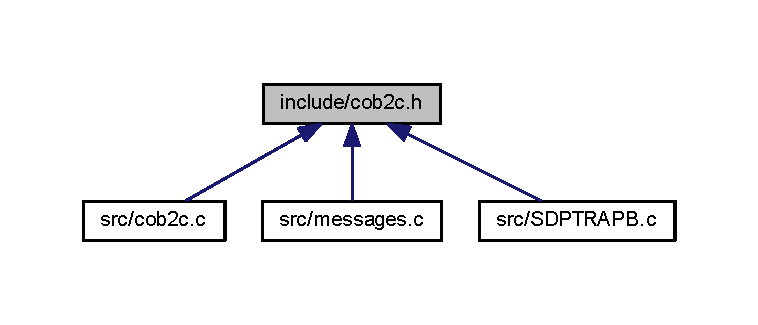
\includegraphics[width=350pt]{cob2c_8h__dep__incl}
\end{center}
\end{figure}
\subsection*{\textquotesingle{}defines\textquotesingle{}}
\begin{DoxyCompactItemize}
\item 
\#define \hyperlink{cob2c_8h_adfbc1051df776564281ac4220ba53a9e}{\+\_\+\+E\+X\+T\+\_\+}~extern
\item 
\#define \hyperlink{cob2c_8h_a59695fb6fb53fc110491390d0308486c}{C\+O\+B\+\_\+\+T\+R\+A\+P}~0
\item 
\#define \hyperlink{cob2c_8h_afa323e34c9deb45e73e32b53576d0bb1}{C\+O\+B\+\_\+\+M\+O\+D\+U\+L\+E}~8
\item 
\#define \hyperlink{cob2c_8h_a88feec3e2f6624a0184397c642fe24aa}{C\+O\+B\+\_\+\+M\+O\+D\+U\+L\+E\+\_\+\+L\+E\+N}~\hyperlink{sdpconfig_8h_a6611b3fba9de26203f14407743b750cc}{M\+A\+X\+\_\+\+M\+O\+D\+U\+L\+E}
\item 
\#define \hyperlink{cob2c_8h_ab271e7b9c5c70e78b5a7ea7cc57ddc34}{C\+O\+B\+\_\+\+F\+I\+R\+M\+A}~\hyperlink{cob2c_8h_afa323e34c9deb45e73e32b53576d0bb1}{C\+O\+B\+\_\+\+M\+O\+D\+U\+L\+E} + \hyperlink{cob2c_8h_a88feec3e2f6624a0184397c642fe24aa}{C\+O\+B\+\_\+\+M\+O\+D\+U\+L\+E\+\_\+\+L\+E\+N}
\item 
\#define \hyperlink{cob2c_8h_a88e1886caff473b8b3186f64bd454cd4}{C\+O\+B\+\_\+\+F\+I\+R\+M\+A\+\_\+\+L\+E\+N}~\hyperlink{sdpconfig_8h_ad6074dd11ab3c97c8135c43aab03ae95}{H\+A\+S\+H\+\_\+\+S\+I\+Z\+E}
\item 
\#define \hyperlink{cob2c_8h_a766a2c4b0a1e9717482033befc922102}{C\+O\+B\+\_\+\+B\+L\+K}~\hyperlink{cob2c_8h_ab271e7b9c5c70e78b5a7ea7cc57ddc34}{C\+O\+B\+\_\+\+F\+I\+R\+M\+A} + \hyperlink{cob2c_8h_a88e1886caff473b8b3186f64bd454cd4}{C\+O\+B\+\_\+\+F\+I\+R\+M\+A\+\_\+\+L\+E\+N}
\item 
\#define \hyperlink{cob2c_8h_a288de413fc4a8fccd262f6b5b3e22ead}{C\+O\+B\+\_\+\+B\+L\+K\+\_\+\+L\+E\+N}~(3 $\ast$ sizeof(long))
\item 
\#define \hyperlink{cob2c_8h_a4afae4c59d4f88c3ab273a0568805ea0}{C\+O\+B\+\_\+\+C\+O\+V\+E\+R}~\hyperlink{cob2c_8h_a766a2c4b0a1e9717482033befc922102}{C\+O\+B\+\_\+\+B\+L\+K} + \hyperlink{cob2c_8h_a288de413fc4a8fccd262f6b5b3e22ead}{C\+O\+B\+\_\+\+B\+L\+K\+\_\+\+L\+E\+N}
\end{DoxyCompactItemize}
\subsection*{Funciones}
\begin{DoxyCompactItemize}
\item 
\hyperlink{sha256le_8h_adfbc1051df776564281ac4220ba53a9e}{\+\_\+\+E\+X\+T\+\_\+} void \hyperlink{cob2c_8h_a7b6a88dac211a2521b42d23d3080c09d}{copy\+Cobol\+To\+C\+Struct} (\hyperlink{sdp_types_8h_a8ba8f2a87560d14f1152da6646649dfd}{S\+D\+P} $\ast$\hyperlink{global_8h_a44585a47047393e8faf0eef343b3b39d}{sdp}, char $\ast$data, char $\ast$modulo, int len)
\item 
\hyperlink{sha256le_8h_adfbc1051df776564281ac4220ba53a9e}{\+\_\+\+E\+X\+T\+\_\+} char $\ast$ \hyperlink{cob2c_8h_a59214c84573b767b116afe89801fe03b}{C\+Struct\+To\+Copy\+Cobol} (\hyperlink{sdp_types_8h_a8ba8f2a87560d14f1152da6646649dfd}{S\+D\+P} $\ast$\hyperlink{global_8h_a44585a47047393e8faf0eef343b3b39d}{sdp})
\item 
\hyperlink{sha256le_8h_adfbc1051df776564281ac4220ba53a9e}{\+\_\+\+E\+X\+T\+\_\+} void \hyperlink{cob2c_8h_a52791a6fd5e0a12300b88aae37cab9dc}{init\+S\+D\+P} (\hyperlink{sdp_types_8h_a8ba8f2a87560d14f1152da6646649dfd}{S\+D\+P} $\ast$\hyperlink{global_8h_a44585a47047393e8faf0eef343b3b39d}{sdp})
\item 
\hyperlink{sha256le_8h_adfbc1051df776564281ac4220ba53a9e}{\+\_\+\+E\+X\+T\+\_\+} void \hyperlink{cob2c_8h_a21fbbb691be0601c25b2c0bd3489d7e8}{set\+Module\+Name} (\hyperlink{sdp_types_8h_a8ba8f2a87560d14f1152da6646649dfd}{S\+D\+P} $\ast$\hyperlink{global_8h_a44585a47047393e8faf0eef343b3b39d}{sdp}, char $\ast$name)
\item 
\hyperlink{sha256le_8h_adfbc1051df776564281ac4220ba53a9e}{\+\_\+\+E\+X\+T\+\_\+} void \hyperlink{cob2c_8h_a5a760f10e228fa5d6a37e735984330e1}{set\+Paragraph} (\hyperlink{sdp_types_8h_a8ba8f2a87560d14f1152da6646649dfd}{S\+D\+P} $\ast$\hyperlink{global_8h_a44585a47047393e8faf0eef343b3b39d}{sdp}, char $\ast$name)
\item 
\hyperlink{sha256le_8h_adfbc1051df776564281ac4220ba53a9e}{\+\_\+\+E\+X\+T\+\_\+} void \hyperlink{cob2c_8h_a659faa5ba4c3abd0450afda8b4d222b4}{set\+Coverage} (\hyperlink{sdp_types_8h_a8ba8f2a87560d14f1152da6646649dfd}{S\+D\+P} $\ast$\hyperlink{global_8h_a44585a47047393e8faf0eef343b3b39d}{sdp}, char $\ast$name)
\end{DoxyCompactItemize}


\subsection{Descripción detallada}
Fichero de cabecera para convertir la copy C\+O\+B\+O\+L en una estructura S\+D\+P. 

\begin{DoxyAuthor}{Autor}
\+: Javier Gonzalez 
\end{DoxyAuthor}
\begin{DoxyDate}{Fecha}
\+: 01/03/15 
\end{DoxyDate}
\begin{DoxyVersion}{Versión}
\+: 2.\+0 
\end{DoxyVersion}


\subsection{Documentación de los \textquotesingle{}defines\textquotesingle{}}
\hypertarget{cob2c_8h_adfbc1051df776564281ac4220ba53a9e}{}\index{cob2c.\+h@{cob2c.\+h}!\+\_\+\+E\+X\+T\+\_\+@{\+\_\+\+E\+X\+T\+\_\+}}
\index{\+\_\+\+E\+X\+T\+\_\+@{\+\_\+\+E\+X\+T\+\_\+}!cob2c.\+h@{cob2c.\+h}}
\subsubsection[{\+\_\+\+E\+X\+T\+\_\+}]{\setlength{\rightskip}{0pt plus 5cm}\#define \+\_\+\+E\+X\+T\+\_\+~extern}\label{cob2c_8h_adfbc1051df776564281ac4220ba53a9e}


Definición en la línea 18 del archivo cob2c.\+h.

\hypertarget{cob2c_8h_a766a2c4b0a1e9717482033befc922102}{}\index{cob2c.\+h@{cob2c.\+h}!C\+O\+B\+\_\+\+B\+L\+K@{C\+O\+B\+\_\+\+B\+L\+K}}
\index{C\+O\+B\+\_\+\+B\+L\+K@{C\+O\+B\+\_\+\+B\+L\+K}!cob2c.\+h@{cob2c.\+h}}
\subsubsection[{C\+O\+B\+\_\+\+B\+L\+K}]{\setlength{\rightskip}{0pt plus 5cm}\#define C\+O\+B\+\_\+\+B\+L\+K~{\bf C\+O\+B\+\_\+\+F\+I\+R\+M\+A} + {\bf C\+O\+B\+\_\+\+F\+I\+R\+M\+A\+\_\+\+L\+E\+N}}\label{cob2c_8h_a766a2c4b0a1e9717482033befc922102}


Definición en la línea 28 del archivo cob2c.\+h.

\hypertarget{cob2c_8h_a288de413fc4a8fccd262f6b5b3e22ead}{}\index{cob2c.\+h@{cob2c.\+h}!C\+O\+B\+\_\+\+B\+L\+K\+\_\+\+L\+E\+N@{C\+O\+B\+\_\+\+B\+L\+K\+\_\+\+L\+E\+N}}
\index{C\+O\+B\+\_\+\+B\+L\+K\+\_\+\+L\+E\+N@{C\+O\+B\+\_\+\+B\+L\+K\+\_\+\+L\+E\+N}!cob2c.\+h@{cob2c.\+h}}
\subsubsection[{C\+O\+B\+\_\+\+B\+L\+K\+\_\+\+L\+E\+N}]{\setlength{\rightskip}{0pt plus 5cm}\#define C\+O\+B\+\_\+\+B\+L\+K\+\_\+\+L\+E\+N~(3 $\ast$ sizeof(long))}\label{cob2c_8h_a288de413fc4a8fccd262f6b5b3e22ead}


Definición en la línea 29 del archivo cob2c.\+h.

\hypertarget{cob2c_8h_a4afae4c59d4f88c3ab273a0568805ea0}{}\index{cob2c.\+h@{cob2c.\+h}!C\+O\+B\+\_\+\+C\+O\+V\+E\+R@{C\+O\+B\+\_\+\+C\+O\+V\+E\+R}}
\index{C\+O\+B\+\_\+\+C\+O\+V\+E\+R@{C\+O\+B\+\_\+\+C\+O\+V\+E\+R}!cob2c.\+h@{cob2c.\+h}}
\subsubsection[{C\+O\+B\+\_\+\+C\+O\+V\+E\+R}]{\setlength{\rightskip}{0pt plus 5cm}\#define C\+O\+B\+\_\+\+C\+O\+V\+E\+R~{\bf C\+O\+B\+\_\+\+B\+L\+K} + {\bf C\+O\+B\+\_\+\+B\+L\+K\+\_\+\+L\+E\+N}}\label{cob2c_8h_a4afae4c59d4f88c3ab273a0568805ea0}


Definición en la línea 30 del archivo cob2c.\+h.

\hypertarget{cob2c_8h_ab271e7b9c5c70e78b5a7ea7cc57ddc34}{}\index{cob2c.\+h@{cob2c.\+h}!C\+O\+B\+\_\+\+F\+I\+R\+M\+A@{C\+O\+B\+\_\+\+F\+I\+R\+M\+A}}
\index{C\+O\+B\+\_\+\+F\+I\+R\+M\+A@{C\+O\+B\+\_\+\+F\+I\+R\+M\+A}!cob2c.\+h@{cob2c.\+h}}
\subsubsection[{C\+O\+B\+\_\+\+F\+I\+R\+M\+A}]{\setlength{\rightskip}{0pt plus 5cm}\#define C\+O\+B\+\_\+\+F\+I\+R\+M\+A~{\bf C\+O\+B\+\_\+\+M\+O\+D\+U\+L\+E} + {\bf C\+O\+B\+\_\+\+M\+O\+D\+U\+L\+E\+\_\+\+L\+E\+N}}\label{cob2c_8h_ab271e7b9c5c70e78b5a7ea7cc57ddc34}


Definición en la línea 26 del archivo cob2c.\+h.

\hypertarget{cob2c_8h_a88e1886caff473b8b3186f64bd454cd4}{}\index{cob2c.\+h@{cob2c.\+h}!C\+O\+B\+\_\+\+F\+I\+R\+M\+A\+\_\+\+L\+E\+N@{C\+O\+B\+\_\+\+F\+I\+R\+M\+A\+\_\+\+L\+E\+N}}
\index{C\+O\+B\+\_\+\+F\+I\+R\+M\+A\+\_\+\+L\+E\+N@{C\+O\+B\+\_\+\+F\+I\+R\+M\+A\+\_\+\+L\+E\+N}!cob2c.\+h@{cob2c.\+h}}
\subsubsection[{C\+O\+B\+\_\+\+F\+I\+R\+M\+A\+\_\+\+L\+E\+N}]{\setlength{\rightskip}{0pt plus 5cm}\#define C\+O\+B\+\_\+\+F\+I\+R\+M\+A\+\_\+\+L\+E\+N~{\bf H\+A\+S\+H\+\_\+\+S\+I\+Z\+E}}\label{cob2c_8h_a88e1886caff473b8b3186f64bd454cd4}


Definición en la línea 27 del archivo cob2c.\+h.

\hypertarget{cob2c_8h_afa323e34c9deb45e73e32b53576d0bb1}{}\index{cob2c.\+h@{cob2c.\+h}!C\+O\+B\+\_\+\+M\+O\+D\+U\+L\+E@{C\+O\+B\+\_\+\+M\+O\+D\+U\+L\+E}}
\index{C\+O\+B\+\_\+\+M\+O\+D\+U\+L\+E@{C\+O\+B\+\_\+\+M\+O\+D\+U\+L\+E}!cob2c.\+h@{cob2c.\+h}}
\subsubsection[{C\+O\+B\+\_\+\+M\+O\+D\+U\+L\+E}]{\setlength{\rightskip}{0pt plus 5cm}\#define C\+O\+B\+\_\+\+M\+O\+D\+U\+L\+E~8}\label{cob2c_8h_afa323e34c9deb45e73e32b53576d0bb1}


Definición en la línea 24 del archivo cob2c.\+h.

\hypertarget{cob2c_8h_a88feec3e2f6624a0184397c642fe24aa}{}\index{cob2c.\+h@{cob2c.\+h}!C\+O\+B\+\_\+\+M\+O\+D\+U\+L\+E\+\_\+\+L\+E\+N@{C\+O\+B\+\_\+\+M\+O\+D\+U\+L\+E\+\_\+\+L\+E\+N}}
\index{C\+O\+B\+\_\+\+M\+O\+D\+U\+L\+E\+\_\+\+L\+E\+N@{C\+O\+B\+\_\+\+M\+O\+D\+U\+L\+E\+\_\+\+L\+E\+N}!cob2c.\+h@{cob2c.\+h}}
\subsubsection[{C\+O\+B\+\_\+\+M\+O\+D\+U\+L\+E\+\_\+\+L\+E\+N}]{\setlength{\rightskip}{0pt plus 5cm}\#define C\+O\+B\+\_\+\+M\+O\+D\+U\+L\+E\+\_\+\+L\+E\+N~{\bf M\+A\+X\+\_\+\+M\+O\+D\+U\+L\+E}}\label{cob2c_8h_a88feec3e2f6624a0184397c642fe24aa}


Definición en la línea 25 del archivo cob2c.\+h.

\hypertarget{cob2c_8h_a59695fb6fb53fc110491390d0308486c}{}\index{cob2c.\+h@{cob2c.\+h}!C\+O\+B\+\_\+\+T\+R\+A\+P@{C\+O\+B\+\_\+\+T\+R\+A\+P}}
\index{C\+O\+B\+\_\+\+T\+R\+A\+P@{C\+O\+B\+\_\+\+T\+R\+A\+P}!cob2c.\+h@{cob2c.\+h}}
\subsubsection[{C\+O\+B\+\_\+\+T\+R\+A\+P}]{\setlength{\rightskip}{0pt plus 5cm}\#define C\+O\+B\+\_\+\+T\+R\+A\+P~0}\label{cob2c_8h_a59695fb6fb53fc110491390d0308486c}


Definición en la línea 23 del archivo cob2c.\+h.



\subsection{Documentación de las funciones}
\hypertarget{cob2c_8h_a7b6a88dac211a2521b42d23d3080c09d}{}\index{cob2c.\+h@{cob2c.\+h}!copy\+Cobol\+To\+C\+Struct@{copy\+Cobol\+To\+C\+Struct}}
\index{copy\+Cobol\+To\+C\+Struct@{copy\+Cobol\+To\+C\+Struct}!cob2c.\+h@{cob2c.\+h}}
\subsubsection[{copy\+Cobol\+To\+C\+Struct(\+S\+D\+P $\ast$sdp, char $\ast$data, char $\ast$modulo, int len)}]{\setlength{\rightskip}{0pt plus 5cm}{\bf \+\_\+\+E\+X\+T\+\_\+} void copy\+Cobol\+To\+C\+Struct (
\begin{DoxyParamCaption}
\item[{{\bf S\+D\+P} $\ast$}]{sdp, }
\item[{char $\ast$}]{data, }
\item[{char $\ast$}]{modulo, }
\item[{int}]{len}
\end{DoxyParamCaption}
)}\label{cob2c_8h_a7b6a88dac211a2521b42d23d3080c09d}
Convierte la copy C\+O\+B\+O\+L en una estructura S\+D\+P 
\begin{DoxyParams}{Parámetros}
{\em sdp} & Puntero a la estructura S\+D\+P \\
\hline
{\em data} & Puntero a la copy C\+O\+B\+O\+L \\
\hline
{\em modulo} & Segundo parametro de invocacion (nombre del modulo o parrafo) \\
\hline
{\em len} & Longitud del campo modulo\\
\hline
\end{DoxyParams}
Copia los datos de la C\+O\+P\+Y a una estructura C para agilizar el proceso


\begin{DoxyParams}{Parámetros}
{\em sdp} & Puntero a la estructura S\+D\+P \\
\hline
{\em data} & Puntero a la C\+O\+P\+Y C\+O\+B\+O\+L \\
\hline
{\em modulo} & Parametro recibido con una etiqueta \\
\hline
{\em len} & Longitud de la etiqueta \\
\hline
\end{DoxyParams}


Definición en la línea 43 del archivo cob2c.\+c.

\hypertarget{cob2c_8h_a59214c84573b767b116afe89801fe03b}{}\index{cob2c.\+h@{cob2c.\+h}!C\+Struct\+To\+Copy\+Cobol@{C\+Struct\+To\+Copy\+Cobol}}
\index{C\+Struct\+To\+Copy\+Cobol@{C\+Struct\+To\+Copy\+Cobol}!cob2c.\+h@{cob2c.\+h}}
\subsubsection[{C\+Struct\+To\+Copy\+Cobol(\+S\+D\+P $\ast$sdp)}]{\setlength{\rightskip}{0pt plus 5cm}{\bf \+\_\+\+E\+X\+T\+\_\+} char$\ast$ C\+Struct\+To\+Copy\+Cobol (
\begin{DoxyParamCaption}
\item[{{\bf S\+D\+P} $\ast$}]{sdp}
\end{DoxyParamCaption}
)}\label{cob2c_8h_a59214c84573b767b116afe89801fe03b}
\hypertarget{cob2c_8h_a52791a6fd5e0a12300b88aae37cab9dc}{}\index{cob2c.\+h@{cob2c.\+h}!init\+S\+D\+P@{init\+S\+D\+P}}
\index{init\+S\+D\+P@{init\+S\+D\+P}!cob2c.\+h@{cob2c.\+h}}
\subsubsection[{init\+S\+D\+P(\+S\+D\+P $\ast$sdp)}]{\setlength{\rightskip}{0pt plus 5cm}{\bf \+\_\+\+E\+X\+T\+\_\+} void init\+S\+D\+P (
\begin{DoxyParamCaption}
\item[{{\bf S\+D\+P} $\ast$}]{sdp}
\end{DoxyParamCaption}
)}\label{cob2c_8h_a52791a6fd5e0a12300b88aae37cab9dc}


Definición en la línea 67 del archivo cob2c.\+c.

\hypertarget{cob2c_8h_a659faa5ba4c3abd0450afda8b4d222b4}{}\index{cob2c.\+h@{cob2c.\+h}!set\+Coverage@{set\+Coverage}}
\index{set\+Coverage@{set\+Coverage}!cob2c.\+h@{cob2c.\+h}}
\subsubsection[{set\+Coverage(\+S\+D\+P $\ast$sdp, char $\ast$name)}]{\setlength{\rightskip}{0pt plus 5cm}{\bf \+\_\+\+E\+X\+T\+\_\+} void set\+Coverage (
\begin{DoxyParamCaption}
\item[{{\bf S\+D\+P} $\ast$}]{sdp, }
\item[{char $\ast$}]{name}
\end{DoxyParamCaption}
)}\label{cob2c_8h_a659faa5ba4c3abd0450afda8b4d222b4}


Definición en la línea 77 del archivo cob2c.\+c.

\hypertarget{cob2c_8h_a21fbbb691be0601c25b2c0bd3489d7e8}{}\index{cob2c.\+h@{cob2c.\+h}!set\+Module\+Name@{set\+Module\+Name}}
\index{set\+Module\+Name@{set\+Module\+Name}!cob2c.\+h@{cob2c.\+h}}
\subsubsection[{set\+Module\+Name(\+S\+D\+P $\ast$sdp, char $\ast$name)}]{\setlength{\rightskip}{0pt plus 5cm}{\bf \+\_\+\+E\+X\+T\+\_\+} void set\+Module\+Name (
\begin{DoxyParamCaption}
\item[{{\bf S\+D\+P} $\ast$}]{sdp, }
\item[{char $\ast$}]{name}
\end{DoxyParamCaption}
)}\label{cob2c_8h_a21fbbb691be0601c25b2c0bd3489d7e8}


Definición en la línea 73 del archivo cob2c.\+c.

\hypertarget{cob2c_8h_a5a760f10e228fa5d6a37e735984330e1}{}\index{cob2c.\+h@{cob2c.\+h}!set\+Paragraph@{set\+Paragraph}}
\index{set\+Paragraph@{set\+Paragraph}!cob2c.\+h@{cob2c.\+h}}
\subsubsection[{set\+Paragraph(\+S\+D\+P $\ast$sdp, char $\ast$name)}]{\setlength{\rightskip}{0pt plus 5cm}{\bf \+\_\+\+E\+X\+T\+\_\+} void set\+Paragraph (
\begin{DoxyParamCaption}
\item[{{\bf S\+D\+P} $\ast$}]{sdp, }
\item[{char $\ast$}]{name}
\end{DoxyParamCaption}
)}\label{cob2c_8h_a5a760f10e228fa5d6a37e735984330e1}

\hypertarget{global_8h}{}\section{Referencia del Archivo include/global.h}
\label{global_8h}\index{include/global.\+h@{include/global.\+h}}


Define las variables de uso global para todo el sistema.  


{\ttfamily \#include $<$stdio.\+h$>$}\\*
{\ttfamily \#include \char`\"{}sdpconfig.\+h\char`\"{}}\\*
{\ttfamily \#include \char`\"{}sdp\+Types.\+h\char`\"{}}\\*
Dependencia gráfica adjunta para global.\+h\+:\nopagebreak
\begin{figure}[H]
\begin{center}
\leavevmode
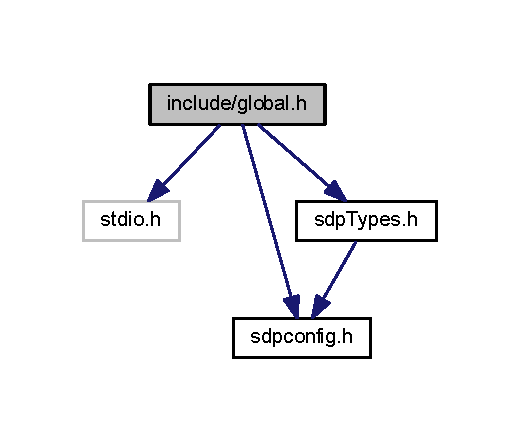
\includegraphics[width=250pt]{global_8h__incl}
\end{center}
\end{figure}
Gráfico de los archivos que directa o indirectamente incluyen a este archivo\+:\nopagebreak
\begin{figure}[H]
\begin{center}
\leavevmode
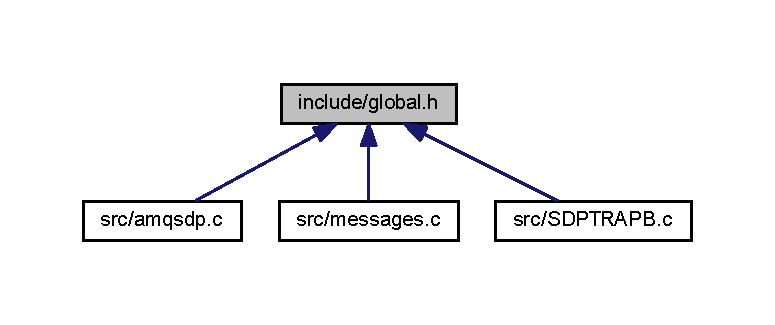
\includegraphics[width=350pt]{global_8h__dep__incl}
\end{center}
\end{figure}
\subsection*{Variables}
\begin{DoxyCompactItemize}
\item 
\hyperlink{sdp_types_8h_a8ba8f2a87560d14f1152da6646649dfd}{S\+D\+P} \hyperlink{global_8h_a44585a47047393e8faf0eef343b3b39d}{sdp}
\item 
F\+I\+L\+E $\ast$ \hyperlink{global_8h_a5f9e912074a29350e020b7a09f43ff32}{traza}
\item 
int \hyperlink{global_8h_ad2085c6c4c17426ec0d5c1198e013921}{modo}
\item 
int \hyperlink{global_8h_ad247c905cf5ce68a5eec344bcba86cc7}{dbg\+Level}
\item 
int \hyperlink{global_8h_a4fb693c3cca874aca4a9d2109cc561e5}{in\+Err}
\item 
void $\ast$ \hyperlink{global_8h_a88cac69ee038c814b384a20eb156a7d8}{pila\+Timers}
\item 
void $\ast$ \hyperlink{global_8h_a8ad0071cdfdcab41ce0ad1fbd76a9e58}{pila\+Modulos}
\item 
char $\ast$ \hyperlink{global_8h_a2ebee5a02dd55f1f92212c6b202f649b}{id\+Session}
\item 
char $\ast$ \hyperlink{global_8h_a0147a5b81499984f9cb00379a8cb84af}{usuario}
\end{DoxyCompactItemize}


\subsection{Descripción detallada}
Define las variables de uso global para todo el sistema. 

Se definen para evitar el uso de estructuras y el paso de parametros excesivos

\begin{DoxyAuthor}{Autor}
\+: Javier Gonzalez 
\end{DoxyAuthor}
\begin{DoxyDate}{Fecha}
\+: 01/03/15 
\end{DoxyDate}
\begin{DoxyVersion}{Versión}
\+: 2.\+0 
\end{DoxyVersion}


\subsection{Documentación de las variables}
\hypertarget{global_8h_ad247c905cf5ce68a5eec344bcba86cc7}{}\index{global.\+h@{global.\+h}!dbg\+Level@{dbg\+Level}}
\index{dbg\+Level@{dbg\+Level}!global.\+h@{global.\+h}}
\subsubsection[{dbg\+Level}]{\setlength{\rightskip}{0pt plus 5cm}int dbg\+Level}\label{global_8h_ad247c905cf5ce68a5eec344bcba86cc7}


Definición en la línea 58 del archivo amqsdp.\+c.

\hypertarget{global_8h_a2ebee5a02dd55f1f92212c6b202f649b}{}\index{global.\+h@{global.\+h}!id\+Session@{id\+Session}}
\index{id\+Session@{id\+Session}!global.\+h@{global.\+h}}
\subsubsection[{id\+Session}]{\setlength{\rightskip}{0pt plus 5cm}char$\ast$ id\+Session}\label{global_8h_a2ebee5a02dd55f1f92212c6b202f649b}
\hypertarget{global_8h_a4fb693c3cca874aca4a9d2109cc561e5}{}\index{global.\+h@{global.\+h}!in\+Err@{in\+Err}}
\index{in\+Err@{in\+Err}!global.\+h@{global.\+h}}
\subsubsection[{in\+Err}]{\setlength{\rightskip}{0pt plus 5cm}int in\+Err}\label{global_8h_a4fb693c3cca874aca4a9d2109cc561e5}


Definición en la línea 57 del archivo amqsdp.\+c.

\hypertarget{global_8h_ad2085c6c4c17426ec0d5c1198e013921}{}\index{global.\+h@{global.\+h}!modo@{modo}}
\index{modo@{modo}!global.\+h@{global.\+h}}
\subsubsection[{modo}]{\setlength{\rightskip}{0pt plus 5cm}int modo}\label{global_8h_ad2085c6c4c17426ec0d5c1198e013921}
\hypertarget{global_8h_a8ad0071cdfdcab41ce0ad1fbd76a9e58}{}\index{global.\+h@{global.\+h}!pila\+Modulos@{pila\+Modulos}}
\index{pila\+Modulos@{pila\+Modulos}!global.\+h@{global.\+h}}
\subsubsection[{pila\+Modulos}]{\setlength{\rightskip}{0pt plus 5cm}void$\ast$ pila\+Modulos}\label{global_8h_a8ad0071cdfdcab41ce0ad1fbd76a9e58}
\hypertarget{global_8h_a88cac69ee038c814b384a20eb156a7d8}{}\index{global.\+h@{global.\+h}!pila\+Timers@{pila\+Timers}}
\index{pila\+Timers@{pila\+Timers}!global.\+h@{global.\+h}}
\subsubsection[{pila\+Timers}]{\setlength{\rightskip}{0pt plus 5cm}void$\ast$ pila\+Timers}\label{global_8h_a88cac69ee038c814b384a20eb156a7d8}
\hypertarget{global_8h_a44585a47047393e8faf0eef343b3b39d}{}\index{global.\+h@{global.\+h}!sdp@{sdp}}
\index{sdp@{sdp}!global.\+h@{global.\+h}}
\subsubsection[{sdp}]{\setlength{\rightskip}{0pt plus 5cm}{\bf S\+D\+P} sdp}\label{global_8h_a44585a47047393e8faf0eef343b3b39d}
\hypertarget{global_8h_a5f9e912074a29350e020b7a09f43ff32}{}\index{global.\+h@{global.\+h}!traza@{traza}}
\index{traza@{traza}!global.\+h@{global.\+h}}
\subsubsection[{traza}]{\setlength{\rightskip}{0pt plus 5cm}F\+I\+L\+E$\ast$ traza}\label{global_8h_a5f9e912074a29350e020b7a09f43ff32}


Definición en la línea 59 del archivo amqsdp.\+c.

\hypertarget{global_8h_a0147a5b81499984f9cb00379a8cb84af}{}\index{global.\+h@{global.\+h}!usuario@{usuario}}
\index{usuario@{usuario}!global.\+h@{global.\+h}}
\subsubsection[{usuario}]{\setlength{\rightskip}{0pt plus 5cm}char$\ast$ usuario}\label{global_8h_a0147a5b81499984f9cb00379a8cb84af}

\hypertarget{jggsal_8h}{}\section{Referencia del Archivo include/jggsal.h}
\label{jggsal_8h}\index{include/jggsal.\+h@{include/jggsal.\+h}}


Software Abstraction Layer.  


Gráfico de los archivos que directa o indirectamente incluyen a este archivo\+:\nopagebreak
\begin{figure}[H]
\begin{center}
\leavevmode
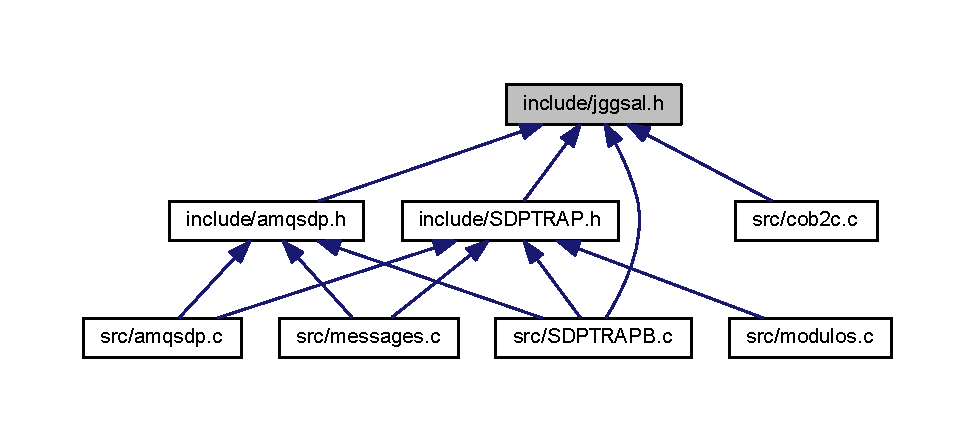
\includegraphics[width=350pt]{jggsal_8h__dep__incl}
\end{center}
\end{figure}


\subsection{Descripción detallada}
Software Abstraction Layer. 

Componente de compatibilidad entre sistemas operativos Redefine las funciones del runtime en funcion del Sistema Operativo Cuando es necesario, jggsal.\+c actua como wrapper de la funcion objetivo.

De esta manera se eliminan los bloques \#ifdef {\itshape O\+S} del codigo fuente

O\+J\+O\+: N\+O P\+U\+E\+D\+E L\+L\+A\+M\+A\+R\+S\+E S\+A\+L P\+O\+R\+Q\+U\+E L\+O U\+T\+I\+L\+I\+Z\+A W\+I\+N\+D\+O\+W\+S

\begin{DoxyAuthor}{Autor}
\+: Javier Gonzalez 
\end{DoxyAuthor}
\begin{DoxyDate}{Fecha}
\+: 01/03/15 
\end{DoxyDate}
\begin{DoxyVersion}{Versión}
\+: 1.\+0 
\end{DoxyVersion}

\hypertarget{md5_8h}{}\section{Referencia del Archivo include/md5.h}
\label{md5_8h}\index{include/md5.\+h@{include/md5.\+h}}


Fichero de cabecera para el calculo de la firma M\+D5 de un texto Modificado a partir del algoritmo desarrollado por\+:  


Gráfico de los archivos que directa o indirectamente incluyen a este archivo\+:\nopagebreak
\begin{figure}[H]
\begin{center}
\leavevmode
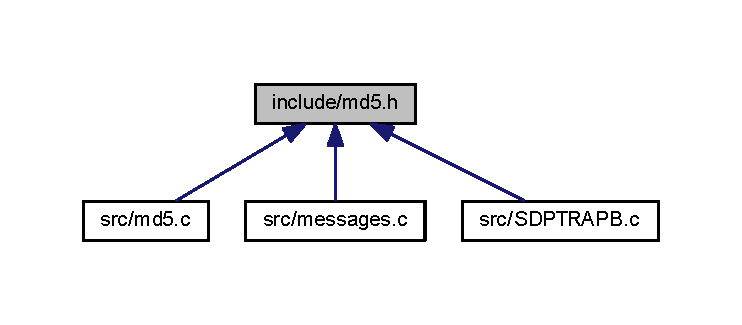
\includegraphics[width=350pt]{md5_8h__dep__incl}
\end{center}
\end{figure}
\subsection*{\textquotesingle{}defines\textquotesingle{}}
\begin{DoxyCompactItemize}
\item 
\#define \hyperlink{md5_8h_adfbc1051df776564281ac4220ba53a9e}{\+\_\+\+E\+X\+T\+\_\+}~extern
\end{DoxyCompactItemize}
\subsection*{Funciones}
\begin{DoxyCompactItemize}
\item 
\hyperlink{sha256le_8h_adfbc1051df776564281ac4220ba53a9e}{\+\_\+\+E\+X\+T\+\_\+} void \hyperlink{md5_8h_aa75a1419e565ea619428681420b59179}{M\+D5} (char $\ast$out, const char $\ast$in)
\end{DoxyCompactItemize}


\subsection{Descripción detallada}
Fichero de cabecera para el calculo de la firma M\+D5 de un texto Modificado a partir del algoritmo desarrollado por\+: 

M\+D5 Message-\/\+Digest Algorithm (R\+F\+C 1321).

Homepage\+: \href{http://openwall.info/wiki/people/solar/software/public-domain-source-code/md5}{\tt http\+://openwall.\+info/wiki/people/solar/software/public-\/domain-\/source-\/code/md5}

Author\+: Alexander Peslyak, better known as Solar Designer $<$solar at openwall.\+com$>$

See \hyperlink{md5_8c}{md5.\+c} for more information.

\begin{DoxyAuthor}{Autor}
\+: Javier Gonzalez 
\end{DoxyAuthor}
\begin{DoxyDate}{Fecha}
\+: 01/03/15 
\end{DoxyDate}
\begin{DoxyVersion}{Versión}
\+: 2.\+0 
\end{DoxyVersion}


\subsection{Documentación de los \textquotesingle{}defines\textquotesingle{}}
\hypertarget{md5_8h_adfbc1051df776564281ac4220ba53a9e}{}\index{md5.\+h@{md5.\+h}!\+\_\+\+E\+X\+T\+\_\+@{\+\_\+\+E\+X\+T\+\_\+}}
\index{\+\_\+\+E\+X\+T\+\_\+@{\+\_\+\+E\+X\+T\+\_\+}!md5.\+h@{md5.\+h}}
\subsubsection[{\+\_\+\+E\+X\+T\+\_\+}]{\setlength{\rightskip}{0pt plus 5cm}\#define \+\_\+\+E\+X\+T\+\_\+~extern}\label{md5_8h_adfbc1051df776564281ac4220ba53a9e}


Definición en la línea 29 del archivo md5.\+h.



\subsection{Documentación de las funciones}
\hypertarget{md5_8h_aa75a1419e565ea619428681420b59179}{}\index{md5.\+h@{md5.\+h}!M\+D5@{M\+D5}}
\index{M\+D5@{M\+D5}!md5.\+h@{md5.\+h}}
\subsubsection[{M\+D5(char $\ast$out, const char $\ast$in)}]{\setlength{\rightskip}{0pt plus 5cm}{\bf \+\_\+\+E\+X\+T\+\_\+} void M\+D5 (
\begin{DoxyParamCaption}
\item[{char $\ast$}]{out, }
\item[{const char $\ast$}]{in}
\end{DoxyParamCaption}
)}\label{md5_8h_aa75a1419e565ea619428681420b59179}
Devuelve la firma M\+D5 asociada a in out debe ser un array de 32 bytes 

Definición en la línea 310 del archivo md5.\+c.


\hypertarget{md5__mit_8h}{}\section{Referencia del Archivo include/md5\+\_\+mit.h}
\label{md5__mit_8h}\index{include/md5\+\_\+mit.\+h@{include/md5\+\_\+mit.\+h}}
\subsection*{Estructuras de datos}
\begin{DoxyCompactItemize}
\item 
struct \hyperlink{struct_m_d5___c_t_x}{M\+D5\+\_\+\+C\+T\+X}
\end{DoxyCompactItemize}
\subsection*{\textquotesingle{}defines\textquotesingle{}}
\begin{DoxyCompactItemize}
\item 
\#define \hyperlink{md5__mit_8h_adfbc1051df776564281ac4220ba53a9e}{\+\_\+\+E\+X\+T\+\_\+}~extern
\end{DoxyCompactItemize}
\subsection*{\textquotesingle{}typedefs\textquotesingle{}}
\begin{DoxyCompactItemize}
\item 
typedef unsigned long int \hyperlink{md5__mit_8h_acbcd3749ac28f52e756e22d22022cae5}{U\+I\+N\+T4}
\end{DoxyCompactItemize}
\subsection*{Funciones}
\begin{DoxyCompactItemize}
\item 
\hyperlink{sha256le_8h_adfbc1051df776564281ac4220ba53a9e}{\+\_\+\+E\+X\+T\+\_\+} void \hyperlink{md5__mit_8h_a0a660298d93a19cd423f1a17b6773880}{M\+D5\+Init} (\hyperlink{struct_m_d5___c_t_x}{M\+D5\+\_\+\+C\+T\+X} $\ast$md\+Context)
\item 
\hyperlink{sha256le_8h_adfbc1051df776564281ac4220ba53a9e}{\+\_\+\+E\+X\+T\+\_\+} void \hyperlink{md5__mit_8h_abc0010e81c383ba1899be48ce40ef431}{M\+D5\+Update} (\hyperlink{struct_m_d5___c_t_x}{M\+D5\+\_\+\+C\+T\+X} $\ast$md\+Context, unsigned char $\ast$in\+Buf, unsigned int in\+Len)
\item 
\hyperlink{sha256le_8h_adfbc1051df776564281ac4220ba53a9e}{\+\_\+\+E\+X\+T\+\_\+} void \hyperlink{md5__mit_8h_abad72e13e27a1acf0d246540b5f78aaf}{M\+D5\+Final} (\hyperlink{struct_m_d5___c_t_x}{M\+D5\+\_\+\+C\+T\+X} $\ast$md\+Context)
\end{DoxyCompactItemize}


\subsection{Documentación de los \textquotesingle{}defines\textquotesingle{}}
\hypertarget{md5__mit_8h_adfbc1051df776564281ac4220ba53a9e}{}\index{md5\+\_\+mit.\+h@{md5\+\_\+mit.\+h}!\+\_\+\+E\+X\+T\+\_\+@{\+\_\+\+E\+X\+T\+\_\+}}
\index{\+\_\+\+E\+X\+T\+\_\+@{\+\_\+\+E\+X\+T\+\_\+}!md5\+\_\+mit.\+h@{md5\+\_\+mit.\+h}}
\subsubsection[{\+\_\+\+E\+X\+T\+\_\+}]{\setlength{\rightskip}{0pt plus 5cm}\#define \+\_\+\+E\+X\+T\+\_\+~extern}\label{md5__mit_8h_adfbc1051df776564281ac4220ba53a9e}


Definición en la línea 47 del archivo md5\+\_\+mit.\+h.



\subsection{Documentación de los \textquotesingle{}typedefs\textquotesingle{}}
\hypertarget{md5__mit_8h_acbcd3749ac28f52e756e22d22022cae5}{}\index{md5\+\_\+mit.\+h@{md5\+\_\+mit.\+h}!U\+I\+N\+T4@{U\+I\+N\+T4}}
\index{U\+I\+N\+T4@{U\+I\+N\+T4}!md5\+\_\+mit.\+h@{md5\+\_\+mit.\+h}}
\subsubsection[{U\+I\+N\+T4}]{\setlength{\rightskip}{0pt plus 5cm}typedef unsigned long int {\bf U\+I\+N\+T4}}\label{md5__mit_8h_acbcd3749ac28f52e756e22d22022cae5}


Definición en la línea 51 del archivo md5\+\_\+mit.\+h.



\subsection{Documentación de las funciones}
\hypertarget{md5__mit_8h_abad72e13e27a1acf0d246540b5f78aaf}{}\index{md5\+\_\+mit.\+h@{md5\+\_\+mit.\+h}!M\+D5\+Final@{M\+D5\+Final}}
\index{M\+D5\+Final@{M\+D5\+Final}!md5\+\_\+mit.\+h@{md5\+\_\+mit.\+h}}
\subsubsection[{M\+D5\+Final(\+M\+D5\+\_\+\+C\+T\+X $\ast$md\+Context)}]{\setlength{\rightskip}{0pt plus 5cm}{\bf \+\_\+\+E\+X\+T\+\_\+} void M\+D5\+Final (
\begin{DoxyParamCaption}
\item[{{\bf M\+D5\+\_\+\+C\+T\+X} $\ast$}]{md\+Context}
\end{DoxyParamCaption}
)}\label{md5__mit_8h_abad72e13e27a1acf0d246540b5f78aaf}
\hypertarget{md5__mit_8h_a0a660298d93a19cd423f1a17b6773880}{}\index{md5\+\_\+mit.\+h@{md5\+\_\+mit.\+h}!M\+D5\+Init@{M\+D5\+Init}}
\index{M\+D5\+Init@{M\+D5\+Init}!md5\+\_\+mit.\+h@{md5\+\_\+mit.\+h}}
\subsubsection[{M\+D5\+Init(\+M\+D5\+\_\+\+C\+T\+X $\ast$md\+Context)}]{\setlength{\rightskip}{0pt plus 5cm}{\bf \+\_\+\+E\+X\+T\+\_\+} void M\+D5\+Init (
\begin{DoxyParamCaption}
\item[{{\bf M\+D5\+\_\+\+C\+T\+X} $\ast$}]{md\+Context}
\end{DoxyParamCaption}
)}\label{md5__mit_8h_a0a660298d93a19cd423f1a17b6773880}


Definición en la línea 214 del archivo md5.\+c.

\hypertarget{md5__mit_8h_abc0010e81c383ba1899be48ce40ef431}{}\index{md5\+\_\+mit.\+h@{md5\+\_\+mit.\+h}!M\+D5\+Update@{M\+D5\+Update}}
\index{M\+D5\+Update@{M\+D5\+Update}!md5\+\_\+mit.\+h@{md5\+\_\+mit.\+h}}
\subsubsection[{M\+D5\+Update(\+M\+D5\+\_\+\+C\+T\+X $\ast$md\+Context, unsigned char $\ast$in\+Buf, unsigned int in\+Len)}]{\setlength{\rightskip}{0pt plus 5cm}{\bf \+\_\+\+E\+X\+T\+\_\+} void M\+D5\+Update (
\begin{DoxyParamCaption}
\item[{{\bf M\+D5\+\_\+\+C\+T\+X} $\ast$}]{md\+Context, }
\item[{unsigned char $\ast$}]{in\+Buf, }
\item[{unsigned int}]{in\+Len}
\end{DoxyParamCaption}
)}\label{md5__mit_8h_abc0010e81c383ba1899be48ce40ef431}

\hypertarget{messages_8h}{}\section{Referencia del Archivo include/messages.h}
\label{messages_8h}\index{include/messages.\+h@{include/messages.\+h}}


Funciones de gestion del envio de mensajes al sistema de colas.  


{\ttfamily \#include \char`\"{}sdp\+Types.\+h\char`\"{}}\\*
Dependencia gráfica adjunta para messages.\+h\+:\nopagebreak
\begin{figure}[H]
\begin{center}
\leavevmode
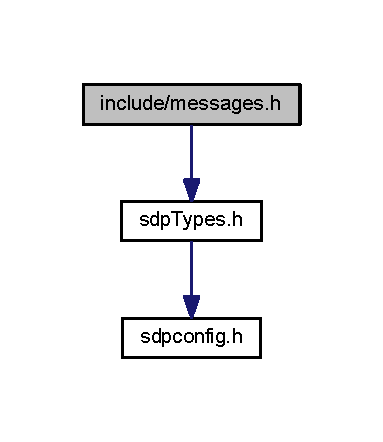
\includegraphics[width=184pt]{messages_8h__incl}
\end{center}
\end{figure}
Gráfico de los archivos que directa o indirectamente incluyen a este archivo\+:\nopagebreak
\begin{figure}[H]
\begin{center}
\leavevmode
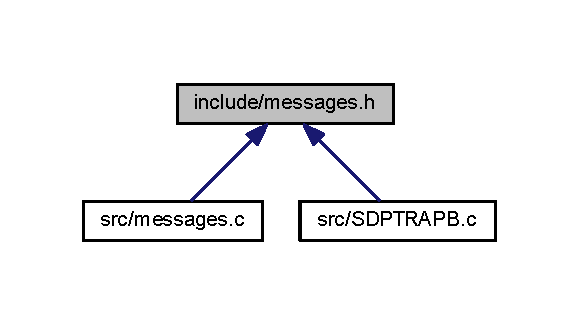
\includegraphics[width=278pt]{messages_8h__dep__incl}
\end{center}
\end{figure}
\subsection*{\textquotesingle{}defines\textquotesingle{}}
\begin{DoxyCompactItemize}
\item 
\#define \hyperlink{messages_8h_adfbc1051df776564281ac4220ba53a9e}{\+\_\+\+E\+X\+T\+\_\+}~extern
\end{DoxyCompactItemize}
\subsection*{Funciones}
\begin{DoxyCompactItemize}
\item 
\hyperlink{sha256le_8h_adfbc1051df776564281ac4220ba53a9e}{\+\_\+\+E\+X\+T\+\_\+} void \hyperlink{messages_8h_ad9a5bcb8859dbde9b0a6029b344b68cd}{process\+Message} (int tipo, \hyperlink{sdp_types_8h_a94c0315eea22344f1e853cc7c90592bb}{T\+I\+M\+E\+R} $\ast$timer)
\item 
\hyperlink{sha256le_8h_adfbc1051df776564281ac4220ba53a9e}{\+\_\+\+E\+X\+T\+\_\+} void \hyperlink{messages_8h_a5e92dab3c2b325b433c5a2ef36289b01}{process\+End\+Module} (char $\ast$data)
\item 
\hyperlink{sha256le_8h_adfbc1051df776564281ac4220ba53a9e}{\+\_\+\+E\+X\+T\+\_\+} void \hyperlink{messages_8h_a758539cefbe1e6b284f5cee92b59f8bc}{send\+Begin\+Session} (\hyperlink{sdp_types_8h_a94c0315eea22344f1e853cc7c90592bb}{T\+I\+M\+E\+R} $\ast$\hyperlink{_s_d_p_t_r_a_p_b_8c_a7b1065499acf2797bfe8d85cd6048da6}{current})
\item 
\hyperlink{sha256le_8h_adfbc1051df776564281ac4220ba53a9e}{\+\_\+\+E\+X\+T\+\_\+} void \hyperlink{messages_8h_a8074fb403729c61320ce49f469576e0c}{send\+End\+Session} (\hyperlink{sdp_types_8h_a94c0315eea22344f1e853cc7c90592bb}{T\+I\+M\+E\+R} $\ast$\hyperlink{_s_d_p_t_r_a_p_b_8c_a7b1065499acf2797bfe8d85cd6048da6}{current})
\item 
\hyperlink{sha256le_8h_adfbc1051df776564281ac4220ba53a9e}{\+\_\+\+E\+X\+T\+\_\+} void \hyperlink{messages_8h_af7fe7da407d194ebb7f01bccff7414e1}{send\+Pending\+Data} (void)
\end{DoxyCompactItemize}


\subsection{Descripción detallada}
Funciones de gestion del envio de mensajes al sistema de colas. 

\begin{DoxyAuthor}{Autor}
\+: Javier Gonzalez 
\end{DoxyAuthor}
\begin{DoxyDate}{Fecha}
\+: 01/03/15 
\end{DoxyDate}
\begin{DoxyVersion}{Versión}
\+: 2.\+0 
\end{DoxyVersion}


\subsection{Documentación de los \textquotesingle{}defines\textquotesingle{}}
\hypertarget{messages_8h_adfbc1051df776564281ac4220ba53a9e}{}\index{messages.\+h@{messages.\+h}!\+\_\+\+E\+X\+T\+\_\+@{\+\_\+\+E\+X\+T\+\_\+}}
\index{\+\_\+\+E\+X\+T\+\_\+@{\+\_\+\+E\+X\+T\+\_\+}!messages.\+h@{messages.\+h}}
\subsubsection[{\+\_\+\+E\+X\+T\+\_\+}]{\setlength{\rightskip}{0pt plus 5cm}\#define \+\_\+\+E\+X\+T\+\_\+~extern}\label{messages_8h_adfbc1051df776564281ac4220ba53a9e}


Definición en la línea 20 del archivo messages.\+h.



\subsection{Documentación de las funciones}
\hypertarget{messages_8h_a5e92dab3c2b325b433c5a2ef36289b01}{}\index{messages.\+h@{messages.\+h}!process\+End\+Module@{process\+End\+Module}}
\index{process\+End\+Module@{process\+End\+Module}!messages.\+h@{messages.\+h}}
\subsubsection[{process\+End\+Module(char $\ast$data)}]{\setlength{\rightskip}{0pt plus 5cm}{\bf \+\_\+\+E\+X\+T\+\_\+} void process\+End\+Module (
\begin{DoxyParamCaption}
\item[{char $\ast$}]{sdp\+Data}
\end{DoxyParamCaption}
)}\label{messages_8h_a5e92dab3c2b325b433c5a2ef36289b01}
Realiza el proceso asociado al final de la ejecucion de un modulo 
\begin{DoxyParams}{Parámetros}
{\em data} & Copy C\+O\+B\+O\+L del programa\\
\hline
\end{DoxyParams}
Envia los mensajes asociados al final de un modulo en funcion del modo de proceso

Contadores de uso de parrafos Contadores de las llamadas realizadas en ese modulo Contadores de los ficheros Informacion de la cobertura


\begin{DoxyParams}{Parámetros}
{\em sdp\+Data} & Direccion de la C\+O\+P\+Y C\+O\+B\+O\+L \\
\hline
\end{DoxyParams}


Definición en la línea 193 del archivo messages.\+c.

\hypertarget{messages_8h_ad9a5bcb8859dbde9b0a6029b344b68cd}{}\index{messages.\+h@{messages.\+h}!process\+Message@{process\+Message}}
\index{process\+Message@{process\+Message}!messages.\+h@{messages.\+h}}
\subsubsection[{process\+Message(int tipo, T\+I\+M\+E\+R $\ast$timer)}]{\setlength{\rightskip}{0pt plus 5cm}{\bf \+\_\+\+E\+X\+T\+\_\+} void process\+Message (
\begin{DoxyParamCaption}
\item[{int}]{tipo, }
\item[{{\bf T\+I\+M\+E\+R} $\ast$}]{timer}
\end{DoxyParamCaption}
)}\label{messages_8h_ad9a5bcb8859dbde9b0a6029b344b68cd}
Procesa un mensaje recibido del programa 
\begin{DoxyParams}{Parámetros}
{\em tipo} & tipo del mensaje \\
\hline
{\em timer} & Puntero al T\+I\+M\+E\+R obtenido al entrar en S\+D\+P\+T\+R\+A\+B\\
\hline
\end{DoxyParams}
Prepara el mensaje a enviar Si es un mensaje de fin de llamada, ajusta la pila de modulos 
\begin{DoxyParams}{Parámetros}
{\em tipo} & tipo del mensaje segun codigos M\+S\+G\+\_\+xxx \\
\hline
{\em timer} & Puntero al T\+I\+M\+E\+R calculado an entrar en la libreria \\
\hline
\end{DoxyParams}


Definición en la línea 76 del archivo messages.\+c.

\hypertarget{messages_8h_a758539cefbe1e6b284f5cee92b59f8bc}{}\index{messages.\+h@{messages.\+h}!send\+Begin\+Session@{send\+Begin\+Session}}
\index{send\+Begin\+Session@{send\+Begin\+Session}!messages.\+h@{messages.\+h}}
\subsubsection[{send\+Begin\+Session(\+T\+I\+M\+E\+R $\ast$current)}]{\setlength{\rightskip}{0pt plus 5cm}{\bf \+\_\+\+E\+X\+T\+\_\+} void send\+Begin\+Session (
\begin{DoxyParamCaption}
\item[{{\bf T\+I\+M\+E\+R} $\ast$}]{current}
\end{DoxyParamCaption}
)}\label{messages_8h_a758539cefbe1e6b284f5cee92b59f8bc}
Realiza el proceso asociado al inicio de la sesion 
\begin{DoxyParams}{Parámetros}
{\em current} & Puntero al T\+I\+M\+E\+R obtenido al entrar en S\+D\+P\+T\+R\+A\+B\\
\hline
\end{DoxyParams}
Envia el mensaje de inicio de sesion

Este mensaje se envia siempre y de manera aislada


\begin{DoxyParams}{Parámetros}
{\em current} & Puntero al T\+I\+M\+E\+R obtenido al entrar en la libreria \\
\hline
\end{DoxyParams}


Definición en la línea 370 del archivo messages.\+c.

\hypertarget{messages_8h_a8074fb403729c61320ce49f469576e0c}{}\index{messages.\+h@{messages.\+h}!send\+End\+Session@{send\+End\+Session}}
\index{send\+End\+Session@{send\+End\+Session}!messages.\+h@{messages.\+h}}
\subsubsection[{send\+End\+Session(\+T\+I\+M\+E\+R $\ast$current)}]{\setlength{\rightskip}{0pt plus 5cm}{\bf \+\_\+\+E\+X\+T\+\_\+} void send\+End\+Session (
\begin{DoxyParamCaption}
\item[{{\bf T\+I\+M\+E\+R} $\ast$}]{current}
\end{DoxyParamCaption}
)}\label{messages_8h_a8074fb403729c61320ce49f469576e0c}
Realiza el proceso asociado al final de la sesion 
\begin{DoxyParams}{Parámetros}
{\em current} & Puntero al T\+I\+M\+E\+R obtenido al entrar en S\+D\+P\+T\+R\+A\+B\\
\hline
\end{DoxyParams}
Envia el mensaje de fin de sesion


\begin{DoxyParams}{Parámetros}
{\em current} & Puntero al T\+I\+M\+E\+R obtenido al entrar en la libreria \\
\hline
\end{DoxyParams}


Definición en la línea 379 del archivo messages.\+c.

\hypertarget{messages_8h_af7fe7da407d194ebb7f01bccff7414e1}{}\index{messages.\+h@{messages.\+h}!send\+Pending\+Data@{send\+Pending\+Data}}
\index{send\+Pending\+Data@{send\+Pending\+Data}!messages.\+h@{messages.\+h}}
\subsubsection[{send\+Pending\+Data(void)}]{\setlength{\rightskip}{0pt plus 5cm}{\bf \+\_\+\+E\+X\+T\+\_\+} void send\+Pending\+Data (
\begin{DoxyParamCaption}
\item[{void}]{}
\end{DoxyParamCaption}
)}\label{messages_8h_af7fe7da407d194ebb7f01bccff7414e1}
Procesa la informacion pendiente

En caso de trabajar en modo global envia todos los datos antes de enviar el mensaje de fin de sesion 

Definición en la línea 406 del archivo messages.\+c.


\hypertarget{modulos_8h}{}\section{Referencia del Archivo include/modulos.h}
\label{modulos_8h}\index{include/modulos.\+h@{include/modulos.\+h}}


Funciones de gestion de los modulos activos en una sesion.  


Gráfico de los archivos que directa o indirectamente incluyen a este archivo\+:\nopagebreak
\begin{figure}[H]
\begin{center}
\leavevmode
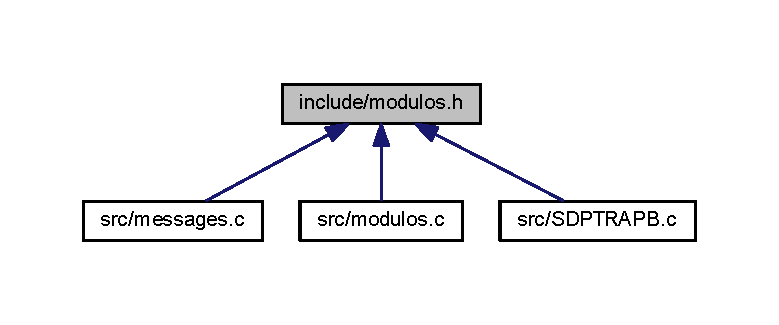
\includegraphics[width=350pt]{modulos_8h__dep__incl}
\end{center}
\end{figure}
\subsection*{\textquotesingle{}defines\textquotesingle{}}
\begin{DoxyCompactItemize}
\item 
\#define \hyperlink{modulos_8h_adfbc1051df776564281ac4220ba53a9e}{\+\_\+\+E\+X\+T\+\_\+}~extern
\end{DoxyCompactItemize}
\subsection*{Funciones}
\begin{DoxyCompactItemize}
\item 
\hyperlink{sha256le_8h_adfbc1051df776564281ac4220ba53a9e}{\+\_\+\+E\+X\+T\+\_\+} \hyperlink{sdp_types_8h_a54a4473e20ff51d4dcb4158acf8a5979}{M\+O\+D} $\ast$ \hyperlink{modulos_8h_a3f474d9711cf3cb795b314712a2e3ac0}{add\+Module} (\hyperlink{sdp_types_8h_a8ba8f2a87560d14f1152da6646649dfd}{S\+D\+P} $\ast$\hyperlink{global_8h_a44585a47047393e8faf0eef343b3b39d}{sdp}, int mode)
\item 
\hyperlink{sha256le_8h_adfbc1051df776564281ac4220ba53a9e}{\+\_\+\+E\+X\+T\+\_\+} void \hyperlink{modulos_8h_ab51f00229afd22e9e548484293344b2a}{add\+Call} (\hyperlink{sdp_types_8h_a94c0315eea22344f1e853cc7c90592bb}{T\+I\+M\+E\+R} $\ast$modulo)
\item 
\hyperlink{sha256le_8h_adfbc1051df776564281ac4220ba53a9e}{\+\_\+\+E\+X\+T\+\_\+} void \hyperlink{modulos_8h_a30a68f431bcf69251c926de4907ae96d}{add\+Parrafo} (\hyperlink{sdp_types_8h_a94c0315eea22344f1e853cc7c90592bb}{T\+I\+M\+E\+R} $\ast$timer)
\item 
\hyperlink{sha256le_8h_adfbc1051df776564281ac4220ba53a9e}{\+\_\+\+E\+X\+T\+\_\+} void \hyperlink{modulos_8h_af07af364ecc66b66d207e0b107c76200}{add\+Coverage} (char $\ast$mask)
\item 
\hyperlink{sha256le_8h_adfbc1051df776564281ac4220ba53a9e}{\+\_\+\+E\+X\+T\+\_\+} void \hyperlink{modulos_8h_a9e7d1c20f4e8e68f9034be766dccf5b2}{add\+Uso\+Parrafos} (unsigned long $\ast$tb\+Parrs, int largo)
\item 
\hyperlink{sha256le_8h_adfbc1051df776564281ac4220ba53a9e}{\+\_\+\+E\+X\+T\+\_\+} void \hyperlink{modulos_8h_a5ce834a5648027699b47d9e9403e051e}{add\+Files} (unsigned long $\ast$tb\+Files, int largo)
\item 
\hyperlink{sha256le_8h_adfbc1051df776564281ac4220ba53a9e}{\+\_\+\+E\+X\+T\+\_\+} void \hyperlink{modulos_8h_a1e01cf23f52295f32d523f2eb9c581b3}{reset\+Module} (void)
\item 
\hyperlink{sha256le_8h_adfbc1051df776564281ac4220ba53a9e}{\+\_\+\+E\+X\+T\+\_\+} void \hyperlink{modulos_8h_a1276112603f3ff77e47304a5f64de662}{set\+Current\+Module} (\hyperlink{sdp_types_8h_a54a4473e20ff51d4dcb4158acf8a5979}{M\+O\+D} $\ast$mod)
\item 
\hyperlink{sha256le_8h_adfbc1051df776564281ac4220ba53a9e}{\+\_\+\+E\+X\+T\+\_\+} \hyperlink{sdp_types_8h_a54a4473e20ff51d4dcb4158acf8a5979}{M\+O\+D} $\ast$ \hyperlink{modulos_8h_ad78a749464520b4648848c4fdfa84dcd}{get\+Current\+Module} (void)
\item 
\hyperlink{sha256le_8h_adfbc1051df776564281ac4220ba53a9e}{\+\_\+\+E\+X\+T\+\_\+} \hyperlink{sdp_types_8h_a54a4473e20ff51d4dcb4158acf8a5979}{M\+O\+D} $\ast$ \hyperlink{modulos_8h_af35a13350900ec8ccab35265c62f7a49}{get\+First\+Module} (void)
\item 
\hyperlink{sha256le_8h_adfbc1051df776564281ac4220ba53a9e}{\+\_\+\+E\+X\+T\+\_\+} \hyperlink{sdp_types_8h_a54a4473e20ff51d4dcb4158acf8a5979}{M\+O\+D} $\ast$ \hyperlink{modulos_8h_ae601bfcdf47e0167fc21c8be2abeb81b}{get\+Next\+Module} (void)
\item 
\hyperlink{sha256le_8h_adfbc1051df776564281ac4220ba53a9e}{\+\_\+\+E\+X\+T\+\_\+} void \hyperlink{modulos_8h_a230d4f404c68f3232804e3ad1d7eff7a}{clean\+Modules} (void)
\end{DoxyCompactItemize}


\subsection{Descripción detallada}
Funciones de gestion de los modulos activos en una sesion. 

\begin{DoxyAuthor}{Autor}
\+: Javier Gonzalez 
\end{DoxyAuthor}
\begin{DoxyDate}{Fecha}
\+: 01/03/15 
\end{DoxyDate}
\begin{DoxyVersion}{Versión}
\+: 2.\+0 
\end{DoxyVersion}


\subsection{Documentación de los \textquotesingle{}defines\textquotesingle{}}
\hypertarget{modulos_8h_adfbc1051df776564281ac4220ba53a9e}{}\index{modulos.\+h@{modulos.\+h}!\+\_\+\+E\+X\+T\+\_\+@{\+\_\+\+E\+X\+T\+\_\+}}
\index{\+\_\+\+E\+X\+T\+\_\+@{\+\_\+\+E\+X\+T\+\_\+}!modulos.\+h@{modulos.\+h}}
\subsubsection[{\+\_\+\+E\+X\+T\+\_\+}]{\setlength{\rightskip}{0pt plus 5cm}\#define \+\_\+\+E\+X\+T\+\_\+~extern}\label{modulos_8h_adfbc1051df776564281ac4220ba53a9e}


Definición en la línea 21 del archivo modulos.\+h.



\subsection{Documentación de las funciones}
\hypertarget{modulos_8h_ab51f00229afd22e9e548484293344b2a}{}\index{modulos.\+h@{modulos.\+h}!add\+Call@{add\+Call}}
\index{add\+Call@{add\+Call}!modulos.\+h@{modulos.\+h}}
\subsubsection[{add\+Call(\+T\+I\+M\+E\+R $\ast$modulo)}]{\setlength{\rightskip}{0pt plus 5cm}{\bf \+\_\+\+E\+X\+T\+\_\+} void add\+Call (
\begin{DoxyParamCaption}
\item[{{\bf T\+I\+M\+E\+R} $\ast$}]{timer}
\end{DoxyParamCaption}
)}\label{modulos_8h_ab51f00229afd22e9e548484293344b2a}
Inserta una nueva llamada desde ese modulo a otro 
\begin{DoxyParams}{Parámetros}
{\em modulo} & Puntero al T\+I\+M\+E\+R obtenido al entrar en la rutina\\
\hline
\end{DoxyParams}
Inserta una nueva llamada desde ese modulo a otro 
\begin{DoxyParams}{Parámetros}
{\em timer} & Puntero al T\+I\+M\+E\+R obtenido al entrar en la rutina \\
\hline
\end{DoxyParams}


Definición en la línea 76 del archivo modulos.\+c.

\hypertarget{modulos_8h_af07af364ecc66b66d207e0b107c76200}{}\index{modulos.\+h@{modulos.\+h}!add\+Coverage@{add\+Coverage}}
\index{add\+Coverage@{add\+Coverage}!modulos.\+h@{modulos.\+h}}
\subsubsection[{add\+Coverage(char $\ast$mask)}]{\setlength{\rightskip}{0pt plus 5cm}{\bf \+\_\+\+E\+X\+T\+\_\+} void add\+Coverage (
\begin{DoxyParamCaption}
\item[{char $\ast$}]{mask}
\end{DoxyParamCaption}
)}\label{modulos_8h_af07af364ecc66b66d207e0b107c76200}
Inserta la informacion relativa a la cobertura de codigo 
\begin{DoxyParams}{Parámetros}
{\em mask} & Datos de la cobertura \\
\hline
\end{DoxyParams}


Definición en la línea 94 del archivo modulos.\+c.

\hypertarget{modulos_8h_a5ce834a5648027699b47d9e9403e051e}{}\index{modulos.\+h@{modulos.\+h}!add\+Files@{add\+Files}}
\index{add\+Files@{add\+Files}!modulos.\+h@{modulos.\+h}}
\subsubsection[{add\+Files(unsigned long $\ast$tb\+Files, int largo)}]{\setlength{\rightskip}{0pt plus 5cm}{\bf \+\_\+\+E\+X\+T\+\_\+} void add\+Files (
\begin{DoxyParamCaption}
\item[{unsigned long $\ast$}]{tb\+Files, }
\item[{int}]{largo}
\end{DoxyParamCaption}
)}\label{modulos_8h_a5ce834a5648027699b47d9e9403e051e}
Inserta la informacion relativa al uso de los ficheros del modulo 
\begin{DoxyParams}{Parámetros}
{\em tb\+Files} & Tabla de contadores de uso de los ficheros \\
\hline
{\em largo} & Numero de ficheros (Elementos en tb\+Files) \\
\hline
\end{DoxyParams}


Definición en la línea 121 del archivo modulos.\+c.

\hypertarget{modulos_8h_a3f474d9711cf3cb795b314712a2e3ac0}{}\index{modulos.\+h@{modulos.\+h}!add\+Module@{add\+Module}}
\index{add\+Module@{add\+Module}!modulos.\+h@{modulos.\+h}}
\subsubsection[{add\+Module(\+S\+D\+P $\ast$sdp, int mode)}]{\setlength{\rightskip}{0pt plus 5cm}{\bf \+\_\+\+E\+X\+T\+\_\+} {\bf M\+O\+D}$\ast$ add\+Module (
\begin{DoxyParamCaption}
\item[{{\bf S\+D\+P} $\ast$}]{sdp, }
\item[{int}]{mode}
\end{DoxyParamCaption}
)}\label{modulos_8h_a3f474d9711cf3cb795b314712a2e3ac0}
Inserta un modulo en la lista de modulos 
\begin{DoxyParams}{Parámetros}
{\em sdp} & Puntero a la estructura S\+D\+P actual \\
\hline
{\em mode} & Indicador de disponibilidad de la estructura S\+D\+P \\
\hline
\end{DoxyParams}


Definición en la línea 53 del archivo modulos.\+c.

\hypertarget{modulos_8h_a30a68f431bcf69251c926de4907ae96d}{}\index{modulos.\+h@{modulos.\+h}!add\+Parrafo@{add\+Parrafo}}
\index{add\+Parrafo@{add\+Parrafo}!modulos.\+h@{modulos.\+h}}
\subsubsection[{add\+Parrafo(\+T\+I\+M\+E\+R $\ast$timer)}]{\setlength{\rightskip}{0pt plus 5cm}{\bf \+\_\+\+E\+X\+T\+\_\+} void add\+Parrafo (
\begin{DoxyParamCaption}
\item[{{\bf T\+I\+M\+E\+R} $\ast$}]{timer}
\end{DoxyParamCaption}
)}\label{modulos_8h_a30a68f431bcf69251c926de4907ae96d}
Inserta una nueva llamada a un parrafo en ese modulo 
\begin{DoxyParams}{Parámetros}
{\em modulo} & Puntero al T\+I\+M\+E\+R obtenido al entrar en la rutina\\
\hline
\end{DoxyParams}
Inserta una nueva llamada a un parrafo en ese modulo 
\begin{DoxyParams}{Parámetros}
{\em timer} & Puntero al T\+I\+M\+E\+R obtenido al entrar en la rutina \\
\hline
\end{DoxyParams}


Definición en la línea 86 del archivo modulos.\+c.

\hypertarget{modulos_8h_a9e7d1c20f4e8e68f9034be766dccf5b2}{}\index{modulos.\+h@{modulos.\+h}!add\+Uso\+Parrafos@{add\+Uso\+Parrafos}}
\index{add\+Uso\+Parrafos@{add\+Uso\+Parrafos}!modulos.\+h@{modulos.\+h}}
\subsubsection[{add\+Uso\+Parrafos(unsigned long $\ast$tb\+Parrs, int largo)}]{\setlength{\rightskip}{0pt plus 5cm}{\bf \+\_\+\+E\+X\+T\+\_\+} void add\+Uso\+Parrafos (
\begin{DoxyParamCaption}
\item[{unsigned long $\ast$}]{tb\+Parrs, }
\item[{int}]{largo}
\end{DoxyParamCaption}
)}\label{modulos_8h_a9e7d1c20f4e8e68f9034be766dccf5b2}
Inserta la informacion relativa al uso global de los parraos del modulo 
\begin{DoxyParams}{Parámetros}
{\em tb\+Parras} & Tabla de contadores de uso de parrafos \\
\hline
{\em largo} & Longitud de la tabla\\
\hline
\end{DoxyParams}
Inserta la informacion relativa al uso global de los parraos del modulo 
\begin{DoxyParams}{Parámetros}
{\em tb\+Parrs} & Tabla de contadores de uso de parrafos \\
\hline
{\em largo} & Longitud de la tabla \\
\hline
\end{DoxyParams}


Definición en la línea 106 del archivo modulos.\+c.

\hypertarget{modulos_8h_a230d4f404c68f3232804e3ad1d7eff7a}{}\index{modulos.\+h@{modulos.\+h}!clean\+Modules@{clean\+Modules}}
\index{clean\+Modules@{clean\+Modules}!modulos.\+h@{modulos.\+h}}
\subsubsection[{clean\+Modules(void)}]{\setlength{\rightskip}{0pt plus 5cm}{\bf \+\_\+\+E\+X\+T\+\_\+} void clean\+Modules (
\begin{DoxyParamCaption}
\item[{void}]{}
\end{DoxyParamCaption}
)}\label{modulos_8h_a230d4f404c68f3232804e3ad1d7eff7a}
Realiza los procesos de limpieza de memoria 

Definición en la línea 189 del archivo modulos.\+c.

\hypertarget{modulos_8h_ad78a749464520b4648848c4fdfa84dcd}{}\index{modulos.\+h@{modulos.\+h}!get\+Current\+Module@{get\+Current\+Module}}
\index{get\+Current\+Module@{get\+Current\+Module}!modulos.\+h@{modulos.\+h}}
\subsubsection[{get\+Current\+Module(void)}]{\setlength{\rightskip}{0pt plus 5cm}{\bf \+\_\+\+E\+X\+T\+\_\+} {\bf M\+O\+D}$\ast$ get\+Current\+Module (
\begin{DoxyParamCaption}
\item[{void}]{}
\end{DoxyParamCaption}
)}\label{modulos_8h_ad78a749464520b4648848c4fdfa84dcd}
Devuelve el modulo activo \begin{DoxyReturn}{Devuelve}
Puntero al modulo activo 
\end{DoxyReturn}


Definición en la línea 164 del archivo modulos.\+c.

\hypertarget{modulos_8h_af35a13350900ec8ccab35265c62f7a49}{}\index{modulos.\+h@{modulos.\+h}!get\+First\+Module@{get\+First\+Module}}
\index{get\+First\+Module@{get\+First\+Module}!modulos.\+h@{modulos.\+h}}
\subsubsection[{get\+First\+Module(void)}]{\setlength{\rightskip}{0pt plus 5cm}{\bf \+\_\+\+E\+X\+T\+\_\+} {\bf M\+O\+D}$\ast$ get\+First\+Module (
\begin{DoxyParamCaption}
\item[{void}]{}
\end{DoxyParamCaption}
)}\label{modulos_8h_af35a13350900ec8ccab35265c62f7a49}
Devuelve el primer modulo de la lista de modulos ejecutados \begin{DoxyReturn}{Devuelve}
Puntero al primer modulo 
\end{DoxyReturn}


Definición en la línea 172 del archivo modulos.\+c.

\hypertarget{modulos_8h_ae601bfcdf47e0167fc21c8be2abeb81b}{}\index{modulos.\+h@{modulos.\+h}!get\+Next\+Module@{get\+Next\+Module}}
\index{get\+Next\+Module@{get\+Next\+Module}!modulos.\+h@{modulos.\+h}}
\subsubsection[{get\+Next\+Module(void)}]{\setlength{\rightskip}{0pt plus 5cm}{\bf \+\_\+\+E\+X\+T\+\_\+} {\bf M\+O\+D}$\ast$ get\+Next\+Module (
\begin{DoxyParamCaption}
\item[{void}]{}
\end{DoxyParamCaption}
)}\label{modulos_8h_ae601bfcdf47e0167fc21c8be2abeb81b}
Devuelve el siguiente modulo de la lista de modulos ejecutados \begin{DoxyReturn}{Devuelve}
Puntero al siguiente modulo 
\end{DoxyReturn}


Definición en la línea 181 del archivo modulos.\+c.

\hypertarget{modulos_8h_a1e01cf23f52295f32d523f2eb9c581b3}{}\index{modulos.\+h@{modulos.\+h}!reset\+Module@{reset\+Module}}
\index{reset\+Module@{reset\+Module}!modulos.\+h@{modulos.\+h}}
\subsubsection[{reset\+Module(void)}]{\setlength{\rightskip}{0pt plus 5cm}{\bf \+\_\+\+E\+X\+T\+\_\+} void reset\+Module (
\begin{DoxyParamCaption}
\item[{void}]{}
\end{DoxyParamCaption}
)}\label{modulos_8h_a1e01cf23f52295f32d523f2eb9c581b3}
Inicializa el modulo Se utiliza cuando el modo de proceso es M\+O\+D\+E\+\_\+\+M\+O\+D\+U\+L\+E 

Definición en la línea 140 del archivo modulos.\+c.

\hypertarget{modulos_8h_a1276112603f3ff77e47304a5f64de662}{}\index{modulos.\+h@{modulos.\+h}!set\+Current\+Module@{set\+Current\+Module}}
\index{set\+Current\+Module@{set\+Current\+Module}!modulos.\+h@{modulos.\+h}}
\subsubsection[{set\+Current\+Module(\+M\+O\+D $\ast$mod)}]{\setlength{\rightskip}{0pt plus 5cm}{\bf \+\_\+\+E\+X\+T\+\_\+} void set\+Current\+Module (
\begin{DoxyParamCaption}
\item[{{\bf M\+O\+D} $\ast$}]{mod}
\end{DoxyParamCaption}
)}\label{modulos_8h_a1276112603f3ff77e47304a5f64de662}
Establece el modulo pasado como parametro como modulo acivo 
\begin{DoxyParams}{Parámetros}
{\em puntero} & a M\+O\+D con el modulo activo\\
\hline
\end{DoxyParams}
Establece el modulo pasado como parametro como modulo activo Se sabe que existe 
\begin{DoxyParams}{Parámetros}
{\em mod} & puntero a M\+O\+D con el modulo activo \\
\hline
\end{DoxyParams}


Definición en la línea 156 del archivo modulos.\+c.


\hypertarget{pila_8h}{}\section{Referencia del Archivo include/pila.h}
\label{pila_8h}\index{include/pila.\+h@{include/pila.\+h}}


Funciones de gestion de pilas abtracta.  


Gráfico de los archivos que directa o indirectamente incluyen a este archivo\+:\nopagebreak
\begin{figure}[H]
\begin{center}
\leavevmode
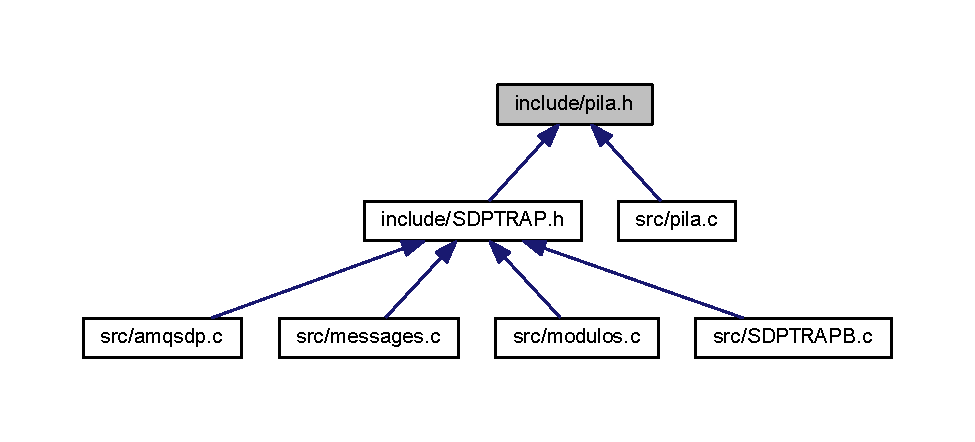
\includegraphics[width=350pt]{pila_8h__dep__incl}
\end{center}
\end{figure}
\subsection*{\textquotesingle{}defines\textquotesingle{}}
\begin{DoxyCompactItemize}
\item 
\#define \hyperlink{pila_8h_adfbc1051df776564281ac4220ba53a9e}{\+\_\+\+E\+X\+T\+\_\+}~extern
\end{DoxyCompactItemize}
\subsection*{Funciones}
\begin{DoxyCompactItemize}
\item 
\hyperlink{sha256le_8h_adfbc1051df776564281ac4220ba53a9e}{\+\_\+\+E\+X\+T\+\_\+} void $\ast$ \hyperlink{pila_8h_a76e64db083920898ed319afa103e9c9b}{create\+Stack} (int size, unsigned char pointer)
\item 
\hyperlink{sha256le_8h_adfbc1051df776564281ac4220ba53a9e}{\+\_\+\+E\+X\+T\+\_\+} void $\ast$ \hyperlink{pila_8h_aa849c8d27b733322a37846b4dafd9711}{delete\+Stack} (void $\ast$stack)
\item 
\hyperlink{sha256le_8h_adfbc1051df776564281ac4220ba53a9e}{\+\_\+\+E\+X\+T\+\_\+} void \hyperlink{pila_8h_a2d5d0b13ff0627defd07ec3fbe614b58}{push} (void $\ast$stack, void $\ast$data)
\item 
\hyperlink{sha256le_8h_adfbc1051df776564281ac4220ba53a9e}{\+\_\+\+E\+X\+T\+\_\+} void $\ast$ \hyperlink{pila_8h_ad9cf92c298635b8dad7b5a95d3f5dade}{pop} (void $\ast$stack)
\item 
\hyperlink{sha256le_8h_adfbc1051df776564281ac4220ba53a9e}{\+\_\+\+E\+X\+T\+\_\+} void $\ast$ \hyperlink{pila_8h_a4cd5ead0eacae2da44d2e23a5cd2ff85}{peek} (void $\ast$stack)
\item 
\hyperlink{sha256le_8h_adfbc1051df776564281ac4220ba53a9e}{\+\_\+\+E\+X\+T\+\_\+} void $\ast$ \hyperlink{pila_8h_a52d67d28c95733787926bc3f42bffb2a}{peek\+Previous} (void $\ast$stack, int deep)
\item 
\hyperlink{sha256le_8h_adfbc1051df776564281ac4220ba53a9e}{\+\_\+\+E\+X\+T\+\_\+} int \hyperlink{pila_8h_afd15d0a4ab9c26be333625ced34d00d9}{stack\+Depth} (void $\ast$stack)
\item 
\hyperlink{sha256le_8h_adfbc1051df776564281ac4220ba53a9e}{\+\_\+\+E\+X\+T\+\_\+} void \hyperlink{pila_8h_abfe71b23c5a319ae12879661e4dfa126}{clean\+Stacks} (void)
\end{DoxyCompactItemize}


\subsection{Descripción detallada}
Funciones de gestion de pilas abtracta. 

\begin{DoxyAuthor}{Autor}
\+: Javier Gonzalez 
\end{DoxyAuthor}
\begin{DoxyDate}{Fecha}
\+: 01/03/15 
\end{DoxyDate}
\begin{DoxyVersion}{Versión}
\+: 2.\+0 
\end{DoxyVersion}


\subsection{Documentación de los \textquotesingle{}defines\textquotesingle{}}
\hypertarget{pila_8h_adfbc1051df776564281ac4220ba53a9e}{}\index{pila.\+h@{pila.\+h}!\+\_\+\+E\+X\+T\+\_\+@{\+\_\+\+E\+X\+T\+\_\+}}
\index{\+\_\+\+E\+X\+T\+\_\+@{\+\_\+\+E\+X\+T\+\_\+}!pila.\+h@{pila.\+h}}
\subsubsection[{\+\_\+\+E\+X\+T\+\_\+}]{\setlength{\rightskip}{0pt plus 5cm}\#define \+\_\+\+E\+X\+T\+\_\+~extern}\label{pila_8h_adfbc1051df776564281ac4220ba53a9e}


Definición en la línea 20 del archivo pila.\+h.



\subsection{Documentación de las funciones}
\hypertarget{pila_8h_abfe71b23c5a319ae12879661e4dfa126}{}\index{pila.\+h@{pila.\+h}!clean\+Stacks@{clean\+Stacks}}
\index{clean\+Stacks@{clean\+Stacks}!pila.\+h@{pila.\+h}}
\subsubsection[{clean\+Stacks(void)}]{\setlength{\rightskip}{0pt plus 5cm}{\bf \+\_\+\+E\+X\+T\+\_\+} void clean\+Stacks (
\begin{DoxyParamCaption}
\item[{void}]{}
\end{DoxyParamCaption}
)}\label{pila_8h_abfe71b23c5a319ae12879661e4dfa126}
Elimina todas las pilas activas en el sistema 

Definición en la línea 86 del archivo pila.\+c.

\hypertarget{pila_8h_a76e64db083920898ed319afa103e9c9b}{}\index{pila.\+h@{pila.\+h}!create\+Stack@{create\+Stack}}
\index{create\+Stack@{create\+Stack}!pila.\+h@{pila.\+h}}
\subsubsection[{create\+Stack(int size, unsigned char pointer)}]{\setlength{\rightskip}{0pt plus 5cm}{\bf \+\_\+\+E\+X\+T\+\_\+} void$\ast$ create\+Stack (
\begin{DoxyParamCaption}
\item[{int}]{size, }
\item[{unsigned char}]{pointer}
\end{DoxyParamCaption}
)}\label{pila_8h_a76e64db083920898ed319afa103e9c9b}
Crea una nueva instancia de pila con elementos de size bytes 
\begin{DoxyParams}{Parámetros}
{\em size} & Tama�o del objeto a almacenar en la pila \\
\hline
{\em pointer} & Flag para indicar si la pila es de copia o referencia T\+R\+U\+E es una pila de referencia, almacena el puntero al objeto F\+A\+L\+S\+E es una pila de copia, almacena una copia del objeto \\
\hline
\end{DoxyParams}
\begin{DoxyReturn}{Devuelve}
Manejador de la pila 
\end{DoxyReturn}


Definición en la línea 66 del archivo pila.\+c.

\hypertarget{pila_8h_aa849c8d27b733322a37846b4dafd9711}{}\index{pila.\+h@{pila.\+h}!delete\+Stack@{delete\+Stack}}
\index{delete\+Stack@{delete\+Stack}!pila.\+h@{pila.\+h}}
\subsubsection[{delete\+Stack(void $\ast$stack)}]{\setlength{\rightskip}{0pt plus 5cm}{\bf \+\_\+\+E\+X\+T\+\_\+} void$\ast$ delete\+Stack (
\begin{DoxyParamCaption}
\item[{void $\ast$}]{stack}
\end{DoxyParamCaption}
)}\label{pila_8h_aa849c8d27b733322a37846b4dafd9711}
Elimina la instancia de pila pasada como parametro 
\begin{DoxyParams}{Parámetros}
{\em stack} & Handle de la pila a eliminar \\
\hline
\end{DoxyParams}
\begin{DoxyReturn}{Devuelve}
Manejador de la pila 
\end{DoxyReturn}


Definición en la línea 77 del archivo pila.\+c.

\hypertarget{pila_8h_a4cd5ead0eacae2da44d2e23a5cd2ff85}{}\index{pila.\+h@{pila.\+h}!peek@{peek}}
\index{peek@{peek}!pila.\+h@{pila.\+h}}
\subsubsection[{peek(void $\ast$stack)}]{\setlength{\rightskip}{0pt plus 5cm}{\bf \+\_\+\+E\+X\+T\+\_\+} void$\ast$ peek (
\begin{DoxyParamCaption}
\item[{void $\ast$}]{stack}
\end{DoxyParamCaption}
)}\label{pila_8h_a4cd5ead0eacae2da44d2e23a5cd2ff85}
Obtiene el elemento de la cima de la pila sin eliminarlo 
\begin{DoxyParams}{Parámetros}
{\em stack} & Handle de la pila \\
\hline
\end{DoxyParams}
\begin{DoxyReturn}{Devuelve}
Objeto en la cima de la pila 
\end{DoxyReturn}


Definición en la línea 126 del archivo pila.\+c.

\hypertarget{pila_8h_a52d67d28c95733787926bc3f42bffb2a}{}\index{pila.\+h@{pila.\+h}!peek\+Previous@{peek\+Previous}}
\index{peek\+Previous@{peek\+Previous}!pila.\+h@{pila.\+h}}
\subsubsection[{peek\+Previous(void $\ast$stack, int deep)}]{\setlength{\rightskip}{0pt plus 5cm}{\bf \+\_\+\+E\+X\+T\+\_\+} void$\ast$ peek\+Previous (
\begin{DoxyParamCaption}
\item[{void $\ast$}]{stack, }
\item[{int}]{deep}
\end{DoxyParamCaption}
)}\label{pila_8h_a52d67d28c95733787926bc3f42bffb2a}
Obtiene un elemento de la de la pila sin eliminarlo 
\begin{DoxyParams}{Parámetros}
{\em stack} & Handle de la pila \\
\hline
{\em deep} & Posicion del elemento en la pila (0 = cima de la pila) \\
\hline
\end{DoxyParams}
\begin{DoxyReturn}{Devuelve}
Objeto en la cima de la pila 
\end{DoxyReturn}


Definición en la línea 136 del archivo pila.\+c.

\hypertarget{pila_8h_ad9cf92c298635b8dad7b5a95d3f5dade}{}\index{pila.\+h@{pila.\+h}!pop@{pop}}
\index{pop@{pop}!pila.\+h@{pila.\+h}}
\subsubsection[{pop(void $\ast$stack)}]{\setlength{\rightskip}{0pt plus 5cm}{\bf \+\_\+\+E\+X\+T\+\_\+} void$\ast$ pop (
\begin{DoxyParamCaption}
\item[{void $\ast$}]{stack}
\end{DoxyParamCaption}
)}\label{pila_8h_ad9cf92c298635b8dad7b5a95d3f5dade}
Saca un elemento en la pila 
\begin{DoxyParams}{Parámetros}
{\em stack} & Handle de la pila \\
\hline
\end{DoxyParams}
\begin{DoxyReturn}{Devuelve}
Objeto en la cima de la pila 
\end{DoxyReturn}
\hypertarget{pila_8h_a2d5d0b13ff0627defd07ec3fbe614b58}{}\index{pila.\+h@{pila.\+h}!push@{push}}
\index{push@{push}!pila.\+h@{pila.\+h}}
\subsubsection[{push(void $\ast$stack, void $\ast$data)}]{\setlength{\rightskip}{0pt plus 5cm}{\bf \+\_\+\+E\+X\+T\+\_\+} void push (
\begin{DoxyParamCaption}
\item[{void $\ast$}]{stack, }
\item[{void $\ast$}]{data}
\end{DoxyParamCaption}
)}\label{pila_8h_a2d5d0b13ff0627defd07ec3fbe614b58}
Inserta un elemento en la pila 
\begin{DoxyParams}{Parámetros}
{\em stack} & Handle de la pila \\
\hline
{\em data} & Objeto a insertar en la pila \\
\hline
\end{DoxyParams}


Definición en la línea 99 del archivo pila.\+c.

\hypertarget{pila_8h_afd15d0a4ab9c26be333625ced34d00d9}{}\index{pila.\+h@{pila.\+h}!stack\+Depth@{stack\+Depth}}
\index{stack\+Depth@{stack\+Depth}!pila.\+h@{pila.\+h}}
\subsubsection[{stack\+Depth(void $\ast$stack)}]{\setlength{\rightskip}{0pt plus 5cm}{\bf \+\_\+\+E\+X\+T\+\_\+} int stack\+Depth (
\begin{DoxyParamCaption}
\item[{void $\ast$}]{stack}
\end{DoxyParamCaption}
)}\label{pila_8h_afd15d0a4ab9c26be333625ced34d00d9}
Devuelve la profundidad actual de la pila 
\begin{DoxyParams}{Parámetros}
{\em stack} & Handle de la pila \\
\hline
\end{DoxyParams}
\begin{DoxyReturn}{Devuelve}
profundidad de la pila 
\end{DoxyReturn}

\hypertarget{pilaptr_8h}{}\section{Referencia del Archivo include/pilaptr.h}
\label{pilaptr_8h}\index{include/pilaptr.\+h@{include/pilaptr.\+h}}
\subsection*{\textquotesingle{}defines\textquotesingle{}}
\begin{DoxyCompactItemize}
\item 
\#define \hyperlink{pilaptr_8h_adfbc1051df776564281ac4220ba53a9e}{\+\_\+\+E\+X\+T\+\_\+}~extern
\end{DoxyCompactItemize}
\subsection*{Funciones}
\begin{DoxyCompactItemize}
\item 
\hyperlink{sha256le_8h_adfbc1051df776564281ac4220ba53a9e}{\+\_\+\+E\+X\+T\+\_\+} void $\ast$ \hyperlink{pilaptr_8h_a102c0792aa831310125d5e4cc8a69690}{create\+Stack\+Ptr} (void)
\item 
\hyperlink{sha256le_8h_adfbc1051df776564281ac4220ba53a9e}{\+\_\+\+E\+X\+T\+\_\+} void $\ast$ \hyperlink{pilaptr_8h_a4a8a8a2e8f2014a39f6e28f957b67c23}{delete\+Stack\+Ptr} (void $\ast$stack)
\item 
\hyperlink{sha256le_8h_adfbc1051df776564281ac4220ba53a9e}{\+\_\+\+E\+X\+T\+\_\+} void \hyperlink{pilaptr_8h_a58552d25040d52e0b842547a021419b5}{push\+Ptr} (void $\ast$stack, void $\ast$data)
\item 
\hyperlink{sha256le_8h_adfbc1051df776564281ac4220ba53a9e}{\+\_\+\+E\+X\+T\+\_\+} void $\ast$ \hyperlink{pilaptr_8h_ad0cfc8d983e4f07904fdb96163ddc7db}{pop\+Ptr} (void $\ast$stack)
\item 
\hyperlink{sha256le_8h_adfbc1051df776564281ac4220ba53a9e}{\+\_\+\+E\+X\+T\+\_\+} void $\ast$ \hyperlink{pilaptr_8h_a67e713583ed41d11841b75731dc461af}{peek\+Ptr} (void $\ast$stack)
\item 
\hyperlink{sha256le_8h_adfbc1051df776564281ac4220ba53a9e}{\+\_\+\+E\+X\+T\+\_\+} void $\ast$ \hyperlink{pilaptr_8h_adca48e8fb99e758a5e6b4f7f42a5dd49}{peek\+Ptr\+Previous} (void $\ast$stack, int deep)
\item 
\hyperlink{sha256le_8h_adfbc1051df776564281ac4220ba53a9e}{\+\_\+\+E\+X\+T\+\_\+} int \hyperlink{pilaptr_8h_abd1ae0a8c137840168765319786e54da}{stack\+Depth\+Ptr} (void $\ast$stack)
\end{DoxyCompactItemize}


\subsection{Documentación de los \textquotesingle{}defines\textquotesingle{}}
\hypertarget{pilaptr_8h_adfbc1051df776564281ac4220ba53a9e}{}\index{pilaptr.\+h@{pilaptr.\+h}!\+\_\+\+E\+X\+T\+\_\+@{\+\_\+\+E\+X\+T\+\_\+}}
\index{\+\_\+\+E\+X\+T\+\_\+@{\+\_\+\+E\+X\+T\+\_\+}!pilaptr.\+h@{pilaptr.\+h}}
\subsubsection[{\+\_\+\+E\+X\+T\+\_\+}]{\setlength{\rightskip}{0pt plus 5cm}\#define \+\_\+\+E\+X\+T\+\_\+~extern}\label{pilaptr_8h_adfbc1051df776564281ac4220ba53a9e}


Definición en la línea 10 del archivo pilaptr.\+h.



\subsection{Documentación de las funciones}
\hypertarget{pilaptr_8h_a102c0792aa831310125d5e4cc8a69690}{}\index{pilaptr.\+h@{pilaptr.\+h}!create\+Stack\+Ptr@{create\+Stack\+Ptr}}
\index{create\+Stack\+Ptr@{create\+Stack\+Ptr}!pilaptr.\+h@{pilaptr.\+h}}
\subsubsection[{create\+Stack\+Ptr(void)}]{\setlength{\rightskip}{0pt plus 5cm}{\bf \+\_\+\+E\+X\+T\+\_\+} void$\ast$ create\+Stack\+Ptr (
\begin{DoxyParamCaption}
\item[{void}]{}
\end{DoxyParamCaption}
)}\label{pilaptr_8h_a102c0792aa831310125d5e4cc8a69690}
\hypertarget{pilaptr_8h_a4a8a8a2e8f2014a39f6e28f957b67c23}{}\index{pilaptr.\+h@{pilaptr.\+h}!delete\+Stack\+Ptr@{delete\+Stack\+Ptr}}
\index{delete\+Stack\+Ptr@{delete\+Stack\+Ptr}!pilaptr.\+h@{pilaptr.\+h}}
\subsubsection[{delete\+Stack\+Ptr(void $\ast$stack)}]{\setlength{\rightskip}{0pt plus 5cm}{\bf \+\_\+\+E\+X\+T\+\_\+} void$\ast$ delete\+Stack\+Ptr (
\begin{DoxyParamCaption}
\item[{void $\ast$}]{stack}
\end{DoxyParamCaption}
)}\label{pilaptr_8h_a4a8a8a2e8f2014a39f6e28f957b67c23}
\hypertarget{pilaptr_8h_a67e713583ed41d11841b75731dc461af}{}\index{pilaptr.\+h@{pilaptr.\+h}!peek\+Ptr@{peek\+Ptr}}
\index{peek\+Ptr@{peek\+Ptr}!pilaptr.\+h@{pilaptr.\+h}}
\subsubsection[{peek\+Ptr(void $\ast$stack)}]{\setlength{\rightskip}{0pt plus 5cm}{\bf \+\_\+\+E\+X\+T\+\_\+} void$\ast$ peek\+Ptr (
\begin{DoxyParamCaption}
\item[{void $\ast$}]{stack}
\end{DoxyParamCaption}
)}\label{pilaptr_8h_a67e713583ed41d11841b75731dc461af}
\hypertarget{pilaptr_8h_adca48e8fb99e758a5e6b4f7f42a5dd49}{}\index{pilaptr.\+h@{pilaptr.\+h}!peek\+Ptr\+Previous@{peek\+Ptr\+Previous}}
\index{peek\+Ptr\+Previous@{peek\+Ptr\+Previous}!pilaptr.\+h@{pilaptr.\+h}}
\subsubsection[{peek\+Ptr\+Previous(void $\ast$stack, int deep)}]{\setlength{\rightskip}{0pt plus 5cm}{\bf \+\_\+\+E\+X\+T\+\_\+} void$\ast$ peek\+Ptr\+Previous (
\begin{DoxyParamCaption}
\item[{void $\ast$}]{stack, }
\item[{int}]{deep}
\end{DoxyParamCaption}
)}\label{pilaptr_8h_adca48e8fb99e758a5e6b4f7f42a5dd49}
\hypertarget{pilaptr_8h_ad0cfc8d983e4f07904fdb96163ddc7db}{}\index{pilaptr.\+h@{pilaptr.\+h}!pop\+Ptr@{pop\+Ptr}}
\index{pop\+Ptr@{pop\+Ptr}!pilaptr.\+h@{pilaptr.\+h}}
\subsubsection[{pop\+Ptr(void $\ast$stack)}]{\setlength{\rightskip}{0pt plus 5cm}{\bf \+\_\+\+E\+X\+T\+\_\+} void$\ast$ pop\+Ptr (
\begin{DoxyParamCaption}
\item[{void $\ast$}]{stack}
\end{DoxyParamCaption}
)}\label{pilaptr_8h_ad0cfc8d983e4f07904fdb96163ddc7db}
\hypertarget{pilaptr_8h_a58552d25040d52e0b842547a021419b5}{}\index{pilaptr.\+h@{pilaptr.\+h}!push\+Ptr@{push\+Ptr}}
\index{push\+Ptr@{push\+Ptr}!pilaptr.\+h@{pilaptr.\+h}}
\subsubsection[{push\+Ptr(void $\ast$stack, void $\ast$data)}]{\setlength{\rightskip}{0pt plus 5cm}{\bf \+\_\+\+E\+X\+T\+\_\+} void push\+Ptr (
\begin{DoxyParamCaption}
\item[{void $\ast$}]{stack, }
\item[{void $\ast$}]{data}
\end{DoxyParamCaption}
)}\label{pilaptr_8h_a58552d25040d52e0b842547a021419b5}
\hypertarget{pilaptr_8h_abd1ae0a8c137840168765319786e54da}{}\index{pilaptr.\+h@{pilaptr.\+h}!stack\+Depth\+Ptr@{stack\+Depth\+Ptr}}
\index{stack\+Depth\+Ptr@{stack\+Depth\+Ptr}!pilaptr.\+h@{pilaptr.\+h}}
\subsubsection[{stack\+Depth\+Ptr(void $\ast$stack)}]{\setlength{\rightskip}{0pt plus 5cm}{\bf \+\_\+\+E\+X\+T\+\_\+} int stack\+Depth\+Ptr (
\begin{DoxyParamCaption}
\item[{void $\ast$}]{stack}
\end{DoxyParamCaption}
)}\label{pilaptr_8h_abd1ae0a8c137840168765319786e54da}

\hypertarget{salw32_8h}{}\section{Referencia del Archivo include/salw32.h}
\label{salw32_8h}\index{include/salw32.\+h@{include/salw32.\+h}}


Definicion de funciones especificas para sistemas Windows.  




\subsection{Descripción detallada}
Definicion de funciones especificas para sistemas Windows. 

\begin{DoxyAuthor}{Autor}
\+: Javier Gonzalez 
\end{DoxyAuthor}
\begin{DoxyDate}{Fecha}
\+: 01/03/15 
\end{DoxyDate}
\begin{DoxyVersion}{Versión}
\+: 2.\+0 
\end{DoxyVersion}

\hypertarget{sdpconfig_8h}{}\section{Referencia del Archivo include/sdpconfig.h}
\label{sdpconfig_8h}\index{include/sdpconfig.\+h@{include/sdpconfig.\+h}}


Fichero de cabecera de configuracion del sistema Define las constantes y los valores globales de comportamiento.  


Gráfico de los archivos que directa o indirectamente incluyen a este archivo\+:\nopagebreak
\begin{figure}[H]
\begin{center}
\leavevmode
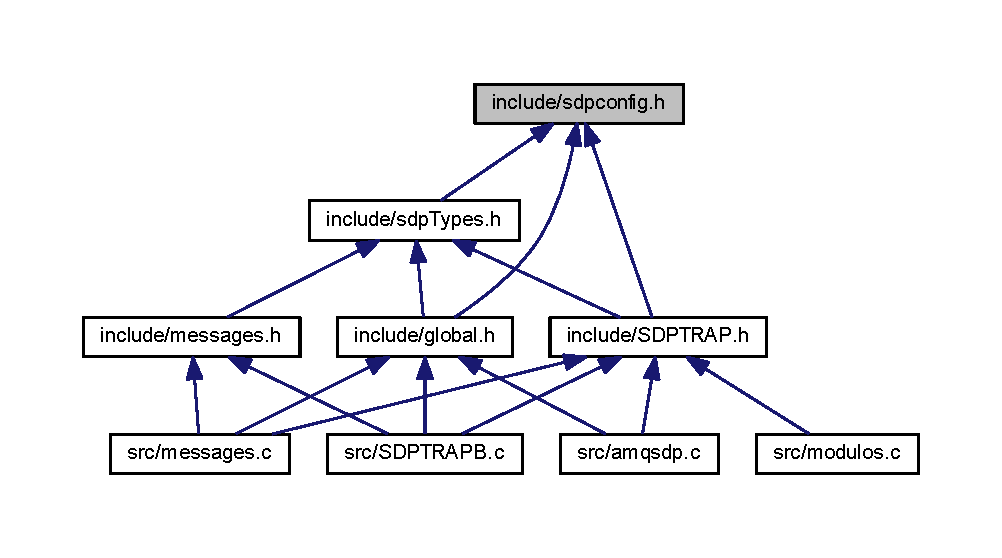
\includegraphics[width=350pt]{sdpconfig_8h__dep__incl}
\end{center}
\end{figure}
\subsection*{\textquotesingle{}defines\textquotesingle{}}
\begin{DoxyCompactItemize}
\item 
\#define \hyperlink{sdpconfig_8h_a711fffeb11b40c66d48792fcd6664aa7}{M\+O\+D\+E\+\_\+\+N\+O\+N\+E}~0
\item 
\#define \hyperlink{sdpconfig_8h_a8425a5128fca6d19686c6ae5bc724c88}{M\+O\+D\+E\+\_\+\+G\+L\+O\+B\+A\+L}~1
\item 
\#define \hyperlink{sdpconfig_8h_a8eeb3454261633c1bb268da7c057a26a}{M\+O\+D\+E\+\_\+\+M\+O\+D\+U\+L\+E}~2
\item 
\#define \hyperlink{sdpconfig_8h_a92938508adb379739d16e3fd065cb913}{M\+O\+D\+E\+\_\+\+D\+E\+T\+A\+I\+L\+E\+D}~4
\item 
\#define \hyperlink{sdpconfig_8h_aa362b9b04115cdcafb53c62ea0b7e44c}{M\+O\+D\+E\+\_\+\+U\+N\+L\+O\+A\+D}~9
\item 
\#define \hyperlink{sdpconfig_8h_a6611b3fba9de26203f14407743b750cc}{M\+A\+X\+\_\+\+M\+O\+D\+U\+L\+E}~32
\item 
\#define \hyperlink{sdpconfig_8h_ac084a897234f41c71f01eab1d39c3073}{M\+A\+X\+\_\+\+P\+A\+R\+R\+A\+F\+O}~48
\item 
\#define \hyperlink{sdpconfig_8h_aeefcc7b6f118beefd2cec532afced5df}{I\+T\+E\+M\+S\+\_\+\+B\+Y\+\_\+\+M\+S\+G}~25
\item 
\#define \hyperlink{sdpconfig_8h_aa8cecfc5c5c054d2875c03e77b7be15d}{T\+R\+U\+E}~0x\+F\+F
\item 
\#define \hyperlink{sdpconfig_8h_aa93f0eb578d23995850d61f7d61c55c1}{F\+A\+L\+S\+E}~0x00
\item 
\#define \hyperlink{sdpconfig_8h_a070d2ce7b6bb7e5c05602aa8c308d0c4}{N\+U\+L\+L}~0x0
\item 
\#define \hyperlink{sdpconfig_8h_af0fde0e5ef66a5bb448ff8b6ffedcd69}{D\+B\+G\+\_\+\+N\+O\+N\+E}~0
\item 
\#define \hyperlink{sdpconfig_8h_a44f6930298af62aaaa4af242749e286d}{D\+B\+G\+\_\+\+C\+A\+L\+L}~1
\item 
\#define \hyperlink{sdpconfig_8h_a4487f9d50b1daa14e880dc3cc740a39e}{D\+B\+G\+\_\+\+P\+U\+S\+H}~2
\item 
\#define \hyperlink{sdpconfig_8h_ac85c3723adc8b9ef82670d5ecd43c328}{D\+B\+G\+\_\+\+P\+O\+P}~4
\item 
\#define \hyperlink{sdpconfig_8h_ae39a9c80905518ddfdc1e04d6bd45fbe}{D\+B\+G\+\_\+\+S\+E\+S\+I\+O\+N}~8
\item 
\#define \hyperlink{sdpconfig_8h_a50ee6784b4c763d1d1353f34e1f314af}{D\+B\+G\+\_\+\+M\+S\+G}~16
\item 
\#define \hyperlink{sdpconfig_8h_acb4aca184f447d249a7ebebf2da7b5ad}{D\+B\+G\+\_\+\+S\+E\+N\+D}~32
\item 
\#define \hyperlink{sdpconfig_8h_ae94dc26fa7b9b56988e51bd5d00391b5}{D\+B\+G\+\_\+\+T\+I\+M\+E\+R}~64
\item 
\#define \hyperlink{sdpconfig_8h_a34617f3ac0249ca877bddc57f6982401}{D\+B\+G\+\_\+\+M\+O\+D}~128
\item 
\#define \hyperlink{sdpconfig_8h_a14d858941e566e4f9e07b183236f10e6}{D\+B\+G\+\_\+\+A\+L\+L}~255
\item 
\#define \hyperlink{sdpconfig_8h_ac2d33ccaf63f5d5b66552b95426c0137}{D\+E\+B\+U\+G\+\_\+\+L\+E\+V\+E\+L}~\hyperlink{sdpconfig_8h_a14d858941e566e4f9e07b183236f10e6}{D\+B\+G\+\_\+\+A\+L\+L}
\item 
\#define \hyperlink{sdpconfig_8h_a361ecdff3dc6ffd72441ac2657d9fa89}{P\+R\+O\+C\+E\+S\+S\+\_\+\+M\+O\+D\+E}~\hyperlink{sdpconfig_8h_a8425a5128fca6d19686c6ae5bc724c88}{M\+O\+D\+E\+\_\+\+G\+L\+O\+B\+A\+L}
\item 
\#define \hyperlink{sdpconfig_8h_ad6074dd11ab3c97c8135c43aab03ae95}{H\+A\+S\+H\+\_\+\+S\+I\+Z\+E}~32  /$\ast$ Longitud de la \hyperlink{messages_8c_ad4f688c87d1792d6783f34c874b5fefd}{firma} digital   $\ast$/
\item 
\#define \hyperlink{sdpconfig_8h_a37f0a3c295994e30902acb1b76bd094a}{F\+I\+R\+M\+A}(a,  b)~\hyperlink{md5_8c_aa75a1419e565ea619428681420b59179}{M\+D5}(a, b)
\end{DoxyCompactItemize}


\subsection{Descripción detallada}
Fichero de cabecera de configuracion del sistema Define las constantes y los valores globales de comportamiento. 

Estas variables se pueden modificar\+: 1.-\/ Mediante definiciones en el proceso de compilacion (-\/\+D\+V\+A\+R=xxx) 2.-\/ A traves de una variable de entorno

\begin{DoxyAuthor}{Autor}
\+: Javier Gonzalez 
\end{DoxyAuthor}
\begin{DoxyDate}{Fecha}
\+: 01/03/15 
\end{DoxyDate}
\begin{DoxyVersion}{Versión}
\+: 2.\+0 
\end{DoxyVersion}


\subsection{Documentación de los \textquotesingle{}defines\textquotesingle{}}
\hypertarget{sdpconfig_8h_a14d858941e566e4f9e07b183236f10e6}{}\index{sdpconfig.\+h@{sdpconfig.\+h}!D\+B\+G\+\_\+\+A\+L\+L@{D\+B\+G\+\_\+\+A\+L\+L}}
\index{D\+B\+G\+\_\+\+A\+L\+L@{D\+B\+G\+\_\+\+A\+L\+L}!sdpconfig.\+h@{sdpconfig.\+h}}
\subsubsection[{D\+B\+G\+\_\+\+A\+L\+L}]{\setlength{\rightskip}{0pt plus 5cm}\#define D\+B\+G\+\_\+\+A\+L\+L~255}\label{sdpconfig_8h_a14d858941e566e4f9e07b183236f10e6}


Definición en la línea 52 del archivo sdpconfig.\+h.

\hypertarget{sdpconfig_8h_a44f6930298af62aaaa4af242749e286d}{}\index{sdpconfig.\+h@{sdpconfig.\+h}!D\+B\+G\+\_\+\+C\+A\+L\+L@{D\+B\+G\+\_\+\+C\+A\+L\+L}}
\index{D\+B\+G\+\_\+\+C\+A\+L\+L@{D\+B\+G\+\_\+\+C\+A\+L\+L}!sdpconfig.\+h@{sdpconfig.\+h}}
\subsubsection[{D\+B\+G\+\_\+\+C\+A\+L\+L}]{\setlength{\rightskip}{0pt plus 5cm}\#define D\+B\+G\+\_\+\+C\+A\+L\+L~1}\label{sdpconfig_8h_a44f6930298af62aaaa4af242749e286d}


Definición en la línea 43 del archivo sdpconfig.\+h.

\hypertarget{sdpconfig_8h_a34617f3ac0249ca877bddc57f6982401}{}\index{sdpconfig.\+h@{sdpconfig.\+h}!D\+B\+G\+\_\+\+M\+O\+D@{D\+B\+G\+\_\+\+M\+O\+D}}
\index{D\+B\+G\+\_\+\+M\+O\+D@{D\+B\+G\+\_\+\+M\+O\+D}!sdpconfig.\+h@{sdpconfig.\+h}}
\subsubsection[{D\+B\+G\+\_\+\+M\+O\+D}]{\setlength{\rightskip}{0pt plus 5cm}\#define D\+B\+G\+\_\+\+M\+O\+D~128}\label{sdpconfig_8h_a34617f3ac0249ca877bddc57f6982401}


Definición en la línea 50 del archivo sdpconfig.\+h.

\hypertarget{sdpconfig_8h_a50ee6784b4c763d1d1353f34e1f314af}{}\index{sdpconfig.\+h@{sdpconfig.\+h}!D\+B\+G\+\_\+\+M\+S\+G@{D\+B\+G\+\_\+\+M\+S\+G}}
\index{D\+B\+G\+\_\+\+M\+S\+G@{D\+B\+G\+\_\+\+M\+S\+G}!sdpconfig.\+h@{sdpconfig.\+h}}
\subsubsection[{D\+B\+G\+\_\+\+M\+S\+G}]{\setlength{\rightskip}{0pt plus 5cm}\#define D\+B\+G\+\_\+\+M\+S\+G~16}\label{sdpconfig_8h_a50ee6784b4c763d1d1353f34e1f314af}


Definición en la línea 47 del archivo sdpconfig.\+h.

\hypertarget{sdpconfig_8h_af0fde0e5ef66a5bb448ff8b6ffedcd69}{}\index{sdpconfig.\+h@{sdpconfig.\+h}!D\+B\+G\+\_\+\+N\+O\+N\+E@{D\+B\+G\+\_\+\+N\+O\+N\+E}}
\index{D\+B\+G\+\_\+\+N\+O\+N\+E@{D\+B\+G\+\_\+\+N\+O\+N\+E}!sdpconfig.\+h@{sdpconfig.\+h}}
\subsubsection[{D\+B\+G\+\_\+\+N\+O\+N\+E}]{\setlength{\rightskip}{0pt plus 5cm}\#define D\+B\+G\+\_\+\+N\+O\+N\+E~0}\label{sdpconfig_8h_af0fde0e5ef66a5bb448ff8b6ffedcd69}


Definición en la línea 42 del archivo sdpconfig.\+h.

\hypertarget{sdpconfig_8h_ac85c3723adc8b9ef82670d5ecd43c328}{}\index{sdpconfig.\+h@{sdpconfig.\+h}!D\+B\+G\+\_\+\+P\+O\+P@{D\+B\+G\+\_\+\+P\+O\+P}}
\index{D\+B\+G\+\_\+\+P\+O\+P@{D\+B\+G\+\_\+\+P\+O\+P}!sdpconfig.\+h@{sdpconfig.\+h}}
\subsubsection[{D\+B\+G\+\_\+\+P\+O\+P}]{\setlength{\rightskip}{0pt plus 5cm}\#define D\+B\+G\+\_\+\+P\+O\+P~4}\label{sdpconfig_8h_ac85c3723adc8b9ef82670d5ecd43c328}


Definición en la línea 45 del archivo sdpconfig.\+h.

\hypertarget{sdpconfig_8h_a4487f9d50b1daa14e880dc3cc740a39e}{}\index{sdpconfig.\+h@{sdpconfig.\+h}!D\+B\+G\+\_\+\+P\+U\+S\+H@{D\+B\+G\+\_\+\+P\+U\+S\+H}}
\index{D\+B\+G\+\_\+\+P\+U\+S\+H@{D\+B\+G\+\_\+\+P\+U\+S\+H}!sdpconfig.\+h@{sdpconfig.\+h}}
\subsubsection[{D\+B\+G\+\_\+\+P\+U\+S\+H}]{\setlength{\rightskip}{0pt plus 5cm}\#define D\+B\+G\+\_\+\+P\+U\+S\+H~2}\label{sdpconfig_8h_a4487f9d50b1daa14e880dc3cc740a39e}


Definición en la línea 44 del archivo sdpconfig.\+h.

\hypertarget{sdpconfig_8h_acb4aca184f447d249a7ebebf2da7b5ad}{}\index{sdpconfig.\+h@{sdpconfig.\+h}!D\+B\+G\+\_\+\+S\+E\+N\+D@{D\+B\+G\+\_\+\+S\+E\+N\+D}}
\index{D\+B\+G\+\_\+\+S\+E\+N\+D@{D\+B\+G\+\_\+\+S\+E\+N\+D}!sdpconfig.\+h@{sdpconfig.\+h}}
\subsubsection[{D\+B\+G\+\_\+\+S\+E\+N\+D}]{\setlength{\rightskip}{0pt plus 5cm}\#define D\+B\+G\+\_\+\+S\+E\+N\+D~32}\label{sdpconfig_8h_acb4aca184f447d249a7ebebf2da7b5ad}


Definición en la línea 48 del archivo sdpconfig.\+h.

\hypertarget{sdpconfig_8h_ae39a9c80905518ddfdc1e04d6bd45fbe}{}\index{sdpconfig.\+h@{sdpconfig.\+h}!D\+B\+G\+\_\+\+S\+E\+S\+I\+O\+N@{D\+B\+G\+\_\+\+S\+E\+S\+I\+O\+N}}
\index{D\+B\+G\+\_\+\+S\+E\+S\+I\+O\+N@{D\+B\+G\+\_\+\+S\+E\+S\+I\+O\+N}!sdpconfig.\+h@{sdpconfig.\+h}}
\subsubsection[{D\+B\+G\+\_\+\+S\+E\+S\+I\+O\+N}]{\setlength{\rightskip}{0pt plus 5cm}\#define D\+B\+G\+\_\+\+S\+E\+S\+I\+O\+N~8}\label{sdpconfig_8h_ae39a9c80905518ddfdc1e04d6bd45fbe}


Definición en la línea 46 del archivo sdpconfig.\+h.

\hypertarget{sdpconfig_8h_ae94dc26fa7b9b56988e51bd5d00391b5}{}\index{sdpconfig.\+h@{sdpconfig.\+h}!D\+B\+G\+\_\+\+T\+I\+M\+E\+R@{D\+B\+G\+\_\+\+T\+I\+M\+E\+R}}
\index{D\+B\+G\+\_\+\+T\+I\+M\+E\+R@{D\+B\+G\+\_\+\+T\+I\+M\+E\+R}!sdpconfig.\+h@{sdpconfig.\+h}}
\subsubsection[{D\+B\+G\+\_\+\+T\+I\+M\+E\+R}]{\setlength{\rightskip}{0pt plus 5cm}\#define D\+B\+G\+\_\+\+T\+I\+M\+E\+R~64}\label{sdpconfig_8h_ae94dc26fa7b9b56988e51bd5d00391b5}


Definición en la línea 49 del archivo sdpconfig.\+h.

\hypertarget{sdpconfig_8h_ac2d33ccaf63f5d5b66552b95426c0137}{}\index{sdpconfig.\+h@{sdpconfig.\+h}!D\+E\+B\+U\+G\+\_\+\+L\+E\+V\+E\+L@{D\+E\+B\+U\+G\+\_\+\+L\+E\+V\+E\+L}}
\index{D\+E\+B\+U\+G\+\_\+\+L\+E\+V\+E\+L@{D\+E\+B\+U\+G\+\_\+\+L\+E\+V\+E\+L}!sdpconfig.\+h@{sdpconfig.\+h}}
\subsubsection[{D\+E\+B\+U\+G\+\_\+\+L\+E\+V\+E\+L}]{\setlength{\rightskip}{0pt plus 5cm}\#define D\+E\+B\+U\+G\+\_\+\+L\+E\+V\+E\+L~{\bf D\+B\+G\+\_\+\+A\+L\+L}}\label{sdpconfig_8h_ac2d33ccaf63f5d5b66552b95426c0137}


Definición en la línea 55 del archivo sdpconfig.\+h.

\hypertarget{sdpconfig_8h_aa93f0eb578d23995850d61f7d61c55c1}{}\index{sdpconfig.\+h@{sdpconfig.\+h}!F\+A\+L\+S\+E@{F\+A\+L\+S\+E}}
\index{F\+A\+L\+S\+E@{F\+A\+L\+S\+E}!sdpconfig.\+h@{sdpconfig.\+h}}
\subsubsection[{F\+A\+L\+S\+E}]{\setlength{\rightskip}{0pt plus 5cm}\#define F\+A\+L\+S\+E~0x00}\label{sdpconfig_8h_aa93f0eb578d23995850d61f7d61c55c1}


Definición en la línea 36 del archivo sdpconfig.\+h.

\hypertarget{sdpconfig_8h_a37f0a3c295994e30902acb1b76bd094a}{}\index{sdpconfig.\+h@{sdpconfig.\+h}!F\+I\+R\+M\+A@{F\+I\+R\+M\+A}}
\index{F\+I\+R\+M\+A@{F\+I\+R\+M\+A}!sdpconfig.\+h@{sdpconfig.\+h}}
\subsubsection[{F\+I\+R\+M\+A}]{\setlength{\rightskip}{0pt plus 5cm}\#define F\+I\+R\+M\+A(
\begin{DoxyParamCaption}
\item[{}]{a, }
\item[{}]{b}
\end{DoxyParamCaption}
)~{\bf M\+D5}(a, b)}\label{sdpconfig_8h_a37f0a3c295994e30902acb1b76bd094a}


Definición en la línea 76 del archivo sdpconfig.\+h.

\hypertarget{sdpconfig_8h_ad6074dd11ab3c97c8135c43aab03ae95}{}\index{sdpconfig.\+h@{sdpconfig.\+h}!H\+A\+S\+H\+\_\+\+S\+I\+Z\+E@{H\+A\+S\+H\+\_\+\+S\+I\+Z\+E}}
\index{H\+A\+S\+H\+\_\+\+S\+I\+Z\+E@{H\+A\+S\+H\+\_\+\+S\+I\+Z\+E}!sdpconfig.\+h@{sdpconfig.\+h}}
\subsubsection[{H\+A\+S\+H\+\_\+\+S\+I\+Z\+E}]{\setlength{\rightskip}{0pt plus 5cm}\#define H\+A\+S\+H\+\_\+\+S\+I\+Z\+E~32  /$\ast$ Longitud de la {\bf firma} digital   $\ast$/}\label{sdpconfig_8h_ad6074dd11ab3c97c8135c43aab03ae95}


Definición en la línea 75 del archivo sdpconfig.\+h.

\hypertarget{sdpconfig_8h_aeefcc7b6f118beefd2cec532afced5df}{}\index{sdpconfig.\+h@{sdpconfig.\+h}!I\+T\+E\+M\+S\+\_\+\+B\+Y\+\_\+\+M\+S\+G@{I\+T\+E\+M\+S\+\_\+\+B\+Y\+\_\+\+M\+S\+G}}
\index{I\+T\+E\+M\+S\+\_\+\+B\+Y\+\_\+\+M\+S\+G@{I\+T\+E\+M\+S\+\_\+\+B\+Y\+\_\+\+M\+S\+G}!sdpconfig.\+h@{sdpconfig.\+h}}
\subsubsection[{I\+T\+E\+M\+S\+\_\+\+B\+Y\+\_\+\+M\+S\+G}]{\setlength{\rightskip}{0pt plus 5cm}\#define I\+T\+E\+M\+S\+\_\+\+B\+Y\+\_\+\+M\+S\+G~25}\label{sdpconfig_8h_aeefcc7b6f118beefd2cec532afced5df}
Numero de mensajes que se almacenaran antes de enviarlos a la cola 

Definición en la línea 29 del archivo sdpconfig.\+h.

\hypertarget{sdpconfig_8h_a6611b3fba9de26203f14407743b750cc}{}\index{sdpconfig.\+h@{sdpconfig.\+h}!M\+A\+X\+\_\+\+M\+O\+D\+U\+L\+E@{M\+A\+X\+\_\+\+M\+O\+D\+U\+L\+E}}
\index{M\+A\+X\+\_\+\+M\+O\+D\+U\+L\+E@{M\+A\+X\+\_\+\+M\+O\+D\+U\+L\+E}!sdpconfig.\+h@{sdpconfig.\+h}}
\subsubsection[{M\+A\+X\+\_\+\+M\+O\+D\+U\+L\+E}]{\setlength{\rightskip}{0pt plus 5cm}\#define M\+A\+X\+\_\+\+M\+O\+D\+U\+L\+E~32}\label{sdpconfig_8h_a6611b3fba9de26203f14407743b750cc}
Longitud del nombre del modulo 

Definición en la línea 25 del archivo sdpconfig.\+h.

\hypertarget{sdpconfig_8h_ac084a897234f41c71f01eab1d39c3073}{}\index{sdpconfig.\+h@{sdpconfig.\+h}!M\+A\+X\+\_\+\+P\+A\+R\+R\+A\+F\+O@{M\+A\+X\+\_\+\+P\+A\+R\+R\+A\+F\+O}}
\index{M\+A\+X\+\_\+\+P\+A\+R\+R\+A\+F\+O@{M\+A\+X\+\_\+\+P\+A\+R\+R\+A\+F\+O}!sdpconfig.\+h@{sdpconfig.\+h}}
\subsubsection[{M\+A\+X\+\_\+\+P\+A\+R\+R\+A\+F\+O}]{\setlength{\rightskip}{0pt plus 5cm}\#define M\+A\+X\+\_\+\+P\+A\+R\+R\+A\+F\+O~48}\label{sdpconfig_8h_ac084a897234f41c71f01eab1d39c3073}
Maxima longitud del nombre de un parrafo 

Definición en la línea 26 del archivo sdpconfig.\+h.

\hypertarget{sdpconfig_8h_a92938508adb379739d16e3fd065cb913}{}\index{sdpconfig.\+h@{sdpconfig.\+h}!M\+O\+D\+E\+\_\+\+D\+E\+T\+A\+I\+L\+E\+D@{M\+O\+D\+E\+\_\+\+D\+E\+T\+A\+I\+L\+E\+D}}
\index{M\+O\+D\+E\+\_\+\+D\+E\+T\+A\+I\+L\+E\+D@{M\+O\+D\+E\+\_\+\+D\+E\+T\+A\+I\+L\+E\+D}!sdpconfig.\+h@{sdpconfig.\+h}}
\subsubsection[{M\+O\+D\+E\+\_\+\+D\+E\+T\+A\+I\+L\+E\+D}]{\setlength{\rightskip}{0pt plus 5cm}\#define M\+O\+D\+E\+\_\+\+D\+E\+T\+A\+I\+L\+E\+D~4}\label{sdpconfig_8h_a92938508adb379739d16e3fd065cb913}
Envia las trazas segun se van generando, sin acumular datos 

Definición en la línea 22 del archivo sdpconfig.\+h.

\hypertarget{sdpconfig_8h_a8425a5128fca6d19686c6ae5bc724c88}{}\index{sdpconfig.\+h@{sdpconfig.\+h}!M\+O\+D\+E\+\_\+\+G\+L\+O\+B\+A\+L@{M\+O\+D\+E\+\_\+\+G\+L\+O\+B\+A\+L}}
\index{M\+O\+D\+E\+\_\+\+G\+L\+O\+B\+A\+L@{M\+O\+D\+E\+\_\+\+G\+L\+O\+B\+A\+L}!sdpconfig.\+h@{sdpconfig.\+h}}
\subsubsection[{M\+O\+D\+E\+\_\+\+G\+L\+O\+B\+A\+L}]{\setlength{\rightskip}{0pt plus 5cm}\#define M\+O\+D\+E\+\_\+\+G\+L\+O\+B\+A\+L~1}\label{sdpconfig_8h_a8425a5128fca6d19686c6ae5bc724c88}
Acumula todas las trazas de la sesion y las envia al final 

Definición en la línea 20 del archivo sdpconfig.\+h.

\hypertarget{sdpconfig_8h_a8eeb3454261633c1bb268da7c057a26a}{}\index{sdpconfig.\+h@{sdpconfig.\+h}!M\+O\+D\+E\+\_\+\+M\+O\+D\+U\+L\+E@{M\+O\+D\+E\+\_\+\+M\+O\+D\+U\+L\+E}}
\index{M\+O\+D\+E\+\_\+\+M\+O\+D\+U\+L\+E@{M\+O\+D\+E\+\_\+\+M\+O\+D\+U\+L\+E}!sdpconfig.\+h@{sdpconfig.\+h}}
\subsubsection[{M\+O\+D\+E\+\_\+\+M\+O\+D\+U\+L\+E}]{\setlength{\rightskip}{0pt plus 5cm}\#define M\+O\+D\+E\+\_\+\+M\+O\+D\+U\+L\+E~2}\label{sdpconfig_8h_a8eeb3454261633c1bb268da7c057a26a}
Acumula las trazas por modulo y las envia cada vez que acaba un modulo 

Definición en la línea 21 del archivo sdpconfig.\+h.

\hypertarget{sdpconfig_8h_a711fffeb11b40c66d48792fcd6664aa7}{}\index{sdpconfig.\+h@{sdpconfig.\+h}!M\+O\+D\+E\+\_\+\+N\+O\+N\+E@{M\+O\+D\+E\+\_\+\+N\+O\+N\+E}}
\index{M\+O\+D\+E\+\_\+\+N\+O\+N\+E@{M\+O\+D\+E\+\_\+\+N\+O\+N\+E}!sdpconfig.\+h@{sdpconfig.\+h}}
\subsubsection[{M\+O\+D\+E\+\_\+\+N\+O\+N\+E}]{\setlength{\rightskip}{0pt plus 5cm}\#define M\+O\+D\+E\+\_\+\+N\+O\+N\+E~0}\label{sdpconfig_8h_a711fffeb11b40c66d48792fcd6664aa7}
No hara trazas sobre el modulo 

Definición en la línea 19 del archivo sdpconfig.\+h.

\hypertarget{sdpconfig_8h_aa362b9b04115cdcafb53c62ea0b7e44c}{}\index{sdpconfig.\+h@{sdpconfig.\+h}!M\+O\+D\+E\+\_\+\+U\+N\+L\+O\+A\+D@{M\+O\+D\+E\+\_\+\+U\+N\+L\+O\+A\+D}}
\index{M\+O\+D\+E\+\_\+\+U\+N\+L\+O\+A\+D@{M\+O\+D\+E\+\_\+\+U\+N\+L\+O\+A\+D}!sdpconfig.\+h@{sdpconfig.\+h}}
\subsubsection[{M\+O\+D\+E\+\_\+\+U\+N\+L\+O\+A\+D}]{\setlength{\rightskip}{0pt plus 5cm}\#define M\+O\+D\+E\+\_\+\+U\+N\+L\+O\+A\+D~9}\label{sdpconfig_8h_aa362b9b04115cdcafb53c62ea0b7e44c}
Uso interno 

Definición en la línea 23 del archivo sdpconfig.\+h.

\hypertarget{sdpconfig_8h_a070d2ce7b6bb7e5c05602aa8c308d0c4}{}\index{sdpconfig.\+h@{sdpconfig.\+h}!N\+U\+L\+L@{N\+U\+L\+L}}
\index{N\+U\+L\+L@{N\+U\+L\+L}!sdpconfig.\+h@{sdpconfig.\+h}}
\subsubsection[{N\+U\+L\+L}]{\setlength{\rightskip}{0pt plus 5cm}\#define N\+U\+L\+L~0x0}\label{sdpconfig_8h_a070d2ce7b6bb7e5c05602aa8c308d0c4}


Definición en la línea 39 del archivo sdpconfig.\+h.

\hypertarget{sdpconfig_8h_a361ecdff3dc6ffd72441ac2657d9fa89}{}\index{sdpconfig.\+h@{sdpconfig.\+h}!P\+R\+O\+C\+E\+S\+S\+\_\+\+M\+O\+D\+E@{P\+R\+O\+C\+E\+S\+S\+\_\+\+M\+O\+D\+E}}
\index{P\+R\+O\+C\+E\+S\+S\+\_\+\+M\+O\+D\+E@{P\+R\+O\+C\+E\+S\+S\+\_\+\+M\+O\+D\+E}!sdpconfig.\+h@{sdpconfig.\+h}}
\subsubsection[{P\+R\+O\+C\+E\+S\+S\+\_\+\+M\+O\+D\+E}]{\setlength{\rightskip}{0pt plus 5cm}\#define P\+R\+O\+C\+E\+S\+S\+\_\+\+M\+O\+D\+E~{\bf M\+O\+D\+E\+\_\+\+G\+L\+O\+B\+A\+L}}\label{sdpconfig_8h_a361ecdff3dc6ffd72441ac2657d9fa89}


Definición en la línea 59 del archivo sdpconfig.\+h.

\hypertarget{sdpconfig_8h_aa8cecfc5c5c054d2875c03e77b7be15d}{}\index{sdpconfig.\+h@{sdpconfig.\+h}!T\+R\+U\+E@{T\+R\+U\+E}}
\index{T\+R\+U\+E@{T\+R\+U\+E}!sdpconfig.\+h@{sdpconfig.\+h}}
\subsubsection[{T\+R\+U\+E}]{\setlength{\rightskip}{0pt plus 5cm}\#define T\+R\+U\+E~0x\+F\+F}\label{sdpconfig_8h_aa8cecfc5c5c054d2875c03e77b7be15d}


Definición en la línea 33 del archivo sdpconfig.\+h.


\hypertarget{_s_d_p_t_r_a_p_8h}{}\section{Referencia del Archivo include/\+S\+D\+P\+T\+R\+A\+P.h}
\label{_s_d_p_t_r_a_p_8h}\index{include/\+S\+D\+P\+T\+R\+A\+P.\+h@{include/\+S\+D\+P\+T\+R\+A\+P.\+h}}


Fichero de cabecera con los ficheros de cabecera comunes.  


{\ttfamily \#include \char`\"{}jggsal.\+h\char`\"{}}\\*
{\ttfamily \#include \char`\"{}sdpconfig.\+h\char`\"{}}\\*
{\ttfamily \#include \char`\"{}sdp\+Types.\+h\char`\"{}}\\*
{\ttfamily \#include \char`\"{}pila.\+h\char`\"{}}\\*
{\ttfamily \#include \char`\"{}trapcodes.\+h\char`\"{}}\\*
Dependencia gráfica adjunta para S\+D\+P\+T\+R\+A\+P.\+h\+:\nopagebreak
\begin{figure}[H]
\begin{center}
\leavevmode
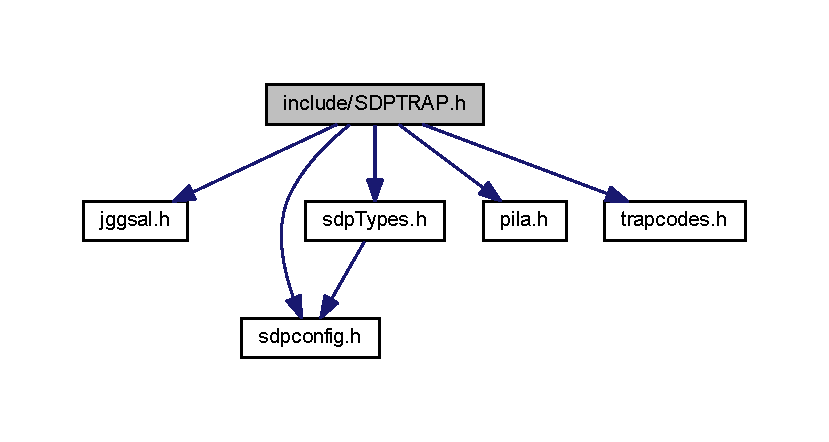
\includegraphics[width=350pt]{_s_d_p_t_r_a_p_8h__incl}
\end{center}
\end{figure}
Gráfico de los archivos que directa o indirectamente incluyen a este archivo\+:\nopagebreak
\begin{figure}[H]
\begin{center}
\leavevmode
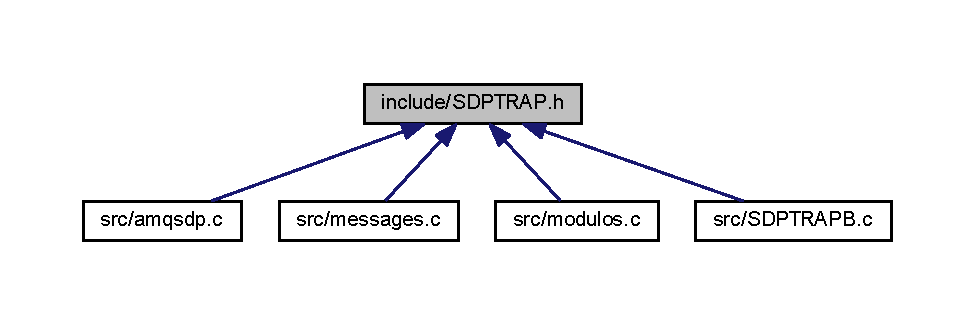
\includegraphics[width=350pt]{_s_d_p_t_r_a_p_8h__dep__incl}
\end{center}
\end{figure}


\subsection{Descripción detallada}
Fichero de cabecera con los ficheros de cabecera comunes. 

\begin{DoxyAuthor}{Autor}
\+: Javier Gonzalez 
\end{DoxyAuthor}
\begin{DoxyDate}{Fecha}
\+: 01/03/15 
\end{DoxyDate}
\begin{DoxyVersion}{Versión}
\+: 2.\+0 
\end{DoxyVersion}

\hypertarget{_s_d_p_t_r_a_p_b_8h}{}\section{Referencia del Archivo include/\+S\+D\+P\+T\+R\+A\+P\+B.h}
\label{_s_d_p_t_r_a_p_b_8h}\index{include/\+S\+D\+P\+T\+R\+A\+P\+B.\+h@{include/\+S\+D\+P\+T\+R\+A\+P\+B.\+h}}


Fichero de cabecera de la libreria S\+D\+P\+T\+R\+A\+P\+B Define las constantes y los valores globales de comportamiento.  


Gráfico de los archivos que directa o indirectamente incluyen a este archivo\+:\nopagebreak
\begin{figure}[H]
\begin{center}
\leavevmode
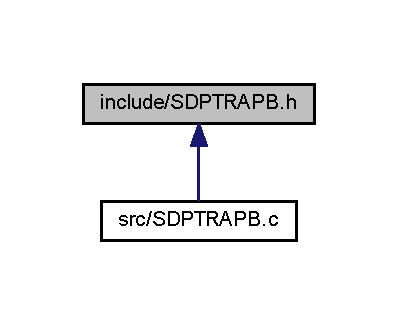
\includegraphics[width=191pt]{_s_d_p_t_r_a_p_b_8h__dep__incl}
\end{center}
\end{figure}
\subsection*{\textquotesingle{}defines\textquotesingle{}}
\begin{DoxyCompactItemize}
\item 
\#define \hyperlink{_s_d_p_t_r_a_p_b_8h_aad8a241e13cd4731254878eed6271c8c}{S\+D\+P\+T\+R\+A\+P\+\_\+\+D\+L\+L}~extern
\item 
\#define \hyperlink{_s_d_p_t_r_a_p_b_8h_adfbc1051df776564281ac4220ba53a9e}{\+\_\+\+E\+X\+T\+\_\+}~extern
\end{DoxyCompactItemize}
\subsection*{Funciones}
\begin{DoxyCompactItemize}
\item 
\hyperlink{_s_d_p_t_r_a_p_b_8h_aad8a241e13cd4731254878eed6271c8c}{S\+D\+P\+T\+R\+A\+P\+\_\+\+D\+L\+L} void \hyperlink{_s_d_p_t_r_a_p_b_8h_a9b67ec7fc38ca9e2c907b859e053d024}{S\+D\+P\+T\+R\+A\+P\+B} (int $\ast$option, int $\ast$len, char $\ast$sdp\+Data, char $\ast$label)
\begin{DoxyCompactList}\small\item\em Punto de entrada a la libreria S\+D\+P\+T\+R\+A\+P\+B. \end{DoxyCompactList}\item 
\hyperlink{_s_d_p_t_r_a_p_b_8h_aad8a241e13cd4731254878eed6271c8c}{S\+D\+P\+T\+R\+A\+P\+\_\+\+D\+L\+L} void \hyperlink{_s_d_p_t_r_a_p_b_8h_afe26885736f7df4b2157bb4dfe32ce20}{S\+D\+P\+T\+R\+A\+P\+B\+\_\+set\+Debug\+Level} (int level)
\item 
\hyperlink{_s_d_p_t_r_a_p_b_8h_aad8a241e13cd4731254878eed6271c8c}{S\+D\+P\+T\+R\+A\+P\+\_\+\+D\+L\+L} void \hyperlink{_s_d_p_t_r_a_p_b_8h_a56bd96cf4c11628e4f0e301c5b8e5872}{S\+D\+P\+T\+R\+A\+P\+B\+\_\+set\+Modo} (int mode)
\end{DoxyCompactItemize}


\subsection{Descripción detallada}
Fichero de cabecera de la libreria S\+D\+P\+T\+R\+A\+P\+B Define las constantes y los valores globales de comportamiento. 

Define\+: El unico punto de entrada a la D\+L\+L La estructura C equivalente a la C\+O\+P\+Y C\+O\+B\+O\+L Las constantes para la gestion de los diferentes tipos de mensajes

En determinados entornos C\+O\+B\+O\+L no se permite que las rutinas C tengan varios puntos de entrada La carga de la libreria se realiza por el mismo nombre de la rutina y el punto de entrada en una funcion con el mismo nombre

\begin{DoxyAuthor}{Autor}
\+: Javier Gonzalez 
\end{DoxyAuthor}
\begin{DoxyDate}{Fecha}
\+: 01/03/15 
\end{DoxyDate}
\begin{DoxyVersion}{Versión}
\+: 2.\+0 
\end{DoxyVersion}


\subsection{Documentación de los \textquotesingle{}defines\textquotesingle{}}
\hypertarget{_s_d_p_t_r_a_p_b_8h_adfbc1051df776564281ac4220ba53a9e}{}\index{S\+D\+P\+T\+R\+A\+P\+B.\+h@{S\+D\+P\+T\+R\+A\+P\+B.\+h}!\+\_\+\+E\+X\+T\+\_\+@{\+\_\+\+E\+X\+T\+\_\+}}
\index{\+\_\+\+E\+X\+T\+\_\+@{\+\_\+\+E\+X\+T\+\_\+}!S\+D\+P\+T\+R\+A\+P\+B.\+h@{S\+D\+P\+T\+R\+A\+P\+B.\+h}}
\subsubsection[{\+\_\+\+E\+X\+T\+\_\+}]{\setlength{\rightskip}{0pt plus 5cm}\#define \+\_\+\+E\+X\+T\+\_\+~extern}\label{_s_d_p_t_r_a_p_b_8h_adfbc1051df776564281ac4220ba53a9e}


Definición en la línea 40 del archivo S\+D\+P\+T\+R\+A\+P\+B.\+h.

\hypertarget{_s_d_p_t_r_a_p_b_8h_aad8a241e13cd4731254878eed6271c8c}{}\index{S\+D\+P\+T\+R\+A\+P\+B.\+h@{S\+D\+P\+T\+R\+A\+P\+B.\+h}!S\+D\+P\+T\+R\+A\+P\+\_\+\+D\+L\+L@{S\+D\+P\+T\+R\+A\+P\+\_\+\+D\+L\+L}}
\index{S\+D\+P\+T\+R\+A\+P\+\_\+\+D\+L\+L@{S\+D\+P\+T\+R\+A\+P\+\_\+\+D\+L\+L}!S\+D\+P\+T\+R\+A\+P\+B.\+h@{S\+D\+P\+T\+R\+A\+P\+B.\+h}}
\subsubsection[{S\+D\+P\+T\+R\+A\+P\+\_\+\+D\+L\+L}]{\setlength{\rightskip}{0pt plus 5cm}\#define S\+D\+P\+T\+R\+A\+P\+\_\+\+D\+L\+L~extern}\label{_s_d_p_t_r_a_p_b_8h_aad8a241e13cd4731254878eed6271c8c}


Definición en la línea 33 del archivo S\+D\+P\+T\+R\+A\+P\+B.\+h.



\subsection{Documentación de las funciones}
\hypertarget{_s_d_p_t_r_a_p_b_8h_a9b67ec7fc38ca9e2c907b859e053d024}{}\index{S\+D\+P\+T\+R\+A\+P\+B.\+h@{S\+D\+P\+T\+R\+A\+P\+B.\+h}!S\+D\+P\+T\+R\+A\+P\+B@{S\+D\+P\+T\+R\+A\+P\+B}}
\index{S\+D\+P\+T\+R\+A\+P\+B@{S\+D\+P\+T\+R\+A\+P\+B}!S\+D\+P\+T\+R\+A\+P\+B.\+h@{S\+D\+P\+T\+R\+A\+P\+B.\+h}}
\subsubsection[{S\+D\+P\+T\+R\+A\+P\+B(int $\ast$option, int $\ast$len, char $\ast$sdp\+Data, char $\ast$label)}]{\setlength{\rightskip}{0pt plus 5cm}{\bf S\+D\+P\+T\+R\+A\+P\+\_\+\+D\+L\+L} void S\+D\+P\+T\+R\+A\+P\+B (
\begin{DoxyParamCaption}
\item[{int $\ast$}]{option, }
\item[{int $\ast$}]{len, }
\item[{char $\ast$}]{sdp\+Data, }
\item[{char $\ast$}]{modulo}
\end{DoxyParamCaption}
)}\label{_s_d_p_t_r_a_p_b_8h_a9b67ec7fc38ca9e2c907b859e053d024}


Punto de entrada a la libreria S\+D\+P\+T\+R\+A\+P\+B. 


\begin{DoxyParams}{Parámetros}
{\em option} & = una combinacion de los valores definidos en M\+S\+G\+\_\+xxx \\
\hline
{\em len} & = Longitud de la etiqueta, 0 si no es relevante \\
\hline
{\em sdp\+Data} & = Puntero a la estructura S\+D\+P \\
\hline
{\em label} & = Etiqueta (parrafo, rutina, etc.)\\
\hline
{\em option} & Una combinacion de los valores definidos en M\+S\+G\+\_\+xxx \\
\hline
{\em len} & Longitud de la etiqueta, 0 si no es relevante \\
\hline
{\em sdp\+Data} & Puntero a la estructura S\+D\+P \\
\hline
{\em modulo} & Etiqueta (parrafo, rutina, etc.) \\
\hline
\end{DoxyParams}


Definición en la línea 83 del archivo S\+D\+P\+T\+R\+A\+P\+B.\+c.

\hypertarget{_s_d_p_t_r_a_p_b_8h_afe26885736f7df4b2157bb4dfe32ce20}{}\index{S\+D\+P\+T\+R\+A\+P\+B.\+h@{S\+D\+P\+T\+R\+A\+P\+B.\+h}!S\+D\+P\+T\+R\+A\+P\+B\+\_\+set\+Debug\+Level@{S\+D\+P\+T\+R\+A\+P\+B\+\_\+set\+Debug\+Level}}
\index{S\+D\+P\+T\+R\+A\+P\+B\+\_\+set\+Debug\+Level@{S\+D\+P\+T\+R\+A\+P\+B\+\_\+set\+Debug\+Level}!S\+D\+P\+T\+R\+A\+P\+B.\+h@{S\+D\+P\+T\+R\+A\+P\+B.\+h}}
\subsubsection[{S\+D\+P\+T\+R\+A\+P\+B\+\_\+set\+Debug\+Level(int level)}]{\setlength{\rightskip}{0pt plus 5cm}{\bf S\+D\+P\+T\+R\+A\+P\+\_\+\+D\+L\+L} void S\+D\+P\+T\+R\+A\+P\+B\+\_\+set\+Debug\+Level (
\begin{DoxyParamCaption}
\item[{int}]{level}
\end{DoxyParamCaption}
)}\label{_s_d_p_t_r_a_p_b_8h_afe26885736f7df4b2157bb4dfe32ce20}
Usado para pruebas unitarias y de integracion 

Definición en la línea 64 del archivo S\+D\+P\+T\+R\+A\+P\+B.\+c.

\hypertarget{_s_d_p_t_r_a_p_b_8h_a56bd96cf4c11628e4f0e301c5b8e5872}{}\index{S\+D\+P\+T\+R\+A\+P\+B.\+h@{S\+D\+P\+T\+R\+A\+P\+B.\+h}!S\+D\+P\+T\+R\+A\+P\+B\+\_\+set\+Modo@{S\+D\+P\+T\+R\+A\+P\+B\+\_\+set\+Modo}}
\index{S\+D\+P\+T\+R\+A\+P\+B\+\_\+set\+Modo@{S\+D\+P\+T\+R\+A\+P\+B\+\_\+set\+Modo}!S\+D\+P\+T\+R\+A\+P\+B.\+h@{S\+D\+P\+T\+R\+A\+P\+B.\+h}}
\subsubsection[{S\+D\+P\+T\+R\+A\+P\+B\+\_\+set\+Modo(int mode)}]{\setlength{\rightskip}{0pt plus 5cm}{\bf S\+D\+P\+T\+R\+A\+P\+\_\+\+D\+L\+L} void S\+D\+P\+T\+R\+A\+P\+B\+\_\+set\+Modo (
\begin{DoxyParamCaption}
\item[{int}]{mode}
\end{DoxyParamCaption}
)}\label{_s_d_p_t_r_a_p_b_8h_a56bd96cf4c11628e4f0e301c5b8e5872}
Usado para pruebas unitarias y de integracion 

Definición en la línea 71 del archivo S\+D\+P\+T\+R\+A\+P\+B.\+c.


\hypertarget{sdp_types_8h}{}\section{Referencia del Archivo include/sdp\+Types.h}
\label{sdp_types_8h}\index{include/sdp\+Types.\+h@{include/sdp\+Types.\+h}}


Define las estructrus y tipos de datos usados en la libreria.  


{\ttfamily \#include \char`\"{}sdpconfig.\+h\char`\"{}}\\*
Dependencia gráfica adjunta para sdp\+Types.\+h\+:\nopagebreak
\begin{figure}[H]
\begin{center}
\leavevmode
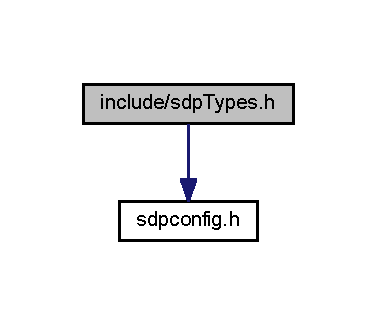
\includegraphics[width=181pt]{sdp_types_8h__incl}
\end{center}
\end{figure}
Gráfico de los archivos que directa o indirectamente incluyen a este archivo\+:\nopagebreak
\begin{figure}[H]
\begin{center}
\leavevmode
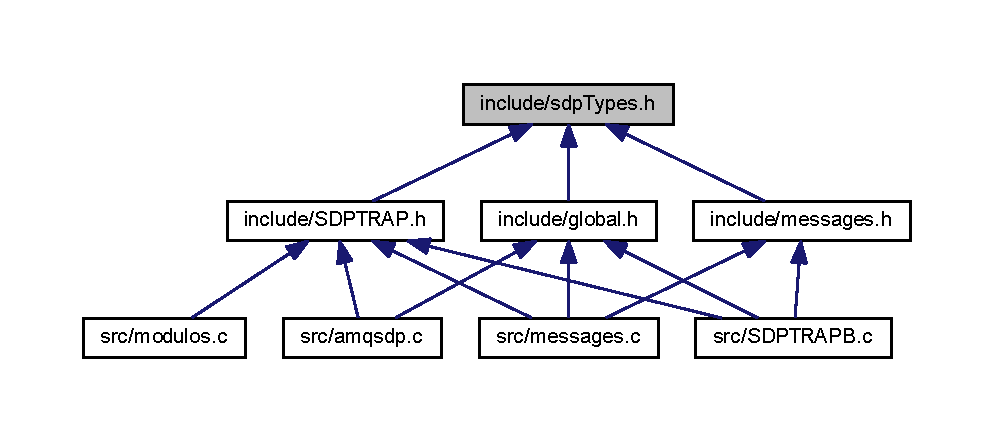
\includegraphics[width=350pt]{sdp_types_8h__dep__incl}
\end{center}
\end{figure}
\subsection*{Estructuras de datos}
\begin{DoxyCompactItemize}
\item 
struct \hyperlink{struct_s_t___s_d_p}{S\+T\+\_\+\+S\+D\+P}
\item 
struct \hyperlink{struct_s_t___t_i_m_e_r}{S\+T\+\_\+\+T\+I\+M\+E\+R}
\item 
struct \hyperlink{struct_s_t___m_o_d}{S\+T\+\_\+\+M\+O\+D}
\end{DoxyCompactItemize}
\subsection*{\textquotesingle{}typedefs\textquotesingle{}}
\begin{DoxyCompactItemize}
\item 
typedef unsigned long \hyperlink{sdp_types_8h_af632da489ebc3708ec3ab6791ee53fa4}{U\+L\+O\+N\+G}
\item 
typedef struct \hyperlink{struct_s_t___s_d_p}{S\+T\+\_\+\+S\+D\+P} \hyperlink{sdp_types_8h_a8ba8f2a87560d14f1152da6646649dfd}{S\+D\+P}
\begin{DoxyCompactList}\small\item\em Estructura C equivalente a la C\+O\+P\+Y C\+O\+B\+O\+L. \end{DoxyCompactList}\item 
typedef struct \hyperlink{struct_s_t___t_i_m_e_r}{S\+T\+\_\+\+T\+I\+M\+E\+R} \hyperlink{sdp_types_8h_a94c0315eea22344f1e853cc7c90592bb}{T\+I\+M\+E\+R}
\begin{DoxyCompactList}\small\item\em Contadores de tiempo en microsegundos. \end{DoxyCompactList}\item 
typedef struct \hyperlink{struct_s_t___m_o_d}{S\+T\+\_\+\+M\+O\+D} \hyperlink{sdp_types_8h_a54a4473e20ff51d4dcb4158acf8a5979}{M\+O\+D}
\end{DoxyCompactItemize}


\subsection{Descripción detallada}
Define las estructrus y tipos de datos usados en la libreria. 

\begin{DoxyAuthor}{Autor}
\+: Javier Gonzalez 
\end{DoxyAuthor}
\begin{DoxyDate}{Fecha}
\+: 01/03/15 
\end{DoxyDate}
\begin{DoxyVersion}{Versión}
\+: 2.\+0 
\end{DoxyVersion}


\subsection{Documentación de los \textquotesingle{}typedefs\textquotesingle{}}
\hypertarget{sdp_types_8h_a54a4473e20ff51d4dcb4158acf8a5979}{}\index{sdp\+Types.\+h@{sdp\+Types.\+h}!M\+O\+D@{M\+O\+D}}
\index{M\+O\+D@{M\+O\+D}!sdp\+Types.\+h@{sdp\+Types.\+h}}
\subsubsection[{M\+O\+D}]{\setlength{\rightskip}{0pt plus 5cm}typedef struct {\bf S\+T\+\_\+\+M\+O\+D} {\bf M\+O\+D}}\label{sdp_types_8h_a54a4473e20ff51d4dcb4158acf8a5979}


Definición en la línea 76 del archivo sdp\+Types.\+h.

\hypertarget{sdp_types_8h_a8ba8f2a87560d14f1152da6646649dfd}{}\index{sdp\+Types.\+h@{sdp\+Types.\+h}!S\+D\+P@{S\+D\+P}}
\index{S\+D\+P@{S\+D\+P}!sdp\+Types.\+h@{sdp\+Types.\+h}}
\subsubsection[{S\+D\+P}]{\setlength{\rightskip}{0pt plus 5cm}{\bf S\+D\+P}}\label{sdp_types_8h_a8ba8f2a87560d14f1152da6646649dfd}


Estructura C equivalente a la C\+O\+P\+Y C\+O\+B\+O\+L. 

La copy C\+O\+B\+O\+L es una secuencia de bytes raw \hypertarget{sdp_types_8h_a94c0315eea22344f1e853cc7c90592bb}{}\index{sdp\+Types.\+h@{sdp\+Types.\+h}!T\+I\+M\+E\+R@{T\+I\+M\+E\+R}}
\index{T\+I\+M\+E\+R@{T\+I\+M\+E\+R}!sdp\+Types.\+h@{sdp\+Types.\+h}}
\subsubsection[{T\+I\+M\+E\+R}]{\setlength{\rightskip}{0pt plus 5cm}{\bf T\+I\+M\+E\+R}}\label{sdp_types_8h_a94c0315eea22344f1e853cc7c90592bb}


Contadores de tiempo en microsegundos. 

Se mantiene un acumulador por cada parrafo o modulo Los tiempos van en mirosegundos 

Definición en la línea 54 del archivo sdp\+Types.\+h.

\hypertarget{sdp_types_8h_af632da489ebc3708ec3ab6791ee53fa4}{}\index{sdp\+Types.\+h@{sdp\+Types.\+h}!U\+L\+O\+N\+G@{U\+L\+O\+N\+G}}
\index{U\+L\+O\+N\+G@{U\+L\+O\+N\+G}!sdp\+Types.\+h@{sdp\+Types.\+h}}
\subsubsection[{U\+L\+O\+N\+G}]{\setlength{\rightskip}{0pt plus 5cm}typedef unsigned long {\bf U\+L\+O\+N\+G}}\label{sdp_types_8h_af632da489ebc3708ec3ab6791ee53fa4}


Definición en la línea 16 del archivo sdp\+Types.\+h.


\hypertarget{sha-private_8h}{}\section{Referencia del Archivo include/sha-\/private.h}
\label{sha-private_8h}\index{include/sha-\/private.\+h@{include/sha-\/private.\+h}}
Gráfico de los archivos que directa o indirectamente incluyen a este archivo\+:\nopagebreak
\begin{figure}[H]
\begin{center}
\leavevmode
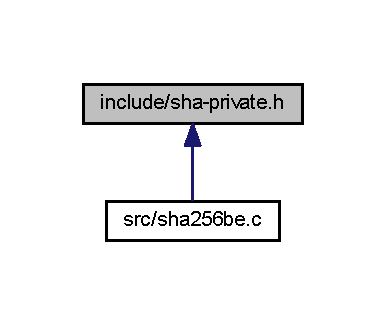
\includegraphics[width=185pt]{sha-private_8h__dep__incl}
\end{center}
\end{figure}
\subsection*{\textquotesingle{}defines\textquotesingle{}}
\begin{DoxyCompactItemize}
\item 
\#define \hyperlink{sha-private_8h_acfa605d869c01f97ffb5b544fb4879bd}{S\+H\+A\+\_\+\+Ch}(x,  y,  z)            ~(((x) \& (y)) $^\wedge$ (($\sim$(x)) \& (z)))
\item 
\#define \hyperlink{sha-private_8h_a658449395a53235eb4a9d86d0761603f}{S\+H\+A\+\_\+\+Maj}(x,  y,  z)          ~(((x) \& (y)) $^\wedge$ ((x) \& (z)) $^\wedge$ ((y) \& (z)))
\item 
\#define \hyperlink{sha-private_8h_af5541766ecc62b9cb5598ef22f46af2e}{S\+H\+A\+\_\+\+Parity}(x,  y,  z)~((x) $^\wedge$ (y) $^\wedge$ (z))
\end{DoxyCompactItemize}


\subsection{Documentación de los \textquotesingle{}defines\textquotesingle{}}
\hypertarget{sha-private_8h_acfa605d869c01f97ffb5b544fb4879bd}{}\index{sha-\/private.\+h@{sha-\/private.\+h}!S\+H\+A\+\_\+\+Ch@{S\+H\+A\+\_\+\+Ch}}
\index{S\+H\+A\+\_\+\+Ch@{S\+H\+A\+\_\+\+Ch}!sha-\/private.\+h@{sha-\/private.\+h}}
\subsubsection[{S\+H\+A\+\_\+\+Ch}]{\setlength{\rightskip}{0pt plus 5cm}\#define S\+H\+A\+\_\+\+Ch(
\begin{DoxyParamCaption}
\item[{}]{x, }
\item[{}]{y, }
\item[{}]{z}
\end{DoxyParamCaption}
)~(((x) \& (y)) $^\wedge$ (($\sim$(x)) \& (z)))}\label{sha-private_8h_acfa605d869c01f97ffb5b544fb4879bd}


Definición en la línea 12 del archivo sha-\/private.\+h.

\hypertarget{sha-private_8h_a658449395a53235eb4a9d86d0761603f}{}\index{sha-\/private.\+h@{sha-\/private.\+h}!S\+H\+A\+\_\+\+Maj@{S\+H\+A\+\_\+\+Maj}}
\index{S\+H\+A\+\_\+\+Maj@{S\+H\+A\+\_\+\+Maj}!sha-\/private.\+h@{sha-\/private.\+h}}
\subsubsection[{S\+H\+A\+\_\+\+Maj}]{\setlength{\rightskip}{0pt plus 5cm}\#define S\+H\+A\+\_\+\+Maj(
\begin{DoxyParamCaption}
\item[{}]{x, }
\item[{}]{y, }
\item[{}]{z}
\end{DoxyParamCaption}
)~(((x) \& (y)) $^\wedge$ ((x) \& (z)) $^\wedge$ ((y) \& (z)))}\label{sha-private_8h_a658449395a53235eb4a9d86d0761603f}


Definición en la línea 13 del archivo sha-\/private.\+h.

\hypertarget{sha-private_8h_af5541766ecc62b9cb5598ef22f46af2e}{}\index{sha-\/private.\+h@{sha-\/private.\+h}!S\+H\+A\+\_\+\+Parity@{S\+H\+A\+\_\+\+Parity}}
\index{S\+H\+A\+\_\+\+Parity@{S\+H\+A\+\_\+\+Parity}!sha-\/private.\+h@{sha-\/private.\+h}}
\subsubsection[{S\+H\+A\+\_\+\+Parity}]{\setlength{\rightskip}{0pt plus 5cm}\#define S\+H\+A\+\_\+\+Parity(
\begin{DoxyParamCaption}
\item[{}]{x, }
\item[{}]{y, }
\item[{}]{z}
\end{DoxyParamCaption}
)~((x) $^\wedge$ (y) $^\wedge$ (z))}\label{sha-private_8h_af5541766ecc62b9cb5598ef22f46af2e}


Definición en la línea 24 del archivo sha-\/private.\+h.


\hypertarget{sha256_8h}{}\section{Referencia del Archivo include/sha256.h}
\label{sha256_8h}\index{include/sha256.\+h@{include/sha256.\+h}}
\subsection*{\textquotesingle{}defines\textquotesingle{}}
\begin{DoxyCompactItemize}
\item 
\#define \hyperlink{sha256_8h_adfbc1051df776564281ac4220ba53a9e}{\+\_\+\+E\+X\+T\+\_\+}~extern
\end{DoxyCompactItemize}
\subsection*{Funciones}
\begin{DoxyCompactItemize}
\item 
\hyperlink{sha256le_8h_adfbc1051df776564281ac4220ba53a9e}{\+\_\+\+E\+X\+T\+\_\+} void \hyperlink{sha256_8h_ae5af8076102907981a3894538bbcfed7}{S\+H\+A256} (char $\ast$out, const char $\ast$in)
\end{DoxyCompactItemize}


\subsection{Documentación de los \textquotesingle{}defines\textquotesingle{}}
\hypertarget{sha256_8h_adfbc1051df776564281ac4220ba53a9e}{}\index{sha256.\+h@{sha256.\+h}!\+\_\+\+E\+X\+T\+\_\+@{\+\_\+\+E\+X\+T\+\_\+}}
\index{\+\_\+\+E\+X\+T\+\_\+@{\+\_\+\+E\+X\+T\+\_\+}!sha256.\+h@{sha256.\+h}}
\subsubsection[{\+\_\+\+E\+X\+T\+\_\+}]{\setlength{\rightskip}{0pt plus 5cm}\#define \+\_\+\+E\+X\+T\+\_\+~extern}\label{sha256_8h_adfbc1051df776564281ac4220ba53a9e}


Definición en la línea 19 del archivo sha256.\+h.



\subsection{Documentación de las funciones}
\hypertarget{sha256_8h_ae5af8076102907981a3894538bbcfed7}{}\index{sha256.\+h@{sha256.\+h}!S\+H\+A256@{S\+H\+A256}}
\index{S\+H\+A256@{S\+H\+A256}!sha256.\+h@{sha256.\+h}}
\subsubsection[{S\+H\+A256(char $\ast$out, const char $\ast$in)}]{\setlength{\rightskip}{0pt plus 5cm}{\bf \+\_\+\+E\+X\+T\+\_\+} void S\+H\+A256 (
\begin{DoxyParamCaption}
\item[{char $\ast$}]{out, }
\item[{const char $\ast$}]{in}
\end{DoxyParamCaption}
)}\label{sha256_8h_ae5af8076102907981a3894538bbcfed7}

\hypertarget{sha256be_8h}{}\section{Referencia del Archivo include/sha256be.h}
\label{sha256be_8h}\index{include/sha256be.\+h@{include/sha256be.\+h}}
{\ttfamily \#include $<$stdint.\+h$>$}\\*
Dependencia gráfica adjunta para sha256be.\+h\+:\nopagebreak
\begin{figure}[H]
\begin{center}
\leavevmode
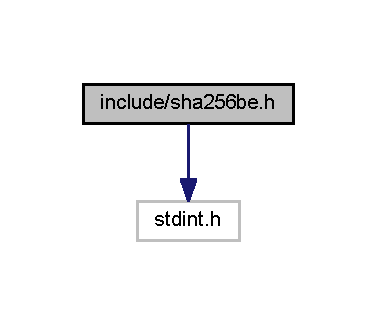
\includegraphics[width=181pt]{sha256be_8h__incl}
\end{center}
\end{figure}
Gráfico de los archivos que directa o indirectamente incluyen a este archivo\+:\nopagebreak
\begin{figure}[H]
\begin{center}
\leavevmode
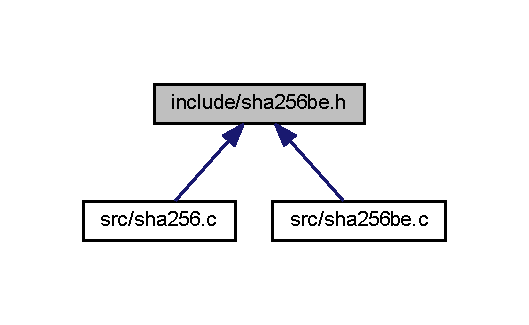
\includegraphics[width=254pt]{sha256be_8h__dep__incl}
\end{center}
\end{figure}
\subsection*{Estructuras de datos}
\begin{DoxyCompactItemize}
\item 
struct \hyperlink{struct_s_h_a256_context}{S\+H\+A256\+Context}
\end{DoxyCompactItemize}
\subsection*{\textquotesingle{}defines\textquotesingle{}}
\begin{DoxyCompactItemize}
\item 
\#define \hyperlink{sha256be_8h_adfbc1051df776564281ac4220ba53a9e}{\+\_\+\+E\+X\+T\+\_\+}~extern
\item 
\#define \hyperlink{sha256be_8h_a0155b221bb2170bc51a0a7aafc77d034}{\+\_\+\+S\+H\+A\+\_\+enum\+\_\+}
\end{DoxyCompactItemize}
\subsection*{\textquotesingle{}typedefs\textquotesingle{}}
\begin{DoxyCompactItemize}
\item 
typedef struct \hyperlink{struct_s_h_a256_context}{S\+H\+A256\+Context} \hyperlink{sha256be_8h_a274920c71f772dca134f6cd3d65a60c7}{S\+H\+A256\+Context}
\end{DoxyCompactItemize}
\subsection*{Enumeraciones}
\begin{DoxyCompactItemize}
\item 
enum \{ \\*
\hyperlink{sha256be_8h_a06fc87d81c62e9abb8790b6e5713c55ba581d05c0e86b0ca3a00c6e24ea81b3fa}{sha\+Success} = 0, 
\hyperlink{sha256be_8h_a06fc87d81c62e9abb8790b6e5713c55bae801efd0a808fb77467a5bdf8ad5ee70}{sha\+Null}, 
\hyperlink{sha256be_8h_a06fc87d81c62e9abb8790b6e5713c55ba383493bb8927060f349e11f915cbb636}{sha\+Input\+Too\+Long}, 
\hyperlink{sha256be_8h_a06fc87d81c62e9abb8790b6e5713c55baf95bed729cc00460585fb8d76f0c384d}{sha\+State\+Error}, 
\\*
\hyperlink{sha256be_8h_a06fc87d81c62e9abb8790b6e5713c55bab338542dac4fd7886c1bcbdfcb58db50}{sha\+Bad\+Param}
 \}
\item 
enum \{ \\*
\hyperlink{sha256be_8h_adf764cbdea00d65edcd07bb9953ad2b7a394854ff4f1518f8a047ea885d7d4f60}{S\+H\+A1\+\_\+\+Message\+\_\+\+Block\+\_\+\+Size} = 64, 
\hyperlink{sha256be_8h_adf764cbdea00d65edcd07bb9953ad2b7afb2361a9dd54ccd78a2727ca4c47f792}{S\+H\+A224\+\_\+\+Message\+\_\+\+Block\+\_\+\+Size} = 64, 
\hyperlink{sha256be_8h_adf764cbdea00d65edcd07bb9953ad2b7af163926be4ff6a506a77f737295b6884}{S\+H\+A256\+\_\+\+Message\+\_\+\+Block\+\_\+\+Size} = 64, 
\hyperlink{sha256be_8h_adf764cbdea00d65edcd07bb9953ad2b7a4c82bc2f6b15a4717d5cd8125ca31e03}{S\+H\+A384\+\_\+\+Message\+\_\+\+Block\+\_\+\+Size} = 128, 
\\*
\hyperlink{sha256be_8h_adf764cbdea00d65edcd07bb9953ad2b7abba971af4f20bede9e0e62472e03e755}{S\+H\+A512\+\_\+\+Message\+\_\+\+Block\+\_\+\+Size} = 128, 
\hyperlink{sha256be_8h_adf764cbdea00d65edcd07bb9953ad2b7a082a5cabbe9ad6382a0606cd0a9c9c47}{U\+S\+H\+A\+\_\+\+Max\+\_\+\+Message\+\_\+\+Block\+\_\+\+Size} = S\+H\+A512\+\_\+\+Message\+\_\+\+Block\+\_\+\+Size, 
\hyperlink{sha256be_8h_adf764cbdea00d65edcd07bb9953ad2b7ae6b440886f3edd40e1854e8bb5406835}{S\+H\+A1\+Hash\+Size} = 20, 
\hyperlink{sha256be_8h_adf764cbdea00d65edcd07bb9953ad2b7a8f590c65273a356a4703c90cc1f1584f}{S\+H\+A224\+Hash\+Size} = 28, 
\\*
\hyperlink{sha256be_8h_adf764cbdea00d65edcd07bb9953ad2b7a3a8b66cf5d0bd8cc0e375a86a754ab28}{S\+H\+A256\+Hash\+Size} = 32, 
\hyperlink{sha256be_8h_adf764cbdea00d65edcd07bb9953ad2b7a1f2e28eb98ef458a8c54e32e9cbe3322}{S\+H\+A384\+Hash\+Size} = 48, 
\hyperlink{sha256be_8h_adf764cbdea00d65edcd07bb9953ad2b7a9c2b656e2a8c7b981612de8ddaf2f7be}{S\+H\+A512\+Hash\+Size} = 64, 
\hyperlink{sha256be_8h_adf764cbdea00d65edcd07bb9953ad2b7ab3907d0aaeac7086349a0c920c301145}{U\+S\+H\+A\+Max\+Hash\+Size} = S\+H\+A512\+Hash\+Size, 
\\*
\hyperlink{sha256be_8h_adf764cbdea00d65edcd07bb9953ad2b7a3cee11b61cecb950ddad59399caab2e3}{S\+H\+A1\+Hash\+Size\+Bits} = 160, 
\hyperlink{sha256be_8h_adf764cbdea00d65edcd07bb9953ad2b7a1d000b90626950f5ceae6353d4648e59}{S\+H\+A224\+Hash\+Size\+Bits} = 224, 
\hyperlink{sha256be_8h_adf764cbdea00d65edcd07bb9953ad2b7af8b7a9e3bd026320a4b418bc35ba21a7}{S\+H\+A256\+Hash\+Size\+Bits} = 256, 
\hyperlink{sha256be_8h_adf764cbdea00d65edcd07bb9953ad2b7a2bf86ed4893af8bff6df06951fcd65df}{S\+H\+A384\+Hash\+Size\+Bits} = 384, 
\\*
\hyperlink{sha256be_8h_adf764cbdea00d65edcd07bb9953ad2b7a44595cd183133d2dca15294777f6b6eb}{S\+H\+A512\+Hash\+Size\+Bits} = 512, 
\hyperlink{sha256be_8h_adf764cbdea00d65edcd07bb9953ad2b7aeb9a635b6c798bf545965b19aef992fd}{U\+S\+H\+A\+Max\+Hash\+Size\+Bits} = S\+H\+A512\+Hash\+Size\+Bits
 \}
\end{DoxyCompactItemize}
\subsection*{Funciones}
\begin{DoxyCompactItemize}
\item 
\hyperlink{sha256le_8h_adfbc1051df776564281ac4220ba53a9e}{\+\_\+\+E\+X\+T\+\_\+} int \hyperlink{sha256be_8h_a4759856371c1423123eed1f383183499}{S\+H\+A256\+Reset} (\hyperlink{struct_s_h_a256_context}{S\+H\+A256\+Context} $\ast$)
\item 
\hyperlink{sha256le_8h_adfbc1051df776564281ac4220ba53a9e}{\+\_\+\+E\+X\+T\+\_\+} int \hyperlink{sha256be_8h_a1db210617bf20e738d86ea9b8e2bbd4a}{S\+H\+A256\+Input} (\hyperlink{struct_s_h_a256_context}{S\+H\+A256\+Context} $\ast$, const uint8\+\_\+t $\ast$bytes, unsigned int bytecount)
\item 
\hyperlink{sha256le_8h_adfbc1051df776564281ac4220ba53a9e}{\+\_\+\+E\+X\+T\+\_\+} int \hyperlink{sha256be_8h_a30677d82cc26d20c312ed3af4e4ef807}{S\+H\+A256\+Final\+Bits} (\hyperlink{struct_s_h_a256_context}{S\+H\+A256\+Context} $\ast$, uint8\+\_\+t bits, unsigned int bit\+\_\+count)
\item 
\hyperlink{sha256le_8h_adfbc1051df776564281ac4220ba53a9e}{\+\_\+\+E\+X\+T\+\_\+} int \hyperlink{sha256be_8h_a7f819a41a7046ec551d56f24fc88f00c}{S\+H\+A256\+Result} (\hyperlink{struct_s_h_a256_context}{S\+H\+A256\+Context} $\ast$, uint8\+\_\+t Message\+\_\+\+Digest\mbox{[}\hyperlink{sha256be_8h_adf764cbdea00d65edcd07bb9953ad2b7a3a8b66cf5d0bd8cc0e375a86a754ab28}{S\+H\+A256\+Hash\+Size}\mbox{]})
\end{DoxyCompactItemize}


\subsection{Documentación de los \textquotesingle{}defines\textquotesingle{}}
\hypertarget{sha256be_8h_adfbc1051df776564281ac4220ba53a9e}{}\index{sha256be.\+h@{sha256be.\+h}!\+\_\+\+E\+X\+T\+\_\+@{\+\_\+\+E\+X\+T\+\_\+}}
\index{\+\_\+\+E\+X\+T\+\_\+@{\+\_\+\+E\+X\+T\+\_\+}!sha256be.\+h@{sha256be.\+h}}
\subsubsection[{\+\_\+\+E\+X\+T\+\_\+}]{\setlength{\rightskip}{0pt plus 5cm}\#define \+\_\+\+E\+X\+T\+\_\+~extern}\label{sha256be_8h_adfbc1051df776564281ac4220ba53a9e}


Definición en la línea 46 del archivo sha256be.\+h.

\hypertarget{sha256be_8h_a0155b221bb2170bc51a0a7aafc77d034}{}\index{sha256be.\+h@{sha256be.\+h}!\+\_\+\+S\+H\+A\+\_\+enum\+\_\+@{\+\_\+\+S\+H\+A\+\_\+enum\+\_\+}}
\index{\+\_\+\+S\+H\+A\+\_\+enum\+\_\+@{\+\_\+\+S\+H\+A\+\_\+enum\+\_\+}!sha256be.\+h@{sha256be.\+h}}
\subsubsection[{\+\_\+\+S\+H\+A\+\_\+enum\+\_\+}]{\setlength{\rightskip}{0pt plus 5cm}\#define \+\_\+\+S\+H\+A\+\_\+enum\+\_\+}\label{sha256be_8h_a0155b221bb2170bc51a0a7aafc77d034}


Definición en la línea 93 del archivo sha256be.\+h.



\subsection{Documentación de los \textquotesingle{}typedefs\textquotesingle{}}
\hypertarget{sha256be_8h_a274920c71f772dca134f6cd3d65a60c7}{}\index{sha256be.\+h@{sha256be.\+h}!S\+H\+A256\+Context@{S\+H\+A256\+Context}}
\index{S\+H\+A256\+Context@{S\+H\+A256\+Context}!sha256be.\+h@{sha256be.\+h}}
\subsubsection[{S\+H\+A256\+Context}]{\setlength{\rightskip}{0pt plus 5cm}typedef struct {\bf S\+H\+A256\+Context}  {\bf S\+H\+A256\+Context}}\label{sha256be_8h_a274920c71f772dca134f6cd3d65a60c7}


\subsection{Documentación de las enumeraciones}
\hypertarget{sha256be_8h_a06fc87d81c62e9abb8790b6e5713c55b}{}\subsubsection[{anonymous enum}]{\setlength{\rightskip}{0pt plus 5cm}anonymous enum}\label{sha256be_8h_a06fc87d81c62e9abb8790b6e5713c55b}
\begin{Desc}
\item[Valores de enumeraciones]\par
\begin{description}
\index{sha\+Success@{sha\+Success}!sha256be.\+h@{sha256be.\+h}}\index{sha256be.\+h@{sha256be.\+h}!sha\+Success@{sha\+Success}}\item[{\em 
\hypertarget{sha256be_8h_a06fc87d81c62e9abb8790b6e5713c55ba581d05c0e86b0ca3a00c6e24ea81b3fa}{}sha\+Success\label{sha256be_8h_a06fc87d81c62e9abb8790b6e5713c55ba581d05c0e86b0ca3a00c6e24ea81b3fa}
}]\index{sha\+Null@{sha\+Null}!sha256be.\+h@{sha256be.\+h}}\index{sha256be.\+h@{sha256be.\+h}!sha\+Null@{sha\+Null}}\item[{\em 
\hypertarget{sha256be_8h_a06fc87d81c62e9abb8790b6e5713c55bae801efd0a808fb77467a5bdf8ad5ee70}{}sha\+Null\label{sha256be_8h_a06fc87d81c62e9abb8790b6e5713c55bae801efd0a808fb77467a5bdf8ad5ee70}
}]\index{sha\+Input\+Too\+Long@{sha\+Input\+Too\+Long}!sha256be.\+h@{sha256be.\+h}}\index{sha256be.\+h@{sha256be.\+h}!sha\+Input\+Too\+Long@{sha\+Input\+Too\+Long}}\item[{\em 
\hypertarget{sha256be_8h_a06fc87d81c62e9abb8790b6e5713c55ba383493bb8927060f349e11f915cbb636}{}sha\+Input\+Too\+Long\label{sha256be_8h_a06fc87d81c62e9abb8790b6e5713c55ba383493bb8927060f349e11f915cbb636}
}]\index{sha\+State\+Error@{sha\+State\+Error}!sha256be.\+h@{sha256be.\+h}}\index{sha256be.\+h@{sha256be.\+h}!sha\+State\+Error@{sha\+State\+Error}}\item[{\em 
\hypertarget{sha256be_8h_a06fc87d81c62e9abb8790b6e5713c55baf95bed729cc00460585fb8d76f0c384d}{}sha\+State\+Error\label{sha256be_8h_a06fc87d81c62e9abb8790b6e5713c55baf95bed729cc00460585fb8d76f0c384d}
}]\index{sha\+Bad\+Param@{sha\+Bad\+Param}!sha256be.\+h@{sha256be.\+h}}\index{sha256be.\+h@{sha256be.\+h}!sha\+Bad\+Param@{sha\+Bad\+Param}}\item[{\em 
\hypertarget{sha256be_8h_a06fc87d81c62e9abb8790b6e5713c55bab338542dac4fd7886c1bcbdfcb58db50}{}sha\+Bad\+Param\label{sha256be_8h_a06fc87d81c62e9abb8790b6e5713c55bab338542dac4fd7886c1bcbdfcb58db50}
}]\end{description}
\end{Desc}


Definición en la línea 97 del archivo sha256be.\+h.

\hypertarget{sha256be_8h_adf764cbdea00d65edcd07bb9953ad2b7}{}\subsubsection[{anonymous enum}]{\setlength{\rightskip}{0pt plus 5cm}anonymous enum}\label{sha256be_8h_adf764cbdea00d65edcd07bb9953ad2b7}
\begin{Desc}
\item[Valores de enumeraciones]\par
\begin{description}
\index{S\+H\+A1\+\_\+\+Message\+\_\+\+Block\+\_\+\+Size@{S\+H\+A1\+\_\+\+Message\+\_\+\+Block\+\_\+\+Size}!sha256be.\+h@{sha256be.\+h}}\index{sha256be.\+h@{sha256be.\+h}!S\+H\+A1\+\_\+\+Message\+\_\+\+Block\+\_\+\+Size@{S\+H\+A1\+\_\+\+Message\+\_\+\+Block\+\_\+\+Size}}\item[{\em 
\hypertarget{sha256be_8h_adf764cbdea00d65edcd07bb9953ad2b7a394854ff4f1518f8a047ea885d7d4f60}{}S\+H\+A1\+\_\+\+Message\+\_\+\+Block\+\_\+\+Size\label{sha256be_8h_adf764cbdea00d65edcd07bb9953ad2b7a394854ff4f1518f8a047ea885d7d4f60}
}]\index{S\+H\+A224\+\_\+\+Message\+\_\+\+Block\+\_\+\+Size@{S\+H\+A224\+\_\+\+Message\+\_\+\+Block\+\_\+\+Size}!sha256be.\+h@{sha256be.\+h}}\index{sha256be.\+h@{sha256be.\+h}!S\+H\+A224\+\_\+\+Message\+\_\+\+Block\+\_\+\+Size@{S\+H\+A224\+\_\+\+Message\+\_\+\+Block\+\_\+\+Size}}\item[{\em 
\hypertarget{sha256be_8h_adf764cbdea00d65edcd07bb9953ad2b7afb2361a9dd54ccd78a2727ca4c47f792}{}S\+H\+A224\+\_\+\+Message\+\_\+\+Block\+\_\+\+Size\label{sha256be_8h_adf764cbdea00d65edcd07bb9953ad2b7afb2361a9dd54ccd78a2727ca4c47f792}
}]\index{S\+H\+A256\+\_\+\+Message\+\_\+\+Block\+\_\+\+Size@{S\+H\+A256\+\_\+\+Message\+\_\+\+Block\+\_\+\+Size}!sha256be.\+h@{sha256be.\+h}}\index{sha256be.\+h@{sha256be.\+h}!S\+H\+A256\+\_\+\+Message\+\_\+\+Block\+\_\+\+Size@{S\+H\+A256\+\_\+\+Message\+\_\+\+Block\+\_\+\+Size}}\item[{\em 
\hypertarget{sha256be_8h_adf764cbdea00d65edcd07bb9953ad2b7af163926be4ff6a506a77f737295b6884}{}S\+H\+A256\+\_\+\+Message\+\_\+\+Block\+\_\+\+Size\label{sha256be_8h_adf764cbdea00d65edcd07bb9953ad2b7af163926be4ff6a506a77f737295b6884}
}]\index{S\+H\+A384\+\_\+\+Message\+\_\+\+Block\+\_\+\+Size@{S\+H\+A384\+\_\+\+Message\+\_\+\+Block\+\_\+\+Size}!sha256be.\+h@{sha256be.\+h}}\index{sha256be.\+h@{sha256be.\+h}!S\+H\+A384\+\_\+\+Message\+\_\+\+Block\+\_\+\+Size@{S\+H\+A384\+\_\+\+Message\+\_\+\+Block\+\_\+\+Size}}\item[{\em 
\hypertarget{sha256be_8h_adf764cbdea00d65edcd07bb9953ad2b7a4c82bc2f6b15a4717d5cd8125ca31e03}{}S\+H\+A384\+\_\+\+Message\+\_\+\+Block\+\_\+\+Size\label{sha256be_8h_adf764cbdea00d65edcd07bb9953ad2b7a4c82bc2f6b15a4717d5cd8125ca31e03}
}]\index{S\+H\+A512\+\_\+\+Message\+\_\+\+Block\+\_\+\+Size@{S\+H\+A512\+\_\+\+Message\+\_\+\+Block\+\_\+\+Size}!sha256be.\+h@{sha256be.\+h}}\index{sha256be.\+h@{sha256be.\+h}!S\+H\+A512\+\_\+\+Message\+\_\+\+Block\+\_\+\+Size@{S\+H\+A512\+\_\+\+Message\+\_\+\+Block\+\_\+\+Size}}\item[{\em 
\hypertarget{sha256be_8h_adf764cbdea00d65edcd07bb9953ad2b7abba971af4f20bede9e0e62472e03e755}{}S\+H\+A512\+\_\+\+Message\+\_\+\+Block\+\_\+\+Size\label{sha256be_8h_adf764cbdea00d65edcd07bb9953ad2b7abba971af4f20bede9e0e62472e03e755}
}]\index{U\+S\+H\+A\+\_\+\+Max\+\_\+\+Message\+\_\+\+Block\+\_\+\+Size@{U\+S\+H\+A\+\_\+\+Max\+\_\+\+Message\+\_\+\+Block\+\_\+\+Size}!sha256be.\+h@{sha256be.\+h}}\index{sha256be.\+h@{sha256be.\+h}!U\+S\+H\+A\+\_\+\+Max\+\_\+\+Message\+\_\+\+Block\+\_\+\+Size@{U\+S\+H\+A\+\_\+\+Max\+\_\+\+Message\+\_\+\+Block\+\_\+\+Size}}\item[{\em 
\hypertarget{sha256be_8h_adf764cbdea00d65edcd07bb9953ad2b7a082a5cabbe9ad6382a0606cd0a9c9c47}{}U\+S\+H\+A\+\_\+\+Max\+\_\+\+Message\+\_\+\+Block\+\_\+\+Size\label{sha256be_8h_adf764cbdea00d65edcd07bb9953ad2b7a082a5cabbe9ad6382a0606cd0a9c9c47}
}]\index{S\+H\+A1\+Hash\+Size@{S\+H\+A1\+Hash\+Size}!sha256be.\+h@{sha256be.\+h}}\index{sha256be.\+h@{sha256be.\+h}!S\+H\+A1\+Hash\+Size@{S\+H\+A1\+Hash\+Size}}\item[{\em 
\hypertarget{sha256be_8h_adf764cbdea00d65edcd07bb9953ad2b7ae6b440886f3edd40e1854e8bb5406835}{}S\+H\+A1\+Hash\+Size\label{sha256be_8h_adf764cbdea00d65edcd07bb9953ad2b7ae6b440886f3edd40e1854e8bb5406835}
}]\index{S\+H\+A224\+Hash\+Size@{S\+H\+A224\+Hash\+Size}!sha256be.\+h@{sha256be.\+h}}\index{sha256be.\+h@{sha256be.\+h}!S\+H\+A224\+Hash\+Size@{S\+H\+A224\+Hash\+Size}}\item[{\em 
\hypertarget{sha256be_8h_adf764cbdea00d65edcd07bb9953ad2b7a8f590c65273a356a4703c90cc1f1584f}{}S\+H\+A224\+Hash\+Size\label{sha256be_8h_adf764cbdea00d65edcd07bb9953ad2b7a8f590c65273a356a4703c90cc1f1584f}
}]\index{S\+H\+A256\+Hash\+Size@{S\+H\+A256\+Hash\+Size}!sha256be.\+h@{sha256be.\+h}}\index{sha256be.\+h@{sha256be.\+h}!S\+H\+A256\+Hash\+Size@{S\+H\+A256\+Hash\+Size}}\item[{\em 
\hypertarget{sha256be_8h_adf764cbdea00d65edcd07bb9953ad2b7a3a8b66cf5d0bd8cc0e375a86a754ab28}{}S\+H\+A256\+Hash\+Size\label{sha256be_8h_adf764cbdea00d65edcd07bb9953ad2b7a3a8b66cf5d0bd8cc0e375a86a754ab28}
}]\index{S\+H\+A384\+Hash\+Size@{S\+H\+A384\+Hash\+Size}!sha256be.\+h@{sha256be.\+h}}\index{sha256be.\+h@{sha256be.\+h}!S\+H\+A384\+Hash\+Size@{S\+H\+A384\+Hash\+Size}}\item[{\em 
\hypertarget{sha256be_8h_adf764cbdea00d65edcd07bb9953ad2b7a1f2e28eb98ef458a8c54e32e9cbe3322}{}S\+H\+A384\+Hash\+Size\label{sha256be_8h_adf764cbdea00d65edcd07bb9953ad2b7a1f2e28eb98ef458a8c54e32e9cbe3322}
}]\index{S\+H\+A512\+Hash\+Size@{S\+H\+A512\+Hash\+Size}!sha256be.\+h@{sha256be.\+h}}\index{sha256be.\+h@{sha256be.\+h}!S\+H\+A512\+Hash\+Size@{S\+H\+A512\+Hash\+Size}}\item[{\em 
\hypertarget{sha256be_8h_adf764cbdea00d65edcd07bb9953ad2b7a9c2b656e2a8c7b981612de8ddaf2f7be}{}S\+H\+A512\+Hash\+Size\label{sha256be_8h_adf764cbdea00d65edcd07bb9953ad2b7a9c2b656e2a8c7b981612de8ddaf2f7be}
}]\index{U\+S\+H\+A\+Max\+Hash\+Size@{U\+S\+H\+A\+Max\+Hash\+Size}!sha256be.\+h@{sha256be.\+h}}\index{sha256be.\+h@{sha256be.\+h}!U\+S\+H\+A\+Max\+Hash\+Size@{U\+S\+H\+A\+Max\+Hash\+Size}}\item[{\em 
\hypertarget{sha256be_8h_adf764cbdea00d65edcd07bb9953ad2b7ab3907d0aaeac7086349a0c920c301145}{}U\+S\+H\+A\+Max\+Hash\+Size\label{sha256be_8h_adf764cbdea00d65edcd07bb9953ad2b7ab3907d0aaeac7086349a0c920c301145}
}]\index{S\+H\+A1\+Hash\+Size\+Bits@{S\+H\+A1\+Hash\+Size\+Bits}!sha256be.\+h@{sha256be.\+h}}\index{sha256be.\+h@{sha256be.\+h}!S\+H\+A1\+Hash\+Size\+Bits@{S\+H\+A1\+Hash\+Size\+Bits}}\item[{\em 
\hypertarget{sha256be_8h_adf764cbdea00d65edcd07bb9953ad2b7a3cee11b61cecb950ddad59399caab2e3}{}S\+H\+A1\+Hash\+Size\+Bits\label{sha256be_8h_adf764cbdea00d65edcd07bb9953ad2b7a3cee11b61cecb950ddad59399caab2e3}
}]\index{S\+H\+A224\+Hash\+Size\+Bits@{S\+H\+A224\+Hash\+Size\+Bits}!sha256be.\+h@{sha256be.\+h}}\index{sha256be.\+h@{sha256be.\+h}!S\+H\+A224\+Hash\+Size\+Bits@{S\+H\+A224\+Hash\+Size\+Bits}}\item[{\em 
\hypertarget{sha256be_8h_adf764cbdea00d65edcd07bb9953ad2b7a1d000b90626950f5ceae6353d4648e59}{}S\+H\+A224\+Hash\+Size\+Bits\label{sha256be_8h_adf764cbdea00d65edcd07bb9953ad2b7a1d000b90626950f5ceae6353d4648e59}
}]\index{S\+H\+A256\+Hash\+Size\+Bits@{S\+H\+A256\+Hash\+Size\+Bits}!sha256be.\+h@{sha256be.\+h}}\index{sha256be.\+h@{sha256be.\+h}!S\+H\+A256\+Hash\+Size\+Bits@{S\+H\+A256\+Hash\+Size\+Bits}}\item[{\em 
\hypertarget{sha256be_8h_adf764cbdea00d65edcd07bb9953ad2b7af8b7a9e3bd026320a4b418bc35ba21a7}{}S\+H\+A256\+Hash\+Size\+Bits\label{sha256be_8h_adf764cbdea00d65edcd07bb9953ad2b7af8b7a9e3bd026320a4b418bc35ba21a7}
}]\index{S\+H\+A384\+Hash\+Size\+Bits@{S\+H\+A384\+Hash\+Size\+Bits}!sha256be.\+h@{sha256be.\+h}}\index{sha256be.\+h@{sha256be.\+h}!S\+H\+A384\+Hash\+Size\+Bits@{S\+H\+A384\+Hash\+Size\+Bits}}\item[{\em 
\hypertarget{sha256be_8h_adf764cbdea00d65edcd07bb9953ad2b7a2bf86ed4893af8bff6df06951fcd65df}{}S\+H\+A384\+Hash\+Size\+Bits\label{sha256be_8h_adf764cbdea00d65edcd07bb9953ad2b7a2bf86ed4893af8bff6df06951fcd65df}
}]\index{S\+H\+A512\+Hash\+Size\+Bits@{S\+H\+A512\+Hash\+Size\+Bits}!sha256be.\+h@{sha256be.\+h}}\index{sha256be.\+h@{sha256be.\+h}!S\+H\+A512\+Hash\+Size\+Bits@{S\+H\+A512\+Hash\+Size\+Bits}}\item[{\em 
\hypertarget{sha256be_8h_adf764cbdea00d65edcd07bb9953ad2b7a44595cd183133d2dca15294777f6b6eb}{}S\+H\+A512\+Hash\+Size\+Bits\label{sha256be_8h_adf764cbdea00d65edcd07bb9953ad2b7a44595cd183133d2dca15294777f6b6eb}
}]\index{U\+S\+H\+A\+Max\+Hash\+Size\+Bits@{U\+S\+H\+A\+Max\+Hash\+Size\+Bits}!sha256be.\+h@{sha256be.\+h}}\index{sha256be.\+h@{sha256be.\+h}!U\+S\+H\+A\+Max\+Hash\+Size\+Bits@{U\+S\+H\+A\+Max\+Hash\+Size\+Bits}}\item[{\em 
\hypertarget{sha256be_8h_adf764cbdea00d65edcd07bb9953ad2b7aeb9a635b6c798bf545965b19aef992fd}{}U\+S\+H\+A\+Max\+Hash\+Size\+Bits\label{sha256be_8h_adf764cbdea00d65edcd07bb9953ad2b7aeb9a635b6c798bf545965b19aef992fd}
}]\end{description}
\end{Desc}


Definición en la línea 110 del archivo sha256be.\+h.



\subsection{Documentación de las funciones}
\hypertarget{sha256be_8h_a30677d82cc26d20c312ed3af4e4ef807}{}\index{sha256be.\+h@{sha256be.\+h}!S\+H\+A256\+Final\+Bits@{S\+H\+A256\+Final\+Bits}}
\index{S\+H\+A256\+Final\+Bits@{S\+H\+A256\+Final\+Bits}!sha256be.\+h@{sha256be.\+h}}
\subsubsection[{S\+H\+A256\+Final\+Bits(\+S\+H\+A256\+Context $\ast$, uint8\+\_\+t bits, unsigned int bit\+\_\+count)}]{\setlength{\rightskip}{0pt plus 5cm}int S\+H\+A256\+Final\+Bits (
\begin{DoxyParamCaption}
\item[{{\bf S\+H\+A256\+Context} $\ast$}]{context, }
\item[{uint8\+\_\+t}]{bits, }
\item[{unsigned int}]{bit\+\_\+count}
\end{DoxyParamCaption}
)}\label{sha256be_8h_a30677d82cc26d20c312ed3af4e4ef807}


Definición en la línea 185 del archivo sha256be.\+c.

\hypertarget{sha256be_8h_a1db210617bf20e738d86ea9b8e2bbd4a}{}\index{sha256be.\+h@{sha256be.\+h}!S\+H\+A256\+Input@{S\+H\+A256\+Input}}
\index{S\+H\+A256\+Input@{S\+H\+A256\+Input}!sha256be.\+h@{sha256be.\+h}}
\subsubsection[{S\+H\+A256\+Input(\+S\+H\+A256\+Context $\ast$, const uint8\+\_\+t $\ast$bytes, unsigned int bytecount)}]{\setlength{\rightskip}{0pt plus 5cm}{\bf \+\_\+\+E\+X\+T\+\_\+} int S\+H\+A256\+Input (
\begin{DoxyParamCaption}
\item[{{\bf S\+H\+A256\+Context} $\ast$}]{, }
\item[{const uint8\+\_\+t $\ast$}]{bytes, }
\item[{unsigned int}]{bytecount}
\end{DoxyParamCaption}
)}\label{sha256be_8h_a1db210617bf20e738d86ea9b8e2bbd4a}


Definición en la línea 144 del archivo sha256be.\+c.

\hypertarget{sha256be_8h_a4759856371c1423123eed1f383183499}{}\index{sha256be.\+h@{sha256be.\+h}!S\+H\+A256\+Reset@{S\+H\+A256\+Reset}}
\index{S\+H\+A256\+Reset@{S\+H\+A256\+Reset}!sha256be.\+h@{sha256be.\+h}}
\subsubsection[{S\+H\+A256\+Reset(\+S\+H\+A256\+Context $\ast$)}]{\setlength{\rightskip}{0pt plus 5cm}{\bf \+\_\+\+E\+X\+T\+\_\+} int S\+H\+A256\+Reset (
\begin{DoxyParamCaption}
\item[{{\bf S\+H\+A256\+Context} $\ast$}]{}
\end{DoxyParamCaption}
)}\label{sha256be_8h_a4759856371c1423123eed1f383183499}


Definición en la línea 103 del archivo sha256be.\+c.

\hypertarget{sha256be_8h_a7f819a41a7046ec551d56f24fc88f00c}{}\index{sha256be.\+h@{sha256be.\+h}!S\+H\+A256\+Result@{S\+H\+A256\+Result}}
\index{S\+H\+A256\+Result@{S\+H\+A256\+Result}!sha256be.\+h@{sha256be.\+h}}
\subsubsection[{S\+H\+A256\+Result(\+S\+H\+A256\+Context $\ast$, uint8\+\_\+t Message\+\_\+\+Digest[S\+H\+A256\+Hash\+Size])}]{\setlength{\rightskip}{0pt plus 5cm}{\bf \+\_\+\+E\+X\+T\+\_\+} int S\+H\+A256\+Result (
\begin{DoxyParamCaption}
\item[{{\bf S\+H\+A256\+Context} $\ast$}]{, }
\item[{uint8\+\_\+t}]{Message\+\_\+\+Digest\mbox{[}\+S\+H\+A256\+Hash\+Size\mbox{]}}
\end{DoxyParamCaption}
)}\label{sha256be_8h_a7f819a41a7046ec551d56f24fc88f00c}


Definición en la línea 231 del archivo sha256be.\+c.


\hypertarget{sha256le_8h}{}\section{Referencia del Archivo include/sha256le.h}
\label{sha256le_8h}\index{include/sha256le.\+h@{include/sha256le.\+h}}
{\ttfamily \#include $<$stddef.\+h$>$}\\*
Dependencia gráfica adjunta para sha256le.\+h\+:\nopagebreak
\begin{figure}[H]
\begin{center}
\leavevmode
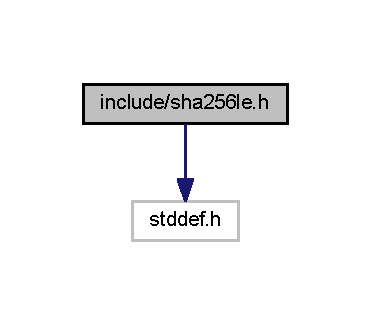
\includegraphics[width=178pt]{sha256le_8h__incl}
\end{center}
\end{figure}
Gráfico de los archivos que directa o indirectamente incluyen a este archivo\+:\nopagebreak
\begin{figure}[H]
\begin{center}
\leavevmode
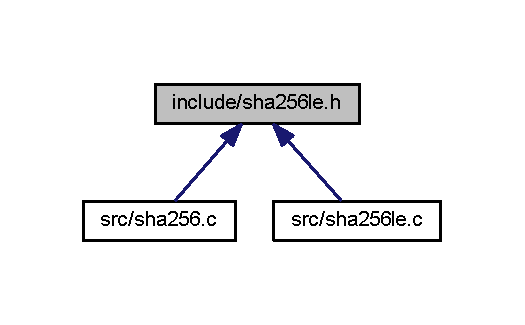
\includegraphics[width=252pt]{sha256le_8h__dep__incl}
\end{center}
\end{figure}
\subsection*{Estructuras de datos}
\begin{DoxyCompactItemize}
\item 
struct \hyperlink{struct_s_h_a256___c_t_x}{S\+H\+A256\+\_\+\+C\+T\+X}
\end{DoxyCompactItemize}
\subsection*{\textquotesingle{}defines\textquotesingle{}}
\begin{DoxyCompactItemize}
\item 
\#define \hyperlink{sha256le_8h_a9c1fe69ad43d4ca74b84303a0ed64f2f}{S\+H\+A256\+\_\+\+B\+L\+O\+C\+K\+\_\+\+S\+I\+Z\+E}~32
\item 
\#define \hyperlink{sha256le_8h_adfbc1051df776564281ac4220ba53a9e}{\+\_\+\+E\+X\+T\+\_\+}~extern
\end{DoxyCompactItemize}
\subsection*{\textquotesingle{}typedefs\textquotesingle{}}
\begin{DoxyCompactItemize}
\item 
typedef unsigned char \hyperlink{sha256le_8h_a4ae1dab0fb4b072a66584546209e7d58}{B\+Y\+T\+E}
\item 
typedef unsigned int \hyperlink{sha256le_8h_ad2baa11c897721ff6f14b452b547f9bc}{W\+O\+R\+D}
\end{DoxyCompactItemize}
\subsection*{Funciones}
\begin{DoxyCompactItemize}
\item 
\hyperlink{sha256le_8h_adfbc1051df776564281ac4220ba53a9e}{\+\_\+\+E\+X\+T\+\_\+} void \hyperlink{sha256le_8h_a3dffdcd908e70dbe657a36ae13d0f3ad}{sha256\+\_\+init} (\hyperlink{struct_s_h_a256___c_t_x}{S\+H\+A256\+\_\+\+C\+T\+X} $\ast$ctx)
\item 
\hyperlink{sha256le_8h_adfbc1051df776564281ac4220ba53a9e}{\+\_\+\+E\+X\+T\+\_\+} void \hyperlink{sha256le_8h_a440fb0f8f349c9188383f42e6aa448be}{sha256\+\_\+update} (\hyperlink{struct_s_h_a256___c_t_x}{S\+H\+A256\+\_\+\+C\+T\+X} $\ast$ctx, const \hyperlink{sha256le_8h_a4ae1dab0fb4b072a66584546209e7d58}{B\+Y\+T\+E} data\mbox{[}$\,$\mbox{]}, size\+\_\+t len)
\item 
\hyperlink{sha256le_8h_adfbc1051df776564281ac4220ba53a9e}{\+\_\+\+E\+X\+T\+\_\+} void \hyperlink{sha256le_8h_ae6305e99ab3651abb7fa1df2d01ff7a8}{sha256\+\_\+final} (\hyperlink{struct_s_h_a256___c_t_x}{S\+H\+A256\+\_\+\+C\+T\+X} $\ast$ctx, \hyperlink{sha256le_8h_a4ae1dab0fb4b072a66584546209e7d58}{B\+Y\+T\+E} hash\mbox{[}$\,$\mbox{]})
\end{DoxyCompactItemize}


\subsection{Documentación de los \textquotesingle{}defines\textquotesingle{}}
\hypertarget{sha256le_8h_adfbc1051df776564281ac4220ba53a9e}{}\index{sha256le.\+h@{sha256le.\+h}!\+\_\+\+E\+X\+T\+\_\+@{\+\_\+\+E\+X\+T\+\_\+}}
\index{\+\_\+\+E\+X\+T\+\_\+@{\+\_\+\+E\+X\+T\+\_\+}!sha256le.\+h@{sha256le.\+h}}
\subsubsection[{\+\_\+\+E\+X\+T\+\_\+}]{\setlength{\rightskip}{0pt plus 5cm}\#define \+\_\+\+E\+X\+T\+\_\+~extern}\label{sha256le_8h_adfbc1051df776564281ac4220ba53a9e}


Definición en la línea 33 del archivo sha256le.\+h.

\hypertarget{sha256le_8h_a9c1fe69ad43d4ca74b84303a0ed64f2f}{}\index{sha256le.\+h@{sha256le.\+h}!S\+H\+A256\+\_\+\+B\+L\+O\+C\+K\+\_\+\+S\+I\+Z\+E@{S\+H\+A256\+\_\+\+B\+L\+O\+C\+K\+\_\+\+S\+I\+Z\+E}}
\index{S\+H\+A256\+\_\+\+B\+L\+O\+C\+K\+\_\+\+S\+I\+Z\+E@{S\+H\+A256\+\_\+\+B\+L\+O\+C\+K\+\_\+\+S\+I\+Z\+E}!sha256le.\+h@{sha256le.\+h}}
\subsubsection[{S\+H\+A256\+\_\+\+B\+L\+O\+C\+K\+\_\+\+S\+I\+Z\+E}]{\setlength{\rightskip}{0pt plus 5cm}\#define S\+H\+A256\+\_\+\+B\+L\+O\+C\+K\+\_\+\+S\+I\+Z\+E~32}\label{sha256le_8h_a9c1fe69ad43d4ca74b84303a0ed64f2f}


Definición en la línea 16 del archivo sha256le.\+h.



\subsection{Documentación de los \textquotesingle{}typedefs\textquotesingle{}}
\hypertarget{sha256le_8h_a4ae1dab0fb4b072a66584546209e7d58}{}\index{sha256le.\+h@{sha256le.\+h}!B\+Y\+T\+E@{B\+Y\+T\+E}}
\index{B\+Y\+T\+E@{B\+Y\+T\+E}!sha256le.\+h@{sha256le.\+h}}
\subsubsection[{B\+Y\+T\+E}]{\setlength{\rightskip}{0pt plus 5cm}typedef unsigned char {\bf B\+Y\+T\+E}}\label{sha256le_8h_a4ae1dab0fb4b072a66584546209e7d58}


Definición en la línea 19 del archivo sha256le.\+h.

\hypertarget{sha256le_8h_ad2baa11c897721ff6f14b452b547f9bc}{}\index{sha256le.\+h@{sha256le.\+h}!W\+O\+R\+D@{W\+O\+R\+D}}
\index{W\+O\+R\+D@{W\+O\+R\+D}!sha256le.\+h@{sha256le.\+h}}
\subsubsection[{W\+O\+R\+D}]{\setlength{\rightskip}{0pt plus 5cm}typedef unsigned int {\bf W\+O\+R\+D}}\label{sha256le_8h_ad2baa11c897721ff6f14b452b547f9bc}


Definición en la línea 20 del archivo sha256le.\+h.



\subsection{Documentación de las funciones}
\hypertarget{sha256le_8h_ae6305e99ab3651abb7fa1df2d01ff7a8}{}\index{sha256le.\+h@{sha256le.\+h}!sha256\+\_\+final@{sha256\+\_\+final}}
\index{sha256\+\_\+final@{sha256\+\_\+final}!sha256le.\+h@{sha256le.\+h}}
\subsubsection[{sha256\+\_\+final(\+S\+H\+A256\+\_\+\+C\+T\+X $\ast$ctx, B\+Y\+T\+E hash[])}]{\setlength{\rightskip}{0pt plus 5cm}{\bf \+\_\+\+E\+X\+T\+\_\+} void sha256\+\_\+final (
\begin{DoxyParamCaption}
\item[{{\bf S\+H\+A256\+\_\+\+C\+T\+X} $\ast$}]{ctx, }
\item[{{\bf B\+Y\+T\+E}}]{hash\mbox{[}$\,$\mbox{]}}
\end{DoxyParamCaption}
)}\label{sha256le_8h_ae6305e99ab3651abb7fa1df2d01ff7a8}


Definición en la línea 116 del archivo sha256le.\+c.

\hypertarget{sha256le_8h_a3dffdcd908e70dbe657a36ae13d0f3ad}{}\index{sha256le.\+h@{sha256le.\+h}!sha256\+\_\+init@{sha256\+\_\+init}}
\index{sha256\+\_\+init@{sha256\+\_\+init}!sha256le.\+h@{sha256le.\+h}}
\subsubsection[{sha256\+\_\+init(\+S\+H\+A256\+\_\+\+C\+T\+X $\ast$ctx)}]{\setlength{\rightskip}{0pt plus 5cm}{\bf \+\_\+\+E\+X\+T\+\_\+} void sha256\+\_\+init (
\begin{DoxyParamCaption}
\item[{{\bf S\+H\+A256\+\_\+\+C\+T\+X} $\ast$}]{ctx}
\end{DoxyParamCaption}
)}\label{sha256le_8h_a3dffdcd908e70dbe657a36ae13d0f3ad}


Definición en la línea 87 del archivo sha256le.\+c.

\hypertarget{sha256le_8h_a440fb0f8f349c9188383f42e6aa448be}{}\index{sha256le.\+h@{sha256le.\+h}!sha256\+\_\+update@{sha256\+\_\+update}}
\index{sha256\+\_\+update@{sha256\+\_\+update}!sha256le.\+h@{sha256le.\+h}}
\subsubsection[{sha256\+\_\+update(\+S\+H\+A256\+\_\+\+C\+T\+X $\ast$ctx, const B\+Y\+T\+E data[], size\+\_\+t len)}]{\setlength{\rightskip}{0pt plus 5cm}{\bf \+\_\+\+E\+X\+T\+\_\+} void sha256\+\_\+update (
\begin{DoxyParamCaption}
\item[{{\bf S\+H\+A256\+\_\+\+C\+T\+X} $\ast$}]{ctx, }
\item[{const {\bf B\+Y\+T\+E}}]{data\mbox{[}$\,$\mbox{]}, }
\item[{size\+\_\+t}]{len}
\end{DoxyParamCaption}
)}\label{sha256le_8h_a440fb0f8f349c9188383f42e6aa448be}


Definición en la línea 101 del archivo sha256le.\+c.


\hypertarget{timer_8h}{}\section{Referencia del Archivo include/timer.h}
\label{timer_8h}\index{include/timer.\+h@{include/timer.\+h}}


Fichero de cabecera para incluir los modulos de calculo de timers.  


Gráfico de los archivos que directa o indirectamente incluyen a este archivo\+:\nopagebreak
\begin{figure}[H]
\begin{center}
\leavevmode
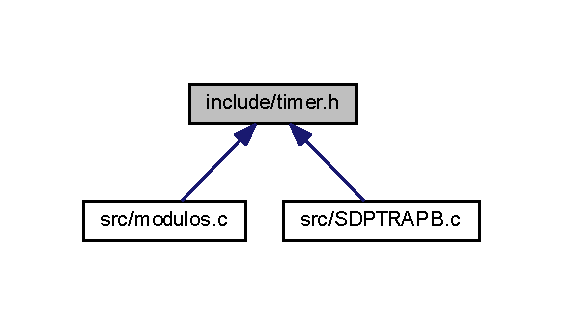
\includegraphics[width=270pt]{timer_8h__dep__incl}
\end{center}
\end{figure}


\subsection{Descripción detallada}
Fichero de cabecera para incluir los modulos de calculo de timers. 

Incluira el modulo correspondiente en funcion del Sistema Operativo

\begin{DoxyAuthor}{Autor}
\+: Javier Gonzalez 
\end{DoxyAuthor}
\begin{DoxyDate}{Fecha}
\+: 01/03/15 
\end{DoxyDate}
\begin{DoxyVersion}{Versión}
\+: 2.\+0 
\end{DoxyVersion}

\hypertarget{timerlnx_8h}{}\section{Referencia del Archivo include/timerlnx.h}
\label{timerlnx_8h}\index{include/timerlnx.\+h@{include/timerlnx.\+h}}


Funciones publicas del archivo timer\+Lnx Se incluye en la plataforma Linux.  




\subsection{Descripción detallada}
Funciones publicas del archivo timer\+Lnx Se incluye en la plataforma Linux. 

\begin{DoxyAuthor}{Autor}
\+: Javier Gonzalez 
\end{DoxyAuthor}
\begin{DoxyDate}{Fecha}
\+: 01/03/15 
\end{DoxyDate}
\begin{DoxyVersion}{Versión}
\+: 1.\+0 
\end{DoxyVersion}

\hypertarget{timerwin_8h}{}\section{Referencia del Archivo include/timerwin.h}
\label{timerwin_8h}\index{include/timerwin.\+h@{include/timerwin.\+h}}


Funciones publicas del archivo timer\+Win Se incluye en la plataforma windows.  




\subsection{Descripción detallada}
Funciones publicas del archivo timer\+Win Se incluye en la plataforma windows. 

\begin{DoxyAuthor}{Autor}
\+: Javier Gonzalez 
\end{DoxyAuthor}
\begin{DoxyDate}{Fecha}
\+: 01/03/15 
\end{DoxyDate}
\begin{DoxyVersion}{Versión}
\+: 1.\+0 
\end{DoxyVersion}

\hypertarget{token_8h}{}\section{Referencia del Archivo include/token.h}
\label{token_8h}\index{include/token.\+h@{include/token.\+h}}
\subsection*{Estructuras de datos}
\begin{DoxyCompactItemize}
\item 
struct \hyperlink{struct_s_t___t_i_m_e_r}{S\+T\+\_\+\+T\+I\+M\+E\+R}
\item 
struct \hyperlink{struct_s_t___t_o_k_e_n}{S\+T\+\_\+\+T\+O\+K\+E\+N}
\end{DoxyCompactItemize}
\subsection*{\textquotesingle{}typedefs\textquotesingle{}}
\begin{DoxyCompactItemize}
\item 
typedef unsigned long long \hyperlink{token_8h_acb3d64ed2bb2e72ebb17ca4ef85ae6d3}{mlong}
\item 
typedef struct \hyperlink{struct_s_t___t_i_m_e_r}{S\+T\+\_\+\+T\+I\+M\+E\+R} \hyperlink{token_8h_a0cf0a7e0338664aedaf7b1123103b0dc}{T\+I\+M\+E\+R}
\item 
typedef struct \hyperlink{struct_s_t___t_o_k_e_n}{S\+T\+\_\+\+T\+O\+K\+E\+N} \hyperlink{token_8h_a211705bae14c26274d988b6df0f6f297}{T\+O\+K\+E\+N}
\end{DoxyCompactItemize}


\subsection{Documentación de los \textquotesingle{}typedefs\textquotesingle{}}
\hypertarget{token_8h_acb3d64ed2bb2e72ebb17ca4ef85ae6d3}{}\index{token.\+h@{token.\+h}!mlong@{mlong}}
\index{mlong@{mlong}!token.\+h@{token.\+h}}
\subsubsection[{mlong}]{\setlength{\rightskip}{0pt plus 5cm}typedef unsigned long long {\bf mlong}}\label{token_8h_acb3d64ed2bb2e72ebb17ca4ef85ae6d3}


Definición en la línea 15 del archivo token.\+h.

\hypertarget{token_8h_a0cf0a7e0338664aedaf7b1123103b0dc}{}\index{token.\+h@{token.\+h}!T\+I\+M\+E\+R@{T\+I\+M\+E\+R}}
\index{T\+I\+M\+E\+R@{T\+I\+M\+E\+R}!token.\+h@{token.\+h}}
\subsubsection[{T\+I\+M\+E\+R}]{\setlength{\rightskip}{0pt plus 5cm}typedef struct {\bf S\+T\+\_\+\+T\+I\+M\+E\+R} {\bf T\+I\+M\+E\+R}}\label{token_8h_a0cf0a7e0338664aedaf7b1123103b0dc}


Definición en la línea 24 del archivo token.\+h.

\hypertarget{token_8h_a211705bae14c26274d988b6df0f6f297}{}\index{token.\+h@{token.\+h}!T\+O\+K\+E\+N@{T\+O\+K\+E\+N}}
\index{T\+O\+K\+E\+N@{T\+O\+K\+E\+N}!token.\+h@{token.\+h}}
\subsubsection[{T\+O\+K\+E\+N}]{\setlength{\rightskip}{0pt plus 5cm}typedef struct {\bf S\+T\+\_\+\+T\+O\+K\+E\+N} {\bf T\+O\+K\+E\+N}}\label{token_8h_a211705bae14c26274d988b6df0f6f297}


Definición en la línea 32 del archivo token.\+h.


\hypertarget{trapcodes_8h}{}\section{Referencia del Archivo include/trapcodes.h}
\label{trapcodes_8h}\index{include/trapcodes.\+h@{include/trapcodes.\+h}}
Gráfico de los archivos que directa o indirectamente incluyen a este archivo\+:\nopagebreak
\begin{figure}[H]
\begin{center}
\leavevmode
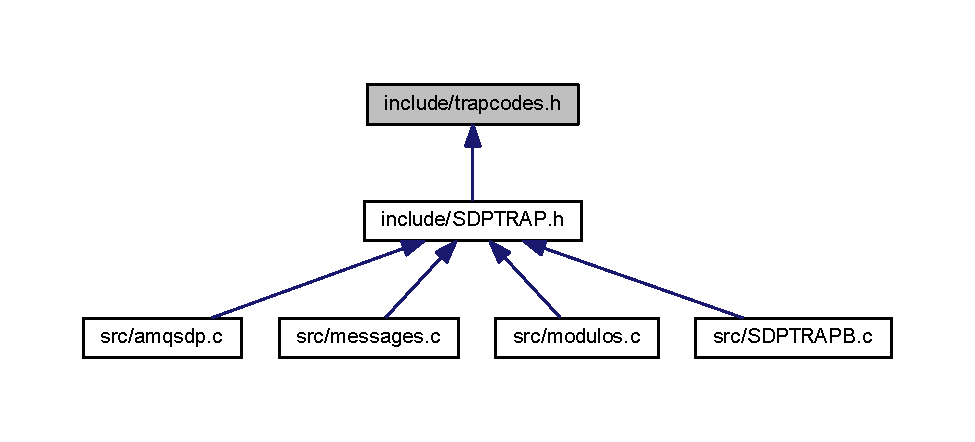
\includegraphics[width=350pt]{trapcodes_8h__dep__incl}
\end{center}
\end{figure}
\subsection*{\textquotesingle{}defines\textquotesingle{}}
\begin{DoxyCompactItemize}
\item 
\#define \hyperlink{trapcodes_8h_abf8c519289600eaaea8c07a268de7194}{E\+N\+D\+\_\+\+M\+A\+R\+K}~0x01
\item 
\#define \hyperlink{trapcodes_8h_a237bc2180908e4111f8484da89aa2e8d}{H\+T\+R\+A\+P}~0x100
\item 
\#define \hyperlink{trapcodes_8h_af918ab5b43b7193ccf30754fe57a5d55}{H\+C\+O\+D\+E}~0x200
\item 
\#define \hyperlink{trapcodes_8h_a3097eb1fed719fa18f823e401ffda463}{H\+A\+C\+C\+E\+S\+S}~0x400
\item 
\#define \hyperlink{trapcodes_8h_a964465eab727e43b3d21087eecbe7574}{H\+U\+N\+D\+E\+F2}~0x800
\item 
\#define \hyperlink{trapcodes_8h_a62067ec57aa60f39804f432fc180c26d}{H\+U\+N\+D\+E\+F3}~0x1000
\item 
\#define \hyperlink{trapcodes_8h_a2d0a30b85c2d9040df5c0e44af129770}{H\+U\+N\+D\+E\+F4}~0x2000
\item 
\#define \hyperlink{trapcodes_8h_a75a60e8a5ab65dc2e86256c6129febc4}{H\+U\+N\+D\+E\+F5}~0x4000
\item 
\#define \hyperlink{trapcodes_8h_a03fff3cb1e3230ec75109cbbb9d51945}{H\+U\+N\+D\+E\+F}~0x8000
\item 
\#define \hyperlink{trapcodes_8h_aff974876b14049785960788e714d2a46}{T\+R\+A\+P}~0x01
\item 
\#define \hyperlink{trapcodes_8h_ae6527c8381eb3f23b7fd6d6efec6ffc7}{C\+O\+D\+E}~0x02
\item 
\#define \hyperlink{trapcodes_8h_a321a20f839f3d9ccd0db1dc865850dc7}{A\+C\+C\+E\+S\+S}~0x04
\item 
\#define \hyperlink{trapcodes_8h_aaaa9a61b79e5c0e31c3ab9a3396c1bb7}{U\+N\+D\+E\+F2}~0x08
\item 
\#define \hyperlink{trapcodes_8h_a1958c8a77ed4ea567f7e683b1642f843}{U\+N\+D\+E\+F3}~0x10
\item 
\#define \hyperlink{trapcodes_8h_a0c0ed874daad777853a5b7e576d93711}{U\+N\+D\+E\+F4}~0x20
\item 
\#define \hyperlink{trapcodes_8h_a91b063a4bb2d6e3edf297a91351bd0ec}{U\+N\+D\+E\+F5}~0x40
\item 
\#define \hyperlink{trapcodes_8h_abde25a67f4046530ae1c572cefeb5869}{U\+N\+D\+E\+F}~0x80
\item 
\#define \hyperlink{trapcodes_8h_a2c63ae95fe7c6106ae1ec9c283afa486}{M\+O\+D\+U\+L\+E}~0x02
\item 
\#define \hyperlink{trapcodes_8h_a4fa9231686d12bdfb2ecad40f744fe0a}{P\+A\+R\+A\+G\+R\+A\+P\+H}~0x04
\item 
\#define \hyperlink{trapcodes_8h_aa980b5e5e502cf62bdca6c0452b97516}{C\+A\+L\+L}~0x08
\item 
\#define \hyperlink{trapcodes_8h_a7aad18faa9ed07aac5fdb9c76dc041da}{S\+Q\+L}~0x10
\item 
\#define \hyperlink{trapcodes_8h_a266889edcc839d71e3200bfec5281021}{C\+I\+C\+S}~0x20
\item 
\#define \hyperlink{trapcodes_8h_a686dea444026cbf1236c24e7edb3a96d}{C\+U\+S\+T\+O\+M}~0x40
\item 
\#define \hyperlink{trapcodes_8h_a1aa8fb6580169b450d7a303031ce5be5}{C\+O\+V\+E\+R}~0x100
\item 
\#define \hyperlink{trapcodes_8h_acd926066f05b2f51e61f1ef6d8a7724e}{P\+E\+R\+S}~0x200
\item 
\#define \hyperlink{trapcodes_8h_a7603f0308bf3641b5db73c0163d58473}{B\+L\+O\+Q\+U\+E}~0x02
\item 
\#define \hyperlink{trapcodes_8h_a6bd579d720ce1064e4b62ee152ef107c}{W\+O\+R\+K\+I\+N\+G\+S}~0x04
\item 
\#define \hyperlink{trapcodes_8h_a1354b70ac6803a06beebe84f61b5f95b}{O\+P\+E\+N}~0x01
\item 
\#define \hyperlink{trapcodes_8h_a0e29f488071372aa0530842e60b64511}{C\+L\+O\+S\+E}~0x02
\item 
\#define \hyperlink{trapcodes_8h_a9cec4693931a816d4ad374c3a00e0dae}{I\+N\+S\+E\+R\+T}~0x04
\item 
\#define \hyperlink{trapcodes_8h_ada74e7db007a68e763f20c17f2985356}{R\+E\+A\+D}~0x08
\item 
\#define \hyperlink{trapcodes_8h_ac2558c32fa879d85fe59f8c5f8dfbc04}{U\+P\+D\+A\+T\+E}~0x10
\item 
\#define \hyperlink{trapcodes_8h_abbbe5949f3c1f72e439924f8cf503509}{D\+E\+L\+E\+T\+E}~0x20
\item 
\#define \hyperlink{trapcodes_8h_a53dc4af00adc7b3b4d12eafb71596dfc}{S\+E\+L\+E\+C\+T}~0x40
\item 
\#define \hyperlink{trapcodes_8h_aeeaa356bf502aeb9533e65bc2e15e754}{T\+O\+T\+A\+L}~0x80
\item 
\#define \hyperlink{trapcodes_8h_a52220397ecea855b3a99746e451426e1}{B\+L\+O\+C\+K}~\hyperlink{trapcodes_8h_af918ab5b43b7193ccf30754fe57a5d55}{H\+C\+O\+D\+E} + \hyperlink{trapcodes_8h_a7603f0308bf3641b5db73c0163d58473}{B\+L\+O\+Q\+U\+E}
\item 
\#define \hyperlink{trapcodes_8h_a582443b5837da456dff914c441bc092b}{W\+O\+R\+K\+I\+N\+G}~\hyperlink{trapcodes_8h_af918ab5b43b7193ccf30754fe57a5d55}{H\+C\+O\+D\+E} + \hyperlink{trapcodes_8h_a6bd579d720ce1064e4b62ee152ef107c}{W\+O\+R\+K\+I\+N\+G\+S}
\item 
\#define \hyperlink{trapcodes_8h_aa2ed94e589b744dc61af0c5347a677a4}{B\+E\+G\+\_\+\+M\+O\+D\+U\+L\+E}~\hyperlink{trapcodes_8h_a237bc2180908e4111f8484da89aa2e8d}{H\+T\+R\+A\+P} + \hyperlink{trapcodes_8h_a2c63ae95fe7c6106ae1ec9c283afa486}{M\+O\+D\+U\+L\+E}
\item 
\#define \hyperlink{trapcodes_8h_a502fe347b3225e24b233d7f80f386982}{B\+E\+G\+\_\+\+P\+A\+R\+A\+G\+R\+A\+P\+H}~\hyperlink{trapcodes_8h_a237bc2180908e4111f8484da89aa2e8d}{H\+T\+R\+A\+P} + \hyperlink{trapcodes_8h_a4fa9231686d12bdfb2ecad40f744fe0a}{P\+A\+R\+A\+G\+R\+A\+P\+H}
\item 
\#define \hyperlink{trapcodes_8h_aa12797a4365f4dabd2b053507533f4e7}{B\+E\+G\+\_\+\+C\+A\+L\+L}~\hyperlink{trapcodes_8h_a237bc2180908e4111f8484da89aa2e8d}{H\+T\+R\+A\+P} + \hyperlink{trapcodes_8h_aa980b5e5e502cf62bdca6c0452b97516}{C\+A\+L\+L}
\item 
\#define \hyperlink{trapcodes_8h_a2a3a9d838f8f408d34f65d6697a3d8ef}{B\+E\+G\+\_\+\+S\+Q\+L}~\hyperlink{trapcodes_8h_a237bc2180908e4111f8484da89aa2e8d}{H\+T\+R\+A\+P} + \hyperlink{trapcodes_8h_a7aad18faa9ed07aac5fdb9c76dc041da}{S\+Q\+L}
\item 
\#define \hyperlink{trapcodes_8h_af319d039f970bcf319a76f611eb0b587}{B\+E\+G\+\_\+\+C\+I\+C\+S}~\hyperlink{trapcodes_8h_a237bc2180908e4111f8484da89aa2e8d}{H\+T\+R\+A\+P} + \hyperlink{trapcodes_8h_a266889edcc839d71e3200bfec5281021}{C\+I\+C\+S}
\item 
\#define \hyperlink{trapcodes_8h_af11cc4b12e5db751f353c365b0161d88}{B\+E\+G\+\_\+\+I\+N\+S\+T}~\hyperlink{trapcodes_8h_a237bc2180908e4111f8484da89aa2e8d}{H\+T\+R\+A\+P} + I\+N\+S\+T
\item 
\#define \hyperlink{trapcodes_8h_aaae1698405580764e947f1d04d2e9426}{B\+E\+G\+\_\+\+C\+U\+S\+T\+O\+M}~\hyperlink{trapcodes_8h_a237bc2180908e4111f8484da89aa2e8d}{H\+T\+R\+A\+P} + \hyperlink{trapcodes_8h_a686dea444026cbf1236c24e7edb3a96d}{C\+U\+S\+T\+O\+M}
\item 
\#define \hyperlink{trapcodes_8h_afb184105b5223c6f1631cd7b9e235941}{E\+N\+D\+\_\+\+M\+O\+D\+U\+L\+E}~\hyperlink{trapcodes_8h_aa2ed94e589b744dc61af0c5347a677a4}{B\+E\+G\+\_\+\+M\+O\+D\+U\+L\+E}    + \hyperlink{trapcodes_8h_abf8c519289600eaaea8c07a268de7194}{E\+N\+D\+\_\+\+M\+A\+R\+K}
\item 
\#define \hyperlink{trapcodes_8h_a61a9bf2a39bd96ca80465936757f3a64}{E\+N\+D\+\_\+\+P\+A\+R\+A\+G\+R\+A\+P\+H}~\hyperlink{trapcodes_8h_a502fe347b3225e24b233d7f80f386982}{B\+E\+G\+\_\+\+P\+A\+R\+A\+G\+R\+A\+P\+H} + \hyperlink{trapcodes_8h_abf8c519289600eaaea8c07a268de7194}{E\+N\+D\+\_\+\+M\+A\+R\+K}
\item 
\#define \hyperlink{trapcodes_8h_a04f39035cb8fcab9798c273523e6e20f}{E\+N\+D\+\_\+\+C\+A\+L\+L}~\hyperlink{trapcodes_8h_aa12797a4365f4dabd2b053507533f4e7}{B\+E\+G\+\_\+\+C\+A\+L\+L}      + \hyperlink{trapcodes_8h_abf8c519289600eaaea8c07a268de7194}{E\+N\+D\+\_\+\+M\+A\+R\+K}
\item 
\#define \hyperlink{trapcodes_8h_af31242d26a530b55735989a9825418df}{E\+N\+D\+\_\+\+S\+Q\+L}~\hyperlink{trapcodes_8h_a2a3a9d838f8f408d34f65d6697a3d8ef}{B\+E\+G\+\_\+\+S\+Q\+L}       + \hyperlink{trapcodes_8h_abf8c519289600eaaea8c07a268de7194}{E\+N\+D\+\_\+\+M\+A\+R\+K}
\item 
\#define \hyperlink{trapcodes_8h_afc443727f3b34add263ef2597e66ae7f}{E\+N\+D\+\_\+\+C\+I\+C\+S}~\hyperlink{trapcodes_8h_af319d039f970bcf319a76f611eb0b587}{B\+E\+G\+\_\+\+C\+I\+C\+S}      + \hyperlink{trapcodes_8h_abf8c519289600eaaea8c07a268de7194}{E\+N\+D\+\_\+\+M\+A\+R\+K}
\item 
\#define \hyperlink{trapcodes_8h_a7d95a721ac4478793287a2b7d96dfe09}{E\+N\+D\+\_\+\+I\+N\+S\+T}~\hyperlink{trapcodes_8h_af11cc4b12e5db751f353c365b0161d88}{B\+E\+G\+\_\+\+I\+N\+S\+T}      + \hyperlink{trapcodes_8h_abf8c519289600eaaea8c07a268de7194}{E\+N\+D\+\_\+\+M\+A\+R\+K}
\item 
\#define \hyperlink{trapcodes_8h_ad103ae3a3ba1086ddd8c301315938421}{E\+N\+D\+\_\+\+C\+U\+S\+T\+O\+M}~\hyperlink{trapcodes_8h_aaae1698405580764e947f1d04d2e9426}{B\+E\+G\+\_\+\+C\+U\+S\+T\+O\+M}    + \hyperlink{trapcodes_8h_abf8c519289600eaaea8c07a268de7194}{E\+N\+D\+\_\+\+M\+A\+R\+K}
\item 
\#define \hyperlink{trapcodes_8h_a9561402155f37fbf51721f272d13f46e}{A\+C\+C\+\_\+\+O\+P\+E\+N}~\hyperlink{trapcodes_8h_a3097eb1fed719fa18f823e401ffda463}{H\+A\+C\+C\+E\+S\+S} + \hyperlink{trapcodes_8h_a1354b70ac6803a06beebe84f61b5f95b}{O\+P\+E\+N}
\item 
\#define \hyperlink{trapcodes_8h_a0b3fc7d973279fe65cecbf7e8c73aece}{A\+C\+C\+\_\+\+C\+L\+O\+S\+E}~\hyperlink{trapcodes_8h_a3097eb1fed719fa18f823e401ffda463}{H\+A\+C\+C\+E\+S\+S} + \hyperlink{trapcodes_8h_a0e29f488071372aa0530842e60b64511}{C\+L\+O\+S\+E}
\item 
\#define \hyperlink{trapcodes_8h_ad9370107065fce1f10a086bcebd386c9}{A\+C\+C\+\_\+\+I\+N\+S\+E\+R\+T}~\hyperlink{trapcodes_8h_a3097eb1fed719fa18f823e401ffda463}{H\+A\+C\+C\+E\+S\+S} + \hyperlink{trapcodes_8h_a9cec4693931a816d4ad374c3a00e0dae}{I\+N\+S\+E\+R\+T}
\item 
\#define \hyperlink{trapcodes_8h_abc19ef2d3b23537b17e542598a0a6756}{A\+C\+C\+\_\+\+R\+E\+A\+D}~\hyperlink{trapcodes_8h_a3097eb1fed719fa18f823e401ffda463}{H\+A\+C\+C\+E\+S\+S} + \hyperlink{trapcodes_8h_ada74e7db007a68e763f20c17f2985356}{R\+E\+A\+D}
\item 
\#define \hyperlink{trapcodes_8h_a9d776b61bc437ec075614f00c139fed2}{A\+C\+C\+\_\+\+U\+P\+D\+A\+T\+E}~\hyperlink{trapcodes_8h_a3097eb1fed719fa18f823e401ffda463}{H\+A\+C\+C\+E\+S\+S} + \hyperlink{trapcodes_8h_ac2558c32fa879d85fe59f8c5f8dfbc04}{U\+P\+D\+A\+T\+E}
\item 
\#define \hyperlink{trapcodes_8h_a4159431c40d8199996e0fe6084d80656}{A\+C\+C\+\_\+\+D\+E\+L\+E\+T\+E}~\hyperlink{trapcodes_8h_a3097eb1fed719fa18f823e401ffda463}{H\+A\+C\+C\+E\+S\+S} + \hyperlink{trapcodes_8h_abbbe5949f3c1f72e439924f8cf503509}{D\+E\+L\+E\+T\+E}
\item 
\#define \hyperlink{trapcodes_8h_a9c0a5841ffb9a67e977332f87e7e560b}{A\+C\+C\+\_\+\+S\+E\+L\+E\+C\+T}~\hyperlink{trapcodes_8h_a3097eb1fed719fa18f823e401ffda463}{H\+A\+C\+C\+E\+S\+S} + \hyperlink{trapcodes_8h_a53dc4af00adc7b3b4d12eafb71596dfc}{S\+E\+L\+E\+C\+T}
\item 
\#define \hyperlink{trapcodes_8h_ae1fd414bbdd68bf3f5d23a68ad368700}{M\+S\+G\+\_\+\+B\+E\+G}~0x00
\item 
\#define \hyperlink{trapcodes_8h_a3292b59f6757fa83862ca01626b39728}{M\+S\+G\+\_\+\+E\+N\+D}~0x01
\item 
\#define \hyperlink{trapcodes_8h_ad1c2a68073a929ff8c57b9d0f5c2b096}{M\+S\+G\+\_\+\+C\+O\+V\+E\+R}~0x100
\item 
\#define \hyperlink{trapcodes_8h_a76314cba0d2db75cb750a7b4bee5e4f2}{M\+S\+G\+\_\+\+P\+E\+R\+S}~0x200
\item 
\#define \hyperlink{trapcodes_8h_a2fc64d1d5e66422495b347c48b85a9dd}{M\+S\+G\+\_\+\+P\+A\+R\+R\+S}~0x400
\end{DoxyCompactItemize}


\subsection{Documentación de los \textquotesingle{}defines\textquotesingle{}}
\hypertarget{trapcodes_8h_a0b3fc7d973279fe65cecbf7e8c73aece}{}\index{trapcodes.\+h@{trapcodes.\+h}!A\+C\+C\+\_\+\+C\+L\+O\+S\+E@{A\+C\+C\+\_\+\+C\+L\+O\+S\+E}}
\index{A\+C\+C\+\_\+\+C\+L\+O\+S\+E@{A\+C\+C\+\_\+\+C\+L\+O\+S\+E}!trapcodes.\+h@{trapcodes.\+h}}
\subsubsection[{A\+C\+C\+\_\+\+C\+L\+O\+S\+E}]{\setlength{\rightskip}{0pt plus 5cm}\#define A\+C\+C\+\_\+\+C\+L\+O\+S\+E~{\bf H\+A\+C\+C\+E\+S\+S} + {\bf C\+L\+O\+S\+E}}\label{trapcodes_8h_a0b3fc7d973279fe65cecbf7e8c73aece}


Definición en la línea 85 del archivo trapcodes.\+h.

\hypertarget{trapcodes_8h_a4159431c40d8199996e0fe6084d80656}{}\index{trapcodes.\+h@{trapcodes.\+h}!A\+C\+C\+\_\+\+D\+E\+L\+E\+T\+E@{A\+C\+C\+\_\+\+D\+E\+L\+E\+T\+E}}
\index{A\+C\+C\+\_\+\+D\+E\+L\+E\+T\+E@{A\+C\+C\+\_\+\+D\+E\+L\+E\+T\+E}!trapcodes.\+h@{trapcodes.\+h}}
\subsubsection[{A\+C\+C\+\_\+\+D\+E\+L\+E\+T\+E}]{\setlength{\rightskip}{0pt plus 5cm}\#define A\+C\+C\+\_\+\+D\+E\+L\+E\+T\+E~{\bf H\+A\+C\+C\+E\+S\+S} + {\bf D\+E\+L\+E\+T\+E}}\label{trapcodes_8h_a4159431c40d8199996e0fe6084d80656}


Definición en la línea 89 del archivo trapcodes.\+h.

\hypertarget{trapcodes_8h_ad9370107065fce1f10a086bcebd386c9}{}\index{trapcodes.\+h@{trapcodes.\+h}!A\+C\+C\+\_\+\+I\+N\+S\+E\+R\+T@{A\+C\+C\+\_\+\+I\+N\+S\+E\+R\+T}}
\index{A\+C\+C\+\_\+\+I\+N\+S\+E\+R\+T@{A\+C\+C\+\_\+\+I\+N\+S\+E\+R\+T}!trapcodes.\+h@{trapcodes.\+h}}
\subsubsection[{A\+C\+C\+\_\+\+I\+N\+S\+E\+R\+T}]{\setlength{\rightskip}{0pt plus 5cm}\#define A\+C\+C\+\_\+\+I\+N\+S\+E\+R\+T~{\bf H\+A\+C\+C\+E\+S\+S} + {\bf I\+N\+S\+E\+R\+T}}\label{trapcodes_8h_ad9370107065fce1f10a086bcebd386c9}


Definición en la línea 86 del archivo trapcodes.\+h.

\hypertarget{trapcodes_8h_a9561402155f37fbf51721f272d13f46e}{}\index{trapcodes.\+h@{trapcodes.\+h}!A\+C\+C\+\_\+\+O\+P\+E\+N@{A\+C\+C\+\_\+\+O\+P\+E\+N}}
\index{A\+C\+C\+\_\+\+O\+P\+E\+N@{A\+C\+C\+\_\+\+O\+P\+E\+N}!trapcodes.\+h@{trapcodes.\+h}}
\subsubsection[{A\+C\+C\+\_\+\+O\+P\+E\+N}]{\setlength{\rightskip}{0pt plus 5cm}\#define A\+C\+C\+\_\+\+O\+P\+E\+N~{\bf H\+A\+C\+C\+E\+S\+S} + {\bf O\+P\+E\+N}}\label{trapcodes_8h_a9561402155f37fbf51721f272d13f46e}


Definición en la línea 84 del archivo trapcodes.\+h.

\hypertarget{trapcodes_8h_abc19ef2d3b23537b17e542598a0a6756}{}\index{trapcodes.\+h@{trapcodes.\+h}!A\+C\+C\+\_\+\+R\+E\+A\+D@{A\+C\+C\+\_\+\+R\+E\+A\+D}}
\index{A\+C\+C\+\_\+\+R\+E\+A\+D@{A\+C\+C\+\_\+\+R\+E\+A\+D}!trapcodes.\+h@{trapcodes.\+h}}
\subsubsection[{A\+C\+C\+\_\+\+R\+E\+A\+D}]{\setlength{\rightskip}{0pt plus 5cm}\#define A\+C\+C\+\_\+\+R\+E\+A\+D~{\bf H\+A\+C\+C\+E\+S\+S} + {\bf R\+E\+A\+D}}\label{trapcodes_8h_abc19ef2d3b23537b17e542598a0a6756}


Definición en la línea 87 del archivo trapcodes.\+h.

\hypertarget{trapcodes_8h_a9c0a5841ffb9a67e977332f87e7e560b}{}\index{trapcodes.\+h@{trapcodes.\+h}!A\+C\+C\+\_\+\+S\+E\+L\+E\+C\+T@{A\+C\+C\+\_\+\+S\+E\+L\+E\+C\+T}}
\index{A\+C\+C\+\_\+\+S\+E\+L\+E\+C\+T@{A\+C\+C\+\_\+\+S\+E\+L\+E\+C\+T}!trapcodes.\+h@{trapcodes.\+h}}
\subsubsection[{A\+C\+C\+\_\+\+S\+E\+L\+E\+C\+T}]{\setlength{\rightskip}{0pt plus 5cm}\#define A\+C\+C\+\_\+\+S\+E\+L\+E\+C\+T~{\bf H\+A\+C\+C\+E\+S\+S} + {\bf S\+E\+L\+E\+C\+T}}\label{trapcodes_8h_a9c0a5841ffb9a67e977332f87e7e560b}


Definición en la línea 90 del archivo trapcodes.\+h.

\hypertarget{trapcodes_8h_a9d776b61bc437ec075614f00c139fed2}{}\index{trapcodes.\+h@{trapcodes.\+h}!A\+C\+C\+\_\+\+U\+P\+D\+A\+T\+E@{A\+C\+C\+\_\+\+U\+P\+D\+A\+T\+E}}
\index{A\+C\+C\+\_\+\+U\+P\+D\+A\+T\+E@{A\+C\+C\+\_\+\+U\+P\+D\+A\+T\+E}!trapcodes.\+h@{trapcodes.\+h}}
\subsubsection[{A\+C\+C\+\_\+\+U\+P\+D\+A\+T\+E}]{\setlength{\rightskip}{0pt plus 5cm}\#define A\+C\+C\+\_\+\+U\+P\+D\+A\+T\+E~{\bf H\+A\+C\+C\+E\+S\+S} + {\bf U\+P\+D\+A\+T\+E}}\label{trapcodes_8h_a9d776b61bc437ec075614f00c139fed2}


Definición en la línea 88 del archivo trapcodes.\+h.

\hypertarget{trapcodes_8h_a321a20f839f3d9ccd0db1dc865850dc7}{}\index{trapcodes.\+h@{trapcodes.\+h}!A\+C\+C\+E\+S\+S@{A\+C\+C\+E\+S\+S}}
\index{A\+C\+C\+E\+S\+S@{A\+C\+C\+E\+S\+S}!trapcodes.\+h@{trapcodes.\+h}}
\subsubsection[{A\+C\+C\+E\+S\+S}]{\setlength{\rightskip}{0pt plus 5cm}\#define A\+C\+C\+E\+S\+S~0x04}\label{trapcodes_8h_a321a20f839f3d9ccd0db1dc865850dc7}


Definición en la línea 19 del archivo trapcodes.\+h.

\hypertarget{trapcodes_8h_aa12797a4365f4dabd2b053507533f4e7}{}\index{trapcodes.\+h@{trapcodes.\+h}!B\+E\+G\+\_\+\+C\+A\+L\+L@{B\+E\+G\+\_\+\+C\+A\+L\+L}}
\index{B\+E\+G\+\_\+\+C\+A\+L\+L@{B\+E\+G\+\_\+\+C\+A\+L\+L}!trapcodes.\+h@{trapcodes.\+h}}
\subsubsection[{B\+E\+G\+\_\+\+C\+A\+L\+L}]{\setlength{\rightskip}{0pt plus 5cm}\#define B\+E\+G\+\_\+\+C\+A\+L\+L~{\bf H\+T\+R\+A\+P} + {\bf C\+A\+L\+L}}\label{trapcodes_8h_aa12797a4365f4dabd2b053507533f4e7}


Definición en la línea 66 del archivo trapcodes.\+h.

\hypertarget{trapcodes_8h_af319d039f970bcf319a76f611eb0b587}{}\index{trapcodes.\+h@{trapcodes.\+h}!B\+E\+G\+\_\+\+C\+I\+C\+S@{B\+E\+G\+\_\+\+C\+I\+C\+S}}
\index{B\+E\+G\+\_\+\+C\+I\+C\+S@{B\+E\+G\+\_\+\+C\+I\+C\+S}!trapcodes.\+h@{trapcodes.\+h}}
\subsubsection[{B\+E\+G\+\_\+\+C\+I\+C\+S}]{\setlength{\rightskip}{0pt plus 5cm}\#define B\+E\+G\+\_\+\+C\+I\+C\+S~{\bf H\+T\+R\+A\+P} + {\bf C\+I\+C\+S}}\label{trapcodes_8h_af319d039f970bcf319a76f611eb0b587}


Definición en la línea 68 del archivo trapcodes.\+h.

\hypertarget{trapcodes_8h_aaae1698405580764e947f1d04d2e9426}{}\index{trapcodes.\+h@{trapcodes.\+h}!B\+E\+G\+\_\+\+C\+U\+S\+T\+O\+M@{B\+E\+G\+\_\+\+C\+U\+S\+T\+O\+M}}
\index{B\+E\+G\+\_\+\+C\+U\+S\+T\+O\+M@{B\+E\+G\+\_\+\+C\+U\+S\+T\+O\+M}!trapcodes.\+h@{trapcodes.\+h}}
\subsubsection[{B\+E\+G\+\_\+\+C\+U\+S\+T\+O\+M}]{\setlength{\rightskip}{0pt plus 5cm}\#define B\+E\+G\+\_\+\+C\+U\+S\+T\+O\+M~{\bf H\+T\+R\+A\+P} + {\bf C\+U\+S\+T\+O\+M}}\label{trapcodes_8h_aaae1698405580764e947f1d04d2e9426}


Definición en la línea 70 del archivo trapcodes.\+h.

\hypertarget{trapcodes_8h_af11cc4b12e5db751f353c365b0161d88}{}\index{trapcodes.\+h@{trapcodes.\+h}!B\+E\+G\+\_\+\+I\+N\+S\+T@{B\+E\+G\+\_\+\+I\+N\+S\+T}}
\index{B\+E\+G\+\_\+\+I\+N\+S\+T@{B\+E\+G\+\_\+\+I\+N\+S\+T}!trapcodes.\+h@{trapcodes.\+h}}
\subsubsection[{B\+E\+G\+\_\+\+I\+N\+S\+T}]{\setlength{\rightskip}{0pt plus 5cm}\#define B\+E\+G\+\_\+\+I\+N\+S\+T~{\bf H\+T\+R\+A\+P} + I\+N\+S\+T}\label{trapcodes_8h_af11cc4b12e5db751f353c365b0161d88}


Definición en la línea 69 del archivo trapcodes.\+h.

\hypertarget{trapcodes_8h_aa2ed94e589b744dc61af0c5347a677a4}{}\index{trapcodes.\+h@{trapcodes.\+h}!B\+E\+G\+\_\+\+M\+O\+D\+U\+L\+E@{B\+E\+G\+\_\+\+M\+O\+D\+U\+L\+E}}
\index{B\+E\+G\+\_\+\+M\+O\+D\+U\+L\+E@{B\+E\+G\+\_\+\+M\+O\+D\+U\+L\+E}!trapcodes.\+h@{trapcodes.\+h}}
\subsubsection[{B\+E\+G\+\_\+\+M\+O\+D\+U\+L\+E}]{\setlength{\rightskip}{0pt plus 5cm}\#define B\+E\+G\+\_\+\+M\+O\+D\+U\+L\+E~{\bf H\+T\+R\+A\+P} + {\bf M\+O\+D\+U\+L\+E}}\label{trapcodes_8h_aa2ed94e589b744dc61af0c5347a677a4}


Definición en la línea 64 del archivo trapcodes.\+h.

\hypertarget{trapcodes_8h_a502fe347b3225e24b233d7f80f386982}{}\index{trapcodes.\+h@{trapcodes.\+h}!B\+E\+G\+\_\+\+P\+A\+R\+A\+G\+R\+A\+P\+H@{B\+E\+G\+\_\+\+P\+A\+R\+A\+G\+R\+A\+P\+H}}
\index{B\+E\+G\+\_\+\+P\+A\+R\+A\+G\+R\+A\+P\+H@{B\+E\+G\+\_\+\+P\+A\+R\+A\+G\+R\+A\+P\+H}!trapcodes.\+h@{trapcodes.\+h}}
\subsubsection[{B\+E\+G\+\_\+\+P\+A\+R\+A\+G\+R\+A\+P\+H}]{\setlength{\rightskip}{0pt plus 5cm}\#define B\+E\+G\+\_\+\+P\+A\+R\+A\+G\+R\+A\+P\+H~{\bf H\+T\+R\+A\+P} + {\bf P\+A\+R\+A\+G\+R\+A\+P\+H}}\label{trapcodes_8h_a502fe347b3225e24b233d7f80f386982}


Definición en la línea 65 del archivo trapcodes.\+h.

\hypertarget{trapcodes_8h_a2a3a9d838f8f408d34f65d6697a3d8ef}{}\index{trapcodes.\+h@{trapcodes.\+h}!B\+E\+G\+\_\+\+S\+Q\+L@{B\+E\+G\+\_\+\+S\+Q\+L}}
\index{B\+E\+G\+\_\+\+S\+Q\+L@{B\+E\+G\+\_\+\+S\+Q\+L}!trapcodes.\+h@{trapcodes.\+h}}
\subsubsection[{B\+E\+G\+\_\+\+S\+Q\+L}]{\setlength{\rightskip}{0pt plus 5cm}\#define B\+E\+G\+\_\+\+S\+Q\+L~{\bf H\+T\+R\+A\+P} + {\bf S\+Q\+L}}\label{trapcodes_8h_a2a3a9d838f8f408d34f65d6697a3d8ef}


Definición en la línea 67 del archivo trapcodes.\+h.

\hypertarget{trapcodes_8h_a52220397ecea855b3a99746e451426e1}{}\index{trapcodes.\+h@{trapcodes.\+h}!B\+L\+O\+C\+K@{B\+L\+O\+C\+K}}
\index{B\+L\+O\+C\+K@{B\+L\+O\+C\+K}!trapcodes.\+h@{trapcodes.\+h}}
\subsubsection[{B\+L\+O\+C\+K}]{\setlength{\rightskip}{0pt plus 5cm}\#define B\+L\+O\+C\+K~{\bf H\+C\+O\+D\+E} + {\bf B\+L\+O\+Q\+U\+E}}\label{trapcodes_8h_a52220397ecea855b3a99746e451426e1}


Definición en la línea 59 del archivo trapcodes.\+h.

\hypertarget{trapcodes_8h_a7603f0308bf3641b5db73c0163d58473}{}\index{trapcodes.\+h@{trapcodes.\+h}!B\+L\+O\+Q\+U\+E@{B\+L\+O\+Q\+U\+E}}
\index{B\+L\+O\+Q\+U\+E@{B\+L\+O\+Q\+U\+E}!trapcodes.\+h@{trapcodes.\+h}}
\subsubsection[{B\+L\+O\+Q\+U\+E}]{\setlength{\rightskip}{0pt plus 5cm}\#define B\+L\+O\+Q\+U\+E~0x02}\label{trapcodes_8h_a7603f0308bf3641b5db73c0163d58473}


Definición en la línea 41 del archivo trapcodes.\+h.

\hypertarget{trapcodes_8h_aa980b5e5e502cf62bdca6c0452b97516}{}\index{trapcodes.\+h@{trapcodes.\+h}!C\+A\+L\+L@{C\+A\+L\+L}}
\index{C\+A\+L\+L@{C\+A\+L\+L}!trapcodes.\+h@{trapcodes.\+h}}
\subsubsection[{C\+A\+L\+L}]{\setlength{\rightskip}{0pt plus 5cm}\#define C\+A\+L\+L~0x08}\label{trapcodes_8h_aa980b5e5e502cf62bdca6c0452b97516}


Definición en la línea 30 del archivo trapcodes.\+h.

\hypertarget{trapcodes_8h_a266889edcc839d71e3200bfec5281021}{}\index{trapcodes.\+h@{trapcodes.\+h}!C\+I\+C\+S@{C\+I\+C\+S}}
\index{C\+I\+C\+S@{C\+I\+C\+S}!trapcodes.\+h@{trapcodes.\+h}}
\subsubsection[{C\+I\+C\+S}]{\setlength{\rightskip}{0pt plus 5cm}\#define C\+I\+C\+S~0x20}\label{trapcodes_8h_a266889edcc839d71e3200bfec5281021}


Definición en la línea 32 del archivo trapcodes.\+h.

\hypertarget{trapcodes_8h_a0e29f488071372aa0530842e60b64511}{}\index{trapcodes.\+h@{trapcodes.\+h}!C\+L\+O\+S\+E@{C\+L\+O\+S\+E}}
\index{C\+L\+O\+S\+E@{C\+L\+O\+S\+E}!trapcodes.\+h@{trapcodes.\+h}}
\subsubsection[{C\+L\+O\+S\+E}]{\setlength{\rightskip}{0pt plus 5cm}\#define C\+L\+O\+S\+E~0x02}\label{trapcodes_8h_a0e29f488071372aa0530842e60b64511}


Definición en la línea 47 del archivo trapcodes.\+h.

\hypertarget{trapcodes_8h_ae6527c8381eb3f23b7fd6d6efec6ffc7}{}\index{trapcodes.\+h@{trapcodes.\+h}!C\+O\+D\+E@{C\+O\+D\+E}}
\index{C\+O\+D\+E@{C\+O\+D\+E}!trapcodes.\+h@{trapcodes.\+h}}
\subsubsection[{C\+O\+D\+E}]{\setlength{\rightskip}{0pt plus 5cm}\#define C\+O\+D\+E~0x02}\label{trapcodes_8h_ae6527c8381eb3f23b7fd6d6efec6ffc7}


Definición en la línea 18 del archivo trapcodes.\+h.

\hypertarget{trapcodes_8h_a1aa8fb6580169b450d7a303031ce5be5}{}\index{trapcodes.\+h@{trapcodes.\+h}!C\+O\+V\+E\+R@{C\+O\+V\+E\+R}}
\index{C\+O\+V\+E\+R@{C\+O\+V\+E\+R}!trapcodes.\+h@{trapcodes.\+h}}
\subsubsection[{C\+O\+V\+E\+R}]{\setlength{\rightskip}{0pt plus 5cm}\#define C\+O\+V\+E\+R~0x100}\label{trapcodes_8h_a1aa8fb6580169b450d7a303031ce5be5}


Definición en la línea 36 del archivo trapcodes.\+h.

\hypertarget{trapcodes_8h_a686dea444026cbf1236c24e7edb3a96d}{}\index{trapcodes.\+h@{trapcodes.\+h}!C\+U\+S\+T\+O\+M@{C\+U\+S\+T\+O\+M}}
\index{C\+U\+S\+T\+O\+M@{C\+U\+S\+T\+O\+M}!trapcodes.\+h@{trapcodes.\+h}}
\subsubsection[{C\+U\+S\+T\+O\+M}]{\setlength{\rightskip}{0pt plus 5cm}\#define C\+U\+S\+T\+O\+M~0x40}\label{trapcodes_8h_a686dea444026cbf1236c24e7edb3a96d}


Definición en la línea 33 del archivo trapcodes.\+h.

\hypertarget{trapcodes_8h_abbbe5949f3c1f72e439924f8cf503509}{}\index{trapcodes.\+h@{trapcodes.\+h}!D\+E\+L\+E\+T\+E@{D\+E\+L\+E\+T\+E}}
\index{D\+E\+L\+E\+T\+E@{D\+E\+L\+E\+T\+E}!trapcodes.\+h@{trapcodes.\+h}}
\subsubsection[{D\+E\+L\+E\+T\+E}]{\setlength{\rightskip}{0pt plus 5cm}\#define D\+E\+L\+E\+T\+E~0x20}\label{trapcodes_8h_abbbe5949f3c1f72e439924f8cf503509}


Definición en la línea 52 del archivo trapcodes.\+h.

\hypertarget{trapcodes_8h_a04f39035cb8fcab9798c273523e6e20f}{}\index{trapcodes.\+h@{trapcodes.\+h}!E\+N\+D\+\_\+\+C\+A\+L\+L@{E\+N\+D\+\_\+\+C\+A\+L\+L}}
\index{E\+N\+D\+\_\+\+C\+A\+L\+L@{E\+N\+D\+\_\+\+C\+A\+L\+L}!trapcodes.\+h@{trapcodes.\+h}}
\subsubsection[{E\+N\+D\+\_\+\+C\+A\+L\+L}]{\setlength{\rightskip}{0pt plus 5cm}\#define E\+N\+D\+\_\+\+C\+A\+L\+L~{\bf B\+E\+G\+\_\+\+C\+A\+L\+L}      + {\bf E\+N\+D\+\_\+\+M\+A\+R\+K}}\label{trapcodes_8h_a04f39035cb8fcab9798c273523e6e20f}


Definición en la línea 76 del archivo trapcodes.\+h.

\hypertarget{trapcodes_8h_afc443727f3b34add263ef2597e66ae7f}{}\index{trapcodes.\+h@{trapcodes.\+h}!E\+N\+D\+\_\+\+C\+I\+C\+S@{E\+N\+D\+\_\+\+C\+I\+C\+S}}
\index{E\+N\+D\+\_\+\+C\+I\+C\+S@{E\+N\+D\+\_\+\+C\+I\+C\+S}!trapcodes.\+h@{trapcodes.\+h}}
\subsubsection[{E\+N\+D\+\_\+\+C\+I\+C\+S}]{\setlength{\rightskip}{0pt plus 5cm}\#define E\+N\+D\+\_\+\+C\+I\+C\+S~{\bf B\+E\+G\+\_\+\+C\+I\+C\+S}      + {\bf E\+N\+D\+\_\+\+M\+A\+R\+K}}\label{trapcodes_8h_afc443727f3b34add263ef2597e66ae7f}


Definición en la línea 78 del archivo trapcodes.\+h.

\hypertarget{trapcodes_8h_ad103ae3a3ba1086ddd8c301315938421}{}\index{trapcodes.\+h@{trapcodes.\+h}!E\+N\+D\+\_\+\+C\+U\+S\+T\+O\+M@{E\+N\+D\+\_\+\+C\+U\+S\+T\+O\+M}}
\index{E\+N\+D\+\_\+\+C\+U\+S\+T\+O\+M@{E\+N\+D\+\_\+\+C\+U\+S\+T\+O\+M}!trapcodes.\+h@{trapcodes.\+h}}
\subsubsection[{E\+N\+D\+\_\+\+C\+U\+S\+T\+O\+M}]{\setlength{\rightskip}{0pt plus 5cm}\#define E\+N\+D\+\_\+\+C\+U\+S\+T\+O\+M~{\bf B\+E\+G\+\_\+\+C\+U\+S\+T\+O\+M}    + {\bf E\+N\+D\+\_\+\+M\+A\+R\+K}}\label{trapcodes_8h_ad103ae3a3ba1086ddd8c301315938421}


Definición en la línea 80 del archivo trapcodes.\+h.

\hypertarget{trapcodes_8h_a7d95a721ac4478793287a2b7d96dfe09}{}\index{trapcodes.\+h@{trapcodes.\+h}!E\+N\+D\+\_\+\+I\+N\+S\+T@{E\+N\+D\+\_\+\+I\+N\+S\+T}}
\index{E\+N\+D\+\_\+\+I\+N\+S\+T@{E\+N\+D\+\_\+\+I\+N\+S\+T}!trapcodes.\+h@{trapcodes.\+h}}
\subsubsection[{E\+N\+D\+\_\+\+I\+N\+S\+T}]{\setlength{\rightskip}{0pt plus 5cm}\#define E\+N\+D\+\_\+\+I\+N\+S\+T~{\bf B\+E\+G\+\_\+\+I\+N\+S\+T}      + {\bf E\+N\+D\+\_\+\+M\+A\+R\+K}}\label{trapcodes_8h_a7d95a721ac4478793287a2b7d96dfe09}


Definición en la línea 79 del archivo trapcodes.\+h.

\hypertarget{trapcodes_8h_abf8c519289600eaaea8c07a268de7194}{}\index{trapcodes.\+h@{trapcodes.\+h}!E\+N\+D\+\_\+\+M\+A\+R\+K@{E\+N\+D\+\_\+\+M\+A\+R\+K}}
\index{E\+N\+D\+\_\+\+M\+A\+R\+K@{E\+N\+D\+\_\+\+M\+A\+R\+K}!trapcodes.\+h@{trapcodes.\+h}}
\subsubsection[{E\+N\+D\+\_\+\+M\+A\+R\+K}]{\setlength{\rightskip}{0pt plus 5cm}\#define E\+N\+D\+\_\+\+M\+A\+R\+K~0x01}\label{trapcodes_8h_abf8c519289600eaaea8c07a268de7194}


Definición en la línea 4 del archivo trapcodes.\+h.

\hypertarget{trapcodes_8h_afb184105b5223c6f1631cd7b9e235941}{}\index{trapcodes.\+h@{trapcodes.\+h}!E\+N\+D\+\_\+\+M\+O\+D\+U\+L\+E@{E\+N\+D\+\_\+\+M\+O\+D\+U\+L\+E}}
\index{E\+N\+D\+\_\+\+M\+O\+D\+U\+L\+E@{E\+N\+D\+\_\+\+M\+O\+D\+U\+L\+E}!trapcodes.\+h@{trapcodes.\+h}}
\subsubsection[{E\+N\+D\+\_\+\+M\+O\+D\+U\+L\+E}]{\setlength{\rightskip}{0pt plus 5cm}\#define E\+N\+D\+\_\+\+M\+O\+D\+U\+L\+E~{\bf B\+E\+G\+\_\+\+M\+O\+D\+U\+L\+E}    + {\bf E\+N\+D\+\_\+\+M\+A\+R\+K}}\label{trapcodes_8h_afb184105b5223c6f1631cd7b9e235941}


Definición en la línea 74 del archivo trapcodes.\+h.

\hypertarget{trapcodes_8h_a61a9bf2a39bd96ca80465936757f3a64}{}\index{trapcodes.\+h@{trapcodes.\+h}!E\+N\+D\+\_\+\+P\+A\+R\+A\+G\+R\+A\+P\+H@{E\+N\+D\+\_\+\+P\+A\+R\+A\+G\+R\+A\+P\+H}}
\index{E\+N\+D\+\_\+\+P\+A\+R\+A\+G\+R\+A\+P\+H@{E\+N\+D\+\_\+\+P\+A\+R\+A\+G\+R\+A\+P\+H}!trapcodes.\+h@{trapcodes.\+h}}
\subsubsection[{E\+N\+D\+\_\+\+P\+A\+R\+A\+G\+R\+A\+P\+H}]{\setlength{\rightskip}{0pt plus 5cm}\#define E\+N\+D\+\_\+\+P\+A\+R\+A\+G\+R\+A\+P\+H~{\bf B\+E\+G\+\_\+\+P\+A\+R\+A\+G\+R\+A\+P\+H} + {\bf E\+N\+D\+\_\+\+M\+A\+R\+K}}\label{trapcodes_8h_a61a9bf2a39bd96ca80465936757f3a64}


Definición en la línea 75 del archivo trapcodes.\+h.

\hypertarget{trapcodes_8h_af31242d26a530b55735989a9825418df}{}\index{trapcodes.\+h@{trapcodes.\+h}!E\+N\+D\+\_\+\+S\+Q\+L@{E\+N\+D\+\_\+\+S\+Q\+L}}
\index{E\+N\+D\+\_\+\+S\+Q\+L@{E\+N\+D\+\_\+\+S\+Q\+L}!trapcodes.\+h@{trapcodes.\+h}}
\subsubsection[{E\+N\+D\+\_\+\+S\+Q\+L}]{\setlength{\rightskip}{0pt plus 5cm}\#define E\+N\+D\+\_\+\+S\+Q\+L~{\bf B\+E\+G\+\_\+\+S\+Q\+L}       + {\bf E\+N\+D\+\_\+\+M\+A\+R\+K}}\label{trapcodes_8h_af31242d26a530b55735989a9825418df}


Definición en la línea 77 del archivo trapcodes.\+h.

\hypertarget{trapcodes_8h_a3097eb1fed719fa18f823e401ffda463}{}\index{trapcodes.\+h@{trapcodes.\+h}!H\+A\+C\+C\+E\+S\+S@{H\+A\+C\+C\+E\+S\+S}}
\index{H\+A\+C\+C\+E\+S\+S@{H\+A\+C\+C\+E\+S\+S}!trapcodes.\+h@{trapcodes.\+h}}
\subsubsection[{H\+A\+C\+C\+E\+S\+S}]{\setlength{\rightskip}{0pt plus 5cm}\#define H\+A\+C\+C\+E\+S\+S~0x400}\label{trapcodes_8h_a3097eb1fed719fa18f823e401ffda463}


Definición en la línea 8 del archivo trapcodes.\+h.

\hypertarget{trapcodes_8h_af918ab5b43b7193ccf30754fe57a5d55}{}\index{trapcodes.\+h@{trapcodes.\+h}!H\+C\+O\+D\+E@{H\+C\+O\+D\+E}}
\index{H\+C\+O\+D\+E@{H\+C\+O\+D\+E}!trapcodes.\+h@{trapcodes.\+h}}
\subsubsection[{H\+C\+O\+D\+E}]{\setlength{\rightskip}{0pt plus 5cm}\#define H\+C\+O\+D\+E~0x200}\label{trapcodes_8h_af918ab5b43b7193ccf30754fe57a5d55}


Definición en la línea 7 del archivo trapcodes.\+h.

\hypertarget{trapcodes_8h_a237bc2180908e4111f8484da89aa2e8d}{}\index{trapcodes.\+h@{trapcodes.\+h}!H\+T\+R\+A\+P@{H\+T\+R\+A\+P}}
\index{H\+T\+R\+A\+P@{H\+T\+R\+A\+P}!trapcodes.\+h@{trapcodes.\+h}}
\subsubsection[{H\+T\+R\+A\+P}]{\setlength{\rightskip}{0pt plus 5cm}\#define H\+T\+R\+A\+P~0x100}\label{trapcodes_8h_a237bc2180908e4111f8484da89aa2e8d}


Definición en la línea 6 del archivo trapcodes.\+h.

\hypertarget{trapcodes_8h_a03fff3cb1e3230ec75109cbbb9d51945}{}\index{trapcodes.\+h@{trapcodes.\+h}!H\+U\+N\+D\+E\+F@{H\+U\+N\+D\+E\+F}}
\index{H\+U\+N\+D\+E\+F@{H\+U\+N\+D\+E\+F}!trapcodes.\+h@{trapcodes.\+h}}
\subsubsection[{H\+U\+N\+D\+E\+F}]{\setlength{\rightskip}{0pt plus 5cm}\#define H\+U\+N\+D\+E\+F~0x8000}\label{trapcodes_8h_a03fff3cb1e3230ec75109cbbb9d51945}


Definición en la línea 13 del archivo trapcodes.\+h.

\hypertarget{trapcodes_8h_a964465eab727e43b3d21087eecbe7574}{}\index{trapcodes.\+h@{trapcodes.\+h}!H\+U\+N\+D\+E\+F2@{H\+U\+N\+D\+E\+F2}}
\index{H\+U\+N\+D\+E\+F2@{H\+U\+N\+D\+E\+F2}!trapcodes.\+h@{trapcodes.\+h}}
\subsubsection[{H\+U\+N\+D\+E\+F2}]{\setlength{\rightskip}{0pt plus 5cm}\#define H\+U\+N\+D\+E\+F2~0x800}\label{trapcodes_8h_a964465eab727e43b3d21087eecbe7574}


Definición en la línea 9 del archivo trapcodes.\+h.

\hypertarget{trapcodes_8h_a62067ec57aa60f39804f432fc180c26d}{}\index{trapcodes.\+h@{trapcodes.\+h}!H\+U\+N\+D\+E\+F3@{H\+U\+N\+D\+E\+F3}}
\index{H\+U\+N\+D\+E\+F3@{H\+U\+N\+D\+E\+F3}!trapcodes.\+h@{trapcodes.\+h}}
\subsubsection[{H\+U\+N\+D\+E\+F3}]{\setlength{\rightskip}{0pt plus 5cm}\#define H\+U\+N\+D\+E\+F3~0x1000}\label{trapcodes_8h_a62067ec57aa60f39804f432fc180c26d}


Definición en la línea 10 del archivo trapcodes.\+h.

\hypertarget{trapcodes_8h_a2d0a30b85c2d9040df5c0e44af129770}{}\index{trapcodes.\+h@{trapcodes.\+h}!H\+U\+N\+D\+E\+F4@{H\+U\+N\+D\+E\+F4}}
\index{H\+U\+N\+D\+E\+F4@{H\+U\+N\+D\+E\+F4}!trapcodes.\+h@{trapcodes.\+h}}
\subsubsection[{H\+U\+N\+D\+E\+F4}]{\setlength{\rightskip}{0pt plus 5cm}\#define H\+U\+N\+D\+E\+F4~0x2000}\label{trapcodes_8h_a2d0a30b85c2d9040df5c0e44af129770}


Definición en la línea 11 del archivo trapcodes.\+h.

\hypertarget{trapcodes_8h_a75a60e8a5ab65dc2e86256c6129febc4}{}\index{trapcodes.\+h@{trapcodes.\+h}!H\+U\+N\+D\+E\+F5@{H\+U\+N\+D\+E\+F5}}
\index{H\+U\+N\+D\+E\+F5@{H\+U\+N\+D\+E\+F5}!trapcodes.\+h@{trapcodes.\+h}}
\subsubsection[{H\+U\+N\+D\+E\+F5}]{\setlength{\rightskip}{0pt plus 5cm}\#define H\+U\+N\+D\+E\+F5~0x4000}\label{trapcodes_8h_a75a60e8a5ab65dc2e86256c6129febc4}


Definición en la línea 12 del archivo trapcodes.\+h.

\hypertarget{trapcodes_8h_a9cec4693931a816d4ad374c3a00e0dae}{}\index{trapcodes.\+h@{trapcodes.\+h}!I\+N\+S\+E\+R\+T@{I\+N\+S\+E\+R\+T}}
\index{I\+N\+S\+E\+R\+T@{I\+N\+S\+E\+R\+T}!trapcodes.\+h@{trapcodes.\+h}}
\subsubsection[{I\+N\+S\+E\+R\+T}]{\setlength{\rightskip}{0pt plus 5cm}\#define I\+N\+S\+E\+R\+T~0x04}\label{trapcodes_8h_a9cec4693931a816d4ad374c3a00e0dae}


Definición en la línea 48 del archivo trapcodes.\+h.

\hypertarget{trapcodes_8h_a2c63ae95fe7c6106ae1ec9c283afa486}{}\index{trapcodes.\+h@{trapcodes.\+h}!M\+O\+D\+U\+L\+E@{M\+O\+D\+U\+L\+E}}
\index{M\+O\+D\+U\+L\+E@{M\+O\+D\+U\+L\+E}!trapcodes.\+h@{trapcodes.\+h}}
\subsubsection[{M\+O\+D\+U\+L\+E}]{\setlength{\rightskip}{0pt plus 5cm}\#define M\+O\+D\+U\+L\+E~0x02}\label{trapcodes_8h_a2c63ae95fe7c6106ae1ec9c283afa486}


Definición en la línea 28 del archivo trapcodes.\+h.

\hypertarget{trapcodes_8h_ae1fd414bbdd68bf3f5d23a68ad368700}{}\index{trapcodes.\+h@{trapcodes.\+h}!M\+S\+G\+\_\+\+B\+E\+G@{M\+S\+G\+\_\+\+B\+E\+G}}
\index{M\+S\+G\+\_\+\+B\+E\+G@{M\+S\+G\+\_\+\+B\+E\+G}!trapcodes.\+h@{trapcodes.\+h}}
\subsubsection[{M\+S\+G\+\_\+\+B\+E\+G}]{\setlength{\rightskip}{0pt plus 5cm}\#define M\+S\+G\+\_\+\+B\+E\+G~0x00}\label{trapcodes_8h_ae1fd414bbdd68bf3f5d23a68ad368700}


Definición en la línea 92 del archivo trapcodes.\+h.

\hypertarget{trapcodes_8h_ad1c2a68073a929ff8c57b9d0f5c2b096}{}\index{trapcodes.\+h@{trapcodes.\+h}!M\+S\+G\+\_\+\+C\+O\+V\+E\+R@{M\+S\+G\+\_\+\+C\+O\+V\+E\+R}}
\index{M\+S\+G\+\_\+\+C\+O\+V\+E\+R@{M\+S\+G\+\_\+\+C\+O\+V\+E\+R}!trapcodes.\+h@{trapcodes.\+h}}
\subsubsection[{M\+S\+G\+\_\+\+C\+O\+V\+E\+R}]{\setlength{\rightskip}{0pt plus 5cm}\#define M\+S\+G\+\_\+\+C\+O\+V\+E\+R~0x100}\label{trapcodes_8h_ad1c2a68073a929ff8c57b9d0f5c2b096}


Definición en la línea 94 del archivo trapcodes.\+h.

\hypertarget{trapcodes_8h_a3292b59f6757fa83862ca01626b39728}{}\index{trapcodes.\+h@{trapcodes.\+h}!M\+S\+G\+\_\+\+E\+N\+D@{M\+S\+G\+\_\+\+E\+N\+D}}
\index{M\+S\+G\+\_\+\+E\+N\+D@{M\+S\+G\+\_\+\+E\+N\+D}!trapcodes.\+h@{trapcodes.\+h}}
\subsubsection[{M\+S\+G\+\_\+\+E\+N\+D}]{\setlength{\rightskip}{0pt plus 5cm}\#define M\+S\+G\+\_\+\+E\+N\+D~0x01}\label{trapcodes_8h_a3292b59f6757fa83862ca01626b39728}


Definición en la línea 93 del archivo trapcodes.\+h.

\hypertarget{trapcodes_8h_a2fc64d1d5e66422495b347c48b85a9dd}{}\index{trapcodes.\+h@{trapcodes.\+h}!M\+S\+G\+\_\+\+P\+A\+R\+R\+S@{M\+S\+G\+\_\+\+P\+A\+R\+R\+S}}
\index{M\+S\+G\+\_\+\+P\+A\+R\+R\+S@{M\+S\+G\+\_\+\+P\+A\+R\+R\+S}!trapcodes.\+h@{trapcodes.\+h}}
\subsubsection[{M\+S\+G\+\_\+\+P\+A\+R\+R\+S}]{\setlength{\rightskip}{0pt plus 5cm}\#define M\+S\+G\+\_\+\+P\+A\+R\+R\+S~0x400}\label{trapcodes_8h_a2fc64d1d5e66422495b347c48b85a9dd}


Definición en la línea 96 del archivo trapcodes.\+h.

\hypertarget{trapcodes_8h_a76314cba0d2db75cb750a7b4bee5e4f2}{}\index{trapcodes.\+h@{trapcodes.\+h}!M\+S\+G\+\_\+\+P\+E\+R\+S@{M\+S\+G\+\_\+\+P\+E\+R\+S}}
\index{M\+S\+G\+\_\+\+P\+E\+R\+S@{M\+S\+G\+\_\+\+P\+E\+R\+S}!trapcodes.\+h@{trapcodes.\+h}}
\subsubsection[{M\+S\+G\+\_\+\+P\+E\+R\+S}]{\setlength{\rightskip}{0pt plus 5cm}\#define M\+S\+G\+\_\+\+P\+E\+R\+S~0x200}\label{trapcodes_8h_a76314cba0d2db75cb750a7b4bee5e4f2}


Definición en la línea 95 del archivo trapcodes.\+h.

\hypertarget{trapcodes_8h_a1354b70ac6803a06beebe84f61b5f95b}{}\index{trapcodes.\+h@{trapcodes.\+h}!O\+P\+E\+N@{O\+P\+E\+N}}
\index{O\+P\+E\+N@{O\+P\+E\+N}!trapcodes.\+h@{trapcodes.\+h}}
\subsubsection[{O\+P\+E\+N}]{\setlength{\rightskip}{0pt plus 5cm}\#define O\+P\+E\+N~0x01}\label{trapcodes_8h_a1354b70ac6803a06beebe84f61b5f95b}


Definición en la línea 46 del archivo trapcodes.\+h.

\hypertarget{trapcodes_8h_a4fa9231686d12bdfb2ecad40f744fe0a}{}\index{trapcodes.\+h@{trapcodes.\+h}!P\+A\+R\+A\+G\+R\+A\+P\+H@{P\+A\+R\+A\+G\+R\+A\+P\+H}}
\index{P\+A\+R\+A\+G\+R\+A\+P\+H@{P\+A\+R\+A\+G\+R\+A\+P\+H}!trapcodes.\+h@{trapcodes.\+h}}
\subsubsection[{P\+A\+R\+A\+G\+R\+A\+P\+H}]{\setlength{\rightskip}{0pt plus 5cm}\#define P\+A\+R\+A\+G\+R\+A\+P\+H~0x04}\label{trapcodes_8h_a4fa9231686d12bdfb2ecad40f744fe0a}


Definición en la línea 29 del archivo trapcodes.\+h.

\hypertarget{trapcodes_8h_acd926066f05b2f51e61f1ef6d8a7724e}{}\index{trapcodes.\+h@{trapcodes.\+h}!P\+E\+R\+S@{P\+E\+R\+S}}
\index{P\+E\+R\+S@{P\+E\+R\+S}!trapcodes.\+h@{trapcodes.\+h}}
\subsubsection[{P\+E\+R\+S}]{\setlength{\rightskip}{0pt plus 5cm}\#define P\+E\+R\+S~0x200}\label{trapcodes_8h_acd926066f05b2f51e61f1ef6d8a7724e}


Definición en la línea 37 del archivo trapcodes.\+h.

\hypertarget{trapcodes_8h_ada74e7db007a68e763f20c17f2985356}{}\index{trapcodes.\+h@{trapcodes.\+h}!R\+E\+A\+D@{R\+E\+A\+D}}
\index{R\+E\+A\+D@{R\+E\+A\+D}!trapcodes.\+h@{trapcodes.\+h}}
\subsubsection[{R\+E\+A\+D}]{\setlength{\rightskip}{0pt plus 5cm}\#define R\+E\+A\+D~0x08}\label{trapcodes_8h_ada74e7db007a68e763f20c17f2985356}


Definición en la línea 49 del archivo trapcodes.\+h.

\hypertarget{trapcodes_8h_a53dc4af00adc7b3b4d12eafb71596dfc}{}\index{trapcodes.\+h@{trapcodes.\+h}!S\+E\+L\+E\+C\+T@{S\+E\+L\+E\+C\+T}}
\index{S\+E\+L\+E\+C\+T@{S\+E\+L\+E\+C\+T}!trapcodes.\+h@{trapcodes.\+h}}
\subsubsection[{S\+E\+L\+E\+C\+T}]{\setlength{\rightskip}{0pt plus 5cm}\#define S\+E\+L\+E\+C\+T~0x40}\label{trapcodes_8h_a53dc4af00adc7b3b4d12eafb71596dfc}


Definición en la línea 53 del archivo trapcodes.\+h.

\hypertarget{trapcodes_8h_a7aad18faa9ed07aac5fdb9c76dc041da}{}\index{trapcodes.\+h@{trapcodes.\+h}!S\+Q\+L@{S\+Q\+L}}
\index{S\+Q\+L@{S\+Q\+L}!trapcodes.\+h@{trapcodes.\+h}}
\subsubsection[{S\+Q\+L}]{\setlength{\rightskip}{0pt plus 5cm}\#define S\+Q\+L~0x10}\label{trapcodes_8h_a7aad18faa9ed07aac5fdb9c76dc041da}


Definición en la línea 31 del archivo trapcodes.\+h.

\hypertarget{trapcodes_8h_aeeaa356bf502aeb9533e65bc2e15e754}{}\index{trapcodes.\+h@{trapcodes.\+h}!T\+O\+T\+A\+L@{T\+O\+T\+A\+L}}
\index{T\+O\+T\+A\+L@{T\+O\+T\+A\+L}!trapcodes.\+h@{trapcodes.\+h}}
\subsubsection[{T\+O\+T\+A\+L}]{\setlength{\rightskip}{0pt plus 5cm}\#define T\+O\+T\+A\+L~0x80}\label{trapcodes_8h_aeeaa356bf502aeb9533e65bc2e15e754}


Definición en la línea 54 del archivo trapcodes.\+h.

\hypertarget{trapcodes_8h_aff974876b14049785960788e714d2a46}{}\index{trapcodes.\+h@{trapcodes.\+h}!T\+R\+A\+P@{T\+R\+A\+P}}
\index{T\+R\+A\+P@{T\+R\+A\+P}!trapcodes.\+h@{trapcodes.\+h}}
\subsubsection[{T\+R\+A\+P}]{\setlength{\rightskip}{0pt plus 5cm}\#define T\+R\+A\+P~0x01}\label{trapcodes_8h_aff974876b14049785960788e714d2a46}


Definición en la línea 17 del archivo trapcodes.\+h.

\hypertarget{trapcodes_8h_abde25a67f4046530ae1c572cefeb5869}{}\index{trapcodes.\+h@{trapcodes.\+h}!U\+N\+D\+E\+F@{U\+N\+D\+E\+F}}
\index{U\+N\+D\+E\+F@{U\+N\+D\+E\+F}!trapcodes.\+h@{trapcodes.\+h}}
\subsubsection[{U\+N\+D\+E\+F}]{\setlength{\rightskip}{0pt plus 5cm}\#define U\+N\+D\+E\+F~0x80}\label{trapcodes_8h_abde25a67f4046530ae1c572cefeb5869}


Definición en la línea 24 del archivo trapcodes.\+h.

\hypertarget{trapcodes_8h_aaaa9a61b79e5c0e31c3ab9a3396c1bb7}{}\index{trapcodes.\+h@{trapcodes.\+h}!U\+N\+D\+E\+F2@{U\+N\+D\+E\+F2}}
\index{U\+N\+D\+E\+F2@{U\+N\+D\+E\+F2}!trapcodes.\+h@{trapcodes.\+h}}
\subsubsection[{U\+N\+D\+E\+F2}]{\setlength{\rightskip}{0pt plus 5cm}\#define U\+N\+D\+E\+F2~0x08}\label{trapcodes_8h_aaaa9a61b79e5c0e31c3ab9a3396c1bb7}


Definición en la línea 20 del archivo trapcodes.\+h.

\hypertarget{trapcodes_8h_a1958c8a77ed4ea567f7e683b1642f843}{}\index{trapcodes.\+h@{trapcodes.\+h}!U\+N\+D\+E\+F3@{U\+N\+D\+E\+F3}}
\index{U\+N\+D\+E\+F3@{U\+N\+D\+E\+F3}!trapcodes.\+h@{trapcodes.\+h}}
\subsubsection[{U\+N\+D\+E\+F3}]{\setlength{\rightskip}{0pt plus 5cm}\#define U\+N\+D\+E\+F3~0x10}\label{trapcodes_8h_a1958c8a77ed4ea567f7e683b1642f843}


Definición en la línea 21 del archivo trapcodes.\+h.

\hypertarget{trapcodes_8h_a0c0ed874daad777853a5b7e576d93711}{}\index{trapcodes.\+h@{trapcodes.\+h}!U\+N\+D\+E\+F4@{U\+N\+D\+E\+F4}}
\index{U\+N\+D\+E\+F4@{U\+N\+D\+E\+F4}!trapcodes.\+h@{trapcodes.\+h}}
\subsubsection[{U\+N\+D\+E\+F4}]{\setlength{\rightskip}{0pt plus 5cm}\#define U\+N\+D\+E\+F4~0x20}\label{trapcodes_8h_a0c0ed874daad777853a5b7e576d93711}


Definición en la línea 22 del archivo trapcodes.\+h.

\hypertarget{trapcodes_8h_a91b063a4bb2d6e3edf297a91351bd0ec}{}\index{trapcodes.\+h@{trapcodes.\+h}!U\+N\+D\+E\+F5@{U\+N\+D\+E\+F5}}
\index{U\+N\+D\+E\+F5@{U\+N\+D\+E\+F5}!trapcodes.\+h@{trapcodes.\+h}}
\subsubsection[{U\+N\+D\+E\+F5}]{\setlength{\rightskip}{0pt plus 5cm}\#define U\+N\+D\+E\+F5~0x40}\label{trapcodes_8h_a91b063a4bb2d6e3edf297a91351bd0ec}


Definición en la línea 23 del archivo trapcodes.\+h.

\hypertarget{trapcodes_8h_ac2558c32fa879d85fe59f8c5f8dfbc04}{}\index{trapcodes.\+h@{trapcodes.\+h}!U\+P\+D\+A\+T\+E@{U\+P\+D\+A\+T\+E}}
\index{U\+P\+D\+A\+T\+E@{U\+P\+D\+A\+T\+E}!trapcodes.\+h@{trapcodes.\+h}}
\subsubsection[{U\+P\+D\+A\+T\+E}]{\setlength{\rightskip}{0pt plus 5cm}\#define U\+P\+D\+A\+T\+E~0x10}\label{trapcodes_8h_ac2558c32fa879d85fe59f8c5f8dfbc04}


Definición en la línea 50 del archivo trapcodes.\+h.

\hypertarget{trapcodes_8h_a582443b5837da456dff914c441bc092b}{}\index{trapcodes.\+h@{trapcodes.\+h}!W\+O\+R\+K\+I\+N\+G@{W\+O\+R\+K\+I\+N\+G}}
\index{W\+O\+R\+K\+I\+N\+G@{W\+O\+R\+K\+I\+N\+G}!trapcodes.\+h@{trapcodes.\+h}}
\subsubsection[{W\+O\+R\+K\+I\+N\+G}]{\setlength{\rightskip}{0pt plus 5cm}\#define W\+O\+R\+K\+I\+N\+G~{\bf H\+C\+O\+D\+E} + {\bf W\+O\+R\+K\+I\+N\+G\+S}}\label{trapcodes_8h_a582443b5837da456dff914c441bc092b}


Definición en la línea 60 del archivo trapcodes.\+h.

\hypertarget{trapcodes_8h_a6bd579d720ce1064e4b62ee152ef107c}{}\index{trapcodes.\+h@{trapcodes.\+h}!W\+O\+R\+K\+I\+N\+G\+S@{W\+O\+R\+K\+I\+N\+G\+S}}
\index{W\+O\+R\+K\+I\+N\+G\+S@{W\+O\+R\+K\+I\+N\+G\+S}!trapcodes.\+h@{trapcodes.\+h}}
\subsubsection[{W\+O\+R\+K\+I\+N\+G\+S}]{\setlength{\rightskip}{0pt plus 5cm}\#define W\+O\+R\+K\+I\+N\+G\+S~0x04}\label{trapcodes_8h_a6bd579d720ce1064e4b62ee152ef107c}


Definición en la línea 42 del archivo trapcodes.\+h.


\hypertarget{_m_d5_8cpp}{}\section{Referencia del Archivo M\+D5/\+M\+D5/\+M\+D5.cpp}
\label{_m_d5_8cpp}\index{M\+D5/\+M\+D5/\+M\+D5.\+cpp@{M\+D5/\+M\+D5/\+M\+D5.\+cpp}}
{\ttfamily \#include \char`\"{}stdafx.\+h\char`\"{}}\\*
Dependencia gráfica adjunta para M\+D5.\+cpp\+:\nopagebreak
\begin{figure}[H]
\begin{center}
\leavevmode
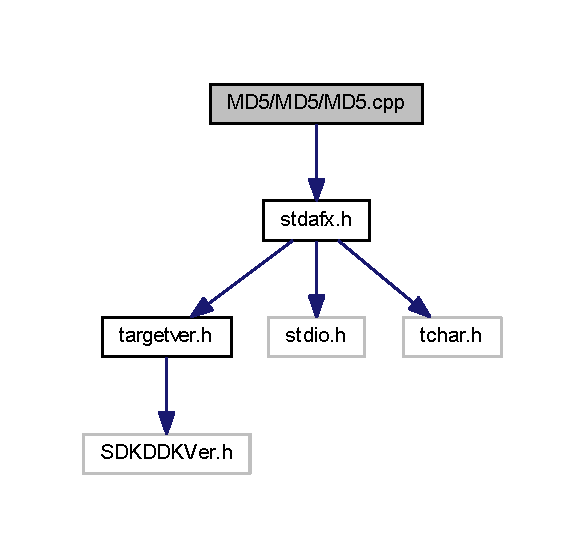
\includegraphics[width=281pt]{_m_d5_8cpp__incl}
\end{center}
\end{figure}
\subsection*{Funciones}
\begin{DoxyCompactItemize}
\item 
int \hyperlink{_m_d5_8cpp_a353674c5af92be7fb389265cde4e5e03}{\+\_\+tmain} (int argc, \+\_\+\+T\+C\+H\+A\+R $\ast$argv\mbox{[}$\,$\mbox{]})
\end{DoxyCompactItemize}


\subsection{Documentación de las funciones}
\hypertarget{_m_d5_8cpp_a353674c5af92be7fb389265cde4e5e03}{}\index{M\+D5.\+cpp@{M\+D5.\+cpp}!\+\_\+tmain@{\+\_\+tmain}}
\index{\+\_\+tmain@{\+\_\+tmain}!M\+D5.\+cpp@{M\+D5.\+cpp}}
\subsubsection[{\+\_\+tmain(int argc, \+\_\+\+T\+C\+H\+A\+R $\ast$argv[])}]{\setlength{\rightskip}{0pt plus 5cm}int \+\_\+tmain (
\begin{DoxyParamCaption}
\item[{int}]{argc, }
\item[{\+\_\+\+T\+C\+H\+A\+R $\ast$}]{argv\mbox{[}$\,$\mbox{]}}
\end{DoxyParamCaption}
)}\label{_m_d5_8cpp_a353674c5af92be7fb389265cde4e5e03}


Definición en la línea 7 del archivo M\+D5.\+cpp.


\hypertarget{_m_d5_2_m_d5_2stdafx_8cpp}{}\section{Referencia del Archivo M\+D5/\+M\+D5/stdafx.cpp}
\label{_m_d5_2_m_d5_2stdafx_8cpp}\index{M\+D5/\+M\+D5/stdafx.\+cpp@{M\+D5/\+M\+D5/stdafx.\+cpp}}
{\ttfamily \#include \char`\"{}stdafx.\+h\char`\"{}}\\*
Dependencia gráfica adjunta para stdafx.\+cpp\+:\nopagebreak
\begin{figure}[H]
\begin{center}
\leavevmode
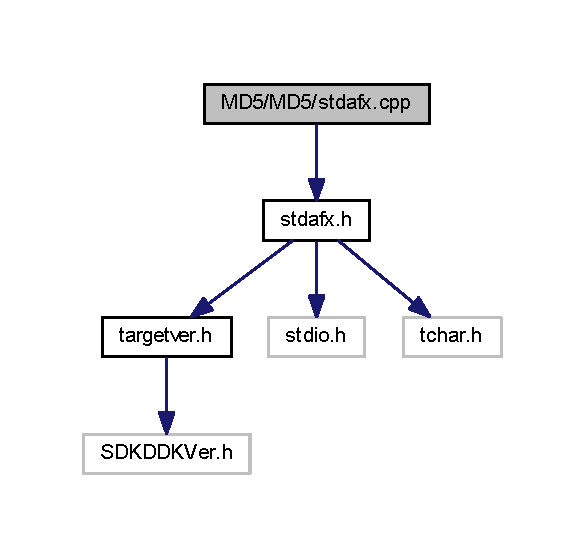
\includegraphics[width=281pt]{_m_d5_2_m_d5_2stdafx_8cpp__incl}
\end{center}
\end{figure}

\hypertarget{_s_d_p_t_r_a_p_b_2_s_d_p_t_r_a_p_b_2stdafx_8cpp}{}\section{Referencia del Archivo S\+D\+P\+T\+R\+A\+P\+B/\+S\+D\+P\+T\+R\+A\+P\+B/stdafx.cpp}
\label{_s_d_p_t_r_a_p_b_2_s_d_p_t_r_a_p_b_2stdafx_8cpp}\index{S\+D\+P\+T\+R\+A\+P\+B/\+S\+D\+P\+T\+R\+A\+P\+B/stdafx.\+cpp@{S\+D\+P\+T\+R\+A\+P\+B/\+S\+D\+P\+T\+R\+A\+P\+B/stdafx.\+cpp}}
{\ttfamily \#include \char`\"{}stdafx.\+h\char`\"{}}\\*
Dependencia gráfica adjunta para stdafx.\+cpp\+:\nopagebreak
\begin{figure}[H]
\begin{center}
\leavevmode
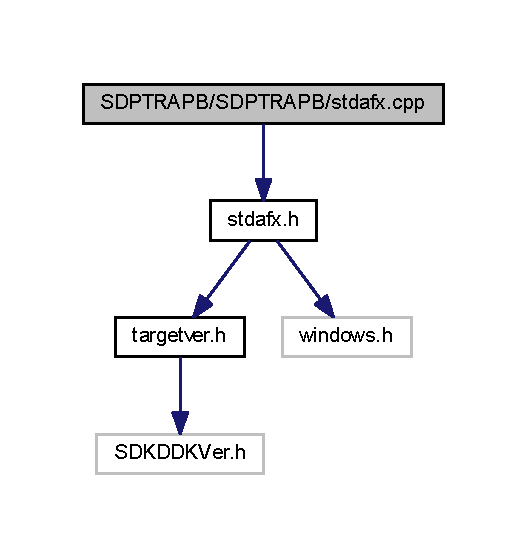
\includegraphics[width=253pt]{_s_d_p_t_r_a_p_b_2_s_d_p_t_r_a_p_b_2stdafx_8cpp__incl}
\end{center}
\end{figure}

\hypertarget{_t_s_t_s_d_p_t_r_a_p_b_2tst_s_d_p_t_r_a_p_b_2stdafx_8cpp}{}\section{Referencia del Archivo T\+S\+T\+S\+D\+P\+T\+R\+A\+P\+B/tst\+S\+D\+P\+T\+R\+A\+P\+B/stdafx.cpp}
\label{_t_s_t_s_d_p_t_r_a_p_b_2tst_s_d_p_t_r_a_p_b_2stdafx_8cpp}\index{T\+S\+T\+S\+D\+P\+T\+R\+A\+P\+B/tst\+S\+D\+P\+T\+R\+A\+P\+B/stdafx.\+cpp@{T\+S\+T\+S\+D\+P\+T\+R\+A\+P\+B/tst\+S\+D\+P\+T\+R\+A\+P\+B/stdafx.\+cpp}}
{\ttfamily \#include \char`\"{}stdafx.\+h\char`\"{}}\\*
Dependencia gráfica adjunta para stdafx.\+cpp\+:\nopagebreak
\begin{figure}[H]
\begin{center}
\leavevmode
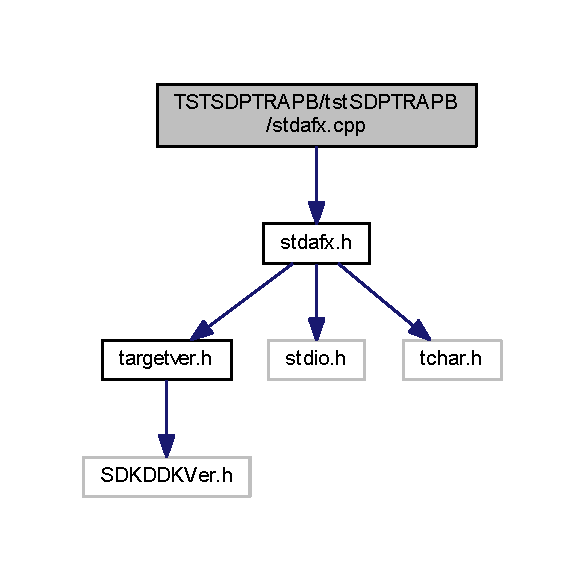
\includegraphics[width=281pt]{_t_s_t_s_d_p_t_r_a_p_b_2tst_s_d_p_t_r_a_p_b_2stdafx_8cpp__incl}
\end{center}
\end{figure}

\hypertarget{_m_d5_2_m_d5_2stdafx_8h}{}\section{Referencia del Archivo M\+D5/\+M\+D5/stdafx.h}
\label{_m_d5_2_m_d5_2stdafx_8h}\index{M\+D5/\+M\+D5/stdafx.\+h@{M\+D5/\+M\+D5/stdafx.\+h}}
{\ttfamily \#include \char`\"{}targetver.\+h\char`\"{}}\\*
{\ttfamily \#include $<$stdio.\+h$>$}\\*
{\ttfamily \#include $<$tchar.\+h$>$}\\*
Dependencia gráfica adjunta para stdafx.\+h\+:\nopagebreak
\begin{figure}[H]
\begin{center}
\leavevmode
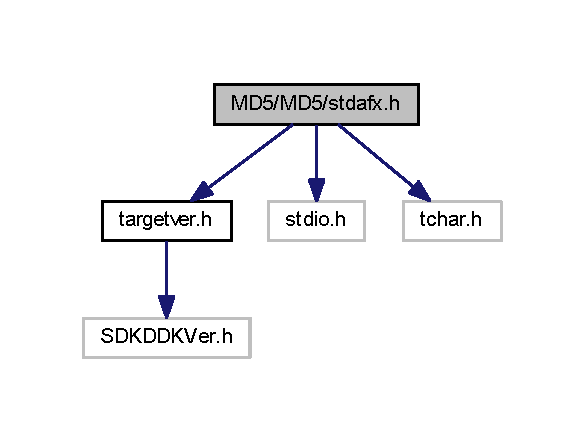
\includegraphics[width=281pt]{_m_d5_2_m_d5_2stdafx_8h__incl}
\end{center}
\end{figure}
Gráfico de los archivos que directa o indirectamente incluyen a este archivo\+:\nopagebreak
\begin{figure}[H]
\begin{center}
\leavevmode
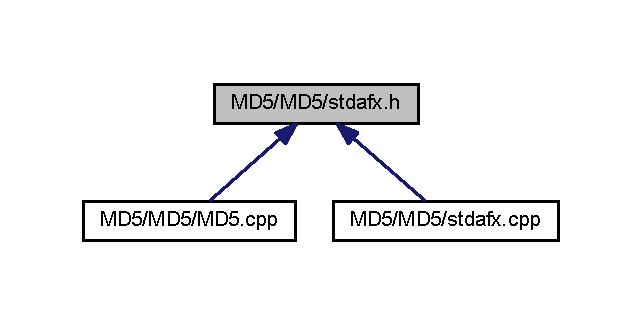
\includegraphics[width=308pt]{_m_d5_2_m_d5_2stdafx_8h__dep__incl}
\end{center}
\end{figure}

\hypertarget{_s_d_p_t_r_a_p_b_2_s_d_p_t_r_a_p_b_2stdafx_8h}{}\section{Referencia del Archivo S\+D\+P\+T\+R\+A\+P\+B/\+S\+D\+P\+T\+R\+A\+P\+B/stdafx.h}
\label{_s_d_p_t_r_a_p_b_2_s_d_p_t_r_a_p_b_2stdafx_8h}\index{S\+D\+P\+T\+R\+A\+P\+B/\+S\+D\+P\+T\+R\+A\+P\+B/stdafx.\+h@{S\+D\+P\+T\+R\+A\+P\+B/\+S\+D\+P\+T\+R\+A\+P\+B/stdafx.\+h}}
{\ttfamily \#include \char`\"{}targetver.\+h\char`\"{}}\\*
{\ttfamily \#include $<$windows.\+h$>$}\\*
Dependencia gráfica adjunta para stdafx.\+h\+:\nopagebreak
\begin{figure}[H]
\begin{center}
\leavevmode
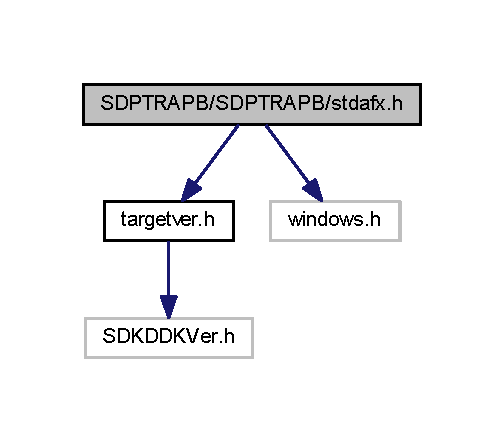
\includegraphics[width=242pt]{_s_d_p_t_r_a_p_b_2_s_d_p_t_r_a_p_b_2stdafx_8h__incl}
\end{center}
\end{figure}
Gráfico de los archivos que directa o indirectamente incluyen a este archivo\+:\nopagebreak
\begin{figure}[H]
\begin{center}
\leavevmode
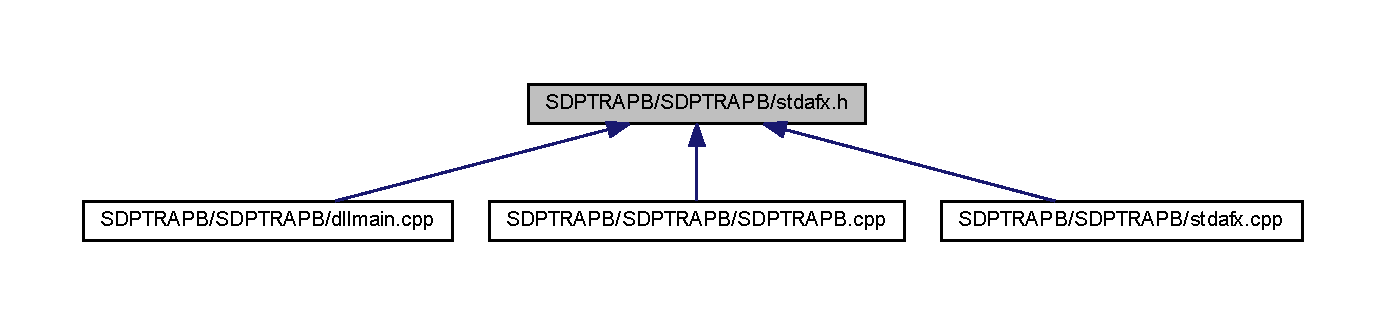
\includegraphics[width=350pt]{_s_d_p_t_r_a_p_b_2_s_d_p_t_r_a_p_b_2stdafx_8h__dep__incl}
\end{center}
\end{figure}
\subsection*{\textquotesingle{}defines\textquotesingle{}}
\begin{DoxyCompactItemize}
\item 
\#define \hyperlink{_s_d_p_t_r_a_p_b_2_s_d_p_t_r_a_p_b_2stdafx_8h_ac7bef5d85e3dcd73eef56ad39ffc84a9}{W\+I\+N32\+\_\+\+L\+E\+A\+N\+\_\+\+A\+N\+D\+\_\+\+M\+E\+A\+N}
\end{DoxyCompactItemize}


\subsection{Documentación de los \textquotesingle{}defines\textquotesingle{}}
\hypertarget{_s_d_p_t_r_a_p_b_2_s_d_p_t_r_a_p_b_2stdafx_8h_ac7bef5d85e3dcd73eef56ad39ffc84a9}{}\index{S\+D\+P\+T\+R\+A\+P\+B/\+S\+D\+P\+T\+R\+A\+P\+B/stdafx.\+h@{S\+D\+P\+T\+R\+A\+P\+B/\+S\+D\+P\+T\+R\+A\+P\+B/stdafx.\+h}!W\+I\+N32\+\_\+\+L\+E\+A\+N\+\_\+\+A\+N\+D\+\_\+\+M\+E\+A\+N@{W\+I\+N32\+\_\+\+L\+E\+A\+N\+\_\+\+A\+N\+D\+\_\+\+M\+E\+A\+N}}
\index{W\+I\+N32\+\_\+\+L\+E\+A\+N\+\_\+\+A\+N\+D\+\_\+\+M\+E\+A\+N@{W\+I\+N32\+\_\+\+L\+E\+A\+N\+\_\+\+A\+N\+D\+\_\+\+M\+E\+A\+N}!S\+D\+P\+T\+R\+A\+P\+B/\+S\+D\+P\+T\+R\+A\+P\+B/stdafx.\+h@{S\+D\+P\+T\+R\+A\+P\+B/\+S\+D\+P\+T\+R\+A\+P\+B/stdafx.\+h}}
\subsubsection[{W\+I\+N32\+\_\+\+L\+E\+A\+N\+\_\+\+A\+N\+D\+\_\+\+M\+E\+A\+N}]{\setlength{\rightskip}{0pt plus 5cm}\#define W\+I\+N32\+\_\+\+L\+E\+A\+N\+\_\+\+A\+N\+D\+\_\+\+M\+E\+A\+N}\label{_s_d_p_t_r_a_p_b_2_s_d_p_t_r_a_p_b_2stdafx_8h_ac7bef5d85e3dcd73eef56ad39ffc84a9}


Definición en la línea 10 del archivo stdafx.\+h.


\hypertarget{_t_s_t_s_d_p_t_r_a_p_b_2tst_s_d_p_t_r_a_p_b_2stdafx_8h}{}\section{Referencia del Archivo T\+S\+T\+S\+D\+P\+T\+R\+A\+P\+B/tst\+S\+D\+P\+T\+R\+A\+P\+B/stdafx.h}
\label{_t_s_t_s_d_p_t_r_a_p_b_2tst_s_d_p_t_r_a_p_b_2stdafx_8h}\index{T\+S\+T\+S\+D\+P\+T\+R\+A\+P\+B/tst\+S\+D\+P\+T\+R\+A\+P\+B/stdafx.\+h@{T\+S\+T\+S\+D\+P\+T\+R\+A\+P\+B/tst\+S\+D\+P\+T\+R\+A\+P\+B/stdafx.\+h}}
{\ttfamily \#include \char`\"{}targetver.\+h\char`\"{}}\\*
{\ttfamily \#include $<$stdio.\+h$>$}\\*
{\ttfamily \#include $<$tchar.\+h$>$}\\*
Dependencia gráfica adjunta para stdafx.\+h\+:\nopagebreak
\begin{figure}[H]
\begin{center}
\leavevmode
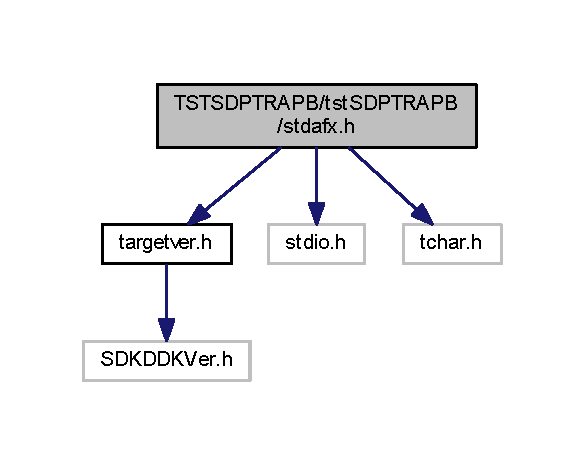
\includegraphics[width=281pt]{_t_s_t_s_d_p_t_r_a_p_b_2tst_s_d_p_t_r_a_p_b_2stdafx_8h__incl}
\end{center}
\end{figure}
Gráfico de los archivos que directa o indirectamente incluyen a este archivo\+:\nopagebreak
\begin{figure}[H]
\begin{center}
\leavevmode
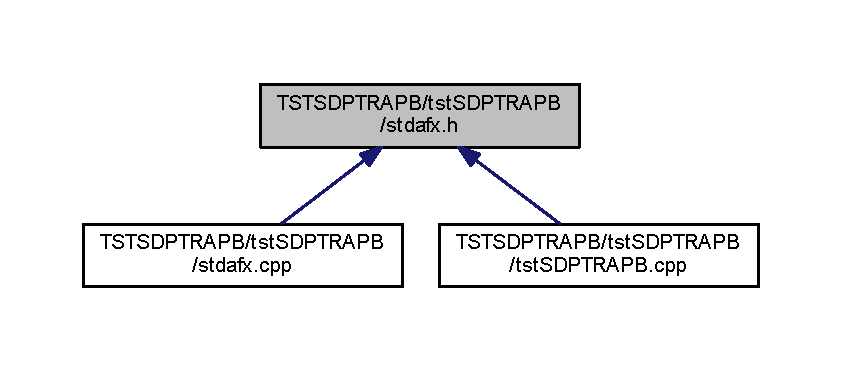
\includegraphics[width=350pt]{_t_s_t_s_d_p_t_r_a_p_b_2tst_s_d_p_t_r_a_p_b_2stdafx_8h__dep__incl}
\end{center}
\end{figure}

\hypertarget{_m_d5_2_m_d5_2targetver_8h}{}\section{Referencia del Archivo M\+D5/\+M\+D5/targetver.h}
\label{_m_d5_2_m_d5_2targetver_8h}\index{M\+D5/\+M\+D5/targetver.\+h@{M\+D5/\+M\+D5/targetver.\+h}}
{\ttfamily \#include $<$S\+D\+K\+D\+D\+K\+Ver.\+h$>$}\\*
Dependencia gráfica adjunta para targetver.\+h\+:\nopagebreak
\begin{figure}[H]
\begin{center}
\leavevmode
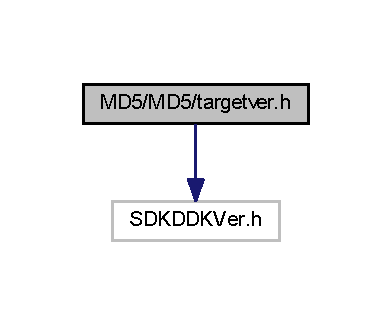
\includegraphics[width=188pt]{_m_d5_2_m_d5_2targetver_8h__incl}
\end{center}
\end{figure}
Gráfico de los archivos que directa o indirectamente incluyen a este archivo\+:\nopagebreak
\begin{figure}[H]
\begin{center}
\leavevmode
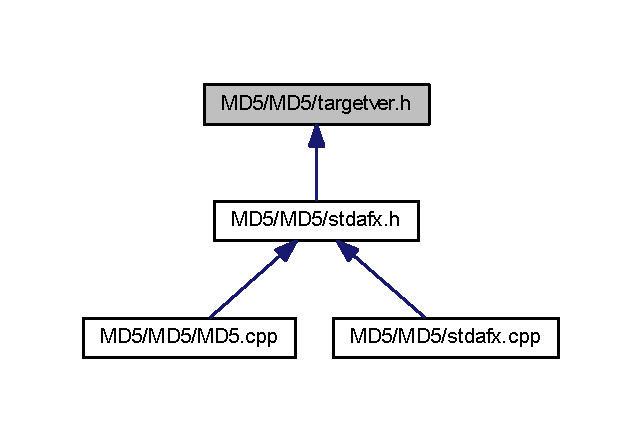
\includegraphics[width=308pt]{_m_d5_2_m_d5_2targetver_8h__dep__incl}
\end{center}
\end{figure}

\hypertarget{_s_d_p_t_r_a_p_b_2_s_d_p_t_r_a_p_b_2targetver_8h}{}\section{Referencia del Archivo S\+D\+P\+T\+R\+A\+P\+B/\+S\+D\+P\+T\+R\+A\+P\+B/targetver.h}
\label{_s_d_p_t_r_a_p_b_2_s_d_p_t_r_a_p_b_2targetver_8h}\index{S\+D\+P\+T\+R\+A\+P\+B/\+S\+D\+P\+T\+R\+A\+P\+B/targetver.\+h@{S\+D\+P\+T\+R\+A\+P\+B/\+S\+D\+P\+T\+R\+A\+P\+B/targetver.\+h}}
{\ttfamily \#include $<$S\+D\+K\+D\+D\+K\+Ver.\+h$>$}\\*
Dependencia gráfica adjunta para targetver.\+h\+:\nopagebreak
\begin{figure}[H]
\begin{center}
\leavevmode
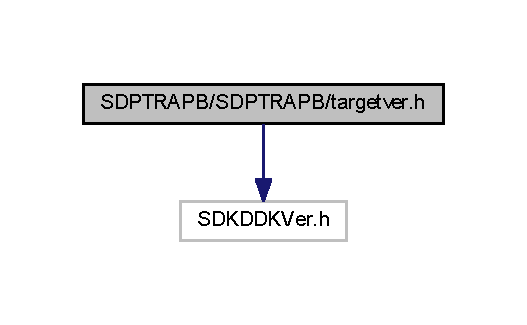
\includegraphics[width=253pt]{_s_d_p_t_r_a_p_b_2_s_d_p_t_r_a_p_b_2targetver_8h__incl}
\end{center}
\end{figure}
Gráfico de los archivos que directa o indirectamente incluyen a este archivo\+:\nopagebreak
\begin{figure}[H]
\begin{center}
\leavevmode
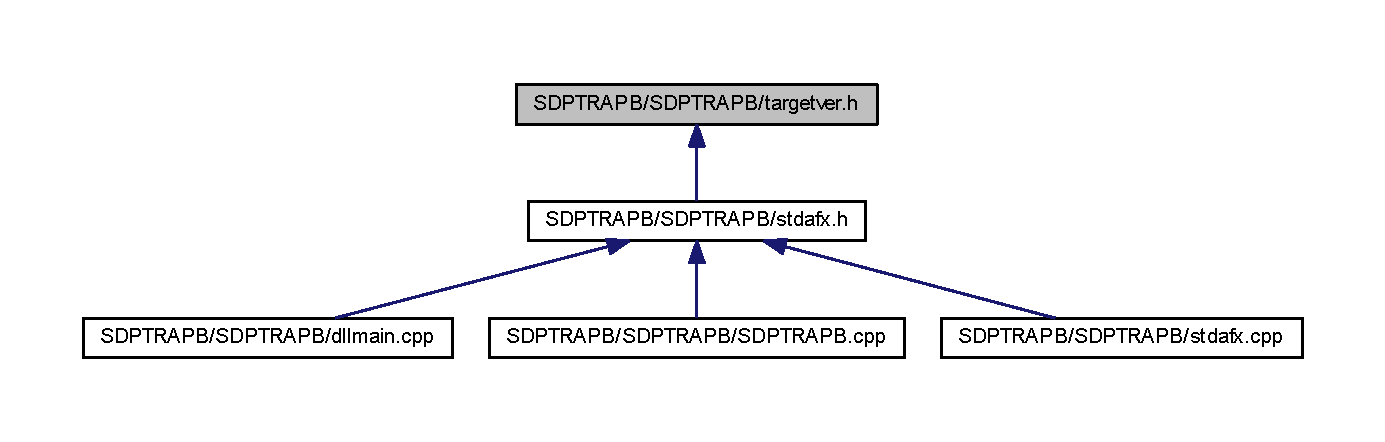
\includegraphics[width=350pt]{_s_d_p_t_r_a_p_b_2_s_d_p_t_r_a_p_b_2targetver_8h__dep__incl}
\end{center}
\end{figure}

\hypertarget{_t_s_t_s_d_p_t_r_a_p_b_2tst_s_d_p_t_r_a_p_b_2targetver_8h}{}\section{Referencia del Archivo T\+S\+T\+S\+D\+P\+T\+R\+A\+P\+B/tst\+S\+D\+P\+T\+R\+A\+P\+B/targetver.h}
\label{_t_s_t_s_d_p_t_r_a_p_b_2tst_s_d_p_t_r_a_p_b_2targetver_8h}\index{T\+S\+T\+S\+D\+P\+T\+R\+A\+P\+B/tst\+S\+D\+P\+T\+R\+A\+P\+B/targetver.\+h@{T\+S\+T\+S\+D\+P\+T\+R\+A\+P\+B/tst\+S\+D\+P\+T\+R\+A\+P\+B/targetver.\+h}}
{\ttfamily \#include $<$S\+D\+K\+D\+D\+K\+Ver.\+h$>$}\\*
Dependencia gráfica adjunta para targetver.\+h\+:\nopagebreak
\begin{figure}[H]
\begin{center}
\leavevmode
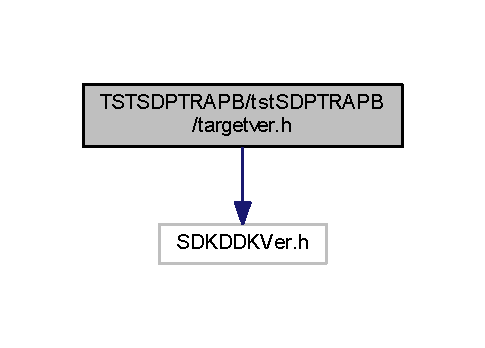
\includegraphics[width=233pt]{_t_s_t_s_d_p_t_r_a_p_b_2tst_s_d_p_t_r_a_p_b_2targetver_8h__incl}
\end{center}
\end{figure}
Gráfico de los archivos que directa o indirectamente incluyen a este archivo\+:\nopagebreak
\begin{figure}[H]
\begin{center}
\leavevmode
\includegraphics[width=350pt]{_t_s_t_s_d_p_t_r_a_p_b_2tst_s_d_p_t_r_a_p_b_2targetver_8h__dep__incl}
\end{center}
\end{figure}

\hypertarget{dllmain_8cpp}{}\section{Referencia del Archivo S\+D\+P\+T\+R\+A\+P\+B/\+S\+D\+P\+T\+R\+A\+P\+B/dllmain.cpp}
\label{dllmain_8cpp}\index{S\+D\+P\+T\+R\+A\+P\+B/\+S\+D\+P\+T\+R\+A\+P\+B/dllmain.\+cpp@{S\+D\+P\+T\+R\+A\+P\+B/\+S\+D\+P\+T\+R\+A\+P\+B/dllmain.\+cpp}}
{\ttfamily \#include \char`\"{}stdafx.\+h\char`\"{}}\\*
Dependencia gráfica adjunta para dllmain.\+cpp\+:\nopagebreak
\begin{figure}[H]
\begin{center}
\leavevmode
\includegraphics[width=257pt]{dllmain_8cpp__incl}
\end{center}
\end{figure}
\subsection*{Funciones}
\begin{DoxyCompactItemize}
\item 
B\+O\+O\+L A\+P\+I\+E\+N\+T\+R\+Y \hyperlink{dllmain_8cpp_a26e64fb39b69bcd9d1274d279f1561b9}{Dll\+Main} (H\+M\+O\+D\+U\+L\+E h\+Module, D\+W\+O\+R\+D ul\+\_\+reason\+\_\+for\+\_\+call, L\+P\+V\+O\+I\+D lp\+Reserved)
\end{DoxyCompactItemize}


\subsection{Documentación de las funciones}
\hypertarget{dllmain_8cpp_a26e64fb39b69bcd9d1274d279f1561b9}{}\index{dllmain.\+cpp@{dllmain.\+cpp}!Dll\+Main@{Dll\+Main}}
\index{Dll\+Main@{Dll\+Main}!dllmain.\+cpp@{dllmain.\+cpp}}
\subsubsection[{Dll\+Main(\+H\+M\+O\+D\+U\+L\+E h\+Module, D\+W\+O\+R\+D ul\+\_\+reason\+\_\+for\+\_\+call, L\+P\+V\+O\+I\+D lp\+Reserved)}]{\setlength{\rightskip}{0pt plus 5cm}B\+O\+O\+L A\+P\+I\+E\+N\+T\+R\+Y Dll\+Main (
\begin{DoxyParamCaption}
\item[{H\+M\+O\+D\+U\+L\+E}]{h\+Module, }
\item[{D\+W\+O\+R\+D}]{ul\+\_\+reason\+\_\+for\+\_\+call, }
\item[{L\+P\+V\+O\+I\+D}]{lp\+Reserved}
\end{DoxyParamCaption}
)}\label{dllmain_8cpp_a26e64fb39b69bcd9d1274d279f1561b9}


Definición en la línea 4 del archivo dllmain.\+cpp.


\hypertarget{_s_d_p_t_r_a_p_b_8cpp}{}\section{Referencia del Archivo S\+D\+P\+T\+R\+A\+P\+B/\+S\+D\+P\+T\+R\+A\+P\+B/\+S\+D\+P\+T\+R\+A\+P\+B.cpp}
\label{_s_d_p_t_r_a_p_b_8cpp}\index{S\+D\+P\+T\+R\+A\+P\+B/\+S\+D\+P\+T\+R\+A\+P\+B/\+S\+D\+P\+T\+R\+A\+P\+B.\+cpp@{S\+D\+P\+T\+R\+A\+P\+B/\+S\+D\+P\+T\+R\+A\+P\+B/\+S\+D\+P\+T\+R\+A\+P\+B.\+cpp}}
{\ttfamily \#include \char`\"{}stdafx.\+h\char`\"{}}\\*
Dependencia gráfica adjunta para S\+D\+P\+T\+R\+A\+P\+B.\+cpp\+:\nopagebreak
\begin{figure}[H]
\begin{center}
\leavevmode
\includegraphics[width=279pt]{_s_d_p_t_r_a_p_b_8cpp__incl}
\end{center}
\end{figure}

\hypertarget{amqsdp_8c}{}\section{Referencia del Archivo src/amqsdp.c}
\label{amqsdp_8c}\index{src/amqsdp.\+c@{src/amqsdp.\+c}}


Cliente Websphere M\+Q\+Series.  


{\ttfamily \#include $<$stdio.\+h$>$}\\*
{\ttfamily \#include $<$stdlib.\+h$>$}\\*
{\ttfamily \#include $<$string.\+h$>$}\\*
{\ttfamily \#include \char`\"{}cmqc.\+h\char`\"{}}\\*
{\ttfamily \#include \char`\"{}S\+D\+P\+T\+R\+A\+P.\+h\char`\"{}}\\*
{\ttfamily \#include \char`\"{}amqsdp.\+h\char`\"{}}\\*
{\ttfamily \#include \char`\"{}global.\+h\char`\"{}}\\*
Dependencia gráfica adjunta para amqsdp.\+c\+:\nopagebreak
\begin{figure}[H]
\begin{center}
\leavevmode
\includegraphics[width=350pt]{amqsdp_8c__incl}
\end{center}
\end{figure}
\subsection*{\textquotesingle{}defines\textquotesingle{}}
\begin{DoxyCompactItemize}
\item 
\#define \hyperlink{amqsdp_8c_a2c1538d99cb1b248411c15badb3c0842}{\+\_\+\+A\+M\+Q\+S\+D\+P\+\_\+\+S\+R\+C\+\_\+}
\end{DoxyCompactItemize}
\subsection*{Funciones}
\begin{DoxyCompactItemize}
\item 
void \hyperlink{amqsdp_8c_a094c19a9716364046b2779fff6efa664}{M\+Q\+Free} (void)
\item 
int \hyperlink{amqsdp_8c_ab689e2ba6771a5113551222f6189c137}{M\+Q\+Conn} ()
\item 
void \hyperlink{amqsdp_8c_acc12f0f1458385b0f5c5a6234f817205}{M\+Q\+Disconn} ()
\item 
int \hyperlink{amqsdp_8c_a196cb274ac9c69cbe5daf9371668025c}{M\+Q\+Open} ()
\item 
void \hyperlink{amqsdp_8c_ae93fe1e642e758fbbe9c892ab8033aa4}{M\+Q\+Close} ()
\item 
\hyperlink{sha256le_8h_adfbc1051df776564281ac4220ba53a9e}{\+\_\+\+E\+X\+T\+\_\+} void \hyperlink{amqsdp_8c_a12766b7a05c27f09555f40c88e08610b}{init\+A\+M\+Q} (int d, F\+I\+L\+E $\ast$f)
\item 
\hyperlink{sha256le_8h_adfbc1051df776564281ac4220ba53a9e}{\+\_\+\+E\+X\+T\+\_\+} void \hyperlink{amqsdp_8c_a3c337f7b77e495f85489f862d4df359c}{set\+Buffer\+Size} ()
\item 
\hyperlink{sha256le_8h_adfbc1051df776564281ac4220ba53a9e}{\+\_\+\+E\+X\+T\+\_\+} void \hyperlink{amqsdp_8c_adba192fbf1af062214021fcb06229295}{unset\+Buffer\+Size} ()
\item 
\hyperlink{sha256le_8h_adfbc1051df776564281ac4220ba53a9e}{\+\_\+\+E\+X\+T\+\_\+} void \hyperlink{amqsdp_8c_ac2122a579c04414c93370c338601c492}{set\+Max\+Group} (int group)
\item 
\hyperlink{sha256le_8h_adfbc1051df776564281ac4220ba53a9e}{\+\_\+\+E\+X\+T\+\_\+} int \hyperlink{amqsdp_8c_ab05385469ff40b1b77e3c41846d1421f}{enviar} (char $\ast$\hyperlink{messages_8c_a1c07f3735e9c63f3130a615745887a20}{sz\+Msg}, unsigned char force)
\item 
\hyperlink{sha256le_8h_adfbc1051df776564281ac4220ba53a9e}{\+\_\+\+E\+X\+T\+\_\+} int \hyperlink{amqsdp_8c_a6a6249b42450b376958cc3f668c44fdb}{M\+Q\+Connect} ()
\item 
\hyperlink{sha256le_8h_adfbc1051df776564281ac4220ba53a9e}{\+\_\+\+E\+X\+T\+\_\+} void \hyperlink{amqsdp_8c_a4cf1ee13ff615962a3d86fcb8cfa57f5}{M\+Q\+Disconnect} ()
\item 
\hyperlink{sha256le_8h_adfbc1051df776564281ac4220ba53a9e}{\+\_\+\+E\+X\+T\+\_\+} long \hyperlink{amqsdp_8c_a9531d8185ec00f217beb2bcb561099d6}{M\+Q\+Put} (char $\ast$msg, long len)
\item 
\hyperlink{sha256le_8h_adfbc1051df776564281ac4220ba53a9e}{\+\_\+\+E\+X\+T\+\_\+} long \hyperlink{amqsdp_8c_a5be1500f1c7b8b6afef1605c438017ef}{M\+Q\+Get} (char $\ast$buff, long len)
\item 
int \hyperlink{amqsdp_8c_a3fea393a72c9440cf4210ec0634d91b2}{M\+Q\+Open\+Output} ()
\item 
int \hyperlink{amqsdp_8c_ace216d31cea6ba0b0e5336b2517ed2a5}{M\+Q\+Open\+Input} ()
\end{DoxyCompactItemize}
\subsection*{Variables}
\begin{DoxyCompactItemize}
\item 
\hyperlink{cmqc_8h_adc6ce41a36ea02c7128633fb49d2327b}{M\+Q\+O\+D} \hyperlink{amqsdp_8c_a3fb375f4ee6971a0a7241c1b9fe0250d}{od} = \{\hyperlink{cmqc_8h_aaca8efdc3c3886d6f06d841e99b3824b}{M\+Q\+O\+D\+\_\+\+D\+E\+F\+A\+U\+L\+T}\}
\item 
\hyperlink{cmqc_8h_adba81d43f75836f834f8fa1c61d5517e}{M\+Q\+M\+D} \hyperlink{amqsdp_8c_ae87fabdedbfb0255167d3f0a7705ec2e}{md} = \{\hyperlink{cmqc_8h_a8886d85ef78d739f38beb8a302a0b3c0}{M\+Q\+M\+D\+\_\+\+D\+E\+F\+A\+U\+L\+T}\}
\item 
\hyperlink{cmqc_8h_a3e6dadad27fbbca9ac41bfc9f1fb2755}{M\+Q\+P\+M\+O} \hyperlink{amqsdp_8c_a017b205b3e8f746565c6358ba97f80cd}{pmo} = \{\hyperlink{cmqc_8h_a7b568f0009a2c3c452407a4f803fa87a}{M\+Q\+P\+M\+O\+\_\+\+D\+E\+F\+A\+U\+L\+T}\}
\item 
\hyperlink{cmqc_8h_afc714b4f20c35240b4136d7921a72d96}{M\+Q\+C\+N\+O} \hyperlink{amqsdp_8c_a684758dad6f1bcbcf33011bad12a3687}{cno} = \{\hyperlink{cmqc_8h_af9f6084a129db0fe30bbd58db99540e9}{M\+Q\+C\+N\+O\+\_\+\+D\+E\+F\+A\+U\+L\+T}\}
\item 
\hyperlink{cmqc_8h_aa7dbc005fadce97bd1410ffa38a86932}{M\+Q\+C\+S\+P} \hyperlink{amqsdp_8c_a000eb961f9033ec28a6d0319adfc0cc4}{csp} = \{\hyperlink{cmqc_8h_a087ea7addc51ee1b57b13d89b0852cc7}{M\+Q\+C\+S\+P\+\_\+\+D\+E\+F\+A\+U\+L\+T}\}
\item 
\hyperlink{cmqc_8h_a00170ac137e1beb55a3c34f07a39fcc4}{M\+Q\+H\+C\+O\+N\+N} \hyperlink{amqsdp_8c_a9c88e25f067c51de112e0eacc559f462}{Hcon} = 0x0
\item 
\hyperlink{cmqc_8h_ac093f559f81163292e6016c68c947164}{M\+Q\+H\+O\+B\+J} \hyperlink{amqsdp_8c_a01edfcfbde290ed1c9a7a03b8c2f4500}{H\+Queue} = 0x0
\item 
\hyperlink{cmqc_8h_a1fb8d28cbda3fa8766a9821230cdb6d5}{M\+Q\+L\+O\+N\+G} \hyperlink{amqsdp_8c_ac43cc6b9c68558cea8e4a5b632df0363}{O\+\_\+options}
\item 
\hyperlink{cmqc_8h_a1fb8d28cbda3fa8766a9821230cdb6d5}{M\+Q\+L\+O\+N\+G} \hyperlink{amqsdp_8c_a0cfbea0c21c76cde9732ffc87c9ed260}{C\+\_\+options}
\item 
\hyperlink{cmqc_8h_a1fb8d28cbda3fa8766a9821230cdb6d5}{M\+Q\+L\+O\+N\+G} \hyperlink{amqsdp_8c_a84be6334ddf78b650dfed2b632293455}{mqcc}
\item 
\hyperlink{cmqc_8h_a1fb8d28cbda3fa8766a9821230cdb6d5}{M\+Q\+L\+O\+N\+G} \hyperlink{amqsdp_8c_a3537d2a2450ea0e24a3a56001020ec5f}{mqrc}
\item 
char \hyperlink{amqsdp_8c_a52b0abed1d4b7d10c3a8e42e40f8f80a}{Q\+M\+Name} \mbox{[}50\mbox{]}
\item 
char $\ast$ \hyperlink{amqsdp_8c_a30bbda1ba59bb12c2895c4006804a55d}{qmgr}
\item 
char $\ast$ \hyperlink{amqsdp_8c_a5a317b1553299b3cbe3ef6d6d2edcffc}{qname} = \char`\"{}S\+D\+P.\+T\+R\+A\+P\+P\+E\+R\char`\"{}
\item 
long \hyperlink{amqsdp_8c_a3ab85df1f9111b4eaaa988eff903f2b4}{buff\+Size} = 4095
\item 
int \hyperlink{amqsdp_8c_a21dcb4f76464d796d158cc3333ab18d8}{msgs} = 0
\item 
int \hyperlink{amqsdp_8c_a35708eb4d2bb797b73ab54979f5b991f}{max\+Group} = \hyperlink{sdpconfig_8h_aeefcc7b6f118beefd2cec532afced5df}{I\+T\+E\+M\+S\+\_\+\+B\+Y\+\_\+\+M\+S\+G}
\item 
int \hyperlink{amqsdp_8c_aed7ea92f45bd273dde380a45ddced592}{offset} = 0
\item 
char $\ast$ \hyperlink{amqsdp_8c_aff2566f4c366b48d73479bef43ee4d2e}{buffer} = 0x0
\item 
int \hyperlink{amqsdp_8c_a4fb693c3cca874aca4a9d2109cc561e5}{in\+Err}
\item 
int \hyperlink{amqsdp_8c_ad247c905cf5ce68a5eec344bcba86cc7}{dbg\+Level}
\item 
F\+I\+L\+E $\ast$ \hyperlink{amqsdp_8c_a5f9e912074a29350e020b7a09f43ff32}{traza}
\end{DoxyCompactItemize}


\subsection{Descripción detallada}
Cliente Websphere M\+Q\+Series. 

La informacion relativa a Q\+Manager, Nombre de cola, etc se obtiene del entorno

\begin{DoxyAuthor}{Autor}
\+: Javier Gonzalez 
\end{DoxyAuthor}
\begin{DoxyDate}{Fecha}
\+: 01/04/2015 
\end{DoxyDate}
\begin{DoxyVersion}{Versión}
\+: 1.\+0 
\end{DoxyVersion}


\subsection{Documentación de los \textquotesingle{}defines\textquotesingle{}}
\hypertarget{amqsdp_8c_a2c1538d99cb1b248411c15badb3c0842}{}\index{amqsdp.\+c@{amqsdp.\+c}!\+\_\+\+A\+M\+Q\+S\+D\+P\+\_\+\+S\+R\+C\+\_\+@{\+\_\+\+A\+M\+Q\+S\+D\+P\+\_\+\+S\+R\+C\+\_\+}}
\index{\+\_\+\+A\+M\+Q\+S\+D\+P\+\_\+\+S\+R\+C\+\_\+@{\+\_\+\+A\+M\+Q\+S\+D\+P\+\_\+\+S\+R\+C\+\_\+}!amqsdp.\+c@{amqsdp.\+c}}
\subsubsection[{\+\_\+\+A\+M\+Q\+S\+D\+P\+\_\+\+S\+R\+C\+\_\+}]{\setlength{\rightskip}{0pt plus 5cm}\#define \+\_\+\+A\+M\+Q\+S\+D\+P\+\_\+\+S\+R\+C\+\_\+}\label{amqsdp_8c_a2c1538d99cb1b248411c15badb3c0842}


Definición en la línea 14 del archivo amqsdp.\+c.



\subsection{Documentación de las funciones}
\hypertarget{amqsdp_8c_ab05385469ff40b1b77e3c41846d1421f}{}\index{amqsdp.\+c@{amqsdp.\+c}!enviar@{enviar}}
\index{enviar@{enviar}!amqsdp.\+c@{amqsdp.\+c}}
\subsubsection[{enviar(char $\ast$sz\+Msg, unsigned char force)}]{\setlength{\rightskip}{0pt plus 5cm}{\bf \+\_\+\+E\+X\+T\+\_\+} int enviar (
\begin{DoxyParamCaption}
\item[{char $\ast$}]{sz\+Msg, }
\item[{unsigned char}]{force}
\end{DoxyParamCaption}
)}\label{amqsdp_8c_ab05385469ff40b1b77e3c41846d1421f}
Envia el mensaje si force = true o se han alcanzado el el numero de mensajes a agrupar

Si no lo almacena en el buffer para evitar envios masivos mensajes Se verifica si el mensaje cabe en el buffer alocado antes de alamacenarlo, seria el caso en el que el numero mensajes a agrupar es excesivo 

Definición en la línea 108 del archivo amqsdp.\+c.

\hypertarget{amqsdp_8c_a12766b7a05c27f09555f40c88e08610b}{}\index{amqsdp.\+c@{amqsdp.\+c}!init\+A\+M\+Q@{init\+A\+M\+Q}}
\index{init\+A\+M\+Q@{init\+A\+M\+Q}!amqsdp.\+c@{amqsdp.\+c}}
\subsubsection[{init\+A\+M\+Q(int d, F\+I\+L\+E $\ast$f)}]{\setlength{\rightskip}{0pt plus 5cm}{\bf \+\_\+\+E\+X\+T\+\_\+} void init\+A\+M\+Q (
\begin{DoxyParamCaption}
\item[{int}]{dbg, }
\item[{F\+I\+L\+E $\ast$}]{f}
\end{DoxyParamCaption}
)}\label{amqsdp_8c_a12766b7a05c27f09555f40c88e08610b}
Inicia el entorno M\+Q Para depuracion es necesario pasarlo el nivel de debug y el fichero a utilizar 

Definición en la línea 77 del archivo amqsdp.\+c.

\hypertarget{amqsdp_8c_ae93fe1e642e758fbbe9c892ab8033aa4}{}\index{amqsdp.\+c@{amqsdp.\+c}!M\+Q\+Close@{M\+Q\+Close}}
\index{M\+Q\+Close@{M\+Q\+Close}!amqsdp.\+c@{amqsdp.\+c}}
\subsubsection[{M\+Q\+Close()}]{\setlength{\rightskip}{0pt plus 5cm}void M\+Q\+Close (
\begin{DoxyParamCaption}
{}
\end{DoxyParamCaption}
)}\label{amqsdp_8c_ae93fe1e642e758fbbe9c892ab8033aa4}


Definición en la línea 251 del archivo amqsdp.\+c.

\hypertarget{amqsdp_8c_ab689e2ba6771a5113551222f6189c137}{}\index{amqsdp.\+c@{amqsdp.\+c}!M\+Q\+Conn@{M\+Q\+Conn}}
\index{M\+Q\+Conn@{M\+Q\+Conn}!amqsdp.\+c@{amqsdp.\+c}}
\subsubsection[{M\+Q\+Conn()}]{\setlength{\rightskip}{0pt plus 5cm}int M\+Q\+Conn (
\begin{DoxyParamCaption}
{}
\end{DoxyParamCaption}
)}\label{amqsdp_8c_ab689e2ba6771a5113551222f6189c137}


Definición en la línea 205 del archivo amqsdp.\+c.

\hypertarget{amqsdp_8c_a6a6249b42450b376958cc3f668c44fdb}{}\index{amqsdp.\+c@{amqsdp.\+c}!M\+Q\+Connect@{M\+Q\+Connect}}
\index{M\+Q\+Connect@{M\+Q\+Connect}!amqsdp.\+c@{amqsdp.\+c}}
\subsubsection[{M\+Q\+Connect()}]{\setlength{\rightskip}{0pt plus 5cm}{\bf \+\_\+\+E\+X\+T\+\_\+} int M\+Q\+Connect (
\begin{DoxyParamCaption}
\item[{void}]{}
\end{DoxyParamCaption}
)}\label{amqsdp_8c_a6a6249b42450b376958cc3f668c44fdb}
Establece la conexion con el gestor de colas 

Definición en la línea 134 del archivo amqsdp.\+c.

\hypertarget{amqsdp_8c_acc12f0f1458385b0f5c5a6234f817205}{}\index{amqsdp.\+c@{amqsdp.\+c}!M\+Q\+Disconn@{M\+Q\+Disconn}}
\index{M\+Q\+Disconn@{M\+Q\+Disconn}!amqsdp.\+c@{amqsdp.\+c}}
\subsubsection[{M\+Q\+Disconn()}]{\setlength{\rightskip}{0pt plus 5cm}void M\+Q\+Disconn (
\begin{DoxyParamCaption}
{}
\end{DoxyParamCaption}
)}\label{amqsdp_8c_acc12f0f1458385b0f5c5a6234f817205}


Definición en la línea 219 del archivo amqsdp.\+c.

\hypertarget{amqsdp_8c_a4cf1ee13ff615962a3d86fcb8cfa57f5}{}\index{amqsdp.\+c@{amqsdp.\+c}!M\+Q\+Disconnect@{M\+Q\+Disconnect}}
\index{M\+Q\+Disconnect@{M\+Q\+Disconnect}!amqsdp.\+c@{amqsdp.\+c}}
\subsubsection[{M\+Q\+Disconnect()}]{\setlength{\rightskip}{0pt plus 5cm}{\bf \+\_\+\+E\+X\+T\+\_\+} void M\+Q\+Disconnect (
\begin{DoxyParamCaption}
\item[{void}]{}
\end{DoxyParamCaption}
)}\label{amqsdp_8c_a4cf1ee13ff615962a3d86fcb8cfa57f5}
Libera la conexion con el gestor de colas 

Definición en la línea 146 del archivo amqsdp.\+c.

\hypertarget{amqsdp_8c_a094c19a9716364046b2779fff6efa664}{}\index{amqsdp.\+c@{amqsdp.\+c}!M\+Q\+Free@{M\+Q\+Free}}
\index{M\+Q\+Free@{M\+Q\+Free}!amqsdp.\+c@{amqsdp.\+c}}
\subsubsection[{M\+Q\+Free(void)}]{\setlength{\rightskip}{0pt plus 5cm}void M\+Q\+Free (
\begin{DoxyParamCaption}
\item[{void}]{}
\end{DoxyParamCaption}
)}\label{amqsdp_8c_a094c19a9716364046b2779fff6efa664}
\hypertarget{amqsdp_8c_a5be1500f1c7b8b6afef1605c438017ef}{}\index{amqsdp.\+c@{amqsdp.\+c}!M\+Q\+Get@{M\+Q\+Get}}
\index{M\+Q\+Get@{M\+Q\+Get}!amqsdp.\+c@{amqsdp.\+c}}
\subsubsection[{M\+Q\+Get(char $\ast$buff, long len)}]{\setlength{\rightskip}{0pt plus 5cm}{\bf \+\_\+\+E\+X\+T\+\_\+} long M\+Q\+Get (
\begin{DoxyParamCaption}
\item[{char $\ast$}]{msg, }
\item[{long}]{len}
\end{DoxyParamCaption}
)}\label{amqsdp_8c_a5be1500f1c7b8b6afef1605c438017ef}
Lee un mensaje de la cola 

Definición en la línea 175 del archivo amqsdp.\+c.

\hypertarget{amqsdp_8c_a196cb274ac9c69cbe5daf9371668025c}{}\index{amqsdp.\+c@{amqsdp.\+c}!M\+Q\+Open@{M\+Q\+Open}}
\index{M\+Q\+Open@{M\+Q\+Open}!amqsdp.\+c@{amqsdp.\+c}}
\subsubsection[{M\+Q\+Open()}]{\setlength{\rightskip}{0pt plus 5cm}int M\+Q\+Open (
\begin{DoxyParamCaption}
{}
\end{DoxyParamCaption}
)}\label{amqsdp_8c_a196cb274ac9c69cbe5daf9371668025c}


Definición en la línea 238 del archivo amqsdp.\+c.

\hypertarget{amqsdp_8c_ace216d31cea6ba0b0e5336b2517ed2a5}{}\index{amqsdp.\+c@{amqsdp.\+c}!M\+Q\+Open\+Input@{M\+Q\+Open\+Input}}
\index{M\+Q\+Open\+Input@{M\+Q\+Open\+Input}!amqsdp.\+c@{amqsdp.\+c}}
\subsubsection[{M\+Q\+Open\+Input()}]{\setlength{\rightskip}{0pt plus 5cm}int M\+Q\+Open\+Input (
\begin{DoxyParamCaption}
\item[{void}]{}
\end{DoxyParamCaption}
)}\label{amqsdp_8c_ace216d31cea6ba0b0e5336b2517ed2a5}
Abre la cola de lectura 

Definición en la línea 231 del archivo amqsdp.\+c.

\hypertarget{amqsdp_8c_a3fea393a72c9440cf4210ec0634d91b2}{}\index{amqsdp.\+c@{amqsdp.\+c}!M\+Q\+Open\+Output@{M\+Q\+Open\+Output}}
\index{M\+Q\+Open\+Output@{M\+Q\+Open\+Output}!amqsdp.\+c@{amqsdp.\+c}}
\subsubsection[{M\+Q\+Open\+Output()}]{\setlength{\rightskip}{0pt plus 5cm}int M\+Q\+Open\+Output (
\begin{DoxyParamCaption}
\item[{void}]{}
\end{DoxyParamCaption}
)}\label{amqsdp_8c_a3fea393a72c9440cf4210ec0634d91b2}
Abre la cola de escritura 

Definición en la línea 223 del archivo amqsdp.\+c.

\hypertarget{amqsdp_8c_a9531d8185ec00f217beb2bcb561099d6}{}\index{amqsdp.\+c@{amqsdp.\+c}!M\+Q\+Put@{M\+Q\+Put}}
\index{M\+Q\+Put@{M\+Q\+Put}!amqsdp.\+c@{amqsdp.\+c}}
\subsubsection[{M\+Q\+Put(char $\ast$msg, long len)}]{\setlength{\rightskip}{0pt plus 5cm}{\bf \+\_\+\+E\+X\+T\+\_\+} long M\+Q\+Put (
\begin{DoxyParamCaption}
\item[{char $\ast$}]{msg, }
\item[{long}]{len}
\end{DoxyParamCaption}
)}\label{amqsdp_8c_a9531d8185ec00f217beb2bcb561099d6}
Escribe el mensaje en la cola 

Definición en la línea 152 del archivo amqsdp.\+c.

\hypertarget{amqsdp_8c_a3c337f7b77e495f85489f862d4df359c}{}\index{amqsdp.\+c@{amqsdp.\+c}!set\+Buffer\+Size@{set\+Buffer\+Size}}
\index{set\+Buffer\+Size@{set\+Buffer\+Size}!amqsdp.\+c@{amqsdp.\+c}}
\subsubsection[{set\+Buffer\+Size()}]{\setlength{\rightskip}{0pt plus 5cm}{\bf \+\_\+\+E\+X\+T\+\_\+} void set\+Buffer\+Size (
\begin{DoxyParamCaption}
{}
\end{DoxyParamCaption}
)}\label{amqsdp_8c_a3c337f7b77e495f85489f862d4df359c}
Crea el buffer de mensajes 

Definición en la línea 82 del archivo amqsdp.\+c.

\hypertarget{amqsdp_8c_ac2122a579c04414c93370c338601c492}{}\index{amqsdp.\+c@{amqsdp.\+c}!set\+Max\+Group@{set\+Max\+Group}}
\index{set\+Max\+Group@{set\+Max\+Group}!amqsdp.\+c@{amqsdp.\+c}}
\subsubsection[{set\+Max\+Group(int group)}]{\setlength{\rightskip}{0pt plus 5cm}{\bf \+\_\+\+E\+X\+T\+\_\+} void set\+Max\+Group (
\begin{DoxyParamCaption}
\item[{int}]{group}
\end{DoxyParamCaption}
)}\label{amqsdp_8c_ac2122a579c04414c93370c338601c492}
Establece el numero de mensajes que se enviaran en un unico mensaje de la cola 

Definición en la línea 93 del archivo amqsdp.\+c.

\hypertarget{amqsdp_8c_adba192fbf1af062214021fcb06229295}{}\index{amqsdp.\+c@{amqsdp.\+c}!unset\+Buffer\+Size@{unset\+Buffer\+Size}}
\index{unset\+Buffer\+Size@{unset\+Buffer\+Size}!amqsdp.\+c@{amqsdp.\+c}}
\subsubsection[{unset\+Buffer\+Size()}]{\setlength{\rightskip}{0pt plus 5cm}{\bf \+\_\+\+E\+X\+T\+\_\+} void unset\+Buffer\+Size (
\begin{DoxyParamCaption}
{}
\end{DoxyParamCaption}
)}\label{amqsdp_8c_adba192fbf1af062214021fcb06229295}
Libera el buffer de mensajes 

Definición en la línea 89 del archivo amqsdp.\+c.



\subsection{Documentación de las variables}
\hypertarget{amqsdp_8c_aff2566f4c366b48d73479bef43ee4d2e}{}\index{amqsdp.\+c@{amqsdp.\+c}!buffer@{buffer}}
\index{buffer@{buffer}!amqsdp.\+c@{amqsdp.\+c}}
\subsubsection[{buffer}]{\setlength{\rightskip}{0pt plus 5cm}char$\ast$ buffer = 0x0}\label{amqsdp_8c_aff2566f4c366b48d73479bef43ee4d2e}


Definición en la línea 53 del archivo amqsdp.\+c.

\hypertarget{amqsdp_8c_a3ab85df1f9111b4eaaa988eff903f2b4}{}\index{amqsdp.\+c@{amqsdp.\+c}!buff\+Size@{buff\+Size}}
\index{buff\+Size@{buff\+Size}!amqsdp.\+c@{amqsdp.\+c}}
\subsubsection[{buff\+Size}]{\setlength{\rightskip}{0pt plus 5cm}long buff\+Size = 4095}\label{amqsdp_8c_a3ab85df1f9111b4eaaa988eff903f2b4}


Definición en la línea 47 del archivo amqsdp.\+c.

\hypertarget{amqsdp_8c_a0cfbea0c21c76cde9732ffc87c9ed260}{}\index{amqsdp.\+c@{amqsdp.\+c}!C\+\_\+options@{C\+\_\+options}}
\index{C\+\_\+options@{C\+\_\+options}!amqsdp.\+c@{amqsdp.\+c}}
\subsubsection[{C\+\_\+options}]{\setlength{\rightskip}{0pt plus 5cm}{\bf M\+Q\+L\+O\+N\+G} C\+\_\+options}\label{amqsdp_8c_a0cfbea0c21c76cde9732ffc87c9ed260}


Definición en la línea 35 del archivo amqsdp.\+c.

\hypertarget{amqsdp_8c_a684758dad6f1bcbcf33011bad12a3687}{}\index{amqsdp.\+c@{amqsdp.\+c}!cno@{cno}}
\index{cno@{cno}!amqsdp.\+c@{amqsdp.\+c}}
\subsubsection[{cno}]{\setlength{\rightskip}{0pt plus 5cm}{\bf M\+Q\+C\+N\+O} cno = \{{\bf M\+Q\+C\+N\+O\+\_\+\+D\+E\+F\+A\+U\+L\+T}\}}\label{amqsdp_8c_a684758dad6f1bcbcf33011bad12a3687}


Definición en la línea 29 del archivo amqsdp.\+c.

\hypertarget{amqsdp_8c_a000eb961f9033ec28a6d0319adfc0cc4}{}\index{amqsdp.\+c@{amqsdp.\+c}!csp@{csp}}
\index{csp@{csp}!amqsdp.\+c@{amqsdp.\+c}}
\subsubsection[{csp}]{\setlength{\rightskip}{0pt plus 5cm}{\bf M\+Q\+C\+S\+P} csp = \{{\bf M\+Q\+C\+S\+P\+\_\+\+D\+E\+F\+A\+U\+L\+T}\}}\label{amqsdp_8c_a000eb961f9033ec28a6d0319adfc0cc4}


Definición en la línea 30 del archivo amqsdp.\+c.

\hypertarget{amqsdp_8c_ad247c905cf5ce68a5eec344bcba86cc7}{}\index{amqsdp.\+c@{amqsdp.\+c}!dbg\+Level@{dbg\+Level}}
\index{dbg\+Level@{dbg\+Level}!amqsdp.\+c@{amqsdp.\+c}}
\subsubsection[{dbg\+Level}]{\setlength{\rightskip}{0pt plus 5cm}int dbg\+Level}\label{amqsdp_8c_ad247c905cf5ce68a5eec344bcba86cc7}


Definición en la línea 58 del archivo amqsdp.\+c.

\hypertarget{amqsdp_8c_a9c88e25f067c51de112e0eacc559f462}{}\index{amqsdp.\+c@{amqsdp.\+c}!Hcon@{Hcon}}
\index{Hcon@{Hcon}!amqsdp.\+c@{amqsdp.\+c}}
\subsubsection[{Hcon}]{\setlength{\rightskip}{0pt plus 5cm}{\bf M\+Q\+H\+C\+O\+N\+N} Hcon = 0x0}\label{amqsdp_8c_a9c88e25f067c51de112e0eacc559f462}


Definición en la línea 32 del archivo amqsdp.\+c.

\hypertarget{amqsdp_8c_a01edfcfbde290ed1c9a7a03b8c2f4500}{}\index{amqsdp.\+c@{amqsdp.\+c}!H\+Queue@{H\+Queue}}
\index{H\+Queue@{H\+Queue}!amqsdp.\+c@{amqsdp.\+c}}
\subsubsection[{H\+Queue}]{\setlength{\rightskip}{0pt plus 5cm}{\bf M\+Q\+H\+O\+B\+J} H\+Queue = 0x0}\label{amqsdp_8c_a01edfcfbde290ed1c9a7a03b8c2f4500}


Definición en la línea 33 del archivo amqsdp.\+c.

\hypertarget{amqsdp_8c_a4fb693c3cca874aca4a9d2109cc561e5}{}\index{amqsdp.\+c@{amqsdp.\+c}!in\+Err@{in\+Err}}
\index{in\+Err@{in\+Err}!amqsdp.\+c@{amqsdp.\+c}}
\subsubsection[{in\+Err}]{\setlength{\rightskip}{0pt plus 5cm}int in\+Err}\label{amqsdp_8c_a4fb693c3cca874aca4a9d2109cc561e5}


Definición en la línea 57 del archivo amqsdp.\+c.

\hypertarget{amqsdp_8c_a35708eb4d2bb797b73ab54979f5b991f}{}\index{amqsdp.\+c@{amqsdp.\+c}!max\+Group@{max\+Group}}
\index{max\+Group@{max\+Group}!amqsdp.\+c@{amqsdp.\+c}}
\subsubsection[{max\+Group}]{\setlength{\rightskip}{0pt plus 5cm}int max\+Group = {\bf I\+T\+E\+M\+S\+\_\+\+B\+Y\+\_\+\+M\+S\+G}}\label{amqsdp_8c_a35708eb4d2bb797b73ab54979f5b991f}


Definición en la línea 51 del archivo amqsdp.\+c.

\hypertarget{amqsdp_8c_ae87fabdedbfb0255167d3f0a7705ec2e}{}\index{amqsdp.\+c@{amqsdp.\+c}!md@{md}}
\index{md@{md}!amqsdp.\+c@{amqsdp.\+c}}
\subsubsection[{md}]{\setlength{\rightskip}{0pt plus 5cm}{\bf M\+Q\+M\+D} md = \{{\bf M\+Q\+M\+D\+\_\+\+D\+E\+F\+A\+U\+L\+T}\}}\label{amqsdp_8c_ae87fabdedbfb0255167d3f0a7705ec2e}


Definición en la línea 27 del archivo amqsdp.\+c.

\hypertarget{amqsdp_8c_a84be6334ddf78b650dfed2b632293455}{}\index{amqsdp.\+c@{amqsdp.\+c}!mqcc@{mqcc}}
\index{mqcc@{mqcc}!amqsdp.\+c@{amqsdp.\+c}}
\subsubsection[{mqcc}]{\setlength{\rightskip}{0pt plus 5cm}{\bf M\+Q\+L\+O\+N\+G} mqcc}\label{amqsdp_8c_a84be6334ddf78b650dfed2b632293455}


Definición en la línea 36 del archivo amqsdp.\+c.

\hypertarget{amqsdp_8c_a3537d2a2450ea0e24a3a56001020ec5f}{}\index{amqsdp.\+c@{amqsdp.\+c}!mqrc@{mqrc}}
\index{mqrc@{mqrc}!amqsdp.\+c@{amqsdp.\+c}}
\subsubsection[{mqrc}]{\setlength{\rightskip}{0pt plus 5cm}{\bf M\+Q\+L\+O\+N\+G} mqrc}\label{amqsdp_8c_a3537d2a2450ea0e24a3a56001020ec5f}


Definición en la línea 37 del archivo amqsdp.\+c.

\hypertarget{amqsdp_8c_a21dcb4f76464d796d158cc3333ab18d8}{}\index{amqsdp.\+c@{amqsdp.\+c}!msgs@{msgs}}
\index{msgs@{msgs}!amqsdp.\+c@{amqsdp.\+c}}
\subsubsection[{msgs}]{\setlength{\rightskip}{0pt plus 5cm}int msgs = 0}\label{amqsdp_8c_a21dcb4f76464d796d158cc3333ab18d8}


Definición en la línea 50 del archivo amqsdp.\+c.

\hypertarget{amqsdp_8c_ac43cc6b9c68558cea8e4a5b632df0363}{}\index{amqsdp.\+c@{amqsdp.\+c}!O\+\_\+options@{O\+\_\+options}}
\index{O\+\_\+options@{O\+\_\+options}!amqsdp.\+c@{amqsdp.\+c}}
\subsubsection[{O\+\_\+options}]{\setlength{\rightskip}{0pt plus 5cm}{\bf M\+Q\+L\+O\+N\+G} O\+\_\+options}\label{amqsdp_8c_ac43cc6b9c68558cea8e4a5b632df0363}


Definición en la línea 34 del archivo amqsdp.\+c.

\hypertarget{amqsdp_8c_a3fb375f4ee6971a0a7241c1b9fe0250d}{}\index{amqsdp.\+c@{amqsdp.\+c}!od@{od}}
\index{od@{od}!amqsdp.\+c@{amqsdp.\+c}}
\subsubsection[{od}]{\setlength{\rightskip}{0pt plus 5cm}{\bf M\+Q\+O\+D} od = \{{\bf M\+Q\+O\+D\+\_\+\+D\+E\+F\+A\+U\+L\+T}\}}\label{amqsdp_8c_a3fb375f4ee6971a0a7241c1b9fe0250d}


Definición en la línea 26 del archivo amqsdp.\+c.

\hypertarget{amqsdp_8c_aed7ea92f45bd273dde380a45ddced592}{}\index{amqsdp.\+c@{amqsdp.\+c}!offset@{offset}}
\index{offset@{offset}!amqsdp.\+c@{amqsdp.\+c}}
\subsubsection[{offset}]{\setlength{\rightskip}{0pt plus 5cm}int offset = 0}\label{amqsdp_8c_aed7ea92f45bd273dde380a45ddced592}


Definición en la línea 52 del archivo amqsdp.\+c.

\hypertarget{amqsdp_8c_a017b205b3e8f746565c6358ba97f80cd}{}\index{amqsdp.\+c@{amqsdp.\+c}!pmo@{pmo}}
\index{pmo@{pmo}!amqsdp.\+c@{amqsdp.\+c}}
\subsubsection[{pmo}]{\setlength{\rightskip}{0pt plus 5cm}{\bf M\+Q\+P\+M\+O} pmo = \{{\bf M\+Q\+P\+M\+O\+\_\+\+D\+E\+F\+A\+U\+L\+T}\}}\label{amqsdp_8c_a017b205b3e8f746565c6358ba97f80cd}


Definición en la línea 28 del archivo amqsdp.\+c.

\hypertarget{amqsdp_8c_a30bbda1ba59bb12c2895c4006804a55d}{}\index{amqsdp.\+c@{amqsdp.\+c}!qmgr@{qmgr}}
\index{qmgr@{qmgr}!amqsdp.\+c@{amqsdp.\+c}}
\subsubsection[{qmgr}]{\setlength{\rightskip}{0pt plus 5cm}char$\ast$ qmgr}\label{amqsdp_8c_a30bbda1ba59bb12c2895c4006804a55d}


Definición en la línea 41 del archivo amqsdp.\+c.

\hypertarget{amqsdp_8c_a52b0abed1d4b7d10c3a8e42e40f8f80a}{}\index{amqsdp.\+c@{amqsdp.\+c}!Q\+M\+Name@{Q\+M\+Name}}
\index{Q\+M\+Name@{Q\+M\+Name}!amqsdp.\+c@{amqsdp.\+c}}
\subsubsection[{Q\+M\+Name}]{\setlength{\rightskip}{0pt plus 5cm}char Q\+M\+Name\mbox{[}50\mbox{]}}\label{amqsdp_8c_a52b0abed1d4b7d10c3a8e42e40f8f80a}


Definición en la línea 39 del archivo amqsdp.\+c.

\hypertarget{amqsdp_8c_a5a317b1553299b3cbe3ef6d6d2edcffc}{}\index{amqsdp.\+c@{amqsdp.\+c}!qname@{qname}}
\index{qname@{qname}!amqsdp.\+c@{amqsdp.\+c}}
\subsubsection[{qname}]{\setlength{\rightskip}{0pt plus 5cm}char$\ast$ qname = \char`\"{}S\+D\+P.\+T\+R\+A\+P\+P\+E\+R\char`\"{}}\label{amqsdp_8c_a5a317b1553299b3cbe3ef6d6d2edcffc}


Definición en la línea 42 del archivo amqsdp.\+c.

\hypertarget{amqsdp_8c_a5f9e912074a29350e020b7a09f43ff32}{}\index{amqsdp.\+c@{amqsdp.\+c}!traza@{traza}}
\index{traza@{traza}!amqsdp.\+c@{amqsdp.\+c}}
\subsubsection[{traza}]{\setlength{\rightskip}{0pt plus 5cm}F\+I\+L\+E$\ast$ traza}\label{amqsdp_8c_a5f9e912074a29350e020b7a09f43ff32}


Definición en la línea 59 del archivo amqsdp.\+c.


\hypertarget{cob2c_8c}{}\section{Referencia del Archivo src/cob2c.c}
\label{cob2c_8c}\index{src/cob2c.\+c@{src/cob2c.\+c}}


Utilidad para pasar los datos de la Copy C\+O\+B\+O\+L a la estructura C.  


{\ttfamily \#include $<$stdio.\+h$>$}\\*
{\ttfamily \#include $<$stdlib.\+h$>$}\\*
{\ttfamily \#include $<$string.\+h$>$}\\*
{\ttfamily \#include \char`\"{}jggsal.\+h\char`\"{}}\\*
{\ttfamily \#include \char`\"{}cob2c.\+h\char`\"{}}\\*
Dependencia gráfica adjunta para cob2c.\+c\+:\nopagebreak
\begin{figure}[H]
\begin{center}
\leavevmode
\includegraphics[width=350pt]{cob2c_8c__incl}
\end{center}
\end{figure}
\subsection*{\textquotesingle{}defines\textquotesingle{}}
\begin{DoxyCompactItemize}
\item 
\#define \hyperlink{cob2c_8c_a9962ebca68275c4d6d133d05d60582b9}{\+\_\+\+C\+O\+B2\+C\+\_\+\+S\+R\+C\+\_\+}
\end{DoxyCompactItemize}
\subsection*{Funciones}
\begin{DoxyCompactItemize}
\item 
void \hyperlink{cob2c_8c_a856e2f15c2efc7ab8b303f6493b661cd}{remove\+Spaces} (char $\ast$data, int left)
\item 
\hyperlink{sha256le_8h_adfbc1051df776564281ac4220ba53a9e}{\+\_\+\+E\+X\+T\+\_\+} void \hyperlink{cob2c_8c_a7b6a88dac211a2521b42d23d3080c09d}{copy\+Cobol\+To\+C\+Struct} (\hyperlink{sdp_types_8h_a8ba8f2a87560d14f1152da6646649dfd}{S\+D\+P} $\ast$\hyperlink{global_8h_a44585a47047393e8faf0eef343b3b39d}{sdp}, char $\ast$data, char $\ast$modulo, int len)
\item 
\hyperlink{sha256le_8h_adfbc1051df776564281ac4220ba53a9e}{\+\_\+\+E\+X\+T\+\_\+} void \hyperlink{cob2c_8c_a52791a6fd5e0a12300b88aae37cab9dc}{init\+S\+D\+P} (\hyperlink{sdp_types_8h_a8ba8f2a87560d14f1152da6646649dfd}{S\+D\+P} $\ast$\hyperlink{global_8h_a44585a47047393e8faf0eef343b3b39d}{sdp})
\item 
\hyperlink{sha256le_8h_adfbc1051df776564281ac4220ba53a9e}{\+\_\+\+E\+X\+T\+\_\+} void \hyperlink{cob2c_8c_a21fbbb691be0601c25b2c0bd3489d7e8}{set\+Module\+Name} (\hyperlink{sdp_types_8h_a8ba8f2a87560d14f1152da6646649dfd}{S\+D\+P} $\ast$\hyperlink{global_8h_a44585a47047393e8faf0eef343b3b39d}{sdp}, char $\ast$name)
\item 
\hyperlink{sha256le_8h_adfbc1051df776564281ac4220ba53a9e}{\+\_\+\+E\+X\+T\+\_\+} void \hyperlink{cob2c_8c_a659faa5ba4c3abd0450afda8b4d222b4}{set\+Coverage} (\hyperlink{sdp_types_8h_a8ba8f2a87560d14f1152da6646649dfd}{S\+D\+P} $\ast$\hyperlink{global_8h_a44585a47047393e8faf0eef343b3b39d}{sdp}, char $\ast$name)
\end{DoxyCompactItemize}
\subsection*{Variables}
\begin{DoxyCompactItemize}
\item 
\hyperlink{sha256le_8h_adfbc1051df776564281ac4220ba53a9e}{\+\_\+\+E\+X\+T\+\_\+} F\+I\+L\+E $\ast$ \hyperlink{cob2c_8c_a0f66a67a6eaa67847b0d9aa277050763}{traza}
\end{DoxyCompactItemize}


\subsection{Descripción detallada}
Utilidad para pasar los datos de la Copy C\+O\+B\+O\+L a la estructura C. 

copy\+Cobol\+To\+C\+Struct se utiliza en el flujo normal C\+Struct\+To\+Copy\+Cobol Solo tiene sentido para pruebas

\begin{DoxyAuthor}{Autor}
\+: Javier Gonzalez 
\end{DoxyAuthor}
\begin{DoxyDate}{Fecha}
\+: 01/03/15 
\end{DoxyDate}
\begin{DoxyVersion}{Versión}
\+: 1.\+0 
\end{DoxyVersion}


\subsection{Documentación de los \textquotesingle{}defines\textquotesingle{}}
\hypertarget{cob2c_8c_a9962ebca68275c4d6d133d05d60582b9}{}\index{cob2c.\+c@{cob2c.\+c}!\+\_\+\+C\+O\+B2\+C\+\_\+\+S\+R\+C\+\_\+@{\+\_\+\+C\+O\+B2\+C\+\_\+\+S\+R\+C\+\_\+}}
\index{\+\_\+\+C\+O\+B2\+C\+\_\+\+S\+R\+C\+\_\+@{\+\_\+\+C\+O\+B2\+C\+\_\+\+S\+R\+C\+\_\+}!cob2c.\+c@{cob2c.\+c}}
\subsubsection[{\+\_\+\+C\+O\+B2\+C\+\_\+\+S\+R\+C\+\_\+}]{\setlength{\rightskip}{0pt plus 5cm}\#define \+\_\+\+C\+O\+B2\+C\+\_\+\+S\+R\+C\+\_\+}\label{cob2c_8c_a9962ebca68275c4d6d133d05d60582b9}


Definición en la línea 17 del archivo cob2c.\+c.



\subsection{Documentación de las funciones}
\hypertarget{cob2c_8c_a7b6a88dac211a2521b42d23d3080c09d}{}\index{cob2c.\+c@{cob2c.\+c}!copy\+Cobol\+To\+C\+Struct@{copy\+Cobol\+To\+C\+Struct}}
\index{copy\+Cobol\+To\+C\+Struct@{copy\+Cobol\+To\+C\+Struct}!cob2c.\+c@{cob2c.\+c}}
\subsubsection[{copy\+Cobol\+To\+C\+Struct(\+S\+D\+P $\ast$sdp, char $\ast$data, char $\ast$modulo, int len)}]{\setlength{\rightskip}{0pt plus 5cm}{\bf \+\_\+\+E\+X\+T\+\_\+} void copy\+Cobol\+To\+C\+Struct (
\begin{DoxyParamCaption}
\item[{{\bf S\+D\+P} $\ast$}]{sdp, }
\item[{char $\ast$}]{data, }
\item[{char $\ast$}]{modulo, }
\item[{int}]{len}
\end{DoxyParamCaption}
)}\label{cob2c_8c_a7b6a88dac211a2521b42d23d3080c09d}
Copia los datos de la C\+O\+P\+Y a una estructura C para agilizar el proceso


\begin{DoxyParams}{Parámetros}
{\em sdp} & Puntero a la estructura S\+D\+P \\
\hline
{\em data} & Puntero a la C\+O\+P\+Y C\+O\+B\+O\+L \\
\hline
{\em modulo} & Parametro recibido con una etiqueta \\
\hline
{\em len} & Longitud de la etiqueta \\
\hline
\end{DoxyParams}


Definición en la línea 43 del archivo cob2c.\+c.

\hypertarget{cob2c_8c_a52791a6fd5e0a12300b88aae37cab9dc}{}\index{cob2c.\+c@{cob2c.\+c}!init\+S\+D\+P@{init\+S\+D\+P}}
\index{init\+S\+D\+P@{init\+S\+D\+P}!cob2c.\+c@{cob2c.\+c}}
\subsubsection[{init\+S\+D\+P(\+S\+D\+P $\ast$sdp)}]{\setlength{\rightskip}{0pt plus 5cm}{\bf \+\_\+\+E\+X\+T\+\_\+} void init\+S\+D\+P (
\begin{DoxyParamCaption}
\item[{{\bf S\+D\+P} $\ast$}]{sdp}
\end{DoxyParamCaption}
)}\label{cob2c_8c_a52791a6fd5e0a12300b88aae37cab9dc}


Definición en la línea 67 del archivo cob2c.\+c.

\hypertarget{cob2c_8c_a856e2f15c2efc7ab8b303f6493b661cd}{}\index{cob2c.\+c@{cob2c.\+c}!remove\+Spaces@{remove\+Spaces}}
\index{remove\+Spaces@{remove\+Spaces}!cob2c.\+c@{cob2c.\+c}}
\subsubsection[{remove\+Spaces(char $\ast$data, int left)}]{\setlength{\rightskip}{0pt plus 5cm}void remove\+Spaces (
\begin{DoxyParamCaption}
\item[{char $\ast$}]{data, }
\item[{int}]{left}
\end{DoxyParamCaption}
)}\label{cob2c_8c_a856e2f15c2efc7ab8b303f6493b661cd}


Definición en la línea 85 del archivo cob2c.\+c.

\hypertarget{cob2c_8c_a659faa5ba4c3abd0450afda8b4d222b4}{}\index{cob2c.\+c@{cob2c.\+c}!set\+Coverage@{set\+Coverage}}
\index{set\+Coverage@{set\+Coverage}!cob2c.\+c@{cob2c.\+c}}
\subsubsection[{set\+Coverage(\+S\+D\+P $\ast$sdp, char $\ast$name)}]{\setlength{\rightskip}{0pt plus 5cm}{\bf \+\_\+\+E\+X\+T\+\_\+} void set\+Coverage (
\begin{DoxyParamCaption}
\item[{{\bf S\+D\+P} $\ast$}]{sdp, }
\item[{char $\ast$}]{name}
\end{DoxyParamCaption}
)}\label{cob2c_8c_a659faa5ba4c3abd0450afda8b4d222b4}


Definición en la línea 77 del archivo cob2c.\+c.

\hypertarget{cob2c_8c_a21fbbb691be0601c25b2c0bd3489d7e8}{}\index{cob2c.\+c@{cob2c.\+c}!set\+Module\+Name@{set\+Module\+Name}}
\index{set\+Module\+Name@{set\+Module\+Name}!cob2c.\+c@{cob2c.\+c}}
\subsubsection[{set\+Module\+Name(\+S\+D\+P $\ast$sdp, char $\ast$name)}]{\setlength{\rightskip}{0pt plus 5cm}{\bf \+\_\+\+E\+X\+T\+\_\+} void set\+Module\+Name (
\begin{DoxyParamCaption}
\item[{{\bf S\+D\+P} $\ast$}]{sdp, }
\item[{char $\ast$}]{name}
\end{DoxyParamCaption}
)}\label{cob2c_8c_a21fbbb691be0601c25b2c0bd3489d7e8}


Definición en la línea 73 del archivo cob2c.\+c.



\subsection{Documentación de las variables}
\hypertarget{cob2c_8c_a0f66a67a6eaa67847b0d9aa277050763}{}\index{cob2c.\+c@{cob2c.\+c}!traza@{traza}}
\index{traza@{traza}!cob2c.\+c@{cob2c.\+c}}
\subsubsection[{traza}]{\setlength{\rightskip}{0pt plus 5cm}{\bf \+\_\+\+E\+X\+T\+\_\+} F\+I\+L\+E$\ast$ traza}\label{cob2c_8c_a0f66a67a6eaa67847b0d9aa277050763}


Definición en la línea 32 del archivo cob2c.\+c.


\hypertarget{md5_8c}{}\section{Referencia del Archivo src/md5.c}
\label{md5_8c}\index{src/md5.\+c@{src/md5.\+c}}


Implementacion de la firma digital segun R\+F\+C 1321.  


{\ttfamily \#include $<$stdio.\+h$>$}\\*
{\ttfamily \#include $<$string.\+h$>$}\\*
{\ttfamily \#include \char`\"{}md5.\+h\char`\"{}}\\*
Dependencia gráfica adjunta para md5.\+c\+:\nopagebreak
\begin{figure}[H]
\begin{center}
\leavevmode
\includegraphics[width=256pt]{md5_8c__incl}
\end{center}
\end{figure}
\subsection*{Estructuras de datos}
\begin{DoxyCompactItemize}
\item 
struct \hyperlink{struct_m_d5___c_t_x}{M\+D5\+\_\+\+C\+T\+X}
\end{DoxyCompactItemize}
\subsection*{\textquotesingle{}defines\textquotesingle{}}
\begin{DoxyCompactItemize}
\item 
\#define \hyperlink{md5_8c_aa1a9ea99322858eccd1d285350b8e443}{\+\_\+\+M\+D5\+\_\+\+S\+R\+C\+\_\+}
\item 
\#define \hyperlink{md5_8c_a96d73bbd7af15cb1fc38c3f4a3bd82e9}{F}(x,  y,  z)~((z) $^\wedge$ ((x) \& ((y) $^\wedge$ (z))))
\item 
\#define \hyperlink{md5_8c_ad96b7cf3182ce2ba85e5a7a93b12c441}{G}(x,  y,  z)~((y) $^\wedge$ ((z) \& ((x) $^\wedge$ (y))))
\item 
\#define \hyperlink{md5_8c_ae42219072d798876e6b08e6b78614ff6}{H}(x,  y,  z)~(((x) $^\wedge$ (y)) $^\wedge$ (z))
\item 
\#define \hyperlink{md5_8c_ae9b91c8030fc9c6e383debe88f0364d7}{H2}(x,  y,  z)~((x) $^\wedge$ ((y) $^\wedge$ (z)))
\item 
\#define \hyperlink{md5_8c_ac0eafdc9ee161b71e7af98af736952fd}{I}(x,  y,  z)~((y) $^\wedge$ ((x) $\vert$ $\sim$(z)))
\item 
\#define \hyperlink{md5_8c_a642b3a091bb90dabdf2abb865fefab69}{S\+T\+E\+P}(f,  a,  b,  c,  d,  x,  t,  s)
\item 
\#define \hyperlink{md5_8c_a8be4bf419fd5ebe5cba399d782188517}{S\+E\+T}(n)
\item 
\#define \hyperlink{md5_8c_a22c5b6b56a260ea33a06c9fdebed523e}{G\+E\+T}(n)~(ctx-\/$>$block\mbox{[}(n)\mbox{]})
\end{DoxyCompactItemize}
\subsection*{\textquotesingle{}typedefs\textquotesingle{}}
\begin{DoxyCompactItemize}
\item 
typedef unsigned int \hyperlink{md5_8c_ad854d8865ff7e0ce3717676b84926f54}{M\+D5\+\_\+u32plus}
\end{DoxyCompactItemize}
\subsection*{Funciones}
\begin{DoxyCompactItemize}
\item 
void \hyperlink{md5_8c_acd7a26c7e6acb681ee336bfbc86e72bf}{M\+D5\+Init} (\hyperlink{struct_m_d5___c_t_x}{M\+D5\+\_\+\+C\+T\+X} $\ast$ctx)
\item 
void \hyperlink{md5_8c_aaa4f37af92ea5ca0e1281749421d4723}{M\+D5\+Update} (\hyperlink{struct_m_d5___c_t_x}{M\+D5\+\_\+\+C\+T\+X} $\ast$ctx, const void $\ast$data, unsigned long size)
\item 
void \hyperlink{md5_8c_afdf5d50df301891446e41c45eda5904d}{M\+D5\+Final} (unsigned char $\ast$result, \hyperlink{struct_m_d5___c_t_x}{M\+D5\+\_\+\+C\+T\+X} $\ast$ctx)
\item 
\hyperlink{sha256le_8h_adfbc1051df776564281ac4220ba53a9e}{\+\_\+\+E\+X\+T\+\_\+} void \hyperlink{md5_8c_aa75a1419e565ea619428681420b59179}{M\+D5} (char $\ast$out, const char $\ast$in)
\end{DoxyCompactItemize}


\subsection{Descripción detallada}
Implementacion de la firma digital segun R\+F\+C 1321. 

This is an Open\+S\+S\+L-\/compatible implementation of the R\+S\+A Data Security, Inc. M\+D5 Message-\/\+Digest Algorithm (R\+F\+C 1321).

Homepage\+: \href{http://openwall.info/wiki/people/solar/software/public-domain-source-code/md5}{\tt http\+://openwall.\+info/wiki/people/solar/software/public-\/domain-\/source-\/code/md5}

Author\+: Alexander Peslyak, better known as Solar Designer $<$solar at openwall.\+com$>$

This software was written by Alexander Peslyak in 2001. No copyright is claimed, and the software is hereby placed in the public domain. In case this attempt to disclaim copyright and place the software in the public domain is deemed null and void, then the software is Copyright (c) 2001 Alexander Peslyak and it is hereby released to the general public under the following terms\+:

Redistribution and use in source and binary forms, with or without modification, are permitted.

There\textquotesingle{}s A\+B\+S\+O\+L\+U\+T\+E\+L\+Y N\+O W\+A\+R\+R\+A\+N\+T\+Y, express or implied.

(This is a heavily cut-\/down \char`\"{}\+B\+S\+D license\char`\"{}.)

This differs from Colin Plumb\textquotesingle{}s older public domain implementation in that no exactly 32-\/bit integer data type is required (any 32-\/bit or wider unsigned integer data type will do), there\textquotesingle{}s no compile-\/time endianness configuration, and the function prototypes match Open\+S\+S\+L\textquotesingle{}s. No code from Colin Plumb\textquotesingle{}s implementation has been reused; this comment merely compares the properties of the two independent implementations.

The primary goals of this implementation are portability and ease of use. It is meant to be fast, but not as fast as possible. Some known optimizations are not included to reduce source code size and avoid compile-\/time configuration. 

\subsection{Documentación de los \textquotesingle{}defines\textquotesingle{}}
\hypertarget{md5_8c_aa1a9ea99322858eccd1d285350b8e443}{}\index{md5.\+c@{md5.\+c}!\+\_\+\+M\+D5\+\_\+\+S\+R\+C\+\_\+@{\+\_\+\+M\+D5\+\_\+\+S\+R\+C\+\_\+}}
\index{\+\_\+\+M\+D5\+\_\+\+S\+R\+C\+\_\+@{\+\_\+\+M\+D5\+\_\+\+S\+R\+C\+\_\+}!md5.\+c@{md5.\+c}}
\subsubsection[{\+\_\+\+M\+D5\+\_\+\+S\+R\+C\+\_\+}]{\setlength{\rightskip}{0pt plus 5cm}\#define \+\_\+\+M\+D5\+\_\+\+S\+R\+C\+\_\+}\label{md5_8c_aa1a9ea99322858eccd1d285350b8e443}


Definición en la línea 45 del archivo md5.\+c.

\hypertarget{md5_8c_a96d73bbd7af15cb1fc38c3f4a3bd82e9}{}\index{md5.\+c@{md5.\+c}!F@{F}}
\index{F@{F}!md5.\+c@{md5.\+c}}
\subsubsection[{F}]{\setlength{\rightskip}{0pt plus 5cm}\#define F(
\begin{DoxyParamCaption}
\item[{}]{x, }
\item[{}]{y, }
\item[{}]{z}
\end{DoxyParamCaption}
)~((z) $^\wedge$ ((x) \& ((y) $^\wedge$ (z))))}\label{md5_8c_a96d73bbd7af15cb1fc38c3f4a3bd82e9}


Definición en la línea 65 del archivo md5.\+c.

\hypertarget{md5_8c_ad96b7cf3182ce2ba85e5a7a93b12c441}{}\index{md5.\+c@{md5.\+c}!G@{G}}
\index{G@{G}!md5.\+c@{md5.\+c}}
\subsubsection[{G}]{\setlength{\rightskip}{0pt plus 5cm}\#define G(
\begin{DoxyParamCaption}
\item[{}]{x, }
\item[{}]{y, }
\item[{}]{z}
\end{DoxyParamCaption}
)~((y) $^\wedge$ ((z) \& ((x) $^\wedge$ (y))))}\label{md5_8c_ad96b7cf3182ce2ba85e5a7a93b12c441}


Definición en la línea 66 del archivo md5.\+c.

\hypertarget{md5_8c_a22c5b6b56a260ea33a06c9fdebed523e}{}\index{md5.\+c@{md5.\+c}!G\+E\+T@{G\+E\+T}}
\index{G\+E\+T@{G\+E\+T}!md5.\+c@{md5.\+c}}
\subsubsection[{G\+E\+T}]{\setlength{\rightskip}{0pt plus 5cm}\#define G\+E\+T(
\begin{DoxyParamCaption}
\item[{}]{n}
\end{DoxyParamCaption}
)~(ctx-\/$>$block\mbox{[}(n)\mbox{]})}\label{md5_8c_a22c5b6b56a260ea33a06c9fdebed523e}


Definición en la línea 99 del archivo md5.\+c.

\hypertarget{md5_8c_ae42219072d798876e6b08e6b78614ff6}{}\index{md5.\+c@{md5.\+c}!H@{H}}
\index{H@{H}!md5.\+c@{md5.\+c}}
\subsubsection[{H}]{\setlength{\rightskip}{0pt plus 5cm}\#define H(
\begin{DoxyParamCaption}
\item[{}]{x, }
\item[{}]{y, }
\item[{}]{z}
\end{DoxyParamCaption}
)~(((x) $^\wedge$ (y)) $^\wedge$ (z))}\label{md5_8c_ae42219072d798876e6b08e6b78614ff6}


Definición en la línea 67 del archivo md5.\+c.

\hypertarget{md5_8c_ae9b91c8030fc9c6e383debe88f0364d7}{}\index{md5.\+c@{md5.\+c}!H2@{H2}}
\index{H2@{H2}!md5.\+c@{md5.\+c}}
\subsubsection[{H2}]{\setlength{\rightskip}{0pt plus 5cm}\#define H2(
\begin{DoxyParamCaption}
\item[{}]{x, }
\item[{}]{y, }
\item[{}]{z}
\end{DoxyParamCaption}
)~((x) $^\wedge$ ((y) $^\wedge$ (z)))}\label{md5_8c_ae9b91c8030fc9c6e383debe88f0364d7}


Definición en la línea 68 del archivo md5.\+c.

\hypertarget{md5_8c_ac0eafdc9ee161b71e7af98af736952fd}{}\index{md5.\+c@{md5.\+c}!I@{I}}
\index{I@{I}!md5.\+c@{md5.\+c}}
\subsubsection[{I}]{\setlength{\rightskip}{0pt plus 5cm}\#define I(
\begin{DoxyParamCaption}
\item[{}]{x, }
\item[{}]{y, }
\item[{}]{z}
\end{DoxyParamCaption}
)~((y) $^\wedge$ ((x) $\vert$ $\sim$(z)))}\label{md5_8c_ac0eafdc9ee161b71e7af98af736952fd}


Definición en la línea 69 del archivo md5.\+c.

\hypertarget{md5_8c_a8be4bf419fd5ebe5cba399d782188517}{}\index{md5.\+c@{md5.\+c}!S\+E\+T@{S\+E\+T}}
\index{S\+E\+T@{S\+E\+T}!md5.\+c@{md5.\+c}}
\subsubsection[{S\+E\+T}]{\setlength{\rightskip}{0pt plus 5cm}\#define S\+E\+T(
\begin{DoxyParamCaption}
\item[{}]{n}
\end{DoxyParamCaption}
)}\label{md5_8c_a8be4bf419fd5ebe5cba399d782188517}
{\bfseries Valor\+:}
\begin{DoxyCode}
(ctx->block[(n)] = \(\backslash\)
    (\hyperlink{md5_8c_ad854d8865ff7e0ce3717676b84926f54}{MD5\_u32plus})ptr[(n) * 4] | \(\backslash\)
    ((\hyperlink{md5_8c_ad854d8865ff7e0ce3717676b84926f54}{MD5\_u32plus})ptr[(n) * 4 + 1] << 8) | \(\backslash\)
    ((\hyperlink{md5_8c_ad854d8865ff7e0ce3717676b84926f54}{MD5\_u32plus})ptr[(n) * 4 + 2] << 16) | \(\backslash\)
    ((\hyperlink{md5_8c_ad854d8865ff7e0ce3717676b84926f54}{MD5\_u32plus})ptr[(n) * 4 + 3] << 24))
\end{DoxyCode}


Definición en la línea 93 del archivo md5.\+c.

\hypertarget{md5_8c_a642b3a091bb90dabdf2abb865fefab69}{}\index{md5.\+c@{md5.\+c}!S\+T\+E\+P@{S\+T\+E\+P}}
\index{S\+T\+E\+P@{S\+T\+E\+P}!md5.\+c@{md5.\+c}}
\subsubsection[{S\+T\+E\+P}]{\setlength{\rightskip}{0pt plus 5cm}\#define S\+T\+E\+P(
\begin{DoxyParamCaption}
\item[{}]{f, }
\item[{}]{a, }
\item[{}]{b, }
\item[{}]{c, }
\item[{}]{d, }
\item[{}]{x, }
\item[{}]{t, }
\item[{}]{s}
\end{DoxyParamCaption}
)}\label{md5_8c_a642b3a091bb90dabdf2abb865fefab69}
{\bfseries Valor\+:}
\begin{DoxyCode}
(a) += f((b), (c), (d)) + (x) + (t); \(\backslash\)
    (a) = (((a) << (s)) | (((a) & 0xffffffff) >> (32 - (s)))); \(\backslash\)
    (a) += (b);
\end{DoxyCode}


Definición en la línea 74 del archivo md5.\+c.



\subsection{Documentación de los \textquotesingle{}typedefs\textquotesingle{}}
\hypertarget{md5_8c_ad854d8865ff7e0ce3717676b84926f54}{}\index{md5.\+c@{md5.\+c}!M\+D5\+\_\+u32plus@{M\+D5\+\_\+u32plus}}
\index{M\+D5\+\_\+u32plus@{M\+D5\+\_\+u32plus}!md5.\+c@{md5.\+c}}
\subsubsection[{M\+D5\+\_\+u32plus}]{\setlength{\rightskip}{0pt plus 5cm}typedef unsigned int {\bf M\+D5\+\_\+u32plus}}\label{md5_8c_ad854d8865ff7e0ce3717676b84926f54}


Definición en la línea 49 del archivo md5.\+c.



\subsection{Documentación de las funciones}
\hypertarget{md5_8c_aa75a1419e565ea619428681420b59179}{}\index{md5.\+c@{md5.\+c}!M\+D5@{M\+D5}}
\index{M\+D5@{M\+D5}!md5.\+c@{md5.\+c}}
\subsubsection[{M\+D5(char $\ast$out, const char $\ast$in)}]{\setlength{\rightskip}{0pt plus 5cm}{\bf \+\_\+\+E\+X\+T\+\_\+} void M\+D5 (
\begin{DoxyParamCaption}
\item[{char $\ast$}]{out, }
\item[{const char $\ast$}]{in}
\end{DoxyParamCaption}
)}\label{md5_8c_aa75a1419e565ea619428681420b59179}
Devuelve la firma M\+D5 asociada a in out debe ser un array de 32 bytes 

Definición en la línea 310 del archivo md5.\+c.

\hypertarget{md5_8c_afdf5d50df301891446e41c45eda5904d}{}\index{md5.\+c@{md5.\+c}!M\+D5\+Final@{M\+D5\+Final}}
\index{M\+D5\+Final@{M\+D5\+Final}!md5.\+c@{md5.\+c}}
\subsubsection[{M\+D5\+Final(unsigned char $\ast$result, M\+D5\+\_\+\+C\+T\+X $\ast$ctx)}]{\setlength{\rightskip}{0pt plus 5cm}void M\+D5\+Final (
\begin{DoxyParamCaption}
\item[{unsigned char $\ast$}]{result, }
\item[{{\bf M\+D5\+\_\+\+C\+T\+X} $\ast$}]{ctx}
\end{DoxyParamCaption}
)}\label{md5_8c_afdf5d50df301891446e41c45eda5904d}


Definición en la línea 259 del archivo md5.\+c.

\hypertarget{md5_8c_acd7a26c7e6acb681ee336bfbc86e72bf}{}\index{md5.\+c@{md5.\+c}!M\+D5\+Init@{M\+D5\+Init}}
\index{M\+D5\+Init@{M\+D5\+Init}!md5.\+c@{md5.\+c}}
\subsubsection[{M\+D5\+Init(\+M\+D5\+\_\+\+C\+T\+X $\ast$ctx)}]{\setlength{\rightskip}{0pt plus 5cm}void M\+D5\+Init (
\begin{DoxyParamCaption}
\item[{{\bf M\+D5\+\_\+\+C\+T\+X} $\ast$}]{ctx}
\end{DoxyParamCaption}
)}\label{md5_8c_acd7a26c7e6acb681ee336bfbc86e72bf}


Definición en la línea 214 del archivo md5.\+c.

\hypertarget{md5_8c_aaa4f37af92ea5ca0e1281749421d4723}{}\index{md5.\+c@{md5.\+c}!M\+D5\+Update@{M\+D5\+Update}}
\index{M\+D5\+Update@{M\+D5\+Update}!md5.\+c@{md5.\+c}}
\subsubsection[{M\+D5\+Update(\+M\+D5\+\_\+\+C\+T\+X $\ast$ctx, const void $\ast$data, unsigned long size)}]{\setlength{\rightskip}{0pt plus 5cm}void M\+D5\+Update (
\begin{DoxyParamCaption}
\item[{{\bf M\+D5\+\_\+\+C\+T\+X} $\ast$}]{ctx, }
\item[{const void $\ast$}]{data, }
\item[{unsigned long}]{size}
\end{DoxyParamCaption}
)}\label{md5_8c_aaa4f37af92ea5ca0e1281749421d4723}


Definición en la línea 225 del archivo md5.\+c.


\hypertarget{messages_8c}{}\section{Referencia del Archivo src/messages.c}
\label{messages_8c}\index{src/messages.\+c@{src/messages.\+c}}


Gestiona la generacion de los diferentes mensajes que se deben enviar.  


{\ttfamily \#include $<$stdio.\+h$>$}\\*
{\ttfamily \#include $<$stdlib.\+h$>$}\\*
{\ttfamily \#include $<$time.\+h$>$}\\*
{\ttfamily \#include $<$string.\+h$>$}\\*
{\ttfamily \#include \char`\"{}S\+D\+P\+T\+R\+A\+P.\+h\char`\"{}}\\*
{\ttfamily \#include \char`\"{}messages.\+h\char`\"{}}\\*
{\ttfamily \#include \char`\"{}modulos.\+h\char`\"{}}\\*
{\ttfamily \#include \char`\"{}amqsdp.\+h\char`\"{}}\\*
{\ttfamily \#include \char`\"{}cob2c.\+h\char`\"{}}\\*
{\ttfamily \#include \char`\"{}global.\+h\char`\"{}}\\*
{\ttfamily \#include \char`\"{}md5.\+h\char`\"{}}\\*
Dependencia gráfica adjunta para messages.\+c\+:\nopagebreak
\begin{figure}[H]
\begin{center}
\leavevmode
\includegraphics[width=350pt]{messages_8c__incl}
\end{center}
\end{figure}
\subsection*{Estructuras de datos}
\begin{DoxyCompactItemize}
\item 
struct \hyperlink{struct_s_t___c_n_t}{S\+T\+\_\+\+C\+N\+T}
\end{DoxyCompactItemize}
\subsection*{\textquotesingle{}defines\textquotesingle{}}
\begin{DoxyCompactItemize}
\item 
\#define \hyperlink{messages_8c_aabcb39e925be97c89aed6b993ca0ef52}{\+\_\+\+M\+E\+S\+S\+A\+G\+E\+S\+\_\+\+C\+\_\+}
\end{DoxyCompactItemize}
\subsection*{\textquotesingle{}typedefs\textquotesingle{}}
\begin{DoxyCompactItemize}
\item 
typedef struct \hyperlink{struct_s_t___c_n_t}{S\+T\+\_\+\+C\+N\+T} \hyperlink{messages_8c_adad3adcee1cdeaa517d9ad053fba482c}{C\+N\+T}
\begin{DoxyCompactList}\small\item\em Mantiene la informacion de los timers. \end{DoxyCompactList}\end{DoxyCompactItemize}
\subsection*{Funciones}
\begin{DoxyCompactItemize}
\item 
void \hyperlink{messages_8c_a5c4b5bc4bbd5b78371891b44033225b2}{process\+Message\+Call} (\hyperlink{sdp_types_8h_a94c0315eea22344f1e853cc7c90592bb}{T\+I\+M\+E\+R} $\ast$timer)
\item 
void \hyperlink{messages_8c_a01dcea3425d9a1ac856ca40e46c11e06}{process\+Message\+Paragraph} (\hyperlink{sdp_types_8h_a94c0315eea22344f1e853cc7c90592bb}{T\+I\+M\+E\+R} $\ast$timer)
\item 
void \hyperlink{messages_8c_a38f5a7f119931cf2c5d80bf082d79396}{process\+Message\+Module} (\hyperlink{sdp_types_8h_a94c0315eea22344f1e853cc7c90592bb}{T\+I\+M\+E\+R} $\ast$timer)
\item 
void \hyperlink{messages_8c_a55fc859ca4230a2ec01f70112072a6c1}{send\+Coverage} (char $\ast$data, long size, \hyperlink{sdp_types_8h_a54a4473e20ff51d4dcb4158acf8a5979}{M\+O\+D} $\ast$mod)
\item 
void \hyperlink{messages_8c_a395163ce9ccd27fd0ad904ec2dfbde51}{send\+Uso\+Parrafos} (char $\ast$data, long size, \hyperlink{sdp_types_8h_a54a4473e20ff51d4dcb4158acf8a5979}{M\+O\+D} $\ast$mod)
\item 
void \hyperlink{messages_8c_acc51fc909744a1dba67838e37aaf8bf1}{send\+Files} (char $\ast$data, long size, \hyperlink{sdp_types_8h_a54a4473e20ff51d4dcb4158acf8a5979}{M\+O\+D} $\ast$mod)
\item 
void \hyperlink{messages_8c_a347af0003cb0b768fdba68788e9cde4a}{send\+Parrafos} (\hyperlink{sdp_types_8h_a54a4473e20ff51d4dcb4158acf8a5979}{M\+O\+D} $\ast$mod)
\item 
void \hyperlink{messages_8c_a508bbb821e7ca1f2df8497d011d0f51a}{send\+Calls} (\hyperlink{sdp_types_8h_a54a4473e20ff51d4dcb4158acf8a5979}{M\+O\+D} $\ast$mod)
\item 
void \hyperlink{messages_8c_a5df4323dd9c81e9569ef158babd0c59f}{send\+Session\+Control} (int type, \hyperlink{sdp_types_8h_a94c0315eea22344f1e853cc7c90592bb}{T\+I\+M\+E\+R} $\ast$\hyperlink{_s_d_p_t_r_a_p_b_8c_a7b1065499acf2797bfe8d85cd6048da6}{current})
\item 
void \hyperlink{messages_8c_a8ad4fbfaa11c353451aa4b4694e993e4}{process\+Parrafos} (\hyperlink{sdp_types_8h_a54a4473e20ff51d4dcb4158acf8a5979}{M\+O\+D} $\ast$mod)
\item 
void \hyperlink{messages_8c_ad572a023ad1a3376615edc33d723af52}{update\+Modulo} (\hyperlink{sdp_types_8h_a54a4473e20ff51d4dcb4158acf8a5979}{M\+O\+D} $\ast$mod, \hyperlink{sdp_types_8h_a94c0315eea22344f1e853cc7c90592bb}{T\+I\+M\+E\+R} $\ast$timer)
\item 
void \hyperlink{messages_8c_ade4488bea47f13725077ee3a3e0bac34}{ajusta\+Timers} (\hyperlink{sdp_types_8h_a94c0315eea22344f1e853cc7c90592bb}{T\+I\+M\+E\+R} $\ast$timer)
\item 
\hyperlink{sha256le_8h_adfbc1051df776564281ac4220ba53a9e}{\+\_\+\+E\+X\+T\+\_\+} void \hyperlink{messages_8c_ad9a5bcb8859dbde9b0a6029b344b68cd}{process\+Message} (int tipo, \hyperlink{sdp_types_8h_a94c0315eea22344f1e853cc7c90592bb}{T\+I\+M\+E\+R} $\ast$timer)
\item 
void \hyperlink{messages_8c_ae4bd6b37abd013f42f2ac297cc683573}{process\+End\+Module} (char $\ast$sdp\+Data)
\item 
void \hyperlink{messages_8c_a63282a78d8b8929683dd046c35f09fd8}{send\+Begin\+Session} (\hyperlink{sdp_types_8h_a94c0315eea22344f1e853cc7c90592bb}{T\+I\+M\+E\+R} $\ast$\hyperlink{_s_d_p_t_r_a_p_b_8c_a7b1065499acf2797bfe8d85cd6048da6}{current})
\item 
void \hyperlink{messages_8c_a69751ad443f5cbed4e252627ee7421d2}{send\+End\+Session} (\hyperlink{sdp_types_8h_a94c0315eea22344f1e853cc7c90592bb}{T\+I\+M\+E\+R} $\ast$\hyperlink{_s_d_p_t_r_a_p_b_8c_a7b1065499acf2797bfe8d85cd6048da6}{current})
\item 
void \hyperlink{messages_8c_ad2e875f26a55b957c63137be3e719471}{send\+Pending\+Data} ()
\end{DoxyCompactItemize}
\subsection*{Variables}
\begin{DoxyCompactItemize}
\item 
char $\ast$ \hyperlink{messages_8c_ad4f688c87d1792d6783f34c874b5fefd}{firma}
\item 
char \hyperlink{messages_8c_a1c07f3735e9c63f3130a615745887a20}{sz\+Msg} \mbox{[}4095\mbox{]}
\item 
unsigned long \hyperlink{messages_8c_a8d32de993c5598bc5bc446cae103dc0e}{sequence} = 0\+L
\item 
\hyperlink{sdp_types_8h_a54a4473e20ff51d4dcb4158acf8a5979}{M\+O\+D} $\ast$ \hyperlink{messages_8c_a8b68daebd015cea05a9ede10ef241138}{last\+Mod} = \hyperlink{sdpconfig_8h_a070d2ce7b6bb7e5c05602aa8c308d0c4}{N\+U\+L\+L}
\item 
\hyperlink{sdp_types_8h_a54a4473e20ff51d4dcb4158acf8a5979}{M\+O\+D} $\ast$ \hyperlink{messages_8c_a2e3dc653edbb8f642485dc7be6f8da55}{mod\+Actual} = \hyperlink{sdpconfig_8h_a070d2ce7b6bb7e5c05602aa8c308d0c4}{N\+U\+L\+L}
\item 
\hyperlink{messages_8c_adad3adcee1cdeaa517d9ad053fba482c}{C\+N\+T} \hyperlink{messages_8c_aeef39c334c6268a29c7cb28beb31015e}{cnt}
\end{DoxyCompactItemize}


\subsection{Descripción detallada}
Gestiona la generacion de los diferentes mensajes que se deben enviar. 

Los acumula o los envia en funcion del tipo de proceso y del estado

\begin{DoxyAuthor}{Autor}
\+: Javier Gonzalez 
\end{DoxyAuthor}
\begin{DoxyDate}{Fecha}
\+: 01/04/2015 
\end{DoxyDate}
\begin{DoxyVersion}{Versión}
\+: 1.\+0 
\end{DoxyVersion}


\subsection{Documentación de los \textquotesingle{}defines\textquotesingle{}}
\hypertarget{messages_8c_aabcb39e925be97c89aed6b993ca0ef52}{}\index{messages.\+c@{messages.\+c}!\+\_\+\+M\+E\+S\+S\+A\+G\+E\+S\+\_\+\+C\+\_\+@{\+\_\+\+M\+E\+S\+S\+A\+G\+E\+S\+\_\+\+C\+\_\+}}
\index{\+\_\+\+M\+E\+S\+S\+A\+G\+E\+S\+\_\+\+C\+\_\+@{\+\_\+\+M\+E\+S\+S\+A\+G\+E\+S\+\_\+\+C\+\_\+}!messages.\+c@{messages.\+c}}
\subsubsection[{\+\_\+\+M\+E\+S\+S\+A\+G\+E\+S\+\_\+\+C\+\_\+}]{\setlength{\rightskip}{0pt plus 5cm}\#define \+\_\+\+M\+E\+S\+S\+A\+G\+E\+S\+\_\+\+C\+\_\+}\label{messages_8c_aabcb39e925be97c89aed6b993ca0ef52}


Definición en la línea 14 del archivo messages.\+c.



\subsection{Documentación de los \textquotesingle{}typedefs\textquotesingle{}}
\hypertarget{messages_8c_adad3adcee1cdeaa517d9ad053fba482c}{}\index{messages.\+c@{messages.\+c}!C\+N\+T@{C\+N\+T}}
\index{C\+N\+T@{C\+N\+T}!messages.\+c@{messages.\+c}}
\subsubsection[{C\+N\+T}]{\setlength{\rightskip}{0pt plus 5cm}{\bf C\+N\+T}}\label{messages_8c_adad3adcee1cdeaa517d9ad053fba482c}


Mantiene la informacion de los timers. 



\subsection{Documentación de las funciones}
\hypertarget{messages_8c_ade4488bea47f13725077ee3a3e0bac34}{}\index{messages.\+c@{messages.\+c}!ajusta\+Timers@{ajusta\+Timers}}
\index{ajusta\+Timers@{ajusta\+Timers}!messages.\+c@{messages.\+c}}
\subsubsection[{ajusta\+Timers(\+T\+I\+M\+E\+R $\ast$timer)}]{\setlength{\rightskip}{0pt plus 5cm}void ajusta\+Timers (
\begin{DoxyParamCaption}
\item[{{\bf T\+I\+M\+E\+R} $\ast$}]{timer}
\end{DoxyParamCaption}
)}\label{messages_8c_ade4488bea47f13725077ee3a3e0bac34}
Caso especial para entornos Windows En Windows los tiempos se dan en decenas de nanosegundos por lo que hay que pasarlos a microsegundos redondeando 

Definición en la línea 458 del archivo messages.\+c.

\hypertarget{messages_8c_ae4bd6b37abd013f42f2ac297cc683573}{}\index{messages.\+c@{messages.\+c}!process\+End\+Module@{process\+End\+Module}}
\index{process\+End\+Module@{process\+End\+Module}!messages.\+c@{messages.\+c}}
\subsubsection[{process\+End\+Module(char $\ast$sdp\+Data)}]{\setlength{\rightskip}{0pt plus 5cm}void process\+End\+Module (
\begin{DoxyParamCaption}
\item[{char $\ast$}]{sdp\+Data}
\end{DoxyParamCaption}
)}\label{messages_8c_ae4bd6b37abd013f42f2ac297cc683573}
Envia los mensajes asociados al final de un modulo en funcion del modo de proceso

Contadores de uso de parrafos Contadores de las llamadas realizadas en ese modulo Contadores de los ficheros Informacion de la cobertura


\begin{DoxyParams}{Parámetros}
{\em sdp\+Data} & Direccion de la C\+O\+P\+Y C\+O\+B\+O\+L \\
\hline
\end{DoxyParams}


Definición en la línea 193 del archivo messages.\+c.

\hypertarget{messages_8c_ad9a5bcb8859dbde9b0a6029b344b68cd}{}\index{messages.\+c@{messages.\+c}!process\+Message@{process\+Message}}
\index{process\+Message@{process\+Message}!messages.\+c@{messages.\+c}}
\subsubsection[{process\+Message(int tipo, T\+I\+M\+E\+R $\ast$timer)}]{\setlength{\rightskip}{0pt plus 5cm}{\bf \+\_\+\+E\+X\+T\+\_\+} void process\+Message (
\begin{DoxyParamCaption}
\item[{int}]{tipo, }
\item[{{\bf T\+I\+M\+E\+R} $\ast$}]{timer}
\end{DoxyParamCaption}
)}\label{messages_8c_ad9a5bcb8859dbde9b0a6029b344b68cd}
Prepara el mensaje a enviar Si es un mensaje de fin de llamada, ajusta la pila de modulos 
\begin{DoxyParams}{Parámetros}
{\em tipo} & tipo del mensaje segun codigos M\+S\+G\+\_\+xxx \\
\hline
{\em timer} & Puntero al T\+I\+M\+E\+R calculado an entrar en la libreria \\
\hline
\end{DoxyParams}


Definición en la línea 76 del archivo messages.\+c.

\hypertarget{messages_8c_a5c4b5bc4bbd5b78371891b44033225b2}{}\index{messages.\+c@{messages.\+c}!process\+Message\+Call@{process\+Message\+Call}}
\index{process\+Message\+Call@{process\+Message\+Call}!messages.\+c@{messages.\+c}}
\subsubsection[{process\+Message\+Call(\+T\+I\+M\+E\+R $\ast$timer)}]{\setlength{\rightskip}{0pt plus 5cm}void process\+Message\+Call (
\begin{DoxyParamCaption}
\item[{{\bf T\+I\+M\+E\+R} $\ast$}]{timer}
\end{DoxyParamCaption}
)}\label{messages_8c_a5c4b5bc4bbd5b78371891b44033225b2}
Procesa el mensaje de fin de llamada Si el modulo estaba monitorizado, se ha quitado de la pila al hacer E\+N\+D\+\_\+\+M\+O\+D\+U\+L\+E

Puede ser que el modulo llamado no este monitorizado En ese caso se envia una firma vacia Hay que verificar que no es una llamada recursiva; es decir Si el modulo en la cima de la pila es el mismo que el actual el anterior puede ser el mismo y seria recursivo


\begin{DoxyParams}{Parámetros}
{\em timer} & Puntero al T\+I\+M\+E\+R calculado an entrar en la libreria \\
\hline
\end{DoxyParams}


Definición en la línea 99 del archivo messages.\+c.

\hypertarget{messages_8c_a38f5a7f119931cf2c5d80bf082d79396}{}\index{messages.\+c@{messages.\+c}!process\+Message\+Module@{process\+Message\+Module}}
\index{process\+Message\+Module@{process\+Message\+Module}!messages.\+c@{messages.\+c}}
\subsubsection[{process\+Message\+Module(\+T\+I\+M\+E\+R $\ast$timer)}]{\setlength{\rightskip}{0pt plus 5cm}void process\+Message\+Module (
\begin{DoxyParamCaption}
\item[{{\bf T\+I\+M\+E\+R} $\ast$}]{timer}
\end{DoxyParamCaption}
)}\label{messages_8c_a38f5a7f119931cf2c5d80bf082d79396}
Procesa un mensaje de inicio de modulo


\begin{DoxyParams}{Parámetros}
{\em timer} & Puntero al T\+I\+M\+E\+R calculado an entrar en la libreria \\
\hline
\end{DoxyParams}


Definición en la línea 153 del archivo messages.\+c.

\hypertarget{messages_8c_a01dcea3425d9a1ac856ca40e46c11e06}{}\index{messages.\+c@{messages.\+c}!process\+Message\+Paragraph@{process\+Message\+Paragraph}}
\index{process\+Message\+Paragraph@{process\+Message\+Paragraph}!messages.\+c@{messages.\+c}}
\subsubsection[{process\+Message\+Paragraph(\+T\+I\+M\+E\+R $\ast$timer)}]{\setlength{\rightskip}{0pt plus 5cm}void process\+Message\+Paragraph (
\begin{DoxyParamCaption}
\item[{{\bf T\+I\+M\+E\+R} $\ast$}]{timer}
\end{DoxyParamCaption}
)}\label{messages_8c_a01dcea3425d9a1ac856ca40e46c11e06}
Procesa un mensaje de tipo parrafo


\begin{DoxyParams}{Parámetros}
{\em timer} & Puntero al T\+I\+M\+E\+R calculado an entrar en la libreria \\
\hline
\end{DoxyParams}


Definición en la línea 132 del archivo messages.\+c.

\hypertarget{messages_8c_a8ad4fbfaa11c353451aa4b4694e993e4}{}\index{messages.\+c@{messages.\+c}!process\+Parrafos@{process\+Parrafos}}
\index{process\+Parrafos@{process\+Parrafos}!messages.\+c@{messages.\+c}}
\subsubsection[{process\+Parrafos(\+M\+O\+D $\ast$mod)}]{\setlength{\rightskip}{0pt plus 5cm}void process\+Parrafos (
\begin{DoxyParamCaption}
\item[{{\bf M\+O\+D} $\ast$}]{mod}
\end{DoxyParamCaption}
)}\label{messages_8c_a8ad4fbfaa11c353451aa4b4694e993e4}


Definición en la línea 435 del archivo messages.\+c.

\hypertarget{messages_8c_a63282a78d8b8929683dd046c35f09fd8}{}\index{messages.\+c@{messages.\+c}!send\+Begin\+Session@{send\+Begin\+Session}}
\index{send\+Begin\+Session@{send\+Begin\+Session}!messages.\+c@{messages.\+c}}
\subsubsection[{send\+Begin\+Session(\+T\+I\+M\+E\+R $\ast$current)}]{\setlength{\rightskip}{0pt plus 5cm}void send\+Begin\+Session (
\begin{DoxyParamCaption}
\item[{{\bf T\+I\+M\+E\+R} $\ast$}]{current}
\end{DoxyParamCaption}
)}\label{messages_8c_a63282a78d8b8929683dd046c35f09fd8}
Envia el mensaje de inicio de sesion

Este mensaje se envia siempre y de manera aislada


\begin{DoxyParams}{Parámetros}
{\em current} & Puntero al T\+I\+M\+E\+R obtenido al entrar en la libreria \\
\hline
\end{DoxyParams}


Definición en la línea 370 del archivo messages.\+c.

\hypertarget{messages_8c_a508bbb821e7ca1f2df8497d011d0f51a}{}\index{messages.\+c@{messages.\+c}!send\+Calls@{send\+Calls}}
\index{send\+Calls@{send\+Calls}!messages.\+c@{messages.\+c}}
\subsubsection[{send\+Calls(\+M\+O\+D $\ast$mod)}]{\setlength{\rightskip}{0pt plus 5cm}void send\+Calls (
\begin{DoxyParamCaption}
\item[{{\bf M\+O\+D} $\ast$}]{mod}
\end{DoxyParamCaption}
)}\label{messages_8c_a508bbb821e7ca1f2df8497d011d0f51a}
Envia losmensajes asociados a las sentencias C\+A\+L\+L


\begin{DoxyParams}{Parámetros}
{\em mod} & Puntero al M\+O\+D actual \\
\hline
\end{DoxyParams}


Definición en la línea 266 del archivo messages.\+c.

\hypertarget{messages_8c_a55fc859ca4230a2ec01f70112072a6c1}{}\index{messages.\+c@{messages.\+c}!send\+Coverage@{send\+Coverage}}
\index{send\+Coverage@{send\+Coverage}!messages.\+c@{messages.\+c}}
\subsubsection[{send\+Coverage(char $\ast$data, long size, M\+O\+D $\ast$mod)}]{\setlength{\rightskip}{0pt plus 5cm}void send\+Coverage (
\begin{DoxyParamCaption}
\item[{char $\ast$}]{data, }
\item[{long}]{size, }
\item[{{\bf M\+O\+D} $\ast$}]{mod}
\end{DoxyParamCaption}
)}\label{messages_8c_a55fc859ca4230a2ec01f70112072a6c1}
Envia el mensaje con la cobertura de ese modulo


\begin{DoxyParams}{Parámetros}
{\em data} & Puntero a los datos de cobertura \\
\hline
{\em size} & Longitud de los datos de cobertura \\
\hline
{\em mod} & Puntero al M\+O\+D actual \\
\hline
\end{DoxyParams}


Definición en la línea 221 del archivo messages.\+c.

\hypertarget{messages_8c_a69751ad443f5cbed4e252627ee7421d2}{}\index{messages.\+c@{messages.\+c}!send\+End\+Session@{send\+End\+Session}}
\index{send\+End\+Session@{send\+End\+Session}!messages.\+c@{messages.\+c}}
\subsubsection[{send\+End\+Session(\+T\+I\+M\+E\+R $\ast$current)}]{\setlength{\rightskip}{0pt plus 5cm}void send\+End\+Session (
\begin{DoxyParamCaption}
\item[{{\bf T\+I\+M\+E\+R} $\ast$}]{current}
\end{DoxyParamCaption}
)}\label{messages_8c_a69751ad443f5cbed4e252627ee7421d2}
Envia el mensaje de fin de sesion


\begin{DoxyParams}{Parámetros}
{\em current} & Puntero al T\+I\+M\+E\+R obtenido al entrar en la libreria \\
\hline
\end{DoxyParams}


Definición en la línea 379 del archivo messages.\+c.

\hypertarget{messages_8c_acc51fc909744a1dba67838e37aaf8bf1}{}\index{messages.\+c@{messages.\+c}!send\+Files@{send\+Files}}
\index{send\+Files@{send\+Files}!messages.\+c@{messages.\+c}}
\subsubsection[{send\+Files(char $\ast$data, long size, M\+O\+D $\ast$mod)}]{\setlength{\rightskip}{0pt plus 5cm}void send\+Files (
\begin{DoxyParamCaption}
\item[{char $\ast$}]{sdp\+Data, }
\item[{long}]{size, }
\item[{{\bf M\+O\+D} $\ast$}]{mod}
\end{DoxyParamCaption}
)}\label{messages_8c_acc51fc909744a1dba67838e37aaf8bf1}
Envia el mensaje con los accesos a los ficheros y tablas Cada fichero tiene 8 tipos de acceso


\begin{DoxyParams}{Parámetros}
{\em sdp\+Data} & Puntero a los datos de uso de parrafos \\
\hline
{\em size} & Longitud de los datos \\
\hline
{\em mod} & Puntero al M\+O\+D actual \\
\hline
\end{DoxyParams}


Definición en la línea 330 del archivo messages.\+c.

\hypertarget{messages_8c_a347af0003cb0b768fdba68788e9cde4a}{}\index{messages.\+c@{messages.\+c}!send\+Parrafos@{send\+Parrafos}}
\index{send\+Parrafos@{send\+Parrafos}!messages.\+c@{messages.\+c}}
\subsubsection[{send\+Parrafos(\+M\+O\+D $\ast$mod)}]{\setlength{\rightskip}{0pt plus 5cm}void send\+Parrafos (
\begin{DoxyParamCaption}
\item[{{\bf M\+O\+D} $\ast$}]{mod}
\end{DoxyParamCaption}
)}\label{messages_8c_a347af0003cb0b768fdba68788e9cde4a}
Envia el mensaje con los contadores de parrafos


\begin{DoxyParams}{Parámetros}
{\em mod} & Puntero al M\+O\+D actual \\
\hline
\end{DoxyParams}


Definición en la línea 244 del archivo messages.\+c.

\hypertarget{messages_8c_ad2e875f26a55b957c63137be3e719471}{}\index{messages.\+c@{messages.\+c}!send\+Pending\+Data@{send\+Pending\+Data}}
\index{send\+Pending\+Data@{send\+Pending\+Data}!messages.\+c@{messages.\+c}}
\subsubsection[{send\+Pending\+Data()}]{\setlength{\rightskip}{0pt plus 5cm}void send\+Pending\+Data (
\begin{DoxyParamCaption}
\item[{void}]{}
\end{DoxyParamCaption}
)}\label{messages_8c_ad2e875f26a55b957c63137be3e719471}
En caso de trabajar en modo global envia todos los datos antes de enviar el mensaje de fin de sesion 

Definición en la línea 406 del archivo messages.\+c.

\hypertarget{messages_8c_a5df4323dd9c81e9569ef158babd0c59f}{}\index{messages.\+c@{messages.\+c}!send\+Session\+Control@{send\+Session\+Control}}
\index{send\+Session\+Control@{send\+Session\+Control}!messages.\+c@{messages.\+c}}
\subsubsection[{send\+Session\+Control(int type, T\+I\+M\+E\+R $\ast$current)}]{\setlength{\rightskip}{0pt plus 5cm}void send\+Session\+Control (
\begin{DoxyParamCaption}
\item[{int}]{type, }
\item[{{\bf T\+I\+M\+E\+R} $\ast$}]{current}
\end{DoxyParamCaption}
)}\label{messages_8c_a5df4323dd9c81e9569ef158babd0c59f}


Definición en la línea 383 del archivo messages.\+c.

\hypertarget{messages_8c_a395163ce9ccd27fd0ad904ec2dfbde51}{}\index{messages.\+c@{messages.\+c}!send\+Uso\+Parrafos@{send\+Uso\+Parrafos}}
\index{send\+Uso\+Parrafos@{send\+Uso\+Parrafos}!messages.\+c@{messages.\+c}}
\subsubsection[{send\+Uso\+Parrafos(char $\ast$data, long size, M\+O\+D $\ast$mod)}]{\setlength{\rightskip}{0pt plus 5cm}void send\+Uso\+Parrafos (
\begin{DoxyParamCaption}
\item[{char $\ast$}]{sdp\+Data, }
\item[{long}]{size, }
\item[{{\bf M\+O\+D} $\ast$}]{mod}
\end{DoxyParamCaption}
)}\label{messages_8c_a395163ce9ccd27fd0ad904ec2dfbde51}
Enviar el mensaje con el contador de uso de cada parrafo


\begin{DoxyParams}{Parámetros}
{\em sdp\+Data} & Puntero a los datos de uso de parrafos \\
\hline
{\em size} & Longitud de los datos \\
\hline
{\em mod} & Puntero al M\+O\+D actual \\
\hline
\end{DoxyParams}


Definición en la línea 293 del archivo messages.\+c.

\hypertarget{messages_8c_ad572a023ad1a3376615edc33d723af52}{}\index{messages.\+c@{messages.\+c}!update\+Modulo@{update\+Modulo}}
\index{update\+Modulo@{update\+Modulo}!messages.\+c@{messages.\+c}}
\subsubsection[{update\+Modulo(\+M\+O\+D $\ast$mod, T\+I\+M\+E\+R $\ast$timer)}]{\setlength{\rightskip}{0pt plus 5cm}void update\+Modulo (
\begin{DoxyParamCaption}
\item[{{\bf M\+O\+D} $\ast$}]{mod, }
\item[{{\bf T\+I\+M\+E\+R} $\ast$}]{timer}
\end{DoxyParamCaption}
)}\label{messages_8c_ad572a023ad1a3376615edc33d723af52}


Definición en la línea 445 del archivo messages.\+c.



\subsection{Documentación de las variables}
\hypertarget{messages_8c_aeef39c334c6268a29c7cb28beb31015e}{}\index{messages.\+c@{messages.\+c}!cnt@{cnt}}
\index{cnt@{cnt}!messages.\+c@{messages.\+c}}
\subsubsection[{cnt}]{\setlength{\rightskip}{0pt plus 5cm}{\bf C\+N\+T} cnt}\label{messages_8c_aeef39c334c6268a29c7cb28beb31015e}


Definición en la línea 47 del archivo messages.\+c.

\hypertarget{messages_8c_ad4f688c87d1792d6783f34c874b5fefd}{}\index{messages.\+c@{messages.\+c}!firma@{firma}}
\index{firma@{firma}!messages.\+c@{messages.\+c}}
\subsubsection[{firma}]{\setlength{\rightskip}{0pt plus 5cm}char$\ast$ firma}\label{messages_8c_ad4f688c87d1792d6783f34c874b5fefd}


Definición en la línea 40 del archivo messages.\+c.

\hypertarget{messages_8c_a8b68daebd015cea05a9ede10ef241138}{}\index{messages.\+c@{messages.\+c}!last\+Mod@{last\+Mod}}
\index{last\+Mod@{last\+Mod}!messages.\+c@{messages.\+c}}
\subsubsection[{last\+Mod}]{\setlength{\rightskip}{0pt plus 5cm}{\bf M\+O\+D}$\ast$ last\+Mod = {\bf N\+U\+L\+L}}\label{messages_8c_a8b68daebd015cea05a9ede10ef241138}
Ultimo modulo ejecutado 

Definición en la línea 45 del archivo messages.\+c.

\hypertarget{messages_8c_a2e3dc653edbb8f642485dc7be6f8da55}{}\index{messages.\+c@{messages.\+c}!mod\+Actual@{mod\+Actual}}
\index{mod\+Actual@{mod\+Actual}!messages.\+c@{messages.\+c}}
\subsubsection[{mod\+Actual}]{\setlength{\rightskip}{0pt plus 5cm}{\bf M\+O\+D}$\ast$ mod\+Actual = {\bf N\+U\+L\+L}}\label{messages_8c_a2e3dc653edbb8f642485dc7be6f8da55}
Modulo actual 

Definición en la línea 46 del archivo messages.\+c.

\hypertarget{messages_8c_a8d32de993c5598bc5bc446cae103dc0e}{}\index{messages.\+c@{messages.\+c}!sequence@{sequence}}
\index{sequence@{sequence}!messages.\+c@{messages.\+c}}
\subsubsection[{sequence}]{\setlength{\rightskip}{0pt plus 5cm}unsigned long sequence = 0\+L}\label{messages_8c_a8d32de993c5598bc5bc446cae103dc0e}


Definición en la línea 43 del archivo messages.\+c.

\hypertarget{messages_8c_a1c07f3735e9c63f3130a615745887a20}{}\index{messages.\+c@{messages.\+c}!sz\+Msg@{sz\+Msg}}
\index{sz\+Msg@{sz\+Msg}!messages.\+c@{messages.\+c}}
\subsubsection[{sz\+Msg}]{\setlength{\rightskip}{0pt plus 5cm}char sz\+Msg\mbox{[}4095\mbox{]}}\label{messages_8c_a1c07f3735e9c63f3130a615745887a20}
Buffer para un unico mensaje 

Definición en la línea 41 del archivo messages.\+c.


\hypertarget{modulos_8c}{}\section{Referencia del Archivo src/modulos.c}
\label{modulos_8c}\index{src/modulos.\+c@{src/modulos.\+c}}


Mantiene la lista de modulos activos con sus I\+D.  


{\ttfamily \#include $<$stdio.\+h$>$}\\*
{\ttfamily \#include $<$stdlib.\+h$>$}\\*
{\ttfamily \#include $<$string.\+h$>$}\\*
{\ttfamily \#include $<$time.\+h$>$}\\*
{\ttfamily \#include \char`\"{}S\+D\+P\+T\+R\+A\+P.\+h\char`\"{}}\\*
{\ttfamily \#include \char`\"{}modulos.\+h\char`\"{}}\\*
{\ttfamily \#include \char`\"{}timer.\+h\char`\"{}}\\*
Dependencia gráfica adjunta para modulos.\+c\+:\nopagebreak
\begin{figure}[H]
\begin{center}
\leavevmode
\includegraphics[width=350pt]{modulos_8c__incl}
\end{center}
\end{figure}
\subsection*{\textquotesingle{}defines\textquotesingle{}}
\begin{DoxyCompactItemize}
\item 
\#define \hyperlink{modulos_8c_aa9507d1be135228cae50c6db9d1c3ac9}{\+\_\+\+M\+O\+D\+U\+L\+O\+S\+\_\+\+C\+\_\+}
\end{DoxyCompactItemize}
\subsection*{Funciones}
\begin{DoxyCompactItemize}
\item 
\hyperlink{sdp_types_8h_a54a4473e20ff51d4dcb4158acf8a5979}{M\+O\+D} $\ast$ \hyperlink{modulos_8c_a657a11252bee2a30b2e2f4e355badb3c}{new\+Module} (\hyperlink{sdp_types_8h_a8ba8f2a87560d14f1152da6646649dfd}{S\+D\+P} $\ast$\hyperlink{global_8h_a44585a47047393e8faf0eef343b3b39d}{sdp}, char $\ast$name)
\item 
\hyperlink{sdp_types_8h_a54a4473e20ff51d4dcb4158acf8a5979}{M\+O\+D} $\ast$ \hyperlink{modulos_8c_a0630639814484d4f148b8cb775499550}{find\+Module\+By\+S\+D\+P} (\hyperlink{sdp_types_8h_a8ba8f2a87560d14f1152da6646649dfd}{S\+D\+P} $\ast$\hyperlink{global_8h_a44585a47047393e8faf0eef343b3b39d}{sdp})
\item 
\hyperlink{sdp_types_8h_a54a4473e20ff51d4dcb4158acf8a5979}{M\+O\+D} $\ast$ \hyperlink{modulos_8c_aef1a885b24ebab07006ab20c1ad7eb00}{find\+Module\+By\+Name} (char $\ast$name)
\item 
\hyperlink{sdp_types_8h_a54a4473e20ff51d4dcb4158acf8a5979}{M\+O\+D} $\ast$ \hyperlink{modulos_8c_a5529cc590957e9d813dbb71bc4db9dec}{find\+Module} (\hyperlink{sdp_types_8h_a8ba8f2a87560d14f1152da6646649dfd}{S\+D\+P} $\ast$\hyperlink{global_8h_a44585a47047393e8faf0eef343b3b39d}{sdp}, char $\ast$name)
\item 
\hyperlink{sdp_types_8h_a54a4473e20ff51d4dcb4158acf8a5979}{M\+O\+D} $\ast$ \hyperlink{modulos_8c_af7747e73680c46384ec80d5969c9b9d1}{find\+Call} (char $\ast$nombre)
\item 
\hyperlink{sdp_types_8h_a94c0315eea22344f1e853cc7c90592bb}{T\+I\+M\+E\+R} $\ast$ \hyperlink{modulos_8c_af911b9d5146ac99210cffd9c91982b97}{find\+Parrafo} (char $\ast$nombre)
\item 
void \hyperlink{modulos_8c_ab87d90ccd6dcf3bda267f4845b8363b6}{add\+Counter} (\hyperlink{sdp_types_8h_a94c0315eea22344f1e853cc7c90592bb}{T\+I\+M\+E\+R} $\ast$tgt, \hyperlink{sdp_types_8h_a94c0315eea22344f1e853cc7c90592bb}{T\+I\+M\+E\+R} $\ast$timer)
\item 
void \hyperlink{modulos_8c_a06f42c249879a86b14e6434246269aac}{reset\+Counters} (\hyperlink{sdp_types_8h_a54a4473e20ff51d4dcb4158acf8a5979}{M\+O\+D} $\ast$mod)
\item 
void \hyperlink{modulos_8c_a9c41756a9f3764252ada0d2442d1eac8}{reset\+Timer} (\hyperlink{sdp_types_8h_a94c0315eea22344f1e853cc7c90592bb}{T\+I\+M\+E\+R} $\ast$timer)
\item 
\hyperlink{sdp_types_8h_a54a4473e20ff51d4dcb4158acf8a5979}{M\+O\+D} $\ast$ \hyperlink{modulos_8c_ae1d98130531c631f4d4be3c6befdc4c4}{duplicate\+Module} (\hyperlink{sdp_types_8h_a54a4473e20ff51d4dcb4158acf8a5979}{M\+O\+D} $\ast$mod)
\item 
\hyperlink{sha256le_8h_adfbc1051df776564281ac4220ba53a9e}{\+\_\+\+E\+X\+T\+\_\+} \hyperlink{sdp_types_8h_a54a4473e20ff51d4dcb4158acf8a5979}{M\+O\+D} $\ast$ \hyperlink{modulos_8c_a3f474d9711cf3cb795b314712a2e3ac0}{add\+Module} (\hyperlink{sdp_types_8h_a8ba8f2a87560d14f1152da6646649dfd}{S\+D\+P} $\ast$\hyperlink{global_8h_a44585a47047393e8faf0eef343b3b39d}{sdp}, int mode)
\item 
\hyperlink{sha256le_8h_adfbc1051df776564281ac4220ba53a9e}{\+\_\+\+E\+X\+T\+\_\+} void \hyperlink{modulos_8c_a99eadd22b499b79658bd8b0ae82dd7bc}{add\+Call} (\hyperlink{sdp_types_8h_a94c0315eea22344f1e853cc7c90592bb}{T\+I\+M\+E\+R} $\ast$timer)
\item 
\hyperlink{sha256le_8h_adfbc1051df776564281ac4220ba53a9e}{\+\_\+\+E\+X\+T\+\_\+} void \hyperlink{modulos_8c_a30a68f431bcf69251c926de4907ae96d}{add\+Parrafo} (\hyperlink{sdp_types_8h_a94c0315eea22344f1e853cc7c90592bb}{T\+I\+M\+E\+R} $\ast$timer)
\item 
\hyperlink{sha256le_8h_adfbc1051df776564281ac4220ba53a9e}{\+\_\+\+E\+X\+T\+\_\+} void \hyperlink{modulos_8c_af07af364ecc66b66d207e0b107c76200}{add\+Coverage} (char $\ast$mask)
\item 
\hyperlink{sha256le_8h_adfbc1051df776564281ac4220ba53a9e}{\+\_\+\+E\+X\+T\+\_\+} void \hyperlink{modulos_8c_a9e7d1c20f4e8e68f9034be766dccf5b2}{add\+Uso\+Parrafos} (unsigned long $\ast$tb\+Parrs, int largo)
\item 
\hyperlink{sha256le_8h_adfbc1051df776564281ac4220ba53a9e}{\+\_\+\+E\+X\+T\+\_\+} void \hyperlink{modulos_8c_a5ce834a5648027699b47d9e9403e051e}{add\+Files} (unsigned long $\ast$tb\+Files, int largo)
\item 
\hyperlink{sha256le_8h_adfbc1051df776564281ac4220ba53a9e}{\+\_\+\+E\+X\+T\+\_\+} void \hyperlink{modulos_8c_ac82522f58a2257abcfcdb8ed2ba8cfbf}{reset\+Module} ()
\item 
\hyperlink{sha256le_8h_adfbc1051df776564281ac4220ba53a9e}{\+\_\+\+E\+X\+T\+\_\+} void \hyperlink{modulos_8c_a1276112603f3ff77e47304a5f64de662}{set\+Current\+Module} (\hyperlink{sdp_types_8h_a54a4473e20ff51d4dcb4158acf8a5979}{M\+O\+D} $\ast$mod)
\item 
\hyperlink{sha256le_8h_adfbc1051df776564281ac4220ba53a9e}{\+\_\+\+E\+X\+T\+\_\+} \hyperlink{sdp_types_8h_a54a4473e20ff51d4dcb4158acf8a5979}{M\+O\+D} $\ast$ \hyperlink{modulos_8c_af653e19b55527e3f89161ec0c18c710a}{get\+Current\+Module} ()
\item 
\hyperlink{sha256le_8h_adfbc1051df776564281ac4220ba53a9e}{\+\_\+\+E\+X\+T\+\_\+} \hyperlink{sdp_types_8h_a54a4473e20ff51d4dcb4158acf8a5979}{M\+O\+D} $\ast$ \hyperlink{modulos_8c_a0085fb1e078dbb75094358fb3fa9e9cc}{get\+First\+Module} ()
\item 
\hyperlink{sha256le_8h_adfbc1051df776564281ac4220ba53a9e}{\+\_\+\+E\+X\+T\+\_\+} \hyperlink{sdp_types_8h_a54a4473e20ff51d4dcb4158acf8a5979}{M\+O\+D} $\ast$ \hyperlink{modulos_8c_a19078a69464f53360640e46c1a6fe0a7}{get\+Next\+Module} ()
\item 
\hyperlink{sha256le_8h_adfbc1051df776564281ac4220ba53a9e}{\+\_\+\+E\+X\+T\+\_\+} void \hyperlink{modulos_8c_adea9f669293aa4c6f827ff74d736fed0}{clean\+Modules} ()
\end{DoxyCompactItemize}
\subsection*{Variables}
\begin{DoxyCompactItemize}
\item 
\hyperlink{sdp_types_8h_a54a4473e20ff51d4dcb4158acf8a5979}{M\+O\+D} $\ast$ \hyperlink{modulos_8c_ae7a04675517db9d1317a2a590da9c60f}{lst\+Mods} = 0x0
\item 
\hyperlink{sdp_types_8h_a54a4473e20ff51d4dcb4158acf8a5979}{M\+O\+D} $\ast$ \hyperlink{modulos_8c_a87e1b7d47f4264d9dd039365e8da3e9a}{curr\+Mod} = 0x0
\item 
F\+I\+L\+E $\ast$ \hyperlink{modulos_8c_a5f9e912074a29350e020b7a09f43ff32}{traza}
\end{DoxyCompactItemize}


\subsection{Descripción detallada}
Mantiene la lista de modulos activos con sus I\+D. 

\begin{DoxyAuthor}{Autor}
\+: Javier Gonzalez 
\end{DoxyAuthor}
\begin{DoxyDate}{Fecha}
\+: 01/04/2015 
\end{DoxyDate}
\begin{DoxyVersion}{Versión}
\+: 1.\+0 
\end{DoxyVersion}


\subsection{Documentación de los \textquotesingle{}defines\textquotesingle{}}
\hypertarget{modulos_8c_aa9507d1be135228cae50c6db9d1c3ac9}{}\index{modulos.\+c@{modulos.\+c}!\+\_\+\+M\+O\+D\+U\+L\+O\+S\+\_\+\+C\+\_\+@{\+\_\+\+M\+O\+D\+U\+L\+O\+S\+\_\+\+C\+\_\+}}
\index{\+\_\+\+M\+O\+D\+U\+L\+O\+S\+\_\+\+C\+\_\+@{\+\_\+\+M\+O\+D\+U\+L\+O\+S\+\_\+\+C\+\_\+}!modulos.\+c@{modulos.\+c}}
\subsubsection[{\+\_\+\+M\+O\+D\+U\+L\+O\+S\+\_\+\+C\+\_\+}]{\setlength{\rightskip}{0pt plus 5cm}\#define \+\_\+\+M\+O\+D\+U\+L\+O\+S\+\_\+\+C\+\_\+}\label{modulos_8c_aa9507d1be135228cae50c6db9d1c3ac9}


Definición en la línea 11 del archivo modulos.\+c.



\subsection{Documentación de las funciones}
\hypertarget{modulos_8c_a99eadd22b499b79658bd8b0ae82dd7bc}{}\index{modulos.\+c@{modulos.\+c}!add\+Call@{add\+Call}}
\index{add\+Call@{add\+Call}!modulos.\+c@{modulos.\+c}}
\subsubsection[{add\+Call(\+T\+I\+M\+E\+R $\ast$timer)}]{\setlength{\rightskip}{0pt plus 5cm}{\bf \+\_\+\+E\+X\+T\+\_\+} void add\+Call (
\begin{DoxyParamCaption}
\item[{{\bf T\+I\+M\+E\+R} $\ast$}]{timer}
\end{DoxyParamCaption}
)}\label{modulos_8c_a99eadd22b499b79658bd8b0ae82dd7bc}
Inserta una nueva llamada desde ese modulo a otro 
\begin{DoxyParams}{Parámetros}
{\em timer} & Puntero al T\+I\+M\+E\+R obtenido al entrar en la rutina \\
\hline
\end{DoxyParams}


Definición en la línea 76 del archivo modulos.\+c.

\hypertarget{modulos_8c_ab87d90ccd6dcf3bda267f4845b8363b6}{}\index{modulos.\+c@{modulos.\+c}!add\+Counter@{add\+Counter}}
\index{add\+Counter@{add\+Counter}!modulos.\+c@{modulos.\+c}}
\subsubsection[{add\+Counter(\+T\+I\+M\+E\+R $\ast$tgt, T\+I\+M\+E\+R $\ast$timer)}]{\setlength{\rightskip}{0pt plus 5cm}void add\+Counter (
\begin{DoxyParamCaption}
\item[{{\bf T\+I\+M\+E\+R} $\ast$}]{tgt, }
\item[{{\bf T\+I\+M\+E\+R} $\ast$}]{timer}
\end{DoxyParamCaption}
)}\label{modulos_8c_ab87d90ccd6dcf3bda267f4845b8363b6}


Definición en la línea 210 del archivo modulos.\+c.

\hypertarget{modulos_8c_af07af364ecc66b66d207e0b107c76200}{}\index{modulos.\+c@{modulos.\+c}!add\+Coverage@{add\+Coverage}}
\index{add\+Coverage@{add\+Coverage}!modulos.\+c@{modulos.\+c}}
\subsubsection[{add\+Coverage(char $\ast$mask)}]{\setlength{\rightskip}{0pt plus 5cm}{\bf \+\_\+\+E\+X\+T\+\_\+} void add\+Coverage (
\begin{DoxyParamCaption}
\item[{char $\ast$}]{mask}
\end{DoxyParamCaption}
)}\label{modulos_8c_af07af364ecc66b66d207e0b107c76200}
Inserta la informacion relativa a la cobertura de codigo 
\begin{DoxyParams}{Parámetros}
{\em mask} & Datos de la cobertura \\
\hline
\end{DoxyParams}


Definición en la línea 94 del archivo modulos.\+c.

\hypertarget{modulos_8c_a5ce834a5648027699b47d9e9403e051e}{}\index{modulos.\+c@{modulos.\+c}!add\+Files@{add\+Files}}
\index{add\+Files@{add\+Files}!modulos.\+c@{modulos.\+c}}
\subsubsection[{add\+Files(unsigned long $\ast$tb\+Files, int largo)}]{\setlength{\rightskip}{0pt plus 5cm}{\bf \+\_\+\+E\+X\+T\+\_\+} void add\+Files (
\begin{DoxyParamCaption}
\item[{unsigned long $\ast$}]{tb\+Files, }
\item[{int}]{largo}
\end{DoxyParamCaption}
)}\label{modulos_8c_a5ce834a5648027699b47d9e9403e051e}
Inserta la informacion relativa al uso de los ficheros del modulo 
\begin{DoxyParams}{Parámetros}
{\em tb\+Files} & Tabla de contadores de uso de los ficheros \\
\hline
{\em largo} & Numero de ficheros (Elementos en tb\+Files) \\
\hline
\end{DoxyParams}


Definición en la línea 121 del archivo modulos.\+c.

\hypertarget{modulos_8c_a3f474d9711cf3cb795b314712a2e3ac0}{}\index{modulos.\+c@{modulos.\+c}!add\+Module@{add\+Module}}
\index{add\+Module@{add\+Module}!modulos.\+c@{modulos.\+c}}
\subsubsection[{add\+Module(\+S\+D\+P $\ast$sdp, int mode)}]{\setlength{\rightskip}{0pt plus 5cm}{\bf \+\_\+\+E\+X\+T\+\_\+} {\bf M\+O\+D}$\ast$ add\+Module (
\begin{DoxyParamCaption}
\item[{{\bf S\+D\+P} $\ast$}]{sdp, }
\item[{int}]{mode}
\end{DoxyParamCaption}
)}\label{modulos_8c_a3f474d9711cf3cb795b314712a2e3ac0}
Inserta un modulo en la lista de modulos 
\begin{DoxyParams}{Parámetros}
{\em sdp} & Puntero a la estructura S\+D\+P actual \\
\hline
{\em mode} & Indicador de disponibilidad de la estructura S\+D\+P \\
\hline
\end{DoxyParams}


Definición en la línea 53 del archivo modulos.\+c.

\hypertarget{modulos_8c_a30a68f431bcf69251c926de4907ae96d}{}\index{modulos.\+c@{modulos.\+c}!add\+Parrafo@{add\+Parrafo}}
\index{add\+Parrafo@{add\+Parrafo}!modulos.\+c@{modulos.\+c}}
\subsubsection[{add\+Parrafo(\+T\+I\+M\+E\+R $\ast$timer)}]{\setlength{\rightskip}{0pt plus 5cm}{\bf \+\_\+\+E\+X\+T\+\_\+} void add\+Parrafo (
\begin{DoxyParamCaption}
\item[{{\bf T\+I\+M\+E\+R} $\ast$}]{timer}
\end{DoxyParamCaption}
)}\label{modulos_8c_a30a68f431bcf69251c926de4907ae96d}
Inserta una nueva llamada a un parrafo en ese modulo 
\begin{DoxyParams}{Parámetros}
{\em timer} & Puntero al T\+I\+M\+E\+R obtenido al entrar en la rutina \\
\hline
\end{DoxyParams}


Definición en la línea 86 del archivo modulos.\+c.

\hypertarget{modulos_8c_a9e7d1c20f4e8e68f9034be766dccf5b2}{}\index{modulos.\+c@{modulos.\+c}!add\+Uso\+Parrafos@{add\+Uso\+Parrafos}}
\index{add\+Uso\+Parrafos@{add\+Uso\+Parrafos}!modulos.\+c@{modulos.\+c}}
\subsubsection[{add\+Uso\+Parrafos(unsigned long $\ast$tb\+Parrs, int largo)}]{\setlength{\rightskip}{0pt plus 5cm}{\bf \+\_\+\+E\+X\+T\+\_\+} void add\+Uso\+Parrafos (
\begin{DoxyParamCaption}
\item[{unsigned long $\ast$}]{tb\+Parrs, }
\item[{int}]{largo}
\end{DoxyParamCaption}
)}\label{modulos_8c_a9e7d1c20f4e8e68f9034be766dccf5b2}
Inserta la informacion relativa al uso global de los parraos del modulo 
\begin{DoxyParams}{Parámetros}
{\em tb\+Parrs} & Tabla de contadores de uso de parrafos \\
\hline
{\em largo} & Longitud de la tabla \\
\hline
\end{DoxyParams}


Definición en la línea 106 del archivo modulos.\+c.

\hypertarget{modulos_8c_adea9f669293aa4c6f827ff74d736fed0}{}\index{modulos.\+c@{modulos.\+c}!clean\+Modules@{clean\+Modules}}
\index{clean\+Modules@{clean\+Modules}!modulos.\+c@{modulos.\+c}}
\subsubsection[{clean\+Modules()}]{\setlength{\rightskip}{0pt plus 5cm}{\bf \+\_\+\+E\+X\+T\+\_\+} void clean\+Modules (
\begin{DoxyParamCaption}
\item[{void}]{}
\end{DoxyParamCaption}
)}\label{modulos_8c_adea9f669293aa4c6f827ff74d736fed0}
Realiza los procesos de limpieza de memoria 

Definición en la línea 189 del archivo modulos.\+c.

\hypertarget{modulos_8c_ae1d98130531c631f4d4be3c6befdc4c4}{}\index{modulos.\+c@{modulos.\+c}!duplicate\+Module@{duplicate\+Module}}
\index{duplicate\+Module@{duplicate\+Module}!modulos.\+c@{modulos.\+c}}
\subsubsection[{duplicate\+Module(\+M\+O\+D $\ast$mod)}]{\setlength{\rightskip}{0pt plus 5cm}{\bf M\+O\+D} $\ast$ duplicate\+Module (
\begin{DoxyParamCaption}
\item[{{\bf M\+O\+D} $\ast$}]{mod}
\end{DoxyParamCaption}
)}\label{modulos_8c_ae1d98130531c631f4d4be3c6befdc4c4}


Definición en la línea 280 del archivo modulos.\+c.

\hypertarget{modulos_8c_af7747e73680c46384ec80d5969c9b9d1}{}\index{modulos.\+c@{modulos.\+c}!find\+Call@{find\+Call}}
\index{find\+Call@{find\+Call}!modulos.\+c@{modulos.\+c}}
\subsubsection[{find\+Call(char $\ast$nombre)}]{\setlength{\rightskip}{0pt plus 5cm}{\bf M\+O\+D} $\ast$ find\+Call (
\begin{DoxyParamCaption}
\item[{char $\ast$}]{nombre}
\end{DoxyParamCaption}
)}\label{modulos_8c_af7747e73680c46384ec80d5969c9b9d1}


Definición en la línea 259 del archivo modulos.\+c.

\hypertarget{modulos_8c_a5529cc590957e9d813dbb71bc4db9dec}{}\index{modulos.\+c@{modulos.\+c}!find\+Module@{find\+Module}}
\index{find\+Module@{find\+Module}!modulos.\+c@{modulos.\+c}}
\subsubsection[{find\+Module(\+S\+D\+P $\ast$sdp, char $\ast$name)}]{\setlength{\rightskip}{0pt plus 5cm}{\bf M\+O\+D} $\ast$ find\+Module (
\begin{DoxyParamCaption}
\item[{{\bf S\+D\+P} $\ast$}]{sdp, }
\item[{char $\ast$}]{name}
\end{DoxyParamCaption}
)}\label{modulos_8c_a5529cc590957e9d813dbb71bc4db9dec}


Definición en la línea 238 del archivo modulos.\+c.

\hypertarget{modulos_8c_aef1a885b24ebab07006ab20c1ad7eb00}{}\index{modulos.\+c@{modulos.\+c}!find\+Module\+By\+Name@{find\+Module\+By\+Name}}
\index{find\+Module\+By\+Name@{find\+Module\+By\+Name}!modulos.\+c@{modulos.\+c}}
\subsubsection[{find\+Module\+By\+Name(char $\ast$name)}]{\setlength{\rightskip}{0pt plus 5cm}{\bf M\+O\+D} $\ast$ find\+Module\+By\+Name (
\begin{DoxyParamCaption}
\item[{char $\ast$}]{name}
\end{DoxyParamCaption}
)}\label{modulos_8c_aef1a885b24ebab07006ab20c1ad7eb00}


Definición en la línea 230 del archivo modulos.\+c.

\hypertarget{modulos_8c_a0630639814484d4f148b8cb775499550}{}\index{modulos.\+c@{modulos.\+c}!find\+Module\+By\+S\+D\+P@{find\+Module\+By\+S\+D\+P}}
\index{find\+Module\+By\+S\+D\+P@{find\+Module\+By\+S\+D\+P}!modulos.\+c@{modulos.\+c}}
\subsubsection[{find\+Module\+By\+S\+D\+P(\+S\+D\+P $\ast$sdp)}]{\setlength{\rightskip}{0pt plus 5cm}{\bf M\+O\+D} $\ast$ find\+Module\+By\+S\+D\+P (
\begin{DoxyParamCaption}
\item[{{\bf S\+D\+P} $\ast$}]{sdp}
\end{DoxyParamCaption}
)}\label{modulos_8c_a0630639814484d4f148b8cb775499550}


Definición en la línea 223 del archivo modulos.\+c.

\hypertarget{modulos_8c_af911b9d5146ac99210cffd9c91982b97}{}\index{modulos.\+c@{modulos.\+c}!find\+Parrafo@{find\+Parrafo}}
\index{find\+Parrafo@{find\+Parrafo}!modulos.\+c@{modulos.\+c}}
\subsubsection[{find\+Parrafo(char $\ast$nombre)}]{\setlength{\rightskip}{0pt plus 5cm}{\bf T\+I\+M\+E\+R} $\ast$ find\+Parrafo (
\begin{DoxyParamCaption}
\item[{char $\ast$}]{nombre}
\end{DoxyParamCaption}
)}\label{modulos_8c_af911b9d5146ac99210cffd9c91982b97}


Definición en la línea 288 del archivo modulos.\+c.

\hypertarget{modulos_8c_af653e19b55527e3f89161ec0c18c710a}{}\index{modulos.\+c@{modulos.\+c}!get\+Current\+Module@{get\+Current\+Module}}
\index{get\+Current\+Module@{get\+Current\+Module}!modulos.\+c@{modulos.\+c}}
\subsubsection[{get\+Current\+Module()}]{\setlength{\rightskip}{0pt plus 5cm}{\bf \+\_\+\+E\+X\+T\+\_\+} {\bf M\+O\+D}$\ast$ get\+Current\+Module (
\begin{DoxyParamCaption}
\item[{void}]{}
\end{DoxyParamCaption}
)}\label{modulos_8c_af653e19b55527e3f89161ec0c18c710a}
Devuelve el modulo activo \begin{DoxyReturn}{Devuelve}
Puntero al modulo activo 
\end{DoxyReturn}


Definición en la línea 164 del archivo modulos.\+c.

\hypertarget{modulos_8c_a0085fb1e078dbb75094358fb3fa9e9cc}{}\index{modulos.\+c@{modulos.\+c}!get\+First\+Module@{get\+First\+Module}}
\index{get\+First\+Module@{get\+First\+Module}!modulos.\+c@{modulos.\+c}}
\subsubsection[{get\+First\+Module()}]{\setlength{\rightskip}{0pt plus 5cm}{\bf \+\_\+\+E\+X\+T\+\_\+} {\bf M\+O\+D}$\ast$ get\+First\+Module (
\begin{DoxyParamCaption}
\item[{void}]{}
\end{DoxyParamCaption}
)}\label{modulos_8c_a0085fb1e078dbb75094358fb3fa9e9cc}
Devuelve el primer modulo de la lista de modulos ejecutados \begin{DoxyReturn}{Devuelve}
Puntero al primer modulo 
\end{DoxyReturn}


Definición en la línea 172 del archivo modulos.\+c.

\hypertarget{modulos_8c_a19078a69464f53360640e46c1a6fe0a7}{}\index{modulos.\+c@{modulos.\+c}!get\+Next\+Module@{get\+Next\+Module}}
\index{get\+Next\+Module@{get\+Next\+Module}!modulos.\+c@{modulos.\+c}}
\subsubsection[{get\+Next\+Module()}]{\setlength{\rightskip}{0pt plus 5cm}{\bf \+\_\+\+E\+X\+T\+\_\+} {\bf M\+O\+D}$\ast$ get\+Next\+Module (
\begin{DoxyParamCaption}
\item[{void}]{}
\end{DoxyParamCaption}
)}\label{modulos_8c_a19078a69464f53360640e46c1a6fe0a7}
Devuelve el siguiente modulo de la lista de modulos ejecutados \begin{DoxyReturn}{Devuelve}
Puntero al siguiente modulo 
\end{DoxyReturn}


Definición en la línea 181 del archivo modulos.\+c.

\hypertarget{modulos_8c_a657a11252bee2a30b2e2f4e355badb3c}{}\index{modulos.\+c@{modulos.\+c}!new\+Module@{new\+Module}}
\index{new\+Module@{new\+Module}!modulos.\+c@{modulos.\+c}}
\subsubsection[{new\+Module(\+S\+D\+P $\ast$sdp, char $\ast$name)}]{\setlength{\rightskip}{0pt plus 5cm}{\bf M\+O\+D} $\ast$ new\+Module (
\begin{DoxyParamCaption}
\item[{{\bf S\+D\+P} $\ast$}]{sdp, }
\item[{char $\ast$}]{name}
\end{DoxyParamCaption}
)}\label{modulos_8c_a657a11252bee2a30b2e2f4e355badb3c}


Definición en la línea 333 del archivo modulos.\+c.

\hypertarget{modulos_8c_a06f42c249879a86b14e6434246269aac}{}\index{modulos.\+c@{modulos.\+c}!reset\+Counters@{reset\+Counters}}
\index{reset\+Counters@{reset\+Counters}!modulos.\+c@{modulos.\+c}}
\subsubsection[{reset\+Counters(\+M\+O\+D $\ast$mod)}]{\setlength{\rightskip}{0pt plus 5cm}void reset\+Counters (
\begin{DoxyParamCaption}
\item[{{\bf M\+O\+D} $\ast$}]{mod}
\end{DoxyParamCaption}
)}\label{modulos_8c_a06f42c249879a86b14e6434246269aac}


Definición en la línea 306 del archivo modulos.\+c.

\hypertarget{modulos_8c_ac82522f58a2257abcfcdb8ed2ba8cfbf}{}\index{modulos.\+c@{modulos.\+c}!reset\+Module@{reset\+Module}}
\index{reset\+Module@{reset\+Module}!modulos.\+c@{modulos.\+c}}
\subsubsection[{reset\+Module()}]{\setlength{\rightskip}{0pt plus 5cm}{\bf \+\_\+\+E\+X\+T\+\_\+} void reset\+Module (
\begin{DoxyParamCaption}
\item[{void}]{}
\end{DoxyParamCaption}
)}\label{modulos_8c_ac82522f58a2257abcfcdb8ed2ba8cfbf}
Inicializa el modulo Se utiliza cuando el modo de proceso es M\+O\+D\+E\+\_\+\+M\+O\+D\+U\+L\+E 

Definición en la línea 140 del archivo modulos.\+c.

\hypertarget{modulos_8c_a9c41756a9f3764252ada0d2442d1eac8}{}\index{modulos.\+c@{modulos.\+c}!reset\+Timer@{reset\+Timer}}
\index{reset\+Timer@{reset\+Timer}!modulos.\+c@{modulos.\+c}}
\subsubsection[{reset\+Timer(\+T\+I\+M\+E\+R $\ast$timer)}]{\setlength{\rightskip}{0pt plus 5cm}void reset\+Timer (
\begin{DoxyParamCaption}
\item[{{\bf T\+I\+M\+E\+R} $\ast$}]{timer}
\end{DoxyParamCaption}
)}\label{modulos_8c_a9c41756a9f3764252ada0d2442d1eac8}


Definición en la línea 321 del archivo modulos.\+c.

\hypertarget{modulos_8c_a1276112603f3ff77e47304a5f64de662}{}\index{modulos.\+c@{modulos.\+c}!set\+Current\+Module@{set\+Current\+Module}}
\index{set\+Current\+Module@{set\+Current\+Module}!modulos.\+c@{modulos.\+c}}
\subsubsection[{set\+Current\+Module(\+M\+O\+D $\ast$mod)}]{\setlength{\rightskip}{0pt plus 5cm}{\bf \+\_\+\+E\+X\+T\+\_\+} void set\+Current\+Module (
\begin{DoxyParamCaption}
\item[{{\bf M\+O\+D} $\ast$}]{mod}
\end{DoxyParamCaption}
)}\label{modulos_8c_a1276112603f3ff77e47304a5f64de662}
Establece el modulo pasado como parametro como modulo activo Se sabe que existe 
\begin{DoxyParams}{Parámetros}
{\em mod} & puntero a M\+O\+D con el modulo activo \\
\hline
\end{DoxyParams}


Definición en la línea 156 del archivo modulos.\+c.



\subsection{Documentación de las variables}
\hypertarget{modulos_8c_a87e1b7d47f4264d9dd039365e8da3e9a}{}\index{modulos.\+c@{modulos.\+c}!curr\+Mod@{curr\+Mod}}
\index{curr\+Mod@{curr\+Mod}!modulos.\+c@{modulos.\+c}}
\subsubsection[{curr\+Mod}]{\setlength{\rightskip}{0pt plus 5cm}{\bf M\+O\+D}$\ast$ curr\+Mod = 0x0}\label{modulos_8c_a87e1b7d47f4264d9dd039365e8da3e9a}
Modulo actual 

Definición en la línea 23 del archivo modulos.\+c.

\hypertarget{modulos_8c_ae7a04675517db9d1317a2a590da9c60f}{}\index{modulos.\+c@{modulos.\+c}!lst\+Mods@{lst\+Mods}}
\index{lst\+Mods@{lst\+Mods}!modulos.\+c@{modulos.\+c}}
\subsubsection[{lst\+Mods}]{\setlength{\rightskip}{0pt plus 5cm}{\bf M\+O\+D}$\ast$ lst\+Mods = 0x0}\label{modulos_8c_ae7a04675517db9d1317a2a590da9c60f}
Lista de modulos invocados durante la sesion 

Definición en la línea 22 del archivo modulos.\+c.

\hypertarget{modulos_8c_a5f9e912074a29350e020b7a09f43ff32}{}\index{modulos.\+c@{modulos.\+c}!traza@{traza}}
\index{traza@{traza}!modulos.\+c@{modulos.\+c}}
\subsubsection[{traza}]{\setlength{\rightskip}{0pt plus 5cm}F\+I\+L\+E$\ast$ traza}\label{modulos_8c_a5f9e912074a29350e020b7a09f43ff32}


Definición en la línea 59 del archivo amqsdp.\+c.


\hypertarget{pila_8c}{}\section{Referencia del Archivo src/pila.c}
\label{pila_8c}\index{src/pila.\+c@{src/pila.\+c}}


Gestor de pilas abstractas por copia o referencia.  


{\ttfamily \#include $<$stdlib.\+h$>$}\\*
{\ttfamily \#include $<$memory.\+h$>$}\\*
{\ttfamily \#include \char`\"{}pila.\+h\char`\"{}}\\*
Dependencia gráfica adjunta para pila.\+c\+:\nopagebreak
\begin{figure}[H]
\begin{center}
\leavevmode
\includegraphics[width=264pt]{pila_8c__incl}
\end{center}
\end{figure}
\subsection*{Estructuras de datos}
\begin{DoxyCompactItemize}
\item 
struct \hyperlink{struct_s_t___p_i_l_a}{S\+T\+\_\+\+P\+I\+L\+A}
\end{DoxyCompactItemize}
\subsection*{\textquotesingle{}typedefs\textquotesingle{}}
\begin{DoxyCompactItemize}
\item 
typedef struct \hyperlink{struct_s_t___p_i_l_a}{S\+T\+\_\+\+P\+I\+L\+A} \hyperlink{pila_8c_afbdd94221c6490c6f1277dae838b1c9d}{P\+I\+L\+A}
\end{DoxyCompactItemize}
\subsection*{Funciones}
\begin{DoxyCompactItemize}
\item 
int \hyperlink{pila_8c_afb652b8d20272ccec458e986834effa0}{alocar\+Memoria} ()
\item 
\hyperlink{pila_8c_afbdd94221c6490c6f1277dae838b1c9d}{P\+I\+L\+A} $\ast$ \hyperlink{pila_8c_a23f19882dbda4487c2f9bd166948832c}{nueva\+Pila} (int size, unsigned char pointer)
\item 
void \hyperlink{pila_8c_a3f5f6f2f0a083cb22ed02eadcf585c2f}{increase\+Stack} (\hyperlink{pila_8c_afbdd94221c6490c6f1277dae838b1c9d}{P\+I\+L\+A} $\ast$stack)
\item 
\hyperlink{sha256le_8h_adfbc1051df776564281ac4220ba53a9e}{\+\_\+\+E\+X\+T\+\_\+} void $\ast$ \hyperlink{pila_8c_a76e64db083920898ed319afa103e9c9b}{create\+Stack} (int size, unsigned char pointer)
\item 
\hyperlink{sha256le_8h_adfbc1051df776564281ac4220ba53a9e}{\+\_\+\+E\+X\+T\+\_\+} void $\ast$ \hyperlink{pila_8c_aa849c8d27b733322a37846b4dafd9711}{delete\+Stack} (void $\ast$stack)
\item 
\hyperlink{sha256le_8h_adfbc1051df776564281ac4220ba53a9e}{\+\_\+\+E\+X\+T\+\_\+} void \hyperlink{pila_8c_af178218c456015849c1a499412fbfbd1}{clean\+Stacks} ()
\item 
\hyperlink{sha256le_8h_adfbc1051df776564281ac4220ba53a9e}{\+\_\+\+E\+X\+T\+\_\+} void \hyperlink{pila_8c_a2d5d0b13ff0627defd07ec3fbe614b58}{push} (void $\ast$stack, void $\ast$data)
\item 
\hyperlink{sha256le_8h_adfbc1051df776564281ac4220ba53a9e}{\+\_\+\+E\+X\+T\+\_\+} void $\ast$ \hyperlink{pila_8c_a1db44ba0ac493c74045249cbc9da35ce}{pop} (\hyperlink{pila_8c_afbdd94221c6490c6f1277dae838b1c9d}{P\+I\+L\+A} $\ast$stack)
\item 
\hyperlink{sha256le_8h_adfbc1051df776564281ac4220ba53a9e}{\+\_\+\+E\+X\+T\+\_\+} void $\ast$ \hyperlink{pila_8c_a4cd5ead0eacae2da44d2e23a5cd2ff85}{peek} (void $\ast$stack)
\item 
\hyperlink{sha256le_8h_adfbc1051df776564281ac4220ba53a9e}{\+\_\+\+E\+X\+T\+\_\+} void $\ast$ \hyperlink{pila_8c_a52d67d28c95733787926bc3f42bffb2a}{peek\+Previous} (void $\ast$stack, int deep)
\item 
\hyperlink{sha256le_8h_adfbc1051df776564281ac4220ba53a9e}{\+\_\+\+E\+X\+T\+\_\+} void $\ast$ \hyperlink{pila_8c_a9d607171cdd1590437295e378923f0e1}{seek} (\hyperlink{pila_8c_afbdd94221c6490c6f1277dae838b1c9d}{P\+I\+L\+A} $\ast$stack, int \hyperlink{amqsdp_8c_aed7ea92f45bd273dde380a45ddced592}{offset}, int from)
\item 
\hyperlink{sha256le_8h_adfbc1051df776564281ac4220ba53a9e}{\+\_\+\+E\+X\+T\+\_\+} int \hyperlink{pila_8c_a413fbb234d19804d9041033a716e0d75}{stack\+Depth} (\hyperlink{pila_8c_afbdd94221c6490c6f1277dae838b1c9d}{P\+I\+L\+A} $\ast$stack)
\end{DoxyCompactItemize}
\subsection*{Variables}
\begin{DoxyCompactItemize}
\item 
\hyperlink{pila_8c_afbdd94221c6490c6f1277dae838b1c9d}{P\+I\+L\+A} $\ast$$\ast$ \hyperlink{pila_8c_a0b9952c70682c1412bdb47a70933b0c8}{pilas} = 0x0
\item 
int \hyperlink{pila_8c_ab6502b3f91c7bb37d52a088c55e5e8c7}{num\+Pilas} = 0
\item 
int \hyperlink{pila_8c_aeb5ee0fa1adfbec2c6c4ad6064d9327e}{max\+Pilas} = 0
\end{DoxyCompactItemize}


\subsection{Descripción detallada}
Gestor de pilas abstractas por copia o referencia. 

Si se indica que es un puntero, la pila mantiene el puntero al dato y el llamador es responsable de mantener la integridad de los datos Es decir, no liberar esa memoria mientras este en la pila

Por defecto la pila mantiene su propia copia de los datos evitando el problema de punteros nulos, y se encarga de gestionar la memoria de manera adecuada

Mantiene pilas de objetos Funciona como un objeto\+: Primero se crea la pila con create\+Stack, la cual devuelve una instancia de pila El resto de llamadas a la pila se realiza pasandole como primer parametro esa instancia

\begin{DoxyAuthor}{Autor}
\+: Javier Gonzalez 
\end{DoxyAuthor}
\begin{DoxyDate}{Fecha}
\+: 01/03/15 
\end{DoxyDate}
\begin{DoxyVersion}{Versión}
\+: 1.\+0 
\end{DoxyVersion}


\subsection{Documentación de los \textquotesingle{}typedefs\textquotesingle{}}
\hypertarget{pila_8c_afbdd94221c6490c6f1277dae838b1c9d}{}\index{pila.\+c@{pila.\+c}!P\+I\+L\+A@{P\+I\+L\+A}}
\index{P\+I\+L\+A@{P\+I\+L\+A}!pila.\+c@{pila.\+c}}
\subsubsection[{P\+I\+L\+A}]{\setlength{\rightskip}{0pt plus 5cm}typedef struct {\bf S\+T\+\_\+\+P\+I\+L\+A} {\bf P\+I\+L\+A}}\label{pila_8c_afbdd94221c6490c6f1277dae838b1c9d}


Definición en la línea 39 del archivo pila.\+c.



\subsection{Documentación de las funciones}
\hypertarget{pila_8c_afb652b8d20272ccec458e986834effa0}{}\index{pila.\+c@{pila.\+c}!alocar\+Memoria@{alocar\+Memoria}}
\index{alocar\+Memoria@{alocar\+Memoria}!pila.\+c@{pila.\+c}}
\subsubsection[{alocar\+Memoria()}]{\setlength{\rightskip}{0pt plus 5cm}int alocar\+Memoria (
\begin{DoxyParamCaption}
{}
\end{DoxyParamCaption}
)}\label{pila_8c_afb652b8d20272ccec458e986834effa0}


Definición en la línea 170 del archivo pila.\+c.

\hypertarget{pila_8c_af178218c456015849c1a499412fbfbd1}{}\index{pila.\+c@{pila.\+c}!clean\+Stacks@{clean\+Stacks}}
\index{clean\+Stacks@{clean\+Stacks}!pila.\+c@{pila.\+c}}
\subsubsection[{clean\+Stacks()}]{\setlength{\rightskip}{0pt plus 5cm}{\bf \+\_\+\+E\+X\+T\+\_\+} void clean\+Stacks (
\begin{DoxyParamCaption}
\item[{void}]{}
\end{DoxyParamCaption}
)}\label{pila_8c_af178218c456015849c1a499412fbfbd1}
Elimina todas las pilas activas en el sistema 

Definición en la línea 86 del archivo pila.\+c.

\hypertarget{pila_8c_a76e64db083920898ed319afa103e9c9b}{}\index{pila.\+c@{pila.\+c}!create\+Stack@{create\+Stack}}
\index{create\+Stack@{create\+Stack}!pila.\+c@{pila.\+c}}
\subsubsection[{create\+Stack(int size, unsigned char pointer)}]{\setlength{\rightskip}{0pt plus 5cm}{\bf \+\_\+\+E\+X\+T\+\_\+} void$\ast$ create\+Stack (
\begin{DoxyParamCaption}
\item[{int}]{size, }
\item[{unsigned char}]{pointer}
\end{DoxyParamCaption}
)}\label{pila_8c_a76e64db083920898ed319afa103e9c9b}
Crea una nueva instancia de pila con elementos de size bytes 
\begin{DoxyParams}{Parámetros}
{\em size} & Tama�o del objeto a almacenar en la pila \\
\hline
{\em pointer} & Flag para indicar si la pila es de copia o referencia T\+R\+U\+E es una pila de referencia, almacena el puntero al objeto F\+A\+L\+S\+E es una pila de copia, almacena una copia del objeto \\
\hline
\end{DoxyParams}
\begin{DoxyReturn}{Devuelve}
Manejador de la pila 
\end{DoxyReturn}


Definición en la línea 66 del archivo pila.\+c.

\hypertarget{pila_8c_aa849c8d27b733322a37846b4dafd9711}{}\index{pila.\+c@{pila.\+c}!delete\+Stack@{delete\+Stack}}
\index{delete\+Stack@{delete\+Stack}!pila.\+c@{pila.\+c}}
\subsubsection[{delete\+Stack(void $\ast$stack)}]{\setlength{\rightskip}{0pt plus 5cm}{\bf \+\_\+\+E\+X\+T\+\_\+} void$\ast$ delete\+Stack (
\begin{DoxyParamCaption}
\item[{void $\ast$}]{stack}
\end{DoxyParamCaption}
)}\label{pila_8c_aa849c8d27b733322a37846b4dafd9711}
Elimina la instancia de pila pasada como parametro 
\begin{DoxyParams}{Parámetros}
{\em stack} & Handle de la pila a eliminar \\
\hline
\end{DoxyParams}
\begin{DoxyReturn}{Devuelve}
Manejador de la pila 
\end{DoxyReturn}


Definición en la línea 77 del archivo pila.\+c.

\hypertarget{pila_8c_a3f5f6f2f0a083cb22ed02eadcf585c2f}{}\index{pila.\+c@{pila.\+c}!increase\+Stack@{increase\+Stack}}
\index{increase\+Stack@{increase\+Stack}!pila.\+c@{pila.\+c}}
\subsubsection[{increase\+Stack(\+P\+I\+L\+A $\ast$stack)}]{\setlength{\rightskip}{0pt plus 5cm}void increase\+Stack (
\begin{DoxyParamCaption}
\item[{{\bf P\+I\+L\+A} $\ast$}]{stack}
\end{DoxyParamCaption}
)}\label{pila_8c_a3f5f6f2f0a083cb22ed02eadcf585c2f}


Definición en la línea 195 del archivo pila.\+c.

\hypertarget{pila_8c_a23f19882dbda4487c2f9bd166948832c}{}\index{pila.\+c@{pila.\+c}!nueva\+Pila@{nueva\+Pila}}
\index{nueva\+Pila@{nueva\+Pila}!pila.\+c@{pila.\+c}}
\subsubsection[{nueva\+Pila(int size, unsigned char pointer)}]{\setlength{\rightskip}{0pt plus 5cm}{\bf P\+I\+L\+A} $\ast$ nueva\+Pila (
\begin{DoxyParamCaption}
\item[{int}]{size, }
\item[{unsigned char}]{pointer}
\end{DoxyParamCaption}
)}\label{pila_8c_a23f19882dbda4487c2f9bd166948832c}


Definición en la línea 185 del archivo pila.\+c.

\hypertarget{pila_8c_a4cd5ead0eacae2da44d2e23a5cd2ff85}{}\index{pila.\+c@{pila.\+c}!peek@{peek}}
\index{peek@{peek}!pila.\+c@{pila.\+c}}
\subsubsection[{peek(void $\ast$stack)}]{\setlength{\rightskip}{0pt plus 5cm}{\bf \+\_\+\+E\+X\+T\+\_\+} void$\ast$ peek (
\begin{DoxyParamCaption}
\item[{void $\ast$}]{stack}
\end{DoxyParamCaption}
)}\label{pila_8c_a4cd5ead0eacae2da44d2e23a5cd2ff85}
Obtiene el elemento de la cima de la pila sin eliminarlo 
\begin{DoxyParams}{Parámetros}
{\em stack} & Handle de la pila \\
\hline
\end{DoxyParams}
\begin{DoxyReturn}{Devuelve}
Objeto en la cima de la pila 
\end{DoxyReturn}


Definición en la línea 126 del archivo pila.\+c.

\hypertarget{pila_8c_a52d67d28c95733787926bc3f42bffb2a}{}\index{pila.\+c@{pila.\+c}!peek\+Previous@{peek\+Previous}}
\index{peek\+Previous@{peek\+Previous}!pila.\+c@{pila.\+c}}
\subsubsection[{peek\+Previous(void $\ast$stack, int deep)}]{\setlength{\rightskip}{0pt plus 5cm}{\bf \+\_\+\+E\+X\+T\+\_\+} void$\ast$ peek\+Previous (
\begin{DoxyParamCaption}
\item[{void $\ast$}]{stack, }
\item[{int}]{deep}
\end{DoxyParamCaption}
)}\label{pila_8c_a52d67d28c95733787926bc3f42bffb2a}
Obtiene un elemento de la de la pila sin eliminarlo 
\begin{DoxyParams}{Parámetros}
{\em stack} & Handle de la pila \\
\hline
{\em deep} & Posicion del elemento en la pila (0 = cima de la pila) \\
\hline
\end{DoxyParams}
\begin{DoxyReturn}{Devuelve}
Objeto en la cima de la pila 
\end{DoxyReturn}


Definición en la línea 136 del archivo pila.\+c.

\hypertarget{pila_8c_a1db44ba0ac493c74045249cbc9da35ce}{}\index{pila.\+c@{pila.\+c}!pop@{pop}}
\index{pop@{pop}!pila.\+c@{pila.\+c}}
\subsubsection[{pop(\+P\+I\+L\+A $\ast$stack)}]{\setlength{\rightskip}{0pt plus 5cm}{\bf \+\_\+\+E\+X\+T\+\_\+} void$\ast$ pop (
\begin{DoxyParamCaption}
\item[{{\bf P\+I\+L\+A} $\ast$}]{stack}
\end{DoxyParamCaption}
)}\label{pila_8c_a1db44ba0ac493c74045249cbc9da35ce}
Saca un elemento en la pila 
\begin{DoxyParams}{Parámetros}
{\em stack} & Handle de la pila \\
\hline
\end{DoxyParams}
\begin{DoxyReturn}{Devuelve}
Objeto en la cima de la pila 
\end{DoxyReturn}


Definición en la línea 116 del archivo pila.\+c.

\hypertarget{pila_8c_a2d5d0b13ff0627defd07ec3fbe614b58}{}\index{pila.\+c@{pila.\+c}!push@{push}}
\index{push@{push}!pila.\+c@{pila.\+c}}
\subsubsection[{push(void $\ast$stack, void $\ast$data)}]{\setlength{\rightskip}{0pt plus 5cm}{\bf \+\_\+\+E\+X\+T\+\_\+} void push (
\begin{DoxyParamCaption}
\item[{void $\ast$}]{stack, }
\item[{void $\ast$}]{data}
\end{DoxyParamCaption}
)}\label{pila_8c_a2d5d0b13ff0627defd07ec3fbe614b58}
Inserta un elemento en la pila 
\begin{DoxyParams}{Parámetros}
{\em stack} & Handle de la pila \\
\hline
{\em data} & Objeto a insertar en la pila \\
\hline
\end{DoxyParams}


Definición en la línea 99 del archivo pila.\+c.

\hypertarget{pila_8c_a9d607171cdd1590437295e378923f0e1}{}\index{pila.\+c@{pila.\+c}!seek@{seek}}
\index{seek@{seek}!pila.\+c@{pila.\+c}}
\subsubsection[{seek(\+P\+I\+L\+A $\ast$stack, int offset, int from)}]{\setlength{\rightskip}{0pt plus 5cm}{\bf \+\_\+\+E\+X\+T\+\_\+} void$\ast$ seek (
\begin{DoxyParamCaption}
\item[{{\bf P\+I\+L\+A} $\ast$}]{stack, }
\item[{int}]{offset, }
\item[{int}]{from}
\end{DoxyParamCaption}
)}\label{pila_8c_a9d607171cdd1590437295e378923f0e1}
Devuelve un elemento de la pila sin quitarlo from = 0 -\/$>$ Base 1 -\/$>$ Cima offset = desplazamiento relativo 

Definición en la línea 147 del archivo pila.\+c.

\hypertarget{pila_8c_a413fbb234d19804d9041033a716e0d75}{}\index{pila.\+c@{pila.\+c}!stack\+Depth@{stack\+Depth}}
\index{stack\+Depth@{stack\+Depth}!pila.\+c@{pila.\+c}}
\subsubsection[{stack\+Depth(\+P\+I\+L\+A $\ast$stack)}]{\setlength{\rightskip}{0pt plus 5cm}{\bf \+\_\+\+E\+X\+T\+\_\+} int stack\+Depth (
\begin{DoxyParamCaption}
\item[{{\bf P\+I\+L\+A} $\ast$}]{stack}
\end{DoxyParamCaption}
)}\label{pila_8c_a413fbb234d19804d9041033a716e0d75}
Devuelve la profundidad actual de la pila 
\begin{DoxyParams}{Parámetros}
{\em stack} & Handle de la pila \\
\hline
\end{DoxyParams}
\begin{DoxyReturn}{Devuelve}
profundidad de la pila 
\end{DoxyReturn}


Definición en la línea 161 del archivo pila.\+c.



\subsection{Documentación de las variables}
\hypertarget{pila_8c_aeb5ee0fa1adfbec2c6c4ad6064d9327e}{}\index{pila.\+c@{pila.\+c}!max\+Pilas@{max\+Pilas}}
\index{max\+Pilas@{max\+Pilas}!pila.\+c@{pila.\+c}}
\subsubsection[{max\+Pilas}]{\setlength{\rightskip}{0pt plus 5cm}int max\+Pilas = 0}\label{pila_8c_aeb5ee0fa1adfbec2c6c4ad6064d9327e}


Definición en la línea 44 del archivo pila.\+c.

\hypertarget{pila_8c_ab6502b3f91c7bb37d52a088c55e5e8c7}{}\index{pila.\+c@{pila.\+c}!num\+Pilas@{num\+Pilas}}
\index{num\+Pilas@{num\+Pilas}!pila.\+c@{pila.\+c}}
\subsubsection[{num\+Pilas}]{\setlength{\rightskip}{0pt plus 5cm}int num\+Pilas = 0}\label{pila_8c_ab6502b3f91c7bb37d52a088c55e5e8c7}


Definición en la línea 43 del archivo pila.\+c.

\hypertarget{pila_8c_a0b9952c70682c1412bdb47a70933b0c8}{}\index{pila.\+c@{pila.\+c}!pilas@{pilas}}
\index{pilas@{pilas}!pila.\+c@{pila.\+c}}
\subsubsection[{pilas}]{\setlength{\rightskip}{0pt plus 5cm}{\bf P\+I\+L\+A}$\ast$$\ast$ pilas = 0x0}\label{pila_8c_a0b9952c70682c1412bdb47a70933b0c8}


Definición en la línea 42 del archivo pila.\+c.


\hypertarget{salw32_8c}{}\section{Referencia del Archivo src/salw32.c}
\label{salw32_8c}\index{src/salw32.\+c@{src/salw32.\+c}}


System Abtraction Layer Version de funciones para Windows 32.  




\subsection{Descripción detallada}
System Abtraction Layer Version de funciones para Windows 32. 

Implementa funciones Unix que son diferentes en las plataformas Windows

\begin{DoxyAuthor}{Autor}
\+: Javier Gonzalez 
\end{DoxyAuthor}
\begin{DoxyDate}{Fecha}
\+: 01/03/15 
\end{DoxyDate}
\begin{DoxyVersion}{Versión}
\+: 1.\+0 
\end{DoxyVersion}

\hypertarget{_s_d_p_t_r_a_p_b_8c}{}\section{Referencia del Archivo src/\+S\+D\+P\+T\+R\+A\+P\+B.c}
\label{_s_d_p_t_r_a_p_b_8c}\index{src/\+S\+D\+P\+T\+R\+A\+P\+B.\+c@{src/\+S\+D\+P\+T\+R\+A\+P\+B.\+c}}


S\+D\+P\+T\+R\+A\+P\+B D\+L\+L de captura de datos de ejecucion del programa C\+O\+B\+O\+L Utiliza un unico punto de entrada\+: S\+D\+P\+T\+R\+A\+P.  


{\ttfamily \#include $<$stdlib.\+h$>$}\\*
{\ttfamily \#include $<$stdio.\+h$>$}\\*
{\ttfamily \#include $<$string.\+h$>$}\\*
{\ttfamily \#include $<$time.\+h$>$}\\*
{\ttfamily \#include \char`\"{}jggsal.\+h\char`\"{}}\\*
{\ttfamily \#include \char`\"{}S\+D\+P\+T\+R\+A\+P\+B.\+h\char`\"{}}\\*
{\ttfamily \#include \char`\"{}S\+D\+P\+T\+R\+A\+P.\+h\char`\"{}}\\*
{\ttfamily \#include \char`\"{}cob2c.\+h\char`\"{}}\\*
{\ttfamily \#include \char`\"{}modulos.\+h\char`\"{}}\\*
{\ttfamily \#include \char`\"{}timer.\+h\char`\"{}}\\*
{\ttfamily \#include \char`\"{}messages.\+h\char`\"{}}\\*
{\ttfamily \#include \char`\"{}md5.\+h\char`\"{}}\\*
{\ttfamily \#include \char`\"{}amqsdp.\+h\char`\"{}}\\*
{\ttfamily \#include \char`\"{}global.\+h\char`\"{}}\\*
Dependencia gráfica adjunta para S\+D\+P\+T\+R\+A\+P\+B.\+c\+:\nopagebreak
\begin{figure}[H]
\begin{center}
\leavevmode
\includegraphics[width=350pt]{_s_d_p_t_r_a_p_b_8c__incl}
\end{center}
\end{figure}
\subsection*{\textquotesingle{}defines\textquotesingle{}}
\begin{DoxyCompactItemize}
\item 
\#define \hyperlink{_s_d_p_t_r_a_p_b_8c_a078985ed6b26e9aa8ab5dc3db733ce0a}{\+\_\+\+M\+A\+I\+N\+\_\+\+M\+O\+D\+U\+L\+E\+\_\+}
\item 
\#define \hyperlink{_s_d_p_t_r_a_p_b_8c_aa34996ed15c54e509b65ea825013f094}{\+\_\+\+S\+D\+P\+T\+R\+A\+P\+B\+\_\+\+C\+\_\+}
\item 
\#define \hyperlink{_s_d_p_t_r_a_p_b_8c_a0afe4cbd0a945e888ddbfd92070d8e57}{N\+O\+\_\+\+S\+T\+D\+I\+O\+\_\+\+R\+E\+D\+I\+R\+E\+C\+T}
\end{DoxyCompactItemize}
\subsection*{Funciones}
\begin{DoxyCompactItemize}
\item 
void \hyperlink{_s_d_p_t_r_a_p_b_8c_ad67bdaaddcfa1424dad31c0b8187f829}{start\+Process} (int option)
\item 
void \hyperlink{_s_d_p_t_r_a_p_b_8c_aa42745580a553732a3f221db4d209801}{end\+Process} (int option, char $\ast$sdp\+Data)
\item 
void \hyperlink{_s_d_p_t_r_a_p_b_8c_a0704e6747f6e4e33d32b791e60c85953}{calculate\+Timers} (\hyperlink{sdp_types_8h_a94c0315eea22344f1e853cc7c90592bb}{T\+I\+M\+E\+R} $\ast$timer)
\item 
void \hyperlink{_s_d_p_t_r_a_p_b_8c_ad714df92d7ba0d4f11a8de881029449f}{init\+System} (void)
\item 
void \hyperlink{_s_d_p_t_r_a_p_b_8c_a791a48c81cdf8f968eb6e0282729ff14}{clean\+System} (void)
\item 
void \hyperlink{_s_d_p_t_r_a_p_b_8c_a004616c530a9e96c121bf5aa81198eab}{nuevo\+Modulo} (void)
\item 
\hyperlink{_s_d_p_t_r_a_p_b_8h_aad8a241e13cd4731254878eed6271c8c}{S\+D\+P\+T\+R\+A\+P\+\_\+\+D\+L\+L} void \hyperlink{_s_d_p_t_r_a_p_b_8c_afe26885736f7df4b2157bb4dfe32ce20}{S\+D\+P\+T\+R\+A\+P\+B\+\_\+set\+Debug\+Level} (int level)
\item 
\hyperlink{_s_d_p_t_r_a_p_b_8h_aad8a241e13cd4731254878eed6271c8c}{S\+D\+P\+T\+R\+A\+P\+\_\+\+D\+L\+L} void \hyperlink{_s_d_p_t_r_a_p_b_8c_a56bd96cf4c11628e4f0e301c5b8e5872}{S\+D\+P\+T\+R\+A\+P\+B\+\_\+set\+Modo} (int mode)
\item 
\hyperlink{_s_d_p_t_r_a_p_b_8h_aad8a241e13cd4731254878eed6271c8c}{S\+D\+P\+T\+R\+A\+P\+\_\+\+D\+L\+L} void \hyperlink{_s_d_p_t_r_a_p_b_8c_ae94cd489111188c3ccda942c856494f2}{S\+D\+P\+T\+R\+A\+P\+B} (int $\ast$option, int $\ast$len, char $\ast$sdp\+Data, char $\ast$modulo)
\begin{DoxyCompactList}\small\item\em Punto de entrada a la libreria S\+D\+P\+T\+R\+A\+P\+B. \end{DoxyCompactList}\end{DoxyCompactItemize}
\subsection*{Variables}
\begin{DoxyCompactItemize}
\item 
\hyperlink{sdp_types_8h_a94c0315eea22344f1e853cc7c90592bb}{T\+I\+M\+E\+R} \hyperlink{_s_d_p_t_r_a_p_b_8c_a7b1065499acf2797bfe8d85cd6048da6}{current}
\item 
\hyperlink{sdp_types_8h_a94c0315eea22344f1e853cc7c90592bb}{T\+I\+M\+E\+R} \hyperlink{_s_d_p_t_r_a_p_b_8c_ab3bb6926d5a7c2015951d6b80d9acd2a}{ultimo} = \{0,\char`\"{}\char`\"{},0,0,0,0,0,0x0\}
\item 
F\+I\+L\+E $\ast$ \hyperlink{_s_d_p_t_r_a_p_b_8c_a5f9e912074a29350e020b7a09f43ff32}{traza} = 0x0
\end{DoxyCompactItemize}


\subsection{Descripción detallada}
S\+D\+P\+T\+R\+A\+P\+B D\+L\+L de captura de datos de ejecucion del programa C\+O\+B\+O\+L Utiliza un unico punto de entrada\+: S\+D\+P\+T\+R\+A\+P. 

Modo 0\+: Acumula toda la informacion en memoria y la envia al final del proceso Modo 1\+: Acumula la informacion en memoria y la envia cada modulo Modo 2\+: Va enviando la informacion segun se va produciendo

\begin{DoxyAuthor}{Autor}
\+: Javier Gonzalez 
\end{DoxyAuthor}
\begin{DoxyDate}{Fecha}
\+: 01/03/15 
\end{DoxyDate}
\begin{DoxyVersion}{Versión}
\+: 1.\+0 
\end{DoxyVersion}


\subsection{Documentación de los \textquotesingle{}defines\textquotesingle{}}
\hypertarget{_s_d_p_t_r_a_p_b_8c_a078985ed6b26e9aa8ab5dc3db733ce0a}{}\index{S\+D\+P\+T\+R\+A\+P\+B.\+c@{S\+D\+P\+T\+R\+A\+P\+B.\+c}!\+\_\+\+M\+A\+I\+N\+\_\+\+M\+O\+D\+U\+L\+E\+\_\+@{\+\_\+\+M\+A\+I\+N\+\_\+\+M\+O\+D\+U\+L\+E\+\_\+}}
\index{\+\_\+\+M\+A\+I\+N\+\_\+\+M\+O\+D\+U\+L\+E\+\_\+@{\+\_\+\+M\+A\+I\+N\+\_\+\+M\+O\+D\+U\+L\+E\+\_\+}!S\+D\+P\+T\+R\+A\+P\+B.\+c@{S\+D\+P\+T\+R\+A\+P\+B.\+c}}
\subsubsection[{\+\_\+\+M\+A\+I\+N\+\_\+\+M\+O\+D\+U\+L\+E\+\_\+}]{\setlength{\rightskip}{0pt plus 5cm}\#define \+\_\+\+M\+A\+I\+N\+\_\+\+M\+O\+D\+U\+L\+E\+\_\+}\label{_s_d_p_t_r_a_p_b_8c_a078985ed6b26e9aa8ab5dc3db733ce0a}


Definición en la línea 16 del archivo S\+D\+P\+T\+R\+A\+P\+B.\+c.

\hypertarget{_s_d_p_t_r_a_p_b_8c_aa34996ed15c54e509b65ea825013f094}{}\index{S\+D\+P\+T\+R\+A\+P\+B.\+c@{S\+D\+P\+T\+R\+A\+P\+B.\+c}!\+\_\+\+S\+D\+P\+T\+R\+A\+P\+B\+\_\+\+C\+\_\+@{\+\_\+\+S\+D\+P\+T\+R\+A\+P\+B\+\_\+\+C\+\_\+}}
\index{\+\_\+\+S\+D\+P\+T\+R\+A\+P\+B\+\_\+\+C\+\_\+@{\+\_\+\+S\+D\+P\+T\+R\+A\+P\+B\+\_\+\+C\+\_\+}!S\+D\+P\+T\+R\+A\+P\+B.\+c@{S\+D\+P\+T\+R\+A\+P\+B.\+c}}
\subsubsection[{\+\_\+\+S\+D\+P\+T\+R\+A\+P\+B\+\_\+\+C\+\_\+}]{\setlength{\rightskip}{0pt plus 5cm}\#define \+\_\+\+S\+D\+P\+T\+R\+A\+P\+B\+\_\+\+C\+\_\+}\label{_s_d_p_t_r_a_p_b_8c_aa34996ed15c54e509b65ea825013f094}


Definición en la línea 17 del archivo S\+D\+P\+T\+R\+A\+P\+B.\+c.

\hypertarget{_s_d_p_t_r_a_p_b_8c_a0afe4cbd0a945e888ddbfd92070d8e57}{}\index{S\+D\+P\+T\+R\+A\+P\+B.\+c@{S\+D\+P\+T\+R\+A\+P\+B.\+c}!N\+O\+\_\+\+S\+T\+D\+I\+O\+\_\+\+R\+E\+D\+I\+R\+E\+C\+T@{N\+O\+\_\+\+S\+T\+D\+I\+O\+\_\+\+R\+E\+D\+I\+R\+E\+C\+T}}
\index{N\+O\+\_\+\+S\+T\+D\+I\+O\+\_\+\+R\+E\+D\+I\+R\+E\+C\+T@{N\+O\+\_\+\+S\+T\+D\+I\+O\+\_\+\+R\+E\+D\+I\+R\+E\+C\+T}!S\+D\+P\+T\+R\+A\+P\+B.\+c@{S\+D\+P\+T\+R\+A\+P\+B.\+c}}
\subsubsection[{N\+O\+\_\+\+S\+T\+D\+I\+O\+\_\+\+R\+E\+D\+I\+R\+E\+C\+T}]{\setlength{\rightskip}{0pt plus 5cm}\#define N\+O\+\_\+\+S\+T\+D\+I\+O\+\_\+\+R\+E\+D\+I\+R\+E\+C\+T}\label{_s_d_p_t_r_a_p_b_8c_a0afe4cbd0a945e888ddbfd92070d8e57}


Definición en la línea 19 del archivo S\+D\+P\+T\+R\+A\+P\+B.\+c.



\subsection{Documentación de las funciones}
\hypertarget{_s_d_p_t_r_a_p_b_8c_a0704e6747f6e4e33d32b791e60c85953}{}\index{S\+D\+P\+T\+R\+A\+P\+B.\+c@{S\+D\+P\+T\+R\+A\+P\+B.\+c}!calculate\+Timers@{calculate\+Timers}}
\index{calculate\+Timers@{calculate\+Timers}!S\+D\+P\+T\+R\+A\+P\+B.\+c@{S\+D\+P\+T\+R\+A\+P\+B.\+c}}
\subsubsection[{calculate\+Timers(\+T\+I\+M\+E\+R $\ast$timer)}]{\setlength{\rightskip}{0pt plus 5cm}void calculate\+Timers (
\begin{DoxyParamCaption}
\item[{{\bf T\+I\+M\+E\+R} $\ast$}]{timer}
\end{DoxyParamCaption}
)}\label{_s_d_p_t_r_a_p_b_8c_a0704e6747f6e4e33d32b791e60c85953}


Definición en la línea 200 del archivo S\+D\+P\+T\+R\+A\+P\+B.\+c.

\hypertarget{_s_d_p_t_r_a_p_b_8c_a791a48c81cdf8f968eb6e0282729ff14}{}\index{S\+D\+P\+T\+R\+A\+P\+B.\+c@{S\+D\+P\+T\+R\+A\+P\+B.\+c}!clean\+System@{clean\+System}}
\index{clean\+System@{clean\+System}!S\+D\+P\+T\+R\+A\+P\+B.\+c@{S\+D\+P\+T\+R\+A\+P\+B.\+c}}
\subsubsection[{clean\+System(void)}]{\setlength{\rightskip}{0pt plus 5cm}void clean\+System (
\begin{DoxyParamCaption}
\item[{void}]{}
\end{DoxyParamCaption}
)}\label{_s_d_p_t_r_a_p_b_8c_a791a48c81cdf8f968eb6e0282729ff14}


Definición en la línea 281 del archivo S\+D\+P\+T\+R\+A\+P\+B.\+c.

\hypertarget{_s_d_p_t_r_a_p_b_8c_aa42745580a553732a3f221db4d209801}{}\index{S\+D\+P\+T\+R\+A\+P\+B.\+c@{S\+D\+P\+T\+R\+A\+P\+B.\+c}!end\+Process@{end\+Process}}
\index{end\+Process@{end\+Process}!S\+D\+P\+T\+R\+A\+P\+B.\+c@{S\+D\+P\+T\+R\+A\+P\+B.\+c}}
\subsubsection[{end\+Process(int option, char $\ast$sdp\+Data)}]{\setlength{\rightskip}{0pt plus 5cm}void end\+Process (
\begin{DoxyParamCaption}
\item[{int}]{option, }
\item[{char $\ast$}]{sdp\+Data}
\end{DoxyParamCaption}
)}\label{_s_d_p_t_r_a_p_b_8c_aa42745580a553732a3f221db4d209801}


Definición en la línea 151 del archivo S\+D\+P\+T\+R\+A\+P\+B.\+c.

\hypertarget{_s_d_p_t_r_a_p_b_8c_ad714df92d7ba0d4f11a8de881029449f}{}\index{S\+D\+P\+T\+R\+A\+P\+B.\+c@{S\+D\+P\+T\+R\+A\+P\+B.\+c}!init\+System@{init\+System}}
\index{init\+System@{init\+System}!S\+D\+P\+T\+R\+A\+P\+B.\+c@{S\+D\+P\+T\+R\+A\+P\+B.\+c}}
\subsubsection[{init\+System(void)}]{\setlength{\rightskip}{0pt plus 5cm}void init\+System (
\begin{DoxyParamCaption}
\item[{void}]{}
\end{DoxyParamCaption}
)}\label{_s_d_p_t_r_a_p_b_8c_ad714df92d7ba0d4f11a8de881029449f}


Definición en la línea 236 del archivo S\+D\+P\+T\+R\+A\+P\+B.\+c.

\hypertarget{_s_d_p_t_r_a_p_b_8c_a004616c530a9e96c121bf5aa81198eab}{}\index{S\+D\+P\+T\+R\+A\+P\+B.\+c@{S\+D\+P\+T\+R\+A\+P\+B.\+c}!nuevo\+Modulo@{nuevo\+Modulo}}
\index{nuevo\+Modulo@{nuevo\+Modulo}!S\+D\+P\+T\+R\+A\+P\+B.\+c@{S\+D\+P\+T\+R\+A\+P\+B.\+c}}
\subsubsection[{nuevo\+Modulo(void)}]{\setlength{\rightskip}{0pt plus 5cm}void nuevo\+Modulo (
\begin{DoxyParamCaption}
\item[{void}]{}
\end{DoxyParamCaption}
)}\label{_s_d_p_t_r_a_p_b_8c_a004616c530a9e96c121bf5aa81198eab}


Definición en la línea 222 del archivo S\+D\+P\+T\+R\+A\+P\+B.\+c.

\hypertarget{_s_d_p_t_r_a_p_b_8c_ae94cd489111188c3ccda942c856494f2}{}\index{S\+D\+P\+T\+R\+A\+P\+B.\+c@{S\+D\+P\+T\+R\+A\+P\+B.\+c}!S\+D\+P\+T\+R\+A\+P\+B@{S\+D\+P\+T\+R\+A\+P\+B}}
\index{S\+D\+P\+T\+R\+A\+P\+B@{S\+D\+P\+T\+R\+A\+P\+B}!S\+D\+P\+T\+R\+A\+P\+B.\+c@{S\+D\+P\+T\+R\+A\+P\+B.\+c}}
\subsubsection[{S\+D\+P\+T\+R\+A\+P\+B(int $\ast$option, int $\ast$len, char $\ast$sdp\+Data, char $\ast$modulo)}]{\setlength{\rightskip}{0pt plus 5cm}{\bf S\+D\+P\+T\+R\+A\+P\+\_\+\+D\+L\+L} void S\+D\+P\+T\+R\+A\+P\+B (
\begin{DoxyParamCaption}
\item[{int $\ast$}]{option, }
\item[{int $\ast$}]{len, }
\item[{char $\ast$}]{sdp\+Data, }
\item[{char $\ast$}]{modulo}
\end{DoxyParamCaption}
)}\label{_s_d_p_t_r_a_p_b_8c_ae94cd489111188c3ccda942c856494f2}


Punto de entrada a la libreria S\+D\+P\+T\+R\+A\+P\+B. 


\begin{DoxyParams}{Parámetros}
{\em option} & Una combinacion de los valores definidos en M\+S\+G\+\_\+xxx \\
\hline
{\em len} & Longitud de la etiqueta, 0 si no es relevante \\
\hline
{\em sdp\+Data} & Puntero a la estructura S\+D\+P \\
\hline
{\em modulo} & Etiqueta (parrafo, rutina, etc.) \\
\hline
\end{DoxyParams}


Definición en la línea 83 del archivo S\+D\+P\+T\+R\+A\+P\+B.\+c.

\hypertarget{_s_d_p_t_r_a_p_b_8c_afe26885736f7df4b2157bb4dfe32ce20}{}\index{S\+D\+P\+T\+R\+A\+P\+B.\+c@{S\+D\+P\+T\+R\+A\+P\+B.\+c}!S\+D\+P\+T\+R\+A\+P\+B\+\_\+set\+Debug\+Level@{S\+D\+P\+T\+R\+A\+P\+B\+\_\+set\+Debug\+Level}}
\index{S\+D\+P\+T\+R\+A\+P\+B\+\_\+set\+Debug\+Level@{S\+D\+P\+T\+R\+A\+P\+B\+\_\+set\+Debug\+Level}!S\+D\+P\+T\+R\+A\+P\+B.\+c@{S\+D\+P\+T\+R\+A\+P\+B.\+c}}
\subsubsection[{S\+D\+P\+T\+R\+A\+P\+B\+\_\+set\+Debug\+Level(int level)}]{\setlength{\rightskip}{0pt plus 5cm}{\bf S\+D\+P\+T\+R\+A\+P\+\_\+\+D\+L\+L} void S\+D\+P\+T\+R\+A\+P\+B\+\_\+set\+Debug\+Level (
\begin{DoxyParamCaption}
\item[{int}]{level}
\end{DoxyParamCaption}
)}\label{_s_d_p_t_r_a_p_b_8c_afe26885736f7df4b2157bb4dfe32ce20}
Usado para pruebas unitarias y de integracion 

Definición en la línea 64 del archivo S\+D\+P\+T\+R\+A\+P\+B.\+c.

\hypertarget{_s_d_p_t_r_a_p_b_8c_a56bd96cf4c11628e4f0e301c5b8e5872}{}\index{S\+D\+P\+T\+R\+A\+P\+B.\+c@{S\+D\+P\+T\+R\+A\+P\+B.\+c}!S\+D\+P\+T\+R\+A\+P\+B\+\_\+set\+Modo@{S\+D\+P\+T\+R\+A\+P\+B\+\_\+set\+Modo}}
\index{S\+D\+P\+T\+R\+A\+P\+B\+\_\+set\+Modo@{S\+D\+P\+T\+R\+A\+P\+B\+\_\+set\+Modo}!S\+D\+P\+T\+R\+A\+P\+B.\+c@{S\+D\+P\+T\+R\+A\+P\+B.\+c}}
\subsubsection[{S\+D\+P\+T\+R\+A\+P\+B\+\_\+set\+Modo(int mode)}]{\setlength{\rightskip}{0pt plus 5cm}{\bf S\+D\+P\+T\+R\+A\+P\+\_\+\+D\+L\+L} void S\+D\+P\+T\+R\+A\+P\+B\+\_\+set\+Modo (
\begin{DoxyParamCaption}
\item[{int}]{mode}
\end{DoxyParamCaption}
)}\label{_s_d_p_t_r_a_p_b_8c_a56bd96cf4c11628e4f0e301c5b8e5872}
Usado para pruebas unitarias y de integracion 

Definición en la línea 71 del archivo S\+D\+P\+T\+R\+A\+P\+B.\+c.

\hypertarget{_s_d_p_t_r_a_p_b_8c_ad67bdaaddcfa1424dad31c0b8187f829}{}\index{S\+D\+P\+T\+R\+A\+P\+B.\+c@{S\+D\+P\+T\+R\+A\+P\+B.\+c}!start\+Process@{start\+Process}}
\index{start\+Process@{start\+Process}!S\+D\+P\+T\+R\+A\+P\+B.\+c@{S\+D\+P\+T\+R\+A\+P\+B.\+c}}
\subsubsection[{start\+Process(int option)}]{\setlength{\rightskip}{0pt plus 5cm}void start\+Process (
\begin{DoxyParamCaption}
\item[{int}]{option}
\end{DoxyParamCaption}
)}\label{_s_d_p_t_r_a_p_b_8c_ad67bdaaddcfa1424dad31c0b8187f829}


Definición en la línea 125 del archivo S\+D\+P\+T\+R\+A\+P\+B.\+c.



\subsection{Documentación de las variables}
\hypertarget{_s_d_p_t_r_a_p_b_8c_a7b1065499acf2797bfe8d85cd6048da6}{}\index{S\+D\+P\+T\+R\+A\+P\+B.\+c@{S\+D\+P\+T\+R\+A\+P\+B.\+c}!current@{current}}
\index{current@{current}!S\+D\+P\+T\+R\+A\+P\+B.\+c@{S\+D\+P\+T\+R\+A\+P\+B.\+c}}
\subsubsection[{current}]{\setlength{\rightskip}{0pt plus 5cm}{\bf T\+I\+M\+E\+R} current}\label{_s_d_p_t_r_a_p_b_8c_a7b1065499acf2797bfe8d85cd6048da6}


Definición en la línea 40 del archivo S\+D\+P\+T\+R\+A\+P\+B.\+c.

\hypertarget{_s_d_p_t_r_a_p_b_8c_a5f9e912074a29350e020b7a09f43ff32}{}\index{S\+D\+P\+T\+R\+A\+P\+B.\+c@{S\+D\+P\+T\+R\+A\+P\+B.\+c}!traza@{traza}}
\index{traza@{traza}!S\+D\+P\+T\+R\+A\+P\+B.\+c@{S\+D\+P\+T\+R\+A\+P\+B.\+c}}
\subsubsection[{traza}]{\setlength{\rightskip}{0pt plus 5cm}F\+I\+L\+E$\ast$ traza = 0x0}\label{_s_d_p_t_r_a_p_b_8c_a5f9e912074a29350e020b7a09f43ff32}


Definición en la línea 42 del archivo S\+D\+P\+T\+R\+A\+P\+B.\+c.

\hypertarget{_s_d_p_t_r_a_p_b_8c_ab3bb6926d5a7c2015951d6b80d9acd2a}{}\index{S\+D\+P\+T\+R\+A\+P\+B.\+c@{S\+D\+P\+T\+R\+A\+P\+B.\+c}!ultimo@{ultimo}}
\index{ultimo@{ultimo}!S\+D\+P\+T\+R\+A\+P\+B.\+c@{S\+D\+P\+T\+R\+A\+P\+B.\+c}}
\subsubsection[{ultimo}]{\setlength{\rightskip}{0pt plus 5cm}{\bf T\+I\+M\+E\+R} ultimo = \{0,\char`\"{}\char`\"{},0,0,0,0,0,0x0\}}\label{_s_d_p_t_r_a_p_b_8c_ab3bb6926d5a7c2015951d6b80d9acd2a}


Definición en la línea 41 del archivo S\+D\+P\+T\+R\+A\+P\+B.\+c.


\hypertarget{sha256_8c}{}\section{Referencia del Archivo src/sha256.c}
\label{sha256_8c}\index{src/sha256.\+c@{src/sha256.\+c}}
{\ttfamily \#include $<$stdio.\+h$>$}\\*
{\ttfamily \#include $<$memory.\+h$>$}\\*
{\ttfamily \#include $<$string.\+h$>$}\\*
{\ttfamily \#include \char`\"{}sha256le.\+h\char`\"{}}\\*
{\ttfamily \#include \char`\"{}sha256be.\+h\char`\"{}}\\*
Dependencia gráfica adjunta para sha256.\+c\+:\nopagebreak
\begin{figure}[H]
\begin{center}
\leavevmode
\includegraphics[width=350pt]{sha256_8c__incl}
\end{center}
\end{figure}
\subsection*{\textquotesingle{}defines\textquotesingle{}}
\begin{DoxyCompactItemize}
\item 
\#define \hyperlink{sha256_8c_a9e83336c1906e13f86cf34b2f8c7c4f2}{\+\_\+\+S\+H\+A256\+\_\+\+S\+R\+C\+\_\+}
\end{DoxyCompactItemize}
\subsection*{Funciones}
\begin{DoxyCompactItemize}
\item 
\hyperlink{sha256le_8h_adfbc1051df776564281ac4220ba53a9e}{\+\_\+\+E\+X\+T\+\_\+} void \hyperlink{sha256_8c_ac24451e0473fa57e1d33dcfe06107f4b}{S\+H\+A256} (char $\ast$out, const unsigned char $\ast$in)
\end{DoxyCompactItemize}


\subsection{Documentación de los \textquotesingle{}defines\textquotesingle{}}
\hypertarget{sha256_8c_a9e83336c1906e13f86cf34b2f8c7c4f2}{}\index{sha256.\+c@{sha256.\+c}!\+\_\+\+S\+H\+A256\+\_\+\+S\+R\+C\+\_\+@{\+\_\+\+S\+H\+A256\+\_\+\+S\+R\+C\+\_\+}}
\index{\+\_\+\+S\+H\+A256\+\_\+\+S\+R\+C\+\_\+@{\+\_\+\+S\+H\+A256\+\_\+\+S\+R\+C\+\_\+}!sha256.\+c@{sha256.\+c}}
\subsubsection[{\+\_\+\+S\+H\+A256\+\_\+\+S\+R\+C\+\_\+}]{\setlength{\rightskip}{0pt plus 5cm}\#define \+\_\+\+S\+H\+A256\+\_\+\+S\+R\+C\+\_\+}\label{sha256_8c_a9e83336c1906e13f86cf34b2f8c7c4f2}


Definición en la línea 6 del archivo sha256.\+c.



\subsection{Documentación de las funciones}
\hypertarget{sha256_8c_ac24451e0473fa57e1d33dcfe06107f4b}{}\index{sha256.\+c@{sha256.\+c}!S\+H\+A256@{S\+H\+A256}}
\index{S\+H\+A256@{S\+H\+A256}!sha256.\+c@{sha256.\+c}}
\subsubsection[{S\+H\+A256(char $\ast$out, const unsigned char $\ast$in)}]{\setlength{\rightskip}{0pt plus 5cm}{\bf \+\_\+\+E\+X\+T\+\_\+} void S\+H\+A256 (
\begin{DoxyParamCaption}
\item[{char $\ast$}]{out, }
\item[{const unsigned char $\ast$}]{in}
\end{DoxyParamCaption}
)}\label{sha256_8c_ac24451e0473fa57e1d33dcfe06107f4b}


Definición en la línea 12 del archivo sha256.\+c.


\hypertarget{sha256be_8c}{}\section{Referencia del Archivo src/sha256be.c}
\label{sha256be_8c}\index{src/sha256be.\+c@{src/sha256be.\+c}}
{\ttfamily \#include \char`\"{}sha256be.\+h\char`\"{}}\\*
{\ttfamily \#include \char`\"{}sha-\/private.\+h\char`\"{}}\\*
Dependencia gráfica adjunta para sha256be.\+c\+:\nopagebreak
\begin{figure}[H]
\begin{center}
\leavevmode
\includegraphics[width=236pt]{sha256be_8c__incl}
\end{center}
\end{figure}
\subsection*{\textquotesingle{}defines\textquotesingle{}}
\begin{DoxyCompactItemize}
\item 
\#define \hyperlink{sha256be_8c_a83af1c822f9350b0c09682a9f5cd3f9b}{\+\_\+\+S\+H\+A256\+B\+E\+\_\+\+C\+\_\+}
\item 
\#define \hyperlink{sha256be_8c_a7c5bd399f60b66409f9cabeaded10eb2}{S\+H\+A256\+\_\+\+S\+H\+R}(bits,  word)        ~((word) $>$$>$ (bits))
\item 
\#define \hyperlink{sha256be_8c_a813ffe2cac3b640c00cc2363264d726b}{S\+H\+A256\+\_\+\+R\+O\+T\+L}(bits,  word)                                              ~(((word) $<$$<$ (bits)) $\vert$ ((word) $>$$>$ (32-\/(bits))))
\item 
\#define \hyperlink{sha256be_8c_a3ae3372b8754a0fa3dc951032f7b19dc}{S\+H\+A256\+\_\+\+R\+O\+T\+R}(bits,  word)                                              ~(((word) $>$$>$ (bits)) $\vert$ ((word) $<$$<$ (32-\/(bits))))
\item 
\#define \hyperlink{sha256be_8c_add4ab629ce338840b29bd437b54d0976}{S\+H\+A256\+\_\+\+S\+I\+G\+M\+A0}(word)  ~(\hyperlink{sha256be_8c_a3ae3372b8754a0fa3dc951032f7b19dc}{S\+H\+A256\+\_\+\+R\+O\+T\+R}( 2,word) $^\wedge$ \hyperlink{sha256be_8c_a3ae3372b8754a0fa3dc951032f7b19dc}{S\+H\+A256\+\_\+\+R\+O\+T\+R}(13,word) $^\wedge$ \hyperlink{sha256be_8c_a3ae3372b8754a0fa3dc951032f7b19dc}{S\+H\+A256\+\_\+\+R\+O\+T\+R}(22,word))
\item 
\#define \hyperlink{sha256be_8c_a7c5154d65b9a040e8623a66ee74135e2}{S\+H\+A256\+\_\+\+S\+I\+G\+M\+A1}(word)  ~(\hyperlink{sha256be_8c_a3ae3372b8754a0fa3dc951032f7b19dc}{S\+H\+A256\+\_\+\+R\+O\+T\+R}( 6,word) $^\wedge$ \hyperlink{sha256be_8c_a3ae3372b8754a0fa3dc951032f7b19dc}{S\+H\+A256\+\_\+\+R\+O\+T\+R}(11,word) $^\wedge$ \hyperlink{sha256be_8c_a3ae3372b8754a0fa3dc951032f7b19dc}{S\+H\+A256\+\_\+\+R\+O\+T\+R}(25,word))
\item 
\#define \hyperlink{sha256be_8c_a9ddd7f7b8310990bda91153ba4315a9f}{S\+H\+A256\+\_\+sigma0}(word)  ~(\hyperlink{sha256be_8c_a3ae3372b8754a0fa3dc951032f7b19dc}{S\+H\+A256\+\_\+\+R\+O\+T\+R}( 7,word) $^\wedge$ \hyperlink{sha256be_8c_a3ae3372b8754a0fa3dc951032f7b19dc}{S\+H\+A256\+\_\+\+R\+O\+T\+R}(18,word) $^\wedge$ \hyperlink{sha256be_8c_a7c5bd399f60b66409f9cabeaded10eb2}{S\+H\+A256\+\_\+\+S\+H\+R}( 3,word))
\item 
\#define \hyperlink{sha256be_8c_a48e2e638f2d1a591b775d6b5c8470a21}{S\+H\+A256\+\_\+sigma1}(word)  ~(\hyperlink{sha256be_8c_a3ae3372b8754a0fa3dc951032f7b19dc}{S\+H\+A256\+\_\+\+R\+O\+T\+R}(17,word) $^\wedge$ \hyperlink{sha256be_8c_a3ae3372b8754a0fa3dc951032f7b19dc}{S\+H\+A256\+\_\+\+R\+O\+T\+R}(19,word) $^\wedge$ \hyperlink{sha256be_8c_a7c5bd399f60b66409f9cabeaded10eb2}{S\+H\+A256\+\_\+\+S\+H\+R}(10,word))
\item 
\#define \hyperlink{sha256be_8c_af03565eea20a237a44f143f6f4211f06}{S\+H\+A256\+Add\+Length}(context,  length)                          
\end{DoxyCompactItemize}
\subsection*{Funciones}
\begin{DoxyCompactItemize}
\item 
int \hyperlink{sha256be_8c_adcccc5bca866da10d5a3a74b32590395}{S\+H\+A256\+Final\+Bits} (\hyperlink{struct_s_h_a256_context}{S\+H\+A256\+Context} $\ast$context, uint8\+\_\+t message\+\_\+bits, unsigned int length)
\item 
void \hyperlink{sha256be_8c_a04368bde7be9494d8feb261a1d65c43e}{S\+H\+A256\+Process\+Message\+Block} (\hyperlink{struct_s_h_a256_context}{S\+H\+A256\+Context} $\ast$context)
\item 
void \hyperlink{sha256be_8c_a47451913b37947ceea1a50e94158c022}{S\+H\+A256\+Finalize} (\hyperlink{struct_s_h_a256_context}{S\+H\+A256\+Context} $\ast$context, uint8\+\_\+t Pad\+\_\+\+Byte)
\item 
void \hyperlink{sha256be_8c_a1519f8ec109ba56c187c3975a572f3c7}{S\+H\+A256\+Pad\+Message} (\hyperlink{struct_s_h_a256_context}{S\+H\+A256\+Context} $\ast$context, uint8\+\_\+t Pad\+\_\+\+Byte)
\item 
int \hyperlink{sha256be_8c_a384c68c1cc80593f443ce6fae8850b10}{S\+H\+A256\+Result\+N} (\hyperlink{struct_s_h_a256_context}{S\+H\+A256\+Context} $\ast$context, uint8\+\_\+t Message\+\_\+\+Digest\mbox{[}$\,$\mbox{]}, int Hash\+Size)
\item 
int \hyperlink{sha256be_8c_a6bd16b0db349e449bdd6eefd4c6c10da}{S\+H\+A256\+Reset} (\hyperlink{struct_s_h_a256_context}{S\+H\+A256\+Context} $\ast$context)
\item 
int \hyperlink{sha256be_8c_a41f000a7143c6e8bb1f3fd4c6c55b21c}{S\+H\+A256\+Input} (\hyperlink{struct_s_h_a256_context}{S\+H\+A256\+Context} $\ast$context, const uint8\+\_\+t $\ast$message\+\_\+array, unsigned int length)
\item 
int \hyperlink{sha256be_8c_a193c76c2d0a234a3ea5ca9bf94e60fb2}{S\+H\+A256\+Result} (\hyperlink{struct_s_h_a256_context}{S\+H\+A256\+Context} $\ast$context, uint8\+\_\+t Message\+\_\+\+Digest\mbox{[}\hyperlink{sha256be_8h_adf764cbdea00d65edcd07bb9953ad2b7a3a8b66cf5d0bd8cc0e375a86a754ab28}{S\+H\+A256\+Hash\+Size}\mbox{]})
\end{DoxyCompactItemize}
\subsection*{Variables}
\begin{DoxyCompactItemize}
\item 
uint32\+\_\+t \hyperlink{sha256be_8c_aa21a4fea0abf9fdab225facc9d1c8d81}{add\+Temp}
\item 
uint32\+\_\+t \hyperlink{sha256be_8c_a03be90aaae72116118b9fb6f5732efaa}{S\+H\+A256\+\_\+\+H0} \mbox{[}\hyperlink{sha256be_8h_adf764cbdea00d65edcd07bb9953ad2b7a3a8b66cf5d0bd8cc0e375a86a754ab28}{S\+H\+A256\+Hash\+Size}/4\mbox{]}
\end{DoxyCompactItemize}


\subsection{Documentación de los \textquotesingle{}defines\textquotesingle{}}
\hypertarget{sha256be_8c_a83af1c822f9350b0c09682a9f5cd3f9b}{}\index{sha256be.\+c@{sha256be.\+c}!\+\_\+\+S\+H\+A256\+B\+E\+\_\+\+C\+\_\+@{\+\_\+\+S\+H\+A256\+B\+E\+\_\+\+C\+\_\+}}
\index{\+\_\+\+S\+H\+A256\+B\+E\+\_\+\+C\+\_\+@{\+\_\+\+S\+H\+A256\+B\+E\+\_\+\+C\+\_\+}!sha256be.\+c@{sha256be.\+c}}
\subsubsection[{\+\_\+\+S\+H\+A256\+B\+E\+\_\+\+C\+\_\+}]{\setlength{\rightskip}{0pt plus 5cm}\#define \+\_\+\+S\+H\+A256\+B\+E\+\_\+\+C\+\_\+}\label{sha256be_8c_a83af1c822f9350b0c09682a9f5cd3f9b}


Definición en la línea 43 del archivo sha256be.\+c.

\hypertarget{sha256be_8c_a813ffe2cac3b640c00cc2363264d726b}{}\index{sha256be.\+c@{sha256be.\+c}!S\+H\+A256\+\_\+\+R\+O\+T\+L@{S\+H\+A256\+\_\+\+R\+O\+T\+L}}
\index{S\+H\+A256\+\_\+\+R\+O\+T\+L@{S\+H\+A256\+\_\+\+R\+O\+T\+L}!sha256be.\+c@{sha256be.\+c}}
\subsubsection[{S\+H\+A256\+\_\+\+R\+O\+T\+L}]{\setlength{\rightskip}{0pt plus 5cm}\#define S\+H\+A256\+\_\+\+R\+O\+T\+L(
\begin{DoxyParamCaption}
\item[{}]{bits, }
\item[{}]{word}
\end{DoxyParamCaption}
)~(((word) $<$$<$ (bits)) $\vert$ ((word) $>$$>$ (32-\/(bits))))}\label{sha256be_8c_a813ffe2cac3b640c00cc2363264d726b}


Definición en la línea 50 del archivo sha256be.\+c.

\hypertarget{sha256be_8c_a3ae3372b8754a0fa3dc951032f7b19dc}{}\index{sha256be.\+c@{sha256be.\+c}!S\+H\+A256\+\_\+\+R\+O\+T\+R@{S\+H\+A256\+\_\+\+R\+O\+T\+R}}
\index{S\+H\+A256\+\_\+\+R\+O\+T\+R@{S\+H\+A256\+\_\+\+R\+O\+T\+R}!sha256be.\+c@{sha256be.\+c}}
\subsubsection[{S\+H\+A256\+\_\+\+R\+O\+T\+R}]{\setlength{\rightskip}{0pt plus 5cm}\#define S\+H\+A256\+\_\+\+R\+O\+T\+R(
\begin{DoxyParamCaption}
\item[{}]{bits, }
\item[{}]{word}
\end{DoxyParamCaption}
)~(((word) $>$$>$ (bits)) $\vert$ ((word) $<$$<$ (32-\/(bits))))}\label{sha256be_8c_a3ae3372b8754a0fa3dc951032f7b19dc}


Definición en la línea 52 del archivo sha256be.\+c.

\hypertarget{sha256be_8c_a7c5bd399f60b66409f9cabeaded10eb2}{}\index{sha256be.\+c@{sha256be.\+c}!S\+H\+A256\+\_\+\+S\+H\+R@{S\+H\+A256\+\_\+\+S\+H\+R}}
\index{S\+H\+A256\+\_\+\+S\+H\+R@{S\+H\+A256\+\_\+\+S\+H\+R}!sha256be.\+c@{sha256be.\+c}}
\subsubsection[{S\+H\+A256\+\_\+\+S\+H\+R}]{\setlength{\rightskip}{0pt plus 5cm}\#define S\+H\+A256\+\_\+\+S\+H\+R(
\begin{DoxyParamCaption}
\item[{}]{bits, }
\item[{}]{word}
\end{DoxyParamCaption}
)~((word) $>$$>$ (bits))}\label{sha256be_8c_a7c5bd399f60b66409f9cabeaded10eb2}


Definición en la línea 49 del archivo sha256be.\+c.

\hypertarget{sha256be_8c_add4ab629ce338840b29bd437b54d0976}{}\index{sha256be.\+c@{sha256be.\+c}!S\+H\+A256\+\_\+\+S\+I\+G\+M\+A0@{S\+H\+A256\+\_\+\+S\+I\+G\+M\+A0}}
\index{S\+H\+A256\+\_\+\+S\+I\+G\+M\+A0@{S\+H\+A256\+\_\+\+S\+I\+G\+M\+A0}!sha256be.\+c@{sha256be.\+c}}
\subsubsection[{S\+H\+A256\+\_\+\+S\+I\+G\+M\+A0}]{\setlength{\rightskip}{0pt plus 5cm}\#define S\+H\+A256\+\_\+\+S\+I\+G\+M\+A0(
\begin{DoxyParamCaption}
\item[{}]{word}
\end{DoxyParamCaption}
)~({\bf S\+H\+A256\+\_\+\+R\+O\+T\+R}( 2,word) $^\wedge$ {\bf S\+H\+A256\+\_\+\+R\+O\+T\+R}(13,word) $^\wedge$ {\bf S\+H\+A256\+\_\+\+R\+O\+T\+R}(22,word))}\label{sha256be_8c_add4ab629ce338840b29bd437b54d0976}


Definición en la línea 56 del archivo sha256be.\+c.

\hypertarget{sha256be_8c_a9ddd7f7b8310990bda91153ba4315a9f}{}\index{sha256be.\+c@{sha256be.\+c}!S\+H\+A256\+\_\+sigma0@{S\+H\+A256\+\_\+sigma0}}
\index{S\+H\+A256\+\_\+sigma0@{S\+H\+A256\+\_\+sigma0}!sha256be.\+c@{sha256be.\+c}}
\subsubsection[{S\+H\+A256\+\_\+sigma0}]{\setlength{\rightskip}{0pt plus 5cm}\#define S\+H\+A256\+\_\+sigma0(
\begin{DoxyParamCaption}
\item[{}]{word}
\end{DoxyParamCaption}
)~({\bf S\+H\+A256\+\_\+\+R\+O\+T\+R}( 7,word) $^\wedge$ {\bf S\+H\+A256\+\_\+\+R\+O\+T\+R}(18,word) $^\wedge$ {\bf S\+H\+A256\+\_\+\+S\+H\+R}( 3,word))}\label{sha256be_8c_a9ddd7f7b8310990bda91153ba4315a9f}


Definición en la línea 60 del archivo sha256be.\+c.

\hypertarget{sha256be_8c_a7c5154d65b9a040e8623a66ee74135e2}{}\index{sha256be.\+c@{sha256be.\+c}!S\+H\+A256\+\_\+\+S\+I\+G\+M\+A1@{S\+H\+A256\+\_\+\+S\+I\+G\+M\+A1}}
\index{S\+H\+A256\+\_\+\+S\+I\+G\+M\+A1@{S\+H\+A256\+\_\+\+S\+I\+G\+M\+A1}!sha256be.\+c@{sha256be.\+c}}
\subsubsection[{S\+H\+A256\+\_\+\+S\+I\+G\+M\+A1}]{\setlength{\rightskip}{0pt plus 5cm}\#define S\+H\+A256\+\_\+\+S\+I\+G\+M\+A1(
\begin{DoxyParamCaption}
\item[{}]{word}
\end{DoxyParamCaption}
)~({\bf S\+H\+A256\+\_\+\+R\+O\+T\+R}( 6,word) $^\wedge$ {\bf S\+H\+A256\+\_\+\+R\+O\+T\+R}(11,word) $^\wedge$ {\bf S\+H\+A256\+\_\+\+R\+O\+T\+R}(25,word))}\label{sha256be_8c_a7c5154d65b9a040e8623a66ee74135e2}


Definición en la línea 58 del archivo sha256be.\+c.

\hypertarget{sha256be_8c_a48e2e638f2d1a591b775d6b5c8470a21}{}\index{sha256be.\+c@{sha256be.\+c}!S\+H\+A256\+\_\+sigma1@{S\+H\+A256\+\_\+sigma1}}
\index{S\+H\+A256\+\_\+sigma1@{S\+H\+A256\+\_\+sigma1}!sha256be.\+c@{sha256be.\+c}}
\subsubsection[{S\+H\+A256\+\_\+sigma1}]{\setlength{\rightskip}{0pt plus 5cm}\#define S\+H\+A256\+\_\+sigma1(
\begin{DoxyParamCaption}
\item[{}]{word}
\end{DoxyParamCaption}
)~({\bf S\+H\+A256\+\_\+\+R\+O\+T\+R}(17,word) $^\wedge$ {\bf S\+H\+A256\+\_\+\+R\+O\+T\+R}(19,word) $^\wedge$ {\bf S\+H\+A256\+\_\+\+S\+H\+R}(10,word))}\label{sha256be_8c_a48e2e638f2d1a591b775d6b5c8470a21}


Definición en la línea 62 del archivo sha256be.\+c.

\hypertarget{sha256be_8c_af03565eea20a237a44f143f6f4211f06}{}\index{sha256be.\+c@{sha256be.\+c}!S\+H\+A256\+Add\+Length@{S\+H\+A256\+Add\+Length}}
\index{S\+H\+A256\+Add\+Length@{S\+H\+A256\+Add\+Length}!sha256be.\+c@{sha256be.\+c}}
\subsubsection[{S\+H\+A256\+Add\+Length}]{\setlength{\rightskip}{0pt plus 5cm}\#define S\+H\+A256\+Add\+Length(
\begin{DoxyParamCaption}
\item[{}]{context, }
\item[{}]{length}
\end{DoxyParamCaption}
)}\label{sha256be_8c_af03565eea20a237a44f143f6f4211f06}
{\bfseries Valor\+:}
\begin{DoxyCode}
(\hyperlink{sha256be_8c_aa21a4fea0abf9fdab225facc9d1c8d81}{addTemp} = (context)->Length\_Low, (context)->Corrupted = \(\backslash\)
    (((context)->Length\_Low += (length)) < \hyperlink{sha256be_8c_aa21a4fea0abf9fdab225facc9d1c8d81}{addTemp}) &&     \(\backslash\)
    (++(context)->Length\_High == 0) ? \hyperlink{sha256be_8h_a06fc87d81c62e9abb8790b6e5713c55ba383493bb8927060f349e11f915cbb636}{shaInputTooLong} :    \(\backslash\)
                                      (context)->Corrupted )
\end{DoxyCode}


Definición en la línea 70 del archivo sha256be.\+c.



\subsection{Documentación de las funciones}
\hypertarget{sha256be_8c_adcccc5bca866da10d5a3a74b32590395}{}\index{sha256be.\+c@{sha256be.\+c}!S\+H\+A256\+Final\+Bits@{S\+H\+A256\+Final\+Bits}}
\index{S\+H\+A256\+Final\+Bits@{S\+H\+A256\+Final\+Bits}!sha256be.\+c@{sha256be.\+c}}
\subsubsection[{S\+H\+A256\+Final\+Bits(\+S\+H\+A256\+Context $\ast$context, uint8\+\_\+t message\+\_\+bits, unsigned int length)}]{\setlength{\rightskip}{0pt plus 5cm}int S\+H\+A256\+Final\+Bits (
\begin{DoxyParamCaption}
\item[{{\bf S\+H\+A256\+Context} $\ast$}]{context, }
\item[{uint8\+\_\+t}]{message\+\_\+bits, }
\item[{unsigned int}]{length}
\end{DoxyParamCaption}
)}\label{sha256be_8c_adcccc5bca866da10d5a3a74b32590395}


Definición en la línea 185 del archivo sha256be.\+c.

\hypertarget{sha256be_8c_a47451913b37947ceea1a50e94158c022}{}\index{sha256be.\+c@{sha256be.\+c}!S\+H\+A256\+Finalize@{S\+H\+A256\+Finalize}}
\index{S\+H\+A256\+Finalize@{S\+H\+A256\+Finalize}!sha256be.\+c@{sha256be.\+c}}
\subsubsection[{S\+H\+A256\+Finalize(\+S\+H\+A256\+Context $\ast$context, uint8\+\_\+t Pad\+\_\+\+Byte)}]{\setlength{\rightskip}{0pt plus 5cm}void S\+H\+A256\+Finalize (
\begin{DoxyParamCaption}
\item[{{\bf S\+H\+A256\+Context} $\ast$}]{context, }
\item[{uint8\+\_\+t}]{Pad\+\_\+\+Byte}
\end{DoxyParamCaption}
)}\label{sha256be_8c_a47451913b37947ceea1a50e94158c022}


Definición en la línea 341 del archivo sha256be.\+c.

\hypertarget{sha256be_8c_a41f000a7143c6e8bb1f3fd4c6c55b21c}{}\index{sha256be.\+c@{sha256be.\+c}!S\+H\+A256\+Input@{S\+H\+A256\+Input}}
\index{S\+H\+A256\+Input@{S\+H\+A256\+Input}!sha256be.\+c@{sha256be.\+c}}
\subsubsection[{S\+H\+A256\+Input(\+S\+H\+A256\+Context $\ast$context, const uint8\+\_\+t $\ast$message\+\_\+array, unsigned int length)}]{\setlength{\rightskip}{0pt plus 5cm}int S\+H\+A256\+Input (
\begin{DoxyParamCaption}
\item[{{\bf S\+H\+A256\+Context} $\ast$}]{context, }
\item[{const uint8\+\_\+t $\ast$}]{message\+\_\+array, }
\item[{unsigned int}]{length}
\end{DoxyParamCaption}
)}\label{sha256be_8c_a41f000a7143c6e8bb1f3fd4c6c55b21c}


Definición en la línea 144 del archivo sha256be.\+c.

\hypertarget{sha256be_8c_a1519f8ec109ba56c187c3975a572f3c7}{}\index{sha256be.\+c@{sha256be.\+c}!S\+H\+A256\+Pad\+Message@{S\+H\+A256\+Pad\+Message}}
\index{S\+H\+A256\+Pad\+Message@{S\+H\+A256\+Pad\+Message}!sha256be.\+c@{sha256be.\+c}}
\subsubsection[{S\+H\+A256\+Pad\+Message(\+S\+H\+A256\+Context $\ast$context, uint8\+\_\+t Pad\+\_\+\+Byte)}]{\setlength{\rightskip}{0pt plus 5cm}void S\+H\+A256\+Pad\+Message (
\begin{DoxyParamCaption}
\item[{{\bf S\+H\+A256\+Context} $\ast$}]{context, }
\item[{uint8\+\_\+t}]{Pad\+\_\+\+Byte}
\end{DoxyParamCaption}
)}\label{sha256be_8c_a1519f8ec109ba56c187c3975a572f3c7}


Definición en la línea 376 del archivo sha256be.\+c.

\hypertarget{sha256be_8c_a04368bde7be9494d8feb261a1d65c43e}{}\index{sha256be.\+c@{sha256be.\+c}!S\+H\+A256\+Process\+Message\+Block@{S\+H\+A256\+Process\+Message\+Block}}
\index{S\+H\+A256\+Process\+Message\+Block@{S\+H\+A256\+Process\+Message\+Block}!sha256be.\+c@{sha256be.\+c}}
\subsubsection[{S\+H\+A256\+Process\+Message\+Block(\+S\+H\+A256\+Context $\ast$context)}]{\setlength{\rightskip}{0pt plus 5cm}void S\+H\+A256\+Process\+Message\+Block (
\begin{DoxyParamCaption}
\item[{{\bf S\+H\+A256\+Context} $\ast$}]{context}
\end{DoxyParamCaption}
)}\label{sha256be_8c_a04368bde7be9494d8feb261a1d65c43e}


Definición en la línea 254 del archivo sha256be.\+c.

\hypertarget{sha256be_8c_a6bd16b0db349e449bdd6eefd4c6c10da}{}\index{sha256be.\+c@{sha256be.\+c}!S\+H\+A256\+Reset@{S\+H\+A256\+Reset}}
\index{S\+H\+A256\+Reset@{S\+H\+A256\+Reset}!sha256be.\+c@{sha256be.\+c}}
\subsubsection[{S\+H\+A256\+Reset(\+S\+H\+A256\+Context $\ast$context)}]{\setlength{\rightskip}{0pt plus 5cm}int S\+H\+A256\+Reset (
\begin{DoxyParamCaption}
\item[{{\bf S\+H\+A256\+Context} $\ast$}]{context}
\end{DoxyParamCaption}
)}\label{sha256be_8c_a6bd16b0db349e449bdd6eefd4c6c10da}


Definición en la línea 103 del archivo sha256be.\+c.

\hypertarget{sha256be_8c_a193c76c2d0a234a3ea5ca9bf94e60fb2}{}\index{sha256be.\+c@{sha256be.\+c}!S\+H\+A256\+Result@{S\+H\+A256\+Result}}
\index{S\+H\+A256\+Result@{S\+H\+A256\+Result}!sha256be.\+c@{sha256be.\+c}}
\subsubsection[{S\+H\+A256\+Result(\+S\+H\+A256\+Context $\ast$context, uint8\+\_\+t Message\+\_\+\+Digest[S\+H\+A256\+Hash\+Size])}]{\setlength{\rightskip}{0pt plus 5cm}int S\+H\+A256\+Result (
\begin{DoxyParamCaption}
\item[{{\bf S\+H\+A256\+Context} $\ast$}]{context, }
\item[{uint8\+\_\+t}]{Message\+\_\+\+Digest\mbox{[}\+S\+H\+A256\+Hash\+Size\mbox{]}}
\end{DoxyParamCaption}
)}\label{sha256be_8c_a193c76c2d0a234a3ea5ca9bf94e60fb2}


Definición en la línea 231 del archivo sha256be.\+c.

\hypertarget{sha256be_8c_a384c68c1cc80593f443ce6fae8850b10}{}\index{sha256be.\+c@{sha256be.\+c}!S\+H\+A256\+Result\+N@{S\+H\+A256\+Result\+N}}
\index{S\+H\+A256\+Result\+N@{S\+H\+A256\+Result\+N}!sha256be.\+c@{sha256be.\+c}}
\subsubsection[{S\+H\+A256\+Result\+N(\+S\+H\+A256\+Context $\ast$context, uint8\+\_\+t Message\+\_\+\+Digest[], int Hash\+Size)}]{\setlength{\rightskip}{0pt plus 5cm}int S\+H\+A256\+Result\+N (
\begin{DoxyParamCaption}
\item[{{\bf S\+H\+A256\+Context} $\ast$}]{context, }
\item[{uint8\+\_\+t}]{Message\+\_\+\+Digest\mbox{[}$\,$\mbox{]}, }
\item[{int}]{Hash\+Size}
\end{DoxyParamCaption}
)}\label{sha256be_8c_a384c68c1cc80593f443ce6fae8850b10}


Definición en la línea 431 del archivo sha256be.\+c.



\subsection{Documentación de las variables}
\hypertarget{sha256be_8c_aa21a4fea0abf9fdab225facc9d1c8d81}{}\index{sha256be.\+c@{sha256be.\+c}!add\+Temp@{add\+Temp}}
\index{add\+Temp@{add\+Temp}!sha256be.\+c@{sha256be.\+c}}
\subsubsection[{add\+Temp}]{\setlength{\rightskip}{0pt plus 5cm}uint32\+\_\+t add\+Temp}\label{sha256be_8c_aa21a4fea0abf9fdab225facc9d1c8d81}


Definición en la línea 69 del archivo sha256be.\+c.

\hypertarget{sha256be_8c_a03be90aaae72116118b9fb6f5732efaa}{}\index{sha256be.\+c@{sha256be.\+c}!S\+H\+A256\+\_\+\+H0@{S\+H\+A256\+\_\+\+H0}}
\index{S\+H\+A256\+\_\+\+H0@{S\+H\+A256\+\_\+\+H0}!sha256be.\+c@{sha256be.\+c}}
\subsubsection[{S\+H\+A256\+\_\+\+H0}]{\setlength{\rightskip}{0pt plus 5cm}uint32\+\_\+t S\+H\+A256\+\_\+\+H0\mbox{[}{\bf S\+H\+A256\+Hash\+Size}/4\mbox{]}}\label{sha256be_8c_a03be90aaae72116118b9fb6f5732efaa}
{\bfseries Valor inicial\+:}
\begin{DoxyCode}
= \{
  0x6A09E667, 0xBB67AE85, 0x3C6EF372, 0xA54FF53A,
  0x510E527F, 0x9B05688C, 0x1F83D9AB, 0x5BE0CD19
\}
\end{DoxyCode}


Definición en la línea 77 del archivo sha256be.\+c.


\hypertarget{sha256le_8c}{}\section{Referencia del Archivo src/sha256le.c}
\label{sha256le_8c}\index{src/sha256le.\+c@{src/sha256le.\+c}}
{\ttfamily \#include $<$stdlib.\+h$>$}\\*
{\ttfamily \#include $<$memory.\+h$>$}\\*
{\ttfamily \#include \char`\"{}sha256le.\+h\char`\"{}}\\*
Dependencia gráfica adjunta para sha256le.\+c\+:\nopagebreak
\begin{figure}[H]
\begin{center}
\leavevmode
\includegraphics[width=288pt]{sha256le_8c__incl}
\end{center}
\end{figure}
\subsection*{\textquotesingle{}defines\textquotesingle{}}
\begin{DoxyCompactItemize}
\item 
\#define \hyperlink{sha256le_8c_ab613c67bd01e9661d17f7e0ddc04c1f0}{\+\_\+\+S\+H\+A256\+L\+E\+\_\+\+C\+\_\+}
\item 
\#define \hyperlink{sha256le_8c_aa554f63b1bff923e477da72974a8ca9a}{R\+O\+T\+L\+E\+F\+T}(a,  b)~(((a) $<$$<$ (b)) $\vert$ ((a) $>$$>$ (32-\/(b))))
\item 
\#define \hyperlink{sha256le_8c_a3f24e956e9863a34a6f07be0b06b093a}{R\+O\+T\+R\+I\+G\+H\+T}(a,  b)~(((a) $>$$>$ (b)) $\vert$ ((a) $<$$<$ (32-\/(b))))
\item 
\#define \hyperlink{sha256le_8c_a0ed6c9c714485592a8c317a8ad91c83b}{C\+H}(x,  y,  z)~(((x) \& (y)) $^\wedge$ ($\sim$(x) \& (z)))
\item 
\#define \hyperlink{sha256le_8c_ae2f6c7a0b4fdb15387259356b16854c9}{M\+A\+J}(x,  y,  z)~(((x) \& (y)) $^\wedge$ ((x) \& (z)) $^\wedge$ ((y) \& (z)))
\item 
\#define \hyperlink{sha256le_8c_ac0ae633634f25ba56304236388a04290}{E\+P0}(x)~(\hyperlink{sha256le_8c_a3f24e956e9863a34a6f07be0b06b093a}{R\+O\+T\+R\+I\+G\+H\+T}(x,2) $^\wedge$ \hyperlink{sha256le_8c_a3f24e956e9863a34a6f07be0b06b093a}{R\+O\+T\+R\+I\+G\+H\+T}(x,13) $^\wedge$ \hyperlink{sha256le_8c_a3f24e956e9863a34a6f07be0b06b093a}{R\+O\+T\+R\+I\+G\+H\+T}(x,22))
\item 
\#define \hyperlink{sha256le_8c_a0438f3b09eae5f53b75f5d76f9724880}{E\+P1}(x)~(\hyperlink{sha256le_8c_a3f24e956e9863a34a6f07be0b06b093a}{R\+O\+T\+R\+I\+G\+H\+T}(x,6) $^\wedge$ \hyperlink{sha256le_8c_a3f24e956e9863a34a6f07be0b06b093a}{R\+O\+T\+R\+I\+G\+H\+T}(x,11) $^\wedge$ \hyperlink{sha256le_8c_a3f24e956e9863a34a6f07be0b06b093a}{R\+O\+T\+R\+I\+G\+H\+T}(x,25))
\item 
\#define \hyperlink{sha256le_8c_a2f0da11cf6577ba2dd4aea7685d0268e}{S\+I\+G0}(x)~(\hyperlink{sha256le_8c_a3f24e956e9863a34a6f07be0b06b093a}{R\+O\+T\+R\+I\+G\+H\+T}(x,7) $^\wedge$ \hyperlink{sha256le_8c_a3f24e956e9863a34a6f07be0b06b093a}{R\+O\+T\+R\+I\+G\+H\+T}(x,18) $^\wedge$ ((x) $>$$>$ 3))
\item 
\#define \hyperlink{sha256le_8c_a865de5131d1e990ca62d66220a527d2c}{S\+I\+G1}(x)~(\hyperlink{sha256le_8c_a3f24e956e9863a34a6f07be0b06b093a}{R\+O\+T\+R\+I\+G\+H\+T}(x,17) $^\wedge$ \hyperlink{sha256le_8c_a3f24e956e9863a34a6f07be0b06b093a}{R\+O\+T\+R\+I\+G\+H\+T}(x,19) $^\wedge$ ((x) $>$$>$ 10))
\end{DoxyCompactItemize}
\subsection*{Funciones}
\begin{DoxyCompactItemize}
\item 
void \hyperlink{sha256le_8c_af0b9aa0b4a0569dadbce029bb4c534b0}{sha256\+\_\+transform} (\hyperlink{struct_s_h_a256___c_t_x}{S\+H\+A256\+\_\+\+C\+T\+X} $\ast$ctx, const \hyperlink{sha256le_8h_a4ae1dab0fb4b072a66584546209e7d58}{B\+Y\+T\+E} data\mbox{[}$\,$\mbox{]})
\item 
void \hyperlink{sha256le_8c_ade6fde6ef9ea137449d72891931c77ef}{sha256\+\_\+init} (\hyperlink{struct_s_h_a256___c_t_x}{S\+H\+A256\+\_\+\+C\+T\+X} $\ast$ctx)
\item 
void \hyperlink{sha256le_8c_ac98a25de627f4cded12b7312dee1ffa0}{sha256\+\_\+update} (\hyperlink{struct_s_h_a256___c_t_x}{S\+H\+A256\+\_\+\+C\+T\+X} $\ast$ctx, const \hyperlink{sha256le_8h_a4ae1dab0fb4b072a66584546209e7d58}{B\+Y\+T\+E} data\mbox{[}$\,$\mbox{]}, size\+\_\+t len)
\item 
void \hyperlink{sha256le_8c_a8f4b55bd1e49af6e4620bc9ba9549397}{sha256\+\_\+final} (\hyperlink{struct_s_h_a256___c_t_x}{S\+H\+A256\+\_\+\+C\+T\+X} $\ast$ctx, \hyperlink{sha256le_8h_a4ae1dab0fb4b072a66584546209e7d58}{B\+Y\+T\+E} hash\mbox{[}$\,$\mbox{]})
\end{DoxyCompactItemize}


\subsection{Documentación de los \textquotesingle{}defines\textquotesingle{}}
\hypertarget{sha256le_8c_ab613c67bd01e9661d17f7e0ddc04c1f0}{}\index{sha256le.\+c@{sha256le.\+c}!\+\_\+\+S\+H\+A256\+L\+E\+\_\+\+C\+\_\+@{\+\_\+\+S\+H\+A256\+L\+E\+\_\+\+C\+\_\+}}
\index{\+\_\+\+S\+H\+A256\+L\+E\+\_\+\+C\+\_\+@{\+\_\+\+S\+H\+A256\+L\+E\+\_\+\+C\+\_\+}!sha256le.\+c@{sha256le.\+c}}
\subsubsection[{\+\_\+\+S\+H\+A256\+L\+E\+\_\+\+C\+\_\+}]{\setlength{\rightskip}{0pt plus 5cm}\#define \+\_\+\+S\+H\+A256\+L\+E\+\_\+\+C\+\_\+}\label{sha256le_8c_ab613c67bd01e9661d17f7e0ddc04c1f0}


Definición en la línea 16 del archivo sha256le.\+c.

\hypertarget{sha256le_8c_a0ed6c9c714485592a8c317a8ad91c83b}{}\index{sha256le.\+c@{sha256le.\+c}!C\+H@{C\+H}}
\index{C\+H@{C\+H}!sha256le.\+c@{sha256le.\+c}}
\subsubsection[{C\+H}]{\setlength{\rightskip}{0pt plus 5cm}\#define C\+H(
\begin{DoxyParamCaption}
\item[{}]{x, }
\item[{}]{y, }
\item[{}]{z}
\end{DoxyParamCaption}
)~(((x) \& (y)) $^\wedge$ ($\sim$(x) \& (z)))}\label{sha256le_8c_a0ed6c9c714485592a8c317a8ad91c83b}


Definición en la línea 26 del archivo sha256le.\+c.

\hypertarget{sha256le_8c_ac0ae633634f25ba56304236388a04290}{}\index{sha256le.\+c@{sha256le.\+c}!E\+P0@{E\+P0}}
\index{E\+P0@{E\+P0}!sha256le.\+c@{sha256le.\+c}}
\subsubsection[{E\+P0}]{\setlength{\rightskip}{0pt plus 5cm}\#define E\+P0(
\begin{DoxyParamCaption}
\item[{}]{x}
\end{DoxyParamCaption}
)~({\bf R\+O\+T\+R\+I\+G\+H\+T}(x,2) $^\wedge$ {\bf R\+O\+T\+R\+I\+G\+H\+T}(x,13) $^\wedge$ {\bf R\+O\+T\+R\+I\+G\+H\+T}(x,22))}\label{sha256le_8c_ac0ae633634f25ba56304236388a04290}


Definición en la línea 28 del archivo sha256le.\+c.

\hypertarget{sha256le_8c_a0438f3b09eae5f53b75f5d76f9724880}{}\index{sha256le.\+c@{sha256le.\+c}!E\+P1@{E\+P1}}
\index{E\+P1@{E\+P1}!sha256le.\+c@{sha256le.\+c}}
\subsubsection[{E\+P1}]{\setlength{\rightskip}{0pt plus 5cm}\#define E\+P1(
\begin{DoxyParamCaption}
\item[{}]{x}
\end{DoxyParamCaption}
)~({\bf R\+O\+T\+R\+I\+G\+H\+T}(x,6) $^\wedge$ {\bf R\+O\+T\+R\+I\+G\+H\+T}(x,11) $^\wedge$ {\bf R\+O\+T\+R\+I\+G\+H\+T}(x,25))}\label{sha256le_8c_a0438f3b09eae5f53b75f5d76f9724880}


Definición en la línea 29 del archivo sha256le.\+c.

\hypertarget{sha256le_8c_ae2f6c7a0b4fdb15387259356b16854c9}{}\index{sha256le.\+c@{sha256le.\+c}!M\+A\+J@{M\+A\+J}}
\index{M\+A\+J@{M\+A\+J}!sha256le.\+c@{sha256le.\+c}}
\subsubsection[{M\+A\+J}]{\setlength{\rightskip}{0pt plus 5cm}\#define M\+A\+J(
\begin{DoxyParamCaption}
\item[{}]{x, }
\item[{}]{y, }
\item[{}]{z}
\end{DoxyParamCaption}
)~(((x) \& (y)) $^\wedge$ ((x) \& (z)) $^\wedge$ ((y) \& (z)))}\label{sha256le_8c_ae2f6c7a0b4fdb15387259356b16854c9}


Definición en la línea 27 del archivo sha256le.\+c.

\hypertarget{sha256le_8c_aa554f63b1bff923e477da72974a8ca9a}{}\index{sha256le.\+c@{sha256le.\+c}!R\+O\+T\+L\+E\+F\+T@{R\+O\+T\+L\+E\+F\+T}}
\index{R\+O\+T\+L\+E\+F\+T@{R\+O\+T\+L\+E\+F\+T}!sha256le.\+c@{sha256le.\+c}}
\subsubsection[{R\+O\+T\+L\+E\+F\+T}]{\setlength{\rightskip}{0pt plus 5cm}\#define R\+O\+T\+L\+E\+F\+T(
\begin{DoxyParamCaption}
\item[{}]{a, }
\item[{}]{b}
\end{DoxyParamCaption}
)~(((a) $<$$<$ (b)) $\vert$ ((a) $>$$>$ (32-\/(b))))}\label{sha256le_8c_aa554f63b1bff923e477da72974a8ca9a}


Definición en la línea 23 del archivo sha256le.\+c.

\hypertarget{sha256le_8c_a3f24e956e9863a34a6f07be0b06b093a}{}\index{sha256le.\+c@{sha256le.\+c}!R\+O\+T\+R\+I\+G\+H\+T@{R\+O\+T\+R\+I\+G\+H\+T}}
\index{R\+O\+T\+R\+I\+G\+H\+T@{R\+O\+T\+R\+I\+G\+H\+T}!sha256le.\+c@{sha256le.\+c}}
\subsubsection[{R\+O\+T\+R\+I\+G\+H\+T}]{\setlength{\rightskip}{0pt plus 5cm}\#define R\+O\+T\+R\+I\+G\+H\+T(
\begin{DoxyParamCaption}
\item[{}]{a, }
\item[{}]{b}
\end{DoxyParamCaption}
)~(((a) $>$$>$ (b)) $\vert$ ((a) $<$$<$ (32-\/(b))))}\label{sha256le_8c_a3f24e956e9863a34a6f07be0b06b093a}


Definición en la línea 24 del archivo sha256le.\+c.

\hypertarget{sha256le_8c_a2f0da11cf6577ba2dd4aea7685d0268e}{}\index{sha256le.\+c@{sha256le.\+c}!S\+I\+G0@{S\+I\+G0}}
\index{S\+I\+G0@{S\+I\+G0}!sha256le.\+c@{sha256le.\+c}}
\subsubsection[{S\+I\+G0}]{\setlength{\rightskip}{0pt plus 5cm}\#define S\+I\+G0(
\begin{DoxyParamCaption}
\item[{}]{x}
\end{DoxyParamCaption}
)~({\bf R\+O\+T\+R\+I\+G\+H\+T}(x,7) $^\wedge$ {\bf R\+O\+T\+R\+I\+G\+H\+T}(x,18) $^\wedge$ ((x) $>$$>$ 3))}\label{sha256le_8c_a2f0da11cf6577ba2dd4aea7685d0268e}


Definición en la línea 30 del archivo sha256le.\+c.

\hypertarget{sha256le_8c_a865de5131d1e990ca62d66220a527d2c}{}\index{sha256le.\+c@{sha256le.\+c}!S\+I\+G1@{S\+I\+G1}}
\index{S\+I\+G1@{S\+I\+G1}!sha256le.\+c@{sha256le.\+c}}
\subsubsection[{S\+I\+G1}]{\setlength{\rightskip}{0pt plus 5cm}\#define S\+I\+G1(
\begin{DoxyParamCaption}
\item[{}]{x}
\end{DoxyParamCaption}
)~({\bf R\+O\+T\+R\+I\+G\+H\+T}(x,17) $^\wedge$ {\bf R\+O\+T\+R\+I\+G\+H\+T}(x,19) $^\wedge$ ((x) $>$$>$ 10))}\label{sha256le_8c_a865de5131d1e990ca62d66220a527d2c}


Definición en la línea 31 del archivo sha256le.\+c.



\subsection{Documentación de las funciones}
\hypertarget{sha256le_8c_a8f4b55bd1e49af6e4620bc9ba9549397}{}\index{sha256le.\+c@{sha256le.\+c}!sha256\+\_\+final@{sha256\+\_\+final}}
\index{sha256\+\_\+final@{sha256\+\_\+final}!sha256le.\+c@{sha256le.\+c}}
\subsubsection[{sha256\+\_\+final(\+S\+H\+A256\+\_\+\+C\+T\+X $\ast$ctx, B\+Y\+T\+E hash[])}]{\setlength{\rightskip}{0pt plus 5cm}void sha256\+\_\+final (
\begin{DoxyParamCaption}
\item[{{\bf S\+H\+A256\+\_\+\+C\+T\+X} $\ast$}]{ctx, }
\item[{{\bf B\+Y\+T\+E}}]{hash\mbox{[}$\,$\mbox{]}}
\end{DoxyParamCaption}
)}\label{sha256le_8c_a8f4b55bd1e49af6e4620bc9ba9549397}


Definición en la línea 116 del archivo sha256le.\+c.

\hypertarget{sha256le_8c_ade6fde6ef9ea137449d72891931c77ef}{}\index{sha256le.\+c@{sha256le.\+c}!sha256\+\_\+init@{sha256\+\_\+init}}
\index{sha256\+\_\+init@{sha256\+\_\+init}!sha256le.\+c@{sha256le.\+c}}
\subsubsection[{sha256\+\_\+init(\+S\+H\+A256\+\_\+\+C\+T\+X $\ast$ctx)}]{\setlength{\rightskip}{0pt plus 5cm}void sha256\+\_\+init (
\begin{DoxyParamCaption}
\item[{{\bf S\+H\+A256\+\_\+\+C\+T\+X} $\ast$}]{ctx}
\end{DoxyParamCaption}
)}\label{sha256le_8c_ade6fde6ef9ea137449d72891931c77ef}


Definición en la línea 87 del archivo sha256le.\+c.

\hypertarget{sha256le_8c_af0b9aa0b4a0569dadbce029bb4c534b0}{}\index{sha256le.\+c@{sha256le.\+c}!sha256\+\_\+transform@{sha256\+\_\+transform}}
\index{sha256\+\_\+transform@{sha256\+\_\+transform}!sha256le.\+c@{sha256le.\+c}}
\subsubsection[{sha256\+\_\+transform(\+S\+H\+A256\+\_\+\+C\+T\+X $\ast$ctx, const B\+Y\+T\+E data[])}]{\setlength{\rightskip}{0pt plus 5cm}void sha256\+\_\+transform (
\begin{DoxyParamCaption}
\item[{{\bf S\+H\+A256\+\_\+\+C\+T\+X} $\ast$}]{ctx, }
\item[{const {\bf B\+Y\+T\+E}}]{data\mbox{[}$\,$\mbox{]}}
\end{DoxyParamCaption}
)}\label{sha256le_8c_af0b9aa0b4a0569dadbce029bb4c534b0}


Definición en la línea 46 del archivo sha256le.\+c.

\hypertarget{sha256le_8c_ac98a25de627f4cded12b7312dee1ffa0}{}\index{sha256le.\+c@{sha256le.\+c}!sha256\+\_\+update@{sha256\+\_\+update}}
\index{sha256\+\_\+update@{sha256\+\_\+update}!sha256le.\+c@{sha256le.\+c}}
\subsubsection[{sha256\+\_\+update(\+S\+H\+A256\+\_\+\+C\+T\+X $\ast$ctx, const B\+Y\+T\+E data[], size\+\_\+t len)}]{\setlength{\rightskip}{0pt plus 5cm}void sha256\+\_\+update (
\begin{DoxyParamCaption}
\item[{{\bf S\+H\+A256\+\_\+\+C\+T\+X} $\ast$}]{ctx, }
\item[{const {\bf B\+Y\+T\+E}}]{data\mbox{[}$\,$\mbox{]}, }
\item[{size\+\_\+t}]{len}
\end{DoxyParamCaption}
)}\label{sha256le_8c_ac98a25de627f4cded12b7312dee1ffa0}


Definición en la línea 101 del archivo sha256le.\+c.


\hypertarget{timer_lnx_8c}{}\section{Referencia del Archivo src/timer\+Lnx.c}
\label{timer_lnx_8c}\index{src/timer\+Lnx.\+c@{src/timer\+Lnx.\+c}}


Obtiene los tiempos del sistema en una estructura T\+I\+M\+E\+R Version Linux.  




\subsection{Descripción detallada}
Obtiene los tiempos del sistema en una estructura T\+I\+M\+E\+R Version Linux. 

\begin{DoxyAuthor}{Autor}
\+: Javier Gonzalez 
\end{DoxyAuthor}
\begin{DoxyDate}{Fecha}
\+: 01/03/15 
\end{DoxyDate}
\begin{DoxyVersion}{Versión}
\+: 1.\+0 
\end{DoxyVersion}

\hypertarget{timer_win_8c}{}\section{Referencia del Archivo src/timer\+Win.c}
\label{timer_win_8c}\index{src/timer\+Win.\+c@{src/timer\+Win.\+c}}


Obtiene los tiempos del sistema (C\+P\+U, System, etc) en sistemas Windows 32 bits.  




\subsection{Descripción detallada}
Obtiene los tiempos del sistema (C\+P\+U, System, etc) en sistemas Windows 32 bits. 

\begin{DoxyAuthor}{Autor}
\+: Javier Gonzalez 
\end{DoxyAuthor}
\begin{DoxyDate}{Fecha}
\+: 01/03/15 
\end{DoxyDate}
\begin{DoxyVersion}{Versión}
\+: 1.\+0 
\end{DoxyVersion}

\hypertarget{tst_s_d_p_t_r_a_p_b_8cpp}{}\section{Referencia del Archivo T\+S\+T\+S\+D\+P\+T\+R\+A\+P\+B/tst\+S\+D\+P\+T\+R\+A\+P\+B/tst\+S\+D\+P\+T\+R\+A\+P\+B.cpp}
\label{tst_s_d_p_t_r_a_p_b_8cpp}\index{T\+S\+T\+S\+D\+P\+T\+R\+A\+P\+B/tst\+S\+D\+P\+T\+R\+A\+P\+B/tst\+S\+D\+P\+T\+R\+A\+P\+B.\+cpp@{T\+S\+T\+S\+D\+P\+T\+R\+A\+P\+B/tst\+S\+D\+P\+T\+R\+A\+P\+B/tst\+S\+D\+P\+T\+R\+A\+P\+B.\+cpp}}
{\ttfamily \#include \char`\"{}stdafx.\+h\char`\"{}}\\*
Dependencia gráfica adjunta para tst\+S\+D\+P\+T\+R\+A\+P\+B.\+cpp\+:\nopagebreak
\begin{figure}[H]
\begin{center}
\leavevmode
\includegraphics[width=281pt]{tst_s_d_p_t_r_a_p_b_8cpp__incl}
\end{center}
\end{figure}
\subsection*{Funciones}
\begin{DoxyCompactItemize}
\item 
int \hyperlink{tst_s_d_p_t_r_a_p_b_8cpp_a353674c5af92be7fb389265cde4e5e03}{\+\_\+tmain} (int argc, \+\_\+\+T\+C\+H\+A\+R $\ast$argv\mbox{[}$\,$\mbox{]})
\end{DoxyCompactItemize}


\subsection{Documentación de las funciones}
\hypertarget{tst_s_d_p_t_r_a_p_b_8cpp_a353674c5af92be7fb389265cde4e5e03}{}\index{tst\+S\+D\+P\+T\+R\+A\+P\+B.\+cpp@{tst\+S\+D\+P\+T\+R\+A\+P\+B.\+cpp}!\+\_\+tmain@{\+\_\+tmain}}
\index{\+\_\+tmain@{\+\_\+tmain}!tst\+S\+D\+P\+T\+R\+A\+P\+B.\+cpp@{tst\+S\+D\+P\+T\+R\+A\+P\+B.\+cpp}}
\subsubsection[{\+\_\+tmain(int argc, \+\_\+\+T\+C\+H\+A\+R $\ast$argv[])}]{\setlength{\rightskip}{0pt plus 5cm}int \+\_\+tmain (
\begin{DoxyParamCaption}
\item[{int}]{argc, }
\item[{\+\_\+\+T\+C\+H\+A\+R $\ast$}]{argv\mbox{[}$\,$\mbox{]}}
\end{DoxyParamCaption}
)}\label{tst_s_d_p_t_r_a_p_b_8cpp_a353674c5af92be7fb389265cde4e5e03}


Definición en la línea 7 del archivo tst\+S\+D\+P\+T\+R\+A\+P\+B.\+cpp.


%--- End generated contents ---

% Index
\backmatter
\newpage
\phantomsection
\clearemptydoublepage
\addcontentsline{toc}{chapter}{Índice}
\printindex

\end{document}
